% !TEX root = main.tex
\subsection{The matrix method}
The matrix method creates an influence line for a specific strain history given a known train with known axle weights and velocity. Thus if the strain signal were recreated given with given parameters, the signal would be a almost exact replica of the measured strain signal, where the differences should originate from sensor noise. The found influence line would however be for this specific train and the passing's dynamic effects on the bridge, which is likely to vary from train to train. Therefore an averaging of a sufficient number of calculated influence lines should reduce or eliminate the dynamic effects from the influence line.

The analysis of the matrix method is based on 4 different train passings, and 3 sensor readings on each passing. The trains in these measurements is of the same type (not entirely shure!!) but the exact weight is not known. The weight of each axle were approximated by distributing carriage and locomotive gross weight. Passengers in the passing trains were not accounted for, and may lead to some deviation from ideal results.

To include effects from the train approach to the bridge, additional samples have been included from the strain signal before and after the first and last peak found in the signal. This will recreate the strain signal to a more complete degree (needs to be shown in a figure), but the found influence line usually displays more dynamic effects which is unwanted properties in a static influence line.

TODO:
\begin{itemize}
\item Show the found influence lines for some sensors
\item discuss the plots
\item reproduce strain signal, and compare with measured signal
\item sout{show averaged influence line}, and perform the same tests
\item show interpolation of this averaged influence line
\item perform the same test with this interpolated influence line
\item the alternative should also be done, interpolate each found influence line and average them, then reproduce the strain signal, and find difference through comparison.
\end{itemize}


	\begin{figure}[H]
		% \centering
		\begin{subfigure}[t]{0.4\textwidth}
			% This file was created by matlab2tikz.
%
%The latest updates can be retrieved from
%  http://www.mathworks.com/matlabcentral/fileexchange/22022-matlab2tikz-matlab2tikz
%where you can also make suggestions and rate matlab2tikz.
%
\definecolor{mycolor1}{rgb}{0.00000,0.44700,0.74100}%
%
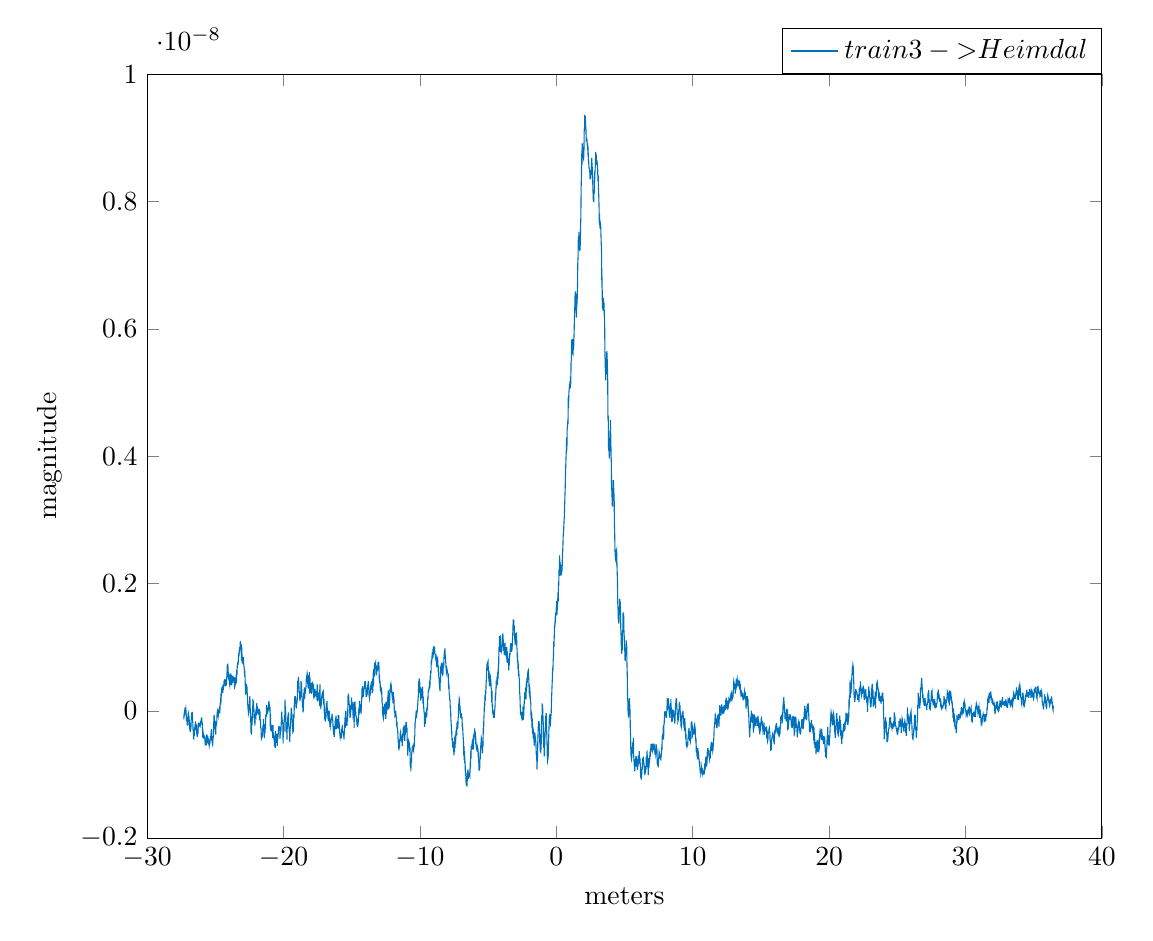
\begin{tikzpicture}

\begin{axis}[%
width=\textwidth,
height=0.8\textwidth,
at={(0\figurewidth,0\figureheight)},
scale only axis,
xmin=-30,
xmax=40,
xlabel={\SI{}{meters}},
ymin=-2e-09,
ymax=1e-08,
ylabel={magnitude},
axis background/.style={fill=white},
% legend style={legend cell align=left,align=left,draw=white!15!black}
legend style={at={(1.0,1.0)},anchor=south east}
]
\addplot [color=mycolor1,solid]
  table[row sep=crcr]{%
-27.30919921875	-1.35249592749225e-10\\
-27.288701171875	-2.96618732808651e-11\\
-27.268203125	-7.43225870504437e-11\\
-27.247705078125	3.98686887307428e-12\\
-27.22720703125	3.42173521151637e-11\\
-27.206708984375	2.91331309843253e-11\\
-27.1862109375	1.10075560008447e-12\\
-27.165712890625	3.11336048942319e-11\\
-27.14521484375	-2.14783086666199e-11\\
-27.124716796875	-1.18327190184514e-10\\
-27.10421875	-1.08068980081222e-10\\
-27.083720703125	-1.31806296562773e-10\\
-27.06322265625	-2.22339604039202e-10\\
-27.042724609375	-1.72113830799344e-10\\
-27.0222265625	-2.33179997718091e-10\\
-27.001728515625	-9.80243911839003e-11\\
-26.98123046875	-1.17431047736158e-10\\
-26.960732421875	-5.61412153639166e-11\\
-26.940234375	-8.61782248253023e-11\\
-26.919736328125	-1.39414401907277e-10\\
-26.89923828125	-1.86983229789256e-10\\
-26.878740234375	-2.80627277278364e-10\\
-26.8582421875	-3.00600915736125e-10\\
-26.837744140625	-3.35144363971528e-10\\
-26.81724609375	-2.59253155980024e-10\\
-26.796748046875	-3.0228046754793e-10\\
-26.77625	-1.52687733256755e-10\\
-26.755751953125	-1.25197094078767e-10\\
-26.73525390625	-3.07413927607202e-11\\
-26.714755859375	-1.04389883342187e-10\\
-26.6942578125	-1.90902832735895e-11\\
-26.673759765625	-1.36411292834644e-10\\
-26.65326171875	-1.88251566687186e-10\\
-26.632763671875	-3.12540235384246e-10\\
-26.612265625	-3.11990828982446e-10\\
-26.591767578125	-4.5378546266972e-10\\
-26.57126953125	-3.97306686246531e-10\\
-26.550771484375	-3.89530233962639e-10\\
-26.5302734375	-2.95033854580514e-10\\
-26.509775390625	-2.73561625376907e-10\\
-26.48927734375	-2.29766468985281e-10\\
-26.468779296875	-2.14010846778669e-10\\
-26.44828125	-1.66692182140658e-10\\
-26.427783203125	-2.55344271375855e-10\\
-26.40728515625	-3.15565761085146e-10\\
-26.386787109375	-2.14100663448054e-10\\
-26.3662890625	-3.61566215662477e-10\\
-26.345791015625	-3.76425626044425e-10\\
-26.32529296875	-4.07882051394321e-10\\
-26.304794921875	-3.06610166952019e-10\\
-26.284296875	-2.92301389226433e-10\\
-26.263798828125	-3.10288449436865e-10\\
-26.24330078125	-1.85406780114145e-10\\
-26.222802734375	-2.19785361206388e-10\\
-26.2023046875	-2.32913032346881e-10\\
-26.181806640625	-2.35588771150117e-10\\
-26.16130859375	-2.20910934632802e-10\\
-26.140810546875	-2.39919467133666e-10\\
-26.1203125	-2.47731371614303e-10\\
-26.099814453125	-2.16328684271403e-10\\
-26.07931640625	-1.81892890904841e-10\\
-26.058818359375	-1.89775940186073e-10\\
-26.0383203125	-1.22652439311522e-10\\
-26.017822265625	-1.83880244083923e-10\\
-25.99732421875	-1.0357336959362e-10\\
-25.976826171875	-1.95541713380527e-10\\
-25.956328125	-1.96616122014936e-10\\
-25.935830078125	-3.58401874836362e-10\\
-25.91533203125	-3.38628235970868e-10\\
-25.894833984375	-4.2069251597045e-10\\
-25.8743359375	-3.40979114286763e-10\\
-25.853837890625	-4.369802470122e-10\\
-25.83333984375	-3.98413489461025e-10\\
-25.812841796875	-3.95198434834407e-10\\
-25.79234375	-3.94468019830034e-10\\
-25.771845703125	-4.46008286744826e-10\\
-25.75134765625	-5.03870500898676e-10\\
-25.730849609375	-4.77212829626085e-10\\
-25.7103515625	-5.37079907260491e-10\\
-25.689853515625	-4.88433069265043e-10\\
-25.66935546875	-5.43539487116032e-10\\
-25.648857421875	-4.99002799318099e-10\\
-25.628359375	-3.70457436389315e-10\\
-25.607861328125	-5.07837222252482e-10\\
-25.58736328125	-3.90918766279497e-10\\
-25.566865234375	-4.75462672113693e-10\\
-25.5463671875	-4.92268967252412e-10\\
-25.525869140625	-4.55600562503486e-10\\
-25.50537109375	-4.85370364526642e-10\\
-25.484873046875	-4.70697730749883e-10\\
-25.464375	-4.90249456959638e-10\\
-25.443876953125	-5.49834186750661e-10\\
-25.42337890625	-5.27537008994874e-10\\
-25.402880859375	-5.10013096014045e-10\\
-25.3823828125	-4.72680789952298e-10\\
-25.361884765625	-3.99538475978077e-10\\
-25.34138671875	-4.56739308205518e-10\\
-25.320888671875	-3.74355003347318e-10\\
-25.300390625	-3.20512598351552e-10\\
-25.279892578125	-2.86734668606899e-10\\
-25.25939453125	-4.77148772142957e-10\\
-25.238896484375	-4.40258264345221e-10\\
-25.2183984375	-5.2597025779403e-10\\
-25.197900390625	-5.39619070167762e-10\\
-25.17740234375	-4.50282579640575e-10\\
-25.156904296875	-4.19755892974209e-10\\
-25.13640625	-3.48869621487714e-10\\
-25.115908203125	-1.87746427592221e-10\\
-25.09541015625	-6.32593406813938e-11\\
-25.074912109375	-1.11818179053154e-10\\
-25.0544140625	-1.94349194944256e-10\\
-25.033916015625	-1.65684148507703e-10\\
-25.01341796875	-2.92136525550294e-10\\
-24.992919921875	-3.07975800945658e-10\\
-24.972421875	-3.7437556257347e-10\\
-24.951923828125	-2.12441049209926e-10\\
-24.93142578125	-2.2905984032688e-10\\
-24.910927734375	-2.18417887953856e-10\\
-24.8904296875	-1.54126023375904e-10\\
-24.869931640625	-3.06732342695842e-11\\
-24.84943359375	-1.08751614123234e-11\\
-24.828935546875	-9.10597199836889e-11\\
-24.8084375	-4.20437497305171e-11\\
-24.787939453125	-6.94781001997516e-11\\
-24.76744140625	1.43610312870453e-11\\
-24.746943359375	-4.91616030660132e-11\\
-24.7264453125	3.19907101271847e-11\\
-24.705947265625	-3.54424103063645e-11\\
-24.68544921875	3.08095240031797e-11\\
-24.664951171875	1.42335811684415e-11\\
-24.644453125	1.16640520079849e-10\\
-24.623955078125	1.13368900684325e-10\\
-24.60345703125	1.97253068461331e-10\\
-24.582958984375	1.73276486852752e-10\\
-24.5624609375	2.6903501610126e-10\\
-24.541962890625	2.90714046386937e-10\\
-24.52146484375	3.73121420605555e-10\\
-24.500966796875	3.22700090021509e-10\\
-24.48046875	3.4870061542533e-10\\
-24.459970703125	2.81246627259552e-10\\
-24.43947265625	3.3321044944486e-10\\
-24.418974609375	3.34160493264702e-10\\
-24.3984765625	3.93830705039048e-10\\
-24.377978515625	4.12065881198341e-10\\
-24.35748046875	4.70560699559439e-10\\
-24.336982421875	4.77854883753441e-10\\
-24.316484375	4.23179697336425e-10\\
-24.295986328125	4.9179793993756e-10\\
-24.27548828125	3.85193315871097e-10\\
-24.254990234375	4.27031163793884e-10\\
-24.2344921875	4.40542659712922e-10\\
-24.213994140625	4.53147872693803e-10\\
-24.19349609375	3.9550415256078e-10\\
-24.172998046875	5.37536461584791e-10\\
-24.1525	4.94847667357632e-10\\
-24.132001953125	7.19471749362226e-10\\
-24.11150390625	6.39540833334101e-10\\
-24.091005859375	7.40868546685013e-10\\
-24.0705078125	6.70841370145141e-10\\
-24.050009765625	5.64432269917014e-10\\
-24.02951171875	5.27459481365235e-10\\
-24.009013671875	5.45624377592669e-10\\
-23.988515625	5.19521082422534e-10\\
-23.968017578125	4.32326595759694e-10\\
-23.94751953125	4.05360198707688e-10\\
-23.927021484375	5.04279887355792e-10\\
-23.9065234375	5.78177785934399e-10\\
-23.886025390625	4.09185582147215e-10\\
-23.86552734375	5.88905753813418e-10\\
-23.845029296875	4.63285685032234e-10\\
-23.82453125	5.61994052334426e-10\\
-23.804033203125	4.00684116260875e-10\\
-23.78353515625	4.71466961657033e-10\\
-23.763037109375	5.35770817238278e-10\\
-23.7425390625	4.39063573936935e-10\\
-23.722041015625	5.46530434420753e-10\\
-23.70154296875	4.66606075157989e-10\\
-23.681044921875	5.2047946923284e-10\\
-23.660546875	5.09204390901712e-10\\
-23.640048828125	5.00122606490857e-10\\
-23.61955078125	4.36479069184643e-10\\
-23.599052734375	5.26581404786945e-10\\
-23.5785546875	3.76011477242677e-10\\
-23.558056640625	3.90607565398019e-10\\
-23.53755859375	4.4294792836405e-10\\
-23.517060546875	4.54333826000035e-10\\
-23.4965625	4.15791551157969e-10\\
-23.476064453125	5.70539928801656e-10\\
-23.45556640625	4.35780458303778e-10\\
-23.435068359375	6.42805269654754e-10\\
-23.4145703125	5.65514985083013e-10\\
-23.394072265625	7.05869776518316e-10\\
-23.37357421875	7.16145412079906e-10\\
-23.353076171875	7.6412138568598e-10\\
-23.332578125	7.22190361279072e-10\\
-23.312080078125	8.06100058784537e-10\\
-23.29158203125	9.07235582967144e-10\\
-23.271083984375	8.53589864886048e-10\\
-23.2505859375	9.54398462032545e-10\\
-23.230087890625	9.00596361385507e-10\\
-23.20958984375	1.00125580769421e-09\\
-23.189091796875	9.6350503884139e-10\\
-23.16859375	1.09252419108719e-09\\
-23.148095703125	9.91393218918131e-10\\
-23.12759765625	9.75724709033288e-10\\
-23.107099609375	1.05400233342588e-09\\
-23.0866015625	7.89563994909622e-10\\
-23.066103515625	9.97858863307859e-10\\
-23.04560546875	8.63636129626429e-10\\
-23.025107421875	7.51233061416932e-10\\
-23.004609375	8.09452432789289e-10\\
-22.984111328125	7.45351075016677e-10\\
-22.96361328125	7.38974112185281e-10\\
-22.943115234375	8.4728140994759e-10\\
-22.9226171875	7.40393002956514e-10\\
-22.902119140625	6.96597444260378e-10\\
-22.88162109375	6.59170727172471e-10\\
-22.861123046875	5.88999496248786e-10\\
-22.840625	6.02643495657174e-10\\
-22.820126953125	5.19548699723142e-10\\
-22.79962890625	3.58659223237793e-10\\
-22.779130859375	2.56014850132148e-10\\
-22.7586328125	3.98498203322083e-10\\
-22.738134765625	3.5597738208579e-10\\
-22.71763671875	4.23931300566942e-10\\
-22.697138671875	3.76509782081444e-10\\
-22.676640625	3.66698464856997e-10\\
-22.656142578125	2.24114807771738e-10\\
-22.63564453125	2.14128267597694e-10\\
-22.615146484375	3.92613057296904e-11\\
-22.5946484375	3.42604768525375e-11\\
-22.574150390625	-4.41293350647987e-11\\
-22.55365234375	-2.12931148218186e-11\\
-22.533154296875	9.26741011408602e-11\\
-22.51265625	9.80352353988467e-11\\
-22.492158203125	7.75946266174585e-11\\
-22.47166015625	2.35725500990305e-10\\
-22.451162109375	6.51222689576677e-11\\
-22.4306640625	-2.16478093636985e-11\\
-22.410166015625	-6.14036409819761e-11\\
-22.38966796875	-3.48505283356299e-10\\
-22.369169921875	-2.5488656482834e-10\\
-22.348671875	-3.7339368246274e-10\\
-22.328173828125	-1.19268673436291e-10\\
-22.30767578125	-2.254021335182e-10\\
-22.287177734375	-5.8871150055272e-11\\
-22.2666796875	-7.41472598384597e-11\\
-22.246181640625	1.86675818204393e-10\\
-22.22568359375	5.83764085393433e-12\\
-22.205185546875	1.49803073300683e-10\\
-22.1846875	2.89773630503504e-11\\
-22.164189453125	-2.34220155503715e-12\\
-22.14369140625	-1.14932662586592e-10\\
-22.123193359375	-5.31159003984142e-11\\
-22.1026953125	-2.31133529182634e-10\\
-22.082197265625	-1.30357740898796e-10\\
-22.06169921875	-8.78292132365208e-11\\
-22.041201171875	-4.02899936747054e-11\\
-22.020703125	-6.5964859910965e-11\\
-22.000205078125	7.61250084393478e-12\\
-21.97970703125	-8.09417283578405e-12\\
-21.959208984375	1.25353680802542e-10\\
-21.9387109375	6.23976830311093e-12\\
-21.918212890625	-1.83121579361694e-12\\
-21.89771484375	1.42662819524076e-11\\
-21.877216796875	-4.07943779428101e-11\\
-21.85671875	-3.76912792168996e-12\\
-21.836220703125	-5.81583344322052e-11\\
-21.81572265625	2.81189299811436e-11\\
-21.795224609375	-7.66413514108258e-12\\
-21.7747265625	2.09013939771914e-11\\
-21.754228515625	-1.44860059790647e-10\\
-21.73373046875	4.59254340492001e-12\\
-21.713232421875	-1.37302086818081e-10\\
-21.692734375	-1.74860551881824e-10\\
-21.672236328125	-2.63654710274835e-10\\
-21.65173828125	-2.74703998317909e-10\\
-21.631240234375	-4.20338485802232e-10\\
-21.6107421875	-4.37091736543711e-10\\
-21.590244140625	-4.10792565462269e-10\\
-21.56974609375	-3.84212279996029e-10\\
-21.549248046875	-4.12458197001633e-10\\
-21.52875	-3.02419924846638e-10\\
-21.508251953125	-2.29427695814191e-10\\
-21.48775390625	-3.03268767035055e-10\\
-21.467255859375	-1.3206782407974e-10\\
-21.4467578125	-2.73771896512718e-10\\
-21.426259765625	-2.59085306063035e-10\\
-21.40576171875	-4.30111125358062e-10\\
-21.385263671875	-2.0632810764854e-10\\
-21.364765625	-3.54819114192018e-10\\
-21.344267578125	-2.54188920506213e-10\\
-21.32376953125	-2.84275856731719e-10\\
-21.303271484375	-7.09732788542016e-11\\
-21.2827734375	-7.20041318887539e-11\\
-21.262275390625	-7.59176608545542e-11\\
-21.24177734375	9.02728847141608e-11\\
-21.221279296875	-3.22041808705736e-11\\
-21.20078125	1.63950665346143e-11\\
-21.180283203125	-5.53445845479256e-11\\
-21.15978515625	4.15543045400407e-11\\
-21.139287109375	-1.17449240472937e-11\\
-21.1187890625	5.50190439203395e-11\\
-21.098291015625	4.57176319761245e-11\\
-21.07779296875	1.56860255048446e-10\\
-21.057294921875	1.22062875719343e-10\\
-21.036796875	6.36559620355532e-11\\
-21.016298828125	9.99157708793992e-12\\
-20.99580078125	6.28013598363108e-11\\
-20.975302734375	-2.47118558969039e-10\\
-20.9548046875	-4.63928851977508e-11\\
-20.934306640625	-3.12081159477715e-10\\
-20.91380859375	-2.7067025234948e-10\\
-20.893310546875	-3.28299426226706e-10\\
-20.8728125	-2.85660195781246e-10\\
-20.852314453125	-2.64413009312218e-10\\
-20.83181640625	-2.88170358171071e-10\\
-20.811318359375	-2.25733766269133e-10\\
-20.7908203125	-4.23764019707049e-10\\
-20.770322265625	-2.21841222113801e-10\\
-20.74982421875	-4.30448863824891e-10\\
-20.729326171875	-3.49362909049628e-10\\
-20.708828125	-4.52025120443815e-10\\
-20.688330078125	-4.02754264074807e-10\\
-20.66783203125	-5.63953896965506e-10\\
-20.647333984375	-5.37577949840101e-10\\
-20.6268359375	-4.79069625814277e-10\\
-20.606337890625	-5.82275218022439e-10\\
-20.58583984375	-3.17878927622478e-10\\
-20.565341796875	-4.8156118976282e-10\\
-20.54484375	-4.16394974697215e-10\\
-20.524345703125	-4.07865033434682e-10\\
-20.50384765625	-5.0276178594198e-10\\
-20.483349609375	-3.62819242064881e-10\\
-20.4628515625	-5.49036645452217e-10\\
-20.442353515625	-4.00444780065307e-10\\
-20.42185546875	-4.47286644214556e-10\\
-20.401357421875	-3.85520206742565e-10\\
-20.380859375	-3.44588015543206e-10\\
-20.360361328125	-2.44620874758808e-10\\
-20.33986328125	-3.00057564990421e-10\\
-20.319365234375	-2.54708606415881e-10\\
-20.2988671875	-2.63199104537137e-10\\
-20.278369140625	-2.61497460415243e-10\\
-20.25787109375	-4.3566653131045e-10\\
-20.237373046875	-3.39060649361071e-10\\
-20.216875	-2.6968012532743e-10\\
-20.196376953125	-3.29041872515179e-10\\
-20.17587890625	-2.30523557160484e-10\\
-20.155380859375	-1.37222185699247e-10\\
-20.1348828125	-1.37691994534061e-11\\
-20.114384765625	-1.1656610580232e-10\\
-20.09388671875	-1.60648024062064e-10\\
-20.073388671875	-1.8817748537802e-10\\
-20.052890625	-2.04706827156494e-10\\
-20.032392578125	-5.11966334289761e-10\\
-20.01189453125	-2.00866363523768e-10\\
-19.991396484375	-3.0889125830442e-10\\
-19.9708984375	-3.14055967443623e-10\\
-19.950400390625	-1.56302500449251e-10\\
-19.92990234375	-6.81430237807833e-11\\
-19.909404296875	-1.33935618120171e-10\\
-19.88890625	1.75761530913608e-10\\
-19.868408203125	-1.3895336154408e-10\\
-19.84791015625	7.62026210686375e-11\\
-19.827412109375	-3.26734158979295e-10\\
-19.8069140625	-2.15118271214411e-10\\
-19.786416015625	-3.44371183992221e-10\\
-19.76591796875	-3.02650238689192e-10\\
-19.745419921875	-4.54562611379598e-10\\
-19.724921875	-1.7746898825716e-10\\
-19.704423828125	-2.13385872379252e-10\\
-19.68392578125	-7.62594169804049e-11\\
-19.663427734375	-1.03101424228827e-10\\
-19.6429296875	-2.34172118697999e-11\\
-19.622431640625	-2.32012012948023e-10\\
-19.60193359375	-2.5946516249895e-10\\
-19.581435546875	-3.2447161092726e-10\\
-19.5609375	-3.50636622603424e-10\\
-19.540439453125	-4.9030730048045e-10\\
-19.51994140625	-2.88860903609473e-10\\
-19.499443359375	-2.7062632717906e-10\\
-19.4789453125	-1.48803141594526e-10\\
-19.458447265625	-9.38330676844761e-11\\
-19.43794921875	3.66142858550482e-11\\
-19.417451171875	3.61329974267193e-11\\
-19.396953125	-6.95206901144934e-11\\
-19.376455078125	-6.80705839206913e-11\\
-19.35595703125	-2.07604654033483e-10\\
-19.335458984375	-2.69040597632863e-10\\
-19.3149609375	-3.40123800332184e-10\\
-19.294462890625	-3.32237471286125e-10\\
-19.27396484375	-2.82959527081493e-10\\
-19.253466796875	-5.67222537644977e-11\\
-19.23296875	-1.14249470329872e-10\\
-19.212470703125	9.11690230248631e-11\\
-19.19197265625	1.26565465164729e-10\\
-19.171474609375	2.28755321998858e-10\\
-19.1509765625	1.21401001911897e-10\\
-19.130478515625	2.27976209362263e-10\\
-19.10998046875	1.59797330735405e-10\\
-19.089482421875	6.37709036681829e-11\\
-19.068984375	5.57455596479256e-11\\
-19.048486328125	1.10365129035581e-10\\
-19.02798828125	1.17519084932018e-10\\
-19.007490234375	1.41199994471048e-10\\
-18.9869921875	2.13204881026035e-10\\
-18.966494140625	4.68925560453406e-10\\
-18.94599609375	4.23381455480242e-10\\
-18.925498046875	4.79858965682223e-10\\
-18.905	5.31159313220214e-10\\
-18.884501953125	4.2670750228582e-10\\
-18.86400390625	3.52120556050411e-10\\
-18.843505859375	2.77283641387189e-10\\
-18.8230078125	2.5869988327639e-10\\
-18.802509765625	1.5705711182262e-10\\
-18.78201171875	2.91806123555677e-10\\
-18.761513671875	2.09787977055237e-10\\
-18.741015625	2.31288254074604e-10\\
-18.720517578125	4.70410565873187e-10\\
-18.70001953125	3.11510683889954e-10\\
-18.679521484375	4.3367679874644e-10\\
-18.6590234375	2.41411925753194e-10\\
-18.638525390625	2.05967924565715e-10\\
-18.61802734375	1.02434891051107e-10\\
-18.597529296875	1.16902049217817e-10\\
-18.57703125	-2.53204385378994e-11\\
-18.556533203125	2.86766670393062e-12\\
-18.53603515625	1.15878380624621e-10\\
-18.515537109375	2.80085775040727e-10\\
-18.4950390625	2.4333637379268e-10\\
-18.474541015625	3.67339631789491e-10\\
-18.45404296875	1.82848505844703e-10\\
-18.433544921875	3.3005939177019e-10\\
-18.413046875	2.7146298050183e-10\\
-18.392548828125	3.09182611953742e-10\\
-18.37205078125	3.46517038577973e-10\\
-18.351552734375	3.7921044482155e-10\\
-18.3310546875	5.03002047679626e-10\\
-18.310556640625	5.31587780902845e-10\\
-18.29005859375	5.54352495001945e-10\\
-18.269560546875	5.89173520686153e-10\\
-18.2490625	5.6473692322234e-10\\
-18.228564453125	4.56157387333356e-10\\
-18.20806640625	4.78507824422924e-10\\
-18.187568359375	3.51483408137841e-10\\
-18.1670703125	4.78472945615268e-10\\
-18.146572265625	3.49028278351362e-10\\
-18.12607421875	4.67702356232544e-10\\
-18.105576171875	6.06012196049108e-10\\
-18.085078125	2.71460060488586e-10\\
-18.064580078125	5.20307117666546e-10\\
-18.04408203125	4.01201508095344e-10\\
-18.023583984375	4.29013329383474e-10\\
-18.0030859375	2.90204382012613e-10\\
-17.982587890625	2.89617333342013e-10\\
-17.96208984375	4.33755235990214e-10\\
-17.941591796875	2.64637916361743e-10\\
-17.92109375	3.62771568075583e-10\\
-17.900595703125	4.56241669943883e-10\\
-17.88009765625	3.98254228175803e-10\\
-17.859599609375	3.81533855723509e-10\\
-17.8391015625	3.94535730857114e-10\\
-17.818603515625	3.35492811620338e-10\\
-17.79810546875	3.54613862021231e-10\\
-17.777607421875	1.79524443008476e-10\\
-17.757109375	3.25634024098343e-10\\
-17.736611328125	2.6411457495158e-10\\
-17.71611328125	2.12880739173961e-10\\
-17.695615234375	3.43017151489387e-10\\
-17.6751171875	2.66403234522076e-10\\
-17.654619140625	2.61591233302193e-10\\
-17.63412109375	2.52050140390371e-10\\
-17.613623046875	2.95059354538262e-10\\
-17.593125	3.00936147734259e-10\\
-17.572626953125	2.87102058333018e-10\\
-17.55212890625	1.70075791760634e-10\\
-17.531630859375	4.14039184368385e-10\\
-17.5111328125	1.47241284671841e-10\\
-17.490634765625	2.80143923839951e-10\\
-17.47013671875	2.44769284310749e-10\\
-17.449638671875	2.47197962592881e-10\\
-17.429140625	2.21046003201693e-10\\
-17.408642578125	2.87397615036798e-10\\
-17.38814453125	1.83052274574976e-10\\
-17.367646484375	3.33296989470108e-10\\
-17.3471484375	7.67017460010833e-11\\
-17.326650390625	4.16832800436667e-10\\
-17.30615234375	8.04518419872208e-11\\
-17.285654296875	2.03016610301869e-10\\
-17.26515625	2.20413923623684e-11\\
-17.244658203125	1.58450722634043e-10\\
-17.22416015625	8.57608333990689e-11\\
-17.203662109375	2.06265137683533e-10\\
-17.1831640625	2.52420710750696e-10\\
-17.162666015625	2.49015564575926e-10\\
-17.14216796875	2.82992835290942e-10\\
-17.121669921875	2.93893175426329e-10\\
-17.101171875	2.3734332447866e-10\\
-17.080673828125	2.60872578846719e-10\\
-17.06017578125	1.02974688881605e-10\\
-17.039677734375	1.91908264396336e-10\\
-17.0191796875	2.68619381037025e-11\\
-16.998681640625	4.26862496744526e-11\\
-16.97818359375	-1.33489865677632e-10\\
-16.957685546875	-2.43362328377587e-11\\
-16.9371875	-1.7125473685436e-10\\
-16.916689453125	-6.08119382744374e-11\\
-16.89619140625	-3.71664781404117e-11\\
-16.875693359375	-5.31588232320189e-11\\
-16.8551953125	1.20150459959966e-10\\
-16.834697265625	4.54314435488041e-11\\
-16.81419921875	1.51709263117392e-10\\
-16.793701171875	1.15134074358259e-11\\
-16.773203125	1.45596914666982e-11\\
-16.752705078125	-8.70150145053961e-11\\
-16.73220703125	-7.5436426769702e-11\\
-16.711708984375	-1.67478710209694e-10\\
-16.6912109375	-6.10432385311275e-11\\
-16.670712890625	-8.19950091368211e-11\\
-16.65021484375	-2.70389312496919e-12\\
-16.629716796875	-1.20871613963387e-10\\
-16.60921875	-1.98081611085121e-10\\
-16.588720703125	-1.81009964996844e-10\\
-16.56822265625	-2.33256078519509e-10\\
-16.547724609375	-1.9666502453237e-10\\
-16.5272265625	-1.94099263446273e-10\\
-16.506728515625	-1.37945581843473e-10\\
-16.48623046875	-1.10426366371286e-10\\
-16.465732421875	-1.06747903357002e-10\\
-16.445234375	-4.69579347037814e-11\\
-16.424736328125	-9.3997370967717e-11\\
-16.40423828125	-1.16724469033973e-10\\
-16.383740234375	-1.78575460058846e-10\\
-16.3632421875	-2.8958372638956e-10\\
-16.342744140625	-2.99415388570616e-10\\
-16.32224609375	-3.74616263585012e-10\\
-16.301748046875	-3.24921108689867e-10\\
-16.28125	-4.11254814031175e-10\\
-16.260751953125	-2.40658172771327e-10\\
-16.24025390625	-2.77827700481013e-10\\
-16.219755859375	-2.27808933161054e-10\\
-16.1992578125	-1.15488753427843e-10\\
-16.178759765625	-2.20847355396641e-10\\
-16.15826171875	-7.59620915149292e-11\\
-16.137763671875	-2.89675119693239e-10\\
-16.117265625	-1.29931086873945e-10\\
-16.096767578125	-1.99668301741175e-10\\
-16.07626953125	-1.66261383274477e-10\\
-16.055771484375	-2.76505403122174e-10\\
-16.0352734375	-1.9055105100654e-10\\
-16.014775390625	-1.95571469540603e-10\\
-15.99427734375	-6.34674870304593e-11\\
-15.973779296875	-2.80429984559389e-10\\
-15.95328125	-7.00580232580394e-11\\
-15.932783203125	-2.07698110569518e-10\\
-15.91228515625	-2.08325879703897e-10\\
-15.891787109375	-3.15658179402705e-10\\
-15.8712890625	-3.72570837481575e-10\\
-15.850791015625	-4.08168510434337e-10\\
-15.83029296875	-3.65668825755436e-10\\
-15.809794921875	-4.38106414260785e-10\\
-15.789296875	-3.96211823827328e-10\\
-15.768798828125	-4.34607715496228e-10\\
-15.74830078125	-2.99166128241619e-10\\
-15.727802734375	-3.03028082590152e-10\\
-15.7073046875	-2.98005438237266e-10\\
-15.686806640625	-2.26014634948845e-10\\
-15.66630859375	-3.3846138818385e-10\\
-15.645810546875	-3.38281510405287e-10\\
-15.6253125	-3.68562513952096e-10\\
-15.604814453125	-4.05063237513379e-10\\
-15.58431640625	-3.22185304326828e-10\\
-15.563818359375	-4.47041403096272e-10\\
-15.5433203125	-3.01075685340483e-10\\
-15.522822265625	-3.27547505318069e-10\\
-15.50232421875	-1.2294273248789e-10\\
-15.481826171875	-1.03876423099887e-10\\
-15.461328125	-9.94361589949121e-11\\
-15.440830078125	-2.45314057689288e-13\\
-15.42033203125	-2.17590232631159e-10\\
-15.399833984375	-2.02975083704597e-10\\
-15.3793359375	-1.76695748104086e-10\\
-15.358837890625	-2.36224932569385e-10\\
-15.33833984375	-1.89922086026445e-10\\
-15.317841796875	-7.14372269354423e-11\\
-15.29734375	-9.23977916426495e-11\\
-15.276845703125	2.37960715213924e-10\\
-15.25634765625	1.17619036660605e-10\\
-15.235849609375	2.70210839930903e-10\\
-15.2153515625	1.94261988179782e-10\\
-15.194853515625	1.15069516706955e-10\\
-15.17435546875	8.94443760884572e-11\\
-15.153857421875	5.83746325962268e-11\\
-15.133359375	-1.11023313739406e-10\\
-15.112861328125	-6.54731234053735e-11\\
-15.09236328125	-9.56909192569403e-11\\
-15.071865234375	1.30506019338311e-11\\
-15.0513671875	9.68795468784335e-11\\
-15.030869140625	2.50923586712161e-11\\
-15.01037109375	2.09598225460569e-10\\
-14.989873046875	2.47804540073555e-11\\
-14.969375	1.39247098886317e-10\\
-14.948876953125	1.58815172697944e-11\\
-14.92837890625	4.54233813246108e-11\\
-14.907880859375	-5.57289463883855e-11\\
-14.8873828125	-2.84881318354218e-11\\
-14.866884765625	-1.08480778333579e-10\\
-14.84638671875	1.39378831995546e-10\\
-14.825888671875	-2.71083551572908e-10\\
-14.805390625	1.14094914363789e-10\\
-14.784892578125	-2.02958716426207e-11\\
-14.76439453125	1.43052419916105e-10\\
-14.743896484375	-5.92955805676748e-11\\
-14.7233984375	6.0975105719955e-11\\
-14.702900390625	-6.97912074012181e-11\\
-14.68240234375	-8.69024565463845e-11\\
-14.661904296875	-9.12821650888016e-11\\
-14.64140625	-1.4896358030078e-10\\
-14.620908203125	-1.95361705879464e-10\\
-14.60041015625	-1.81115551160454e-10\\
-14.579912109375	-2.50583516830121e-10\\
-14.5594140625	-1.22319409386413e-10\\
-14.538916015625	-2.26963774330336e-10\\
-14.51841796875	-1.47635822481101e-10\\
-14.497919921875	-7.57367159852047e-11\\
-14.477421875	4.86318728283396e-11\\
-14.456923828125	-6.4198723257886e-11\\
-14.43642578125	1.56136617677521e-10\\
-14.415927734375	7.19834880118072e-11\\
-14.3954296875	4.05542970943303e-11\\
-14.374931640625	8.24275375158423e-11\\
-14.35443359375	-1.05712167692395e-11\\
-14.333935546875	1.02789833299272e-10\\
-14.3134375	-5.21249034449518e-11\\
-14.292939453125	1.35572702718452e-10\\
-14.27244140625	1.53555196947139e-10\\
-14.251943359375	2.95689229597886e-10\\
-14.2314453125	2.80052824382e-10\\
-14.210947265625	3.87128929989158e-10\\
-14.19044921875	2.80797529362345e-10\\
-14.169951171875	2.12710186428401e-10\\
-14.149453125	2.48155196455195e-10\\
-14.128955078125	2.81397716031753e-10\\
-14.10845703125	3.46830203184054e-10\\
-14.087958984375	3.66268961884066e-10\\
-14.0674609375	3.60481594900071e-10\\
-14.046962890625	4.56338176463585e-10\\
-14.02646484375	4.27769226694275e-10\\
-14.005966796875	4.69377502383545e-10\\
-13.98546875	3.81968448036488e-10\\
-13.964970703125	3.40626728512775e-10\\
-13.94447265625	2.14836096004836e-10\\
-13.923974609375	3.02690456932697e-10\\
-13.9034765625	2.77500630655234e-10\\
-13.882978515625	3.11831094482941e-10\\
-13.86248046875	2.90397985721397e-10\\
-13.841982421875	3.74232762233638e-10\\
-13.821484375	4.03757941983856e-10\\
-13.800986328125	4.31519740292519e-10\\
-13.78048828125	4.69895159645258e-10\\
-13.759990234375	3.97132429103535e-10\\
-13.7394921875	2.64832149703066e-10\\
-13.718994140625	2.21040295268192e-10\\
-13.69849609375	1.960921286544e-10\\
-13.677998046875	3.15442070974464e-10\\
-13.6575	2.3446708194947e-10\\
-13.637001953125	2.89275608731404e-10\\
-13.61650390625	3.73548043572492e-10\\
-13.596005859375	4.07426267812095e-10\\
-13.5755078125	4.08098987626308e-10\\
-13.555009765625	4.63256391660534e-10\\
-13.53451171875	3.40593921051983e-10\\
-13.514013671875	3.73625717315821e-10\\
-13.493515625	2.77300996856856e-10\\
-13.473017578125	5.00278758960531e-10\\
-13.45251953125	3.02504983817702e-10\\
-13.432021484375	5.98708406255111e-10\\
-13.4115234375	3.86726234692942e-10\\
-13.391025390625	5.89964865378462e-10\\
-13.37052734375	5.69570704864333e-10\\
-13.350029296875	5.37186121558701e-10\\
-13.32953125	7.13668556433254e-10\\
-13.309033203125	7.02717922300551e-10\\
-13.28853515625	7.43265268495172e-10\\
-13.268037109375	7.38624704283125e-10\\
-13.2475390625	7.56874474620068e-10\\
-13.227041015625	5.72821248666765e-10\\
-13.20654296875	7.14506029195342e-10\\
-13.186044921875	5.56252095731253e-10\\
-13.165546875	6.87286773499721e-10\\
-13.145048828125	6.8030999515314e-10\\
-13.12455078125	6.68691714946003e-10\\
-13.104052734375	6.20760826154718e-10\\
-13.0835546875	7.1763954247636e-10\\
-13.063056640625	7.71680111319628e-10\\
-13.04255859375	7.01860134505897e-10\\
-13.022060546875	7.65241402087973e-10\\
-13.0015625	6.91830548061057e-10\\
-12.981064453125	5.12968689564435e-10\\
-12.96056640625	5.24203532810344e-10\\
-12.940068359375	4.25489412698201e-10\\
-12.9195703125	4.62482340952045e-10\\
-12.899072265625	3.0547152930145e-10\\
-12.87857421875	3.8209066473652e-10\\
-12.858076171875	3.31435166261555e-10\\
-12.837578125	3.65235372547986e-10\\
-12.817080078125	2.505784466193e-10\\
-12.79658203125	3.16077416426049e-10\\
-12.776083984375	1.20103219828582e-10\\
-12.7555859375	1.0719001826468e-10\\
-12.735087890625	-5.06847082463068e-11\\
-12.71458984375	-5.97512423925587e-11\\
-12.694091796875	-1.08377674792808e-10\\
-12.67359375	-1.25673123073199e-10\\
-12.653095703125	-3.44590908600641e-11\\
-12.63259765625	6.93766832048192e-11\\
-12.612099609375	3.77564966984743e-11\\
-12.5916015625	9.90318446961657e-11\\
-12.571103515625	1.02308871266687e-10\\
-12.55060546875	-1.98890274314529e-13\\
-12.530107421875	2.06996805792616e-11\\
-12.509609375	-1.27783267165771e-10\\
-12.489111328125	1.39647844200157e-10\\
-12.46861328125	-5.64150204882903e-11\\
-12.448115234375	6.20538221953262e-11\\
-12.4276171875	6.23948489660559e-11\\
-12.407119140625	4.83038730044384e-11\\
-12.38662109375	1.42414213442394e-10\\
-12.366123046875	1.89362388081629e-10\\
-12.345625	1.67754621955446e-10\\
-12.325126953125	3.20791308857426e-10\\
-12.30462890625	2.2234707926806e-11\\
-12.284130859375	2.82657533373699e-10\\
-12.2636328125	4.01346836221866e-11\\
-12.243134765625	9.34754198310589e-11\\
-12.22263671875	1.0259009704288e-10\\
-12.202138671875	3.44150238341192e-10\\
-12.181640625	2.81423875827867e-10\\
-12.161142578125	3.86743775972926e-10\\
-12.14064453125	3.75098808458363e-10\\
-12.120146484375	4.16317359769756e-10\\
-12.0996484375	3.85086814204615e-10\\
-12.079150390625	2.99509850259228e-10\\
-12.05865234375	3.02147190062396e-10\\
-12.038154296875	2.18253721369266e-10\\
-12.01765625	1.99539778090712e-10\\
-11.997158203125	2.18413260834315e-10\\
-11.97666015625	1.21854025855723e-10\\
-11.956162109375	2.93821524009287e-10\\
-11.9356640625	1.14064041094946e-10\\
-11.915166015625	2.25523846309539e-10\\
-11.89466796875	1.36204045088998e-10\\
-11.874169921875	-2.87922919392108e-11\\
-11.853671875	1.56763275796079e-11\\
-11.833173828125	-8.429929587313e-11\\
-11.81267578125	-7.54111981717615e-11\\
-11.792177734375	-6.47912578203932e-11\\
-11.7716796875	-1.29337226617914e-12\\
-11.751181640625	-8.63556336143343e-11\\
-11.73068359375	-9.28322365063355e-11\\
-11.710185546875	-2.48720166263712e-10\\
-11.6896875	-1.66579069135422e-10\\
-11.669189453125	-2.61733545830312e-10\\
-11.64869140625	-2.81161894014934e-10\\
-11.628193359375	-3.25499365486576e-10\\
-11.6076953125	-4.34941164506334e-10\\
-11.587197265625	-4.97660747271448e-10\\
-11.56669921875	-4.54891246661043e-10\\
-11.546201171875	-6.25884074087925e-10\\
-11.525703125	-4.7882698370597e-10\\
-11.505205078125	-5.90959460955783e-10\\
-11.48470703125	-5.00445524382349e-10\\
-11.464208984375	-4.71936842506786e-10\\
-11.4437109375	-3.50752022667231e-10\\
-11.423212890625	-3.33011635995292e-10\\
-11.40271484375	-4.07605816775349e-10\\
-11.382216796875	-4.3712397321207e-10\\
-11.36171875	-4.54030062147451e-10\\
-11.341220703125	-4.34376496867096e-10\\
-11.32072265625	-3.93458870661357e-10\\
-11.300224609375	-5.55822436199521e-10\\
-11.2797265625	-3.67533227912644e-10\\
-11.259228515625	-4.58068105537899e-10\\
-11.23873046875	-3.49673992689287e-10\\
-11.218232421875	-2.61740310928529e-10\\
-11.197734375	-2.57609586284579e-10\\
-11.177236328125	-3.19754139683082e-10\\
-11.15673828125	-2.27157578779978e-10\\
-11.136240234375	-3.83252581562234e-10\\
-11.1157421875	-4.77881489064761e-10\\
-11.095244140625	-3.46749169356106e-10\\
-11.07474609375	-3.55872797794633e-10\\
-11.054248046875	-3.03813681575749e-10\\
-11.03375	-2.13653226503294e-10\\
-11.013251953125	-2.26543950260846e-10\\
-10.99275390625	-1.79438720680166e-10\\
-10.972255859375	-3.37864192270552e-10\\
-10.9517578125	-2.67457578003135e-10\\
-10.931259765625	-4.74110131557216e-10\\
-10.91076171875	-4.49278530807292e-10\\
-10.890263671875	-7.04232276711826e-10\\
-10.869765625	-5.62551805568847e-10\\
-10.849267578125	-5.29122520391257e-10\\
-10.82876953125	-5.87562681193357e-10\\
-10.808271484375	-4.83058255050168e-10\\
-10.7877734375	-5.00321506153864e-10\\
-10.767275390625	-5.26615834486921e-10\\
-10.74677734375	-6.48180958261963e-10\\
-10.726279296875	-5.77351828324484e-10\\
-10.70578125	-8.77152445949905e-10\\
-10.685283203125	-7.48865569613854e-10\\
-10.66478515625	-9.52626385005314e-10\\
-10.644287109375	-7.48205696575369e-10\\
-10.6237890625	-8.15001923210684e-10\\
-10.603291015625	-6.59559188619641e-10\\
-10.58279296875	-6.4598015377087e-10\\
-10.562294921875	-5.70682644566559e-10\\
-10.541796875	-5.68794960799915e-10\\
-10.521298828125	-5.87059338803812e-10\\
-10.50080078125	-5.32750622438163e-10\\
-10.480302734375	-5.85135303439975e-10\\
-10.4598046875	-6.09896635844846e-10\\
-10.439306640625	-5.03101142099797e-10\\
-10.41880859375	-5.68253821582825e-10\\
-10.398310546875	-3.95597603008127e-10\\
-10.3778125	-3.95038234570791e-10\\
-10.357314453125	-1.84434299509545e-10\\
-10.33681640625	-1.78107826801178e-10\\
-10.316318359375	-1.08858709897569e-10\\
-10.2958203125	-7.8686758176729e-11\\
-10.275322265625	7.85674142761614e-12\\
-10.25482421875	-1.16126452685473e-10\\
-10.234326171875	-2.18180159605628e-11\\
-10.213828125	-2.9776440765485e-11\\
-10.193330078125	-4.17699642897514e-12\\
-10.17283203125	5.4917441662854e-11\\
-10.152333984375	1.35202479210146e-10\\
-10.1318359375	1.93365093803419e-10\\
-10.111337890625	2.65760126089633e-10\\
-10.09083984375	4.52210863478373e-10\\
-10.070341796875	4.64145731175866e-10\\
-10.04984375	5.0759387709493e-10\\
-10.029345703125	4.24723634004236e-10\\
-10.00884765625	4.59402490957036e-10\\
-9.988349609375	2.55173889248331e-10\\
-9.9678515625	3.71713489103553e-10\\
-9.947353515625	1.5835932574498e-10\\
-9.92685546875	2.42354596671091e-10\\
-9.906357421875	1.93690437804616e-10\\
-9.885859375	3.41081986883496e-10\\
-9.865361328125	2.79259893534888e-10\\
-9.84486328125	3.62109672025255e-10\\
-9.824365234375	2.269940355252e-10\\
-9.8038671875	3.81361756638422e-10\\
-9.783369140625	1.11137777378847e-10\\
-9.76287109375	2.24124990091546e-10\\
-9.742373046875	1.16694982189372e-10\\
-9.721875	4.57312958460112e-11\\
-9.701376953125	-9.40149151952291e-12\\
-9.68087890625	-3.69190708635449e-11\\
-9.660380859375	-2.54057117201858e-10\\
-9.6398828125	-1.43109104952536e-10\\
-9.619384765625	-2.07442733310828e-10\\
-9.59888671875	-1.7348684415668e-10\\
-9.578388671875	-7.0321926061003e-11\\
-9.557890625	-9.11679624310035e-11\\
-9.537392578125	-6.49757131090353e-11\\
-9.51689453125	-1.7096308420883e-11\\
-9.496396484375	-4.12754242254559e-11\\
-9.4758984375	6.25057577492562e-11\\
-9.455400390625	7.66748484672237e-12\\
-9.43490234375	1.84575866217155e-10\\
-9.414404296875	1.81485355726692e-10\\
-9.39390625	2.96453170933065e-10\\
-9.373408203125	3.22517255200252e-10\\
-9.35291015625	3.18577925306291e-10\\
-9.332412109375	3.59481289254119e-10\\
-9.3119140625	3.8631345042763e-10\\
-9.291416015625	4.73502550627824e-10\\
-9.27091796875	3.53956611977266e-10\\
-9.250419921875	5.44038672122825e-10\\
-9.229921875	4.90725408678358e-10\\
-9.209423828125	6.2800757706969e-10\\
-9.18892578125	5.93796092480814e-10\\
-9.168427734375	7.8798101718493e-10\\
-9.1479296875	7.31246335588483e-10\\
-9.127431640625	8.1945778370868e-10\\
-9.10693359375	8.75741970175105e-10\\
-9.086435546875	8.5706796886578e-10\\
-9.0659375	8.18562424968222e-10\\
-9.045439453125	9.70927554871182e-10\\
-9.02494140625	8.87175074635618e-10\\
-9.004443359375	1.01291115696264e-09\\
-8.9839453125	9.31778684060934e-10\\
-8.963447265625	9.56615689720637e-10\\
-8.94294921875	1.00916938233223e-09\\
-8.922451171875	9.71045996970394e-10\\
-8.901953125	9.01898984859587e-10\\
-8.881455078125	8.86637997312074e-10\\
-8.86095703125	8.42345172581719e-10\\
-8.840458984375	8.20925167409127e-10\\
-8.8199609375	7.76261558949736e-10\\
-8.799462890625	8.42559486905883e-10\\
-8.77896484375	6.89096186841026e-10\\
-8.758466796875	8.18004153534335e-10\\
-8.73796875	7.94026037092246e-10\\
-8.717470703125	7.67405695982599e-10\\
-8.69697265625	7.95083032045277e-10\\
-8.676474609375	7.02506660286174e-10\\
-8.6559765625	6.06684302175669e-10\\
-8.635478515625	7.00581032902246e-10\\
-8.61498046875	5.16540472422212e-10\\
-8.594482421875	5.05800615830933e-10\\
-8.573984375	3.87761575856596e-10\\
-8.553486328125	3.72477185775778e-10\\
-8.53298828125	3.10233668228721e-10\\
-8.512490234375	5.24120409967262e-10\\
-8.4919921875	4.38711213451156e-10\\
-8.471494140625	6.98462313554818e-10\\
-8.45099609375	5.74274618041651e-10\\
-8.430498046875	7.53986960582453e-10\\
-8.41	6.69755967878146e-10\\
-8.389501953125	6.96809540886879e-10\\
-8.36900390625	6.00171931433791e-10\\
-8.348505859375	6.36806721007757e-10\\
-8.3280078125	5.68371486123421e-10\\
-8.307509765625	5.78797157024344e-10\\
-8.28701171875	7.46489517079311e-10\\
-8.266513671875	6.68717946985899e-10\\
-8.246015625	7.88103277029078e-10\\
-8.225517578125	8.77266188868265e-10\\
-8.20501953125	9.43418071775616e-10\\
-8.184521484375	8.66994050767152e-10\\
-8.1640234375	9.79182620611189e-10\\
-8.143525390625	8.4815353289903e-10\\
-8.12302734375	8.1538396909955e-10\\
-8.102529296875	7.37639296107119e-10\\
-8.08203125	6.66715374979398e-10\\
-8.061533203125	6.04387129240504e-10\\
-8.04103515625	6.31275276049776e-10\\
-8.020537109375	6.58190895434598e-10\\
-8.0000390625	6.30713909371111e-10\\
-7.979541015625	5.93388157222308e-10\\
-7.95904296875	5.87404209249354e-10\\
-7.938544921875	5.43368855161953e-10\\
-7.918046875	5.82909444126609e-10\\
-7.897548828125	3.3978580691506e-10\\
-7.87705078125	4.31099655316538e-10\\
-7.856552734375	2.69585696700586e-10\\
-7.8360546875	2.57977636685405e-10\\
-7.815556640625	1.71850837973958e-10\\
-7.79505859375	1.66487863866315e-10\\
-7.774560546875	4.23615234722925e-11\\
-7.7540625	3.81228570256801e-11\\
-7.733564453125	-1.2761469511457e-10\\
-7.71306640625	-1.85830527467055e-10\\
-7.692568359375	-2.9265009328255e-10\\
-7.6720703125	-3.17474990050083e-10\\
-7.651572265625	-4.62941848331661e-10\\
-7.63107421875	-4.28870328679045e-10\\
-7.610576171875	-5.05858918356395e-10\\
-7.590078125	-5.79847477361188e-10\\
-7.569580078125	-5.31545771766741e-10\\
-7.54908203125	-5.56448486666954e-10\\
-7.528583984375	-5.88402282700977e-10\\
-7.5080859375	-7.00116923023855e-10\\
-7.487587890625	-4.75955245829393e-10\\
-7.46708984375	-6.44637314564082e-10\\
-7.446591796875	-4.09736776439049e-10\\
-7.42609375	-5.81073084374504e-10\\
-7.405595703125	-3.72818773282983e-10\\
-7.38509765625	-5.17843927801973e-10\\
-7.364599609375	-3.17497187351495e-10\\
-7.3441015625	-3.95698853784621e-10\\
-7.323603515625	-2.60069352275583e-10\\
-7.30310546875	-3.87709727925438e-10\\
-7.282607421875	-1.86516183615049e-10\\
-7.262109375	-2.87852888725131e-10\\
-7.241611328125	-1.61674821324257e-10\\
-7.22111328125	-2.68318707329599e-10\\
-7.200615234375	-1.19614349284392e-10\\
-7.1801171875	-8.53827846689529e-11\\
-7.159619140625	9.12917872687374e-11\\
-7.13912109375	1.20377926184752e-10\\
-7.118623046875	1.91398964868787e-10\\
-7.098125	1.71277411400393e-10\\
-7.077626953125	8.91998704847142e-12\\
-7.05712890625	7.88897296233062e-11\\
-7.036630859375	-5.84735508075095e-11\\
-7.0161328125	-1.06402597654667e-10\\
-6.995634765625	-3.81253699047048e-11\\
-6.97513671875	-1.1642258612407e-10\\
-6.954638671875	-4.16555264533202e-11\\
-6.934140625	-1.30101930882777e-10\\
-6.913642578125	-1.01149526626837e-10\\
-6.89314453125	-2.60128954388908e-10\\
-6.872646484375	-2.20827449938884e-10\\
-6.8521484375	-3.43877379679531e-10\\
-6.831650390625	-4.08199363967229e-10\\
-6.81115234375	-4.7682289182316e-10\\
-6.790654296875	-6.98678469702162e-10\\
-6.77015625	-5.55795611705613e-10\\
-6.749658203125	-7.78405777493096e-10\\
-6.72916015625	-6.33203388214677e-10\\
-6.708662109375	-8.39337462220649e-10\\
-6.6881640625	-8.0003270381412e-10\\
-6.667666015625	-1.00751559425935e-09\\
-6.64716796875	-9.6699546092315e-10\\
-6.626669921875	-1.08881879324023e-09\\
-6.606171875	-1.1726643630224e-09\\
-6.585673828125	-1.08791448408127e-09\\
-6.56517578125	-1.15498660307425e-09\\
-6.544677734375	-1.19024266477236e-09\\
-6.5241796875	-9.92281881680059e-10\\
-6.503681640625	-9.80238872481314e-10\\
-6.48318359375	-9.20010903404299e-10\\
-6.462685546875	-1.0015196668964e-09\\
-6.4421875	-1.06816644179523e-09\\
-6.421689453125	-1.00381829347442e-09\\
-6.40119140625	-9.68474206593073e-10\\
-6.380693359375	-1.03311885067351e-09\\
-6.3601953125	-9.98851341862597e-10\\
-6.339697265625	-1.01603614512969e-09\\
-6.31919921875	-8.55238771027011e-10\\
-6.298701171875	-8.65771178954826e-10\\
-6.278203125	-6.32386159773669e-10\\
-6.257705078125	-7.49710889542138e-10\\
-6.23720703125	-5.79524074382165e-10\\
-6.216708984375	-5.88479928536737e-10\\
-6.1962109375	-5.44494071061143e-10\\
-6.175712890625	-5.50019620390469e-10\\
-6.15521484375	-4.52041476815849e-10\\
-6.134716796875	-6.09678499749652e-10\\
-6.11421875	-4.36882144071551e-10\\
-6.093720703125	-6.07134654854721e-10\\
-6.07322265625	-3.86822483691365e-10\\
-6.052724609375	-4.51235737673685e-10\\
-6.0322265625	-3.5571146082619e-10\\
-6.011728515625	-3.98261319518358e-10\\
-5.99123046875	-2.77473316307871e-10\\
-5.970732421875	-3.89674324012858e-10\\
-5.950234375	-3.24952755936531e-10\\
-5.929736328125	-5.28420208926305e-10\\
-5.90923828125	-4.06139338782017e-10\\
-5.888740234375	-5.18821163626122e-10\\
-5.8682421875	-5.73576631843116e-10\\
-5.847744140625	-5.90331286937428e-10\\
-5.82724609375	-5.2844009848047e-10\\
-5.806748046875	-6.45357359035602e-10\\
-5.78625	-5.6881808556645e-10\\
-5.765751953125	-5.90416720474852e-10\\
-5.74525390625	-6.04180247105263e-10\\
-5.724755859375	-7.04304290636183e-10\\
-5.7042578125	-6.94135854041874e-10\\
-5.683759765625	-8.1819626876224e-10\\
-5.66326171875	-9.4652686716344e-10\\
-5.642763671875	-8.81085819380889e-10\\
-5.622265625	-9.26052011748598e-10\\
-5.601767578125	-7.75530816663975e-10\\
-5.58126953125	-7.48508078796169e-10\\
-5.560771484375	-6.61227116894529e-10\\
-5.5402734375	-5.53038887869678e-10\\
-5.519775390625	-5.07092068021698e-10\\
-5.49927734375	-4.24776014408534e-10\\
-5.478779296875	-4.42620841123292e-10\\
-5.45828125	-5.46081339037005e-10\\
-5.437783203125	-5.79108629857587e-10\\
-5.41728515625	-6.68520858935019e-10\\
-5.396787109375	-5.16242027722377e-10\\
-5.3762890625	-5.61828850012008e-10\\
-5.355791015625	-2.72766397053975e-10\\
-5.33529296875	-3.36715924060461e-10\\
-5.314794921875	-1.34896566697085e-10\\
-5.294296875	-5.61000093474235e-11\\
-5.273798828125	1.17561045773648e-10\\
-5.25330078125	7.07586020085087e-11\\
-5.232802734375	2.45547340971098e-10\\
-5.2123046875	1.57366784135807e-10\\
-5.191806640625	3.20031759827896e-10\\
-5.17130859375	2.61067470086906e-10\\
-5.150810546875	4.26679446029207e-10\\
-5.1303125	4.88911158493781e-10\\
-5.109814453125	5.96215778185e-10\\
-5.08931640625	7.4045088836786e-10\\
-5.068818359375	6.38142652764499e-10\\
-5.0483203125	7.56189397167533e-10\\
-5.027822265625	7.63227111164192e-10\\
-5.00732421875	7.75650847415248e-10\\
-4.986826171875	6.36187374299406e-10\\
-4.966328125	6.31052004765092e-10\\
-4.945830078125	4.59099934152579e-10\\
-4.92533203125	6.2666258176436e-10\\
-4.904833984375	3.8791706765767e-10\\
-4.8843359375	5.88959234831902e-10\\
-4.863837890625	4.60017968197485e-10\\
-4.84333984375	5.59018737293195e-10\\
-4.822841796875	3.84944838890799e-10\\
-4.80234375	4.92088259033053e-10\\
-4.781845703125	3.61282223322459e-10\\
-4.76134765625	3.46050572517286e-10\\
-4.740849609375	1.33311171783353e-10\\
-4.7203515625	3.11410009967128e-10\\
-4.699853515625	4.97617179207647e-11\\
-4.67935546875	1.07851199182128e-10\\
-4.658857421875	-4.32886142883847e-11\\
-4.638359375	1.34215695497316e-11\\
-4.617861328125	-7.88686643033014e-11\\
-4.59736328125	-6.93262429331666e-11\\
-4.576865234375	-9.94329893746651e-12\\
-4.5563671875	-1.12182511236267e-10\\
-4.535869140625	-3.74781459573243e-11\\
-4.51537109375	2.11145310500679e-11\\
-4.494873046875	6.76928062961103e-11\\
-4.474375	2.27831441974539e-10\\
-4.453876953125	2.1622750404e-10\\
-4.43337890625	3.06992414475365e-10\\
-4.412880859375	4.09592483799357e-10\\
-4.3923828125	3.83674281850573e-10\\
-4.371884765625	4.04135545880255e-10\\
-4.35138671875	4.97236598676068e-10\\
-4.330888671875	4.81637197499054e-10\\
-4.310390625	4.1329131929477e-10\\
-4.289892578125	6.15118339765471e-10\\
-4.26939453125	4.99539038696614e-10\\
-4.248896484375	7.45714043517055e-10\\
-4.2283984375	6.96433789904629e-10\\
-4.207900390625	1.00628798206953e-09\\
-4.18740234375	9.26793180261834e-10\\
-4.166904296875	1.17536307028394e-09\\
-4.14640625	1.1087060408597e-09\\
-4.125908203125	1.15933165174437e-09\\
-4.10541015625	1.16578023877399e-09\\
-4.084912109375	9.17943735214945e-10\\
-4.0644140625	9.67135180788202e-10\\
-4.043916015625	1.03249155716402e-09\\
-4.02341796875	9.81291602959549e-10\\
-4.002919921875	9.50315140235629e-10\\
-3.982421875	1.00092708384059e-09\\
-3.961923828125	1.1404877370369e-09\\
-3.94142578125	1.17963692999259e-09\\
-3.920927734375	1.21464693350439e-09\\
-3.9004296875	1.12294573867855e-09\\
-3.879931640625	1.07908267305868e-09\\
-3.85943359375	9.40775768108311e-10\\
-3.838935546875	1.00309573081041e-09\\
-3.8184375	8.81055816226322e-10\\
-3.797939453125	9.1704401173533e-10\\
-3.77744140625	9.54876373058901e-10\\
-3.756943359375	1.0698155245756e-09\\
-3.7364453125	8.6862083316943e-10\\
-3.715947265625	9.97763690183683e-10\\
-3.69544921875	9.66004743558704e-10\\
-3.674951171875	9.57087454806486e-10\\
-3.654453125	8.22321400911259e-10\\
-3.633955078125	9.98586176583209e-10\\
-3.61345703125	7.6346585822878e-10\\
-3.592958984375	9.34418747219746e-10\\
-3.5724609375	7.54839624676543e-10\\
-3.551962890625	8.26901131613784e-10\\
-3.53146484375	7.85023590547955e-10\\
-3.510966796875	7.76485756295776e-10\\
-3.49046875	6.36586540035761e-10\\
-3.469970703125	7.97377449766652e-10\\
-3.44947265625	7.17618660924969e-10\\
-3.428974609375	9.05960811381348e-10\\
-3.4084765625	8.55581197488487e-10\\
-3.387978515625	9.19899055679234e-10\\
-3.36748046875	1.00714609688611e-09\\
-3.346982421875	1.06338451103866e-09\\
-3.326484375	9.58492894787591e-10\\
-3.305986328125	1.03703842393183e-09\\
-3.28548828125	9.26260157670097e-10\\
-3.264990234375	9.95007989898548e-10\\
-3.2444921875	9.47947429124124e-10\\
-3.223994140625	1.09397463415434e-09\\
-3.20349609375	1.16108773828138e-09\\
-3.182998046875	1.27501344454535e-09\\
-3.1625	1.43387141030216e-09\\
-3.142001953125	1.4022411308029e-09\\
-3.12150390625	1.427445984963e-09\\
-3.101005859375	1.26282769343614e-09\\
-3.0805078125	1.33867560431803e-09\\
-3.060009765625	1.14172517755025e-09\\
-3.03951171875	1.14562940186385e-09\\
-3.019013671875	1.03117954612416e-09\\
-2.998515625	1.15501828358801e-09\\
-2.978017578125	1.09937699993715e-09\\
-2.95751953125	1.20539515897236e-09\\
-2.937021484375	1.21627096264635e-09\\
-2.9165234375	1.21955758265301e-09\\
-2.896025390625	9.98309253433724e-10\\
-2.87552734375	9.64837492513685e-10\\
-2.855029296875	7.75759648068391e-10\\
-2.83453125	8.03124550052939e-10\\
-2.814033203125	6.99983172838003e-10\\
-2.79353515625	7.15963716545311e-10\\
-2.773037109375	5.53628549968561e-10\\
-2.7525390625	6.2952507995753e-10\\
-2.732041015625	5.2364029834443e-10\\
-2.71154296875	4.99896335125294e-10\\
-2.691044921875	2.92283722791913e-10\\
-2.670546875	2.49458537289359e-10\\
-2.650048828125	1.01238996145476e-10\\
-2.62955078125	-4.98414815586531e-11\\
-2.609052734375	-5.59539507737848e-11\\
-2.5885546875	-6.58782538784163e-11\\
-2.568056640625	-1.33466393751637e-11\\
-2.54755859375	-1.22544079226494e-10\\
-2.527060546875	-1.98611644652325e-11\\
-2.5065625	-1.55410917294202e-10\\
-2.486064453125	-5.58569034993111e-11\\
-2.46556640625	-9.04478868409599e-11\\
-2.445068359375	6.94152727708944e-11\\
-2.4245703125	-1.42528915754551e-10\\
-2.404072265625	3.14577115872615e-11\\
-2.38357421875	-8.30645822703795e-11\\
-2.363076171875	1.52988310387798e-10\\
-2.342578125	1.08055030141416e-10\\
-2.322080078125	2.8947675858368e-10\\
-2.30158203125	1.92454518750998e-10\\
-2.281083984375	2.95016299532727e-10\\
-2.2605859375	2.26419908374181e-10\\
-2.240087890625	3.65193547991915e-10\\
-2.21958984375	1.77612963632904e-10\\
-2.199091796875	4.65242665698893e-10\\
-2.17859375	3.05905060350094e-10\\
-2.158095703125	5.15224490658728e-10\\
-2.13759765625	4.40931033093948e-10\\
-2.117099609375	5.15635001455375e-10\\
-2.0966015625	4.8818142774921e-10\\
-2.076103515625	6.24646571319525e-10\\
-2.05560546875	6.36170097506805e-10\\
-2.035107421875	5.67053539871165e-10\\
-2.014609375	4.61038198272095e-10\\
-1.994111328125	3.36877265685266e-10\\
-1.97361328125	3.56245863228708e-10\\
-1.953115234375	2.70115789372085e-10\\
-1.9326171875	2.95864951635508e-10\\
-1.912119140625	2.24998635607948e-10\\
-1.89162109375	1.49302699262412e-10\\
-1.871123046875	1.04716104479456e-10\\
-1.850625	-1.0165454413972e-10\\
-1.830126953125	-1.24884014847635e-10\\
-1.80962890625	-1.79869043532375e-11\\
-1.789130859375	-2.64496158441581e-10\\
-1.7686328125	-1.22980268503753e-10\\
-1.748134765625	-3.56757909864035e-10\\
-1.72763671875	-2.52910536448207e-10\\
-1.707138671875	-3.63096910322308e-10\\
-1.686640625	-3.40065932626988e-10\\
-1.666142578125	-4.35160458950739e-10\\
-1.64564453125	-3.65281245041915e-10\\
-1.625146484375	-5.51939971277925e-10\\
-1.6046484375	-4.01810602034079e-10\\
-1.584150390625	-3.39017792950918e-10\\
-1.56365234375	-3.73590404669074e-10\\
-1.543154296875	-4.98458805019704e-10\\
-1.52265625	-4.52851098667017e-10\\
-1.502158203125	-4.88765031611009e-10\\
-1.48166015625	-6.02695166026016e-10\\
-1.461162109375	-7.22438886516589e-10\\
-1.4406640625	-6.84893005342883e-10\\
-1.420166015625	-9.18589247256402e-10\\
-1.39966796875	-7.78809873265493e-10\\
-1.379169921875	-7.29842726011733e-10\\
-1.358671875	-4.92347137180065e-10\\
-1.338173828125	-3.61815001501557e-10\\
-1.31767578125	-2.28688216915529e-10\\
-1.297177734375	-2.48745904174224e-10\\
-1.2766796875	-1.62353744044372e-10\\
-1.256181640625	-2.68565618426387e-10\\
-1.23568359375	-1.973719892262e-10\\
-1.215185546875	-4.61057388933655e-10\\
-1.1946875	-4.42775870340241e-10\\
-1.174189453125	-6.41934008877105e-10\\
-1.15369140625	-5.82877955945821e-10\\
-1.133193359375	-6.69936371680372e-10\\
-1.1126953125	-4.28517759995886e-10\\
-1.092197265625	-4.48622723774042e-10\\
-1.07169921875	-7.09005576605633e-11\\
-1.051201171875	-1.65641534854232e-10\\
-1.030703125	9.61206870069959e-11\\
-1.010205078125	8.84311853797181e-11\\
-0.989707031249999	-8.99489572457085e-12\\
-0.969208984374998	-1.98779294326023e-10\\
-0.948710937499996	-1.94860865373624e-10\\
-0.928212890624998	-5.7856132557651e-10\\
-0.907714843749996	-4.79201760348556e-10\\
-0.887216796874998	-7.16350974157998e-10\\
-0.866718749999997	-5.64553648381653e-10\\
-0.846220703124999	-5.32207440688093e-10\\
-0.825722656249997	-3.34354360042515e-10\\
-0.805224609374996	-3.23912469715999e-10\\
-0.784726562499998	-9.2813402540723e-11\\
-0.764228515624996	-9.19021821437388e-11\\
-0.743730468749998	-3.76853517894092e-11\\
-0.723232421874997	-2.04176392097362e-10\\
-0.702734374999999	-3.49865060881216e-10\\
-0.682236328124997	-5.12337058922967e-10\\
-0.661738281249999	-7.16761477574627e-10\\
-0.641240234374997	-7.8515332629486e-10\\
-0.620742187499996	-7.57153026504714e-10\\
-0.600244140624998	-7.28000165008194e-10\\
-0.579746093749996	-5.84770629410984e-10\\
-0.559248046874998	-4.20179981628248e-10\\
-0.538749999999997	-2.83331661157084e-10\\
-0.518251953124999	-1.07071803135891e-10\\
-0.497753906249997	-2.17574989141337e-10\\
-0.477255859374999	-4.90505680498095e-11\\
-0.456757812499998	-1.83690989931412e-10\\
-0.436259765624996	-2.04397616092949e-10\\
-0.415761718749998	-1.39051171539405e-10\\
-0.395263671874996	-7.92573112430106e-11\\
-0.374765624999998	-2.66114625532526e-11\\
-0.354267578124997	1.78773289421176e-10\\
-0.333769531249999	2.76429090262482e-10\\
-0.313271484374997	3.96094596541891e-10\\
-0.292773437499996	5.03634554264523e-10\\
-0.272275390624998	6.68023878859151e-10\\
-0.251777343749996	6.2500838148995e-10\\
-0.231279296874998	7.89675583277787e-10\\
-0.210781249999997	8.60644022920496e-10\\
-0.190283203124999	1.04860868905126e-09\\
-0.169785156249997	1.03920156299992e-09\\
-0.149287109374999	1.19405180701887e-09\\
-0.128789062499997	1.34858251054898e-09\\
-0.108291015624996	1.30820918891253e-09\\
-0.0877929687499979	1.43993968109911e-09\\
-0.0672949218749963	1.4278305041433e-09\\
-0.0467968749999983	1.54145586292472e-09\\
-0.0262988281249967	1.4896748606077e-09\\
-0.00580078124999872	1.59572339001018e-09\\
0.0146972656250028	1.65068134780795e-09\\
0.0351953125000009	1.72575580407264e-09\\
0.0556933593750024	1.51238016097294e-09\\
0.076191406250004	1.71379379978584e-09\\
0.096689453125002	1.66740780921932e-09\\
0.117187500000004	1.85982559560069e-09\\
0.137685546875002	1.72447270385092e-09\\
0.158183593750003	2.00255070576967e-09\\
0.178681640625001	1.9957816930734e-09\\
0.199179687500003	2.2227817246491e-09\\
0.219677734375004	2.11830969537821e-09\\
0.240175781250002	2.44059058726935e-09\\
0.260673828125004	2.26088785689803e-09\\
0.281171875000002	2.33716237858624e-09\\
0.301669921875003	2.12519596583371e-09\\
0.322167968750001	2.28936787403457e-09\\
0.342666015625003	2.12530108193296e-09\\
0.363164062500001	2.21435821426492e-09\\
0.383662109375003	2.14465627786826e-09\\
0.404160156250004	2.22318767373085e-09\\
0.424658203125002	2.21962463909728e-09\\
0.445156250000004	2.45506746856991e-09\\
0.465654296875002	2.49587885545746e-09\\
0.486152343750003	2.61694930464533e-09\\
0.506650390625001	2.76835938517369e-09\\
0.527148437500003	2.78377818409011e-09\\
0.547646484375001	2.89887388621323e-09\\
0.568144531250002	2.98791814490354e-09\\
0.588642578125004	3.05967294010771e-09\\
0.609140625000002	3.2104712623731e-09\\
0.629638671875004	3.37098388933258e-09\\
0.650136718750002	3.50261685721706e-09\\
0.670634765625003	3.69980400385458e-09\\
0.691132812500001	3.84848395917895e-09\\
0.711630859375003	3.98451991151199e-09\\
0.732128906250001	4.08350626808413e-09\\
0.752626953125002	4.30029106469621e-09\\
0.773125000000004	4.08822617736212e-09\\
0.793623046875002	4.41685605597482e-09\\
0.814121093750003	4.45785525996658e-09\\
0.834619140625001	4.54456202916923e-09\\
0.855117187500003	4.50532791936334e-09\\
0.875615234375001	4.92409595200766e-09\\
0.896113281250003	4.74963311452164e-09\\
0.916611328125004	4.98535230927444e-09\\
0.937109375000002	5.0356215609637e-09\\
0.957607421875004	5.09450166893938e-09\\
0.978105468750002	5.08440986438619e-09\\
0.998603515625003	5.17789460408625e-09\\
1.0191015625	5.07453595363222e-09\\
1.039599609375	5.25182767594225e-09\\
1.06009765625	5.13380147731302e-09\\
1.080595703125	5.49028663697591e-09\\
1.10109375	5.50109011519024e-09\\
1.121591796875	5.78676330703291e-09\\
1.14208984375	5.77296790620867e-09\\
1.162587890625	5.69781945749601e-09\\
1.1830859375	5.84173572308252e-09\\
1.203583984375	5.62825166055884e-09\\
1.22408203125	5.6110377670663e-09\\
1.244580078125	5.70956572617588e-09\\
1.265078125	5.67924840824672e-09\\
1.285576171875	5.82852525650461e-09\\
1.30607421875	5.96130253778293e-09\\
1.326572265625	6.17002228662541e-09\\
1.3470703125	6.25654474978114e-09\\
1.367568359375	6.50561415994516e-09\\
1.38806640625	6.55472647049881e-09\\
1.408564453125	6.58738247455702e-09\\
1.4290625	6.40068794791455e-09\\
1.449560546875	6.5500908514877e-09\\
1.47005859375	6.17604324150856e-09\\
1.490556640625	6.34378409709965e-09\\
1.5110546875	6.38498118083441e-09\\
1.531552734375	6.47956706296048e-09\\
1.55205078125	6.66970112729988e-09\\
1.572548828125	7.03202319767402e-09\\
1.593046875	7.12153971512887e-09\\
1.613544921875	7.43976851518694e-09\\
1.63404296875	7.31769651489152e-09\\
1.654541015625	7.52476797678232e-09\\
1.6750390625	7.26455294319607e-09\\
1.695537109375	7.2506944883427e-09\\
1.71603515625	7.28437422441574e-09\\
1.736533203125	7.22903798869363e-09\\
1.75703125	7.36050468157278e-09\\
1.777529296875	7.59908352071875e-09\\
1.79802734375	7.768612874255e-09\\
1.818525390625	8.21781667619122e-09\\
1.8390234375	8.3763062140556e-09\\
1.859521484375	8.73469875320001e-09\\
1.88001953125	8.76737943775401e-09\\
1.900517578125	8.9139337615331e-09\\
1.921015625	8.83193720889869e-09\\
1.941513671875	8.78284134360879e-09\\
1.96201171875	8.66702713774326e-09\\
1.982509765625	8.69317012337612e-09\\
2.0030078125	8.68155589794471e-09\\
2.023505859375	8.79105993946488e-09\\
2.04400390625	9.11899279416518e-09\\
2.064501953125	9.13392385831308e-09\\
2.085	9.34365811599677e-09\\
2.105498046875	9.33843713055918e-09\\
2.12599609375	9.33844083914229e-09\\
2.146494140625	9.18516487286436e-09\\
2.1669921875	9.17460984534068e-09\\
2.187490234375	8.97943029044363e-09\\
2.20798828125	8.9956534287521e-09\\
2.228486328125	8.99229027678808e-09\\
2.248984375	8.96286136837519e-09\\
2.269482421875	8.88185165414356e-09\\
2.28998046875	8.91891833410178e-09\\
2.310478515625	8.78654642779464e-09\\
2.3309765625	8.8052835043586e-09\\
2.351474609375	8.64934813235741e-09\\
2.37197265625	8.62640848888448e-09\\
2.392470703125	8.53827856650446e-09\\
2.41296875	8.53049249366369e-09\\
2.433466796875	8.46016565764126e-09\\
2.45396484375	8.49575546185103e-09\\
2.474462890625	8.35062221466526e-09\\
2.4949609375	8.44515397983327e-09\\
2.515458984375	8.35405701377965e-09\\
2.53595703125	8.41285061218316e-09\\
2.556455078125	8.4460544923447e-09\\
2.576953125	8.56408149874361e-09\\
2.597451171875	8.68708518058118e-09\\
2.61794921875	8.56829578245071e-09\\
2.638447265625	8.52894389425448e-09\\
2.6589453125	8.39920624655094e-09\\
2.679443359375	8.21617700909874e-09\\
2.69994140625	8.09482205056246e-09\\
2.720439453125	8.1159475232266e-09\\
2.7409375	7.99116209283271e-09\\
2.761435546875	8.14625868543606e-09\\
2.78193359375	8.14453125213224e-09\\
2.802431640625	8.4072028999709e-09\\
2.8229296875	8.39388593570299e-09\\
2.843427734375	8.52982930031011e-09\\
2.86392578125	8.55304751124295e-09\\
2.884423828125	8.78063156323128e-09\\
2.904921875	8.59772827449939e-09\\
2.925419921875	8.73560539314186e-09\\
2.94591796875	8.61476070203457e-09\\
2.966416015625	8.62685179570892e-09\\
2.9869140625	8.63007864161311e-09\\
3.007412109375	8.57692860797729e-09\\
3.02791015625	8.55302671924509e-09\\
3.048408203125	8.32053718959426e-09\\
3.06890625	8.40987498566807e-09\\
3.089404296875	8.196774251253e-09\\
3.10990234375	8.09742535599405e-09\\
3.130400390625	7.93366451461872e-09\\
3.1508984375	7.66513783190838e-09\\
3.171396484375	7.81059147904471e-09\\
3.19189453125	7.58119532440113e-09\\
3.212392578125	7.63144942447542e-09\\
3.232890625	7.64853454369977e-09\\
3.253388671875	7.61690807746424e-09\\
3.27388671875	7.46999479090366e-09\\
3.294384765625	7.32709860085604e-09\\
3.3148828125	7.21955963274364e-09\\
3.335380859375	6.72610821103688e-09\\
3.35587890625	6.74421597410793e-09\\
3.376376953125	6.32420997363671e-09\\
3.396875	6.46132858464421e-09\\
3.417373046875	6.28692912619488e-09\\
3.43787109375	6.48529269626798e-09\\
3.458369140625	6.43033921864722e-09\\
3.4788671875	6.41480490787768e-09\\
3.499365234375	6.39633190469309e-09\\
3.51986328125	6.18349333883861e-09\\
3.540361328125	6.14412625322931e-09\\
3.560859375	5.67329421467696e-09\\
3.581357421875	5.41928942153318e-09\\
3.60185546875	5.36016983761962e-09\\
3.622353515625	5.1907712786064e-09\\
3.6428515625	5.31244143114008e-09\\
3.663349609375	5.45682555011586e-09\\
3.68384765625	5.55128196077913e-09\\
3.704345703125	5.64985644811552e-09\\
3.72484375	5.55774156711404e-09\\
3.745341796875	5.37871759945022e-09\\
3.76583984375	5.19622548180256e-09\\
3.786337890625	4.57877369062918e-09\\
3.8068359375	4.62601507644114e-09\\
3.827333984375	4.12675446294703e-09\\
3.84783203125	4.0928332517373e-09\\
3.868330078125	4.06924157199311e-09\\
3.888828125	3.96360483031313e-09\\
3.909326171875	4.11276663359235e-09\\
3.92982421875	4.39065671866611e-09\\
3.950322265625	4.32478470554277e-09\\
3.9708203125	4.56829915044461e-09\\
3.991318359375	4.26249834932404e-09\\
4.01181640625	4.07033948459614e-09\\
4.032314453125	3.88615850367666e-09\\
4.0528125	3.48022843763758e-09\\
4.073310546875	3.48400149571449e-09\\
4.09380859375	3.25593108691584e-09\\
4.114306640625	3.207394009822e-09\\
4.1348046875	3.31201069021869e-09\\
4.155302734375	3.31060354851436e-09\\
4.17580078125	3.6241617449252e-09\\
4.196298828125	3.59564098217349e-09\\
4.216796875	3.37367102407977e-09\\
4.237294921875	3.41050000490693e-09\\
4.25779296875	2.95158611625162e-09\\
4.278291015625	2.78818193729583e-09\\
4.2987890625	2.52312853635824e-09\\
4.319287109375	2.43724989689653e-09\\
4.33978515625	2.37672406765642e-09\\
4.360283203125	2.36024504060559e-09\\
4.38078125	2.53340514048575e-09\\
4.401279296875	2.49379932627747e-09\\
4.42177734375	2.51771293013182e-09\\
4.442275390625	2.32647734133873e-09\\
4.4627734375	2.17917690278029e-09\\
4.483271484375	2.02033551826446e-09\\
4.50376953125	1.68650715843403e-09\\
4.524267578125	1.60176495010518e-09\\
4.544765625	1.4372658567445e-09\\
4.565263671875	1.39510807291455e-09\\
4.58576171875	1.36890056365001e-09\\
4.606259765625	1.52937442656601e-09\\
4.6267578125	1.57420666613346e-09\\
4.647255859375	1.75640223623878e-09\\
4.66775390625	1.66955741625954e-09\\
4.688251953125	1.71497762262946e-09\\
4.70875	1.50009060212745e-09\\
4.729248046875	1.2574585208607e-09\\
4.74974609375001	1.16632127497431e-09\\
4.770244140625	9.46113268334293e-10\\
4.7907421875	8.97805803127676e-10\\
4.811240234375	9.49716878224989e-10\\
4.83173828125	9.59740652645181e-10\\
4.852236328125	1.25533665250837e-09\\
4.872734375	1.25399823117817e-09\\
4.89323242187501	1.54688529065967e-09\\
4.91373046875	1.42071824872583e-09\\
4.934228515625	1.54231500862498e-09\\
4.9547265625	1.2785719221451e-09\\
4.975224609375	1.18552831427898e-09\\
4.99572265625	9.72925474888862e-10\\
5.016220703125	9.60315404963522e-10\\
5.03671875000001	8.06267915215413e-10\\
5.057216796875	7.80066581378484e-10\\
5.07771484375	9.27409135223521e-10\\
5.098212890625	9.37345924118177e-10\\
5.1187109375	1.11173218970832e-09\\
5.139208984375	9.87283773789296e-10\\
5.15970703125	1.00098438173922e-09\\
5.180205078125	7.16921383145896e-10\\
5.200703125	5.72639420833478e-10\\
5.221201171875	2.38963235287144e-10\\
5.24169921875	1.42684717749519e-10\\
5.26219726562501	-3.86125974181587e-11\\
5.2826953125	-6.29738055786711e-11\\
5.303193359375	-1.05808455581881e-10\\
5.32369140625	1.56545020927835e-10\\
5.344189453125	2.00655802612681e-11\\
5.3646875	1.97694089555787e-10\\
5.385185546875	6.55761926943006e-11\\
5.40568359375001	-3.85037665866492e-12\\
5.426181640625	-3.14039938164116e-10\\
5.4466796875	-4.01537769796921e-10\\
5.467177734375	-6.98980162872018e-10\\
5.48767578125	-7.17846375608567e-10\\
5.508173828125	-7.61463544979821e-10\\
5.528671875	-7.37446217676101e-10\\
5.549169921875	-6.32497717827215e-10\\
5.56966796875	-5.69340778207253e-10\\
5.590166015625	-6.12097421857319e-10\\
5.6106640625	-4.81569777400157e-10\\
5.631162109375	-6.72536645328847e-10\\
5.65166015625	-4.27129120568651e-10\\
5.672158203125	-7.04731094269383e-10\\
5.69265625	-7.69800581540715e-10\\
5.713154296875	-8.5344199992011e-10\\
5.73365234375	-8.86079102545065e-10\\
5.754150390625	-9.49757508034895e-10\\
5.77464843750001	-8.00770013692915e-10\\
5.795146484375	-7.76307484570315e-10\\
5.81564453125	-8.75053113197779e-10\\
5.836142578125	-7.11310418970434e-10\\
5.856640625	-8.72045016466964e-10\\
5.877138671875	-7.16884986780814e-10\\
5.89763671875	-8.57503027610811e-10\\
5.91813476562501	-7.55143831377012e-10\\
5.9386328125	-9.2717677969215e-10\\
5.959130859375	-8.4514069951435e-10\\
5.97962890625	-8.8045185487033e-10\\
6.000126953125	-8.1322218445334e-10\\
6.020625	-7.01819906079539e-10\\
6.041123046875	-8.30376668961938e-10\\
6.06162109375	-7.2965131445248e-10\\
6.082119140625	-6.32774979044476e-10\\
6.1026171875	-7.91550644896837e-10\\
6.123115234375	-8.0370639162499e-10\\
6.14361328125	-7.90876608987962e-10\\
6.164111328125	-8.98794387328251e-10\\
6.184609375	-1.03865840527387e-09\\
6.205107421875	-1.03741084677944e-09\\
6.22560546875	-1.08045588667477e-09\\
6.246103515625	-1.02195887573268e-09\\
6.2666015625	-9.92241377953947e-10\\
6.28709960937501	-8.70695166357297e-10\\
6.30759765625	-9.20251257357161e-10\\
6.328095703125	-7.49254449916427e-10\\
6.34859375	-8.30010284702721e-10\\
6.369091796875	-7.2023333410095e-10\\
6.38958984375	-7.83430388547856e-10\\
6.410087890625	-8.20862090037414e-10\\
6.43058593750001	-8.35095422348009e-10\\
6.451083984375	-8.99140681644908e-10\\
6.47158203125	-9.97542395792982e-10\\
6.492080078125	-8.66031367721634e-10\\
6.512578125	-9.77214729795284e-10\\
6.533076171875	-9.6442164326126e-10\\
6.55357421875	-8.6584677299434e-10\\
6.574072265625	-9.25164882648705e-10\\
6.5945703125	-7.20649008383968e-10\\
6.615068359375	-7.86046641879915e-10\\
6.63556640625	-7.52072593660498e-10\\
6.656064453125	-6.2105678070823e-10\\
6.6765625	-8.80714089944517e-10\\
6.697060546875	-8.43737445846269e-10\\
6.71755859375	-8.46872968782541e-10\\
6.738056640625	-1.01009739845376e-09\\
6.7585546875	-7.43300125323442e-10\\
6.779052734375	-8.9866407128347e-10\\
6.79955078125001	-8.68456698512879e-10\\
6.820048828125	-7.72480958177923e-10\\
6.840546875	-8.078798649472e-10\\
6.861044921875	-6.46164555854561e-10\\
6.88154296875	-7.18371334485928e-10\\
6.902041015625	-6.02538282621167e-10\\
6.9225390625	-6.03191713101579e-10\\
6.94303710937501	-5.18554355541575e-10\\
6.96353515625	-5.6243953268963e-10\\
6.984033203125	-5.21618997174687e-10\\
7.00453125	-5.89213581934193e-10\\
7.025029296875	-5.34927375819404e-10\\
7.04552734375	-6.28615340089923e-10\\
7.066025390625	-6.09806565609043e-10\\
7.0865234375	-5.18148898891076e-10\\
7.107021484375	-6.14524898592097e-10\\
7.12751953125	-5.25883489154152e-10\\
7.148017578125	-6.16917210487298e-10\\
7.168515625	-5.17264369000038e-10\\
7.189013671875	-5.96536025817371e-10\\
7.20951171875	-6.32549922623093e-10\\
7.230009765625	-6.62202651635339e-10\\
7.2505078125	-6.85575834822804e-10\\
7.271005859375	-6.05754413170739e-10\\
7.29150390625	-5.97156223972544e-10\\
7.31200195312501	-5.25422522904432e-10\\
7.3325	-5.64763862884439e-10\\
7.352998046875	-6.78714574030919e-10\\
7.37349609375	-5.88493690783027e-10\\
7.393994140625	-8.3836318118261e-10\\
7.4144921875	-7.3580357522432e-10\\
7.434990234375	-8.58254979242754e-10\\
7.45548828125001	-7.73536633138049e-10\\
7.475986328125	-8.89845792349443e-10\\
7.496484375	-7.43521370304214e-10\\
7.516982421875	-7.3265133394232e-10\\
7.53748046875	-6.51074567831461e-10\\
7.557978515625	-6.73106642879381e-10\\
7.5784765625	-6.74446451120287e-10\\
7.598974609375	-7.13938727269719e-10\\
7.61947265625	-7.53673245320879e-10\\
7.639970703125	-7.56016254957934e-10\\
7.66046875	-7.64605470340263e-10\\
7.680966796875	-7.08963052189231e-10\\
7.70146484375	-7.04183325522291e-10\\
7.721962890625	-5.66932196307834e-10\\
7.7424609375	-6.13690193187233e-10\\
7.762958984375	-3.90641184131699e-10\\
7.78345703125	-4.43376011535779e-10\\
7.803955078125	-3.6512509847241e-10\\
7.82445312500001	-4.48538176692838e-10\\
7.844951171875	-2.31282516380867e-10\\
7.86544921875	-4.54707666419869e-10\\
7.885947265625	-2.2633434441258e-10\\
7.9064453125	-2.00812560631767e-10\\
7.926943359375	-1.03683790003791e-10\\
7.94744140625	-1.7940307293192e-11\\
7.96793945312501	-1.39881267378471e-11\\
7.9884375	-1.67301169626077e-11\\
8.008935546875	-5.06058659030024e-11\\
8.02943359375	-4.06043578395065e-11\\
8.049931640625	-7.60465685134216e-11\\
8.0704296875	-1.1401654886543e-10\\
8.090927734375	-2.47830104651408e-11\\
8.11142578125	2.58565131965348e-11\\
8.131923828125	1.93957945540087e-10\\
8.152421875	5.7187452183227e-12\\
8.172919921875	1.77937740326394e-10\\
8.19341796875	1.19552350638777e-10\\
8.213916015625	1.97136753099985e-10\\
8.2344140625	3.36250635277184e-11\\
8.254912109375	7.00630623458061e-11\\
8.27541015625	-1.54715082244294e-11\\
8.295908203125	-1.05146056433814e-10\\
8.31640625	-1.39880297356039e-11\\
8.33690429687501	-4.82300040834625e-11\\
8.35740234375	1.09510580768148e-10\\
8.377900390625	-4.40605632845594e-11\\
8.3983984375	1.84588420109846e-10\\
8.418896484375	-1.12216948281457e-10\\
8.43939453125	5.43285765711631e-11\\
8.459892578125	-1.75328546526804e-10\\
8.48039062500001	-8.66118576026149e-11\\
8.500888671875	-1.65136340121057e-10\\
8.52138671875	-5.80495997520165e-11\\
8.541884765625	1.59106676720424e-11\\
8.5623828125	-4.60008351509799e-11\\
8.582880859375	1.35957329206346e-11\\
8.60337890625	-4.08746137309145e-11\\
8.623876953125	-1.03562016731396e-10\\
8.644375	-1.06368716040734e-10\\
8.664873046875	-1.843702752683e-10\\
8.68537109375	-1.88611282814161e-10\\
8.705869140625	-1.34477168755405e-10\\
8.7263671875	2.7209394991894e-11\\
8.746865234375	9.05822225124426e-11\\
8.76736328125	1.40223445548915e-10\\
8.787861328125	1.89801827592726e-10\\
8.808359375	1.88842601989353e-10\\
8.828857421875	1.01447234946662e-10\\
8.84935546875001	1.3512359085395e-11\\
8.869853515625	-5.89220828984562e-11\\
8.8903515625	-6.79413793260778e-11\\
8.910849609375	-1.66838652619103e-10\\
8.93134765625	-1.50137456052745e-10\\
8.951845703125	-1.21686620536814e-10\\
8.97234375	-2.04622160088629e-12\\
8.992841796875	9.43576697801844e-12\\
9.01333984375	1.07006992506735e-10\\
9.033837890625	1.16682032899757e-10\\
9.0543359375	2.93608404015251e-11\\
9.074833984375	4.14579980841413e-11\\
9.09533203125	-1.03978320925454e-10\\
9.115830078125	-1.05171209213183e-10\\
9.136328125	-2.31632861232262e-10\\
9.156826171875	-2.52143627548495e-10\\
9.17732421875	-1.50542187094008e-10\\
9.197822265625	-1.72563210242564e-10\\
9.2183203125	-6.16442776680233e-11\\
9.238818359375	-2.67581187842463e-11\\
9.25931640625	-1.0100718594874e-10\\
9.279814453125	1.91345534174288e-12\\
9.3003125	-6.97680001555359e-11\\
9.320810546875	-1.09578842648754e-10\\
9.34130859375	-2.02918180462732e-10\\
9.36180664062501	-2.53604144610956e-10\\
9.3823046875	-2.52245326552755e-10\\
9.402802734375	-3.15576282337447e-10\\
9.42330078125	-1.16844617593861e-10\\
9.443798828125	-3.22690432343649e-10\\
9.464296875	-2.62471836055598e-10\\
9.484794921875	-4.46634016358012e-10\\
9.50529296875	-3.64173799669962e-10\\
9.525791015625	-5.27788233157432e-10\\
9.5462890625	-5.45920503155891e-10\\
9.566787109375	-5.63848187382392e-10\\
9.58728515625	-5.25784880674555e-10\\
9.607783203125	-4.89445597924661e-10\\
9.62828125	-5.58024701362423e-10\\
9.648779296875	-4.40690158326609e-10\\
9.66927734375	-4.34450524267417e-10\\
9.689775390625	-2.95355834363657e-10\\
9.7102734375	-3.72784548136302e-10\\
9.730771484375	-2.69481636943816e-10\\
9.75126953125	-3.77637400283544e-10\\
9.771767578125	-4.71986124353507e-10\\
9.792265625	-4.10312443843848e-10\\
9.812763671875	-4.61315605291502e-10\\
9.83326171875	-4.79055362337663e-10\\
9.853759765625	-3.20968637754009e-10\\
9.87425781250001	-4.40778358242406e-10\\
9.894755859375	-1.79468254325259e-10\\
9.91525390625	-3.08589717230726e-10\\
9.935751953125	-1.58159425093684e-10\\
9.95625	-3.02334494311786e-10\\
9.976748046875	-2.35032129079177e-10\\
9.99724609375	-3.7898689415751e-10\\
10.017744140625	-3.61565880607294e-10\\
10.0382421875	-3.39382094026495e-10\\
10.058740234375	-3.2599286171844e-10\\
10.07923828125	-3.08243739744688e-10\\
10.099736328125	-3.71834252418303e-10\\
10.120234375	-2.31655894701601e-10\\
10.140732421875	-2.15170203248711e-10\\
10.16123046875	-2.51551695748304e-10\\
10.181728515625	-2.86376201980472e-10\\
10.2022265625	-4.17583503544646e-10\\
10.222724609375	-4.63892491802076e-10\\
10.24322265625	-4.34244486827925e-10\\
10.263720703125	-6.56884458889025e-10\\
10.28421875	-5.64067997742211e-10\\
10.304716796875	-6.80123068800611e-10\\
10.32521484375	-6.71577105428808e-10\\
10.345712890625	-7.64799500899126e-10\\
10.3662109375	-5.85349120272068e-10\\
10.386708984375	-7.21816717572309e-10\\
10.40720703125	-6.46745268772023e-10\\
10.427705078125	-6.66665419764777e-10\\
10.448203125	-7.45422914147195e-10\\
10.468701171875	-7.84745154732783e-10\\
10.48919921875	-8.23875492723523e-10\\
10.509697265625	-7.9165976050156e-10\\
10.5301953125	-8.96727906910924e-10\\
10.550693359375	-9.74586255507084e-10\\
10.57119140625	-8.9689646803579e-10\\
10.591689453125	-9.8495124345477e-10\\
10.6121875	-9.60535493424885e-10\\
10.632685546875	-9.18260934132147e-10\\
10.65318359375	-8.82443186885373e-10\\
10.673681640625	-9.37947848607152e-10\\
10.6941796875	-9.41729789184863e-10\\
10.714677734375	-9.81421662101386e-10\\
10.73517578125	-9.54691628527959e-10\\
10.755673828125	-9.79531081317916e-10\\
10.776171875	-9.69403740423137e-10\\
10.796669921875	-9.87524879172136e-10\\
10.81716796875	-9.91500698412605e-10\\
10.837666015625	-9.37385554428374e-10\\
10.8581640625	-9.49711612004009e-10\\
10.878662109375	-8.26244911845269e-10\\
10.89916015625	-9.26208864725677e-10\\
10.919658203125	-8.48109307438872e-10\\
10.94015625	-9.03437745801687e-10\\
10.960654296875	-7.20461222783362e-10\\
10.98115234375	-8.78862680516188e-10\\
11.001650390625	-7.62780733992101e-10\\
11.0221484375	-8.63260711652965e-10\\
11.042646484375	-8.2190814774161e-10\\
11.06314453125	-6.86798343952359e-10\\
11.083642578125	-7.02844861951323e-10\\
11.104140625	-5.85530792162275e-10\\
11.124638671875	-6.19536622480317e-10\\
11.14513671875	-6.62091730760364e-10\\
11.165634765625	-6.13579948648648e-10\\
11.1861328125	-6.69731530977957e-10\\
11.206630859375	-6.96365107837359e-10\\
11.22712890625	-7.56886832765756e-10\\
11.247626953125	-7.26520739182499e-10\\
11.268125	-7.29920697439254e-10\\
11.288623046875	-7.33427079327042e-10\\
11.30912109375	-5.94445715975171e-10\\
11.329619140625	-5.66737544777587e-10\\
11.3501171875	-5.15194333254094e-10\\
11.370615234375	-4.88522962781774e-10\\
11.39111328125	-6.34195577242364e-10\\
11.411611328125	-5.00622937312299e-10\\
11.432109375	-5.40883350272636e-10\\
11.452607421875	-5.12217790986347e-10\\
11.47310546875	-6.22152993694371e-10\\
11.493603515625	-5.97569216434904e-10\\
11.5141015625	-4.89133209186764e-10\\
11.534599609375	-4.71840046701111e-10\\
11.55509765625	-3.9181291077851e-10\\
11.575595703125	-2.57565563298926e-10\\
11.59609375	-2.38254059097794e-10\\
11.616591796875	-1.89063534865194e-10\\
11.63708984375	-1.15223992604943e-10\\
11.657587890625	-1.43724886064604e-10\\
11.6780859375	-8.54671028304254e-11\\
11.698583984375	-1.09748430252257e-10\\
11.71908203125	-1.58746127009911e-10\\
11.739580078125	-1.68643692429501e-10\\
11.760078125	-2.7387290280226e-10\\
11.780576171875	-1.95424001013005e-10\\
11.80107421875	-2.18516673692656e-10\\
11.821572265625	-1.7807079935465e-10\\
11.8420703125	-5.49444766285859e-11\\
11.862568359375	-1.77620102960831e-10\\
11.88306640625	-1.27674085733196e-10\\
11.903564453125	-1.33462906487814e-10\\
11.9240625	-2.48797759356883e-10\\
11.944560546875	-3.619992564063e-11\\
11.96505859375	-1.35883654232359e-10\\
11.985556640625	8.85928747469104e-11\\
12.0060546875	-4.08584633839334e-11\\
12.026552734375	6.4443120110573e-11\\
12.04705078125	1.64212680729097e-11\\
12.067548828125	-7.72163045301956e-11\\
12.088046875	3.20172380315797e-11\\
12.108544921875	3.72440173709616e-11\\
12.12904296875	1.00500070672421e-10\\
12.149541015625	-1.33463284176549e-11\\
12.1700390625	6.20130402443591e-11\\
12.190537109375	-4.88154726279447e-11\\
12.21103515625	5.40985485863352e-11\\
12.231533203125	-5.18960257080882e-11\\
12.25203125	6.60077025717681e-11\\
12.272529296875	-2.73935418381593e-11\\
12.29302734375	-2.1507104010816e-11\\
12.313525390625	8.76099353298014e-11\\
12.3340234375	-4.74919155574111e-12\\
12.354521484375	3.10447231121131e-11\\
12.37501953125	6.15577194457481e-11\\
12.395517578125	1.70533873491566e-11\\
12.416015625	1.70502819967981e-10\\
12.436513671875	3.44697077534807e-11\\
12.45701171875	2.07947751691391e-10\\
12.477509765625	1.40632320383677e-10\\
12.4980078125	1.43031014306764e-10\\
12.518505859375	7.85365356805609e-11\\
12.53900390625	4.08950396902003e-11\\
12.559501953125	3.26251039582197e-11\\
12.58	1.6187378150517e-10\\
12.600498046875	1.09617868892186e-10\\
12.62099609375	9.0854600782789e-11\\
12.641494140625	1.53741656528235e-10\\
12.6619921875	1.22969986062523e-10\\
12.682490234375	1.41129811116623e-10\\
12.70298828125	2.03502494802542e-10\\
12.723486328125	1.49389096459073e-10\\
12.743984375	1.48783410361532e-10\\
12.764482421875	2.40816421046202e-10\\
12.78498046875	1.99223350789709e-10\\
12.805478515625	2.65027060089756e-10\\
12.8259765625	2.61302327179639e-10\\
12.846474609375	2.78128582209879e-10\\
12.86697265625	1.48500405303095e-10\\
12.887470703125	2.1420316903449e-10\\
12.90796875	1.8259098861243e-10\\
12.928466796875	2.6579398388074e-10\\
12.94896484375	2.10604814609685e-10\\
12.969462890625	2.75979263161517e-10\\
12.9899609375	3.41958642633677e-10\\
13.010458984375	4.62130586922027e-10\\
13.03095703125	4.3955497020051e-10\\
13.051455078125	3.8358868749565e-10\\
13.071953125	3.4705629753359e-10\\
13.092451171875	4.2784138265608e-10\\
13.11294921875	2.6803504912721e-10\\
13.133447265625	4.25465743018914e-10\\
13.1539453125	3.35609139088169e-10\\
13.174443359375	4.20262569492242e-10\\
13.19494140625	3.94387623429503e-10\\
13.215439453125	4.8909888408869e-10\\
13.2359375	4.93880132520358e-10\\
13.256435546875	5.10874457803445e-10\\
13.27693359375	3.84886637437482e-10\\
13.297431640625	4.48274327247768e-10\\
13.3179296875	4.04390943887672e-10\\
13.338427734375	4.76710977822499e-10\\
13.35892578125	4.01664831171072e-10\\
13.379423828125	4.35381447685716e-10\\
13.399921875	3.79962017041655e-10\\
13.420419921875	3.6616457081717e-10\\
13.44091796875	4.75232250185743e-10\\
13.461416015625	3.51062229712615e-10\\
13.4819140625	4.17522712075366e-10\\
13.502412109375	2.79429722898404e-10\\
13.52291015625	3.24463455403394e-10\\
13.543408203125	2.22099077220096e-10\\
13.56390625	2.69152260031087e-10\\
13.584404296875	3.2096560462697e-10\\
13.60490234375	2.29541127994285e-10\\
13.625400390625	2.80723689592782e-10\\
13.6458984375	2.25967877439121e-10\\
13.666396484375	2.30820731891475e-10\\
13.68689453125	1.74628824136832e-10\\
13.707392578125	1.74037247061962e-10\\
13.727890625	1.88984281803172e-10\\
13.748388671875	2.57611229771481e-10\\
13.76888671875	2.77061991987588e-10\\
13.789384765625	2.53099053409557e-10\\
13.8098828125	3.08284261458578e-10\\
13.830380859375	2.82011556666581e-10\\
13.85087890625	2.80495545614559e-10\\
13.871376953125	1.64590237426441e-10\\
13.891875	2.30098311735398e-10\\
13.912373046875	2.89051135163948e-11\\
13.93287109375	1.62701438493852e-10\\
13.953369140625	6.62728940076641e-11\\
13.9738671875	1.53226167686718e-10\\
13.994365234375	2.31586607287367e-10\\
14.01486328125	1.23849837114847e-10\\
14.035361328125	8.75843076500879e-11\\
14.055859375	1.91391023580698e-10\\
14.076357421875	-3.26678031302542e-11\\
14.09685546875	6.41469942928558e-12\\
14.117353515625	-1.34386412613457e-10\\
14.1378515625	-2.35086251969252e-10\\
14.158349609375	-3.15427744037025e-10\\
14.17884765625	-4.16574182722825e-10\\
14.199345703125	-2.83151842906448e-10\\
14.21984375	-2.61969424711433e-10\\
14.240341796875	-2.09351073526801e-10\\
14.26083984375	-8.82800262867218e-11\\
14.281337890625	-1.47606009393725e-10\\
14.3018359375	1.87568060132004e-12\\
14.322333984375	-9.54716284745992e-11\\
14.34283203125	-1.72500838785458e-10\\
14.363330078125	-4.59009410023932e-11\\
14.383828125	-1.90890337701777e-10\\
14.404326171875	-1.57167407489207e-10\\
14.42482421875	-7.30988972178698e-11\\
14.445322265625	-3.42964606481628e-10\\
14.4658203125	-5.76313975138466e-11\\
14.486318359375	-2.9262828280563e-10\\
14.50681640625	-5.94477528545747e-11\\
14.527314453125	-1.67271043799657e-10\\
14.5478125	-1.80008425489934e-10\\
14.568310546875	-1.53049524580904e-10\\
14.58880859375	-2.39246159819522e-10\\
14.609306640625	-1.29623053184942e-10\\
14.6298046875	-1.88121789865306e-10\\
14.650302734375	-1.47113923997606e-10\\
14.67080078125	-1.65546892435922e-10\\
14.691298828125	-1.15676513812998e-10\\
14.711796875	-2.38076471474392e-10\\
14.732294921875	-9.78629077391851e-11\\
14.75279296875	-2.07280907606762e-10\\
14.773291015625	-1.51286039827047e-10\\
14.7937890625	-7.74085810072246e-11\\
14.814287109375	-2.59284807810109e-10\\
14.83478515625	-1.62022138704215e-10\\
14.855283203125	-2.60913295348374e-10\\
14.87578125	-2.89179723676108e-10\\
14.896279296875	-2.65131092638193e-10\\
14.91677734375	-3.69510976417393e-10\\
14.937275390625	-1.92826742623712e-10\\
14.9577734375	-3.23017813979197e-10\\
14.978271484375	-2.26482993161123e-10\\
14.99876953125	-2.26878039319154e-10\\
15.019267578125	-1.22799572250398e-10\\
15.039765625	-1.13993953802398e-10\\
15.060263671875	-1.56694713171576e-10\\
15.08076171875	-1.6572564797904e-10\\
15.101259765625	-1.74133721091421e-10\\
15.1217578125	-2.58785647695964e-10\\
15.142255859375	-3.02797076267299e-10\\
15.16275390625	-2.62556983071189e-10\\
15.183251953125	-2.78176910809417e-10\\
15.20375	-3.13067441589094e-10\\
15.224248046875	-1.85179445077111e-10\\
15.24474609375	-3.76959335360218e-10\\
15.265244140625	-2.74043363961749e-10\\
15.2857421875	-3.10010687932264e-10\\
15.306240234375	-3.15287523807134e-10\\
15.32673828125	-2.71235060891324e-10\\
15.347236328125	-2.76154725730894e-10\\
15.367734375	-2.80967823508632e-10\\
15.388232421875	-3.1383247975662e-10\\
15.40873046875	-2.47016078542189e-10\\
15.429228515625	-4.34663710280567e-10\\
15.4497265625	-3.99416254725582e-10\\
15.470224609375	-3.74548815019293e-10\\
15.49072265625	-4.80746067312398e-10\\
15.511220703125	-4.65949564873248e-10\\
15.53171875	-3.56550868457826e-10\\
15.552216796875	-3.52310405136688e-10\\
15.57271484375	-3.43565607997251e-10\\
15.593212890625	-2.89485153898205e-10\\
15.6137109375	-2.71633960402932e-10\\
15.634208984375	-3.26757598695363e-10\\
15.65470703125	-3.32322151196083e-10\\
15.675205078125	-4.805274569244e-10\\
15.695703125	-4.48085022267983e-10\\
15.716201171875	-6.32140980395041e-10\\
15.73669921875	-5.6919214548073e-10\\
15.757197265625	-6.07928201198076e-10\\
15.7776953125	-4.9146653634551e-10\\
15.798193359375	-4.4063063974235e-10\\
15.81869140625	-4.10031536645648e-10\\
15.839189453125	-3.78711160041442e-10\\
15.8596875	-3.62578738257723e-10\\
15.880185546875	-4.1601821926417e-10\\
15.90068359375	-3.73814573411838e-10\\
15.921181640625	-4.29187091908508e-10\\
15.9416796875	-4.85410126707923e-10\\
15.962177734375	-4.09215615919025e-10\\
15.98267578125	-5.27528926756753e-10\\
16.003173828125	-3.06733116663319e-10\\
16.023671875	-3.75974144090215e-10\\
16.044169921875	-3.07919733754263e-10\\
16.06466796875	-2.80526700105211e-10\\
16.085166015625	-3.37838026498272e-10\\
16.1056640625	-2.4688553011298e-10\\
16.126162109375	-2.86666102246865e-10\\
16.14666015625	-1.95916673211191e-10\\
16.167158203125	-2.70203717972238e-10\\
16.18765625	-2.71756230160088e-10\\
16.208154296875	-3.24497350550524e-10\\
16.22865234375	-3.09699792426341e-10\\
16.249150390625	-3.07755282259284e-10\\
16.2696484375	-2.91682528541241e-10\\
16.290146484375	-3.67056801960102e-10\\
16.31064453125	-3.81952837309449e-10\\
16.331142578125	-3.16841747532216e-10\\
16.351640625	-4.04270686911973e-10\\
16.372138671875	-2.60704511341063e-10\\
16.39263671875	-3.73910584615893e-10\\
16.413134765625	-2.28422073078754e-10\\
16.4336328125	-2.80926526321155e-10\\
16.454130859375	-1.0368788819722e-10\\
16.47462890625	-8.85219784910399e-11\\
16.495126953125	-9.46990404709142e-11\\
16.515625	-1.02470025418767e-10\\
16.536123046875	-5.97012190018267e-11\\
16.55662109375	-2.02945219541591e-10\\
16.577119140625	-2.1719067167792e-11\\
16.5976171875	-1.00461371152419e-10\\
16.618115234375	4.91617346759087e-11\\
16.63861328125	2.60961084984102e-11\\
16.659111328125	7.29531179301613e-11\\
16.679609375	2.17128222449481e-10\\
16.700107421875	7.34006057172695e-11\\
16.72060546875	7.97735743577863e-11\\
16.741103515625	3.9492862713645e-11\\
16.7616015625	-1.29301230414186e-10\\
16.782099609375	-6.13158239281202e-11\\
16.80259765625	-1.31168974939565e-10\\
16.823095703125	-8.69936339093285e-11\\
16.84359375	-1.12537467813458e-10\\
16.864091796875	-1.69919443146029e-10\\
16.88458984375	1.65808336212946e-11\\
16.905087890625	2.25965496534177e-11\\
16.9255859375	-4.87972353696821e-11\\
16.946083984375	1.94480940458094e-11\\
16.96658203125	-3.08505866352068e-10\\
16.987080078125	-5.07822554457464e-11\\
17.007578125	-2.83506651764924e-10\\
17.028076171875	-1.93522041589989e-10\\
17.04857421875	-1.50576079894207e-10\\
17.069072265625	-1.23283721003081e-10\\
17.0895703125	-1.03853469805035e-10\\
17.110068359375	-1.36741980697801e-10\\
17.13056640625	-5.3424825590344e-11\\
17.151064453125	-1.19341592588435e-10\\
17.1715625	-6.03911714940941e-11\\
17.192060546875	-1.2630510969842e-10\\
17.21255859375	-1.49741942737931e-10\\
17.233056640625	-2.55940882354145e-10\\
17.2535546875	-1.84100270990385e-10\\
17.274052734375	-2.59006928241478e-10\\
17.29455078125	-2.59809845904507e-10\\
17.315048828125	-1.28381088190893e-10\\
17.335546875	-1.39393353582608e-10\\
17.356044921875	-1.13939854758459e-10\\
17.37654296875	-8.08808748455764e-11\\
17.397041015625	-2.36757964228201e-10\\
17.4175390625	-1.67580581059974e-10\\
17.438037109375	-4.00459539434079e-10\\
17.45853515625	-9.0615177186526e-11\\
17.479033203125	-3.34088393384615e-10\\
17.49953125	-1.12248018449558e-10\\
17.520029296875	-2.68676754660897e-10\\
17.54052734375	-1.33883648003792e-10\\
17.561025390625	-9.23211372121523e-11\\
17.5815234375	-2.08846357201388e-10\\
17.602021484375	-2.14941149546719e-10\\
17.62251953125	-2.45606214528224e-10\\
17.643017578125	-3.0587501918742e-10\\
17.663515625	-4.16051999822238e-10\\
17.684013671875	-3.15632094303231e-10\\
17.70451171875	-3.32088653552265e-10\\
17.725009765625	-2.84872456288132e-10\\
17.7455078125	-1.66797852390337e-10\\
17.766005859375	-2.66659697413784e-10\\
17.78650390625	-1.67140459684002e-10\\
17.807001953125	-1.79389337138356e-10\\
17.8275	-2.53173904059368e-10\\
17.847998046875	-3.11818590469321e-10\\
17.86849609375	-2.97285235371628e-10\\
17.888994140625	-3.12770086606012e-10\\
17.9094921875	-3.73021056122296e-10\\
17.929990234375	-2.82476159713888e-10\\
17.95048828125	-2.67950405932648e-10\\
17.970986328125	-2.4879221924306e-10\\
17.991484375	-1.38317995909492e-10\\
18.011982421875	-1.90212292102049e-10\\
18.03248046875	-1.31745596879469e-10\\
18.052978515625	-2.10092306518126e-10\\
18.0734765625	-1.83185494610557e-10\\
18.093974609375	-2.87229098323468e-10\\
18.11447265625	-1.67375530878495e-10\\
18.134970703125	-1.98219842316636e-10\\
18.15546875	-1.47901929454744e-10\\
18.175966796875	-2.09050808493584e-11\\
18.19646484375	-1.26082880378444e-10\\
18.216962890625	7.51734979846949e-11\\
18.2374609375	-5.12610077842445e-12\\
18.257958984375	2.3948819182003e-11\\
18.27845703125	-7.09174550444316e-11\\
18.298955078125	-8.94869358519521e-11\\
18.319453125	-1.48249858155579e-10\\
18.339951171875	-8.44733785831442e-11\\
18.36044921875	-1.35159238711819e-10\\
18.380947265625	6.92195565763375e-11\\
18.4014453125	-2.51543612027015e-11\\
18.421943359375	1.13603746987123e-10\\
18.44244140625	7.81309639249949e-11\\
18.462939453125	6.71075213738668e-11\\
18.4834375	7.97348366406214e-11\\
18.503935546875	-5.22703345338009e-11\\
18.52443359375	-1.51488260249147e-10\\
18.544931640625	-1.79111914918328e-10\\
18.5654296875	-3.36490316491304e-10\\
18.585927734375	-1.98109991499148e-10\\
18.60642578125	-2.77348239627661e-10\\
18.626923828125	-2.47839243403135e-10\\
18.647421875	-2.80338184017479e-10\\
18.667919921875	-2.51092491656258e-10\\
18.68841796875	-2.04645946657873e-10\\
18.708916015625	-1.47484849987237e-10\\
18.7294140625	-2.75073225001137e-10\\
18.749912109375	-2.11765025185127e-10\\
18.77041015625	-2.65982699821513e-10\\
18.790908203125	-2.67264838674445e-10\\
18.81140625	-3.32068616971856e-10\\
18.831904296875	-3.69345195981746e-10\\
18.85240234375	-2.31881053231562e-10\\
18.872900390625	-4.64865631971204e-10\\
18.8933984375	-2.6571996080752e-10\\
18.913896484375	-5.14608353449914e-10\\
18.93439453125	-3.51579180759249e-10\\
18.954892578125	-5.8626758288707e-10\\
18.975390625	-5.18753766016185e-10\\
18.995888671875	-5.6768458995823e-10\\
19.01638671875	-4.90912678316785e-10\\
19.036884765625	-6.80690228436444e-10\\
19.0573828125	-4.91322868364446e-10\\
19.077880859375	-6.41152027558992e-10\\
19.09837890625	-5.12053221890256e-10\\
19.118876953125	-5.24831343792095e-10\\
19.139375	-4.91894701122173e-10\\
19.159873046875	-4.58673946236977e-10\\
19.18037109375	-6.49077684250119e-10\\
19.200869140625	-6.12133053763613e-10\\
19.2213671875	-6.00759627664555e-10\\
19.241865234375	-6.53417182292682e-10\\
19.26236328125	-5.0965277564284e-10\\
19.282861328125	-5.33223110804669e-10\\
19.303359375	-4.04923068107589e-10\\
19.323857421875	-3.50467206044889e-10\\
19.34435546875	-3.79439317264594e-10\\
19.364853515625	-3.38021550938318e-10\\
19.3853515625	-3.17138338096075e-10\\
19.405849609375	-3.49956953713321e-10\\
19.42634765625	-3.32379746188698e-10\\
19.446845703125	-4.5418696920505e-10\\
19.46734375	-2.93959583405365e-10\\
19.487841796875	-4.57594554562065e-10\\
19.50833984375	-3.84318861258953e-10\\
19.528837890625	-4.53714377988379e-10\\
19.5493359375	-4.52616938899509e-10\\
19.569833984375	-4.56995712043844e-10\\
19.59033203125	-5.24915753814631e-10\\
19.610830078125	-3.93859098020076e-10\\
19.631328125	-4.48093539027216e-10\\
19.651826171875	-4.72736686718937e-10\\
19.67232421875	-4.06289030905695e-10\\
19.692822265625	-5.16410938039586e-10\\
19.7133203125	-6.44420468980814e-10\\
19.733818359375	-5.80214821357527e-10\\
19.75431640625	-7.32444092473367e-10\\
19.774814453125	-7.05529787375683e-10\\
19.7953125	-7.17242052550545e-10\\
19.815810546875	-6.21574647193042e-10\\
19.83630859375	-5.60506820481842e-10\\
19.856806640625	-3.93367747450211e-10\\
19.8773046875	-4.25649490197184e-10\\
19.897802734375	-2.53150385991018e-10\\
19.91830078125	-4.92264303413965e-10\\
19.938798828125	-3.82645754333588e-10\\
19.959296875	-5.4095774823072e-10\\
19.979794921875	-4.72400548825908e-10\\
20.00029296875	-5.56400300634225e-10\\
20.020791015625	-4.63604860419648e-10\\
20.0412890625	-4.24460346342509e-10\\
20.061787109375	-3.39754147491007e-10\\
20.08228515625	-2.25316660291235e-10\\
20.102783203125	-1.33647296839409e-10\\
20.12328125	-7.41831332375937e-11\\
20.143779296875	-1.82809915705665e-11\\
20.16427734375	-4.55488588315066e-11\\
20.184775390625	-7.08785516207226e-11\\
20.2052734375	-2.00666912416364e-10\\
20.225771484375	-1.2752289197963e-10\\
20.24626953125	-2.27495283172665e-10\\
20.266767578125	-6.28008959006929e-11\\
20.287265625	-2.22721175969039e-10\\
20.307763671875	-2.81984653768795e-11\\
20.32826171875	-4.52167074769021e-11\\
20.348759765625	-6.9923613918557e-11\\
20.3692578125	-1.37204915900601e-10\\
20.389755859375	-2.28364389924845e-10\\
20.41025390625	-3.29827099631231e-10\\
20.430751953125	-3.5295216373614e-10\\
20.45125	-4.24551616805617e-10\\
20.471748046875	-3.89371368246007e-10\\
20.49224609375	-2.39543004484617e-10\\
20.512744140625	-2.33982561291341e-10\\
20.5332421875	-9.77911742916982e-11\\
20.553740234375	-3.69116098296417e-11\\
20.57423828125	-1.37491222358614e-10\\
20.594736328125	-1.36755647738194e-10\\
20.615234375	-2.83568442105041e-10\\
20.635732421875	-3.58655250375551e-10\\
20.65623046875	-2.90963009942735e-10\\
20.676728515625	-4.06518678632844e-10\\
20.6972265625	-1.75380124542054e-10\\
20.717724609375	-3.45032968775238e-10\\
20.73822265625	-1.59684507081346e-10\\
20.758720703125	-2.41789273735424e-10\\
20.77921875	-7.53992523176513e-11\\
20.799716796875	-2.317087062433e-10\\
20.82021484375	-1.44990310010455e-10\\
20.840712890625	-3.07572687713712e-10\\
20.8612109375	-2.85242997991612e-10\\
20.881708984375	-4.48023828051889e-10\\
20.90220703125	-3.08630281044083e-10\\
20.922705078125	-5.24117628660064e-10\\
20.943203125	-4.05389876681667e-10\\
20.963701171875	-4.22485019597967e-10\\
20.98419921875	-4.24653396352429e-10\\
21.004697265625	-3.85638407052142e-10\\
21.0251953125	-2.89339797741323e-10\\
21.045693359375	-2.72777580779446e-10\\
21.06619140625	-2.03411136956947e-10\\
21.086689453125	-2.47689121656065e-10\\
21.1071875	-2.30994525844392e-10\\
21.127685546875	-3.21618915169331e-10\\
21.14818359375	-2.86240076513333e-10\\
21.168681640625	-2.82495618734397e-10\\
21.1891796875	-1.51961642892247e-10\\
21.209677734375	-1.96967800508796e-10\\
21.23017578125	-8.90820056220653e-11\\
21.250673828125	-1.08342811446236e-10\\
21.271171875	-3.43796847234863e-11\\
21.291669921875	-1.50744620309317e-10\\
21.31216796875	-4.94602456134035e-11\\
21.332666015625	-1.07220447165103e-10\\
21.3531640625	-2.22661310301324e-10\\
21.373662109375	-1.16192575954958e-10\\
21.39416015625	-2.15955079083191e-10\\
21.414658203125	-2.42827745021775e-11\\
21.43515625	-1.13857808075813e-10\\
21.455654296875	1.10105601006864e-10\\
21.47615234375	9.16659509748881e-11\\
21.496650390625	2.40403263458417e-10\\
21.5171484375	1.95581393770829e-10\\
21.537646484375	4.79487242850275e-10\\
21.55814453125	2.07299325751377e-10\\
21.578642578125	4.43341067480835e-10\\
21.599140625	2.70166130808603e-10\\
21.619638671875	3.44355095130737e-10\\
21.64013671875	3.5083394262701e-10\\
21.660634765625	5.07304621702509e-10\\
21.6811328125	5.78703862879022e-10\\
21.701630859375	6.77434137628476e-10\\
21.72212890625	6.70683901437483e-10\\
21.742626953125	7.22030869498544e-10\\
21.763125	6.94592618080312e-10\\
21.783623046875	6.22003706101175e-10\\
21.80412109375	4.7621909773962e-10\\
21.824619140625	2.69189873434513e-10\\
21.8451171875	2.0440160099001e-10\\
21.865615234375	1.72928273809858e-10\\
21.88611328125	1.36625584327346e-10\\
21.906611328125	2.40687931655751e-10\\
21.927109375	2.33505093842575e-10\\
21.947607421875	3.38836540674564e-10\\
21.96810546875	2.99012420149223e-10\\
21.988603515625	3.08292290798859e-10\\
22.0091015625	2.89309729396089e-10\\
22.029599609375	2.82081184061892e-10\\
22.05009765625	2.78273983982831e-10\\
22.070595703125	2.21512280157758e-10\\
22.09109375	1.78902548988237e-10\\
22.111591796875	1.80718582661294e-10\\
22.13208984375	2.05057072820545e-10\\
22.152587890625	2.0003852792627e-10\\
22.1730859375	2.58668518119444e-10\\
22.193583984375	1.37121287303739e-10\\
22.21408203125	3.54749886563205e-10\\
22.234580078125	2.30523872851406e-10\\
22.255078125	3.79723636838657e-10\\
22.275576171875	3.11883152883229e-10\\
22.29607421875	4.60743125364561e-10\\
22.316572265625	3.90481661498094e-10\\
22.3370703125	3.58685680628098e-10\\
22.357568359375	3.35506071207932e-10\\
22.37806640625	2.50032541980667e-10\\
22.398564453125	2.72595703719924e-10\\
22.4190625	2.94476137080831e-10\\
22.439560546875	2.65072970691442e-10\\
22.46005859375	3.61444102612051e-10\\
22.480556640625	3.25628967853425e-10\\
22.5010546875	3.93455581237977e-10\\
22.521552734375	3.42407128444835e-10\\
22.54205078125	3.04005540655179e-10\\
22.562548828125	1.99835556525009e-10\\
22.583046875	1.71305424939467e-10\\
22.603544921875	2.78671513075341e-10\\
22.62404296875	1.87871525288876e-10\\
22.644541015625	3.17870420175989e-10\\
22.6650390625	3.10894218207061e-10\\
22.685537109375	3.20532193287296e-10\\
22.70603515625	2.47324138362475e-10\\
22.726533203125	2.09586464887145e-10\\
22.74703125	1.81533982088417e-10\\
22.767529296875	1.21785593802026e-10\\
22.78802734375	2.22009232986536e-10\\
22.808525390625	-1.75843363343146e-11\\
22.8290234375	9.0147343130257e-11\\
22.849521484375	1.41107439724094e-10\\
22.87001953125	2.26118658642191e-10\\
22.890517578125	2.91622781620647e-10\\
22.911015625	3.82393374413699e-10\\
22.931513671875	2.7432397498799e-10\\
22.95201171875	3.08021324671244e-10\\
22.972509765625	2.12896798417849e-10\\
22.9930078125	2.02528292912941e-10\\
23.013505859375	1.46165446754655e-10\\
23.03400390625	5.30321125549204e-11\\
23.054501953125	1.46135480214808e-10\\
23.075	6.16079380353117e-11\\
23.095498046875	1.7275598447399e-10\\
23.11599609375	3.42435992228281e-10\\
23.136494140625	3.52533439898098e-10\\
23.1569921875	4.26350701998701e-10\\
23.177490234375	3.37058019727568e-10\\
23.19798828125	1.88489918626489e-10\\
23.218486328125	3.28356642080208e-10\\
23.238984375	6.48561004071414e-11\\
23.259482421875	2.23434732551834e-10\\
23.27998046875	1.01668497270301e-10\\
23.300478515625	1.43866644552287e-10\\
23.3209765625	1.02820504441948e-10\\
23.341474609375	2.02589621903198e-10\\
23.36197265625	8.46580490258351e-11\\
23.382470703125	3.01168643558126e-10\\
23.40296875	3.76342586020983e-11\\
23.423466796875	2.93621925616831e-10\\
23.44396484375	2.00101309024492e-10\\
23.464462890625	3.02706189869098e-10\\
23.4849609375	3.91266202177573e-10\\
23.505458984375	3.62369957301523e-10\\
23.52595703125	3.95165011218201e-10\\
23.546455078125	4.24876094413019e-10\\
23.566953125	3.6477970641279e-10\\
23.587451171875	3.54452645753156e-10\\
23.60794921875	3.26598968795846e-10\\
23.628447265625	2.26467223320747e-10\\
23.6489453125	1.89589015693229e-10\\
23.669443359375	2.04434444838488e-10\\
23.68994140625	1.52810730334376e-10\\
23.710439453125	2.28874642567517e-10\\
23.7309375	1.98417961946902e-10\\
23.751435546875	2.27907854222521e-10\\
23.77193359375	1.34506834613211e-10\\
23.792431640625	2.04318945226389e-10\\
23.8129296875	1.09045149975595e-10\\
23.833427734375	2.05451467489328e-10\\
23.85392578125	2.38262190760317e-10\\
23.874423828125	1.57565138686894e-10\\
23.894921875	2.84624130373388e-10\\
23.915419921875	1.64537936238017e-10\\
23.93591796875	2.86596862726012e-10\\
23.956416015625	1.39253937046409e-10\\
23.9769140625	1.84333826824853e-10\\
23.997412109375	-1.23301086200472e-10\\
24.01791015625	-1.34218867559153e-10\\
24.038408203125	-4.47442363683995e-10\\
24.05890625	-1.57224839294803e-10\\
24.079404296875	-3.596891262736e-10\\
24.09990234375	-2.29558339251479e-10\\
24.120400390625	-1.69670714028252e-10\\
24.1408984375	-1.00494666387579e-10\\
24.161396484375	-2.33527312085604e-10\\
24.18189453125	-1.63757583245894e-10\\
24.202392578125	-3.25955388262879e-10\\
24.222890625	-3.34953687285124e-10\\
24.243388671875	-4.86295093469631e-10\\
24.26388671875	-4.8489506435064e-10\\
24.284384765625	-4.49999458276404e-10\\
24.3048828125	-4.53617536207421e-10\\
24.325380859375	-3.71319660761638e-10\\
24.34587890625	-3.31269056257169e-10\\
24.366376953125	-2.84660589280056e-10\\
24.386875	-2.81026004891812e-10\\
24.407373046875	-2.26367058722591e-10\\
24.42787109375	-1.86132070174773e-10\\
24.448369140625	-1.05045570559889e-10\\
24.4688671875	-1.50413330139899e-10\\
24.489365234375	-1.69041056305669e-10\\
24.50986328125	-1.47780997221471e-10\\
24.530361328125	-2.34063121589759e-10\\
24.550859375	-2.68335591738085e-10\\
24.571357421875	-1.85423146926047e-10\\
24.59185546875	-2.44481828270465e-10\\
24.612353515625	-2.7546881847157e-10\\
24.6328515625	-2.45410366594788e-10\\
24.653349609375	-2.7179701855247e-10\\
24.67384765625	-2.72974822587442e-10\\
24.694345703125	-2.35890983833891e-10\\
24.71484375	-2.05699240222092e-10\\
24.735341796875	-1.64483997067751e-10\\
24.75583984375	-2.5373454934414e-10\\
24.776337890625	-2.37653522210137e-11\\
24.7968359375	-1.58952503242429e-10\\
24.817333984375	-6.38421615299191e-11\\
24.83783203125	-1.48471088709825e-10\\
24.858330078125	-2.25173297474375e-10\\
24.878828125	-2.33259398357365e-10\\
24.899326171875	-2.38554123824863e-10\\
24.91982421875	-2.8490598216912e-10\\
24.940322265625	-2.88407991938212e-10\\
24.9608203125	-3.14902674666104e-10\\
24.981318359375	-2.72586360240573e-10\\
25.00181640625	-3.74228345778335e-10\\
25.022314453125	-3.12783757175855e-10\\
25.0428125	-3.36673541897313e-10\\
25.063310546875	-2.92929046083597e-10\\
25.08380859375	-2.92819920296575e-10\\
25.104306640625	-2.8750812570885e-10\\
25.1248046875	-1.61849033788474e-10\\
25.145302734375	-2.56439089546148e-10\\
25.16580078125	-2.20442794013321e-10\\
25.186298828125	-1.76347696367539e-10\\
25.206796875	-1.17500613554222e-10\\
25.227294921875	-2.09850953154443e-10\\
25.24779296875	-1.49320105002867e-10\\
25.268291015625	-2.09906057284079e-10\\
25.2887890625	-3.50759888491844e-10\\
25.309287109375	-2.23997525379823e-10\\
25.32978515625	-2.28122023504515e-10\\
25.350283203125	-1.163723089788e-10\\
25.37078125	-1.30968576186373e-10\\
25.391279296875	-2.02842178129695e-10\\
25.41177734375	-2.37290745610414e-10\\
25.432275390625	-2.36415848438371e-10\\
25.4527734375	-3.13485741923823e-10\\
25.473271484375	-1.89478367587362e-10\\
25.49376953125	-3.26450139342417e-10\\
25.514267578125	-2.20287697108586e-10\\
25.534765625	-1.86273643048629e-10\\
25.555263671875	-2.34788232541424e-10\\
25.57576171875	-1.92781929882209e-10\\
25.596259765625	-2.21703807752087e-10\\
25.6167578125	-3.46252001673399e-10\\
25.637255859375	-2.8565427608285e-10\\
25.65775390625	-3.92694619219836e-10\\
25.678251953125	-2.752704585195e-10\\
25.69875	-1.9456917345953e-10\\
25.719248046875	-2.26091038508081e-10\\
25.73974609375	5.15932206666193e-11\\
25.760244140625	-9.35914415673521e-11\\
25.7807421875	-4.57811470620237e-11\\
25.801240234375	-1.5498664729206e-10\\
25.82173828125	-8.39350329997508e-11\\
25.842236328125	-2.05453442306685e-10\\
25.862734375	-1.77873066932906e-10\\
25.883232421875	-3.16117760437745e-10\\
25.90373046875	-1.03701423872518e-10\\
25.924228515625	-2.27126921579346e-10\\
25.9447265625	-5.49192429334552e-11\\
25.965224609375	-1.40260635115339e-10\\
25.98572265625	-2.7667813356318e-11\\
26.006220703125	-7.61263377149617e-12\\
26.02671875	-9.85567300617331e-11\\
26.047216796875	-1.74188442279165e-10\\
26.06771484375	-2.08027617264908e-10\\
26.088212890625	-3.42721966296992e-10\\
26.1087109375	-4.22581950112755e-10\\
26.129208984375	-4.35974371105462e-10\\
26.14970703125	-4.44399588244487e-10\\
26.170205078125	-3.87793979850777e-10\\
26.190703125	-3.89262619811663e-10\\
26.211201171875	-2.93044927518081e-10\\
26.23169921875	-2.65744729269339e-10\\
26.252197265625	-1.77290598121111e-10\\
26.2726953125	-5.91739357938532e-11\\
26.293193359375	-2.46576197053183e-10\\
26.31369140625	-6.77178869692213e-11\\
26.334189453125	-3.01965966596566e-10\\
26.3546875	-2.48567281806978e-10\\
26.375185546875	-3.15978350411088e-10\\
26.39568359375	-4.23969328657757e-10\\
26.416181640625	-2.87072869841895e-10\\
26.4366796875	-3.1838382603647e-10\\
26.457177734375	-1.92488000975289e-10\\
26.47767578125	-9.93001836620544e-11\\
26.498173828125	9.39571355997943e-11\\
26.518671875	2.89513561379461e-11\\
26.539169921875	2.82325218528411e-10\\
26.55966796875	9.47557816434468e-11\\
26.580166015625	2.27404069765503e-10\\
26.6006640625	1.18164288170589e-10\\
26.621162109375	1.0307552842816e-10\\
26.64166015625	3.81866970186578e-11\\
26.662158203125	9.9190818524806e-11\\
26.68265625	1.28234897803199e-10\\
26.703154296875	3.54617962479286e-10\\
26.72365234375	3.17394383476759e-10\\
26.744150390625	3.85348343134913e-10\\
26.7646484375	4.461075216443e-10\\
26.785146484375	5.15573628617403e-10\\
26.80564453125	4.19043281443919e-10\\
26.826142578125	3.62892592508375e-10\\
26.846640625	2.87006817457097e-10\\
26.867138671875	1.98015530668242e-10\\
26.88763671875	2.56571828146976e-10\\
26.908134765625	1.26771059651188e-10\\
26.9286328125	1.9499241826562e-10\\
26.949130859375	9.4449043333725e-11\\
26.96962890625	1.33055389400563e-10\\
26.990126953125	7.55584858583077e-11\\
27.010625	1.53251591954843e-10\\
27.031123046875	2.01758099274675e-10\\
27.05162109375	1.3987681155158e-10\\
27.072119140625	1.25619493612221e-10\\
27.0926171875	1.04801576942097e-10\\
27.113115234375	7.59780086154954e-11\\
27.13361328125	5.74523206043443e-11\\
27.154111328125	1.06296513403116e-11\\
27.174609375	8.76701116965858e-11\\
27.195107421875	9.86781633707546e-11\\
27.21560546875	1.28290796602734e-10\\
27.236103515625	1.43160642515331e-10\\
27.2566015625	2.9024873495081e-10\\
27.277099609375	1.73337421901552e-10\\
27.29759765625	3.29458386632028e-10\\
27.318095703125	1.28459250071112e-10\\
27.33859375	1.87149308598279e-10\\
27.359091796875	3.039874973531e-11\\
27.37958984375	6.6740485061531e-11\\
27.400087890625	3.23233655145599e-11\\
27.4205859375	2.93074351750775e-12\\
27.441083984375	9.98464025760333e-11\\
27.46158203125	1.34437482026758e-10\\
27.482080078125	1.96334724365062e-10\\
27.502578125	3.16009599280948e-10\\
27.523076171875	2.85814914458474e-10\\
27.54357421875	3.04931173337144e-10\\
27.564072265625	2.09586108057191e-10\\
27.5845703125	1.59285253768882e-10\\
27.605068359375	1.64755904285202e-10\\
27.62556640625	1.0695930964359e-10\\
27.646064453125	1.20308224764674e-10\\
27.6665625	1.73368825558416e-10\\
27.687060546875	9.14130488573013e-11\\
27.70755859375	1.5588715466993e-10\\
27.728056640625	1.86471490629412e-10\\
27.7485546875	5.09709173426162e-11\\
27.769052734375	1.47370193638747e-10\\
27.78955078125	5.37062408585933e-11\\
27.810048828125	6.13162708212007e-11\\
27.830546875	1.20638450347891e-10\\
27.851044921875	5.12379072057727e-11\\
27.87154296875	9.3549175358616e-11\\
27.892041015625	1.15021932185914e-10\\
27.9125390625	1.23586456124147e-10\\
27.933037109375	1.99595833007641e-10\\
27.95353515625	2.90775040196176e-10\\
27.974033203125	1.90994133108522e-10\\
27.99453125	3.37369841770813e-10\\
28.015029296875	2.36775266798087e-10\\
28.03552734375	2.30671860865389e-10\\
28.056025390625	2.67373715497163e-10\\
28.0765234375	1.76160569034129e-10\\
28.097021484375	1.87514095266212e-10\\
28.11751953125	1.55049903534382e-10\\
28.138017578125	1.46426479831748e-10\\
28.158515625	1.943883161753e-10\\
28.179013671875	1.08020832419085e-10\\
28.19951171875	1.29102300313238e-10\\
28.220009765625	9.41286267962267e-11\\
28.2405078125	5.44560249413604e-11\\
28.261005859375	8.21367634035853e-11\\
28.28150390625	7.53758728301599e-11\\
28.302001953125	6.71338621162753e-11\\
28.3225	5.00673317129336e-11\\
28.342998046875	5.92083446973639e-11\\
28.36349609375	8.36176059427459e-11\\
28.383994140625	1.14085331992575e-10\\
28.4044921875	1.06567581965861e-10\\
28.424990234375	2.29663657895551e-10\\
28.44548828125	1.1002898123078e-10\\
28.465986328125	1.52013632287799e-10\\
28.486484375	1.1934183094934e-10\\
28.506982421875	1.86284211540084e-10\\
28.52748046875	7.06003534759312e-11\\
28.547978515625	8.61937728473954e-11\\
28.5684765625	6.06462240587233e-11\\
28.588974609375	1.45400186303109e-10\\
28.60947265625	1.61915053158572e-10\\
28.629970703125	1.76728506469691e-10\\
28.65046875	2.18780150250694e-10\\
28.670966796875	3.01115259001188e-10\\
28.69146484375	2.85425879818209e-10\\
28.711962890625	2.38274669269191e-10\\
28.7324609375	2.87247488761528e-10\\
28.752958984375	1.64651631395874e-10\\
28.77345703125	1.44520903864998e-10\\
28.793955078125	2.50978338728805e-10\\
28.814453125	8.33252040963054e-11\\
28.834951171875	3.19861736405128e-10\\
28.85544921875	1.78337387836276e-10\\
28.875947265625	2.61036279450855e-10\\
28.8964453125	3.09664340768504e-10\\
28.916943359375	2.23865348721057e-10\\
28.93744140625	2.47300330001165e-10\\
28.957939453125	2.07062810121818e-10\\
28.9784375	2.02859350537932e-10\\
28.998935546875	1.11548869550572e-10\\
29.01943359375	1.49780192396002e-10\\
29.039931640625	3.72818091252421e-11\\
29.0604296875	3.77480866227216e-11\\
29.080927734375	-1.14537119361749e-10\\
29.10142578125	-6.33402598269232e-11\\
29.121923828125	-3.78165120079086e-11\\
29.142421875	-1.77067351790666e-10\\
29.162919921875	-1.23609574859198e-10\\
29.18341796875	-1.04378111564651e-10\\
29.203916015625	-2.4002251606374e-10\\
29.2244140625	-1.21732430465189e-10\\
29.244912109375	-2.7986526751987e-10\\
29.26541015625	-2.28093487383535e-10\\
29.285908203125	-2.80092308502866e-10\\
29.30640625	-2.78723819517737e-10\\
29.326904296875	-3.50110745907263e-10\\
29.34740234375	-2.37028048293778e-10\\
29.367900390625	-1.30314219219524e-10\\
29.3883984375	-1.54622305850682e-10\\
29.408896484375	-1.16298765081679e-10\\
29.42939453125	-1.05012801748068e-10\\
29.449892578125	-6.61691355063932e-11\\
29.470390625	-1.3713474605007e-10\\
29.490888671875	-5.11744366839533e-11\\
29.51138671875	-1.47795999052665e-10\\
29.531884765625	-1.08589743693631e-10\\
29.5523828125	-1.05053805550541e-10\\
29.572880859375	-7.74513924066419e-11\\
29.59337890625	-6.13595801124475e-11\\
29.613876953125	-7.83916849764736e-11\\
29.634375	-1.26446808643137e-11\\
29.654873046875	-4.58329785023273e-11\\
29.67537109375	-1.6244274817337e-11\\
29.695869140625	5.73921265840939e-11\\
29.7163671875	-1.15966016823799e-11\\
29.736865234375	2.45716561046059e-12\\
29.75736328125	-4.179920871388e-11\\
29.777861328125	-2.11481151787433e-11\\
29.798359375	-4.99368709873259e-11\\
29.818857421875	4.13357576324249e-11\\
29.83935546875	-4.07647949043062e-11\\
29.859853515625	1.42904773364253e-10\\
29.8803515625	9.69571786734943e-11\\
29.900849609375	8.44996798434321e-11\\
29.92134765625	1.26330766232208e-10\\
29.941845703125	8.50615365758527e-11\\
29.96234375	1.14452405082634e-10\\
29.982841796875	5.07178187811767e-12\\
30.00333984375	1.0218790790505e-11\\
30.023837890625	-3.58638076428914e-12\\
30.0443359375	-5.70273295179856e-11\\
30.064833984375	-3.53225432654046e-11\\
30.08533203125	-2.52191118169101e-11\\
30.105830078125	-4.86592726131457e-11\\
30.126328125	4.0463547999528e-12\\
30.146826171875	-4.46529898665541e-11\\
30.16732421875	-1.77037513053765e-11\\
30.187822265625	8.62206700367383e-12\\
30.2083203125	-3.55299024774966e-12\\
30.228818359375	-1.75605146715535e-11\\
30.24931640625	6.44434454082305e-11\\
30.269814453125	-4.22900048183044e-11\\
30.2903125	6.70187835502527e-11\\
30.310810546875	-3.42038186178309e-11\\
30.33130859375	-1.38376997404054e-11\\
30.351806640625	-1.35143168878029e-11\\
30.3723046875	8.06370300829383e-12\\
30.392802734375	1.83183507643991e-12\\
30.41330078125	3.14656084214499e-11\\
30.433798828125	-4.94657604029207e-11\\
30.454296875	-1.66685155420381e-10\\
30.474794921875	-7.04526010675241e-11\\
30.49529296875	-1.86549905176688e-10\\
30.515791015625	-3.4283336885485e-11\\
30.5362890625	-8.5715526036839e-11\\
30.556787109375	-7.14832271224897e-11\\
30.57728515625	-3.48875606023868e-11\\
30.597783203125	-2.769036057072e-11\\
30.61828125	-8.11708101087772e-11\\
30.638779296875	-2.19895854155121e-11\\
30.65927734375	-8.89625012766508e-11\\
30.679775390625	-8.82253475903108e-11\\
30.7002734375	-3.68416922159399e-11\\
30.720771484375	-5.2481599570269e-11\\
30.74126953125	5.57574952629814e-11\\
30.761767578125	2.8112337558057e-11\\
30.782265625	1.25215803503034e-10\\
30.802763671875	4.1763396447787e-11\\
30.82326171875	8.96909235537859e-11\\
30.843759765625	5.61732097016042e-11\\
30.8642578125	2.71914412428335e-11\\
30.884755859375	2.20507556978053e-11\\
30.90525390625	-2.24520293414207e-11\\
30.925751953125	1.56031538047996e-11\\
30.94625	7.7793733023898e-11\\
30.966748046875	3.94255543352438e-11\\
30.98724609375	6.38944475165244e-11\\
31.007744140625	-3.8056371000053e-11\\
31.0282421875	-2.85478873505798e-11\\
31.048740234375	-1.12321437662735e-10\\
31.06923828125	2.31114354566867e-11\\
31.089736328125	-3.39515390406451e-11\\
31.110234375	-4.94751169797395e-11\\
31.130732421875	-1.41192159454416e-10\\
31.15123046875	-2.04825021033204e-10\\
31.171728515625	-1.87963631320917e-10\\
31.1922265625	-1.60229511301171e-10\\
31.212724609375	-1.87434488061973e-10\\
31.23322265625	-1.54737981492225e-10\\
31.253720703125	-1.05849294285375e-10\\
31.27421875	-6.62442395382459e-11\\
31.294716796875	-4.91180763135094e-11\\
31.31521484375	-7.5429718046708e-11\\
31.335712890625	-7.13954713048579e-11\\
31.3562109375	-6.89021593071926e-11\\
31.376708984375	-1.78013108467606e-10\\
31.39720703125	-7.26034071827221e-11\\
31.417705078125	-1.03357588879436e-10\\
31.438203125	-1.5705858067076e-10\\
31.458701171875	-5.19434455434803e-11\\
31.47919921875	-1.65561842701793e-10\\
31.499697265625	-7.73047635807981e-11\\
31.5201953125	-8.29782289859146e-11\\
31.540693359375	-7.30672575106879e-11\\
31.56119140625	-4.29476275653079e-11\\
31.581689453125	5.20188578961415e-11\\
31.6021875	1.68835967004104e-11\\
31.622685546875	1.62826667045166e-10\\
31.64318359375	1.89200357727992e-10\\
31.663681640625	2.07592476705933e-10\\
31.6841796875	1.92397393722164e-10\\
31.704677734375	1.91454300041626e-10\\
31.72517578125	1.21514597271499e-10\\
31.745673828125	2.86374381658416e-10\\
31.766171875	2.13136474980106e-10\\
31.786669921875	2.31062210378792e-10\\
31.80716796875	2.3250406143419e-10\\
31.827666015625	3.01479139502961e-10\\
31.8481640625	2.31854237809893e-10\\
31.868662109375	2.60192908796706e-10\\
31.88916015625	2.20988807738815e-10\\
31.909658203125	1.81386312759217e-10\\
31.93015625	1.8014773276954e-10\\
31.950654296875	1.15819875995068e-10\\
31.97115234375	1.63405427152509e-10\\
31.991650390625	1.00816069418583e-10\\
32.0121484375	1.45683593911745e-10\\
32.032646484375	1.22292354371978e-10\\
32.05314453125	9.50220468546982e-11\\
32.073642578125	1.00010775603483e-10\\
32.094140625	9.48470371362856e-11\\
32.114638671875	1.08570970316883e-10\\
32.13513671875	7.6839778740233e-11\\
32.155634765625	-5.15941639413313e-11\\
32.1761328125	1.29931332376423e-11\\
32.196630859375	-2.92455498065102e-11\\
32.21712890625	3.33267213392602e-11\\
32.237626953125	7.92072340361553e-11\\
32.258125	8.92133036462344e-11\\
32.278623046875	1.10230549276591e-10\\
32.29912109375	1.46022804935755e-10\\
32.319619140625	3.32175477341725e-11\\
32.3401171875	1.47090968972893e-10\\
32.360615234375	5.48854605946987e-12\\
32.38111328125	3.70135100298078e-11\\
32.401611328125	9.4814020293881e-12\\
32.422109375	-2.51911213186514e-11\\
32.442607421875	6.00809581055366e-11\\
32.46310546875	5.01928322214762e-12\\
32.483603515625	9.87296264743424e-11\\
32.5041015625	5.69623428460595e-11\\
32.524599609375	1.6426158808433e-10\\
32.54509765625	8.16354033412485e-11\\
32.565595703125	1.47663781584271e-10\\
32.58609375	7.09476433375776e-11\\
32.606591796875	1.03464839999287e-10\\
32.62708984375	5.16683155889422e-11\\
32.647587890625	1.08652713692638e-10\\
32.6680859375	1.46069841510849e-10\\
32.688583984375	9.25614736843537e-11\\
32.70908203125	2.14157657897351e-10\\
32.729580078125	1.41124688888067e-10\\
32.750078125	1.32528824080596e-10\\
32.770576171875	9.73577302366091e-11\\
32.79107421875	9.84760819206803e-11\\
32.811572265625	1.31764375467244e-10\\
32.8320703125	1.35913393084921e-10\\
32.852568359375	7.82851978981417e-11\\
32.87306640625	1.42693172674291e-10\\
32.893564453125	1.42850752879277e-10\\
32.9140625	1.28240369164333e-10\\
32.934560546875	1.68156811038052e-10\\
32.95505859375	1.70070037576765e-10\\
32.975556640625	1.09009155457537e-10\\
32.9960546875	1.19883437275942e-10\\
33.016552734375	6.27545941992406e-11\\
33.03705078125	1.28349145050602e-10\\
33.057548828125	5.23446299239119e-11\\
33.078046875	5.32197979034477e-11\\
33.098544921875	1.03505414871872e-10\\
33.11904296875	1.71410747266181e-10\\
33.139541015625	1.58496936590847e-10\\
33.1600390625	1.86086380135272e-10\\
33.180537109375	1.83693835613291e-10\\
33.20103515625	1.20881703314766e-10\\
33.221533203125	1.78715245214911e-10\\
33.24203125	1.62630012523811e-10\\
33.262529296875	8.99263813145342e-11\\
33.28302734375	1.52451947345072e-10\\
33.303525390625	9.20918083081244e-11\\
33.3240234375	1.08533698536363e-10\\
33.344521484375	1.44083808665928e-10\\
33.36501953125	1.3088802337384e-10\\
33.385517578125	1.49405070519762e-10\\
33.406015625	9.10956093659948e-11\\
33.426513671875	7.31882883164043e-11\\
33.44701171875	1.43478639530821e-10\\
33.467509765625	1.2254254623566e-10\\
33.4880078125	1.67167194940784e-10\\
33.508505859375	2.19647048919357e-10\\
33.52900390625	1.82642390268161e-10\\
33.549501953125	2.43388900895048e-10\\
33.57	2.1051859589361e-10\\
33.590498046875	2.27436901040125e-10\\
33.61099609375	2.06282844728149e-10\\
33.631494140625	1.94615133441427e-10\\
33.6519921875	1.94867750604352e-10\\
33.672490234375	2.00594339626034e-10\\
33.69298828125	2.93732322825605e-10\\
33.713486328125	2.53878088443906e-10\\
33.733984375	3.69242215275585e-10\\
33.754482421875	3.07835144318261e-10\\
33.77498046875	3.08998389183835e-10\\
33.795478515625	2.87200398577723e-10\\
33.8159765625	2.31519989438276e-10\\
33.836474609375	2.59080235178704e-10\\
33.85697265625	1.71037159416216e-10\\
33.877470703125	2.39689197645292e-10\\
33.89796875	2.19817714179846e-10\\
33.918466796875	3.2925048509716e-10\\
33.93896484375	3.05294988402605e-10\\
33.959462890625	3.77763203092614e-10\\
33.9799609375	4.0743504133769e-10\\
34.000458984375	3.79271582718711e-10\\
34.02095703125	3.28012312432478e-10\\
34.041455078125	2.14168640182025e-10\\
34.061953125	2.08639506432336e-10\\
34.082451171875	2.0558666367155e-10\\
34.10294921875	1.30019150709405e-10\\
34.123447265625	1.05186311033977e-10\\
34.1439453125	1.98164427354173e-10\\
34.164443359375	2.0440370036084e-10\\
34.18494140625	2.85766667195961e-10\\
34.205439453125	2.39629955978479e-10\\
34.2259375	2.47754879444917e-10\\
34.246435546875	1.45614707490733e-10\\
34.26693359375	1.6955501380686e-10\\
34.287431640625	1.14242060617849e-10\\
34.3079296875	6.87254225490463e-11\\
34.328427734375	7.77129072248007e-11\\
34.34892578125	1.3201053883601e-10\\
34.369423828125	1.45033974629604e-10\\
34.389921875	1.67756651517144e-10\\
34.410419921875	2.42314634988086e-10\\
34.43091796875	2.42147964903544e-10\\
34.451416015625	2.73508758011645e-10\\
34.4719140625	2.73436541237571e-10\\
34.492412109375	3.33152161821789e-10\\
34.51291015625	2.14323455378603e-10\\
34.533408203125	2.47277491711262e-10\\
34.55390625	2.43119367658792e-10\\
34.574404296875	2.73957694621871e-10\\
34.59490234375	2.83917477145589e-10\\
34.615400390625	2.77373918197015e-10\\
34.6358984375	2.02779197763924e-10\\
34.656396484375	2.45760796508956e-10\\
34.67689453125	2.90123728048177e-10\\
34.697392578125	3.44560815800507e-10\\
34.717890625	2.74590680221374e-10\\
34.738388671875	2.83847136395248e-10\\
34.75888671875	2.793834326378e-10\\
34.779384765625	2.86174522589756e-10\\
34.7998828125	1.98356029943905e-10\\
34.820380859375	3.11298863339935e-10\\
34.84087890625	2.88245917975928e-10\\
34.861376953125	3.00107561955978e-10\\
34.881875	2.19123231786322e-10\\
34.902373046875	2.90435132164253e-10\\
34.92287109375	2.73751131698621e-10\\
34.943369140625	2.17220232558078e-10\\
34.9638671875	2.09262265618294e-10\\
34.984365234375	1.91943930772801e-10\\
35.00486328125	2.40829893236792e-10\\
35.025361328125	2.06620444298502e-10\\
35.045859375	3.47707465298226e-10\\
35.066357421875	2.91067811053032e-10\\
35.08685546875	3.49910213462373e-10\\
35.107353515625	2.98954454239133e-10\\
35.1278515625	3.68229974698829e-10\\
35.148349609375	3.65611203741535e-10\\
35.16884765625	2.77678197905203e-10\\
35.189345703125	2.68617875831845e-10\\
35.20984375	1.91768004130872e-10\\
35.230341796875	2.28347299866921e-10\\
35.25083984375	2.05699779982149e-10\\
35.271337890625	3.26680109338197e-10\\
35.2918359375	3.11881678495708e-10\\
35.312333984375	3.92603871438774e-10\\
35.33283203125	3.3673701487355e-10\\
35.353330078125	3.10958242697578e-10\\
35.373828125	3.13801888023839e-10\\
35.394326171875	2.75064723007444e-10\\
35.41482421875	2.72009724057239e-10\\
35.435322265625	2.79135717669944e-10\\
35.4558203125	2.32522100304091e-10\\
35.476318359375	2.43059597324696e-10\\
35.49681640625	2.4831996200917e-10\\
35.517314453125	3.23304586536783e-10\\
35.5378125	2.80800949219427e-10\\
35.558310546875	3.09147051393327e-10\\
35.57880859375	2.85499118894584e-10\\
35.599306640625	2.88953947171699e-10\\
35.6198046875	1.51425095121027e-10\\
35.640302734375	1.09961066790646e-10\\
35.66080078125	1.04149198292401e-10\\
35.681298828125	7.58370968900525e-11\\
35.701796875	8.37018051810834e-11\\
35.722294921875	2.02194746678488e-11\\
35.74279296875	1.12048142792223e-10\\
35.763291015625	1.47737751709412e-10\\
35.7837890625	1.42035724882578e-10\\
35.804287109375	2.23065927924548e-10\\
35.82478515625	2.06171522039487e-10\\
35.845283203125	1.63619090499539e-10\\
35.86578125	1.79701173832248e-10\\
35.886279296875	1.38325988805315e-10\\
35.90677734375	7.01581586850977e-11\\
35.927275390625	7.11927288920964e-11\\
35.9477734375	2.51338084239192e-11\\
35.968271484375	1.57038096353227e-10\\
35.98876953125	1.69672442886493e-10\\
36.009267578125	1.83958330308689e-10\\
36.029765625	2.45896508065778e-10\\
36.050263671875	2.27892218270407e-10\\
36.07076171875	2.01012867815155e-10\\
36.091259765625	1.97508677600922e-10\\
36.1117578125	1.35098597843049e-10\\
36.132255859375	1.36544112409564e-10\\
36.15275390625	1.07685637562711e-10\\
36.173251953125	8.01649968633893e-11\\
36.19375	1.0118278949684e-10\\
36.214248046875	1.52642548933038e-10\\
36.23474609375	1.43512993846402e-10\\
36.255244140625	1.72497050497753e-10\\
36.2757421875	1.69887794995032e-10\\
36.296240234375	2.13150095880564e-10\\
36.31673828125	2.16887151775096e-10\\
36.337236328125	1.04934801381927e-10\\
36.357734375	1.43733805805104e-10\\
36.378232421875	4.14589190061883e-11\\
36.39873046875	3.39801341510089e-11\\
36.419228515625	1.24311515471527e-11\\
36.4397265625	8.03154775352357e-11\\
};
\addlegendentry{$\text{train 3 -\textgreater{} Heimdal}$};

\end{axis}
\end{tikzpicture}%

			\caption{Influence line train 3}
			\label{fig:train3}
		\end{subfigure}
		\qquad
		\begin{subfigure}[t]{0.4\textwidth}
			% This file was created by matlab2tikz.
%
%The latest updates can be retrieved from
%  http://www.mathworks.com/matlabcentral/fileexchange/22022-matlab2tikz-matlab2tikz
%where you can also make suggestions and rate matlab2tikz.
%
\definecolor{mycolor1}{rgb}{0.00000,0.44700,0.74100}%
%
\begin{tikzpicture}

\begin{axis}[%
width=0.951\figurewidth,
height=\figureheight,
at={(0\figurewidth,0\figureheight)},
scale only axis,
xmin=-60,
xmax=60,
xlabel={meters [m]},
ymin=-2e-09,
ymax=1.2e-08,
ylabel={magnitude},
axis background/.style={fill=white},
legend style={legend cell align=left,align=left,draw=white!15!black}
]
\addplot [color=mycolor1,solid,forget plot]
  table[row sep=crcr]{%
-47.518515625	4.60501496975691e-11\\
-47.4972265625	8.9285859509949e-11\\
-47.4759375	1.04845771328446e-10\\
-47.4546484375	1.49350810421817e-10\\
-47.433359375	1.73120979052207e-10\\
-47.4120703125	1.95131242401265e-10\\
-47.39078125	1.96369334337079e-10\\
-47.3694921875	1.84601633923866e-10\\
-47.348203125	1.46510788998747e-10\\
-47.3269140625	1.43343781107312e-10\\
-47.305625	1.04467003699314e-10\\
-47.2843359375	6.07306774809436e-11\\
-47.263046875	1.42916463986642e-10\\
-47.2417578125	1.54821102711939e-10\\
-47.22046875	1.79183831947054e-10\\
-47.1991796875	1.6986193190167e-10\\
-47.177890625	1.27729470415264e-10\\
-47.1566015625	1.06699599443468e-10\\
-47.1353125	-4.08459313132664e-11\\
-47.1140234375	-6.61161942827371e-11\\
-47.092734375	-7.74235897997683e-11\\
-47.0714453125	-5.60379059345296e-11\\
-47.05015625	-3.75488925910761e-11\\
-47.0288671875	-3.04541100178374e-11\\
-47.007578125	-1.00618580517367e-11\\
-46.9862890625	5.28653554570484e-11\\
-46.965	1.82131079309043e-11\\
-46.9437109375	1.0173058410275e-11\\
-46.922421875	5.66047841663696e-12\\
-46.9011328125	-1.08559109937384e-10\\
-46.87984375	-1.16014917661038e-10\\
-46.8585546875	-1.530632579841e-10\\
-46.837265625	-1.15120207561353e-10\\
-46.8159765625	-2.05822065869154e-10\\
-46.7946875	-4.14189574135039e-11\\
-46.7733984375	-9.72368942407056e-11\\
-46.752109375	-6.51632795972636e-11\\
-46.7308203125	8.08987705507466e-12\\
-46.70953125	8.44626362567934e-12\\
-46.6882421875	-4.83656746708889e-11\\
-46.666953125	-1.27839445159491e-10\\
-46.6456640625	-1.24722993399621e-10\\
-46.624375	-1.89363637735234e-10\\
-46.6030859375	-2.18256466593529e-10\\
-46.581796875	-2.31019364715806e-10\\
-46.5605078125	-1.38415348017214e-10\\
-46.53921875	-1.31310830315426e-10\\
-46.5179296875	-1.19522504840815e-10\\
-46.496640625	-1.17073037488342e-10\\
-46.4753515625	-1.22727589391562e-10\\
-46.4540625	-2.30211006142814e-10\\
-46.4327734375	-2.80160267615921e-10\\
-46.411484375	-2.58562077027173e-10\\
-46.3901953125	-3.6426802145001e-10\\
-46.36890625	-3.88939180539623e-10\\
-46.3476171875	-3.0183206013775e-10\\
-46.326328125	-2.69175382946062e-10\\
-46.3050390625	-2.8223637152307e-10\\
-46.28375	-1.83472690731319e-10\\
-46.2624609375	-1.15563012463226e-10\\
-46.241171875	-1.42668164098285e-10\\
-46.2198828125	-1.37571212280472e-10\\
-46.19859375	-1.82779329352063e-10\\
-46.1773046875	-1.57436502455467e-10\\
-46.156015625	-2.58018544656441e-10\\
-46.1347265625	-3.03578999973266e-10\\
-46.1134375	-2.13867098770579e-10\\
-46.0921484375	-2.16790283844845e-10\\
-46.070859375	-2.19781584913123e-10\\
-46.0495703125	-2.03716150730213e-10\\
-46.02828125	-1.28150811937006e-10\\
-46.0069921875	-1.53902634250581e-10\\
-45.985703125	-1.24776815341213e-10\\
-45.9644140625	-5.39802242902943e-12\\
-45.943125	-4.10822208351734e-11\\
-45.9218359375	2.27130477947845e-11\\
-45.900546875	-4.21357749149047e-12\\
-45.8792578125	-1.97326962293144e-11\\
-45.85796875	-4.79338632528941e-11\\
-45.8366796875	-3.76122395573932e-11\\
-45.815390625	1.63870720669571e-11\\
-45.7941015625	-2.81031648794573e-11\\
-45.7728125	5.52598918473864e-11\\
-45.7515234375	4.44396322603923e-11\\
-45.730234375	7.15047080265981e-11\\
-45.7089453125	7.94299496792896e-11\\
-45.68765625	1.08091847850456e-10\\
-45.6663671875	2.85435829396784e-11\\
-45.645078125	9.20413439760152e-11\\
-45.6237890625	-1.88514112788127e-11\\
-45.6025	3.63546088439656e-11\\
-45.5812109375	-3.2876389025921e-11\\
-45.559921875	1.35602968744162e-11\\
-45.5386328125	3.60852327384313e-11\\
-45.51734375	4.2950489637277e-11\\
-45.4960546875	6.82078923019497e-11\\
-45.474765625	9.63014636561268e-11\\
-45.4534765625	7.64636512601189e-11\\
-45.4321875	1.15254072179335e-10\\
-45.4108984375	9.12571946308959e-11\\
-45.389609375	1.06088103107554e-10\\
-45.3683203125	1.13672187161261e-10\\
-45.34703125	1.68982332170084e-10\\
-45.3257421875	1.44110127855339e-10\\
-45.304453125	1.52423468093503e-10\\
-45.2831640625	2.03002027138997e-10\\
-45.261875	1.59931422184919e-10\\
-45.2405859375	1.61303161317712e-10\\
-45.219296875	1.61786423448153e-10\\
-45.1980078125	7.6581445174983e-11\\
-45.17671875	1.41548612945486e-10\\
-45.1554296875	1.11706647836236e-10\\
-45.134140625	8.45344953993568e-11\\
-45.1128515625	1.04297497492627e-10\\
-45.0915625	5.0497485062471e-11\\
-45.0702734375	7.17315866113071e-11\\
-45.048984375	-4.05818662874428e-12\\
-45.0276953125	1.15752245102326e-10\\
-45.00640625	-3.70364496130565e-12\\
-44.9851171875	-1.19638656833243e-11\\
-44.963828125	-7.50265603554703e-11\\
-44.9425390625	-7.29177613300755e-11\\
-44.92125	-1.30782616336955e-10\\
-44.8999609375	-1.45899896827179e-10\\
-44.878671875	-1.48799485335942e-10\\
-44.8573828125	-1.46091682336193e-10\\
-44.83609375	-6.58510955753978e-11\\
-44.8148046875	-5.96439310791599e-11\\
-44.793515625	3.9854811529812e-11\\
-44.7722265625	-2.55269600692461e-11\\
-44.7509375	2.37099540447704e-11\\
-44.7296484375	-1.47318225861709e-11\\
-44.708359375	-4.05742352250433e-11\\
-44.6870703125	-8.85750886200325e-11\\
-44.66578125	-1.55306568886767e-10\\
-44.6444921875	-1.2834317087931e-10\\
-44.623203125	-1.34292706509025e-10\\
-44.6019140625	-1.03808800018203e-10\\
-44.580625	-9.59430203860319e-11\\
-44.5593359375	-3.5288091070216e-11\\
-44.538046875	8.11952731549636e-12\\
-44.5167578125	3.89746161109553e-11\\
-44.49546875	6.06139490969444e-13\\
-44.4741796875	1.15052296487754e-10\\
-44.452890625	1.00067401756824e-10\\
-44.4316015625	5.79490354975965e-11\\
-44.4103125	1.04875013654465e-10\\
-44.3890234375	5.79517212268299e-11\\
-44.367734375	3.15036713213477e-12\\
-44.3464453125	3.5941403589133e-12\\
-44.32515625	5.0579967310503e-11\\
-44.3038671875	8.98331798837008e-11\\
-44.282578125	7.8395615546758e-11\\
-44.2612890625	1.87954839773167e-10\\
-44.24	1.53513365806868e-10\\
-44.2187109375	1.84187386221954e-10\\
-44.197421875	1.87726292046433e-10\\
-44.1761328125	1.36081898257409e-10\\
-44.15484375	1.42017549379657e-10\\
-44.1335546875	8.2581248315487e-11\\
-44.112265625	1.16807762748154e-10\\
-44.0909765625	1.30437829915979e-10\\
-44.0696875	1.68190456883994e-10\\
-44.0483984375	2.5409218777218e-10\\
-44.027109375	2.0698207871581e-10\\
-44.0058203125	1.43746786670607e-10\\
-43.98453125	1.61967891787228e-10\\
-43.9632421875	7.83580286463312e-11\\
-43.941953125	3.57582954492405e-11\\
-43.9206640625	-4.68826372987325e-11\\
-43.899375	-2.53027577537724e-11\\
-43.8780859375	-3.68006671056785e-11\\
-43.856796875	-6.82499728538851e-11\\
-43.8355078125	9.02831287035727e-11\\
-43.81421875	1.66640602370918e-10\\
-43.7929296875	8.22496357258852e-11\\
-43.771640625	1.18921267161138e-10\\
-43.7503515625	1.60685077164955e-10\\
-43.7290625	1.75702145269646e-10\\
-43.7077734375	9.5180735193424e-11\\
-43.686484375	1.11566898617956e-10\\
-43.6651953125	1.48948616320375e-10\\
-43.64390625	1.3614470583249e-10\\
-43.6226171875	1.19126895689645e-10\\
-43.601328125	1.20993582851587e-10\\
-43.5800390625	7.28609647196681e-11\\
-43.55875	2.53857493472733e-11\\
-43.5374609375	8.29237749360517e-11\\
-43.516171875	1.35148996122978e-10\\
-43.4948828125	1.60459501913964e-10\\
-43.47359375	2.4419178018678e-10\\
-43.4523046875	2.89093516765772e-10\\
-43.431015625	3.45507439737323e-10\\
-43.4097265625	2.97677199087935e-10\\
-43.3884375	3.01990266828227e-10\\
-43.3671484375	2.10159001181475e-10\\
-43.345859375	2.03082071285037e-10\\
-43.3245703125	1.32738967817819e-10\\
-43.30328125	1.33916886681307e-10\\
-43.2819921875	2.62701405770084e-10\\
-43.260703125	1.7109397223109e-10\\
-43.2394140625	2.46189563505333e-10\\
-43.218125	3.05023393201898e-10\\
-43.1968359375	3.44386107483362e-10\\
-43.175546875	3.70148933388224e-10\\
-43.1542578125	2.97579473893253e-10\\
-43.13296875	2.19569737657627e-10\\
-43.1116796875	2.46350718088442e-10\\
-43.090390625	1.43718568044986e-10\\
-43.0691015625	1.51895373969824e-10\\
-43.0478125	1.24645018942243e-10\\
-43.0265234375	2.09425547727322e-10\\
-43.005234375	2.11355628941651e-10\\
-42.9839453125	2.11993882304926e-10\\
-42.96265625	2.54534900162703e-10\\
-42.9413671875	1.9164712977561e-10\\
-42.920078125	1.75071756921259e-10\\
-42.8987890625	8.06601696542283e-11\\
-42.8775	1.02086476265522e-10\\
-42.8562109375	1.06423620353931e-10\\
-42.834921875	4.83445717569242e-11\\
-42.8136328125	1.53082330037551e-10\\
-42.79234375	8.22036727642096e-11\\
-42.7710546875	9.23882239980093e-11\\
-42.749765625	1.39541607410488e-10\\
-42.7284765625	1.39848536895339e-10\\
-42.7071875	3.93182917228213e-11\\
-42.6858984375	3.35352822220944e-12\\
-42.664609375	3.53471174944186e-11\\
-42.6433203125	6.0833743898862e-12\\
-42.62203125	-4.1443514880568e-11\\
-42.6007421875	-5.47928597336666e-11\\
-42.579453125	3.53779966130004e-11\\
-42.5581640625	-1.45188634366806e-11\\
-42.536875	-3.11461250543687e-11\\
-42.5155859375	2.8825242645823e-11\\
-42.494296875	1.8203056857234e-10\\
-42.4730078125	1.723843592428e-11\\
-42.45171875	6.18662222611303e-11\\
-42.4304296875	2.50920376536575e-11\\
-42.409140625	1.07713809607742e-11\\
-42.3878515625	8.59572384134848e-12\\
-42.3665625	8.29020164952876e-11\\
-42.3452734375	9.72871105903426e-12\\
-42.323984375	8.79074741434799e-11\\
-42.3026953125	1.86532923774553e-10\\
-42.28140625	2.02653212279821e-10\\
-42.2601171875	1.22480416298138e-10\\
-42.238828125	7.48601847070612e-11\\
-42.2175390625	1.60483171675037e-10\\
-42.19625	-1.37006902800473e-11\\
-42.1749609375	-4.42569527091782e-11\\
-42.153671875	-1.03113368392311e-11\\
-42.1323828125	1.62310586290415e-11\\
-42.11109375	-1.48528490196029e-11\\
-42.0898046875	7.82811823469016e-11\\
-42.068515625	1.14446302508509e-10\\
-42.0472265625	4.04068989890624e-11\\
-42.0259375	7.76882965700936e-11\\
-42.0046484375	2.18256176372876e-11\\
-41.983359375	-1.37382826008139e-11\\
-41.9620703125	-1.33948273409629e-11\\
-41.94078125	-4.78908224680922e-11\\
-41.9194921875	-1.25457076402042e-11\\
-41.898203125	-8.25506055549007e-11\\
-41.8769140625	-4.60468425709578e-11\\
-41.855625	-1.31190274425222e-11\\
-41.8343359375	2.3195285509919e-11\\
-41.813046875	-7.89933844830462e-12\\
-41.7917578125	4.26575291355309e-11\\
-41.77046875	6.77609330816879e-11\\
-41.7491796875	-2.73824028041273e-11\\
-41.727890625	1.59182289897034e-11\\
-41.7066015625	-8.97389356863757e-11\\
-41.6853125	-9.83125079057717e-11\\
-41.6640234375	-1.50810423232218e-10\\
-41.642734375	-1.33904661966721e-10\\
-41.6214453125	-1.59430853574268e-10\\
-41.60015625	-1.56017072352654e-10\\
-41.5788671875	-1.1220781177162e-10\\
-41.557578125	-1.6519683490316e-10\\
-41.5362890625	-1.96824518201512e-10\\
-41.515	-2.25396519259568e-10\\
-41.4937109375	-2.50559681956549e-10\\
-41.472421875	-2.15934492354543e-10\\
-41.4511328125	-2.89331349364204e-10\\
-41.42984375	-3.01091597748994e-10\\
-41.4085546875	-2.83831051790955e-10\\
-41.387265625	-2.80911291498213e-10\\
-41.3659765625	-2.59490383144983e-10\\
-41.3446875	-3.06966527168328e-10\\
-41.3233984375	-3.16527796531917e-10\\
-41.302109375	-2.35230193436765e-10\\
-41.2808203125	-3.18253090600688e-10\\
-41.25953125	-3.50650293089796e-10\\
-41.2382421875	-3.89509044379686e-10\\
-41.216953125	-3.28633558827235e-10\\
-41.1956640625	-2.90256479479362e-10\\
-41.174375	-3.16699168319655e-10\\
-41.1530859375	-2.11370419020654e-10\\
-41.131796875	-2.70810740919727e-10\\
-41.1105078125	-3.06684005782005e-10\\
-41.08921875	-3.25966133975112e-10\\
-41.0679296875	-3.52715447180014e-10\\
-41.046640625	-3.99860287671312e-10\\
-41.0253515625	-3.01743296965497e-10\\
-41.0040625	-3.04685580894125e-10\\
-40.9827734375	-1.8147054766151e-10\\
-40.961484375	-2.05319840154072e-10\\
-40.9401953125	-2.10732333948218e-10\\
-40.91890625	-1.64359631052088e-10\\
-40.8976171875	-2.31777402858767e-10\\
-40.876328125	-2.53872345261059e-10\\
-40.8550390625	-2.62461204562922e-10\\
-40.83375	-3.06731950838761e-10\\
-40.8124609375	-2.78332041597598e-10\\
-40.791171875	-3.38155983115479e-10\\
-40.7698828125	-2.09894786935327e-10\\
-40.74859375	-1.83966572682521e-10\\
-40.7273046875	-1.42954203207894e-10\\
-40.706015625	-1.9391804876959e-10\\
-40.6847265625	-2.44253768308366e-10\\
-40.6634375	-2.41996081592169e-10\\
-40.6421484375	-2.6195984463814e-10\\
-40.620859375	-3.04863504430178e-10\\
-40.5995703125	-2.5513494525989e-10\\
-40.57828125	-2.79290555147064e-10\\
-40.5569921875	-2.45479528344533e-10\\
-40.535703125	-1.36932346188353e-10\\
-40.5144140625	-1.94298725031231e-10\\
-40.493125	-1.38508406214323e-10\\
-40.4718359375	-2.83619292444316e-10\\
-40.450546875	-1.96667632146778e-10\\
-40.4292578125	-2.71668144721732e-10\\
-40.40796875	-2.60930580563563e-10\\
-40.3866796875	-3.57882703187684e-10\\
-40.365390625	-3.15311703742687e-10\\
-40.3441015625	-2.58870700201681e-10\\
-40.3228125	-2.25485648082556e-10\\
-40.3015234375	-2.37245849735891e-10\\
-40.280234375	-1.1752276733333e-10\\
-40.2589453125	-2.33610377770477e-10\\
-40.23765625	-1.9124026870958e-10\\
-40.2163671875	-1.5102481709865e-10\\
-40.195078125	-2.29207912945936e-10\\
-40.1737890625	-2.27971294194815e-10\\
-40.1525	-3.54363500291064e-10\\
-40.1312109375	-1.9892908016226e-10\\
-40.109921875	-1.49365410791879e-10\\
-40.0886328125	-1.35430165135178e-10\\
-40.06734375	2.23350104924312e-12\\
-40.0460546875	-7.78248336556322e-11\\
-40.024765625	1.3928385386994e-13\\
-40.0034765625	-6.30023358564576e-11\\
-39.9821875	4.42427663110434e-11\\
-39.9608984375	-2.2159583012482e-11\\
-39.939609375	-1.1889070438921e-10\\
-39.9183203125	4.0182135504569e-12\\
-39.89703125	-7.47544168963241e-11\\
-39.8757421875	-3.98462218491712e-11\\
-39.854453125	3.27099079005406e-11\\
-39.8331640625	7.13661224158936e-11\\
-39.811875	-2.37076978806665e-11\\
-39.7905859375	2.47432793858667e-11\\
-39.769296875	-3.02100111799832e-11\\
-39.7480078125	-6.88364249393864e-14\\
-39.72671875	-1.40701065736384e-10\\
-39.7054296875	-8.32812891028821e-11\\
-39.684140625	-8.47287727498606e-12\\
-39.6628515625	-1.32954091524364e-10\\
-39.6415625	4.96313235467313e-11\\
-39.6202734375	1.64360179949669e-11\\
-39.598984375	5.16071781554406e-11\\
-39.5776953125	3.67310319415928e-11\\
-39.55640625	3.76929054872916e-12\\
-39.5351171875	-7.24656029384847e-12\\
-39.513828125	3.0610756930038e-11\\
-39.4925390625	-2.29308133184389e-11\\
-39.47125	-6.09677853544161e-11\\
-39.4499609375	7.34311313312009e-11\\
-39.428671875	1.50669097722394e-10\\
-39.4073828125	1.57515893226309e-10\\
-39.38609375	1.26788894744422e-10\\
-39.3648046875	1.71835297352522e-10\\
-39.343515625	8.28841255421067e-11\\
-39.3222265625	1.14752115007504e-10\\
-39.3009375	6.68849687552314e-11\\
-39.2796484375	1.0437746134208e-10\\
-39.258359375	1.17043738178616e-10\\
-39.2370703125	4.36432989357319e-11\\
-39.21578125	1.42776027102283e-10\\
-39.1944921875	1.95386494820127e-10\\
-39.173203125	2.32398438146002e-10\\
-39.1519140625	1.59242809722125e-10\\
-39.130625	1.93617700701643e-10\\
-39.1093359375	2.09967017517904e-10\\
-39.088046875	1.23230114913325e-10\\
-39.0667578125	2.71576666312857e-10\\
-39.04546875	2.55511374342087e-10\\
-39.0241796875	2.2948488553494e-10\\
-39.002890625	2.64004840715113e-10\\
-38.9816015625	2.74414501918025e-10\\
-38.9603125	2.37557965125748e-10\\
-38.9390234375	2.78339119337795e-10\\
-38.917734375	2.23008731066996e-10\\
-38.8964453125	3.86171596285634e-10\\
-38.87515625	3.81028106993602e-10\\
-38.8538671875	4.06510023960132e-10\\
-38.832578125	3.50451922554281e-10\\
-38.8112890625	4.09299020415603e-10\\
-38.79	4.53205789615213e-10\\
-38.7687109375	4.25995085265606e-10\\
-38.747421875	4.55692139725661e-10\\
-38.7261328125	5.41173258446081e-10\\
-38.70484375	4.47973885204932e-10\\
-38.6835546875	5.23204987582718e-10\\
-38.662265625	5.08429936826718e-10\\
-38.6409765625	5.3743660040877e-10\\
-38.6196875	4.6872327024955e-10\\
-38.5983984375	4.13517239910333e-10\\
-38.577109375	4.94857015193278e-10\\
-38.5558203125	3.5559431689902e-10\\
-38.53453125	4.5167503171838e-10\\
-38.5132421875	5.2115226650757e-10\\
-38.491953125	5.11396520722825e-10\\
-38.4706640625	5.76917470446398e-10\\
-38.449375	6.03053244746678e-10\\
-38.4280859375	5.70210386763578e-10\\
-38.406796875	5.34818832181877e-10\\
-38.3855078125	4.88609246849055e-10\\
-38.36421875	4.11585352573685e-10\\
-38.3429296875	3.81295013222144e-10\\
-38.321640625	2.43414440444372e-10\\
-38.3003515625	3.18156715303925e-10\\
-38.2790625	3.23806325552431e-10\\
-38.2577734375	3.38874430393792e-10\\
-38.236484375	3.58547247768844e-10\\
-38.2151953125	3.73217359860051e-10\\
-38.19390625	4.15582622556468e-10\\
-38.1726171875	4.53965274883423e-10\\
-38.151328125	3.45316249540425e-10\\
-38.1300390625	4.2945782529599e-10\\
-38.10875	3.71785700396264e-10\\
-38.0874609375	3.07713483363361e-10\\
-38.066171875	3.0949150556086e-10\\
-38.0448828125	3.14925976940613e-10\\
-38.02359375	2.67979848933468e-10\\
-38.0023046875	2.4753083900801e-10\\
-37.981015625	2.608644154836e-10\\
-37.9597265625	2.45583460460239e-10\\
-37.9384375	3.02882956597732e-10\\
-37.9171484375	2.58224798627545e-10\\
-37.895859375	2.87700978428988e-10\\
-37.8745703125	2.26231393634486e-10\\
-37.85328125	2.55063276433739e-10\\
-37.8319921875	2.97769499323044e-10\\
-37.810703125	2.29200027737211e-10\\
-37.7894140625	2.28882133706602e-10\\
-37.768125	2.51167585859983e-10\\
-37.7468359375	2.67694565156566e-10\\
-37.725546875	1.84278194358922e-10\\
-37.7042578125	2.37400827440536e-10\\
-37.68296875	2.54060081421705e-10\\
-37.6616796875	1.53324552288688e-10\\
-37.640390625	1.04328910343593e-10\\
-37.6191015625	1.00870004007359e-10\\
-37.5978125	4.23353377835837e-11\\
-37.5765234375	1.17055508964171e-10\\
-37.555234375	6.60096761626692e-11\\
-37.5339453125	-1.33457192388591e-11\\
-37.51265625	8.07672115463048e-11\\
-37.4913671875	4.10387274559789e-11\\
-37.470078125	2.6978733210365e-11\\
-37.4487890625	2.20390076162866e-10\\
-37.4275	8.82223204149215e-11\\
-37.4062109375	1.32427241832586e-10\\
-37.384921875	2.25373502390455e-10\\
-37.3636328125	3.09800537062083e-11\\
-37.34234375	3.83002510049831e-12\\
-37.3210546875	-2.30080968324628e-11\\
-37.299765625	-1.39302507083009e-10\\
-37.2784765625	-1.1282906159934e-10\\
-37.2571875	-1.03066957021682e-10\\
-37.2358984375	-7.9000679945542e-11\\
-37.214609375	-8.02681395767847e-11\\
-37.1933203125	-7.43071840292913e-11\\
-37.17203125	2.88918954392387e-11\\
-37.1507421875	2.65408946525491e-11\\
-37.129453125	-4.7002006998935e-11\\
-37.1081640625	-5.40471418702959e-11\\
-37.086875	-1.30899620942209e-10\\
-37.0655859375	-1.04553925444189e-10\\
-37.044296875	-1.37298743971982e-10\\
-37.0230078125	-2.32224447717943e-10\\
-37.00171875	-1.22623011487686e-10\\
-36.9804296875	-8.09992647479725e-11\\
-36.959140625	-1.18943011793327e-10\\
-36.9378515625	-1.38996364416082e-10\\
-36.9165625	-1.14984884906382e-10\\
-36.8952734375	-1.58859125706832e-10\\
-36.873984375	-2.51233927084449e-10\\
-36.8526953125	-2.77689324572474e-10\\
-36.83140625	-3.07604776893124e-10\\
-36.8101171875	-2.30081018470862e-10\\
-36.788828125	-3.22451673980294e-10\\
-36.7675390625	-3.02288998289165e-10\\
-36.74625	-2.11236592985127e-10\\
-36.7249609375	-2.44286693407387e-10\\
-36.703671875	-2.61649310550222e-10\\
-36.6823828125	-2.12577684506822e-10\\
-36.66109375	-2.72421351922575e-10\\
-36.6398046875	-3.05056750062413e-10\\
-36.618515625	-3.66424439845058e-10\\
-36.5972265625	-3.97283812971176e-10\\
-36.5759375	-4.2586628043833e-10\\
-36.5546484375	-4.66445230178846e-10\\
-36.533359375	-3.75312785230975e-10\\
-36.5120703125	-4.60812346036301e-10\\
-36.49078125	-3.6694064413572e-10\\
-36.4694921875	-4.18910070507476e-10\\
-36.448203125	-4.12441632146229e-10\\
-36.4269140625	-3.93107631044645e-10\\
-36.405625	-3.69774477084011e-10\\
-36.3843359375	-3.57675494329487e-10\\
-36.363046875	-4.5130680591485e-10\\
-36.3417578125	-3.8689397359749e-10\\
-36.32046875	-4.09440409607318e-10\\
-36.2991796875	-5.28920227512056e-10\\
-36.277890625	-4.16494214679581e-10\\
-36.2566015625	-4.83632644230667e-10\\
-36.2353125	-5.61993481804638e-10\\
-36.2140234375	-4.84162824744692e-10\\
-36.192734375	-5.45891482521475e-10\\
-36.1714453125	-5.07123101555899e-10\\
-36.15015625	-6.17872638327303e-10\\
-36.1288671875	-6.76629998603807e-10\\
-36.107578125	-6.17967296441204e-10\\
-36.0862890625	-7.20148797372369e-10\\
-36.065	-6.7021497114419e-10\\
-36.0437109375	-5.46326050864009e-10\\
-36.022421875	-5.80036693877205e-10\\
-36.0011328125	-4.9802849737662e-10\\
-35.97984375	-4.54001674293838e-10\\
-35.9585546875	-4.76542512983348e-10\\
-35.937265625	-5.27437249906876e-10\\
-35.9159765625	-6.14218728633353e-10\\
-35.8946875	-7.30788587617053e-10\\
-35.8733984375	-7.03473288634221e-10\\
-35.852109375	-7.98122085567616e-10\\
-35.8308203125	-7.36200860508986e-10\\
-35.80953125	-6.03809731051875e-10\\
-35.7882421875	-6.30615602121395e-10\\
-35.766953125	-5.46360828145314e-10\\
-35.7456640625	-4.63572440443176e-10\\
-35.724375	-4.18911750771411e-10\\
-35.7030859375	-4.11638362566146e-10\\
-35.681796875	-4.28768027698724e-10\\
-35.6605078125	-5.45058434894016e-10\\
-35.63921875	-5.75664808711374e-10\\
-35.6179296875	-5.15950135752217e-10\\
-35.596640625	-6.20391261801691e-10\\
-35.5753515625	-5.37625101144789e-10\\
-35.5540625	-4.60350196160009e-10\\
-35.5327734375	-3.8133893161344e-10\\
-35.511484375	-3.68365506126643e-10\\
-35.4901953125	-3.31155461290773e-10\\
-35.46890625	-3.58189070759107e-10\\
-35.4476171875	-3.35361698591413e-10\\
-35.426328125	-4.34133102342964e-10\\
-35.4050390625	-3.65334945367401e-10\\
-35.38375	-4.3945498569541e-10\\
-35.3624609375	-4.57321238707282e-10\\
-35.341171875	-3.83210766092365e-10\\
-35.3198828125	-4.0461846086562e-10\\
-35.29859375	-2.81874627196109e-10\\
-35.2773046875	-2.8234808708253e-10\\
-35.256015625	-2.8416979571553e-10\\
-35.2347265625	-2.42631436206081e-10\\
-35.2134375	-2.05134576254162e-10\\
-35.1921484375	-2.15664439707789e-10\\
-35.170859375	-1.92087914156662e-10\\
-35.1495703125	-1.87033194248325e-10\\
-35.12828125	-2.17895341488582e-10\\
-35.1069921875	-2.56459001793315e-10\\
-35.085703125	-1.25824660008754e-10\\
-35.0644140625	-1.02961545158086e-10\\
-35.043125	2.63444826794958e-11\\
-35.0218359375	-5.84064601315003e-11\\
-35.000546875	4.55650592048304e-11\\
-34.9792578125	9.13910376475899e-11\\
-34.95796875	-7.28327636954307e-13\\
-34.9366796875	1.51240265250102e-11\\
-34.915390625	-4.70090692215861e-11\\
-34.8941015625	-1.09927333212082e-10\\
-34.8728125	-5.23343176659607e-11\\
-34.8515234375	-8.75348827200601e-11\\
-34.830234375	-3.18135015965778e-11\\
-34.8089453125	3.37713492505563e-11\\
-34.78765625	3.00249548885205e-11\\
-34.7663671875	1.30541171561652e-10\\
-34.745078125	7.94849569465026e-11\\
-34.7237890625	1.38267291218928e-10\\
-34.7025	1.23845432505836e-10\\
-34.6812109375	-2.75139780989359e-11\\
-34.659921875	7.94700196010475e-11\\
-34.6386328125	1.20101830063537e-10\\
-34.61734375	1.63057851285681e-11\\
-34.5960546875	1.39984908477779e-10\\
-34.574765625	1.10277063929621e-10\\
-34.5534765625	9.00719119542496e-11\\
-34.5321875	2.06617057010139e-10\\
-34.5108984375	1.58742406177082e-10\\
-34.489609375	1.48687580723553e-10\\
-34.4683203125	1.77930175009132e-10\\
-34.44703125	1.52099215777826e-10\\
-34.4257421875	1.80354390467257e-10\\
-34.404453125	2.42561550219096e-10\\
-34.3831640625	2.01503188787225e-10\\
-34.361875	2.65735800579372e-10\\
-34.3405859375	3.15009799921976e-10\\
-34.319296875	3.27236621185063e-10\\
-34.2980078125	3.9693377841788e-10\\
-34.27671875	4.0655289992876e-10\\
-34.2554296875	2.5572408556377e-10\\
-34.234140625	3.32052927389574e-10\\
-34.2128515625	4.00856925008851e-10\\
-34.1915625	3.77345571378698e-10\\
-34.1702734375	4.48801410274865e-10\\
-34.148984375	3.83867177804147e-10\\
-34.1276953125	4.6043209729361e-10\\
-34.10640625	4.47295712336429e-10\\
-34.0851171875	5.11544302639158e-10\\
-34.063828125	5.46120737674311e-10\\
-34.0425390625	4.49941110431456e-10\\
-34.02125	5.4155370077573e-10\\
-33.9999609375	5.44884200132712e-10\\
-33.978671875	4.69338762757494e-10\\
-33.9573828125	5.38798289339988e-10\\
-33.93609375	5.50425712035753e-10\\
-33.9148046875	5.20964895570123e-10\\
-33.893515625	5.73585592234865e-10\\
-33.8722265625	5.17187212054226e-10\\
-33.8509375	5.5371505318792e-10\\
-33.8296484375	5.98386526115151e-10\\
-33.808359375	5.91290332331229e-10\\
-33.7870703125	5.89020389015417e-10\\
-33.76578125	5.95317042841404e-10\\
-33.7444921875	5.59701393686475e-10\\
-33.723203125	5.98796479083066e-10\\
-33.7019140625	5.67110669723611e-10\\
-33.680625	6.55850751595108e-10\\
-33.6593359375	5.79169902301183e-10\\
-33.638046875	6.43588366316688e-10\\
-33.6167578125	6.25704474052217e-10\\
-33.59546875	6.11366118348493e-10\\
-33.5741796875	6.85563800637961e-10\\
-33.552890625	6.76495975597437e-10\\
-33.5316015625	6.99140760411444e-10\\
-33.5103125	6.78141005972352e-10\\
-33.4890234375	6.55439706918615e-10\\
-33.467734375	6.78432790009518e-10\\
-33.4464453125	5.72508053080133e-10\\
-33.42515625	5.9114984755452e-10\\
-33.4038671875	6.32163268732496e-10\\
-33.382578125	6.57863182671701e-10\\
-33.3612890625	6.48984882691326e-10\\
-33.34	7.35852930198373e-10\\
-33.3187109375	7.15172397096077e-10\\
-33.297421875	6.89532508733938e-10\\
-33.2761328125	7.25786016981395e-10\\
-33.25484375	6.27880466527819e-10\\
-33.2335546875	5.19609361314315e-10\\
-33.212265625	5.70774391727179e-10\\
-33.1909765625	5.39820362600198e-10\\
-33.1696875	5.40794922558518e-10\\
-33.1483984375	5.09119328107096e-10\\
-33.127109375	5.42315778204143e-10\\
-33.1058203125	5.61799095136388e-10\\
-33.08453125	6.04641864704492e-10\\
-33.0632421875	6.20481816006562e-10\\
-33.041953125	5.36769381859673e-10\\
-33.0206640625	5.7788771012849e-10\\
-32.999375	5.08411512138186e-10\\
-32.9780859375	4.95584766900498e-10\\
-32.956796875	3.864040428671e-10\\
-32.9355078125	4.1222081695076e-10\\
-32.91421875	3.99891559872638e-10\\
-32.8929296875	4.23536165799232e-10\\
-32.871640625	4.29574236011075e-10\\
-32.8503515625	4.53434922844874e-10\\
-32.8290625	3.93274905291084e-10\\
-32.8077734375	4.1597866115031e-10\\
-32.786484375	3.80971554590803e-10\\
-32.7651953125	4.21412216907112e-10\\
-32.74390625	3.03299479416613e-10\\
-32.7226171875	2.43927071593717e-10\\
-32.701328125	2.60839489822863e-10\\
-32.6800390625	1.53870862954461e-10\\
-32.65875	2.47247499100449e-10\\
-32.6374609375	2.55442861259926e-10\\
-32.616171875	2.80471034492255e-10\\
-32.5948828125	2.17792327672475e-10\\
-32.57359375	2.16413342564226e-10\\
-32.5523046875	1.67883019978323e-10\\
-32.531015625	1.40159921890382e-10\\
-32.5097265625	2.90591460402553e-11\\
-32.4884375	-4.83312445849702e-11\\
-32.4671484375	-3.41966302512951e-11\\
-32.445859375	-1.69400106183667e-10\\
-32.4245703125	-4.55612676144017e-11\\
-32.40328125	-4.80264960814785e-11\\
-32.3819921875	-5.16442539979785e-11\\
-32.360703125	-1.86649402296746e-11\\
-32.3394140625	-2.32510244679388e-11\\
-32.318125	-4.07737897172139e-11\\
-32.2968359375	-7.39715809430404e-11\\
-32.275546875	-1.03031447394167e-10\\
-32.2542578125	-1.73153536165007e-10\\
-32.23296875	-1.90810431355704e-10\\
-32.2116796875	-3.04985298176623e-10\\
-32.190390625	-2.03977197413842e-10\\
-32.1691015625	-1.131465398052e-10\\
-32.1478125	-2.04771940269393e-10\\
-32.1265234375	-1.07103928529629e-10\\
-32.105234375	-1.17200428698208e-10\\
-32.0839453125	-2.06677662274803e-10\\
-32.06265625	-2.50149155658654e-10\\
-32.0413671875	-3.57210650112163e-10\\
-32.020078125	-3.83999070368173e-10\\
-31.9987890625	-4.65457185385942e-10\\
-31.9775	-3.83049279227866e-10\\
-31.9562109375	-4.77968876082794e-10\\
-31.934921875	-3.56471049135226e-10\\
-31.9136328125	-3.5692157312472e-10\\
-31.89234375	-3.58959100951779e-10\\
-31.8710546875	-3.12382813896974e-10\\
-31.849765625	-4.23858676225002e-10\\
-31.8284765625	-4.40331566740075e-10\\
-31.8071875	-5.30304327444907e-10\\
-31.7858984375	-5.63211558960241e-10\\
-31.764609375	-5.4326242201106e-10\\
-31.7433203125	-6.05292304832625e-10\\
-31.72203125	-6.42120701640099e-10\\
-31.7007421875	-5.57313795329729e-10\\
-31.679453125	-6.56630517389804e-10\\
-31.6581640625	-5.66959508713176e-10\\
-31.636875	-6.6646058063069e-10\\
-31.6155859375	-6.85985263343036e-10\\
-31.594296875	-7.20923904992833e-10\\
-31.5730078125	-7.52201230971132e-10\\
-31.55171875	-7.49018163342232e-10\\
-31.5304296875	-7.75405139361746e-10\\
-31.509140625	-7.46464469354498e-10\\
-31.4878515625	-6.9543883013719e-10\\
-31.4665625	-6.594397841054e-10\\
-31.4452734375	-6.92929899765892e-10\\
-31.423984375	-6.71064044337386e-10\\
-31.4026953125	-6.51089328813423e-10\\
-31.38140625	-7.16425989001304e-10\\
-31.3601171875	-6.9529347119756e-10\\
-31.338828125	-8.13098305086234e-10\\
-31.3175390625	-8.10922251778388e-10\\
-31.29625	-7.73181515456397e-10\\
-31.2749609375	-8.60522386731658e-10\\
-31.253671875	-7.7871238665751e-10\\
-31.2323828125	-8.13635096701694e-10\\
-31.21109375	-8.45077760509896e-10\\
-31.1898046875	-8.48395479757655e-10\\
-31.168515625	-8.83809739478653e-10\\
-31.1472265625	-8.4888743297895e-10\\
-31.1259375	-8.81312416103342e-10\\
-31.1046484375	-9.0936368550948e-10\\
-31.083359375	-9.9338969490535e-10\\
-31.0620703125	-1.0617269370158e-09\\
-31.04078125	-1.07684946285083e-09\\
-31.0194921875	-1.14012018067382e-09\\
-30.998203125	-1.09591272973999e-09\\
-30.9769140625	-1.20675195956046e-09\\
-30.955625	-1.15409228532485e-09\\
-30.9343359375	-1.13280513816937e-09\\
-30.913046875	-1.26537797397085e-09\\
-30.8917578125	-1.16027496402384e-09\\
-30.87046875	-1.18278108156584e-09\\
-30.8491796875	-1.21270461657524e-09\\
-30.827890625	-1.20451193758303e-09\\
-30.8066015625	-1.15323514298409e-09\\
-30.7853125	-1.21577642140376e-09\\
-30.7640234375	-1.17220138993502e-09\\
-30.742734375	-1.27337442788522e-09\\
-30.7214453125	-1.22072650335583e-09\\
-30.70015625	-1.17415436075238e-09\\
-30.6788671875	-1.11722380844543e-09\\
-30.657578125	-9.95373208777892e-10\\
-30.6362890625	-9.29387625386096e-10\\
-30.615	-8.14423240842701e-10\\
-30.5937109375	-8.31757953018803e-10\\
-30.572421875	-8.77659802962018e-10\\
-30.5511328125	-8.96941909038431e-10\\
-30.52984375	-8.52003228565517e-10\\
-30.5085546875	-9.10726438986206e-10\\
-30.487265625	-8.98359486564013e-10\\
-30.4659765625	-8.12731337550338e-10\\
-30.4446875	-8.19614521377502e-10\\
-30.4233984375	-7.18580380136398e-10\\
-30.402109375	-6.82266426800366e-10\\
-30.3808203125	-5.24501275070344e-10\\
-30.35953125	-5.5532554561883e-10\\
-30.3382421875	-5.24250853327983e-10\\
-30.316953125	-6.02569179721147e-10\\
-30.2956640625	-5.86194577054911e-10\\
-30.274375	-6.29026485816994e-10\\
-30.2530859375	-6.44494697205751e-10\\
-30.231796875	-6.43083385120533e-10\\
-30.2105078125	-5.56457097170514e-10\\
-30.18921875	-5.17889485901083e-10\\
-30.1679296875	-3.80605941664605e-10\\
-30.146640625	-3.58151628681593e-10\\
-30.1253515625	-2.25636384864994e-10\\
-30.1040625	-2.53618694762275e-10\\
-30.0827734375	-2.31774776901494e-10\\
-30.061484375	-2.7092039099146e-10\\
-30.0401953125	-2.79276295034737e-10\\
-30.01890625	-1.87656438059432e-10\\
-29.9976171875	-2.00890520533659e-10\\
-29.976328125	-5.06502833697631e-11\\
-29.9550390625	2.43425543197074e-11\\
-29.93375	3.81764611711387e-11\\
-29.9124609375	1.47938069569722e-10\\
-29.891171875	2.2427036232876e-10\\
-29.8698828125	1.85127292726107e-10\\
-29.84859375	1.01070062198749e-10\\
-29.8273046875	1.11456264318257e-11\\
-29.806015625	1.85814454466096e-11\\
-29.7847265625	7.37054136693784e-11\\
-29.7634375	3.52281499955125e-11\\
-29.7421484375	2.18698055958971e-11\\
-29.720859375	1.2241338857726e-10\\
-29.6995703125	1.66749524271347e-10\\
-29.67828125	1.6606573320171e-10\\
-29.6569921875	2.54869646670144e-10\\
-29.635703125	3.48796424961775e-10\\
-29.6144140625	2.78250159230531e-10\\
-29.593125	2.31025896870022e-10\\
-29.5718359375	2.64464821812281e-10\\
-29.550546875	2.68111142989589e-10\\
-29.5292578125	2.259428200377e-10\\
-29.50796875	2.27682547905964e-10\\
-29.4866796875	2.26386577982661e-10\\
-29.465390625	1.79139240675825e-10\\
-29.4441015625	2.26646748505573e-10\\
-29.4228125	2.07145489365248e-10\\
-29.4015234375	3.3039854689343e-10\\
-29.380234375	2.38178929682493e-10\\
-29.3589453125	2.68384441806347e-10\\
-29.33765625	3.27254109234696e-10\\
-29.3163671875	2.84789554121504e-10\\
-29.295078125	2.71557940127686e-10\\
-29.2737890625	2.43907748240564e-10\\
-29.2525	2.80433373879485e-10\\
-29.2312109375	3.2438600943761e-10\\
-29.209921875	4.10934479357265e-10\\
-29.1886328125	4.60677410983426e-10\\
-29.16734375	5.59005049123676e-10\\
-29.1460546875	5.7149880007891e-10\\
-29.124765625	5.86285431602733e-10\\
-29.1034765625	6.21041851025874e-10\\
-29.0821875	6.71394032977569e-10\\
-29.0608984375	5.91438342700149e-10\\
-29.039609375	6.10294327976249e-10\\
-29.0183203125	6.60559709163134e-10\\
-28.99703125	5.14913831520895e-10\\
-28.9757421875	5.67935819645803e-10\\
-28.954453125	5.75816309355258e-10\\
-28.9331640625	5.72135417659824e-10\\
-28.911875	5.58360639579426e-10\\
-28.8905859375	5.55398593499732e-10\\
-28.869296875	5.55060378090356e-10\\
-28.8480078125	5.05241817133495e-10\\
-28.82671875	5.04233245432271e-10\\
-28.8054296875	4.7637011602487e-10\\
-28.784140625	4.52801581246356e-10\\
-28.7628515625	4.80865840778336e-10\\
-28.7415625	5.91608572394535e-10\\
-28.7202734375	5.17268283162954e-10\\
-28.698984375	4.50469620833371e-10\\
-28.6776953125	5.76779423041551e-10\\
-28.65640625	5.44022780503299e-10\\
-28.6351171875	5.74062744091658e-10\\
-28.613828125	6.60744922078714e-10\\
-28.5925390625	6.16157332125593e-10\\
-28.57125	6.8280489553644e-10\\
-28.5499609375	6.10142700899674e-10\\
-28.528671875	6.04503853294766e-10\\
-28.5073828125	6.79322418663139e-10\\
-28.48609375	7.00939492836244e-10\\
-28.4648046875	7.09754784741747e-10\\
-28.443515625	7.34542305309945e-10\\
-28.4222265625	7.74916361665568e-10\\
-28.4009375	8.28323258463719e-10\\
-28.3796484375	8.18818965448886e-10\\
-28.358359375	8.14713747342389e-10\\
-28.3370703125	7.94780436514308e-10\\
-28.31578125	8.2440064200138e-10\\
-28.2944921875	6.91436099455098e-10\\
-28.273203125	7.18690525388628e-10\\
-28.2519140625	6.20578320855821e-10\\
-28.230625	6.87897578614523e-10\\
-28.2093359375	6.80603922320717e-10\\
-28.188046875	7.8370041012914e-10\\
-28.1667578125	7.78236180814092e-10\\
-28.14546875	8.20291756318238e-10\\
-28.1241796875	8.22555564342502e-10\\
-28.102890625	8.31157071004889e-10\\
-28.0816015625	8.04941120151324e-10\\
-28.0603125	7.42160469568285e-10\\
-28.0390234375	6.49285485514604e-10\\
-28.017734375	6.53378375232774e-10\\
-27.9964453125	5.06477847789263e-10\\
-27.97515625	5.60272016385534e-10\\
-27.9538671875	4.44556840989125e-10\\
-27.932578125	4.87905851401612e-10\\
-27.9112890625	5.21341689324661e-10\\
-27.89	4.98564893567895e-10\\
-27.8687109375	5.56879086493034e-10\\
-27.847421875	5.49496050528263e-10\\
-27.8261328125	5.30987207682216e-10\\
-27.80484375	4.2916772645179e-10\\
-27.7835546875	4.59896182740767e-10\\
-27.762265625	3.12121498963908e-10\\
-27.7409765625	4.05803219446705e-10\\
-27.7196875	1.98842960850916e-10\\
-27.6983984375	2.7152866860081e-10\\
-27.677109375	2.6335764590891e-10\\
-27.6558203125	3.11241295762457e-10\\
-27.63453125	3.38950867780268e-10\\
-27.6132421875	2.98966716166054e-10\\
-27.591953125	1.93768990118388e-10\\
-27.5706640625	5.42427975096825e-11\\
-27.549375	3.08514927063795e-11\\
-27.5280859375	-3.7562991649588e-11\\
-27.506796875	-1.2503760536089e-10\\
-27.4855078125	-9.6115122108436e-11\\
-27.46421875	-1.2739906476586e-10\\
-27.4429296875	-4.87305416599557e-11\\
-27.421640625	-5.28275381441713e-12\\
-27.4003515625	-7.31771893817795e-12\\
-27.3790625	1.42884378317289e-11\\
-27.3577734375	2.07207859905961e-11\\
-27.336484375	-9.864847507067e-11\\
-27.3151953125	-2.09781892788668e-10\\
-27.29390625	-3.2149042808622e-10\\
-27.2726171875	-4.16227185079309e-10\\
-27.251328125	-3.82589551316391e-10\\
-27.2300390625	-4.45788115892758e-10\\
-27.20875	-5.19134489557729e-10\\
-27.1874609375	-4.3318730747835e-10\\
-27.166171875	-4.33886193905779e-10\\
-27.1448828125	-4.90725142658362e-10\\
-27.12359375	-3.79800309774067e-10\\
-27.1023046875	-3.51995434972087e-10\\
-27.081015625	-3.88066904534334e-10\\
-27.0597265625	-3.76329260606156e-10\\
-27.0384375	-4.57900143848803e-10\\
-27.0171484375	-5.27939298741212e-10\\
-26.995859375	-5.93250226747272e-10\\
-26.9745703125	-5.54240892208862e-10\\
-26.95328125	-6.08813592655023e-10\\
-26.9319921875	-5.2758678632577e-10\\
-26.910703125	-5.80490716625701e-10\\
-26.8894140625	-4.74885409637105e-10\\
-26.868125	-4.6320231299589e-10\\
-26.8468359375	-5.44485228396144e-10\\
-26.825546875	-5.55371871246955e-10\\
-26.8042578125	-5.33968289579823e-10\\
-26.78296875	-6.46514370591098e-10\\
-26.7616796875	-6.55675127761631e-10\\
-26.740390625	-6.92861186830832e-10\\
-26.7191015625	-7.1841525157209e-10\\
-26.6978125	-7.31312595306364e-10\\
-26.6765234375	-7.56365376706692e-10\\
-26.655234375	-7.53570684303761e-10\\
-26.6339453125	-7.08530879479226e-10\\
-26.61265625	-7.32619003446793e-10\\
-26.5913671875	-8.23745513368409e-10\\
-26.570078125	-7.88961179080928e-10\\
-26.5487890625	-8.65090479569565e-10\\
-26.5275	-9.59574556995084e-10\\
-26.5062109375	-9.34877199211415e-10\\
-26.484921875	-9.63228373193679e-10\\
-26.4636328125	-9.39526222700751e-10\\
-26.44234375	-8.78651839998605e-10\\
-26.4210546875	-8.12991082308316e-10\\
-26.399765625	-7.25422128262567e-10\\
-26.3784765625	-6.98870381705766e-10\\
-26.3571875	-7.07687388302126e-10\\
-26.3358984375	-6.97385283452381e-10\\
-26.314609375	-7.71549207159826e-10\\
-26.2933203125	-7.58801139647409e-10\\
-26.27203125	-7.51351492855947e-10\\
-26.2507421875	-8.4943840769872e-10\\
-26.229453125	-7.8115124285819e-10\\
-26.2081640625	-7.29730306274585e-10\\
-26.186875	-7.36165783818524e-10\\
-26.1655859375	-7.50115725330778e-10\\
-26.144296875	-6.75081700429536e-10\\
-26.1230078125	-6.91998675550695e-10\\
-26.10171875	-7.34219976374948e-10\\
-26.0804296875	-6.86078634780444e-10\\
-26.059140625	-7.1786848681974e-10\\
-26.0378515625	-7.80577424193129e-10\\
-26.0165625	-7.18963004017593e-10\\
-25.9952734375	-7.84262262915539e-10\\
-25.973984375	-7.91509564554894e-10\\
-25.9526953125	-6.82164775016781e-10\\
-25.93140625	-7.74549789621313e-10\\
-25.9101171875	-6.6938889204926e-10\\
-25.888828125	-6.81015037998471e-10\\
-25.8675390625	-8.08898813859829e-10\\
-25.84625	-8.24509195486531e-10\\
-25.8249609375	-8.19545553308713e-10\\
-25.803671875	-1.03965279805805e-09\\
-25.7823828125	-9.59460652384437e-10\\
-25.76109375	-9.58171001802214e-10\\
-25.7398046875	-8.94256900896771e-10\\
-25.718515625	-7.34904737266143e-10\\
-25.6972265625	-6.96492344103458e-10\\
-25.6759375	-6.22697557510561e-10\\
-25.6546484375	-5.78625738281932e-10\\
-25.633359375	-6.22405412170533e-10\\
-25.6120703125	-6.34257106659875e-10\\
-25.59078125	-6.93683833190753e-10\\
-25.5694921875	-7.6008742735401e-10\\
-25.548203125	-6.5685686459618e-10\\
-25.5269140625	-6.81376083378541e-10\\
-25.505625	-5.42171546714163e-10\\
-25.4843359375	-5.36681095242358e-10\\
-25.463046875	-3.88747151005423e-10\\
-25.4417578125	-4.45776119151301e-10\\
-25.42046875	-3.53581917716508e-10\\
-25.3991796875	-3.02231054670432e-10\\
-25.377890625	-4.34305018890161e-10\\
-25.3566015625	-3.39983112380946e-10\\
-25.3353125	-3.49606146342346e-10\\
-25.3140234375	-3.50219940476878e-10\\
-25.292734375	-2.9218723958058e-10\\
-25.2714453125	-2.21894962783239e-10\\
-25.25015625	-2.32905641152521e-10\\
-25.2288671875	-1.96034676770074e-10\\
-25.207578125	-1.98633356534709e-10\\
-25.1862890625	-1.4216095713847e-10\\
-25.165	-2.75209855802677e-10\\
-25.1437109375	-2.01214671700181e-10\\
-25.122421875	-7.64728717878799e-11\\
-25.1011328125	-4.00163794488729e-12\\
-25.07984375	5.14402025554007e-13\\
-25.0585546875	1.85777445157822e-10\\
-25.037265625	1.53702017854656e-10\\
-25.0159765625	3.02934245458864e-10\\
-24.9946875	3.55473613722929e-10\\
-24.9733984375	4.12058629254545e-10\\
-24.952109375	3.56173706066453e-10\\
-24.9308203125	3.85524668097662e-10\\
-24.90953125	4.2821301469433e-10\\
-24.8882421875	4.08053089970888e-10\\
-24.866953125	4.4869777873634e-10\\
-24.8456640625	5.47724444298469e-10\\
-24.824375	5.58079228716949e-10\\
-24.8030859375	5.8547960365977e-10\\
-24.781796875	6.38330311457436e-10\\
-24.7605078125	7.29713696002908e-10\\
-24.73921875	8.11636706011349e-10\\
-24.7179296875	7.9199117162312e-10\\
-24.696640625	6.90470700959348e-10\\
-24.6753515625	8.76895163517974e-10\\
-24.6540625	8.49501580494108e-10\\
-24.6327734375	8.24642105940841e-10\\
-24.611484375	8.8151490742907e-10\\
-24.5901953125	1.00273061775323e-09\\
-24.56890625	1.00301227710582e-09\\
-24.5476171875	1.08990391205559e-09\\
-24.526328125	1.04581197975705e-09\\
-24.5050390625	1.07690240199386e-09\\
-24.48375	1.03210395190254e-09\\
-24.4624609375	9.58238975457456e-10\\
-24.441171875	1.0262242468762e-09\\
-24.4198828125	1.0373466972055e-09\\
-24.39859375	1.00557514403623e-09\\
-24.3773046875	1.17194472244158e-09\\
-24.356015625	1.22493450738457e-09\\
-24.3347265625	1.35098225051346e-09\\
-24.3134375	1.31427981733248e-09\\
-24.2921484375	1.34606057661593e-09\\
-24.270859375	1.29947434426578e-09\\
-24.2495703125	1.14218439317528e-09\\
-24.22828125	1.24214631891416e-09\\
-24.2069921875	1.14584472392046e-09\\
-24.185703125	1.20544424893037e-09\\
-24.1644140625	1.28530487339974e-09\\
-24.143125	1.30688219319961e-09\\
-24.1218359375	1.37798691135612e-09\\
-24.100546875	1.56440009803631e-09\\
-24.0792578125	1.5730812225405e-09\\
-24.05796875	1.55243796241055e-09\\
-24.0366796875	1.40633661207031e-09\\
-24.015390625	1.54203345208381e-09\\
-23.9941015625	1.39758671434221e-09\\
-23.9728125	1.41315827620681e-09\\
-23.9515234375	1.4280488342704e-09\\
-23.930234375	1.35641835771699e-09\\
-23.9089453125	1.36930576287823e-09\\
-23.88765625	1.42752115243139e-09\\
-23.8663671875	1.41164377424255e-09\\
-23.845078125	1.53449479707218e-09\\
-23.8237890625	1.42906283644673e-09\\
-23.8025	1.44295090340623e-09\\
-23.7812109375	1.39109432360622e-09\\
-23.759921875	1.37336884921208e-09\\
-23.7386328125	1.37619499641071e-09\\
-23.71734375	1.38039398792495e-09\\
-23.6960546875	1.43197573089843e-09\\
-23.674765625	1.36327531712068e-09\\
-23.6534765625	1.44566858520702e-09\\
-23.6321875	1.3358501162877e-09\\
-23.6108984375	1.37444074767213e-09\\
-23.589609375	1.3878146669581e-09\\
-23.5683203125	1.35670267523078e-09\\
-23.54703125	1.23350034439666e-09\\
-23.5257421875	1.40304304677703e-09\\
-23.504453125	1.21440995716668e-09\\
-23.4831640625	1.33024798648626e-09\\
-23.461875	1.27400114534394e-09\\
-23.4405859375	1.35642788589304e-09\\
-23.419296875	1.2599533227805e-09\\
-23.3980078125	1.29014743700345e-09\\
-23.37671875	1.27607881187822e-09\\
-23.3554296875	1.44020000622118e-09\\
-23.334140625	1.27387304951101e-09\\
-23.3128515625	1.23503989365249e-09\\
-23.2915625	1.24802242256144e-09\\
-23.2702734375	1.16192400990677e-09\\
-23.248984375	1.20759399132594e-09\\
-23.2276953125	1.07922948174441e-09\\
-23.20640625	1.12567966269135e-09\\
-23.1851171875	1.14062226938899e-09\\
-23.163828125	1.12509909319845e-09\\
-23.1425390625	1.05848321892818e-09\\
-23.12125	1.12280543681279e-09\\
-23.0999609375	1.04994748193562e-09\\
-23.078671875	1.01279375616585e-09\\
-23.0573828125	9.74079106054522e-10\\
-23.03609375	9.893779186278e-10\\
-23.0148046875	1.09943186309832e-09\\
-22.993515625	1.15869422310293e-09\\
-22.9722265625	1.11316464194829e-09\\
-22.9509375	1.12604816095067e-09\\
-22.9296484375	1.09580254608082e-09\\
-22.908359375	9.23801737886798e-10\\
-22.8870703125	8.44730346613343e-10\\
-22.86578125	8.35135472057868e-10\\
-22.8444921875	6.54443962964698e-10\\
-22.823203125	6.54159505749677e-10\\
-22.8019140625	5.78413964103467e-10\\
-22.780625	6.90054516919859e-10\\
-22.7593359375	7.24272133865976e-10\\
-22.738046875	7.93107001500232e-10\\
-22.7167578125	8.46164015528575e-10\\
-22.69546875	8.38149354137382e-10\\
-22.6741796875	8.93103734057147e-10\\
-22.652890625	7.24783337643426e-10\\
-22.6316015625	6.55531996903955e-10\\
-22.6103125	4.29190080262511e-10\\
-22.5890234375	4.81768959310552e-10\\
-22.567734375	3.27927426970683e-10\\
-22.5464453125	3.86129897230212e-10\\
-22.52515625	3.4041315766772e-10\\
-22.5038671875	4.70035221581755e-10\\
-22.482578125	3.3481378817979e-10\\
-22.4612890625	4.36141442910954e-10\\
-22.44	4.28559692692371e-10\\
-22.4187109375	2.41956513603806e-10\\
-22.397421875	1.06497457269267e-10\\
-22.3761328125	1.26095926466734e-10\\
-22.35484375	6.91417547073586e-11\\
-22.3335546875	1.25150045617667e-10\\
-22.312265625	1.72139175714764e-10\\
-22.2909765625	2.61482159951801e-10\\
-22.2696875	2.33624425557893e-10\\
-22.2483984375	2.83895713757828e-10\\
-22.227109375	1.11933320979276e-10\\
-22.2058203125	1.14041156592352e-10\\
-22.18453125	-2.64685194043414e-12\\
-22.1632421875	-2.65725729709633e-10\\
-22.141953125	-1.61019602267178e-10\\
-22.1206640625	-3.86041983629202e-10\\
-22.099375	-3.13787648610014e-10\\
-22.0780859375	-2.42961054083106e-10\\
-22.056796875	-2.40532556868802e-10\\
-22.0355078125	-3.21565709701498e-10\\
-22.01421875	-4.2641459575594e-10\\
-21.9929296875	-3.74710296465792e-10\\
-21.971640625	-4.37794479988332e-10\\
-21.9503515625	-4.09679049709529e-10\\
-21.9290625	-4.93611469637114e-10\\
-21.9077734375	-4.30283931028658e-10\\
-21.886484375	-4.68380538471696e-10\\
-21.8651953125	-4.48499392666732e-10\\
-21.84390625	-5.49922858325834e-10\\
-21.8226171875	-6.07681850714196e-10\\
-21.801328125	-7.20696476833506e-10\\
-21.7800390625	-6.99083913105865e-10\\
-21.75875	-7.99691333404423e-10\\
-21.7374609375	-9.4891700149994e-10\\
-21.716171875	-9.03086274639017e-10\\
-21.6948828125	-8.26040359878191e-10\\
-21.67359375	-8.76518199780201e-10\\
-21.6523046875	-8.5369144678527e-10\\
-21.631015625	-9.05271106555442e-10\\
-21.6097265625	-1.01653711588848e-09\\
-21.5884375	-1.12699988170695e-09\\
-21.5671484375	-1.23508249231195e-09\\
-21.545859375	-1.25862358521883e-09\\
-21.5245703125	-1.27927040199838e-09\\
-21.50328125	-1.14158956953516e-09\\
-21.4819921875	-1.14118988690446e-09\\
-21.460703125	-1.00415659149419e-09\\
-21.4394140625	-9.99549021321842e-10\\
-21.418125	-8.41869152164591e-10\\
-21.3968359375	-9.87441169606588e-10\\
-21.375546875	-9.70105417623941e-10\\
-21.3542578125	-1.17561405259254e-09\\
-21.33296875	-1.08253402881418e-09\\
-21.3116796875	-1.21201073335626e-09\\
-21.290390625	-1.10212652550985e-09\\
-21.2691015625	-1.02076851858751e-09\\
-21.2478125	-1.11839978779722e-09\\
-21.2265234375	-1.0272718865466e-09\\
-21.205234375	-1.08111973534483e-09\\
-21.1839453125	-1.07920408422532e-09\\
-21.16265625	-1.14524446094757e-09\\
-21.1413671875	-1.0953855097468e-09\\
-21.120078125	-1.12205127910968e-09\\
-21.0987890625	-1.08119739646528e-09\\
-21.0775	-1.04996647335323e-09\\
-21.0562109375	-9.27898187943441e-10\\
-21.034921875	-1.02389754743669e-09\\
-21.0136328125	-8.98054299753108e-10\\
-20.99234375	-9.50330295931101e-10\\
-20.9710546875	-8.65329856819808e-10\\
-20.949765625	-1.01818482359516e-09\\
-20.9284765625	-9.53752265906798e-10\\
-20.9071875	-8.36400666191559e-10\\
-20.8858984375	-9.89840408539562e-10\\
-20.864609375	-8.43275169442209e-10\\
-20.8433203125	-6.59246486336492e-10\\
-20.82203125	-5.45258452278637e-10\\
-20.8007421875	-4.84765733905767e-10\\
-20.779453125	-4.04969702702844e-10\\
-20.7581640625	-4.86036211883502e-10\\
-20.736875	-4.96619508875678e-10\\
-20.7155859375	-6.07105737611669e-10\\
-20.694296875	-6.37504741042148e-10\\
-20.6730078125	-6.09216565903256e-10\\
-20.65171875	-7.75042994532742e-10\\
-20.6304296875	-6.11604041392262e-10\\
-20.609140625	-4.41867558319842e-10\\
-20.5878515625	-5.16751691193259e-10\\
-20.5665625	-4.48859868593381e-10\\
-20.5452734375	-3.15783488779958e-10\\
-20.523984375	-3.02688448317297e-10\\
-20.5026953125	-4.93486732332386e-10\\
-20.48140625	-5.12999996611045e-10\\
-20.4601171875	-4.16261266765775e-10\\
-20.438828125	-5.43784377950848e-10\\
-20.4175390625	-5.03347478115931e-10\\
-20.39625	-3.99770387162683e-10\\
-20.3749609375	-2.216163425836e-10\\
-20.353671875	-2.21465082649063e-10\\
-20.3323828125	-3.08696195325367e-10\\
-20.31109375	-2.08923343442926e-10\\
-20.2898046875	-2.8456381833702e-10\\
-20.268515625	-3.29169912124436e-10\\
-20.2472265625	-4.05708796272441e-10\\
-20.2259375	-4.34531912449008e-10\\
-20.2046484375	-4.73399943709499e-10\\
-20.183359375	-4.83341630358e-10\\
-20.1620703125	-3.41747229515405e-10\\
-20.14078125	-1.96862697481511e-10\\
-20.1194921875	-1.74841706721719e-10\\
-20.098203125	-8.40576899184099e-11\\
-20.0769140625	-6.43319117640805e-11\\
-20.055625	-7.541395553653e-11\\
-20.0343359375	-8.36685779865665e-11\\
-20.013046875	-2.51298047180736e-11\\
-19.9917578125	-3.85640161552484e-11\\
-19.97046875	1.1900335804978e-10\\
-19.9491796875	1.78376010180237e-10\\
-19.927890625	2.40442415501115e-10\\
-19.9066015625	3.72084065473244e-10\\
-19.8853125	3.59613869713614e-10\\
-19.8640234375	3.96841500303276e-10\\
-19.842734375	5.03154523197776e-10\\
-19.8214453125	3.79910000684513e-10\\
-19.80015625	5.30467215950732e-10\\
-19.7788671875	5.9822415742744e-10\\
-19.757578125	7.20440751916778e-10\\
-19.7362890625	9.10382938388581e-10\\
-19.715	8.69017935795445e-10\\
-19.6937109375	9.91517083598111e-10\\
-19.672421875	1.13098704263129e-09\\
-19.6511328125	1.12929051421757e-09\\
-19.62984375	1.19969101899326e-09\\
-19.6085546875	1.15769715141354e-09\\
-19.587265625	9.27846330995344e-10\\
-19.5659765625	9.00588033221517e-10\\
-19.5446875	8.4530837375421e-10\\
-19.5233984375	9.10382836716684e-10\\
-19.502109375	8.38266046638713e-10\\
-19.4808203125	9.73200318389594e-10\\
-19.45953125	1.13370952773325e-09\\
-19.4382421875	1.14284182894987e-09\\
-19.416953125	1.38081316958628e-09\\
-19.3956640625	1.45248536582767e-09\\
-19.374375	1.29129465652541e-09\\
-19.3530859375	1.15031509872079e-09\\
-19.331796875	1.10384166166664e-09\\
-19.3105078125	8.98482668964245e-10\\
-19.28921875	8.98751804883731e-10\\
-19.2679296875	7.86098637272618e-10\\
-19.246640625	7.99580315896049e-10\\
-19.2253515625	8.67581100745568e-10\\
-19.2040625	9.03216102641626e-10\\
-19.1827734375	1.04434044088358e-09\\
-19.161484375	1.16292677757652e-09\\
-19.1401953125	1.14109147023355e-09\\
-19.11890625	1.1365433675903e-09\\
-19.0976171875	1.0561241395293e-09\\
-19.076328125	1.12395245490128e-09\\
-19.0550390625	1.03067312054344e-09\\
-19.03375	1.01994475224935e-09\\
-19.0124609375	1.06986315921652e-09\\
-18.991171875	1.23013679969682e-09\\
-18.9698828125	1.26226440519683e-09\\
-18.94859375	1.32162405565352e-09\\
-18.9273046875	1.31135628267899e-09\\
-18.906015625	1.36275448431311e-09\\
-18.8847265625	1.26202233946602e-09\\
-18.8634375	1.26790073923034e-09\\
-18.8421484375	1.10841569956082e-09\\
-18.820859375	1.20108667152806e-09\\
-18.7995703125	1.14201784081163e-09\\
-18.77828125	1.10511944322052e-09\\
-18.7569921875	1.27553282051087e-09\\
-18.735703125	1.22345899872123e-09\\
-18.7144140625	1.27413892628112e-09\\
-18.693125	1.16103546543689e-09\\
-18.6718359375	1.17580952353766e-09\\
-18.650546875	1.19263353033441e-09\\
-18.6292578125	1.28030921762326e-09\\
-18.60796875	1.17921260321922e-09\\
-18.5866796875	1.20575332709217e-09\\
-18.565390625	1.19051547197668e-09\\
-18.5441015625	1.23464676185741e-09\\
-18.5228125	1.27498627445581e-09\\
-18.5015234375	1.13366971510984e-09\\
-18.480234375	1.19535962389871e-09\\
-18.4589453125	1.10668299383985e-09\\
-18.43765625	1.15063204149537e-09\\
-18.4163671875	1.08335539897161e-09\\
-18.395078125	1.08234934217441e-09\\
-18.3737890625	1.1424065865471e-09\\
-18.3525	1.07338486693999e-09\\
-18.3312109375	1.03304522785872e-09\\
-18.309921875	1.01600344009949e-09\\
-18.2886328125	1.06348967670602e-09\\
-18.26734375	1.01442307785111e-09\\
-18.2460546875	1.08205621010923e-09\\
-18.224765625	9.80982965342192e-10\\
-18.2034765625	1.00590401963866e-09\\
-18.1821875	9.72326017859551e-10\\
-18.1608984375	8.27807495184589e-10\\
-18.139609375	7.92727301035305e-10\\
-18.1183203125	6.20891591770254e-10\\
-18.09703125	6.71306190214118e-10\\
-18.0757421875	7.5902741029439e-10\\
-18.054453125	6.91821027057794e-10\\
-18.0331640625	7.86293439294512e-10\\
-18.011875	8.61051946487222e-10\\
-17.9905859375	8.59971189514066e-10\\
-17.969296875	6.82992110885896e-10\\
-17.9480078125	7.45044749635471e-10\\
-17.92671875	7.39158109404116e-10\\
-17.9054296875	5.66324887813877e-10\\
-17.884140625	5.57836669657149e-10\\
-17.8628515625	6.17738253893077e-10\\
-17.8415625	5.77366889209393e-10\\
-17.8202734375	4.37312949588718e-10\\
-17.798984375	3.70203462073104e-10\\
-17.7776953125	4.07469768261192e-10\\
-17.75640625	4.81688324040199e-10\\
-17.7351171875	3.24306357042981e-10\\
-17.713828125	4.71222435734087e-10\\
-17.6925390625	4.93672753351066e-10\\
-17.67125	4.28725080697954e-10\\
-17.6499609375	3.22054021210869e-10\\
-17.628671875	3.50182607269653e-10\\
-17.6073828125	1.97509007933308e-10\\
-17.58609375	2.31189546067434e-10\\
-17.5648046875	9.10223225149843e-11\\
-17.543515625	1.18389993525206e-10\\
-17.5222265625	1.4431306602034e-10\\
-17.5009375	-4.16518943096965e-11\\
-17.4796484375	9.69687428029324e-11\\
-17.458359375	-2.72628451509709e-13\\
-17.4370703125	-1.73437711340801e-11\\
-17.41578125	-7.38095702580895e-11\\
-17.3944921875	-1.45529039405271e-10\\
-17.373203125	-1.30839402159116e-10\\
-17.3519140625	-2.66542931347465e-10\\
-17.330625	-1.90686620968566e-10\\
-17.3093359375	-1.56869859991273e-10\\
-17.288046875	-2.70130709944158e-10\\
-17.2667578125	-2.22905443816195e-10\\
-17.24546875	-3.04525803550648e-10\\
-17.2241796875	-4.06309174594407e-10\\
-17.202890625	-3.16615312543662e-10\\
-17.1816015625	-6.1776117859864e-10\\
-17.1603125	-6.58671319797413e-10\\
-17.1390234375	-5.86667494004152e-10\\
-17.117734375	-7.17975335312734e-10\\
-17.0964453125	-5.71038774353568e-10\\
-17.07515625	-6.2483459542661e-10\\
-17.0538671875	-7.06574240861173e-10\\
-17.032578125	-6.63013219571218e-10\\
-17.0112890625	-7.03438522243557e-10\\
-16.99	-8.2314154645822e-10\\
-16.9687109375	-7.67801576472413e-10\\
-16.947421875	-7.08687638757401e-10\\
-16.9261328125	-7.57525861319805e-10\\
-16.90484375	-6.29957517001952e-10\\
-16.8835546875	-6.63650805661034e-10\\
-16.862265625	-7.52768128020498e-10\\
-16.8409765625	-7.92766961083891e-10\\
-16.8196875	-9.07161061896283e-10\\
-16.7983984375	-1.00456284289479e-09\\
-16.777109375	-9.87268271303247e-10\\
-16.7558203125	-9.76827523163872e-10\\
-16.73453125	-8.62360663618826e-10\\
-16.7132421875	-8.14545535137154e-10\\
-16.691953125	-7.23982795558171e-10\\
-16.6706640625	-6.19499043333101e-10\\
-16.649375	-6.61549779178489e-10\\
-16.6280859375	-7.4205019222161e-10\\
-16.606796875	-7.95108587996457e-10\\
-16.5855078125	-9.92522966054496e-10\\
-16.56421875	-1.15105838405276e-09\\
-16.5429296875	-1.11540650276627e-09\\
-16.521640625	-1.20694696357808e-09\\
-16.5003515625	-1.24061989845184e-09\\
-16.4790625	-1.0496366127657e-09\\
-16.4577734375	-1.0249704075128e-09\\
-16.436484375	-9.30961345484408e-10\\
-16.4151953125	-1.07930554815569e-09\\
-16.39390625	-9.92198383514753e-10\\
-16.3726171875	-1.03284803499827e-09\\
-16.351328125	-1.09768504389548e-09\\
-16.3300390625	-1.00397099584083e-09\\
-16.30875	-1.0897163920514e-09\\
-16.2874609375	-9.9773186919291e-10\\
-16.266171875	-9.66939748968806e-10\\
-16.2448828125	-8.59491273473718e-10\\
-16.22359375	-7.24913409183072e-10\\
-16.2023046875	-8.42131648749795e-10\\
-16.181015625	-8.05253987175442e-10\\
-16.1597265625	-9.3089729662204e-10\\
-16.1384375	-1.10934781107432e-09\\
-16.1171484375	-1.03112802921286e-09\\
-16.095859375	-1.06410252395223e-09\\
-16.0745703125	-1.02979559971773e-09\\
-16.05328125	-9.28619075904657e-10\\
-16.0319921875	-8.45124348690456e-10\\
-16.010703125	-8.98708429111611e-10\\
-15.9894140625	-7.72948083154897e-10\\
-15.968125	-6.89424580027382e-10\\
-15.9468359375	-8.91455719750517e-10\\
-15.925546875	-6.83060637980322e-10\\
-15.9042578125	-8.1710039935991e-10\\
-15.88296875	-8.86188979494175e-10\\
-15.8616796875	-8.68611877222104e-10\\
-15.840390625	-9.1680799970151e-10\\
-15.8191015625	-1.01930858455026e-09\\
-15.7978125	-8.79299006270609e-10\\
-15.7765234375	-1.03597715700232e-09\\
-15.755234375	-1.0033026252262e-09\\
-15.7339453125	-8.72684756634198e-10\\
-15.71265625	-8.0834704683842e-10\\
-15.6913671875	-6.88960728098656e-10\\
-15.670078125	-7.17290826598253e-10\\
-15.6487890625	-6.936530973491e-10\\
-15.6275	-7.58508703909853e-10\\
-15.6062109375	-7.18622947505154e-10\\
-15.584921875	-6.58364144073505e-10\\
-15.5636328125	-5.17810504744152e-10\\
-15.54234375	-4.43078726519237e-10\\
-15.5210546875	-5.04853658692221e-10\\
-15.499765625	-3.23561447226744e-10\\
-15.4784765625	-1.98385477073433e-10\\
-15.4571875	-3.38545624725039e-10\\
-15.4358984375	-2.85502979333821e-10\\
-15.414609375	-2.43818662837253e-10\\
-15.3933203125	-3.21573127228917e-10\\
-15.37203125	-3.89169695006519e-10\\
-15.3507421875	-3.50520459972971e-10\\
-15.329453125	-2.49734726628931e-10\\
-15.3081640625	-2.81195143737142e-10\\
-15.286875	-2.38004769928763e-10\\
-15.2655859375	-1.16607111941373e-10\\
-15.244296875	-2.33577557015505e-11\\
-15.2230078125	6.40795176659043e-11\\
-15.20171875	7.46212050943575e-11\\
-15.1804296875	-3.23093359419893e-11\\
-15.159140625	-3.54799097346065e-11\\
-15.1378515625	-4.60615532174161e-11\\
-15.1165625	5.61352380353901e-11\\
-15.0952734375	-1.66519835058337e-11\\
-15.073984375	2.45075693939964e-12\\
-15.0526953125	1.72860113724708e-11\\
-15.03140625	1.17893081098331e-10\\
-15.0101171875	1.80567092288901e-10\\
-14.988828125	2.5592822169603e-10\\
-14.9675390625	3.10732096927296e-10\\
-14.94625	3.84539735929468e-10\\
-14.9249609375	2.90681995638176e-10\\
-14.903671875	3.45548912307991e-10\\
-14.8823828125	3.92211683888203e-10\\
-14.86109375	2.95619424315598e-10\\
-14.8398046875	3.74404170540115e-10\\
-14.818515625	3.78424917051132e-10\\
-14.7972265625	4.8036455952974e-10\\
-14.7759375	4.53014574215851e-10\\
-14.7546484375	4.84780592002336e-10\\
-14.733359375	6.94163942818799e-10\\
-14.7120703125	7.46081992095755e-10\\
-14.69078125	7.32324065482691e-10\\
-14.6694921875	9.49810354303521e-10\\
-14.648203125	8.51520780861949e-10\\
-14.6269140625	8.39452343963638e-10\\
-14.605625	9.50425685748042e-10\\
-14.5843359375	8.9024946826749e-10\\
-14.563046875	1.06320148256849e-09\\
-14.5417578125	1.0220282462938e-09\\
-14.52046875	1.14381671014422e-09\\
-14.4991796875	1.36402413380147e-09\\
-14.477890625	1.37215265830883e-09\\
-14.4566015625	1.42145715408036e-09\\
-14.4353125	1.57999498075103e-09\\
-14.4140234375	1.50218437764561e-09\\
-14.392734375	1.33324840833907e-09\\
-14.3714453125	1.37876408118534e-09\\
-14.35015625	1.16172707525292e-09\\
-14.3288671875	1.14640941418624e-09\\
-14.307578125	1.19927217924332e-09\\
-14.2862890625	1.35732204787453e-09\\
-14.265	1.47196660391523e-09\\
-14.2437109375	1.70232568899819e-09\\
-14.222421875	1.68513669777439e-09\\
-14.2011328125	1.83124501437238e-09\\
-14.17984375	1.57914874700021e-09\\
-14.1585546875	1.4873027762368e-09\\
-14.137265625	1.41889312702524e-09\\
-14.1159765625	1.20858279068074e-09\\
-14.0946875	1.13788838701061e-09\\
-14.0733984375	1.23333102898344e-09\\
-14.052109375	1.30965956281385e-09\\
-14.0308203125	1.46280943142162e-09\\
-14.00953125	1.67053764021444e-09\\
-13.9882421875	1.67275435340919e-09\\
-13.966953125	1.75392225747577e-09\\
-13.9456640625	1.67612892939685e-09\\
-13.924375	1.56337634590422e-09\\
-13.9030859375	1.3821147846308e-09\\
-13.881796875	1.29082772077876e-09\\
-13.8605078125	1.16658053214237e-09\\
-13.83921875	1.19661589010841e-09\\
-13.8179296875	1.23231977249332e-09\\
-13.796640625	1.41545245144332e-09\\
-13.7753515625	1.33696721978298e-09\\
-13.7540625	1.59287995766598e-09\\
-13.7327734375	1.48204720584515e-09\\
-13.711484375	1.54126654362857e-09\\
-13.6901953125	1.39207566131321e-09\\
-13.66890625	1.26214865334275e-09\\
-13.6476171875	1.27226456499583e-09\\
-13.626328125	1.16563578272251e-09\\
-13.6050390625	1.15903972806535e-09\\
-13.58375	1.28175314227845e-09\\
-13.5624609375	1.28760565978078e-09\\
-13.541171875	1.29621537089178e-09\\
-13.5198828125	1.45265168251725e-09\\
-13.49859375	1.37829214289353e-09\\
-13.4773046875	1.44931392946855e-09\\
-13.456015625	1.3117424465704e-09\\
-13.4347265625	1.19534437475222e-09\\
-13.4134375	1.07383543226819e-09\\
-13.3921484375	8.51935189881783e-10\\
-13.370859375	9.07667547311685e-10\\
-13.3495703125	9.95379716039314e-10\\
-13.32828125	1.01133865932147e-09\\
-13.3069921875	1.08207920512954e-09\\
-13.285703125	1.17013905289582e-09\\
-13.2644140625	1.29396812175013e-09\\
-13.243125	1.11435067935693e-09\\
-13.2218359375	1.33510355677335e-09\\
-13.200546875	1.18615219562646e-09\\
-13.1792578125	1.1017595650305e-09\\
-13.15796875	9.63233564589368e-10\\
-13.1366796875	9.07550211092236e-10\\
-13.115390625	8.98655960323189e-10\\
-13.0941015625	9.85408981303231e-10\\
-13.0728125	8.9554485641123e-10\\
-13.0515234375	1.12466280834777e-09\\
-13.030234375	1.10673974142111e-09\\
-13.0089453125	9.8445584968649e-10\\
-12.98765625	1.05427688738336e-09\\
-12.9663671875	1.03703145993641e-09\\
-12.945078125	8.82229176480096e-10\\
-12.9237890625	7.39493199863373e-10\\
-12.9025	8.10699958275195e-10\\
-12.8812109375	7.87905499020349e-10\\
-12.859921875	8.7171487170349e-10\\
-12.8386328125	8.29198618465921e-10\\
-12.81734375	9.72831947675269e-10\\
-12.7960546875	9.57835618031401e-10\\
-12.774765625	8.39737221380011e-10\\
-12.7534765625	8.22614792443859e-10\\
-12.7321875	8.04647592269324e-10\\
-12.7108984375	6.69060769954288e-10\\
-12.689609375	6.28978067483356e-10\\
-12.6683203125	4.83386379977365e-10\\
-12.64703125	4.67894848791875e-10\\
-12.6257421875	4.10686623216963e-10\\
-12.604453125	5.25013410100291e-10\\
-12.5831640625	4.60687670247181e-10\\
-12.561875	4.91979834126803e-10\\
-12.5405859375	5.16781766921154e-10\\
-12.519296875	4.49602089548701e-10\\
-12.4980078125	5.30410057441293e-10\\
-12.47671875	3.86598361032592e-10\\
-12.4554296875	3.48385772788432e-10\\
-12.434140625	2.55285094070298e-10\\
-12.4128515625	2.44825598733345e-10\\
-12.3915625	2.29686520748079e-10\\
-12.3702734375	2.34605852522162e-10\\
-12.348984375	3.0257156029975e-10\\
-12.3276953125	3.53461979451405e-10\\
-12.30640625	3.45629686570876e-10\\
-12.2851171875	3.93525815738874e-10\\
-12.263828125	2.69630764811876e-10\\
-12.2425390625	2.57968804484839e-10\\
-12.22125	5.42465776851386e-11\\
-12.1999609375	7.78122730259799e-11\\
-12.178671875	-9.82243572045319e-11\\
-12.1573828125	-1.2983554721508e-10\\
-12.13609375	-1.70208818452886e-10\\
-12.1148046875	-2.35127705444892e-10\\
-12.093515625	-1.19669220933084e-10\\
-12.0722265625	-1.94339830884154e-10\\
-12.0509375	-2.71526170990554e-10\\
-12.0296484375	-9.82615079530566e-11\\
-12.008359375	-2.82610983859472e-10\\
-11.9870703125	-3.72135393448712e-10\\
-11.96578125	-4.52203586488683e-10\\
-11.9444921875	-5.98671661014901e-10\\
-11.923203125	-7.16805018386682e-10\\
-11.9019140625	-6.71372261014056e-10\\
-11.880625	-5.92381053949564e-10\\
-11.8593359375	-5.42143014070548e-10\\
-11.838046875	-4.69075550206283e-10\\
-11.8167578125	-4.68141296076102e-10\\
-11.79546875	-3.85363641868683e-10\\
-11.7741796875	-4.85080386441711e-10\\
-11.752890625	-4.7930938748651e-10\\
-11.7316015625	-5.69808053629855e-10\\
-11.7103125	-6.55715498541653e-10\\
-11.6890234375	-8.41238053110626e-10\\
-11.667734375	-7.81341427439229e-10\\
-11.6464453125	-8.55200894752192e-10\\
-11.62515625	-9.53455272064789e-10\\
-11.6038671875	-9.48551599913562e-10\\
-11.582578125	-8.58134516593572e-10\\
-11.5612890625	-8.67636504017246e-10\\
-11.54	-9.24189982091494e-10\\
-11.5187109375	-1.01696501691958e-09\\
-11.497421875	-1.07123168778329e-09\\
-11.4761328125	-1.01775142778579e-09\\
-11.45484375	-1.20465661888055e-09\\
-11.4335546875	-1.20230495885105e-09\\
-11.412265625	-1.13237774805013e-09\\
-11.3909765625	-1.09590575166532e-09\\
-11.3696875	-1.02529362017497e-09\\
-11.3483984375	-1.05105410724929e-09\\
-11.327109375	-9.55342406945165e-10\\
-11.3058203125	-1.04682352696782e-09\\
-11.28453125	-9.0902555451008e-10\\
-11.2632421875	-9.04722180558644e-10\\
-11.241953125	-1.03471893439083e-09\\
-11.2206640625	-9.94338094485162e-10\\
-11.199375	-9.08213882721914e-10\\
-11.1780859375	-1.0037971634766e-09\\
-11.156796875	-1.07805863201271e-09\\
-11.1355078125	-1.03537971907126e-09\\
-11.11421875	-1.13451112209094e-09\\
-11.0929296875	-1.06864748435464e-09\\
-11.071640625	-9.6962134406657e-10\\
-11.0503515625	-9.03545575739432e-10\\
-11.0290625	-9.62628926217306e-10\\
-11.0077734375	-9.64580841189382e-10\\
-10.986484375	-1.01748898719561e-09\\
-10.9651953125	-1.04178196854303e-09\\
-10.94390625	-1.11496974578037e-09\\
-10.9226171875	-1.09258946882114e-09\\
-10.901328125	-1.15546274955756e-09\\
-10.8800390625	-1.001480410636e-09\\
-10.85875	-1.10549973536774e-09\\
-10.8374609375	-8.79642226558091e-10\\
-10.816171875	-8.02056503709615e-10\\
-10.7948828125	-8.44953548774978e-10\\
-10.77359375	-8.87373399479055e-10\\
-10.7523046875	-9.22409244673913e-10\\
-10.731015625	-8.78599584013528e-10\\
-10.7097265625	-1.02288391124409e-09\\
-10.6884375	-7.97152448516168e-10\\
-10.6671484375	-8.35390230727738e-10\\
-10.645859375	-7.87638306734881e-10\\
-10.6245703125	-6.84600691843256e-10\\
-10.60328125	-7.190924502256e-10\\
-10.5819921875	-7.53776607105123e-10\\
-10.560703125	-7.64297842709688e-10\\
-10.5394140625	-8.55857016148243e-10\\
-10.518125	-8.04837577283974e-10\\
-10.4968359375	-6.95637472525075e-10\\
-10.475546875	-7.11944770382901e-10\\
-10.4542578125	-6.54415211648585e-10\\
-10.43296875	-5.4274345041563e-10\\
-10.4116796875	-5.50082218133991e-10\\
-10.390390625	-5.38156147840649e-10\\
-10.3691015625	-5.87683740052293e-10\\
-10.3478125	-5.29560793603469e-10\\
-10.3265234375	-6.15305724491235e-10\\
-10.305234375	-6.97724100054424e-10\\
-10.2839453125	-6.80928048885182e-10\\
-10.26265625	-5.55473661562177e-10\\
-10.2413671875	-4.78381267989855e-10\\
-10.220078125	-4.64823536420102e-10\\
-10.1987890625	-3.46570386001283e-10\\
-10.1775	-3.15531640178798e-10\\
-10.1562109375	-3.07178930407947e-10\\
-10.134921875	-3.07510464669413e-10\\
-10.1136328125	-2.8079857878842e-10\\
-10.09234375	-2.94898810095016e-10\\
-10.0710546875	-2.88475346947593e-10\\
-10.049765625	-2.93126657694223e-10\\
-10.0284765625	-1.94193178853148e-10\\
-10.0071875	-2.27595007635762e-10\\
-9.9858984375	-1.18220890419308e-10\\
-9.96460937499999	-4.59891487822812e-11\\
-9.9433203125	-1.25468611016962e-10\\
-9.92203125	2.3061971788741e-11\\
-9.9007421875	-1.00063129551348e-10\\
-9.879453125	-2.54604044791853e-11\\
-9.85816406249999	-1.60027716385386e-10\\
-9.836875	-1.40908291342727e-10\\
-9.8155859375	-5.41501280300631e-11\\
-9.794296875	-3.39744008388248e-11\\
-9.7730078125	7.37306440680815e-12\\
-9.75171874999999	7.07763501922909e-11\\
-9.7304296875	8.12028010434991e-11\\
-9.709140625	1.71578180476393e-10\\
-9.6878515625	2.21574110257453e-10\\
-9.6665625	2.11363315215802e-10\\
-9.64527343749999	2.28050936776584e-10\\
-9.623984375	3.01208568764775e-10\\
-9.6026953125	2.52390969065278e-10\\
-9.58140625	2.49937607788883e-10\\
-9.5601171875	3.79243914048254e-10\\
-9.53882812499999	3.84696917245335e-10\\
-9.5175390625	3.42806561270408e-10\\
-9.49625	5.20881876564896e-10\\
-9.4749609375	5.98106926865071e-10\\
-9.453671875	7.08987463913191e-10\\
-9.43238281249999	7.35083182089581e-10\\
-9.41109375	8.22000675289882e-10\\
-9.3898046875	7.01919248034372e-10\\
-9.368515625	8.58452638987145e-10\\
-9.3472265625	6.54499081326774e-10\\
-9.32593749999999	7.14285143022864e-10\\
-9.3046484375	7.63247344506282e-10\\
-9.283359375	7.22169141725441e-10\\
-9.2620703125	8.96388957962035e-10\\
-9.24078125	8.61780804209469e-10\\
-9.21949218749999	1.0056164317265e-09\\
-9.198203125	9.87131463193688e-10\\
-9.1769140625	9.74046159995142e-10\\
-9.155625	9.47486731514322e-10\\
-9.1343359375	1.01883148257209e-09\\
-9.11304687499999	9.98080911417402e-10\\
-9.0917578125	1.01141576344509e-09\\
-9.07046875	9.60410295142925e-10\\
-9.0491796875	9.99939352925869e-10\\
-9.027890625	1.0930406893714e-09\\
-9.00660156249999	1.1667977715621e-09\\
-8.9853125	1.17575494581921e-09\\
-8.9640234375	1.33364482663013e-09\\
-8.942734375	1.3680636068505e-09\\
-8.9214453125	1.30299049081713e-09\\
-8.90015624999999	1.22464171604295e-09\\
-8.8788671875	1.28464851286472e-09\\
-8.857578125	1.0954110503768e-09\\
-8.8362890625	1.04181618673515e-09\\
-8.815	1.07069636343251e-09\\
-8.79371093749999	9.93747892862377e-10\\
-8.772421875	1.06864255854071e-09\\
-8.7511328125	1.12418385422032e-09\\
-8.72984375	1.34446456712455e-09\\
-8.7085546875	1.34721671231125e-09\\
-8.68726562499999	1.37590826459835e-09\\
-8.6659765625	1.45580844846852e-09\\
-8.6446875	1.43070202872484e-09\\
-8.6233984375	1.2320868404548e-09\\
-8.602109375	1.31990097891895e-09\\
-8.58082031249999	1.08177381490466e-09\\
-8.55953125	1.07319249814591e-09\\
-8.5382421875	9.85429320108311e-10\\
-8.516953125	1.1087466830581e-09\\
-8.4956640625	1.04403723560283e-09\\
-8.47437499999999	1.10100372090424e-09\\
-8.4530859375	1.23923477602444e-09\\
-8.431796875	1.24505648365896e-09\\
-8.4105078125	1.27145087696724e-09\\
-8.38921875	1.20768700111856e-09\\
-8.36792968749999	1.13815540715551e-09\\
-8.346640625	9.59554026942159e-10\\
-8.3253515625	8.8335385795109e-10\\
-8.3040625	9.10937570345579e-10\\
-8.2827734375	1.03811269261756e-09\\
-8.26148437499999	1.06778116354146e-09\\
-8.2401953125	1.04090743204458e-09\\
-8.21890625	1.08020320376057e-09\\
-8.1976171875	1.13655066526994e-09\\
-8.176328125	9.03015716033143e-10\\
-8.15503906249999	1.04201091863167e-09\\
-8.13375	8.95633740085333e-10\\
-8.1124609375	7.45126306032398e-10\\
-8.091171875	7.08398039135514e-10\\
-8.0698828125	6.32906303960468e-10\\
-8.04859374999999	6.06903879760263e-10\\
-8.0273046875	6.91928341854722e-10\\
-8.006015625	7.51383725345101e-10\\
-7.9847265625	6.41134867682504e-10\\
-7.9634375	8.28491132315737e-10\\
-7.94214843749999	7.73114231632118e-10\\
-7.920859375	7.24519180827193e-10\\
-7.8995703125	7.26633270356224e-10\\
-7.87828125	6.72301276247655e-10\\
-7.8569921875	5.01395755060532e-10\\
-7.83570312499999	5.10366963753152e-10\\
-7.8144140625	4.50527534527835e-10\\
-7.793125	4.33597736224284e-10\\
-7.7718359375	4.92215847821026e-10\\
-7.750546875	4.71846505120031e-10\\
-7.72925781249999	4.41174265736495e-10\\
-7.70796875	5.09561861578381e-10\\
-7.6866796875	4.26255165245022e-10\\
-7.665390625	3.79259454700944e-10\\
-7.6441015625	3.32704588848958e-10\\
-7.62281249999999	3.13334058610532e-10\\
-7.6015234375	1.9665403934166e-10\\
-7.580234375	1.66856719037913e-10\\
-7.5589453125	1.34488500779108e-10\\
-7.53765625	5.99987521561279e-11\\
-7.51636718749999	7.7166528382767e-11\\
-7.495078125	1.80695900241289e-10\\
-7.4737890625	2.08678693652278e-10\\
-7.4525	1.57237377120995e-10\\
-7.4312109375	1.12012131073766e-10\\
-7.40992187499999	3.52002119044703e-11\\
-7.3886328125	4.42937623840917e-11\\
-7.36734375	-1.35982918716983e-10\\
-7.3460546875	-1.85884977412418e-10\\
-7.324765625	-1.80413244009726e-10\\
-7.30347656249999	-2.23916535234309e-10\\
-7.2821875	-2.51282322088566e-10\\
-7.2608984375	-9.87367593762043e-11\\
-7.239609375	-6.69741048595302e-11\\
-7.2183203125	-1.18006511663099e-10\\
-7.19703124999999	-1.6895809182154e-10\\
-7.1757421875	-1.86112466079881e-10\\
-7.154453125	-2.08510951199597e-10\\
-7.1331640625	-3.820044059243e-10\\
-7.111875	-4.18310416968047e-10\\
-7.09058593749999	-3.18829438792627e-10\\
-7.069296875	-3.00086267507254e-10\\
-7.0480078125	-2.81316960094038e-10\\
-7.02671875	-2.54614428449197e-10\\
-7.0054296875	-2.11218824425041e-10\\
-6.98414062499999	-3.73377553004868e-10\\
-6.9628515625	-4.81873506219326e-10\\
-6.9415625	-4.34273123666915e-10\\
-6.9202734375	-5.74586146432551e-10\\
-6.898984375	-4.92673194534339e-10\\
-6.87769531249999	-6.05427282814157e-10\\
-6.85640625	-5.50005584394272e-10\\
-6.8351171875	-3.45226331215434e-10\\
-6.813828125	-3.95283017402477e-10\\
-6.7925390625	-2.87351321538001e-10\\
-6.77124999999999	-2.28318017777345e-10\\
-6.7499609375	-3.64775289262518e-10\\
-6.728671875	-4.65951507726967e-10\\
-6.7073828125	-6.51884174500401e-10\\
-6.68609375	-6.67216555830414e-10\\
-6.66480468749999	-7.56374732084079e-10\\
-6.643515625	-7.77550691088618e-10\\
-6.6222265625	-7.3978537076716e-10\\
-6.6009375	-5.61548868424215e-10\\
-6.5796484375	-5.57050099629687e-10\\
-6.55835937499999	-5.6470854622486e-10\\
-6.5370703125	-6.08108285355407e-10\\
-6.51578125	-8.42514279776239e-10\\
-6.4944921875	-8.82455855852986e-10\\
-6.473203125	-1.01378983765745e-09\\
-6.45191406249999	-1.16221717527875e-09\\
-6.430625	-1.10910981718013e-09\\
-6.4093359375	-1.04485977182753e-09\\
-6.388046875	-8.72943816699915e-10\\
-6.3667578125	-7.51979220162031e-10\\
-6.34546874999999	-5.66280378687488e-10\\
-6.3241796875	-5.07353190557192e-10\\
-6.302890625	-5.45949911406618e-10\\
-6.2816015625	-6.75430941963706e-10\\
-6.2603125	-8.92942031734721e-10\\
-6.23902343749999	-9.9849078566645e-10\\
-6.217734375	-1.18545396249023e-09\\
-6.1964453125	-1.14083028260722e-09\\
-6.17515625	-1.20997261897742e-09\\
-6.1538671875	-1.12374373563343e-09\\
-6.13257812499999	-1.01103955337697e-09\\
-6.1112890625	-1.01743781884966e-09\\
-6.09	-1.00256914728012e-09\\
-6.0687109375	-9.69955109347464e-10\\
-6.047421875	-1.0151894328137e-09\\
-6.02613281249999	-1.18799981125756e-09\\
-6.00484375	-1.25547343603368e-09\\
-5.9835546875	-1.20804280547545e-09\\
-5.962265625	-1.28991440728039e-09\\
-5.9409765625	-1.2939612502515e-09\\
-5.91968749999999	-1.26031338694303e-09\\
-5.8983984375	-1.27698511312484e-09\\
-5.877109375	-1.23150819967896e-09\\
-5.8558203125	-1.25869587638914e-09\\
-5.83453125	-1.24437142392301e-09\\
-5.81324218749999	-1.09359540551092e-09\\
-5.791953125	-1.35163251327645e-09\\
-5.7706640625	-1.33769044456427e-09\\
-5.749375	-1.43342033405094e-09\\
-5.7280859375	-1.24736160049589e-09\\
-5.70679687499999	-1.19727402996618e-09\\
-5.6855078125	-1.13602527941263e-09\\
-5.66421875	-9.60182731418744e-10\\
-5.6429296875	-9.00525854680424e-10\\
-5.621640625	-7.56087102165347e-10\\
-5.60035156249999	-7.58503965159956e-10\\
-5.5790625	-7.77168023355899e-10\\
-5.5577734375	-8.49651122950935e-10\\
-5.536484375	-9.05107438055301e-10\\
-5.5151953125	-9.8898301044232e-10\\
-5.49390624999999	-9.82063241226914e-10\\
-5.4726171875	-9.79588911325313e-10\\
-5.451328125	-9.81798146024494e-10\\
-5.4300390625	-9.00188534466171e-10\\
-5.40875	-9.39345286460314e-10\\
-5.38746093749999	-8.57522166796028e-10\\
-5.366171875	-7.14892748241527e-10\\
-5.3448828125	-7.0400881325245e-10\\
-5.32359375	-7.26169928198498e-10\\
-5.3023046875	-7.41968753348615e-10\\
-5.28101562499999	-7.41568775361424e-10\\
-5.2597265625	-7.35865649201405e-10\\
-5.2384375	-7.7928637249882e-10\\
-5.2171484375	-7.42542284702635e-10\\
-5.195859375	-7.6429314732461e-10\\
-5.17457031249999	-6.28756862190319e-10\\
-5.15328125	-4.61101817831078e-10\\
-5.1319921875	-4.16523823817988e-10\\
-5.110703125	-3.73743900511979e-10\\
-5.0894140625	-2.8399558010662e-10\\
-5.06812499999999	-3.42691022803883e-10\\
-5.0468359375	-4.93017685943441e-10\\
-5.025546875	-5.53326870582845e-10\\
-5.0042578125	-5.08904241696678e-10\\
-4.98296875	-6.46455478125888e-10\\
-4.96167968749999	-4.89550780478135e-10\\
-4.940390625	-3.63587056517074e-10\\
-4.9191015625	-2.45484342849358e-10\\
-4.8978125	-1.15198810892174e-10\\
-4.8765234375	-1.50650236070967e-11\\
-4.85523437499999	1.2507666730955e-10\\
-4.8339453125	5.62403314957559e-11\\
-4.81265625	-1.0355811823103e-11\\
-4.7913671875	-4.26302575423963e-12\\
-4.770078125	-1.39927986870919e-10\\
-4.74878906249999	-1.51639039528497e-10\\
-4.7275	-4.46255759939863e-11\\
-4.7062109375	2.24873296778247e-11\\
-4.684921875	1.87727994952949e-10\\
-4.6636328125	1.60313553230789e-10\\
-4.64234374999999	3.69068836085093e-10\\
-4.6210546875	4.92485827319941e-10\\
-4.599765625	4.72022882133975e-10\\
-4.5784765625	5.18098643619503e-10\\
-4.5571875	5.08771820639606e-10\\
-4.53589843749999	4.68912722261627e-10\\
-4.514609375	4.26883152072254e-10\\
-4.4933203125	4.0631253223195e-10\\
-4.47203125	4.97768509358263e-10\\
-4.4507421875	6.08198169302841e-10\\
-4.42945312499999	5.7817084177593e-10\\
-4.4081640625	7.76130097962713e-10\\
-4.386875	7.51096875655728e-10\\
-4.3655859375	7.45380076072246e-10\\
-4.344296875	6.6496507806949e-10\\
-4.32300781249999	6.05184496001058e-10\\
-4.30171875	6.03953863663317e-10\\
-4.2804296875	5.02289124881648e-10\\
-4.259140625	5.29201391365009e-10\\
-4.2378515625	6.5534290157705e-10\\
-4.21656249999999	7.75478892640978e-10\\
-4.1952734375	8.15458655368305e-10\\
-4.173984375	9.40956199490417e-10\\
-4.1526953125	1.06597710490782e-09\\
-4.13140625	1.07069952035518e-09\\
-4.11011718749999	8.92247945209889e-10\\
-4.088828125	9.21264380713953e-10\\
-4.0675390625	8.67940344702808e-10\\
-4.04625	8.09605335945822e-10\\
-4.0249609375	9.7959223748309e-10\\
-4.00367187499999	1.20321633546888e-09\\
-3.9823828125	1.17673130381233e-09\\
-3.96109375	1.22654940714183e-09\\
-3.9398046875	1.41036970875805e-09\\
-3.918515625	1.4729924184894e-09\\
-3.89722656249999	1.48503606308697e-09\\
-3.8759375	1.40697005114047e-09\\
-3.8546484375	1.51013496466159e-09\\
-3.833359375	1.3719974546833e-09\\
-3.8120703125	1.44583921728895e-09\\
-3.79078124999999	1.46383792390172e-09\\
-3.7694921875	1.5502980790358e-09\\
-3.748203125	1.67499368663213e-09\\
-3.7269140625	1.73802274561593e-09\\
-3.705625	1.80118974470824e-09\\
-3.68433593749999	1.81540742077353e-09\\
-3.663046875	1.82602403242311e-09\\
-3.6417578125	1.80888827836333e-09\\
-3.62046875	1.82531587245237e-09\\
-3.5991796875	1.80277127723646e-09\\
-3.57789062499999	1.82009191466001e-09\\
-3.5566015625	1.76214257051439e-09\\
-3.5353125	1.9199291851793e-09\\
-3.5140234375	1.91888119030177e-09\\
-3.492734375	1.84741590589811e-09\\
-3.47144531249999	1.81312177818484e-09\\
-3.45015625	1.80811887669127e-09\\
-3.4288671875	1.67685112542773e-09\\
-3.407578125	1.8225857473515e-09\\
-3.3862890625	1.8540137519117e-09\\
-3.36499999999999	1.8059904153076e-09\\
-3.3437109375	1.83355206955908e-09\\
-3.322421875	1.84109493035559e-09\\
-3.3011328125	1.69801038818515e-09\\
-3.27984375	1.71083039349649e-09\\
-3.25855468749999	1.63092633984284e-09\\
-3.237265625	1.54363725279433e-09\\
-3.2159765625	1.58121051392293e-09\\
-3.1946875	1.59591305357831e-09\\
-3.1733984375	1.56738168168394e-09\\
-3.15210937499999	1.45643274267138e-09\\
-3.1308203125	1.42417365571144e-09\\
-3.10953125	1.32968314113898e-09\\
-3.0882421875	1.53174876734117e-09\\
-3.066953125	1.5141719503954e-09\\
-3.04566406249999	1.40978195399256e-09\\
-3.024375	1.63716349001283e-09\\
-3.0030859375	1.62173688970863e-09\\
-2.981796875	1.6333000668457e-09\\
-2.9605078125	1.55732163927059e-09\\
-2.93921874999999	1.60990348978796e-09\\
-2.9179296875	1.39201276473681e-09\\
-2.896640625	1.50345798280228e-09\\
-2.8753515625	1.38697778797425e-09\\
-2.8540625	1.58854549315553e-09\\
-2.83277343749999	1.64343578922862e-09\\
-2.811484375	1.61247208294254e-09\\
-2.7901953125	1.79694877180345e-09\\
-2.76890625	1.70938770370306e-09\\
-2.7476171875	1.81752644521921e-09\\
-2.72632812499999	1.74162367029455e-09\\
-2.7050390625	1.7194075269525e-09\\
-2.68375	1.75733939942671e-09\\
-2.6624609375	1.5144032426676e-09\\
-2.641171875	1.62887293043008e-09\\
-2.61988281249999	1.62853335834095e-09\\
-2.59859375	1.76036204509103e-09\\
-2.5773046875	1.58831536976316e-09\\
-2.556015625	1.58899418514237e-09\\
-2.5347265625	1.65726823482978e-09\\
-2.51343749999999	1.35159803046309e-09\\
-2.4921484375	1.28929994884331e-09\\
-2.470859375	1.25475652560261e-09\\
-2.4495703125	1.14141631722038e-09\\
-2.42828125	1.02504787573345e-09\\
-2.40699218749999	1.11216368680836e-09\\
-2.385703125	1.09415742596287e-09\\
-2.3644140625	1.07174140813172e-09\\
-2.343125	1.04958733737862e-09\\
-2.3218359375	1.141868896959e-09\\
-2.30054687499999	8.86278426043176e-10\\
-2.2792578125	9.00939308508078e-10\\
-2.25796875	7.54166614942934e-10\\
-2.2366796875	7.17176186193875e-10\\
-2.215390625	6.38565642190812e-10\\
-2.19410156249999	6.02927866507824e-10\\
-2.1728125	7.20658213461734e-10\\
-2.1515234375	5.01361243855483e-10\\
-2.130234375	5.22093931020727e-10\\
-2.1089453125	3.00755975524481e-10\\
-2.08765624999999	2.48083934874764e-10\\
-2.0663671875	1.21057827252915e-10\\
-2.045078125	2.66635880283079e-10\\
-2.0237890625	1.66012198725416e-10\\
-2.0025	2.82987157230484e-10\\
-1.98121093749999	3.95323673323039e-10\\
-1.959921875	3.48181199234192e-10\\
-1.9386328125	3.98728872707954e-10\\
-1.91734375	2.71245083989298e-10\\
-1.8960546875	3.73774526831042e-10\\
-1.87476562499999	1.14125384026408e-10\\
-1.8534765625	4.32372075313869e-11\\
-1.8321875	1.88729161234855e-11\\
-1.8108984375	1.23905208617434e-10\\
-1.789609375	-1.02501556707229e-12\\
-1.76832031249999	2.52424447582942e-10\\
-1.74703125	2.1565359045842e-10\\
-1.7257421875	2.83728472799292e-10\\
-1.704453125	3.0173396587993e-10\\
-1.6831640625	3.85291215335105e-10\\
-1.66187499999999	2.07477264108721e-10\\
-1.6405859375	2.9787748044023e-10\\
-1.619296875	3.73031903351979e-10\\
-1.5980078125	2.90071384267722e-10\\
-1.57671875	7.09750166347315e-11\\
-1.55542968749999	1.24006177894469e-10\\
-1.534140625	1.5495020063778e-11\\
-1.5128515625	-1.6230521259584e-10\\
-1.4915625	-1.81348729833903e-10\\
-1.4702734375	-1.34984330404009e-10\\
-1.44898437499999	-2.89242178309022e-10\\
-1.4276953125	-3.95276844718734e-10\\
-1.40640625	-3.75224265764191e-10\\
-1.3851171875	-4.39588563726003e-10\\
-1.363828125	-5.40658457372782e-10\\
-1.34253906249999	-6.50661164752152e-10\\
-1.32125	-5.44088237702223e-10\\
-1.2999609375	-4.15271732700605e-10\\
-1.278671875	-4.16157359702441e-10\\
-1.2573828125	-3.83646747346404e-10\\
-1.23609374999999	-4.44731092723701e-10\\
-1.2148046875	-4.82532806422166e-10\\
-1.193515625	-7.54497268780085e-10\\
-1.1722265625	-7.52876315003665e-10\\
-1.1509375	-7.71398087227747e-10\\
-1.12964843749999	-7.93411174297847e-10\\
-1.108359375	-7.60540305737422e-10\\
-1.0870703125	-6.51322582362943e-10\\
-1.06578125	-4.54567906936281e-10\\
-1.0444921875	-4.15638942041551e-10\\
-1.02320312499999	-3.42129196413268e-10\\
-1.0019140625	-2.43881610896757e-10\\
-0.980624999999996	-3.35245034074216e-10\\
-0.959335937500001	-5.59497548716996e-10\\
-0.938046874999998	-4.97132787527802e-10\\
-0.916757812499995	-5.74619215542318e-10\\
-0.895468749999999	-6.46670809945529e-10\\
-0.874179687499996	-5.81387565325987e-10\\
-0.852890625000001	-3.84270238053968e-10\\
-0.831601562499998	-4.23025482507399e-10\\
-0.810312499999995	-1.51690872049929e-10\\
-0.789023437499999	-6.45700495388144e-11\\
-0.767734374999996	-1.03788346413141e-11\\
-0.746445312500001	-6.10515425118315e-11\\
-0.725156249999998	-1.58658159832019e-10\\
-0.703867187499995	-3.22401474010953e-10\\
-0.682578124999999	-3.46022762612557e-10\\
-0.661289062499996	-2.1024192426121e-10\\
-0.640000000000001	-2.24119431758336e-10\\
-0.618710937499998	-2.11397093423341e-11\\
-0.597421874999995	4.32633799046533e-11\\
-0.576132812499999	3.25550147865975e-11\\
-0.554843749999996	3.4655025837902e-10\\
-0.533554687500001	2.35670499542234e-10\\
-0.512265624999998	1.18006886138885e-10\\
-0.490976562499995	2.15010174266535e-10\\
-0.469687499999999	-8.39685800073526e-11\\
-0.448398437499996	-1.85132828818005e-10\\
-0.427109375000001	-1.35116289440164e-10\\
-0.405820312499998	-9.46329107340658e-11\\
-0.384531249999995	-6.98695188294989e-11\\
-0.363242187499999	1.50976309529364e-10\\
-0.341953124999996	2.59314406035495e-10\\
-0.320664062500001	4.00193409638343e-10\\
-0.299374999999998	3.81275909898881e-10\\
-0.278085937499995	4.82627016190112e-10\\
-0.256796874999999	4.06460590246861e-10\\
-0.235507812499996	2.31307604837028e-10\\
-0.214218750000001	1.93669788936886e-10\\
-0.192929687499998	7.37861251441493e-11\\
-0.171640624999995	6.13289592603468e-11\\
-0.150351562499999	2.06120108384894e-10\\
-0.129062499999996	3.02516906894539e-10\\
-0.107773437500001	7.82447137111373e-10\\
-0.0864843749999977	8.19108164034676e-10\\
-0.0651953124999949	1.12734630353158e-09\\
-0.0439062499999991	1.24573325073513e-09\\
-0.0226171874999963	1.24210254935674e-09\\
-0.00132812500000057	1.21895899987227e-09\\
0.0199609375000023	1.30855983567177e-09\\
0.0412500000000051	1.20254299129857e-09\\
0.0625390625000009	1.33780114065006e-09\\
0.0838281250000037	1.438827995888e-09\\
0.105117187499999	1.60132839798371e-09\\
0.126406250000002	1.7815798216085e-09\\
0.147695312500005	2.02087038930058e-09\\
0.168984375000001	2.14519118107861e-09\\
0.190273437500004	2.29112452441209e-09\\
0.211562499999999	2.29986441382596e-09\\
0.232851562500002	2.21579577771984e-09\\
0.254140625000005	2.40873530988431e-09\\
0.275429687500001	2.41330579330188e-09\\
0.296718750000004	2.32337470369599e-09\\
0.318007812499999	2.45886531090348e-09\\
0.339296875000002	2.72460017518071e-09\\
0.360585937500005	2.87885689381885e-09\\
0.381875000000001	2.97565345821892e-09\\
0.403164062500004	3.29512369153169e-09\\
0.424453124999999	3.36365516860085e-09\\
0.445742187500002	3.46933604000806e-09\\
0.467031250000005	3.63074565300915e-09\\
0.488320312500001	3.68620235068618e-09\\
0.509609375000004	3.56147478119771e-09\\
0.530898437499999	3.61499376629907e-09\\
0.552187500000002	3.70823574958112e-09\\
0.573476562500005	3.93710914333193e-09\\
0.594765625000001	3.897760060524e-09\\
0.616054687500004	4.06084311701579e-09\\
0.637343749999999	4.30890828748386e-09\\
0.658632812500002	4.46565678667606e-09\\
0.679921875000005	4.62810752972256e-09\\
0.701210937500001	4.8223236971481e-09\\
0.722500000000004	4.82175177632354e-09\\
0.743789062499999	4.6613109983473e-09\\
0.765078125000002	4.47899595821224e-09\\
0.786367187500005	4.54678209035164e-09\\
0.807656250000001	4.71952037588917e-09\\
0.828945312500004	4.81950047858824e-09\\
0.850234374999999	5.10528121578442e-09\\
0.871523437500002	5.17553878911361e-09\\
0.892812500000005	5.4667059438174e-09\\
0.914101562500001	5.63258152676602e-09\\
0.935390625000004	5.63648246381171e-09\\
0.956679687499999	5.69577102291488e-09\\
0.977968750000002	5.7692094728666e-09\\
0.999257812500005	5.82544234916659e-09\\
1.020546875	5.81196121281627e-09\\
1.0418359375	5.96290852183559e-09\\
1.063125	6.28296041557915e-09\\
1.0844140625	6.46054663428105e-09\\
1.10570312500001	6.71228847060215e-09\\
1.1269921875	6.89799699458384e-09\\
1.14828125	7.16190035623229e-09\\
1.1695703125	7.25226919062966e-09\\
1.190859375	7.2594692435352e-09\\
1.21214843750001	7.33564030465032e-09\\
1.2334375	7.40277576282911e-09\\
1.2547265625	7.28751024534285e-09\\
1.276015625	7.47465213632365e-09\\
1.2973046875	7.73762784819921e-09\\
1.31859375000001	8.0468772935213e-09\\
1.3398828125	8.2426224472131e-09\\
1.361171875	8.45199907608152e-09\\
1.3824609375	8.72075783947514e-09\\
1.40375	8.61895816140367e-09\\
1.42503906250001	8.61017776828576e-09\\
1.446328125	8.53748080207575e-09\\
1.4676171875	8.2940444855267e-09\\
1.48890625	8.35132255052401e-09\\
1.5101953125	8.46312688004531e-09\\
1.53148437500001	8.63999230739208e-09\\
1.5527734375	8.91249691702087e-09\\
1.5740625	9.07966884838604e-09\\
1.5953515625	9.1396563828271e-09\\
1.616640625	9.27276076643678e-09\\
1.63792968750001	9.25293612901579e-09\\
1.65921875	9.15755409429029e-09\\
1.6805078125	9.00934458017171e-09\\
1.701796875	9.02487154270468e-09\\
1.7230859375	8.98637988113116e-09\\
1.74437500000001	8.98723051538854e-09\\
1.7656640625	9.04388894893647e-09\\
1.786953125	9.40476162608729e-09\\
1.8082421875	9.41371177044636e-09\\
1.82953125	9.6176984682914e-09\\
1.85082031250001	9.78376372609328e-09\\
1.872109375	9.89061439008055e-09\\
1.8933984375	9.79176400744551e-09\\
1.9146875	9.87165758104309e-09\\
1.9359765625	9.83573251286379e-09\\
1.95726562500001	9.94703049978072e-09\\
1.9785546875	9.93967867339992e-09\\
1.99984375	1.01412409859711e-08\\
2.0211328125	1.04211450341254e-08\\
2.042421875	1.05793821154535e-08\\
2.06371093750001	1.05818923801676e-08\\
2.085	1.07571908508604e-08\\
2.1062890625	1.06518709159686e-08\\
2.127578125	1.05991712828869e-08\\
2.1488671875	1.0679751533157e-08\\
2.17015625000001	1.06287219659517e-08\\
2.1914453125	1.04769192916073e-08\\
2.212734375	1.04003904719679e-08\\
2.2340234375	1.04096194960436e-08\\
2.2553125	1.03181973240544e-08\\
2.27660156250001	1.03921196368693e-08\\
2.297890625	1.04081447387245e-08\\
2.3191796875	1.05630618751062e-08\\
2.34046875	1.04761212887424e-08\\
2.3617578125	1.04319982088605e-08\\
2.38304687500001	1.04685039726847e-08\\
2.4043359375	1.02463749158576e-08\\
2.425625	1.01108591434194e-08\\
2.4469140625	9.94882522671904e-09\\
2.468203125	9.86062959231403e-09\\
2.48949218750001	9.5811993335501e-09\\
2.51078125	9.53388811634919e-09\\
2.5320703125	9.43855396218192e-09\\
2.553359375	9.44719443693329e-09\\
2.5746484375	9.33297416734969e-09\\
2.59593750000001	9.34376790809465e-09\\
2.6172265625	9.29686069657396e-09\\
2.638515625	9.02252178784679e-09\\
2.6598046875	8.75786855393644e-09\\
2.68109375	8.53836140770882e-09\\
2.70238281250001	8.30048330391398e-09\\
2.723671875	8.23562748927846e-09\\
2.7449609375	8.1957841934336e-09\\
2.76625	8.11465894556428e-09\\
2.7875390625	8.33316032832313e-09\\
2.80882812500001	8.38620210269328e-09\\
2.8301171875	8.34820916119512e-09\\
2.85140625	8.39763466560036e-09\\
2.8726953125	8.27352057694278e-09\\
2.893984375	7.95511041752751e-09\\
2.91527343750001	7.74255429952991e-09\\
2.9365625	7.76900245940838e-09\\
2.9578515625	7.32276167720126e-09\\
2.979140625	7.4733951416948e-09\\
3.0004296875	7.32741879148251e-09\\
3.02171875000001	7.483780570116e-09\\
3.0430078125	7.52290794886862e-09\\
3.064296875	7.46186953794575e-09\\
3.0855859375	7.40884821381769e-09\\
3.106875	7.41077039417777e-09\\
3.12816406250001	7.02426707254989e-09\\
3.149453125	7.07161217345423e-09\\
3.1707421875	6.69830130500644e-09\\
3.19203125	6.64521324011861e-09\\
3.2133203125	6.56272100881709e-09\\
3.23460937500001	6.53062638188635e-09\\
3.2558984375	6.63778109693513e-09\\
3.2771875	6.50118336456719e-09\\
3.2984765625	6.52990118053181e-09\\
3.319765625	6.43767634618666e-09\\
3.34105468750001	6.19712134999897e-09\\
3.36234375	6.10316968666545e-09\\
3.3836328125	5.90867070117179e-09\\
3.404921875	5.85402143339966e-09\\
3.4262109375	5.77363454440775e-09\\
3.44750000000001	5.81849353202623e-09\\
3.4687890625	5.94725570630878e-09\\
3.490078125	5.85263265501786e-09\\
3.5113671875	5.75331900645119e-09\\
3.53265625	5.64579517296338e-09\\
3.55394531250001	5.29799303389569e-09\\
3.575234375	5.17722428848495e-09\\
3.5965234375	4.85688993198267e-09\\
3.6178125	4.5965549660944e-09\\
3.6391015625	4.68151091272099e-09\\
3.66039062500001	4.61282932985649e-09\\
3.6816796875	4.5289676617719e-09\\
3.70296875	4.66675879262081e-09\\
3.7242578125	4.52693116864695e-09\\
3.745546875	4.4953212375547e-09\\
3.76683593750001	4.30809856773172e-09\\
3.788125	4.24139963626263e-09\\
3.8094140625	4.04948220804023e-09\\
3.830703125	3.86442576286245e-09\\
3.8519921875	3.95119089762197e-09\\
3.87328125000001	3.8600614073109e-09\\
3.8945703125	3.77963221313723e-09\\
3.915859375	3.76872157779052e-09\\
3.9371484375	3.70334635478863e-09\\
3.9584375	3.86898875691496e-09\\
3.97972656250001	3.69857405913348e-09\\
4.001015625	3.63086607791766e-09\\
4.0223046875	3.58843720524058e-09\\
4.04359375	3.34085544947447e-09\\
4.0648828125	3.29945621675529e-09\\
4.08617187500001	3.24340738073387e-09\\
4.1074609375	3.18324779259792e-09\\
4.12875	3.01529880165913e-09\\
4.1500390625	3.11275190147426e-09\\
4.171328125	2.99158331977331e-09\\
4.19261718750001	2.92624892589579e-09\\
4.21390625	2.85091271706949e-09\\
4.2351953125	2.84587517571313e-09\\
4.256484375	2.7964572431377e-09\\
4.2777734375	2.63117998972651e-09\\
4.29906250000001	2.79764012104106e-09\\
4.3203515625	2.59118766625147e-09\\
4.341640625	2.34208085832686e-09\\
4.3629296875	2.36576028965593e-09\\
4.38421875	2.32885128579589e-09\\
4.40550781250001	2.30920512839227e-09\\
4.426796875	2.31394772933867e-09\\
4.4480859375	2.31289281136351e-09\\
4.469375	2.24000235625952e-09\\
4.4906640625	2.15480824063209e-09\\
4.51195312500001	2.15411785955919e-09\\
4.5332421875	1.97691658035898e-09\\
4.55453125	2.02820330039005e-09\\
4.5758203125	1.9899753639819e-09\\
4.597109375	1.78084545004331e-09\\
4.61839843750001	1.80198690843282e-09\\
4.6396875	1.88665335131562e-09\\
4.6609765625	1.78737359772445e-09\\
4.682265625	1.85499660344576e-09\\
4.7035546875	1.8232628021141e-09\\
4.72484375000001	1.73328531346103e-09\\
4.7461328125	1.63251240439878e-09\\
4.767421875	1.52315705693509e-09\\
4.7887109375	1.47482708224356e-09\\
4.81	1.54972255987433e-09\\
4.83128906250001	1.53245114998436e-09\\
4.852578125	1.61061538569607e-09\\
4.8738671875	1.63078359645183e-09\\
4.89515625	1.58372785018784e-09\\
4.9164453125	1.65501930169992e-09\\
4.93773437500001	1.51641660414205e-09\\
4.9590234375	1.40057030987825e-09\\
4.9803125	1.24612349367631e-09\\
5.0016015625	1.13532216611128e-09\\
5.022890625	9.579566000437e-10\\
5.04417968750001	1.00188369498185e-09\\
5.06546875	1.00095747640639e-09\\
5.0867578125	8.40950841263482e-10\\
5.108046875	9.24445753213959e-10\\
5.1293359375	8.63703354575637e-10\\
5.15062500000001	8.38193090243558e-10\\
5.1719140625	9.46809268245125e-10\\
5.193203125	8.13877667144188e-10\\
5.2144921875	7.70455435620934e-10\\
5.23578125	6.28457602029971e-10\\
5.25707031250001	5.34940464896568e-10\\
5.278359375	3.70960903893631e-10\\
5.2996484375	2.90174872350998e-10\\
5.3209375	3.31882840271873e-10\\
5.3422265625	3.79636276559316e-10\\
5.36351562500001	3.64525336047974e-10\\
5.3848046875	3.5560894320258e-10\\
5.40609375	3.1957477597314e-10\\
5.4273828125	3.00831086022521e-10\\
5.448671875	1.23723997614181e-10\\
5.46996093750001	1.88025044905146e-10\\
5.49125	2.01510525138802e-10\\
5.5125390625	1.06816280509857e-10\\
5.533828125	1.3501125072948e-10\\
5.5551171875	3.61318076698427e-11\\
5.57640625000001	2.01361562298678e-11\\
5.5976953125	1.15720266880982e-11\\
5.618984375	-3.19660470387516e-12\\
5.6402734375	-1.1489596560589e-11\\
5.6615625	-6.51095911003917e-11\\
5.68285156250001	-1.99131965167434e-10\\
5.704140625	-1.62660694853721e-10\\
5.7254296875	-1.37335197673113e-10\\
5.74671875	-2.04362874090802e-10\\
5.7680078125	-2.33923358470787e-10\\
5.78929687500001	-2.13780755576204e-10\\
5.8105859375	-3.36918822226499e-10\\
5.831875	-3.23426889101206e-10\\
5.8531640625	-3.68865484945023e-10\\
5.874453125	-3.05028891972258e-10\\
5.89574218750001	-3.28470276868011e-10\\
5.91703125	-3.06637097815484e-10\\
5.9383203125	-3.37027040482973e-10\\
5.959609375	-4.89579812973888e-10\\
5.9808984375	-6.01947091269316e-10\\
6.00218750000001	-6.02549638412635e-10\\
6.0234765625	-5.78299574481066e-10\\
6.044765625	-5.57023726113467e-10\\
6.0660546875	-5.41921512219898e-10\\
6.08734375	-5.39870037894065e-10\\
6.10863281250001	-3.53316678743833e-10\\
6.129921875	-5.16317990750922e-10\\
6.1512109375	-5.61950213041551e-10\\
6.1725	-5.67664312877601e-10\\
6.1937890625	-5.54475773322142e-10\\
6.21507812500001	-6.84867570187008e-10\\
6.2363671875	-6.189814831479e-10\\
6.25765625	-6.58866506937863e-10\\
6.2789453125	-6.16788093717557e-10\\
6.300234375	-6.71737232376313e-10\\
6.32152343750001	-6.67438893448126e-10\\
6.3428125	-6.51553512434668e-10\\
6.3641015625	-5.72673650123129e-10\\
6.385390625	-6.58443958904296e-10\\
6.4066796875	-6.16799478093137e-10\\
6.42796875000001	-7.39043917643865e-10\\
6.4492578125	-7.79142182276423e-10\\
6.470546875	-7.79321158717932e-10\\
6.4918359375	-7.71341693370075e-10\\
6.513125	-8.34919447906586e-10\\
6.53441406250001	-8.7765568089551e-10\\
6.555703125	-7.79108385732635e-10\\
6.5769921875	-8.95788633966245e-10\\
6.59828125	-8.23597447621227e-10\\
6.6195703125	-8.14524264950147e-10\\
6.64085937500001	-9.65614343541688e-10\\
6.6621484375	-9.55486925277729e-10\\
6.6834375	-1.01428070253968e-09\\
6.7047265625	-1.05166296442975e-09\\
6.726015625	-9.90238759664692e-10\\
6.74730468750001	-1.13810802679392e-09\\
6.76859375	-9.83684387726407e-10\\
6.7898828125	-9.31516145988269e-10\\
6.811171875	-1.18486401045645e-09\\
6.8324609375	-1.00621986764019e-09\\
6.85375000000001	-9.15834943687476e-10\\
6.8750390625	-9.85664695494642e-10\\
6.896328125	-1.01222736414155e-09\\
6.9176171875	-1.03837189386305e-09\\
6.93890625	-1.05824391374325e-09\\
6.96019531250001	-1.1658481432261e-09\\
6.981484375	-1.28328304768474e-09\\
7.0027734375	-1.20707158424973e-09\\
7.0240625	-1.26667517298546e-09\\
7.0453515625	-1.25828041209347e-09\\
7.06664062500001	-1.19310692691995e-09\\
7.0879296875	-1.08722599325973e-09\\
7.10921875	-1.010883837291e-09\\
7.1305078125	-1.04075879236731e-09\\
7.151796875	-1.1173391575889e-09\\
7.17308593750001	-1.10873449288253e-09\\
7.194375	-1.257261750703e-09\\
7.2156640625	-1.40788184964955e-09\\
7.236953125	-1.34978980386814e-09\\
7.2582421875	-1.42954297888367e-09\\
7.27953125000001	-1.48919938374751e-09\\
7.3008203125	-1.33062557482717e-09\\
7.322109375	-1.2140864722311e-09\\
7.3433984375	-1.2140762026324e-09\\
7.3646875	-1.20851688733602e-09\\
7.38597656250001	-1.29115891962419e-09\\
7.407265625	-1.24311786173969e-09\\
7.4285546875	-1.25891595131292e-09\\
7.44984375	-1.34683374890394e-09\\
7.4711328125	-1.36148303111465e-09\\
7.49242187500001	-1.32808035078811e-09\\
7.5137109375	-1.46376994162755e-09\\
7.535	-1.42985535897513e-09\\
7.5562890625	-1.33385498275359e-09\\
7.577578125	-1.29102465842723e-09\\
7.59886718750001	-1.30487800343465e-09\\
7.62015625	-1.31329487809391e-09\\
7.6414453125	-1.26832905831008e-09\\
7.662734375	-1.23165523896771e-09\\
7.6840234375	-1.24639018142328e-09\\
7.70531250000001	-1.16375009954552e-09\\
7.7266015625	-1.22214513666094e-09\\
7.747890625	-1.16777210860126e-09\\
7.7691796875	-1.25417463365303e-09\\
7.79046875	-1.1818934981927e-09\\
7.81175781250001	-1.17058700203151e-09\\
7.833046875	-1.23819997804186e-09\\
7.8543359375	-1.14076456266167e-09\\
7.875625	-1.15144035848808e-09\\
7.8969140625	-1.16268656738381e-09\\
7.91820312500001	-1.14218493343932e-09\\
7.9394921875	-1.00836372293977e-09\\
7.96078125	-9.62848059007269e-10\\
7.9820703125	-9.91429488439221e-10\\
8.003359375	-1.05780682383089e-09\\
8.02464843750001	-1.07889444305502e-09\\
8.0459375	-1.08892866274563e-09\\
8.0672265625	-1.16410387303634e-09\\
8.088515625	-1.02710575894726e-09\\
8.1098046875	-1.1229024890111e-09\\
8.13109375000001	-9.77661543518074e-10\\
8.1523828125	-1.02953532419165e-09\\
8.173671875	-8.46102119903831e-10\\
8.1949609375	-9.05237140601385e-10\\
8.21625	-8.90759819159668e-10\\
8.23753906250001	-7.93424199725846e-10\\
8.258828125	-8.54180605039229e-10\\
8.2801171875	-8.79366399889333e-10\\
8.30140625	-8.54324028990499e-10\\
8.3226953125	-7.93221521317445e-10\\
8.34398437500001	-7.57038017149075e-10\\
8.3652734375	-7.25315980842735e-10\\
8.3865625	-5.72073032125652e-10\\
8.4078515625	-4.25337061918291e-10\\
8.429140625	-5.00904600420982e-10\\
8.45042968750001	-3.19271253542666e-10\\
8.47171875	-3.05455141428582e-10\\
8.4930078125	-3.67326233117195e-10\\
8.514296875	-3.4735963307954e-10\\
8.5355859375	-4.36195346027698e-10\\
8.55687500000001	-4.75954532188241e-10\\
8.5781640625	-5.96827147670697e-10\\
8.599453125	-5.71557428671982e-10\\
8.6207421875	-4.95617293197296e-10\\
8.64203125	-4.54539108789205e-10\\
8.66332031250001	-3.50284222235907e-10\\
8.684609375	-3.59694118142707e-10\\
8.7058984375	-2.38055174467996e-10\\
8.7271875	-1.91820311677925e-10\\
8.7484765625	-2.27651144526777e-10\\
8.76976562500001	-2.20794748872524e-10\\
8.7910546875	-2.95135489065905e-10\\
8.81234375	-2.03617971780107e-10\\
8.8336328125	-1.48983286679364e-10\\
8.854921875	-1.34161012971756e-10\\
8.87621093750001	-1.1232175677565e-10\\
8.8975	-1.2595831134089e-10\\
8.9187890625	-6.68531810077316e-11\\
8.940078125	-3.52151649367242e-11\\
8.9613671875	-8.80762355241442e-11\\
8.98265625000001	-1.23584294389298e-10\\
9.0039453125	-2.93751696959301e-10\\
9.025234375	-3.13068061905232e-10\\
9.0465234375	-3.88214041089858e-10\\
9.0678125	-3.84447177180011e-10\\
9.08910156250001	-2.74856304102477e-10\\
9.110390625	-3.38285794154342e-10\\
9.1316796875	-2.49363990470637e-10\\
9.15296875	-1.65700131034338e-10\\
9.1742578125	-6.92964409102434e-11\\
9.19554687500001	-4.1567660440359e-11\\
9.2168359375	-4.49248320679916e-13\\
9.238125	-9.31163546731806e-11\\
9.2594140625	-1.95524820035426e-10\\
9.280703125	-2.02238747273187e-10\\
9.30199218750001	-2.76685846744423e-10\\
9.32328125	-1.85984872027782e-10\\
9.3445703125	-1.77981940252817e-10\\
9.365859375	-8.47585466501462e-11\\
9.3871484375	-1.45772533048398e-10\\
9.40843750000001	-8.70539492857249e-11\\
9.4297265625	2.58897640758953e-11\\
9.451015625	-8.17483456451898e-11\\
9.4723046875	-1.84229961882232e-11\\
9.49359375	1.2542172189703e-10\\
9.51488281250001	8.81644934726534e-11\\
9.536171875	1.11858415718819e-10\\
9.5574609375	-4.73428009138269e-11\\
9.57875	3.30619334964202e-11\\
9.6000390625	-6.08282154947586e-11\\
9.62132812500001	-1.93024534054505e-10\\
9.6426171875	-7.89975677348437e-12\\
9.66390625	-1.25972024059195e-10\\
9.6851953125	-5.41949081158989e-11\\
9.706484375	-6.40775840202327e-11\\
9.72777343750001	-2.92407518601692e-12\\
9.7490625	-3.91969672512489e-12\\
9.7703515625	-4.64440230644408e-11\\
9.791640625	2.21646112629022e-11\\
9.8129296875	2.54794330464705e-12\\
9.83421875000001	-6.38298160902865e-13\\
9.8555078125	6.12799594776286e-11\\
9.876796875	-3.25791269880867e-11\\
9.8980859375	7.6086764474925e-11\\
9.919375	1.03229710109523e-10\\
9.94066406250001	6.11375339723008e-11\\
9.961953125	8.62032927939879e-11\\
9.9832421875	7.20585286301096e-11\\
10.00453125	1.30482845465417e-10\\
10.0258203125	1.65773778052321e-10\\
10.047109375	1.20848594810487e-10\\
10.0683984375	1.15505755582968e-10\\
10.0896875	1.67206590106202e-10\\
10.1109765625	1.18539064462791e-10\\
10.132265625	-3.06764031173603e-11\\
10.1535546875	-5.84425911370007e-12\\
10.17484375	-1.10562658844479e-10\\
10.1961328125	-1.39815907697079e-10\\
10.217421875	-1.23749035017866e-10\\
10.2387109375	-7.2007925044289e-12\\
10.26	-1.29609637487246e-10\\
10.2812890625	-5.25315355101911e-11\\
10.302578125	-1.09408565278208e-11\\
10.3238671875	-4.32526254777323e-11\\
10.34515625	-3.90565772989204e-11\\
10.3664453125	-1.04221555021341e-10\\
10.387734375	-4.45017416803138e-11\\
10.4090234375	1.73813193471728e-11\\
10.4303125	-9.10871054582951e-11\\
10.4516015625	-1.51111152493858e-11\\
10.472890625	9.34366430098237e-11\\
10.4941796875	1.6967219447159e-10\\
10.51546875	1.91533203670333e-10\\
10.5367578125	2.23790715604176e-10\\
10.558046875	2.53276216785721e-10\\
10.5793359375	1.7542666404191e-10\\
10.600625	1.56003732153158e-10\\
10.6219140625	1.81536041906958e-10\\
10.643203125	3.80833835324435e-11\\
10.6644921875	3.49483410140748e-11\\
10.68578125	8.56782421271341e-11\\
10.7070703125	1.68581752339091e-10\\
10.728359375	2.96330295029939e-10\\
10.7496484375	2.380201507227e-10\\
10.7709375	2.30006050198576e-10\\
10.7922265625	9.08389897321417e-11\\
10.813515625	1.27749253018274e-10\\
10.8348046875	1.56668385678165e-11\\
10.85609375	4.25249698052992e-11\\
10.8773828125	-6.30277227634002e-11\\
10.898671875	-1.2132229420739e-10\\
10.9199609375	-7.11492851941924e-12\\
10.94125	4.4169375919425e-11\\
10.9625390625	-1.215061274734e-10\\
10.983828125	-5.83591564788045e-11\\
11.0051171875	-3.26538479333718e-11\\
11.02640625	-1.06285631675861e-10\\
11.0476953125	1.06819492158633e-10\\
11.068984375	9.50376588401596e-12\\
11.0902734375	8.16941528146491e-11\\
11.1115625	1.10897166607445e-10\\
11.1328515625	6.37963510380017e-11\\
11.154140625	4.0359996850902e-11\\
11.1754296875	7.51427282765867e-12\\
11.19671875	1.1377679965814e-10\\
11.2180078125	-8.80117652296482e-11\\
11.239296875	-3.01037050500807e-12\\
11.2605859375	-5.69577566739282e-11\\
11.281875	-2.95985093790671e-11\\
11.3031640625	9.2184711299817e-11\\
11.324453125	-7.26171842863683e-11\\
11.3457421875	-5.85526174976057e-11\\
11.36703125	-2.22378716919332e-11\\
11.3883203125	4.88937605115907e-11\\
11.409609375	-2.57332766667735e-11\\
11.4308984375	-4.68173248630062e-11\\
11.4521875	1.68631854086173e-10\\
11.4734765625	1.29140051580343e-10\\
11.494765625	1.50356008193668e-10\\
11.5160546875	2.7739381917735e-10\\
11.53734375	1.80454197077717e-10\\
11.5586328125	1.63685459264441e-10\\
11.579921875	4.75524237964481e-11\\
11.6012109375	8.43726927093384e-11\\
11.6225	-1.86964184765515e-12\\
11.6437890625	-9.06941011188439e-11\\
11.665078125	-1.35734308539514e-10\\
11.6863671875	-1.05806613613252e-10\\
11.70765625	-1.0139217976668e-10\\
11.7289453125	-1.33815501099646e-10\\
11.750234375	-1.53728056890426e-11\\
11.7715234375	-9.33472543274783e-11\\
11.7928125	-1.50436181974459e-10\\
11.8141015625	-5.92371700655059e-11\\
11.835390625	-1.6188978826437e-10\\
11.8566796875	-1.52365934576619e-10\\
11.87796875	-3.66332024095916e-10\\
11.8992578125	-2.40117439515649e-10\\
11.920546875	-3.95452537656662e-10\\
11.9418359375	-3.63224601968986e-10\\
11.963125	-2.90218132026359e-10\\
11.9844140625	-5.16368648621607e-10\\
12.005703125	-5.54700807029812e-10\\
12.0269921875	-5.08892982145178e-10\\
12.04828125	-4.35549733273812e-10\\
12.0695703125	-3.16864306967434e-10\\
12.090859375	-3.62443470582601e-10\\
12.1121484375	-2.23521758301457e-10\\
12.1334375	-1.91446675393776e-10\\
12.1547265625	-3.32636928877345e-10\\
12.176015625	-2.06341604734014e-10\\
12.1973046875	-4.6966928147194e-10\\
12.21859375	-3.97364423293865e-10\\
12.2398828125	-4.96063722902394e-10\\
12.261171875	-5.27241952063187e-10\\
12.2824609375	-4.76726520999159e-10\\
12.30375	-4.60669490964112e-10\\
12.3250390625	-3.94504235346767e-10\\
12.346328125	-3.33922865467311e-10\\
12.3676171875	-3.03882114174215e-10\\
12.38890625	-3.18753461072663e-10\\
12.4101953125	-3.19572927499891e-10\\
12.431484375	-3.48692158502289e-10\\
12.4527734375	-4.74666601365391e-10\\
12.4740625	-4.99476539685321e-10\\
12.4953515625	-4.51144705360615e-10\\
12.516640625	-3.8122642177338e-10\\
12.5379296875	-2.18686935904775e-10\\
12.55921875	-2.59239742529559e-10\\
12.5805078125	-2.06411824449676e-10\\
12.601796875	-2.61426513215712e-10\\
12.6230859375	-2.99861374300428e-10\\
12.644375	-3.56482915663458e-10\\
12.6656640625	-4.24227439099835e-10\\
12.686953125	-5.32008889085586e-10\\
12.7082421875	-5.98179208308464e-10\\
12.72953125	-5.94568891085261e-10\\
12.7508203125	-6.19358007351241e-10\\
12.772109375	-5.11825674797918e-10\\
12.7933984375	-5.85446683892313e-10\\
12.8146875	-4.40602034017469e-10\\
12.8359765625	-5.13894331791939e-10\\
12.857265625	-5.72713611324676e-10\\
12.8785546875	-7.27932133403611e-10\\
12.89984375	-8.00581002501772e-10\\
12.9211328125	-8.09264445565868e-10\\
12.942421875	-7.72531130273285e-10\\
12.9637109375	-7.99932514737056e-10\\
12.985	-7.23373629418255e-10\\
13.0062890625	-6.58459063351482e-10\\
13.027578125	-4.90541654684741e-10\\
13.0488671875	-4.30013122461671e-10\\
13.07015625	-4.07477479593369e-10\\
13.0914453125	-5.00217389503253e-10\\
13.112734375	-5.76369361040035e-10\\
13.1340234375	-4.57909603117408e-10\\
13.1553125	-5.50917372562427e-10\\
13.1766015625	-5.40880432817384e-10\\
13.197890625	-5.05327083616441e-10\\
13.2191796875	-5.27862019941334e-10\\
13.24046875	-3.99001734788933e-10\\
13.2617578125	-3.28528747132077e-10\\
13.283046875	-3.08998783663351e-10\\
13.3043359375	-2.47796984432107e-10\\
13.325625	-2.76052778405804e-10\\
13.3469140625	-1.83045811059973e-10\\
13.368203125	-3.01911021325723e-10\\
13.3894921875	-3.48201333700391e-10\\
13.41078125	-3.94715883588768e-10\\
13.4320703125	-3.74567396521691e-10\\
13.453359375	-4.32235987054723e-10\\
13.4746484375	-3.60274553421567e-10\\
13.4959375	-3.64835254946557e-10\\
13.5172265625	-3.17600350790657e-10\\
13.538515625	-2.98303947995093e-10\\
13.5598046875	-2.7365192033008e-10\\
13.58109375	-2.36687279399264e-10\\
13.6023828125	-3.72594966189077e-10\\
13.623671875	-4.59165559359025e-10\\
13.6449609375	-4.72657327963441e-10\\
13.66625	-5.96085436017036e-10\\
13.6875390625	-6.26776308821199e-10\\
13.708828125	-5.86168931940925e-10\\
13.7301171875	-4.87680741675568e-10\\
13.75140625	-5.21831894691513e-10\\
13.7726953125	-4.61570694730377e-10\\
13.793984375	-3.52344143513089e-10\\
13.8152734375	-4.59701870754212e-10\\
13.8365625	-3.83133659667925e-10\\
13.8578515625	-5.2030919791665e-10\\
13.879140625	-5.54244606610833e-10\\
13.9004296875	-5.39170922595397e-10\\
13.92171875	-5.96468177365677e-10\\
13.9430078125	-5.48380231536401e-10\\
13.964296875	-5.11697772780391e-10\\
13.9855859375	-4.45642197581884e-10\\
14.006875	-3.01160341972286e-10\\
14.0281640625	-3.85249619707906e-10\\
14.049453125	-3.07809936011586e-10\\
14.0707421875	-3.50955093534438e-10\\
14.09203125	-4.15420373107407e-10\\
14.1133203125	-4.39991267879149e-10\\
14.134609375	-4.4746136066758e-10\\
14.1558984375	-3.95863664201769e-10\\
14.1771875	-3.61250228516093e-10\\
14.1984765625	-2.67155730838159e-10\\
14.219765625	-1.71933765555594e-10\\
14.2410546875	-1.39638968183414e-10\\
14.26234375	-1.19505824469287e-10\\
14.2836328125	-7.22988171353582e-11\\
14.304921875	-1.04536772814494e-10\\
14.3262109375	-1.79703358512915e-10\\
14.3475	-2.86601137528602e-10\\
14.3687890625	-1.98533295075847e-10\\
14.390078125	-9.54459112400673e-11\\
14.4113671875	-1.79779356990281e-10\\
14.43265625	7.91566788646686e-11\\
14.4539453125	5.17072923085786e-11\\
14.475234375	9.76324728119282e-11\\
14.4965234375	2.18441631515172e-10\\
14.5178125	2.59090984957429e-10\\
14.5391015625	2.24751162989517e-10\\
14.560390625	1.04211436330851e-10\\
14.5816796875	2.83057524018274e-12\\
14.60296875	1.70351092642042e-10\\
14.6242578125	-1.24408887954577e-10\\
14.645546875	-5.01758134825827e-11\\
14.6668359375	-1.89444771531135e-11\\
14.688125	9.33621934290888e-11\\
14.7094140625	2.23097369536188e-10\\
14.730703125	3.32924236787807e-10\\
14.7519921875	2.80905201894136e-10\\
14.77328125	3.40021797568711e-10\\
14.7945703125	1.07579689958669e-10\\
14.815859375	-9.48489924648914e-12\\
14.8371484375	1.49778634385852e-11\\
14.8584375	-2.20499876839437e-10\\
14.8797265625	-2.60155587489068e-10\\
14.901015625	-2.27608131686242e-10\\
14.9223046875	7.23860452134578e-12\\
14.94359375	1.38383209516715e-10\\
14.9648828125	2.50638097819698e-10\\
14.986171875	2.75578014224031e-10\\
15.0074609375	1.70544822123469e-10\\
15.02875	5.37022024672845e-11\\
15.0500390625	4.39649981236128e-11\\
15.071328125	7.264736192868e-11\\
15.0926171875	-4.47170937106597e-11\\
15.11390625	6.6615074301232e-11\\
15.1351953125	1.46903508147303e-10\\
15.156484375	2.08437709857411e-10\\
15.1777734375	2.21126854411999e-10\\
15.1990625	3.22338255738014e-10\\
15.2203515625	3.79664045246009e-10\\
15.241640625	2.72009546677394e-10\\
15.2629296875	2.51602154813443e-10\\
15.28421875	2.05729537421358e-10\\
15.3055078125	2.43069897444629e-10\\
15.326796875	1.64605139503947e-10\\
15.3480859375	2.55556691175783e-10\\
15.369375	1.67580467782928e-10\\
15.3906640625	1.67689844466218e-10\\
15.411953125	2.22234136357009e-10\\
15.4332421875	1.87648273296804e-10\\
15.45453125	1.87725232342517e-11\\
15.4758203125	2.1259451985366e-10\\
15.497109375	1.38664707872149e-10\\
15.5183984375	1.61949336331952e-10\\
15.5396875	3.52764326572508e-10\\
15.5609765625	4.11858032751986e-10\\
15.582265625	4.13248788701146e-10\\
15.6035546875	5.50028238148493e-10\\
15.62484375	4.67794363495218e-10\\
15.6461328125	3.96046982265988e-10\\
15.667421875	2.27090492416194e-10\\
15.6887109375	1.48123838493593e-10\\
15.71	8.64065120757985e-11\\
15.7312890625	1.83538505078908e-10\\
15.752578125	1.80167445067274e-10\\
15.7738671875	3.52546833058343e-10\\
15.79515625	3.62961665487758e-10\\
15.8164453125	4.71072292335502e-10\\
15.837734375	4.03464487828332e-10\\
15.8590234375	3.30235994686329e-10\\
15.8803125	3.38386146634436e-10\\
15.9016015625	2.18198851110434e-10\\
15.922890625	2.5306568190658e-10\\
15.9441796875	1.44148611291285e-10\\
15.96546875	1.69142263309578e-10\\
15.9867578125	1.35371501832193e-10\\
16.008046875	1.60962265131344e-10\\
16.0293359375	1.75594069747093e-10\\
16.050625	3.06436969897153e-10\\
16.0719140625	4.61665932388432e-10\\
16.093203125	3.97518725743276e-10\\
16.1144921875	5.42545430331619e-10\\
16.13578125	5.08775217656239e-10\\
16.1570703125	4.66231526690488e-10\\
16.178359375	3.83863018374503e-10\\
16.1996484375	2.15727974892636e-10\\
16.2209375	1.66893536323643e-10\\
16.2422265625	4.1643158119325e-11\\
16.263515625	3.01469502787417e-10\\
16.2848046875	1.8946196738091e-10\\
16.30609375	3.72135489038342e-10\\
16.3273828125	4.62331215911073e-10\\
16.348671875	4.75474953461849e-10\\
16.3699609375	5.82917382327182e-10\\
16.39125	4.68832932056197e-10\\
16.4125390625	2.76631869754302e-10\\
16.433828125	1.53027940771866e-10\\
16.4551171875	8.83619600276278e-11\\
16.47640625	5.92278974721134e-11\\
16.4976953125	2.82185813490213e-11\\
16.518984375	8.30670483512081e-11\\
16.5402734375	1.52295308044142e-10\\
16.5615625	2.90385968308583e-10\\
16.5828515625	2.76646844472307e-10\\
16.604140625	3.63961159829378e-10\\
16.6254296875	2.90848151993142e-10\\
16.64671875	9.86909692063539e-11\\
16.6680078125	-3.33082196049528e-11\\
16.689296875	-1.11952765728397e-10\\
16.7105859375	-1.38596272124631e-10\\
16.731875	-1.53352407795779e-10\\
16.7531640625	-1.03815192265878e-10\\
16.774453125	-1.69364113179905e-10\\
16.7957421875	3.99718510006321e-11\\
16.81703125	8.89387112408847e-11\\
16.8383203125	7.43842197245043e-11\\
16.859609375	1.51134241151836e-10\\
16.8808984375	8.35664144873265e-11\\
16.9021875	-1.53281932354663e-10\\
16.9234765625	-1.20822553728822e-10\\
16.944765625	-3.51467831697642e-10\\
16.9660546875	-3.69338815542428e-10\\
16.98734375	-4.7498500800461e-10\\
17.0086328125	-4.15722556909403e-10\\
17.029921875	-4.49175863485058e-10\\
17.0512109375	-4.78428448770163e-10\\
17.0725	-6.12762974717821e-10\\
17.0937890625	-5.72956005819876e-10\\
17.115078125	-5.9957379935793e-10\\
17.1363671875	-4.25278373525685e-10\\
17.15765625	-4.39013517176105e-10\\
17.1789453125	-6.14851256667396e-10\\
17.200234375	-6.1798282402127e-10\\
17.2215234375	-7.76176313174207e-10\\
17.2428125	-6.63002993817956e-10\\
17.2641015625	-7.47273596918522e-10\\
17.285390625	-7.50977216727345e-10\\
17.3066796875	-6.74902134173765e-10\\
17.32796875	-6.37068917705249e-10\\
17.3492578125	-7.96407221425621e-10\\
17.370546875	-6.19394019383243e-10\\
17.3918359375	-5.66009511790836e-10\\
17.413125	-7.01257847120264e-10\\
17.4344140625	-6.95527939434824e-10\\
17.455703125	-5.66746047217366e-10\\
17.4769921875	-7.43559226293504e-10\\
17.49828125	-6.79270125225263e-10\\
17.5195703125	-6.23669994746667e-10\\
17.540859375	-6.684765138231e-10\\
17.5621484375	-7.43756361950416e-10\\
17.5834375	-8.14113864728633e-10\\
17.6047265625	-8.42307430755371e-10\\
17.626015625	-9.17654941157908e-10\\
17.6473046875	-9.5500581157065e-10\\
17.66859375	-9.7627249835241e-10\\
17.6898828125	-9.04784868907018e-10\\
17.711171875	-9.53042977719288e-10\\
17.7324609375	-1.0075350844117e-09\\
17.75375	-9.61251273457675e-10\\
17.7750390625	-9.25101528714923e-10\\
17.796328125	-1.04854912367301e-09\\
17.8176171875	-8.97004694432015e-10\\
17.83890625	-9.25351481583979e-10\\
17.8601953125	-8.54700224937865e-10\\
17.881484375	-7.47053532692062e-10\\
17.9027734375	-6.13277164555099e-10\\
17.9240625	-8.61929860584174e-10\\
17.9453515625	-5.91395885568753e-10\\
17.966640625	-7.04348381924513e-10\\
17.9879296875	-6.65199778422878e-10\\
18.00921875	-7.0695492869676e-10\\
18.0305078125	-7.78747727137966e-10\\
18.051796875	-8.24334635992652e-10\\
18.0730859375	-7.47540066933058e-10\\
18.094375	-8.56615815858687e-10\\
18.1156640625	-8.42900133163294e-10\\
18.136953125	-7.40049456076364e-10\\
18.1582421875	-7.36922206616266e-10\\
18.17953125	-6.09564453412563e-10\\
18.2008203125	-5.29698753653388e-10\\
18.222109375	-5.55573193823269e-10\\
18.2433984375	-5.11773358035404e-10\\
18.2646875	-5.78387244963761e-10\\
18.2859765625	-5.83232017381883e-10\\
18.307265625	-6.27075618640776e-10\\
18.3285546875	-6.00076954668876e-10\\
18.34984375	-6.1437843731612e-10\\
18.3711328125	-4.97942330001822e-10\\
18.392421875	-6.73246389776721e-10\\
18.4137109375	-5.51893801553027e-10\\
18.435	-5.73093950144139e-10\\
18.4562890625	-5.43764852759655e-10\\
18.477578125	-5.94304580757752e-10\\
18.4988671875	-4.70834251645759e-10\\
18.52015625	-4.82566848957729e-10\\
18.5414453125	-4.35465217465003e-10\\
18.562734375	-5.82617580939179e-10\\
18.5840234375	-4.29574262531257e-10\\
18.6053125	-4.93449614430857e-10\\
18.6266015625	-6.16456627309538e-10\\
18.647890625	-5.83107214452211e-10\\
18.6691796875	-6.24284172408446e-10\\
18.69046875	-7.32293674243925e-10\\
18.7117578125	-5.70414573349636e-10\\
18.733046875	-5.06657211886959e-10\\
18.7543359375	-4.48543881011967e-10\\
18.775625	-5.43308002096206e-10\\
18.7969140625	-3.2537658546085e-10\\
18.818203125	-4.1187854785351e-10\\
18.8394921875	-3.32134236211021e-10\\
18.86078125	-2.73145812362275e-10\\
18.8820703125	-2.49244799793337e-10\\
18.903359375	-1.91446167663491e-10\\
18.9246484375	-2.68829940287679e-10\\
18.9459375	-2.62532461333601e-10\\
18.9672265625	-2.56884669589822e-10\\
18.988515625	-2.41667658584185e-10\\
19.0098046875	-1.87279767707175e-10\\
19.03109375	-8.53837419181294e-11\\
19.0523828125	-1.97771303250738e-10\\
19.073671875	-9.81904558401465e-11\\
19.0949609375	-9.17701446527651e-12\\
19.11625	8.26591366942891e-11\\
19.1375390625	1.03651043196299e-10\\
19.158828125	2.97914273118723e-10\\
19.1801171875	1.07847420718282e-10\\
19.20140625	1.55631470902142e-10\\
19.2226953125	2.07779987455006e-10\\
19.243984375	4.94928333353708e-11\\
19.2652734375	1.30329138298558e-11\\
19.2865625	5.2697187287668e-11\\
19.3078515625	3.04623506720934e-11\\
19.329140625	7.19413992020651e-11\\
19.3504296875	1.39139891135346e-10\\
19.37171875	2.27665758211072e-10\\
19.3930078125	3.14520608481816e-10\\
19.414296875	3.12596501183286e-10\\
19.4355859375	3.15087673141981e-10\\
19.456875	4.37870392802852e-10\\
19.4781640625	3.86607166074647e-10\\
19.499453125	1.85941703234411e-10\\
19.5207421875	1.89911048612162e-10\\
19.54203125	2.98611222050937e-10\\
19.5633203125	2.3369788584393e-10\\
19.584609375	4.55933893888755e-10\\
19.6058984375	3.32763869183918e-10\\
19.6271875	4.55826951211175e-10\\
19.6484765625	3.0506895468374e-10\\
19.669765625	3.33818689339678e-10\\
19.6910546875	2.12678100474316e-10\\
19.71234375	3.02802987408439e-10\\
19.7336328125	6.55632605529598e-11\\
19.754921875	1.22904548640478e-10\\
19.7762109375	2.51395382291891e-10\\
19.7975	4.12068147128108e-10\\
19.8187890625	4.15921741814214e-10\\
19.840078125	4.87911307905708e-10\\
19.8613671875	6.56147280199388e-10\\
19.88265625	3.2518485053305e-10\\
19.9039453125	4.58793857855532e-10\\
19.925234375	3.59770529063284e-10\\
19.9465234375	3.43334806952194e-10\\
19.9678125	1.40866605969363e-10\\
19.9891015625	2.01811556718382e-10\\
20.010390625	5.62003819608284e-11\\
20.0316796875	2.72063918138302e-10\\
20.05296875	1.19060586349629e-10\\
20.0742578125	4.30082091764342e-10\\
20.095546875	3.2503266384431e-10\\
20.1168359375	3.89063620386057e-10\\
20.138125	2.8094029952927e-10\\
20.1594140625	4.51706009988932e-10\\
20.180703125	3.74755283363679e-10\\
20.2019921875	2.43591427091599e-10\\
20.22328125	4.05303656332333e-10\\
20.2445703125	3.76170297885048e-10\\
20.265859375	1.82580977975058e-10\\
20.2871484375	2.48053376284768e-10\\
20.3084375	3.01899480345749e-10\\
20.3297265625	2.00211663634565e-10\\
20.351015625	1.11749748087998e-10\\
20.3723046875	1.10678304341992e-10\\
20.39359375	1.29095378820767e-10\\
20.4148828125	2.13850828378719e-10\\
20.436171875	2.80443090073943e-10\\
20.4574609375	2.26254547332084e-10\\
20.47875	2.44721061910807e-10\\
20.5000390625	1.00694819963454e-10\\
20.521328125	-3.84778230555287e-11\\
20.5426171875	1.01599419881111e-11\\
20.56390625	-1.63897060344521e-10\\
20.5851953125	-1.37651720997287e-10\\
20.606484375	-4.63099694635978e-11\\
20.6277734375	-2.20417370043453e-11\\
20.6490625	-1.25291470940985e-11\\
20.6703515625	4.49454391811681e-11\\
20.691640625	-4.13436252600336e-11\\
20.7129296875	-7.43917141515362e-11\\
20.73421875	-1.51480864533904e-10\\
20.7555078125	-2.17664560681738e-10\\
20.776796875	-2.63339449323207e-10\\
20.7980859375	-3.69016163168485e-10\\
20.819375	-2.98809251049025e-10\\
20.8406640625	-3.1693550170566e-10\\
20.861953125	-3.72177388499759e-10\\
20.8832421875	-2.70220940857966e-10\\
20.90453125	-1.31217763754291e-10\\
20.9258203125	-2.57997915349031e-10\\
20.947109375	-7.72626619260637e-11\\
20.9683984375	-6.34406936852865e-11\\
20.9896875	-7.40065307698514e-12\\
21.0109765625	-2.06273821253212e-11\\
21.032265625	-3.0636327953115e-11\\
21.0535546875	-1.09863275210001e-10\\
21.07484375	7.64305318434313e-12\\
21.0961328125	-1.87568561426679e-10\\
21.117421875	-1.44038996687572e-10\\
21.1387109375	-1.62603098636509e-10\\
21.16	-2.36640945424742e-10\\
21.1812890625	-2.1989157835645e-10\\
21.202578125	-2.65707937384042e-10\\
21.2238671875	-2.26670714353278e-10\\
21.24515625	-1.17330744912868e-10\\
21.2664453125	-1.74714275042249e-10\\
21.287734375	-1.87760850270994e-10\\
21.3090234375	-1.87482205382083e-10\\
21.3303125	-1.81938349492694e-10\\
21.3516015625	-2.34927470781027e-10\\
21.372890625	-4.18932771477918e-10\\
21.3941796875	-4.03023752118183e-10\\
21.41546875	-4.1533268609199e-10\\
21.4367578125	-4.09984052136728e-10\\
21.458046875	-4.81127171470834e-10\\
21.4793359375	-3.01177051046925e-10\\
21.500625	-2.30433151612639e-10\\
21.5219140625	-1.74380719651385e-10\\
21.543203125	-1.81809980592373e-10\\
21.5644921875	-1.94428173941342e-10\\
21.58578125	-3.50194725230792e-10\\
21.6070703125	-2.83301329035403e-10\\
21.628359375	-3.669958295989e-10\\
21.6496484375	-5.24076351545274e-10\\
21.6709375	-5.08668031288584e-10\\
21.6922265625	-4.65323085536121e-10\\
21.713515625	-5.96170202397871e-10\\
21.7348046875	-5.73608027844953e-10\\
21.75609375	-4.76199768639482e-10\\
21.7773828125	-4.63795547165118e-10\\
21.798671875	-4.80012133500929e-10\\
21.8199609375	-5.67718318521531e-10\\
21.84125	-5.75182279751211e-10\\
21.8625390625	-5.38331143759112e-10\\
21.883828125	-5.82079185027863e-10\\
21.9051171875	-4.95066681612464e-10\\
21.92640625	-4.66563679115261e-10\\
21.9476953125	-4.20904203181204e-10\\
21.968984375	-5.65950252708125e-10\\
21.9902734375	-4.79393162301514e-10\\
22.0115625	-5.10852146368933e-10\\
22.0328515625	-4.51887585116958e-10\\
22.054140625	-5.94684364389621e-10\\
22.0754296875	-5.99771615645225e-10\\
22.09671875	-5.77708341810624e-10\\
22.1180078125	-6.34789381008812e-10\\
22.139296875	-7.87281142405825e-10\\
22.1605859375	-5.45013486713129e-10\\
22.181875	-6.19246913903342e-10\\
22.2031640625	-4.92271382297817e-10\\
22.224453125	-5.34361080884512e-10\\
22.2457421875	-3.216490128053e-10\\
22.26703125	-3.31695115093921e-10\\
22.2883203125	-3.41288036205691e-10\\
22.309609375	-4.36135281379032e-10\\
22.3308984375	-4.21324732086318e-10\\
22.3521875	-7.07607348626358e-10\\
22.3734765625	-6.79109149462022e-10\\
22.394765625	-6.55266989004178e-10\\
22.4160546875	-7.52920403011007e-10\\
22.43734375	-6.75043038945632e-10\\
22.4586328125	-5.42211182622871e-10\\
22.479921875	-4.08996979205339e-10\\
22.5012109375	-3.86909961503861e-10\\
22.5225	-4.28745954946799e-10\\
22.5437890625	-3.88390951708275e-10\\
22.565078125	-3.94459280162674e-10\\
22.5863671875	-4.60910254649594e-10\\
22.60765625	-3.43243297766096e-10\\
22.6289453125	-4.26576195163557e-10\\
22.650234375	-3.17974951554976e-10\\
22.6715234375	-4.31173296379917e-10\\
22.6928125	-3.57799903093102e-10\\
22.7141015625	-3.21449985291324e-10\\
22.735390625	-4.54259983016906e-10\\
22.7566796875	-4.54830492129248e-10\\
22.77796875	-4.38209045709822e-10\\
22.7992578125	-3.62188021060716e-10\\
22.820546875	-3.39129122055284e-10\\
22.8418359375	-2.0702171098181e-10\\
22.863125	-1.49784621111941e-10\\
22.8844140625	-1.39174879119738e-10\\
22.905703125	-1.97491406710238e-10\\
22.9269921875	-2.66760922497255e-10\\
22.94828125	-2.45946983116512e-10\\
22.9695703125	-3.08392586883824e-10\\
22.990859375	-3.91933985175736e-10\\
23.0121484375	-2.25832783436292e-10\\
23.0334375	-2.47586569929756e-10\\
23.0547265625	-2.01725838719862e-10\\
23.076015625	-6.77203437331415e-11\\
23.0973046875	-3.96536675661708e-11\\
23.11859375	-9.91921209905601e-11\\
23.1398828125	-5.88671405503993e-11\\
23.161171875	6.42601155494287e-12\\
23.1824609375	-5.82835962211212e-11\\
23.20375	-2.05538053722441e-12\\
23.2250390625	1.24086898049655e-10\\
23.246328125	1.26441803427459e-10\\
23.2676171875	1.68777926860676e-10\\
23.28890625	2.57965161289055e-10\\
23.3101953125	2.08486739452573e-10\\
23.331484375	1.10411982323237e-10\\
23.3527734375	9.93648130520835e-11\\
23.3740625	1.71554905044516e-10\\
23.3953515625	1.80723249766819e-10\\
23.416640625	2.20787180094605e-10\\
23.4379296875	3.31644459985688e-10\\
23.45921875	2.98337786479336e-10\\
23.4805078125	4.32659016146062e-10\\
23.501796875	3.62526027485057e-10\\
23.5230859375	3.88179276617814e-10\\
23.544375	3.34802068670453e-10\\
23.5656640625	3.33573117368956e-10\\
23.586953125	1.59032473229187e-10\\
23.6082421875	2.90956784792327e-10\\
23.62953125	2.32488315938689e-10\\
23.6508203125	2.60312064988932e-10\\
23.672109375	2.06957622036004e-10\\
23.6933984375	2.75698235175814e-10\\
23.7146875	3.60079500135332e-10\\
23.7359765625	3.33312535527043e-10\\
23.757265625	2.39769036678853e-10\\
23.7785546875	4.40838414508298e-10\\
23.79984375	2.94328748101525e-10\\
23.8211328125	3.22554669178865e-10\\
23.842421875	2.76064780065132e-10\\
23.8637109375	3.09213606786207e-10\\
23.885	3.0588795314778e-10\\
23.9062890625	2.7711719792114e-10\\
23.927578125	4.14382964371611e-10\\
23.9488671875	3.41354712652377e-10\\
23.97015625	3.11789968529371e-10\\
23.9914453125	4.31070372333401e-10\\
24.012734375	4.47195349601197e-10\\
24.0340234375	4.23081651956466e-10\\
24.0553125	4.21551182027465e-10\\
24.0766015625	3.47940264289415e-10\\
24.097890625	5.35084751025498e-10\\
24.1191796875	4.25148292394435e-10\\
24.14046875	4.87680510692102e-10\\
24.1617578125	5.44008732798562e-10\\
24.183046875	4.80365553854604e-10\\
24.2043359375	3.90747746776452e-10\\
24.225625	5.58869145822439e-10\\
24.2469140625	4.96938441412366e-10\\
24.268203125	4.8552157704326e-10\\
24.2894921875	5.36993379319161e-10\\
24.31078125	5.32147573956551e-10\\
24.3320703125	4.68397060232893e-10\\
24.353359375	5.51992649080922e-10\\
24.3746484375	4.79756272798012e-10\\
24.3959375	5.88770414448566e-10\\
24.4172265625	5.77398321397344e-10\\
24.438515625	6.21125170405629e-10\\
24.4598046875	5.33843147643063e-10\\
24.48109375	5.61303563576274e-10\\
24.5023828125	6.010848885744e-10\\
24.523671875	6.05925572240088e-10\\
24.5449609375	5.78485824160593e-10\\
24.56625	5.74678629073085e-10\\
24.5875390625	6.7124195087734e-10\\
24.608828125	5.54356308587791e-10\\
24.6301171875	6.72610287664484e-10\\
24.65140625	6.15210370397249e-10\\
24.6726953125	5.82985466893448e-10\\
24.693984375	5.07602808593921e-10\\
24.7152734375	5.10922897642487e-10\\
24.7365625	5.21022636638021e-10\\
24.7578515625	4.08050014321118e-10\\
24.779140625	4.38341060455623e-10\\
24.8004296875	5.34344813813042e-10\\
24.82171875	3.88844876543519e-10\\
24.8430078125	4.02156244987097e-10\\
24.864296875	5.94159533944159e-10\\
24.8855859375	3.66588346294664e-10\\
24.906875	4.5189299043068e-10\\
24.9281640625	3.34830230646879e-10\\
24.949453125	2.48169985708396e-10\\
24.9707421875	2.46045939128101e-10\\
24.99203125	1.21154104973551e-10\\
25.0133203125	1.70805725565718e-10\\
25.034609375	2.37344329623484e-10\\
25.0558984375	9.71698894398994e-11\\
25.0771875	2.69772156133901e-10\\
25.0984765625	2.30231645284699e-10\\
25.119765625	2.47217198747384e-10\\
25.1410546875	2.18468155296597e-10\\
25.16234375	1.62482529085607e-10\\
25.1836328125	1.69315593241e-10\\
25.204921875	6.41166580403462e-11\\
25.2262109375	4.56800227828116e-11\\
25.2475	1.73842251487431e-10\\
25.2687890625	1.3132881559358e-10\\
25.290078125	1.37735326735012e-10\\
25.3113671875	1.50199622540138e-10\\
25.33265625	2.52081037059339e-10\\
25.3539453125	8.30669262879819e-11\\
25.375234375	1.07488319203959e-10\\
25.3965234375	-1.41478403053626e-11\\
25.4178125	-6.46049115319789e-12\\
25.4391015625	-7.83708378087994e-11\\
25.460390625	-1.10828567001558e-11\\
25.4816796875	1.76877903688158e-10\\
25.50296875	2.05557584509799e-11\\
25.5242578125	1.17753057740345e-10\\
25.545546875	1.8536155184939e-10\\
25.5668359375	2.12031176098837e-10\\
25.588125	4.59509507891003e-12\\
25.6094140625	1.1638195676139e-10\\
25.630703125	4.12150648888063e-11\\
25.6519921875	-5.1392561762419e-11\\
25.67328125	-1.26668824390503e-10\\
25.6945703125	-9.7412875584855e-11\\
25.715859375	-1.41387646237395e-10\\
25.7371484375	-4.04337821864646e-11\\
25.7584375	-1.10953053770331e-10\\
25.7797265625	1.88964034417576e-11\\
25.801015625	-2.92187546163293e-13\\
25.8223046875	-1.37684714318693e-10\\
25.84359375	-6.58202746475148e-11\\
25.8648828125	-2.30477144031281e-11\\
25.886171875	-1.81244178586437e-10\\
25.9074609375	-2.16049119635043e-10\\
25.92875	-2.17258382359048e-10\\
25.9500390625	-2.90660414492166e-10\\
25.971328125	-2.19784459364732e-10\\
25.9926171875	-3.67419825430306e-10\\
26.01390625	-3.67777351782539e-10\\
26.0351953125	-4.15049271608856e-10\\
26.056484375	-4.16113982608361e-10\\
26.0777734375	-2.76942965249982e-10\\
26.0990625	-2.42657350307157e-10\\
26.1203515625	-3.69421331117623e-10\\
26.141640625	-1.80163400408432e-10\\
26.1629296875	-2.98279521433152e-10\\
26.18421875	-2.29262242423836e-10\\
26.2055078125	-1.83813359392198e-10\\
26.226796875	-2.61522909818055e-10\\
26.2480859375	-8.74010152479794e-11\\
26.269375	-1.50672963671122e-10\\
26.2906640625	-2.69105149188177e-10\\
26.311953125	-1.75627170672787e-10\\
26.3332421875	-2.48983676695567e-10\\
26.35453125	-2.74784835956422e-10\\
26.3758203125	-2.58023065987159e-10\\
26.397109375	-2.82765627324114e-10\\
26.4183984375	-2.69699349332285e-10\\
26.4396875	-3.08476324993653e-10\\
26.4609765625	-3.52759053218115e-10\\
26.482265625	-3.2554835091847e-10\\
26.5035546875	-3.65793045574088e-10\\
26.52484375	-2.04416187846048e-10\\
26.5461328125	-2.60473420447805e-10\\
26.567421875	-1.74346051753469e-10\\
26.5887109375	-2.36049249082547e-10\\
26.61	-1.91469088892344e-10\\
26.6312890625	-2.15222612145445e-10\\
26.652578125	-3.24332436703833e-10\\
26.6738671875	-2.36401470759474e-10\\
26.69515625	-3.04633214804654e-10\\
26.7164453125	-3.40823062562971e-10\\
26.737734375	-3.69185428146265e-10\\
26.7590234375	-2.80928848470706e-10\\
26.7803125	-3.95958883676858e-10\\
26.8016015625	-3.44235723663152e-10\\
26.822890625	-4.11901309197152e-10\\
26.8441796875	-2.90328546925546e-10\\
26.86546875	-3.92189979913562e-10\\
26.8867578125	-3.79964739466796e-10\\
26.908046875	-4.33167715345972e-10\\
26.9293359375	-3.63706058228829e-10\\
26.950625	-5.26730123356022e-10\\
26.9719140625	-6.23778600689974e-10\\
26.993203125	-6.01456235015197e-10\\
27.0144921875	-6.94888194607532e-10\\
27.03578125	-6.69759320071039e-10\\
27.0570703125	-6.1590941067632e-10\\
27.078359375	-5.78177362258504e-10\\
27.0996484375	-6.3143684702575e-10\\
27.1209375	-5.05823949522304e-10\\
27.1422265625	-5.68152670463552e-10\\
27.163515625	-5.52864516054313e-10\\
27.1848046875	-5.48636751809908e-10\\
27.20609375	-6.5110651387252e-10\\
27.2273828125	-7.16344705842096e-10\\
27.248671875	-6.59771251205293e-10\\
27.2699609375	-5.27851556397391e-10\\
27.29125	-4.48669648490612e-10\\
27.3125390625	-5.58173763365102e-10\\
27.333828125	-4.3528433951386e-10\\
27.3551171875	-4.31510774918146e-10\\
27.37640625	-4.38806919138469e-10\\
27.3976953125	-3.62929932033456e-10\\
27.418984375	-4.83943331452181e-10\\
27.4402734375	-4.99822111131704e-10\\
27.4615625	-4.53016381137017e-10\\
27.4828515625	-5.4311280314713e-10\\
27.504140625	-4.21641603729917e-10\\
27.5254296875	-4.23696130976038e-10\\
27.54671875	-4.4590834315756e-10\\
27.5680078125	-3.55103751857563e-10\\
27.589296875	-3.47715326866861e-10\\
27.6105859375	-3.41713946467657e-10\\
27.631875	-3.34580952396784e-10\\
27.6531640625	-4.00636865964907e-10\\
27.674453125	-4.41551584720124e-10\\
27.6957421875	-4.62352045999264e-10\\
27.71703125	-3.86107311115941e-10\\
27.7383203125	-3.49670054912213e-10\\
27.759609375	-4.7457611365228e-10\\
27.7808984375	-2.95966113648197e-10\\
27.8021875	-3.37328729982187e-10\\
27.8234765625	-2.89693083387167e-10\\
27.844765625	-3.54132786273583e-10\\
27.8660546875	-4.04262681880341e-10\\
27.88734375	-2.91744997245241e-10\\
27.9086328125	-3.05113404256623e-10\\
27.929921875	-3.07557183119231e-10\\
27.9512109375	-2.14658198721333e-10\\
27.9725	-2.86100954746584e-10\\
27.9937890625	-3.15997739553822e-10\\
28.015078125	-2.08539939833909e-10\\
28.0363671875	-2.52053207793457e-10\\
28.05765625	-2.18091374585405e-10\\
28.0789453125	-2.61183823569463e-10\\
28.100234375	-1.09014159430255e-10\\
28.1215234375	-1.73528213931089e-10\\
28.1428125	-8.881341789302e-11\\
28.1641015625	-8.74237542384467e-11\\
28.185390625	-3.43185920266181e-11\\
28.2066796875	-6.60977025062388e-11\\
28.22796875	-6.45673712481272e-11\\
28.2492578125	2.53042472849675e-11\\
28.270546875	1.62234580821717e-11\\
28.2918359375	-5.63214864121583e-13\\
28.313125	-1.00742107483821e-11\\
28.3344140625	1.03093854253665e-10\\
28.355703125	7.62950999321482e-11\\
28.3769921875	1.19626681624786e-10\\
28.39828125	9.98314942166128e-11\\
28.4195703125	1.06279190311011e-10\\
28.440859375	1.27281148960871e-10\\
28.4621484375	1.45453267140142e-10\\
28.4834375	1.31351137303116e-10\\
28.5047265625	2.8506418368706e-10\\
28.526015625	1.53309191890996e-10\\
28.5473046875	2.61253766697561e-10\\
28.56859375	1.8734879872482e-10\\
28.5898828125	2.35105336779625e-10\\
28.611171875	2.12381209986866e-10\\
28.6324609375	2.22211566700546e-10\\
28.65375	2.13738129329746e-10\\
28.6750390625	2.56639671511327e-10\\
28.696328125	2.02537553013974e-10\\
28.7176171875	3.54269617534148e-10\\
28.73890625	2.46552139874927e-10\\
28.7601953125	2.30278962621702e-10\\
28.781484375	3.35498014419242e-10\\
28.8027734375	2.61484421950838e-10\\
28.8240625	1.95663987298703e-10\\
28.8453515625	2.51567217979252e-10\\
28.866640625	2.03370147107531e-10\\
28.8879296875	1.37454123861722e-10\\
28.90921875	1.60279135724934e-10\\
28.9305078125	2.4768806069885e-10\\
28.951796875	1.66395205765352e-10\\
28.9730859375	3.21533422061402e-10\\
28.994375	4.51602489539259e-10\\
29.0156640625	3.52353194970356e-10\\
29.036953125	3.4320558660301e-10\\
29.0582421875	3.25564626367058e-10\\
29.07953125	1.81503289019642e-10\\
29.1008203125	1.81717803164894e-10\\
29.122109375	1.86520472210605e-10\\
29.1433984375	2.96497688745732e-10\\
29.1646875	4.17804288248167e-10\\
29.1859765625	3.72179285744045e-10\\
29.207265625	5.60154230924274e-10\\
29.2285546875	6.95912298971602e-10\\
29.24984375	6.8883203005857e-10\\
29.2711328125	6.15931998612366e-10\\
29.292421875	7.24910211831349e-10\\
29.3137109375	6.2788299958199e-10\\
29.335	6.30219735563032e-10\\
29.3562890625	6.80297528237654e-10\\
29.377578125	6.73409523947466e-10\\
29.3988671875	6.5388348000876e-10\\
29.42015625	7.64468275762772e-10\\
29.4414453125	7.09474049393153e-10\\
29.462734375	8.24474581371167e-10\\
29.4840234375	7.63741976734918e-10\\
29.5053125	6.98835864129625e-10\\
29.5266015625	7.52904449273539e-10\\
29.547890625	6.59456731548018e-10\\
29.5691796875	6.16588168169511e-10\\
29.59046875	6.53671010515679e-10\\
29.6117578125	5.94051276921391e-10\\
29.633046875	6.58823786178549e-10\\
29.6543359375	7.00639131113675e-10\\
29.675625	7.63439090659626e-10\\
29.6969140625	7.48903258015763e-10\\
29.718203125	7.63103227702852e-10\\
29.7394921875	6.4507227849061e-10\\
29.76078125	6.080137432112e-10\\
29.7820703125	4.58259726743755e-10\\
29.803359375	4.49474642465226e-10\\
29.8246484375	4.8558016202757e-10\\
29.8459375	3.30157972104192e-10\\
29.8672265625	4.03754145094625e-10\\
29.888515625	4.03546758423764e-10\\
29.9098046875	4.76322588043371e-10\\
29.93109375	5.75035672034104e-10\\
29.9523828125	5.22090850050067e-10\\
29.973671875	5.54575407461084e-10\\
29.9949609375	5.88486427562876e-10\\
30.01625	4.72856016301165e-10\\
30.0375390625	5.08848196802499e-10\\
30.058828125	5.2337087204844e-10\\
30.0801171875	3.68777556334476e-10\\
30.10140625	4.35271892475559e-10\\
30.1226953125	4.32047602048381e-10\\
30.143984375	4.6576314027919e-10\\
30.1652734375	5.78985774865542e-10\\
30.1865625	5.93654328607995e-10\\
30.2078515625	7.742603252088e-10\\
30.229140625	6.67654599543781e-10\\
30.2504296875	6.43069073718918e-10\\
30.27171875	7.28706921602648e-10\\
30.2930078125	5.63554751977973e-10\\
30.314296875	5.35411381384643e-10\\
30.3355859375	5.28922320887597e-10\\
30.356875	6.51992245058992e-10\\
30.3781640625	6.40078104169589e-10\\
30.399453125	6.06958441552111e-10\\
30.4207421875	5.53977876127846e-10\\
30.44203125	6.5734126781669e-10\\
30.4633203125	5.41237856485382e-10\\
30.484609375	5.30624660980317e-10\\
30.5058984375	4.89313294399325e-10\\
30.5271875	3.66236568153667e-10\\
30.5484765625	3.09469629591099e-10\\
30.569765625	4.47911600075152e-10\\
30.5910546875	3.46011558325463e-10\\
30.61234375	3.59300791543715e-10\\
30.6336328125	3.51626912312009e-10\\
30.654921875	3.32990944747415e-10\\
30.6762109375	3.52230711508196e-10\\
30.6975	3.03783647864217e-10\\
30.7187890625	2.48617335455016e-10\\
30.740078125	1.84462711048098e-10\\
30.7613671875	1.15482504275208e-10\\
30.78265625	1.26577030458166e-10\\
30.8039453125	1.34640896604925e-10\\
30.825234375	3.84736809371321e-11\\
30.8465234375	-2.35496473804149e-11\\
30.8678125	1.32967370791586e-10\\
30.8891015625	4.0895462156655e-11\\
30.910390625	3.61113006296168e-11\\
30.9316796875	7.56043257015802e-11\\
30.95296875	1.11489788563378e-11\\
30.9742578125	-7.45674757946627e-11\\
30.995546875	-1.1594754355822e-10\\
31.0168359375	-5.24000486525157e-12\\
31.038125	9.03493680154872e-11\\
31.0594140625	-6.00347666710388e-11\\
31.080703125	2.92544637242311e-11\\
31.1019921875	-2.72103655731034e-11\\
31.12328125	-1.15115259151316e-10\\
31.1445703125	-2.63825251148876e-11\\
31.165859375	-1.62345333595843e-10\\
31.1871484375	-8.48207566797848e-11\\
31.2084375	-2.03721794667778e-10\\
31.2297265625	-2.10409047969512e-10\\
31.251015625	-1.50558365079219e-10\\
31.2723046875	-4.638545006735e-11\\
31.29359375	-8.15971976702357e-11\\
31.3148828125	2.73739772954363e-12\\
31.336171875	5.84095767262457e-11\\
31.3574609375	4.9178319499912e-11\\
31.37875	4.38287665083325e-11\\
31.4000390625	-9.34710097777407e-11\\
31.421328125	-2.31259863735999e-11\\
31.4426171875	-7.9303480366643e-11\\
31.46390625	-1.26410252145464e-10\\
31.4851953125	-1.04215587156211e-10\\
31.506484375	-9.37103359857653e-11\\
31.5277734375	-3.31076358666583e-11\\
31.5490625	-1.09229326111071e-10\\
31.5703515625	-1.619282365978e-10\\
31.591640625	-1.03917902955043e-10\\
31.6129296875	-1.77429902976956e-10\\
31.63421875	-1.69033588485106e-10\\
31.6555078125	-3.00410063143836e-10\\
31.676796875	-2.27379883956359e-10\\
31.6980859375	-2.95692220893771e-10\\
31.719375	-3.76982126868435e-10\\
31.7406640625	-3.33586580208008e-10\\
31.761953125	-3.08766670237957e-10\\
31.7832421875	-3.75831916180683e-10\\
31.80453125	-4.57355698450285e-10\\
31.8258203125	-4.14309255275347e-10\\
31.847109375	-5.36865224291759e-10\\
31.8683984375	-5.3620697835044e-10\\
31.8896875	-3.39665233805883e-10\\
31.9109765625	-4.76830668455802e-10\\
31.932265625	-3.78484111422589e-10\\
31.9535546875	-3.39773182191989e-10\\
31.97484375	-3.94034257892928e-10\\
31.9961328125	-3.3609933819245e-10\\
32.017421875	-4.22565609326202e-10\\
32.0387109375	-4.77114484535389e-10\\
32.06	-6.0331153577592e-10\\
32.0812890625	-6.01222185552992e-10\\
32.102578125	-6.05471864985401e-10\\
32.1238671875	-6.00308566406916e-10\\
32.14515625	-5.92700535337255e-10\\
32.1664453125	-6.13152343166502e-10\\
32.187734375	-5.13447446055445e-10\\
32.2090234375	-6.44712094179727e-10\\
32.2303125	-5.01368156875357e-10\\
32.2516015625	-5.49441717435576e-10\\
32.272890625	-5.87321965721912e-10\\
32.2941796875	-5.494491152651e-10\\
32.31546875	-4.8762665119781e-10\\
32.3367578125	-4.7978453659882e-10\\
32.358046875	-3.56648256986571e-10\\
32.3793359375	-4.42810992540637e-10\\
32.400625	-3.91939638093868e-10\\
32.4219140625	-4.62706511218506e-10\\
32.443203125	-3.85568698564924e-10\\
32.4644921875	-3.98903306373375e-10\\
32.48578125	-4.55976818111794e-10\\
32.5070703125	-3.95121164336308e-10\\
32.528359375	-3.98422360817959e-10\\
32.5496484375	-5.0338107323302e-10\\
32.5709375	-4.71469418810105e-10\\
32.5922265625	-4.97597008968456e-10\\
32.613515625	-4.1436861636579e-10\\
32.6348046875	-4.86908512913537e-10\\
32.65609375	-4.1253157853574e-10\\
32.6773828125	-4.37524190319712e-10\\
32.698671875	-4.87226407769232e-10\\
32.7199609375	-4.53977234571351e-10\\
32.74125	-4.33283227928943e-10\\
32.7625390625	-5.19768097536386e-10\\
32.783828125	-4.81693785221114e-10\\
32.8051171875	-4.41877110572148e-10\\
32.82640625	-5.09679159579287e-10\\
32.8476953125	-4.36381008185968e-10\\
32.868984375	-5.07370542891852e-10\\
32.8902734375	-4.36369619417608e-10\\
32.9115625	-2.96824903161781e-10\\
32.9328515625	-3.28522166323307e-10\\
32.954140625	-3.53261890583792e-10\\
32.9754296875	-3.0450131965916e-10\\
32.99671875	-3.30158248721353e-10\\
33.0180078125	-3.15415100714029e-10\\
33.039296875	-4.2308140390457e-10\\
33.0605859375	-3.69338547238143e-10\\
33.081875	-4.23599991259979e-10\\
33.1031640625	-3.00167105189433e-10\\
33.124453125	-2.81849726827515e-10\\
33.1457421875	-1.84963565671092e-10\\
33.16703125	-1.83031989892047e-10\\
33.1883203125	-1.26882718451938e-10\\
33.209609375	-2.77402101604733e-11\\
33.2308984375	-8.72379397601725e-11\\
33.2521875	-1.14985676915e-10\\
33.2734765625	-8.62207047321565e-11\\
33.294765625	-1.77538259243218e-11\\
33.3160546875	-7.22090137446981e-12\\
33.33734375	9.35966826039557e-12\\
33.3586328125	-1.71496110129491e-12\\
33.379921875	1.1832355313425e-10\\
33.4012109375	1.03422735337016e-10\\
33.4225	1.44043918573481e-10\\
33.4437890625	2.04748942634736e-10\\
33.465078125	1.36638081745214e-10\\
33.4863671875	1.83837156190814e-10\\
33.50765625	1.78305371763322e-10\\
33.5289453125	1.70025883651515e-10\\
33.550234375	2.17867234779971e-10\\
33.5715234375	3.07223186696881e-10\\
33.5928125	2.24929003453725e-10\\
33.6141015625	3.99112506931526e-10\\
33.635390625	3.32457315492913e-10\\
33.6566796875	3.71068785915575e-10\\
33.67796875	4.00559840633567e-10\\
33.6992578125	4.16240851555317e-10\\
33.720546875	4.24510458740852e-10\\
33.7418359375	4.84422528157192e-10\\
33.763125	3.21283998412922e-10\\
33.7844140625	3.23877455205325e-10\\
33.805703125	4.05436081349473e-10\\
33.8269921875	4.14341799812936e-10\\
33.84828125	5.75622230044711e-10\\
33.8695703125	4.79067876956437e-10\\
33.890859375	6.01307943335802e-10\\
33.9121484375	6.29829417755109e-10\\
33.9334375	6.19149469536636e-10\\
33.9547265625	5.53549838841507e-10\\
33.976015625	6.65267497679893e-10\\
33.9973046875	5.43958414569831e-10\\
34.01859375	5.28931423869363e-10\\
34.0398828125	5.52268572406475e-10\\
34.061171875	6.22970696682881e-10\\
34.0824609375	6.50290791022321e-10\\
34.10375	6.48423744445425e-10\\
34.1250390625	7.2538738465718e-10\\
34.146328125	7.21562605840517e-10\\
34.1676171875	7.23467876972498e-10\\
34.18890625	6.75284969347196e-10\\
34.2101953125	7.22014085590201e-10\\
34.231484375	7.63917738238836e-10\\
34.2527734375	7.55929706782462e-10\\
34.2740625	7.62214735205784e-10\\
34.2953515625	7.94577934863786e-10\\
34.316640625	9.24765561557075e-10\\
34.3379296875	7.79520847150225e-10\\
34.35921875	8.45178205731395e-10\\
34.3805078125	7.84709230332749e-10\\
34.401796875	7.49896182548381e-10\\
34.4230859375	7.48427863792327e-10\\
34.444375	7.27577931329644e-10\\
34.4656640625	6.74232341792672e-10\\
34.486953125	8.08075122467915e-10\\
34.5082421875	7.11589595850645e-10\\
34.52953125	9.26417154801749e-10\\
34.5508203125	8.68531328957037e-10\\
34.572109375	8.57441812424196e-10\\
34.5933984375	8.51592486990688e-10\\
34.6146875	8.10599944732272e-10\\
34.6359765625	7.22935220624647e-10\\
34.657265625	7.34041158232717e-10\\
34.6785546875	6.65610434802309e-10\\
34.69984375	6.75711118681409e-10\\
34.7211328125	6.73160536743486e-10\\
34.742421875	7.66795187472377e-10\\
34.7637109375	7.89653571809117e-10\\
34.785	8.07412079697127e-10\\
34.8062890625	7.22417114609153e-10\\
34.827578125	7.1845403456098e-10\\
34.8488671875	6.45556446318593e-10\\
34.87015625	6.38803267907444e-10\\
34.8914453125	6.4494870850632e-10\\
34.912734375	6.47419325354455e-10\\
34.9340234375	6.9950438613245e-10\\
34.9553125	5.80855109670444e-10\\
34.9766015625	7.15455010913058e-10\\
34.997890625	6.20680036517848e-10\\
35.0191796875	6.7106553836009e-10\\
35.04046875	7.02329931029655e-10\\
35.0617578125	7.08021347448523e-10\\
35.083046875	7.22217509678763e-10\\
35.1043359375	5.84665752431809e-10\\
35.125625	6.46408722094492e-10\\
35.1469140625	5.97037725668497e-10\\
35.168203125	6.07757228265962e-10\\
35.1894921875	6.06194099847917e-10\\
35.21078125	5.56364956093332e-10\\
35.2320703125	6.46577836830414e-10\\
35.253359375	6.46788498080871e-10\\
35.2746484375	6.64907004000261e-10\\
35.2959375	5.75068682871713e-10\\
35.3172265625	5.28036437053069e-10\\
35.338515625	4.46954160220238e-10\\
35.3598046875	3.40461638911923e-10\\
35.38109375	3.12126340877852e-10\\
35.4023828125	2.70266672431208e-10\\
35.423671875	2.7040069342631e-10\\
35.4449609375	3.49127217345194e-10\\
35.46625	2.89214824927168e-10\\
35.4875390625	3.07475363008722e-10\\
35.508828125	2.68264538357669e-10\\
35.5301171875	3.35186618981034e-10\\
35.55140625	3.42418883751379e-10\\
35.5726953125	2.9504303187095e-10\\
35.593984375	2.81084198217926e-10\\
35.6152734375	1.1963674779829e-10\\
35.6365625	6.91575379806028e-11\\
35.6578515625	-4.2451571293859e-12\\
35.679140625	8.61055983791813e-11\\
35.7004296875	3.08213913776194e-11\\
35.72171875	1.62790211560362e-11\\
35.7430078125	3.1392134144997e-11\\
35.764296875	9.27360644809804e-11\\
35.7855859375	2.66101911135527e-11\\
35.806875	4.35617397132908e-11\\
35.8281640625	6.21070447863634e-12\\
35.849453125	-5.23609020369642e-11\\
35.8707421875	-1.04144605235725e-10\\
35.89203125	-1.81975020191971e-10\\
35.9133203125	-1.26972081068364e-10\\
35.934609375	-1.45714902768506e-10\\
35.9558984375	-1.76790738299627e-10\\
35.9771875	-7.63329919143151e-12\\
35.9984765625	-1.0438875156712e-10\\
36.019765625	-5.24088875885974e-12\\
36.0410546875	-5.3239873672882e-11\\
36.06234375	-1.26119069185921e-10\\
36.0836328125	-1.27338598665945e-10\\
36.104921875	-6.60688358980801e-11\\
36.1262109375	-1.77959313988212e-10\\
36.1475	-9.13793720957238e-11\\
36.1687890625	-1.50900411741589e-10\\
36.190078125	-8.79839688161817e-11\\
36.2113671875	-5.5920779285943e-11\\
36.23265625	-1.85833112495026e-10\\
36.2539453125	-1.20958825460159e-10\\
36.275234375	-1.07709540180886e-10\\
36.2965234375	-1.49465877139825e-10\\
36.3178125	-1.81630123519136e-10\\
36.3391015625	-3.40524633728524e-10\\
36.360390625	-3.75372037951338e-10\\
36.3816796875	-3.23633961312119e-10\\
36.40296875	-3.54164347764852e-10\\
36.4242578125	-2.64256442017918e-10\\
36.445546875	-3.14533419566866e-10\\
36.4668359375	-2.37060988807065e-10\\
36.488125	-2.34158906295618e-10\\
36.5094140625	-1.90205568438673e-10\\
36.530703125	-1.81993101910336e-10\\
36.5519921875	-3.33353638414572e-10\\
36.57328125	-3.46929780431466e-10\\
36.5945703125	-3.5028696073964e-10\\
36.615859375	-4.81897869785076e-10\\
36.6371484375	-3.50088626525773e-10\\
36.6584375	-3.74668003797572e-10\\
36.6797265625	-3.85188859340896e-10\\
36.701015625	-3.08245569912108e-10\\
36.7223046875	-4.50586082318424e-10\\
36.74359375	-4.02672343301745e-10\\
36.7648828125	-4.40648844104443e-10\\
36.786171875	-4.0920481620665e-10\\
36.8074609375	-4.27970909620322e-10\\
36.82875	-3.3234079862201e-10\\
36.8500390625	-3.34566343765847e-10\\
36.871328125	-2.92936888177929e-10\\
36.8926171875	-3.22996447595706e-10\\
36.91390625	-3.56902077349693e-10\\
36.9351953125	-3.97254088833535e-10\\
36.956484375	-2.58908031030353e-10\\
36.9777734375	-3.95335874644516e-10\\
36.9990625	-3.12255392528249e-10\\
37.0203515625	-2.91426611856256e-10\\
37.041640625	-2.45265597071109e-10\\
37.0629296875	-2.7082066506591e-10\\
37.08421875	-1.67669811740197e-10\\
37.1055078125	-2.28015305641679e-10\\
37.126796875	-1.26070631014961e-10\\
37.1480859375	-1.88685044745368e-10\\
37.169375	-2.93595537279142e-10\\
37.1906640625	-1.80419327499271e-10\\
37.211953125	-2.35202869575663e-10\\
37.2332421875	-1.91820234656238e-10\\
37.25453125	-1.73991943413922e-10\\
37.2758203125	-1.7126923567981e-10\\
37.297109375	-2.15737704535227e-10\\
37.3183984375	-1.20598498933914e-10\\
37.3396875	-1.15958626789613e-10\\
37.3609765625	-1.41673282627073e-10\\
37.382265625	-1.32984218272575e-10\\
37.4035546875	-1.94909087685013e-10\\
37.42484375	-1.68123946878316e-10\\
37.4461328125	-1.7477593967583e-10\\
37.467421875	-1.80425629507351e-10\\
37.4887109375	-1.93856971038132e-10\\
37.51	-1.84577041551338e-10\\
37.5312890625	-2.1003122864975e-10\\
37.552578125	-6.8954093411508e-11\\
37.5738671875	-2.19591298776466e-10\\
37.59515625	-1.12926095367466e-10\\
37.6164453125	-1.45243396320875e-10\\
37.637734375	-1.60643465309082e-10\\
};
\addplot [color=mycolor1,solid]
  table[row sep=crcr]{%
37.637734375	-1.60643465309082e-10\\
37.6590234375	-7.68797543863727e-11\\
37.6803125	-5.89010573030645e-11\\
37.7016015625	-9.15609879778367e-11\\
37.722890625	-4.45343056469789e-11\\
37.7441796875	-1.53758528186525e-10\\
37.76546875	-1.33903616732344e-10\\
37.7867578125	-1.45017299616073e-10\\
37.808046875	-8.77645200992191e-11\\
37.8293359375	-7.61478710659819e-11\\
37.850625	-1.48344473024187e-11\\
37.8719140625	3.24237688359965e-11\\
37.893203125	2.0473545370367e-11\\
37.9144921875	2.28617353219576e-11\\
37.93578125	4.02495009371988e-11\\
37.9570703125	-1.13239700571162e-10\\
37.978359375	1.49517184735793e-12\\
37.9996484375	2.18934952104316e-12\\
38.0209375	5.33200108146988e-11\\
38.0422265625	-7.01092538232623e-12\\
38.063515625	-3.63221174339636e-11\\
38.0848046875	5.24276506879254e-11\\
38.10609375	8.53610063018003e-11\\
38.1273828125	5.80439043911462e-11\\
38.148671875	1.24371056717307e-10\\
38.1699609375	3.16956577087721e-10\\
38.19125	1.09249232727046e-10\\
38.2125390625	2.40087015408027e-10\\
38.233828125	2.80190061658782e-10\\
38.2551171875	1.30518056361106e-10\\
38.27640625	1.84069877557324e-10\\
38.2976953125	2.1303667982626e-10\\
38.318984375	2.32344756530785e-10\\
38.3402734375	2.99555766094107e-10\\
38.3615625	2.65566684270483e-10\\
38.3828515625	4.78163047225119e-10\\
38.404140625	3.87636039329174e-10\\
38.4254296875	3.35904808187017e-10\\
38.44671875	3.67906588536039e-10\\
38.4680078125	3.19021344965819e-10\\
38.489296875	2.82706488168999e-10\\
38.5105859375	1.72403599657367e-10\\
38.531875	2.69774822258434e-10\\
38.5531640625	2.91387857582331e-10\\
38.574453125	2.70404099743992e-10\\
38.5957421875	3.62920962882109e-10\\
38.61703125	2.73689436070556e-10\\
38.6383203125	3.58006991553662e-10\\
38.659609375	2.67980752965898e-10\\
38.6808984375	2.87663166927787e-10\\
38.7021875	2.41467510738673e-10\\
38.7234765625	2.18438272465714e-10\\
38.744765625	3.04690792707216e-10\\
38.7660546875	2.87014103816792e-10\\
38.78734375	3.32111852633035e-10\\
38.8086328125	3.1355715743093e-10\\
38.829921875	3.00742757486582e-10\\
38.8512109375	3.27946396179634e-10\\
38.8725	3.7228043520232e-10\\
38.8937890625	3.17143014955853e-10\\
38.915078125	4.8080598706843e-10\\
38.9363671875	3.36778033508166e-10\\
38.95765625	3.9709465398074e-10\\
38.9789453125	2.82135927083119e-10\\
39.000234375	4.15244239046939e-10\\
39.0215234375	3.38745387828121e-10\\
39.0428125	3.955244026049e-10\\
39.0641015625	3.67881675184753e-10\\
39.085390625	4.02308957950423e-10\\
39.1066796875	2.6176111988339e-10\\
39.12796875	3.99992159214858e-10\\
39.1492578125	3.15591630282644e-10\\
39.170546875	4.53687144468032e-10\\
39.1918359375	3.97589335455276e-10\\
39.213125	4.06040446935997e-10\\
39.2344140625	5.22123946862183e-10\\
39.255703125	4.81091515456211e-10\\
39.2769921875	4.4829369624713e-10\\
39.29828125	5.22734201859216e-10\\
39.3195703125	4.27242568544887e-10\\
39.340859375	3.56003698477948e-10\\
39.3621484375	3.86809986003279e-10\\
39.3834375	4.55145319509067e-10\\
39.4047265625	4.61552196058619e-10\\
39.426015625	4.80929874205408e-10\\
39.4473046875	4.63498850533044e-10\\
39.46859375	3.95432914296027e-10\\
39.4898828125	4.5493445531966e-10\\
39.511171875	2.71455726626385e-10\\
39.5324609375	3.08433431122057e-10\\
39.55375	3.23999736632707e-10\\
39.5750390625	3.1100455044907e-10\\
39.596328125	2.78729947585377e-10\\
39.6176171875	3.38755237373819e-10\\
39.63890625	2.51181948081595e-10\\
39.6601953125	3.63821672441844e-10\\
39.681484375	2.98444797928953e-10\\
39.7027734375	2.31699617730591e-10\\
39.7240625	2.33132046166893e-10\\
39.7453515625	2.13085539235906e-10\\
39.766640625	2.11821124318114e-10\\
39.7879296875	2.04425921805289e-10\\
39.80921875	2.35252998538395e-10\\
39.8305078125	1.26610926189689e-10\\
39.851796875	1.60619621089576e-10\\
39.8730859375	1.06443752135009e-10\\
39.894375	1.20290761298853e-10\\
39.9156640625	9.40853300506847e-11\\
39.936953125	7.51938401506813e-11\\
39.9582421875	1.52158051080596e-10\\
39.97953125	2.04985186861119e-10\\
40.0008203125	1.67244100438194e-10\\
40.022109375	2.25225239768913e-10\\
40.0433984375	2.19765628301284e-10\\
40.0646875	6.51089224679776e-11\\
40.0859765625	1.03212494612965e-10\\
40.107265625	1.89672712644003e-11\\
40.1285546875	4.29389967696619e-11\\
40.14984375	-3.84587680680893e-11\\
40.1711328125	2.38830857416001e-11\\
40.192421875	3.91347755544637e-11\\
40.2137109375	-9.59410717186925e-12\\
40.235	2.27684428607794e-11\\
40.2562890625	8.8516964002377e-11\\
40.277578125	7.55682579091911e-11\\
40.2988671875	3.71229467032982e-11\\
40.32015625	1.12390219887908e-10\\
40.3414453125	1.31328231578656e-11\\
40.362734375	5.71665457566484e-11\\
40.3840234375	-5.36358385503969e-11\\
40.4053125	-6.86056102821618e-11\\
40.4266015625	-5.15754670372039e-11\\
40.447890625	-4.21882731813249e-11\\
40.4691796875	-1.35005468904913e-11\\
40.49046875	1.08666837557555e-11\\
40.5117578125	-7.66666109211366e-11\\
40.533046875	-9.42982623114556e-11\\
40.5543359375	-1.93987975368889e-11\\
40.575625	1.03012286383005e-11\\
40.5969140625	5.34570427414744e-12\\
40.618203125	-3.34484431516417e-11\\
40.6394921875	-6.34806996671364e-11\\
40.66078125	-1.47947816372292e-10\\
40.6820703125	-1.83224131267054e-10\\
40.703359375	-1.51437801857525e-10\\
40.7246484375	-2.56912506353561e-10\\
40.7459375	-1.99717154291037e-10\\
40.7672265625	-1.53040997969632e-10\\
40.788515625	-1.00976818091721e-10\\
40.8098046875	-1.33033174280883e-10\\
40.83109375	-1.27263013414295e-10\\
40.8523828125	-1.08750135924903e-10\\
40.873671875	-1.73978161198098e-10\\
40.8949609375	-3.11940212726502e-10\\
40.91625	-2.04436884808122e-10\\
40.9375390625	-3.31503143185616e-10\\
40.958828125	-3.08994273841979e-10\\
40.9801171875	-2.86354756416654e-10\\
41.00140625	-1.60755017777194e-10\\
41.0226953125	-2.73581286298158e-10\\
41.043984375	-3.06297674411103e-10\\
41.0652734375	-3.03887180109454e-10\\
41.0865625	-3.12343131059907e-10\\
41.1078515625	-3.6625703108177e-10\\
41.129140625	-3.60995955519516e-10\\
41.1504296875	-3.29075695072494e-10\\
41.17171875	-2.91084151942269e-10\\
41.1930078125	-3.52811376470084e-10\\
41.214296875	-2.14389779728184e-10\\
41.2355859375	-2.89543129316616e-10\\
41.256875	-2.69445425041151e-10\\
41.2781640625	-2.44603305621963e-10\\
41.299453125	-1.99544386728741e-10\\
41.3207421875	-2.51590732821761e-10\\
41.34203125	-2.29222894580031e-10\\
41.3633203125	-2.0745585422447e-10\\
41.384609375	-1.52407993027664e-10\\
41.4058984375	-1.87905241426699e-10\\
41.4271875	-2.54984699311004e-10\\
41.4484765625	-1.91438490504732e-10\\
41.469765625	-1.83504427814082e-10\\
41.4910546875	-2.11518577772828e-10\\
41.51234375	-2.1551013612827e-10\\
41.5336328125	-1.13426649145736e-10\\
41.554921875	-1.90366396047477e-10\\
41.5762109375	-6.94373841134035e-11\\
41.5975	-2.36603388896617e-10\\
41.6187890625	-1.2991700605608e-10\\
41.640078125	-1.94083185627633e-10\\
41.6613671875	-1.50904631670779e-10\\
41.68265625	-2.7184988901118e-10\\
41.7039453125	-1.8186432029334e-10\\
41.725234375	-2.73687475041746e-10\\
41.7465234375	-2.35084143437019e-10\\
41.7678125	-2.22920887057255e-10\\
41.7891015625	-2.59182996336536e-10\\
41.810390625	-2.51307014088486e-10\\
41.8316796875	-2.26368375321567e-10\\
41.85296875	-2.69148902300599e-10\\
41.8742578125	-2.14036429706862e-10\\
41.895546875	-2.03692929700879e-10\\
41.9168359375	-2.79075050077447e-10\\
41.938125	-3.10909319978936e-10\\
41.9594140625	-2.75527823097458e-10\\
41.980703125	-2.49688647499081e-10\\
42.0019921875	-3.67929711125652e-10\\
42.02328125	-2.26800054368802e-10\\
42.0445703125	-3.12144612366498e-10\\
42.065859375	-2.20393487531376e-10\\
42.0871484375	-3.0269443509783e-10\\
42.1084375	-2.79518207110769e-10\\
42.1297265625	-2.85317970283657e-10\\
42.151015625	-2.82915784857437e-10\\
42.1723046875	-2.29176618044381e-10\\
42.19359375	-1.72552578108594e-10\\
42.2148828125	-2.27202447312459e-10\\
42.236171875	-1.600851751162e-10\\
42.2574609375	-1.75714430890781e-10\\
42.27875	-1.96117116534913e-10\\
42.3000390625	-2.5512199519047e-10\\
42.321328125	-3.01710396263741e-10\\
42.3426171875	-2.42118139750355e-10\\
42.36390625	-2.29306508214769e-10\\
42.3851953125	-1.8846096235963e-10\\
42.406484375	-1.61233523022981e-10\\
42.4277734375	-9.70577122795844e-11\\
42.4490625	-9.87283395650679e-11\\
42.4703515625	-1.1650815639572e-10\\
42.491640625	-7.14335803726838e-11\\
42.5129296875	-9.3413315433804e-11\\
42.53421875	-1.59920833588742e-10\\
42.5555078125	-1.51775481401555e-10\\
42.576796875	-1.50260512586468e-10\\
42.5980859375	-7.590435271031e-11\\
42.619375	-1.92322937734384e-11\\
42.6406640625	-2.68312082199786e-11\\
42.661953125	5.00910205057231e-11\\
42.6832421875	1.94753760096617e-11\\
42.70453125	7.87240011357382e-11\\
42.7258203125	-3.36400069168927e-11\\
42.747109375	5.42855539913579e-11\\
42.7683984375	-1.8512144651538e-11\\
42.7896875	-1.69973583909802e-11\\
42.8109765625	-3.54267780005529e-11\\
42.832265625	5.54771112037078e-11\\
42.8535546875	1.48020645620759e-11\\
42.87484375	8.68646518271287e-11\\
42.8961328125	3.82117717811532e-11\\
42.917421875	5.5213614753426e-11\\
42.9387109375	1.49154919082459e-10\\
42.96	5.09764327774549e-11\\
42.9812890625	9.11746943539818e-11\\
43.002578125	5.85496634563878e-11\\
43.0238671875	3.54800232862201e-11\\
43.04515625	3.97047072174271e-11\\
43.0664453125	6.21699114441e-11\\
43.087734375	6.03489812982401e-11\\
43.1090234375	2.28306329270445e-11\\
43.1303125	-5.84009915977466e-11\\
43.1516015625	-2.30457683266517e-11\\
43.172890625	-5.25343240288085e-11\\
43.1941796875	3.32324365114354e-11\\
43.21546875	1.03005027563246e-10\\
43.2367578125	1.64614899666144e-10\\
43.258046875	1.02281548833421e-10\\
43.2793359375	1.16846719706346e-10\\
43.300625	1.47030048735999e-10\\
43.3219140625	1.14516477177553e-10\\
43.343203125	1.12034385476745e-10\\
43.3644921875	8.98243063630566e-11\\
43.38578125	7.76489723278837e-11\\
43.4070703125	1.11610494602689e-10\\
43.428359375	1.088152046742e-10\\
43.4496484375	2.34149351367562e-10\\
43.4709375	1.98507777733987e-10\\
43.4922265625	2.89403768156208e-10\\
43.513515625	2.84423183324183e-10\\
43.5348046875	3.46144366302758e-10\\
43.55609375	2.74414576022352e-10\\
43.5773828125	3.81798130863971e-10\\
43.598671875	2.57264135194517e-10\\
43.6199609375	2.27694674250095e-10\\
43.64125	3.04742251654145e-10\\
43.6625390625	2.1317011212823e-10\\
43.683828125	2.82248852353581e-10\\
43.7051171875	3.25328811651683e-10\\
43.72640625	3.52521509671552e-10\\
43.7476953125	3.57879769669589e-10\\
43.768984375	3.87779593113178e-10\\
43.7902734375	3.8855235957923e-10\\
43.8115625	3.59708613948102e-10\\
43.8328515625	3.02214555189727e-10\\
43.854140625	2.87506874712089e-10\\
43.8754296875	2.52536083220426e-10\\
43.89671875	1.55568986957133e-10\\
43.9180078125	2.40301532807686e-10\\
43.939296875	2.12654836123567e-10\\
43.9605859375	2.51964697622777e-10\\
43.981875	2.42710755239752e-10\\
44.0031640625	3.72991515010457e-10\\
44.024453125	2.74050097869128e-10\\
44.0457421875	2.78752866358263e-10\\
44.06703125	2.31193317606186e-10\\
44.0883203125	2.1135497851422e-10\\
44.109609375	2.36213141412709e-10\\
44.1308984375	1.45147543693462e-10\\
44.1521875	1.81850033310657e-10\\
44.1734765625	2.06901264855398e-10\\
44.194765625	2.90267694939173e-10\\
44.2160546875	2.39566080561859e-10\\
44.23734375	3.57597326578153e-10\\
44.2586328125	2.24115239518265e-10\\
44.279921875	3.04281846313393e-10\\
44.3012109375	2.51160746281282e-10\\
44.3225	1.89126303979241e-10\\
44.3437890625	3.37235328261119e-10\\
44.365078125	2.63940081468239e-10\\
44.3863671875	2.77081485009866e-10\\
44.40765625	2.40735970064844e-10\\
44.4289453125	2.771398916703e-10\\
44.450234375	3.06486773026812e-10\\
44.4715234375	3.71501867685546e-10\\
44.4928125	2.9605448852551e-10\\
44.5141015625	2.96930576602088e-10\\
44.535390625	2.51446235663414e-10\\
44.5566796875	2.75826115376522e-10\\
44.57796875	2.33463326336385e-10\\
44.5992578125	2.58502874297637e-10\\
44.620546875	1.75305598851523e-10\\
44.6418359375	2.47046584771503e-10\\
44.663125	1.80470536052187e-10\\
44.6844140625	2.65577548726969e-10\\
44.705703125	2.50961655372776e-10\\
44.7269921875	2.58224149818901e-10\\
44.74828125	2.23603638403645e-10\\
44.7695703125	1.67078619049413e-10\\
44.790859375	1.9438571421876e-10\\
44.8121484375	1.45359529971577e-10\\
44.8334375	1.40605233817486e-10\\
44.8547265625	1.6936332020549e-10\\
44.876015625	2.61666516744832e-10\\
44.8973046875	1.96569914804112e-10\\
44.91859375	2.13325343312355e-10\\
44.9398828125	1.66706879917256e-10\\
44.961171875	1.57638084859168e-10\\
44.9824609375	1.30028086859661e-10\\
45.00375	1.29958272769412e-10\\
45.0250390625	1.46578875489592e-10\\
45.046328125	1.48266286993417e-10\\
45.0676171875	2.03446717667054e-10\\
45.08890625	2.47476575292782e-10\\
45.1101953125	1.52030049354776e-10\\
45.131484375	1.33703291686049e-10\\
45.1527734375	6.89833959064635e-11\\
45.1740625	-1.37934890412262e-13\\
45.1953515625	-3.66876598873623e-11\\
45.216640625	-5.03245833935879e-12\\
45.2379296875	-3.65860600996021e-11\\
45.25921875	-7.72031839454985e-11\\
45.2805078125	-4.19302978246745e-11\\
45.301796875	-6.1321134821071e-11\\
45.3230859375	7.64713648571688e-13\\
45.344375	-4.46905411395012e-12\\
45.3656640625	-1.48927597737201e-11\\
45.386953125	-2.87256980211455e-11\\
45.4082421875	-3.10129973510265e-11\\
45.42953125	-4.3351651410621e-11\\
45.4508203125	-7.695117171796e-11\\
45.472109375	-3.38580377113666e-11\\
45.4933984375	-1.21886867415118e-10\\
45.5146875	-6.91845598720979e-11\\
45.5359765625	3.87591283053985e-11\\
45.557265625	-3.48544962173116e-11\\
45.5785546875	-1.21554752122336e-13\\
45.59984375	-2.31510009439924e-11\\
45.6211328125	-5.13681223088775e-11\\
45.642421875	-6.57113478298492e-11\\
45.6637109375	-3.57524846207449e-11\\
45.685	-1.89991934523996e-11\\
45.7062890625	-5.14884646626276e-11\\
45.727578125	-1.58638187994814e-10\\
45.7488671875	-1.38275066719635e-10\\
45.77015625	-1.4458322091706e-10\\
45.7914453125	-1.93775867651627e-10\\
45.812734375	-1.87963122732977e-10\\
45.8340234375	-2.14030995694922e-10\\
45.8553125	-2.28658753961022e-10\\
45.8766015625	-1.99764630066619e-10\\
45.897890625	-2.28624920106269e-10\\
45.9191796875	-2.00148627529763e-10\\
45.94046875	-2.16393645057828e-10\\
45.9617578125	-2.28898952028502e-10\\
45.983046875	-1.78596662659971e-10\\
46.0043359375	-2.43948889770153e-10\\
46.025625	-1.79666320908017e-10\\
46.0469140625	-2.44219086021484e-10\\
46.068203125	-2.0335892717367e-10\\
46.0894921875	-2.57377818956821e-10\\
46.11078125	-2.14053047792486e-10\\
46.1320703125	-2.47048877434199e-10\\
46.153359375	-2.49398166924635e-10\\
46.1746484375	-2.35648674637527e-10\\
46.1959375	-2.92363148460735e-10\\
46.2172265625	-1.75718587438595e-10\\
46.238515625	-2.43861541736648e-10\\
46.2598046875	-1.70298098159304e-10\\
46.28109375	-2.47003026164386e-10\\
46.3023828125	-2.80258218915418e-10\\
46.323671875	-2.66079776470922e-10\\
46.3449609375	-2.28590923481149e-10\\
46.36625	-2.64137327586843e-10\\
46.3875390625	-1.57214548612515e-10\\
46.408828125	-1.61092564482494e-10\\
46.4301171875	-1.9896553122654e-10\\
46.45140625	-1.68018977666636e-10\\
46.4726953125	-2.23293167042397e-10\\
46.493984375	-1.91869463848554e-10\\
46.5152734375	-2.56335272638923e-10\\
46.5365625	-1.81948034329753e-10\\
46.5578515625	-2.54589159992704e-10\\
46.579140625	-2.01494071187901e-10\\
46.6004296875	-1.6339491552526e-10\\
46.62171875	-2.31825397753909e-10\\
46.6430078125	-1.58750354333415e-10\\
46.664296875	-1.84210986250887e-10\\
46.6855859375	-2.59959182448954e-10\\
46.706875	-2.55924295654448e-10\\
46.7281640625	-3.49632897964115e-10\\
46.749453125	-2.95092807854535e-10\\
46.7707421875	-3.31661152541294e-10\\
46.79203125	-3.43968826128898e-10\\
46.8133203125	-3.58014730019435e-10\\
46.834609375	-3.31079208335621e-10\\
46.8558984375	-3.46121790704629e-10\\
46.8771875	-3.92892562534176e-10\\
46.8984765625	-3.07030855267745e-10\\
46.919765625	-3.740193457365e-10\\
46.9410546875	-3.16994077587683e-10\\
46.96234375	-3.85723878239655e-10\\
46.9836328125	-3.69533871080736e-10\\
47.004921875	-3.5001902256497e-10\\
47.0262109375	-2.64167557466912e-10\\
47.0475	-2.89427913705497e-10\\
47.0687890625	-2.81523306657431e-10\\
47.090078125	-2.5521755962724e-10\\
47.1113671875	-2.50553961195555e-10\\
47.13265625	-2.62880456147035e-10\\
47.1539453125	-2.28993852749794e-10\\
47.175234375	-2.38816152789918e-10\\
47.1965234375	-2.46739352923818e-10\\
47.2178125	-1.7805915214056e-10\\
47.2391015625	-2.25685998026081e-10\\
47.260390625	-2.04394104772773e-10\\
47.2816796875	-2.24205549299654e-10\\
47.30296875	-1.92534177181411e-10\\
47.3242578125	-1.57269567828256e-10\\
47.345546875	-9.72561861024979e-11\\
47.3668359375	-1.95278642400092e-10\\
47.388125	-1.80971038391363e-10\\
47.4094140625	-2.11748716848375e-10\\
47.430703125	-2.1851380187885e-10\\
47.4519921875	-2.05025185753919e-10\\
47.47328125	-1.28522412043539e-10\\
47.4945703125	-1.26687420504659e-10\\
47.515859375	-1.67773832096532e-10\\
47.5371484375	-2.05917438718207e-10\\
47.5584375	-1.53163757081294e-10\\
47.5797265625	-2.10178578571152e-10\\
47.601015625	-2.09258171314164e-10\\
47.6223046875	-2.81042239397293e-10\\
47.64359375	-1.52981787111171e-10\\
47.6648828125	-1.64751079475986e-10\\
47.686171875	-1.0642594011714e-10\\
47.7074609375	-8.37913831522066e-11\\
47.72875	-3.15106135504608e-11\\
47.7500390625	-2.23050410498765e-11\\
47.771328125	-2.72043406475474e-11\\
47.7926171875	-6.18390088143925e-11\\
47.81390625	-1.00919847692548e-10\\
47.8351953125	-9.48742282976621e-11\\
47.856484375	-1.09807207939616e-10\\
47.8777734375	-3.7488818302437e-11\\
47.8990625	-1.29752500104808e-10\\
47.9203515625	4.50815721936149e-11\\
47.941640625	4.18990482787549e-11\\
47.9629296875	-1.27451961188814e-11\\
47.98421875	4.14955859250137e-11\\
48.0055078125	-4.72622082862179e-11\\
48.026796875	-6.41910155082487e-11\\
48.0480859375	-1.18706076815482e-12\\
48.069375	-2.25503890370561e-11\\
48.0906640625	-6.01234117632398e-12\\
48.111953125	5.88604066106285e-11\\
48.1332421875	1.46916461900926e-10\\
48.15453125	1.24513411466916e-10\\
48.1758203125	6.73690696646942e-11\\
48.197109375	6.82589726273073e-11\\
48.2183984375	6.72216477024987e-11\\
48.2396875	6.71386378209696e-11\\
48.2609765625	-2.46967469385182e-12\\
48.282265625	-3.76738320866229e-11\\
48.3035546875	1.01114946163432e-10\\
48.32484375	8.00266751082597e-11\\
48.3461328125	1.20597514891887e-10\\
48.367421875	1.66689329302605e-10\\
48.3887109375	1.44310594588653e-10\\
48.41	1.37172228392083e-10\\
48.4312890625	1.21593016735265e-10\\
48.452578125	4.01357819559057e-11\\
48.4738671875	1.10755972746806e-10\\
48.49515625	1.52284532556335e-11\\
48.5164453125	8.19590441895412e-11\\
48.537734375	1.02334219541711e-10\\
48.5590234375	1.34765209048624e-10\\
48.5803125	1.82531935998994e-10\\
48.6016015625	1.2668839984716e-10\\
48.622890625	1.95939185482356e-10\\
48.6441796875	2.50940740572866e-10\\
48.66546875	2.55131669629537e-10\\
48.6867578125	2.48297039998206e-10\\
48.708046875	9.92963396775514e-11\\
48.7293359375	1.90447687920613e-10\\
48.750625	1.34170129847934e-10\\
48.7719140625	8.7001113819385e-11\\
48.793203125	2.41289885211163e-10\\
48.8144921875	2.36282321818381e-10\\
48.83578125	2.51513696684635e-10\\
48.8570703125	2.47492783718086e-10\\
48.878359375	3.1278866969785e-10\\
48.8996484375	2.64974161352447e-10\\
48.9209375	2.528158450206e-10\\
48.9422265625	1.61232746068463e-10\\
48.963515625	2.27335618778933e-10\\
48.9848046875	1.60397336740309e-10\\
49.00609375	1.45582848838847e-10\\
49.0273828125	1.70517012882116e-10\\
49.048671875	1.61657957935371e-10\\
49.0699609375	2.86942913480578e-10\\
49.09125	1.72827111783506e-10\\
49.1125390625	3.43560249743155e-10\\
49.133828125	2.26134856106556e-10\\
49.1551171875	1.91010085659414e-10\\
49.17640625	2.78316053324469e-10\\
49.1976953125	2.14419701880891e-10\\
49.218984375	1.97332694474229e-10\\
49.2402734375	1.70836143924461e-10\\
49.2615625	1.50149163770403e-10\\
49.2828515625	2.64996443999935e-10\\
49.304140625	2.37352690278948e-10\\
49.3254296875	3.00532052661704e-10\\
49.34671875	3.6955753876727e-10\\
49.3680078125	3.11524449265362e-10\\
49.389296875	2.67987562672878e-10\\
49.4105859375	2.28679217732103e-10\\
49.431875	2.29651894915661e-10\\
49.4531640625	2.33926910456769e-10\\
49.474453125	2.27472924534287e-10\\
49.4957421875	2.70391253887447e-10\\
49.51703125	2.64083905212838e-10\\
49.5383203125	3.16607581409977e-10\\
49.559609375	2.91421172470896e-10\\
49.5808984375	3.24636920657594e-10\\
49.6021875	2.40149465974305e-10\\
49.6234765625	2.98325678928734e-10\\
49.644765625	2.42374170244598e-10\\
49.6660546875	1.80415355584309e-10\\
49.68734375	2.56227035371962e-10\\
49.7086328125	1.36926372191383e-10\\
49.729921875	1.49438249584224e-10\\
49.7512109375	1.27223018774049e-10\\
49.7725	1.78940767601255e-10\\
49.7937890625	1.994426515983e-10\\
49.815078125	1.18156689418037e-10\\
49.8363671875	1.68640410802271e-10\\
49.85765625	1.4207056294449e-10\\
49.8789453125	1.60509500508032e-10\\
49.900234375	7.66098846300847e-11\\
49.9215234375	9.4686647489224e-11\\
49.9428125	9.29583023942534e-11\\
49.9641015625	1.13092987155851e-10\\
49.985390625	4.83216749323305e-11\\
50.0066796875	7.4113430674995e-11\\
50.02796875	1.09880865630205e-10\\
50.0492578125	6.42991801168757e-11\\
50.070546875	1.84048709304339e-11\\
50.0918359375	4.65154564648422e-11\\
50.113125	7.00297657862272e-11\\
50.1344140625	6.9933965094397e-11\\
50.155703125	6.94453804260802e-11\\
50.1769921875	6.59300133736037e-11\\
50.19828125	9.33616996959304e-11\\
50.2195703125	2.44370112373885e-13\\
50.240859375	5.75481009972527e-11\\
50.2621484375	-4.94478112658429e-12\\
50.2834375	-2.65103862972271e-11\\
50.3047265625	-4.42748597713833e-11\\
50.326015625	-9.31440663230888e-11\\
50.3473046875	-6.92183518063813e-11\\
50.36859375	-1.09664905827441e-10\\
50.3898828125	-2.15418640537469e-10\\
50.411171875	-1.08968161940289e-10\\
50.4324609375	-2.10550336843105e-10\\
50.45375	-1.95597733833835e-10\\
50.4750390625	-2.08973033450944e-10\\
50.496328125	-1.94380757087328e-10\\
50.5176171875	-1.78641647179419e-10\\
50.53890625	-1.83082786176164e-10\\
50.5601953125	-1.8674643265437e-10\\
50.581484375	-8.92336507966977e-11\\
50.6027734375	-1.82915549734389e-10\\
50.6240625	-1.73779422410709e-10\\
50.6453515625	-2.46698329173466e-10\\
50.666640625	-2.94714322367505e-10\\
50.6879296875	-2.67072941175572e-10\\
50.70921875	-2.75560972081371e-10\\
50.7305078125	-2.3881646917433e-10\\
50.751796875	-2.48549615919143e-10\\
50.7730859375	-1.91932987044232e-10\\
50.794375	-2.50011208888225e-10\\
50.8156640625	-2.72325064838985e-10\\
50.836953125	-1.84623399696297e-10\\
50.8582421875	-2.31516149039512e-10\\
50.87953125	-2.30452379071406e-10\\
50.9008203125	-2.20775977407398e-10\\
50.922109375	-2.68623738417511e-10\\
50.9433984375	-2.89381026947436e-10\\
50.9646875	-2.88405289132832e-10\\
50.9859765625	-2.70060373070326e-10\\
51.007265625	-2.83661727735821e-10\\
51.0285546875	-2.70295725839653e-10\\
51.04984375	-3.19957719549421e-10\\
51.0711328125	-2.89659152512851e-10\\
51.092421875	-2.76970548582057e-10\\
51.1137109375	-1.98109794290648e-10\\
51.135	-2.49195078835744e-10\\
51.1562890625	-2.06546639958145e-10\\
51.177578125	-3.24901291778135e-10\\
51.1988671875	-2.27057513494475e-10\\
51.22015625	-2.47640721641902e-10\\
51.2414453125	-2.48229561140288e-10\\
51.262734375	-2.62755380043638e-10\\
51.2840234375	-2.76153849028193e-10\\
51.3053125	-2.75292841728796e-10\\
51.3266015625	-2.67333119609734e-10\\
51.347890625	-2.74583223189156e-10\\
51.3691796875	-3.1839903177727e-10\\
51.39046875	-3.61660468707017e-10\\
51.4117578125	-3.69855543745582e-10\\
51.433046875	-3.18063130932883e-10\\
51.4543359375	-3.32902801501015e-10\\
51.475625	-3.53125047327127e-10\\
51.4969140625	-2.5795682872933e-10\\
51.518203125	-2.59783176532925e-10\\
51.5394921875	-2.65488752668628e-10\\
51.56078125	-2.99587375711847e-10\\
51.5820703125	-2.74578870175637e-10\\
51.603359375	-3.24535759335846e-10\\
51.6246484375	-3.14904232014506e-10\\
51.6459375	-2.51840117206715e-10\\
51.6672265625	-2.74681932361332e-10\\
51.688515625	-3.22907939983564e-10\\
51.7098046875	-2.78626014315166e-10\\
51.73109375	-3.01004465167645e-10\\
51.7523828125	-2.77230398924094e-10\\
51.773671875	-2.41042977077429e-10\\
51.7949609375	-2.38477684775649e-10\\
51.81625	-1.89555650912613e-10\\
51.8375390625	-2.2066577465508e-10\\
51.858828125	-1.87317151684646e-10\\
51.8801171875	-1.38683418091059e-10\\
51.90140625	-1.20553804489337e-10\\
51.9226953125	-1.41070765883038e-10\\
51.943984375	-1.78749612255125e-10\\
51.9652734375	-1.90762380291424e-10\\
51.9865625	-1.93249976427574e-10\\
52.0078515625	-1.85087259497837e-10\\
52.029140625	-1.95817256122289e-10\\
52.0504296875	-2.13584333227459e-10\\
52.07171875	-2.1987186245679e-10\\
52.0930078125	-1.97742778111886e-10\\
52.114296875	-1.48216472504805e-10\\
52.1355859375	-1.89089805066782e-10\\
52.156875	-1.02920569182371e-10\\
52.1781640625	-1.34514605350692e-10\\
52.199453125	-1.7338931442021e-10\\
52.2207421875	-1.06812994521864e-10\\
52.24203125	-1.34765213637768e-10\\
52.2633203125	-7.9186920827193e-11\\
52.284609375	-1.36950481117248e-10\\
52.3058984375	-6.86285523094265e-11\\
52.3271875	-1.33297861556455e-10\\
52.3484765625	-1.21938067550539e-10\\
52.369765625	-7.98285564507522e-11\\
52.3910546875	-7.86034708806171e-12\\
52.41234375	-8.73400474950074e-11\\
52.4336328125	-8.27541151866907e-11\\
52.454921875	-5.10840958053702e-11\\
52.4762109375	-7.83325506840526e-11\\
52.4975	-1.22232586106705e-10\\
52.5187890625	-1.52306365770682e-10\\
52.540078125	-6.13301417291873e-11\\
52.5613671875	-1.33988653800165e-10\\
52.58265625	-1.19402908404847e-10\\
52.6039453125	-1.28505330419468e-10\\
52.625234375	-7.95493793261782e-11\\
52.6465234375	-5.80314618676181e-11\\
52.6678125	-1.31256128537338e-10\\
52.6891015625	-1.40073596705058e-10\\
52.710390625	-1.12123718486884e-10\\
52.7316796875	-9.54189892592831e-11\\
52.75296875	-1.09881353622801e-10\\
52.7742578125	-8.08069332760274e-11\\
52.795546875	-4.35042504029617e-11\\
52.8168359375	-7.78027231709312e-14\\
52.838125	4.3927020970835e-11\\
52.8594140625	1.18234785817093e-10\\
52.880703125	4.74269218609514e-11\\
52.9019921875	3.15485076024406e-11\\
52.92328125	-2.6246793313577e-12\\
52.9445703125	1.30559965772173e-11\\
52.965859375	-5.43629504345018e-12\\
52.9871484375	7.53892320948774e-11\\
53.0084375	3.74933482471698e-11\\
53.0297265625	1.63942948551606e-10\\
53.051015625	1.15547874055443e-10\\
53.0723046875	1.15904327816774e-10\\
53.09359375	1.4080398418207e-10\\
53.1148828125	1.01409852475952e-10\\
53.136171875	6.55257923670625e-11\\
53.1574609375	6.37159850088068e-11\\
53.17875	1.53193102640328e-11\\
53.2000390625	7.51311464134908e-11\\
53.221328125	9.20742353659948e-11\\
53.2426171875	1.26859443183972e-10\\
53.26390625	9.66936732465777e-11\\
53.2851953125	7.96785892115342e-11\\
53.306484375	1.54776323024699e-10\\
53.3277734375	1.1844018671777e-10\\
53.3490625	6.00460420967943e-12\\
53.3703515625	-1.29325640603107e-11\\
53.391640625	-4.39359895457976e-11\\
53.4129296875	2.48915656193789e-12\\
53.43421875	-5.60287576800305e-12\\
53.4555078125	1.22535770858584e-12\\
53.476796875	3.76482115573061e-11\\
53.4980859375	6.98995991519446e-11\\
53.519375	8.20664460838344e-11\\
53.5406640625	2.91788591319547e-11\\
53.561953125	3.3539172994262e-11\\
53.5832421875	1.93093305575714e-11\\
53.60453125	-5.97408867442418e-11\\
53.6258203125	-7.17456801977072e-11\\
53.647109375	-5.18424579226485e-11\\
53.6683984375	1.25464878138254e-12\\
53.6896875	-4.16775223477115e-12\\
53.7109765625	-3.54946285716292e-11\\
53.732265625	2.95540299277628e-11\\
53.7535546875	-8.1833761125289e-12\\
53.77484375	-4.93545729678865e-11\\
53.7961328125	-6.369785606553e-11\\
53.817421875	-8.8374839882708e-11\\
53.8387109375	-6.59241199688211e-11\\
53.86	1.19278481400665e-11\\
53.8812890625	2.62697051283792e-11\\
53.902578125	1.06995992909098e-10\\
53.9238671875	8.32608780247659e-11\\
53.94515625	9.14246466801692e-11\\
53.9664453125	4.36177513609091e-11\\
53.987734375	1.25056258591338e-10\\
54.0090234375	6.28825013601737e-11\\
54.0303125	8.2269556143949e-11\\
54.0516015625	6.66868292411059e-11\\
54.072890625	2.26576394571984e-11\\
54.0941796875	4.62765078410203e-11\\
54.11546875	4.33754475249611e-11\\
54.1367578125	5.64519993282096e-11\\
54.158046875	3.66629681092791e-11\\
54.1793359375	1.00749094204386e-10\\
54.200625	4.28437959102945e-11\\
54.2219140625	-1.45916468396668e-12\\
54.243203125	1.16671506817738e-10\\
54.2644921875	3.1777692575164e-11\\
54.28578125	4.77770303833093e-11\\
54.3070703125	2.6574034928958e-11\\
54.328359375	-1.89799609114499e-11\\
54.3496484375	2.62130643846989e-11\\
54.3709375	-1.17107113299213e-11\\
54.3922265625	4.18110337493366e-12\\
54.413515625	1.98739327030393e-11\\
54.4348046875	2.86508547121555e-11\\
54.45609375	1.60546465704254e-11\\
54.4773828125	3.23394004197376e-11\\
54.498671875	4.42951464343566e-11\\
54.5199609375	1.6188303963002e-11\\
54.54125	1.39546680285303e-11\\
54.5625390625	1.24943615587236e-11\\
54.583828125	2.00446062595637e-11\\
54.6051171875	3.49331140205328e-11\\
54.62640625	1.68069730266515e-11\\
54.6476953125	4.65500566652594e-11\\
54.668984375	7.67410011435329e-11\\
54.6902734375	2.770601664007e-11\\
54.7115625	-1.59382046125096e-11\\
54.7328515625	5.03395280514496e-11\\
54.754140625	-1.63998059576969e-12\\
54.7754296875	2.42191084114215e-11\\
54.79671875	2.22913471727895e-11\\
54.8180078125	-6.03271618787054e-11\\
54.839296875	1.17126192943909e-11\\
54.8605859375	-1.0060660095343e-10\\
54.881875	-3.03564128840751e-11\\
54.9031640625	-8.2367381591307e-11\\
54.924453125	-3.7613393015268e-11\\
54.9457421875	-3.62350163330788e-11\\
54.96703125	-8.53605080166159e-11\\
54.9883203125	7.68930077303458e-11\\
55.009609375	2.37720545097891e-12\\
55.0308984375	1.51611659206713e-11\\
55.0521875	2.47858298410486e-11\\
55.0734765625	-1.15029277445264e-12\\
55.094765625	7.36471578024424e-12\\
55.1160546875	5.67672137715569e-11\\
55.13734375	2.93621444393366e-11\\
55.1586328125	4.49453127940891e-11\\
55.179921875	1.71263410648466e-11\\
55.2012109375	3.43574819360385e-11\\
55.2225	3.10695132575053e-11\\
55.2437890625	9.9994361419582e-12\\
55.265078125	-4.40990630071584e-11\\
55.2863671875	2.22861506153173e-11\\
55.30765625	-2.10863709465903e-11\\
55.3289453125	-3.40119160618636e-11\\
55.350234375	-6.39443063189165e-11\\
55.3715234375	-2.88220628556197e-11\\
55.3928125	-9.29475673981083e-11\\
55.4141015625	-5.79485983913198e-11\\
55.435390625	-6.15929158037837e-11\\
55.4566796875	-3.89045002308808e-11\\
55.47796875	-5.19288620722736e-11\\
55.4992578125	-1.2161235267609e-10\\
55.520546875	-7.90028160269549e-11\\
55.5418359375	-1.49716889848629e-10\\
55.563125	-1.19749277320344e-10\\
55.5844140625	-1.18909800537336e-10\\
55.605703125	-1.24000063791671e-10\\
55.6269921875	-1.59996590558448e-10\\
55.64828125	-1.12347221696856e-10\\
55.6695703125	-1.56497050235379e-10\\
55.690859375	-3.37385714475405e-11\\
55.7121484375	-1.2438759015766e-10\\
55.7334375	-1.0285332194882e-10\\
55.7547265625	-1.21496723516416e-10\\
55.776015625	-1.1371062578948e-10\\
55.7973046875	-8.35302588138255e-11\\
55.81859375	-1.42850045295087e-10\\
55.8398828125	-8.62656499259898e-11\\
55.861171875	-1.34292592857554e-10\\
55.8824609375	-8.34995249827989e-11\\
55.90375	-1.07563525117892e-10\\
55.9250390625	-5.0350861947833e-11\\
55.946328125	-8.18416318325418e-11\\
55.9676171875	-4.2112629219633e-11\\
55.98890625	-3.45546455669935e-11\\
56.0101953125	-4.86926453049831e-11\\
56.031484375	4.66588744739645e-12\\
56.0527734375	-9.14157007896619e-11\\
56.0740625	-2.55752243228336e-11\\
56.0953515625	-3.47243951854382e-11\\
56.116640625	3.40588879720745e-12\\
56.1379296875	-3.1662772512597e-11\\
56.15921875	-1.77041712505965e-11\\
56.1805078125	1.07584610263495e-12\\
56.201796875	1.49612304925452e-11\\
56.2230859375	-1.41229618846025e-12\\
56.244375	-1.27170222391171e-11\\
56.2656640625	4.34676782700874e-11\\
56.286953125	8.59709272819634e-12\\
56.3082421875	2.21917628614261e-11\\
56.32953125	3.09677126295051e-11\\
56.3508203125	5.63738698462564e-11\\
56.372109375	-2.45926559296106e-11\\
56.3933984375	-8.77137338833745e-12\\
56.4146875	-9.09370165910469e-12\\
56.4359765625	1.29072506241797e-11\\
56.457265625	-2.96058346783766e-11\\
56.4785546875	-3.81920001730118e-11\\
56.49984375	-6.51825953223416e-11\\
56.5211328125	-1.60298216050438e-11\\
56.542421875	-2.70269941373241e-11\\
56.5637109375	-7.23151297892669e-11\\
56.585	-6.94708834640052e-11\\
56.6062890625	-6.11964588092883e-12\\
56.627578125	2.12361394224176e-11\\
56.6488671875	-3.97243496326324e-11\\
56.67015625	6.11352049764342e-12\\
56.6914453125	1.25435859571055e-12\\
56.712734375	-4.8924516205102e-11\\
56.7340234375	-2.47833854044726e-11\\
56.7553125	-6.69902983604719e-11\\
56.7766015625	-1.60519337472801e-11\\
56.797890625	-7.00575907767171e-11\\
};
\addlegendentry{$\text{train 3 -\textgreater{} Heimdal}$};

\end{axis}
\end{tikzpicture}%
			\caption{Influence line train 4}
			\label{fig:train4}
		\end{subfigure}
		% \centering
		\begin{subfigure}[t]{0.4\textwidth}
			\centering
			% This file was created by matlab2tikz.
%
%The latest updates can be retrieved from
%  http://www.mathworks.com/matlabcentral/fileexchange/22022-matlab2tikz-matlab2tikz
%where you can also make suggestions and rate matlab2tikz.
%
\definecolor{mycolor1}{rgb}{0.00000,0.44700,0.74100}%
%
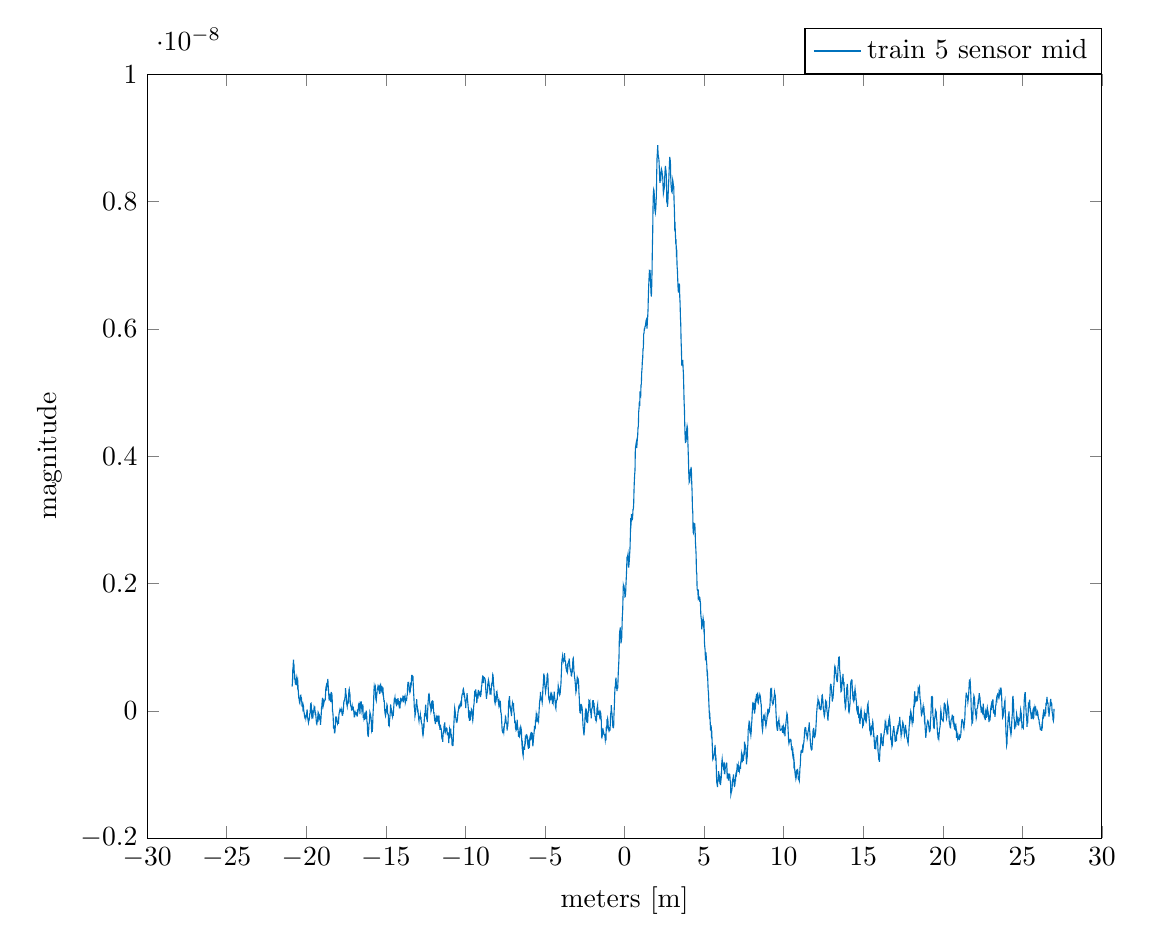
\begin{tikzpicture}

  \begin{axis}[%
    width=\textwidth,
    height=0.8\textwidth,
    at={(0\figurewidth,0\figureheight)},
    scale only axis,
    xmin=-30,
    xmax=30,
    xlabel={meters [m]},
    ymin=-2e-09,
    ymax=1e-08,
    ylabel={magnitude},
    axis background/.style={fill=white},
    legend style={at={(1.0,1.0)},anchor=south east}
    ]
    \addplot [color=mycolor1,solid]
    table[row sep=crcr]{%
    -20.8904349117279	3.80799788651844e-10\\
    -20.8694527793884	4.4767402555691e-10\\
    -20.848470647049	6.43362938427602e-10\\
    -20.8274885147095	6.89950128598444e-10\\
    -20.80650638237	8.02025126356065e-10\\
    -20.7855242500305	6.2688833742254e-10\\
    -20.764542117691	6.57499601222441e-10\\
    -20.7435599853516	5.31153288779885e-10\\
    -20.7225778530121	5.43121683159499e-10\\
    -20.7015957206726	4.66746443655729e-10\\
    -20.6806135883331	4.12376662607601e-10\\
    -20.6596314559937	4.64714317608171e-10\\
    -20.6386493236542	4.02046000668793e-10\\
    -20.6176671913147	4.93818826425184e-10\\
    -20.5966850589752	5.26985869936019e-10\\
    -20.5757029266357	4.87319801492266e-10\\
    -20.5547207942963	4.12943934021071e-10\\
    -20.5337386619568	4.47452509427077e-10\\
    -20.5127565296173	3.46477048588409e-10\\
    -20.4917743972778	2.68694061506204e-10\\
    -20.4707922649384	1.99829729981531e-10\\
    -20.4498101325989	1.88233877257126e-10\\
    -20.4288280002594	1.32369982249404e-10\\
    -20.4078458679199	1.18711724767239e-10\\
    -20.3868637355804	1.73107087902001e-10\\
    -20.365881603241	2.41052988650846e-10\\
    -20.3448994709015	2.44147237649902e-10\\
    -20.323917338562	1.86094106378402e-10\\
    -20.3029352062225	1.92805258131196e-10\\
    -20.2819530738831	1.33664555687093e-10\\
    -20.2609709415436	6.08639337961405e-11\\
    -20.2399888092041	1.28586873700058e-10\\
    -20.2190066768646	5.71180008984987e-11\\
    -20.1980245445252	9.4800836503271e-11\\
    -20.1770424121857	7.12467023033727e-11\\
    -20.1560602798462	-7.41928195842639e-12\\
    -20.1350781475067	-2.43420755684936e-11\\
    -20.1140960151672	-8.14815659309298e-11\\
    -20.0931138828278	-1.03562788083137e-10\\
    -20.0721317504883	-8.89073372895823e-11\\
    -20.0511496181488	-8.10045806070489e-11\\
    -20.0301674858093	-1.16265619788809e-10\\
    -20.0091853534699	-7.23748424425827e-11\\
    -19.9882032211304	-5.60168307472555e-11\\
    -19.9672210887909	-2.42048091471798e-11\\
    -19.9462389564514	2.26634001091592e-11\\
    -19.9252568241119	-1.01497694838443e-10\\
    -19.9042746917725	-1.16668564804881e-10\\
    -19.883292559433	-1.56567641186304e-10\\
    -19.8623104270935	-1.84261859202616e-10\\
    -19.841328294754	-1.37841615198382e-10\\
    -19.8203461624146	-1.4379680149606e-10\\
    -19.7993640300751	-1.04961834432459e-10\\
    -19.7783818977356	-4.35067509805758e-11\\
    -19.7573997653961	-4.21784243149889e-11\\
    -19.7364176330566	7.16150455254222e-11\\
    -19.7154355007172	1.1583139912118e-10\\
    -19.6944533683777	1.19968598399287e-10\\
    -19.6734712360382	-1.44529013119368e-11\\
    -19.6524891036987	-9.43454393613306e-11\\
    -19.6315069713593	-8.01998715083225e-11\\
    -19.6105248390198	-4.59289151109935e-11\\
    -19.5895427066803	-1.21894961687495e-10\\
    -19.5685605743408	-3.96009629974458e-11\\
    -19.5475784420013	-6.45892700235475e-13\\
    -19.5265963096619	9.10943389010984e-13\\
    -19.5056141773224	6.34499999051451e-11\\
    -19.4846320449829	5.05789814176664e-11\\
    -19.4636499126434	5.42704401578138e-11\\
    -19.442667780304	-6.86761636684102e-11\\
    -19.4216856479645	-1.80855513681036e-11\\
    -19.400703515625	-7.56469444680272e-11\\
    -19.3797213832855	-1.32711763200345e-10\\
    -19.358739250946	-1.98428828155875e-10\\
    -19.3377571186066	-2.09703868762456e-10\\
    -19.3167749862671	-1.73869172130473e-10\\
    -19.2957928539276	-1.61110770451176e-10\\
    -19.2748107215881	-8.0703867612832e-11\\
    -19.2538285892487	-2.3838603938761e-11\\
    -19.2328464569092	-3.63278390746679e-11\\
    -19.2118643245697	-9.46616658649688e-11\\
    -19.1908821922302	-4.98657335896179e-11\\
    -19.1699000598908	-1.25642272981179e-10\\
    -19.1489179275513	-1.32933371940328e-10\\
    -19.1279357952118	-1.16530041269607e-10\\
    -19.1069536628723	-2.20508139119063e-10\\
    -19.0859715305328	-1.49772946337616e-10\\
    -19.0649893981934	-7.61483156133538e-11\\
    -19.0440072658539	4.39249729829695e-11\\
    -19.0230251335144	7.18285554220321e-11\\
    -19.0020430011749	1.53414454689192e-10\\
    -18.9810608688355	1.92607814095611e-10\\
    -18.960078736496	1.88369122964479e-10\\
    -18.9390966041565	7.33762935696072e-11\\
    -18.918114471817	9.69588008533614e-11\\
    -18.8971323394775	1.11485587215759e-10\\
    -18.8761502071381	1.60861884349912e-10\\
    -18.8551680747986	1.55347320215401e-10\\
    -18.8341859424591	1.64374941203227e-10\\
    -18.8132038101196	1.67979076384018e-10\\
    -18.7922216777802	2.48749551437459e-10\\
    -18.7712395454407	3.56657180525605e-10\\
    -18.7502574131012	3.82186927469767e-10\\
    -18.7292752807617	3.17897592891892e-10\\
    -18.7082931484222	4.14897506274006e-10\\
    -18.6873110160828	4.25297282238885e-10\\
    -18.6663288837433	4.51639642301681e-10\\
    -18.6453467514038	4.99471415072218e-10\\
    -18.6243646190643	3.97659158065968e-10\\
    -18.6033824867249	3.23999700728064e-10\\
    -18.5824003543854	2.28819202616606e-10\\
    -18.5614182220459	1.59703069371362e-10\\
    -18.5404360897064	2.27143702130244e-10\\
    -18.5194539573669	2.1166221136687e-10\\
    -18.4984718250275	2.67305122315075e-10\\
    -18.477489692688	2.03449754107485e-10\\
    -18.4565075603485	1.36050199328791e-10\\
    -18.435525428009	2.98260082506349e-10\\
    -18.4145432956696	1.99001033390904e-10\\
    -18.3935611633301	2.76547789864609e-10\\
    -18.3725790309906	1.8396183684752e-10\\
    -18.3515968986511	-1.02820290319287e-11\\
    -18.3306147663116	-1.74049492787167e-11\\
    -18.3096326339722	-1.08568266710549e-10\\
    -18.2886505016327	-2.53073331453987e-10\\
    -18.2676683692932	-2.44346427891003e-10\\
    -18.2466862369537	-2.6155338619179e-10\\
    -18.2257041046143	-3.45712539182044e-10\\
    -18.2047219722748	-3.46231421735855e-10\\
    -18.1837398399353	-2.74071411872972e-10\\
    -18.1627577075958	-1.37514836504863e-10\\
    -18.1417755752564	-1.56510945852672e-10\\
    -18.1207934429169	-1.00870979894102e-10\\
    -18.0998113105774	-9.89115958298472e-11\\
    -18.0788291782379	-1.3043820616253e-10\\
    -18.0578470458984	-1.67535743092927e-10\\
    -18.036864913559	-1.95853149811767e-10\\
    -18.0158827812195	-1.67785000924303e-10\\
    -17.99490064888	-1.65121047318064e-10\\
    -17.9739185165405	-2.06231259484556e-10\\
    -17.9529363842011	-6.68167197591398e-11\\
    -17.9319542518616	-3.48109630259183e-11\\
    -17.9109721195221	-1.29456345878449e-11\\
    -17.8899899871826	1.35136834896109e-11\\
    -17.8690078548431	-7.73084834937601e-12\\
    -17.8480257225037	1.99622220836262e-12\\
    -17.8270435901642	1.0827013023617e-12\\
    -17.8060614578247	2.38988838856906e-11\\
    -17.7850793254852	-1.04595580125832e-11\\
    -17.7640971931458	-2.02089962429525e-11\\
    -17.7431150608063	-6.85972484234917e-11\\
    -17.7221329284668	-6.96248588109064e-11\\
    -17.7011507961273	-2.67983813347523e-12\\
    -17.6801686637878	-1.52535203175552e-11\\
    -17.6591865314484	5.70848434476717e-11\\
    -17.6382043991089	1.48466029494286e-10\\
    -17.6172222667694	1.6035725953211e-10\\
    -17.5962401344299	1.57791340231273e-10\\
    -17.5752580020905	1.96675142126106e-10\\
    -17.554275869751	2.35693037478699e-10\\
    -17.5332937374115	3.56874135949519e-10\\
    -17.512311605072	2.76516765357213e-10\\
    -17.4913294727325	2.48211002879896e-10\\
    -17.4703473403931	1.09456295006609e-10\\
    -17.4493652080536	1.03949431731352e-10\\
    -17.4283830757141	7.13681977492388e-11\\
    -17.4074009433746	1.25948228681612e-10\\
    -17.3864188110352	1.52091403425804e-10\\
    -17.3654366786957	1.85918607425749e-10\\
    -17.3444545463562	1.62664350856371e-10\\
    -17.3234724140167	3.19067186580521e-10\\
    -17.3024902816772	3.39492060166309e-10\\
    -17.2815081493378	2.8597607868508e-10\\
    -17.2605260169983	2.83317151912476e-10\\
    -17.2395438846588	1.53033627193175e-10\\
    -17.2185617523193	1.05054027392919e-10\\
    -17.1975796199799	6.69939776462745e-11\\
    -17.1765974876404	6.42199051473445e-11\\
    -17.1556153553009	1.68787335282539e-11\\
    -17.1346332229614	2.34058616706601e-11\\
    -17.113651090622	6.22371181302539e-11\\
    -17.0926689582825	5.59307564994006e-12\\
    -17.071686825943	5.98932264759706e-11\\
    -17.0507046936035	5.86062006264915e-11\\
    -17.029722561264	7.26521088621567e-12\\
    -17.0087404289246	-1.87355024162356e-11\\
    -16.9877582965851	-9.59309393002509e-11\\
    -16.9667761642456	-9.55650388882816e-11\\
    -16.9457940319061	-6.6950279819135e-11\\
    -16.9248118995667	-2.1426476180797e-11\\
    -16.9038297672272	-3.54781573506875e-11\\
    -16.8828476348877	-3.82992818206957e-11\\
    -16.8618655025482	-4.99027600306448e-11\\
    -16.8408833702087	-3.32026579240455e-11\\
    -16.8199012378693	-3.48555446274128e-11\\
    -16.7989191055298	-8.91634048639648e-11\\
    -16.7779369731903	2.0696924697769e-11\\
    -16.7569548408508	-1.66472606223688e-11\\
    -16.7359727085114	1.57642340550177e-11\\
    -16.7149905761719	9.64726045507545e-11\\
    -16.6940084438324	1.10575927610163e-10\\
    -16.6730263114929	5.04964704428493e-11\\
    -16.6520441791534	1.2006146855965e-10\\
    -16.631062046814	-5.37080374021724e-11\\
    -16.6100799144745	6.14193279813044e-11\\
    -16.589097782135	1.03519913722732e-10\\
    -16.5681156497955	8.20795511312316e-11\\
    -16.5471335174561	1.48118944870148e-10\\
    -16.5261513851166	7.46697629595482e-11\\
    -16.5051692527771	1.07217491909568e-11\\
    -16.4841871204376	4.95339203279887e-11\\
    -16.4632049880981	4.23813326719732e-11\\
    -16.4422228557587	1.01458939386531e-10\\
    -16.4212407234192	-1.11547951936242e-10\\
    -16.4002585910797	-5.95385147562053e-11\\
    -16.3792764587402	-1.15000218687179e-10\\
    -16.3582943264008	-8.96578311158092e-11\\
    -16.3373121940613	-1.45367734468271e-10\\
    -16.3163300617218	-2.7225521045973e-11\\
    -16.2953479293823	-6.28677780354676e-11\\
    -16.2743657970428	-6.96846734839742e-11\\
    -16.2533836647034	-1.30764641468258e-10\\
    -16.2324015323639	1.39038252372482e-12\\
    -16.2114194000244	-3.64207540989671e-11\\
    -16.1904372676849	-1.64928655614468e-10\\
    -16.1694551353455	-1.88358788556416e-10\\
    -16.148473003006	-3.2734377351078e-10\\
    -16.1274908706665	-3.92020349552969e-10\\
    -16.106508738327	-3.97831252613056e-10\\
    -16.0855266059876	-3.50356742360871e-10\\
    -16.0645444736481	-2.06481631309467e-10\\
    -16.0435623413086	-1.98965297918676e-10\\
    -16.0225802089691	-1.21015580238778e-10\\
    -16.0015980766296	-2.31272970953824e-11\\
    -15.9806159442902	-4.32902000351912e-11\\
    -15.9596338119507	-6.7462457477397e-11\\
    -15.9386516796112	-9.36275145105396e-11\\
    -15.9176695472717	-1.50097137524701e-10\\
    -15.8966874149323	-2.95308884863445e-10\\
    -15.8757052825928	-2.69612261801783e-10\\
    -15.8547231502533	-3.28875696503251e-10\\
    -15.8337410179138	-2.54373357576902e-10\\
    -15.8127588855743	-8.8874988526802e-11\\
    -15.7917767532349	1.52666352224504e-11\\
    -15.7707946208954	1.16722773106195e-10\\
    -15.7498124885559	3.08792607192232e-10\\
    -15.7288303562164	3.82970343986455e-10\\
    -15.707848223877	3.51750679982298e-10\\
    -15.6868660915375	3.53829502633122e-10\\
    -15.665883959198	3.73694284142401e-10\\
    -15.6449018268585	2.29118794325002e-10\\
    -15.623919694519	1.81474525108468e-10\\
    -15.6029375621796	1.60163103886549e-10\\
    -15.5819554298401	2.27152851819985e-10\\
    -15.5609732975006	2.70773186736709e-10\\
    -15.5399911651611	3.42436111656162e-10\\
    -15.5190090328217	3.48245741326522e-10\\
    -15.4980269004822	3.79733285611672e-10\\
    -15.4770447681427	3.5983651971857e-10\\
    -15.4560626358032	3.40010389247773e-10\\
    -15.4350805034637	3.68089035636396e-10\\
    -15.4140983711243	3.21567185523233e-10\\
    -15.3931162387848	2.72261190963301e-10\\
    -15.3721341064453	2.73906874974303e-10\\
    -15.3511519741058	3.91965626808497e-10\\
    -15.3301698417664	4.06986035870371e-10\\
    -15.3091877094269	3.53383593022314e-10\\
    -15.2882055770874	3.30822775565172e-10\\
    -15.2672234447479	3.83628411744477e-10\\
    -15.2462413124084	3.80638112579307e-10\\
    -15.225259180069	3.37561429066501e-10\\
    -15.2042770477295	3.01444178098986e-10\\
    -15.18329491539	3.6815746407801e-10\\
    -15.1623127830505	2.65194742326202e-10\\
    -15.1413306507111	2.16780898733733e-10\\
    -15.1203485183716	1.51417250461315e-10\\
    -15.0993663860321	1.53353924792879e-10\\
    -15.0783842536926	3.27766313833546e-11\\
    -15.0574021213532	-2.94800459736385e-11\\
    -15.0364199890137	-5.60769956691525e-11\\
    -15.0154378566742	2.87558912727363e-11\\
    -14.9944557243347	-3.63374768571712e-11\\
    -14.9734735919952	-4.90849298713102e-13\\
    -14.9524914596558	2.81316394487531e-11\\
    -14.9315093273163	9.73171408340198e-11\\
    -14.9105271949768	7.96099582863256e-11\\
    -14.8895450626373	-4.53601515724734e-11\\
    -14.8685629302979	-4.73697198172376e-11\\
    -14.8475807979584	-6.03657670209814e-11\\
    -14.8265986656189	-2.11455964130722e-10\\
    -14.8056165332794	-2.00170909769925e-10\\
    -14.7846344009399	-2.1943768355772e-10\\
    -14.7636522686005	-1.38599208037654e-10\\
    -14.742670136261	-8.88564342973594e-11\\
    -14.7216880039215	-2.06826635792644e-11\\
    -14.700705871582	1.00281125516724e-10\\
    -14.6797237392426	4.97060496508656e-11\\
    -14.6587416069031	3.08598750545945e-11\\
    -14.6377594745636	-1.27317618377958e-11\\
    -14.6167773422241	-6.00733389049587e-11\\
    -14.5957952098846	-4.97457122202492e-11\\
    -14.5748130775452	-8.51491870663012e-11\\
    -14.5538309452057	-4.45350360915048e-11\\
    -14.5328488128662	-8.076893101595e-11\\
    -14.5118666805267	2.45374393036083e-11\\
    -14.4908845481873	1.08225265214687e-10\\
    -14.4699024158478	1.77217469627124e-10\\
    -14.4489202835083	1.69733003039649e-10\\
    -14.4279381511688	2.04209223703086e-10\\
    -14.4069560188293	1.33207322733107e-10\\
    -14.3859738864899	1.93841408091623e-10\\
    -14.3649917541504	1.24018520999865e-10\\
    -14.3440096218109	1.30450455696629e-10\\
    -14.3230274894714	6.86878193834526e-11\\
    -14.302045357132	1.83517400956292e-10\\
    -14.2810632247925	1.48582184462664e-10\\
    -14.260081092453	1.34360130474294e-10\\
    -14.2390989601135	1.99121061581998e-10\\
    -14.2181168277741	1.52445034886463e-10\\
    -14.1971346954346	1.19724002455697e-10\\
    -14.1761525630951	8.9424026884875e-11\\
    -14.1551704307556	1.44577341079055e-10\\
    -14.1341882984161	1.4413971797725e-10\\
    -14.1132061660767	3.83697524681907e-11\\
    -14.0922240337372	1.30291185838823e-10\\
    -14.0712419013977	2.05149573368512e-10\\
    -14.0502597690582	1.41997153115715e-10\\
    -14.0292776367188	1.59711225934187e-10\\
    -14.0082955043793	1.79234049674672e-10\\
    -13.9873133720398	1.86114619787394e-10\\
    -13.9663312397003	1.79926245845896e-10\\
    -13.9453491073608	1.69125137863118e-10\\
    -13.9243669750214	2.39659181623526e-10\\
    -13.9033848426819	1.31774938774938e-10\\
    -13.8824027103424	1.80938836642454e-10\\
    -13.8614205780029	2.29018174775756e-10\\
    -13.8404384456635	1.674477192357e-10\\
    -13.819456313324	2.17475138961097e-10\\
    -13.7984741809845	2.33592493522277e-10\\
    -13.777492048645	1.25024298196432e-10\\
    -13.7565099163055	1.46073518584951e-10\\
    -13.7355277839661	1.76959811271488e-10\\
    -13.7145456516266	1.8829326386969e-10\\
    -13.6935635192871	1.78620323970409e-10\\
    -13.6725813869476	2.37710538011248e-10\\
    -13.6515992546082	2.50975001426996e-10\\
    -13.6306171222687	3.93551408071051e-10\\
    -13.6096349899292	4.39373577449835e-10\\
    -13.5886528575897	4.35334401214694e-10\\
    -13.5676707252502	4.41375895141828e-10\\
    -13.5466885929108	3.96067997763657e-10\\
    -13.5257064605713	3.2212076342157e-10\\
    -13.5047243282318	3.33036064394731e-10\\
    -13.4837421958923	2.92905970559326e-10\\
    -13.4627600635529	3.10102319876457e-10\\
    -13.4417779312134	4.02812992951432e-10\\
    -13.4207957988739	3.85964200843531e-10\\
    -13.3998136665344	4.16917966948811e-10\\
    -13.3788315341949	5.54725894376862e-10\\
    -13.3578494018555	5.551216669795e-10\\
    -13.336867269516	5.17631543096832e-10\\
    -13.3158851371765	5.44026868146446e-10\\
    -13.294903004837	5.36295880067072e-10\\
    -13.2739208724976	3.82490959960642e-10\\
    -13.2529387401581	2.7994566174764e-10\\
    -13.2319566078186	1.8355095666343e-10\\
    -13.2109744754791	4.90261227971542e-11\\
    -13.1899923431397	3.77010750247528e-11\\
    -13.1690102108002	-8.24622136457865e-11\\
    -13.1480280784607	-4.99485320087954e-11\\
    -13.1270459461212	-1.32531135666369e-11\\
    -13.1060638137817	1.08015249720517e-10\\
    -13.0850816814423	5.65620896095113e-11\\
    -13.0640995491028	1.83126259141873e-10\\
    -13.0431174167633	8.87103033409017e-11\\
    -13.0221352844238	6.65033692679775e-11\\
    -13.0011531520844	-9.40222646748872e-13\\
    -12.9801710197449	5.92145647290624e-12\\
    -12.9591888874054	-5.99717169056858e-11\\
    -12.9382067550659	-1.20137789338264e-10\\
    -12.9172246227264	-1.58328850945962e-10\\
    -12.896242490387	-9.96248234393024e-11\\
    -12.8752603580475	-9.57089927638455e-11\\
    -12.854278225708	-9.66171242435033e-11\\
    -12.8332960933685	-6.20171295298869e-11\\
    -12.8123139610291	-1.39203350752001e-10\\
    -12.7913318286896	-9.62133793767201e-11\\
    -12.7703496963501	-1.85214882817738e-10\\
    -12.7493675640106	-1.98261268944827e-10\\
    -12.7283854316711	-2.15950746026251e-10\\
    -12.7074032993317	-2.94740711257601e-10\\
    -12.6864211669922	-3.56846638829357e-10\\
    -12.6654390346527	-3.87151618791342e-10\\
    -12.6444569023132	-3.5516953376121e-10\\
    -12.6234747699738	-2.32670754204447e-10\\
    -12.6024926376343	-2.43011668428954e-10\\
    -12.5815105052948	-1.1881705455334e-10\\
    -12.5605283729553	-3.62391029278552e-11\\
    -12.5395462406158	-8.82112250154011e-11\\
    -12.5185641082764	1.52670135537355e-11\\
    -12.4975819759369	9.5975031990763e-11\\
    -12.4765998435974	-8.46426602777521e-12\\
    -12.4556177112579	-6.46837205840873e-11\\
    -12.4346355789185	-1.33111071868826e-10\\
    -12.413653446579	-7.57360538056137e-11\\
    -12.3926713142395	-1.76311323724479e-10\\
    -12.3716891819	-3.26962361731204e-13\\
    -12.3507070495605	1.175864199284e-10\\
    -12.3297249172211	1.78722801065174e-10\\
    -12.3087427848816	2.54583238995147e-10\\
    -12.2877606525421	2.65725693650944e-10\\
    -12.2667785202026	2.50067670094967e-10\\
    -12.2457963878632	1.33967059587904e-10\\
    -12.2248142555237	8.70768308884037e-11\\
    -12.2038321231842	6.6399131761203e-11\\
    -12.1828499908447	1.10768693263252e-10\\
    -12.1618678585053	-1.08855532380398e-11\\
    -12.1408857261658	8.31189343312144e-12\\
    -12.1199035938263	1.11136434417627e-10\\
    -12.0989214614868	9.81442068624192e-11\\
    -12.0779393291473	1.567102250008e-10\\
    -12.0569571968079	1.55234352807031e-10\\
    -12.0359750644684	2.99502285147333e-11\\
    -12.0149929321289	6.49327399707212e-11\\
    -11.9940107997894	-3.32638578904405e-11\\
    -11.97302866745	-3.17760836329154e-11\\
    -11.9520465351105	-9.0648598923099e-11\\
    -11.931064402771	-1.42299758640544e-10\\
    -11.9100822704315	-1.3627875471645e-10\\
    -11.889100138092	-2.08952091696117e-10\\
    -11.8681180057526	-1.68273519187901e-10\\
    -11.8471358734131	-1.18679298253224e-10\\
    -11.8261537410736	-1.71737725375326e-10\\
    -11.8051716087341	-7.49506333702516e-11\\
    -11.7841894763947	-1.18429974669642e-10\\
    -11.7632073440552	-1.6797455965877e-10\\
    -11.7422252117157	-1.03985883952559e-10\\
    -11.7212430793762	-9.29052079224699e-11\\
    -11.7002609470367	-1.5758589024101e-10\\
    -11.6792788146973	-1.18435134326711e-10\\
    -11.6582966823578	-1.05654278332653e-10\\
    -11.6373145500183	-2.01131241667576e-10\\
    -11.6163324176788	-2.47623985305377e-10\\
    -11.5953502853394	-3.004037457324e-10\\
    -11.5743681529999	-2.18936012758507e-10\\
    -11.5533860206604	-2.60113465990209e-10\\
    -11.5324038883209	-2.7614934173853e-10\\
    -11.5114217559814	-2.93859598241747e-10\\
    -11.490439623642	-4.01179978954613e-10\\
    -11.4694574913025	-4.47560440400656e-10\\
    -11.448475358963	-3.79202313245288e-10\\
    -11.4274932266235	-4.88413161926233e-10\\
    -11.4065110942841	-3.80290946346808e-10\\
    -11.3855289619446	-3.43172040114962e-10\\
    -11.3645468296051	-3.37139072762676e-10\\
    -11.3435646972656	-2.45637797667889e-10\\
    -11.3225825649261	-2.58295347380119e-10\\
    -11.3016004325867	-1.82321462341617e-10\\
    -11.2806183002472	-2.68131470900741e-10\\
    -11.2596361679077	-3.33241913436536e-10\\
    -11.2386540355682	-3.16095652962683e-10\\
    -11.2176719032288	-2.87131091115116e-10\\
    -11.1966897708893	-2.92169265202202e-10\\
    -11.1757076385498	-2.75726954942307e-10\\
    -11.1547255062103	-2.85459968216601e-10\\
    -11.1337433738709	-3.86427141352881e-10\\
    -11.1127612415314	-3.409030285147e-10\\
    -11.0917791091919	-3.457412230547e-10\\
    -11.0707969768524	-3.54606983363717e-10\\
    -11.0498148445129	-5.08129739931554e-10\\
    -11.0288327121735	-4.06461134677812e-10\\
    -11.007850579834	-4.12566976495933e-10\\
    -10.9868684474945	-2.91175963360161e-10\\
    -10.965886315155	-3.19371162974351e-10\\
    -10.9449041828156	-2.87935314817353e-10\\
    -10.9239220504761	-2.88385539775483e-10\\
    -10.9029399181366	-4.22013229799433e-10\\
    -10.8819577857971	-3.63585169012669e-10\\
    -10.8609756534576	-4.15599665810617e-10\\
    -10.8399935211182	-5.30548957771837e-10\\
    -10.8190113887787	-5.45659516518164e-10\\
    -10.7980292564392	-5.46469738398945e-10\\
    -10.7770471240997	-5.40388252089781e-10\\
    -10.7560649917603	-4.12729613813856e-10\\
    -10.7350828594208	-2.60600792471292e-10\\
    -10.7141007270813	-1.57178371926314e-10\\
    -10.6931185947418	-4.96450539730707e-11\\
    -10.6721364624023	4.12108129249952e-11\\
    -10.6511543300629	6.25359443037186e-12\\
    -10.6301721977234	-4.0905231862694e-11\\
    -10.6091900653839	-1.03574779943056e-10\\
    -10.5882079330444	-1.36422627034867e-10\\
    -10.567225800705	-1.74178930657151e-10\\
    -10.5462436683655	-1.65711275279424e-10\\
    -10.525261536026	-1.70576806528787e-10\\
    -10.5042794036865	-1.34546346637193e-10\\
    -10.483297271347	-6.94055109549913e-11\\
    -10.4623151390076	-1.42367360061759e-11\\
    -10.4413330066681	-1.20823674840987e-12\\
    -10.4203508743286	6.0051540194392e-11\\
    -10.3993687419891	7.5635971063789e-11\\
    -10.3783866096497	4.4199736097203e-11\\
    -10.3574044773102	5.21694866519179e-11\\
    -10.3364223449707	6.26811460466526e-11\\
    -10.3154402126312	1.01977846148065e-10\\
    -10.2944580802917	9.33966675034984e-11\\
    -10.2734759479523	1.59568520900053e-10\\
    -10.2524938156128	6.8898421614914e-11\\
    -10.2315116832733	2.15907853274024e-10\\
    -10.2105295509338	2.49825615165035e-10\\
    -10.1895474185944	2.66825511946108e-10\\
    -10.1685652862549	2.64297648917032e-10\\
    -10.1475831539154	3.32580627603476e-10\\
    -10.1266010215759	3.44147430531505e-10\\
    -10.1056188892365	3.06518243622153e-10\\
    -10.084636756897	2.46276003568516e-10\\
    -10.0636546245575	2.5637211033281e-10\\
    -10.042672492218	2.16455112937293e-10\\
    -10.0216903598785	1.49055150129154e-10\\
    -10.0007082275391	1.47533471626012e-10\\
    -9.97972609519958	4.14607039267802e-11\\
    -9.95874396286011	1.64423472947461e-10\\
    -9.93776183052063	1.66767800718724e-10\\
    -9.91677969818115	1.91167917478252e-10\\
    -9.89579756584168	2.75274132411211e-10\\
    -9.8748154335022	1.96408826371246e-10\\
    -9.85383330116272	1.38958323466723e-10\\
    -9.83285116882324	8.214055134841e-11\\
    -9.81186903648377	2.39209450583577e-11\\
    -9.79088690414429	-1.08562665050034e-10\\
    -9.76990477180481	-6.30672264960555e-11\\
    -9.74892263946533	-1.57631570143096e-10\\
    -9.72794050712585	-5.82214604410069e-11\\
    -9.70695837478638	-8.61639021212964e-11\\
    -9.6859762424469	-1.05559678618517e-10\\
    -9.66499411010742	-8.79616874728638e-12\\
    -9.64401197776795	-5.74226748789087e-11\\
    -9.62302984542847	2.42978205968579e-11\\
    -9.60204771308899	1.34344248935438e-11\\
    -9.58106558074951	-2.82385035480301e-11\\
    -9.56008344841004	-1.17594075305085e-10\\
    -9.53910131607056	-1.53422097134761e-10\\
    -9.51811918373108	-1.10114592478909e-10\\
    -9.4971370513916	4.23245770278701e-13\\
    -9.47615491905212	8.05533359885041e-11\\
    -9.45517278671265	1.15111045890292e-10\\
    -9.43419065437317	2.17076526422501e-10\\
    -9.41320852203369	2.98582840218314e-10\\
    -9.39222638969421	2.92352857914417e-10\\
    -9.37124425735474	2.25013870831236e-10\\
    -9.35026212501526	3.34543995910938e-10\\
    -9.32927999267578	2.63770612015672e-10\\
    -9.3082978603363	2.60476319082377e-10\\
    -9.28731572799683	1.22422901413466e-10\\
    -9.26633359565735	1.59615928471481e-10\\
    -9.24535146331787	2.55238705152704e-10\\
    -9.22436933097839	2.61236443011305e-10\\
    -9.20338719863892	2.88984917505281e-10\\
    -9.18240506629944	3.2950705343109e-10\\
    -9.16142293395996	2.50538720262955e-10\\
    -9.14044080162048	2.75510809529754e-10\\
    -9.11945866928101	2.85578078855537e-10\\
    -9.09847653694153	2.73149241503377e-10\\
    -9.07749440460205	2.83732176937664e-10\\
    -9.05651227226257	2.14592975335909e-10\\
    -9.0355301399231	2.63914813684755e-10\\
    -9.01454800758362	2.61177202504645e-10\\
    -8.99356587524414	3.78403962699211e-10\\
    -8.97258374290466	3.93084727150985e-10\\
    -8.95160161056519	4.6812842371842e-10\\
    -8.93061947822571	5.07674699745577e-10\\
    -8.90963734588623	5.53734222035626e-10\\
    -8.88865521354675	4.80915651063308e-10\\
    -8.86767308120728	4.35765519393425e-10\\
    -8.8466909488678	5.26869115728826e-10\\
    -8.82570881652832	5.209296160322e-10\\
    -8.80472668418884	5.21236582826349e-10\\
    -8.78374455184936	5.07466395314024e-10\\
    -8.76276241950989	4.96297372062536e-10\\
    -8.74178028717041	4.60278369226556e-10\\
    -8.72079815483093	3.36813792716302e-10\\
    -8.69981602249146	2.68655111465915e-10\\
    -8.67883389015198	1.89197483394203e-10\\
    -8.6578517578125	2.4273578328151e-10\\
    -8.63686962547302	2.75014782436868e-10\\
    -8.61588749313355	2.99277697023006e-10\\
    -8.59490536079407	4.16563873298871e-10\\
    -8.57392322845459	4.41480495785313e-10\\
    -8.55294109611511	4.84569338329809e-10\\
    -8.53195896377563	4.60987580029359e-10\\
    -8.51097683143616	4.23914504780332e-10\\
    -8.48999469909668	3.57278091567529e-10\\
    -8.4690125667572	3.2756627873213e-10\\
    -8.44803043441772	2.50086046500586e-10\\
    -8.42704830207825	3.18384359620909e-10\\
    -8.40606616973877	3.04101039368708e-10\\
    -8.38508403739929	2.89165914471175e-10\\
    -8.36410190505982	4.08080443976972e-10\\
    -8.34311977272034	4.26793401558057e-10\\
    -8.32213764038086	4.16653777440833e-10\\
    -8.30115550804138	4.91988410961405e-10\\
    -8.2801733757019	5.71061518734332e-10\\
    -8.25919124336243	5.56718349422549e-10\\
    -8.23820911102295	4.45367270793467e-10\\
    -8.21722697868347	3.79203453905192e-10\\
    -8.19624484634399	3.06985637569842e-10\\
    -8.17526271400452	1.67158909851861e-10\\
    -8.15428058166504	1.41483843790973e-10\\
    -8.13329844932556	2.29641836051625e-10\\
    -8.11231631698608	1.53029168259905e-10\\
    -8.09133418464661	1.88596685778671e-10\\
    -8.07035205230713	1.74723846300807e-10\\
    -8.04936991996765	3.13660065976854e-10\\
    -8.02838778762817	2.36991569239554e-10\\
    -8.0074056552887	2.70701358830484e-10\\
    -7.98642352294922	2.24901243168171e-10\\
    -7.96544139060974	2.10559909452253e-10\\
    -7.94445925827026	1.52931577568704e-10\\
    -7.92347712593079	1.28919979622017e-10\\
    -7.90249499359131	9.1173256442594e-11\\
    -7.88151286125183	1.31236188859785e-10\\
    -7.86053072891235	8.22889394004325e-11\\
    -7.83954859657288	1.01091834473681e-10\\
    -7.8185664642334	1.59561039077714e-10\\
    -7.79758433189392	1.11045288134502e-10\\
    -7.77660219955444	-2.01583175447533e-11\\
    -7.75562006721497	-3.30748744333461e-11\\
    -7.73463793487549	-9.01635017845684e-11\\
    -7.71365580253601	-2.00324914687595e-10\\
    -7.69267367019653	-2.99316745106259e-10\\
    -7.67169153785706	-3.27783608516842e-10\\
    -7.65070940551758	-3.38970528422826e-10\\
    -7.6297272731781	-3.30963859650239e-10\\
    -7.60874514083862	-2.99681515781257e-10\\
    -7.58776300849915	-3.32666936492213e-10\\
    -7.56678087615967	-2.70820544573796e-10\\
    -7.54579874382019	-2.11716057121801e-10\\
    -7.52481661148071	-1.93554561820784e-10\\
    -7.50383447914123	-1.64456721153529e-10\\
    -7.48285234680176	-9.04695175305016e-11\\
    -7.46187021446228	-1.02079320000547e-10\\
    -7.4408880821228	-1.8814712150082e-10\\
    -7.41990594978333	-1.95771030570766e-10\\
    -7.39892381744385	-2.0565678151303e-10\\
    -7.37794168510437	-3.12263434244807e-10\\
    -7.35695955276489	-1.84417161371113e-10\\
    -7.33597742042542	-2.46779868565308e-10\\
    -7.31499528808594	-1.3457492447608e-10\\
    -7.29401315574646	5.81394267873287e-11\\
    -7.27303102340698	1.55367998114921e-10\\
    -7.2520488910675	1.75269896968023e-10\\
    -7.23106675872803	2.31435462701955e-10\\
    -7.21008462638855	1.37143717495312e-10\\
    -7.18910249404907	2.60445284891182e-11\\
    -7.16812036170959	6.83233942116436e-11\\
    -7.14713822937012	-8.60271956225483e-12\\
    -7.12615609703064	-2.75452820668556e-11\\
    -7.10517396469116	-8.3006680696706e-11\\
    -7.08419183235169	1.70743330666037e-12\\
    -7.06320970001221	6.33489528413088e-11\\
    -7.04222756767273	1.22630878409802e-10\\
    -7.02124543533325	9.89409460375533e-11\\
    -7.00026330299377	1.11448472567579e-10\\
    -6.9792811706543	1.1335812857235e-10\\
    -6.95829903831482	-1.04309981342843e-11\\
    -6.93731690597534	-2.94866188567367e-11\\
    -6.91633477363586	-1.11597169065572e-10\\
    -6.89535264129639	-1.94387576950439e-10\\
    -6.87437050895691	-1.52242180896921e-10\\
    -6.85338837661743	-2.56537055950423e-10\\
    -6.83240624427795	-2.42067421113907e-10\\
    -6.81142411193848	-3.0210007351189e-10\\
    -6.790441979599	-2.92071898285203e-10\\
    -6.76945984725952	-2.69719460706307e-10\\
    -6.74847771492004	-1.37924480760915e-10\\
    -6.72749558258057	-2.29666120052226e-10\\
    -6.70651345024109	-2.68537085912297e-10\\
    -6.68553131790161	-3.1241847585791e-10\\
    -6.66454918556213	-3.90170261583098e-10\\
    -6.64356705322266	-3.82657612630834e-10\\
    -6.62258492088318	-3.97761706605396e-10\\
    -6.6016027885437	-4.07539927933331e-10\\
    -6.58062065620422	-3.13717833117292e-10\\
    -6.55963852386475	-2.49904957002995e-10\\
    -6.53865639152527	-3.04520264433352e-10\\
    -6.51767425918579	-2.58261065586327e-10\\
    -6.49669212684631	-2.8104841983706e-10\\
    -6.47570999450684	-3.34281070321704e-10\\
    -6.45472786216736	-4.93622594268649e-10\\
    -6.43374572982788	-5.67523559872805e-10\\
    -6.4127635974884	-5.40067678489142e-10\\
    -6.39178146514893	-6.82545607733498e-10\\
    -6.37079933280945	-7.0877003294212e-10\\
    -6.34981720046997	-5.76823645413583e-10\\
    -6.32883506813049	-5.82685132800692e-10\\
    -6.30785293579101	-5.74195463599925e-10\\
    -6.28687080345154	-6.13134235945586e-10\\
    -6.26588867111206	-5.20207181522576e-10\\
    -6.24490653877258	-4.53748845553669e-10\\
    -6.2239244064331	-4.94531310753392e-10\\
    -6.20294227409363	-4.6628811780661e-10\\
    -6.18196014175415	-3.93657743415327e-10\\
    -6.16097800941467	-3.77177951171778e-10\\
    -6.1399958770752	-3.80582964511012e-10\\
    -6.11901374473572	-4.03368220368312e-10\\
    -6.09803161239624	-4.15367996118368e-10\\
    -6.07704948005676	-5.43990412499108e-10\\
    -6.05606734771728	-5.63487622396204e-10\\
    -6.03508521537781	-5.97136336910805e-10\\
    -6.01410308303833	-4.54160658727538e-10\\
    -5.99312095069885	-5.82448882957685e-10\\
    -5.97213881835937	-5.46444863887249e-10\\
    -5.9511566860199	-4.20229059835133e-10\\
    -5.93017455368042	-3.99414993651978e-10\\
    -5.90919242134094	-4.51975440456364e-10\\
    -5.88821028900146	-4.53290881043743e-10\\
    -5.86722815666199	-3.31484962023987e-10\\
    -5.84624602432251	-4.03713671892045e-10\\
    -5.82526389198303	-4.42680544807699e-10\\
    -5.80428175964355	-3.42855088343727e-10\\
    -5.78329962730408	-4.39287511260861e-10\\
    -5.7623174949646	-5.58466303069333e-10\\
    -5.74133536262512	-5.03609197308662e-10\\
    -5.72035323028564	-4.30671910051836e-10\\
    -5.69937109794617	-3.79214526081702e-10\\
    -5.67838896560669	-3.26155701853969e-10\\
    -5.65740683326721	-2.36118507488464e-10\\
    -5.63642470092773	-2.86666391671925e-10\\
    -5.61544256858826	-2.81572645856512e-10\\
    -5.59446043624878	-1.50749871829255e-10\\
    -5.5734783039093	-1.39780155283336e-10\\
    -5.55249617156982	-6.6801364726839e-11\\
    -5.53151403923035	-1.05109559680369e-10\\
    -5.51053190689087	-3.18505406618188e-11\\
    -5.48954977455139	-1.09960304512808e-10\\
    -5.46856764221191	-1.49495559576836e-10\\
    -5.44758550987244	-1.36802864141519e-10\\
    -5.42660337753296	-1.4171430018621e-10\\
    -5.40562124519348	-1.6303740993268e-10\\
    -5.384639112854	-6.55002461829246e-11\\
    -5.36365698051453	2.4200248089502e-11\\
    -5.34267484817505	1.20224476395102e-10\\
    -5.32169271583557	1.70371454252536e-10\\
    -5.30071058349609	2.03278146466577e-10\\
    -5.27972845115661	2.94870620140796e-10\\
    -5.25874631881714	1.96303288774278e-10\\
    -5.23776418647766	2.09838921226857e-10\\
    -5.21678205413818	1.8354430069403e-10\\
    -5.19579992179871	1.6781976092395e-10\\
    -5.17481778945923	1.31231986344646e-10\\
    -5.15383565711975	1.84068115570007e-10\\
    -5.13285352478027	3.38920076598688e-10\\
    -5.1118713924408	3.94377050287311e-10\\
    -5.09088926010132	4.8964392092287e-10\\
    -5.06990712776184	5.88450486979852e-10\\
    -5.04892499542236	4.86887980065777e-10\\
    -5.02794286308288	5.04198850279713e-10\\
    -5.00696073074341	3.84677722353792e-10\\
    -4.98597859840393	3.53246632449983e-10\\
    -4.96499646606445	2.97670986245998e-10\\
    -4.94401433372498	3.35726445849931e-10\\
    -4.9230322013855	3.77799332975669e-10\\
    -4.90205006904602	4.17989597256612e-10\\
    -4.88106793670654	4.70229783524496e-10\\
    -4.86008580436706	5.66686905386097e-10\\
    -4.83910367202759	5.76772327665508e-10\\
    -4.81812153968811	5.53494384719328e-10\\
    -4.79713940734863	3.61495851980392e-10\\
    -4.77615727500915	2.67675377913415e-10\\
    -4.75517514266968	1.76803277481445e-10\\
    -4.7341930103302	1.71001114833615e-10\\
    -4.71321087799072	1.50746562008884e-10\\
    -4.69222874565125	2.23943300801214e-10\\
    -4.67124661331177	1.64341625443442e-10\\
    -4.65026448097229	2.41458956201613e-10\\
    -4.62928234863281	2.18310285377318e-10\\
    -4.60830021629333	2.56922440704207e-10\\
    -4.58731808395386	2.69259352597469e-10\\
    -4.56633595161438	1.82647204941066e-10\\
    -4.5453538192749	1.6890248544684e-10\\
    -4.52437168693542	1.06331201061554e-10\\
    -4.50338955459595	1.78389411437792e-10\\
    -4.48240742225647	1.41590785097811e-10\\
    -4.46142528991699	1.99723133062499e-10\\
    -4.44044315757751	2.08771663448935e-10\\
    -4.41946102523804	2.9935152753076e-10\\
    -4.39847889289856	2.17350982039297e-10\\
    -4.37749676055908	1.79338823090251e-10\\
    -4.3565146282196	1.37146174796012e-10\\
    -4.33553249588013	5.55132944055668e-11\\
    -4.31455036354065	3.40590586328508e-11\\
    -4.29356823120117	1.271234023026e-10\\
    -4.27258609886169	1.61872875962468e-10\\
    -4.25160396652221	1.71389064385521e-10\\
    -4.23062183418274	1.77379863489936e-10\\
    -4.20963970184326	2.82860039842905e-10\\
    -4.18865756950378	2.94025642706038e-10\\
    -4.16767543716431	3.92744566093524e-10\\
    -4.14669330482483	3.60442337347601e-10\\
    -4.12571117248535	3.5155617239274e-10\\
    -4.10472904014587	2.70296661504701e-10\\
    -4.0837469078064	2.542577277432e-10\\
    -4.06276477546692	2.99825682286346e-10\\
    -4.04178264312744	2.87327462633483e-10\\
    -4.02080051078796	3.60315772672321e-10\\
    -3.99981837844848	4.0678847588002e-10\\
    -3.97883624610901	5.39290182846373e-10\\
    -3.95785411376953	6.66524891770292e-10\\
    -3.93687198143005	7.99912320811101e-10\\
    -3.91588984909058	8.1762414816899e-10\\
    -3.8949077167511	8.57535030058671e-10\\
    -3.87392558441162	8.0382169413187e-10\\
    -3.85294345207214	7.82502017346104e-10\\
    -3.83196131973267	8.22228139961511e-10\\
    -3.81097918739319	8.23794847711332e-10\\
    -3.78999705505371	7.73564288907761e-10\\
    -3.76901492271423	9.0460649973855e-10\\
    -3.74803279037475	7.83052730910003e-10\\
    -3.72705065803528	7.8442724315479e-10\\
    -3.7060685256958	7.70708838588558e-10\\
    -3.68508639335632	6.75845533853318e-10\\
    -3.66410426101685	6.62010657320255e-10\\
    -3.64312212867737	6.23166995313817e-10\\
    -3.62213999633789	6.13965962843227e-10\\
    -3.60115786399841	6.70559860442869e-10\\
    -3.58017573165893	6.3018999549652e-10\\
    -3.55919359931946	6.82398802447279e-10\\
    -3.53821146697998	7.48398873879545e-10\\
    -3.5172293346405	7.73198528554319e-10\\
    -3.49624720230102	7.78511179112764e-10\\
    -3.47526506996155	8.2063969804934e-10\\
    -3.45428293762207	7.45936253167022e-10\\
    -3.43330080528259	6.77825795537895e-10\\
    -3.41231867294312	6.54107285420651e-10\\
    -3.39133654060364	6.2945839867332e-10\\
    -3.37035440826416	6.37192493255872e-10\\
    -3.34937227592468	5.52149311177454e-10\\
    -3.3283901435852	5.48861470141989e-10\\
    -3.30740801124573	6.00377041220704e-10\\
    -3.28642587890625	6.07607516488047e-10\\
    -3.26544374656677	6.8837811775395e-10\\
    -3.24446161422729	8.13838892966265e-10\\
    -3.22347948188782	8.27031586687795e-10\\
    -3.20249734954834	7.57620094301906e-10\\
    -3.18151521720886	6.21739051427585e-10\\
    -3.16053308486939	5.98187583909074e-10\\
    -3.13955095252991	5.21743960075446e-10\\
    -3.11856882019043	4.93458588441445e-10\\
    -3.09758668785095	4.33446298096709e-10\\
    -3.07660455551147	3.64444438068693e-10\\
    -3.055622423172	2.91325102103252e-10\\
    -3.03464029083252	3.1664136215871e-10\\
    -3.01365815849304	3.77454417444251e-10\\
    -2.99267602615356	4.73833906351397e-10\\
    -2.97169389381408	5.24994046624036e-10\\
    -2.95071176147461	5.0844583717195e-10\\
    -2.92972962913513	4.67499669690457e-10\\
    -2.90874749679565	4.86146515861466e-10\\
    -2.88776536445618	4.55583756612189e-10\\
    -2.8667832321167	2.88302069818696e-10\\
    -2.84580109977722	2.14731570339979e-10\\
    -2.82481896743774	6.11179935386984e-11\\
    -2.80383683509827	-3.69202064666557e-11\\
    -2.78285470275879	6.67890138503587e-11\\
    -2.76187257041931	-4.24728348517688e-11\\
    -2.74089043807983	9.5045980105302e-11\\
    -2.71990830574035	9.76369973001529e-11\\
    -2.69892617340088	8.06315366539905e-11\\
    -2.6779440410614	6.29904522555746e-11\\
    -2.65696190872192	2.12648504925463e-11\\
    -2.63597977638245	-8.85873039229217e-11\\
    -2.61499764404297	-2.09291021154742e-10\\
    -2.59401551170349	-2.68274744062955e-10\\
    -2.57303337936401	-3.17763304729598e-10\\
    -2.55205124702454	-3.86731601971267e-10\\
    -2.53106911468506	-3.25249436580915e-10\\
    -2.51008698234558	-2.64280385183549e-10\\
    -2.4891048500061	-1.38548854667094e-10\\
    -2.46812271766662	-4.26940503665416e-11\\
    -2.44714058532715	7.44142910670148e-12\\
    -2.42615845298767	2.78936315258645e-11\\
    -2.40517632064819	1.93266360302427e-11\\
    -2.38419418830872	-1.80061823093864e-10\\
    -2.36321205596924	-1.09336577631811e-10\\
    -2.34222992362976	-8.07433422612913e-11\\
    -2.32124779129028	-1.93305581663081e-10\\
    -2.3002656589508	-9.50326510998913e-11\\
    -2.27928352661133	-1.33435216830195e-11\\
    -2.25830139427185	1.23811207887435e-11\\
    -2.23731926193237	1.6564046351527e-10\\
    -2.21633712959289	1.5887992598551e-10\\
    -2.19535499725342	1.03119423496989e-10\\
    -2.17437286491394	1.2598049267985e-10\\
    -2.15339073257446	7.51639684061201e-12\\
    -2.13240860023499	-2.35604049183338e-11\\
    -2.11142646789551	-3.92263698554278e-11\\
    -2.09044433555603	-1.17550962633637e-10\\
    -2.06946220321655	2.60451250443323e-11\\
    -2.04848007087707	3.02984869520523e-11\\
    -2.0274979385376	5.11974160478796e-11\\
    -2.00651580619812	1.64183623208857e-10\\
    -1.98553367385864	1.08019811528077e-10\\
    -1.96455154151916	1.67889670900264e-10\\
    -1.94356940917969	1.06597532216222e-10\\
    -1.92258727684021	2.89594354838533e-11\\
    -1.90160514450073	5.72307524700726e-11\\
    -1.88062301216126	-6.56901113910084e-12\\
    -1.85964087982178	-8.51489276104618e-11\\
    -1.8386587474823	-8.78583854942497e-11\\
    -1.81767661514282	-1.52255111738144e-10\\
    -1.79669448280334	-8.92960202739673e-11\\
    -1.77571235046387	-1.53893985672062e-10\\
    -1.75473021812439	-1.33242640799129e-10\\
    -1.73374808578491	3.2916469613017e-11\\
    -1.71276595344543	6.10382503486386e-11\\
    -1.69178382110595	9.16262321735787e-11\\
    -1.67080168876648	-6.53364463831157e-11\\
    -1.649819556427	-1.9120461711233e-11\\
    -1.62883742408752	-1.44226474096073e-11\\
    -1.60785529174805	-8.97367596501143e-12\\
    -1.58687315940857	-3.80580874676468e-11\\
    -1.56589102706909	-7.57391604316042e-11\\
    -1.54490889472961	-1.35894526936141e-10\\
    -1.52392676239014	-1.42388034687714e-11\\
    -1.50294463005066	-2.68588547706667e-11\\
    -1.48196249771118	-8.1473152274772e-11\\
    -1.4609803653717	-1.56837074944075e-10\\
    -1.43999823303222	-3.76445419963751e-10\\
    -1.41901610069275	-3.5273944364819e-10\\
    -1.39803396835327	-3.91902692845898e-10\\
    -1.37705183601379	-3.67414247677143e-10\\
    -1.35606970367432	-2.7533743659237e-10\\
    -1.33508757133484	-3.20322219741833e-10\\
    -1.31410543899536	-3.2967901070247e-10\\
    -1.29312330665588	-3.65080110587956e-10\\
    -1.27214117431641	-3.73723260928612e-10\\
    -1.25115904197693	-3.75034479679472e-10\\
    -1.23017690963745	-4.06269765244189e-10\\
    -1.20919477729797	-4.58320469427463e-10\\
    -1.18821264495849	-4.10857536603169e-10\\
    -1.16723051261902	-4.65853504090352e-10\\
    -1.14624838027954	-2.54560810836444e-10\\
    -1.12526624794006	-3.11847032772985e-10\\
    -1.10428411560058	-1.544387063584e-10\\
    -1.08330198326111	-1.61215153550696e-10\\
    -1.06231985092163	-1.24399269316816e-10\\
    -1.04133771858215	-1.60151984822476e-10\\
    -1.02035558624267	-2.70497178031999e-10\\
    -0.999373453903196	-2.90547693525723e-10\\
    -0.97839132156372	-3.11798343490646e-10\\
    -0.95740918922424	-2.90509248049251e-10\\
    -0.936427056884764	-3.10532017577983e-10\\
    -0.915444924545287	-3.05120341275023e-10\\
    -0.894462792205807	-2.10834544670279e-10\\
    -0.873480659866331	-4.10163161907814e-11\\
    -0.852498527526855	-3.66154144518303e-11\\
    -0.831516395187375	8.77495289702009e-11\\
    -0.810534262847899	-7.12304392851873e-12\\
    -0.789552130508422	-4.27486639704377e-11\\
    -0.768569998168942	-1.05329716716966e-10\\
    -0.747587865829466	-2.23098438720606e-10\\
    -0.72660573348999	-2.6013929241413e-10\\
    -0.70562360115051	-2.65116606200285e-10\\
    -0.684641468811034	-2.58476600147165e-10\\
    -0.663659336471557	-5.56669460848567e-11\\
    -0.642677204132077	5.5359009208607e-11\\
    -0.621695071792601	2.34307064393563e-10\\
    -0.600712939453125	3.66138712634338e-10\\
    -0.579730807113645	3.64349160332883e-10\\
    -0.558748674774169	4.76546110159579e-10\\
    -0.537766542434692	5.20702610888024e-10\\
    -0.516784410095212	4.25051848041576e-10\\
    -0.495802277755736	3.76227548850907e-10\\
    -0.47482014541626	3.10362417372556e-10\\
    -0.45383801307678	3.92617017211652e-10\\
    -0.432855880737304	3.45698264084124e-10\\
    -0.411873748397824	4.59067146611117e-10\\
    -0.390891616058347	6.19585679130035e-10\\
    -0.369909483718871	7.15630632617047e-10\\
    -0.348927351379391	8.3336382932327e-10\\
    -0.327945219039915	1.11581415241015e-09\\
    -0.306963086700438	1.24314469240604e-09\\
    -0.285980954360959	1.26767431352246e-09\\
    -0.264998822021482	1.30976462098201e-09\\
    -0.244016689682006	1.1747632883689e-09\\
    -0.223034557342526	1.05925633345261e-09\\
    -0.20205242500305	1.09958537777349e-09\\
    -0.181070292663573	1.12834838638164e-09\\
    -0.160088160324094	1.29783036618454e-09\\
    -0.139106027984617	1.48561278969069e-09\\
    -0.118123895645141	1.55927491781497e-09\\
    -0.097141763305661	1.76506225694772e-09\\
    -0.0761596309661847	1.97413166844802e-09\\
    -0.0551774986267084	1.95092171831309e-09\\
    -0.0341953662872285	1.95835884255558e-09\\
    -0.0132132339477522	1.91641482649756e-09\\
    0.00776889839172412	1.86812669506018e-09\\
    0.028751030731204	1.79121733354185e-09\\
    0.0497331630706803	1.79754354279209e-09\\
    0.0707152954101566	1.86213431620411e-09\\
    0.0916974277496365	2.00099834975809e-09\\
    0.112679560089113	2.10573891402318e-09\\
    0.133661692428589	2.23724689575231e-09\\
    0.154643824768069	2.42329388875422e-09\\
    0.175625957107545	2.37002576350215e-09\\
    0.196608089447022	2.43076526087863e-09\\
    0.217590221786502	2.46141773414244e-09\\
    0.238572354125978	2.34811604968e-09\\
    0.259554486465454	2.25054283984984e-09\\
    0.280536618804934	2.30013167378471e-09\\
    0.30151875114441	2.370858159269e-09\\
    0.32250088348389	2.4675298241717e-09\\
    0.343483015823367	2.54967690799146e-09\\
    0.364465148162843	2.73753517318565e-09\\
    0.385447280502323	2.95679921393502e-09\\
    0.406429412841799	2.93283474077204e-09\\
    0.427411545181275	3.04098652072939e-09\\
    0.448393677520755	3.02151879664226e-09\\
    0.469375809860232	3.08975935410451e-09\\
    0.490357942199708	2.99647500703933e-09\\
    0.511340074539188	3.06091590760002e-09\\
    0.532322206878664	3.16365113898634e-09\\
    0.55330433921814	3.1689238701362e-09\\
    0.57428647155762	3.24922194024979e-09\\
    0.595268603897097	3.46356005400993e-09\\
    0.616250736236573	3.61141368025059e-09\\
    0.637232868576053	3.7157422792231e-09\\
    0.658215000915529	3.77851555165905e-09\\
    0.679197133255006	4.11860835854033e-09\\
    0.700179265594485	4.14749964729916e-09\\
    0.721161397933962	4.19483795472937e-09\\
    0.742143530273438	4.21992027453072e-09\\
    0.763125662612918	4.12814539012492e-09\\
    0.784107794952394	4.18786275631811e-09\\
    0.805089927291871	4.27747114229943e-09\\
    0.82607205963135	4.32863107161963e-09\\
    0.847054191970827	4.45102432422479e-09\\
    0.868036324310303	4.466452108398e-09\\
    0.889018456649783	4.69313038086067e-09\\
    0.910000588989259	4.75329004367579e-09\\
    0.930982721328739	4.85757124973806e-09\\
    0.951964853668215	4.78677854400669e-09\\
    0.972946986007692	5.01721575530169e-09\\
    0.993929118347172	4.95173201905983e-09\\
    1.01491125068665	4.94096297034285e-09\\
    1.03589338302612	5.11948583721119e-09\\
    1.0568755153656	5.13518016212198e-09\\
    1.07785764770508	5.31340858017205e-09\\
    1.09883978004456	5.37273354210253e-09\\
    1.11982191238404	5.49747005692818e-09\\
    1.14080404472351	5.54159403438619e-09\\
    1.16178617706299	5.68684780015022e-09\\
    1.18276830940247	5.6991408496635e-09\\
    1.20375044174195	5.91800841425913e-09\\
    1.22473257408142	5.93506475571621e-09\\
    1.2457147064209	6.00226570993574e-09\\
    1.26669683876038	6.00007869564995e-09\\
    1.28767897109985	6.03677248153563e-09\\
    1.30866110343933	6.04386583771081e-09\\
    1.32964323577881	6.08315619423926e-09\\
    1.35062536811829	6.12846350060884e-09\\
    1.37160750045777	6.143111935784e-09\\
    1.39258963279724	6.06713586562404e-09\\
    1.41357176513672	6.00467706135824e-09\\
    1.4345538974762	6.11955884096466e-09\\
    1.45553602981568	6.18866269904824e-09\\
    1.47651816215515	6.29968459481811e-09\\
    1.49750029449463	6.5262564406605e-09\\
    1.51848242683411	6.67650158250036e-09\\
    1.53946455917358	6.79091521207524e-09\\
    1.56044669151306	6.89663714318172e-09\\
    1.58142882385254	6.88340222324211e-09\\
    1.60241095619202	6.92486183324155e-09\\
    1.6233930885315	6.81054546491903e-09\\
    1.64437522087097	6.67858003666845e-09\\
    1.66535735321045	6.55657428000705e-09\\
    1.68633948554993	6.50782776099853e-09\\
    1.70732161788941	6.6649798037469e-09\\
    1.72830375022889	6.91215585528604e-09\\
    1.74928588256836	7.27552666428576e-09\\
    1.77026801490784	7.51625447098128e-09\\
    1.79125014724732	7.92862724171416e-09\\
    1.81223227958679	8.14589103733802e-09\\
    1.83321441192627	8.19118506294191e-09\\
    1.85419654426575	8.17043684580858e-09\\
    1.87517867660523	8.07360999994169e-09\\
    1.8961608089447	7.89768695691445e-09\\
    1.91714294128418	7.85564375965802e-09\\
    1.93812507362366	7.82508253824272e-09\\
    1.95910720596314	7.87507378375665e-09\\
    1.98008933830262	7.9757653247018e-09\\
    2.00107147064209	8.10607008341665e-09\\
    2.02205360298157	8.45157401957867e-09\\
    2.04303573532105	8.68445013996245e-09\\
    2.06401786766052	8.76941744464481e-09\\
    2.085	8.88648221826409e-09\\
    2.10598213233948	8.7579381753382e-09\\
    2.12696426467896	8.70244287106027e-09\\
    2.14794639701843	8.6850736764271e-09\\
    2.16892852935791	8.62646675517043e-09\\
    2.18991066169739	8.48810913914023e-09\\
    2.21089279403687	8.33753877334894e-09\\
    2.23187492637635	8.29422414604229e-09\\
    2.25285705871582	8.39229374264522e-09\\
    2.2738391910553	8.32205513813418e-09\\
    2.29482132339478	8.4808589489979e-09\\
    2.31580345573425	8.51250363924328e-09\\
    2.33678558807373	8.49041859909385e-09\\
    2.35776772041321	8.46795170831292e-09\\
    2.37874985275269	8.40635680952058e-09\\
    2.39973198509217	8.38752181452463e-09\\
    2.42071411743164	8.23793034784028e-09\\
    2.44169624977112	8.12866199045578e-09\\
    2.4626783821106	8.16032178676332e-09\\
    2.48366051445008	8.20017030471439e-09\\
    2.50464264678955	8.21992081650867e-09\\
    2.52562477912903	8.38715647535672e-09\\
    2.54660691146851	8.48410959816388e-09\\
    2.56758904380798	8.55901525358004e-09\\
    2.58857117614746	8.51218107325341e-09\\
    2.60955330848694	8.47710303355952e-09\\
    2.63053544082642	8.37837025661204e-09\\
    2.6515175731659	8.05721633155226e-09\\
    2.67249970550537	8.08131929463903e-09\\
    2.69348183784485	7.91743581068442e-09\\
    2.71446397018433	7.96806749289949e-09\\
    2.73544610252381	8.07437518159914e-09\\
    2.75642823486328	8.22084685101708e-09\\
    2.77741036720276	8.31906498668099e-09\\
    2.79839249954224	8.45963561761062e-09\\
    2.81937463188171	8.58063212967234e-09\\
    2.84035676422119	8.7023308985801e-09\\
    2.86133889656067	8.66635416933393e-09\\
    2.88232102890015	8.62042986584969e-09\\
    2.90330316123963	8.391561130816e-09\\
    2.9242852935791	8.2565583725243e-09\\
    2.94526742591858	8.19421873623572e-09\\
    2.96624955825806	8.15512143498351e-09\\
    2.98723169059754	8.14399668214246e-09\\
    3.00821382293702	8.19884896483728e-09\\
    3.02919595527649	8.33574685391038e-09\\
    3.05017808761597	8.30658820475839e-09\\
    3.07116021995545	8.23272377446211e-09\\
    3.09214235229492	8.23328164283618e-09\\
    3.1131244846344	8.00294059430145e-09\\
    3.13410661697388	7.86937415849515e-09\\
    3.15508874931336	7.59872166491386e-09\\
    3.17607088165283	7.62083202773767e-09\\
    3.19705301399231	7.48372943746108e-09\\
    3.21803514633179	7.35929662957676e-09\\
    3.23901727867127	7.37080340821017e-09\\
    3.25999941101075	7.1841495709032e-09\\
    3.28098154335022	7.2029841084078e-09\\
    3.3019636756897	6.98349308045699e-09\\
    3.32294580802918	6.92434419028368e-09\\
    3.34392794036865	6.76726683033222e-09\\
    3.36491007270813	6.64031816710831e-09\\
    3.38589220504761	6.5712662734952e-09\\
    3.40687433738709	6.67809243273372e-09\\
    3.42785646972656	6.66550426454245e-09\\
    3.44883860206604	6.7122314152966e-09\\
    3.46982073440552	6.50661198207294e-09\\
    3.490802866745	6.40538073585595e-09\\
    3.51178499908448	6.1880609833829e-09\\
    3.53276713142395	6.07594915212829e-09\\
    3.55374926376343	5.81339382252132e-09\\
    3.57473139610291	5.67342570928733e-09\\
    3.59571352844238	5.43106709548454e-09\\
    3.61669566078186	5.43181238892411e-09\\
    3.63767779312134	5.446142605717e-09\\
    3.65865992546082	5.51315041005383e-09\\
    3.6796420578003	5.38139950520242e-09\\
    3.70062419013977	5.2958495260032e-09\\
    3.72160632247925	5.08346376081204e-09\\
    3.74258845481873	4.85811207910303e-09\\
    3.76357058715821	4.73694178969708e-09\\
    3.78455271949768	4.49103964210248e-09\\
    3.80553485183716	4.31659727383664e-09\\
    3.82651698417664	4.20746690242923e-09\\
    3.84749911651612	4.28298268742165e-09\\
    3.86848124885559	4.22356693161713e-09\\
    3.88946338119507	4.36584601754865e-09\\
    3.91044551353455	4.43351792614354e-09\\
    3.93142764587403	4.47497153381109e-09\\
    3.9524097782135	4.44509458118696e-09\\
    3.97339191055298	4.2720660299579e-09\\
    3.99437404289246	4.11398115195884e-09\\
    4.01535617523194	3.95062965733961e-09\\
    4.03633830757141	3.73779891379962e-09\\
    4.05732043991089	3.61924388574365e-09\\
    4.07830257225037	3.64893343376184e-09\\
    4.09928470458985	3.6253420645774e-09\\
    4.12026683692932	3.68794628757665e-09\\
    4.1412489692688	3.79676546865133e-09\\
    4.16223110160828	3.73544286698706e-09\\
    4.18321323394776	3.83120945941434e-09\\
    4.20419536628723	3.74457511662746e-09\\
    4.22517749862671	3.56869155250522e-09\\
    4.24615963096619	3.43557599783424e-09\\
    4.26714176330567	3.18160302210873e-09\\
    4.28812389564514	3.12829509508369e-09\\
    4.30910602798462	2.80472631602957e-09\\
    4.3300881603241	2.79159341037043e-09\\
    4.35107029266358	2.85124029856833e-09\\
    4.37205242500306	2.95377024376311e-09\\
    4.39303455734253	2.83551441549844e-09\\
    4.41401668968201	2.94240641424096e-09\\
    4.43499882202149	2.83754864555015e-09\\
    4.45598095436096	2.64624473640987e-09\\
    4.47696308670044	2.55904486287071e-09\\
    4.49794521903992	2.44933192784995e-09\\
    4.5189273513794	2.18530232889978e-09\\
    4.53990948371888	2.1577726377421e-09\\
    4.56089161605835	1.91472756836045e-09\\
    4.58187374839783	1.89363504248731e-09\\
    4.60285588073731	1.89500864950691e-09\\
    4.62383801307679	1.80467746167049e-09\\
    4.64482014541626	1.83675148923979e-09\\
    4.66580227775574	1.75741014521832e-09\\
    4.68678441009522	1.74529151273924e-09\\
    4.70776654243469	1.78479478664239e-09\\
    4.72874867477417	1.7802001752522e-09\\
    4.74973080711365	1.73194346919979e-09\\
    4.77071293945313	1.69251762359174e-09\\
    4.79169507179261	1.51977056752988e-09\\
    4.81267720413208	1.45981063984444e-09\\
    4.83365933647156	1.43213814935031e-09\\
    4.85464146881104	1.27823776909007e-09\\
    4.87562360115052	1.4046613413508e-09\\
    4.89660573348999	1.3614219853502e-09\\
    4.91758786582947	1.39258942089297e-09\\
    4.93856999816895	1.45248701733594e-09\\
    4.95955213050843	1.41277085365816e-09\\
    4.9805342628479	1.30808964070499e-09\\
    5.00151639518738	1.33500375243238e-09\\
    5.02249852752686	1.07595748375756e-09\\
    5.04348065986634	1.00221691005538e-09\\
    5.06446279220581	9.56731995589714e-10\\
    5.08544492454529	7.92219854741109e-10\\
    5.10642705688477	8.69113990872189e-10\\
    5.12740918922425	8.82246293946702e-10\\
    5.14839132156373	7.811009409029e-10\\
    5.1693734539032	7.22645447984027e-10\\
    5.19035558624268	5.80774308657531e-10\\
    5.21133771858216	5.93248244785799e-10\\
    5.23231985092163	4.70161590712162e-10\\
    5.25330198326111	3.2981658960217e-10\\
    5.27428411560059	2.86964866888559e-10\\
    5.29526624794007	1.49314308551706e-10\\
    5.31624838027954	2.12288150346483e-11\\
    5.33723051261902	-8.28330553061051e-11\\
    5.3582126449585	-6.45378429708998e-11\\
    5.37919477729798	-1.46707543409087e-10\\
    5.40017690963746	-2.99168295068353e-10\\
    5.42115904197693	-3.05420950536391e-10\\
    5.44214117431641	-2.27548763099122e-10\\
    5.46312330665589	-3.76233159189363e-10\\
    5.48410543899536	-3.58044201693963e-10\\
    5.50508757133484	-4.81485748388472e-10\\
    5.52606970367432	-6.29708727439196e-10\\
    5.5470518360138	-7.6532571882184e-10\\
    5.56803396835327	-7.53676926970195e-10\\
    5.58901610069275	-7.08639438159987e-10\\
    5.60999823303223	-7.06462831662813e-10\\
    5.63098036537171	-6.82773476511915e-10\\
    5.65196249771119	-6.51614148079919e-10\\
    5.67294463005066	-5.8582283906294e-10\\
    5.69392676239014	-5.36529007235697e-10\\
    5.71490889472962	-7.83743513118068e-10\\
    5.73589102706909	-6.88899322252983e-10\\
    5.75687315940857	-8.22241466084319e-10\\
    5.77785529174805	-1.02274994964825e-09\\
    5.79883742408753	-1.13129767356065e-09\\
    5.81981955642701	-1.15948374743391e-09\\
    5.84080168876648	-1.19704729197991e-09\\
    5.86178382110596	-1.08152345839903e-09\\
    5.88276595344544	-1.11766624475344e-09\\
    5.90374808578492	-9.49492475466255e-10\\
    5.92473021812439	-1.04683237195756e-09\\
    5.94571235046387	-1.05136540959293e-09\\
    5.96669448280335	-1.08740341482142e-09\\
    5.98767661514282	-1.04927437172749e-09\\
    6.0086587474823	-1.1133211034824e-09\\
    6.02964087982178	-1.16627312668842e-09\\
    6.05062301216126	-1.10992527065653e-09\\
    6.07160514450074	-1.06818486278269e-09\\
    6.09258727684021	-9.80021040820151e-10\\
    6.11356940917969	-8.05861605057971e-10\\
    6.13455154151917	-7.61190357071697e-10\\
    6.15553367385865	-8.23531235893161e-10\\
    6.17651580619812	-8.38819162646864e-10\\
    6.1974979385376	-8.64302771053773e-10\\
    6.21848007087708	-9.01355845354717e-10\\
    6.23946220321655	-8.83997048153559e-10\\
    6.26044433555603	-8.04246988689409e-10\\
    6.28142646789551	-9.85974804543483e-10\\
    6.30240860023499	-9.87961233499748e-10\\
    6.32339073257447	-9.15589473518532e-10\\
    6.34437286491394	-8.84712813827375e-10\\
    6.36535499725342	-8.83255882485009e-10\\
    6.3863371295929	-8.30356200957337e-10\\
    6.40731926193238	-8.2182617518241e-10\\
    6.42830139427186	-8.23404944127627e-10\\
    6.44928352661133	-1.0634752296621e-09\\
    6.47026565895081	-9.80482603505038e-10\\
    6.49124779129029	-1.04151089222979e-09\\
    6.51222992362976	-1.03671900723155e-09\\
    6.53321205596924	-1.0966650937341e-09\\
    6.55419418830872	-9.96637483960057e-10\\
    6.5751763206482	-9.92409983135399e-10\\
    6.59615845298767	-9.95543752355877e-10\\
    6.61714058532715	-1.00597196166735e-09\\
    6.63812271766663	-1.09397624351803e-09\\
    6.65910485000611	-1.11631119127685e-09\\
    6.68008698234559	-1.3156422430365e-09\\
    6.70106911468506	-1.28961181233619e-09\\
    6.72205124702454	-1.24521139438169e-09\\
    6.74303337936402	-1.24961265319173e-09\\
    6.76401551170349	-1.1928061609071e-09\\
    6.78499764404297	-1.10080624719588e-09\\
    6.80597977638245	-1.07201278704114e-09\\
    6.82696190872193	-1.08694291149489e-09\\
    6.8479440410614	-9.99947601731113e-10\\
    6.86892617340088	-1.06323805511768e-09\\
    6.88990830574036	-1.16787787710479e-09\\
    6.91089043807984	-1.18460391957054e-09\\
    6.93187257041932	-1.17883542512339e-09\\
    6.95285470275879	-1.08856367941534e-09\\
    6.97383683509827	-1.09202072648897e-09\\
    6.99481896743775	-9.93427125174269e-10\\
    7.01580109977722	-9.71324190902464e-10\\
    7.0367832321167	-9.95342778389284e-10\\
    7.05776536445618	-9.57436765336668e-10\\
    7.07874749679566	-8.49201326146569e-10\\
    7.09972962913514	-8.56211463947078e-10\\
    7.12071176147461	-8.8835612930522e-10\\
    7.14169389381409	-8.58411794353775e-10\\
    7.16267602615357	-9.57597049080556e-10\\
    7.18365815849305	-8.53438107401425e-10\\
    7.20464029083252	-8.91782011676424e-10\\
    7.225622423172	-9.34597194515553e-10\\
    7.24660455551148	-8.89494319824003e-10\\
    7.26758668785095	-8.91422942407745e-10\\
    7.28856882019043	-8.96425888807029e-10\\
    7.30955095252991	-7.9342222062016e-10\\
    7.33053308486939	-7.91253160519339e-10\\
    7.35151521720887	-6.76547244339952e-10\\
    7.37249734954834	-7.05611591449633e-10\\
    7.39347948188782	-8.09140008796298e-10\\
    7.4144616142273	-7.58259495428432e-10\\
    7.43544374656678	-7.21758545050983e-10\\
    7.45642587890625	-7.87253631617124e-10\\
    7.47740801124573	-7.42192609163543e-10\\
    7.49839014358521	-7.00463488926472e-10\\
    7.51937227592468	-6.92379216410779e-10\\
    7.54035440826416	-4.84107886763642e-10\\
    7.56133654060364	-5.39939119514967e-10\\
    7.58231867294312	-5.36274379117595e-10\\
    7.6033008052826	-5.52815141353097e-10\\
    7.62428293762207	-6.20882179189314e-10\\
    7.64526506996155	-7.22580880303959e-10\\
    7.66624720230103	-8.39447536440929e-10\\
    7.68722933464051	-7.5691709015694e-10\\
    7.70821146697999	-7.26356549189109e-10\\
    7.72919359931946	-5.76083445369464e-10\\
    7.75017573165894	-5.33570703745592e-10\\
    7.77115786399842	-2.88965312631127e-10\\
    7.79213999633789	-2.89442335830862e-10\\
    7.81312212867737	-2.07292239776803e-10\\
    7.83410426101685	-1.68067223435892e-10\\
    7.85508639335633	-1.76409111164554e-10\\
    7.8760685256958	-3.52973210951475e-10\\
    7.89705065803528	-2.97119138889522e-10\\
    7.91803279037476	-3.3501348041627e-10\\
    7.93901492271424	-3.80358694112676e-10\\
    7.95999705505372	-3.27918891696958e-10\\
    7.98097918739319	-2.0007097854669e-10\\
    8.00196131973267	-1.64570873077026e-10\\
    8.02294345207215	-3.43797810804045e-11\\
    8.04392558441162	3.6328166581769e-11\\
    8.0649077167511	1.39834173811094e-10\\
    8.08588984909058	7.76111429687887e-11\\
    8.10687198143006	5.46111143424494e-11\\
    8.12785411376953	1.18357036166051e-10\\
    8.14883624610901	5.0297079469231e-11\\
    8.16981837844849	-4.35211950840841e-11\\
    8.19080051078797	-5.25725335833953e-12\\
    8.21178264312745	1.20694567431182e-10\\
    8.23276477546692	9.32312590188269e-11\\
    8.2537469078064	1.75448948134998e-10\\
    8.27472904014588	2.17003506370589e-10\\
    8.29571117248535	1.88405065568457e-10\\
    8.31669330482483	2.22874277313872e-10\\
    8.33767543716431	2.58955045580428e-10\\
    8.35865756950379	2.68729829925095e-10\\
    8.37963970184327	1.31610718757541e-10\\
    8.40062183418274	1.21742263758034e-10\\
    8.42160396652222	1.82574695711321e-10\\
    8.4425860988617	1.80007878900675e-10\\
    8.46356823120118	2.55020617559613e-10\\
    8.48455036354065	1.97245973610454e-10\\
    8.50553249588013	2.50657387897428e-10\\
    8.52651462821961	2.30362411502537e-10\\
    8.54749676055908	1.96654437166769e-10\\
    8.56847889289856	1.17229258368549e-10\\
    8.58946102523804	9.87825531487562e-11\\
    8.61044315757752	-6.63706221474146e-11\\
    8.631425289917	-2.21301240316951e-10\\
    8.65240742225647	-2.72356304612968e-10\\
    8.67338955459595	-3.10399015046206e-10\\
    8.69437168693543	-2.5543080035006e-10\\
    8.71535381927491	-1.37539573261365e-10\\
    8.73633595161438	-8.65040942097006e-11\\
    8.75731808395386	-9.98150216272933e-11\\
    8.77830021629334	-1.18449225930678e-10\\
    8.79928234863281	-8.39897606925935e-11\\
    8.82026448097229	-6.67531961106226e-11\\
    8.84124661331177	-1.49045963480241e-10\\
    8.86222874565125	-2.09228693087052e-10\\
    8.88321087799073	-2.40792936026904e-10\\
    8.9041930103302	-2.06477344436211e-10\\
    8.92517514266968	-1.59156393274858e-10\\
    8.94615727500916	-1.44984955994915e-10\\
    8.96713940734864	-4.60635151509651e-11\\
    8.98812153968812	-2.16549158363399e-11\\
    9.00910367202759	3.34500361452358e-11\\
    9.03008580436707	-4.31932328838524e-11\\
    9.05106793670655	-2.3494476758644e-11\\
    9.07205006904602	-2.45014569139903e-11\\
    9.0930322013855	-1.62939554826508e-11\\
    9.11401433372498	3.70270694908498e-11\\
    9.13499646606446	6.58149707949913e-11\\
    9.15597859840393	1.654577306289e-10\\
    9.17696073074341	3.04151143719656e-10\\
    9.19794286308289	3.6112985275774e-10\\
    9.21892499542237	2.97920388647712e-10\\
    9.23990712776185	3.15088771448043e-10\\
    9.26088926010132	1.71503309603616e-10\\
    9.2818713924408	1.32345771347592e-10\\
    9.30285352478028	1.33708514884792e-10\\
    9.32383565711975	1.00511816084111e-10\\
    9.34481778945923	1.10848105001974e-10\\
    9.36579992179871	1.39034745857204e-10\\
    9.38678205413819	2.06654864281059e-10\\
    9.40776418647766	2.27119126245288e-10\\
    9.42874631881714	2.87785980152484e-10\\
    9.44972845115662	2.51364809677081e-10\\
    9.4707105834961	2.45529729228888e-10\\
    9.49169271583558	1.64323630816626e-10\\
    9.51267484817505	-3.66663149734246e-12\\
    9.53365698051453	-9.55756242826544e-11\\
    9.55463911285401	-2.17684669149991e-10\\
    9.57562124519349	-2.57926346896704e-10\\
    9.59660337753296	-2.30395511723955e-10\\
    9.61758550987244	-3.1398571862359e-10\\
    9.63856764221192	-2.50339039018658e-10\\
    9.65954977455139	-1.7478772204713e-10\\
    9.68053190689087	-1.690633114603e-10\\
    9.70151403923035	-1.36493952763261e-10\\
    9.72249617156983	-2.05216688241372e-10\\
    9.74347830390931	-2.07162365302322e-10\\
    9.76446043624878	-2.7403778393437e-10\\
    9.78544256858826	-3.06111258958481e-10\\
    9.80642470092774	-3.0428557780593e-10\\
    9.82740683326722	-2.99988948231847e-10\\
    9.8483889656067	-2.95465806992219e-10\\
    9.86937109794617	-2.88894200150244e-10\\
    9.89035323028565	-2.92548922120629e-10\\
    9.91133536262513	-2.31963974181776e-10\\
    9.9323174949646	-3.47166473798367e-10\\
    9.95329962730408	-2.97427821796009e-10\\
    9.97428175964356	-2.60310230408953e-10\\
    9.99526389198304	-3.0613456716538e-10\\
    10.0162460243225	-2.65594592833209e-10\\
    10.037228156662	-2.8603469699267e-10\\
    10.0582102890015	-3.08398461894668e-10\\
    10.0791924213409	-4.0232804746523e-10\\
    10.1001745536804	-2.77982713611488e-10\\
    10.1211566860199	-2.54707234997941e-10\\
    10.1421388183594	-1.90002469845415e-10\\
    10.1631209506989	-1.39238243910369e-10\\
    10.1841030830383	-1.03758288394512e-10\\
    10.2050852153778	-4.00613909257981e-11\\
    10.2260673477173	-5.83508652429048e-11\\
    10.2470494800568	-1.36138034710687e-10\\
    10.2680316123962	-2.44764135912151e-10\\
    10.2890137447357	-3.54666608710694e-10\\
    10.3099958770752	-4.72158214153636e-10\\
    10.3309780094147	-5.12190647063863e-10\\
    10.3519601417542	-4.88995641278221e-10\\
    10.3729422740936	-4.88294159729282e-10\\
    10.3939244064331	-4.55737575104286e-10\\
    10.4149065387726	-4.47406404725596e-10\\
    10.4358886711121	-4.49130234763422e-10\\
    10.4568708034515	-4.60185546848161e-10\\
    10.477852935791	-5.32755265663449e-10\\
    10.4988350681305	-6.18082217185408e-10\\
    10.51981720047	-5.53899891693475e-10\\
    10.5407993328095	-6.30300900566256e-10\\
    10.5617814651489	-6.75475537160408e-10\\
    10.5827635974884	-6.49220248462792e-10\\
    10.6037457298279	-7.60707027904838e-10\\
    10.6247278621674	-6.80929388800107e-10\\
    10.6457099945068	-8.48794974228134e-10\\
    10.6666921268463	-8.25137482323531e-10\\
    10.6876742591858	-8.9915008055662e-10\\
    10.7086563915253	-9.61803201567009e-10\\
    10.7296385238648	-1.00974939196713e-09\\
    10.7506206562042	-9.91467185012947e-10\\
    10.7716027885437	-1.06471217004302e-09\\
    10.7925849208832	-1.04071555979843e-09\\
    10.8135670532227	-9.49595242172084e-10\\
    10.8345491855621	-9.57413390639213e-10\\
    10.8555313179016	-9.28350579969644e-10\\
    10.8765134502411	-9.23715526060193e-10\\
    10.8974955825806	-9.74091125695003e-10\\
    10.91847771492	-1.06394965946124e-09\\
    10.9394598472595	-1.07715873298671e-09\\
    10.960441979599	-1.07297239101655e-09\\
    10.9814241119385	-1.09639294785836e-09\\
    11.002406244278	-1.00919613729705e-09\\
    11.0233883766174	-8.98553765780039e-10\\
    11.0443705089569	-8.59108657896439e-10\\
    11.0653526412964	-7.22450183038178e-10\\
    11.0863347736359	-6.43350318653087e-10\\
    11.1073169059753	-6.23656933412367e-10\\
    11.1282990383148	-6.21145970575873e-10\\
    11.1492811706543	-6.52182117382552e-10\\
    11.1702633029938	-6.48268180474559e-10\\
    11.1912454353333	-5.7959200344123e-10\\
    11.2122275676727	-6.07418691141427e-10\\
    11.2332097000122	-5.65490424283976e-10\\
    11.2541918323517	-5.17843517681769e-10\\
    11.2751739646912	-4.84035210291112e-10\\
    11.2961560970306	-4.07544889336629e-10\\
    11.3171382293701	-3.14981195183302e-10\\
    11.3381203617096	-2.68867457140573e-10\\
    11.3591024940491	-2.67257938020385e-10\\
    11.3800846263886	-2.64599142892205e-10\\
    11.401066758728	-3.05776701578222e-10\\
    11.4220488910675	-3.69488296127771e-10\\
    11.443031023407	-3.58047630746006e-10\\
    11.4640131557465	-3.62649979873654e-10\\
    11.4849952880859	-4.39975192259863e-10\\
    11.5059774204254	-4.20434868519205e-10\\
    11.5269595527649	-3.34975820937645e-10\\
    11.5479416851044	-3.12635245131109e-10\\
    11.5689238174439	-2.8638325701438e-10\\
    11.5899059497833	-2.37274250117415e-10\\
    11.6108880821228	-1.81319300205612e-10\\
    11.6318702144623	-3.07540437039601e-10\\
    11.6528523468018	-3.56744650462826e-10\\
    11.6738344791412	-4.7763823623242e-10\\
    11.6948166114807	-5.45920864225718e-10\\
    11.7157987438202	-5.82115883900742e-10\\
    11.7367808761597	-6.05897588482829e-10\\
    11.7577630084991	-6.13300165091089e-10\\
    11.7787451408386	-6.02133946429825e-10\\
    11.7997272731781	-5.05243718402458e-10\\
    11.8207094055176	-4.4769780887687e-10\\
    11.8416915378571	-3.40381748436659e-10\\
    11.8626736701965	-3.60949317045924e-10\\
    11.883655802536	-2.69203108555554e-10\\
    11.9046379348755	-4.10177876445158e-10\\
    11.925620067215	-3.61327843523751e-10\\
    11.9466021995544	-4.10686720998882e-10\\
    11.9675843318939	-4.02118719609849e-10\\
    11.9885664642334	-3.72651016456508e-10\\
    12.0095485965729	-3.37021682412107e-10\\
    12.0305307289124	-2.41284249051305e-10\\
    12.0515128612518	-1.50121359207404e-10\\
    12.0724949935913	-3.2864594167746e-11\\
    12.0934771259308	2.42171633821804e-11\\
    12.1144592582703	1.01050466082377e-10\\
    12.1354413906097	1.06639370865237e-10\\
    12.1564235229492	1.78011105641076e-10\\
    12.1774056552887	1.43599538107832e-10\\
    12.1983877876282	1.51806041424514e-10\\
    12.2193699199677	1.04714423002917e-10\\
    12.2403520523071	2.35347858621199e-11\\
    12.2613341846466	8.04197493389404e-11\\
    12.2823163169861	4.30749082323141e-11\\
    12.3032984493256	3.92535683815246e-11\\
    12.324280581665	1.8829124007909e-11\\
    12.3452627140045	2.25230132035341e-11\\
    12.366244846344	7.00410787276648e-11\\
    12.3872269786835	1.51776144244466e-10\\
    12.408209111023	2.40091185527744e-10\\
    12.4291912433624	2.4697303768848e-10\\
    12.4501733757019	1.93417223296028e-10\\
    12.4711555080414	1.42133910012605e-10\\
    12.4921376403809	2.50123190440381e-11\\
    12.5131197727203	1.17711324555323e-11\\
    12.5341019050598	-5.50470029004952e-11\\
    12.5550840373993	-8.54272247141123e-11\\
    12.5760661697388	-6.08881613347207e-11\\
    12.5970483020783	-1.02138460667166e-11\\
    12.6180304344177	8.76644585423703e-11\\
    12.6390125667572	1.48150185297898e-10\\
    12.6599946990967	1.32433129809384e-10\\
    12.6809768314362	8.07164998719369e-11\\
    12.7019589637756	1.04097684860883e-10\\
    12.7229410961151	-9.43781774454016e-12\\
    12.7439232284546	-3.09792789653795e-11\\
    12.7649053607941	-1.10901064296116e-10\\
    12.7858874931336	-1.54255038791391e-10\\
    12.806869625473	-4.10147424156059e-11\\
    12.8278517578125	-1.36689096451788e-11\\
    12.848833890152	4.96759344349993e-11\\
    12.8698160224915	6.14428918618637e-11\\
    12.8907981548309	1.96994938163659e-10\\
    12.9117802871704	2.4278615855565e-10\\
    12.9327624195099	3.89010689555124e-10\\
    12.9537445518494	4.14981028754219e-10\\
    12.9747266841888	4.1211223892398e-10\\
    12.9957088165283	3.68185355688811e-10\\
    13.0166909488678	3.01353204807808e-10\\
    13.0376730812073	2.35936684403085e-10\\
    13.0586552135468	1.45691754752956e-10\\
    13.0796373458862	2.00047175354988e-10\\
    13.1006194782257	2.0064735020309e-10\\
    13.1216016105652	2.69062738867921e-10\\
    13.1425837429047	3.67762525946406e-10\\
    13.1635658752441	4.22891346472375e-10\\
    13.1845480075836	5.78702412224874e-10\\
    13.2055301399231	6.66076615477083e-10\\
    13.2265122722626	6.34408854620194e-10\\
    13.2474944046021	6.68718987581257e-10\\
    13.2684765369415	6.45001508930907e-10\\
    13.289458669281	5.81506133807832e-10\\
    13.3104408016205	5.36941863758656e-10\\
    13.33142293396	4.98010345707363e-10\\
    13.3524050662994	5.13890559840186e-10\\
    13.3733871986389	4.49609811446912e-10\\
    13.3943693309784	5.37514610446721e-10\\
    13.4153514633179	6.90600698941612e-10\\
    13.4363335956574	7.2217726853184e-10\\
    13.4573157279968	8.45395727904914e-10\\
    13.4782978603363	8.06147056983118e-10\\
    13.4992799926758	8.54638080412263e-10\\
    13.5202621250153	6.42746357513265e-10\\
    13.5412442573547	6.02326411003864e-10\\
    13.5622263896942	5.14776424054505e-10\\
    13.5832085220337	3.88810778454251e-10\\
    13.6041906543732	3.02304347282597e-10\\
    13.6251727867127	3.09518415257261e-10\\
    13.6461549190521	3.32266165161518e-10\\
    13.6671370513916	4.40313101800293e-10\\
    13.6881191837311	5.35079171732172e-10\\
    13.7091013160706	4.86982589302024e-10\\
    13.73008344841	5.78316628853963e-10\\
    13.7510655807495	4.41718485499093e-10\\
    13.772047713089	4.1239237451547e-10\\
    13.7930298454285	4.22948700646233e-10\\
    13.8140119777679	2.88750671538371e-10\\
    13.8349941101074	1.43941720876944e-10\\
    13.8559762424469	1.14273126991895e-10\\
    13.8769583747864	3.78753915638607e-11\\
    13.8979405071259	5.57918408820344e-11\\
    13.9189226394653	1.74678217084877e-10\\
    13.9399047718048	2.16521742447034e-10\\
    13.9608869041443	3.57272200573054e-10\\
    13.9818690364838	3.73304977377441e-10\\
    14.0028511688232	4.22092492063805e-10\\
    14.0238333011627	3.24019520797883e-10\\
    14.0448154335022	1.69940686867572e-10\\
    14.0657975658417	1.35851554866469e-10\\
    14.0867796981812	-8.51273188190325e-12\\
    14.1077618305206	-2.49485625655817e-11\\
    14.1287439628601	2.41259897174767e-12\\
    14.1497260951996	6.49800872230654e-11\\
    14.1707082275391	1.12374534661653e-10\\
    14.1916903598785	2.70107752117034e-10\\
    14.212672492218	4.33166235919794e-10\\
    14.2336546245575	4.65842632848698e-10\\
    14.254636756897	4.75574335236818e-10\\
    14.2756188892365	4.43003814603788e-10\\
    14.2966010215759	4.55682631936299e-10\\
    14.3175831539154	3.27174189466781e-10\\
    14.3385652862549	2.49335021235958e-10\\
    14.3595474185944	1.82210129956276e-10\\
    14.3805295509338	1.64710703544283e-10\\
    14.4015116832733	1.49634799687671e-10\\
    14.4224938156128	2.39298383803647e-10\\
    14.4434759479523	2.15962131912944e-10\\
    14.4644580802918	3.00780891888131e-10\\
    14.4854402126312	3.43176185037071e-10\\
    14.5064223449707	2.81212221602242e-10\\
    14.5274044773102	2.713746802198e-10\\
    14.5483866096497	1.69754869595126e-10\\
    14.5693687419891	1.63983590043307e-10\\
    14.5903508743286	2.44647218540257e-11\\
    14.6113330066681	1.60568315868705e-12\\
    14.6323151390076	7.18284656577626e-11\\
    14.6532972713471	-6.03447409526502e-11\\
    14.6742794036865	-2.00100701003875e-11\\
    14.695261536026	1.16215871104234e-11\\
    14.7162436683655	-1.09863849076799e-10\\
    14.737225800705	-4.173215372761e-11\\
    14.7582079330444	-1.40791690679331e-10\\
    14.7791900653839	-1.92480787452509e-10\\
    14.8001721977234	-1.95727483192927e-10\\
    14.8211543300629	-9.77183586923189e-11\\
    14.8421364624024	-4.23952721224789e-12\\
    14.8631185947418	2.43953912853252e-11\\
    14.8841007270813	-1.23553080479398e-11\\
    14.9050828594208	-1.07242404471909e-10\\
    14.9260649917603	-1.15242053777174e-10\\
    14.9470471240997	-1.28047831478872e-10\\
    14.9680292564392	-2.43794580956808e-10\\
    14.9890113887787	-2.29518114521098e-10\\
    15.0099935211182	-2.255710788995e-10\\
    15.0309756534576	-1.45449954905558e-10\\
    15.0519577857971	-1.18381670100929e-10\\
    15.0729399181366	-4.39393273941275e-11\\
    15.0939220504761	-7.74455269502814e-11\\
    15.1149041828156	-3.49616737397872e-11\\
    15.135886315155	-1.36605991243874e-10\\
    15.1568684474945	-1.541376660984e-10\\
    15.177850579834	-1.02952820087016e-10\\
    15.1988327121735	-1.3518352746104e-10\\
    15.2198148445129	-8.62587842977421e-11\\
    15.2407969768524	-2.79786833081789e-11\\
    15.2617791091919	5.91593112340635e-11\\
    15.2827612415314	1.0120739974398e-10\\
    15.3037433738709	1.17455122273726e-10\\
    15.3247255062103	-1.87163617327774e-11\\
    15.3457076385498	-4.01112044304838e-11\\
    15.3666897708893	-1.12054563998644e-10\\
    15.3876719032288	-1.70490875760223e-10\\
    15.4086540355682	-3.12063164299835e-10\\
    15.4296361679077	-2.74767971402963e-10\\
    15.4506183002472	-3.56443002137341e-10\\
    15.4716004325867	-3.73056988806183e-10\\
    15.4925825649262	-3.01536723772428e-10\\
    15.5135646972656	-3.21158869623887e-10\\
    15.5345468296051	-2.29010310133101e-10\\
    15.5555289619446	-2.93241098363076e-10\\
    15.5765110942841	-2.11794939823309e-10\\
    15.5974932266235	-1.7068686514347e-10\\
    15.618475358963	-2.03465699655736e-10\\
    15.6394574913025	-3.70258468831933e-10\\
    15.660439623642	-3.57684864015215e-10\\
    15.6814217559815	-4.17586599124843e-10\\
    15.7024038883209	-5.24418932335372e-10\\
    15.7233860206604	-5.98030143278085e-10\\
    15.7443681529999	-4.86810940381827e-10\\
    15.7653502853394	-5.65087499354304e-10\\
    15.7863324176788	-6.05723639804963e-10\\
    15.8073145500183	-4.49476877471879e-10\\
    15.8282966823578	-4.63950675967168e-10\\
    15.8492788146973	-4.34586580376816e-10\\
    15.8702609470367	-4.82788842907684e-10\\
    15.8912430793762	-3.8311440070705e-10\\
    15.9122252117157	-5.2325099881542e-10\\
    15.9332073440552	-6.47859293156962e-10\\
    15.9541894763947	-6.77569226680801e-10\\
    15.9751716087341	-7.63069196457521e-10\\
    15.9961537410736	-7.65840865391729e-10\\
    16.0171358734131	-8.02918135416496e-10\\
    16.0381180057526	-6.99689365550491e-10\\
    16.059100138092	-5.64838832001994e-10\\
    16.0800822704315	-5.70522934276553e-10\\
    16.101064402771	-4.31151519399003e-10\\
    16.1220465351105	-3.51315820767574e-10\\
    16.14302866745	-4.16204891904118e-10\\
    16.1640107997894	-4.16006458566831e-10\\
    16.1849929321289	-5.20108708738257e-10\\
    16.2059750644684	-5.22948557361016e-10\\
    16.2269571968079	-5.45752839740578e-10\\
    16.2479393291473	-5.45941941398512e-10\\
    16.2689214614868	-4.37023083524668e-10\\
    16.2899035938263	-3.92572440569038e-10\\
    16.3108857261658	-3.63641049587439e-10\\
    16.3318678585053	-3.06170175579826e-10\\
    16.3528499908447	-2.94940721656039e-10\\
    16.3738321231842	-1.89543414844615e-10\\
    16.3948142555237	-2.07423158842539e-10\\
    16.4157963878632	-1.81913561050669e-10\\
    16.4367785202026	-2.50640117400586e-10\\
    16.4577606525421	-2.86227099146104e-10\\
    16.4787427848816	-2.41118566061758e-10\\
    16.4997249172211	-3.20535365231526e-10\\
    16.5207070495605	-2.89893247863383e-10\\
    16.5416891819	-3.71127503628427e-10\\
    16.5626713142395	-2.38103306645985e-10\\
    16.583653446579	-1.95777580729641e-10\\
    16.6046355789185	-2.48655632954152e-10\\
    16.6256177112579	-1.56507699002231e-10\\
    16.6465998435974	-1.04732917601867e-10\\
    16.6675819759369	-1.32904014129835e-10\\
    16.6885641082764	-2.00652191099109e-10\\
    16.7095462406159	-2.67536315936331e-10\\
    16.7305283729553	-4.33921550623873e-10\\
    16.7515105052948	-4.24451200098494e-10\\
    16.7724926376343	-4.82144520743193e-10\\
    16.7934747699738	-5.31851375761995e-10\\
    16.8144569023132	-4.77686656090668e-10\\
    16.8354390346527	-5.01542245003451e-10\\
    16.8564211669922	-3.62775200092869e-10\\
    16.8774032993317	-3.0797392702808e-10\\
    16.8983854316712	-3.01410479475492e-10\\
    16.9193675640106	-2.41043839544671e-10\\
    16.9403496963501	-3.12317347425689e-10\\
    16.9613318286896	-3.31823966507789e-10\\
    16.9823139610291	-3.91374605931503e-10\\
    17.0032960933685	-4.79138657788834e-10\\
    17.024278225708	-4.7764934257921e-10\\
    17.0452603580475	-4.71168425680952e-10\\
    17.066242490387	-4.29310335975049e-10\\
    17.0872246227264	-4.76459327543311e-10\\
    17.1082067550659	-3.38351217469149e-10\\
    17.1291888874054	-3.12555323073406e-10\\
    17.1501710197449	-3.28856820529181e-10\\
    17.1711531520844	-2.71376842549401e-10\\
    17.1921352844238	-2.92648815780629e-10\\
    17.2131174167633	-2.54916988670539e-10\\
    17.2340995491028	-2.26358699868564e-10\\
    17.2550816814423	-1.88563770031265e-10\\
    17.2760638137817	-2.00278693134797e-10\\
    17.2970459461212	-9.52162945589557e-11\\
    17.3180280784607	-2.08493475139796e-10\\
    17.3390102108002	-2.32103691931649e-10\\
    17.3599923431397	-3.24812136142837e-10\\
    17.3809744754791	-3.89744419916632e-10\\
    17.4019566078186	-3.48796913744478e-10\\
    17.4229387401581	-3.53622890707084e-10\\
    17.4439208724976	-2.75077391924635e-10\\
    17.464903004837	-2.5808614641211e-10\\
    17.4858851371765	-1.78897355531648e-10\\
    17.506867269516	-1.9329042029481e-10\\
    17.5278494018555	-2.48709652419176e-10\\
    17.548831534195	-2.6365989829356e-10\\
    17.5698136665344	-3.40920564835265e-10\\
    17.5907957988739	-3.87475557820076e-10\\
    17.6117779312134	-3.59728014343433e-10\\
    17.6327600635529	-3.50697808278758e-10\\
    17.6537421958923	-2.21698586340868e-10\\
    17.6747243282318	-2.84512382264244e-10\\
    17.6957064605713	-3.04028055470097e-10\\
    17.7166885929108	-3.19446025374083e-10\\
    17.7376707252502	-4.03766169512681e-10\\
    17.7586528575897	-4.39041793665704e-10\\
    17.7796349899292	-4.4876314681517e-10\\
    17.8006171222687	-4.91469930917898e-10\\
    17.8215992546082	-5.11469632299219e-10\\
    17.8425813869476	-4.24828939232558e-10\\
    17.8635635192871	-3.64712193306639e-10\\
    17.8845456516266	-2.53608024594924e-10\\
    17.9055277839661	-2.08512544428288e-10\\
    17.9265099163055	-7.9722399984905e-11\\
    17.947492048645	-1.17205138969673e-10\\
    17.9684741809845	-3.80118445836653e-11\\
    17.989456313324	-7.51322085243435e-11\\
    18.0104384456635	-4.1792354005933e-11\\
    18.0314205780029	-7.13999433664006e-11\\
    18.0524027103424	-1.47674955522518e-10\\
    18.0733848426819	-1.92289899963493e-10\\
    18.0943669750214	-1.4834737031644e-10\\
    18.1153491073608	-1.78692485500671e-10\\
    18.1363312397003	-1.81920012111982e-10\\
    18.1573133720398	-3.4113232456074e-11\\
    18.1782955043793	7.54317310153289e-11\\
    18.1992776367188	1.11334404368059e-10\\
    18.2202597690582	2.46802835523134e-10\\
    18.2412419013977	3.06293963683108e-10\\
    18.2622240337372	1.3555901662609e-10\\
    18.2832061660767	1.60962136046169e-10\\
    18.3041882984161	1.71483467689585e-10\\
    18.3251704307556	1.84281617683249e-10\\
    18.3461525630951	2.26045452610288e-10\\
    18.3671346954346	1.4630010166503e-10\\
    18.3881168277741	2.03881301746407e-10\\
    18.4090989601135	1.91413622594379e-10\\
    18.430081092453	2.38388482651224e-10\\
    18.4510632247925	3.32695676700753e-10\\
    18.472045357132	3.05936489793954e-10\\
    18.4930274894714	3.39792142199395e-10\\
    18.5140096218109	3.57198204707935e-10\\
    18.5349917541504	3.75063653311439e-10\\
    18.5559738864899	2.56539408198163e-10\\
    18.5769560188294	1.81130348093851e-10\\
    18.5979381511688	1.673404625209e-10\\
    18.6189202835083	9.79057943079919e-11\\
    18.6399024158478	-1.98560059917375e-11\\
    18.6608845481873	-6.70224972940161e-11\\
    18.6818666805267	-5.45399516587162e-11\\
    18.7028488128662	-2.94843933613501e-11\\
    18.7238309452057	4.72376371544758e-12\\
    18.7448130775452	4.05642619620782e-11\\
    18.7657952098847	7.2486406348176e-11\\
    18.7867773422241	2.15942865981436e-11\\
    18.8077594745636	7.18687017636054e-11\\
    18.8287416069031	-1.32155481391355e-11\\
    18.8497237392426	-1.46873528285854e-10\\
    18.870705871582	-1.28831995222736e-10\\
    18.8916880039215	-2.71307999259164e-10\\
    18.912670136261	-3.32184282143658e-10\\
    18.9336522686005	-4.24530785246818e-10\\
    18.9546344009399	-3.45447139457058e-10\\
    18.9756165332794	-3.0601171586159e-10\\
    18.9965986656189	-2.32282660360681e-10\\
    19.0175807979584	-2.03970257709232e-10\\
    19.0385629302979	-1.73443848325039e-10\\
    19.0595450626373	-1.56209749779668e-10\\
    19.0805271949768	-1.6869629841521e-10\\
    19.1015093273163	-1.90745486940059e-10\\
    19.1224914596558	-2.54826636631173e-10\\
    19.1434735919952	-2.89702844870637e-10\\
    19.1644557243347	-3.26787639593583e-10\\
    19.1854378566742	-3.22607902504844e-10\\
    19.2064199890137	-3.02627552828179e-10\\
    19.2274021213532	-1.43381739397656e-10\\
    19.2483842536926	-9.09046790708928e-11\\
    19.2693663860321	3.96217265215796e-11\\
    19.2903485183716	2.18824117204347e-10\\
    19.3113306507111	2.22202241523174e-10\\
    19.3323127830505	2.24199325162849e-10\\
    19.35329491539	2.093100455831e-10\\
    19.3742770477295	-6.18490531685153e-11\\
    19.395259180069	-9.09862845739455e-11\\
    19.4162413124085	-2.16884078202836e-10\\
    19.4372234447479	-1.97979397986852e-10\\
    19.4582055770874	-2.87517459155503e-10\\
    19.4791877094269	-1.39179778507137e-10\\
    19.5001698417664	-1.06687897116024e-10\\
    19.5211519741058	-7.80675094525216e-11\\
    19.5421341064453	9.42480374511766e-12\\
    19.5631162387848	-4.20448567584056e-12\\
    19.5840983711243	-1.14346281113486e-11\\
    19.6050805034638	-1.14594189537713e-10\\
    19.6260626358032	-1.48876322891965e-10\\
    19.6470447681427	-2.59466816744764e-10\\
    19.6680269004822	-3.552132016661e-10\\
    19.6890090328217	-3.84406701621436e-10\\
    19.7099911651611	-4.52147788016137e-10\\
    19.7309732975006	-4.04453632327948e-10\\
    19.7519554298401	-4.32394388111845e-10\\
    19.7729375621796	-3.61365073047677e-10\\
    19.793919694519	-2.84801584455558e-10\\
    19.8149018268585	-2.67664000840821e-10\\
    19.835883959198	-2.28591120726983e-10\\
    19.8568660915375	-6.22902029465288e-11\\
    19.877848223877	7.41100559095886e-12\\
    19.8988303562164	-3.16447217301482e-11\\
    19.9198124885559	-1.04443836205137e-10\\
    19.9407946208954	-1.3860889909295e-10\\
    19.9617767532349	-1.39112152788632e-10\\
    19.9827588855743	-1.38117203773999e-10\\
    20.0037410179138	-1.58893330217925e-10\\
    20.0247231502533	-1.64704127414021e-10\\
    20.0457052825928	-9.75512190386578e-11\\
    20.0666874149323	-1.11318920601885e-11\\
    20.0876695472717	1.10366113946477e-10\\
    20.1086516796112	1.16859207882441e-10\\
    20.1296338119507	1.00759772430707e-10\\
    20.1506159442902	9.61513964640715e-11\\
    20.1715980766296	-8.1976677771145e-13\\
    20.1925802089691	-2.86931179782387e-11\\
    20.2135623413086	-5.97691640342001e-11\\
    20.2345444736481	-1.17771720289826e-10\\
    20.2555266059876	-9.46795488169036e-11\\
    20.276508738327	3.27163890457602e-12\\
    20.2974908706665	1.17641176929539e-10\\
    20.318473003006	8.75976411105318e-11\\
    20.3394551353455	6.92115157179619e-11\\
    20.3604372676849	3.5021594943837e-11\\
    20.3814194000244	-5.97664008046203e-11\\
    20.4024015323639	-1.59101734627598e-10\\
    20.4233836647034	-2.07926680418631e-10\\
    20.4443657970429	-2.17431642932526e-10\\
    20.4653479293823	-2.63153273110121e-10\\
    20.4863300617218	-2.6624739604141e-10\\
    20.5073121940613	-1.66462799683803e-10\\
    20.5282943264008	-1.40575918179739e-10\\
    20.5492764587402	-1.28508078053092e-10\\
    20.5702585910797	-1.26089587821271e-10\\
    20.5912407234192	-6.23436572510463e-11\\
    20.6122228557587	-1.14622893548403e-10\\
    20.6332049880982	-1.40825088718359e-10\\
    20.6541871204376	-2.02255600219614e-10\\
    20.6751692527771	-7.98448975977357e-11\\
    20.6961513851166	-2.48183474502039e-10\\
    20.7171335174561	-1.988657991582e-10\\
    20.7381156497955	-2.81969175485812e-10\\
    20.759097782135	-2.89297832488797e-10\\
    20.7800799144745	-2.27871707551358e-10\\
    20.801062046814	-2.45016105614837e-10\\
    20.8220441791535	-2.3142916454056e-10\\
    20.8430263114929	-2.83949625188151e-10\\
    20.8640084438324	-4.23425981544881e-10\\
    20.8849905761719	-3.76744290406829e-10\\
    20.9059727085114	-4.01378515391357e-10\\
    20.9269548408508	-4.31432843853715e-10\\
    20.9479369731903	-3.8038737181932e-10\\
    20.9689191055298	-4.1908709638429e-10\\
    20.9899012378693	-4.20930529908341e-10\\
    21.0108833702087	-4.49978263052348e-10\\
    21.0318655025482	-4.52595660401388e-10\\
    21.0528476348877	-4.0316703566903e-10\\
    21.0738297672272	-4.23833408911359e-10\\
    21.0948118995667	-4.24315043407938e-10\\
    21.1157940319061	-3.94090672109731e-10\\
    21.1367761642456	-3.6601336108477e-10\\
    21.1577582965851	-2.58330863550949e-10\\
    21.1787404289246	-2.1151857150744e-10\\
    21.199722561264	-1.41639373013001e-10\\
    21.2207046936035	-1.38401800216113e-10\\
    21.241686825943	-1.47145361445047e-10\\
    21.2626689582825	-1.68987225594374e-10\\
    21.283651090622	-1.85539839581444e-10\\
    21.3046332229614	-2.55746754570098e-10\\
    21.3256153553009	-2.75935598359857e-10\\
    21.3465974876404	-2.20232361959598e-10\\
    21.3675796199799	-1.72371574212353e-10\\
    21.3885617523193	-1.00128109597988e-10\\
    21.4095438846588	6.68999980921422e-11\\
    21.4305260169983	9.44813046099765e-11\\
    21.4515081493378	2.02299578736286e-10\\
    21.4724902816773	2.83496814838399e-10\\
    21.4934724140167	2.36900667959582e-10\\
    21.5144545463562	2.40148016272497e-10\\
    21.5354366786957	2.09914809115466e-10\\
    21.5564188110352	2.02700179969575e-10\\
    21.5774009433746	1.38021726728935e-10\\
    21.5983830757141	1.78035693992043e-10\\
    21.6193652080536	2.54983134270284e-10\\
    21.6403473403931	3.15470037008692e-10\\
    21.6613294727326	4.37613284142058e-10\\
    21.682311605072	4.92338816433729e-10\\
    21.7032937374115	4.20542913367715e-10\\
    21.724275869751	4.50123507296554e-10\\
    21.7452580020905	3.4967012738196e-10\\
    21.7662401344299	2.28870783249343e-10\\
    21.7872222667694	2.60817252553751e-11\\
    21.8082043991089	-4.18368090606176e-11\\
    21.8291865314484	-1.76888028833692e-10\\
    21.8501686637878	-1.50379144724014e-10\\
    21.8711507961273	-2.00145319038178e-10\\
    21.8921329284668	-8.83499917606765e-11\\
    21.9131150608063	1.21926235329258e-10\\
    21.9340971931458	1.70655884760976e-10\\
    21.9550793254852	2.36311768825265e-10\\
    21.9760614578247	2.17944870979664e-10\\
    21.9970435901642	1.93312346722537e-10\\
    22.0180257225037	3.92461490163893e-11\\
    22.0390078548431	2.14257216556835e-11\\
    22.0599899871826	-5.43497710483852e-11\\
    22.0809721195221	-5.32667793600572e-11\\
    22.1019542518616	-1.1730568604088e-10\\
    22.1229363842011	-9.27630082418182e-11\\
    22.1439185165405	3.20851940936218e-11\\
    22.16490064888	3.88568981448116e-11\\
    22.1858827812195	5.09793012412293e-11\\
    22.206864913559	1.06648967757516e-10\\
    22.2278470458984	1.55039327080733e-10\\
    22.2488291782379	1.40646596256408e-10\\
    22.2698113105774	2.14349976398421e-10\\
    22.2907934429169	2.77118138286453e-10\\
    22.3117755752564	2.23835380789612e-10\\
    22.3327577075958	2.15669388238454e-10\\
    22.3537398399353	1.50723059678445e-10\\
    22.3747219722748	6.92491143121813e-11\\
    22.3957041046143	4.62312783806509e-11\\
    22.4166862369537	-2.97083887992034e-11\\
    22.4376683692932	4.2350526152382e-11\\
    22.4586505016327	2.81723027744031e-11\\
    22.4796326339722	-2.41050835896816e-11\\
    22.5006147663116	-3.75458728114446e-11\\
    22.5215968986511	2.03015117733713e-11\\
    22.5425790309906	1.1347795660977e-10\\
    22.5635611633301	3.52870222504677e-11\\
    22.5845432956696	-5.21945037674293e-11\\
    22.605525428009	-9.53149191112688e-11\\
    22.6265075603485	-1.07398298302007e-10\\
    22.647489692688	-9.13205760060817e-11\\
    22.6684718250275	-1.45208392589692e-10\\
    22.689453957367	-2.82356943113698e-11\\
    22.7104360897064	-5.54227807979843e-11\\
    22.7314182220459	-1.12065661022907e-10\\
    22.7524003543854	-4.25534821415288e-12\\
    22.7733824867249	1.21490843076238e-11\\
    22.7943646190643	4.63010389941339e-11\\
    22.8153467514038	-4.23601364606906e-12\\
    22.8363288837433	-9.38474908904102e-11\\
    22.8573110160828	-3.66194592220621e-11\\
    22.8782931484223	-6.73326324519169e-11\\
    22.8992752807617	-1.78613525558044e-10\\
    22.9202574131012	-1.3655648990821e-10\\
    22.9412395454407	-7.445043128891e-11\\
    22.9622216777802	-1.52887996692229e-10\\
    22.9832038101196	-8.9593520320956e-11\\
    23.0041859424591	7.36522433935439e-12\\
    23.0251680747986	6.01807320546557e-11\\
    23.0461502071381	8.52680250625963e-11\\
    23.0671323394775	9.25040266088147e-12\\
    23.088114471817	1.52008778174032e-10\\
    23.1090966041565	1.04837103437152e-10\\
    23.130078736496	1.6902465435463e-10\\
    23.1510608688355	1.71651028305371e-10\\
    23.1720430011749	5.78857005421505e-11\\
    23.1930251335144	-4.36479952465298e-11\\
    23.2140072658539	-5.56144924113535e-12\\
    23.2349893981934	2.22159669300594e-12\\
    23.2559715305328	-8.37317931946023e-12\\
    23.2769536628723	-9.36994009529291e-11\\
    23.2979357952118	-5.01766052727556e-11\\
    23.3189179275513	7.41908953962332e-11\\
    23.3399000598908	8.7357439964068e-11\\
    23.3608821922302	1.5172448238271e-10\\
    23.3818643245697	1.9388936854555e-10\\
    23.4028464569092	1.75268369619775e-10\\
    23.4238285892487	2.42272304635025e-10\\
    23.4448107215881	2.58102243392776e-10\\
    23.4657928539276	2.42482698555063e-10\\
    23.4867749862671	2.28414801695396e-10\\
    23.5077571186066	2.11883936793161e-10\\
    23.5287392509461	2.7469012927177e-10\\
    23.5497213832855	2.39904904497323e-10\\
    23.570703515625	2.83563695085315e-10\\
    23.5916856479645	3.14929688990798e-10\\
    23.612667780304	2.80612795221754e-10\\
    23.6336499126434	2.6759437150265e-10\\
    23.6546320449829	3.64274922863939e-10\\
    23.6756141773224	3.18071198401191e-10\\
    23.6965963096619	2.48806541655708e-10\\
    23.7175784420013	7.24329484668301e-11\\
    23.7385605743408	1.76588847650441e-11\\
    23.7595427066803	-1.08617944074433e-10\\
    23.7805248390198	-9.67904783793195e-11\\
    23.8015069713593	-6.69271793293864e-11\\
    23.8224891036987	2.47373853909359e-11\\
    23.8434712360382	5.02474536201271e-11\\
    23.8644533683777	7.47784836270584e-11\\
    23.8854355007172	1.35483199288023e-10\\
    23.9064176330566	1.6067981638701e-10\\
    23.9273997653961	-4.05907420247468e-11\\
    23.9483818977356	-1.41318183898411e-10\\
    23.9693640300751	-3.52434341602011e-10\\
    23.9903461624146	-4.12666112793777e-10\\
    24.011328294754	-5.43455713481362e-10\\
    24.0323104270935	-5.16442486719223e-10\\
    24.053292559433	-3.57722388785544e-10\\
    24.0742746917725	-2.96980758425958e-10\\
    24.0952568241119	-1.68261988739387e-10\\
    24.1162389564514	-9.26658001896734e-11\\
    24.1372210887909	-8.68671915140879e-11\\
    24.1582032211304	-7.91017134219439e-12\\
    24.1791853534699	-1.28860724810442e-10\\
    24.2001674858093	-1.9807261426121e-10\\
    24.2211496181488	-2.62358254339404e-10\\
    24.2421317504883	-2.99628200222892e-10\\
    24.2631138828278	-3.33213352410697e-10\\
    24.2840960151672	-3.73671108300863e-10\\
    24.3050781475067	-3.35387136895957e-10\\
    24.3260602798462	-2.18931271525731e-10\\
    24.3470424121857	-1.15076494415082e-10\\
    24.3680245445252	-5.8152835834493e-11\\
    24.3890066768646	1.90246768300705e-10\\
    24.4099888092041	2.34477293259457e-10\\
    24.4309709415436	1.6157163332745e-10\\
    24.4519530738831	6.4916764025016e-11\\
    24.4729352062225	-1.14379182842783e-10\\
    24.493917338562	-1.38440475185832e-10\\
    24.5148994709015	-2.929969536613e-10\\
    24.535881603241	-2.06824279784687e-10\\
    24.5568637355805	-2.33958493631632e-10\\
    24.5778458679199	-2.07076365416824e-10\\
    24.5988280002594	-2.19559086046869e-10\\
    24.6198101325989	-1.47435914709161e-10\\
    24.6407922649384	-5.45048310617231e-11\\
    24.6617743972778	-8.83323149612124e-11\\
    24.6827565296173	-1.11637135661824e-10\\
    24.7037386619568	-1.59800369615297e-10\\
    24.7247207942963	-2.22874903420709e-10\\
    24.7457029266358	-1.54917440783472e-10\\
    24.7666850589752	-2.33212982008218e-10\\
    24.7876671913147	-1.27998222379718e-10\\
    24.8086493236542	-1.38852876992047e-10\\
    24.8296314559937	-1.5814531753808e-10\\
    24.8506135883331	-1.57631350283867e-10\\
    24.8715957206726	-3.90922432199456e-11\\
    24.8925778530121	1.44768660856068e-11\\
    24.9135599853516	-2.16048459263115e-11\\
    24.934542117691	-4.69431860081526e-11\\
    24.9555242500305	-1.49391266535992e-10\\
    24.97650638237	-2.47785716001045e-10\\
    24.9974885147095	-2.28341055327461e-10\\
    25.018470647049	-2.33303940891376e-10\\
    25.0394527793884	-2.62559404971001e-10\\
    25.0604349117279	-2.71767738456704e-10\\
    25.0814170440674	-1.34653029175206e-10\\
    25.1023991764069	4.57397290316277e-11\\
    25.1233813087463	1.87781557362221e-10\\
    25.1443634410858	2.39451113828535e-10\\
    25.1653455734253	2.19792966930114e-10\\
    25.1863277057648	2.91690122700902e-10\\
    25.2073098381043	9.77012735827879e-11\\
    25.2282919704437	2.87818992770686e-11\\
    25.2492741027832	-8.08983615894409e-11\\
    25.2702562351227	-8.73597192987374e-11\\
    25.2912383674622	-2.51343457386643e-10\\
    25.3122204998016	-1.64437839273273e-10\\
    25.3332026321411	-2.00418023868863e-10\\
    25.3541847644806	-6.30896477745251e-11\\
    25.3751668968201	6.41676596519975e-11\\
    25.3961490291596	3.77466475023939e-11\\
    25.417131161499	1.21548020253896e-10\\
    25.4381132938385	1.38525492890203e-10\\
    25.459095426178	1.73500384120436e-10\\
    25.4800775585175	5.72926188111194e-11\\
    25.5010596908569	3.0493737855913e-11\\
    25.5220418231964	-2.52623957611387e-11\\
    25.5430239555359	-6.14894472314017e-11\\
    25.5640060878754	-1.28564176622278e-10\\
    25.5849882202149	-7.81907838541021e-11\\
    25.6059703525543	-1.10050676564496e-10\\
    25.6269524848938	-1.0929929993484e-10\\
    25.6479346172333	-4.40988362684951e-11\\
    25.6689167495728	-8.45272675049579e-11\\
    25.6898988819122	-1.33505119308377e-10\\
    25.7108810142517	-7.56743729190231e-12\\
    25.7318631465912	-3.81593021786951e-11\\
    25.7528452789307	6.66400418500738e-11\\
    25.7738274112701	-1.03798487565041e-11\\
    25.7948095436096	5.81001481447732e-11\\
    25.8157916759491	3.72220245111776e-11\\
    25.8367738082886	4.60480287696393e-11\\
    25.8577559406281	-5.89112116952798e-11\\
    25.8787380729675	-5.42584561395449e-11\\
    25.899720205307	-6.51457900459586e-11\\
    25.9207023376465	-6.83539071940939e-11\\
    25.941684469986	-8.19974186184119e-12\\
    25.9626666023254	-2.13623402783846e-11\\
    25.9836487346649	-6.14950682781072e-11\\
    26.0046308670044	-1.13202838069743e-10\\
    26.0256129993439	-1.32808009906991e-10\\
    26.0465951316834	-1.40099688269517e-10\\
    26.0675772640228	-2.05461141447338e-10\\
    26.0885593963623	-2.1120495612381e-10\\
    26.1095415287018	-2.50396241087872e-10\\
    26.1305236610413	-2.95563276267128e-10\\
    26.1515057933807	-2.95664522778867e-10\\
    26.1724879257202	-3.00348730165257e-10\\
    26.1934700580597	-2.78426518297624e-10\\
    26.2144521903992	-3.14854931990621e-10\\
    26.2354343227387	-2.18792650558376e-10\\
    26.2564164550781	-2.3309760436163e-10\\
    26.2773985874176	-1.18703130367142e-10\\
    26.2983807197571	-7.49583721915678e-11\\
    26.3193628520966	-8.77383738797641e-11\\
    26.340344984436	2.11895506328106e-11\\
    26.3613271167755	-6.04991531009718e-11\\
    26.382309249115	-3.21593708467745e-11\\
    26.4032913814545	-2.98458488688573e-11\\
    26.424273513794	-8.51485258075632e-11\\
    26.4452556461334	-1.32475786210832e-11\\
    26.4662377784729	-4.40133377844216e-11\\
    26.4872199108124	1.23582021121535e-10\\
    26.5082020431519	8.311266924382e-11\\
    26.5291841754913	1.67921881454846e-10\\
    26.5501663078308	2.1648331381323e-10\\
    26.5711484401703	1.39209284402116e-10\\
    26.5921305725098	1.32171887060075e-10\\
    26.6131127048493	1.20096622484264e-10\\
    26.6340948371887	-9.17475613859783e-12\\
    26.6550769695282	-6.30110463825079e-12\\
    26.6760591018677	-8.97201595584786e-11\\
    26.6970412342072	-2.42633893203524e-11\\
    26.7180233665466	2.2710499293462e-11\\
    26.7390054988861	7.27340713117307e-11\\
    26.7599876312256	1.44979900288492e-10\\
    26.7809697635651	1.86176886519795e-10\\
    26.8019518959046	7.66711825038554e-11\\
    26.822934028244	1.24401542752068e-10\\
    26.8439161605835	1.12086934254583e-10\\
    26.864898292923	2.97758317823879e-12\\
    26.8858804252625	-3.93723608821738e-11\\
    26.9068625576019	-6.57877856968131e-11\\
    26.9278446899414	-1.39657115017243e-10\\
    26.9488268222809	-1.59089883777229e-10\\
    26.9698089546204	-1.170298444297e-10\\
    26.9907910869598	3.15664278416087e-11\\
    };
    \addlegendentry{train 5 sensor mid};

  \end{axis}
  \end{tikzpicture}%

			\caption{Influence line train 5}
			\label{fig:train5}
		\end{subfigure}
		\qquad
		\begin{subfigure}[t]{0.4\textwidth}
			\centering
			% This file was created by matlab2tikz.
%
%The latest updates can be retrieved from
%  http://www.mathworks.com/matlabcentral/fileexchange/22022-matlab2tikz-matlab2tikz
%where you can also make suggestions and rate matlab2tikz.
%
\definecolor{mycolor1}{rgb}{0.00000,0.44700,0.74100}%
%
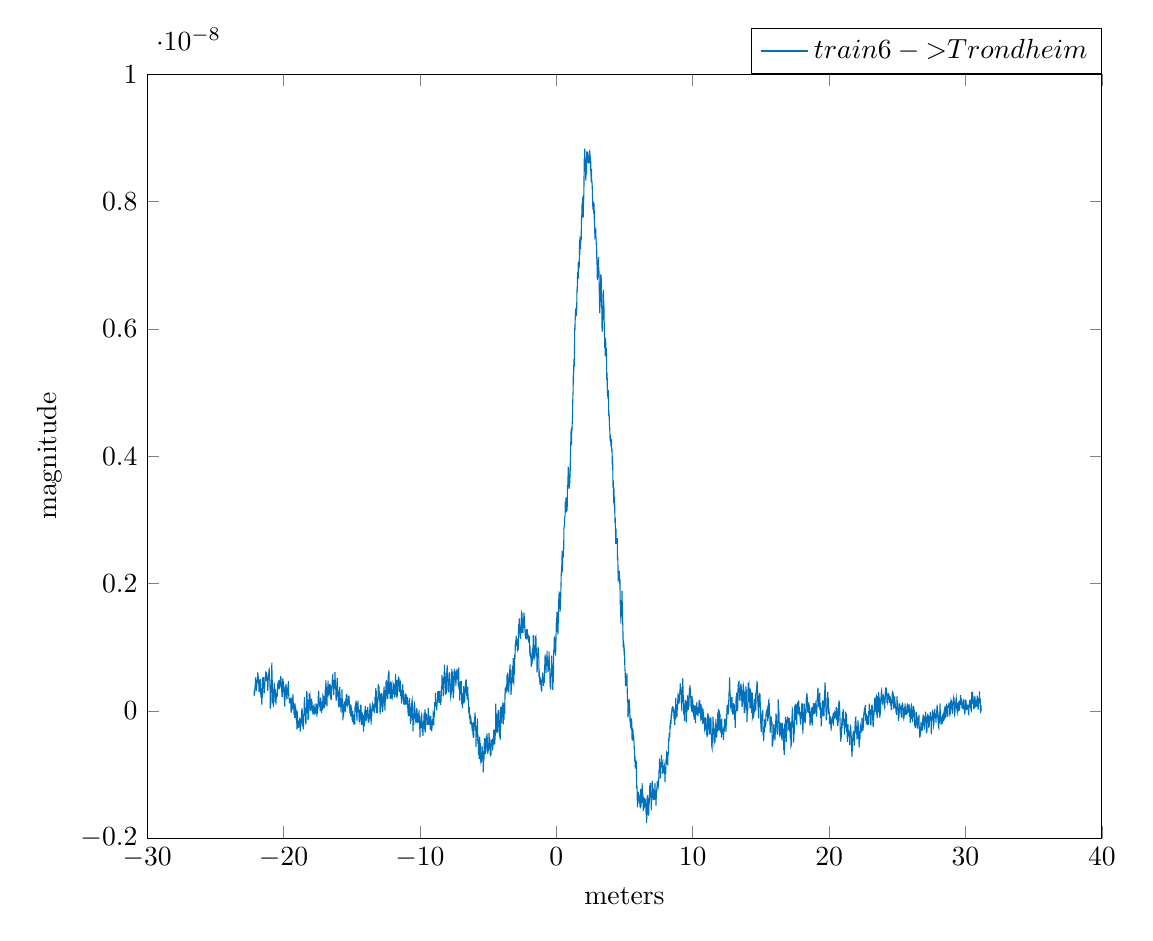
\begin{tikzpicture}

\begin{axis}[%
width=\textwidth,
height=0.8\textwidth,
at={(0\figurewidth,0\figureheight)},
scale only axis,
xmin=-30,
xmax=40,
xlabel={\SI{}{meters}},
ymin=-2e-09,
ymax=1e-08,
ylabel={magnitude},
axis background/.style={fill=white},
legend style={at={(1.0,1.0)},anchor=south east}
]
\addplot [color=mycolor1,solid]
  table[row sep=crcr]{%
-22.157431640625	2.3493988586141e-10\\
-22.14099609375	3.16454357658565e-10\\
-22.124560546875	2.45589177170896e-10\\
-22.108125	3.32225739372083e-10\\
-22.091689453125	3.64796431000339e-10\\
-22.07525390625	3.85652139602146e-10\\
-22.058818359375	5.24052201527055e-10\\
-22.0423828125	3.94618056722382e-10\\
-22.025947265625	4.52729076947501e-10\\
-22.00951171875	3.96448747790381e-10\\
-21.993076171875	3.10810818811408e-10\\
-21.976640625	3.5137966051929e-10\\
-21.960205078125	3.88177609181802e-10\\
-21.94376953125	4.7745703355699e-10\\
-21.927333984375	4.75295859905891e-10\\
-21.9108984375	5.01641220911783e-10\\
-21.894462890625	6.02333107767618e-10\\
-21.87802734375	5.70074940910517e-10\\
-21.861591796875	4.95507094559886e-10\\
-21.84515625	5.38368819869356e-10\\
-21.828720703125	4.11967046154423e-10\\
-21.81228515625	4.45625606191741e-10\\
-21.795849609375	2.97023464705207e-10\\
-21.7794140625	3.34279053278305e-10\\
-21.762978515625	3.37794453569621e-10\\
-21.74654296875	3.24512778350597e-10\\
-21.730107421875	4.89632771849845e-10\\
-21.713671875	4.12329201146572e-10\\
-21.697236328125	4.49231314402858e-10\\
-21.68080078125	5.03630064065878e-10\\
-21.664365234375	2.65286050733407e-10\\
-21.6479296875	2.0652233960767e-10\\
-21.631494140625	2.62414475049214e-10\\
-21.61505859375	2.61590807361819e-10\\
-21.598623046875	9.7790612333604e-11\\
-21.5821875	1.93612378855191e-10\\
-21.565751953125	3.53444828657035e-10\\
-21.54931640625	2.15474586107321e-10\\
-21.532880859375	4.51923553991532e-10\\
-21.5164453125	5.32318241162345e-10\\
-21.500009765625	4.10470132695962e-10\\
-21.48357421875	5.29347737722435e-10\\
-21.467138671875	3.51624049118825e-10\\
-21.450703125	4.15609638673467e-10\\
-21.434267578125	3.78257089922986e-10\\
-21.41783203125	2.73156288905784e-10\\
-21.401396484375	4.01627266978811e-10\\
-21.3849609375	3.56655402442344e-10\\
-21.368525390625	5.31800895046452e-10\\
-21.35208984375	4.84345061722003e-10\\
-21.335654296875	4.82244862131988e-10\\
-21.31921875	5.24329764983105e-10\\
-21.302783203125	6.18570529861811e-10\\
-21.28634765625	5.70353728073556e-10\\
-21.269912109375	6.03861839027797e-10\\
-21.2534765625	5.23570467742448e-10\\
-21.237041015625	5.38009517203342e-10\\
-21.22060546875	5.57884167435542e-10\\
-21.204169921875	5.4486049060594e-10\\
-21.187734375	4.36871494518218e-10\\
-21.171298828125	5.31556536647115e-10\\
-21.15486328125	3.12635559414438e-10\\
-21.138427734375	4.20463271533747e-10\\
-21.1219921875	5.25830651422483e-10\\
-21.105556640625	4.89874714993974e-10\\
-21.08912109375	5.42060753485373e-10\\
-21.072685546875	6.42210746770052e-10\\
-21.05625	6.51457627802147e-10\\
-21.039814453125	6.16165697186977e-10\\
-21.02337890625	5.21746654998639e-10\\
-21.006943359375	4.76088064142873e-10\\
-20.9905078125	3.64089815482994e-10\\
-20.974072265625	3.2338317073464e-11\\
-20.95763671875	1.18142553923816e-10\\
-20.941201171875	8.44640750205487e-11\\
-20.924765625	1.38271027326297e-10\\
-20.908330078125	3.29587441166262e-10\\
-20.89189453125	4.42055509259057e-10\\
-20.875458984375	4.95791617671641e-10\\
-20.8590234375	7.55508536670687e-10\\
-20.842587890625	5.17182861480332e-10\\
-20.82615234375	4.58568486101422e-10\\
-20.809716796875	3.2914358067188e-10\\
-20.79328125	1.36007685826063e-10\\
-20.776845703125	9.98699053312621e-11\\
-20.76041015625	1.86208619690393e-10\\
-20.743974609375	6.14886132074838e-11\\
-20.7275390625	2.34824295152368e-10\\
-20.711103515625	2.5105891399893e-10\\
-20.69466796875	3.48030998628216e-10\\
-20.678232421875	4.19176344330151e-10\\
-20.661796875	4.11461013764003e-10\\
-20.645361328125	3.32603154972688e-10\\
-20.62892578125	2.59407852216866e-10\\
-20.612490234375	1.36287534599295e-10\\
-20.5960546875	3.3435289415685e-10\\
-20.579619140625	2.38702748901889e-10\\
-20.56318359375	9.82122339605962e-11\\
-20.546748046875	1.6364618694515e-10\\
-20.5303125	2.40032555859376e-10\\
-20.513876953125	2.28679818065241e-10\\
-20.49744140625	2.72093514340112e-10\\
-20.481005859375	2.77864484043936e-10\\
-20.4645703125	2.24656678252565e-10\\
-20.448134765625	3.21528039787053e-10\\
-20.43169921875	3.87999231588502e-10\\
-20.415263671875	3.78506680715841e-10\\
-20.398828125	4.11888513093621e-10\\
-20.382392578125	3.96725300442707e-10\\
-20.36595703125	3.39272677776375e-10\\
-20.349521484375	4.77110257753398e-10\\
-20.3330859375	4.48403650642599e-10\\
-20.316650390625	4.54809288430134e-10\\
-20.30021484375	4.23918066617774e-10\\
-20.283779296875	3.71276474342371e-10\\
-20.26734375	3.80947276633e-10\\
-20.250908203125	4.2801439065467e-10\\
-20.23447265625	5.03606650717871e-10\\
-20.218037109375	4.14743270481536e-10\\
-20.2016015625	5.42813638949291e-10\\
-20.185166015625	5.08541706165276e-10\\
-20.16873046875	4.3265682800937e-10\\
-20.152294921875	3.59067434475952e-10\\
-20.135859375	3.66541175723774e-10\\
-20.119423828125	2.18680055784906e-10\\
-20.10298828125	3.15939865264201e-10\\
-20.086552734375	2.14733885639522e-10\\
-20.0701171875	3.95127978809931e-10\\
-20.053681640625	5.09540080500933e-10\\
-20.03724609375	4.29541550157533e-10\\
-20.020810546875	4.66944570120977e-10\\
-20.004375	4.21593495612138e-10\\
-19.987939453125	3.88494309699657e-10\\
-19.97150390625	3.89624130369062e-10\\
-19.955068359375	2.10578010160577e-10\\
-19.9386328125	1.78288264132363e-10\\
-19.922197265625	6.68059737575331e-11\\
-19.90576171875	9.33938058444373e-11\\
-19.889326171875	2.32769872916004e-10\\
-19.872890625	3.11293307998774e-10\\
-19.856455078125	3.42338197475866e-10\\
-19.84001953125	3.68077854147815e-10\\
-19.823583984375	4.18641222699547e-10\\
-19.8071484375	3.82896819263684e-10\\
-19.790712890625	3.29255882640091e-10\\
-19.77427734375	1.96648047703011e-10\\
-19.757841796875	2.64851506682972e-10\\
-19.74140625	1.81266844697608e-10\\
-19.724970703125	3.16625395276192e-10\\
-19.70853515625	3.07487499426075e-10\\
-19.692099609375	3.43432670742638e-10\\
-19.6756640625	3.09887308743544e-10\\
-19.659228515625	3.03011551260259e-10\\
-19.64279296875	4.65010827880937e-10\\
-19.626357421875	2.92299986863863e-10\\
-19.609921875	2.00759958898872e-10\\
-19.593486328125	1.91267120373471e-10\\
-19.57705078125	1.88618837907769e-10\\
-19.560615234375	1.16066534213548e-10\\
-19.5441796875	1.41679029436541e-10\\
-19.527744140625	1.46756225900682e-10\\
-19.51130859375	1.4361649804542e-10\\
-19.494873046875	1.64991618649528e-10\\
-19.4784375	2.0416328490277e-10\\
-19.462001953125	1.00330881441852e-10\\
-19.44556640625	-3.18641970356275e-11\\
-19.429130859375	-1.60039886743246e-12\\
-19.4126953125	7.72110470250814e-11\\
-19.396259765625	7.09995340750797e-11\\
-19.37982421875	9.78968820011646e-12\\
-19.363388671875	1.7294673412508e-10\\
-19.346953125	1.62974632034583e-10\\
-19.330517578125	1.13983739641202e-10\\
-19.31408203125	2.63317145127381e-10\\
-19.297646484375	1.60734569531365e-10\\
-19.2812109375	9.32442543870109e-11\\
-19.264775390625	2.8878038505475e-11\\
-19.24833984375	9.27139947344124e-11\\
-19.231904296875	-6.1536827146357e-11\\
-19.21546875	9.63714137550961e-11\\
-19.199033203125	-4.91376244136048e-12\\
-19.18259765625	-1.09552393400853e-10\\
-19.166162109375	1.07818427786756e-10\\
-19.1497265625	1.06326670615224e-10\\
-19.133291015625	-6.12974154465468e-11\\
-19.11685546875	-3.26541312616973e-11\\
-19.100419921875	5.11811986538485e-11\\
-19.083984375	-7.90866247504586e-11\\
-19.067548828125	-1.46586669311674e-10\\
-19.05111328125	4.85842914179183e-12\\
-19.034677734375	-1.43925269348242e-10\\
-19.0182421875	-2.94720429623287e-10\\
-19.001806640625	2.89237278064039e-12\\
-18.98537109375	-2.12438079944709e-10\\
-18.968935546875	-2.04433601683248e-10\\
-18.9525	-2.34473832548686e-10\\
-18.936064453125	-2.2427812212354e-10\\
-18.91962890625	-2.24216806320201e-10\\
-18.903193359375	-2.68699141883346e-10\\
-18.8867578125	-1.7076675280888e-10\\
-18.870322265625	-1.43078804174377e-10\\
-18.85388671875	-2.41458771298671e-10\\
-18.837451171875	-1.5673723447876e-10\\
-18.821015625	-1.76925073784907e-10\\
-18.804580078125	-1.37335806461968e-10\\
-18.78814453125	-1.36151436147009e-10\\
-18.771708984375	-3.25247997213355e-10\\
-18.7552734375	-2.17599535819189e-10\\
-18.738837890625	-2.57122470217478e-10\\
-18.72240234375	-1.77104384812638e-10\\
-18.705966796875	-1.3133408737274e-10\\
-18.68953125	-5.11135831316123e-11\\
-18.673095703125	-7.4357671087722e-11\\
-18.65666015625	3.95936406528028e-11\\
-18.640224609375	-1.90639359403787e-11\\
-18.6237890625	-1.20927600602061e-11\\
-18.607353515625	-2.08119521794635e-10\\
-18.59091796875	-2.28541691331286e-10\\
-18.574482421875	-2.36781356464068e-10\\
-18.558046875	-2.9182510457877e-10\\
-18.541611328125	-2.5060178128786e-10\\
-18.52517578125	-7.18732321408398e-11\\
-18.508740234375	-5.56040600318118e-11\\
-18.4923046875	-3.44254889062043e-11\\
-18.475869140625	1.72964160518218e-10\\
-18.45943359375	2.12330121629578e-10\\
-18.442998046875	5.72893504007784e-11\\
-18.4265625	4.97661541523069e-11\\
-18.410126953125	-5.26470937364653e-11\\
-18.39369140625	-1.47467290467235e-10\\
-18.377255859375	-1.62232233472302e-10\\
-18.3608203125	-2.18638201857842e-10\\
-18.344384765625	-3.10227644110464e-12\\
-18.32794921875	2.01416272541854e-11\\
-18.311513671875	-4.16802945329874e-11\\
-18.295078125	3.09929828630557e-10\\
-18.278642578125	2.7247069468487e-10\\
-18.26220703125	2.54456761666874e-11\\
-18.245771484375	1.77508467860796e-10\\
-18.2293359375	6.21342080814882e-11\\
-18.212900390625	-1.41255855659885e-10\\
-18.19646484375	-4.74014103424408e-11\\
-18.180029296875	-1.28589027777111e-10\\
-18.16359375	-9.5104809221553e-11\\
-18.147158203125	8.97203911896056e-11\\
-18.13072265625	1.69200661058814e-10\\
-18.114287109375	2.56690308768618e-10\\
-18.0978515625	2.50223905161424e-10\\
-18.081416015625	2.25922477447113e-10\\
-18.06498046875	2.42743550454547e-10\\
-18.048544921875	1.02901142781064e-10\\
-18.032109375	4.0749133829229e-12\\
-18.015673828125	1.41612740705313e-10\\
-17.99923828125	8.3838668927525e-11\\
-17.982802734375	-7.78534216979195e-12\\
-17.9663671875	1.70589314039509e-10\\
-17.949931640625	1.75717619797306e-10\\
-17.93349609375	8.14377928946445e-11\\
-17.917060546875	1.43138547400581e-10\\
-17.900625	7.77064177319521e-11\\
-17.884189453125	4.37127696234029e-11\\
-17.86775390625	7.35474301529068e-11\\
-17.851318359375	-6.00078747960531e-11\\
-17.8348828125	2.41856005430499e-11\\
-17.818447265625	-3.27669817385943e-11\\
-17.80201171875	-3.20544679016951e-11\\
-17.785576171875	6.26382385445327e-11\\
-17.769140625	1.00479371087238e-10\\
-17.752705078125	5.31891827758432e-11\\
-17.73626953125	-6.11598680565727e-11\\
-17.719833984375	5.52298628116335e-11\\
-17.7033984375	-2.70776593089405e-11\\
-17.686962890625	-3.12990315406357e-11\\
-17.67052734375	1.97110499188427e-11\\
-17.654091796875	-4.09288997220514e-11\\
-17.63765625	1.24367422589856e-11\\
-17.621220703125	1.18037325411016e-10\\
-17.60478515625	3.74890897257419e-11\\
-17.588349609375	9.63454177367087e-11\\
-17.5719140625	6.35604633244136e-11\\
-17.555478515625	-8.9802839818781e-11\\
-17.53904296875	6.15789322793731e-11\\
-17.522607421875	-4.17231053292969e-11\\
-17.506171875	-3.40628501052788e-11\\
-17.489736328125	1.08574153517384e-10\\
-17.47330078125	2.94658518908059e-11\\
-17.456865234375	2.0698571399708e-10\\
-17.4404296875	2.99720758274977e-10\\
-17.423994140625	3.03120089747576e-10\\
-17.40755859375	2.12873272825644e-10\\
-17.391123046875	1.70954521868791e-10\\
-17.3746875	1.19948214729375e-10\\
-17.358251953125	9.37851014631949e-11\\
-17.34181640625	6.3029596591031e-11\\
-17.325380859375	1.23381701967886e-10\\
-17.3089453125	-4.22947615707284e-12\\
-17.292509765625	1.15933870344191e-10\\
-17.27607421875	2.05702173885924e-10\\
-17.259638671875	1.25422444608356e-10\\
-17.243203125	9.6284817801147e-11\\
-17.226767578125	5.18401812986326e-11\\
-17.21033203125	-3.15572027025912e-11\\
-17.193896484375	3.18080080522986e-11\\
-17.1774609375	3.57279365737924e-11\\
-17.161025390625	1.45408132916028e-10\\
-17.14458984375	1.56444614284962e-11\\
-17.128154296875	1.0991878945987e-10\\
-17.11171875	2.38629181572775e-10\\
-17.095283203125	2.28728104039255e-10\\
-17.07884765625	2.26999634199782e-10\\
-17.062412109375	1.9909013763606e-10\\
-17.0459765625	1.22198497148509e-10\\
-17.029541015625	3.64368764898449e-11\\
-17.01310546875	1.16334402244761e-10\\
-16.996669921875	1.00055005098323e-10\\
-16.980234375	9.0396514409316e-11\\
-16.963798828125	1.8703716805166e-10\\
-16.94736328125	3.14276342319637e-10\\
-16.930927734375	3.49625111679726e-10\\
-16.9144921875	2.43523286500137e-10\\
-16.898056640625	4.82289909079857e-10\\
-16.88162109375	3.44892060554779e-10\\
-16.865185546875	9.80012038761509e-11\\
-16.84875	2.11585194262927e-10\\
-16.832314453125	2.1059166910805e-10\\
-16.81587890625	7.07064083698628e-11\\
-16.799443359375	2.29318439051007e-10\\
-16.7830078125	3.74350945810284e-10\\
-16.766572265625	2.43624332415479e-10\\
-16.75013671875	3.39752192622947e-10\\
-16.733701171875	4.72469624990341e-10\\
-16.717265625	3.11120203851158e-10\\
-16.700830078125	2.9638646151624e-10\\
-16.68439453125	3.81972234312028e-10\\
-16.667958984375	2.65104485146997e-10\\
-16.6515234375	2.7953513508772e-10\\
-16.635087890625	4.1611793471901e-10\\
-16.61865234375	2.98226890285342e-10\\
-16.602216796875	3.24494367012219e-10\\
-16.58578125	4.25152962850902e-10\\
-16.569345703125	3.52037678740046e-10\\
-16.55291015625	1.89802251385418e-10\\
-16.536474609375	3.24662230573125e-10\\
-16.5200390625	2.87916534225852e-10\\
-16.503603515625	1.71522452230456e-10\\
-16.48716796875	3.1888099814183e-10\\
-16.470732421875	3.83574343280805e-10\\
-16.454296875	3.14857681776016e-10\\
-16.437861328125	4.50889474169949e-10\\
-16.42142578125	5.00313146345188e-10\\
-16.404990234375	5.56121485103991e-10\\
-16.3885546875	5.61913078358026e-10\\
-16.372119140625	3.85194630602758e-10\\
-16.35568359375	4.83268056126422e-10\\
-16.339248046875	4.31757415379964e-10\\
-16.3228125	2.45742483516105e-10\\
-16.306376953125	3.56467560632951e-10\\
-16.28994140625	3.81818160414832e-10\\
-16.273505859375	4.28592162163009e-10\\
-16.2570703125	4.32640073308749e-10\\
-16.240634765625	4.89389749307276e-10\\
-16.22419921875	6.08277631335303e-10\\
-16.207763671875	4.27196134098727e-10\\
-16.191328125	3.31027782114255e-10\\
-16.174892578125	3.91353547468422e-10\\
-16.15845703125	2.30083624904787e-10\\
-16.142021484375	1.5517473213708e-10\\
-16.1255859375	2.87658738949895e-10\\
-16.109150390625	2.76817536793284e-10\\
-16.09271484375	3.93483435806841e-10\\
-16.076279296875	4.63947218785417e-10\\
-16.05984375	5.13925414398782e-10\\
-16.043408203125	3.60578589732076e-10\\
-16.02697265625	2.78854301068228e-10\\
-16.010537109375	2.29337221415402e-10\\
-15.9941015625	2.53275843522763e-10\\
-15.977666015625	1.91139792435621e-10\\
-15.96123046875	5.36562069091758e-11\\
-15.944794921875	1.64445361785615e-10\\
-15.928359375	2.5171628002584e-10\\
-15.911923828125	2.58001602826093e-10\\
-15.89548828125	2.96768021543342e-10\\
-15.879052734375	3.74322292529632e-10\\
-15.8626171875	2.70035372541593e-10\\
-15.846181640625	5.3109404585712e-11\\
-15.82974609375	7.29457558948319e-11\\
-15.813310546875	1.97522325322776e-10\\
-15.796875	-2.53420277421745e-12\\
-15.780439453125	-8.23718406284433e-12\\
-15.76400390625	1.51064395425392e-10\\
-15.747568359375	9.28520376472075e-11\\
-15.7311328125	1.59688018276465e-10\\
-15.714697265625	3.35516303064203e-10\\
-15.69826171875	5.09818488273122e-11\\
-15.681826171875	1.84819530330987e-10\\
-15.665390625	1.44991155149545e-10\\
-15.648955078125	-1.4853011219328e-10\\
-15.63251953125	-3.42407607134093e-11\\
-15.616083984375	9.08548075377638e-11\\
-15.5996484375	-9.17067591186766e-11\\
-15.583212890625	1.52362933562143e-11\\
-15.56677734375	9.45866320109157e-12\\
-15.550341796875	7.85731276840196e-11\\
-15.53390625	1.48030209565438e-10\\
-15.517470703125	8.96598671675246e-12\\
-15.50103515625	3.25510819645288e-11\\
-15.484599609375	1.39881767107376e-10\\
-15.4681640625	2.98169793939392e-12\\
-15.451728515625	-2.25281056362443e-12\\
-15.43529296875	1.8393335048915e-10\\
-15.418857421875	7.14079295622789e-11\\
-15.402421875	2.1532779113091e-10\\
-15.385986328125	2.00058946915975e-10\\
-15.36955078125	2.6283028321426e-10\\
-15.353115234375	1.88568525408481e-10\\
-15.3366796875	1.25787939481082e-10\\
-15.320244140625	1.0221771006842e-10\\
-15.30380859375	1.35933056962539e-10\\
-15.287373046875	1.67328133035629e-10\\
-15.2709375	1.10623956962378e-10\\
-15.254501953125	1.21189966230949e-10\\
-15.23806640625	2.32657982455792e-10\\
-15.221630859375	1.30677786444308e-10\\
-15.2051953125	2.36264798884301e-10\\
-15.188759765625	1.80524965090613e-10\\
-15.17232421875	3.68556342795673e-11\\
-15.155888671875	1.15215038593512e-10\\
-15.139453125	-1.52110837534111e-11\\
-15.123017578125	-4.5373127153877e-11\\
-15.10658203125	5.78905575362386e-11\\
-15.090146484375	4.71135077337926e-11\\
-15.0737109375	-8.7501017418054e-11\\
-15.057275390625	9.58291005483273e-11\\
-15.04083984375	-3.77897413726313e-11\\
-15.024404296875	-3.75081738959383e-11\\
-15.00796875	4.79626128332879e-11\\
-14.991533203125	-1.17812320791832e-10\\
-14.97509765625	-6.96676304357561e-11\\
-14.958662109375	-1.47184755693622e-10\\
-14.9422265625	-1.39793876849722e-10\\
-14.925791015625	-1.78957319346408e-12\\
-14.90935546875	-1.28845417295857e-10\\
-14.892919921875	-1.56160172473467e-10\\
-14.876484375	-2.02017831750036e-10\\
-14.860048828125	-6.25585811573028e-11\\
-14.84361328125	-1.37553961999627e-10\\
-14.827177734375	-2.24916713954399e-10\\
-14.8107421875	-1.33980233235589e-10\\
-14.794306640625	-5.16422223985123e-11\\
-14.77787109375	-2.10429675724892e-10\\
-14.761435546875	4.94374995233121e-11\\
-14.745	8.24947493405529e-11\\
-14.728564453125	3.3758216547589e-11\\
-14.71212890625	1.13274787342482e-10\\
-14.695693359375	1.21120744678785e-10\\
-14.6792578125	1.60370831187416e-10\\
-14.662822265625	5.92480432931956e-11\\
-14.64638671875	-2.97973904374409e-11\\
-14.629951171875	-1.67725340726263e-11\\
-14.613515625	-1.54683688770712e-10\\
-14.597080078125	1.14915378259735e-10\\
-14.58064453125	4.36229884267604e-11\\
-14.564208984375	4.66235264605736e-11\\
-14.5477734375	1.59960333496027e-10\\
-14.531337890625	7.94866336934008e-11\\
-14.51490234375	-2.93241998249553e-11\\
-14.498466796875	1.283470521263e-11\\
-14.48203125	2.38361614033565e-12\\
-14.465595703125	-1.07955409282709e-10\\
-14.44916015625	-1.73741639663463e-10\\
-14.432724609375	-1.09666086208492e-10\\
-14.4162890625	-6.29003542176111e-11\\
-14.399853515625	-1.3992889984364e-10\\
-14.38341796875	-1.17763735824174e-10\\
-14.366982421875	9.61869450122708e-11\\
-14.350546875	3.30571531449123e-11\\
-14.334111328125	-1.29447203238475e-10\\
-14.31767578125	9.18548054810683e-11\\
-14.301240234375	-6.92946448521746e-11\\
-14.2848046875	-2.20058998200314e-10\\
-14.268369140625	-3.27511530903854e-11\\
-14.25193359375	-1.00068303470152e-10\\
-14.235498046875	-2.02861215170781e-10\\
-14.2190625	-2.97701682655138e-11\\
-14.202626953125	-1.07415769015667e-10\\
-14.18619140625	-2.1598709155195e-10\\
-14.169755859375	-6.74008001282937e-11\\
-14.1533203125	-1.5518628456294e-10\\
-14.136884765625	-3.28078339548995e-10\\
-14.12044921875	-2.02794871638674e-10\\
-14.104013671875	-1.81037103039913e-10\\
-14.087578125	-2.43395593932336e-10\\
-14.071142578125	-1.4223723894949e-10\\
-14.05470703125	-1.23398045635874e-11\\
-14.038271484375	-1.37626642194326e-10\\
-14.0218359375	4.19760912665472e-11\\
-14.005400390625	7.27418445921667e-11\\
-13.98896484375	-5.0225150526105e-11\\
-13.972529296875	-1.52902415010806e-10\\
-13.95609375	1.5517412135529e-11\\
-13.939658203125	-1.43030184060796e-10\\
-13.92322265625	-1.31721491551337e-10\\
-13.906787109375	1.62200273636432e-11\\
-13.8903515625	-5.37024322145233e-11\\
-13.873916015625	-3.14604517703772e-11\\
-13.85748046875	1.31782839967798e-11\\
-13.841044921875	1.64829444802142e-11\\
-13.824609375	5.58712984709124e-11\\
-13.808173828125	-8.99325629005741e-11\\
-13.79173828125	-1.45216530008921e-10\\
-13.775302734375	-1.32425053146327e-10\\
-13.7588671875	-1.8611948437396e-10\\
-13.742431640625	-1.54052565763606e-10\\
-13.72599609375	-1.31221369783221e-10\\
-13.709560546875	-9.57748874888522e-11\\
-13.693125	1.33995170091737e-11\\
-13.676689453125	-1.07911769516181e-10\\
-13.66025390625	1.16256623125199e-10\\
-13.643818359375	6.21234897561511e-11\\
-13.6273828125	-1.27669713770314e-10\\
-13.610947265625	-8.58511272861558e-11\\
-13.59451171875	-9.34297840191512e-11\\
-13.578076171875	-2.17845059568208e-10\\
-13.561640625	3.26341885697893e-11\\
-13.545205078125	-8.92729310264055e-11\\
-13.52876953125	-7.33417094662745e-11\\
-13.512333984375	2.91739009739299e-11\\
-13.4958984375	7.12038693290254e-11\\
-13.479462890625	6.34937092848389e-11\\
-13.46302734375	1.05952616357485e-10\\
-13.446591796875	9.11089873301244e-11\\
-13.43015625	3.94938630107655e-12\\
-13.413720703125	6.67749609976712e-11\\
-13.39728515625	3.64018103137444e-11\\
-13.380849609375	5.28756559533178e-11\\
-13.3644140625	1.38182639609495e-11\\
-13.347978515625	7.35718805037175e-11\\
-13.33154296875	-3.22573640175486e-11\\
-13.315107421875	2.69701910844105e-11\\
-13.298671875	2.16058852106094e-10\\
-13.282236328125	8.26065589938743e-11\\
-13.26580078125	5.12045261330483e-11\\
-13.249365234375	2.72460956870118e-10\\
-13.2329296875	3.60346094119123e-10\\
-13.216494140625	1.21886158646387e-10\\
-13.20005859375	3.13755021558228e-10\\
-13.183623046875	1.75694870402479e-10\\
-13.1671875	-3.55525130195144e-11\\
-13.150751953125	2.05189961586564e-10\\
-13.13431640625	5.60880046559301e-11\\
-13.117880859375	-3.95712372902775e-11\\
-13.1014453125	1.25715492677431e-10\\
-13.085009765625	1.34051703124959e-10\\
-13.06857421875	2.12407365150852e-10\\
-13.052138671875	4.18606302654009e-10\\
-13.035703125	3.54845367185768e-10\\
-13.019267578125	3.10632721319234e-10\\
-13.00283203125	3.8538809473725e-10\\
-12.986396484375	2.74258209551999e-10\\
-12.9699609375	1.94545799466277e-10\\
-12.953525390625	2.95236788543152e-10\\
-12.93708984375	6.74648652066443e-11\\
-12.920654296875	-5.51589551631672e-11\\
-12.90421875	4.30420808370689e-11\\
-12.887783203125	8.58776380542632e-11\\
-12.87134765625	7.48689260316763e-11\\
-12.854912109375	1.4633749069454e-10\\
-12.8384765625	2.6820746789734e-10\\
-12.822041015625	1.62637053192142e-10\\
-12.80560546875	2.78229547536834e-10\\
-12.789169921875	1.35361935515295e-10\\
-12.772734375	2.20984905666528e-10\\
-12.756298828125	4.26475901433772e-11\\
-12.73986328125	-2.18426323984207e-11\\
-12.723427734375	1.73803010487959e-11\\
-12.7069921875	8.17181271207462e-11\\
-12.690556640625	1.37682254786652e-10\\
-12.67412109375	2.36524578072649e-10\\
-12.657685546875	2.95565852859139e-10\\
-12.64125	3.13979373573914e-10\\
-12.624814453125	3.82058050962487e-10\\
-12.60837890625	1.52757649697081e-10\\
-12.591943359375	1.09684107674082e-10\\
-12.5755078125	1.30102001721701e-10\\
-12.559072265625	6.08694573621499e-12\\
-12.54263671875	2.05239831441437e-10\\
-12.526201171875	2.92628307930931e-10\\
-12.509765625	2.36859246090235e-10\\
-12.493330078125	4.53359168287995e-10\\
-12.47689453125	3.52733892735959e-10\\
-12.460458984375	4.85322786268742e-10\\
-12.4440234375	4.17929632428651e-10\\
-12.427587890625	2.64317540524041e-10\\
-12.41115234375	1.81755665370793e-10\\
-12.394716796875	2.13394222988422e-10\\
-12.37828125	2.46111657809204e-10\\
-12.361845703125	1.92775148727827e-10\\
-12.34541015625	3.59686140758352e-10\\
-12.328974609375	5.63070545713839e-10\\
-12.3125390625	5.35819152015176e-10\\
-12.296103515625	4.73699407435874e-10\\
-12.27966796875	6.37429519597088e-10\\
-12.263232421875	5.69248291943963e-10\\
-12.246796875	2.66099528939063e-10\\
-12.230361328125	3.52285378356657e-10\\
-12.21392578125	3.68468680812845e-10\\
-12.197490234375	3.30312621559622e-10\\
-12.1810546875	1.82618091907387e-10\\
-12.164619140625	3.88787849798665e-10\\
-12.14818359375	4.6283360223504e-10\\
-12.131748046875	2.09613045009275e-10\\
-12.1153125	4.54109688364421e-10\\
-12.098876953125	4.23284865273161e-10\\
-12.08244140625	2.54247809078298e-10\\
-12.066005859375	2.71663164591602e-10\\
-12.0495703125	2.15874078199498e-10\\
-12.033134765625	2.05451231195363e-10\\
-12.01669921875	2.81128939966085e-10\\
-12.000263671875	3.03134687836381e-10\\
-11.983828125	2.58850790759719e-10\\
-11.967392578125	4.28657853598752e-10\\
-11.95095703125	4.17006215452565e-10\\
-11.934521484375	4.04763494736176e-10\\
-11.9180859375	3.87523426544894e-10\\
-11.901650390625	4.23226156683609e-10\\
-11.88521484375	2.81913035800658e-10\\
-11.868779296875	2.05669961038799e-10\\
-11.85234375	3.22238941941764e-10\\
-11.835908203125	2.98497776963461e-10\\
-11.81947265625	2.49363852247734e-10\\
-11.803037109375	3.37499656189509e-10\\
-11.7866015625	5.74101235706972e-10\\
-11.770166015625	4.08602510817838e-10\\
-11.75373046875	4.26093116217115e-10\\
-11.737294921875	4.84653566407031e-10\\
-11.720859375	2.14025071133912e-10\\
-11.704423828125	2.63848231613653e-10\\
-11.68798828125	2.60469827799873e-10\\
-11.671552734375	2.34598342707723e-10\\
-11.6551171875	2.53513243681574e-10\\
-11.638681640625	4.53870841966043e-10\\
-11.62224609375	4.78213466835963e-10\\
-11.605810546875	4.85055728332714e-10\\
-11.589375	4.69942225386524e-10\\
-11.572939453125	5.40902540631835e-10\\
-11.55650390625	5.04265939526229e-10\\
-11.540068359375	4.70756775375056e-10\\
-11.5236328125	2.90790162095074e-10\\
-11.507197265625	3.92860512845986e-10\\
-11.49076171875	4.3801855213618e-10\\
-11.474326171875	3.41662085281407e-10\\
-11.457890625	2.95772136215645e-10\\
-11.441455078125	4.60331480563689e-10\\
-11.42501953125	4.48710086931619e-10\\
-11.408583984375	2.33593310744352e-10\\
-11.3921484375	3.26546818871326e-10\\
-11.375712890625	2.82509440720281e-10\\
-11.35927734375	1.1390828853393e-10\\
-11.342841796875	1.61946419076484e-10\\
-11.32640625	1.86394029333894e-10\\
-11.309970703125	2.95068792928569e-10\\
-11.29353515625	1.93492742967053e-10\\
-11.277099609375	3.25589596988214e-10\\
-11.2606640625	4.13240785407191e-10\\
-11.244228515625	2.95876068955168e-10\\
-11.22779296875	3.1823345870133e-10\\
-11.211357421875	1.82962799078652e-10\\
-11.194921875	1.15366125068571e-10\\
-11.178486328125	1.17272709334203e-10\\
-11.16205078125	1.37166226394418e-10\\
-11.145615234375	9.42708075712726e-11\\
-11.1291796875	2.07336304105767e-10\\
-11.112744140625	1.05158441836104e-10\\
-11.09630859375	2.52856646514859e-10\\
-11.079873046875	2.55988607812997e-10\\
-11.0634375	1.91711107916258e-10\\
-11.047001953125	1.39326068921694e-10\\
-11.03056640625	2.72142792601923e-10\\
-11.014130859375	8.98494177053575e-11\\
-10.9976953125	1.92423585103986e-10\\
-10.981259765625	2.50032810853891e-10\\
-10.96482421875	1.39260574462169e-10\\
-10.948388671875	1.52526001885397e-10\\
-10.931953125	2.13328012608939e-10\\
-10.915517578125	1.57445477703563e-10\\
-10.89908203125	1.11533488776972e-10\\
-10.882646484375	-1.26779632276268e-11\\
-10.8662109375	-3.24063150198722e-11\\
-10.849775390625	-7.74762170693153e-11\\
-10.83333984375	5.30843721939962e-11\\
-10.816904296875	6.2045375640636e-11\\
-10.80046875	-8.79905608305059e-11\\
-10.784033203125	1.61728129838603e-10\\
-10.76759765625	1.97549655179783e-10\\
-10.751162109375	9.55706232789146e-12\\
-10.7347265625	2.64538430681355e-11\\
-10.718291015625	5.97504890816564e-11\\
-10.70185546875	-1.45311123511161e-10\\
-10.685419921875	-2.04036339549601e-10\\
-10.668984375	-6.82008857080578e-11\\
-10.652548828125	-1.56897072826489e-10\\
-10.63611328125	-2.06343216875568e-11\\
-10.619677734375	1.20694440475443e-10\\
-10.6032421875	-5.61896044298466e-12\\
-10.586806640625	1.5897151593564e-10\\
-10.57037109375	1.75462495630974e-10\\
-10.553935546875	-5.52695262472255e-12\\
-10.5375	-1.41745625131213e-10\\
-10.521064453125	-8.42886862595715e-11\\
-10.50462890625	-3.22980468195007e-10\\
-10.488193359375	-1.45180095470021e-10\\
-10.4717578125	-4.75150623196731e-11\\
-10.455322265625	-2.20258199458523e-10\\
-10.43888671875	2.25622428027303e-11\\
-10.422451171875	9.82805774319952e-11\\
-10.406015625	2.40453967274764e-11\\
-10.389580078125	9.4715105284917e-11\\
-10.37314453125	7.61797209832039e-11\\
-10.356708984375	-8.48313805504474e-11\\
-10.3402734375	-1.23770958320728e-10\\
-10.323837890625	-7.52928791112309e-11\\
-10.30740234375	-1.47510008559959e-10\\
-10.290966796875	-1.33257911742231e-10\\
-10.27453125	-1.84670249251496e-10\\
-10.258095703125	-1.04666970676263e-10\\
-10.24166015625	1.81281922607639e-11\\
-10.225224609375	4.30243428805448e-11\\
-10.2087890625	-5.2434460552119e-11\\
-10.192353515625	-5.82662483749259e-11\\
-10.17591796875	-1.26350063326998e-10\\
-10.159482421875	-1.9366928626768e-10\\
-10.143046875	-1.23004573580073e-10\\
-10.126611328125	-9.95079701515015e-11\\
-10.11017578125	-4.03840459841005e-11\\
-10.093740234375	-1.5824515048159e-10\\
-10.0773046875	-8.95239250391472e-11\\
-10.060869140625	8.85208244266492e-12\\
-10.04443359375	-2.11723670033095e-10\\
-10.027998046875	-1.92954457047494e-10\\
-10.0115625	-2.73691399114839e-10\\
-9.995126953125	-4.17144540920472e-10\\
-9.97869140625	-2.44407077617801e-10\\
-9.962255859375	-2.42561446107679e-10\\
-9.9458203125	-2.67529677951276e-10\\
-9.929384765625	-1.073877776966e-10\\
-9.91294921875	-9.70110955371469e-11\\
-9.896513671875	-7.81389555778023e-11\\
-9.880078125	-1.37073739188731e-10\\
-9.863642578125	-6.00516291538136e-11\\
-9.84720703125	-2.67030692755609e-10\\
-9.830771484375	-3.24922834528839e-10\\
-9.8143359375	-3.30053804022007e-10\\
-9.797900390625	-1.78646324201558e-10\\
-9.78146484375	-3.9334057669007e-10\\
-9.765029296875	-3.20245074850929e-10\\
-9.74859375	-1.53347634859934e-10\\
-9.732158203125	-2.16299719251784e-10\\
-9.71572265625	-2.4015338433911e-10\\
-9.699287109375	-6.62011671400115e-11\\
-9.6828515625	-2.92954056794164e-11\\
-9.666416015625	-2.69371596052501e-10\\
-9.64998046875	-2.86241755707729e-10\\
-9.633544921875	2.27312749689619e-11\\
-9.617109375	-2.32693488844855e-10\\
-9.600673828125	-3.40555311734649e-10\\
-9.58423828125	-2.804078325156e-11\\
-9.567802734375	-6.50779521212686e-11\\
-9.5513671875	-1.17196016339913e-10\\
-9.534931640625	-5.90138064344372e-11\\
-9.51849609375	-6.04366116619383e-11\\
-9.502060546875	-1.5057457051912e-10\\
-9.485625	-9.78727598248182e-11\\
-9.469189453125	-2.24894640914639e-10\\
-9.45275390625	-9.65962808758296e-11\\
-9.436318359375	-1.49051918317662e-10\\
-9.4198828125	-1.39186363595262e-10\\
-9.403447265625	-2.16734060669518e-10\\
-9.38701171875	4.62341711857726e-11\\
-9.370576171875	-4.84925118379697e-11\\
-9.354140625	-1.53008208856973e-10\\
-9.337705078125	-2.21246648707604e-10\\
-9.32126953125	-1.60932764791385e-10\\
-9.304833984375	-1.43430119461008e-10\\
-9.2883984375	-2.18677143907621e-10\\
-9.271962890625	-1.11783436424725e-10\\
-9.25552734375	-1.4022573828406e-10\\
-9.239091796875	-3.0111440019993e-10\\
-9.22265625	-1.47951541399637e-10\\
-9.206220703125	-8.15342005446995e-11\\
-9.18978515625	-2.39496681250618e-10\\
-9.173349609375	-2.03888612618738e-10\\
-9.1569140625	-2.93564044952642e-10\\
-9.140478515625	-3.24199589678287e-10\\
-9.12404296875	-2.33363996862846e-10\\
-9.107607421875	-2.66355840241952e-10\\
-9.091171875	-1.32729017056789e-10\\
-9.074736328125	-2.29014621955968e-10\\
-9.05830078125	-1.86476802855266e-10\\
-9.041865234375	-1.49544016725037e-10\\
-9.0254296875	-3.53347612857559e-11\\
-9.008994140625	-5.43068214720526e-11\\
-8.99255859375	-2.27315453163013e-10\\
-8.976123046875	-8.89503822598576e-11\\
-8.9596875	-6.51248415126819e-11\\
-8.943251953125	-9.74652330210758e-11\\
-8.92681640625	-2.59995774433258e-11\\
-8.910380859375	1.35057174983271e-10\\
-8.8939453125	7.58691879539988e-11\\
-8.877509765625	9.49673124623483e-11\\
-8.86107421875	2.82914647600402e-10\\
-8.844638671875	2.14244480350146e-10\\
-8.828203125	9.71882545414462e-11\\
-8.811767578125	1.01504306763074e-10\\
-8.79533203125	1.31248713256529e-10\\
-8.778896484375	5.30701451255154e-11\\
-8.7624609375	6.83226444433641e-12\\
-8.746025390625	1.31518470681207e-10\\
-8.72958984375	1.33398919281043e-10\\
-8.713154296875	1.34465170316127e-10\\
-8.69671875	2.79297994780934e-10\\
-8.680283203125	2.75350627339467e-10\\
-8.66384765625	3.10890661366563e-10\\
-8.647412109375	1.57484448840604e-10\\
-8.6309765625	2.41547989670684e-10\\
-8.614541015625	2.60459147704888e-10\\
-8.59810546875	2.35900040235977e-10\\
-8.581669921875	1.22882046985786e-10\\
-8.565234375	3.08033454773267e-10\\
-8.548798828125	2.2979623334272e-10\\
-8.53236328125	1.57053034047836e-10\\
-8.515927734375	2.38048941790138e-10\\
-8.4994921875	1.97851327018011e-10\\
-8.483056640625	8.93179594489145e-11\\
-8.46662109375	2.11261795935748e-10\\
-8.450185546875	1.38728272233451e-10\\
-8.43375	3.23162801614541e-10\\
-8.417314453125	3.81784779672351e-10\\
-8.40087890625	3.39907517883736e-10\\
-8.384443359375	5.6107008308973e-10\\
-8.3680078125	4.44617901534325e-10\\
-8.351572265625	5.12182212300342e-10\\
-8.33513671875	3.75738234315645e-10\\
-8.318701171875	3.31869187468962e-10\\
-8.302265625	3.7253905834128e-10\\
-8.285830078125	2.28794934610297e-10\\
-8.26939453125	2.88841674026679e-10\\
-8.252958984375	5.28203098546273e-10\\
-8.2365234375	4.29374792528542e-10\\
-8.220087890625	5.43086310447393e-10\\
-8.20365234375	7.24100884583907e-10\\
-8.187216796875	6.06722694826108e-10\\
-8.17078125	5.26215584919401e-10\\
-8.154345703125	5.39912412928459e-10\\
-8.13791015625	3.22496555936821e-10\\
-8.121474609375	2.51262758034272e-10\\
-8.1050390625	4.02006183697258e-10\\
-8.088603515625	3.66677543989318e-10\\
-8.07216796875	2.72719577820138e-10\\
-8.055732421875	5.01308504235526e-10\\
-8.039296875	5.83821980409738e-10\\
-8.022861328125	5.89237708886397e-10\\
-8.00642578125	7.2001733609525e-10\\
-7.989990234375	6.22523179570303e-10\\
-7.9735546875	4.81425781038074e-10\\
-7.957119140625	4.5907883295233e-10\\
-7.94068359375	3.16852249507224e-10\\
-7.924248046875	4.60074000349877e-10\\
-7.9078125	3.96800134965187e-10\\
-7.891376953125	2.90034987480442e-10\\
-7.87494140625	3.8512846922514e-10\\
-7.858505859375	5.9329884542075e-10\\
-7.8420703125	5.94900006703963e-10\\
-7.825634765625	5.27424260968426e-10\\
-7.80919921875	5.88896313794238e-10\\
-7.792763671875	4.26935344276604e-10\\
-7.776328125	4.20046577396642e-10\\
-7.759892578125	2.65786660990326e-10\\
-7.74345703125	2.20609031548838e-10\\
-7.727021484375	2.47010611915704e-10\\
-7.7105859375	2.75146757351236e-10\\
-7.694150390625	2.84985831607189e-10\\
-7.67771484375	4.17808599236167e-10\\
-7.661279296875	6.62226867774237e-10\\
-7.64484375	5.20457517471247e-10\\
-7.628408203125	5.6751921907488e-10\\
-7.61197265625	5.04967932782731e-10\\
-7.595537109375	6.14268568381331e-10\\
-7.5791015625	3.6028886220693e-10\\
-7.562666015625	1.9609821137644e-10\\
-7.54623046875	3.23853371273178e-10\\
-7.529794921875	3.25123624062691e-10\\
-7.513359375	2.77082170992752e-10\\
-7.496923828125	5.48226180308147e-10\\
-7.48048828125	4.77166702874926e-10\\
-7.464052734375	6.56299128412021e-10\\
-7.4476171875	6.04044830189516e-10\\
-7.431181640625	4.9475268678625e-10\\
-7.41474609375	6.14990291643436e-10\\
-7.398310546875	5.5201748844869e-10\\
-7.381875	5.24240862799661e-10\\
-7.365439453125	3.92651941415476e-10\\
-7.34900390625	5.04415483753797e-10\\
-7.332568359375	6.27881793383674e-10\\
-7.3161328125	6.06167431239268e-10\\
-7.299697265625	4.91773160820319e-10\\
-7.28326171875	6.54025716666565e-10\\
-7.266826171875	5.17554982968745e-10\\
-7.250390625	5.39415425643198e-10\\
-7.233955078125	5.06813486942709e-10\\
-7.21751953125	6.25588102905262e-10\\
-7.201083984375	5.68224862770219e-10\\
-7.1846484375	3.77244760018545e-10\\
-7.168212890625	6.27458780727712e-10\\
-7.15177734375	6.79436926503254e-10\\
-7.135341796875	3.32557183289072e-10\\
-7.11890625	4.08794631079684e-10\\
-7.102470703125	4.49147530483964e-10\\
-7.08603515625	1.59120718312574e-10\\
-7.069599609375	2.38622945560727e-10\\
-7.0531640625	3.28351880357907e-10\\
-7.036728515625	3.7850225753108e-10\\
-7.02029296875	3.66583375750574e-10\\
-7.003857421875	4.67885682575206e-10\\
-6.987421875	3.76440764977314e-10\\
-6.970986328125	4.67103463130419e-10\\
-6.95455078125	3.2228014275659e-10\\
-6.938115234375	1.05637091377257e-10\\
-6.9216796875	1.87506984616315e-10\\
-6.905244140625	1.26316265495376e-10\\
-6.88880859375	7.17592006830572e-11\\
-6.872373046875	4.30891731391896e-11\\
-6.8559375	1.93614143667256e-10\\
-6.839501953125	2.71906642449347e-10\\
-6.82306640625	1.52645299203669e-10\\
-6.806630859375	2.5880364138454e-10\\
-6.7901953125	3.88085606544098e-10\\
-6.773759765625	1.22271033482601e-10\\
-6.75732421875	1.50214129201419e-10\\
-6.740888671875	2.97916647042002e-10\\
-6.724453125	1.39600979503326e-10\\
-6.708017578125	2.08937647938021e-10\\
-6.69158203125	3.49755200654188e-10\\
-6.675146484375	2.76447510551404e-10\\
-6.6587109375	3.98667416790283e-10\\
-6.642275390625	3.80020357529333e-10\\
-6.62583984375	3.67449384243669e-10\\
-6.609404296875	4.9285900192425e-10\\
-6.59296875	3.87035499446175e-10\\
-6.576533203125	2.84241930183108e-10\\
-6.56009765625	2.95501193931138e-10\\
-6.543662109375	3.67081335956683e-10\\
-6.5272265625	1.80462124332346e-10\\
-6.510791015625	2.45355287974237e-10\\
-6.49435546875	3.79904687449287e-10\\
-6.477919921875	2.47384051320602e-10\\
-6.461484375	1.59426518088484e-10\\
-6.445048828125	1.95495641600314e-10\\
-6.42861328125	3.51737160600925e-11\\
-6.412177734375	-4.96904769026241e-11\\
-6.3957421875	2.52797804313691e-11\\
-6.379306640625	5.90011559279589e-11\\
-6.36287109375	-1.17020594553082e-10\\
-6.346435546875	-1.20433022214248e-10\\
-6.33	-6.34691692178227e-11\\
-6.313564453125	-2.04368789473622e-10\\
-6.29712890625	-8.26587889571852e-11\\
-6.280693359375	-9.0160096458706e-11\\
-6.2642578125	-1.26593277800858e-10\\
-6.247822265625	-1.51915497574945e-10\\
-6.23138671875	-2.2743102182852e-10\\
-6.214951171875	-1.81752789807945e-10\\
-6.198515625	-1.87967668449187e-10\\
-6.182080078125	-2.67058802640076e-10\\
-6.16564453125	-3.24623617750204e-10\\
-6.149208984375	-1.9157854471368e-10\\
-6.1327734375	-2.65925383356207e-10\\
-6.116337890625	-3.35291458565679e-10\\
-6.09990234375	-3.12098633302626e-10\\
-6.083466796875	-2.86210524116593e-10\\
-6.06703125	-4.2328031630597e-10\\
-6.050595703125	-3.79514140820504e-10\\
-6.03416015625	-1.69128931571313e-10\\
-6.017724609375	-1.89024185856658e-10\\
-6.0012890625	-1.55814587031311e-10\\
-5.984853515625	-1.16252107844152e-10\\
-5.96841796875	-5.87955083048447e-11\\
-5.951982421875	-2.56039558861013e-11\\
-5.935546875	-3.11691500631382e-10\\
-5.919111328125	-2.77918738388321e-10\\
-5.90267578125	-2.73286353728792e-10\\
-5.886240234375	-5.65824232772627e-10\\
-5.8698046875	-3.24546675739646e-10\\
-5.853369140625	-3.33630053309604e-10\\
-5.83693359375	-2.95999918078401e-10\\
-5.820498046875	-2.44314485837019e-10\\
-5.8040625	-2.36303936326543e-10\\
-5.787626953125	-1.20309908525953e-10\\
-5.77119140625	-3.0014331685417e-10\\
-5.754755859375	-5.17771504681511e-10\\
-5.7383203125	-3.83579759794288e-10\\
-5.721884765625	-5.07958037861246e-10\\
-5.70544921875	-6.92096848879646e-10\\
-5.689013671875	-5.35483284864354e-10\\
-5.672578125	-4.79441477297861e-10\\
-5.656142578125	-7.62379932122598e-10\\
-5.63970703125	-5.71363311923681e-10\\
-5.623271484375	-4.05854508072287e-10\\
-5.6068359375	-5.95731768405045e-10\\
-5.590400390625	-6.7827311667823e-10\\
-5.57396484375	-5.06448214872634e-10\\
-5.557529296875	-7.52197895083646e-10\\
-5.54109375	-7.82580854607697e-10\\
-5.524658203125	-7.42402185978133e-10\\
-5.50822265625	-8.17974804584556e-10\\
-5.491787109375	-7.62471594509668e-10\\
-5.4753515625	-6.6376708818747e-10\\
-5.458916015625	-6.58812329211513e-10\\
-5.44248046875	-5.46371081927344e-10\\
-5.426044921875	-6.1823860595817e-10\\
-5.409609375	-7.64804742172073e-10\\
-5.393173828125	-6.32647946292924e-10\\
-5.37673828125	-7.46342884254308e-10\\
-5.360302734375	-9.672225880941e-10\\
-5.3438671875	-7.67210584986641e-10\\
-5.327431640625	-7.32537251094339e-10\\
-5.31099609375	-7.97688854644625e-10\\
-5.294560546875	-6.12580390085123e-10\\
-5.278125	-4.81982293485259e-10\\
-5.261689453125	-5.60312335529301e-10\\
-5.24525390625	-4.31209973871369e-10\\
-5.228818359375	-6.22600104346802e-10\\
-5.2123828125	-6.80453429720338e-10\\
-5.195947265625	-5.69513002237788e-10\\
-5.17951171875	-5.39907289003775e-10\\
-5.163076171875	-6.43013160692018e-10\\
-5.146640625	-5.59415680994048e-10\\
-5.130205078125	-3.9890554892763e-10\\
-5.11376953125	-4.64891089730259e-10\\
-5.097333984375	-5.0759414880834e-10\\
-5.0808984375	-3.60961947338838e-10\\
-5.064462890625	-4.44166902130997e-10\\
-5.04802734375	-5.60485661007795e-10\\
-5.031591796875	-6.37255219850816e-10\\
-5.01515625	-6.24518653927886e-10\\
-4.998720703125	-5.66552176355879e-10\\
-4.98228515625	-6.06547793558689e-10\\
-4.965849609375	-5.84654180972186e-10\\
-4.9494140625	-4.91583241761546e-10\\
-4.932978515625	-3.5202179714408e-10\\
-4.91654296875	-5.44279746349039e-10\\
-4.900107421875	-4.75500083309803e-10\\
-4.883671875	-4.62061380042333e-10\\
-4.867236328125	-5.97571530408452e-10\\
-4.85080078125	-6.46742987296124e-10\\
-4.834365234375	-7.15570366557688e-10\\
-4.8179296875	-6.31251063513429e-10\\
-4.801494140625	-6.20338814967028e-10\\
-4.78505859375	-6.35495139019013e-10\\
-4.768623046875	-5.15788622841805e-10\\
-4.7521875	-4.56597926842135e-10\\
-4.735751953125	-4.94136440937116e-10\\
-4.71931640625	-4.81733878903185e-10\\
-4.702880859375	-5.37212396041899e-10\\
-4.6864453125	-4.87276280067096e-10\\
-4.670009765625	-5.98478786962194e-10\\
-4.65357421875	-5.91126162809482e-10\\
-4.637138671875	-4.57178974765353e-10\\
-4.620703125	-4.4676593446101e-10\\
-4.604267578125	-4.30300760876239e-10\\
-4.58783203125	-2.97858796986177e-10\\
-4.571396484375	-4.25745940534176e-10\\
-4.5549609375	-4.66744341037315e-10\\
-4.538525390625	-4.36412254181977e-10\\
-4.52208984375	-5.01857512489264e-10\\
-4.505654296875	-5.21008139392129e-10\\
-4.48921875	-2.97909937903865e-10\\
-4.472783203125	-3.91855842666946e-10\\
-4.45634765625	-2.81168349806607e-10\\
-4.439912109375	1.11879866562808e-10\\
-4.4234765625	-1.45532656951592e-10\\
-4.407041015625	-5.09478901032145e-11\\
-4.39060546875	-6.37609258492746e-11\\
-4.374169921875	-1.9165793937752e-10\\
-4.357734375	-3.07335903292506e-10\\
-4.341298828125	-3.54364065177647e-10\\
-4.32486328125	-1.80079177562072e-10\\
-4.308427734375	-2.07435429030382e-10\\
-4.2919921875	-3.34445143357542e-10\\
-4.275556640625	-3.88985442186837e-11\\
-4.25912109375	8.16365939766133e-12\\
-4.242685546875	-7.46236254912584e-11\\
-4.22625	-5.67206827455729e-11\\
-4.209814453125	1.37312161384385e-11\\
-4.19337890625	-2.52001894893415e-10\\
-4.176943359375	-2.54606024224677e-10\\
-4.1605078125	-4.19115941186309e-10\\
-4.144072265625	-3.67173033910079e-10\\
-4.12763671875	-3.15641788313579e-10\\
-4.111201171875	-4.53482147302819e-10\\
-4.094765625	-2.3133168014725e-10\\
-4.078330078125	5.79024573923622e-11\\
-4.06189453125	-1.40275055269038e-10\\
-4.045458984375	-6.8390806711043e-12\\
-4.0290234375	3.04637669556531e-11\\
-4.012587890625	4.11174695027961e-11\\
-3.99615234375	-1.98149584660938e-10\\
-3.979716796875	1.98593667204425e-11\\
-3.96328125	4.48161923834655e-11\\
-3.946845703125	-1.08944013560656e-10\\
-3.93041015625	-1.27396831234083e-11\\
-3.913974609375	8.81092737606512e-11\\
-3.8975390625	7.2548321629967e-11\\
-3.881103515625	-2.12154316429845e-10\\
-3.86466796875	1.24184224226027e-10\\
-3.848232421875	-3.29500141990806e-11\\
-3.831796875	-1.3857251666275e-10\\
-3.815361328125	9.28367347628247e-11\\
-3.79892578125	5.81338049699128e-11\\
-3.782490234375	-4.74248546741302e-11\\
-3.7660546875	2.1737688018644e-10\\
-3.749619140625	3.54555048607719e-10\\
-3.73318359375	3.56348732779551e-10\\
-3.716748046875	2.80655381358388e-10\\
-3.7003125	2.80380236779411e-10\\
-3.683876953125	3.84516586758066e-10\\
-3.66744140625	3.89487154382302e-10\\
-3.651005859375	2.97493528416348e-10\\
-3.6345703125	3.88806398703535e-10\\
-3.618134765625	5.62505645009636e-10\\
-3.60169921875	3.45757845814785e-10\\
-3.585263671875	5.32377222808455e-10\\
-3.568828125	5.9764528300493e-10\\
-3.552392578125	3.91407551140928e-10\\
-3.53595703125	3.0703369093049e-10\\
-3.519521484375	4.30143695825023e-10\\
-3.5030859375	3.29341330638942e-10\\
-3.486650390625	3.13905141211888e-10\\
-3.47021484375	4.11457160498573e-10\\
-3.453779296875	4.91991737060667e-10\\
-3.43734375	5.73401989516578e-10\\
-3.420908203125	6.25691243927179e-10\\
-3.40447265625	6.8135249496122e-10\\
-3.388037109375	7.27612782722092e-10\\
-3.3716015625	4.8088254245806e-10\\
-3.355166015625	4.35293621618682e-10\\
-3.33873046875	4.23314134888304e-10\\
-3.322294921875	2.52356543043833e-10\\
-3.305859375	3.19926648411493e-10\\
-3.289423828125	4.0739680491061e-10\\
-3.27298828125	4.0920454232686e-10\\
-3.256552734375	6.38067011137138e-10\\
-3.2401171875	5.3424005017861e-10\\
-3.223681640625	6.82076746562968e-10\\
-3.20724609375	7.06663378392698e-10\\
-3.190810546875	6.1208764291036e-10\\
-3.174375	4.48153008451388e-10\\
-3.157939453125	8.29036821370404e-10\\
-3.14150390625	4.60719050265559e-10\\
-3.125068359375	4.44258237186128e-10\\
-3.1086328125	6.92337031643548e-10\\
-3.092197265625	6.82553182043803e-10\\
-3.07576171875	5.68588910433471e-10\\
-3.059326171875	8.58240095266265e-10\\
-3.042890625	8.77748261246565e-10\\
-3.026455078125	8.17068118517004e-10\\
-3.01001953125	1.02656480408898e-09\\
-2.993583984375	1.0571120280508e-09\\
-2.9771484375	1.03871234645642e-09\\
-2.960712890625	1.04594465272588e-09\\
-2.94427734375	1.17602922738111e-09\\
-2.927841796875	1.02423710778482e-09\\
-2.91140625	1.12610909313507e-09\\
-2.894970703125	1.01174807239319e-09\\
-2.87853515625	1.05684537113243e-09\\
-2.862099609375	1.10409039284504e-09\\
-2.8456640625	9.65592167244862e-10\\
-2.829228515625	9.79181775352522e-10\\
-2.81279296875	1.13162549909246e-09\\
-2.796357421875	9.50289168469272e-10\\
-2.779921875	1.12423437315492e-09\\
-2.763486328125	1.36590051851208e-09\\
-2.74705078125	1.21269375342351e-09\\
-2.730615234375	1.37711998506037e-09\\
-2.7141796875	1.45217330189121e-09\\
-2.697744140625	1.30380022550692e-09\\
-2.68130859375	1.25665285319034e-09\\
-2.664873046875	1.31935850271259e-09\\
-2.6484375	1.18695910453473e-09\\
-2.632001953125	1.12876712226633e-09\\
-2.61556640625	1.24659455110587e-09\\
-2.599130859375	1.29105868356911e-09\\
-2.5826953125	1.2782331975062e-09\\
-2.566259765625	1.47717135264257e-09\\
-2.54982421875	1.54883212917418e-09\\
-2.533388671875	1.5402491900007e-09\\
-2.516953125	1.52300318649781e-09\\
-2.500517578125	1.22076520884008e-09\\
-2.48408203125	1.3794611668754e-09\\
-2.467646484375	1.32599332856274e-09\\
-2.4512109375	1.21462989422614e-09\\
-2.434775390625	1.29875068482729e-09\\
-2.41833984375	1.4489505172861e-09\\
-2.401904296875	1.30390655256177e-09\\
-2.38546875	1.4700136820676e-09\\
-2.369033203125	1.54036377207627e-09\\
-2.35259765625	1.45625440409153e-09\\
-2.336162109375	1.49239295226836e-09\\
-2.3197265625	1.34441155747152e-09\\
-2.303291015625	1.31264634558196e-09\\
-2.28685546875	1.21160462260979e-09\\
-2.270419921875	1.2204223938992e-09\\
-2.253984375	1.21076216968173e-09\\
-2.237548828125	1.12730865208985e-09\\
-2.22111328125	1.25400373141889e-09\\
-2.204677734375	1.20624860127458e-09\\
-2.1882421875	1.18738897548046e-09\\
-2.171806640625	1.28277740694441e-09\\
-2.15537109375	1.21249910745504e-09\\
-2.138935546875	1.2078558741719e-09\\
-2.1225	1.22422898228363e-09\\
-2.106064453125	1.16406836211584e-09\\
-2.08962890625	1.14086792239802e-09\\
-2.073193359375	1.12819155775962e-09\\
-2.0567578125	1.15256833796625e-09\\
-2.040322265625	1.12045455018301e-09\\
-2.02388671875	1.08419141161712e-09\\
-2.007451171875	1.08022985731122e-09\\
-1.991015625	1.18041894430726e-09\\
-1.974580078125	1.0391827713253e-09\\
-1.95814453125	1.09323315188562e-09\\
-1.941708984375	8.65822414737447e-10\\
-1.9252734375	1.01430031361139e-09\\
-1.908837890625	8.59281411353947e-10\\
-1.89240234375	8.63112912371387e-10\\
-1.875966796875	9.08284436993264e-10\\
-1.85953125	8.48202533533347e-10\\
-1.843095703125	7.14615880844923e-10\\
-1.82666015625	6.88995453866851e-10\\
-1.810224609375	8.63023854965807e-10\\
-1.7937890625	8.21723334295015e-10\\
-1.777353515625	7.33038946780658e-10\\
-1.76091796875	8.165264260703e-10\\
-1.744482421875	9.79685057935203e-10\\
-1.728046875	8.22105584299653e-10\\
-1.711611328125	9.28797197615428e-10\\
-1.69517578125	1.18664380148797e-09\\
-1.678740234375	9.78138977492581e-10\\
-1.6623046875	1.03442176298382e-09\\
-1.645869140625	9.17898957407484e-10\\
-1.62943359375	7.9193651704798e-10\\
-1.612998046875	9.24349329340706e-10\\
-1.5965625	8.53732618835509e-10\\
-1.580126953125	8.27349175583691e-10\\
-1.56369140625	9.99503808823042e-10\\
-1.547255859375	1.17517855556485e-09\\
-1.5308203125	1.05121350605631e-09\\
-1.514384765625	1.15245358614912e-09\\
-1.49794921875	1.16157571892706e-09\\
-1.481513671875	1.02830777940886e-09\\
-1.465078125	8.69900560357915e-10\\
-1.448642578125	8.65128060751659e-10\\
-1.43220703125	8.53010126616479e-10\\
-1.415771484375	6.03189960307758e-10\\
-1.3993359375	6.66402137984246e-10\\
-1.382900390625	8.76782103947698e-10\\
-1.36646484375	8.36759087799861e-10\\
-1.350029296875	9.80091336173314e-10\\
-1.33359375	1.00575975116959e-09\\
-1.317158203125	9.09345176792316e-10\\
-1.30072265625	8.64204095089243e-10\\
-1.284287109375	8.43510060248891e-10\\
-1.2678515625	5.35273686262172e-10\\
-1.251416015625	5.30826215992999e-10\\
-1.23498046875	5.48720794885182e-10\\
-1.218544921875	4.89906636462157e-10\\
-1.202109375	4.11748450637796e-10\\
-1.185673828125	4.46536707149886e-10\\
-1.16923828125	5.25463440698122e-10\\
-1.152802734375	4.44944272092579e-10\\
-1.1363671875	4.49687038253992e-10\\
-1.119931640625	3.83950626117645e-10\\
-1.10349609375	3.95319670143629e-10\\
-1.087060546875	3.02065968444276e-10\\
-1.070625	3.29883104706811e-10\\
-1.054189453125	4.90056360891672e-10\\
-1.03775390625	4.43645628971971e-10\\
-1.021318359375	5.12671565516423e-10\\
-1.0048828125	5.98570639217422e-10\\
-0.988447265624998	5.48680368584724e-10\\
-0.972011718749997	4.91358210067589e-10\\
-0.955576171874998	4.82735323285776e-10\\
-0.939140624999997	3.89975258764127e-10\\
-0.922705078124999	4.56356812764383e-10\\
-0.906269531249997	5.25379487624755e-10\\
-0.889833984374999	4.37003994673335e-10\\
-0.873398437499997	6.38088286154536e-10\\
-0.856962890624999	6.99445127020614e-10\\
-0.840527343749997	7.34191687657519e-10\\
-0.824091796874999	8.86274646820375e-10\\
-0.807656249999997	7.82582009812363e-10\\
-0.791220703124999	6.66285674667271e-10\\
-0.774785156249997	8.45747924744241e-10\\
-0.758349609374999	5.92470219765291e-10\\
-0.741914062499998	7.56097043264566e-10\\
-0.725478515624999	7.78806500643197e-10\\
-0.709042968749998	6.96847131854384e-10\\
-0.692607421874996	7.61590612919969e-10\\
-0.676171874999998	9.39420574565381e-10\\
-0.659736328124996	7.06298975350647e-10\\
-0.643300781249998	7.97562504590812e-10\\
-0.626865234374996	7.18751179844505e-10\\
-0.610429687499998	6.07643016889909e-10\\
-0.593994140624996	6.72940654845009e-10\\
-0.577558593749998	6.83965952864131e-10\\
-0.561123046874997	6.36524906482789e-10\\
-0.544687499999998	7.43548755870815e-10\\
-0.528251953124997	9.33539442196307e-10\\
-0.511816406249999	6.45007642132978e-10\\
-0.495380859374997	6.44809716979824e-10\\
-0.478945312499999	6.67092524820971e-10\\
-0.462509765624997	4.46244854338428e-10\\
-0.446074218749999	3.67606840457741e-10\\
-0.429638671874997	4.23924912487622e-10\\
-0.413203124999999	3.36164291738385e-10\\
-0.396767578124997	5.137131424547e-10\\
-0.380332031249999	5.40494208626398e-10\\
-0.363896484374997	6.07620937012125e-10\\
-0.347460937499999	8.26403504346892e-10\\
-0.331025390624998	8.67925096316699e-10\\
-0.314589843749999	6.05064734168052e-10\\
-0.298154296874998	6.80315007560322e-10\\
-0.28171875	6.2493063488577e-10\\
-0.265283203124998	3.29015702827746e-10\\
-0.248847656249996	5.14982283894896e-10\\
-0.232412109374998	5.54224453031232e-10\\
-0.215976562499996	4.47376765191933e-10\\
-0.199541015624998	8.63267368397578e-10\\
-0.183105468749996	9.66911941321718e-10\\
-0.166669921874998	9.27479262887698e-10\\
-0.150234374999997	1.14472308085754e-09\\
-0.133798828124998	1.15174379760209e-09\\
-0.117363281249997	1.03310471606169e-09\\
-0.100927734374999	1.04854791167623e-09\\
-0.0844921874999969	9.93109765131199e-10\\
-0.0680566406249987	8.85309502916319e-10\\
-0.051621093749997	8.79897470514574e-10\\
-0.0351855468749989	1.05002176394672e-09\\
-0.0187499999999972	1.15421590666044e-09\\
-0.00231445312499901	1.37577047883843e-09\\
0.0141210937500027	1.34734132325084e-09\\
0.0305566406250009	1.44053544145456e-09\\
0.0469921875000026	1.55883728738687e-09\\
0.0634277343750007	1.35069481706806e-09\\
0.0798632812500024	1.24543484366221e-09\\
0.0962988281250006	1.33204794844687e-09\\
0.112734375000002	1.19715080580694e-09\\
0.129169921875	1.27117289179089e-09\\
0.145605468750002	1.4960330542431e-09\\
0.162041015625004	1.48576036707036e-09\\
0.178476562500002	1.7402718614689e-09\\
0.194912109375004	1.81436328735733e-09\\
0.211347656250002	1.79567337302974e-09\\
0.227783203125004	1.81122755535638e-09\\
0.244218750000002	1.66937400336188e-09\\
0.260654296875003	1.73474956032904e-09\\
0.277089843750002	1.55876339138218e-09\\
0.293525390625003	1.62868335562882e-09\\
0.309960937500001	1.70090181254578e-09\\
0.326396484375003	1.85193218174682e-09\\
0.342832031250001	1.99051958953717e-09\\
0.359267578125003	2.14783303716972e-09\\
0.375703125000001	2.19998297782673e-09\\
0.392138671875003	2.25986638553071e-09\\
0.408574218750001	2.29937009791938e-09\\
0.425009765625003	2.51096457748595e-09\\
0.441445312500001	2.17379214955697e-09\\
0.457880859375003	2.37896721177386e-09\\
0.474316406250001	2.46965315118612e-09\\
0.490751953125002	2.41527512193649e-09\\
0.507187500000001	2.4224957915272e-09\\
0.523623046875002	2.56509186977681e-09\\
0.54005859375	2.53029683197177e-09\\
0.556494140625002	2.85454943635443e-09\\
0.572929687500004	2.88909321058256e-09\\
0.589365234375002	2.90287248188932e-09\\
0.605800781250004	3.0424136349053e-09\\
0.622236328125002	3.04985644983126e-09\\
0.638671875000004	3.05483746381221e-09\\
0.655107421875002	3.2820864892952e-09\\
0.671542968750003	3.22617687386009e-09\\
0.687978515625002	3.26117957536677e-09\\
0.704414062500003	3.34979489565638e-09\\
0.720849609375001	3.26391157551461e-09\\
0.737285156250003	3.11699624092551e-09\\
0.753720703125001	3.26355103417893e-09\\
0.770156250000003	3.35652516838075e-09\\
0.786591796875001	3.13745555369119e-09\\
0.803027343750003	3.25789856677956e-09\\
0.819462890625001	3.55051695960799e-09\\
0.835898437500003	3.51356324158287e-09\\
0.852333984375001	3.59045312826795e-09\\
0.868769531250003	3.83503395160011e-09\\
0.885205078125001	3.71989659673245e-09\\
0.901640625000002	3.73495095419824e-09\\
0.918076171875001	3.59729275791195e-09\\
0.934511718750002	3.73163910501956e-09\\
0.950947265625	3.48894231948926e-09\\
0.967382812500002	3.6124621575089e-09\\
0.983818359375004	3.57610523762561e-09\\
1.00025390625	3.67440772529409e-09\\
1.016689453125	3.77342929880833e-09\\
1.033125	4.06131240753028e-09\\
1.049560546875	4.11749416202686e-09\\
1.06599609375	4.2735498848154e-09\\
1.082431640625	4.40765207318486e-09\\
1.0988671875	4.42799607208917e-09\\
1.115302734375	4.18276878052766e-09\\
1.13173828125	4.45721174729497e-09\\
1.148173828125	4.40936883276606e-09\\
1.164609375	4.52049060424257e-09\\
1.181044921875	4.58723081162839e-09\\
1.19748046875	4.79894091909573e-09\\
1.213916015625	4.95168145405284e-09\\
1.2303515625	5.01690065769805e-09\\
1.246787109375	5.30236341171335e-09\\
1.26322265625	5.16583617911085e-09\\
1.279658203125	5.42440175606567e-09\\
1.29609375	5.52444370600617e-09\\
1.312529296875	5.41068454102393e-09\\
1.32896484375	5.62695509753415e-09\\
1.345400390625	6.00683664316551e-09\\
1.3618359375	5.9644518888195e-09\\
1.378271484375	6.12659199533397e-09\\
1.39470703125	6.20083388091188e-09\\
1.411142578125	6.29812592904522e-09\\
1.427578125	6.32108665549776e-09\\
1.444013671875	6.23037530512261e-09\\
1.46044921875	6.19988838446295e-09\\
1.476884765625	6.24780861140425e-09\\
1.4933203125	6.31142463038104e-09\\
1.509755859375	6.55225804117336e-09\\
1.52619140625	6.6654766985696e-09\\
1.542626953125	6.60602039977236e-09\\
1.5590625	6.89482957681912e-09\\
1.575498046875	6.78656003941148e-09\\
1.59193359375	6.79207244674315e-09\\
1.608369140625	7.04794203683016e-09\\
1.6248046875	6.79558276459908e-09\\
1.641240234375	6.97308784391267e-09\\
1.65767578125	7.03769417636568e-09\\
1.674111328125	6.95275371226498e-09\\
1.690546875	7.18698323705033e-09\\
1.706982421875	7.40185923547022e-09\\
1.72341796875	7.16542921703223e-09\\
1.739853515625	7.42310387483586e-09\\
1.7562890625	7.41400170434604e-09\\
1.772724609375	7.25247791077736e-09\\
1.78916015625	7.37602064903182e-09\\
1.805595703125	7.42656602316475e-09\\
1.82203125	7.3984609063571e-09\\
1.838466796875	7.68247985935889e-09\\
1.85490234375	7.7891788488863e-09\\
1.871337890625	7.7366373827599e-09\\
1.8877734375	7.98049901012559e-09\\
1.904208984375	7.8865408061665e-09\\
1.92064453125	7.89409372751693e-09\\
1.937080078125	8.07532528450027e-09\\
1.953515625	8.0376083903627e-09\\
1.969951171875	7.75386970881559e-09\\
1.98638671875	8.03042002543157e-09\\
2.002822265625	8.01306696580812e-09\\
2.0192578125	8.13422797948618e-09\\
2.035693359375	8.46585446897986e-09\\
2.05212890625	8.68781197943883e-09\\
2.068564453125	8.46968850412294e-09\\
2.085	8.83333130950254e-09\\
2.101435546875	8.6668122390722e-09\\
2.11787109375	8.58454303715656e-09\\
2.134306640625	8.6701790702244e-09\\
2.1507421875	8.38603562954898e-09\\
2.167177734375	8.32845463876925e-09\\
2.18361328125	8.61095674615891e-09\\
2.200048828125	8.51612258644832e-09\\
2.216484375	8.43505463035576e-09\\
2.232919921875	8.78788684675836e-09\\
2.24935546875	8.63743261161644e-09\\
2.265791015625	8.70386159421118e-09\\
2.2822265625	8.78547265842503e-09\\
2.298662109375	8.75513492558037e-09\\
2.31509765625	8.61148119528971e-09\\
2.331533203125	8.69818245853377e-09\\
2.34796875	8.64503003763654e-09\\
2.364404296875	8.65981628219534e-09\\
2.38083984375	8.60150269555932e-09\\
2.397275390625	8.70957392978099e-09\\
2.4137109375	8.67231122161657e-09\\
2.430146484375	8.77921085200088e-09\\
2.44658203125	8.78951852041473e-09\\
2.463017578125	8.66408736527144e-09\\
2.479453125	8.74281049452523e-09\\
2.495888671875	8.53079001128394e-09\\
2.51232421875	8.48753058875529e-09\\
2.528759765625	8.64239079510627e-09\\
2.5451953125	8.39797751839106e-09\\
2.561630859375	8.30701573394374e-09\\
2.57806640625	8.51231701968602e-09\\
2.594501953125	8.32278693561226e-09\\
2.6109375	8.30462946988011e-09\\
2.627373046875	8.25839897921639e-09\\
2.64380859375	8.15631108962647e-09\\
2.660244140625	8.0374357587269e-09\\
2.6766796875	7.90198997734117e-09\\
2.693115234375	7.87093629415042e-09\\
2.70955078125	7.99721537584578e-09\\
2.725986328125	7.87539037568765e-09\\
2.742421875	7.81347046630273e-09\\
2.758857421875	7.97543848696895e-09\\
2.77529296875	7.86387549478146e-09\\
2.791728515625	7.6131181528341e-09\\
2.8081640625	7.66694030699169e-09\\
2.824599609375	7.45039518098315e-09\\
2.84103515625	7.46216564322282e-09\\
2.857470703125	7.49919319107688e-09\\
2.87390625	7.54967143441073e-09\\
2.890341796875	7.57717013144406e-09\\
2.90677734375	7.4216110156747e-09\\
2.923212890625	7.32619451378542e-09\\
2.9396484375	7.35930916727043e-09\\
2.956083984375	7.28811085471524e-09\\
2.97251953125	7.02013533373293e-09\\
2.988955078125	7.02206457826861e-09\\
3.005390625	6.76755542693866e-09\\
3.021826171875	6.81422007247043e-09\\
3.03826171875	7.07808056311847e-09\\
3.054697265625	6.97521837053261e-09\\
3.0711328125	7.0498304793266e-09\\
3.087568359375	7.12321229592173e-09\\
3.10400390625	6.93455511885301e-09\\
3.120439453125	6.9555318320736e-09\\
3.136875	6.74202862717601e-09\\
3.153310546875	6.55839000184762e-09\\
3.16974609375	6.34620703891889e-09\\
3.186181640625	6.24877759927929e-09\\
3.2026171875	6.39760431104947e-09\\
3.219052734375	6.5334239646084e-09\\
3.23548828125	6.64536018724797e-09\\
3.251923828125	6.85426308876594e-09\\
3.268359375	6.66990723445987e-09\\
3.284794921875	6.83873360309896e-09\\
3.30123046875	6.65923488808623e-09\\
3.317666015625	6.3879659971433e-09\\
3.3341015625	6.31967587950704e-09\\
3.350537109375	6.02733273034065e-09\\
3.36697265625	5.95889570001619e-09\\
3.383408203125	6.15210377871941e-09\\
3.39984375	6.21332202711033e-09\\
3.416279296875	6.20145366685624e-09\\
3.43271484375	6.50161802268317e-09\\
3.449150390625	6.61099837206721e-09\\
3.4655859375	6.49654632469562e-09\\
3.482021484375	6.35813165081747e-09\\
3.49845703125	6.32635189294955e-09\\
3.514892578125	5.9994465373381e-09\\
3.531328125	5.93332440513132e-09\\
3.547763671875	5.70717316607809e-09\\
3.56419921875	5.8713506650293e-09\\
3.580634765625	5.57313633454057e-09\\
3.5970703125	5.6935958012986e-09\\
3.613505859375	5.84023076188211e-09\\
3.62994140625	5.71862840534871e-09\\
3.646376953125	5.64670897523508e-09\\
3.6628125	5.69797602097798e-09\\
3.679248046875	5.55741321295203e-09\\
3.69568359375	5.20162562331219e-09\\
3.712119140625	5.31154092100088e-09\\
3.7285546875	5.2346076358063e-09\\
3.744990234375	4.93826249900559e-09\\
3.76142578125	5.03897406473898e-09\\
3.777861328125	4.92811991830828e-09\\
3.794296875	4.90056006799119e-09\\
3.810732421875	5.03805353725656e-09\\
3.82716796875	4.94369612906368e-09\\
3.843603515625	4.6385141029652e-09\\
3.8600390625	4.66303280656563e-09\\
3.876474609375	4.63940785874497e-09\\
3.89291015625	4.48859195377894e-09\\
3.909345703125	4.45633663598628e-09\\
3.92578125	4.38179815458824e-09\\
3.942216796875	4.23999409863003e-09\\
3.95865234375	4.33257587930795e-09\\
3.975087890625	4.27312822196681e-09\\
3.9915234375	4.22542228556868e-09\\
4.007958984375	4.15631965042383e-09\\
4.02439453125	4.27041657170147e-09\\
4.040830078125	4.20585849087125e-09\\
4.057265625	4.0780991238304e-09\\
4.073701171875	4.12259557951526e-09\\
4.09013671875	4.03265364920791e-09\\
4.106572265625	3.84756068529007e-09\\
4.1230078125	3.99728512394359e-09\\
4.139443359375	3.79325221095159e-09\\
4.15587890625	3.50978427426654e-09\\
4.172314453125	3.61808256029734e-09\\
4.18875	3.41694520533877e-09\\
4.205185546875	3.26428042453374e-09\\
4.22162109375	3.51254832713115e-09\\
4.238056640625	3.30771434397145e-09\\
4.2544921875	3.20024472453715e-09\\
4.270927734375	3.35993367637714e-09\\
4.28736328125	3.10493092201551e-09\\
4.303798828125	2.95174304679181e-09\\
4.320234375	3.03255693471436e-09\\
4.336669921875	2.8452298623054e-09\\
4.35310546875	2.62076247665497e-09\\
4.369541015625	2.86645054021075e-09\\
4.3859765625	2.65101284758448e-09\\
4.402412109375	2.69796020983506e-09\\
4.41884765625	2.68610943050694e-09\\
4.435283203125	2.66326970022745e-09\\
4.45171875	2.61713346830578e-09\\
4.468154296875	2.71211599579569e-09\\
4.48458984375	2.36447931328627e-09\\
4.501025390625	2.41063933944084e-09\\
4.5174609375	2.28416766882029e-09\\
4.533896484375	2.04931085084874e-09\\
4.55033203125	2.05287412870134e-09\\
4.566767578125	2.17730731259249e-09\\
4.583203125	2.08571228926115e-09\\
4.599638671875	2.09951639642762e-09\\
4.61607421875	2.19779003094203e-09\\
4.632509765625	2.07094725535009e-09\\
4.6489453125	2.00255185802588e-09\\
4.665380859375	2.06317015565208e-09\\
4.68181640625	1.67949813837452e-09\\
4.698251953125	1.68205701245912e-09\\
4.7146875	1.71374917154691e-09\\
4.731123046875	1.37145039247617e-09\\
4.74755859375	1.54719681525394e-09\\
4.763994140625	1.73766323750854e-09\\
4.7804296875	1.62147334906706e-09\\
4.796865234375	1.68155268661136e-09\\
4.81330078125	1.88411761129951e-09\\
4.829736328125	1.70750339834323e-09\\
4.846171875	1.59302238324849e-09\\
4.862607421875	1.40674535747949e-09\\
4.87904296875	1.31369494425947e-09\\
4.895478515625	1.08510471598496e-09\\
4.9119140625	9.92476335553609e-10\\
4.928349609375	1.11747227707276e-09\\
4.94478515625	1.02580535475666e-09\\
4.961220703125	9.50266831075282e-10\\
4.97765625	9.71320126817875e-10\\
4.994091796875	9.27124865650034e-10\\
5.01052734375	8.44592780831015e-10\\
5.026962890625	6.28050762121958e-10\\
5.0433984375	6.54787767078913e-10\\
5.059833984375	4.77775630813357e-10\\
5.07626953125	3.8702130328897e-10\\
5.092705078125	4.83912130708007e-10\\
5.109140625	4.5256515027782e-10\\
5.125576171875	4.51695598409992e-10\\
5.14201171875	5.4763601398218e-10\\
5.158447265625	3.87762446927987e-10\\
5.1748828125	5.90078047753001e-10\\
5.191318359375	3.99099405185105e-10\\
5.20775390625	2.20725717861152e-10\\
5.224189453125	1.33939544128512e-10\\
5.240625	1.63636585208739e-10\\
5.257060546875	-1.01603717849269e-10\\
5.27349609375	-6.40710614444613e-11\\
5.289931640625	1.11706667532738e-10\\
5.3063671875	-2.77536064786826e-11\\
5.322802734375	1.38097466625869e-10\\
5.33923828125	1.85616832615009e-10\\
5.355673828125	4.41620932602147e-11\\
5.372109375	-3.4981875150128e-11\\
5.388544921875	5.0986806179544e-11\\
5.40498046875	-1.68030665670085e-10\\
5.421416015625	-1.48987034865976e-10\\
5.4378515625	-2.3575054354746e-10\\
5.454287109375	-2.49487180281157e-10\\
5.47072265625	-1.90205781931021e-10\\
5.487158203125	-2.97646696851629e-10\\
5.50359375	-2.35456757331327e-10\\
5.520029296875	-1.21072065279092e-10\\
5.53646484375	-2.90952467896974e-10\\
5.552900390625	-4.52508284252987e-10\\
5.5693359375	-2.69584866602611e-10\\
5.585771484375	-4.6807714677319e-10\\
5.60220703125	-4.22000301225403e-10\\
5.618642578125	-2.93604705567778e-10\\
5.635078125	-4.35798293234545e-10\\
5.651513671875	-4.63747701012213e-10\\
5.66794921875	-3.74718159790017e-10\\
5.684384765625	-4.82697213076713e-10\\
5.7008203125	-5.01465407675036e-10\\
5.717255859375	-6.11251203876554e-10\\
5.73369140625	-6.76196110125355e-10\\
5.750126953125	-7.92979079494083e-10\\
5.7665625	-7.13383456682058e-10\\
5.782998046875	-8.58981410542032e-10\\
5.79943359375	-9.06892332781736e-10\\
5.815869140625	-7.79370942574943e-10\\
5.8323046875	-9.08107843095754e-10\\
5.848740234375	-8.09871728414613e-10\\
5.86517578125	-7.82751025079939e-10\\
5.881611328125	-1.06603814872751e-09\\
5.898046875	-1.21568570063217e-09\\
5.914482421875	-1.18817622728095e-09\\
5.93091796875	-1.359403527759e-09\\
5.947353515625	-1.51565900723875e-09\\
5.9637890625	-1.30870691845627e-09\\
5.980224609375	-1.38890157141609e-09\\
5.99666015625	-1.45371660441207e-09\\
6.013095703125	-1.27088767933173e-09\\
6.02953125	-1.3299803678358e-09\\
6.045966796875	-1.34976288986278e-09\\
6.06240234375	-1.3130162817868e-09\\
6.078837890625	-1.35457656120072e-09\\
6.0952734375	-1.40307378607674e-09\\
6.111708984375	-1.43732277556818e-09\\
6.12814453125	-1.40156850462303e-09\\
6.144580078125	-1.33993518139134e-09\\
6.161015625	-1.53129292497039e-09\\
6.177451171875	-1.29892107588474e-09\\
6.19388671875	-1.22736899485963e-09\\
6.210322265625	-1.5040661449341e-09\\
6.2267578125	-1.31699222325406e-09\\
6.243193359375	-1.2508947076124e-09\\
6.25962890625	-1.44476837341839e-09\\
6.276064453125	-1.34269487457799e-09\\
6.2925	-1.13751633905946e-09\\
6.308935546875	-1.36897715231592e-09\\
6.32537109375	-1.4340683863319e-09\\
6.341806640625	-1.28927806671086e-09\\
6.3582421875	-1.40084261366493e-09\\
6.374677734375	-1.57186262509321e-09\\
6.39111328125	-1.50862185169452e-09\\
6.407548828125	-1.51673551155599e-09\\
6.423984375	-1.50911966056911e-09\\
6.440419921875	-1.5353997118211e-09\\
6.45685546875	-1.36369656720032e-09\\
6.473291015625	-1.43049249437886e-09\\
6.4897265625	-1.3844325460207e-09\\
6.506162109375	-1.38768490488046e-09\\
6.52259765625	-1.40585588432649e-09\\
6.539033203125	-1.47150147367911e-09\\
6.55546875	-1.47913447091288e-09\\
6.571904296875	-1.59050308027859e-09\\
6.58833984375	-1.63744581464123e-09\\
6.604775390625	-1.53245943196211e-09\\
6.6212109375	-1.76029559627139e-09\\
6.637646484375	-1.55385909634061e-09\\
6.65408203125	-1.35012126733927e-09\\
6.670517578125	-1.62145654978965e-09\\
6.686953125	-1.59470423120194e-09\\
6.703388671875	-1.32467772648426e-09\\
6.71982421875	-1.6095749808683e-09\\
6.736259765625	-1.60413326312284e-09\\
6.7526953125	-1.36994247819171e-09\\
6.769130859375	-1.64853955563036e-09\\
6.78556640625	-1.52064980744667e-09\\
6.802001953125	-1.3993038395187e-09\\
6.8184375	-1.45456626001639e-09\\
6.834873046875	-1.36528346615484e-09\\
6.85130859375	-1.17209605187078e-09\\
6.867744140625	-1.35879349160102e-09\\
6.8841796875	-1.14605850527354e-09\\
6.900615234375	-1.14359990532602e-09\\
6.91705078125	-1.362635087514e-09\\
6.933486328125	-1.27335879469457e-09\\
6.949921875	-1.39503443890176e-09\\
6.966357421875	-1.56590982064121e-09\\
6.98279296875	-1.27017756674077e-09\\
6.999228515625	-1.40519406504241e-09\\
7.0156640625	-1.34661909714906e-09\\
7.032099609375	-1.10457313398599e-09\\
7.04853515625	-1.25075561829735e-09\\
7.064970703125	-1.23151769628608e-09\\
7.08140625	-1.23485905038021e-09\\
7.097841796875	-1.20688926783943e-09\\
7.11427734375	-1.39941670145625e-09\\
7.130712890625	-1.37641546231342e-09\\
7.1471484375	-1.33124474977424e-09\\
7.163583984375	-1.40188485773001e-09\\
7.18001953125	-1.25619465928423e-09\\
7.196455078125	-1.23474676486717e-09\\
7.212890625	-1.35683268374185e-09\\
7.229326171875	-1.13730118212563e-09\\
7.24576171875	-1.32083529451159e-09\\
7.262197265625	-1.39674358522516e-09\\
7.2786328125	-1.29920434263401e-09\\
7.295068359375	-1.32905991054816e-09\\
7.31150390625	-1.490534959123e-09\\
7.327939453125	-1.3048378853802e-09\\
7.344375	-1.25876528135872e-09\\
7.360810546875	-1.23621196007541e-09\\
7.37724609375	-1.24254596627712e-09\\
7.393681640625	-1.13037661287269e-09\\
7.4101171875	-1.10569172851752e-09\\
7.426552734375	-1.18436195971153e-09\\
7.44298828125	-1.18239748391707e-09\\
7.459423828125	-1.14930020840716e-09\\
7.475859375	-1.17369772028249e-09\\
7.492294921875	-1.13893343301094e-09\\
7.50873046875	-1.08547446818785e-09\\
7.525166015625	-9.40356656983826e-10\\
7.5416015625	-9.68462930325019e-10\\
7.558037109375	-8.57779224127533e-10\\
7.57447265625	-7.48895037403111e-10\\
7.590908203125	-9.7659151597402e-10\\
7.60734375	-9.37732176956755e-10\\
7.623779296875	-9.13452065257803e-10\\
7.64021484375	-1.06240137157597e-09\\
7.656650390625	-8.04505319898999e-10\\
7.6730859375	-8.82954290997698e-10\\
7.689521484375	-8.72114384470065e-10\\
7.70595703125	-6.95516887751207e-10\\
7.722392578125	-7.64060848144081e-10\\
7.738828125	-8.33029226864763e-10\\
7.755263671875	-7.6648171694839e-10\\
7.77169921875	-8.78669099532056e-10\\
7.788134765625	-9.95018716104717e-10\\
7.8045703125	-8.96028062152091e-10\\
7.821005859375	-9.70351886061452e-10\\
7.83744140625	-9.65280856187618e-10\\
7.853876953125	-9.29644012569655e-10\\
7.8703125	-8.5858017048689e-10\\
7.886748046875	-9.47702593909153e-10\\
7.90318359375	-8.36543960257334e-10\\
7.919619140625	-8.56435590018898e-10\\
7.9360546875	-9.47552979029452e-10\\
7.952490234375	-9.35975434161314e-10\\
7.96892578125	-1.1218399277574e-09\\
7.985361328125	-8.92316820495726e-10\\
8.001796875	-9.52083048792794e-10\\
8.018232421875	-9.9624951998314e-10\\
8.03466796875	-7.61782767507067e-10\\
8.051103515625	-7.87678031901025e-10\\
8.0675390625	-7.44176708547737e-10\\
8.083974609375	-6.55694331574342e-10\\
8.10041015625	-6.64085835418985e-10\\
8.116845703125	-8.41173966685412e-10\\
8.13328125	-7.34136022411647e-10\\
8.149716796875	-7.51271385088236e-10\\
8.16615234375	-8.58882671058793e-10\\
8.182587890625	-6.51487270387048e-10\\
8.1990234375	-6.94811501658585e-10\\
8.215458984375	-6.20068502568823e-10\\
8.23189453125	-5.11539628821386e-10\\
8.248330078125	-4.21177380672674e-10\\
8.264765625	-4.78918975817758e-10\\
8.281201171875	-3.53944459697367e-10\\
8.29763671875	-3.51698021429372e-10\\
8.314072265625	-4.17577298300956e-10\\
8.3305078125	-2.77272532091062e-10\\
8.346943359375	-1.93106625516599e-10\\
8.36337890625	-2.79739314385314e-10\\
8.379814453125	-1.35234805117574e-10\\
8.39625	-1.75292805060922e-10\\
8.412685546875	-2.06407737759925e-10\\
8.42912109375	-5.93766858763691e-11\\
8.445556640625	-3.56083973409644e-11\\
8.4619921875	-8.52077821478868e-11\\
8.478427734375	4.1692089251449e-11\\
8.49486328125	4.34837908636235e-11\\
8.511298828125	-4.28852505622423e-12\\
8.527734375	4.80439701841033e-11\\
8.544169921875	7.22682985813395e-11\\
8.56060546875	-2.73417111430197e-12\\
8.577041015625	4.5773664419567e-11\\
8.5934765625	-1.8501712795389e-11\\
8.609912109375	-1.6097564901742e-11\\
8.62634765625	-1.11921233445656e-10\\
8.642783203125	-1.12139717399667e-10\\
8.65921875	-9.02070992219099e-11\\
8.675654296875	-2.230697267466e-10\\
8.69208984375	-2.02529942140352e-10\\
8.708525390625	5.47839323370414e-11\\
8.7249609375	-1.33266364037847e-10\\
8.741396484375	1.99881977373928e-11\\
8.75783203125	2.02523132657511e-10\\
8.774267578125	-2.8886980292276e-11\\
8.790703125	-5.59255523124061e-11\\
8.807138671875	-4.86422501576381e-11\\
8.82357421875	-4.31512590014802e-11\\
8.840009765625	-1.12014390364391e-10\\
8.8564453125	5.88314763194077e-11\\
8.872880859375	4.93476724508321e-11\\
8.88931640625	1.10268759300964e-11\\
8.905751953125	1.71932295454583e-10\\
8.9221875	2.43979825717822e-10\\
8.938623046875	2.31694529784131e-10\\
8.95505859375	2.11769019974718e-10\\
8.971494140625	2.40023159356938e-10\\
8.9879296875	1.4457305345406e-10\\
9.004365234375	1.13993094490077e-10\\
9.02080078125	2.45733842583736e-10\\
9.037236328125	2.7966328848429e-10\\
9.053671875	2.89378917798283e-10\\
9.070107421875	3.34864312138157e-10\\
9.08654296875	4.30627773098684e-10\\
9.102978515625	3.23618433896278e-10\\
9.1194140625	3.2430764893243e-10\\
9.135849609375	3.73727681700024e-10\\
9.15228515625	1.2209184736022e-10\\
9.168720703125	3.22612147283579e-10\\
9.18515625	1.90401720619898e-10\\
9.201591796875	-9.06531735557032e-12\\
9.21802734375	3.25374133510839e-10\\
9.234462890625	3.28006439994474e-10\\
9.2508984375	1.51613782731841e-10\\
9.267333984375	5.08534546568673e-10\\
9.28376953125	3.79605748592632e-10\\
9.300205078125	1.40301516651654e-10\\
9.316640625	2.4484676616936e-10\\
9.333076171875	3.6699146932992e-11\\
9.34951171875	-7.18836136695966e-11\\
9.365947265625	5.41170241045097e-11\\
9.3823828125	-3.32625321337357e-11\\
9.398818359375	-1.58663441349218e-10\\
9.41525390625	1.13640144906874e-10\\
9.431689453125	4.40400515027787e-11\\
9.448125	-1.32799753407691e-11\\
9.464560546875	1.69345266850483e-10\\
9.48099609375	3.55107109171193e-12\\
9.497431640625	-1.4874247714663e-11\\
9.5138671875	9.41308871360277e-11\\
9.530302734375	-1.87547308393975e-10\\
9.54673828125	4.87891663035291e-11\\
9.563173828125	1.49885372338897e-10\\
9.579609375	-1.78072415703746e-11\\
9.596044921875	1.00915929637389e-10\\
9.61248046875	2.39981384101731e-10\\
9.628916015625	1.42100401582681e-10\\
9.6453515625	8.03995106971028e-11\\
9.661787109375	1.71260036658566e-10\\
9.67822265625	1.58978057261798e-11\\
9.694658203125	7.16085014574008e-11\\
9.71109375	2.16076388143859e-10\\
9.727529296875	7.14720499245478e-11\\
9.74396484375	2.36241838593769e-10\\
9.760400390625	3.64476206956234e-10\\
9.7768359375	2.57466244324379e-10\\
9.793271484375	4.00180079859093e-10\\
9.80970703125	3.76471439276112e-10\\
9.826142578125	2.84193552795136e-10\\
9.842578125	2.58363508448237e-10\\
9.859013671875	1.98732434684131e-10\\
9.87544921875	7.93741027636822e-11\\
9.891884765625	8.98195817498084e-11\\
9.9083203125	1.32791130803866e-10\\
9.924755859375	-1.42143967248836e-11\\
9.94119140625	2.32087050772154e-10\\
9.957626953125	1.58455517534542e-10\\
9.9740625	1.46117936585319e-10\\
9.990498046875	1.84614205682117e-10\\
10.00693359375	1.17734171065189e-10\\
10.023369140625	-3.18738682706175e-11\\
10.0398046875	9.46855869062981e-11\\
10.056240234375	-1.43865469865024e-11\\
10.07267578125	-8.69246824591573e-11\\
10.089111328125	7.24552216796657e-11\\
10.105546875	-1.37782326439789e-10\\
10.121982421875	-5.13452833486613e-11\\
10.13841796875	8.59678373052455e-11\\
10.154853515625	-8.999063261967e-11\\
10.1712890625	1.09788908002149e-11\\
10.187724609375	8.02876010093275e-11\\
10.20416015625	-1.95041505272511e-10\\
10.220595703125	-6.6986638207585e-11\\
10.23703125	-3.59151710957692e-11\\
10.253466796875	-6.08738288812974e-11\\
10.26990234375	1.92500686338348e-12\\
10.286337890625	4.33516248794079e-11\\
10.3027734375	1.37891923589625e-10\\
10.319208984375	-5.15827900865898e-11\\
10.33564453125	3.24997935507902e-11\\
10.352080078125	-2.70120947465596e-11\\
10.368515625	-5.39890601063633e-11\\
10.384951171875	-8.15944367339733e-11\\
10.40138671875	-1.41205872576958e-11\\
10.417822265625	6.11498475669898e-11\\
10.4342578125	2.21051983681215e-11\\
10.450693359375	-4.11336774226927e-11\\
10.46712890625	1.71257131711396e-10\\
10.483564453125	7.41966117775554e-11\\
10.5	7.56318591925081e-11\\
10.516435546875	1.63444608732012e-10\\
10.53287109375	-1.34166175325351e-11\\
10.549306640625	-4.07311258717898e-11\\
10.5657421875	1.07210577231716e-10\\
10.582177734375	-5.20474388402691e-11\\
10.59861328125	-1.65023013196023e-10\\
10.615048828125	9.88608208016231e-11\\
10.631484375	1.517054705698e-11\\
10.647919921875	-1.98064907129092e-11\\
10.66435546875	5.18390452119139e-11\\
10.680791015625	-1.42966430487629e-10\\
10.6972265625	-5.80177162950935e-11\\
10.713662109375	4.90627120397759e-12\\
10.73009765625	-2.07069798155722e-10\\
10.746533203125	3.32630742376163e-11\\
10.76296875	-2.87944134719717e-12\\
10.779404296875	-1.89642665239365e-10\\
10.79583984375	-1.67779507790813e-11\\
10.812275390625	-1.59727944318083e-10\\
10.8287109375	-1.25714828987553e-10\\
10.845146484375	-1.95820318691288e-10\\
10.86158203125	-2.09702938316141e-10\\
10.878017578125	-2.85423270228757e-10\\
10.894453125	-2.63473439072486e-10\\
10.910888671875	-1.25592944168231e-10\\
10.92732421875	-1.05015664327463e-10\\
10.943759765625	-2.29713625054854e-10\\
10.9601953125	-1.03112097142444e-10\\
10.976630859375	-1.45268834610704e-10\\
10.99306640625	-2.85528220780213e-10\\
11.009501953125	-2.80702190553448e-10\\
11.0259375	-3.81087378342323e-10\\
11.042373046875	-3.37413186849495e-10\\
11.05880859375	-4.1202071955908e-10\\
11.075244140625	-3.27349083345035e-10\\
11.0916796875	-1.56176084239249e-10\\
11.108115234375	-3.86218078879657e-11\\
11.12455078125	-7.01888390968591e-11\\
11.140986328125	-1.27286905576617e-10\\
11.157421875	-7.18384887756038e-11\\
11.173857421875	-9.78074226539954e-11\\
11.19029296875	-2.70711421166213e-10\\
11.206728515625	-3.75088719584607e-10\\
11.2231640625	-3.1831445222421e-10\\
11.239599609375	-3.70490190706996e-10\\
11.25603515625	-3.25908627989236e-10\\
11.272470703125	-1.22927449025418e-10\\
11.28890625	-1.50437327960237e-10\\
11.305341796875	-1.7942596914645e-10\\
11.32177734375	-1.04311153790925e-10\\
11.338212890625	-1.41450579729689e-10\\
11.3546484375	-3.66185475167516e-10\\
11.371083984375	-3.7372447780773e-10\\
11.38751953125	-5.00486349738143e-10\\
11.403955078125	-5.79716117339958e-10\\
11.420390625	-5.93915282344981e-10\\
11.436826171875	-3.94016105355697e-10\\
11.45326171875	-3.54829887093317e-10\\
11.469697265625	-3.07459971139309e-10\\
11.4861328125	-9.33952626067865e-11\\
11.502568359375	-1.74722507200499e-10\\
11.51900390625	-2.43103830495478e-10\\
11.535439453125	-2.09275717966046e-10\\
11.551875	-3.93517689975609e-10\\
11.568310546875	-4.943221999383e-10\\
11.58474609375	-4.73632828899701e-10\\
11.601181640625	-5.03738041285352e-10\\
11.6176171875	-4.41007792953146e-10\\
11.634052734375	-4.92388843289398e-10\\
11.65048828125	-2.82203546428463e-10\\
11.666923828125	-4.23229573588785e-10\\
11.683359375	-2.61951181604009e-10\\
11.699794921875	-1.25517197698867e-10\\
11.71623046875	-4.17664486884624e-10\\
11.732666015625	-3.71086169181079e-10\\
11.7491015625	-2.5085792707583e-10\\
11.765537109375	-4.21698489241771e-10\\
11.78197265625	-2.87280971045262e-10\\
11.798408203125	-2.14961174853039e-10\\
11.81484375	-3.2893847256226e-10\\
11.831279296875	-8.51159960399735e-11\\
11.84771484375	-1.60928011850812e-11\\
11.864150390625	-2.35911496123308e-10\\
11.8805859375	3.64774991834128e-12\\
11.897021484375	2.4134678113955e-11\\
11.91345703125	-3.10770777471713e-10\\
11.929892578125	-9.91814360126368e-11\\
11.946328125	4.13398059770767e-12\\
11.962763671875	-2.1514207880762e-10\\
11.97919921875	-1.9181698110933e-10\\
11.995634765625	-4.61592437094843e-11\\
12.0120703125	-3.09818538729466e-10\\
12.028505859375	-1.42449427687975e-10\\
12.04494140625	-2.21775240544375e-10\\
12.061376953125	-3.5018019245701e-10\\
12.0778125	-2.40806309491549e-10\\
12.094248046875	-2.51891427537713e-10\\
12.11068359375	-4.22303093144779e-10\\
12.127119140625	-1.24929522063624e-10\\
12.1435546875	-3.03987329090975e-10\\
12.159990234375	-2.85046578082351e-10\\
12.17642578125	-3.263173109868e-10\\
12.192861328125	-2.86412985966659e-10\\
12.209296875	-3.58508153183337e-10\\
12.225732421875	-3.57667568165026e-10\\
12.24216796875	-3.79103349106305e-10\\
12.258603515625	-4.57145933168595e-10\\
12.2750390625	-2.64457861852388e-10\\
12.291474609375	-3.28555917797646e-10\\
12.30791015625	-3.14202371231068e-10\\
12.324345703125	-1.52500046432871e-10\\
12.34078125	-1.25686082148187e-10\\
12.357216796875	-1.81842538839464e-10\\
12.37365234375	-1.34948093014269e-10\\
12.390087890625	-2.41672887316832e-10\\
12.4065234375	-1.38627761181579e-10\\
12.422958984375	-2.69002778001863e-10\\
12.43939453125	-3.32482598050174e-10\\
12.455830078125	-2.15153535382449e-10\\
12.472265625	-4.92156597851733e-11\\
12.488701171875	-1.4322566253121e-10\\
12.50513671875	-2.74119335966133e-11\\
12.521572265625	8.73328349651461e-11\\
12.5380078125	6.61378668743998e-11\\
12.554443359375	7.4757166602545e-11\\
12.57087890625	8.46616533750887e-11\\
12.587314453125	-1.21082421920077e-11\\
12.60375	-1.66244223590588e-12\\
12.620185546875	-1.49952926578938e-11\\
12.63662109375	4.98071236294991e-11\\
12.653056640625	2.85341586194805e-10\\
12.6694921875	2.50142495487939e-10\\
12.685927734375	3.43421727988406e-10\\
12.70236328125	5.23780744909944e-10\\
12.718798828125	4.0222828607227e-10\\
12.735234375	2.67096759701327e-10\\
12.751669921875	2.42442629932959e-10\\
12.76810546875	2.03412477943301e-10\\
12.784541015625	5.77628235423381e-11\\
12.8009765625	4.25642412600067e-11\\
12.817412109375	9.139354592784e-11\\
12.83384765625	1.13209565239676e-10\\
12.850283203125	8.13670219723222e-11\\
12.86671875	1.9419367744432e-10\\
12.883154296875	2.18690843430903e-10\\
12.89958984375	6.3747510763293e-11\\
12.916025390625	-1.35152190453194e-12\\
12.9324609375	1.47086676033968e-11\\
12.948896484375	7.32178288467323e-11\\
12.96533203125	-5.5846447582532e-11\\
12.981767578125	6.1579699721102e-11\\
12.998203125	1.20914350135921e-10\\
13.014638671875	-2.67494448932987e-13\\
13.03107421875	8.00543580113122e-11\\
13.047509765625	8.31439664243127e-11\\
13.0639453125	-1.17104281379403e-10\\
13.080380859375	-1.12073652668942e-10\\
13.09681640625	-3.42073788442125e-11\\
13.113251953125	-2.70259924784922e-10\\
13.1296875	-4.47559479832752e-11\\
13.146123046875	5.06544994437135e-12\\
13.16255859375	-3.06977539751684e-11\\
13.178994140625	2.07126014581743e-10\\
13.1954296875	2.28421243475951e-10\\
13.211865234375	6.11802064475454e-11\\
13.22830078125	2.84789477001906e-10\\
13.244736328125	4.74814508155207e-11\\
13.261171875	-3.13283288587855e-12\\
13.277607421875	2.06687300683471e-10\\
13.29404296875	3.27081816634762e-11\\
13.310478515625	5.62273704142262e-11\\
13.3269140625	4.25599720132826e-10\\
13.343349609375	3.75169743287959e-10\\
13.35978515625	3.37500231632991e-10\\
13.376220703125	4.52864313337494e-10\\
13.39265625	4.56682677831859e-10\\
13.409091796875	3.44813210723932e-10\\
13.42552734375	3.24006725920381e-10\\
13.441962890625	2.31231519583265e-10\\
13.4583984375	1.51140330455443e-10\\
13.474833984375	1.93984557429714e-10\\
13.49126953125	3.19552379916699e-10\\
13.507705078125	2.77407787545455e-10\\
13.524140625	3.95789543042847e-10\\
13.540576171875	4.2472903509236e-10\\
13.55701171875	3.71903264525214e-10\\
13.573447265625	3.17300535175469e-10\\
13.5898828125	2.35225195589287e-10\\
13.606318359375	9.0747236688739e-11\\
13.62275390625	5.73194026523586e-11\\
13.639189453125	1.02576835711298e-10\\
13.655625	2.09989253569943e-10\\
13.672060546875	1.41119994293334e-10\\
13.68849609375	3.3053882987729e-10\\
13.704931640625	4.05979254899012e-10\\
13.7213671875	3.84837833766563e-10\\
13.737802734375	3.48007262792171e-10\\
13.75423828125	2.75561384655752e-10\\
13.770673828125	-3.56205517244998e-11\\
13.787109375	4.98447858125761e-11\\
13.803544921875	3.02827775811971e-11\\
13.81998046875	-3.62913097446416e-11\\
13.836416015625	1.29269430360361e-10\\
13.8528515625	2.71888329498056e-10\\
13.869287109375	2.631942445497e-10\\
13.88572265625	2.67436315324713e-10\\
13.902158203125	3.70377097129266e-10\\
13.91859375	3.67639921000671e-10\\
13.935029296875	1.09024536769523e-11\\
13.95146484375	4.86242391571707e-11\\
13.967900390625	2.64241397004346e-12\\
13.9843359375	-1.82434456728774e-10\\
14.000771484375	4.33380034699733e-11\\
14.01720703125	7.62426390572128e-11\\
14.033642578125	5.81652510060453e-11\\
14.050078125	2.82783702666162e-10\\
14.066513671875	4.4183709277082e-10\\
14.08294921875	3.61100134259156e-10\\
14.099384765625	4.04940488958415e-10\\
14.1158203125	4.18809067749466e-10\\
14.132255859375	2.84383029336192e-10\\
14.14869140625	1.30703015874515e-10\\
14.165126953125	2.24896340129152e-10\\
14.1815625	2.47662928125489e-10\\
14.197998046875	4.61255118430203e-11\\
14.21443359375	3.47227318111911e-10\\
14.230869140625	2.26079340313014e-10\\
14.2473046875	1.13434275317414e-10\\
14.263740234375	3.1254459846362e-10\\
14.28017578125	1.69199068235495e-10\\
14.296611328125	1.45788828522075e-11\\
14.313046875	2.47010405312709e-10\\
14.329482421875	-3.63343950373881e-11\\
14.34591796875	1.5004334554895e-11\\
14.362353515625	2.85813096454226e-10\\
14.3787890625	-1.07921595291267e-10\\
14.395224609375	-9.28395227983316e-11\\
14.41166015625	1.79122212047295e-10\\
14.428095703125	-8.20921998360767e-11\\
14.44453125	-9.03950837091682e-11\\
14.460966796875	-5.36429688434189e-11\\
14.47740234375	-8.74671415196203e-11\\
14.493837890625	-2.4194396517408e-11\\
14.5102734375	-1.32026830505825e-11\\
14.526708984375	1.17918743310629e-11\\
14.54314453125	1.8186709005283e-10\\
14.559580078125	1.50799323082765e-11\\
14.576015625	-8.76818447260153e-12\\
14.592451171875	2.08363233896434e-10\\
14.60888671875	2.69487285775899e-10\\
14.625322265625	1.02984230027838e-11\\
14.6417578125	1.65857572327155e-10\\
14.658193359375	3.21788322515392e-10\\
14.67462890625	2.86762705173768e-10\\
14.691064453125	3.70574331927246e-10\\
14.7075	4.38085358606111e-10\\
14.723935546875	4.71258344732096e-10\\
14.74037109375	2.66708499108918e-10\\
14.756806640625	3.14034749942214e-10\\
14.7732421875	1.22869631528025e-10\\
14.789677734375	6.55614751054165e-11\\
14.80611328125	2.05665480333548e-11\\
14.822548828125	-1.18204685315834e-10\\
14.838984375	1.06761796615383e-10\\
14.855419921875	9.58218205734814e-11\\
14.87185546875	2.09669830772978e-10\\
14.888291015625	2.75671611563932e-10\\
14.9047265625	2.20197064510057e-10\\
14.921162109375	2.0477131832733e-10\\
14.93759765625	2.15790981568542e-10\\
14.954033203125	6.52358230507087e-11\\
14.97046875	-1.1765727542409e-10\\
14.986904296875	-1.8743262446635e-10\\
15.00333984375	-2.41191273720495e-10\\
15.019775390625	-3.29124352209586e-10\\
15.0362109375	-1.1997096010857e-10\\
15.052646484375	-1.62450592410326e-10\\
15.06908203125	-6.60875151635589e-11\\
15.085517578125	-4.09218203783732e-11\\
15.101953125	-6.58218477386614e-11\\
15.118388671875	-7.96706490389389e-12\\
15.13482421875	-4.3098586062031e-12\\
15.151259765625	-3.41769741768119e-10\\
15.1676953125	-3.93767567552955e-10\\
15.184130859375	-3.50683151807594e-10\\
15.20056640625	-4.77228064367594e-10\\
15.217001953125	-3.42648265432336e-10\\
15.2334375	-2.49860812807135e-10\\
15.249873046875	-2.96694067113438e-10\\
15.26630859375	-3.43933905053581e-10\\
15.282744140625	-1.62144640430391e-10\\
15.2991796875	-1.70292271791913e-10\\
15.315615234375	-1.28361078743251e-10\\
15.33205078125	-2.19426697451807e-10\\
15.348486328125	-2.29857164148001e-10\\
15.364921875	-1.16157690051347e-10\\
15.381357421875	-2.5971962245163e-11\\
15.39779296875	-6.42783805957433e-11\\
15.414228515625	-5.35579401885462e-12\\
15.4306640625	4.08522296844909e-12\\
15.447099609375	-2.13184273829757e-11\\
15.46353515625	1.7472927061414e-11\\
15.479970703125	-6.91931082946844e-12\\
15.49640625	-1.66494860934192e-10\\
15.512841796875	-5.93535163455484e-11\\
15.52927734375	-3.86925919854078e-11\\
15.545712890625	-5.2916925185543e-11\\
15.5621484375	1.56853672985838e-10\\
15.578583984375	1.66378297246104e-10\\
15.59501953125	4.38967309314032e-11\\
15.611455078125	1.14758624995665e-10\\
15.627890625	-2.84947831382834e-11\\
15.644326171875	-7.06753870443488e-11\\
15.66076171875	-7.28532507119484e-11\\
15.677197265625	-3.45715335886081e-10\\
15.6936328125	-2.35624962355371e-10\\
15.710068359375	-1.22656346575966e-10\\
15.72650390625	-2.40434931406618e-10\\
15.742939453125	-1.36684258192881e-10\\
15.759375	-9.12467020547095e-11\\
15.775810546875	-2.36761026873625e-10\\
15.79224609375	-1.95081243084331e-10\\
15.808681640625	-1.71679245690973e-10\\
15.8251171875	-5.64761898278541e-10\\
15.841552734375	-4.73251698498964e-10\\
15.85798828125	-4.98215068708724e-10\\
15.874423828125	-5.43850170414343e-10\\
15.890859375	-3.97285975911803e-10\\
15.907294921875	-4.30755055240458e-10\\
15.92373046875	-4.15184884916399e-10\\
15.940166015625	-2.12142011830783e-10\\
15.9566015625	-2.73131284691196e-10\\
15.973037109375	-2.92931899642447e-10\\
15.98947265625	-2.88885944776682e-10\\
16.005908203125	-3.54751279644299e-10\\
16.02234375	-4.64677211933698e-10\\
16.038779296875	-4.34071428890206e-10\\
16.05521484375	-3.08630760519842e-10\\
16.071650390625	-1.54587431476733e-10\\
16.0880859375	-2.55339513910891e-10\\
16.104521484375	-4.0239225547622e-11\\
16.12095703125	-7.53730959056102e-11\\
16.137392578125	-1.95800321433922e-10\\
16.153828125	-1.97407984740913e-10\\
16.170263671875	-2.85083859134747e-10\\
16.18669921875	-3.3793023536982e-10\\
16.203134765625	-3.75362714088605e-10\\
16.2195703125	-2.25879246386574e-10\\
16.236005859375	-1.68209445193957e-10\\
16.25244140625	-1.30954952901555e-10\\
16.268876953125	1.77812881567913e-10\\
16.2853125	-6.14866633890354e-12\\
16.301748046875	-6.20118121386614e-11\\
16.31818359375	2.48233074646728e-11\\
16.334619140625	-2.47691485198518e-10\\
16.3510546875	-3.74561916812338e-10\\
16.367490234375	-3.84741730921451e-10\\
16.38392578125	-2.47399590549205e-10\\
16.400361328125	-2.66607078146431e-10\\
16.416796875	-3.80390792987559e-10\\
16.433232421875	-1.82830534831597e-10\\
16.44966796875	-2.29068175923205e-10\\
16.466103515625	-2.59942825864932e-10\\
16.4825390625	-2.000258041202e-10\\
16.498974609375	-3.84108298214596e-10\\
16.51541015625	-4.11707917007047e-10\\
16.531845703125	-3.91691800184736e-10\\
16.54828125	-4.08473125885896e-10\\
16.564716796875	-3.69053981161444e-10\\
16.58115234375	-1.90749877422073e-10\\
16.597587890625	-3.38066606587004e-10\\
16.6140234375	-4.13185540897745e-10\\
16.630458984375	-2.68576301942847e-10\\
16.64689453125	-3.89773728102624e-10\\
16.663330078125	-5.39940708266908e-10\\
16.679765625	-6.23282777311614e-10\\
16.696201171875	-5.3461072535845e-10\\
16.71263671875	-6.94211179475595e-10\\
16.729072265625	-5.76870152678529e-10\\
16.7455078125	-2.1121265007265e-10\\
16.761943359375	-3.59402511206393e-10\\
16.77837890625	-2.9537809187955e-10\\
16.794814453125	-9.74383868970169e-11\\
16.81125	-4.24402052026205e-10\\
16.827685546875	-1.37352797717819e-10\\
16.84412109375	-2.8982109457108e-10\\
16.860556640625	-4.86361259264981e-10\\
16.8769921875	-2.02166288730071e-10\\
16.893427734375	-2.80289074065555e-10\\
16.90986328125	-3.22385015006731e-10\\
16.926298828125	-9.29554399306444e-11\\
16.942734375	-1.7151008714997e-10\\
16.959169921875	-1.67300871740015e-10\\
16.97560546875	-1.44713327159121e-10\\
16.992041015625	-1.84348914305749e-10\\
17.0084765625	-1.28056589924674e-10\\
17.024912109375	-1.83080871316344e-10\\
17.04134765625	-2.9891034018295e-10\\
17.057783203125	-2.34403533136809e-10\\
17.07421875	-1.10701347166521e-10\\
17.090654296875	-2.84618726874216e-10\\
17.10708984375	-3.26726813767816e-10\\
17.123525390625	-1.61727043063662e-10\\
17.1399609375	-2.36675579520653e-10\\
17.156396484375	-4.52976361445634e-10\\
17.17283203125	-3.58158539587569e-10\\
17.189267578125	-3.71199638792562e-10\\
17.205703125	-5.48975013093671e-10\\
17.222138671875	-5.3434652427873e-10\\
17.23857421875	-1.85913006195275e-10\\
17.255009765625	-2.69077106667992e-10\\
17.2714453125	-9.45810282145548e-11\\
17.287880859375	-8.11667889845438e-11\\
17.30431640625	2.28817956124182e-11\\
17.320751953125	9.25059189239355e-12\\
17.3371875	-1.19175976161254e-10\\
17.353623046875	-2.0753964683469e-10\\
17.37005859375	-3.2647726045926e-10\\
17.386494140625	-4.99695975977076e-10\\
17.4029296875	-4.6154178971017e-10\\
17.419365234375	-3.19991048040281e-10\\
17.43580078125	-3.75724292375611e-10\\
17.452236328125	-2.48270877256834e-10\\
17.468671875	-1.28368868431777e-10\\
17.485107421875	7.01229726605534e-11\\
17.50154296875	8.04632283770235e-11\\
17.517978515625	2.37956740476382e-11\\
17.5344140625	9.5443254886763e-11\\
17.550849609375	-2.59769136370954e-11\\
17.56728515625	-1.2456273921466e-10\\
17.583720703125	-1.20183154665462e-10\\
17.60015625	-2.27490276412423e-11\\
17.616591796875	-1.29829813678092e-10\\
17.63302734375	-2.24714406116841e-10\\
17.649462890625	1.07265266629048e-10\\
17.6658984375	8.47700009192055e-12\\
17.682333984375	-2.69942759916488e-12\\
17.69876953125	1.361442844949e-10\\
17.715205078125	9.77637544757689e-11\\
17.731640625	2.24066372062821e-11\\
17.748076171875	8.941112204581e-12\\
17.76451171875	1.65050648885623e-10\\
17.780947265625	1.03481823565539e-10\\
17.7973828125	-7.03191083393079e-11\\
17.813818359375	5.32733037291927e-11\\
17.83025390625	4.71877589903974e-11\\
17.846689453125	-2.97585789765322e-11\\
17.863125	-7.20081390305172e-11\\
17.879560546875	-1.36147670793059e-10\\
17.89599609375	-1.84855014282208e-10\\
17.912431640625	-2.15432069234493e-10\\
17.9288671875	-1.57268146772856e-10\\
17.945302734375	-1.88780054339889e-11\\
17.96173828125	-7.67198849938954e-11\\
17.978173828125	-4.70279604329637e-11\\
17.994609375	1.1600880634135e-10\\
18.011044921875	-3.39683645152919e-11\\
18.02748046875	-1.28455365921152e-10\\
18.043916015625	1.17000030349782e-10\\
18.0603515625	-1.99499380565479e-10\\
18.076787109375	-3.62544998229398e-10\\
18.09322265625	-1.35219554695981e-10\\
18.109658203125	-1.95466040143433e-10\\
18.12609375	-1.17930255780968e-10\\
18.142529296875	-1.68336341676692e-10\\
18.15896484375	-5.56234499947286e-11\\
18.175400390625	1.1259116046193e-10\\
18.1918359375	4.49914782778123e-12\\
18.208271484375	-9.38635709769917e-11\\
18.22470703125	3.00144827521706e-11\\
18.241142578125	-1.96659484855625e-10\\
18.257578125	-1.52044607859418e-10\\
18.274013671875	-7.51139293416307e-11\\
18.29044921875	-2.29951221413e-11\\
18.306884765625	-4.46179428235159e-11\\
18.3233203125	2.02268773024726e-10\\
18.339755859375	1.67966433500319e-10\\
18.35619140625	2.33153540855489e-10\\
18.372626953125	2.76903058356386e-10\\
18.3890625	2.19496702042613e-10\\
18.405498046875	2.05587122763298e-10\\
18.42193359375	1.74798403860246e-11\\
18.438369140625	-1.57271772515142e-11\\
18.4548046875	1.01262277947578e-10\\
18.471240234375	-3.25667909499436e-11\\
18.48767578125	6.69282129367267e-11\\
18.504111328125	1.30282630047685e-10\\
18.520546875	3.92176692728024e-11\\
18.536982421875	1.00905524032195e-10\\
18.55341796875	2.94556314152532e-11\\
18.569853515625	-9.69854703160054e-11\\
18.5862890625	-6.96272055431494e-11\\
18.602724609375	-2.34044013662989e-10\\
18.61916015625	-1.65923269534815e-10\\
18.635595703125	-3.50812121818156e-11\\
18.65203125	-1.86655664285328e-10\\
18.668466796875	-6.29707508643015e-11\\
18.68490234375	5.10612625417401e-11\\
18.701337890625	-1.61714694149601e-11\\
18.7177734375	-1.18722442282354e-11\\
18.734208984375	1.06100090680992e-11\\
18.75064453125	-1.39513897463074e-11\\
18.767080078125	-2.2961454293244e-10\\
18.783515625	1.49103288082263e-11\\
18.799951171875	5.13745313585136e-12\\
18.81638671875	-6.41412741461995e-11\\
18.832822265625	3.08135309763033e-11\\
18.8492578125	1.19471363642107e-10\\
18.865693359375	8.26992090992227e-12\\
18.88212890625	2.67271554495061e-11\\
18.898564453125	4.29278516470529e-11\\
18.915	8.48884983301102e-11\\
18.931435546875	-4.74284841422474e-11\\
18.94787109375	1.10619841462499e-11\\
18.964306640625	1.18323854303983e-10\\
18.9807421875	6.25747207877053e-11\\
18.997177734375	9.45198012379246e-11\\
19.01361328125	1.12807516190069e-10\\
19.030048828125	6.29008241855011e-12\\
19.046484375	-2.16630161067682e-11\\
19.062919921875	-4.29089087125931e-11\\
19.07935546875	-8.97497099930989e-11\\
19.095791015625	-2.15688194873755e-11\\
19.1122265625	6.94617774051337e-11\\
19.128662109375	1.6231523551076e-10\\
19.14509765625	1.86912050523222e-10\\
19.161533203125	3.1410916671369e-10\\
19.17796875	3.64047867074036e-10\\
19.194404296875	3.03850572695104e-10\\
19.21083984375	1.52895214908262e-10\\
19.227275390625	2.17630909066072e-10\\
19.2437109375	6.21092995623948e-11\\
19.260146484375	1.13330794198964e-10\\
19.27658203125	7.86728445247773e-11\\
19.293017578125	6.25246541632862e-11\\
19.309453125	2.86985956798088e-10\\
19.325888671875	2.38973875831107e-11\\
19.34232421875	2.01964563226033e-11\\
19.358759765625	1.19829376473707e-10\\
19.3751953125	-1.0949689109409e-10\\
19.391630859375	-1.19863030898917e-11\\
19.40806640625	-4.96575183645271e-11\\
19.424501953125	-2.43307830270007e-10\\
19.4409375	-1.56196503624704e-10\\
19.457373046875	-4.95454584424803e-11\\
19.47380859375	-3.82403849462525e-11\\
19.490244140625	1.36075265340545e-10\\
19.5066796875	2.13678158430089e-11\\
19.523115234375	4.83973587258502e-11\\
19.53955078125	1.68875850033127e-10\\
19.555986328125	8.74776366636134e-11\\
19.572421875	-8.84556348937639e-11\\
19.588857421875	8.51271455961454e-11\\
19.60529296875	2.52081216646186e-11\\
19.621728515625	-7.90663277886815e-11\\
19.6381640625	3.41396448594688e-11\\
19.654599609375	2.53255034262819e-10\\
19.67103515625	2.56967849667475e-10\\
19.687470703125	3.38092762346141e-10\\
19.70390625	4.46424791653621e-10\\
19.720341796875	3.38260909629835e-10\\
19.73677734375	1.57585710062624e-10\\
19.753212890625	1.76274428090749e-10\\
19.7696484375	4.60172426044416e-11\\
19.786083984375	-1.3806959516456e-10\\
19.80251953125	-1.35782830048312e-10\\
19.818955078125	-6.57984045464406e-11\\
19.835390625	-4.98792217006028e-11\\
19.851826171875	1.39244109605893e-11\\
19.86826171875	6.51749694694106e-11\\
19.884697265625	1.97736109648171e-10\\
19.9011328125	2.96333583958546e-10\\
19.917568359375	1.65156748610397e-10\\
19.93400390625	1.92213089542888e-10\\
19.950439453125	1.74686085170085e-10\\
19.966875	-5.1441394447284e-11\\
19.983310546875	4.74531112038911e-11\\
19.99974609375	-4.01871981536441e-11\\
20.016181640625	-3.7871639422958e-11\\
20.0326171875	-2.09455346461789e-10\\
20.049052734375	-1.47703486987718e-10\\
20.06548828125	-1.53963002976113e-10\\
20.081923828125	-8.97467934018739e-11\\
20.098359375	-2.12667306702646e-10\\
20.114794921875	-1.88254912709045e-10\\
20.13123046875	-1.89816555257008e-10\\
20.147666015625	-3.16844535301542e-10\\
20.1641015625	-1.95639792577978e-10\\
20.180537109375	-1.26457180050578e-10\\
20.19697265625	-1.78516596527384e-10\\
20.213408203125	-1.42131899133637e-10\\
20.22984375	-1.54309618249275e-10\\
20.246279296875	-9.35940945324748e-11\\
20.26271484375	-1.24619397974172e-10\\
20.279150390625	-1.24855616625076e-10\\
20.2955859375	-3.80441067079127e-11\\
20.312021484375	-2.31957567657258e-10\\
20.32845703125	-8.93363662356286e-11\\
20.344892578125	-8.37065413558128e-11\\
20.361328125	-1.28340857479938e-10\\
20.377763671875	-2.07485399930092e-11\\
20.39419921875	-1.2666898444528e-10\\
20.410634765625	-9.11712735048577e-11\\
20.4270703125	-2.00765149685756e-11\\
20.443505859375	-2.71878566602009e-11\\
20.45994140625	-1.08512303781412e-10\\
20.476376953125	-1.14735960680285e-11\\
20.4928125	-5.92366758412062e-11\\
20.509248046875	-7.67991255807996e-11\\
20.52568359375	5.64601203741642e-11\\
20.542119140625	-7.92870473144035e-11\\
20.5585546875	-1.01382344359948e-11\\
20.574990234375	4.01126417796771e-11\\
20.59142578125	-6.61975633478558e-11\\
20.607861328125	-1.36442890512236e-10\\
20.624296875	-2.4100928923674e-10\\
20.640732421875	-2.1879485458628e-10\\
20.65716796875	-1.69949176558513e-10\\
20.673603515625	-1.70380561310084e-10\\
20.6900390625	-2.22124967454108e-11\\
20.706474609375	1.28466907033821e-10\\
20.72291015625	3.39080554026796e-12\\
20.739345703125	1.43737231566717e-10\\
20.75578125	1.37660811644422e-10\\
20.772216796875	3.26354423087046e-11\\
20.78865234375	-6.70818762194791e-11\\
20.805087890625	-1.74709899327748e-10\\
20.8215234375	-3.56264024001178e-10\\
20.837958984375	-4.01523349663053e-10\\
20.85439453125	-4.82720180090691e-10\\
20.870830078125	-4.19512649385629e-10\\
20.887265625	-4.09296515350433e-10\\
20.903701171875	-4.04280878911744e-10\\
20.92013671875	-3.15909828990158e-10\\
20.936572265625	-1.17578602398274e-10\\
20.9530078125	-2.66924160462444e-10\\
20.969443359375	-1.3679336164027e-10\\
20.98587890625	-1.85542105438615e-11\\
21.002314453125	-8.39137304297523e-11\\
21.01875	-3.34389585673686e-11\\
21.035185546875	2.03941972033464e-11\\
21.05162109375	-1.2973581382309e-10\\
21.068056640625	-1.56955402936991e-10\\
21.0844921875	-1.84363361922764e-10\\
21.100927734375	-2.61808074704226e-10\\
21.11736328125	-1.3110508594076e-10\\
21.133798828125	-3.73786904648644e-10\\
21.150234375	-2.04559182025069e-10\\
21.166669921875	-2.43270369422929e-10\\
21.18310546875	-2.45721963730993e-10\\
21.199541015625	-1.50264953711332e-11\\
21.2159765625	-3.4863447366225e-11\\
21.232412109375	-1.26591919530561e-10\\
21.24884765625	-7.92020113388826e-11\\
21.265283203125	-4.50998558396492e-11\\
21.28171875	-2.86553697756933e-10\\
21.298154296875	-2.76833130286343e-10\\
21.31458984375	-2.95514081626973e-10\\
21.331025390625	-4.37833694235682e-10\\
21.3474609375	-4.88780591208523e-10\\
21.363896484375	-3.34057996294347e-10\\
21.38033203125	-2.1082954439691e-10\\
21.396767578125	-3.07530870978718e-10\\
21.413203125	-3.29705359428169e-10\\
21.429638671875	-3.05240622722271e-10\\
21.44607421875	-3.86492676271806e-10\\
21.462509765625	-3.97355758156173e-10\\
21.4789453125	-4.02548830539223e-10\\
21.495380859375	-4.03999752527963e-10\\
21.51181640625	-5.40024122175492e-10\\
21.528251953125	-3.80472252906535e-10\\
21.5446875	-3.11562033135415e-10\\
21.561123046875	-2.86828257107711e-10\\
21.57755859375	-2.18811322522569e-10\\
21.593994140625	-2.91297421359049e-10\\
21.6104296875	-3.8385311076372e-10\\
21.626865234375	-4.10749079375711e-10\\
21.64330078125	-5.52157223073024e-10\\
21.659736328125	-6.35390297257102e-10\\
21.676171875	-7.18180106880362e-10\\
21.692607421875	-6.3140832907248e-10\\
21.70904296875	-6.01783680971416e-10\\
21.725478515625	-4.9515085617966e-10\\
21.7419140625	-3.9181870762353e-10\\
21.758349609375	-3.531615715145e-10\\
21.77478515625	-3.41996739052997e-10\\
21.791220703125	-3.71824548970218e-10\\
21.80765625	-4.42869938508026e-10\\
21.824091796875	-4.19483085764788e-10\\
21.84052734375	-4.47122408420389e-10\\
21.856962890625	-5.45342144948193e-10\\
21.8733984375	-3.7453958408564e-10\\
21.889833984375	-2.87607359989757e-10\\
21.90626953125	-2.05680704993257e-10\\
21.922705078125	-1.54102070705263e-10\\
21.939140625	-1.04963355121713e-10\\
21.955576171875	-1.02111678868352e-10\\
21.97201171875	-2.12607648732633e-10\\
21.988447265625	-3.43702970567191e-10\\
22.0048828125	-2.54057150282161e-10\\
22.021318359375	-2.85284840430693e-10\\
22.03775390625	-4.52619206063747e-10\\
22.054189453125	-2.80531148688688e-10\\
22.070625	-2.36100941116292e-10\\
22.087060546875	-3.93641472185314e-10\\
22.10349609375	-2.3534371639377e-10\\
22.119931640625	-1.52775024329772e-10\\
22.1363671875	-2.16978560546431e-10\\
22.152802734375	-4.40639688053028e-10\\
22.16923828125	-3.9404386071208e-10\\
22.185673828125	-4.35580749808481e-10\\
22.202109375	-5.76852311062321e-10\\
22.218544921875	-4.84729067005755e-10\\
22.23498046875	-3.22782016560636e-10\\
22.251416015625	-3.71447749409859e-10\\
22.2678515625	-3.88822930146822e-10\\
22.284287109375	-2.67728409680574e-10\\
22.30072265625	-2.47229687829127e-10\\
22.317158203125	-3.02071773687687e-10\\
22.33359375	-3.44797918470783e-10\\
22.350029296875	-3.09468049094524e-10\\
22.36646484375	-2.37994051739091e-10\\
22.382900390625	-3.24710666658068e-10\\
22.3993359375	-2.46038354607868e-10\\
22.415771484375	-1.05979004511538e-10\\
22.43220703125	-2.62595422243666e-10\\
22.448642578125	-3.20708298856398e-10\\
22.465078125	-2.19288695690426e-10\\
22.481513671875	-3.03175318045685e-10\\
22.49794921875	-1.96564756312987e-10\\
22.514384765625	-2.09503097558121e-10\\
22.5308203125	-7.0541347596447e-11\\
22.547255859375	-7.2002711746839e-11\\
22.56369140625	-1.06535722010731e-11\\
22.580126953125	-7.37730758006264e-12\\
22.5965625	4.84355264657526e-11\\
22.612998046875	-3.68189908181265e-11\\
22.62943359375	-4.62116377391023e-11\\
22.645869140625	8.69331178467325e-11\\
22.6623046875	-8.68028737884067e-11\\
22.678740234375	-7.09511471137324e-11\\
22.69517578125	-1.02953911218505e-10\\
22.711611328125	-1.56414760363e-10\\
22.728046875	-4.3628960327952e-11\\
22.744482421875	-2.14251946477314e-10\\
22.76091796875	-1.10662898027376e-10\\
22.777353515625	-1.2495084795129e-10\\
22.7937890625	-2.1439623523741e-10\\
22.810224609375	-7.47697699170724e-11\\
22.82666015625	-2.25380298541225e-10\\
22.843095703125	-2.03094489753185e-10\\
22.85953125	-1.00005625902556e-10\\
22.875966796875	-2.18745902106488e-10\\
22.89240234375	-1.43294581659467e-10\\
22.908837890625	-7.17494968846252e-12\\
22.9252734375	-5.44568453922475e-11\\
22.941708984375	7.30670016323682e-11\\
22.95814453125	1.11961022253787e-10\\
22.974580078125	2.16915064321753e-11\\
22.991015625	-1.27298463615114e-11\\
23.007451171875	1.81576565167581e-11\\
23.02388671875	-1.4422154163624e-10\\
23.040322265625	-2.22217717497396e-10\\
23.0567578125	-1.64126854726363e-10\\
23.073193359375	-2.30143141831543e-10\\
23.08962890625	-6.27092350595696e-13\\
23.106064453125	-3.87940031566334e-13\\
23.1225	8.43543354091913e-11\\
23.138935546875	6.02542263370706e-11\\
23.15537109375	9.57811746176931e-11\\
23.171806640625	-3.25777754391118e-11\\
23.1882421875	2.6517516495939e-12\\
23.204677734375	-1.65225878082911e-10\\
23.22111328125	-2.2245630714872e-10\\
23.237548828125	-2.51670370680366e-10\\
23.253984375	-1.47293236829205e-10\\
23.270419921875	-8.52656830884366e-11\\
23.28685546875	-5.86252687897012e-11\\
23.303291015625	6.02351228979305e-11\\
23.3197265625	8.7381161405637e-12\\
23.336162109375	2.05007589481039e-10\\
23.35259765625	1.34982741467798e-10\\
23.369033203125	5.74131027393867e-11\\
23.38546875	-1.48113129556144e-11\\
23.401904296875	1.4641222077684e-10\\
23.41833984375	1.26240797488958e-10\\
23.434775390625	1.52742098871076e-10\\
23.4512109375	2.19679615818933e-10\\
23.467646484375	2.29415146375796e-10\\
23.48408203125	-5.99856985574487e-11\\
23.500517578125	2.31692974963994e-10\\
23.516953125	2.26540977210389e-11\\
23.533388671875	-1.14369809049765e-10\\
23.54982421875	-7.8579233079596e-12\\
23.566259765625	-2.31684064978305e-11\\
23.5826953125	-1.29982117493981e-11\\
23.599130859375	1.67284955318374e-10\\
23.61556640625	1.53584514467073e-10\\
23.632001953125	2.93518649492617e-10\\
23.6484375	1.96073792545042e-10\\
23.664873046875	7.53795135420564e-11\\
23.68130859375	2.11127190806522e-10\\
23.697744140625	-2.80223828743869e-11\\
23.7141796875	-1.02240318696553e-10\\
23.730615234375	1.88335545633354e-11\\
23.74705078125	-4.79086193809683e-11\\
23.763486328125	-2.55523251826245e-11\\
23.779921875	1.74557411268978e-10\\
23.796357421875	1.83099289065938e-10\\
23.81279296875	2.34251975826339e-10\\
23.829228515625	2.89211391944961e-10\\
23.8456640625	3.10284781305084e-10\\
23.862099609375	2.69926086964335e-10\\
23.87853515625	1.6250115116811e-10\\
23.894970703125	1.19024217004467e-10\\
23.91140625	1.12303905145233e-10\\
23.927841796875	1.37833110418325e-10\\
23.94427734375	1.40532212617503e-10\\
23.960712890625	2.35722526854416e-10\\
23.9771484375	2.42473495075169e-10\\
23.993583984375	2.06233302598627e-10\\
24.01001953125	2.01907843993929e-10\\
24.026455078125	2.0091614913928e-10\\
24.042890625	6.97852030671651e-11\\
24.059326171875	6.73942752727212e-11\\
24.07576171875	4.91991877162755e-11\\
24.092197265625	1.13240748317003e-10\\
24.1086328125	2.3249187344062e-10\\
24.125068359375	2.16759740963807e-10\\
24.14150390625	2.52839338441718e-10\\
24.157939453125	3.66764568463434e-10\\
24.174375	3.14481747926502e-10\\
24.190810546875	2.89325323517321e-10\\
24.20724609375	3.10826288038019e-10\\
24.223681640625	2.78789682335681e-10\\
24.2401171875	1.26283553639978e-10\\
24.256552734375	1.71653064352029e-10\\
24.27298828125	1.52493958546513e-10\\
24.289423828125	2.59472521427959e-10\\
24.305859375	1.73834832947833e-10\\
24.322294921875	2.59370635501431e-10\\
24.33873046875	2.36994591474892e-10\\
24.355166015625	2.74984443545749e-10\\
24.3716015625	2.24376833848872e-10\\
24.388037109375	2.25172293595987e-10\\
24.40447265625	1.26700720622712e-10\\
24.420908203125	1.79325477796132e-10\\
24.43734375	2.13245918306928e-10\\
24.453779296875	2.01910330938015e-10\\
24.47021484375	1.97083628837293e-10\\
24.486650390625	2.2503514724456e-10\\
24.5030859375	8.4349049252264e-11\\
24.519521484375	1.12735702010735e-10\\
24.53595703125	1.49065661341696e-10\\
24.552392578125	1.0097760594261e-11\\
24.568828125	6.95213191080272e-11\\
24.585263671875	1.79515380570008e-10\\
24.60169921875	1.07671764796109e-10\\
24.618134765625	1.54481845190147e-10\\
24.6345703125	2.8544955969672e-10\\
24.651005859375	2.94468510195182e-10\\
24.66744140625	2.8239364345454e-10\\
24.683876953125	2.22689918058562e-10\\
24.7003125	2.36632954052644e-10\\
24.716748046875	4.18835704323672e-11\\
24.73318359375	4.49284204773548e-11\\
24.749619140625	1.07826017916055e-10\\
24.7660546875	1.23927035230357e-10\\
24.782490234375	4.97928863040319e-11\\
24.79892578125	1.75879905522845e-10\\
24.815361328125	2.25585685776968e-10\\
24.831796875	1.18621860540525e-10\\
24.848232421875	1.10211651544011e-10\\
24.86466796875	3.6583161918833e-11\\
24.881103515625	6.53320484214717e-11\\
24.8975390625	-3.9054456978939e-12\\
24.913974609375	-3.5373766352627e-11\\
24.93041015625	2.1541352907101e-11\\
24.946845703125	-6.35882137942738e-11\\
24.96328125	7.37013916148099e-11\\
24.979716796875	2.27323514109721e-10\\
24.99615234375	1.40032412397284e-10\\
25.012587890625	1.32663817584582e-10\\
25.0290234375	1.17025912324232e-10\\
25.045458984375	1.09173816099725e-10\\
25.06189453125	-3.2123296847808e-11\\
25.078330078125	-9.13750166827161e-11\\
25.094765625	-1.61615863826263e-10\\
25.111201171875	-4.0161243730327e-11\\
25.12763671875	-9.65379449087106e-11\\
25.144072265625	1.16238155577398e-12\\
25.1605078125	1.8719891498573e-11\\
25.176943359375	1.14257382356123e-10\\
25.19337890625	2.90740783036184e-11\\
25.209814453125	6.31559778989563e-11\\
25.22625	6.08430156271759e-11\\
25.242685546875	4.72639174393568e-11\\
25.25912109375	4.57344387597517e-12\\
25.275556640625	-5.76105232443478e-11\\
25.2919921875	2.68189350081715e-11\\
25.308427734375	-1.06723543866747e-10\\
25.32486328125	9.14172099205527e-11\\
25.341298828125	3.56996203287867e-11\\
25.357734375	6.07394593563105e-11\\
25.374169921875	1.14230016926782e-10\\
25.39060546875	1.17497895095435e-10\\
25.407041015625	4.30193704209362e-11\\
25.4234765625	3.1142167611667e-11\\
25.439912109375	-1.01305072428784e-10\\
25.45634765625	-1.28937264574581e-10\\
25.472783203125	-4.83000720498373e-11\\
25.48921875	-9.98404966835383e-11\\
25.505654296875	-7.83134122271766e-11\\
25.52208984375	2.61646187909993e-11\\
25.538525390625	6.26082444982452e-11\\
25.5549609375	-4.76749380652921e-11\\
25.571396484375	1.17504891759824e-10\\
25.58783203125	1.54889700695959e-12\\
25.604267578125	-5.12273918038541e-11\\
25.620703125	1.45384782817445e-11\\
25.637138671875	-6.93942526915805e-11\\
25.65357421875	-1.76288846094476e-11\\
25.670009765625	-6.6305488583467e-11\\
25.6864453125	-3.10000080250296e-11\\
25.702880859375	-6.05307387200766e-12\\
25.71931640625	1.00545153852981e-10\\
25.735751953125	5.07689426519609e-11\\
25.7521875	7.48677147347761e-11\\
25.768623046875	4.81087784984021e-11\\
25.78505859375	-1.05367152114837e-11\\
25.801494140625	-6.88889817491286e-13\\
25.8179296875	6.0260356247203e-11\\
25.834365234375	5.21848024171071e-11\\
25.85080078125	-2.69273845852534e-11\\
25.867236328125	1.04217940348311e-10\\
25.883671875	-3.8371814109981e-11\\
25.900107421875	-9.37189892231468e-11\\
25.91654296875	2.37677773292134e-11\\
25.932978515625	-6.46266117736184e-11\\
25.9494140625	-1.88352062857111e-10\\
25.965849609375	-1.12414198530741e-10\\
25.98228515625	3.31133146592963e-11\\
25.998720703125	-1.28194587496494e-10\\
26.01515625	2.57936519362296e-11\\
26.031591796875	1.17293395720317e-10\\
26.04802734375	-4.51897945633387e-11\\
26.064462890625	-1.17506642101548e-13\\
26.0808984375	6.91860821927017e-11\\
26.097333984375	-1.35521858314848e-10\\
26.11376953125	-1.37179109951678e-10\\
26.130205078125	-1.7763407546124e-10\\
26.146640625	-7.4348473026086e-11\\
26.163076171875	-1.6207592471327e-11\\
26.17951171875	-9.76853011915166e-11\\
26.195947265625	7.53293313682128e-11\\
26.2123828125	1.46752803124905e-11\\
26.228818359375	-9.81233480048524e-11\\
26.24525390625	1.32186036915734e-11\\
26.261689453125	-4.84555315998916e-11\\
26.278125	-2.22069179360264e-10\\
26.294560546875	-2.20446477391651e-10\\
26.31099609375	-2.63366194938133e-10\\
26.327431640625	-2.6137918416375e-10\\
26.3438671875	-1.52013477821611e-10\\
26.360302734375	-2.19919940369904e-10\\
26.37673828125	-1.23163546810851e-10\\
26.393173828125	-1.74181588418465e-11\\
26.409609375	-1.18412920049724e-10\\
26.426044921875	-1.10909500660071e-10\\
26.44248046875	-1.04556288872691e-10\\
26.458916015625	-2.45970001154451e-10\\
26.4753515625	-2.78370586298108e-10\\
26.491787109375	-2.00423328054455e-10\\
26.50822265625	-1.35207533276625e-10\\
26.524658203125	-2.26328712673935e-10\\
26.54109375	-1.06791479636682e-10\\
26.557529296875	-1.45061291268528e-10\\
26.57396484375	-1.1556555030263e-10\\
26.590400390625	-6.63037741503594e-11\\
26.6068359375	-2.65087995828776e-10\\
26.623271484375	-3.11686188636833e-10\\
26.63970703125	-4.22396724992718e-10\\
26.656142578125	-3.38198350518528e-10\\
26.672578125	-4.1147106369513e-10\\
26.689013671875	-3.27732483309369e-10\\
26.70544921875	-2.78667406436718e-10\\
26.721884765625	-2.52997724351404e-10\\
26.7383203125	-1.92460183898308e-10\\
26.754755859375	-1.99406323608078e-10\\
26.77119140625	-3.14295083933677e-10\\
26.787626953125	-1.89528545052783e-10\\
26.8040625	-2.84659565656309e-10\\
26.820498046875	-3.17697352025248e-10\\
26.83693359375	-2.37410216780549e-10\\
26.853369140625	-1.73232564559697e-10\\
26.8698046875	-1.84017105749014e-10\\
26.886240234375	-9.08576905110913e-11\\
26.90267578125	-5.95031246662401e-11\\
26.919111328125	-1.3419003200369e-10\\
26.935546875	-1.96103457054706e-10\\
26.951982421875	-9.29346224536247e-11\\
26.96841796875	-2.18991586011681e-10\\
26.984853515625	-2.95085955016829e-10\\
27.0012890625	-1.83831591588805e-10\\
27.017724609375	-1.50911638507601e-10\\
27.03416015625	-1.78019129448377e-10\\
27.050595703125	-1.15850917282353e-10\\
27.06703125	-1.32606942544364e-11\\
27.083466796875	-1.77206291955019e-10\\
27.09990234375	-1.01612005055115e-10\\
27.116337890625	-7.55114472224494e-11\\
27.1327734375	-3.55108545420708e-10\\
27.149208984375	-2.65295539700284e-10\\
27.16564453125	-3.49587478355486e-10\\
27.182080078125	-2.55724494327519e-10\\
27.198515625	-1.27382007104462e-10\\
27.214951171875	-1.68369635920046e-10\\
27.23138671875	-4.315733999546e-11\\
27.247822265625	-1.35097985439254e-10\\
27.2642578125	-1.55914089454605e-10\\
27.280693359375	-7.34840548392433e-11\\
27.29712890625	-2.31561201312609e-10\\
27.313564453125	-2.70954752826102e-10\\
27.33	-2.12336597254032e-10\\
27.346435546875	-2.37333367699099e-10\\
27.36287109375	-1.20395319971821e-10\\
27.379306640625	-1.48954848297362e-10\\
27.3957421875	-9.86165562656711e-11\\
27.412177734375	-2.64116074431394e-11\\
27.42861328125	-2.57797836173514e-11\\
27.445048828125	-7.7856764240017e-11\\
27.461484375	-1.02774456936431e-10\\
27.477919921875	-1.7288273624167e-10\\
27.49435546875	-3.68429763695614e-10\\
27.510791015625	-2.36090714498893e-10\\
27.5272265625	-1.09133873236082e-10\\
27.543662109375	-1.1500986541185e-10\\
27.56009765625	-1.51799238296745e-10\\
27.576533203125	-6.25845388141036e-12\\
27.59296875	-1.39110691920105e-11\\
27.609404296875	-6.26641198052381e-11\\
27.62583984375	-9.0121524395956e-11\\
27.642275390625	-7.83273169824821e-11\\
27.6587109375	-2.33330264812032e-10\\
27.675146484375	-2.15171768298199e-10\\
27.69158203125	-1.74093671687111e-10\\
27.708017578125	-7.01785270914178e-11\\
27.724453125	5.83278191285633e-13\\
27.740888671875	3.06072809859105e-11\\
27.75732421875	-5.75278514282496e-11\\
27.773759765625	-4.00687531007882e-11\\
27.7901953125	-4.81362831675835e-11\\
27.806630859375	-9.31661761774699e-11\\
27.82306640625	-1.27202510287581e-10\\
27.839501953125	-1.85603792169686e-10\\
27.8559375	-6.6392083008097e-11\\
27.872373046875	-1.07426843541831e-10\\
27.88880859375	-3.24512241790735e-12\\
27.905244140625	2.98131718718624e-11\\
27.9216796875	9.53182541169213e-11\\
27.938115234375	-4.29237622326287e-11\\
27.95455078125	1.62133272105227e-11\\
27.970986328125	-3.77898097532e-11\\
27.987421875	-1.36294400980352e-10\\
28.003857421875	-1.98469920905607e-10\\
28.02029296875	-2.52464011400753e-10\\
28.036728515625	-2.65090041429381e-10\\
28.0531640625	-7.60506264761966e-11\\
28.069599609375	-2.00259790244085e-10\\
28.08603515625	-6.77158515010437e-11\\
28.102470703125	-4.16540871735968e-11\\
28.11890625	-7.24057004862264e-11\\
28.135341796875	1.15379000586311e-10\\
28.15177734375	-6.41535788436619e-11\\
28.168212890625	-1.22471677837989e-10\\
28.1846484375	-1.4247576669435e-10\\
28.201083984375	-2.18048765517192e-10\\
28.21751953125	-1.38324575999028e-10\\
28.233955078125	-1.4981434113288e-10\\
28.250390625	-1.81583172075668e-10\\
28.266826171875	-1.02633728239399e-10\\
28.28326171875	-2.00947341870115e-10\\
28.299697265625	-6.4069625146009e-11\\
28.3161328125	-1.14015714663135e-10\\
28.332568359375	-5.55002104087369e-11\\
28.34900390625	-1.44233803834624e-10\\
28.365439453125	-1.2805872421908e-10\\
28.381875	-2.99100450480646e-11\\
28.398310546875	-8.08677419927327e-11\\
28.41474609375	-1.62409930226655e-10\\
28.431181640625	-2.97351943335095e-12\\
28.4476171875	1.2467321475925e-11\\
28.464052734375	-1.18163529628024e-10\\
28.48048828125	-3.08919616095217e-11\\
28.496923828125	3.7862862528708e-11\\
28.513359375	-1.00204694299861e-10\\
28.529794921875	-9.3325729318891e-11\\
28.54623046875	3.43858950521333e-11\\
28.562666015625	2.57697963370284e-11\\
28.5791015625	-1.00111759972489e-10\\
28.595537109375	7.65154129438783e-11\\
28.61197265625	1.12981284059146e-10\\
28.628408203125	-4.57748625006958e-11\\
28.64484375	4.39758893604039e-11\\
28.661279296875	1.92948163470303e-11\\
28.67771484375	7.22379949586981e-12\\
28.694150390625	-8.98361882719161e-11\\
28.7105859375	6.93229946839524e-11\\
28.727021484375	7.40637363481074e-11\\
28.74345703125	5.62528473614091e-11\\
28.759892578125	6.13532835588909e-11\\
28.776328125	1.03881248639828e-10\\
28.792763671875	1.30046971627567e-10\\
28.80919921875	4.56517873148964e-11\\
28.825634765625	9.10345107831786e-11\\
28.8420703125	-4.46408869221366e-11\\
28.858505859375	-6.50304391617144e-11\\
28.87494140625	-5.03242529097103e-11\\
28.891376953125	-1.40242792393235e-11\\
28.9078125	1.55414030784198e-10\\
28.924248046875	1.06605263961344e-10\\
28.94068359375	1.53572670998638e-10\\
28.957119140625	1.32454806441445e-10\\
28.9735546875	1.6844488516982e-10\\
28.989990234375	1.12446370326086e-10\\
29.00642578125	2.33642536264985e-11\\
29.022861328125	1.09553183783777e-12\\
29.039296875	2.40281389423136e-11\\
29.055732421875	-4.89762018996658e-11\\
29.07216796875	5.7650206913714e-11\\
29.088603515625	1.36525558748543e-10\\
29.1050390625	1.37927615525752e-10\\
29.121474609375	1.99946093456539e-10\\
29.13791015625	1.80693042580665e-10\\
29.154345703125	2.06225392141967e-10\\
29.17078125	1.2155214331037e-10\\
29.187216796875	1.26037806933164e-10\\
29.20365234375	-6.3920309682517e-11\\
29.220087890625	-5.4040407279294e-11\\
29.2365234375	2.83412319958588e-11\\
29.252958984375	6.31314140809778e-11\\
29.26939453125	1.14706812917115e-10\\
29.285830078125	1.12426963474153e-10\\
29.302265625	1.76746594535746e-10\\
29.318701171875	1.98865540952552e-10\\
29.33513671875	1.18539490180208e-10\\
29.351572265625	2.43130837474702e-11\\
29.3680078125	7.62427195509015e-11\\
29.384443359375	1.47500011652643e-11\\
29.40087890625	-1.38876915065795e-11\\
29.417314453125	2.05867515346328e-11\\
29.43375	1.28460894596635e-10\\
29.450185546875	-1.32810544145998e-11\\
29.46662109375	1.24256540986556e-10\\
29.483056640625	9.17966661855231e-11\\
29.4994921875	1.1482454370413e-10\\
29.515927734375	9.68263787070386e-11\\
29.53236328125	1.09832059671432e-10\\
29.548798828125	2.62616163522521e-11\\
29.565234375	2.10018331574666e-12\\
29.581669921875	9.69678528143538e-11\\
29.59810546875	1.58347273027328e-10\\
29.614541015625	9.14067164793042e-11\\
29.6309765625	2.45330804600654e-10\\
29.647412109375	1.23246066316393e-10\\
29.66384765625	1.95989263462788e-10\\
29.680283203125	1.89972910099126e-10\\
29.69671875	1.7836895939722e-10\\
29.713154296875	9.68331454274622e-11\\
29.72958984375	8.89825623781977e-11\\
29.746025390625	3.34337017612066e-11\\
29.7624609375	1.2197980118505e-10\\
29.778896484375	6.37789979987478e-11\\
29.79533203125	5.63559673976725e-11\\
29.811767578125	1.00485447770683e-10\\
29.828203125	1.59891447995572e-10\\
29.844638671875	1.64539820756416e-10\\
29.86107421875	1.00389400238591e-10\\
29.877509765625	1.16665422486204e-10\\
29.8939453125	1.76647065558998e-11\\
29.910380859375	4.72025115620665e-11\\
29.92681640625	-2.02503112658912e-12\\
29.943251953125	2.23653552252114e-11\\
29.9596875	-4.01428229836803e-11\\
29.976123046875	6.05392323293579e-11\\
29.99255859375	1.27965887614121e-10\\
30.008994140625	1.15909105298374e-10\\
30.0254296875	1.74604587621622e-10\\
30.041865234375	1.3904957584996e-10\\
30.05830078125	6.30976932553383e-11\\
30.074736328125	7.27855193152818e-11\\
30.091171875	9.39815792566237e-12\\
30.107607421875	1.0153697154711e-10\\
30.12404296875	7.19026198453259e-11\\
30.140478515625	2.33948803442895e-11\\
30.1569140625	6.34725406665776e-11\\
30.173349609375	1.90329790002753e-11\\
30.18978515625	8.28917166682585e-11\\
30.206220703125	2.64781252583471e-11\\
30.22265625	-4.66522955627085e-11\\
30.239091796875	-5.37681447746474e-11\\
30.25552734375	1.00252775685175e-10\\
30.271962890625	4.9737187564042e-11\\
30.2883984375	1.45865336676919e-10\\
30.304833984375	1.52152530413593e-10\\
30.32126953125	1.27941562871007e-10\\
30.337705078125	1.74801639864853e-10\\
30.354140625	1.14099121783267e-10\\
30.370576171875	5.14195164961324e-11\\
30.38701171875	5.04015046904479e-11\\
30.403447265625	1.68460839188823e-11\\
30.4198828125	6.69500586375472e-12\\
30.436318359375	1.15364115110748e-10\\
30.45275390625	2.917479391326e-10\\
30.469189453125	1.50423397712513e-10\\
30.485625	2.79843310384645e-10\\
30.502060546875	2.80217126558724e-10\\
30.51849609375	2.85477136015367e-10\\
30.534931640625	2.0603164222603e-10\\
30.5513671875	1.2237819468733e-10\\
30.567802734375	1.22118674854406e-10\\
30.58423828125	6.48707014022268e-11\\
30.600673828125	2.52081725387181e-11\\
30.617109375	1.35301528559243e-10\\
30.633544921875	1.04760202900035e-10\\
30.64998046875	2.24235113956709e-10\\
30.666416015625	1.94618978532218e-10\\
30.6828515625	2.01887273064332e-10\\
30.699287109375	2.2665777748079e-10\\
30.71572265625	7.36714716438676e-11\\
30.732158203125	8.41290928156134e-11\\
30.74859375	1.14981290758159e-10\\
30.765029296875	6.19291048167275e-11\\
30.78146484375	1.70604319517138e-10\\
30.797900390625	1.48183049088246e-10\\
30.8143359375	1.66987508747447e-10\\
30.830771484375	1.69104172620172e-10\\
30.84720703125	1.47009622190705e-10\\
30.863642578125	2.39525572782617e-10\\
30.880078125	6.83305014714689e-11\\
30.896513671875	1.36766753743662e-10\\
30.91294921875	6.51434594272878e-11\\
30.929384765625	1.79034730274077e-11\\
30.9458203125	4.60922494352512e-11\\
30.962255859375	2.00665666703903e-10\\
30.97869140625	1.30317660994943e-10\\
30.995126953125	1.43276835664057e-10\\
31.0115625	2.04287008610163e-10\\
31.027998046875	3.05171068772208e-10\\
31.04443359375	1.78587886105854e-10\\
31.060869140625	1.51999646756084e-10\\
31.0773046875	1.8817409626273e-10\\
31.093740234375	6.17568153735086e-11\\
31.11017578125	-3.67360026629805e-11\\
31.126611328125	8.85759386517091e-11\\
31.143046875	4.31322363406827e-11\\
31.159482421875	2.6821733025607e-12\\
};
\addlegendentry{$\text{train 6 -\textgreater{} Trondheim}$};

\end{axis}
\end{tikzpicture}%

			\caption{Influence line train 6}
			\label{fig:train6}
		\end{subfigure}
		% \centering
		\begin{subfigure}[t]{0.9\textwidth}
			\centering
			% This file was created by matlab2tikz.
%
%The latest updates can be retrieved from
%  http://www.mathworks.com/matlabcentral/fileexchange/22022-matlab2tikz-matlab2tikz
%where you can also make suggestions and rate matlab2tikz.
%
\definecolor{mycolor1}{rgb}{0.00000,0.44700,0.74100}%
%
\begin{tikzpicture}

\begin{axis}[%
width=0.951\figurewidth,
height=\figureheight,
at={(0\figurewidth,0\figureheight)},
scale only axis,
xmin=-60,
xmax=60,
xlabel={meters [m]},
ymin=-2e-09,
ymax=1.2e-08,
ylabel={magnitude},
axis background/.style={fill=white},
legend style={legend cell align=left,align=left,draw=white!15!black}
]
\addplot [color=mycolor1,solid,forget plot]
  table[row sep=crcr]{%
-45.1653759765625	1.02094152474584e-10\\
-45.1452265625	1.67243164497199e-10\\
-45.1250771484375	1.887919533571e-10\\
-45.104927734375	2.1291412572646e-10\\
-45.0847783203125	2.76174283619695e-10\\
-45.06462890625	2.09939273720682e-10\\
-45.0444794921875	1.86359202213234e-10\\
-45.024330078125	2.22638764180316e-10\\
-45.0041806640625	1.339290481787e-10\\
-44.98403125	1.31068447359124e-10\\
-44.9638818359375	9.14152235358826e-11\\
-44.943732421875	6.76169832485121e-11\\
-44.9235830078125	2.24611590867785e-11\\
-44.90343359375	8.99101591281524e-11\\
-44.8832841796875	1.54251002638339e-10\\
-44.863134765625	2.62466389286577e-10\\
-44.8429853515625	2.54452873909263e-10\\
-44.8228359375	3.81128793750255e-10\\
-44.8026865234375	3.48859174059646e-10\\
-44.782537109375	3.79499331745521e-10\\
-44.7623876953125	3.62666351577388e-10\\
-44.74223828125	1.390015718177e-10\\
-44.7220888671875	2.17172560925228e-10\\
-44.701939453125	1.45597407692251e-10\\
-44.6817900390625	1.52568979248026e-10\\
-44.661640625	1.40408632459246e-10\\
-44.6414912109375	1.61801609737964e-10\\
-44.621341796875	2.03529947065903e-10\\
-44.6011923828125	2.54067407168798e-10\\
-44.58104296875	2.95185689367798e-10\\
-44.5608935546875	3.38216488835099e-10\\
-44.540744140625	2.89886510717775e-10\\
-44.5205947265625	2.93008626833478e-10\\
-44.5004453125	2.28517135734473e-10\\
-44.4802958984375	2.13187383537399e-10\\
-44.460146484375	2.18487515551582e-10\\
-44.4399970703125	1.78463311006953e-10\\
-44.41984765625	2.45042193673793e-10\\
-44.3996982421875	2.21478525966416e-10\\
-44.379548828125	3.30023575041791e-10\\
-44.3593994140625	3.08382876199682e-10\\
-44.33925	2.85558888622752e-10\\
-44.3191005859375	3.65499062470127e-10\\
-44.298951171875	3.61968204243152e-10\\
-44.2788017578125	4.02100671514332e-10\\
-44.25865234375	4.26706642485858e-10\\
-44.2385029296875	3.68226095975227e-10\\
-44.218353515625	4.42786693909374e-10\\
-44.1982041015625	4.39235224440438e-10\\
-44.1780546875	4.20772358256823e-10\\
-44.1579052734375	4.12653597886507e-10\\
-44.137755859375	4.3404790210273e-10\\
-44.1176064453125	4.03197346684777e-10\\
-44.09745703125	3.57366533469799e-10\\
-44.0773076171875	3.53387903970092e-10\\
-44.057158203125	3.24893679024855e-10\\
-44.0370087890625	3.35016766107622e-10\\
-44.016859375	2.66751121732187e-10\\
-43.9967099609375	2.76532656582179e-10\\
-43.976560546875	3.17313107131927e-10\\
-43.9564111328125	3.93414236190047e-10\\
-43.93626171875	3.99848231866982e-10\\
-43.9161123046875	3.37801191313898e-10\\
-43.895962890625	3.00097518222897e-10\\
-43.8758134765625	2.75105231454134e-10\\
-43.8556640625	2.07474917097597e-10\\
-43.8355146484375	1.78701849083614e-10\\
-43.815365234375	1.41521300952615e-10\\
-43.7952158203125	1.40367104226453e-10\\
-43.77506640625	1.27659697156589e-10\\
-43.7549169921875	1.97442663397373e-10\\
-43.734767578125	2.78433864123141e-10\\
-43.7146181640625	3.99800223956983e-10\\
-43.69446875	4.14103263505249e-10\\
-43.6743193359375	2.86810140750688e-10\\
-43.654169921875	3.2086113071631e-10\\
-43.6340205078125	2.83111489659673e-10\\
-43.61387109375	2.09916564020094e-10\\
-43.5937216796875	1.42423120509105e-10\\
-43.573572265625	1.55347038558264e-10\\
-43.5534228515625	2.11537807456339e-10\\
-43.5332734375	2.51684348002988e-10\\
-43.5131240234375	3.95189086119641e-10\\
-43.492974609375	4.63081422389413e-10\\
-43.4728251953125	5.4432662228955e-10\\
-43.45267578125	5.80800948555567e-10\\
-43.4325263671875	5.32306004939537e-10\\
-43.412376953125	5.45241025798272e-10\\
-43.3922275390625	4.82203266686253e-10\\
-43.372078125	4.0106590812132e-10\\
-43.3519287109375	3.85531220772811e-10\\
-43.331779296875	3.34441154619436e-10\\
-43.3116298828125	3.31839265242387e-10\\
-43.29148046875	4.03872208023671e-10\\
-43.2713310546875	5.24676080684664e-10\\
-43.251181640625	5.06168771569535e-10\\
-43.2310322265625	5.75704448736719e-10\\
-43.2108828125	5.61405647789624e-10\\
-43.1907333984375	5.27745611606281e-10\\
-43.170583984375	5.30150434976638e-10\\
-43.1504345703125	4.28684428222928e-10\\
-43.13028515625	3.60110691150124e-10\\
-43.1101357421875	3.31127665310309e-10\\
-43.089986328125	2.74185250976345e-10\\
-43.0698369140625	3.45748689208168e-10\\
-43.0496875	3.28671311613522e-10\\
-43.0295380859375	2.46176733564066e-10\\
-43.009388671875	3.55809429640907e-10\\
-42.9892392578125	3.86012559223759e-10\\
-42.96908984375	3.84232392093749e-10\\
-42.9489404296875	3.77716863837066e-10\\
-42.928791015625	3.47661325728787e-10\\
-42.9086416015625	3.58338792513706e-10\\
-42.8884921875	2.76246830651408e-10\\
-42.8683427734375	3.11690838304658e-10\\
-42.848193359375	3.01707523301686e-10\\
-42.8280439453125	3.55677735452352e-10\\
-42.80789453125	3.41371037362806e-10\\
-42.7877451171875	3.79252288195308e-10\\
-42.767595703125	3.06417908675331e-10\\
-42.7474462890625	2.68842569735031e-10\\
-42.727296875	2.0858542188068e-10\\
-42.7071474609375	1.54613686988945e-10\\
-42.686998046875	9.83997263120811e-11\\
-42.6668486328125	3.53874583142549e-11\\
-42.64669921875	6.55176805101262e-11\\
-42.6265498046875	1.21789514389294e-10\\
-42.606400390625	1.52955083057729e-10\\
-42.5862509765625	9.8841600315152e-11\\
-42.5661015625	1.24587606651932e-10\\
-42.5459521484375	1.76500469653814e-10\\
-42.525802734375	1.35935594612775e-10\\
-42.5056533203125	5.88273295217034e-11\\
-42.48550390625	5.87623017301627e-11\\
-42.4653544921875	-2.45068602453473e-11\\
-42.445205078125	-2.68676161252343e-11\\
-42.4250556640625	-7.37800283169225e-11\\
-42.40490625	-3.90970916154406e-11\\
-42.3847568359375	-1.31246822626814e-11\\
-42.364607421875	-2.71634234284528e-11\\
-42.3444580078125	5.34257178419586e-12\\
-42.32430859375	1.62680613807383e-11\\
-42.3041591796875	9.83675753948209e-12\\
-42.284009765625	4.17220697466546e-11\\
-42.2638603515625	9.47942905832447e-12\\
-42.2437109375	-3.8645803948847e-11\\
-42.2235615234375	-6.52855740637709e-11\\
-42.203412109375	-1.41132629200784e-10\\
-42.1832626953125	-1.08394576489746e-10\\
-42.16311328125	-8.33227939303664e-11\\
-42.1429638671875	-1.03722486757055e-10\\
-42.122814453125	-4.88682666670765e-11\\
-42.1026650390625	-5.67256754757333e-11\\
-42.082515625	-8.19405693706682e-11\\
-42.0623662109375	-6.93844714033123e-11\\
-42.042216796875	1.90646757232223e-11\\
-42.0220673828125	-3.29760974064843e-11\\
-42.00191796875	-1.18111112405559e-10\\
-41.9817685546875	-9.84324865899436e-11\\
-41.961619140625	-9.87798601088312e-11\\
-41.9414697265625	-1.28453915887474e-10\\
-41.9213203125	-1.09680366965688e-10\\
-41.9011708984375	-8.9092901787727e-11\\
-41.881021484375	-8.0539575628894e-11\\
-41.8608720703125	-1.18513284033517e-10\\
-41.84072265625	-6.67435613470004e-11\\
-41.8205732421875	-1.44491987351596e-10\\
-41.800423828125	-1.23469377308961e-10\\
-41.7802744140625	-5.2899095427541e-11\\
-41.760125	-9.6366489392113e-11\\
-41.7399755859375	-5.55968800834069e-11\\
-41.719826171875	-1.59127402527276e-10\\
-41.6996767578125	-2.1003195312212e-10\\
-41.67952734375	-1.43552233099515e-10\\
-41.6593779296875	-2.59245129747437e-10\\
-41.639228515625	-2.38379619347202e-10\\
-41.6190791015625	-3.29980987521629e-10\\
-41.5989296875	-2.86484528150206e-10\\
-41.5787802734375	-3.02377263024335e-10\\
-41.558630859375	-2.88039841305461e-10\\
-41.5384814453125	-2.52105457507681e-10\\
-41.51833203125	-2.71203899218185e-10\\
-41.4981826171875	-1.97462153124774e-10\\
-41.478033203125	-2.64564466507993e-10\\
-41.4578837890625	-2.91218605645976e-10\\
-41.437734375	-2.25623401370762e-10\\
-41.4175849609375	-1.71267567926352e-10\\
-41.397435546875	-2.38589389265565e-10\\
-41.3772861328125	-3.15312539488313e-10\\
-41.35713671875	-2.7881025025403e-10\\
-41.3369873046875	-3.47031733873298e-10\\
-41.316837890625	-3.10388170440043e-10\\
-41.2966884765625	-2.83185360168285e-10\\
-41.2765390625	-2.85052906988575e-10\\
-41.2563896484375	-2.29097536244081e-10\\
-41.236240234375	-2.4438864977438e-10\\
-41.2160908203125	-3.07739929008677e-10\\
-41.19594140625	-2.28609366807877e-10\\
-41.1757919921875	-3.58135702298663e-10\\
-41.155642578125	-2.78608906309696e-10\\
-41.1354931640625	-3.1158700477377e-10\\
-41.11534375	-3.43298192590666e-10\\
-41.0951943359375	-2.94552675406903e-10\\
-41.075044921875	-3.06682976513218e-10\\
-41.0548955078125	-3.77033775958465e-10\\
-41.03474609375	-2.54002162161201e-10\\
-41.0145966796875	-2.65230778976756e-10\\
-40.994447265625	-3.13717886297818e-10\\
-40.9742978515625	-2.50535525799791e-10\\
-40.9541484375	-2.92745793004303e-10\\
-40.9339990234375	-3.21754050616168e-10\\
-40.913849609375	-3.61897634975637e-10\\
-40.8937001953125	-4.25560649319667e-10\\
-40.87355078125	-4.41545771194154e-10\\
-40.8534013671875	-4.25748334887239e-10\\
-40.833251953125	-4.39959882538557e-10\\
-40.8131025390625	-3.55377341914251e-10\\
-40.792953125	-3.57542324016753e-10\\
-40.7728037109375	-3.12195956041201e-10\\
-40.752654296875	-2.96419422965148e-10\\
-40.7325048828125	-2.83307316413541e-10\\
-40.71235546875	-3.24764552283916e-10\\
-40.6922060546875	-3.54164203526537e-10\\
-40.672056640625	-3.7209408030514e-10\\
-40.6519072265625	-3.6666295757886e-10\\
-40.6317578125	-3.77895244587263e-10\\
-40.6116083984375	-4.23181230839681e-10\\
-40.591458984375	-3.33155318332672e-10\\
-40.5713095703125	-3.04078493912363e-10\\
-40.55116015625	-3.47159197990318e-10\\
-40.5310107421875	-2.12932173196008e-10\\
-40.510861328125	-2.47423593147767e-10\\
-40.4907119140625	-3.48804154238483e-10\\
-40.4705625	-2.36476220755315e-10\\
-40.4504130859375	-2.83454683454341e-10\\
-40.430263671875	-3.53821514946648e-10\\
-40.4101142578125	-3.8503357810647e-10\\
-40.38996484375	-3.34317474325417e-10\\
-40.3698154296875	-4.29100292190602e-10\\
-40.349666015625	-3.51793230708619e-10\\
-40.3295166015625	-3.1825765695507e-10\\
-40.3093671875	-1.89725640414227e-10\\
-40.2892177734375	-2.05178718517463e-10\\
-40.269068359375	-2.9343008309972e-10\\
-40.2489189453125	-1.92693681011e-10\\
-40.22876953125	-2.71876954303408e-10\\
-40.2086201171875	-2.57422539000148e-10\\
-40.188470703125	-3.39660164619232e-10\\
-40.1683212890625	-2.00668444417454e-10\\
-40.148171875	-2.38121077284546e-10\\
-40.1280224609375	-2.29770856293595e-10\\
-40.107873046875	-1.17989108524527e-10\\
-40.0877236328125	-6.15783668285057e-11\\
-40.06757421875	-9.5472696716669e-11\\
-40.0474248046875	-7.74124865329769e-11\\
-40.027275390625	-5.25170523194735e-12\\
-40.0071259765625	1.92934882605414e-11\\
-39.9869765625	-1.32255078149647e-11\\
-39.9668271484375	2.57927109158398e-14\\
-39.946677734375	5.35223876990393e-11\\
-39.9265283203125	5.17352366540867e-11\\
-39.90637890625	-6.62304975840888e-13\\
-39.8862294921875	-1.89627316386772e-12\\
-39.866080078125	1.00962192288318e-11\\
-39.8459306640625	3.96894518886278e-11\\
-39.82578125	9.27973277722958e-11\\
-39.8056318359375	1.7164354091781e-10\\
-39.785482421875	1.94106808197175e-10\\
-39.7653330078125	2.10967767998509e-10\\
-39.74518359375	1.27378735077915e-10\\
-39.7250341796875	1.03545463091879e-10\\
-39.704884765625	1.12015114588716e-10\\
-39.6847353515625	7.59825856344352e-11\\
-39.6645859375	1.44658433356714e-10\\
-39.6444365234375	1.28203019768403e-10\\
-39.624287109375	1.3869014622826e-10\\
-39.6041376953125	1.09669010603545e-10\\
-39.58398828125	1.72090939193547e-10\\
-39.5638388671875	1.32412522378661e-10\\
-39.543689453125	1.50176608538123e-10\\
-39.5235400390625	1.49782092121272e-10\\
-39.503390625	2.15389013289872e-10\\
-39.4832412109375	1.46637665097478e-10\\
-39.463091796875	1.78561288844144e-10\\
-39.4429423828125	1.71060797852291e-10\\
-39.42279296875	1.46811633718648e-10\\
-39.4026435546875	1.43119502017278e-10\\
-39.382494140625	1.52354354917327e-10\\
-39.3623447265625	2.28261164881967e-10\\
-39.3421953125	1.76364111224003e-10\\
-39.3220458984375	1.58315213382856e-10\\
-39.301896484375	1.77852023447071e-10\\
-39.2817470703125	2.3711409517934e-10\\
-39.26159765625	2.40161491969763e-10\\
-39.2414482421875	2.49682465697479e-10\\
-39.221298828125	2.39942895508641e-10\\
-39.2011494140625	2.82261821870975e-10\\
-39.181	1.70067497956039e-10\\
-39.1608505859375	2.93226743212915e-10\\
-39.140701171875	3.11277494659817e-10\\
-39.1205517578125	3.50272684400675e-10\\
-39.10040234375	3.24070216374359e-10\\
-39.0802529296875	3.81450765967545e-10\\
-39.060103515625	3.65028056507272e-10\\
-39.0399541015625	3.41530692074849e-10\\
-39.0198046875	4.35303262788655e-10\\
-38.9996552734375	3.95406561526477e-10\\
-38.979505859375	3.89162912867139e-10\\
-38.9593564453125	3.70135079445967e-10\\
-38.93920703125	4.39735551266099e-10\\
-38.9190576171875	4.37267441002343e-10\\
-38.898908203125	5.3329461450322e-10\\
-38.8787587890625	4.83657730430513e-10\\
-38.858609375	5.55560810730811e-10\\
-38.8384599609375	4.34839042620772e-10\\
-38.818310546875	4.61124226980534e-10\\
-38.7981611328125	3.61436354591804e-10\\
-38.77801171875	4.27995279524932e-10\\
-38.7578623046875	3.66462090947399e-10\\
-38.737712890625	4.15511375692529e-10\\
-38.7175634765625	3.98730022267282e-10\\
-38.6974140625	4.71524058669377e-10\\
-38.6772646484375	5.26386380196893e-10\\
-38.657115234375	4.90754982379174e-10\\
-38.6369658203125	4.36337786058992e-10\\
-38.61681640625	4.46100636361406e-10\\
-38.5966669921875	3.62993255837621e-10\\
-38.576517578125	3.61983748635472e-10\\
-38.5563681640625	3.93130288102101e-10\\
-38.53621875	4.00724304828204e-10\\
-38.5160693359375	3.71658573272586e-10\\
-38.495919921875	5.15296900197403e-10\\
-38.4757705078125	4.77497406683115e-10\\
-38.45562109375	5.6323025012942e-10\\
-38.4354716796875	6.3493132969336e-10\\
-38.415322265625	4.85030006349681e-10\\
-38.3951728515625	4.2727254187379e-10\\
-38.3750234375	4.1709957419707e-10\\
-38.3548740234375	3.86352719840304e-10\\
-38.334724609375	4.12522716595534e-10\\
-38.3145751953125	3.67994265348578e-10\\
-38.29442578125	3.9727751713976e-10\\
-38.2742763671875	4.77430311998735e-10\\
-38.254126953125	4.72633132809908e-10\\
-38.2339775390625	5.20473663677098e-10\\
-38.213828125	5.47994950900818e-10\\
-38.1936787109375	4.88826621490653e-10\\
-38.173529296875	3.9671262970533e-10\\
-38.1533798828125	3.66554898373801e-10\\
-38.13323046875	3.15742620793133e-10\\
-38.1130810546875	3.80803771497128e-10\\
-38.092931640625	2.65420356747425e-10\\
-38.0727822265625	3.40641968917933e-10\\
-38.0526328125	3.84801884356438e-10\\
-38.0324833984375	4.19982351051688e-10\\
-38.012333984375	4.43726298169542e-10\\
-37.9921845703125	4.44825944448144e-10\\
-37.97203515625	2.12199056776609e-10\\
-37.9518857421875	3.0222852524252e-10\\
-37.931736328125	2.76787763779388e-10\\
-37.9115869140625	2.91278605839134e-10\\
-37.8914375	2.7041086825835e-10\\
-37.8712880859375	2.81996429363468e-10\\
-37.851138671875	2.75834556368225e-10\\
-37.8309892578125	3.95700906790081e-10\\
-37.81083984375	4.10989461684376e-10\\
-37.7906904296875	3.66524628930357e-10\\
-37.770541015625	3.78625281031422e-10\\
-37.7503916015625	2.36364923119923e-10\\
-37.7302421875	1.98002664001038e-10\\
-37.7100927734375	1.85541665445137e-10\\
-37.689943359375	1.43991835549288e-10\\
-37.6697939453125	8.41672591272973e-11\\
-37.64964453125	1.46548171431839e-10\\
-37.6294951171875	1.8125179919716e-10\\
-37.609345703125	2.30869160315115e-10\\
-37.5891962890625	2.71615172441911e-10\\
-37.569046875	2.47927045002891e-10\\
-37.5488974609375	3.09333930480293e-10\\
-37.528748046875	1.66587234141548e-10\\
-37.5085986328125	1.10730943682735e-10\\
-37.48844921875	9.24259994459249e-11\\
-37.4682998046875	3.81152387150312e-11\\
-37.448150390625	-8.50491158164149e-11\\
-37.4280009765625	-1.13975311882966e-10\\
-37.4078515625	-1.08178234774087e-10\\
-37.3877021484375	-6.92537843613662e-11\\
-37.367552734375	-1.7760585724085e-11\\
-37.3474033203125	-6.6671316459057e-11\\
-37.32725390625	1.88007587289514e-12\\
-37.3071044921875	-6.43634061528273e-11\\
-37.286955078125	-5.28818579663726e-11\\
-37.2668056640625	-1.11662045437561e-10\\
-37.24665625	-1.71625079263915e-10\\
-37.2265068359375	-1.86563630461402e-10\\
-37.206357421875	-1.43605167355663e-10\\
-37.1862080078125	-2.0165461237429e-10\\
-37.16605859375	-1.3447912748409e-10\\
-37.1459091796875	-2.0245565373647e-10\\
-37.125759765625	-1.1669143721834e-10\\
-37.1056103515625	-8.79048829445966e-11\\
-37.0854609375	-1.24052199675919e-10\\
-37.0653115234375	-1.2122839290254e-10\\
-37.045162109375	-1.58056037074165e-10\\
-37.0250126953125	-1.22975843345697e-10\\
-37.00486328125	-2.07253103083634e-10\\
-36.9847138671875	-2.12107812974299e-10\\
-36.964564453125	-2.27845685905772e-10\\
-36.9444150390625	-2.81235584057611e-10\\
-36.924265625	-3.71336331800562e-10\\
-36.9041162109375	-2.43512562327421e-10\\
-36.883966796875	-3.16784938941496e-10\\
-36.8638173828125	-3.63256271344166e-10\\
-36.84366796875	-2.30122980035079e-10\\
-36.8235185546875	-2.61606123499281e-10\\
-36.803369140625	-3.31450230418625e-10\\
-36.7832197265625	-3.0431317478494e-10\\
-36.7630703125	-2.70881847777699e-10\\
-36.7429208984375	-3.59712563158184e-10\\
-36.722771484375	-3.44025899247177e-10\\
-36.7026220703125	-3.67688510679022e-10\\
-36.68247265625	-3.84273014490432e-10\\
-36.6623232421875	-4.19917764862463e-10\\
-36.642173828125	-3.90982658466343e-10\\
-36.6220244140625	-3.10451293492688e-10\\
-36.601875	-4.13637164134084e-10\\
-36.5817255859375	-4.26612888433206e-10\\
-36.561576171875	-4.22715019883641e-10\\
-36.5414267578125	-4.52059702988431e-10\\
-36.52127734375	-4.88111163599245e-10\\
-36.5011279296875	-4.72100213786268e-10\\
-36.480978515625	-4.63614056007569e-10\\
-36.4608291015625	-4.65371434011109e-10\\
-36.4406796875	-5.01874793451998e-10\\
-36.4205302734375	-4.2050407025983e-10\\
-36.400380859375	-4.53395685187109e-10\\
-36.3802314453125	-5.3529784103359e-10\\
-36.36008203125	-6.02021624367849e-10\\
-36.3399326171875	-5.70791774784525e-10\\
-36.319783203125	-6.26879341242893e-10\\
-36.2996337890625	-6.0886150701639e-10\\
-36.279484375	-5.32339004505887e-10\\
-36.2593349609375	-4.94884680827745e-10\\
-36.239185546875	-4.95671953212437e-10\\
-36.2190361328125	-3.87878407416635e-10\\
-36.19888671875	-4.48457794899541e-10\\
-36.1787373046875	-4.27792882416821e-10\\
-36.158587890625	-5.02797376554221e-10\\
-36.1384384765625	-6.24992235492026e-10\\
-36.1182890625	-6.62323097113852e-10\\
-36.0981396484375	-6.06877968541755e-10\\
-36.077990234375	-6.46037821268952e-10\\
-36.0578408203125	-5.47580039900917e-10\\
-36.03769140625	-5.60611486005252e-10\\
-36.0175419921875	-5.22323496885961e-10\\
-35.997392578125	-4.87207915538708e-10\\
-35.9772431640625	-4.02277904632529e-10\\
-35.95709375	-4.9032415928325e-10\\
-35.9369443359375	-5.10686795458883e-10\\
-35.916794921875	-5.57712424523007e-10\\
-35.8966455078125	-6.55384598878389e-10\\
-35.87649609375	-7.10368959584604e-10\\
-35.8563466796875	-8.00234273905435e-10\\
-35.836197265625	-7.15948712721265e-10\\
-35.8160478515625	-6.16043962361903e-10\\
-35.7958984375	-6.18700801470479e-10\\
-35.7757490234375	-5.37555768156636e-10\\
-35.755599609375	-4.37976530344088e-10\\
-35.7354501953125	-4.46624436029463e-10\\
-35.71530078125	-4.9095142140718e-10\\
-35.6951513671875	-5.24989805546074e-10\\
-35.675001953125	-5.49254378010911e-10\\
-35.6548525390625	-5.44293797449389e-10\\
-35.634703125	-6.70196227049974e-10\\
-35.6145537109375	-4.79058200159551e-10\\
-35.594404296875	-4.95194425077656e-10\\
-35.5742548828125	-5.13738437262586e-10\\
-35.55410546875	-4.48834037515969e-10\\
-35.5339560546875	-3.99361559645746e-10\\
-35.513806640625	-4.19791010181332e-10\\
-35.4936572265625	-4.90200588486891e-10\\
-35.4735078125	-4.2284642225388e-10\\
-35.4533583984375	-4.92768335989941e-10\\
-35.433208984375	-4.54689764680997e-10\\
-35.4130595703125	-3.5206814910597e-10\\
-35.39291015625	-3.71662498848287e-10\\
-35.3727607421875	-3.28848925892025e-10\\
-35.352611328125	-2.13571106716376e-10\\
-35.3324619140625	-2.7605810772569e-10\\
-35.3123125	-2.43317106301108e-10\\
-35.2921630859375	-1.43216525476107e-10\\
-35.272013671875	-3.05549348732487e-10\\
-35.2518642578125	-3.21313169059806e-10\\
-35.23171484375	-3.19596618280185e-10\\
-35.2115654296875	-2.60695742522109e-10\\
-35.191416015625	-1.59408505619108e-10\\
-35.1712666015625	-1.43030743421616e-10\\
-35.1511171875	-1.09773336871319e-10\\
-35.1309677734375	-1.56925751877847e-11\\
-35.110818359375	5.31186248981364e-11\\
-35.0906689453125	-3.40773714975607e-11\\
-35.07051953125	4.36797647506084e-11\\
-35.0503701171875	-1.13348360522492e-10\\
-35.030220703125	-8.60845794050706e-11\\
-35.0100712890625	-3.86938109628933e-11\\
-34.989921875	-1.25718012883156e-10\\
-34.9697724609375	-5.25099583235836e-11\\
-34.949623046875	-7.1117055977373e-11\\
-34.9294736328125	-7.41562773619572e-12\\
-34.90932421875	6.7345822914213e-11\\
-34.8891748046875	1.69367637473013e-10\\
-34.869025390625	1.40953240147206e-10\\
-34.8488759765625	1.84718858511593e-10\\
-34.8287265625	2.04073450253025e-10\\
-34.8085771484375	9.53316163628897e-11\\
-34.788427734375	1.78246939487376e-10\\
-34.7682783203125	1.4311859280833e-10\\
-34.74812890625	2.63040663468228e-10\\
-34.7279794921875	1.66497899722869e-10\\
-34.707830078125	1.60820604683081e-10\\
-34.6876806640625	2.06825433340589e-10\\
-34.66753125	2.65030933984109e-10\\
-34.6473818359375	2.74776609857816e-10\\
-34.627232421875	3.64041523665216e-10\\
-34.6070830078125	3.14069917572288e-10\\
-34.58693359375	3.02711677358419e-10\\
-34.5667841796875	2.9132034604589e-10\\
-34.546634765625	2.88840099904758e-10\\
-34.5264853515625	3.1554156461418e-10\\
-34.5063359375	2.16935027408206e-10\\
-34.4861865234375	3.01075949767118e-10\\
-34.466037109375	2.28271691286791e-10\\
-34.4458876953125	2.75102605246149e-10\\
-34.42573828125	3.83065589788686e-10\\
-34.4055888671875	3.624153023611e-10\\
-34.385439453125	3.48911026737756e-10\\
-34.3652900390625	4.90813507965521e-10\\
-34.345140625	4.20524252245683e-10\\
-34.3249912109375	4.81899272346596e-10\\
-34.304841796875	4.9528617992565e-10\\
-34.2846923828125	4.60635509004038e-10\\
-34.26454296875	4.53813359890045e-10\\
-34.2443935546875	4.41460840534594e-10\\
-34.224244140625	5.22385394880301e-10\\
-34.2040947265625	5.00150679406285e-10\\
-34.1839453125	4.69977426823734e-10\\
-34.1637958984375	5.45233802113315e-10\\
-34.143646484375	6.68755267961727e-10\\
-34.1234970703125	5.33574193137934e-10\\
-34.10334765625	6.28150450962945e-10\\
-34.0831982421875	5.87717082323886e-10\\
-34.063048828125	5.84197078646988e-10\\
-34.0428994140625	6.14952590220874e-10\\
-34.02275	5.78438087847464e-10\\
-34.0026005859375	5.57753545864199e-10\\
-33.982451171875	5.27244029204142e-10\\
-33.9623017578125	5.75772714261795e-10\\
-33.94215234375	5.96761090961104e-10\\
-33.9220029296875	5.9271499167873e-10\\
-33.901853515625	6.0185614837543e-10\\
-33.8817041015625	6.79278841223007e-10\\
-33.8615546875	7.19368416169313e-10\\
-33.8414052734375	7.81634504263791e-10\\
-33.821255859375	7.77891308435751e-10\\
-33.8011064453125	7.76595783178661e-10\\
-33.78095703125	7.56523822023246e-10\\
-33.7608076171875	7.25150995056951e-10\\
-33.740658203125	6.94889745338075e-10\\
-33.7205087890625	6.45170609726833e-10\\
-33.700359375	6.17078946074486e-10\\
-33.6802099609375	6.35841673979184e-10\\
-33.660060546875	6.74910162469802e-10\\
-33.6399111328125	7.24277194441704e-10\\
-33.61976171875	7.41364065160371e-10\\
-33.5996123046875	8.05863380152783e-10\\
-33.579462890625	8.07677342509868e-10\\
-33.5593134765625	7.70188875531615e-10\\
-33.5391640625	7.34783614068109e-10\\
-33.5190146484375	7.1601945634701e-10\\
-33.498865234375	6.74107788598588e-10\\
-33.4787158203125	5.84855413826797e-10\\
-33.45856640625	6.49740467440287e-10\\
-33.4384169921875	6.39195930974615e-10\\
-33.418267578125	6.38478359718165e-10\\
-33.3981181640625	7.55733262936493e-10\\
-33.37796875	7.18546876984094e-10\\
-33.3578193359375	7.65424778621203e-10\\
-33.337669921875	8.0518595432497e-10\\
-33.3175205078125	7.38157934123397e-10\\
-33.29737109375	6.76434323647489e-10\\
-33.2772216796875	7.0180330090492e-10\\
-33.257072265625	5.96894617519657e-10\\
-33.2369228515625	6.11586368972025e-10\\
-33.2167734375	5.43982456086461e-10\\
-33.1966240234375	5.92689948612213e-10\\
-33.176474609375	5.56553717833893e-10\\
-33.1563251953125	5.83450084472319e-10\\
-33.13617578125	6.70499438044005e-10\\
-33.1160263671875	5.89569846067087e-10\\
-33.095876953125	5.52248911356629e-10\\
-33.0757275390625	6.4605834825088e-10\\
-33.055578125	5.23838599910919e-10\\
-33.0354287109375	4.5036978584835e-10\\
-33.015279296875	4.6078442509142e-10\\
-32.9951298828125	4.38482890593677e-10\\
-32.97498046875	4.78520896971382e-10\\
-32.9548310546875	4.78104663475381e-10\\
-32.934681640625	5.83841641633144e-10\\
-32.9145322265625	5.32442614891789e-10\\
-32.8943828125	5.40057999139919e-10\\
-32.8742333984375	5.22540996073208e-10\\
-32.854083984375	4.22670756220613e-10\\
-32.8339345703125	3.71221001995889e-10\\
-32.81378515625	3.79144086236957e-10\\
-32.7936357421875	2.1467583364396e-10\\
-32.773486328125	2.43588037237993e-10\\
-32.7533369140625	1.85771964351567e-10\\
-32.7331875	1.69260628470814e-10\\
-32.7130380859375	2.4808309182845e-10\\
-32.692888671875	2.31680864622612e-10\\
-32.6727392578125	2.99040851200457e-10\\
-32.65258984375	3.32481750155282e-10\\
-32.6324404296875	2.37472615426446e-10\\
-32.612291015625	2.08601082204106e-10\\
-32.5921416015625	1.57681914864824e-10\\
-32.5719921875	4.84522745712082e-11\\
-32.5518427734375	-1.89307330516453e-11\\
-32.531693359375	-1.20799267301997e-11\\
-32.5115439453125	-1.43103173106726e-10\\
-32.49139453125	-9.60680851378165e-11\\
-32.4712451171875	-3.15942643951713e-11\\
-32.451095703125	-6.20570769724399e-11\\
-32.4309462890625	-4.02084867021202e-11\\
-32.410796875	-8.22379776669455e-11\\
-32.3906474609375	-1.03819826239948e-10\\
-32.370498046875	-1.31243136557536e-10\\
-32.3503486328125	-1.7130257380838e-10\\
-32.33019921875	-1.72760847628371e-10\\
-32.3100498046875	-2.1032838990582e-10\\
-32.289900390625	-2.41339239073498e-10\\
-32.2697509765625	-3.05364187471099e-10\\
-32.2496015625	-3.40756307669909e-10\\
-32.2294521484375	-3.44834722955504e-10\\
-32.209302734375	-3.1962774475343e-10\\
-32.1891533203125	-3.96530032079899e-10\\
-32.16900390625	-3.32885933207722e-10\\
-32.1488544921875	-4.18907730737772e-10\\
-32.128705078125	-4.19644222966078e-10\\
-32.1085556640625	-4.2367948278357e-10\\
-32.08840625	-5.28921862848467e-10\\
-32.0682568359375	-4.82355507654155e-10\\
-32.048107421875	-5.07016154247655e-10\\
-32.0279580078125	-4.99448417515356e-10\\
-32.00780859375	-4.31610160728821e-10\\
-31.9876591796875	-4.93555188496041e-10\\
-31.967509765625	-4.84395601794206e-10\\
-31.9473603515625	-4.67675417464131e-10\\
-31.9272109375	-5.12620005343065e-10\\
-31.9070615234375	-5.9600371907866e-10\\
-31.886912109375	-5.57758759901392e-10\\
-31.8667626953125	-6.23125588717074e-10\\
-31.84661328125	-6.34178129161653e-10\\
-31.8264638671875	-5.32713951831493e-10\\
-31.806314453125	-6.00266755444093e-10\\
-31.7861650390625	-6.07375032720078e-10\\
-31.766015625	-6.40055467254221e-10\\
-31.7458662109375	-6.33233520445064e-10\\
-31.725716796875	-6.30221245857469e-10\\
-31.7055673828125	-6.88518822319991e-10\\
-31.68541796875	-6.93935252306463e-10\\
-31.6652685546875	-7.89555324736409e-10\\
-31.645119140625	-7.33387634803508e-10\\
-31.6249697265625	-6.90106363124987e-10\\
-31.6048203125	-7.21102750453572e-10\\
-31.5846708984375	-7.19345127030575e-10\\
-31.564521484375	-7.09882508317043e-10\\
-31.5443720703125	-7.85022392904553e-10\\
-31.52422265625	-8.16285334086192e-10\\
-31.5040732421875	-7.7594609379438e-10\\
-31.483923828125	-7.88556737036034e-10\\
-31.4637744140625	-7.59138805980802e-10\\
-31.443625	-6.86193728934282e-10\\
-31.4234755859375	-7.18151802129437e-10\\
-31.403326171875	-6.15100013013738e-10\\
-31.3831767578125	-7.31866601415888e-10\\
-31.36302734375	-6.83823694611615e-10\\
-31.3428779296875	-7.13165207310571e-10\\
-31.322728515625	-7.72711910533824e-10\\
-31.3025791015625	-7.89327483505131e-10\\
-31.2824296875	-8.74682832665536e-10\\
-31.2622802734375	-8.69438811440038e-10\\
-31.242130859375	-8.67241147217891e-10\\
-31.2219814453125	-8.19196322276404e-10\\
-31.20183203125	-7.08198055351349e-10\\
-31.1816826171875	-7.66672317287382e-10\\
-31.161533203125	-7.36461330738181e-10\\
-31.1413837890625	-7.32791851095656e-10\\
-31.121234375	-8.24439586854915e-10\\
-31.1010849609375	-9.06991176259559e-10\\
-31.080935546875	-8.9649102907423e-10\\
-31.0607861328125	-9.76801742685734e-10\\
-31.04063671875	-9.45085034743051e-10\\
-31.0204873046875	-9.19849680493633e-10\\
-31.000337890625	-8.30408736582327e-10\\
-30.9801884765625	-8.50015259774467e-10\\
-30.9600390625	-8.27173182621215e-10\\
-30.9398896484375	-8.05948447548885e-10\\
-30.919740234375	-8.17683980247312e-10\\
-30.8995908203125	-8.9147582232364e-10\\
-30.87944140625	-9.36031956648224e-10\\
-30.8592919921875	-1.07932249467836e-09\\
-30.839142578125	-1.04510206478499e-09\\
-30.8189931640625	-1.10231630269578e-09\\
-30.79884375	-1.09365521721063e-09\\
-30.7786943359375	-1.04300561893607e-09\\
-30.758544921875	-1.01159327579694e-09\\
-30.7383955078125	-8.71771175277395e-10\\
-30.71824609375	-9.29591901050686e-10\\
-30.6980966796875	-8.49566994085615e-10\\
-30.677947265625	-8.67632916926451e-10\\
-30.6577978515625	-8.33746015067042e-10\\
-30.6376484375	-9.39163976079611e-10\\
-30.6174990234375	-9.25537892307912e-10\\
-30.597349609375	-9.12755487984804e-10\\
-30.5772001953125	-8.79572311672083e-10\\
-30.55705078125	-8.35178574117106e-10\\
-30.5369013671875	-7.00339600372065e-10\\
-30.516751953125	-6.83254472324173e-10\\
-30.4966025390625	-7.17154341573768e-10\\
-30.476453125	-6.73422289226135e-10\\
-30.4563037109375	-5.91427465816711e-10\\
-30.436154296875	-5.97175978039661e-10\\
-30.4160048828125	-6.04188161700507e-10\\
-30.39585546875	-6.17106480905101e-10\\
-30.3757060546875	-6.45491459586559e-10\\
-30.355556640625	-5.68226150337319e-10\\
-30.3354072265625	-5.24991052815296e-10\\
-30.3152578125	-5.64983013095169e-10\\
-30.2951083984375	-4.26493384382732e-10\\
-30.274958984375	-4.2086710451797e-10\\
-30.2548095703125	-4.16581368441339e-10\\
-30.23466015625	-3.00979552258576e-10\\
-30.2145107421875	-4.39158941927914e-10\\
-30.194361328125	-4.05637063999592e-10\\
-30.1742119140625	-3.54404858061686e-10\\
-30.1540625	-3.18216294756945e-10\\
-30.1339130859375	-3.31551336040753e-10\\
-30.113763671875	-2.12721967770452e-10\\
-30.0936142578125	-2.2851718156799e-10\\
-30.07346484375	-1.98572394242732e-10\\
-30.0533154296875	-1.20788165643246e-10\\
-30.033166015625	-5.98147848209891e-11\\
-30.0130166015625	-3.91117669767838e-11\\
-29.9928671875	-7.44836395099915e-11\\
-29.9727177734375	-7.41868238068661e-11\\
-29.952568359375	-6.6657134529597e-11\\
-29.9324189453125	-7.21262096589335e-11\\
-29.91226953125	-6.89106923447956e-11\\
-29.8921201171875	-6.38858529953639e-11\\
-29.871970703125	-3.7113440065041e-11\\
-29.8518212890625	1.74980777518575e-11\\
-29.831671875	3.95032638942794e-11\\
-29.8115224609375	6.75801547145477e-11\\
-29.791373046875	6.70681624914217e-11\\
-29.7712236328125	3.41991813916e-11\\
-29.75107421875	9.27223734415117e-11\\
-29.7309248046875	1.00259656675723e-10\\
-29.710775390625	7.05212154276798e-11\\
-29.6906259765625	1.63040157931541e-10\\
-29.6704765625	2.20050042448562e-10\\
-29.6503271484375	2.80721718352412e-10\\
-29.630177734375	3.2043362052106e-10\\
-29.6100283203125	3.00387584386483e-10\\
-29.58987890625	3.69302571883183e-10\\
-29.5697294921875	3.32089534141348e-10\\
-29.549580078125	2.66748575819142e-10\\
-29.5294306640625	2.67103019923831e-10\\
-29.50928125	1.77694121254744e-10\\
-29.4891318359375	2.68599925767612e-10\\
-29.468982421875	3.08044759996565e-10\\
-29.4488330078125	3.02345793169693e-10\\
-29.42868359375	3.56752326363415e-10\\
-29.4085341796875	4.36923692917701e-10\\
-29.388384765625	4.65225446212252e-10\\
-29.3682353515625	5.04864604119592e-10\\
-29.3480859375	5.75041126760711e-10\\
-29.3279365234375	5.0714767686554e-10\\
-29.307787109375	5.00318155129081e-10\\
-29.2876376953125	4.86192443811142e-10\\
-29.26748828125	5.52671513093156e-10\\
-29.2473388671875	5.6989501555851e-10\\
-29.227189453125	5.58490852095331e-10\\
-29.2070400390625	5.36829453868909e-10\\
-29.186890625	5.37604582475968e-10\\
-29.1667412109375	5.28668757140414e-10\\
-29.146591796875	6.51055153886556e-10\\
-29.1264423828125	6.72847906396871e-10\\
-29.10629296875	6.8452723975182e-10\\
-29.0861435546875	6.4907976257706e-10\\
-29.065994140625	7.04247630687615e-10\\
-29.0458447265625	6.39147798582331e-10\\
-29.0256953125	6.55420493552806e-10\\
-29.0055458984375	6.63653545653457e-10\\
-28.985396484375	6.33885112510682e-10\\
-28.9652470703125	6.69604436637168e-10\\
-28.94509765625	6.04574220761481e-10\\
-28.9249482421875	6.31040305381084e-10\\
-28.904798828125	6.55304357789952e-10\\
-28.8846494140625	6.41756231663743e-10\\
-28.8645	6.74200996668464e-10\\
-28.8443505859375	6.72275517740092e-10\\
-28.824201171875	6.9467705751661e-10\\
-28.8040517578125	7.26622930221424e-10\\
-28.78390234375	7.68701611798545e-10\\
-28.7637529296875	7.28069645183566e-10\\
-28.743603515625	6.83716911601242e-10\\
-28.7234541015625	6.49942115798333e-10\\
-28.7033046875	6.49135736668711e-10\\
-28.6831552734375	5.33833061090131e-10\\
-28.663005859375	6.04930291493703e-10\\
-28.6428564453125	4.64990912707766e-10\\
-28.62270703125	4.59192114891816e-10\\
-28.6025576171875	6.03591957980096e-10\\
-28.582408203125	5.56139967830839e-10\\
-28.5622587890625	6.70760776073041e-10\\
-28.542109375	7.12879838612953e-10\\
-28.5219599609375	6.63048470616684e-10\\
-28.501810546875	6.60522717686905e-10\\
-28.4816611328125	6.56689492202674e-10\\
-28.46151171875	7.22902238490295e-10\\
-28.4413623046875	7.07907134755365e-10\\
-28.421212890625	6.29997392704299e-10\\
-28.4010634765625	6.36688375678813e-10\\
-28.3809140625	5.67578590114318e-10\\
-28.3607646484375	6.01093155450838e-10\\
-28.340615234375	5.0813192300636e-10\\
-28.3204658203125	4.88910878154222e-10\\
-28.30031640625	4.59510813230483e-10\\
-28.2801669921875	4.49962089882324e-10\\
-28.260017578125	4.47679153744222e-10\\
-28.2398681640625	5.3545099393733e-10\\
-28.21971875	5.98258831530306e-10\\
-28.1995693359375	5.4832324183804e-10\\
-28.179419921875	5.30138024034517e-10\\
-28.1592705078125	4.68214183645053e-10\\
-28.13912109375	5.21043280214409e-10\\
-28.1189716796875	4.68607537928754e-10\\
-28.098822265625	4.14524660541173e-10\\
-28.0786728515625	3.05764612760383e-10\\
-28.0585234375	3.91761621391885e-10\\
-28.0383740234375	3.64786080894344e-10\\
-28.018224609375	3.5792586521771e-10\\
-27.9980751953125	3.50745825307858e-10\\
-27.97792578125	3.33684353540921e-10\\
-27.9577763671875	3.72472030101017e-10\\
-27.937626953125	3.47259804520005e-10\\
-27.9174775390625	3.01205383420511e-10\\
-27.897328125	2.99675948808026e-10\\
-27.8771787109375	2.32876986959117e-10\\
-27.857029296875	1.71770967837043e-10\\
-27.8368798828125	2.2590964958482e-10\\
-27.81673046875	1.92972907177433e-10\\
-27.7965810546875	1.96585798215392e-10\\
-27.776431640625	1.04044485251703e-10\\
-27.7562822265625	1.67703229751035e-10\\
-27.7361328125	8.2998839910256e-11\\
-27.7159833984375	5.10763243472777e-11\\
-27.695833984375	7.31308657230259e-12\\
-27.6756845703125	-6.24270193392244e-11\\
-27.65553515625	-8.20406886910018e-11\\
-27.6353857421875	1.38332873184376e-12\\
-27.615236328125	-3.37534373021895e-11\\
-27.5950869140625	-1.6101476335173e-10\\
-27.5749375	-5.63439456848066e-11\\
-27.5547880859375	-7.59909251715644e-11\\
-27.534638671875	-5.37655066369824e-11\\
-27.5144892578125	-1.0098815814619e-10\\
-27.49433984375	-1.03929029369997e-10\\
-27.4741904296875	-2.40815015188742e-10\\
-27.454041015625	-3.30846487656633e-10\\
-27.4338916015625	-4.25804838447788e-10\\
-27.4137421875	-4.25525519642377e-10\\
-27.3935927734375	-3.85314721252926e-10\\
-27.373443359375	-3.67940037429415e-10\\
-27.3532939453125	-3.79614960276677e-10\\
-27.33314453125	-3.09792874881064e-10\\
-27.3129951171875	-2.71648638066532e-10\\
-27.292845703125	-2.97820879796561e-10\\
-27.2726962890625	-3.52170583432095e-10\\
-27.252546875	-4.16413099804834e-10\\
-27.2323974609375	-6.24301634256374e-10\\
-27.212248046875	-6.92467918528873e-10\\
-27.1920986328125	-7.91297043311786e-10\\
-27.17194921875	-7.64817989814317e-10\\
-27.1517998046875	-7.10609667049347e-10\\
-27.131650390625	-6.96165272164998e-10\\
-27.1115009765625	-5.38701341046838e-10\\
-27.0913515625	-4.72247709030809e-10\\
-27.0712021484375	-5.64337771135162e-10\\
-27.051052734375	-5.42199927907592e-10\\
-27.0309033203125	-6.30594441742351e-10\\
-27.01075390625	-7.3527845506179e-10\\
-26.9906044921875	-8.47263989305979e-10\\
-26.970455078125	-8.79104062736514e-10\\
-26.9503056640625	-9.10590482210692e-10\\
-26.93015625	-9.39929884747417e-10\\
-26.9100068359375	-9.41264212752623e-10\\
-26.889857421875	-8.32620297332313e-10\\
-26.8697080078125	-8.29090944458197e-10\\
-26.84955859375	-9.32497768498327e-10\\
-26.8294091796875	-8.08029148268916e-10\\
-26.809259765625	-8.75969503018674e-10\\
-26.7891103515625	-8.58876446004666e-10\\
-26.7689609375	-9.14470510104051e-10\\
-26.7488115234375	-9.70496799527989e-10\\
-26.728662109375	-1.01574765184469e-09\\
-26.7085126953125	-1.0038366358043e-09\\
-26.68836328125	-9.8425561282215e-10\\
-26.6682138671875	-1.0041158820067e-09\\
-26.648064453125	-1.00315536365169e-09\\
-26.6279150390625	-8.93049851743655e-10\\
-26.607765625	-9.03030708029803e-10\\
-26.5876162109375	-9.65085182283904e-10\\
-26.567466796875	-9.22963038139956e-10\\
-26.5473173828125	-9.97057156068938e-10\\
-26.52716796875	-9.58410571905468e-10\\
-26.5070185546875	-9.75795661404466e-10\\
-26.486869140625	-1.0189230721732e-09\\
-26.4667197265625	-9.7468159793619e-10\\
-26.4465703125	-1.00181883385022e-09\\
-26.4264208984375	-9.18139123689328e-10\\
-26.406271484375	-8.73529231502697e-10\\
-26.3861220703125	-8.49539071045135e-10\\
-26.36597265625	-7.80218358937795e-10\\
-26.3458232421875	-9.2933239121244e-10\\
-26.325673828125	-8.90249739330675e-10\\
-26.3055244140625	-9.52528765150946e-10\\
-26.285375	-1.0439088639454e-09\\
-26.2652255859375	-9.93093914037294e-10\\
-26.245076171875	-1.13594485839125e-09\\
-26.2249267578125	-1.05227274706125e-09\\
-26.20477734375	-9.15896620767557e-10\\
-26.1846279296875	-7.86143640442349e-10\\
-26.164478515625	-6.69482317247206e-10\\
-26.1443291015625	-6.28462569743602e-10\\
-26.1241796875	-5.90233353598975e-10\\
-26.1040302734375	-7.52707325113051e-10\\
-26.083880859375	-7.97239668176167e-10\\
-26.0637314453125	-8.06286174860548e-10\\
-26.04358203125	-9.89307627183437e-10\\
-26.0234326171875	-1.02713991203569e-09\\
-26.003283203125	-9.85429181030361e-10\\
-25.9831337890625	-9.34101402950972e-10\\
-25.962984375	-8.31817986018248e-10\\
-25.9428349609375	-6.37590788833053e-10\\
-25.922685546875	-5.83828294441405e-10\\
-25.9025361328125	-4.57271893876436e-10\\
-25.88238671875	-5.47577956287303e-10\\
-25.8622373046875	-4.75692667322159e-10\\
-25.842087890625	-5.78630594427374e-10\\
-25.8219384765625	-6.70043303428367e-10\\
-25.8017890625	-7.27673206255192e-10\\
-25.7816396484375	-8.57297475460226e-10\\
-25.761490234375	-8.45583568422391e-10\\
-25.7413408203125	-7.19373046942726e-10\\
-25.72119140625	-6.86378432772e-10\\
-25.7010419921875	-5.08043043626226e-10\\
-25.680892578125	-4.47277548086144e-10\\
-25.6607431640625	-3.76348765442667e-10\\
-25.64059375	-4.01781000806982e-10\\
-25.6204443359375	-4.0876527294464e-10\\
-25.600294921875	-4.0807977186273e-10\\
-25.5801455078125	-4.81881551275753e-10\\
-25.55999609375	-5.68943674265122e-10\\
-25.5398466796875	-5.35941991498659e-10\\
-25.519697265625	-5.1034167475637e-10\\
-25.4995478515625	-4.26435237685276e-10\\
-25.4793984375	-3.44630651052852e-10\\
-25.4592490234375	-2.49323504587808e-10\\
-25.439099609375	-2.10850076413565e-10\\
-25.4189501953125	-2.37327607638093e-10\\
-25.39880078125	-2.49881242572033e-10\\
-25.3786513671875	-2.5636129744693e-10\\
-25.358501953125	-1.85913142065649e-10\\
-25.3383525390625	-3.21959832741702e-10\\
-25.318203125	-1.98439142341391e-10\\
-25.2980537109375	-1.94675972812296e-10\\
-25.277904296875	-1.09829916997895e-10\\
-25.2577548828125	-7.62023338715036e-11\\
-25.23760546875	-1.6051924009956e-11\\
-25.2174560546875	2.53242850581294e-11\\
-25.197306640625	1.0453630913652e-10\\
-25.1771572265625	1.39058794161711e-10\\
-25.1570078125	1.32560844259599e-10\\
-25.1368583984375	1.58323593975901e-10\\
-25.116708984375	2.09987323242092e-10\\
-25.0965595703125	2.50899464760378e-10\\
-25.07641015625	2.60392107324654e-10\\
-25.0562607421875	3.04597618688573e-10\\
-25.036111328125	3.9223884608258e-10\\
-25.0159619140625	4.65410801443923e-10\\
-24.9958125	4.46697822360931e-10\\
-24.9756630859375	5.28862816305328e-10\\
-24.955513671875	6.02907231567196e-10\\
-24.9353642578125	5.63694308950091e-10\\
-24.91521484375	7.00461031938698e-10\\
-24.8950654296875	6.39773881088052e-10\\
-24.874916015625	8.03616939649889e-10\\
-24.8547666015625	8.40279447756394e-10\\
-24.8346171875	8.29667968609489e-10\\
-24.8144677734375	8.26597899919406e-10\\
-24.794318359375	8.29970430001862e-10\\
-24.7741689453125	8.19647976075805e-10\\
-24.75401953125	7.17353685607875e-10\\
-24.7338701171875	8.06100518148462e-10\\
-24.713720703125	8.54139778166553e-10\\
-24.6935712890625	8.41387269559764e-10\\
-24.673421875	9.07661084564698e-10\\
-24.6532724609375	9.65751399004581e-10\\
-24.633123046875	1.01077608226514e-09\\
-24.6129736328125	1.00245869304144e-09\\
-24.59282421875	1.01220739034729e-09\\
-24.5726748046875	9.78173056213978e-10\\
-24.552525390625	1.01967632241145e-09\\
-24.5323759765625	1.02846922621476e-09\\
-24.5122265625	1.0060472865554e-09\\
-24.4920771484375	1.04020763626817e-09\\
-24.471927734375	9.90060302756052e-10\\
-24.4517783203125	1.09215646134538e-09\\
-24.43162890625	1.10155227818937e-09\\
-24.4114794921875	1.18165950729319e-09\\
-24.391330078125	1.19601338822106e-09\\
-24.3711806640625	1.25854085546596e-09\\
-24.35103125	1.39840701091314e-09\\
-24.3308818359375	1.33859566092829e-09\\
-24.310732421875	1.34832966717945e-09\\
-24.2905830078125	1.41805392923438e-09\\
-24.27043359375	1.38318136147595e-09\\
-24.2502841796875	1.40623187181276e-09\\
-24.230134765625	1.35995498880287e-09\\
-24.2099853515625	1.34713562311729e-09\\
-24.1898359375	1.3268663382538e-09\\
-24.1696865234375	1.35527594203901e-09\\
-24.149537109375	1.43486939550608e-09\\
-24.1293876953125	1.3736338660576e-09\\
-24.10923828125	1.49377054727682e-09\\
-24.0890888671875	1.59836483295173e-09\\
-24.068939453125	1.63381977919366e-09\\
-24.0487900390625	1.78714975686996e-09\\
-24.028640625	1.6982129382534e-09\\
-24.0084912109375	1.61073022561994e-09\\
-23.988341796875	1.62209194153347e-09\\
-23.9681923828125	1.47530564449774e-09\\
-23.94804296875	1.39395982029976e-09\\
-23.9278935546875	1.37432452753406e-09\\
-23.907744140625	1.33568463596339e-09\\
-23.8875947265625	1.24804548749753e-09\\
-23.8674453125	1.3621838096619e-09\\
-23.8472958984375	1.46307675605874e-09\\
-23.827146484375	1.43651964295659e-09\\
-23.8069970703125	1.48562188983427e-09\\
-23.78684765625	1.48823081553217e-09\\
-23.7666982421875	1.45979199794971e-09\\
-23.746548828125	1.4514938197281e-09\\
-23.7263994140625	1.49950781253032e-09\\
-23.70625	1.28514021006123e-09\\
-23.6861005859375	1.29537604653909e-09\\
-23.665951171875	1.11665136894791e-09\\
-23.6458017578125	1.0725345397363e-09\\
-23.62565234375	1.10897459026567e-09\\
-23.6055029296875	1.12214696211522e-09\\
-23.585353515625	1.14545001072085e-09\\
-23.5652041015625	1.26590833688593e-09\\
-23.5450546875	1.30719777132517e-09\\
-23.5249052734375	1.40758790567486e-09\\
-23.504755859375	1.33167480872472e-09\\
-23.4846064453125	1.18185166268484e-09\\
-23.46445703125	1.12734480644313e-09\\
-23.4443076171875	9.66408790676618e-10\\
-23.424158203125	1.06946070942689e-09\\
-23.4040087890625	9.10399044340154e-10\\
-23.383859375	1.08228348130717e-09\\
-23.3637099609375	1.17096081206431e-09\\
-23.343560546875	1.19407468602099e-09\\
-23.3234111328125	1.20886920346442e-09\\
-23.30326171875	1.28788394454673e-09\\
-23.2831123046875	1.2120610374019e-09\\
-23.262962890625	1.16919109172601e-09\\
-23.2428134765625	1.06903439383299e-09\\
-23.2226640625	9.25160088793234e-10\\
-23.2025146484375	9.27279137210478e-10\\
-23.182365234375	1.00241679962311e-09\\
-23.1622158203125	8.70214381946017e-10\\
-23.14206640625	1.03297754142263e-09\\
-23.1219169921875	1.05212378487386e-09\\
-23.101767578125	1.19539381205317e-09\\
-23.0816181640625	1.18258790516918e-09\\
-23.06146875	1.31316311786975e-09\\
-23.0413193359375	1.25934978675328e-09\\
-23.021169921875	1.24006892912807e-09\\
-23.0010205078125	1.07608754430932e-09\\
-22.98087109375	9.1598149594278e-10\\
-22.9607216796875	9.21433597498015e-10\\
-22.940572265625	7.78008300657859e-10\\
-22.9204228515625	8.65512662037858e-10\\
-22.9002734375	9.12233800758711e-10\\
-22.8801240234375	9.77171449890124e-10\\
-22.859974609375	1.05653294016324e-09\\
-22.8398251953125	9.549060860352e-10\\
-22.81967578125	1.00061295857068e-09\\
-22.7995263671875	8.2531615760938e-10\\
-22.779376953125	7.98578054602971e-10\\
-22.7592275390625	5.91863801541241e-10\\
-22.739078125	5.35855043238135e-10\\
-22.7189287109375	5.03059624993267e-10\\
-22.698779296875	5.04461961084934e-10\\
-22.6786298828125	5.05967253131891e-10\\
-22.65848046875	5.4150313150715e-10\\
-22.6383310546875	4.50928195104335e-10\\
-22.618181640625	4.2607749319237e-10\\
-22.5980322265625	4.2778141027248e-10\\
-22.5778828125	2.62313476469369e-10\\
-22.5577333984375	1.47031926640646e-10\\
-22.537583984375	1.18908685593317e-10\\
-22.5174345703125	1.4887772545044e-11\\
-22.49728515625	2.96597698537674e-11\\
-22.4771357421875	9.08334319726845e-11\\
-22.456986328125	-3.36163204120601e-11\\
-22.4368369140625	5.93306268401635e-12\\
-22.4166875	-2.79747799987151e-11\\
-22.3965380859375	-4.14514839231699e-11\\
-22.376388671875	-6.17708291299733e-11\\
-22.3562392578125	-7.20179100285038e-11\\
-22.33608984375	-4.5869636738979e-11\\
-22.3159404296875	-8.9183033676824e-11\\
-22.295791015625	-6.67015984218581e-12\\
-22.2756416015625	-1.03154236568947e-10\\
-22.2554921875	6.00212042497123e-11\\
-22.2353427734375	-5.37415669202381e-11\\
-22.215193359375	-5.4128048849542e-11\\
-22.1950439453125	-1.29820619361536e-10\\
-22.17489453125	-1.11708387363896e-10\\
-22.1547451171875	-1.6497763626488e-10\\
-22.134595703125	-1.84749970469613e-10\\
-22.1144462890625	-1.76891442710746e-10\\
-22.094296875	-3.28425683129156e-10\\
-22.0741474609375	-3.4638347466108e-10\\
-22.053998046875	-3.26443545433932e-10\\
-22.0338486328125	-4.2270101801263e-10\\
-22.01369921875	-3.31705040178892e-10\\
-21.9935498046875	-3.49318798624629e-10\\
-21.973400390625	-3.2134510975139e-10\\
-21.9532509765625	-3.16184261391109e-10\\
-21.9331015625	-3.63109560694069e-10\\
-21.9129521484375	-5.08383483965814e-10\\
-21.892802734375	-5.58350409492811e-10\\
-21.8726533203125	-7.01916587592721e-10\\
-21.85250390625	-8.18412750115714e-10\\
-21.8323544921875	-9.25976096336697e-10\\
-21.812205078125	-9.61146057337098e-10\\
-21.7920556640625	-1.02275027758914e-09\\
-21.77190625	-9.45520784189729e-10\\
-21.7517568359375	-8.75915473061904e-10\\
-21.731607421875	-8.04893576103287e-10\\
-21.7114580078125	-7.72309596409532e-10\\
-21.69130859375	-7.73410539268992e-10\\
-21.6711591796875	-7.80987427120793e-10\\
-21.651009765625	-1.00018679648646e-09\\
-21.6308603515625	-1.05361503130562e-09\\
-21.6107109375	-1.17202194951748e-09\\
-21.5905615234375	-1.21282271637593e-09\\
-21.570412109375	-1.2037369029852e-09\\
-21.5502626953125	-1.13975214878365e-09\\
-21.53011328125	-1.12279473053842e-09\\
-21.5099638671875	-1.01116234201356e-09\\
-21.489814453125	-9.66505745369615e-10\\
-21.4696650390625	-7.24748598231119e-10\\
-21.449515625	-7.31267629191623e-10\\
-21.4293662109375	-7.68037141808722e-10\\
-21.409216796875	-8.71983713285849e-10\\
-21.3890673828125	-9.4276225209265e-10\\
-21.36891796875	-9.98341772804897e-10\\
-21.3487685546875	-1.06823534049737e-09\\
-21.328619140625	-1.03483800859207e-09\\
-21.3084697265625	-1.21405760362066e-09\\
-21.2883203125	-1.10571747638819e-09\\
-21.2681708984375	-1.06303953800453e-09\\
-21.248021484375	-1.07518656623981e-09\\
-21.2278720703125	-1.0779578568442e-09\\
-21.20772265625	-9.62352359903599e-10\\
-21.1875732421875	-1.04377026440632e-09\\
-21.167423828125	-9.70909795422167e-10\\
-21.1472744140625	-7.67657488017898e-10\\
-21.127125	-6.87338220835274e-10\\
-21.1069755859375	-7.98355700300246e-10\\
-21.086826171875	-7.67597644221651e-10\\
-21.0666767578125	-8.58411422109702e-10\\
-21.04652734375	-9.28215807362775e-10\\
-21.0263779296875	-1.02613820287595e-09\\
-21.006228515625	-1.13894098678707e-09\\
-20.9860791015625	-1.20419019835025e-09\\
-20.9659296875	-1.16105274896454e-09\\
-20.9457802734375	-1.05590048142444e-09\\
-20.925630859375	-9.88049214620911e-10\\
-20.9054814453125	-8.71707620884623e-10\\
-20.88533203125	-8.04409704158268e-10\\
-20.8651826171875	-7.3835816462081e-10\\
-20.845033203125	-5.50550501063237e-10\\
-20.8248837890625	-7.10820837216616e-10\\
-20.804734375	-5.95224947133973e-10\\
-20.7845849609375	-7.24798183095227e-10\\
-20.764435546875	-8.40236847511375e-10\\
-20.7442861328125	-9.28890492657546e-10\\
-20.72413671875	-9.84542919531763e-10\\
-20.7039873046875	-1.06460879760443e-09\\
-20.683837890625	-1.07643148146356e-09\\
-20.6636884765625	-1.01886923464328e-09\\
-20.6435390625	-9.89917283186766e-10\\
-20.6233896484375	-8.62718898845881e-10\\
-20.603240234375	-9.63850447846481e-10\\
-20.5830908203125	-7.6977642632848e-10\\
-20.56294140625	-7.02005635015277e-10\\
-20.5427919921875	-8.15276481495081e-10\\
-20.522642578125	-7.51532516483201e-10\\
-20.5024931640625	-7.42942495416756e-10\\
-20.48234375	-6.57411878345834e-10\\
-20.4621943359375	-7.51663474216537e-10\\
-20.442044921875	-7.0706848753457e-10\\
-20.4218955078125	-7.57554911986103e-10\\
-20.40174609375	-7.49385871228565e-10\\
-20.3815966796875	-6.31816272098575e-10\\
-20.361447265625	-7.063823649677e-10\\
-20.3412978515625	-6.99538571433352e-10\\
-20.3211484375	-6.78752314224495e-10\\
-20.3009990234375	-4.97114276180722e-10\\
-20.280849609375	-5.29997029198541e-10\\
-20.2607001953125	-5.54649762838323e-10\\
-20.24055078125	-5.56968129658812e-10\\
-20.2204013671875	-5.02230399504836e-10\\
-20.200251953125	-5.92347457509198e-10\\
-20.1801025390625	-5.07253047934612e-10\\
-20.159953125	-6.26126327549018e-10\\
-20.1398037109375	-6.63835525979755e-10\\
-20.119654296875	-6.47493420291324e-10\\
-20.0995048828125	-5.85235626893749e-10\\
-20.07935546875	-4.75043836070188e-10\\
-20.0592060546875	-4.40719877289535e-10\\
-20.039056640625	-3.69642257111676e-10\\
-20.0189072265625	-2.9647756034199e-10\\
-19.9987578125	-2.18147455104692e-10\\
-19.9786083984375	-8.51397330285611e-11\\
-19.958458984375	-1.78409432495008e-11\\
-19.9383095703125	-4.17058216783418e-12\\
-19.91816015625	2.13945392648199e-11\\
-19.8980107421875	1.16000080128507e-10\\
-19.877861328125	1.94826699845344e-10\\
-19.8577119140625	2.31814824692807e-10\\
-19.8375625	2.10520535598486e-10\\
-19.8174130859375	1.70725474180273e-10\\
-19.797263671875	1.23783338912386e-10\\
-19.7771142578125	1.25677955552669e-10\\
-19.75696484375	1.71156207037251e-10\\
-19.7368154296875	3.31152841563326e-10\\
-19.716666015625	2.9640933755196e-10\\
-19.6965166015625	4.12303646590911e-10\\
-19.6763671875	5.67755483692416e-10\\
-19.6562177734375	6.3177088502447e-10\\
-19.636068359375	7.68197867759993e-10\\
-19.6159189453125	6.82585404662711e-10\\
-19.59576953125	6.46524259219904e-10\\
-19.5756201171875	5.73519028144028e-10\\
-19.555470703125	4.9078096558147e-10\\
-19.5353212890625	4.83286165703883e-10\\
-19.515171875	5.0039608053189e-10\\
-19.4950224609375	3.87648139987083e-10\\
-19.474873046875	5.15634984025286e-10\\
-19.4547236328125	5.29235094059141e-10\\
-19.43457421875	6.17540363105675e-10\\
-19.4144248046875	7.9808487900369e-10\\
-19.394275390625	7.68416815635219e-10\\
-19.3741259765625	7.97423057337008e-10\\
-19.3539765625	7.54235075847926e-10\\
-19.3338271484375	4.77016902265777e-10\\
-19.313677734375	4.6711198626654e-10\\
-19.2935283203125	4.36126489006554e-10\\
-19.27337890625	2.76300459477209e-10\\
-19.2532294921875	4.09704732164468e-10\\
-19.233080078125	3.96320487700326e-10\\
-19.2129306640625	5.90093896861388e-10\\
-19.19278125	7.2146183625676e-10\\
-19.1726318359375	7.08665374026402e-10\\
-19.152482421875	7.2801441226097e-10\\
-19.1323330078125	7.72569043995344e-10\\
-19.11218359375	5.8413243270611e-10\\
-19.0920341796875	5.56258845399996e-10\\
-19.071884765625	5.37174690871734e-10\\
-19.0517353515625	5.89307603125808e-10\\
-19.0315859375	6.35051169354094e-10\\
-19.0114365234375	7.51819244696474e-10\\
-18.991287109375	9.68911173375233e-10\\
-18.9711376953125	9.18052847595203e-10\\
-18.95098828125	1.02081968177572e-09\\
-18.9308388671875	9.53922661475073e-10\\
-18.910689453125	9.34736325245193e-10\\
-18.8905400390625	8.20752896682628e-10\\
-18.870390625	7.39582570724729e-10\\
-18.8502412109375	7.22584615847245e-10\\
-18.830091796875	7.94165509279478e-10\\
-18.8099423828125	7.8440909291904e-10\\
-18.78979296875	9.64452445268109e-10\\
-18.7696435546875	9.75026461395383e-10\\
-18.749494140625	1.12140033888719e-09\\
-18.7293447265625	1.13398229236886e-09\\
-18.7091953125	1.01102784941463e-09\\
-18.6890458984375	8.51032784259259e-10\\
-18.668896484375	7.9373537492767e-10\\
-18.6487470703125	6.3192224607591e-10\\
-18.62859765625	5.87461671409752e-10\\
-18.6084482421875	6.03181736575302e-10\\
-18.588298828125	6.54472013982834e-10\\
-18.5681494140625	8.47465353190422e-10\\
-18.548	1.01568557383049e-09\\
-18.5278505859375	1.1540889914832e-09\\
-18.507701171875	1.21355733781056e-09\\
-18.4875517578125	1.28777805788462e-09\\
-18.46740234375	1.09824821488485e-09\\
-18.4472529296875	1.09195843871189e-09\\
-18.427103515625	9.09093312797153e-10\\
-18.4069541015625	7.68482842920865e-10\\
-18.3868046875	6.91984654499933e-10\\
-18.3666552734375	6.21400615777267e-10\\
-18.346505859375	7.32411053420558e-10\\
-18.3263564453125	7.28179637627514e-10\\
-18.30620703125	8.40740283275177e-10\\
-18.2860576171875	9.9149767567536e-10\\
-18.265908203125	1.04063598055378e-09\\
-18.2457587890625	1.09408118555488e-09\\
-18.225609375	1.0799113603786e-09\\
-18.2054599609375	9.17463723018398e-10\\
-18.185310546875	8.52437705411846e-10\\
-18.1651611328125	6.94411754515101e-10\\
-18.14501171875	6.69154500426609e-10\\
-18.1248623046875	6.27931151602322e-10\\
-18.104712890625	7.14168860514026e-10\\
-18.0845634765625	8.28877118166501e-10\\
-18.0644140625	8.89490295052348e-10\\
-18.0442646484375	7.62336933942298e-10\\
-18.024115234375	9.18083062879413e-10\\
-18.0039658203125	8.22486329283508e-10\\
-17.98381640625	8.58047242290814e-10\\
-17.9636669921875	8.42675129528019e-10\\
-17.943517578125	9.58485579106196e-10\\
-17.9233681640625	7.75540896085339e-10\\
-17.90321875	7.51772166141051e-10\\
-17.8830693359375	7.3770674443e-10\\
-17.862919921875	5.56121121518747e-10\\
-17.8427705078125	5.97996903919097e-10\\
-17.82262109375	6.56732097822802e-10\\
-17.8024716796875	5.19944828117348e-10\\
-17.782322265625	5.98301946879274e-10\\
-17.7621728515625	5.97466193106574e-10\\
-17.7420234375	5.76439998334365e-10\\
-17.7218740234375	6.24125240617428e-10\\
-17.701724609375	5.58807467529843e-10\\
-17.6815751953125	5.62593966608704e-10\\
-17.66142578125	4.91363292899758e-10\\
-17.6412763671875	4.05905075897313e-10\\
-17.621126953125	3.62802933830259e-10\\
-17.6009775390625	3.82292915518089e-10\\
-17.580828125	3.73061772128763e-10\\
-17.5606787109375	3.85673356274369e-10\\
-17.540529296875	3.35134106651826e-10\\
-17.5203798828125	4.30167935554493e-10\\
-17.50023046875	3.7015984325779e-10\\
-17.4800810546875	3.2897525717638e-10\\
-17.459931640625	2.11380799100734e-10\\
-17.4397822265625	1.4482600951449e-10\\
-17.4196328125	6.40162362978143e-11\\
-17.3994833984375	7.82140738773069e-11\\
-17.379333984375	3.34226968877846e-11\\
-17.3591845703125	-1.23649686557865e-10\\
-17.33903515625	-1.35176610510909e-11\\
-17.3188857421875	-1.16034819738588e-10\\
-17.298736328125	-7.97539379528178e-11\\
-17.2785869140625	-1.56267202015698e-10\\
-17.2584375	-1.71659363682002e-10\\
-17.2382880859375	-2.99111419648772e-10\\
-17.218138671875	-2.21920116368367e-10\\
-17.1979892578125	-2.35182903725312e-10\\
-17.17783984375	-1.66632696657435e-10\\
-17.1576904296875	-2.33512954578384e-10\\
-17.137541015625	-2.7025711710355e-10\\
-17.1173916015625	-2.40314792678914e-10\\
-17.0972421875	-1.99174266809459e-10\\
-17.0770927734375	-3.28045710317459e-10\\
-17.056943359375	-2.96003790298667e-10\\
-17.0367939453125	-4.2849873825685e-10\\
-17.01664453125	-3.1865752495415e-10\\
-16.9964951171875	-2.79501470253333e-10\\
-16.976345703125	-2.9605553335923e-10\\
-16.9561962890625	-2.93952065196236e-10\\
-16.936046875	-2.41525088649973e-10\\
-16.9158974609375	-3.24732106479362e-10\\
-16.895748046875	-3.58299650324479e-10\\
-16.8755986328125	-3.97177430021862e-10\\
-16.85544921875	-4.64349860182519e-10\\
-16.8352998046875	-4.99516496624146e-10\\
-16.815150390625	-5.30522469180886e-10\\
-16.7950009765625	-4.81844730465653e-10\\
-16.7748515625	-4.54487440574545e-10\\
-16.7547021484375	-4.01073906431551e-10\\
-16.734552734375	-4.80170610245721e-10\\
-16.7144033203125	-3.72957900353897e-10\\
-16.69425390625	-4.15406625863278e-10\\
-16.6741044921875	-3.80358740718153e-10\\
-16.653955078125	-5.67524555581822e-10\\
-16.6338056640625	-5.47743315297602e-10\\
-16.61365625	-6.78671577418623e-10\\
-16.5935068359375	-6.19834308236733e-10\\
-16.573357421875	-6.84573910765021e-10\\
-16.5532080078125	-6.03300264440614e-10\\
-16.53305859375	-5.9064126746922e-10\\
-16.5129091796875	-5.6200728068072e-10\\
-16.492759765625	-6.74796544554805e-10\\
-16.4726103515625	-6.38206068050768e-10\\
-16.4524609375	-7.51526305998599e-10\\
-16.4323115234375	-7.63343708838634e-10\\
-16.412162109375	-9.34851313527112e-10\\
-16.3920126953125	-9.25667155170118e-10\\
-16.37186328125	-7.41659743335703e-10\\
-16.3517138671875	-6.40359961275348e-10\\
-16.331564453125	-6.92975467374662e-10\\
-16.3114150390625	-5.25304431337957e-10\\
-16.291265625	-5.44125989360032e-10\\
-16.2711162109375	-5.73170064150879e-10\\
-16.250966796875	-5.10225871287215e-10\\
-16.2308173828125	-5.69247597117183e-10\\
-16.21066796875	-6.58300862448305e-10\\
-16.1905185546875	-7.2891953510001e-10\\
-16.170369140625	-7.32457049731888e-10\\
-16.1502197265625	-7.31848472398036e-10\\
-16.1300703125	-6.34334105193456e-10\\
-16.1099208984375	-6.20916285495831e-10\\
-16.089771484375	-3.64204179979767e-10\\
-16.0696220703125	-2.95252810156799e-10\\
-16.04947265625	-3.13202481989173e-10\\
-16.0293232421875	-3.20882480789059e-10\\
-16.009173828125	-3.86034850336546e-10\\
-15.9890244140625	-4.54310651639356e-10\\
-15.968875	-7.08947492823729e-10\\
-15.9487255859375	-7.23518074517091e-10\\
-15.928576171875	-7.17308038045277e-10\\
-15.9084267578125	-5.74152984188044e-10\\
-15.88827734375	-6.66901958317789e-10\\
-15.8681279296875	-5.63445849535865e-10\\
-15.847978515625	-5.57493416824922e-10\\
-15.8278291015625	-5.62664091665792e-10\\
-15.8076796875	-4.9263921832877e-10\\
-15.7875302734375	-5.77612129172169e-10\\
-15.767380859375	-5.27053795032146e-10\\
-15.7472314453125	-6.10168199229021e-10\\
-15.72708203125	-5.58676601248704e-10\\
-15.7069326171875	-6.15487820987082e-10\\
-15.686783203125	-5.36920940293862e-10\\
-15.6666337890625	-6.42561959331159e-10\\
-15.646484375	-5.84278918755329e-10\\
-15.6263349609375	-5.73620712534367e-10\\
-15.606185546875	-5.38922637642021e-10\\
-15.5860361328125	-5.45202547067688e-10\\
-15.56588671875	-4.68096685341971e-10\\
-15.5457373046875	-3.51694243872741e-10\\
-15.525587890625	-4.08916529315213e-10\\
-15.5054384765625	-3.88446812486959e-10\\
-15.4852890625	-3.66159677654031e-10\\
-15.4651396484375	-4.00904902948873e-10\\
-15.444990234375	-4.31903091286144e-10\\
-15.4248408203125	-3.38524975020675e-10\\
-15.40469140625	-3.4149398451525e-10\\
-15.3845419921875	-3.40815843065521e-10\\
-15.364392578125	-4.1455714502079e-10\\
-15.3442431640625	-3.03101189597435e-10\\
-15.32409375	-4.33101207528502e-10\\
-15.3039443359375	-2.48906276165871e-10\\
-15.283794921875	-2.54437663503387e-10\\
-15.2636455078125	-1.99585372081943e-10\\
-15.24349609375	-6.86159327332269e-11\\
-15.2233466796875	-2.92760904796307e-11\\
-15.203197265625	-2.81194485081106e-11\\
-15.1830478515625	-2.52995564352039e-11\\
-15.1628984375	-3.59137127339275e-11\\
-15.1427490234375	-3.33568149087252e-11\\
-15.122599609375	-1.9894529098501e-11\\
-15.1024501953125	-1.73140342917389e-10\\
-15.08230078125	-2.95322610520389e-11\\
-15.0621513671875	-2.29752150505076e-11\\
-15.042001953125	3.32297898787694e-11\\
-15.0218525390625	9.22829419123405e-12\\
-15.001703125	1.21445592726675e-10\\
-14.9815537109375	1.44323614651003e-10\\
-14.961404296875	1.41912740382061e-10\\
-14.9412548828125	1.6967160091424e-10\\
-14.92110546875	1.25838016807363e-10\\
-14.9009560546875	1.25801813848684e-10\\
-14.880806640625	1.44932766707058e-10\\
-14.8606572265625	9.77932492336199e-11\\
-14.8405078125	1.11725267772146e-10\\
-14.8203583984375	3.3946892740582e-11\\
-14.800208984375	9.06182618800414e-11\\
-14.7800595703125	1.80588907600729e-10\\
-14.75991015625	2.15134323358101e-10\\
-14.7397607421875	3.22395369058924e-10\\
-14.719611328125	4.11855393514662e-10\\
-14.6994619140625	3.76453823386181e-10\\
-14.6793125	4.51279292622971e-10\\
-14.6591630859375	4.53476456174063e-10\\
-14.639013671875	4.36619910724948e-10\\
-14.6188642578125	5.16042339489259e-10\\
-14.59871484375	4.80034364677953e-10\\
-14.5785654296875	4.55524577582901e-10\\
-14.558416015625	5.50801515843716e-10\\
-14.5382666015625	5.63155944435698e-10\\
-14.5181171875	6.69847316135271e-10\\
-14.4979677734375	6.73422726896089e-10\\
-14.477818359375	7.61963953587333e-10\\
-14.4576689453125	7.57495696071427e-10\\
-14.43751953125	6.94698022674547e-10\\
-14.4173701171875	7.68120643342923e-10\\
-14.397220703125	7.53281606304389e-10\\
-14.3770712890625	7.17212151117897e-10\\
-14.356921875	6.78235608999287e-10\\
-14.3367724609375	8.69696186258038e-10\\
-14.316623046875	9.07626709783647e-10\\
-14.2964736328125	1.1121871542606e-09\\
-14.27632421875	1.06798128475291e-09\\
-14.2561748046875	1.23113219485352e-09\\
-14.236025390625	1.24549751435197e-09\\
-14.2158759765625	1.26186305553918e-09\\
-14.1957265625	1.20000925958544e-09\\
-14.1755771484375	1.06722207443559e-09\\
-14.155427734375	1.07569820660743e-09\\
-14.1352783203125	9.78180861100959e-10\\
-14.11512890625	1.06185942741242e-09\\
-14.0949794921875	1.0187720722291e-09\\
-14.074830078125	1.14205888374823e-09\\
-14.0546806640625	1.19965810031317e-09\\
-14.03453125	1.06195669995812e-09\\
-14.0143818359375	1.17596820411239e-09\\
-13.994232421875	1.22784436480034e-09\\
-13.9740830078125	1.14034657673562e-09\\
-13.95393359375	1.18540008271859e-09\\
-13.9337841796875	1.05146655923196e-09\\
-13.913634765625	1.17719123336433e-09\\
-13.8934853515625	1.14029071667507e-09\\
-13.8733359375	1.1210197884194e-09\\
-13.8531865234375	1.18869262714114e-09\\
-13.833037109375	1.12439646499683e-09\\
-13.8128876953125	1.09958721163926e-09\\
-13.79273828125	1.12408999087835e-09\\
-13.7725888671875	1.07792279256633e-09\\
-13.752439453125	1.1660527914516e-09\\
-13.7322900390625	1.17899269878735e-09\\
-13.712140625	1.11912180678815e-09\\
-13.6919912109375	1.23401656321032e-09\\
-13.671841796875	1.11606300008712e-09\\
-13.6516923828125	1.08359813321145e-09\\
-13.63154296875	1.04392137745923e-09\\
-13.6113935546875	9.81618222368975e-10\\
-13.591244140625	1.04493361729586e-09\\
-13.5710947265625	1.04875789779738e-09\\
-13.5509453125	1.12704229831577e-09\\
-13.5307958984375	9.6336208531628e-10\\
-13.510646484375	9.09131499537041e-10\\
-13.4904970703125	9.27834434437857e-10\\
-13.47034765625	9.59687603588545e-10\\
-13.4501982421875	1.06111741425012e-09\\
-13.430048828125	9.96694632849779e-10\\
-13.4098994140625	1.08329141303852e-09\\
-13.38975	1.15359726921163e-09\\
-13.3696005859375	1.07817616193221e-09\\
-13.349451171875	1.05117025309155e-09\\
-13.3293017578125	1.11430745815686e-09\\
-13.30915234375	1.07757156807148e-09\\
-13.2890029296875	1.02251105969057e-09\\
-13.268853515625	1.09448653356152e-09\\
-13.2487041015625	1.05865843516282e-09\\
-13.2285546875	1.28665435401348e-09\\
-13.2084052734375	1.19501296549308e-09\\
-13.188255859375	1.31720096533439e-09\\
-13.1681064453125	1.15449472527986e-09\\
-13.14795703125	1.08062368918364e-09\\
-13.1278076171875	9.56058715454051e-10\\
-13.107658203125	9.77735853325578e-10\\
-13.0875087890625	8.53906563173821e-10\\
-13.067359375	9.32190601817432e-10\\
-13.0472099609375	9.07267114869139e-10\\
-13.027060546875	9.57489758282459e-10\\
-13.0069111328125	9.67696701674129e-10\\
-12.98676171875	8.83491295088976e-10\\
-12.9666123046875	9.10050126265979e-10\\
-12.946462890625	8.78297645671257e-10\\
-12.9263134765625	8.86849104803542e-10\\
-12.9061640625	8.96658664842284e-10\\
-12.8860146484375	8.86291429521047e-10\\
-12.865865234375	8.88070498636611e-10\\
-12.8457158203125	7.83966780266757e-10\\
-12.82556640625	7.8324215381535e-10\\
-12.8054169921875	8.2848257935818e-10\\
-12.785267578125	6.50634612676076e-10\\
-12.7651181640625	7.50751766303396e-10\\
-12.74496875	7.1466263743436e-10\\
-12.7248193359375	5.32090432609065e-10\\
-12.704669921875	6.78633033026078e-10\\
-12.6845205078125	6.39050070990951e-10\\
-12.66437109375	6.35237136805455e-10\\
-12.6442216796875	5.71769249133086e-10\\
-12.624072265625	5.03399201296032e-10\\
-12.6039228515625	5.6175243890786e-10\\
-12.5837734375	3.97247650938186e-10\\
-12.5636240234375	3.83447433256314e-10\\
-12.543474609375	4.90800603374181e-10\\
-12.5233251953125	3.72344780263917e-10\\
-12.50317578125	4.35185496586625e-10\\
-12.4830263671875	4.49369093935084e-10\\
-12.462876953125	4.46395581271232e-10\\
-12.4427275390625	3.78683538892418e-10\\
-12.422578125	2.83001337587589e-10\\
-12.4024287109375	2.34121407113491e-10\\
-12.382279296875	2.92095352987559e-10\\
-12.3621298828125	2.43248359694754e-10\\
-12.34198046875	3.36772849617094e-10\\
-12.3218310546875	3.31625711316461e-10\\
-12.301681640625	2.92699754357413e-10\\
-12.2815322265625	2.83193741579568e-10\\
-12.2613828125	2.8976515461222e-10\\
-12.2412333984375	2.87693265639287e-10\\
-12.221083984375	7.24485098733605e-11\\
-12.2009345703125	1.09332254229889e-10\\
-12.18078515625	-5.39205175041277e-12\\
-12.1606357421875	-6.68748211703665e-11\\
-12.140486328125	6.55292076639359e-11\\
-12.1203369140625	1.8967420823212e-10\\
-12.1001875	2.41199017339705e-11\\
-12.0800380859375	1.38099840610128e-10\\
-12.059888671875	4.57820673095612e-11\\
-12.0397392578125	3.20891594666593e-11\\
-12.01958984375	-1.29990797081273e-10\\
-11.9994404296875	-1.94746372031635e-10\\
-11.979291015625	-2.57076824562224e-10\\
-11.9591416015625	-3.37029209248897e-10\\
-11.9389921875	-4.43438738925816e-10\\
-11.9188427734375	-2.14089825819409e-10\\
-11.898693359375	-2.05685171196541e-10\\
-11.8785439453125	-1.33394725292646e-10\\
-11.85839453125	1.82668514445777e-11\\
-11.8382451171875	-5.1584049256646e-12\\
-11.818095703125	1.32917396720917e-11\\
-11.7979462890625	-2.57573311235097e-11\\
-11.777796875	-1.73445855966597e-10\\
-11.7576474609375	-3.47827353771037e-10\\
-11.737498046875	-4.92094396973424e-10\\
-11.7173486328125	-4.9413716392476e-10\\
-11.69719921875	-6.62524530318158e-10\\
-11.6770498046875	-4.58010721149687e-10\\
-11.656900390625	-4.83372196437002e-10\\
-11.6367509765625	-4.08621825626048e-10\\
-11.6166015625	-3.4373854179203e-10\\
-11.5964521484375	-3.43546591619168e-10\\
-11.576302734375	-3.77480941505668e-10\\
-11.5561533203125	-4.74688976133996e-10\\
-11.53600390625	-6.01328871853149e-10\\
-11.5158544921875	-6.50684701772415e-10\\
-11.495705078125	-6.79195603475584e-10\\
-11.4755556640625	-6.40878025310062e-10\\
-11.45540625	-6.70690396241381e-10\\
-11.4352568359375	-6.90663444039156e-10\\
-11.415107421875	-5.87421456232157e-10\\
-11.3949580078125	-5.69365395088527e-10\\
-11.37480859375	-4.44103087477258e-10\\
-11.3546591796875	-5.6381463307773e-10\\
-11.334509765625	-5.27061479815223e-10\\
-11.3143603515625	-6.83379357813618e-10\\
-11.2942109375	-6.9209257736307e-10\\
-11.2740615234375	-6.73856486209302e-10\\
-11.253912109375	-7.1352126346908e-10\\
-11.2337626953125	-8.21810764636403e-10\\
-11.21361328125	-5.9738498673078e-10\\
-11.1934638671875	-6.7352583462425e-10\\
-11.173314453125	-5.8386767186807e-10\\
-11.1531650390625	-4.86707071179866e-10\\
-11.133015625	-6.0240746147311e-10\\
-11.1128662109375	-6.54509460718082e-10\\
-11.092716796875	-6.42367414964912e-10\\
-11.0725673828125	-7.23826459677529e-10\\
-11.05241796875	-7.39394018159229e-10\\
-11.0322685546875	-8.01205493721947e-10\\
-11.012119140625	-7.93846267168461e-10\\
-10.9919697265625	-7.84609748896771e-10\\
-10.9718203125	-6.95087408198113e-10\\
-10.9516708984375	-5.91950986950723e-10\\
-10.931521484375	-4.40650580624253e-10\\
-10.9113720703125	-5.12009936914753e-10\\
-10.89122265625	-5.5434271890646e-10\\
-10.8710732421875	-5.48793756081345e-10\\
-10.850923828125	-5.92883608999864e-10\\
-10.8307744140625	-6.85725493578794e-10\\
-10.810625	-7.23460572936941e-10\\
-10.7904755859375	-7.32527879129709e-10\\
-10.770326171875	-6.75371556116412e-10\\
-10.7501767578125	-6.60226934892521e-10\\
-10.73002734375	-4.58136166434699e-10\\
-10.7098779296875	-3.94270894019875e-10\\
-10.689728515625	-3.35167230876525e-10\\
-10.6695791015625	-5.23139100260736e-10\\
-10.6494296875	-4.77239307159617e-10\\
-10.6292802734375	-5.84110305394668e-10\\
-10.609130859375	-5.56663434177778e-10\\
-10.5889814453125	-6.8352588753845e-10\\
-10.56883203125	-5.85873509338118e-10\\
-10.5486826171875	-6.3428727298507e-10\\
-10.528533203125	-5.02604184707163e-10\\
-10.5083837890625	-3.16310480180357e-10\\
-10.488234375	-3.20008789621143e-10\\
-10.4680849609375	-1.72225604803249e-10\\
-10.447935546875	-3.28986971826766e-10\\
-10.4277861328125	-2.33600066751855e-10\\
-10.40763671875	-3.26410096423925e-10\\
-10.3874873046875	-4.00636517780591e-10\\
-10.367337890625	-4.56513359888494e-10\\
-10.3471884765625	-4.26450896649603e-10\\
-10.3270390625	-4.64159432401667e-10\\
-10.3068896484375	-4.76366540201028e-10\\
-10.286740234375	-3.72214894230661e-10\\
-10.2665908203125	-2.75991516097324e-10\\
-10.24644140625	-3.17362799164476e-10\\
-10.2262919921875	-2.22573314912134e-10\\
-10.206142578125	-1.85604790039922e-10\\
-10.1859931640625	-1.55960415912775e-10\\
-10.16584375	-1.18851491678801e-10\\
-10.1456943359375	-1.57123272903593e-10\\
-10.125544921875	-1.98223947428311e-10\\
-10.1053955078125	-2.94993122208469e-10\\
-10.08524609375	-2.5525461653767e-10\\
-10.0650966796875	-1.11722820801223e-10\\
-10.044947265625	-1.80612033452726e-10\\
-10.0247978515625	-1.25053583876208e-10\\
-10.0046484375	-9.85001042074429e-11\\
-9.98449902343749	-8.22499904766781e-11\\
-9.964349609375	-9.83978154101107e-11\\
-9.9442001953125	-8.45291191104382e-11\\
-9.92405078125	-3.43651657289272e-11\\
-9.90390136718749	-3.93712260173921e-11\\
-9.88375195312499	1.12930190005743e-10\\
-9.8636025390625	1.00922139845954e-10\\
-9.843453125	9.04955751592078e-11\\
-9.82330371093749	3.61721122184522e-11\\
-9.80315429687499	5.12235556908259e-11\\
-9.7830048828125	6.8700665492113e-11\\
-9.76285546875	9.02280141605671e-12\\
-9.7427060546875	3.48408793210305e-12\\
-9.72255664062499	4.95961464550768e-11\\
-9.70240722656249	3.16017046166264e-11\\
-9.6822578125	1.21255098897585e-10\\
-9.6621083984375	1.8168389292025e-10\\
-9.64195898437499	3.14763581188639e-10\\
-9.62180957031249	2.46118032302904e-10\\
-9.60166015625	3.1233253711072e-10\\
-9.5815107421875	3.27876878688069e-10\\
-9.561361328125	1.36781321851404e-10\\
-9.54121191406249	3.15428240689034e-10\\
-9.52106249999999	3.96465213967591e-10\\
-9.5009130859375	3.59890019622571e-10\\
-9.480763671875	4.78110849706652e-10\\
-9.46061425781249	4.26285055534026e-10\\
-9.44046484374999	4.03436376047567e-10\\
-9.4203154296875	3.26296168727728e-10\\
-9.400166015625	2.63694907591233e-10\\
-9.3800166015625	2.90215891828916e-10\\
-9.35986718749999	2.43042027940259e-10\\
-9.33971777343749	3.06570546505723e-10\\
-9.319568359375	2.85799084921535e-10\\
-9.2994189453125	3.55152985382841e-10\\
-9.27926953124999	5.23485586924559e-10\\
-9.25912011718749	5.88278538017105e-10\\
-9.238970703125	6.39894088564616e-10\\
-9.2188212890625	6.66477790582461e-10\\
-9.198671875	6.91900060088492e-10\\
-9.17852246093749	7.25509163769451e-10\\
-9.158373046875	7.78933735205311e-10\\
-9.1382236328125	7.02006540465265e-10\\
-9.11807421875	7.41721648332094e-10\\
-9.09792480468749	6.87877572893275e-10\\
-9.07777539062499	8.5395328420907e-10\\
-9.0576259765625	9.2467681923461e-10\\
-9.0374765625	9.98691794328375e-10\\
-9.0173271484375	9.62121813129556e-10\\
-8.99717773437499	9.48098269915934e-10\\
-8.9770283203125	9.49876128922324e-10\\
-8.95687890625	8.93592975387226e-10\\
-8.9367294921875	8.98574838537121e-10\\
-8.91658007812499	9.65783470465051e-10\\
-8.89643066406249	8.58537355711455e-10\\
-8.87628125	8.54640651522627e-10\\
-8.8561318359375	8.71930160545835e-10\\
-8.83598242187499	8.99879365043793e-10\\
-8.81583300781249	8.71542763918816e-10\\
-8.79568359375	9.34117247544386e-10\\
-8.7755341796875	9.45481440971006e-10\\
-8.755384765625	9.01047685851532e-10\\
-8.73523535156249	1.07718379794686e-09\\
-8.71508593749999	1.04827203653706e-09\\
-8.6949365234375	1.05591984064806e-09\\
-8.674787109375	1.10465829731091e-09\\
-8.65463769531249	9.84617950523546e-10\\
-8.63448828124999	1.01887952685975e-09\\
-8.6143388671875	9.71718872037278e-10\\
-8.594189453125	9.32335918798592e-10\\
-8.5740400390625	9.59762671526574e-10\\
-8.55389062499999	9.20083635881513e-10\\
-8.53374121093749	8.20037191918582e-10\\
-8.513591796875	8.91819378422413e-10\\
-8.4934423828125	8.48303936782706e-10\\
-8.47329296874999	8.34208498517358e-10\\
-8.45314355468749	7.66234273066783e-10\\
-8.432994140625	7.67719109223276e-10\\
-8.4128447265625	8.17376052003516e-10\\
-8.3926953125	8.29415891397534e-10\\
-8.37254589843749	8.15135127829277e-10\\
-8.35239648437499	8.03769161566349e-10\\
-8.3322470703125	7.60971884459495e-10\\
-8.31209765625	7.92563923655536e-10\\
-8.29194824218749	8.35554925622813e-10\\
-8.27179882812499	9.61873352188919e-10\\
-8.2516494140625	1.0274323397724e-09\\
-8.2315	1.00654563264068e-09\\
-8.2113505859375	8.44881283634323e-10\\
-8.19120117187499	9.26364093840886e-10\\
-8.17105175781249	8.71003989758091e-10\\
-8.15090234375	8.61637206049597e-10\\
-8.1307529296875	8.7580963118515e-10\\
-8.11060351562499	8.12560433387443e-10\\
-8.09045410156249	8.47753672219668e-10\\
-8.0703046875	7.39913669393902e-10\\
-8.0501552734375	7.63669644509453e-10\\
-8.030005859375	8.56705233801558e-10\\
-8.00985644531249	7.55449811966085e-10\\
-7.98970703125	8.06298463900505e-10\\
-7.9695576171875	7.99001700053453e-10\\
-7.949408203125	6.19300601099627e-10\\
-7.92925878906249	6.3396983768563e-10\\
-7.90910937499999	6.59705685587446e-10\\
-7.8889599609375	6.36606174307601e-10\\
-7.868810546875	5.89695963217911e-10\\
-7.8486611328125	5.32664949558132e-10\\
-7.82851171874999	5.97130732112088e-10\\
-7.8083623046875	6.25923258945146e-10\\
-7.788212890625	5.75730610335144e-10\\
-7.7680634765625	5.22986363645427e-10\\
-7.74791406249999	4.80853855239373e-10\\
-7.72776464843749	5.27374751709986e-10\\
-7.707615234375	4.39935746888841e-10\\
-7.6874658203125	5.34622713543218e-10\\
-7.66731640625	5.37800405612367e-10\\
-7.64716699218749	4.16472839087156e-10\\
-7.627017578125	4.01733172921797e-10\\
-7.6068681640625	3.61407602913465e-10\\
-7.58671875	3.33666875960046e-10\\
-7.56656933593749	1.59393858059268e-10\\
-7.54641992187499	9.0589972836932e-11\\
-7.5262705078125	1.96057872803205e-10\\
-7.50612109375	9.38116510728596e-11\\
-7.48597167968749	1.97622636705595e-10\\
-7.46582226562499	1.34335638349671e-10\\
-7.4456728515625	2.51986493765578e-10\\
-7.4255234375	1.95602508337627e-10\\
-7.4053740234375	3.05188990216298e-10\\
-7.38522460937499	4.77656153508084e-11\\
-7.36507519531249	5.23545909877836e-11\\
-7.34492578125	-1.84852371746633e-11\\
-7.3247763671875	-7.79693784585779e-11\\
-7.30462695312499	-6.89433037742876e-11\\
-7.28447753906249	-1.71380379031691e-11\\
-7.264328125	-5.06514559567394e-11\\
-7.2441787109375	8.8906352124935e-11\\
-7.224029296875	-7.21144116356047e-11\\
-7.20387988281249	-9.20472881958111e-12\\
-7.18373046874999	-3.07869708568943e-11\\
-7.1635810546875	-2.25909647125548e-10\\
-7.143431640625	-2.58683741831842e-10\\
-7.12328222656249	-3.38559180364235e-10\\
-7.10313281249999	-2.61213034322872e-10\\
-7.0829833984375	-3.09193431892827e-10\\
-7.062833984375	-1.53625708139268e-10\\
-7.0426845703125	-4.54170356528715e-11\\
-7.02253515624999	-1.1021914738513e-10\\
-7.00238574218749	-5.47065837788602e-11\\
-6.982236328125	-2.84726023028895e-11\\
-6.9620869140625	-1.10230462202529e-10\\
-6.94193749999999	-1.46211472112953e-10\\
-6.92178808593749	-2.86872407753549e-10\\
-6.901638671875	-3.11648273913906e-10\\
-6.8814892578125	-3.74499486682832e-10\\
-6.86133984375	-3.38851646261688e-10\\
-6.84119042968749	-3.59613530867125e-10\\
-6.821041015625	-2.08171122482392e-10\\
-6.8008916015625	-3.10901108048601e-10\\
-6.7807421875	-1.02303003539906e-10\\
-6.76059277343749	-1.88224274564643e-10\\
-6.74044335937499	-5.12125480293074e-11\\
-6.7202939453125	-1.7182655349394e-10\\
-6.70014453125	-2.30491621846946e-10\\
-6.6799951171875	-3.57712127173773e-10\\
-6.65984570312499	-5.39397135600822e-10\\
-6.6396962890625	-6.33550434909017e-10\\
-6.619546875	-7.70610564567843e-10\\
-6.5993974609375	-6.69845448042665e-10\\
-6.57924804687499	-7.94574190002089e-10\\
-6.55909863281249	-8.88674671274019e-10\\
-6.53894921875	-9.29297763051367e-10\\
-6.5187998046875	-8.19447663219833e-10\\
-6.498650390625	-8.0709864288829e-10\\
-6.47850097656249	-7.90274477451853e-10\\
-6.4583515625	-8.18712884077667e-10\\
-6.4382021484375	-7.73345156789426e-10\\
-6.418052734375	-8.44667919450392e-10\\
-6.39790332031249	-8.42530350167769e-10\\
-6.37775390624999	-9.33925262743753e-10\\
-6.3576044921875	-9.66485700639647e-10\\
-6.337455078125	-9.81557886740506e-10\\
-6.31730566406249	-9.87643348377159e-10\\
-6.29715624999999	-1.00718884292293e-09\\
-6.2770068359375	-1.05407520612808e-09\\
-6.256857421875	-9.84115986247236e-10\\
-6.2367080078125	-9.60286757134107e-10\\
-6.21655859374999	-1.03707245043574e-09\\
-6.19640917968749	-1.03966459999363e-09\\
-6.176259765625	-1.0795387003124e-09\\
-6.1561103515625	-1.14948195066651e-09\\
-6.13596093749999	-1.1456037567383e-09\\
-6.11581152343749	-1.02735207390878e-09\\
-6.095662109375	-9.98888743479312e-10\\
-6.0755126953125	-9.33206033765595e-10\\
-6.05536328125	-8.69288256386066e-10\\
-6.03521386718749	-8.06646159198207e-10\\
-6.01506445312499	-7.95034658816577e-10\\
-5.9949150390625	-8.98461559095987e-10\\
-5.974765625	-9.33981124390753e-10\\
-5.95461621093749	-9.19250567870264e-10\\
-5.93446679687499	-9.19507823796004e-10\\
-5.9143173828125	-1.01894931495268e-09\\
-5.89416796875	-9.30594953005091e-10\\
-5.8740185546875	-1.02529815947367e-09\\
-5.85386914062499	-1.01258444892998e-09\\
-5.83371972656249	-8.47802574856357e-10\\
-5.8135703125	-9.06546529397321e-10\\
-5.7934208984375	-8.57185543035642e-10\\
-5.77327148437499	-9.15307376901401e-10\\
-5.75312207031249	-9.26673079971853e-10\\
-5.73297265625	-9.75409986276292e-10\\
-5.7128232421875	-9.60841475715571e-10\\
-5.692673828125	-9.87508050195488e-10\\
-5.67252441406249	-1.08866655572727e-09\\
-5.652375	-8.77670573935329e-10\\
-5.6322255859375	-9.59361873114993e-10\\
-5.612076171875	-9.06723366496527e-10\\
-5.59192675781249	-7.25011623389083e-10\\
-5.57177734374999	-7.26754501987556e-10\\
-5.5516279296875	-7.97959838751639e-10\\
-5.531478515625	-7.31170177903955e-10\\
-5.5113291015625	-8.4064394359655e-10\\
-5.49117968749999	-8.74545099627838e-10\\
-5.4710302734375	-9.48179866531765e-10\\
-5.450880859375	-9.12698131060603e-10\\
-5.4307314453125	-7.26142262403039e-10\\
-5.41058203124999	-7.22618077945129e-10\\
-5.39043261718749	-6.48227168740347e-10\\
-5.370283203125	-4.51746930972197e-10\\
-5.3501337890625	-4.45658581364034e-10\\
-5.329984375	-4.37158047404775e-10\\
-5.30983496093749	-4.97586614324255e-10\\
-5.289685546875	-4.55240284923933e-10\\
-5.2695361328125	-5.92667061134173e-10\\
-5.24938671875	-6.70068080342724e-10\\
-5.22923730468749	-6.70316564254151e-10\\
-5.20908789062499	-6.92845483507016e-10\\
-5.1889384765625	-5.61034104402012e-10\\
-5.1687890625	-5.14224785940885e-10\\
-5.1486396484375	-4.04157063908044e-10\\
-5.12849023437499	-3.01636682298106e-10\\
-5.1083408203125	-3.2963993233504e-10\\
-5.08819140625	-1.91040582631294e-10\\
-5.0680419921875	-2.19373681701153e-10\\
-5.04789257812499	-1.90086756841615e-10\\
-5.02774316406249	-2.28165081812057e-10\\
-5.00759375	-2.86242112497081e-10\\
-4.9874443359375	-2.72137552233763e-10\\
-4.96729492187499	-2.28962599142911e-10\\
-4.94714550781249	-3.47180158070555e-10\\
-4.92699609375	-1.79663468801771e-10\\
-4.9068466796875	-1.68355516870918e-10\\
-4.886697265625	1.43181517230706e-10\\
-4.86654785156249	1.72762318665723e-10\\
-4.84639843749999	2.29264115555659e-10\\
-4.8262490234375	1.36191981473785e-10\\
-4.806099609375	1.89441435800327e-10\\
-4.78595019531249	2.30970155865322e-11\\
-4.76580078124999	-4.59214861547211e-11\\
-4.7456513671875	-1.11429658024135e-10\\
-4.725501953125	-1.20403482158286e-10\\
-4.7053525390625	-8.32663910673762e-12\\
-4.68520312499999	6.8553229385548e-11\\
-4.66505371093749	2.31398507125056e-10\\
-4.644904296875	4.48178088653624e-10\\
-4.6247548828125	5.54515660040717e-10\\
-4.60460546874999	5.5926813540173e-10\\
-4.58445605468749	5.22421282966645e-10\\
-4.564306640625	4.1212384712438e-10\\
-4.5441572265625	2.63426106232107e-10\\
-4.5240078125	2.37994039911842e-10\\
-4.50385839843749	2.86732249233272e-10\\
-4.483708984375	2.88654883248537e-10\\
-4.4635595703125	4.26443716468824e-10\\
-4.44341015625	6.11762599832686e-10\\
-4.42326074218749	7.11268497786803e-10\\
-4.40311132812499	8.79466057870239e-10\\
-4.3829619140625	7.30535429820485e-10\\
-4.3628125	6.16080591396571e-10\\
-4.3426630859375	4.53335190928179e-10\\
-4.32251367187499	4.39757211484642e-10\\
-4.3023642578125	3.81099664015581e-10\\
-4.28221484375	3.71032183073051e-10\\
-4.2620654296875	5.74164545230208e-10\\
-4.24191601562499	6.34202787000114e-10\\
-4.22176660156249	7.4054002521251e-10\\
-4.2016171875	1.05345452639401e-09\\
-4.1814677734375	1.24991279731483e-09\\
-4.161318359375	1.34277244102892e-09\\
-4.14116894531249	1.32136066513013e-09\\
-4.12101953125	1.30428055526488e-09\\
-4.1008701171875	1.29370147007022e-09\\
-4.080720703125	1.28395373274676e-09\\
-4.06057128906249	1.15814392030363e-09\\
-4.04042187499999	1.28761792521595e-09\\
-4.0202724609375	1.22315568204006e-09\\
-4.000123046875	1.24527827476968e-09\\
-3.9799736328125	1.35160913221673e-09\\
-3.95982421874999	1.44081327720379e-09\\
-3.9396748046875	1.4619134905929e-09\\
-3.919525390625	1.52938661837679e-09\\
-3.8993759765625	1.60619907456798e-09\\
-3.87922656249999	1.53305680060269e-09\\
-3.85907714843749	1.62892292396136e-09\\
-3.838927734375	1.55889217440763e-09\\
-3.8187783203125	1.49375793300897e-09\\
-3.79862890624999	1.55596807454107e-09\\
-3.77847949218749	1.42950192465219e-09\\
-3.758330078125	1.5672464177335e-09\\
-3.7381806640625	1.59531993765699e-09\\
-3.71803125	1.71902630795511e-09\\
-3.69788183593749	1.79327297735987e-09\\
-3.67773242187499	1.78293705465239e-09\\
-3.6575830078125	1.83692893657315e-09\\
-3.63743359375	1.8651875603344e-09\\
-3.61728417968749	1.69451313114333e-09\\
-3.59713476562499	1.60295289386102e-09\\
-3.5769853515625	1.54227258363832e-09\\
-3.5568359375	1.45111150730843e-09\\
-3.5366865234375	1.51833477011613e-09\\
-3.51653710937499	1.56747858252172e-09\\
-3.49638769531249	1.57594257311681e-09\\
-3.47623828125	1.65116026684323e-09\\
-3.4560888671875	1.55807731983565e-09\\
-3.43593945312499	1.58467705425138e-09\\
-3.41579003906249	1.63432393285313e-09\\
-3.395640625	1.47042455853699e-09\\
-3.3754912109375	1.51075639719785e-09\\
-3.355341796875	1.60348847346306e-09\\
-3.33519238281249	1.45057066707172e-09\\
-3.31504296874999	1.62414537927381e-09\\
-3.2948935546875	1.68236320993754e-09\\
-3.274744140625	1.65235597761729e-09\\
-3.25459472656249	1.6938882102913e-09\\
-3.23444531249999	1.77070276975107e-09\\
-3.2142958984375	1.60555765614045e-09\\
-3.194146484375	1.58180436901378e-09\\
-3.1739970703125	1.58194801774421e-09\\
-3.15384765624999	1.53372288791677e-09\\
-3.1336982421875	1.42547284771019e-09\\
-3.113548828125	1.73161740089499e-09\\
-3.0933994140625	1.6378653315343e-09\\
-3.07324999999999	1.80110397664942e-09\\
-3.05310058593749	1.83391322958691e-09\\
-3.032951171875	1.82323450278924e-09\\
-3.0128017578125	1.82707959545292e-09\\
-2.99265234375	1.82437388019302e-09\\
-2.97250292968749	1.75791914968444e-09\\
-2.952353515625	1.69842015065273e-09\\
-2.9322041015625	1.49698794280056e-09\\
-2.9120546875	1.46741601277184e-09\\
-2.89190527343749	1.45382587622522e-09\\
-2.87175585937499	1.47620503374998e-09\\
-2.8516064453125	1.68503474303876e-09\\
-2.83145703125	1.79474670418547e-09\\
-2.8113076171875	1.88901854429467e-09\\
-2.79115820312499	1.84413211747528e-09\\
-2.7710087890625	1.89247869219233e-09\\
-2.750859375	1.94741604404477e-09\\
-2.7307099609375	1.74380991503652e-09\\
-2.71056054687499	1.62498325707287e-09\\
-2.69041113281249	1.58934623712725e-09\\
-2.67026171875	1.39377862662833e-09\\
-2.6501123046875	1.57947259454834e-09\\
-2.629962890625	1.457843953985e-09\\
-2.60981347656249	1.57433765968455e-09\\
-2.5896640625	1.55610374319618e-09\\
-2.5695146484375	1.4710892243574e-09\\
-2.549365234375	1.52321481636022e-09\\
-2.52921582031249	1.49547825945574e-09\\
-2.50906640624999	1.36023457307656e-09\\
-2.4889169921875	1.34322002967613e-09\\
-2.468767578125	1.20724151027139e-09\\
-2.44861816406249	1.29284165525089e-09\\
-2.42846874999999	1.22679641367346e-09\\
-2.4083193359375	1.13990492936836e-09\\
-2.388169921875	1.26038082574083e-09\\
-2.3680205078125	1.08116541086954e-09\\
-2.34787109374999	1.07700282159951e-09\\
-2.32772167968749	1.04270140367854e-09\\
-2.307572265625	1.06072999348501e-09\\
-2.2874228515625	9.81464075950187e-10\\
-2.26727343749999	1.09556356071948e-09\\
-2.24712402343749	1.1222975363416e-09\\
-2.226974609375	1.07774873678211e-09\\
-2.2068251953125	1.08196060807782e-09\\
-2.18667578125	1.1060504215488e-09\\
-2.16652636718749	1.02906677359358e-09\\
-2.14637695312499	8.25445574127599e-10\\
-2.1262275390625	7.74575533778373e-10\\
-2.106078125	7.1004069936548e-10\\
-2.08592871093749	6.35364292280966e-10\\
-2.06577929687499	6.52317501226704e-10\\
-2.0456298828125	7.07009899102077e-10\\
-2.02548046875	7.88348392622306e-10\\
-2.0053310546875	7.17689679835555e-10\\
-1.98518164062499	8.27487539743762e-10\\
-1.9650322265625	7.66324728127675e-10\\
-1.9448828125	6.706369439794e-10\\
-1.9247333984375	6.16004488420332e-10\\
-1.90458398437499	4.68376860455842e-10\\
-1.88443457031249	5.59570066149503e-10\\
-1.86428515625	4.88695346478707e-10\\
-1.8441357421875	6.38096945556608e-10\\
-1.823986328125	6.68162870176606e-10\\
-1.80383691406249	5.33088732882585e-10\\
-1.7836875	5.44194830257929e-10\\
-1.7635380859375	4.68625366293117e-10\\
-1.743388671875	3.21797472591894e-10\\
-1.72323925781249	4.23555879109078e-10\\
-1.70308984374999	3.77114961593139e-10\\
-1.6829404296875	2.24336430161957e-10\\
-1.662791015625	1.59990976249865e-10\\
-1.6426416015625	2.14207826255494e-10\\
-1.62249218749999	4.42607630406663e-11\\
-1.6023427734375	1.68750238034686e-11\\
-1.582193359375	-4.12989287354332e-11\\
-1.5620439453125	-8.2789107129645e-12\\
-1.54189453124999	-2.31583548060829e-10\\
-1.52174511718749	-1.12742827274607e-10\\
-1.501595703125	-2.00487465974309e-10\\
-1.4814462890625	-2.63562508254608e-10\\
-1.461296875	-3.09959950054457e-10\\
-1.44114746093749	-3.83865776067865e-10\\
-1.420998046875	-2.75229955603068e-10\\
-1.4008486328125	-2.92644680052426e-10\\
-1.38069921875	-2.44349665667798e-10\\
-1.36054980468749	-8.55066517832036e-11\\
-1.34040039062499	-1.56313255345015e-10\\
-1.3202509765625	-6.38001280641159e-11\\
-1.3001015625	-1.97091494431286e-10\\
-1.27995214843749	-2.57485463241141e-10\\
-1.25980273437499	-2.31438288951815e-10\\
-1.2396533203125	-4.2016304079599e-10\\
-1.21950390625	-3.89371515977719e-10\\
-1.1993544921875	-5.42898970902266e-10\\
-1.17920507812499	-4.73327575726546e-10\\
-1.15905566406249	-5.04153559832677e-10\\
-1.13890625	-4.5602218153977e-10\\
-1.1187568359375	-3.62291756455734e-10\\
-1.09860742187499	-3.22089930833564e-10\\
-1.07845800781249	-2.92878949230222e-10\\
-1.05830859375	-1.89331065856857e-10\\
-1.0381591796875	-3.8791757014361e-10\\
-1.018009765625	-3.03739683262348e-10\\
-0.997860351562494	-3.37320576457702e-10\\
-0.977710937499992	-2.7219359217291e-10\\
-0.957561523437498	-1.63069724991434e-10\\
-0.937412109374996	1.68085506652935e-11\\
-0.917262695312495	4.54298922570379e-11\\
-0.897113281249993	6.63838307379219e-11\\
-0.876963867187499	-1.8354764983859e-11\\
-0.856814453124997	-1.22306332630644e-10\\
-0.836665039062495	-6.3546750965231e-11\\
-0.816515624999994	-2.09085643382003e-10\\
-0.796366210937499	-2.81926681024489e-10\\
-0.776216796874998	-1.9530488346579e-10\\
-0.756067382812496	-1.89769496572074e-10\\
-0.735917968749995	-1.18462931139109e-10\\
-0.715768554687493	-2.45060071516353e-11\\
-0.695619140624999	-5.19832526752592e-11\\
-0.675469726562497	-3.74375955072459e-11\\
-0.655320312499995	-8.87178800787696e-11\\
-0.635170898437494	-1.02866553678087e-10\\
-0.615021484374999	-1.02986349522489e-11\\
-0.594872070312498	-1.84726510779989e-10\\
-0.574722656249996	-1.41112439184958e-10\\
-0.554573242187494	-2.48520345219109e-10\\
-0.534423828124993	-1.54751359537281e-10\\
-0.514274414062498	-1.3697083968087e-10\\
-0.494124999999997	2.2282851452935e-11\\
-0.473975585937495	-1.52789072570477e-12\\
-0.453826171874994	1.28404975361112e-10\\
-0.433676757812499	1.04756640462676e-10\\
-0.413527343749998	2.42218691455336e-10\\
-0.393377929687496	2.27871075800135e-10\\
-0.373228515624994	1.9993282914989e-10\\
-0.353079101562493	2.74225676388172e-10\\
-0.332929687499998	2.04595867096e-10\\
-0.312780273437497	2.37657417830484e-10\\
-0.292630859374995	2.15331781123113e-10\\
-0.272481445312494	3.51887773079549e-10\\
-0.252332031249999	3.38023056969551e-10\\
-0.232182617187497	5.5580143046619e-10\\
-0.212033203124996	5.48315465004118e-10\\
-0.191883789062494	6.51866937648541e-10\\
-0.171734374999993	7.62355891077098e-10\\
-0.151584960937498	7.33235012550611e-10\\
-0.131435546874997	8.59537712555959e-10\\
-0.111286132812495	1.07168851724569e-09\\
-0.0911367187499934	9.95714558492554e-10\\
-0.0709873046874989	1.23805695868113e-09\\
-0.0508378906249973	1.34113751843893e-09\\
-0.0306884765624957	1.36551301372155e-09\\
-0.0105390624999941	1.55182347931883e-09\\
0.00961035156250745	1.56990845597351e-09\\
0.0297597656250019	1.68415141776817e-09\\
0.0499091796875035	1.56124070872366e-09\\
0.0700585937500051	1.69073224816369e-09\\
0.0902080078125067	1.76066237288533e-09\\
0.110357421875001	1.79217409261625e-09\\
0.130506835937503	1.84167100495576e-09\\
0.150656250000004	2.22189382335151e-09\\
0.170805664062506	2.16759127594355e-09\\
0.190955078125008	2.39430627757914e-09\\
0.211104492187502	2.48572358273347e-09\\
0.231253906250004	2.50300526524034e-09\\
0.251403320312505	2.40414835333397e-09\\
0.271552734375007	2.33948531144846e-09\\
0.291702148437501	2.23513294564466e-09\\
0.311851562500003	2.28609255271438e-09\\
0.332000976562504	2.35935246547339e-09\\
0.352150390625006	2.61055180649789e-09\\
0.372299804687501	2.8754436647946e-09\\
0.392449218750002	3.03004944206655e-09\\
0.412598632812504	3.32214836365151e-09\\
0.432748046875005	3.42520962068222e-09\\
0.452897460937507	3.56528429671439e-09\\
0.473046875000001	3.45301903416138e-09\\
0.493196289062503	3.32715824197817e-09\\
0.513345703125005	3.37770723152454e-09\\
0.533495117187506	3.23187620262673e-09\\
0.553644531250001	3.28413625236987e-09\\
0.573793945312502	3.34336153394811e-09\\
0.593943359375004	3.58943646045203e-09\\
0.614092773437505	3.92112622060065e-09\\
0.634242187500007	4.21418887776295e-09\\
0.654391601562502	4.45613797561026e-09\\
0.674541015625003	4.57856925027854e-09\\
0.694690429687505	4.61393072708632e-09\\
0.714839843750006	4.4568676434265e-09\\
0.734989257812501	4.29767272268131e-09\\
0.755138671875002	4.32220197719225e-09\\
0.775288085937504	4.25738148064562e-09\\
0.795437500000006	4.14523896948031e-09\\
0.815586914062507	4.46370126090961e-09\\
0.835736328125002	4.70016580225862e-09\\
0.855885742187503	5.03580528082324e-09\\
0.876035156250005	5.42798374368213e-09\\
0.896184570312506	5.81250235780195e-09\\
0.916333984375001	6.01225627063121e-09\\
0.936483398437503	6.00243020021206e-09\\
0.956632812500004	6.05159399176283e-09\\
0.976782226562506	5.92981215715108e-09\\
0.996931640625007	5.84127893536379e-09\\
1.0170810546875	5.73434406762346e-09\\
1.03723046875	5.82432672063786e-09\\
1.0573798828125	5.88036288651167e-09\\
1.07752929687501	5.95673658369188e-09\\
1.0976787109375	6.3598805131236e-09\\
1.117828125	6.60894154420725e-09\\
1.1379775390625	6.80561806667389e-09\\
1.15812695312501	7.01995744661557e-09\\
1.17827636718751	7.21263725451407e-09\\
1.19842578125	7.07138489334068e-09\\
1.2185751953125	7.1449700518049e-09\\
1.23872460937501	7.11805237392551e-09\\
1.25887402343751	7.01362064217941e-09\\
1.2790234375	7.18951328108283e-09\\
1.2991728515625	7.22790218729818e-09\\
1.319322265625	7.40627152132497e-09\\
1.33947167968751	7.74563434516585e-09\\
1.35962109375001	7.92144489329452e-09\\
1.3797705078125	8.06802237220785e-09\\
1.399919921875	8.26054999530895e-09\\
1.42006933593751	8.30043827730178e-09\\
1.44021875000001	8.183528929978e-09\\
1.4603681640625	8.22225079175488e-09\\
1.480517578125	8.2433644303777e-09\\
1.5006669921875	8.14060373799421e-09\\
1.52081640625001	8.2457820716977e-09\\
1.5409658203125	8.35441857525441e-09\\
1.561115234375	8.49207035194595e-09\\
1.5812646484375	8.64462718671165e-09\\
1.60141406250001	8.8673945522891e-09\\
1.62156347656251	8.96625068647019e-09\\
1.641712890625	9.02050023085507e-09\\
1.6618623046875	9.05932375575667e-09\\
1.68201171875	9.06969183150977e-09\\
1.70216113281251	9.02288829426263e-09\\
1.722310546875	9.09870837913335e-09\\
1.7424599609375	9.0219484621455e-09\\
1.762609375	9.14266819861137e-09\\
1.78275878906251	9.25142911035592e-09\\
1.80290820312501	9.33579530157308e-09\\
1.8230576171875	9.65881540379882e-09\\
1.84320703125	9.81306697961313e-09\\
1.8633564453125	9.97089285573021e-09\\
1.88350585937501	1.0023608168595e-08\\
1.9036552734375	1.00642269153344e-08\\
1.9238046875	1.00661808175086e-08\\
1.9439541015625	1.01950451831827e-08\\
1.96410351562501	1.01611416769409e-08\\
1.98425292968751	1.03305442167411e-08\\
2.00440234375	1.03291529328269e-08\\
2.0245517578125	1.04806779553476e-08\\
2.044701171875	1.05844621212868e-08\\
2.06485058593751	1.0717268401935e-08\\
2.085	1.08715263177702e-08\\
2.1051494140625	1.0761433490806e-08\\
2.125298828125	1.07644340875712e-08\\
2.14544824218751	1.06316161490983e-08\\
2.16559765625001	1.05319892528848e-08\\
2.1857470703125	1.04703265842752e-08\\
2.205896484375	1.04291942948995e-08\\
2.2260458984375	1.04032662854444e-08\\
2.24619531250001	1.0468665802481e-08\\
2.2663447265625	1.05020018592826e-08\\
2.286494140625	1.05749618410484e-08\\
2.3066435546875	1.07405458517934e-08\\
2.32679296875001	1.05526305391634e-08\\
2.34694238281251	1.05047420806958e-08\\
2.367091796875	1.0149399311043e-08\\
2.3872412109375	1.00509506458845e-08\\
2.40739062500001	9.80725553959857e-09\\
2.42754003906251	9.68553961846044e-09\\
2.447689453125	9.48972031787974e-09\\
2.4678388671875	9.46269179990735e-09\\
2.48798828125	9.45651810882128e-09\\
2.50813769531251	9.48692968711878e-09\\
2.52828710937501	9.54802345081044e-09\\
2.5484365234375	9.52478550388529e-09\\
2.5685859375	9.47068532777842e-09\\
2.58873535156251	8.99269533790812e-09\\
2.60888476562501	8.91826880600995e-09\\
2.6290341796875	8.49033168627802e-09\\
2.64918359375	8.29845923111449e-09\\
2.6693330078125	7.93103169378146e-09\\
2.68948242187501	7.850432280644e-09\\
2.7096318359375	7.83373733313825e-09\\
2.72978125	7.78502568028685e-09\\
2.7499306640625	8.0496999853849e-09\\
2.77008007812501	8.38601629488369e-09\\
2.79022949218751	8.34487637488636e-09\\
2.81037890625	8.49804363685207e-09\\
2.8305283203125	8.38545758227632e-09\\
2.850677734375	8.11729672572182e-09\\
2.87082714843751	7.86402268627303e-09\\
2.8909765625	7.6356761812159e-09\\
2.9111259765625	7.36556353968419e-09\\
2.931275390625	7.19693169184256e-09\\
2.95142480468751	7.17352913595022e-09\\
2.97157421875001	7.13261855957366e-09\\
2.9917236328125	7.46128113667545e-09\\
3.011873046875	7.46360627284926e-09\\
3.0320224609375	7.62570099814925e-09\\
3.05217187500001	7.72528613971421e-09\\
3.0723212890625	7.61149799345569e-09\\
3.092470703125	7.40364575146185e-09\\
3.1126201171875	7.22036695835128e-09\\
3.13276953125001	6.90926921205651e-09\\
3.15291894531251	6.69585251269022e-09\\
3.173068359375	6.39305748360942e-09\\
3.1932177734375	6.30682555904958e-09\\
3.2133671875	6.52775243577315e-09\\
3.23351660156251	6.48799415788372e-09\\
3.253666015625	6.65515729569906e-09\\
3.2738154296875	6.74232210901457e-09\\
3.29396484375	6.67799284121368e-09\\
3.31411425781251	6.65466179628841e-09\\
3.33426367187501	6.45374185451925e-09\\
3.3544130859375	6.31037512339075e-09\\
3.3745625	6.19380927382069e-09\\
3.3947119140625	5.91858968133874e-09\\
3.41486132812501	5.88101171787368e-09\\
3.4350107421875	5.93771148504381e-09\\
3.45516015625	5.79616093320994e-09\\
3.4753095703125	5.87326195205617e-09\\
3.49545898437501	5.79710736779915e-09\\
3.51560839843751	5.72318106361536e-09\\
3.5357578125	5.64855972241018e-09\\
3.5559072265625	5.53183647665915e-09\\
3.576056640625	5.30372471006679e-09\\
3.59620605468751	5.23830358224521e-09\\
3.61635546875	4.95375396533107e-09\\
3.6365048828125	4.97986465528425e-09\\
3.656654296875	4.91751585120803e-09\\
3.67680371093751	4.87409104518411e-09\\
3.69695312500001	4.65584647954948e-09\\
3.7171025390625	4.74457274464599e-09\\
3.737251953125	4.5955650294728e-09\\
3.75740136718751	4.44656567424727e-09\\
3.77755078125001	4.37638888977262e-09\\
3.7977001953125	4.21698657077775e-09\\
3.817849609375	4.03858911541077e-09\\
3.8379990234375	4.00271056278552e-09\\
3.85814843750001	4.02424214338289e-09\\
3.8782978515625	4.05807439159757e-09\\
3.898447265625	4.02553640449496e-09\\
3.9185966796875	4.0320042452093e-09\\
3.93874609375001	3.94177471430893e-09\\
3.95889550781251	3.85667592764676e-09\\
3.979044921875	3.79059681949455e-09\\
3.9991943359375	3.78071328008921e-09\\
4.01934375	3.70784664357199e-09\\
4.03949316406251	3.52969984814721e-09\\
4.059642578125	3.58696188322144e-09\\
4.0797919921875	3.50545388461417e-09\\
4.09994140625	3.34435485248274e-09\\
4.12009082031251	3.44346160347631e-09\\
4.14024023437501	3.29362394298375e-09\\
4.1603896484375	3.15494223155593e-09\\
4.1805390625	3.02863960713607e-09\\
4.2006884765625	3.04116396905323e-09\\
4.22083789062501	2.96205050793311e-09\\
4.2409873046875	2.74779189054424e-09\\
4.26113671875	2.84390290938417e-09\\
4.2812861328125	2.78565872347487e-09\\
4.30143554687501	2.63976804061523e-09\\
4.32158496093751	2.65988719999525e-09\\
4.341734375	2.75175926822747e-09\\
4.3618837890625	2.5033811209294e-09\\
4.382033203125	2.45868919221112e-09\\
4.40218261718751	2.42489180862033e-09\\
4.42233203125	2.2642480563664e-09\\
4.4424814453125	1.9657316921199e-09\\
4.462630859375	2.03962614432935e-09\\
4.48278027343751	1.81688019234157e-09\\
4.50292968750001	1.72182346705741e-09\\
4.5230791015625	1.62768475928578e-09\\
4.543228515625	1.65410754253444e-09\\
4.5633779296875	1.5792772957426e-09\\
4.58352734375001	1.59442341373239e-09\\
4.6036767578125	1.50014085116786e-09\\
4.623826171875	1.43634173656737e-09\\
4.6439755859375	1.20208276334519e-09\\
4.66412500000001	1.19876905910089e-09\\
4.68427441406251	1.09217298209888e-09\\
4.704423828125	1.10159420122818e-09\\
4.7245732421875	1.00367323418521e-09\\
4.74472265625	1.01136459981902e-09\\
4.76487207031251	1.02185486152045e-09\\
4.785021484375	1.08383045348615e-09\\
4.8051708984375	1.13092492494736e-09\\
4.8253203125	1.1593202612704e-09\\
4.84546972656251	1.20621128488631e-09\\
4.86561914062501	1.23011285056613e-09\\
4.8857685546875	1.14804733697917e-09\\
4.90591796875	1.03708380976919e-09\\
4.92606738281251	9.35434514836512e-10\\
4.94621679687501	8.70836076619039e-10\\
4.9663662109375	8.28929070789873e-10\\
4.986515625	7.70527768037449e-10\\
5.0066650390625	8.26846663421294e-10\\
5.02681445312501	8.04988846963982e-10\\
5.0469638671875	7.28074124737591e-10\\
5.06711328125	7.48050568685082e-10\\
5.0872626953125	7.21356471577151e-10\\
5.10741210937501	6.95830422028969e-10\\
5.12756152343751	5.79707497913573e-10\\
5.1477109375	5.65167636666489e-10\\
5.1678603515625	5.80992603974312e-10\\
5.188009765625	4.78290010378082e-10\\
5.20815917968751	4.51032715780686e-10\\
5.22830859375	3.41140903710422e-10\\
5.2484580078125	3.88594878494028e-10\\
5.268607421875	2.63850796443684e-10\\
5.28875683593751	2.96946319721047e-10\\
5.30890625000001	2.72725104452016e-10\\
5.3290556640625	1.156195076095e-10\\
5.349205078125	2.10423848401134e-10\\
5.3693544921875	1.17877615195773e-10\\
5.38950390625001	1.60301975903702e-10\\
5.4096533203125	4.07901119526721e-11\\
5.429802734375	7.33569065584463e-11\\
5.4499521484375	-6.11195834832658e-11\\
5.47010156250001	-1.34619537786397e-10\\
5.49025097656251	-1.75836999546424e-10\\
5.510400390625	-2.32322183704675e-10\\
5.5305498046875	-3.44682731873991e-10\\
5.55069921875	-4.78416023111429e-10\\
5.57084863281251	-4.80897709775855e-10\\
5.590998046875	-5.11412605455416e-10\\
5.6111474609375	-4.98624744828098e-10\\
5.631296875	-5.53912679135541e-10\\
5.65144628906251	-5.11432410602095e-10\\
5.67159570312501	-4.99106838546692e-10\\
5.6917451171875	-6.52576890788103e-10\\
5.71189453125	-7.86093903529688e-10\\
5.7320439453125	-8.53035236412344e-10\\
5.75219335937501	-7.86378126133523e-10\\
5.7723427734375	-9.54474538083348e-10\\
5.7924921875	-9.29774363196616e-10\\
5.8126416015625	-1.02593850780873e-09\\
5.83279101562501	-8.81281837390532e-10\\
5.85294042968751	-8.08917271480353e-10\\
5.87308984375	-7.67579250229363e-10\\
5.8932392578125	-7.08768099091117e-10\\
5.913388671875	-7.2130129246332e-10\\
5.93353808593751	-7.69151227120148e-10\\
5.9536875	-6.90224407965871e-10\\
5.9738369140625	-8.66308007846099e-10\\
5.993986328125	-1.00861246420282e-09\\
6.01413574218751	-1.00786975257419e-09\\
6.03428515625001	-1.1716936264087e-09\\
6.0544345703125	-1.08007827544709e-09\\
6.074583984375	-1.06988623020814e-09\\
6.0947333984375	-1.07664783700029e-09\\
6.11488281250001	-9.93715350866337e-10\\
6.1350322265625	-9.56761046031174e-10\\
6.155181640625	-1.00620629407982e-09\\
6.1753310546875	-8.76052363618721e-10\\
6.19548046875001	-9.82008186380846e-10\\
6.2156298828125	-9.91308493519444e-10\\
6.235779296875	-1.11153081029097e-09\\
6.2559287109375	-1.00970907863972e-09\\
6.27607812500001	-1.11782023145637e-09\\
6.29622753906251	-1.10545567697278e-09\\
6.316376953125	-1.0070461054757e-09\\
6.3365263671875	-1.03419002503729e-09\\
6.35667578125	-1.04941019913128e-09\\
6.37682519531251	-9.58435884762137e-10\\
6.396974609375	-1.0499164150549e-09\\
6.4171240234375	-9.92872277621477e-10\\
6.4372734375	-1.19726303188793e-09\\
6.45742285156251	-1.15828257453732e-09\\
6.47757226562501	-1.15317315695165e-09\\
6.4977216796875	-1.20084383867351e-09\\
6.51787109375	-1.08322348725411e-09\\
6.5380205078125	-1.11987196437384e-09\\
6.55816992187501	-1.12864077532829e-09\\
6.5783193359375	-1.17144408286878e-09\\
6.59846875	-1.24534790947361e-09\\
6.6186181640625	-1.26535125711827e-09\\
6.63876757812501	-1.34242729796376e-09\\
6.65891699218751	-1.36122779547117e-09\\
6.67906640625	-1.40399888678112e-09\\
6.6992158203125	-1.37019237748182e-09\\
6.719365234375	-1.38989102250969e-09\\
6.73951464843751	-1.33676189658534e-09\\
6.7596640625	-1.22045582165027e-09\\
6.7798134765625	-1.26915453176503e-09\\
6.799962890625	-1.19247121235103e-09\\
6.82011230468751	-1.09183139096933e-09\\
6.84026171875001	-1.23627492310625e-09\\
6.8604111328125	-1.10487271574774e-09\\
6.880560546875	-1.13383318823227e-09\\
6.9007099609375	-1.28059259945161e-09\\
6.92085937500001	-1.290948920488e-09\\
6.9410087890625	-1.13756895369279e-09\\
6.961158203125	-1.19852900794048e-09\\
6.9813076171875	-1.18926669504814e-09\\
7.00145703125001	-1.20897628645582e-09\\
7.02160644531251	-1.17171643948186e-09\\
7.041755859375	-9.69276933545794e-10\\
7.0619052734375	-1.02308949280758e-09\\
7.0820546875	-8.81151574255e-10\\
7.10220410156251	-9.71116528873742e-10\\
7.122353515625	-1.0056106307654e-09\\
7.1425029296875	-1.03508657023514e-09\\
7.16265234375	-1.01274420575093e-09\\
7.18280175781251	-1.04550843566025e-09\\
7.20295117187501	-1.09446491184269e-09\\
7.2231005859375	-1.14522005385131e-09\\
7.24325	-1.02040756580018e-09\\
7.2633994140625	-9.4991916132555e-10\\
7.28354882812501	-8.57670713040569e-10\\
7.3036982421875	-8.53723101019579e-10\\
7.32384765625	-9.47110511361951e-10\\
7.3439970703125	-8.84182073035461e-10\\
7.36414648437501	-1.08307343160874e-09\\
7.3842958984375	-1.08989106409005e-09\\
7.4044453125	-1.16350761645865e-09\\
7.4245947265625	-1.07511170294322e-09\\
7.44474414062501	-1.22650780692056e-09\\
7.46489355468751	-1.1728269841435e-09\\
7.48504296875	-1.06682257868924e-09\\
7.5051923828125	-1.09910113198571e-09\\
7.525341796875	-1.02023367631826e-09\\
7.54549121093751	-1.06423253982637e-09\\
7.565640625	-1.07767908351956e-09\\
7.5857900390625	-1.08147993063932e-09\\
7.605939453125	-1.09432373700027e-09\\
7.62608886718751	-1.12744468235786e-09\\
7.64623828125001	-1.09653201840492e-09\\
7.6663876953125	-1.14531449558172e-09\\
7.686537109375	-1.01007884132001e-09\\
7.7066865234375	-1.07340941538831e-09\\
7.72683593750001	-9.14759249433081e-10\\
7.7469853515625	-1.08111627830585e-09\\
7.767134765625	-9.64668570168347e-10\\
7.7872841796875	-1.05144825947666e-09\\
7.80743359375001	-9.75927247905693e-10\\
7.82758300781251	-1.09892314495505e-09\\
7.847732421875	-1.06664296620529e-09\\
7.8678818359375	-1.07399246871348e-09\\
7.88803125	-1.06448602524274e-09\\
7.90818066406251	-9.60989880467644e-10\\
7.928330078125	-9.91448889519492e-10\\
7.9484794921875	-9.62595471998587e-10\\
7.96862890625	-7.81469931393148e-10\\
7.98877832031251	-8.07201231280819e-10\\
8.00892773437501	-8.15494555194614e-10\\
8.0290771484375	-7.347885311378e-10\\
8.0492265625	-7.56000151842839e-10\\
8.0693759765625	-8.12231846476744e-10\\
8.08952539062501	-7.81373408355471e-10\\
8.1096748046875	-7.15297466246532e-10\\
8.12982421875	-7.47205469356379e-10\\
8.1499736328125	-6.59469050090987e-10\\
8.17012304687501	-5.95634174663925e-10\\
8.19027246093751	-6.27375729709043e-10\\
8.210421875	-5.38747884625103e-10\\
8.2305712890625	-6.09694217859858e-10\\
8.250720703125	-6.0375930331275e-10\\
8.27087011718751	-5.56519181696382e-10\\
8.29101953125	-5.20971652073411e-10\\
8.3111689453125	-5.66235192443892e-10\\
8.331318359375	-4.70185143852716e-10\\
8.35146777343751	-5.71337778911264e-10\\
8.37161718750001	-5.18723276015321e-10\\
8.3917666015625	-5.51031992980892e-10\\
8.411916015625	-5.40345000311045e-10\\
8.4320654296875	-5.08700945423633e-10\\
8.45221484375001	-5.67054572338548e-10\\
8.4723642578125	-5.217163474726e-10\\
8.492513671875	-4.7741301042139e-10\\
8.5126630859375	-3.79058806708443e-10\\
8.53281250000001	-4.39232223941176e-10\\
8.5529619140625	-2.97529353181757e-10\\
8.573111328125	-3.19546241362139e-10\\
8.5932607421875	-2.27628699310013e-10\\
8.61341015625	-2.53540932552504e-10\\
8.63355957031251	-1.77767254475818e-10\\
8.653708984375	-1.40581708468051e-10\\
8.6738583984375	-1.6189291417424e-10\\
8.6940078125	-1.73856343686484e-10\\
8.71415722656251	-1.19948323700897e-10\\
8.734306640625	-1.40047872272067e-10\\
8.7544560546875	-3.0723976314815e-11\\
8.77460546875	-1.90694004916889e-10\\
8.79475488281251	-3.66553367492408e-11\\
8.81490429687501	-7.66435891241684e-11\\
8.8350537109375	-1.96099896118536e-10\\
8.855203125	-1.09718901274855e-10\\
8.8753525390625	-1.04791468144339e-10\\
8.89550195312501	-9.06868815929879e-11\\
8.9156513671875	-5.93301159923463e-11\\
8.93580078125	2.57849064153735e-11\\
8.9559501953125	4.13325074610164e-11\\
8.97609960937501	4.53127457931772e-12\\
8.99624902343751	-1.13968382075795e-11\\
9.0163984375	-2.2507757135564e-11\\
9.0365478515625	-1.1442602970163e-10\\
9.056697265625	-1.94909485862498e-10\\
9.07684667968751	-3.40998385086417e-10\\
9.09699609375	-1.79529897881485e-10\\
9.1171455078125	-2.81434230608507e-10\\
9.137294921875	-1.47552246192522e-10\\
9.15744433593751	-1.24188898033572e-10\\
9.17759375000001	7.94074778676366e-13\\
9.1977431640625	1.09759949147783e-11\\
9.217892578125	6.35364420293199e-11\\
9.2380419921875	-3.68982897830721e-11\\
9.25819140625001	-5.14075541614254e-11\\
9.2783408203125	-8.8803677721065e-11\\
9.298490234375	-5.75935622721914e-11\\
9.3186396484375	-8.86689794630204e-11\\
9.33878906250001	-5.42143898830774e-11\\
9.35893847656251	7.51830148891956e-11\\
9.379087890625	-2.48107802648717e-11\\
9.3992373046875	-1.64449344911633e-11\\
9.41938671875	1.40399188462476e-10\\
9.43953613281251	2.01592703791706e-11\\
9.459685546875	-1.33514252406778e-11\\
9.4798349609375	5.27641814197857e-11\\
9.499984375	-2.72855417136185e-11\\
9.52013378906251	-1.56246638937036e-11\\
9.54028320312501	-2.16850713431719e-11\\
9.5604326171875	-1.09747905080476e-10\\
9.58058203125	-3.46501176265467e-11\\
9.6007314453125	-3.09569069716752e-12\\
9.62088085937501	8.90790547067605e-11\\
9.6410302734375	9.98332044488427e-11\\
9.6611796875	-4.22606196672333e-11\\
9.6813291015625	6.19722865133952e-11\\
9.70147851562501	-9.14567027634682e-11\\
9.7216279296875	-5.81636525332325e-11\\
9.74177734375	-1.12561555697692e-10\\
9.7619267578125	-2.20901807126904e-10\\
9.782076171875	-3.5234327332033e-10\\
9.80222558593751	-3.55013575065265e-10\\
9.822375	-3.59769930741219e-10\\
9.8425244140625	-1.61380432512199e-10\\
9.862673828125	-9.71111027218704e-11\\
9.88282324218751	-3.84794264820695e-11\\
9.90297265625	5.84502269028417e-11\\
9.9231220703125	7.36447589876914e-11\\
9.943271484375	2.54118017190232e-10\\
9.96342089843751	2.34557730551371e-10\\
9.98357031250001	1.74069194180267e-10\\
10.0037197265625	-2.31962242938694e-11\\
10.023869140625	5.11608555906459e-11\\
10.0440185546875	-1.16591532032115e-10\\
10.06416796875	-3.21966903390459e-11\\
10.0843173828125	-7.3883046080092e-11\\
10.104466796875	-9.28134605695293e-11\\
10.1246162109375	-1.19799445354715e-10\\
10.144765625	7.53890847261282e-12\\
10.1649150390625	-1.97866782118253e-11\\
10.185064453125	9.72697459014342e-12\\
10.2052138671875	-8.6810217451733e-11\\
10.22536328125	-2.23589269486001e-11\\
10.2455126953125	-8.1872217813233e-11\\
10.265662109375	3.16401108278185e-12\\
10.2858115234375	-2.84708330109463e-11\\
10.3059609375	-2.54375746722167e-11\\
10.3261103515625	-1.01636899376327e-11\\
10.346259765625	1.25663057632657e-10\\
10.3664091796875	7.09034241127297e-11\\
10.38655859375	1.21551621132065e-10\\
10.4067080078125	9.17235881064416e-11\\
10.426857421875	-5.19314876428608e-11\\
10.4470068359375	1.36362082743826e-11\\
10.46715625	-5.93882888687615e-11\\
10.4873056640625	-1.10341534028082e-10\\
10.507455078125	2.47018218409316e-11\\
10.5276044921875	3.47735886900021e-12\\
10.54775390625	4.05699761960103e-11\\
10.5679033203125	9.53910647156812e-11\\
10.588052734375	7.22164927999737e-11\\
10.6082021484375	9.23174988121422e-11\\
10.6283515625	6.22531275371108e-11\\
10.6485009765625	-1.44000899937762e-11\\
10.668650390625	-3.51566164029221e-11\\
10.6887998046875	-1.54215165561532e-10\\
10.70894921875	-1.20311757206354e-10\\
10.7290986328125	-1.41995597295424e-10\\
10.749248046875	-1.77402780159507e-10\\
10.7693974609375	-2.07612969103794e-10\\
10.789546875	-1.8014072562276e-10\\
10.8096962890625	-1.05890642492606e-10\\
10.829845703125	-6.8255146908688e-11\\
10.8499951171875	-1.87319602306922e-10\\
10.87014453125	-1.3133366518097e-10\\
10.8902939453125	-2.39154494767024e-10\\
10.910443359375	-2.29521797547791e-10\\
10.9305927734375	-3.34332546768403e-10\\
10.9507421875	-2.29470072648692e-10\\
10.9708916015625	-1.38563639266981e-10\\
10.991041015625	-2.08685623358554e-10\\
11.0111904296875	-7.97032689268117e-11\\
11.03133984375	1.16918808918639e-11\\
11.0514892578125	2.40042703218656e-11\\
11.071638671875	-5.3788822637717e-11\\
11.0917880859375	-2.50699671440699e-11\\
11.1119375	-2.85036739062601e-10\\
11.1320869140625	-3.21450556241298e-10\\
11.152236328125	-4.94022222477582e-10\\
11.1723857421875	-4.87757003993023e-10\\
11.19253515625	-5.0485969928575e-10\\
11.2126845703125	-5.1562698751798e-10\\
11.232833984375	-4.29137341380017e-10\\
11.2529833984375	-3.67764371337908e-10\\
11.2731328125	-2.75860062003818e-10\\
11.2932822265625	-1.4255193372137e-10\\
11.313431640625	-1.96710206495587e-10\\
11.3335810546875	-7.05195561502298e-11\\
11.35373046875	-1.75021137217449e-10\\
11.3738798828125	-1.58552594173128e-10\\
11.394029296875	-1.1719878402871e-10\\
11.4141787109375	-2.80046098135041e-10\\
11.434328125	-2.64310824908697e-10\\
11.4544775390625	-2.59849354140907e-10\\
11.474626953125	-1.63885387015488e-10\\
11.4947763671875	-1.01370516965315e-10\\
11.51492578125	-1.53771034388033e-10\\
11.5350751953125	-1.15041544012207e-12\\
11.555224609375	-3.06487500595166e-11\\
11.5753740234375	-1.52346293546837e-11\\
11.5955234375	-6.89778896262423e-11\\
11.6156728515625	-1.12147293487888e-10\\
11.635822265625	-2.38886469148397e-10\\
11.6559716796875	-2.3988793053385e-10\\
11.67612109375	-2.79852972525591e-10\\
11.6962705078125	-3.93848216556572e-10\\
11.716419921875	-3.21652094166416e-10\\
11.7365693359375	-3.59610550975791e-10\\
11.75671875	-3.43181295138238e-10\\
11.7768681640625	-2.99743509092188e-10\\
11.797017578125	-4.30515781120226e-10\\
11.8171669921875	-3.00807534332935e-10\\
11.83731640625	-3.76225252335265e-10\\
11.8574658203125	-4.31081859863833e-10\\
11.877615234375	-4.04883786137863e-10\\
11.8977646484375	-3.901151535792e-10\\
11.9179140625	-3.47887469837713e-10\\
11.9380634765625	-4.31976920084608e-10\\
11.958212890625	-3.55430402830253e-10\\
11.9783623046875	-4.17536231119095e-10\\
11.99851171875	-4.88101363006475e-10\\
12.0186611328125	-3.73174267993117e-10\\
12.038810546875	-4.70215321517759e-10\\
12.0589599609375	-5.3557078175894e-10\\
12.079109375	-3.94568972125212e-10\\
12.0992587890625	-4.43058210894595e-10\\
12.119408203125	-3.2991500803488e-10\\
12.1395576171875	-2.50053610012826e-10\\
12.15970703125	-2.69618463611199e-10\\
12.1798564453125	-2.26192630221478e-10\\
12.200005859375	-1.83748784007933e-10\\
12.2201552734375	-2.52915624751844e-10\\
12.2403046875	-3.30585667834964e-10\\
12.2604541015625	-4.06149157717411e-10\\
12.280603515625	-3.87211754612022e-10\\
12.3007529296875	-3.88758771431305e-10\\
12.32090234375	-3.51164025393212e-10\\
12.3410517578125	-3.17167008137439e-10\\
12.361201171875	-3.0227285101366e-10\\
12.3813505859375	-2.86490195850618e-10\\
12.4015	-3.34283561223117e-10\\
12.4216494140625	-3.99500952044048e-10\\
12.441798828125	-4.44457191465351e-10\\
12.4619482421875	-3.98150489672821e-10\\
12.48209765625	-3.79419286125052e-10\\
12.5022470703125	-3.76873241744636e-10\\
12.522396484375	-3.52336974945743e-10\\
12.5425458984375	-3.04246303092532e-10\\
12.5626953125	-3.3723208999285e-10\\
12.5828447265625	-3.93941003986567e-10\\
12.602994140625	-4.40344314936115e-10\\
12.6231435546875	-4.02459686769347e-10\\
12.64329296875	-4.37745356691897e-10\\
12.6634423828125	-3.98742056557027e-10\\
12.683591796875	-4.28628396675536e-10\\
12.7037412109375	-4.25884225378878e-10\\
12.723890625	-3.62647379177782e-10\\
12.7440400390625	-3.61145336358281e-10\\
12.764189453125	-3.3571714796775e-10\\
12.7843388671875	-4.49694444119041e-10\\
12.80448828125	-4.38788877455361e-10\\
12.8246376953125	-5.06324122976135e-10\\
12.844787109375	-5.08784806024223e-10\\
12.8649365234375	-4.57705197209779e-10\\
12.8850859375	-4.69753763890325e-10\\
12.9052353515625	-4.90321383747968e-10\\
12.925384765625	-4.46605776199114e-10\\
12.9455341796875	-4.05622211099035e-10\\
12.96568359375	-3.91802285905478e-10\\
12.9858330078125	-4.03371309600548e-10\\
13.005982421875	-4.50969432394832e-10\\
13.0261318359375	-4.03753796687319e-10\\
13.04628125	-3.49421677645057e-10\\
13.0664306640625	-3.29678100233543e-10\\
13.086580078125	-3.59835341844745e-10\\
13.1067294921875	-4.41666120702074e-10\\
13.12687890625	-3.5164185402316e-10\\
13.1470283203125	-2.72982226878298e-10\\
13.167177734375	-2.89556278333858e-10\\
13.1873271484375	-2.510253062073e-10\\
13.2074765625	-3.27084383588043e-10\\
13.2276259765625	-3.69652632738108e-10\\
13.247775390625	-3.1192086167671e-10\\
13.2679248046875	-3.46358152181316e-10\\
13.28807421875	-3.03326568589728e-10\\
13.3082236328125	-2.36977383937789e-10\\
13.328373046875	-1.87581467658983e-10\\
13.3485224609375	-2.36336080763787e-10\\
13.368671875	-1.4809512515201e-10\\
13.3888212890625	-1.63552185264469e-10\\
13.408970703125	-1.3647064054912e-10\\
13.4291201171875	-2.49052493929122e-10\\
13.44926953125	-2.41133224346994e-10\\
13.4694189453125	-3.96284267979212e-10\\
13.489568359375	-3.86862401801912e-10\\
13.5097177734375	-4.58544103420735e-10\\
13.5298671875	-4.98059373030822e-10\\
13.5500166015625	-5.44529659702237e-10\\
13.570166015625	-3.97252218252199e-10\\
13.5903154296875	-3.3635439890543e-10\\
13.61046484375	-3.64908060875674e-10\\
13.6306142578125	-2.99994355495259e-10\\
13.650763671875	-2.96416915804771e-10\\
13.6709130859375	-2.36724352027531e-10\\
13.6910625	-2.52281664081478e-10\\
13.7112119140625	-2.80642458180761e-10\\
13.731361328125	-2.33402273359467e-10\\
13.7515107421875	-3.23844260071278e-10\\
13.77166015625	-3.219675049597e-10\\
13.7918095703125	-2.72232176443405e-10\\
13.811958984375	-3.12353173594938e-10\\
13.8321083984375	-2.59394418024556e-10\\
13.8522578125	-3.36559173111278e-10\\
13.8724072265625	-3.31980228882421e-10\\
13.892556640625	-3.0330366574095e-10\\
13.9127060546875	-3.5697880432934e-10\\
13.93285546875	-3.04349865930029e-10\\
13.9530048828125	-3.4681175159373e-10\\
13.973154296875	-3.06193840844464e-10\\
13.9933037109375	-3.02741923288843e-10\\
14.013453125	-2.64103585255836e-10\\
14.0336025390625	-3.33767763251059e-10\\
14.053751953125	-2.67761262321645e-10\\
14.0739013671875	-2.64228064145626e-10\\
14.09405078125	-1.496850804018e-10\\
14.1142001953125	-2.49297214913312e-10\\
14.134349609375	-1.67789313750509e-10\\
14.1544990234375	-1.96753781065689e-10\\
14.1746484375	-2.24472912313726e-10\\
14.1947978515625	-2.04859222475153e-10\\
14.214947265625	-1.63421284638228e-10\\
14.2350966796875	-2.88428007125445e-10\\
14.25524609375	-1.92566510450082e-10\\
14.2753955078125	-2.44655326877627e-10\\
14.295544921875	-2.36959997172091e-10\\
14.3156943359375	-1.44356262644126e-10\\
14.33584375	-2.13185532986321e-10\\
14.3559931640625	-5.26194459999949e-11\\
14.376142578125	-9.88290567060346e-11\\
14.3962919921875	-1.82274338115332e-10\\
14.41644140625	-9.69162569972202e-11\\
14.4365908203125	-1.32234016716649e-10\\
14.456740234375	-1.40009973810965e-10\\
14.4768896484375	-2.12360266910152e-10\\
14.4970390625	-8.7812854638635e-11\\
14.5171884765625	-1.75296926282101e-10\\
14.537337890625	-1.52034482958028e-10\\
14.5574873046875	-2.12509331165461e-10\\
14.57763671875	-9.99870408601351e-11\\
14.5977861328125	-1.44969197144337e-10\\
14.617935546875	-1.72036117828031e-10\\
14.6380849609375	-1.87538410561317e-10\\
14.658234375	-1.62607461722949e-10\\
14.6783837890625	-8.63208080080886e-11\\
14.698533203125	6.68997032937955e-11\\
14.7186826171875	1.01606926481626e-10\\
14.73883203125	1.71920803627301e-10\\
14.7589814453125	1.36086293596521e-10\\
14.779130859375	6.87439975789357e-11\\
14.7992802734375	1.94838319314227e-11\\
14.8194296875	1.40755808946193e-11\\
14.8395791015625	-1.67066097382647e-10\\
14.859728515625	-3.27782726785098e-10\\
14.8798779296875	-2.4975548673939e-10\\
14.90002734375	-1.49253853480945e-10\\
14.9201767578125	2.65230816112713e-12\\
14.940326171875	1.60824569235471e-10\\
14.9604755859375	5.74391292809463e-11\\
14.980625	2.73435942922428e-10\\
15.0007744140625	1.07993398979963e-10\\
15.020923828125	1.21599287903843e-10\\
15.0410732421875	7.97884046441116e-11\\
15.06122265625	2.22657215184726e-11\\
15.0813720703125	6.12895087622567e-12\\
15.101521484375	1.07123830660386e-12\\
15.1216708984375	-4.01720105836655e-11\\
15.1418203125	-2.17326707062827e-11\\
15.1619697265625	-2.04789553566079e-11\\
15.182119140625	-3.88504066144333e-12\\
15.2022685546875	6.20700007636585e-11\\
15.22241796875	5.40981770806792e-11\\
15.2425673828125	4.43928055583044e-11\\
15.262716796875	8.77522968676073e-11\\
15.2828662109375	8.25275418205601e-11\\
15.303015625	2.87775036661706e-11\\
15.3231650390625	8.29234022806429e-11\\
15.343314453125	-3.54364084290408e-11\\
15.3634638671875	-6.15002139807053e-11\\
15.38361328125	-1.68185681335645e-10\\
15.4037626953125	-1.24868742329171e-10\\
15.423912109375	-5.1621208459088e-11\\
15.4440615234375	-2.61330590585623e-11\\
15.4642109375	1.07435323137836e-10\\
15.4843603515625	5.71309481351588e-11\\
15.504509765625	9.3694192977283e-11\\
15.5246591796875	2.76291384298886e-11\\
15.54480859375	1.26012568880945e-11\\
15.5649580078125	1.2182500537075e-11\\
15.585107421875	-1.61158582248426e-12\\
15.6052568359375	-6.06205972569231e-11\\
15.62540625	1.09249412955685e-10\\
15.6455556640625	1.44692180785245e-10\\
15.665705078125	2.58455566329133e-10\\
15.6858544921875	2.57923101529699e-10\\
15.70600390625	3.0159116209953e-10\\
15.7261533203125	1.85855770926905e-10\\
15.746302734375	1.11814186743604e-10\\
15.7664521484375	4.53237556553607e-11\\
15.7866015625	-1.67327131628826e-11\\
15.8067509765625	-6.36086462209962e-11\\
15.826900390625	9.07609295467101e-11\\
15.8470498046875	1.22283052419266e-10\\
15.86719921875	2.37972741470939e-10\\
15.8873486328125	2.28780662109597e-10\\
15.907498046875	3.90237269853377e-10\\
15.9276474609375	2.70369673929741e-10\\
15.947796875	3.49383843915719e-10\\
15.9679462890625	2.43023470853822e-10\\
15.988095703125	2.65606990107471e-10\\
16.0082451171875	2.21282888698988e-10\\
16.02839453125	2.10547406987484e-10\\
16.0485439453125	2.64455738499327e-10\\
16.068693359375	2.76662922594727e-10\\
16.0888427734375	2.64124277394685e-10\\
16.1089921875	2.70033721304094e-10\\
16.1291416015625	2.77819190560725e-10\\
16.149291015625	1.64015911990661e-10\\
16.1694404296875	1.94352425481119e-10\\
16.18958984375	-4.41779040293646e-11\\
16.2097392578125	-7.19750964533899e-11\\
16.229888671875	-9.08593628483817e-13\\
16.2500380859375	-1.86594418234647e-10\\
16.2701875	-8.39193223722718e-11\\
16.2903369140625	-1.33988493769958e-10\\
16.310486328125	-3.93657338998576e-11\\
16.3306357421875	7.2024278783782e-11\\
16.35078515625	7.99197775886981e-11\\
16.3709345703125	1.76814181775519e-10\\
16.391083984375	8.73347685270202e-12\\
16.4112333984375	8.53808511938453e-11\\
16.4313828125	-6.64690841779366e-11\\
16.4515322265625	-2.30853661184772e-11\\
16.471681640625	-1.26701801533696e-10\\
16.4918310546875	-2.01706432365686e-10\\
16.51198046875	-1.69439847953905e-10\\
16.5321298828125	-8.11007811345324e-11\\
16.552279296875	-1.56939915359774e-11\\
16.5724287109375	5.95756754375035e-11\\
16.592578125	-1.45752585192307e-10\\
16.6127275390625	-8.98799051066349e-11\\
16.632876953125	-3.2858935484624e-11\\
16.6530263671875	-1.62242648942711e-10\\
16.67317578125	-6.13612824909263e-11\\
16.6933251953125	5.45954491052397e-11\\
16.713474609375	-8.32964868376551e-11\\
16.7336240234375	-3.11397671876793e-11\\
16.7537734375	-5.5958141434332e-11\\
16.7739228515625	-5.2817217527493e-11\\
16.794072265625	-1.13595386282318e-10\\
16.8142216796875	-9.46415664752307e-11\\
16.83437109375	-1.43131102843593e-10\\
16.8545205078125	-1.50650245106724e-10\\
16.874669921875	-1.51937955122563e-10\\
16.8948193359375	-1.44768010608969e-10\\
16.91496875	-4.91479244782721e-11\\
16.9351181640625	-1.56852177676271e-10\\
16.955267578125	-1.22325533516667e-10\\
16.9754169921875	-1.22888634354736e-10\\
16.99556640625	-1.82803047278333e-10\\
17.0157158203125	-1.9194274511234e-10\\
17.035865234375	-1.51898870562106e-10\\
17.0560146484375	-1.56344756848446e-10\\
17.0761640625	-1.88361323836211e-10\\
17.0963134765625	-1.95136249454854e-10\\
17.116462890625	-1.97377500984331e-10\\
17.1366123046875	-2.67739797283779e-10\\
17.15676171875	-3.01970392092201e-10\\
17.1769111328125	-3.64537732105806e-10\\
17.197060546875	-4.53096904089378e-10\\
17.2172099609375	-4.74438224219683e-10\\
17.237359375	-4.02272188778501e-10\\
17.2575087890625	-3.99018033286385e-10\\
17.277658203125	-3.03546402050069e-10\\
17.2978076171875	-3.892629762795e-10\\
17.31795703125	-3.55044905870183e-10\\
17.3381064453125	-3.27767114422786e-10\\
17.358255859375	-3.08186385167788e-10\\
17.3784052734375	-2.88948308007913e-10\\
17.3985546875	-2.90072055957606e-10\\
17.4187041015625	-3.41635009264467e-10\\
17.438853515625	-5.21122449841928e-10\\
17.4590029296875	-4.21501847113243e-10\\
17.47915234375	-3.21454693175689e-10\\
17.4993017578125	-2.97513131957786e-10\\
17.519451171875	-2.67100015092769e-10\\
17.5396005859375	-2.14577869639288e-10\\
17.55975	-1.84588330133033e-10\\
17.5798994140625	-1.93680057502846e-10\\
17.600048828125	-2.33986827382559e-10\\
17.6201982421875	-2.21788876853191e-10\\
17.64034765625	-2.84860992184841e-10\\
17.6604970703125	-3.52206981749004e-10\\
17.680646484375	-3.20288322682088e-10\\
17.7007958984375	-3.78901181258459e-10\\
17.7209453125	-3.55550080115329e-10\\
17.7410947265625	-3.28956740865731e-10\\
17.761244140625	-1.43531555968777e-10\\
17.7813935546875	-1.56363832564892e-10\\
17.80154296875	-3.92721038381822e-11\\
17.8216923828125	-2.63591922099224e-11\\
17.841841796875	-1.67756438702452e-11\\
17.8619912109375	2.33251234168613e-11\\
17.882140625	-3.23098737681692e-11\\
17.9022900390625	-6.43013195465588e-11\\
17.922439453125	-9.79647365893547e-11\\
17.9425888671875	-1.44174298632592e-10\\
17.96273828125	-2.0262570841369e-10\\
17.9828876953125	-2.48714749050397e-10\\
18.003037109375	-1.91210678086376e-10\\
18.0231865234375	-2.00683444321143e-10\\
18.0433359375	-1.66590619305687e-10\\
18.0634853515625	-3.73050743019689e-10\\
18.083634765625	-4.30281442876736e-10\\
18.1037841796875	-4.73849951729463e-10\\
18.12393359375	-5.95597865099212e-10\\
18.1440830078125	-6.0042614998297e-10\\
18.164232421875	-5.0450068573245e-10\\
18.1843818359375	-5.02900659938199e-10\\
18.20453125	-4.67601869258093e-10\\
18.2246806640625	-4.0436089164908e-10\\
18.244830078125	-2.9128121398228e-10\\
18.2649794921875	-3.57878683888965e-10\\
18.28512890625	-3.84054269321268e-10\\
18.3052783203125	-4.02439217932403e-10\\
18.325427734375	-4.69875929055479e-10\\
18.3455771484375	-6.29741995289519e-10\\
18.3657265625	-5.23406108087849e-10\\
18.3858759765625	-5.641942547389e-10\\
18.406025390625	-5.49760719317313e-10\\
18.4261748046875	-5.09461226610514e-10\\
18.44632421875	-3.53533682601882e-10\\
18.4664736328125	-3.82896243577153e-10\\
18.486623046875	-1.81858384307072e-10\\
18.5067724609375	-2.86852211989084e-10\\
18.526921875	-3.60257633421774e-10\\
18.5470712890625	-2.85361124824295e-10\\
18.567220703125	-5.07006937794266e-10\\
18.5873701171875	-4.58698073409453e-10\\
18.60751953125	-4.95312040535511e-10\\
18.6276689453125	-4.64285968751476e-10\\
18.647818359375	-4.05433137347802e-10\\
18.6679677734375	-3.14780253579198e-10\\
18.6881171875	-2.93494305538119e-10\\
18.7082666015625	-2.65465510795461e-10\\
18.728416015625	-1.68009015696657e-10\\
18.7485654296875	-9.0957883700526e-11\\
18.76871484375	-1.06730958495141e-10\\
18.7888642578125	-2.47857325164703e-10\\
18.809013671875	-3.21755234011273e-10\\
18.8291630859375	-3.65330974452134e-10\\
18.8493125	-4.80617830533561e-10\\
18.8694619140625	-4.99994547521131e-10\\
18.889611328125	-5.13181392290051e-10\\
18.9097607421875	-4.12822953472538e-10\\
18.92991015625	-3.5802698341113e-10\\
18.9500595703125	-2.4177344015835e-10\\
18.970208984375	-3.07728471683526e-10\\
18.9903583984375	-2.43734080681007e-10\\
19.0105078125	-2.54862949482664e-10\\
19.0306572265625	-1.88096923103143e-10\\
19.050806640625	-2.62496306651355e-10\\
19.0709560546875	-2.67201458557776e-10\\
19.09110546875	-1.73643730024269e-10\\
19.1112548828125	-1.50858388402587e-10\\
19.131404296875	-9.10233606219836e-11\\
19.1515537109375	-1.58122225767076e-11\\
19.171703125	1.13371043802425e-10\\
19.1918525390625	1.23177916584958e-10\\
19.212001953125	2.24072281672021e-10\\
19.2321513671875	2.82231902736721e-10\\
19.25230078125	1.03160724327631e-10\\
19.2724501953125	-5.696352636761e-11\\
19.292599609375	-2.20007838888452e-10\\
19.3127490234375	-2.52775390535507e-10\\
19.3328984375	-3.04078381949045e-10\\
19.3530478515625	-1.226450485884e-10\\
19.373197265625	-5.50304579599363e-11\\
19.3933466796875	5.50185836312486e-11\\
19.41349609375	2.43992799064475e-10\\
19.4336455078125	2.69140001327283e-10\\
19.453794921875	3.07432573764185e-10\\
19.4739443359375	1.81699873202716e-10\\
19.49409375	8.87571464246934e-11\\
19.5142431640625	4.87960856628346e-11\\
19.534392578125	-7.7395266687813e-11\\
19.5545419921875	-6.97306619262548e-11\\
19.57469140625	-4.35211402614544e-11\\
19.5948408203125	-1.10921808356092e-10\\
19.614990234375	-9.63925797056992e-12\\
19.6351396484375	4.39111344941815e-11\\
19.6552890625	9.93202109058952e-11\\
19.6754384765625	1.46244782778852e-10\\
19.695587890625	5.70976198337452e-11\\
19.7157373046875	-2.96577793658153e-11\\
19.73588671875	-1.41747262738401e-11\\
19.7560361328125	-1.91127296510663e-10\\
19.776185546875	-1.3518883194812e-10\\
19.7963349609375	-1.31839680757906e-10\\
19.816484375	-1.35307052660819e-10\\
19.8366337890625	-1.30428924742278e-10\\
19.856783203125	-5.87706815914734e-11\\
19.8769326171875	-3.12456544522673e-11\\
19.89708203125	-1.03252947169672e-10\\
19.9172314453125	-1.76633336666832e-10\\
19.937380859375	-1.86040303699667e-10\\
19.9575302734375	-1.84358434479308e-10\\
19.9776796875	-3.31772061743495e-10\\
19.9978291015625	-2.9481769630607e-10\\
20.017978515625	-2.39288572967147e-10\\
20.0381279296875	-3.45618029944136e-10\\
20.05827734375	-4.0156601219808e-10\\
20.0784267578125	-2.60147971244216e-10\\
20.098576171875	-2.13344464716643e-10\\
20.1187255859375	-2.20154890240027e-10\\
20.138875	-2.65663958684141e-10\\
20.1590244140625	-2.65937198545849e-10\\
20.179173828125	-2.78457500753015e-10\\
20.1993232421875	-2.56811789158907e-10\\
20.21947265625	-3.39851603588066e-10\\
20.2396220703125	-2.6035808799614e-10\\
20.259771484375	-4.16893206913808e-10\\
20.2799208984375	-4.99074853745421e-10\\
20.3000703125	-3.93314622128742e-10\\
20.3202197265625	-4.65055322214662e-10\\
20.340369140625	-4.37576462300401e-10\\
20.3605185546875	-3.64417541304715e-10\\
20.38066796875	-3.84907297359648e-10\\
20.4008173828125	-2.45008023160836e-10\\
20.420966796875	-3.85530900904418e-10\\
20.4411162109375	-2.78069838734048e-10\\
20.461265625	-3.01236296460887e-10\\
20.4814150390625	-3.67824497661863e-10\\
20.501564453125	-4.09125092575639e-10\\
20.5217138671875	-3.87653673720004e-10\\
20.54186328125	-4.61747515309088e-10\\
20.5620126953125	-4.04901199156254e-10\\
20.582162109375	-3.5773080137484e-10\\
20.6023115234375	-2.10565853430602e-10\\
20.6224609375	-1.8232221372476e-10\\
20.6426103515625	-9.64086345756438e-11\\
20.662759765625	-4.41946591027564e-11\\
20.6829091796875	-9.02426323731382e-11\\
20.70305859375	-1.44580415723476e-10\\
20.7232080078125	-1.85040427609759e-10\\
20.743357421875	-2.95414528472215e-10\\
20.7635068359375	-3.9412365480868e-10\\
20.78365625	-3.44308434109661e-10\\
20.8038056640625	-3.62834661805302e-10\\
20.823955078125	-4.4963408814413e-10\\
20.8441044921875	-2.956141408255e-10\\
20.86425390625	-3.18167581486034e-10\\
20.8844033203125	-2.54408816769683e-10\\
20.904552734375	-2.19975067211873e-10\\
20.9247021484375	-5.63590174788744e-11\\
20.9448515625	6.19552601105542e-11\\
20.9650009765625	7.98954351058291e-11\\
20.985150390625	8.90217510422461e-11\\
21.0052998046875	-5.03011983957693e-11\\
21.02544921875	-6.85245000121371e-11\\
21.0455986328125	-1.0330120460615e-10\\
21.065748046875	-2.09392739070889e-10\\
21.0858974609375	-1.75367593405338e-10\\
21.106046875	-2.4244441451128e-10\\
21.1261962890625	-2.18475330322336e-10\\
21.146345703125	-1.86662491224046e-10\\
21.1664951171875	-1.57770653146854e-10\\
21.18664453125	-1.32608823082356e-10\\
21.2067939453125	-6.68873072825198e-11\\
21.226943359375	-2.08344863539687e-10\\
21.2470927734375	-2.29238163629787e-10\\
21.2672421875	-4.20983015192697e-10\\
21.2873916015625	-5.17411971574262e-10\\
21.307541015625	-5.23556217784807e-10\\
21.3276904296875	-5.12002819397668e-10\\
21.34783984375	-4.68732943007271e-10\\
21.3679892578125	-4.200280972896e-10\\
21.388138671875	-3.50866427029585e-10\\
21.4082880859375	-2.94300563205216e-10\\
21.4284375	-2.54395773612569e-10\\
21.4485869140625	-3.04911429144266e-10\\
21.468736328125	-1.68974089148487e-10\\
21.4888857421875	-2.64376013221095e-10\\
21.50903515625	-3.00038197827754e-10\\
21.5291845703125	-3.25574584223436e-10\\
21.549333984375	-2.88763067199056e-10\\
21.5694833984375	-3.8179562515431e-10\\
21.5896328125	-2.9264630855844e-10\\
21.6097822265625	-3.81003356515457e-10\\
21.629931640625	-3.36052202991479e-10\\
21.6500810546875	-4.1577081897632e-10\\
21.67023046875	-5.57608978587596e-10\\
21.6903798828125	-5.18479960065059e-10\\
21.710529296875	-4.25003626229408e-10\\
21.7306787109375	-4.7434576194886e-10\\
21.750828125	-3.61773963915962e-10\\
21.7709775390625	-4.98378099334653e-10\\
21.791126953125	-4.53308969584288e-10\\
21.8112763671875	-4.52589014734019e-10\\
21.83142578125	-4.60275092084342e-10\\
21.8515751953125	-4.48320119419245e-10\\
21.871724609375	-5.18914211924549e-10\\
21.8918740234375	-4.09706563701357e-10\\
21.9120234375	-3.37424402956851e-10\\
21.9321728515625	-3.00000602758372e-10\\
21.952322265625	-2.10389880632498e-10\\
21.9724716796875	-1.80900937378004e-10\\
21.99262109375	-2.65024958303292e-10\\
22.0127705078125	-3.00821353305229e-10\\
22.032919921875	-4.37601745621913e-10\\
22.0530693359375	-5.0212241997888e-10\\
22.07321875	-6.6630827382425e-10\\
22.0933681640625	-6.74386535549115e-10\\
22.113517578125	-5.91161629299775e-10\\
22.1336669921875	-5.16108146804242e-10\\
22.15381640625	-3.60961602654888e-10\\
22.1739658203125	-2.7339987862096e-10\\
22.194115234375	-8.17238607690597e-11\\
22.2142646484375	8.97671881223398e-11\\
22.2344140625	5.49451828703514e-11\\
22.2545634765625	-4.07336114039671e-11\\
22.274712890625	-1.37432964602985e-10\\
22.2948623046875	-3.48227789700788e-10\\
22.31501171875	-4.86101158041554e-10\\
22.3351611328125	-4.22422535455948e-10\\
22.355310546875	-4.39730328618322e-10\\
22.3754599609375	-2.19141020108882e-10\\
22.395609375	-1.73502546775299e-10\\
22.4157587890625	6.74539740420515e-11\\
22.435908203125	1.87376789718681e-10\\
22.4560576171875	2.03685631827302e-10\\
22.47620703125	2.27575394131737e-10\\
22.4963564453125	1.2183678890895e-10\\
22.516505859375	1.25616714199369e-11\\
22.5366552734375	-2.98958870895669e-11\\
22.5568046875	-1.50228297307076e-11\\
22.5769541015625	-7.13277501897228e-11\\
22.597103515625	-3.41143731943425e-11\\
22.6172529296875	4.39607483864649e-11\\
22.63740234375	1.44632741353558e-10\\
22.6575517578125	1.70361867278442e-10\\
22.677701171875	1.40057251202107e-10\\
22.6978505859375	1.4132035221769e-10\\
22.718	1.33784357845058e-10\\
22.7381494140625	1.22159565649439e-10\\
22.758298828125	7.27518704485155e-11\\
22.7784482421875	1.66745742968739e-10\\
22.79859765625	1.41928035955414e-10\\
22.8187470703125	6.39165740960135e-11\\
22.838896484375	2.71233833414545e-10\\
22.8590458984375	2.1037527720032e-10\\
22.8791953125	3.24842141530121e-10\\
22.8993447265625	2.37396514521667e-10\\
22.919494140625	1.872978196098e-10\\
22.9396435546875	2.45871926454368e-10\\
22.95979296875	1.73422828697428e-10\\
22.9799423828125	2.39858889040284e-10\\
23.000091796875	2.09618894442353e-10\\
23.0202412109375	1.42833393286812e-10\\
23.040390625	9.60876455246036e-11\\
23.0605400390625	9.39267701636703e-11\\
23.080689453125	9.98738407000005e-11\\
23.1008388671875	1.60199503981552e-10\\
23.12098828125	8.21528822454525e-11\\
23.1411376953125	1.39110545356724e-10\\
23.161287109375	5.20736586252417e-11\\
23.1814365234375	1.59533731838973e-10\\
23.2015859375	2.25352643294886e-10\\
23.2217353515625	2.51158220977355e-10\\
23.241884765625	9.73003328053119e-11\\
23.2620341796875	1.89880024292347e-10\\
23.28218359375	2.71387088404492e-10\\
23.3023330078125	1.58434602478157e-10\\
23.322482421875	2.71275806859468e-10\\
23.3426318359375	2.56989554309523e-10\\
23.36278125	2.60200278793367e-10\\
23.3829306640625	2.3182197519603e-10\\
23.403080078125	2.36257887581523e-10\\
23.4232294921875	1.3122955962302e-10\\
23.44337890625	1.35181614106007e-10\\
23.4635283203125	1.12802042711885e-10\\
23.483677734375	2.21672242822737e-10\\
23.5038271484375	2.10566605451088e-10\\
23.5239765625	2.62227875698536e-10\\
23.5441259765625	2.98567300625492e-10\\
23.564275390625	3.32269710372682e-10\\
23.5844248046875	3.09534088370709e-10\\
23.60457421875	2.83806731928415e-10\\
23.6247236328125	2.25432786371292e-10\\
23.644873046875	1.97053105324802e-10\\
23.6650224609375	1.91615141155229e-10\\
23.685171875	2.27644488837088e-10\\
23.7053212890625	1.92835619930685e-10\\
23.725470703125	3.17223888043847e-10\\
23.7456201171875	3.80494471447413e-10\\
23.76576953125	4.04056494920215e-10\\
23.7859189453125	4.96000803300417e-10\\
23.806068359375	4.15761636120246e-10\\
23.8262177734375	3.84001748490564e-10\\
23.8463671875	2.83197478977181e-10\\
23.8665166015625	2.47552083338068e-10\\
23.886666015625	2.74956522694764e-10\\
23.9068154296875	1.48199392328831e-10\\
23.92696484375	1.93159954540594e-10\\
23.9471142578125	2.71643192694164e-10\\
23.967263671875	2.96556662141269e-10\\
23.9874130859375	4.27388180169597e-10\\
24.0075625	4.33416640046188e-10\\
24.0277119140625	3.270823204525e-10\\
24.047861328125	2.74607886101546e-10\\
24.0680107421875	2.75565183859441e-10\\
24.08816015625	2.25000701872765e-10\\
24.1083095703125	2.3895984085698e-10\\
24.128458984375	1.68157244602899e-10\\
24.1486083984375	1.06736959270668e-10\\
24.1687578125	1.63340994648435e-10\\
24.1889072265625	2.97104111294951e-10\\
24.209056640625	2.68439579760768e-10\\
24.2292060546875	3.04798940978227e-10\\
24.24935546875	3.17512585013511e-10\\
24.2695048828125	3.136965445043e-10\\
24.289654296875	2.27905248384994e-10\\
24.3098037109375	1.98824962266324e-10\\
24.329953125	1.57761150918894e-10\\
24.3501025390625	2.21600889237475e-10\\
24.370251953125	2.22824265040533e-10\\
24.3904013671875	1.9921006204059e-10\\
24.41055078125	2.57946969730186e-10\\
24.4307001953125	2.75068366017549e-10\\
24.450849609375	2.41752145258898e-10\\
24.4709990234375	2.39142484738273e-10\\
24.4911484375	8.06523216795736e-11\\
24.5112978515625	6.14074191493204e-11\\
24.531447265625	4.82809151702091e-11\\
24.5515966796875	1.91862744680862e-12\\
24.57174609375	1.03041839476055e-10\\
24.5918955078125	1.19390146064355e-10\\
24.612044921875	2.02113600989611e-10\\
24.6321943359375	1.70643990599502e-10\\
24.65234375	2.76083145477419e-10\\
24.6724931640625	1.97722213715612e-10\\
24.692642578125	1.10590777407143e-10\\
24.7127919921875	1.59521701927358e-11\\
24.73294140625	-6.00110463300605e-11\\
24.7530908203125	-1.44873972007949e-10\\
24.773240234375	-1.24907000743017e-10\\
24.7933896484375	-1.816457652826e-10\\
24.8135390625	3.52158449890907e-13\\
24.8336884765625	-8.30938271387726e-12\\
24.853837890625	1.14202360895997e-10\\
24.8739873046875	1.14924343350276e-10\\
24.89413671875	1.25652539277098e-10\\
24.9142861328125	-2.21625218769073e-11\\
24.934435546875	-1.35896104698969e-10\\
24.9545849609375	-2.51860468780768e-10\\
24.974734375	-3.87646037205358e-10\\
24.9948837890625	-5.79678251562582e-10\\
25.015033203125	-4.64085606714386e-10\\
25.0351826171875	-3.38645570002777e-10\\
25.05533203125	-2.45044485152654e-10\\
25.0754814453125	-2.12777417123104e-10\\
25.095630859375	-1.33111819771146e-10\\
25.1157802734375	-5.3084904857282e-11\\
25.1359296875	-9.17905917576763e-11\\
25.1560791015625	-1.70838286338603e-10\\
25.176228515625	-1.42449261363871e-10\\
25.1963779296875	-2.75863334828637e-10\\
25.21652734375	-2.90516495328829e-10\\
25.2366767578125	-3.56563820352289e-10\\
25.256826171875	-3.59741287008656e-10\\
25.2769755859375	-2.31384546576573e-10\\
25.297125	-3.22369598461721e-10\\
25.3172744140625	-1.33248181763157e-10\\
25.337423828125	-1.17471457679399e-10\\
25.3575732421875	-2.32251822323771e-10\\
25.37772265625	-1.34020557256681e-10\\
25.3978720703125	-3.2508295572553e-10\\
25.418021484375	-3.20709216599497e-10\\
25.4381708984375	-3.3877226377437e-10\\
25.4583203125	-3.95681983400958e-10\\
25.4784697265625	-3.16416751938297e-10\\
25.498619140625	-3.18896148068217e-10\\
25.5187685546875	-2.96832261717983e-10\\
25.53891796875	-2.09744222580355e-10\\
25.5590673828125	-2.47431784990003e-10\\
25.579216796875	-2.15914474609328e-10\\
25.5993662109375	-2.07777146992442e-10\\
25.619515625	-1.72710027867118e-10\\
25.6396650390625	-1.80154812348088e-10\\
25.659814453125	-1.82726206299908e-10\\
25.6799638671875	-1.97843666855652e-10\\
25.70011328125	-1.78496541764458e-10\\
25.7202626953125	-1.28622026874461e-10\\
25.740412109375	-1.62305395212512e-10\\
25.7605615234375	-1.06898291090797e-10\\
25.7807109375	-2.19381249758723e-10\\
25.8008603515625	-1.67197766576446e-10\\
25.821009765625	-2.02108793941956e-10\\
25.8411591796875	-2.38660820042098e-10\\
25.86130859375	-3.17555712084181e-10\\
25.8814580078125	-4.52408533318112e-10\\
25.901607421875	-3.80810822861041e-10\\
25.9217568359375	-3.34205362673376e-10\\
25.94190625	-2.30801249577335e-10\\
25.9620556640625	-1.94352113136113e-10\\
25.982205078125	-2.01117451332041e-10\\
26.0023544921875	-2.27322621203356e-10\\
26.02250390625	-1.18720874290996e-10\\
26.0426533203125	-2.07401148286342e-10\\
26.062802734375	-2.62839546472372e-10\\
26.0829521484375	-3.75541502550677e-10\\
26.1031015625	-4.05407643138653e-10\\
26.1232509765625	-4.49917454800388e-10\\
26.143400390625	-2.93743939357509e-10\\
26.1635498046875	-2.75816994194904e-10\\
26.18369921875	-2.13435131704071e-10\\
26.2038486328125	-1.31075340673033e-10\\
26.223998046875	-1.61686917162038e-10\\
26.2441474609375	-9.21116702224927e-11\\
26.264296875	-7.02122640253142e-11\\
26.2844462890625	-2.21639310016292e-10\\
26.304595703125	-3.15085749647791e-10\\
26.3247451171875	-3.57522834740758e-10\\
26.34489453125	-4.64054720882488e-10\\
26.3650439453125	-4.21293439642847e-10\\
26.385193359375	-3.82265440179896e-10\\
26.4053427734375	-3.42954725451167e-10\\
26.4254921875	-3.08410427770667e-10\\
26.4456416015625	-2.67999233479787e-10\\
26.465791015625	-2.6131193444242e-10\\
26.4859404296875	-2.01301677164938e-10\\
26.50608984375	-2.73265629736586e-10\\
26.5262392578125	-2.89570970595156e-10\\
26.546388671875	-3.77434350635438e-10\\
26.5665380859375	-2.63728154100265e-10\\
26.5866875	-3.3665728605113e-10\\
26.6068369140625	-3.52179865754198e-10\\
26.626986328125	-3.16487804302052e-10\\
26.6471357421875	-2.81485924990417e-10\\
26.66728515625	-2.58930795016912e-10\\
26.6874345703125	-1.63448525665103e-10\\
26.707583984375	-1.20768057866592e-10\\
26.7277333984375	-2.67020616175178e-10\\
26.7478828125	-2.23684250144291e-10\\
26.7680322265625	-2.51178047038053e-10\\
26.788181640625	-2.58797620407722e-10\\
26.8083310546875	-2.34751028207772e-10\\
26.82848046875	-2.90348127906026e-10\\
26.8486298828125	-2.47349796706973e-10\\
26.868779296875	-2.07600781228945e-10\\
26.8889287109375	-2.290378286482e-10\\
26.909078125	-7.67740402768392e-11\\
26.9292275390625	-2.76867598805595e-10\\
26.949376953125	-1.94552289192923e-10\\
26.9695263671875	-1.5009647342793e-10\\
26.98967578125	-2.53677050391869e-10\\
27.0098251953125	-1.83239781414685e-10\\
27.029974609375	-1.93671209147999e-10\\
27.0501240234375	-1.25859443799247e-10\\
27.0702734375	-1.06548292072278e-10\\
27.0904228515625	-1.05668549839669e-10\\
27.110572265625	-8.62063276388191e-11\\
27.1307216796875	-2.39228154504156e-11\\
27.15087109375	-4.58386303230568e-11\\
27.1710205078125	-1.11073644906288e-10\\
27.191169921875	-3.25591811092312e-11\\
27.2113193359375	-1.89998235174015e-10\\
27.23146875	7.9952567419879e-12\\
27.2516181640625	-2.33525149496508e-11\\
27.271767578125	-1.34462932020603e-11\\
27.2919169921875	3.63031536549186e-11\\
27.31206640625	1.00125162128081e-10\\
27.3322158203125	6.95064138877805e-11\\
27.352365234375	1.57618261311387e-10\\
27.3725146484375	1.04942726843578e-10\\
27.3926640625	4.67867265927768e-11\\
27.4128134765625	1.64959649962436e-11\\
27.432962890625	2.86431459659936e-11\\
27.4531123046875	-1.74627398619993e-11\\
27.47326171875	-1.91123928340082e-11\\
27.4934111328125	4.29073189638159e-11\\
27.513560546875	1.41266897768952e-10\\
27.5337099609375	5.40724163499598e-11\\
27.553859375	1.36820449120121e-10\\
27.5740087890625	1.38517655118627e-10\\
27.594158203125	2.00719365644542e-10\\
27.6143076171875	2.20076181587716e-10\\
27.63445703125	1.02605434147783e-10\\
27.6546064453125	1.4846396455203e-10\\
27.674755859375	3.2744499562809e-11\\
27.6949052734375	6.38495462464552e-11\\
27.7150546875	2.16700305214532e-11\\
27.7352041015625	1.37197871324688e-10\\
27.755353515625	8.785458716125e-11\\
27.7755029296875	1.38619840861163e-10\\
27.79565234375	1.00242209899837e-10\\
27.8158017578125	1.91444609889638e-10\\
27.835951171875	8.88628507824418e-11\\
27.8561005859375	5.29727052317338e-11\\
27.87625	1.27852916521957e-10\\
27.8963994140625	8.01881409198563e-11\\
27.916548828125	1.52104292349601e-10\\
27.9366982421875	2.08415964664949e-10\\
27.95684765625	1.57498478743441e-10\\
27.9769970703125	1.68941086610212e-10\\
27.997146484375	2.18262475081898e-10\\
28.0172958984375	2.02493572922888e-10\\
28.0374453125	1.5250803873214e-10\\
28.0575947265625	1.01778767829697e-10\\
28.077744140625	1.48920794984436e-10\\
28.0978935546875	1.79551718292638e-10\\
28.11804296875	3.23281794731795e-10\\
28.1381923828125	2.03837824340312e-10\\
28.158341796875	3.08289944868998e-10\\
28.1784912109375	2.01929076712993e-10\\
28.198640625	2.5848685086216e-10\\
28.2187900390625	2.19575614995086e-10\\
28.238939453125	2.54796738622856e-10\\
28.2590888671875	1.58978896771718e-10\\
28.27923828125	1.36863696540799e-10\\
28.2993876953125	1.89894843032418e-10\\
28.319537109375	1.4309902457564e-10\\
28.3396865234375	2.23562471889677e-10\\
28.3598359375	3.19317156620727e-10\\
28.3799853515625	2.59668616963632e-10\\
28.400134765625	2.56808254023714e-10\\
28.4202841796875	2.74049544307091e-10\\
28.44043359375	3.25451547473944e-10\\
28.4605830078125	2.80456107473661e-10\\
28.480732421875	2.65358001227888e-10\\
28.5008818359375	1.861198173015e-10\\
28.52103125	1.90334794974889e-10\\
28.5411806640625	2.28494314203233e-10\\
28.561330078125	2.57723670589121e-10\\
28.5814794921875	2.87056745699382e-10\\
28.60162890625	3.32296546716091e-10\\
28.6217783203125	3.34673793697407e-10\\
28.641927734375	3.31750593113077e-10\\
28.6620771484375	2.02741547556345e-10\\
28.6822265625	2.56661055137036e-10\\
28.7023759765625	2.65751121633029e-10\\
28.722525390625	2.30863775182776e-10\\
28.7426748046875	3.19253762530966e-10\\
28.76282421875	2.93375267818866e-10\\
28.7829736328125	2.79011586404244e-10\\
28.803123046875	3.4479897287005e-10\\
28.8232724609375	5.13613554166817e-10\\
28.843421875	4.2402238034307e-10\\
28.8635712890625	5.07611743289877e-10\\
28.883720703125	3.95615878799122e-10\\
28.9038701171875	4.47704382642777e-10\\
28.92401953125	4.67857281896963e-10\\
28.9441689453125	4.7743116943587e-10\\
28.964318359375	6.08274718217711e-10\\
28.9844677734375	4.69485632887821e-10\\
29.0046171875	4.37362902223513e-10\\
29.0247666015625	3.86944853554673e-10\\
29.044916015625	4.36321276233065e-10\\
29.0650654296875	3.79823170620011e-10\\
29.08521484375	4.41739480897252e-10\\
29.1053642578125	4.24552342607872e-10\\
29.125513671875	4.44183695708281e-10\\
29.1456630859375	5.11970100136102e-10\\
29.1658125	5.64553350525093e-10\\
29.1859619140625	5.53782297508413e-10\\
29.206111328125	5.14871328104704e-10\\
29.2262607421875	4.28088853948334e-10\\
29.24641015625	4.50200872175564e-10\\
29.2665595703125	3.95489687462023e-10\\
29.286708984375	4.23553144503094e-10\\
29.3068583984375	3.64092480979937e-10\\
29.3270078125	4.37395646169244e-10\\
29.3471572265625	4.48825382489292e-10\\
29.367306640625	4.70770368336456e-10\\
29.3874560546875	5.01107759932788e-10\\
29.40760546875	5.16015258081265e-10\\
29.4277548828125	3.47377126703865e-10\\
29.447904296875	4.23429822666256e-10\\
29.4680537109375	3.00836225930165e-10\\
29.488203125	2.89229476193794e-10\\
29.5083525390625	2.61926417370837e-10\\
29.528501953125	2.84738894095758e-10\\
29.5486513671875	3.5385005749462e-10\\
29.56880078125	3.24140366480728e-10\\
29.5889501953125	3.21445435746958e-10\\
29.609099609375	2.86051075890541e-10\\
29.6292490234375	2.29917124803194e-10\\
29.6493984375	1.30503003200947e-10\\
29.6695478515625	9.28612667302732e-11\\
29.689697265625	1.44024694864319e-10\\
29.7098466796875	1.30116570795193e-10\\
29.72999609375	9.35080519325559e-11\\
29.7501455078125	1.92604887794258e-10\\
29.770294921875	2.07840010506471e-10\\
29.7904443359375	1.55324871042179e-10\\
29.81059375	1.5863370649443e-10\\
29.8307431640625	1.26064237349464e-10\\
29.850892578125	1.45491632327938e-10\\
29.8710419921875	2.12943005505865e-11\\
29.89119140625	2.96979102693755e-11\\
29.9113408203125	-6.28468502686592e-12\\
29.931490234375	1.07729508108504e-10\\
29.9516396484375	1.45582888203503e-10\\
29.9717890625	1.72936511672388e-10\\
29.9919384765625	2.81223539620769e-10\\
30.012087890625	2.1428984554931e-10\\
30.0322373046875	2.83420302050546e-10\\
30.05238671875	1.3377642432681e-10\\
30.0725361328125	1.77251782444801e-10\\
30.092685546875	1.3327925392474e-10\\
30.1128349609375	5.69928091040082e-11\\
30.132984375	-1.46462709205519e-11\\
30.1531337890625	7.19789468459286e-11\\
30.173283203125	8.37026130487505e-11\\
30.1934326171875	1.64700040888615e-10\\
30.21358203125	2.64414914649394e-10\\
30.2337314453125	2.43218174683567e-10\\
30.253880859375	3.18293480197651e-10\\
30.2740302734375	2.85983621415361e-10\\
30.2941796875	2.34632892951795e-10\\
30.3143291015625	1.24468936569798e-10\\
30.334478515625	6.18019438169609e-11\\
30.3546279296875	1.40979377944458e-10\\
30.37477734375	1.72247252452401e-10\\
30.3949267578125	1.89755124731301e-10\\
30.415076171875	2.66397270379743e-10\\
30.4352255859375	3.14666276759407e-10\\
30.455375	2.04881122170452e-10\\
30.4755244140625	2.4158396735e-10\\
30.495673828125	1.73911705106496e-10\\
30.5158232421875	7.95044000849686e-11\\
30.53597265625	-2.75185140732436e-12\\
30.5561220703125	4.87626483113403e-11\\
30.576271484375	-7.85351633766439e-12\\
30.5964208984375	4.51682684364705e-11\\
30.6165703125	8.79537316050704e-12\\
30.6367197265625	3.3438494274773e-11\\
30.656869140625	-4.58423857780512e-11\\
30.6770185546875	3.10055271367815e-11\\
30.69716796875	-3.77016713969725e-12\\
30.7173173828125	-3.68690868058898e-11\\
30.737466796875	1.59434251361575e-12\\
30.7576162109375	-3.99276406948845e-11\\
30.777765625	-1.82656122068343e-11\\
30.7979150390625	6.23859086035354e-11\\
30.818064453125	7.71691510806981e-11\\
30.8382138671875	1.31137690362681e-10\\
30.85836328125	3.33465430902976e-11\\
30.8785126953125	3.49596600914999e-11\\
30.898662109375	1.11877442057703e-11\\
30.9188115234375	-5.38926856801461e-11\\
30.9389609375	-2.47673352958911e-11\\
30.9591103515625	-8.70881130173501e-11\\
30.979259765625	-4.49545217540286e-11\\
30.9994091796875	-4.36933805504867e-11\\
31.01955859375	-2.89468291631139e-11\\
31.0397080078125	7.11728209870312e-11\\
31.059857421875	-2.45441229963935e-11\\
31.0800068359375	6.48115967973488e-11\\
31.10015625	4.2849477527538e-11\\
31.1203056640625	-3.915520893706e-11\\
31.140455078125	3.58916252496679e-11\\
31.1606044921875	-4.51596581561059e-11\\
31.18075390625	-3.83348748713039e-11\\
31.2009033203125	-5.61713428831967e-11\\
31.221052734375	-1.40636174780224e-10\\
31.2412021484375	-1.90628840693729e-10\\
31.2613515625	-1.4203570700494e-10\\
31.2815009765625	-1.54566058347729e-10\\
31.301650390625	-4.9182854517204e-11\\
31.3217998046875	-1.38303076918498e-10\\
31.34194921875	-1.98973368570068e-11\\
31.3620986328125	-4.54274481959202e-11\\
31.382248046875	-9.46818929405688e-11\\
31.4023974609375	-4.87588057540564e-11\\
31.422546875	-1.59605126321009e-10\\
31.4426962890625	-1.38503046835115e-10\\
31.462845703125	-1.8462623187872e-10\\
31.4829951171875	-2.8642250459251e-10\\
31.50314453125	-3.37121038003127e-10\\
31.5232939453125	-2.92004410965703e-10\\
31.543443359375	-2.53844188274768e-10\\
31.5635927734375	-2.02181678969905e-10\\
31.5837421875	-2.47718579106011e-10\\
31.6038916015625	-1.08074712394415e-10\\
31.624041015625	-1.08824812641775e-10\\
31.6441904296875	-6.64963372482969e-11\\
31.66433984375	-1.84016588890459e-10\\
31.6844892578125	-2.23423558564291e-10\\
31.704638671875	-3.39211102801575e-10\\
31.7247880859375	-4.19335322554769e-10\\
31.7449375	-4.48389904861007e-10\\
31.7650869140625	-4.15758062988417e-10\\
31.785236328125	-3.72394785095098e-10\\
31.8053857421875	-3.38217591385234e-10\\
31.82553515625	-2.4687645755728e-10\\
31.8456845703125	-1.92518334634548e-10\\
31.865833984375	-7.17879744359007e-11\\
31.8859833984375	-2.63952651360074e-11\\
31.9061328125	-1.10304800170606e-10\\
31.9262822265625	-1.08792417519884e-10\\
31.946431640625	-2.52327892749533e-10\\
31.9665810546875	-2.82271894670649e-10\\
31.98673046875	-2.2703005643953e-10\\
32.0068798828125	-2.25341292733732e-10\\
32.027029296875	-1.55085997018043e-10\\
32.0471787109375	-5.32539938945093e-11\\
32.067328125	-4.43984006135592e-11\\
32.0874775390625	-5.74320438537998e-11\\
32.107626953125	-4.45071288335766e-11\\
32.1277763671875	-1.26025352246839e-10\\
32.14792578125	-2.43645623245968e-10\\
32.1680751953125	-2.8987784393948e-10\\
32.188224609375	-3.56326476120701e-10\\
32.2083740234375	-2.45563590591151e-10\\
32.2285234375	-1.31074925548349e-10\\
32.2486728515625	-1.11937095644995e-10\\
32.268822265625	-2.82728619830501e-11\\
32.2889716796875	4.90125309666644e-11\\
32.30912109375	5.19223017847589e-11\\
32.3292705078125	-4.45489814179013e-11\\
32.349419921875	-9.46544751972939e-11\\
32.3695693359375	-1.14129334783564e-10\\
32.38971875	-1.19494202096157e-10\\
32.4098681640625	-1.53349407034066e-10\\
32.430017578125	-1.21803395676591e-10\\
32.4501669921875	-1.13380712440799e-10\\
32.47031640625	-4.27258501400548e-11\\
32.4904658203125	-7.39484043441546e-11\\
32.510615234375	-6.38568804908372e-12\\
32.5307646484375	1.1430637378431e-11\\
32.5509140625	-6.32419252795128e-11\\
32.5710634765625	2.3873206103488e-11\\
32.591212890625	-6.23115802645752e-11\\
32.6113623046875	-1.9499836628253e-11\\
32.63151171875	-3.43050770344418e-11\\
32.6516611328125	-6.68678835007349e-11\\
32.671810546875	-4.56236164756278e-11\\
32.6919599609375	5.47846355894351e-11\\
32.712109375	-1.15100575987432e-11\\
32.7322587890625	8.51722167730219e-13\\
32.752408203125	4.79823110378836e-11\\
32.7725576171875	4.13222365333344e-11\\
32.79270703125	4.72354666391114e-11\\
32.8128564453125	2.65362590075954e-12\\
32.833005859375	1.03297687445991e-11\\
32.8531552734375	-6.53100937409194e-11\\
32.8733046875	-8.26561889663945e-12\\
32.8934541015625	2.43735085307745e-11\\
32.913603515625	2.8421963127225e-11\\
32.9337529296875	6.10624221085685e-11\\
32.95390234375	1.11014729062025e-10\\
32.9740517578125	9.23121266973494e-12\\
32.994201171875	4.43440880530915e-11\\
33.0143505859375	5.71706685523032e-11\\
33.0345	4.83816072855043e-11\\
33.0546494140625	-4.42319150275532e-12\\
33.074798828125	8.77097880806228e-11\\
33.0949482421875	1.13792844005368e-10\\
33.11509765625	9.3160206386538e-11\\
33.1352470703125	1.50774402376659e-10\\
33.155396484375	1.62947749953946e-10\\
33.1755458984375	1.41608667668954e-10\\
33.1956953125	1.68384317658244e-10\\
33.2158447265625	1.53423048570646e-10\\
33.235994140625	1.46525135592797e-10\\
33.2561435546875	1.99111235543323e-10\\
33.27629296875	2.34628553607774e-10\\
33.2964423828125	2.27660827512769e-10\\
33.316591796875	2.08080794906216e-10\\
33.3367412109375	1.98034679350574e-10\\
33.356890625	1.08207892755893e-10\\
33.3770400390625	1.82481457414907e-10\\
33.397189453125	1.48757378479649e-10\\
33.4173388671875	2.7951000844707e-10\\
33.43748828125	3.23396178776526e-10\\
33.4576376953125	2.63193857929476e-10\\
33.477787109375	3.77047560666061e-10\\
33.4979365234375	2.8961126490523e-10\\
33.5180859375	2.90510839485285e-10\\
33.5382353515625	1.73044985118793e-10\\
33.558384765625	2.02880900922141e-10\\
33.5785341796875	1.72824962232629e-10\\
33.59868359375	1.75141165974771e-10\\
33.6188330078125	1.87873577543171e-10\\
33.638982421875	2.86691783423807e-10\\
33.6591318359375	2.37590948355063e-10\\
33.67928125	3.90219956658537e-10\\
33.6994306640625	3.5997931585404e-10\\
33.719580078125	4.16951595944704e-10\\
33.7397294921875	3.21044374560435e-10\\
33.75987890625	2.41385251482072e-10\\
33.7800283203125	2.95942272414739e-10\\
33.800177734375	2.72039550131896e-10\\
33.8203271484375	1.80655339550668e-10\\
33.8404765625	2.57129882496562e-10\\
33.8606259765625	2.54878325484007e-10\\
33.880775390625	3.6792997798838e-10\\
33.9009248046875	4.39523212581946e-10\\
33.92107421875	4.61613365407732e-10\\
33.9412236328125	5.33766033794465e-10\\
33.961373046875	4.54755029085518e-10\\
33.9815224609375	3.88386040264515e-10\\
34.001671875	4.55507201024651e-10\\
34.0218212890625	3.72744166555735e-10\\
34.041970703125	3.69089608482813e-10\\
34.0621201171875	3.21605006319833e-10\\
34.08226953125	3.630949160983e-10\\
34.1024189453125	3.53724326392655e-10\\
34.122568359375	4.37527815785355e-10\\
34.1427177734375	4.45687480294362e-10\\
34.1628671875	4.63274556990504e-10\\
34.1830166015625	5.16635344378933e-10\\
34.203166015625	5.10535772498551e-10\\
34.2233154296875	6.35431852088825e-10\\
34.24346484375	5.33294529884902e-10\\
34.2636142578125	4.70532383211954e-10\\
34.283763671875	4.35479244920742e-10\\
34.3039130859375	3.59129925560697e-10\\
34.3240625	3.70292144578507e-10\\
34.3442119140625	3.44647448890209e-10\\
34.364361328125	2.79186785833362e-10\\
34.3845107421875	2.75787143252217e-10\\
34.40466015625	3.07122457899348e-10\\
34.4248095703125	4.01561538031671e-10\\
34.444958984375	3.73963730674704e-10\\
34.4651083984375	3.94201998345329e-10\\
34.4852578125	3.45224825643527e-10\\
34.5054072265625	3.22730228344426e-10\\
34.525556640625	2.24925264648285e-10\\
34.5457060546875	2.28706006449198e-10\\
34.56585546875	2.44537730593251e-10\\
34.5860048828125	2.66405611052737e-10\\
34.606154296875	3.60275577995325e-10\\
34.6263037109375	3.62819458255994e-10\\
34.646453125	3.96757958815106e-10\\
34.6666025390625	3.70037867411661e-10\\
34.686751953125	3.15855443840101e-10\\
34.7069013671875	2.81223934579081e-10\\
34.72705078125	2.71612531279133e-10\\
34.7472001953125	2.26833938140206e-10\\
34.767349609375	1.70340876215088e-10\\
34.7874990234375	1.8189955531215e-10\\
34.8076484375	1.88987325496681e-10\\
34.8277978515625	2.18176566224189e-10\\
34.847947265625	2.53282652849657e-10\\
34.8680966796875	3.2135288701261e-10\\
34.88824609375	3.31776793446469e-10\\
34.9083955078125	3.14211203370261e-10\\
34.928544921875	2.89347385805871e-10\\
34.9486943359375	2.26876441049145e-10\\
34.96884375	2.91117377645481e-10\\
34.9889931640625	1.85681079134172e-10\\
35.009142578125	2.83534985035315e-10\\
35.0292919921875	2.0158352683715e-10\\
35.04944140625	2.67703359539736e-10\\
35.0695908203125	2.3789068654549e-10\\
35.089740234375	3.10694929162788e-10\\
35.1098896484375	3.05057852595447e-10\\
35.1300390625	2.58288523995988e-10\\
35.1501884765625	2.72767652126273e-10\\
35.170337890625	2.66896862560096e-10\\
35.1904873046875	2.84906535552315e-10\\
35.21063671875	1.51174044181584e-10\\
35.2307861328125	2.49526918315995e-10\\
35.250935546875	2.53611587795183e-10\\
35.2710849609375	2.89383075057344e-10\\
35.291234375	2.6461846584904e-10\\
35.3113837890625	3.03755170934855e-10\\
35.331533203125	3.18976416891719e-10\\
35.3516826171875	2.8366322927872e-10\\
35.37183203125	2.57906590533102e-10\\
35.3919814453125	2.58164280737671e-10\\
35.412130859375	2.18444854801051e-10\\
35.4322802734375	2.13560143724156e-10\\
};
\addplot [color=mycolor1,solid]
  table[row sep=crcr]{%
35.4322802734375	2.13560143724156e-10\\
35.4524296875	1.62417296675212e-10\\
35.4725791015625	1.8391474307182e-10\\
35.492728515625	1.25786809930574e-10\\
35.5128779296875	3.80018023413436e-11\\
35.53302734375	9.27401929814146e-11\\
35.5531767578125	3.33129945837751e-11\\
35.573326171875	7.61318320639216e-11\\
35.5934755859375	-6.1799463592085e-11\\
35.613625	-1.25713363642996e-10\\
35.6337744140625	-7.01529431904625e-11\\
35.653923828125	-9.26431248500349e-11\\
35.6740732421875	-1.19439873120417e-10\\
35.69422265625	-1.24564600135202e-10\\
35.7143720703125	-2.0318070335339e-10\\
35.734521484375	-2.20552690428523e-10\\
35.7546708984375	-1.9603471736648e-10\\
35.7748203125	-6.20117400874623e-11\\
35.7949697265625	-1.03980051247567e-10\\
35.815119140625	-3.48155933307122e-11\\
35.8352685546875	-1.05402236293387e-10\\
35.85541796875	-1.05749664796742e-10\\
35.8755673828125	-5.5538526743543e-11\\
35.895716796875	-1.01610247232339e-10\\
35.9158662109375	-1.81296199228843e-10\\
35.936015625	-2.60034214850879e-10\\
35.9561650390625	-2.59655103986434e-10\\
35.976314453125	-2.36233421708342e-10\\
35.9964638671875	-1.63725549895332e-10\\
36.01661328125	-9.57820472455067e-11\\
36.0367626953125	-3.62952314376406e-11\\
36.056912109375	4.94757877006422e-11\\
36.0770615234375	8.10126252736875e-11\\
36.0972109375	2.96090581404495e-11\\
36.1173603515625	3.45789164390053e-11\\
36.137509765625	-4.5846123858165e-11\\
36.1576591796875	-1.2011106167376e-10\\
36.17780859375	-7.15577139170765e-11\\
36.1979580078125	-9.168941938747e-11\\
36.218107421875	-3.97997064974588e-11\\
36.2382568359375	1.09446456578497e-10\\
36.25840625	1.45190526454634e-10\\
36.2785556640625	2.75045843660957e-10\\
36.298705078125	1.94045754383899e-10\\
36.3188544921875	1.43140089266497e-10\\
36.33900390625	9.46801960280876e-11\\
36.3591533203125	1.85612074703129e-11\\
36.379302734375	-5.45660049803108e-11\\
36.3994521484375	-4.99942662022808e-11\\
36.4196015625	-1.71900333055159e-10\\
36.4397509765625	-8.76449797661311e-11\\
36.459900390625	-6.80889407634174e-12\\
36.4800498046875	1.27267640733311e-10\\
36.50019921875	9.04505602872131e-11\\
36.5203486328125	8.59166259106673e-11\\
36.540498046875	1.21573984750164e-10\\
36.5606474609375	6.85946955538154e-11\\
36.580796875	-2.94680147239449e-11\\
36.6009462890625	-1.38060895519419e-10\\
36.621095703125	-2.01797507832361e-10\\
36.6412451171875	-1.7089601408126e-10\\
36.66139453125	-1.41770124029539e-10\\
36.6815439453125	-1.49480362466191e-10\\
36.701693359375	-1.96687886290375e-11\\
36.7218427734375	1.16625159928096e-11\\
36.7419921875	-2.06938806365589e-11\\
36.7621416015625	-2.76165132700463e-11\\
36.782291015625	7.92846050508933e-11\\
36.8024404296875	-8.43449820855841e-11\\
36.82258984375	-5.55632409846191e-11\\
36.8427392578125	-7.64838305594373e-11\\
36.862888671875	-1.7905511404597e-11\\
36.8830380859375	-3.83136521366808e-11\\
36.9031875	2.18735221414084e-12\\
36.9233369140625	-6.89985504685203e-11\\
36.943486328125	3.51960070862352e-11\\
36.9636357421875	-4.78614457778699e-11\\
36.98378515625	2.31988739937435e-11\\
37.0039345703125	8.16219236380109e-11\\
37.024083984375	1.10467090771746e-10\\
37.0442333984375	1.43687009717389e-10\\
37.0643828125	1.75440825201653e-10\\
37.0845322265625	1.37956112927146e-10\\
37.104681640625	1.62757234966477e-10\\
37.1248310546875	1.45594872313596e-10\\
37.14498046875	8.0415757296794e-11\\
37.1651298828125	1.04660078050978e-10\\
37.185279296875	7.04490356731243e-11\\
37.2054287109375	1.89422168682663e-10\\
37.225578125	1.47789876999205e-10\\
37.2457275390625	2.00599306076913e-10\\
37.265876953125	2.60676403543959e-10\\
37.2860263671875	1.80090466646662e-10\\
37.30617578125	1.55945016506462e-10\\
37.3263251953125	2.09782750643845e-10\\
37.346474609375	2.01892790912729e-10\\
37.3666240234375	1.34882001236269e-10\\
37.3867734375	1.37201543538669e-10\\
37.4069228515625	1.06927835743303e-10\\
37.427072265625	9.68065994189849e-11\\
37.4472216796875	9.05581782136505e-11\\
37.46737109375	3.6834583765949e-11\\
37.4875205078125	5.63225175491033e-11\\
37.507669921875	5.43111673161069e-11\\
37.5278193359375	-9.88154293168168e-12\\
37.54796875	4.36822427851073e-11\\
37.5681181640625	3.98783284691647e-11\\
37.588267578125	1.32512265378351e-10\\
37.6084169921875	6.79633453007697e-11\\
37.62856640625	9.46402165600497e-11\\
37.6487158203125	1.32356865075184e-10\\
37.668865234375	1.90196511980537e-10\\
37.6890146484375	1.23460062286647e-10\\
37.7091640625	1.33900474352787e-10\\
37.7293134765625	1.47578001741702e-10\\
37.749462890625	1.45592491838564e-10\\
37.7696123046875	2.20915131703737e-10\\
37.78976171875	1.38023295953467e-10\\
37.8099111328125	1.50985592573613e-10\\
37.830060546875	1.10977378510257e-10\\
37.8502099609375	1.45931353578671e-10\\
37.870359375	1.13229583070125e-10\\
37.8905087890625	1.71535279493705e-10\\
37.910658203125	2.14825475389079e-10\\
37.9308076171875	2.78580505561706e-10\\
37.95095703125	2.36186937196593e-10\\
37.9711064453125	2.43392852377482e-10\\
37.991255859375	2.76721668977089e-10\\
38.0114052734375	2.86507177617357e-10\\
38.0315546875	2.65414974668923e-10\\
38.0517041015625	2.32480853656662e-10\\
38.071853515625	2.46185526723137e-10\\
38.0920029296875	2.84529959955023e-10\\
38.11215234375	3.97359936845013e-10\\
38.1323017578125	4.29101306477232e-10\\
38.152451171875	4.74834858582785e-10\\
38.1726005859375	4.77163441533795e-10\\
38.19275	4.4108878203757e-10\\
38.2128994140625	4.08694934862029e-10\\
38.233048828125	4.37508104203078e-10\\
38.2531982421875	3.82773072993169e-10\\
38.27334765625	3.6268177902451e-10\\
38.2934970703125	4.01399121895135e-10\\
38.313646484375	4.04872611081201e-10\\
38.3337958984375	4.38313129756993e-10\\
38.3539453125	4.40857998608186e-10\\
38.3740947265625	4.90641119043075e-10\\
38.394244140625	4.41947879903722e-10\\
38.4143935546875	3.99200199864615e-10\\
38.43454296875	3.78332289598211e-10\\
38.4546923828125	3.10911479011965e-10\\
38.474841796875	2.88469170002572e-10\\
38.4949912109375	3.39669326283519e-10\\
38.515140625	3.43905686800181e-10\\
38.5352900390625	3.97128181853819e-10\\
38.555439453125	3.92209236254857e-10\\
38.5755888671875	4.02297962536799e-10\\
38.59573828125	4.25677858252624e-10\\
38.6158876953125	3.49938046058407e-10\\
38.636037109375	3.36646271766985e-10\\
38.6561865234375	2.3866437556508e-10\\
38.6763359375	2.5475622227845e-10\\
38.6964853515625	1.46855865720235e-10\\
38.716634765625	1.71729887160537e-10\\
38.7367841796875	1.85669253977983e-10\\
38.75693359375	2.04051321550166e-10\\
38.7770830078125	2.27804548293048e-10\\
38.797232421875	2.28871914110344e-10\\
38.8173818359375	2.54898279509811e-10\\
38.83753125	2.07784938706694e-10\\
38.8576806640625	1.50356638618317e-10\\
38.877830078125	1.75591704086363e-10\\
38.8979794921875	1.16262350025597e-10\\
38.91812890625	7.75465112785461e-11\\
38.9382783203125	1.36976266488495e-10\\
38.958427734375	1.47294835677276e-10\\
38.9785771484375	9.57116117509098e-11\\
38.9987265625	1.22991949171875e-10\\
39.0188759765625	1.60791202161833e-10\\
39.039025390625	2.22476337440347e-10\\
39.0591748046875	1.70597339846695e-10\\
39.07932421875	1.95478846453471e-10\\
39.0994736328125	2.96267154668638e-10\\
39.119623046875	2.45951947280972e-10\\
39.1397724609375	1.69590446258285e-10\\
39.159921875	2.59966986181536e-10\\
39.1800712890625	2.26880004253054e-10\\
39.200220703125	1.91584869151828e-10\\
39.2203701171875	1.92005728269162e-10\\
39.24051953125	1.56601231993669e-10\\
39.2606689453125	1.76899718247137e-10\\
39.280818359375	1.64337155398379e-10\\
39.3009677734375	1.92760841138847e-10\\
39.3211171875	2.29246815299428e-10\\
39.3412666015625	2.10473006095992e-10\\
39.361416015625	2.31147680713632e-10\\
39.3815654296875	1.722758073499e-10\\
39.40171484375	1.2085443400071e-10\\
39.4218642578125	1.8572756374466e-10\\
39.442013671875	1.02078127037825e-10\\
39.4621630859375	1.30007102096997e-10\\
39.4823125	1.11322073666776e-10\\
39.5024619140625	2.86040422111122e-11\\
39.522611328125	6.05836700674245e-11\\
39.5427607421875	6.15707647851344e-11\\
39.56291015625	5.91815057746953e-11\\
39.5830595703125	3.03084589930993e-11\\
39.603208984375	2.81670285594755e-11\\
39.6233583984375	-1.58035796776096e-12\\
39.6435078125	1.55653407540305e-11\\
39.6636572265625	1.79453316937152e-11\\
39.683806640625	-2.66476326664152e-12\\
39.7039560546875	-3.76638427218638e-11\\
39.72410546875	-6.26186287975674e-11\\
39.7442548828125	-7.31557406163037e-11\\
39.764404296875	-3.56275407936546e-11\\
39.7845537109375	-4.76971737113387e-11\\
39.804703125	-1.27140015181753e-10\\
39.8248525390625	-9.54898935243104e-11\\
39.845001953125	-1.25275436994196e-10\\
39.8651513671875	-8.8626842253005e-11\\
39.88530078125	-8.94609161503336e-11\\
39.9054501953125	-7.53780705336059e-11\\
39.925599609375	-9.48891272734667e-11\\
39.9457490234375	6.59810607038272e-13\\
39.9658984375	6.82025576772934e-12\\
39.9860478515625	-9.42933147238947e-11\\
40.006197265625	-8.36754797258394e-11\\
40.0263466796875	-9.08597654591842e-11\\
40.04649609375	-5.58502656329377e-11\\
40.0666455078125	-9.81570670117076e-11\\
40.086794921875	-9.11947424531956e-11\\
40.1069443359375	-1.57893378834597e-10\\
40.12709375	-1.68893446708501e-10\\
40.1472431640625	-9.98724474272465e-11\\
40.167392578125	-1.86151879701452e-10\\
40.1875419921875	-1.32543130119461e-10\\
40.20769140625	-1.52210608169478e-10\\
40.2278408203125	-1.12192643258403e-10\\
40.247990234375	-1.50036206776992e-10\\
40.2681396484375	-1.22322886861338e-10\\
40.2882890625	-1.68374204708953e-10\\
40.3084384765625	-1.17584289167229e-10\\
40.328587890625	-8.73827590057158e-11\\
40.3487373046875	-9.53269711286882e-11\\
40.36888671875	-7.65751797668825e-11\\
40.3890361328125	-8.99591706645558e-11\\
40.409185546875	-9.99664557887842e-11\\
40.4293349609375	-1.11835600021052e-10\\
40.449484375	-1.88230033913767e-10\\
40.4696337890625	-1.95530526782353e-10\\
40.489783203125	-2.15352974136227e-10\\
40.5099326171875	-2.1870147113424e-10\\
40.53008203125	-1.85553494929334e-10\\
40.5502314453125	-1.61691051441125e-10\\
40.570380859375	-1.67173472723633e-10\\
40.5905302734375	-1.47093145905104e-10\\
40.6106796875	-1.24225784673972e-10\\
40.6308291015625	-2.2557171103797e-10\\
40.650978515625	-1.76422750822057e-10\\
40.6711279296875	-2.40774564373925e-10\\
40.69127734375	-2.56916637490537e-10\\
40.7114267578125	-2.71238279577363e-10\\
40.731576171875	-2.0498453052644e-10\\
40.7517255859375	-2.94504127883563e-10\\
40.771875	-2.0423452092497e-10\\
40.7920244140625	-1.93004405004311e-10\\
40.812173828125	-1.6027339247412e-10\\
40.8323232421875	-1.87930630586078e-10\\
40.85247265625	-2.71513346389339e-10\\
40.8726220703125	-2.64727249837976e-10\\
40.892771484375	-3.01474482182948e-10\\
40.9129208984375	-2.59183711608977e-10\\
40.9330703125	-2.48024010868924e-10\\
40.9532197265625	-1.82842151456141e-10\\
40.973369140625	-1.46873271984974e-10\\
40.9935185546875	-1.96486877928051e-10\\
41.01366796875	-1.70264551814586e-10\\
41.0338173828125	-1.60785238010929e-10\\
41.053966796875	-1.9113263130015e-10\\
41.0741162109375	-2.3839236473202e-10\\
41.094265625	-1.84241496040637e-10\\
41.1144150390625	-2.17353758499793e-10\\
41.134564453125	-8.78524589203167e-11\\
41.1547138671875	-1.02389952731637e-10\\
41.17486328125	-5.0617114850741e-11\\
41.1950126953125	-1.18088174379782e-10\\
41.215162109375	-1.24986672859096e-11\\
41.2353115234375	2.29132240196217e-12\\
41.2554609375	-1.08224604753781e-10\\
41.2756103515625	-5.55852996744538e-11\\
41.295759765625	-6.81264575086517e-11\\
41.3159091796875	-9.1252206223693e-11\\
41.33605859375	-5.09482727473309e-11\\
41.3562080078125	4.87710285143219e-12\\
41.376357421875	-3.48681904976943e-11\\
41.3965068359375	-3.02292910908527e-11\\
41.41665625	-2.52466824710538e-11\\
41.4368056640625	3.99436244920261e-11\\
41.456955078125	-3.60015400085173e-11\\
41.4771044921875	4.3525418692451e-11\\
41.49725390625	3.31651275853461e-11\\
41.5174033203125	-5.21583501757871e-11\\
41.537552734375	-4.21621036412468e-11\\
41.5577021484375	-1.24160503796266e-11\\
41.5778515625	-6.98890831840211e-11\\
41.5980009765625	-6.35317688308203e-11\\
41.618150390625	-8.96704103461911e-11\\
41.6382998046875	-1.0715438602597e-10\\
41.65844921875	-1.20537215912879e-10\\
41.6785986328125	-1.44711831479391e-10\\
41.698748046875	-1.63141933676959e-10\\
41.7188974609375	-9.16588141123271e-11\\
41.739046875	-9.78035222953174e-11\\
41.7591962890625	-1.11470848180132e-10\\
41.779345703125	-4.82086278904675e-11\\
41.7994951171875	-1.38627717695333e-10\\
41.81964453125	-1.06621843943644e-10\\
41.8397939453125	-1.22191420223109e-10\\
41.859943359375	-1.30781865489999e-10\\
41.8800927734375	-1.6699129022498e-10\\
41.9002421875	-1.39976641329078e-10\\
41.9203916015625	-8.89498618054961e-11\\
41.940541015625	-1.33961786229881e-10\\
41.9606904296875	-7.96218167432678e-11\\
41.98083984375	-1.00453379240685e-10\\
42.0009892578125	-8.43803893108266e-11\\
42.021138671875	-1.22813720332815e-10\\
42.0412880859375	-8.70063994773302e-11\\
42.0614375	-4.82969504680716e-11\\
42.0815869140625	-8.74523187445667e-11\\
42.101736328125	-3.8390064397904e-11\\
42.1218857421875	-2.12006274821174e-11\\
42.14203515625	-1.6392523436871e-12\\
42.1621845703125	1.0628300832558e-11\\
42.182333984375	3.02428835964176e-11\\
42.2024833984375	6.65596866140096e-11\\
42.2226328125	1.66574906748106e-11\\
42.2427822265625	4.95414912371812e-11\\
42.262931640625	7.28676793695875e-11\\
42.2830810546875	8.46973631280229e-11\\
42.30323046875	6.4749055239482e-11\\
42.3233798828125	6.05060285260724e-11\\
42.343529296875	1.06901556177457e-10\\
42.3636787109375	1.381056498554e-10\\
42.383828125	1.09564770088132e-10\\
42.4039775390625	1.11475854585057e-10\\
42.424126953125	8.12041349815281e-11\\
42.4442763671875	1.0716066068841e-10\\
42.46442578125	1.23969963521481e-10\\
42.4845751953125	1.06125198233563e-10\\
42.504724609375	1.31301396267995e-10\\
42.5248740234375	7.65675609834866e-11\\
42.5450234375	1.21201522746702e-10\\
42.5651728515625	1.06961459209555e-10\\
42.585322265625	1.2205213322472e-10\\
42.6054716796875	1.40877650150431e-10\\
42.62562109375	1.70290747014828e-10\\
42.6457705078125	1.20856595392423e-10\\
42.665919921875	9.17110374516986e-11\\
42.6860693359375	1.15867864423028e-10\\
42.70621875	5.36680058568001e-11\\
42.7263681640625	8.50431133110581e-11\\
42.746517578125	1.39906808640602e-10\\
42.7666669921875	9.78251651791727e-11\\
42.78681640625	6.02543521101829e-13\\
42.8069658203125	1.12876700610574e-10\\
42.827115234375	9.81188396325442e-11\\
42.8472646484375	8.71989805234279e-11\\
42.8674140625	1.35619562995931e-10\\
42.8875634765625	1.54197046918701e-10\\
42.907712890625	9.89320085323826e-11\\
42.9278623046875	5.48726392187541e-11\\
42.94801171875	8.77481008666209e-11\\
42.9681611328125	1.85284127410897e-10\\
42.988310546875	1.69532728796222e-10\\
43.0084599609375	2.13408406448018e-10\\
43.028609375	2.14507889754335e-10\\
43.0487587890625	1.23905901976801e-10\\
43.068908203125	2.13593900702301e-10\\
43.0890576171875	1.84562262290375e-10\\
43.10920703125	1.36739649719307e-10\\
43.1293564453125	1.67542528210214e-10\\
43.149505859375	1.23499043542403e-10\\
43.1696552734375	1.22376293247251e-10\\
43.1898046875	1.92359193101324e-10\\
43.2099541015625	2.31186607410081e-10\\
43.230103515625	1.63000555617946e-10\\
43.2502529296875	2.3152963723975e-10\\
43.27040234375	2.43109343653856e-10\\
43.2905517578125	2.10268319686738e-10\\
43.310701171875	2.0550177109943e-10\\
43.3308505859375	1.84527100180089e-10\\
43.351	1.14622848374637e-10\\
43.3711494140625	1.70395111146048e-10\\
43.391298828125	1.16077908304979e-10\\
43.4114482421875	2.64142949839769e-10\\
43.43159765625	1.83248013561139e-10\\
43.4517470703125	2.60992503860033e-10\\
43.471896484375	2.4576245526634e-10\\
43.4920458984375	2.04284797798105e-10\\
43.5121953125	2.12821492302252e-10\\
43.5323447265625	2.00012742228837e-10\\
43.552494140625	1.60029191603958e-10\\
43.5726435546875	1.54729015680613e-10\\
43.59279296875	1.57216335283274e-10\\
43.6129423828125	1.71174593716241e-10\\
43.633091796875	1.8621686402984e-10\\
43.6532412109375	1.06822923281763e-10\\
43.673390625	1.37408848512531e-10\\
43.6935400390625	9.67299360111226e-11\\
43.713689453125	1.01154665655867e-10\\
43.7338388671875	6.73377107844643e-11\\
43.75398828125	4.40979431257513e-11\\
43.7741376953125	1.22038129345064e-10\\
43.794287109375	6.77967648846446e-11\\
43.8144365234375	7.9790940451057e-11\\
43.8345859375	9.54270715781038e-11\\
43.8547353515625	1.28877638685925e-11\\
43.874884765625	5.99279916149411e-11\\
43.8950341796875	8.38256221873898e-13\\
43.91518359375	3.49820497707718e-11\\
43.9353330078125	1.70143595390779e-11\\
43.955482421875	-2.45016145223798e-11\\
43.9756318359375	5.76486397979659e-11\\
43.99578125	5.21074804243564e-11\\
44.0159306640625	2.34625598435613e-11\\
44.036080078125	1.2904457875605e-10\\
44.0562294921875	1.67090522312878e-10\\
44.07637890625	9.82496284277567e-11\\
44.0965283203125	1.49217814643558e-10\\
44.116677734375	7.86376017601576e-11\\
44.1368271484375	5.09376764826521e-11\\
44.1569765625	7.88694509294639e-11\\
44.1771259765625	6.38537443646306e-11\\
44.197275390625	1.37724231577861e-10\\
44.2174248046875	1.06838808849748e-10\\
44.23757421875	1.84419199424386e-10\\
44.2577236328125	1.88279681911768e-10\\
44.277873046875	2.66648963964517e-10\\
44.2980224609375	2.09886278051546e-10\\
44.318171875	1.54870146626682e-10\\
44.3383212890625	1.29565663709029e-10\\
44.358470703125	1.45153281820378e-10\\
44.3786201171875	7.65774895683825e-11\\
44.39876953125	5.41156340635423e-11\\
44.4189189453125	6.71782088098154e-11\\
44.439068359375	1.20555224422613e-10\\
44.4592177734375	1.09360628580374e-10\\
44.4793671875	1.65811539931715e-10\\
44.4995166015625	1.69095204974525e-10\\
44.519666015625	1.37170082385621e-10\\
44.5398154296875	1.61132280718577e-10\\
44.55996484375	8.78443489617813e-11\\
44.5801142578125	6.46620267390678e-11\\
44.600263671875	7.90769481490134e-11\\
44.6204130859375	-6.511813380198e-12\\
44.6405625	-8.03812185722062e-12\\
44.6607119140625	4.55741507593184e-11\\
44.680861328125	1.77882894301374e-11\\
44.7010107421875	1.54160295105153e-11\\
44.72116015625	-1.27143224954246e-11\\
44.7413095703125	-5.42803669261296e-12\\
44.761458984375	-2.0827650411974e-11\\
44.7816083984375	-1.01365676985629e-10\\
44.8017578125	-1.04848710014421e-10\\
44.8219072265625	-3.2670428407637e-11\\
44.842056640625	-1.40880606287263e-10\\
44.8622060546875	-8.64496450843019e-11\\
44.88235546875	-3.76673436722568e-11\\
44.9025048828125	-4.71248307369998e-11\\
44.922654296875	-5.77919040758425e-12\\
44.9428037109375	-7.99087773929521e-11\\
44.962953125	-1.86769608749332e-11\\
44.9831025390625	-7.98236087347985e-11\\
45.003251953125	-1.07963793627136e-10\\
45.0234013671875	-1.16129100628121e-10\\
45.04355078125	-9.51736639664663e-11\\
45.0637001953125	-1.56612806276512e-10\\
45.083849609375	-1.04031793185571e-10\\
45.1039990234375	-7.59857850699708e-11\\
45.1241484375	-6.16571604978485e-12\\
45.1442978515625	-5.41612442191808e-11\\
45.164447265625	-5.49772958341298e-11\\
45.1845966796875	-3.6836599628094e-11\\
45.20474609375	-6.74894220232703e-11\\
45.2248955078125	-9.66199164357165e-11\\
45.245044921875	-9.20830928276566e-11\\
45.2651943359375	-1.93195641992688e-10\\
45.28534375	-1.58531964360872e-10\\
45.3054931640625	-1.58267621618564e-10\\
45.325642578125	-1.21405752403762e-10\\
45.3457919921875	-9.75798575968794e-11\\
45.36594140625	-6.58959265469554e-11\\
45.3860908203125	-4.27870790964213e-11\\
45.406240234375	-1.04804917808302e-10\\
45.4263896484375	-1.19812005334346e-10\\
45.4465390625	-1.64497246784921e-10\\
45.4666884765625	-1.49982681903602e-10\\
45.486837890625	-2.09590913052223e-10\\
45.5069873046875	-1.66754510748155e-10\\
45.52713671875	-2.15887846097541e-10\\
45.5472861328125	-1.42349980592416e-10\\
45.567435546875	-1.98935388274203e-10\\
45.5875849609375	-1.89827316404474e-10\\
45.607734375	-1.57518376111817e-10\\
45.6278837890625	-1.7679493499623e-10\\
45.648033203125	-1.90972794845334e-10\\
45.6681826171875	-1.50657789650662e-10\\
45.68833203125	-1.9238456548616e-10\\
45.7084814453125	-1.48966068130059e-10\\
45.728630859375	-2.15745137497568e-10\\
45.7487802734375	-2.28445496197314e-10\\
45.7689296875	-2.18056943757709e-10\\
45.7890791015625	-2.41915730709204e-10\\
45.809228515625	-2.66172446553168e-10\\
45.8293779296875	-2.52871506153171e-10\\
45.84952734375	-2.80366684695585e-10\\
45.8696767578125	-2.30520101263325e-10\\
45.889826171875	-2.79283337795492e-10\\
45.9099755859375	-1.76823000736472e-10\\
45.930125	-1.61510783541932e-10\\
45.9502744140625	-2.02958619542478e-10\\
45.970423828125	-1.64638737636106e-10\\
45.9905732421875	-1.89736576420583e-10\\
46.01072265625	-2.46012836309739e-10\\
46.0308720703125	-1.65680623546513e-10\\
46.051021484375	-2.21494059848988e-10\\
46.0711708984375	-1.74949299724836e-10\\
46.0913203125	-1.9431009882311e-10\\
46.1114697265625	-1.96140137193578e-10\\
46.131619140625	-1.1769103451877e-10\\
46.1517685546875	-1.01223190420442e-10\\
46.17191796875	-1.50886048671658e-10\\
46.1920673828125	-1.08836749695954e-10\\
46.212216796875	-1.06611654554546e-10\\
46.2323662109375	-8.79462885005735e-11\\
46.252515625	-6.66459233394289e-11\\
46.2726650390625	-1.04058951861746e-10\\
46.292814453125	-1.04243848693552e-10\\
46.3129638671875	-7.77267979213657e-11\\
46.33311328125	-1.1967527057654e-10\\
46.3532626953125	-9.38954571602954e-11\\
46.373412109375	-3.36264520065668e-11\\
46.3935615234375	-7.53077736265174e-11\\
46.4137109375	-1.02931972822008e-11\\
46.4338603515625	-4.31344422829203e-11\\
46.454009765625	-2.71019414728133e-11\\
46.4741591796875	-5.95766097252643e-11\\
46.49430859375	-1.02657278027387e-10\\
46.5144580078125	-1.06449827463959e-10\\
46.534607421875	-6.12969796990874e-11\\
46.5547568359375	-1.84436452166466e-10\\
46.57490625	-1.43898779005623e-10\\
46.5950556640625	-1.65579157651967e-10\\
46.615205078125	-1.49557615875732e-10\\
46.6353544921875	-1.01861130252519e-10\\
46.65550390625	-1.42725369364767e-10\\
46.6756533203125	-1.30523169635201e-10\\
46.695802734375	-1.60673241911252e-10\\
46.7159521484375	-1.44267417684182e-10\\
46.7361015625	-2.0278732803289e-10\\
46.7562509765625	-2.68865240540025e-10\\
46.776400390625	-2.32754256535301e-10\\
46.7965498046875	-1.90986344510095e-10\\
46.81669921875	-1.74239132465602e-10\\
46.8368486328125	-2.58379080523651e-10\\
46.856998046875	-2.5649184764622e-10\\
46.8771474609375	-1.93329419957279e-10\\
46.897296875	-2.51309877181603e-10\\
46.9174462890625	-2.13930322692358e-10\\
46.937595703125	-1.56818373161223e-10\\
46.9577451171875	-2.49414182377222e-10\\
46.97789453125	-1.97445615988465e-10\\
46.9980439453125	-2.11202461213818e-10\\
47.018193359375	-2.35743224305281e-10\\
47.0383427734375	-1.98636006730428e-10\\
47.0584921875	-1.71945280761393e-10\\
47.0786416015625	-1.60247524129812e-10\\
47.098791015625	-1.00938477918642e-10\\
47.1189404296875	-1.5648447308152e-10\\
47.13908984375	-8.64455540461288e-11\\
47.1592392578125	-1.56996595901102e-10\\
47.179388671875	-4.29180285435205e-11\\
47.1995380859375	-7.24251936881967e-11\\
47.2196875	-4.33906434108494e-11\\
47.2398369140625	-4.34334195865978e-11\\
47.259986328125	-7.11898807991537e-11\\
47.2801357421875	-8.72722654676596e-11\\
47.30028515625	-2.78997921523711e-11\\
47.3204345703125	-5.23073045712109e-11\\
47.340583984375	-7.69706427996084e-11\\
47.3607333984375	-5.43713521861043e-13\\
47.3808828125	-1.10308617017045e-10\\
47.4010322265625	-8.17197123914102e-12\\
47.421181640625	2.83125555025268e-11\\
47.4413310546875	-2.62177325439184e-11\\
47.46148046875	1.16431099989678e-12\\
47.4816298828125	-2.87997327657427e-11\\
47.501779296875	-3.96226727236474e-12\\
47.5219287109375	5.23598685774538e-12\\
47.542078125	4.6685709921008e-11\\
47.5622275390625	1.93406418834594e-11\\
47.582376953125	6.11526495093708e-13\\
47.6025263671875	4.12744919672071e-11\\
47.62267578125	-1.83163004515773e-12\\
47.6428251953125	3.41512233704307e-11\\
47.662974609375	-2.90432951590039e-12\\
47.6831240234375	-1.55251198010148e-11\\
47.7032734375	3.98074451140653e-12\\
47.7234228515625	4.89326635715985e-11\\
47.743572265625	4.6475464316591e-11\\
47.7637216796875	5.74851491769253e-11\\
47.78387109375	8.75771957525897e-11\\
47.8040205078125	8.824597227566e-11\\
47.824169921875	5.85436166789371e-11\\
47.8443193359375	1.0159085720707e-10\\
47.86446875	-2.40256464774767e-11\\
47.8846181640625	-3.564715138517e-11\\
47.904767578125	-5.52466043076582e-11\\
47.9249169921875	-1.29166027690754e-11\\
47.94506640625	-5.37614412815761e-12\\
47.9652158203125	4.79774848007848e-11\\
47.985365234375	7.4405876438422e-11\\
48.0055146484375	8.83721486112431e-11\\
48.0256640625	1.01394473361428e-10\\
48.0458134765625	1.36934346356624e-10\\
48.065962890625	1.38430611597525e-10\\
48.0861123046875	6.10927034804212e-11\\
48.10626171875	6.01153647221177e-11\\
48.1264111328125	2.61647562400878e-12\\
48.146560546875	5.22003054762746e-11\\
48.1667099609375	6.67664563665885e-11\\
48.186859375	4.40927513395771e-11\\
48.2070087890625	6.98079095415272e-11\\
48.227158203125	1.13535526925683e-10\\
48.2473076171875	1.96430509191567e-10\\
48.26745703125	2.26963655652185e-10\\
48.2876064453125	2.17562152800414e-10\\
48.307755859375	2.10794156015723e-10\\
48.3279052734375	2.05754806780303e-10\\
48.3480546875	1.22596178437293e-10\\
48.3682041015625	9.65846983927947e-11\\
48.388353515625	1.01035745888616e-10\\
48.4085029296875	6.183965073245e-11\\
48.42865234375	1.15721000177947e-10\\
48.4488017578125	1.36586083487607e-10\\
48.468951171875	1.90586199574735e-10\\
48.4891005859375	1.59538302607093e-10\\
48.50925	2.00083976722724e-10\\
48.5293994140625	1.89491027364714e-10\\
48.549548828125	1.18593414133277e-10\\
48.5696982421875	1.60092364125477e-10\\
48.58984765625	9.24242231134184e-11\\
48.6099970703125	1.11588513314755e-10\\
48.630146484375	1.10017455189732e-10\\
48.6502958984375	1.9979785340983e-10\\
48.6704453125	2.00893857706641e-10\\
48.6905947265625	2.44040766119888e-10\\
48.710744140625	2.24830466190445e-10\\
48.7308935546875	1.82118299975548e-10\\
48.75104296875	1.2771239264665e-10\\
48.7711923828125	6.10971287674689e-11\\
48.791341796875	5.34782080498292e-11\\
48.8114912109375	5.93847630249318e-11\\
48.831640625	7.06116791555105e-11\\
48.8517900390625	8.32199819501436e-11\\
48.871939453125	1.16688886713961e-10\\
48.8920888671875	1.30445893134061e-10\\
48.91223828125	1.73621087518244e-10\\
48.9323876953125	1.29992859820715e-10\\
48.952537109375	1.2656135118346e-10\\
48.9726865234375	1.02387347220778e-10\\
48.9928359375	8.50762584234697e-11\\
49.0129853515625	2.6046530623029e-11\\
49.033134765625	2.82511231671615e-12\\
49.0532841796875	-2.3491525232032e-11\\
49.07343359375	6.89908381049365e-11\\
49.0935830078125	6.8457587236727e-11\\
49.113732421875	1.61821522891464e-10\\
49.1338818359375	1.64852154218464e-10\\
49.15403125	1.96007564134008e-10\\
49.1741806640625	2.13132283902546e-10\\
49.194330078125	1.89614184970196e-10\\
49.2144794921875	1.0984376755194e-10\\
49.23462890625	4.02160361291158e-11\\
49.2547783203125	5.49534568966103e-11\\
49.274927734375	3.30700186579222e-11\\
49.2950771484375	3.53479349629283e-11\\
49.3152265625	1.35270439986225e-10\\
49.3353759765625	1.31953324212545e-10\\
49.355525390625	1.8023920303369e-10\\
49.3756748046875	1.99901269110985e-10\\
49.39582421875	1.57243068443268e-10\\
49.4159736328125	2.53373063245265e-10\\
49.436123046875	1.11185784014136e-10\\
49.4562724609375	7.25009473858146e-11\\
49.476421875	1.43930919804768e-10\\
49.4965712890625	1.12142036871749e-10\\
49.516720703125	1.3695247917795e-10\\
49.5368701171875	1.15098850693678e-10\\
49.55701953125	1.8229722466751e-10\\
49.5771689453125	2.06824865128097e-10\\
49.597318359375	1.3323648887848e-10\\
49.6174677734375	1.5378758194896e-10\\
49.6376171875	9.54032935296009e-11\\
49.6577666015625	7.06655269672347e-11\\
49.677916015625	1.22601258390321e-10\\
49.6980654296875	1.08411399190974e-10\\
49.71821484375	1.40701485832095e-10\\
49.7383642578125	5.32038629708943e-11\\
49.758513671875	1.1376344001075e-10\\
49.7786630859375	3.96221852528785e-11\\
49.7988125	8.94009382866737e-12\\
49.8189619140625	3.54725455134395e-11\\
49.839111328125	4.41985735892468e-11\\
49.8592607421875	-8.56497611164159e-12\\
49.87941015625	-9.53925529780389e-11\\
49.8995595703125	4.05082010082917e-11\\
49.919708984375	-1.57660737892104e-11\\
49.9398583984375	-3.94715264805912e-12\\
49.9600078125	-4.01068409154081e-11\\
49.9801572265625	-1.41478725745392e-12\\
50.000306640625	-5.30421444755256e-11\\
50.0204560546875	-1.71298863009285e-11\\
50.04060546875	-5.27346329036198e-12\\
50.0607548828125	9.16552582969665e-12\\
50.080904296875	-3.58308385690288e-11\\
50.1010537109375	-3.00280480509224e-11\\
50.121203125	-7.02639372278956e-11\\
50.1413525390625	-3.93207035924977e-11\\
50.161501953125	-6.27257616401166e-11\\
50.1816513671875	-8.7649650940213e-11\\
50.20180078125	-7.64368148932833e-11\\
50.2219501953125	-1.08962456739013e-10\\
50.242099609375	-3.28388488179818e-11\\
50.2622490234375	-2.73473861037299e-11\\
50.2823984375	-1.43826957129436e-11\\
50.3025478515625	7.750797839674e-12\\
50.322697265625	-3.89078867819597e-11\\
50.3428466796875	-9.65806287471764e-11\\
50.36299609375	-3.40828354894103e-11\\
50.3831455078125	-9.94152671637164e-11\\
50.403294921875	-1.19752055082375e-10\\
50.4234443359375	-1.42665291871441e-10\\
50.44359375	-1.36827400077846e-10\\
50.4637431640625	-7.98066326385819e-11\\
50.483892578125	-4.54555319635714e-11\\
50.5040419921875	-6.22205056353147e-11\\
50.52419140625	-6.27002211224023e-12\\
50.5443408203125	-1.14791513964295e-11\\
50.564490234375	-2.03626139549152e-11\\
50.5846396484375	-4.80119690728554e-11\\
50.6047890625	-1.98231687217941e-10\\
50.6249384765625	-1.5356326553811e-10\\
50.645087890625	-2.2497587533719e-10\\
50.6652373046875	-2.15656206900134e-10\\
50.68538671875	-1.94221659587521e-10\\
50.7055361328125	-1.86766939940436e-10\\
50.725685546875	-1.71711512779404e-10\\
50.7458349609375	-1.60021343670507e-10\\
50.765984375	-7.25787663847817e-11\\
50.7861337890625	-9.72850098434897e-11\\
50.806283203125	-1.18350390770895e-10\\
50.8264326171875	-1.73938012654655e-10\\
50.84658203125	-1.78681457722711e-10\\
50.8667314453125	-2.14959340952685e-10\\
50.886880859375	-1.82796661280122e-10\\
50.9070302734375	-2.06569800730978e-10\\
50.9271796875	-1.97963059895485e-10\\
50.9473291015625	-2.0648617387535e-10\\
50.967478515625	-9.88096145823379e-11\\
50.9876279296875	-1.58709898530641e-10\\
51.00777734375	-1.17688193045186e-10\\
51.0279267578125	-1.69578422127697e-10\\
51.048076171875	-1.78285466922419e-10\\
51.0682255859375	-1.80903222915233e-10\\
51.088375	-2.33021156931698e-10\\
51.1085244140625	-1.47432180465296e-10\\
51.128673828125	-2.02311009026312e-10\\
51.1488232421875	-1.89493984116705e-10\\
51.16897265625	-1.69931277428513e-10\\
51.1891220703125	-1.07839300440275e-10\\
51.209271484375	-2.1002200808383e-10\\
51.2294208984375	-1.71336602305985e-10\\
51.2495703125	-1.82511597587823e-10\\
51.2697197265625	-2.03073249781144e-10\\
51.289869140625	-1.66716200757202e-10\\
51.3100185546875	-1.80306569643136e-10\\
51.33016796875	-1.78056415049932e-10\\
51.3503173828125	-1.59036767986291e-10\\
51.370466796875	-1.24810111076753e-10\\
51.3906162109375	-1.36128959493514e-10\\
51.410765625	-1.15232257728494e-10\\
51.4309150390625	-1.19608985830913e-10\\
51.451064453125	-1.57516575587456e-10\\
51.4712138671875	-1.89979749152846e-10\\
51.49136328125	-1.94965759421131e-10\\
51.5115126953125	-1.72025437794441e-10\\
51.531662109375	-1.70621500094786e-10\\
51.5518115234375	-1.59520981631782e-10\\
51.5719609375	-1.29301334596831e-10\\
51.5921103515625	-1.06215926561235e-10\\
51.612259765625	-1.141346708553e-10\\
51.6324091796875	-9.92904772968036e-11\\
51.65255859375	-1.36592544553578e-10\\
51.6727080078125	-1.85651707252578e-10\\
51.692857421875	-1.84670952376388e-10\\
51.7130068359375	-2.51612445869298e-10\\
51.73315625	-2.60841288771465e-10\\
51.7533056640625	-2.46427517037587e-10\\
51.773455078125	-2.10557773931524e-10\\
51.7936044921875	-1.81338465783196e-10\\
51.81375390625	-1.45871739145217e-10\\
51.8339033203125	-1.35402067409018e-10\\
51.854052734375	-1.23448604874889e-10\\
51.8742021484375	-2.11578023146841e-10\\
51.8943515625	-1.64196721142206e-10\\
51.9145009765625	-2.5100828724023e-10\\
51.934650390625	-2.31359730634933e-10\\
51.9547998046875	-1.90876405298342e-10\\
51.97494921875	-1.80989417414772e-10\\
51.9950986328125	-1.97383110289037e-10\\
52.015248046875	-6.77078739600036e-11\\
52.0353974609375	-1.05076650628875e-10\\
52.055546875	-1.44171773940281e-10\\
52.0756962890625	-9.34829201437796e-11\\
52.095845703125	-7.98552938148693e-11\\
52.1159951171875	-1.26581528308225e-10\\
52.13614453125	-1.32871570314188e-10\\
52.1562939453125	-9.19117210016912e-11\\
52.176443359375	-6.13253181967637e-11\\
52.1965927734375	-4.49274940293702e-11\\
52.2167421875	-8.48541662303972e-12\\
52.2368916015625	-6.30722207908037e-11\\
52.257041015625	-1.26077656638716e-10\\
52.2771904296875	-9.67856635907821e-11\\
52.29733984375	-1.41824160337696e-10\\
52.3174892578125	-1.33706226559677e-10\\
52.337638671875	-1.20059338235819e-10\\
52.3577880859375	-7.97861929135693e-11\\
52.3779375	-4.95890246147393e-11\\
52.3980869140625	3.30290502750171e-11\\
52.418236328125	-1.33125606659394e-12\\
52.4383857421875	8.93214470562489e-11\\
52.45853515625	4.9080413737809e-11\\
52.4786845703125	-2.51668147235423e-11\\
52.498833984375	1.2333081226792e-11\\
52.5189833984375	-4.6806370828848e-11\\
52.5391328125	-2.92868939192204e-11\\
52.5592822265625	-3.86985301480094e-11\\
52.579431640625	-6.25205962794738e-11\\
52.5995810546875	-3.34935774618464e-11\\
52.61973046875	6.8625514055775e-12\\
52.6398798828125	-2.53970479643298e-11\\
52.660029296875	3.99252180396454e-11\\
52.6801787109375	1.65760231039739e-13\\
52.700328125	4.54260046046602e-11\\
52.7204775390625	-4.7847805015289e-11\\
52.740626953125	-6.56284199514902e-11\\
52.7607763671875	-1.44290101216781e-10\\
52.78092578125	-1.56867397168239e-10\\
52.8010751953125	-1.97253737951931e-10\\
52.821224609375	-1.38472154932922e-10\\
52.8413740234375	-1.33372065180668e-10\\
52.8615234375	-5.42633884189951e-11\\
52.8816728515625	-2.26489439507634e-11\\
52.901822265625	4.30196995444629e-11\\
52.9219716796875	-1.37320267841626e-11\\
52.94212109375	-4.64591311772411e-13\\
52.9622705078125	-1.92458498012557e-11\\
52.982419921875	-1.098513476159e-10\\
53.0025693359375	-1.48739998032456e-10\\
53.02271875	-1.45727935153945e-10\\
53.0428681640625	-1.66925850917583e-10\\
53.063017578125	-1.84233194714457e-10\\
53.0831669921875	-1.8733438164038e-10\\
53.10331640625	-4.96168338644231e-11\\
53.1234658203125	-4.37106874116397e-11\\
53.143615234375	-4.70518004469741e-11\\
53.1637646484375	3.68274085882285e-11\\
53.1839140625	-4.32971760858609e-11\\
53.2040634765625	1.45626561705063e-11\\
53.224212890625	-5.42741614083531e-11\\
53.2443623046875	-4.15625945777294e-11\\
53.26451171875	-1.04253483426428e-10\\
53.2846611328125	-1.42119766735883e-10\\
53.304810546875	-1.1235583311069e-10\\
53.3249599609375	-9.18734162655734e-11\\
53.345109375	-7.14873050463916e-11\\
53.3652587890625	-6.04960135955304e-11\\
53.385408203125	-5.85945095185151e-11\\
53.4055576171875	3.98624211264714e-11\\
53.42570703125	2.99213370357953e-11\\
53.4458564453125	2.33223448605251e-11\\
53.466005859375	-2.98997849101953e-12\\
53.4861552734375	1.08629637242e-11\\
53.5063046875	-6.53201109817497e-11\\
53.5264541015625	-1.12375405903408e-10\\
53.546603515625	-1.29286659672262e-10\\
53.5667529296875	-1.15605012632282e-10\\
53.58690234375	-5.8261923303463e-11\\
53.6070517578125	-2.92683790428688e-11\\
53.627201171875	-4.31056571852188e-12\\
53.6473505859375	-2.64555755469667e-11\\
53.6675	-1.17495112681979e-11\\
53.6876494140625	-6.54389822650973e-11\\
53.707798828125	-1.99532518059444e-11\\
53.7279482421875	-1.00681139184688e-10\\
53.74809765625	-8.77068981619502e-11\\
53.7682470703125	-5.10597475470126e-12\\
53.788396484375	-1.71123206807091e-12\\
53.8085458984375	2.40976803575137e-11\\
53.8286953125	2.15459829411635e-11\\
53.8488447265625	6.30093490736116e-11\\
53.868994140625	3.31618597324399e-11\\
53.8891435546875	1.18476885966034e-11\\
53.90929296875	-2.96023166603932e-11\\
53.9294423828125	-3.96097182014676e-11\\
53.949591796875	1.28504358406055e-11\\
53.9697412109375	-3.71815520286149e-11\\
53.989890625	5.4817377715603e-11\\
54.0100400390625	7.56770314306677e-11\\
54.030189453125	1.00015925400589e-10\\
54.0503388671875	7.98362327474028e-11\\
54.07048828125	1.01692119315464e-10\\
54.0906376953125	1.28891852442283e-11\\
54.110787109375	2.81837061787582e-11\\
54.1309365234375	4.36458888583188e-11\\
54.1510859375	-2.36526561462481e-11\\
54.1712353515625	-2.63022109702474e-11\\
54.191384765625	-2.82248709048625e-11\\
54.2115341796875	9.37959892365986e-13\\
54.23168359375	7.49525480162744e-12\\
54.2518330078125	2.60320657412788e-11\\
54.271982421875	-1.93380974020476e-12\\
54.2921318359375	1.29875970396424e-11\\
54.31228125	2.07125917757269e-11\\
54.3324306640625	1.43392125972681e-11\\
54.352580078125	-6.5904208063407e-12\\
54.3727294921875	-3.39898803549002e-11\\
54.39287890625	-4.9709687324152e-11\\
54.4130283203125	-4.15703720997697e-11\\
54.433177734375	-6.12813304770551e-11\\
54.4533271484375	-6.41106663614775e-11\\
54.4734765625	-5.61541786254736e-11\\
54.4936259765625	-7.21882710262838e-11\\
54.513775390625	-5.25914004842833e-11\\
54.5339248046875	-1.11286720851234e-10\\
54.55407421875	-6.42856966647398e-11\\
54.5742236328125	-6.40992959530771e-11\\
54.594373046875	-8.17832438557688e-11\\
54.6145224609375	-1.13486389535469e-10\\
54.634671875	-7.62955535990938e-11\\
54.6548212890625	-8.7311584345111e-11\\
54.674970703125	-7.86071511892879e-11\\
54.6951201171875	-1.02578913840522e-10\\
54.71526953125	-8.2553224901338e-11\\
54.7354189453125	-7.69242913060815e-11\\
54.755568359375	-3.24432014063338e-11\\
54.7757177734375	-1.06962885177436e-10\\
54.7958671875	-1.73088568862909e-11\\
54.8160166015625	-7.78169842834601e-11\\
54.836166015625	-8.27534100639272e-11\\
54.8563154296875	-6.24759478278756e-11\\
54.87646484375	-5.76116100286431e-11\\
54.8966142578125	-5.92915395471604e-11\\
54.916763671875	-1.04521175690434e-10\\
54.9369130859375	-7.25938134893647e-11\\
54.9570625	-8.81625642821212e-11\\
54.9772119140625	-5.96087274714509e-11\\
54.997361328125	-6.0130191716009e-11\\
55.0175107421875	-8.14795241400874e-11\\
55.03766015625	-3.61718793058514e-11\\
55.0578095703125	-5.71878487580837e-11\\
55.077958984375	-9.03726738313172e-11\\
55.0981083984375	-1.4255685890033e-10\\
55.1182578125	-1.08785317713291e-10\\
55.1384072265625	-1.27168506036104e-10\\
55.158556640625	-4.99693217200789e-11\\
55.1787060546875	-5.44094492828378e-11\\
};
\addlegendentry{$\text{train 3 -\textgreater{} Heimdal}$};

\end{axis}
\end{tikzpicture}%
			\caption{Influence line train 8}
			\label{fig:train8}
		\end{subfigure}
		\caption{Influence lines found through the matrix method, for the middle sensor}
		\label{fig:Influence_lines}
	\end{figure}



As plainly seen in figure \ref{fig:Influence_lines} there is big differences between the found influence lines. The trains are all of the same type meaning that the magnitudes of the influence lines, which should be the mostly dependent on axle weights, ought to be similar for all train passings. However as discussed in \ref{peaks_heights}, the different magnitudes could be explained with the unknown values of axle weights. When the plots are laid on top of each other, as in figure \ref{fig:infl_all_trains}, it is clearly visible that there is some variation in peak magnitude. Especially train 4 and 8 have a higher maximum peak magnitude than the others.

\subsubsection{Accuracy of the matrix method through recreating the strain signal}
One way of examining the accuracy of the matrix method is to recreate the strain signals by using the calculated influence lines. The following three subfigures show recreated signals for a single train passage, but for different sensor locations.
\begin{figure}[H]
	\begin{subfigure}[t]{0.9\textwidth}
		% \begin{adjustbox}{center}
			% This file was created by matlab2tikz.
%
%The latest updates can be retrieved from
%  http://www.mathworks.com/matlabcentral/fileexchange/22022-matlab2tikz-matlab2tikz
%where you can also make suggestions and rate matlab2tikz.
%
\definecolor{mycolor1}{rgb}{0.00000,0.44700,0.74100}%
\definecolor{mycolor2}{rgb}{0.85000,0.32500,0.09800}%
%
\begin{tikzpicture}

\begin{axis}[%
width=\textwidth,
height=0.18\pageheight,
at={(0\figurewidth,0\figureheight)},
scale only axis,
xmin=0,
xmax=6,
xlabel={time [s]},
ymin=-4e-05,
ymax=0.00014,
ylabel={strain [\varepsilon]},
axis background/.style={fill=white},
% title style={font=\bfseries},
% title={Strainhistory, calculated vs measured for sensor nearest Trondheim support},
legend style={legend cell align=left,align=left,draw=white!15!black}
]
\addplot [color=mycolor1,solid,forget plot]
  table[row sep=crcr]{%
0	8.67480521107378e-07\\
0.0009765625	-1.8337249275361e-07\\
0.001953125	-1.41077257762197e-08\\
0.0029296875	1.07906192977031e-06\\
0.00390625	9.94429355648295e-07\\
0.0048828125	1.62209800261964e-07\\
0.005859375	-2.65886321602275e-06\\
0.0068359375	-9.16852492901469e-07\\
0.0078125	8.46300812072827e-08\\
0.0087890625	4.5842338283514e-07\\
0.009765625	-2.41907262356713e-06\\
0.0107421875	1.4246450882314e-06\\
0.01171875	1.84780846206435e-06\\
0.0126953125	-5.99481469977167e-07\\
0.013671875	2.12991757529615e-06\\
0.0146484375	-6.70008381227494e-07\\
0.015625	-1.92538575052837e-06\\
0.0166015625	-1.64327874885967e-06\\
0.017578125	-1.29769745666332e-06\\
0.0185546875	-9.73273987169574e-07\\
0.01953125	-4.37269536654981e-07\\
0.0205078125	4.37265264021736e-07\\
0.021484375	3.25130286143159e-06\\
0.0224609375	6.55899201248847e-07\\
0.0234375	1.79138665836256e-06\\
0.0244140625	1.58685767288262e-06\\
0.025390625	-2.05938652101637e-06\\
0.0263671875	-1.54454126097747e-06\\
0.02734375	-7.89904107708793e-07\\
0.0283203125	-1.34001354598753e-06\\
0.029296875	2.13697030515027e-06\\
0.0302734375	-2.7505755113605e-07\\
0.03125	1.27653799130985e-06\\
0.0322265625	9.59165787291476e-07\\
0.033203125	2.07349574002e-06\\
0.0341796875	8.67480521107378e-07\\
0.03515625	-3.2442642181941e-07\\
0.0361328125	-2.46138861875983e-06\\
0.037109375	-7.75820200528323e-08\\
0.0380859375	-1.51633054660226e-06\\
0.0390625	-1.54454126097747e-06\\
0.0400390625	1.17074723443621e-06\\
0.041015625	-5.07796470600045e-07\\
0.0419921875	1.9324411794574e-06\\
0.04296875	2.52487059905103e-06\\
0.0439453125	6.34741074146935e-07\\
0.044921875	-9.94432045892156e-07\\
0.0458984375	-2.08054453415324e-06\\
0.046875	-8.46325616185584e-07\\
0.0478515625	-1.53043590398741e-06\\
0.048828125	-4.51374924233423e-07\\
0.0498046875	1.35411789379397e-06\\
0.05078125	-7.05293210835102e-08\\
0.0517578125	4.393848926086e-06\\
0.052734375	-1.67148945613054e-06\\
0.0537109375	1.36822333189211e-06\\
0.0546875	1.76317575888043e-06\\
0.0556640625	-1.83370099230296e-06\\
0.056640625	-1.86896436282411e-06\\
0.0576171875	-1.04380084612493e-06\\
0.05859375	-7.12324523241981e-07\\
0.0595703125	-9.09799805673839e-07\\
0.060546875	2.18631421617863e-07\\
0.0615234375	3.66741501726183e-06\\
0.0625	-2.32741372415898e-07\\
0.0634765625	2.80698009118285e-06\\
0.064453125	1.74907030973102e-06\\
0.0654296875	-2.53899462219738e-07\\
0.06640625	-8.46325616185584e-07\\
0.0673828125	-1.13548574801514e-06\\
0.068359375	-1.03674816067344e-06\\
0.0693359375	-4.30216842717875e-07\\
0.0703125	3.17369274187946e-07\\
0.0712890625	-1.14959111605691e-06\\
0.072265625	2.22865580222541e-06\\
0.0732421875	-4.37269536654981e-07\\
0.07421875	1.74201758530463e-06\\
0.0751953125	1.3047488635592e-06\\
0.076171875	-5.7832339467735e-07\\
0.0771484375	-3.23012857966808e-06\\
0.078125	-2.08054453415324e-06\\
0.0791015625	-1.08611695676152e-06\\
0.080078125	-2.18635978720388e-07\\
0.0810546875	-1.61506804000934e-06\\
0.08203125	2.54602880548466e-06\\
0.0830078125	3.52632797649688e-07\\
0.083984375	7.54637139465048e-07\\
0.0849609375	1.57980495072547e-06\\
0.0859375	-4.02006065982176e-07\\
0.0869140625	-2.37675662482302e-06\\
0.087890625	-1.59391000733602e-06\\
0.0888671875	-2.26391394413865e-06\\
0.08984375	-4.16111454547242e-07\\
0.0908203125	8.60427809014439e-07\\
0.091796875	-3.59689897919081e-07\\
0.0927734375	-4.09058760314149e-07\\
0.09375	1.05790378490764e-06\\
0.0947265625	2.23570853346059e-06\\
0.095703125	5.43055866968588e-07\\
0.0966796875	-8.46325616185584e-07\\
0.09765625	-3.92834092275015e-06\\
0.0986328125	-2.86339039592292e-06\\
0.099609375	-2.75054782417072e-06\\
0.1005859375	2.82084748487194e-08\\
0.1015625	-2.43317795569275e-06\\
0.1025390625	4.49258759644788e-06\\
0.103515625	8.74533233298763e-07\\
0.1044921875	1.27653799130985e-06\\
0.10546875	1.79843938348046e-06\\
0.1064453125	-1.3400360825578e-07\\
0.107421875	-2.18633458651577e-06\\
0.1083984375	-1.27653941066948e-06\\
0.109375	-1.50927786776202e-06\\
0.1103515625	7.26426298000961e-07\\
0.111328125	6.98215458116123e-07\\
0.1123046875	1.22011625154758e-06\\
0.11328125	1.12843093790275e-06\\
0.1142578125	1.01558749784664e-06\\
0.115234375	4.65476089303888e-07\\
0.1162109375	-3.52658247563132e-08\\
0.1171875	-6.2769223566116e-07\\
0.1181640625	-2.44023062160779e-06\\
0.119140625	-1.38232963175925e-06\\
0.1201171875	-1.7067528379996e-06\\
0.12109375	2.22865580222541e-06\\
0.1220703125	1.41051693880673e-07\\
0.123046875	-3.59689897919081e-07\\
0.1240234375	1.9324411794574e-06\\
0.125	1.69264851708094e-06\\
0.1259765625	1.00853478368201e-06\\
0.126953125	-1.26950910075974e-07\\
0.1279296875	-2.2568612757577e-06\\
0.12890625	-1.29769745666332e-06\\
0.1298828125	3.38527387968917e-07\\
0.130859375	-5.64218010651405e-07\\
0.1318359375	7.05037409226908e-09\\
0.1328125	2.31328858355776e-06\\
0.1337890625	3.38527387968917e-07\\
0.134765625	2.25686672775745e-06\\
0.1357421875	1.53748861985445e-06\\
0.13671875	-1.14959111605691e-06\\
0.1376953125	-1.55864661757332e-06\\
0.138671875	-1.67854213270154e-06\\
0.1396484375	-1.16369648370338e-06\\
0.140625	4.93686916164205e-07\\
0.1416015625	1.00148206961604e-06\\
0.142578125	-1.41759303385561e-06\\
0.1435546875	4.11173854590499e-06\\
0.14453125	5.28950451959614e-07\\
0.1455078125	9.66218500765472e-07\\
0.146484375	1.83370301054704e-06\\
0.1474609375	-2.04528117843188e-06\\
0.1484375	-1.04380084612493e-06\\
0.1494140625	-7.89904107708793e-07\\
0.150390625	-2.18633458651577e-06\\
0.1513671875	7.7577380067171e-08\\
0.15234375	5.00739623125615e-07\\
0.1533203125	5.78319406217397e-07\\
0.154296875	1.89012481898484e-06\\
0.1552734375	2.61655616667694e-06\\
0.15625	1.11432550651451e-06\\
0.1572265625	-2.32741372415898e-07\\
0.158203125	-1.41759303385561e-06\\
0.1591796875	-1.6855948091741e-06\\
0.16015625	-2.49665194537317e-06\\
0.1611328125	-6.2769223566116e-07\\
0.162109375	2.42613231410285e-06\\
0.1630859375	-8.18114862736379e-07\\
0.1640625	1.6009631174927e-06\\
0.1650390625	8.74533233298763e-07\\
0.166015625	5.14845037345073e-07\\
0.1669921875	1.02264021211037e-06\\
0.16796875	-1.48106715141269e-06\\
0.1689453125	-1.17780185095542e-06\\
0.169921875	-1.67854213270154e-06\\
0.1708984375	-1.13548574801514e-06\\
0.171875	-1.37527695104377e-06\\
0.1728515625	1.76315205008748e-07\\
0.173828125	3.17369274187946e-07\\
0.1748046875	2.40497411270186e-06\\
0.17578125	8.25164250030982e-07\\
0.1767578125	1.34706517489333e-06\\
0.177734375	-3.03268334975659e-07\\
0.1787109375	-1.92538575052837e-06\\
0.1796875	-2.18635978720388e-07\\
0.1806640625	-2.46138861875983e-06\\
0.181640625	7.05037409226908e-09\\
0.1826171875	1.67854306990477e-06\\
0.18359375	-1.7349635417184e-06\\
0.1845703125	-6.34766220153089e-08\\
0.185546875	2.31328858355776e-06\\
0.1865234375	1.77728120842428e-06\\
0.1875	-7.89904107708793e-07\\
0.1884765625	-3.32886573739858e-06\\
0.189453125	-3.10321030688688e-07\\
0.1904296875	-2.94096964934985e-06\\
0.19140625	-1.10022232618456e-06\\
0.1923828125	-1.05085353147732e-06\\
0.193359375	1.66443762312412e-06\\
0.1943359375	3.68857327164994e-06\\
0.1953125	-1.83370099230296e-06\\
0.1962890625	3.06087876908467e-06\\
0.197265625	8.0400611582516e-07\\
0.1982421875	-1.28359209276624e-06\\
0.19921875	-3.07497014987563e-06\\
0.2001953125	-5.00743777649129e-07\\
0.201171875	-6.70008381227494e-07\\
0.2021484375	-4.72533004860793e-07\\
0.203125	-2.637705227159e-06\\
0.2041015625	2.86340200855413e-06\\
0.205078125	1.4951722925355e-06\\
0.2060546875	-1.22717063323011e-06\\
0.20703125	1.59391039513844e-06\\
0.2080078125	-1.67854213270154e-06\\
0.208984375	-1.17074916737895e-06\\
0.2099609375	-2.68707386645996e-06\\
0.2109375	-1.6362260717947e-06\\
0.2119140625	-4.93691084600201e-07\\
0.212890625	5.85372114363623e-07\\
0.2138671875	-1.38938231237585e-06\\
0.21484375	-2.32596255624051e-12\\
0.2158203125	1.9535993610255e-06\\
0.216796875	1.00853478368201e-06\\
0.2177734375	-7.54640661703755e-07\\
0.21875	-2.637705227159e-06\\
0.2197265625	-2.22865060124471e-06\\
0.220703125	-1.59391000733602e-06\\
0.2216796875	-3.32181308391631e-06\\
0.22265625	1.43875052830301e-06\\
0.2236328125	1.34001245609091e-06\\
0.224609375	-1.48109004320055e-07\\
0.2255859375	1.47401413020851e-06\\
0.2265625	2.36265771256269e-06\\
0.2275390625	8.53375097020596e-07\\
0.228515625	-1.26950910075974e-07\\
0.2294921875	-2.29917728456603e-06\\
0.23046875	-1.27653941066948e-06\\
0.2314453125	-3.01149623301413e-06\\
0.232421875	-7.89904107708793e-07\\
0.2333984375	2.01002118288269e-06\\
0.234375	-1.396434992894e-06\\
0.2353515625	3.87896323577773e-07\\
0.236328125	1.9324411794574e-06\\
0.2373046875	-1.12845513419724e-07\\
0.23828125	9.45060360639256e-07\\
0.2392578125	9.16827824462736e-08\\
0.240234375	-2.47549394970085e-06\\
0.2412109375	-1.21306526735935e-06\\
0.2421875	-1.079064271902e-06\\
0.2431640625	2.17223395589778e-06\\
0.244140625	1.07200921471685e-06\\
0.2451171875	-1.77727959433695e-06\\
0.24609375	2.94803489645184e-06\\
0.2470703125	2.80698009118285e-06\\
0.248046875	-1.76317424385882e-06\\
0.2490234375	5.99477530951412e-07\\
0.25	-2.08054453415324e-06\\
0.2509765625	-1.16369648370338e-06\\
0.251953125	-1.43169839400331e-06\\
0.2529296875	-8.32220239658414e-07\\
0.25390625	-5.85376086542763e-07\\
0.2548828125	1.24832712063952e-06\\
0.255859375	-2.4684676571741e-07\\
0.2568359375	2.72234722696607e-06\\
0.2578125	-3.66742592842811e-07\\
0.2587890625	-1.48109004320055e-07\\
0.259765625	-1.6362260717947e-06\\
0.2607421875	-1.38232963175925e-06\\
0.26171875	-2.99033825895082e-06\\
0.2626953125	-2.09464987575066e-06\\
0.263671875	2.15107576515298e-06\\
0.2646484375	6.3471978082718e-08\\
0.265625	6.91162748391299e-07\\
0.2666015625	3.07498425493997e-06\\
0.267578125	6.55899201248847e-07\\
0.2685546875	3.45580092759538e-07\\
0.26953125	-9.94432045892156e-07\\
0.2705078125	-1.57980465172701e-06\\
0.271484375	1.48104395909397e-07\\
0.2724609375	-1.86191168891742e-06\\
0.2734375	4.51370676465271e-07\\
0.2744140625	-2.41201995735676e-06\\
0.275390625	1.4246450882314e-06\\
0.2763671875	2.21455034005191e-06\\
0.27734375	-5.92428778309079e-07\\
0.2783203125	1.84780846206435e-06\\
0.279296875	1.76315205008748e-07\\
0.2802734375	-1.03674816067344e-06\\
0.28125	-2.12286055776222e-06\\
0.2822265625	6.84110038765571e-07\\
0.283203125	-9.52115927558813e-07\\
0.2841796875	1.90420610150614e-07\\
0.28515625	4.65476089303888e-07\\
0.2861328125	1.85486118797111e-06\\
0.287109375	3.27951384419345e-06\\
0.2880859375	1.2130635345213e-06\\
0.2890625	3.73790912910378e-07\\
0.2900390625	-2.22865060124471e-06\\
0.291015625	-2.50370461039981e-06\\
0.2919921875	2.82084748487194e-08\\
0.29296875	-3.03265420618926e-06\\
0.2939453125	1.53748861985445e-06\\
0.294921875	2.09465392750851e-06\\
0.2958984375	-1.83370099230296e-06\\
0.296875	2.77876913486533e-06\\
0.2978515625	8.11058827128799e-07\\
0.298828125	1.76317575888043e-06\\
0.2998046875	-1.396434992894e-06\\
0.30078125	-2.39086195813259e-06\\
0.3017578125	-1.29769745666332e-06\\
0.302734375	-1.85485901491164e-06\\
0.3037109375	7.05246790259385e-08\\
0.3046875	-4.09058760314149e-07\\
0.3056640625	-9.09799805673839e-07\\
0.306640625	2.64476711391644e-06\\
0.3076171875	1.96770481589777e-06\\
0.30859375	2.68708353773676e-06\\
0.3095703125	1.15664180186359e-06\\
0.310546875	-3.52637202896688e-07\\
0.3115234375	-2.80696911320434e-06\\
0.3125	-1.95359644201238e-06\\
0.3134765625	-2.83517975535261e-06\\
0.314453125	1.53748861985445e-06\\
0.3154296875	7.82847982507082e-07\\
0.31640625	3.10316569791108e-07\\
0.3173828125	1.55864678484576e-06\\
0.318359375	1.3047488635592e-06\\
0.3193359375	2.21455034005191e-06\\
0.3203125	-1.37527695104377e-06\\
0.3212890625	-3.66742592842811e-07\\
0.322265625	-1.34001354598753e-06\\
0.3232421875	-1.00853741788064e-06\\
0.32421875	-1.62917339463194e-06\\
0.3251953125	1.62209800261964e-07\\
0.326171875	-1.12845513419724e-07\\
0.3271484375	1.97475754348179e-06\\
0.328125	1.00853478368201e-06\\
0.3291015625	1.58685767288262e-06\\
0.330078125	-4.58427617874325e-07\\
0.3310546875	-1.91833307741055e-06\\
0.33203125	-1.01559010372678e-06\\
0.3330078125	-1.396434992894e-06\\
0.333984375	1.44580324848626e-06\\
0.3349609375	-1.28359209276624e-06\\
0.3359375	3.07498425493997e-06\\
0.3369140625	1.01558749784664e-06\\
0.337890625	2.18631421617863e-07\\
0.3388671875	1.26243255577714e-06\\
0.33984375	1.08611464492156e-06\\
0.3408203125	-1.99591247627777e-06\\
0.341796875	-2.88454837531421e-06\\
0.3427734375	-1.02264278947447e-06\\
0.34375	-1.76319795264007e-07\\
0.3447265625	-1.09316964152259e-06\\
0.345703125	1.99591572682604e-06\\
0.3466796875	-9.94432045892156e-07\\
0.34765625	7.75795271598743e-07\\
0.3486328125	7.4053171853568e-07\\
0.349609375	1.68559579344363e-06\\
0.3505859375	-1.65738410269232e-06\\
0.3515625	-2.56717859119953e-06\\
0.3525390625	-6.34766220153089e-08\\
0.353515625	-2.9268643314327e-06\\
0.3544921875	-6.06534161545942e-07\\
0.35546875	-1.69267097676175e-07\\
0.3564453125	1.25537983815889e-06\\
0.357421875	2.17928668634366e-06\\
0.3583984375	1.80549210869636e-06\\
0.359375	2.25686672775745e-06\\
0.3603515625	4.93665764933482e-08\\
0.361328125	-9.94432045892156e-07\\
0.3623046875	-1.55864661757332e-06\\
0.36328125	-1.47401447207914e-06\\
0.3642578125	7.68742560788415e-07\\
0.365234375	-3.31479117236452e-07\\
0.3662109375	-4.23164148681673e-07\\
0.3671875	2.55308154115943e-06\\
0.3681640625	7.54637139465048e-07\\
0.369140625	1.84075573625626e-06\\
0.3701171875	9.09796795735404e-07\\
0.37109375	1.09316736017192e-06\\
0.3720703125	-1.7067528379996e-06\\
0.373046875	-1.50222518882246e-06\\
0.3740234375	-5.85376086542763e-07\\
0.375	-1.23422331601728e-06\\
0.3759765625	-1.40348767331305e-06\\
0.376953125	2.5812924848473e-06\\
0.3779296875	-5.85376086542763e-07\\
0.37890625	1.87601936628336e-06\\
0.3798828125	-2.82131251950167e-08\\
0.380859375	7.12320877861543e-07\\
0.3818359375	-2.20043992515354e-06\\
0.3828125	-1.48106715141269e-06\\
0.3837890625	-2.33444062252685e-06\\
0.384765625	-2.53899462219738e-07\\
0.3857421875	-1.24127599870579e-06\\
0.38671875	1.97475754348179e-06\\
0.3876953125	-1.97477887435961e-07\\
0.388671875	8.81585945588593e-07\\
0.3896484375	3.85783933872538e-06\\
0.390625	1.19895810076474e-06\\
0.3916015625	-1.53043590398741e-06\\
0.392578125	-1.48106715141269e-06\\
0.3935546875	-9.80326673509458e-07\\
0.39453125	-2.22865060124471e-06\\
0.3955078125	1.69262502585808e-07\\
0.396484375	-3.29360246900082e-06\\
0.3974609375	9.16849508518763e-07\\
0.3984375	1.66443762312412e-06\\
0.3994140625	5.00739623125615e-07\\
0.400390625	1.87601936628336e-06\\
0.4013671875	-9.30957867060524e-07\\
0.40234375	-1.079064271902e-06\\
0.4033203125	-1.56569929572357e-06\\
0.404296875	-4.65480311416999e-07\\
0.4052734375	-1.45285643348542e-06\\
0.40625	1.3047488635592e-06\\
0.4072265625	9.80323928009667e-07\\
0.408203125	3.80843618194961e-07\\
0.4091796875	1.93949390654789e-06\\
0.41015625	6.62951910479926e-07\\
0.4111328125	1.25537983815889e-06\\
0.412109375	-9.73273987169574e-07\\
0.4130859375	-3.76613006059455e-06\\
0.4140625	-2.07349186320577e-06\\
0.4150390625	-1.35411890830601e-06\\
0.416015625	3.80843618194961e-07\\
0.4169921875	1.47401413020851e-06\\
0.41796875	-1.79843761931417e-06\\
0.4189453125	3.20898639024941e-06\\
0.419921875	2.20044487827262e-06\\
0.4208984375	2.82105753192765e-07\\
0.421875	-1.54454126097747e-06\\
0.4228515625	-1.77727959433695e-06\\
0.423828125	-2.29212461667796e-06\\
0.4248046875	-2.82110247243946e-07\\
0.42578125	-1.17780185095542e-06\\
0.4267578125	1.3047488635592e-06\\
0.427734375	-3.38531812555266e-07\\
0.4287109375	4.65476089303888e-07\\
0.4296875	1.72791213674697e-06\\
0.4306640625	1.28359070922452e-06\\
0.431640625	1.37527605108918e-06\\
0.4326171875	-2.25688675617583e-07\\
0.43359375	-2.60949457395903e-06\\
0.4345703125	-7.61693351102174e-07\\
0.435546875	3.52611752984112e-08\\
0.4365234375	-3.10321030688688e-07\\
0.4375	2.20044487827262e-06\\
0.4384765625	-7.19377213231941e-07\\
0.439453125	1.66443762312412e-06\\
0.4404296875	2.10875938632771e-06\\
0.44140625	1.53043589838815e-06\\
0.4423828125	-5.14849163451648e-07\\
0.443359375	-2.99033825895082e-06\\
0.4443359375	-2.17222924748335e-06\\
0.4453125	2.2568412473209e-07\\
0.4462890625	-2.32596255624051e-12\\
0.447265625	-6.70008381227494e-07\\
0.4482421875	3.60394025942568e-06\\
0.44921875	7.4053171853568e-07\\
0.4501953125	6.34741074146935e-07\\
0.451171875	4.86634209301024e-07\\
0.4521484375	6.84110038765571e-07\\
0.453125	-2.03822850699154e-06\\
0.4541015625	-1.46696179264627e-06\\
0.455078125	-1.10022232618456e-06\\
0.4560546875	-7.05271833152492e-07\\
0.45703125	1.98886299894604e-06\\
0.4580078125	-2.27096661242201e-06\\
0.458984375	3.39235779102777e-06\\
0.4599609375	-1.69267097676175e-07\\
0.4609375	1.67854306990477e-06\\
0.4619140625	9.94429355648295e-07\\
0.462890625	-3.80847982394501e-07\\
0.4638671875	-1.90422773087913e-06\\
0.46484375	-1.19895990109372e-06\\
0.4658203125	-2.17222924748335e-06\\
0.466796875	1.55864678484576e-06\\
0.4677734375	-1.33296086468008e-06\\
0.46875	2.51781786377047e-06\\
0.4697265625	9.73271214337913e-07\\
0.470703125	1.79138665836256e-06\\
0.4716796875	1.78433393334442e-06\\
0.47265625	-5.64239228484451e-08\\
0.4736328125	-9.8737935975003e-07\\
0.474609375	-3.38531812555266e-07\\
0.4755859375	-1.3400360825578e-07\\
0.4765625	-2.44023062160779e-06\\
0.4775390625	2.65181985097357e-06\\
0.478515625	-9.30957867060524e-07\\
0.4794921875	1.09316736017192e-06\\
0.48046875	2.03823209617886e-06\\
0.4814453125	-7.19377213231941e-07\\
0.482421875	-2.1158328172388e-07\\
0.4833984375	-1.61506804000934e-06\\
0.484375	-1.24127599870579e-06\\
0.4853515625	-1.74906889298583e-06\\
0.486328125	5.28950451959614e-07\\
0.4873046875	2.82084748487194e-08\\
0.48828125	1.04379835549266e-06\\
0.4892578125	6.84110038765571e-07\\
0.490234375	8.88638657977519e-07\\
0.4912109375	1.96770481589777e-06\\
0.4921875	2.02412663933356e-06\\
0.4931640625	-1.55159393932505e-06\\
0.494140625	-2.24275593869831e-06\\
0.4951171875	-7.19377213231941e-07\\
0.49609375	-8.74536368055756e-07\\
0.4970703125	-1.45285643348542e-06\\
0.498046875	2.595397957283e-06\\
0.4990234375	1.43169780821733e-06\\
0.5	1.12843093790275e-06\\
0.5009765625	2.14402303510219e-06\\
0.501953125	6.98215458116123e-07\\
0.5029296875	8.18111538530451e-07\\
0.50390625	-1.60096268499231e-06\\
0.5048828125	-1.94654376928921e-06\\
0.505859375	-1.4951725097849e-06\\
0.5068359375	1.16369451810035e-06\\
0.5078125	-2.1158328172388e-07\\
0.5087890625	-7.75798729602808e-07\\
0.509765625	1.55157098035916e-07\\
0.5107421875	2.56718701280604e-06\\
0.51171875	1.55864678484576e-06\\
0.5126953125	1.74201758530463e-06\\
0.513671875	-1.12843306384605e-06\\
0.5146484375	-6.41797617911399e-07\\
0.515625	4.51370676465271e-07\\
0.5166015625	-3.30065512287731e-06\\
0.517578125	2.09465392750851e-06\\
0.5185546875	1.12840886754787e-07\\
0.51953125	-1.61506804000934e-06\\
0.5205078125	3.15256443419857e-06\\
0.521484375	1.22011625154758e-06\\
0.5224609375	1.87601936628336e-06\\
0.5234375	6.41793783082243e-07\\
0.5244140625	-1.43169839400331e-06\\
0.525390625	-1.72085819005654e-06\\
0.5263671875	-3.03268334975659e-07\\
0.52734375	-2.44728328742372e-06\\
0.5283203125	-6.77061071810078e-07\\
0.529296875	2.08760119824723e-06\\
0.5302734375	1.4175923683437e-06\\
0.53125	2.15107576515298e-06\\
0.5322265625	1.79843938348046e-06\\
0.533203125	7.68742560788415e-07\\
0.5341796875	-1.29064477476432e-06\\
0.53515625	-9.59168614194901e-07\\
0.5361328125	-1.01559010372678e-06\\
0.537109375	-4.23185242189473e-08\\
0.5380859375	-2.28507194869124e-06\\
0.5390625	2.53897606990812e-06\\
0.5400390625	1.27653799130985e-06\\
0.541015625	1.10727279096796e-06\\
0.5419921875	2.14402303510219e-06\\
0.54296875	1.16369451810035e-06\\
0.5439453125	4.51370676465271e-07\\
0.544921875	-1.79138494441999e-06\\
0.5458984375	-4.09058760314149e-07\\
0.546875	-5.43059933872303e-07\\
0.5478515625	1.19893588388428e-07\\
0.548828125	-8.46325616185584e-07\\
0.5498046875	2.56718701280604e-06\\
0.55078125	1.83370301054704e-06\\
0.5517578125	-4.79585698205708e-07\\
0.552734375	2.41202684640317e-06\\
0.5537109375	7.82847982507082e-07\\
0.5546875	-1.60096268499231e-06\\
0.5556640625	-9.16852492901469e-07\\
0.556640625	-1.28359209276624e-06\\
0.5576171875	1.0508510701506e-06\\
0.55859375	-4.23164148681673e-07\\
0.5595703125	5.21897744602904e-07\\
0.560546875	2.82108556993381e-06\\
0.5615234375	2.82105753192765e-07\\
0.5625	9.02744083050924e-07\\
0.5634765625	7.616898500774e-07\\
0.564453125	-8.95694430922593e-07\\
0.5654296875	-2.39791462463917e-06\\
0.56640625	-7.47587972206674e-07\\
0.5673828125	-9.16852492901469e-07\\
0.568359375	7.12320877861543e-07\\
0.5693359375	1.72791213674697e-06\\
0.5703125	-1.55864661757332e-06\\
0.5712890625	2.57423974877767e-06\\
0.572265625	1.3893814897793e-06\\
0.5732421875	8.0400611582516e-07\\
0.57421875	-1.3400360825578e-07\\
0.5751953125	-1.8901223839535e-06\\
0.576171875	-1.8266483179021e-06\\
0.5771484375	-4.79585698205708e-07\\
0.578125	5.64192772388103e-08\\
0.5791015625	1.14958908572528e-06\\
0.580078125	1.22011625154758e-06\\
0.5810546875	-2.0453058462936e-07\\
0.58203125	3.68857327164994e-06\\
0.5830078125	5.28950451959614e-07\\
0.583984375	1.77728120842428e-06\\
0.5849609375	-1.3470662271961e-06\\
0.5859375	-2.5178099401571e-06\\
0.5869140625	-1.86896436282411e-06\\
0.587890625	-9.52115927558813e-07\\
0.5888671875	-7.61693351102174e-07\\
0.58984375	4.16107146096944e-07\\
0.5908203125	1.20601081759412e-06\\
0.591796875	2.12991757529615e-06\\
0.5927734375	2.5812924848473e-06\\
0.59375	-3.38531812555266e-07\\
0.5947265625	6.77057329238505e-07\\
0.595703125	-1.27653941066948e-06\\
0.5966796875	-4.58427617874325e-07\\
0.59765625	-1.87601703663279e-06\\
0.5986328125	6.55899201248847e-07\\
0.599609375	3.66738207724674e-07\\
0.6005859375	-7.96956796613466e-07\\
0.6015625	2.34855224663958e-06\\
0.6025390625	1.57275222866676e-06\\
0.603515625	1.20601081759412e-06\\
0.6044921875	6.41793783082243e-07\\
0.60546875	-2.43317795569275e-06\\
0.6064453125	-1.31885550176919e-06\\
0.607421875	-1.7067528379996e-06\\
0.6083984375	-4.16111454547242e-07\\
0.609375	-2.20749259432444e-06\\
0.6103515625	1.44580324848626e-06\\
0.611328125	-2.68004854929059e-07\\
0.6123046875	-1.3400360825578e-07\\
0.61328125	3.33593581445298e-06\\
0.6142578125	-7.26429903123672e-07\\
0.615234375	1.78433393334442e-06\\
0.6162109375	-1.10022232618456e-06\\
0.6171875	-1.01559010372678e-06\\
0.6181640625	-6.13586853016272e-07\\
0.619140625	-1.53748858253188e-06\\
0.6201171875	1.44580324848626e-06\\
0.62109375	1.13548365374486e-06\\
0.6220703125	4.79581502536505e-07\\
0.623046875	1.56569950670693e-06\\
0.6240234375	1.48811957166118e-06\\
0.625	4.4431797019428e-07\\
0.6259765625	-3.18075999355071e-06\\
0.626953125	-1.7067528379996e-06\\
0.6279296875	-1.41077257762197e-08\\
0.62890625	-6.34744926835502e-07\\
0.6298828125	8.25164250030982e-07\\
0.630859375	-6.70008381227494e-07\\
0.6318359375	3.21603913519975e-06\\
0.6328125	4.65476089303888e-07\\
0.6337890625	2.24276126479421e-06\\
0.634765625	1.02264021211037e-06\\
0.6357421875	-6.84113762293567e-07\\
0.63671875	-1.17074916737895e-06\\
0.6376953125	-1.65738410269232e-06\\
0.638671875	4.93686916164205e-07\\
0.6396484375	1.48104395909397e-07\\
0.640625	1.41030742457568e-08\\
0.6416015625	1.33998991951479e-07\\
0.642578125	2.06644301105449e-06\\
0.6435546875	1.19895810076474e-06\\
0.64453125	3.87896323577773e-07\\
0.6455078125	1.23422168589633e-06\\
0.646484375	-1.91833307741055e-06\\
0.6474609375	-1.7349635417184e-06\\
0.6484375	-1.8901223839535e-06\\
0.6494140625	-1.25538136378726e-06\\
0.650390625	1.81254483401071e-06\\
0.6513671875	-8.60430992317886e-07\\
0.65234375	1.19190538403467e-06\\
0.6533203125	1.79843938348046e-06\\
0.654296875	1.01558749784664e-06\\
0.6552734375	6.55899201248847e-07\\
0.65625	-1.81959564340322e-06\\
0.6572265625	-1.4951725097849e-06\\
0.658203125	-1.60801536255037e-06\\
0.6591796875	3.10316569791108e-07\\
0.66015625	6.13582947933417e-07\\
0.6611328125	2.11557744979069e-08\\
0.662109375	1.43169780821733e-06\\
0.6630859375	7.75795271598743e-07\\
0.6640625	1.39643420927278e-06\\
0.6650390625	9.94429355648295e-07\\
0.666015625	-8.3927292797133e-07\\
0.6669921875	-1.24832868129607e-06\\
0.66796875	-3.14549671479232e-06\\
0.6689453125	-1.93949109646759e-06\\
0.669921875	-1.38232963175925e-06\\
0.6708984375	2.51781786377047e-06\\
0.671875	-1.91128040419471e-06\\
0.6728515625	4.09054440319266e-07\\
0.673828125	3.15256443419857e-06\\
0.6748046875	7.75795271598743e-07\\
0.67578125	2.2780249229427e-06\\
0.6767578125	-1.76317424385882e-06\\
0.677734375	-1.36822427023006e-06\\
0.6787109375	-2.19338725588442e-06\\
0.6796875	1.90420610150614e-07\\
0.6806640625	-2.82110247243946e-07\\
0.681640625	1.19893588388428e-07\\
0.6826171875	2.03117936770688e-06\\
0.68359375	1.62212128514833e-06\\
0.6845703125	2.90571845072717e-06\\
0.685546875	1.51633045575111e-06\\
0.6865234375	-1.6855948091741e-06\\
0.6875	-1.57275197377473e-06\\
0.6884765625	5.07792330186338e-07\\
0.689453125	-2.88454837531421e-06\\
0.6904296875	3.45580092759538e-07\\
0.69140625	1.12843093790275e-06\\
0.6923828125	-1.47401447207914e-06\\
0.693359375	2.82108556993381e-06\\
0.6943359375	2.02412663933356e-06\\
0.6953125	1.48811957166118e-06\\
0.6962890625	2.11557744979069e-08\\
0.697265625	-2.22159793237002e-06\\
0.6982421875	-8.67483680236586e-07\\
0.69921875	-8.53378304301392e-07\\
0.7001953125	4.02001734640034e-07\\
0.701171875	-1.79138494441999e-06\\
0.7021484375	1.57980495072547e-06\\
0.703125	1.0508510701506e-06\\
0.7041015625	1.22716896867273e-06\\
0.705078125	2.69413627538499e-06\\
0.7060546875	1.72791213674697e-06\\
0.70703125	-1.05085353147732e-06\\
0.7080078125	-1.76317424385882e-06\\
0.708984375	-1.86896436282411e-06\\
0.7099609375	-1.43875107392949e-06\\
0.7109375	-4.86638391452394e-07\\
0.7119140625	-3.17373726303489e-07\\
0.712890625	9.02744083050924e-07\\
0.7138671875	2.44729051639223e-06\\
0.71484375	1.44580324848626e-06\\
0.7158203125	1.56569950670693e-06\\
0.716796875	-9.38010553991732e-07\\
0.7177734375	-1.38232963175925e-06\\
0.71875	-2.44728328742372e-06\\
0.7197265625	-8.04009485419694e-07\\
0.720703125	6.91162748391299e-07\\
0.7216796875	6.77057329238505e-07\\
0.72265625	1.02969292647232e-06\\
0.7236328125	-4.65480311416999e-07\\
0.724609375	1.75612303425607e-06\\
0.7255859375	6.34741074146935e-07\\
0.7265625	4.23159851972851e-07\\
0.7275390625	-7.05271833152492e-07\\
0.728515625	-1.27653941066948e-06\\
0.7294921875	-1.50927786776202e-06\\
0.73046875	-1.46696179264627e-06\\
0.7314453125	9.45060360639256e-07\\
0.732421875	-7.75820200528323e-08\\
0.7333984375	5.43055866968588e-07\\
0.734375	2.46139598507854e-06\\
0.7353515625	6.55899201248847e-07\\
0.736328125	1.72791213674697e-06\\
0.7373046875	-3.17373726303489e-07\\
0.73828125	-2.77875846947683e-06\\
0.7392578125	-1.43875107392949e-06\\
0.740234375	-1.57275197377473e-06\\
0.7412109375	-4.30216842717875e-07\\
0.7421875	-1.03674816067344e-06\\
0.7431640625	1.4951722925355e-06\\
0.744140625	1.4246450882314e-06\\
0.7451171875	2.63066164009947e-06\\
0.74609375	7.05037409226908e-09\\
0.7470703125	9.23902221401001e-07\\
0.748046875	-3.65328769091921e-06\\
0.7490234375	-2.56012592706086e-06\\
0.75	-1.34001354598753e-06\\
0.7509765625	-1.87601703663279e-06\\
0.751953125	2.84929652861923e-06\\
0.7529296875	-1.94654376928921e-06\\
0.75390625	2.32736827943895e-07\\
0.7548828125	3.00445682961084e-06\\
0.755859375	2.77876913486533e-06\\
0.7568359375	1.2130635345213e-06\\
0.7578125	-1.04380084612493e-06\\
0.7587890625	-2.55307326282373e-06\\
0.759765625	-3.38531812555266e-07\\
0.7607421875	-2.46138861875983e-06\\
0.76171875	9.16827824462736e-08\\
0.7626953125	-7.75820200528323e-08\\
0.763671875	2.05233755341924e-06\\
0.7646484375	1.62917400789789e-06\\
0.765625	2.77171639603249e-06\\
0.7666015625	1.12137822215908e-06\\
0.767578125	3.38527387968917e-07\\
0.7685546875	-1.48106715141269e-06\\
0.76953125	-1.19895990109372e-06\\
0.7705078125	-1.26948672847407e-06\\
0.771484375	-1.31180282016618e-06\\
0.7724609375	1.99591572682604e-06\\
0.7734375	1.4246450882314e-06\\
0.7744140625	7.4053171853568e-07\\
0.775390625	2.39792137909814e-06\\
0.7763671875	2.42613231410285e-06\\
0.77734375	1.98181027116426e-06\\
0.7783203125	-1.07201158694383e-06\\
0.779296875	-3.44170817969509e-06\\
0.7802734375	-1.10022232618456e-06\\
0.78125	-3.87900677022244e-07\\
0.7822265625	8.46322385125416e-07\\
0.783203125	-9.38010553991732e-07\\
0.7841796875	1.75612303425607e-06\\
0.78515625	5.99477530951412e-07\\
0.7861328125	2.60950343011377e-06\\
0.787109375	2.36971044567289e-06\\
0.7880859375	8.81585945588593e-07\\
0.7890625	-3.02560154856273e-06\\
0.7900390625	-1.36822427023006e-06\\
0.791015625	-1.17074916737895e-06\\
0.7919921875	9.87354837837101e-08\\
0.79296875	-1.22717063323011e-06\\
0.7939453125	2.9621116129472e-07\\
0.794921875	2.03117936770688e-06\\
0.7958984375	2.49665965852122e-06\\
0.796875	2.14402303510219e-06\\
0.7978515625	-7.68746040401931e-07\\
0.798828125	-2.01001782024375e-06\\
0.7998046875	-9.23905180030219e-07\\
0.80078125	-5.92428778309079e-07\\
0.8017578125	-1.47401447207914e-06\\
0.802734375	7.33479008219315e-07\\
0.8037109375	-9.23905180030219e-07\\
0.8046875	7.82847982507082e-07\\
0.8056640625	3.27246109835494e-06\\
0.806640625	1.10022007552071e-06\\
0.8076171875	1.44580324848626e-06\\
0.80859375	-1.41077257762197e-08\\
0.8095703125	-1.22011795034363e-06\\
0.810546875	-7.26429903123672e-07\\
0.8115234375	-1.75612156847198e-06\\
0.8125	2.0452601568713e-07\\
0.8134765625	4.93665764933482e-08\\
0.814453125	2.00296845480493e-06\\
0.8154296875	9.16849508518763e-07\\
0.81640625	2.595397957283e-06\\
0.8173828125	2.70824175097853e-06\\
0.818359375	8.81585945588593e-07\\
0.8193359375	-6.06534161545942e-07\\
0.8203125	-2.21454526339667e-06\\
0.8212890625	-2.39086195813259e-06\\
0.822265625	-1.80549029410904e-06\\
0.8232421875	2.08760119824723e-06\\
0.82421875	-1.31885550176919e-06\\
0.8251953125	2.63771437695884e-06\\
0.826171875	1.40348692886406e-06\\
0.8271484375	1.07906192977031e-06\\
0.828125	1.37527605108918e-06\\
0.8291015625	-2.22159793237002e-06\\
0.830078125	-2.45433595314078e-06\\
0.8310546875	-1.62214399989681e-07\\
0.83203125	-1.23422331601728e-06\\
0.8330078125	-4.79585698205708e-07\\
0.833984375	3.04677328362402e-06\\
0.8349609375	-1.45990911311518e-06\\
0.8359375	2.16518122555099e-06\\
0.8369140625	2.82084748487194e-08\\
0.837890625	1.31885430027564e-06\\
0.8388671875	-8.81589055776698e-07\\
0.83984375	-1.89717505746597e-06\\
0.8408203125	-2.02412316381486e-06\\
0.841796875	-1.02969547512307e-06\\
0.8427734375	-7.40535282611147e-07\\
0.84375	-7.89904107708793e-07\\
0.8447265625	2.18631421617863e-07\\
0.845703125	-1.11432769521274e-06\\
0.8466796875	1.88307209258456e-06\\
0.84765625	3.52611752984112e-08\\
0.8486328125	1.9535993610255e-06\\
0.849609375	-2.60244191041255e-06\\
0.8505859375	-1.74906889298583e-06\\
0.8515625	-2.88454837531421e-06\\
0.8525390625	4.79581502536505e-07\\
0.853515625	-2.28507194869124e-06\\
0.8544921875	2.22865580222541e-06\\
0.85546875	-4.86638391452394e-07\\
0.8564453125	6.13582947933417e-07\\
0.857421875	2.81403283050878e-06\\
0.8583984375	-5.07796470600045e-07\\
0.859375	1.41030742457568e-08\\
0.8603515625	-3.16665468234347e-06\\
0.861328125	-1.18485453443344e-06\\
0.8623046875	-1.28359209276624e-06\\
0.86328125	6.62951910479926e-07\\
0.8642578125	-1.34001354598753e-06\\
0.865234375	-3.38531812555266e-07\\
0.8662109375	-1.26950910075974e-07\\
0.8671875	9.3800764746103e-07\\
0.8681640625	2.61655616667694e-06\\
0.869140625	7.05246790259385e-08\\
0.8701171875	-8.46325616185584e-07\\
0.87109375	-2.73644250092559e-06\\
0.8720703125	-6.91166452678393e-07\\
0.873046875	-1.11432769521274e-06\\
0.8740234375	-9.23905180030219e-07\\
0.875	2.75053049289889e-07\\
0.8759765625	-4.51374924233423e-07\\
0.876953125	2.24981399622628e-06\\
0.8779296875	9.30954934381467e-07\\
0.87890625	9.16849508518763e-07\\
0.8798828125	-2.38380929152736e-06\\
0.880859375	-2.57423125523976e-06\\
0.8818359375	-2.22865060124471e-06\\
0.8828125	-2.96215639163967e-07\\
0.8837890625	1.33998991951479e-07\\
0.884765625	7.82847982507082e-07\\
0.8857421875	1.47401413020851e-06\\
0.88671875	3.84373383096486e-06\\
0.8876953125	1.08611464492156e-06\\
0.888671875	1.48811957166118e-06\\
0.8896484375	4.79581502536505e-07\\
0.890625	-3.42760287578951e-06\\
0.8916015625	-7.26429903123672e-07\\
0.892578125	-1.4951725097849e-06\\
0.8935546875	-1.62212071736965e-06\\
0.89453125	1.22011625154758e-06\\
0.8955078125	8.39269673328464e-07\\
0.896484375	-9.66221300731677e-07\\
0.8974609375	2.28507765486787e-06\\
0.8984375	7.33479008219315e-07\\
0.8994140625	2.12286484554155e-06\\
0.900390625	-1.57980465172701e-06\\
0.9013671875	-3.50518204238703e-06\\
0.90234375	-2.36970395802046e-06\\
0.9033203125	-6.77061071810078e-07\\
0.904296875	-7.26429903123672e-07\\
0.9052734375	1.41030742457568e-08\\
0.90625	4.23159851972851e-07\\
0.9072265625	1.97475754348179e-06\\
0.908203125	1.26946290120731e-07\\
0.9091796875	9.66218500765472e-07\\
0.91015625	-2.89162943252963e-07\\
0.9111328125	-2.60949457395903e-06\\
0.912109375	-1.34001354598753e-06\\
0.9130859375	-7.47587972206674e-07\\
0.9140625	9.87354837837101e-08\\
0.9150390625	-3.66742592842811e-07\\
0.916015625	3.32888306782495e-06\\
0.9169921875	-1.8266483179021e-06\\
0.91796875	8.67480521107378e-07\\
0.9189453125	-5.14849163451648e-07\\
0.919921875	1.31885430027564e-06\\
0.9208984375	-2.14401856823499e-06\\
0.921875	-9.59168614194901e-07\\
0.9228515625	-9.52115927558813e-07\\
0.923828125	7.96953404620616e-07\\
0.9248046875	-5.85376086542763e-07\\
0.92578125	4.16107146096944e-07\\
0.9267578125	-1.90425190144117e-07\\
0.927734375	9.16827824462736e-08\\
0.9287109375	2.10170665686888e-06\\
0.9296875	-2.11604255346241e-08\\
0.9306640625	3.52611752984112e-08\\
0.931640625	-2.05233384977335e-06\\
0.9326171875	-9.66221300731677e-07\\
0.93359375	-2.18633458651577e-06\\
0.9345703125	9.8737664177965e-07\\
0.935546875	1.4951722925355e-06\\
0.9365234375	-2.07349186320577e-06\\
0.9375	1.22716896867273e-06\\
0.9384765625	8.95691370464673e-07\\
0.939453125	-1.26950910075974e-07\\
0.9404296875	-3.38531812555266e-07\\
0.94140625	-5.07796470600045e-07\\
0.9423828125	-1.6855948091741e-06\\
0.943359375	-1.43169839400331e-06\\
0.9443359375	-1.29769745666332e-06\\
0.9453125	5.14845037345073e-07\\
0.9462890625	9.45060360639256e-07\\
0.947265625	2.24276126479421e-06\\
0.9482421875	6.55899201248847e-07\\
0.94921875	1.81254483401071e-06\\
0.9501953125	1.3893814897793e-06\\
0.951171875	-6.77061071810078e-07\\
0.9521484375	-3.65328769091921e-06\\
0.953125	-1.54454126097747e-06\\
0.9541015625	-2.79286379153781e-06\\
0.955078125	1.93949390654789e-06\\
0.9560546875	1.87601936628336e-06\\
0.95703125	-1.4105630633714e-07\\
0.9580078125	8.25164250030982e-07\\
0.958984375	1.68559579344363e-06\\
0.9599609375	3.52632797649688e-07\\
0.9609375	-5.71270702713926e-07\\
0.9619140625	-3.32181308391631e-06\\
0.962890625	-1.62212071736965e-06\\
0.9638671875	-2.84223241564367e-06\\
0.96484375	3.38527387968917e-07\\
0.9658203125	-4.65480311416999e-07\\
0.966796875	1.44580324848626e-06\\
0.9677734375	9.45060360639256e-07\\
0.96875	5.07792330186338e-07\\
0.9697265625	1.52338317701986e-06\\
0.970703125	5.92424822607861e-07\\
0.9716796875	-9.23905180030219e-07\\
0.97265625	-1.91833307741055e-06\\
0.9736328125	-1.97475445958928e-06\\
0.974609375	-2.18635978720388e-07\\
0.9755859375	1.58685767288262e-06\\
0.9765625	-1.72791086593669e-06\\
0.9775390625	3.32183032129602e-06\\
0.978515625	-3.2442642181941e-07\\
0.9794921875	4.79581502536505e-07\\
0.98046875	4.30212557948504e-07\\
0.9814453125	-6.48850308888416e-07\\
0.982421875	-2.32033528763825e-06\\
0.9833984375	-3.42055022368873e-06\\
0.984375	-6.70008381227494e-07\\
0.9853515625	5.57161282372211e-07\\
0.986328125	2.82105753192765e-07\\
0.9873046875	-1.54454126097747e-06\\
0.98828125	3.70267877506888e-06\\
0.9892578125	-3.2442642181941e-07\\
0.990234375	1.41030742457568e-08\\
0.9912109375	1.26948527349449e-06\\
0.9921875	-1.13548574801514e-06\\
0.9931640625	-1.89717505746597e-06\\
0.994140625	-1.54454126097747e-06\\
0.9951171875	-2.25688675617583e-07\\
0.99609375	5.71266698170484e-07\\
0.9970703125	-2.89162943252963e-07\\
0.998046875	1.20601081759412e-06\\
0.9990234375	1.84075573625626e-06\\
1	2.95508763775167e-06\\
1.0009765625	3.66738207724674e-07\\
1.001953125	-2.60949457395903e-06\\
1.0029296875	-9.8737935975003e-07\\
1.00390625	-1.58685732958106e-06\\
1.0048828125	-1.8901223839535e-06\\
1.005859375	5.36003159414553e-07\\
1.0068359375	3.45580092759538e-07\\
1.0078125	3.56162375864154e-06\\
1.0087890625	9.45060360639256e-07\\
1.009765625	1.72791213674697e-06\\
1.0107421875	1.85486118797111e-06\\
1.01171875	-6.70008381227494e-07\\
1.0126953125	-1.98180713191715e-06\\
1.013671875	-2.24275593869831e-06\\
1.0146484375	-2.24275593869831e-06\\
1.015625	-2.22865060124471e-06\\
1.0166015625	-6.41797617911399e-07\\
1.017578125	-2.03822850699154e-06\\
1.0185546875	3.42056878168285e-06\\
1.01953125	1.56569950670693e-06\\
1.0205078125	1.45990868914985e-06\\
1.021484375	1.46696140962974e-06\\
1.0224609375	-7.19377213231941e-07\\
1.0234375	-2.56717859119953e-06\\
1.0244140625	6.34741074146935e-07\\
1.025390625	1.55157098035916e-07\\
1.0263671875	8.46300812072827e-08\\
1.02734375	-1.17780185095542e-06\\
1.0283203125	-2.96215639163967e-07\\
1.029296875	2.24276126479421e-06\\
1.0302734375	-2.38380929152736e-06\\
1.03125	1.02969292647232e-06\\
1.0322265625	8.81585945588593e-07\\
1.033203125	-2.15812390805671e-06\\
1.0341796875	-2.71528451531813e-06\\
1.03515625	-1.29064477476432e-06\\
1.0361328125	-8.81589055776698e-07\\
1.037109375	-1.079064271902e-06\\
1.0380859375	6.27688365310505e-07\\
1.0390625	1.04379835549266e-06\\
1.0400390625	2.80698009118285e-06\\
1.041015625	1.61506856249808e-06\\
1.0419921875	3.29361933616604e-06\\
1.04296875	-1.66443677946087e-06\\
1.0439453125	-2.62359990075623e-06\\
1.044921875	-1.61506804000934e-06\\
1.0458984375	-3.03268334975659e-07\\
1.046875	-2.877495715616e-06\\
1.0478515625	-1.43169839400331e-06\\
1.048828125	2.95508763775167e-06\\
1.0498046875	-4.93712235833527e-08\\
1.05078125	4.35858511993003e-06\\
1.0517578125	1.86191391397653e-06\\
1.052734375	1.67854306990477e-06\\
1.0537109375	-2.50370461039981e-06\\
1.0546875	-1.89717505746597e-06\\
1.0556640625	-2.49665194537317e-06\\
1.056640625	-1.17074916737895e-06\\
1.0576171875	-3.35002369725342e-06\\
1.05859375	-2.10875521695366e-06\\
1.0595703125	-1.3047501384643e-06\\
1.060546875	1.15664180186359e-06\\
1.0615234375	8.74533233298763e-07\\
1.0625	-4.37269536654981e-07\\
1.0634765625	-1.85485901491164e-06\\
1.064453125	-5.85376086542763e-07\\
1.0654296875	-1.60801536255037e-06\\
1.06640625	1.12137822215908e-06\\
1.0673828125	-1.05790621673192e-06\\
1.068359375	2.3978953125523e-07\\
1.0693359375	1.66443762312412e-06\\
1.0703125	-1.36117158931748e-06\\
1.0712890625	2.0452601568713e-07\\
1.072265625	-1.03674816067344e-06\\
1.0732421875	-2.48959928024766e-06\\
1.07421875	-3.51928734412159e-06\\
1.0751953125	-2.43317795569275e-06\\
1.076171875	-2.57423125523976e-06\\
1.0771484375	-3.38531812555266e-07\\
1.078125	-8.88641743399411e-07\\
1.0791015625	1.83370301054704e-06\\
1.080078125	3.42056878168285e-06\\
1.0810546875	7.05037409226908e-09\\
1.08203125	2.65181985097357e-06\\
1.0830078125	3.59685502637633e-07\\
1.083984375	-1.32590818327418e-06\\
1.0849609375	-1.7349635417184e-06\\
1.0859375	-4.79585698205708e-07\\
1.0869140625	-2.27801928060563e-06\\
1.087890625	-3.7449721182047e-06\\
1.0888671875	-3.05381217847642e-06\\
1.08984375	1.56569950670693e-06\\
1.0908203125	-2.48959928024766e-06\\
1.091796875	6.70004619809667e-07\\
1.0927734375	6.3471978082718e-08\\
1.09375	-1.60096268499231e-06\\
1.0947265625	-1.10727501074787e-06\\
1.095703125	-5.07796470600045e-07\\
1.0966796875	1.19895810076474e-06\\
1.09765625	1.06495649976313e-06\\
1.0986328125	1.55157098035916e-07\\
1.099609375	2.60947641780125e-07\\
1.1005859375	-2.49665194537317e-06\\
1.1015625	-3.17373726303489e-07\\
1.1025390625	-2.05233384977335e-06\\
1.103515625	-3.13844405874461e-06\\
1.1044921875	-5.62097289208766e-06\\
1.10546875	-4.42907847231504e-06\\
1.1064453125	-3.49812939137131e-06\\
1.107421875	3.10316569791108e-07\\
1.1083984375	-2.53899462219738e-07\\
1.109375	1.62212128514833e-06\\
1.1103515625	5.81850875775564e-06\\
1.111328125	-8.4634718923492e-08\\
1.1123046875	1.27653799130985e-06\\
1.11328125	2.11581211588497e-06\\
1.1142578125	-1.93949109646759e-06\\
1.115234375	-2.637705227159e-06\\
1.1162109375	-1.86191168891742e-06\\
1.1171875	-3.97065679124948e-06\\
1.1181640625	-7.33482592916741e-07\\
1.119140625	-3.31476043033581e-06\\
1.1201171875	2.11557744979069e-08\\
1.12109375	-7.89904107708793e-07\\
1.1220703125	-7.68746040401931e-07\\
1.123046875	1.17074723443621e-06\\
1.1240234375	-6.55902999766771e-07\\
1.125	-2.40496729104751e-06\\
1.1259765625	-7.05271833152492e-07\\
1.126953125	-2.71528451531813e-06\\
1.1279296875	1.69262502585808e-07\\
1.12890625	1.53043589838815e-06\\
1.1298828125	-1.76317424385882e-06\\
1.130859375	-2.77875846947683e-06\\
1.1318359375	-1.23422331601728e-06\\
1.1328125	-2.41907262356713e-06\\
1.1337890625	-1.67854213270154e-06\\
1.134765625	-4.59834175686735e-06\\
1.1357421875	-3.33591839078219e-06\\
1.13671875	-3.84370917509442e-06\\
1.1376953125	-1.03674816067344e-06\\
1.138671875	2.48255418884829e-06\\
1.1396484375	-2.33444062252685e-06\\
1.140625	2.10170665686888e-06\\
1.1416015625	2.41202684640317e-06\\
1.142578125	2.07349574002e-06\\
1.1435546875	5.07792330186338e-07\\
1.14453125	-3.37823430901149e-06\\
1.1455078125	-4.47139429878137e-06\\
1.146484375	-2.44728328742372e-06\\
1.1474609375	-4.16107815554055e-06\\
1.1484375	2.50371239350535e-06\\
1.1494140625	-2.45433595314078e-06\\
1.150390625	-1.77727959433695e-06\\
1.1513671875	4.37265264021736e-07\\
1.15234375	-1.55161702204091e-07\\
1.1533203125	5.64192772388103e-08\\
1.154296875	-1.01559010372678e-06\\
1.1552734375	-3.13844405874461e-06\\
1.15625	-2.49665194537317e-06\\
1.1572265625	-5.43059933872303e-07\\
1.158203125	-6.55902999766771e-07\\
1.1591796875	-4.37269536654981e-07\\
1.16015625	1.50222501350871e-06\\
1.1611328125	4.57722075786508e-06\\
1.162109375	-3.52637202896688e-07\\
1.1630859375	4.30212557948504e-07\\
1.1640625	-2.96215639163967e-07\\
1.1650390625	-2.26391394413865e-06\\
1.166015625	-3.29360246900082e-06\\
1.1669921875	-3.08202280681086e-06\\
1.16796875	-2.64475789021217e-06\\
1.1689453125	8.60427809014439e-07\\
1.169921875	-1.6362260717947e-06\\
1.1708984375	1.05790378490764e-06\\
1.171875	1.84780846206435e-06\\
1.1728515625	1.3047488635592e-06\\
1.173828125	2.03117936770688e-06\\
1.1748046875	-1.01559010372678e-06\\
1.17578125	-2.40496729104751e-06\\
1.1767578125	-2.37675662482302e-06\\
1.177734375	-3.49107674025716e-06\\
1.1787109375	-2.34149328982251e-06\\
1.1796875	-1.396434992894e-06\\
1.1806640625	-2.50370461039981e-06\\
1.181640625	6.84110038765571e-07\\
1.1826171875	5.14845037345073e-07\\
1.18359375	6.20635656572738e-07\\
1.1845703125	-1.55161702204091e-07\\
1.185546875	-7.47587972206674e-07\\
1.1865234375	-3.17370733799653e-06\\
1.1875	-9.66221300731677e-07\\
1.1884765625	1.34706517489333e-06\\
1.189453125	-1.32590818327418e-06\\
1.1904296875	-2.60952158624055e-07\\
1.19140625	1.36822333189211e-06\\
1.1923828125	-3.05381217847642e-06\\
1.193359375	2.9621116129472e-07\\
1.1943359375	-2.22865060124471e-06\\
1.1953125	-2.79991645242062e-06\\
1.1962890625	-3.68149828570627e-06\\
1.197265625	-3.35002369725342e-06\\
1.1982421875	-3.62507709455377e-06\\
1.19921875	-1.36822427023006e-06\\
1.2001953125	-1.22011795034363e-06\\
1.201171875	-9.09799805673839e-07\\
1.2021484375	9.16827824462736e-08\\
1.203125	-5.21901856205022e-07\\
1.2041015625	-2.01001782024375e-06\\
1.205078125	-4.15402551370153e-06\\
1.2060546875	-1.00006317344684e-05\\
1.20703125	-1.1326511288076e-05\\
1.2080078125	-1.3921839894655e-05\\
1.208984375	-1.22856560253461e-05\\
1.2099609375	-1.18554516262436e-05\\
1.2109375	-1.54028638179081e-05\\
1.2119140625	-1.13758790764543e-05\\
1.212890625	-1.3287114024114e-05\\
1.2138671875	-1.20529225435472e-05\\
1.21484375	-1.46482474102402e-05\\
1.2158203125	-1.78923847035052e-05\\
1.216796875	-2.12140775603701e-05\\
1.2177734375	-2.18770030263999e-05\\
1.21875	-2.52832977895735e-05\\
1.2197265625	-2.29701229015097e-05\\
1.220703125	-2.48037380142379e-05\\
1.2216796875	-2.95287923737849e-05\\
1.22265625	-2.7469520396436e-05\\
1.2236328125	-3.04173797384326e-05\\
1.224609375	-3.00577136128624e-05\\
1.2255859375	-3.21733930194253e-05\\
1.2265625	-3.46557788681698e-05\\
1.2275390625	-3.41903324526951e-05\\
1.228515625	-3.42961157666773e-05\\
1.2294921875	-3.40633924466145e-05\\
1.23046875	-3.41057057855266e-05\\
1.2314453125	-3.56924534307774e-05\\
1.232421875	-3.1496376575423e-05\\
1.2333984375	-3.34569008652373e-05\\
1.234375	-3.29985055811787e-05\\
1.2353515625	-3.19970867413621e-05\\
1.236328125	-3.16233172279342e-05\\
1.2373046875	-3.26176845666544e-05\\
1.23828125	-3.25612666141086e-05\\
1.2392578125	-3.21028705155993e-05\\
1.240234375	-3.04879024780604e-05\\
1.2412109375	-2.92608054008239e-05\\
1.2421875	-3.01846546276604e-05\\
1.2431640625	-2.56923337080195e-05\\
1.244140625	-2.36612555348879e-05\\
1.2451171875	-2.39292454847189e-05\\
1.24609375	-2.23918275209481e-05\\
1.2470703125	-2.28149705474531e-05\\
1.248046875	-2.10589246658281e-05\\
1.2490234375	-1.85905767386531e-05\\
1.25	-1.87880450176112e-05\\
1.2509765625	-1.46835098843565e-05\\
1.251953125	-1.65030502013031e-05\\
1.2529296875	-1.76878636211964e-05\\
1.25390625	-1.55791758998907e-05\\
1.2548828125	-1.4105204997355e-05\\
1.255859375	-1.42744650329543e-05\\
1.2568359375	-1.53323389678489e-05\\
1.2578125	-1.37807897702688e-05\\
1.2587890625	-9.0767455158112e-06\\
1.259765625	-8.56190742263793e-06\\
1.2607421875	-6.3685502024759e-06\\
1.26171875	-5.91013028512972e-06\\
1.2626953125	2.68000345485459e-07\\
1.263671875	-3.71676152697013e-06\\
1.2646484375	-3.08202280681086e-06\\
1.265625	-4.14697287176341e-06\\
1.2666015625	-5.79728839538362e-06\\
1.267578125	-4.13286758759205e-06\\
1.2685546875	-4.73939445057997e-06\\
1.26953125	-2.27096661242201e-06\\
1.2705078125	1.26948527349449e-06\\
1.271484375	6.34741074146935e-07\\
1.2724609375	3.50520176312205e-06\\
1.2734375	6.10062009308797e-06\\
1.2744140625	5.92430049000422e-06\\
1.275390625	8.61847075335335e-06\\
1.2763671875	4.68301222961761e-06\\
1.27734375	2.74350544168865e-06\\
1.2783203125	2.19339214753097e-06\\
1.279296875	5.41650037768791e-06\\
1.2802734375	5.91019492442147e-06\\
1.28125	7.03158861982086e-06\\
1.2822265625	6.31925648656036e-06\\
1.283203125	1.01559879851648e-05\\
1.2841796875	1.33227240318239e-05\\
1.28515625	8.72426307320156e-06\\
1.2861328125	1.0903589801485e-05\\
1.287109375	7.05979981413681e-06\\
1.2880859375	6.74947676349512e-06\\
1.2890625	9.16859105900354e-06\\
1.2900390625	8.68194614259783e-06\\
1.291015625	1.1058752581542e-05\\
1.2919921875	1.19050958589202e-05\\
1.29296875	1.29559740724874e-05\\
1.2939453125	1.83726159867681e-05\\
1.294921875	1.3922219732197e-05\\
1.2958984375	1.77590090967889e-05\\
1.296875	1.3717685824887e-05\\
1.2978515625	1.32804067152065e-05\\
1.298828125	1.25680657520025e-05\\
1.2998046875	1.32945124870175e-05\\
1.30078125	1.37670560707774e-05\\
1.3017578125	1.55867056496816e-05\\
1.302734375	1.53398535775399e-05\\
1.3037109375	1.70607676822226e-05\\
1.3046875	1.78930151354534e-05\\
1.3056640625	1.94446665984028e-05\\
1.306640625	1.95504611902489e-05\\
1.3076171875	1.69831853625256e-05\\
1.30859375	1.72864617710492e-05\\
1.3095703125	2.00653285208499e-05\\
1.310546875	1.74275206278772e-05\\
1.3115234375	2.03756597686314e-05\\
1.3125	1.97408915115216e-05\\
1.3134765625	2.36059372824805e-05\\
1.314453125	2.03192358911889e-05\\
1.3154296875	2.37822630700512e-05\\
1.31640625	2.21389091210533e-05\\
1.3173828125	2.14759266410399e-05\\
1.318359375	2.0594302353372e-05\\
1.3193359375	2.28018924729823e-05\\
1.3203125	2.31757026196394e-05\\
1.3212890625	2.43394529641453e-05\\
1.322265625	2.32603389177441e-05\\
1.3232421875	2.45580972680491e-05\\
1.32421875	2.76050213072296e-05\\
1.3251953125	2.52492960138133e-05\\
1.326171875	2.8818153596763e-05\\
1.3271484375	3.10539922670704e-05\\
1.328125	2.77249237872316e-05\\
1.3291015625	3.02710949483134e-05\\
1.330078125	3.02217230860834e-05\\
1.3310546875	2.76402867395642e-05\\
1.33203125	3.45735186556614e-05\\
1.3330078125	3.34661700284037e-05\\
1.333984375	3.43196041058215e-05\\
1.3349609375	3.53423162669517e-05\\
1.3359375	3.55609653430169e-05\\
1.3369140625	3.64849350664039e-05\\
1.337890625	3.47075291640825e-05\\
1.3388671875	3.85585832061838e-05\\
1.33984375	3.7176150165254e-05\\
1.3408203125	4.33477555557913e-05\\
1.341796875	4.01244048006009e-05\\
1.3427734375	4.48853787127943e-05\\
1.34375	4.17960305189099e-05\\
1.3447265625	4.43352194297304e-05\\
1.345703125	4.16902312585065e-05\\
1.3466796875	4.49206453539805e-05\\
1.34765625	4.20428955461983e-05\\
1.3486328125	4.26424254014706e-05\\
1.349609375	4.27834913533879e-05\\
1.3505859375	4.82075071424853e-05\\
1.3515625	4.89128450830198e-05\\
1.3525390625	5.052101927749e-05\\
1.353515625	5.44004079657821e-05\\
1.3544921875	5.05915533508239e-05\\
1.35546875	5.34199778238064e-05\\
1.3564453125	4.94418491860441e-05\\
1.357421875	4.82568807662009e-05\\
1.3583984375	4.78477851728004e-05\\
1.359375	4.88070443290277e-05\\
1.3603515625	4.75303836480036e-05\\
1.361328125	4.74739567311831e-05\\
1.3623046875	5.32365882247605e-05\\
1.36328125	5.04716454320282e-05\\
1.3642578125	5.29967711574383e-05\\
1.365234375	5.45485306710112e-05\\
1.3662109375	4.97451451221434e-05\\
1.3671875	5.19317026192055e-05\\
1.3681640625	4.83344678989517e-05\\
1.369140625	4.39543402777811e-05\\
1.3701171875	4.93078347607772e-05\\
1.37109375	4.32137427505334e-05\\
1.3720703125	4.72623558493569e-05\\
1.373046875	4.47019922183958e-05\\
1.3740234375	4.19935225310693e-05\\
1.375	4.68038875767564e-05\\
1.3759765625	4.33477555557913e-05\\
1.376953125	4.2748224861708e-05\\
1.3779296875	4.02302037323889e-05\\
1.37890625	4.21134284333416e-05\\
1.3798828125	3.86291156058336e-05\\
1.380859375	4.26494786981292e-05\\
1.3818359375	4.48289520920278e-05\\
1.3828125	4.52662585681651e-05\\
1.3837890625	4.73822630048203e-05\\
1.384765625	4.41659397711158e-05\\
1.3857421875	4.5301525235996e-05\\
1.38671875	4.50052853028936e-05\\
1.3876953125	3.8509210532301e-05\\
1.388671875	4.42012063619727e-05\\
1.3896484375	4.05828669987093e-05\\
1.390625	4.29598238487941e-05\\
1.3916015625	4.26776918857493e-05\\
1.392578125	4.71001285667718e-05\\
1.3935546875	5.06832476609119e-05\\
1.39453125	5.52679844297616e-05\\
1.3955078125	5.43157664394764e-05\\
1.396484375	5.76450105209919e-05\\
1.3974609375	5.55642303935601e-05\\
1.3984375	5.47389742131124e-05\\
1.3994140625	5.17624204097742e-05\\
1.400390625	5.05915533508239e-05\\
1.4013671875	5.0746728346896e-05\\
1.40234375	5.09442238655229e-05\\
1.4033203125	5.50704872172765e-05\\
1.404296875	5.49294178271572e-05\\
1.4052734375	5.84984855316151e-05\\
1.40625	5.90980349568127e-05\\
1.4072265625	6.1094187005502e-05\\
1.408203125	6.26882929044283e-05\\
1.4091796875	6.04805281137774e-05\\
1.41015625	5.84561644226605e-05\\
1.4111328125	5.8576074240592e-05\\
1.412109375	6.00079407407806e-05\\
1.4130859375	6.05016887527813e-05\\
1.4140625	6.3598205168425e-05\\
1.4150390625	5.97963345979565e-05\\
1.416015625	6.37745449444485e-05\\
1.4169921875	5.92249984559857e-05\\
1.41796875	5.98950841202213e-05\\
1.4189453125	5.99726730441418e-05\\
1.419921875	5.72570678119954e-05\\
1.4208984375	5.90768743767257e-05\\
1.421875	5.60509205691521e-05\\
1.4228515625	6.58271444749349e-05\\
1.423828125	6.28011501502821e-05\\
1.4248046875	6.5968216914541e-05\\
1.42578125	6.81336838162276e-05\\
1.4267578125	6.33795439318185e-05\\
1.427734375	6.68287596509967e-05\\
1.4287109375	6.12846330203336e-05\\
1.4296875	5.80823281145298e-05\\
1.4306640625	6.24484713408753e-05\\
1.431640625	5.64318088604008e-05\\
1.4326171875	5.81951843292821e-05\\
1.43359375	5.89851785399464e-05\\
1.4345703125	6.18841857590083e-05\\
1.435546875	6.29492753238066e-05\\
1.4365234375	6.19970428248527e-05\\
1.4375	6.97489730017166e-05\\
1.4384765625	6.57848227507507e-05\\
1.439453125	6.40566887143833e-05\\
1.4404296875	7.01228179612076e-05\\
1.44140625	6.6595989749487e-05\\
1.4423828125	6.99323686075809e-05\\
1.443359375	7.13148914758489e-05\\
1.4443359375	7.13007840804957e-05\\
1.4453125	7.41434322186266e-05\\
1.4462890625	7.24716992381977e-05\\
1.447265625	7.18721339080599e-05\\
1.4482421875	7.15617709584303e-05\\
1.44921875	7.30571578368856e-05\\
1.4501953125	6.82394886263099e-05\\
1.451171875	7.6809751988108e-05\\
1.4521484375	7.40587873775214e-05\\
1.453125	7.3007781784238e-05\\
1.4541015625	8.00615525922497e-05\\
1.455078125	7.17522209275987e-05\\
1.4560546875	7.82981006377042e-05\\
1.45703125	7.73811080590878e-05\\
1.4580078125	7.94760858593387e-05\\
1.458984375	7.54554290730877e-05\\
1.4599609375	7.9398493933713e-05\\
1.4609375	7.74798610258761e-05\\
1.4619140625	7.54201602957824e-05\\
1.462890625	7.57799019400654e-05\\
1.4638671875	8.18391184050657e-05\\
1.46484375	7.39670888156951e-05\\
1.4658203125	8.03860284237983e-05\\
1.466796875	7.71271719475991e-05\\
1.4677734375	7.67392142464725e-05\\
1.46875	7.81922937165866e-05\\
1.4697265625	7.04402337104659e-05\\
1.470703125	7.46936240322215e-05\\
1.4716796875	7.13219451736735e-05\\
1.47265625	7.40305724336446e-05\\
1.4736328125	7.2556343812832e-05\\
1.474609375	7.82769392517041e-05\\
1.4755859375	7.38189604049012e-05\\
1.4765625	7.16534690827523e-05\\
1.4775390625	7.18227579714742e-05\\
1.478515625	6.67159015035096e-05\\
1.4794921875	6.90577132408021e-05\\
1.48046875	5.79624184140371e-05\\
1.4814453125	6.14045435110265e-05\\
1.482421875	6.33513295856161e-05\\
1.4833984375	6.71673342450474e-05\\
1.484375	6.90294985768161e-05\\
1.4853515625	6.85145812364455e-05\\
1.486328125	6.68075987464184e-05\\
1.4873046875	6.66171506451833e-05\\
1.48828125	6.01066903044949e-05\\
1.4892578125	6.35558836313576e-05\\
1.490234375	5.43510337403768e-05\\
1.4912109375	5.04293249969092e-05\\
1.4921875	5.26229388976634e-05\\
1.4931640625	5.53455726415492e-05\\
1.494140625	6.06568667992833e-05\\
1.4951171875	6.32243650472465e-05\\
1.49609375	6.17642751542312e-05\\
1.4970703125	6.33865975186159e-05\\
1.498046875	5.64600228193481e-05\\
1.4990234375	5.50352198660459e-05\\
1.5	4.87858841808938e-05\\
1.5009765625	4.57317787821861e-05\\
1.501953125	4.34465018561464e-05\\
1.5029296875	4.84543753094175e-05\\
1.50390625	5.16142985231513e-05\\
1.5048828125	5.69608208534258e-05\\
1.505859375	5.93872296403494e-05\\
1.5068359375	5.93025872767767e-05\\
1.5078125	5.6678681054731e-05\\
1.5087890625	5.73981378534534e-05\\
1.509765625	5.10993989701496e-05\\
1.5107421875	4.82145605170056e-05\\
1.51171875	4.10131165177112e-05\\
1.5126953125	4.26212655120876e-05\\
1.513671875	4.4955911997634e-05\\
1.5146484375	4.2134588301409e-05\\
1.515625	4.97945188964531e-05\\
1.5166015625	4.96957713526699e-05\\
1.517578125	5.10006511707699e-05\\
1.5185546875	5.00554946409905e-05\\
1.51953125	5.13321617166477e-05\\
1.5205078125	5.12052002052351e-05\\
1.521484375	4.79042121314633e-05\\
1.5224609375	4.47936854572563e-05\\
1.5234375	4.52521519017234e-05\\
1.5244140625	4.67333540333631e-05\\
1.525390625	4.37709541220668e-05\\
1.5263671875	4.27059050749487e-05\\
1.52734375	4.19088830878132e-05\\
1.5283203125	3.74935451710112e-05\\
1.529296875	4.2261547528464e-05\\
1.5302734375	3.83751990132792e-05\\
1.53125	4.12317680533365e-05\\
1.5322265625	3.88830323262801e-05\\
1.533203125	4.06181333389103e-05\\
1.5341796875	4.01878841570092e-05\\
1.53515625	4.0660452950408e-05\\
1.5361328125	3.38188285629213e-05\\
1.537109375	3.7916738822869e-05\\
1.5380859375	3.65484139645312e-05\\
1.5390625	3.59912105760459e-05\\
1.5400390625	3.67882232073713e-05\\
1.541015625	3.87701804347369e-05\\
1.5419921875	3.4517093189089e-05\\
1.54296875	3.46440504977582e-05\\
1.5439453125	3.38540944299416e-05\\
1.544921875	3.5024922615602e-05\\
1.5458984375	3.21049103991814e-05\\
1.546875	2.7597968221059e-05\\
1.5478515625	3.1815731365827e-05\\
1.548828125	3.32404686957813e-05\\
1.5498046875	3.82976134132853e-05\\
1.55078125	3.49191247762256e-05\\
1.5517578125	3.60546894120038e-05\\
1.552734375	3.61393278723817e-05\\
1.5537109375	3.7832100064077e-05\\
1.5546875	3.64637754354713e-05\\
1.5556640625	3.29653953332724e-05\\
1.556640625	3.77968339187742e-05\\
1.5576171875	3.18862628220812e-05\\
1.55859375	3.33603725161549e-05\\
1.5595703125	3.11245236167502e-05\\
1.560546875	3.68305424973613e-05\\
1.5615234375	3.02781480718834e-05\\
1.5625	3.23306112234001e-05\\
1.5634765625	3.26762158063165e-05\\
1.564453125	3.18227845110079e-05\\
1.5654296875	3.87278609819211e-05\\
1.56640625	2.71395178316222e-05\\
1.5673828125	3.58007741161318e-05\\
1.568359375	3.10046203281658e-05\\
1.5693359375	2.78730386548424e-05\\
1.5703125	3.16323496257474e-05\\
1.5712890625	2.99889700864145e-05\\
1.572265625	2.51223410710935e-05\\
1.5732421875	2.40432253488401e-05\\
1.57421875	2.55243651660535e-05\\
1.5751953125	2.00512225595809e-05\\
1.576171875	2.39303767792726e-05\\
1.5771484375	2.03262888755242e-05\\
1.578125	2.11162237454673e-05\\
1.5791015625	2.4480513794519e-05\\
1.580078125	2.36059372824805e-05\\
1.5810546875	2.44875668370739e-05\\
1.58203125	2.27525213422595e-05\\
1.5830078125	1.8344404159354e-05\\
1.583984375	1.78648033348796e-05\\
1.5849609375	1.92824482673605e-05\\
1.5859375	1.44511871186955e-05\\
1.5869140625	1.8859270258173e-05\\
1.587890625	1.33509355782087e-05\\
1.5888671875	1.84290396463319e-05\\
1.58984375	1.8746422849052e-05\\
1.5908203125	1.86899991539643e-05\\
1.591796875	1.95010903779576e-05\\
1.5927734375	1.12209682663013e-05\\
1.59375	1.62567333119612e-05\\
1.5947265625	1.06426343245479e-05\\
1.595703125	1.35836808961276e-05\\
1.5966796875	1.15101354859854e-05\\
1.59765625	1.06073700812683e-05\\
1.5986328125	1.23071094134386e-05\\
1.599609375	1.21237347698575e-05\\
1.6005859375	1.51776365673777e-05\\
1.6015625	1.26879646555531e-05\\
1.6025390625	1.25751186278924e-05\\
1.603515625	1.22577393105281e-05\\
1.6044921875	1.00078783229474e-05\\
1.60546875	1.27373348005979e-05\\
1.6064453125	1.35907337862268e-05\\
1.607421875	8.92174212965228e-06\\
1.6083984375	1.03887318279961e-05\\
1.609375	1.14396068805242e-05\\
1.6103515625	1.22859507973136e-05\\
1.611328125	1.10799111461589e-05\\
1.6123046875	1.01489351431202e-05\\
1.61328125	8.30814674321161e-06\\
1.6142578125	7.39833426907145e-06\\
1.615234375	9.00637603466975e-06\\
1.6162109375	1.19121487255349e-05\\
1.6171875	1.41479124158813e-05\\
1.6181640625	1.23564795211847e-05\\
1.619140625	1.42184414002543e-05\\
1.6201171875	1.42748645948574e-05\\
1.62109375	1.01489351431202e-05\\
1.6220703125	3.58983475876951e-06\\
1.623046875	3.92836688344815e-06\\
1.6240234375	5.36003159414553e-07\\
1.625	2.16518122555099e-06\\
1.6259765625	1.65033217673725e-06\\
1.626953125	7.88497794633383e-06\\
1.6279296875	4.76764542300468e-06\\
1.62890625	5.86787823004219e-06\\
1.6298828125	8.0119285480987e-06\\
1.630859375	8.06129823519692e-06\\
1.6318359375	5.45881703417758e-06\\
1.6328125	3.29361933616604e-06\\
1.6337890625	-1.59391000733602e-06\\
1.634765625	4.65476089303888e-07\\
1.6357421875	-6.13586853016272e-07\\
1.63671875	-4.63360493399567e-06\\
1.6376953125	1.50927773458014e-06\\
1.638671875	-1.18485453443344e-06\\
1.6396484375	-2.76465314702121e-06\\
1.640625	-1.41077257762197e-08\\
1.6416015625	-4.30213097160365e-06\\
1.642578125	-4.34444680872618e-06\\
1.6435546875	-5.08497338337372e-06\\
1.64453125	-4.9227628934011e-06\\
1.6455078125	-2.60949457395903e-06\\
1.646484375	8.53375097020596e-07\\
1.6474609375	2.48960692363488e-06\\
1.6484375	2.7505581801264e-06\\
1.6494140625	4.51374588547018e-06\\
1.650390625	5.11323111013445e-06\\
1.6513671875	2.51781786377047e-06\\
1.65234375	-3.10321030688688e-07\\
1.6533203125	-5.13434178300485e-06\\
1.654296875	-6.70707541230889e-06\\
1.6552734375	-7.32770437323455e-06\\
1.65625	-9.22484952742058e-06\\
1.6572265625	-4.54897330474393e-06\\
1.658203125	1.12840886754787e-07\\
1.6591796875	9.45060360639256e-07\\
1.66015625	3.99184168213464e-06\\
1.6611328125	6.52378739210576e-06\\
1.662109375	7.77918580261859e-06\\
1.6630859375	5.16260051334995e-06\\
1.6640625	2.18633941688777e-06\\
1.6650390625	7.05246790259385e-08\\
1.666015625	-6.06534161545942e-07\\
1.6669921875	-3.92834092275015e-06\\
1.66796875	-4.90865763093699e-06\\
1.6689453125	-6.24160319017872e-06\\
1.669921875	-6.19223489898495e-06\\
1.6708984375	-2.66591587877994e-06\\
1.671875	-2.70823185325158e-06\\
1.6728515625	-3.51223469330364e-06\\
1.673828125	-4.8240260478625e-06\\
1.6748046875	-2.73644250092559e-06\\
1.67578125	-3.01149623301413e-06\\
1.6767578125	-1.8901223839535e-06\\
1.677734375	-7.26429903123672e-07\\
1.6787109375	-3.12433874635363e-06\\
1.6796875	-2.82812709496375e-06\\
1.6806640625	-2.65886321602275e-06\\
1.681640625	-6.09349830209358e-06\\
1.6826171875	-7.31359917806253e-06\\
1.68359375	-8.71001158550609e-06\\
1.6845703125	-1.34845843805921e-05\\
1.685546875	-1.22715509689017e-05\\
1.6865234375	-1.19400820288457e-05\\
1.6875	-9.54221512006106e-06\\
1.6884765625	-9.37295349551725e-06\\
1.689453125	-5.83255148864283e-06\\
1.6904296875	-7.60275560020025e-06\\
1.69140625	-2.12286055776222e-06\\
1.6923828125	-6.70008381227494e-07\\
1.693359375	-1.8266483179021e-06\\
1.6943359375	-4.316236251039e-06\\
1.6953125	-3.42055022368873e-06\\
1.6962890625	-6.83402230738732e-06\\
1.697265625	-6.41791847640224e-06\\
1.6982421875	-8.22338345840101e-06\\
1.69921875	-9.72558181584846e-06\\
1.7001953125	-9.72558181584846e-06\\
1.701171875	-1.08187280412851e-05\\
1.7021484375	-8.73116931950644e-06\\
1.703125	-9.14727124105212e-06\\
1.7041015625	-6.69297019977163e-06\\
1.705078125	-8.49843419665998e-06\\
1.7060546875	-3.94244621264479e-06\\
1.70703125	-4.87339447304935e-06\\
1.7080078125	-2.1299132280184e-06\\
1.708984375	-1.7349635417184e-06\\
1.7099609375	-7.38412514997527e-06\\
1.7109375	-4.35855208697758e-06\\
1.7119140625	-7.54633484792932e-06\\
1.712890625	-9.22484952742058e-06\\
1.7138671875	-1.05789413302785e-05\\
1.71484375	-1.37666847556592e-05\\
1.7158203125	-1.43943575237851e-05\\
1.716796875	-9.66916130117155e-06\\
1.7177734375	-1.22151307391783e-05\\
1.71875	-7.19370500316713e-06\\
1.7197265625	-8.01885845317773e-06\\
1.720703125	-4.44318374819854e-06\\
1.7216796875	-2.36970395802046e-06\\
1.72265625	-1.97475445958928e-06\\
1.7236328125	-4.30918361137077e-06\\
1.724609375	-6.47433935496928e-06\\
1.7255859375	-9.66916130117155e-06\\
1.7265625	-9.34474321923431e-06\\
1.7275390625	-7.20075760247962e-06\\
1.728515625	-1.00499996526938e-05\\
1.7294921875	-6.6859175933548e-06\\
1.73046875	-1.05013632522974e-05\\
1.7314453125	-6.95391656782931e-06\\
1.732421875	-6.88339053572882e-06\\
1.7333984375	-7.52517706419944e-06\\
1.734375	-9.23895466911433e-06\\
1.7353515625	-1.09950417266104e-05\\
1.736328125	-8.75937963012562e-06\\
1.7373046875	-9.2953752319411e-06\\
1.73828125	-7.69443930917165e-06\\
1.7392578125	-4.77465761784118e-06\\
1.740234375	-5.95244598727254e-06\\
1.7412109375	-3.85781446735696e-06\\
1.7421875	-6.22749796461673e-06\\
1.7431640625	-4.76055235123281e-06\\
1.744140625	-8.08938432642135e-06\\
1.7451171875	-1.04167326081563e-05\\
1.74609375	-1.03603121708355e-05\\
1.7470703125	-1.09174637126647e-05\\
1.748046875	-8.18812053238606e-06\\
1.7490234375	-9.18253409997231e-06\\
1.75	-9.92305356748856e-06\\
1.7509765625	-8.48432903424604e-06\\
1.751953125	-5.59981502754828e-06\\
1.7529296875	-6.31212931206829e-06\\
1.75390625	-6.41791847640224e-06\\
1.7548828125	-6.50254979188501e-06\\
1.755859375	-8.96390433490304e-06\\
1.7568359375	-1.12136706107702e-05\\
1.7578125	-9.64800360653988e-06\\
1.7587890625	-8.68885385061778e-06\\
1.759765625	-1.14464044800374e-05\\
1.7607421875	-1.51630792874498e-05\\
1.76171875	-1.04943106991617e-05\\
1.7626953125	-1.09104111653505e-05\\
1.763671875	-9.86663307491354e-06\\
1.7646484375	-7.59570300651129e-06\\
1.765625	-1.12066180675996e-05\\
1.7666015625	-6.13581398884355e-06\\
1.767578125	-8.44201354463676e-06\\
1.7685546875	-9.04853522295255e-06\\
1.76953125	-6.86223272417462e-06\\
1.7705078125	-1.16861907784145e-05\\
1.771484375	-8.54074968153324e-06\\
1.7724609375	-9.52810998685271e-06\\
1.7734375	-9.57747795135404e-06\\
1.7744140625	-6.1569718308866e-06\\
1.775390625	-1.03391545052123e-05\\
1.7763671875	-8.98506205824741e-06\\
1.77734375	-1.0804622943795e-05\\
1.7783203125	-8.89337858400903e-06\\
1.779296875	-1.17073483875013e-05\\
1.7802734375	-7.63801856716226e-06\\
1.78125	-7.75791263638416e-06\\
1.7822265625	-6.45318152624674e-06\\
1.783203125	-3.77318270786109e-06\\
1.7841796875	-7.89896444601925e-06\\
1.78515625	-5.98770906967781e-06\\
1.7861328125	-9.57042538529251e-06\\
1.787109375	-1.306143352199e-05\\
1.7880859375	-1.25748095954783e-05\\
1.7890625	-1.1143145174627e-05\\
1.7900390625	-1.03814698355707e-05\\
1.791015625	-1.04519953782753e-05\\
1.7919921875	-6.64360195278186e-06\\
1.79296875	-6.17107705842205e-06\\
1.7939453125	-6.86223272417462e-06\\
1.794921875	-6.65770716670126e-06\\
1.7958984375	-9.11906095213953e-06\\
1.796875	-9.09790323441956e-06\\
1.7978515625	-9.42937404334668e-06\\
1.798828125	-1.2257445912063e-05\\
1.7998046875	-8.06117397830807e-06\\
1.80078125	-9.52105742010097e-06\\
1.8017578125	-1.03109442829996e-05\\
1.802734375	-7.54633484792932e-06\\
1.8037109375	-6.5871810931593e-06\\
1.8046875	-7.86370149731021e-06\\
1.8056640625	-7.01033738640549e-06\\
1.806640625	-1.12630384101991e-05\\
1.8076171875	-6.07234045738644e-06\\
1.80859375	-7.92012221406007e-06\\
1.8095703125	-7.96949033603656e-06\\
1.810546875	-4.316236251039e-06\\
1.8115234375	-5.52223618330533e-06\\
1.8125	-2.68707386645996e-06\\
1.8134765625	-5.0708681254483e-06\\
1.814453125	-4.88044710482416e-06\\
1.8154296875	-8.37148772072738e-06\\
1.81640625	-1.1143145174627e-05\\
1.8173828125	-1.11078824528554e-05\\
1.818359375	-1.33787966992418e-05\\
1.8193359375	-1.00429470932435e-05\\
1.8203125	-5.73381482130153e-06\\
1.8212890625	-6.66475977351231e-06\\
1.822265625	-8.20222570308829e-06\\
1.8232421875	-4.52781539521125e-06\\
1.82421875	-6.24160319017872e-06\\
1.8251953125	-8.97095690945019e-06\\
1.826171875	-9.52810998685271e-06\\
1.8271484375	-8.95685176025788e-06\\
1.828125	-9.11906095213953e-06\\
1.8291015625	-8.64653837817663e-06\\
1.830078125	-7.78612300146825e-06\\
1.8310546875	-7.06675819866706e-06\\
1.83203125	-6.4813919643462e-06\\
1.8330078125	-2.70117919108615e-06\\
1.833984375	-6.58012848526253e-06\\
1.8349609375	-5.02149971960079e-06\\
1.8359375	-7.07381079975591e-06\\
1.8369140625	-7.30654658032885e-06\\
1.837890625	-8.09643691320329e-06\\
1.8388671875	-7.02444259006291e-06\\
1.83984375	-6.96096917049676e-06\\
1.8408203125	-5.09907864090471e-06\\
1.841796875	-4.18928872191067e-06\\
1.8427734375	-4.72528918298454e-06\\
1.84375	-3.62507709455377e-06\\
1.8447265625	-3.45581348320623e-06\\
1.845703125	-6.55191805268816e-06\\
1.8466796875	-7.99770068928051e-06\\
1.84765625	-8.68885385061778e-06\\
1.8486328125	-8.93569403572956e-06\\
1.849609375	-6.88339053572882e-06\\
1.8505859375	-3.35002369725342e-06\\
1.8515625	-1.57275197377473e-06\\
1.8525390625	-6.55902999766771e-07\\
1.853515625	1.09316736017192e-06\\
1.8544921875	-1.59391000733602e-06\\
1.85546875	-2.94096964934985e-06\\
1.8564453125	-5.26128907414191e-06\\
1.857421875	-7.6803341242616e-06\\
1.8583984375	-7.86370149731021e-06\\
1.859375	-8.56896000280861e-06\\
1.8603515625	-6.80581188902186e-06\\
1.861328125	-4.87339447304935e-06\\
1.8623046875	-2.96212762548507e-06\\
1.86328125	-3.61097179577864e-06\\
1.8642578125	-1.38938231237585e-06\\
1.865234375	4.86634209301024e-07\\
1.8662109375	-1.64327874885967e-06\\
1.8671875	-1.86191168891742e-06\\
1.8681640625	-5.2189733139819e-06\\
1.869140625	-6.14991921697098e-06\\
1.8701171875	-3.71676152697013e-06\\
1.87109375	-6.17812967204146e-06\\
1.8720703125	-4.1046570180643e-06\\
1.873046875	-4.56307857727226e-06\\
1.8740234375	-1.80549029410904e-06\\
1.875	-2.16517657781936e-06\\
1.8759765625	-3.06791749284108e-06\\
1.876953125	-4.06234116081313e-06\\
1.8779296875	-6.06528784228709e-06\\
1.87890625	-4.13992022972685e-06\\
1.8798828125	-4.0341305873391e-06\\
1.880859375	-5.62802551340382e-06\\
1.8818359375	-1.43875107392949e-06\\
1.8828125	-2.22159793237002e-06\\
1.8837890625	-5.22602594092182e-06\\
1.884765625	-1.72791086593669e-06\\
1.8857421875	-2.97623294241538e-06\\
1.88671875	-4.0411832308556e-06\\
1.8876953125	-6.58012848526253e-06\\
1.888671875	-5.78318315738974e-06\\
1.8896484375	-5.57160454011394e-06\\
1.890625	-4.59128912114583e-06\\
1.8916015625	-4.65476283908854e-06\\
1.892578125	-1.53748858253188e-06\\
1.8935546875	-5.91718290240029e-06\\
1.89453125	-2.93391699044093e-06\\
1.8955078125	-1.55159393932505e-06\\
1.896484375	-1.93243842354731e-06\\
1.8974609375	-1.86896436282411e-06\\
1.8984375	-2.69412652882228e-06\\
1.8994140625	-3.68855093415611e-06\\
1.900390625	-4.316236251039e-06\\
1.9013671875	-2.27801928060563e-06\\
1.90234375	-4.16813079728135e-06\\
1.9033203125	-2.32033528763825e-06\\
1.904296875	-5.00739445989922e-06\\
1.9052734375	-3.06086483570808e-06\\
1.90625	-3.25833919813607e-06\\
1.9072265625	-5.08497338337372e-06\\
1.908203125	-5.72676220146574e-06\\
1.9091796875	-2.68707386645996e-06\\
1.91015625	-3.25128654366695e-06\\
1.9111328125	-2.05938652101637e-06\\
1.912109375	-1.27653941066948e-06\\
1.9130859375	-1.3047501384643e-06\\
1.9140625	-1.62917339463194e-06\\
1.9150390625	1.33998991951479e-07\\
1.916015625	-1.57275197377473e-06\\
1.9169921875	-1.7349635417184e-06\\
1.91796875	-1.71380551407707e-06\\
1.9189453125	-4.87339447304935e-06\\
1.919921875	-2.06643919216072e-06\\
1.9208984375	-2.96212762548507e-06\\
1.921875	-9.73273987169574e-07\\
1.9228515625	-2.77875846947683e-06\\
1.923828125	-5.30360483075006e-06\\
1.9248046875	-2.96212762548507e-06\\
1.92578125	-2.94802230816011e-06\\
1.9267578125	-2.65181055316712e-06\\
1.927734375	-5.53634142860132e-06\\
1.9287109375	-5.37413108387015e-06\\
1.9296875	-3.20897061478103e-06\\
1.9306640625	-3.59686649660951e-06\\
1.931640625	-7.40535282611147e-07\\
1.9326171875	5.00739623125615e-07\\
1.93359375	-2.53899462219738e-07\\
1.9345703125	1.46696140962974e-06\\
1.935546875	-1.37527695104377e-06\\
1.9365234375	-3.94949885744391e-06\\
1.9375	-3.10318077702612e-06\\
1.9384765625	-4.51371012169565e-06\\
1.939453125	-6.88339053572882e-06\\
1.9404296875	-5.02149971960079e-06\\
1.94140625	-5.34592058380637e-06\\
1.9423828125	2.3978953125523e-07\\
1.943359375	-4.50665748478974e-06\\
1.9443359375	2.15107576515298e-06\\
1.9453125	1.68559579344363e-06\\
1.9462890625	8.60427809014439e-07\\
1.947265625	2.53897606990812e-06\\
1.9482421875	-9.59168614194901e-07\\
1.94921875	-2.41201995735676e-06\\
1.9501953125	-2.48959928024766e-06\\
1.951171875	-4.94392078635763e-06\\
1.9521484375	-2.49665194537317e-06\\
1.953125	-2.65181055316712e-06\\
1.9541015625	-2.30622995235586e-06\\
1.955078125	5.28950451959614e-07\\
1.9560546875	-1.41077257762197e-08\\
1.95703125	-3.17373726303489e-07\\
1.9580078125	-2.01001782024375e-06\\
1.958984375	-4.0834990898827e-06\\
1.9599609375	-2.46138861875983e-06\\
1.9609375	-2.41201995735676e-06\\
1.9619140625	-8.18114862736379e-07\\
1.962890625	6.3471978082718e-08\\
1.9638671875	3.52632797649688e-07\\
1.96484375	4.97922846863573e-06\\
1.9658203125	-7.33482592916741e-07\\
1.966796875	1.53043589838815e-06\\
1.9677734375	-2.7505755113605e-07\\
1.96875	-2.3555986241187e-06\\
1.9697265625	-5.50813093761426e-06\\
1.970703125	-4.81697341529839e-06\\
1.9716796875	-3.70265623076066e-06\\
1.97265625	-4.79585698205708e-07\\
1.9736328125	1.83367907530567e-07\\
1.974609375	5.71266698170484e-07\\
1.9755859375	2.94098215525111e-06\\
1.9765625	3.99184168213464e-06\\
1.9775390625	3.17372266697745e-06\\
1.978515625	5.00739623125615e-07\\
1.9794921875	-1.21306526735935e-06\\
1.98046875	-2.14401856823499e-06\\
1.9814453125	-3.12433874635363e-06\\
1.982421875	-1.45285643348542e-06\\
1.9833984375	-2.68002120399832e-06\\
1.984375	5.36003159414553e-07\\
1.9853515625	2.01707391105847e-06\\
1.986328125	-4.09058760314149e-07\\
1.9873046875	3.20193364539774e-06\\
1.98828125	-2.24275593869831e-06\\
1.9892578125	-1.41077257762197e-08\\
1.990234375	-2.3555986241187e-06\\
1.9912109375	-1.88306971034237e-06\\
1.9921875	-3.35707635034082e-06\\
1.9931640625	-2.18635978720388e-07\\
1.994140625	-1.50222518882246e-06\\
1.9951171875	4.42911273470939e-06\\
1.99609375	2.9268766731452e-06\\
1.9970703125	3.65330951482951e-06\\
1.998046875	6.54494576638148e-06\\
1.9990234375	2.69413627538499e-06\\
2	2.88456022919667e-06\\
2.0009765625	2.70118901313232e-06\\
2.001953125	3.47699076773031e-06\\
2.0029296875	2.58834522101582e-06\\
2.00390625	2.48255418884829e-06\\
2.0048828125	3.63920401279228e-06\\
2.005859375	3.03266779855846e-06\\
2.0068359375	2.49665965852122e-06\\
2.0078125	6.30515090992633e-06\\
2.0087890625	4.14700233479373e-06\\
2.009765625	3.73088978309071e-06\\
2.0107421875	3.05382602630512e-06\\
2.01171875	4.29511027506433e-06\\
2.0126953125	2.12286484554155e-06\\
2.013671875	8.31519955950244e-06\\
2.0146484375	1.92538845246492e-06\\
2.015625	3.58278200858963e-06\\
2.0166015625	3.99889443803781e-06\\
2.017578125	2.20044487827262e-06\\
2.0185546875	3.25130286143159e-06\\
2.01953125	1.98181027116426e-06\\
2.0205078125	1.33295973738716e-06\\
2.021484375	1.33295973738716e-06\\
2.0224609375	1.45990868914985e-06\\
2.0234375	2.61655616667694e-06\\
2.0244140625	2.24276126479421e-06\\
2.025390625	3.25835560697433e-06\\
2.0263671875	6.50968180974888e-06\\
2.02734375	2.24981399622628e-06\\
2.0283203125	5.71271704770892e-06\\
2.029296875	5.50818647123753e-06\\
2.0302734375	3.44172702571055e-06\\
2.03125	4.31626855579791e-06\\
2.0322265625	5.50113369421888e-06\\
2.033203125	2.22160307108933e-06\\
2.0341796875	4.90870077689189e-06\\
2.03515625	3.22309188024897e-06\\
2.0361328125	2.89161296960789e-06\\
2.037109375	1.48811957166118e-06\\
2.0380859375	-9.87401163690411e-08\\
2.0390625	-5.64239228484451e-08\\
2.0400390625	-1.8337249275361e-07\\
2.041015625	2.18631421617863e-07\\
2.0419921875	4.4784820709264e-06\\
2.04296875	3.29361933616604e-06\\
2.0439453125	3.63215126192155e-06\\
2.044921875	8.38572772783792e-06\\
2.0458984375	6.55199855800347e-06\\
2.046875	6.73537117482298e-06\\
2.0478515625	7.15853900667518e-06\\
2.048828125	5.57166146884802e-06\\
2.0498046875	3.17372266697745e-06\\
2.05078125	1.45285596876927e-06\\
2.0517578125	2.10875938632771e-06\\
2.052734375	4.01299995013947e-06\\
2.0537109375	5.33891985001725e-06\\
2.0546875	3.94952514878887e-06\\
2.0556640625	9.43659860487426e-06\\
2.056640625	9.10511560848278e-06\\
2.0576171875	8.86531953420101e-06\\
2.05859375	7.94845324322033e-06\\
2.0595703125	5.73387538794199e-06\\
2.060546875	5.71976982768766e-06\\
2.0615234375	4.71827605846896e-06\\
2.0625	6.69305441117511e-06\\
2.0634765625	4.92985908337874e-06\\
2.064453125	5.86787823004219e-06\\
2.0654296875	5.7691392903042e-06\\
2.06640625	9.57060243124159e-06\\
2.0673828125	7.15148620656692e-06\\
2.068359375	7.58875999987856e-06\\
2.0693359375	8.40688618026272e-06\\
2.0703125	6.0159866759116e-06\\
2.0712890625	3.15961717835939e-06\\
2.072265625	7.76508018513378e-06\\
2.0732421875	6.92579665519761e-06\\
2.07421875	8.63962921554703e-06\\
2.0751953125	7.99782292410151e-06\\
2.076171875	9.14743257460866e-06\\
2.0771484375	1.09952768930189e-05\\
2.078125	1.04945245193518e-05\\
2.0791015625	1.12421268377268e-05\\
2.080078125	9.50712693010116e-06\\
2.0810546875	8.21646014041006e-06\\
2.08203125	7.13738060664575e-06\\
2.0830078125	8.66078767862823e-06\\
2.083984375	7.44770389607689e-06\\
2.0849609375	9.95145560592973e-06\\
2.0859375	9.95850844521173e-06\\
2.0869140625	8.18824888136442e-06\\
2.087890625	1.26174358853052e-05\\
2.0888671875	9.87387438034209e-06\\
2.08984375	1.23212151580156e-05\\
2.0908203125	1.09247483595896e-05\\
2.091796875	1.16159284126792e-05\\
2.0927734375	1.25186956235347e-05\\
2.09375	1.19262544590599e-05\\
2.0947265625	1.74768912370919e-05\\
2.095703125	1.5227006956249e-05\\
2.0966796875	1.98819510551387e-05\\
2.09765625	2.03756597686314e-05\\
2.0986328125	1.93670839118262e-05\\
2.099609375	1.99524808417487e-05\\
2.1005859375	2.00723815016325e-05\\
2.1015625	1.78648033348796e-05\\
2.1025390625	1.94376136264025e-05\\
2.103515625	1.88098995135744e-05\\
2.1044921875	2.21389091210533e-05\\
2.10546875	1.90426473518726e-05\\
2.1064453125	2.31898086683368e-05\\
2.107421875	2.2392817535794e-05\\
2.1083984375	2.38951116064631e-05\\
2.109375	2.59898671502272e-05\\
2.1103515625	2.44523016252865e-05\\
2.111328125	2.62508305718119e-05\\
2.1123046875	2.5510259052031e-05\\
2.11328125	2.87053039583058e-05\\
2.1142578125	2.74286941825631e-05\\
2.115234375	2.87194101617316e-05\\
2.1162109375	2.71324647519644e-05\\
2.1171875	3.25563121486678e-05\\
2.1181640625	3.12867457584623e-05\\
2.119140625	3.16394027683636e-05\\
2.1201171875	3.26550563352478e-05\\
2.12109375	3.1526552498354e-05\\
2.1220703125	3.23940895984179e-05\\
2.123046875	3.43125509257071e-05\\
2.1240234375	3.75147048451666e-05\\
2.125	3.81212825486166e-05\\
2.1259765625	4.19300429472949e-05\\
2.126953125	3.97364755740084e-05\\
2.1279296875	4.29739304510909e-05\\
2.12890625	4.30303568642262e-05\\
2.1298828125	4.05546539283246e-05\\
2.130859375	4.12952475491838e-05\\
2.1318359375	3.68023296369734e-05\\
2.1328125	3.64849350664039e-05\\
2.1337890625	4.0265470047919e-05\\
2.134765625	4.07239323743154e-05\\
2.1357421875	4.37497941853156e-05\\
2.13671875	4.7008434908403e-05\\
2.1376953125	4.97733587068712e-05\\
2.138671875	5.16284053676214e-05\\
2.1396484375	5.07608351670895e-05\\
2.140625	5.02388830828399e-05\\
2.1416015625	4.99144266541936e-05\\
2.142578125	4.30867832836772e-05\\
2.1435546875	4.67756741582151e-05\\
2.14453125	4.66063936801241e-05\\
2.1455078125	4.5943379021574e-05\\
2.146484375	4.93148881506929e-05\\
2.1474609375	5.15508177279214e-05\\
2.1484375	5.58534230499462e-05\\
2.1494140625	5.08736897428458e-05\\
2.150390625	5.75603684499311e-05\\
2.1513671875	5.22279466224891e-05\\
2.15234375	5.10641318967222e-05\\
2.1533203125	5.01895092650103e-05\\
2.154296875	4.67192473258687e-05\\
2.1552734375	5.17624204097742e-05\\
2.15625	4.89833789313501e-05\\
2.1572265625	4.81440267762424e-05\\
2.158203125	4.9942640248395e-05\\
2.1591796875	5.28698092268057e-05\\
2.16015625	5.02953103091381e-05\\
2.1611328125	4.96181840104093e-05\\
2.162109375	4.87858841808938e-05\\
2.1630859375	4.48924320408345e-05\\
2.1640625	5.04293249969092e-05\\
2.1650390625	4.62043527724725e-05\\
2.166015625	5.06127135747483e-05\\
2.1669921875	4.85390158516238e-05\\
2.16796875	5.02812035019717e-05\\
2.1689453125	5.18823286355826e-05\\
2.169921875	5.49646851709857e-05\\
2.1708984375	5.57828882404091e-05\\
2.171875	4.99003198576853e-05\\
2.1728515625	5.33494433547399e-05\\
2.173828125	5.02318296799972e-05\\
2.1748046875	5.01683490588495e-05\\
2.17578125	5.43439802799996e-05\\
2.1767578125	5.0704407888685e-05\\
2.177734375	5.47460276790165e-05\\
2.1787109375	5.50916476291989e-05\\
2.1796875	5.77860806710065e-05\\
2.1806640625	6.09319552718369e-05\\
2.181640625	6.14045435110265e-05\\
2.1826171875	6.21663284709902e-05\\
2.18359375	6.19194535893708e-05\\
2.1845703125	6.07203487411651e-05\\
2.185546875	6.08614197517437e-05\\
2.1865234375	5.92038378705697e-05\\
2.1875	6.04805281137774e-05\\
2.1884765625	6.16725788286459e-05\\
2.189453125	5.84067898000377e-05\\
2.1904296875	6.19617749890622e-05\\
2.19140625	6.09954372483581e-05\\
2.1923828125	6.01842792609826e-05\\
2.193359375	6.06850809946882e-05\\
2.1943359375	6.2300346314497e-05\\
2.1953125	6.32243650472465e-05\\
2.1962890625	6.48255312888674e-05\\
2.197265625	6.16937395176852e-05\\
2.1982421875	6.71461733262576e-05\\
2.19921875	6.03041894899523e-05\\
2.2001953125	6.45081190747191e-05\\
2.201171875	6.26248107147382e-05\\
2.2021484375	5.92955337471203e-05\\
2.203125	6.07485629401225e-05\\
2.2041015625	5.5860476531443e-05\\
2.205078125	5.92108913989428e-05\\
2.2060546875	6.30762397928961e-05\\
2.20703125	6.12070438944954e-05\\
2.2080078125	6.86415471071369e-05\\
2.208984375	6.15949896431009e-05\\
2.2099609375	6.44093686488539e-05\\
2.2109375	6.374633057614e-05\\
2.2119140625	5.98880305822753e-05\\
2.212890625	6.31608827900527e-05\\
2.2138671875	5.76873315618514e-05\\
2.21484375	6.06850809946882e-05\\
2.2158203125	6.10307050165459e-05\\
2.216796875	6.36828482532188e-05\\
2.2177734375	6.2878739521462e-05\\
2.21875	6.22509713153758e-05\\
2.2197265625	6.75129627110125e-05\\
2.220703125	6.10165979089746e-05\\
2.2216796875	6.45998159160565e-05\\
2.22265625	6.05651706751223e-05\\
2.2236328125	6.28505252032879e-05\\
2.224609375	6.27165072135236e-05\\
2.2255859375	6.52064262096443e-05\\
2.2265625	7.00875495569595e-05\\
2.2275390625	7.21895507587215e-05\\
2.228515625	7.41928083825007e-05\\
2.2294921875	7.58574933087612e-05\\
2.23046875	7.51097951618852e-05\\
2.2314453125	7.43762056049447e-05\\
2.232421875	7.31559099566889e-05\\
2.2333984375	7.01369253235976e-05\\
2.234375	7.13995358562574e-05\\
2.2353515625	7.2358839827458e-05\\
2.236328125	7.17945431527398e-05\\
2.2373046875	7.46230865866662e-05\\
2.23828125	7.86437367347752e-05\\
2.2392578125	7.61890202004355e-05\\
2.240234375	7.93138482102871e-05\\
2.2412109375	7.9236256309631e-05\\
2.2421875	7.77126359527006e-05\\
2.2431640625	7.5102741411063e-05\\
2.244140625	7.33816291603046e-05\\
2.2451171875	7.56035579647138e-05\\
2.24609375	7.83122082288644e-05\\
2.2470703125	7.7783173830533e-05\\
2.248046875	7.84250689723578e-05\\
2.2490234375	8.09714962134332e-05\\
2.25	8.26362035231357e-05\\
2.2509765625	7.81147019885469e-05\\
2.251953125	7.95325163582038e-05\\
2.2529296875	7.42915607247572e-05\\
2.25390625	7.38753902705478e-05\\
2.2548828125	7.43550443835655e-05\\
2.255859375	7.4425581791617e-05\\
2.2568359375	7.92150948842518e-05\\
2.2578125	7.62383965646572e-05\\
2.2587890625	7.5935084689399e-05\\
2.259765625	8.62266291031793e-05\\
2.2607421875	7.9574839236498e-05\\
2.26171875	7.54554290730877e-05\\
2.2626953125	7.75080761627974e-05\\
2.263671875	7.2598666105479e-05\\
2.2646484375	7.19426709687135e-05\\
2.265625	7.23941083905998e-05\\
2.2666015625	6.83805617409613e-05\\
2.267578125	7.21190136635252e-05\\
2.2685546875	6.92199475893645e-05\\
2.26953125	7.04684484534048e-05\\
2.2705078125	7.2027315454525e-05\\
2.271484375	6.96995972730755e-05\\
2.2724609375	6.91987865844173e-05\\
2.2734375	6.665947243924e-05\\
2.2744140625	6.52064262096443e-05\\
2.275390625	6.2427310620156e-05\\
2.2763671875	6.41977606585648e-05\\
2.27734375	6.44234758513649e-05\\
2.2783203125	6.28082037289874e-05\\
2.279296875	6.68569741918163e-05\\
2.2802734375	6.51993725973847e-05\\
2.28125	6.34641869798995e-05\\
2.2822265625	6.09813301417734e-05\\
2.283203125	6.13833828341257e-05\\
2.2841796875	5.43580872008527e-05\\
2.28515625	5.2672312953821e-05\\
2.2861328125	5.10711853112101e-05\\
2.287109375	5.05915533508239e-05\\
2.2880859375	5.76450105209919e-05\\
2.2890625	5.62060972456636e-05\\
2.2900390625	6.54391954695668e-05\\
2.291015625	6.34430262165468e-05\\
2.2919921875	6.41060638903565e-05\\
2.29296875	6.28152573077907e-05\\
2.2939453125	6.42965110429796e-05\\
2.294921875	5.39560401112197e-05\\
2.2958984375	5.02953103091381e-05\\
2.296875	4.79676924675088e-05\\
2.2978515625	4.22403876550678e-05\\
2.298828125	4.66980872653676e-05\\
2.2998046875	4.6564073569483e-05\\
2.30078125	5.28063282734801e-05\\
2.3017578125	5.73346563299121e-05\\
2.302734375	5.79271508604963e-05\\
2.3037109375	5.78989368194406e-05\\
2.3046875	5.91050884837054e-05\\
2.3056640625	5.41676438026374e-05\\
2.306640625	5.31096262337322e-05\\
2.3076171875	4.99073732558898e-05\\
2.30859375	4.55836586674596e-05\\
2.3095703125	4.36087279630044e-05\\
2.310546875	4.56400853727002e-05\\
2.3115234375	3.95248779398701e-05\\
2.3125	4.16620181261493e-05\\
2.3134765625	4.29739304510909e-05\\
2.314453125	4.12952475491838e-05\\
2.3154296875	3.89253517921223e-05\\
2.31640625	4.41306731827258e-05\\
2.3173828125	4.50687652739036e-05\\
2.318359375	4.47513654987866e-05\\
2.3193359375	4.28610776437679e-05\\
2.3203125	4.38767538191451e-05\\
2.3212890625	4.42928995097475e-05\\
2.322265625	4.27764380548543e-05\\
2.3232421875	4.00538721917439e-05\\
2.32421875	4.04135886000864e-05\\
2.3251953125	3.95319311929103e-05\\
2.326171875	3.78814726716458e-05\\
2.3271484375	3.95883572207861e-05\\
2.328125	3.76346096821576e-05\\
2.3291015625	3.95954104747147e-05\\
2.330078125	3.86714350503598e-05\\
2.3310546875	3.57090825129412e-05\\
2.33203125	4.38062206852927e-05\\
2.3330078125	4.12670344389317e-05\\
2.333984375	4.29245573447784e-05\\
2.3349609375	4.00891384949389e-05\\
2.3359375	4.21910146205977e-05\\
2.3369140625	4.05899202665517e-05\\
2.337890625	4.30021436568688e-05\\
2.3388671875	4.24943061944406e-05\\
2.33984375	4.26283188084502e-05\\
2.3408203125	4.30444634684965e-05\\
2.341796875	3.89112453031137e-05\\
2.3427734375	3.83328795936202e-05\\
2.34375	3.95319311929103e-05\\
2.3447265625	3.64355625956088e-05\\
2.345703125	3.87490207078851e-05\\
2.3466796875	3.89465115263755e-05\\
2.34765625	3.59065721405359e-05\\
2.3486328125	3.47075291640825e-05\\
2.349609375	3.81636019505121e-05\\
2.3505859375	3.75358645202104e-05\\
2.3515625	3.4517093189089e-05\\
2.3525390625	3.56032845299828e-05\\
2.353515625	3.15477119220565e-05\\
2.3544921875	3.37906158710813e-05\\
2.35546875	2.98690670679177e-05\\
2.3564453125	2.75627027916852e-05\\
2.357421875	2.70760401182525e-05\\
2.3583984375	2.54115162649263e-05\\
2.359375	2.83949675828051e-05\\
2.3603515625	2.7597968221059e-05\\
2.361328125	2.38739525039618e-05\\
2.3623046875	3.1815731365827e-05\\
2.36328125	2.30699072669906e-05\\
2.3642578125	2.62578836391348e-05\\
2.365234375	2.35565660730123e-05\\
2.3662109375	2.26467260784203e-05\\
2.3671875	2.35283539554868e-05\\
2.3681640625	2.47344233886592e-05\\
2.369140625	2.47837947134821e-05\\
2.3701171875	2.49812800611254e-05\\
2.37109375	2.89592156803597e-05\\
2.3720703125	2.64201042148025e-05\\
2.373046875	2.54538345998885e-05\\
2.3740234375	2.17157287140106e-05\\
2.375	2.26819911639e-05\\
2.3759765625	2.35918312221388e-05\\
2.376953125	2.16028806654621e-05\\
2.3779296875	2.21318561113583e-05\\
2.37890625	2.28512636085403e-05\\
2.3798828125	2.38245812682451e-05\\
2.380859375	2.19132128597562e-05\\
2.3818359375	2.19696369156074e-05\\
2.3828125	2.11091707500806e-05\\
2.3837890625	1.98607921210797e-05\\
2.384765625	1.70537147435748e-05\\
2.3857421875	1.32310365169759e-05\\
2.38671875	1.46275097042063e-05\\
2.3876953125	1.62355745300612e-05\\
2.388671875	1.66093798077028e-05\\
2.3896484375	1.97338385353768e-05\\
2.390625	1.85418869844062e-05\\
2.3916015625	1.75333147964009e-05\\
2.392578125	2.2392817535794e-05\\
2.3935546875	2.17298347218557e-05\\
2.39453125	2.07142031659088e-05\\
2.3955078125	1.75333147964009e-05\\
2.396484375	1.42466529967661e-05\\
2.3974609375	1.3717685824887e-05\\
2.3984375	1.30547144199078e-05\\
2.3994140625	1.16582455895733e-05\\
2.400390625	1.38305321083134e-05\\
2.4013671875	1.57912403153132e-05\\
2.40234375	1.30758730682997e-05\\
2.4033203125	1.5227006956249e-05\\
2.404296875	1.60592513820999e-05\\
2.4052734375	1.48602556115122e-05\\
2.40625	1.03746261374933e-05\\
2.4072265625	1.00219840031884e-05\\
2.408203125	8.4703615428651e-06\\
2.4091796875	7.99782292410151e-06\\
2.41015625	9.43659860487426e-06\\
2.4111328125	7.30664783174517e-06\\
2.412109375	9.93029708867637e-06\\
2.4130859375	1.21872106004716e-05\\
2.4140625	1.08753783920606e-05\\
2.4150390625	1.27796520716277e-05\\
2.416015625	8.06129823519692e-06\\
2.4169921875	7.15853900667518e-06\\
2.41796875	6.58020972548064e-06\\
2.4189453125	5.91724770716384e-06\\
2.419921875	5.51523924835549e-06\\
2.4208984375	6.49557622778643e-06\\
2.421875	2.96919312064623e-06\\
2.4228515625	2.62360890333898e-06\\
2.423828125	4.46437654579956e-06\\
2.4248046875	3.11024797130469e-06\\
2.42578125	4.83112032736944e-06\\
2.4267578125	5.14144219709422e-06\\
2.427734375	4.28805751501735e-06\\
2.4287109375	4.88048970295665e-06\\
2.4296875	5.21196992140055e-06\\
2.4306640625	5.27544488171253e-06\\
2.431640625	8.35046364243658e-06\\
2.4326171875	8.29404111092591e-06\\
2.43359375	8.31519955950244e-06\\
2.4345703125	9.28848915401665e-06\\
2.435546875	1.09952768930189e-05\\
2.4365234375	9.12627409110174e-06\\
2.4375	7.89203075670449e-06\\
2.4384765625	9.85976870424509e-06\\
2.439453125	8.38572772783792e-06\\
2.4404296875	8.27288266323735e-06\\
2.44140625	7.11622220750515e-06\\
2.4423828125	9.81745167832285e-06\\
2.443359375	1.16229812752481e-05\\
2.4443359375	1.39715899981191e-05\\
2.4453125	1.43101290946913e-05\\
2.4462890625	1.72935147129529e-05\\
2.447265625	1.63413684484413e-05\\
2.4482421875	1.42607587956143e-05\\
2.44921875	1.71171911949564e-05\\
2.4501953125	1.41338066201909e-05\\
2.451171875	1.50013137894501e-05\\
2.4521484375	9.65523644519579e-06\\
2.453125	1.31181903677475e-05\\
2.4541015625	1.40139073727572e-05\\
2.455078125	1.57489227914777e-05\\
2.4560546875	1.79353328392741e-05\\
2.45703125	2.05026135159678e-05\\
2.4580078125	2.46638929330138e-05\\
2.458984375	2.46427337982449e-05\\
2.4599609375	2.73934287650305e-05\\
2.4609375	2.99537044897787e-05\\
2.4619140625	2.93471366137764e-05\\
2.462890625	2.67798108948801e-05\\
2.4638671875	2.86700384514683e-05\\
2.46484375	2.99819169668899e-05\\
2.4658203125	2.74428003502669e-05\\
2.466796875	3.04685824455855e-05\\
2.4677734375	2.874056946761e-05\\
2.46875	3.17310936313474e-05\\
2.4697265625	3.10116734619993e-05\\
2.470703125	3.27820131749846e-05\\
2.4716796875	3.44818272756885e-05\\
2.47265625	3.55186461596033e-05\\
2.4736328125	3.82976134132853e-05\\
2.474609375	3.67600103493514e-05\\
2.4755859375	4.02936831021198e-05\\
2.4765625	4.13093541049025e-05\\
2.4775390625	4.30091969585605e-05\\
2.478515625	4.63242596762891e-05\\
2.4794921875	4.82427740160741e-05\\
2.48046875	5.42311249273823e-05\\
2.4814453125	5.75885824720393e-05\\
2.482421875	5.56841395236366e-05\\
2.4833984375	5.90345532192169e-05\\
2.484375	5.56418186509412e-05\\
2.4853515625	5.66010926377717e-05\\
2.486328125	5.62484181657293e-05\\
2.4873046875	5.45414772078704e-05\\
2.48828125	5.30743590196764e-05\\
2.4892578125	5.68620719059211e-05\\
2.490234375	5.83785757321384e-05\\
2.4912109375	6.20675785038354e-05\\
2.4921875	6.71955488048155e-05\\
2.4931640625	6.64267026158937e-05\\
2.494140625	7.01298716423529e-05\\
2.4951171875	6.98054024117999e-05\\
2.49609375	6.87050300544733e-05\\
2.4970703125	6.64831316541088e-05\\
2.498046875	6.7456533557527e-05\\
2.4990234375	6.44093686488539e-05\\
2.5	6.45786551050367e-05\\
2.5009765625	6.28434716239911e-05\\
2.501953125	6.72801924935938e-05\\
2.5029296875	6.84934202611056e-05\\
2.50390625	7.04261263395885e-05\\
2.5048828125	7.36285096549767e-05\\
2.505859375	7.96877002626521e-05\\
2.5068359375	8.15922338896025e-05\\
2.5078125	8.42797546918089e-05\\
2.5087890625	8.66287019291615e-05\\
2.509765625	8.62195751968142e-05\\
2.5107421875	8.78631380475607e-05\\
2.51171875	9.01838861329266e-05\\
2.5126953125	8.58809878073342e-05\\
2.513671875	9.22013232396784e-05\\
2.5146484375	8.67838880179393e-05\\
2.515625	8.74399024664628e-05\\
2.5166015625	8.55565084391309e-05\\
2.517578125	8.48229036808498e-05\\
2.5185546875	8.15358031601866e-05\\
2.51953125	8.31722968777475e-05\\
2.5205078125	8.16486646253352e-05\\
2.521484375	8.2509234127908e-05\\
2.5224609375	8.74751720846504e-05\\
2.5234375	8.74046328507433e-05\\
2.5244140625	9.16934362146726e-05\\
2.525390625	8.3299266439968e-05\\
2.5263671875	8.4089299990065e-05\\
2.52734375	8.21706492303014e-05\\
2.5283203125	7.81852399226346e-05\\
2.529296875	7.30218892273579e-05\\
2.5302734375	7.63300955396132e-05\\
2.53125	7.43268294231081e-05\\
2.5322265625	7.787487308647e-05\\
2.533203125	8.13665110098376e-05\\
2.5341796875	7.79806799409697e-05\\
2.53515625	8.43291318484503e-05\\
2.5361328125	8.17685799597392e-05\\
2.537109375	8.25868265323028e-05\\
2.5380859375	8.02167366595434e-05\\
2.5390625	7.64359020699031e-05\\
2.5400390625	8.17756338038281e-05\\
2.541015625	7.86578443356071e-05\\
2.5419921875	8.07105044641847e-05\\
2.54296875	8.16345569408098e-05\\
2.5439453125	7.92221486926128e-05\\
2.544921875	8.04424590245159e-05\\
2.5458984375	8.03366516533518e-05\\
2.546875	7.68450208626264e-05\\
2.5478515625	7.38119066721399e-05\\
2.548828125	6.83523471148731e-05\\
2.5498046875	7.12866766855375e-05\\
2.55078125	7.38119066721399e-05\\
2.5517578125	7.69931501625478e-05\\
2.552734375	8.12607034447375e-05\\
2.5537109375	8.28901424095225e-05\\
2.5546875	8.66004862817888e-05\\
2.5556640625	8.34332899014474e-05\\
2.556640625	8.29677348725424e-05\\
2.5576171875	8.07034506349993e-05\\
2.55859375	7.93420634498498e-05\\
2.5595703125	7.46089790987395e-05\\
2.560546875	7.25351826678412e-05\\
2.5615234375	6.9861831828199e-05\\
2.5625	7.45243341794702e-05\\
2.5634765625	7.6365364380576e-05\\
2.564453125	7.80864868176749e-05\\
2.5654296875	7.98428842148679e-05\\
2.56640625	8.47241492756812e-05\\
2.5673828125	8.85614775331671e-05\\
2.568359375	8.8208780702361e-05\\
2.5693359375	8.88718509483818e-05\\
2.5703125	8.85191539004425e-05\\
2.5712890625	8.7228284809155e-05\\
2.572265625	8.60714431859359e-05\\
2.5732421875	7.92433101182877e-05\\
2.57421875	8.3299266439968e-05\\
2.5751953125	8.20718953446666e-05\\
2.576171875	8.05835355539451e-05\\
2.5771484375	8.59726885361982e-05\\
2.578125	8.66075401934837e-05\\
2.5791015625	8.76656280654991e-05\\
2.580078125	8.94361667383113e-05\\
2.5810546875	9.02826416075745e-05\\
2.58203125	9.73648703707045e-05\\
2.5830078125	9.50229271401775e-05\\
2.583984375	9.73507622463834e-05\\
2.5849609375	0.000101011833749433\\
2.5859375	9.65748160167185e-05\\
2.5869140625	9.54320610166677e-05\\
2.587890625	9.61797893040078e-05\\
2.5888671875	9.7012167381119e-05\\
2.58984375	9.48747925426298e-05\\
2.5908203125	9.29843167389915e-05\\
2.591796875	9.94105525762036e-05\\
2.5927734375	9.92906330454684e-05\\
2.59375	0.000102584903466637\\
2.5947265625	0.000107939020587601\\
2.595703125	0.000107826153236836\\
2.5966796875	0.000111367378407484\\
2.59765625	0.000116256003029105\\
2.5986328125	0.000114880411221758\\
2.599609375	0.000115465919070719\\
2.6005859375	0.000113384900284403\\
2.6015625	0.000114443044356574\\
2.6025390625	0.000110549085122423\\
2.603515625	0.000107727394325644\\
2.6044921875	0.000107741502740344\\
2.60546875	0.000110944123094216\\
2.6064453125	0.000108919556760647\\
2.607421875	0.000110577302110143\\
2.6083984375	0.000116157242466595\\
2.609375	0.000118294707534016\\
2.6103515625	0.00011971968928012\\
2.611328125	0.000122851841531208\\
2.6123046875	0.000120460399204389\\
2.61328125	0.000117194229337843\\
2.6142578125	0.000119486894957247\\
2.615234375	0.000113871646281772\\
2.6162109375	0.00010740290089651\\
2.6171875	0.000106415313484254\\
2.6181640625	0.000105498269762243\\
2.619140625	0.000107282979464686\\
2.6201171875	0.000111007611368554\\
2.62109375	0.000110880634827874\\
2.6220703125	0.000116037318952413\\
2.623046875	0.000114866302607281\\
2.6240234375	0.000118210055279798\\
2.625	0.000112820557687328\\
2.6259765625	0.000112855829081138\\
2.626953125	0.000110161101701418\\
2.6279296875	0.000111381486924046\\
2.62890625	0.00010813653851224\\
2.6298828125	0.000108496303502384\\
2.630859375	0.000108609171003178\\
2.6318359375	0.000108983044780034\\
2.6328125	0.000113575366053495\\
2.6337890625	0.000108693821645354\\
2.634765625	0.000109822498232537\\
2.6357421875	0.000107924912167373\\
2.63671875	0.00010620368786189\\
2.6376953125	0.000104856340149335\\
2.638671875	0.000101985302322901\\
2.6396484375	0.000101413918367145\\
2.640625	0.000100320531121245\\
2.6416015625	0.000102500253850172\\
2.642578125	0.000105646407481295\\
2.6435546875	0.00010542067383154\\
2.64453125	0.000103791162045584\\
2.6455078125	9.96010130659994e-05\\
2.646484375	9.44374430323931e-05\\
2.6474609375	9.50440892290947e-05\\
2.6484375	9.31324507810625e-05\\
2.6494140625	8.67556723618814e-05\\
2.650390625	8.88718509483818e-05\\
2.6513671875	8.88647970050053e-05\\
2.65234375	9.29984247411231e-05\\
2.6533203125	0.000100454559107737\\
2.654296875	0.00010048982963642\\
2.6552734375	0.000103657133172065\\
2.65625	9.59963841497492e-05\\
2.6572265625	9.2568130853719e-05\\
2.658203125	9.00498608768466e-05\\
2.6591796875	8.11407882311361e-05\\
2.66015625	8.06470200050678e-05\\
2.6611328125	7.41434322186266e-05\\
2.662109375	7.95184087328958e-05\\
2.6630859375	8.0682289148035e-05\\
2.6640625	8.52602448505537e-05\\
2.6650390625	8.69813976545628e-05\\
2.666015625	8.84133448341754e-05\\
2.6669921875	9.29490467353896e-05\\
2.66796875	8.60784970902291e-05\\
2.6689453125	8.51967598185094e-05\\
2.669921875	7.96806464477768e-05\\
2.6708984375	7.81922937165866e-05\\
2.671875	7.47500539957713e-05\\
2.6728515625	7.51521176688933e-05\\
2.673828125	7.34944888000108e-05\\
2.6748046875	7.32052860238439e-05\\
2.67578125	7.24082158165475e-05\\
2.6767578125	7.35085962567505e-05\\
2.677734375	6.99746906799468e-05\\
2.6787109375	7.14136432543738e-05\\
2.6796875	7.03062137030685e-05\\
2.6806640625	7.24646455242857e-05\\
2.681640625	6.98688855056931e-05\\
2.6826171875	7.02850526525256e-05\\
2.68359375	6.71461733262576e-05\\
2.6845703125	6.68005451117564e-05\\
2.685546875	7.01157642801601e-05\\
2.6865234375	6.4035527926161e-05\\
2.6875	6.55873214182019e-05\\
2.6884765625	6.78162695192134e-05\\
2.689453125	6.68710814628183e-05\\
2.6904296875	6.60034850306108e-05\\
2.69140625	6.2159274901266e-05\\
2.6923828125	5.96341032819416e-05\\
2.693359375	5.46966534197614e-05\\
2.6943359375	5.41605903448259e-05\\
2.6953125	4.94559559697234e-05\\
2.6962890625	5.10711853112101e-05\\
2.697265625	5.40900557721379e-05\\
2.6982421875	5.5218610119387e-05\\
2.69921875	6.01207973866045e-05\\
2.7001953125	6.1326954366733e-05\\
2.701171875	5.98174952082418e-05\\
2.7021484375	5.83221476010767e-05\\
2.703125	5.15649245706148e-05\\
2.7041015625	4.71495020820324e-05\\
2.705078125	4.75727038397637e-05\\
2.7060546875	4.31079431925995e-05\\
2.70703125	4.5301525235996e-05\\
2.7080078125	4.90398060171199e-05\\
2.708984375	4.98932664595787e-05\\
2.7099609375	4.98579994705275e-05\\
2.7109375	4.80593863003529e-05\\
2.7119140625	4.83274145227537e-05\\
2.712890625	4.84825888219073e-05\\
2.7138671875	4.89410586211676e-05\\
2.71484375	4.86871368346792e-05\\
2.7158203125	5.09442238655229e-05\\
2.716796875	4.82780408921301e-05\\
2.7177734375	4.5400271919048e-05\\
2.71875	4.85672293688503e-05\\
2.7197265625	4.36933676916543e-05\\
2.720703125	4.46173523204042e-05\\
2.7216796875	4.09707968766087e-05\\
2.72265625	3.90452569646333e-05\\
2.7236328125	3.91792686617774e-05\\
2.724609375	3.9687102784766e-05\\
2.7255859375	3.50037630459509e-05\\
2.7265625	3.7916738822869e-05\\
2.7275390625	3.61675406956653e-05\\
2.728515625	3.69292875211534e-05\\
2.7294921875	3.83469860664452e-05\\
2.73046875	3.58360401217996e-05\\
2.7314453125	3.4368976369385e-05\\
2.732421875	3.7401853259933e-05\\
2.7333984375	3.20555383573537e-05\\
2.734375	3.35437548848305e-05\\
2.7353515625	2.79435695594763e-05\\
2.736328125	2.7880091744862e-05\\
2.7373046875	2.40784905320105e-05\\
2.73828125	2.37963691357211e-05\\
2.7392578125	2.49601209130347e-05\\
2.740234375	2.54890998817375e-05\\
2.7412109375	2.94176677246509e-05\\
2.7421875	2.47485294809723e-05\\
2.7431640625	2.50941288659425e-05\\
2.744140625	2.73793225987083e-05\\
2.7451171875	2.34225585288297e-05\\
2.74609375	2.1130329736537e-05\\
2.7470703125	2.18144707772132e-05\\
2.748046875	1.70678206209689e-05\\
2.7490234375	2.28653696481597e-05\\
2.75	2.37328918433145e-05\\
2.7509765625	2.33026570721254e-05\\
2.751953125	2.0495560529166e-05\\
2.7529296875	1.79988094016663e-05\\
2.75390625	1.83867219010671e-05\\
2.7548828125	1.76884796170634e-05\\
2.755859375	1.53610123218445e-05\\
2.7568359375	1.52763773499556e-05\\
2.7578125	1.46698271339053e-05\\
2.7587890625	1.85066221885443e-05\\
2.759765625	2.12149656912436e-05\\
2.7607421875	2.01781762252124e-05\\
2.76171875	2.05801963773012e-05\\
2.7626953125	1.87887406245119e-05\\
2.763671875	1.81539743656068e-05\\
2.7646484375	1.70184500518165e-05\\
2.765625	1.56149173227663e-05\\
2.7666015625	1.38446378955175e-05\\
2.767578125	1.12562325525042e-05\\
2.7685546875	1.13831840032597e-05\\
2.76953125	1.11010697116643e-05\\
2.7705078125	1.03957846733962e-05\\
2.771484375	9.50007409713399e-06\\
2.7724609375	1.00501953648547e-05\\
2.7734375	9.27438349429999e-06\\
2.7744140625	1.18204614672412e-05\\
2.775390625	1.10375940178128e-05\\
2.7763671875	1.16088755502091e-05\\
2.77734375	9.8809272185388e-06\\
2.7783203125	7.90613637774136e-06\\
2.779296875	1.01489351431202e-05\\
2.7802734375	6.59431530981055e-06\\
2.78125	5.23312824061658e-06\\
2.7822265625	2.91277119143416e-06\\
2.783203125	1.48811957166118e-06\\
2.7841796875	-1.62214399989681e-07\\
2.78515625	1.72791213674697e-06\\
2.7861328125	3.13140620230765e-06\\
2.787109375	2.27097219111555e-06\\
2.7880859375	4.24574095680605e-06\\
2.7890625	1.13548365374486e-06\\
2.7900390625	5.82556153921518e-06\\
2.791015625	3.34298856117924e-06\\
2.7919921875	5.57161282372211e-07\\
2.79296875	5.14845037345073e-07\\
2.7939453125	-3.20191795962193e-06\\
2.794921875	-1.97475445958928e-06\\
2.7958984375	-6.41797617911399e-07\\
2.796875	8.11058827128799e-07\\
2.7978515625	5.28950451959614e-07\\
2.798828125	3.25835560697433e-06\\
2.7998046875	2.18631421617863e-07\\
2.80078125	1.83370301054704e-06\\
2.8017578125	-8.74536368055756e-07\\
2.802734375	-3.66739298850996e-06\\
2.8037109375	-4.47139429878137e-06\\
2.8046875	-2.05233384977335e-06\\
2.8056640625	-3.43465552779185e-06\\
2.806640625	-3.66742592842811e-07\\
2.8076171875	1.79843938348046e-06\\
2.80859375	1.6009631174927e-06\\
2.8095703125	4.57722075786508e-06\\
2.810546875	1.97475754348179e-06\\
2.8115234375	2.85634926853735e-06\\
2.8125	-7.54640661703755e-07\\
2.8134765625	-4.48549957348049e-06\\
2.814453125	-5.88191981506147e-06\\
2.8154296875	-5.70560434136639e-06\\
2.81640625	-8.3503299716306e-06\\
2.8173828125	-4.1117096605944e-06\\
2.818359375	-5.54339405110077e-06\\
2.8193359375	-6.01591953382609e-06\\
2.8203125	-1.03674816067344e-06\\
2.8212890625	-1.10727501074787e-06\\
2.822265625	-2.42612528967971e-06\\
2.8232421875	-2.48959928024766e-06\\
2.82421875	-7.73675486153455e-06\\
2.8251953125	-6.62949673846803e-06\\
2.826171875	-6.74233844192651e-06\\
2.8271484375	-1.0374417280758e-05\\
2.828125	-5.02855234930347e-06\\
2.8291015625	-9.11906095213953e-06\\
2.830078125	-8.11759467295647e-06\\
2.8310546875	-6.93981136219864e-06\\
2.83203125	-7.51812446942563e-06\\
2.8330078125	-9.38705863306652e-06\\
2.833984375	-1.16086128708328e-05\\
2.8349609375	-1.08398856867801e-05\\
2.8359375	-9.39411120169328e-06\\
2.8369140625	-9.09085066164877e-06\\
2.837890625	-1.00076842945108e-05\\
2.8388671875	-6.66475977351231e-06\\
2.83984375	-8.64653837817663e-06\\
2.8408203125	-7.41233553597795e-06\\
2.841796875	-5.16255229490942e-06\\
2.8427734375	-6.80581188902186e-06\\
2.84375	-9.7608446343149e-06\\
2.8447265625	-1.0515468358273e-05\\
2.845703125	-1.21305003827523e-05\\
2.8466796875	-1.40135224543424e-05\\
2.84765625	-1.40769949858964e-05\\
2.8486328125	-1.00429470932435e-05\\
2.849609375	-1.27370176231775e-05\\
2.8505859375	-9.63389847629249e-06\\
2.8515625	-9.54221512006106e-06\\
2.8525390625	-1.00147368544551e-05\\
2.853515625	-1.12489333251415e-05\\
2.8544921875	-1.16509280946302e-05\\
2.85546875	-1.22927085534205e-05\\
2.8564453125	-1.24972318246497e-05\\
2.857421875	-1.09174637126647e-05\\
2.8583984375	-1.15521925669112e-05\\
2.859375	-1.02827340592085e-05\\
2.8603515625	-1.15169298737531e-05\\
2.861328125	-7.54633484792932e-06\\
2.8623046875	-1.01698931482569e-05\\
2.86328125	-1.05225209111124e-05\\
2.8642578125	-1.29203831568555e-05\\
2.865234375	-1.37314222174092e-05\\
2.8662109375	-1.25042843497644e-05\\
2.8671875	-1.51912892381294e-05\\
2.8681640625	-1.00006317344684e-05\\
2.869140625	-1.17426110673392e-05\\
2.8701171875	-1.28145953571044e-05\\
2.87109375	-9.46463688253308e-06\\
2.8720703125	-1.00852624484663e-05\\
2.873046875	-7.72970226972083e-06\\
2.8740234375	-1.27158600573072e-05\\
2.875	-1.46200374291708e-05\\
2.8759765625	-1.40135224543424e-05\\
2.876953125	-1.52688665943589e-05\\
2.8779296875	-1.24126015155844e-05\\
2.87890625	-1.21516579731906e-05\\
2.8798828125	-1.21657630329898e-05\\
2.880859375	-1.09174637126647e-05\\
2.8818359375	-1.08822009751064e-05\\
2.8828125	-1.28428054392087e-05\\
2.8837890625	-1.26664924001562e-05\\
2.884765625	-1.33929017247045e-05\\
2.8857421875	-1.60587444508987e-05\\
2.88671875	-1.32941665381772e-05\\
2.8876953125	-1.48104547707515e-05\\
2.888671875	-1.26735449229027e-05\\
2.8896484375	-1.46059324380439e-05\\
2.890625	-9.47874201751692e-06\\
2.8916015625	-1.09386213540156e-05\\
2.892578125	-7.97654292449554e-06\\
2.8935546875	-1.03462070605185e-05\\
2.89453125	-1.17708212094331e-05\\
2.8955078125	-1.36679496423433e-05\\
2.896484375	-1.33646916733842e-05\\
2.8974609375	-1.54874936249558e-05\\
2.8984375	-1.55650709356011e-05\\
2.8994140625	-1.49797145695507e-05\\
2.900390625	-1.57625403997359e-05\\
2.9013671875	-1.29556457518394e-05\\
2.90234375	-1.31108011404632e-05\\
2.9033203125	-1.31319586897571e-05\\
2.904296875	-1.20599750748772e-05\\
2.9052734375	-1.41898350222588e-05\\
2.90625	-1.44225675174838e-05\\
2.9072265625	-1.41827825207259e-05\\
2.908203125	-1.27722802309878e-05\\
2.9091796875	-1.59388523559188e-05\\
2.91015625	-1.24760742487154e-05\\
2.9111328125	-1.45495124695915e-05\\
2.912109375	-1.3287114024114e-05\\
2.9130859375	-1.14393519401229e-05\\
2.9140625	-1.27511226665977e-05\\
2.9150390625	-1.22433408548293e-05\\
2.916015625	-1.47540348251895e-05\\
2.9169921875	-1.37173172014189e-05\\
2.91796875	-1.57484354405778e-05\\
2.9189453125	-1.40487849728589e-05\\
2.919921875	-1.53111815109071e-05\\
2.9208984375	-1.10161993647053e-05\\
2.921875	-1.31319586897571e-05\\
2.9228515625	-1.11995655243306e-05\\
2.923828125	-1.1890714295721e-05\\
2.9248046875	-1.18201889542993e-05\\
2.92578125	-1.3435216798725e-05\\
2.9267578125	-1.39500499147967e-05\\
2.927734375	-1.39429974099093e-05\\
2.9287109375	-1.34140592621588e-05\\
2.9296875	-1.43167800329741e-05\\
2.9306640625	-1.34281642866344e-05\\
2.931640625	-1.54522312070793e-05\\
2.9326171875	-1.31108011404632e-05\\
2.93359375	-1.23561813016476e-05\\
2.9345703125	-1.28075428363315e-05\\
2.935546875	-1.29697507891418e-05\\
2.9365234375	-1.3435216798725e-05\\
2.9375	-1.20811326682756e-05\\
2.9384765625	-1.35057419141983e-05\\
2.939453125	-1.00499996526938e-05\\
2.9404296875	-1.36467921155452e-05\\
2.94140625	-1.29274356760493e-05\\
2.9423828125	-9.56337281913275e-06\\
2.943359375	-1.14887197174506e-05\\
2.9443359375	-1.14957722566744e-05\\
2.9453125	-1.08539907832837e-05\\
2.9462890625	-1.48175072635034e-05\\
2.947265625	-1.19541870945649e-05\\
2.9482421875	-1.17778737447098e-05\\
2.94921875	-1.09386213540156e-05\\
2.9501953125	-1.16861907784145e-05\\
2.951171875	-8.34327738840116e-06\\
2.9521484375	-1.24972318246497e-05\\
2.953125	-8.90748373497683e-06\\
2.9541015625	-1.10655671834738e-05\\
2.955078125	-8.59717032250561e-06\\
2.9560546875	-1.27863852734215e-05\\
2.95703125	-1.17567161385832e-05\\
2.9580078125	-9.38000606434133e-06\\
2.958984375	-1.06353617431298e-05\\
2.9599609375	-8.49843419665998e-06\\
2.9609375	-1.07340974504248e-05\\
2.9619140625	-7.70149190147868e-06\\
2.962890625	-9.58453051731647e-06\\
2.9638671875	-1.04802055925942e-05\\
2.96484375	-1.3209536362905e-05\\
2.9658203125	-1.31742737856815e-05\\
2.966796875	-1.53676013941119e-05\\
2.9677734375	-1.41898350222588e-05\\
2.96875	-1.43026750333622e-05\\
2.9697265625	-8.45611870823422e-06\\
2.970703125	-1.04308377165e-05\\
2.9716796875	-7.75791263638416e-06\\
2.97265625	-8.68885385061778e-06\\
2.9736328125	-9.16842895670018e-06\\
2.974609375	-9.69737155929974e-06\\
2.9755859375	-1.13053536630054e-05\\
2.9765625	-1.33787966992418e-05\\
2.9775390625	-1.53605489090563e-05\\
2.978515625	-1.49656095884878e-05\\
2.9794921875	-1.25959671672692e-05\\
2.98046875	-1.03391545052123e-05\\
2.9814453125	-1.47258248500404e-05\\
2.982421875	-6.65065455979067e-06\\
2.9833984375	-8.95685176025788e-06\\
2.984375	-1.18272414888854e-05\\
2.9853515625	-8.17401536128961e-06\\
2.986328125	-1.12559858677199e-05\\
2.9873046875	-1.23984964626922e-05\\
2.98828125	-1.14181943197881e-05\\
2.9892578125	-9.57747795135404e-06\\
2.990234375	-8.49843419665998e-06\\
2.9912109375	-6.34033975806139e-06\\
2.9921875	-7.69443930917165e-06\\
2.9931640625	-6.03707738090114e-06\\
2.994140625	-9.46463688253308e-06\\
2.9951171875	-7.77907041034516e-06\\
2.99609375	-9.3588483575731e-06\\
2.9970703125	-1.23491287744616e-05\\
2.998046875	-9.34474321923431e-06\\
2.9990234375	-9.96536893277584e-06\\
3	-7.04560039480918e-06\\
3.0009765625	-3.34297104406713e-06\\
3.001953125	-3.69560358250772e-06\\
3.0029296875	-2.14401856823499e-06\\
3.00390625	-9.80326673509458e-07\\
3.0048828125	-1.76317424385882e-06\\
3.005859375	-4.88044710482416e-06\\
3.0068359375	-5.72676220146574e-06\\
3.0078125	-7.17254720463702e-06\\
3.0087890625	-9.03443007593103e-06\\
3.009765625	-6.87633793197565e-06\\
3.0107421875	-6.14991921697098e-06\\
3.01171875	-6.52370761853563e-06\\
3.0126953125	-4.33034153007991e-06\\
3.013671875	-4.40086791936431e-06\\
3.0146484375	-2.877495715616e-06\\
3.015625	-3.32181308391631e-06\\
3.0166015625	-6.49549718280407e-06\\
3.017578125	-6.83402230738732e-06\\
3.0185546875	-5.66328861850273e-06\\
3.01953125	-7.75086004486578e-06\\
3.0205078125	-5.86076196147428e-06\\
3.021484375	-6.03707738090114e-06\\
3.0224609375	-4.28097305171034e-06\\
3.0234375	-5.17665755026962e-06\\
3.0244140625	-6.30507670032325e-06\\
3.025390625	-6.62244413116367e-06\\
3.0263671875	-7.26423099185335e-06\\
3.02734375	-1.00076842945108e-05\\
3.0283203125	-1.07834652968198e-05\\
3.029296875	-9.36590092659429e-06\\
3.0302734375	-7.9624377474787e-06\\
3.03125	-6.89044313938289e-06\\
3.0322265625	-6.34033975806139e-06\\
3.033203125	-6.70002280608981e-06\\
3.0341796875	-3.50518204238703e-06\\
3.03515625	-5.40234158235534e-06\\
3.0361328125	-5.91013028512972e-06\\
3.037109375	-6.00181430194927e-06\\
3.0380859375	-9.70442412358491e-06\\
3.0390625	-7.55338744230847e-06\\
3.0400390625	-9.47168945007455e-06\\
3.041015625	-3.66034033976413e-06\\
3.0419921875	-6.50960240086707e-06\\
3.04296875	-5.14844703915457e-06\\
3.0439453125	-4.1117096605944e-06\\
3.044921875	-3.45581348320623e-06\\
3.0458984375	-2.84928507583498e-06\\
3.046875	-5.71265696149774e-06\\
3.0478515625	-5.04265760841306e-06\\
3.048828125	-4.07644644695839e-06\\
3.0498046875	-3.20897061478103e-06\\
3.05078125	-2.77170580829825e-06\\
3.0517578125	-3.53339264546194e-06\\
3.052734375	-3.45584507774983e-07\\
3.0537109375	-4.37269536654981e-07\\
3.0546875	-3.89307769628673e-06\\
3.0556640625	-2.67296854143868e-06\\
3.056640625	-3.17370733799653e-06\\
3.0576171875	-5.09907864090471e-06\\
3.05859375	-6.65065455979067e-06\\
3.0595703125	-3.81549858938495e-06\\
3.060546875	-6.14991921697098e-06\\
3.0615234375	-2.46844128427956e-06\\
3.0625	-4.14697287176341e-06\\
3.0634765625	1.24127440321838e-06\\
3.064453125	-2.66591587877994e-06\\
3.0654296875	-1.45990911311518e-06\\
3.06640625	-1.31180282016618e-06\\
3.0673828125	-5.49402569152897e-06\\
3.068359375	-3.46286613481369e-06\\
3.0693359375	-7.68738671676574e-06\\
3.0703125	-3.83665652881494e-06\\
3.0712890625	-4.90865763093699e-06\\
3.072265625	-4.53486803182052e-06\\
3.0732421875	-2.81402177388919e-06\\
3.07421875	-2.38380929152736e-06\\
3.0751953125	-1.22717063323011e-06\\
3.076171875	-3.0044435750914e-06\\
3.0771484375	-2.05938652101637e-06\\
3.078125	-5.00739445989922e-06\\
3.0791015625	-4.72528918298454e-06\\
3.080078125	-4.40792055774971e-06\\
3.0810546875	-4.50665748478974e-06\\
3.08203125	-6.3473923693129e-06\\
3.0830078125	-3.15254937074136e-06\\
3.083984375	-1.45285643348542e-06\\
3.0849609375	-4.60539439249086e-06\\
3.0859375	-1.20601258427598e-06\\
3.0869140625	-5.6985517211353e-06\\
3.087890625	-7.23602059756259e-06\\
3.0888671875	-6.9116009497527e-06\\
3.08984375	-6.71412801843017e-06\\
3.0908203125	-4.71823654903916e-06\\
3.091796875	-3.6039191462433e-06\\
3.0927734375	-5.24718382114982e-06\\
3.09375	-1.19190721781302e-06\\
3.0947265625	-2.00296514831053e-06\\
3.095703125	-2.81402177388919e-06\\
3.0966796875	-2.23570327002117e-06\\
3.09765625	-4.67592074329323e-06\\
3.0986328125	-3.76613006059455e-06\\
3.099609375	-4.97213130891839e-06\\
3.1005859375	-4.72528918298454e-06\\
3.1015625	-4.48549957348049e-06\\
3.1025390625	-1.86191168891742e-06\\
3.103515625	-5.26834170049028e-06\\
3.1044921875	1.74907030973102e-06\\
3.10546875	-9.23905180030219e-07\\
3.1064453125	-3.25833919813607e-06\\
3.107421875	-6.62955690546464e-07\\
3.1083984375	-4.43613111030601e-06\\
3.109375	-5.04265760841306e-06\\
3.1103515625	-2.60949457395903e-06\\
3.111328125	-3.8225512359602e-06\\
3.1123046875	-1.05085353147732e-06\\
3.11328125	-2.82110247243946e-07\\
3.1142578125	6.77057329238505e-07\\
3.115234375	1.08611464492156e-06\\
3.1162109375	8.74533233298763e-07\\
3.1171875	-7.05502591828548e-09\\
3.1181640625	-1.72791086593669e-06\\
3.119140625	-1.21306526735935e-06\\
3.1201171875	-4.02006065982176e-07\\
3.12109375	-7.82851418704806e-07\\
3.1220703125	5.00739623125615e-07\\
3.123046875	-1.89717505746597e-06\\
3.1240234375	2.7505581801264e-06\\
3.125	-9.66221300731677e-07\\
3.1259765625	9.66218500765472e-07\\
3.126953125	1.56569950670693e-06\\
3.1279296875	-2.96918028399955e-06\\
3.12890625	-3.49812939137131e-06\\
3.1298828125	-5.04265760841306e-06\\
3.130859375	-1.6855948091741e-06\\
3.1318359375	-1.79843761931417e-06\\
3.1328125	1.02969292647232e-06\\
3.1337890625	-1.74201621740166e-06\\
3.134765625	4.52785141197829e-06\\
3.1357421875	1.29769614534876e-06\\
3.13671875	2.49665965852122e-06\\
3.1376953125	4.56311522997526e-06\\
3.138671875	1.24832712063952e-06\\
3.1396484375	-1.38938231237585e-06\\
3.140625	-2.7434951625977e-06\\
3.1416015625	-1.87601703663279e-06\\
3.142578125	-7.82851418704806e-07\\
3.1435546875	-1.53748858253188e-06\\
3.14453125	-1.74906889298583e-06\\
3.1455078125	-1.04380084612493e-06\\
3.146484375	-9.16874176957062e-08\\
3.1474609375	7.47584428950707e-07\\
3.1484375	2.00296845480493e-06\\
3.1494140625	-5.92428778309079e-07\\
3.150390625	7.19373587881704e-07\\
3.1513671875	1.52338317701986e-06\\
3.15234375	-7.05293210835102e-08\\
3.1533203125	7.26433102014195e-06\\
3.154296875	8.60427809014439e-07\\
3.1552734375	2.40497411270186e-06\\
3.15625	3.42762152959392e-06\\
3.1572265625	1.56569950670693e-06\\
3.158203125	3.20898639024941e-06\\
3.1591796875	1.27653799130985e-06\\
3.16015625	-9.66221300731677e-07\\
3.1611328125	3.80843618194961e-07\\
3.162109375	3.87896323577773e-07\\
3.1630859375	1.9324411794574e-06\\
3.1640625	2.72234722696607e-06\\
3.1650390625	6.7706351472433e-06\\
3.166015625	3.22309188024897e-06\\
3.1669921875	8.21646014041006e-06\\
3.16796875	8.25172421643739e-06\\
3.1689453125	4.29511027506433e-06\\
3.169921875	1.83370301054704e-06\\
3.1708984375	1.74201758530463e-06\\
3.171875	4.86634209301024e-07\\
3.1728515625	1.84780846206435e-06\\
3.173828125	1.22011625154758e-06\\
3.1748046875	2.85634926853735e-06\\
3.17578125	5.96661718912017e-06\\
3.1767578125	-9.87401163690411e-08\\
3.177734375	2.8986657101182e-06\\
3.1787109375	1.78433393334442e-06\\
3.1796875	2.99035134572923e-06\\
3.1806640625	1.74907030973102e-06\\
3.181640625	4.83112032736944e-06\\
3.1826171875	5.19786437574977e-06\\
3.18359375	4.81701479237572e-06\\
3.1845703125	5.22607546744576e-06\\
3.185546875	6.74947676349512e-06\\
3.1865234375	6.10062009308797e-06\\
3.1875	4.63364287336997e-06\\
3.1884765625	1.14958908572528e-06\\
3.189453125	2.00296845480493e-06\\
3.1904296875	-1.62214399989681e-07\\
3.19140625	1.99591572682604e-06\\
3.1923828125	2.32739404849446e-06\\
3.193359375	3.58983475876951e-06\\
3.1943359375	1.65033217673725e-06\\
3.1953125	4.82406755982303e-06\\
3.1962890625	5.95956440568738e-06\\
3.197265625	3.6956260233104e-06\\
3.1982421875	6.89758546838087e-06\\
3.19921875	2.75761091866303e-06\\
3.2001953125	1.36822333189211e-06\\
3.201171875	1.54454134141942e-06\\
3.2021484375	1.2906434272372e-06\\
3.203125	2.56718701280604e-06\\
3.2041015625	5.28955042953432e-06\\
3.205078125	2.87045474866958e-06\\
3.2060546875	8.56910101168875e-06\\
3.20703125	6.59431530981055e-06\\
3.2080078125	6.0159866759116e-06\\
3.208984375	6.31220369819423e-06\\
3.2099609375	3.8225755700646e-06\\
3.2109375	5.28950451959614e-07\\
3.2119140625	4.3233213162402e-06\\
3.212890625	1.12840886754787e-07\\
3.2138671875	5.67040036990644e-06\\
3.21484375	6.26988697006829e-06\\
3.2158203125	4.95807016007675e-06\\
3.216796875	9.62702510563188e-06\\
3.2177734375	7.70865771914232e-06\\
3.21875	9.4013344459614e-06\\
3.2197265625	7.15148620656692e-06\\
3.220703125	5.99482832383752e-06\\
3.2216796875	5.39534205077556e-06\\
3.22265625	7.04569421678151e-06\\
3.2236328125	8.1600376238976e-06\\
3.224609375	7.81444984805689e-06\\
3.2255859375	7.13738060664575e-06\\
3.2265625	9.81745167832285e-06\\
3.2275390625	6.62252647965584e-06\\
3.228515625	8.70310460745561e-06\\
3.2294921875	6.83411030381583e-06\\
3.23046875	8.87237235828683e-06\\
3.2314453125	9.09806278114023e-06\\
3.232421875	1.16300341379159e-05\\
3.2333984375	1.37529502857439e-05\\
3.234375	1.49237317866996e-05\\
3.2353515625	1.68209678235592e-05\\
3.236328125	1.50718428932205e-05\\
3.2373046875	1.55584939781764e-05\\
3.23828125	1.49731021507052e-05\\
3.2392578125	1.31322961350196e-05\\
3.240234375	1.24199553811052e-05\\
3.2412109375	1.24693254999028e-05\\
3.2421875	1.64401094589599e-05\\
3.2431640625	1.86547343477416e-05\\
3.244140625	2.14477146399546e-05\\
3.2451171875	2.49742270116635e-05\\
3.24609375	2.56654263279866e-05\\
3.2470703125	2.47908477602797e-05\\
3.248046875	2.7548596620626e-05\\
3.2490234375	2.72029955529847e-05\\
3.25	2.71536239912341e-05\\
3.2509765625	2.733700410211e-05\\
3.251953125	2.76614460001489e-05\\
3.2529296875	2.76402867395642e-05\\
3.25390625	3.00524481665757e-05\\
3.2548828125	2.96010486591049e-05\\
3.255859375	3.10539922670704e-05\\
3.2568359375	2.93048179519889e-05\\
3.2578125	3.33533193494612e-05\\
3.2587890625	3.20766978032592e-05\\
3.259765625	3.41644341661001e-05\\
3.2607421875	3.31910965427403e-05\\
3.26171875	3.50037630459509e-05\\
3.2626953125	3.54622205872442e-05\\
3.263671875	4.03218961578988e-05\\
3.2646484375	4.13657803317233e-05\\
3.265625	3.99198602621035e-05\\
3.2666015625	4.76220774013074e-05\\
3.267578125	4.42787928705427e-05\\
3.2685546875	4.50899252660167e-05\\
3.26953125	4.43916459952334e-05\\
3.2705078125	4.63101529802421e-05\\
3.271484375	4.53156319038192e-05\\
3.2724609375	4.34676617801673e-05\\
3.2734375	4.67192473258687e-05\\
3.2744140625	4.95547034665323e-05\\
3.275390625	4.87435638872906e-05\\
3.2763671875	4.73469961914295e-05\\
3.27734375	5.54372678163299e-05\\
3.2783203125	5.33141761239074e-05\\
3.279296875	5.26582060801396e-05\\
3.2802734375	5.62484181657293e-05\\
3.28125	5.45908514519276e-05\\
3.2822265625	5.62554716527519e-05\\
3.283203125	5.54020004394403e-05\\
3.2841796875	5.59521717998779e-05\\
3.28515625	5.76873315618514e-05\\
3.2861328125	5.72359073091812e-05\\
3.287109375	5.92320519846551e-05\\
3.2880859375	6.0967223035584e-05\\
3.2890625	6.66665260719288e-05\\
3.2900390625	6.36052587582815e-05\\
3.291015625	6.44093686488539e-05\\
3.2919921875	6.55802678006137e-05\\
3.29296875	6.43035646426067e-05\\
3.2939453125	6.85921714869571e-05\\
3.294921875	6.93328062974171e-05\\
3.2958984375	7.04402337104659e-05\\
3.296875	7.35861872758754e-05\\
3.2978515625	7.17592746315419e-05\\
3.298828125	7.68238595376194e-05\\
3.2998046875	7.52861389645236e-05\\
3.30078125	7.4199862120592e-05\\
3.3017578125	7.02497842369285e-05\\
3.302734375	7.18015968572754e-05\\
3.3037109375	6.69909932822725e-05\\
3.3046875	7.0905777170886e-05\\
3.3056640625	6.98054024117999e-05\\
3.306640625	7.10327436437936e-05\\
3.3076171875	7.44749579831255e-05\\
3.30859375	7.37907454744469e-05\\
3.3095703125	8.0259059595278e-05\\
3.310546875	8.01179831566479e-05\\
3.3115234375	7.69014510669883e-05\\
3.3125	7.78466579290208e-05\\
3.3134765625	7.535667650285e-05\\
3.314453125	7.33181456240729e-05\\
3.3154296875	7.02568379198508e-05\\
3.31640625	7.01298716423529e-05\\
3.3173828125	7.1145602757667e-05\\
3.318359375	7.33886828870464e-05\\
3.3193359375	7.10327436437936e-05\\
3.3203125	7.91022339638981e-05\\
3.3212890625	7.52014939315591e-05\\
3.322265625	8.15499108419485e-05\\
3.3232421875	7.8333369616345e-05\\
3.32421875	7.90246420958114e-05\\
3.3251953125	8.3983491853519e-05\\
3.326171875	7.45102266943066e-05\\
3.3271484375	8.0273167241312e-05\\
3.328125	7.67674293419426e-05\\
3.3291015625	7.68661821885217e-05\\
3.330078125	7.79665723590864e-05\\
3.3310546875	7.65981387928106e-05\\
3.33203125	7.62383965646572e-05\\
3.3330078125	7.73246778010368e-05\\
3.333984375	7.67815368902696e-05\\
3.3349609375	7.68026982135002e-05\\
3.3359375	7.80794330252038e-05\\
3.3369140625	7.60126760819787e-05\\
3.337890625	7.98569918492563e-05\\
3.3388671875	7.8178186128782e-05\\
3.33984375	8.35249901850938e-05\\
3.3408203125	8.22270800307781e-05\\
3.341796875	7.72118173038834e-05\\
3.3427734375	7.84391765670711e-05\\
3.34375	7.31276950633425e-05\\
3.3447265625	7.6062052428929e-05\\
3.345703125	7.16323079756594e-05\\
3.3466796875	7.398825002079e-05\\
3.34765625	7.15053413517532e-05\\
3.3486328125	7.33957366138862e-05\\
3.349609375	7.65276010807835e-05\\
3.3505859375	7.9010534484715e-05\\
3.3515625	7.51591714204065e-05\\
3.3525390625	7.65417086223995e-05\\
3.353515625	7.26833107014314e-05\\
3.3544921875	8.3003004177863e-05\\
3.35546875	8.04988896315505e-05\\
3.3564453125	8.11337343959303e-05\\
3.357421875	8.39764379785383e-05\\
3.3583984375	8.36237443553663e-05\\
3.359375	8.42233236615689e-05\\
3.3603515625	8.38776837391788e-05\\
3.361328125	8.45195866407971e-05\\
3.3623046875	8.25868265323028e-05\\
3.36328125	7.98569918492563e-05\\
3.3642578125	8.49357658818724e-05\\
3.365234375	8.60643892817417e-05\\
3.3662109375	8.82511043090301e-05\\
3.3671875	9.09104447202149e-05\\
3.3681640625	9.18486238624737e-05\\
3.369140625	9.4634955667455e-05\\
3.3701171875	9.61938973955609e-05\\
3.37109375	9.65324917112662e-05\\
3.3720703125	9.66665186907215e-05\\
3.373046875	9.2723318770769e-05\\
3.3740234375	9.10656321269957e-05\\
3.375	9.36756093077138e-05\\
3.3759765625	9.31183427751805e-05\\
3.376953125	9.79080334572579e-05\\
3.3779296875	9.62362216725876e-05\\
3.37890625	9.89167664562649e-05\\
3.3798828125	0.00010317745117985\\
3.380859375	0.000102782419293659\\
3.3818359375	0.000108390490243339\\
3.3828125	0.000106570505663778\\
3.3837890625	0.000102951718635554\\
3.384765625	0.000105448890532232\\
3.3857421875	0.000104708202662429\\
3.38671875	0.000107395846693849\\
3.3876953125	0.000100574478915328\\
3.388671875	0.000104193248879929\\
3.3896484375	0.00010890544831298\\
3.390625	0.000104299061258055\\
3.3916015625	0.00010740290089651\\
3.392578125	0.000106485855378116\\
3.3935546875	0.000107113678668318\\
3.39453125	0.000107374684086456\\
3.3955078125	0.000107783827986813\\
3.396484375	0.000112249161451389\\
3.3974609375	0.00010973784740085\\
3.3984375	0.00010942040690861\\
3.3994140625	0.000113864591988599\\
3.400390625	0.000106048495795281\\
3.4013671875	0.000109462732296027\\
3.40234375	0.000110245752604172\\
3.4033203125	9.97632572436896e-05\\
3.404296875	0.00010888428564222\\
3.4052734375	0.000100983617297074\\
3.40625	0.000108073050599453\\
3.4072265625	0.00011097939435675\\
3.408203125	0.000107480497132303\\
3.4091796875	0.000117998424706437\\
3.41015625	0.000107261816862031\\
3.4111328125	0.000109145291977011\\
3.412109375	0.000112446681064648\\
3.4130859375	0.000105039748526763\\
3.4140625	0.000107501659744138\\
3.4150390625	0.000106238958792782\\
3.416015625	0.000102239250955547\\
3.4169921875	0.000110788929568382\\
3.41796875	0.000101660812589561\\
3.4189453125	0.000105787491063718\\
3.419921875	0.000103981624190299\\
3.4208984375	0.000100553316594269\\
3.421875	0.000106894998557155\\
3.4228515625	9.77175736070388e-05\\
3.423828125	9.89379287086288e-05\\
3.4248046875	0.000100877805614791\\
3.42578125	9.72449513265599e-05\\
3.4267578125	9.66665186907215e-05\\
3.427734375	9.40776880745029e-05\\
3.4287109375	9.25328608792333e-05\\
3.4296875	9.03531812441662e-05\\
3.4306640625	9.32594228517667e-05\\
3.431640625	8.72706083335101e-05\\
3.4326171875	9.05083684794106e-05\\
3.43359375	8.62477908228684e-05\\
3.4345703125	8.21635953806863e-05\\
3.435546875	8.80747559713507e-05\\
3.4365234375	8.28689808307715e-05\\
3.4375	8.60926048991109e-05\\
3.4384765625	8.58316104987006e-05\\
3.439453125	8.70660446653738e-05\\
3.4404296875	9.33017468824416e-05\\
3.44140625	8.90481995648807e-05\\
3.4423828125	9.22154312198986e-05\\
3.443359375	8.95701918312442e-05\\
3.4443359375	8.1937872245103e-05\\
3.4453125	7.78113889844294e-05\\
3.4462890625	7.93350096398109e-05\\
3.447265625	7.43620981239264e-05\\
3.4482421875	7.74516458905345e-05\\
3.44921875	7.76138829403153e-05\\
3.4501953125	7.8883566002612e-05\\
3.451171875	8.14441032383575e-05\\
3.4521484375	7.90458035131963e-05\\
3.453125	8.17403645843723e-05\\
3.4541015625	7.5935084689399e-05\\
3.455078125	7.46724627975182e-05\\
3.4560546875	7.1307837778123e-05\\
3.45703125	7.24858066663162e-05\\
3.4580078125	6.97983487351942e-05\\
3.458984375	7.24152695296696e-05\\
3.4599609375	6.85569031897895e-05\\
3.4609375	6.72378706474282e-05\\
3.4619140625	6.64408098748554e-05\\
3.462890625	6.33090080692737e-05\\
3.4638671875	6.41977606585648e-05\\
3.46484375	6.07344558404461e-05\\
3.4658203125	6.05651706751223e-05\\
3.466796875	6.15597218354368e-05\\
3.4677734375	6.77386793881182e-05\\
3.46875	6.16020432049294e-05\\
3.4697265625	6.48678529325201e-05\\
3.470703125	6.08332055464698e-05\\
3.4716796875	6.49877642754965e-05\\
3.47265625	6.15949896431009e-05\\
3.4736328125	6.17783822827243e-05\\
3.474609375	6.493838901317e-05\\
3.4755859375	6.33724903451199e-05\\
3.4765625	6.06498132506791e-05\\
3.4775390625	6.61163430186139e-05\\
3.478515625	6.00432084398867e-05\\
3.4794921875	5.83997362829144e-05\\
3.48046875	5.85831277601823e-05\\
3.4814453125	5.31942675575316e-05\\
3.482421875	5.66575205761942e-05\\
3.4833984375	5.352577954591e-05\\
3.484375	5.34552450620403e-05\\
3.4853515625	5.27428473281475e-05\\
3.486328125	5.5867530013038e-05\\
3.4873046875	5.37162227016515e-05\\
3.48828125	5.92602661003195e-05\\
3.4892578125	5.60015461820973e-05\\
3.490234375	5.98739235066791e-05\\
3.4912109375	5.30884659050025e-05\\
3.4921875	5.18117943816528e-05\\
3.4931640625	4.9942640248395e-05\\
3.494140625	4.67756741582151e-05\\
3.4951171875	4.83133077706535e-05\\
3.49609375	4.62466728529157e-05\\
3.4970703125	4.94771161459826e-05\\
3.498046875	4.9808625690001e-05\\
3.4990234375	4.91032864961603e-05\\
3.5	4.67615674495363e-05\\
3.5009765625	5.00837082430864e-05\\
3.501953125	4.63595264181339e-05\\
3.5029296875	5.03235239246562e-05\\
3.50390625	4.14222065648596e-05\\
3.5048828125	4.36016746529252e-05\\
3.505859375	3.88124998911056e-05\\
3.5068359375	3.97364755740084e-05\\
3.5078125	3.87490207078851e-05\\
3.5087890625	3.9687102784766e-05\\
3.509765625	3.72678420352802e-05\\
3.5107421875	3.85585832061838e-05\\
3.51171875	4.01244048006009e-05\\
3.5126953125	3.74159597067059e-05\\
3.513671875	3.65413607532337e-05\\
3.5146484375	3.36495524355645e-05\\
3.515625	3.25280995274837e-05\\
3.5166015625	2.85854012451244e-05\\
3.517578125	3.0306360567152e-05\\
3.5185546875	2.97632703105748e-05\\
3.51953125	3.13149583101762e-05\\
3.5205078125	3.35084890395196e-05\\
3.521484375	2.90367998431627e-05\\
3.5224609375	2.94035615016864e-05\\
3.5234375	2.96081017733011e-05\\
3.5244140625	2.92131275303022e-05\\
3.525390625	2.89592156803597e-05\\
3.5263671875	2.45369381377204e-05\\
3.52734375	2.86065605453782e-05\\
3.5283203125	2.74569065183651e-05\\
3.529296875	2.70548808822392e-05\\
3.5302734375	2.13278136529562e-05\\
3.53125	2.72029955529847e-05\\
3.5322265625	2.0664832239646e-05\\
3.533203125	2.20965910643633e-05\\
3.5341796875	2.16310926752308e-05\\
3.53515625	2.10456937960399e-05\\
3.5361328125	2.36482554658727e-05\\
3.537109375	2.12572836739257e-05\\
3.5380859375	2.34296115565829e-05\\
3.5390625	2.18144707772132e-05\\
3.5400390625	2.11091707500806e-05\\
3.541015625	1.86758932311788e-05\\
3.5419921875	1.8859270258173e-05\\
3.54296875	1.69056030547685e-05\\
3.5439453125	1.34144115633483e-05\\
3.544921875	1.438065810176e-05\\
3.5458984375	1.23000565412984e-05\\
3.546875	1.17710914119902e-05\\
3.5478515625	1.56572348353533e-05\\
3.548828125	1.36894742579772e-05\\
3.5498046875	1.56431289974294e-05\\
3.55078125	1.42254942992344e-05\\
3.5517578125	1.56008114860265e-05\\
3.552734375	1.39081139428222e-05\\
3.5537109375	1.46204567996015e-05\\
3.5546875	1.40209602688761e-05\\
3.5556640625	1.25892243799685e-05\\
3.556640625	7.51823194304396e-06\\
3.5576171875	7.8567667058391e-06\\
3.55859375	5.73387538794199e-06\\
3.5595703125	6.63663206517035e-06\\
3.560546875	8.84416106253488e-06\\
3.5615234375	7.2925422274822e-06\\
3.5625	7.17264460718789e-06\\
3.5634765625	9.07690429970565e-06\\
3.564453125	7.68749929602351e-06\\
3.5654296875	7.65223525946591e-06\\
3.56640625	6.58020972548064e-06\\
3.5673828125	4.35153235899444e-06\\
3.568359375	7.35601744977126e-06\\
3.5693359375	4.95807016007675e-06\\
3.5703125	8.23056577052496e-06\\
3.5712890625	5.72682260776571e-06\\
3.572265625	3.91426137371417e-06\\
3.5732421875	4.5066931223638e-06\\
3.57421875	4.66890669876792e-06\\
3.5751953125	1.43875052830301e-06\\
3.576171875	-5.85376086542763e-07\\
3.5771484375	-1.27653941066948e-06\\
3.578125	-3.46286613481369e-06\\
3.5791015625	-4.09058760314149e-07\\
3.580078125	-1.28359209276624e-06\\
3.5810546875	6.57315693346314e-06\\
3.58203125	5.59281980316113e-06\\
3.5830078125	7.25727821855333e-06\\
3.583984375	9.21090803045785e-06\\
3.5849609375	8.65373485750272e-06\\
3.5859375	3.51225451221664e-06\\
3.5869140625	-2.39794069116202e-07\\
3.587890625	-2.56717859119953e-06\\
3.5888671875	-4.640657569125e-06\\
3.58984375	-4.64771020415632e-06\\
3.5908203125	-6.5378128358089e-06\\
3.591796875	-3.70970887891451e-06\\
3.5927734375	-3.45581348320623e-06\\
3.59375	-4.0411832308556e-06\\
3.5947265625	2.08054846908439e-06\\
3.595703125	5.90314214177863e-06\\
3.5966796875	1.36822333189211e-06\\
3.59765625	2.03823209617886e-06\\
3.5986328125	1.14958908572528e-06\\
3.599609375	-4.18223608046608e-06\\
3.6005859375	-2.53896793405307e-06\\
3.6015625	-5.18371017780152e-06\\
3.6025390625	-6.26276102778174e-06\\
3.603515625	-2.65886321602275e-06\\
3.6044921875	-5.07792075446056e-06\\
3.60546875	-5.08497338337372e-06\\
3.6064453125	-5.08497338337372e-06\\
3.607421875	-7.46875630324578e-06\\
3.6083984375	-7.35591476239464e-06\\
3.609375	-6.5378128358089e-06\\
3.6103515625	-6.72118062445192e-06\\
3.611328125	-9.38010553991732e-07\\
3.6123046875	-2.26391394413865e-06\\
3.61328125	-1.06495890188699e-06\\
3.6142578125	-8.67483680236586e-07\\
3.615234375	-1.12138037957894e-06\\
3.6162109375	-1.50927786776202e-06\\
3.6171875	-6.86928532812447e-06\\
3.6181640625	-9.7326343797392e-06\\
3.619140625	-1.09033586179373e-05\\
3.6201171875	-9.69737155929974e-06\\
3.62109375	-1.20035548214733e-05\\
3.6220703125	-1.18413465577619e-05\\
3.623046875	-7.89191185647476e-06\\
3.6240234375	-9.28127009182638e-06\\
3.625	-5.75497268021693e-06\\
3.6259765625	-5.74086744103866e-06\\
3.626953125	-5.931288136645e-06\\
3.6279296875	-5.70560434136639e-06\\
3.62890625	-4.54192066833155e-06\\
3.6298828125	-3.94949885744391e-06\\
3.630859375	-2.13696589817613e-06\\
3.6318359375	-4.69707864661018e-06\\
3.6328125	-5.11318389804084e-06\\
3.6337890625	-5.61392027067348e-06\\
3.634765625	-9.72558181584846e-06\\
3.6357421875	-1.1587455257602e-05\\
3.63671875	-1.37314222174092e-05\\
3.6376953125	-1.40769949858964e-05\\
3.638671875	-1.33858492120224e-05\\
3.6396484375	-1.18625041603364e-05\\
3.640625	-8.78053736205449e-06\\
3.6416015625	-4.61949966344037e-06\\
3.642578125	-2.28507194869124e-06\\
3.6435546875	-5.67034123922692e-06\\
3.64453125	-4.37269536654981e-07\\
3.6455078125	-7.18665240375597e-06\\
3.646484375	-6.29802408847976e-06\\
3.6474609375	-1.04590479320028e-05\\
3.6484375	-1.0219261049906e-05\\
3.6494140625	-1.01346303584041e-05\\
3.650390625	-1.11572502626452e-05\\
3.6513671875	-9.95126381140806e-06\\
3.65234375	-1.14957722566744e-05\\
3.6533203125	-1.01557880326118e-05\\
3.654296875	-1.22292357972009e-05\\
3.6552734375	-9.31653294137321e-06\\
3.65625	-8.39969805147543e-06\\
3.6572265625	-6.38265542409074e-06\\
3.658203125	-9.94421125057607e-06\\
3.6591796875	-6.93275875923499e-06\\
3.66015625	-6.58012848526253e-06\\
3.6611328125	-5.78318315738974e-06\\
3.662109375	-7.73675486153455e-06\\
3.6630859375	-4.43613111030601e-06\\
3.6640625	-8.78053736205449e-06\\
3.6650390625	-1.00006317344684e-05\\
3.666015625	-1.15451400284764e-05\\
3.6669921875	-1.47046673676424e-05\\
3.66796875	-1.56638056773377e-05\\
3.6689453125	-1.6467787854467e-05\\
3.669921875	-1.3957102419585e-05\\
3.6708984375	-1.08610433313871e-05\\
3.671875	-1.06917821496664e-05\\
3.6728515625	-4.57013121338908e-06\\
3.673828125	-7.24307319628355e-06\\
3.6748046875	-4.38676264229686e-06\\
3.67578125	-5.34592058380637e-06\\
3.6767578125	-6.4813919643462e-06\\
3.677734375	-5.98770906967781e-06\\
3.6787109375	-1.143229940011e-05\\
3.6796875	-1.13829316172572e-05\\
3.6806640625	-1.17214534597326e-05\\
3.681640625	-9.84547538856995e-06\\
3.6826171875	-1.50079245304924e-05\\
3.68359375	-1.25254419245143e-05\\
3.6845703125	-1.21093427914261e-05\\
3.685546875	-1.12771434948628e-05\\
3.6865234375	-8.44201354463676e-06\\
3.6875	-9.20369181414064e-06\\
3.6884765625	-7.84959631713639e-06\\
3.689453125	-8.33622480507262e-06\\
3.6904296875	-7.32770437323455e-06\\
3.69140625	-9.44347917931736e-06\\
3.6923828125	-6.21339273865987e-06\\
3.693359375	-1.09527264477564e-05\\
3.6943359375	-1.17919788149676e-05\\
3.6953125	-9.18958667146049e-06\\
3.6962890625	-1.08539907832837e-05\\
3.697265625	-1.14111417794792e-05\\
3.6982421875	-1.42180450274025e-05\\
3.69921875	-1.31319586897571e-05\\
3.7001953125	-1.32730089956912e-05\\
3.701171875	-1.38513148373954e-05\\
3.7021484375	-1.01205252417726e-05\\
3.703125	-9.41526890698113e-06\\
3.7041015625	-1.01628405904833e-05\\
3.705078125	-6.88339053572882e-06\\
3.7060546875	-8.23043604330836e-06\\
3.70703125	-8.80874766991092e-06\\
3.7080078125	-7.37001995638207e-06\\
3.708984375	-1.2123447852409e-05\\
3.7099609375	-1.19400820288457e-05\\
3.7109375	-1.01346303584041e-05\\
3.7119140625	-1.38583673435653e-05\\
3.712890625	-9.83137026384722e-06\\
3.7138671875	-9.33769064991692e-06\\
3.71484375	-1.12207231538417e-05\\
3.7158203125	-6.72118062445192e-06\\
3.716796875	-6.87633793197565e-06\\
3.7177734375	-5.14844703915457e-06\\
3.71875	-7.27833618840621e-06\\
3.7197265625	-7.77907041034516e-06\\
3.720703125	-8.56896000280861e-06\\
3.7216796875	-6.23455057744684e-06\\
3.72265625	-1.18131364196142e-05\\
3.7236328125	-1.27511226665977e-05\\
3.724609375	-1.32306939080553e-05\\
3.7255859375	-1.38513148373954e-05\\
3.7265625	-9.97947405374897e-06\\
3.7275390625	-8.90748373497683e-06\\
3.728515625	-9.54221512006106e-06\\
3.7294921875	-7.30654658032885e-06\\
3.73046875	-6.29802408847976e-06\\
3.7314453125	-9.10495580709169e-06\\
3.732421875	-6.48844457362447e-06\\
3.7333984375	-6.04412999639535e-06\\
3.734375	-7.63096597396727e-06\\
3.7353515625	-8.06822656548444e-06\\
3.736328125	-8.04706880365934e-06\\
3.7373046875	-6.91865355301213e-06\\
3.73828125	-1.04872581459272e-05\\
3.7392578125	-1.34493218226089e-05\\
3.740234375	-1.46976148733124e-05\\
3.7412109375	-1.46341424199028e-05\\
3.7421875	-1.08963060704258e-05\\
3.7431640625	-9.66210873639328e-06\\
3.744140625	-8.37854030356195e-06\\
3.7451171875	-6.6788649868393e-06\\
3.74609375	-4.0341305873391e-06\\
3.7470703125	-4.06234116081313e-06\\
3.748046875	-2.67296854143868e-06\\
3.7490234375	-6.65065455979067e-06\\
3.75	-6.22749796461673e-06\\
3.7509765625	-9.73968694353107e-06\\
3.751953125	-9.4082163386508e-06\\
3.7529296875	-1.0191050820984e-05\\
3.75390625	-8.34327738840116e-06\\
3.7548828125	-1.01134726833087e-05\\
3.755859375	-1.0804622943795e-05\\
3.7568359375	-1.07411500002057e-05\\
3.7578125	-8.46317128988527e-06\\
3.7587890625	-9.40116377022094e-06\\
3.759765625	-1.04378902705236e-05\\
3.7607421875	-7.86370149731021e-06\\
3.76171875	-4.936868155471e-06\\
3.7626953125	-4.42907847231504e-06\\
3.763671875	-1.05085353147732e-06\\
3.7646484375	-3.68855093415611e-06\\
3.765625	-1.29064477476432e-06\\
3.7666015625	-5.91718290240029e-06\\
3.767578125	-5.37413108387015e-06\\
3.7685546875	-7.94833257006765e-06\\
3.76953125	-1.15239824125819e-05\\
3.7705078125	-1.30755385563328e-05\\
3.771484375	-1.12207231538417e-05\\
3.7724609375	-9.95831637214139e-06\\
3.7734375	-1.12489333251415e-05\\
3.7744140625	-3.67444563715777e-06\\
3.775390625	-6.19928751230902e-06\\
3.7763671875	-2.9268643314327e-06\\
3.77734375	-7.05293210835102e-08\\
3.7783203125	-5.57165318490222e-07\\
3.779296875	-9.38010553991732e-07\\
3.7802734375	-2.5812839191809e-06\\
3.78125	-2.76465314702121e-06\\
3.7822265625	-4.44318374819854e-06\\
3.783203125	-4.88749973650009e-06\\
3.7841796875	-7.14433680521561e-06\\
3.78515625	-6.46728674549412e-06\\
3.7861328125	-1.08751484272987e-05\\
3.787109375	-6.47433935496928e-06\\
3.7880859375	-6.19223489898495e-06\\
3.7890625	-5.26834170049028e-06\\
3.7900390625	-7.61686078728108e-06\\
3.791015625	-5.43055207926171e-06\\
3.7919921875	-3.06086483570808e-06\\
3.79296875	-2.75054782417072e-06\\
3.7939453125	-4.16813079728135e-06\\
3.794921875	-5.64239228484451e-08\\
3.7958984375	-1.28359209276624e-06\\
3.796875	-5.57165318490222e-07\\
3.7978515625	-2.17222924748335e-06\\
3.798828125	-2.60949457395903e-06\\
3.7998046875	-6.12170876032191e-06\\
3.80078125	-9.52105742010097e-06\\
3.8017578125	-1.00429470932435e-05\\
3.802734375	-9.76789719771233e-06\\
3.8037109375	-9.41526890698113e-06\\
3.8046875	-6.58012848526253e-06\\
3.8056640625	-6.71412801843017e-06\\
3.806640625	-8.53378304301392e-07\\
3.8076171875	-8.53378304301392e-07\\
3.80859375	1.16369451810035e-06\\
3.8095703125	1.97473312869541e-07\\
3.810546875	-1.48109004320055e-07\\
3.8115234375	-3.40644491919097e-06\\
3.8125	-5.91718290240029e-06\\
3.8134765625	-4.95802604783533e-06\\
3.814453125	-6.71412801843017e-06\\
3.8154296875	-7.41233553597795e-06\\
3.81640625	-8.38559288629851e-06\\
3.8173828125	-7.35591476239464e-06\\
3.818359375	-8.49843419665998e-06\\
3.8193359375	-6.93275875923499e-06\\
3.8203125	-6.89044313938289e-06\\
3.8212890625	-6.08644568729001e-06\\
3.822265625	-5.931288136645e-06\\
3.8232421875	-2.89160103491377e-06\\
3.82421875	-4.16111454547242e-07\\
3.8251953125	9.09796795735404e-07\\
3.826171875	-1.89717505746597e-06\\
3.8271484375	1.12843093790275e-06\\
3.828125	6.06530239392975e-07\\
3.8291015625	-1.18485453443344e-06\\
3.830078125	-2.29212461667796e-06\\
3.8310546875	-7.55338744230847e-06\\
3.83203125	-5.64918337675924e-06\\
3.8330078125	-7.88485926683162e-06\\
3.833984375	-5.95244598727254e-06\\
3.8349609375	-5.87486719729781e-06\\
3.8359375	-3.72381417492666e-06\\
3.8369140625	-1.76319795264007e-07\\
3.837890625	-1.46696179264627e-06\\
3.8388671875	3.37825229629199e-06\\
3.83984375	5.57161282372211e-07\\
3.8408203125	1.04379835549266e-06\\
3.841796875	-5.99481469977167e-07\\
3.8427734375	-1.4881198306478e-06\\
3.84375	-1.61506804000934e-06\\
3.8447265625	-4.2457098499149e-06\\
3.845703125	-4.80992078263518e-06\\
3.8466796875	-4.54897330474393e-06\\
3.84765625	-7.37707255322822e-06\\
3.8486328125	-3.41349757148907e-06\\
3.849609375	-4.64771020415632e-06\\
3.8505859375	-5.88191981506147e-06\\
3.8515625	-6.29802408847976e-06\\
3.8525390625	-2.82107443447602e-06\\
3.853515625	-8.67483680236586e-07\\
3.8544921875	4.86634209301024e-07\\
3.85546875	1.3047488635592e-06\\
3.8564453125	1.04379835549266e-06\\
3.857421875	4.02001734640034e-07\\
3.8583984375	4.09054440319266e-07\\
3.859375	-2.46138861875983e-06\\
3.8603515625	-3.1172860900095e-06\\
3.861328125	-5.11318389804084e-06\\
3.8623046875	-8.32917222164564e-06\\
3.86328125	-6.9468639650632e-06\\
3.8642578125	-8.11759467295647e-06\\
3.865234375	-5.59276240583769e-06\\
3.8662109375	-1.94654376928921e-06\\
3.8671875	-4.49960484778518e-06\\
3.8681640625	-4.23164148681673e-07\\
3.869140625	-8.81589055776698e-07\\
3.8701171875	9.16849508518763e-07\\
3.87109375	-6.41797617911399e-07\\
3.8720703125	-3.80847982394501e-07\\
3.873046875	-8.74536368055756e-07\\
3.8740234375	-6.41797617911399e-07\\
3.875	-1.26243404618021e-06\\
3.8759765625	-1.62212071736965e-06\\
3.876953125	2.18631421617863e-07\\
3.8779296875	1.07906192977031e-06\\
3.87890625	-1.94654376928921e-06\\
3.8798828125	6.98215458116123e-07\\
3.880859375	-3.87900677022244e-07\\
3.8818359375	-2.26391394413865e-06\\
3.8828125	-1.26243404618021e-06\\
3.8837890625	-7.82851418704806e-07\\
3.884765625	-1.29769745666332e-06\\
3.8857421875	9.23902221401001e-07\\
3.88671875	-9.59168614194901e-07\\
3.8876953125	-4.37269536654981e-07\\
3.888671875	2.46842234664577e-07\\
3.8896484375	6.91162748391299e-07\\
3.890625	-1.72791086593669e-06\\
3.8916015625	-3.01149623301413e-06\\
3.892578125	-4.37971000361503e-06\\
3.8935546875	-1.4881198306478e-06\\
3.89453125	-2.44023062160779e-06\\
3.8955078125	-1.19190721781302e-06\\
3.896484375	-2.32741372415898e-07\\
3.8974609375	-1.96770178716231e-06\\
3.8984375	1.9606520884122e-06\\
3.8994140625	1.2130635345213e-06\\
3.900390625	2.08054846908439e-06\\
3.9013671875	1.41053964855466e-06\\
3.90234375	-2.11580788740738e-06\\
3.9033203125	-9.94432045892156e-07\\
3.904296875	-3.94953371551758e-07\\
3.9052734375	-1.67854213270154e-06\\
3.90625	-1.51633054660226e-06\\
};
\addplot [color=mycolor1,solid]
  table[row sep=crcr]{%
3.90625	-1.51633054660226e-06\\
3.9072265625	1.53043589838815e-06\\
3.908203125	-2.65886321602275e-06\\
3.9091796875	3.17369274187946e-07\\
3.91015625	-1.8266483179021e-06\\
3.9111328125	-5.57165318490222e-07\\
3.912109375	-3.48402408904456e-06\\
3.9130859375	-4.1046570180643e-06\\
3.9140625	-4.80286814987397e-06\\
3.9150390625	-2.48959928024766e-06\\
3.916015625	-3.15960202659131e-06\\
3.9169921875	1.54454134141942e-06\\
3.91796875	-5.21901856205022e-07\\
3.9189453125	-2.25688675617583e-07\\
3.919921875	2.11581211588497e-06\\
3.9208984375	-4.79585698205708e-07\\
3.921875	-2.95507496687213e-06\\
3.9228515625	-3.70265623076066e-06\\
3.923828125	-4.05528851759283e-06\\
3.9248046875	-2.87044305581846e-06\\
3.92578125	1.05788185220243e-07\\
3.9267578125	-8.18114862736379e-07\\
3.927734375	8.46322385125416e-07\\
3.9287109375	1.05788185220243e-07\\
3.9296875	2.32736827943895e-07\\
3.9306640625	-8.81589055776698e-07\\
3.931640625	-1.06495890188699e-06\\
3.9326171875	-2.93391699044093e-06\\
3.93359375	-2.43317795569275e-06\\
3.9345703125	-3.98476207996018e-06\\
3.935546875	-1.7067528379996e-06\\
3.9365234375	-1.41054035363345e-06\\
3.9375	-2.48254661502369e-06\\
3.9384765625	2.54602880548466e-06\\
3.939453125	-1.50222518882246e-06\\
3.9404296875	-1.53043590398741e-06\\
3.94140625	-3.52658247563132e-08\\
3.9423828125	-2.78581113055676e-06\\
3.943359375	-2.99033825895082e-06\\
3.9443359375	-3.14549671479232e-06\\
3.9453125	-1.88306971034237e-06\\
3.9462890625	-8.53378304301392e-07\\
3.947265625	1.56569950670693e-06\\
3.9482421875	1.31180158186809e-06\\
3.94921875	2.07349574002e-06\\
3.9501953125	1.76317575888043e-06\\
3.951171875	1.80549210869636e-06\\
3.9521484375	7.82847982507082e-07\\
3.953125	-1.00148473193584e-06\\
3.9541015625	-2.38380929152736e-06\\
3.955078125	-2.24980860727745e-06\\
3.9560546875	-4.27392041154836e-06\\
3.95703125	-7.82851418704806e-07\\
3.9580078125	-1.41054035363345e-06\\
3.958984375	-1.41054035363345e-06\\
3.9599609375	6.91162748391299e-07\\
3.9609375	2.75053049289889e-07\\
3.9619140625	-1.03674816067344e-06\\
3.962890625	-1.08611695676152e-06\\
3.9638671875	-1.23422331601728e-06\\
3.96484375	-2.78581113055676e-06\\
3.9658203125	-1.02264278947447e-06\\
3.966796875	-2.96215639163967e-07\\
3.9677734375	-2.86339039592292e-06\\
3.96875	2.72234722696607e-06\\
3.9697265625	-2.28507194869124e-06\\
3.970703125	3.66738207724674e-07\\
3.9716796875	7.33479008219315e-07\\
3.97265625	4.4431797019428e-07\\
3.9736328125	-1.85485901491164e-06\\
3.974609375	-2.31328262004639e-06\\
3.9755859375	-4.51374924233423e-07\\
3.9765625	1.41051693880673e-07\\
3.9775390625	-9.80326673509458e-07\\
3.978515625	3.54046550958163e-06\\
3.9794921875	-3.59689897919081e-07\\
3.98046875	2.05939028218743e-06\\
3.9814453125	1.77022848360303e-06\\
3.982421875	1.58685767288262e-06\\
3.9833984375	-2.11580788740738e-06\\
3.984375	-1.50222518882246e-06\\
3.9853515625	-1.48109004320055e-07\\
3.986328125	-4.79585698205708e-07\\
3.9873046875	-3.38531812555266e-07\\
3.98828125	-1.93949109646759e-06\\
3.9892578125	-4.93712235833527e-08\\
3.990234375	1.26946290120731e-07\\
3.9912109375	-1.31180282016618e-06\\
3.9921875	1.60801583994627e-06\\
3.9931640625	3.45580092759538e-07\\
3.994140625	-1.90425190144117e-07\\
3.9951171875	-2.1158328172388e-07\\
3.99609375	1.41030742457568e-08\\
3.9970703125	-2.82131251950167e-08\\
3.998046875	6.48846492116214e-07\\
3.9990234375	2.82084748487194e-08\\
4	2.33444678111069e-06\\
4.0009765625	1.50222501350871e-06\\
4.001953125	1.57275222866676e-06\\
4.0029296875	-3.17373726303489e-07\\
4.00390625	4.79581502536505e-07\\
4.0048828125	-2.43317795569275e-06\\
4.005859375	-4.23164148681673e-07\\
4.0068359375	-3.75907741323e-06\\
4.0078125	6.13582947933417e-07\\
4.0087890625	2.53897606990812e-06\\
4.009765625	1.78433393334442e-06\\
4.0107421875	3.78025905092751e-06\\
4.01171875	2.21455034005191e-06\\
4.0126953125	2.93392941414926e-06\\
4.013671875	-2.10875521695366e-06\\
4.0146484375	-1.46696179264627e-06\\
4.015625	-2.06643919216072e-06\\
4.0166015625	-1.12843306384605e-06\\
4.017578125	-3.57570854711466e-06\\
4.0185546875	1.33295973738716e-06\\
4.01953125	2.8915845719452e-07\\
4.0205078125	-1.55161702204091e-07\\
4.021484375	1.96770481589777e-06\\
4.0224609375	6.41793783082243e-07\\
4.0234375	1.72085941261679e-06\\
4.0244140625	-1.45285643348542e-06\\
4.025390625	-9.80326673509458e-07\\
4.0263671875	-2.09464987575066e-06\\
4.02734375	-2.82131251950167e-08\\
4.0283203125	-3.52658247563132e-08\\
4.029296875	2.08760119824723e-06\\
4.0302734375	5.92424822607861e-07\\
4.03125	2.03823209617886e-06\\
4.0322265625	1.14253636968585e-06\\
4.033203125	6.48846492116214e-07\\
4.0341796875	-1.692647485548e-06\\
4.03515625	-2.44728328742372e-06\\
4.0361328125	-6.06534161545942e-07\\
4.037109375	-2.89162943252963e-07\\
4.0380859375	-1.19898211797071e-07\\
4.0390625	3.34298856117924e-06\\
4.0400390625	3.66738207724674e-07\\
4.041015625	3.91426137371417e-06\\
4.0419921875	4.40090168761357e-06\\
4.04296875	4.02005270633884e-06\\
4.0439453125	1.93949390654789e-06\\
4.044921875	-2.16517657781936e-06\\
4.0458984375	-1.6855948091741e-06\\
4.046875	-2.56717859119953e-06\\
4.0478515625	-1.52338322534406e-06\\
4.048828125	-1.22717063323011e-06\\
4.0498046875	-8.4634718923492e-08\\
4.05078125	1.4246450882314e-06\\
4.0517578125	7.4053171853568e-07\\
4.052734375	3.34298856117924e-06\\
4.0537109375	1.83367907530567e-07\\
4.0546875	-2.7434951625977e-06\\
4.0556640625	-8.46325616185584e-07\\
4.056640625	1.36822333189211e-06\\
4.0576171875	-3.03268334975659e-07\\
4.05859375	1.17779995087029e-06\\
4.0595703125	1.41030742457568e-08\\
4.060546875	-6.06534161545942e-07\\
4.0615234375	1.34001245609091e-06\\
4.0625	-6.77061071810078e-07\\
4.0634765625	3.52611752984112e-08\\
4.064453125	-2.83517975535261e-06\\
4.0654296875	-5.31065745650624e-06\\
4.06640625	-3.1172860900095e-06\\
4.0673828125	-1.02264278947447e-06\\
4.068359375	-1.40348767331305e-06\\
4.0693359375	1.84780846206435e-06\\
4.0703125	-6.06534161545942e-07\\
4.0712890625	2.33444678111069e-06\\
4.072265625	3.06793151196309e-06\\
4.0732421875	2.11578718603382e-07\\
4.07421875	8.25164250030982e-07\\
4.0751953125	-2.52486260488775e-06\\
4.076171875	-1.19190721781302e-06\\
4.0771484375	-3.17370733799653e-06\\
4.078125	-4.44322230493208e-07\\
4.0791015625	-1.19898211797071e-07\\
4.080078125	-8.53378304301392e-07\\
4.0810546875	2.38381591218841e-06\\
4.08203125	2.19339214753097e-06\\
4.0830078125	2.00296845480493e-06\\
4.083984375	3.18077541143469e-06\\
4.0849609375	1.9324411794574e-06\\
4.0859375	1.36822333189211e-06\\
4.0869140625	-7.47587972206674e-07\\
4.087890625	-4.37269536654981e-07\\
4.0888671875	-1.55864661757332e-06\\
4.08984375	1.10727279096796e-06\\
4.0908203125	6.41793783082243e-07\\
4.091796875	2.60947641780125e-07\\
4.0927734375	7.12320877861543e-07\\
4.09375	1.62209800261964e-07\\
4.0947265625	2.0452601568713e-07\\
4.095703125	-1.55159393932505e-06\\
4.0966796875	-3.52637202896688e-07\\
4.09765625	-1.00148473193584e-06\\
4.0986328125	1.90420610150614e-07\\
4.099609375	3.45583252222247e-06\\
4.1005859375	1.78433393334442e-06\\
4.1015625	1.57275222866676e-06\\
4.1025390625	2.33444678111069e-06\\
4.103515625	3.05382602630512e-06\\
4.1044921875	8.46322385125416e-07\\
4.10546875	-2.24275593869831e-06\\
4.1064453125	-2.16517657781936e-06\\
4.107421875	-2.55307326282373e-06\\
4.1083984375	-2.06643919216072e-06\\
4.109375	-1.76317424385882e-06\\
4.1103515625	-1.69267097676175e-07\\
4.111328125	-8.60430992317886e-07\\
4.1123046875	1.27653799130985e-06\\
4.11328125	2.05233755341924e-06\\
4.1142578125	3.00445682961084e-06\\
4.115234375	1.4246450882314e-06\\
4.1162109375	-1.48109004320055e-07\\
4.1171875	3.52611752984112e-08\\
4.1181640625	-3.45584507774983e-07\\
4.119140625	1.19893588388428e-07\\
4.1201171875	-4.58427617874325e-07\\
4.12109375	7.7577380067171e-08\\
4.1220703125	-3.73795287668312e-07\\
4.123046875	-2.68004854929059e-07\\
4.1240234375	1.61506856249808e-06\\
4.125	-1.55161702204091e-07\\
4.1259765625	-1.14253843208493e-06\\
4.126953125	-2.9268643314327e-06\\
4.1279296875	-2.82110247243946e-07\\
4.12890625	-2.34854595702037e-06\\
4.1298828125	-3.31479117236452e-07\\
4.130859375	3.50520176312205e-06\\
4.1318359375	1.27653799130985e-06\\
4.1328125	3.87194484688055e-06\\
4.1337890625	3.27951384419345e-06\\
4.134765625	3.00445682961084e-06\\
4.1357421875	3.9494902905968e-07\\
4.13671875	-1.03674816067344e-06\\
4.1376953125	-1.10727501074787e-06\\
4.138671875	-1.18485453443344e-06\\
4.1396484375	-2.48959928024766e-06\\
4.140625	1.9535993610255e-06\\
4.1416015625	-1.98885980414723e-06\\
4.142578125	-7.89904107708793e-07\\
4.1435546875	-5.00743777649129e-07\\
4.14453125	1.43169780821733e-06\\
4.1455078125	1.98886299894604e-06\\
4.146484375	-1.7349635417184e-06\\
4.1474609375	-1.76317424385882e-06\\
4.1484375	-1.41054035363345e-06\\
4.1494140625	-5.99481469977167e-07\\
4.150390625	5.00739623125615e-07\\
4.1513671875	1.02264021211037e-06\\
4.15234375	1.10727279096796e-06\\
4.1533203125	1.05790378490764e-06\\
4.154296875	1.43875052830301e-06\\
4.1552734375	5.99477530951412e-07\\
4.15625	-1.55159393932505e-06\\
4.1572265625	-2.50370461039981e-06\\
4.158203125	-1.81254296880567e-06\\
4.1591796875	-2.1299132280184e-06\\
4.16015625	1.55157098035916e-07\\
4.1611328125	2.8915845719452e-07\\
4.162109375	2.72939996510848e-06\\
4.1630859375	1.93949390654789e-06\\
4.1640625	2.52487059905103e-06\\
4.1650390625	3.94247239357678e-06\\
4.166015625	2.44023778219718e-06\\
4.1669921875	-6.48850308888416e-07\\
4.16796875	-1.67854213270154e-06\\
4.1689453125	-5.07796470600045e-07\\
4.169921875	-9.38010553991732e-07\\
4.1708984375	-2.39794069116202e-07\\
4.171875	1.03674564093338e-06\\
4.1728515625	2.18631421617863e-07\\
4.173828125	3.9494902905968e-07\\
4.1748046875	1.48811957166118e-06\\
4.17578125	1.89717754548336e-06\\
4.1767578125	8.46300812072827e-08\\
4.177734375	-8.60430992317886e-07\\
4.1787109375	-1.51633054660226e-06\\
4.1796875	-9.73273987169574e-07\\
4.1806640625	-2.18635978720388e-07\\
4.181640625	-2.1158328172388e-07\\
4.1826171875	-1.15664379992937e-06\\
4.18359375	-3.17373726303489e-07\\
4.1845703125	7.12320877861543e-07\\
4.185546875	5.43055866968588e-07\\
4.1865234375	-9.94432045892156e-07\\
4.1875	-1.6855948091741e-06\\
4.1884765625	-3.13139140259823e-06\\
4.189453125	-1.51633054660226e-06\\
4.1904296875	-2.3626512911188e-06\\
4.19140625	4.4431797019428e-07\\
4.1923828125	-4.02006065982176e-07\\
4.193359375	3.032638654938e-07\\
4.1943359375	2.7505581801264e-06\\
4.1953125	2.39792137909814e-06\\
4.1962890625	2.77876913486533e-06\\
4.197265625	-7.75798729602808e-07\\
4.1982421875	-7.26429903123672e-07\\
4.19921875	-2.44023062160779e-06\\
4.2001953125	-7.75820200528323e-08\\
4.201171875	-8.88641743399411e-07\\
4.2021484375	-2.19338725588442e-06\\
4.203125	-4.93691084600201e-07\\
4.2041015625	-7.54640661703755e-07\\
4.205078125	1.45285596876927e-06\\
4.2060546875	2.2568412473209e-07\\
4.20703125	-3.10321030688688e-07\\
4.2080078125	-8.3927292797133e-07\\
4.208984375	1.83367907530567e-07\\
4.2099609375	-3.15254937074136e-06\\
4.2109375	7.54637139465048e-07\\
4.2119140625	-9.59168614194901e-07\\
4.212890625	-4.51374924233423e-07\\
4.2138671875	8.0400611582516e-07\\
4.21484375	3.13845894617248e-06\\
4.2158203125	1.34001245609091e-06\\
4.216796875	6.55899201248847e-07\\
4.2177734375	1.48104395909397e-07\\
4.21875	-1.3400360825578e-07\\
4.2197265625	3.59685502637633e-07\\
4.220703125	3.44172702571055e-06\\
4.2216796875	2.71529448892319e-06\\
4.22265625	1.45990868914985e-06\\
4.2236328125	7.63812964553337e-06\\
4.224609375	3.16666992261931e-06\\
4.2255859375	4.16110785103987e-06\\
4.2265625	1.86191391397653e-06\\
4.2275390625	-3.52658247563132e-08\\
4.228515625	-2.91981167232667e-06\\
4.2294921875	-5.289545488593e-07\\
4.23046875	-1.14959111605691e-06\\
4.2314453125	-1.90425190144117e-07\\
4.232421875	1.76315205008748e-07\\
4.2333984375	2.44023778219718e-06\\
4.234375	3.10316569791108e-07\\
4.2353515625	3.44172702571055e-06\\
4.236328125	1.65738489988124e-06\\
4.2373046875	2.50371239350535e-06\\
4.23828125	-1.22011795034363e-06\\
4.2392578125	1.40348692886406e-06\\
4.240234375	1.7138066885844e-06\\
4.2412109375	3.66738207724674e-07\\
4.2421875	8.74533233298763e-07\\
4.2431640625	2.05233755341924e-06\\
4.244140625	3.83668107723314e-06\\
4.2451171875	-2.7505755113605e-07\\
4.24609375	7.26426298000961e-07\\
4.2470703125	6.3471978082718e-08\\
4.248046875	-1.8266483179021e-06\\
4.2490234375	-2.93391699044093e-06\\
4.25	-1.8266483179021e-06\\
4.2509765625	-1.05790621673192e-06\\
4.251953125	1.55157098035916e-07\\
4.2529296875	2.18633941688777e-06\\
4.25390625	3.66738207724674e-07\\
4.2548828125	2.47550145415928e-06\\
4.255859375	2.99740408762081e-06\\
4.2568359375	1.34706517489333e-06\\
4.2578125	-5.289545488593e-07\\
4.2587890625	-3.31476043033581e-06\\
4.259765625	-4.61949966344037e-06\\
4.2607421875	-3.34297104406713e-06\\
4.26171875	-3.94953371551758e-07\\
4.2626953125	1.78433393334442e-06\\
4.263671875	-1.01559010372678e-06\\
4.2646484375	1.38232877038491e-06\\
4.265625	8.95691370464673e-07\\
4.2666015625	3.18782815599038e-06\\
4.267578125	1.90420610150614e-07\\
4.2685546875	8.46322385125416e-07\\
4.26953125	2.05939028218743e-06\\
4.2705078125	1.78433393334442e-06\\
4.271484375	2.76466365729876e-06\\
4.2724609375	7.15148620656692e-06\\
4.2734375	3.33593581445298e-06\\
4.2744140625	1.4246450882314e-06\\
4.275390625	4.16816060931136e-06\\
4.2763671875	1.10727279096796e-06\\
4.27734375	1.23422168589633e-06\\
4.2783203125	-3.89307769628673e-06\\
4.279296875	-2.45433595314078e-06\\
4.2802734375	-1.57980465172701e-06\\
4.28125	-1.88306971034237e-06\\
4.2822265625	-6.34744926835502e-07\\
4.283203125	3.80843618194961e-07\\
4.2841796875	2.50371239350535e-06\\
4.28515625	3.54751825916953e-06\\
4.2861328125	3.92836688344815e-06\\
4.287109375	2.77171639603249e-06\\
4.2880859375	2.49665965852122e-06\\
4.2890625	-8.67483680236586e-07\\
4.2900390625	-1.10022232618456e-06\\
4.291015625	-7.75798729602808e-07\\
4.2919921875	-2.7434951625977e-06\\
4.29296875	1.75612303425607e-06\\
4.2939453125	-3.63918239293403e-06\\
4.294921875	-9.23905180030219e-07\\
4.2958984375	-2.29917728456603e-06\\
4.296875	-1.48109004320055e-07\\
4.2978515625	1.43875052830301e-06\\
4.298828125	-2.12286055776222e-06\\
4.2998046875	-4.23185242189473e-08\\
4.30078125	-3.73795287668312e-07\\
4.3017578125	5.43055866968588e-07\\
4.302734375	2.84224378880021e-06\\
4.3037109375	1.69262502585808e-07\\
4.3046875	1.65738489988124e-06\\
4.3056640625	2.01707391105847e-06\\
4.306640625	-2.24275593869831e-06\\
4.3076171875	-1.19898211797071e-07\\
4.30859375	-2.61654723740729e-06\\
4.3095703125	-3.47697143773264e-06\\
4.310546875	-4.61244702801462e-06\\
4.3115234375	-1.09316964152259e-06\\
4.3125	-7.75820200528323e-08\\
4.3134765625	2.91277119143416e-06\\
4.314453125	1.93949390654789e-06\\
4.3154296875	6.6507376510793e-06\\
4.31640625	6.41094274430156e-06\\
4.3173828125	4.37269064209613e-06\\
4.318359375	5.19786437574977e-06\\
4.3193359375	1.48811957166118e-06\\
4.3203125	-2.06643919216072e-06\\
4.3212890625	-2.89865369441531e-06\\
4.322265625	-2.43317795569275e-06\\
4.3232421875	-2.46844128427956e-06\\
4.32421875	-1.692647485548e-06\\
4.3251953125	-1.88306971034237e-06\\
4.326171875	-7.96956796613466e-07\\
4.3271484375	3.80843618194961e-07\\
4.328125	2.5812924848473e-06\\
4.3291015625	2.10875938632771e-06\\
4.330078125	2.66592532538229e-06\\
4.3310546875	2.40497411270186e-06\\
4.33203125	2.15107576515298e-06\\
4.3330078125	3.22309188024897e-06\\
4.333984375	2.91982393224089e-06\\
4.3349609375	1.62212128514833e-06\\
4.3359375	5.02154508841908e-06\\
4.3369140625	-9.23905180030219e-07\\
4.337890625	1.0508510701506e-06\\
4.3388671875	-1.47401447207914e-06\\
4.33984375	-2.40496729104751e-06\\
4.3408203125	-7.26429903123672e-07\\
4.341796875	-1.20601258427598e-06\\
4.3427734375	2.20044487827262e-06\\
4.34375	3.13845894617248e-06\\
4.3447265625	2.57423974877767e-06\\
4.345703125	2.67297806273519e-06\\
4.3466796875	2.85634926853735e-06\\
4.34765625	2.15107576515298e-06\\
4.3486328125	7.05037409226908e-09\\
4.349609375	4.37265264021736e-07\\
4.3505859375	-4.316236251039e-06\\
4.3515625	-3.52633999484132e-06\\
4.3525390625	-5.06381549633759e-06\\
4.353515625	-3.64623504197584e-06\\
4.3544921875	-4.70413128085176e-06\\
4.35546875	7.47584428950707e-07\\
4.3564453125	3.01856231388732e-06\\
4.357421875	1.07906192977031e-06\\
4.3583984375	4.43616549673028e-06\\
4.359375	2.57423974877767e-06\\
4.3603515625	5.14845037345073e-07\\
4.361328125	1.50222501350871e-06\\
4.3623046875	2.41202684640317e-06\\
4.36328125	1.57980495072547e-06\\
4.3642578125	2.38381591218841e-06\\
4.365234375	2.36971044567289e-06\\
4.3662109375	2.10875938632771e-06\\
4.3671875	-6.34744926835502e-07\\
4.3681640625	-2.82131251950167e-08\\
4.369140625	-2.22159793237002e-06\\
4.3701171875	-5.71265696149774e-06\\
4.37109375	-3.7449721182047e-06\\
4.3720703125	-1.6362260717947e-06\\
4.373046875	-2.32741372415898e-07\\
4.3740234375	6.03714502887343e-06\\
4.375	3.79436455691189e-06\\
4.3759765625	4.74648712332575e-06\\
4.376953125	5.79735041397007e-06\\
4.3779296875	3.78025905092751e-06\\
4.37890625	2.05233755341924e-06\\
4.3798828125	-3.31479117236452e-07\\
4.380859375	-3.2653918525063e-06\\
4.3818359375	-2.36970395802046e-06\\
4.3828125	-2.79991645242062e-06\\
4.3837890625	1.07906192977031e-06\\
4.384765625	-3.59689897919081e-07\\
4.3857421875	4.11173854590499e-06\\
4.38671875	6.93990224919817e-06\\
4.3876953125	3.28656659013063e-06\\
4.388671875	5.82556153921518e-06\\
4.3896484375	6.12177844960251e-06\\
4.390625	2.71529448892319e-06\\
4.3916015625	2.95508763775167e-06\\
4.392578125	4.15405509286769e-06\\
4.3935546875	1.81254483401071e-06\\
4.39453125	4.17521336768087e-06\\
4.3955078125	1.72085941261679e-06\\
4.396484375	1.11432550651451e-06\\
4.3974609375	8.39269673328464e-07\\
4.3984375	-1.4881198306478e-06\\
4.3994140625	-3.2653918525063e-06\\
4.400390625	-2.44023062160779e-06\\
4.4013671875	-4.30213097160365e-06\\
4.40234375	-4.44322230493208e-07\\
4.4033203125	1.83367907530567e-07\\
4.404296875	1.86191391397653e-06\\
4.4052734375	4.90870077689189e-06\\
4.40625	1.03674564093338e-06\\
4.4072265625	2.08760119824723e-06\\
4.408203125	2.00296845480493e-06\\
4.4091796875	1.46696140962974e-06\\
4.41015625	-1.51633054660226e-06\\
4.4111328125	-3.15254937074136e-06\\
4.412109375	-2.58833658302337e-06\\
4.4130859375	-4.85223657713295e-06\\
4.4140625	-2.26391394413865e-06\\
4.4150390625	1.2130635345213e-06\\
4.416015625	-1.93949109646759e-06\\
4.4169921875	3.42056878168285e-06\\
4.41796875	2.68708353773676e-06\\
4.4189453125	4.52785141197829e-06\\
4.419921875	4.28100475506881e-06\\
4.4208984375	2.66592532538229e-06\\
4.421875	1.07200921471685e-06\\
4.4228515625	8.95691370464673e-07\\
4.423828125	-9.09799805673839e-07\\
4.4248046875	-5.50112626230594e-07\\
4.42578125	-2.13696589817613e-06\\
4.4267578125	-2.29917728456603e-06\\
4.427734375	-1.26950910075974e-07\\
4.4287109375	9.23902221401001e-07\\
4.4296875	2.09465392750851e-06\\
4.4306640625	1.33295973738716e-06\\
4.431640625	-2.60952158624055e-07\\
4.4326171875	1.62917400789789e-06\\
4.43359375	3.56867650852565e-06\\
4.4345703125	2.63066164009947e-06\\
4.435546875	3.68152052008879e-06\\
4.4365234375	1.03674564093338e-06\\
4.4375	5.05680894095114e-06\\
4.4384765625	2.44729051639223e-06\\
4.439453125	2.18631421617863e-07\\
4.4404296875	1.69264851708094e-06\\
4.44140625	-2.05938652101637e-06\\
4.4423828125	-1.65738410269232e-06\\
4.443359375	-2.84223241564367e-06\\
4.4443359375	-1.4246457139789e-06\\
4.4453125	-2.15812390805671e-06\\
4.4462890625	-1.89717505746597e-06\\
4.447265625	1.90420610150614e-07\\
4.4482421875	2.33444678111069e-06\\
4.44921875	3.46993801912904e-06\\
4.4501953125	3.61804576047651e-06\\
4.451171875	2.53897606990812e-06\\
4.4521484375	2.03823209617886e-06\\
4.453125	2.27097219111555e-06\\
4.4541015625	-1.01559010372678e-06\\
4.455078125	-6.48850308888416e-07\\
4.4560546875	-3.20191795962193e-06\\
4.45703125	-1.44580375375657e-06\\
4.4580078125	-3.42055022368873e-06\\
4.458984375	-2.97623294241538e-06\\
4.4599609375	-2.85633773592828e-06\\
4.4609375	-1.09316964152259e-06\\
4.4619140625	-1.64327874885967e-06\\
4.462890625	-1.91833307741055e-06\\
4.4638671875	2.79992735195515e-06\\
4.46484375	1.9535993610255e-06\\
4.4658203125	4.9510173907542e-06\\
4.466796875	2.35560497955202e-06\\
4.4677734375	5.74092816821694e-06\\
4.46875	2.45434325068595e-06\\
4.4697265625	-9.16874176957062e-08\\
4.470703125	4.72528795870649e-07\\
4.4716796875	-3.57570854711466e-06\\
4.47265625	-6.34033975806139e-06\\
4.4736328125	-1.27653941066948e-06\\
4.474609375	-1.95359644201238e-06\\
4.4755859375	-1.22717063323011e-06\\
4.4765625	-7.75820200528323e-08\\
4.4775390625	4.31626855579791e-06\\
4.478515625	4.75353988978666e-06\\
4.4794921875	4.2668992354675e-06\\
4.48046875	5.77619207107289e-06\\
4.4814453125	3.90015586437505e-06\\
4.482421875	4.81701479237572e-06\\
4.4833984375	1.35411789379397e-06\\
4.484375	1.53043589838815e-06\\
4.4853515625	-1.87601703663279e-06\\
4.486328125	-1.52338322534406e-06\\
4.4873046875	-3.34297104406713e-06\\
4.48828125	-1.11432769521274e-06\\
4.4892578125	-2.68707386645996e-06\\
4.490234375	-6.55902999766771e-07\\
4.4912109375	-1.02969547512307e-06\\
4.4921875	-6.70008381227494e-07\\
4.4931640625	3.47699076773031e-06\\
4.494140625	2.81403283050878e-06\\
4.4951171875	6.70715999866308e-06\\
4.49609375	6.14998959300324e-06\\
4.4970703125	3.58278200858963e-06\\
4.498046875	4.89459523972694e-06\\
4.4990234375	6.41793783082243e-07\\
4.5	-8.18114862736379e-07\\
4.5009765625	-2.56012592706086e-06\\
4.501953125	-3.66034033976413e-06\\
4.5029296875	-4.71118391499469e-06\\
4.50390625	-3.92834092275015e-06\\
4.5048828125	-6.91166452678393e-07\\
4.505859375	1.98181027116426e-06\\
4.5068359375	4.08352751656992e-06\\
4.5078125	4.64069563825228e-06\\
4.5087890625	3.97068341501756e-06\\
4.509765625	4.74648712332575e-06\\
4.5107421875	2.39792137909814e-06\\
4.51171875	4.14700233479373e-06\\
4.5126953125	2.32736827943895e-07\\
4.513671875	-3.87900677022244e-07\\
4.5146484375	-1.41054035363345e-06\\
4.515625	-1.02264278947447e-06\\
4.5166015625	-3.69560358250772e-06\\
4.517578125	-1.6855948091741e-06\\
4.5185546875	-2.89162943252963e-07\\
4.51953125	-2.60952158624055e-07\\
4.5205078125	3.24425011598794e-06\\
4.521484375	3.88605035543058e-06\\
4.5224609375	4.51374588547018e-06\\
4.5234375	3.23719737064317e-06\\
4.5244140625	2.9268766731452e-06\\
4.525390625	1.4246450882314e-06\\
4.5263671875	1.03674564093338e-06\\
4.52734375	7.47584428950707e-07\\
4.5283203125	-2.01707049207875e-06\\
4.529296875	-3.59689897919081e-07\\
4.5302734375	2.53894938172803e-07\\
4.53125	1.43875052830301e-06\\
4.5322265625	2.05939028218743e-06\\
4.533203125	2.16518122555099e-06\\
4.5341796875	-4.37269536654981e-07\\
4.53515625	-1.8337249275361e-07\\
4.5361328125	-1.06495890188699e-06\\
4.537109375	-1.45285643348542e-06\\
4.5380859375	5.64192772388103e-08\\
4.5390625	-2.76465314702121e-06\\
4.5400390625	4.52785141197829e-06\\
4.541015625	1.97475754348179e-06\\
4.5419921875	5.24018101388584e-06\\
4.54296875	2.39792137909814e-06\\
4.5439453125	-9.52115927558813e-07\\
4.544921875	-1.48109004320055e-07\\
4.5458984375	-1.40348767331305e-06\\
4.546875	-1.04380084612493e-06\\
4.5478515625	-1.27653941066948e-06\\
4.548828125	1.4810668508853e-06\\
4.5498046875	4.10468578842301e-06\\
4.55078125	3.54751825916953e-06\\
4.5517578125	4.11173854590499e-06\\
4.552734375	2.60245069364905e-06\\
4.5537109375	-1.17074916737895e-06\\
4.5546875	-1.41054035363345e-06\\
4.5556640625	-2.3273879551321e-06\\
4.556640625	-4.26686777128794e-06\\
4.5576171875	6.13582947933417e-07\\
4.55859375	-2.53899462219738e-07\\
4.5595703125	-5.00743777649129e-07\\
4.560546875	3.3570940549284e-06\\
4.5615234375	2.31328858355776e-06\\
4.5625	1.35411789379397e-06\\
4.5634765625	1.90420610150614e-07\\
4.564453125	-2.89160103491377e-06\\
4.5654296875	-5.71270702713926e-07\\
4.56640625	4.65476089303888e-07\\
4.5673828125	2.5812924848473e-06\\
4.568359375	3.42056878168285e-06\\
4.5693359375	2.41202684640317e-06\\
4.5703125	2.44729051639223e-06\\
4.5712890625	1.15664180186359e-06\\
4.572265625	-6.34744926835502e-07\\
4.5732421875	1.10727279096796e-06\\
4.57421875	-1.71380551407707e-06\\
4.5751953125	-2.4684676571741e-07\\
4.576171875	-1.19898211797071e-07\\
4.5771484375	9.73271214337913e-07\\
4.578125	2.21455034005191e-06\\
4.5791015625	-9.02747118347981e-07\\
4.580078125	1.63622673074546e-06\\
4.5810546875	2.67297806273519e-06\\
4.58203125	8.46322385125416e-07\\
4.5830078125	1.53748861985445e-06\\
4.583984375	-7.05293210835102e-08\\
4.5849609375	6.48846492116214e-07\\
4.5859375	-1.11432769521274e-06\\
4.5869140625	-8.53378304301392e-07\\
4.587890625	1.41051693880673e-07\\
4.5888671875	2.3767631788811e-06\\
4.58984375	1.92538845246492e-06\\
4.5908203125	3.39941053854333e-06\\
4.591796875	3.42762152959392e-06\\
4.5927734375	3.75204804014314e-06\\
4.59375	1.08611464492156e-06\\
4.5947265625	-1.97477887435961e-07\\
4.595703125	-1.95359644201238e-06\\
4.5966796875	-4.09058760314149e-07\\
4.59765625	-1.75612156847198e-06\\
4.5986328125	1.03674564093338e-06\\
4.599609375	9.16849508518763e-07\\
4.6005859375	-1.50927786776202e-06\\
4.6015625	2.17223395589778e-06\\
4.6025390625	8.74533233298763e-07\\
4.603515625	1.53043589838815e-06\\
4.6044921875	-1.24127599870579e-06\\
4.60546875	-3.29360246900082e-06\\
4.6064453125	4.4431797019428e-07\\
4.607421875	7.616898500774e-07\\
4.6083984375	1.36822333189211e-06\\
4.609375	2.5812924848473e-06\\
4.6103515625	2.16518122555099e-06\\
4.611328125	3.21603913519975e-06\\
4.6123046875	3.52611752984112e-08\\
4.61328125	1.4951722925355e-06\\
4.6142578125	-3.08202280681086e-06\\
4.615234375	-3.75202476576701e-06\\
4.6162109375	-2.5812839191809e-06\\
4.6171875	-1.10727501074787e-06\\
4.6181640625	-5.00743777649129e-07\\
4.619140625	2.62360890333898e-06\\
4.6201171875	1.77728120842428e-06\\
4.62109375	2.9268766731452e-06\\
4.6220703125	3.90015586437505e-06\\
4.623046875	4.05531648881409e-06\\
4.6240234375	2.94803489645184e-06\\
4.625	-2.25688675617583e-07\\
4.6259765625	-5.43059933872303e-07\\
4.626953125	1.52338317701986e-06\\
4.6279296875	1.27653799130985e-06\\
4.62890625	3.87896323577773e-07\\
4.6298828125	1.16369451810035e-06\\
4.630859375	3.73790912910378e-07\\
4.6318359375	2.22160307108933e-06\\
4.6328125	1.57275222866676e-06\\
4.6337890625	2.08760119824723e-06\\
4.634765625	-1.76319795264007e-07\\
4.6357421875	4.93665764933482e-08\\
4.63671875	3.10316569791108e-07\\
4.6376953125	-4.16111454547242e-07\\
4.638671875	1.93949390654789e-06\\
4.6396484375	-1.50927786776202e-06\\
4.640625	-3.66742592842811e-07\\
4.6416015625	-2.32741372415898e-07\\
4.642578125	-1.00148473193584e-06\\
4.6435546875	-2.53899462219738e-07\\
4.64453125	-1.79843761931417e-06\\
4.6455078125	-1.72085819005654e-06\\
4.646484375	-1.10022232618456e-06\\
4.6474609375	4.23138758463316e-08\\
4.6484375	-3.17373726303489e-07\\
4.6494140625	4.25984647581474e-06\\
4.650390625	4.02005270633884e-06\\
4.6513671875	4.66890669876792e-06\\
4.65234375	5.31070875200643e-06\\
4.6533203125	3.90015586437505e-06\\
4.654296875	1.88307209258456e-06\\
4.6552734375	-1.36117158931748e-06\\
4.65625	-3.18781264900645e-06\\
4.6572265625	-1.55159393932505e-06\\
4.658203125	-6.98219142965207e-07\\
4.6591796875	-1.16369648370338e-06\\
4.66015625	2.22160307108933e-06\\
4.6611328125	1.55157098035916e-07\\
4.662109375	2.05233755341924e-06\\
4.6630859375	2.01002118288269e-06\\
4.6640625	3.23719737064317e-06\\
4.6650390625	1.84780846206435e-06\\
4.666015625	-2.1158328172388e-07\\
4.6669921875	2.33444678111069e-06\\
4.66796875	2.22160307108933e-06\\
4.6689453125	3.30067208230075e-06\\
4.669921875	3.06087876908467e-06\\
4.6708984375	4.37265264021736e-07\\
4.671875	1.75612303425607e-06\\
4.6728515625	1.03674564093338e-06\\
4.673828125	-1.11432769521274e-06\\
4.6748046875	-1.37527695104377e-06\\
4.67578125	-4.49960484778518e-06\\
4.6767578125	-3.58981384687642e-06\\
4.677734375	-3.38528696170425e-06\\
4.6787109375	-9.94432045892156e-07\\
4.6796875	3.50520176312205e-06\\
4.6806640625	2.10170665686888e-06\\
4.681640625	2.22865580222541e-06\\
4.6826171875	4.2668992354675e-06\\
4.68359375	3.96363065950948e-06\\
4.6845703125	3.26540835261509e-06\\
4.685546875	-1.55161702204091e-07\\
4.6865234375	-1.3400360825578e-07\\
4.6875	-1.67854213270154e-06\\
4.6884765625	-8.53378304301392e-07\\
4.689453125	-3.41349757148907e-06\\
4.6904296875	6.98215458116123e-07\\
4.69140625	2.77876913486533e-06\\
4.6923828125	-8.53378304301392e-07\\
4.693359375	3.61804576047651e-06\\
4.6943359375	2.62360890333898e-06\\
4.6953125	1.60801583994627e-06\\
4.6962890625	-1.41054035363345e-06\\
4.697265625	-1.19898211797071e-07\\
4.6982421875	-4.51374924233423e-07\\
4.69921875	9.8737664177965e-07\\
4.7001953125	2.9621116129472e-07\\
4.701171875	8.32216961630609e-07\\
4.7021484375	2.68708353773676e-06\\
4.703125	2.68708353773676e-06\\
4.7041015625	3.21603913519975e-06\\
4.705078125	1.61506856249808e-06\\
4.7060546875	-3.59689897919081e-07\\
4.70703125	1.55157098035916e-07\\
4.7080078125	1.78433393334442e-06\\
4.708984375	-1.8337249275361e-07\\
4.7099609375	4.16107146096944e-07\\
4.7109375	2.50371239350535e-06\\
4.7119140625	1.19895810076474e-06\\
4.712890625	5.76208650963483e-06\\
4.7138671875	4.07647475948302e-06\\
4.71484375	2.57423974877767e-06\\
4.7158203125	1.43169780821733e-06\\
4.716796875	-1.62917339463194e-06\\
4.7177734375	-2.97623294241538e-06\\
4.71875	-1.50222518882246e-06\\
4.7197265625	-1.60801536255037e-06\\
4.720703125	-1.22011795034363e-06\\
4.7216796875	2.10170665686888e-06\\
4.72265625	1.6997012408169e-06\\
4.7236328125	1.31180158186809e-06\\
4.724609375	2.08054846908439e-06\\
4.7255859375	1.12843093790275e-06\\
4.7265625	-1.32590818327418e-06\\
4.7275390625	-1.96064911463668e-06\\
4.728515625	-4.23185242189473e-08\\
4.7294921875	-3.03268334975659e-07\\
4.73046875	1.01558749784664e-06\\
4.7314453125	2.99035134572923e-06\\
4.732421875	-1.76319795264007e-07\\
4.7333984375	3.75910079269135e-06\\
4.734375	1.75612303425607e-06\\
4.7353515625	1.55159406308369e-06\\
4.736328125	-8.53378304301392e-07\\
4.7373046875	-6.13586853016272e-07\\
4.73828125	-7.05502591828548e-09\\
4.7392578125	-1.36117158931748e-06\\
4.740234375	-1.38938231237585e-06\\
4.7412109375	-9.16874176957062e-08\\
4.7421875	8.46300812072827e-08\\
4.7431640625	7.616898500774e-07\\
4.744140625	2.47550145415928e-06\\
4.7451171875	1.98181027116426e-06\\
4.74609375	1.02969292647232e-06\\
4.7470703125	4.09054440319266e-07\\
4.748046875	1.55157098035916e-07\\
4.7490234375	3.31474683276092e-07\\
4.75	-5.64239228484451e-08\\
4.7509765625	4.08352751656992e-06\\
4.751953125	6.98215458116123e-07\\
4.7529296875	2.19339214753097e-06\\
4.75390625	2.00296845480493e-06\\
4.7548828125	3.30067208230075e-06\\
4.755859375	3.59685502637633e-07\\
4.7568359375	-2.94096964934985e-06\\
4.7578125	-1.96770178716231e-06\\
4.7587890625	-3.02560154856273e-06\\
4.759765625	-4.44322230493208e-07\\
4.7607421875	-1.10022232618456e-06\\
4.76171875	1.90423027208054e-06\\
4.7626953125	4.41500721096427e-06\\
4.763671875	8.0400611582516e-07\\
4.7646484375	2.43318504810058e-06\\
4.765625	1.51633045575111e-06\\
4.7666015625	4.37265264021736e-07\\
4.767578125	-1.17780185095542e-06\\
4.7685546875	2.9621116129472e-07\\
4.76953125	-5.21901856205022e-07\\
4.7705078125	1.76315205008748e-07\\
4.771484375	-9.87401163690411e-08\\
4.7724609375	1.41051693880673e-07\\
4.7734375	1.6997012408169e-06\\
4.7744140625	1.62212128514833e-06\\
4.775390625	1.70675396465154e-06\\
4.7763671875	1.27653799130985e-06\\
4.77734375	-1.02969547512307e-06\\
4.7783203125	-7.96956796613466e-07\\
4.779296875	1.43875052830301e-06\\
4.7802734375	-1.26950910075974e-07\\
4.78125	1.12843093790275e-06\\
4.7822265625	2.32739404849446e-06\\
4.783203125	2.01002118288269e-06\\
4.7841796875	4.16110785103987e-06\\
4.78515625	4.01299995013947e-06\\
4.7861328125	2.15107576515298e-06\\
4.787109375	-2.96215639163967e-07\\
4.7880859375	-2.64475789021217e-06\\
4.7890625	-1.15664379992937e-06\\
4.7900390625	-4.23164148681673e-07\\
4.791015625	2.09465392750851e-06\\
4.7919921875	-6.70008381227494e-07\\
4.79296875	2.5812924848473e-06\\
4.7939453125	2.07349574002e-06\\
4.794921875	2.88456022919667e-06\\
4.7958984375	2.84224378880021e-06\\
4.796875	2.38381591218841e-06\\
4.7978515625	-4.79585698205708e-07\\
4.798828125	9.87354837837101e-08\\
4.7998046875	2.8915845719452e-07\\
4.80078125	-3.38531812555266e-07\\
4.8017578125	2.65887258812827e-06\\
4.802734375	-1.29769745666332e-06\\
4.8037109375	1.07906192977031e-06\\
4.8046875	3.15961717835939e-06\\
4.8056640625	2.49665965852122e-06\\
4.806640625	3.34298856117924e-06\\
4.8076171875	-1.4105630633714e-07\\
4.80859375	1.02264021211037e-06\\
4.8095703125	-1.61506804000934e-06\\
4.810546875	9.16849508518763e-07\\
4.8115234375	6.20635656572738e-07\\
4.8125	2.11581211588497e-06\\
4.8134765625	-9.94432045892156e-07\\
4.814453125	1.35411789379397e-06\\
4.8154296875	2.72939996510848e-06\\
4.81640625	1.79138665836256e-06\\
4.8173828125	8.67480521107378e-07\\
4.818359375	-2.21454526339667e-06\\
4.8193359375	-1.11432769521274e-06\\
4.8203125	1.43875052830301e-06\\
4.8212890625	-1.86191168891742e-06\\
4.822265625	1.19895810076474e-06\\
4.8232421875	3.88605035543058e-06\\
4.82421875	5.21897744602904e-07\\
4.8251953125	4.38679616465753e-06\\
4.826171875	2.60245069364905e-06\\
4.8271484375	3.58983475876951e-06\\
4.828125	9.80323928009667e-07\\
4.8291015625	1.05790378490764e-06\\
4.830078125	2.3978953125523e-07\\
4.8310546875	8.53375097020596e-07\\
4.83203125	8.88638657977519e-07\\
4.8330078125	1.62209800261964e-07\\
4.833984375	1.46696140962974e-06\\
4.8349609375	1.53043589838815e-06\\
4.8359375	2.2074976091125e-06\\
4.8369140625	-3.87900677022244e-07\\
4.837890625	1.20601081759412e-06\\
4.8388671875	-9.16852492901469e-07\\
4.83984375	-1.079064271902e-06\\
4.8408203125	-2.03117583545253e-06\\
4.841796875	2.81403283050878e-06\\
4.8427734375	2.83519104907898e-06\\
4.84375	-5.00743777649129e-07\\
4.8447265625	2.65181985097357e-06\\
4.845703125	2.24981399622628e-06\\
4.8466796875	7.05246790259385e-08\\
4.84765625	1.4175923683437e-06\\
4.8486328125	-1.45285643348542e-06\\
4.849609375	-7.12324523241981e-07\\
4.8505859375	-9.23905180030219e-07\\
4.8515625	3.73790912910378e-07\\
4.8525390625	-1.55159393932505e-06\\
4.853515625	1.39643420927278e-06\\
4.8544921875	7.75795271598743e-07\\
4.85546875	7.7577380067171e-08\\
4.8564453125	2.14402303510219e-06\\
4.857421875	1.41053964855466e-06\\
4.8583984375	-1.36117158931748e-06\\
4.859375	-2.49665194537317e-06\\
4.8603515625	-1.75612156847198e-06\\
4.861328125	3.31474683276092e-07\\
4.8623046875	-1.71380551407707e-06\\
4.86328125	1.83370301054704e-06\\
4.8642578125	1.40348692886406e-06\\
4.865234375	2.16518122555099e-06\\
4.8662109375	2.16518122555099e-06\\
4.8671875	2.65887258812827e-06\\
4.8681640625	9.8737664177965e-07\\
4.869140625	-1.11432769521274e-06\\
4.8701171875	3.2442197868258e-07\\
4.87109375	-3.38531812555266e-07\\
4.8720703125	-2.96215639163967e-07\\
4.873046875	1.9606520884122e-06\\
4.8740234375	-3.38531812555266e-07\\
4.875	4.28805751501735e-06\\
4.8759765625	-6.91166452678393e-07\\
4.876953125	-1.0579281494393e-07\\
4.8779296875	1.64327945369257e-06\\
4.87890625	-1.18485453443344e-06\\
4.8798828125	-5.43059933872303e-07\\
4.880859375	-1.34001354598753e-06\\
4.8818359375	-4.58427617874325e-07\\
4.8828125	-3.2442642181941e-07\\
4.8837890625	3.80847006329092e-06\\
4.884765625	2.82084748487194e-08\\
4.8857421875	2.90571845072717e-06\\
4.88671875	1.90423027208054e-06\\
4.8876953125	3.11730071487354e-06\\
4.888671875	-8.4634718923492e-08\\
4.8896484375	-1.14253843208493e-06\\
4.890625	-1.71380551407707e-06\\
4.8916015625	-9.66221300731677e-07\\
4.892578125	-3.37118165622007e-06\\
4.8935546875	2.32739404849446e-06\\
4.89453125	-1.07201158694383e-06\\
4.8955078125	2.8915845719452e-07\\
4.896484375	1.57980495072547e-06\\
4.8974609375	2.36265771256269e-06\\
4.8984375	1.68559579344363e-06\\
4.8994140625	-8.53378304301392e-07\\
4.900390625	1.69262502585808e-07\\
4.9013671875	5.78319406217397e-07\\
4.90234375	-1.26950910075974e-07\\
4.9033203125	1.4810668508853e-06\\
4.904296875	3.23014462539641e-06\\
4.9052734375	-1.12845513419724e-07\\
4.90625	3.20898639024941e-06\\
4.9072265625	2.03823209617886e-06\\
4.908203125	1.25537983815889e-06\\
4.9091796875	9.09796795735404e-07\\
4.91015625	-4.93712235833527e-08\\
4.9111328125	6.91162748391299e-07\\
4.912109375	2.05939028218743e-06\\
4.9130859375	2.24276126479421e-06\\
4.9140625	2.62360890333898e-06\\
4.9150390625	1.02969292647232e-06\\
4.916015625	1.24832712063952e-06\\
4.9169921875	2.24981399622628e-06\\
4.91796875	1.38232877038491e-06\\
4.9189453125	2.3978953125523e-07\\
4.919921875	-2.00296514831053e-06\\
4.9208984375	-6.41797617911399e-07\\
4.921875	-1.34001354598753e-06\\
4.9228515625	-1.29769745666332e-06\\
4.923828125	4.08352751656992e-06\\
4.9248046875	1.93949390654789e-06\\
4.92578125	2.41202684640317e-06\\
4.9267578125	4.07647475948302e-06\\
4.927734375	1.67854306990477e-06\\
4.9287109375	2.68003080018632e-06\\
4.9296875	-7.19377213231941e-07\\
4.9306640625	-4.86638391452394e-07\\
4.931640625	-6.84113762293567e-07\\
4.9326171875	-1.65033142582533e-06\\
4.93359375	9.02744083050924e-07\\
4.9345703125	3.2442197868258e-07\\
4.935546875	1.56569950670693e-06\\
4.9365234375	1.65033217673725e-06\\
4.9375	3.11024797130469e-06\\
4.9384765625	3.30067208230075e-06\\
4.939453125	1.22011625154758e-06\\
4.9404296875	-7.89904107708793e-07\\
4.94140625	7.7577380067171e-08\\
4.9423828125	-2.42612528967971e-06\\
4.943359375	9.80323928009667e-07\\
4.9443359375	2.62360890333898e-06\\
4.9453125	1.00853478368201e-06\\
4.9462890625	3.36414680195086e-06\\
4.947265625	3.44172702571055e-06\\
4.9482421875	8.39269673328464e-07\\
4.94921875	2.40497411270186e-06\\
4.9501953125	3.2442197868258e-07\\
4.951171875	-5.71270702713926e-07\\
4.9521484375	-1.02969547512307e-06\\
4.953125	1.10022007552071e-06\\
4.9541015625	1.03674564093338e-06\\
4.955078125	6.62951910479926e-07\\
4.9560546875	4.71827605846896e-06\\
4.95703125	5.43055866968588e-07\\
4.9580078125	3.80847006329092e-06\\
4.958984375	3.03266779855846e-06\\
4.9599609375	1.65738489988124e-06\\
4.9609375	5.92424822607861e-07\\
4.9619140625	8.46300812072827e-08\\
4.962890625	-9.80326673509458e-07\\
4.9638671875	4.30212557948504e-07\\
4.96484375	-2.39794069116202e-07\\
4.9658203125	2.23570853346059e-06\\
4.966796875	-2.60952158624055e-07\\
4.9677734375	3.10319522783429e-06\\
4.96875	1.89012481898484e-06\\
4.9697265625	7.19373587881704e-07\\
4.970703125	-7.05502591828548e-09\\
4.9716796875	-7.19377213231941e-07\\
4.97265625	5.92424822607861e-07\\
4.9736328125	1.09316736017192e-06\\
4.974609375	-4.23185242189473e-08\\
4.9755859375	1.37527605108918e-06\\
4.9765625	3.85783933872538e-06\\
4.9775390625	9.80323928009667e-07\\
4.978515625	2.22160307108933e-06\\
4.9794921875	9.02744083050924e-07\\
4.98046875	1.26946290120731e-07\\
4.9814453125	-2.17222924748335e-06\\
4.982421875	3.31474683276092e-07\\
4.9833984375	-1.02969547512307e-06\\
4.984375	-1.62214399989681e-07\\
4.9853515625	2.65887258812827e-06\\
4.986328125	-7.82851418704806e-07\\
4.9873046875	4.00594719403942e-06\\
4.98828125	2.56718701280604e-06\\
4.9892578125	1.9324411794574e-06\\
4.990234375	6.34741074146935e-07\\
4.9912109375	-1.32590818327418e-06\\
4.9921875	-1.62917339463194e-06\\
4.9931640625	2.18631421617863e-07\\
4.994140625	1.07200921471685e-06\\
4.9951171875	2.11557744979069e-08\\
4.99609375	2.70824175097853e-06\\
4.9970703125	5.92424822607861e-07\\
4.998046875	3.40646328615777e-06\\
4.9990234375	2.16518122555099e-06\\
5	1.65033217673725e-06\\
5.0009765625	-6.13586853016272e-07\\
5.001953125	2.46842234664577e-07\\
5.0029296875	3.45580092759538e-07\\
5.00390625	2.32739404849446e-06\\
5.0048828125	-7.75820200528323e-08\\
5.005859375	1.11432550651451e-06\\
5.0068359375	3.53341276009217e-06\\
5.0078125	1.43875052830301e-06\\
5.0087890625	2.06644301105449e-06\\
5.009765625	2.07349574002e-06\\
5.0107421875	6.84110038765571e-07\\
5.01171875	-1.77727959433695e-06\\
5.0126953125	-1.72791086593669e-06\\
5.013671875	-4.44322230493208e-07\\
5.0146484375	-1.43169839400331e-06\\
5.015625	4.86634209301024e-07\\
5.0166015625	3.11730071487354e-06\\
5.017578125	6.20635656572738e-07\\
5.0185546875	1.69264851708094e-06\\
5.01953125	1.81254483401071e-06\\
5.0205078125	1.60801583994627e-06\\
5.021484375	-1.21306526735935e-06\\
5.0224609375	8.11058827128799e-07\\
5.0234375	-5.43059933872303e-07\\
5.0244140625	1.33295973738716e-06\\
5.025390625	1.14253636968585e-06\\
5.0263671875	1.53043589838815e-06\\
5.02734375	1.77022848360303e-06\\
5.0283203125	3.01150957169997e-06\\
5.029296875	2.09465392750851e-06\\
5.0302734375	2.54602880548466e-06\\
5.03125	1.18485266740282e-06\\
5.0322265625	-7.89904107708793e-07\\
5.033203125	1.05788185220243e-07\\
5.0341796875	5.21897744602904e-07\\
5.03515625	-1.17074916737895e-06\\
5.0361328125	1.96770481589777e-06\\
5.037109375	1.76315205008748e-07\\
5.0380859375	1.55864678484576e-06\\
5.0390625	2.56013427693395e-06\\
5.0400390625	1.36822333189211e-06\\
5.041015625	1.25537983815889e-06\\
5.0419921875	1.04379835549266e-06\\
5.04296875	4.16107146096944e-07\\
5.0439453125	3.2442197868258e-07\\
5.044921875	1.8689666400804e-06\\
5.0458984375	3.14551169013641e-06\\
5.046875	1.14958908572528e-06\\
5.0478515625	1.7138066885844e-06\\
5.048828125	3.10319522783429e-06\\
5.0498046875	1.6997012408169e-06\\
5.05078125	1.23422168589633e-06\\
5.0517578125	-1.62917339463194e-06\\
5.052734375	-1.22011795034363e-06\\
5.0537109375	-1.64327874885967e-06\\
5.0546875	-1.69970016182302e-06\\
5.0556640625	5.64213990222016e-07\\
5.056640625	2.9621116129472e-07\\
5.0576171875	4.13994957681844e-06\\
5.05859375	-4.86638391452394e-07\\
5.0595703125	3.47699076773031e-06\\
5.060546875	1.0508510701506e-06\\
5.0615234375	2.19339214753097e-06\\
5.0625	-3.66742592842811e-07\\
5.0634765625	-7.68746040401931e-07\\
5.064453125	-4.93691084600201e-07\\
5.0654296875	-4.23185242189473e-08\\
5.06640625	-1.11432769521274e-06\\
5.0673828125	1.72791213674697e-06\\
5.068359375	2.5812924848473e-06\\
5.0693359375	2.82105753192765e-07\\
5.0703125	2.88456022919667e-06\\
5.0712890625	9.3800764746103e-07\\
5.072265625	-2.0453058462936e-07\\
5.0732421875	-2.01707049207875e-06\\
5.07421875	-2.32596255624051e-12\\
5.0751953125	-1.84780634080741e-06\\
5.076171875	6.77057329238505e-07\\
5.0771484375	9.87354837837101e-08\\
5.078125	2.69413627538499e-06\\
5.0791015625	3.26540835261509e-06\\
5.080078125	1.9535993610255e-06\\
5.0810546875	2.89161296960789e-06\\
5.08203125	-7.40535282611147e-07\\
5.0830078125	-2.03117583545253e-06\\
5.083984375	-1.43169839400331e-06\\
5.0849609375	7.54637139465048e-07\\
5.0859375	-1.83370099230296e-06\\
5.0869140625	2.17223395589778e-06\\
5.087890625	3.02561505617334e-06\\
5.0888671875	1.92538845246492e-06\\
5.08984375	4.10468578842301e-06\\
5.0908203125	1.07200921471685e-06\\
5.091796875	2.62360890333898e-06\\
5.0927734375	-1.84780634080741e-06\\
};
\addlegendentry{measured strain};

\addplot [color=mycolor2,solid,forget plot]
  table[row sep=crcr]{%
0	4.75500313571804e-07\\
0.0009765625	-1.88160126376808e-08\\
0.001953125	4.75349669121081e-08\\
0.0029296875	-4.90116296313598e-07\\
0.00390625	-5.7216820867511e-07\\
0.0048828125	-1.40534649549416e-06\\
0.005859375	-1.55269298716497e-06\\
0.0068359375	-2.20120893506022e-06\\
0.0078125	-1.00716687900811e-06\\
0.0087890625	-8.78796530369253e-08\\
0.009765625	-2.40074377644975e-07\\
0.0107421875	1.5426637056361e-06\\
0.01171875	1.04958045052206e-06\\
0.0126953125	5.5444745043936e-07\\
0.013671875	1.29301942421552e-06\\
0.0146484375	-6.18848246275442e-07\\
0.015625	-1.86041165396304e-06\\
0.0166015625	-2.08683446851068e-06\\
0.017578125	-3.40775773364961e-06\\
0.0185546875	-2.70164990511707e-06\\
0.01953125	-1.53167192428822e-06\\
0.0205078125	-2.00364144875187e-06\\
0.021484375	-2.81046043162826e-07\\
0.0224609375	-9.64225439430737e-07\\
0.0234375	5.30699221894901e-07\\
0.0244140625	3.57684488880785e-07\\
0.025390625	-1.06399606885331e-06\\
0.0263671875	-1.337648887575e-06\\
0.02734375	-1.6678854293676e-06\\
0.0283203125	-2.09882790536128e-06\\
0.029296875	-1.68517799082271e-06\\
0.0302734375	-1.37768892259695e-06\\
0.03125	-2.14463468110065e-06\\
0.0322265625	-9.56430660515774e-07\\
0.033203125	-1.64163176792888e-06\\
0.0341796875	-1.55118109660539e-06\\
0.03515625	-1.24028917213562e-06\\
0.0361328125	-1.84034408756138e-06\\
0.037109375	-2.2449061272966e-06\\
0.0380859375	-3.02221965094117e-06\\
0.0390625	-1.32659925898067e-06\\
0.0400390625	-1.9906911268535e-06\\
0.041015625	-1.58858688039517e-06\\
0.0419921875	-7.66811130420912e-07\\
0.04296875	-6.13273423893434e-07\\
0.0439453125	-1.24654134709913e-06\\
0.044921875	-1.2283597247341e-06\\
0.0458984375	-2.05466642349082e-06\\
0.046875	-2.78754146628313e-06\\
0.0478515625	-2.5154433235445e-06\\
0.048828125	-3.57738770147093e-06\\
0.0498046875	-1.72362196050656e-06\\
0.05078125	-3.03454977717825e-06\\
0.0517578125	-1.77109326294612e-06\\
0.052734375	-2.25990592058935e-06\\
0.0537109375	-1.76096704272578e-06\\
0.0546875	-1.1693787462735e-06\\
0.0556640625	-2.5395537286286e-06\\
0.056640625	-2.15620510053692e-06\\
0.0576171875	-3.46815125481174e-06\\
0.05859375	-3.55733048844936e-06\\
0.0595703125	-4.44421842117671e-06\\
0.060546875	-4.80847388065367e-06\\
0.0615234375	-4.27483177190638e-06\\
0.0625	-4.67161466970426e-06\\
0.0634765625	-5.15048797261208e-06\\
0.064453125	-5.56724493886486e-06\\
0.0654296875	-6.63215926778454e-06\\
0.06640625	-6.55914295530983e-06\\
0.0673828125	-7.95541140121909e-06\\
0.068359375	-7.61613811700545e-06\\
0.0693359375	-8.21566003686141e-06\\
0.0703125	-7.70561758639334e-06\\
0.0712890625	-8.35394063078226e-06\\
0.072265625	-8.95395631308382e-06\\
0.0732421875	-8.67956704565288e-06\\
0.07421875	-1.01153257992294e-05\\
0.0751953125	-8.87211455532387e-06\\
0.076171875	-1.06493893785155e-05\\
0.0771484375	-1.08897491244338e-05\\
0.078125	-1.11716258225797e-05\\
0.0791015625	-1.17707385832615e-05\\
0.080078125	-1.00725273198868e-05\\
0.0810546875	-1.03948363084911e-05\\
0.08203125	-1.03989066978511e-05\\
0.0830078125	-1.02757025739482e-05\\
0.083984375	-1.06638336589237e-05\\
0.0849609375	-1.06148235618877e-05\\
0.0859375	-1.07513772116117e-05\\
0.0869140625	-1.10226964201592e-05\\
0.087890625	-1.11956997356245e-05\\
0.0888671875	-1.06485645082497e-05\\
0.08984375	-1.1009806602081e-05\\
0.0908203125	-1.05018864771206e-05\\
0.091796875	-9.50698764620878e-06\\
0.0927734375	-1.03094571331709e-05\\
0.09375	-1.02177926015985e-05\\
0.0947265625	-8.41448439038208e-06\\
0.095703125	-9.77915409164286e-06\\
0.0966796875	-8.35013347356232e-06\\
0.09765625	-8.63933033070428e-06\\
0.0986328125	-8.26977130084666e-06\\
0.099609375	-6.76707658736534e-06\\
0.1005859375	-6.05148956373948e-06\\
0.1015625	-6.13245639000031e-06\\
0.1025390625	-5.37575165091499e-06\\
0.103515625	-6.59624711991306e-06\\
0.1044921875	-5.6507339391061e-06\\
0.10546875	-5.04365572004174e-06\\
0.1064453125	-5.27220053174373e-06\\
0.107421875	-5.26251925245912e-06\\
0.1083984375	-3.48550264491369e-06\\
0.109375	-2.64194938352426e-06\\
0.1103515625	-2.23915021243866e-06\\
0.111328125	-1.15888628439612e-06\\
0.1123046875	-2.22379035044225e-06\\
0.11328125	-1.0155114417339e-06\\
0.1142578125	-2.38024155669618e-06\\
0.115234375	-2.67730873449979e-06\\
0.1162109375	-2.91688922714923e-06\\
0.1171875	-2.78831751794355e-06\\
0.1181640625	-2.69960228067484e-06\\
0.119140625	-3.91817929765104e-07\\
0.1201171875	9.4199879333385e-08\\
0.12109375	1.45470147220835e-06\\
0.1220703125	1.35553867671534e-06\\
0.123046875	2.54593306751686e-06\\
0.1240234375	2.8890883205539e-06\\
0.125	2.33722929622417e-06\\
0.1259765625	1.54514861345038e-06\\
0.126953125	1.96664423222129e-06\\
0.1279296875	1.52514037518028e-06\\
0.12890625	1.51365516314928e-07\\
0.1298828125	2.50737138552037e-06\\
0.130859375	1.32662539246328e-06\\
0.1318359375	2.12709902274023e-06\\
0.1328125	2.96258804617738e-06\\
0.1337890625	2.53811247848514e-06\\
0.134765625	2.44124224995134e-06\\
0.1357421875	2.78714438724682e-06\\
0.13671875	2.64348654761366e-06\\
0.1376953125	2.64144435360235e-06\\
0.138671875	2.94894733553626e-06\\
0.1396484375	3.46695787977154e-06\\
0.140625	3.48090052469972e-06\\
0.1416015625	4.13240144265669e-06\\
0.142578125	4.19552949779861e-06\\
0.1435546875	4.4893713623709e-06\\
0.14453125	3.93662052675237e-06\\
0.1455078125	2.1209342652467e-06\\
0.146484375	3.55432531383326e-06\\
0.1474609375	1.93227942531117e-06\\
0.1484375	1.86337331579306e-06\\
0.1494140625	2.29889424125775e-06\\
0.150390625	1.98633487538183e-06\\
0.1513671875	3.54497003974126e-06\\
0.15234375	4.98469297498898e-06\\
0.1533203125	4.35317045272131e-06\\
0.154296875	5.12961842648711e-06\\
0.1552734375	4.53196254774173e-06\\
0.15625	2.94980888171564e-06\\
0.1572265625	1.32455361989448e-06\\
0.158203125	1.23852079826085e-06\\
0.1591796875	-2.94779279033097e-07\\
0.16015625	5.45435052344079e-08\\
0.1611328125	3.89414091590395e-07\\
0.162109375	6.59458733151989e-07\\
0.1630859375	7.18945036596558e-07\\
0.1640625	2.15389528123857e-06\\
0.1650390625	8.18385877063682e-07\\
0.166015625	1.13509332410011e-06\\
0.1669921875	2.14086250908877e-06\\
0.16796875	4.4315738181444e-07\\
0.1689453125	5.31045633991285e-07\\
0.169921875	7.54447399091108e-07\\
0.1708984375	-1.08577654184758e-07\\
0.171875	4.04905968548132e-07\\
0.1728515625	9.29909007370653e-07\\
0.173828125	3.28024779008992e-07\\
0.1748046875	1.78827079088324e-06\\
0.17578125	-7.38144751399073e-07\\
0.1767578125	4.68673866453038e-07\\
0.177734375	-5.59708937404213e-07\\
0.1787109375	-1.26000108076227e-06\\
0.1796875	-1.58716605226355e-06\\
0.1806640625	-4.38909302273348e-07\\
0.181640625	-4.22681728789756e-07\\
0.1826171875	-7.13226983228645e-07\\
0.18359375	2.16593803952485e-07\\
0.1845703125	-5.34092745217819e-07\\
0.185546875	3.138973018523e-07\\
0.1865234375	4.05785756233713e-10\\
0.1875	-6.60690262072027e-07\\
0.1884765625	-1.73187535526685e-06\\
0.189453125	-2.53986805989068e-07\\
0.1904296875	-2.08234021581279e-06\\
0.19140625	-5.12960660444095e-07\\
0.1923828125	-1.68590540024497e-06\\
0.193359375	6.29659743043373e-07\\
0.1943359375	1.73078473988927e-07\\
0.1953125	8.31330500842124e-08\\
0.1962890625	1.7405220075313e-07\\
0.197265625	-3.98439727973687e-07\\
0.1982421875	-7.41752276972773e-07\\
0.19921875	-1.09008331411871e-06\\
0.2001953125	-6.27361884380246e-07\\
0.201171875	-1.27697339714116e-07\\
0.2021484375	-2.68562868882415e-07\\
0.203125	-1.01889262497726e-06\\
0.2041015625	1.34189366828636e-06\\
0.205078125	3.79555820314973e-07\\
0.2060546875	-1.7136984982329e-06\\
0.20703125	-1.52787406917694e-06\\
0.2080078125	-2.6785617863243e-06\\
0.208984375	-2.87199614195144e-06\\
0.2099609375	-3.84586825094822e-06\\
0.2109375	-3.37641708040747e-06\\
0.2119140625	-2.42269097586345e-06\\
0.212890625	-2.88389938203241e-06\\
0.2138671875	-8.54708205366556e-07\\
0.21484375	-2.28858065192515e-06\\
0.2158203125	-1.88058426027211e-06\\
0.216796875	-2.56363648293596e-06\\
0.2177734375	-4.0933241472647e-06\\
0.21875	-3.12445070322905e-06\\
0.2197265625	-4.38382028769741e-06\\
0.220703125	-4.47888175300804e-06\\
0.2216796875	-4.38493753467957e-06\\
0.22265625	-3.66314329685061e-06\\
0.2236328125	-2.66641384666724e-06\\
0.224609375	-2.58960973103947e-06\\
0.2255859375	-2.50853609245908e-06\\
0.2265625	-3.84546214639783e-06\\
0.2275390625	-2.55453619943372e-06\\
0.228515625	-4.49809988493384e-06\\
0.2294921875	-3.68336605430518e-06\\
0.23046875	-4.74142775458164e-06\\
0.2314453125	-5.50352460943381e-06\\
0.232421875	-2.67720446385298e-06\\
0.2333984375	-2.91469180358256e-06\\
0.234375	-3.02932545825371e-06\\
0.2353515625	-3.10728088317338e-06\\
0.236328125	-3.00365065006828e-06\\
0.2373046875	-3.16297813103562e-06\\
0.23828125	-2.52445102416822e-06\\
0.2392578125	-1.63708448540715e-06\\
0.240234375	-2.90520932687926e-06\\
0.2412109375	-2.6867400585839e-06\\
0.2421875	-2.21397786229463e-06\\
0.2431640625	1.04913091504513e-06\\
0.244140625	-1.25664946931336e-07\\
0.2451171875	1.65061187640033e-06\\
0.24609375	1.46504712725033e-06\\
0.2470703125	9.18681705570324e-07\\
0.248046875	-4.05944274698491e-07\\
0.2490234375	1.00675390470173e-06\\
0.25	-4.81443781206237e-07\\
0.2509765625	6.36939391250315e-07\\
0.251953125	-2.81255202824059e-08\\
0.2529296875	2.52263563004802e-07\\
0.25390625	2.55250998422158e-06\\
0.2548828125	1.69402757422024e-06\\
0.255859375	3.30278284549926e-06\\
0.2568359375	1.88469819870192e-06\\
0.2578125	1.30822296165307e-06\\
0.2587890625	2.21863190888149e-06\\
0.259765625	1.72775241411559e-06\\
0.2607421875	1.41707304093927e-06\\
0.26171875	2.02641506008991e-06\\
0.2626953125	1.60646565025495e-06\\
0.263671875	3.12686856022204e-06\\
0.2646484375	2.61949237198807e-06\\
0.265625	1.3616630572605e-06\\
0.2666015625	2.79854801927976e-06\\
0.267578125	-4.24376333719961e-07\\
0.2685546875	-3.64675458495538e-07\\
0.26953125	1.83134717165616e-07\\
0.2705078125	2.44752381415252e-07\\
0.271484375	2.08392672274042e-06\\
0.2724609375	9.55650140899218e-08\\
0.2734375	2.48112340407985e-06\\
0.2744140625	2.44840717670989e-06\\
0.275390625	1.72267616221854e-06\\
0.2763671875	1.88911827663424e-06\\
0.27734375	-9.8739179265916e-07\\
0.2783203125	6.18081444060432e-07\\
0.279296875	-3.94999600242287e-07\\
0.2802734375	-1.44396388025616e-06\\
0.28125	-1.71611480331698e-06\\
0.2822265625	-1.29141065781593e-06\\
0.283203125	7.76461539747277e-07\\
0.2841796875	-7.38038540219209e-07\\
0.28515625	3.38195188021141e-07\\
0.2861328125	1.60263750899598e-06\\
0.287109375	2.36269737187517e-07\\
0.2880859375	-1.0521885585864e-06\\
0.2890625	-2.19714500049005e-07\\
0.2900390625	-1.02125770975774e-06\\
0.291015625	3.19415282043521e-08\\
0.2919921875	-2.64657896751823e-07\\
0.29296875	-4.30868810840211e-07\\
0.2939453125	1.2838308655875e-06\\
0.294921875	6.87208501439268e-07\\
0.2958984375	-3.28050502583961e-07\\
0.296875	9.22826257117329e-07\\
0.2978515625	-4.05786012071196e-07\\
0.298828125	-1.19189539178123e-06\\
0.2998046875	1.49477287155289e-07\\
0.30078125	-1.35341511327945e-06\\
0.3017578125	-4.3302868736653e-07\\
0.302734375	-1.25900303171662e-06\\
0.3037109375	8.40899481804924e-07\\
0.3046875	5.64644904612679e-07\\
0.3056640625	3.73503891088778e-08\\
0.306640625	9.19578450276331e-07\\
0.3076171875	-9.40436392147206e-07\\
0.30859375	8.72837219945562e-07\\
0.3095703125	9.80419769702987e-08\\
0.310546875	6.02369627803707e-07\\
0.3115234375	1.51626741943672e-07\\
0.3125	7.97731423266579e-07\\
0.3134765625	7.36953290981303e-07\\
0.314453125	1.81191474290466e-06\\
0.3154296875	2.11373128116306e-06\\
0.31640625	2.23037822591421e-06\\
0.3173828125	1.78903314141509e-06\\
0.318359375	-1.62663529295617e-07\\
0.3193359375	7.28525187451566e-07\\
0.3203125	2.82291706701524e-07\\
0.3212890625	6.09497108785851e-07\\
0.322265625	-2.22567010196422e-06\\
0.3232421875	2.42692391742659e-06\\
0.32421875	1.17482703890744e-06\\
0.3251953125	-5.3483177346726e-08\\
0.326171875	9.55981998331811e-07\\
0.3271484375	-3.71515988268113e-07\\
0.328125	-3.58989110714863e-07\\
0.3291015625	-1.43300091212643e-06\\
0.330078125	-2.39909502566328e-06\\
0.3310546875	-3.04629376668315e-06\\
0.33203125	-2.33473737179468e-06\\
0.3330078125	-3.12561834136196e-06\\
0.333984375	-1.31177072481868e-06\\
0.3349609375	-1.85161229705376e-06\\
0.3359375	-1.25438206951497e-06\\
0.3369140625	-2.32315482349039e-06\\
0.337890625	-2.65513575600726e-06\\
0.3388671875	-4.1607675799301e-06\\
0.33984375	-2.68105663816371e-06\\
0.3408203125	-4.88747821012283e-06\\
0.341796875	-3.3819164316499e-06\\
0.3427734375	-2.94148188635288e-06\\
0.34375	-3.29836324116858e-06\\
0.3447265625	-1.73591415338353e-06\\
0.345703125	-1.86503120163601e-07\\
0.3466796875	-8.67488885412461e-07\\
0.34765625	-2.08316542463612e-06\\
0.3486328125	-3.10675742879475e-06\\
0.349609375	-3.33674444715889e-06\\
0.3505859375	-6.32387715290433e-06\\
0.3515625	-4.81575781629509e-06\\
0.3525390625	-5.23105627508212e-06\\
0.353515625	-4.75924373565687e-06\\
0.3544921875	-3.97281353606442e-06\\
0.35546875	-2.60089752609287e-06\\
0.3564453125	-7.10099185143349e-07\\
0.357421875	7.51001828664164e-08\\
0.3583984375	-1.0985870286066e-06\\
0.359375	-8.95093958214919e-07\\
0.3603515625	-2.53610857059564e-06\\
0.361328125	-3.66827829591293e-06\\
0.3623046875	-3.41972181505397e-06\\
0.36328125	-5.44318742265016e-06\\
0.3642578125	-3.46721864495456e-06\\
0.365234375	-2.85220808816083e-06\\
0.3662109375	-3.13493971546056e-06\\
0.3671875	-1.75850079485932e-06\\
0.3681640625	-4.40505222120455e-07\\
0.369140625	-1.48707159921038e-06\\
0.3701171875	-5.29960156711406e-07\\
0.37109375	-1.81801841971135e-07\\
0.3720703125	-1.68658129981901e-06\\
0.373046875	-1.17262442780708e-06\\
0.3740234375	-1.08940527394146e-06\\
0.375	-1.15179968667823e-06\\
0.3759765625	-9.74432318004311e-07\\
0.376953125	-1.12112554607864e-06\\
0.3779296875	-1.37904700310141e-06\\
0.37890625	-7.47015022357388e-07\\
0.3798828125	-1.41153602360309e-06\\
0.380859375	-5.8904328570435e-07\\
0.3818359375	-1.60830841640443e-06\\
0.3828125	-2.13073334281333e-06\\
0.3837890625	-8.81463036970202e-07\\
0.384765625	-2.26816881365348e-06\\
0.3857421875	-9.11684868613535e-07\\
0.38671875	-1.88788986002347e-06\\
0.3876953125	-1.28256820487213e-06\\
0.388671875	-1.28318860411775e-06\\
0.3896484375	-1.55970359967468e-06\\
0.390625	-9.2064902192169e-07\\
0.3916015625	-2.50220622971154e-06\\
0.392578125	-1.32059259109251e-06\\
0.3935546875	-1.00237980519268e-06\\
0.39453125	-1.75600817131288e-06\\
0.3955078125	8.42974716249889e-07\\
0.396484375	-2.31401255519145e-06\\
0.3974609375	-9.49067905576144e-07\\
0.3984375	-7.7431474534808e-07\\
0.3994140625	-1.65161239109324e-06\\
0.400390625	-1.13058270299384e-06\\
0.4013671875	-3.10569635955579e-07\\
0.40234375	-5.34186354321843e-08\\
0.4033203125	3.40884337443044e-07\\
0.404296875	8.09410363326598e-07\\
0.4052734375	1.6434506465398e-06\\
0.40625	8.88906567077146e-07\\
0.4072265625	2.06658309772702e-06\\
0.408203125	-9.25180280988488e-07\\
0.4091796875	9.34684717915671e-07\\
0.41015625	-1.74037006720679e-07\\
0.4111328125	-2.32084373867769e-07\\
0.412109375	-1.09126608695037e-06\\
0.4130859375	-1.00854086765122e-06\\
0.4140625	2.97113726255977e-07\\
0.4150390625	-1.77240042936529e-06\\
0.416015625	1.55018333911738e-06\\
0.4169921875	-5.55553339047265e-08\\
0.41796875	2.04228799654835e-07\\
0.4189453125	1.52589483283613e-07\\
0.419921875	-1.49594946576277e-06\\
0.4208984375	-6.88990625828695e-07\\
0.421875	-1.90134971345923e-06\\
0.4228515625	-1.41386699939208e-06\\
0.423828125	-1.67130697106657e-06\\
0.4248046875	-3.43991488738246e-06\\
0.42578125	-1.62421888723446e-06\\
0.4267578125	-2.03153268182064e-06\\
0.427734375	-1.66746236476062e-06\\
0.4287109375	-1.51984557717564e-06\\
0.4296875	-2.12399949106267e-06\\
0.4306640625	-1.6734257595682e-06\\
0.431640625	-2.57037176282472e-06\\
0.4326171875	-2.97295234894502e-06\\
0.43359375	-2.05676862503282e-06\\
0.4345703125	-3.2657938007239e-06\\
0.435546875	-2.52248441166785e-06\\
0.4365234375	-2.9462593555373e-06\\
0.4375	-3.03081208580817e-06\\
0.4384765625	-3.10457920062898e-06\\
0.439453125	-3.58613123075099e-06\\
0.4404296875	-3.66999486176923e-06\\
0.44140625	-4.14613716908455e-06\\
0.4423828125	-4.11755394801551e-06\\
0.443359375	-4.16112439320861e-06\\
0.4443359375	-4.28336084032034e-06\\
0.4453125	-4.74686867927843e-06\\
0.4462890625	-2.49240978466397e-06\\
0.447265625	-4.23235135035159e-06\\
0.4482421875	-2.74904325681132e-06\\
0.44921875	-3.93236915789435e-06\\
0.4501953125	-5.3184435234744e-06\\
0.451171875	-3.77105825823473e-06\\
0.4521484375	-4.88924443291951e-06\\
0.453125	-3.67488350522159e-06\\
0.4541015625	-3.03245096840592e-06\\
0.455078125	-3.14123014743327e-06\\
0.4560546875	-2.06825267524855e-06\\
0.45703125	-1.17873825815114e-06\\
0.4580078125	-2.83538188637144e-06\\
0.458984375	-8.42962280452085e-07\\
0.4599609375	-3.14680413912483e-06\\
0.4609375	-3.5337870211796e-06\\
0.4619140625	-2.54403240330652e-06\\
0.462890625	-3.43256976440242e-06\\
0.4638671875	-2.86405252134593e-06\\
0.46484375	-3.20764365032768e-07\\
0.4658203125	-9.27586194007763e-07\\
0.466796875	1.00532990503004e-06\\
0.4677734375	-2.95853818469329e-08\\
0.46875	1.33290771827223e-06\\
0.4697265625	-1.96734114995492e-07\\
0.470703125	-1.71349044713301e-06\\
0.4716796875	-1.60808105423551e-06\\
0.47265625	-3.77844150765772e-06\\
0.4736328125	-2.87961641642168e-06\\
0.474609375	-3.49172591434279e-06\\
0.4755859375	-1.38343836120693e-06\\
0.4765625	5.64615983998894e-07\\
0.4775390625	5.78234777569813e-07\\
0.478515625	6.60310991383831e-07\\
0.4794921875	6.90083468543589e-07\\
0.48046875	-7.12035367081428e-07\\
0.4814453125	-7.27106285014307e-07\\
0.482421875	-3.35813872708122e-06\\
0.4833984375	-3.06261305671279e-06\\
0.484375	-2.21294913515667e-06\\
0.4853515625	-4.05134193793383e-06\\
0.486328125	-3.08690408384902e-06\\
0.4873046875	-2.03219554700001e-06\\
0.48828125	-1.83554401688412e-06\\
0.4892578125	-1.03178409969084e-06\\
0.490234375	-1.86989381723786e-06\\
0.4912109375	-3.70425005056253e-07\\
0.4921875	-2.03268642942975e-06\\
0.4931640625	-2.30402850529242e-06\\
0.494140625	-1.52987669556326e-06\\
0.4951171875	-2.90873948244629e-06\\
0.49609375	-2.04385879806486e-06\\
0.4970703125	-1.86604030004542e-06\\
0.498046875	-1.9438627202971e-06\\
0.4990234375	-1.12844356963619e-06\\
0.5	-8.30665461255379e-07\\
0.5009765625	-1.57362154717515e-06\\
0.501953125	-5.03984642929278e-07\\
0.5029296875	-1.19986370577515e-06\\
0.50390625	-1.78247898262106e-07\\
0.5048828125	-2.49734745009098e-06\\
0.505859375	-2.3933791157502e-06\\
0.5068359375	-2.0145099929002e-06\\
0.5078125	-2.16921003564729e-06\\
0.5087890625	-2.04192908786844e-06\\
0.509765625	-3.27918435018946e-07\\
0.5107421875	1.02632254302219e-06\\
0.51171875	6.41573005149341e-07\\
0.5126953125	2.53271136409889e-06\\
0.513671875	8.52841303354492e-07\\
0.5146484375	2.31788761901583e-06\\
0.515625	2.62503736550964e-07\\
0.5166015625	-2.21637951568297e-06\\
0.517578125	-8.03521922134961e-07\\
0.5185546875	-6.72760591565114e-07\\
0.51953125	-8.30722088700709e-07\\
0.5205078125	7.33468121493897e-07\\
0.521484375	5.29376541779587e-07\\
0.5224609375	1.67430727663529e-06\\
0.5234375	1.49412210867736e-06\\
0.5244140625	7.58220720247699e-07\\
0.525390625	8.08777058804089e-07\\
0.5263671875	7.0802916583051e-07\\
0.52734375	-8.60980404490433e-07\\
0.5283203125	-1.56151164642479e-06\\
0.529296875	-3.65499566482866e-07\\
0.5302734375	-7.03105887824589e-07\\
0.53125	-6.26397975862235e-07\\
0.5322265625	1.03348375253559e-08\\
0.533203125	6.50144918657816e-07\\
0.5341796875	-3.42901769434911e-07\\
0.53515625	2.65778995182618e-07\\
0.5361328125	-1.16686382070008e-06\\
0.537109375	-2.22310851992341e-07\\
0.5380859375	-1.32132174973315e-06\\
0.5390625	-1.27863772491811e-06\\
0.5400390625	-1.75864151491466e-07\\
0.541015625	2.52533977463641e-07\\
0.5419921875	3.91942178962981e-07\\
0.54296875	9.54721554420061e-07\\
0.5439453125	8.51305667090376e-07\\
0.544921875	6.29064548535557e-08\\
0.5458984375	1.87603604522087e-06\\
0.546875	8.83638784810975e-07\\
0.5478515625	2.31776446688311e-07\\
0.548828125	1.02614729040501e-06\\
0.5498046875	1.51911756908718e-06\\
0.55078125	1.60925493414556e-06\\
0.5517578125	-3.75644699941398e-07\\
0.552734375	8.19376240253204e-07\\
0.5537109375	1.83827108638521e-07\\
0.5546875	-2.10281596220359e-07\\
0.5556640625	1.16005094331125e-06\\
0.556640625	1.16614353506034e-06\\
0.5576171875	1.49104002807057e-06\\
0.55859375	2.77897553607688e-06\\
0.5595703125	1.85585589823171e-06\\
0.560546875	3.19495030250868e-06\\
0.5615234375	1.75522594666346e-06\\
0.5625	9.32892490010113e-07\\
0.5634765625	1.28837254340448e-06\\
0.564453125	-1.29217859620311e-06\\
0.5654296875	7.55021623290446e-07\\
0.56640625	2.73906821727643e-07\\
0.5673828125	4.17789997809425e-07\\
0.568359375	1.26352956226873e-06\\
0.5693359375	3.02186634524607e-06\\
0.5703125	1.94448403859502e-06\\
0.5712890625	3.64767977083912e-06\\
0.572265625	2.6279926314677e-06\\
0.5732421875	2.91196672529998e-06\\
0.57421875	2.38825687518057e-06\\
0.5751953125	1.04462680515407e-06\\
0.576171875	1.89364063893086e-06\\
0.5771484375	1.26869038473169e-06\\
0.578125	1.68207650862856e-06\\
0.5791015625	2.31459216295478e-06\\
0.580078125	3.2404772111193e-06\\
0.5810546875	4.04085239576869e-06\\
0.58203125	3.21149502963696e-06\\
0.5830078125	2.09967859265518e-06\\
0.583984375	1.97415011433587e-06\\
0.5849609375	-7.87637511582471e-07\\
0.5859375	9.99554896706035e-08\\
0.5869140625	-2.34794688577309e-08\\
0.587890625	7.64902662998044e-08\\
0.5888671875	1.2822826292082e-06\\
0.58984375	2.07254732908896e-06\\
0.5908203125	2.33931565290115e-06\\
0.591796875	3.21248768811365e-06\\
0.5927734375	6.27410454041068e-07\\
0.59375	9.20776918843973e-07\\
0.5947265625	4.94422920599797e-07\\
0.595703125	-1.3895070255582e-07\\
0.5966796875	1.53966569713447e-06\\
0.59765625	-1.62959137430957e-06\\
0.5986328125	-3.60344664334094e-07\\
0.599609375	3.75772834873881e-07\\
0.6005859375	7.45951056760272e-08\\
0.6015625	8.33922915139686e-09\\
0.6025390625	3.79159572498831e-07\\
0.603515625	1.3692689329084e-06\\
0.6044921875	4.50944994068342e-07\\
0.60546875	-4.1726180417562e-07\\
0.6064453125	-4.02902970179807e-07\\
0.607421875	2.31615684106165e-07\\
0.6083984375	-1.8498808065955e-07\\
0.609375	-1.7729975749107e-06\\
0.6103515625	-6.28734203175967e-07\\
0.611328125	-9.69255311877964e-07\\
0.6123046875	-2.3288503866356e-06\\
0.61328125	-1.36177046071071e-06\\
0.6142578125	-2.05217943211456e-06\\
0.615234375	-1.99223172227512e-07\\
0.6162109375	-7.98318069834019e-07\\
0.6171875	5.44324575414025e-07\\
0.6181640625	7.19464858821234e-07\\
0.619140625	7.24973471104486e-07\\
0.6201171875	2.42769067771549e-06\\
0.62109375	1.63166090039238e-06\\
0.6220703125	2.65817612146539e-06\\
0.623046875	-3.55667898397053e-08\\
0.6240234375	2.65780051070658e-07\\
0.625	-2.72711737186669e-07\\
0.6259765625	-6.33614621404416e-07\\
0.626953125	3.03270674126528e-09\\
0.6279296875	-8.4538413502228e-08\\
0.62890625	2.48661434034558e-07\\
0.6298828125	1.56466905838033e-06\\
0.630859375	1.6797170979476e-06\\
0.6318359375	1.87882545787032e-06\\
0.6328125	2.19773306795447e-06\\
0.6337890625	1.32844298192516e-06\\
0.634765625	7.5638019579459e-07\\
0.6357421875	2.90140912476376e-07\\
0.63671875	-5.81452393099617e-07\\
0.6376953125	-3.61663068210657e-07\\
0.638671875	-4.80953336737342e-07\\
0.6396484375	-8.23357711034035e-07\\
0.640625	-3.35906011535244e-08\\
0.6416015625	-5.75381692326877e-07\\
0.642578125	-8.3537087853786e-07\\
0.6435546875	-8.22156957432419e-07\\
0.64453125	2.16979476515382e-08\\
0.6455078125	-1.7315938450264e-07\\
0.646484375	-2.30548557820845e-07\\
0.6474609375	-5.81965162431668e-07\\
0.6484375	1.34674516642764e-07\\
0.6494140625	-6.11080162413976e-08\\
0.650390625	4.74993962516041e-07\\
0.6513671875	7.30382592617721e-07\\
0.65234375	8.76593520499175e-07\\
0.6533203125	-3.30231937484649e-07\\
0.654296875	-1.18472881901011e-06\\
0.6552734375	-7.20796588844046e-07\\
0.65625	-1.53558960607555e-06\\
0.6572265625	-7.79658170016647e-07\\
0.658203125	-6.74509453272473e-07\\
0.6591796875	6.54694023844367e-07\\
0.66015625	7.69185881524728e-07\\
0.6611328125	1.79105387669177e-06\\
0.662109375	2.65526995795143e-06\\
0.6630859375	2.41283550177443e-06\\
0.6640625	1.07438493371151e-06\\
0.6650390625	2.95935097196899e-06\\
0.666015625	1.0186576274305e-06\\
0.6669921875	-7.03306940315476e-07\\
0.66796875	8.0913668067606e-07\\
0.6689453125	-4.88067000131136e-07\\
0.669921875	-1.17125695099977e-06\\
0.6708984375	-1.58025403622075e-07\\
0.671875	7.89743896204632e-07\\
0.6728515625	4.75475616454196e-07\\
0.673828125	2.09263648913729e-06\\
0.6748046875	1.55127385793065e-06\\
0.67578125	2.12233433440713e-06\\
0.6767578125	7.92900973241407e-07\\
0.677734375	1.82065358131228e-06\\
0.6787109375	-2.12639147935956e-08\\
0.6796875	-3.46916438912045e-07\\
0.6806640625	6.26100411120865e-08\\
0.681640625	5.44901825000453e-08\\
0.6826171875	8.40923768612276e-08\\
0.68359375	3.5208732792803e-07\\
0.6845703125	-2.04766434063368e-07\\
0.685546875	1.36747177927641e-06\\
0.6865234375	-6.73844546449336e-07\\
0.6875	1.55608378181513e-07\\
0.6884765625	5.20018162812248e-07\\
0.689453125	-1.38201723457755e-06\\
0.6904296875	-4.62968388481224e-07\\
0.69140625	1.4129480556449e-07\\
0.6923828125	-1.4185842505716e-06\\
0.693359375	2.05041204358809e-07\\
0.6943359375	-8.43353640747309e-07\\
0.6953125	-9.14047941410872e-07\\
0.6962890625	-2.23375062857471e-07\\
0.697265625	-4.66910217258467e-07\\
0.6982421875	-5.24664718864632e-07\\
0.69921875	-5.65625130303919e-07\\
0.7001953125	-5.1648035795569e-07\\
0.701171875	-5.12218546115102e-07\\
0.7021484375	-8.67710519935529e-07\\
0.703125	-4.87246096849242e-07\\
0.7041015625	-8.78411975779257e-07\\
0.705078125	-1.72056674953334e-06\\
0.7060546875	3.74775466597058e-08\\
0.70703125	-9.58768406467823e-07\\
0.7080078125	-1.29732105514666e-06\\
0.708984375	-9.30511662088924e-07\\
0.7099609375	-2.03356982599793e-06\\
0.7109375	3.08206609908254e-08\\
0.7119140625	-4.38789677994779e-07\\
0.712890625	-5.03413785270764e-07\\
0.7138671875	1.81025513465981e-06\\
0.71484375	1.29902365562274e-06\\
0.7158203125	1.65558060003959e-06\\
0.716796875	1.25662674212934e-06\\
0.7177734375	2.10574196145447e-07\\
0.71875	9.9060695043746e-07\\
0.7197265625	-9.44985990658864e-07\\
0.720703125	-1.22207450745998e-06\\
0.7216796875	-2.81904354921656e-07\\
0.72265625	-6.39281663859488e-07\\
0.7236328125	-7.14652168427345e-07\\
0.724609375	5.56068983460583e-07\\
0.7255859375	1.10796267312694e-07\\
0.7265625	2.14270998624301e-07\\
0.7275390625	8.30159011288578e-07\\
0.728515625	-8.17181027825097e-07\\
0.7294921875	3.55264702585528e-07\\
0.73046875	1.01034835042197e-07\\
0.7314453125	-1.31941227309226e-07\\
0.732421875	2.5000426338221e-07\\
0.7333984375	1.46965783856586e-07\\
0.734375	1.23650768753765e-06\\
0.7353515625	3.22281839055821e-09\\
0.736328125	2.30861980410993e-08\\
0.7373046875	1.79423593983248e-07\\
0.73828125	-8.59476218001566e-07\\
0.7392578125	-7.95628230746847e-07\\
0.740234375	-1.29341552172081e-06\\
0.7412109375	-1.72038450627159e-06\\
0.7421875	-2.17823677363517e-06\\
0.7431640625	3.18841051077713e-07\\
0.744140625	-7.57856730971354e-08\\
0.7451171875	1.03169043306453e-06\\
0.74609375	2.08495650944811e-07\\
0.7470703125	-4.23825929611395e-08\\
0.748046875	-1.49301600208846e-06\\
0.7490234375	-2.51351220775676e-07\\
0.75	-2.48419304904128e-06\\
0.7509765625	-2.74052038966289e-06\\
0.751953125	-1.14580287384501e-06\\
0.7529296875	-1.86783860057257e-06\\
0.75390625	-1.56035088904171e-06\\
0.7548828125	-9.29237695175744e-07\\
0.755859375	-5.56253362137884e-07\\
0.7568359375	-1.01268982572083e-06\\
0.7578125	-1.6014188849353e-07\\
0.7587890625	-1.62455428260266e-06\\
0.759765625	-2.72750334361883e-07\\
0.7607421875	-1.44254294566297e-06\\
0.76171875	-4.49492282788721e-08\\
0.7626953125	1.72552142342845e-07\\
0.763671875	2.00017223285054e-06\\
0.7646484375	9.38993960289773e-07\\
0.765625	8.11670460530464e-07\\
0.7666015625	-2.49581664974597e-07\\
0.767578125	-6.99645192381798e-07\\
0.7685546875	-1.51969526521316e-06\\
0.76953125	-1.97536672049821e-06\\
0.7705078125	-7.26798948713308e-07\\
0.771484375	-1.09342118013862e-06\\
0.7724609375	6.6756270471691e-08\\
0.7734375	-2.41983420827681e-07\\
0.7744140625	1.46744007572072e-07\\
0.775390625	2.30055239701732e-09\\
0.7763671875	2.14885748141478e-07\\
0.77734375	7.00413942112362e-07\\
0.7783203125	-1.53392934559669e-07\\
0.779296875	3.68799088191639e-07\\
0.7802734375	-3.36803460014119e-08\\
0.78125	7.93772108949998e-07\\
0.7822265625	1.59824278122452e-06\\
0.783203125	5.18765611130817e-08\\
0.7841796875	1.33768480379252e-06\\
0.78515625	5.41910346714639e-08\\
0.7861328125	-1.08201748186634e-06\\
0.787109375	-6.16152070389424e-07\\
0.7880859375	-8.90445452498697e-07\\
0.7890625	-3.08006049519917e-06\\
0.7900390625	-2.45412060810349e-07\\
0.791015625	-1.6759682302792e-06\\
0.7919921875	-4.47660640340844e-07\\
0.79296875	4.91420916041781e-07\\
0.7939453125	1.08771267510446e-07\\
0.794921875	1.39947248400306e-06\\
0.7958984375	1.18706203592997e-06\\
0.796875	1.15013330915469e-06\\
0.7978515625	-2.53065942534683e-07\\
0.798828125	-1.88942259743055e-06\\
0.7998046875	-1.45767062760559e-06\\
0.80078125	-1.59473737626112e-06\\
0.8017578125	-4.1804215299902e-06\\
0.802734375	-1.17003727641674e-06\\
0.8037109375	-2.00398011542829e-06\\
0.8046875	-1.10297830136635e-06\\
0.8056640625	1.16550276288981e-06\\
0.806640625	-1.00912566811911e-06\\
0.8076171875	1.9433093063661e-06\\
0.80859375	-7.55876006461916e-07\\
0.8095703125	-3.92668367929031e-07\\
0.810546875	5.78221436661393e-07\\
0.8115234375	-2.39071070072178e-06\\
0.8125	-2.32876490330324e-07\\
0.8134765625	-2.83750827775435e-07\\
0.814453125	1.71784575844169e-08\\
0.8154296875	9.8670801249789e-07\\
0.81640625	-1.50458355699287e-07\\
0.8173828125	-1.26111215989312e-07\\
0.818359375	-6.92554979615389e-07\\
0.8193359375	-9.58944882172567e-07\\
0.8203125	-1.57687257414779e-06\\
0.8212890625	-1.16252611798549e-06\\
0.822265625	9.2358130735345e-08\\
0.8232421875	2.53553341252833e-06\\
0.82421875	1.1744526732784e-06\\
0.8251953125	4.25621246285019e-06\\
0.826171875	3.49210830445396e-06\\
0.8271484375	2.77242572342418e-06\\
0.828125	1.88242268143031e-06\\
0.8291015625	1.04847628136787e-06\\
0.830078125	-1.18908135561932e-06\\
0.8310546875	4.4672068571462e-07\\
0.83203125	-1.54045986149997e-06\\
0.8330078125	-1.46768471480173e-06\\
0.833984375	1.65725113095291e-06\\
0.8349609375	-1.61930919490453e-06\\
0.8359375	2.5434860073688e-06\\
0.8369140625	-4.14886097292958e-07\\
0.837890625	1.07000571946934e-06\\
0.8388671875	-2.62144602171922e-07\\
0.83984375	-5.49256657699087e-07\\
0.8408203125	3.87777017835772e-07\\
0.841796875	-1.28920103088799e-06\\
0.8427734375	-4.25146737174065e-07\\
0.84375	-5.59912658134067e-07\\
0.8447265625	4.1142604867581e-08\\
0.845703125	-6.48944635216978e-07\\
0.8466796875	3.16456503126341e-07\\
0.84765625	-6.2859645118158e-07\\
0.8486328125	1.19447930444569e-06\\
0.849609375	-4.58442707433014e-08\\
0.8505859375	-1.12087687288213e-06\\
0.8515625	-5.90563889046647e-07\\
0.8525390625	-9.32040602796137e-07\\
0.853515625	-9.90621632169141e-07\\
0.8544921875	7.21065872895881e-07\\
0.85546875	-1.33760687313744e-06\\
0.8564453125	8.98778159443861e-08\\
0.857421875	-7.8583435558691e-07\\
0.8583984375	-9.43300320034921e-07\\
0.859375	-6.85132782888154e-07\\
0.8603515625	-2.93394221104976e-06\\
0.861328125	-1.29167159374671e-06\\
0.8623046875	-1.51502348406991e-06\\
0.86328125	-2.0443566321149e-06\\
0.8642578125	-5.89032025773547e-07\\
0.865234375	-2.93239923804112e-06\\
0.8662109375	-4.51883621877148e-07\\
0.8671875	-1.70492833378067e-06\\
0.8681640625	-3.35080401609586e-07\\
0.869140625	-1.44921209011022e-06\\
0.8701171875	-2.44163206421682e-06\\
0.87109375	-1.80503025243677e-06\\
0.8720703125	-2.42391587164646e-06\\
0.873046875	-2.02336132741847e-06\\
0.8740234375	-2.80881616659219e-06\\
0.875	-1.29008516200433e-06\\
0.8759765625	-1.62389702744425e-06\\
0.876953125	-1.07800609118422e-07\\
0.8779296875	-7.35144075807593e-07\\
0.87890625	-9.34222604769212e-07\\
0.8798828125	-1.66848153808223e-06\\
0.880859375	5.12034919640758e-07\\
0.8818359375	-2.43060439194184e-06\\
0.8828125	-6.50064259907422e-07\\
0.8837890625	-1.65585045152858e-06\\
0.884765625	-1.42918919811561e-06\\
0.8857421875	-2.08811173535607e-06\\
0.88671875	-5.17106331614528e-07\\
0.8876953125	-2.50209780594609e-06\\
0.888671875	-1.09208206221172e-06\\
0.8896484375	-2.50716510181848e-06\\
0.890625	-2.564648078468e-06\\
0.8916015625	-5.47477741880032e-07\\
0.892578125	-1.91496846456885e-06\\
0.8935546875	-1.88868964233144e-06\\
0.89453125	3.55896358096606e-07\\
0.8955078125	1.46435675272573e-06\\
0.896484375	5.24581998973298e-07\\
0.8974609375	1.51085710869207e-06\\
0.8984375	-1.11781958646649e-06\\
0.8994140625	1.16592394720605e-06\\
0.900390625	-2.14470206823845e-06\\
0.9013671875	-2.2321274568126e-06\\
0.90234375	-2.11640163576606e-06\\
0.9033203125	-1.68355802210952e-06\\
0.904296875	-1.22779731404687e-06\\
0.9052734375	1.78573172649287e-06\\
0.90625	1.59930126219463e-06\\
0.9072265625	4.07728059830342e-06\\
0.908203125	1.1956972637462e-06\\
0.9091796875	1.90164200272435e-06\\
0.91015625	1.05806280361161e-06\\
0.9111328125	8.44448534497227e-07\\
0.912109375	5.17164065884568e-07\\
0.9130859375	3.91822870941022e-07\\
0.9140625	1.06442099752124e-06\\
0.9150390625	5.41036180649753e-07\\
0.916015625	2.55648180689126e-06\\
0.9169921875	7.23344357488923e-08\\
0.91796875	8.27792854639483e-07\\
0.9189453125	1.95543108177714e-07\\
0.919921875	1.02962519439741e-06\\
0.9208984375	-3.92815336960419e-07\\
0.921875	4.64462457291871e-07\\
0.9228515625	1.81249409309696e-06\\
0.923828125	1.42739918977445e-06\\
0.9248046875	2.99795692878767e-06\\
0.92578125	2.47333971811483e-06\\
0.9267578125	2.77076553871028e-06\\
0.927734375	2.70052639099455e-06\\
0.9287109375	6.13760169858405e-07\\
0.9296875	1.48452269485606e-06\\
0.9306640625	5.61456981704696e-07\\
0.931640625	-1.03631199799612e-06\\
0.9326171875	3.78339936878382e-07\\
0.93359375	-1.601643411701e-06\\
0.9345703125	-6.30043602762848e-08\\
0.935546875	4.19223983083768e-07\\
0.9365234375	3.77681539534935e-07\\
0.9375	9.03374271677074e-07\\
0.9384765625	1.41885331056707e-06\\
0.939453125	-7.06062304370337e-07\\
0.9404296875	-4.64893178912121e-07\\
0.94140625	-1.01229890802871e-07\\
0.9423828125	-9.29584640782412e-07\\
0.943359375	-2.19257751585637e-06\\
0.9443359375	-2.6453543296544e-06\\
0.9453125	-1.41369272921802e-06\\
0.9462890625	-1.67877768078704e-06\\
0.947265625	-2.51901169043714e-07\\
0.9482421875	-6.01750028142831e-07\\
0.94921875	-2.17942246108381e-06\\
0.9501953125	-8.95924123589087e-07\\
0.951171875	-2.68356814811381e-06\\
0.9521484375	-3.11985217801008e-06\\
0.953125	-1.15637591113859e-06\\
0.9541015625	-1.72888093265138e-06\\
0.955078125	-5.69718585089888e-07\\
0.9560546875	5.02255360076373e-07\\
0.95703125	1.0307909254395e-07\\
0.9580078125	-5.13014395939848e-07\\
0.958984375	7.45081796998776e-07\\
0.9599609375	-4.09933444300495e-07\\
0.9609375	-2.07351068348876e-07\\
0.9619140625	-2.80662564797852e-06\\
0.962890625	-2.19001358448899e-06\\
0.9638671875	-3.05937182565763e-06\\
0.96484375	-2.65942312755559e-06\\
0.9658203125	-2.56465938788357e-06\\
0.966796875	-5.4697733714989e-07\\
0.9677734375	1.02458234940867e-06\\
0.96875	-8.51425738558108e-07\\
0.9697265625	8.44690508877692e-07\\
0.970703125	-2.98364374208628e-07\\
0.9716796875	7.98538235129518e-07\\
0.97265625	-2.2776242641734e-07\\
0.9736328125	-2.61759287252234e-07\\
0.974609375	-1.01021971192872e-06\\
0.9755859375	7.88595022152721e-07\\
0.9765625	-8.29036896536084e-07\\
0.9775390625	2.08040030295554e-06\\
0.978515625	-2.75582887466928e-07\\
0.9794921875	1.74009651453137e-06\\
0.98046875	3.12981472178418e-08\\
0.9814453125	-1.5437769581694e-06\\
0.982421875	-7.0718053299594e-07\\
0.9833984375	-1.66658199610808e-06\\
0.984375	-3.64755940812451e-07\\
0.9853515625	-3.51250324802137e-07\\
0.986328125	1.20712098440271e-06\\
0.9873046875	2.56280464876938e-07\\
0.98828125	2.81775279746102e-06\\
0.9892578125	7.06390627091257e-07\\
0.990234375	1.91375611811933e-06\\
0.9912109375	5.87632824374106e-07\\
0.9921875	-1.59780664566743e-06\\
0.9931640625	-2.29986152712859e-06\\
0.994140625	-2.6620330549101e-06\\
0.9951171875	-2.75882344605815e-06\\
0.99609375	-1.89155672178943e-06\\
0.9970703125	-6.31734299072643e-07\\
0.998046875	1.14354017579848e-07\\
0.9990234375	1.02061058885715e-07\\
1	1.77316358369976e-06\\
1.0009765625	3.59554663729727e-07\\
1.001953125	-9.02216663005936e-07\\
1.0029296875	7.20306555293281e-07\\
1.00390625	-1.52867344614826e-06\\
1.0048828125	-1.67663050025436e-06\\
1.005859375	-1.15279409324554e-06\\
1.0068359375	-2.24072293831477e-06\\
1.0078125	-2.32241203299193e-06\\
1.0087890625	-1.94540873825367e-06\\
1.009765625	-1.94208004854508e-06\\
1.0107421875	-2.0681488634274e-06\\
1.01171875	-2.36067466144125e-06\\
1.0126953125	-2.73017899437186e-06\\
1.013671875	-9.77455289998875e-07\\
1.0146484375	-1.75413068084345e-06\\
1.015625	-2.17773867061284e-06\\
1.0166015625	-7.85709179628614e-07\\
1.017578125	-2.36065727354005e-06\\
1.0185546875	1.55476521139867e-06\\
1.01953125	1.08974361799878e-06\\
1.0205078125	-2.04654308749441e-06\\
1.021484375	9.01903245016385e-07\\
1.0224609375	-1.35863526738749e-06\\
1.0234375	-1.81058639516177e-06\\
1.0244140625	-5.77414095671883e-07\\
1.025390625	-1.82864478348388e-06\\
1.0263671875	-2.38085968964513e-06\\
1.02734375	-2.66417703505741e-06\\
1.0283203125	-2.30035301500267e-06\\
1.029296875	2.74917574773403e-06\\
1.0302734375	2.88250715241792e-08\\
1.03125	3.72965698229676e-06\\
1.0322265625	4.12847806553857e-06\\
1.033203125	3.53129744244578e-06\\
1.0341796875	1.51334654779365e-06\\
1.03515625	3.4043160912888e-06\\
1.0361328125	3.4910033792549e-07\\
1.037109375	8.15700958899752e-07\\
1.0380859375	-1.27204786921148e-07\\
1.0390625	7.43843413091331e-08\\
1.0400390625	2.15775862608549e-06\\
1.041015625	1.8313973072348e-07\\
1.0419921875	3.64534072607087e-06\\
1.04296875	1.87933825940042e-06\\
1.0439453125	2.6154146333671e-06\\
1.044921875	2.7303664441868e-06\\
1.0458984375	3.74751859034434e-06\\
1.046875	4.40968642981305e-06\\
1.0478515625	2.55783711265145e-06\\
1.048828125	4.78770499818881e-06\\
1.0498046875	4.46485225708411e-06\\
1.05078125	3.60290806315001e-06\\
1.0517578125	2.94122028071636e-06\\
1.052734375	2.58383737449593e-06\\
1.0537109375	-4.4518058195818e-07\\
1.0546875	7.57751743325308e-07\\
1.0556640625	-5.93065328727167e-08\\
1.056640625	7.06267910766959e-07\\
1.0576171875	1.24858321402055e-06\\
1.05859375	1.14547628309065e-06\\
1.0595703125	2.56784668706761e-06\\
1.060546875	2.41290262820674e-06\\
1.0615234375	2.81098456876746e-06\\
1.0625	2.83296314435141e-06\\
1.0634765625	1.14212442255277e-06\\
1.064453125	2.91407528472366e-06\\
1.0654296875	2.06555386740219e-06\\
1.06640625	1.72032084132788e-06\\
1.0673828125	1.21870087276763e-06\\
1.068359375	8.65588941314603e-07\\
1.0693359375	1.23850735355132e-06\\
1.0703125	-5.64685144821959e-07\\
1.0712890625	-4.39324925404945e-07\\
1.072265625	7.07525057024797e-07\\
1.0732421875	-3.89404810217485e-07\\
1.07421875	-2.11986624446069e-07\\
1.0751953125	4.42027621211431e-07\\
1.076171875	6.34093907377834e-07\\
1.0771484375	1.7110983574507e-06\\
1.078125	1.83200035369374e-06\\
1.0791015625	3.59156143260165e-06\\
1.080078125	3.61175461602454e-06\\
1.0810546875	2.05904051131708e-06\\
1.08203125	1.73552308032062e-06\\
1.0830078125	1.40589069209802e-06\\
1.083984375	1.41373592895956e-06\\
1.0849609375	4.10188252127252e-08\\
1.0859375	1.86725555755824e-06\\
1.0869140625	1.75017864490333e-07\\
1.087890625	7.05253323537033e-07\\
1.0888671875	2.89282354363278e-07\\
1.08984375	3.07052167775073e-06\\
1.0908203125	6.35353555485233e-07\\
1.091796875	6.09243812004193e-07\\
1.0927734375	1.40905581725164e-06\\
1.09375	-1.556256086965e-07\\
1.0947265625	2.44094182623009e-06\\
1.095703125	2.27201587208275e-06\\
1.0966796875	3.01653279332235e-06\\
1.09765625	3.46543937584878e-06\\
1.0986328125	3.5964834274001e-06\\
1.099609375	2.03589374451178e-06\\
1.1005859375	3.64861652281565e-06\\
1.1015625	1.05953291412631e-06\\
1.1025390625	1.28993291916421e-06\\
1.103515625	9.3300581250712e-07\\
1.1044921875	-6.69430215058585e-07\\
1.10546875	5.95903281531067e-07\\
1.1064453125	-1.89917575394193e-07\\
1.107421875	1.70976069847699e-06\\
1.1083984375	5.01758368883519e-07\\
1.109375	4.47570910002309e-06\\
1.1103515625	3.94020553095689e-06\\
1.111328125	2.30210644355213e-06\\
1.1123046875	1.72989335421365e-06\\
1.11328125	2.30238764765593e-06\\
1.1142578125	-1.23020060275125e-07\\
1.115234375	-1.20456605235591e-06\\
1.1162109375	2.92455407991851e-07\\
1.1171875	-1.83459396511505e-06\\
1.1181640625	-1.2038622378281e-07\\
1.119140625	-1.43576704668395e-06\\
1.1201171875	1.39715049006129e-06\\
1.12109375	-3.12653868412568e-07\\
1.1220703125	3.43386919282057e-07\\
1.123046875	7.21111866921742e-07\\
1.1240234375	-8.11942370658084e-07\\
1.125	-1.46591488690909e-06\\
1.1259765625	4.66818527973745e-07\\
1.126953125	-1.74396225659788e-06\\
1.1279296875	2.72751449826261e-07\\
1.12890625	5.33834196593248e-07\\
1.1298828125	-1.52022252073835e-07\\
1.130859375	-3.92145091357219e-07\\
1.1318359375	1.61796112328513e-06\\
1.1328125	-1.72679461707578e-06\\
1.1337890625	-9.10565517480992e-07\\
1.134765625	-2.94980964229795e-06\\
1.1357421875	-2.51896005575023e-06\\
1.13671875	-3.81633845537813e-06\\
1.1376953125	-2.44331221928206e-06\\
1.138671875	-4.06209717440069e-07\\
1.1396484375	-1.47067040097866e-06\\
1.140625	1.2072327128772e-06\\
1.1416015625	8.30229492140467e-07\\
1.142578125	1.9303953508364e-06\\
1.1435546875	1.87490062939119e-06\\
1.14453125	-2.08709184267221e-07\\
1.1455078125	-1.35440360626519e-06\\
1.146484375	-2.49884468402075e-06\\
1.1474609375	-3.05688896386331e-06\\
1.1484375	-1.11028217583904e-06\\
1.1494140625	-3.59471452399837e-06\\
1.150390625	-2.19126601783048e-06\\
1.1513671875	3.56121545429278e-07\\
1.15234375	-1.20782957658327e-06\\
1.1533203125	3.55022994517068e-08\\
1.154296875	5.52847144524535e-07\\
1.1552734375	-1.63005518280908e-06\\
1.15625	-1.08226264921015e-06\\
1.1572265625	-1.3143694773202e-07\\
1.158203125	-9.53869391620524e-08\\
1.1591796875	-6.25796225186818e-07\\
1.16015625	2.05785179387956e-06\\
1.1611328125	2.26341066004069e-06\\
1.162109375	4.51338328078065e-07\\
1.1630859375	1.78050732252618e-06\\
1.1640625	-7.86482979231326e-07\\
1.1650390625	-7.96302791906324e-07\\
1.166015625	-2.86614927022325e-06\\
1.1669921875	-3.79237592545238e-06\\
1.16796875	-2.37580799845107e-06\\
1.1689453125	-1.26282353281799e-06\\
1.169921875	-2.47345832966113e-06\\
1.1708984375	2.49154611779479e-07\\
1.171875	7.24578623044018e-07\\
1.1728515625	9.29760213637274e-07\\
1.173828125	8.23551892623733e-07\\
1.1748046875	-1.43962240484902e-06\\
1.17578125	-2.2593949404275e-06\\
1.1767578125	-1.97649598498982e-06\\
1.177734375	-4.08000665847596e-06\\
1.1787109375	-1.00974915969043e-06\\
1.1796875	-1.44155407953962e-06\\
1.1806640625	-3.03123590018261e-06\\
1.181640625	1.61302870686033e-06\\
1.1826171875	-1.44550653993464e-06\\
1.18359375	2.83439529730384e-07\\
1.1845703125	-9.85599900887197e-07\\
1.185546875	-2.91029727957378e-06\\
1.1865234375	-3.14297743520638e-06\\
1.1875	-2.54856718014835e-06\\
1.1884765625	-1.46068772705364e-06\\
1.189453125	-1.48608579526337e-06\\
1.1904296875	-2.45942329187094e-07\\
1.19140625	1.88106616228194e-06\\
1.1923828125	-9.05472967449848e-07\\
1.193359375	8.98578752322306e-07\\
1.1943359375	-4.90359776152882e-07\\
1.1953125	-9.98848947594008e-07\\
1.1962890625	-1.37453436236067e-06\\
1.197265625	-1.98889317297084e-06\\
1.1982421875	-2.401029803193e-06\\
1.19921875	-8.73122302800299e-07\\
1.2001953125	-1.89994092096402e-06\\
1.201171875	-1.37160069674799e-06\\
1.2021484375	-5.90658330071726e-07\\
1.203125	-1.618006177997e-06\\
1.2041015625	-1.23318356580952e-06\\
1.205078125	-3.28217858735769e-06\\
1.2060546875	-6.01928012145148e-06\\
1.20703125	-6.12769183785535e-06\\
1.2080078125	-7.49305309062924e-06\\
1.208984375	-6.64665347764032e-06\\
1.2099609375	-7.18434702806873e-06\\
1.2109375	-7.04527247992712e-06\\
1.2119140625	-5.74430358877837e-06\\
1.212890625	-6.88285741916548e-06\\
1.2138671875	-8.42970623784364e-06\\
1.21484375	-9.67114562556106e-06\\
1.2158203125	-1.13114324852686e-05\\
1.216796875	-1.37904764529953e-05\\
1.2177734375	-1.40212260132749e-05\\
1.21875	-1.50886149910049e-05\\
1.2197265625	-1.286665843217e-05\\
1.220703125	-1.45601598434899e-05\\
1.2216796875	-1.43088750397354e-05\\
1.22265625	-1.42860319505437e-05\\
1.2236328125	-1.67394638836058e-05\\
1.224609375	-1.55456214995791e-05\\
1.2255859375	-1.8535782977734e-05\\
1.2265625	-2.01528993961064e-05\\
1.2275390625	-2.01471178479543e-05\\
1.228515625	-2.08625455094682e-05\\
1.2294921875	-1.95578733420531e-05\\
1.23046875	-1.88200113677687e-05\\
1.2314453125	-2.07512793107545e-05\\
1.232421875	-1.680010928697e-05\\
1.2333984375	-1.97346806017772e-05\\
1.234375	-1.84041201062095e-05\\
1.2353515625	-1.88513526347008e-05\\
1.236328125	-2.03771635200066e-05\\
1.2373046875	-1.93850167101322e-05\\
1.23828125	-1.89244108259686e-05\\
1.2392578125	-1.78834332888258e-05\\
1.240234375	-1.62428448370247e-05\\
1.2412109375	-1.57600653782027e-05\\
1.2421875	-1.5861250578561e-05\\
1.2431640625	-1.22147288103136e-05\\
1.244140625	-1.32298699864256e-05\\
1.2451171875	-1.22304136903414e-05\\
1.24609375	-1.26419011382061e-05\\
1.2470703125	-1.50296842321126e-05\\
1.248046875	-1.35952778103379e-05\\
1.2490234375	-1.14221614388674e-05\\
1.25	-1.14089517398956e-05\\
1.2509765625	-7.66273094003277e-06\\
1.251953125	-8.78230714589723e-06\\
1.2529296875	-7.58035019741385e-06\\
1.25390625	-6.18970387017762e-06\\
1.2548828125	-5.77048471096064e-06\\
1.255859375	-6.50893869748262e-06\\
1.2568359375	-8.11015140331929e-06\\
1.2578125	-5.23463090167389e-06\\
1.2587890625	-4.57897684619179e-06\\
1.259765625	-2.90905744866428e-06\\
1.2607421875	-1.87152188511367e-06\\
1.26171875	-8.66601832332894e-07\\
1.2626953125	2.19743944253276e-06\\
1.263671875	-1.37444808133778e-07\\
1.2646484375	-2.04790104220516e-07\\
1.265625	-8.8594393435881e-07\\
1.2666015625	-2.11744389584447e-06\\
1.267578125	-1.09555971045561e-06\\
1.2685546875	-2.52496296608116e-06\\
1.26953125	1.36645369463545e-06\\
1.2705078125	4.50160632182495e-06\\
1.271484375	3.92551961110396e-06\\
1.2724609375	6.60467882138181e-06\\
1.2734375	7.98489625568558e-06\\
1.2744140625	7.01257347635136e-06\\
1.275390625	8.10469647172213e-06\\
1.2763671875	4.3355170731472e-06\\
1.27734375	1.94742071783542e-06\\
1.2783203125	9.03907695768194e-07\\
1.279296875	3.39668693531754e-06\\
1.2802734375	5.04248760026979e-06\\
1.28125	6.83762653478923e-06\\
1.2822265625	8.11959148584323e-06\\
1.283203125	1.0857730401792e-05\\
1.2841796875	1.42918622770044e-05\\
1.28515625	1.15064781543825e-05\\
1.2861328125	1.29774109348016e-05\\
1.287109375	9.53975517171577e-06\\
1.2880859375	8.1208598372867e-06\\
1.2890625	9.20664559974215e-06\\
1.2900390625	9.75538674704758e-06\\
1.291015625	9.84208427038275e-06\\
1.2919921875	1.09789483953701e-05\\
1.29296875	1.20502002165309e-05\\
1.2939453125	1.63693470380247e-05\\
1.294921875	1.38654534744373e-05\\
1.2958984375	1.71368990933726e-05\\
1.296875	1.48277184521428e-05\\
1.2978515625	1.3652598672696e-05\\
1.298828125	1.5245111451831e-05\\
1.2998046875	1.38211786443658e-05\\
1.30078125	1.64971945939025e-05\\
1.3017578125	1.79344140403087e-05\\
1.302734375	1.60598316031237e-05\\
1.3037109375	1.91267094083977e-05\\
1.3046875	1.89977239253537e-05\\
1.3056640625	1.92574988596506e-05\\
1.306640625	2.02754851831338e-05\\
1.3076171875	1.67634165333316e-05\\
1.30859375	1.69524943791831e-05\\
1.3095703125	2.0359321399252e-05\\
1.310546875	1.82731508372875e-05\\
1.3115234375	2.10889418451847e-05\\
1.3125	2.28292600955576e-05\\
1.3134765625	2.54788795661305e-05\\
1.314453125	2.37198022143688e-05\\
1.3154296875	2.6002006241192e-05\\
1.31640625	2.53738992893657e-05\\
1.3173828125	2.31623036788457e-05\\
1.318359375	2.22986634894437e-05\\
1.3193359375	2.39346230923731e-05\\
1.3203125	2.27766553077508e-05\\
1.3212890625	2.51688599787014e-05\\
1.322265625	2.48824173713816e-05\\
1.3232421875	2.50661698856968e-05\\
1.32421875	3.03306939226102e-05\\
1.3251953125	2.72774113796314e-05\\
1.326171875	3.15190971385717e-05\\
1.3271484375	3.27869338442106e-05\\
1.328125	3.04376696347584e-05\\
1.3291015625	3.30024070262146e-05\\
1.330078125	3.32670631125662e-05\\
1.3310546875	3.2201131157519e-05\\
1.33203125	3.75141098992218e-05\\
1.3330078125	3.65706482244248e-05\\
1.333984375	3.76864830130113e-05\\
1.3349609375	3.85960809098138e-05\\
1.3359375	3.92347850859557e-05\\
1.3369140625	3.92909536374222e-05\\
1.337890625	3.62236129882653e-05\\
1.3388671875	4.03515326351969e-05\\
1.33984375	3.75711376494961e-05\\
1.3408203125	4.44579519772826e-05\\
1.341796875	4.19936053560557e-05\\
1.3427734375	4.63065104572252e-05\\
1.34375	4.49700922147356e-05\\
1.3447265625	4.60092495521052e-05\\
1.345703125	4.67282611309388e-05\\
1.3466796875	4.59281909117588e-05\\
1.34765625	4.38075810230184e-05\\
1.3486328125	4.1257899596351e-05\\
1.349609375	4.27418437667061e-05\\
1.3505859375	4.5677419160137e-05\\
1.3515625	4.66571253829468e-05\\
1.3525390625	4.91776647912821e-05\\
1.353515625	5.34071657854078e-05\\
1.3544921875	5.11511960214552e-05\\
1.35546875	5.2563626335624e-05\\
1.3564453125	5.09417647767848e-05\\
1.357421875	5.0707585245346e-05\\
1.3583984375	5.12616973462752e-05\\
1.359375	4.98047198075753e-05\\
1.3603515625	4.95292549910567e-05\\
1.361328125	5.02282277654833e-05\\
1.3623046875	5.56234452999516e-05\\
1.36328125	5.23600165106894e-05\\
1.3642578125	5.43905380737459e-05\\
1.365234375	5.5152156451037e-05\\
1.3662109375	5.21015909920767e-05\\
1.3671875	5.20119606445888e-05\\
1.3681640625	4.94575483048368e-05\\
1.369140625	4.60448971464482e-05\\
1.3701171875	4.96970087120807e-05\\
1.37109375	4.66554898140728e-05\\
1.3720703125	5.10148065594245e-05\\
1.373046875	5.25430268633947e-05\\
1.3740234375	4.93358533095327e-05\\
1.375	5.21162472738368e-05\\
1.3759765625	4.90470026976874e-05\\
1.376953125	4.77829104907761e-05\\
1.3779296875	4.37892643609612e-05\\
1.37890625	4.36224695210673e-05\\
1.3798828125	4.07274260194466e-05\\
1.380859375	4.30208315313631e-05\\
1.3818359375	4.70949415324172e-05\\
1.3828125	4.8590639120442e-05\\
1.3837890625	5.19742804275378e-05\\
1.384765625	5.04196017331149e-05\\
1.3857421875	5.20097269347437e-05\\
1.38671875	5.01913972378648e-05\\
1.3876953125	4.67935219806814e-05\\
1.388671875	4.89056512029038e-05\\
1.3896484375	4.52588398417498e-05\\
1.390625	4.63462031124165e-05\\
1.3916015625	4.64464491402204e-05\\
1.392578125	4.97467679635273e-05\\
1.3935546875	5.27396353003713e-05\\
1.39453125	5.79701743127886e-05\\
1.3955078125	5.69163203859567e-05\\
1.396484375	6.0482826771417e-05\\
1.3974609375	5.80298492396664e-05\\
1.3984375	5.5932527411828e-05\\
1.3994140625	5.40978961706894e-05\\
1.400390625	5.31452732012344e-05\\
1.4013671875	5.38499300141543e-05\\
1.40234375	5.40267387346869e-05\\
1.4033203125	5.84876817126851e-05\\
1.404296875	5.82755190574363e-05\\
1.4052734375	6.04566674439398e-05\\
1.40625	6.06831005556533e-05\\
1.4072265625	6.02538714263664e-05\\
1.408203125	6.19829486596251e-05\\
1.4091796875	5.70436495142575e-05\\
1.41015625	5.65016137621921e-05\\
1.4111328125	5.6847504134517e-05\\
1.412109375	5.83297501852948e-05\\
1.4130859375	5.93007965128798e-05\\
1.4140625	6.29895820871366e-05\\
1.4150390625	5.95139114446611e-05\\
1.416015625	6.40668880341079e-05\\
1.4169921875	6.01545596275507e-05\\
1.41796875	6.13656675784181e-05\\
1.4189453125	6.09688613876865e-05\\
1.419921875	5.86066693318658e-05\\
1.4208984375	5.8846905327032e-05\\
1.421875	5.63909937053788e-05\\
1.4228515625	6.34528533368233e-05\\
1.423828125	6.1662111817487e-05\\
1.4248046875	6.37719635117202e-05\\
1.42578125	6.51524460577342e-05\\
1.4267578125	6.23229678778082e-05\\
1.427734375	6.62834173266455e-05\\
1.4287109375	6.12965345448971e-05\\
1.4296875	5.97726856609478e-05\\
1.4306640625	6.24577779307375e-05\\
1.431640625	5.9096652674038e-05\\
1.4326171875	6.05596573607115e-05\\
1.43359375	6.11169539308049e-05\\
1.4345703125	6.46347165639985e-05\\
1.435546875	6.46642211614246e-05\\
1.4365234375	6.45412034322431e-05\\
1.4375	6.89493001140685e-05\\
1.4384765625	6.6977592341357e-05\\
1.439453125	6.47653039727456e-05\\
1.4404296875	6.92597114498658e-05\\
1.44140625	6.61669626149721e-05\\
1.4423828125	6.96193706970372e-05\\
1.443359375	7.03625998915303e-05\\
1.4443359375	7.16947393007911e-05\\
1.4453125	7.38581279755865e-05\\
1.4462890625	7.34663154500188e-05\\
1.447265625	7.34784950343928e-05\\
1.4482421875	7.34174729907231e-05\\
1.44921875	7.58846244953632e-05\\
1.4501953125	7.1356638853069e-05\\
1.451171875	7.66770067420863e-05\\
1.4521484375	7.34171730450892e-05\\
1.453125	7.42833952912077e-05\\
1.4541015625	7.72153455230567e-05\\
1.455078125	7.23399019524535e-05\\
1.4560546875	7.71985027578797e-05\\
1.45703125	7.77960090169987e-05\\
1.4580078125	7.85000881277493e-05\\
1.458984375	7.73065164688063e-05\\
1.4599609375	8.03153338335512e-05\\
1.4609375	7.76497545352353e-05\\
1.4619140625	7.63670262461618e-05\\
1.462890625	7.6060584488647e-05\\
1.4638671875	8.08342428939929e-05\\
1.46484375	7.57787430708113e-05\\
1.4658203125	7.94519588304718e-05\\
1.466796875	7.6254249519751e-05\\
1.4677734375	7.81923160469223e-05\\
1.46875	7.81081103490228e-05\\
1.4697265625	7.41978304555773e-05\\
1.470703125	7.75981371604285e-05\\
1.4716796875	7.4736968954633e-05\\
1.47265625	7.76768184289695e-05\\
1.4736328125	7.48388279413207e-05\\
1.474609375	7.96814841196901e-05\\
1.4755859375	7.691353630688e-05\\
1.4765625	7.42431432604259e-05\\
1.4775390625	7.51335104553858e-05\\
1.478515625	7.12284638097264e-05\\
1.4794921875	7.2034877682861e-05\\
1.48046875	6.53259666098884e-05\\
1.4814453125	6.53116388441674e-05\\
1.482421875	6.77914446465998e-05\\
1.4833984375	7.05657479431242e-05\\
1.484375	7.09228227989826e-05\\
1.4853515625	7.24661438143056e-05\\
1.486328125	6.97078665287126e-05\\
1.4873046875	6.90542930390755e-05\\
1.48828125	6.51962824085249e-05\\
1.4892578125	6.67692006533311e-05\\
1.490234375	5.8764412706804e-05\\
1.4912109375	5.69934200770255e-05\\
1.4921875	5.83574508005452e-05\\
1.4931640625	6.02776484394273e-05\\
1.494140625	6.39363265349974e-05\\
1.4951171875	6.47335861615827e-05\\
1.49609375	6.36548937577343e-05\\
1.4970703125	6.40628259341051e-05\\
1.498046875	5.77321525747422e-05\\
1.4990234375	5.79390395038507e-05\\
1.5	5.29156684894178e-05\\
1.5009765625	5.01880430861549e-05\\
1.501953125	4.9384449654103e-05\\
1.5029296875	5.28631480486524e-05\\
1.50390625	5.79373697747519e-05\\
1.5048828125	6.06415301074169e-05\\
1.505859375	6.16218678273512e-05\\
1.5068359375	6.15566171100546e-05\\
1.5078125	5.87348409820224e-05\\
1.5087890625	5.79288105223527e-05\\
1.509765625	5.35218962417134e-05\\
1.5107421875	5.01880363549852e-05\\
1.51171875	4.55909994052439e-05\\
1.5126953125	4.48146848915589e-05\\
1.513671875	4.94924202100282e-05\\
1.5146484375	4.80062774637154e-05\\
1.515625	5.27655232703656e-05\\
1.5166015625	5.46985838811673e-05\\
1.517578125	5.45199090706764e-05\\
1.5185546875	5.34616053280628e-05\\
1.51953125	5.33419790571824e-05\\
1.5205078125	5.41574473010634e-05\\
1.521484375	4.96316973284581e-05\\
1.5224609375	4.73366029952468e-05\\
1.5234375	4.5918680668363e-05\\
1.5244140625	4.61253873752572e-05\\
1.525390625	4.47783969145485e-05\\
1.5263671875	4.40873673664931e-05\\
1.52734375	4.33703090989259e-05\\
1.5283203125	4.07259740894681e-05\\
1.529296875	4.55331460618988e-05\\
1.5302734375	4.31630173586728e-05\\
1.53125	4.32465864331897e-05\\
1.5322265625	4.16594944380412e-05\\
1.533203125	4.17653864216377e-05\\
1.5341796875	4.0918542710467e-05\\
1.53515625	4.27532623844731e-05\\
1.5361328125	3.76934432956804e-05\\
1.537109375	4.27356588119928e-05\\
1.5380859375	4.09799624999743e-05\\
1.5390625	3.97072460516604e-05\\
1.5400390625	4.09676647610552e-05\\
1.541015625	4.18312595451681e-05\\
1.5419921875	3.75856088019245e-05\\
1.54296875	3.46119880735203e-05\\
1.5439453125	3.51130925430772e-05\\
1.544921875	3.43018764987153e-05\\
1.5458984375	3.35306024028335e-05\\
1.546875	3.11088358919055e-05\\
1.5478515625	3.52086634060213e-05\\
1.548828125	3.65234535815036e-05\\
1.5498046875	4.10358662789086e-05\\
1.55078125	3.86849470908453e-05\\
1.5517578125	3.88228032260684e-05\\
1.552734375	3.73878245291722e-05\\
1.5537109375	3.87223720618828e-05\\
1.5546875	3.57489554952378e-05\\
1.5556640625	3.35605974549799e-05\\
1.556640625	3.72997878074014e-05\\
1.5576171875	3.23279388394184e-05\\
1.55859375	3.6155475353127e-05\\
1.5595703125	3.25938500819141e-05\\
1.560546875	3.74062356185736e-05\\
1.5615234375	3.17595882502737e-05\\
1.5625	3.29549237552609e-05\\
1.5634765625	3.2173839352717e-05\\
1.564453125	3.2524536620679e-05\\
1.5654296875	3.72230567403216e-05\\
1.56640625	2.96296146357822e-05\\
1.5673828125	3.58740388019801e-05\\
1.568359375	3.291257041998e-05\\
1.5693359375	2.94919049865286e-05\\
1.5703125	3.1851659289851e-05\\
1.5712890625	2.92990973859905e-05\\
1.572265625	2.54619690125318e-05\\
1.5732421875	2.28898003099766e-05\\
1.57421875	2.44988366074811e-05\\
1.5751953125	2.1094546641293e-05\\
1.576171875	2.3684134032022e-05\\
1.5771484375	2.19822324142014e-05\\
1.578125	2.1963660281831e-05\\
1.5791015625	2.58510546201753e-05\\
1.580078125	2.28086732401127e-05\\
1.5810546875	2.39884026101191e-05\\
1.58203125	2.14240134617684e-05\\
1.5830078125	1.77094318365707e-05\\
1.583984375	1.66696926290506e-05\\
1.5849609375	1.65854017218395e-05\\
1.5859375	1.38827162839684e-05\\
1.5869140625	1.71294794793206e-05\\
1.587890625	1.29509685523208e-05\\
1.5888671875	1.75889432488188e-05\\
1.58984375	1.75660135692994e-05\\
1.5908203125	1.74076852123264e-05\\
1.591796875	1.70271197029387e-05\\
1.5927734375	1.00137104302596e-05\\
1.59375	1.24476877167424e-05\\
1.5947265625	8.90509941799646e-06\\
1.595703125	9.65596895373264e-06\\
1.5966796875	8.57047286999778e-06\\
1.59765625	8.96775327474694e-06\\
1.5986328125	9.36537823952634e-06\\
1.599609375	1.09936037682759e-05\\
1.6005859375	1.22424950077542e-05\\
1.6015625	9.37972997285686e-06\\
1.6025390625	9.49448578480943e-06\\
1.603515625	8.69261336618853e-06\\
1.6044921875	7.0711676045434e-06\\
1.60546875	8.85419000462118e-06\\
1.6064453125	9.78804894838396e-06\\
1.607421875	6.97750865498352e-06\\
1.6083984375	8.73331664807706e-06\\
1.609375	9.87997568538449e-06\\
1.6103515625	1.08467194673325e-05\\
1.611328125	1.06395766516757e-05\\
1.6123046875	7.94743549251667e-06\\
1.61328125	7.15179978301273e-06\\
1.6142578125	5.24761679364934e-06\\
1.615234375	5.75140671266028e-06\\
1.6162109375	8.50503876381144e-06\\
1.6171875	1.07786272928626e-05\\
1.6181640625	1.09859120687349e-05\\
1.619140625	1.14544616308875e-05\\
1.6201171875	1.2399378852599e-05\\
1.62109375	7.5466289631154e-06\\
1.6220703125	4.4197334307462e-06\\
1.623046875	3.00929642348139e-06\\
1.6240234375	2.35772641593018e-07\\
1.625	5.18432031922546e-07\\
1.6259765625	7.46989568594316e-07\\
1.626953125	6.28211798031861e-06\\
1.6279296875	3.57094109696737e-06\\
1.62890625	4.54517428906541e-06\\
1.6298828125	7.23649321990181e-06\\
1.630859375	6.58654237416423e-06\\
1.6318359375	4.90338677528605e-06\\
1.6328125	2.48707247189786e-06\\
1.6337890625	5.31307597354373e-07\\
1.634765625	8.77044968615961e-07\\
1.6357421875	-1.09836594309397e-06\\
1.63671875	-2.46188972950044e-06\\
1.6376953125	1.84720289627447e-06\\
1.638671875	-4.84541261295016e-07\\
1.6396484375	-2.49507305605543e-06\\
1.640625	2.2707458633946e-06\\
1.6416015625	-1.92456614934867e-06\\
1.642578125	-2.05683082836174e-06\\
1.6435546875	-3.15474557970453e-06\\
1.64453125	-2.25809926161158e-06\\
1.6455078125	-2.77231280473413e-07\\
1.646484375	2.10866049827974e-06\\
1.6474609375	3.27883984970966e-06\\
1.6484375	3.7823879596724e-06\\
1.6494140625	4.77424161417413e-06\\
1.650390625	5.52413383102966e-06\\
1.6513671875	3.20655825347538e-06\\
1.65234375	1.12692343454599e-06\\
1.6533203125	-2.78028790292227e-06\\
1.654296875	-3.27493397626023e-06\\
1.6552734375	-3.47069850646311e-06\\
1.65625	-6.26655926579827e-06\\
1.6572265625	-1.39274571355699e-06\\
1.658203125	1.95844873042607e-06\\
1.6591796875	2.91150232130185e-06\\
1.66015625	5.01842217464912e-06\\
1.6611328125	6.58437140934338e-06\\
1.662109375	7.20634176660091e-06\\
1.6630859375	3.91297660598971e-06\\
1.6640625	1.34944721229926e-06\\
1.6650390625	1.02451920630839e-07\\
1.666015625	-6.18898168037121e-07\\
1.6669921875	-2.07383823432449e-06\\
1.66796875	-4.11387698708375e-06\\
1.6689453125	-3.50900502721026e-06\\
1.669921875	-3.09407353757045e-06\\
1.6708984375	-6.09118439118619e-07\\
1.671875	-9.02327756871704e-07\\
1.6728515625	-2.44695291434303e-06\\
1.673828125	-3.94197426701382e-06\\
1.6748046875	-1.75077672400323e-06\\
1.67578125	-2.85608791995598e-06\\
1.6767578125	-2.42723174226482e-06\\
1.677734375	-7.43215687606984e-07\\
1.6787109375	-2.28056286646423e-06\\
1.6796875	-3.07791625480818e-06\\
1.6806640625	-2.25751699259451e-06\\
1.681640625	-4.73522977913e-06\\
1.6826171875	-6.0381300078606e-06\\
1.68359375	-7.49526465843611e-06\\
1.6845703125	-1.19496288186757e-05\\
1.685546875	-9.93151319939104e-06\\
1.6865234375	-9.14098532388827e-06\\
1.6875	-8.40673429071003e-06\\
1.6884765625	-6.80064743323202e-06\\
1.689453125	-4.35438073991876e-06\\
1.6904296875	-5.84039569210068e-06\\
1.69140625	-1.33520526735536e-06\\
1.6923828125	-6.62626531626855e-07\\
1.693359375	-1.75052261849531e-06\\
1.6943359375	-3.88899421091894e-06\\
1.6953125	-3.76577483409718e-06\\
1.6962890625	-6.96559596446962e-06\\
1.697265625	-6.85093872867475e-06\\
1.6982421875	-7.87594226060307e-06\\
1.69921875	-7.70380493584204e-06\\
1.7001953125	-8.51255428012617e-06\\
1.701171875	-7.66487312840556e-06\\
1.7021484375	-5.09282584461296e-06\\
1.703125	-6.66592739322958e-06\\
1.7041015625	-4.85588222259337e-06\\
1.705078125	-5.51544136303213e-06\\
1.7060546875	-2.09184419727414e-06\\
1.70703125	-4.86578896444643e-06\\
1.7080078125	-6.22735323256717e-07\\
1.708984375	-2.88936117763015e-06\\
1.7099609375	-3.62673506031913e-06\\
1.7109375	-3.58953404865462e-06\\
1.7119140625	-3.82463281126707e-06\\
1.712890625	-6.05153828325175e-06\\
1.7138671875	-7.57708451211563e-06\\
1.71484375	-1.024453829368e-05\\
1.7158203125	-1.02466478131767e-05\\
1.716796875	-7.43206043243341e-06\\
1.7177734375	-8.26881732568064e-06\\
1.71875	-3.30104865473942e-06\\
1.7197265625	-5.71141774672643e-06\\
1.720703125	4.10720774098852e-07\\
1.7216796875	4.99080573537219e-08\\
1.72265625	1.46114511891031e-06\\
1.7236328125	-1.89938077899775e-06\\
1.724609375	-4.12840693019873e-06\\
1.7255859375	-7.53739130247005e-06\\
1.7265625	-5.92964638723148e-06\\
1.7275390625	-3.93699992273924e-06\\
1.728515625	-5.58797257749456e-06\\
1.7294921875	-2.80680705577574e-06\\
1.73046875	-5.53353639748873e-06\\
1.7314453125	-1.7920609035861e-06\\
1.732421875	-3.36200600653018e-06\\
1.7333984375	-2.40455881555025e-06\\
1.734375	-6.52357740682326e-06\\
1.7353515625	-7.79777738791242e-06\\
1.736328125	-6.38292144251504e-06\\
1.7373046875	-7.0525898390624e-06\\
1.73828125	-6.50364636705765e-06\\
1.7392578125	-4.36586343651009e-06\\
1.740234375	-4.84109142285388e-06\\
1.7412109375	-3.61778036295556e-07\\
1.7421875	-3.47918816326195e-06\\
1.7431640625	-2.30101871296935e-06\\
1.744140625	-4.67086534524098e-06\\
1.7451171875	-7.69066091627265e-06\\
1.74609375	-7.93235378707722e-06\\
1.7470703125	-8.77124071899474e-06\\
1.748046875	-5.90128472304638e-06\\
1.7490234375	-7.70249991013384e-06\\
1.75	-7.75527657503998e-06\\
1.7509765625	-6.78972977929035e-06\\
1.751953125	-3.650786813676e-06\\
1.7529296875	-5.67599483849144e-06\\
1.75390625	-4.67224906855488e-06\\
1.7548828125	-6.77395064659671e-06\\
1.755859375	-7.95337516762749e-06\\
1.7568359375	-9.55515219880513e-06\\
1.7578125	-8.90342015299084e-06\\
1.7587890625	-7.61160034874056e-06\\
1.759765625	-8.5447360381305e-06\\
1.7607421875	-1.10992147347164e-05\\
1.76171875	-7.12887658114243e-06\\
1.7626953125	-8.00347630879088e-06\\
1.763671875	-7.14957732985313e-06\\
1.7646484375	-5.09524840405943e-06\\
1.765625	-9.42016458979604e-06\\
1.7666015625	-6.57485717198406e-06\\
1.767578125	-7.62961365652998e-06\\
1.7685546875	-7.79195991948734e-06\\
1.76953125	-6.62779884908993e-06\\
1.7705078125	-8.72104308822393e-06\\
1.771484375	-5.87093287052579e-06\\
1.7724609375	-5.22792659364837e-06\\
1.7734375	-6.44514603078312e-06\\
1.7744140625	-2.90257101417676e-06\\
1.775390625	-6.34939875756712e-06\\
1.7763671875	-7.38087085896934e-06\\
1.77734375	-7.56796952862289e-06\\
1.7783203125	-7.25507766912278e-06\\
1.779296875	-9.70082524398272e-06\\
1.7802734375	-6.18331855130953e-06\\
1.78125	-6.09372931516255e-06\\
1.7822265625	-4.00076125458966e-06\\
1.783203125	-2.38921577700507e-06\\
1.7841796875	-5.27496183610116e-06\\
1.78515625	-2.78064650536353e-06\\
1.7861328125	-6.38387410988476e-06\\
1.787109375	-8.79197141718797e-06\\
1.7880859375	-9.07525817070372e-06\\
1.7890625	-7.25674831541517e-06\\
1.7900390625	-7.29805009472046e-06\\
1.791015625	-7.47642284942336e-06\\
1.7919921875	-3.73149985925561e-06\\
1.79296875	-2.9178943563524e-06\\
1.7939453125	-2.12018349346947e-06\\
1.794921875	-4.10379216360378e-06\\
1.7958984375	-5.6577836343186e-06\\
1.796875	-6.12203799109162e-06\\
1.7978515625	-7.73617590177479e-06\\
1.798828125	-9.14996666585783e-06\\
1.7998046875	-7.21240305841217e-06\\
1.80078125	-6.77801226323274e-06\\
1.8017578125	-7.40677495257205e-06\\
1.802734375	-3.93166455362121e-06\\
1.8037109375	-3.13065978539975e-06\\
1.8046875	-3.47838638810733e-06\\
1.8056640625	-2.90903644930032e-06\\
1.806640625	-6.94218142242996e-06\\
1.8076171875	-2.40496720657285e-06\\
1.80859375	-4.49605848516048e-06\\
1.8095703125	-4.77663083660734e-06\\
1.810546875	-1.65833728038222e-06\\
1.8115234375	-2.65366685108087e-06\\
1.8125	-5.76673613310628e-07\\
1.8134765625	-2.34041858988164e-06\\
1.814453125	-2.68644511998822e-06\\
1.8154296875	-4.78661143492963e-06\\
1.81640625	-7.94944235721966e-06\\
1.8173828125	-6.09666563875723e-06\\
1.818359375	-8.96611941503753e-06\\
1.8193359375	-6.40925617560259e-06\\
1.8203125	-3.09766087752406e-06\\
1.8212890625	-2.78370528284881e-06\\
1.822265625	-5.09408046483657e-06\\
1.8232421875	-1.89994096124348e-06\\
1.82421875	-2.94927060687675e-06\\
1.8251953125	-4.43960403360998e-06\\
1.826171875	-6.92525496602779e-06\\
1.8271484375	-6.81120886943173e-06\\
1.828125	-7.00503884098683e-06\\
1.8291015625	-6.28511363217881e-06\\
1.830078125	-6.68812302698403e-06\\
1.8310546875	-6.05086340173751e-06\\
1.83203125	-4.81038493897958e-06\\
1.8330078125	-2.59877881445859e-06\\
1.833984375	-4.58949333112442e-06\\
1.8349609375	-3.26153288395314e-06\\
1.8359375	-5.98858081810717e-06\\
1.8369140625	-6.6913125259548e-06\\
1.837890625	-6.01915699793557e-06\\
1.8388671875	-6.86974176497964e-06\\
1.83984375	-5.18599503050792e-06\\
1.8408203125	-4.64831638608761e-06\\
1.841796875	-5.31074561159982e-06\\
1.8427734375	-2.88081862375126e-06\\
1.84375	-4.8133181556236e-06\\
1.8447265625	-1.7620933544791e-06\\
1.845703125	-7.06241122649327e-06\\
1.8466796875	-6.8217164982224e-06\\
1.84765625	-7.47350822750466e-06\\
1.8486328125	-8.7511607791895e-06\\
1.849609375	-6.08538533198219e-06\\
1.8505859375	-3.76372125422716e-06\\
1.8515625	-2.23712391454924e-06\\
1.8525390625	-9.33067606482016e-07\\
1.853515625	1.48967107904366e-06\\
1.8544921875	-6.17721203627147e-07\\
1.85546875	-1.30488787364964e-06\\
1.8564453125	-3.1427029597533e-06\\
1.857421875	-6.0203558540023e-06\\
1.8583984375	-6.58484295286234e-06\\
1.859375	-8.61037719388798e-06\\
1.8603515625	-5.57411011276918e-06\\
1.861328125	-4.26282287602129e-06\\
1.8623046875	-2.64897778346372e-06\\
1.86328125	-2.65702302082214e-06\\
1.8642578125	3.20899169505014e-07\\
1.865234375	9.27910390002312e-07\\
1.8662109375	-8.06431515569469e-07\\
1.8671875	-1.65726617003517e-06\\
1.8681640625	-3.42108322974015e-06\\
1.869140625	-5.11682071990044e-06\\
1.8701171875	-2.89313938074332e-06\\
1.87109375	-5.75528432229284e-06\\
1.8720703125	-2.73250509235243e-06\\
1.873046875	-3.54228962979725e-06\\
1.8740234375	-9.59381554302125e-08\\
1.875	-2.01150243348539e-06\\
1.8759765625	-1.83107627676201e-06\\
1.876953125	-3.74090408572444e-06\\
1.8779296875	-5.90583047978654e-06\\
1.87890625	-3.54236716669552e-06\\
1.8798828125	-4.14560334023604e-06\\
1.880859375	-5.36547307482646e-06\\
1.8818359375	-2.83924521864621e-06\\
1.8828125	-1.23477413040708e-06\\
1.8837890625	-3.3362645990953e-06\\
1.884765625	4.55232019437739e-08\\
1.8857421875	-1.72901473492802e-06\\
1.88671875	-2.64380269868126e-06\\
1.8876953125	-3.87616705678034e-06\\
1.888671875	-5.60065293975674e-06\\
1.8896484375	-5.63588447224856e-06\\
1.890625	-3.4621443133004e-06\\
1.8916015625	-5.18771457607543e-06\\
1.892578125	-1.4016680471803e-06\\
1.8935546875	-4.59544261521391e-06\\
1.89453125	-1.42824320617474e-06\\
1.8955078125	-1.28344509217336e-06\\
1.896484375	-9.82507829224957e-07\\
1.8974609375	-1.60188876651878e-06\\
1.8984375	-1.55497800096306e-06\\
1.8994140625	-2.7318174553404e-06\\
1.900390625	-3.76804331873114e-06\\
1.9013671875	-2.57221555870422e-06\\
1.90234375	-2.86371128020249e-06\\
1.9033203125	-2.03448898921631e-06\\
1.904296875	-2.26036735651219e-06\\
1.9052734375	-2.18958788251432e-06\\
1.90625	-1.75003672055181e-06\\
1.9072265625	-4.06136555613914e-06\\
1.908203125	-5.36777336980902e-06\\
1.9091796875	-2.68648622577542e-06\\
1.91015625	-4.75996981154991e-06\\
1.9111328125	-2.66580996430967e-06\\
1.912109375	-1.76433334092107e-06\\
1.9130859375	-4.03474713208095e-07\\
1.9140625	-7.01843486982739e-07\\
1.9150390625	1.03582249412896e-06\\
1.916015625	1.40110143107693e-08\\
1.9169921875	-1.75610804623701e-06\\
1.91796875	-1.85229870929533e-06\\
1.9189453125	-6.20468379918333e-06\\
1.919921875	-3.86245020977696e-06\\
1.9208984375	-4.60034144722863e-06\\
1.921875	-2.74500450819971e-06\\
1.9228515625	-3.55943398401538e-06\\
1.923828125	-5.11119351629681e-06\\
1.9248046875	-1.40146470886597e-06\\
1.92578125	-2.35905819704065e-06\\
1.9267578125	-1.07022734131495e-06\\
1.927734375	-4.02392715013406e-06\\
1.9287109375	-3.76031326817771e-06\\
1.9296875	-2.71321256852538e-06\\
1.9306640625	-3.56615912865154e-06\\
1.931640625	-1.8715123457561e-06\\
1.9326171875	-3.72023888671583e-07\\
1.93359375	-4.930584658803e-07\\
1.9345703125	8.0453041770739e-07\\
1.935546875	-9.28995720606082e-07\\
1.9365234375	-3.19847101967546e-06\\
1.9375	-3.20669540451568e-06\\
1.9384765625	-4.99502917713677e-06\\
1.939453125	-6.48079972634384e-06\\
1.9404296875	-5.56891207110955e-06\\
1.94140625	-3.76664540527049e-06\\
1.9423828125	-1.3427854662208e-06\\
1.943359375	-3.54837009566729e-06\\
1.9443359375	2.75290926070046e-06\\
1.9453125	2.88761140769397e-06\\
1.9462890625	6.81286277468757e-07\\
1.947265625	2.65318128479787e-06\\
1.9482421875	-1.25812325327901e-06\\
1.94921875	-4.03384124461899e-06\\
1.9501953125	-2.68429863062718e-06\\
1.951171875	-5.60808184250776e-06\\
1.9521484375	-3.50470865012954e-06\\
1.953125	-3.10484946407518e-06\\
1.9541015625	-1.81178998127696e-06\\
1.955078125	1.62211049483461e-06\\
1.9560546875	5.80996402000021e-07\\
1.95703125	1.88717671101646e-06\\
1.9580078125	4.6280505640846e-07\\
1.958984375	-1.68910097939593e-06\\
1.9599609375	-1.95537560253862e-07\\
1.9609375	-1.17205460192506e-06\\
1.9619140625	4.08729452145755e-07\\
1.962890625	-6.8437733582365e-07\\
1.9638671875	7.79252338371404e-07\\
1.96484375	4.5319415844248e-06\\
1.9658203125	1.50990574048644e-07\\
1.966796875	2.87657981207485e-06\\
1.9677734375	1.83032472482615e-07\\
1.96875	3.40018263148075e-08\\
1.9697265625	-3.24964027151725e-06\\
1.970703125	-3.28309078780056e-06\\
1.9716796875	-1.65184846983814e-06\\
1.97265625	7.67122866366041e-07\\
1.9736328125	2.26182314925257e-06\\
1.974609375	3.00241172091444e-06\\
1.9755859375	5.30467977189945e-06\\
1.9765625	6.02873740787165e-06\\
1.9775390625	4.14076162749299e-06\\
1.978515625	1.05708182848637e-06\\
1.9794921875	-1.04988345430725e-06\\
1.98046875	-1.55004028596467e-06\\
1.9814453125	-3.17566328259551e-06\\
1.982421875	-1.5610611699924e-06\\
1.9833984375	-2.06517986359699e-06\\
1.984375	8.47381134858808e-07\\
1.9853515625	2.43619328007149e-06\\
1.986328125	2.65965804389381e-06\\
1.9873046875	5.26892890068449e-06\\
1.98828125	9.43354353866674e-07\\
1.9892578125	1.2500113024928e-06\\
1.990234375	-6.72298634959356e-07\\
1.9912109375	-1.29198808363972e-06\\
1.9921875	-3.22920655187987e-06\\
1.9931640625	-1.71959813322199e-06\\
1.994140625	-3.23447048284427e-06\\
1.9951171875	1.11056646302634e-06\\
1.99609375	1.48394071570547e-06\\
1.9970703125	2.37443184118455e-06\\
1.998046875	4.50596759584289e-06\\
1.9990234375	5.17526963594789e-07\\
2	1.60783503155312e-06\\
2.0009765625	1.05251202794556e-06\\
2.001953125	1.41626304355189e-06\\
2.0029296875	1.15657344242785e-06\\
2.00390625	5.23729549388411e-07\\
2.0048828125	1.20306811291316e-06\\
2.005859375	5.6868149247604e-07\\
2.0068359375	8.31227522142763e-07\\
2.0078125	2.74314719722523e-06\\
2.0087890625	-9.32377432790175e-07\\
2.009765625	-2.02006301186768e-06\\
2.0107421875	-1.8443638930785e-06\\
2.01171875	-2.08675342023069e-06\\
2.0126953125	-2.61678638354186e-06\\
2.013671875	2.01624238411623e-06\\
2.0146484375	-2.22528954758886e-06\\
2.015625	3.0275601322975e-07\\
2.0166015625	5.23609517304547e-07\\
2.017578125	-1.11703165737954e-06\\
2.0185546875	5.36444424701568e-07\\
2.01953125	-2.10269464243244e-06\\
2.0205078125	-4.47246192549822e-06\\
2.021484375	-3.60993595971552e-06\\
2.0224609375	-2.97152004227026e-06\\
2.0234375	-3.12734732822646e-06\\
2.0244140625	-2.88476295972927e-06\\
2.025390625	-1.88904666707794e-06\\
2.0263671875	2.41419158564644e-06\\
2.02734375	-1.45284756417563e-06\\
2.0283203125	3.89530466148584e-07\\
2.029296875	1.25472993779425e-06\\
2.0302734375	-1.13310579494028e-06\\
2.03125	1.68718915745217e-07\\
2.0322265625	4.12444122724596e-07\\
2.033203125	-5.70162678976143e-07\\
2.0341796875	1.72368419862489e-06\\
2.03515625	4.01764140122111e-07\\
2.0361328125	1.40062544098762e-06\\
2.037109375	-5.69576874937294e-07\\
2.0380859375	-1.83606532182761e-06\\
2.0390625	-2.26220128167967e-06\\
2.0400390625	-4.15396457923285e-06\\
2.041015625	-3.26293323509921e-06\\
2.0419921875	8.17047700825109e-07\\
2.04296875	3.6616189049752e-07\\
2.0439453125	7.9328790703384e-07\\
2.044921875	4.89988994703395e-06\\
2.0458984375	4.27276475056794e-06\\
2.046875	5.19433331886e-06\\
2.0478515625	5.5394845264764e-06\\
2.048828125	3.91995235076176e-06\\
2.0498046875	1.34663238452138e-06\\
2.05078125	-1.18909387110607e-06\\
2.0517578125	-3.92238043005265e-07\\
2.052734375	1.41412354252473e-06\\
2.0537109375	1.89036848752333e-06\\
2.0546875	1.28242047516641e-06\\
2.0556640625	7.45509259632981e-06\\
2.056640625	6.23029528406771e-06\\
2.0576171875	6.57717590627992e-06\\
2.05859375	6.28432567594089e-06\\
2.0595703125	2.99959344144539e-06\\
2.060546875	2.93520207509466e-06\\
2.0615234375	2.1036739109457e-06\\
2.0625	3.2731518347748e-06\\
2.0634765625	3.93241832283762e-06\\
2.064453125	3.79844069543425e-06\\
2.0654296875	4.90164673757859e-06\\
2.06640625	8.75542339808211e-06\\
2.0673828125	5.67786837579729e-06\\
2.068359375	5.51814576208473e-06\\
2.0693359375	6.28930399339643e-06\\
2.0703125	3.76298754116694e-06\\
2.0712890625	1.08631809669785e-06\\
2.072265625	5.09808337477108e-06\\
2.0732421875	3.57535256200817e-06\\
2.07421875	6.44665662574136e-06\\
2.0751953125	5.18735720269843e-06\\
2.076171875	7.60347035288358e-06\\
2.0771484375	8.35828827490324e-06\\
2.078125	7.92743092222095e-06\\
2.0791015625	8.9481242656658e-06\\
2.080078125	8.25481130201811e-06\\
2.0810546875	5.2364896284838e-06\\
2.08203125	5.36498267203396e-06\\
2.0830078125	6.25322115003819e-06\\
2.083984375	4.62213053839316e-06\\
2.0849609375	8.44405880707592e-06\\
2.0859375	7.12381560117385e-06\\
2.0869140625	5.66991221041986e-06\\
2.087890625	8.80455276508074e-06\\
2.0888671875	6.89737626845733e-06\\
2.08984375	9.09768388971819e-06\\
2.0908203125	7.65873345587764e-06\\
2.091796875	8.65162377592782e-06\\
2.0927734375	1.0060842554804e-05\\
2.09375	1.02487172570961e-05\\
2.0947265625	1.55771065121444e-05\\
2.095703125	1.35544097555716e-05\\
2.0966796875	1.78346927420545e-05\\
2.09765625	1.86099954777075e-05\\
2.0986328125	1.70678850902531e-05\\
2.099609375	1.73572073818143e-05\\
2.1005859375	1.7050404625259e-05\\
2.1015625	1.44641285965262e-05\\
2.1025390625	1.59867894817472e-05\\
2.103515625	1.59988856782153e-05\\
2.1044921875	1.95567306704946e-05\\
2.10546875	1.81590491855815e-05\\
2.1064453125	2.25035861632949e-05\\
2.107421875	2.13984776486043e-05\\
2.1083984375	2.24969381573673e-05\\
2.109375	2.39598685487742e-05\\
2.1103515625	2.18857295945242e-05\\
2.111328125	2.33441565011277e-05\\
2.1123046875	2.19617479614044e-05\\
2.11328125	2.48989588965618e-05\\
2.1142578125	2.3865886721328e-05\\
2.115234375	2.49987728974371e-05\\
2.1162109375	2.57374438655019e-05\\
2.1171875	2.88872177895058e-05\\
2.1181640625	2.83436261169718e-05\\
2.119140625	2.91101832728762e-05\\
2.1201171875	3.09564234685518e-05\\
2.12109375	2.84858589400949e-05\\
2.1220703125	2.92631224542706e-05\\
2.123046875	3.09894546836531e-05\\
2.1240234375	3.43724623813319e-05\\
2.125	3.50998557077786e-05\\
2.1259765625	3.84361465411584e-05\\
2.126953125	3.70823575985782e-05\\
2.1279296875	3.94113486883776e-05\\
2.12890625	3.8633951363449e-05\\
2.1298828125	3.75307085684551e-05\\
2.130859375	3.73813187285806e-05\\
2.1318359375	3.29459233680855e-05\\
2.1328125	3.41036829402463e-05\\
2.1337890625	3.68340620032122e-05\\
2.134765625	3.8714832924526e-05\\
2.1357421875	4.11825683153389e-05\\
2.13671875	4.42208710447115e-05\\
2.1376953125	4.77245431969503e-05\\
2.138671875	5.03718588151601e-05\\
2.1396484375	4.90397559648792e-05\\
2.140625	4.85386456387767e-05\\
2.1416015625	4.87469363994581e-05\\
2.142578125	4.19802307051868e-05\\
2.1435546875	4.50409154823383e-05\\
2.14453125	4.49847433919914e-05\\
2.1455078125	4.42497675684535e-05\\
2.146484375	4.73214590193826e-05\\
2.1474609375	4.93921370001879e-05\\
2.1484375	5.3523592152748e-05\\
2.1494140625	5.08549676047053e-05\\
2.150390625	5.60249601825623e-05\\
2.1513671875	5.16173992420587e-05\\
2.15234375	5.05336611488109e-05\\
2.1533203125	4.99186860468261e-05\\
2.154296875	4.70902971073895e-05\\
2.1552734375	5.08137005467038e-05\\
2.15625	4.95308901881628e-05\\
2.1572265625	4.74242989165554e-05\\
2.158203125	4.92287778604755e-05\\
2.1591796875	5.14162143237543e-05\\
2.16015625	4.80312688583327e-05\\
2.1611328125	4.77370890547085e-05\\
2.162109375	4.62336434953644e-05\\
2.1630859375	4.3663105896757e-05\\
2.1640625	4.72596225721148e-05\\
2.1650390625	4.47489845091625e-05\\
2.166015625	4.79598385359222e-05\\
2.1669921875	4.74623706424083e-05\\
2.16796875	4.88508898741003e-05\\
2.1689453125	5.16553983119483e-05\\
2.169921875	5.3875423451066e-05\\
2.1708984375	5.32669719244737e-05\\
2.171875	4.84116633716055e-05\\
2.1728515625	5.05321910920929e-05\\
2.173828125	4.71479641514971e-05\\
2.1748046875	4.65105998927643e-05\\
2.17578125	5.06743844098772e-05\\
2.1767578125	4.70128084467822e-05\\
2.177734375	5.09138840830281e-05\\
2.1787109375	5.22125034878526e-05\\
2.1796875	5.48844738952676e-05\\
2.1806640625	5.63943960888979e-05\\
2.181640625	5.69459858546246e-05\\
2.1826171875	5.77886542421467e-05\\
2.18359375	5.80192994085764e-05\\
2.1845703125	5.53647881392455e-05\\
2.185546875	5.69068460800533e-05\\
2.1865234375	5.41272886390257e-05\\
2.1875	5.58979418943421e-05\\
2.1884765625	5.72635729390358e-05\\
2.189453125	5.52917706844716e-05\\
2.1904296875	5.82240275384818e-05\\
2.19140625	5.81955269377723e-05\\
2.1923828125	5.5484005620797e-05\\
2.193359375	5.61910379238071e-05\\
2.1943359375	5.73179456792421e-05\\
2.1953125	5.79506489693217e-05\\
2.1962890625	5.94075216136242e-05\\
2.197265625	5.68400621977693e-05\\
2.1982421875	6.30081132849111e-05\\
2.19921875	5.82364619989274e-05\\
2.2001953125	6.36312856001156e-05\\
2.201171875	6.1573277165159e-05\\
2.2021484375	5.82572335290504e-05\\
2.203125	5.76099494712804e-05\\
2.2041015625	5.41516099619089e-05\\
2.205078125	5.54394205741576e-05\\
2.2060546875	5.86242482836737e-05\\
2.20703125	5.74880251527827e-05\\
2.2080078125	6.41218373637156e-05\\
2.208984375	5.97575980539453e-05\\
2.2099609375	6.19293949173234e-05\\
2.2109375	6.30868363082711e-05\\
2.2119140625	6.04440513508722e-05\\
2.212890625	6.2220209566266e-05\\
2.2138671875	5.72461304091806e-05\\
2.21484375	5.98723672785505e-05\\
2.2158203125	6.07999597500872e-05\\
2.216796875	6.27761433215412e-05\\
2.2177734375	6.23224278100631e-05\\
2.21875	6.21059616910981e-05\\
2.2197265625	6.6191562511984e-05\\
2.220703125	6.07322207139692e-05\\
2.2216796875	6.30373885227125e-05\\
2.22265625	5.89864827864117e-05\\
2.2236328125	6.12205210958421e-05\\
2.224609375	6.1029599353214e-05\\
2.2255859375	6.34454058038557e-05\\
2.2265625	6.82033268617533e-05\\
2.2275390625	6.97945284464329e-05\\
2.228515625	7.40924281730642e-05\\
2.2294921875	7.51705133669246e-05\\
2.23046875	7.57815847895667e-05\\
2.2314453125	7.51650369269336e-05\\
2.232421875	7.32134985037521e-05\\
2.2333984375	7.09475569734744e-05\\
2.234375	7.01077673000282e-05\\
2.2353515625	7.09341860847684e-05\\
2.236328125	6.99943843072004e-05\\
2.2373046875	7.1600142398521e-05\\
2.23828125	7.59373958813086e-05\\
2.2392578125	7.42323154333496e-05\\
2.240234375	7.78043714961148e-05\\
2.2412109375	7.77220630698773e-05\\
2.2421875	7.6425515518236e-05\\
2.2431640625	7.54616361168908e-05\\
2.244140625	7.34643771371139e-05\\
2.2451171875	7.57410509847102e-05\\
2.24609375	7.81340145934098e-05\\
2.2470703125	7.79079093365556e-05\\
2.248046875	7.75606295324074e-05\\
2.2490234375	7.93956712677461e-05\\
2.25	8.06306006510198e-05\\
2.2509765625	7.63807038963946e-05\\
2.251953125	7.68139013697075e-05\\
2.2529296875	7.14728474706524e-05\\
2.25390625	7.08479107261217e-05\\
2.2548828125	7.15765919467451e-05\\
2.255859375	7.15231884915273e-05\\
2.2568359375	7.56150174229811e-05\\
2.2578125	7.49997913746962e-05\\
2.2587890625	7.50747362185167e-05\\
2.259765625	8.31698800441258e-05\\
2.2607421875	7.76563326193923e-05\\
2.26171875	7.40320281208511e-05\\
2.2626953125	7.57372601817623e-05\\
2.263671875	7.00449391280834e-05\\
2.2646484375	6.97125559764935e-05\\
2.265625	6.94211134042327e-05\\
2.2666015625	6.58515327678329e-05\\
2.267578125	6.85662435952475e-05\\
2.2685546875	6.73081613686903e-05\\
2.26953125	6.85463932664404e-05\\
2.2705078125	6.96894280723926e-05\\
2.271484375	6.81716577461928e-05\\
2.2724609375	6.79882910279892e-05\\
2.2734375	6.57260740215687e-05\\
2.2744140625	6.39716866440623e-05\\
2.275390625	6.08041372415578e-05\\
2.2763671875	6.32218784328149e-05\\
2.27734375	6.17408621419167e-05\\
2.2783203125	6.10434333120756e-05\\
2.279296875	6.49043060457079e-05\\
2.2802734375	6.33621109403036e-05\\
2.28125	6.13746021983216e-05\\
2.2822265625	5.99328752894585e-05\\
2.283203125	5.91088565000118e-05\\
2.2841796875	5.32441137282256e-05\\
2.28515625	5.19885459091076e-05\\
2.2861328125	5.06865475494237e-05\\
2.287109375	5.0570817119231e-05\\
2.2880859375	5.60258818208346e-05\\
2.2890625	5.6419201715944e-05\\
2.2900390625	6.36635541334564e-05\\
2.291015625	6.18670115453109e-05\\
2.2919921875	6.42110597722934e-05\\
2.29296875	6.15261572123545e-05\\
2.2939453125	6.2671219502388e-05\\
2.294921875	5.2745532293434e-05\\
2.2958984375	4.92473522428598e-05\\
2.296875	4.74837606657293e-05\\
2.2978515625	4.22264958989014e-05\\
2.298828125	4.63871607774123e-05\\
2.2998046875	4.57120545812043e-05\\
2.30078125	5.06283897844628e-05\\
2.3017578125	5.46551527093903e-05\\
2.302734375	5.54463231396417e-05\\
2.3037109375	5.65658254301763e-05\\
2.3046875	5.62873341409169e-05\\
2.3056640625	5.32979219079615e-05\\
2.306640625	5.10188758263468e-05\\
2.3076171875	4.88101797823009e-05\\
2.30859375	4.44961387661574e-05\\
2.3095703125	4.28231811994432e-05\\
2.310546875	4.46956449682168e-05\\
2.3115234375	3.97970227751543e-05\\
2.3125	4.05420230676694e-05\\
2.3134765625	4.259079477539e-05\\
2.314453125	4.04645787836001e-05\\
2.3154296875	3.89125760500813e-05\\
2.31640625	4.29726732720581e-05\\
2.3173828125	4.35998643789884e-05\\
2.318359375	4.31818839290499e-05\\
2.3193359375	4.24371370481233e-05\\
2.3203125	4.18692919376802e-05\\
2.3212890625	4.24385287360075e-05\\
2.322265625	4.09111926356489e-05\\
2.3232421875	3.85261012202781e-05\\
2.32421875	3.92252975859722e-05\\
2.3251953125	3.81394762982193e-05\\
2.326171875	3.82133968226228e-05\\
2.3271484375	3.81310445057042e-05\\
2.328125	3.67842598141077e-05\\
2.3291015625	3.83708900398533e-05\\
2.330078125	3.72499331813055e-05\\
2.3310546875	3.45029618247313e-05\\
2.33203125	4.12532434654191e-05\\
2.3330078125	3.83151414773488e-05\\
2.333984375	4.09562115035183e-05\\
2.3349609375	3.76785385206663e-05\\
2.3359375	4.03291333110658e-05\\
2.3369140625	3.8559475969506e-05\\
2.337890625	4.074056751953e-05\\
2.3388671875	4.08734739298302e-05\\
2.33984375	4.04434512564065e-05\\
2.3408203125	4.09230239874823e-05\\
2.341796875	3.59470664146828e-05\\
2.3427734375	3.64624845283519e-05\\
2.34375	3.7443552076145e-05\\
2.3447265625	3.37655204033559e-05\\
2.345703125	3.59517634614009e-05\\
2.3466796875	3.67763811328386e-05\\
2.34765625	3.43115846638712e-05\\
2.3486328125	3.26473352309303e-05\\
2.349609375	3.56629636133098e-05\\
2.3505859375	3.63357134624093e-05\\
2.3515625	3.24442093422535e-05\\
2.3525390625	3.39351336468545e-05\\
2.353515625	3.0044024002662e-05\\
2.3544921875	3.06975511330242e-05\\
2.35546875	2.75090407555884e-05\\
2.3564453125	2.5697532955393e-05\\
2.357421875	2.33556105108646e-05\\
2.3583984375	2.26381266645775e-05\\
2.359375	2.42590032520793e-05\\
2.3603515625	2.47942555582601e-05\\
2.361328125	2.08526588250904e-05\\
2.3623046875	2.77682262014352e-05\\
2.36328125	2.0678569733177e-05\\
2.3642578125	2.31002259408171e-05\\
2.365234375	1.9609002904557e-05\\
2.3662109375	1.85183519437678e-05\\
2.3671875	1.91470302699482e-05\\
2.3681640625	1.94133500932603e-05\\
2.369140625	1.93643586000725e-05\\
2.3701171875	1.92871207868667e-05\\
2.37109375	2.36251074356357e-05\\
2.3720703125	2.02194701817126e-05\\
2.373046875	2.00753582934733e-05\\
2.3740234375	1.61046750849962e-05\\
2.375	1.66379620919062e-05\\
2.3759765625	1.60132429787615e-05\\
2.376953125	1.51760764371805e-05\\
2.3779296875	1.54157863753847e-05\\
2.37890625	1.55638353263654e-05\\
2.3798828125	1.59031755977587e-05\\
2.380859375	1.58574958371405e-05\\
2.3818359375	1.60958216133037e-05\\
2.3828125	1.61660453386335e-05\\
2.3837890625	1.48070431176571e-05\\
2.384765625	1.23067494914474e-05\\
2.3857421875	1.00561515110076e-05\\
2.38671875	1.00179215356174e-05\\
2.3876953125	1.19312047680188e-05\\
2.388671875	1.23030010862172e-05\\
2.3896484375	1.43090673136432e-05\\
2.390625	1.38542552667318e-05\\
2.3916015625	1.32224633882686e-05\\
2.392578125	1.63918329376105e-05\\
2.3935546875	1.74376071163547e-05\\
2.39453125	1.52988863623427e-05\\
2.3955078125	1.35618631237146e-05\\
2.396484375	9.79358856506959e-06\\
2.3974609375	9.69953610600627e-06\\
2.3984375	9.77106525079883e-06\\
2.3994140625	9.01568445732005e-06\\
2.400390625	1.0574885148e-05\\
2.4013671875	1.31524704170308e-05\\
2.40234375	1.04514488296067e-05\\
2.4033203125	1.2170789901648e-05\\
2.404296875	1.2698411524288e-05\\
2.4052734375	1.22973781236807e-05\\
2.40625	7.59270157033703e-06\\
2.4072265625	6.31442909854042e-06\\
2.408203125	5.13029719217516e-06\\
2.4091796875	5.79062714546927e-06\\
2.41015625	6.66228324636966e-06\\
2.4111328125	6.16432913843664e-06\\
2.412109375	9.48899901596177e-06\\
2.4130859375	1.00194324667813e-05\\
2.4140625	1.01979748196e-05\\
2.4150390625	1.11825923586448e-05\\
2.416015625	7.45350023743287e-06\\
2.4169921875	6.17159000087981e-06\\
2.41796875	4.71377371565858e-06\\
2.4189453125	6.38860000848344e-06\\
2.419921875	4.348578327957e-06\\
2.4208984375	4.01071079752407e-06\\
2.421875	2.11666047523142e-06\\
2.4228515625	1.77648548528431e-06\\
2.423828125	2.93404604415793e-06\\
2.4248046875	2.65761181746768e-06\\
2.42578125	4.09703464042009e-06\\
2.4267578125	3.49606571164216e-06\\
2.427734375	3.02486773036397e-06\\
2.4287109375	4.58566112529763e-06\\
2.4296875	4.59854066817328e-06\\
2.4306640625	4.83434051020951e-06\\
2.431640625	7.95749297342897e-06\\
2.4326171875	7.62830329265824e-06\\
2.43359375	7.30140205156691e-06\\
2.4345703125	8.88845577916622e-06\\
2.435546875	8.94906453494001e-06\\
2.4365234375	6.35507794604447e-06\\
2.4375	6.25492284874867e-06\\
2.4384765625	6.85031017422949e-06\\
2.439453125	6.70296600447731e-06\\
2.4404296875	5.75263874348072e-06\\
2.44140625	5.59970252165404e-06\\
2.4423828125	8.26559172673152e-06\\
2.443359375	1.03030815759516e-05\\
2.4443359375	1.32351572617615e-05\\
2.4453125	1.35341302061961e-05\\
2.4462890625	1.63518347342027e-05\\
2.447265625	1.60015659056436e-05\\
2.4482421875	1.30489123793174e-05\\
2.44921875	1.71911544528514e-05\\
2.4501953125	1.24501003540289e-05\\
2.451171875	1.35364716920701e-05\\
2.4521484375	8.55906109694451e-06\\
2.453125	1.10408651929364e-05\\
2.4541015625	1.29722899782359e-05\\
2.455078125	1.38342247900685e-05\\
2.4560546875	1.67211619982627e-05\\
2.45703125	1.89236663090136e-05\\
2.4580078125	2.42063793570636e-05\\
2.458984375	2.39079001080662e-05\\
2.4599609375	2.60509986546657e-05\\
2.4609375	2.91462732061584e-05\\
2.4619140625	2.79164587935487e-05\\
2.462890625	2.56092066736713e-05\\
2.4638671875	2.75181371596219e-05\\
2.46484375	2.80748517118749e-05\\
2.4658203125	2.69362295530312e-05\\
2.466796875	2.9485656090644e-05\\
2.4677734375	2.80341040940553e-05\\
2.46875	3.0327149104497e-05\\
2.4697265625	2.9416178642155e-05\\
2.470703125	3.20291053469321e-05\\
2.4716796875	3.3199229043163e-05\\
2.47265625	3.41495012803265e-05\\
2.4736328125	3.6719582933148e-05\\
2.474609375	3.47530381593719e-05\\
2.4755859375	3.97582881751446e-05\\
2.4765625	4.04533839401497e-05\\
2.4775390625	4.19349422060135e-05\\
2.478515625	4.55059275686834e-05\\
2.4794921875	4.6679326082346e-05\\
2.48046875	5.29883116522823e-05\\
2.4814453125	5.3163253468958e-05\\
2.482421875	5.33489232108457e-05\\
2.4833984375	5.57399825894351e-05\\
2.484375	5.25026625440181e-05\\
2.4853515625	5.30258200351378e-05\\
2.486328125	5.36503597691526e-05\\
2.4873046875	5.24920747138992e-05\\
2.48828125	5.14307898688051e-05\\
2.4892578125	5.42778446653576e-05\\
2.490234375	5.70131914786176e-05\\
2.4912109375	5.92313659559406e-05\\
2.4921875	6.36879117704075e-05\\
2.4931640625	6.42317928240739e-05\\
2.494140625	6.74681736158372e-05\\
2.4951171875	6.58217223865663e-05\\
2.49609375	6.5703563371508e-05\\
2.4970703125	6.44060230815141e-05\\
2.498046875	6.55264479698389e-05\\
2.4990234375	6.27273672455994e-05\\
2.5	6.20179312711919e-05\\
2.5009765625	6.17170972268935e-05\\
2.501953125	6.53746339126751e-05\\
2.5029296875	6.61280884691044e-05\\
2.50390625	6.73257726977577e-05\\
2.5048828125	7.1191029652587e-05\\
2.505859375	7.68383222936527e-05\\
2.5068359375	7.73012443080034e-05\\
2.5078125	8.09056290480033e-05\\
2.5087890625	8.14903132703385e-05\\
2.509765625	8.18375878607241e-05\\
2.5107421875	8.25625865551767e-05\\
2.51171875	8.44971922738897e-05\\
2.5126953125	8.00114275184498e-05\\
2.513671875	8.62971747004803e-05\\
2.5146484375	8.16988559438984e-05\\
2.515625	8.29177267866063e-05\\
2.5166015625	8.13221711128933e-05\\
2.517578125	7.96476058703371e-05\\
2.5185546875	7.81549157475212e-05\\
2.51953125	7.82983983923799e-05\\
2.5205078125	7.77103446272579e-05\\
2.521484375	7.75605511177183e-05\\
2.5224609375	8.13161651319938e-05\\
2.5234375	7.96606724716653e-05\\
2.5244140625	8.51016480319029e-05\\
2.525390625	7.86399816670621e-05\\
2.5263671875	7.89589128544685e-05\\
2.52734375	7.79851918614453e-05\\
2.5283203125	7.35719483413594e-05\\
2.529296875	7.11355324793932e-05\\
2.5302734375	7.19821609198836e-05\\
2.53125	7.13909172640334e-05\\
2.5322265625	7.33651425954575e-05\\
2.533203125	7.69093073584712e-05\\
2.5341796875	7.32281336915087e-05\\
2.53515625	7.88152907672415e-05\\
2.5361328125	7.68521642195188e-05\\
2.537109375	7.80559160826065e-05\\
2.5380859375	7.63978700258492e-05\\
2.5390625	7.2947700411483e-05\\
2.5400390625	7.77791044897909e-05\\
2.541015625	7.53611199853525e-05\\
2.5419921875	7.69500078522784e-05\\
2.54296875	7.80412880189602e-05\\
2.5439453125	7.68232408746388e-05\\
2.544921875	7.71159265676132e-05\\
2.5458984375	7.76948474625161e-05\\
2.546875	7.40033012994323e-05\\
2.5478515625	7.11569406651868e-05\\
2.548828125	6.64207029333115e-05\\
2.5498046875	6.89377200337681e-05\\
2.55078125	7.05068211791943e-05\\
2.5517578125	7.46245877508052e-05\\
2.552734375	7.7812765034283e-05\\
2.5537109375	8.0327292148286e-05\\
2.5546875	8.41858104135926e-05\\
2.5556640625	8.01530448470863e-05\\
2.556640625	8.06577077335334e-05\\
2.5576171875	7.88380214656427e-05\\
2.55859375	7.67854970295792e-05\\
2.5595703125	7.31776396971015e-05\\
2.560546875	6.98525455229104e-05\\
2.5615234375	6.87356550491252e-05\\
2.5625	7.17448458608276e-05\\
2.5634765625	7.45572873264252e-05\\
2.564453125	7.63152280402756e-05\\
2.5654296875	7.76920618139821e-05\\
2.56640625	8.19814451212391e-05\\
2.5673828125	8.54780317791928e-05\\
2.568359375	8.49764878281764e-05\\
2.5693359375	8.57680968280019e-05\\
2.5703125	8.3621474593705e-05\\
2.5712890625	8.40222891769508e-05\\
2.572265625	8.18589756678659e-05\\
2.5732421875	7.66367856211771e-05\\
2.57421875	8.02226665180009e-05\\
2.5751953125	7.91475986564787e-05\\
2.576171875	7.97693207924122e-05\\
2.5771484375	8.2774537127814e-05\\
2.578125	8.34502732708987e-05\\
2.5791015625	8.43372016793924e-05\\
2.580078125	8.50446451513383e-05\\
2.5810546875	8.53852619163299e-05\\
2.58203125	9.19124189520444e-05\\
2.5830078125	9.01227344468957e-05\\
2.583984375	9.23861082813407e-05\\
2.5849609375	9.6865396953472e-05\\
2.5859375	9.24419577005764e-05\\
2.5869140625	9.27577193227803e-05\\
2.587890625	9.21497127336318e-05\\
2.5888671875	9.26427309551702e-05\\
2.58984375	9.05955919197981e-05\\
2.5908203125	8.92883701665273e-05\\
2.591796875	9.43371027177863e-05\\
2.5927734375	9.4207247432047e-05\\
2.59375	9.77818931626545e-05\\
2.5947265625	0.000103010406340143\\
2.595703125	0.000103693749133653\\
2.5966796875	0.00010648857643182\\
2.59765625	0.000111349467923228\\
2.5986328125	0.000110054890458871\\
2.599609375	0.000109283000674974\\
2.6005859375	0.000107794869157104\\
2.6015625	0.000109329460473738\\
2.6025390625	0.000105217790652966\\
2.603515625	0.000103432740973351\\
2.6044921875	0.000103271882896876\\
2.60546875	0.000105843693103105\\
2.6064453125	0.000104771348562177\\
2.607421875	0.000106376621787539\\
2.6083984375	0.000111220322726537\\
2.609375	0.000112769570469198\\
2.6103515625	0.000114650651375142\\
2.611328125	0.000117585361563314\\
2.6123046875	0.000115620339837939\\
2.61328125	0.000113529525817704\\
2.6142578125	0.00011500014485987\\
2.615234375	0.000110179611935836\\
2.6162109375	0.000104765384297397\\
2.6171875	0.000104139251638263\\
2.6181640625	0.000103334450092461\\
2.619140625	0.000105687594628646\\
2.6201171875	0.000107658308864329\\
2.62109375	0.000107728262898812\\
2.6220703125	0.000111720605681592\\
2.623046875	0.000110393663636655\\
2.6240234375	0.000113208194426997\\
2.625	0.000108793622663703\\
2.6259765625	0.000108131225907202\\
2.626953125	0.000106344799137825\\
2.6279296875	0.000107708737993922\\
2.62890625	0.000105269188301768\\
2.6298828125	0.000106511075218694\\
2.630859375	0.000105821774680052\\
2.6318359375	0.000106583293308325\\
2.6328125	0.000109744015660071\\
2.6337890625	0.000105003702211697\\
2.634765625	0.000106474327095709\\
2.6357421875	0.000103077838947109\\
2.63671875	0.000102964343546907\\
2.6376953125	0.000100509177733793\\
2.638671875	9.88327749543018e-05\\
2.6396484375	9.77815379498599e-05\\
2.640625	9.68055594769274e-05\\
2.6416015625	9.77903209601444e-05\\
2.642578125	0.000100404314243552\\
2.6435546875	9.97598794831922e-05\\
2.64453125	0.000100065005083423\\
2.6455078125	9.6701063363764e-05\\
2.646484375	9.20360680305267e-05\\
2.6474609375	9.20447281229777e-05\\
2.6484375	9.0856460295707e-05\\
2.6494140625	8.37691147645402e-05\\
2.650390625	8.5548383737124e-05\\
2.6513671875	8.47842262609795e-05\\
2.65234375	8.74248854705375e-05\\
2.6533203125	9.38051806399199e-05\\
2.654296875	9.41103412022137e-05\\
2.6552734375	9.72516805509287e-05\\
2.65625	9.26236298949346e-05\\
2.6572265625	8.92237478793679e-05\\
2.658203125	8.75647133625987e-05\\
2.6591796875	8.03793615778055e-05\\
2.66015625	7.85449750091762e-05\\
2.6611328125	7.26639152729299e-05\\
2.662109375	7.68152493138626e-05\\
2.6630859375	7.73659159748687e-05\\
2.6640625	8.13750080649329e-05\\
2.6650390625	8.25525897513116e-05\\
2.666015625	8.4441523135498e-05\\
2.6669921875	8.75077650320439e-05\\
2.66796875	8.2718662359919e-05\\
2.6689453125	8.18550970242455e-05\\
2.669921875	7.6643020721332e-05\\
2.6708984375	7.49575035983386e-05\\
2.671875	7.21076290359266e-05\\
2.6728515625	7.16596958356341e-05\\
2.673828125	7.1106100718494e-05\\
2.6748046875	7.16874987728339e-05\\
2.67578125	7.06056812671048e-05\\
2.6767578125	7.20836288618885e-05\\
2.677734375	6.86537272766025e-05\\
2.6787109375	6.91440499608991e-05\\
2.6796875	6.90558480554283e-05\\
2.6806640625	6.9519594504281e-05\\
2.681640625	6.68712522233599e-05\\
2.6826171875	6.79491626306261e-05\\
2.68359375	6.48662828025582e-05\\
2.6845703125	6.40803003385834e-05\\
2.685546875	6.67622357643051e-05\\
2.6865234375	6.20413270357443e-05\\
2.6875	6.31865880605266e-05\\
2.6884765625	6.61188756064507e-05\\
2.689453125	6.48806328160909e-05\\
2.6904296875	6.44822158289283e-05\\
2.69140625	6.1368468782714e-05\\
2.6923828125	5.93676393011787e-05\\
2.693359375	5.45143231110357e-05\\
2.6943359375	5.42549536318479e-05\\
2.6953125	5.03349035563922e-05\\
2.6962890625	5.15399606177056e-05\\
2.697265625	5.26249020250776e-05\\
2.6982421875	5.44948471299579e-05\\
2.69921875	5.82445038187324e-05\\
2.7001953125	5.90622891322708e-05\\
2.701171875	5.83049463305819e-05\\
2.7021484375	5.66142423640049e-05\\
2.703125	5.16310092231829e-05\\
2.7041015625	4.79178683013967e-05\\
2.705078125	4.89889600854142e-05\\
2.7060546875	4.59033677291311e-05\\
2.70703125	4.78148715634043e-05\\
2.7080078125	5.02835945172561e-05\\
2.708984375	5.07265566900376e-05\\
2.7099609375	5.06621056460498e-05\\
2.7109375	4.93473230713063e-05\\
2.7119140625	4.83426768074237e-05\\
2.712890625	4.86410247479678e-05\\
2.7138671875	4.8885906207213e-05\\
2.71484375	4.78050558526454e-05\\
2.7158203125	5.03468853455911e-05\\
2.716796875	4.7138784030649e-05\\
2.7177734375	4.54049432449349e-05\\
2.71875	4.82352300089401e-05\\
2.7197265625	4.36931424172723e-05\\
2.720703125	4.6026230748692e-05\\
2.7216796875	4.19784690921721e-05\\
2.72265625	4.12477974865026e-05\\
2.7236328125	4.10945092146627e-05\\
2.724609375	4.0466626324618e-05\\
2.7255859375	3.60002910047302e-05\\
2.7265625	3.88043256697788e-05\\
2.7275390625	3.69315634520668e-05\\
2.728515625	3.69419394475254e-05\\
2.7294921875	3.82660813158567e-05\\
2.73046875	3.66338084262329e-05\\
2.7314453125	3.50782384302189e-05\\
2.732421875	3.82200147951507e-05\\
2.7333984375	3.43337591895057e-05\\
2.734375	3.45898116392377e-05\\
2.7353515625	3.1052758750513e-05\\
2.736328125	3.07850361138255e-05\\
2.7373046875	2.71107540534479e-05\\
2.73828125	2.75225077921891e-05\\
2.7392578125	2.78794766541467e-05\\
2.740234375	2.71653151545394e-05\\
2.7412109375	3.13154173150497e-05\\
2.7421875	2.58811555213518e-05\\
2.7431640625	2.65554258541151e-05\\
2.744140625	2.81695918743764e-05\\
2.7451171875	2.43462230866174e-05\\
2.74609375	2.27915074396124e-05\\
2.7470703125	2.33607796408265e-05\\
2.748046875	2.03093845756839e-05\\
2.7490234375	2.45466522046384e-05\\
2.75	2.61790212338996e-05\\
2.7509765625	2.53507699993837e-05\\
2.751953125	2.28673509939157e-05\\
2.7529296875	2.04937694444772e-05\\
2.75390625	2.08436134764444e-05\\
2.7548828125	2.02695162883876e-05\\
2.755859375	1.77374782982487e-05\\
2.7568359375	1.76270938418764e-05\\
2.7578125	1.59845324249136e-05\\
2.7587890625	1.90877837067377e-05\\
2.759765625	2.11226700079687e-05\\
2.7607421875	1.94601983688099e-05\\
2.76171875	1.87454501177291e-05\\
2.7626953125	1.81627308135774e-05\\
2.763671875	1.68725839087599e-05\\
2.7646484375	1.79522442531617e-05\\
2.765625	1.6609282172718e-05\\
2.7666015625	1.62816385722281e-05\\
2.767578125	1.40790187309794e-05\\
2.7685546875	1.35585155070475e-05\\
2.76953125	1.33282416416211e-05\\
2.7705078125	1.16661635028116e-05\\
2.771484375	9.43475829154416e-06\\
2.7724609375	8.70411363247055e-06\\
2.7734375	7.9913359832501e-06\\
2.7744140625	1.08818848224784e-05\\
2.775390625	1.09988972343208e-05\\
2.7763671875	1.30266508404143e-05\\
2.77734375	1.05728713953296e-05\\
2.7783203125	1.04874787233766e-05\\
2.779296875	1.22024299551551e-05\\
2.7802734375	9.53423015308529e-06\\
2.78125	7.66012324100962e-06\\
2.7822265625	5.03635463975444e-06\\
2.783203125	4.68003105619435e-06\\
2.7841796875	1.20464620919375e-06\\
2.78515625	3.45362571024739e-06\\
2.7861328125	4.69956401046858e-06\\
2.787109375	4.01213461887641e-06\\
2.7880859375	6.27056072923175e-06\\
2.7890625	4.5569129593901e-06\\
2.7900390625	7.46139534382706e-06\\
2.791015625	5.46878301460911e-06\\
2.7919921875	2.92649101168424e-06\\
2.79296875	3.15988025236505e-06\\
2.7939453125	9.24843444969719e-07\\
2.794921875	2.86739364685747e-06\\
2.7958984375	3.59872033450489e-06\\
2.796875	6.30323620601447e-06\\
2.7978515625	6.26347030420169e-06\\
2.798828125	8.78446002418042e-06\\
2.7998046875	5.44473265420477e-06\\
2.80078125	5.57732154463884e-06\\
2.8017578125	3.96925038938668e-06\\
2.802734375	1.37082227319275e-07\\
2.8037109375	-9.9938434149444e-07\\
2.8046875	1.06440041188321e-06\\
2.8056640625	1.05098650657606e-07\\
2.806640625	2.96280644406946e-06\\
2.8076171875	5.27265245737641e-06\\
2.80859375	5.48391864730529e-06\\
2.8095703125	8.6955201622204e-06\\
2.810546875	6.29417115721544e-06\\
2.8115234375	7.50140595370016e-06\\
2.8125	4.23132682762562e-06\\
2.8134765625	6.74331584966291e-07\\
2.814453125	-1.36887487396011e-06\\
2.8154296875	-1.38655791877329e-06\\
2.81640625	-4.63960762974107e-06\\
2.8173828125	-3.03569159678021e-06\\
2.818359375	-3.07683658761844e-06\\
2.8193359375	-4.76877917236732e-06\\
2.8203125	-4.87667300071905e-07\\
2.8212890625	7.6428020081403e-07\\
2.822265625	-7.96747667576025e-07\\
2.8232421875	7.44954308379375e-07\\
2.82421875	-4.55376402630865e-06\\
2.8251953125	-2.96561034134681e-06\\
2.826171875	-2.16238916926337e-06\\
2.8271484375	-6.96117024191805e-06\\
2.828125	-1.83277761101173e-06\\
2.8291015625	-6.45137713449606e-06\\
2.830078125	-5.7637481742454e-06\\
2.8310546875	-5.3389373341539e-06\\
2.83203125	-6.98287463681557e-06\\
2.8330078125	-9.93482925806733e-06\\
2.833984375	-1.19305319279464e-05\\
2.8349609375	-1.13259415912284e-05\\
2.8359375	-9.3283873306354e-06\\
2.8369140625	-8.89945485738078e-06\\
2.837890625	-9.24942364750942e-06\\
2.8388671875	-5.88534225932568e-06\\
2.83984375	-7.32679839193366e-06\\
2.8408203125	-5.792908922909e-06\\
2.841796875	-4.41993034270303e-06\\
2.8427734375	-5.25736644225317e-06\\
2.84375	-8.36931902069481e-06\\
2.8447265625	-9.91602841383166e-06\\
2.845703125	-1.15921514089472e-05\\
2.8466796875	-1.31579373925224e-05\\
2.84765625	-1.44142785915922e-05\\
2.8486328125	-1.08324990548734e-05\\
2.849609375	-1.38422701544424e-05\\
2.8505859375	-1.07604859340554e-05\\
2.8515625	-1.16750703712754e-05\\
2.8525390625	-1.14465284491408e-05\\
2.853515625	-1.27508288740281e-05\\
2.8544921875	-1.18357942083288e-05\\
2.85546875	-1.30117459698845e-05\\
2.8564453125	-1.24984161977878e-05\\
2.857421875	-1.0434100024592e-05\\
2.8583984375	-1.02350622472262e-05\\
2.859375	-8.88908998300418e-06\\
2.8603515625	-1.18936525933021e-05\\
2.861328125	-8.07917136195338e-06\\
2.8623046875	-1.11942555449228e-05\\
2.86328125	-1.27902568478273e-05\\
2.8642578125	-1.60639159626308e-05\\
2.865234375	-1.58398218431894e-05\\
2.8662109375	-1.59556589929294e-05\\
2.8671875	-1.82192104589849e-05\\
2.8681640625	-1.1533124499934e-05\\
2.869140625	-1.30751947819965e-05\\
2.8701171875	-1.24595573097304e-05\\
2.87109375	-8.92281123786641e-06\\
2.8720703125	-8.0244487453525e-06\\
2.873046875	-7.38586792599523e-06\\
2.8740234375	-1.11979731461498e-05\\
2.875	-1.52719118027068e-05\\
2.8759765625	-1.43057810091782e-05\\
2.876953125	-1.68301282223011e-05\\
2.8779296875	-1.51370570942302e-05\\
2.87890625	-1.43050491582496e-05\\
2.8798828125	-1.43459705117171e-05\\
2.880859375	-1.29688240364385e-05\\
2.8818359375	-1.26065362252201e-05\\
2.8828125	-1.27676962663454e-05\\
2.8837890625	-1.29084462747447e-05\\
2.884765625	-1.3308329336135e-05\\
2.8857421875	-1.37228983287348e-05\\
2.88671875	-1.15704706071089e-05\\
2.8876953125	-1.25447014720026e-05\\
2.888671875	-1.06597433483055e-05\\
2.8896484375	-1.2300297693788e-05\\
2.890625	-8.45901020868597e-06\\
2.8916015625	-1.07561575995356e-05\\
2.892578125	-8.77594212455474e-06\\
2.8935546875	-1.14808161612885e-05\\
2.89453125	-1.35746058017367e-05\\
2.8955078125	-1.52368752320857e-05\\
2.896484375	-1.44460993258175e-05\\
2.8974609375	-1.57983609553266e-05\\
2.8984375	-1.51098829078525e-05\\
2.8994140625	-1.30948735685413e-05\\
2.900390625	-1.29311456441585e-05\\
2.9013671875	-9.45744349210588e-06\\
2.90234375	-9.54598409192493e-06\\
2.9033203125	-1.03450745895296e-05\\
2.904296875	-1.01806183980508e-05\\
2.9052734375	-1.21703250223133e-05\\
2.90625	-1.38875849715347e-05\\
2.9072265625	-1.36438462735637e-05\\
2.908203125	-1.19542643935148e-05\\
2.9091796875	-1.58241791787189e-05\\
2.91015625	-1.31360809682495e-05\\
2.9111328125	-1.41167229646479e-05\\
2.912109375	-1.36370488683462e-05\\
2.9130859375	-1.17304568873772e-05\\
2.9140625	-1.20496445671962e-05\\
2.9150390625	-1.11065777926555e-05\\
2.916015625	-1.35372263306978e-05\\
2.9169921875	-1.05958586075822e-05\\
2.91796875	-1.29793335016586e-05\\
2.9189453125	-1.13794848266853e-05\\
2.919921875	-1.28001033008426e-05\\
2.9208984375	-1.00319686604077e-05\\
2.921875	-1.27419357167945e-05\\
2.9228515625	-1.23649712410783e-05\\
2.923828125	-1.39620536603296e-05\\
2.9248046875	-1.39918660357642e-05\\
2.92578125	-1.51408322461693e-05\\
2.9267578125	-1.53994882091068e-05\\
2.927734375	-1.35152878004699e-05\\
2.9287109375	-1.28218960814513e-05\\
2.9296875	-1.17565615589156e-05\\
2.9306640625	-1.04912079881295e-05\\
2.931640625	-1.15933523963461e-05\\
2.9326171875	-9.65847878929877e-06\\
2.93359375	-9.88406424295032e-06\\
2.9345703125	-1.1597744615594e-05\\
2.935546875	-1.23068845238404e-05\\
2.9365234375	-1.38528709773611e-05\\
2.9375	-1.30342324492931e-05\\
2.9384765625	-1.43376576053989e-05\\
2.939453125	-1.2677352508785e-05\\
2.9404296875	-1.33311259383636e-05\\
2.94140625	-1.32169251244087e-05\\
2.9423828125	-9.23651402760682e-06\\
2.943359375	-1.05709462642495e-05\\
2.9443359375	-1.01850704169942e-05\\
2.9453125	-8.89928572813678e-06\\
2.9462890625	-1.24554130872385e-05\\
2.947265625	-8.60450674121405e-06\\
2.9482421875	-9.83279786954005e-06\\
2.94921875	-8.39641387179848e-06\\
2.9501953125	-1.00690856778973e-05\\
2.951171875	-6.13897372641004e-06\\
2.9521484375	-1.23227664330273e-05\\
2.953125	-8.16359285633471e-06\\
2.9541015625	-1.05701385047085e-05\\
2.955078125	-8.46564753366342e-06\\
2.9560546875	-1.24540315084582e-05\\
2.95703125	-1.04850864766091e-05\\
2.9580078125	-8.70500050555519e-06\\
2.958984375	-8.39493646530614e-06\\
2.9599609375	-6.40773316829296e-06\\
2.9609375	-7.75050006390666e-06\\
2.9619140625	-4.92494591152275e-06\\
2.962890625	-5.45768999763365e-06\\
2.9638671875	-7.69833649637838e-06\\
2.96484375	-9.6905971861585e-06\\
2.9658203125	-1.02170885349399e-05\\
2.966796875	-1.34104493501318e-05\\
2.9677734375	-1.28711351203601e-05\\
2.96875	-1.29303463767671e-05\\
2.9697265625	-8.47343146723741e-06\\
2.970703125	-9.39582220828293e-06\\
2.9716796875	-7.83995897759529e-06\\
2.97265625	-7.47235131449217e-06\\
2.9736328125	-7.22034768296902e-06\\
2.974609375	-7.85395863476647e-06\\
2.9755859375	-8.78821953756075e-06\\
2.9765625	-1.12290246509547e-05\\
2.9775390625	-1.22796103720983e-05\\
2.978515625	-1.18549260246226e-05\\
2.9794921875	-1.05954109554239e-05\\
2.98046875	-9.30696879800171e-06\\
2.9814453125	-1.27342225252123e-05\\
2.982421875	-5.71322496652873e-06\\
2.9833984375	-7.51186810039203e-06\\
2.984375	-1.03077958034044e-05\\
2.9853515625	-7.57834201329856e-06\\
2.986328125	-1.13750646154028e-05\\
2.9873046875	-9.99064730666445e-06\\
2.98828125	-1.0645689201432e-05\\
2.9892578125	-8.39208335370408e-06\\
2.990234375	-7.42103425524767e-06\\
2.9912109375	-5.34185786215861e-06\\
2.9921875	-6.17945978848393e-06\\
2.9931640625	-4.30224959921495e-06\\
2.994140625	-7.25544643037076e-06\\
2.9951171875	-6.26744445224478e-06\\
2.99609375	-8.24958497494279e-06\\
2.9970703125	-1.08923399959267e-05\\
2.998046875	-8.74184072050789e-06\\
2.9990234375	-9.17039367217272e-06\\
3	-7.33719717480506e-06\\
3.0009765625	-3.60688324774373e-06\\
3.001953125	-3.73783023749502e-06\\
3.0029296875	-1.21983061146282e-06\\
3.00390625	-1.84671015490965e-06\\
3.0048828125	-1.00461070700142e-06\\
3.005859375	-4.57268371978711e-06\\
3.0068359375	-5.46216497436416e-06\\
3.0078125	-5.99315287256899e-06\\
3.0087890625	-8.7491760045526e-06\\
3.009765625	-6.1579483656477e-06\\
3.0107421875	-5.59092347262287e-06\\
3.01171875	-6.12445107027307e-06\\
3.0126953125	-4.17204290508017e-06\\
3.013671875	-4.81606704941444e-06\\
3.0146484375	-3.27532562735424e-06\\
3.015625	-3.40109896703277e-06\\
3.0166015625	-6.71307570344287e-06\\
3.017578125	-7.73736388960422e-06\\
3.0185546875	-5.97940826074694e-06\\
3.01953125	-8.11086104903419e-06\\
3.0205078125	-5.84451793872193e-06\\
3.021484375	-5.41642800151371e-06\\
3.0224609375	-4.18967232840769e-06\\
3.0234375	-4.13448406745436e-06\\
3.0244140625	-6.37687256552854e-06\\
3.025390625	-5.61421926161568e-06\\
3.0263671875	-6.87776684245122e-06\\
3.02734375	-1.03522572820072e-05\\
3.0283203125	-9.99446718299844e-06\\
3.029296875	-9.7399270674567e-06\\
3.0302734375	-8.39276795320005e-06\\
3.03125	-7.49803615896277e-06\\
3.0322265625	-6.05974504121132e-06\\
3.033203125	-6.67266768234274e-06\\
3.0341796875	-3.96155914194468e-06\\
3.03515625	-5.60214509516558e-06\\
3.0361328125	-5.6973136125572e-06\\
3.037109375	-7.00088778492817e-06\\
3.0380859375	-1.02290117592314e-05\\
3.0390625	-8.24924282211441e-06\\
3.0400390625	-8.98958733407046e-06\\
3.041015625	-4.2503546481115e-06\\
3.0419921875	-5.51059298183226e-06\\
3.04296875	-4.5111970756902e-06\\
3.0439453125	-2.34896553981901e-06\\
3.044921875	-2.18325521418125e-06\\
3.0458984375	-2.07882141498369e-06\\
3.046875	-4.07683583631591e-06\\
3.0478515625	-5.1927800334282e-06\\
3.048828125	-5.05976343469376e-06\\
3.0498046875	-3.14605590102539e-06\\
3.05078125	-3.01084630392602e-06\\
3.0517578125	-3.49865793983291e-06\\
3.052734375	-2.04725749095539e-07\\
3.0537109375	-1.53988244824996e-07\\
3.0546875	-3.45127351481246e-06\\
3.0556640625	-2.99795196451329e-06\\
3.056640625	-3.81540519412166e-06\\
3.0576171875	-6.81819756491806e-06\\
3.05859375	-7.16454014519473e-06\\
3.0595703125	-4.38061268782973e-06\\
3.060546875	-5.60187370847276e-06\\
3.0615234375	-1.88485724024478e-06\\
3.0625	-3.81034184610361e-06\\
3.0634765625	1.93885775821881e-06\\
3.064453125	-2.40661288438576e-06\\
3.0654296875	-3.33329635776524e-07\\
3.06640625	-1.77491125551435e-06\\
3.0673828125	-6.05301707477981e-06\\
3.068359375	-4.4847619637291e-06\\
3.0693359375	-7.92263798891825e-06\\
3.0703125	-3.6238229420262e-06\\
3.0712890625	-5.17596747855449e-06\\
3.072265625	-4.24507026046408e-06\\
3.0732421875	-2.1654764465882e-06\\
3.07421875	-2.14895712862767e-06\\
3.0751953125	-1.05429878015807e-06\\
3.076171875	-3.08852073380232e-06\\
3.0771484375	-2.79342233970305e-06\\
3.078125	-6.23997840080455e-06\\
3.0791015625	-5.90631822003567e-06\\
3.080078125	-5.25370009642716e-06\\
3.0810546875	-5.24010340961127e-06\\
3.08203125	-7.38374323156019e-06\\
3.0830078125	-2.43734028495429e-06\\
3.083984375	-1.51630704063684e-06\\
3.0849609375	-3.71074546530361e-06\\
3.0859375	-1.28542234671576e-06\\
3.0869140625	-5.04602838731762e-06\\
3.087890625	-6.54111859742846e-06\\
3.0888671875	-6.26046248441316e-06\\
3.08984375	-5.75448433175224e-06\\
3.0908203125	-4.66626842532253e-06\\
3.091796875	-3.61569709015699e-06\\
3.0927734375	-3.85975996455693e-06\\
3.09375	8.79713533371754e-08\\
3.0947265625	-2.40484267335812e-06\\
3.095703125	-2.83830778917576e-06\\
3.0966796875	-2.56163222254594e-06\\
3.09765625	-4.04016836328446e-06\\
3.0986328125	-4.86146539079857e-06\\
3.099609375	-4.63309649124353e-06\\
3.1005859375	-4.76977307984436e-06\\
3.1015625	-3.24437396335083e-06\\
3.1025390625	-8.58084308829995e-07\\
3.103515625	-3.50420976539664e-06\\
3.1044921875	2.87616922413178e-06\\
3.10546875	2.92047979462869e-07\\
3.1064453125	-2.68562384793262e-06\\
3.107421875	-1.48593272786362e-06\\
3.1083984375	-4.62602656572107e-06\\
3.109375	-5.60808428302392e-06\\
3.1103515625	-3.22069754908765e-06\\
3.111328125	-3.28750758079142e-06\\
3.1123046875	-1.9658915591737e-07\\
3.11328125	8.17465948678808e-08\\
3.1142578125	1.79037565665186e-06\\
3.115234375	4.67831957025629e-07\\
3.1162109375	9.71407215612475e-07\\
3.1171875	1.45969110488418e-08\\
3.1181640625	-3.2828876198638e-06\\
3.119140625	-7.65811781593876e-07\\
3.1201171875	-5.49892005255729e-07\\
3.12109375	-4.85933430736279e-07\\
3.1220703125	1.70094353331699e-06\\
3.123046875	-4.37482590717636e-07\\
3.1240234375	2.80159645991663e-06\\
3.125	5.12587896673906e-07\\
3.1259765625	8.08157052940782e-07\\
3.126953125	1.63511426656643e-06\\
3.1279296875	-2.75668076496379e-06\\
3.12890625	-3.65427923220358e-06\\
3.1298828125	-4.75911944071771e-06\\
3.130859375	-1.39289480448837e-06\\
3.1318359375	-1.46137074485965e-06\\
3.1328125	1.53321288004984e-06\\
3.1337890625	-1.06499110411639e-06\\
3.134765625	4.77396587529601e-06\\
3.1357421875	2.13644224615979e-06\\
3.13671875	1.77313455751837e-06\\
3.1376953125	4.13766366566677e-06\\
3.138671875	6.71758859906961e-08\\
3.1396484375	-1.55524601997749e-06\\
3.140625	-2.74906587394794e-06\\
3.1416015625	-2.05507610053935e-06\\
3.142578125	-1.2470746158972e-06\\
3.1435546875	-2.09457548617897e-06\\
3.14453125	-1.25539659056705e-06\\
3.1455078125	3.06576281907235e-08\\
3.146484375	4.33171829754016e-07\\
3.1474609375	8.4204135181027e-07\\
3.1484375	2.44725530262777e-06\\
3.1494140625	-9.88334575452417e-07\\
3.150390625	1.17847314426402e-06\\
3.1513671875	2.16515784406399e-06\\
3.15234375	-3.12563925998637e-07\\
3.1533203125	6.21517978944345e-06\\
3.154296875	1.01481055380776e-07\\
3.1552734375	2.43526299903724e-06\\
3.15625	1.87068001933424e-06\\
3.1572265625	1.77376084693182e-06\\
3.158203125	2.10582666529406e-06\\
3.1591796875	1.33005889114939e-06\\
3.16015625	-4.34899417134791e-07\\
3.1611328125	5.44613747130914e-07\\
3.162109375	2.10571712152851e-06\\
3.1630859375	2.34849123643439e-06\\
3.1640625	3.45416919337857e-06\\
3.1650390625	6.69657573189605e-06\\
3.166015625	3.9880631126274e-06\\
3.1669921875	6.73110692530437e-06\\
3.16796875	6.98723384478467e-06\\
3.1689453125	2.50205593568464e-06\\
3.169921875	1.55037254362541e-06\\
3.1708984375	6.41263067675888e-07\\
3.171875	3.2729941355745e-07\\
3.1728515625	2.37747829236176e-06\\
3.173828125	1.56614460430814e-06\\
3.1748046875	3.17887002737219e-06\\
3.17578125	5.4248523522339e-06\\
3.1767578125	6.75358277640777e-07\\
3.177734375	3.59619909751339e-06\\
3.1787109375	2.2785099562063e-06\\
3.1796875	3.86377959074022e-06\\
3.1806640625	2.33756250964293e-06\\
3.181640625	5.20276851444728e-06\\
3.1826171875	5.2355529170348e-06\\
3.18359375	6.59730404246906e-06\\
3.1845703125	5.77978844923749e-06\\
3.185546875	7.50305988498874e-06\\
3.1865234375	5.75595459838416e-06\\
3.1875	5.36581869702016e-06\\
3.1884765625	2.00602258809418e-06\\
3.189453125	2.94521524215272e-06\\
3.1904296875	2.43189410311633e-07\\
3.19140625	2.63083922669086e-06\\
3.1923828125	3.58699486137013e-06\\
3.193359375	4.70785967491399e-06\\
3.1943359375	2.449421304797e-06\\
3.1953125	5.8628842788619e-06\\
3.1962890625	6.96477523651771e-06\\
3.197265625	5.06402904345018e-06\\
3.1982421875	6.95070596531467e-06\\
3.19921875	4.17465123796414e-06\\
3.2001953125	2.09600268344176e-06\\
3.201171875	2.95135467960615e-06\\
3.2021484375	2.71742802093826e-06\\
3.203125	3.71260174995072e-06\\
3.2041015625	6.99286846614279e-06\\
3.205078125	5.17491813082953e-06\\
3.2060546875	9.95445151174766e-06\\
3.20703125	8.81735596456011e-06\\
3.2080078125	9.23781104314187e-06\\
3.208984375	8.17938056234928e-06\\
3.2099609375	5.44488455569189e-06\\
3.2109375	3.18567249160491e-06\\
3.2119140625	7.59969842910236e-06\\
3.212890625	3.74958723472921e-06\\
3.2138671875	7.87570106581078e-06\\
3.21484375	9.52387782264219e-06\\
3.2158203125	8.14720579412027e-06\\
3.216796875	1.28592955852091e-05\\
3.2177734375	9.95534320057352e-06\\
3.21875	1.15492417474538e-05\\
3.2197265625	9.348446967118e-06\\
3.220703125	7.9437160869814e-06\\
3.2216796875	7.09185234244264e-06\\
3.22265625	9.22160273925891e-06\\
3.2236328125	1.15811052899212e-05\\
3.224609375	1.10576674425345e-05\\
3.2255859375	1.14737295970352e-05\\
3.2265625	1.35613120568356e-05\\
3.2275390625	1.18508040820564e-05\\
3.228515625	1.34143213543319e-05\\
3.2294921875	1.11053833348743e-05\\
3.23046875	1.18917859788946e-05\\
3.2314453125	1.16627388357792e-05\\
3.232421875	1.30613570814472e-05\\
3.2333984375	1.62603190930642e-05\\
3.234375	1.7341027463179e-05\\
3.2353515625	1.83228503314766e-05\\
3.236328125	1.8907336541656e-05\\
3.2373046875	1.83736604106236e-05\\
3.23828125	1.98313685989874e-05\\
3.2392578125	1.74921927869628e-05\\
3.240234375	1.63020934880478e-05\\
3.2412109375	1.63755714974438e-05\\
3.2421875	1.9642742738704e-05\\
3.2431640625	2.18977491230148e-05\\
3.244140625	2.44474546970598e-05\\
3.2451171875	2.81152561562795e-05\\
3.24609375	2.81494519672532e-05\\
3.2470703125	2.7949099502781e-05\\
3.248046875	3.0762559250744e-05\\
3.2490234375	2.89283861895978e-05\\
3.25	2.98070091579695e-05\\
3.2509765625	2.87893009583985e-05\\
3.251953125	3.02746885580181e-05\\
3.2529296875	2.86925977062873e-05\\
3.25390625	3.2537513359748e-05\\
3.2548828125	3.2394263132314e-05\\
3.255859375	3.33115952847155e-05\\
3.2568359375	3.18741314516205e-05\\
3.2578125	3.64520433980145e-05\\
3.2587890625	3.52332892031366e-05\\
3.259765625	3.70691398775286e-05\\
3.2607421875	3.59413750104224e-05\\
3.26171875	3.65782334431882e-05\\
3.2626953125	3.71009102892975e-05\\
3.263671875	4.26572215058904e-05\\
3.2646484375	4.36697546373174e-05\\
3.265625	4.33144981528126e-05\\
3.2666015625	4.90670695788816e-05\\
3.267578125	4.62681137796417e-05\\
3.2685546875	5.0073970013102e-05\\
3.26953125	4.75586405473998e-05\\
3.2705078125	4.91444734182754e-05\\
3.271484375	4.90181211442789e-05\\
3.2724609375	4.64352772338637e-05\\
3.2734375	4.99964790479892e-05\\
3.2744140625	5.34326181377131e-05\\
3.275390625	5.29066288767545e-05\\
3.2763671875	5.20979342844375e-05\\
3.27734375	5.87898623819686e-05\\
3.2783203125	5.74776802856859e-05\\
3.279296875	5.69395423453596e-05\\
3.2802734375	5.93151843645488e-05\\
3.28125	5.86491917497525e-05\\
3.2822265625	5.83612527141839e-05\\
3.283203125	5.88747366815007e-05\\
3.2841796875	5.94600751127347e-05\\
3.28515625	6.16656929178233e-05\\
3.2861328125	6.17714699309121e-05\\
3.287109375	6.4347530857671e-05\\
3.2880859375	6.59956303288623e-05\\
3.2890625	7.0406080981058e-05\\
3.2900390625	6.82377840943986e-05\\
3.291015625	6.75618689955214e-05\\
3.2919921875	6.93937699356475e-05\\
3.29296875	6.6803671367986e-05\\
3.2939453125	7.16993638669701e-05\\
3.294921875	7.1481577331735e-05\\
3.2958984375	7.42295713271482e-05\\
3.296875	7.68730346005163e-05\\
3.2978515625	7.51909529229175e-05\\
3.298828125	8.18060853115388e-05\\
3.2998046875	7.90389602452406e-05\\
3.30078125	7.8936094915667e-05\\
3.3017578125	7.53841972501074e-05\\
3.302734375	7.52047155420628e-05\\
3.3037109375	7.11717124027296e-05\\
3.3046875	7.45024299647872e-05\\
3.3056640625	7.21488251143934e-05\\
3.306640625	7.46594231281771e-05\\
3.3076171875	7.6742088500746e-05\\
3.30859375	7.60859686100199e-05\\
3.3095703125	8.18062897009598e-05\\
3.310546875	8.10298582432688e-05\\
3.3115234375	7.8423561620997e-05\\
3.3125	7.88454833904211e-05\\
3.3134765625	7.66780755425229e-05\\
3.314453125	7.65923883309866e-05\\
3.3154296875	7.35728469958521e-05\\
3.31640625	7.29064443083155e-05\\
3.3173828125	7.49721660819083e-05\\
3.318359375	7.61444252510682e-05\\
3.3193359375	7.40642644340426e-05\\
3.3203125	8.14502078953417e-05\\
3.3212890625	7.73565290130656e-05\\
3.322265625	8.14365234960971e-05\\
3.3232421875	8.01598909738612e-05\\
3.32421875	7.89802132297708e-05\\
3.3251953125	8.43617544041256e-05\\
3.326171875	7.5861724783972e-05\\
3.3271484375	8.28421292769929e-05\\
3.328125	7.84518070522634e-05\\
3.3291015625	7.91954859154696e-05\\
3.330078125	8.1823274655275e-05\\
3.3310546875	7.96515765993129e-05\\
3.33203125	7.98440979166736e-05\\
3.3330078125	8.15924223691826e-05\\
3.333984375	7.98467604190092e-05\\
3.3349609375	8.08520975367649e-05\\
3.3359375	8.09179140360068e-05\\
3.3369140625	7.93069704761346e-05\\
3.337890625	8.26904262866791e-05\\
3.3388671875	8.09972674793995e-05\\
3.33984375	8.5644439423629e-05\\
3.3408203125	8.40040513997067e-05\\
3.341796875	8.03274202315241e-05\\
3.3427734375	8.2252615476599e-05\\
3.34375	7.80906051471627e-05\\
3.3447265625	8.1680839797423e-05\\
3.345703125	7.82381075151703e-05\\
3.3466796875	7.97236530841065e-05\\
3.34765625	7.76573463742683e-05\\
3.3486328125	7.8361056282297e-05\\
3.349609375	8.08518290191118e-05\\
3.3505859375	8.2280683830989e-05\\
3.3515625	7.96767686099379e-05\\
3.3525390625	7.93914151040697e-05\\
3.353515625	7.68770895243342e-05\\
3.3544921875	8.52096570264128e-05\\
3.35546875	8.48004181791496e-05\\
3.3564453125	8.5092358184534e-05\\
3.357421875	8.83244378489332e-05\\
3.3583984375	8.71616411054374e-05\\
3.359375	8.89948078424305e-05\\
3.3603515625	8.77049691617262e-05\\
3.361328125	8.79613783324912e-05\\
3.3623046875	8.6466352711369e-05\\
3.36328125	8.41319410801856e-05\\
3.3642578125	8.76796686815736e-05\\
3.365234375	9.01272648463211e-05\\
3.3662109375	9.11645080165285e-05\\
3.3671875	9.52272337655345e-05\\
3.3681640625	9.45653786817609e-05\\
3.369140625	9.71409963581038e-05\\
3.3701171875	9.92649702519822e-05\\
3.37109375	9.91214636743779e-05\\
3.3720703125	9.8836389344086e-05\\
3.373046875	9.53549998133287e-05\\
3.3740234375	9.55041476482141e-05\\
3.375	9.72608464831635e-05\\
3.3759765625	9.72338094096337e-05\\
3.376953125	0.000102533882515567\\
3.3779296875	0.000101140390942086\\
3.37890625	0.00010344564913468\\
3.3798828125	0.000107898594382789\\
3.380859375	0.00010722531706886\\
3.3818359375	0.000112390243376258\\
3.3828125	0.000110663303966817\\
3.3837890625	0.000105526192501053\\
3.384765625	0.000109332773899462\\
3.3857421875	0.000108426654929747\\
3.38671875	0.000110323262998938\\
3.3876953125	0.000107405587274052\\
3.388671875	0.000109463370415554\\
3.3896484375	0.000113191889846407\\
3.390625	0.000111536317336093\\
3.3916015625	0.000112408835976544\\
3.392578125	0.00011190005958688\\
3.3935546875	0.000110777657296085\\
3.39453125	0.000111763269263471\\
3.3955078125	0.000111409868302379\\
3.396484375	0.000116053310369654\\
3.3974609375	0.000114162323271619\\
3.3984375	0.000114196972010028\\
3.3994140625	0.000118225814844048\\
3.400390625	0.000111766089055052\\
3.4013671875	0.000113157348011132\\
3.40234375	0.000115326751815727\\
3.4033203125	0.00010398886559506\\
3.404296875	0.000111669544177516\\
3.4052734375	0.000105045693950226\\
3.40625	0.000111579295949698\\
3.4072265625	0.000114653144759455\\
3.408203125	0.00011039516606994\\
3.4091796875	0.000120686438612196\\
3.41015625	0.00011248471270658\\
3.4111328125	0.000114148015946219\\
3.412109375	0.000115266586903494\\
3.4130859375	0.000108895907831773\\
3.4140625	0.000109932736418461\\
3.4150390625	0.000108539148394803\\
3.416015625	0.000106115522395395\\
3.4169921875	0.000111518203261458\\
3.41796875	0.000105928511774303\\
3.4189453125	0.000108727743061777\\
3.419921875	0.000107627741052693\\
3.4208984375	0.000105645287106854\\
3.421875	0.000108483507404531\\
3.4228515625	0.000101141169541286\\
3.423828125	0.000101715083628696\\
3.4248046875	0.000102290803354949\\
3.42578125	0.000100360152325949\\
3.4267578125	9.9032862229437e-05\\
3.427734375	9.74627326392292e-05\\
3.4287109375	9.60546106910076e-05\\
3.4296875	9.56594083149371e-05\\
3.4306640625	9.80525221011085e-05\\
3.431640625	9.16595022354464e-05\\
3.4326171875	9.42874572530664e-05\\
3.43359375	9.02229841204954e-05\\
3.4345703125	8.63093650532336e-05\\
3.435546875	8.9422440493095e-05\\
3.4365234375	8.54895427932916e-05\\
3.4375	8.84105378476666e-05\\
3.4384765625	8.91252666877811e-05\\
3.439453125	9.02591187257137e-05\\
3.4404296875	9.69044247137442e-05\\
3.44140625	9.32742352102879e-05\\
3.4423828125	9.5580707510608e-05\\
3.443359375	9.26120804623704e-05\\
3.4443359375	8.51768252055563e-05\\
3.4453125	8.18372972521081e-05\\
3.4462890625	8.1545110621562e-05\\
3.447265625	7.77480331297561e-05\\
3.4482421875	7.93759446639682e-05\\
3.44921875	8.05595902504138e-05\\
3.4501953125	8.14525856476993e-05\\
3.451171875	8.39402142819218e-05\\
3.4521484375	8.3674825363264e-05\\
3.453125	8.41678946635062e-05\\
3.4541015625	7.91701823305992e-05\\
3.455078125	7.74750901085586e-05\\
3.4560546875	7.44985575560499e-05\\
3.45703125	7.60026226271705e-05\\
3.4580078125	7.32940350478894e-05\\
3.458984375	7.49865588821078e-05\\
3.4599609375	7.11934207954486e-05\\
3.4609375	6.98999780947559e-05\\
3.4619140625	6.85290426892682e-05\\
3.462890625	6.52836043741909e-05\\
3.4638671875	6.57184429689668e-05\\
3.46484375	6.2047693204759e-05\\
3.4658203125	6.18874963985273e-05\\
3.466796875	6.30123834952134e-05\\
3.4677734375	6.96706350670268e-05\\
3.46875	6.36809726540249e-05\\
3.4697265625	6.66227917019875e-05\\
3.470703125	6.31420917252099e-05\\
3.4716796875	6.66138821449443e-05\\
3.47265625	6.26748019066117e-05\\
3.4736328125	6.23627079612863e-05\\
3.474609375	6.55545753737325e-05\\
3.4755859375	6.45465186525111e-05\\
3.4765625	6.16237403029376e-05\\
3.4775390625	6.77298607365723e-05\\
3.478515625	6.09658985066496e-05\\
3.4794921875	6.02625298593087e-05\\
3.48046875	5.93062877899116e-05\\
3.4814453125	5.46084545990902e-05\\
3.482421875	5.66985146527037e-05\\
3.4833984375	5.49824809068839e-05\\
3.484375	5.40193534479575e-05\\
3.4853515625	5.39025370718606e-05\\
3.486328125	5.74685167129265e-05\\
3.4873046875	5.50992882385903e-05\\
3.48828125	6.03637818638013e-05\\
3.4892578125	5.67767851479237e-05\\
3.490234375	6.0069726516505e-05\\
3.4912109375	5.40188726418558e-05\\
3.4921875	5.17144307107718e-05\\
3.4931640625	5.00614444822651e-05\\
3.494140625	4.77826259303497e-05\\
3.4951171875	4.83676154878761e-05\\
3.49609375	4.72683463006695e-05\\
3.4970703125	5.11336053551328e-05\\
3.498046875	5.05382074738523e-05\\
3.4990234375	5.15250691635296e-05\\
3.5	4.92664755028443e-05\\
3.5009765625	5.16065653566119e-05\\
3.501953125	4.91845017130866e-05\\
3.5029296875	5.05120371326883e-05\\
3.50390625	4.33416365790993e-05\\
3.5048828125	4.45670724667414e-05\\
3.505859375	4.02837960539557e-05\\
3.5068359375	4.06173811020035e-05\\
3.5078125	4.14467827521105e-05\\
3.5087890625	4.0846979506213e-05\\
3.509765625	3.98323843770987e-05\\
3.5107421875	4.01255449950289e-05\\
3.51171875	4.17679518086806e-05\\
3.5126953125	3.94304750187838e-05\\
3.513671875	3.74023556447818e-05\\
3.5146484375	3.52509823800626e-05\\
3.515625	3.46495747894979e-05\\
3.5166015625	3.1539197756102e-05\\
3.517578125	3.31054952582471e-05\\
3.5185546875	3.31422649906903e-05\\
3.51953125	3.41245143742259e-05\\
3.5205078125	3.56312511269935e-05\\
3.521484375	3.23584291358281e-05\\
3.5224609375	3.1601527684102e-05\\
3.5234375	3.10321232630547e-05\\
3.5244140625	3.01793732183907e-05\\
3.525390625	2.93017974736339e-05\\
3.5263671875	2.84772337969613e-05\\
3.52734375	3.13178567759942e-05\\
3.5283203125	3.17985358195921e-05\\
3.529296875	3.15558665654731e-05\\
3.5302734375	2.83842069832788e-05\\
3.53125	3.07392231104694e-05\\
3.5322265625	2.58418801750829e-05\\
3.533203125	2.48848323435995e-05\\
3.5341796875	2.41974106620513e-05\\
3.53515625	2.25994257639553e-05\\
3.5361328125	2.25109663886357e-05\\
3.537109375	2.20919033768441e-05\\
3.5380859375	2.37080870589186e-05\\
3.5390625	2.33953824761144e-05\\
3.5400390625	2.32756739499048e-05\\
3.541015625	2.14489237918041e-05\\
3.5419921875	2.21714909351728e-05\\
3.54296875	2.14629871153239e-05\\
3.5439453125	1.73197496190885e-05\\
3.544921875	1.80825332747285e-05\\
3.5458984375	1.564867286858e-05\\
3.546875	1.50464156406621e-05\\
3.5478515625	1.77899907372509e-05\\
3.548828125	1.65399755538687e-05\\
3.5498046875	1.71131359075278e-05\\
3.55078125	1.64705480483263e-05\\
3.5517578125	1.55772938275343e-05\\
3.552734375	1.44846418960916e-05\\
3.5537109375	1.53837792337467e-05\\
3.5546875	1.43589978917675e-05\\
3.5556640625	1.27158018542853e-05\\
3.556640625	8.73370508179019e-06\\
3.5576171875	1.12875262092989e-05\\
3.55859375	8.02097236017307e-06\\
3.5595703125	9.69559339924598e-06\\
3.560546875	1.16684607061075e-05\\
3.5615234375	9.20788469281384e-06\\
3.5625	7.05906203752643e-06\\
3.5634765625	8.7778573040612e-06\\
3.564453125	5.75790643725753e-06\\
3.5654296875	4.27082497369883e-06\\
3.56640625	2.8000312848049e-06\\
3.5673828125	4.12894732122955e-07\\
3.568359375	4.27312219653161e-06\\
3.5693359375	2.15548937186484e-06\\
3.5703125	4.86159921544341e-06\\
3.5712890625	5.11982718738957e-06\\
3.572265625	2.94521943785182e-06\\
3.5732421875	2.39975457693493e-06\\
3.57421875	2.19840456942859e-06\\
3.5751953125	-9.50691846182857e-07\\
3.576171875	-3.44911997701427e-06\\
3.5771484375	-4.73440196274336e-06\\
3.578125	-7.71174621623519e-06\\
3.5791015625	-4.90124076440317e-06\\
3.580078125	-6.24588969432745e-06\\
3.5810546875	-5.21161329285315e-07\\
3.58203125	-1.50587687127844e-06\\
3.5830078125	3.39944979084816e-07\\
3.583984375	2.27343133841554e-06\\
3.5849609375	1.83899159890661e-06\\
3.5859375	-1.63564748861423e-06\\
3.5869140625	-2.88787338099412e-06\\
3.587890625	-5.62151420884053e-06\\
3.5888671875	-6.97840135198099e-06\\
3.58984375	-7.39876731624249e-06\\
3.5908203125	-9.73323041433156e-06\\
3.591796875	-7.60078195147618e-06\\
3.5927734375	-8.58203838559352e-06\\
3.59375	-9.45047076359546e-06\\
3.5947265625	-3.75185902034555e-06\\
3.595703125	-1.11619470629386e-06\\
3.5966796875	-4.4697566988145e-06\\
3.59765625	-4.34342713433855e-06\\
3.5986328125	-3.62426659401784e-06\\
3.599609375	-8.36389380595714e-06\\
3.6005859375	-5.46620309891133e-06\\
3.6015625	-8.14563314108741e-06\\
3.6025390625	-8.90604895755243e-06\\
3.603515625	-5.0076861430079e-06\\
3.6044921875	-7.16872080518979e-06\\
3.60546875	-6.46307542523231e-06\\
3.6064453125	-8.43403703537322e-06\\
3.607421875	-9.33072586363206e-06\\
3.6083984375	-1.02939956763311e-05\\
3.609375	-9.35425902318288e-06\\
3.6103515625	-9.9350880990769e-06\\
3.611328125	-5.40892433298481e-06\\
3.6123046875	-6.21706718074217e-06\\
3.61328125	-5.59461949615341e-06\\
3.6142578125	-4.15302693305713e-06\\
3.615234375	-3.77159079758421e-06\\
3.6162109375	-4.0384952270082e-06\\
3.6171875	-8.96896894140613e-06\\
3.6181640625	-1.11108456952594e-05\\
3.619140625	-1.12036750392809e-05\\
3.6201171875	-1.01059915387385e-05\\
3.62109375	-1.21899717451807e-05\\
3.6220703125	-1.28489024258529e-05\\
3.623046875	-9.43003839210303e-06\\
3.6240234375	-9.96984348178634e-06\\
3.625	-8.09940583103247e-06\\
3.6259765625	-7.78270320451811e-06\\
3.626953125	-8.49669674576139e-06\\
3.6279296875	-7.64846454675914e-06\\
3.62890625	-6.72432149815079e-06\\
3.6298828125	-4.56579961160331e-06\\
3.630859375	-3.2775526305257e-06\\
3.6318359375	-2.65558591659404e-06\\
3.6328125	-4.43729522685178e-06\\
3.6337890625	-3.25436890578679e-06\\
3.634765625	-7.25510800687855e-06\\
3.6357421875	-9.11065341637543e-06\\
3.63671875	-1.11115983770367e-05\\
3.6376953125	-1.31191395015374e-05\\
3.638671875	-1.28655975700793e-05\\
3.6396484375	-1.15211282018128e-05\\
3.640625	-7.50192800758039e-06\\
3.6416015625	-5.60903268572403e-06\\
3.642578125	-1.3841685630008e-06\\
3.6435546875	-5.64230413638743e-06\\
3.64453125	-6.60036593169169e-07\\
3.6455078125	-4.61145317714218e-06\\
3.646484375	-5.62059957525468e-06\\
3.6474609375	-8.83137187258816e-06\\
3.6484375	-9.21606912786432e-06\\
3.6494140625	-8.83490495273529e-06\\
3.650390625	-8.58322877526188e-06\\
3.6513671875	-7.77352281355925e-06\\
3.65234375	-9.24069708306542e-06\\
3.6533203125	-8.28959834636437e-06\\
3.654296875	-1.12318452115863e-05\\
3.6552734375	-8.35803604367579e-06\\
3.65625	-6.95137492259759e-06\\
3.6572265625	-6.17506268281012e-06\\
3.658203125	-8.80373305239507e-06\\
3.6591796875	-6.14280055345499e-06\\
3.66015625	-4.90315011201344e-06\\
3.6611328125	-4.11750304306565e-06\\
3.662109375	-4.40219841186001e-06\\
3.6630859375	-2.30297652172336e-06\\
3.6640625	-5.31400677764765e-06\\
3.6650390625	-7.73896129618395e-06\\
3.666015625	-8.41705328697281e-06\\
3.6669921875	-1.19671547938619e-05\\
3.66796875	-1.31706826359663e-05\\
3.6689453125	-1.46852750398499e-05\\
3.669921875	-1.16422763927965e-05\\
3.6708984375	-9.46850537323131e-06\\
3.671875	-8.913434192146e-06\\
3.6728515625	-3.38258951285131e-06\\
3.673828125	-5.74809090045439e-06\\
3.6748046875	-2.00188106588456e-06\\
3.67578125	-4.0021184864244e-06\\
3.6767578125	-4.63261053675176e-06\\
3.677734375	-5.32459718673503e-06\\
3.6787109375	-8.75726930577003e-06\\
3.6796875	-9.49000427807587e-06\\
3.6806640625	-8.70558230173426e-06\\
3.681640625	-7.59857597087596e-06\\
3.6826171875	-1.20011784987222e-05\\
3.68359375	-9.01513624223648e-06\\
3.6845703125	-9.68385829526975e-06\\
3.685546875	-8.85102223314417e-06\\
3.6865234375	-7.54538569050261e-06\\
3.6875	-8.6853231276495e-06\\
3.6884765625	-8.52024030997183e-06\\
3.689453125	-8.80433431836686e-06\\
3.6904296875	-7.2885899329766e-06\\
3.69140625	-7.53776451663637e-06\\
3.6923828125	-5.28448692760676e-06\\
3.693359375	-9.00311918238834e-06\\
3.6943359375	-1.06251752680714e-05\\
3.6953125	-7.31841780383524e-06\\
3.6962890625	-1.00509431613831e-05\\
3.697265625	-1.04610674655976e-05\\
3.6982421875	-1.35660725313287e-05\\
3.69921875	-1.30101605186846e-05\\
3.7001953125	-1.31314607817999e-05\\
3.701171875	-1.35511484498529e-05\\
3.7021484375	-1.0570017067665e-05\\
3.703125	-8.05916150414475e-06\\
3.7041015625	-1.1022777522404e-05\\
3.705078125	-7.85388808539286e-06\\
3.7060546875	-8.2689841240497e-06\\
3.70703125	-9.69691488439063e-06\\
3.7080078125	-8.21018716140873e-06\\
3.708984375	-1.26795668475796e-05\\
3.7099609375	-1.17480817401854e-05\\
3.7109375	-9.55288355121376e-06\\
3.7119140625	-1.3605654767631e-05\\
3.712890625	-8.61020191529754e-06\\
3.7138671875	-9.22576843390222e-06\\
3.71484375	-1.13338302576139e-05\\
3.7158203125	-7.8997401343943e-06\\
3.716796875	-7.6514537805103e-06\\
3.7177734375	-6.38363060787327e-06\\
3.71875	-9.28014442473721e-06\\
3.7197265625	-8.45757688727121e-06\\
3.720703125	-8.36698805727038e-06\\
3.7216796875	-6.77080322679566e-06\\
3.72265625	-1.14080068647563e-05\\
3.7236328125	-1.18274409844836e-05\\
3.724609375	-1.25005848654565e-05\\
3.7255859375	-1.39201425657898e-05\\
3.7265625	-1.01676293199605e-05\\
3.7275390625	-8.90162201030471e-06\\
3.728515625	-9.32850772444947e-06\\
3.7294921875	-8.28877555433655e-06\\
3.73046875	-7.30945390495891e-06\\
3.7314453125	-8.81908847111224e-06\\
3.732421875	-7.47747480856846e-06\\
3.7333984375	-6.10087960614727e-06\\
3.734375	-7.89334639488127e-06\\
3.7353515625	-8.65360832577524e-06\\
3.736328125	-7.9858892780976e-06\\
3.7373046875	-7.78540860863087e-06\\
3.73828125	-1.06484745684141e-05\\
3.7392578125	-1.22482306871959e-05\\
3.740234375	-1.42943179748856e-05\\
3.7412109375	-1.46114557125243e-05\\
3.7421875	-1.09939294720491e-05\\
3.7431640625	-9.05446544868722e-06\\
3.744140625	-8.66106887735213e-06\\
3.7451171875	-7.14098244037744e-06\\
3.74609375	-5.75044897884876e-06\\
3.7470703125	-4.88106086973822e-06\\
3.748046875	-3.50310378208502e-06\\
3.7490234375	-7.6255118430541e-06\\
3.75	-7.2154630961153e-06\\
3.7509765625	-1.00148178236832e-05\\
3.751953125	-9.97533660150807e-06\\
3.7529296875	-1.09019551376519e-05\\
3.75390625	-1.04962103992448e-05\\
3.7548828125	-1.07337244743673e-05\\
3.755859375	-1.14954231830002e-05\\
3.7568359375	-1.02246963895399e-05\\
3.7578125	-9.1589337278731e-06\\
3.7587890625	-8.9997728041404e-06\\
3.759765625	-1.04770352086489e-05\\
3.7607421875	-8.14404967089209e-06\\
3.76171875	-5.70929244705865e-06\\
3.7626953125	-4.65297046117021e-06\\
3.763671875	-2.67949104181423e-06\\
3.7646484375	-4.68588584152738e-06\\
3.765625	-4.01931801920195e-06\\
3.7666015625	-7.30366529028047e-06\\
3.767578125	-7.1283153509594e-06\\
3.7685546875	-1.03195007392274e-05\\
3.76953125	-1.26641157747422e-05\\
3.7705078125	-1.33814060168466e-05\\
3.771484375	-1.18021852949561e-05\\
3.7724609375	-8.59111538990444e-06\\
3.7734375	-8.02804476375881e-06\\
3.7744140625	-3.32808494205097e-06\\
3.775390625	-4.5152653667175e-06\\
3.7763671875	-2.9323143137012e-06\\
3.77734375	-4.51997082322241e-07\\
3.7783203125	-9.08212587026259e-07\\
3.779296875	-3.21582782453004e-06\\
3.7802734375	-3.28218256879708e-06\\
3.78125	-3.52663630596393e-06\\
3.7822265625	-4.24414629819912e-06\\
3.783203125	-3.94389128861545e-06\\
3.7841796875	-5.45739150939121e-06\\
3.78515625	-4.66917257413036e-06\\
3.7861328125	-9.00744384797231e-06\\
3.787109375	-4.48405736110245e-06\\
3.7880859375	-3.99965333429524e-06\\
3.7890625	-4.71722885515233e-06\\
3.7900390625	-6.61974531165784e-06\\
3.791015625	-4.80487804950006e-06\\
3.7919921875	-2.37984138780639e-06\\
3.79296875	-1.52704370795529e-06\\
3.7939453125	-2.97590945030022e-06\\
3.794921875	2.33208608191342e-07\\
3.7958984375	-1.46020847464708e-06\\
3.796875	-1.4275060695125e-06\\
3.7978515625	-2.41540921731754e-06\\
3.798828125	-2.38203931861664e-06\\
3.7998046875	-5.67449031377946e-06\\
3.80078125	-8.69663601126688e-06\\
3.8017578125	-7.53419187085908e-06\\
3.802734375	-6.69977332956482e-06\\
3.8037109375	-5.40593025926786e-06\\
3.8046875	-3.48590676763249e-06\\
3.8056640625	-4.21856938466537e-06\\
3.806640625	-1.31355363816775e-06\\
3.8076171875	-6.49213457656085e-07\\
3.80859375	-3.90754503588254e-07\\
3.8095703125	-1.25866916931073e-06\\
3.810546875	-2.35987028433927e-06\\
3.8115234375	-4.08470756659421e-06\\
3.8125	-5.84037963895047e-06\\
3.8134765625	-4.42237120142539e-06\\
3.814453125	-5.13473738250239e-06\\
3.8154296875	-5.57189006781931e-06\\
3.81640625	-6.20316729713259e-06\\
3.8173828125	-5.8088542617255e-06\\
3.818359375	-5.83056085306048e-06\\
3.8193359375	-5.03186581546747e-06\\
3.8203125	-6.41964568376942e-06\\
3.8212890625	-5.65460101632143e-06\\
3.822265625	-4.06219475088784e-06\\
3.8232421875	-2.12203963030585e-06\\
3.82421875	-9.69700356362076e-07\\
3.8251953125	6.52527384124759e-07\\
3.826171875	-2.14028839384505e-06\\
3.8271484375	-3.46125206408002e-07\\
3.828125	2.07268757160749e-07\\
3.8291015625	-1.69210662181736e-06\\
3.830078125	-2.49428854149831e-06\\
3.8310546875	-7.33318275282047e-06\\
3.83203125	-4.2554167671502e-06\\
3.8330078125	-6.42499852459959e-06\\
3.833984375	-3.88511459240037e-06\\
3.8349609375	-4.22677101746368e-06\\
3.8359375	-2.86802040990174e-06\\
3.8369140625	-4.52410410954909e-08\\
3.837890625	-1.20001145067716e-06\\
3.8388671875	1.69825530583069e-06\\
3.83984375	3.43144725584486e-08\\
3.8408203125	-1.04409482100269e-07\\
3.841796875	-4.09537144049336e-07\\
3.8427734375	-2.16836446451174e-06\\
3.84375	-1.7022174933739e-06\\
3.8447265625	-3.70244559102958e-06\\
3.845703125	-4.59481027609448e-06\\
3.8466796875	-4.6311950284206e-06\\
3.84765625	-6.12786669359006e-06\\
3.8486328125	-2.61697278618139e-06\\
3.849609375	-4.40631328539965e-06\\
3.8505859375	-6.2059192301785e-06\\
3.8515625	-5.10466971689845e-06\\
3.8525390625	-3.23418836285414e-06\\
3.853515625	-8.2984154591917e-07\\
3.8544921875	-3.71166918619635e-07\\
3.85546875	5.73718288129502e-07\\
3.8564453125	-1.35441589850969e-07\\
3.857421875	-1.76742804632731e-06\\
3.8583984375	-7.78976920083713e-07\\
3.859375	-3.34149966048197e-06\\
3.8603515625	-4.90713557648332e-06\\
3.861328125	-6.28607866716444e-06\\
3.8623046875	-8.43195189928571e-06\\
3.86328125	-7.09731797718339e-06\\
3.8642578125	-7.11863094777898e-06\\
3.865234375	-5.13564043505878e-06\\
3.8662109375	-9.7128204229746e-07\\
3.8671875	-3.56581424199831e-06\\
3.8681640625	-4.36216359928947e-07\\
3.869140625	-9.21425400931937e-07\\
3.8701171875	-1.14971425825659e-07\\
3.87109375	-3.00432879156412e-06\\
3.8720703125	-2.83405616401052e-06\\
3.873046875	-3.76585309969356e-06\\
3.8740234375	-3.13515379808789e-06\\
3.875	-2.14195410249033e-06\\
3.8759765625	-2.0996182264017e-06\\
3.876953125	-1.22237344688832e-07\\
3.8779296875	-9.63073454933915e-07\\
3.87890625	-1.49206370045894e-06\\
3.8798828125	1.85393334331055e-08\\
3.880859375	-1.8677085931583e-06\\
3.8818359375	-4.0187877889147e-06\\
3.8828125	-1.84570957864376e-06\\
3.8837890625	-1.78395893440068e-06\\
3.884765625	-1.63841181477121e-06\\
3.8857421875	3.88302884218151e-07\\
3.88671875	-2.42345797734258e-06\\
3.8876953125	-2.28384690762764e-06\\
3.888671875	-2.11310573783236e-06\\
3.8896484375	-2.29701943644994e-06\\
3.890625	-4.38911181881383e-06\\
3.8916015625	-5.39027975694252e-06\\
3.892578125	-5.27041858741364e-06\\
3.8935546875	-4.53559248610059e-06\\
3.89453125	-3.93429179831342e-06\\
3.8955078125	-2.00079428009757e-06\\
3.896484375	-1.82969595915791e-06\\
3.8974609375	-2.16062890622672e-06\\
3.8984375	1.13833896706169e-07\\
3.8994140625	5.2587391179836e-07\\
3.900390625	9.20224228940428e-08\\
3.9013671875	4.56482650829078e-07\\
3.90234375	-4.58199721775837e-06\\
3.9033203125	-3.47376476162873e-06\\
3.904296875	-3.08114910735442e-06\\
3.9052734375	-4.79401572459436e-06\\
3.90625	-4.15194680642921e-06\\
};
\addplot [color=mycolor2,solid]
  table[row sep=crcr]{%
3.90625	-4.15194680642921e-06\\
3.9072265625	-8.63899825610117e-07\\
3.908203125	-4.58560998480952e-06\\
3.9091796875	-7.37232276854664e-07\\
3.91015625	-2.70454763961864e-06\\
3.9111328125	-9.51795657766469e-07\\
3.912109375	-3.3935722314846e-06\\
3.9130859375	-4.08585596530196e-06\\
3.9140625	-4.31569891599748e-06\\
3.9150390625	-1.93586161272142e-06\\
3.916015625	-3.29244674059322e-06\\
3.9169921875	4.73078948095999e-07\\
3.91796875	-2.17919361266991e-06\\
3.9189453125	-1.53072969245273e-06\\
3.919921875	6.59524317912247e-07\\
3.9208984375	-2.08815188116104e-06\\
3.921875	-2.3636166329389e-06\\
3.9228515625	-3.99109653743373e-06\\
3.923828125	-2.58970484515526e-06\\
3.9248046875	-2.84725713737031e-06\\
3.92578125	1.79433068614577e-06\\
3.9267578125	-9.7648749637422e-07\\
3.927734375	2.13351935552146e-06\\
3.9287109375	9.27969737631696e-08\\
3.9296875	8.04338216173798e-07\\
3.9306640625	-1.12896357013962e-06\\
3.931640625	-1.13798453239827e-06\\
3.9326171875	-2.44203721316931e-06\\
3.93359375	-2.9307329962897e-06\\
3.9345703125	-3.28299709876188e-06\\
3.935546875	-1.01886201052698e-06\\
3.9365234375	1.64996734233019e-08\\
3.9375	-1.25828718090007e-06\\
3.9384765625	2.9719836941597e-06\\
3.939453125	-1.79011265113056e-06\\
3.9404296875	-3.73153225572602e-07\\
3.94140625	9.64063883819732e-07\\
3.9423828125	-2.5490032176277e-06\\
3.943359375	-1.17871347635536e-06\\
3.9443359375	-1.91494830362703e-06\\
3.9453125	-1.04003436533773e-07\\
3.9462890625	1.15262604658278e-06\\
3.947265625	1.6583766583668e-06\\
3.9482421875	2.21672885609944e-06\\
3.94921875	3.47454674047232e-07\\
3.9501953125	1.49176253522408e-06\\
3.951171875	4.1859854045327e-07\\
3.9521484375	-7.80142982870616e-08\\
3.953125	-2.34275861228692e-06\\
3.9541015625	-1.15889359033188e-06\\
3.955078125	-5.38664522100134e-07\\
3.9560546875	-2.0695807967712e-06\\
3.95703125	2.71900776648443e-06\\
3.9580078125	9.18482061756378e-07\\
3.958984375	9.39763069477182e-08\\
3.9599609375	1.49418869271314e-06\\
3.9609375	6.59345733724711e-07\\
3.9619140625	-1.28762073619078e-06\\
3.962890625	-2.1835625849579e-06\\
3.9638671875	-1.79782469494326e-06\\
3.96484375	-3.4056951080592e-06\\
3.9658203125	-3.28737645051672e-07\\
3.966796875	-5.5163095035819e-07\\
3.9677734375	-1.48946627692906e-06\\
3.96875	2.70865626785709e-06\\
3.9697265625	-1.33390391005841e-06\\
3.970703125	2.76674762101535e-07\\
3.9716796875	1.06270230811262e-06\\
3.97265625	1.81136074676401e-08\\
3.9736328125	-2.47212858783513e-06\\
3.974609375	-2.50027087393723e-06\\
3.9755859375	-1.0441032490079e-06\\
3.9765625	4.95132479270777e-07\\
3.9775390625	-3.95943632167322e-07\\
3.978515625	3.28197696506849e-06\\
3.9794921875	-4.97685274252312e-07\\
3.98046875	4.18030447364891e-07\\
3.9814453125	1.52971140469659e-06\\
3.982421875	4.55570108354214e-07\\
3.9833984375	-2.02221355626696e-06\\
3.984375	-1.35562181005826e-06\\
3.9853515625	7.89486653263645e-07\\
3.986328125	-1.03795963072881e-07\\
3.9873046875	1.31258261092539e-06\\
3.98828125	-8.75353182598481e-08\\
3.9892578125	-9.41213135918238e-08\\
3.990234375	1.14949092745522e-06\\
3.9912109375	-1.40340478015322e-06\\
3.9921875	1.23806868569975e-06\\
3.9931640625	-1.35176374053873e-06\\
3.994140625	-1.48293744347786e-06\\
3.9951171875	-2.22551578836518e-06\\
3.99609375	-2.05180860040149e-06\\
3.9970703125	-1.58447407961239e-06\\
3.998046875	-4.83282335418446e-07\\
3.9990234375	-7.12992059640253e-07\\
4	-2.61338968512323e-07\\
4.0009765625	1.3072403729061e-06\\
4.001953125	4.87159187237286e-07\\
4.0029296875	-1.33183073144313e-06\\
4.00390625	-5.10883065373857e-07\\
4.0048828125	-2.49854756492427e-06\\
4.005859375	-1.16442628195555e-06\\
4.0068359375	-3.63877893074174e-06\\
4.0078125	-1.17883029980378e-06\\
4.0087890625	3.74559728329617e-07\\
4.009765625	-7.01205700331526e-07\\
4.0107421875	4.21046740238402e-07\\
4.01171875	-8.01523078026302e-07\\
4.0126953125	-5.34957378196926e-07\\
4.013671875	-3.4329160603494e-06\\
4.0146484375	-3.1799768014424e-06\\
4.015625	-2.61362265642637e-06\\
4.0166015625	-1.63920526813901e-06\\
4.017578125	-2.69182004843097e-06\\
4.0185546875	2.04234588639694e-07\\
4.01953125	6.19050526109838e-08\\
4.0205078125	-1.24942814433804e-06\\
4.021484375	-2.76392528631615e-07\\
4.0224609375	-1.79013420739657e-06\\
4.0234375	-9.55508388245478e-07\\
4.0244140625	-2.88628824016177e-06\\
4.025390625	-3.33019459591116e-06\\
4.0263671875	-3.69906448890216e-06\\
4.02734375	-6.4823868364944e-07\\
4.0283203125	-9.07350797256913e-07\\
4.029296875	2.17100902165324e-07\\
4.0302734375	-8.07174431556595e-07\\
4.03125	2.1553477214423e-07\\
4.0322265625	-5.8194780163704e-07\\
4.033203125	-1.63135666365921e-06\\
4.0341796875	-3.84698016576159e-06\\
4.03515625	-4.12266821733531e-06\\
4.0361328125	-3.07740699128013e-06\\
4.037109375	-2.49803444373841e-06\\
4.0380859375	-8.11847428106999e-07\\
4.0390625	8.94916827986925e-07\\
4.0400390625	-2.19651929740511e-06\\
4.041015625	1.60688036114369e-06\\
4.0419921875	6.15467212360678e-07\\
4.04296875	6.36621896176532e-07\\
4.0439453125	-8.92125450797098e-07\\
4.044921875	-4.2889654891152e-06\\
4.0458984375	-3.78713850251917e-06\\
4.046875	-3.88179587477809e-06\\
4.0478515625	-2.63869311919627e-06\\
4.048828125	-2.01378437117686e-06\\
4.0498046875	-1.11886953727425e-06\\
4.05078125	-1.33278988392183e-06\\
4.0517578125	-2.56946208078276e-06\\
4.052734375	-1.33482933303377e-06\\
4.0537109375	-4.58378627069654e-06\\
4.0546875	-6.05541128864885e-06\\
4.0556640625	-4.5695071858317e-06\\
4.056640625	-3.31943852908099e-06\\
4.0576171875	-2.68456051440341e-06\\
4.05859375	-1.35878648575163e-06\\
4.0595703125	-1.67016383043727e-06\\
4.060546875	-2.329391300925e-06\\
4.0615234375	-1.92904870236928e-06\\
4.0625	-2.41743203970531e-06\\
4.0634765625	-4.01526305056052e-06\\
4.064453125	-5.77292441626861e-06\\
4.0654296875	-7.32780762502825e-06\\
4.06640625	-7.00889339181696e-06\\
4.0673828125	-3.25864896156704e-06\\
4.068359375	-4.67190856347245e-06\\
4.0693359375	-1.29319307235038e-06\\
4.0703125	-3.06463020345798e-06\\
4.0712890625	-1.61744451549831e-06\\
4.072265625	-2.66708197250257e-07\\
4.0732421875	-2.08056646325916e-06\\
4.07421875	-9.37466261389411e-07\\
4.0751953125	-4.97908443381581e-06\\
4.076171875	-3.71563685781065e-06\\
4.0771484375	-5.20522663768594e-06\\
4.078125	-3.44992563747966e-06\\
4.0791015625	-3.16493640834059e-06\\
4.080078125	-3.74377859401172e-06\\
4.0810546875	-2.00705832719985e-06\\
4.08203125	-1.44598220204285e-06\\
4.0830078125	-3.53989959745485e-06\\
4.083984375	-1.55534674045944e-06\\
4.0849609375	-2.32117437458533e-06\\
4.0859375	-3.84264810264599e-06\\
4.0869140625	-4.56938174948413e-06\\
4.087890625	-1.47005021374271e-06\\
4.0888671875	-4.83342901686243e-06\\
4.08984375	-5.7246604593237e-07\\
4.0908203125	-2.41310465823276e-06\\
4.091796875	-2.97624730322352e-06\\
4.0927734375	-1.92986656585297e-06\\
4.09375	-3.7495735720462e-06\\
4.0947265625	-2.94582680827386e-06\\
4.095703125	-4.48360035262245e-06\\
4.0966796875	-2.88391598227318e-06\\
4.09765625	-3.03045319503301e-06\\
4.0986328125	-1.68751249970759e-06\\
4.099609375	1.65321812638721e-07\\
4.1005859375	1.50358656000944e-07\\
4.1015625	-4.62775905811764e-07\\
4.1025390625	3.85995771234465e-07\\
4.103515625	2.65095427696062e-07\\
4.1044921875	-1.17315814587869e-06\\
4.10546875	-5.17331275553248e-06\\
4.1064453125	-4.60847840791679e-06\\
4.107421875	-3.75151008346751e-06\\
4.1083984375	-3.55873136233299e-06\\
4.109375	-2.12316688401566e-06\\
4.1103515625	-8.29022443496256e-07\\
4.111328125	-2.8995265832347e-06\\
4.1123046875	4.66192630152781e-07\\
4.11328125	-2.61842596262589e-07\\
4.1142578125	8.45795730225307e-07\\
4.115234375	-1.21903008842414e-06\\
4.1162109375	-2.0465080461613e-06\\
4.1171875	-1.48907918809515e-06\\
4.1181640625	-2.35821633840586e-06\\
4.119140625	-6.56865550124924e-07\\
4.1201171875	-1.88156163413532e-06\\
4.12109375	-1.57535916830174e-07\\
4.1220703125	-1.74711746427225e-06\\
4.123046875	-8.87820112203561e-07\\
4.1240234375	-1.98031211031484e-07\\
4.125	-1.60088397131708e-07\\
4.1259765625	-3.37778786182041e-06\\
4.126953125	-4.12757624714694e-06\\
4.1279296875	-2.93097322618081e-06\\
4.12890625	-4.6902842170243e-06\\
4.1298828125	-2.71193449288587e-06\\
4.130859375	1.42618004055513e-06\\
4.1318359375	-1.51300551847982e-06\\
4.1328125	1.41759151049806e-06\\
4.1337890625	7.42913784448262e-07\\
4.134765625	-9.0749857587594e-07\\
4.1357421875	-2.6103445789247e-06\\
4.13671875	-4.89256084355144e-06\\
4.1376953125	-4.1228491468876e-06\\
4.138671875	-3.97162359898507e-06\\
4.1396484375	-3.22594696573223e-06\\
4.140625	-1.48017664840803e-06\\
4.1416015625	-2.70558585199669e-06\\
4.142578125	-2.9653395341053e-06\\
4.1435546875	-2.63119655270955e-06\\
4.14453125	-1.97720912641788e-06\\
4.1455078125	-2.08997466377977e-06\\
4.146484375	-4.39901355443821e-06\\
4.1474609375	-5.48859906752306e-06\\
4.1484375	-4.76739619625727e-06\\
4.1494140625	-2.57735175532847e-06\\
4.150390625	-1.68617981873136e-06\\
4.1513671875	-3.91438518715434e-07\\
4.15234375	-1.94996651926074e-06\\
4.1533203125	-1.36559796397647e-06\\
4.154296875	-2.35057883469774e-07\\
4.1552734375	-1.95693319826205e-06\\
4.15625	-3.0781691938447e-06\\
4.1572265625	-4.68128733795697e-06\\
4.158203125	-3.42308070241109e-06\\
4.1591796875	-3.88501410584656e-06\\
4.16015625	-1.99516863283347e-06\\
4.1611328125	-1.64191376603197e-06\\
4.162109375	1.08530753945089e-06\\
4.1630859375	-1.89759278645467e-07\\
4.1640625	9.39797558370902e-07\\
4.1650390625	8.36797845513169e-07\\
4.166015625	-7.15538655679656e-07\\
4.1669921875	-4.48243048609292e-06\\
4.16796875	-4.46832803365831e-06\\
4.1689453125	-2.26577606157179e-06\\
4.169921875	-4.21677026141655e-06\\
4.1708984375	-1.97585527417719e-06\\
4.171875	-1.49771516071032e-06\\
4.1728515625	-1.60145389898346e-06\\
4.173828125	-1.56814711020098e-06\\
4.1748046875	-1.91616359306201e-06\\
4.17578125	-2.44272257375067e-06\\
4.1767578125	-3.01170452187523e-06\\
4.177734375	-4.72140822294512e-06\\
4.1787109375	-4.04772762648851e-06\\
4.1796875	-4.42806113115635e-06\\
4.1806640625	-2.53969887282782e-06\\
4.181640625	-3.6266013931148e-06\\
4.1826171875	-4.42857933597914e-06\\
4.18359375	-3.74305124917493e-06\\
4.1845703125	-2.80970809488806e-06\\
4.185546875	-3.22901623087533e-06\\
4.1865234375	-3.83473498841382e-06\\
4.1875	-5.06638848167446e-06\\
4.1884765625	-4.39560646869134e-06\\
4.189453125	-2.42555789602651e-06\\
4.1904296875	-3.65364983000902e-06\\
4.19140625	-9.09758466568185e-08\\
4.1923828125	-2.50199669523113e-06\\
4.193359375	-1.34755823393226e-06\\
4.1943359375	-6.18755791727625e-07\\
4.1953125	-2.07595540598143e-06\\
4.1962890625	-1.28179580747898e-06\\
4.197265625	-3.07615702760983e-06\\
4.1982421875	-3.99014945106206e-06\\
4.19921875	-3.22390257409829e-06\\
4.2001953125	-3.27893577035334e-07\\
4.201171875	-3.07617009185234e-06\\
4.2021484375	-2.0487754059421e-07\\
4.203125	-1.95980176160103e-06\\
4.2041015625	-1.18607965716536e-08\\
4.205078125	-1.42633323201968e-06\\
4.2060546875	-2.05968370038999e-06\\
4.20703125	-2.6409984422134e-06\\
4.2080078125	-3.11805855294657e-06\\
4.208984375	-1.30417930961647e-06\\
4.2099609375	-5.16223795845098e-06\\
4.2109375	-1.4653677121918e-06\\
4.2119140625	-2.91905731099128e-06\\
4.212890625	-3.26373733259811e-06\\
4.2138671875	-9.29697130567383e-07\\
4.21484375	-8.76343744369161e-07\\
4.2158203125	-1.99450354244159e-06\\
4.216796875	-2.07374320411479e-06\\
4.2177734375	-1.1530665035921e-06\\
4.21875	-1.32379236031602e-06\\
4.2197265625	-8.25647771679091e-07\\
4.220703125	9.54534972902901e-07\\
4.2216796875	9.62517316235306e-07\\
4.22265625	-5.67159908266511e-07\\
4.2236328125	2.73754302049064e-06\\
4.224609375	1.11286991608479e-06\\
4.2255859375	2.11984678812961e-07\\
4.2265625	-1.49046509173763e-06\\
4.2275390625	-2.02725322827134e-06\\
4.228515625	-4.37738083778599e-06\\
4.2294921875	-2.6772951669852e-06\\
4.23046875	-1.04191543045283e-06\\
4.2314453125	-1.19281480291722e-07\\
4.232421875	-1.1720736185347e-06\\
4.2333984375	6.39461300582495e-07\\
4.234375	-2.04270050448937e-06\\
4.2353515625	2.51057016760647e-08\\
4.236328125	-8.82069829347072e-07\\
4.2373046875	-1.25285748579497e-07\\
4.23828125	-3.22413752736867e-06\\
4.2392578125	-9.30218941375541e-07\\
4.240234375	-8.59368482789244e-07\\
4.2412109375	-1.06624333410181e-06\\
4.2421875	-1.77040357040988e-06\\
4.2431640625	-7.48941375324801e-07\\
4.244140625	-9.93421726149901e-09\\
4.2451171875	-2.13491425047479e-06\\
4.24609375	-1.29152463195272e-06\\
4.2470703125	-5.08015659183391e-07\\
4.248046875	-4.13078118206757e-06\\
4.2490234375	-2.81837090653349e-06\\
4.25	-3.42027490331961e-06\\
4.2509765625	-2.49976527070185e-06\\
4.251953125	-3.32914376439025e-06\\
4.2529296875	-6.22139415781522e-07\\
4.25390625	-2.43785722210225e-06\\
4.2548828125	8.36849970400463e-09\\
4.255859375	3.53004660645544e-07\\
4.2568359375	-4.82506547177836e-07\\
4.2578125	-1.42125135914601e-06\\
4.2587890625	-3.39979189752124e-06\\
4.259765625	-4.21974985943527e-06\\
4.2607421875	-3.02657708031051e-06\\
4.26171875	-1.02176457989895e-06\\
4.2626953125	-1.13721599073682e-06\\
4.263671875	-6.58658590971456e-07\\
4.2646484375	1.01407367782425e-07\\
4.265625	1.59668560638062e-07\\
4.2666015625	2.01549695278408e-06\\
4.267578125	8.11412572800105e-08\\
4.2685546875	2.60499840649427e-07\\
4.26953125	1.51741714188747e-06\\
4.2705078125	1.37592805580262e-06\\
4.271484375	1.71366417637849e-06\\
4.2724609375	5.698405267126e-06\\
4.2734375	8.88770238653822e-07\\
4.2744140625	1.5299778112135e-06\\
4.275390625	3.74615246327834e-06\\
4.2763671875	8.23392062048905e-07\\
4.27734375	1.94032429592259e-06\\
4.2783203125	-1.79004276751777e-06\\
4.279296875	-2.02754768543408e-06\\
4.2802734375	-2.22998420088321e-06\\
4.28125	-2.40873473955995e-06\\
4.2822265625	-1.54893388361655e-06\\
4.283203125	-4.71510555029334e-07\\
4.2841796875	-7.93502312399187e-07\\
4.28515625	1.35137568405283e-06\\
4.2861328125	2.3051145471941e-06\\
4.287109375	-3.77878767620497e-07\\
4.2880859375	1.86330133461952e-06\\
4.2890625	-2.03749575598015e-06\\
4.2900390625	-9.84429128089224e-07\\
4.291015625	-1.05277281167741e-06\\
4.2919921875	-2.75395369319321e-06\\
4.29296875	9.03409985007501e-07\\
4.2939453125	-3.62700227186666e-06\\
4.294921875	-2.31452668390476e-06\\
4.2958984375	-2.32877259029288e-06\\
4.296875	-2.47103011849325e-06\\
4.2978515625	-8.17910932929099e-07\\
4.298828125	-2.58482842213325e-06\\
4.2998046875	-9.43381676217873e-07\\
4.30078125	-1.40350297760943e-06\\
4.3017578125	-6.7687420636251e-07\\
4.302734375	2.41414178760047e-06\\
4.3037109375	2.88319643460501e-07\\
4.3046875	2.96365561418107e-06\\
4.3056640625	3.05458350948182e-06\\
4.306640625	-1.39349099930805e-06\\
4.3076171875	7.06820412837021e-07\\
4.30859375	-1.16092084839438e-06\\
4.3095703125	-2.24793589662248e-06\\
4.310546875	-1.69844906902701e-06\\
4.3115234375	-1.92216492130001e-06\\
4.3125	1.10692676339767e-06\\
4.3134765625	1.84288691971036e-06\\
4.314453125	2.62957615504241e-06\\
4.3154296875	7.25532379023325e-06\\
4.31640625	4.80100366671056e-06\\
4.3173828125	3.3975397840002e-06\\
4.318359375	6.82129089838395e-06\\
4.3193359375	1.33011672788831e-06\\
4.3203125	1.22445767376661e-06\\
4.3212890625	-3.23353095402679e-07\\
4.322265625	-1.94809871967279e-06\\
4.3232421875	5.71380776275823e-07\\
4.32421875	-1.12388235807096e-06\\
4.3251953125	-6.43152284437377e-07\\
4.326171875	9.45664260182905e-07\\
4.3271484375	-1.07728085836556e-06\\
4.328125	1.40206460156897e-06\\
4.3291015625	1.35558948104207e-06\\
4.330078125	1.08286491878509e-06\\
4.3310546875	3.42698338446489e-06\\
4.33203125	1.33593315225844e-06\\
4.3330078125	4.6294870634666e-06\\
4.333984375	3.13898573419869e-06\\
4.3349609375	2.28270122272259e-06\\
4.3359375	2.93052807908577e-06\\
4.3369140625	-3.19283837859569e-07\\
4.337890625	-1.32605348212987e-07\\
4.3388671875	-2.04283859735699e-06\\
4.33984375	-2.26575425794395e-06\\
4.3408203125	-6.99730722686306e-07\\
4.341796875	-4.23642450453525e-07\\
4.3427734375	1.6327556123913e-06\\
4.34375	3.17736021509221e-06\\
4.3447265625	1.57537589823518e-06\\
4.345703125	1.98170046689982e-06\\
4.3466796875	1.98911381398885e-06\\
4.34765625	8.37929152647386e-08\\
4.3486328125	9.52208951255917e-07\\
4.349609375	1.31727215869916e-06\\
4.3505859375	-3.01068657016269e-06\\
4.3515625	-9.4112351071549e-07\\
4.3525390625	-2.21906544743955e-06\\
4.353515625	-1.64913401505723e-06\\
4.3544921875	-6.83378365858951e-07\\
4.35546875	2.50812510222e-06\\
4.3564453125	4.53726130622645e-06\\
4.357421875	3.02023543587233e-06\\
4.3583984375	3.89607461945942e-06\\
4.359375	4.76894171729442e-06\\
4.3603515625	2.84496194596104e-06\\
4.361328125	3.34621544991924e-06\\
4.3623046875	4.28180935110242e-06\\
4.36328125	4.74143310535546e-06\\
4.3642578125	5.59689021670747e-06\\
4.365234375	5.37773444721021e-06\\
4.3662109375	6.28722766516486e-06\\
4.3671875	3.694923883345e-06\\
4.3681640625	4.92104262071995e-06\\
4.369140625	3.3975744302661e-06\\
4.3701171875	8.22501421000015e-07\\
4.37109375	1.76380878824331e-06\\
4.3720703125	2.82643233023439e-06\\
4.373046875	4.36910520449076e-06\\
4.3740234375	8.03562475101859e-06\\
4.375	6.44229264386246e-06\\
4.3759765625	7.22209600849749e-06\\
4.376953125	9.21937770962961e-06\\
4.3779296875	6.28561285819977e-06\\
4.37890625	5.28713938794132e-06\\
4.3798828125	3.84941258895324e-06\\
4.380859375	2.83538208177857e-06\\
4.3818359375	3.27677716927553e-06\\
4.3828125	2.64445008806013e-06\\
4.3837890625	3.93609625972076e-06\\
4.384765625	4.05072847420082e-06\\
4.3857421875	6.18476726545308e-06\\
4.38671875	8.65744525639433e-06\\
4.3876953125	6.89891585938594e-06\\
4.388671875	7.8557552672103e-06\\
4.3896484375	7.05586263146682e-06\\
4.390625	4.10653339606868e-06\\
4.3916015625	5.73073146184147e-06\\
4.392578125	5.93813829553611e-06\\
4.3935546875	3.61841738495119e-06\\
4.39453125	4.74569688220119e-06\\
4.3955078125	4.40217151013534e-06\\
4.396484375	5.27675235014288e-06\\
4.3974609375	2.02026149473062e-06\\
4.3984375	2.87067334785639e-06\\
4.3994140625	1.36631354714917e-06\\
4.400390625	2.99578403082005e-07\\
4.4013671875	9.86940753937431e-07\\
4.40234375	1.19920968655051e-06\\
4.4033203125	3.75540857161838e-06\\
4.404296875	3.6519167991113e-06\\
4.4052734375	4.6964859144305e-06\\
4.40625	2.69014097032254e-06\\
4.4072265625	2.65014078277731e-06\\
4.408203125	2.55955714800748e-06\\
4.4091796875	1.77438438047819e-06\\
4.41015625	3.40612165846041e-07\\
4.4111328125	-8.95162225915371e-07\\
4.412109375	1.99519228142243e-07\\
4.4130859375	-1.524549756619e-06\\
4.4140625	-7.24698685640347e-07\\
4.4150390625	1.72623242733477e-06\\
4.416015625	-7.48738088881866e-07\\
4.4169921875	3.84471051709718e-06\\
4.41796875	4.76598971256368e-06\\
4.4189453125	1.14506685910822e-06\\
4.419921875	3.82132093733797e-06\\
4.4208984375	2.16103216309928e-06\\
4.421875	-4.75470907633119e-07\\
4.4228515625	1.63693703317907e-07\\
4.423828125	-2.37279388228165e-06\\
4.4248046875	-3.25168986402938e-06\\
4.42578125	-3.37720937181098e-06\\
4.4267578125	-3.1246698033707e-06\\
4.427734375	-1.38106801978717e-06\\
4.4287109375	5.12179940658291e-07\\
4.4296875	-6.95590078287593e-08\\
4.4306640625	2.18924508168448e-06\\
4.431640625	1.30592336150745e-06\\
4.4326171875	1.63271112576624e-06\\
4.43359375	2.15497341103772e-06\\
4.4345703125	1.54522834348563e-07\\
4.435546875	1.38425397843213e-06\\
4.4365234375	-3.59416244159933e-06\\
4.4375	-3.05267730865115e-07\\
4.4384765625	-2.0827713719522e-06\\
4.439453125	-4.27490345972254e-06\\
4.4404296875	-1.59458828947097e-06\\
4.44140625	-3.83932395189994e-06\\
4.4423828125	-1.73663197916491e-06\\
4.443359375	-1.63874515109736e-06\\
4.4443359375	-9.62326751861572e-07\\
4.4453125	-1.32100484903155e-06\\
4.4462890625	-1.33409914999803e-06\\
4.447265625	-1.07023966331615e-06\\
4.4482421875	2.70140638536526e-06\\
4.44921875	-1.64173727515908e-07\\
4.4501953125	9.77394560060145e-07\\
4.451171875	-9.02139885977737e-07\\
4.4521484375	-2.97540236255388e-06\\
4.453125	-1.71620795826068e-06\\
4.4541015625	-3.16379612762422e-06\\
4.455078125	-2.63255890830865e-06\\
4.4560546875	-2.6730300870953e-06\\
4.45703125	-2.83990145441702e-06\\
4.4580078125	-1.11553328457395e-06\\
4.458984375	-1.29064996038414e-06\\
4.4599609375	-6.58494999169246e-08\\
4.4609375	1.40143609951688e-06\\
4.4619140625	-1.38828106054249e-08\\
4.462890625	5.44995094803967e-07\\
4.4638671875	1.21600803641153e-06\\
4.46484375	9.91967533437904e-08\\
4.4658203125	-3.53243536968494e-08\\
4.466796875	2.28542109915644e-07\\
4.4677734375	-4.53831708735502e-07\\
4.46875	-1.89803810253787e-07\\
4.4697265625	-2.62724802760747e-06\\
4.470703125	-9.17910596749573e-07\\
4.4716796875	-2.28021926312628e-06\\
4.47265625	-1.90048832960411e-06\\
4.4736328125	1.18103335039039e-06\\
4.474609375	5.45688114677496e-07\\
4.4755859375	1.90211614039181e-06\\
4.4765625	1.33918809858883e-06\\
4.4775390625	3.46449848535598e-06\\
4.478515625	2.26661714250938e-06\\
4.4794921875	3.64081946972065e-06\\
4.48046875	2.14471750644735e-06\\
4.4814453125	2.1377033186167e-06\\
4.482421875	1.64281012684479e-06\\
4.4833984375	-5.96619782095459e-07\\
4.484375	4.53302516039322e-07\\
4.4853515625	-4.76305457597098e-06\\
4.486328125	-3.32927824432042e-06\\
4.4873046875	-1.94963627455034e-06\\
4.48828125	-2.25999444556623e-06\\
4.4892578125	-1.80625942449112e-06\\
4.490234375	1.02275469411086e-06\\
4.4912109375	2.00453007789396e-06\\
4.4921875	1.25953724985942e-06\\
4.4931640625	2.82404541692726e-06\\
4.494140625	1.60525370972888e-06\\
4.4951171875	2.65172493050724e-06\\
4.49609375	7.26999691915408e-07\\
4.4970703125	-3.88990393479125e-07\\
4.498046875	-1.00541390288592e-06\\
4.4990234375	-1.87323053515916e-06\\
4.5	-4.52457318624254e-06\\
4.5009765625	-3.33848008810132e-06\\
4.501953125	-3.1720702150308e-06\\
4.5029296875	-1.97762079451687e-06\\
4.50390625	-1.46472113344548e-06\\
4.5048828125	2.32954231674549e-06\\
4.505859375	2.06070520925992e-06\\
4.5068359375	3.66660062338316e-06\\
4.5078125	1.97080093013596e-06\\
4.5087890625	3.70810896370761e-06\\
4.509765625	1.7113848269038e-06\\
4.5107421875	-5.48528122080207e-09\\
4.51171875	2.29579080031396e-06\\
4.5126953125	-1.31254788593328e-06\\
4.513671875	-1.669005792473e-06\\
4.5146484375	-1.47047207605565e-06\\
4.515625	-2.5800015002656e-06\\
4.5166015625	-2.51738370467166e-06\\
4.517578125	-1.36836126757801e-06\\
4.5185546875	5.10554005862268e-07\\
4.51953125	2.37312183622796e-06\\
4.5205078125	3.35676002927406e-06\\
4.521484375	4.47357569007943e-06\\
4.5224609375	5.57193005370617e-06\\
4.5234375	2.57660758482724e-06\\
4.5244140625	2.14446320638874e-06\\
4.525390625	-2.5215164444093e-07\\
4.5263671875	-2.17073775509326e-07\\
4.52734375	-1.31482801218301e-06\\
4.5283203125	-2.97930310216356e-06\\
4.529296875	-8.99280198355792e-07\\
4.5302734375	-1.28392809922802e-06\\
4.53125	2.35096629506788e-06\\
4.5322265625	1.16854357305925e-06\\
4.533203125	3.71186070760228e-06\\
4.5341796875	2.51897586211782e-06\\
4.53515625	1.21642918601547e-06\\
4.5361328125	8.76892139141137e-07\\
4.537109375	1.49923205096525e-06\\
4.5380859375	-7.37377903770243e-07\\
4.5390625	-7.04898189722043e-07\\
4.5400390625	3.49748967512898e-06\\
4.541015625	-1.4430398542554e-07\\
4.5419921875	2.79963743926767e-06\\
4.54296875	3.11376196359591e-07\\
4.5439453125	-7.16311132788049e-07\\
4.544921875	-6.06552715972597e-08\\
4.5458984375	-1.60789720066679e-06\\
4.546875	1.92008813407311e-07\\
4.5478515625	4.69932149662118e-07\\
4.548828125	3.05446461553463e-06\\
4.5498046875	3.49968237748601e-06\\
4.55078125	4.08115455749561e-06\\
4.5517578125	3.50161086014094e-06\\
4.552734375	2.59057751219677e-06\\
4.5537109375	-2.50257887575473e-07\\
4.5546875	-8.78156644462422e-07\\
4.5556640625	-1.58533203713622e-06\\
4.556640625	-3.59974835712433e-06\\
4.5576171875	-7.76608174135114e-07\\
4.55859375	-1.21819441861397e-06\\
4.5595703125	7.38492014308141e-07\\
4.560546875	1.84549692323412e-06\\
4.5615234375	1.75052181969031e-07\\
4.5625	1.49255823364488e-06\\
4.5634765625	1.95648862707165e-08\\
4.564453125	1.66578077073641e-07\\
4.5654296875	-4.67440601017845e-07\\
4.56640625	8.91091722053062e-07\\
4.5673828125	3.16092323244414e-06\\
4.568359375	2.1373509390599e-06\\
4.5693359375	3.21563433473125e-06\\
4.5703125	8.7979036674284e-07\\
4.5712890625	5.05234091269487e-07\\
4.572265625	8.99791264955281e-07\\
4.5732421875	-1.14644330490668e-06\\
4.57421875	-1.89163639757434e-06\\
4.5751953125	-7.72169006937078e-07\\
4.576171875	-1.12607488328842e-06\\
4.5771484375	-9.08791475079769e-07\\
4.578125	9.09097126662726e-07\\
4.5791015625	-9.12641616700128e-07\\
4.580078125	1.29028668087395e-06\\
4.5810546875	1.84696233640789e-07\\
4.58203125	-3.68006343897638e-07\\
4.5830078125	2.48460738983263e-06\\
4.583984375	1.13005115600354e-06\\
4.5849609375	3.62366838417715e-07\\
4.5859375	3.87820922391587e-07\\
4.5869140625	-3.05617789280406e-07\\
4.587890625	-2.37684135591948e-07\\
4.5888671875	3.11530804329034e-07\\
4.58984375	5.31425926631825e-07\\
4.5908203125	1.18207934074088e-06\\
4.591796875	1.7208012290035e-06\\
4.5927734375	1.96128031653436e-06\\
4.59375	2.33817653033267e-06\\
4.5947265625	3.35752159431356e-07\\
4.595703125	-1.09425416904054e-06\\
4.5966796875	1.48578474010551e-06\\
4.59765625	-1.14110556421751e-06\\
4.5986328125	1.52978073444962e-06\\
4.599609375	3.10734621667209e-07\\
4.6005859375	-1.71815927607232e-06\\
4.6015625	1.92430880517309e-06\\
4.6025390625	-8.82685514256263e-07\\
4.603515625	6.86581758627317e-07\\
4.6044921875	-2.20615511702268e-06\\
4.60546875	-2.04803167500872e-06\\
4.6064453125	-1.61516289519983e-06\\
4.607421875	-7.48731972095098e-07\\
4.6083984375	2.10723620736688e-08\\
4.609375	9.89520631866753e-07\\
4.6103515625	5.02087385786675e-07\\
4.611328125	1.86154921614763e-06\\
4.6123046875	1.03516698874234e-06\\
4.61328125	1.61419017294826e-06\\
4.6142578125	1.94695799026891e-07\\
4.615234375	-3.20116609028182e-07\\
4.6162109375	-1.05841611408924e-06\\
4.6171875	5.14121614515039e-07\\
4.6181640625	-4.28410142257663e-07\\
4.619140625	1.5690249134028e-06\\
4.6201171875	1.60802651893368e-07\\
4.62109375	4.21377599336197e-07\\
4.6220703125	3.2702573097707e-06\\
4.623046875	1.97214541710646e-06\\
4.6240234375	4.69495630508322e-06\\
4.625	2.1440930233282e-06\\
4.6259765625	2.84480224439688e-06\\
4.626953125	3.4137602522097e-06\\
4.6279296875	2.65905137946068e-06\\
4.62890625	1.26616673033273e-06\\
4.6298828125	5.15529968235301e-07\\
4.630859375	4.09616583159825e-07\\
4.6318359375	4.25296589715064e-07\\
4.6328125	7.58680613282641e-07\\
4.6337890625	1.62008684535294e-06\\
4.634765625	5.51282905644119e-07\\
4.6357421875	1.60789695292916e-06\\
4.63671875	6.22174405493298e-07\\
4.6376953125	7.78945422416742e-07\\
4.638671875	2.21126043250216e-06\\
4.6396484375	-2.13745283046018e-08\\
4.640625	4.25853753913212e-07\\
4.6416015625	2.23616196722022e-07\\
4.642578125	3.6562716759593e-08\\
4.6435546875	6.01441047306333e-07\\
4.64453125	-3.62063697281837e-08\\
4.6455078125	-3.50095696198194e-07\\
4.646484375	-6.4368449115603e-08\\
4.6474609375	-7.24203165849046e-07\\
4.6484375	3.46229441160444e-07\\
4.6494140625	2.56263442639231e-06\\
4.650390625	1.65308079216206e-06\\
4.6513671875	4.71541263141231e-06\\
4.65234375	3.60689911586638e-06\\
4.6533203125	3.91541799410119e-06\\
4.654296875	7.12870989499048e-07\\
4.6552734375	-1.02852618023748e-07\\
4.65625	-2.012755266004e-06\\
4.6572265625	-6.41425456796816e-07\\
4.658203125	-1.67487038855454e-06\\
4.6591796875	8.84651202321631e-07\\
4.66015625	2.6492424199396e-06\\
4.6611328125	2.22560030088348e-06\\
4.662109375	2.62457065879063e-06\\
4.6630859375	1.75812770524309e-06\\
4.6640625	2.68924286425719e-06\\
4.6650390625	2.51627613907591e-06\\
4.666015625	-4.34030103101998e-07\\
4.6669921875	7.26742568555865e-07\\
4.66796875	-2.41485855822643e-07\\
4.6689453125	1.94097223750728e-06\\
4.669921875	3.78111282143364e-07\\
4.6708984375	5.13205272900876e-07\\
4.671875	1.76680235755595e-07\\
4.6728515625	-1.24748464771652e-06\\
4.673828125	-8.42244813422297e-07\\
4.6748046875	-1.42427572504606e-06\\
4.67578125	-3.59381969743378e-06\\
4.6767578125	-3.51565437185866e-06\\
4.677734375	-3.03914815068191e-06\\
4.6787109375	-2.95830097623033e-06\\
4.6796875	-7.40321306325093e-07\\
4.6806640625	-1.0480135753905e-06\\
4.681640625	3.37669316098226e-07\\
4.6826171875	1.5299088679806e-07\\
4.68359375	1.11779651062343e-06\\
4.6845703125	7.83907583734959e-07\\
4.685546875	3.44396310060419e-07\\
4.6865234375	1.42970427664584e-06\\
4.6875	-2.63650137697235e-07\\
4.6884765625	-5.23317760603278e-07\\
4.689453125	-2.7313866086567e-06\\
4.6904296875	-1.37199223567518e-06\\
4.69140625	7.15884111394974e-07\\
4.6923828125	-1.9010182740699e-06\\
4.693359375	2.52966870590566e-07\\
4.6943359375	-2.57651292684467e-07\\
4.6953125	4.86389341433725e-07\\
4.6962890625	-1.50475896624702e-06\\
4.697265625	-3.33888309139266e-07\\
4.6982421875	-2.1422630255811e-07\\
4.69921875	-1.59617518126186e-06\\
4.7001953125	2.20159496697314e-07\\
4.701171875	-1.15271385374688e-06\\
4.7021484375	1.45724909007348e-06\\
4.703125	1.41386607900097e-06\\
4.7041015625	1.49458649267111e-06\\
4.705078125	7.71755061432759e-07\\
4.7060546875	-8.22124596087482e-07\\
4.70703125	-1.35337855732183e-06\\
4.7080078125	9.21681865223335e-07\\
4.708984375	-1.68364943941031e-06\\
4.7099609375	-7.46700671054882e-07\\
4.7109375	-3.80801488046117e-07\\
4.7119140625	-5.65785617844496e-07\\
4.712890625	3.03009495445034e-06\\
4.7138671875	2.60464912477968e-06\\
4.71484375	1.45141647064559e-07\\
4.7158203125	2.03547697396627e-06\\
4.716796875	-6.54323064407658e-07\\
4.7177734375	-1.78993277576637e-06\\
4.71875	3.91522287929453e-07\\
4.7197265625	-2.0324082435968e-06\\
4.720703125	-6.74765744799374e-07\\
4.7216796875	-5.66105469377358e-07\\
4.72265625	7.10732425430407e-07\\
4.7236328125	6.2338232383494e-07\\
4.724609375	-9.0316810456602e-07\\
4.7255859375	-6.42700823008677e-07\\
4.7265625	-6.69085202072936e-07\\
4.7275390625	-9.70063999039221e-07\\
4.728515625	-3.05776886737545e-07\\
4.7294921875	4.01956787938486e-07\\
4.73046875	9.4333431634194e-07\\
4.7314453125	1.52345899559505e-06\\
4.732421875	1.35981365234924e-06\\
4.7333984375	1.85075212441079e-06\\
4.734375	1.85695971080891e-06\\
4.7353515625	1.60042404062331e-06\\
4.736328125	3.60531446644466e-08\\
4.7373046875	-6.47267309607029e-08\\
4.73828125	-3.84269398619563e-09\\
4.7392578125	-3.04332244005914e-06\\
4.740234375	-2.86415256988873e-06\\
4.7412109375	-2.13701075368234e-06\\
4.7421875	-1.36486233248481e-06\\
4.7431640625	-1.09032115531036e-06\\
4.744140625	3.00268471697125e-07\\
4.7451171875	1.27371755001619e-06\\
4.74609375	1.52552734440343e-06\\
4.7470703125	8.79180351514203e-07\\
4.748046875	8.88578481636674e-07\\
4.7490234375	9.8990286281475e-07\\
4.75	-5.55653151748326e-07\\
4.7509765625	2.1143646397496e-06\\
4.751953125	3.35749202204176e-07\\
4.7529296875	6.78958530678674e-07\\
4.75390625	9.73529407980791e-07\\
4.7548828125	2.16612923664153e-07\\
4.755859375	4.14441503733166e-07\\
4.7568359375	-2.23182137128693e-06\\
4.7578125	-2.61892457837353e-06\\
4.7587890625	-3.178482834563e-06\\
4.759765625	-1.98854178798173e-06\\
4.7607421875	-1.61545629233539e-06\\
4.76171875	1.05550425225816e-08\\
4.7626953125	2.03033885931883e-06\\
4.763671875	7.30337870277405e-07\\
4.7646484375	1.86842324535568e-06\\
4.765625	1.80051323788994e-06\\
4.7666015625	1.42927589436309e-06\\
4.767578125	3.02411785819175e-07\\
4.7685546875	8.70262584665415e-07\\
4.76953125	8.04951454032134e-07\\
4.7705078125	-1.74824255649797e-06\\
4.771484375	-2.41499647219181e-07\\
4.7724609375	-1.26700382957147e-06\\
4.7734375	-2.92174797092679e-07\\
4.7744140625	-3.66673748725219e-08\\
4.775390625	-3.89778426994919e-07\\
4.7763671875	4.67971634609328e-07\\
4.77734375	8.80820272942348e-07\\
4.7783203125	-1.04062958718082e-07\\
4.779296875	2.68822583435864e-06\\
4.7802734375	2.75160660515252e-07\\
4.78125	2.13354601631665e-06\\
4.7822265625	1.03990933800984e-06\\
4.783203125	1.97356895246801e-06\\
4.7841796875	3.90579966196388e-06\\
4.78515625	3.95107990285759e-06\\
4.7861328125	1.29418968357395e-06\\
4.787109375	1.47220462074295e-06\\
4.7880859375	-4.8557187890186e-07\\
4.7890625	3.77788249625248e-07\\
4.7900390625	-7.41638551633216e-07\\
4.791015625	-1.48443858598175e-07\\
4.7919921875	-1.82911616613614e-07\\
4.79296875	2.0748632790833e-06\\
4.7939453125	2.74165571975e-06\\
4.794921875	3.98482134184197e-06\\
4.7958984375	2.86773505417188e-06\\
4.796875	4.51477292395233e-06\\
4.7978515625	3.05021074041578e-06\\
4.798828125	2.68670493621033e-06\\
4.7998046875	3.71585385202364e-06\\
4.80078125	1.05794510731415e-06\\
4.8017578125	3.5900809168903e-06\\
4.802734375	2.15687761667824e-07\\
4.8037109375	1.85384934959702e-06\\
4.8046875	2.97432511757079e-06\\
4.8056640625	2.10513454752022e-06\\
4.806640625	3.10631919112652e-06\\
4.8076171875	6.98950378044862e-07\\
4.80859375	7.39823628617096e-07\\
4.8095703125	6.15363552886702e-07\\
4.810546875	2.4435951778174e-06\\
4.8115234375	2.0194723909173e-06\\
4.8125	2.25085287554515e-06\\
4.8134765625	1.37805880064765e-06\\
4.814453125	2.99761848147926e-06\\
4.8154296875	3.08476970720318e-06\\
4.81640625	2.42126372509685e-06\\
4.8173828125	2.10796867574948e-06\\
4.818359375	6.07735345061698e-07\\
4.8193359375	-2.36484724738982e-07\\
4.8203125	1.18882047195908e-06\\
4.8212890625	-3.10523321773832e-07\\
4.822265625	1.68034776265002e-07\\
4.8232421875	3.13593763880002e-06\\
4.82421875	1.38110682095538e-06\\
4.8251953125	4.31628689592709e-06\\
4.826171875	3.87566759913179e-06\\
4.8271484375	5.78318793958901e-06\\
4.828125	4.10807157840402e-06\\
4.8291015625	2.96069066131513e-06\\
4.830078125	2.05911985210397e-06\\
4.8310546875	2.68323773278571e-06\\
4.83203125	1.95472679954029e-06\\
4.8330078125	1.39668963829821e-06\\
4.833984375	8.85268082092534e-07\\
4.8349609375	9.61794119109905e-07\\
4.8359375	1.15627590084884e-06\\
4.8369140625	5.38528715930211e-07\\
4.837890625	2.07038221085633e-06\\
4.8388671875	1.642623664282e-06\\
4.83984375	1.9786497430726e-06\\
4.8408203125	1.67840978716733e-06\\
4.841796875	4.8538028624635e-06\\
4.8427734375	3.76211177175241e-06\\
4.84375	2.46376079483864e-06\\
4.8447265625	3.71490616665651e-06\\
4.845703125	3.10971478582564e-06\\
4.8466796875	1.9667271937062e-06\\
4.84765625	2.74583278374583e-06\\
4.8486328125	2.66273848233896e-06\\
4.849609375	1.14100622062698e-06\\
4.8505859375	2.24807033456771e-06\\
4.8515625	1.87657023167793e-06\\
4.8525390625	1.01553681252034e-06\\
4.853515625	2.33694765267452e-06\\
4.8544921875	2.55857996087849e-06\\
4.85546875	2.21403141850425e-06\\
4.8564453125	3.49279615786761e-06\\
4.857421875	4.89988021799783e-06\\
4.8583984375	2.81137414029787e-06\\
4.859375	2.73419647638581e-06\\
4.8603515625	2.79474890600109e-06\\
4.861328125	3.85886085759799e-06\\
4.8623046875	2.08346394132463e-06\\
4.86328125	4.92275032415401e-06\\
4.8642578125	3.7465176455433e-06\\
4.865234375	4.63388038422276e-06\\
4.8662109375	5.37214002809417e-06\\
4.8671875	4.90336236580036e-06\\
4.8681640625	4.27430713528692e-06\\
4.869140625	3.63544827062174e-06\\
4.8701171875	4.90809212115522e-06\\
4.87109375	4.04992214060901e-06\\
4.8720703125	3.56782487698012e-06\\
4.873046875	5.11606620592081e-06\\
4.8740234375	4.42064130517097e-06\\
4.875	6.07844994633008e-06\\
4.8759765625	4.28582061677065e-06\\
4.876953125	3.78332868659323e-06\\
4.8779296875	5.1470078781926e-06\\
4.87890625	4.07248832654882e-06\\
4.8798828125	3.80196010133822e-06\\
4.880859375	4.00361181610152e-06\\
4.8818359375	3.18129414610277e-06\\
4.8828125	1.25684451577522e-06\\
4.8837890625	3.57895749707908e-06\\
4.884765625	2.18485313809375e-06\\
4.8857421875	2.52452436200655e-06\\
4.88671875	3.33212155911823e-06\\
4.8876953125	4.40984498420378e-06\\
4.888671875	3.05267845188325e-06\\
4.8896484375	1.91633034669357e-06\\
4.890625	1.06543568017099e-06\\
4.8916015625	2.46091355185285e-06\\
4.892578125	1.68144451501864e-07\\
4.8935546875	2.55702618667481e-06\\
4.89453125	2.96819566515369e-07\\
4.8955078125	1.1137901504464e-06\\
4.896484375	1.05840920682939e-06\\
4.8974609375	1.94295822621531e-06\\
4.8984375	2.26478803286278e-06\\
4.8994140625	4.07567791729143e-08\\
4.900390625	2.28378643703014e-06\\
4.9013671875	1.98227460144884e-06\\
4.90234375	9.43690384212266e-07\\
4.9033203125	3.17484606708293e-06\\
4.904296875	4.64908004766267e-06\\
4.9052734375	1.52419339216958e-06\\
4.90625	3.759720946893e-06\\
4.9072265625	1.20196979097655e-06\\
4.908203125	2.52747532939713e-06\\
4.9091796875	3.75771119090604e-06\\
4.91015625	1.23196818723963e-06\\
4.9111328125	2.59952577979858e-06\\
4.912109375	2.78415209331075e-06\\
4.9130859375	2.51454361490778e-06\\
4.9140625	3.99758089342467e-06\\
4.9150390625	1.58469439970322e-06\\
4.916015625	3.96052115772248e-06\\
4.9169921875	4.38608677672172e-06\\
4.91796875	4.12383567519154e-06\\
4.9189453125	4.38404352820642e-06\\
4.919921875	2.00918050636447e-06\\
4.9208984375	2.30909435643022e-06\\
4.921875	2.32008372899674e-06\\
4.9228515625	1.39755191680808e-06\\
4.923828125	2.8516632576818e-06\\
4.9248046875	3.71064413536388e-06\\
4.92578125	3.26400417351335e-06\\
4.9267578125	3.86029080327548e-06\\
4.927734375	3.8921166204399e-06\\
4.9287109375	3.51432058238397e-06\\
4.9296875	2.11065648022134e-06\\
4.9306640625	1.98288856921923e-06\\
4.931640625	1.72317256630907e-06\\
4.9326171875	8.15049149777168e-08\\
4.93359375	1.18785826140341e-06\\
4.9345703125	1.25590581664393e-06\\
4.935546875	2.68523513845625e-06\\
4.9365234375	1.74897857870096e-06\\
4.9375	3.54155771760672e-06\\
4.9384765625	3.9584115656026e-06\\
4.939453125	3.11135509218443e-06\\
4.9404296875	1.32145764201826e-06\\
4.94140625	7.26577483174289e-07\\
4.9423828125	4.30403024504552e-07\\
4.943359375	5.19326767737595e-07\\
4.9443359375	7.28280521057706e-07\\
4.9453125	1.58029697392253e-06\\
4.9462890625	3.44229515063426e-06\\
4.947265625	3.91724073861379e-06\\
4.9482421875	3.52690143570435e-06\\
4.94921875	4.80844025825934e-06\\
4.9501953125	3.62094375393319e-06\\
4.951171875	2.92224968925617e-06\\
4.9521484375	8.32480404611813e-07\\
4.953125	1.84293098591567e-06\\
4.9541015625	5.76559505425899e-07\\
4.955078125	1.15888763275448e-06\\
4.9560546875	2.7402550543879e-06\\
4.95703125	2.64193005652207e-06\\
4.9580078125	3.9550332883608e-06\\
4.958984375	6.05816972160647e-06\\
4.9599609375	5.13860059150956e-06\\
4.9609375	5.13443045855797e-06\\
4.9619140625	4.80799187761603e-06\\
4.962890625	2.67981444655464e-06\\
4.9638671875	2.86156083185835e-06\\
4.96484375	2.05358660879157e-06\\
4.9658203125	3.2957879834853e-06\\
4.966796875	1.5053130423312e-06\\
4.9677734375	4.71938268316874e-06\\
4.96875	3.39138238059647e-06\\
4.9697265625	3.31363177839866e-06\\
4.970703125	4.25399111700139e-06\\
4.9716796875	9.19562685987206e-07\\
4.97265625	2.64883911011591e-06\\
4.9736328125	1.71580440156764e-06\\
4.974609375	1.59435097291675e-06\\
4.9755859375	3.46815303867075e-06\\
4.9765625	3.14350121400031e-06\\
4.9775390625	4.49875374379675e-06\\
4.978515625	2.7073917144775e-06\\
4.9794921875	3.15355515671946e-06\\
4.98046875	2.85519782355332e-06\\
4.9814453125	5.19307222656325e-07\\
4.982421875	8.04654375622412e-07\\
4.9833984375	-4.46988550503472e-07\\
4.984375	-4.03526222822635e-07\\
4.9853515625	1.41339304277896e-06\\
4.986328125	4.26824796503434e-08\\
4.9873046875	1.4816887199801e-06\\
4.98828125	1.78081085618084e-06\\
4.9892578125	1.98299388449669e-06\\
4.990234375	3.09755427752343e-06\\
4.9912109375	1.72694242462317e-06\\
4.9921875	2.85314351908775e-06\\
4.9931640625	2.44085592875012e-06\\
4.994140625	3.04562994328598e-06\\
4.9951171875	2.06686392220484e-06\\
4.99609375	2.86388489641173e-06\\
4.9970703125	1.98472795606306e-06\\
4.998046875	2.65172183599159e-06\\
4.9990234375	1.4994719314576e-06\\
5	3.4261987559815e-06\\
5.0009765625	8.13322008667672e-07\\
5.001953125	1.9201203553681e-06\\
5.0029296875	2.83232932866995e-06\\
5.00390625	2.63253994856733e-06\\
5.0048828125	3.31660584437909e-06\\
5.005859375	5.00005283807963e-06\\
5.0068359375	5.38571004170126e-06\\
5.0078125	3.94366779537875e-06\\
5.0087890625	5.1743401665032e-06\\
5.009765625	3.70192966574756e-06\\
5.0107421875	4.13861383691511e-06\\
5.01171875	1.46514859395497e-06\\
5.0126953125	1.37462766506128e-06\\
5.013671875	1.16354708140995e-06\\
5.0146484375	3.77473728055179e-07\\
5.015625	1.48816729055887e-06\\
5.0166015625	2.6301457153279e-06\\
5.017578125	2.02967043280684e-06\\
5.0185546875	2.03917136229354e-06\\
5.01953125	2.75574102570256e-06\\
5.0205078125	4.3789245999746e-06\\
5.021484375	2.2983436843063e-06\\
5.0224609375	4.48313422601086e-06\\
5.0234375	3.56936642402402e-06\\
5.0244140625	4.72428834315246e-06\\
5.025390625	4.55214425995844e-06\\
5.0263671875	3.89730121848592e-06\\
5.02734375	4.07346539190704e-06\\
5.0283203125	4.62239445346648e-06\\
5.029296875	2.83494352610295e-06\\
5.0302734375	2.90060246132123e-06\\
5.03125	2.57224932298603e-06\\
5.0322265625	1.64941823223182e-06\\
5.033203125	1.88267009024508e-06\\
5.0341796875	1.36086919057538e-06\\
5.03515625	1.46302773691769e-06\\
5.0361328125	4.0127983622215e-06\\
5.037109375	3.82680151446112e-06\\
5.0380859375	4.34156149049331e-06\\
5.0390625	4.4921564484812e-06\\
5.0400390625	3.42789004828024e-06\\
5.041015625	5.14230380388352e-06\\
5.0419921875	3.12782098335452e-06\\
5.04296875	2.9345321779957e-06\\
5.0439453125	3.44736255754282e-06\\
5.044921875	2.63132445306068e-06\\
5.0458984375	3.97873038959099e-06\\
5.046875	4.03371167636452e-06\\
5.0478515625	3.53614872816774e-06\\
5.048828125	3.09253415453902e-06\\
5.0498046875	1.8691909477991e-06\\
5.05078125	3.05370844558972e-06\\
5.0517578125	2.06225992661525e-06\\
5.052734375	1.24783803657656e-06\\
5.0537109375	1.84587849315983e-06\\
5.0546875	2.15381542254164e-06\\
5.0556640625	3.56368367667938e-06\\
5.056640625	3.79186032985554e-06\\
5.0576171875	6.3148652595027e-06\\
5.05859375	2.63848645576433e-06\\
5.0595703125	3.33454811976645e-06\\
5.060546875	2.13436893242518e-06\\
5.0615234375	8.25994120628646e-07\\
5.0625	-1.11507746294074e-08\\
5.0634765625	-4.02190557162686e-07\\
5.064453125	-7.12460301267199e-07\\
5.0654296875	1.67253708026797e-06\\
5.06640625	1.1908621995399e-06\\
5.0673828125	2.29140880631609e-06\\
5.068359375	3.28336209877881e-06\\
5.0693359375	2.91361389952171e-06\\
5.0703125	3.40212689605053e-06\\
5.0712890625	3.10927546943744e-06\\
5.072265625	2.56793299285859e-06\\
5.0732421875	1.54516215487497e-06\\
5.07421875	9.75130958076149e-07\\
5.0751953125	1.13520538018029e-06\\
5.076171875	1.43078821007681e-06\\
5.0771484375	1.26793567396387e-06\\
5.078125	3.28720434202965e-06\\
5.0791015625	2.17297212303443e-06\\
5.080078125	2.24427570962372e-06\\
5.0810546875	1.22652277593695e-06\\
5.08203125	1.30745169603317e-06\\
5.0830078125	1.03213059958672e-07\\
5.083984375	-6.83112433455656e-07\\
5.0849609375	1.42420653298828e-06\\
5.0859375	-4.47805076712969e-07\\
5.0869140625	2.25530587534186e-06\\
5.087890625	2.22938014331949e-06\\
5.0888671875	1.10729515200414e-06\\
5.08984375	2.82513044728467e-06\\
5.0908203125	1.50670825840542e-06\\
5.091796875	1.46190419584272e-06\\
5.0927734375	5.53201581939327e-07\\
};
\addlegendentry{recreated strain};

\end{axis}
\end{tikzpicture}%

		% \end{adjustbox}
		% \caption{Recreated strain, Trondheim sensor with $Error = 3.868406648828302 \cdot 10^{-08}$}
		\label{recreated_sensor_trond_train3}
	\end{subfigure}

	\begin{subfigure}[t]{0.9\textwidth}
		% \begin{adjustbox}{center}
			% This file was created by matlab2tikz.
%
%The latest updates can be retrieved from
%  http://www.mathworks.com/matlabcentral/fileexchange/22022-matlab2tikz-matlab2tikz
%where you can also make suggestions and rate matlab2tikz.
%
\definecolor{mycolor1}{rgb}{0.00000,0.44700,0.74100}%
\definecolor{mycolor2}{rgb}{0.85000,0.32500,0.09800}%
%
\begin{tikzpicture}

\begin{axis}[%
width=\textwidth,
height=0.18\pageheight,
at={(0\figurewidth,0\figureheight)},
scale only axis,
xmin=0,
xmax=6,
xlabel={time [s]},
ymin=-5e-05,
ymax=0.0002,
ylabel={strain [\varepsilon]},
axis background/.style={fill=white},
% title style={font=\bfseries},
% title={Strainhistory, calculated vs measured for middle sensor},
legend style={legend cell align=left,align=left,draw=white!15!black}
]
\addplot [color=mycolor1,solid,forget plot]
  table[row sep=crcr]{%
0	-3.38610991410145e-07\\
0.0009765625	1.4834443611369e-07\\
0.001953125	-4.2329884384967e-07\\
0.0029296875	5.01210981765235e-07\\
0.00390625	-3.38610991410145e-07\\
0.0048828125	-1.39740919738451e-08\\
0.005859375	-9.31425659825335e-07\\
0.0068359375	-7.47935479784075e-07\\
0.0078125	1.02345392246012e-06\\
0.0087890625	5.22382982356094e-07\\
0.009765625	6.36565018975657e-08\\
0.0107421875	3.17720347212114e-07\\
0.01171875	3.88293660292952e-07\\
0.0126953125	-2.04521862628374e-07\\
0.013671875	-1.32663505161531e-06\\
0.0146484375	8.96421806027402e-07\\
0.015625	-7.90279373411853e-07\\
0.0166015625	5.01210981765235e-07\\
0.017578125	-8.32623263483882e-07\\
0.0185546875	1.38337842612852e-06\\
0.01953125	1.42552135057143e-08\\
0.0205078125	1.64450028565673e-06\\
0.021484375	5.01210981765235e-07\\
0.0224609375	-9.94941475823121e-07\\
0.0234375	7.34103037153093e-07\\
0.0244140625	2.82433694375438e-07\\
0.025390625	1.63038558709011e-06\\
0.0263671875	-1.1219730838188e-06\\
0.02734375	3.17720347212114e-07\\
0.0283203125	-1.21371811413686e-06\\
0.029296875	7.90561733444127e-07\\
0.0302734375	-1.01611341271125e-06\\
0.03125	7.83504396062321e-07\\
0.0322265625	9.95224560487555e-07\\
0.033203125	8.32905759810777e-07\\
0.0341796875	4.30637652881934e-07\\
0.03515625	1.1434287284734e-06\\
0.0361328125	-9.38482973109013e-07\\
0.037109375	-8.82024464074439e-07\\
0.0380859375	6.70587011380617e-07\\
0.0390625	7.19788698761402e-09\\
0.0400390625	-9.10253719381892e-07\\
0.041015625	-8.4547348759437e-08\\
0.0419921875	3.54271936524233e-08\\
0.04296875	-4.86814723846176e-07\\
0.0439453125	9.24651162469235e-07\\
0.044921875	-5.50330595843005e-07\\
0.0458984375	-1.00905610051394e-06\\
0.046875	-6.20903777567763e-07\\
0.0478515625	2.04803066825238e-07\\
0.048828125	-3.45668312989921e-07\\
0.0498046875	1.97745737640868e-07\\
0.05078125	5.85898989462078e-07\\
0.0517578125	-5.36215958312847e-07\\
0.052734375	-1.411322738132e-06\\
0.0537109375	1.69516421889577e-07\\
0.0546875	-1.41005947076542e-07\\
0.0556640625	-1.32663505161531e-06\\
0.056640625	-1.19254618554483e-06\\
0.0576171875	-5.92674506062979e-07\\
0.05859375	-2.89209737585911e-07\\
0.0595703125	1.13057795128211e-07\\
0.060546875	1.17871544155594e-06\\
0.0615234375	-1.41005947076542e-07\\
0.0625	2.96548355213774e-07\\
0.0634765625	1.0728553097143e-06\\
0.064453125	-8.89081778049404e-07\\
0.0654296875	1.4834443611369e-07\\
0.06640625	-1.72184413368211e-06\\
0.0673828125	-6.13846459839723e-07\\
0.068359375	-2.46865801884801e-07\\
0.0693359375	-5.57387914459874e-07\\
0.0703125	-1.76292567814979e-07\\
0.0712890625	-1.62177919815982e-07\\
0.072265625	4.94153648432707e-07\\
0.0732421875	-5.78559869718071e-07\\
0.07421875	-4.16241523356481e-07\\
0.0751953125	-5.50330595843005e-07\\
0.076171875	-9.31425659825335e-07\\
0.0771484375	-1.26891298090053e-07\\
0.078125	-1.27017658603642e-06\\
0.0791015625	-2.53923124748272e-07\\
0.080078125	1.4257225022722e-06\\
0.0810546875	1.05168328601302e-06\\
0.08203125	9.10536484050777e-07\\
0.0830078125	5.78841654944083e-07\\
0.083984375	-7.62050111388418e-07\\
0.0849609375	6.14128328521547e-07\\
0.0859375	2.33032384551728e-07\\
0.0869140625	6.07070993608252e-07\\
0.087890625	-4.44470804737696e-07\\
0.0888671875	5.65991746879612e-08\\
0.08984375	1.09402733430505e-06\\
0.0908203125	-5.6444523297808e-07\\
0.091796875	-1.97464539072965e-07\\
0.0927734375	1.31280497378994e-06\\
0.09375	5.08268315196859e-07\\
0.0947265625	7.34103037153093e-07\\
0.095703125	3.31835009038158e-07\\
0.0966796875	8.11733746183254e-07\\
0.09765625	-2.68037770179445e-07\\
0.0986328125	2.75376364104046e-07\\
0.099609375	-7.8322205805388e-07\\
0.1005859375	-8.4547348759437e-08\\
0.1015625	-5.6444523297808e-07\\
0.1025390625	6.2118566353307e-07\\
0.103515625	4.51809650510102e-07\\
0.1044921875	-4.7270008453836e-07\\
0.10546875	2.66075962065027e-06\\
0.1064453125	-1.05719323868943e-07\\
0.107421875	-1.19833973448273e-07\\
0.1083984375	-3.17439026077974e-07\\
0.109375	-6.63247681861922e-07\\
0.1103515625	-2.11579186084471e-07\\
0.111328125	-6.70304998898891e-07\\
0.1123046875	-8.4547348759437e-08\\
0.11328125	1.55401764606773e-07\\
0.1142578125	1.20694481380045e-06\\
0.115234375	-1.12776648708048e-07\\
0.1162109375	-8.67909835828087e-07\\
0.1171875	-2.3275115586122e-07\\
0.1181640625	-1.6923524386492e-07\\
0.119140625	-1.12903039443555e-06\\
0.1201171875	1.4834443611369e-07\\
0.12109375	8.54077774327345e-07\\
0.1220703125	-1.62177919815982e-07\\
0.123046875	1.06000467227753e-07\\
0.1240234375	1.76573750679514e-07\\
0.125	-6.98534266057758e-07\\
0.1259765625	1.62332823795512e-06\\
0.126953125	1.27172451225982e-07\\
0.1279296875	-9.45540286294028e-07\\
0.12890625	-8.25565948718533e-07\\
0.1298828125	-1.48895310494459e-06\\
0.130859375	-4.86814723846176e-07\\
0.1318359375	4.44752317868427e-07\\
0.1328125	8.75249789732959e-07\\
0.1337890625	-3.66840277136841e-07\\
0.134765625	1.34809169872454e-06\\
0.1357421875	3.24777678075696e-07\\
0.13671875	-6.98534266057758e-07\\
0.1376953125	-2.11705290602683e-06\\
0.138671875	-5.92674506062979e-07\\
0.1396484375	-3.24496347954171e-07\\
0.140625	-3.31553669731489e-07\\
0.1416015625	8.04676408504594e-07\\
0.142578125	8.48284841179197e-08\\
0.1435546875	2.68319033931968e-07\\
0.14453125	-4.09184202763979e-07\\
0.1455078125	6.98816355180652e-07\\
0.146484375	2.93599687631969e-06\\
0.1474609375	1.90688408554943e-07\\
0.1484375	-2.80887441207831e-08\\
0.1494140625	6.2118566353307e-07\\
0.150390625	-9.86619989313924e-08\\
0.1513671875	3.81236328540323e-07\\
0.15234375	7.69389721594479e-07\\
0.1533203125	1.59509884240265e-06\\
0.154296875	8.32905759810777e-07\\
0.1552734375	1.05874062714811e-06\\
0.15625	1.69516421889577e-07\\
0.1572265625	-5.07986682067498e-07\\
0.158203125	-1.26891298090053e-07\\
0.1591796875	-5.92674506062979e-07\\
0.16015625	-7.97336688670297e-07\\
0.1611328125	-4.86814723846176e-07\\
0.162109375	4.37694985326066e-07\\
0.1630859375	1.48923862315479e-06\\
0.1640625	1.40455046375573e-06\\
0.1650390625	8.48284841179197e-08\\
0.166015625	6.98816355180652e-07\\
0.1669921875	2.8369866838119e-08\\
0.16796875	-7.19706215389923e-07\\
0.1689453125	-3.8801224039515e-07\\
0.169921875	-8.4547348759437e-08\\
0.1708984375	2.47147044007273e-07\\
0.171875	-9.10253719381892e-07\\
0.1728515625	-8.53795207186869e-07\\
0.173828125	-2.10314180968622e-08\\
0.1748046875	5.15325648727362e-07\\
0.17578125	8.96421806027402e-07\\
0.1767578125	3.03605685780936e-07\\
0.177734375	-8.53795207186869e-07\\
0.1787109375	-1.06551459532703e-06\\
0.1796875	4.23580320537114e-07\\
0.1806640625	-8.96139091925707e-07\\
0.181640625	-5.15044001276775e-07\\
0.1826171875	1.04462594497658e-06\\
0.18359375	1.19988747059106e-06\\
0.1845703125	2.47147044007273e-07\\
0.185546875	8.39963097884521e-07\\
0.1865234375	-5.6444523297808e-07\\
0.1875	-8.18508633854955e-07\\
0.1884765625	-1.6923524386492e-07\\
0.189453125	3.03605685780936e-07\\
0.1904296875	-3.45668312989921e-07\\
0.19140625	9.10536484050777e-07\\
0.1923828125	1.97745737640868e-07\\
0.193359375	2.68319033931968e-07\\
0.1943359375	4.24845205656069e-08\\
0.1953125	-6.42075730159473e-07\\
0.1962890625	5.92956324078518e-07\\
0.197265625	-6.91676575216571e-09\\
0.1982421875	-9.86619989313924e-08\\
0.19921875	-9.6671222525645e-07\\
0.2001953125	-9.03196405702914e-07\\
0.201171875	9.10536484050777e-07\\
0.2021484375	-3.45668312989921e-07\\
0.203125	8.39963097884521e-07\\
0.2041015625	4.94153648432707e-07\\
0.205078125	-6.49133047492213e-07\\
0.2060546875	-3.80954919407565e-07\\
0.20703125	5.57669651982942e-07\\
0.2080078125	-2.82152415215968e-07\\
0.208984375	-2.27231341042304e-06\\
0.2099609375	-3.31553669731489e-07\\
0.2109375	-1.1431450153733e-06\\
0.2119140625	5.08268315196859e-07\\
0.212890625	-1.51718232627792e-06\\
0.2138671875	-4.79757404241382e-07\\
0.21484375	8.11733746183254e-07\\
0.2158203125	1.72918848535125e-06\\
0.216796875	6.2118566353307e-07\\
0.2177734375	-3.31553669731489e-07\\
0.21875	-4.22033958728547e-08\\
0.2197265625	1.90688408554943e-07\\
0.220703125	-3.03324382029593e-07\\
0.2216796875	-2.37111552469607e-06\\
0.22265625	5.43554983835999e-07\\
0.2236328125	-4.7270008453836e-07\\
0.224609375	-5.29158639399558e-07\\
0.2255859375	1.21400215710829e-06\\
0.2265625	1.83631079567897e-07\\
0.2275390625	4.80038982063422e-07\\
0.228515625	5.78841654944083e-07\\
0.2294921875	-6.13846459839723e-07\\
0.23046875	7.97619070925246e-07\\
0.2314453125	-9.94941475823121e-07\\
0.232421875	5.57669651982942e-07\\
0.2333984375	-7.26763531636726e-07\\
0.234375	-2.04521862628374e-07\\
0.2353515625	6.42357669160916e-07\\
0.236328125	5.64726986204515e-07\\
0.2373046875	1.55401764606773e-07\\
0.23828125	-9.10253719381892e-07\\
0.2392578125	2.75376364104046e-07\\
0.240234375	-3.66840277136841e-07\\
0.2412109375	-8.53795207186869e-07\\
0.2421875	-8.04394003830729e-07\\
0.2431640625	8.04676408504594e-07\\
0.244140625	-1.53129693635174e-06\\
0.2451171875	4.24845205656069e-08\\
0.24609375	1.21400215710829e-06\\
0.2470703125	6.91759019082758e-07\\
0.248046875	-2.09588101535998e-06\\
0.2490234375	-1.30546312776406e-06\\
0.25	-8.46737892717941e-07\\
0.2509765625	1.55401764606773e-07\\
0.251953125	2.40089714230278e-07\\
0.2529296875	4.09465656143462e-07\\
0.25390625	-2.68037770179445e-07\\
0.2548828125	8.25848421836346e-07\\
0.255859375	-4.65642764736025e-07\\
0.2568359375	3.81236328540323e-07\\
0.2578125	7.4821771063301e-07\\
0.2587890625	1.40560568392956e-10\\
0.259765625	-1.40426543146521e-06\\
0.2607421875	-8.18508633854955e-07\\
0.26171875	-7.90279373411853e-07\\
0.2626953125	1.38337842612852e-06\\
0.263671875	1.19988747059106e-06\\
0.2646484375	2.96548355213774e-07\\
0.265625	7.90561733444127e-07\\
0.2666015625	-1.20666080470492e-06\\
0.267578125	2.47147044007273e-07\\
0.2685546875	6.36565018975657e-08\\
0.26953125	-5.50330595843005e-07\\
0.2705078125	-3.52725634471251e-07\\
0.271484375	-6.06789142013021e-07\\
0.2724609375	5.22382982356094e-07\\
0.2734375	-1.10785846228843e-06\\
0.2744140625	-1.26311927739443e-06\\
0.275390625	1.34809169872454e-06\\
0.2763671875	-2.60980447513515e-07\\
0.27734375	3.03605685780936e-07\\
0.2783203125	-9.31425659825335e-07\\
0.279296875	4.44752317868427e-07\\
0.2802734375	8.48284841179197e-08\\
0.28125	-5.78559869718071e-07\\
0.2822265625	-3.38610991410145e-07\\
0.283203125	2.68319033931968e-07\\
0.2841796875	-3.38610991410145e-07\\
0.28515625	6.07070993608252e-07\\
0.2861328125	8.89364467163926e-07\\
0.287109375	1.52452536043455e-06\\
0.2880859375	2.43492403588768e-06\\
0.2890625	9.18858117226074e-08\\
0.2900390625	-4.09184202763979e-07\\
0.291015625	3.24777678075696e-07\\
0.2919921875	-3.38610991410145e-07\\
0.29296875	2.40089714230278e-07\\
0.2939453125	7.34103037153093e-07\\
0.294921875	2.25975054972275e-07\\
0.2958984375	-5.43273277127257e-07\\
0.296875	4.58866983250004e-07\\
0.2978515625	8.18791083960144e-07\\
0.298828125	6.36565018975657e-08\\
0.2998046875	-5.00929362759125e-07\\
0.30078125	-1.9040721541911e-07\\
0.3017578125	4.87096315198408e-07\\
0.302734375	-1.1854888758169e-06\\
0.3037109375	2.11860396108921e-07\\
0.3046875	1.90688408554943e-07\\
0.3056640625	1.97619581569406e-06\\
0.306640625	-9.16046738945291e-08\\
0.3076171875	-2.60980447513515e-07\\
0.30859375	9.89431394255239e-08\\
0.3095703125	-1.19833973448273e-07\\
0.310546875	-8.32623263483882e-07\\
0.3115234375	2.68319033931968e-07\\
0.3125	-4.86814723846176e-07\\
0.3134765625	-4.44470804737696e-07\\
0.314453125	1.26340356302939e-06\\
0.3154296875	1.07991265114581e-06\\
0.31640625	3.74178996886574e-07\\
0.3173828125	-9.17311032961774e-07\\
0.318359375	-3.31553669731489e-07\\
0.3193359375	-6.91676575216571e-09\\
0.3203125	-5.29158639399558e-07\\
0.3212890625	2.68319033931968e-07\\
0.322265625	-1.41005947076542e-07\\
0.3232421875	6.07070993608252e-07\\
0.32421875	4.72981649026665e-07\\
0.3251953125	2.40089714230278e-07\\
0.326171875	-5.78559869718071e-07\\
0.3271484375	7.34103037153093e-07\\
0.328125	1.86327816395384e-06\\
0.3291015625	4.80038982063422e-07\\
0.330078125	-1.76292567814979e-07\\
0.3310546875	-1.27723389457932e-06\\
0.33203125	-9.38482973109013e-07\\
0.3330078125	2.96548355213774e-07\\
0.333984375	1.37632108045019e-06\\
0.3349609375	-5.15044001276775e-07\\
0.3359375	4.94153648432707e-07\\
0.3369140625	2.61261703858118e-07\\
0.337890625	5.92956324078518e-07\\
0.3388671875	9.10536484050777e-07\\
0.33984375	1.53158270818719e-06\\
0.3408203125	-6.33753727604519e-08\\
0.341796875	-1.05719323868943e-07\\
0.3427734375	-1.22783273270454e-06\\
0.34375	-4.02126882073249e-07\\
0.3447265625	8.25848421836346e-07\\
0.345703125	-1.3394862263252e-07\\
0.3466796875	5.43554983835999e-07\\
0.34765625	7.55275047521721e-07\\
0.3486328125	7.19988364067826e-07\\
0.349609375	-6.91676575216571e-09\\
0.3505859375	-7.04326981923985e-08\\
0.3515625	-2.53923124748272e-07\\
0.3525390625	2.68319033931968e-07\\
0.353515625	-2.13116749931091e-06\\
0.3544921875	-7.26763531636726e-07\\
0.35546875	-1.6923524386492e-07\\
0.3564453125	3.17720347212114e-07\\
0.357421875	4.30637652881934e-07\\
0.3583984375	-4.02126882073249e-07\\
0.359375	4.24845205656069e-08\\
0.3603515625	-4.02126882073249e-07\\
0.361328125	-3.52725634471251e-07\\
0.3623046875	-8.11451318892065e-07\\
0.36328125	-1.07962921804244e-06\\
0.3642578125	1.55401764606773e-07\\
0.365234375	1.06579796838209e-06\\
0.3662109375	-5.63180472302766e-08\\
0.3671875	1.55401764606773e-07\\
0.3681640625	4.37694985326066e-07\\
0.369140625	1.06000467227753e-07\\
0.3701171875	2.89491024745275e-07\\
0.37109375	2.25975054972275e-07\\
0.3720703125	3.10663016446977e-07\\
0.373046875	8.47020436056493e-07\\
0.3740234375	-1.23489004183984e-06\\
0.375	1.41287107718836e-07\\
0.3759765625	-2.46865801884801e-07\\
0.376953125	1.16460075602664e-06\\
0.3779296875	3.88293660292952e-07\\
0.37890625	9.59937860243705e-07\\
0.3798828125	3.53007002517952e-07\\
0.380859375	-3.80954919407565e-07\\
0.3818359375	-3.17439026077974e-07\\
0.3828125	1.4834443611369e-07\\
0.3837890625	-6.13846459839723e-07\\
0.384765625	8.18791083960144e-07\\
0.3857421875	1.19283012748076e-06\\
0.38671875	6.77644347182741e-07\\
0.3876953125	-3.31553669731489e-07\\
0.388671875	1.36220638938993e-06\\
0.3896484375	1.63038558709011e-06\\
0.390625	9.81109880093681e-07\\
0.3916015625	1.76573750679514e-07\\
0.392578125	-1.12903039443555e-06\\
0.3935546875	-2.18636509442338e-07\\
0.39453125	-1.06551459532703e-06\\
0.3955078125	2.11860396108921e-07\\
0.396484375	-1.08668652925182e-06\\
0.3974609375	1.26340356302939e-06\\
0.3984375	1.76573750679514e-07\\
0.3994140625	2.54078445365274e-06\\
0.400390625	7.2704570056102e-07\\
0.4013671875	-8.32623263483882e-07\\
0.40234375	-8.39680578150351e-07\\
0.4033203125	7.4821771063301e-07\\
0.404296875	-7.47935479784075e-07\\
0.4052734375	-3.73897598321534e-07\\
0.40625	4.16522988290523e-07\\
0.4072265625	2.1312540122477e-08\\
0.408203125	6.8470168308331e-07\\
0.4091796875	1.84916345926408e-06\\
0.41015625	-9.86619989313924e-08\\
0.4111328125	1.4834443611369e-07\\
0.412109375	-2.10314180968622e-08\\
0.4130859375	-6.49133047492213e-07\\
0.4140625	1.27172451225982e-07\\
0.4150390625	-8.25565948718533e-07\\
0.416015625	8.82307128398895e-07\\
0.4169921875	-6.35018412727638e-07\\
0.41796875	1.4257225022722e-06\\
0.4189453125	5.15325648727362e-07\\
0.419921875	7.55275047521721e-07\\
0.4208984375	-4.65642764736025e-07\\
0.421875	-1.56658345980753e-06\\
0.4228515625	-2.18636509442338e-07\\
0.423828125	1.41287107718836e-07\\
0.4248046875	1.27172451225982e-07\\
0.42578125	1.22105950051501e-06\\
0.4267578125	2.8160216438409e-06\\
0.427734375	9.81109880093681e-07\\
0.4287109375	6.28242998643906e-07\\
0.4296875	9.38765841282775e-07\\
0.4306640625	1.42552135057143e-08\\
0.431640625	7.69389721594479e-07\\
0.4326171875	-6.42075730159473e-07\\
0.43359375	-5.15044001276775e-07\\
0.4345703125	-2.96267059857191e-07\\
0.435546875	-1.3394862263252e-07\\
0.4365234375	-7.54992795635361e-07\\
0.4375	7.41160373843829e-07\\
0.4384765625	2.47147044007273e-07\\
0.439453125	3.54271936524233e-08\\
0.4404296875	3.24777678075696e-07\\
0.44140625	-2.89209737585911e-07\\
0.4423828125	-2.3275115586122e-07\\
0.443359375	-1.34780697457751e-06\\
0.4443359375	4.94153648432707e-07\\
0.4453125	1.19988747059106e-06\\
0.4462890625	1.83504875496919e-06\\
0.447265625	3.54271936524233e-08\\
0.4482421875	8.47020436056493e-07\\
0.44921875	-6.33753727604519e-08\\
0.4501953125	-6.35018412727638e-07\\
0.451171875	1.07991265114581e-06\\
0.4521484375	-5.57387914459874e-07\\
0.453125	5.43554983835999e-07\\
0.4541015625	9.89431394255239e-08\\
0.455078125	5.78841654944083e-07\\
0.4560546875	7.55275047521721e-07\\
0.45703125	4.09465656143462e-07\\
0.4580078125	3.95350992144243e-07\\
0.458984375	1.17165809874228e-06\\
0.4599609375	1.06579796838209e-06\\
0.4609375	-1.39015081783585e-06\\
0.4619140625	1.29163294001404e-06\\
0.462890625	-1.3394862263252e-07\\
0.4638671875	2.61261703858118e-07\\
0.46484375	-1.39015081783585e-06\\
0.4658203125	-2.18636509442338e-07\\
0.466796875	2.8369866838119e-08\\
0.4677734375	-1.41005947076542e-07\\
0.46875	3.60064333875497e-07\\
0.4697265625	1.27751825132428e-06\\
0.470703125	9.38765841282775e-07\\
0.4716796875	2.47147044007273e-07\\
0.47265625	2.82433694375438e-07\\
0.4736328125	2.04803066825238e-07\\
0.474609375	1.18577278446913e-06\\
0.4755859375	3.24777678075696e-07\\
0.4765625	3.24777678075696e-07\\
0.4775390625	7.69389721594479e-07\\
0.478515625	-3.52725634471251e-07\\
0.4794921875	-9.31425659825335e-07\\
0.48046875	9.17593823210675e-07\\
0.4814453125	-3.52725634471251e-07\\
0.482421875	4.23580320537114e-07\\
0.4833984375	9.52880520491183e-07\\
0.484375	-1.55120595668164e-07\\
0.4853515625	-6.56190364726724e-07\\
0.486328125	4.72981649026665e-07\\
0.4873046875	7.83504396062321e-07\\
0.48828125	1.74330318668302e-06\\
0.4892578125	7.77711566127617e-08\\
0.490234375	1.50335331777058e-06\\
0.4912109375	1.78564729304883e-06\\
0.4921875	1.12225670180857e-06\\
0.4931640625	4.37694985326066e-07\\
0.494140625	-8.32623263483882e-07\\
0.4951171875	1.06000467227753e-07\\
0.49609375	-6.98534266057758e-07\\
0.4970703125	7.07138292056157e-08\\
0.498046875	3.95350992144243e-07\\
0.4990234375	2.54204373883581e-07\\
0.5	4.6592431608922e-07\\
0.5009765625	-6.13846459839723e-07\\
0.501953125	3.67121665331488e-07\\
0.5029296875	8.04676408504594e-07\\
0.50390625	6.28242998643906e-07\\
0.5048828125	-5.57387914459874e-07\\
0.505859375	7.34103037153093e-07\\
0.5068359375	7.19988364067826e-07\\
0.5078125	4.58866983250004e-07\\
0.5087890625	2.47147044007273e-07\\
0.509765625	6.2118566353307e-07\\
0.5107421875	6.49415004567739e-07\\
0.51171875	-9.86619989313924e-08\\
0.5126953125	1.8138766992679e-06\\
0.513671875	-5.15044001276775e-07\\
0.5146484375	7.07138292056157e-08\\
0.515625	5.78841654944083e-07\\
0.5166015625	1.40455046375573e-06\\
0.517578125	-8.4547348759437e-08\\
0.5185546875	-2.89209737585911e-07\\
0.51953125	-5.07986682067498e-07\\
0.5205078125	3.38892340099282e-07\\
0.521484375	6.49415004567739e-07\\
0.5224609375	1.40560568392956e-10\\
0.5234375	2.68319033931968e-07\\
0.5244140625	8.89364467163926e-07\\
0.525390625	-5.99731824087006e-07\\
0.5263671875	-9.03196405702914e-07\\
0.52734375	-2.05353723135978e-06\\
0.5283203125	-6.56190364726724e-07\\
0.529296875	1.45395188834332e-06\\
0.5302734375	2.40089714230278e-07\\
0.53125	2.11860396108921e-07\\
0.5322265625	-5.71502551397407e-07\\
0.533203125	6.2118566353307e-07\\
0.5341796875	-2.10314180968622e-08\\
0.53515625	9.89431394255239e-08\\
0.5361328125	-4.65642764736025e-07\\
0.537109375	-2.39808478922233e-07\\
0.5380859375	1.83631079567897e-07\\
0.5390625	1.41160780982915e-06\\
0.5400390625	-2.75095092747146e-07\\
0.541015625	5.57669651982942e-07\\
0.5419921875	1.27751825132428e-06\\
0.54296875	3.45949671259286e-07\\
0.5439453125	-1.19254618554483e-06\\
0.544921875	3.74178996886574e-07\\
0.5458984375	7.83504396062321e-07\\
0.546875	1.79270464445566e-06\\
0.5478515625	1.48923862315479e-06\\
0.548828125	4.58866983250004e-07\\
0.5498046875	1.41866515600145e-06\\
0.55078125	-4.51528124835801e-07\\
0.5517578125	5.57669651982942e-07\\
0.552734375	3.88293660292952e-07\\
0.5537109375	1.07991265114581e-06\\
0.5546875	-1.33369235936825e-06\\
0.5556640625	2.40089714230278e-07\\
0.556640625	4.02408324094413e-07\\
0.5576171875	1.12931404393159e-06\\
0.55859375	1.40560568392956e-10\\
0.5595703125	-1.05139997221611e-06\\
0.560546875	6.63529675677807e-07\\
0.5615234375	7.2704570056102e-07\\
0.5625	-3.17439026077974e-07\\
0.5634765625	-3.24496347954171e-07\\
0.564453125	-2.82152415215968e-07\\
0.5654296875	-1.31252043581299e-06\\
0.56640625	-9.38482973109013e-07\\
0.5673828125	4.09465656143462e-07\\
0.568359375	9.18858117226074e-08\\
0.5693359375	-3.80954919407565e-07\\
0.5703125	-3.80954919407565e-07\\
0.5712890625	3.03605685780936e-07\\
0.572265625	5.92956324078518e-07\\
0.5732421875	2.09617084837217e-06\\
0.57421875	4.58866983250004e-07\\
0.5751953125	1.24223153132779e-06\\
0.576171875	7.76447058778744e-07\\
0.5771484375	1.05168328601302e-06\\
0.578125	7.55275047521721e-07\\
0.5791015625	3.74178996886574e-07\\
0.580078125	-5.8561718793964e-07\\
0.5810546875	1.86327816395384e-06\\
0.58203125	1.04462594497658e-06\\
0.5830078125	2.48432556141298e-06\\
0.583984375	5.29440316083922e-07\\
0.5849609375	2.54204373883581e-07\\
0.5859375	-2.10314180968622e-08\\
0.5869140625	-6.84419632675758e-07\\
0.587890625	4.09465656143462e-07\\
0.5888671875	1.18577278446913e-06\\
0.58984375	1.62459093198952e-07\\
0.5908203125	-3.17439026077974e-07\\
0.591796875	1.77153259053181e-06\\
0.5927734375	1.85622081155931e-06\\
0.59375	9.81109880093681e-07\\
0.5947265625	-9.31425659825335e-07\\
0.595703125	1.13637138615284e-06\\
0.5966796875	1.90688408554943e-07\\
0.59765625	1.83631079567897e-07\\
0.5986328125	-9.59654912367856e-07\\
0.599609375	1.22811684402039e-06\\
0.6005859375	1.00228190083249e-06\\
0.6015625	-5.29158639399558e-07\\
0.6025390625	4.58866983250004e-07\\
0.603515625	-1.62177919815982e-07\\
0.6044921875	4.80038982063422e-07\\
0.60546875	-1.22077542346992e-06\\
0.6064453125	2.75376364104046e-07\\
0.607421875	-3.17439026077974e-07\\
0.6083984375	-8.4547348759437e-08\\
0.609375	-2.75095092747146e-07\\
0.6103515625	1.50335331777058e-06\\
0.611328125	3.95350992144243e-07\\
0.6123046875	5.64726986204515e-07\\
0.61328125	2.61261703858118e-07\\
0.6142578125	1.13637138615284e-06\\
0.615234375	-6.33753727604519e-08\\
0.6162109375	-6.33753727604519e-08\\
0.6171875	1.40560568392956e-10\\
0.6181640625	-1.23489004183984e-06\\
0.619140625	-3.31553669731489e-07\\
0.6201171875	1.4834443611369e-07\\
0.62109375	5.08268315196859e-07\\
0.6220703125	4.44752317868427e-07\\
0.623046875	8.18791083960144e-07\\
0.6240234375	6.70587011380617e-07\\
0.625	-9.31425659825335e-07\\
0.6259765625	-1.83349891666375e-07\\
0.626953125	-4.16241523356481e-07\\
0.6279296875	-7.69107427042162e-07\\
0.62890625	-5.8561718793964e-07\\
0.6298828125	7.4821771063301e-07\\
0.630859375	-4.02126882073249e-07\\
0.6318359375	2.11734291592509e-06\\
0.6328125	5.29440316083922e-07\\
0.6337890625	1.21400215710829e-06\\
0.634765625	1.45395188834332e-06\\
0.6357421875	-2.3275115586122e-07\\
0.63671875	-6.63247681861922e-07\\
0.6376953125	5.01210981765235e-07\\
0.638671875	1.1504860708922e-06\\
0.6396484375	1.99031052393979e-06\\
0.640625	-2.46865801884801e-07\\
0.6416015625	4.44752317868427e-07\\
0.642578125	1.03051126320013e-06\\
0.6435546875	-7.05591582600548e-07\\
0.64453125	1.55981210018413e-06\\
0.6455078125	8.47020436056493e-07\\
0.646484375	-1.61598458849814e-06\\
0.6474609375	-1.03728534871033e-06\\
0.6484375	-5.71502551397407e-07\\
0.6494140625	5.64726986204515e-07\\
0.650390625	4.72981649026665e-07\\
0.6513671875	-1.41005947076542e-07\\
0.65234375	5.22382982356094e-07\\
0.6533203125	2.06088407109207e-06\\
0.654296875	2.04803066825238e-07\\
0.6552734375	2.8369866838119e-08\\
0.65625	-5.00929362759125e-07\\
0.6572265625	-6.77362315836547e-07\\
0.658203125	6.28242998643906e-07\\
0.6591796875	-9.8788416332961e-07\\
0.66015625	1.10814201785916e-06\\
0.6611328125	2.1891772549105e-07\\
0.662109375	3.24777678075696e-07\\
0.6630859375	3.53007002517952e-07\\
0.6640625	-4.09184202763979e-07\\
0.6650390625	-5.43273277127257e-07\\
0.666015625	-3.45668312989921e-07\\
0.6669921875	-2.18636509442338e-07\\
0.66796875	1.0093392412763e-06\\
0.6689453125	-1.9040721541911e-07\\
0.669921875	1.68684438372623e-06\\
0.6708984375	-2.11579186084471e-07\\
0.671875	-6.13846459839723e-07\\
0.6728515625	4.94153648432707e-07\\
0.673828125	7.76447058778744e-07\\
0.6748046875	1.90688408554943e-07\\
0.67578125	-3.51460700462585e-08\\
0.6767578125	-3.38610991410145e-07\\
0.677734375	5.43554983835999e-07\\
0.6787109375	-3.17439026077974e-07\\
0.6796875	-3.17439026077974e-07\\
0.6806640625	-3.51460700462585e-08\\
0.681640625	1.43983719511011e-06\\
0.6826171875	1.23517418762487e-06\\
0.68359375	4.9541847577236e-08\\
0.6845703125	9.52880520491183e-07\\
0.685546875	9.89431394255239e-08\\
0.6865234375	7.19788698761402e-09\\
0.6875	-8.4547348759437e-08\\
0.6884765625	2.68319033931968e-07\\
0.689453125	-7.54992795635361e-07\\
0.6904296875	7.07138292056157e-08\\
0.69140625	1.22811684402039e-06\\
0.6923828125	2.28671948834976e-06\\
0.693359375	1.72213113483347e-06\\
0.6943359375	6.36565018975657e-08\\
0.6953125	-8.74967150000594e-07\\
0.6962890625	1.83631079567897e-07\\
0.697265625	-9.17311032961774e-07\\
0.6982421875	-3.38610991410145e-07\\
0.69921875	-6.63247681861922e-07\\
0.7001953125	1.62459093198952e-07\\
0.701171875	-5.07986682067498e-07\\
0.7021484375	-1.12903039443555e-06\\
0.703125	7.83504396062321e-07\\
0.7041015625	2.75376364104046e-07\\
0.705078125	1.62459093198952e-07\\
0.7060546875	2.66781698430403e-06\\
0.70703125	-1.48063271421467e-07\\
0.7080078125	-1.6923524386492e-07\\
0.708984375	8.11733746183254e-07\\
0.7099609375	1.20694481380045e-06\\
0.7109375	3.95350992144243e-07\\
0.7119140625	-1.11491577310294e-06\\
0.712890625	3.31835009038158e-07\\
0.7138671875	-1.41005947076542e-07\\
0.71484375	4.51809650510102e-07\\
0.7158203125	-6.70304998898891e-07\\
0.716796875	-1.11491577310294e-06\\
0.7177734375	-4.79757404241382e-07\\
0.71875	1.13057795128211e-07\\
0.7197265625	6.63529675677807e-07\\
0.720703125	-4.37413484540277e-07\\
0.7216796875	4.23580320537114e-07\\
0.72265625	2.11860396108921e-07\\
0.7236328125	4.16522988290523e-07\\
0.724609375	1.99736787821021e-06\\
0.7255859375	3.17720347212114e-07\\
0.7265625	2.11860396108921e-07\\
0.7275390625	-2.3275115586122e-07\\
0.728515625	2.75376364104046e-07\\
0.7294921875	-1.10785846228843e-06\\
0.73046875	-1.03728534871033e-06\\
0.7314453125	1.25634621903005e-06\\
0.732421875	3.74178996886574e-07\\
0.7333984375	3.10663016446977e-07\\
0.734375	9.31708501826674e-07\\
0.7353515625	-9.10253719381892e-07\\
0.736328125	5.36497649910412e-07\\
0.7373046875	8.47020436056493e-07\\
0.73828125	-1.29840581961581e-06\\
0.7392578125	-1.44660926998277e-06\\
0.740234375	9.17593823210675e-07\\
0.7412109375	4.51809650510102e-07\\
0.7421875	5.36497649910412e-07\\
0.7431640625	1.48218127599478e-06\\
0.744140625	2.82433694375438e-07\\
0.7451171875	-3.66840277136841e-07\\
0.74609375	6.35300333852971e-07\\
0.7470703125	-1.48063271421467e-07\\
0.748046875	4.80038982063422e-07\\
0.7490234375	-6.20903777567763e-07\\
0.75	-6.56190364726724e-07\\
0.7509765625	8.48284841179197e-08\\
0.751953125	5.64726986204515e-07\\
0.7529296875	-9.17311032961774e-07\\
0.75390625	1.41287107718836e-07\\
0.7548828125	1.40560568392956e-10\\
0.755859375	1.19988747059106e-06\\
0.7568359375	2.47147044007273e-07\\
0.7578125	-6.70304998898891e-07\\
0.7587890625	-1.26311927739443e-06\\
0.759765625	-8.4547348759437e-08\\
0.7607421875	9.95224560487555e-07\\
0.76171875	5.50612317860031e-07\\
0.7626953125	-1.07962921804244e-06\\
0.763671875	1.85622081155931e-06\\
0.7646484375	8.25848421836346e-07\\
0.765625	2.68193171190732e-06\\
0.7666015625	1.13637138615284e-06\\
0.767578125	5.15325648727362e-07\\
0.7685546875	3.88293660292952e-07\\
0.76953125	1.1434287284734e-06\\
0.7705078125	3.10663016446977e-07\\
0.771484375	-7.74900235250321e-08\\
0.7724609375	1.58098414521904e-06\\
0.7734375	-2.11579186084471e-07\\
0.7744140625	1.1575434134103e-06\\
0.775390625	1.85622081155931e-06\\
0.7763671875	-1.15725963591618e-06\\
0.77734375	-5.63180472302766e-08\\
0.7783203125	3.67121665331488e-07\\
0.779296875	1.41287107718836e-07\\
0.7802734375	9.18858117226074e-08\\
0.78125	-1.39740919738451e-08\\
0.7822265625	5.65991746879612e-08\\
0.783203125	-2.18056857269355e-06\\
0.7841796875	-1.24900465981468e-06\\
0.78515625	1.54569740398801e-06\\
0.7861328125	1.76573750679514e-07\\
0.787109375	9.45823180837756e-07\\
0.7880859375	-1.43249465753867e-06\\
0.7890625	-1.46072388203158e-06\\
0.7900390625	-1.62177919815982e-07\\
0.791015625	-1.06551459532703e-06\\
0.7919921875	-2.28642799936143e-06\\
0.79296875	3.88293660292952e-07\\
0.7939453125	1.00228190083249e-06\\
0.794921875	-2.75095092747146e-07\\
0.7958984375	-4.7270008453836e-07\\
0.796875	1.43277984864204e-06\\
0.7978515625	4.30637652881934e-07\\
0.798828125	-1.37603620381141e-06\\
0.7998046875	-1.19960349517431e-06\\
0.80078125	2.04803066825238e-07\\
0.8017578125	-9.52597599380382e-07\\
0.802734375	9.38765841282775e-07\\
0.8037109375	-8.39680578150351e-07\\
0.8046875	-4.37413484540277e-07\\
0.8056640625	6.63529675677807e-07\\
0.806640625	-1.1219730838188e-06\\
0.8076171875	-1.55120595668164e-07\\
0.80859375	6.42357669160916e-07\\
0.8095703125	-3.73897598321534e-07\\
0.810546875	1.34229779423295e-07\\
0.8115234375	1.13057795128211e-07\\
0.8125	1.10814201785916e-06\\
0.8134765625	7.4821771063301e-07\\
0.814453125	-9.16046738945291e-08\\
0.8154296875	6.00013658794271e-07\\
0.81640625	-2.96267059857191e-07\\
0.8173828125	8.39963097884521e-07\\
0.818359375	-5.22101320387606e-07\\
0.8193359375	-1.60186998079482e-06\\
0.8203125	-2.09588101535998e-06\\
0.8212890625	3.88293660292952e-07\\
0.822265625	4.23580320537114e-07\\
0.8232421875	-3.51460700462585e-08\\
0.82421875	-1.1854888758169e-06\\
0.8251953125	1.12225670180857e-06\\
0.826171875	1.0093392412763e-06\\
0.8271484375	9.03479144989758e-07\\
0.828125	5.78841654944083e-07\\
0.8291015625	-2.0817664210884e-06\\
0.830078125	1.35514904400801e-06\\
0.8310546875	-6.91676575216571e-09\\
0.83203125	-3.66840277136841e-07\\
0.8330078125	-2.39808478922233e-07\\
0.833984375	-1.39740919738451e-08\\
0.8349609375	1.03756860403903e-06\\
0.8359375	1.5880414937614e-06\\
0.8369140625	7.55275047521721e-07\\
0.837890625	-3.73897598321534e-07\\
0.8388671875	7.83504396062321e-07\\
0.83984375	-1.41005947076542e-07\\
0.8408203125	-7.74900235250321e-08\\
0.841796875	-1.55120595668164e-07\\
0.8427734375	-4.65642764736025e-07\\
0.84375	3.10663016446977e-07\\
0.8447265625	9.24651162469235e-07\\
0.845703125	2.04803066825238e-07\\
0.8466796875	6.77644347182741e-07\\
0.84765625	-8.04394003830729e-07\\
0.8486328125	-1.05139997221611e-06\\
0.849609375	-1.36192158939211e-06\\
0.8505859375	1.37632108045019e-06\\
0.8515625	7.07138292056157e-08\\
0.8525390625	-3.80954919407565e-07\\
0.853515625	1.04462594497658e-06\\
0.8544921875	1.70095908387296e-06\\
0.85546875	-1.12776648708048e-07\\
0.8564453125	5.43554983835999e-07\\
0.857421875	1.19988747059106e-06\\
0.8583984375	7.90561733444127e-07\\
0.859375	-4.2329884384967e-07\\
0.8603515625	-5.00929362759125e-07\\
0.861328125	-6.13846459839723e-07\\
0.8623046875	1.04462594497658e-06\\
0.86328125	-7.19706215389923e-07\\
0.8642578125	-3.95069561283422e-07\\
0.865234375	-2.04521862628374e-07\\
0.8662109375	1.26340356302939e-06\\
0.8671875	2.96548355213774e-07\\
0.8681640625	7.2704570056102e-07\\
0.869140625	-7.76164742597677e-07\\
0.8701171875	-1.44660926998277e-06\\
0.87109375	-1.11491577310294e-06\\
0.8720703125	-7.26763531636726e-07\\
0.873046875	1.69390173375026e-06\\
0.8740234375	1.55401764606773e-07\\
0.875	3.03605685780936e-07\\
0.8759765625	1.79976199596072e-06\\
0.876953125	-1.95473505486569e-06\\
0.8779296875	-1.48063271421467e-07\\
0.87890625	2.96548355213774e-07\\
0.8798828125	-1.2419473508767e-06\\
0.880859375	-8.32623263483882e-07\\
0.8818359375	6.35300333852971e-07\\
0.8828125	4.94153648432707e-07\\
0.8837890625	-1.15020232569429e-06\\
0.884765625	2.61261703858118e-07\\
0.8857421875	2.54204373883581e-07\\
0.88671875	6.70587011380617e-07\\
0.8876953125	1.9197369866635e-06\\
0.888671875	7.2704570056102e-07\\
0.8896484375	1.04462594497658e-06\\
0.890625	-7.74900235250321e-08\\
0.8916015625	2.61261703858118e-07\\
0.892578125	1.13637138615284e-06\\
0.8935546875	6.91759019082758e-07\\
0.89453125	2.47147044007273e-07\\
0.8955078125	4.94153648432707e-07\\
0.896484375	-1.76292567814979e-07\\
0.8974609375	1.34103435354017e-06\\
0.8984375	1.4680665819714e-06\\
0.8994140625	9.81109880093681e-07\\
0.900390625	-9.03196405702914e-07\\
0.9013671875	-8.96139091925707e-07\\
0.90234375	-7.04326981923985e-08\\
0.9033203125	1.04462594497658e-06\\
0.904296875	4.24845205656069e-08\\
0.9052734375	-6.13846459839723e-07\\
0.90625	1.53864005603827e-06\\
0.9072265625	-9.16046738945291e-08\\
0.908203125	1.40560568392956e-10\\
0.9091796875	1.4680665819714e-06\\
0.91015625	-5.36215958312847e-07\\
0.9111328125	-2.3275115586122e-07\\
0.912109375	-5.29158639399558e-07\\
0.9130859375	-1.48063271421467e-07\\
0.9140625	-8.11451318892065e-07\\
0.9150390625	1.05874062714811e-06\\
0.916015625	1.69516421889577e-07\\
0.9169921875	2.47147044007273e-07\\
0.91796875	-1.39740919738451e-08\\
0.9189453125	8.68192451165687e-07\\
0.919921875	3.67121665331488e-07\\
0.9208984375	-6.98534266057758e-07\\
0.921875	-2.10314180968622e-08\\
0.9228515625	2.34317835846637e-06\\
0.923828125	-9.73769538046383e-07\\
0.9248046875	-6.35018412727638e-07\\
0.92578125	-6.98534266057758e-07\\
0.9267578125	-2.82152415215968e-07\\
0.927734375	9.10536484050777e-07\\
0.9287109375	4.44752317868427e-07\\
0.9296875	-1.56658345980753e-06\\
0.9306640625	-5.36215958312847e-07\\
0.931640625	-1.9406204566435e-06\\
0.9326171875	-5.6444523297808e-07\\
0.93359375	-3.52725634471251e-07\\
0.9345703125	7.41160373843829e-07\\
0.935546875	1.67978703380085e-06\\
0.9365234375	-1.19833973448273e-07\\
0.9375	1.84916345926408e-06\\
0.9384765625	2.57607126451275e-06\\
0.939453125	1.0093392412763e-06\\
0.9404296875	1.68684438372623e-06\\
0.94140625	-9.94941475823121e-07\\
0.9423828125	-1.53129693635174e-06\\
0.943359375	-9.6671222525645e-07\\
0.9443359375	1.07991265114581e-06\\
0.9453125	-3.59782955853052e-07\\
0.9462890625	2.96548355213774e-07\\
0.947265625	-1.76292567814979e-07\\
0.9482421875	4.16522988290523e-07\\
0.94921875	1.1434287284734e-06\\
0.9501953125	1.27751825132428e-06\\
0.951171875	-1.38309351087307e-06\\
0.9521484375	7.19988364067826e-07\\
0.953125	-1.53129693635174e-06\\
0.9541015625	-1.36897889665109e-06\\
0.955078125	-1.43955196381038e-06\\
0.9560546875	2.40089714230278e-07\\
0.95703125	-9.38482973109013e-07\\
0.9580078125	1.17165809874228e-06\\
0.958984375	1.95502375406695e-06\\
0.9599609375	-7.74900235250321e-08\\
0.9609375	6.35300333852971e-07\\
0.9619140625	-9.73769538046383e-07\\
0.962890625	-4.51528124835801e-07\\
0.9638671875	-7.8322205805388e-07\\
0.96484375	-9.45540286294028e-07\\
0.9658203125	-1.60186998079482e-06\\
0.966796875	2.47147044007273e-07\\
0.9677734375	8.89364467163926e-07\\
0.96875	2.71016116829871e-06\\
0.9697265625	2.82433694375438e-07\\
0.970703125	6.56472340073225e-07\\
0.9716796875	-1.55952615531391e-06\\
0.97265625	6.70587011380617e-07\\
0.9736328125	1.05874062714811e-06\\
0.974609375	-2.53923124748272e-07\\
0.9755859375	-4.65642764736025e-07\\
0.9765625	1.06000467227753e-07\\
0.9775390625	-9.59654912367856e-07\\
0.978515625	-7.19706215389923e-07\\
0.9794921875	-6.33753727604519e-08\\
0.98046875	1.24928887512959e-06\\
0.9814453125	8.32905759810777e-07\\
0.982421875	-8.25565948718533e-07\\
0.9833984375	2.33032384551728e-07\\
0.984375	9.89431394255239e-08\\
0.9853515625	-8.18508633854955e-07\\
0.986328125	3.38892340099282e-07\\
0.9873046875	-1.87004745960694e-06\\
0.98828125	-1.34780697457751e-06\\
0.9892578125	-3.45668312989921e-07\\
0.990234375	5.08268315196859e-07\\
0.9912109375	2.67487434805602e-06\\
0.9921875	1.19988747059106e-06\\
0.9931640625	3.74178996886574e-07\\
0.994140625	1.21400215710829e-06\\
0.9951171875	-2.89209737585911e-07\\
0.99609375	7.12931027673294e-07\\
0.9970703125	1.20115123127982e-07\\
0.998046875	-6.63247681861922e-07\\
0.9990234375	-7.04326981923985e-08\\
1	-2.68037770179445e-07\\
1.0009765625	3.24777678075696e-07\\
1.001953125	-2.53923124748272e-07\\
1.0029296875	-5.63180472302766e-08\\
1.00390625	2.1891772549105e-07\\
1.0048828125	2.96548355213774e-07\\
1.005859375	-6.91676575216571e-09\\
1.0068359375	-4.16241523356481e-07\\
1.0078125	4.23580320537114e-07\\
1.0087890625	1.53158270818719e-06\\
1.009765625	7.62332384508443e-07\\
1.0107421875	1.28457559561983e-06\\
1.01171875	-1.55120595668164e-07\\
1.0126953125	-1.84181825802691e-06\\
1.013671875	1.06000467227753e-07\\
1.0146484375	2.04803066825238e-07\\
1.015625	-1.97464539072965e-07\\
1.0166015625	1.0728553097143e-06\\
1.017578125	4.87096315198408e-07\\
1.0185546875	1.55981210018413e-06\\
1.01953125	1.79270464445566e-06\\
1.0205078125	8.47020436056493e-07\\
1.021484375	7.76447058778744e-07\\
1.0224609375	8.11733746183254e-07\\
1.0234375	-1.06551459532703e-06\\
1.0244140625	-1.46778118790842e-06\\
1.025390625	-6.56190364726724e-07\\
1.0263671875	5.22382982356094e-07\\
1.02734375	5.85898989462078e-07\\
1.0283203125	-3.38610991410145e-07\\
1.029296875	1.38337842612852e-06\\
1.0302734375	2.47147044007273e-07\\
1.03125	-2.46865801884801e-07\\
1.0322265625	1.41287107718836e-07\\
1.033203125	-1.34780697457751e-06\\
1.0341796875	-4.3035616424463e-07\\
1.03515625	-5.92674506062979e-07\\
1.0361328125	-2.03942263590296e-06\\
1.037109375	1.40560568392956e-10\\
1.0380859375	1.13637138615284e-06\\
1.0390625	1.22811684402039e-06\\
1.0400390625	3.67121665331488e-07\\
1.041015625	9.59937860243705e-07\\
1.0419921875	1.06000467227753e-07\\
1.04296875	-2.3275115586122e-07\\
1.0439453125	2.1312540122477e-08\\
1.044921875	4.87096315198408e-07\\
1.0458984375	1.7785899417411e-06\\
1.046875	4.94153648432707e-07\\
1.0478515625	-1.41005947076542e-07\\
1.048828125	2.33032384551728e-07\\
1.0498046875	-2.80887441207831e-08\\
1.05078125	1.55401764606773e-07\\
1.0517578125	-4.16241523356481e-07\\
1.052734375	-7.33820847784866e-07\\
1.0537109375	-2.02530804005105e-06\\
1.0546875	-8.04394003830729e-07\\
1.0556640625	-6.42075730159473e-07\\
1.056640625	2.22320326702385e-06\\
1.0576171875	3.01362792431027e-06\\
1.05859375	1.84210610706709e-06\\
1.0595703125	2.82433694375438e-07\\
1.060546875	1.87739286903869e-06\\
1.0615234375	7.97619070925246e-07\\
1.0625	1.42552135057143e-08\\
1.0634765625	-6.56190364726724e-07\\
1.064453125	-8.60852521556701e-07\\
1.0654296875	-1.02317072480968e-06\\
1.06640625	-4.51528124835801e-07\\
1.0673828125	5.71784320525185e-07\\
1.068359375	1.41287107718836e-07\\
1.0693359375	3.60064333875497e-07\\
1.0703125	7.2704570056102e-07\\
1.0712890625	1.01639658181877e-06\\
1.072265625	1.06000467227753e-07\\
1.0732421875	6.98816355180652e-07\\
1.07421875	4.80038982063422e-07\\
1.0751953125	3.45949671259286e-07\\
1.076171875	-2.82152415215968e-07\\
1.0771484375	-1.0584572838208e-06\\
1.078125	2.11860396108921e-07\\
1.0791015625	8.54077774327345e-07\\
1.080078125	2.27260477180815e-06\\
1.0810546875	1.36220638938993e-06\\
1.08203125	1.37632108045019e-06\\
1.0830078125	8.11733746183254e-07\\
1.083984375	-5.22101320387606e-07\\
1.0849609375	-1.15020232569429e-06\\
1.0859375	-1.21371811413686e-06\\
1.0869140625	-8.74967150000594e-07\\
1.087890625	-5.78559869718071e-07\\
1.0888671875	2.05382671593195e-06\\
1.08984375	1.22811684402039e-06\\
1.0908203125	1.56686944843051e-06\\
1.091796875	7.90561733444127e-07\\
1.0927734375	4.30637652881934e-07\\
1.09375	-8.96139091925707e-07\\
1.0947265625	-1.19833973448273e-07\\
1.095703125	-1.21371811413686e-06\\
1.0966796875	-1.9970788471622e-06\\
1.09765625	-7.33820847784866e-07\\
1.0986328125	5.65991746879612e-08\\
1.099609375	-1.15725963591618e-06\\
1.1005859375	1.25634621903005e-06\\
1.1015625	1.1434287284734e-06\\
1.1025390625	1.69516421889577e-07\\
1.103515625	1.12931404393159e-06\\
1.1044921875	-4.16241523356481e-07\\
1.10546875	1.40560568392956e-10\\
1.1064453125	-4.7270008453836e-07\\
1.107421875	-1.05719323868943e-07\\
1.1083984375	-2.60980447513515e-07\\
1.109375	1.97745737640868e-07\\
1.1103515625	-3.17439026077974e-07\\
1.111328125	-1.12776648708048e-07\\
1.1123046875	-1.9040721541911e-07\\
1.11328125	5.08268315196859e-07\\
1.1142578125	2.8369866838119e-08\\
1.115234375	-7.97336688670297e-07\\
1.1162109375	9.59937860243705e-07\\
1.1171875	2.54204373883581e-07\\
1.1181640625	1.64450028565673e-06\\
1.119140625	1.68684438372623e-06\\
1.1201171875	7.19788698761402e-09\\
1.12109375	6.2118566353307e-07\\
1.1220703125	4.02408324094413e-07\\
1.123046875	4.9541847577236e-08\\
1.1240234375	9.8816722024107e-07\\
1.125	-6.98534266057758e-07\\
1.1259765625	-1.37603620381141e-06\\
1.126953125	6.36565018975657e-08\\
1.1279296875	1.17871544155594e-06\\
1.12890625	-1.2419473508767e-06\\
1.1298828125	6.07070993608252e-07\\
1.130859375	5.29440316083922e-07\\
1.1318359375	1.95502375406695e-06\\
1.1328125	1.55275475203684e-06\\
1.1337890625	1.69390173375026e-06\\
1.134765625	1.69516421889577e-07\\
1.1357421875	-3.73897598321534e-07\\
1.13671875	9.45823180837756e-07\\
1.1376953125	-3.45668312989921e-07\\
1.138671875	-1.10785846228843e-06\\
1.1396484375	-3.8801224039515e-07\\
1.140625	2.01148258704813e-06\\
1.1416015625	1.74330318668302e-06\\
1.142578125	2.68193171190732e-06\\
1.1435546875	1.92679433994687e-06\\
1.14453125	1.05874062714811e-06\\
1.1455078125	1.30574762909909e-06\\
1.146484375	-4.51528124835801e-07\\
1.1474609375	3.10663016446977e-07\\
1.1484375	4.24845205656069e-08\\
1.1494140625	-6.42075730159473e-07\\
1.150390625	8.25848421836346e-07\\
1.1513671875	2.74544799101013e-06\\
1.15234375	2.12440027197382e-06\\
1.1533203125	9.03479144989758e-07\\
1.154296875	1.96208110784385e-06\\
1.1552734375	1.54569740398801e-06\\
1.15625	2.75376364104046e-07\\
1.1572265625	1.21400215710829e-06\\
1.158203125	2.05382671593195e-06\\
1.1591796875	3.45949671259286e-07\\
1.16015625	1.46100923510825e-06\\
1.1611328125	6.14128328521547e-07\\
1.162109375	2.68898907585663e-06\\
1.1630859375	8.47020436056493e-07\\
1.1640625	3.95350992144243e-07\\
1.1650390625	1.17165809874228e-06\\
1.166015625	4.44752317868427e-07\\
1.1669921875	1.23517418762487e-06\\
1.16796875	1.72213113483347e-06\\
1.1689453125	7.34103037153093e-07\\
1.169921875	-1.50306771580858e-06\\
1.1708984375	1.21400215710829e-06\\
1.171875	-6.63247681861922e-07\\
1.1728515625	6.14128328521547e-07\\
1.173828125	8.61135112697293e-07\\
1.1748046875	1.8138766992679e-06\\
1.17578125	1.84916345926408e-06\\
1.1767578125	1.70095908387296e-06\\
1.177734375	1.23517418762487e-06\\
1.1787109375	2.34317835846637e-06\\
1.1796875	2.33032384551728e-07\\
1.1806640625	1.8138766992679e-06\\
1.181640625	1.75741788840987e-06\\
1.1826171875	5.65991746879612e-08\\
1.18359375	2.42080931519791e-06\\
1.1845703125	1.53158270818719e-06\\
1.185546875	1.70095908387296e-06\\
1.1865234375	1.80681934756509e-06\\
1.1875	4.0369474012124e-06\\
1.1884765625	2.58312862698104e-06\\
1.189453125	2.9077674072865e-06\\
1.1904296875	3.07008687580905e-06\\
1.19140625	2.17380176707879e-06\\
1.1923828125	3.32415223577615e-06\\
1.193359375	2.99951318742317e-06\\
1.1943359375	3.08420161467134e-06\\
1.1953125	3.22534902502366e-06\\
1.1962890625	1.74330318668302e-06\\
1.197265625	2.55489917770049e-06\\
1.1982421875	1.55275475203684e-06\\
1.19921875	9.89431394255239e-08\\
1.2001953125	1.99736787821021e-06\\
1.201171875	1.65861498461822e-06\\
1.2021484375	3.0206852929017e-06\\
1.203125	1.75036053749701e-06\\
1.2041015625	2.10322820412426e-06\\
1.205078125	3.20417691095239e-06\\
1.2060546875	1.84210610706709e-06\\
1.20703125	3.64879149311603e-06\\
1.2080078125	3.57821772374286e-06\\
1.208984375	1.48923862315479e-06\\
1.2099609375	4.07223431676297e-06\\
1.2109375	1.53158270818719e-06\\
1.2119140625	2.80190691248476e-06\\
1.212890625	-1.10785846228843e-06\\
1.2138671875	-1.11491577310294e-06\\
1.21484375	-2.7663237882117e-06\\
1.2158203125	-2.09588101535998e-06\\
1.216796875	-1.87004745960694e-06\\
1.2177734375	-1.46778118790842e-06\\
1.21875	-1.79947445269374e-06\\
1.2197265625	-9.45540286294028e-07\\
1.220703125	-1.93356315738441e-06\\
1.2216796875	-7.69107427042162e-07\\
1.22265625	-3.11213076471958e-06\\
1.2236328125	-5.79389110380276e-06\\
1.224609375	-4.8835056402428e-06\\
1.2255859375	-9.27310102747042e-06\\
1.2265625	-7.52291323460972e-06\\
1.2275390625	-7.9604607522842e-06\\
1.228515625	-7.99574682587676e-06\\
1.2294921875	-7.09242256445716e-06\\
1.23046875	-8.41917951640084e-06\\
1.2314453125	-7.54408489743105e-06\\
1.232421875	-6.79601893859906e-06\\
1.2333984375	-8.89906946918489e-06\\
1.234375	-7.29002488490909e-06\\
1.2353515625	-8.20040600402368e-06\\
1.236328125	-9.14607147274767e-06\\
1.2373046875	-7.48056990629992e-06\\
1.23828125	-6.20321116423365e-06\\
1.2392578125	-6.97244968926331e-06\\
1.240234375	-4.02251942611736e-06\\
1.2412109375	-3.05567249903787e-06\\
1.2421875	-3.39442199831573e-06\\
1.2431640625	-4.0507485056262e-06\\
1.244140625	-3.78257218649146e-06\\
1.2451171875	-5.46925771618728e-06\\
1.24609375	-6.14675324461648e-06\\
1.2470703125	-6.95833523148173e-06\\
1.248046875	-7.03596474439187e-06\\
1.2490234375	-6.38669935933709e-06\\
1.25	-4.68590237680862e-06\\
1.2509765625	-4.89056289821894e-06\\
1.251953125	-2.26525611580564e-06\\
1.2529296875	-3.95069561283422e-07\\
1.25390625	1.65155763508793e-06\\
1.2548828125	1.94796640038851e-06\\
1.255859375	8.47020436056493e-07\\
1.2568359375	-6.56190364726724e-07\\
1.2578125	-1.66538571234973e-06\\
1.2587890625	-2.81572479937371e-06\\
1.259765625	-2.56871969516901e-06\\
1.2607421875	-2.33582905753466e-06\\
1.26171875	5.50612317860031e-07\\
1.2626953125	-4.79757404241382e-07\\
1.263671875	2.0891134927183e-06\\
1.2646484375	2.38552251520204e-06\\
1.265625	4.89794884553927e-06\\
1.2666015625	4.05811955024636e-06\\
1.267578125	5.31433531728541e-06\\
1.2685546875	4.87677666124618e-06\\
1.26953125	4.2910132482892e-06\\
1.2705078125	4.88383405591181e-06\\
1.271484375	4.29807063475696e-06\\
1.2724609375	2.17380176707879e-06\\
1.2734375	4.23455416009941e-06\\
1.2744140625	4.84148968939906e-06\\
1.275390625	5.75189435297928e-06\\
1.2763671875	7.19160740820179e-06\\
1.27734375	9.09711630133901e-06\\
1.2783203125	8.8430480329161e-06\\
1.279296875	7.9961547292957e-06\\
1.2802734375	1.01275055910458e-05\\
1.28125	1.12284718161925e-05\\
1.2822265625	8.23610768759171e-06\\
1.283203125	9.25943776206679e-06\\
1.2841796875	8.80776078353686e-06\\
1.28515625	1.02686549727669e-05\\
1.2861328125	1.11931843998964e-05\\
1.287109375	1.2294152951606e-05\\
1.2880859375	1.31481109834491e-05\\
1.2890625	1.32257436035038e-05\\
1.2900390625	1.23012104500755e-05\\
1.291015625	1.39032651585271e-05\\
1.2919921875	1.3797402355553e-05\\
1.29296875	1.45807876237973e-05\\
1.2939453125	1.40655881662492e-05\\
1.294921875	1.28305231167634e-05\\
1.2958984375	1.37056546109517e-05\\
1.296875	1.54912098698794e-05\\
1.2978515625	1.54488646126859e-05\\
1.298828125	1.77708014633979e-05\\
1.2998046875	1.79754711817938e-05\\
1.30078125	1.95987167178155e-05\\
1.3017578125	2.04597447316191e-05\\
1.302734375	2.23794190384991e-05\\
1.3037109375	2.17018860957769e-05\\
1.3046875	1.82577743779516e-05\\
1.3056640625	1.94857951201293e-05\\
1.306640625	1.98457328009069e-05\\
1.3076171875	2.07138188526594e-05\\
1.30859375	2.01774403028158e-05\\
1.3095703125	2.12360827256813e-05\\
1.310546875	2.32475094516542e-05\\
1.3115234375	2.61905588022509e-05\\
1.3125	2.5604770631983e-05\\
1.3134765625	2.69457325076953e-05\\
1.314453125	2.77432536299651e-05\\
1.3154296875	2.68398669668168e-05\\
1.31640625	2.56682897982778e-05\\
1.3173828125	2.60141165106813e-05\\
1.318359375	2.65222704775236e-05\\
1.3193359375	2.75244645239804e-05\\
1.3203125	2.9140683062297e-05\\
1.3212890625	2.80679086073201e-05\\
1.322265625	3.14344518885967e-05\\
1.3232421875	3.22319801094636e-05\\
1.32421875	3.24295979166926e-05\\
1.3251953125	3.40317165697702e-05\\
1.326171875	3.40740633873529e-05\\
1.3271484375	3.14626829545283e-05\\
1.328125	3.26554469340626e-05\\
1.3291015625	3.32200699199934e-05\\
1.330078125	3.53162382850704e-05\\
1.3310546875	3.54221056053474e-05\\
1.33203125	3.55491464190158e-05\\
1.3330078125	4.06308052082764e-05\\
1.333984375	4.24588033233488e-05\\
1.3349609375	4.14495216915299e-05\\
1.3359375	4.26352513685094e-05\\
1.3369140625	4.56842833393499e-05\\
1.337890625	4.07578473340744e-05\\
1.3388671875	4.41809388832355e-05\\
1.33984375	4.35668980704835e-05\\
1.3408203125	4.57478050347657e-05\\
1.341796875	4.34539711058519e-05\\
1.3427734375	4.98273262306591e-05\\
1.34375	4.86627536655209e-05\\
1.3447265625	5.10695399309562e-05\\
1.345703125	5.3264595484035e-05\\
1.3466796875	5.29399242856991e-05\\
1.34765625	5.33069439166191e-05\\
1.3486328125	5.33492923527588e-05\\
1.349609375	5.23893953401319e-05\\
1.3505859375	5.36880799698965e-05\\
1.3515625	5.29258081513823e-05\\
1.3525390625	5.26576016744386e-05\\
1.353515625	5.13871518795968e-05\\
1.3544921875	5.59113793548629e-05\\
1.35546875	5.74923982140125e-05\\
1.3564453125	5.69348061755996e-05\\
1.357421875	6.23272411040582e-05\\
1.3583984375	5.80782234248037e-05\\
1.359375	5.60454834407189e-05\\
1.3603515625	5.77464909929557e-05\\
1.361328125	5.86005259937861e-05\\
1.3623046875	5.63136917194106e-05\\
1.36328125	5.8904026383706e-05\\
1.3642578125	5.36810218922184e-05\\
1.365234375	5.56855199224467e-05\\
1.3662109375	5.61937037876267e-05\\
1.3671875	6.07462070878924e-05\\
1.3681640625	5.76406189861712e-05\\
1.369140625	5.98145286493464e-05\\
1.3701171875	5.85158282431504e-05\\
1.37109375	5.61654713372383e-05\\
1.3720703125	5.84381886508971e-05\\
1.373046875	5.67442368861045e-05\\
1.3740234375	5.587608881188e-05\\
1.375	5.83887816438678e-05\\
1.3759765625	6.02450768047626e-05\\
1.376953125	6.14237924879033e-05\\
1.3779296875	5.89463752898435e-05\\
1.37890625	6.08873706378203e-05\\
1.3798828125	6.35059616537034e-05\\
1.380859375	5.97298306948258e-05\\
1.3818359375	5.52408594604772e-05\\
1.3828125	6.24331140947076e-05\\
1.3837890625	5.53255566611019e-05\\
1.384765625	5.78029560723285e-05\\
1.3857421875	5.64689702617432e-05\\
1.38671875	6.36330095420904e-05\\
1.3876953125	6.53058097241554e-05\\
1.388671875	6.46211608776371e-05\\
1.3896484375	6.7973831623197e-05\\
1.390625	7.27664249277392e-05\\
1.3916015625	7.19335409365043e-05\\
1.392578125	7.49898084209276e-05\\
1.3935546875	7.64367775468663e-05\\
1.39453125	7.57379968164961e-05\\
1.3955078125	7.56956465003185e-05\\
1.396484375	7.56815297290497e-05\\
1.3974609375	7.63238432218184e-05\\
1.3984375	7.86954693585977e-05\\
1.3994140625	8.17517778210824e-05\\
1.400390625	8.53798447040227e-05\\
1.4013671875	8.7123302471209e-05\\
1.40234375	9.01090761281835e-05\\
1.4033203125	9.4266601277899e-05\\
1.404296875	9.56853910485983e-05\\
1.4052734375	9.41536629601916e-05\\
1.40625	9.42454253414025e-05\\
1.4072265625	9.62430259317123e-05\\
1.408203125	9.61583218591195e-05\\
1.4091796875	9.7450060511911e-05\\
1.41015625	9.84382781084032e-05\\
1.4111328125	0.000104177037137198\\
1.412109375	0.000100379425453176\\
1.4130859375	0.000103993508777421\\
1.4140625	0.000102673518311188\\
1.4150390625	0.000100986476701839\\
1.416015625	0.000100520600096964\\
1.4169921875	9.92994407356838e-05\\
1.41796875	9.88759179483482e-05\\
1.4189453125	9.63277300185307e-05\\
1.419921875	9.75418234928889e-05\\
1.4208984375	9.87841547246361e-05\\
1.421875	0.000104777034164068\\
1.4228515625	9.99064906844218e-05\\
1.423828125	0.000106492323719238\\
1.4248046875	0.000107713500496691\\
1.42578125	0.000106089971324559\\
1.4267578125	0.000101529999951435\\
1.427734375	0.000107431147221767\\
1.4287109375	0.000100393542915777\\
1.4296875	0.000101290002600174\\
1.4306640625	9.58830337214429e-05\\
1.431640625	0.000106442912004356\\
1.4326171875	0.000101932348708299\\
1.43359375	0.000100435895305949\\
1.4345703125	0.000104417035862291\\
1.435546875	0.000107812324180259\\
1.4365234375	0.000109471153187815\\
1.4375	0.00010616055944076\\
1.4384765625	0.000115457100675309\\
1.439453125	0.000114306494404445\\
1.4404296875	0.000113494718553361\\
1.44140625	0.000115930050026411\\
1.4423828125	0.000116826537326937\\
1.443359375	0.00011700301139271\\
1.4443359375	0.000120264263242753\\
1.4453125	0.000120052493001883\\
1.4462890625	0.000117730085194975\\
1.447265625	0.000123631422019387\\
1.4482421875	0.000115690045822665\\
1.44921875	0.000118803050390704\\
1.4501953125	0.000119777191821687\\
1.451171875	0.000110741749309171\\
1.4521484375	0.000121323115780894\\
1.453125	0.000115979462670771\\
1.4541015625	0.000116064170072367\\
1.455078125	0.000120101906050133\\
1.4560546875	0.000123659658246731\\
1.45703125	0.000121231348472941\\
1.4580078125	0.00012581973432469\\
1.458984375	0.000127711573260317\\
1.4599609375	0.000118167741775479\\
1.4609375	0.000123906725303426\\
1.4619140625	0.000120525446662287\\
1.462890625	0.000120772512183631\\
1.4638671875	0.000119890135877435\\
1.46484375	0.000122939634943252\\
1.4658203125	0.000121068990969003\\
1.466796875	0.000119692483796475\\
1.4677734375	0.00012814217938261\\
1.46875	0.000118859522306341\\
1.4697265625	0.000127139785371054\\
1.470703125	0.000119734837807302\\
1.4716796875	0.000114433555090701\\
1.47265625	0.000115520631159372\\
1.4736328125	0.000111482931858205\\
1.474609375	0.000111991171949931\\
1.4755859375	0.000109202916638077\\
1.4765625	0.000113226479863685\\
1.4775390625	0.00011134175414584\\
1.478515625	0.000116275938638598\\
1.4794921875	0.000112739415239247\\
1.48046875	0.000115442982791049\\
1.4814453125	0.000107162911757004\\
1.482421875	0.000107946442067503\\
1.4833984375	0.000104353506776887\\
1.484375	0.000101932348708299\\
1.4853515625	9.63347886930746e-05\\
1.486328125	9.50430528967633e-05\\
1.4873046875	0.000100068841375945\\
1.48828125	0.000101162945225154\\
1.4892578125	0.000105080562343663\\
1.490234375	0.000105115856329889\\
1.4912109375	0.000107939383230443\\
1.4921875	0.00010372527514096\\
1.4931640625	0.000100795890766011\\
1.494140625	9.40830765244678e-05\\
1.4951171875	9.75135887277328e-05\\
1.49609375	8.57115953128214e-05\\
1.4970703125	9.49442317152473e-05\\
1.498046875	9.28548741243233e-05\\
1.4990234375	0.000100386484184427\\
1.5	9.95394371397121e-05\\
1.5009765625	0.000105701736862054\\
1.501953125	0.000101671174917289\\
1.5029296875	0.000106499382536045\\
1.50390625	9.36454408434811e-05\\
1.5048828125	9.55301004314135e-05\\
1.505859375	8.86055992404095e-05\\
1.5068359375	9.17607882982984e-05\\
1.5078125	9.38430827169018e-05\\
1.5087890625	9.32078055422491e-05\\
1.509765625	9.87206263487696e-05\\
1.5107421875	0.000102751164713569\\
1.51171875	0.000106965264663729\\
1.5126953125	0.00010558173717956\\
1.513671875	0.000103231160920921\\
1.5146484375	0.000102384109098537\\
1.515625	9.64689035281754e-05\\
1.5166015625	9.16902021974768e-05\\
1.517578125	9.4118369741095e-05\\
1.5185546875	8.89161762583752e-05\\
1.51953125	9.15349128104437e-05\\
1.5205078125	9.56853910485983e-05\\
1.521484375	9.48383518993956e-05\\
1.5224609375	9.80500495359961e-05\\
1.5234375	9.82123996299197e-05\\
1.5244140625	9.71324195528347e-05\\
1.525390625	0.000101819408673968\\
1.5263671875	9.60100897663141e-05\\
1.52734375	9.48807038230689e-05\\
1.5283203125	8.99114357180552e-05\\
1.529296875	8.61845167707254e-05\\
1.5302734375	8.51116209670919e-05\\
1.53125	8.28176079916978e-05\\
1.5322265625	8.58104146852846e-05\\
1.533203125	8.89655862561403e-05\\
1.5341796875	8.74338785763567e-05\\
1.53515625	8.65445020583272e-05\\
1.5361328125	9.29254603881501e-05\\
1.537109375	8.92055777427124e-05\\
1.5380859375	8.7109185380065e-05\\
1.5390625	8.65092093717112e-05\\
1.5400390625	8.33328776898208e-05\\
1.541015625	7.88084042147232e-05\\
1.5419921875	7.66908798706884e-05\\
1.54296875	8.16035499625208e-05\\
1.5439453125	8.44057697094436e-05\\
1.544921875	8.23376312122431e-05\\
1.5458984375	8.34316965961984e-05\\
1.546875	8.99608458133263e-05\\
1.5478515625	8.49633921210402e-05\\
1.548828125	8.50904454149884e-05\\
1.5498046875	8.19847074011277e-05\\
1.55078125	7.71849680890626e-05\\
1.5517578125	7.22723410381658e-05\\
1.552734375	7.50745089382954e-05\\
1.5537109375	7.4241621135319e-05\\
1.5546875	7.73543698753653e-05\\
1.5556640625	8.00577477479509e-05\\
1.556640625	8.32058248386434e-05\\
1.5576171875	8.47657537274074e-05\\
1.55859375	8.8655009207747e-05\\
1.5595703125	8.65586191336649e-05\\
1.560546875	8.58104146852846e-05\\
1.5615234375	8.12153343489452e-05\\
1.5625	7.83354896734744e-05\\
1.5634765625	7.61473833895592e-05\\
1.564453125	7.67120550701195e-05\\
1.5654296875	7.19335409365043e-05\\
1.56640625	7.57450552028717e-05\\
1.5673828125	7.48556992975211e-05\\
1.568359375	7.71779096825349e-05\\
1.5693359375	7.47709988169014e-05\\
1.5703125	7.4418080300772e-05\\
1.5712890625	7.27170165169995e-05\\
1.572265625	6.81502885956245e-05\\
1.5732421875	6.88561171027348e-05\\
1.57421875	6.5312867964527e-05\\
1.5751953125	6.51011207963533e-05\\
1.576171875	6.36118348918031e-05\\
1.5771484375	6.40988520733347e-05\\
1.578125	6.35200780841662e-05\\
1.5791015625	5.78594211580231e-05\\
1.580078125	6.11132323998917e-05\\
1.5810546875	5.23752792212248e-05\\
1.58203125	5.64830864952352e-05\\
1.5830078125	5.18600411515257e-05\\
1.583984375	5.32575374122832e-05\\
1.5849609375	5.44009463242267e-05\\
1.5859375	5.13165714292794e-05\\
1.5869140625	5.33845827189253e-05\\
1.587890625	5.36598476597757e-05\\
1.5888671875	4.58819064180294e-05\\
1.58984375	4.56701674081219e-05\\
1.5908203125	4.44138511112371e-05\\
1.591796875	4.08213684089749e-05\\
1.5927734375	3.82805316536125e-05\\
1.59375	4.24588033233488e-05\\
1.5947265625	4.39268529390058e-05\\
1.595703125	4.28963945886447e-05\\
1.5966796875	4.49573133948953e-05\\
1.59765625	4.7004124654721e-05\\
1.5986328125	4.19929807807494e-05\\
1.599609375	4.13295372962087e-05\\
1.6005859375	3.64384330107767e-05\\
1.6015625	3.63255076423616e-05\\
1.6025390625	3.30436251689829e-05\\
1.603515625	3.00017273678341e-05\\
1.6044921875	3.44622427142184e-05\\
1.60546875	3.2387251237196e-05\\
1.6064453125	3.22390378869597e-05\\
1.607421875	4.04049526192113e-05\\
1.6083984375	3.84781518310317e-05\\
1.609375	3.92545175634566e-05\\
1.6103515625	3.8365226005881e-05\\
1.611328125	3.60573099937183e-05\\
1.6123046875	3.70030602321473e-05\\
1.61328125	2.97264753398071e-05\\
1.6142578125	2.70445403658993e-05\\
1.615234375	2.92042026739548e-05\\
1.6162109375	2.480019521807e-05\\
1.6171875	2.41367743511335e-05\\
1.6181640625	3.16320693833066e-05\\
1.619140625	3.04181345675814e-05\\
1.6201171875	2.95500318111153e-05\\
1.62109375	3.12509499985618e-05\\
1.6220703125	2.75597530830412e-05\\
1.623046875	2.80326200127006e-05\\
1.6240234375	2.39744481016948e-05\\
1.625	2.40167940747721e-05\\
1.6259765625	1.98598480093094e-05\\
1.626953125	1.24776479439081e-05\\
1.6279296875	1.33104337481031e-05\\
1.62890625	1.46301903391625e-05\\
1.6298828125	1.64933819946547e-05\\
1.630859375	1.50042396268265e-05\\
1.6318359375	2.117256411764e-05\\
1.6328125	1.67403965566978e-05\\
1.6337890625	2.01421522603266e-05\\
1.634765625	1.60628711900037e-05\\
1.6357421875	1.49477793392123e-05\\
1.63671875	9.11123120889341e-06\\
1.6376953125	4.84148968939906e-06\\
1.638671875	6.50703745273189e-06\\
1.6396484375	5.37785192794332e-06\\
1.640625	2.06088407109207e-06\\
1.6416015625	4.84854708357116e-06\\
1.642578125	7.17043512761225e-06\\
1.6435546875	6.51409487021216e-06\\
1.64453125	1.03533446207632e-05\\
1.6455078125	1.07132757834149e-05\\
1.646484375	7.95381010144859e-06\\
1.6474609375	7.43861741409882e-06\\
1.6484375	4.86266187221113e-06\\
1.6494140625	4.79914532644185e-06\\
1.650390625	3.05597213734162e-06\\
1.6513671875	3.25357851183473e-06\\
1.65234375	2.92893950891307e-06\\
1.6533203125	3.86051286049524e-06\\
1.654296875	6.40823361837406e-06\\
1.6552734375	8.17259071693162e-06\\
1.65625	1.05862412260863e-05\\
1.6572265625	9.09711630133901e-06\\
1.658203125	9.44293165015147e-06\\
1.6591796875	4.15692292415914e-06\\
1.66015625	4.64388269268536e-06\\
1.6611328125	5.08849854418043e-06\\
1.662109375	4.46744793962308e-06\\
1.6630859375	4.70034182670242e-06\\
1.6640625	7.97498241492762e-06\\
1.6650390625	6.27414273128026e-06\\
1.666015625	7.76325932013593e-06\\
1.6669921875	8.29962466625191e-06\\
1.66796875	8.91362253908293e-06\\
1.6689453125	5.40608153524807e-06\\
1.669921875	2.15968705369785e-06\\
1.6708984375	2.99951318742317e-06\\
1.671875	2.20908855226012e-06\\
1.6728515625	1.42552135057143e-08\\
1.673828125	-3.73897598321534e-07\\
1.6748046875	-9.17311032961774e-07\\
1.67578125	-9.17311032961774e-07\\
1.6767578125	-1.69361492380598e-06\\
1.677734375	9.89431394255239e-08\\
1.6787109375	-1.89121935975493e-06\\
1.6796875	-4.7270008453836e-07\\
1.6806640625	-3.91666036388539e-06\\
1.681640625	-3.59908304386016e-06\\
1.6826171875	-6.3514131731562e-06\\
1.68359375	-6.11146704164586e-06\\
1.6845703125	-5.96326496220701e-06\\
1.685546875	-8.08043339242497e-06\\
1.6865234375	-7.14182315182904e-06\\
1.6875	-7.85460251669285e-06\\
1.6884765625	-3.69082762352113e-06\\
1.689453125	-2.53343324183508e-06\\
1.6904296875	-3.72611399586994e-06\\
1.69140625	-4.59415797817971e-06\\
1.6923828125	-5.90680701572656e-06\\
1.693359375	-8.77909702380196e-06\\
1.6943359375	-1.01623070145698e-05\\
1.6953125	-6.97244968926331e-06\\
1.6962890625	-9.3648445748701e-06\\
1.697265625	-7.91106024510685e-06\\
1.6982421875	-6.34435593562378e-06\\
1.69921875	-4.15660753971077e-06\\
1.7001953125	-4.31892468214716e-06\\
1.701171875	-8.60852521556701e-07\\
1.7021484375	-5.12345235603143e-06\\
1.703125	-5.79389110380276e-06\\
1.7041015625	-6.64781706033891e-06\\
1.705078125	-9.88707675753987e-06\\
1.7060546875	-8.10160503183989e-06\\
1.70703125	-8.80026863388488e-06\\
1.7080078125	-7.30413933340709e-06\\
1.708984375	-6.83130509367006e-06\\
1.7099609375	-6.5772447220495e-06\\
1.7109375	-6.4431572520912e-06\\
1.7119140625	-5.35634170629128e-06\\
1.712890625	-3.18976086971122e-06\\
1.7138671875	-7.89694581359592e-06\\
1.71484375	-7.86165973309006e-06\\
1.7158203125	-8.73675380097007e-06\\
1.716796875	-1.05786807076359e-05\\
1.7177734375	-9.55538881229189e-06\\
1.71875	-9.30132981306377e-06\\
1.7197265625	-8.94141267838793e-06\\
1.720703125	-8.21452042704118e-06\\
1.7216796875	-7.42411212969031e-06\\
1.72265625	-5.82917732899475e-06\\
1.7236328125	-5.53277296064291e-06\\
1.724609375	-7.70640094953216e-06\\
1.7255859375	-5.82212008415415e-06\\
1.7265625	-8.18629158061109e-06\\
1.7275390625	-8.12983388301012e-06\\
1.728515625	-8.05220453848916e-06\\
1.7294921875	-1.03810796758229e-05\\
1.73046875	-1.14890558898157e-05\\
1.7314453125	-1.11714833385037e-05\\
1.732421875	-9.23075784611815e-06\\
1.7333984375	-9.95059144557166e-06\\
1.734375	-8.92024107423104e-06\\
1.7353515625	-7.98163239673589e-06\\
1.736328125	-6.54195854920148e-06\\
1.7373046875	-5.55394470701698e-06\\
1.73828125	-9.27310102747042e-06\\
1.7392578125	-7.52291323460972e-06\\
1.740234375	-8.15100552035118e-06\\
1.7412109375	-1.06351381310749e-05\\
1.7421875	-6.7395610853498e-06\\
1.7431640625	-7.282967660512e-06\\
1.744140625	-1.22582863518737e-05\\
1.7451171875	-9.09667108171374e-06\\
1.74609375	-7.67111485569386e-06\\
1.7470703125	-6.12558152313027e-06\\
1.748046875	-7.92517467622269e-06\\
1.7490234375	-8.15100552035118e-06\\
1.75	-7.33942545292385e-06\\
1.7509765625	-9.59067477428383e-06\\
1.751953125	-8.94141267838793e-06\\
1.7529296875	-1.08115675385839e-05\\
1.75390625	-1.04163655800394e-05\\
1.7548828125	-1.04163655800394e-05\\
1.755859375	-1.36697153406515e-05\\
1.7568359375	-1.07833388375304e-05\\
1.7578125	-9.67536107299139e-06\\
1.7587890625	-1.24206008866093e-05\\
1.759765625	-8.51092321915215e-06\\
1.7607421875	-1.0268164765737e-05\\
1.76171875	-1.14325985619769e-05\\
1.7626953125	-1.14961130553515e-05\\
1.763671875	-1.43542569776196e-05\\
1.7646484375	-1.48976553474352e-05\\
1.765625	-1.54763386818661e-05\\
1.7666015625	-1.69089299334126e-05\\
1.767578125	-1.42272287028335e-05\\
1.7685546875	-1.28793155936262e-05\\
1.76953125	-1.17925139186586e-05\\
1.7705078125	-8.8355546487139e-06\\
1.771484375	-1.00846779829248e-05\\
1.7724609375	-1.09244823269963e-05\\
1.7734375	-1.0049392055499e-05\\
1.7744140625	-1.26040868194874e-05\\
1.775390625	-1.52505111181689e-05\\
1.7763671875	-1.33803727198612e-05\\
1.77734375	-1.20959717648933e-05\\
1.7783203125	-9.01198468582524e-06\\
1.779296875	-9.84473362774076e-06\\
1.7802734375	-1.08821392843046e-05\\
1.78125	-8.08749060566194e-06\\
1.7822265625	-1.11785405084836e-05\\
1.783203125	-8.82144024307854e-06\\
1.7841796875	-1.05081089194481e-05\\
1.78515625	-1.15455132113341e-05\\
1.7861328125	-1.14114270624074e-05\\
1.787109375	-1.20183430309128e-05\\
1.7880859375	-9.17430026545142e-06\\
1.7890625	-1.00352776838373e-05\\
1.7900390625	-9.26604383082565e-06\\
1.791015625	-8.72969659681936e-06\\
1.7919921875	-8.6520673446399e-06\\
1.79296875	-1.04304799410351e-05\\
1.7939453125	-1.06069094201456e-05\\
1.794921875	-1.17501709488523e-05\\
1.7958984375	-1.35003440705798e-05\\
1.796875	-1.28793155936262e-05\\
1.7978515625	-1.11573689982481e-05\\
1.798828125	-1.0007048939329e-05\\
1.7998046875	-1.06210237758079e-05\\
1.80078125	-9.93647707114484e-06\\
1.8017578125	-5.9279787463977e-06\\
1.802734375	-8.36272184487341e-06\\
1.8037109375	-5.80800559417611e-06\\
1.8046875	-7.95340353726935e-06\\
1.8056640625	-7.19122373436191e-06\\
1.806640625	-8.75086820897571e-06\\
1.8076171875	-1.01623070145698e-05\\
1.80859375	-7.57937100015829e-06\\
1.8095703125	-8.87789786325056e-06\\
1.810546875	-1.01693641986725e-05\\
1.8115234375	-6.98656414664981e-06\\
1.8125	-8.08749060566194e-06\\
1.8134765625	-5.99149393307706e-06\\
1.814453125	-8.87084066107462e-06\\
1.8154296875	-6.76779001276438e-06\\
1.81640625	-7.98868961135587e-06\\
1.8173828125	-8.19334879236661e-06\\
1.818359375	-8.19334879236661e-06\\
1.8193359375	-8.82849744594598e-06\\
1.8203125	-1.20606859782015e-05\\
1.8212890625	-1.05716235292614e-05\\
1.822265625	-1.15949133624774e-05\\
1.8232421875	-7.36059712344844e-06\\
1.82421875	-8.34860742600385e-06\\
1.8251953125	-7.14888037820155e-06\\
1.826171875	-8.45446555789602e-06\\
1.8271484375	-5.82212008415415e-06\\
1.828125	-6.20321116423365e-06\\
1.8291015625	-5.44102871608346e-06\\
1.830078125	-6.75367554925474e-06\\
1.8310546875	-8.0098612546221e-06\\
1.83203125	-9.3648445748701e-06\\
1.8330078125	-7.81225921623382e-06\\
1.833984375	-7.14888037820155e-06\\
1.8349609375	-5.1375668651695e-06\\
1.8359375	-4.79881853682391e-06\\
1.8369140625	-4.58004345383223e-06\\
1.837890625	-5.44102871608346e-06\\
1.8388671875	-4.89762015609663e-06\\
1.83984375	-6.59841642457323e-06\\
1.8408203125	-5.20813940493338e-06\\
1.841796875	-7.72051538637649e-06\\
1.8427734375	-7.06419365521468e-06\\
1.84375	-6.60547365855056e-06\\
1.8447265625	-5.6386316836252e-06\\
1.845703125	-4.91173467155538e-06\\
1.8466796875	-4.19189387946737e-06\\
1.84765625	-2.95687051888563e-06\\
1.8486328125	-3.32384920473123e-06\\
1.849609375	-1.38309351087307e-06\\
1.8505859375	-4.58710071605563e-06\\
1.8515625	-5.11639510131397e-06\\
1.8525390625	-6.11852428243739e-06\\
1.853515625	-5.65980342555491e-06\\
1.8544921875	-5.14462411959032e-06\\
1.85546875	-1.10785846228843e-06\\
1.8564453125	-2.09588101535998e-06\\
1.857421875	-2.50520407739005e-06\\
1.8583984375	-1.82770365664427e-06\\
1.859375	-7.19706215389923e-07\\
1.8603515625	-7.8322205805388e-07\\
1.861328125	-4.87644838216756e-06\\
1.8623046875	-2.85101123295565e-06\\
1.86328125	-4.81293305504803e-06\\
1.8642578125	-4.79881853682391e-06\\
1.865234375	-4.62944428731996e-06\\
1.8662109375	-4.18483661171346e-06\\
1.8671875	-3.05567249903787e-06\\
1.8681640625	-2.51226136864903e-06\\
1.869140625	-2.51931865981e-06\\
1.8701171875	-2.13116749931091e-06\\
1.87109375	-3.08390163266878e-06\\
1.8720703125	-3.23210455830617e-06\\
1.873046875	-1.51012502109279e-06\\
1.8740234375	-1.70772952894148e-06\\
1.875	-4.91879192913687e-06\\
1.8759765625	-4.34715374506445e-06\\
1.876953125	-3.83903037079253e-06\\
1.8779296875	-4.121321197485e-06\\
1.87890625	-4.93996370128785e-06\\
1.8798828125	-4.65061607161877e-06\\
1.880859375	-2.75926650050782e-06\\
1.8818359375	-3.14035989519026e-06\\
1.8828125	-4.02251942611736e-06\\
1.8837890625	-1.40426543146521e-06\\
1.884765625	-4.10720665990354e-06\\
1.8857421875	-6.25966907753035e-06\\
1.88671875	-4.87644838216756e-06\\
1.8876953125	-4.64355881028464e-06\\
1.888671875	-4.26952381824106e-06\\
1.8896484375	-4.064863044788e-06\\
1.890625	-3.6555412487036e-06\\
1.8916015625	-2.91452680718004e-06\\
1.892578125	-4.1354357346716e-06\\
1.8935546875	-2.43463115936365e-06\\
1.89453125	-2.42757386701808e-06\\
1.8955078125	-2.63929259443027e-06\\
1.896484375	-5.47631496596642e-06\\
1.8974609375	-5.93503598975685e-06\\
1.8984375	-5.73743313835961e-06\\
1.8994140625	-4.48124177233888e-06\\
1.900390625	-3.93783217810992e-06\\
1.9013671875	-4.55887166657051e-06\\
1.90234375	-5.34222720327635e-06\\
1.9033203125	-3.95900399144497e-06\\
1.904296875	-2.68163632924606e-06\\
1.9052734375	-1.99002154869306e-06\\
1.90625	-2.26525611580564e-06\\
1.9072265625	-3.6555412487036e-06\\
1.908203125	-1.69361492380598e-06\\
1.9091796875	-5.68097516659601e-06\\
1.91015625	-2.25819882108936e-06\\
1.9111328125	-1.67244301536146e-06\\
1.912109375	-2.970985088664e-06\\
1.9130859375	-1.10080115137481e-06\\
1.9140625	-1.76292567814979e-07\\
1.9150390625	1.0728553097143e-06\\
1.916015625	2.54204373883581e-07\\
1.9169921875	-7.97336688670297e-07\\
1.91796875	-3.35913560275763e-06\\
1.9189453125	-2.29348529368263e-06\\
1.919921875	-3.19681815139062e-06\\
1.9208984375	-4.48124177233888e-06\\
1.921875	-1.7783025486938e-06\\
1.9228515625	-2.36405823146103e-06\\
1.923828125	-1.22783273270454e-06\\
1.9248046875	2.26554741368555e-06\\
1.92578125	2.21614590959276e-06\\
1.9267578125	1.04462594497658e-06\\
1.927734375	-5.43273277127257e-07\\
1.9287109375	-1.09374384036297e-06\\
1.9296875	-2.05353723135978e-06\\
1.9306640625	-4.33303921380346e-06\\
1.931640625	-2.71692277221025e-06\\
1.9326171875	-4.10014939096438e-06\\
1.93359375	-2.38523011086909e-06\\
1.9345703125	-1.22783273270454e-06\\
1.935546875	-2.10314180968622e-08\\
1.9365234375	1.69390173375026e-06\\
1.9375	2.3572930769834e-06\\
1.9384765625	1.93385169332868e-06\\
1.939453125	1.88445022172921e-06\\
1.9404296875	-8.60852521556701e-07\\
1.94140625	-2.22291234602736e-06\\
1.9423828125	-1.65127110602877e-06\\
1.943359375	-3.17564630605599e-06\\
1.9443359375	-1.01611341271125e-06\\
1.9453125	-1.29840581961581e-06\\
1.9462890625	-2.04521862628374e-07\\
1.947265625	1.54569740398801e-06\\
1.9482421875	1.10814201785916e-06\\
1.94921875	1.51041066522614e-06\\
1.9501953125	-1.05719323868943e-07\\
1.951171875	2.82307900966719e-06\\
1.9521484375	2.47147044007273e-07\\
1.953125	-8.53795207186869e-07\\
1.9541015625	-8.60852521556701e-07\\
1.955078125	-1.64421380271997e-06\\
1.9560546875	2.54204373883581e-07\\
1.95703125	-1.83349891666375e-07\\
1.9580078125	-5.57387914459874e-07\\
1.958984375	6.35300333852971e-07\\
1.9599609375	2.00442523258016e-06\\
1.9609375	2.27260477180815e-06\\
1.9619140625	1.64450028565673e-06\\
1.962890625	-1.39740919738451e-08\\
1.9638671875	1.5880414937614e-06\\
1.96484375	-5.50330595843005e-07\\
1.9658203125	1.42552135057143e-08\\
1.966796875	8.04676408504594e-07\\
1.9677734375	-7.05591582600548e-07\\
1.96875	-4.3035616424463e-07\\
1.9697265625	3.83934071975737e-06\\
1.970703125	2.27260477180815e-06\\
1.9716796875	3.30298011755651e-06\\
1.97265625	2.93599687631969e-06\\
1.9736328125	2.85836584028028e-06\\
1.974609375	1.70095908387296e-06\\
1.9755859375	6.28242998643906e-07\\
1.9765625	1.4680665819714e-06\\
1.9775390625	1.41866515600145e-06\\
1.978515625	1.48923862315479e-06\\
1.9794921875	2.93599687631969e-06\\
1.98046875	7.41160373843829e-07\\
1.9814453125	1.96913846171962e-06\\
1.982421875	2.54784181562728e-06\\
1.9833984375	1.74330318668302e-06\\
1.984375	2.85836584028028e-06\\
1.9853515625	2.11860396108921e-07\\
1.986328125	6.63529675677807e-07\\
1.9873046875	-7.62050111388418e-07\\
1.98828125	-6.70304998898891e-07\\
1.9892578125	-1.33369235936825e-06\\
1.990234375	1.48218127599478e-06\\
1.9912109375	1.62332823795512e-06\\
1.9921875	2.86542320669875e-06\\
1.9931640625	5.22964651551868e-06\\
1.994140625	5.7307221328338e-06\\
1.9951171875	5.16612992352769e-06\\
1.99609375	5.13084293143375e-06\\
1.9970703125	6.3376594628278e-06\\
1.998046875	4.52390705388685e-06\\
1.9990234375	4.97558019555344e-06\\
2	4.39687405568226e-06\\
2.0009765625	6.10476481959876e-06\\
2.001953125	5.87187028392626e-06\\
2.0029296875	4.95440800800102e-06\\
2.00390625	6.65524324056479e-06\\
2.0048828125	5.58251661670565e-06\\
2.005859375	4.12869338678023e-06\\
2.0068359375	4.61565312804722e-06\\
2.0078125	5.90715732787196e-06\\
2.0087890625	2.48432556141298e-06\\
2.009765625	4.38275928007917e-06\\
2.0107421875	4.8556044778417e-06\\
2.01171875	4.89089145067631e-06\\
2.0126953125	5.25787611452755e-06\\
2.013671875	6.66935807977281e-06\\
2.0146484375	6.88108071530188e-06\\
2.015625	7.31158368166905e-06\\
2.0166015625	9.05477158104589e-06\\
2.017578125	4.82031750747625e-06\\
2.0185546875	5.50488517325949e-06\\
2.01953125	4.36864450487117e-06\\
2.0205078125	2.14557234071199e-06\\
2.021484375	4.94153648432707e-07\\
2.0224609375	2.70310380405254e-06\\
2.0234375	4.65094008409188e-06\\
2.0244140625	6.97988464230174e-06\\
2.025390625	7.53036401853271e-06\\
2.0263671875	1.02051377461035e-05\\
2.02734375	7.74208701554563e-06\\
2.0283203125	7.26923911130396e-06\\
2.029296875	4.63682530137794e-06\\
2.0302734375	3.69819313755381e-06\\
2.03125	4.64388269268536e-06\\
2.0322265625	3.19711953979248e-06\\
2.033203125	2.58312862698104e-06\\
2.0341796875	3.15477531490907e-06\\
2.03515625	4.0228326356835e-06\\
2.0361328125	4.72151400358824e-06\\
2.037109375	3.98048834146687e-06\\
2.0380859375	7.36804311435389e-06\\
2.0390625	6.64112840175184e-06\\
2.0400390625	5.12378553331081e-06\\
2.041015625	5.69543510123348e-06\\
2.0419921875	3.74053740806674e-06\\
2.04296875	2.98539845093072e-06\\
2.0439453125	3.50764396424589e-06\\
2.044921875	5.58957402124814e-06\\
2.0458984375	6.18945376832866e-06\\
2.046875	9.82403455412504e-06\\
2.0478515625	8.68072670621479e-06\\
2.048828125	1.17295533940661e-05\\
2.0498046875	1.09320575960505e-05\\
2.05078125	9.52056369982429e-06\\
2.0517578125	8.87833528476494e-06\\
2.052734375	7.35392825559011e-06\\
2.0537109375	9.69700022080029e-06\\
2.0546875	9.61936814396582e-06\\
2.0556640625	1.07415056893893e-05\\
2.056640625	1.05156664858422e-05\\
2.0576171875	1.24211879391656e-05\\
2.05859375	1.31692835150061e-05\\
2.0595703125	1.50112971632232e-05\\
2.060546875	1.20753705480454e-05\\
2.0615234375	1.22447504650861e-05\\
2.0625	1.07767930740798e-05\\
2.0634765625	1.0120448122997e-05\\
2.064453125	1.08614828074102e-05\\
2.0654296875	1.10590922404916e-05\\
2.06640625	1.21247730179722e-05\\
2.0673828125	1.31833985365379e-05\\
2.068359375	1.3797402355553e-05\\
2.0693359375	1.34021814208016e-05\\
2.0703125	1.56747060254727e-05\\
2.0712890625	1.62675402152384e-05\\
2.072265625	1.36491944687238e-05\\
2.0732421875	1.57170513016298e-05\\
2.07421875	1.40514731200253e-05\\
2.0751953125	1.52935987000633e-05\\
2.076171875	1.52230233010382e-05\\
2.0771484375	1.51665629889294e-05\\
2.078125	1.60628711900037e-05\\
2.0791015625	1.63451733155053e-05\\
2.080078125	1.55829579393302e-05\\
2.0810546875	1.74743833978132e-05\\
2.08203125	1.64651517666969e-05\\
2.0830078125	1.67968570450104e-05\\
2.083984375	1.70368141908586e-05\\
2.0849609375	1.78766651004732e-05\\
2.0859375	1.79331257160003e-05\\
2.0869140625	1.75026136822673e-05\\
2.087890625	1.83283502016838e-05\\
2.0888671875	1.6733338996103e-05\\
2.08984375	1.79684136039143e-05\\
2.0908203125	1.89917634275481e-05\\
2.091796875	1.82930622885831e-05\\
2.0927734375	2.01986131294941e-05\\
2.09375	2.2591148269776e-05\\
2.0947265625	2.30851834884533e-05\\
2.095703125	2.58729627218733e-05\\
2.0966796875	2.57670974061943e-05\\
2.09765625	2.53012902812237e-05\\
2.0986328125	2.65222704775236e-05\\
2.099609375	2.72633292636726e-05\\
2.1005859375	2.75315222355945e-05\\
2.1015625	2.84843142103093e-05\\
2.1025390625	2.80114468571146e-05\\
2.103515625	2.80608508881988e-05\\
2.1044921875	3.0926292972069e-05\\
2.10546875	2.89571820068931e-05\\
2.1064453125	3.11309680296409e-05\\
2.107421875	3.43422599812832e-05\\
2.1083984375	3.17732247840821e-05\\
2.109375	3.36364797771393e-05\\
2.1103515625	3.3798809136628e-05\\
2.111328125	3.14203363562236e-05\\
2.1123046875	3.27119092042086e-05\\
2.11328125	3.26907358521632e-05\\
2.1142578125	3.3947022945273e-05\\
2.115234375	3.30859719035958e-05\\
2.1162109375	3.53797586745699e-05\\
2.1171875	3.78076551148534e-05\\
2.1181640625	3.59655581992947e-05\\
2.119140625	3.97415112237843e-05\\
2.1201171875	3.96285851157403e-05\\
2.12109375	3.81182008515207e-05\\
2.1220703125	3.97273954588955e-05\\
2.123046875	4.07013841631023e-05\\
2.1240234375	4.0743731540739e-05\\
2.125	4.23670503642629e-05\\
2.1259765625	4.11107422958776e-05\\
2.126953125	4.16330272925308e-05\\
2.1279296875	4.53243272164569e-05\\
2.12890625	4.37362885648428e-05\\
2.1298828125	4.40044902972716e-05\\
2.130859375	4.56137036871607e-05\\
2.1318359375	4.54725444124155e-05\\
2.1328125	4.64818340955421e-05\\
2.1337890625	4.58254426733617e-05\\
2.134765625	4.86839276881569e-05\\
2.1357421875	4.5119646398413e-05\\
2.13671875	4.74770098167713e-05\\
2.1376953125	4.37645203194344e-05\\
2.138671875	4.61642252361943e-05\\
2.1396484375	4.66723995071626e-05\\
2.140625	5.0088473175007e-05\\
2.1416015625	5.24670340011834e-05\\
2.142578125	5.21211891484628e-05\\
2.1435546875	5.33069439166191e-05\\
2.14453125	5.23823372806289e-05\\
2.1455078125	5.45279919189107e-05\\
2.146484375	4.97567459986426e-05\\
2.1474609375	4.88815519422933e-05\\
2.1484375	4.72582121493611e-05\\
2.1494140625	5.0088473175007e-05\\
2.150390625	5.03002140399677e-05\\
2.1513671875	5.23188147495475e-05\\
2.15234375	5.24388017594181e-05\\
2.1533203125	5.46056309091946e-05\\
2.154296875	5.76617933857504e-05\\
2.1552734375	5.81276304014082e-05\\
2.15625	5.70971430345606e-05\\
2.1572265625	5.92216432664186e-05\\
2.158203125	5.42597845898918e-05\\
2.1591796875	5.48667803278681e-05\\
2.16015625	5.43374235388863e-05\\
2.1611328125	5.82617350765905e-05\\
2.162109375	5.62078200134137e-05\\
2.1630859375	5.57772753046663e-05\\
2.1640625	6.07956143258725e-05\\
2.1650390625	5.90451894179941e-05\\
2.166015625	6.2913071931083e-05\\
2.1669921875	6.38376978740341e-05\\
2.16796875	6.33718555840173e-05\\
2.1689453125	6.33083316687179e-05\\
2.169921875	6.31459928104156e-05\\
2.1708984375	5.88263867316897e-05\\
2.171875	6.35694855938963e-05\\
2.1728515625	6.2920130137967e-05\\
2.173828125	6.72044799448325e-05\\
2.1748046875	6.91102156071179e-05\\
2.17578125	7.3556960157877e-05\\
2.1767578125	7.90836830324791e-05\\
2.177734375	8.17447193506391e-05\\
2.1787109375	8.38199139158475e-05\\
2.1796875	8.39046159162109e-05\\
2.1806640625	8.22882218638192e-05\\
2.181640625	8.09259374496035e-05\\
2.1826171875	8.15188483486169e-05\\
2.18359375	8.48010462920184e-05\\
2.1845703125	8.568336120996e-05\\
2.185546875	8.61492241093008e-05\\
2.1865234375	9.31372192389058e-05\\
2.1875	9.49795249921377e-05\\
2.1884765625	9.68783069296131e-05\\
2.189453125	9.98570796147665e-05\\
2.1904296875	9.85370999745511e-05\\
2.19140625	9.77677016710424e-05\\
2.1923828125	9.63912580929807e-05\\
2.193359375	9.78100538407088e-05\\
2.1943359375	9.8494747743831e-05\\
2.1953125	9.91653251478809e-05\\
2.1962890625	0.000101882937440167\\
2.197265625	0.000101078240326257\\
2.1982421875	0.000102482931737843\\
2.19921875	0.000105454678723334\\
2.2001953125	0.000103908803403127\\
2.201171875	0.0001029558689226\\
2.2021484375	0.000103273513549384\\
2.203125	0.000102137052584988\\
2.2041015625	9.79582864625481e-05\\
2.205078125	9.86147457401085e-05\\
2.2060546875	9.836769107301e-05\\
2.20703125	9.91229728644052e-05\\
2.2080078125	9.91300315780709e-05\\
2.208984375	9.73724149256627e-05\\
2.2099609375	0.000101734703664817\\
2.2109375	0.00010144529499089\\
2.2119140625	0.00010433938920344\\
2.212890625	0.000101939407461284\\
2.2138671875	0.00010045001277013\\
2.21484375	0.000100591187433677\\
2.2158203125	9.76759386489669e-05\\
2.216796875	9.77253495049329e-05\\
2.2177734375	9.77394668932408e-05\\
2.21875	9.93841453358294e-05\\
2.2197265625	0.000101424118752977\\
2.220703125	0.000102878222488704\\
2.2216796875	0.000106457029636686\\
2.22265625	0.000107515853187647\\
2.2236328125	0.000107000558781848\\
2.224609375	0.000110868809097362\\
2.2255859375	0.000112146467635671\\
2.2265625	0.000110205275000822\\
2.2275390625	0.00010993703806064\\
2.228515625	0.000108377031314978\\
2.2294921875	0.000113579425537635\\
2.23046875	0.000112845298813242\\
2.2314453125	0.000114377083670636\\
2.232421875	0.000117419490432757\\
2.2333984375	0.000117257134155904\\
2.234375	0.00011290882896831\\
2.2353515625	0.00011662888644658\\
2.236328125	0.000114228846223046\\
2.2373046875	0.000113904135775813\\
2.23828125	0.000116177113296625\\
2.2392578125	0.000114482967588446\\
2.240234375	0.000116995952428894\\
2.2412109375	0.000115188860941935\\
2.2421875	0.000117468903223043\\
2.2431640625	0.000114052373127963\\
2.244140625	0.000118238331582095\\
2.2451171875	0.000115711222659578\\
2.24609375	0.000116685358118778\\
2.2470703125	0.000115351216552987\\
2.248046875	0.000117426549402501\\
2.2490234375	0.000116212408059392\\
2.25	0.000117271252090947\\
2.2509765625	0.000118675988603637\\
2.251953125	0.000120963105668506\\
2.2529296875	0.000117645377513582\\
2.25390625	0.000115788871069199\\
2.2548828125	0.000114059432050581\\
2.255859375	0.000110946456761459\\
2.2568359375	0.000105489972735741\\
2.2578125	0.000109541741777247\\
2.2587890625	0.000108031148119927\\
2.259765625	0.000105892324651757\\
2.2607421875	0.000110480570956193\\
2.26171875	0.000113897076855369\\
2.2626953125	0.000114610028319161\\
2.263671875	0.000115019446446994\\
2.2646484375	0.000111193517590389\\
2.265625	0.000110840573586108\\
2.2666015625	0.000107762912336055\\
2.267578125	0.000103146455674663\\
2.2685546875	0.000104226448630087\\
2.26953125	0.000100040606469318\\
2.2705078125	9.9765316212535e-05\\
2.271484375	0.00010144529499089\\
2.2724609375	0.000101007652921376\\
2.2734375	0.000101360590044572\\
2.2744140625	0.000108617032038699\\
2.275390625	0.000106393500294316\\
2.2763671875	0.000105842912995659\\
2.27734375	0.000109337034895113\\
2.2783203125	0.000106329970959949\\
2.279296875	0.000103019397831952\\
2.2802734375	9.88759179483482e-05\\
2.28125	9.81347539263054e-05\\
2.2822265625	9.89112115003757e-05\\
2.283203125	9.68359548381907e-05\\
2.2841796875	0.000100704127192966\\
2.28515625	0.000103569982048212\\
2.2861328125	0.000107537029681339\\
2.287109375	0.000109485270904911\\
2.2880859375	0.000107360558927735\\
2.2890625	0.000104657034701591\\
2.2900390625	0.000104212331060196\\
2.291015625	9.99911953865225e-05\\
2.2919921875	9.70406566463463e-05\\
2.29296875	9.96876702698416e-05\\
2.2939453125	9.9087679297559e-05\\
2.294921875	0.000103082926749307\\
2.2958984375	0.000106337029774483\\
2.296875	0.000111645286276279\\
2.2978515625	0.000112887652249065\\
2.298828125	0.000113487659638647\\
2.2998046875	0.000112329998962285\\
2.30078125	0.000106097030135735\\
2.3017578125	9.95676720182827e-05\\
2.302734375	9.65677250084392e-05\\
2.3037109375	9.69277177074342e-05\\
2.3046875	9.52759886155223e-05\\
2.3056640625	9.89747399002482e-05\\
2.306640625	9.85723935028682e-05\\
2.3076171875	0.000104049979034855\\
2.30859375	0.000105497031538519\\
2.3095703125	0.000109661742401955\\
2.310546875	0.000113007653669877\\
2.3115234375	0.000109019386449401\\
2.3125	0.000102052347522488\\
2.3134765625	9.7450060511911e-05\\
2.314453125	9.47465894103041e-05\\
2.3154296875	9.19231363676794e-05\\
2.31640625	9.21913637272418e-05\\
2.3173828125	9.08149353680441e-05\\
2.318359375	9.22548912806642e-05\\
2.3193359375	9.45348298838143e-05\\
2.3203125	9.95182609818215e-05\\
2.3212890625	9.78453473181472e-05\\
2.322265625	9.94900261060171e-05\\
2.3232421875	9.45983577324253e-05\\
2.32421875	9.32430986976258e-05\\
2.3251953125	8.82597296045862e-05\\
2.326171875	8.96361509901602e-05\\
2.3271484375	8.85985406740418e-05\\
2.328125	8.94314521873384e-05\\
2.3291015625	9.43583636796586e-05\\
2.330078125	9.44289501539114e-05\\
2.3310546875	9.71677129828527e-05\\
2.33203125	9.88618005282288e-05\\
2.3330078125	0.000100273544496269\\
2.333984375	0.000100711185928761\\
2.3349609375	9.42807185693908e-05\\
2.3359375	9.32501573289971e-05\\
2.3369140625	9.07937595764745e-05\\
2.337890625	9.26078222787271e-05\\
2.3388671875	9.07725837857936e-05\\
2.33984375	9.40195487407626e-05\\
2.3408203125	9.34760335850519e-05\\
2.341796875	9.31795710197262e-05\\
2.3427734375	9.78524060139313e-05\\
2.34375	9.63841994176466e-05\\
2.3447265625	9.44289501539114e-05\\
2.345703125	9.63347886930746e-05\\
2.3466796875	9.34125058778118e-05\\
2.34765625	9.22266568114884e-05\\
2.3486328125	8.91420505733883e-05\\
2.349609375	8.60574632011552e-05\\
2.3505859375	8.42010730295099e-05\\
2.3515625	8.36011004807504e-05\\
2.3525390625	8.32975852279496e-05\\
2.353515625	7.93589620004904e-05\\
2.3544921875	7.82154965021987e-05\\
2.35546875	7.576623036259e-05\\
2.3564453125	7.69238071133274e-05\\
2.357421875	7.40086951314591e-05\\
2.3583984375	7.20111826063659e-05\\
2.359375	6.96889960116881e-05\\
2.3603515625	6.87078930343e-05\\
2.361328125	6.73032956910412e-05\\
2.3623046875	6.52140526083156e-05\\
2.36328125	6.58492945218002e-05\\
2.3642578125	6.91455070761858e-05\\
2.365234375	6.34777287939641e-05\\
2.3662109375	6.22143099385296e-05\\
2.3671875	6.1635538112105e-05\\
2.3681640625	6.0358007529328e-05\\
2.369140625	5.90945964893295e-05\\
2.3701171875	5.91369454114698e-05\\
2.37109375	6.05203454901943e-05\\
2.3720703125	6.02168441275726e-05\\
2.373046875	6.00262735978799e-05\\
2.3740234375	6.32518659729464e-05\\
2.375	6.4945839596196e-05\\
2.3759765625	5.88405030311674e-05\\
2.376953125	5.39351127508707e-05\\
2.3779296875	5.44432948522318e-05\\
2.37890625	5.30740275814139e-05\\
2.3798828125	5.04484326983362e-05\\
2.380859375	5.05048969606013e-05\\
2.3818359375	5.0596651400266e-05\\
2.3828125	4.7004124654721e-05\\
2.3837890625	5.03496202545837e-05\\
2.384765625	5.1147178388819e-05\\
2.3857421875	5.35186861328793e-05\\
2.38671875	5.09001469734707e-05\\
2.3876953125	4.88462618912322e-05\\
2.388671875	4.68417910446108e-05\\
2.3896484375	4.51267043562731e-05\\
2.390625	4.32845807063177e-05\\
2.3916015625	4.22188340810025e-05\\
2.392578125	4.21976603298068e-05\\
2.3935546875	4.05531683693768e-05\\
2.39453125	3.91133600686634e-05\\
2.3955078125	4.01438106891927e-05\\
2.396484375	4.07860789219314e-05\\
2.3974609375	4.09484105827783e-05\\
2.3984375	3.97697427547462e-05\\
2.3994140625	3.9875611009929e-05\\
2.400390625	3.7892349387707e-05\\
2.4013671875	3.91909966859102e-05\\
2.40234375	3.80617379760848e-05\\
2.4033203125	3.71018700608811e-05\\
2.404296875	3.77159030019796e-05\\
2.4052734375	3.18861491331493e-05\\
2.40625	3.19496690906113e-05\\
2.4072265625	3.13144698760178e-05\\
2.408203125	2.80255622940734e-05\\
2.4091796875	3.23943090168649e-05\\
2.41015625	2.75668107951499e-05\\
2.4111328125	2.77714844892642e-05\\
2.412109375	2.90207015954383e-05\\
2.4130859375	2.44826000133009e-05\\
2.4140625	2.61482126466441e-05\\
2.4150390625	2.54212708631842e-05\\
2.416015625	2.30498952424974e-05\\
2.4169921875	2.43626196546629e-05\\
2.41796875	2.48990026559019e-05\\
2.4189453125	2.53012902812237e-05\\
2.419921875	2.47578491792114e-05\\
2.4208984375	2.47649068521075e-05\\
2.421875	2.31345870369396e-05\\
2.4228515625	2.2880511696282e-05\\
2.423828125	2.2075940628689e-05\\
2.4248046875	2.09326050039061e-05\\
2.42578125	2.1292543717324e-05\\
2.4267578125	1.89564754680259e-05\\
2.427734375	2.15254453746661e-05\\
2.4287109375	2.13419470901962e-05\\
2.4296875	2.50966175896431e-05\\
2.4306640625	2.3875640845009e-05\\
2.431640625	2.41226590230212e-05\\
2.4326171875	2.26476094131298e-05\\
2.43359375	2.04809175701501e-05\\
2.4345703125	2.07914526373983e-05\\
2.435546875	1.89494178764176e-05\\
2.4365234375	2.17654047704879e-05\\
2.4375	2.15748487703545e-05\\
2.4384765625	2.36991993633644e-05\\
2.439453125	2.67622322509635e-05\\
2.4404296875	2.9761764052953e-05\\
2.44140625	3.24295979166926e-05\\
2.4423828125	3.27189669884218e-05\\
2.443359375	3.06722137058204e-05\\
2.4443359375	2.95359163314868e-05\\
2.4453125	2.58094435297989e-05\\
2.4462890625	2.26899552747935e-05\\
2.447265625	2.07420493184545e-05\\
2.4482421875	2.33251436264376e-05\\
2.44921875	2.32192788456049e-05\\
2.4501953125	2.75032913897287e-05\\
2.451171875	3.0926292972069e-05\\
2.4521484375	3.12580077623287e-05\\
2.453125	3.34741504699019e-05\\
2.4541015625	3.39823119537516e-05\\
2.455078125	3.35941329963009e-05\\
2.4560546875	3.20484779292327e-05\\
2.45703125	2.95570895510779e-05\\
2.4580078125	2.68257515630454e-05\\
2.458984375	2.75597530830412e-05\\
2.4599609375	3.01569978088951e-05\\
2.4609375	3.12791810542215e-05\\
2.4619140625	3.46457457727459e-05\\
2.462890625	3.53374117473481e-05\\
2.4638671875	3.71230435981284e-05\\
2.46484375	3.9106302194961e-05\\
2.4658203125	3.98685531255586e-05\\
2.466796875	3.81323165713672e-05\\
2.4677734375	3.65654740804686e-05\\
2.46875	3.41375836203936e-05\\
2.4697265625	3.25495801945768e-05\\
2.470703125	3.36647109663404e-05\\
2.4716796875	3.52244866254744e-05\\
2.47265625	3.56973607420772e-05\\
2.4736328125	4.26705409849503e-05\\
2.474609375	4.71452843581613e-05\\
2.4755859375	4.69053128858224e-05\\
2.4765625	4.58183847057226e-05\\
2.4775390625	4.62206890187926e-05\\
2.478515625	4.89450740404265e-05\\
2.4794921875	4.79640114172742e-05\\
2.48046875	4.78157934890758e-05\\
2.4814453125	4.98979064725532e-05\\
2.482421875	5.09777854052552e-05\\
2.4833984375	5.34410473099277e-05\\
2.484375	5.45632823675578e-05\\
2.4853515625	5.8480537517917e-05\\
2.486328125	5.69136318065439e-05\\
2.4873046875	5.98357031401991e-05\\
2.48828125	5.6433679679742e-05\\
2.4892578125	5.85793515547937e-05\\
2.490234375	5.71394917889703e-05\\
2.4912109375	5.70477361589103e-05\\
2.4921875	5.94827950753892e-05\\
2.4931640625	6.04638801065744e-05\\
2.494140625	6.18684584014102e-05\\
2.4951171875	6.08803124593855e-05\\
2.49609375	6.60822167572251e-05\\
2.4970703125	6.55104987350346e-05\\
2.498046875	6.40494445117434e-05\\
2.4990234375	6.50658296103008e-05\\
2.5	6.46846849582992e-05\\
2.5009765625	6.28707226918528e-05\\
2.501953125	6.57293043212913e-05\\
2.5029296875	6.37318245885184e-05\\
2.50390625	6.86726015958555e-05\\
2.5048828125	7.02677770804848e-05\\
2.505859375	7.08324421779718e-05\\
2.5068359375	7.70085079555044e-05\\
2.5078125	7.84413660247791e-05\\
2.5087890625	8.01847998060583e-05\\
2.509765625	8.55704248143192e-05\\
2.5107421875	8.4434003740782e-05\\
2.51171875	8.60927558561585e-05\\
2.5126953125	8.51539720739655e-05\\
2.513671875	8.34811060566481e-05\\
2.5146484375	8.42928335998958e-05\\
2.515625	8.48786899428566e-05\\
2.5166015625	8.53798447040227e-05\\
2.517578125	8.5690419735527e-05\\
2.5185546875	8.7250356309289e-05\\
2.51953125	9.05467087405217e-05\\
2.5205078125	9.16972608071146e-05\\
2.521484375	9.5438337816461e-05\\
2.5224609375	9.72594759124585e-05\\
2.5234375	9.79159342804341e-05\\
2.5244140625	9.87559198899297e-05\\
2.525390625	9.83253388565158e-05\\
2.5263671875	0.000102447637935868\\
2.52734375	0.000100386484184427\\
2.5283203125	0.000101431177498849\\
2.529296875	0.000101141768999096\\
2.5302734375	9.81135778273946e-05\\
2.53125	9.80429908374457e-05\\
2.5322265625	0.000101226473908663\\
2.533203125	9.91935600055073e-05\\
2.5341796875	0.000105137032722811\\
2.53515625	0.000108278207520758\\
2.5361328125	0.000115428864907183\\
2.537109375	0.000119134822985626\\
2.5380859375	0.00012046191554779\\
2.5390625	0.000124513804871079\\
2.5400390625	0.000121210171404246\\
2.541015625	0.0001190007021231\\
2.5419921875	0.000116219467012242\\
2.54296875	0.000112435882450327\\
2.5439453125	0.000112682944008872\\
2.544921875	0.000112153526531613\\
2.5458984375	0.000111588815168412\\
2.546875	0.000117355959709503\\
2.5478515625	0.000122283144003597\\
2.548828125	0.00012500793994234\\
2.5498046875	0.000128756323176719\\
2.55078125	0.00012807864730866\\
2.5517578125	0.000129751661258762\\
2.552734375	0.000128622199755559\\
2.5537109375	0.000128488076370066\\
2.5546875	0.000131671751619035\\
2.5556640625	0.000129412822542221\\
2.556640625	0.000133245948801396\\
2.5576171875	0.000132765924027787\\
2.55859375	0.000134834269323816\\
2.5595703125	0.000134735440345377\\
2.560546875	0.000136874386133282\\
2.5615234375	0.000136712023593609\\
2.5625	0.000137255585344885\\
2.5634765625	0.000137347355568485\\
2.564453125	0.000136394357906288\\
2.5654296875	0.000139902810039719\\
2.56640625	0.00013902745953636\\
2.5673828125	0.000139931047178024\\
2.568359375	0.00013899216317696\\
2.5693359375	0.000142648879138738\\
2.5703125	0.000142938311457164\\
2.5712890625	0.000141568803904645\\
2.572265625	0.00014412427976487\\
2.5732421875	0.000145663218988\\
2.57421875	0.000144540781201255\\
2.5751953125	0.000144131339108384\\
2.576171875	0.000144046626992736\\
2.5771484375	0.000143128913318539\\
2.578125	0.000137799147681971\\
2.5791015625	0.000139733387243083\\
2.580078125	0.000142726531695671\\
2.5810546875	0.000141957065977417\\
2.58203125	0.000145987949882744\\
2.5830078125	0.000149312923900348\\
2.583984375	0.000152644979300268\\
2.5849609375	0.000155009904857712\\
2.5859375	0.000153668602434185\\
2.5869140625	0.000156520639227131\\
2.587890625	0.000155009904857712\\
2.5888671875	0.00015543347478516\\
2.58984375	0.000152877941624009\\
2.5908203125	0.000154508680903079\\
2.591796875	0.000152277887372136\\
2.5927734375	0.000155793509503172\\
2.59375	0.000160085707897448\\
2.5947265625	0.000159083250397961\\
2.595703125	0.000160939916212201\\
2.5966796875	0.000163269582605491\\
2.59765625	0.000165330993357107\\
2.5986328125	0.00016000099310211\\
2.599609375	0.00016045280550834\\
2.6005859375	0.000156859496155606\\
2.6015625	0.000160036290931771\\
2.6025390625	0.000161074048227755\\
2.603515625	0.000163389596014166\\
2.6044921875	0.000168048962191374\\
2.60546875	0.000168973780900645\\
2.6064453125	0.000171585873436535\\
2.607421875	0.000166686446113779\\
2.6083984375	0.000166326403620006\\
2.609375	0.000161194061114013\\
2.6103515625	0.0001626483371818\\
2.611328125	0.000158038437659819\\
2.6123046875	0.000158377295608017\\
2.61328125	0.000160961094949128\\
2.6142578125	0.000165062727097494\\
2.615234375	0.0001670111905443\\
2.6162109375	0.00017003979540983\\
2.6171875	0.000171451738625466\\
2.6181640625	0.000167914828320915\\
2.619140625	0.000166926474585745\\
2.6201171875	0.000156894793765415\\
2.62109375	0.000157565448821126\\
2.6220703125	0.000151861379546458\\
2.623046875	0.000152468492763011\\
2.6240234375	0.000158017259045615\\
2.625	0.000159852742244504\\
2.6259765625	0.000166608789867893\\
2.626953125	0.000166524073976926\\
2.6279296875	0.000167110025847264\\
2.62890625	0.000163643742150334\\
2.6298828125	0.000156012354261276\\
2.630859375	0.000147442182106447\\
2.6318359375	0.000147449241496401\\
2.6328125	0.000139429838208106\\
2.6337890625	0.000140933466612089\\
2.634765625	0.000145606744071127\\
2.6357421875	0.000147004500122316\\
2.63671875	0.000155221689776972\\
2.6376953125	0.000160770486348804\\
2.638671875	0.000163064853915423\\
2.6396484375	0.00016150468283458\\
2.640625	0.000156838317590907\\
2.6416015625	0.0001486069827856\\
2.642578125	0.000147632785669867\\
2.6435546875	0.000144152517139519\\
2.64453125	0.000146644471678146\\
2.6455078125	0.000145705575179806\\
2.646484375	0.000153336807121841\\
2.6474609375	0.000156344151333714\\
2.6484375	0.000162930721370436\\
2.6494140625	0.000166637028501377\\
2.650390625	0.000165973421032477\\
2.6513671875	0.000158462010130638\\
2.65234375	0.000158913821158259\\
2.6533203125	0.000149072903810471\\
2.654296875	0.000146002068622041\\
2.6552734375	0.000146587996651399\\
2.65625	0.00015213669824015\\
2.6572265625	0.000152927357888333\\
2.658203125	0.000162055330900275\\
2.6591796875	0.000167477128570695\\
2.66015625	0.000167703038071765\\
2.6611328125	0.000166079315782797\\
2.662109375	0.000160728128891848\\
2.6630859375	0.00015942210904811\\
2.6640625	0.000152468492763011\\
2.6650390625	0.000146496224746422\\
2.666015625	0.000148811705607154\\
2.6669921875	0.000149567062943539\\
2.66796875	0.000151981390240616\\
2.6689453125	0.000159697431868988\\
2.669921875	0.000163714338321996\\
2.6708984375	0.000164032021216756\\
2.671875	0.00016557808082772\\
2.6728515625	0.000161469384902154\\
2.673828125	0.000160961094949128\\
2.6748046875	0.000154014516928389\\
2.67578125	0.000150569501529306\\
2.6767578125	0.00015003298485531\\
2.677734375	0.000150082400840895\\
2.6787109375	0.00014911526028862\\
2.6796875	0.000148028111808809\\
2.6806640625	0.000149750607887705\\
2.681640625	0.000150908354459567\\
2.6826171875	0.000150576560963031\\
2.68359375	0.000151854320094749\\
2.6845703125	0.000149792964422767\\
2.685546875	0.000148049290003568\\
2.6865234375	0.000145162004321726\\
2.6875	0.000139451016041828\\
2.6884765625	0.000140298130119858\\
2.689453125	0.000134629552175683\\
2.6904296875	0.000134071874848814\\
2.69140625	0.000131707047466137\\
2.6923828125	0.000135766086358313\\
2.693359375	0.000138250940200161\\
2.6943359375	0.000139281593396957\\
2.6953125	0.000140206359359352\\
2.6962890625	0.000138773325803814\\
2.697265625	0.000132596503628533\\
2.6982421875	0.000128233947947999\\
2.69921875	0.000118061857084079\\
2.7001953125	0.000119219530917177\\
2.701171875	0.000113635896868387\\
2.7021484375	0.000110064097646101\\
2.703125	0.00011518180200351\\
2.7041015625	0.000116664181240963\\
2.705078125	0.000119360710834711\\
2.7060546875	0.000122586682718948\\
2.70703125	0.000121986664504496\\
2.7080078125	0.000120857220390239\\
2.708984375	0.00011914894097323\\
2.7099609375	0.000115435923849066\\
2.7109375	0.000114892385613134\\
2.7119140625	0.000109619389237033\\
2.712890625	0.000113897076855369\\
2.7138671875	0.00011300059476198\\
2.71484375	0.00011557710270748\\
2.7158203125	0.000115612397428259\\
2.716796875	0.000113487659638647\\
2.7177734375	0.000113522954213205\\
2.71875	0.000107240558850554\\
2.7197265625	0.000109111151535391\\
2.720703125	0.000104727622617237\\
2.7216796875	9.81347539263054e-05\\
2.72265625	0.000102320580269208\\
2.7236328125	9.9292382019647e-05\\
2.724609375	0.000100873536879321\\
2.7255859375	9.94970848248204e-05\\
2.7265625	9.9250029725502e-05\\
2.7275390625	9.32219228041034e-05\\
2.728515625	9.38642586365052e-05\\
2.7294921875	8.6572736209398e-05\\
2.73046875	8.62339265008689e-05\\
2.7314453125	8.16035499625208e-05\\
2.732421875	7.71355592454428e-05\\
2.7333984375	8.01777413575457e-05\\
2.734375	8.10106389639289e-05\\
2.7353515625	8.29517192323117e-05\\
2.736328125	8.46245834936598e-05\\
2.7373046875	8.39681424258192e-05\\
2.73828125	7.85260671218265e-05\\
2.7392578125	7.5250968395167e-05\\
2.740234375	7.56462378026061e-05\\
2.7412109375	6.61810322835417e-05\\
2.7421875	6.23272411040582e-05\\
2.7431640625	6.34777287939641e-05\\
2.744140625	6.19602149085517e-05\\
2.7451171875	6.26942675666718e-05\\
2.74609375	6.55528481959338e-05\\
2.7470703125	6.63645468837826e-05\\
2.748046875	6.67668675872139e-05\\
2.7490234375	6.27577914046247e-05\\
2.75	6.05697527060469e-05\\
2.7509765625	5.79652932107405e-05\\
2.751953125	4.9135640382833e-05\\
2.7529296875	5.0060241066396e-05\\
2.75390625	4.88039138332183e-05\\
2.7548828125	5.22623502841925e-05\\
2.755859375	5.13236294738665e-05\\
2.7568359375	5.70265617851134e-05\\
2.7578125	5.59819604482367e-05\\
2.7587890625	5.78029560723285e-05\\
2.759765625	5.5487893002058e-05\\
2.7607421875	5.54596605911815e-05\\
2.76171875	4.99826027758649e-05\\
2.7626953125	4.62206890187926e-05\\
2.763671875	4.41174173851765e-05\\
2.7646484375	4.23811662030357e-05\\
2.765625	4.21200232496961e-05\\
2.7666015625	4.37292306264419e-05\\
2.767578125	4.68700229730504e-05\\
2.7685546875	4.50984725254256e-05\\
2.76953125	4.57336891017597e-05\\
2.7705078125	4.72370381865851e-05\\
2.771484375	4.38915632346539e-05\\
2.7724609375	4.10825106898459e-05\\
2.7734375	3.69324817949047e-05\\
2.7744140625	3.1872033588133e-05\\
2.775390625	3.3311821214916e-05\\
2.7763671875	2.96417824383307e-05\\
2.77734375	2.90136438629827e-05\\
2.7783203125	2.9761764052953e-05\\
2.779296875	2.90065861306258e-05\\
2.7802734375	2.92112604090777e-05\\
2.78125	3.12368344713252e-05\\
2.7822265625	3.05028275994375e-05\\
2.783203125	2.83008133937371e-05\\
2.7841796875	2.52660018801975e-05\\
2.78515625	2.23229579251714e-05\\
2.7861328125	1.80178166511427e-05\\
2.787109375	1.79825287597718e-05\\
2.7880859375	1.63945762037155e-05\\
2.7890625	1.76578802750123e-05\\
2.7900390625	1.71567928065994e-05\\
2.791015625	1.59358352850854e-05\\
2.7919921875	2.14619267301782e-05\\
2.79296875	1.81589682413203e-05\\
2.7939453125	2.01633250855239e-05\\
2.794921875	1.91682032621978e-05\\
2.7958984375	1.36774245390475e-05\\
2.796875	1.53712316503993e-05\\
2.7978515625	1.18071857957455e-05\\
2.798828125	7.97498241492762e-06\\
2.7998046875	9.83814948202536e-06\\
2.80078125	8.80070333395683e-06\\
2.8017578125	9.10417375506655e-06\\
2.802734375	1.20824280434527e-05\\
2.8037109375	1.14613688256713e-05\\
2.8046875	1.18918757021167e-05\\
2.8056640625	1.22094629776779e-05\\
2.806640625	1.07485631661299e-05\\
2.8076171875	1.18707032241904e-05\\
2.80859375	9.58408084026459e-06\\
2.8095703125	7.9890972910742e-06\\
2.810546875	9.42881673331305e-06\\
2.8115234375	8.34902676629615e-06\\
2.8125	9.07594394074793e-06\\
2.8134765625	7.04340146273868e-06\\
2.814453125	7.53036401853271e-06\\
2.8154296875	8.29962466625191e-06\\
2.81640625	7.04340146273868e-06\\
2.8173828125	7.24806682745444e-06\\
2.818359375	3.52881609105783e-06\\
2.8193359375	1.79976199596072e-06\\
2.8203125	6.2118566353307e-07\\
2.8212890625	-1.55120595668164e-07\\
2.822265625	-1.44660926998277e-06\\
2.8232421875	-2.40640198938768e-06\\
2.82421875	-1.411322738132e-06\\
2.8251953125	-5.99731824087006e-07\\
2.826171875	6.63529675677807e-07\\
2.8271484375	1.13057795128211e-07\\
2.828125	-6.91676575216571e-09\\
2.8291015625	-1.92650585802644e-06\\
2.830078125	-5.01759352490409e-06\\
2.8310546875	-6.83836232438762e-06\\
2.83203125	-7.64288597884517e-06\\
2.8330078125	-9.55538881229189e-06\\
2.833984375	-9.68241826390811e-06\\
2.8349609375	-1.03175650420103e-05\\
2.8359375	-8.12983388301012e-06\\
2.8369140625	-6.18203944511815e-06\\
2.837890625	-9.47775968721865e-06\\
2.8388671875	-8.60266690521283e-06\\
2.83984375	-7.54408489743105e-06\\
2.8408203125	-7.38176879308485e-06\\
2.841796875	-6.93010631473332e-06\\
2.8427734375	-7.52997045564883e-06\\
2.84375	-1.00987923532035e-05\\
2.8447265625	-1.2533515314743e-05\\
2.845703125	-1.2533515314743e-05\\
2.8466796875	-1.2124200392469e-05\\
2.84765625	-1.10232827461169e-05\\
2.8486328125	-1.28793155936262e-05\\
2.849609375	-1.12914552147265e-05\\
2.8505859375	-1.06069094201456e-05\\
2.8515625	-1.40155148404162e-05\\
2.8525390625	-1.33662584414294e-05\\
2.853515625	-1.51375972983966e-05\\
2.8544921875	-1.55680811007308e-05\\
2.85546875	-1.50035121045801e-05\\
2.8564453125	-1.28793155936262e-05\\
2.857421875	-1.26393725681565e-05\\
2.8583984375	-1.30416299284712e-05\\
2.859375	-1.20324573470707e-05\\
2.8603515625	-1.2131257549116e-05\\
2.861328125	-1.12985123830274e-05\\
2.8623046875	-1.31122013621084e-05\\
2.86328125	-1.34509441060936e-05\\
2.8642578125	-1.41143146539389e-05\\
2.865234375	-1.46929988872801e-05\\
2.8662109375	-1.41072575250434e-05\\
2.8671875	-1.39661149263963e-05\\
2.8681640625	-1.59068221950328e-05\\
2.869140625	-1.55116242295586e-05\\
2.8701171875	-1.59703361248826e-05\\
2.87109375	-1.745232555041e-05\\
2.8720703125	-1.70147862683611e-05\\
2.873046875	-1.62808485556615e-05\\
2.8740234375	-1.60267929447003e-05\\
2.875	-1.6160877866435e-05\\
2.8759765625	-1.58150798377939e-05\\
2.876953125	-1.55116242295586e-05\\
2.8779296875	-1.40084577101385e-05\\
2.87890625	-1.60550213522386e-05\\
2.8798828125	-1.84685443536045e-05\\
2.880859375	-1.71347567544402e-05\\
2.8818359375	-2.07691432449494e-05\\
2.8828125	-1.96470733176963e-05\\
2.8837890625	-1.99011271047817e-05\\
2.884765625	-1.75511246905914e-05\\
2.8857421875	-1.92730494537887e-05\\
2.88671875	-1.61538207661797e-05\\
2.8876953125	-1.53987104682522e-05\\
2.888671875	-1.42836857178002e-05\\
2.8896484375	-1.58291940476861e-05\\
2.890625	-1.58856508833049e-05\\
2.8916015625	-1.54904529012397e-05\\
2.892578125	-1.72194417862534e-05\\
2.8935546875	-1.62808485556615e-05\\
2.89453125	-1.8334460045459e-05\\
2.8955078125	-2.07973713870248e-05\\
2.896484375	-1.92165929974039e-05\\
2.8974609375	-1.93506770709978e-05\\
2.8984375	-1.86731992815115e-05\\
2.8994140625	-1.6570189512254e-05\\
2.900390625	-1.72053276152721e-05\\
2.9013671875	-1.61044210616288e-05\\
2.90234375	-1.80945196155856e-05\\
2.9033203125	-1.86096856920838e-05\\
2.904296875	-2.07126869560582e-05\\
2.9052734375	-2.07268010288736e-05\\
2.90625	-1.83838595315552e-05\\
2.9072265625	-2.00493250881412e-05\\
2.908203125	-1.61044210616288e-05\\
2.9091796875	-1.77134375217241e-05\\
2.91015625	-1.66407604520931e-05\\
2.9111328125	-1.60550213522386e-05\\
2.912109375	-1.66195891711785e-05\\
2.9130859375	-1.64855043714111e-05\\
2.9140625	-1.84191448758038e-05\\
2.9150390625	-2.11290519380493e-05\\
2.916015625	-2.34790376788293e-05\\
2.9169921875	-2.0141066675062e-05\\
2.91796875	-2.31332446683909e-05\\
2.9189453125	-1.8581457427548e-05\\
2.919921875	-1.7833407841592e-05\\
2.9208984375	-1.88778541263628e-05\\
2.921875	-1.6746616843334e-05\\
2.9228515625	-1.77981224563581e-05\\
2.923828125	-1.80027776563454e-05\\
2.9248046875	-2.0839713597175e-05\\
2.92578125	-2.09879113047034e-05\\
2.9267578125	-1.95341604823532e-05\\
2.927734375	-1.89978241692127e-05\\
2.9287109375	-1.72758984662278e-05\\
2.9296875	-1.64008192163469e-05\\
2.9306640625	-1.65913607952425e-05\\
2.931640625	-1.64431617956564e-05\\
2.9326171875	-1.4438942476367e-05\\
2.93359375	-1.65631324177268e-05\\
2.9345703125	-1.76287525728684e-05\\
2.935546875	-1.90754518287889e-05\\
2.9365234375	-1.86308568894482e-05\\
2.9375	-1.90189953502822e-05\\
2.9384765625	-1.66125320773425e-05\\
2.939453125	-1.78898644528302e-05\\
2.9404296875	-1.44812852204076e-05\\
2.94140625	-1.55045671202179e-05\\
2.9423828125	-1.44671709727889e-05\\
2.943359375	-1.46506561610165e-05\\
2.9443359375	-1.35144583452585e-05\\
2.9453125	-1.44036568536171e-05\\
2.9462890625	-1.46718275245931e-05\\
2.947265625	-1.56104237499625e-05\\
2.9482421875	-1.48694268751106e-05\\
2.94921875	-1.59421077126037e-05\\
2.9501953125	-1.29710584849583e-05\\
2.951171875	-1.21100860788787e-05\\
2.9521484375	-1.36838296105899e-05\\
2.953125	-1.17148851379644e-05\\
2.9541015625	-1.26605440161727e-05\\
2.955078125	-1.44318853520147e-05\\
2.9560546875	-1.37896866225346e-05\\
2.95703125	-1.38743722160916e-05\\
2.9580078125	-1.35779725764244e-05\\
2.958984375	-1.31827727858698e-05\\
2.9599609375	-1.52363968920798e-05\\
2.9609375	-1.39026007441169e-05\\
2.9619140625	-1.20677431357376e-05\\
2.962890625	-1.27311155031405e-05\\
2.9638671875	-1.24911724071557e-05\\
2.96484375	-1.28722584474478e-05\\
2.9658203125	-1.26534868669327e-05\\
2.966796875	-1.57233374638646e-05\\
2.9677734375	-1.45236279608929e-05\\
2.96875	-1.41143146539389e-05\\
2.9697265625	-1.57021661444335e-05\\
2.970703125	-1.45306850839614e-05\\
2.9716796875	-1.45236279608929e-05\\
2.97265625	-1.39096578758763e-05\\
2.9736328125	-1.22653435066444e-05\\
2.974609375	-1.18913141677137e-05\\
2.9755859375	-9.97176300647148e-06\\
2.9765625	-1.24629438001227e-05\\
2.9775390625	-1.18277997241147e-05\\
2.978515625	-1.14749415584486e-05\\
2.9794921875	-1.35709154400229e-05\\
2.98046875	-1.55539668835302e-05\\
2.9814453125	-1.50952546094643e-05\\
2.982421875	-1.42977999705541e-05\\
2.9833984375	-1.50387976853568e-05\\
2.984375	-1.42625143379281e-05\\
2.9853515625	-1.36697153406515e-05\\
2.986328125	-1.18066282411373e-05\\
2.9873046875	-1.12138263569006e-05\\
2.98828125	-1.06280809534908e-05\\
2.9892578125	-9.57656038978348e-06\\
2.990234375	-8.51798042636508e-06\\
2.9912109375	-9.87296238133518e-06\\
2.9921875	-1.04728230216509e-05\\
2.9931640625	-1.1848971206203e-05\\
2.994140625	-1.11079688042426e-05\\
2.9951171875	-9.99293456648226e-06\\
2.99609375	-1.10515114337389e-05\\
2.9970703125	-1.03175650420103e-05\\
2.998046875	-9.44953091150174e-06\\
2.9990234375	-8.15100552035118e-06\\
3	-5.25048292405171e-06\\
3.0009765625	-6.28084079338674e-06\\
3.001953125	-5.02465078100413e-06\\
3.0029296875	-5.35634170629128e-06\\
3.00390625	-5.29988369186172e-06\\
3.0048828125	-5.72331864601128e-06\\
3.005859375	-4.94702095847404e-06\\
3.0068359375	-4.14955027146311e-06\\
3.0078125	-4.33303921380346e-06\\
3.0087890625	-3.5849684916617e-06\\
3.009765625	-4.00840488577032e-06\\
3.0107421875	-3.39442199831573e-06\\
3.01171875	-4.1142639287436e-06\\
3.0126953125	-5.18696764404119e-06\\
3.013671875	-5.07405157093707e-06\\
3.0146484375	-3.17564630605599e-06\\
3.015625	-3.76845763942865e-06\\
3.0166015625	-4.48124177233888e-06\\
3.017578125	-5.49042946522806e-06\\
3.0185546875	-5.90680701572656e-06\\
3.01953125	-6.3514131731562e-06\\
3.0205078125	-5.28576918726689e-06\\
3.021484375	-5.64568893103362e-06\\
3.0224609375	-7.40294046183199e-06\\
3.0234375	-7.62171432017156e-06\\
3.0244140625	-5.66686067266756e-06\\
3.025390625	-8.38389347243692e-06\\
3.0263671875	-8.03809011092819e-06\\
3.02734375	-5.70214690674828e-06\\
3.0283203125	-8.13689109555602e-06\\
3.029296875	-8.5673808740876e-06\\
3.0302734375	-8.47563718160758e-06\\
3.03125	-8.546209254228e-06\\
3.0322265625	-9.13195707580327e-06\\
3.033203125	-8.04514732475801e-06\\
3.0341796875	-7.53702767658949e-06\\
3.03515625	-8.60266690521283e-06\\
3.0361328125	-7.72757260465045e-06\\
3.037109375	-7.43116935211221e-06\\
3.0380859375	-7.93223189163219e-06\\
3.0390625	-8.20040600402368e-06\\
3.0400390625	-8.14394830800304e-06\\
3.041015625	-7.70640094953216e-06\\
3.0419921875	-7.53702767658949e-06\\
3.04296875	-6.28084079338674e-06\\
3.0439453125	-6.32318422243345e-06\\
3.044921875	-5.0528798044157e-06\\
3.0458984375	-5.11639510131397e-06\\
3.046875	-5.58217370080012e-06\\
3.0478515625	-7.17710928270347e-06\\
3.048828125	-5.32105544801377e-06\\
3.0498046875	-5.29282643961407e-06\\
3.05078125	-2.73809463680334e-06\\
3.0517578125	-4.14955027146311e-06\\
3.052734375	-4.73530319992639e-06\\
3.0537109375	-4.121321197485e-06\\
3.0546875	-2.68869361803653e-06\\
3.0556640625	-2.28642799936143e-06\\
3.056640625	-3.75434309197076e-06\\
3.0576171875	-2.81572479937371e-06\\
3.05859375	-3.40853655584738e-06\\
3.0595703125	-4.87644838216756e-06\\
3.060546875	-4.36126827593015e-06\\
3.0615234375	-3.62025487141734e-06\\
3.0625	-3.90254582057566e-06\\
3.0634765625	-3.85314491588014e-06\\
3.064453125	-5.33516995162111e-06\\
3.0654296875	-1.53129693635174e-06\\
3.06640625	-2.68869361803653e-06\\
3.0673828125	-2.51226136864903e-06\\
3.068359375	-2.87218309191913e-06\\
3.0693359375	-3.20387543297092e-06\\
3.0703125	-4.02957669614289e-06\\
3.0712890625	-3.66259852386478e-06\\
3.072265625	-1.85593285901447e-06\\
3.0732421875	-3.57085393906773e-06\\
3.07421875	-3.13330261272069e-06\\
3.0751953125	-2.62517801536809e-06\\
3.076171875	-2.95687051888563e-06\\
3.0771484375	-2.893354949994e-06\\
3.078125	-2.52637595087165e-06\\
3.0791015625	-2.18762586849642e-06\\
3.080078125	-3.71199944722679e-06\\
3.0810546875	-4.83410483164337e-06\\
3.08203125	-5.48337221564646e-06\\
3.0830078125	-6.09735255976615e-06\\
3.083984375	-5.46925771618728e-06\\
3.0849609375	-4.79176127756342e-06\\
3.0859375	-4.58710071605563e-06\\
3.0869140625	-3.98017580389119e-06\\
3.087890625	-3.47910933758025e-06\\
3.0888671875	-5.03170803700507e-06\\
3.08984375	-2.78749565073093e-06\\
3.0908203125	-1.38309351087307e-06\\
3.091796875	-3.14741717756073e-06\\
3.0927734375	-2.70280819532082e-06\\
3.09375	-2.63929259443027e-06\\
3.0947265625	-1.81358905486655e-06\\
3.095703125	-3.20387543297092e-06\\
3.0966796875	-2.7663237882117e-06\\
3.09765625	-1.91944855856959e-06\\
3.0986328125	-2.56871969516901e-06\\
3.099609375	-2.51226136864903e-06\\
3.1005859375	-4.2329884384967e-07\\
3.1015625	-1.65127110602877e-06\\
3.1025390625	-2.51931865981e-06\\
3.103515625	-1.00199878821819e-06\\
3.1044921875	-1.63715649931294e-06\\
3.10546875	-1.73595873802766e-06\\
3.1064453125	-1.53129693635174e-06\\
3.107421875	-8.04394003830729e-07\\
3.1083984375	4.02408324094413e-07\\
3.109375	-1.03728534871033e-06\\
3.1103515625	1.83631079567897e-07\\
3.111328125	-3.95069561283422e-07\\
3.1123046875	1.57392679677533e-06\\
3.11328125	1.56686944843051e-06\\
3.1142578125	3.1124310935814e-06\\
3.115234375	3.79699644094855e-06\\
3.1162109375	2.590185989548e-06\\
3.1171875	4.94029321679323e-06\\
3.1181640625	-4.65642764736025e-07\\
3.119140625	1.51746801278123e-06\\
3.1201171875	1.64450028565673e-06\\
3.12109375	-1.48063271421467e-07\\
3.1220703125	3.24777678075696e-07\\
3.123046875	-2.46865801884801e-07\\
3.1240234375	1.53158270818719e-06\\
3.125	2.31494892261801e-06\\
3.1259765625	3.22534902502366e-06\\
3.126953125	3.1124310935814e-06\\
3.1279296875	3.98754572358937e-06\\
3.12890625	3.20417691095239e-06\\
3.1298828125	2.59724335221361e-06\\
3.130859375	9.03479144989758e-07\\
3.1318359375	1.63038558709011e-06\\
3.1328125	1.32691966346762e-06\\
3.1337890625	3.17720347212114e-07\\
3.134765625	2.13851498436727e-06\\
3.1357421875	3.00657055581706e-06\\
3.13671875	1.24223153132779e-06\\
3.1376953125	2.61135807784149e-06\\
3.138671875	1.30574762909909e-06\\
3.1396484375	1.22811684402039e-06\\
3.140625	1.7362458359677e-06\\
3.1416015625	2.62547280386444e-06\\
3.142578125	2.73839062627044e-06\\
3.1435546875	2.44198139638077e-06\\
3.14453125	1.04462594497658e-06\\
3.1455078125	3.52881609105783e-06\\
3.146484375	3.22534902502366e-06\\
3.1474609375	3.64173411573432e-06\\
3.1484375	4.90500624050132e-06\\
3.1494140625	6.02007588509164e-06\\
3.150390625	3.93108666937479e-06\\
3.1513671875	2.63253016702424e-06\\
3.15234375	2.9077674072865e-06\\
3.1533203125	8.61135112697293e-07\\
3.154296875	1.31986231857923e-06\\
3.1552734375	3.78288168213564e-06\\
3.15625	4.42510360807347e-06\\
3.1572265625	3.6205619841816e-06\\
3.158203125	6.69053033932536e-06\\
3.1591796875	6.18945376832866e-06\\
3.16015625	5.30022051600343e-06\\
3.1611328125	7.19160740820179e-06\\
3.162109375	5.638975855809e-06\\
3.1630859375	6.36588912386105e-06\\
3.1640625	6.5352671232467e-06\\
3.1650390625	8.02438448316918e-06\\
3.166015625	9.48527640303701e-06\\
3.1669921875	8.53252032311761e-06\\
3.16796875	8.18670559860893e-06\\
3.1689453125	6.12593705544783e-06\\
3.169921875	3.68407838150669e-06\\
3.1708984375	4.38981666783106e-06\\
3.171875	3.29592274501446e-06\\
3.1728515625	5.03909676354496e-06\\
3.173828125	7.06457373799547e-06\\
3.1748046875	6.18945376832866e-06\\
3.17578125	8.6524969156003e-06\\
3.1767578125	9.11123120889341e-06\\
3.177734375	9.10417375506655e-06\\
3.1787109375	7.81971880338883e-06\\
3.1796875	6.2247408344966e-06\\
3.1806640625	5.78012398122214e-06\\
3.181640625	3.12654583362894e-06\\
3.1826171875	2.9077674072865e-06\\
3.18359375	3.49352921353175e-06\\
3.1845703125	2.35023571767577e-06\\
3.185546875	3.81111120015634e-06\\
3.1865234375	5.29316311551021e-06\\
3.1875	7.77031675519698e-06\\
3.1884765625	8.41960120332645e-06\\
3.189453125	1.01980802769679e-05\\
3.1904296875	1.048743659251e-05\\
3.19140625	1.05721262772477e-05\\
3.1923828125	9.64054052737156e-06\\
3.193359375	6.02713329575706e-06\\
3.1943359375	5.87187028392626e-06\\
3.1953125	3.64879149311603e-06\\
3.1962890625	5.06026895465313e-06\\
3.197265625	5.93538696480665e-06\\
3.1982421875	6.09770740784654e-06\\
3.19921875	6.06242035056754e-06\\
3.2001953125	7.33981339722141e-06\\
3.201171875	9.67582783502384e-06\\
3.2021484375	1.0120448122997e-05\\
3.203125	1.29928457791922e-05\\
3.2041015625	8.44077353636102e-06\\
3.205078125	9.81697709032331e-06\\
3.2060546875	9.3935294429449e-06\\
3.20703125	8.34902676629615e-06\\
3.2080078125	9.89460919757789e-06\\
3.208984375	7.89735060318275e-06\\
3.2099609375	9.28766758665693e-06\\
3.2109375	9.52762115947851e-06\\
3.2119140625	1.18777607167339e-05\\
3.212890625	1.29293282094107e-05\\
3.2138671875	1.2216520474962e-05\\
3.21484375	1.34515840207064e-05\\
3.2158203125	1.47431108495993e-05\\
3.216796875	1.13343340798946e-05\\
3.2177734375	1.53924042752922e-05\\
3.21875	1.43267165926512e-05\\
3.2197265625	1.4961894410523e-05\\
3.220703125	1.23929579391646e-05\\
3.2216796875	1.39314952430738e-05\\
3.22265625	1.43972918662412e-05\\
3.2236328125	1.42631988548658e-05\\
3.224609375	1.47713409811593e-05\\
3.2255859375	1.61334467065639e-05\\
3.2265625	1.78978378305549e-05\\
3.2275390625	1.78131469155611e-05\\
3.228515625	1.95493135157162e-05\\
3.2294921875	1.79684136039143e-05\\
3.23046875	1.83989260352923e-05\\
3.2314453125	1.54559221553045e-05\\
3.232421875	1.56747060254727e-05\\
3.2333984375	1.68815477893313e-05\\
3.234375	1.74390955444686e-05\\
3.2353515625	1.91470304787803e-05\\
3.236328125	2.02127283477733e-05\\
3.2373046875	2.26617246999559e-05\\
3.23828125	2.6331712679954e-05\\
3.2392578125	2.4673157112161e-05\\
3.240234375	2.54000978172344e-05\\
3.2412109375	2.46378687550879e-05\\
3.2421875	2.42355816589823e-05\\
3.2431640625	2.47437338337152e-05\\
3.244140625	2.48072528915588e-05\\
3.2451171875	2.77644267742913e-05\\
3.24609375	2.46872724556815e-05\\
3.2470703125	2.66069628551118e-05\\
3.248046875	2.79691005486086e-05\\
3.2490234375	2.83431597300967e-05\\
3.25	3.14344518885967e-05\\
3.2509765625	3.12227189444832e-05\\
3.251953125	3.29659894980957e-05\\
3.2529296875	3.35870751998399e-05\\
3.25390625	3.18579180435118e-05\\
3.2548828125	3.45328208057501e-05\\
3.255859375	3.48998270409391e-05\\
3.2568359375	3.19073224514142e-05\\
3.2578125	3.71512749825079e-05\\
3.2587890625	3.58596907649332e-05\\
3.259765625	3.46033989071595e-05\\
3.2607421875	3.78711758181605e-05\\
3.26171875	3.38976183375515e-05\\
3.2626953125	3.85416726187914e-05\\
3.263671875	3.60996569813902e-05\\
3.2646484375	4.11319160014384e-05\\
3.265625	4.00450002644482e-05\\
3.2666015625	4.09413526833941e-05\\
3.267578125	4.53384431380046e-05\\
3.2685546875	4.5218457817442e-05\\
3.26953125	4.66582835482771e-05\\
3.2705078125	4.89309580179278e-05\\
3.271484375	4.47385168206569e-05\\
3.2724609375	4.73217340430238e-05\\
3.2734375	4.7441719863994e-05\\
3.2744140625	4.40468379522727e-05\\
3.275390625	4.96791077548341e-05\\
3.2763671875	5.26717178012479e-05\\
3.27734375	4.94391350768081e-05\\
3.2783203125	5.21000149815113e-05\\
3.279296875	5.14436162469629e-05\\
3.2802734375	5.11330623046823e-05\\
3.28125	5.08366246290818e-05\\
3.2822265625	5.32716535558853e-05\\
3.283203125	5.23399889256859e-05\\
3.2841796875	5.4972651752341e-05\\
3.28515625	5.5191452766682e-05\\
3.2861328125	5.49938260399026e-05\\
3.287109375	5.82829095022474e-05\\
3.2880859375	5.59537280097019e-05\\
3.2890625	5.49514774656687e-05\\
3.2900390625	5.72877124574091e-05\\
3.291015625	6.02097859585221e-05\\
3.2919921875	5.78170723431592e-05\\
3.29296875	5.90098986557178e-05\\
3.2939453125	6.39718040675941e-05\\
3.294921875	6.23201829054714e-05\\
3.2958984375	6.69433241373401e-05\\
3.296875	6.70986059525228e-05\\
3.2978515625	6.76350344092059e-05\\
3.298828125	6.6830391938147e-05\\
3.2998046875	6.70280233033311e-05\\
3.30078125	6.64704207219897e-05\\
3.3017578125	6.76491509552448e-05\\
3.302734375	7.03171852512753e-05\\
3.3037109375	7.16512076923148e-05\\
3.3046875	7.32887427087594e-05\\
3.3056640625	7.7163792869776e-05\\
3.306640625	7.65144199100065e-05\\
3.3076171875	7.76296478994666e-05\\
3.30859375	8.05518392648277e-05\\
3.3095703125	7.8017860752922e-05\\
3.310546875	7.69661575326377e-05\\
3.3115234375	8.24011575244722e-05\\
3.3125	8.02271504992066e-05\\
3.3134765625	8.54433713994532e-05\\
3.314453125	8.7250356309289e-05\\
3.3154296875	8.77021035483529e-05\\
3.31640625	9.16125574979834e-05\\
3.3173828125	8.8499720755272e-05\\
3.318359375	9.10972793406021e-05\\
3.3193359375	9.26360567692415e-05\\
3.3203125	9.10761035371776e-05\\
3.3212890625	9.26925257550126e-05\\
3.322265625	9.50218769276657e-05\\
3.3232421875	9.48171759388924e-05\\
3.32421875	0.000100513541363836\\
3.3251953125	0.00010044295403799\\
3.326171875	0.000108737032443388\\
3.3271484375	0.000107706441662892\\
3.328125	0.000112174703220033\\
3.3291015625	0.000110395864492382\\
3.330078125	0.000111144105414921\\
3.3310546875	0.000110000567849369\\
3.33203125	0.00011183587631201\\
3.3330078125	0.000105977030359188\\
3.333984375	0.000113304127890762\\
3.3349609375	0.000110706454929243\\
3.3359375	0.000114701794422363\\
3.3369140625	0.000117588905733891\\
3.337890625	0.000119007761114976\\
3.3388671875	0.000121697244209196\\
3.33984375	0.000119120704998418\\
3.3408203125	0.000125078530706325\\
3.341796875	0.000121852542883586\\
3.3427734375	0.000122812572114048\\
3.34375	0.000124174969673446\\
3.3447265625	0.00012205019581106\\
3.345703125	0.00012355377240234\\
3.3466796875	0.000124527923009253\\
3.34765625	0.000121626653918463\\
3.3486328125	0.000127732750601998\\
3.349609375	0.00012224078977877\\
3.3505859375	0.000125565607247112\\
3.3515625	0.000121866660947265\\
3.3525390625	0.000126144452443491\\
3.353515625	0.000122530210385981\\
3.3544921875	0.00012760568656525\\
3.35546875	0.000126680943706507\\
3.3564453125	0.0001328647526203\\
3.357421875	0.000126815066611429\\
3.3583984375	0.000133090646618763\\
3.359375	0.000129306935489986\\
3.3603515625	0.000132561207719185\\
3.361328125	0.000134968394396958\\
3.3623046875	0.000136895563859701\\
3.36328125	0.00013829329576949\\
3.3642578125	0.000136697905114368\\
3.365234375	0.000136436713319704\\
3.3662109375	0.000139090992989505\\
3.3671875	0.000135561368831958\\
3.3681640625	0.000139994580744992\\
3.369140625	0.000137982688343676\\
3.3701171875	0.000138653318252401\\
3.37109375	0.000140827577141139\\
3.3720703125	0.000140855814331219\\
3.373046875	0.000141455854994143\\
3.3740234375	0.000143474820584271\\
3.375	0.000144477247061609\\
3.3759765625	0.000144738443020226\\
3.376953125	0.000146926846906738\\
3.3779296875	0.000148098705794798\\
3.37890625	0.00014581852504201\\
3.3798828125	0.000143848965444891\\
3.380859375	0.000146369155982483\\
3.3818359375	0.000142980667420134\\
3.3828125	0.000143559532603879\\
3.3837890625	0.000145472616168895\\
3.384765625	0.000147865745678532\\
3.3857421875	0.000147336291269005\\
3.38671875	0.000148049290003568\\
3.3876953125	0.000151550763764768\\
3.388671875	0.000151395455945658\\
3.3896484375	0.00014940469631784\\
3.390625	0.000150287124261324\\
3.3916015625	0.000148021052410754\\
3.392578125	0.000149256448574807\\
3.3935546875	0.000143411286578903\\
3.39453125	0.000147195103520332\\
3.3955078125	0.000146298562238571\\
3.396484375	0.000146926846906738\\
3.3974609375	0.000145373785105865\\
3.3984375	0.000149941212323498\\
3.3994140625	0.000145959712405336\\
3.400390625	0.000147068034580318\\
3.4013671875	0.00014771749838784\\
3.40234375	0.00014581852504201\\
3.4033203125	0.000150491847764851\\
3.404296875	0.000147315113104185\\
3.4052734375	0.000148854062063368\\
3.40625	0.000148571685755799\\
3.4072265625	0.000146235027877499\\
3.408203125	0.00015013887625892\\
3.4091796875	0.000147752795357862\\
3.41015625	0.000152002568601373\\
3.4111328125	0.000148931715575664\\
3.412109375	0.000150809522331391\\
3.4130859375	0.000151113078215253\\
3.4140625	0.000152821465899282\\
3.4150390625	0.000148783467971654\\
3.416015625	0.000151162494306661\\
3.4169921875	0.000145380844466867\\
3.41796875	0.000143404227245467\\
3.4189453125	0.000147082153349849\\
3.419921875	0.000143474820584271\\
3.4208984375	0.000142670057107625\\
3.421875	0.000144321941420611\\
3.4228515625	0.000141074652607938\\
3.423828125	0.000143051260699655\\
3.4248046875	0.000140848755033551\\
3.42578125	0.000143594829282915\\
3.4267578125	0.000142373565624128\\
3.427734375	0.000140248715092895\\
3.4287109375	0.000141667634222085\\
3.4296875	0.000141441736382108\\
3.4306640625	0.000139669853709017\\
3.431640625	0.000143072438685438\\
3.4326171875	0.000142599463881459\\
3.43359375	0.000141519388753188\\
3.4345703125	0.000144519603153818\\
3.435546875	0.000141653515604122\\
3.4365234375	0.000148847002653752\\
3.4375	0.000145642040893432\\
3.4384765625	0.000146136196665072\\
3.439453125	0.000145896178086949\\
3.4404296875	0.000146545640385489\\
3.44140625	0.000144307822728347\\
3.4423828125	0.000144053686335164\\
3.443359375	0.000145514972344694\\
3.4443359375	0.000147138628431929\\
3.4453125	0.000152263768457159\\
3.4462890625	0.000153132082463538\\
3.447265625	0.000154692227645564\\
3.4482421875	0.000152729692860088\\
3.44921875	0.000151324861498235\\
3.4501953125	0.000146559759140397\\
3.451171875	0.000146489165369808\\
3.4521484375	0.000143693659997356\\
3.453125	0.000144350178806327\\
3.4541015625	0.000144187813860053\\
3.455078125	0.000144470187713254\\
3.4560546875	0.000144561959249583\\
3.45703125	0.000146086781066121\\
3.4580078125	0.000148183418591028\\
3.458984375	0.000146940965672317\\
3.4599609375	0.000148035171206963\\
3.4609375	0.000144978461047403\\
3.4619140625	0.000143799550070033\\
3.462890625	0.000141293490979609\\
3.4638671875	0.000139634557304661\\
3.46484375	0.000134608374544411\\
3.4658203125	0.000135582546503245\\
3.466796875	0.000133831862011862\\
3.4677734375	0.000133104764997026\\
3.46875	0.000136472009500268\\
3.4697265625	0.000135977863197155\\
3.470703125	0.000141399380548377\\
3.4716796875	0.00013895686682003\\
3.47265625	0.000138363888392943\\
3.4736328125	0.000137029689481007\\
3.474609375	0.000132490615907899\\
3.4755859375	0.000129179871056649\\
3.4765625	0.000132787101581695\\
3.4775390625	0.000129250462404551\\
3.478515625	0.000131883526738699\\
3.4794921875	0.000135737849453185\\
3.48046875	0.000135307236845877\\
3.4814453125	0.000140771102765723\\
3.482421875	0.000140594620383304\\
3.4833984375	0.000138469777346649\\
3.484375	0.000133380073452153\\
3.4853515625	0.000125925620644806\\
3.486328125	0.000123109052098652\\
3.4873046875	0.000120031315982687\\
3.48828125	0.000117045365177684\\
3.4892578125	0.000117115954827211\\
3.490234375	0.000115675927931883\\
3.4912109375	0.000120306617301597\\
3.4921875	0.000119600716785216\\
3.4931640625	0.000121746657418587\\
3.494140625	0.000127146844476846\\
3.4951171875	0.000122304321117345\\
3.49609375	0.000121753716448896\\
3.4970703125	0.000118118328916725\\
3.498046875	0.000110868809097362\\
3.4990234375	0.000113459423980779\\
3.5	0.000108391149001447\\
3.5009765625	0.000110777043691569\\
3.501953125	0.000107501735525679\\
3.5029296875	0.000108341737100533\\
3.50390625	0.000105271149898629\\
3.5048828125	0.000106781735289329\\
3.505859375	0.000101219415165655\\
3.5068359375	0.000104466447378693\\
3.5078125	9.755594087606e-05\\
3.5087890625	9.80924017293726e-05\\
3.509765625	9.44360088018803e-05\\
3.5107421875	9.40407246677753e-05\\
3.51171875	9.14502095285792e-05\\
3.5126953125	9.23113602237572e-05\\
3.513671875	8.93326321053671e-05\\
3.5146484375	8.60009949582871e-05\\
3.515625	8.37422704280106e-05\\
3.5166015625	8.11094574152882e-05\\
3.517578125	8.14835560136889e-05\\
3.5185546875	7.96907086487689e-05\\
3.51953125	8.24293914435865e-05\\
3.5205078125	7.89142806653094e-05\\
3.521484375	7.92883776353942e-05\\
3.5224609375	7.7968451827704e-05\\
3.5234375	7.67826390746433e-05\\
3.5244140625	7.37475358005134e-05\\
3.525390625	7.10300751114554e-05\\
3.5263671875	6.60539837532622e-05\\
3.52734375	6.79385402361202e-05\\
3.5283203125	6.43035405943489e-05\\
3.529296875	6.62163235476325e-05\\
3.5302734375	6.85243775813572e-05\\
3.53125	6.95831214977982e-05\\
3.5322265625	6.78397243654438e-05\\
3.533203125	6.78044329877516e-05\\
3.5341796875	6.35059616537034e-05\\
3.53515625	6.22778337160278e-05\\
3.5361328125	5.93557482325116e-05\\
3.537109375	5.18529830994311e-05\\
3.5380859375	5.0328446162013e-05\\
3.5390625	4.98696743746101e-05\\
3.5400390625	4.9904964497286e-05\\
3.541015625	5.19306216779029e-05\\
3.5419921875	4.85074775266898e-05\\
3.54296875	4.74770098167713e-05\\
3.5439453125	4.8443955483675e-05\\
3.544921875	4.53807909050188e-05\\
3.5458984375	4.58607325130381e-05\\
3.546875	4.31575379440051e-05\\
3.5478515625	4.09272368849219e-05\\
3.548828125	3.87886979805799e-05\\
3.5498046875	3.57326498730357e-05\\
3.55078125	3.69183661086418e-05\\
3.5517578125	3.87463507671086e-05\\
3.552734375	3.62266979657411e-05\\
3.5537109375	3.75394566779872e-05\\
3.5546875	3.46880926418885e-05\\
3.5556640625	3.59514425400959e-05\\
3.556640625	3.533035392649e-05\\
3.5576171875	3.15685494658477e-05\\
3.55859375	3.18861491331493e-05\\
3.5595703125	2.89148356189747e-05\\
3.560546875	2.68751554779736e-05\\
3.5615234375	2.51460213351777e-05\\
3.5625	2.42002933325285e-05\\
3.5634765625	2.35015849772105e-05\\
3.564453125	2.68892708831278e-05\\
3.5654296875	2.21959204432971e-05\\
3.56640625	2.36780263897156e-05\\
3.5673828125	2.67198860473539e-05\\
3.568359375	2.17442318780287e-05\\
3.5693359375	2.32616247552713e-05\\
3.5703125	2.02621316148632e-05\\
3.5712890625	1.49124916626632e-05\\
3.572265625	1.70156414969265e-05\\
3.5732421875	1.42561413289386e-05\\
3.57421875	1.36703670213186e-05\\
3.5751953125	1.6698051194612e-05\\
3.576171875	1.40303005514303e-05\\
3.5771484375	1.75661318280668e-05\\
3.578125	1.78272620670725e-05\\
3.5791015625	1.54065193590479e-05\\
3.580078125	1.80883924412931e-05\\
3.5810546875	1.35786192998286e-05\\
3.58203125	9.01948431685168e-06\\
3.5830078125	1.07979655060791e-05\\
3.583984375	8.34196932313655e-06\\
3.5849609375	7.11397571705077e-06\\
3.5859375	1.13061041407344e-05\\
3.5869140625	1.07062183071684e-05\\
3.587890625	1.1066149721677e-05\\
3.5888671875	1.28234656108863e-05\\
3.58984375	1.22306354698263e-05\\
3.5908203125	1.12214143327359e-05\\
3.591796875	1.06003561753205e-05\\
3.5927734375	6.25297048920895e-06\\
3.59375	5.35667972350164e-06\\
3.5947265625	1.86327816395384e-06\\
3.595703125	1.97619581569406e-06\\
3.5966796875	5.70954991357757e-06\\
3.59765625	4.35452973005825e-06\\
3.5986328125	4.51684966425842e-06\\
3.599609375	7.66445523965316e-06\\
3.6005859375	7.16337770094617e-06\\
3.6015625	3.76876692371737e-06\\
3.6025390625	4.1357507709768e-06\\
3.603515625	8.54077774327345e-07\\
3.6044921875	2.96548355213774e-07\\
3.60546875	-1.35486428203425e-06\\
3.6064453125	-3.90960309228018e-06\\
3.607421875	-6.20903777567763e-07\\
3.6083984375	-2.11705290602683e-06\\
3.609375	-1.8771047597553e-06\\
3.6103515625	-1.70067222642306e-06\\
3.611328125	-2.4769749113647e-06\\
3.6123046875	-4.67884511596824e-06\\
3.61328125	-1.97590695145836e-06\\
3.6142578125	-4.05780577525687e-06\\
3.615234375	-3.30267736472979e-06\\
3.6162109375	-4.0154621559936e-06\\
3.6171875	-6.19615392462736e-06\\
3.6181640625	-6.41492830650431e-06\\
3.619140625	-9.66830388197536e-06\\
3.6201171875	-8.84966905395483e-06\\
3.62109375	-6.47844343185252e-06\\
3.6220703125	-6.85953401594898e-06\\
3.623046875	-7.33942545292385e-06\\
3.6240234375	-5.82917732899475e-06\\
3.625	-5.08816608145793e-06\\
3.6259765625	-5.29988369186172e-06\\
3.626953125	-5.64568893103362e-06\\
3.6279296875	-5.24342567111212e-06\\
3.62890625	-6.54901578396854e-06\\
3.6298828125	-7.71345816800366e-06\\
3.630859375	-7.12770869878824e-06\\
3.6318359375	-6.28789803180842e-06\\
3.6328125	-6.63370259347128e-06\\
3.6337890625	-6.37964212229863e-06\\
3.634765625	-6.07618083620608e-06\\
3.6357421875	-7.85460251669285e-06\\
3.63671875	-6.5772447220495e-06\\
3.6376953125	-9.30838700921501e-06\\
3.638671875	-1.02399360342653e-05\\
3.6396484375	-1.14043698956872e-05\\
3.640625	-1.48694268751106e-05\\
3.6416015625	-1.31051442191896e-05\\
3.642578125	-1.30628013595997e-05\\
3.6435546875	-8.08043339242497e-06\\
3.64453125	-8.23569206082628e-06\\
3.6455078125	-6.86659124627168e-06\\
3.646484375	-7.60054266060934e-06\\
3.6474609375	-9.3225014012213e-06\\
3.6484375	-1.13831983949329e-05\\
3.6494140625	-1.24417723438104e-05\\
3.650390625	-1.26182011192515e-05\\
3.6513671875	-1.45306850839614e-05\\
3.65234375	-1.48623697567823e-05\\
3.6533203125	-1.14255413955523e-05\\
3.654296875	-1.09033108060947e-05\\
3.6552734375	-1.15102273861257e-05\\
3.65625	-8.50386601184121e-06\\
3.6572265625	-9.54833161959708e-06\\
3.658203125	-9.83767643909566e-06\\
3.6591796875	-1.23994294285198e-05\\
3.66015625	-1.26817154633e-05\\
3.6611328125	-1.24558866481173e-05\\
3.662109375	-1.47847414486552e-05\\
3.6630859375	-1.37896866225346e-05\\
3.6640625	-1.33309727436222e-05\\
3.6650390625	-1.37191152837072e-05\\
3.666015625	-1.1446712894529e-05\\
3.6669921875	-1.08397962380572e-05\\
3.66796875	-1.24558866481173e-05\\
3.6689453125	-1.30345727845649e-05\\
3.669921875	-1.29287156141098e-05\\
3.6708984375	-1.49399980529596e-05\\
3.671875	-1.40508004903249e-05\\
3.6728515625	-1.21524290184643e-05\\
3.673828125	-1.15525703760792e-05\\
3.6748046875	-9.56950319738509e-06\\
3.67578125	-1.11150259751111e-05\\
3.6767578125	-9.34367298849022e-06\\
3.677734375	-1.06421953085603e-05\\
3.6787109375	-1.42060573205917e-05\\
3.6796875	-1.2717001206537e-05\\
3.6806640625	-1.21806576428793e-05\\
3.681640625	-1.39449435331918e-05\\
3.6826171875	-1.40719718790851e-05\\
3.68359375	-1.39096578758763e-05\\
3.6845703125	-1.40296291006761e-05\\
3.685546875	-1.22582863518737e-05\\
3.6865234375	-9.20252905657506e-06\\
3.6875	-1.00776207976369e-05\\
3.6884765625	-9.86590519308495e-06\\
3.689453125	-1.19971715559352e-05\\
3.6904296875	-1.29146013230371e-05\\
3.69140625	-1.51799399837741e-05\\
3.6923828125	-1.45095137144596e-05\\
3.693359375	-1.6231448863554e-05\\
3.6943359375	-1.47494558501017e-05\\
3.6953125	-1.5243454005174e-05\\
3.6962890625	-1.49047124652693e-05\\
3.697265625	-1.55963095339468e-05\\
3.6982421875	-1.6146763665826e-05\\
3.69921875	-1.34509441060936e-05\\
3.7001953125	-1.6690160104104e-05\\
3.701171875	-1.34438869679144e-05\\
3.7021484375	-1.32674584813468e-05\\
3.703125	-1.4340142726446e-05\\
3.7041015625	-1.21665433308691e-05\\
3.705078125	-1.35991439850348e-05\\
3.7060546875	-1.47776843291421e-05\\
3.70703125	-1.44459996006207e-05\\
3.7080078125	-1.56951090377593e-05\\
3.708984375	-1.67960164849754e-05\\
3.7099609375	-1.59279935058713e-05\\
3.7109375	-1.35920868489302e-05\\
3.7119140625	-1.18066282411373e-05\\
3.712890625	-9.61184635029418e-06\\
3.7138671875	-9.35778737950902e-06\\
3.71484375	-9.40013055019491e-06\\
3.7158203125	-1.04939945606254e-05\\
3.716796875	-1.45024565910946e-05\\
3.7177734375	-1.20324573470707e-05\\
3.71875	-1.64643330839783e-05\\
3.7197265625	-1.59844503304296e-05\\
3.720703125	-1.38320294210909e-05\\
3.7216796875	-1.21594861747162e-05\\
3.72265625	-1.02469932172814e-05\\
3.7236328125	-1.08962536322635e-05\\
3.724609375	-1.01411354616701e-05\\
3.7255859375	-9.37190177013273e-06\\
3.7265625	-1.11714833385037e-05\\
3.7275390625	-1.13831983949329e-05\\
3.728515625	-1.28934298856867e-05\\
3.7294921875	-1.48976553474352e-05\\
3.73046875	-1.36626582055346e-05\\
3.7314453125	-1.36979438801331e-05\\
3.732421875	-1.4340142726446e-05\\
3.7333984375	-1.1573741869723e-05\\
3.734375	-1.13267410552426e-05\\
3.7353515625	-9.3225014012213e-06\\
3.736328125	-8.10866224478066e-06\\
3.7373046875	-1.02187644846245e-05\\
3.73828125	-1.0268164765737e-05\\
3.7392578125	-1.03951940378059e-05\\
3.740234375	-1.44742280966475e-05\\
3.7412109375	-1.33239156037642e-05\\
3.7421875	-1.30416299284712e-05\\
3.7431640625	-1.32392299177682e-05\\
3.744140625	-1.02258216679368e-05\\
3.7451171875	-1.18136854022287e-05\\
3.74609375	-9.00492748552605e-06\\
3.7470703125	-8.98375588403565e-06\\
3.748046875	-8.75792541283086e-06\\
3.7490234375	-9.16018586929698e-06\\
3.75	-9.22370064888054e-06\\
3.7509765625	-9.86590519308495e-06\\
3.751953125	-1.12843980463273e-05\\
3.7529296875	-1.28652013011708e-05\\
3.75390625	-1.20465716628338e-05\\
3.7548828125	-1.17925139186586e-05\\
3.755859375	-1.2717001206537e-05\\
3.7568359375	-1.04939945606254e-05\\
3.7578125	-1.1446712894529e-05\\
3.7587890625	-9.00492748552605e-06\\
3.759765625	-1.04234227605864e-05\\
3.7607421875	-8.48269438931426e-06\\
3.76171875	-8.46857997380268e-06\\
3.7626953125	-8.79321143062257e-06\\
3.763671875	-9.23075784611815e-06\\
3.7646484375	-8.2568636937232e-06\\
3.765625	-7.80520199914511e-06\\
3.7666015625	-8.71558218822066e-06\\
3.767578125	-7.7699159122199e-06\\
3.7685546875	-6.42198554304924e-06\\
3.76953125	-8.17923436875648e-06\\
3.7705078125	-8.09454781880046e-06\\
3.771484375	-8.15100552035118e-06\\
3.7724609375	-6.58430195632303e-06\\
3.7734375	-6.49961513852462e-06\\
3.7744140625	-6.81719063193786e-06\\
3.775390625	-6.69016045857194e-06\\
3.7763671875	-5.91386425938256e-06\\
3.77734375	-6.64781706033891e-06\\
3.7783203125	-5.07405157093707e-06\\
3.779296875	-5.06699431552875e-06\\
3.7802734375	-5.96326496220701e-06\\
3.78125	-6.93716354406852e-06\\
3.7822265625	-6.16792496521365e-06\\
3.783203125	-5.49748671471056e-06\\
3.7841796875	-5.95620771924295e-06\\
3.78515625	-6.17498220521501e-06\\
3.7861328125	-5.08110882624694e-06\\
3.787109375	-3.7755149130095e-06\\
3.7880859375	-4.75647497978062e-06\\
3.7890625	-3.05567249903787e-06\\
3.7900390625	-4.60121524020556e-06\\
3.791015625	-4.74941771992816e-06\\
3.7919921875	-5.80800559417611e-06\\
3.79296875	-6.09029531867841e-06\\
3.7939453125	-5.20813940493338e-06\\
3.794921875	-3.93077490680026e-06\\
3.7958984375	-4.20600841467855e-06\\
3.796875	-4.84821934887978e-06\\
3.7978515625	-5.28576918726689e-06\\
3.798828125	-5.64568893103362e-06\\
3.7998046875	-5.47631496596642e-06\\
3.80078125	-5.31399819606168e-06\\
3.8017578125	-4.04369123589731e-06\\
3.802734375	-6.45727172429202e-06\\
3.8037109375	-4.91879192913687e-06\\
3.8046875	-4.68590237680862e-06\\
3.8056640625	-2.92864137814365e-06\\
3.806640625	-3.40147927713067e-06\\
3.8076171875	-3.40147927713067e-06\\
3.80859375	-3.69082762352113e-06\\
3.8095703125	-4.31892468214716e-06\\
3.810546875	-4.70707415873737e-06\\
3.8115234375	-5.6386316836252e-06\\
3.8125	-7.71345816800366e-06\\
3.8134765625	-5.11639510131397e-06\\
3.814453125	-6.40787106986071e-06\\
3.8154296875	-6.85247678552719e-06\\
3.81640625	-5.82212008415415e-06\\
3.8173828125	-4.90467741387566e-06\\
3.818359375	-5.6386316836252e-06\\
3.8193359375	-4.58004345383223e-06\\
3.8203125	-5.6245171885115e-06\\
3.8212890625	-6.08323807749158e-06\\
3.822265625	-4.71413141918267e-06\\
3.8232421875	-3.81080127943205e-06\\
3.82421875	-3.38030744038878e-06\\
3.8251953125	-3.9942903450284e-06\\
3.826171875	-3.08390163266878e-06\\
3.8271484375	-3.01332879562859e-06\\
3.828125	-4.04369123589731e-06\\
3.8291015625	-4.17072207590965e-06\\
3.830078125	-3.5496821094369e-06\\
3.8310546875	-3.07684434940948e-06\\
3.83203125	-3.12624533015246e-06\\
3.8330078125	-2.79455293803973e-06\\
3.833984375	-2.10293831234788e-06\\
3.8349609375	-2.90041223582156e-06\\
3.8359375	-1.17137425606375e-06\\
3.8369140625	-1.03728534871033e-06\\
3.837890625	1.90688408554943e-07\\
3.8388671875	-2.45580303580837e-06\\
3.83984375	-4.86814723846176e-07\\
3.8408203125	-2.7733810758167e-06\\
3.841796875	-3.61319759566376e-06\\
3.8427734375	-2.6957509067279e-06\\
3.84375	-2.63223530494851e-06\\
3.8447265625	-1.84181825802691e-06\\
3.845703125	-2.81572479937371e-06\\
3.8466796875	-1.43249465753867e-06\\
3.84765625	-1.00199878821819e-06\\
3.8486328125	-3.31553669731489e-07\\
3.849609375	-1.41005947076542e-07\\
3.8505859375	-2.64634988381336e-06\\
3.8515625	-3.57791121541437e-06\\
3.8525390625	-1.52423963136394e-06\\
3.853515625	-2.13116749931091e-06\\
3.8544921875	-3.27444824334559e-06\\
3.85546875	-3.52145300187932e-06\\
3.8564453125	-4.49535629945172e-06\\
3.857421875	-2.32171446997928e-06\\
3.8583984375	-2.11705290602683e-06\\
3.859375	-2.61106343591084e-06\\
3.8603515625	-2.34288635116479e-06\\
3.861328125	-3.76845763942865e-06\\
3.8623046875	-4.72824593977707e-06\\
3.86328125	-3.1685890240806e-06\\
3.8642578125	-5.06699431552875e-06\\
3.865234375	-2.31465717605338e-06\\
3.8662109375	-3.22504727712052e-06\\
3.8671875	-1.46778118790842e-06\\
3.8681640625	-1.15725963591618e-06\\
3.869140625	-3.73897598321534e-07\\
3.8701171875	1.69516421889577e-07\\
3.87109375	-4.3035616424463e-07\\
3.8720703125	-5.50330595843005e-07\\
3.873046875	1.10108467603299e-06\\
3.8740234375	-1.17843156598966e-06\\
3.875	-1.20666080470492e-06\\
3.8759765625	-3.95069561283422e-07\\
3.876953125	-9.80826850737219e-07\\
3.8779296875	7.69389721594479e-07\\
3.87890625	6.2118566353307e-07\\
3.8798828125	2.6537022570956e-06\\
3.880859375	1.4257225022722e-06\\
3.8818359375	6.91759019082758e-07\\
3.8828125	-7.26763531636726e-07\\
3.8837890625	1.46100923510825e-06\\
3.884765625	-2.04521862628374e-07\\
3.8857421875	5.65991746879612e-08\\
3.88671875	2.21614590959276e-06\\
3.8876953125	-1.48063271421467e-07\\
3.888671875	2.83719374161596e-06\\
3.8896484375	1.96913846171962e-06\\
3.890625	-8.32623263483882e-07\\
3.8916015625	4.72981649026665e-07\\
3.892578125	-1.05719323868943e-07\\
3.8935546875	-1.41005947076542e-07\\
3.89453125	-1.19960349517431e-06\\
3.8955078125	4.80038982063422e-07\\
3.896484375	3.53007002517952e-07\\
3.8974609375	3.23946376823187e-06\\
3.8984375	1.51746801278123e-06\\
3.8994140625	1.62332823795512e-06\\
3.900390625	-1.19833973448273e-07\\
3.9013671875	-9.59654912367856e-07\\
3.90234375	1.21400215710829e-06\\
3.9033203125	-1.67244301536146e-06\\
3.904296875	4.44752317868427e-07\\
3.9052734375	1.12931404393159e-06\\
3.90625	-1.49601041042635e-06\\
};
\addplot [color=mycolor1,solid]
  table[row sep=crcr]{%
3.90625	-1.49601041042635e-06\\
3.9072265625	1.95502375406695e-06\\
3.908203125	2.03265465104595e-06\\
3.9091796875	1.75741788840987e-06\\
3.91015625	2.131457628121e-06\\
3.9111328125	-6.35018412727638e-07\\
3.912109375	7.76447058778744e-07\\
3.9130859375	-4.65642764736025e-07\\
3.9140625	-1.36897889665109e-06\\
3.9150390625	-6.42075730159473e-07\\
3.916015625	-1.59481267679473e-06\\
3.9169921875	-6.77362315836547e-07\\
3.91796875	-2.23702693634854e-06\\
3.9189453125	3.81236328540323e-07\\
3.919921875	3.53007002517952e-07\\
3.9208984375	3.74178996886574e-07\\
3.921875	1.09402733430505e-06\\
3.9228515625	1.1575434134103e-06\\
3.923828125	1.20694481380045e-06\\
3.9248046875	1.51746801278123e-06\\
3.92578125	1.69516421889577e-07\\
3.9267578125	-3.66840277136841e-07\\
3.927734375	-1.00905610051394e-06\\
3.9287109375	4.02408324094413e-07\\
3.9296875	7.77711566127617e-08\\
3.9306640625	9.24651162469235e-07\\
3.931640625	-1.3394862263252e-07\\
3.9326171875	-7.90279373411853e-07\\
3.93359375	1.10814201785916e-06\\
3.9345703125	-5.36215958312847e-07\\
3.935546875	-1.00199878821819e-06\\
3.9365234375	-3.51460700462585e-08\\
3.9375	-3.45668312989921e-07\\
3.9384765625	-1.54541154603048e-06\\
3.939453125	-8.46737892717941e-07\\
3.9404296875	7.90561733444127e-07\\
3.94140625	-2.04521862628374e-07\\
3.9423828125	7.19788698761402e-09\\
3.943359375	1.02345392246012e-06\\
3.9443359375	-1.73595873802766e-06\\
3.9453125	3.54271936524233e-08\\
3.9462890625	-1.06551459532703e-06\\
3.947265625	-9.38482973109013e-07\\
3.9482421875	-3.03324382029593e-07\\
3.94921875	7.90561733444127e-07\\
3.9501953125	-9.73769538046383e-07\\
3.951171875	6.63529675677807e-07\\
3.9521484375	7.69389721594479e-07\\
3.953125	-4.44470804737696e-07\\
3.9541015625	1.41160780982915e-06\\
3.955078125	-1.12776648708048e-07\\
3.9560546875	9.17593823210675e-07\\
3.95703125	1.10108467603299e-06\\
3.9580078125	6.77644347182741e-07\\
3.958984375	1.87739286903869e-06\\
3.9599609375	-1.22077542346992e-06\\
3.9609375	-1.19833973448273e-07\\
3.9619140625	-1.77124524716353e-06\\
3.962890625	-4.2329884384967e-07\\
3.9638671875	-2.32877176380652e-06\\
3.96484375	-5.8561718793964e-07\\
3.9658203125	-9.80826850737219e-07\\
3.966796875	-2.96267059857191e-07\\
3.9677734375	1.20115123127982e-07\\
3.96875	-3.95069561283422e-07\\
3.9697265625	-4.7270008453836e-07\\
3.970703125	2.75376364104046e-07\\
3.9716796875	5.43554983835999e-07\\
3.97265625	-1.23489004183984e-06\\
3.9736328125	-1.05139997221611e-06\\
3.974609375	-9.17311032961774e-07\\
3.9755859375	-8.89081778049404e-07\\
3.9765625	1.50335331777058e-06\\
3.9775390625	5.71784320525185e-07\\
3.978515625	1.12225670180857e-06\\
3.9794921875	1.01639658181877e-06\\
3.98046875	2.82307900966719e-06\\
3.9814453125	-1.97464539072965e-07\\
3.982421875	5.65991746879612e-08\\
3.9833984375	2.82433694375438e-07\\
3.984375	-3.41559383446499e-06\\
3.9853515625	-7.8322205805388e-07\\
3.986328125	-7.54992795635361e-07\\
3.9873046875	-4.22033958728547e-08\\
3.98828125	5.29440316083922e-07\\
3.9892578125	1.36220638938993e-06\\
3.990234375	9.81109880093681e-07\\
3.9912109375	3.22534902502366e-06\\
3.9921875	2.87953793983277e-06\\
3.9931640625	4.58866983250004e-07\\
3.994140625	2.70310380405254e-06\\
3.9951171875	9.66995200095107e-07\\
3.99609375	8.32905759810777e-07\\
3.9970703125	1.74330318668302e-06\\
3.998046875	8.96421806027402e-07\\
3.9990234375	1.92679433994687e-06\\
4	2.57607126451275e-06\\
4.0009765625	2.14557234071199e-06\\
4.001953125	2.95011161142913e-06\\
4.0029296875	2.11734291592509e-06\\
4.00390625	1.7785899417411e-06\\
4.0048828125	7.83504396062321e-07\\
4.005859375	1.43277984864204e-06\\
4.0068359375	9.31708501826674e-07\\
4.0078125	2.40089714230278e-07\\
4.0087890625	2.23731798218267e-06\\
4.009765625	-2.75095092747146e-07\\
4.0107421875	8.89364467163926e-07\\
4.01171875	1.19283012748076e-06\\
4.0126953125	4.01577525306705e-06\\
4.013671875	9.10536484050777e-07\\
4.0146484375	3.18300479776952e-06\\
4.015625	9.17593823210675e-07\\
4.0166015625	-2.3275115586122e-07\\
4.017578125	6.98816355180652e-07\\
4.0185546875	4.44752317868427e-07\\
4.01953125	-7.97336688670297e-07\\
4.0205078125	7.62332384508443e-07\\
4.021484375	-6.33753727604519e-08\\
4.0224609375	-5.07986682067498e-07\\
4.0234375	2.01853994161562e-06\\
4.0244140625	-3.38610991410145e-07\\
4.025390625	9.66995200095107e-07\\
4.0263671875	-1.26891298090053e-07\\
4.02734375	4.6592431608922e-07\\
4.0283203125	2.10322820412426e-06\\
4.029296875	1.67272968397479e-06\\
4.0302734375	1.83631079567897e-07\\
4.03125	-2.04521862628374e-07\\
4.0322265625	-1.82770365664427e-06\\
4.033203125	-7.76164742597677e-07\\
4.0341796875	-1.62177919815982e-07\\
4.03515625	-6.20903777567763e-07\\
4.0361328125	1.77153259053181e-06\\
4.037109375	6.70587011380617e-07\\
4.0380859375	3.42295546588642e-06\\
4.0390625	2.69604643990547e-06\\
4.0400390625	8.32905759810777e-07\\
4.041015625	2.49138292259671e-06\\
4.0419921875	1.08696999267643e-06\\
4.04296875	9.45823180837756e-07\\
4.0439453125	1.48923862315479e-06\\
4.044921875	-4.2329884384967e-07\\
4.0458984375	-6.91676575216571e-09\\
4.046875	1.89150757451862e-06\\
4.0478515625	1.77153259053181e-06\\
4.048828125	1.43983719511011e-06\\
4.0498046875	1.63744293632398e-06\\
4.05078125	1.67978703380085e-06\\
4.0517578125	1.70095908387296e-06\\
4.052734375	1.63744293632398e-06\\
4.0537109375	1.83631079567897e-07\\
4.0546875	-3.59782955853052e-07\\
4.0556640625	-2.60980447513515e-07\\
4.056640625	-2.11579186084471e-07\\
4.0576171875	1.83631079567897e-07\\
4.05859375	-2.10314180968622e-08\\
4.0595703125	6.2118566353307e-07\\
4.060546875	1.11519935978486e-06\\
4.0615234375	9.10536484050777e-07\\
4.0625	9.59937860243705e-07\\
4.0634765625	-3.8801224039515e-07\\
4.064453125	-7.54992795635361e-07\\
4.0654296875	-1.13608770495408e-06\\
4.06640625	-2.99215694259071e-06\\
4.0673828125	-2.53343324183508e-06\\
4.068359375	-1.3407496670221e-06\\
4.0693359375	-2.25693832700893e-07\\
4.0703125	-5.50330595843005e-07\\
4.0712890625	4.44752317868427e-07\\
4.072265625	-9.8788416332961e-07\\
4.0732421875	9.17593823210675e-07\\
4.07421875	1.52452536043455e-06\\
4.0751953125	-1.13608770495408e-06\\
4.076171875	-1.62177919815982e-07\\
4.0771484375	4.9541847577236e-08\\
4.078125	-1.6923524386492e-07\\
4.0791015625	9.8816722024107e-07\\
4.080078125	1.71507378441457e-06\\
4.0810546875	1.31280497378994e-06\\
4.08203125	2.58312862698104e-06\\
4.0830078125	9.74052540044954e-07\\
4.083984375	2.68193171190732e-06\\
4.0849609375	1.58098414521904e-06\\
4.0859375	1.68684438372623e-06\\
4.0869140625	9.59937860243705e-07\\
4.087890625	1.89856492740668e-06\\
4.0888671875	1.70801643409432e-06\\
4.08984375	2.05382671593195e-06\\
4.0908203125	8.68192451165687e-07\\
4.091796875	9.03479144989758e-07\\
4.0927734375	1.28457559561983e-06\\
4.09375	1.60921353998156e-06\\
4.0947265625	2.19497383789147e-06\\
4.095703125	-2.25693832700893e-07\\
4.0966796875	1.99736787821021e-06\\
4.09765625	1.11519935978486e-06\\
4.0986328125	9.24651162469235e-07\\
4.099609375	1.49629597041303e-06\\
4.1005859375	9.8816722024107e-07\\
4.1015625	1.5880414937614e-06\\
4.1025390625	2.60430071497833e-06\\
4.103515625	-5.22101320387606e-07\\
4.1044921875	-1.55120595668164e-07\\
4.10546875	-8.39680578150351e-07\\
4.1064453125	-3.10381704103331e-07\\
4.107421875	1.10814201785916e-06\\
4.1083984375	1.41287107718836e-07\\
4.109375	2.29377684676855e-06\\
4.1103515625	2.69604643990547e-06\\
4.111328125	1.83504875496919e-06\\
4.1123046875	2.44198139638077e-06\\
4.11328125	2.99245581912751e-06\\
4.1142578125	2.66781698430403e-06\\
4.115234375	1.86327816395384e-06\\
4.1162109375	1.1504860708922e-06\\
4.1171875	1.4257225022722e-06\\
4.1181640625	-7.04326981923985e-08\\
4.119140625	2.07499878170764e-06\\
4.1201171875	2.01148258704813e-06\\
4.12109375	2.30083420528623e-06\\
4.1220703125	1.08696999267643e-06\\
4.123046875	3.08420161467134e-06\\
4.1240234375	2.40669459490345e-06\\
4.125	3.99460310581074e-06\\
4.1259765625	5.50612317860031e-07\\
4.126953125	2.28671948834976e-06\\
4.1279296875	2.39257987500385e-06\\
4.12890625	1.54569740398801e-06\\
4.1298828125	1.75741788840987e-06\\
4.130859375	4.34041495564041e-06\\
4.1318359375	2.25143269773657e-06\\
4.1328125	3.38766859576782e-06\\
4.1337890625	1.62459093198952e-07\\
4.134765625	2.18791648085503e-06\\
4.1357421875	2.07499878170764e-06\\
4.13671875	-1.12903039443555e-06\\
4.1376953125	1.04462594497658e-06\\
4.138671875	-2.89209737585911e-07\\
4.1396484375	-5.99731824087006e-07\\
4.140625	1.03756860403903e-06\\
4.1416015625	1.25634621903005e-06\\
4.142578125	2.02559729628113e-06\\
4.1435546875	1.41160780982915e-06\\
4.14453125	5.36497649910412e-07\\
4.1455078125	7.34103037153093e-07\\
4.146484375	-2.04521862628374e-07\\
4.1474609375	-1.69361492380598e-06\\
4.1484375	3.54271936524233e-08\\
4.1494140625	9.52880520491183e-07\\
4.150390625	1.05168328601302e-06\\
4.1513671875	1.07991265114581e-06\\
4.15234375	-1.07962921804244e-06\\
4.1533203125	-4.65642764736025e-07\\
4.154296875	-3.80954919407565e-07\\
4.1552734375	4.30637652881934e-07\\
4.15625	3.31835009038158e-07\\
4.1572265625	1.63744293632398e-06\\
4.158203125	1.93385169332868e-06\\
4.1591796875	1.09402733430505e-06\\
4.16015625	5.71784320525185e-07\\
4.1611328125	2.57607126451275e-06\\
4.162109375	1.67272968397479e-06\\
4.1630859375	6.42357669160916e-07\\
4.1640625	7.62332384508443e-07\\
4.1650390625	9.10536484050777e-07\\
4.166015625	1.59509884240265e-06\\
4.1669921875	1.0728553097143e-06\\
4.16796875	2.11734291592509e-06\\
4.1689453125	1.63744293632398e-06\\
4.169921875	2.25143269773657e-06\\
4.1708984375	1.1434287284734e-06\\
4.171875	1.76447523942162e-06\\
4.1728515625	1.75741788840987e-06\\
4.173828125	3.60064333875497e-07\\
4.1748046875	2.87248057321676e-06\\
4.17578125	9.52880520491183e-07\\
4.1767578125	9.89431394255239e-08\\
4.177734375	-7.05591582600548e-07\\
4.1787109375	1.13057795128211e-07\\
4.1796875	-7.54992795635361e-07\\
4.1806640625	-3.03324382029593e-07\\
4.181640625	2.75376364104046e-07\\
4.1826171875	1.4680665819714e-06\\
4.18359375	1.72918848535125e-06\\
4.1845703125	1.30574762909909e-06\\
4.185546875	1.96208110784385e-06\\
4.1865234375	-3.52725634471251e-07\\
4.1875	-6.91476949416089e-07\\
4.1884765625	9.45823180837756e-07\\
4.189453125	6.42357669160916e-07\\
4.1904296875	2.58312862698104e-06\\
4.19140625	9.52880520491183e-07\\
4.1923828125	1.7362458359677e-06\\
4.193359375	8.25848421836346e-07\\
4.1943359375	-1.26891298090053e-07\\
4.1953125	5.15325648727362e-07\\
4.1962890625	3.17720347212114e-07\\
4.197265625	-5.07986682067498e-07\\
4.1982421875	1.42552135057143e-08\\
4.19921875	1.07991265114581e-06\\
4.2001953125	1.65861498461822e-06\\
4.201171875	1.31986231857923e-06\\
4.2021484375	2.72427589708703e-06\\
4.203125	1.27172451225982e-07\\
4.2041015625	-1.1431450153733e-06\\
4.205078125	-2.60980447513515e-07\\
4.2060546875	-2.30054258790473e-06\\
4.20703125	-3.71905672159737e-06\\
4.2080078125	-2.07470912380429e-06\\
4.208984375	-4.04369123589731e-06\\
4.2099609375	-3.22504727712052e-06\\
4.2109375	-3.14035989519026e-06\\
4.2119140625	-2.86512580569692e-06\\
4.212890625	-1.56658345980753e-06\\
4.2138671875	9.74052540044954e-07\\
4.21484375	2.41375195500102e-06\\
4.2158203125	3.75465216569462e-06\\
4.216796875	3.79699644094855e-06\\
4.2177734375	1.30574762909909e-06\\
4.21875	2.131457628121e-06\\
4.2197265625	1.98325316976737e-06\\
4.220703125	1.19283012748076e-06\\
4.2216796875	9.18858117226074e-08\\
4.22265625	1.72918848535125e-06\\
4.2236328125	3.394725969594e-06\\
4.224609375	4.23455416009941e-06\\
4.2255859375	3.67702100363123e-06\\
4.2265625	4.10752123478314e-06\\
4.2275390625	4.91206363556246e-06\\
4.228515625	2.40669459490345e-06\\
4.2294921875	2.26554741368555e-06\\
4.23046875	2.1526296971558e-06\\
4.2314453125	2.50549764526167e-06\\
4.232421875	3.25357851183473e-06\\
4.2333984375	1.48923862315479e-06\\
4.234375	2.40089714230278e-07\\
4.2353515625	1.38337842612852e-06\\
4.236328125	-1.39740919738451e-08\\
4.2373046875	2.82433694375438e-07\\
4.23828125	-1.43955196381038e-06\\
4.2392578125	-4.92607216010053e-08\\
4.240234375	-1.66538571234973e-06\\
4.2412109375	6.14128328521547e-07\\
4.2421875	1.07991265114581e-06\\
4.2431640625	7.90561733444127e-07\\
4.244140625	-6.70304998898891e-07\\
4.2451171875	1.06000467227753e-07\\
4.24609375	1.39749311778119e-06\\
4.2470703125	1.46100923510825e-06\\
4.248046875	2.71721853264311e-06\\
4.2490234375	5.85898989462078e-07\\
4.25	2.2443753399104e-06\\
4.2509765625	1.49629597041303e-06\\
4.251953125	5.08268315196859e-07\\
4.2529296875	2.15968705369785e-06\\
4.25390625	2.30083420528623e-06\\
4.2548828125	3.88293660292952e-07\\
4.255859375	-1.54541154603048e-06\\
4.2568359375	2.96548355213774e-07\\
4.2578125	-5.6444523297808e-07\\
4.2587890625	-2.3275115586122e-07\\
4.259765625	-1.26891298090053e-07\\
4.2607421875	-9.17311032961774e-07\\
4.26171875	1.06000467227753e-07\\
4.2626953125	-6.35018412727638e-07\\
4.263671875	1.4257225022722e-06\\
4.2646484375	-8.4547348759437e-08\\
4.265625	7.34103037153093e-07\\
4.2666015625	1.33397700845445e-06\\
4.267578125	3.14771794444088e-06\\
4.2685546875	2.18085912391769e-06\\
4.26953125	2.3220062814321e-06\\
4.2705078125	2.02559729628113e-06\\
4.271484375	1.86327816395384e-06\\
4.2724609375	2.58312862698104e-06\\
4.2734375	5.15325648727362e-07\\
4.2744140625	3.50764396424589e-06\\
4.275390625	3.36649647488148e-06\\
4.2763671875	2.9077674072865e-06\\
4.27734375	3.64879149311603e-06\\
4.2783203125	1.0728553097143e-06\\
4.279296875	6.28242998643906e-07\\
4.2802734375	2.30789156390257e-06\\
4.28125	1.67978703380085e-06\\
4.2822265625	-7.74900235250321e-08\\
4.283203125	-4.44470804737696e-07\\
4.2841796875	-9.16046738945291e-08\\
4.28515625	1.30574762909909e-06\\
4.2861328125	2.11734291592509e-06\\
4.287109375	2.69604643990547e-06\\
4.2880859375	4.09340646727904e-06\\
4.2890625	3.0206852929017e-06\\
4.2900390625	8.04676408504594e-07\\
4.291015625	3.28886537257086e-06\\
4.2919921875	1.67978703380085e-06\\
4.29296875	1.55981210018413e-06\\
4.2939453125	3.81236328540323e-07\\
4.294921875	-1.91944855856959e-06\\
4.2958984375	-1.94767775580414e-06\\
4.296875	-1.15725963591618e-06\\
4.2978515625	-1.9040721541911e-07\\
4.298828125	-1.19960349517431e-06\\
4.2998046875	1.97745737640868e-07\\
4.30078125	9.31708501826674e-07\\
4.3017578125	3.19006216873167e-06\\
4.302734375	2.2443753399104e-06\\
4.3037109375	2.68898907585663e-06\\
4.3046875	2.18085912391769e-06\\
4.3056640625	-8.25565948718533e-07\\
4.306640625	-1.15020232569429e-06\\
4.3076171875	3.67121665331488e-07\\
4.30859375	-7.33820847784866e-07\\
4.3095703125	-1.15725963591618e-06\\
4.310546875	-2.25693832700893e-07\\
4.3115234375	-1.58775537269619e-06\\
4.3125	-1.55120595668164e-07\\
4.3134765625	1.31280497378994e-06\\
4.314453125	2.15968705369785e-06\\
4.3154296875	3.33826698174972e-06\\
4.31640625	4.67916965070521e-06\\
4.3173828125	3.80405382050279e-06\\
4.318359375	3.05597213734162e-06\\
4.3193359375	4.72981649026665e-07\\
4.3203125	2.25975054972275e-07\\
4.3212890625	-6.84419632675758e-07\\
4.322265625	1.0093392412763e-06\\
4.3232421875	1.63744293632398e-06\\
4.32421875	6.8470168308331e-07\\
4.3251953125	2.66781698430403e-06\\
4.326171875	3.63467673845127e-06\\
4.3271484375	2.3996372349041e-06\\
4.328125	2.58312862698104e-06\\
4.3291015625	1.65155763508793e-06\\
4.330078125	4.9541847577236e-08\\
4.3310546875	-2.39808478922233e-07\\
4.33203125	-1.10080115137481e-06\\
4.3330078125	4.44752317868427e-07\\
4.333984375	-1.41005947076542e-07\\
4.3349609375	1.08696999267643e-06\\
4.3359375	3.98754572358937e-06\\
4.3369140625	1.60215619114256e-06\\
4.337890625	1.55275475203684e-06\\
4.3388671875	2.43492403588768e-06\\
4.33984375	1.62332823795512e-06\\
4.3408203125	3.68407838150669e-06\\
4.341796875	3.16889005614186e-06\\
4.3427734375	4.14280815527203e-06\\
4.34375	2.7736774509575e-06\\
4.3447265625	2.30789156390257e-06\\
4.345703125	1.45395188834332e-06\\
4.3466796875	1.65861498461822e-06\\
4.34765625	8.68192451165687e-07\\
4.3486328125	-8.96139091925707e-07\\
4.349609375	-7.33820847784866e-07\\
4.3505859375	-2.02530804005105e-06\\
4.3515625	-1.70067222642306e-06\\
4.3525390625	-2.16645398079226e-06\\
4.353515625	-1.03022803680944e-06\\
4.3544921875	-6.91676575216571e-09\\
4.35546875	8.47020436056493e-07\\
4.3564453125	2.15968705369785e-06\\
4.357421875	1.58098414521904e-06\\
4.3583984375	1.51041066522614e-06\\
4.359375	1.16460075602664e-06\\
4.3603515625	7.76447058778744e-07\\
4.361328125	8.47020436056493e-07\\
4.3623046875	-5.78559869718071e-07\\
4.36328125	-1.15725963591618e-06\\
4.3642578125	-8.74967150000594e-07\\
4.365234375	-7.05591582600548e-07\\
4.3662109375	4.02408324094413e-07\\
4.3671875	2.45609611766316e-06\\
4.3681640625	2.90071004027496e-06\\
4.369140625	1.91267963347923e-06\\
4.3701171875	-7.69107427042162e-07\\
4.37109375	-6.33753727604519e-08\\
4.3720703125	-8.67909835828087e-07\\
4.373046875	-7.62050111388418e-07\\
4.3740234375	3.24777678075696e-07\\
4.375	1.27172451225982e-07\\
4.3759765625	1.40455046375573e-06\\
4.376953125	-1.39740919738451e-08\\
4.3779296875	2.90071004027496e-06\\
4.37890625	2.97834108283282e-06\\
4.3798828125	5.54017219152629e-06\\
4.380859375	2.29377684676855e-06\\
4.3818359375	1.70801643409432e-06\\
4.3828125	9.59937860243705e-07\\
4.3837890625	1.44689454167771e-06\\
4.384765625	1.72918848535125e-06\\
4.3857421875	3.66996362585422e-06\\
4.38671875	4.0510621671366e-06\\
4.3876953125	3.31003749019765e-06\\
4.388671875	4.933235821337e-06\\
4.3896484375	6.69758775937411e-06\\
4.390625	5.45548335183373e-06\\
4.3916015625	5.68132028928468e-06\\
4.392578125	3.21123428221031e-06\\
4.3935546875	4.05811955024636e-06\\
4.39453125	2.88659530654832e-06\\
4.3955078125	1.67272968397479e-06\\
4.396484375	-5.50330595843005e-07\\
4.3974609375	-1.96884965269323e-06\\
4.3984375	-4.3035616424463e-07\\
4.3994140625	-3.95069561283422e-07\\
4.400390625	4.24845205656069e-08\\
4.4013671875	1.19283012748076e-06\\
4.40234375	2.50549764526167e-06\\
4.4033203125	2.63253016702424e-06\\
4.404296875	9.66995200095107e-07\\
4.4052734375	-1.62177919815982e-07\\
4.40625	-1.19833973448273e-07\\
4.4072265625	-1.89827665960664e-06\\
4.408203125	-1.33369235936825e-06\\
4.4091796875	-8.39680578150351e-07\\
4.41015625	-3.27444824334559e-06\\
4.4111328125	-3.20387543297092e-06\\
4.412109375	-2.18056857269355e-06\\
4.4130859375	-1.08668652925182e-06\\
4.4140625	-1.33369235936825e-06\\
4.4150390625	1.17165809874228e-06\\
4.416015625	-2.18636509442338e-07\\
4.4169921875	1.29163294001404e-06\\
4.41796875	4.23455416009941e-06\\
4.4189453125	4.34747234279967e-06\\
4.419921875	5.7307221328338e-06\\
4.4208984375	3.65584887059684e-06\\
4.421875	1.4680665819714e-06\\
4.4228515625	4.80038982063422e-07\\
4.423828125	-2.68037770179445e-07\\
4.4248046875	7.55275047521721e-07\\
4.42578125	2.1312540122477e-08\\
4.4267578125	-3.38610991410145e-07\\
4.427734375	1.75741788840987e-06\\
4.4287109375	-1.27017658603642e-06\\
4.4296875	3.88293660292952e-07\\
4.4306640625	-3.38610991410145e-07\\
4.431640625	-8.96139091925707e-07\\
4.4326171875	-4.92607216010053e-08\\
4.43359375	1.98325316976737e-06\\
4.4345703125	3.35943910145082e-06\\
4.435546875	2.74544799101013e-06\\
4.4365234375	5.01086717678324e-06\\
4.4375	4.48862010673135e-06\\
4.4384765625	3.80405382050279e-06\\
4.439453125	2.61135807784149e-06\\
4.4404296875	1.03756860403903e-06\\
4.44140625	-1.63715649931294e-06\\
4.4423828125	-1.48189579936482e-06\\
4.443359375	-3.7049421727569e-06\\
4.4443359375	-9.24368346442994e-07\\
4.4453125	2.01148258704813e-06\\
4.4462890625	1.23517418762487e-06\\
4.447265625	3.35943910145082e-06\\
4.4482421875	3.26769325583289e-06\\
4.44921875	1.86327816395384e-06\\
4.4501953125	2.08205613716353e-06\\
4.451171875	2.63958753028248e-06\\
4.4521484375	-7.47935479784075e-07\\
4.453125	-5.07986682067498e-07\\
4.4541015625	-1.46072388203158e-06\\
4.455078125	-9.17311032961774e-07\\
4.4560546875	-1.96884965269323e-06\\
4.45703125	-5.71502551397407e-07\\
4.4580078125	-1.70772952894148e-06\\
4.458984375	1.50335331777058e-06\\
4.4599609375	6.70587011380617e-07\\
4.4609375	5.08268315196859e-07\\
4.4619140625	-5.22101320387606e-07\\
4.462890625	2.75250535584893e-06\\
4.4638671875	4.21338200365775e-06\\
4.46484375	2.37140779589529e-06\\
4.4658203125	2.54784181562728e-06\\
4.466796875	-2.39808478922233e-07\\
4.4677734375	1.66567233424696e-06\\
4.46875	-1.26891298090053e-07\\
4.4697265625	-1.17843156598966e-06\\
4.470703125	-1.72890143590411e-06\\
4.4716796875	-2.66752175136892e-06\\
4.47265625	-1.84181825802691e-06\\
4.4736328125	1.83631079567897e-07\\
4.474609375	3.25357851183473e-06\\
4.4755859375	5.94244437428703e-06\\
4.4765625	6.04830552834701e-06\\
4.4775390625	6.43646328335793e-06\\
4.478515625	4.70739921889889e-06\\
4.4794921875	5.97773142317149e-06\\
4.48046875	1.46100923510825e-06\\
4.4814453125	1.69516421889577e-07\\
4.482421875	-2.6957509067279e-06\\
4.4833984375	-4.34715374506445e-06\\
4.484375	-2.95687051888563e-06\\
4.4853515625	-2.99215694259071e-06\\
4.486328125	-5.57387914459874e-07\\
4.4873046875	2.31494892261801e-06\\
4.48828125	3.43001284020678e-06\\
4.4892578125	3.16183268547613e-06\\
4.490234375	4.94735061234747e-06\\
4.4912109375	3.58527510023574e-06\\
4.4921875	2.00442523258016e-06\\
4.4931640625	1.29869028450713e-06\\
4.494140625	4.58866983250004e-07\\
4.4951171875	2.40089714230278e-07\\
4.49609375	9.45823180837756e-07\\
4.4970703125	1.88445022172921e-06\\
4.498046875	3.66290624817609e-06\\
4.4990234375	4.0228326356835e-06\\
4.5	2.78779218152369e-06\\
4.5009765625	3.33826698174972e-06\\
4.501953125	1.76573750679514e-07\\
4.5029296875	8.04676408504594e-07\\
4.50390625	1.1434287284734e-06\\
4.5048828125	-4.79757404241382e-07\\
4.505859375	1.05874062714811e-06\\
4.5068359375	-2.82152415215968e-07\\
4.5078125	1.40455046375573e-06\\
4.5087890625	1.54569740398801e-06\\
4.509765625	2.3220062814321e-06\\
4.5107421875	2.29377684676855e-06\\
4.51171875	2.29377684676855e-06\\
4.5126953125	8.25848421836346e-07\\
4.513671875	3.16183268547613e-06\\
4.5146484375	1.02345392246012e-06\\
4.515625	1.49629597041303e-06\\
4.5166015625	1.60921353998156e-06\\
4.517578125	5.22382982356094e-07\\
4.5185546875	1.66567233424696e-06\\
4.51953125	8.11733746183254e-07\\
4.5205078125	2.0891134927183e-06\\
4.521484375	1.53158270818719e-06\\
4.5224609375	1.9197369866635e-06\\
4.5234375	3.45949671259286e-07\\
4.5244140625	2.61841544080374e-06\\
4.525390625	3.0206852929017e-06\\
4.5263671875	1.8138766992679e-06\\
4.52734375	1.64450028565673e-06\\
4.5283203125	1.83631079567897e-07\\
4.529296875	1.18577278446913e-06\\
4.5302734375	3.95350992144243e-07\\
4.53125	-1.73595873802766e-06\\
4.5322265625	3.03605685780936e-07\\
4.533203125	-1.62304189220181e-06\\
4.5341796875	-2.25693832700893e-07\\
4.53515625	7.41160373843829e-07\\
4.5361328125	3.01362792431027e-06\\
4.537109375	5.22258911601361e-06\\
4.5380859375	4.5874235649892e-06\\
4.5390625	3.08420161467134e-06\\
4.5400390625	4.19926723319052e-06\\
4.541015625	-1.19960349517431e-06\\
4.5419921875	3.54271936524233e-08\\
4.54296875	-1.70772952894148e-06\\
4.5439453125	-3.08390163266878e-06\\
4.544921875	-9.31425659825335e-07\\
4.5458984375	2.11860396108921e-07\\
4.546875	2.75250535584893e-06\\
4.5478515625	3.43001284020678e-06\\
4.548828125	4.18515246311817e-06\\
4.5498046875	3.36649647488148e-06\\
4.55078125	1.03051126320013e-06\\
4.5517578125	-6.91676575216571e-09\\
4.552734375	-1.82064635580463e-06\\
4.5537109375	-1.46778118790842e-06\\
4.5546875	-6.2796109519714e-07\\
4.5556640625	-3.59782955853052e-07\\
4.556640625	1.65861498461822e-06\\
4.5576171875	2.61135807784149e-06\\
4.55859375	2.3572930769834e-06\\
4.5595703125	1.79976199596072e-06\\
4.560546875	8.61135112697293e-07\\
4.5615234375	-1.48895310494459e-06\\
4.5625	-1.65832840923847e-06\\
4.5634765625	-2.22291234602736e-06\\
4.564453125	-4.02126882073249e-07\\
4.5654296875	-3.59782955853052e-07\\
4.56640625	2.11860396108921e-07\\
4.5673828125	8.96421806027402e-07\\
4.568359375	3.54271936524233e-08\\
4.5693359375	1.80681934756509e-06\\
4.5703125	1.37632108045019e-06\\
4.5712890625	1.40455046375573e-06\\
4.572265625	1.67272968397479e-06\\
4.5732421875	1.48218127599478e-06\\
4.57421875	8.11733746183254e-07\\
4.5751953125	8.04676408504594e-07\\
4.576171875	1.11519935978486e-06\\
4.5771484375	1.20694481380045e-06\\
4.578125	3.88293660292952e-07\\
4.5791015625	3.03605685780936e-07\\
4.580078125	4.30637652881934e-07\\
4.5810546875	8.96421806027402e-07\\
4.58203125	1.13057795128211e-07\\
4.5830078125	1.43277984864204e-06\\
4.583984375	1.41866515600145e-06\\
4.5849609375	1.79976199596072e-06\\
4.5859375	2.12440027197382e-06\\
4.5869140625	1.4257225022722e-06\\
4.587890625	8.32905759810777e-07\\
4.5888671875	5.29440316083922e-07\\
4.58984375	6.98816355180652e-07\\
4.5908203125	1.92679433994687e-06\\
4.591796875	3.13360320380093e-06\\
4.5927734375	3.22534902502366e-06\\
4.59375	1.20694481380045e-06\\
4.5947265625	2.25143269773657e-06\\
4.595703125	2.56195653987258e-06\\
4.5966796875	1.26340356302939e-06\\
4.59765625	8.82307128398895e-07\\
4.5986328125	1.27172451225982e-07\\
4.599609375	1.42552135057143e-08\\
4.6005859375	-2.89209737585911e-07\\
4.6015625	-7.8322205805388e-07\\
4.6025390625	-1.27017658603642e-06\\
4.603515625	-7.74900235250321e-08\\
4.6044921875	1.21400215710829e-06\\
4.60546875	-3.51460700462585e-08\\
4.6064453125	7.05873691377859e-07\\
4.607421875	1.29163294001404e-06\\
4.6083984375	9.31708501826674e-07\\
4.609375	1.12931404393159e-06\\
4.6103515625	9.18858117226074e-08\\
4.611328125	2.18085912391769e-06\\
4.6123046875	1.57392679677533e-06\\
4.61328125	2.34317835846637e-06\\
4.6142578125	-7.69107427042162e-07\\
4.615234375	1.79270464445566e-06\\
4.6162109375	1.10108467603299e-06\\
4.6171875	1.43277984864204e-06\\
4.6181640625	1.39043577190552e-06\\
4.619140625	3.21829165356776e-06\\
4.6201171875	2.21614590959276e-06\\
4.62109375	4.10046385098143e-06\\
4.6220703125	2.74544799101013e-06\\
4.623046875	1.69390173375026e-06\\
4.6240234375	1.96208110784385e-06\\
4.625	9.31708501826674e-07\\
4.6259765625	4.9541847577236e-08\\
4.626953125	2.1891772549105e-07\\
4.6279296875	1.06579796838209e-06\\
4.62890625	1.34103435354017e-06\\
4.6298828125	2.44198139638077e-06\\
4.630859375	7.76447058778744e-07\\
4.6318359375	1.66567233424696e-06\\
4.6328125	1.82799140296995e-06\\
4.6337890625	1.97619581569406e-06\\
4.634765625	-1.32663505161531e-06\\
4.6357421875	3.17720347212114e-07\\
4.63671875	3.95350992144243e-07\\
4.6376953125	1.18577278446913e-06\\
4.638671875	7.2704570056102e-07\\
4.6396484375	4.80038982063422e-07\\
4.640625	1.22811684402039e-06\\
4.6416015625	-4.7270008453836e-07\\
4.642578125	-4.79757404241382e-07\\
4.6435546875	-2.10314180968622e-08\\
4.64453125	-5.29158639399558e-07\\
4.6455078125	-1.29840581961581e-06\\
4.646484375	4.02408324094413e-07\\
4.6474609375	-8.4547348759437e-08\\
4.6484375	7.05873691377859e-07\\
4.6494140625	2.75376364104046e-07\\
4.650390625	-5.50330595843005e-07\\
4.6513671875	5.78841654944083e-07\\
4.65234375	1.48923862315479e-06\\
4.6533203125	3.03605685780936e-07\\
4.654296875	9.17593823210675e-07\\
4.6552734375	1.76447523942162e-06\\
4.65625	9.38765841282775e-07\\
4.6572265625	4.9541847577236e-08\\
4.658203125	2.56901390214312e-06\\
4.6591796875	2.04676936087157e-06\\
4.66015625	1.10814201785916e-06\\
4.6611328125	1.54569740398801e-06\\
4.662109375	1.97619581569406e-06\\
4.6630859375	1.4680665819714e-06\\
4.6640625	2.47021083934042e-06\\
4.6650390625	8.25848421836346e-07\\
4.666015625	7.05873691377859e-07\\
4.6669921875	1.78564729304883e-06\\
4.66796875	1.28457559561983e-06\\
4.6689453125	2.3572930769834e-06\\
4.669921875	1.03756860403903e-06\\
4.6708984375	1.36220638938993e-06\\
4.671875	1.84210610706709e-06\\
4.6728515625	1.37632108045019e-06\\
4.673828125	-2.75095092747146e-07\\
4.6748046875	1.84210610706709e-06\\
4.67578125	-1.12776648708048e-07\\
4.6767578125	1.19988747059106e-06\\
4.677734375	9.17593823210675e-07\\
4.6787109375	-2.68037770179445e-07\\
4.6796875	-5.22101320387606e-07\\
4.6806640625	4.87096315198408e-07\\
4.681640625	1.4834443611369e-07\\
4.6826171875	1.62332823795512e-06\\
4.68359375	6.35300333852971e-07\\
4.6845703125	7.05873691377859e-07\\
4.685546875	1.34103435354017e-06\\
4.6865234375	2.63958753028248e-06\\
4.6875	2.23026062455404e-06\\
4.6884765625	3.00657055581706e-06\\
4.689453125	6.77644347182741e-07\\
4.6904296875	1.43277984864204e-06\\
4.69140625	1.55275475203684e-06\\
4.6923828125	1.35514904400801e-06\\
4.693359375	8.96421806027402e-07\\
4.6943359375	1.03051126320013e-06\\
4.6953125	9.95224560487555e-07\\
4.6962890625	-4.58585444835678e-07\\
4.697265625	9.74052540044954e-07\\
4.6982421875	1.34103435354017e-06\\
4.69921875	-6.20903777567763e-07\\
4.7001953125	7.83504396062321e-07\\
4.701171875	-5.15044001276775e-07\\
4.7021484375	1.1504860708922e-06\\
4.703125	1.41866515600145e-06\\
4.7041015625	2.20203119502614e-06\\
4.705078125	2.66075962065027e-06\\
4.7060546875	1.71507378441457e-06\\
4.70703125	1.79976199596072e-06\\
4.7080078125	2.3220062814321e-06\\
4.708984375	2.28671948834976e-06\\
4.7099609375	2.01148258704813e-06\\
4.7109375	3.22534902502366e-06\\
4.7119140625	2.54078445365274e-06\\
4.712890625	2.92893950891307e-06\\
4.7138671875	2.11734291592509e-06\\
4.71484375	6.56472340073225e-07\\
4.7158203125	-4.65642764736025e-07\\
4.716796875	-1.00199878821819e-06\\
4.7177734375	1.69516421889577e-07\\
4.71875	2.3572930769834e-06\\
4.7197265625	2.89365267336231e-06\\
4.720703125	1.32691966346762e-06\\
4.7216796875	1.63744293632398e-06\\
4.72265625	1.72918848535125e-06\\
4.7236328125	2.25849005566184e-06\\
4.724609375	-1.6923524386492e-07\\
4.7255859375	3.74178996886574e-07\\
4.7265625	1.41287107718836e-07\\
4.7275390625	6.91759019082758e-07\\
4.728515625	1.82093405106981e-06\\
4.7294921875	8.82307128398895e-07\\
4.73046875	2.88659530654832e-06\\
4.7314453125	2.17380176707879e-06\\
4.732421875	1.4257225022722e-06\\
4.7333984375	1.99031052393979e-06\\
4.734375	8.48284841179197e-08\\
4.7353515625	1.17165809874228e-06\\
4.736328125	1.37632108045019e-06\\
4.7373046875	1.42552135057143e-08\\
4.73828125	1.43983719511011e-06\\
4.7392578125	1.20694481380045e-06\\
4.740234375	-4.79757404241382e-07\\
4.7412109375	6.07070993608252e-07\\
4.7421875	7.19788698761402e-09\\
4.7431640625	7.2704570056102e-07\\
4.744140625	2.33032384551728e-07\\
4.7451171875	1.69516421889577e-07\\
4.74609375	5.43554983835999e-07\\
4.7470703125	8.39963097884521e-07\\
4.748046875	-1.04434266051255e-06\\
4.7490234375	2.75376364104046e-07\\
4.75	7.69389721594479e-07\\
4.7509765625	4.6592431608922e-07\\
4.751953125	5.85898989462078e-07\\
4.7529296875	1.34809169872454e-06\\
4.75390625	1.55981210018413e-06\\
4.7548828125	1.17871544155594e-06\\
4.755859375	2.79484954695468e-06\\
4.7568359375	2.1526296971558e-06\\
4.7578125	1.06000467227753e-07\\
4.7587890625	6.8470168308331e-07\\
4.759765625	2.89491024745275e-07\\
4.7607421875	-4.86814723846176e-07\\
4.76171875	1.47512392893387e-06\\
4.7626953125	3.24777678075696e-07\\
4.763671875	8.82307128398895e-07\\
4.7646484375	2.15968705369785e-06\\
4.765625	1.33397700845445e-06\\
4.7666015625	1.94090904680937e-06\\
4.767578125	9.74052540044954e-07\\
4.7685546875	1.00228190083249e-06\\
4.76953125	-8.39680578150351e-07\\
4.7705078125	5.85898989462078e-07\\
4.771484375	6.77644347182741e-07\\
4.7724609375	3.88293660292952e-07\\
4.7734375	9.31708501826674e-07\\
4.7744140625	2.75376364104046e-07\\
4.775390625	1.00228190083249e-06\\
4.7763671875	1.71507378441457e-06\\
4.77734375	8.54077774327345e-07\\
4.7783203125	8.82307128398895e-07\\
4.779296875	1.51746801278123e-06\\
4.7802734375	2.51961236832172e-06\\
4.78125	1.4680665819714e-06\\
4.7822265625	2.40089714230278e-07\\
4.783203125	3.53587346685943e-06\\
4.7841796875	3.25357851183473e-06\\
4.78515625	2.72427589708703e-06\\
4.7861328125	7.34103037153093e-07\\
4.787109375	1.43277984864204e-06\\
4.7880859375	1.83631079567897e-07\\
4.7890625	6.8470168308331e-07\\
4.7900390625	-6.33753727604519e-08\\
4.791015625	1.27751825132428e-06\\
4.7919921875	2.11028555997545e-06\\
4.79296875	1.67272968397479e-06\\
4.7939453125	2.41375195500102e-06\\
4.794921875	2.23731798218267e-06\\
4.7958984375	1.63744293632398e-06\\
4.796875	1.00228190083249e-06\\
4.7978515625	2.66075962065027e-06\\
4.798828125	2.11860396108921e-07\\
4.7998046875	1.88445022172921e-06\\
4.80078125	9.66995200095107e-07\\
4.8017578125	2.19497383789147e-06\\
4.802734375	6.35300333852971e-07\\
4.8037109375	2.09617084837217e-06\\
4.8046875	2.36435043639012e-06\\
4.8056640625	1.55981210018413e-06\\
4.806640625	9.52880520491183e-07\\
4.8076171875	6.28242998643906e-07\\
4.80859375	2.68319033931968e-07\\
4.8095703125	-1.53129693635174e-06\\
4.810546875	-3.03324382029593e-07\\
4.8115234375	1.4834443611369e-07\\
4.8125	3.45949671259286e-07\\
4.8134765625	6.42357669160916e-07\\
4.814453125	1.27751825132428e-06\\
4.8154296875	5.36497649910412e-07\\
4.81640625	2.08205613716353e-06\\
4.8173828125	1.34809169872454e-06\\
4.818359375	3.54271936524233e-08\\
4.8193359375	5.22382982356094e-07\\
4.8203125	8.82307128398895e-07\\
4.8212890625	1.72213113483347e-06\\
4.822265625	1.13637138615284e-06\\
4.8232421875	2.13851498436727e-06\\
4.82421875	1.39749311778119e-06\\
4.8251953125	2.49138292259671e-06\\
4.826171875	1.59509884240265e-06\\
4.8271484375	2.53372709177685e-06\\
4.828125	1.40455046375573e-06\\
4.8291015625	1.40455046375573e-06\\
4.830078125	4.87096315198408e-07\\
4.8310546875	1.31280497378994e-06\\
4.83203125	1.51746801278123e-06\\
4.8330078125	2.31494892261801e-06\\
4.833984375	1.79976199596072e-06\\
4.8349609375	2.38552251520204e-06\\
4.8359375	2.19497383789147e-06\\
4.8369140625	2.06794142635042e-06\\
4.837890625	2.05382671593195e-06\\
4.8388671875	1.75741788840987e-06\\
4.83984375	2.8369866838119e-08\\
4.8408203125	9.24651162469235e-07\\
4.841796875	1.06579796838209e-06\\
4.8427734375	1.82093405106981e-06\\
4.84375	4.9541847577236e-08\\
4.8447265625	2.02559729628113e-06\\
4.845703125	7.4821771063301e-07\\
4.8466796875	8.68192451165687e-07\\
4.84765625	1.97745737640868e-07\\
4.8486328125	5.08268315196859e-07\\
4.849609375	1.67978703380085e-06\\
4.8505859375	3.60064333875497e-07\\
4.8515625	2.40089714230278e-07\\
4.8525390625	1.76447523942162e-06\\
4.853515625	1.50335331777058e-06\\
4.8544921875	1.33397700845445e-06\\
4.85546875	1.35514904400801e-06\\
4.8564453125	1.2704609071274e-06\\
4.857421875	2.25143269773657e-06\\
4.8583984375	-2.18636509442338e-07\\
4.859375	-3.66840277136841e-07\\
4.8603515625	-2.82152415215968e-07\\
4.861328125	1.08696999267643e-06\\
4.8623046875	-9.45540286294028e-07\\
4.86328125	5.08268315196859e-07\\
4.8642578125	1.55275475203684e-06\\
4.865234375	1.51746801278123e-06\\
4.8662109375	1.57392679677533e-06\\
4.8671875	1.66567233424696e-06\\
4.8681640625	9.45823180837756e-07\\
4.869140625	1.75741788840987e-06\\
4.8701171875	3.04891476825579e-06\\
4.87109375	6.98816355180652e-07\\
4.8720703125	5.57669651982942e-07\\
4.873046875	1.4680665819714e-06\\
4.8740234375	1.26340356302939e-06\\
4.875	1.48923862315479e-06\\
4.8759765625	7.77711566127617e-08\\
4.876953125	1.39749311778119e-06\\
4.8779296875	1.35514904400801e-06\\
4.87890625	6.70587011380617e-07\\
4.8798828125	7.55275047521721e-07\\
4.880859375	1.4680665819714e-06\\
4.8818359375	8.18791083960144e-07\\
4.8828125	1.09402733430505e-06\\
4.8837890625	9.74052540044954e-07\\
4.884765625	1.2704609071274e-06\\
4.8857421875	2.04676936087157e-06\\
4.88671875	7.97619070925246e-07\\
4.8876953125	1.20694481380045e-06\\
4.888671875	-9.80826850737219e-07\\
4.8896484375	-1.24900465981468e-06\\
4.890625	2.66781698430403e-06\\
4.8916015625	-7.74900235250321e-08\\
4.892578125	1.7362458359677e-06\\
4.8935546875	3.37355384841167e-06\\
4.89453125	1.34809169872454e-06\\
4.8955078125	9.10536484050777e-07\\
4.896484375	9.95224560487555e-07\\
4.8974609375	1.02345392246012e-06\\
4.8984375	4.02408324094413e-07\\
4.8994140625	8.48284841179197e-08\\
4.900390625	1.00228190083249e-06\\
4.9013671875	1.1575434134103e-06\\
4.90234375	1.00228190083249e-06\\
4.9033203125	-5.22101320387606e-07\\
4.904296875	1.01639658181877e-06\\
4.9052734375	1.5880414937614e-06\\
4.90625	4.0228326356835e-06\\
4.9072265625	2.74544799101013e-06\\
4.908203125	2.23731798218267e-06\\
4.9091796875	7.76447058778744e-07\\
4.91015625	1.06579796838209e-06\\
4.9111328125	7.55275047521721e-07\\
4.912109375	1.05874062714811e-06\\
4.9130859375	2.11028555997545e-06\\
4.9140625	5.01210981765235e-07\\
4.9150390625	1.20694481380045e-06\\
4.916015625	1.41160780982915e-06\\
4.9169921875	2.3361209993565e-06\\
4.91796875	8.04676408504594e-07\\
4.9189453125	1.86327816395384e-06\\
4.919921875	1.71507378441457e-06\\
4.9208984375	1.07991265114581e-06\\
4.921875	3.38892340099282e-07\\
4.9228515625	1.89150757451862e-06\\
4.923828125	1.56686944843051e-06\\
4.9248046875	2.2443753399104e-06\\
4.92578125	3.19711953979248e-06\\
4.9267578125	2.7666200858225e-06\\
4.927734375	1.94796640038851e-06\\
4.9287109375	2.78073481619115e-06\\
4.9296875	2.3361209993565e-06\\
4.9306640625	2.2796621300294e-06\\
4.931640625	1.1434287284734e-06\\
4.9326171875	3.03605685780936e-07\\
4.93359375	1.24928887512959e-06\\
4.9345703125	8.11733746183254e-07\\
4.935546875	1.18577278446913e-06\\
4.9365234375	2.89491024745275e-07\\
4.9375	2.8089642781135e-06\\
4.9384765625	1.11519935978486e-06\\
4.939453125	4.24845205656069e-08\\
4.9404296875	1.48923862315479e-06\\
4.94140625	7.69389721594479e-07\\
4.9423828125	1.84210610706709e-06\\
4.943359375	9.17593823210675e-07\\
4.9443359375	8.54077774327345e-07\\
4.9453125	-7.19706215389923e-07\\
4.9462890625	1.27751825132428e-06\\
4.947265625	1.48218127599478e-06\\
4.9482421875	-4.44470804737696e-07\\
4.94921875	9.59937860243705e-07\\
4.9501953125	5.65991746879612e-08\\
4.951171875	8.32905759810777e-07\\
4.9521484375	1.63038558709011e-06\\
4.953125	1.63038558709011e-06\\
4.9541015625	1.58098414521904e-06\\
4.955078125	1.11519935978486e-06\\
4.9560546875	1.06579796838209e-06\\
4.95703125	1.39043577190552e-06\\
4.9580078125	1.62459093198952e-07\\
4.958984375	1.72918848535125e-06\\
4.9599609375	6.14128328521547e-07\\
4.9609375	-6.13846459839723e-07\\
4.9619140625	8.68192451165687e-07\\
4.962890625	1.29163294001404e-06\\
4.9638671875	1.62332823795512e-06\\
4.96484375	1.53864005603827e-06\\
4.9658203125	5.43554983835999e-07\\
4.966796875	1.78564729304883e-06\\
4.9677734375	1.83631079567897e-07\\
4.96875	3.03605685780936e-07\\
4.9697265625	-8.60852521556701e-07\\
4.970703125	-5.92674506062979e-07\\
4.9716796875	4.58866983250004e-07\\
4.97265625	-4.86814723846176e-07\\
4.9736328125	2.47147044007273e-07\\
4.974609375	1.21400215710829e-06\\
4.9755859375	1.02345392246012e-06\\
4.9765625	1.86327816395384e-06\\
4.9775390625	1.23517418762487e-06\\
4.978515625	1.03051126320013e-06\\
4.9794921875	1.34103435354017e-06\\
4.98046875	1.79270464445566e-06\\
4.9814453125	-1.9040721541911e-07\\
4.982421875	-7.8322205805388e-07\\
4.9833984375	5.29440316083922e-07\\
4.984375	1.44689454167771e-06\\
4.9853515625	2.35023571767577e-06\\
4.986328125	2.83719374161596e-06\\
4.9873046875	9.95224560487555e-07\\
4.98828125	1.20115123127982e-07\\
4.9892578125	6.98816355180652e-07\\
4.990234375	7.12931027673294e-07\\
4.9912109375	-3.10381704103331e-07\\
4.9921875	9.89431394255239e-08\\
4.9931640625	8.32905759810777e-07\\
4.994140625	1.10108467603299e-06\\
4.9951171875	-8.18508633854955e-07\\
4.99609375	2.38552251520204e-06\\
4.9970703125	2.25143269773657e-06\\
4.998046875	9.38765841282775e-07\\
4.9990234375	2.07499878170764e-06\\
5	2.13851498436727e-06\\
5.0009765625	-1.40426543146521e-06\\
5.001953125	2.89491024745275e-07\\
5.0029296875	1.75741788840987e-06\\
5.00390625	1.76447523942162e-06\\
5.0048828125	9.81109880093681e-07\\
5.005859375	-4.44470804737696e-07\\
5.0068359375	2.1312540122477e-08\\
5.0078125	-3.10381704103331e-07\\
5.0087890625	1.00228190083249e-06\\
5.009765625	2.2796621300294e-06\\
5.0107421875	1.04462594497658e-06\\
5.01171875	1.18577278446913e-06\\
5.0126953125	2.04803066825238e-07\\
5.013671875	1.4257225022722e-06\\
5.0146484375	4.02408324094413e-07\\
5.015625	7.41160373843829e-07\\
5.0166015625	1.22105950051501e-06\\
5.017578125	6.42357669160916e-07\\
5.0185546875	4.94153648432707e-07\\
5.01953125	1.88445022172921e-06\\
5.0205078125	2.61261703858118e-07\\
5.021484375	1.03051126320013e-06\\
5.0224609375	8.68192451165687e-07\\
5.0234375	9.89431394255239e-08\\
5.0244140625	2.47726820032704e-06\\
5.025390625	1.19283012748076e-06\\
5.0263671875	2.39257987500385e-06\\
5.02734375	2.45609611766316e-06\\
5.0283203125	2.46315347845224e-06\\
5.029296875	1.96208110784385e-06\\
5.0302734375	1.4257225022722e-06\\
5.03125	1.75741788840987e-06\\
5.0322265625	1.54569740398801e-06\\
5.033203125	1.09402733430505e-06\\
5.0341796875	-2.80887441207831e-08\\
5.03515625	1.45395188834332e-06\\
5.0361328125	1.10108467603299e-06\\
5.037109375	2.87953793983277e-06\\
5.0380859375	2.44903875697231e-06\\
5.0390625	2.25143269773657e-06\\
5.0400390625	2.47021083934042e-06\\
5.041015625	1.19988747059106e-06\\
5.0419921875	7.41160373843829e-07\\
5.04296875	1.94090904680937e-06\\
5.0439453125	1.1504860708922e-06\\
5.044921875	1.16460075602664e-06\\
5.0458984375	1.45395188834332e-06\\
5.046875	1.59509884240265e-06\\
5.0478515625	2.05382671593195e-06\\
5.048828125	3.6205619841816e-06\\
5.0498046875	2.27260477180815e-06\\
5.05078125	2.38552251520204e-06\\
5.0517578125	1.36220638938993e-06\\
5.052734375	1.04462594497658e-06\\
5.0537109375	-4.02126882073249e-07\\
5.0546875	8.25848421836346e-07\\
5.0556640625	1.83631079567897e-07\\
5.056640625	9.81109880093681e-07\\
5.0576171875	9.10536484050777e-07\\
5.05859375	4.02408324094413e-07\\
5.0595703125	2.20908855226012e-06\\
5.060546875	1.41160780982915e-06\\
5.0615234375	1.90688408554943e-07\\
5.0625	-6.70304998898891e-07\\
5.0634765625	1.70801643409432e-06\\
5.064453125	9.03479144989758e-07\\
5.0654296875	1.03051126320013e-06\\
5.06640625	1.43277984864204e-06\\
5.0673828125	8.54077774327345e-07\\
5.068359375	1.17165809874228e-06\\
5.0693359375	1.55401764606773e-07\\
5.0703125	1.57392679677533e-06\\
5.0712890625	1.45395188834332e-06\\
5.072265625	6.8470168308331e-07\\
5.0732421875	5.43554983835999e-07\\
5.07421875	8.39963097884521e-07\\
5.0751953125	9.18858117226074e-08\\
5.076171875	4.87096315198408e-07\\
5.0771484375	-2.80887441207831e-08\\
5.078125	-7.74900235250321e-08\\
5.0791015625	1.5880414937614e-06\\
5.080078125	1.51041066522614e-06\\
5.0810546875	1.51041066522614e-06\\
5.08203125	5.92956324078518e-07\\
5.0830078125	1.03051126320013e-06\\
5.083984375	1.29869028450713e-06\\
5.0849609375	1.89856492740668e-06\\
5.0859375	1.61627088891879e-06\\
5.0869140625	1.39749311778119e-06\\
5.087890625	5.36497649910412e-07\\
5.0888671875	1.05168328601302e-06\\
5.08984375	1.83504875496919e-06\\
5.0908203125	6.00013658794271e-07\\
5.091796875	9.59937860243705e-07\\
5.0927734375	1.63744293632398e-06\\
};
\addlegendentry{measured strain};

\addplot [color=mycolor2,solid,forget plot]
  table[row sep=crcr]{%
0	-1.28487113111763e-06\\
0.0009765625	-2.81787796168155e-07\\
0.001953125	-7.06064576979216e-07\\
0.0029296875	3.78752542942138e-08\\
0.00390625	3.25064845094046e-07\\
0.0048828125	2.76764744351081e-07\\
0.005859375	1.04571782008285e-08\\
0.0068359375	2.95769246495199e-07\\
0.0078125	-2.04043932332825e-07\\
0.0087890625	-1.12410830675289e-06\\
0.009765625	-1.02665531077159e-06\\
0.0107421875	-1.25215981734634e-06\\
0.01171875	-2.11222623837241e-06\\
0.0126953125	-1.63508139259376e-06\\
0.013671875	-2.21520997832187e-06\\
0.0146484375	-9.31231716247035e-07\\
0.015625	-1.1155949534935e-06\\
0.0166015625	-5.33341545957173e-07\\
0.017578125	-8.18693135840366e-07\\
0.0185546875	-1.32443681811909e-06\\
0.01953125	-1.77634068299794e-06\\
0.0205078125	-2.66595913414443e-06\\
0.021484375	-2.85570869949318e-06\\
0.0224609375	-3.1838714577295e-06\\
0.0234375	-2.46290498181024e-06\\
0.0244140625	-2.87166444170534e-06\\
0.025390625	-1.4505334659392e-06\\
0.0263671875	-1.18937239374828e-06\\
0.02734375	-2.92043231226855e-07\\
0.0283203125	-9.91703891750775e-07\\
0.029296875	-1.81357691099102e-07\\
0.0302734375	-1.29590728192909e-06\\
0.03125	-1.78838988352826e-06\\
0.0322265625	-2.96913223615031e-06\\
0.033203125	-2.96391287533323e-06\\
0.0341796875	-4.3109618953623e-06\\
0.03515625	-3.77441351934205e-06\\
0.0361328125	-3.70053722264506e-06\\
0.037109375	-2.80282161851489e-06\\
0.0380859375	-2.5988354410806e-06\\
0.0390625	-2.18278145536021e-06\\
0.0400390625	-2.03310304439735e-06\\
0.041015625	-1.58357573033626e-06\\
0.0419921875	-2.4257705780706e-06\\
0.04296875	-2.99787473030891e-06\\
0.0439453125	-2.03395630275652e-06\\
0.044921875	-3.43487904879358e-06\\
0.0458984375	-3.57604344742203e-06\\
0.046875	-3.87487948824605e-06\\
0.0478515625	-2.91279658604417e-06\\
0.048828125	-2.77686319765112e-06\\
0.0498046875	-2.9477402696502e-06\\
0.05078125	-1.76136441108439e-06\\
0.0517578125	-2.08796093146067e-06\\
0.052734375	-2.21267380729536e-06\\
0.0537109375	-2.23809332592609e-06\\
0.0546875	-2.09865387901161e-06\\
0.0556640625	-2.27923493776981e-06\\
0.056640625	-2.35344803033588e-06\\
0.0576171875	-2.05512250057831e-06\\
0.05859375	-1.727982463596e-06\\
0.0595703125	-1.80287143176763e-06\\
0.060546875	-1.16519817345947e-06\\
0.0615234375	-1.74686231879723e-06\\
0.0625	-9.83947011139417e-07\\
0.0634765625	-1.85764627711496e-06\\
0.064453125	-1.86785315914192e-06\\
0.0654296875	-3.40481781094536e-06\\
0.06640625	-3.21696824172328e-06\\
0.0673828125	-3.99657890171923e-06\\
0.068359375	-3.23930158572423e-06\\
0.0693359375	-4.15131234661587e-06\\
0.0703125	-3.78492814987973e-06\\
0.0712890625	-3.75438513092682e-06\\
0.072265625	-3.74744618838531e-06\\
0.0732421875	-4.23707872407586e-06\\
0.07421875	-4.78676975853739e-06\\
0.0751953125	-4.53352188144776e-06\\
0.076171875	-5.10225911897466e-06\\
0.0771484375	-4.64011415801788e-06\\
0.078125	-5.16362512760227e-06\\
0.0791015625	-4.7405265935219e-06\\
0.080078125	-3.51934564569849e-06\\
0.0810546875	-4.82445361139854e-06\\
0.08203125	-3.71372827965523e-06\\
0.0830078125	-4.51689538508007e-06\\
0.083984375	-4.67655518889791e-06\\
0.0849609375	-4.32820534378307e-06\\
0.0859375	-4.61101846300306e-06\\
0.0869140625	-4.47162844212383e-06\\
0.087890625	-4.65736984111652e-06\\
0.0888671875	-5.22342477413127e-06\\
0.08984375	-5.01160158545129e-06\\
0.0908203125	-4.84512441213339e-06\\
0.091796875	-4.49046750454681e-06\\
0.0927734375	-3.79561552179173e-06\\
0.09375	-4.3390234279524e-06\\
0.0947265625	-3.55637253179952e-06\\
0.095703125	-3.04486968433975e-06\\
0.0966796875	-2.72397935176552e-06\\
0.09765625	-4.53291333535808e-06\\
0.0986328125	-4.18245351127958e-06\\
0.099609375	-4.9967174490433e-06\\
0.1005859375	-5.12638116659371e-06\\
0.1015625	-4.27768450658549e-06\\
0.1025390625	-3.98768098325499e-06\\
0.103515625	-3.3142614041333e-06\\
0.1044921875	-1.78359106212611e-06\\
0.10546875	-6.00963736473254e-07\\
0.1064453125	-1.06227270100497e-06\\
0.107421875	-1.84631735197045e-06\\
0.1083984375	-1.5739994108232e-06\\
0.109375	-2.77529699272783e-06\\
0.1103515625	-2.92577010898375e-06\\
0.111328125	-3.55656784444798e-06\\
0.1123046875	-2.01818996749431e-06\\
0.11328125	-2.17606848310536e-06\\
0.1142578125	-2.07496993556165e-06\\
0.115234375	-1.4641972220711e-06\\
0.1162109375	-2.91395725561097e-07\\
0.1171875	-1.03314033417059e-07\\
0.1181640625	-8.65067339845128e-07\\
0.119140625	-1.68428675355756e-06\\
0.1201171875	-9.41829748065857e-07\\
0.12109375	-5.69634779752271e-07\\
0.1220703125	-4.29159974832967e-07\\
0.123046875	6.28976591302326e-07\\
0.1240234375	-5.99381535593924e-08\\
0.125	3.03147656231013e-07\\
0.1259765625	4.30988267595375e-07\\
0.126953125	9.04041008425646e-07\\
0.1279296875	-4.71037502518136e-08\\
0.12890625	8.47248839610993e-07\\
0.1298828125	3.93966807754791e-07\\
0.130859375	4.43606414589509e-07\\
0.1318359375	1.12670204808215e-06\\
0.1328125	1.3294435174309e-06\\
0.1337890625	2.13441913895727e-06\\
0.134765625	2.19706089304714e-06\\
0.1357421875	2.13850141300854e-06\\
0.13671875	2.34680613388581e-06\\
0.1376953125	1.85008786789549e-06\\
0.138671875	1.96505101487302e-06\\
0.1396484375	1.24866673723972e-06\\
0.140625	1.61461794632148e-06\\
0.1416015625	1.35574993792816e-06\\
0.142578125	1.55730214288579e-06\\
0.1435546875	1.8004159877014e-06\\
0.14453125	2.20880303483621e-06\\
0.1455078125	2.86742366229359e-06\\
0.146484375	3.89311203604588e-06\\
0.1474609375	3.3132008988403e-06\\
0.1484375	3.57593175822831e-06\\
0.1494140625	3.81068910312638e-06\\
0.150390625	2.91266295636924e-06\\
0.1513671875	3.8658493827908e-06\\
0.15234375	3.11172504134072e-06\\
0.1533203125	2.72728929814524e-06\\
0.154296875	2.59857949703681e-06\\
0.1552734375	1.66156934156655e-06\\
0.15625	2.20804345445485e-06\\
0.1572265625	2.58459614604975e-06\\
0.158203125	2.75266882765392e-06\\
0.1591796875	2.07399961531971e-06\\
0.16015625	2.26734615738683e-06\\
0.1611328125	2.36488835180943e-06\\
0.162109375	2.49481423606794e-06\\
0.1630859375	1.853306727642e-06\\
0.1640625	2.15972561243395e-06\\
0.1650390625	8.25170560384169e-07\\
0.166015625	1.46406400893102e-06\\
0.1669921875	8.93702518434124e-07\\
0.16796875	1.7020729380907e-06\\
0.1689453125	2.1420824941134e-06\\
0.169921875	2.40973954131648e-06\\
0.1708984375	3.10407819553644e-06\\
0.171875	2.22008390670555e-06\\
0.1728515625	2.70646163178584e-06\\
0.173828125	2.73878783455466e-06\\
0.1748046875	2.4719298238933e-06\\
0.17578125	1.79310312691822e-06\\
0.1767578125	2.94740084489762e-06\\
0.177734375	1.84412657020946e-06\\
0.1787109375	1.90790043951347e-06\\
0.1796875	3.04280714599906e-06\\
0.1806640625	2.56930902820305e-06\\
0.181640625	2.96607272486132e-06\\
0.1826171875	3.56248304650064e-06\\
0.18359375	2.27206119474398e-06\\
0.1845703125	2.70183225077466e-06\\
0.185546875	2.15542411656536e-06\\
0.1865234375	2.70918397520463e-06\\
0.1875	3.56407982903485e-06\\
0.1884765625	3.10784081740088e-06\\
0.189453125	3.07588028227146e-06\\
0.1904296875	3.90356542752619e-06\\
0.19140625	4.87129184980253e-06\\
0.1923828125	3.87202499234155e-06\\
0.193359375	4.28001563077176e-06\\
0.1943359375	4.02214355171454e-06\\
0.1953125	4.4096710541203e-06\\
0.1962890625	4.51318371097528e-06\\
0.197265625	5.21535468772597e-06\\
0.1982421875	4.67770898620029e-06\\
0.19921875	5.75003909011772e-06\\
0.2001953125	5.18856855614726e-06\\
0.201171875	3.78712967198616e-06\\
0.2021484375	4.96276381634449e-06\\
0.203125	3.52798804255315e-06\\
0.2041015625	2.80850873967769e-06\\
0.205078125	3.07877964849512e-06\\
0.2060546875	2.6092067705345e-06\\
0.20703125	2.36288422464357e-06\\
0.2080078125	2.82574862037076e-06\\
0.208984375	2.02213194263552e-06\\
0.2099609375	1.77255130834012e-06\\
0.2109375	1.77165440359162e-06\\
0.2119140625	1.79987969257167e-06\\
0.212890625	1.38608978079072e-06\\
0.2138671875	1.37934011557033e-06\\
0.21484375	3.62392936419268e-07\\
0.2158203125	-2.91838275510135e-07\\
0.216796875	-7.47180403798318e-07\\
0.2177734375	-8.00668381464614e-07\\
0.21875	-9.69370093657363e-07\\
0.2197265625	-1.54953823682004e-06\\
0.220703125	-7.94049090444001e-07\\
0.2216796875	-1.85859030942351e-06\\
0.22265625	-1.2800428619552e-06\\
0.2236328125	-1.41060865769407e-06\\
0.224609375	-2.75489206374108e-07\\
0.2255859375	-1.48150138412054e-06\\
0.2265625	-2.04860194277772e-06\\
0.2275390625	-6.93595449985042e-07\\
0.228515625	-1.84396225643876e-06\\
0.2294921875	-2.1886211561179e-06\\
0.23046875	-1.31717558504003e-06\\
0.2314453125	-1.39952841239642e-06\\
0.232421875	-2.38172267206048e-06\\
0.2333984375	-2.65830452489038e-06\\
0.234375	-4.77499741395594e-06\\
0.2353515625	-2.71281809143026e-06\\
0.236328125	-3.65055401681311e-06\\
0.2373046875	-1.99811973748981e-06\\
0.23828125	-2.54073589086284e-06\\
0.2392578125	-1.21931787742268e-06\\
0.240234375	-5.67969171238454e-07\\
0.2412109375	1.30638504381465e-06\\
0.2421875	3.59369334320617e-07\\
0.2431640625	1.08642629844607e-06\\
0.244140625	5.67975427008517e-07\\
0.2451171875	1.12968106327357e-07\\
0.24609375	1.62246461858841e-08\\
0.2470703125	5.72403502716165e-07\\
0.248046875	-3.21864376852313e-07\\
0.2490234375	4.07728086562626e-07\\
0.25	1.72145512721507e-06\\
0.2509765625	2.37902850076627e-06\\
0.251953125	2.9179873265987e-06\\
0.2529296875	3.13796961322177e-06\\
0.25390625	3.23576120460073e-06\\
0.2548828125	3.86270292658993e-06\\
0.255859375	3.22477706860576e-06\\
0.2568359375	3.15712813597535e-06\\
0.2578125	3.87692137641884e-06\\
0.2587890625	3.5270792809276e-06\\
0.259765625	4.43451993055859e-06\\
0.2607421875	3.98711721855179e-06\\
0.26171875	4.28733695951689e-06\\
0.2626953125	4.59927114556651e-06\\
0.263671875	3.85789974355871e-06\\
0.2646484375	2.68062548803077e-06\\
0.265625	4.22878442961949e-06\\
0.2666015625	3.00053496581934e-06\\
0.267578125	2.09611420645012e-06\\
0.2685546875	2.60187663744459e-06\\
0.26953125	2.09136485587737e-06\\
0.2705078125	2.84176600381998e-06\\
0.271484375	1.92326641950871e-06\\
0.2724609375	3.13572182161607e-06\\
0.2734375	2.72297635641653e-06\\
0.2744140625	1.44375369269612e-06\\
0.275390625	2.13787578692665e-06\\
0.2763671875	3.00386847689554e-06\\
0.27734375	2.05439699618101e-06\\
0.2783203125	2.85245833095951e-06\\
0.279296875	1.25008887085213e-06\\
0.2802734375	2.32934852228123e-06\\
0.28125	1.40663327547516e-06\\
0.2822265625	1.9271460077374e-06\\
0.283203125	2.22382307640325e-06\\
0.2841796875	1.98641926299721e-06\\
0.28515625	2.63832285822571e-06\\
0.2861328125	3.13225295536341e-06\\
0.287109375	3.79489688279863e-06\\
0.2880859375	4.36860498564539e-06\\
0.2890625	5.02869635718544e-06\\
0.2900390625	4.88609940872671e-06\\
0.291015625	4.58851084607974e-06\\
0.2919921875	4.41878140450671e-06\\
0.29296875	5.23220760669663e-06\\
0.2939453125	4.63958798321388e-06\\
0.294921875	4.66923207449728e-06\\
0.2958984375	5.43684084924916e-06\\
0.296875	5.06228145676567e-06\\
0.2978515625	4.87036919061495e-06\\
0.298828125	4.81273695879625e-06\\
0.2998046875	4.41109132933584e-06\\
0.30078125	4.54663265444566e-06\\
0.3017578125	3.07250301340989e-06\\
0.302734375	3.69918194450721e-06\\
0.3037109375	3.14187904668193e-06\\
0.3046875	2.80102496096862e-06\\
0.3056640625	3.58691832777038e-06\\
0.306640625	4.08960955483728e-06\\
0.3076171875	4.74722957555085e-06\\
0.30859375	4.12319002952607e-06\\
0.3095703125	5.51347977889638e-06\\
0.310546875	4.59297985097088e-06\\
0.3115234375	6.00161210633644e-06\\
0.3125	4.97752118297276e-06\\
0.3134765625	5.23671779719091e-06\\
0.314453125	5.21769152887881e-06\\
0.3154296875	5.32713236028254e-06\\
0.31640625	5.02141779415598e-06\\
0.3173828125	4.3112450562413e-06\\
0.318359375	4.71822329058067e-06\\
0.3193359375	4.48140759633273e-06\\
0.3203125	4.48100813922787e-06\\
0.3212890625	4.90482789867789e-06\\
0.322265625	4.2487909718275e-06\\
0.3232421875	3.26199626583138e-06\\
0.32421875	2.91356114504939e-06\\
0.3251953125	3.63405241304205e-06\\
0.326171875	1.80440593396408e-06\\
0.3271484375	4.24494798388168e-06\\
0.328125	2.7845104080486e-06\\
0.3291015625	2.9552337564192e-06\\
0.330078125	2.98853576047802e-06\\
0.3310546875	3.27159690415479e-06\\
0.33203125	2.87456634133415e-06\\
0.3330078125	2.51598088641902e-06\\
0.333984375	9.06871127656247e-07\\
0.3349609375	-5.20847976894007e-08\\
0.3359375	-3.53099115889488e-07\\
0.3369140625	1.60708960884799e-07\\
0.337890625	1.46538616477536e-06\\
0.3388671875	4.50945140879477e-07\\
0.33984375	1.29366162311689e-06\\
0.3408203125	8.25479909688674e-07\\
0.341796875	1.90341114737073e-06\\
0.3427734375	-7.34395600689972e-07\\
0.34375	-1.20068169849051e-06\\
0.3447265625	-2.20691479420674e-06\\
0.345703125	-2.14699944879398e-06\\
0.3466796875	-3.98327621491457e-06\\
0.34765625	-9.76895717186796e-07\\
0.3486328125	-2.19731800102614e-06\\
0.349609375	-7.44139431306488e-07\\
0.3505859375	-8.66212199169988e-07\\
0.3515625	-8.53012914872553e-07\\
0.3525390625	-1.85572296147037e-06\\
0.353515625	-1.64106564820554e-06\\
0.3544921875	-3.74147930053798e-06\\
0.35546875	-2.82331508324396e-06\\
0.3564453125	-4.23702690794805e-06\\
0.357421875	-4.1849438449598e-06\\
0.3583984375	-3.83080217345115e-06\\
0.359375	-3.57957623601268e-06\\
0.3603515625	-2.54492453516445e-06\\
0.361328125	-1.63049780033061e-06\\
0.3623046875	-6.04036591246453e-07\\
0.36328125	-4.49179512335489e-07\\
0.3642578125	-1.00171444494676e-06\\
0.365234375	-1.3143238073357e-06\\
0.3662109375	-2.70871517679121e-06\\
0.3671875	-4.66068757097501e-06\\
0.3681640625	-4.3208788423475e-06\\
0.369140625	-4.16542544047946e-06\\
0.3701171875	-5.04067429447395e-06\\
0.37109375	-3.37084475344416e-06\\
0.3720703125	-2.49863135018362e-06\\
0.373046875	-1.49052448708794e-06\\
0.3740234375	2.99445824621585e-07\\
0.375	4.07113514502516e-07\\
0.3759765625	3.2586692551449e-07\\
0.376953125	-5.24916877539809e-07\\
0.3779296875	-1.03421713770329e-06\\
0.37890625	-2.00805092857414e-06\\
0.3798828125	-3.10838985461823e-06\\
0.380859375	-2.96404626833491e-06\\
0.3818359375	-3.22906526105853e-06\\
0.3828125	-2.48955226449089e-06\\
0.3837890625	-1.91503197877392e-06\\
0.384765625	-1.04174080578703e-06\\
0.3857421875	-4.38264106035592e-07\\
0.38671875	-4.58803323812387e-07\\
0.3876953125	-3.31544188621774e-07\\
0.388671875	-1.45637846585709e-06\\
0.3896484375	-1.82744162617972e-06\\
0.390625	-2.63429685517887e-06\\
0.3916015625	-3.29670578704384e-06\\
0.392578125	-3.12043384330699e-06\\
0.3935546875	-2.86988414567754e-06\\
0.39453125	-1.75655797918881e-06\\
0.3955078125	-8.38163162759847e-07\\
0.396484375	-8.55606917085682e-07\\
0.3974609375	3.20014849554979e-06\\
0.3984375	1.42129081019143e-06\\
0.3994140625	2.09734976638227e-06\\
0.400390625	9.59957784690485e-07\\
0.4013671875	2.09360424905415e-06\\
0.40234375	-2.56363023452654e-08\\
0.4033203125	2.19399848369262e-07\\
0.404296875	-2.4297174782554e-07\\
0.4052734375	8.17796413199988e-07\\
0.40625	2.08811892083578e-06\\
0.4072265625	1.2717680039065e-06\\
0.408203125	3.05483081849334e-06\\
0.4091796875	4.16296065752481e-06\\
0.41015625	3.11510462903341e-06\\
0.4111328125	3.59415603488588e-06\\
0.412109375	2.68817918778571e-06\\
0.4130859375	1.84511850492494e-06\\
0.4140625	1.49581238222873e-06\\
0.4150390625	1.54488697134236e-06\\
0.416015625	1.24962825685018e-06\\
0.4169921875	1.18684015302106e-06\\
0.41796875	1.70557625527163e-06\\
0.4189453125	2.75573484522231e-06\\
0.419921875	2.90830846947543e-06\\
0.4208984375	1.14210019179428e-06\\
0.421875	1.29632839614601e-06\\
0.4228515625	1.70793206778451e-07\\
0.423828125	7.53091744741144e-09\\
0.4248046875	-1.81609735593204e-07\\
0.42578125	5.78140006568937e-07\\
0.4267578125	1.09057563733856e-06\\
0.427734375	2.0409010503313e-06\\
0.4287109375	2.9056131390202e-06\\
0.4296875	1.24059051530152e-06\\
0.4306640625	3.48965683643728e-06\\
0.431640625	1.2757365642758e-06\\
0.4326171875	1.01454754369538e-06\\
0.43359375	2.51585687801495e-07\\
0.4345703125	-4.87073131401231e-07\\
0.435546875	-8.12069037827295e-07\\
0.4365234375	-1.79122187914305e-06\\
0.4375	-1.07989061026479e-07\\
0.4384765625	2.25501291253393e-07\\
0.439453125	-4.40979237771965e-07\\
0.4404296875	3.680863150854e-07\\
0.44140625	-1.44337932717752e-07\\
0.4423828125	2.00908811513526e-07\\
0.443359375	-2.01929533732896e-06\\
0.4443359375	-6.9541813286727e-07\\
0.4453125	-1.09517338988901e-06\\
0.4462890625	-1.29016520518387e-06\\
0.447265625	-8.0289322332024e-07\\
0.4482421875	6.71853900412545e-07\\
0.44921875	5.09829020009714e-07\\
0.4501953125	1.30067331916468e-06\\
0.451171875	8.9754257573361e-07\\
0.4521484375	7.67449949442359e-07\\
0.453125	8.68440196098919e-07\\
0.4541015625	-7.78743665364275e-07\\
0.455078125	-1.04530881851497e-06\\
0.4560546875	-7.11987706890117e-07\\
0.45703125	-5.39594168457957e-07\\
0.4580078125	1.32765150255e-07\\
0.458984375	3.40856934935098e-07\\
0.4599609375	1.18150595222799e-06\\
0.4609375	2.26366893890117e-06\\
0.4619140625	1.69568586299145e-06\\
0.462890625	1.33273717488584e-06\\
0.4638671875	9.39783443072464e-07\\
0.46484375	-3.28994836260637e-07\\
0.4658203125	-9.30307924253107e-07\\
0.466796875	-5.09438249093361e-07\\
0.4677734375	-2.7309967741248e-07\\
0.46875	-6.58223489762276e-07\\
0.4697265625	8.63506890364517e-07\\
0.470703125	1.45257830449868e-06\\
0.4716796875	1.45788897070795e-06\\
0.47265625	3.40873115214152e-06\\
0.4736328125	1.84626446529724e-06\\
0.474609375	1.45259148716234e-06\\
0.4755859375	8.55937093844997e-07\\
0.4765625	-1.27933107765835e-06\\
0.4775390625	-1.34286845005836e-06\\
0.478515625	-2.66578404010482e-06\\
0.4794921875	-2.81306294308279e-06\\
0.48046875	-8.71227471151888e-07\\
0.4814453125	-6.76469796093249e-08\\
0.482421875	1.67353229081766e-06\\
0.4833984375	1.3861843332974e-06\\
0.484375	2.46596842250076e-06\\
0.4853515625	5.87871043543865e-07\\
0.486328125	-2.1015746119283e-07\\
0.4873046875	-6.04190804765111e-07\\
0.48828125	-2.35278837035729e-06\\
0.4892578125	-2.83479084279908e-06\\
0.490234375	-2.48899017230486e-06\\
0.4912109375	-2.16543073629381e-06\\
0.4921875	-2.68178356908552e-06\\
0.4931640625	-1.12260835496125e-06\\
0.494140625	-1.27908428449349e-06\\
0.4951171875	-2.34449938053323e-07\\
0.49609375	-1.01352809842158e-06\\
0.4970703125	-1.15167936795072e-06\\
0.498046875	-8.3081484369844e-07\\
0.4990234375	-2.12428696379853e-06\\
0.5	-1.78993810354053e-06\\
0.5009765625	-3.0468786065778e-06\\
0.501953125	-2.54979843834057e-06\\
0.5029296875	-1.36550404856397e-06\\
0.50390625	-1.80201602244598e-06\\
0.5048828125	-7.24942028255853e-07\\
0.505859375	6.2246115301919e-07\\
0.5068359375	1.39422297218939e-06\\
0.5078125	1.12762253347581e-06\\
0.5087890625	1.01749365628932e-06\\
0.509765625	-3.63700663322321e-07\\
0.5107421875	-1.11377108262231e-06\\
0.51171875	-1.68634992928009e-06\\
0.5126953125	-8.19849007219443e-07\\
0.513671875	-7.27511695885433e-07\\
0.5146484375	3.09169199620126e-08\\
0.515625	9.76395889220117e-07\\
0.5166015625	3.44068774241584e-06\\
0.517578125	3.57602344737634e-06\\
0.5185546875	3.6656851497878e-06\\
0.51953125	3.93713101976927e-06\\
0.5205078125	2.35725440115628e-06\\
0.521484375	5.94099881778051e-07\\
0.5224609375	-2.10251598242538e-07\\
0.5234375	-1.10120561293195e-06\\
0.5244140625	-1.59470797023881e-06\\
0.525390625	-1.13476255951727e-06\\
0.5263671875	-2.93266859302882e-07\\
0.52734375	-4.42124740860941e-07\\
0.5283203125	2.30471551076527e-06\\
0.529296875	1.86220833939004e-06\\
0.5302734375	2.02187971182307e-06\\
0.53125	1.57177342526348e-06\\
0.5322265625	-7.95218353711481e-07\\
0.533203125	-2.61213860316999e-07\\
0.5341796875	-7.86279398971861e-07\\
0.53515625	-1.82002730721755e-06\\
0.5361328125	-2.59955849597327e-06\\
0.537109375	-7.09390368628219e-07\\
0.5380859375	8.02885902251212e-07\\
0.5390625	1.70875442424113e-06\\
0.5400390625	8.25641648686027e-07\\
0.541015625	1.07150958457331e-06\\
0.5419921875	1.1624321714064e-06\\
0.54296875	5.9980245758036e-07\\
0.5439453125	-6.15178907650533e-08\\
0.544921875	-2.47511089584244e-07\\
0.5458984375	-2.75101623321384e-07\\
0.546875	1.30466560827974e-06\\
0.5478515625	8.8807298309965e-07\\
0.548828125	1.50233637615889e-06\\
0.5498046875	1.46837514930434e-06\\
0.55078125	2.52292255231681e-06\\
0.5517578125	1.45472839506047e-06\\
0.552734375	1.71477266876374e-06\\
0.5537109375	1.19195334529552e-06\\
0.5546875	1.33010979559852e-06\\
0.5556640625	1.02094295487736e-07\\
0.556640625	9.4182850166425e-07\\
0.5576171875	1.9090151060895e-06\\
0.55859375	-4.81889816463205e-07\\
0.5595703125	6.96024288417626e-07\\
0.560546875	9.5119531617122e-07\\
0.5615234375	9.6392532862137e-07\\
0.5625	1.58898567048488e-06\\
0.5634765625	1.76453864730022e-06\\
0.564453125	3.17603123145532e-06\\
0.5654296875	2.51172972188855e-06\\
0.56640625	1.37922268672199e-06\\
0.5673828125	2.40603256927328e-06\\
0.568359375	2.10480556068134e-06\\
0.5693359375	1.38043476996416e-06\\
0.5703125	1.94382962589136e-06\\
0.5712890625	2.50852805450651e-06\\
0.572265625	2.49105266859647e-06\\
0.5732421875	3.96610900311275e-06\\
0.57421875	4.21090407720999e-06\\
0.5751953125	5.07609144138357e-06\\
0.576171875	3.86785590986055e-06\\
0.5771484375	4.35182334786527e-06\\
0.578125	3.38055230080009e-06\\
0.5791015625	3.03967572603499e-06\\
0.580078125	1.33975485318423e-06\\
0.5810546875	2.18106919576249e-06\\
0.58203125	1.94982967053456e-06\\
0.5830078125	2.85145027253507e-06\\
0.583984375	2.53607571707116e-06\\
0.5849609375	4.17174965887622e-06\\
0.5859375	3.38997534625788e-06\\
0.5869140625	2.89678158954941e-06\\
0.587890625	3.6481556403721e-06\\
0.5888671875	2.49925505869547e-06\\
0.58984375	2.53145915299989e-06\\
0.5908203125	2.20085235215993e-06\\
0.591796875	1.46835935602572e-06\\
0.5927734375	2.13575400579704e-06\\
0.59375	2.05276549096798e-06\\
0.5947265625	1.38461786420574e-06\\
0.595703125	1.84819418533462e-06\\
0.5966796875	1.73584701726286e-06\\
0.59765625	1.56839121664554e-06\\
0.5986328125	9.41973849630506e-07\\
0.599609375	1.39399142163077e-06\\
0.6005859375	1.29650233768202e-06\\
0.6015625	1.57242341494102e-06\\
0.6025390625	1.49846729512769e-06\\
0.603515625	1.27327792240662e-06\\
0.6044921875	9.36048960695204e-07\\
0.60546875	5.3416384652306e-07\\
0.6064453125	9.77460891576749e-08\\
0.607421875	-1.83774844795597e-07\\
0.6083984375	-3.33027344373e-07\\
0.609375	-1.14735190158524e-06\\
0.6103515625	-3.1397942995219e-07\\
0.611328125	-8.06150932068285e-07\\
0.6123046875	-8.41082082908553e-07\\
0.61328125	-1.4362213217992e-07\\
0.6142578125	1.06129722505018e-07\\
0.615234375	3.21842800622807e-08\\
0.6162109375	2.78052785696363e-07\\
0.6171875	1.04100281031191e-06\\
0.6181640625	1.40810213005675e-06\\
0.619140625	9.46051416888242e-07\\
0.6201171875	1.39731804646562e-06\\
0.62109375	1.59709143993148e-06\\
0.6220703125	1.98240504337863e-06\\
0.623046875	1.94385577731686e-06\\
0.6240234375	2.08667708790482e-06\\
0.625	2.08766576289661e-06\\
0.6259765625	1.24179418426995e-06\\
0.626953125	2.33178738163715e-06\\
0.6279296875	1.52499796964947e-06\\
0.62890625	1.41311162493984e-06\\
0.6298828125	1.75996047042861e-06\\
0.630859375	1.20864240561533e-06\\
0.6318359375	2.46689494334656e-06\\
0.6328125	2.21986465085598e-06\\
0.6337890625	3.14860324513062e-06\\
0.634765625	2.57964977581943e-06\\
0.6357421875	2.22184883897979e-06\\
0.63671875	1.59484253235998e-06\\
0.6376953125	1.9825843166673e-06\\
0.638671875	1.52737353540198e-06\\
0.6396484375	1.26592852702887e-06\\
0.640625	7.73546365247789e-09\\
0.6416015625	7.1076504979864e-07\\
0.642578125	2.76845944788961e-07\\
0.6435546875	1.01268700022511e-06\\
0.64453125	5.57083283333873e-07\\
0.6455078125	1.48650543515592e-06\\
0.646484375	-1.23457732390515e-07\\
0.6474609375	-6.43020599822189e-08\\
0.6484375	7.6573206465229e-07\\
0.6494140625	8.98649797989277e-07\\
0.650390625	1.50579740912817e-06\\
0.6513671875	-3.79535413746641e-09\\
0.65234375	2.31436108863618e-06\\
0.6533203125	1.97370067767376e-06\\
0.654296875	2.29745724134241e-06\\
0.6552734375	1.7741343911144e-06\\
0.65625	1.42540726543169e-06\\
0.6572265625	1.69151535386453e-06\\
0.658203125	2.03141834335071e-06\\
0.6591796875	2.08856335681077e-06\\
0.66015625	2.20824612531677e-06\\
0.6611328125	3.71459780901306e-06\\
0.662109375	1.69480337239589e-06\\
0.6630859375	2.60591351676967e-06\\
0.6640625	1.87149874013627e-06\\
0.6650390625	1.22566730568142e-06\\
0.666015625	3.30599744143928e-06\\
0.6669921875	2.51380932637766e-06\\
0.66796875	3.29700772434452e-06\\
0.6689453125	2.88816139347552e-06\\
0.669921875	4.34822929059527e-06\\
0.6708984375	2.56303507772777e-06\\
0.671875	3.95675561410176e-06\\
0.6728515625	3.13725587743285e-06\\
0.673828125	3.31384116050075e-06\\
0.6748046875	3.24927060510456e-06\\
0.67578125	2.85122740944209e-06\\
0.6767578125	2.0491270920927e-06\\
0.677734375	3.75681526242055e-06\\
0.6787109375	3.08406772812194e-06\\
0.6796875	3.80745226707141e-06\\
0.6806640625	4.15809201931408e-06\\
0.681640625	5.40443424794509e-06\\
0.6826171875	3.88637653141321e-06\\
0.68359375	4.03529005124657e-06\\
0.6845703125	4.03981893708481e-06\\
0.685546875	2.32647502904842e-06\\
0.6865234375	9.73716233170048e-07\\
0.6875	1.95125170800813e-06\\
0.6884765625	9.0449722007556e-07\\
0.689453125	1.66547622195459e-06\\
0.6904296875	1.70184158699662e-06\\
0.69140625	2.12495643544225e-06\\
0.6923828125	3.40160738290375e-06\\
0.693359375	2.13568602179012e-06\\
0.6943359375	2.08549825100363e-06\\
0.6953125	1.27785208497857e-06\\
0.6962890625	6.35724981844004e-08\\
0.697265625	-3.44173096355027e-07\\
0.6982421875	2.27197646493563e-07\\
0.69921875	-3.95642990078594e-07\\
0.7001953125	-2.63307953715522e-07\\
0.701171875	3.17387916726314e-08\\
0.7021484375	1.09591499540492e-06\\
0.703125	9.18466237739086e-07\\
0.7041015625	4.35024372879516e-07\\
0.705078125	7.77242103800603e-07\\
0.7060546875	1.56206883297135e-06\\
0.70703125	7.86904744781255e-07\\
0.7080078125	7.40385724918625e-07\\
0.708984375	1.02427318776135e-06\\
0.7099609375	-7.05381971474886e-08\\
0.7109375	1.08229777526629e-06\\
0.7119140625	7.68375292606431e-07\\
0.712890625	2.91776781253439e-06\\
0.7138671875	4.72223694202973e-07\\
0.71484375	1.29513141176067e-06\\
0.7158203125	2.49243578644525e-06\\
0.716796875	1.74027748361375e-06\\
0.7177734375	3.24708473002193e-07\\
0.71875	1.55386942624695e-06\\
0.7197265625	2.60641079392973e-06\\
0.720703125	1.8479534831741e-06\\
0.7216796875	2.80688530339925e-06\\
0.72265625	2.14828466749703e-06\\
0.7236328125	2.09907871195784e-06\\
0.724609375	1.93772699891956e-06\\
0.7255859375	4.64800167576567e-07\\
0.7265625	1.70836391642182e-06\\
0.7275390625	-8.27455031301073e-08\\
0.728515625	4.93087578291299e-07\\
0.7294921875	1.35542717606656e-06\\
0.73046875	1.61961603749857e-06\\
0.7314453125	2.18141660713828e-06\\
0.732421875	2.56690625833851e-06\\
0.7333984375	2.82631967605279e-06\\
0.734375	1.6792042507416e-06\\
0.7353515625	5.09534832977961e-07\\
0.736328125	4.84985526985378e-08\\
0.7373046875	1.75660105548371e-07\\
0.73828125	-1.21159296535876e-06\\
0.7392578125	6.72423726531598e-07\\
0.740234375	1.44648733446913e-06\\
0.7412109375	1.9886691618438e-06\\
0.7421875	1.77859558481883e-06\\
0.7431640625	1.3148832553918e-06\\
0.744140625	1.08507537215573e-06\\
0.7451171875	-4.65721914318151e-07\\
0.74609375	-3.13563626817527e-07\\
0.7470703125	-4.189656698208e-07\\
0.748046875	-8.37054132561647e-07\\
0.7490234375	-1.24822196118011e-06\\
0.75	-8.96891691729177e-07\\
0.7509765625	-1.61068602743125e-06\\
0.751953125	-4.85048691611118e-07\\
0.7529296875	-1.15502860643626e-06\\
0.75390625	-1.12553222528575e-06\\
0.7548828125	-1.24744608294308e-06\\
0.755859375	-1.29120130329279e-06\\
0.7568359375	-2.88051201094682e-07\\
0.7578125	-1.23599926814112e-06\\
0.7587890625	-1.1902823479267e-06\\
0.759765625	-1.55450472604755e-06\\
0.7607421875	-5.71365479017845e-07\\
0.76171875	9.78411775636749e-08\\
0.7626953125	-1.18087561111655e-06\\
0.763671875	9.72438351459826e-07\\
0.7646484375	-5.78888926126414e-07\\
0.765625	-8.05997508369103e-07\\
0.7666015625	-3.86650148773209e-07\\
0.767578125	-5.84415847486711e-07\\
0.7685546875	-4.09646527318138e-08\\
0.76953125	6.94402801102076e-08\\
0.7705078125	-8.92781241892862e-07\\
0.771484375	-9.91167732176526e-07\\
0.7724609375	5.76432435331946e-07\\
0.7734375	4.96148803400933e-07\\
0.7744140625	1.51470574580549e-06\\
0.775390625	1.20593659821258e-06\\
0.7763671875	1.39727678702223e-06\\
0.77734375	9.29691623678498e-07\\
0.7783203125	1.54293838355474e-06\\
0.779296875	3.32950355238273e-07\\
0.7802734375	1.18368360962992e-06\\
0.78125	-5.94246813086403e-07\\
0.7822265625	-1.08554040766698e-06\\
0.783203125	6.66795433071347e-08\\
0.7841796875	7.66042110907761e-08\\
0.78515625	1.19800581477903e-06\\
0.7861328125	8.0189570776101e-07\\
0.787109375	2.02617794607416e-06\\
0.7880859375	1.30801968608479e-06\\
0.7890625	1.07046365969617e-06\\
0.7900390625	2.82024338345802e-07\\
0.791015625	-1.26837621481734e-06\\
0.7919921875	-1.81937082368379e-06\\
0.79296875	-2.22495706280796e-06\\
0.7939453125	-8.49053095843954e-07\\
0.794921875	-2.51405528526733e-06\\
0.7958984375	-1.39523975418835e-06\\
0.796875	-5.7139562464414e-07\\
0.7978515625	-2.02750304218231e-07\\
0.798828125	-3.70962242386878e-07\\
0.7998046875	-5.22480377122364e-07\\
0.80078125	5.80027577170471e-07\\
0.8017578125	-1.80117778531112e-06\\
0.802734375	-1.34742602478496e-06\\
0.8037109375	-1.55600456515548e-06\\
0.8046875	-2.32926588411151e-06\\
0.8056640625	-2.63253838321133e-06\\
0.806640625	-2.78896104756997e-06\\
0.8076171875	-1.459200465349e-06\\
0.80859375	-1.40615977313482e-06\\
0.8095703125	-1.11656748295374e-06\\
0.810546875	-6.16453188336705e-07\\
0.8115234375	-2.34913834005285e-07\\
0.8125	-1.27426852074578e-06\\
0.8134765625	-9.80819111192075e-07\\
0.814453125	-1.84221688175217e-06\\
0.8154296875	-1.25062706770608e-06\\
0.81640625	-1.96808625532734e-06\\
0.8173828125	-8.31327694202477e-07\\
0.818359375	-4.73085354572063e-07\\
0.8193359375	-8.05049588462265e-08\\
0.8203125	9.25843832295838e-07\\
0.8212890625	1.60690520386216e-06\\
0.822265625	1.11971515215078e-06\\
0.8232421875	1.42869987002829e-06\\
0.82421875	5.51547184936427e-07\\
0.8251953125	1.56802501240044e-06\\
0.826171875	9.62232407447681e-07\\
0.8271484375	5.1034917509663e-07\\
0.828125	4.69349155482241e-07\\
0.8291015625	-6.98928777622836e-07\\
0.830078125	2.55925760033945e-06\\
0.8310546875	1.01703262656333e-06\\
0.83203125	1.45766734539461e-06\\
0.8330078125	1.32908128338888e-06\\
0.833984375	9.21369827325507e-07\\
0.8349609375	9.64192254498062e-07\\
0.8359375	-4.37273369369721e-07\\
0.8369140625	2.3525440810971e-07\\
0.837890625	-6.78907699016225e-07\\
0.8388671875	9.67439287510463e-07\\
0.83984375	8.47023212349069e-08\\
0.8408203125	-8.38130620686531e-07\\
0.841796875	-7.53327544644573e-08\\
0.8427734375	-3.69139078976088e-07\\
0.84375	-4.49227851228627e-08\\
0.8447265625	4.49302816287075e-07\\
0.845703125	2.01431230730575e-07\\
0.8466796875	2.9094290501261e-07\\
0.84765625	-1.36493569338719e-08\\
0.8486328125	6.98862436644671e-07\\
0.849609375	-1.06228332867684e-07\\
0.8505859375	9.96292424990101e-07\\
0.8515625	-5.677386914804e-07\\
0.8525390625	6.4961917762094e-07\\
0.853515625	1.13664650490323e-07\\
0.8544921875	-4.48914434744371e-07\\
0.85546875	-9.75896944199845e-07\\
0.8564453125	-1.17069921276037e-06\\
0.857421875	-8.00813734496081e-07\\
0.8583984375	1.3531109328525e-07\\
0.859375	-8.86777946820532e-07\\
0.8603515625	-4.38780892706783e-07\\
0.861328125	-7.53536745813541e-07\\
0.8623046875	-1.49902871631789e-06\\
0.86328125	-5.81552436236642e-07\\
0.8642578125	-1.64274149733464e-07\\
0.865234375	-4.64724398573158e-07\\
0.8662109375	1.17325932741146e-06\\
0.8671875	-6.36845957545217e-07\\
0.8681640625	-2.99359674509096e-07\\
0.869140625	-1.06201919116186e-06\\
0.8701171875	-1.39864212145697e-06\\
0.87109375	-4.48898479951428e-07\\
0.8720703125	-6.02477350937993e-07\\
0.873046875	-3.73963425177295e-07\\
0.8740234375	-5.29207925849592e-08\\
0.875	1.03154014268627e-06\\
0.8759765625	1.04972484381212e-06\\
0.876953125	-1.49339315333112e-07\\
0.8779296875	-2.20084275596745e-07\\
0.87890625	-1.06621972666185e-07\\
0.8798828125	-6.66811057803093e-07\\
0.880859375	8.02530069401273e-08\\
0.8818359375	-3.20867702629321e-07\\
0.8828125	3.30868758054133e-07\\
0.8837890625	-1.11352087939196e-06\\
0.884765625	3.88909105485767e-08\\
0.8857421875	-1.92896291029646e-07\\
0.88671875	-2.03834318670318e-08\\
0.8876953125	-6.41535560856096e-07\\
0.888671875	-3.82177110995911e-07\\
0.8896484375	-2.99641116403186e-07\\
0.890625	-1.41633072023033e-06\\
0.8916015625	9.10025005037586e-07\\
0.892578125	-7.59329309416276e-07\\
0.8935546875	-1.19401406207019e-06\\
0.89453125	-6.56485214431635e-07\\
0.8955078125	5.16793744831139e-08\\
0.896484375	-4.62681427659342e-07\\
0.8974609375	-1.30885692247494e-07\\
0.8984375	8.96571912871558e-07\\
0.8994140625	4.82761392634403e-07\\
0.900390625	1.95657166114552e-08\\
0.9013671875	-1.53471321240807e-06\\
0.90234375	6.59954701559072e-08\\
0.9033203125	9.19685872439745e-07\\
0.904296875	-1.04738369300949e-06\\
0.9052734375	-7.74767184802932e-07\\
0.90625	1.39676635572587e-06\\
0.9072265625	7.80335288987898e-07\\
0.908203125	9.00102053454667e-07\\
0.9091796875	3.47816301646818e-06\\
0.91015625	5.69585291784931e-07\\
0.9111328125	1.42536822718732e-06\\
0.912109375	6.8327250585127e-07\\
0.9130859375	1.85354545350037e-06\\
0.9140625	-4.34743143076433e-08\\
0.9150390625	1.58900986074202e-06\\
0.916015625	5.90951409235761e-07\\
0.9169921875	7.63799018991948e-07\\
0.91796875	1.72026504295577e-06\\
0.9189453125	2.00519330542334e-06\\
0.919921875	3.06507036482022e-06\\
0.9208984375	2.2754630039793e-06\\
0.921875	1.92482336035132e-06\\
0.9228515625	2.72934940797629e-06\\
0.923828125	1.98931628206143e-06\\
0.9248046875	1.43483895198885e-06\\
0.92578125	1.59125023432431e-06\\
0.9267578125	2.42355621963631e-06\\
0.927734375	2.11451313182828e-06\\
0.9287109375	2.15572735961147e-06\\
0.9296875	2.63452649175253e-06\\
0.9306640625	2.68587655138536e-06\\
0.931640625	2.12638950352558e-06\\
0.9326171875	2.47350128083214e-06\\
0.93359375	1.26493470063116e-06\\
0.9345703125	7.5607440596884e-07\\
0.935546875	1.31639239344767e-06\\
0.9365234375	-2.00861050285146e-07\\
0.9375	1.62854965147234e-06\\
0.9384765625	8.30786514806516e-07\\
0.939453125	1.51474146625849e-06\\
0.9404296875	1.95827911142349e-06\\
0.94140625	1.19745055063228e-06\\
0.9423828125	6.53096291835873e-07\\
0.943359375	2.9780904141494e-07\\
0.9443359375	6.55245940133852e-07\\
0.9453125	-5.18776726555296e-07\\
0.9462890625	-1.20739624206838e-07\\
0.947265625	-8.52937281373041e-07\\
0.9482421875	7.93095049023451e-07\\
0.94921875	1.74068288916479e-07\\
0.9501953125	1.79647132117619e-06\\
0.951171875	5.06073333670212e-07\\
0.9521484375	1.14984849980237e-06\\
0.953125	8.33396791207469e-07\\
0.9541015625	9.85978078846821e-07\\
0.955078125	1.53666745709436e-06\\
0.9560546875	1.98243106953509e-06\\
0.95703125	9.89497786442386e-07\\
0.9580078125	9.94433419068364e-07\\
0.958984375	1.54459400422714e-06\\
0.9599609375	1.19251720019003e-06\\
0.9609375	2.25598362559937e-06\\
0.9619140625	1.64068732671888e-06\\
0.962890625	2.92641123371287e-06\\
0.9638671875	1.2608081495905e-06\\
0.96484375	1.79125722784029e-06\\
0.9658203125	1.87003913879189e-06\\
0.966796875	1.39606942048532e-06\\
0.9677734375	2.2117651806249e-06\\
0.96875	3.05027317693996e-06\\
0.9697265625	1.94917479948139e-06\\
0.970703125	3.21933463645129e-06\\
0.9716796875	2.91861449301402e-06\\
0.97265625	3.05426403237419e-06\\
0.9736328125	4.53013297901786e-06\\
0.974609375	2.86749600085512e-06\\
0.9755859375	2.61305857249695e-06\\
0.9765625	3.0437257342687e-06\\
0.9775390625	2.73212061859635e-06\\
0.978515625	1.95455449492225e-06\\
0.9794921875	2.05352812975425e-06\\
0.98046875	2.66860274611947e-06\\
0.9814453125	2.40203714518622e-06\\
0.982421875	2.55393590330888e-06\\
0.9833984375	3.12977620551905e-06\\
0.984375	2.43809229552089e-06\\
0.9853515625	3.19110949956806e-06\\
0.986328125	2.36780582409795e-06\\
0.9873046875	1.59408777743912e-06\\
0.98828125	1.76673412433729e-06\\
0.9892578125	1.444494498492e-06\\
0.990234375	1.80999407275553e-06\\
0.9912109375	3.38916635106768e-06\\
0.9921875	2.72100068677256e-06\\
0.9931640625	1.93629644147382e-06\\
0.994140625	2.26527655547224e-06\\
0.9951171875	1.71079512584738e-06\\
0.99609375	1.14008670187201e-06\\
0.9970703125	3.80086296658019e-07\\
0.998046875	3.13071084403314e-07\\
0.9990234375	-4.67464507554554e-07\\
1	6.29056600836205e-07\\
1.0009765625	1.41881861954349e-07\\
1.001953125	2.46906981629772e-07\\
1.0029296875	-9.83943958724082e-08\\
1.00390625	1.23710026428112e-06\\
1.0048828125	7.3042469707838e-07\\
1.005859375	8.31056892529217e-07\\
1.0068359375	6.54577788565216e-07\\
1.0078125	-3.8948346850522e-07\\
1.0087890625	-4.1646879700555e-07\\
1.009765625	-6.53854538362804e-07\\
1.0107421875	-1.23816257710008e-06\\
1.01171875	-1.47258000855083e-06\\
1.0126953125	-2.7968081858078e-06\\
1.013671875	-1.12563447966103e-06\\
1.0146484375	-6.48300897174107e-07\\
1.015625	-6.56861133256671e-07\\
1.0166015625	1.6163103156086e-06\\
1.017578125	9.69029277602271e-07\\
1.0185546875	-2.38838531327068e-07\\
1.01953125	-1.53946548477119e-07\\
1.0205078125	-3.08410782997877e-06\\
1.021484375	-2.46016274531881e-06\\
1.0224609375	-3.20903739314498e-06\\
1.0234375	-1.61877155488178e-06\\
1.0244140625	-3.17305780996972e-06\\
1.025390625	4.68560721949502e-07\\
1.0263671875	1.75892480616519e-07\\
1.02734375	3.05365382809085e-06\\
1.0283203125	2.00250736752548e-06\\
1.029296875	3.45460736691657e-06\\
1.0302734375	1.03155435605526e-06\\
1.03125	4.23197764080953e-07\\
1.0322265625	-2.96632075391698e-07\\
1.033203125	-4.78942902449821e-07\\
1.0341796875	-6.81833822142407e-07\\
1.03515625	-3.69302599696702e-07\\
1.0361328125	1.18147524450181e-06\\
1.037109375	3.12227418847723e-06\\
1.0380859375	4.35342618702118e-06\\
1.0390625	5.0943796153663e-06\\
1.0400390625	4.66805070754143e-06\\
1.041015625	4.25527019360725e-06\\
1.0419921875	2.88524920899721e-06\\
1.04296875	2.34381969529546e-06\\
1.0439453125	2.20058727874936e-06\\
1.044921875	2.28515193132063e-06\\
1.0458984375	4.4043032772014e-06\\
1.046875	3.23910348848876e-06\\
1.0478515625	4.63840253664721e-06\\
1.048828125	5.647955763496e-06\\
1.0498046875	5.37716415139522e-06\\
1.05078125	3.71499934885555e-06\\
1.0517578125	5.34914456525654e-06\\
1.052734375	2.73012940417248e-06\\
1.0537109375	2.35624003863091e-06\\
1.0546875	2.06600519779441e-06\\
1.0556640625	1.74687203400401e-06\\
1.056640625	3.41215388706002e-06\\
1.0576171875	2.78165658788044e-06\\
1.05859375	4.66145422617951e-06\\
1.0595703125	3.7356467258953e-06\\
1.060546875	3.34129234245167e-06\\
1.0615234375	3.79871165732719e-06\\
1.0625	3.72144075861384e-06\\
1.0634765625	3.57660221664608e-06\\
1.064453125	2.72339788786918e-06\\
1.0654296875	1.71903886913068e-06\\
1.06640625	2.7624487474849e-06\\
1.0673828125	1.55006707203468e-06\\
1.068359375	2.60274142452174e-06\\
1.0693359375	3.57777049444017e-06\\
1.0703125	3.53795815632863e-06\\
1.0712890625	3.82463998107024e-06\\
1.072265625	4.12384900088574e-06\\
1.0732421875	5.45517426001899e-06\\
1.07421875	4.92148298167084e-06\\
1.0751953125	4.75924168654685e-06\\
1.076171875	5.29546678378324e-06\\
1.0771484375	3.92491084812525e-06\\
1.078125	4.63223134238189e-06\\
1.0791015625	5.68823775000996e-06\\
1.080078125	5.91068319269143e-06\\
1.0810546875	5.73826992986937e-06\\
1.08203125	6.40537694968782e-06\\
1.0830078125	5.05255999382018e-06\\
1.083984375	4.55408776529186e-06\\
1.0849609375	3.90119583953025e-06\\
1.0859375	3.60085469659213e-06\\
1.0869140625	4.82752330016389e-06\\
1.087890625	4.13088714398931e-06\\
1.0888671875	5.3576157315806e-06\\
1.08984375	4.82233864081144e-06\\
1.0908203125	5.73123305410749e-06\\
1.091796875	4.76059893865616e-06\\
1.0927734375	5.83103646628029e-06\\
1.09375	6.2041421560179e-06\\
1.0947265625	4.82084944807837e-06\\
1.095703125	4.90992983987661e-06\\
1.0966796875	3.79915861657222e-06\\
1.09765625	5.46717466275088e-06\\
1.0986328125	4.66694971020028e-06\\
1.099609375	5.8374066132454e-06\\
1.1005859375	6.8037214674431e-06\\
1.1015625	6.53135688653579e-06\\
1.1025390625	6.61596881638953e-06\\
1.103515625	5.65749556563859e-06\\
1.1044921875	5.38809544636996e-06\\
1.10546875	4.41600841597293e-06\\
1.1064453125	2.86628602499778e-06\\
1.107421875	3.12023938696049e-06\\
1.1083984375	2.75015544954827e-06\\
1.109375	3.1575886179865e-06\\
1.1103515625	2.62928568871541e-06\\
1.111328125	4.40275612718685e-06\\
1.1123046875	3.12460260029878e-06\\
1.11328125	5.30391762175654e-06\\
1.1142578125	4.78738248833329e-06\\
1.115234375	4.42271331123123e-06\\
1.1162109375	3.42519207313708e-06\\
1.1171875	2.71987895348912e-06\\
1.1181640625	2.75163240530103e-06\\
1.119140625	2.7612428158125e-06\\
1.1201171875	1.39396303907104e-06\\
1.12109375	3.01157222852033e-06\\
1.1220703125	2.68789491692841e-06\\
1.123046875	2.9071281693639e-06\\
1.1240234375	5.35358190042133e-06\\
1.125	4.45529652960635e-06\\
1.1259765625	5.16080605006905e-06\\
1.126953125	4.34313918859511e-06\\
1.1279296875	5.59803407728952e-06\\
1.12890625	2.36814968380373e-06\\
1.1298828125	1.90851717897725e-06\\
1.130859375	1.28924804515242e-06\\
1.1318359375	1.42182179363695e-06\\
1.1328125	9.51890174422302e-08\\
1.1337890625	2.61623643219864e-06\\
1.134765625	1.21425762438874e-06\\
1.1357421875	3.12904026335456e-06\\
1.13671875	2.86411389822011e-06\\
1.1376953125	2.73362280845028e-06\\
1.138671875	2.41397469624105e-06\\
1.1396484375	2.169174326299e-06\\
1.140625	3.77430617370362e-07\\
1.1416015625	1.67069054571771e-06\\
1.142578125	-1.51525343030382e-07\\
1.1435546875	-4.63973728445646e-07\\
1.14453125	-4.35102488466521e-07\\
1.1455078125	2.64040823512353e-07\\
1.146484375	7.20863694014695e-07\\
1.1474609375	2.07137046309171e-06\\
1.1484375	3.8320063090289e-06\\
1.1494140625	1.91932084328403e-06\\
1.150390625	3.19573691180258e-06\\
1.1513671875	2.55339994491311e-06\\
1.15234375	2.11263618257069e-06\\
1.1533203125	4.67350665438909e-07\\
1.154296875	1.71032803420668e-06\\
1.1552734375	4.1534964862105e-07\\
1.15625	1.04270787980402e-06\\
1.1572265625	1.29493993971326e-06\\
1.158203125	2.71405141008197e-06\\
1.1591796875	3.17355363695992e-06\\
1.16015625	4.64185034160502e-06\\
1.1611328125	3.21955594712444e-06\\
1.162109375	3.05215671693494e-06\\
1.1630859375	6.56123299976827e-07\\
1.1640625	1.36565946455734e-06\\
1.1650390625	1.05882743530828e-06\\
1.166015625	5.04233878381299e-07\\
1.1669921875	1.14822886317497e-06\\
1.16796875	1.00767504952287e-06\\
1.1689453125	1.16146832088162e-06\\
1.169921875	6.47520433571345e-07\\
1.1708984375	1.88428342085645e-06\\
1.171875	9.21006422059849e-07\\
1.1728515625	1.57957901266688e-06\\
1.173828125	1.12715066941592e-07\\
1.1748046875	1.3334230225852e-06\\
1.17578125	5.18972658505929e-07\\
1.1767578125	2.05013470574018e-06\\
1.177734375	1.59025169089349e-06\\
1.1787109375	2.53688740517912e-06\\
1.1796875	1.16155178169741e-06\\
1.1806640625	2.56165192998552e-06\\
1.181640625	4.98842242664684e-07\\
1.1826171875	1.10266223096106e-07\\
1.18359375	1.72196449741791e-06\\
1.1845703125	6.5144032392129e-07\\
1.185546875	1.01921643346996e-06\\
1.1865234375	6.43899757006307e-07\\
1.1875	2.9124427585202e-06\\
1.1884765625	2.44907705875442e-06\\
1.189453125	3.43739254719901e-06\\
1.1904296875	3.73449487348187e-06\\
1.19140625	3.59931004684542e-06\\
1.1923828125	3.72358392014398e-06\\
1.193359375	3.58972040262005e-06\\
1.1943359375	2.52079806307771e-06\\
1.1953125	3.32227540712764e-06\\
1.1962890625	2.06276537434794e-06\\
1.197265625	3.05599731711633e-06\\
1.1982421875	2.91127726532868e-06\\
1.19921875	1.63901407949762e-06\\
1.2001953125	2.94278876500976e-06\\
1.201171875	2.32063958751171e-06\\
1.2021484375	3.69460189802397e-06\\
1.203125	2.73101588307823e-06\\
1.2041015625	3.51676562518011e-06\\
1.205078125	3.83935954030966e-06\\
1.2060546875	3.14103941202008e-06\\
1.20703125	3.53784401796945e-06\\
1.2080078125	3.26550079862287e-06\\
1.208984375	3.13195385661984e-06\\
1.2099609375	4.24848724885138e-06\\
1.2109375	2.20161702745703e-06\\
1.2119140625	3.90264882315919e-06\\
1.212890625	1.9985846829128e-06\\
1.2138671875	2.56437630715207e-06\\
1.21484375	1.43729775522492e-06\\
1.2158203125	-3.64005301396935e-07\\
1.216796875	9.3537173300029e-07\\
1.2177734375	1.04924324995061e-09\\
1.21875	-1.14096864867135e-06\\
1.2197265625	5.55024260505683e-07\\
1.220703125	-6.73181466581653e-07\\
1.2216796875	4.70484380815389e-07\\
1.22265625	-1.22925709817988e-06\\
1.2236328125	-1.68168064719326e-06\\
1.224609375	5.27835848482341e-07\\
1.2255859375	-2.76912243458525e-06\\
1.2265625	-1.11215029632093e-06\\
1.2275390625	-2.99311481206284e-06\\
1.228515625	-2.05187219776865e-06\\
1.2294921875	-3.03398644076934e-06\\
1.23046875	-4.31394242795858e-06\\
1.2314453125	-2.8213503284698e-06\\
1.232421875	-3.51996636706872e-06\\
1.2333984375	-5.16516540166832e-06\\
1.234375	-2.69923357665171e-06\\
1.2353515625	-3.24666454602005e-06\\
1.236328125	-1.29967411269654e-06\\
1.2373046875	-1.55676331019038e-07\\
1.23828125	-1.04889112899605e-06\\
1.2392578125	-4.71579688170866e-07\\
1.240234375	-6.83219564131004e-07\\
1.2412109375	-3.22757223652181e-07\\
1.2421875	-1.58396976809944e-07\\
1.2431640625	-2.09785972367808e-06\\
1.244140625	-3.52784727956847e-07\\
1.2451171875	-1.33665644970967e-06\\
1.24609375	-7.2293911554591e-07\\
1.2470703125	-1.56860126850548e-06\\
1.248046875	-1.53907140662768e-06\\
1.2490234375	-1.71821710972799e-06\\
1.25	-4.27743367970845e-07\\
1.2509765625	-6.09897265306338e-07\\
1.251953125	1.32262057241989e-06\\
1.2529296875	2.62249796364041e-06\\
1.25390625	2.95261676138721e-06\\
1.2548828125	4.10645409649236e-06\\
1.255859375	4.19995598840257e-06\\
1.2568359375	1.73023390333205e-06\\
1.2578125	2.61864715903755e-06\\
1.2587890625	1.08454806669769e-06\\
1.259765625	1.56214542730662e-06\\
1.2607421875	1.04224983098443e-06\\
1.26171875	3.68892488168855e-06\\
1.2626953125	2.15681831462777e-06\\
1.263671875	3.39143500674322e-06\\
1.2646484375	3.6673343428621e-06\\
1.265625	5.38736440211783e-06\\
1.2666015625	7.42335035080481e-06\\
1.267578125	6.31177303692985e-06\\
1.2685546875	8.3061703019081e-06\\
1.26953125	7.18608538379749e-06\\
1.2705078125	6.56635178201602e-06\\
1.271484375	5.80680198114177e-06\\
1.2724609375	4.25371695271634e-06\\
1.2734375	6.09944194046159e-06\\
1.2744140625	5.44965771032661e-06\\
1.275390625	5.98910752354176e-06\\
1.2763671875	8.00611247911866e-06\\
1.27734375	8.84640457975713e-06\\
1.2783203125	9.85823465785209e-06\\
1.279296875	9.38446724986748e-06\\
1.2802734375	1.06797924827558e-05\\
1.28125	1.23464414212132e-05\\
1.2822265625	9.91511032884475e-06\\
1.283203125	9.95626264483642e-06\\
1.2841796875	9.92096106553546e-06\\
1.28515625	1.08019367100006e-05\\
1.2861328125	1.17677854854728e-05\\
1.287109375	1.25914359415195e-05\\
1.2880859375	1.35399345346381e-05\\
1.2890625	1.45264591458543e-05\\
1.2900390625	1.48076264748656e-05\\
1.291015625	1.50747837375534e-05\\
1.2919921875	1.51475248073537e-05\\
1.29296875	1.59197197946425e-05\\
1.2939453125	1.52684629939495e-05\\
1.294921875	1.51737748294822e-05\\
1.2958984375	1.57282096520943e-05\\
1.296875	1.67196950742885e-05\\
1.2978515625	1.70676640101031e-05\\
1.298828125	1.89729243157997e-05\\
1.2998046875	2.0169882290493e-05\\
1.30078125	2.22119915646533e-05\\
1.3017578125	2.27047691715309e-05\\
1.302734375	2.52189980933255e-05\\
1.3037109375	2.3833326705389e-05\\
1.3046875	2.02053787637144e-05\\
1.3056640625	2.19733304562869e-05\\
1.306640625	2.15115561712019e-05\\
1.3076171875	2.17018808628434e-05\\
1.30859375	2.21545023362418e-05\\
1.3095703125	2.31680282885145e-05\\
1.310546875	2.55807076084736e-05\\
1.3115234375	2.77892370674304e-05\\
1.3125	2.72855699538033e-05\\
1.3134765625	2.84895789996082e-05\\
1.314453125	2.98269529514366e-05\\
1.3154296875	2.93926110584434e-05\\
1.31640625	2.70305400833822e-05\\
1.3173828125	2.75835164319636e-05\\
1.318359375	2.777004597412e-05\\
1.3193359375	2.71506121354131e-05\\
1.3203125	2.84149539962288e-05\\
1.3212890625	2.92990289170061e-05\\
1.322265625	3.1149815006241e-05\\
1.3232421875	3.24154139379304e-05\\
1.32421875	3.3899347830058e-05\\
1.3251953125	3.43504081684942e-05\\
1.326171875	3.48339678395113e-05\\
1.3271484375	3.30465940421673e-05\\
1.328125	3.48984862809477e-05\\
1.3291015625	3.5609059597847e-05\\
1.330078125	3.57122659305107e-05\\
1.3310546875	3.70441414067921e-05\\
1.33203125	3.76696052556742e-05\\
1.3330078125	4.01083238217963e-05\\
1.333984375	4.37966613366407e-05\\
1.3349609375	4.22192629595449e-05\\
1.3359375	4.41577168123323e-05\\
1.3369140625	4.54888003650117e-05\\
1.337890625	4.28957027598464e-05\\
1.3388671875	4.57816384773755e-05\\
1.33984375	4.56908732116033e-05\\
1.3408203125	4.77855067255258e-05\\
1.341796875	4.6113592794544e-05\\
1.3427734375	5.06382965136983e-05\\
1.34375	4.98389501626092e-05\\
1.3447265625	5.09076789351549e-05\\
1.345703125	5.20730292225296e-05\\
1.3466796875	5.27092029601821e-05\\
1.34765625	5.22943777841473e-05\\
1.3486328125	5.24348162184436e-05\\
1.349609375	5.233614433918e-05\\
1.3505859375	5.23137028214327e-05\\
1.3515625	5.19184256239869e-05\\
1.3525390625	5.17002034598389e-05\\
1.353515625	5.1287048291653e-05\\
1.3544921875	5.47685000905824e-05\\
1.35546875	5.57694457956156e-05\\
1.3564453125	5.63321465799632e-05\\
1.357421875	6.13211864873995e-05\\
1.3583984375	5.72421995371548e-05\\
1.359375	5.78676817000252e-05\\
1.3603515625	5.78189665432688e-05\\
1.361328125	5.83051442054999e-05\\
1.3623046875	5.67530070874332e-05\\
1.36328125	5.85269756996552e-05\\
1.3642578125	5.44678737010043e-05\\
1.365234375	5.52147025343594e-05\\
1.3662109375	5.79153340341451e-05\\
1.3671875	6.13892644944951e-05\\
1.3681640625	5.94924026547524e-05\\
1.369140625	6.20552963509534e-05\\
1.3701171875	6.08669578430319e-05\\
1.37109375	5.91588323553519e-05\\
1.3720703125	6.1054071431787e-05\\
1.373046875	5.79229426890039e-05\\
1.3740234375	5.87302111593418e-05\\
1.375	6.06306483062688e-05\\
1.3759765625	6.26069948989668e-05\\
1.376953125	6.50240379870012e-05\\
1.3779296875	6.39370500354264e-05\\
1.37890625	6.50067064560905e-05\\
1.3798828125	6.76598999009012e-05\\
1.380859375	6.36819141754395e-05\\
1.3818359375	6.18805827163041e-05\\
1.3828125	6.60643884655286e-05\\
1.3837890625	6.09531697011872e-05\\
1.384765625	6.3610345083272e-05\\
1.3857421875	6.39570094309356e-05\\
1.38671875	6.95892032599198e-05\\
1.3876953125	7.1330738205377e-05\\
1.388671875	7.20788998608792e-05\\
1.3896484375	7.51004755135376e-05\\
1.390625	7.87413566074812e-05\\
1.3916015625	7.85949286599643e-05\\
1.392578125	7.99126780229612e-05\\
1.3935546875	8.01501177605819e-05\\
1.39453125	7.87613689653158e-05\\
1.3955078125	7.91944873958436e-05\\
1.396484375	7.9527129400903e-05\\
1.3974609375	8.05742024887019e-05\\
1.3984375	8.37966727111862e-05\\
1.3994140625	8.62817298588129e-05\\
1.400390625	8.948817383292e-05\\
1.4013671875	9.09541400900395e-05\\
1.40234375	9.30885412891821e-05\\
1.4033203125	9.53186874882689e-05\\
1.404296875	9.77233557280472e-05\\
1.4052734375	9.51867939360927e-05\\
1.40625	9.57130335072396e-05\\
1.4072265625	9.84345492786953e-05\\
1.408203125	9.73429787979141e-05\\
1.4091796875	9.95085120193051e-05\\
1.41015625	0.000100150721973733\\
1.4111328125	0.000102789894973487\\
1.412109375	0.000101617432485201\\
1.4130859375	0.000102316568711608\\
1.4140625	0.000101344032067409\\
1.4150390625	0.000100635874200349\\
1.416015625	0.000100701867427598\\
1.4169921875	9.9016922664207e-05\\
1.41796875	0.000100582265370973\\
1.4189453125	9.74633491140389e-05\\
1.419921875	0.000100245098755674\\
1.4208984375	9.84664569025144e-05\\
1.421875	0.000103037608898752\\
1.4228515625	9.992138540378e-05\\
1.423828125	0.000104408980499332\\
1.4248046875	0.000105264799503733\\
1.42578125	0.000105215773286066\\
1.4267578125	0.000100682772807016\\
1.427734375	0.000105555042864295\\
1.4287109375	0.00010087224800006\\
1.4296875	0.000101554914662064\\
1.4306640625	9.74217821041503e-05\\
1.431640625	0.000104930803085359\\
1.4326171875	0.000101999887060429\\
1.43359375	0.000101770863775261\\
1.4345703125	0.000105263502039762\\
1.435546875	0.000108107514310541\\
1.4365234375	0.000109871139130933\\
1.4375	0.000107020030125735\\
1.4384765625	0.000114291953839942\\
1.439453125	0.00011211188591092\\
1.4404296875	0.000113010452232487\\
1.44140625	0.000114096535773753\\
1.4423828125	0.000114497785985611\\
1.443359375	0.000115953086839399\\
1.4443359375	0.000118035210840816\\
1.4453125	0.000117743831414152\\
1.4462890625	0.000117440571996185\\
1.447265625	0.000121447622937823\\
1.4482421875	0.000115039204617803\\
1.44921875	0.00011586966389299\\
1.4501953125	0.000116636954453194\\
1.451171875	0.00011033949936935\\
1.4521484375	0.000118038740085353\\
1.453125	0.000114862799083285\\
1.4541015625	0.000116055197668009\\
1.455078125	0.000118926471773386\\
1.4560546875	0.000121640504695193\\
1.45703125	0.000118800366658282\\
1.4580078125	0.000121762061264716\\
1.458984375	0.00012191969691118\\
1.4599609375	0.000114734772370871\\
1.4609375	0.000118635510137558\\
1.4619140625	0.000116659300134562\\
1.462890625	0.000115902371115484\\
1.4638671875	0.000118165580353035\\
1.46484375	0.000119788801740126\\
1.4658203125	0.000119667116048015\\
1.466796875	0.000119608519678015\\
1.4677734375	0.000124300686370202\\
1.46875	0.000116800549672941\\
1.4697265625	0.000121884954642439\\
1.470703125	0.000115050557679879\\
1.4716796875	0.000111406386054481\\
1.47265625	0.000112754845855265\\
1.4736328125	0.000111497573830782\\
1.474609375	0.000111877017341945\\
1.4755859375	0.000111430163894705\\
1.4765625	0.000114962518832599\\
1.4775390625	0.000113518328313522\\
1.478515625	0.00011623518059433\\
1.4794921875	0.000113243235306787\\
1.48046875	0.000111990058706957\\
1.4814453125	0.000105381266421553\\
1.482421875	0.000105515379552628\\
1.4833984375	0.000102422608025158\\
1.484375	0.000102307385473831\\
1.4853515625	9.8943104948176e-05\\
1.486328125	9.84504468802363e-05\\
1.4873046875	0.000103560678805864\\
1.48828125	0.000104006274379913\\
1.4892578125	0.000107048701889678\\
1.490234375	0.000105993893813705\\
1.4912109375	0.000106680869388083\\
1.4921875	0.000102455137485766\\
1.4931640625	0.000100040772177366\\
1.494140625	9.499426327345e-05\\
1.4951171875	9.84422522192719e-05\\
1.49609375	9.04103400414346e-05\\
1.4970703125	9.89923673659642e-05\\
1.498046875	9.85992286754946e-05\\
1.4990234375	0.0001027052951333\\
1.5	0.000102767845970257\\
1.5009765625	0.000106777832986993\\
1.501953125	0.000102740911083109\\
1.5029296875	0.000105062095914409\\
1.50390625	9.53693677405166e-05\\
1.5048828125	9.62640799745427e-05\\
1.505859375	9.19008321452593e-05\\
1.5068359375	9.44935242026633e-05\\
1.5078125	9.82031220576429e-05\\
1.5087890625	9.98538873837275e-05\\
1.509765625	0.000101973235132322\\
1.5107421875	0.000106643884517126\\
1.51171875	0.000107897177448768\\
1.5126953125	0.00010622049403638\\
1.513671875	0.000103636869417066\\
1.5146484375	0.000102352430377333\\
1.515625	9.64363135352824e-05\\
1.5166015625	9.48946041877924e-05\\
1.517578125	9.69625358132085e-05\\
1.5185546875	9.41134096427191e-05\\
1.51953125	9.55494341545948e-05\\
1.5205078125	9.94331555904006e-05\\
1.521484375	9.9648080756654e-05\\
1.5224609375	0.000100863142467236\\
1.5234375	0.000101938584329049\\
1.5244140625	0.000100800962856091\\
1.525390625	0.000102735660355079\\
1.5263671875	9.78967814767316e-05\\
1.52734375	9.7197085542828e-05\\
1.5283203125	9.23263555752768e-05\\
1.529296875	9.00579177900562e-05\\
1.5302734375	8.85673373500421e-05\\
1.53125	8.6611988708873e-05\\
1.5322265625	9.00666401266699e-05\\
1.533203125	9.25064665524756e-05\\
1.5341796875	9.36114542976573e-05\\
1.53515625	9.2505733230659e-05\\
1.5361328125	9.60383026127027e-05\\
1.537109375	9.25783550232917e-05\\
1.5380859375	8.93292083925474e-05\\
1.5390625	8.77967120626233e-05\\
1.5400390625	8.56862410727595e-05\\
1.541015625	8.11372074177395e-05\\
1.5419921875	8.07988283688216e-05\\
1.54296875	8.55023799356742e-05\\
1.5439453125	8.63090429084448e-05\\
1.544921875	8.68163950857009e-05\\
1.5458984375	8.7549348856683e-05\\
1.546875	9.22211268668553e-05\\
1.5478515625	8.67129183379764e-05\\
1.548828125	8.6229064256001e-05\\
1.5498046875	8.40955121558522e-05\\
1.55078125	7.91357492843517e-05\\
1.5517578125	7.50799277801421e-05\\
1.552734375	7.74223224977264e-05\\
1.5537109375	7.68778935836137e-05\\
1.5546875	7.97724333236976e-05\\
1.5556640625	8.14031952844974e-05\\
1.556640625	8.42624881919752e-05\\
1.5576171875	8.53693720299752e-05\\
1.55859375	8.79680065554652e-05\\
1.5595703125	8.63570161380946e-05\\
1.560546875	8.53917870076038e-05\\
1.5615234375	8.0278254022758e-05\\
1.5625	7.87588184948247e-05\\
1.5634765625	7.72752522478955e-05\\
1.564453125	7.73236182478206e-05\\
1.5654296875	7.38021825104744e-05\\
1.56640625	7.63768893087695e-05\\
1.5673828125	7.54353486811076e-05\\
1.568359375	7.71264041738029e-05\\
1.5693359375	7.35218075962573e-05\\
1.5703125	7.43372893382066e-05\\
1.5712890625	7.22840262624454e-05\\
1.572265625	6.80038795341293e-05\\
1.5732421875	6.99794329145748e-05\\
1.57421875	6.62151646238716e-05\\
1.5751953125	6.5475985724261e-05\\
1.576171875	6.40566229727736e-05\\
1.5771484375	6.38551321369649e-05\\
1.578125	6.23370562297343e-05\\
1.5791015625	5.84994573596382e-05\\
1.580078125	6.0437749354706e-05\\
1.5810546875	5.39343204653519e-05\\
1.58203125	5.62829164564755e-05\\
1.5830078125	5.39331838441883e-05\\
1.583984375	5.47424834158352e-05\\
1.5849609375	5.47089821338431e-05\\
1.5859375	5.34860273628502e-05\\
1.5869140625	5.31479354295121e-05\\
1.587890625	5.23877439178899e-05\\
1.5888671875	4.66406271570903e-05\\
1.58984375	4.53241110601302e-05\\
1.5908203125	4.56814847480422e-05\\
1.591796875	4.17797995656241e-05\\
1.5927734375	3.97148866245197e-05\\
1.59375	4.26279138157385e-05\\
1.5947265625	4.40732372655299e-05\\
1.595703125	4.27852684540331e-05\\
1.5966796875	4.33586309632969e-05\\
1.59765625	4.45630732660871e-05\\
1.5986328125	4.05896642845543e-05\\
1.599609375	3.91909720404938e-05\\
1.6005859375	3.51042209412818e-05\\
1.6015625	3.54599453844477e-05\\
1.6025390625	3.22092291796165e-05\\
1.603515625	3.08580711944913e-05\\
1.6044921875	3.52216140941584e-05\\
1.60546875	3.31332095576243e-05\\
1.6064453125	3.32627959710407e-05\\
1.607421875	3.92168170567465e-05\\
1.6083984375	3.73161099183376e-05\\
1.609375	3.71706175912044e-05\\
1.6103515625	3.57305689018155e-05\\
1.611328125	3.54359683741974e-05\\
1.6123046875	3.49372938969848e-05\\
1.61328125	2.94161122276786e-05\\
1.6142578125	2.73414772718845e-05\\
1.615234375	2.96760599615234e-05\\
1.6162109375	2.67584536168319e-05\\
1.6171875	2.53925119603537e-05\\
1.6181640625	3.12242901574453e-05\\
1.619140625	3.03675337089558e-05\\
1.6201171875	2.86216297796521e-05\\
1.62109375	2.96563482725863e-05\\
1.6220703125	2.69890939919109e-05\\
1.623046875	2.58810277204371e-05\\
1.6240234375	2.30391252205935e-05\\
1.625	2.29495883761962e-05\\
1.6259765625	2.0421339364027e-05\\
1.626953125	1.43613599120892e-05\\
1.6279296875	1.56735712791716e-05\\
1.62890625	1.65173393840626e-05\\
1.6298828125	1.68160165480867e-05\\
1.630859375	1.67463011625503e-05\\
1.6318359375	2.02719923829146e-05\\
1.6328125	1.73344488581e-05\\
1.6337890625	1.89841594840922e-05\\
1.634765625	1.48878881982362e-05\\
1.6357421875	1.50043479912363e-05\\
1.63671875	1.09669682403241e-05\\
1.6376953125	8.01659478589444e-06\\
1.638671875	1.00166174588659e-05\\
1.6396484375	8.08229804137834e-06\\
1.640625	6.22538051678582e-06\\
1.6416015625	7.84476068469551e-06\\
1.642578125	9.26193357383956e-06\\
1.6435546875	8.91392298775314e-06\\
1.64453125	9.87044277511081e-06\\
1.6455078125	8.99718333233716e-06\\
1.646484375	8.66691913615778e-06\\
1.6474609375	7.75132315518571e-06\\
1.6484375	6.12943593371025e-06\\
1.6494140625	7.27468277472449e-06\\
1.650390625	4.99817168347411e-06\\
1.6513671875	5.00861505376997e-06\\
1.65234375	4.90429312645251e-06\\
1.6533203125	5.69494666650417e-06\\
1.654296875	6.65332895348663e-06\\
1.6552734375	7.39855524140025e-06\\
1.65625	8.20945956542614e-06\\
1.6572265625	8.49357323464176e-06\\
1.658203125	7.76028515023624e-06\\
1.6591796875	5.14285381294822e-06\\
1.66015625	6.76331886030504e-06\\
1.6611328125	6.20042308360557e-06\\
1.662109375	6.52754011664863e-06\\
1.6630859375	4.80164823399962e-06\\
1.6640625	7.2699581009556e-06\\
1.6650390625	5.98941135104617e-06\\
1.666015625	6.41995125642662e-06\\
1.6669921875	6.13527892547474e-06\\
1.66796875	6.93891324892061e-06\\
1.6689453125	4.40866855757738e-06\\
1.669921875	3.33604753376857e-06\\
1.6708984375	3.66439767516123e-06\\
1.671875	1.84878045282556e-06\\
1.6728515625	3.04254033893983e-07\\
1.673828125	1.67897880025367e-07\\
1.6748046875	-6.2454513662806e-07\\
1.67578125	-6.4549415580606e-07\\
1.6767578125	-9.56206583114682e-07\\
1.677734375	-6.95964597990541e-07\\
1.6787109375	-1.97765430407987e-06\\
1.6796875	3.04645350239867e-07\\
1.6806640625	-2.42256382103619e-06\\
1.681640625	-2.05267584001479e-06\\
1.6826171875	-3.62673749539741e-06\\
1.68359375	-3.87398131253007e-06\\
1.6845703125	-4.74667996402584e-06\\
1.685546875	-6.15928361460668e-06\\
1.6865234375	-7.10215541500047e-06\\
1.6875	-7.20844992661583e-06\\
1.6884765625	-3.42521767814133e-06\\
1.689453125	-2.9854155137058e-06\\
1.6904296875	-2.66132125658036e-06\\
1.69140625	-2.94106345303254e-06\\
1.6923828125	-4.26763646499722e-06\\
1.693359375	-6.53844563166836e-06\\
1.6943359375	-8.5014822212385e-06\\
1.6953125	-6.34782750340342e-06\\
1.6962890625	-8.02342249230652e-06\\
1.697265625	-8.18207904148761e-06\\
1.6982421875	-5.40688226810895e-06\\
1.69921875	-4.88108824076245e-06\\
1.7001953125	-3.50601199414516e-06\\
1.701171875	-1.48035798987894e-06\\
1.7021484375	-4.15533141161696e-06\\
1.703125	-4.61753470924257e-06\\
1.7041015625	-7.05971803433283e-06\\
1.705078125	-8.31893782104859e-06\\
1.7060546875	-6.761810216103e-06\\
1.70703125	-7.95706772425398e-06\\
1.7080078125	-5.83019403338533e-06\\
1.708984375	-4.66915283985474e-06\\
1.7099609375	-6.17462215622695e-06\\
1.7109375	-5.62878066986874e-06\\
1.7119140625	-4.22084472782236e-06\\
1.712890625	-2.97602190537443e-06\\
1.7138671875	-6.75085425028412e-06\\
1.71484375	-6.84303963904152e-06\\
1.7158203125	-7.14822071957171e-06\\
1.716796875	-8.63003236846025e-06\\
1.7177734375	-6.8770572882758e-06\\
1.71875	-6.30703716582824e-06\\
1.7197265625	-5.48031194464567e-06\\
1.720703125	-5.24858121366759e-06\\
1.7216796875	-4.2448047878407e-06\\
1.72265625	-2.51216914640969e-06\\
1.7236328125	-2.75648169452509e-06\\
1.724609375	-3.81407857249521e-06\\
1.7255859375	-3.01822050816996e-06\\
1.7265625	-4.47340459449729e-06\\
1.7275390625	-5.75558960671085e-06\\
1.728515625	-5.20075377481287e-06\\
1.7294921875	-8.15978296629171e-06\\
1.73046875	-7.50597494001514e-06\\
1.7314453125	-8.36736699228953e-06\\
1.732421875	-5.84399952564465e-06\\
1.7333984375	-5.8148772875658e-06\\
1.734375	-4.98544518764725e-06\\
1.7353515625	-4.61205922311094e-06\\
1.736328125	-3.31265988341254e-06\\
1.7373046875	-4.43893291479286e-06\\
1.73828125	-5.79657933682008e-06\\
1.7392578125	-5.48560385843525e-06\\
1.740234375	-6.55634778934369e-06\\
1.7412109375	-7.64901147561678e-06\\
1.7421875	-5.84051503391775e-06\\
1.7431640625	-5.93427788227518e-06\\
1.744140625	-9.23202426763542e-06\\
1.7451171875	-6.76057441059416e-06\\
1.74609375	-5.36932632858576e-06\\
1.7470703125	-5.50617423547541e-06\\
1.748046875	-7.278540071691e-06\\
1.7490234375	-7.53311251874168e-06\\
1.75	-6.13145112770728e-06\\
1.7509765625	-8.12510785395484e-06\\
1.751953125	-7.33354918471857e-06\\
1.7529296875	-8.86375555997078e-06\\
1.75390625	-9.02948267897513e-06\\
1.7548828125	-9.12314673863875e-06\\
1.755859375	-1.08497386320582e-05\\
1.7568359375	-8.95574420527248e-06\\
1.7578125	-8.65995970359865e-06\\
1.7587890625	-1.07935756819523e-05\\
1.759765625	-7.63787434183226e-06\\
1.7607421875	-9.1872925259434e-06\\
1.76171875	-9.81765749829396e-06\\
1.7626953125	-9.00273595457885e-06\\
1.763671875	-1.09953899592587e-05\\
1.7646484375	-1.26734301484237e-05\\
1.765625	-1.20119658755844e-05\\
1.7666015625	-1.22878528153835e-05\\
1.767578125	-1.08552142814595e-05\\
1.7685546875	-1.03417875393214e-05\\
1.76953125	-9.36372568997161e-06\\
1.7705078125	-7.28737769719558e-06\\
1.771484375	-7.85953562152499e-06\\
1.7724609375	-8.19618395087922e-06\\
1.7734375	-7.74061785469429e-06\\
1.7744140625	-9.85882846291561e-06\\
1.775390625	-1.1645020488947e-05\\
1.7763671875	-8.95769813375082e-06\\
1.77734375	-7.44714735682018e-06\\
1.7783203125	-5.26762865287214e-06\\
1.779296875	-6.25925972487636e-06\\
1.7802734375	-7.68493759447493e-06\\
1.78125	-5.63398494787774e-06\\
1.7822265625	-8.11227877885711e-06\\
1.783203125	-6.77741057246627e-06\\
1.7841796875	-7.97488659572917e-06\\
1.78515625	-8.55296965348161e-06\\
1.7861328125	-8.68423461993738e-06\\
1.787109375	-8.02143323223513e-06\\
1.7880859375	-5.89392948641179e-06\\
1.7890625	-6.13166693198376e-06\\
1.7900390625	-5.38243345723191e-06\\
1.791015625	-5.01921811820775e-06\\
1.7919921875	-5.88517326745761e-06\\
1.79296875	-7.26704737479984e-06\\
1.7939453125	-6.60498241316352e-06\\
1.794921875	-7.96448541359457e-06\\
1.7958984375	-1.03847913021074e-05\\
1.796875	-9.30040331467027e-06\\
1.7978515625	-8.50069207660468e-06\\
1.798828125	-6.72290386308335e-06\\
1.7998046875	-6.28589606544417e-06\\
1.80078125	-5.79275014039951e-06\\
1.8017578125	-2.13244817674311e-06\\
1.802734375	-4.25494763064819e-06\\
1.8037109375	-3.55815698473047e-06\\
1.8046875	-3.61899310925352e-06\\
1.8056640625	-4.54722069771877e-06\\
1.806640625	-5.77303214881985e-06\\
1.8076171875	-5.36384258474482e-06\\
1.80859375	-3.44625682887356e-06\\
1.8095703125	-3.35677633038523e-06\\
1.810546875	-3.80409958907972e-06\\
1.8115234375	-1.14738885447742e-06\\
1.8125	-2.43473276430706e-06\\
1.8134765625	-1.62753406924538e-06\\
1.814453125	-4.48440707202346e-06\\
1.8154296875	-3.04069356606525e-06\\
1.81640625	-4.79550631041125e-06\\
1.8173828125	-3.54964999517727e-06\\
1.818359375	-3.91471244124266e-06\\
1.8193359375	-4.06259028359507e-06\\
1.8203125	-5.39090142317987e-06\\
1.8212890625	-3.84655105920201e-06\\
1.822265625	-4.91577699887174e-06\\
1.8232421875	-2.09298165928534e-06\\
1.82421875	-1.1152143767285e-06\\
1.8251953125	-2.04569518937213e-06\\
1.826171875	-3.20302242835872e-06\\
1.8271484375	-2.17661110290248e-06\\
1.828125	-1.95767912536412e-06\\
1.8291015625	-1.82741451661141e-06\\
1.830078125	-2.98942046835072e-06\\
1.8310546875	-2.41611229796587e-06\\
1.83203125	-4.62807713757687e-06\\
1.8330078125	-2.48016469257426e-06\\
1.833984375	-3.11568183049943e-06\\
1.8349609375	-1.55291890767663e-06\\
1.8359375	-9.6399916383749e-07\\
1.8369140625	-2.60944824960508e-06\\
1.837890625	-2.60945805405355e-06\\
1.8388671875	-2.68688042685303e-06\\
1.83984375	-3.38390128340702e-06\\
1.8408203125	-3.11741544246974e-06\\
1.841796875	-4.40116473005851e-06\\
1.8427734375	-4.41474334770618e-06\\
1.84375	-3.08236311747548e-06\\
1.8447265625	-3.97172959832828e-06\\
1.845703125	-3.19330890872472e-06\\
1.8466796875	-3.12487055078607e-06\\
1.84765625	-3.09415971818602e-06\\
1.8486328125	-2.55487854892262e-06\\
1.849609375	-7.06882628524956e-07\\
1.8505859375	-3.67783723550841e-06\\
1.8515625	-2.43746364522412e-06\\
1.8525390625	-3.01751561825481e-06\\
1.853515625	-2.61586344603304e-06\\
1.8544921875	-2.57005637514812e-06\\
1.85546875	4.59895763433688e-07\\
1.8564453125	2.34332264780896e-08\\
1.857421875	2.0983844421642e-07\\
1.8583984375	1.24856685076994e-06\\
1.859375	5.02070596026966e-07\\
1.8603515625	1.43429373322402e-06\\
1.861328125	-1.88310810109411e-06\\
1.8623046875	6.00826284678854e-07\\
1.86328125	-3.07878417127186e-07\\
1.8642578125	-1.637043167888e-07\\
1.865234375	-1.82497431430761e-06\\
1.8662109375	-5.77638751808802e-07\\
1.8671875	-1.47360464649791e-06\\
1.8681640625	2.82903491275941e-07\\
1.869140625	6.68432593071454e-07\\
1.8701171875	1.26472532988577e-06\\
1.87109375	-7.63345900688645e-08\\
1.8720703125	-1.11656489319962e-08\\
1.873046875	1.17047210918134e-06\\
1.8740234375	9.81016907827622e-08\\
1.875	-1.85384974187974e-06\\
1.8759765625	-2.64561694204414e-06\\
1.876953125	-2.23179128081124e-06\\
1.8779296875	-1.99674753050916e-06\\
1.87890625	-2.7296808143165e-06\\
1.8798828125	-3.23220372941826e-06\\
1.880859375	3.38089397284234e-07\\
1.8818359375	-1.50188441000804e-06\\
1.8828125	-1.47002456164536e-06\\
1.8837890625	6.733399210435e-07\\
1.884765625	-2.64154191827621e-06\\
1.8857421875	-3.32385665814363e-06\\
1.88671875	-2.54353664411244e-06\\
1.8876953125	-3.59917303614789e-06\\
1.888671875	-2.44776300214903e-06\\
1.8896484375	-2.1865980481904e-06\\
1.890625	-2.21538513058637e-06\\
1.8916015625	-7.23303268208107e-07\\
1.892578125	-2.24197354013041e-06\\
1.8935546875	-1.30576084373052e-06\\
1.89453125	-5.67671853057841e-07\\
1.8955078125	-1.0065164452636e-06\\
1.896484375	-4.16975859968903e-06\\
1.8974609375	-4.64248054700446e-06\\
1.8984375	-4.66746403017867e-06\\
1.8994140625	-3.30301376952434e-06\\
1.900390625	-3.17153278336197e-06\\
1.9013671875	-2.7484601305321e-06\\
1.90234375	-2.86306120104342e-06\\
1.9033203125	-2.19454618331397e-06\\
1.904296875	-1.38176256034432e-06\\
1.9052734375	-6.7959938405621e-07\\
1.90625	-1.43568769819289e-06\\
1.9072265625	-2.73374390977915e-06\\
1.908203125	-1.63025469338467e-06\\
1.9091796875	-3.77914361502687e-06\\
1.91015625	-1.36392765015176e-06\\
1.9111328125	-1.44117309202619e-06\\
1.912109375	-2.6771354644677e-06\\
1.9130859375	-5.77739241053596e-07\\
1.9140625	-8.42382285737899e-07\\
1.9150390625	3.24400817677963e-08\\
1.916015625	6.73073338352375e-07\\
1.9169921875	-2.06846939714682e-07\\
1.91796875	-2.95070498552236e-06\\
1.9189453125	-1.20758967315055e-06\\
1.919921875	-1.97341611828474e-06\\
1.9208984375	-3.26671650729595e-06\\
1.921875	-1.30764035019279e-06\\
1.9228515625	-1.62653409150617e-06\\
1.923828125	-1.26692452053225e-07\\
1.9248046875	1.81120094849188e-06\\
1.92578125	6.81569587077145e-07\\
1.9267578125	1.78619264775184e-06\\
1.927734375	-1.79693597576943e-07\\
1.9287109375	-6.89040756881121e-07\\
1.9296875	-1.09737271375848e-06\\
1.9306640625	-3.42059115350939e-06\\
1.931640625	-2.07210256445379e-06\\
1.9326171875	-3.74910738972468e-06\\
1.93359375	-9.6426703675278e-07\\
1.9345703125	-9.49070398001638e-07\\
1.935546875	-4.48865843685479e-07\\
1.9365234375	1.39163512556409e-06\\
1.9375	1.87889716741122e-06\\
1.9384765625	1.35264195140973e-06\\
1.939453125	1.84863605725963e-06\\
1.9404296875	-2.26217030502337e-07\\
1.94140625	-1.64445122582936e-06\\
1.9423828125	-1.33424122428658e-06\\
1.943359375	-1.74785009918397e-06\\
1.9443359375	1.70972295961609e-07\\
1.9453125	-3.01566217352856e-07\\
1.9462890625	-6.78789261124752e-07\\
1.947265625	8.94217088486103e-07\\
1.9482421875	5.35805979802347e-07\\
1.94921875	1.38002551017954e-06\\
1.9501953125	-3.23968087019618e-07\\
1.951171875	1.83160016437441e-06\\
1.9521484375	2.77298637532205e-07\\
1.953125	-9.59166628383664e-09\\
1.9541015625	-5.91490044674024e-07\\
1.955078125	-6.15064856159244e-07\\
1.9560546875	4.5577191560109e-07\\
1.95703125	6.79099929591606e-07\\
1.9580078125	2.72674902817958e-07\\
1.958984375	1.45778601360072e-06\\
1.9599609375	2.54293148907212e-06\\
1.9609375	2.14654176935671e-06\\
1.9619140625	1.78266262430979e-06\\
1.962890625	9.01322538268747e-07\\
1.9638671875	2.6073677941519e-06\\
1.96484375	2.17420699456161e-08\\
1.9658203125	1.43446047479431e-06\\
1.966796875	1.00994857788523e-06\\
1.9677734375	6.58288438175534e-07\\
1.96875	8.58886095663338e-07\\
1.9697265625	4.54018175978287e-06\\
1.970703125	3.81818839025116e-06\\
1.9716796875	4.89287778907795e-06\\
1.97265625	3.78568209029423e-06\\
1.9736328125	4.12599874772685e-06\\
1.974609375	2.52930891347413e-06\\
1.9755859375	2.18168750394598e-06\\
1.9765625	2.86185937340297e-06\\
1.9775390625	3.05113456210494e-06\\
1.978515625	2.24386805996762e-06\\
1.9794921875	3.12882320657521e-06\\
1.98046875	2.94906673907505e-06\\
1.9814453125	3.47054118774671e-06\\
1.982421875	3.41644358449101e-06\\
1.9833984375	3.39052172011158e-06\\
1.984375	4.14918357765285e-06\\
1.9853515625	1.52329965810653e-06\\
1.986328125	2.4210269441019e-06\\
1.9873046875	-2.32670896444036e-07\\
1.98828125	8.03668715726997e-07\\
1.9892578125	-1.0617332254834e-06\\
1.990234375	1.07197415168532e-06\\
1.9912109375	1.43827546523746e-06\\
1.9921875	2.00699309288408e-06\\
1.9931640625	3.89967876280303e-06\\
1.994140625	4.95607616500246e-06\\
1.9951171875	5.17239798116008e-06\\
1.99609375	4.71229159813597e-06\\
1.9970703125	6.55263777730007e-06\\
1.998046875	3.90108846943274e-06\\
1.9990234375	4.54338894319075e-06\\
2	2.85069003514859e-06\\
2.0009765625	3.79325376935003e-06\\
2.001953125	3.28701090155229e-06\\
2.0029296875	3.20238027511592e-06\\
2.00390625	4.20909345610716e-06\\
2.0048828125	4.17469150979826e-06\\
2.005859375	3.62142120958911e-06\\
2.0068359375	3.99512196952911e-06\\
2.0078125	5.36021742053402e-06\\
2.0087890625	3.189212141217e-06\\
2.009765625	4.09227220839499e-06\\
2.0107421875	4.69053272889262e-06\\
2.01171875	4.54841904930051e-06\\
2.0126953125	3.60789209437093e-06\\
2.013671875	4.72096047127566e-06\\
2.0146484375	4.51254078323053e-06\\
2.015625	4.44404426133213e-06\\
2.0166015625	6.62929184648526e-06\\
2.017578125	3.62290927579903e-06\\
2.0185546875	3.4150448493537e-06\\
2.01953125	2.74395056256316e-06\\
2.0205078125	1.78210672055684e-06\\
2.021484375	7.22976085681476e-07\\
2.0224609375	2.37154347599507e-06\\
2.0234375	3.23511056541999e-06\\
2.0244140625	5.16480914080379e-06\\
2.025390625	4.56864768177447e-06\\
2.0263671875	7.53307173161999e-06\\
2.02734375	6.07986616271741e-06\\
2.0283203125	5.50821165708612e-06\\
2.029296875	3.81685927706263e-06\\
2.0302734375	2.53274853905816e-06\\
2.03125	3.39263967209628e-06\\
2.0322265625	1.93090712606683e-06\\
2.033203125	1.50587340883367e-06\\
2.0341796875	1.4972178211613e-06\\
2.03515625	2.09485504630138e-06\\
2.0361328125	3.71897897711901e-06\\
2.037109375	3.04747908230722e-06\\
2.0380859375	5.95935527997444e-06\\
2.0390625	6.33084024003952e-06\\
2.0400390625	5.05882127207185e-06\\
2.041015625	5.52495486055107e-06\\
2.0419921875	3.02784011470763e-06\\
2.04296875	1.88869254535811e-06\\
2.0439453125	1.39215899629346e-06\\
2.044921875	2.69564121913889e-06\\
2.0458984375	4.16468593173566e-06\\
2.046875	7.46687139953183e-06\\
2.0478515625	5.65500902900808e-06\\
2.048828125	9.23323233199609e-06\\
2.0498046875	9.0837961184827e-06\\
2.05078125	7.92644422459945e-06\\
2.0517578125	7.67836369585829e-06\\
2.052734375	6.0107843960489e-06\\
2.0537109375	7.70554683310137e-06\\
2.0546875	6.58865244237681e-06\\
2.0556640625	7.4758507962272e-06\\
2.056640625	7.49467692198651e-06\\
2.0576171875	9.87221341061308e-06\\
2.05859375	9.59156939879472e-06\\
2.0595703125	1.1831446747893e-05\\
2.060546875	1.08875671802814e-05\\
2.0615234375	9.59155348865917e-06\\
2.0625	9.84231332066023e-06\\
2.0634765625	8.03301007599794e-06\\
2.064453125	9.26247720411489e-06\\
2.0654296875	8.0294750164836e-06\\
2.06640625	9.30503486957869e-06\\
2.0673828125	1.05707849358214e-05\\
2.068359375	1.15702525292749e-05\\
2.0693359375	1.17988092784203e-05\\
2.0703125	1.27204401853239e-05\\
2.0712890625	1.4048951192072e-05\\
2.072265625	1.21621938466147e-05\\
2.0732421875	1.33639689440888e-05\\
2.07421875	1.091700399416e-05\\
2.0751953125	1.24574793635515e-05\\
2.076171875	1.24166998958526e-05\\
2.0771484375	1.23220404252501e-05\\
2.078125	1.3935228315867e-05\\
2.0791015625	1.41312525200187e-05\\
2.080078125	1.29224194556662e-05\\
2.0810546875	1.42225041805468e-05\\
2.08203125	1.31839675610639e-05\\
2.0830078125	1.27300029228595e-05\\
2.083984375	1.28142333835194e-05\\
2.0849609375	1.35492620410564e-05\\
2.0859375	1.36160620828595e-05\\
2.0869140625	1.40016752145689e-05\\
2.087890625	1.58826496477172e-05\\
2.0888671875	1.49413751289304e-05\\
2.08984375	1.52277019227169e-05\\
2.0908203125	1.68778457903145e-05\\
2.091796875	1.59839370018494e-05\\
2.0927734375	1.66511753022045e-05\\
2.09375	1.90690871434879e-05\\
2.0947265625	1.92706214799154e-05\\
2.095703125	2.07444166287392e-05\\
2.0966796875	2.13792777993941e-05\\
2.09765625	2.16982265283354e-05\\
2.0986328125	2.35352599668339e-05\\
2.099609375	2.39196307231904e-05\\
2.1005859375	2.44230412679905e-05\\
2.1015625	2.49265682019482e-05\\
2.1025390625	2.4794734482964e-05\\
2.103515625	2.43382215296984e-05\\
2.1044921875	2.71491841685116e-05\\
2.10546875	2.61666549600112e-05\\
2.1064453125	2.75325076558431e-05\\
2.107421875	3.05823229060673e-05\\
2.1083984375	2.91215056589661e-05\\
2.109375	3.09653867339963e-05\\
2.1103515625	3.13967711057534e-05\\
2.111328125	2.91208995251514e-05\\
2.1123046875	2.95642448968924e-05\\
2.11328125	2.85933134916514e-05\\
2.1142578125	3.00212990356233e-05\\
2.115234375	2.8994860349971e-05\\
2.1162109375	3.11761006533433e-05\\
2.1171875	3.31636197658878e-05\\
2.1181640625	3.23823566749751e-05\\
2.119140625	3.60722086718506e-05\\
2.1201171875	3.65915025754747e-05\\
2.12109375	3.44386294396847e-05\\
2.1220703125	3.64695490983332e-05\\
2.123046875	3.73284913235753e-05\\
2.1240234375	3.73145563398865e-05\\
2.125	3.88264021889291e-05\\
2.1259765625	3.78488001174813e-05\\
2.126953125	3.72209600043937e-05\\
2.1279296875	4.07727232121354e-05\\
2.12890625	3.95164431008235e-05\\
2.1298828125	3.90327910982669e-05\\
2.130859375	4.09046432187562e-05\\
2.1318359375	4.09102862274675e-05\\
2.1328125	4.11257383971985e-05\\
2.1337890625	4.12364513674802e-05\\
2.134765625	4.41169131693765e-05\\
2.1357421875	4.11515651255382e-05\\
2.13671875	4.47219563698069e-05\\
2.1376953125	4.163924358785e-05\\
2.138671875	4.26305944469378e-05\\
2.1396484375	4.40461663372491e-05\\
2.140625	4.74221540460671e-05\\
2.1416015625	4.86284263395764e-05\\
2.142578125	4.84143604548635e-05\\
2.1435546875	4.93200760409526e-05\\
2.14453125	4.86236371101949e-05\\
2.1455078125	5.09925134541276e-05\\
2.146484375	4.83385627729574e-05\\
2.1474609375	4.82461571292925e-05\\
2.1484375	4.73334252055734e-05\\
2.1494140625	4.96652024964912e-05\\
2.150390625	4.89975209779764e-05\\
2.1513671875	5.09670590382417e-05\\
2.15234375	5.08510618814601e-05\\
2.1533203125	5.26969398678565e-05\\
2.154296875	5.45447865735345e-05\\
2.1552734375	5.5469862045784e-05\\
2.15625	5.5103369409662e-05\\
2.1572265625	5.74454096899037e-05\\
2.158203125	5.372643820594e-05\\
2.1591796875	5.48493432886986e-05\\
2.16015625	5.42264776902194e-05\\
2.1611328125	5.76361379730252e-05\\
2.162109375	5.48261003910249e-05\\
2.1630859375	5.49475689360347e-05\\
2.1640625	5.82619512829316e-05\\
2.1650390625	5.68160273675188e-05\\
2.166015625	6.04689424136642e-05\\
2.1669921875	6.07104823018091e-05\\
2.16796875	6.06810265545966e-05\\
2.1689453125	6.18251444258834e-05\\
2.169921875	6.16959095291609e-05\\
2.1708984375	5.80949420308779e-05\\
2.171875	6.22988562831598e-05\\
2.1728515625	6.08867603247207e-05\\
2.173828125	6.47082212300848e-05\\
2.1748046875	6.44608889444036e-05\\
2.17578125	6.87521253146302e-05\\
2.1767578125	7.40053369400687e-05\\
2.177734375	7.54617630150875e-05\\
2.1787109375	7.72709641339683e-05\\
2.1796875	7.81038816410648e-05\\
2.1806640625	7.72211633154174e-05\\
2.181640625	7.72818195164991e-05\\
2.1826171875	7.77965564943959e-05\\
2.18359375	7.99748597555124e-05\\
2.1845703125	8.07394748639899e-05\\
2.185546875	8.07080858777267e-05\\
2.1865234375	8.66501691777471e-05\\
2.1875	8.80499935565125e-05\\
2.1884765625	9.08711119044656e-05\\
2.189453125	9.23892309514914e-05\\
2.1904296875	9.10304145101215e-05\\
2.19140625	9.06759893479377e-05\\
2.1923828125	8.95246166880573e-05\\
2.193359375	9.14567135421605e-05\\
2.1943359375	9.24045829476177e-05\\
2.1953125	9.29697791447313e-05\\
2.1962890625	9.50589168453609e-05\\
2.197265625	9.47309410705217e-05\\
2.1982421875	9.65238760881278e-05\\
2.19921875	9.87432863032411e-05\\
2.2001953125	9.72461957693157e-05\\
2.201171875	9.57740590350486e-05\\
2.2021484375	9.69974237135955e-05\\
2.203125	9.53350903670249e-05\\
2.2041015625	9.31113895286491e-05\\
2.205078125	9.36590069838996e-05\\
2.2060546875	9.48029666557568e-05\\
2.20703125	9.57102135935937e-05\\
2.2080078125	9.67750244469509e-05\\
2.208984375	9.474847522673e-05\\
2.2099609375	9.80903424062261e-05\\
2.2109375	9.81405724036589e-05\\
2.2119140625	0.000101023117749049\\
2.212890625	9.82874053990439e-05\\
2.2138671875	9.72975994912821e-05\\
2.21484375	9.70406932130752e-05\\
2.2158203125	9.45551953820052e-05\\
2.216796875	9.55317648371848e-05\\
2.2177734375	9.55423816457853e-05\\
2.21875	9.70254050513293e-05\\
2.2197265625	9.79399052326805e-05\\
2.220703125	9.89955496803479e-05\\
2.2216796875	0.000102787651495347\\
2.22265625	0.000102830672223778\\
2.2236328125	0.000102679903502322\\
2.224609375	0.000106861834904781\\
2.2255859375	0.00010774720159656\\
2.2265625	0.000106318675644855\\
2.2275390625	0.00010573427601565\\
2.228515625	0.000104347549663594\\
2.2294921875	0.000108995659070082\\
2.23046875	0.000108735065300044\\
2.2314453125	0.000109458563877587\\
2.232421875	0.000111840046333401\\
2.2333984375	0.00011139429379452\\
2.234375	0.000108018877206729\\
2.2353515625	0.000111225621428557\\
2.236328125	0.000109531648772424\\
2.2373046875	0.000109214242976975\\
2.23828125	0.000112225000235078\\
2.2392578125	0.00011092902986674\\
2.240234375	0.000112990150839701\\
2.2412109375	0.000111504087521633\\
2.2421875	0.000114425329483737\\
2.2431640625	0.0001103701663432\\
2.244140625	0.000113370127860907\\
2.2451171875	0.000111148411709791\\
2.24609375	0.000111896998414017\\
2.2470703125	0.000109428930642191\\
2.248046875	0.000111940147782473\\
2.2490234375	0.00011153637365612\\
2.25	0.000112173757933953\\
2.2509765625	0.00011429329363867\\
2.251953125	0.000116556561420354\\
2.2529296875	0.00011378372130977\\
2.25390625	0.000112430069386764\\
2.2548828125	0.000110130638910301\\
2.255859375	0.000107342213117127\\
2.2568359375	0.000102441915893872\\
2.2578125	0.000106233673321757\\
2.2587890625	0.000103857314517447\\
2.259765625	0.000102756225097517\\
2.2607421875	0.000106827926601902\\
2.26171875	0.000109494948081272\\
2.2626953125	0.000111114204775567\\
2.263671875	0.00011169982294705\\
2.2646484375	0.000107256081296908\\
2.265625	0.000107223835874862\\
2.2666015625	0.000104368464600062\\
2.267578125	9.97473858952789e-05\\
2.2685546875	0.000101300753364553\\
2.26953125	9.74019023270742e-05\\
2.2705078125	9.75360893524171e-05\\
2.271484375	9.9227510308874e-05\\
2.2724609375	9.76847618149832e-05\\
2.2734375	9.88362899965737e-05\\
2.2744140625	0.000104362371892105\\
2.275390625	0.000102796848053086\\
2.2763671875	0.000102042781254651\\
2.27734375	0.000104974321260497\\
2.2783203125	0.000102754938991649\\
2.279296875	9.99001652027448e-05\\
2.2802734375	9.6869925440841e-05\\
2.28125	9.66730302667929e-05\\
2.2822265625	9.70679495099399e-05\\
2.283203125	9.5493410967513e-05\\
2.2841796875	9.82868956550299e-05\\
2.28515625	0.000101212781757574\\
2.2861328125	0.000104655715671308\\
2.287109375	0.000106372212102565\\
2.2880859375	0.000105112973030736\\
2.2890625	0.000102368644654548\\
2.2900390625	0.000102137311568589\\
2.291015625	9.94858069928582e-05\\
2.2919921875	9.59987796135177e-05\\
2.29296875	9.84476160859925e-05\\
2.2939453125	9.78069925101552e-05\\
2.294921875	0.000100627045718556\\
2.2958984375	0.000103792799555573\\
2.296875	0.000108637416814206\\
2.2978515625	0.000109537194240387\\
2.298828125	0.000109820934457469\\
2.2998046875	0.000109755361948308\\
2.30078125	0.000105477190296766\\
2.3017578125	9.93294127122582e-05\\
2.302734375	9.59521183773371e-05\\
2.3037109375	9.48550199049535e-05\\
2.3046875	9.36048845459567e-05\\
2.3056640625	9.69316196080142e-05\\
2.306640625	9.60735546144154e-05\\
2.3076171875	0.000101862562982965\\
2.30859375	0.00010336152042527\\
2.3095703125	0.000107041247610687\\
2.310546875	0.000109944466530863\\
2.3115234375	0.000106877782203702\\
2.3125	0.000100522936442668\\
2.3134765625	9.6699692599269e-05\\
2.314453125	9.27079866077446e-05\\
2.3154296875	8.97239013994341e-05\\
2.31640625	9.03277372848303e-05\\
2.3173828125	8.92204214717411e-05\\
2.318359375	9.09253057451677e-05\\
2.3193359375	9.28819839794438e-05\\
2.3203125	9.76405911345523e-05\\
2.3212890625	9.61360823359496e-05\\
2.322265625	9.7768413285156e-05\\
2.3232421875	9.35581494909713e-05\\
2.32421875	9.21674584662674e-05\\
2.3251953125	8.72068098282938e-05\\
2.326171875	8.82805346891088e-05\\
2.3271484375	8.77943362673307e-05\\
2.328125	8.83874035230506e-05\\
2.3291015625	9.25085461961071e-05\\
2.330078125	9.37426143557247e-05\\
2.3310546875	9.63071579756261e-05\\
2.33203125	9.80880876703511e-05\\
2.3330078125	9.8437954397468e-05\\
2.333984375	9.93897435119945e-05\\
2.3349609375	9.22620276192579e-05\\
2.3359375	9.04035865823312e-05\\
2.3369140625	8.73190929097025e-05\\
2.337890625	8.98752919011772e-05\\
2.3388671875	8.77378628246479e-05\\
2.33984375	9.08010507028757e-05\\
2.3408203125	9.1036912321927e-05\\
2.341796875	9.07262485188572e-05\\
2.3427734375	9.52395296433735e-05\\
2.34375	9.4863646746022e-05\\
2.3447265625	9.29229339571753e-05\\
2.345703125	9.41763428677173e-05\\
2.3466796875	9.07063822475297e-05\\
2.34765625	8.91116484730068e-05\\
2.3486328125	8.58705688632405e-05\\
2.349609375	8.30595801712937e-05\\
2.3505859375	8.22232542104448e-05\\
2.3515625	8.17050117582417e-05\\
2.3525390625	8.24269243740121e-05\\
2.353515625	7.87080488508362e-05\\
2.3544921875	7.80270777835529e-05\\
2.35546875	7.52634879066005e-05\\
2.3564453125	7.61324354634528e-05\\
2.357421875	7.27790612021183e-05\\
2.3583984375	7.07267139829792e-05\\
2.359375	6.83321037213398e-05\\
2.3603515625	6.75833179757102e-05\\
2.361328125	6.72045061871843e-05\\
2.3623046875	6.46154185167218e-05\\
2.36328125	6.55390394837965e-05\\
2.3642578125	6.81936647409261e-05\\
2.365234375	6.28459311035698e-05\\
2.3662109375	6.13705487659897e-05\\
2.3671875	6.07206978845795e-05\\
2.3681640625	5.89729321962301e-05\\
2.369140625	5.78061469579037e-05\\
2.3701171875	5.72652066931869e-05\\
2.37109375	5.89309172225599e-05\\
2.3720703125	5.81201755742318e-05\\
2.373046875	5.78298477140776e-05\\
2.3740234375	6.10618422241801e-05\\
2.375	6.16383413431637e-05\\
2.3759765625	5.65049927815582e-05\\
2.376953125	5.16374952245931e-05\\
2.3779296875	5.20538581063018e-05\\
2.37890625	5.09902066741993e-05\\
2.3798828125	4.82209842882322e-05\\
2.380859375	4.80764555388692e-05\\
2.3818359375	4.81676035243277e-05\\
2.3828125	4.55162623092521e-05\\
2.3837890625	4.79240650238661e-05\\
2.384765625	4.90493621653808e-05\\
2.3857421875	5.04713632825847e-05\\
2.38671875	4.76696655327546e-05\\
2.3876953125	4.65255149911833e-05\\
2.388671875	4.46851696765749e-05\\
2.3896484375	4.34805173243636e-05\\
2.390625	4.09170746697948e-05\\
2.3916015625	4.02495145196254e-05\\
2.392578125	3.95527835666684e-05\\
2.3935546875	3.84097038019632e-05\\
2.39453125	3.68264877478457e-05\\
2.3955078125	3.8352699982826e-05\\
2.396484375	3.7912702470668e-05\\
2.3974609375	3.77630553630073e-05\\
2.3984375	3.7948545512467e-05\\
2.3994140625	3.80130912410739e-05\\
2.400390625	3.62348101441001e-05\\
2.4013671875	3.63251821469358e-05\\
2.40234375	3.54757220316969e-05\\
2.4033203125	3.4790287420551e-05\\
2.404296875	3.48379566520795e-05\\
2.4052734375	3.08311747642553e-05\\
2.40625	3.07816730097255e-05\\
2.4072265625	2.95496436726818e-05\\
2.408203125	2.69032268804904e-05\\
2.4091796875	3.02757865158017e-05\\
2.41015625	2.66831412196855e-05\\
2.4111328125	2.69194035880027e-05\\
2.412109375	2.7505684466445e-05\\
2.4130859375	2.45611961940495e-05\\
2.4140625	2.60933254024845e-05\\
2.4150390625	2.47088007648051e-05\\
2.416015625	2.26030574610219e-05\\
2.4169921875	2.33786465429601e-05\\
2.41796875	2.35986099231371e-05\\
2.4189453125	2.32647122399402e-05\\
2.419921875	2.31870384247517e-05\\
2.4208984375	2.38497238593285e-05\\
2.421875	2.18692765033244e-05\\
2.4228515625	2.10866833057623e-05\\
2.423828125	2.03480002362589e-05\\
2.4248046875	2.08683595817076e-05\\
2.42578125	2.03302197049543e-05\\
2.4267578125	1.8762887251926e-05\\
2.427734375	2.08992258926521e-05\\
2.4287109375	2.02478775210073e-05\\
2.4296875	2.19552684648328e-05\\
2.4306640625	2.21243304983696e-05\\
2.431640625	2.29059007490751e-05\\
2.4326171875	2.15351738109527e-05\\
2.43359375	1.95736765008657e-05\\
2.4345703125	2.0181942654027e-05\\
2.435546875	1.84175251614058e-05\\
2.4365234375	2.09853462613286e-05\\
2.4375	2.08902676577641e-05\\
2.4384765625	2.23480732044856e-05\\
2.439453125	2.48670030843208e-05\\
2.4404296875	2.67936561589757e-05\\
2.44140625	2.99429065988812e-05\\
2.4423828125	3.05540891754329e-05\\
2.443359375	2.92333537543846e-05\\
2.4443359375	2.8313268310318e-05\\
2.4453125	2.48495094488714e-05\\
2.4462890625	2.14814510244323e-05\\
2.447265625	1.97781684835745e-05\\
2.4482421875	2.21171667797461e-05\\
2.44921875	2.27678052374517e-05\\
2.4501953125	2.54164939449812e-05\\
2.451171875	2.83919017894394e-05\\
2.4521484375	2.92322576755393e-05\\
2.453125	3.05251596304613e-05\\
2.4541015625	3.12360205209178e-05\\
2.455078125	3.10118610677223e-05\\
2.4560546875	2.88349248183882e-05\\
2.45703125	2.71234261561778e-05\\
2.4580078125	2.57117016340569e-05\\
2.458984375	2.67365986562886e-05\\
2.4599609375	2.85382964986983e-05\\
2.4609375	2.94350680939801e-05\\
2.4619140625	3.31325817793905e-05\\
2.462890625	3.39033635407302e-05\\
2.4638671875	3.48776497896806e-05\\
2.46484375	3.63150142680368e-05\\
2.4658203125	3.70492378292221e-05\\
2.466796875	3.54976568623524e-05\\
2.4677734375	3.34886786097957e-05\\
2.46875	3.11775933845692e-05\\
2.4697265625	3.14934642239404e-05\\
2.470703125	3.20233351366159e-05\\
2.4716796875	3.39564997694465e-05\\
2.47265625	3.4820020826734e-05\\
2.4736328125	4.10964578654186e-05\\
2.474609375	4.49155854463445e-05\\
2.4755859375	4.52296835707114e-05\\
2.4765625	4.32873343923948e-05\\
2.4775390625	4.32694413916233e-05\\
2.478515625	4.54961677011172e-05\\
2.4794921875	4.45541390125852e-05\\
2.48046875	4.51568630025912e-05\\
2.4814453125	4.78298180647445e-05\\
2.482421875	4.95220190432832e-05\\
2.4833984375	5.12688548255725e-05\\
2.484375	5.23980887169024e-05\\
2.4853515625	5.53639292200779e-05\\
2.486328125	5.40048695081049e-05\\
2.4873046875	5.55948596961987e-05\\
2.48828125	5.32587791611027e-05\\
2.4892578125	5.54041509924426e-05\\
2.490234375	5.35212472045191e-05\\
2.4912109375	5.40661614100745e-05\\
2.4921875	5.64711217075285e-05\\
2.4931640625	5.84095534205602e-05\\
2.494140625	5.94980428729031e-05\\
2.4951171875	5.85453907254174e-05\\
2.49609375	6.33424347383247e-05\\
2.4970703125	6.21275397150471e-05\\
2.498046875	6.13098049470164e-05\\
2.4990234375	6.18586623561516e-05\\
2.5	6.26980360430803e-05\\
2.5009765625	6.06242657181162e-05\\
2.501953125	6.34452904796236e-05\\
2.5029296875	6.23037365306012e-05\\
2.50390625	6.61029510424007e-05\\
2.5048828125	6.7087753416265e-05\\
2.505859375	6.68345204707909e-05\\
2.5068359375	7.17061726006568e-05\\
2.5078125	7.31419964467741e-05\\
2.5087890625	7.47477973679311e-05\\
2.509765625	7.91782444086017e-05\\
2.5107421875	7.96245370296727e-05\\
2.51171875	8.08195225652965e-05\\
2.5126953125	8.09438078538094e-05\\
2.513671875	8.01350052381931e-05\\
2.5146484375	8.06485435701474e-05\\
2.515625	8.08117249491419e-05\\
2.5166015625	8.01240232154441e-05\\
2.517578125	8.02736754300644e-05\\
2.5185546875	8.12470121872368e-05\\
2.51953125	8.36622546589069e-05\\
2.5205078125	8.45743647281675e-05\\
2.521484375	8.79439484094161e-05\\
2.5224609375	9.09531458187319e-05\\
2.5234375	9.21971761846432e-05\\
2.5244140625	9.34668793099179e-05\\
2.525390625	9.37163041565376e-05\\
2.5263671875	9.71807449073085e-05\\
2.52734375	9.46348067705623e-05\\
2.5283203125	9.51364252351597e-05\\
2.529296875	9.45211730660963e-05\\
2.5302734375	9.17830894828432e-05\\
2.53125	9.18460878926026e-05\\
2.5322265625	9.45022707718283e-05\\
2.533203125	9.38720138805178e-05\\
2.5341796875	9.8969967815627e-05\\
2.53515625	0.000101512627768172\\
2.5361328125	0.000108608302349345\\
2.537109375	0.000112175318817488\\
2.5380859375	0.000113104383129625\\
2.5390625	0.000116395667056854\\
2.5400390625	0.000113604247609392\\
2.541015625	0.000112635051397949\\
2.5419921875	0.000109732941438941\\
2.54296875	0.000107888697950482\\
2.5439453125	0.000107711009856545\\
2.544921875	0.000108668339219267\\
2.5458984375	0.000108356393172517\\
2.546875	0.000113619446097547\\
2.5478515625	0.000117718152193786\\
2.548828125	0.000120402365598739\\
2.5498046875	0.000123125879096156\\
2.55078125	0.000123800846229702\\
2.5517578125	0.000124510820066018\\
2.552734375	0.000123622321653621\\
2.5537109375	0.000124956797662021\\
2.5546875	0.000126659739067289\\
2.5556640625	0.000125758874375735\\
2.556640625	0.000129384600707383\\
2.5576171875	0.000129141442593984\\
2.55859375	0.000131237684557461\\
2.5595703125	0.000130999197727389\\
2.560546875	0.000132816924772021\\
2.5615234375	0.00013335731318086\\
2.5625	0.000133374373737531\\
2.5634765625	0.00013351112320916\\
2.564453125	0.000132793278235026\\
2.5654296875	0.000135177577749613\\
2.56640625	0.000134989311926786\\
2.5673828125	0.000136074803759701\\
2.568359375	0.000134932597773728\\
2.5693359375	0.000138967297079123\\
2.5703125	0.000138484815249099\\
2.5712890625	0.000138903002155569\\
2.572265625	0.000140775520320552\\
2.5732421875	0.00014203671246843\\
2.57421875	0.000141739261157867\\
2.5751953125	0.000141290394628404\\
2.576171875	0.000140234051685455\\
2.5771484375	0.00014058949345922\\
2.578125	0.000135717119778033\\
2.5791015625	0.000136872795557642\\
2.580078125	0.000139048857950421\\
2.5810546875	0.000139019246646737\\
2.58203125	0.000142646946668478\\
2.5830078125	0.000145090779286175\\
2.583984375	0.000148154625698138\\
2.5849609375	0.00015022720576236\\
2.5859375	0.000148922844622598\\
2.5869140625	0.000151464576764735\\
2.587890625	0.000150998592630124\\
2.5888671875	0.000151925323490499\\
2.58984375	0.00015040651597049\\
2.5908203125	0.000151316072293166\\
2.591796875	0.000149889851895388\\
2.5927734375	0.000152978266381028\\
2.59375	0.000155314829612352\\
2.5947265625	0.00015510905176957\\
2.595703125	0.000155844472682009\\
2.5966796875	0.000157421201938795\\
2.59765625	0.000159231959813291\\
2.5986328125	0.000155216362463797\\
2.599609375	0.000155932851933763\\
2.6005859375	0.000153447895416069\\
2.6015625	0.000156091324680181\\
2.6025390625	0.000157680378045448\\
2.603515625	0.000160013826730667\\
2.6044921875	0.000162795080635229\\
2.60546875	0.000163672028860853\\
2.6064453125	0.000166058790655415\\
2.607421875	0.000161599575574457\\
2.6083984375	0.000161023602088875\\
2.609375	0.000156997493044079\\
2.6103515625	0.000158457919574669\\
2.611328125	0.000154029126810296\\
2.6123046875	0.000155204749686234\\
2.61328125	0.000158585954307267\\
2.6142578125	0.000161759439100555\\
2.615234375	0.000163298867134009\\
2.6162109375	0.000165614401670439\\
2.6171875	0.000166467398429227\\
2.6181640625	0.000163927611638946\\
2.619140625	0.000162953243951562\\
2.6201171875	0.000153879473294094\\
2.62109375	0.000154201134946358\\
2.6220703125	0.000149364893841081\\
2.623046875	0.000150194571623048\\
2.6240234375	0.000154404638600093\\
2.625	0.000157276547205015\\
2.6259765625	0.000162207431461227\\
2.626953125	0.000162562007712799\\
2.6279296875	0.000164022756464386\\
2.62890625	0.000160089146576051\\
2.6298828125	0.000153287860403934\\
2.630859375	0.000145731064514769\\
2.6318359375	0.000145245221602491\\
2.6328125	0.000138957891931024\\
2.6337890625	0.000140095502372101\\
2.634765625	0.000144102309163399\\
2.6357421875	0.000144878113343422\\
2.63671875	0.000151406712169702\\
2.6376953125	0.000156443921389854\\
2.638671875	0.000158515276174255\\
2.6396484375	0.000157706097649753\\
2.640625	0.000153649256572842\\
2.6416015625	0.000145915677074284\\
2.642578125	0.000145853295094442\\
2.6435546875	0.000141161748029644\\
2.64453125	0.000143051023435801\\
2.6455078125	0.000142890188472978\\
2.646484375	0.000148282435981429\\
2.6474609375	0.000150059289511672\\
2.6484375	0.000156308322001445\\
2.6494140625	0.000160380748367437\\
2.650390625	0.000159750036377946\\
2.6513671875	0.000153200094898275\\
2.65234375	0.000154218773727505\\
2.6533203125	0.000146330531512352\\
2.654296875	0.000142260507786607\\
2.6552734375	0.000142988413395585\\
2.65625	0.000147392426550667\\
2.6572265625	0.000147030711929789\\
2.658203125	0.000155951114822778\\
2.6591796875	0.000160154537432626\\
2.66015625	0.000162208424012325\\
2.6611328125	0.000161586910327914\\
2.662109375	0.000157051857225458\\
2.6630859375	0.000156542628566024\\
2.6640625	0.00015055710320357\\
2.6650390625	0.000144849942814199\\
2.666015625	0.000145671458052154\\
2.6669921875	0.000145605055101625\\
2.66796875	0.000147554074655024\\
2.6689453125	0.000153251385842676\\
2.669921875	0.000156904930319829\\
2.6708984375	0.000158623579724719\\
2.671875	0.000158555706843215\\
2.6728515625	0.000156455516203842\\
2.673828125	0.00015573714210288\\
2.6748046875	0.000149298786891978\\
2.67578125	0.00014681283280233\\
2.6767578125	0.000146205451658847\\
2.677734375	0.000145274430210398\\
2.6787109375	0.000144535667118298\\
2.6796875	0.000143462073563503\\
2.6806640625	0.000144887975421643\\
2.681640625	0.000145732944334847\\
2.6826171875	0.000145843684868862\\
2.68359375	0.000146976491533939\\
2.6845703125	0.000145353294685913\\
2.685546875	0.000143481409135297\\
2.6865234375	0.000141272814611557\\
2.6875	0.000136144630808629\\
2.6884765625	0.000136544206208302\\
2.689453125	0.00013203192134572\\
2.6904296875	0.000131659166305402\\
2.69140625	0.000130062805244027\\
2.6923828125	0.000133208198345245\\
2.693359375	0.00013519213618296\\
2.6943359375	0.000137418910413398\\
2.6953125	0.000137296270768443\\
2.6962890625	0.000135858369274198\\
2.697265625	0.000131271514291373\\
2.6982421875	0.000127138576715997\\
2.69921875	0.000117273381848584\\
2.7001953125	0.000118046685969708\\
2.701171875	0.000112985210810333\\
2.7021484375	0.000110006795562098\\
2.703125	0.000113642887087894\\
2.7041015625	0.000115279456913644\\
2.705078125	0.000117892559839858\\
2.7060546875	0.000120982253268145\\
2.70703125	0.000120829621665095\\
2.7080078125	0.000119625844747787\\
2.708984375	0.000119001283306251\\
2.7099609375	0.000115454788664517\\
2.7109375	0.000114577845522963\\
2.7119140625	0.000110346002784449\\
2.712890625	0.000112525868771157\\
2.7138671875	0.000110932105192045\\
2.71484375	0.000113917807832205\\
2.7158203125	0.000113155955710269\\
2.716796875	0.000110598057929111\\
2.7177734375	0.000111649008659761\\
2.71875	0.000105908348162024\\
2.7197265625	0.00010778975402406\\
2.720703125	0.00010301180574395\\
2.7216796875	9.83730434609269e-05\\
2.72265625	0.000101616237710752\\
2.7236328125	9.75621633212097e-05\\
2.724609375	9.83176138553674e-05\\
2.7255859375	9.73108499036719e-05\\
2.7265625	9.62852297876338e-05\\
2.7275390625	9.1439376641957e-05\\
2.728515625	9.2472934862511e-05\\
2.7294921875	8.61783328036609e-05\\
2.73046875	8.51021837455919e-05\\
2.7314453125	8.12289670454617e-05\\
2.732421875	7.72605532368364e-05\\
2.7333984375	7.93925642158287e-05\\
2.734375	7.98893798007572e-05\\
2.7353515625	8.1350996361424e-05\\
2.736328125	8.23023152955247e-05\\
2.7373046875	8.21608944421421e-05\\
2.73828125	7.79145748097563e-05\\
2.7392578125	7.44876284143886e-05\\
2.740234375	7.56818137498601e-05\\
2.7412109375	6.58193732368068e-05\\
2.7421875	6.26003312433653e-05\\
2.7431640625	6.31048420689753e-05\\
2.744140625	6.12818723089575e-05\\
2.7451171875	6.25568060592841e-05\\
2.74609375	6.47882447075641e-05\\
2.7470703125	6.67509944995e-05\\
2.748046875	6.72045850063988e-05\\
2.7490234375	6.36831034920014e-05\\
2.75	6.16393750441361e-05\\
2.7509765625	5.88509658671095e-05\\
2.751953125	5.11171359844034e-05\\
2.7529296875	5.09858454903485e-05\\
2.75390625	4.90743349488766e-05\\
2.7548828125	5.05174894303675e-05\\
2.755859375	4.94955413865274e-05\\
2.7568359375	5.35893388039157e-05\\
2.7578125	5.36795506792583e-05\\
2.7587890625	5.61657747515427e-05\\
2.759765625	5.45324515952937e-05\\
2.7607421875	5.50276087912211e-05\\
2.76171875	5.04635900114484e-05\\
2.7626953125	4.67196213447812e-05\\
2.763671875	4.35129268396291e-05\\
2.7646484375	4.10614423688266e-05\\
2.765625	4.03058372400373e-05\\
2.7666015625	4.11476082917368e-05\\
2.767578125	4.31728706951951e-05\\
2.7685546875	4.21353545557557e-05\\
2.76953125	4.26675952014202e-05\\
2.7705078125	4.52967966536742e-05\\
2.771484375	4.23531004175456e-05\\
2.7724609375	4.04561714041774e-05\\
2.7734375	3.77113521091602e-05\\
2.7744140625	3.17954120385909e-05\\
2.775390625	3.24400574858272e-05\\
2.7763671875	2.85436861995009e-05\\
2.77734375	2.7841385166143e-05\\
2.7783203125	2.80069964454219e-05\\
2.779296875	2.80855568314063e-05\\
2.7802734375	2.94146394563654e-05\\
2.78125	3.07377818325057e-05\\
2.7822265625	3.06632194024554e-05\\
2.783203125	2.87304158900501e-05\\
2.7841796875	2.53380179360825e-05\\
2.78515625	2.28398089743321e-05\\
2.7861328125	1.81971859655508e-05\\
2.787109375	1.84786873878304e-05\\
2.7880859375	1.64839977638197e-05\\
2.7890625	1.7145289336737e-05\\
2.7900390625	1.78094795390161e-05\\
2.791015625	1.66262775491616e-05\\
2.7919921875	2.12546632018056e-05\\
2.79296875	1.93599233993282e-05\\
2.7939453125	2.04218864273635e-05\\
2.794921875	2.01570455296895e-05\\
2.7958984375	1.56379305364068e-05\\
2.796875	1.60646583246616e-05\\
2.7978515625	1.3349119834984e-05\\
2.798828125	1.10125864145091e-05\\
2.7998046875	1.14612427660643e-05\\
2.80078125	1.11586604116797e-05\\
2.8017578125	1.14996774741705e-05\\
2.802734375	1.34909520951424e-05\\
2.8037109375	1.29429574094222e-05\\
2.8046875	1.40470901171575e-05\\
2.8056640625	1.41026632555941e-05\\
2.806640625	1.34845086640373e-05\\
2.8076171875	1.33422867455594e-05\\
2.80859375	1.14498650265903e-05\\
2.8095703125	1.04494188686387e-05\\
2.810546875	1.07844976389331e-05\\
2.8115234375	1.00154658096216e-05\\
2.8125	9.92108655763596e-06\\
2.8134765625	7.63068881698754e-06\\
2.814453125	8.73679925373783e-06\\
2.8154296875	9.20079903433594e-06\\
2.81640625	8.77390928336227e-06\\
2.8173828125	9.34886334506303e-06\\
2.818359375	6.33488534916348e-06\\
2.8193359375	4.0638721973558e-06\\
2.8203125	2.71936511121572e-06\\
2.8212890625	2.10014878884229e-06\\
2.822265625	5.95115513463622e-07\\
2.8232421875	-9.43638316103603e-07\\
2.82421875	-2.13222007426482e-08\\
2.8251953125	3.38996411976929e-07\\
2.826171875	1.5623468014e-06\\
2.8271484375	1.43671673450232e-06\\
2.828125	1.96459857638446e-06\\
2.8291015625	3.94655412620014e-07\\
2.830078125	-2.14772345730429e-06\\
2.8310546875	-4.4360809577575e-06\\
2.83203125	-5.04045866827986e-06\\
2.8330078125	-8.16985432610843e-06\\
2.833984375	-7.55439456205845e-06\\
2.8349609375	-8.18094427335996e-06\\
2.8359375	-6.65312560998836e-06\\
2.8369140625	-4.64747684370417e-06\\
2.837890625	-6.67414590236394e-06\\
2.8388671875	-6.55344137526536e-06\\
2.83984375	-4.65385041261377e-06\\
2.8408203125	-4.10797232009038e-06\\
2.841796875	-4.06169610369884e-06\\
2.8427734375	-5.36080499859886e-06\\
2.84375	-7.88993751278693e-06\\
2.8447265625	-1.01495113636596e-05\\
2.845703125	-1.06418549708948e-05\\
2.8466796875	-9.62711311404847e-06\\
2.84765625	-9.71338741438504e-06\\
2.8486328125	-1.0829670936331e-05\\
2.849609375	-9.17395382316862e-06\\
2.8505859375	-8.97704864605932e-06\\
2.8515625	-1.15276626726562e-05\\
2.8525390625	-1.04448671914636e-05\\
2.853515625	-1.27962590021564e-05\\
2.8544921875	-1.35094377237638e-05\\
2.85546875	-1.32152089663118e-05\\
2.8564453125	-1.13573599775599e-05\\
2.857421875	-1.06551905240251e-05\\
2.8583984375	-1.11887811417489e-05\\
2.859375	-1.07463068653913e-05\\
2.8603515625	-1.09897474005607e-05\\
2.861328125	-1.01507005799801e-05\\
2.8623046875	-1.21773311840817e-05\\
2.86328125	-1.26705331951666e-05\\
2.8642578125	-1.28849597244673e-05\\
2.865234375	-1.33129903896565e-05\\
2.8662109375	-1.40227086821612e-05\\
2.8671875	-1.25489912709797e-05\\
2.8681640625	-1.48325222429363e-05\\
2.869140625	-1.46848750693373e-05\\
2.8701171875	-1.48475820749989e-05\\
2.87109375	-1.58613294971706e-05\\
2.8720703125	-1.60615186459908e-05\\
2.873046875	-1.58888738310237e-05\\
2.8740234375	-1.60465491459385e-05\\
2.875	-1.57586053809436e-05\\
2.8759765625	-1.57586365174108e-05\\
2.876953125	-1.50625220617027e-05\\
2.8779296875	-1.30865957605762e-05\\
2.87890625	-1.53054204734362e-05\\
2.8798828125	-1.71765528770783e-05\\
2.880859375	-1.55204869260561e-05\\
2.8818359375	-1.87806211803797e-05\\
2.8828125	-1.83102781201809e-05\\
2.8837890625	-1.96036636468939e-05\\
2.884765625	-1.71669157072346e-05\\
2.8857421875	-1.74014676479124e-05\\
2.88671875	-1.50358455177966e-05\\
2.8876953125	-1.36018346046719e-05\\
2.888671875	-1.18993701925355e-05\\
2.8896484375	-1.46328171276592e-05\\
2.890625	-1.4334651860934e-05\\
2.8916015625	-1.47712973174907e-05\\
2.892578125	-1.59761712654552e-05\\
2.8935546875	-1.54091740106597e-05\\
2.89453125	-1.75468656791497e-05\\
2.8955078125	-1.93374454567583e-05\\
2.896484375	-1.83948095669669e-05\\
2.8974609375	-1.73155870003041e-05\\
2.8984375	-1.62148471751759e-05\\
2.8994140625	-1.41008868844282e-05\\
2.900390625	-1.47858223169399e-05\\
2.9013671875	-1.42173370145763e-05\\
2.90234375	-1.69076879502963e-05\\
2.9033203125	-1.70925604691443e-05\\
2.904296875	-1.90782984331793e-05\\
2.9052734375	-1.93568369421874e-05\\
2.90625	-1.75405782539587e-05\\
2.9072265625	-1.90844863415325e-05\\
2.908203125	-1.61740513593181e-05\\
2.9091796875	-1.69550603889242e-05\\
2.91015625	-1.54892493179236e-05\\
2.9111328125	-1.53074007872608e-05\\
2.912109375	-1.62064140014359e-05\\
2.9130859375	-1.53720799955253e-05\\
2.9140625	-1.8494968880232e-05\\
2.9150390625	-2.05949364911729e-05\\
2.916015625	-2.33161120945672e-05\\
2.9169921875	-2.1005575495275e-05\\
2.91796875	-2.28606524012589e-05\\
2.9189453125	-1.95259082000118e-05\\
2.919921875	-1.85635004125999e-05\\
2.9208984375	-1.84448341416692e-05\\
2.921875	-1.78251527501285e-05\\
2.9228515625	-1.84170086293309e-05\\
2.923828125	-1.86804826751514e-05\\
2.9248046875	-2.11454263537051e-05\\
2.92578125	-2.14318125012709e-05\\
2.9267578125	-2.05755615223835e-05\\
2.927734375	-1.98655460355685e-05\\
2.9287109375	-1.81446242449029e-05\\
2.9296875	-1.71828415889403e-05\\
2.9306640625	-1.68756289462476e-05\\
2.931640625	-1.66651028046738e-05\\
2.9326171875	-1.5238572483833e-05\\
2.93359375	-1.71778310396404e-05\\
2.9345703125	-1.81847762612387e-05\\
2.935546875	-1.98743626412959e-05\\
2.9365234375	-1.97610578835167e-05\\
2.9375	-1.95617110910527e-05\\
2.9384765625	-1.74097853873102e-05\\
2.939453125	-1.91013959443213e-05\\
2.9404296875	-1.59046533020105e-05\\
2.94140625	-1.5799565563018e-05\\
2.9423828125	-1.52394688266045e-05\\
2.943359375	-1.60178935551468e-05\\
2.9443359375	-1.45733985774686e-05\\
2.9453125	-1.53799875871756e-05\\
2.9462890625	-1.60205592776245e-05\\
2.947265625	-1.66228975044993e-05\\
2.9482421875	-1.52291297842284e-05\\
2.94921875	-1.59772802738757e-05\\
2.9501953125	-1.34364178386433e-05\\
2.951171875	-1.22388271260461e-05\\
2.9521484375	-1.36811541038838e-05\\
2.953125	-1.23255891486134e-05\\
2.9541015625	-1.24893084451484e-05\\
2.955078125	-1.45423834721203e-05\\
2.9560546875	-1.38263904676689e-05\\
2.95703125	-1.31968200283843e-05\\
2.9580078125	-1.36739240129549e-05\\
2.958984375	-1.19307914224165e-05\\
2.9599609375	-1.50911283363239e-05\\
2.9609375	-1.29454457951043e-05\\
2.9619140625	-1.14079416159988e-05\\
2.962890625	-1.11234452056589e-05\\
2.9638671875	-1.18992938586097e-05\\
2.96484375	-1.14878079916546e-05\\
2.9658203125	-1.2278122323399e-05\\
2.966796875	-1.56980227397895e-05\\
2.9677734375	-1.50626097341092e-05\\
2.96875	-1.38069665187198e-05\\
2.9697265625	-1.50038777438779e-05\\
2.970703125	-1.41036881882247e-05\\
2.9716796875	-1.33630691077004e-05\\
2.97265625	-1.40580836947032e-05\\
2.9736328125	-1.20345267245447e-05\\
2.974609375	-1.25594443799612e-05\\
2.9755859375	-1.08617618058682e-05\\
2.9765625	-1.31154473954734e-05\\
2.9775390625	-1.1348494805513e-05\\
2.978515625	-1.11605102136499e-05\\
2.9794921875	-1.24977196113119e-05\\
2.98046875	-1.31257090657248e-05\\
2.9814453125	-1.34205726771323e-05\\
2.982421875	-1.26263597151373e-05\\
2.9833984375	-1.4260977108854e-05\\
2.984375	-1.43267067926817e-05\\
2.9853515625	-1.45173609006687e-05\\
2.986328125	-1.27743863462696e-05\\
2.9873046875	-1.07613631283456e-05\\
2.98828125	-1.09070086411313e-05\\
2.9892578125	-8.7946738450535e-06\\
2.990234375	-7.82470195350353e-06\\
2.9912109375	-8.00318250803437e-06\\
2.9921875	-8.96486544262338e-06\\
2.9931640625	-1.01409362785836e-05\\
2.994140625	-9.98521029266815e-06\\
2.9951171875	-9.69420158107259e-06\\
2.99609375	-1.14230438153302e-05\\
2.9970703125	-1.04354342290098e-05\\
2.998046875	-9.38700273293678e-06\\
2.9990234375	-7.93276885352705e-06\\
3	-5.31126897836561e-06\\
3.0009765625	-5.98702817745564e-06\\
3.001953125	-4.50832435762295e-06\\
3.0029296875	-5.43963940556896e-06\\
3.00390625	-5.15413161857134e-06\\
3.0048828125	-5.97062191355853e-06\\
3.005859375	-4.4009072016423e-06\\
3.0068359375	-4.34022058881377e-06\\
3.0078125	-4.62069490912371e-06\\
3.0087890625	-4.73716200334068e-06\\
3.009765625	-4.30071764805332e-06\\
3.0107421875	-4.16378289300588e-06\\
3.01171875	-5.22971763018735e-06\\
3.0126953125	-6.27856617965511e-06\\
3.013671875	-6.11379644955569e-06\\
3.0146484375	-4.55761287570019e-06\\
3.015625	-5.11588152178613e-06\\
3.0166015625	-5.378345900536e-06\\
3.017578125	-6.07899959084466e-06\\
3.0185546875	-7.06992774319168e-06\\
3.01953125	-6.74515871077508e-06\\
3.0205078125	-6.10508148117292e-06\\
3.021484375	-6.6080544257133e-06\\
3.0224609375	-7.28252431337561e-06\\
3.0234375	-7.8899733932346e-06\\
3.0244140625	-5.21095730015502e-06\\
3.025390625	-8.62766344991911e-06\\
3.0263671875	-8.59455814707201e-06\\
3.02734375	-6.25200437572908e-06\\
3.0283203125	-8.54186856018083e-06\\
3.029296875	-9.27015687675758e-06\\
3.0302734375	-9.52282268189051e-06\\
3.03125	-8.92889979205662e-06\\
3.0322265625	-9.66051152143935e-06\\
3.033203125	-8.10818280575286e-06\\
3.0341796875	-7.43234343542642e-06\\
3.03515625	-7.04648752138756e-06\\
3.0361328125	-7.91849889984068e-06\\
3.037109375	-6.94517999260644e-06\\
3.0380859375	-6.61318175380757e-06\\
3.0390625	-7.61583320299813e-06\\
3.0400390625	-6.76867543804254e-06\\
3.041015625	-7.2423982371095e-06\\
3.0419921875	-7.30926794583087e-06\\
3.04296875	-6.71331737458314e-06\\
3.0439453125	-6.37626648885511e-06\\
3.044921875	-4.63108825346877e-06\\
3.0458984375	-4.52076038237713e-06\\
3.046875	-3.91398171360191e-06\\
3.0478515625	-6.19170845278457e-06\\
3.048828125	-3.72591999527844e-06\\
3.0498046875	-3.74719458442826e-06\\
3.05078125	-1.64492254582288e-06\\
3.0517578125	-3.27946918691039e-06\\
3.052734375	-4.02787987915628e-06\\
3.0537109375	-5.0489345687175e-06\\
3.0546875	-2.5869378637074e-06\\
3.0556640625	-2.42047186096347e-06\\
3.056640625	-3.62173634794122e-06\\
3.0576171875	-1.96730017761653e-06\\
3.05859375	-2.13289801328432e-06\\
3.0595703125	-3.58691624570425e-06\\
3.060546875	-3.48217416768671e-06\\
3.0615234375	-2.24972761170043e-06\\
3.0625	-3.39096289483568e-06\\
3.0634765625	-2.65174697707864e-06\\
3.064453125	-4.35039042821838e-06\\
3.0654296875	-9.41705289966689e-07\\
3.06640625	-1.91326890987959e-06\\
3.0673828125	-1.43672800185648e-06\\
3.068359375	-1.54956667051819e-06\\
3.0693359375	-1.27218298708674e-06\\
3.0703125	-2.55339716162934e-06\\
3.0712890625	-2.20188573737989e-06\\
3.072265625	-1.3097131298228e-06\\
3.0732421875	-1.87892893810806e-06\\
3.07421875	-2.42120575142827e-06\\
3.0751953125	-1.48419306885872e-06\\
3.076171875	-1.72413260037689e-06\\
3.0771484375	-1.46037741679316e-06\\
3.078125	-1.53055173878896e-06\\
3.0791015625	-6.73832727040874e-07\\
3.080078125	-1.81932354604285e-06\\
3.0810546875	-2.46048995507528e-06\\
3.08203125	-2.47827762783983e-06\\
3.0830078125	-3.70632141300279e-06\\
3.083984375	-3.36286805855142e-06\\
3.0849609375	-2.47460525860022e-06\\
3.0859375	-2.17509698488736e-06\\
3.0869140625	-2.94707002371911e-06\\
3.087890625	-1.59312025111546e-06\\
3.0888671875	-3.22125551705015e-06\\
3.08984375	-5.93048280326085e-07\\
3.0908203125	-3.35212075193062e-07\\
3.091796875	-1.15214647088503e-06\\
3.0927734375	-4.34393831808958e-07\\
3.09375	-7.01126864279483e-07\\
3.0947265625	6.53725327773706e-07\\
3.095703125	-7.3935830135187e-07\\
3.0966796875	1.1446596284527e-07\\
3.09765625	5.34899294031236e-07\\
3.0986328125	7.66609834160542e-08\\
3.099609375	-2.13162810550352e-07\\
3.1005859375	8.83239867907339e-07\\
3.1015625	6.5737861356621e-07\\
3.1025390625	-2.01653556089265e-07\\
3.103515625	5.01430440281564e-07\\
3.1044921875	1.24657322775125e-06\\
3.10546875	8.48815546060419e-07\\
3.1064453125	1.2503895999222e-06\\
3.107421875	1.77541543588212e-06\\
3.1083984375	1.66439683274355e-06\\
3.109375	3.05380414343994e-08\\
3.1103515625	1.11682475619538e-06\\
3.111328125	1.08298132739196e-06\\
3.1123046875	2.50991239660734e-06\\
3.11328125	1.93156663599157e-06\\
3.1142578125	3.19854240883653e-06\\
3.115234375	3.60878752274052e-06\\
3.1162109375	4.03241220565634e-06\\
3.1171875	6.46837321209154e-06\\
3.1181640625	1.48178140317471e-06\\
3.119140625	2.47669536707311e-06\\
3.1201171875	3.59161378096593e-06\\
3.12109375	1.76543467555409e-06\\
3.1220703125	2.2954348618653e-06\\
3.123046875	2.11597474355371e-06\\
3.1240234375	3.63491667167735e-06\\
3.125	3.77436116208203e-06\\
3.1259765625	4.76808035174475e-06\\
3.126953125	4.79446125801402e-06\\
3.1279296875	4.80484665241701e-06\\
3.12890625	5.05345072172057e-06\\
3.1298828125	4.34257680754225e-06\\
3.130859375	2.28481368461253e-06\\
3.1318359375	2.90017205382846e-06\\
3.1328125	2.40932720046219e-06\\
3.1337890625	1.87128110273592e-06\\
3.134765625	3.80759398406499e-06\\
3.1357421875	3.88416414990184e-06\\
3.13671875	2.19184288350535e-06\\
3.1376953125	3.68726609404248e-06\\
3.138671875	1.68789883476498e-06\\
3.1396484375	1.76012109986022e-06\\
3.140625	2.18449201179048e-06\\
3.1416015625	3.16874341050595e-06\\
3.142578125	3.18225553350012e-06\\
3.1435546875	4.65296441673357e-06\\
3.14453125	3.1549999745555e-06\\
3.1455078125	4.23720699575568e-06\\
3.146484375	4.27579135739593e-06\\
3.1474609375	3.78079330794412e-06\\
3.1484375	3.68944993968394e-06\\
3.1494140625	4.40573712026272e-06\\
3.150390625	3.18421428939414e-06\\
3.1513671875	2.27501712211283e-06\\
3.15234375	3.78826612979165e-06\\
3.1533203125	1.98120991534012e-06\\
3.154296875	3.21519883567736e-06\\
3.1552734375	4.53729197546374e-06\\
3.15625	4.84222851657654e-06\\
3.1572265625	4.17123128832889e-06\\
3.158203125	6.86822656867207e-06\\
3.1591796875	5.00342762527578e-06\\
3.16015625	4.28954645319524e-06\\
3.1611328125	5.50211808109287e-06\\
3.162109375	4.54672234119461e-06\\
3.1630859375	5.91490233838096e-06\\
3.1640625	6.36266378192841e-06\\
3.1650390625	8.5061511323762e-06\\
3.166015625	9.83310470899783e-06\\
3.1669921875	8.7482262730664e-06\\
3.16796875	7.3256161552343e-06\\
3.1689453125	5.83473023244767e-06\\
3.169921875	3.03215662496934e-06\\
3.1708984375	3.16665742836406e-06\\
3.171875	2.83493991077959e-06\\
3.1728515625	4.02652161559191e-06\\
3.173828125	7.0980861822719e-06\\
3.1748046875	7.16442838436181e-06\\
3.17578125	9.77466784788159e-06\\
3.1767578125	9.86756442280366e-06\\
3.177734375	1.04623361543834e-05\\
3.1787109375	7.9329439403126e-06\\
3.1796875	5.99011022487112e-06\\
3.1806640625	5.46945237715144e-06\\
3.181640625	2.75466733433356e-06\\
3.1826171875	2.85162384144525e-06\\
3.18359375	3.43542401161649e-06\\
3.1845703125	3.02079150778521e-06\\
3.185546875	4.90489142171857e-06\\
3.1865234375	6.08729244708732e-06\\
3.1875	8.39476015791606e-06\\
3.1884765625	9.4646108133922e-06\\
3.189453125	9.77919007793599e-06\\
3.1904296875	1.02206495989802e-05\\
3.19140625	9.66532100546832e-06\\
3.1923828125	9.14278286807546e-06\\
3.193359375	5.9849814041854e-06\\
3.1943359375	5.68414099658889e-06\\
3.1953125	4.26564129815533e-06\\
3.1962890625	5.76335825134877e-06\\
3.197265625	6.10488173412244e-06\\
3.1982421875	7.05686999366281e-06\\
3.19921875	6.30834381858764e-06\\
3.2001953125	7.69415353193907e-06\\
3.201171875	1.00357055984663e-05\\
3.2021484375	1.07277857282031e-05\\
3.203125	1.18029038473102e-05\\
3.2041015625	9.50684222440514e-06\\
3.205078125	1.09919926000542e-05\\
3.2060546875	1.07441118218992e-05\\
3.20703125	9.6576014340615e-06\\
3.2080078125	1.11807769044006e-05\\
3.208984375	9.33032984180915e-06\\
3.2099609375	1.09842602207149e-05\\
3.2109375	1.0903305727126e-05\\
3.2119140625	1.27140077178175e-05\\
3.212890625	1.3211026104186e-05\\
3.2138671875	1.33506213171529e-05\\
3.21484375	1.41516846845228e-05\\
3.2158203125	1.55397828029432e-05\\
3.216796875	1.33642738398443e-05\\
3.2177734375	1.71116101156232e-05\\
3.21875	1.50309652109944e-05\\
3.2197265625	1.51159287390893e-05\\
3.220703125	1.45746022369921e-05\\
3.2216796875	1.563318565813e-05\\
3.22265625	1.55431914648364e-05\\
3.2236328125	1.59551937985941e-05\\
3.224609375	1.62496831331163e-05\\
3.2255859375	1.74403542416466e-05\\
3.2265625	1.88788337964853e-05\\
3.2275390625	1.99421126671281e-05\\
3.228515625	2.09833727472825e-05\\
3.2294921875	2.00052166998306e-05\\
3.23046875	2.03018843256903e-05\\
3.2314453125	1.81505703031005e-05\\
3.232421875	1.76256974433193e-05\\
3.2333984375	1.97618316954917e-05\\
3.234375	2.03208368294913e-05\\
3.2353515625	2.21475788967354e-05\\
3.236328125	2.26677251570484e-05\\
3.2373046875	2.41105481876653e-05\\
3.23828125	2.83506802514207e-05\\
3.2392578125	2.66237873512966e-05\\
3.240234375	2.7353702445819e-05\\
3.2412109375	2.74159224033456e-05\\
3.2421875	2.72408538903086e-05\\
3.2431640625	2.83622635552673e-05\\
3.244140625	2.81026443668556e-05\\
3.2451171875	3.07150551552092e-05\\
3.24609375	2.88098634122839e-05\\
3.2470703125	2.90879585555979e-05\\
3.248046875	3.05614397425498e-05\\
3.2490234375	3.17971041801862e-05\\
3.25	3.44662147387306e-05\\
3.2509765625	3.39044251448152e-05\\
3.251953125	3.65573674695352e-05\\
3.2529296875	3.76248988251282e-05\\
3.25390625	3.59404720793386e-05\\
3.2548828125	3.77728296606469e-05\\
3.255859375	3.88902554857159e-05\\
3.2568359375	3.61191730028804e-05\\
3.2578125	3.97908406640886e-05\\
3.2587890625	3.88698949433551e-05\\
3.259765625	3.80032519091257e-05\\
3.2607421875	3.9506224495928e-05\\
3.26171875	3.74914775472543e-05\\
3.2626953125	4.25688432349123e-05\\
3.263671875	4.10148767076196e-05\\
3.2646484375	4.5139832648373e-05\\
3.265625	4.42777558465633e-05\\
3.2666015625	4.58999222096867e-05\\
3.267578125	4.97667868039546e-05\\
3.2685546875	4.88139602114491e-05\\
3.26953125	5.12224516733543e-05\\
3.2705078125	5.32311984246495e-05\\
3.271484375	4.98511840023339e-05\\
3.2724609375	5.17307852868812e-05\\
3.2734375	5.2599012881264e-05\\
3.2744140625	4.91827942055548e-05\\
3.275390625	5.47857084551796e-05\\
3.2763671875	5.72990348148141e-05\\
3.27734375	5.49586832013197e-05\\
3.2783203125	5.69835275926132e-05\\
3.279296875	5.67520368378627e-05\\
3.2802734375	5.64018856661775e-05\\
3.28125	5.71349539621552e-05\\
3.2822265625	6.00883777083245e-05\\
3.283203125	5.92235888142895e-05\\
3.2841796875	6.14081831719618e-05\\
3.28515625	6.17107078353042e-05\\
3.2861328125	6.0778266416469e-05\\
3.287109375	6.42502099862001e-05\\
3.2880859375	6.1370766931763e-05\\
3.2890625	6.12133841175035e-05\\
3.2900390625	6.31381044623227e-05\\
3.291015625	6.58713456757401e-05\\
3.2919921875	6.59061577687137e-05\\
3.29296875	6.64636320987693e-05\\
3.2939453125	7.18324477850417e-05\\
3.294921875	7.04348356159394e-05\\
3.2958984375	7.33244587591248e-05\\
3.296875	7.35604368018083e-05\\
3.2978515625	7.33465692680859e-05\\
3.298828125	7.19821897535341e-05\\
3.2998046875	7.21721987857998e-05\\
3.30078125	7.16542901254918e-05\\
3.3017578125	7.32302526610372e-05\\
3.302734375	7.57672632457865e-05\\
3.3037109375	7.84918094952691e-05\\
3.3046875	7.99390238002765e-05\\
3.3056640625	8.35048617791856e-05\\
3.306640625	8.2626974295984e-05\\
3.3076171875	8.35430604653794e-05\\
3.30859375	8.61534966620883e-05\\
3.3095703125	8.43226668862786e-05\\
3.310546875	8.22761532837946e-05\\
3.3115234375	8.64463864049396e-05\\
3.3125	8.57094417568246e-05\\
3.3134765625	9.04713771420099e-05\\
3.314453125	9.21190216050182e-05\\
3.3154296875	9.28432515116844e-05\\
3.31640625	9.6743746233181e-05\\
3.3173828125	9.45058029929652e-05\\
3.318359375	9.50226076761048e-05\\
3.3193359375	9.73259041903099e-05\\
3.3203125	9.50173370204283e-05\\
3.3212890625	9.67728562338693e-05\\
3.322265625	9.82476483155086e-05\\
3.3232421875	0.000100183612557934\\
3.32421875	0.000106197207124752\\
3.3251953125	0.000107145893677177\\
3.326171875	0.000114723979050174\\
3.3271484375	0.000113915618690309\\
3.328125	0.000117283823931184\\
3.3291015625	0.000117382009134667\\
3.330078125	0.000116719921065157\\
3.3310546875	0.000115367805896002\\
3.33203125	0.000116425907385696\\
3.3330078125	0.000111045145805961\\
3.333984375	0.000118591679670456\\
3.3349609375	0.000117601561333697\\
3.3359375	0.000122162844027759\\
3.3369140625	0.000125386514679296\\
3.337890625	0.000126897163590684\\
3.3388671875	0.000128751290069117\\
3.33984375	0.000128240123316819\\
3.3408203125	0.000132303301300385\\
3.341796875	0.000129643576608286\\
3.3427734375	0.000130384184678549\\
3.34375	0.000131478129180831\\
3.3447265625	0.00013002884989607\\
3.345703125	0.00013141750935357\\
3.3466796875	0.000133143972256297\\
3.34765625	0.000132108603100702\\
3.3486328125	0.000135344560512162\\
3.349609375	0.000131795401529441\\
3.3505859375	0.00013462033876773\\
3.3515625	0.000130643761151896\\
3.3525390625	0.000134151579569137\\
3.353515625	0.000130986734285481\\
3.3544921875	0.000133578771312521\\
3.35546875	0.000133004421739787\\
3.3564453125	0.00013730860183349\\
3.357421875	0.000133241566336987\\
3.3583984375	0.000138778191578332\\
3.359375	0.000135201543458537\\
3.3603515625	0.000139212116806018\\
3.361328125	0.000141991768958422\\
3.3623046875	0.000142987797675987\\
3.36328125	0.000144097861052123\\
3.3642578125	0.000142197195693238\\
3.365234375	0.000140900693370981\\
3.3662109375	0.000144367156024098\\
3.3671875	0.000139887429300766\\
3.3681640625	0.000145544991274682\\
3.369140625	0.000143541880497414\\
3.3701171875	0.00014506853882363\\
3.37109375	0.000147407308798597\\
3.3720703125	0.000148101407981026\\
3.373046875	0.000148215844582788\\
3.3740234375	0.000150724384228113\\
3.375	0.000151351974087807\\
3.3759765625	0.000151891722383014\\
3.376953125	0.000152813912648439\\
3.3779296875	0.000155020102565294\\
3.37890625	0.000153832651885093\\
3.3798828125	0.000152041910474877\\
3.380859375	0.000155523444079358\\
3.3818359375	0.000152744535378713\\
3.3828125	0.000152738098376281\\
3.3837890625	0.000155542161187391\\
3.384765625	0.000156322789358572\\
3.3857421875	0.000157114850322234\\
3.38671875	0.000157303033571956\\
3.3876953125	0.000157689501027775\\
3.388671875	0.000159111783370495\\
3.3896484375	0.000156682388987198\\
3.390625	0.000157154866873355\\
3.3916015625	0.000156554703692235\\
3.392578125	0.000157720550281728\\
3.3935546875	0.000152645241479674\\
3.39453125	0.000156542327562411\\
3.3955078125	0.000156527787318597\\
3.396484375	0.000155941138930718\\
3.3974609375	0.000155173524707528\\
3.3984375	0.000158337514601528\\
3.3994140625	0.000154744623290888\\
3.400390625	0.000154473934812676\\
3.4013671875	0.000156321799817727\\
3.40234375	0.000154086474046661\\
3.4033203125	0.000157649352337132\\
3.404296875	0.000155774728975838\\
3.4052734375	0.000155816049820596\\
3.40625	0.000156421268967464\\
3.4072265625	0.000152642747357953\\
3.408203125	0.000155491476232481\\
3.4091796875	0.000153243391706283\\
3.41015625	0.000156004263174278\\
3.4111328125	0.000154504246245124\\
3.412109375	0.000155542295773107\\
3.4130859375	0.000156043460651418\\
3.4140625	0.000157300664942012\\
3.4150390625	0.000154273538610049\\
3.416015625	0.000155710098026383\\
3.4169921875	0.000151752601359011\\
3.41796875	0.000147039034285209\\
3.4189453125	0.000150999296849533\\
3.419921875	0.000146456184635815\\
3.4208984375	0.000145256150244284\\
3.421875	0.000146411987265806\\
3.4228515625	0.000144586299495927\\
3.423828125	0.00014656133354062\\
3.4248046875	0.000145501323879432\\
3.42578125	0.000148384331255088\\
3.4267578125	0.000147385653973565\\
3.427734375	0.000146227460165951\\
3.4287109375	0.000147061097664045\\
3.4296875	0.000146181247815128\\
3.4306640625	0.000143389161473679\\
3.431640625	0.000146962108061589\\
3.4326171875	0.000145456166145448\\
3.43359375	0.000145659809977161\\
3.4345703125	0.000148528848176809\\
3.435546875	0.00014827687457919\\
3.4365234375	0.000153669437480139\\
3.4375	0.000151362463982206\\
3.4384765625	0.000150280522945189\\
3.439453125	0.000150723533254932\\
3.4404296875	0.000149152294858802\\
3.44140625	0.000148390392691648\\
3.4423828125	0.000147378817897838\\
3.443359375	0.000149622104762423\\
3.4443359375	0.000151278161144741\\
3.4453125	0.000155645038996813\\
3.4462890625	0.000157975117399837\\
3.447265625	0.000158801620994617\\
3.4482421875	0.000157745845273746\\
3.44921875	0.000155541818374865\\
3.4501953125	0.000150556523916936\\
3.451171875	0.000149043921354111\\
3.4521484375	0.000145916142077736\\
3.453125	0.000145914401551722\\
3.4541015625	0.000147698362092792\\
3.455078125	0.000146719697836206\\
3.4560546875	0.000148068727393985\\
3.45703125	0.000150703234446517\\
3.4580078125	0.000151648333878315\\
3.458984375	0.000151785530345442\\
3.4599609375	0.000151901237373321\\
3.4609375	0.000149510526387916\\
3.4619140625	0.000148027200352868\\
3.462890625	0.000145139450886216\\
3.4638671875	0.000142036663482635\\
3.46484375	0.000137358539211385\\
3.4658203125	0.00013780588015807\\
3.466796875	0.000136586375331017\\
3.4677734375	0.000135223850483644\\
3.46875	0.00013923637476237\\
3.4697265625	0.000139177666027498\\
3.470703125	0.000142898191956527\\
3.4716796875	0.000140765337337381\\
3.47265625	0.000140962764122809\\
3.4736328125	0.000139193414566901\\
3.474609375	0.000134568382159682\\
3.4755859375	0.000131238904506765\\
3.4765625	0.000134239523483907\\
3.4775390625	0.000130461627392459\\
3.478515625	0.000132100007369535\\
3.4794921875	0.000136973905093804\\
3.48046875	0.000136952357279194\\
3.4814453125	0.000140807770024433\\
3.482421875	0.00014068063882837\\
3.4833984375	0.000139606056828234\\
3.484375	0.000133509766399208\\
3.4853515625	0.000127117959868153\\
3.486328125	0.000124017747428437\\
3.4873046875	0.00012088695356136\\
3.48828125	0.00011781057711578\\
3.4892578125	0.000118156210284996\\
3.490234375	0.00011741319871666\\
3.4912109375	0.000121661176921485\\
3.4921875	0.000122258736414159\\
3.4931640625	0.000124054876806652\\
3.494140625	0.000128399939919592\\
3.4951171875	0.000124367634383044\\
3.49609375	0.000123039833447714\\
3.4970703125	0.00011963409443022\\
3.498046875	0.000113399384185398\\
3.4990234375	0.000115678686232361\\
3.5	0.000111017864310109\\
3.5009765625	0.000113045027174422\\
3.501953125	0.000110151497479695\\
3.5029296875	0.000111394993692528\\
3.50390625	0.000107903294804887\\
3.5048828125	0.000108699425281768\\
3.505859375	0.000104451802299649\\
3.5068359375	0.00010538856168667\\
3.5078125	0.000100289373234808\\
3.5087890625	9.99155482284916e-05\\
3.509765625	9.62690377072219e-05\\
3.5107421875	9.62599595318405e-05\\
3.51171875	9.43726044123207e-05\\
3.5126953125	9.44718938748581e-05\\
3.513671875	9.26425795071415e-05\\
3.5146484375	8.96096773291504e-05\\
3.515625	8.54095901336957e-05\\
3.5166015625	8.41608988041413e-05\\
3.517578125	8.26476802161506e-05\\
3.5185546875	8.21189923883729e-05\\
3.51953125	8.24550462095012e-05\\
3.5205078125	8.03764634059484e-05\\
3.521484375	8.16761667542979e-05\\
3.5224609375	7.95679054758766e-05\\
3.5234375	8.01978948019723e-05\\
3.5244140625	7.76955548611728e-05\\
3.525390625	7.45537961871117e-05\\
3.5263671875	6.98110368533331e-05\\
3.52734375	7.0477822874264e-05\\
3.5283203125	6.71382983374083e-05\\
3.529296875	6.76247845441789e-05\\
3.5302734375	7.04987590781811e-05\\
3.53125	7.10961837585828e-05\\
3.5322265625	6.97269701514241e-05\\
3.533203125	6.96064365833521e-05\\
3.5341796875	6.5942898677358e-05\\
3.53515625	6.45262480662368e-05\\
3.5361328125	6.26661037453137e-05\\
3.537109375	5.42998654211824e-05\\
3.5380859375	5.32580979548939e-05\\
3.5390625	5.20178555454211e-05\\
3.5400390625	5.16250800804072e-05\\
3.541015625	5.3966733770706e-05\\
3.5419921875	5.13017494524285e-05\\
3.54296875	5.05103293141679e-05\\
3.5439453125	5.28465803038962e-05\\
3.544921875	4.94057801784046e-05\\
3.5458984375	4.95096411408551e-05\\
3.546875	4.71409304480729e-05\\
3.5478515625	4.33654422928842e-05\\
3.548828125	4.14920006397374e-05\\
3.5498046875	3.84537178706627e-05\\
3.55078125	3.96706221545219e-05\\
3.5517578125	4.09858347573937e-05\\
3.552734375	3.94834656676221e-05\\
3.5537109375	4.1297770120451e-05\\
3.5546875	3.99198884604387e-05\\
3.5556640625	3.9819907690443e-05\\
3.556640625	4.00659071260046e-05\\
3.5576171875	3.62698799524536e-05\\
3.55859375	3.45068665291574e-05\\
3.5595703125	3.21392827247144e-05\\
3.560546875	2.84425352879392e-05\\
3.5615234375	2.63008225717272e-05\\
3.5625	2.56582689004857e-05\\
3.5634765625	2.37273061960618e-05\\
3.564453125	2.62975486068088e-05\\
3.5654296875	2.32447187740359e-05\\
3.56640625	2.50665091675539e-05\\
3.5673828125	2.71180347364266e-05\\
3.568359375	2.41821679466087e-05\\
3.5693359375	2.44262740068732e-05\\
3.5703125	2.13052115585579e-05\\
3.5712890625	1.569583439172e-05\\
3.572265625	1.71959874014625e-05\\
3.5732421875	1.4074983450039e-05\\
3.57421875	1.31191652624381e-05\\
3.5751953125	1.54540084819719e-05\\
3.576171875	1.35832449045323e-05\\
3.5771484375	1.54194533051243e-05\\
3.578125	1.68177030882011e-05\\
3.5791015625	1.49249455607201e-05\\
3.580078125	1.78801900643565e-05\\
3.5810546875	1.43611409250239e-05\\
3.58203125	9.91552570117812e-06\\
3.5830078125	9.92101054181907e-06\\
3.583984375	7.50440618234997e-06\\
3.5849609375	6.3275133908743e-06\\
3.5859375	8.45507648993994e-06\\
3.5869140625	8.86290138572242e-06\\
3.587890625	9.46335967945177e-06\\
3.5888671875	1.12374554312055e-05\\
3.58984375	1.0691381612092e-05\\
3.5908203125	1.0962839723924e-05\\
3.591796875	1.10519561384048e-05\\
3.5927734375	7.94673901084313e-06\\
3.59375	5.30484503328012e-06\\
3.5947265625	2.83861962151015e-06\\
3.595703125	1.0984465168902e-06\\
3.5966796875	3.65717300010554e-06\\
3.59765625	2.84360060051933e-06\\
3.5986328125	3.36043658370061e-06\\
3.599609375	7.30674187995382e-06\\
3.6005859375	7.5495790905507e-06\\
3.6015625	4.52025309267121e-06\\
3.6025390625	5.73277286982583e-06\\
3.603515625	2.29715749023507e-06\\
3.6044921875	1.58625519884465e-06\\
3.60546875	-7.60448487278162e-07\\
3.6064453125	-3.52655073602669e-06\\
3.607421875	-1.67318434458997e-06\\
3.6083984375	-3.15405492144174e-06\\
3.609375	-2.7384545548752e-06\\
3.6103515625	-1.89358192019506e-06\\
3.611328125	-2.83237701641298e-06\\
3.6123046875	-4.88284141850154e-06\\
3.61328125	-2.99174554995267e-06\\
3.6142578125	-3.79982104984486e-06\\
3.615234375	-3.89702178470512e-06\\
3.6162109375	-4.5846996758954e-06\\
3.6171875	-7.63004042565326e-06\\
3.6181640625	-7.8924009602316e-06\\
3.619140625	-1.16795793756093e-05\\
3.6201171875	-1.10652749267817e-05\\
3.62109375	-8.65084960277289e-06\\
3.6220703125	-9.26097623583622e-06\\
3.623046875	-9.2931370503809e-06\\
3.6240234375	-7.16093836552588e-06\\
3.625	-7.45646962860557e-06\\
3.6259765625	-6.21914105107351e-06\\
3.626953125	-7.49230627759e-06\\
3.6279296875	-7.69524208639022e-06\\
3.62890625	-8.55472393268841e-06\\
3.6298828125	-9.67949753602854e-06\\
3.630859375	-8.91522082993877e-06\\
3.6318359375	-7.71815428310149e-06\\
3.6328125	-7.85313421168752e-06\\
3.6337890625	-7.27142868511582e-06\\
3.634765625	-7.67481888101652e-06\\
3.6357421875	-8.6476305666669e-06\\
3.63671875	-8.15129228955423e-06\\
3.6376953125	-1.00822340937523e-05\\
3.638671875	-1.18050057002746e-05\\
3.6396484375	-1.25850582963473e-05\\
3.640625	-1.44621940235602e-05\\
3.6416015625	-1.37519945847472e-05\\
3.642578125	-1.34643591736984e-05\\
3.6435546875	-9.02802196715278e-06\\
3.64453125	-1.01884552818489e-05\\
3.6455078125	-9.14135532107261e-06\\
3.646484375	-9.12850555305257e-06\\
3.6474609375	-1.012353468333e-05\\
3.6484375	-1.23762560873824e-05\\
3.6494140625	-1.19798756319782e-05\\
3.650390625	-1.27976059677672e-05\\
3.6513671875	-1.3909024829295e-05\\
3.65234375	-1.48517653818858e-05\\
3.6533203125	-1.24904685110771e-05\\
3.654296875	-1.2204988194291e-05\\
3.6552734375	-1.33674221635683e-05\\
3.65625	-1.02861943342063e-05\\
3.6572265625	-1.07172186932997e-05\\
3.658203125	-1.10279209969179e-05\\
3.6591796875	-1.31287581827225e-05\\
3.66015625	-1.19854970705473e-05\\
3.6611328125	-1.21665573036937e-05\\
3.662109375	-1.37729139464736e-05\\
3.6630859375	-1.3181284204791e-05\\
3.6640625	-1.29216901855736e-05\\
3.6650390625	-1.39803246693527e-05\\
3.666015625	-1.129578339309e-05\\
3.6669921875	-1.15236894000514e-05\\
3.66796875	-1.27405312876428e-05\\
3.6689453125	-1.34302559496467e-05\\
3.669921875	-1.27822165827603e-05\\
3.6708984375	-1.40929492282354e-05\\
3.671875	-1.35136249505915e-05\\
3.6728515625	-1.24321828604069e-05\\
3.673828125	-1.03291635515676e-05\\
3.6748046875	-9.76921054952169e-06\\
3.67578125	-1.12927966367292e-05\\
3.6767578125	-8.24067219796153e-06\\
3.677734375	-1.00616360172022e-05\\
3.6787109375	-1.13756476065535e-05\\
3.6796875	-1.12289906845381e-05\\
3.6806640625	-1.13140722020791e-05\\
3.681640625	-1.22149522188956e-05\\
3.6826171875	-1.3631187006811e-05\\
3.68359375	-1.30436899881926e-05\\
3.6845703125	-1.29603972453121e-05\\
3.685546875	-1.10572207857242e-05\\
3.6865234375	-8.52697286868773e-06\\
3.6875	-8.18779103537285e-06\\
3.6884765625	-8.02019158648815e-06\\
3.689453125	-9.30378083923994e-06\\
3.6904296875	-9.72397459986631e-06\\
3.69140625	-1.26263426904879e-05\\
3.6923828125	-1.31230556889564e-05\\
3.693359375	-1.52774074039306e-05\\
3.6943359375	-1.40200123181542e-05\\
3.6953125	-1.53596835584292e-05\\
3.6962890625	-1.520874148361e-05\\
3.697265625	-1.55041828153779e-05\\
3.6982421875	-1.52986297711794e-05\\
3.69921875	-1.2507816390392e-05\\
3.7001953125	-1.53284804447595e-05\\
3.701171875	-1.22415382110469e-05\\
3.7021484375	-1.20683153040216e-05\\
3.703125	-1.38341769171044e-05\\
3.7041015625	-1.23021610480602e-05\\
3.705078125	-1.27096258582092e-05\\
3.7060546875	-1.49494048920135e-05\\
3.70703125	-1.33126273485398e-05\\
3.7080078125	-1.53804978566586e-05\\
3.708984375	-1.53820052187336e-05\\
3.7099609375	-1.4140006952585e-05\\
3.7109375	-1.27743596818563e-05\\
3.7119140625	-1.15553964848309e-05\\
3.712890625	-1.04499210292519e-05\\
3.7138671875	-9.57196095456626e-06\\
3.71484375	-9.71647549124662e-06\\
3.7158203125	-1.04685217450789e-05\\
3.716796875	-1.36736329811843e-05\\
3.7177734375	-1.13839570356865e-05\\
3.71875	-1.54613880206333e-05\\
3.7197265625	-1.35148447578948e-05\\
3.720703125	-1.19018965308564e-05\\
3.7216796875	-1.15444967250175e-05\\
3.72265625	-9.13984895612183e-06\\
3.7236328125	-1.06537797921497e-05\\
3.724609375	-1.03089621193921e-05\\
3.7255859375	-9.96049896250434e-06\\
3.7265625	-1.08157925936489e-05\\
3.7275390625	-1.16314770431979e-05\\
3.728515625	-1.28054525835095e-05\\
3.7294921875	-1.46040327630032e-05\\
3.73046875	-1.29211049011836e-05\\
3.7314453125	-1.28274727974827e-05\\
3.732421875	-1.26096280849798e-05\\
3.7333984375	-1.03947514507588e-05\\
3.734375	-9.59784433952872e-06\\
3.7353515625	-8.30134868909993e-06\\
3.736328125	-8.40483539607792e-06\\
3.7373046875	-9.55407881843307e-06\\
3.73828125	-9.95458759418072e-06\\
3.7392578125	-1.08972110826609e-05\\
3.740234375	-1.38980442609285e-05\\
3.7412109375	-1.41923501721608e-05\\
3.7421875	-1.28630231226606e-05\\
3.7431640625	-1.28472322163636e-05\\
3.744140625	-1.0650898736937e-05\\
3.7451171875	-1.18057240210818e-05\\
3.74609375	-1.03274487372615e-05\\
3.7470703125	-9.9563054195225e-06\\
3.748046875	-9.87933424726667e-06\\
3.7490234375	-9.75893725195418e-06\\
3.75	-1.02772506347262e-05\\
3.7509765625	-1.08895617219576e-05\\
3.751953125	-1.17654040139872e-05\\
3.7529296875	-1.22083550607145e-05\\
3.75390625	-1.20913856983686e-05\\
3.7548828125	-1.06081273356495e-05\\
3.755859375	-1.19721107506946e-05\\
3.7568359375	-1.00874008724917e-05\\
3.7578125	-1.1850470084271e-05\\
3.7587890625	-1.05706948915103e-05\\
3.759765625	-1.05751204673092e-05\\
3.7607421875	-1.00666242090864e-05\\
3.76171875	-8.82607796184878e-06\\
3.7626953125	-1.04124977026055e-05\\
3.763671875	-9.82031518751465e-06\\
3.7646484375	-9.40968854563496e-06\\
3.765625	-8.40394570416153e-06\\
3.7666015625	-8.6256054525644e-06\\
3.767578125	-8.94774174681145e-06\\
3.7685546875	-7.13401132312341e-06\\
3.76953125	-9.05388071102223e-06\\
3.7705078125	-8.96106607884455e-06\\
3.771484375	-8.26415919431343e-06\\
3.7724609375	-7.26801590120604e-06\\
3.7734375	-6.20926392948349e-06\\
3.7744140625	-6.18603363059963e-06\\
3.775390625	-5.83975515899813e-06\\
3.7763671875	-5.44106003742329e-06\\
3.77734375	-5.95492454924131e-06\\
3.7783203125	-5.77548174202671e-06\\
3.779296875	-4.33113106555342e-06\\
3.7802734375	-6.45431464632673e-06\\
3.78125	-6.34139718089034e-06\\
3.7822265625	-6.07426494902368e-06\\
3.783203125	-6.17281435946868e-06\\
3.7841796875	-5.68265230498002e-06\\
3.78515625	-5.33234168771361e-06\\
3.7861328125	-4.20822002185122e-06\\
3.787109375	-2.02460547435949e-06\\
3.7880859375	-3.48659364879532e-06\\
3.7890625	-1.94890847490543e-06\\
3.7900390625	-2.9285387473561e-06\\
3.791015625	-3.12782918565375e-06\\
3.7919921875	-4.47121897464938e-06\\
3.79296875	-5.36479253309987e-06\\
3.7939453125	-4.29199385324175e-06\\
3.794921875	-3.83165681550667e-06\\
3.7958984375	-2.30374191437539e-06\\
3.796875	-2.21266989450013e-06\\
3.7978515625	-2.08139195934493e-06\\
3.798828125	-1.83441576017734e-06\\
3.7998046875	-2.53745972448037e-06\\
3.80078125	-2.9324461879228e-06\\
3.8017578125	-5.62998167102645e-07\\
3.802734375	-3.78253251352047e-06\\
3.8037109375	-2.50548334329003e-06\\
3.8046875	-3.32764408960876e-06\\
3.8056640625	-1.32746459032718e-06\\
3.806640625	-2.28862016195516e-06\\
3.8076171875	-1.6239483461891e-06\\
3.80859375	-1.40164317700666e-06\\
3.8095703125	-2.40334627418005e-06\\
3.810546875	-2.94072122397722e-06\\
3.8115234375	-4.51830340926508e-06\\
3.8125	-5.90115774539604e-06\\
3.8134765625	-2.99757952671231e-06\\
3.814453125	-4.44703686280096e-06\\
3.8154296875	-5.08941397559705e-06\\
3.81640625	-3.82982365586371e-06\\
3.8173828125	-3.48545028842202e-06\\
3.818359375	-3.73739790380314e-06\\
3.8193359375	-3.14139480889389e-06\\
3.8203125	-3.88450461594351e-06\\
3.8212890625	-3.89776054027422e-06\\
3.822265625	-2.95848426726543e-06\\
3.8232421875	-2.27846574806394e-06\\
3.82421875	-7.89872974257269e-07\\
3.8251953125	-1.56853925515096e-06\\
3.826171875	-1.21911121022661e-06\\
3.8271484375	-1.52053420798846e-06\\
3.828125	-1.67514160407963e-06\\
3.8291015625	-2.60549187191705e-06\\
3.830078125	-1.01585094577387e-06\\
3.8310546875	-1.82427407234406e-06\\
3.83203125	-1.55629509742943e-06\\
3.8330078125	-8.20748761662688e-07\\
3.833984375	-2.70509929511743e-07\\
3.8349609375	-6.63521100353103e-07\\
3.8359375	4.4616105779446e-07\\
3.8369140625	6.7821044386158e-07\\
3.837890625	3.24774585585724e-07\\
3.8388671875	-1.2999183799641e-06\\
3.83984375	-1.09305219313777e-07\\
3.8408203125	-2.18592677146213e-06\\
3.841796875	-3.43131551983497e-06\\
3.8427734375	-1.77135712202258e-06\\
3.84375	-2.11654369910961e-06\\
3.8447265625	-1.26534643952609e-06\\
3.845703125	-2.22809591441027e-06\\
3.8466796875	-5.77587604254387e-07\\
3.84765625	-1.0400696103498e-06\\
3.8486328125	-7.292357280614e-07\\
3.849609375	-5.38453311903819e-07\\
3.8505859375	-2.40149293791259e-06\\
3.8515625	-3.85830944025762e-06\\
3.8525390625	-2.24644183080348e-06\\
3.853515625	-2.35683003469172e-06\\
3.8544921875	-4.25448219533446e-06\\
3.85546875	-4.14948325485912e-06\\
3.8564453125	-5.31238009698159e-06\\
3.857421875	-2.94959072103645e-06\\
3.8583984375	-3.20463739925386e-06\\
3.859375	-3.52869155106026e-06\\
3.8603515625	-4.26092037474109e-06\\
3.861328125	-4.73498311452009e-06\\
3.8623046875	-6.09586460524582e-06\\
3.86328125	-4.02446813197334e-06\\
3.8642578125	-5.48511669483157e-06\\
3.865234375	-3.59650632812229e-06\\
3.8662109375	-4.13040443665608e-06\\
3.8671875	-2.85053523105207e-06\\
3.8681640625	-3.37404195886074e-06\\
3.869140625	-2.29320394623224e-06\\
3.8701171875	-2.4161556076113e-06\\
3.87109375	-2.66712299328827e-06\\
3.8720703125	-2.36142404939547e-06\\
3.873046875	-9.35733970118634e-07\\
3.8740234375	-1.55904579290434e-06\\
3.875	-2.05929615817958e-06\\
3.8759765625	-1.84431339705519e-06\\
3.876953125	-2.54831538328974e-06\\
3.8779296875	-1.20608867986273e-06\\
3.87890625	-1.01474047031519e-06\\
3.8798828125	-1.11748010407443e-06\\
3.880859375	-7.62227443164812e-07\\
3.8818359375	-1.44036054794295e-06\\
3.8828125	-2.53942107230957e-06\\
3.8837890625	-1.88592337251897e-07\\
3.884765625	-1.05108220016975e-06\\
3.8857421875	-8.53843250527302e-07\\
3.88671875	-8.4237480471182e-08\\
3.8876953125	-2.09272945366843e-06\\
3.888671875	3.01801969562399e-08\\
3.8896484375	-1.54205451125771e-06\\
3.890625	-3.58242457941712e-06\\
3.8916015625	-2.08474324791401e-06\\
3.892578125	-2.11979607539797e-06\\
3.8935546875	-2.29662336290066e-06\\
3.89453125	-2.69959174395301e-06\\
3.8955078125	-1.38075925989284e-06\\
3.896484375	-1.14410162355404e-06\\
3.8974609375	8.14138694407292e-07\\
3.8984375	-8.76434406191265e-07\\
3.8994140625	-1.400018153585e-06\\
3.900390625	-2.98290908985154e-06\\
3.9013671875	-3.42792327691982e-06\\
3.90234375	-1.87232176980599e-06\\
3.9033203125	-3.87698874250272e-06\\
3.904296875	-2.00550653886343e-06\\
3.9052734375	-6.66726112347708e-07\\
3.90625	-2.47094349794132e-06\\
};
\addplot [color=mycolor2,solid]
  table[row sep=crcr]{%
3.90625	-2.47094349794132e-06\\
3.9072265625	7.27574319645466e-07\\
3.908203125	-5.44681408307834e-07\\
3.9091796875	-9.30125574305388e-07\\
3.91015625	-8.98254612187988e-07\\
3.9111328125	-2.79320854037797e-06\\
3.912109375	-3.72474176602911e-06\\
3.9130859375	-3.06238023335576e-06\\
3.9140625	-3.36265580277104e-06\\
3.9150390625	-1.7304364944088e-06\\
3.916015625	-2.41351476469896e-06\\
3.9169921875	-1.9931595343864e-06\\
3.91796875	-2.51748664736949e-06\\
3.9189453125	-5.12922736982998e-07\\
3.919921875	-6.97818398510079e-07\\
3.9208984375	-5.77080648907688e-07\\
3.921875	-3.25863689571893e-07\\
3.9228515625	-1.41557136597547e-06\\
3.923828125	-1.807510721495e-07\\
3.9248046875	-9.4955359357231e-08\\
3.92578125	2.71984649790602e-07\\
3.9267578125	9.97888774300019e-07\\
3.927734375	-1.57199212961702e-08\\
3.9287109375	8.84372183121389e-07\\
3.9296875	3.40857911696155e-07\\
3.9306640625	-5.71969954402674e-08\\
3.931640625	-1.14458968669702e-06\\
3.9326171875	-1.49416920784229e-06\\
3.93359375	3.53629524059606e-07\\
3.9345703125	-2.88565286556355e-07\\
3.935546875	-4.77534212793701e-07\\
3.9365234375	1.40479760886058e-06\\
3.9375	2.56307147190579e-07\\
3.9384765625	5.88769047156204e-07\\
3.939453125	1.41223115953871e-07\\
3.9404296875	1.48487666847885e-06\\
3.94140625	-8.02257397747002e-07\\
3.9423828125	3.28304960748309e-07\\
3.943359375	1.15259026303506e-07\\
3.9443359375	-2.22047626073755e-06\\
3.9453125	-1.28289068815417e-06\\
3.9462890625	-1.77651794363201e-06\\
3.947265625	-1.31756563950928e-06\\
3.9482421875	-6.76314926825608e-07\\
3.94921875	1.97707955579598e-07\\
3.9501953125	-4.85807705456496e-07\\
3.951171875	6.3994997260415e-07\\
3.9521484375	5.25196957065039e-07\\
3.953125	-8.42642625240524e-08\\
3.9541015625	4.91667959222044e-07\\
3.955078125	-5.06757332447983e-07\\
3.9560546875	7.40115830578014e-07\\
3.95703125	-2.36498388318042e-07\\
3.9580078125	-6.13184081851405e-07\\
3.958984375	3.02001942776908e-07\\
3.9599609375	-1.8110451202497e-06\\
3.9609375	-1.00862460848854e-06\\
3.9619140625	-1.34714482023663e-06\\
3.962890625	1.53934109934527e-07\\
3.9638671875	-1.99345015805091e-06\\
3.96484375	-1.19558725082531e-06\\
3.9658203125	-1.55044132206438e-06\\
3.966796875	-4.20833196854329e-07\\
3.9677734375	-8.27893747239623e-07\\
3.96875	-1.28178351770509e-06\\
3.9697265625	-2.16448455143427e-06\\
3.970703125	-7.0772144043396e-07\\
3.9716796875	-5.66962588383903e-07\\
3.97265625	-2.46825607071477e-06\\
3.9736328125	-1.90085422441949e-06\\
3.974609375	-9.3167215655689e-07\\
3.9755859375	-1.89822725710849e-06\\
3.9765625	9.80882046663979e-07\\
3.9775390625	4.40604429614256e-07\\
3.978515625	3.30842505467994e-07\\
3.9794921875	-9.78868496456504e-08\\
3.98046875	2.47010988218786e-06\\
3.9814453125	1.73169763156322e-07\\
3.982421875	-4.558725444612e-07\\
3.9833984375	5.29865418684184e-08\\
3.984375	-1.97263028442498e-06\\
3.9853515625	-5.3366293001375e-07\\
3.986328125	-9.39028726249429e-08\\
3.9873046875	3.35908422257711e-08\\
3.98828125	2.27865134502015e-07\\
3.9892578125	-3.43431116506433e-08\\
3.990234375	2.8731872488685e-07\\
3.9912109375	1.33380933869215e-06\\
3.9921875	2.11081157046832e-06\\
3.9931640625	5.15004827166201e-07\\
3.994140625	2.50324756060636e-06\\
3.9951171875	1.1355892768514e-06\\
3.99609375	1.18870955320004e-06\\
3.9970703125	1.76608442048646e-06\\
3.998046875	1.83117059749819e-06\\
3.9990234375	8.95029372079447e-07\\
4	2.07008690307905e-06\\
4.0009765625	5.88006591859856e-07\\
4.001953125	8.49092047965763e-07\\
4.0029296875	3.71061098402271e-08\\
4.00390625	7.47258426122066e-07\\
4.0048828125	1.32702484097425e-07\\
4.005859375	7.87793739300353e-07\\
4.0068359375	2.62593986285206e-06\\
4.0078125	1.24259129517284e-07\\
4.0087890625	1.44768374578911e-06\\
4.009765625	-1.03970412236765e-08\\
4.0107421875	1.20394210781074e-07\\
4.01171875	4.32194851850956e-07\\
4.0126953125	2.16145779054939e-06\\
4.013671875	-3.56845232915911e-07\\
4.0146484375	1.88401698143117e-06\\
4.015625	1.34836071143915e-07\\
4.0166015625	7.40458336015274e-08\\
4.017578125	4.84213012270076e-07\\
4.0185546875	-1.09432025317209e-07\\
4.01953125	-4.30375168502719e-07\\
4.0205078125	1.21425138534101e-06\\
4.021484375	3.22521442608238e-07\\
4.0224609375	2.6092851557179e-07\\
4.0234375	1.88293783624456e-06\\
4.0244140625	-5.36665323367281e-07\\
4.025390625	6.69639363083462e-07\\
4.0263671875	-6.42027643674234e-07\\
4.02734375	-3.25965248146817e-07\\
4.0283203125	6.1909520526017e-07\\
4.029296875	6.6435616455354e-07\\
4.0302734375	-1.51688690795131e-06\\
4.03125	-1.17722822887493e-06\\
4.0322265625	-2.44170250127848e-06\\
4.033203125	-1.73823402415372e-06\\
4.0341796875	-8.22139750417235e-07\\
4.03515625	-1.92992572867907e-06\\
4.0361328125	-1.36594190403413e-07\\
4.037109375	-1.2930602946663e-06\\
4.0380859375	1.52244922724431e-06\\
4.0390625	4.92918152866467e-08\\
4.0400390625	-9.39495167209104e-07\\
4.041015625	-1.49278664736791e-07\\
4.0419921875	-8.16527259349353e-07\\
4.04296875	-5.73261186449494e-07\\
4.0439453125	-1.26732889530798e-08\\
4.044921875	-2.7017795906623e-06\\
4.0458984375	-1.76614509576048e-06\\
4.046875	-1.22922540257796e-06\\
4.0478515625	-1.4052860366174e-06\\
4.048828125	-2.26583759633453e-06\\
4.0498046875	-2.16604608895913e-06\\
4.05078125	-2.34974917566115e-06\\
4.0517578125	-1.65725546808384e-06\\
4.052734375	-1.54059848044957e-06\\
4.0537109375	-1.40144428518727e-06\\
4.0546875	-3.01780237824026e-06\\
4.0556640625	-1.99722335815568e-06\\
4.056640625	-2.56617895011135e-06\\
4.0576171875	-2.60609322671747e-06\\
4.05859375	-3.40185067567489e-06\\
4.0595703125	-3.45603523594813e-06\\
4.060546875	-3.33682766453775e-06\\
4.0615234375	-2.50606451744549e-06\\
4.0625	-2.59003196875435e-06\\
4.0634765625	-2.99965234211984e-06\\
4.064453125	-3.01060360139523e-06\\
4.0654296875	-3.19403901118463e-06\\
4.06640625	-5.11074823945191e-06\\
4.0673828125	-4.43662965395277e-06\\
4.068359375	-4.64768573383526e-06\\
4.0693359375	-2.37946393201982e-06\\
4.0703125	-3.39952035957517e-06\\
4.0712890625	-2.57504669565414e-06\\
4.072265625	-3.71097646326927e-06\\
4.0732421875	-1.78130292754361e-06\\
4.07421875	-1.69793567454833e-06\\
4.0751953125	-4.19031952567952e-06\\
4.076171875	-3.37950090239442e-06\\
4.0771484375	-4.21718644132201e-06\\
4.078125	-3.51901318631005e-06\\
4.0791015625	-2.96808153740512e-06\\
4.080078125	-2.13649929314156e-06\\
4.0810546875	-2.98793070527514e-06\\
4.08203125	-1.93822567761436e-06\\
4.0830078125	-3.68292142999729e-06\\
4.083984375	-2.04176247337189e-06\\
4.0849609375	-2.84634082001973e-06\\
4.0859375	-2.70951790920821e-06\\
4.0869140625	-2.33046036521822e-06\\
4.087890625	-2.06178244513604e-06\\
4.0888671875	-2.60370962123823e-06\\
4.08984375	-1.80868495407203e-06\\
4.0908203125	-2.28682277647248e-06\\
4.091796875	-3.8222179486839e-06\\
4.0927734375	-3.11587828544002e-06\\
4.09375	-2.54142812319316e-06\\
4.0947265625	-3.5174602585681e-06\\
4.095703125	-4.49009541194751e-06\\
4.0966796875	-1.45011781740047e-06\\
4.09765625	-2.42167505828364e-06\\
4.0986328125	-2.1543537582046e-06\\
4.099609375	-2.90522831398869e-06\\
4.1005859375	-2.06066096175631e-06\\
4.1015625	-2.48716070126338e-06\\
4.1025390625	-1.65077286404481e-06\\
4.103515625	-3.03839028720512e-06\\
4.1044921875	-4.17696309990653e-06\\
4.10546875	-4.40698293159993e-06\\
4.1064453125	-3.81293794501154e-06\\
4.107421875	-3.18606039006157e-06\\
4.1083984375	-4.00542363743217e-06\\
4.109375	-1.58267247540106e-06\\
4.1103515625	-1.80748469279012e-06\\
4.111328125	-1.89270117671936e-06\\
4.1123046875	-1.91695903826551e-06\\
4.11328125	-7.41502898564384e-07\\
4.1142578125	-1.28557756881503e-06\\
4.115234375	-1.29545092811689e-06\\
4.1162109375	-3.25325686939387e-06\\
4.1171875	-1.31296272259396e-06\\
4.1181640625	-2.94334711655356e-06\\
4.119140625	-7.8199801968389e-07\\
4.1201171875	-1.78970208954324e-06\\
4.12109375	-4.62060286975945e-07\\
4.1220703125	-2.70324565198142e-06\\
4.123046875	-1.30198157518626e-06\\
4.1240234375	-1.2396934110892e-06\\
4.125	-9.53632075326145e-07\\
4.1259765625	-2.14118910993067e-06\\
4.126953125	-2.09917341301594e-06\\
4.1279296875	-2.01957512689368e-06\\
4.12890625	-2.201895198328e-06\\
4.1298828125	-2.40364457191182e-06\\
4.130859375	-7.5375354685447e-07\\
4.1318359375	-1.6506876283375e-06\\
4.1328125	-2.10404756782986e-06\\
4.1337890625	-4.06363181037409e-06\\
4.134765625	-3.54849254196378e-06\\
4.1357421875	-2.71731139043186e-06\\
4.13671875	-5.42510974157742e-06\\
4.1376953125	-3.27832047968419e-06\\
4.138671875	-4.67921565840042e-06\\
4.1396484375	-3.96065768819459e-06\\
4.140625	-4.0626218391664e-06\\
4.1416015625	-2.75300973222777e-06\\
4.142578125	-3.35326862393757e-06\\
4.1435546875	-2.80857797377563e-06\\
4.14453125	-5.37073886190115e-06\\
4.1455078125	-4.08711893422946e-06\\
4.146484375	-4.68691944447439e-06\\
4.1474609375	-5.94470087776533e-06\\
4.1484375	-3.82161058263722e-06\\
4.1494140625	-2.77272828097509e-06\\
4.150390625	-2.20646253458771e-06\\
4.1513671875	-2.36350060475848e-06\\
4.15234375	-4.87998893292786e-06\\
4.1533203125	-4.19841921993677e-06\\
4.154296875	-4.18989452769249e-06\\
4.1552734375	-4.87225151558307e-06\\
4.15625	-4.10354206657084e-06\\
4.1572265625	-2.58660446113234e-06\\
4.158203125	-2.64900539221106e-06\\
4.1591796875	-2.96953837774008e-06\\
4.16015625	-3.28711719063604e-06\\
4.1611328125	-1.45037752421086e-06\\
4.162109375	-1.55606496274528e-06\\
4.1630859375	-3.8616107419253e-06\\
4.1640625	-2.98076954888612e-06\\
4.1650390625	-4.21675690398221e-06\\
4.166015625	-2.94234173023005e-06\\
4.1669921875	-3.71315338100236e-06\\
4.16796875	-2.91058599606398e-06\\
4.1689453125	-3.19976286235413e-06\\
4.169921875	-2.03149053008019e-06\\
4.1708984375	-4.12694083554493e-06\\
4.171875	-2.42848745128374e-06\\
4.1728515625	-2.73353953491165e-06\\
4.173828125	-4.62462052171218e-06\\
4.1748046875	-2.4869273280021e-06\\
4.17578125	-4.21915874503294e-06\\
4.1767578125	-5.2020666603063e-06\\
4.177734375	-5.97255173152286e-06\\
4.1787109375	-5.50081419778996e-06\\
4.1796875	-6.46476275422223e-06\\
4.1806640625	-6.57574966050599e-06\\
4.181640625	-5.21523430380895e-06\\
4.1826171875	-4.7317209713171e-06\\
4.18359375	-3.01365012994658e-06\\
4.1845703125	-4.39455301675596e-06\\
4.185546875	-3.46576011496525e-06\\
4.1865234375	-5.2427979219604e-06\\
4.1875	-6.61493383637258e-06\\
4.1884765625	-4.75550093198848e-06\\
4.189453125	-6.2486776476435e-06\\
4.1904296875	-3.80718352314942e-06\\
4.19140625	-5.14512122167367e-06\\
4.1923828125	-3.35708426389405e-06\\
4.193359375	-3.17598934389555e-06\\
4.1943359375	-3.28700517370372e-06\\
4.1953125	-2.08425098306492e-06\\
4.1962890625	-2.76590062209726e-06\\
4.197265625	-3.19148337347742e-06\\
4.1982421875	-3.83958598619126e-06\\
4.19921875	-2.65420873158241e-06\\
4.2001953125	-3.59986319961165e-06\\
4.201171875	-2.51805559261635e-06\\
4.2021484375	-2.1357950829211e-06\\
4.203125	-2.67955378588106e-06\\
4.2041015625	-3.2109690134081e-06\\
4.205078125	-1.36051418815438e-06\\
4.2060546875	-3.3473701294888e-06\\
4.20703125	-4.4312270061518e-06\\
4.2080078125	-4.40864035125791e-06\\
4.208984375	-5.7731648152107e-06\\
4.2099609375	-7.79895867424528e-06\\
4.2109375	-5.72963200933279e-06\\
4.2119140625	-6.56391039294112e-06\\
4.212890625	-5.3148441396334e-06\\
4.2138671875	-1.52198649220658e-06\\
4.21484375	-1.32694722965605e-06\\
4.2158203125	-2.21734077676642e-07\\
4.216796875	3.98736092303613e-09\\
4.2177734375	-1.13039836619878e-06\\
4.21875	-2.18664427473484e-06\\
4.2197265625	-2.43441117683807e-06\\
4.220703125	-4.07372961826707e-06\\
4.2216796875	-3.44094968430909e-06\\
4.22265625	-2.64773768533498e-06\\
4.2236328125	-1.65269960414014e-07\\
4.224609375	1.0887721035203e-06\\
4.2255859375	1.60004455467038e-06\\
4.2265625	9.62047387844671e-07\\
4.2275390625	1.93944752089361e-06\\
4.228515625	-5.10432816792626e-07\\
4.2294921875	-1.38293631458742e-06\\
4.23046875	-1.17689048309705e-06\\
4.2314453125	-1.92617834545326e-06\\
4.232421875	-1.14700454124768e-06\\
4.2333984375	-1.67119005746116e-06\\
4.234375	-1.75014777408909e-06\\
4.2353515625	-7.79875908921114e-07\\
4.236328125	-2.01364214708216e-06\\
4.2373046875	-1.97719048641302e-06\\
4.23828125	-3.58493711760144e-06\\
4.2392578125	-2.91497325128493e-06\\
4.240234375	-3.57479642414434e-06\\
4.2412109375	-2.80122737728653e-06\\
4.2421875	-2.25520872813924e-06\\
4.2431640625	-2.30915444554102e-06\\
4.244140625	-3.94259149065832e-06\\
4.2451171875	-2.89092626600105e-06\\
4.24609375	-2.44826341441095e-06\\
4.2470703125	-1.15039588322463e-06\\
4.248046875	-1.10529184073053e-06\\
4.2490234375	-2.51254382612569e-06\\
4.25	-1.33740982334178e-06\\
4.2509765625	-1.37970746150351e-06\\
4.251953125	-1.33112527108413e-06\\
4.2529296875	-1.01510770810522e-06\\
4.25390625	-1.22374282264517e-06\\
4.2548828125	-1.71701295670986e-06\\
4.255859375	-3.93670699320659e-06\\
4.2568359375	-2.44675118845968e-06\\
4.2578125	-3.8452698520682e-06\\
4.2587890625	-2.8192023841367e-06\\
4.259765625	-2.87165780086459e-06\\
4.2607421875	-2.83579529229479e-06\\
4.26171875	-1.22753170272737e-06\\
4.2626953125	-6.85190025973669e-07\\
4.263671875	1.77963083385519e-06\\
4.2646484375	-4.69692987123504e-08\\
4.265625	1.62272353091855e-06\\
4.2666015625	6.35645305373492e-07\\
4.267578125	1.58106245578819e-06\\
4.2685546875	1.51060206322013e-07\\
4.26953125	2.31147464338377e-06\\
4.2705078125	4.92276118628058e-07\\
4.271484375	2.05708898450286e-06\\
4.2724609375	2.23910010075473e-06\\
4.2734375	1.29474333430935e-06\\
4.2744140625	4.32859988472277e-06\\
4.275390625	3.44725490761126e-06\\
4.2763671875	3.10931032205043e-06\\
4.27734375	2.06656877670412e-06\\
4.2783203125	4.53775219023496e-07\\
4.279296875	-2.14862701164993e-08\\
4.2802734375	-1.18287775741919e-08\\
4.28125	4.23505290348493e-07\\
4.2822265625	-4.18542895109476e-07\\
4.283203125	-6.4359847222944e-07\\
4.2841796875	4.39970353320314e-07\\
4.28515625	1.12749759999557e-07\\
4.2861328125	1.08821775816934e-06\\
4.287109375	1.79638862770662e-07\\
4.2880859375	1.04289303714807e-06\\
4.2890625	-1.10641938448569e-07\\
4.2900390625	-2.11337991193876e-06\\
4.291015625	-2.27834035320895e-07\\
4.2919921875	-1.57319443139966e-06\\
4.29296875	-1.98444522603375e-06\\
4.2939453125	-5.82050806383008e-07\\
4.294921875	-4.35974183019116e-06\\
4.2958984375	-2.74720958182015e-06\\
4.296875	-2.8719804237777e-06\\
4.2978515625	-3.04919875556443e-06\\
4.298828125	-3.22325518672281e-06\\
4.2998046875	-1.26235725168308e-06\\
4.30078125	-2.61517619044616e-07\\
4.3017578125	2.19587123753772e-07\\
4.302734375	6.86090798910374e-07\\
4.3037109375	-4.6469680064633e-07\\
4.3046875	8.87679250413991e-07\\
4.3056640625	-2.38750206905447e-06\\
4.306640625	-1.53243928778452e-06\\
4.3076171875	-1.44581329981598e-06\\
4.30859375	-2.139195792674e-06\\
4.3095703125	-2.37491928520031e-06\\
4.310546875	-1.76645694353297e-06\\
4.3115234375	-1.75562879289275e-06\\
4.3125	-2.03931346332941e-06\\
4.3134765625	-7.87213755251979e-07\\
4.314453125	2.11372795163873e-06\\
4.3154296875	1.6570083141475e-06\\
4.31640625	4.36651592192404e-06\\
4.3173828125	3.86740861289873e-06\\
4.318359375	3.63870182729032e-06\\
4.3193359375	6.8002906816461e-07\\
4.3203125	1.1960765751271e-06\\
4.3212890625	-6.69885963302879e-07\\
4.322265625	8.59701971911985e-07\\
4.3232421875	-1.03765689699163e-08\\
4.32421875	-6.67284334940659e-07\\
4.3251953125	6.5486401464769e-07\\
4.326171875	1.03750426111574e-06\\
4.3271484375	1.29591780045871e-06\\
4.328125	9.21991058966316e-07\\
4.3291015625	7.66153454954521e-07\\
4.330078125	-1.14600585100433e-06\\
4.3310546875	-1.69842900785844e-06\\
4.33203125	-2.57211685524547e-06\\
4.3330078125	-5.39489421157134e-07\\
4.333984375	-1.27993444437222e-06\\
4.3349609375	-6.52363324813495e-07\\
4.3359375	1.59193791086374e-06\\
4.3369140625	-1.10599886901213e-06\\
4.337890625	5.24704907924234e-07\\
4.3388671875	8.57994543046227e-07\\
4.33984375	-8.92253877089926e-08\\
4.3408203125	1.97327561171569e-06\\
4.341796875	-1.01238910354452e-06\\
4.3427734375	1.91075248780619e-07\\
4.34375	-2.43057461580085e-07\\
4.3447265625	-1.38212402727654e-06\\
4.345703125	-2.67517437750893e-07\\
4.3466796875	3.82874245184802e-07\\
4.34765625	-1.28029804914657e-06\\
4.3486328125	-6.14624916161138e-07\\
4.349609375	-1.53012818418834e-06\\
4.3505859375	-2.92352563117622e-06\\
4.3515625	-2.14041431399666e-06\\
4.3525390625	-3.94976702709192e-06\\
4.353515625	-3.35947487185527e-06\\
4.3544921875	-2.99208087360335e-06\\
4.35546875	-1.74577644329845e-06\\
4.3564453125	-4.86618355098525e-07\\
4.357421875	-3.39137655115448e-07\\
4.3583984375	1.54240248642547e-06\\
4.359375	2.21683583620919e-06\\
4.3603515625	2.35194689981888e-06\\
4.361328125	1.55607836371507e-06\\
4.3623046875	1.3934347560174e-06\\
4.36328125	-1.38683590869316e-06\\
4.3642578125	-1.40868921145308e-06\\
4.365234375	-1.1377416095329e-06\\
4.3662109375	1.23754494689567e-08\\
4.3671875	4.6504222300579e-07\\
4.3681640625	1.5935715634344e-06\\
4.369140625	1.74266049846433e-06\\
4.3701171875	1.45935320964273e-06\\
4.37109375	7.80845785666335e-07\\
4.3720703125	8.68449981078895e-07\\
4.373046875	1.43171712122547e-06\\
4.3740234375	2.27382832689826e-07\\
4.375	6.03005101817834e-07\\
4.3759765625	1.00085142255461e-06\\
4.376953125	2.04421898229978e-06\\
4.3779296875	2.51767172152667e-06\\
4.37890625	3.63441526712646e-06\\
4.3798828125	4.02269676143123e-06\\
4.380859375	1.70676423353449e-06\\
4.3818359375	8.94358819535086e-07\\
4.3828125	4.67054113848489e-07\\
4.3837890625	7.29835640104564e-07\\
4.384765625	1.21922704309538e-06\\
4.3857421875	5.91858561945064e-07\\
4.38671875	2.54602485456876e-06\\
4.3876953125	3.64869495118972e-06\\
4.388671875	3.9903042876664e-06\\
4.3896484375	6.04784202565283e-06\\
4.390625	5.12280277200358e-06\\
4.3916015625	4.89326787127061e-06\\
4.392578125	3.43584893562141e-06\\
4.3935546875	3.05634184561001e-06\\
4.39453125	2.50696191204598e-06\\
4.3955078125	3.29417759331819e-07\\
4.396484375	-1.48854165029286e-06\\
4.3974609375	-1.84909316051881e-06\\
4.3984375	-1.62849849797815e-06\\
4.3994140625	-2.10463612972711e-06\\
4.400390625	2.08726723000727e-07\\
4.4013671875	6.90461819958237e-07\\
4.40234375	3.40750338942131e-06\\
4.4033203125	2.16583173688592e-06\\
4.404296875	2.02958674273817e-06\\
4.4052734375	2.06278127144509e-06\\
4.40625	6.99863260531272e-07\\
4.4072265625	1.4485206696712e-07\\
4.408203125	5.25999116852162e-07\\
4.4091796875	-9.55817995538449e-07\\
4.41015625	-1.38098468693473e-06\\
4.4111328125	-5.88149256759585e-07\\
4.412109375	-1.04588000087675e-06\\
4.4130859375	-2.08514387621045e-07\\
4.4140625	-1.43956832692693e-06\\
4.4150390625	2.17241317042167e-06\\
4.416015625	9.62531189546768e-07\\
4.4169921875	1.8362909502326e-06\\
4.41796875	4.19931694465184e-06\\
4.4189453125	4.39859831742998e-06\\
4.419921875	4.76077071203616e-06\\
4.4208984375	3.06387767720882e-06\\
4.421875	1.60810017716657e-06\\
4.4228515625	2.44468568309628e-07\\
4.423828125	4.96156026970509e-07\\
4.4248046875	1.39485007838224e-07\\
4.42578125	-3.40107934671666e-07\\
4.4267578125	6.78341312312141e-07\\
4.427734375	7.73096005957332e-07\\
4.4287109375	2.80236956824249e-07\\
4.4296875	4.31760636245397e-07\\
4.4306640625	-4.7613611810415e-07\\
4.431640625	-1.35683761031632e-06\\
4.4326171875	-1.77107376982986e-06\\
4.43359375	-1.2879362913336e-07\\
4.4345703125	3.79277813618341e-07\\
4.435546875	8.9536164393001e-07\\
4.4365234375	1.31832950762376e-06\\
4.4375	2.10148904260545e-06\\
4.4384765625	1.89217787408028e-06\\
4.439453125	-3.85491649587004e-09\\
4.4404296875	4.69517258521953e-07\\
4.44140625	-1.28435575525094e-06\\
4.4423828125	-1.87654080398988e-06\\
4.443359375	-3.52105563448358e-06\\
4.4443359375	-2.01098096645481e-06\\
4.4453125	3.60514530612644e-07\\
4.4462890625	1.3868124517935e-06\\
4.447265625	1.29397729588064e-06\\
4.4482421875	2.11487081480784e-06\\
4.44921875	5.52510944460711e-07\\
4.4501953125	-7.96438814563842e-08\\
4.451171875	3.41323629354388e-07\\
4.4521484375	-1.80616091170964e-06\\
4.453125	-1.08033179890849e-06\\
4.4541015625	-1.9419953069458e-06\\
4.455078125	-1.29211386516039e-06\\
4.4560546875	-1.91186093116858e-06\\
4.45703125	-7.13414524278234e-07\\
4.4580078125	-5.56183376626032e-08\\
4.458984375	9.74763812607302e-07\\
4.4599609375	4.90537406501926e-07\\
4.4609375	9.00553704607627e-07\\
4.4619140625	-8.86051391915561e-08\\
4.462890625	1.49052117206387e-06\\
4.4638671875	1.69724885465012e-06\\
4.46484375	1.89246596609885e-06\\
4.4658203125	8.14558129285687e-07\\
4.466796875	-1.62074039932125e-07\\
4.4677734375	2.75255746270086e-07\\
4.46875	-4.17401823807526e-08\\
4.4697265625	-1.35860888599545e-06\\
4.470703125	-2.17883378520374e-07\\
4.4716796875	-9.62928933816324e-07\\
4.47265625	9.69164683846437e-07\\
4.4736328125	2.11602861327687e-06\\
4.474609375	2.36764396053612e-06\\
4.4755859375	5.2994465170698e-06\\
4.4765625	5.17058799045029e-06\\
4.4775390625	4.32306569785551e-06\\
4.478515625	3.65377252985105e-06\\
4.4794921875	2.28466169933041e-06\\
4.48046875	1.70974653073723e-07\\
4.4814453125	-1.39895195269386e-06\\
4.482421875	-3.05356667896216e-06\\
4.4833984375	-3.71386409493458e-06\\
4.484375	-2.67246522280408e-06\\
4.4853515625	-3.44628628913137e-06\\
4.486328125	-9.35281903154467e-07\\
4.4873046875	-9.81287633724489e-07\\
4.48828125	7.37746507678076e-07\\
4.4892578125	1.09797700029227e-06\\
4.490234375	-6.15899445375446e-07\\
4.4912109375	6.02344858317947e-07\\
4.4921875	-1.40669882448793e-06\\
4.4931640625	-1.50196702005099e-07\\
4.494140625	-2.30887256087997e-06\\
4.4951171875	-2.03095626499469e-06\\
4.49609375	-1.78594665727639e-06\\
4.4970703125	-4.63294990249941e-07\\
4.498046875	-7.75886481763342e-07\\
4.4990234375	1.2393653490978e-06\\
4.5	-4.27688080004903e-07\\
4.5009765625	-1.53427397896409e-06\\
4.501953125	-2.40658239064262e-06\\
4.5029296875	-9.10486515268488e-07\\
4.50390625	-1.92805469860546e-06\\
4.5048828125	-1.62356829450394e-06\\
4.505859375	-9.70624830121347e-07\\
4.5068359375	-9.08138653551992e-07\\
4.5078125	-1.95795439364854e-06\\
4.5087890625	-5.17743140327289e-07\\
4.509765625	4.17757019204078e-07\\
4.5107421875	-2.55926853006876e-07\\
4.51171875	-1.47129888612851e-06\\
4.5126953125	-5.65328434944887e-07\\
4.513671875	9.55743532720066e-07\\
4.5146484375	-5.03919763178068e-07\\
4.515625	-1.22824519791298e-07\\
4.5166015625	-6.45122130511109e-07\\
4.517578125	-1.26285172926717e-06\\
4.5185546875	-3.56419626056042e-07\\
4.51953125	-1.45161168646573e-06\\
4.5205078125	1.29139573424068e-07\\
4.521484375	-1.54444384321273e-07\\
4.5224609375	-2.52991986275845e-07\\
4.5234375	-1.36250846427024e-06\\
4.5244140625	7.97339182388784e-08\\
4.525390625	-4.70845700242316e-07\\
4.5263671875	-1.87228672121827e-06\\
4.52734375	-8.71638247048917e-07\\
4.5283203125	-2.03583966311096e-06\\
4.529296875	-2.90757855365227e-06\\
4.5302734375	-2.73948852031074e-06\\
4.53125	-3.80651437711725e-06\\
4.5322265625	-2.70081616123422e-06\\
4.533203125	-1.99987685825021e-06\\
4.5341796875	-1.12822806575211e-06\\
4.53515625	-3.10787892601563e-07\\
4.5361328125	5.32194255217237e-07\\
4.537109375	2.18001291559385e-06\\
4.5380859375	2.48512325040347e-06\\
4.5390625	9.41794065487855e-07\\
4.5400390625	5.63735054874251e-07\\
4.541015625	-2.83883903329687e-06\\
4.5419921875	-2.42701316128682e-06\\
4.54296875	-3.00581330237264e-06\\
4.5439453125	-4.10978910334729e-06\\
4.544921875	-2.7482851649537e-06\\
4.5458984375	-2.63028018271851e-06\\
4.546875	-1.11136759288561e-06\\
4.5478515625	-8.4853823019939e-07\\
4.548828125	-3.93070882605849e-07\\
4.5498046875	-4.62645021764434e-07\\
4.55078125	-1.21472332173497e-06\\
4.5517578125	-1.94626776464106e-06\\
4.552734375	-1.78911362724979e-06\\
4.5537109375	-8.00017729411727e-07\\
4.5546875	-1.98410735419006e-06\\
4.5556640625	-6.86103090230244e-07\\
4.556640625	-1.23792248746183e-06\\
4.5576171875	5.59483836761405e-07\\
4.55859375	-3.40755666302352e-07\\
4.5595703125	-1.43343941014814e-06\\
4.560546875	-9.11460212630726e-07\\
4.5615234375	-4.32955691425465e-06\\
4.5625	-2.37107928519197e-06\\
4.5634765625	-1.56657307875783e-06\\
4.564453125	-9.4933390584194e-07\\
4.5654296875	-5.45387767064594e-07\\
4.56640625	-1.27998008463066e-06\\
4.5673828125	-1.65724001926237e-06\\
4.568359375	-5.36651724902984e-07\\
4.5693359375	-3.3100847768047e-07\\
4.5703125	2.20922824708253e-08\\
4.5712890625	1.59154662893934e-07\\
4.572265625	2.4030632822443e-07\\
4.5732421875	6.47104024679323e-07\\
4.57421875	4.74933414079829e-07\\
4.5751953125	-2.42256334360752e-07\\
4.576171875	-4.98315059481768e-07\\
4.5771484375	-2.78677058037618e-06\\
4.578125	-2.02924513035985e-06\\
4.5791015625	-2.89031436687408e-06\\
4.580078125	-2.43766330041359e-06\\
4.5810546875	-9.54179676107214e-07\\
4.58203125	-1.92335215070031e-06\\
4.5830078125	1.54566775473631e-06\\
4.583984375	-1.66951934236902e-07\\
4.5849609375	4.31343128070552e-07\\
4.5859375	-1.28045434393714e-06\\
4.5869140625	-4.93621746255357e-07\\
4.587890625	-2.13152229765589e-06\\
4.5888671875	-1.37377334393159e-06\\
4.58984375	-2.94462264458837e-06\\
4.5908203125	4.17742542104692e-08\\
4.591796875	3.69729318086386e-08\\
4.5927734375	8.03224435683493e-07\\
4.59375	1.71299933788548e-07\\
4.5947265625	1.33614880641833e-06\\
4.595703125	2.60413824597713e-06\\
4.5966796875	-4.07464188737947e-07\\
4.59765625	-1.28252230696813e-06\\
4.5986328125	-2.1480838059801e-06\\
4.599609375	-2.87596494341095e-06\\
4.6005859375	-3.79922002310716e-06\\
4.6015625	-3.77850847706645e-06\\
4.6025390625	-3.28840330875954e-06\\
4.603515625	-1.26334235638285e-06\\
4.6044921875	-1.51342048540456e-06\\
4.60546875	-7.98276513977529e-07\\
4.6064453125	3.13402719598636e-07\\
4.607421875	-1.8421294002039e-07\\
4.6083984375	1.24393205963688e-06\\
4.609375	6.41612149222087e-08\\
4.6103515625	2.27476647127219e-07\\
4.611328125	2.6083084495977e-07\\
4.6123046875	-1.02360070462299e-06\\
4.61328125	-8.00780684245446e-07\\
4.6142578125	-1.66599519848579e-06\\
4.615234375	-9.21249620336328e-07\\
4.6162109375	-1.03604195471452e-06\\
4.6171875	2.12427843310558e-07\\
4.6181640625	1.50937485721593e-06\\
4.619140625	2.99525002506653e-06\\
4.6201171875	2.60501231988227e-06\\
4.62109375	4.65827242805197e-06\\
4.6220703125	1.93124387997937e-06\\
4.623046875	1.64503580213469e-06\\
4.6240234375	7.99060213108888e-07\\
4.625	9.51150164325126e-07\\
4.6259765625	-2.02418554330203e-06\\
4.626953125	-3.55903373573769e-07\\
4.6279296875	3.47712659426828e-07\\
4.62890625	1.6702286315065e-06\\
4.6298828125	2.85177296514356e-06\\
4.630859375	1.53741582708922e-06\\
4.6318359375	3.17755454935064e-06\\
4.6328125	3.43214024066939e-06\\
4.6337890625	2.0451561575741e-06\\
4.634765625	1.86295414211181e-07\\
4.6357421875	7.28440560555397e-07\\
4.63671875	9.86746614364997e-07\\
4.6376953125	1.48591428746853e-06\\
4.638671875	1.52633693350528e-07\\
4.6396484375	1.31145291074335e-06\\
4.640625	4.12179656583396e-07\\
4.6416015625	-5.94566231664694e-08\\
4.642578125	3.55397516716168e-07\\
4.6435546875	7.95152665491979e-08\\
4.64453125	1.35792878259371e-06\\
4.6455078125	5.07545312465193e-07\\
4.646484375	7.02050075071301e-07\\
4.6474609375	6.33167103792104e-07\\
4.6484375	-3.51793329613336e-08\\
4.6494140625	6.53071349210827e-07\\
4.650390625	-5.13088493386473e-07\\
4.6513671875	1.04103157251499e-06\\
4.65234375	2.27472447609189e-06\\
4.6533203125	1.70081789096406e-06\\
4.654296875	2.12237955343342e-06\\
4.6552734375	3.62115184490314e-06\\
4.65625	2.21815914548496e-06\\
4.6572265625	4.07402609052154e-06\\
4.658203125	2.47476223727912e-06\\
4.6591796875	2.13355428708962e-06\\
4.66015625	2.52589884917614e-06\\
4.6611328125	2.38589344893797e-06\\
4.662109375	1.70269588609274e-06\\
4.6630859375	1.88398650460215e-06\\
4.6640625	2.69503321313871e-06\\
4.6650390625	3.62757010461942e-06\\
4.666015625	2.93549982849436e-06\\
4.6669921875	4.75477878529137e-06\\
4.66796875	4.11348087859279e-06\\
4.6689453125	3.61319852366422e-06\\
4.669921875	2.53989145684034e-06\\
4.6708984375	1.95401401894992e-06\\
4.671875	1.69210840662027e-06\\
4.6728515625	1.61790755926458e-06\\
4.673828125	1.10267504864015e-06\\
4.6748046875	2.26881845723804e-06\\
4.67578125	1.45801181367379e-06\\
4.6767578125	2.22027044645331e-06\\
4.677734375	2.46187747458585e-06\\
4.6787109375	1.68216433709362e-06\\
4.6796875	1.53154375205796e-06\\
4.6806640625	1.75956723075895e-06\\
4.681640625	3.95163990864156e-07\\
4.6826171875	1.55662094010413e-06\\
4.68359375	5.4982132888449e-07\\
4.6845703125	1.48100770219773e-06\\
4.685546875	1.70314365784888e-06\\
4.6865234375	2.25988384075211e-06\\
4.6875	2.18814580821385e-06\\
4.6884765625	1.8086100706072e-06\\
4.689453125	1.75689282949761e-06\\
4.6904296875	2.1982005758594e-06\\
4.69140625	2.95131987847627e-06\\
4.6923828125	2.11273858012609e-06\\
4.693359375	2.85510386806091e-06\\
4.6943359375	2.0590540978926e-06\\
4.6953125	2.32943093318686e-06\\
4.6962890625	1.07678778667811e-06\\
4.697265625	1.81366773611672e-06\\
4.6982421875	1.53658125214783e-06\\
4.69921875	2.8851919137941e-07\\
4.7001953125	1.3446983630181e-06\\
4.701171875	6.07005421818364e-07\\
4.7021484375	1.60636205697831e-06\\
4.703125	1.60688064651599e-06\\
4.7041015625	2.92362368255628e-06\\
4.705078125	1.58717754357123e-06\\
4.7060546875	2.03697657051241e-06\\
4.70703125	1.681686155365e-06\\
4.7080078125	1.61504186272985e-06\\
4.708984375	1.98418347808735e-06\\
4.7099609375	1.22598417950122e-06\\
4.7109375	3.57476378053255e-06\\
4.7119140625	2.73751606026196e-06\\
4.712890625	2.7902261450308e-06\\
4.7138671875	2.67066875863993e-06\\
4.71484375	2.16042077587102e-06\\
4.7158203125	6.12914693776971e-07\\
4.716796875	-3.80810714683484e-07\\
4.7177734375	1.22076788743697e-06\\
4.71875	1.62436403385045e-06\\
4.7197265625	1.63881206980635e-06\\
4.720703125	5.17942257747716e-07\\
4.7216796875	2.03396008344879e-07\\
4.72265625	1.64918497344e-06\\
4.7236328125	1.82473707113578e-06\\
4.724609375	7.40995641095268e-07\\
4.7255859375	1.93132606845009e-06\\
4.7265625	8.57044063385508e-07\\
4.7275390625	1.14088238256238e-06\\
4.728515625	2.94211332470293e-06\\
4.7294921875	1.15076709172911e-07\\
4.73046875	3.62139581383642e-06\\
4.7314453125	1.59501845581138e-06\\
4.732421875	1.21006271708086e-06\\
4.7333984375	3.45516310701274e-06\\
4.734375	1.75640059969167e-06\\
4.7353515625	1.31527349649063e-06\\
4.736328125	2.26086473872934e-06\\
4.7373046875	5.43611176711691e-07\\
4.73828125	4.99107844509494e-07\\
4.7392578125	9.73638616702007e-07\\
4.740234375	-5.21572910217832e-07\\
4.7412109375	-7.5783309238182e-08\\
4.7421875	-9.11203660861204e-07\\
4.7431640625	-6.7710586506892e-07\\
4.744140625	1.82202300966808e-06\\
4.7451171875	1.76838561536502e-07\\
4.74609375	1.22405079441613e-06\\
4.7470703125	1.28288103744577e-06\\
4.748046875	-7.07881748522286e-07\\
4.7490234375	-3.17491879806734e-09\\
4.75	9.48703385693064e-08\\
4.7509765625	-2.17998455779925e-07\\
4.751953125	-7.14613680158371e-07\\
4.7529296875	-6.73652974067685e-07\\
4.75390625	-7.08805663342659e-07\\
4.7548828125	-7.54082878026152e-08\\
4.755859375	1.89298190058745e-06\\
4.7568359375	9.6729176501949e-07\\
4.7578125	9.48651007400146e-07\\
4.7587890625	1.09509161963793e-06\\
4.759765625	7.23659542622461e-07\\
4.7607421875	3.82895177068079e-07\\
4.76171875	7.23526797107246e-07\\
4.7626953125	-3.07883049289276e-08\\
4.763671875	1.99715550636916e-07\\
4.7646484375	-1.46212882991901e-07\\
4.765625	3.28803010094008e-07\\
4.7666015625	4.88079686122455e-07\\
4.767578125	4.39863083836509e-07\\
4.7685546875	9.35643551541529e-07\\
4.76953125	-1.42000060111629e-06\\
4.7705078125	-4.73853885240352e-08\\
4.771484375	4.10236356533264e-07\\
4.7724609375	3.16716493999056e-07\\
4.7734375	1.19025862484945e-06\\
4.7744140625	6.91060433639134e-07\\
4.775390625	1.29837647697613e-06\\
4.7763671875	1.40045248729842e-06\\
4.77734375	1.08661442571819e-06\\
4.7783203125	1.5497039870497e-06\\
4.779296875	2.16283263060074e-06\\
4.7802734375	1.95262278785069e-06\\
4.78125	1.36977426829638e-06\\
4.7822265625	1.47411032461509e-06\\
4.783203125	2.11545185998125e-06\\
4.7841796875	1.74129985704221e-06\\
4.78515625	1.51290552673713e-06\\
4.7861328125	9.79165022752949e-07\\
4.787109375	2.34184114668958e-06\\
4.7880859375	3.58662675974102e-07\\
4.7890625	1.63737354849747e-06\\
4.7900390625	6.6649334691374e-07\\
4.791015625	7.98791144652949e-07\\
4.7919921875	8.12041320918162e-07\\
4.79296875	9.32795974765121e-07\\
4.7939453125	1.87093576474477e-06\\
4.794921875	1.47475010552795e-06\\
4.7958984375	3.06956303099297e-06\\
4.796875	1.80094783920564e-06\\
4.7978515625	2.87087082779965e-06\\
4.798828125	8.0261209797175e-07\\
4.7998046875	2.41208766423884e-06\\
4.80078125	1.42194511608019e-06\\
4.8017578125	1.77925323049634e-06\\
4.802734375	9.4403559072568e-07\\
4.8037109375	2.19728146307369e-06\\
4.8046875	2.10874871945454e-06\\
4.8056640625	2.32771462331279e-06\\
4.806640625	1.72992206300699e-06\\
4.8076171875	4.93346574292961e-08\\
4.80859375	5.61961780234401e-07\\
4.8095703125	-9.71663769653391e-07\\
4.810546875	4.14968575347904e-07\\
4.8115234375	6.21384997125644e-07\\
4.8125	-2.78945054169321e-07\\
4.8134765625	2.67192358662982e-07\\
4.814453125	1.10500441643924e-06\\
4.8154296875	1.31524708406918e-06\\
4.81640625	1.98959464338041e-06\\
4.8173828125	1.41558053436444e-06\\
4.818359375	1.3914532129349e-06\\
4.8193359375	1.22488316176538e-06\\
4.8203125	1.83985538527061e-06\\
4.8212890625	3.18299792599251e-06\\
4.822265625	1.72041432756798e-06\\
4.8232421875	4.04700746861115e-06\\
4.82421875	1.95093960931738e-06\\
4.8251953125	2.88912386696393e-06\\
4.826171875	2.91874604270675e-06\\
4.8271484375	2.30400819678802e-06\\
4.828125	2.49896866712102e-06\\
4.8291015625	1.00048017885814e-06\\
4.830078125	1.29413526891653e-06\\
4.8310546875	3.22504482998502e-06\\
4.83203125	2.36068506582093e-06\\
4.8330078125	3.36772343881526e-06\\
4.833984375	2.64668413067386e-06\\
4.8349609375	2.24592738002378e-06\\
4.8359375	1.91030827661091e-06\\
4.8369140625	3.40515770693062e-06\\
4.837890625	2.82004915114233e-06\\
4.8388671875	2.28547263193308e-06\\
4.83984375	7.78639845860609e-07\\
4.8408203125	-1.45127216500431e-07\\
4.841796875	1.8409257354708e-07\\
4.8427734375	1.94580347796868e-06\\
4.84375	9.68415475566638e-07\\
4.8447265625	3.12639920739253e-06\\
4.845703125	2.94394376422931e-06\\
4.8466796875	3.53814173108449e-06\\
4.84765625	3.47004984700089e-06\\
4.8486328125	2.27501570553211e-06\\
4.849609375	2.73550543346132e-06\\
4.8505859375	1.48861762658899e-06\\
4.8515625	8.98928999764774e-07\\
4.8525390625	2.14564852448308e-06\\
4.853515625	3.29238896237329e-06\\
4.8544921875	2.16054564269165e-06\\
4.85546875	4.74882296627857e-06\\
4.8564453125	3.52530187011821e-06\\
4.857421875	4.401166388935e-06\\
4.8583984375	3.5713717662337e-06\\
4.859375	2.05655265243473e-06\\
4.8603515625	2.41495913448698e-06\\
4.861328125	3.75460047684907e-06\\
4.8623046875	2.14110754349807e-06\\
4.86328125	3.90628915550348e-06\\
4.8642578125	5.64584174257254e-06\\
4.865234375	6.00484428074817e-06\\
4.8662109375	6.96924118788165e-06\\
4.8671875	6.28305303149301e-06\\
4.8681640625	5.38210262314179e-06\\
4.869140625	6.29624097434883e-06\\
4.8701171875	5.57772844907001e-06\\
4.87109375	5.03280974977603e-06\\
4.8720703125	4.39041972905565e-06\\
4.873046875	5.52672408105714e-06\\
4.8740234375	5.30332911961403e-06\\
4.875	5.90618182593847e-06\\
4.8759765625	5.6659650686556e-06\\
4.876953125	6.17544131341691e-06\\
4.8779296875	6.15495979358522e-06\\
4.87890625	5.67446484064784e-06\\
4.8798828125	6.36697168928543e-06\\
4.880859375	6.32508697032843e-06\\
4.8818359375	5.24710274340685e-06\\
4.8828125	5.38648050666318e-06\\
4.8837890625	4.9284111165341e-06\\
4.884765625	5.45059045353449e-06\\
4.8857421875	5.52049279565831e-06\\
4.88671875	5.62514675009004e-06\\
4.8876953125	4.0754465825481e-06\\
4.888671875	2.82997866967312e-06\\
4.8896484375	4.41792825324077e-06\\
4.890625	4.5957200018625e-06\\
4.8916015625	4.48789612774623e-06\\
4.892578125	5.29151744903769e-06\\
4.8935546875	5.3722974313398e-06\\
4.89453125	5.77760392245204e-06\\
4.8955078125	5.01932151837099e-06\\
4.896484375	5.0213266914051e-06\\
4.8974609375	6.345035127279e-06\\
4.8984375	4.45406327432512e-06\\
4.8994140625	3.73319301197001e-06\\
4.900390625	4.3712834858723e-06\\
4.9013671875	3.622762151288e-06\\
4.90234375	4.04166485392217e-06\\
4.9033203125	3.12315357434942e-06\\
4.904296875	4.23656709687715e-06\\
4.9052734375	4.34032184090758e-06\\
4.90625	5.40560562197977e-06\\
4.9072265625	6.25767231042028e-06\\
4.908203125	6.39451296268864e-06\\
4.9091796875	6.13400326285924e-06\\
4.91015625	5.86526121352493e-06\\
4.9111328125	6.12001758094419e-06\\
4.912109375	6.91239659660308e-06\\
4.9130859375	6.1761276744889e-06\\
4.9140625	5.26418901919865e-06\\
4.9150390625	5.91636652406131e-06\\
4.916015625	5.38505423610404e-06\\
4.9169921875	4.92968190421448e-06\\
4.91796875	6.18035151180287e-06\\
4.9189453125	5.98096435806887e-06\\
4.919921875	7.64266719865527e-06\\
4.9208984375	6.88887969599474e-06\\
4.921875	5.67322314668268e-06\\
4.9228515625	6.65341550967529e-06\\
4.923828125	6.09111806104901e-06\\
4.9248046875	5.83364510870441e-06\\
4.92578125	6.51928860591907e-06\\
4.9267578125	5.8677804096135e-06\\
4.927734375	5.13140207180111e-06\\
4.9287109375	5.36656454458054e-06\\
4.9296875	5.6268125592276e-06\\
4.9306640625	5.96336262398573e-06\\
4.931640625	5.2687412551989e-06\\
4.9326171875	4.93682821233135e-06\\
4.93359375	5.72009520178514e-06\\
4.9345703125	4.70533240279358e-06\\
4.935546875	3.91277539928534e-06\\
4.9365234375	4.23018355558334e-06\\
4.9375	3.78266334123636e-06\\
4.9384765625	2.98180463632701e-06\\
4.939453125	2.8994735422913e-06\\
4.9404296875	4.0034341137312e-06\\
4.94140625	3.46395473882412e-06\\
4.9423828125	4.29215782271801e-06\\
4.943359375	4.59342400559124e-06\\
4.9443359375	4.58682858989301e-06\\
4.9453125	4.48476975533668e-06\\
4.9462890625	4.52683754927871e-06\\
4.947265625	4.19368018966299e-06\\
4.9482421875	2.35027366934469e-06\\
4.94921875	2.10435332581391e-06\\
4.9501953125	2.45752642894033e-06\\
4.951171875	4.07488786573305e-06\\
4.9521484375	4.90943772133258e-06\\
4.953125	5.88254840224877e-06\\
4.9541015625	6.24595444321719e-06\\
4.955078125	6.86892231183656e-06\\
4.9560546875	5.99807108355524e-06\\
4.95703125	6.19358180869331e-06\\
4.9580078125	4.97563452547514e-06\\
4.958984375	4.82664600827816e-06\\
4.9599609375	4.40971563253484e-06\\
4.9609375	4.09206732933339e-06\\
4.9619140625	5.75588776209959e-06\\
4.962890625	5.92503828976898e-06\\
4.9638671875	7.47340717295285e-06\\
4.96484375	7.00084173944342e-06\\
4.9658203125	6.9797661344069e-06\\
4.966796875	7.29260845672954e-06\\
4.9677734375	6.53553408318481e-06\\
4.96875	5.30551915787119e-06\\
4.9697265625	4.58778681810073e-06\\
4.970703125	4.0977338001953e-06\\
4.9716796875	3.69910363942222e-06\\
4.97265625	4.98000985409085e-06\\
4.9736328125	5.62027254104401e-06\\
4.974609375	5.50589868507486e-06\\
4.9755859375	5.93836572749679e-06\\
4.9765625	5.52788331812525e-06\\
4.9775390625	4.78077945370332e-06\\
4.978515625	3.1215079306531e-06\\
4.9794921875	3.04092080625129e-06\\
4.98046875	2.99642562301292e-06\\
4.9814453125	1.89502912158958e-06\\
4.982421875	1.53309048332029e-06\\
4.9833984375	2.8882465286871e-06\\
4.984375	2.9791839327593e-06\\
4.9853515625	4.16504917438116e-06\\
4.986328125	3.49260660838635e-06\\
4.9873046875	3.61102736790973e-06\\
4.98828125	2.12233436167746e-06\\
4.9892578125	2.47126432623501e-06\\
4.990234375	1.66507803350519e-06\\
4.9912109375	1.00167303365241e-06\\
4.9921875	1.13266562280149e-06\\
4.9931640625	1.9240536035349e-06\\
4.994140625	2.1138701802265e-06\\
4.9951171875	2.44505319586242e-06\\
4.99609375	3.53173580495136e-06\\
4.9970703125	3.52930658846917e-06\\
4.998046875	3.98639014801976e-06\\
4.9990234375	3.98533758853759e-06\\
5	4.8556927585526e-06\\
5.0009765625	3.12376436214312e-06\\
5.001953125	3.60406944169167e-06\\
5.0029296875	3.54346478362683e-06\\
5.00390625	3.99293339911379e-06\\
5.0048828125	4.13809722939693e-06\\
5.005859375	4.04272485772153e-06\\
5.0068359375	2.95550680740919e-06\\
5.0078125	3.58196360911804e-06\\
5.0087890625	4.22855333630217e-06\\
5.009765625	5.02197389029238e-06\\
5.0107421875	4.0021591642265e-06\\
5.01171875	4.13707201296069e-06\\
5.0126953125	4.07201353069592e-06\\
5.013671875	4.17099366674568e-06\\
5.0146484375	2.8910391364324e-06\\
5.015625	4.5371809331795e-06\\
5.0166015625	4.20118425449915e-06\\
5.017578125	4.3740677155083e-06\\
5.0185546875	3.19372110328564e-06\\
5.01953125	4.23309205129391e-06\\
5.0205078125	3.98992274450743e-06\\
5.021484375	3.16598488953392e-06\\
5.0224609375	3.04999752138663e-06\\
5.0234375	2.79758279101356e-06\\
5.0244140625	3.51009569392623e-06\\
5.025390625	3.01149297565064e-06\\
5.0263671875	5.06783630672161e-06\\
5.02734375	4.24231334609789e-06\\
5.0283203125	5.09994136121407e-06\\
5.029296875	4.3572611705353e-06\\
5.0302734375	5.36695188123541e-06\\
5.03125	5.32878329453281e-06\\
5.0322265625	4.04715973446833e-06\\
5.033203125	3.91510554024909e-06\\
5.0341796875	2.79501866020747e-06\\
5.03515625	3.32816189556031e-06\\
5.0361328125	2.99807429323984e-06\\
5.037109375	4.76136259360414e-06\\
5.0380859375	4.54567546407498e-06\\
5.0390625	5.72220142622008e-06\\
5.0400390625	4.90794199178199e-06\\
5.041015625	4.53221638731717e-06\\
5.0419921875	4.57366251794743e-06\\
5.04296875	4.00906833783345e-06\\
5.0439453125	3.9645417281342e-06\\
5.044921875	4.06840308503934e-06\\
5.0458984375	3.38900961193206e-06\\
5.046875	3.54259363100737e-06\\
5.0478515625	3.61926344628363e-06\\
5.048828125	4.71216434877355e-06\\
5.0498046875	4.09267383487312e-06\\
5.05078125	4.50581827405771e-06\\
5.0517578125	4.16114965788858e-06\\
5.052734375	4.21150378002743e-06\\
5.0537109375	2.20702076138897e-06\\
5.0546875	1.60268254847358e-06\\
5.0556640625	1.51797456511173e-06\\
5.056640625	1.10532568717242e-06\\
5.0576171875	1.2199538105143e-06\\
5.05859375	2.94698843283793e-07\\
5.0595703125	1.63310168119667e-06\\
5.060546875	2.15327773116462e-06\\
5.0615234375	2.0701706901636e-06\\
5.0625	3.25118589950022e-06\\
5.0634765625	3.0049499337255e-06\\
5.064453125	2.38474824403072e-06\\
5.0654296875	2.61914460860499e-06\\
5.06640625	2.01610128683744e-06\\
5.0673828125	1.02255516283529e-06\\
5.068359375	1.03763402360228e-06\\
5.0693359375	3.66325257778612e-07\\
5.0703125	2.28883025434828e-06\\
5.0712890625	2.47297585507066e-06\\
5.072265625	2.68119266424918e-06\\
5.0732421875	3.58394160505877e-06\\
5.07421875	3.32152908129126e-06\\
5.0751953125	2.92976254840594e-06\\
5.076171875	2.87868897603349e-06\\
5.0771484375	1.96906206356249e-06\\
5.078125	1.99013043836936e-06\\
5.0791015625	1.56951816747654e-06\\
5.080078125	1.16840482928388e-06\\
5.0810546875	1.47473915691654e-06\\
5.08203125	2.224765150699e-06\\
5.0830078125	2.09170188531136e-06\\
5.083984375	2.5141445110047e-06\\
5.0849609375	2.47611461205266e-06\\
5.0859375	3.10666264745921e-06\\
5.0869140625	3.16113023712206e-06\\
5.087890625	1.52942473014157e-06\\
5.0888671875	2.09492021960944e-06\\
5.08984375	6.04263744515181e-07\\
5.0908203125	4.95260455250947e-07\\
5.091796875	1.81184033799765e-07\\
5.0927734375	1.17059808507606e-06\\
};
\addlegendentry{recreated strain};

\end{axis}
\end{tikzpicture}%

		% \end{adjustbox}
		% \caption{Recreated strain, middle sensor with $Error = 3.993607788778184e-08$}
		\label{recreated_sensor_middle_train3}
	\end{subfigure}

	\begin{subfigure}[t]{0.9\textwidth}
		% \begin{adjustbox}{center}
			% This file was created by matlab2tikz.
%
%The latest updates can be retrieved from
%  http://www.mathworks.com/matlabcentral/fileexchange/22022-matlab2tikz-matlab2tikz
%where you can also make suggestions and rate matlab2tikz.
%
\definecolor{mycolor1}{rgb}{0.00000,0.44700,0.74100}%
\definecolor{mycolor2}{rgb}{0.85000,0.32500,0.09800}%
%
\begin{tikzpicture}
%
\begin{axis}[%
width=\textwidth,
height=0.18\pageheight,
at={(0\figurewidth,0\figureheight)},
scale only axis,
xmin=0,
xmax=6,
xlabel={time [s]},
ymin=-4e-05,
ymax=0.00012,
ylabel={strain [\varepsilon]},
axis background/.style={fill=white},
% title style={font=\bfseries},
% title={Strainhistory, calculated vs measured for middle sensor},
legend style={legend cell align=left,align=left,draw=white!15!black}
]
\addplot [color=mycolor1,solid,forget plot]
  table[row sep=crcr]{%
0	1.56231430624844e-06\\
0.0009765625	-5.39111441635572e-07\\
0.001953125	-4.98169408646824e-06\\
0.0029296875	-2.0622870447011e-06\\
0.00390625	-1.62507970363594e-06\\
0.0048828125	2.07004264652874e-06\\
0.005859375	2.86689510055576e-06\\
0.0068359375	3.79068138044365e-06\\
0.0078125	-1.44213311789772e-07\\
0.0087890625	1.81617841246706e-06\\
0.009765625	-1.79472085960058e-07\\
0.0107421875	1.39307163979341e-06\\
0.01171875	-2.73925250210741e-06\\
0.0126953125	-5.24965813687478e-06\\
0.013671875	-1.99176975727335e-06\\
0.0146484375	-6.58991169844069e-07\\
0.015625	3.41693558239087e-06\\
0.0166015625	2.04888728880769e-06\\
0.017578125	-8.07475120686955e-08\\
0.0185546875	1.50590007778374e-06\\
0.01953125	9.84068763771901e-07\\
0.0205078125	-3.41662415381501e-07\\
0.021484375	-1.51930367705698e-06\\
0.0224609375	-3.39506192204107e-06\\
0.0234375	-1.83663169021019e-06\\
0.0244140625	-7.85922615698358e-07\\
0.025390625	2.78227354123437e-06\\
0.0263671875	1.06869002124014e-06\\
0.02734375	1.86554089241071e-06\\
0.0283203125	9.55861681105558e-07\\
0.029296875	2.88099869515698e-06\\
0.0302734375	-1.76611437121632e-06\\
0.03125	4.05823884581415e-07\\
0.0322265625	-1.71675224205155e-06\\
0.033203125	-5.67318439073216e-07\\
0.0341796875	8.78292211911949e-07\\
0.03515625	1.83733376042227e-06\\
0.0361328125	3.35346934231869e-06\\
0.037109375	2.59892687810154e-06\\
0.0380859375	1.28024322705676e-06\\
0.0390625	-1.66739010805318e-06\\
0.0400390625	2.59187508469733e-06\\
0.041015625	-2.67578702909418e-06\\
0.0419921875	-3.0072177445177e-06\\
0.04296875	-1.98471802798821e-06\\
0.0439453125	-1.15966502066932e-06\\
0.044921875	-1.10325109050529e-06\\
0.0458984375	2.25338911730394e-06\\
0.046875	3.24064049080953e-06\\
0.0478515625	2.8175325225584e-06\\
0.048828125	4.62237989937771e-07\\
0.0498046875	-2.5704138045487e-07\\
0.05078125	-7.43612137298197e-07\\
0.0517578125	-9.76319724552794e-07\\
0.052734375	-5.66570730129194e-06\\
0.0537109375	-1.26544112271135e-06\\
0.0546875	-2.28794229818101e-06\\
0.0556640625	1.25203612781838e-06\\
0.056640625	2.25338911730394e-06\\
0.0576171875	5.25703866010099e-07\\
0.05859375	1.98542122097013e-06\\
0.0595703125	-7.85922615698358e-07\\
0.060546875	5.60962689502911e-07\\
0.0615234375	1.67514278211775e-06\\
0.0625	-3.098890031589e-06\\
0.0634765625	-3.04247631844104e-06\\
0.064453125	-1.82252822720076e-06\\
0.0654296875	2.2247808577412e-07\\
0.06640625	1.8232301950197e-06\\
0.0673828125	3.82594043229936e-06\\
0.068359375	2.45789102876074e-06\\
0.0693359375	1.60462498173986e-06\\
0.0703125	2.85943931660959e-07\\
0.0712890625	-1.45583805045545e-06\\
0.072265625	1.41422696999308e-06\\
0.0732421875	-5.84905089186564e-06\\
0.07421875	-2.03408013091377e-06\\
0.0751953125	-9.9747495443123e-07\\
0.076171875	1.87964445899701e-06\\
0.0771484375	2.46494282029079e-06\\
0.078125	8.43033366224434e-07\\
0.0791015625	-1.44213311789772e-07\\
0.080078125	-6.73094665406019e-07\\
0.0810546875	-5.25007942325101e-07\\
0.08203125	1.47769296591875e-06\\
0.0830078125	-2.76745937643737e-06\\
0.083984375	-2.49244228439681e-06\\
0.0849609375	-1.19492372381634e-06\\
0.0859375	1.54821074854023e-06\\
0.0869140625	5.05295697308668e-06\\
0.087890625	1.81617841246706e-06\\
0.0888671875	2.08414621883637e-06\\
0.08984375	-1.68149357540311e-06\\
0.0908203125	1.69629812415474e-06\\
0.091796875	-2.99311431425768e-06\\
0.0927734375	-1.80137303194654e-06\\
0.09375	-2.92964887320521e-06\\
0.0947265625	-1.75906263877464e-06\\
0.095703125	2.01322805587403e-07\\
0.0966796875	1.34370920611398e-06\\
0.09765625	4.18558290209386e-06\\
0.0986328125	2.35916595769979e-06\\
0.099609375	1.1039488827106e-06\\
0.1005859375	1.49884829966918e-06\\
0.1015625	-3.2187691510672e-06\\
0.1025390625	2.88099869515698e-06\\
0.103515625	-3.44442388686595e-06\\
0.1044921875	-1.53340714854986e-06\\
0.10546875	-6.87198160573971e-07\\
0.1064453125	2.24633732873332e-06\\
0.107421875	3.50860905437892e-06\\
0.1083984375	1.47064118819883e-06\\
0.109375	2.47904640364666e-06\\
0.1103515625	-1.20902720438421e-06\\
0.111328125	-9.76319724552794e-07\\
0.1123046875	-1.01157844052333e-06\\
0.11328125	-3.38801021238584e-06\\
0.1142578125	-2.21037331619078e-06\\
0.115234375	-1.61802796922101e-06\\
0.1162109375	-1.91420072970954e-06\\
0.1171875	2.00657657602817e-06\\
0.1181640625	2.29569985079887e-06\\
0.119140625	2.26749269474115e-06\\
0.1201171875	-1.29364807950746e-06\\
0.12109375	3.31115852004343e-06\\
0.1220703125	-3.34610663013483e-07\\
0.123046875	-2.96490745255412e-06\\
0.1240234375	-2.68989046823208e-06\\
0.125	-2.71809734532415e-06\\
0.1259765625	-2.55590778049227e-06\\
0.126953125	2.27454448360753e-06\\
0.1279296875	2.0206801465601e-06\\
0.12890625	3.42358023602048e-07\\
0.1298828125	1.16741483957268e-06\\
0.130859375	-4.9680094252021e-07\\
0.1318359375	1.73115766719358e-07\\
0.1328125	9.62913451624204e-07\\
0.1337890625	-4.72783327574349e-06\\
0.134765625	-3.12004517239199e-06\\
0.1357421875	-2.99351899693458e-07\\
0.13671875	-1.51265066821024e-07\\
0.1376953125	3.4239873873364e-06\\
0.138671875	1.13920774664762e-06\\
0.1396484375	1.34370920611398e-06\\
0.140625	1.37191631048171e-06\\
0.1416015625	1.56231430624844e-06\\
0.142578125	-4.61542190544843e-07\\
0.1435546875	2.2322337518883e-06\\
0.14453125	-3.78290580116901e-06\\
0.1455078125	-1.06799238094673e-06\\
0.146484375	-3.91024679195079e-07\\
0.1474609375	2.33095879809066e-06\\
0.1484375	2.90215408779888e-06\\
0.1494140625	2.88805049260569e-06\\
0.150390625	8.57136904203193e-07\\
0.1513671875	-9.76319724552794e-07\\
0.15234375	-1.29364807950746e-06\\
0.1533203125	-3.48714167650857e-07\\
0.154296875	-9.55164493786831e-07\\
0.1552734375	-3.69869423866949e-07\\
0.15625	-1.01863018342127e-06\\
0.1572265625	8.57136904203193e-07\\
0.158203125	4.71446935318615e-06\\
0.1591796875	6.80842707824177e-07\\
0.16015625	7.01998008134771e-07\\
0.1611328125	-4.89749192322331e-07\\
0.162109375	2.15466408629277e-06\\
0.1630859375	-3.41662415381501e-07\\
0.1640625	-1.70970050891923e-06\\
0.1650390625	-2.5206491725369e-06\\
0.166015625	-1.1385097975975e-06\\
0.1669921875	-1.0538888964328e-06\\
0.16796875	3.98108028976259e-06\\
0.1689453125	3.30410671667584e-06\\
0.169921875	2.16876766096765e-06\\
0.1708984375	1.61872854102622e-06\\
0.171875	-1.35711372652777e-06\\
0.1728515625	-6.73094665406019e-07\\
0.173828125	-3.16235545133473e-06\\
0.1748046875	-1.62507970363594e-06\\
0.17578125	-1.53340714854986e-06\\
0.1767578125	-2.61232154809147e-06\\
0.177734375	1.83733376042227e-06\\
0.1787109375	2.25338911730394e-06\\
0.1796875	2.16876766096765e-06\\
0.1806640625	-3.76921175741871e-07\\
0.181640625	-2.64093133907958e-07\\
0.1826171875	1.87259267565463e-06\\
0.18359375	-2.78861453114915e-06\\
0.1845703125	-2.22447676834952e-06\\
0.185546875	-3.86752624423315e-06\\
0.1865234375	-3.07773488989827e-06\\
0.1875	-1.90009726887025e-06\\
0.1884765625	2.21107838736041e-06\\
0.189453125	2.35916595769979e-06\\
0.1904296875	1.18151838662708e-06\\
0.19140625	1.74566059236016e-06\\
0.1923828125	4.90445044983414e-07\\
0.193359375	-8.77992679879092e-08\\
0.1943359375	-1.80842476379625e-06\\
0.1953125	-4.72078158473199e-06\\
0.1962890625	-2.3090974730158e-06\\
0.197265625	-1.60392450009538e-06\\
0.1982421875	1.23793257879095e-06\\
0.19921875	2.47199461191928e-06\\
0.2001953125	1.92195516112272e-06\\
0.201171875	7.79567450200991e-07\\
0.2021484375	1.87964445899701e-06\\
0.203125	-3.00016602943712e-06\\
0.2041015625	2.54251253363025e-06\\
0.205078125	-6.87198160573971e-07\\
0.2060546875	-5.55993212255127e-06\\
0.20703125	-3.48714167650857e-07\\
0.2080078125	-1.35711372652777e-06\\
0.208984375	2.61303046520571e-06\\
0.2099609375	5.32358691387493e-08\\
0.2109375	2.27454448360753e-06\\
0.2119140625	5.32755630511424e-07\\
0.212890625	7.2315330933246e-07\\
0.2138671875	-2.3373043714144e-06\\
0.21484375	-1.9212524599813e-06\\
0.2158203125	-1.37121720255825e-06\\
0.216796875	-1.37121720255825e-06\\
0.2177734375	-1.66033837423001e-06\\
0.21875	1.81617841246706e-06\\
0.2197265625	2.50020177941989e-06\\
0.220703125	8.43033366224434e-07\\
0.2216796875	-1.0538888964328e-06\\
0.22265625	2.25338911730394e-06\\
0.2236328125	6.80842707824177e-07\\
0.224609375	-2.3796147160535e-06\\
0.2255859375	-1.06094063873899e-06\\
0.2265625	-1.41352762828245e-06\\
0.2275390625	-6.66439999342811e-08\\
0.228515625	3.70565071939515e-07\\
0.2294921875	3.57207531398191e-06\\
0.23046875	1.44948585563192e-06\\
0.2314453125	-7.9297436175285e-07\\
0.232421875	-7.15405149725274e-07\\
0.2333984375	1.98542122097013e-06\\
0.234375	-2.3373043714144e-06\\
0.2353515625	-3.98740518092527e-06\\
0.236328125	-1.72380397508542e-06\\
0.2373046875	-1.11030283212105e-06\\
0.23828125	1.66064007248732e-07\\
0.2392578125	3.1771742729325e-06\\
0.240234375	5.53910924606937e-07\\
0.2412109375	9.3470637014181e-07\\
0.2421875	1.09689711021914e-06\\
0.2431640625	2.29569985079887e-06\\
0.244140625	9.84068763771901e-07\\
0.2451171875	-2.4148733338736e-06\\
0.24609375	-1.94945938008194e-06\\
0.2470703125	8.00722754654322e-07\\
0.248046875	-2.63347670931345e-06\\
0.2490234375	1.56936608525053e-06\\
0.25	3.07139726089399e-06\\
0.2509765625	1.97131765142461e-06\\
0.251953125	4.34030936470511e-07\\
0.2529296875	-2.85248393675462e-07\\
0.25390625	1.08984533782634e-06\\
0.2548828125	1.23793257879095e-06\\
0.255859375	-3.77585409693914e-06\\
0.2568359375	-2.49244228439681e-06\\
0.2578125	-2.56295950178749e-06\\
0.2587890625	-5.03852692619209e-07\\
0.259765625	2.66239302317787e-06\\
0.2607421875	1.87259267565463e-06\\
0.26171875	1.44908729429695e-07\\
0.2626953125	6.31480343886263e-07\\
0.263671875	3.57207531398191e-06\\
0.2646484375	-1.87894207687124e-06\\
0.265625	-1.85073515282497e-06\\
0.2666015625	-3.52904438674878e-06\\
0.267578125	-2.16806295734668e-06\\
0.2685546875	-1.15966502066932e-06\\
0.26953125	2.42968386362759e-06\\
0.2705078125	3.83299224296645e-06\\
0.271484375	2.66239302317787e-06\\
0.2724609375	4.34030936470511e-07\\
0.2734375	1.47064118819883e-06\\
0.2744140625	-3.37390679277941e-06\\
0.275390625	-6.44887673887252e-07\\
0.2763671875	-6.09628932270135e-07\\
0.27734375	-3.1764588768596e-06\\
0.2783203125	-1.39237241586401e-06\\
0.279296875	-1.166716761496e-06\\
0.2802734375	3.22653688614627e-06\\
0.28125	2.50725357154192e-06\\
0.2822265625	2.62713405270454e-06\\
0.283203125	-1.23723416433686e-06\\
0.2841796875	3.28254500024964e-07\\
0.28515625	-1.8930455383025e-06\\
0.2861328125	-1.22313068455786e-06\\
0.287109375	-2.18921813721238e-06\\
0.2880859375	-6.51939421915208e-07\\
0.2890625	-3.06403652555005e-07\\
0.2900390625	2.43673565476278e-06\\
0.291015625	2.40147670007283e-06\\
0.2919921875	1.92195516112272e-06\\
0.29296875	-8.9875054073681e-07\\
0.2939453125	1.00522407680691e-06\\
0.294921875	8.35981597383049e-07\\
0.2958984375	-3.78995750530023e-06\\
0.296875	-1.11030283212105e-06\\
0.2978515625	-3.33864824203717e-06\\
0.298828125	-1.22313068455786e-06\\
0.2998046875	-2.64093133907958e-07\\
0.30078125	3.91761397866607e-06\\
0.3017578125	1.83028197767166e-06\\
0.302734375	6.17376812220381e-07\\
0.3037109375	6.8789447449564e-07\\
0.3046875	7.65463914391938e-07\\
0.3056640625	-4.12179933635681e-07\\
0.306640625	-1.39237241586401e-06\\
0.3076171875	-3.35275166263001e-06\\
0.30859375	-9.62216237474292e-07\\
0.3095703125	-4.47438689064016e-07\\
0.310546875	2.99382746617258e-06\\
0.3115234375	3.23358868842836e-06\\
0.3125	2.02773193197416e-06\\
0.3134765625	2.29529846033612e-07\\
0.314453125	2.69060020133228e-06\\
0.3154296875	-1.43468283981272e-06\\
0.31640625	-4.31178333727537e-06\\
0.3173828125	-3.46557901316838e-06\\
0.318359375	-2.13985604947801e-06\\
0.3193359375	-4.9680094252021e-07\\
0.3203125	4.83393281074064e-07\\
0.3212890625	3.0502418611497e-06\\
0.322265625	2.09119800513797e-06\\
0.3232421875	7.86619218253728e-07\\
0.32421875	1.41422696999308e-06\\
0.3251953125	3.28254500024964e-07\\
0.326171875	-1.4064758909083e-06\\
0.3271484375	-2.66168358956185e-06\\
0.328125	-2.70399390697555e-06\\
0.3291015625	-2.11870086754061e-06\\
0.330078125	8.28929828639675e-07\\
0.3310546875	3.23358868842836e-06\\
0.33203125	2.23928554026181e-06\\
0.3330078125	2.41558028165299e-06\\
0.333984375	8.50085135164482e-07\\
0.3349609375	-8.70543561844661e-07\\
0.3359375	5.53910924606937e-07\\
0.3369140625	-2.8802868579736e-06\\
0.337890625	-2.62642498900486e-06\\
0.3388671875	-3.41662415381501e-07\\
0.33984375	-1.22313068455786e-06\\
0.3408203125	2.07004264652874e-06\\
0.341796875	3.84709586459661e-06\\
0.3427734375	1.5341071912269e-06\\
0.34375	1.42127874692348e-06\\
0.3447265625	7.86619218253728e-07\\
0.345703125	6.0327328094893e-07\\
0.3466796875	-3.2258208630901e-06\\
0.34765625	-4.11433578870256e-06\\
0.3486328125	-2.73925250210741e-06\\
0.349609375	-1.86523840498649e-07\\
0.3505859375	-7.36957560508195e-08\\
0.3515625	2.79637713346812e-06\\
0.3525390625	2.97267206968372e-06\\
0.353515625	3.07139726089399e-06\\
0.3544921875	9.48809910685791e-07\\
0.35546875	-7.9297436175285e-07\\
0.3564453125	-1.34301025010285e-06\\
0.357421875	-1.02299474512117e-08\\
0.3583984375	-3.48673413858285e-06\\
0.359375	-1.41352762828245e-06\\
0.3603515625	-1.87894207687124e-06\\
0.361328125	2.52840894849888e-06\\
0.3623046875	2.20402659938156e-06\\
0.36328125	1.42833052395254e-06\\
0.3642578125	1.47769296591875e-06\\
0.365234375	1.87219285955947e-07\\
0.3662109375	-3.41662415381501e-07\\
0.3671875	-2.35886119503851e-07\\
0.3681640625	-5.22850308544236e-06\\
0.369140625	-1.0538888964328e-06\\
0.3701171875	-1.14556153871996e-06\\
0.37109375	2.59892687810154e-06\\
0.3720703125	3.57207531398191e-06\\
0.373046875	2.54956432634425e-06\\
0.3740234375	2.65534122888614e-06\\
0.375	-7.22456896766173e-07\\
0.3759765625	1.73115766719358e-07\\
0.376953125	8.35981597383049e-07\\
0.3779296875	-4.54448927738032e-06\\
0.37890625	-3.02837288916765e-06\\
0.3798828125	-1.47699326021045e-06\\
0.380859375	1.01932761932392e-06\\
0.3818359375	1.16741483957268e-06\\
0.3828125	2.88805049260569e-06\\
0.3837890625	8.85343981345092e-07\\
0.384765625	1.75271237392682e-06\\
0.3857421875	-4.1923168491863e-07\\
0.38671875	1.69629812415474e-06\\
0.3876953125	-2.08344222900596e-06\\
0.388671875	-4.22011127077025e-06\\
0.3896484375	-1.1600629067814e-07\\
0.390625	-1.66739010805318e-06\\
0.3916015625	2.18992302372005e-06\\
0.392578125	2.76816994939527e-06\\
0.3935546875	2.47904640364666e-06\\
0.39453125	1.33665743026821e-06\\
0.3955078125	2.70470379100125e-06\\
0.396484375	-2.45013194922756e-06\\
0.3974609375	5.82117984782374e-07\\
0.3984375	-9.76319724552794e-07\\
0.3994140625	-3.05657974732001e-06\\
0.400390625	1.27319145209917e-06\\
0.4013671875	-9.48510238084604e-08\\
0.40234375	5.61005167569722e-06\\
0.4033203125	2.03478371748667e-06\\
0.404296875	1.9078515933529e-06\\
0.4052734375	-1.68149357540311e-06\\
0.40625	2.09824979153844e-06\\
0.4072265625	2.50685127404062e-07\\
0.408203125	-3.40916534105552e-06\\
0.4091796875	-1.91420072970954e-06\\
0.41015625	-1.74495917359485e-06\\
0.4111328125	8.14429012986184e-08\\
0.412109375	1.99952479091031e-06\\
0.4130859375	1.68219456269823e-06\\
0.4140625	3.37462475478848e-06\\
0.4150390625	1.16701693718196e-07\\
0.416015625	-1.18082024285317e-06\\
0.4169921875	8.99447520508016e-07\\
0.41796875	-2.5206491725369e-06\\
0.4189453125	-2.05523531640237e-06\\
0.419921875	-2.61232154809147e-06\\
0.4208984375	-1.60392450009538e-06\\
0.421875	-5.74370188185808e-07\\
0.4228515625	3.55797170004612e-06\\
0.423828125	9.41758140364252e-07\\
0.4248046875	1.40012341642804e-06\\
0.42578125	-2.43334611640077e-08\\
0.4267578125	3.96697666438391e-06\\
0.427734375	-1.18787198338409e-06\\
0.4287109375	-3.83226772801559e-06\\
0.4296875	-2.88733857473121e-06\\
0.4306640625	-3.15530373842386e-06\\
0.431640625	1.64693566078269e-06\\
0.4326171875	2.52840894849888e-06\\
0.43359375	3.08550086121676e-06\\
0.4345703125	2.10530157803757e-06\\
0.435546875	2.01362836124491e-06\\
0.4365234375	-1.62507970363594e-06\\
0.4375	2.45083923732935e-06\\
0.4384765625	-3.19056230199005e-06\\
0.439453125	-3.19056230199005e-06\\
0.4404296875	-2.98606259898e-06\\
0.44140625	-1.94240765020483e-06\\
0.4423828125	2.09119800513797e-06\\
0.443359375	3.82594043229936e-06\\
0.4443359375	5.60962689502911e-07\\
0.4453125	2.2251819636139e-06\\
0.4462890625	1.96426586679985e-06\\
0.447265625	-1.8295799587547e-06\\
0.4482421875	2.90920588554336e-06\\
0.44921875	-3.88162965002945e-06\\
0.4501953125	-3.25402771019444e-06\\
0.451171875	-1.4064758909083e-06\\
0.4521484375	1.72450524825148e-06\\
0.453125	3.71311147504211e-06\\
0.4541015625	3.35306261764175e-07\\
0.455078125	3.76247414073496e-06\\
0.4560546875	1.68924634337693e-06\\
0.45703125	2.01322805587403e-07\\
0.4580078125	-2.91554544077505e-06\\
0.458984375	2.44378744599684e-06\\
0.4599609375	-2.89439029139017e-06\\
0.4609375	-1.85778688398448e-06\\
0.4619140625	3.77616834270483e-07\\
0.462890625	2.54956432634425e-06\\
0.4638671875	2.61303046520571e-06\\
0.46484375	2.34506237769779e-06\\
0.4658203125	5.25703866010099e-07\\
0.466796875	2.73996276690036e-06\\
0.4677734375	-1.86483861504532e-06\\
0.46875	-2.21782611709714e-07\\
0.4697265625	-3.08478660389377e-06\\
0.470703125	-8.77595306715854e-07\\
0.4716796875	-4.54887309929083e-08\\
0.47265625	6.8789447449564e-07\\
0.4736328125	2.55661611915582e-06\\
0.474609375	1.78797128324052e-06\\
0.4755859375	1.77386771921923e-06\\
0.4765625	-1.60392450009538e-06\\
0.4775390625	1.31550210332441e-06\\
0.478515625	-1.69559704235839e-06\\
0.4794921875	-2.49244228439681e-06\\
0.48046875	-1.97766629860419e-06\\
0.4814453125	-2.83092483790862e-06\\
0.482421875	-1.18082024285317e-06\\
0.4833984375	3.00087926519946e-06\\
0.484375	3.21948508396242e-06\\
0.4853515625	1.520003634308e-06\\
0.486328125	2.47199461191928e-06\\
0.4873046875	1.73860881089193e-06\\
0.48828125	1.520003634308e-06\\
0.4892578125	-1.85073515282497e-06\\
0.490234375	-5.03810758260099e-06\\
0.4912109375	-3.15530373842386e-06\\
0.4921875	-9.9747495443123e-07\\
0.4931640625	1.20267370794886e-06\\
0.494140625	2.09119800513797e-06\\
0.4951171875	2.85984330340304e-06\\
0.49609375	2.30980342941982e-06\\
0.4970703125	-2.00627349278976e-07\\
0.498046875	3.54386808650497e-06\\
0.4990234375	-1.63213143795178e-06\\
0.5	-2.37256299219393e-06\\
0.5009765625	-2.73220078327832e-06\\
0.501953125	-2.66873530937756e-06\\
0.5029296875	-2.43334611640077e-08\\
0.50390625	3.16307067004494e-06\\
0.5048828125	2.16171587358099e-06\\
0.505859375	1.16741483957268e-06\\
0.5068359375	2.24633732873332e-06\\
0.5078125	8.35981597383049e-07\\
0.5087890625	-9.62216237474292e-07\\
0.509765625	-1.58276929566794e-06\\
0.5107421875	-3.93099156720928e-06\\
0.51171875	-1.34301025010285e-06\\
0.5126953125	1.25203612781838e-06\\
0.513671875	3.53681627988261e-06\\
0.5146484375	2.35916595769979e-06\\
0.515625	1.44948585563192e-06\\
0.5166015625	6.94946241265766e-07\\
0.517578125	1.12510420077695e-06\\
0.5185546875	3.42358023602048e-07\\
0.51953125	-4.52333419635547e-06\\
0.5205078125	-1.51225194116233e-06\\
0.521484375	-2.84502827270624e-06\\
0.5224609375	-5.95922437192972e-08\\
0.5234375	1.87259267565463e-06\\
0.5244140625	5.58184433418585e-06\\
0.525390625	1.75976415559237e-06\\
0.5263671875	1.86554089241071e-06\\
0.52734375	-1.50520020516945e-06\\
0.5283203125	1.05458647734228e-06\\
0.529296875	4.76341517263376e-07\\
0.5302734375	-2.4148733338736e-06\\
0.53125	-1.97061456912151e-06\\
0.5322265625	-1.166716761496e-06\\
0.533203125	-1.06799238094673e-06\\
0.5341796875	2.89510229015306e-06\\
0.53515625	4.56638109094798e-06\\
0.5361328125	8.57136904203193e-07\\
0.537109375	9.55861681105558e-07\\
0.5380859375	-2.74630422083784e-06\\
0.5390625	2.15466408629277e-06\\
0.5400390625	-2.63347670931345e-06\\
0.541015625	-3.09183831779082e-06\\
0.5419921875	-2.62642498900486e-06\\
0.54296875	-2.51359745064949e-06\\
0.5439453125	5.9622151546185e-07\\
0.544921875	3.73426690260421e-06\\
0.5458984375	2.42968386362759e-06\\
0.546875	2.31685521887774e-06\\
0.5478515625	8.00722754654322e-07\\
0.548828125	-1.46288978713919e-06\\
0.5498046875	2.2181301754375e-06\\
0.55078125	-7.64767376942041e-07\\
0.5517578125	-5.19324466441559e-06\\
0.552734375	2.01322805587403e-07\\
0.5537109375	4.48134463006816e-07\\
0.5546875	2.44378744599684e-06\\
0.5556640625	1.71745346707946e-06\\
0.556640625	1.69629812415474e-06\\
0.5576171875	2.85279150634898e-06\\
0.55859375	1.37856970353501e-07\\
0.5595703125	1.06869002124014e-06\\
0.560546875	-1.08209586506601e-06\\
0.5615234375	-5.44005355981479e-06\\
0.5625	-1.75906263877464e-06\\
0.5634765625	-1.60392450009538e-06\\
0.564453125	2.82458431911914e-06\\
0.5654296875	2.2181301754375e-06\\
0.56640625	2.69765199611776e-06\\
0.5673828125	1.43538230108027e-06\\
0.568359375	2.85943931660959e-07\\
0.5693359375	1.37896808682036e-06\\
0.5703125	-2.15395950360956e-06\\
0.5712890625	-9.0580228521357e-07\\
0.572265625	-2.42192505714141e-06\\
0.5732421875	-2.08344222900596e-06\\
0.57421875	1.89374802597774e-06\\
0.5751953125	1.45653763305564e-06\\
0.576171875	1.92900694515551e-06\\
0.5771484375	3.43809099752367e-06\\
0.578125	-2.21782611709714e-07\\
0.5791015625	1.97131765142461e-06\\
0.580078125	-1.02568192622099e-06\\
0.5810546875	-2.80271796713029e-06\\
0.58203125	-1.47699326021045e-06\\
0.5830078125	-2.07639050100322e-06\\
0.583984375	-2.35886119503851e-07\\
0.5849609375	2.48609819547226e-06\\
0.5859375	3.27589950419342e-06\\
0.5869140625	2.98677566724415e-06\\
0.587890625	1.51295185599632e-06\\
0.5888671875	7.93670986404477e-07\\
0.58984375	7.86619218253728e-07\\
0.5908203125	-2.30204574816961e-06\\
0.591796875	-1.64623490628833e-06\\
0.5927734375	-1.34301025010285e-06\\
0.59375	-7.22456896766173e-07\\
0.5947265625	1.07574179333716e-06\\
0.595703125	4.79909123685357e-06\\
0.5966796875	2.06299086052335e-06\\
0.59765625	1.05458647734228e-06\\
0.5986328125	6.17376812220381e-07\\
0.599609375	1.42127874692348e-06\\
0.6005859375	-2.97901088360322e-06\\
0.6015625	-1.43468283981272e-06\\
0.6025390625	-2.29499402322453e-06\\
0.603515625	-2.12575259495159e-06\\
0.6044921875	-2.33025264696329e-06\\
0.60546875	2.07709443263301e-06\\
0.6064453125	3.70605966605164e-06\\
0.607421875	2.83868791253685e-06\\
0.6083984375	2.27454448360753e-06\\
0.609375	-1.42057936555772e-06\\
0.6103515625	2.91625768338672e-06\\
0.611328125	-2.4783388397349e-06\\
0.6123046875	-4.6432129770927e-06\\
0.61328125	-3.27518284448658e-06\\
0.6142578125	-2.3373043714144e-06\\
0.615234375	9.91120534684763e-07\\
0.6162109375	2.47199461191928e-06\\
0.6171875	1.54821074854023e-06\\
0.6181640625	2.93741307750813e-06\\
0.619140625	-8.70543561844661e-07\\
0.6201171875	3.12075986375017e-06\\
0.62109375	-2.45013194922756e-06\\
0.6220703125	-2.11870086754061e-06\\
0.623046875	-2.63347670931345e-06\\
0.6240234375	-3.098890031589e-06\\
0.625	-2.5704138045487e-07\\
0.6259765625	3.13486346545399e-06\\
0.626953125	1.42127874692348e-06\\
0.6279296875	1.04753470554124e-06\\
0.62890625	1.50590007778374e-06\\
0.6298828125	3.70565071939515e-07\\
0.630859375	-6.80146413039109e-07\\
0.6318359375	1.93605872928718e-06\\
0.6328125	-4.85476369708592e-06\\
0.6337890625	-1.81547649554794e-06\\
0.634765625	8.43033366224434e-07\\
0.6357421875	1.520003634308e-06\\
0.63671875	2.57071970507648e-06\\
0.6376953125	1.25908790247998e-06\\
0.638671875	2.2322337518883e-06\\
0.6396484375	-4.75645691630803e-07\\
0.640625	-4.1923168491863e-07\\
0.6416015625	-7.22456896766173e-07\\
0.642578125	-1.55456235504921e-06\\
0.6435546875	-2.21037331619078e-06\\
0.64453125	-1.5686658255559e-06\\
0.6455078125	1.76681593735636e-06\\
0.646484375	2.34506237769779e-06\\
0.6474609375	3.14191526645346e-06\\
0.6484375	-6.66439999342811e-08\\
0.6494140625	-4.61542190544843e-07\\
0.650390625	4.22789379776181e-06\\
0.6513671875	-1.46288978713919e-06\\
0.65234375	-6.37835925761283e-07\\
0.6533203125	-1.50520020516945e-06\\
0.654296875	-8.9875054073681e-07\\
0.6552734375	-1.74495917359485e-06\\
0.65625	3.0290864622938e-06\\
0.6572265625	3.50860905437892e-06\\
0.658203125	3.07139726089399e-06\\
0.6591796875	1.13920774664762e-06\\
0.66015625	-5.25404874054339e-08\\
0.6611328125	-1.67444184177726e-06\\
0.662109375	-1.63213143795178e-06\\
0.6630859375	-2.19626986363739e-06\\
0.6640625	-1.94240765020483e-06\\
0.6650390625	-1.94945938008194e-06\\
0.666015625	1.07574179333716e-06\\
0.6669921875	3.0290864622938e-06\\
0.66796875	1.49179652165392e-06\\
0.6689453125	9.41758140364252e-07\\
0.669921875	5.18652101607437e-07\\
0.6708984375	3.09255266152625e-06\\
0.671875	-2.21037331619078e-06\\
0.6728515625	-2.04818358800476e-06\\
0.673828125	-2.83092483790862e-06\\
0.6748046875	-1.8295799587547e-06\\
0.67578125	5.25703866010099e-07\\
0.6767578125	4.1150647505392e-06\\
0.677734375	3.04319006143262e-06\\
0.6787109375	2.25338911730394e-06\\
0.6796875	1.16741483957268e-06\\
0.6806640625	1.28729500211301e-06\\
0.681640625	1.09253238576249e-08\\
0.6826171875	-7.2950864370906e-07\\
0.68359375	-2.66873530937756e-06\\
0.6845703125	-1.51930367705698e-06\\
0.685546875	-6.30784177536002e-07\\
0.6865234375	-2.35886119503851e-07\\
0.6875	2.67649661205775e-06\\
0.6884765625	1.71745346707946e-06\\
0.689453125	1.44908729429695e-07\\
0.6904296875	3.16307067004494e-06\\
0.69140625	2.16171587358099e-06\\
0.6923828125	-1.98471802798821e-06\\
0.693359375	-1.60392450009538e-06\\
0.6943359375	-2.72514906435057e-06\\
0.6953125	-1.44878631367349e-06\\
0.6962890625	1.27319145209917e-06\\
0.697265625	2.83868791253685e-06\\
0.6982421875	2.26044090597321e-06\\
0.69921875	1.38601986325745e-06\\
0.7001953125	1.92195516112272e-06\\
0.701171875	-9.34009262133122e-07\\
0.7021484375	-6.58991169844069e-07\\
0.703125	-2.14690777659301e-06\\
0.7041015625	-3.7617506881834e-06\\
0.705078125	-1.62507970363594e-06\\
0.7060546875	-1.98471802798821e-06\\
0.70703125	3.86119948662142e-06\\
0.7080078125	2.95151667408238e-06\\
0.708984375	2.78932533730202e-06\\
0.7099609375	-4.54887309929083e-08\\
0.7109375	2.0206801465601e-06\\
0.7119140625	-2.85248393675462e-07\\
0.712890625	-2.88733857473121e-06\\
0.7138671875	-6.02577183650204e-07\\
0.71484375	-2.31614919776356e-06\\
0.7158203125	-1.49109673288727e-06\\
0.716796875	-3.41662415381501e-07\\
0.7177734375	5.13757891357474e-06\\
0.71875	1.87964445899701e-06\\
0.7197265625	2.65534122888614e-06\\
0.720703125	-9.62216237474292e-07\\
0.7216796875	-3.69869423866949e-07\\
0.72265625	-1.80137303194654e-06\\
0.7236328125	-2.57706294408194e-06\\
0.724609375	-1.10325109050529e-06\\
0.7255859375	-2.85207998995695e-06\\
0.7265625	-1.72380397508542e-06\\
0.7275390625	1.5270554127179e-06\\
0.728515625	2.88805049260569e-06\\
0.7294921875	2.33801058784479e-06\\
0.73046875	-3.76921175741871e-07\\
0.7314453125	3.53681627988261e-06\\
0.732421875	7.58412146635622e-07\\
0.7333984375	-1.46994152372404e-06\\
0.734375	-2.67578702909418e-06\\
0.7353515625	-4.6432129770927e-06\\
0.736328125	-2.28089057303883e-06\\
0.7373046875	5.04548573098101e-07\\
0.73828125	2.95151667408238e-06\\
0.7392578125	2.98677566724415e-06\\
0.740234375	1.32255387887397e-06\\
0.7412109375	8.57136904203193e-07\\
0.7421875	-8.07475120686955e-08\\
0.7431640625	3.91720359228624e-07\\
0.744140625	-2.67578702909418e-06\\
0.7451171875	-4.28357654935741e-06\\
0.74609375	-1.45583805045545e-06\\
0.7470703125	-9.69267981062874e-07\\
0.748046875	2.55661611915582e-06\\
0.7490234375	2.86689510055576e-06\\
0.75	6.10325046535541e-07\\
0.7509765625	1.08984533782634e-06\\
0.751953125	4.35482650607217e-06\\
0.7529296875	-1.97766629860419e-06\\
0.75390625	-1.47699326021045e-06\\
0.7548828125	-2.02702840222039e-06\\
0.755859375	-1.31480329606886e-06\\
0.7568359375	-1.65328664030861e-06\\
0.7578125	1.63283210070724e-06\\
0.7587890625	3.12781166455253e-06\\
0.759765625	2.44378744599684e-06\\
0.7607421875	1.56231430624844e-06\\
0.76171875	1.41422696999308e-06\\
0.7626953125	-1.72817043566156e-08\\
0.763671875	-1.166716761496e-06\\
0.7646484375	-1.07504412305581e-06\\
0.765625	-2.64093133907958e-07\\
0.7666015625	-1.37121720255825e-06\\
0.767578125	4.55186226423071e-07\\
0.7685546875	4.00928754170369e-06\\
0.76953125	4.31956741722412e-06\\
0.7705078125	2.14761229910322e-06\\
0.771484375	-1.2019754641495e-06\\
0.7724609375	2.42968386362759e-06\\
0.7734375	-1.09619934879086e-06\\
0.7744140625	-2.50654572866407e-06\\
0.775390625	-1.94945938008194e-06\\
0.7763671875	-9.41061006116354e-07\\
0.77734375	-8.35284836010275e-07\\
0.7783203125	1.65398744096873e-06\\
0.779296875	2.07004264652874e-06\\
0.7802734375	1.62578032081762e-06\\
0.78125	2.26749269474115e-06\\
0.7822265625	-5.67318439073216e-07\\
0.783203125	-1.74495917359485e-06\\
0.7841796875	-2.16101123052745e-06\\
0.78515625	-1.42763110273455e-06\\
0.7861328125	-8.35284836010275e-07\\
0.787109375	-2.12575259495159e-06\\
0.7880859375	-9.19905773870671e-07\\
0.7890625	3.06434546088071e-06\\
0.7900390625	3.51566086060685e-06\\
0.791015625	1.32960565452219e-06\\
0.7919921875	-1.51225194116233e-06\\
0.79296875	4.97496808991426e-07\\
0.7939453125	-4.89749192322331e-07\\
0.794921875	-1.47699326021045e-06\\
0.7958984375	-3.19761401440738e-06\\
0.796875	-1.6391831721696e-06\\
0.7978515625	-1.03273366892183e-06\\
0.798828125	3.37462475478848e-06\\
0.7998046875	1.87259267565463e-06\\
0.80078125	1.85848910926566e-06\\
0.8017578125	8.43033366224434e-07\\
0.802734375	4.05865023639829e-06\\
0.8037109375	1.02598176454855e-07\\
0.8046875	-2.03408013091377e-06\\
0.8056640625	-3.40916534105552e-06\\
0.806640625	-3.47263072173853e-06\\
0.8076171875	-2.5206491725369e-06\\
0.80859375	2.01362836124491e-06\\
0.8095703125	3.83299224296645e-06\\
0.810546875	2.51430536376217e-06\\
0.8115234375	1.83733376042227e-06\\
0.8125	1.23793257879095e-06\\
0.8134765625	5.46859159809843e-07\\
0.814453125	2.29529846033612e-07\\
0.8154296875	-1.47699326021045e-06\\
0.81640625	-3.09183831779082e-06\\
0.8173828125	-8.28233090547324e-07\\
0.818359375	5.89169750072564e-07\\
0.8193359375	2.83163611577877e-06\\
0.8203125	2.18992302372005e-06\\
0.8212890625	3.72016328413082e-06\\
0.822265625	1.59052142284792e-06\\
0.8232421875	3.36052114637692e-06\\
0.82421875	-2.40782161050669e-06\\
0.8251953125	-7.08353402585063e-07\\
0.826171875	-1.80137303194654e-06\\
0.8271484375	-9.9747495443123e-07\\
0.828125	-1.30109801431497e-07\\
0.8291015625	2.12645693812652e-06\\
0.830078125	2.26749269474115e-06\\
0.8310546875	1.71745346707946e-06\\
0.83203125	-4.05128182254071e-07\\
0.8330078125	3.20805960539895e-08\\
0.833984375	2.08414621883637e-06\\
0.8349609375	-2.97195916812822e-06\\
0.8359375	-9.26957518051011e-07\\
0.8369140625	-1.32185503472519e-06\\
0.837890625	3.42358023602048e-07\\
0.8388671875	2.43633366848583e-07\\
0.83984375	4.32661923479671e-06\\
0.8408203125	2.18992302372005e-06\\
0.841796875	3.47335002471834e-06\\
0.8427734375	6.45583875946796e-07\\
0.84375	4.05823884581415e-07\\
0.8447265625	5.9622151546185e-07\\
0.845703125	-3.96625007652155e-06\\
0.8466796875	-1.53340714854986e-06\\
0.84765625	-2.42192505714141e-06\\
0.8486328125	-1.72420331323456e-07\\
0.849609375	1.32960565452219e-06\\
0.8505859375	3.86119948662142e-06\\
0.8515625	2.29569985079887e-06\\
0.8525390625	2.08414621883637e-06\\
0.853515625	3.28254500024964e-07\\
0.8544921875	2.25338911730394e-06\\
0.85546875	-1.0045266975265e-06\\
0.8564453125	-5.67275897908571e-06\\
0.857421875	-2.40782161050669e-06\\
0.8583984375	-1.37121720255825e-06\\
0.859375	5.11600337303438e-07\\
0.8603515625	2.7611181536236e-06\\
0.861328125	2.72585917624499e-06\\
0.8623046875	2.49314998739696e-06\\
0.86328125	1.80912663001222e-06\\
0.8642578125	1.09689711021914e-06\\
0.865234375	-5.25007942325101e-07\\
0.8662109375	-1.97061456912151e-06\\
0.8671875	-5.27786487073637e-06\\
0.8681640625	-2.17511468406724e-06\\
0.869140625	-2.42937873252708e-07\\
0.8701171875	1.5270554127179e-06\\
0.87109375	2.45083923732935e-06\\
0.8720703125	2.33095879809066e-06\\
0.873046875	-5.25404874054339e-08\\
0.8740234375	2.55661611915582e-06\\
0.875	-2.42937873252708e-07\\
0.8759765625	-1.68149357540311e-06\\
0.876953125	-2.95080402111059e-06\\
0.8779296875	-2.3796147160535e-06\\
0.87890625	6.17376812220381e-07\\
0.8798828125	1.37191631048171e-06\\
0.880859375	2.1828712360374e-06\\
0.8818359375	2.35211416764925e-06\\
0.8828125	2.23928554026181e-06\\
0.8837890625	2.39442490943052e-06\\
0.884765625	3.91720359228624e-07\\
0.8857421875	-9.0580228521357e-07\\
0.88671875	-8.84647051487952e-07\\
0.8876953125	-1.54045888414809e-06\\
0.888671875	-2.88733857473121e-06\\
0.8896484375	4.48134463006816e-07\\
0.890625	3.50860905437892e-06\\
0.8916015625	3.43809099752367e-06\\
0.892578125	1.87259267565463e-06\\
0.8935546875	4.61841113449501e-08\\
0.89453125	3.46629821908217e-06\\
0.8955078125	-1.35711372652777e-06\\
0.896484375	-3.5078892631098e-06\\
0.8974609375	-3.48714167650857e-07\\
0.8984375	-1.99176975727335e-06\\
0.8994140625	3.35306261764175e-07\\
0.900390625	2.40147670007283e-06\\
0.9013671875	3.69195604836754e-06\\
0.90234375	2.85984330340304e-06\\
0.9033203125	2.67649661205775e-06\\
0.904296875	6.24428578003882e-07\\
0.9052734375	-5.17956192521655e-07\\
0.90625	-1.66033837423001e-06\\
0.9072265625	-2.11870086754061e-06\\
0.908203125	-2.3090974730158e-06\\
0.9091796875	-2.92964887320521e-06\\
0.91015625	3.9877212185558e-07\\
0.9111328125	3.59323073562579e-06\\
0.912109375	2.11235336463516e-06\\
0.9130859375	1.30139855252149e-06\\
0.9140625	2.78892170612602e-07\\
0.9150390625	1.76681593735636e-06\\
0.916015625	1.1039488827106e-06\\
0.9169921875	-4.53743758380381e-06\\
0.91796875	-2.09049395691048e-06\\
0.9189453125	-1.49814846907748e-06\\
0.919921875	-1.55456235504921e-06\\
0.9208984375	2.57777149818492e-06\\
0.921875	2.91625768338672e-06\\
0.9228515625	2.88805049260569e-06\\
0.923828125	3.74131871198891e-06\\
0.9248046875	9.55464179706357e-08\\
0.92578125	7.86619218253728e-07\\
0.9267578125	-2.90849372441208e-06\\
0.927734375	-1.28659634045626e-06\\
0.9287109375	-2.18921813721238e-06\\
0.9296875	-1.44878631367349e-06\\
0.9306640625	1.44948585563192e-06\\
0.931640625	3.39578016814559e-06\\
0.9326171875	3.16307067004494e-06\\
0.93359375	2.40852849081336e-06\\
0.9345703125	1.04753470554124e-06\\
0.935546875	1.93605872928718e-06\\
0.9365234375	-2.57001122298405e-06\\
0.9375	-1.92830419015418e-06\\
0.9384765625	-2.94375230524072e-06\\
0.939453125	-1.77316610355978e-06\\
0.9404296875	-5.67318439073216e-07\\
0.94140625	2.61303046520571e-06\\
0.9423828125	1.33665743026821e-06\\
0.943359375	2.62008225890569e-06\\
0.9443359375	8.84946595855127e-08\\
0.9453125	-4.54490439853435e-07\\
0.9462890625	-1.57571756066103e-06\\
0.947265625	-3.19761401440738e-06\\
0.9482421875	-2.8661834241626e-06\\
0.94921875	-9.90423211237081e-07\\
0.9501953125	-1.84368342156702e-06\\
0.951171875	2.95856847251771e-06\\
0.9521484375	3.83299224296645e-06\\
0.953125	2.20402659938156e-06\\
0.9541015625	-3.48714167650857e-07\\
0.955078125	1.01932761932392e-06\\
0.9560546875	1.28024322705676e-06\\
0.95703125	-3.2187691510672e-06\\
0.9580078125	-2.01292494453743e-06\\
0.958984375	-3.02132117438285e-06\\
0.9599609375	-1.43468283981272e-06\\
0.9609375	-7.36957560508195e-08\\
0.9619140625	2.2322337518883e-06\\
0.962890625	3.52976447335869e-06\\
0.9638671875	1.69629812415474e-06\\
0.96484375	7.58412146635622e-07\\
0.9658203125	-1.15261327974397e-06\\
0.966796875	3.42358023602048e-07\\
0.9677734375	-1.36416546459212e-06\\
0.96875	-4.43166216832088e-06\\
0.9697265625	-2.21742504231915e-06\\
0.970703125	-8.9875054073681e-07\\
0.9716796875	1.45653763305564e-06\\
0.97265625	2.64828943469264e-06\\
0.9736328125	3.09960446193418e-06\\
0.974609375	1.75976415559237e-06\\
0.9755859375	3.14896706755225e-06\\
0.9765625	-6.16680680790753e-07\\
0.9775390625	2.7611181536236e-06\\
0.978515625	-4.17074938190067e-06\\
0.9794921875	-3.18351058947405e-06\\
0.98046875	-2.59116638598152e-06\\
0.9814453125	-1.06094063873899e-06\\
0.982421875	2.92330948132853e-06\\
0.9833984375	2.28159627257279e-06\\
0.984375	2.31685521887774e-06\\
0.9853515625	1.17446661305077e-06\\
0.986328125	1.97131765142461e-06\\
0.9873046875	-4.403869381755e-07\\
0.98828125	1.08279356553264e-06\\
0.9892578125	-3.8534228380422e-06\\
0.990234375	-3.37390679277941e-06\\
0.9912109375	-1.15966502066932e-06\\
0.9921875	2.42968386362759e-06\\
0.9931640625	2.88805049260569e-06\\
0.994140625	1.92900694515551e-06\\
0.9951171875	3.41693558239087e-06\\
0.99609375	1.29434677726792e-06\\
0.9970703125	9.20602829992479e-07\\
0.998046875	4.26979173350243e-07\\
0.9990234375	-3.63481999162666e-06\\
1	-2.02702840222039e-06\\
1.0009765625	-8.91698796162037e-07\\
1.001953125	1.18857016030249e-06\\
1.0029296875	2.09824979153844e-06\\
1.00390625	1.80912663001222e-06\\
1.0048828125	1.78091950118033e-06\\
1.005859375	-1.0045266975265e-06\\
1.0068359375	-4.33335187188756e-07\\
1.0078125	2.0206801465601e-06\\
1.0087890625	-3.68418193297422e-06\\
1.009765625	-1.52635541285254e-06\\
1.0107421875	-1.34301025010285e-06\\
1.01171875	6.02876270305603e-08\\
1.0126953125	3.04319006143262e-06\\
1.013671875	2.62713405270454e-06\\
1.0146484375	2.71880738106508e-06\\
1.015625	1.01227584801641e-06\\
1.0166015625	-3.5576591982155e-07\\
1.017578125	-2.92259715703957e-06\\
1.0185546875	2.73291097152334e-06\\
1.01953125	-2.95785573688179e-06\\
1.0205078125	-1.04683715402751e-06\\
1.021484375	-3.48714167650857e-07\\
1.0224609375	3.50860905437892e-06\\
1.0234375	2.45789102876074e-06\\
1.0244140625	2.78932533730202e-06\\
1.025390625	8.35981597383049e-07\\
1.0263671875	3.28254500024964e-07\\
1.02734375	-1.3716155665964e-07\\
1.0283203125	-1.06094063873899e-06\\
1.029296875	1.03343116223515e-06\\
1.0302734375	-3.5078892631098e-06\\
1.03125	-5.32059692029668e-07\\
1.0322265625	4.55186226423071e-07\\
1.033203125	3.28295130716636e-06\\
1.0341796875	1.9078515933529e-06\\
1.03515625	2.36581606391766e-07\\
1.0361328125	-1.46288978713919e-06\\
1.037109375	-3.48714167650857e-07\\
1.0380859375	-5.17956192521655e-07\\
1.0390625	-2.527700894325e-06\\
1.0400390625	-1.94240765020483e-06\\
1.041015625	-1.58316821754047e-07\\
1.0419921875	1.69629812415474e-06\\
1.04296875	5.97674725897343e-06\\
1.0439453125	4.80614306113368e-06\\
1.044921875	2.06299086052335e-06\\
1.0458984375	8.57136904203193e-07\\
1.046875	-1.38532067819408e-06\\
1.0478515625	-1.44878631367349e-06\\
1.048828125	-9.9747495443123e-07\\
1.0498046875	-7.1959190707082e-06\\
1.05078125	-2.19626986363739e-06\\
1.0517578125	-3.16940716414628e-06\\
1.052734375	1.11805242798951e-06\\
1.0537109375	5.66646636345511e-06\\
1.0546875	3.15601886874926e-06\\
1.0556640625	2.70470379100125e-06\\
1.056640625	2.95151667408238e-06\\
1.0576171875	8.99447520508016e-07\\
1.05859375	5.25703866010099e-07\\
1.0595703125	-2.53475261601508e-06\\
1.060546875	-3.39506192204107e-06\\
1.0615234375	-1.80842476379625e-06\\
1.0625	-1.09619934879086e-06\\
1.0634765625	3.26179589854375e-06\\
1.064453125	3.74837052147226e-06\\
1.0654296875	2.64123764059801e-06\\
1.06640625	8.71240442576818e-07\\
1.0673828125	-2.25973539701987e-06\\
1.068359375	1.73115766719358e-07\\
1.0693359375	-7.43612137298197e-07\\
1.0703125	-2.92964887320521e-06\\
1.0712890625	2.43633366848583e-07\\
1.072265625	-1.58316821754047e-07\\
1.0732421875	4.23494561405178e-06\\
1.07421875	2.70470379100125e-06\\
1.0751953125	3.14191526645346e-06\\
1.076171875	4.76341517263376e-07\\
1.0771484375	1.94271045722127e-07\\
1.078125	-3.44442388686595e-06\\
1.0791015625	-1.06799238094673e-06\\
1.080078125	-1.85073515282497e-06\\
1.0810546875	-5.2990199200971e-06\\
1.08203125	-1.08209586506601e-06\\
1.0830078125	-7.85922615698358e-07\\
1.083984375	4.98949052704341e-06\\
1.0849609375	5.11642342712094e-06\\
1.0859375	4.66510659427317e-06\\
1.0869140625	1.08984533782634e-06\\
1.087890625	1.25203612781838e-06\\
1.0888671875	-2.04818358800476e-06\\
1.08984375	1.13215597366306e-06\\
1.0908203125	-1.87894207687124e-06\\
1.091796875	-4.53038589012908e-06\\
1.0927734375	-3.31749311040784e-06\\
1.09375	5.11600337303438e-07\\
1.0947265625	1.78797128324052e-06\\
1.095703125	6.66739174777237e-07\\
1.0966796875	6.3853210986709e-07\\
1.09765625	1.05458647734228e-06\\
1.0986328125	-2.07679103521145e-07\\
1.099609375	-1.06094063873899e-06\\
1.1005859375	-2.34435609576772e-06\\
1.1015625	-1.21607894452047e-06\\
1.1025390625	-3.69869423866949e-07\\
1.103515625	6.8789447449564e-07\\
1.1044921875	4.12211656525101e-06\\
1.10546875	4.100961121412e-06\\
1.1064453125	3.68490423967348e-06\\
1.107421875	-1.72817043566156e-08\\
1.1083984375	-3.84369744819372e-08\\
1.109375	-9.83371467944269e-07\\
1.1103515625	-4.75645691630803e-07\\
1.111328125	-8.40880251883969e-06\\
1.1123046875	-3.42326875967555e-06\\
1.11328125	-1.72380397508542e-06\\
1.1142578125	2.03478371748667e-06\\
1.115234375	2.51430536376217e-06\\
1.1162109375	1.86554089241071e-06\\
1.1171875	2.69765199611776e-06\\
1.1181640625	1.64693566078269e-06\\
1.119140625	2.86689510055576e-06\\
1.1201171875	1.79502306539895e-06\\
1.12109375	-6.51939421915208e-07\\
1.1220703125	3.91720359228624e-07\\
1.123046875	-2.32320092241264e-06\\
1.1240234375	8.99447520508016e-07\\
1.125	1.93605872928718e-06\\
1.1259765625	4.69289753551351e-07\\
1.126953125	-1.08209586506601e-06\\
1.1279296875	-3.98076430773798e-07\\
1.12890625	2.79637713346812e-06\\
1.1298828125	-2.61232154809147e-06\\
1.130859375	-1.32185503472519e-06\\
1.1318359375	-1.29364807950746e-06\\
1.1328125	-1.13145805637617e-06\\
1.1337890625	1.47064118819883e-06\\
1.134765625	3.44514280276541e-06\\
1.1357421875	3.7765777603923e-06\\
1.13671875	1.00522407680691e-06\\
1.1376953125	-7.71819123292954e-07\\
1.138671875	1.06163824924177e-06\\
1.1396484375	-3.98740518092527e-06\\
1.140625	-1.83663169021019e-06\\
1.1416015625	-3.63481999162666e-06\\
1.142578125	-1.41352762828245e-06\\
1.1435546875	-2.78156281301048e-06\\
1.14453125	1.9078515933529e-06\\
1.1455078125	4.63689930563596e-06\\
1.146484375	1.72450524825148e-06\\
1.1474609375	1.48474474373668e-06\\
1.1484375	2.42263207259085e-06\\
1.1494140625	2.05593907461618e-06\\
1.150390625	-2.04113185950871e-06\\
1.1513671875	-9.62216237474292e-07\\
1.15234375	-1.98471802798821e-06\\
1.1533203125	-8.56440071806937e-07\\
1.154296875	-3.98076430773798e-07\\
1.1552734375	2.14056051201232e-06\\
1.15625	1.520003634308e-06\\
1.1572265625	5.53910924606937e-07\\
1.158203125	-7.50663883944663e-07\\
1.1591796875	-1.27954460130662e-06\\
1.16015625	-1.46994152372404e-06\\
1.1611328125	2.38032132844211e-06\\
1.162109375	-5.82084418996372e-06\\
1.1630859375	-8.77595306715854e-07\\
1.1640625	1.35076098205776e-06\\
1.1650390625	2.59892687810154e-06\\
1.166015625	4.70036570728916e-06\\
1.1669921875	1.58346964355027e-06\\
1.16796875	2.14761229910322e-06\\
1.1689453125	-3.27558910546803e-07\\
1.169921875	-4.8269744202579e-07\\
1.1708984375	-1.08914760697776e-06\\
1.171875	-4.23421466670248e-06\\
1.1728515625	-3.66302681584565e-06\\
1.173828125	-3.48673413858285e-06\\
1.1748046875	-3.69869423866949e-07\\
1.17578125	3.07844906100615e-06\\
1.1767578125	2.69765199611776e-06\\
1.177734375	2.38737311888709e-06\\
1.1787109375	1.83028197767166e-06\\
1.1796875	3.60028254303745e-06\\
1.1806640625	-2.18921813721238e-06\\
1.181640625	-3.5576591982155e-07\\
1.1826171875	-2.89439029139017e-06\\
1.18359375	-1.55456235504921e-06\\
1.1845703125	-2.5704138045487e-07\\
1.185546875	2.09119800513797e-06\\
1.1865234375	2.33801058784479e-06\\
1.1875	7.01998008134771e-07\\
1.1884765625	5.68014454497331e-07\\
1.189453125	-3.07773488989827e-06\\
1.1904296875	1.07574179333716e-06\\
1.19140625	1.45653763305564e-06\\
1.1923828125	-2.3090974730158e-06\\
1.193359375	7.30205076596114e-07\\
1.1943359375	7.79567450200991e-07\\
1.1953125	3.24064049080953e-06\\
1.1962890625	4.31956741722412e-06\\
1.197265625	1.61872854102622e-06\\
1.1982421875	-3.69869423866949e-07\\
1.19921875	-2.4783388397349e-06\\
1.2001953125	-2.45718367200228e-06\\
1.201171875	-2.26678712245847e-06\\
1.2021484375	-6.27920290030928e-06\\
1.203125	-5.16503792581864e-06\\
1.2041015625	-4.54490439853435e-07\\
1.205078125	-1.26544112271135e-06\\
1.2060546875	1.18151838662708e-06\\
1.20703125	1.68924634337693e-06\\
1.2080078125	-7.9297436175285e-07\\
1.208984375	-1.98471802798821e-06\\
1.2099609375	-2.50654572866407e-06\\
1.2109375	-6.70935454170473e-06\\
1.2119140625	-5.99713605095673e-06\\
1.212890625	-8.40175087931934e-06\\
1.2138671875	-7.64017323051365e-06\\
1.21484375	-9.64283791582074e-06\\
1.2158203125	-4.63616128489725e-06\\
1.216796875	-8.45816399272004e-06\\
1.2177734375	-9.50885707604954e-06\\
1.21875	-1.15608755076623e-05\\
1.2197265625	-1.04185157620024e-05\\
1.220703125	-1.01717093040478e-05\\
1.2216796875	-1.5023196948244e-05\\
1.22265625	-1.51994855910665e-05\\
1.2236328125	-1.85137006018848e-05\\
1.224609375	-1.49315268296122e-05\\
1.2255859375	-1.31756882628929e-05\\
1.2265625	-1.19275583339734e-05\\
1.2275390625	-1.51007639586809e-05\\
1.228515625	-1.50725577744482e-05\\
1.2294921875	-1.90989746060341e-05\\
1.23046875	-1.87816574592052e-05\\
1.2314453125	-2.24625240822336e-05\\
1.232421875	-1.92893647982546e-05\\
1.2333984375	-2.11791598440779e-05\\
1.234375	-2.28574047289594e-05\\
1.2353515625	-1.83867736197564e-05\\
1.236328125	-1.38103294144657e-05\\
1.2373046875	-1.0792251025446e-05\\
1.23828125	-1.29923473370223e-05\\
1.2392578125	-1.3937257548902e-05\\
1.240234375	-1.51501247772905e-05\\
1.2412109375	-1.64687619994854e-05\\
1.2421875	-2.11297996158234e-05\\
1.2431640625	-2.16234016808764e-05\\
1.244140625	-2.06714544083567e-05\\
1.2451171875	-1.91765409893227e-05\\
1.24609375	-1.66238955635596e-05\\
1.2470703125	-1.24634789080242e-05\\
1.248046875	-1.17089589888571e-05\\
1.2490234375	-1.12082956154435e-05\\
1.25	-1.36692981164979e-05\\
1.2509765625	-1.04396705956336e-05\\
1.251953125	-1.51853825019093e-05\\
1.2529296875	-1.33590291220825e-05\\
1.25390625	-1.51148670502054e-05\\
1.2548828125	-1.42052168388696e-05\\
1.255859375	-1.26679747663634e-05\\
1.2568359375	-9.74861223785456e-06\\
1.2578125	-7.51324351051905e-06\\
1.2587890625	-7.99275561836179e-06\\
1.259765625	-9.55116681877169e-06\\
1.2607421875	-1.08134058433927e-05\\
1.26171875	-9.54411519523139e-06\\
1.2626953125	-6.06060110582137e-06\\
1.263671875	-1.34789058016537e-05\\
1.2646484375	-1.06089092327198e-05\\
1.265625	-1.19064035627827e-05\\
1.2666015625	-8.75433273450112e-06\\
1.267578125	-3.89573305543131e-06\\
1.2685546875	-4.38935199591293e-06\\
1.26953125	-3.20466572672584e-06\\
1.2705078125	-5.54582876370895e-06\\
1.271484375	-5.20029634881801e-06\\
1.2724609375	-7.42862367943413e-06\\
1.2734375	-1.67444184177726e-06\\
1.2744140625	-8.35238939991476e-06\\
1.275390625	-4.2271629687857e-06\\
1.2763671875	-4.12843918759401e-06\\
1.27734375	-3.0636314616115e-06\\
1.2783203125	-3.35980337277855e-06\\
1.279296875	-3.57135463136286e-06\\
1.2802734375	-5.48236364403612e-06\\
1.28125	-3.93804326926902e-06\\
1.2822265625	-3.098890031589e-06\\
1.283203125	2.85943931660959e-07\\
1.2841796875	1.30805211376621e-07\\
1.28515625	-4.55859266423712e-06\\
1.2861328125	1.40012341642804e-06\\
1.287109375	1.13920774664762e-06\\
1.2880859375	1.35076098205776e-06\\
1.2890625	1.09649935037086e-07\\
1.2900390625	-7.15405149725274e-07\\
1.291015625	-1.71675224205155e-06\\
1.2919921875	-5.95525434932262e-07\\
1.29296875	-1.90009726887025e-06\\
1.2939453125	-7.2950864370906e-07\\
1.294921875	-5.27786487073637e-06\\
1.2958984375	-5.25007942325101e-07\\
1.296875	8.28929828639675e-07\\
1.2978515625	3.1771742729325e-06\\
1.298828125	3.20538147989134e-06\\
1.2998046875	3.49409785538584e-07\\
1.30078125	9.48809910685791e-07\\
1.3017578125	4.26979173350243e-07\\
1.302734375	1.37896808682036e-06\\
1.3037109375	-8.9875054073681e-07\\
1.3046875	-9.41061006116354e-07\\
1.3056640625	4.43944832936882e-06\\
1.306640625	2.45083923732935e-06\\
1.3076171875	7.07683560923606e-06\\
1.30859375	5.35618565891531e-06\\
1.3095703125	4.59458837563935e-06\\
1.310546875	2.40852849081336e-06\\
1.3115234375	-6.66439999342811e-08\\
1.3125	-4.54887309929083e-08\\
1.3134765625	-1.72817043566156e-08\\
1.314453125	-3.89573305543131e-06\\
1.3154296875	2.12645693812652e-06\\
1.31640625	1.63988388069596e-06\\
1.3173828125	5.94853989694354e-06\\
1.318359375	7.37301365217051e-06\\
1.3193359375	5.19399354845826e-06\\
1.3203125	5.50427415316776e-06\\
1.3212890625	5.14463074259e-06\\
1.322265625	3.26884770131936e-06\\
1.3232421875	1.37856970353501e-07\\
1.32421875	3.87530310904066e-06\\
1.3251953125	-8.9875054073681e-07\\
1.326171875	4.29136014792149e-06\\
1.3271484375	2.65534122888614e-06\\
1.328125	7.20376903490011e-06\\
1.3291015625	7.59162136690708e-06\\
1.330078125	7.47879156681838e-06\\
1.3310546875	5.42670398408652e-06\\
1.33203125	6.59025777360986e-06\\
1.3330078125	8.37437880033421e-06\\
1.333984375	2.37326953809623e-06\\
1.3349609375	4.84140218401461e-06\\
1.3359375	4.00928754170369e-06\\
1.3369140625	5.53953332487812e-06\\
1.337890625	8.47310504942418e-06\\
1.3388671875	1.23234438451302e-05\\
1.33984375	1.00033643827635e-05\\
1.3408203125	8.99494411581072e-06\\
1.341796875	1.03136479476604e-05\\
1.3427734375	1.19637955695836e-05\\
1.34375	9.21355253389873e-06\\
1.3447265625	7.88074784490345e-06\\
1.345703125	6.87233182400447e-06\\
1.3466796875	8.05704455921125e-06\\
1.34765625	1.13784861795294e-05\\
1.3486328125	1.40018058569522e-05\\
1.349609375	1.32542993968384e-05\\
1.3505859375	1.47775212799575e-05\\
1.3515625	1.36421563840148e-05\\
1.3525390625	1.60186684395555e-05\\
1.353515625	1.14066938453913e-05\\
1.3544921875	1.09412675605009e-05\\
1.35546875	9.75654804706637e-06\\
1.3564453125	1.22388206983883e-05\\
1.357421875	9.27701951174554e-06\\
1.3583984375	1.55109260503786e-05\\
1.359375	1.75066386642663e-05\\
1.3603515625	1.50313920412799e-05\\
1.361328125	1.79368109694262e-05\\
1.3623046875	1.47070016467232e-05\\
1.36328125	1.79650190022607e-05\\
1.3642578125	1.20695744475212e-05\\
1.365234375	1.1392590012263e-05\\
1.3662109375	9.41805726890075e-06\\
1.3671875	1.15618360358462e-05\\
1.3681640625	1.22670284123908e-05\\
1.369140625	1.48268850290901e-05\\
1.3701171875	1.45307026067976e-05\\
1.37109375	1.57013293863909e-05\\
1.3720703125	1.74502226514728e-05\\
1.373046875	1.72457146580206e-05\\
1.3740234375	1.65405153168892e-05\\
1.375	1.42133644903026e-05\\
1.3759765625	1.36139485930669e-05\\
1.376953125	1.15336283613033e-05\\
1.3779296875	1.30850528050432e-05\\
1.37890625	1.44319751713702e-05\\
1.3798828125	1.02642846404701e-05\\
1.380859375	1.28170791509092e-05\\
1.3818359375	8.06409642906602e-06\\
1.3828125	1.00315719716807e-05\\
1.3837890625	9.41805726890075e-06\\
1.384765625	1.2979273714026e-05\\
1.3857421875	1.35081693910708e-05\\
1.38671875	1.36633122282612e-05\\
1.3876953125	1.71540386878879e-05\\
1.388671875	2.40297827122833e-05\\
1.3896484375	2.38746366847569e-05\\
1.390625	1.88253647619475e-05\\
1.3916015625	1.89664051905029e-05\\
1.392578125	1.43544036285269e-05\\
1.3935546875	1.89593531681382e-05\\
1.39453125	1.23163919156922e-05\\
1.3955078125	1.71469866908757e-05\\
1.396484375	1.80143830635201e-05\\
1.3974609375	1.92202780613427e-05\\
1.3984375	2.30283864660326e-05\\
1.3994140625	2.76263630971142e-05\\
1.400390625	2.88534375695922e-05\\
1.4013671875	2.87406030106444e-05\\
1.40234375	2.71961825236246e-05\\
1.4033203125	2.70480876570346e-05\\
1.404296875	2.9981784548103e-05\\
1.4052734375	2.97631671237599e-05\\
1.40625	3.00734628510425e-05\\
1.4072265625	2.99606280190232e-05\\
1.408203125	3.01792455289975e-05\\
1.4091796875	3.25699399702764e-05\\
1.41015625	3.17095707533784e-05\\
1.4111328125	3.01651411706543e-05\\
1.412109375	3.02850282291492e-05\\
1.4130859375	3.32540050676292e-05\\
1.4140625	3.24641567906684e-05\\
1.4150390625	3.05177502476163e-05\\
1.416015625	3.47279216794763e-05\\
1.4169921875	3.71256899683828e-05\\
1.41796875	3.98619806548839e-05\\
1.4189453125	4.20623076502499e-05\\
1.419921875	4.57013310642008e-05\\
1.4208984375	3.91355927617375e-05\\
1.421875	4.11455035684094e-05\\
1.4228515625	3.89592851785319e-05\\
1.423828125	3.3804078705825e-05\\
1.4248046875	3.23090081673957e-05\\
1.42578125	3.27109842442822e-05\\
1.4267578125	2.83527344068807e-05\\
1.427734375	3.14909525797632e-05\\
1.4287109375	3.45868768411681e-05\\
1.4296875	3.73231537475044e-05\\
1.4306640625	4.00241839196068e-05\\
1.431640625	3.82681600469635e-05\\
1.4326171875	4.03767998925304e-05\\
1.43359375	4.14981203256501e-05\\
1.4345703125	3.74500947892119e-05\\
1.435546875	4.18507373295327e-05\\
1.4365234375	3.92554819535372e-05\\
1.4375	4.1991784200145e-05\\
1.4384765625	4.22456686666934e-05\\
1.439453125	4.08422533544454e-05\\
1.4404296875	4.3042584628346e-05\\
1.44140625	4.22456686666934e-05\\
1.4423828125	4.37689781510289e-05\\
1.443359375	4.2979113399388e-05\\
1.4443359375	4.68085585166164e-05\\
1.4453125	4.60892130160185e-05\\
1.4462890625	4.26406003132423e-05\\
1.447265625	4.73798042041772e-05\\
1.4482421875	5.35013418359357e-05\\
1.44921875	5.06591901199328e-05\\
1.4501953125	5.87836961504294e-05\\
1.451171875	5.51798409457553e-05\\
1.4521484375	5.33673442487197e-05\\
1.453125	5.41431202474485e-05\\
1.4541015625	5.30922966812818e-05\\
1.455078125	5.02360423514535e-05\\
1.4560546875	5.28243017599126e-05\\
1.45703125	4.58776410053028e-05\\
1.4580078125	4.94955346112479e-05\\
1.458984375	5.21190526475877e-05\\
1.4599609375	5.17875859056146e-05\\
1.4609375	5.91786407529039e-05\\
1.4619140625	5.61319332609788e-05\\
1.462890625	5.30711391823098e-05\\
1.4638671875	6.12027366967726e-05\\
1.46484375	5.65409808819459e-05\\
1.4658203125	5.44745885381844e-05\\
1.466796875	5.34660793095308e-05\\
1.4677734375	5.13150698629873e-05\\
1.46875	5.27396718143409e-05\\
1.4697265625	5.12798074895047e-05\\
1.470703125	5.91927459230005e-05\\
1.4716796875	5.48554247157367e-05\\
1.47265625	5.7006449268146e-05\\
1.4736328125	5.87554858335205e-05\\
1.474609375	5.93761131701673e-05\\
1.4755859375	5.42982755904486e-05\\
1.4765625	5.9129272660674e-05\\
1.4775390625	4.97423704037927e-05\\
1.478515625	5.48413196669933e-05\\
1.4794921875	4.97987900304861e-05\\
1.48046875	5.39597549036482e-05\\
1.4814453125	5.59556197336124e-05\\
1.482421875	5.38610197461501e-05\\
1.4833984375	5.42982755904486e-05\\
1.484375	6.31774722786996e-05\\
1.4853515625	6.26414718559155e-05\\
1.486328125	5.99614782901127e-05\\
1.4873046875	6.27684192729672e-05\\
1.48828125	5.3388501760123e-05\\
1.4892578125	5.64281401257702e-05\\
1.490234375	4.75208526217383e-05\\
1.4912109375	5.09553937691966e-05\\
1.4921875	5.16112738976142e-05\\
1.4931640625	5.09060264822336e-05\\
1.494140625	5.57581486561683e-05\\
1.4951171875	5.76693898328466e-05\\
1.49609375	5.42489079761324e-05\\
1.4970703125	5.75706539488114e-05\\
1.498046875	5.40937526483261e-05\\
1.4990234375	5.19286355564119e-05\\
1.5	4.82895671910632e-05\\
1.5009765625	4.97564753098737e-05\\
1.501953125	4.58917458032548e-05\\
1.5029296875	4.98904719373307e-05\\
1.50390625	4.91288073712049e-05\\
1.5048828125	5.54407845866113e-05\\
1.505859375	5.70346594871828e-05\\
1.5068359375	5.30006141921495e-05\\
1.5078125	5.52151035920325e-05\\
1.5087890625	5.23376797668918e-05\\
1.509765625	5.36071294299488e-05\\
1.5107421875	5.18792681741438e-05\\
1.51171875	5.56664656822191e-05\\
1.5126953125	5.51727884167959e-05\\
1.513671875	5.95312701237101e-05\\
1.5146484375	5.69711864965696e-05\\
1.515625	6.61536955199012e-05\\
1.5166015625	5.95735856647817e-05\\
1.517578125	6.04481076421487e-05\\
1.5185546875	6.40872637745744e-05\\
1.51953125	5.34942893304574e-05\\
1.5205078125	5.43899583155759e-05\\
1.521484375	5.66608742130564e-05\\
1.5224609375	5.71545529356998e-05\\
1.5234375	5.57299385085619e-05\\
1.5244140625	5.41078576761535e-05\\
1.525390625	5.35789194027081e-05\\
1.5263671875	5.71898157201017e-05\\
1.52734375	5.48977398643344e-05\\
1.5283203125	5.43617482445301e-05\\
1.529296875	5.9996741270851e-05\\
1.5302734375	6.12097893100871e-05\\
1.53125	6.07725274711338e-05\\
1.5322265625	6.28883140850909e-05\\
1.533203125	5.30570341834885e-05\\
1.5341796875	5.61883536027593e-05\\
1.53515625	5.11740203838575e-05\\
1.5361328125	4.55814403394722e-05\\
1.537109375	4.48903061293241e-05\\
1.5380859375	4.30002704748195e-05\\
1.5390625	4.82684098936522e-05\\
1.5400390625	5.21966300016496e-05\\
1.541015625	5.9383165757929e-05\\
1.5419921875	6.24016823775901e-05\\
1.54296875	6.2140735133712e-05\\
1.5439453125	5.80854912708918e-05\\
1.544921875	5.62518264948099e-05\\
1.5458984375	5.34167117767085e-05\\
1.546875	4.21680928439055e-05\\
1.5478515625	4.25136579645395e-05\\
1.548828125	4.71118123195325e-05\\
1.5498046875	4.32329983631667e-05\\
1.55078125	5.2358837235082e-05\\
1.5517578125	5.74013924783112e-05\\
1.552734375	5.56029928638685e-05\\
1.5537109375	5.66044538183937e-05\\
1.5546875	5.9037589073645e-05\\
1.5556640625	5.17593759801907e-05\\
1.556640625	5.33814492562233e-05\\
1.5576171875	4.84588256023186e-05\\
1.55859375	4.62514182843659e-05\\
1.5595703125	5.40796476208932e-05\\
1.560546875	5.22742073676488e-05\\
1.5615234375	5.58427791084587e-05\\
1.5625	5.62729841272697e-05\\
1.5634765625	5.92421140214459e-05\\
1.564453125	5.35083943415126e-05\\
1.5654296875	5.43970108335839e-05\\
1.56640625	5.27608292994017e-05\\
1.5673828125	5.01937275941399e-05\\
1.568359375	4.9629531169347e-05\\
1.5693359375	4.5391025717623e-05\\
1.5703125	4.84306158631631e-05\\
1.5712890625	4.58353266138151e-05\\
1.572265625	4.98975243923936e-05\\
1.5732421875	4.79933651081077e-05\\
1.57421875	4.7640743807693e-05\\
1.5751953125	4.52781874571324e-05\\
1.576171875	4.29932181162437e-05\\
1.5771484375	4.13359165866867e-05\\
1.578125	4.39523397882217e-05\\
1.5791015625	4.10326662581828e-05\\
1.580078125	4.43543251492885e-05\\
1.5810546875	4.03556429271999e-05\\
1.58203125	4.41427538666653e-05\\
1.5830078125	4.30637417064414e-05\\
1.583984375	3.64345673505538e-05\\
1.5849609375	3.24218435250403e-05\\
1.5859375	3.20057632688675e-05\\
1.5869140625	3.29860206920959e-05\\
1.587890625	2.79789703983252e-05\\
1.5888671875	3.03343934968164e-05\\
1.58984375	3.23372170044393e-05\\
1.5908203125	2.91989935634748e-05\\
1.591796875	3.56165050682416e-05\\
1.5927734375	3.77180815377852e-05\\
1.59375	3.12864388902743e-05\\
1.5947265625	3.23654258430615e-05\\
1.595703125	2.92201500605906e-05\\
1.5966796875	2.37618032401827e-05\\
1.59765625	2.62018321111207e-05\\
1.5986328125	2.26828347018519e-05\\
1.599609375	1.93190064345303e-05\\
1.6005859375	2.34374072277078e-05\\
1.6015625	2.60537375366397e-05\\
1.6025390625	2.77744581335829e-05\\
1.603515625	3.25064700598479e-05\\
1.6044921875	2.64275001177956e-05\\
1.60546875	2.87758638076027e-05\\
1.6064453125	3.09056205171363e-05\\
1.607421875	2.2760407526254e-05\\
1.6083984375	2.14487231919064e-05\\
1.609375	2.12512656306803e-05\\
1.6103515625	1.79579669939047e-05\\
1.611328125	2.39592617847612e-05\\
1.6123046875	2.45375336816592e-05\\
1.61328125	2.32752092997504e-05\\
1.6142578125	2.88534375695922e-05\\
1.615234375	2.45516378825532e-05\\
1.6162109375	2.80283354401757e-05\\
1.6171875	2.30213343868453e-05\\
1.6181640625	1.75771586891369e-05\\
1.619140625	1.72598186549055e-05\\
1.6201171875	1.49467684399671e-05\\
1.62109375	9.89758593838161e-06\\
1.6220703125	1.77040947587639e-05\\
1.623046875	1.30780008649513e-05\\
1.6240234375	1.60539283466825e-05\\
1.625	1.54333543415099e-05\\
1.6259765625	1.65828272495382e-05\\
1.626953125	2.04614361591963e-05\\
1.6279296875	1.55179780245037e-05\\
1.62890625	9.96810489883653e-06\\
1.6298828125	1.30286372870723e-05\\
1.630859375	6.1741988373748e-06\\
1.6318359375	4.58048473309645e-06\\
1.6328125	2.38032132844211e-06\\
1.6337890625	-9.69267981062874e-07\\
1.634765625	-1.30109801431497e-07\\
1.6357421875	7.44308611418543e-07\\
1.63671875	3.1701224714395e-06\\
1.6376953125	5.24335635916032e-06\\
1.638671875	7.59162136690708e-06\\
1.6396484375	2.29569985079887e-06\\
1.640625	7.64098441238727e-06\\
1.6416015625	4.64395112764727e-06\\
1.642578125	6.0472656709526e-06\\
1.6435546875	6.70308737482791e-06\\
1.64453125	-2.13280432226413e-06\\
1.6455078125	-2.11870086754061e-06\\
1.646484375	-2.54180433760585e-06\\
1.6474609375	-3.93804326926902e-06\\
1.6484375	-4.78424680028537e-06\\
1.6494140625	-4.81245356018928e-06\\
1.650390625	-4.9680094252021e-07\\
1.6513671875	1.8232301950197e-06\\
1.65234375	2.32390700843476e-06\\
1.6533203125	9.10072237078987e-06\\
1.654296875	6.71719107675538e-06\\
1.6552734375	9.78475562217278e-06\\
1.65625	4.49586288612516e-06\\
1.6572265625	8.67055760560937e-06\\
1.658203125	3.48745363628667e-06\\
1.6591796875	-2.23152849428078e-06\\
1.66015625	-5.25007942325101e-07\\
1.6611328125	-6.67409622425287e-06\\
1.662109375	-1.78021783580414e-06\\
1.6630859375	-3.08478660389377e-06\\
1.6640625	-1.23723416433686e-06\\
1.6650390625	-1.1385097975975e-06\\
1.666015625	-1.07504412305581e-06\\
1.6669921875	4.97496808991426e-07\\
1.66796875	1.20267370794886e-06\\
1.6689453125	-9.90423211237081e-07\\
1.669921875	-6.30784177536002e-07\\
1.6708984375	-2.22447676834952e-06\\
1.671875	-5.25404874054339e-08\\
1.6728515625	-3.07773488989827e-06\\
1.673828125	-2.00587321554807e-06\\
1.6748046875	-3.35980337277855e-06\\
1.67578125	-7.24528066335358e-06\\
1.6767578125	-1.35071120750572e-05\\
1.677734375	-1.10531603847441e-05\\
1.6787109375	-1.74418717482589e-05\\
1.6796875	-1.51783309571829e-05\\
1.6806640625	-1.4712928787141e-05\\
1.681640625	-1.4952681473853e-05\\
1.6826171875	-8.80369417454742e-06\\
1.68359375	-6.94205937503919e-06\\
1.6845703125	-1.11030283212105e-06\\
1.685546875	-3.54314780201493e-06\\
1.6865234375	-3.66302681584565e-06\\
1.6875	-7.77415456694572e-06\\
1.6884765625	-1.19839710528093e-05\\
1.689453125	-1.47058772358053e-05\\
1.6904296875	-1.8118816552533e-05\\
1.69140625	-1.94586004643054e-05\\
1.6923828125	-2.05374764997684e-05\\
1.693359375	-1.89649962795142e-05\\
1.6943359375	-1.33308228403939e-05\\
1.6953125	-1.15679271029913e-05\\
1.6962890625	-1.13422760035366e-05\\
1.697265625	-1.21884671056677e-05\\
1.6982421875	-1.12223988158672e-05\\
1.69921875	-1.40782887719031e-05\\
1.7001953125	-1.37539169000132e-05\\
1.701171875	-1.43603510995376e-05\\
1.7021484375	-1.76322625663431e-05\\
1.703125	-1.69059564668359e-05\\
1.7041015625	-1.70892959693329e-05\\
1.705078125	-1.23365504025032e-05\\
1.7060546875	-1.69694201483234e-05\\
1.70703125	-1.62078554431506e-05\\
1.7080078125	-1.61796493208639e-05\\
1.708984375	-1.71809656955766e-05\\
1.7099609375	-2.3301645086782e-05\\
1.7109375	-2.2279186533963e-05\\
1.7119140625	-2.22439293054977e-05\\
1.712890625	-2.1115696692577e-05\\
1.7138671875	-1.75264898985071e-05\\
1.71484375	-1.34718542330564e-05\\
1.7158203125	-1.35000605068541e-05\\
1.716796875	-1.11730376126588e-05\\
1.7177734375	-1.33872354021933e-05\\
1.71875	-1.47270318895157e-05\\
1.7197265625	-1.34365963885897e-05\\
1.720703125	-1.65815864144557e-05\\
1.7216796875	-1.62008039127268e-05\\
1.72265625	-1.95361667922579e-05\\
1.7236328125	-2.06714544083567e-05\\
1.724609375	-1.78508593428747e-05\\
1.7255859375	-1.91271805649745e-05\\
1.7265625	-1.72937899511453e-05\\
1.7275390625	-1.74700777999198e-05\\
1.728515625	-1.68636473414055e-05\\
1.7294921875	-1.31474819709452e-05\\
1.73046875	-1.65181226841424e-05\\
1.7314453125	-1.69130079873958e-05\\
1.732421875	-1.45930524010243e-05\\
1.7333984375	-1.48328051447501e-05\\
1.734375	-1.550270191251e-05\\
1.7353515625	-1.47975473954716e-05\\
1.736328125	-1.61867008515834e-05\\
1.7373046875	-1.78085502967502e-05\\
1.73828125	-1.79284259182132e-05\\
1.7392578125	-2.07842778827071e-05\\
1.740234375	-2.01002851819576e-05\\
1.7412109375	-2.05797853168536e-05\\
1.7421875	-2.08829984020495e-05\\
1.7431640625	-1.83021556139156e-05\\
1.744140625	-1.71033990052246e-05\\
1.7451171875	-1.39725153583512e-05\\
1.74609375	-1.15256175295376e-05\\
1.7470703125	-1.35776277516604e-05\\
1.748046875	-1.68918534254202e-05\\
1.7490234375	-1.41488043686078e-05\\
1.75	-2.0001564509331e-05\\
1.7509765625	-2.11791598440779e-05\\
1.751953125	-2.08900498669771e-05\\
1.7529296875	-1.9832329025564e-05\\
1.75390625	-1.84925461070829e-05\\
1.7548828125	-1.51289701413354e-05\\
1.755859375	-1.31051725300643e-05\\
1.7568359375	-1.39443091109889e-05\\
1.7578125	-1.75194383865286e-05\\
1.7587890625	-1.9451548979355e-05\\
1.759765625	-1.88592238913197e-05\\
1.7607421875	-2.31394621443785e-05\\
1.76171875	-2.24907298529723e-05\\
1.7626953125	-2.05656823782199e-05\\
1.763671875	-2.10099247556531e-05\\
1.7646484375	-1.49033206359101e-05\\
1.765625	-1.23224472332502e-05\\
1.7666015625	-1.0855715476623e-05\\
1.767578125	-1.75829019907815e-05\\
1.7685546875	-1.71880172122891e-05\\
1.76953125	-1.60597732835376e-05\\
1.7705078125	-2.12708288265862e-05\\
1.771484375	-2.1066336458108e-05\\
1.7724609375	-1.84290826173504e-05\\
1.7734375	-1.78367563278944e-05\\
1.7744140625	-1.50514031352386e-05\\
1.775390625	-1.027043190173e-05\\
1.7763671875	-1.0707631744781e-05\\
1.77734375	-1.16102366728942e-05\\
1.7783203125	-1.63770921437283e-05\\
1.779296875	-1.8520752099955e-05\\
1.7802734375	-1.75476444338495e-05\\
1.78125	-2.11580054611327e-05\\
1.7822265625	-2.23003408698591e-05\\
1.783203125	-2.01637484612942e-05\\
1.7841796875	-1.72444293424412e-05\\
1.78515625	-1.22448797953058e-05\\
1.7861328125	-1.06159608413653e-05\\
1.787109375	-1.20051258207449e-05\\
1.7880859375	-1.17865265092652e-05\\
1.7890625	-1.35846793187777e-05\\
1.7900390625	-1.63206799165152e-05\\
1.791015625	-1.73360990404737e-05\\
1.7919921875	-1.72232747943741e-05\\
1.79296875	-1.84431856157592e-05\\
1.7939453125	-1.72373778265175e-05\\
1.794921875	-1.74277687218364e-05\\
1.7958984375	-1.22166734512759e-05\\
1.796875	-1.34718542330564e-05\\
1.7978515625	-1.34789058016537e-05\\
1.798828125	-1.48821659895979e-05\\
1.7998046875	-1.4028927848341e-05\\
1.80078125	-1.32321008420534e-05\\
1.8017578125	-1.46001039539377e-05\\
1.802734375	-1.1328172806467e-05\\
1.8037109375	-1.14409983719766e-05\\
1.8046875	-8.40880251883969e-06\\
1.8056640625	-7.32284887060243e-06\\
1.806640625	-4.95348733603419e-06\\
1.8076171875	-9.4453924553079e-06\\
1.80859375	-1.12435536157626e-05\\
1.8095703125	-1.06794253147363e-05\\
1.810546875	-1.56930934629923e-05\\
1.8115234375	-1.52417948561705e-05\\
1.8125	-1.45789492949011e-05\\
1.8134765625	-1.64969681055954e-05\\
1.814453125	-1.33660806922581e-05\\
1.8154296875	-9.68514764729733e-06\\
1.81640625	-8.72612619516166e-06\\
1.8173828125	-8.90241704014035e-06\\
1.818359375	-9.51590870008337e-06\\
1.8193359375	-1.21179512347425e-05\\
1.8203125	-6.22278954306521e-06\\
1.8212890625	-1.06512188831132e-05\\
1.822265625	-1.52770525743778e-05\\
1.8232421875	-1.31192756774193e-05\\
1.82421875	-1.64194013099956e-05\\
1.8251953125	-1.42122683972085e-05\\
1.826171875	-1.05313415311081e-05\\
1.8271484375	-6.59652791717806e-06\\
1.828125	-8.59919674860285e-06\\
1.8291015625	-7.91518751419389e-06\\
1.830078125	-6.26509956158997e-06\\
1.8310546875	-5.44710524076489e-06\\
1.83203125	-6.10996280963694e-06\\
1.8330078125	-9.60757980354417e-06\\
1.833984375	-1.02774835151105e-05\\
1.8349609375	-8.59919674860285e-06\\
1.8359375	-1.14621531626983e-05\\
1.8369140625	-5.87725759218917e-06\\
1.837890625	-9.29730830917259e-06\\
1.8388671875	-7.70363807852574e-06\\
1.83984375	-8.47931890861765e-06\\
1.8408203125	-3.96625007652155e-06\\
1.841796875	-6.15932450861913e-06\\
1.8427734375	-8.08442699880827e-06\\
1.84375	-6.92090439462939e-06\\
1.8447265625	-9.92490272525731e-06\\
1.845703125	-8.18315000526183e-06\\
1.8466796875	-5.84905089186564e-06\\
1.84765625	-3.61366487242661e-06\\
1.8486328125	-8.04211713298125e-06\\
1.849609375	-4.21305957265636e-06\\
1.8505859375	-4.15664598419296e-06\\
1.8515625	-3.80406091326623e-06\\
1.8525390625	-4.89707383043115e-06\\
1.853515625	-7.27348728555254e-06\\
1.8544921875	-6.7798711692105e-06\\
1.85546875	-5.3201749685703e-06\\
1.8564453125	-6.95616269481901e-06\\
1.857421875	-1.39237241586401e-06\\
1.8583984375	-3.47263072173853e-06\\
1.859375	-3.19761401440738e-06\\
1.8603515625	-7.85172269281501e-06\\
1.861328125	-2.14690777659301e-06\\
1.8623046875	-4.01561198541569e-06\\
1.86328125	-8.81074580844554e-06\\
1.8642578125	-5.05926264202355e-06\\
1.865234375	-7.88698092790111e-06\\
1.8662109375	-7.35810714267934e-06\\
1.8671875	-3.56430292417376e-06\\
1.8681640625	-3.25402771019444e-06\\
1.869140625	-4.11433578870256e-06\\
1.8701171875	-4.50217911444244e-06\\
1.87109375	-2.61232154809147e-06\\
1.8720703125	-4.83360862908147e-06\\
1.873046875	-3.07068317580389e-06\\
1.8740234375	-3.52199267896771e-06\\
1.875	-5.45415692161655e-06\\
1.8759765625	-3.40211363159784e-06\\
1.876953125	-3.45852730449956e-06\\
1.8779296875	-9.0580228521357e-07\\
1.87890625	-4.96759071144854e-06\\
1.8798828125	-4.62910959260336e-06\\
1.880859375	-7.81646445526321e-06\\
1.8818359375	-4.21305957265636e-06\\
1.8828125	-8.45111235389011e-06\\
1.8837890625	-7.30169390617311e-06\\
1.884765625	-7.97865232758264e-06\\
1.8857421875	-8.80369417454742e-06\\
1.88671875	-3.98035347955574e-06\\
1.8876953125	-5.17956192521655e-07\\
1.888671875	-5.17956192521655e-07\\
1.8896484375	-4.23421466670248e-06\\
1.890625	-2.04818358800476e-06\\
1.8916015625	-6.37792626029623e-06\\
1.892578125	-4.20600787444359e-06\\
1.8935546875	-8.35944104012553e-06\\
1.89453125	-1.0390309315781e-05\\
1.8955078125	-7.13245415877588e-06\\
1.896484375	-5.66570730129194e-06\\
1.8974609375	-3.30338968882902e-06\\
1.8984375	-2.35845954417815e-06\\
1.8994140625	-2.42192505714141e-06\\
1.900390625	-2.16806295734668e-06\\
1.9013671875	-3.89573305543131e-06\\
1.90234375	-3.99445688219571e-06\\
1.9033203125	-2.60526982748667e-06\\
1.904296875	-9.4242375799523e-06\\
1.9052734375	-5.98303270434595e-06\\
1.90625	-5.75032742830442e-06\\
1.9072265625	-2.34435609576772e-06\\
1.908203125	3.63513309706992e-07\\
1.9091796875	1.03343116223515e-06\\
1.91015625	2.29529846033612e-07\\
1.9111328125	-1.55456235504921e-06\\
1.912109375	-2.859131707109e-06\\
1.9130859375	-4.36114521233481e-06\\
1.9140625	-8.32418283808461e-06\\
1.9150390625	-8.01391055379043e-06\\
1.916015625	-5.62339723245891e-06\\
1.9169921875	-5.00990083532392e-06\\
1.91796875	-3.20507157981461e-07\\
1.9189453125	5.75066219590413e-07\\
1.919921875	2.23928554026181e-06\\
1.9208984375	-1.58316821754047e-07\\
1.921875	-1.60392450009538e-06\\
1.9228515625	5.82117984782374e-07\\
1.923828125	-5.34838169848691e-06\\
1.9248046875	-5.57403548099894e-06\\
1.92578125	-3.83226772801559e-06\\
1.9267578125	-6.05354943345317e-06\\
1.927734375	-8.14129599325652e-07\\
1.9287109375	3.20805960539895e-08\\
1.9296875	-1.23058046104041e-07\\
1.9306640625	-4.26283436102915e-07\\
1.931640625	-5.10904442619763e-07\\
1.9326171875	-2.06933877290138e-06\\
1.93359375	-1.49814846907748e-06\\
1.9345703125	-1.61802796922101e-06\\
1.935546875	-9.98131566820582e-06\\
1.9365234375	-3.66302681584565e-06\\
1.9375	-4.53038589012908e-06\\
1.9384765625	-3.98076430773798e-07\\
1.939453125	3.20805960539895e-08\\
1.9404296875	-7.7887086954477e-07\\
1.94140625	-1.52635541285254e-06\\
1.9423828125	1.00522407680691e-06\\
1.943359375	-2.91554544077505e-06\\
1.9443359375	7.44308611418543e-07\\
1.9453125	-4.17074938190067e-06\\
1.9462890625	-5.47531196357911e-06\\
1.947265625	-3.77585409693914e-06\\
1.9482421875	-3.16235545133473e-06\\
1.94921875	1.09649935037086e-07\\
1.9501953125	-4.12179933635681e-07\\
1.951171875	-4.75645691630803e-07\\
1.9521484375	-4.05128182254071e-07\\
1.953125	1.59052142284792e-06\\
1.9541015625	9.20602829992479e-07\\
1.955078125	1.32255387887397e-06\\
1.9560546875	-7.9297436175285e-07\\
1.95703125	-1.63213143795178e-06\\
1.9580078125	6.8789447449564e-07\\
1.958984375	4.34030936470511e-07\\
1.9599609375	1.06869002124014e-06\\
1.9609375	-4.89749192322331e-07\\
1.9619140625	-1.03273366892183e-06\\
1.962890625	-1.58982103057575e-06\\
1.9638671875	-1.87894207687124e-06\\
1.96484375	9.0649929023758e-07\\
1.9658203125	-5.04515926917398e-06\\
1.966796875	2.2247808577412e-07\\
1.9677734375	2.00657657602817e-06\\
1.96875	4.27020469698051e-06\\
1.9697265625	4.17853108649474e-06\\
1.970703125	2.41558028165299e-06\\
1.9716796875	2.30980342941982e-06\\
1.97265625	1.03343116223515e-06\\
1.9736328125	-3.20507157981461e-07\\
1.974609375	4.69289753551351e-07\\
1.9755859375	-2.25973539701987e-06\\
1.9765625	-1.70970050891923e-06\\
1.9775390625	-3.35275166263001e-06\\
1.978515625	-9.26957518051011e-07\\
1.9794921875	8.50085135164482e-07\\
1.98046875	3.9877212185558e-07\\
1.9814453125	1.04753470554124e-06\\
1.982421875	-4.54448927738032e-06\\
1.9833984375	-2.34435609576772e-06\\
1.984375	-3.30338968882902e-06\\
1.9853515625	-3.23992428683949e-06\\
1.986328125	-4.67847143659e-06\\
1.9873046875	-2.06933877290138e-06\\
1.98828125	-1.77316610355978e-06\\
1.9892578125	3.24769229328873e-06\\
1.990234375	2.69765199611776e-06\\
1.9912109375	2.48609819547226e-06\\
1.9921875	-1.93575594938144e-07\\
1.9931640625	-9.41061006116354e-07\\
1.994140625	-2.47128711725574e-06\\
1.9951171875	2.11235336463516e-06\\
1.99609375	-3.04952803292986e-06\\
1.9970703125	-1.0538888964328e-06\\
1.998046875	-1.43468283981272e-06\\
1.9990234375	-2.5704138045487e-07\\
2	1.21677725598989e-06\\
2.0009765625	3.02203466287228e-06\\
2.001953125	6.02876270305603e-08\\
2.0029296875	-2.36551126823505e-06\\
2.00390625	1.77386771921923e-06\\
2.0048828125	6.94946241265766e-07\\
2.005859375	1.44243407830687e-06\\
2.0068359375	-1.55456235504921e-06\\
2.0078125	8.99447520508016e-07\\
2.0087890625	6.45583875946796e-07\\
2.009765625	4.96833504680448e-06\\
2.0107421875	2.6835484066459e-06\\
2.01171875	6.31480343886263e-07\\
2.0126953125	-2.70399390697555e-06\\
2.013671875	-1.93535592022884e-06\\
2.0146484375	-4.75604003880373e-06\\
2.015625	-5.70096568927353e-06\\
2.0166015625	-4.25536975986063e-06\\
2.017578125	-4.11433578870256e-06\\
2.0185546875	-2.85207998995695e-06\\
2.01953125	3.80478500089008e-06\\
2.0205078125	7.04862818565102e-06\\
2.021484375	6.38575418576964e-06\\
2.0224609375	3.72721509331818e-06\\
2.0234375	3.06434546088071e-06\\
2.0244140625	8.84946595855127e-08\\
2.025390625	-1.72380397508542e-06\\
2.0263671875	-2.96490745255412e-06\\
2.02734375	-1.00659350707913e-05\\
2.0283203125	-7.14655747322923e-06\\
2.029296875	-5.27786487073637e-06\\
2.0302734375	-1.04683715402751e-06\\
2.03125	-2.40076988704155e-06\\
2.0322265625	1.87964445899701e-06\\
2.033203125	7.2315330933246e-07\\
2.0341796875	1.00522407680691e-06\\
2.03515625	8.99447520508016e-07\\
2.0361328125	-4.403869381755e-07\\
2.037109375	-2.15395950360956e-06\\
2.0380859375	-7.50663883944663e-07\\
2.0390625	-2.35140782002216e-06\\
2.0400390625	1.18857016030249e-06\\
2.041015625	8.28929828639675e-07\\
2.0419921875	2.47199461191928e-06\\
2.04296875	-9.26957518051011e-07\\
2.0439453125	6.80842707824177e-07\\
2.044921875	3.40283197279557e-06\\
2.0458984375	-4.15664598419296e-06\\
2.046875	-1.65328664030861e-06\\
2.0478515625	-3.94509497123009e-06\\
2.048828125	-1.27954460130662e-06\\
2.0498046875	7.7251568224735e-07\\
2.05078125	3.72721509331818e-06\\
2.0517578125	5.32797833160893e-06\\
2.052734375	5.49017048517473e-06\\
2.0537109375	4.55932927002174e-06\\
2.0546875	2.44378744599684e-06\\
2.0556640625	4.75678029324394e-06\\
2.056640625	1.44948585563192e-06\\
2.0576171875	-3.90278475798393e-06\\
2.05859375	-1.08914760697776e-06\\
2.0595703125	-3.59956145913327e-06\\
2.060546875	8.07774523002612e-07\\
2.0615234375	-1.21607894452047e-06\\
2.0625	1.90079980961566e-06\\
2.0634765625	8.99447520508016e-07\\
2.064453125	1.519604886039e-07\\
2.0654296875	-1.1600629067814e-07\\
2.06640625	1.49179652165392e-06\\
2.0673828125	2.1194051513314e-06\\
2.068359375	-1.13145805637617e-06\\
2.0693359375	-1.17376850222381e-06\\
2.0703125	2.46494282029079e-06\\
2.0712890625	4.18558290209386e-06\\
2.072265625	2.40147670007283e-06\\
2.0732421875	4.13622019496997e-06\\
2.07421875	-6.73094665406019e-07\\
2.0751953125	1.49884829966918e-06\\
2.076171875	-2.99351899693458e-07\\
2.0771484375	-1.06094063873899e-06\\
2.078125	-3.12004517239199e-06\\
2.0791015625	-6.58991169844069e-07\\
2.080078125	-7.85922615698358e-07\\
2.0810546875	3.84709586459661e-06\\
2.08203125	5.43375581714607e-06\\
2.0830078125	2.33801058784479e-06\\
2.083984375	1.83028197767166e-06\\
2.0849609375	3.69195604836754e-06\\
2.0859375	9.69965222241513e-07\\
2.0869140625	-6.66042917674484e-07\\
2.087890625	-1.66033837423001e-06\\
2.0888671875	2.08374565550907e-07\\
2.08984375	1.37856970353501e-07\\
2.0908203125	5.10231976997839e-06\\
2.091796875	7.23197646716614e-06\\
2.0927734375	4.6086920185769e-06\\
2.09375	7.006317053233e-06\\
2.0947265625	3.33231393073708e-06\\
2.095703125	9.77016992957267e-07\\
2.0966796875	4.16442745559183e-06\\
2.09765625	-7.7887086954477e-07\\
2.0986328125	1.14625951973106e-06\\
2.099609375	2.95856847251771e-06\\
2.1005859375	4.48175924634415e-06\\
2.1015625	8.13461513303883e-06\\
2.1025390625	8.61414258166511e-06\\
2.103515625	8.43784567252964e-06\\
2.1044921875	4.9542313938051e-06\\
2.10546875	6.19535436821909e-06\\
2.1064453125	6.49153189326008e-06\\
2.107421875	2.16876766096765e-06\\
2.1083984375	3.26179589854375e-06\\
2.109375	4.75678029324394e-06\\
2.1103515625	5.94853989694354e-06\\
2.111328125	8.63529821490449e-06\\
2.1123046875	6.13893962127373e-06\\
2.11328125	6.87938367728677e-06\\
2.1142578125	6.05431751269313e-06\\
2.115234375	6.37165049311469e-06\\
2.1162109375	5.35618565891531e-06\\
2.1171875	6.71013922574231e-06\\
2.1181640625	7.49289529044855e-06\\
2.119140625	6.18830252450573e-06\\
2.1201171875	8.16282261739015e-06\\
2.12109375	1.20202109683881e-05\\
2.1220703125	9.89053404287939e-06\\
2.123046875	9.36164216130378e-06\\
2.1240234375	6.2447172769751e-06\\
2.125	7.02747261899814e-06\\
2.1259765625	6.57615407523337e-06\\
2.126953125	5.51132598731281e-06\\
2.1279296875	6.72424292786711e-06\\
2.12890625	5.99790278153116e-06\\
2.1298828125	9.347538385391e-06\\
2.130859375	1.07015026723487e-05\\
2.1318359375	1.56660695039257e-05\\
2.1328125	1.35222732833879e-05\\
2.1337890625	1.47775212799575e-05\\
2.134765625	1.03489074557558e-05\\
2.1357421875	1.19990551930968e-05\\
2.13671875	9.93989731347075e-06\\
2.1376953125	9.77065183442225e-06\\
2.138671875	9.16418933443104e-06\\
2.1396484375	7.78202171182137e-06\\
2.140625	1.04969974166866e-05\\
2.1416015625	1.11175653451296e-05\\
2.142578125	1.38960265735708e-05\\
2.1435546875	1.1011786666954e-05\\
2.14453125	1.36703641765408e-05\\
2.1455078125	1.45448065277224e-05\\
2.146484375	1.77675628055627e-05\\
2.1474609375	1.34305979903799e-05\\
2.1484375	1.59834085348947e-05\\
2.1494140625	1.3860766817376e-05\\
2.150390625	1.41851566673927e-05\\
2.1513671875	1.44531310487625e-05\\
2.15234375	1.54545102609264e-05\\
2.1533203125	1.17945494110508e-05\\
2.154296875	1.04828936090095e-05\\
2.1552734375	1.15336283613033e-05\\
2.15625	1.20131590431924e-05\\
2.1572265625	1.1357330431169e-05\\
2.158203125	1.6187916016258e-05\\
2.1591796875	1.50102361396202e-05\\
2.16015625	1.93401625170145e-05\\
2.1611328125	1.87125324475138e-05\\
2.162109375	2.04614361591963e-05\\
2.1630859375	2.25276890888581e-05\\
2.1640625	1.81554232651818e-05\\
2.1650390625	1.53769385607386e-05\\
2.166015625	1.25138459772369e-05\\
2.1669921875	1.51935873168362e-05\\
2.16796875	1.06521393271795e-05\\
2.1689453125	1.37126758682894e-05\\
2.169921875	1.56660695039257e-05\\
2.1708984375	1.60327724021104e-05\\
2.171875	2.20552004706861e-05\\
2.1728515625	2.93611933973898e-05\\
2.173828125	2.55459850401359e-05\\
2.1748046875	2.59197472448358e-05\\
2.17578125	2.57504964008297e-05\\
2.1767578125	2.10255999411268e-05\\
2.177734375	2.10538081467967e-05\\
2.1787109375	2.14416711348164e-05\\
2.1796875	1.71963506720317e-05\\
2.1806640625	2.39592617847612e-05\\
2.181640625	2.65050735184214e-05\\
2.1826171875	2.83738908684822e-05\\
2.18359375	2.94458194184104e-05\\
2.1845703125	3.20269198837756e-05\\
2.185546875	2.90932110912116e-05\\
2.1865234375	2.63428746034541e-05\\
2.1875	2.77533016971379e-05\\
2.1884765625	3.05671155380724e-05\\
2.189453125	2.69987227111733e-05\\
2.1904296875	2.69846184418148e-05\\
2.19140625	3.33104228490519e-05\\
2.1923828125	3.83316306828e-05\\
2.193359375	3.57363934231488e-05\\
2.1943359375	3.66461353982406e-05\\
2.1953125	3.44458320423215e-05\\
2.1962890625	3.5602400557774e-05\\
2.197265625	3.33527361892625e-05\\
2.1982421875	3.27250886738536e-05\\
2.19921875	2.76757281044363e-05\\
2.2001953125	3.15262135690952e-05\\
2.201171875	3.40085934166779e-05\\
2.2021484375	3.31552739653324e-05\\
2.203125	4.01722825981942e-05\\
2.2041015625	4.22245116229309e-05\\
2.205078125	4.31131082254494e-05\\
2.2060546875	4.0799939385604e-05\\
2.20703125	3.69352785403387e-05\\
2.2080078125	4.13147595811042e-05\\
2.208984375	3.24288957357316e-05\\
2.2099609375	2.74289031161644e-05\\
2.2109375	2.72314432125584e-05\\
2.2119140625	3.02920804099484e-05\\
2.212890625	3.02145064265814e-05\\
2.2138671875	3.37547130983943e-05\\
2.21484375	3.24712090019519e-05\\
2.2158203125	3.62229993916565e-05\\
2.216796875	3.62300516555229e-05\\
2.2177734375	3.44246753258982e-05\\
2.21875	3.81835325449457e-05\\
2.2197265625	3.85008857507654e-05\\
2.220703125	3.58915431012336e-05\\
2.2216796875	3.68083376282638e-05\\
2.22265625	4.02004918752387e-05\\
2.2236328125	4.38818160737168e-05\\
2.224609375	4.35009881858673e-05\\
2.2255859375	4.11525559011372e-05\\
2.2265625	4.27886997604618e-05\\
2.2275390625	4.51653492218979e-05\\
2.228515625	4.2979113399388e-05\\
2.2294921875	4.37196115677947e-05\\
2.23046875	4.2429029749829e-05\\
2.2314453125	4.29720610411082e-05\\
2.232421875	4.54192352866919e-05\\
2.2333984375	4.7083602655752e-05\\
2.234375	4.97423704037927e-05\\
2.2353515625	4.9551954210317e-05\\
2.236328125	4.7492642935069e-05\\
2.2373046875	4.84376682978039e-05\\
2.23828125	5.04899309699202e-05\\
2.2392578125	4.91570171494292e-05\\
2.240234375	4.74573808289525e-05\\
2.2412109375	4.5341658975551e-05\\
2.2421875	4.55884927342554e-05\\
2.2431640625	4.83107244893624e-05\\
2.244140625	5.15054867224116e-05\\
2.2451171875	4.58705886064751e-05\\
2.24609375	4.83812488234392e-05\\
2.2470703125	4.83459866551675e-05\\
2.248046875	4.57436454444418e-05\\
2.2490234375	4.80568369683758e-05\\
2.25	4.87620803979352e-05\\
2.2509765625	4.50525110119201e-05\\
2.251953125	4.45941060435999e-05\\
2.2529296875	4.64347808244727e-05\\
2.25390625	5.11740203838575e-05\\
2.2548828125	5.31416641823361e-05\\
2.255859375	5.27044093412126e-05\\
2.2568359375	5.58286740320905e-05\\
2.2578125	5.27819867853507e-05\\
2.2587890625	4.97423704037927e-05\\
2.259765625	5.30640866828499e-05\\
2.2607421875	4.46575774758901e-05\\
2.26171875	4.17449522024705e-05\\
2.2626953125	4.11102419062505e-05\\
2.263671875	4.2379663297809e-05\\
2.2646484375	4.87338706418104e-05\\
2.265625	4.86845035723904e-05\\
2.2666015625	4.98058424842668e-05\\
2.267578125	4.91640695942318e-05\\
2.2685546875	4.92910136175517e-05\\
2.26953125	5.25139920289407e-05\\
2.2705078125	5.38116521746524e-05\\
2.271484375	4.54403924645299e-05\\
2.2724609375	5.00315210573406e-05\\
2.2734375	5.02219374319541e-05\\
2.2744140625	4.81485185584269e-05\\
2.275390625	4.5496811609771e-05\\
2.2763671875	4.53275541929894e-05\\
2.27734375	4.2845118608942e-05\\
2.2783203125	4.50595633993038e-05\\
2.279296875	5.04899309699202e-05\\
2.2802734375	4.99892063171943e-05\\
2.28125	5.64986655954202e-05\\
2.2822265625	5.51022631326285e-05\\
2.283203125	5.47496368597806e-05\\
2.2841796875	5.58075164182779e-05\\
2.28515625	5.33814492562233e-05\\
2.2861328125	4.94955346112479e-05\\
2.287109375	4.61738418451668e-05\\
2.2880859375	4.30848987854242e-05\\
2.2890625	4.56590166875112e-05\\
2.2900390625	4.83812488234392e-05\\
2.291015625	4.53769209336804e-05\\
2.2919921875	4.99539440364518e-05\\
2.29296875	5.77540206059828e-05\\
2.2939453125	5.50740530217237e-05\\
2.294921875	5.78880193591702e-05\\
2.2958984375	5.40937526483261e-05\\
2.296875	5.11246530754852e-05\\
2.2978515625	4.74996953565886e-05\\
2.298828125	5.25774644583733e-05\\
2.2998046875	4.74785380923262e-05\\
2.30078125	5.18369532789046e-05\\
2.3017578125	5.3600076922991e-05\\
2.302734375	5.39668074156382e-05\\
2.3037109375	5.59556197336124e-05\\
2.3046875	5.67102420635662e-05\\
2.3056640625	5.4763741905959e-05\\
2.306640625	5.21966300016496e-05\\
2.3076171875	5.07790820522408e-05\\
2.30859375	4.97776326697358e-05\\
2.3095703125	5.10682333004081e-05\\
2.310546875	5.1554854068077e-05\\
2.3115234375	4.93192234048527e-05\\
2.3125	5.47990045231307e-05\\
2.3134765625	5.57863588053532e-05\\
2.314453125	6.10405266177605e-05\\
2.3154296875	6.08430535485387e-05\\
2.31640625	5.79867553053622e-05\\
2.3173828125	5.37340745720666e-05\\
2.318359375	5.46509015475827e-05\\
2.3193359375	5.07438197162493e-05\\
2.3203125	4.55320735787536e-05\\
2.3212890625	3.83245783895348e-05\\
2.322265625	4.17872662506317e-05\\
2.3232421875	4.31413176670535e-05\\
2.32421875	5.22812598560591e-05\\
2.3251953125	5.51445783019448e-05\\
2.326171875	5.80925438405982e-05\\
2.3271484375	6.22888403096077e-05\\
2.328125	5.87554858335205e-05\\
2.3291015625	5.81207541204103e-05\\
2.330078125	5.76905475247987e-05\\
2.3310546875	4.92980660642289e-05\\
2.33203125	5.00456259715121e-05\\
2.3330078125	4.85222975211903e-05\\
2.333984375	4.99116293028162e-05\\
2.3349609375	5.10823382435855e-05\\
2.3359375	5.60473027601475e-05\\
2.3369140625	5.30006141921495e-05\\
2.337890625	5.43758532798556e-05\\
2.3388671875	6.11674736316777e-05\\
2.33984375	5.84169621537442e-05\\
2.3408203125	5.93972709337478e-05\\
2.341796875	5.25069395372747e-05\\
2.3427734375	5.3536604364807e-05\\
2.34375	5.35718668961448e-05\\
2.3447265625	5.08566592001048e-05\\
2.345703125	5.50881580769788e-05\\
2.3466796875	5.42559604921674e-05\\
2.34765625	5.40020699770672e-05\\
2.3486328125	5.4270065524533e-05\\
2.349609375	5.15971689396379e-05\\
2.3505859375	5.30429291850617e-05\\
2.3515625	4.61808942482369e-05\\
2.3525390625	4.94532199160895e-05\\
2.353515625	4.53134494108227e-05\\
2.3544921875	4.58564838091151e-05\\
2.35546875	5.11034956590913e-05\\
2.3564453125	4.83036720564975e-05\\
2.357421875	4.31906841936577e-05\\
2.3583984375	4.05742649451002e-05\\
2.359375	4.16673764567332e-05\\
2.3603515625	4.08422533544454e-05\\
2.361328125	3.33879973088169e-05\\
2.3623046875	3.98126144542401e-05\\
2.36328125	3.20057632688675e-05\\
2.3642578125	3.01510368127058e-05\\
2.365234375	3.60537450884676e-05\\
2.3662109375	4.04543754396732e-05\\
2.3671875	4.17590568847963e-05\\
2.3681640625	3.90015989928777e-05\\
2.369140625	3.95305219718692e-05\\
2.3701171875	3.62582607119737e-05\\
2.37109375	3.52991536781702e-05\\
2.3720703125	3.25769921830396e-05\\
2.373046875	2.88886983744428e-05\\
2.3740234375	2.78731881820653e-05\\
2.375	2.68929407006037e-05\\
2.3759765625	2.91637327369206e-05\\
2.376953125	3.08280464393581e-05\\
2.3779296875	3.30001251293618e-05\\
2.37890625	3.37758697867012e-05\\
2.3798828125	3.32187439574462e-05\\
2.380859375	3.43400484690837e-05\\
2.3818359375	3.33879973088169e-05\\
2.3828125	2.58069133425177e-05\\
2.3837890625	2.88886983744428e-05\\
2.384765625	2.30283864660326e-05\\
2.3857421875	2.69211492345853e-05\\
2.38671875	2.66602203554834e-05\\
2.3876953125	2.31271155850179e-05\\
2.388671875	2.24007518046499e-05\\
2.3896484375	2.43048144238798e-05\\
2.390625	2.03274473537687e-05\\
2.3916015625	2.07576220659868e-05\\
2.392578125	1.92978503529338e-05\\
2.3935546875	2.07505700185646e-05\\
2.39453125	2.02921871477332e-05\\
2.3955078125	2.18013261721788e-05\\
2.396484375	2.2788615828996e-05\\
2.3974609375	2.10114958388837e-05\\
2.3984375	2.10538081467967e-05\\
2.3994140625	1.74995866623218e-05\\
2.400390625	1.72598186549055e-05\\
2.4013671875	1.53205227862812e-05\\
2.40234375	9.75654804706637e-06\\
2.4033203125	9.91874162548242e-06\\
2.404296875	1.07367622075724e-05\\
2.4052734375	1.29369620838341e-05\\
2.40625	1.46928977212601e-05\\
2.4072265625	1.70694147302542e-05\\
2.408203125	1.3367130489602e-05\\
2.4091796875	1.25984691701454e-05\\
2.41015625	1.19426397966595e-05\\
2.4111328125	1.07508660223523e-05\\
2.412109375	6.23061358826578e-06\\
2.4130859375	7.26723575971778e-06\\
2.4140625	1.93605872928718e-06\\
2.4150390625	1.74566059236016e-06\\
2.416015625	4.58753655431868e-06\\
2.4169921875	5.61005167569722e-06\\
2.41796875	4.97538687345206e-06\\
2.4189453125	3.0290864622938e-06\\
2.419921875	1.99247300589089e-06\\
2.4208984375	4.59458837563935e-06\\
2.421875	4.61574384019378e-06\\
2.4228515625	3.43103919238081e-06\\
2.423828125	8.46605317384808e-06\\
2.4248046875	1.08984533782634e-06\\
2.42578125	4.72152117628275e-06\\
2.4267578125	5.97674725897343e-06\\
2.427734375	5.53953332487812e-06\\
2.4287109375	1.32960565452219e-06\\
2.4296875	-3.40916534105552e-06\\
2.4306640625	-2.09754568471546e-06\\
2.431640625	-7.34400383414465e-06\\
2.4326171875	-1.02299474512117e-08\\
2.43359375	-6.27920290030928e-06\\
2.4345703125	8.84946595855127e-08\\
2.435546875	8.50085135164482e-07\\
2.4365234375	5.92738437645728e-06\\
2.4375	4.64395112764727e-06\\
2.4384765625	6.49858374121549e-06\\
2.439453125	3.07139726089399e-06\\
2.4404296875	1.30139855252149e-06\\
2.44140625	-5.29196823707552e-06\\
2.4423828125	-4.43166216832088e-06\\
2.443359375	-8.48637054705315e-06\\
2.4443359375	-9.83323167950208e-06\\
2.4453125	-5.11567612947639e-06\\
2.4462890625	-2.3796147160535e-06\\
2.447265625	1.88669624243804e-06\\
2.4482421875	2.0206801465601e-06\\
2.44921875	3.63554158157612e-06\\
2.4501953125	1.33665743026821e-06\\
2.451171875	8.43033366224434e-07\\
2.4521484375	-6.59652791717806e-06\\
2.453125	-7.5767083745112e-06\\
2.4541015625	-9.3114115630598e-06\\
2.455078125	-7.29464225116558e-06\\
2.4560546875	-6.9843693331947e-06\\
2.45703125	-2.43334611640077e-08\\
2.4580078125	3.73426690260421e-06\\
2.458984375	5.9622151546185e-07\\
2.4599609375	-3.00016602943712e-06\\
2.4609375	-6.73094665406019e-07\\
2.4619140625	-8.14084014772072e-06\\
2.462890625	-1.63206799165152e-05\\
2.4638671875	-1.61867008515834e-05\\
2.46484375	-1.85560095888261e-05\\
2.4658203125	-1.03762060920782e-05\\
2.466796875	-9.07870782346763e-06\\
2.4677734375	-2.6405284295236e-06\\
2.46875	-3.5576591982155e-07\\
2.4697265625	3.66374881418264e-06\\
2.470703125	-1.58982103057575e-06\\
2.4716796875	-3.56430292417376e-06\\
2.47265625	-4.25536975986063e-06\\
2.4736328125	-7.84467104550227e-06\\
2.474609375	-8.48637054705315e-06\\
2.4755859375	-8.52868037559337e-06\\
2.4765625	-8.86715887607665e-06\\
2.4775390625	-5.21439971732773e-06\\
2.478515625	-1.93575594938144e-07\\
2.4794921875	-3.06403652555005e-07\\
2.48046875	-2.4148733338736e-06\\
2.4814453125	8.14826291449782e-07\\
2.482421875	-2.95080402111059e-06\\
2.4833984375	-3.13414859910081e-06\\
2.484375	-5.67981065678039e-06\\
2.4853515625	-6.89269775270228e-06\\
2.486328125	-1.25838938326572e-06\\
2.4873046875	-2.40782161050669e-06\\
2.48828125	3.35346934231869e-06\\
2.4892578125	3.94582122705575e-06\\
2.490234375	1.76681593735636e-06\\
2.4912109375	3.26884770131936e-06\\
2.4921875	-4.54490439853435e-07\\
2.4931640625	-6.0888077943078e-06\\
2.494140625	-6.23689288296826e-06\\
2.4951171875	-1.29852957616184e-05\\
2.49609375	-1.17160105821146e-05\\
2.4970703125	-8.07737535475075e-06\\
2.498046875	2.08374565550907e-07\\
2.4990234375	4.33367105246731e-06\\
2.5	2.40147670007283e-06\\
2.5009765625	4.86255765892642e-06\\
2.501953125	1.06380355151617e-05\\
2.5029296875	6.94990221553342e-06\\
2.50390625	6.60436147238144e-06\\
2.5048828125	2.03478371748667e-06\\
2.505859375	-8.56440071806937e-07\\
2.5068359375	-2.07639050100322e-06\\
2.5078125	-1.13145805637617e-06\\
2.5087890625	1.20972548192004e-06\\
2.509765625	1.42833052395254e-06\\
2.5107421875	3.45924641354466e-06\\
2.51171875	2.95151667408238e-06\\
2.5126953125	7.42942853722067e-06\\
2.513671875	1.23657554238277e-05\\
2.5146484375	9.26291573820001e-06\\
2.515625	1.28170791509092e-05\\
2.5166015625	1.47211055725807e-05\\
2.517578125	1.84939199101653e-05\\
2.5185546875	2.16320767108687e-05\\
2.51953125	2.00735739253589e-05\\
2.5205078125	1.90792375617593e-05\\
2.521484375	1.59410966525568e-05\\
2.5224609375	1.51583274698847e-05\\
2.5234375	1.32542993968384e-05\\
2.5244140625	1.4495442806211e-05\\
2.525390625	8.95968470241673e-06\\
2.5263671875	1.0292492243987e-05\\
2.52734375	1.22881841989279e-05\\
2.5283203125	1.62443318877862e-05\\
2.529296875	2.04755402460498e-05\\
2.5302734375	2.3564344772947e-05\\
2.53125	2.52215878795553e-05\\
2.5322265625	2.3677178173325e-05\\
2.533203125	2.65826469309839e-05\\
2.5341796875	2.60537375366397e-05\\
2.53515625	2.10890684061034e-05\\
2.5361328125	1.73303386452491e-05\\
2.537109375	1.32331435697564e-05\\
2.5380859375	1.12868112763784e-05\\
2.5390625	1.03418555539394e-05\\
2.5400390625	1.08778003731274e-05\\
2.541015625	1.91003936341812e-05\\
2.5419921875	2.0778778208845e-05\\
2.54296875	3.15121091730665e-05\\
2.5439453125	2.97067497393192e-05\\
2.544921875	3.77462906775013e-05\\
2.5458984375	4.13218119161996e-05\\
2.546875	3.59268043983666e-05\\
2.5478515625	3.63076265645606e-05\\
2.548828125	3.51016906918393e-05\\
2.5498046875	2.94035064061244e-05\\
2.55078125	2.55812456136466e-05\\
2.5517578125	2.33739384670746e-05\\
2.552734375	2.3000178149874e-05\\
2.5537109375	2.32822613824896e-05\\
2.5546875	2.54049427707555e-05\\
2.5556640625	2.4974764092865e-05\\
2.556640625	2.72102867989021e-05\\
2.5576171875	3.06658461334867e-05\\
2.55859375	3.81623756716609e-05\\
2.5595703125	3.81835325449457e-05\\
2.560546875	4.4558844140225e-05\\
2.5615234375	4.42979061319071e-05\\
2.5625	4.4206225242129e-05\\
2.5634765625	4.52640826763468e-05\\
2.564453125	3.79225978364877e-05\\
2.5654296875	3.81130096374493e-05\\
2.56640625	3.71186376919876e-05\\
2.5673828125	3.73231537475044e-05\\
2.568359375	3.53555716884708e-05\\
2.5693359375	4.02428057937651e-05\\
2.5703125	3.90015989928777e-05\\
2.5712890625	4.26758620824432e-05\\
2.572265625	4.62161562650681e-05\\
2.5732421875	4.31554223884469e-05\\
2.57421875	5.22177874639196e-05\\
2.5751953125	4.92486989395603e-05\\
2.576171875	4.82613574613793e-05\\
2.5771484375	5.05957179320186e-05\\
2.578125	5.13221223379795e-05\\
2.5791015625	5.17875859056146e-05\\
2.580078125	5.30852441815257e-05\\
2.5810546875	4.65476193438419e-05\\
2.58203125	4.32047889164329e-05\\
2.5830078125	4.70694978244536e-05\\
2.583984375	4.23020874544015e-05\\
2.5849609375	4.85505072654758e-05\\
2.5859375	4.6293732710779e-05\\
2.5869140625	5.27114618356409e-05\\
2.587890625	5.88401167889825e-05\\
2.5888671875	6.43623173407334e-05\\
2.58984375	7.33122191080859e-05\\
2.5908203125	7.55126921039467e-05\\
2.591796875	7.56255371318656e-05\\
2.5927734375	7.10905974615314e-05\\
2.59375	7.05898523471768e-05\\
2.5947265625	6.76770772473636e-05\\
2.595703125	6.41930535899529e-05\\
2.5966796875	6.42776854582394e-05\\
2.59765625	6.32056828430531e-05\\
2.5986328125	6.53849537105705e-05\\
2.599609375	7.42925568526218e-05\\
2.6005859375	7.59570195474528e-05\\
2.6015625	8.15710952645821e-05\\
2.6025390625	8.53655687815501e-05\\
2.603515625	8.24879728657426e-05\\
2.6044921875	8.00194600459601e-05\\
2.60546875	8.22975443036875e-05\\
2.6064453125	7.71842116639261e-05\\
2.607421875	7.53998471012868e-05\\
2.6083984375	7.69726266031379e-05\\
2.609375	7.73675854551055e-05\\
2.6103515625	8.5584210319096e-05\\
2.611328125	8.34542226038711e-05\\
2.6123046875	8.70582799339583e-05\\
2.61328125	8.21846977823379e-05\\
2.6142578125	8.72416573166692e-05\\
2.615234375	8.18391054678337e-05\\
2.6162109375	8.12325562641267e-05\\
2.6171875	8.45615329751084e-05\\
2.6181640625	8.66139427063185e-05\\
2.619140625	9.02532877218192e-05\\
2.6201171875	9.66997889178627e-05\\
2.62109375	9.95845191032712e-05\\
2.6220703125	0.000103111106545686\\
2.623046875	9.79199784000675e-05\\
2.6240234375	9.35541117344858e-05\\
2.625	9.0316764902873e-05\\
2.6259765625	7.82844554114862e-05\\
2.626953125	7.69162039352582e-05\\
2.6279296875	7.74099024933108e-05\\
2.62890625	7.79811828567417e-05\\
2.6298828125	8.59791759176025e-05\\
2.630859375	9.17696892320605e-05\\
2.6318359375	9.10432265440661e-05\\
2.6328125	9.78988190197233e-05\\
2.6337890625	9.23550919655822e-05\\
2.634765625	8.86875197858412e-05\\
2.6357421875	8.48013329937166e-05\\
2.63671875	7.29172634331757e-05\\
2.6376953125	7.32416912863014e-05\\
2.638671875	7.14855517053976e-05\\
2.6396484375	6.8163714047084e-05\\
2.640625	7.99559841614208e-05\\
2.6416015625	8.34612755284759e-05\\
2.642578125	8.81585452307367e-05\\
2.6435546875	9.05001434708126e-05\\
2.64453125	9.7905872146406e-05\\
2.6455078125	9.10009083614971e-05\\
2.646484375	8.81585452307367e-05\\
2.6474609375	8.08305414963495e-05\\
2.6484375	7.94763888476602e-05\\
2.6494140625	7.60487062115209e-05\\
2.650390625	7.40033922837112e-05\\
2.6513671875	8.23962850305892e-05\\
2.65234375	8.17826822553092e-05\\
2.6533203125	8.47872271071118e-05\\
2.654296875	8.58874874475142e-05\\
2.6552734375	9.29263892645159e-05\\
2.65625	8.83137110427095e-05\\
2.6572265625	8.65222541207864e-05\\
2.658203125	8.16486771508713e-05\\
2.6591796875	8.42512037085787e-05\\
2.66015625	8.44134212558908e-05\\
2.6611328125	9.05847797554355e-05\\
2.662109375	9.39914020069096e-05\\
2.6630859375	9.47319751075715e-05\\
2.6640625	9.8992054833217e-05\\
2.6650390625	0.000100670705406662\\
2.666015625	9.56700359300941e-05\\
2.6669921875	9.60861687335521e-05\\
2.66796875	8.67902669561328e-05\\
2.6689453125	8.39197158394259e-05\\
2.669921875	8.0978652162971e-05\\
2.6708984375	7.96315519874804e-05\\
2.671875	8.41101450142136e-05\\
2.6728515625	8.46602741454276e-05\\
2.673828125	8.6825531813496e-05\\
2.6748046875	8.92023888858268e-05\\
2.67578125	9.14099842751282e-05\\
2.6767578125	8.98512657607454e-05\\
2.677734375	8.83912939666047e-05\\
2.6787109375	8.86381488038816e-05\\
2.6796875	9.06270979030748e-05\\
2.6806640625	9.19178031124515e-05\\
2.681640625	9.08457417224673e-05\\
2.6826171875	8.52738804230566e-05\\
2.68359375	8.38139218845132e-05\\
2.6845703125	7.78612844551864e-05\\
2.685546875	7.81786626391108e-05\\
2.6865234375	7.97726094287575e-05\\
2.6875	7.6648196349066e-05\\
2.6884765625	8.32144232260192e-05\\
2.689453125	8.77988428502933e-05\\
2.6904296875	9.28840709238752e-05\\
2.69140625	9.70736038789781e-05\\
2.6923828125	9.32367238710857e-05\\
2.693359375	8.90119577875716e-05\\
2.6943359375	8.43569977552535e-05\\
2.6953125	8.03015751850503e-05\\
2.6962890625	7.88910010682824e-05\\
2.697265625	7.41585537390908e-05\\
2.6982421875	7.56749068395231e-05\\
2.69921875	7.8496041022837e-05\\
2.7001953125	8.17403648500597e-05\\
2.701171875	8.65786778637559e-05\\
2.7021484375	8.6042652560509e-05\\
2.703125	8.43358389441423e-05\\
2.7041015625	8.15922539596588e-05\\
2.705078125	8.19025815894721e-05\\
2.7060546875	8.17051003483985e-05\\
2.70703125	8.12889794150823e-05\\
2.7080078125	8.26219781932696e-05\\
2.708984375	8.19166873953661e-05\\
2.7099609375	8.60073877579075e-05\\
2.7109375	8.8031591420099e-05\\
2.7119140625	9.06341509280266e-05\\
2.712890625	8.74673526484941e-05\\
2.7138671875	9.33495728662917e-05\\
2.71484375	8.73051341185327e-05\\
2.7158203125	8.55489455485624e-05\\
2.716796875	8.71852334994997e-05\\
2.7177734375	8.21000629079019e-05\\
2.71875	8.70723858841065e-05\\
2.7197265625	8.65927838004849e-05\\
2.720703125	8.51962979788944e-05\\
2.7216796875	9.24044633115394e-05\\
2.72265625	9.23621450147089e-05\\
2.7236328125	8.24456554012918e-05\\
2.724609375	8.53373569771605e-05\\
2.7255859375	7.5357530231801e-05\\
2.7265625	7.98572439124679e-05\\
2.7275390625	7.44688767931128e-05\\
2.728515625	7.16689234237981e-05\\
2.7294921875	7.44477183969984e-05\\
2.73046875	7.25998885614835e-05\\
2.7314453125	7.84184596216975e-05\\
2.732421875	7.7480430898214e-05\\
2.7333984375	7.81504512368933e-05\\
2.734375	7.12810217904823e-05\\
2.7353515625	6.54766384519518e-05\\
2.736328125	6.68095954215837e-05\\
2.7373046875	6.00602146423957e-05\\
2.73828125	6.32973671881045e-05\\
2.7392578125	6.17881039376566e-05\\
2.740234375	6.38897895119293e-05\\
2.7412109375	6.51240049225172e-05\\
2.7421875	6.7514865085177e-05\\
2.7431640625	6.38686315598052e-05\\
2.744140625	6.10546318399504e-05\\
2.7451171875	5.59203570355386e-05\\
2.74609375	5.0630980257651e-05\\
2.7470703125	5.23729422143686e-05\\
2.748046875	4.01581779602639e-05\\
2.7490234375	4.67591916357322e-05\\
2.75	4.76971631991848e-05\\
2.7509765625	4.67662440469913e-05\\
2.751953125	5.8297068405001e-05\\
2.7529296875	5.67596099189101e-05\\
2.75390625	5.48977398643344e-05\\
2.7548828125	5.58780418011059e-05\\
2.755859375	4.78452641318918e-05\\
2.7568359375	4.35080405515465e-05\\
2.7578125	4.08986719850923e-05\\
2.7587890625	3.71962127377618e-05\\
2.759765625	3.4791391869589e-05\\
2.7607421875	3.80777481874006e-05\\
2.76171875	4.03344859627572e-05\\
2.7626953125	4.39452874163274e-05\\
2.763671875	4.39100255583346e-05\\
2.7646484375	4.40651777519512e-05\\
2.765625	4.38677113319995e-05\\
2.7666015625	4.4474215582188e-05\\
2.767578125	3.65191945589742e-05\\
2.7685546875	3.48548620676928e-05\\
2.76953125	3.11030818598908e-05\\
2.7705078125	2.94740280952406e-05\\
2.771484375	2.84444124135656e-05\\
2.7724609375	2.78449795948117e-05\\
2.7734375	3.08421508162483e-05\\
2.7744140625	2.99676801952843e-05\\
2.775390625	2.93541412296125e-05\\
2.7763671875	2.3648969820863e-05\\
2.77734375	2.47067841184312e-05\\
2.7783203125	1.83810876699165e-05\\
2.779296875	1.70835187222067e-05\\
2.7802734375	1.62725398259176e-05\\
2.78125	1.1357330431169e-05\\
2.7822265625	1.55814457960719e-05\\
2.783203125	1.7429066648303e-05\\
2.7841796875	1.47070016467232e-05\\
2.78515625	1.99466372590978e-05\\
2.7861328125	1.65334633284598e-05\\
2.787109375	1.71328826971478e-05\\
2.7880859375	1.70271027567647e-05\\
2.7890625	1.02501808393037e-05\\
2.7900390625	1.10893576954463e-05\\
2.791015625	7.68329559807453e-06\\
2.7919921875	6.92169479905099e-06\\
2.79296875	7.34480621201301e-06\\
2.7939453125	7.97242212864885e-06\\
2.794921875	4.40418923460233e-06\\
2.7958984375	4.72857299947758e-06\\
2.796875	4.83435035924097e-06\\
2.7978515625	3.04319006143262e-06\\
2.798828125	5.20104537826238e-06\\
2.7998046875	3.70605966605164e-06\\
2.80078125	3.68490423967348e-06\\
2.8017578125	3.66374881418264e-06\\
2.802734375	5.27861551262074e-06\\
2.8037109375	6.35754680085397e-06\\
2.8046875	4.99654235398676e-06\\
2.8056640625	-4.26283436102915e-07\\
2.806640625	1.91490337718837e-06\\
2.8076171875	-1.64623490628833e-06\\
2.80859375	-5.74327575159571e-06\\
2.8095703125	-5.61634555397515e-06\\
2.810546875	-9.06460456307021e-06\\
2.8115234375	-5.65865562339994e-06\\
2.8125	-5.59519051793081e-06\\
2.8134765625	-1.51265066821024e-07\\
2.814453125	-9.26957518051011e-07\\
2.8154296875	-4.8269744202579e-07\\
2.81640625	-5.27081318741881e-06\\
2.8173828125	-4.19895617613216e-06\\
2.818359375	-8.4652156314511e-06\\
2.8193359375	-1.05454447504707e-05\\
2.8203125	-1.27949031884353e-05\\
2.8212890625	-1.32109461256078e-05\\
2.822265625	-1.46494648215712e-05\\
2.8232421875	-1.08627670818162e-05\\
2.82421875	-9.72745737522359e-06\\
2.8251953125	-1.18993519721883e-05\\
2.826171875	-1.20262805877933e-05\\
2.8271484375	-1.70540383778771e-05\\
2.828125	-1.3274410272281e-05\\
2.8291015625	-1.9402188581935e-05\\
2.830078125	-1.96489905207012e-05\\
2.8310546875	-1.79072713988497e-05\\
2.83203125	-1.58975880111929e-05\\
2.8330078125	-1.64687619994854e-05\\
2.833984375	-1.39866184814404e-05\\
2.8349609375	-1.53334649183798e-05\\
2.8359375	-1.5615526543698e-05\\
2.8369140625	-1.90143567197433e-05\\
2.837890625	-2.06009397240648e-05\\
2.8388671875	-2.30830506739205e-05\\
2.83984375	-2.41830732091871e-05\\
2.8408203125	-2.5360658775748e-05\\
2.841796875	-2.48952660063435e-05\\
2.8427734375	-2.53254017628052e-05\\
2.84375	-2.06714544083567e-05\\
2.8447265625	-2.01425940357363e-05\\
2.845703125	-2.18843054342938e-05\\
2.8466796875	-2.55722008016223e-05\\
2.84765625	-2.51068082275185e-05\\
2.8486328125	-2.24554726393023e-05\\
2.849609375	-2.71094035232942e-05\\
2.8505859375	-2.63408027484089e-05\\
2.8515625	-2.67074748238913e-05\\
2.8525390625	-2.49587286820173e-05\\
2.853515625	-2.59247706474726e-05\\
2.8544921875	-2.15881444065441e-05\\
2.85546875	-2.4570901094791e-05\\
2.8564453125	-2.38305021451704e-05\\
2.857421875	-2.79767222564177e-05\\
2.8583984375	-2.89639124944887e-05\\
2.859375	-2.93094286210802e-05\\
2.8603515625	-2.94575068885508e-05\\
2.861328125	-3.241201179968e-05\\
2.8623046875	-3.05011048733774e-05\\
2.86328125	-3.27504742639497e-05\\
2.8642578125	-2.61151582616984e-05\\
2.865234375	-2.66581151369576e-05\\
2.8662109375	-2.60234901601213e-05\\
2.8671875	-2.6263237467495e-05\\
2.8681640625	-2.40631990750893e-05\\
2.869140625	-2.50503969772189e-05\\
2.8701171875	-2.90837854631961e-05\\
2.87109375	-2.82728795308314e-05\\
2.8720703125	-3.18055993161965e-05\\
2.873046875	-3.05504641840151e-05\\
2.8740234375	-3.15729059602598e-05\\
2.875	-3.08536712718983e-05\\
2.8759765625	-3.16786756808195e-05\\
2.876953125	-3.51690640091255e-05\\
2.8779296875	-3.41607320856017e-05\\
2.87890625	-3.15023928008902e-05\\
2.8798828125	-3.53312430812602e-05\\
2.880859375	-3.14107256789648e-05\\
2.8818359375	-3.23908578881179e-05\\
2.8828125	-2.95562257093649e-05\\
2.8837890625	-3.02261029113497e-05\\
2.884765625	-2.71869686740082e-05\\
2.8857421875	-2.54805326013099e-05\\
2.88671875	-2.87523718919369e-05\\
2.8876953125	-3.00709735332524e-05\\
2.888671875	-3.17914966916216e-05\\
2.8896484375	-2.97466119520554e-05\\
2.890625	-3.32863727009435e-05\\
2.8916015625	-3.607867639152e-05\\
2.892578125	-3.291265411421e-05\\
2.8935546875	-3.26235508664799e-05\\
2.89453125	-3.16293164806536e-05\\
2.8955078125	-2.76946675475934e-05\\
2.896484375	-2.99581521373787e-05\\
2.8974609375	-2.96549445108474e-05\\
2.8984375	-3.03600782449248e-05\\
2.8994140625	-3.19607281604798e-05\\
2.900390625	-3.55357296630595e-05\\
2.9013671875	-3.4442783176487e-05\\
2.90234375	-3.44004755229149e-05\\
2.9033203125	-3.30325261439107e-05\\
2.904296875	-2.85196771265981e-05\\
2.9052734375	-2.55228410035253e-05\\
2.90625	-2.88017313738059e-05\\
2.9072265625	-2.82587768074239e-05\\
2.908203125	-2.99722548132435e-05\\
2.9091796875	-3.33921420619791e-05\\
2.91015625	-3.05363615243259e-05\\
2.9111328125	-3.49434234741407e-05\\
2.912109375	-3.16011112212458e-05\\
2.9130859375	-3.11004676041425e-05\\
2.9140625	-3.04728995508432e-05\\
2.9150390625	-2.49516772740039e-05\\
2.916015625	-2.47683406310274e-05\\
2.9169921875	-2.6129261045077e-05\\
2.91796875	-2.75042805299207e-05\\
2.9189453125	-2.68908107616151e-05\\
2.919921875	-3.20523951823899e-05\\
2.9208984375	-2.68696566183572e-05\\
2.921875	-3.18055993161965e-05\\
2.9228515625	-3.27575255628721e-05\\
2.923828125	-2.91331449126142e-05\\
2.9248046875	-2.85549339161294e-05\\
2.92578125	-2.22368778595085e-05\\
2.9267578125	-2.32522850663569e-05\\
2.927734375	-2.52901447473964e-05\\
2.9287109375	-2.41407646945251e-05\\
2.9296875	-2.55933549993272e-05\\
2.9306640625	-2.62350319078398e-05\\
2.931640625	-3.18831637443058e-05\\
2.9326171875	-3.04728995508432e-05\\
2.93359375	-3.01696922339291e-05\\
2.9345703125	-2.78215921860941e-05\\
2.935546875	-2.17221220358877e-05\\
2.9365234375	-2.06855573440311e-05\\
2.9375	-1.94656519491583e-05\\
2.9384765625	-2.33086965178771e-05\\
2.939453125	-2.24977812954103e-05\\
2.9404296875	-2.16022473165729e-05\\
2.94140625	-2.76664620680309e-05\\
2.9423828125	-2.56215605948862e-05\\
2.943359375	-2.62350319078398e-05\\
2.9443359375	-2.22580321971799e-05\\
2.9453125	-2.1045182070427e-05\\
2.9462890625	-1.59751548870852e-05\\
2.947265625	-1.45225368664633e-05\\
2.9482421875	-1.58200211233645e-05\\
2.94921875	-1.8887429863675e-05\\
2.9501953125	-2.05586309087549e-05\\
2.951171875	-1.86547305445453e-05\\
2.9521484375	-2.30054848917327e-05\\
2.953125	-2.27445817186013e-05\\
2.9541015625	-2.11227481542499e-05\\
2.955078125	-2.00297704177686e-05\\
2.9560546875	-1.65674833639655e-05\\
2.95703125	-1.67508229895646e-05\\
2.9580078125	-1.58482272657739e-05\\
2.958984375	-1.83444646186116e-05\\
2.9599609375	-2.06220941303878e-05\\
2.9609375	-1.8598318572216e-05\\
2.9619140625	-2.08336381447949e-05\\
2.962890625	-2.06926088117205e-05\\
2.9638671875	-2.10804393827352e-05\\
2.96484375	-2.05163220898938e-05\\
2.9658203125	-1.64194013099956e-05\\
2.966796875	-1.58834849415665e-05\\
2.9677734375	-1.64264528373615e-05\\
2.96875	-1.93034677725956e-05\\
2.9697265625	-1.46283101646061e-05\\
2.970703125	-1.88521723979845e-05\\
2.9716796875	-2.01496455110211e-05\\
2.97265625	-2.03400353064186e-05\\
2.9736328125	-2.14048065402656e-05\\
2.974609375	-2.15246813065318e-05\\
2.9755859375	-2.06996602793114e-05\\
2.9765625	-1.64052982549678e-05\\
2.9775390625	-1.51783309571829e-05\\
2.978515625	-1.50655062281437e-05\\
2.9794921875	-1.4614207059469e-05\\
2.98046875	-1.16807526148403e-05\\
2.9814453125	-1.67437714667363e-05\\
2.982421875	-9.76271547911559e-06\\
2.9833984375	-1.73290475258322e-05\\
2.984375	-1.90214082108101e-05\\
2.9853515625	-1.65040196318765e-05\\
2.986328125	-1.4395608879395e-05\\
2.9873046875	-1.45507430814715e-05\\
2.98828125	-1.59963094875301e-05\\
2.9892578125	-1.4501382204171e-05\\
2.990234375	-1.46001039539377e-05\\
2.9912109375	-1.33731322623353e-05\\
2.9921875	-1.42686808603681e-05\\
2.9931640625	-1.31756882628929e-05\\
2.994140625	-1.20685901192261e-05\\
2.9951171875	-1.01928641480359e-05\\
2.99609375	-9.50885707604954e-06\\
2.9970703125	-5.44005355981479e-06\\
2.998046875	-7.92929080674874e-06\\
2.9990234375	-6.9914209925425e-06\\
3	-9.84733491839565e-06\\
3.0009765625	-7.43567533256729e-06\\
3.001953125	-9.36077294855751e-06\\
3.0029296875	-1.36128855862626e-05\\
3.00390625	-1.1328172806467e-05\\
3.0048828125	-1.08627670818162e-05\\
3.005859375	-8.33123447869025e-06\\
3.0068359375	-5.00284914825805e-06\\
3.0078125	-5.34133001615553e-06\\
3.0087890625	-3.78290580116901e-06\\
3.009765625	-7.16066078728771e-06\\
3.0107421875	-5.3201749685703e-06\\
3.01171875	-8.45111235389011e-06\\
3.0126953125	-6.5753729222677e-06\\
3.013671875	-8.59919674860285e-06\\
3.0146484375	-1.04326189845217e-05\\
3.015625	-6.97731767374931e-06\\
3.0166015625	-8.02096219873634e-06\\
3.017578125	-6.69525121501985e-06\\
3.0185546875	-8.39469923970032e-06\\
3.01953125	-1.01011931510095e-05\\
3.0205078125	-1.06723737069781e-05\\
3.021484375	-1.23506535713617e-05\\
3.0224609375	-6.88564609197385e-06\\
3.0234375	-1.11730376126588e-05\\
3.0244140625	-1.17089589888571e-05\\
3.025390625	-9.57232168880104e-06\\
3.0263671875	-9.84733491839565e-06\\
3.02734375	-4.56564435751764e-06\\
3.0283203125	-7.12540250140154e-06\\
3.029296875	-7.65427653076243e-06\\
3.0302734375	-1.03409480310948e-05\\
3.03125	-9.68514764729733e-06\\
3.0322265625	-1.18711456088252e-05\\
3.033203125	-1.0792251025446e-05\\
3.0341796875	-1.31333788243794e-05\\
3.03515625	-1.12576568151999e-05\\
3.0361328125	-1.08768702919064e-05\\
3.037109375	-7.66837983061657e-06\\
3.0380859375	-6.32151291409954e-06\\
3.0390625	-7.1959190707082e-06\\
3.0400390625	-8.13378850445163e-06\\
3.041015625	-6.12406615269653e-06\\
3.0419921875	-7.7671029185477e-06\\
3.04296875	-7.09719587091667e-06\\
3.0439453125	-7.36515879679869e-06\\
3.044921875	-7.52029516246826e-06\\
3.0458984375	-7.64722488068737e-06\\
3.046875	-4.16369768309636e-06\\
3.0478515625	-2.17511468406724e-06\\
3.048828125	-3.24697599856597e-06\\
3.0498046875	-4.33999012361538e-06\\
3.05078125	-3.51494097108798e-06\\
3.0517578125	-6.26509956158997e-06\\
3.052734375	-5.55288044317955e-06\\
3.0537109375	-5.17208961061592e-06\\
3.0546875	-1.08839218968036e-05\\
3.0556640625	-6.36382292433903e-06\\
3.056640625	-8.13378850445163e-06\\
3.0576171875	-1.46994152372404e-06\\
3.05859375	-1.35711372652777e-06\\
3.0595703125	-3.83972927517481e-07\\
3.060546875	-2.04113185950871e-06\\
3.0615234375	-2.44308022635397e-06\\
3.0625	-4.52333419635547e-06\\
3.0634765625	-1.71675224205155e-06\\
3.064453125	-5.8067408384209e-06\\
3.0654296875	-1.04044125390894e-05\\
3.06640625	-6.25099622247622e-06\\
3.0673828125	-4.86181538622327e-06\\
3.068359375	-2.4148733338736e-06\\
3.0693359375	-1.54751061964831e-06\\
3.0703125	-3.88162965002945e-06\\
3.0712890625	-5.53877708414012e-06\\
3.072265625	-3.5078892631098e-06\\
3.0732421875	-5.62339723245891e-06\\
3.07421875	-6.0182910701324e-06\\
3.0751953125	-6.75166451939171e-06\\
3.076171875	-7.14655747322923e-06\\
3.0771484375	-6.32856458271944e-06\\
3.078125	-3.78995750530023e-06\\
3.0791015625	-3.21171743894607e-06\\
3.080078125	-2.54180433760585e-06\\
3.0810546875	-4.79835018043465e-06\\
3.08203125	-8.58509347479016e-06\\
3.0830078125	-2.85207998995695e-06\\
3.083984375	-5.8067408384209e-06\\
3.0849609375	-7.56260507209228e-06\\
3.0859375	-4.73488496665676e-06\\
3.0869140625	-6.32856458271944e-06\\
3.087890625	-3.18351058947405e-06\\
3.0888671875	-1.95651110986039e-06\\
3.08984375	-3.83226772801559e-06\\
3.0908203125	-5.34133001615553e-06\\
3.091796875	-3.52904438674878e-06\\
3.0927734375	-6.62473457567719e-06\\
3.09375	-5.07336601447868e-06\\
3.0947265625	-5.17208961061592e-06\\
3.095703125	-7.80236115955203e-06\\
3.0966796875	-3.77585409693914e-06\\
3.09765625	-5.19324466441559e-06\\
3.0986328125	1.01227584801641e-06\\
3.099609375	-7.7887086954477e-07\\
3.1005859375	-2.30204574816961e-06\\
3.1015625	-5.01695252229134e-06\\
3.1025390625	-4.48807572600725e-06\\
3.103515625	-4.44576555833423e-06\\
3.1044921875	-2.16806295734668e-06\\
3.10546875	-3.60661316582927e-06\\
3.1064453125	-5.48236364403612e-06\\
3.107421875	-1.96356283954039e-06\\
3.1083984375	2.19697481150158e-06\\
3.109375	9.77016992957267e-07\\
3.1103515625	-7.36957560508195e-08\\
3.111328125	1.519604886039e-07\\
3.1123046875	-9.83371467944269e-07\\
3.11328125	4.76341517263376e-07\\
3.1142578125	-2.57001122298405e-06\\
3.115234375	-3.88162965002945e-06\\
3.1162109375	-2.89439029139017e-06\\
3.1171875	-2.28089057303883e-06\\
3.1181640625	1.30139855252149e-06\\
3.119140625	3.69195604836754e-06\\
3.1201171875	2.70470379100125e-06\\
3.12109375	8.07774523002612e-07\\
3.1220703125	1.08279356553264e-06\\
3.123046875	-2.05523531640237e-06\\
3.1240234375	2.53546074101556e-06\\
3.125	-4.85476369708592e-06\\
3.1259765625	-7.85877434002972e-06\\
3.126953125	-2.26678712245847e-06\\
3.1279296875	-1.70970050891923e-06\\
3.12890625	2.42263207259085e-06\\
3.1298828125	1.96426586679985e-06\\
3.130859375	2.85984330340304e-06\\
3.1318359375	1.43538230108027e-06\\
3.1328125	7.44308611418543e-07\\
3.1337890625	-3.45852730449956e-06\\
3.134765625	-2.59821810678343e-06\\
3.1357421875	-6.41318459846307e-06\\
3.13671875	-6.97026601420439e-06\\
3.1376953125	-4.26242145738277e-06\\
3.138671875	-1.75201090623386e-06\\
3.1396484375	1.06163824924177e-06\\
3.140625	8.14429012986184e-08\\
3.1416015625	1.67514278211775e-06\\
3.142578125	3.9877212185558e-07\\
3.1435546875	2.0206801465601e-06\\
3.14453125	6.24428578003882e-07\\
3.1455078125	-6.44887673887252e-07\\
3.146484375	-1.66033837423001e-06\\
3.1474609375	-5.24260645316257e-06\\
3.1484375	-2.83797655535665e-06\\
3.1494140625	-7.71819123292954e-07\\
3.150390625	-1.21607894452047e-06\\
3.1513671875	-3.04952803292986e-06\\
3.15234375	-3.40211363159784e-06\\
3.1533203125	6.59687408401761e-07\\
3.154296875	-3.13455405317672e-07\\
3.1552734375	-1.08209586506601e-06\\
3.15625	-4.47438689064016e-07\\
3.1572265625	1.16741483957268e-06\\
3.158203125	2.82458431911914e-06\\
3.1591796875	5.53248149033885e-06\\
3.16015625	7.3236506329304e-06\\
3.1611328125	3.60028254303745e-06\\
3.162109375	3.27589950419342e-06\\
3.1630859375	-4.47438689064016e-07\\
3.1640625	-3.07068317580389e-06\\
3.1650390625	5.53910924606937e-07\\
3.166015625	-5.11567612947639e-06\\
3.1669921875	-6.4554946010082e-06\\
3.16796875	-2.92259715703957e-06\\
3.1689453125	-3.47263072173853e-06\\
3.169921875	2.54956432634425e-06\\
3.1708984375	1.02637939073031e-06\\
3.171875	2.64123764059801e-06\\
3.1728515625	3.84709586459661e-06\\
3.173828125	1.71745346707946e-06\\
3.1748046875	8.28929828639675e-07\\
3.17578125	1.17446661305077e-06\\
3.1767578125	-6.34971958798718e-06\\
3.177734375	-4.74193665747093e-06\\
3.1787109375	-2.03408013091377e-06\\
3.1796875	1.26613967724024e-06\\
3.1806640625	1.92195516112272e-06\\
3.181640625	3.48040183045318e-06\\
3.1826171875	1.32960565452219e-06\\
3.18359375	-1.10325109050529e-06\\
3.1845703125	9.0649929023758e-07\\
3.185546875	-1.57571756066103e-06\\
3.1865234375	-1.21607894452047e-06\\
3.1875	-3.83226772801559e-06\\
3.1884765625	-2.91554544077505e-06\\
3.189453125	-1.99882148646004e-06\\
3.1904296875	1.41422696999308e-06\\
3.19140625	4.12875647405695e-07\\
3.1923828125	7.01998008134771e-07\\
3.193359375	-1.51265066821024e-07\\
3.1943359375	-4.8269744202579e-07\\
3.1953125	2.45789102876074e-06\\
3.1962890625	9.3470637014181e-07\\
3.197265625	-4.27652485213126e-06\\
3.1982421875	1.26613967724024e-06\\
3.19921875	-2.90849372441208e-06\\
3.2001953125	2.23928554026181e-06\\
3.201171875	-1.72817043566156e-08\\
3.2021484375	-1.42763110273455e-06\\
3.203125	-4.14959428519132e-06\\
3.2041015625	-2.527700894325e-06\\
3.205078125	-2.58411466508074e-06\\
3.2060546875	-3.82521602447657e-06\\
3.20703125	-1.03978541152422e-06\\
3.2080078125	-1.39942415343548e-06\\
3.208984375	-1.19492372381634e-06\\
3.2099609375	2.82458431911914e-06\\
3.2109375	3.46629821908217e-06\\
3.2119140625	4.24904924692729e-06\\
3.212890625	3.91720359228624e-07\\
3.2138671875	1.85143732621927e-06\\
3.21484375	1.60462498173986e-06\\
3.2158203125	-1.65328664030861e-06\\
3.216796875	-1.03273366892183e-06\\
3.2177734375	-6.69525121501985e-06\\
3.21875	-2.25268367148325e-06\\
3.2197265625	-2.88733857473121e-06\\
3.220703125	9.62913451624204e-07\\
3.2216796875	-1.44213311789772e-07\\
3.22265625	2.2181301754375e-06\\
3.2236328125	-4.68593941136937e-07\\
3.224609375	1.18151838662708e-06\\
3.2255859375	1.23753452497969e-07\\
3.2265625	2.18992302372005e-06\\
3.2275390625	-1.79432129999752e-06\\
3.228515625	-1.99882148646004e-06\\
3.2294921875	-1.73085570802064e-06\\
3.23046875	3.91720359228624e-07\\
3.2314453125	4.15737564028826e-06\\
3.232421875	2.01362836124491e-06\\
3.2333984375	6.24428578003882e-07\\
3.234375	3.07139726089399e-06\\
3.2353515625	5.39807395111194e-07\\
3.236328125	5.04548573098101e-07\\
3.2373046875	-2.0622870447011e-06\\
3.23828125	-2.71809734532415e-06\\
3.2392578125	-1.38532067819408e-06\\
3.240234375	3.43809099752367e-06\\
3.2412109375	6.99221334321608e-06\\
3.2421875	7.92305905071458e-06\\
3.2431640625	6.86527997082105e-06\\
3.244140625	4.80614306113368e-06\\
3.2451171875	8.79043955245439e-06\\
3.24609375	2.24633732873332e-06\\
3.2470703125	2.98677566724415e-06\\
3.248046875	-2.49949400657956e-06\\
3.2490234375	3.70565071939515e-07\\
3.25	-1.49814846907748e-06\\
3.2509765625	3.55797170004612e-06\\
3.251953125	4.15032382508379e-06\\
3.2529296875	7.96537026007647e-06\\
3.25390625	6.85822811773628e-06\\
3.2548828125	8.93147717347716e-06\\
3.255859375	1.08143331937448e-05\\
3.2568359375	6.63256887110746e-06\\
3.2578125	4.01633935493578e-06\\
3.2587890625	5.43375581714607e-06\\
3.259765625	2.69060020133228e-06\\
3.2607421875	5.91328069662607e-06\\
3.26171875	1.04053226738377e-05\\
3.2626953125	9.20650064796438e-06\\
3.263671875	8.09935577981936e-06\\
3.2646484375	9.31933083474896e-06\\
3.265625	5.98379909972713e-06\\
3.2666015625	8.77633579252231e-06\\
3.267578125	6.82296885379176e-06\\
3.2685546875	2.69765199611776e-06\\
3.26953125	7.17556160421289e-06\\
3.2705078125	7.006317053233e-06\\
3.271484375	1.30356892264732e-05\\
3.2724609375	9.33343460987265e-06\\
3.2734375	1.35998446981849e-05\\
3.2744140625	9.79885941031797e-06\\
3.275390625	1.03206998490822e-05\\
3.2763671875	8.28270444349103e-06\\
3.27734375	1.11669287358744e-05\\
3.2783203125	8.50836442878528e-06\\
3.279296875	7.66919186911746e-06\\
3.2802734375	9.32638272226147e-06\\
3.28125	1.20131590431924e-05\\
3.2822265625	1.34870135533348e-05\\
3.283203125	1.21965091303443e-05\\
3.2841796875	1.54686142076975e-05\\
3.28515625	1.15054206883385e-05\\
3.2861328125	1.35998446981849e-05\\
3.287109375	1.35786888566017e-05\\
3.2880859375	1.27677155985792e-05\\
3.2890625	1.32331435697564e-05\\
3.2900390625	1.57506932259848e-05\\
3.291015625	1.7668834736217e-05\\
3.2919921875	2.00735739253589e-05\\
3.29296875	1.62725398259176e-05\\
3.2939453125	1.75842106921666e-05\\
3.294921875	1.25561575719155e-05\\
3.2958984375	1.57930050923413e-05\\
3.296875	1.22881841989279e-05\\
3.2978515625	1.28523388341036e-05\\
3.298828125	1.38889746221344e-05\\
3.2998046875	1.85644400731452e-05\\
3.30078125	1.93331104894211e-05\\
3.3017578125	2.34515113978226e-05\\
3.302734375	2.51792752218255e-05\\
3.3037109375	2.45868983865143e-05\\
3.3046875	2.4812565670269e-05\\
3.3056640625	2.50734935930393e-05\\
3.306640625	1.91356537568577e-05\\
3.3076171875	1.63783196079684e-05\\
3.30859375	1.74431706503177e-05\\
3.3095703125	1.71681426822078e-05\\
3.310546875	1.91074456585192e-05\\
3.3115234375	2.00806259633105e-05\\
3.3125	2.58562781716744e-05\\
3.3134765625	2.40579910860542e-05\\
3.314453125	2.74782681041511e-05\\
3.3154296875	2.673779379192e-05\\
3.31640625	2.74500595389955e-05\\
3.3173828125	2.67871587122308e-05\\
3.318359375	2.6596751189096e-05\\
3.3193359375	2.76968845376259e-05\\
3.3203125	3.1328752060603e-05\\
3.3212890625	3.15332657672574e-05\\
3.322265625	3.52286311741733e-05\\
3.3232421875	3.34232584308385e-05\\
3.32421875	3.12300213353609e-05\\
3.3251953125	2.92272022264935e-05\\
3.326171875	2.55741934987472e-05\\
3.3271484375	2.58915387668886e-05\\
3.328125	2.81341176889907e-05\\
3.3291015625	2.59832163259882e-05\\
3.330078125	3.4135533623765e-05\\
3.3310546875	3.53767284439613e-05\\
3.33203125	4.42344347449002e-05\\
3.3330078125	4.45658965207026e-05\\
3.333984375	4.42485394968777e-05\\
3.3349609375	4.31342653065042e-05\\
3.3359375	3.64275150838268e-05\\
3.3369140625	3.78520749654936e-05\\
3.337890625	3.65685604371126e-05\\
3.3388671875	3.349378068228e-05\\
3.33984375	3.58069159981773e-05\\
3.3408203125	3.67307626421764e-05\\
3.341796875	3.53273626825309e-05\\
3.3427734375	4.44389536871988e-05\\
3.34375	4.5144192055603e-05\\
3.3447265625	4.52006111676957e-05\\
3.345703125	4.36490878858462e-05\\
3.3466796875	4.58141694194031e-05\\
3.34765625	4.33387838024778e-05\\
3.3486328125	3.94317896403316e-05\\
3.349609375	4.287332803555e-05\\
3.3505859375	4.12019222329934e-05\\
3.3515625	4.17872662506317e-05\\
3.3525390625	4.39311826728344e-05\\
3.353515625	4.287332803555e-05\\
3.3544921875	4.58353266138151e-05\\
3.35546875	4.35644594805309e-05\\
3.3564453125	4.60962654179049e-05\\
3.357421875	4.44530584448985e-05\\
3.3583984375	4.79863126796821e-05\\
3.359375	4.68720302277132e-05\\
3.3603515625	5.11387580202412e-05\\
3.361328125	5.2076737732222e-05\\
3.3623046875	5.56664656822191e-05\\
3.36328125	5.62447739508544e-05\\
3.3642578125	5.27537768042828e-05\\
3.365234375	5.60755129255129e-05\\
3.3662109375	4.75420098877764e-05\\
3.3671875	5.46932166790139e-05\\
3.3681640625	5.10682333004081e-05\\
3.369140625	5.075792465035e-05\\
3.3701171875	5.4270065524533e-05\\
3.37109375	5.78033885635396e-05\\
3.3720703125	6.07513696498367e-05\\
3.373046875	6.43341067116567e-05\\
3.3740234375	6.67743319643032e-05\\
3.375	6.79098165277537e-05\\
3.3759765625	6.494063558469e-05\\
3.376953125	6.77334988812282e-05\\
3.3779296875	6.45033705097956e-05\\
3.37890625	6.14002099068838e-05\\
3.3798828125	6.1654104147829e-05\\
3.380859375	6.53708483672225e-05\\
3.3818359375	6.43905279713889e-05\\
3.3828125	6.65486458961179e-05\\
3.3837890625	6.94473090187811e-05\\
3.384765625	7.28537884428534e-05\\
3.3857421875	6.8861932884567e-05\\
3.38671875	7.38411780859651e-05\\
3.3876953125	7.26704162934823e-05\\
3.388671875	7.25434663829887e-05\\
3.3896484375	7.5357530231801e-05\\
3.390625	6.76700245435741e-05\\
3.3916015625	6.76770772473636e-05\\
3.392578125	6.80297125626144e-05\\
3.3935546875	7.14573406777172e-05\\
3.39453125	7.21908279104613e-05\\
3.3955078125	7.15631320396578e-05\\
3.396484375	7.19580866537157e-05\\
3.3974609375	6.97505764399337e-05\\
3.3984375	7.1034175451952e-05\\
3.3994140625	7.50119425972885e-05\\
3.400390625	6.79027638207086e-05\\
3.4013671875	7.3227585723129e-05\\
3.40234375	7.35802249208493e-05\\
3.4033203125	7.5942913908307e-05\\
3.404296875	7.84396181844605e-05\\
3.4052734375	7.53716358545683e-05\\
3.40625	7.91025869341954e-05\\
3.4072265625	7.98642967867514e-05\\
3.408203125	7.72900042276202e-05\\
3.4091796875	8.11972917979858e-05\\
3.41015625	7.03077426426331e-05\\
3.4111328125	7.30371606589228e-05\\
3.412109375	7.65776680605899e-05\\
3.4130859375	7.07097490194111e-05\\
3.4140625	7.99277726597468e-05\\
3.4150390625	7.78330730707292e-05\\
3.416015625	7.36930695162156e-05\\
3.4169921875	8.20224809521507e-05\\
3.41796875	7.54421639743239e-05\\
3.4189453125	7.83620367920041e-05\\
3.419921875	7.17323982649379e-05\\
3.4208984375	6.75712867008874e-05\\
3.421875	7.21837751435268e-05\\
3.4228515625	7.17465037862765e-05\\
3.423828125	7.25293608393515e-05\\
3.4248046875	7.66905133268874e-05\\
3.42578125	7.52023684074097e-05\\
3.4267578125	7.51741571717423e-05\\
3.427734375	7.46310911928288e-05\\
3.4287109375	7.54280583495838e-05\\
3.4296875	7.81292926862662e-05\\
3.4306640625	7.49907841783813e-05\\
3.431640625	7.84114067676402e-05\\
3.4326171875	8.07811712838123e-05\\
3.43359375	7.94693359788031e-05\\
3.4345703125	8.665626052065e-05\\
3.435546875	8.07106424171452e-05\\
3.4365234375	8.02451521446027e-05\\
3.4375	7.91801684406127e-05\\
3.4384765625	7.66058793747963e-05\\
3.439453125	7.46875136049647e-05\\
3.4404296875	7.90038468523853e-05\\
3.44140625	7.19298755995931e-05\\
3.4423828125	7.90461640279359e-05\\
3.443359375	7.68033586184436e-05\\
3.4443359375	7.73323212593141e-05\\
3.4453125	8.08093828332419e-05\\
3.4462890625	7.39187587827231e-05\\
3.447265625	7.79741300088019e-05\\
3.4482421875	7.76849633282286e-05\\
3.44921875	7.78330730707292e-05\\
3.4501953125	8.24386024908957e-05\\
3.451171875	8.03650511131016e-05\\
3.4521484375	8.31015764994386e-05\\
3.453125	8.46814329701548e-05\\
3.4541015625	8.12748736267513e-05\\
3.455078125	8.47449094496648e-05\\
3.4560546875	8.41313038158523e-05\\
3.45703125	7.83126668212023e-05\\
3.4580078125	8.13736141533558e-05\\
3.458984375	8.29182006226185e-05\\
3.4599609375	7.96527106011558e-05\\
3.4609375	7.728295138935e-05\\
3.4619140625	7.84819353126507e-05\\
3.462890625	7.71277889723668e-05\\
3.4638671875	8.27983010469149e-05\\
3.46484375	8.60355995997914e-05\\
3.4658203125	8.44416330085776e-05\\
3.466796875	8.85041418772188e-05\\
3.4677734375	8.3482434302882e-05\\
3.46875	8.13454025723524e-05\\
3.4697265625	7.57383821850428e-05\\
3.470703125	7.43560320240948e-05\\
3.4716796875	6.91934108530011e-05\\
3.47265625	7.23248305009648e-05\\
3.4736328125	7.03571118295322e-05\\
3.474609375	8.01887291104698e-05\\
3.4755859375	8.19660577191027e-05\\
3.4765625	8.4596797676574e-05\\
3.4775390625	8.78623197223113e-05\\
3.478515625	8.67832139849563e-05\\
3.4794921875	8.5492521920839e-05\\
3.48046875	7.9814926668837e-05\\
3.4814453125	7.90955340705679e-05\\
3.482421875	7.57313293684794e-05\\
3.4833984375	7.72547400372556e-05\\
3.484375	7.96103933746928e-05\\
3.4853515625	8.32144232260192e-05\\
3.486328125	8.44063683179657e-05\\
3.4873046875	8.50411331263863e-05\\
3.48828125	8.56053691826004e-05\\
3.4892578125	8.43146801339193e-05\\
3.490234375	8.27277718980569e-05\\
3.4912109375	7.91378512538141e-05\\
3.4921875	7.74592723757068e-05\\
3.4931640625	7.86441510036186e-05\\
3.494140625	7.84537238934626e-05\\
3.4951171875	8.61696058702989e-05\\
3.49609375	8.61696058702989e-05\\
3.4970703125	8.9188282876082e-05\\
3.498046875	8.59509640788764e-05\\
3.4990234375	8.86099368163609e-05\\
3.5	8.1662782949661e-05\\
3.5009765625	8.46461682627695e-05\\
3.501953125	7.90602697539086e-05\\
3.5029296875	8.00617773067595e-05\\
3.50390625	8.00406186759156e-05\\
3.5048828125	7.9680922087438e-05\\
3.505859375	8.1514672082053e-05\\
3.5068359375	8.14723546992998e-05\\
3.5078125	7.71560003173567e-05\\
3.5087890625	7.87640495913593e-05\\
3.509765625	7.74733780572795e-05\\
3.5107421875	7.21203002455554e-05\\
3.51171875	7.39681283232398e-05\\
3.5126953125	6.72398097990145e-05\\
3.513671875	7.20286142959282e-05\\
3.5146484375	7.10130171999877e-05\\
3.515625	7.04064810212665e-05\\
3.5166015625	7.47792000381528e-05\\
3.517578125	6.9602469071928e-05\\
3.5185546875	6.68378061891841e-05\\
3.51953125	6.3121051154728e-05\\
3.5205078125	6.03846342217662e-05\\
3.521484375	6.14284203717856e-05\\
3.5224609375	5.49400550164843e-05\\
3.5234375	5.40302800279863e-05\\
3.5244140625	5.86426445816708e-05\\
3.525390625	6.11322105690498e-05\\
3.5263671875	6.74584434757809e-05\\
3.52734375	6.55189544920595e-05\\
3.5283203125	5.97357952717944e-05\\
3.529296875	6.19644195048524e-05\\
3.5302734375	5.29935616936758e-05\\
3.53125	5.48836348144076e-05\\
3.5322265625	5.02360423514535e-05\\
3.533203125	4.52499778959561e-05\\
3.5341796875	4.98340523003762e-05\\
3.53515625	5.05110883605637e-05\\
3.5361328125	4.72599130802785e-05\\
3.537109375	5.03559341831293e-05\\
3.5380859375	4.75349574656648e-05\\
3.5390625	4.52852398476731e-05\\
3.5400390625	4.35997213143527e-05\\
3.541015625	3.62229993916565e-05\\
3.5419921875	3.43400484690837e-05\\
3.54296875	3.25558355450464e-05\\
3.5439453125	2.79013967708975e-05\\
3.544921875	3.31059084214354e-05\\
3.5458984375	3.14839003821928e-05\\
3.546875	3.40015411838877e-05\\
3.5478515625	3.75770358628834e-05\\
3.548828125	3.04754371453586e-05\\
3.5498046875	3.39380710932182e-05\\
3.55078125	2.70057748460002e-05\\
3.5517578125	2.4488168981638e-05\\
3.552734375	2.10961204582609e-05\\
3.5537109375	1.98055965562952e-05\\
3.5546875	1.91920699582691e-05\\
3.5556640625	2.39028450498466e-05\\
3.556640625	2.24289600872672e-05\\
3.5576171875	2.49112951386777e-05\\
3.55859375	2.73936424134195e-05\\
3.5595703125	2.43682833017107e-05\\
3.560546875	2.74359552570095e-05\\
3.5615234375	2.16250246512144e-05\\
3.5625	1.79861750279229e-05\\
3.5634765625	1.70976227145537e-05\\
3.564453125	1.2415118936797e-05\\
3.5654296875	1.48762487830573e-05\\
3.56640625	1.4495442806211e-05\\
3.5673828125	9.15713744918797e-06\\
3.568359375	9.98220869211129e-06\\
3.5693359375	6.51268743742184e-06\\
3.5703125	8.40963817278981e-06\\
3.5712890625	1.25420537066281e-05\\
3.572265625	1.23163919156922e-05\\
3.5732421875	1.44037673362281e-05\\
3.57421875	1.50172881067416e-05\\
3.5751953125	9.46742049322746e-06\\
3.576171875	1.6187916016258e-05\\
3.5771484375	1.14490053471439e-05\\
3.578125	6.85822811773628e-06\\
3.5791015625	7.88779971229209e-06\\
3.580078125	2.87394689780715e-06\\
3.5810546875	-3.13852178720868e-08\\
3.58203125	2.09824979153844e-06\\
3.5830078125	-3.0636314616115e-06\\
3.583984375	2.5028838556828e-08\\
3.5849609375	7.44308611418543e-07\\
3.5859375	-1.70264877568803e-06\\
3.5869140625	6.06136935453233e-06\\
3.587890625	4.46765560695801e-06\\
3.5888671875	-2.5704138045487e-07\\
3.58984375	3.63554158157612e-06\\
3.5908203125	-5.46163191142814e-07\\
3.591796875	1.92195516112272e-06\\
3.5927734375	1.94271045722127e-07\\
3.59375	-1.0855715476623e-05\\
3.5947265625	-4.19895617613216e-06\\
3.595703125	-7.69658642914132e-06\\
3.5966796875	-6.392029595859e-06\\
3.59765625	-6.84333612553179e-06\\
3.5986328125	-1.10461087822142e-05\\
3.599609375	-1.25057884027631e-05\\
3.6005859375	-9.69925089033385e-06\\
3.6015625	-1.18711456088252e-05\\
3.6025390625	-1.27666968751813e-05\\
3.603515625	-1.027043190173e-05\\
3.6044921875	-1.04185157620024e-05\\
3.60546875	-7.53439846607092e-06\\
3.6064453125	-6.41318459846307e-06\\
3.607421875	-4.30473164044344e-06\\
3.6083984375	-1.00165737543425e-05\\
3.609375	-1.27596452966213e-05\\
3.6103515625	-1.8901532849261e-05\\
3.611328125	-1.59187426148925e-05\\
3.6123046875	-2.40279419714e-05\\
3.61328125	-2.5543995203302e-05\\
3.6142578125	-2.30195877621089e-05\\
3.615234375	-2.43170501488569e-05\\
3.6162109375	-1.97759171850157e-05\\
3.6171875	-1.73360990404737e-05\\
3.6181640625	-1.23577051556426e-05\\
3.619140625	-1.25904073815868e-05\\
3.6201171875	-1.12788116136159e-05\\
3.62109375	-1.40359794091459e-05\\
3.6220703125	-1.40077731653348e-05\\
3.623046875	-1.35846793187777e-05\\
3.6240234375	-2.12073656866252e-05\\
3.625	-2.06150426617124e-05\\
3.6259765625	-2.21452090526746e-05\\
3.626953125	-2.13836521667885e-05\\
3.6279296875	-2.12919832047976e-05\\
3.62890625	-2.10592849956461e-05\\
3.6298828125	-2.4570901094791e-05\\
3.630859375	-2.45779525081312e-05\\
3.6318359375	-2.4359358648723e-05\\
3.6328125	-2.38516564159653e-05\\
3.6337890625	-2.45074383702917e-05\\
3.634765625	-2.27022730832072e-05\\
3.6357421875	-2.16586589527423e-05\\
3.63671875	-2.01990058352509e-05\\
3.6376953125	-1.62078554431506e-05\\
3.638671875	-1.64828650527377e-05\\
3.6396484375	-1.83726706197694e-05\\
3.640625	-2.11227481542499e-05\\
3.6416015625	-2.09605645108272e-05\\
3.642578125	-2.31888221758512e-05\\
3.6435546875	-3.12838019441634e-05\\
3.64453125	-3.18902150553599e-05\\
3.6455078125	-3.28421411422476e-05\\
3.646484375	-3.17703427540194e-05\\
3.6474609375	-2.80542872736766e-05\\
3.6484375	-2.48529575514556e-05\\
3.6494140625	-2.2667015884333e-05\\
3.650390625	-2.18349452750851e-05\\
3.6513671875	-2.02272117326408e-05\\
3.65234375	-1.89649962795142e-05\\
3.6533203125	-2.01919543606566e-05\\
3.654296875	-2.19336655886684e-05\\
3.6552734375	-2.34497251190579e-05\\
3.65625	-2.48882145974421e-05\\
3.6572265625	-2.4359358648723e-05\\
3.658203125	-2.43029473147791e-05\\
3.6591796875	-2.82235199971792e-05\\
3.66015625	-3.08395686206919e-05\\
3.6611328125	-2.89427584382286e-05\\
3.662109375	-2.91049395135386e-05\\
3.6630859375	-2.8244674083622e-05\\
3.6640625	-2.98946900911027e-05\\
3.6650390625	-2.55228410035253e-05\\
3.666015625	-2.43875643133279e-05\\
3.6669921875	-2.23214952048672e-05\\
3.66796875	-1.82316405981978e-05\\
3.6689453125	-1.65886379395531e-05\\
3.669921875	-1.86617820406429e-05\\
3.6708984375	-1.9797071625961e-05\\
3.671875	-2.45285926126794e-05\\
3.6728515625	-2.26247072424289e-05\\
3.673828125	-2.88299367898466e-05\\
3.6748046875	-3.07972606647055e-05\\
3.67578125	-3.25882943615114e-05\\
3.6767578125	-3.03107189156451e-05\\
3.677734375	-2.7483126412407e-05\\
3.6787109375	-2.1806739467653e-05\\
3.6796875	-2.13766007087658e-05\\
3.6806640625	-1.83092071149448e-05\\
3.681640625	-1.62713192125258e-05\\
3.6826171875	-1.87393484912025e-05\\
3.68359375	-1.82951041127876e-05\\
3.6845703125	-2.06503000041048e-05\\
3.685546875	-2.15599385853028e-05\\
3.6865234375	-2.25118841799905e-05\\
3.6875	-2.3717679352604e-05\\
3.6884765625	-2.64606763408918e-05\\
3.689453125	-2.6517087433373e-05\\
3.6904296875	-2.67568345059918e-05\\
3.69140625	-2.84844203346007e-05\\
3.6923828125	-2.23497009834968e-05\\
3.693359375	-2.66017040602582e-05\\
3.6943359375	-2.37458850531128e-05\\
3.6953125	-2.19618713889985e-05\\
3.6962890625	-1.96207845909574e-05\\
3.697265625	-2.01566969862072e-05\\
3.6982421875	-1.84854946086181e-05\\
3.69921875	-1.62854222713015e-05\\
3.7001953125	-1.94303945239096e-05\\
3.701171875	-2.30477935016782e-05\\
3.7021484375	-2.42253817202981e-05\\
3.703125	-2.40561476545489e-05\\
3.7041015625	-2.78074894500609e-05\\
3.705078125	-2.51209110391072e-05\\
3.7060546875	-2.41971760466186e-05\\
3.70703125	-1.9402188581935e-05\\
3.7080078125	-1.86265245591696e-05\\
3.708984375	-1.45295884203631e-05\\
3.7099609375	-1.37045559446887e-05\\
3.7109375	-1.59187426148925e-05\\
3.7119140625	-1.77450867209054e-05\\
3.712890625	-1.88592238913197e-05\\
3.7138671875	-2.05374764997684e-05\\
3.71484375	-2.51068082275185e-05\\
3.7158203125	-2.46202609860996e-05\\
3.716796875	-2.42324331384716e-05\\
3.7177734375	-2.09112042611679e-05\\
3.71875	-1.79354774244701e-05\\
3.7197265625	-1.31333788243794e-05\\
3.720703125	-1.64194013099956e-05\\
3.7216796875	-1.50584546817403e-05\\
3.72265625	-1.71527596277386e-05\\
3.7236328125	-1.81399710630185e-05\\
3.724609375	-1.85066491037163e-05\\
3.7255859375	-1.98393805051886e-05\\
3.7265625	-1.87675544702655e-05\\
3.7275390625	-1.78226533125198e-05\\
3.728515625	-1.99239982529907e-05\\
3.7294921875	-1.61514431969987e-05\\
3.73046875	-1.77098291753177e-05\\
3.7314453125	-2.01073366578341e-05\\
3.732421875	-1.93951370961948e-05\\
3.7333984375	-2.07490205496848e-05\\
3.734375	-2.19477684890307e-05\\
3.7353515625	-2.36683193729163e-05\\
3.736328125	-2.01919543606566e-05\\
3.7373046875	-1.86688335366413e-05\\
3.73828125	-1.53969287978368e-05\\
3.7392578125	-1.16666494272401e-05\\
3.740234375	-7.97865232758264e-06\\
3.7412109375	-9.03639804109165e-06\\
3.7421875	-1.24493757423226e-05\\
3.7431640625	-1.30487599366998e-05\\
3.744140625	-1.75758504795923e-05\\
3.7451171875	-2.05374764997684e-05\\
3.74609375	-2.14964754817395e-05\\
3.7470703125	-2.11650569222131e-05\\
3.748046875	-2.15458356740905e-05\\
3.7490234375	-1.73572535838063e-05\\
3.75	-1.38244325420926e-05\\
3.7509765625	-1.11307280060622e-05\\
3.751953125	-1.17442169541586e-05\\
3.7529296875	-9.46654732977619e-06\\
3.75390625	-7.95044574484084e-06\\
3.7548828125	-1.28301610777834e-05\\
3.755859375	-1.14903595489467e-05\\
3.7568359375	-1.31333788243794e-05\\
3.7578125	-1.33167196989575e-05\\
3.7587890625	-1.17301137683337e-05\\
3.759765625	-1.00800383031744e-05\\
3.7607421875	-1.2851315810208e-05\\
3.76171875	-1.27384905603488e-05\\
3.7626953125	-1.49808876647932e-05\\
3.763671875	-1.3852638796162e-05\\
3.7646484375	-1.45860008480118e-05\\
3.765625	-1.3055811511216e-05\\
3.7666015625	-1.55943719272738e-05\\
3.767578125	-1.14057403854673e-05\\
3.7685546875	-9.86848977599657e-06\\
3.76953125	-6.76576784449843e-06\\
3.7705078125	-1.32185503472519e-06\\
3.771484375	-2.5206491725369e-06\\
3.7724609375	-4.39640369156091e-06\\
3.7734375	-7.28759059606004e-06\\
3.7744140625	-5.9336709881013e-06\\
3.775390625	-1.36269887194135e-05\\
3.7763671875	-1.25622010568904e-05\\
3.77734375	-1.55943719272738e-05\\
3.7783203125	-1.51924340465372e-05\\
3.779296875	-1.37045559446887e-05\\
3.7802734375	-8.09147864276778e-06\\
3.78125	-6.39908126349228e-06\\
3.7822265625	-7.1183508439281e-06\\
3.783203125	-5.70096568927353e-06\\
3.7841796875	-6.16637617950762e-06\\
3.78515625	-3.48673413858285e-06\\
3.7861328125	-9.68514764729733e-06\\
3.787109375	-5.12977950035314e-06\\
3.7880859375	-7.08309255508226e-06\\
3.7890625	-5.33427833372593e-06\\
3.7900390625	-5.12977950035314e-06\\
3.791015625	-3.50083755503274e-06\\
3.7919921875	-7.32284887060243e-06\\
3.79296875	-8.99408825516448e-06\\
3.7939453125	-1.07428897801176e-05\\
3.794921875	-1.05313415311081e-05\\
3.7958984375	-1.34577510955657e-05\\
3.796875	-1.19487131042767e-05\\
3.7978515625	-9.51590870008337e-06\\
3.798828125	-9.05755293272329e-06\\
3.7998046875	-3.63481999162666e-06\\
3.80078125	1.09253238576249e-08\\
3.8017578125	3.84668596700331e-07\\
3.802734375	-2.38666643981506e-06\\
3.8037109375	-1.69559704235839e-06\\
3.8046875	-4.5726960506995e-06\\
3.8056640625	-7.43567533256729e-06\\
3.806640625	-7.95749739067428e-06\\
3.8076171875	-1.63418345024602e-05\\
3.80859375	-1.0806354237509e-05\\
3.8095703125	-1.42898355324254e-05\\
3.810546875	-7.97160068204497e-06\\
3.8115234375	-6.82923280259499e-06\\
3.8125	-8.64855820384013e-06\\
3.8134765625	-5.77853413415174e-06\\
3.814453125	-7.87992928108104e-06\\
3.8154296875	-3.75469898365754e-06\\
3.81640625	-3.45852730449956e-06\\
3.8173828125	-4.33999012361538e-06\\
3.818359375	-1.02568192622099e-06\\
3.8193359375	-3.02837288916765e-06\\
3.8203125	-3.6281767189358e-07\\
3.8212890625	-1.58982103057575e-06\\
3.822265625	-5.96892935734073e-06\\
3.8232421875	-9.69925089033385e-06\\
3.82421875	-1.11518828098038e-05\\
3.8251953125	-1.05242899212786e-05\\
3.826171875	-1.33942869719745e-05\\
3.8271484375	-9.88964463270931e-06\\
3.828125	-1.12012440150839e-05\\
3.8291015625	-5.8843092670235e-06\\
3.830078125	-3.15530373842386e-06\\
3.8310546875	3.43809099752367e-06\\
3.83203125	4.19263471779208e-06\\
3.8330078125	1.33665743026821e-06\\
3.833984375	1.64693566078269e-06\\
3.8349609375	-1.64623490628833e-06\\
3.8359375	-3.10594174528873e-06\\
3.8369140625	-5.36248506285324e-06\\
3.837890625	-1.15185659336167e-05\\
3.8388671875	-8.89536540752485e-06\\
3.83984375	-8.82484907594491e-06\\
3.8408203125	-6.34266791966305e-06\\
3.841796875	-4.72078158473199e-06\\
3.8427734375	-3.51494097108798e-06\\
3.84375	-2.33025264696329e-06\\
3.8447265625	-4.05128182254071e-07\\
3.845703125	-1.42057936555772e-06\\
3.8466796875	-5.25404874054339e-08\\
3.84765625	-4.45281725319335e-06\\
3.8486328125	-2.527700894325e-06\\
3.849609375	-3.68418193297422e-06\\
3.8505859375	-4.00856028444081e-06\\
3.8515625	-2.01292494453743e-06\\
3.8525390625	-3.23287257501391e-06\\
3.853515625	-3.43737217790093e-06\\
3.8544921875	-4.13549088689185e-06\\
3.85546875	-5.4259501976186e-06\\
3.8564453125	-8.42290579758462e-06\\
3.857421875	-9.70630251170444e-06\\
3.8583984375	-8.08442699880827e-06\\
3.859375	-6.96321435456125e-06\\
3.8603515625	-4.2976799435135e-06\\
3.861328125	1.36486453424173e-06\\
3.8623046875	1.9431105135173e-06\\
3.86328125	3.07139726089399e-06\\
3.8642578125	6.59687408401761e-07\\
3.865234375	1.70334990503098e-06\\
3.8662109375	1.28024322705676e-06\\
3.8671875	-6.3356162512409e-06\\
3.8681640625	-5.8067408384209e-06\\
3.869140625	-7.1959190707082e-06\\
3.8701171875	-8.69086801876797e-06\\
3.87109375	-6.06060110582137e-06\\
3.8720703125	-2.40782161050669e-06\\
3.873046875	-5.74370188185808e-07\\
3.8740234375	-5.46163191142814e-07\\
3.875	-4.8269744202579e-07\\
3.8759765625	-1.29364807950746e-06\\
3.876953125	-7.01301655346839e-07\\
3.8779296875	1.56936608525053e-06\\
3.87890625	-4.89707383043115e-06\\
3.8798828125	-2.47128711725574e-06\\
3.880859375	-1.90714899933912e-06\\
3.8818359375	9.27654600017596e-07\\
3.8828125	6.02876270305603e-08\\
3.8837890625	-4.1923168491863e-07\\
3.884765625	-1.31480329606886e-06\\
3.8857421875	-2.42897678031121e-06\\
3.88671875	-3.59250975233861e-06\\
3.8876953125	-3.77585409693914e-06\\
3.888671875	-5.30607160302023e-06\\
3.8896484375	-2.38666643981506e-06\\
3.890625	-2.37256299219393e-06\\
3.8916015625	9.27654600017596e-07\\
3.892578125	4.25610106351325e-06\\
3.8935546875	5.03885331771983e-06\\
3.89453125	1.63283210070724e-06\\
3.8955078125	2.16171587358099e-06\\
3.896484375	5.04548573098101e-07\\
3.8974609375	-2.4148733338736e-06\\
3.8984375	-1.93535592022884e-06\\
3.8994140625	-4.89707383043115e-06\\
3.900390625	-2.67578702909418e-06\\
3.9013671875	-6.94249908009519e-07\\
3.90234375	3.37462475478848e-06\\
3.9033203125	1.31550210332441e-06\\
3.904296875	2.01362836124491e-06\\
3.9052734375	-6.66439999342811e-08\\
3.90625	9.55861681105558e-07\\
};
\addplot [color=mycolor1,solid]
  table[row sep=crcr]{%
3.90625	9.55861681105558e-07\\
3.9072265625	-4.1923168491863e-07\\
3.908203125	-5.43300187876602e-06\\
3.9091796875	-4.9464356481788e-06\\
3.91015625	-5.25670982048812e-06\\
3.9111328125	-4.0649738894756e-06\\
3.912109375	-7.9297436175285e-07\\
3.9130859375	2.04888728880769e-06\\
3.9140625	1.00522407680691e-06\\
3.9150390625	3.92466579061555e-06\\
3.916015625	-1.75906263877464e-06\\
3.9169921875	1.66064007248732e-07\\
3.91796875	-1.5686658255559e-06\\
3.9189453125	-4.62910959260336e-06\\
3.919921875	-2.91554544077505e-06\\
3.9208984375	-4.29062824648468e-06\\
3.921875	-2.79566624918895e-06\\
3.9228515625	2.14761229910322e-06\\
3.923828125	-1.07504412305581e-06\\
3.9248046875	4.55186226423071e-07\\
3.92578125	-1.13145805637617e-06\\
3.9267578125	4.76341517263376e-07\\
3.927734375	-1.37826894042528e-06\\
3.9287109375	-5.04515926917398e-06\\
3.9296875	-3.40211363159784e-06\\
3.9306640625	-2.54180433760585e-06\\
3.931640625	-3.0142694594996e-06\\
3.9326171875	-1.71675224205155e-06\\
3.93359375	1.43538230108027e-06\\
3.9345703125	4.97496808991426e-07\\
3.935546875	-3.13852178720868e-08\\
3.9365234375	-1.64623490628833e-06\\
3.9375	-2.30204574816961e-06\\
3.9384765625	1.8232301950197e-06\\
3.939453125	-3.32454482104968e-06\\
3.9404296875	-3.2258208630901e-06\\
3.94140625	-2.61232154809147e-06\\
3.9423828125	-4.47438689064016e-07\\
3.943359375	4.19968653358853e-06\\
3.9443359375	-1.91420072970954e-06\\
3.9453125	-1.11030283212105e-06\\
3.9462890625	-1.75906263877464e-06\\
3.947265625	-2.16806295734668e-06\\
3.9482421875	-2.68283874871279e-06\\
3.94921875	-3.50083755503274e-06\\
3.9501953125	-4.90412551897653e-06\\
3.951171875	-3.78290580116901e-06\\
3.9521484375	-2.01997667342835e-06\\
3.953125	-1.65368576587974e-07\\
3.9541015625	1.11100065530072e-06\\
3.955078125	-1.43468283981272e-06\\
3.9560546875	-2.07679103521145e-07\\
3.95703125	1.09689711021914e-06\\
3.9580078125	-1.12440631505639e-06\\
3.958984375	-1.4064758909083e-06\\
3.9599609375	-4.58679943676744e-06\\
3.9609375	-3.50083755503274e-06\\
3.9619140625	-3.03542460385379e-06\\
3.962890625	2.50685127404062e-07\\
3.9638671875	1.23793257879095e-06\\
3.96484375	-4.68593941136937e-07\\
3.9658203125	9.69965222241513e-07\\
3.966796875	-8.0002610770933e-07\\
3.9677734375	-3.02132117438285e-06\\
3.96875	-4.9680094252021e-07\\
3.9697265625	-5.31312328584449e-06\\
3.970703125	-3.36685508282842e-06\\
3.9716796875	-1.97061456912151e-06\\
3.97265625	-7.64767376942041e-07\\
3.9736328125	2.23928554026181e-06\\
3.974609375	7.58412146635622e-07\\
3.9755859375	1.21677725598989e-06\\
3.9765625	-2.5704138045487e-07\\
3.9775390625	-2.35140782002216e-06\\
3.978515625	-1.41352762828245e-06\\
3.9794921875	-6.86449110919658e-06\\
3.98046875	-5.87020591725617e-06\\
3.9814453125	-4.75604003880373e-06\\
3.982421875	-2.3373043714144e-06\\
3.9833984375	1.25203612781838e-06\\
3.984375	2.69060020133228e-06\\
3.9853515625	4.72857299947758e-06\\
3.986328125	3.43103919238081e-06\\
3.9873046875	3.91056216681525e-06\\
3.98828125	-1.01902779530349e-07\\
3.9892578125	-2.85248393675462e-07\\
3.990234375	-1.26544112271135e-06\\
3.9912109375	-4.36114521233481e-06\\
3.9921875	-2.49949400657956e-06\\
3.9931640625	-1.81547649554794e-06\\
3.994140625	2.7752217452656e-06\\
3.9951171875	5.32358691387493e-08\\
3.99609375	2.30275164006012e-06\\
3.9970703125	-6.37835925761283e-07\\
3.998046875	2.57736888057986e-07\\
3.9990234375	-3.76921175741871e-07\\
4	-2.16101123052745e-06\\
4.0009765625	-1.79432129999752e-06\\
4.001953125	-1.42057936555772e-06\\
4.0029296875	-5.17956192521655e-07\\
4.00390625	2.58482329139179e-06\\
4.0048828125	1.43538230108027e-06\\
4.005859375	2.1828712360374e-06\\
4.0068359375	-6.58991169844069e-07\\
4.0078125	4.34030936470511e-07\\
4.0087890625	-3.91024679195079e-07\\
4.009765625	-7.71819123292954e-07\\
4.0107421875	-3.52199267896771e-06\\
4.01171875	-1.98471802798821e-06\\
4.0126953125	-1.44878631367349e-06\\
4.013671875	-1.11030283212105e-06\\
4.0146484375	2.74701456237625e-06\\
4.015625	1.80167526288213e-07\\
4.0166015625	1.88669624243804e-06\\
4.017578125	3.56461547573348e-07\\
4.0185546875	2.57777149818492e-06\\
4.01953125	-2.64093133907958e-07\\
4.0205078125	-2.62642498900486e-06\\
4.021484375	-2.83092483790862e-06\\
4.0224609375	-4.46692064261472e-06\\
4.0234375	-1.51225194116233e-06\\
4.0244140625	4.61841113449501e-08\\
4.025390625	8.07774523002612e-07\\
4.0263671875	2.2247808577412e-07\\
4.02734375	7.09049775101788e-07\\
4.0283203125	-3.06403652555005e-07\\
4.029296875	-2.5704138045487e-07\\
4.0302734375	-3.18351058947405e-06\\
4.03125	-3.47263072173853e-06\\
4.0322265625	-5.67318439073216e-07\\
4.033203125	-6.87198160573971e-07\\
4.0341796875	2.01322805587403e-07\\
4.03515625	2.40852849081336e-06\\
4.0361328125	2.78227354123437e-06\\
4.037109375	1.99247300589089e-06\\
4.0380859375	-4.54490439853435e-07\\
4.0390625	1.29434677726792e-06\\
4.0400390625	-4.45281725319335e-06\\
4.041015625	-4.13549088689185e-06\\
4.0419921875	-4.27652485213126e-06\\
4.04296875	-3.86752624423315e-06\\
4.0439453125	-6.44887673887252e-07\\
4.044921875	2.36581606391766e-07\\
4.0458984375	-2.85248393675462e-07\\
4.046875	1.83028197767166e-06\\
4.0478515625	7.79567450200991e-07\\
4.048828125	1.1603630661937e-06\\
4.0498046875	2.78892170612602e-07\\
4.05078125	-1.06799238094673e-06\\
4.0517578125	-3.37390679277941e-06\\
4.052734375	-2.91554544077505e-06\\
4.0537109375	-3.09183831779082e-06\\
4.0546875	-1.19492372381634e-06\\
4.0556640625	-8.07475120686955e-08\\
4.056640625	3.21202738384416e-07\\
4.0576171875	-2.61937326859738e-06\\
4.05859375	-1.51265066821024e-07\\
4.0595703125	-1.77316610355978e-06\\
4.060546875	-2.57001122298405e-06\\
4.0615234375	-2.91554544077505e-06\\
4.0625	-3.04952803292986e-06\\
4.0634765625	-3.46557901316838e-06\\
4.064453125	2.57736888057986e-07\\
4.0654296875	3.02203466287228e-06\\
4.06640625	-1.93575594938144e-07\\
4.0673828125	-1.19492372381634e-06\\
4.068359375	-3.98035347955574e-06\\
4.0693359375	-1.23058046104041e-07\\
4.0703125	-4.63616128489725e-06\\
4.0712890625	-4.70667820241257e-06\\
4.072265625	-5.35543338071919e-06\\
4.0732421875	-4.21305957265636e-06\\
4.07421875	-1.51225194116233e-06\\
4.0751953125	2.43673565476278e-06\\
4.076171875	3.04319006143262e-06\\
4.0771484375	1.99952479091031e-06\\
4.078125	1.59757320224467e-06\\
4.0791015625	9.84068763771901e-07\\
4.080078125	1.09689711021914e-06\\
4.0810546875	-7.50663883944663e-07\\
4.08203125	-3.10594174528873e-06\\
4.0830078125	-4.66436805308707e-06\\
4.083984375	-3.15530373842386e-06\\
4.0849609375	-4.75645691630803e-07\\
4.0859375	9.84068763771901e-07\\
4.0869140625	-3.76921175741871e-07\\
4.087890625	2.2181301754375e-06\\
4.0888671875	-1.95651110986039e-06\\
4.08984375	2.25338911730394e-06\\
4.0908203125	-3.27558910546803e-07\\
4.091796875	-9.0580228521357e-07\\
4.0927734375	-1.86523840498649e-07\\
4.09375	-4.9680094252021e-07\\
4.0947265625	1.37896808682036e-06\\
4.095703125	1.23793257879095e-06\\
4.0966796875	1.68924634337693e-06\\
4.09765625	1.98542122097013e-06\\
4.0986328125	7.43911431108201e-08\\
4.099609375	2.59892687810154e-06\\
4.1005859375	-2.07639050100322e-06\\
4.1015625	-4.6925748196985e-06\\
4.1025390625	-3.13414859910081e-06\\
4.103515625	-3.83226772801559e-06\\
4.1044921875	-1.08914760697776e-06\\
4.10546875	1.14625951973106e-06\\
4.1064453125	4.17853108649474e-06\\
4.107421875	3.1771742729325e-06\\
4.1083984375	2.23928554026181e-06\\
4.109375	1.11805242798951e-06\\
4.1103515625	4.65805477196587e-06\\
4.111328125	-9.48510238084604e-08\\
4.1123046875	-1.78726956795048e-06\\
4.11328125	-2.08344222900596e-06\\
4.1142578125	-1.2301824244968e-06\\
4.115234375	-1.67444184177726e-06\\
4.1162109375	4.01633935493578e-06\\
4.1171875	8.64188673340783e-07\\
4.1181640625	2.10530157803757e-06\\
4.119140625	8.99447520508016e-07\\
4.1201171875	-7.36957560508195e-08\\
4.12109375	-8.07475120686955e-08\\
4.1220703125	-5.81421937200172e-07\\
4.123046875	-9.48510238084604e-08\\
4.1240234375	-6.37835925761283e-07\\
4.125	9.3470637014181e-07\\
4.1259765625	3.99518391553592e-06\\
4.126953125	4.13622019496997e-06\\
4.1279296875	1.19562193407613e-06\\
4.12890625	-4.9680094252021e-07\\
4.1298828125	3.70565071939515e-07\\
4.130859375	1.32960565452219e-06\\
4.1318359375	-1.68149357540311e-06\\
4.1328125	-2.08344222900596e-06\\
4.1337890625	-1.62507970363594e-06\\
4.134765625	-6.09628932270135e-07\\
4.1357421875	1.95721408227374e-06\\
4.13671875	2.38737311888709e-06\\
4.1376953125	1.59757320224467e-06\\
4.138671875	2.85984330340304e-06\\
4.1396484375	3.84668596700331e-07\\
4.140625	2.35916595769979e-06\\
4.1416015625	-3.56430292417376e-06\\
4.142578125	-1.94945938008194e-06\\
4.1435546875	-4.24831806223984e-06\\
4.14453125	-3.34569995238303e-06\\
4.1455078125	-1.79472085960058e-07\\
4.146484375	3.00047454054311e-07\\
4.1474609375	2.57736888057986e-07\\
4.1484375	2.1828712360374e-06\\
4.1494140625	-3.83972927517481e-07\\
4.150390625	4.61841113449501e-08\\
4.1513671875	-5.67318439073216e-07\\
4.15234375	-4.36114521233481e-06\\
4.1533203125	-5.39069179040196e-06\\
4.154296875	-3.88868135277939e-06\\
4.1552734375	-1.39237241586401e-06\\
4.15625	-3.83972927517481e-07\\
4.1572265625	2.67649661205775e-06\\
4.158203125	2.7752217452656e-06\\
4.1591796875	3.48745363628667e-06\\
4.16015625	1.39307163979341e-06\\
4.1611328125	-6.51939421915208e-07\\
4.162109375	-6.51939421915208e-07\\
4.1630859375	-5.10157275820499e-06\\
4.1640625	-5.55993212255127e-06\\
4.1650390625	-1.38532067819408e-06\\
4.166015625	-1.01863018342127e-06\\
4.1669921875	2.7752217452656e-06\\
4.16796875	2.97267206968372e-06\\
4.1689453125	2.16876766096765e-06\\
4.169921875	8.50085135164482e-07\\
4.1708984375	1.99247300589089e-06\\
4.171875	-3.69869423866949e-07\\
4.1728515625	-2.38666643981506e-06\\
4.173828125	-2.23152849428078e-06\\
4.1748046875	-1.45583805045545e-06\\
4.17578125	-8.77992679879092e-08\\
4.1767578125	2.2322337518883e-06\\
4.177734375	4.01633935493578e-06\\
4.1787109375	1.18151838662708e-06\\
4.1796875	-3.08478660389377e-06\\
4.1806640625	-5.60266689861528e-07\\
4.181640625	-3.81816432083824e-06\\
4.1826171875	-6.05354943345317e-06\\
4.18359375	-1.85778688398448e-06\\
4.1845703125	-3.23287257501391e-06\\
4.185546875	-2.54180433760585e-06\\
4.1865234375	7.01998008134771e-07\\
4.1875	2.35916595769979e-06\\
4.1884765625	1.66809100163616e-06\\
4.189453125	2.92995692808629e-07\\
4.1904296875	-4.31178333727537e-06\\
4.19140625	-5.60266689861528e-07\\
4.1923828125	-3.5854580454455e-06\\
4.193359375	-2.78861453114915e-06\\
4.1943359375	-2.54180433760585e-06\\
4.1953125	-1.66739010805318e-06\\
4.1962890625	2.78892170612602e-07\\
4.197265625	2.82458431911914e-06\\
4.1982421875	4.14327200997733e-06\\
4.19921875	1.60462498173986e-06\\
4.2001953125	1.13920774664762e-06\\
4.201171875	-4.61542190544843e-07\\
4.2021484375	-1.96356283954039e-06\\
4.203125	-4.52333419635547e-06\\
4.2041015625	-4.48102403164167e-06\\
4.205078125	-4.79129849040956e-06\\
4.2060546875	-3.45147559573209e-06\\
4.20703125	4.55186226423071e-07\\
4.2080078125	8.57136904203193e-07\\
4.208984375	7.01998008134771e-07\\
4.2099609375	-1.72817043566156e-08\\
4.2109375	2.33801058784479e-06\\
4.2119140625	-2.25973539701987e-06\\
4.212890625	-3.0636314616115e-06\\
4.2138671875	-3.83972927517481e-07\\
4.21484375	-1.41352762828245e-06\\
4.2158203125	1.02598176454855e-07\\
4.216796875	5.53910924606937e-07\\
4.2177734375	3.76247414073496e-06\\
4.21875	4.81319488551245e-06\\
4.2197265625	2.64123764059801e-06\\
4.220703125	2.33801058784479e-06\\
4.2216796875	1.19562193407613e-06\\
4.22265625	-2.20332158996309e-06\\
4.2236328125	1.16701693718196e-07\\
4.224609375	-5.51057036487753e-06\\
4.2255859375	-1.15261327974397e-06\\
4.2265625	4.61841113449501e-08\\
4.2275390625	3.82594043229936e-06\\
4.228515625	4.88371313472663e-06\\
4.2294921875	5.06000880091842e-06\\
4.23046875	4.09390930699661e-06\\
4.2314453125	1.71040168600567e-06\\
4.232421875	1.18151838662708e-06\\
4.2333984375	-1.23723416433686e-06\\
4.234375	-4.60795451512905e-06\\
4.2353515625	-3.54314780201493e-06\\
4.236328125	-4.26242145738277e-06\\
4.2373046875	-6.58991169844069e-07\\
4.23828125	-5.60266689861528e-07\\
4.2392578125	8.50085135164482e-07\\
4.240234375	-1.03273366892183e-06\\
4.2412109375	-1.02299474512117e-08\\
4.2421875	-1.3716155665964e-07\\
4.2431640625	2.18992302372005e-06\\
4.244140625	2.2181301754375e-06\\
4.2451171875	-1.93535592022884e-06\\
4.24609375	4.83393281074064e-07\\
4.2470703125	-7.64767376942041e-07\\
4.248046875	3.36052114637692e-06\\
4.2490234375	3.3887283635947e-06\\
4.25	1.40012341642804e-06\\
4.2509765625	-5.25007942325101e-07\\
4.251953125	-8.84647051487952e-07\\
4.2529296875	-1.35711372652777e-06\\
4.25390625	-1.81547649554794e-06\\
4.2548828125	-3.25402771019444e-06\\
4.255859375	-2.63347670931345e-06\\
4.2568359375	-4.24126636452038e-06\\
4.2578125	-3.17819044671173e-09\\
4.2587890625	2.30980342941982e-06\\
4.259765625	1.16701693718196e-07\\
4.2607421875	-6.16680680790753e-07\\
4.26171875	4.62237989937771e-07\\
4.2626953125	1.20972548192004e-06\\
4.263671875	-1.01863018342127e-06\\
4.2646484375	-4.12179933635681e-07\\
4.265625	-2.40076988704155e-06\\
4.2666015625	-1.81547649554794e-06\\
4.267578125	-4.33335187188756e-07\\
4.2685546875	4.14327200997733e-06\\
4.26953125	3.14191526645346e-06\\
4.2705078125	4.6086920185769e-06\\
4.271484375	5.75066219590413e-07\\
4.2724609375	4.28430833084264e-06\\
4.2734375	1.73860881089193e-06\\
4.2744140625	-1.91420072970954e-06\\
4.275390625	-1.46288978713919e-06\\
4.2763671875	-8.70543561844661e-07\\
4.27734375	7.7251568224735e-07\\
4.2783203125	7.30205076596114e-07\\
4.279296875	5.84276230338908e-06\\
4.2802734375	4.48175924634415e-06\\
4.28125	5.23630452876401e-06\\
4.2822265625	8.71240442576818e-07\\
4.283203125	2.59187508469733e-06\\
4.2841796875	-1.79472085960058e-07\\
4.28515625	-3.47968243021002e-06\\
4.2861328125	-6.49075293374969e-06\\
4.287109375	-4.14254258609081e-06\\
4.2880859375	-3.6277682853253e-06\\
4.2890625	-6.09628932270135e-07\\
4.2900390625	1.34370920611398e-06\\
4.291015625	1.60462498173986e-06\\
4.2919921875	6.24428578003882e-07\\
4.29296875	3.64964519768227e-06\\
4.2939453125	-5.5321494055161e-07\\
4.294921875	3.35306261764175e-07\\
4.2958984375	7.58412146635622e-07\\
4.296875	1.44908729429695e-07\\
4.2978515625	-9.83371467944269e-07\\
4.298828125	1.04753470554124e-06\\
4.2998046875	8.50085135164482e-07\\
4.30078125	-1.42763110273455e-06\\
4.3017578125	-2.98606259898e-06\\
4.302734375	-5.24965813687478e-06\\
4.3037109375	-3.7617506881834e-06\\
4.3046875	-2.26678712245847e-06\\
4.3056640625	1.30805211376621e-07\\
4.306640625	-4.76309172932256e-06\\
4.3076171875	8.50085135164482e-07\\
4.30859375	2.930361279369e-06\\
4.3095703125	6.65372442118766e-06\\
4.310546875	3.98813210260025e-06\\
4.3115234375	4.1150647505392e-06\\
4.3125	1.58346964355027e-06\\
4.3134765625	1.1603630661937e-06\\
4.314453125	-2.0622870447011e-06\\
4.3154296875	-8.0002610770933e-07\\
4.31640625	-9.26957518051011e-07\\
4.3173828125	-2.57001122298405e-06\\
4.318359375	-8.70543561844661e-07\\
4.3193359375	1.51295185599632e-06\\
4.3203125	2.98677566724415e-06\\
4.3212890625	6.59687408401761e-07\\
4.322265625	2.6694448175687e-06\\
4.3232421875	2.26044090597321e-06\\
4.32421875	3.33231393073708e-06\\
4.3251953125	3.49450544221883e-06\\
4.326171875	-6.37835925761283e-07\\
4.3271484375	-1.2019754641495e-06\\
4.328125	1.81617841246706e-06\\
4.3291015625	3.05729366096587e-06\\
4.330078125	3.95992485184267e-06\\
4.3310546875	5.53910924606937e-07\\
4.33203125	-1.23058046104041e-07\\
4.3330078125	-1.03978541152422e-06\\
4.333984375	-3.23287257501391e-06\\
4.3349609375	-2.35845954417815e-06\\
4.3359375	2.13350872502009e-06\\
4.3369140625	-1.99176975727335e-06\\
4.337890625	2.32390700843476e-06\\
4.3388671875	3.98813210260025e-06\\
4.33984375	6.90053923772501e-06\\
4.3408203125	7.98652586608936e-06\\
4.341796875	3.84004405373241e-06\\
4.3427734375	1.21677725598989e-06\\
4.34375	-1.19492372381634e-06\\
4.3447265625	-4.24126636452038e-06\\
4.345703125	-6.54716626100646e-06\\
4.3466796875	-7.23822900755718e-06\\
4.34765625	-5.64455226731951e-06\\
4.3486328125	-3.15530373842386e-06\\
4.349609375	3.48040183045318e-06\\
4.3505859375	4.31251559975085e-06\\
4.3515625	6.13893962127373e-06\\
4.3525390625	3.68490423967348e-06\\
4.353515625	4.83435035924097e-06\\
4.3544921875	1.42127874692348e-06\\
4.35546875	1.02637939073031e-06\\
4.3564453125	5.60962689502911e-07\\
4.357421875	-5.06631432830012e-06\\
4.3583984375	-3.20466572672584e-06\\
4.359375	-4.89707383043115e-06\\
4.3603515625	-1.73790744085697e-06\\
4.361328125	-3.74764727903323e-06\\
4.3623046875	-1.06799238094673e-06\\
4.36328125	-1.19492372381634e-06\\
4.3642578125	7.43911431108201e-08\\
4.365234375	2.09824979153844e-06\\
4.3662109375	2.87394689780715e-06\\
4.3671875	2.1758194484532e-06\\
4.3681640625	2.94446487574592e-06\\
4.369140625	2.47904640364666e-06\\
4.3701171875	5.06000880091842e-06\\
4.37109375	1.80912663001222e-06\\
4.3720703125	1.22382903015817e-06\\
4.373046875	-3.26813113315475e-06\\
4.3740234375	1.02598176454855e-07\\
4.375	-3.15530373842386e-06\\
4.3759765625	-3.2187691510672e-06\\
4.376953125	-3.65597510993895e-06\\
4.3779296875	-2.59821810678343e-06\\
4.37890625	-9.12854029591235e-07\\
4.3798828125	5.53910924606937e-07\\
4.380859375	4.70741753018822e-06\\
4.3818359375	5.50427415316776e-06\\
4.3828125	7.16850974678764e-06\\
4.3837890625	5.46196315037131e-06\\
4.384765625	5.77224392001681e-06\\
4.3857421875	3.91056216681525e-06\\
4.38671875	5.58184433418585e-06\\
4.3876953125	-2.30204574816961e-06\\
4.388671875	-3.23992428683949e-06\\
4.3896484375	-2.55590778049227e-06\\
4.390625	3.87356665601697e-09\\
4.3916015625	1.34370920611398e-06\\
4.392578125	1.30139855252149e-06\\
4.3935546875	2.64123764059801e-06\\
4.39453125	4.64395112764727e-06\\
4.3955078125	4.54522562846524e-06\\
4.396484375	9.41758140364252e-07\\
4.3974609375	-6.73094665406019e-07\\
4.3984375	-2.47128711725574e-06\\
4.3994140625	-2.26678712245847e-06\\
4.400390625	-2.49244228439681e-06\\
4.4013671875	-1.01902779530349e-07\\
4.40234375	1.63988388069596e-06\\
4.4033203125	-1.31480329606886e-06\\
4.404296875	-1.18082024285317e-06\\
4.4052734375	8.21878059995397e-07\\
4.40625	-4.45986894795315e-06\\
4.4072265625	-3.31749311040784e-06\\
4.408203125	-3.00016602943712e-06\\
4.4091796875	-2.83092483790862e-06\\
4.41015625	-2.13280432226413e-06\\
4.4111328125	3.27589950419342e-06\\
4.412109375	5.51837782155609e-06\\
4.4130859375	2.38032132844211e-06\\
4.4140625	2.83868791253685e-06\\
4.4150390625	3.81183681126118e-06\\
4.416015625	5.04548573098101e-07\\
4.4169921875	-1.31480329606886e-06\\
4.41796875	-3.11299345888958e-06\\
4.4189453125	-1.97766629860419e-06\\
4.419921875	-4.24831806223984e-06\\
4.4208984375	-2.14730857664869e-07\\
4.421875	2.08414621883637e-06\\
4.4228515625	1.99247300589089e-06\\
4.423828125	-1.18787198338409e-06\\
4.4248046875	2.03478371748667e-06\\
4.42578125	2.97267206968372e-06\\
4.4267578125	1.17446661305077e-06\\
4.427734375	1.54821074854023e-06\\
4.4287109375	1.92900694515551e-06\\
4.4296875	1.26613967724024e-06\\
4.4306640625	6.17376812220381e-07\\
4.431640625	4.4182928722132e-06\\
4.4326171875	1.83028197767166e-06\\
4.43359375	2.59187508469733e-06\\
4.4345703125	1.09649935037086e-07\\
4.435546875	-1.55456235504921e-06\\
4.4365234375	-4.13549088689185e-06\\
4.4375	7.51360378977535e-07\\
4.4384765625	-3.2187691510672e-06\\
4.439453125	-4.16369768309636e-06\\
4.4404296875	3.29705491340735e-06\\
4.44140625	6.70308737482791e-06\\
4.4423828125	8.91737340959924e-06\\
4.443359375	7.70445119224945e-06\\
4.4443359375	6.94285036126493e-06\\
4.4453125	3.39578016814559e-06\\
4.4462890625	7.51360378977535e-07\\
4.447265625	-2.34435609576772e-06\\
4.4482421875	-6.12406615269653e-06\\
4.44921875	-6.05354943345317e-06\\
4.4501953125	-5.70801736657399e-06\\
4.451171875	-2.84502827270624e-06\\
4.4521484375	2.13350872502009e-06\\
4.453125	6.24428578003882e-07\\
4.4541015625	-9.83371467944269e-07\\
4.455078125	2.98677566724415e-06\\
4.4560546875	1.43538230108027e-06\\
4.45703125	3.38167655914204e-06\\
4.4580078125	2.71840409662256e-07\\
4.458984375	-2.66873530937756e-06\\
4.4599609375	2.34506237769779e-06\\
4.4609375	1.37896808682036e-06\\
4.4619140625	3.52976447335869e-06\\
4.462890625	-2.28834365656114e-07\\
4.4638671875	5.32358691387493e-08\\
4.46484375	-4.50217911444244e-06\\
4.4658203125	-1.70264877568803e-06\\
4.466796875	-4.90412551897653e-06\\
4.4677734375	-3.6281767189358e-07\\
4.46875	-1.37121720255825e-06\\
4.4697265625	4.76341517263376e-07\\
4.470703125	4.57343291197288e-06\\
4.4716796875	8.26860069776418e-06\\
4.47265625	9.51678372238776e-06\\
4.4736328125	9.77770372824808e-06\\
4.474609375	6.35754680085397e-06\\
4.4755859375	2.54251253363025e-06\\
4.4765625	-1.77316610355978e-06\\
4.4775390625	-4.28357654935741e-06\\
4.478515625	-6.93500771500118e-06\\
4.4794921875	-9.62873467120584e-06\\
4.48046875	-5.19324466441559e-06\\
4.4814453125	-4.83360862908147e-06\\
4.482421875	2.89510229015306e-06\\
4.4833984375	4.32661923479671e-06\\
4.484375	6.90053923772501e-06\\
4.4853515625	4.42534469116641e-06\\
4.486328125	6.01905830497707e-06\\
4.4873046875	8.18397823168916e-06\\
4.48828125	4.86255765892642e-06\\
4.4892578125	-2.54180433760585e-06\\
4.490234375	-9.69267981062874e-07\\
4.4912109375	-2.78156281301048e-06\\
4.4921875	-5.03852692619209e-07\\
4.4931640625	6.45583875946796e-07\\
4.494140625	2.57736888057986e-07\\
4.4951171875	-5.17956192521655e-07\\
4.49609375	8.64188673340783e-07\\
4.4970703125	-8.91698796162037e-07\\
4.498046875	2.78932533730202e-06\\
4.4990234375	-1.54751061964831e-06\\
4.5	-8.07475120686955e-08\\
4.5009765625	3.43103919238081e-06\\
4.501953125	3.7695259505143e-06\\
4.5029296875	7.52815460124991e-06\\
4.50390625	5.26451185094037e-06\\
4.5048828125	4.33367105246731e-06\\
4.505859375	2.1828712360374e-06\\
4.5068359375	8.43033366224434e-07\\
4.5078125	-5.00284914825805e-06\\
4.5087890625	-8.54983528853197e-06\\
4.509765625	-6.69525121501985e-06\\
4.5107421875	-5.41889851637251e-06\\
4.51171875	4.48134463006816e-07\\
4.5126953125	2.02773193197416e-06\\
4.513671875	6.06842119646998e-06\\
4.5146484375	6.03316198776751e-06\\
4.515625	4.97538687345206e-06\\
4.5166015625	2.27454448360753e-06\\
4.517578125	1.73155702952259e-06\\
4.5185546875	8.92395750877548e-07\\
4.51953125	-5.29196823707552e-06\\
4.5205078125	-2.35845954417815e-06\\
4.521484375	-3.02837288916765e-06\\
4.5224609375	-2.07679103521145e-07\\
4.5234375	1.49884829966918e-06\\
4.5244140625	5.53910924606937e-07\\
4.525390625	1.27319145209917e-06\\
4.5263671875	1.21677725598989e-06\\
4.52734375	3.02203466287228e-06\\
4.5283203125	-1.67444184177726e-06\\
4.529296875	-1.48404499659797e-06\\
4.5302734375	-8.07475120686955e-08\\
4.53125	3.42358023602048e-07\\
4.5322265625	3.21202738384416e-07\\
4.533203125	4.04454660884925e-06\\
4.5341796875	2.9797238684146e-06\\
4.53515625	3.67785243107787e-06\\
4.5361328125	-1.11735457363794e-06\\
4.537109375	5.18652101607437e-07\\
4.5380859375	-3.76921175741871e-07\\
4.5390625	-1.93535592022884e-06\\
4.5400390625	2.01322805587403e-07\\
4.541015625	-8.70543561844661e-07\\
4.5419921875	1.96426586679985e-06\\
4.54296875	3.37462475478848e-06\\
4.5439453125	4.63689930563596e-06\\
4.544921875	2.48609819547226e-06\\
4.5458984375	1.80912663001222e-06\\
4.546875	-9.0580228521357e-07\\
4.5478515625	-1.33595851174229e-06\\
4.548828125	-2.24563194584754e-06\\
4.5498046875	-1.43468283981272e-06\\
4.55078125	-1.57571756066103e-06\\
4.5517578125	4.55186226423071e-07\\
4.552734375	1.30139855252149e-06\\
4.5537109375	3.55797170004612e-06\\
4.5546875	2.2251819636139e-06\\
4.5556640625	2.26044090597321e-06\\
4.556640625	-7.50663883944663e-07\\
4.5576171875	2.20402659938156e-06\\
4.55859375	7.51360378977535e-07\\
4.5595703125	-4.33335187188756e-07\\
4.560546875	-2.99351899693458e-07\\
4.5615234375	-1.0538888964328e-06\\
4.5625	1.87964445899701e-06\\
4.5634765625	2.04183550309785e-06\\
4.564453125	2.23928554026181e-06\\
4.5654296875	6.66739174777237e-07\\
4.56640625	-3.13852178720868e-08\\
4.5673828125	-5.17956192521655e-07\\
4.568359375	-1.03978541152422e-06\\
4.5693359375	3.56461547573348e-07\\
4.5703125	-3.16940716414628e-06\\
4.5712890625	-3.39506192204107e-06\\
4.572265625	-1.51930367705698e-06\\
4.5732421875	2.06299086052335e-06\\
4.57421875	4.19968653358853e-06\\
4.5751953125	2.30980342941982e-06\\
4.576171875	-4.33335187188756e-07\\
4.5771484375	7.2315330933246e-07\\
4.578125	-1.12440631505639e-06\\
4.5791015625	-4.55859266423712e-06\\
4.580078125	-3.6281767189358e-07\\
4.5810546875	-3.63481999162666e-06\\
4.58203125	8.14429012986184e-08\\
4.5830078125	2.35916595769979e-06\\
4.583984375	6.00495462258128e-06\\
4.5849609375	4.75678029324394e-06\\
4.5859375	5.74403656943001e-06\\
4.5869140625	3.88940673185455e-06\\
4.587890625	2.09119800513797e-06\\
4.5888671875	2.08414621883637e-06\\
4.58984375	-4.50923080851204e-06\\
4.5908203125	-4.61500620771937e-06\\
4.591796875	-4.14254258609081e-06\\
4.5927734375	-2.24563194584754e-06\\
4.59375	-9.34009262133122e-07\\
4.5947265625	2.70470379100125e-06\\
4.595703125	1.26613967724024e-06\\
4.5966796875	2.30275164006012e-06\\
4.59765625	-3.98076430773798e-07\\
4.5986328125	2.59892687810154e-06\\
4.599609375	5.60962689502911e-07\\
4.6005859375	-2.66873530937756e-06\\
4.6015625	9.55464179706357e-08\\
4.6025390625	-1.12440631505639e-06\\
4.603515625	-1.43468283981272e-06\\
4.6044921875	3.43103919238081e-06\\
4.60546875	2.42263207259085e-06\\
4.6064453125	1.86554089241071e-06\\
4.607421875	-1.93575594938144e-07\\
4.6083984375	-8.77595306715854e-07\\
4.609375	1.80167526288213e-07\\
4.6103515625	-1.85073515282497e-06\\
4.611328125	-1.54045888414809e-06\\
4.6123046875	-8.14129599325652e-07\\
4.61328125	-1.36416546459212e-06\\
4.6142578125	2.48609819547226e-06\\
4.615234375	4.50291470616366e-06\\
4.6162109375	2.86689510055576e-06\\
4.6171875	1.49179652165392e-06\\
4.6181640625	8.85343981345092e-07\\
4.619140625	3.12781166455253e-06\\
4.6201171875	-1.77316610355978e-06\\
4.62109375	-2.69694218765315e-06\\
4.6220703125	-8.84647051487952e-07\\
4.623046875	-1.51225194116233e-06\\
4.6240234375	3.35306261764175e-07\\
4.625	3.69195604836754e-06\\
4.6259765625	1.80207484765647e-06\\
4.626953125	2.47904640364666e-06\\
4.6279296875	1.38601986325745e-06\\
4.62890625	2.39442490943052e-06\\
4.6298828125	1.00522407680691e-06\\
4.630859375	-2.07679103521145e-07\\
4.6318359375	-2.33025264696329e-06\\
4.6328125	-1.43468283981272e-06\\
4.6337890625	-4.54887309929083e-08\\
4.634765625	9.98172305696722e-07\\
4.6357421875	7.30205076596114e-07\\
4.63671875	-1.14556153871996e-06\\
4.6376953125	-1.56161409035189e-06\\
4.638671875	4.26979173350243e-07\\
4.6396484375	-2.48539056211497e-06\\
4.640625	-1.68149357540311e-06\\
4.6416015625	-2.859131707109e-06\\
4.642578125	-4.75645691630803e-07\\
4.6435546875	1.36486453424173e-06\\
4.64453125	2.94446487574592e-06\\
4.6455078125	4.46765560695801e-06\\
4.646484375	3.4239873873364e-06\\
4.6474609375	1.93605872928718e-06\\
4.6484375	-1.86523840498649e-07\\
4.6494140625	1.71745346707946e-06\\
4.650390625	-3.00016602943712e-06\\
4.6513671875	-3.49378584685723e-06\\
4.65234375	-4.59385112965309e-06\\
4.6533203125	-2.57001122298405e-06\\
4.654296875	-9.90423211237081e-07\\
4.6552734375	2.58482329139179e-06\\
4.65625	3.0290864622938e-06\\
4.6572265625	3.81183681126118e-06\\
4.658203125	4.62984748372309e-06\\
4.6591796875	3.99518391553592e-06\\
4.66015625	6.06136935453233e-06\\
4.6611328125	-4.26283436102915e-07\\
4.662109375	-6.66439999342811e-08\\
4.6630859375	-1.12440631505639e-06\\
4.6640625	-2.30204574816961e-06\\
4.6650390625	-1.85073515282497e-06\\
4.666015625	3.91720359228624e-07\\
4.6669921875	-2.36551126823505e-06\\
4.66796875	-1.25133764372143e-06\\
4.6689453125	-4.33335187188756e-07\\
4.669921875	1.35076098205776e-06\\
4.6708984375	2.0206801465601e-06\\
4.671875	1.26613967724024e-06\\
4.6728515625	6.66739174777237e-07\\
4.673828125	2.04183550309785e-06\\
4.6748046875	3.0149828635492e-06\\
4.67578125	4.69331388448855e-06\\
4.6767578125	3.44514280276541e-06\\
4.677734375	-3.13852178720868e-08\\
4.6787109375	-4.33335187188756e-07\\
4.6796875	1.66809100163616e-06\\
4.6806640625	-3.38095850263174e-06\\
4.681640625	-2.15395950360956e-06\\
4.6826171875	-5.37658842682471e-06\\
4.68359375	-3.6982853439001e-06\\
4.6845703125	-2.18216641068914e-06\\
4.685546875	2.48609819547226e-06\\
4.6865234375	5.40554848549942e-06\\
4.6875	3.54386808650497e-06\\
4.6884765625	4.01633935493578e-06\\
4.689453125	1.42127874692348e-06\\
4.6904296875	2.33095879809066e-06\\
4.69140625	4.31956741722412e-06\\
4.6923828125	-2.859131707109e-06\\
4.693359375	-1.51930367705698e-06\\
4.6943359375	-1.69559704235839e-06\\
4.6953125	-6.73094665406019e-07\\
4.6962890625	1.76681593735636e-06\\
4.697265625	-2.85248393675462e-07\\
4.6982421875	1.61167676133393e-06\\
4.69921875	2.23928554026181e-06\\
4.7001953125	1.73115766719358e-07\\
4.701171875	-9.62216237474292e-07\\
4.7021484375	-1.26544112271135e-06\\
4.703125	-9.0580228521357e-07\\
4.7041015625	2.35916595769979e-06\\
4.705078125	8.43033366224434e-07\\
4.7060546875	5.53248149033885e-06\\
4.70703125	5.10937159850034e-06\\
4.7080078125	4.26315288019766e-06\\
4.708984375	2.78227354123437e-06\\
4.7099609375	1.05458647734228e-06\\
4.7109375	-6.66042917674484e-07\\
4.7119140625	-3.80406091326623e-06\\
4.712890625	-2.31614919776356e-06\\
4.7138671875	-2.68989046823208e-06\\
4.71484375	-1.27954460130662e-06\\
4.7158203125	3.09960446193418e-06\\
4.716796875	3.14896706755225e-06\\
4.7177734375	1.13920774664762e-06\\
4.71875	1.80912663001222e-06\\
4.7197265625	-2.00627349278976e-07\\
4.720703125	-4.1923168491863e-07\\
4.7216796875	-1.10325109050529e-06\\
4.72265625	-2.56295950178749e-06\\
4.7236328125	-2.09754568471546e-06\\
4.724609375	-5.25404874054339e-08\\
4.7255859375	1.95721408227374e-06\\
4.7265625	5.1516825717037e-06\\
4.7275390625	1.77386771921923e-06\\
4.728515625	2.46494282029079e-06\\
4.7294921875	8.85343981345092e-07\\
4.73046875	2.35916595769979e-06\\
4.7314453125	2.64788648811007e-07\\
4.732421875	-4.86181538622327e-06\\
4.7333984375	-2.98606259898e-06\\
4.734375	-4.3188350340082e-06\\
4.7353515625	-1.32185503472519e-06\\
4.736328125	2.01362836124491e-06\\
4.7373046875	2.6835484066459e-06\\
4.73828125	2.44378744599684e-06\\
4.7392578125	2.00657657602817e-06\\
4.740234375	1.17446661305077e-06\\
4.7412109375	3.32526212707394e-06\\
4.7421875	1.14625951973106e-06\\
4.7431640625	2.08374565550907e-07\\
4.744140625	3.9877212185558e-07\\
4.7451171875	-6.16680680790753e-07\\
4.74609375	1.16701693718196e-07\\
4.7470703125	3.60733435054799e-06\\
4.748046875	8.71240442576818e-07\\
4.7490234375	3.00047454054311e-07\\
4.75	-1.68854530893008e-06\\
4.7509765625	3.87356665601697e-09\\
4.751953125	-3.2258208630901e-06\\
4.7529296875	-2.31614919776356e-06\\
4.75390625	-3.97330177808819e-06\\
4.7548828125	-2.54885605909861e-06\\
4.755859375	-5.25404874054339e-08\\
4.7568359375	2.92330948132853e-06\\
4.7578125	3.60733435054799e-06\\
4.7587890625	2.26044090597321e-06\\
4.759765625	3.57207531398191e-06\\
4.7607421875	1.29434677726792e-06\\
4.76171875	1.87259267565463e-06\\
4.7626953125	2.64788648811007e-07\\
4.763671875	-4.72783327574349e-06\\
4.7646484375	-2.94375230524072e-06\\
4.765625	-3.90278475798393e-06\\
4.7666015625	-5.25404874054339e-08\\
4.767578125	2.26749269474115e-06\\
4.7685546875	1.61872854102622e-06\\
4.76953125	3.15601886874926e-06\\
4.7705078125	2.09119800513797e-06\\
4.771484375	3.4239873873364e-06\\
4.7724609375	-2.923001467339e-07\\
4.7734375	-1.04683715402751e-06\\
4.7744140625	-2.4148733338736e-06\\
4.775390625	4.90445044983414e-07\\
4.7763671875	1.80167526288213e-07\\
4.77734375	5.33503016328764e-06\\
4.7783203125	2.36621774784835e-06\\
4.779296875	1.88669624243804e-06\\
4.7802734375	-1.06799238094673e-06\\
4.78125	1.19562193407613e-06\\
4.7822265625	-6.87198160573971e-07\\
4.783203125	-4.24831806223984e-06\\
4.7841796875	-1.39237241586401e-06\\
4.78515625	-9.62216237474292e-07\\
4.7861328125	-8.56440071806937e-07\\
4.787109375	2.79637713346812e-06\\
4.7880859375	4.96833504680448e-06\\
4.7890625	3.26884770131936e-06\\
4.7900390625	3.19832967800348e-06\\
4.791015625	2.73996276690036e-06\\
4.7919921875	8.00722754654322e-07\\
4.79296875	1.5270554127179e-06\\
4.7939453125	-2.20332158996309e-06\\
4.794921875	-1.78726956795048e-06\\
4.7958984375	-4.26283436102915e-07\\
4.796875	-3.5576591982155e-07\\
4.7978515625	2.95151667408238e-06\\
4.798828125	-1.72817043566156e-08\\
4.7998046875	1.11100065530072e-06\\
4.80078125	-1.68149357540311e-06\\
4.8017578125	2.07004264652874e-06\\
4.802734375	-1.66739010805318e-06\\
4.8037109375	-1.49109673288727e-06\\
4.8046875	4.55186226423071e-07\\
4.8056640625	1.59052142284792e-06\\
4.806640625	2.29529846033612e-07\\
4.8076171875	2.26044090597321e-06\\
4.80859375	4.41124105335844e-06\\
4.8095703125	1.28024322705676e-06\\
4.810546875	1.32960565452219e-06\\
4.8115234375	-2.99311431425768e-06\\
4.8125	-7.15405149725274e-07\\
4.8134765625	-4.58679943676744e-06\\
4.814453125	-3.38801021238584e-06\\
4.8154296875	-2.29499402322453e-06\\
4.81640625	3.20805960539895e-08\\
4.8173828125	6.10325046535541e-07\\
4.818359375	5.77224392001681e-06\\
4.8193359375	4.5099665263006e-06\\
4.8203125	4.05159842257422e-06\\
4.8212890625	2.06299086052335e-06\\
4.822265625	4.43944832936882e-06\\
4.8232421875	-7.36957560508195e-08\\
4.82421875	-2.55590778049227e-06\\
4.8251953125	-2.32320092241264e-06\\
4.826171875	1.09253238576249e-08\\
4.8271484375	4.12875647405695e-07\\
4.828125	4.34072287023722e-06\\
4.8291015625	5.17283805963678e-06\\
4.830078125	4.05159842257422e-06\\
4.8310546875	3.53681627988261e-06\\
4.83203125	1.50590007778374e-06\\
4.8330078125	-1.1600629067814e-07\\
4.833984375	7.43911431108201e-08\\
4.8349609375	-1.70970050891923e-06\\
4.8359375	-2.09754568471546e-06\\
4.8369140625	-2.56295950178749e-06\\
4.837890625	1.1603630661937e-06\\
4.8388671875	3.54386808650497e-06\\
4.83984375	4.00223572857069e-06\\
4.8408203125	1.37896808682036e-06\\
4.841796875	3.02203466287228e-06\\
4.8427734375	3.0149828635492e-06\\
4.84375	-2.5206491725369e-06\\
4.8447265625	-1.70264877568803e-06\\
4.845703125	-2.01997667342835e-06\\
4.8466796875	-9.90423211237081e-07\\
4.84765625	-3.98076430773798e-07\\
4.8486328125	2.62713405270454e-06\\
4.849609375	2.1758194484532e-06\\
4.8505859375	2.74701456237625e-06\\
4.8515625	2.16876766096765e-06\\
4.8525390625	-6.87198160573971e-07\\
4.853515625	3.14896706755225e-06\\
4.8544921875	-1.41352762828245e-06\\
4.85546875	-4.53038589012908e-06\\
4.8564453125	-1.73085570802064e-06\\
4.857421875	-7.577156304929e-07\\
4.8583984375	1.56936608525053e-06\\
4.859375	3.38167655914204e-06\\
4.8603515625	2.20402659938156e-06\\
4.861328125	1.63988388069596e-06\\
4.8623046875	-2.14730857664869e-07\\
4.86328125	3.64964519768227e-06\\
4.8642578125	-1.08954535153359e-07\\
4.865234375	-1.42763110273455e-06\\
4.8662109375	-1.84368342156702e-06\\
4.8671875	-9.41061006116354e-07\\
4.8681640625	-2.64093133907958e-07\\
4.869140625	3.67785243107787e-06\\
4.8701171875	2.87394689780715e-06\\
4.87109375	1.03343116223515e-06\\
4.8720703125	1.56231430624844e-06\\
4.873046875	-1.01902779530349e-07\\
4.8740234375	-8.84647051487952e-07\\
4.875	2.16876766096765e-06\\
4.8759765625	-4.18485277921374e-06\\
4.876953125	-2.92259715703957e-06\\
4.8779296875	1.44948585563192e-06\\
4.87890625	2.97267206968372e-06\\
4.8798828125	4.17147927099385e-06\\
4.880859375	1.85143732621927e-06\\
4.8818359375	1.30845032787373e-06\\
4.8828125	1.14625951973106e-06\\
4.8837890625	1.28024322705676e-06\\
4.884765625	-2.84502827270624e-06\\
4.8857421875	-1.01863018342127e-06\\
4.88671875	-1.49814846907748e-06\\
4.8876953125	-5.95922437192972e-08\\
4.888671875	1.555262527345e-06\\
4.8896484375	4.82729853456621e-06\\
4.890625	4.07980567846116e-06\\
4.8916015625	2.83163611577877e-06\\
4.892578125	-3.83972927517481e-07\\
4.8935546875	2.34506237769779e-06\\
4.89453125	-2.60526982748667e-06\\
4.8955078125	-4.3752486043212e-06\\
4.896484375	-2.4148733338736e-06\\
4.8974609375	-3.05657974732001e-06\\
4.8984375	-1.39942415343548e-06\\
4.8994140625	2.34506237769779e-06\\
4.900390625	5.01064600816965e-06\\
4.9013671875	4.4182928722132e-06\\
4.90234375	1.84438554327133e-06\\
4.9033203125	2.05593907461618e-06\\
4.904296875	2.20402659938156e-06\\
4.9052734375	-2.59821810678343e-06\\
4.90625	1.94271045722127e-07\\
4.9072265625	-7.577156304929e-07\\
4.908203125	-5.81421937200172e-07\\
4.9091796875	2.62008225890569e-06\\
4.91015625	4.05159842257422e-06\\
4.9111328125	1.9501622978463e-06\\
4.912109375	3.27589950419342e-06\\
4.9130859375	2.38737311888709e-06\\
4.9140625	9.3470637014181e-07\\
4.9150390625	-7.36957560508195e-08\\
4.916015625	-1.166716761496e-06\\
4.9169921875	-1.02568192622099e-06\\
4.91796875	-4.9680094252021e-07\\
4.9189453125	-1.47699326021045e-06\\
4.919921875	4.77793576460499e-06\\
4.9208984375	1.60462498173986e-06\\
4.921875	3.0290864622938e-06\\
4.9228515625	1.56231430624844e-06\\
4.923828125	4.06570205032037e-06\\
4.9248046875	1.04753470554124e-06\\
4.92578125	-4.47438689064016e-07\\
4.9267578125	-9.26957518051011e-07\\
4.927734375	-1.85073515282497e-06\\
4.9287109375	-3.84369744819372e-08\\
4.9296875	2.8175325225584e-06\\
4.9306640625	2.55661611915582e-06\\
4.931640625	1.51295185599632e-06\\
4.9326171875	2.29569985079887e-06\\
4.93359375	9.84068763771901e-07\\
4.9345703125	1.61872854102622e-06\\
4.935546875	7.43911431108201e-08\\
4.9365234375	-2.04113185950871e-06\\
4.9375	-1.97061456912151e-06\\
4.9384765625	-1.38532067819408e-06\\
4.939453125	8.14429012986184e-08\\
4.9404296875	1.50590007778374e-06\\
4.94140625	2.00657657602817e-06\\
4.9423828125	1.61872854102622e-06\\
4.943359375	-2.35886119503851e-07\\
4.9443359375	3.10665626244099e-06\\
4.9453125	-2.4148733338736e-06\\
4.9462890625	-1.83663169021019e-06\\
4.947265625	-9.12854029591235e-07\\
4.9482421875	-8.07077853566497e-07\\
4.94921875	7.37256843957781e-07\\
4.9501953125	3.26179589854375e-06\\
4.951171875	4.96833504680448e-06\\
4.9521484375	2.46494282029079e-06\\
4.953125	2.54956432634425e-06\\
4.9541015625	6.24428578003882e-07\\
4.955078125	-5.74370188185808e-07\\
4.9560546875	-9.34009262133122e-07\\
4.95703125	-4.9464356481788e-06\\
4.9580078125	-3.6281767189358e-07\\
4.958984375	-1.99176975727335e-06\\
4.9599609375	9.48809910685791e-07\\
4.9609375	2.19697481150158e-06\\
4.9619140625	3.08550086121676e-06\\
4.962890625	2.38032132844211e-06\\
4.9638671875	1.37896808682036e-06\\
4.96484375	-3.20507157981461e-07\\
4.9658203125	1.44908729429695e-07\\
4.966796875	-5.89841261639619e-06\\
4.9677734375	-3.098890031589e-06\\
4.96875	-2.3090974730158e-06\\
4.9697265625	-7.71819123292954e-07\\
4.970703125	1.43538230108027e-06\\
4.9716796875	3.06434546088071e-06\\
4.97265625	8.14826291449782e-07\\
4.9736328125	8.28929828639675e-07\\
4.974609375	-6.44887673887252e-07\\
4.9755859375	-3.41662415381501e-07\\
4.9765625	-7.08353402585063e-07\\
4.9775390625	-6.14522116654595e-06\\
4.978515625	-1.42057936555772e-06\\
4.9794921875	-2.42897678031121e-06\\
4.98046875	3.05729366096587e-06\\
4.9814453125	2.33801058784479e-06\\
4.982421875	2.41558028165299e-06\\
4.9833984375	1.45653763305564e-06\\
4.984375	4.55186226423071e-07\\
4.9853515625	2.88099869515698e-06\\
4.986328125	-1.68854530893008e-06\\
4.9873046875	-3.14825202541499e-06\\
4.98828125	-3.34569995238303e-06\\
4.9892578125	-1.24428590407848e-06\\
4.990234375	1.73115766719358e-07\\
4.9912109375	4.50291470616366e-06\\
4.9921875	2.07709443263301e-06\\
4.9931640625	1.1603630661937e-06\\
4.994140625	1.42127874692348e-06\\
4.9951171875	-3.91024679195079e-07\\
4.99609375	4.32661923479671e-06\\
4.9970703125	-3.71238875443132e-06\\
4.998046875	-2.37256299219393e-06\\
4.9990234375	-1.74495917359485e-06\\
5	5.68014454497331e-07\\
5.0009765625	2.55661611915582e-06\\
5.001953125	3.75542233105428e-06\\
5.0029296875	2.63418584660184e-06\\
5.00390625	3.92466579061555e-06\\
5.0048828125	9.77016992957267e-07\\
5.005859375	1.13920774664762e-06\\
5.0068359375	1.00522407680691e-06\\
5.0078125	-4.3752486043212e-06\\
5.0087890625	-1.75906263877464e-06\\
5.009765625	-1.36416546459212e-06\\
5.0107421875	4.90445044983414e-07\\
5.01171875	3.94582122705575e-06\\
5.0126953125	2.58482329139179e-06\\
5.013671875	2.2251819636139e-06\\
5.0146484375	3.9877212185558e-07\\
5.015625	1.22382903015817e-06\\
5.0166015625	2.85943931660959e-07\\
5.017578125	-3.10594174528873e-06\\
5.0185546875	-2.16101123052745e-06\\
5.01953125	-1.53340714854986e-06\\
5.0205078125	1.31550210332441e-06\\
5.021484375	3.63554158157612e-06\\
5.0224609375	3.79068138044365e-06\\
5.0234375	3.15601886874926e-06\\
5.0244140625	2.03478371748667e-06\\
5.025390625	1.48474474373668e-06\\
5.0263671875	1.44948585563192e-06\\
5.02734375	-5.95922437192972e-08\\
5.0283203125	-3.41662415381501e-07\\
5.029296875	-1.46288978713919e-06\\
5.0302734375	-6.09628932270135e-07\\
5.03125	2.32390700843476e-06\\
5.0322265625	6.10368040763879e-06\\
5.033203125	3.43103919238081e-06\\
5.0341796875	2.45083923732935e-06\\
5.03515625	1.00522407680691e-06\\
5.0361328125	3.14896706755225e-06\\
5.037109375	-1.52635541285254e-06\\
5.0380859375	2.01322805587403e-07\\
5.0390625	-1.32890677328329e-06\\
5.0400390625	-1.166716761496e-06\\
5.041015625	5.25703866010099e-07\\
5.0419921875	4.07275386434132e-06\\
5.04296875	2.04183550309785e-06\\
5.0439453125	9.27654600017596e-07\\
5.044921875	1.68219456269823e-06\\
5.0458984375	2.63418584660184e-06\\
5.046875	-6.94249908009519e-07\\
5.0478515625	-1.02299474512117e-08\\
5.048828125	-1.2301824244968e-06\\
5.0498046875	-2.21037331619078e-06\\
5.05078125	4.69289753551351e-07\\
5.0517578125	2.86689510055576e-06\\
5.052734375	4.77793576460499e-06\\
5.0537109375	2.80342892973267e-06\\
5.0546875	2.97267206968372e-06\\
5.0556640625	1.11100065530072e-06\\
5.056640625	2.43633366848583e-07\\
5.0576171875	1.48474474373668e-06\\
5.05859375	-3.74764727903323e-06\\
5.0595703125	-3.31044139966819e-06\\
5.060546875	-1.78726956795048e-06\\
5.0615234375	1.05458647734228e-06\\
5.0625	2.78932533730202e-06\\
5.0634765625	3.89645854340938e-06\\
5.064453125	3.43103919238081e-06\\
5.0654296875	3.22653688614627e-06\\
5.06640625	1.27319145209917e-06\\
5.0673828125	2.15426325613291e-07\\
5.068359375	1.70334990503098e-06\\
5.0693359375	-4.36114521233481e-06\\
5.0703125	-1.35006198836453e-06\\
5.0712890625	-1.46994152372404e-06\\
5.072265625	2.27454448360753e-06\\
5.0732421875	2.19697481150158e-06\\
5.07421875	4.00928754170369e-06\\
5.0751953125	1.09689711021914e-06\\
5.076171875	3.77616834270483e-07\\
5.0771484375	4.55186226423071e-07\\
5.078125	-8.14129599325652e-07\\
5.0791015625	-1.75201090623386e-06\\
5.080078125	-1.07504412305581e-06\\
5.0810546875	-9.48510238084604e-08\\
5.08203125	6.45583875946796e-07\\
5.0830078125	3.0502418611497e-06\\
5.083984375	2.64828943469264e-06\\
5.0849609375	3.06434546088071e-06\\
5.0859375	1.04753470554124e-06\\
5.0869140625	2.46494282029079e-06\\
5.087890625	2.2247808577412e-07\\
5.0888671875	-1.91420072970954e-06\\
5.08984375	-1.19492372381634e-06\\
5.0908203125	-1.80842476379625e-06\\
5.091796875	1.59012247877201e-07\\
5.0927734375	2.54251253363025e-06\\
};
\addlegendentry{measured strain};

\addplot [color=mycolor2,solid,forget plot]
  table[row sep=crcr]{%
0	1.86576871977233e-06\\
0.0009765625	3.3212168143639e-07\\
0.001953125	9.6751810521387e-07\\
0.0029296875	1.6978172223946e-06\\
0.00390625	8.51596491772249e-07\\
0.0048828125	1.59346902099717e-06\\
0.005859375	2.45319606417035e-06\\
0.0068359375	1.74458810102678e-06\\
0.0078125	1.64955638179004e-06\\
0.0087890625	-1.10397614823362e-07\\
0.009765625	-4.69376413752863e-07\\
0.0107421875	2.57991717582656e-08\\
0.01171875	-2.93869453921914e-07\\
0.0126953125	-2.82046652297357e-07\\
0.013671875	-2.91224838982948e-07\\
0.0146484375	-7.59010076709817e-07\\
0.015625	3.59608738291409e-07\\
0.0166015625	2.05367841016624e-06\\
0.017578125	5.97198241833392e-08\\
0.0185546875	1.18171241469029e-06\\
0.01953125	1.17329488552332e-08\\
0.0205078125	2.02455045450081e-07\\
0.021484375	6.94305379123897e-07\\
0.0224609375	-1.98522200997949e-07\\
0.0234375	1.82751300402164e-07\\
0.0244140625	-1.49079347720095e-06\\
0.025390625	-6.94857236163836e-07\\
0.0263671875	-2.32772204881405e-07\\
0.02734375	-8.66467534332153e-07\\
0.0283203125	-7.8712853124799e-07\\
0.029296875	-1.2115709939389e-06\\
0.0302734375	-8.47201513295177e-07\\
0.03125	-8.08612178705557e-07\\
0.0322265625	-9.83485730428846e-08\\
0.033203125	1.34865869318446e-07\\
0.0341796875	1.16025138489955e-07\\
0.03515625	2.40461315787943e-06\\
0.0361328125	1.47673549431517e-06\\
0.037109375	1.60120845576688e-06\\
0.0380859375	7.11111093064256e-07\\
0.0390625	-1.15005100996377e-06\\
0.0400390625	-1.84712739449952e-06\\
0.041015625	-1.61363001533411e-06\\
0.0419921875	-2.03245357159597e-06\\
0.04296875	-5.1752398533606e-07\\
0.0439453125	-1.05497181172068e-06\\
0.044921875	2.44728629235926e-07\\
0.0458984375	9.90595960310114e-07\\
0.046875	1.97850154483618e-06\\
0.0478515625	2.14942719077303e-06\\
0.048828125	7.24457633031744e-08\\
0.0498046875	1.27930819792498e-06\\
0.05078125	3.39704281764938e-07\\
0.0517578125	6.17931320712464e-07\\
0.052734375	-1.17906168379843e-06\\
0.0537109375	1.7238992012026e-07\\
0.0546875	-2.67424550184536e-07\\
0.0556640625	1.36140316621276e-07\\
0.056640625	9.04451016899383e-07\\
0.0576171875	7.6683548949797e-07\\
0.05859375	1.13252445261878e-06\\
0.0595703125	-3.76896234895045e-07\\
0.060546875	-5.8530831141878e-07\\
0.0615234375	-8.48816309542635e-07\\
0.0625	-5.31187460187827e-07\\
0.0634765625	-1.35268592007921e-06\\
0.064453125	-3.73879902550503e-07\\
0.0654296875	-1.00097347895805e-06\\
0.06640625	-3.03144639701837e-07\\
0.0673828125	6.77431158295323e-08\\
0.068359375	-6.14525297863901e-07\\
0.0693359375	-2.08684874825883e-06\\
0.0703125	-3.49090602617914e-06\\
0.0712890625	-3.08477044131502e-06\\
0.072265625	-3.64529750802363e-06\\
0.0732421875	-4.70662282887694e-06\\
0.07421875	-5.20088082610395e-06\\
0.0751953125	-4.28809368493798e-06\\
0.076171875	-3.3816198676624e-06\\
0.0771484375	-2.89158040814756e-06\\
0.078125	-2.75817920959283e-06\\
0.0791015625	-3.83199166661023e-06\\
0.080078125	-4.5217622558957e-06\\
0.0810546875	-5.35923869121715e-06\\
0.08203125	-5.38637073358234e-06\\
0.0830078125	-5.99509327579901e-06\\
0.083984375	-6.58567124498346e-06\\
0.0849609375	-6.58250328497935e-06\\
0.0859375	-5.44300385347748e-06\\
0.0869140625	-4.33082848543749e-06\\
0.087890625	-3.32110525800786e-06\\
0.0888671875	-3.47309830257121e-06\\
0.08984375	-4.37155495242659e-06\\
0.0908203125	-4.30701783489038e-06\\
0.091796875	-5.67388379653006e-06\\
0.0927734375	-6.2112537963369e-06\\
0.09375	-7.23363648289162e-06\\
0.0947265625	-7.66992780352276e-06\\
0.095703125	-7.18505483263155e-06\\
0.0966796875	-5.43613553479219e-06\\
0.09765625	-4.41977506023319e-06\\
0.0986328125	-3.5069426923548e-06\\
0.099609375	-3.31192476045908e-06\\
0.1005859375	-3.76455589696333e-06\\
0.1015625	-3.28457618127502e-06\\
0.1025390625	-3.86532547938011e-06\\
0.103515625	-4.23773167835772e-06\\
0.1044921875	-4.97728302900733e-06\\
0.10546875	-4.98495553158006e-06\\
0.1064453125	-4.40102356891794e-06\\
0.107421875	-4.05869686968895e-06\\
0.1083984375	-2.59162862181662e-06\\
0.109375	-4.35450879538298e-06\\
0.1103515625	-3.56917783040989e-06\\
0.111328125	-4.30317771855617e-06\\
0.1123046875	-4.8149718700208e-06\\
0.11328125	-2.95046678220114e-06\\
0.1142578125	-3.6698697708742e-06\\
0.115234375	-3.28543989304299e-06\\
0.1162109375	-3.84754631155055e-06\\
0.1171875	-1.17980783137171e-06\\
0.1181640625	-7.84061830936238e-07\\
0.119140625	5.92027297921176e-07\\
0.1201171875	-1.26137640999734e-06\\
0.12109375	-3.42902939923653e-06\\
0.1220703125	-2.86155924008223e-06\\
0.123046875	-4.98396454712491e-06\\
0.1240234375	-3.91672811618365e-06\\
0.125	-3.33621531736438e-06\\
0.1259765625	-3.01399560391196e-06\\
0.126953125	-2.3105259386034e-06\\
0.1279296875	-1.08714482984271e-06\\
0.12890625	-1.20179311358444e-06\\
0.1298828125	1.06147622254807e-06\\
0.130859375	-1.80646672459419e-07\\
0.1318359375	1.76248502583365e-07\\
0.1328125	-6.48797840632095e-07\\
0.1337890625	-1.7072639567516e-06\\
0.134765625	-4.83222497919224e-07\\
0.1357421875	-3.78128394837069e-07\\
0.13671875	-9.87522665679713e-07\\
0.1376953125	-9.93788391671886e-07\\
0.138671875	-1.1851691203258e-06\\
0.1396484375	-1.22196190932193e-06\\
0.140625	-6.23017395838605e-07\\
0.1416015625	6.74395087141055e-08\\
0.142578125	3.52172414415022e-07\\
0.1435546875	1.91139605438638e-07\\
0.14453125	8.9686985149528e-07\\
0.1455078125	1.0840182951178e-06\\
0.146484375	1.21373111818651e-06\\
0.1474609375	1.27641348815562e-06\\
0.1484375	1.0805627672738e-06\\
0.1494140625	7.95395070607068e-07\\
0.150390625	-1.17342560200611e-06\\
0.1513671875	-9.41075927612077e-07\\
0.15234375	-5.79313859820465e-07\\
0.1533203125	-1.03405283095453e-06\\
0.154296875	4.72085320707913e-07\\
0.1552734375	4.84671405270479e-07\\
0.15625	6.37258938844788e-07\\
0.1572265625	9.02928572733614e-07\\
0.158203125	8.59855852617165e-07\\
0.1591796875	-1.2538230315977e-06\\
0.16015625	2.25804298336795e-07\\
0.1611328125	-1.14565625387214e-06\\
0.162109375	-3.41559245553527e-07\\
0.1630859375	1.69283350973687e-10\\
0.1640625	-4.18659068514966e-07\\
0.1650390625	8.5819563602586e-08\\
0.166015625	4.67363525521183e-07\\
0.1669921875	7.97170762607497e-07\\
0.16796875	-8.65672115294031e-07\\
0.1689453125	-9.03339238593951e-08\\
0.169921875	-1.00271198292613e-06\\
0.1708984375	-1.63366959654411e-06\\
0.171875	-1.16059019521757e-06\\
0.1728515625	-1.39728180174076e-06\\
0.173828125	-7.63766957102975e-07\\
0.1748046875	7.43346301729085e-07\\
0.17578125	-2.79656489133826e-07\\
0.1767578125	1.38656530763852e-06\\
0.177734375	2.43678486407065e-06\\
0.1787109375	1.34433089611808e-06\\
0.1796875	4.92890876722818e-07\\
0.1806640625	1.31886686226248e-08\\
0.181640625	-6.98917791428009e-07\\
0.1826171875	-9.60488576914383e-07\\
0.18359375	6.88410424258045e-07\\
0.1845703125	9.87372673146187e-08\\
0.185546875	8.50126776371361e-07\\
0.1865234375	1.09280487668957e-06\\
0.1875	1.22046610222856e-06\\
0.1884765625	1.54445306689289e-06\\
0.189453125	1.08999868761256e-06\\
0.1904296875	1.34275532014561e-06\\
0.19140625	1.75066433965914e-06\\
0.1923828125	-5.19242189460136e-07\\
0.193359375	1.19033591004751e-06\\
0.1943359375	1.12091661279697e-06\\
0.1953125	1.90903322298567e-06\\
0.1962890625	1.64531585226383e-06\\
0.197265625	1.28796025763401e-06\\
0.1982421875	1.12433872489335e-06\\
0.19921875	1.19586840753591e-06\\
0.2001953125	9.30002086016248e-07\\
0.201171875	8.84131610492239e-07\\
0.2021484375	6.5447887110052e-07\\
0.203125	1.5618808376515e-07\\
0.2041015625	1.66097124981895e-06\\
0.205078125	1.62604613706602e-06\\
0.2060546875	2.24533983949598e-06\\
0.20703125	2.7839691389272e-06\\
0.2080078125	1.41531266232023e-06\\
0.208984375	2.24598314634396e-06\\
0.2099609375	1.56768199225823e-06\\
0.2109375	9.97613090975537e-07\\
0.2119140625	4.98032419708752e-08\\
0.212890625	-2.0395220625374e-06\\
0.2138671875	-4.0939418568119e-07\\
0.21484375	-8.31355847246059e-07\\
0.2158203125	1.19218138720403e-07\\
0.216796875	4.30093016497954e-07\\
0.2177734375	-7.10526368296326e-07\\
0.21875	1.22754707166496e-07\\
0.2197265625	-6.25021788580177e-07\\
0.220703125	-1.78892501301832e-06\\
0.2216796875	-4.54775212104736e-07\\
0.22265625	-1.88999261345476e-06\\
0.2236328125	-5.64781108347407e-07\\
0.224609375	-2.19699268519474e-06\\
0.2255859375	-1.09006411493161e-06\\
0.2265625	-2.79658263193465e-07\\
0.2275390625	-5.17683905636675e-07\\
0.228515625	-1.51707517970452e-06\\
0.2294921875	-1.24022159771038e-06\\
0.23046875	-1.55453142636506e-06\\
0.2314453125	-3.03082847482873e-06\\
0.232421875	-1.24930821110831e-06\\
0.2333984375	-1.50391405840605e-06\\
0.234375	-1.38252065881175e-06\\
0.2353515625	-1.07457339401936e-06\\
0.236328125	1.20925795675316e-06\\
0.2373046875	1.74894413704667e-06\\
0.23828125	1.70848355254493e-06\\
0.2392578125	3.33445154425591e-06\\
0.240234375	4.06720064872899e-07\\
0.2412109375	-8.72887649995158e-07\\
0.2421875	-3.32311159915404e-07\\
0.2431640625	-1.68545064135999e-06\\
0.244140625	-7.93074723303404e-07\\
0.2451171875	-1.47977228618271e-06\\
0.24609375	-2.4177156636939e-07\\
0.2470703125	1.19000650806686e-06\\
0.248046875	2.59669029823778e-06\\
0.2490234375	2.16452077092621e-06\\
0.25	2.87143852109986e-06\\
0.2509765625	3.85245420513424e-06\\
0.251953125	3.28898330790382e-06\\
0.2529296875	2.28749205666047e-06\\
0.25390625	2.32145815892436e-06\\
0.2548828125	2.32485524947308e-06\\
0.255859375	3.45867209380855e-06\\
0.2568359375	2.39408634066458e-06\\
0.2578125	1.67133816801887e-06\\
0.2587890625	2.30598623689589e-06\\
0.259765625	2.54505319264876e-06\\
0.2607421875	2.74319268665269e-06\\
0.26171875	2.39656277527016e-06\\
0.2626953125	2.05353644771847e-06\\
0.263671875	2.58267156704565e-06\\
0.2646484375	2.74669816894687e-06\\
0.265625	3.04445833436084e-07\\
0.2666015625	2.29274538382635e-06\\
0.267578125	2.65320896443209e-06\\
0.2685546875	3.2540722139711e-06\\
0.26953125	2.73955158623696e-06\\
0.2705078125	3.31051914852897e-06\\
0.271484375	3.85157799322956e-06\\
0.2724609375	2.28281115510395e-06\\
0.2734375	1.16045082055951e-06\\
0.2744140625	9.5261119239037e-08\\
0.275390625	-3.97908722417423e-08\\
0.2763671875	-5.04005647451873e-07\\
0.27734375	-3.30616332930581e-07\\
0.2783203125	-4.26569906267693e-07\\
0.279296875	2.52954603412514e-07\\
0.2802734375	1.34575254426335e-06\\
0.28125	1.14511871277835e-06\\
0.2822265625	2.15095452754386e-06\\
0.283203125	1.86622816720225e-06\\
0.2841796875	1.10261512578799e-06\\
0.28515625	1.76559560252463e-07\\
0.2861328125	3.31346421482166e-08\\
0.287109375	1.33631643018229e-06\\
0.2880859375	-3.28107719568551e-07\\
0.2890625	-1.13716240325322e-07\\
0.2900390625	-7.59503359387635e-07\\
0.291015625	1.35643238769868e-07\\
0.2919921875	-4.80181217294622e-07\\
0.29296875	-5.70690311677748e-07\\
0.2939453125	-2.02952687306968e-07\\
0.294921875	-1.40194315075348e-06\\
0.2958984375	-9.54913155466203e-08\\
0.296875	-3.51996261177114e-07\\
0.2978515625	3.21061499843215e-07\\
0.298828125	5.41204851648139e-07\\
0.2998046875	-6.35381323517544e-07\\
0.30078125	-2.67498234091746e-07\\
0.3017578125	6.36071846980689e-08\\
0.302734375	-5.4361426367246e-07\\
0.3037109375	9.28850511890706e-07\\
0.3046875	-4.73457429927408e-07\\
0.3056640625	-1.61793740185379e-06\\
0.306640625	-1.96137320695429e-08\\
0.3076171875	7.30329190781818e-07\\
0.30859375	-6.33100265358681e-07\\
0.3095703125	-3.89174329335464e-07\\
0.310546875	-4.4480836701048e-07\\
0.3115234375	-1.2201421947325e-06\\
0.3125	-2.63071350304836e-07\\
0.3134765625	-1.43011923358323e-06\\
0.314453125	-1.24816864498718e-06\\
0.3154296875	-2.22684183717765e-06\\
0.31640625	-2.69586126872427e-06\\
0.3173828125	-2.13214114554277e-06\\
0.318359375	-1.31516369237502e-06\\
0.3193359375	-1.49446303908315e-06\\
0.3203125	-1.70182874654232e-06\\
0.3212890625	-3.81467404007957e-07\\
0.322265625	-1.3783330310145e-06\\
0.3232421875	5.85387863586015e-07\\
0.32421875	-5.52675340632171e-07\\
0.3251953125	-2.22644276754224e-06\\
0.326171875	-2.31550375824782e-06\\
0.3271484375	-2.38358346041157e-06\\
0.328125	-2.0119195080858e-06\\
0.3291015625	-1.91951432151204e-06\\
0.330078125	-2.33018082061095e-06\\
0.3310546875	-1.12766045394746e-06\\
0.33203125	-1.32840280919698e-06\\
0.3330078125	7.69362132417376e-07\\
0.333984375	1.61913292856136e-06\\
0.3349609375	9.23961956220862e-07\\
0.3359375	3.11744801976187e-06\\
0.3369140625	-1.53361547288259e-07\\
0.337890625	7.42883207274145e-07\\
0.3388671875	-2.84502774901216e-07\\
0.33984375	-9.58288167889099e-07\\
0.3408203125	-2.91705060303233e-06\\
0.341796875	-1.21835977337093e-06\\
0.3427734375	-1.05203205641731e-06\\
0.34375	-2.46706712478868e-06\\
0.3447265625	-1.5442330770664e-06\\
0.345703125	-4.234448969735e-07\\
0.3466796875	-2.51331481125893e-06\\
0.34765625	-2.09307387437785e-06\\
0.3486328125	-1.85085879355659e-06\\
0.349609375	-1.83668436929438e-06\\
0.3505859375	-3.24873973977295e-06\\
0.3515625	-2.85025426818582e-06\\
0.3525390625	-3.26250650748509e-06\\
0.353515625	-3.47932517334876e-06\\
0.3544921875	-3.42654040495873e-06\\
0.35546875	-3.03869205032586e-06\\
0.3564453125	-1.53229182471593e-06\\
0.357421875	-2.33682797732767e-06\\
0.3583984375	-1.40713958600778e-06\\
0.359375	-1.72106280189075e-06\\
0.3603515625	-3.38674688363082e-06\\
0.361328125	-3.9848075710918e-06\\
0.3623046875	-2.82750448022681e-06\\
0.36328125	-5.04974591979899e-06\\
0.3642578125	-2.88065113867966e-06\\
0.365234375	-4.0931722279767e-06\\
0.3662109375	-2.45216473717637e-06\\
0.3671875	-1.54515490566931e-06\\
0.3681640625	-9.91365664044135e-07\\
0.369140625	-2.26720670263233e-07\\
0.3701171875	-4.09192661881348e-07\\
0.37109375	2.88396500073822e-07\\
0.3720703125	-9.09782165300621e-07\\
0.373046875	-1.32776309588273e-06\\
0.3740234375	-1.41130435985749e-06\\
0.375	-2.24282704359719e-06\\
0.3759765625	-3.40287972284611e-06\\
0.376953125	-2.83884114227931e-06\\
0.3779296875	-2.67680450807958e-06\\
0.37890625	-3.8519854478318e-07\\
0.3798828125	-8.20089793233953e-07\\
0.380859375	4.40107120449042e-07\\
0.3818359375	-1.96214801267086e-07\\
0.3828125	1.07404738758271e-06\\
0.3837890625	4.75142979199704e-07\\
0.384765625	-1.78684570445319e-06\\
0.3857421875	-3.00827478690021e-06\\
0.38671875	-2.56441824480257e-06\\
0.3876953125	-2.76889490960995e-06\\
0.388671875	-4.28730024163229e-06\\
0.3896484375	-1.9568337873324e-06\\
0.390625	-2.21701635376772e-06\\
0.3916015625	-1.31704627044877e-06\\
0.392578125	1.39286247852835e-07\\
0.3935546875	5.03124278449145e-07\\
0.39453125	-7.93528282231654e-07\\
0.3955078125	-3.61199705956846e-07\\
0.396484375	-3.13097284436769e-06\\
0.3974609375	-2.59710329629539e-06\\
0.3984375	-4.20436897930255e-06\\
0.3994140625	-2.51052580795331e-06\\
0.400390625	-3.72147971908259e-06\\
0.4013671875	-2.06986835877488e-06\\
0.40234375	6.28637880252413e-07\\
0.4033203125	-6.30210065268273e-07\\
0.404296875	-4.04850812604803e-08\\
0.4052734375	7.47952933881309e-08\\
0.40625	-1.44716509346049e-06\\
0.4072265625	-1.19368846368223e-06\\
0.408203125	-3.77802514017885e-06\\
0.4091796875	-2.98017065998189e-06\\
0.41015625	-2.37422975236783e-06\\
0.4111328125	-3.38343280320174e-06\\
0.412109375	-1.15878818162191e-06\\
0.4130859375	-3.30334974637101e-06\\
0.4140625	-7.76827124964943e-08\\
0.4150390625	-2.30772955527487e-06\\
0.416015625	-3.12102209383208e-06\\
0.4169921875	-3.94150817071625e-06\\
0.41796875	-3.43637495617527e-06\\
0.4189453125	-4.26836202918431e-06\\
0.419921875	-4.57643024909009e-06\\
0.4208984375	-3.47106280712095e-06\\
0.421875	-5.43015274421301e-06\\
0.4228515625	-2.5433456307847e-06\\
0.423828125	-1.77465362082914e-06\\
0.4248046875	-3.20096571043408e-06\\
0.42578125	-1.32050627083371e-06\\
0.4267578125	-2.97978536027619e-06\\
0.427734375	-5.16231534148781e-06\\
0.4287109375	-5.15049972349924e-06\\
0.4296875	-5.13753384189475e-06\\
0.4306640625	-4.44569864925559e-06\\
0.431640625	-5.76358404218074e-06\\
0.4326171875	-4.41880763194405e-06\\
0.43359375	-3.1374338996795e-06\\
0.4345703125	-3.56883077194888e-06\\
0.435546875	-3.77740226048679e-06\\
0.4365234375	-4.7635678320898e-06\\
0.4375	-4.14221614420145e-06\\
0.4384765625	-5.75684783294718e-06\\
0.439453125	-6.84015811441944e-06\\
0.4404296875	-5.64488110371994e-06\\
0.44140625	-6.45802007729764e-06\\
0.4423828125	-4.77758641414395e-06\\
0.443359375	-2.55216755657023e-06\\
0.4443359375	-3.77807400358079e-06\\
0.4453125	-3.60922125941747e-06\\
0.4462890625	-1.80068200786439e-06\\
0.447265625	-4.76631234458309e-06\\
0.4482421875	-4.04461150686966e-06\\
0.44921875	-5.29882415092782e-06\\
0.4501953125	-5.70490678776324e-06\\
0.451171875	-3.67422852413395e-06\\
0.4521484375	-4.46686444521768e-06\\
0.453125	-2.63885779375642e-06\\
0.4541015625	-1.75870565744936e-06\\
0.455078125	-1.45718185628021e-07\\
0.4560546875	-6.66285912440972e-07\\
0.45703125	-2.46114154917365e-07\\
0.4580078125	-1.79493754974e-06\\
0.458984375	-5.0987905595658e-07\\
0.4599609375	-3.7853645181835e-06\\
0.4609375	-3.79069248947516e-06\\
0.4619140625	-1.69415707559347e-06\\
0.462890625	-2.18499823240097e-06\\
0.4638671875	-2.00803055904359e-06\\
0.46484375	2.7474925302435e-07\\
0.4658203125	-1.28228746392861e-06\\
0.466796875	1.23171333987867e-07\\
0.4677734375	-4.29466919001668e-07\\
0.46875	-5.7239647766747e-07\\
0.4697265625	-1.26798738804378e-06\\
0.470703125	-3.62772603289424e-07\\
0.4716796875	-2.48142878875369e-06\\
0.47265625	-1.3105382972134e-06\\
0.4736328125	-1.92719605351681e-06\\
0.474609375	-2.84649698277105e-07\\
0.4755859375	1.16393487465731e-06\\
0.4765625	1.07882827749959e-06\\
0.4775390625	-4.08746156853755e-07\\
0.478515625	1.64454145913668e-07\\
0.4794921875	-1.08212333965607e-06\\
0.48046875	-2.31871735246716e-06\\
0.4814453125	-1.6028553198948e-06\\
0.482421875	-2.75308095500851e-06\\
0.4833984375	-2.26581324505998e-06\\
0.484375	-1.33265208413645e-06\\
0.4853515625	-1.61238045732632e-06\\
0.486328125	-7.46169149456612e-07\\
0.4873046875	1.19735809090655e-06\\
0.48828125	-6.47151388787352e-07\\
0.4892578125	-3.69052758774903e-07\\
0.490234375	-1.53486555388632e-06\\
0.4912109375	-4.55752248316451e-07\\
0.4921875	-1.01065451885549e-06\\
0.4931640625	-9.07281534737708e-07\\
0.494140625	-5.0866427440403e-09\\
0.4951171875	-2.00691640970701e-06\\
0.49609375	5.77668542818234e-07\\
0.4970703125	-1.58653315413259e-06\\
0.498046875	-9.18689058735246e-07\\
0.4990234375	-9.41280584159884e-07\\
0.5	-7.48469597142215e-07\\
0.5009765625	-1.67398453586796e-07\\
0.501953125	1.50788438218049e-06\\
0.5029296875	5.81788715308834e-07\\
0.50390625	2.84725126741189e-06\\
0.5048828125	6.39554968870199e-07\\
0.505859375	2.21860568713536e-06\\
0.5068359375	1.07167800906087e-06\\
0.5078125	-6.82476812698584e-07\\
0.5087890625	-1.18571683281655e-06\\
0.509765625	-5.41732742840166e-07\\
0.5107421875	4.68154856686235e-07\\
0.51171875	1.7982217043077e-06\\
0.5126953125	4.41680852424077e-06\\
0.513671875	2.34956970181422e-06\\
0.5146484375	3.95185826459259e-06\\
0.515625	2.61334098765682e-06\\
0.5166015625	1.20833841084171e-06\\
0.517578125	4.14862652618024e-07\\
0.5185546875	2.9651880905673e-07\\
0.51953125	-1.19639428858578e-06\\
0.5205078125	5.95931772569984e-07\\
0.521484375	3.04649862160675e-06\\
0.5224609375	3.22428258210808e-06\\
0.5234375	3.21449248522437e-06\\
0.5244140625	4.92612454981177e-06\\
0.525390625	1.66410575070988e-06\\
0.5263671875	1.1197723133647e-06\\
0.52734375	-1.33731994838145e-06\\
0.5283203125	-2.54589683325776e-06\\
0.529296875	-5.58455074758187e-07\\
0.5302734375	-2.23474389938962e-06\\
0.53125	4.9176998989846e-08\\
0.5322265625	7.03934998449251e-08\\
0.533203125	2.16061951024529e-06\\
0.5341796875	1.33298235140104e-06\\
0.53515625	2.54073927991369e-06\\
0.5361328125	1.424422870616e-06\\
0.537109375	3.75944212296621e-07\\
0.5380859375	3.04476363976469e-07\\
0.5390625	-1.30328491986043e-06\\
0.5400390625	-1.62443555279592e-06\\
0.541015625	-2.50670784704583e-06\\
0.5419921875	-1.67686317411098e-06\\
0.54296875	-2.75867517000629e-07\\
0.5439453125	-1.13006595296029e-07\\
0.544921875	1.37887069070491e-06\\
0.5458984375	1.60753469589948e-06\\
0.546875	9.84752613858437e-07\\
0.5478515625	-2.89838125608157e-07\\
0.548828125	-2.63508722593201e-07\\
0.5498046875	1.31633293233526e-06\\
0.55078125	8.46079555037495e-08\\
0.5517578125	-1.03663158831614e-06\\
0.552734375	6.93228746401538e-07\\
0.5537109375	-7.2189298417156e-08\\
0.5546875	-7.84462165634446e-07\\
0.5556640625	9.38146219076976e-07\\
0.556640625	5.21970913957509e-07\\
0.5576171875	9.32667601010001e-07\\
0.55859375	-1.34625290233136e-06\\
0.5595703125	-2.2143059916398e-07\\
0.560546875	-1.40267170887408e-06\\
0.5615234375	-6.52421062096264e-07\\
0.5625	-6.80831765074068e-08\\
0.5634765625	2.00783551135207e-07\\
0.564453125	-6.46873807090103e-07\\
0.5654296875	1.34059707293963e-06\\
0.56640625	1.23072570026561e-06\\
0.5673828125	-1.22010816740908e-07\\
0.568359375	1.76532951922865e-06\\
0.5693359375	1.09305729045167e-07\\
0.5703125	1.03988004417242e-06\\
0.5712890625	1.26994223877562e-06\\
0.572265625	5.83216384921314e-07\\
0.5732421875	1.22630634350393e-06\\
0.57421875	2.14846230813034e-07\\
0.5751953125	3.62283868499169e-07\\
0.576171875	1.92898772843336e-06\\
0.5771484375	1.94253663033218e-06\\
0.578125	7.6315305771281e-08\\
0.5791015625	2.13505885406547e-06\\
0.580078125	6.38931563468176e-07\\
0.5810546875	1.73599057760663e-06\\
0.58203125	2.39466470187244e-06\\
0.5830078125	6.19444446775233e-07\\
0.583984375	1.94707521477188e-06\\
0.5849609375	1.05252040231481e-06\\
0.5859375	2.81059137102436e-06\\
0.5869140625	1.21015294536496e-06\\
0.587890625	1.92800297588748e-06\\
0.5888671875	7.96361612945462e-07\\
0.58984375	1.06791813137427e-07\\
0.5908203125	-6.4984995613885e-07\\
0.591796875	-6.98495191226424e-07\\
0.5927734375	-7.67097320977431e-07\\
0.59375	-8.73016388298702e-07\\
0.5947265625	-3.11954889323238e-07\\
0.595703125	-6.5607662056015e-08\\
0.5966796875	1.42712288249067e-06\\
0.59765625	7.15372495923064e-08\\
0.5986328125	3.04073125685052e-07\\
0.599609375	1.0908475036959e-06\\
0.6005859375	-7.77720739495388e-07\\
0.6015625	-1.03448006841444e-06\\
0.6025390625	-1.6375136172512e-06\\
0.603515625	-1.55151435850386e-06\\
0.6044921875	-2.69543032160167e-06\\
0.60546875	-2.23406050808451e-06\\
0.6064453125	-7.56448145111911e-07\\
0.607421875	-1.36822607666203e-06\\
0.6083984375	-9.43191529962746e-07\\
0.609375	-2.15708205451118e-06\\
0.6103515625	-8.17668716904469e-07\\
0.611328125	-1.59248706945296e-06\\
0.6123046875	-1.32912478183376e-06\\
0.61328125	3.30294062446218e-07\\
0.6142578125	-1.28495657688607e-06\\
0.615234375	-5.75860785178452e-07\\
0.6162109375	-8.13509617056503e-07\\
0.6171875	-1.17835012030667e-06\\
0.6181640625	-1.18482180606595e-06\\
0.619140625	-2.96238783223493e-06\\
0.6201171875	-1.96381170546221e-06\\
0.62109375	-2.52519489923589e-06\\
0.6220703125	-1.69048619951083e-06\\
0.623046875	-1.87613039468582e-06\\
0.6240234375	-1.22646070208265e-07\\
0.625	9.44400110391924e-07\\
0.6259765625	2.6880410497621e-06\\
0.626953125	3.26862528722839e-06\\
0.6279296875	6.97549895985834e-07\\
0.62890625	1.507048916303e-06\\
0.6298828125	1.58199380221253e-07\\
0.630859375	-6.12143003134979e-07\\
0.6318359375	-1.70389003720665e-06\\
0.6328125	-2.2735937184109e-06\\
0.6337890625	-2.96032789214833e-06\\
0.634765625	-2.14980902171902e-06\\
0.6357421875	3.33329710279392e-07\\
0.63671875	-2.57212786925753e-07\\
0.6376953125	1.39146824644007e-06\\
0.638671875	9.12539871137758e-07\\
0.6396484375	5.28498893289392e-07\\
0.640625	2.6036660730142e-07\\
0.6416015625	-9.27649620668427e-08\\
0.642578125	-1.74937336985843e-06\\
0.6435546875	-1.40556675137759e-06\\
0.64453125	-2.54660289983861e-06\\
0.6455078125	-3.11341754537442e-06\\
0.646484375	-1.33515864546288e-06\\
0.6474609375	-2.4024144829111e-06\\
0.6484375	-2.31266265283422e-06\\
0.6494140625	-7.25600980000635e-07\\
0.650390625	-1.02779660369976e-06\\
0.6513671875	-6.14735013890322e-07\\
0.65234375	-5.93753917387422e-07\\
0.6533203125	-2.204749497187e-07\\
0.654296875	8.98154557537346e-07\\
0.6552734375	1.79252759241021e-06\\
0.65625	1.44334951469214e-06\\
0.6572265625	2.54910686729574e-06\\
0.658203125	2.92388602059289e-06\\
0.6591796875	1.20851967212671e-08\\
0.66015625	3.72254929536805e-07\\
0.6611328125	-8.72788916387939e-07\\
0.662109375	-1.24237742546539e-06\\
0.6630859375	-3.65861992984172e-07\\
0.6640625	2.0048385383763e-07\\
0.6650390625	5.17227498855945e-07\\
0.666015625	2.67212632380346e-06\\
0.6669921875	1.84738224008868e-06\\
0.66796875	2.14708511414591e-06\\
0.6689453125	3.57522576366845e-06\\
0.669921875	2.26591248610321e-06\\
0.6708984375	1.15427484450218e-06\\
0.671875	9.35090259202469e-07\\
0.6728515625	-1.61670298441602e-07\\
0.673828125	2.89708444616582e-07\\
0.6748046875	1.54959528294617e-06\\
0.67578125	2.43071562483482e-06\\
0.6767578125	2.26423271654838e-06\\
0.677734375	4.77125592769756e-06\\
0.6787109375	3.24136153817874e-06\\
0.6796875	3.01317527741222e-06\\
0.6806640625	2.90101942153911e-06\\
0.681640625	1.76134678631356e-06\\
0.6826171875	1.28132074300349e-06\\
0.68359375	1.3992829957937e-06\\
0.6845703125	2.27498858277601e-06\\
0.685546875	3.3341191384711e-06\\
0.6865234375	1.82160725897359e-06\\
0.6875	3.84219765847745e-06\\
0.6884765625	4.3396628493555e-06\\
0.689453125	1.90068386105703e-06\\
0.6904296875	4.29126392228388e-06\\
0.69140625	2.50727992815421e-06\\
0.6923828125	1.51658134211827e-06\\
0.693359375	3.0462378233215e-07\\
0.6943359375	8.09804580340285e-07\\
0.6953125	-5.35563169381702e-07\\
0.6962890625	2.66965152121053e-06\\
0.697265625	9.00112143056721e-07\\
0.6982421875	3.19074096845498e-06\\
0.69921875	3.21746805469583e-06\\
0.7001953125	1.36398911605086e-06\\
0.701171875	1.38954454063477e-06\\
0.7021484375	8.06431159310894e-07\\
0.703125	-7.46490381389719e-07\\
0.7041015625	5.36145959763103e-07\\
0.705078125	4.32739685449226e-07\\
0.7060546875	1.84228166661381e-06\\
0.70703125	1.69604105343548e-06\\
0.7080078125	3.33155861071971e-06\\
0.708984375	2.54564732018904e-06\\
0.7099609375	2.04604577749172e-06\\
0.7109375	2.29616616633159e-06\\
0.7119140625	7.47301103044906e-07\\
0.712890625	-3.74105037258461e-07\\
0.7138671875	-6.33323910239818e-07\\
0.71484375	8.52574221995257e-07\\
0.7158203125	1.72421794949242e-07\\
0.716796875	1.49133089722338e-06\\
0.7177734375	1.48873207907405e-06\\
0.71875	4.17422683825839e-06\\
0.7197265625	3.55066377905418e-06\\
0.720703125	1.73832983084106e-06\\
0.7216796875	4.19751083924055e-06\\
0.72265625	2.32556193780764e-06\\
0.7236328125	2.46884375902548e-06\\
0.724609375	4.70173414826104e-06\\
0.7255859375	3.99473592860309e-06\\
0.7265625	5.32689074158747e-06\\
0.7275390625	4.34628522167302e-06\\
0.728515625	3.97523390220584e-06\\
0.7294921875	2.81524199248997e-06\\
0.73046875	1.99316089093897e-06\\
0.7314453125	-7.51917635475404e-07\\
0.732421875	4.77317869436941e-07\\
0.7333984375	-1.41792358146532e-06\\
0.734375	-8.23499949810492e-07\\
0.7353515625	1.67802270554911e-06\\
0.736328125	1.59130786889112e-06\\
0.7373046875	3.30160527352979e-06\\
0.73828125	3.74484799241167e-06\\
0.7392578125	4.2394020428308e-06\\
0.740234375	2.54082145772687e-06\\
0.7412109375	1.5976600148221e-06\\
0.7421875	-3.35989945160737e-07\\
0.7431640625	4.36339153196213e-07\\
0.744140625	-9.48001014289626e-07\\
0.7451171875	-4.75177065404651e-07\\
0.74609375	7.58461801257714e-07\\
0.7470703125	-6.26792281404553e-07\\
0.748046875	6.87801986393713e-07\\
0.7490234375	1.65000719172716e-06\\
0.75	1.93225097031825e-06\\
0.7509765625	7.29417396148377e-07\\
0.751953125	1.41615494582006e-06\\
0.7529296875	1.58568897538355e-07\\
0.75390625	1.04224420617784e-06\\
0.7548828125	1.87861767561762e-06\\
0.755859375	1.0744481460787e-06\\
0.7568359375	1.70681989910359e-07\\
0.7578125	1.67746813525603e-06\\
0.7587890625	9.93418982110824e-07\\
0.759765625	1.79440002903923e-06\\
0.7607421875	-2.46151195437474e-07\\
0.76171875	1.32762850353629e-06\\
0.7626953125	3.54178504416278e-07\\
0.763671875	-2.68576997433338e-07\\
0.7646484375	4.91121126412924e-07\\
0.765625	1.4648111001893e-06\\
0.7666015625	1.00017290160103e-06\\
0.767578125	8.10426551547461e-07\\
0.7685546875	2.75295469454363e-06\\
0.76953125	3.32485238600391e-06\\
0.7705078125	3.69285425777707e-06\\
0.771484375	2.28195995381655e-06\\
0.7724609375	2.23073541261218e-06\\
0.7734375	1.8271426258963e-06\\
0.7744140625	8.08840158566103e-07\\
0.775390625	1.05916805457375e-06\\
0.7763671875	1.07317878298804e-06\\
0.77734375	1.33038209299991e-06\\
0.7783203125	1.10601922816251e-06\\
0.779296875	1.31268403718759e-06\\
0.7802734375	1.5975348047236e-06\\
0.78125	2.18048095268905e-06\\
0.7822265625	3.18258090411428e-06\\
0.783203125	1.04365929230457e-06\\
0.7841796875	4.59348836927686e-07\\
0.78515625	1.94675037306908e-06\\
0.7861328125	2.62735898622279e-06\\
0.787109375	-6.0742622759719e-07\\
0.7880859375	2.00162042825635e-06\\
0.7890625	1.45085587102013e-06\\
0.7900390625	2.49932678079023e-06\\
0.791015625	1.49223883087046e-06\\
0.7919921875	1.71690444337901e-06\\
0.79296875	2.9127097955748e-06\\
0.7939453125	8.6187955037141e-07\\
0.794921875	7.65878709700465e-08\\
0.7958984375	2.20382337260657e-07\\
0.796875	1.90755736604041e-06\\
0.7978515625	-4.98887407086214e-07\\
0.798828125	-7.19128091084109e-07\\
0.7998046875	2.43959375572207e-06\\
0.80078125	1.63368196956286e-06\\
0.8017578125	2.06553815731072e-06\\
0.802734375	3.76876713208345e-06\\
0.8037109375	2.24990212732497e-06\\
0.8046875	1.2935495291655e-06\\
0.8056640625	3.25620738755226e-07\\
0.806640625	-3.1023321495747e-07\\
0.8076171875	-1.17220310650451e-06\\
0.80859375	-1.52292646583855e-06\\
0.8095703125	-1.38478020618845e-06\\
0.810546875	-1.10600576250949e-06\\
0.8115234375	-2.08000098580247e-06\\
0.8125	-9.22069989237964e-07\\
0.8134765625	-1.06226611034425e-06\\
0.814453125	-8.48976758639426e-07\\
0.8154296875	1.48008339450552e-06\\
0.81640625	2.3229529869288e-06\\
0.8173828125	3.30920790213659e-06\\
0.818359375	2.37232623588827e-06\\
0.8193359375	3.62955606291032e-06\\
0.8203125	2.22557701937396e-06\\
0.8212890625	3.88567114635781e-06\\
0.822265625	1.81524012754944e-06\\
0.8232421875	2.05279880075374e-06\\
0.82421875	7.14863466764851e-07\\
0.8251953125	5.87143745944788e-07\\
0.826171875	-1.26861409127139e-07\\
0.8271484375	1.23337009892743e-06\\
0.828125	1.19805532302419e-06\\
0.8291015625	2.27108409346558e-06\\
0.830078125	2.50670771561837e-06\\
0.8310546875	2.64594586185003e-06\\
0.83203125	2.20406695121975e-06\\
0.8330078125	1.00886872711351e-06\\
0.833984375	3.00933718639967e-06\\
0.8349609375	-2.17025604019175e-06\\
0.8359375	1.20406887308589e-06\\
0.8369140625	-1.41120217605902e-07\\
0.837890625	6.46116910224296e-07\\
0.8388671875	-1.4272280743039e-07\\
0.83984375	1.2900876652215e-06\\
0.8408203125	1.21296210278594e-06\\
0.841796875	7.82025229250257e-07\\
0.8427734375	9.15814493552033e-08\\
0.84375	9.93310196701747e-07\\
0.8447265625	-1.12107837257445e-07\\
0.845703125	-1.64142924392925e-06\\
0.8466796875	-1.03849687564503e-07\\
0.84765625	-1.8423052288809e-06\\
0.8486328125	-2.5655401423054e-07\\
0.849609375	-2.16698887215101e-06\\
0.8505859375	-2.35735877425112e-07\\
0.8515625	7.43889415430473e-08\\
0.8525390625	-1.38069071855825e-06\\
0.853515625	-1.19587090638999e-06\\
0.8544921875	4.68425667060558e-07\\
0.85546875	-2.16730394787979e-06\\
0.8564453125	-2.87389517686876e-06\\
0.857421875	-9.03382646136507e-07\\
0.8583984375	-1.51854474477123e-06\\
0.859375	-1.75548296231498e-06\\
0.8603515625	-9.07610138182789e-07\\
0.861328125	-8.62954507534799e-07\\
0.8623046875	1.1457129420494e-07\\
0.86328125	-1.42786850835723e-06\\
0.8642578125	-1.9409782980707e-06\\
0.865234375	-2.48086770623733e-06\\
0.8662109375	-2.77320670297376e-06\\
0.8671875	-2.64415527802543e-06\\
0.8681640625	-1.07482168951384e-06\\
0.869140625	-1.18129817790047e-06\\
0.8701171875	2.34651661022965e-07\\
0.87109375	8.05454503759052e-07\\
0.8720703125	1.17034534696238e-06\\
0.873046875	6.46569130334955e-07\\
0.8740234375	4.21028115414198e-07\\
0.875	-9.62431455497317e-07\\
0.8759765625	-2.66050124465837e-06\\
0.876953125	-2.29299205398625e-06\\
0.8779296875	-3.61419733886879e-06\\
0.87890625	-2.02338838548516e-06\\
0.8798828125	-3.89607788268307e-06\\
0.880859375	-1.7522810802957e-06\\
0.8818359375	-1.60940459756555e-06\\
0.8828125	-9.89806001538756e-07\\
0.8837890625	-1.03610353000692e-06\\
0.884765625	-9.74927707579779e-07\\
0.8857421875	-1.27222494528905e-06\\
0.88671875	-1.96869018290119e-06\\
0.8876953125	-4.30135905620076e-07\\
0.888671875	-7.51462798555526e-07\\
0.8896484375	-1.46038089218362e-07\\
0.890625	-9.97145189210896e-07\\
0.8916015625	-1.56955430197196e-07\\
0.892578125	-3.51237468391033e-07\\
0.8935546875	-1.93847932500357e-06\\
0.89453125	-1.35585707708882e-06\\
0.8955078125	-2.84794370383143e-06\\
0.896484375	-3.3457712151914e-06\\
0.8974609375	-2.12663432913787e-06\\
0.8984375	-3.5259116035006e-06\\
0.8994140625	5.12929788604732e-07\\
0.900390625	-2.2130704363377e-07\\
0.9013671875	2.0767668310725e-06\\
0.90234375	1.345118884994e-06\\
0.9033203125	2.41483437784875e-06\\
0.904296875	1.73850216491111e-06\\
0.9052734375	1.52533628501282e-06\\
0.90625	-2.15210267530206e-06\\
0.9072265625	-2.44006943430964e-06\\
0.908203125	-2.16840146682029e-06\\
0.9091796875	-4.45200172255609e-06\\
0.91015625	-2.98512362727009e-06\\
0.9111328125	-1.2893241607967e-06\\
0.912109375	-6.68529660948401e-07\\
0.9130859375	-9.48654320824464e-07\\
0.9140625	3.25638172207586e-07\\
0.9150390625	1.13501219672813e-06\\
0.916015625	1.69393410344521e-06\\
0.9169921875	-1.23528327770096e-06\\
0.91796875	7.14660347283096e-07\\
0.9189453125	1.20522385711918e-07\\
0.919921875	-8.48227049069326e-07\\
0.9208984375	1.35495810380219e-06\\
0.921875	2.45387984461614e-06\\
0.9228515625	3.18742440166061e-07\\
0.923828125	1.62231398182646e-06\\
0.9248046875	-9.2655564356519e-07\\
0.92578125	-3.88237525861882e-07\\
0.9267578125	-2.00769389627258e-06\\
0.927734375	5.57527744270954e-07\\
0.9287109375	-1.14522763247804e-06\\
0.9296875	2.10393239278292e-08\\
0.9306640625	1.68705877191411e-06\\
0.931640625	2.51360277970694e-06\\
0.9326171875	3.4449655576168e-06\\
0.93359375	4.07039013017253e-06\\
0.9345703125	4.24151176574398e-06\\
0.935546875	2.58004172913498e-06\\
0.9365234375	-4.67085966009717e-08\\
0.9375	-7.24059818490163e-07\\
0.9384765625	-1.21289369658561e-06\\
0.939453125	-2.52625031945748e-06\\
0.9404296875	-1.72692825296958e-06\\
0.94140625	-8.17265471628574e-07\\
0.9423828125	-2.39883565815541e-07\\
0.943359375	-7.09562020916381e-07\\
0.9443359375	8.72960862283254e-07\\
0.9453125	-8.47523536090109e-07\\
0.9462890625	2.75168271260841e-07\\
0.947265625	-1.74763933781908e-06\\
0.9482421875	1.8833764713406e-07\\
0.94921875	1.40171553562126e-07\\
0.9501953125	-5.58365916157067e-07\\
0.951171875	2.55366122716734e-08\\
0.9521484375	1.04340708575126e-06\\
0.953125	7.90528788431931e-07\\
0.9541015625	-6.14015647591086e-07\\
0.955078125	-1.13264744569865e-06\\
0.9560546875	-1.09345588867239e-06\\
0.95703125	-1.31541835157731e-06\\
0.9580078125	-1.83812815245957e-06\\
0.958984375	-5.24543924832818e-07\\
0.9599609375	1.38119151266544e-07\\
0.9609375	1.17375447406115e-06\\
0.9619140625	1.21222219163681e-07\\
0.962890625	1.29833437602589e-06\\
0.9638671875	1.09417031024642e-06\\
0.96484375	1.29784469402968e-06\\
0.9658203125	5.19919767981357e-07\\
0.966796875	1.71626488138399e-06\\
0.9677734375	1.8639379749075e-06\\
0.96875	4.25520286299311e-07\\
0.9697265625	1.31904970350078e-06\\
0.970703125	9.85711177719998e-07\\
0.9716796875	9.21248158487684e-07\\
0.97265625	-3.09321714390753e-08\\
0.9736328125	8.55739720070779e-08\\
0.974609375	-3.23172376615296e-08\\
0.9755859375	-1.14799600013699e-07\\
0.9765625	-2.69994935186515e-08\\
0.9775390625	1.3991714870507e-06\\
0.978515625	3.1720149851498e-07\\
0.9794921875	3.25739325843043e-06\\
0.98046875	2.44771147787421e-06\\
0.9814453125	1.69812017386822e-06\\
0.982421875	3.43717283111093e-06\\
0.9833984375	1.91897292021082e-06\\
0.984375	1.29270808447533e-06\\
0.9853515625	7.08752163886407e-07\\
0.986328125	9.65450156332165e-07\\
0.9873046875	-1.1064367329511e-06\\
0.98828125	-9.13237055822161e-07\\
0.9892578125	-8.46625385883815e-07\\
0.990234375	3.10757180105742e-07\\
0.9912109375	7.94947497094623e-07\\
0.9921875	3.49856482399408e-07\\
0.9931640625	3.35134683001041e-06\\
0.994140625	1.51139408614548e-06\\
0.9951171875	3.75514024900487e-06\\
0.99609375	1.80414221992256e-06\\
0.9970703125	1.12203195666497e-06\\
0.998046875	5.63907161462396e-07\\
0.9990234375	-1.7355453772001e-06\\
1	1.31199222993153e-07\\
1.0009765625	-1.60446798231349e-06\\
1.001953125	-1.12599132962106e-06\\
1.0029296875	4.80171314923988e-07\\
1.00390625	-1.78754871110335e-06\\
1.0048828125	-6.09337409972603e-07\\
1.005859375	-1.45571371994174e-07\\
1.0068359375	-1.28942665170447e-06\\
1.0078125	2.19270418143219e-06\\
1.0087890625	-8.05045654307961e-07\\
1.009765625	3.72187185385638e-06\\
1.0107421875	1.87547462757431e-06\\
1.01171875	1.77857577883818e-06\\
1.0126953125	2.12488080258028e-06\\
1.013671875	1.71861142160384e-06\\
1.0146484375	3.27449637977682e-07\\
1.015625	-1.43975580258008e-06\\
1.0166015625	-2.31729470146226e-06\\
1.017578125	-3.73647879173709e-06\\
1.0185546875	-1.32524981160628e-06\\
1.01953125	-1.67761843101989e-06\\
1.0205078125	-1.34355221928189e-06\\
1.021484375	5.69144102150777e-07\\
1.0224609375	3.96030943747982e-06\\
1.0234375	2.917951559652e-06\\
1.0244140625	2.86660486499099e-06\\
1.025390625	4.0528855680146e-06\\
1.0263671875	2.96028481886857e-07\\
1.02734375	-1.16448563678703e-06\\
1.0283203125	-1.08358998397403e-06\\
1.029296875	-1.38193400770392e-06\\
1.0302734375	-2.37868806241121e-06\\
1.03125	-2.42566339308597e-06\\
1.0322265625	-1.37964431155154e-06\\
1.033203125	1.20810110748075e-06\\
1.0341796875	1.30746578297009e-06\\
1.03515625	4.39524535625724e-07\\
1.0361328125	1.61058086233571e-08\\
1.037109375	4.93867642676866e-07\\
1.0380859375	-3.39913441004711e-07\\
1.0390625	-1.33756429720703e-06\\
1.0400390625	1.19498476332377e-06\\
1.041015625	1.18819435559116e-06\\
1.0419921875	3.24888343895238e-06\\
1.04296875	3.43590343672334e-06\\
1.0439453125	2.74255335478499e-06\\
1.044921875	1.55113199883367e-06\\
1.0458984375	1.33005498421678e-06\\
1.046875	-1.52110043035367e-06\\
1.0478515625	-2.13574070317615e-06\\
1.048828125	-2.12562838877525e-06\\
1.0498046875	-3.25104374225788e-06\\
1.05078125	-1.22228920585113e-06\\
1.0517578125	-2.37336690896264e-06\\
1.052734375	1.90283622578944e-06\\
1.0537109375	2.66402598998583e-06\\
1.0546875	5.23465249161271e-06\\
1.0556640625	2.84907899424166e-06\\
1.056640625	3.55655476818443e-06\\
1.0576171875	1.28384367222715e-06\\
1.05859375	-5.48928384989477e-07\\
1.0595703125	-3.25758461522663e-06\\
1.060546875	-3.94719525249959e-06\\
1.0615234375	-4.39771270999563e-06\\
1.0625	-2.91846724816389e-06\\
1.0634765625	-1.79789471466405e-06\\
1.064453125	-5.8366640754835e-07\\
1.0654296875	-3.85249603530274e-07\\
1.06640625	2.52222356285182e-07\\
1.0673828125	-1.34257784972901e-06\\
1.068359375	8.40035489351564e-07\\
1.0693359375	-3.15882953692192e-07\\
1.0703125	-1.43371121066922e-06\\
1.0712890625	-3.00022352018921e-07\\
1.072265625	-1.34383824332266e-06\\
1.0732421875	1.30346426513002e-06\\
1.07421875	-1.18155170343072e-06\\
1.0751953125	6.08954196912914e-07\\
1.076171875	6.16942375555907e-07\\
1.0771484375	-5.84265160111472e-07\\
1.078125	-1.95399366704632e-06\\
1.0791015625	-5.79174310131195e-07\\
1.080078125	-2.08509842552902e-06\\
1.0810546875	-3.86435836645432e-06\\
1.08203125	-1.80707333196305e-06\\
1.0830078125	-3.18472124943031e-06\\
1.083984375	-1.09998458779503e-06\\
1.0849609375	3.06762029044438e-07\\
1.0859375	4.65949212649295e-07\\
1.0869140625	-6.2103386200928e-07\\
1.087890625	-1.31468448306058e-06\\
1.0888671875	-3.31719198142038e-06\\
1.08984375	-1.59208300209292e-06\\
1.0908203125	-2.16810872234557e-06\\
1.091796875	-4.25756972719978e-06\\
1.0927734375	-3.40479781669422e-06\\
1.09375	-2.34674173729748e-06\\
1.0947265625	-1.50585523269184e-06\\
1.095703125	-1.75441546842807e-06\\
1.0966796875	-1.07336945881e-06\\
1.09765625	-2.18607307270797e-06\\
1.0986328125	-2.2223074436189e-06\\
1.099609375	-3.91018509790569e-06\\
1.1005859375	-2.65001606734474e-06\\
1.1015625	-2.32890836808144e-06\\
1.1025390625	-2.99217886059686e-06\\
1.103515625	-2.31656821439331e-06\\
1.1044921875	-2.78574227185138e-07\\
1.10546875	-1.49133143069299e-07\\
1.1064453125	1.84085367556399e-08\\
1.107421875	-2.70072080991221e-07\\
1.1083984375	-2.32733948259873e-06\\
1.109375	-2.62246472291657e-06\\
1.1103515625	-2.79916417566452e-06\\
1.111328125	-5.78051792788769e-06\\
1.1123046875	-5.88558104555623e-06\\
1.11328125	-4.70509276481636e-06\\
1.1142578125	-3.32664053738502e-06\\
1.115234375	-2.45563643176483e-06\\
1.1162109375	-6.32236618108593e-07\\
1.1171875	-4.59294296767749e-09\\
1.1181640625	-1.29071940612061e-06\\
1.119140625	1.61565156969598e-06\\
1.1201171875	5.80724127913788e-07\\
1.12109375	-3.65791449859587e-07\\
1.1220703125	1.34740166304139e-06\\
1.123046875	-2.99969285478043e-06\\
1.1240234375	-1.59909171667185e-06\\
1.125	-2.50652672345905e-06\\
1.1259765625	-2.47925419125112e-06\\
1.126953125	-3.08857080594055e-06\\
1.1279296875	-2.6511589666719e-06\\
1.12890625	-2.43756858359572e-06\\
1.1298828125	-2.09573808507029e-06\\
1.130859375	-2.21246655418685e-06\\
1.1318359375	-2.95649160519203e-07\\
1.1328125	-1.60774732803261e-06\\
1.1337890625	-9.23426499420068e-07\\
1.134765625	-8.65902056571847e-07\\
1.1357421875	-9.46560598489251e-07\\
1.13671875	-2.50834407208646e-06\\
1.1376953125	-3.16078550048473e-06\\
1.138671875	-4.01284497003076e-06\\
1.1396484375	-4.69275398316209e-06\\
1.140625	-5.43318993943179e-06\\
1.1416015625	-3.80627511930823e-06\\
1.142578125	-1.87835669837617e-06\\
1.1435546875	-1.97611730781803e-06\\
1.14453125	-8.15987999409911e-07\\
1.1455078125	-6.72163752574444e-08\\
1.146484375	-4.93461008568644e-07\\
1.1474609375	-1.36046025090945e-06\\
1.1484375	5.83730824298469e-08\\
1.1494140625	-2.09571287077576e-06\\
1.150390625	-2.84170053743869e-06\\
1.1513671875	-2.15597501198228e-06\\
1.15234375	-3.08484845329234e-09\\
1.1533203125	-1.09105471414114e-06\\
1.154296875	3.31498041508492e-07\\
1.1552734375	2.21047874428593e-06\\
1.15625	5.19769441486546e-07\\
1.1572265625	1.1661711019855e-06\\
1.158203125	-1.80092901177977e-06\\
1.1591796875	-3.7589518808903e-06\\
1.16015625	-1.73534877784077e-06\\
1.1611328125	-1.43340527395533e-06\\
1.162109375	-3.08555162494454e-06\\
1.1630859375	-5.04881258738794e-07\\
1.1640625	-8.43645471849782e-07\\
1.1650390625	2.36593357737889e-06\\
1.166015625	3.31005646516181e-06\\
1.1669921875	6.91052197488048e-07\\
1.16796875	3.18781935217739e-06\\
1.1689453125	-6.79831320040543e-07\\
1.169921875	-8.2203786646829e-07\\
1.1708984375	-1.18968811766849e-06\\
1.171875	-3.54332572222922e-06\\
1.1728515625	1.05786902994374e-07\\
1.173828125	-2.49298857138714e-06\\
1.1748046875	-1.47753327234643e-07\\
1.17578125	2.22906673108202e-06\\
1.1767578125	1.1003912115286e-06\\
1.177734375	7.40058951184849e-07\\
1.1787109375	2.42240529118184e-07\\
1.1796875	-9.15056422983555e-08\\
1.1806640625	-2.17711975670157e-06\\
1.181640625	-7.02000357531405e-07\\
1.1826171875	-2.5875527039664e-06\\
1.18359375	-8.26771948415369e-07\\
1.1845703125	1.20164891340047e-07\\
1.185546875	1.09079837271538e-06\\
1.1865234375	8.33462841808918e-07\\
1.1875	1.06934337366707e-06\\
1.1884765625	3.33957135897699e-07\\
1.189453125	-2.71282238196006e-06\\
1.1904296875	-1.23456725116088e-06\\
1.19140625	-1.29562776497048e-06\\
1.1923828125	-2.42533106749093e-06\\
1.193359375	-2.00360049636838e-06\\
1.1943359375	-1.33168059703921e-06\\
1.1953125	-6.73902888768424e-07\\
1.1962890625	2.11239148884475e-06\\
1.197265625	-3.39150547302287e-07\\
1.1982421875	-5.75679083858139e-08\\
1.19921875	-1.34455169499039e-06\\
1.2001953125	-4.24160834301695e-07\\
1.201171875	-1.77589405846725e-06\\
1.2021484375	-5.40781113632545e-06\\
1.203125	-1.72967252723619e-06\\
1.2041015625	-2.00345215651175e-06\\
1.205078125	-9.65168225754175e-07\\
1.2060546875	-1.05212502713713e-06\\
1.20703125	-2.05973157822199e-07\\
1.2080078125	-2.31121060732938e-06\\
1.208984375	-2.18794403502834e-06\\
1.2099609375	-4.30688202235604e-06\\
1.2109375	-5.35084815069063e-06\\
1.2119140625	-6.19483396307309e-06\\
1.212890625	-6.70246431830753e-06\\
1.2138671875	-7.10355773449607e-06\\
1.21484375	-7.6139572165952e-06\\
1.2158203125	-4.40737642233891e-06\\
1.216796875	-3.85709838782619e-06\\
1.2177734375	-3.72593372831937e-06\\
1.21875	-5.74609697736231e-06\\
1.2197265625	-6.206814904886e-06\\
1.220703125	-6.51193348181247e-06\\
1.2216796875	-9.45752408197779e-06\\
1.22265625	-1.29999242841204e-05\\
1.2236328125	-1.23784833208425e-05\\
1.224609375	-1.32764939916179e-05\\
1.2255859375	-1.17953543488045e-05\\
1.2265625	-1.09221618253471e-05\\
1.2275390625	-1.14953200677044e-05\\
1.228515625	-1.00522355579885e-05\\
1.2294921875	-1.0805927760081e-05\\
1.23046875	-1.25950964307608e-05\\
1.2314453125	-1.30591667033113e-05\\
1.232421875	-1.14216040423723e-05\\
1.2333984375	-1.41053944366952e-05\\
1.234375	-1.35092665748829e-05\\
1.2353515625	-1.22898582916977e-05\\
1.236328125	-1.04322077130528e-05\\
1.2373046875	-9.61652822034072e-06\\
1.23828125	-1.0629345455926e-05\\
1.2392578125	-1.06859502461165e-05\\
1.240234375	-1.0986118216729e-05\\
1.2412109375	-1.29219092324449e-05\\
1.2421875	-1.46790244688638e-05\\
1.2431640625	-1.30923194979034e-05\\
1.244140625	-1.38269411134263e-05\\
1.2451171875	-1.08566647466105e-05\\
1.24609375	-1.01661919547105e-05\\
1.2470703125	-7.97818531905193e-06\\
1.248046875	-6.20746220393979e-06\\
1.2490234375	-6.6790282631074e-06\\
1.25	-7.67767690846889e-06\\
1.2509765625	-6.58900621811092e-06\\
1.251953125	-1.05003045242504e-05\\
1.2529296875	-9.27895445715819e-06\\
1.25390625	-9.74716295016411e-06\\
1.2548828125	-1.0446079218954e-05\\
1.255859375	-8.05627692429212e-06\\
1.2568359375	-7.43022232834869e-06\\
1.2578125	-5.10555941941917e-06\\
1.2587890625	-5.73706618521166e-06\\
1.259765625	-6.47023061779355e-06\\
1.2607421875	-7.68816396918671e-06\\
1.26171875	-6.4543839953836e-06\\
1.2626953125	-5.46219929639025e-06\\
1.263671875	-7.78283413299342e-06\\
1.2646484375	-6.5793686535668e-06\\
1.265625	-9.21832477707493e-06\\
1.2666015625	-5.22769912133502e-06\\
1.267578125	-3.6943957667887e-06\\
1.2685546875	-4.95424982301278e-06\\
1.26953125	-5.2643990185425e-06\\
1.2705078125	-5.45409015396917e-06\\
1.271484375	-6.74528346811384e-06\\
1.2724609375	-8.12677427699477e-06\\
1.2734375	-3.61849071378952e-06\\
1.2744140625	-7.31464247956558e-06\\
1.275390625	-3.78252302511523e-06\\
1.2763671875	-2.53670877822821e-06\\
1.27734375	3.32922405359372e-07\\
1.2783203125	-5.10496729401814e-08\\
1.279296875	-3.71880878330244e-07\\
1.2802734375	-2.78674773759535e-06\\
1.28125	-4.33449136805815e-06\\
1.2822265625	-2.54188633855809e-06\\
1.283203125	-3.22390250597376e-06\\
1.2841796875	-1.87712548810221e-06\\
1.28515625	-5.6336131781466e-06\\
1.2861328125	-6.23325675700073e-07\\
1.287109375	4.28338700419901e-07\\
1.2880859375	1.55367369892295e-06\\
1.2890625	6.40975654872971e-07\\
1.2900390625	7.81214497595418e-07\\
1.291015625	-5.47646731140088e-07\\
1.2919921875	1.32537737021801e-07\\
1.29296875	-6.10394687936123e-09\\
1.2939453125	-2.12758733001615e-07\\
1.294921875	-2.78529521232662e-06\\
1.2958984375	1.55851632735662e-06\\
1.296875	2.32419838825247e-06\\
1.2978515625	4.05282135398686e-06\\
1.298828125	5.86458602700428e-06\\
1.2998046875	-1.56498609774026e-07\\
1.30078125	8.25207628283355e-07\\
1.3017578125	-7.12660557451426e-07\\
1.302734375	-7.52103593162081e-07\\
1.3037109375	-2.1877778773621e-06\\
1.3046875	-4.21955653700204e-08\\
1.3056640625	3.75632842574597e-06\\
1.306640625	5.52388391110827e-06\\
1.3076171875	1.0085513626479e-05\\
1.30859375	8.18520406825881e-06\\
1.3095703125	7.13642734885681e-06\\
1.310546875	6.11755969824893e-06\\
1.3115234375	4.10026077734787e-08\\
1.3125	5.84981750180269e-07\\
1.3134765625	-2.51699442029574e-06\\
1.314453125	-3.73525027113914e-06\\
1.3154296875	-5.42169173657116e-07\\
1.31640625	5.18376659890474e-07\\
1.3173828125	5.96473141285631e-06\\
1.318359375	7.59689058630025e-06\\
1.3193359375	7.58556220109064e-06\\
1.3203125	6.45769236925683e-06\\
1.3212890625	8.02102646836022e-06\\
1.322265625	4.99427052778558e-06\\
1.3232421875	9.62358163318916e-07\\
1.32421875	4.46779695061322e-06\\
1.3251953125	1.01436475515747e-06\\
1.326171875	4.18003112114424e-06\\
1.3271484375	4.68129391678982e-06\\
1.328125	6.68417702116132e-06\\
1.3291015625	9.02167557597692e-06\\
1.330078125	6.92914580236672e-06\\
1.3310546875	6.73353599280523e-06\\
1.33203125	7.46004896689539e-06\\
1.3330078125	8.51110779254978e-06\\
1.333984375	4.68538386810842e-06\\
1.3349609375	7.44715428219203e-06\\
1.3359375	6.36351169626719e-06\\
1.3369140625	9.70724796368939e-06\\
1.337890625	1.08154535898426e-05\\
1.3388671875	1.43988200929729e-05\\
1.33984375	1.21487675094042e-05\\
1.3408203125	1.0475012011415e-05\\
1.341796875	9.99560387423076e-06\\
1.3427734375	1.19138878880371e-05\\
1.34375	8.63817365307375e-06\\
1.3447265625	5.15237774405626e-06\\
1.345703125	6.86360639198754e-06\\
1.3466796875	6.89775262675234e-06\\
1.34765625	1.36464360405942e-05\\
1.3486328125	1.4923589312288e-05\\
1.349609375	1.57790130819551e-05\\
1.3505859375	1.56948930963628e-05\\
1.3515625	1.59333534952919e-05\\
1.3525390625	1.67288641401499e-05\\
1.353515625	1.45139957401856e-05\\
1.3544921875	1.14235310826848e-05\\
1.35546875	9.29843932462671e-06\\
1.3564453125	1.02275625377607e-05\\
1.357421875	8.6558178335598e-06\\
1.3583984375	1.5285144518836e-05\\
1.359375	1.66790973196072e-05\\
1.3603515625	1.62327815581452e-05\\
1.361328125	1.77918572328402e-05\\
1.3623046875	1.61457843454282e-05\\
1.36328125	2.06115211820673e-05\\
1.3642578125	1.4571722604118e-05\\
1.365234375	1.41675514581207e-05\\
1.3662109375	1.22568704555354e-05\\
1.3671875	1.33959448937165e-05\\
1.3681640625	1.54892636082339e-05\\
1.369140625	1.5809377406794e-05\\
1.3701171875	1.54528454133961e-05\\
1.37109375	1.54900594592355e-05\\
1.3720703125	1.78241827878e-05\\
1.373046875	1.71884693277714e-05\\
1.3740234375	1.70385138560752e-05\\
1.375	1.51217834516458e-05\\
1.3759765625	1.63438853486447e-05\\
1.376953125	1.38672327250032e-05\\
1.3779296875	1.71985161500337e-05\\
1.37890625	1.93437383921232e-05\\
1.3798828125	1.58160563070324e-05\\
1.380859375	1.74253015361126e-05\\
1.3818359375	1.47865667664442e-05\\
1.3828125	1.52887601654158e-05\\
1.3837890625	1.61100282586091e-05\\
1.384765625	1.67537851996847e-05\\
1.3857421875	1.72862561643118e-05\\
1.38671875	1.64470015025093e-05\\
1.3876953125	1.98435018771384e-05\\
1.388671875	2.54855811405465e-05\\
1.3896484375	2.55998352689981e-05\\
1.390625	2.23471425198377e-05\\
1.3916015625	2.53019506811374e-05\\
1.392578125	2.17166749873126e-05\\
1.3935546875	2.56711622575858e-05\\
1.39453125	2.22516097149013e-05\\
1.3955078125	2.35955595295203e-05\\
1.396484375	2.47745076339211e-05\\
1.3974609375	2.56664336878804e-05\\
1.3984375	2.62142226605914e-05\\
1.3994140625	2.96158643429877e-05\\
1.400390625	3.109668517836e-05\\
1.4013671875	3.00509939427643e-05\\
1.40234375	3.08732548459523e-05\\
1.4033203125	3.01727540585991e-05\\
1.404296875	3.28737380069879e-05\\
1.4052734375	3.11819062371359e-05\\
1.40625	3.250431558119e-05\\
1.4072265625	3.08770371603345e-05\\
1.408203125	3.40117881098577e-05\\
1.4091796875	3.5011069594114e-05\\
1.41015625	3.57736695327197e-05\\
1.4111328125	3.5183524228024e-05\\
1.412109375	3.49913578417966e-05\\
1.4130859375	3.77550032088766e-05\\
1.4140625	3.69607252933911e-05\\
1.4150390625	3.30206712568605e-05\\
1.416015625	3.47887700642781e-05\\
1.4169921875	3.64361506594906e-05\\
1.41796875	3.83625272529307e-05\\
1.4189453125	4.16217028859925e-05\\
1.419921875	4.4064725127879e-05\\
1.4208984375	4.14316260566672e-05\\
1.421875	4.28770931261508e-05\\
1.4228515625	4.16137797530535e-05\\
1.423828125	3.76674217403559e-05\\
1.4248046875	3.62861429582335e-05\\
1.42578125	3.48280095375744e-05\\
1.4267578125	3.18500295678595e-05\\
1.427734375	3.54649898768284e-05\\
1.4287109375	3.78001167905108e-05\\
1.4296875	3.94742043319766e-05\\
1.4306640625	4.26785792245107e-05\\
1.431640625	3.95634460202733e-05\\
1.4326171875	4.19941823010674e-05\\
1.43359375	4.30081223238929e-05\\
1.4345703125	3.94023609732338e-05\\
1.435546875	4.26554558048746e-05\\
1.4365234375	4.19903100293764e-05\\
1.4375	4.35704192338695e-05\\
1.4384765625	4.56026038476603e-05\\
1.439453125	4.59865060975297e-05\\
1.4404296875	4.76001091644294e-05\\
1.44140625	4.73514119801261e-05\\
1.4423828125	4.90161667694239e-05\\
1.443359375	4.70964375400579e-05\\
1.4443359375	5.03415828619962e-05\\
1.4453125	4.87042998753215e-05\\
1.4462890625	4.50362901733117e-05\\
1.447265625	4.86610390026141e-05\\
1.4482421875	5.35941851754307e-05\\
1.44921875	5.3428586332519e-05\\
1.4501953125	5.88098279277858e-05\\
1.451171875	5.73852673466823e-05\\
1.4521484375	5.57799415018063e-05\\
1.453125	5.75611655955321e-05\\
1.4541015625	5.42101752858775e-05\\
1.455078125	5.24162785559121e-05\\
1.4560546875	5.26885534181111e-05\\
1.45703125	4.99514337014461e-05\\
1.4580078125	4.98335888162758e-05\\
1.458984375	5.31619834366806e-05\\
1.4599609375	5.48159347248597e-05\\
1.4609375	6.01181158471281e-05\\
1.4619140625	5.86408188436509e-05\\
1.462890625	5.67135054057074e-05\\
1.4638671875	6.1230306914406e-05\\
1.46484375	5.69276758679202e-05\\
1.4658203125	5.50193327906862e-05\\
1.466796875	5.29069826513705e-05\\
1.4677734375	5.31375634623072e-05\\
1.46875	5.36629633942e-05\\
1.4697265625	5.52882393920311e-05\\
1.470703125	6.21995211706675e-05\\
1.4716796875	6.07459557777841e-05\\
1.47265625	6.11270618676838e-05\\
1.4736328125	6.11921596430826e-05\\
1.474609375	5.93443757278393e-05\\
1.4755859375	5.53790110405893e-05\\
1.4765625	5.65005203045794e-05\\
1.4775390625	5.08324310524706e-05\\
1.478515625	5.45982740434706e-05\\
1.4794921875	5.20018869775989e-05\\
1.48046875	5.75796804369723e-05\\
1.4814453125	5.89329543717109e-05\\
1.482421875	6.01106063823873e-05\\
1.4833984375	5.89037922527403e-05\\
1.484375	6.35065801280877e-05\\
1.4853515625	6.27878888603178e-05\\
1.486328125	5.7956152902303e-05\\
1.4873046875	5.69787672589775e-05\\
1.48828125	5.17120231384244e-05\\
1.4892578125	5.36878370127341e-05\\
1.490234375	4.8629321406221e-05\\
1.4912109375	5.34078067163089e-05\\
1.4921875	5.52791294673448e-05\\
1.4931640625	5.56227106865354e-05\\
1.494140625	6.0363679290292e-05\\
1.4951171875	5.97609573884678e-05\\
1.49609375	5.65326969662512e-05\\
1.4970703125	5.59085991447183e-05\\
1.498046875	5.26818382893887e-05\\
1.4990234375	5.0035225087804e-05\\
1.5	4.86212719221229e-05\\
1.5009765625	5.13917597070258e-05\\
1.501953125	4.83846024807783e-05\\
1.5029296875	5.21204263778142e-05\\
1.50390625	5.38210346049504e-05\\
1.5048828125	5.62720978184222e-05\\
1.505859375	5.92369421676474e-05\\
1.5068359375	5.330034535289e-05\\
1.5078125	5.47574336258488e-05\\
1.5087890625	5.21341395011789e-05\\
1.509765625	5.30654271386005e-05\\
1.5107421875	5.38594084111848e-05\\
1.51171875	5.6649926965799e-05\\
1.5126953125	5.72870032672742e-05\\
1.513671875	6.08430771283088e-05\\
1.5146484375	6.00113026274425e-05\\
1.515625	6.43473169756184e-05\\
1.5166015625	6.05282855910873e-05\\
1.517578125	5.9131819504396e-05\\
1.5185546875	6.13088575889772e-05\\
1.51953125	5.16692086189348e-05\\
1.5205078125	5.41939104922103e-05\\
1.521484375	5.65940346027127e-05\\
1.5224609375	5.7966388035718e-05\\
1.5234375	5.61374622390588e-05\\
1.5244140625	5.45355659504803e-05\\
1.525390625	5.53523616234887e-05\\
1.5263671875	5.73809918470713e-05\\
1.52734375	5.47167117228958e-05\\
1.5283203125	5.59798533216801e-05\\
1.529296875	5.91793016895386e-05\\
1.5302734375	6.16373480938205e-05\\
1.53125	5.96891613771094e-05\\
1.5322265625	6.20287188714498e-05\\
1.533203125	5.33053480247842e-05\\
1.5341796875	5.56654266503171e-05\\
1.53515625	4.99892335608251e-05\\
1.5361328125	4.64579505252163e-05\\
1.537109375	4.58582102035023e-05\\
1.5380859375	4.45785996326187e-05\\
1.5390625	4.96111510216194e-05\\
1.5400390625	5.28521930022622e-05\\
1.541015625	6.13212357821091e-05\\
1.5419921875	6.27603815115486e-05\\
1.54296875	6.1584649789142e-05\\
1.5439453125	5.8680683839013e-05\\
1.544921875	5.59896632298514e-05\\
1.5458984375	5.28426967781407e-05\\
1.546875	4.48836968432198e-05\\
1.5478515625	4.46009548871899e-05\\
1.548828125	4.72171461459028e-05\\
1.5498046875	4.51084400528048e-05\\
1.55078125	5.26135343915498e-05\\
1.5517578125	5.73969483909124e-05\\
1.552734375	5.60279106260369e-05\\
1.5537109375	5.80956664367756e-05\\
1.5546875	5.90170394081686e-05\\
1.5556640625	5.2474346568442e-05\\
1.556640625	5.4091113808819e-05\\
1.5576171875	4.88608035839929e-05\\
1.55859375	4.95878431415492e-05\\
1.5595703125	5.41730385644587e-05\\
1.560546875	5.34147270471351e-05\\
1.5615234375	5.6046143196295e-05\\
1.5625	5.70592883328065e-05\\
1.5634765625	5.83484303760801e-05\\
1.564453125	5.48319325953749e-05\\
1.5654296875	5.40817355974124e-05\\
1.56640625	5.17286066052152e-05\\
1.5673828125	5.05778153751915e-05\\
1.568359375	4.90468620343996e-05\\
1.5693359375	4.77596202642336e-05\\
1.5703125	4.80272618507981e-05\\
1.5712890625	4.81530063401605e-05\\
1.572265625	5.06814081829732e-05\\
1.5732421875	4.9078370771132e-05\\
1.57421875	4.90170509251965e-05\\
1.5751953125	4.75263076567952e-05\\
1.576171875	4.46001155220891e-05\\
1.5771484375	4.39980397723722e-05\\
1.578125	4.17358401733523e-05\\
1.5791015625	4.15957834000969e-05\\
1.580078125	4.36039274323129e-05\\
1.5810546875	4.05021639465987e-05\\
1.58203125	4.45739821673767e-05\\
1.5830078125	4.36733168483241e-05\\
1.583984375	3.76634331440589e-05\\
1.5849609375	3.59304833158148e-05\\
1.5859375	3.43531349848725e-05\\
1.5869140625	3.41628464812285e-05\\
1.587890625	3.0581816325933e-05\\
1.5888671875	3.05394483894092e-05\\
1.58984375	3.3214165668736e-05\\
1.5908203125	2.92578566116829e-05\\
1.591796875	3.42905645969179e-05\\
1.5927734375	3.61129451303501e-05\\
1.59375	3.1446769438733e-05\\
1.5947265625	3.29320287120237e-05\\
1.595703125	2.92599117491529e-05\\
1.5966796875	2.50444967150188e-05\\
1.59765625	2.7455050236244e-05\\
1.5986328125	2.27561306300628e-05\\
1.599609375	2.11884052039458e-05\\
1.6005859375	2.28601828513367e-05\\
1.6015625	2.47813742426865e-05\\
1.6025390625	2.72432308301281e-05\\
1.603515625	2.98459729562885e-05\\
1.6044921875	2.45993171299141e-05\\
1.60546875	2.65514059128787e-05\\
1.6064453125	2.76895947815437e-05\\
1.607421875	2.11711790099731e-05\\
1.6083984375	2.14504997701029e-05\\
1.609375	2.05014092243911e-05\\
1.6103515625	1.88422593371906e-05\\
1.611328125	2.33192051660841e-05\\
1.6123046875	2.45085161541418e-05\\
1.61328125	2.41084776955614e-05\\
1.6142578125	2.75517724217233e-05\\
1.615234375	2.36196710198699e-05\\
1.6162109375	2.59869756657533e-05\\
1.6171875	1.96653161878913e-05\\
1.6181640625	1.67205215343877e-05\\
1.619140625	1.46532261544185e-05\\
1.6201171875	1.56634102079396e-05\\
1.62109375	9.79789326079973e-06\\
1.6220703125	1.72302526155225e-05\\
1.623046875	1.45985038057258e-05\\
1.6240234375	1.76105299517451e-05\\
1.625	1.65718189929941e-05\\
1.6259765625	1.7610334791141e-05\\
1.626953125	1.83517365517499e-05\\
1.6279296875	1.4226760254041e-05\\
1.62890625	9.10030293078904e-06\\
1.6298828125	1.1308698240184e-05\\
1.630859375	5.49920691954104e-06\\
1.6318359375	4.43419429431924e-06\\
1.6328125	3.92895827577564e-06\\
1.6337890625	1.71877039180701e-06\\
1.634765625	4.17035911033842e-06\\
1.6357421875	3.38600892808367e-06\\
1.63671875	6.68630665948172e-06\\
1.6376953125	6.53949361024948e-06\\
1.638671875	6.95533742731554e-06\\
1.6396484375	3.22567227130639e-06\\
1.640625	7.39529859100313e-06\\
1.6416015625	3.86010181579948e-06\\
1.642578125	6.57233792200361e-06\\
1.6435546875	6.81583887535625e-06\\
1.64453125	1.42560700130872e-06\\
1.6455078125	1.90293103594709e-06\\
1.646484375	-1.36606532314945e-07\\
1.6474609375	-5.76567667563734e-07\\
1.6484375	-1.88340140302635e-06\\
1.6494140625	-3.3053977253849e-06\\
1.650390625	2.88118451256532e-07\\
1.6513671875	2.36149244923871e-06\\
1.65234375	2.31765085498837e-06\\
1.6533203125	8.63106789456515e-06\\
1.654296875	6.2159583365397e-06\\
1.6552734375	1.05797200189794e-05\\
1.65625	6.02587088076887e-06\\
1.6572265625	7.29758137115243e-06\\
1.658203125	3.31807016550687e-06\\
1.6591796875	-3.01143479715695e-06\\
1.66015625	-2.07778811090075e-06\\
1.6611328125	-6.35635060257102e-06\\
1.662109375	-3.32394113936617e-06\\
1.6630859375	-3.05846003453787e-06\\
1.6640625	3.55020818658922e-07\\
1.6650390625	5.6408039285522e-07\\
1.666015625	1.16186509142907e-06\\
1.6669921875	2.32047278066194e-06\\
1.66796875	7.45559762342965e-07\\
1.6689453125	-1.75886105710242e-06\\
1.669921875	-2.35919982069655e-06\\
1.6708984375	-4.28115914422816e-06\\
1.671875	-2.83641616125508e-06\\
1.6728515625	-4.1378705365486e-06\\
1.673828125	-3.52884397291427e-06\\
1.6748046875	-2.59313519144023e-06\\
1.67578125	-6.50647173503059e-06\\
1.6767578125	-1.03703213789279e-05\\
1.677734375	-8.51142300697274e-06\\
1.6787109375	-1.49913950148028e-05\\
1.6796875	-1.42097630761469e-05\\
1.6806640625	-1.28630751338849e-05\\
1.681640625	-1.2965842035905e-05\\
1.6826171875	-9.40675078178541e-06\\
1.68359375	-7.13989170508917e-06\\
1.6845703125	-3.48360789732472e-06\\
1.685546875	-4.4599936044782e-06\\
1.6865234375	-4.75974554615993e-06\\
1.6875	-8.91667953620478e-06\\
1.6884765625	-1.12111127461156e-05\\
1.689453125	-1.48790220568403e-05\\
1.6904296875	-1.94724389988544e-05\\
1.69140625	-1.86718857374272e-05\\
1.6923828125	-2.12573881111036e-05\\
1.693359375	-1.76710137848849e-05\\
1.6943359375	-1.35530363943235e-05\\
1.6953125	-1.21854893613286e-05\\
1.6962890625	-1.11493544524822e-05\\
1.697265625	-1.23601382761181e-05\\
1.6982421875	-1.32314111856611e-05\\
1.69921875	-1.35467231755617e-05\\
1.7001953125	-1.43490916223418e-05\\
1.701171875	-1.63467971021866e-05\\
1.7021484375	-1.79902886240421e-05\\
1.703125	-1.80559364010728e-05\\
1.7041015625	-1.64889056291283e-05\\
1.705078125	-1.204742334846e-05\\
1.7060546875	-1.65792917032397e-05\\
1.70703125	-1.62521724329695e-05\\
1.7080078125	-1.58662898177975e-05\\
1.708984375	-1.87262774207309e-05\\
1.7099609375	-2.1782606254287e-05\\
1.7109375	-2.31775050244504e-05\\
1.7119140625	-2.13678660517942e-05\\
1.712890625	-2.14633118922518e-05\\
1.7138671875	-1.68629656304777e-05\\
1.71484375	-1.44499929577577e-05\\
1.7158203125	-1.17937882048817e-05\\
1.716796875	-1.18006221905133e-05\\
1.7177734375	-1.23736440055414e-05\\
1.71875	-1.43562788620694e-05\\
1.7197265625	-1.41719335966198e-05\\
1.720703125	-1.6877576609785e-05\\
1.7216796875	-1.71705327080884e-05\\
1.72265625	-1.94996916918556e-05\\
1.7236328125	-1.98547338371896e-05\\
1.724609375	-1.74727802712912e-05\\
1.7255859375	-1.76089505774806e-05\\
1.7265625	-1.56546811321154e-05\\
1.7275390625	-1.62149571588553e-05\\
1.728515625	-1.51694853219496e-05\\
1.7294921875	-1.35988948404243e-05\\
1.73046875	-1.5780708646973e-05\\
1.7314453125	-1.74309163428781e-05\\
1.732421875	-1.51673478519782e-05\\
1.7333984375	-1.6461368223378e-05\\
1.734375	-1.62947360857617e-05\\
1.7353515625	-1.48893923452046e-05\\
1.736328125	-1.48170545694056e-05\\
1.7373046875	-1.55899181801454e-05\\
1.73828125	-1.56785564496472e-05\\
1.7392578125	-1.94365288596161e-05\\
1.740234375	-1.82862315439607e-05\\
1.7412109375	-1.94535488898984e-05\\
1.7421875	-2.0738985163644e-05\\
1.7431640625	-1.86030312513793e-05\\
1.744140625	-1.81775998448681e-05\\
1.7451171875	-1.62609063310939e-05\\
1.74609375	-1.41077588752378e-05\\
1.7470703125	-1.58237978133491e-05\\
1.748046875	-1.69042074678974e-05\\
1.7490234375	-1.63959495204819e-05\\
1.75	-2.07130544984424e-05\\
1.7509765625	-2.19792053044786e-05\\
1.751953125	-2.17687415615323e-05\\
1.7529296875	-2.03483194326656e-05\\
1.75390625	-1.90139740324482e-05\\
1.7548828125	-1.54209030324275e-05\\
1.755859375	-1.50199986130375e-05\\
1.7568359375	-1.38107971117049e-05\\
1.7578125	-1.66392503092051e-05\\
1.7587890625	-1.82959786348511e-05\\
1.759765625	-1.68323247711829e-05\\
1.7607421875	-2.30999650987886e-05\\
1.76171875	-2.19350913238084e-05\\
1.7626953125	-2.15663643363069e-05\\
1.763671875	-2.20466846435014e-05\\
1.7646484375	-1.63359846962634e-05\\
1.765625	-1.44745179974689e-05\\
1.7666015625	-1.31930792755178e-05\\
1.767578125	-1.72298587904559e-05\\
1.7685546875	-1.64150593242449e-05\\
1.76953125	-1.59965092285975e-05\\
1.7705078125	-2.01270535663708e-05\\
1.771484375	-2.1408258722719e-05\\
1.7724609375	-1.91284080754891e-05\\
1.7734375	-1.94251347929656e-05\\
1.7744140625	-1.67778252976607e-05\\
1.775390625	-1.17731504771302e-05\\
1.7763671875	-1.32627893853593e-05\\
1.77734375	-1.23162373406997e-05\\
1.7783203125	-1.51587194595669e-05\\
1.779296875	-1.76044245165761e-05\\
1.7802734375	-1.67477704440472e-05\\
1.78125	-1.89279133056358e-05\\
1.7822265625	-2.12564919017609e-05\\
1.783203125	-1.78147749002335e-05\\
1.7841796875	-1.65211750200432e-05\\
1.78515625	-1.13191131477726e-05\\
1.7861328125	-1.09337914298745e-05\\
1.787109375	-1.13413289039688e-05\\
1.7880859375	-1.18821481842239e-05\\
1.7890625	-1.30927048562756e-05\\
1.7900390625	-1.66364233014393e-05\\
1.791015625	-1.78982111411948e-05\\
1.7919921875	-1.85828203703176e-05\\
1.79296875	-1.74730894613246e-05\\
1.7939453125	-1.61349298874262e-05\\
1.794921875	-1.52863470396484e-05\\
1.7958984375	-1.06383217965659e-05\\
1.796875	-1.15945281391597e-05\\
1.7978515625	-1.20772619329831e-05\\
1.798828125	-1.32328405258776e-05\\
1.7998046875	-1.25918408926686e-05\\
1.80078125	-1.26893399684923e-05\\
1.8017578125	-1.4352808335664e-05\\
1.802734375	-1.24558392677125e-05\\
1.8037109375	-1.2372737329798e-05\\
1.8046875	-8.99340170555342e-06\\
1.8056640625	-7.18099516364062e-06\\
1.806640625	-5.73486591640719e-06\\
1.8076171875	-7.2414083675864e-06\\
1.80859375	-9.59294477838799e-06\\
1.8095703125	-8.95141285237525e-06\\
1.810546875	-1.32067318963183e-05\\
1.8115234375	-1.28849122278031e-05\\
1.8125	-1.2801699823011e-05\\
1.8134765625	-1.34878927591449e-05\\
1.814453125	-1.23269546795962e-05\\
1.8154296875	-5.72810562342433e-06\\
1.81640625	-6.03675852791671e-06\\
1.8173828125	-4.5272262600763e-06\\
1.818359375	-6.29050052222087e-06\\
1.8193359375	-7.27815309544261e-06\\
1.8203125	-4.23938312454006e-06\\
1.8212890625	-7.74147608650662e-06\\
1.822265625	-1.32582409065316e-05\\
1.8232421875	-1.10419587193189e-05\\
1.82421875	-1.31773067843471e-05\\
1.8251953125	-1.16180964956322e-05\\
1.826171875	-7.95250765594681e-06\\
1.8271484375	-3.75970443426091e-06\\
1.828125	-3.79191243462675e-06\\
1.8291015625	-3.15026657273996e-06\\
1.830078125	-1.35880364312334e-06\\
1.8310546875	-2.17226475565728e-06\\
1.83203125	-4.08047739968138e-06\\
1.8330078125	-7.50228914892101e-06\\
1.833984375	-7.10697667701625e-06\\
1.8349609375	-6.97784249703298e-06\\
1.8359375	-8.13708614336903e-06\\
1.8369140625	-4.01342459655199e-06\\
1.837890625	-5.24682936771007e-06\\
1.8388671875	-5.45848564183407e-06\\
1.83984375	-3.33658984777167e-06\\
1.8408203125	-3.51753275748955e-06\\
1.841796875	-4.90053709541283e-06\\
1.8427734375	-6.71076238641722e-06\\
1.84375	-5.84711945268559e-06\\
1.8447265625	-7.76683271403879e-06\\
1.845703125	-6.2568689584988e-06\\
1.8466796875	-2.432779302735e-06\\
1.84765625	-4.14365519916187e-07\\
1.8486328125	-4.00250114527838e-06\\
1.849609375	-1.07128566783497e-06\\
1.8505859375	-9.33481024701709e-08\\
1.8515625	-3.50554287064437e-06\\
1.8525390625	-3.74752626680103e-06\\
1.853515625	-6.41426907210432e-06\\
1.8544921875	-4.96638328754525e-06\\
1.85546875	-3.52402883049922e-06\\
1.8564453125	-3.9634964846862e-06\\
1.857421875	8.75706413099521e-07\\
1.8583984375	1.17009704436512e-06\\
1.859375	1.8573237436498e-07\\
1.8603515625	-2.31444917547468e-06\\
1.861328125	-2.82503579854341e-07\\
1.8623046875	-2.48939860024745e-06\\
1.86328125	-6.3010908042542e-06\\
1.8642578125	-3.17314070954675e-06\\
1.865234375	-5.30284150971337e-06\\
1.8662109375	-4.14875603933416e-06\\
1.8671875	-9.73038401248573e-07\\
1.8681640625	2.04118189769166e-07\\
1.869140625	-7.97773921670471e-07\\
1.8701171875	-2.71336324695986e-08\\
1.87109375	-3.95555007882165e-07\\
1.8720703125	-1.61785817473416e-06\\
1.873046875	-2.0905158324258e-06\\
1.8740234375	-9.21076511660519e-07\\
1.875	-2.5471917727339e-06\\
1.8759765625	-1.30075746404078e-06\\
1.876953125	1.89079008387909e-06\\
1.8779296875	1.88634059771432e-06\\
1.87890625	-1.19061799792007e-07\\
1.8798828125	-3.25807095697507e-07\\
1.880859375	-2.69332045370907e-06\\
1.8818359375	-1.94195113784678e-06\\
1.8828125	-5.33853220703769e-06\\
1.8837890625	-6.26599579335497e-06\\
1.884765625	-6.49662701540597e-06\\
1.8857421875	-7.52964904120982e-06\\
1.88671875	-3.17475543896073e-06\\
1.8876953125	2.17301106951014e-06\\
1.888671875	2.28956026377014e-06\\
1.8896484375	1.48074394732459e-07\\
1.890625	2.69212626986655e-06\\
1.8916015625	-2.62476483924062e-06\\
1.892578125	-1.27655304652642e-07\\
1.8935546875	-5.3676529460805e-06\\
1.89453125	-5.88735373921565e-06\\
1.8955078125	-3.93028131498873e-06\\
1.896484375	-2.16310666344943e-06\\
1.8974609375	-3.41931937935173e-07\\
1.8984375	2.98541107506678e-07\\
1.8994140625	5.72503788113157e-07\\
1.900390625	1.46553698551087e-06\\
1.9013671875	-7.75450430553745e-07\\
1.90234375	-1.29380412613683e-06\\
1.9033203125	-1.20269395210849e-06\\
1.904296875	-7.0506257973488e-06\\
1.9052734375	-3.00788603382585e-06\\
1.90625	-3.10818475158829e-06\\
1.9072265625	2.21722071187514e-07\\
1.908203125	3.29471305672362e-06\\
1.9091796875	3.92786517987756e-06\\
1.91015625	3.34056816787871e-06\\
1.9111328125	1.66347674088777e-06\\
1.912109375	1.35070944419492e-08\\
1.9130859375	-1.3858936911292e-06\\
1.9140625	-5.96090675649784e-06\\
1.9150390625	-6.4377407690073e-06\\
1.916015625	-4.53014686187881e-06\\
1.9169921875	-2.93969651619576e-06\\
1.91796875	1.07847499803727e-06\\
1.9189453125	8.82548639984719e-07\\
1.919921875	3.98820377434622e-06\\
1.9208984375	2.98722563759252e-06\\
1.921875	1.29372091340216e-06\\
1.9228515625	2.53257877451901e-06\\
1.923828125	-3.36762021405201e-06\\
1.9248046875	-3.19564983643447e-06\\
1.92578125	-3.23760526153017e-06\\
1.9267578125	-3.94186611462127e-06\\
1.927734375	1.29999513411861e-06\\
1.9287109375	1.39920928406408e-06\\
1.9296875	1.80666496536616e-06\\
1.9306640625	8.95482153174752e-07\\
1.931640625	2.2994137426841e-06\\
1.9326171875	-5.90608029765518e-07\\
1.93359375	1.00198209258826e-07\\
1.9345703125	-8.9181595932547e-07\\
1.935546875	-6.59178848836864e-06\\
1.9365234375	-1.42687950292919e-06\\
1.9375	-1.1835278510405e-06\\
1.9384765625	1.05563473068279e-06\\
1.939453125	2.24106769854545e-06\\
1.9404296875	4.28966693018565e-07\\
1.94140625	1.41571657228044e-06\\
1.9423828125	1.61687081127491e-06\\
1.943359375	-1.49915620797962e-06\\
1.9443359375	-9.46036710340022e-08\\
1.9453125	-3.2615417540602e-06\\
1.9462890625	-4.36811254099996e-06\\
1.947265625	-2.25394018346047e-06\\
1.9482421875	-7.50373647666477e-07\\
1.94921875	1.48036795273887e-06\\
1.9501953125	2.5478651960263e-06\\
1.951171875	2.16293466709906e-06\\
1.9521484375	2.97234558737392e-06\\
1.953125	4.78986222267549e-06\\
1.9541015625	2.26354313204146e-06\\
1.955078125	1.16366069408599e-06\\
1.9560546875	-7.24326687944622e-07\\
1.95703125	-1.9654058546153e-06\\
1.9580078125	1.40521206882554e-06\\
1.958984375	9.55877540239904e-07\\
1.9599609375	1.3635445330369e-06\\
1.9609375	1.39831097830681e-06\\
1.9619140625	2.13963480994495e-06\\
1.962890625	1.28538924841212e-06\\
1.9638671875	2.30479900143e-06\\
1.96484375	2.6115339876447e-06\\
1.9658203125	-1.61181283869459e-06\\
1.966796875	2.22850982120419e-06\\
1.9677734375	3.33223226223143e-06\\
1.96875	6.02210452796704e-06\\
1.9697265625	5.39916758040542e-06\\
1.970703125	4.16446618438481e-06\\
1.9716796875	3.93605247447205e-06\\
1.97265625	3.90974436935416e-06\\
1.9736328125	8.79224213277123e-07\\
1.974609375	8.60547651823888e-07\\
1.9755859375	-2.51800301360506e-06\\
1.9765625	-1.08573574505955e-06\\
1.9775390625	-1.45906560142674e-06\\
1.978515625	1.84522089391606e-06\\
1.9794921875	3.60945127210225e-06\\
1.98046875	3.77354175040046e-06\\
1.9814453125	3.96257338766629e-06\\
1.982421875	9.47579969993244e-07\\
1.9833984375	8.82178845513265e-07\\
1.984375	-9.29694886702576e-07\\
1.9853515625	-2.48131732332282e-06\\
1.986328125	-4.79507188778494e-06\\
1.9873046875	-3.21775727607199e-06\\
1.98828125	-1.70733065570743e-06\\
1.9892578125	2.46345890525084e-06\\
1.990234375	2.8562101557482e-06\\
1.9912109375	2.41187452444677e-06\\
1.9921875	1.85349819224005e-06\\
1.9931640625	1.47823447021784e-06\\
1.994140625	5.6456949143793e-08\\
1.9951171875	2.6964376175173e-06\\
1.99609375	-3.08580052247392e-06\\
1.9970703125	-9.53476620170905e-07\\
1.998046875	-2.62611318831767e-06\\
1.9990234375	-7.82694213704414e-07\\
2	7.80898804867575e-08\\
2.0009765625	1.10784705460308e-06\\
2.001953125	-4.57058496001087e-07\\
2.0029296875	-2.60556329302869e-06\\
2.00390625	1.17672044124323e-06\\
2.0048828125	-7.33077334618356e-07\\
2.005859375	-5.27123479217813e-07\\
2.0068359375	-2.46667412623377e-06\\
2.0078125	-1.14593827467714e-06\\
2.0087890625	2.87602993808581e-07\\
2.009765625	3.10595493232226e-06\\
2.0107421875	1.33275969574839e-06\\
2.01171875	-2.40521616366532e-07\\
2.0126953125	-2.53523269641665e-06\\
2.013671875	-1.79171928411969e-06\\
2.0146484375	-4.9890800289088e-06\\
2.015625	-7.95696926998138e-06\\
2.0166015625	-7.11581085690755e-06\\
2.017578125	-8.27990610053738e-06\\
2.0185546875	-5.812699507376e-06\\
2.01953125	-2.04679200755095e-07\\
2.0205078125	2.08630082307694e-06\\
2.021484375	2.19377736202071e-06\\
2.0224609375	2.58522067950483e-06\\
2.0234375	1.79695713723601e-06\\
2.0244140625	-9.15468370262346e-08\\
2.025390625	-1.70580155868602e-06\\
2.0263671875	-5.67931073131234e-06\\
2.02734375	-1.05586141834491e-05\\
2.0283203125	-9.05892842413719e-06\\
2.029296875	-7.10351774032024e-06\\
2.0302734375	-3.54980986483869e-06\\
2.03125	-5.26962061625515e-06\\
2.0322265625	-1.08338656091098e-06\\
2.033203125	-3.04793323592453e-07\\
2.0341796875	-8.14986216856597e-07\\
2.03515625	-5.01946719488979e-07\\
2.0361328125	-2.26245843395317e-06\\
2.037109375	-3.86511305695076e-06\\
2.0380859375	-4.10199197992617e-06\\
2.0390625	-3.90518756892976e-06\\
2.0400390625	-1.50937161246626e-06\\
2.041015625	-9.09076461734983e-07\\
2.0419921875	-9.06277647950878e-08\\
2.04296875	-2.51952732641256e-06\\
2.0439453125	-9.5851437265445e-08\\
2.044921875	1.47953618264097e-06\\
2.0458984375	-4.84947589371976e-06\\
2.046875	-4.47231054198392e-06\\
2.0478515625	-6.16342773946684e-06\\
2.048828125	-4.05760197293193e-06\\
2.0498046875	-1.7245163628395e-06\\
2.05078125	4.86341689817972e-07\\
2.0517578125	2.45745169273209e-06\\
2.052734375	2.02592264677464e-06\\
2.0537109375	1.70658998685035e-06\\
2.0546875	1.45158370509368e-06\\
2.0556640625	3.88604954023496e-06\\
2.056640625	-8.0983595118535e-07\\
2.0576171875	-4.64381317678674e-06\\
2.05859375	-3.17952279129295e-06\\
2.0595703125	-4.25408914745525e-06\\
2.060546875	-9.86043968155242e-08\\
2.0615234375	-1.73914808097679e-06\\
2.0625	-4.13371695453833e-08\\
2.0634765625	2.22312386339977e-07\\
2.064453125	-6.68122881160073e-07\\
2.0654296875	-2.06001831181763e-06\\
2.06640625	-1.10434364453851e-06\\
2.0673828125	-1.33613572710448e-06\\
2.068359375	-4.12764854439504e-06\\
2.0693359375	-3.98112204580178e-06\\
2.0703125	8.78311110693161e-07\\
2.0712890625	3.3388377237914e-06\\
2.072265625	1.84186238827576e-06\\
2.0732421875	4.21136413907676e-06\\
2.07421875	2.17299425082988e-07\\
2.0751953125	6.66523872037023e-07\\
2.076171875	-7.73672931528446e-07\\
2.0771484375	-4.01437450107722e-06\\
2.078125	-6.23279289140421e-06\\
2.0791015625	-4.3655498728309e-06\\
2.080078125	-2.96878653900571e-06\\
2.0810546875	-1.63256001775729e-08\\
2.08203125	3.34116697996069e-06\\
2.0830078125	4.75717766317696e-07\\
2.083984375	5.5656202141805e-07\\
2.0849609375	2.19815255264077e-06\\
2.0859375	-4.04744761378583e-07\\
2.0869140625	-3.09054339224362e-06\\
2.087890625	-3.95997216111441e-06\\
2.0888671875	-2.60162087876171e-06\\
2.08984375	-1.82651211483844e-06\\
2.0908203125	3.12990483890268e-06\\
2.091796875	5.03868321934186e-06\\
2.0927734375	3.35579985102502e-06\\
2.09375	3.89470545529013e-06\\
2.0947265625	2.10231652988412e-06\\
2.095703125	-4.01797004331608e-07\\
2.0966796875	1.43099595482859e-06\\
2.09765625	-3.44798013947545e-06\\
2.0986328125	-4.11646063615436e-07\\
2.099609375	9.73232810216575e-07\\
2.1005859375	3.18351444378518e-06\\
2.1015625	7.01386447249483e-06\\
2.1025390625	8.53612859937547e-06\\
2.103515625	7.34538107971335e-06\\
2.1044921875	4.55531229614421e-06\\
2.10546875	5.44950949236364e-06\\
2.1064453125	4.86917412954203e-06\\
2.107421875	-4.7119806095565e-07\\
2.1083984375	-5.64463518238936e-07\\
2.109375	4.57021482036122e-07\\
2.1103515625	2.38986216934734e-06\\
2.111328125	6.52399901561071e-06\\
2.1123046875	5.72643698420624e-06\\
2.11328125	5.07432696849747e-06\\
2.1142578125	6.57776877128445e-06\\
2.115234375	5.61979272147569e-06\\
2.1162109375	5.56681071231487e-06\\
2.1171875	5.79080642095331e-06\\
2.1181640625	4.64006230126614e-06\\
2.119140625	3.1739545526879e-06\\
2.1201171875	4.08939252598283e-06\\
2.12109375	7.65718457648061e-06\\
2.1220703125	6.65237528999167e-06\\
2.123046875	5.48635596930699e-06\\
2.1240234375	2.91104815328049e-06\\
2.125	5.80344187077914e-06\\
2.1259765625	5.38852048211059e-06\\
2.126953125	3.80667577325585e-06\\
2.1279296875	5.84474692204604e-06\\
2.12890625	4.70201608644439e-06\\
2.1298828125	6.71560716343736e-06\\
2.130859375	9.21752485279614e-06\\
2.1318359375	1.41362450627152e-05\\
2.1328125	1.27941270577993e-05\\
2.1337890625	1.31621231174398e-05\\
2.134765625	9.47998501597195e-06\\
2.1357421875	9.81610703361387e-06\\
2.13671875	8.36419294360197e-06\\
2.1376953125	6.74052686406424e-06\\
2.138671875	7.0135691993603e-06\\
2.1396484375	4.68153255620085e-06\\
2.140625	8.55595992054935e-06\\
2.1416015625	1.07054790414981e-05\\
2.142578125	1.43353248547544e-05\\
2.1435546875	1.26384888994179e-05\\
2.14453125	1.46732156972023e-05\\
2.1455078125	1.52168156376703e-05\\
2.146484375	1.64059913617163e-05\\
2.1474609375	1.36103774909763e-05\\
2.1484375	1.35329414323596e-05\\
2.1494140625	1.21323022810906e-05\\
2.150390625	1.11888281526468e-05\\
2.1513671875	1.34082311491059e-05\\
2.15234375	1.52516456688362e-05\\
2.1533203125	1.36328034251178e-05\\
2.154296875	1.18398452040131e-05\\
2.1552734375	1.36831425789105e-05\\
2.15625	1.35583899894081e-05\\
2.1572265625	1.20767319211335e-05\\
2.158203125	1.56163297696964e-05\\
2.1591796875	1.48585023110361e-05\\
2.16015625	1.73747217939185e-05\\
2.1611328125	1.77137731044339e-05\\
2.162109375	1.97899559386496e-05\\
2.1630859375	2.29580111399802e-05\\
2.1640625	1.94363134318814e-05\\
2.1650390625	1.64772054923447e-05\\
2.166015625	1.38112880223197e-05\\
2.1669921875	1.41280555634865e-05\\
2.16796875	1.05514127922361e-05\\
2.1689453125	1.15114805983624e-05\\
2.169921875	1.3537086520386e-05\\
2.1708984375	1.28063446690943e-05\\
2.171875	1.97982881025542e-05\\
2.1728515625	2.60390846673974e-05\\
2.173828125	2.39987625427133e-05\\
2.1748046875	2.43347056482405e-05\\
2.17578125	2.46479767056397e-05\\
2.1767578125	2.00590181502758e-05\\
2.177734375	2.0730063508487e-05\\
2.1787109375	1.93371572652664e-05\\
2.1796875	1.72860969296385e-05\\
2.1806640625	2.1003684848054e-05\\
2.181640625	2.39783635322248e-05\\
2.1826171875	2.55511521237471e-05\\
2.18359375	2.67773810971606e-05\\
2.1845703125	2.70732704388699e-05\\
2.185546875	2.54109269743764e-05\\
2.1865234375	2.26003138505159e-05\\
2.1875	2.38631011459132e-05\\
2.1884765625	2.77113533944586e-05\\
2.189453125	2.43213999972536e-05\\
2.1904296875	2.46511803938833e-05\\
2.19140625	3.12808152098545e-05\\
2.1923828125	3.58558295632426e-05\\
2.193359375	3.44560862927385e-05\\
2.1943359375	3.56007862102464e-05\\
2.1953125	3.12649827102381e-05\\
2.1962890625	3.25222230342977e-05\\
2.197265625	2.98834511389321e-05\\
2.1982421875	2.89718591149389e-05\\
2.19921875	2.36488175425787e-05\\
2.2001953125	2.72384518374597e-05\\
2.201171875	2.90702468990436e-05\\
2.2021484375	3.04702519255018e-05\\
2.203125	3.67481665371592e-05\\
2.2041015625	4.12032340892791e-05\\
2.205078125	4.0177731767345e-05\\
2.2060546875	4.08170704365614e-05\\
2.20703125	3.67652094362026e-05\\
2.2080078125	3.99904591850538e-05\\
2.208984375	3.30939685373797e-05\\
2.2099609375	2.72120876070515e-05\\
2.2109375	2.61863994140493e-05\\
2.2119140625	2.99723759599063e-05\\
2.212890625	2.95383652917962e-05\\
2.2138671875	3.22069061510442e-05\\
2.21484375	3.25812655610537e-05\\
2.2158203125	3.39114951180658e-05\\
2.216796875	3.50066434513836e-05\\
2.2177734375	3.41836895214193e-05\\
2.21875	3.69443419865251e-05\\
2.2197265625	3.63656694091446e-05\\
2.220703125	3.47801639217094e-05\\
2.2216796875	3.65970788620646e-05\\
2.22265625	4.05045144420542e-05\\
2.2236328125	4.38524459586817e-05\\
2.224609375	4.48158543435214e-05\\
2.2255859375	4.09655664768855e-05\\
2.2265625	4.22404824909363e-05\\
2.2275390625	4.26103206077649e-05\\
2.228515625	4.08750001958532e-05\\
2.2294921875	3.97997652349693e-05\\
2.23046875	3.99161654772515e-05\\
2.2314453125	4.01580898185498e-05\\
2.232421875	4.29668402840678e-05\\
2.2333984375	4.55123744671173e-05\\
2.234375	5.00690699418757e-05\\
2.2353515625	4.9872269152289e-05\\
2.236328125	4.85854283285166e-05\\
2.2373046875	4.95934233110014e-05\\
2.23828125	5.07216427377351e-05\\
2.2392578125	4.89883094757078e-05\\
2.240234375	4.62040956744015e-05\\
2.2412109375	4.43797544328306e-05\\
2.2421875	4.26718114666884e-05\\
2.2431640625	4.62313263021539e-05\\
2.244140625	5.01485397110439e-05\\
2.2451171875	4.68414695218043e-05\\
2.24609375	4.80517059312465e-05\\
2.2470703125	4.94781115532628e-05\\
2.248046875	4.64632857685501e-05\\
2.2490234375	4.84861128354534e-05\\
2.25	4.81799500597951e-05\\
2.2509765625	4.54128055811968e-05\\
2.251953125	4.42193204372873e-05\\
2.2529296875	4.63943664554095e-05\\
2.25390625	5.0682457828059e-05\\
2.2548828125	5.38605699749942e-05\\
2.255859375	5.34712992789364e-05\\
2.2568359375	5.62310286775242e-05\\
2.2578125	5.30219368723794e-05\\
2.2587890625	4.94321944265899e-05\\
2.259765625	5.13020069474733e-05\\
2.2607421875	4.35213720320973e-05\\
2.26171875	4.06127000365322e-05\\
2.2626953125	4.02583169344675e-05\\
2.263671875	4.24681303476076e-05\\
2.2646484375	4.9146832828346e-05\\
2.265625	4.9043871273224e-05\\
2.2666015625	4.98355178369006e-05\\
2.267578125	5.03394355691881e-05\\
2.2685546875	4.97781338289399e-05\\
2.26953125	5.17599301890657e-05\\
2.2705078125	5.22523900224895e-05\\
2.271484375	4.40546151842308e-05\\
2.2724609375	4.87308450580461e-05\\
2.2734375	4.90961092604845e-05\\
2.2744140625	4.76112513828749e-05\\
2.275390625	4.61962005318983e-05\\
2.2763671875	4.52563507800501e-05\\
2.27734375	4.40159057979533e-05\\
2.2783203125	4.57149200877118e-05\\
2.279296875	5.03953247688756e-05\\
2.2802734375	4.83792727902679e-05\\
2.28125	5.49766920203941e-05\\
2.2822265625	5.34822760734609e-05\\
2.283203125	5.32792546085908e-05\\
2.2841796875	5.55192470937365e-05\\
2.28515625	5.38063236349169e-05\\
2.2861328125	5.07646811096304e-05\\
2.287109375	4.55222580901924e-05\\
2.2880859375	4.45643921194727e-05\\
2.2890625	4.66501257745876e-05\\
2.2900390625	4.8384977212929e-05\\
2.291015625	4.43562896212813e-05\\
2.2919921875	4.85675590014159e-05\\
2.29296875	5.52380457421095e-05\\
2.2939453125	5.41089389531787e-05\\
2.294921875	5.62970676915934e-05\\
2.2958984375	5.4738538908293e-05\\
2.296875	5.12194226213142e-05\\
2.2978515625	4.8200599947205e-05\\
2.298828125	5.28034789078959e-05\\
2.2998046875	4.80329871615391e-05\\
2.30078125	5.02221616870868e-05\\
2.3017578125	5.26704714530796e-05\\
2.302734375	5.23740602881894e-05\\
2.3037109375	5.52301283960784e-05\\
2.3046875	5.52742619267576e-05\\
2.3056640625	5.52944498204778e-05\\
2.306640625	5.23070878061472e-05\\
2.3076171875	5.06426430857157e-05\\
2.30859375	4.95235554074558e-05\\
2.3095703125	5.11449007848496e-05\\
2.310546875	5.01565878424229e-05\\
2.3115234375	4.79344307121943e-05\\
2.3125	5.28485383277125e-05\\
2.3134765625	5.50346419339365e-05\\
2.314453125	5.99214047073748e-05\\
2.3154296875	5.92518179107637e-05\\
2.31640625	5.84743857084525e-05\\
2.3173828125	5.32678585679863e-05\\
2.318359375	5.37424097686111e-05\\
2.3193359375	5.05391114504021e-05\\
2.3203125	4.39973516220727e-05\\
2.3212890625	3.80791801985245e-05\\
2.322265625	4.11136772349691e-05\\
2.3232421875	4.2408911730335e-05\\
2.32421875	5.09406689607802e-05\\
2.3251953125	5.45154313480532e-05\\
2.326171875	5.96608144387409e-05\\
2.3271484375	6.13320896579748e-05\\
2.328125	5.97698856417031e-05\\
2.3291015625	5.85098036814597e-05\\
2.330078125	5.69273048247644e-05\\
2.3310546875	4.88885200549106e-05\\
2.33203125	4.92320835576097e-05\\
2.3330078125	4.61722765757486e-05\\
2.333984375	4.95141618461279e-05\\
2.3349609375	5.12106675122028e-05\\
2.3359375	5.67904800090546e-05\\
2.3369140625	5.51178830276693e-05\\
2.337890625	5.48183976900118e-05\\
2.3388671875	6.12919101223344e-05\\
2.33984375	5.80583015817658e-05\\
2.3408203125	5.87224672140909e-05\\
2.341796875	5.12915363390175e-05\\
2.3427734375	5.2428630170494e-05\\
2.34375	5.23872738207075e-05\\
2.3447265625	5.07352521248607e-05\\
2.345703125	5.45895747197641e-05\\
2.3466796875	5.58832225170801e-05\\
2.34765625	5.43429438289433e-05\\
2.3486328125	5.51589979644785e-05\\
2.349609375	5.21199991820646e-05\\
2.3505859375	5.40878102575022e-05\\
2.3515625	4.63751914590124e-05\\
2.3525390625	5.00105963931355e-05\\
2.353515625	4.6788072979281e-05\\
2.3544921875	4.66661633611809e-05\\
2.35546875	5.18704892782564e-05\\
2.3564453125	5.13832179588013e-05\\
2.357421875	4.52464825097894e-05\\
2.3583984375	4.29838378724305e-05\\
2.359375	4.38542233566201e-05\\
2.3603515625	4.23781894479294e-05\\
2.361328125	3.5239155833373e-05\\
2.3623046875	3.95014840459791e-05\\
2.36328125	3.41274411101761e-05\\
2.3642578125	3.24521656726356e-05\\
2.365234375	3.71676876706343e-05\\
2.3662109375	4.08220636642664e-05\\
2.3671875	4.25260262032765e-05\\
2.3681640625	3.93210161430837e-05\\
2.369140625	3.89184460285992e-05\\
2.3701171875	3.64392035343526e-05\\
2.37109375	3.54945056536824e-05\\
2.3720703125	3.16986892497219e-05\\
2.373046875	2.90376808276087e-05\\
2.3740234375	2.77559927030045e-05\\
2.375	2.83402589587287e-05\\
2.3759765625	2.99873460206368e-05\\
2.376953125	3.23865243931461e-05\\
2.3779296875	3.33715081510029e-05\\
2.37890625	3.36613614147943e-05\\
2.3798828125	3.29000142943762e-05\\
2.380859375	3.42120938324872e-05\\
2.3818359375	3.1747688345306e-05\\
2.3828125	2.61817040162421e-05\\
2.3837890625	2.76593442715373e-05\\
2.384765625	2.25916280642072e-05\\
2.3857421875	2.59025199842657e-05\\
2.38671875	2.71369071564126e-05\\
2.3876953125	2.51458637386485e-05\\
2.388671875	2.39496266969895e-05\\
2.3896484375	2.53979727161069e-05\\
2.390625	2.09031779556331e-05\\
2.3916015625	2.30695981188296e-05\\
2.392578125	2.00124743111792e-05\\
2.3935546875	2.12392162508436e-05\\
2.39453125	1.96858841249387e-05\\
2.3955078125	2.19800786759703e-05\\
2.396484375	2.20794314779259e-05\\
2.3974609375	2.10393253301019e-05\\
2.3984375	1.95089329107196e-05\\
2.3994140625	1.80260309677005e-05\\
2.400390625	1.63146493500536e-05\\
2.4013671875	1.57485865279074e-05\\
2.40234375	1.02699051287037e-05\\
2.4033203125	1.20149285789987e-05\\
2.404296875	1.21270304255015e-05\\
2.4052734375	1.47770277694719e-05\\
2.40625	1.52820126961423e-05\\
2.4072265625	1.78193991475216e-05\\
2.408203125	1.57527282507435e-05\\
2.4091796875	1.33700192780162e-05\\
2.41015625	1.32430734329078e-05\\
2.4111328125	1.11678466320967e-05\\
2.412109375	7.46402025044146e-06\\
2.4130859375	8.07666528242742e-06\\
2.4140625	2.68356332603183e-06\\
2.4150390625	2.45211085440984e-06\\
2.416015625	5.46658277271439e-06\\
2.4169921875	7.09876007047888e-06\\
2.41796875	6.10616894427319e-06\\
2.4189453125	5.99385420882615e-06\\
2.419921875	6.1329452201903e-06\\
2.4208984375	6.31772656059226e-06\\
2.421875	7.63139773248041e-06\\
2.4228515625	5.46465588978559e-06\\
2.423828125	1.02372182959951e-05\\
2.4248046875	2.55899867524994e-06\\
2.42578125	5.59823870698991e-06\\
2.4267578125	4.87910934660575e-06\\
2.427734375	4.96777340959825e-06\\
2.4287109375	2.32361917713404e-06\\
2.4296875	-3.8633469544533e-06\\
2.4306640625	-2.07596815022415e-06\\
2.431640625	-5.59364236488496e-06\\
2.4326171875	1.07104760294495e-07\\
2.43359375	-4.4758843653046e-06\\
2.4345703125	1.20108153703861e-06\\
2.435546875	1.12341173848118e-06\\
2.4365234375	6.64729492400041e-06\\
2.4375	5.64447670749386e-06\\
2.4384765625	6.5899385756858e-06\\
2.439453125	4.60620028031312e-06\\
2.4404296875	2.87773249104656e-06\\
2.44140625	-3.49625969062807e-06\\
2.4423828125	-4.04188713035403e-06\\
2.443359375	-8.61410851895628e-06\\
2.4443359375	-9.45057460974552e-06\\
2.4453125	-6.19940770393319e-06\\
2.4462890625	-3.03342147065716e-06\\
2.447265625	-4.46877387914464e-09\\
2.4482421875	1.37699514559213e-06\\
2.44921875	3.26075989097065e-06\\
2.4501953125	1.9325923380291e-06\\
2.451171875	9.48310458160506e-07\\
2.4521484375	-5.26747582739937e-06\\
2.453125	-6.78548063492204e-06\\
2.4541015625	-7.59729200153094e-06\\
2.455078125	-6.67459806509228e-06\\
2.4560546875	-6.40744450311394e-06\\
2.45703125	-2.66947105000717e-07\\
2.4580078125	2.27269686459985e-06\\
2.458984375	-4.32259677112596e-07\\
2.4599609375	-4.3388783825653e-06\\
2.4609375	-1.51698891122034e-06\\
2.4619140625	-8.50577491338596e-06\\
2.462890625	-1.55889958734502e-05\\
2.4638671875	-1.5781320848081e-05\\
2.46484375	-1.68739193853709e-05\\
2.4658203125	-9.68401923154177e-06\\
2.466796875	-8.39879262798018e-06\\
2.4677734375	-2.60179102288006e-06\\
2.46875	9.12382884478171e-08\\
2.4697265625	3.14770817201794e-06\\
2.470703125	-5.33776104563808e-07\\
2.4716796875	-2.56755619724094e-06\\
2.47265625	-4.13347041631433e-06\\
2.4736328125	-8.36423075918423e-06\\
2.474609375	-9.62544014507912e-06\\
2.4755859375	-8.8801750274003e-06\\
2.4765625	-9.4391389053081e-06\\
2.4775390625	-6.76905543492899e-06\\
2.478515625	-6.2923570292933e-07\\
2.4794921875	-2.15177630346434e-06\\
2.48046875	-2.09072266579163e-06\\
2.4814453125	3.42076649657997e-07\\
2.482421875	-3.11845131140859e-06\\
2.4833984375	-3.06846278528548e-06\\
2.484375	-6.36823057260914e-06\\
2.4853515625	-8.39096072635774e-06\\
2.486328125	-2.39310690338882e-06\\
2.4873046875	-4.72500914966632e-06\\
2.48828125	1.18639133554237e-06\\
2.4892578125	2.19248007824415e-06\\
2.490234375	3.07202369463917e-07\\
2.4912109375	1.5347374573846e-06\\
2.4921875	-1.57927942998215e-06\\
2.4931640625	-6.36542069998764e-06\\
2.494140625	-6.52121861615713e-06\\
2.4951171875	-1.13081967475893e-05\\
2.49609375	-1.13288273573221e-05\\
2.4970703125	-7.8258565501635e-06\\
2.498046875	-1.39756766815659e-06\\
2.4990234375	2.64285217847498e-06\\
2.5	-6.78900293690132e-07\\
2.5009765625	3.56849954496217e-06\\
2.501953125	7.25542241649437e-06\\
2.5029296875	3.67968684662047e-06\\
2.50390625	2.84629584911248e-06\\
2.5048828125	-6.13397512282966e-07\\
2.505859375	-2.38475017508854e-06\\
2.5068359375	-2.60720708227158e-06\\
2.5078125	3.76366981737838e-08\\
2.5087890625	4.04989324218883e-08\\
2.509765625	1.678880907784e-07\\
2.5107421875	2.00398785216371e-06\\
2.51171875	9.6067498501359e-07\\
2.5126953125	2.69497160583111e-06\\
2.513671875	6.92526178828312e-06\\
2.5146484375	4.21089522099487e-06\\
2.515625	7.99485652013739e-06\\
2.5166015625	9.72790483673891e-06\\
2.517578125	1.48638413745165e-05\\
2.5185546875	1.82732177773705e-05\\
2.51953125	1.76866389330038e-05\\
2.5205078125	1.68603390641931e-05\\
2.521484375	1.41868855503705e-05\\
2.5224609375	1.19906393759619e-05\\
2.5234375	9.73124518767895e-06\\
2.5244140625	9.34745925402665e-06\\
2.525390625	4.37914542466269e-06\\
2.5263671875	4.51667535033448e-06\\
2.52734375	7.27873450158274e-06\\
2.5283203125	1.27809220406076e-05\\
2.529296875	1.60663275486192e-05\\
2.5302734375	1.96725384953203e-05\\
2.53125	2.171638082416e-05\\
2.5322265625	2.07368538985091e-05\\
2.533203125	2.23561761262038e-05\\
2.5341796875	2.13257271417541e-05\\
2.53515625	1.68619554806518e-05\\
2.5361328125	1.40380633444798e-05\\
2.537109375	9.47514156843455e-06\\
2.5380859375	8.36347905817847e-06\\
2.5390625	8.57210887646949e-06\\
2.5400390625	8.16707379098446e-06\\
2.541015625	1.46903370992347e-05\\
2.5419921875	1.72031070813014e-05\\
2.54296875	2.50744237527281e-05\\
2.5439453125	2.4889344965735e-05\\
2.544921875	2.98449175427899e-05\\
2.5458984375	3.44059388815897e-05\\
2.546875	3.024268477854e-05\\
2.5478515625	3.01710757316969e-05\\
2.548828125	3.11207532489602e-05\\
2.5498046875	2.66643841821978e-05\\
2.55078125	2.37070353779473e-05\\
2.5517578125	2.25055332549063e-05\\
2.552734375	2.1374450473184e-05\\
2.5537109375	2.19932260556996e-05\\
2.5546875	2.32198075938444e-05\\
2.5556640625	2.23030535387317e-05\\
2.556640625	2.62880651381374e-05\\
2.5576171875	2.73325804585176e-05\\
2.55859375	3.47036516015046e-05\\
2.5595703125	3.59488585219146e-05\\
2.560546875	4.04083061343838e-05\\
2.5615234375	4.04545166949355e-05\\
2.5625	4.02647420694853e-05\\
2.5634765625	4.15510861908006e-05\\
2.564453125	3.40776562291014e-05\\
2.5654296875	3.50781014414838e-05\\
2.56640625	3.45892641054231e-05\\
2.5673828125	3.43921560079871e-05\\
2.568359375	3.44788965786384e-05\\
2.5693359375	3.86056675386862e-05\\
2.5703125	3.72337026326839e-05\\
2.5712890625	4.04004476512364e-05\\
2.572265625	4.32234509930921e-05\\
2.5732421875	4.11301210599844e-05\\
2.57421875	4.84024627784749e-05\\
2.5751953125	4.63005880205279e-05\\
2.576171875	4.53829871150069e-05\\
2.5771484375	4.69498497492777e-05\\
2.578125	4.71792774969064e-05\\
2.5791015625	4.85851459447205e-05\\
2.580078125	4.93939052426693e-05\\
2.5810546875	4.34670031504576e-05\\
2.58203125	4.22687937461252e-05\\
2.5830078125	4.49901343848551e-05\\
2.583984375	4.13007092729593e-05\\
2.5849609375	4.65761196070967e-05\\
2.5859375	4.43636772309609e-05\\
2.5869140625	5.08916199461593e-05\\
2.587890625	5.4999882552675e-05\\
2.5888671875	6.05331275812289e-05\\
2.58984375	6.92449436322315e-05\\
2.5908203125	7.20510506826733e-05\\
2.591796875	7.0073805959354e-05\\
2.5927734375	6.79569339274443e-05\\
2.59375	6.67878764572074e-05\\
2.5947265625	6.43279444062195e-05\\
2.595703125	6.08968305152873e-05\\
2.5966796875	6.12887790974807e-05\\
2.59765625	5.94394956313619e-05\\
2.5986328125	6.22359396967144e-05\\
2.599609375	6.94576759293045e-05\\
2.6005859375	7.19646243389876e-05\\
2.6015625	7.65905957805172e-05\\
2.6025390625	7.88978579352704e-05\\
2.603515625	7.78687965310396e-05\\
2.6044921875	7.50509953346235e-05\\
2.60546875	7.68330193442697e-05\\
2.6064453125	7.28663015142252e-05\\
2.607421875	7.19065987767558e-05\\
2.6083984375	7.30627592044647e-05\\
2.609375	7.37664413635388e-05\\
2.6103515625	8.12553121006965e-05\\
2.611328125	7.96114046519184e-05\\
2.6123046875	8.20289156442165e-05\\
2.61328125	7.81649036472318e-05\\
2.6142578125	8.20876512338675e-05\\
2.615234375	7.80415176128806e-05\\
2.6162109375	7.55936040641525e-05\\
2.6171875	7.97500649864e-05\\
2.6181640625	8.12915763989755e-05\\
2.619140625	8.57763884680562e-05\\
2.6201171875	9.21094860401872e-05\\
2.62109375	9.52658334507306e-05\\
2.6220703125	9.68806721273445e-05\\
2.623046875	9.3218021689067e-05\\
2.6240234375	8.93169125837788e-05\\
2.625	8.57692836096314e-05\\
2.6259765625	7.64822436001224e-05\\
2.626953125	7.47491253042718e-05\\
2.6279296875	7.54278619166318e-05\\
2.62890625	7.43897268765834e-05\\
2.6298828125	8.20909122988764e-05\\
2.630859375	8.76003299156277e-05\\
2.6318359375	8.73695248139913e-05\\
2.6328125	9.27670144034081e-05\\
2.6337890625	8.85488577623938e-05\\
2.634765625	8.59374737085621e-05\\
2.6357421875	8.19581360047548e-05\\
2.63671875	7.3028356941356e-05\\
2.6376953125	7.36043105318102e-05\\
2.638671875	7.13275931076137e-05\\
2.6396484375	6.90471165567833e-05\\
2.640625	7.82543221828284e-05\\
2.6416015625	8.08479090018698e-05\\
2.642578125	8.43540370377812e-05\\
2.6435546875	8.6528553309288e-05\\
2.64453125	9.30097320671902e-05\\
2.6455078125	8.73509830272251e-05\\
2.646484375	8.40397480905214e-05\\
2.6474609375	7.92463711286985e-05\\
2.6484375	7.7902330747929e-05\\
2.6494140625	7.44307492255584e-05\\
2.650390625	7.37033540561627e-05\\
2.6513671875	8.00734946001129e-05\\
2.65234375	8.02787189737668e-05\\
2.6533203125	8.19339470570024e-05\\
2.654296875	8.38742973247749e-05\\
2.6552734375	8.9706116836194e-05\\
2.65625	8.52981995004538e-05\\
2.6572265625	8.30604501064671e-05\\
2.658203125	7.92607974593796e-05\\
2.6591796875	8.08209565384106e-05\\
2.66015625	8.14446203132821e-05\\
2.6611328125	8.595717496539e-05\\
2.662109375	9.00007445182237e-05\\
2.6630859375	8.90173343066421e-05\\
2.6640625	9.40936353911384e-05\\
2.6650390625	9.57143943095321e-05\\
2.666015625	9.30979728200317e-05\\
2.6669921875	9.29660077942046e-05\\
2.66796875	8.65196874589325e-05\\
2.6689453125	8.49711949408617e-05\\
2.669921875	8.14152086365509e-05\\
2.6708984375	7.97462835539261e-05\\
2.671875	8.27504991315995e-05\\
2.6728515625	8.22831625298817e-05\\
2.673828125	8.45632572096544e-05\\
2.6748046875	8.63617082614178e-05\\
2.67578125	8.72859340680646e-05\\
2.6767578125	8.68205275830751e-05\\
2.677734375	8.49717423750344e-05\\
2.6787109375	8.56072750085726e-05\\
2.6796875	8.77778815379308e-05\\
2.6806640625	8.88264978684582e-05\\
2.681640625	8.8234812089931e-05\\
2.6826171875	8.35597213240896e-05\\
2.68359375	8.26200387585071e-05\\
2.6845703125	7.66101751186955e-05\\
2.685546875	7.78222818979559e-05\\
2.6865234375	7.77556253734838e-05\\
2.6875	7.55480406016475e-05\\
2.6884765625	8.18965866058093e-05\\
2.689453125	8.43895102705086e-05\\
2.6904296875	8.98459270343507e-05\\
2.69140625	9.23342830864342e-05\\
2.6923828125	9.13357076206259e-05\\
2.693359375	8.58014615684462e-05\\
2.6943359375	8.23571326697706e-05\\
2.6953125	7.91046286412287e-05\\
2.6962890625	7.77094850420413e-05\\
2.697265625	7.23988826217538e-05\\
2.6982421875	7.39901684563963e-05\\
2.69921875	7.66166021509156e-05\\
2.7001953125	7.92418228735279e-05\\
2.701171875	8.54298334672717e-05\\
2.7021484375	8.46940154599082e-05\\
2.703125	8.28678515106977e-05\\
2.7041015625	8.08454635616336e-05\\
2.705078125	8.09142641676521e-05\\
2.7060546875	8.07677511969e-05\\
2.70703125	7.8637272885888e-05\\
2.7080078125	7.95037826874521e-05\\
2.708984375	7.88954430216382e-05\\
2.7099609375	8.19142490962249e-05\\
2.7109375	8.50352292175756e-05\\
2.7119140625	8.70341600890669e-05\\
2.712890625	8.60529133282281e-05\\
2.7138671875	9.00918319922276e-05\\
2.71484375	8.55456513252036e-05\\
2.7158203125	8.4348822495813e-05\\
2.716796875	8.4988326868051e-05\\
2.7177734375	8.0905271631605e-05\\
2.71875	8.34691097124938e-05\\
2.7197265625	8.20746432963688e-05\\
2.720703125	8.12578091979336e-05\\
2.7216796875	8.63558350190286e-05\\
2.72265625	8.67195551272936e-05\\
2.7236328125	7.87326114705294e-05\\
2.724609375	7.94285773663278e-05\\
2.7255859375	7.21637665871026e-05\\
2.7265625	7.66481532536558e-05\\
2.7275390625	7.07456150824392e-05\\
2.728515625	6.92654012247324e-05\\
2.7294921875	7.15890204346009e-05\\
2.73046875	6.90846206250853e-05\\
2.7314453125	7.57613414260678e-05\\
2.732421875	7.37228248263631e-05\\
2.7333984375	7.42022357889984e-05\\
2.734375	6.68556601514382e-05\\
2.7353515625	6.22138684549224e-05\\
2.736328125	6.14891884850881e-05\\
2.7373046875	5.57809102451603e-05\\
2.73828125	5.81396096310537e-05\\
2.7392578125	5.77212284170291e-05\\
2.740234375	5.87927077433876e-05\\
2.7412109375	6.10333357125471e-05\\
2.7421875	6.36280453120867e-05\\
2.7431640625	6.21616240947739e-05\\
2.744140625	5.83578931613958e-05\\
2.7451171875	5.52695391248533e-05\\
2.74609375	5.01203683681234e-05\\
2.7470703125	5.13218169250702e-05\\
2.748046875	3.92283770583769e-05\\
2.7490234375	4.3770192507e-05\\
2.75	4.42544987298435e-05\\
2.7509765625	4.33918669262573e-05\\
2.751953125	5.34147612251909e-05\\
2.7529296875	5.09024899861314e-05\\
2.75390625	5.0913029838086e-05\\
2.7548828125	5.22011600586523e-05\\
2.755859375	4.54440857125219e-05\\
2.7568359375	4.17880503337067e-05\\
2.7578125	3.89473486293739e-05\\
2.7587890625	3.46892403245205e-05\\
2.759765625	3.30598351316642e-05\\
2.7607421875	3.35843683639062e-05\\
2.76171875	3.64065120671771e-05\\
2.7626953125	4.02949034381819e-05\\
2.763671875	3.85191147644178e-05\\
2.7646484375	3.90912801681969e-05\\
2.765625	3.88897409271476e-05\\
2.7666015625	3.96844805160501e-05\\
2.767578125	3.25663134396915e-05\\
2.7685546875	3.01737503188288e-05\\
2.76953125	2.73859137093956e-05\\
2.7705078125	2.49506841238406e-05\\
2.771484375	2.43141359576664e-05\\
2.7724609375	2.49089391195771e-05\\
2.7734375	2.77574949995775e-05\\
2.7744140625	2.72639932522505e-05\\
2.775390625	2.63852853884677e-05\\
2.7763671875	2.2063852167611e-05\\
2.77734375	2.21639985905172e-05\\
2.7783203125	1.62148415466552e-05\\
2.779296875	1.45352967515976e-05\\
2.7802734375	1.33789252565028e-05\\
2.78125	8.27516274936156e-06\\
2.7822265625	1.1700652312415e-05\\
2.783203125	1.35357948235581e-05\\
2.7841796875	1.25767816276062e-05\\
2.78515625	1.69269866650726e-05\\
2.7861328125	1.56546339803167e-05\\
2.787109375	1.682955767271e-05\\
2.7880859375	1.65417819382216e-05\\
2.7890625	1.11269904429453e-05\\
2.7900390625	1.06746826682174e-05\\
2.791015625	6.77743121445052e-06\\
2.7919921875	7.15262836581614e-06\\
2.79296875	6.59157480716071e-06\\
2.7939453125	6.63015510065867e-06\\
2.794921875	3.38736055519722e-06\\
2.7958984375	2.6655173829006e-06\\
2.796875	4.84448512795685e-06\\
2.7978515625	1.4120051469904e-06\\
2.798828125	3.99158394684687e-06\\
2.7998046875	3.76133706667144e-06\\
2.80078125	3.74118135721357e-06\\
2.8017578125	5.07716980485876e-06\\
2.802734375	7.27759922790368e-06\\
2.8037109375	7.75622385260562e-06\\
2.8046875	7.88033261672962e-06\\
2.8056640625	2.2191218180675e-06\\
2.806640625	3.02261174705822e-06\\
2.8076171875	5.47356866120488e-07\\
2.80859375	-5.16791459022285e-06\\
2.8095703125	-5.81741089246012e-06\\
2.810546875	-8.12175596830503e-06\\
2.8115234375	-5.54764004412984e-06\\
2.8125	-3.71624684892889e-06\\
2.8134765625	3.3192965874304e-07\\
2.814453125	4.9338856882399e-07\\
2.8154296875	1.71627566615887e-06\\
2.81640625	-2.36893916048427e-06\\
2.8173828125	-2.69656446660178e-06\\
2.818359375	-5.86117442256831e-06\\
2.8193359375	-8.40417347848475e-06\\
2.8203125	-1.04321755612743e-05\\
2.8212890625	-1.05090819066786e-05\\
2.822265625	-1.23328428542729e-05\\
2.8232421875	-8.64079490156574e-06\\
2.82421875	-7.48310477773529e-06\\
2.8251953125	-1.02810868911749e-05\\
2.826171875	-1.09495105258071e-05\\
2.8271484375	-1.61593134586853e-05\\
2.828125	-1.2916703931413e-05\\
2.8291015625	-1.85968546659491e-05\\
2.830078125	-1.89521657180044e-05\\
2.8310546875	-1.61490664051153e-05\\
2.83203125	-1.44074841905715e-05\\
2.8330078125	-1.36460474826092e-05\\
2.833984375	-1.07809228935276e-05\\
2.8349609375	-9.75741674588049e-06\\
2.8359375	-1.0934429409339e-05\\
2.8369140625	-1.40400633212775e-05\\
2.837890625	-1.66106568637483e-05\\
2.8388671875	-2.00688292838029e-05\\
2.83984375	-2.20123665079261e-05\\
2.8408203125	-2.27214648966232e-05\\
2.841796875	-2.4995374168699e-05\\
2.8427734375	-2.40145596160863e-05\\
2.84375	-1.94544405923431e-05\\
2.8447265625	-1.81085335272699e-05\\
2.845703125	-1.89679538723393e-05\\
2.8466796875	-2.22950063546296e-05\\
2.84765625	-2.10689220070898e-05\\
2.8486328125	-1.83505061718626e-05\\
2.849609375	-2.34622126755041e-05\\
2.8505859375	-2.16514221760162e-05\\
2.8515625	-2.20652869263109e-05\\
2.8525390625	-2.15224538372518e-05\\
2.853515625	-2.25768594361843e-05\\
2.8544921875	-1.97683628821849e-05\\
2.85546875	-2.21776762946396e-05\\
2.8564453125	-2.29997006361515e-05\\
2.857421875	-2.65653813931388e-05\\
2.8583984375	-2.81972332673183e-05\\
2.859375	-2.75913793042234e-05\\
2.8603515625	-2.76937145959406e-05\\
2.861328125	-2.82103337644372e-05\\
2.8623046875	-2.67295817024833e-05\\
2.86328125	-2.79517019099651e-05\\
2.8642578125	-2.21737692765955e-05\\
2.865234375	-2.11543754431363e-05\\
2.8662109375	-2.1950320232584e-05\\
2.8671875	-2.31382239412198e-05\\
2.8681640625	-2.11098138541087e-05\\
2.869140625	-2.38042659479811e-05\\
2.8701171875	-2.79240483454625e-05\\
2.87109375	-2.67079057882077e-05\\
2.8720703125	-2.99281159365587e-05\\
2.873046875	-2.89032914099929e-05\\
2.8740234375	-2.76996031689437e-05\\
2.875	-2.86848124463599e-05\\
2.8759765625	-2.76326602539963e-05\\
2.876953125	-3.21578886657936e-05\\
2.8779296875	-3.07569649119684e-05\\
2.87890625	-2.82710712281529e-05\\
2.8798828125	-3.09548522934843e-05\\
2.880859375	-2.79143756028822e-05\\
2.8818359375	-2.62275569616832e-05\\
2.8828125	-2.49494456331374e-05\\
2.8837890625	-2.54888544132189e-05\\
2.884765625	-2.39573434758826e-05\\
2.8857421875	-2.16543372629951e-05\\
2.88671875	-2.72017540523078e-05\\
2.8876953125	-2.89035590902817e-05\\
2.888671875	-3.1059837789047e-05\\
2.8896484375	-2.90781769634133e-05\\
2.890625	-3.22509955558715e-05\\
2.8916015625	-3.26904620144282e-05\\
2.892578125	-2.73787901254788e-05\\
2.8935546875	-2.72022658463919e-05\\
2.89453125	-2.43305298718016e-05\\
2.8955078125	-2.05929812393545e-05\\
2.896484375	-2.27928486306239e-05\\
2.8974609375	-2.37551801222841e-05\\
2.8984375	-2.57431279178168e-05\\
2.8994140625	-2.83525865113928e-05\\
2.900390625	-3.24715806122773e-05\\
2.9013671875	-3.26067995869459e-05\\
2.90234375	-3.2010215195202e-05\\
2.9033203125	-3.08389392157979e-05\\
2.904296875	-2.58066737394181e-05\\
2.9052734375	-2.24633421686973e-05\\
2.90625	-2.36751506351309e-05\\
2.9072265625	-2.333339783122e-05\\
2.908203125	-2.40081225577613e-05\\
2.9091796875	-2.802335889816e-05\\
2.91015625	-2.58423265866531e-05\\
2.9111328125	-3.01475503937707e-05\\
2.912109375	-2.7575056277486e-05\\
2.9130859375	-2.8752788483112e-05\\
2.9140625	-2.67746668995825e-05\\
2.9150390625	-2.30337652327416e-05\\
2.916015625	-2.3404012812063e-05\\
2.9169921875	-2.32301334304939e-05\\
2.91796875	-2.70635574863515e-05\\
2.9189453125	-2.52106263989886e-05\\
2.919921875	-2.97197847491965e-05\\
2.9208984375	-2.50210716792148e-05\\
2.921875	-2.89192484935818e-05\\
2.9228515625	-2.85647233774707e-05\\
2.923828125	-2.4621774158823e-05\\
2.9248046875	-2.26194663414886e-05\\
2.92578125	-1.85293153814907e-05\\
2.9267578125	-1.88403057770649e-05\\
2.927734375	-2.20597804925489e-05\\
2.9287109375	-2.3810246754044e-05\\
2.9296875	-2.47668249118934e-05\\
2.9306640625	-2.68253135647466e-05\\
2.931640625	-3.24482382533248e-05\\
2.9326171875	-2.98800597262876e-05\\
2.93359375	-3.05423784147143e-05\\
2.9345703125	-2.63288940870817e-05\\
2.935546875	-1.96677151718824e-05\\
2.9365234375	-1.84629304104621e-05\\
2.9375	-1.60859883127673e-05\\
2.9384765625	-2.01486371477128e-05\\
2.939453125	-2.10929130668971e-05\\
2.9404296875	-1.98519666016138e-05\\
2.94140625	-2.61491958849379e-05\\
2.9423828125	-2.50169995946744e-05\\
2.943359375	-2.60019888327163e-05\\
2.9443359375	-2.30958186365802e-05\\
2.9453125	-2.19694106450441e-05\\
2.9462890625	-1.67304580079313e-05\\
2.947265625	-1.5105663609304e-05\\
2.9482421875	-1.66743580958468e-05\\
2.94921875	-1.9086760010698e-05\\
2.9501953125	-2.10475781899143e-05\\
2.951171875	-1.86373627549576e-05\\
2.9521484375	-2.23453843240787e-05\\
2.953125	-1.97291887239592e-05\\
2.9541015625	-1.85945930716027e-05\\
2.955078125	-1.62958456304496e-05\\
2.9560546875	-1.43208618295171e-05\\
2.95703125	-1.2743136585575e-05\\
2.9580078125	-1.42210842534149e-05\\
2.958984375	-1.65905806114735e-05\\
2.9599609375	-2.00935571655239e-05\\
2.9609375	-1.99190724858341e-05\\
2.9619140625	-2.3150395982482e-05\\
2.962890625	-2.10979150248243e-05\\
2.9638671875	-2.15075318962687e-05\\
2.96484375	-2.06997863935801e-05\\
2.9658203125	-1.50114774256603e-05\\
2.966796875	-1.56828796220299e-05\\
2.9677734375	-1.56810536873825e-05\\
2.96875	-1.81263514810307e-05\\
2.9697265625	-1.51316356659433e-05\\
2.970703125	-1.81868691874369e-05\\
2.9716796875	-2.00793905624516e-05\\
2.97265625	-2.08842696450244e-05\\
2.9736328125	-2.10362155689457e-05\\
2.974609375	-2.17171465422734e-05\\
2.9755859375	-1.95709625723063e-05\\
2.9765625	-1.71003250588266e-05\\
2.9775390625	-1.52520354187955e-05\\
2.978515625	-1.64070902665124e-05\\
2.9794921875	-1.64663914738587e-05\\
2.98046875	-1.41931221509173e-05\\
2.9814453125	-1.82089530476579e-05\\
2.982421875	-1.26095172312178e-05\\
2.9833984375	-1.74819900999457e-05\\
2.984375	-1.90471939237228e-05\\
2.9853515625	-1.49745218307673e-05\\
2.986328125	-1.48837578665446e-05\\
2.9873046875	-1.28910304435109e-05\\
2.98828125	-1.53100984014503e-05\\
2.9892578125	-1.53563741005368e-05\\
2.990234375	-1.52399344723492e-05\\
2.9912109375	-1.5208951697418e-05\\
2.9921875	-1.69541231408506e-05\\
2.9931640625	-1.59071776737151e-05\\
2.994140625	-1.49279396474914e-05\\
2.9951171875	-1.24169772699581e-05\\
2.99609375	-1.06075668084423e-05\\
2.9970703125	-7.00076812060283e-06\\
2.998046875	-8.7654495633938e-06\\
2.9990234375	-7.54788549016926e-06\\
3	-1.00839929778718e-05\\
3.0009765625	-9.28855762121975e-06\\
3.001953125	-1.04193206144295e-05\\
3.0029296875	-1.56051123342345e-05\\
3.00390625	-1.32820330138707e-05\\
3.0048828125	-1.32896309228792e-05\\
3.005859375	-9.96516982901654e-06\\
3.0068359375	-7.12079015802883e-06\\
3.0078125	-6.02845434155351e-06\\
3.0087890625	-6.55451221827898e-06\\
3.009765625	-9.72244384574777e-06\\
3.0107421875	-8.53003857030104e-06\\
3.01171875	-1.08018365899545e-05\\
3.0126953125	-9.95019776362123e-06\\
3.013671875	-1.169601696253e-05\\
3.0146484375	-1.21248661007158e-05\\
3.015625	-8.67506652050156e-06\\
3.0166015625	-8.83621115283002e-06\\
3.017578125	-7.98859823303857e-06\\
3.0185546875	-8.88145210402295e-06\\
3.01953125	-1.14289666151448e-05\\
3.0205078125	-1.21299688359651e-05\\
3.021484375	-1.39092165950086e-05\\
3.0224609375	-1.03638182648886e-05\\
3.0234375	-1.44863551085204e-05\\
3.0244140625	-1.47448402235317e-05\\
3.025390625	-1.25558834674181e-05\\
3.0263671875	-1.06467009510824e-05\\
3.02734375	-6.77308567968472e-06\\
3.0283203125	-8.18125472513668e-06\\
3.029296875	-9.57603585944529e-06\\
3.0302734375	-1.25735233119561e-05\\
3.03125	-1.15848192627269e-05\\
3.0322265625	-1.37976250363719e-05\\
3.033203125	-1.28549581247111e-05\\
3.0341796875	-1.51553136865474e-05\\
3.03515625	-1.31922822170447e-05\\
3.0361328125	-1.22384943599362e-05\\
3.037109375	-8.60467219470366e-06\\
3.0380859375	-8.29884174088291e-06\\
3.0390625	-8.2344161503244e-06\\
3.0400390625	-1.00619234568845e-05\\
3.041015625	-8.60333008839824e-06\\
3.0419921875	-8.74396372930017e-06\\
3.04296875	-9.07182241162774e-06\\
3.0439453125	-9.31930839948883e-06\\
3.044921875	-9.73863999847535e-06\\
3.0458984375	-9.5775398450537e-06\\
3.046875	-5.90314572600831e-06\\
3.0478515625	-4.32352410216307e-06\\
3.048828125	-5.62740978559838e-06\\
3.0498046875	-6.04709578587965e-06\\
3.05078125	-4.85990653062557e-06\\
3.0517578125	-7.3666811235802e-06\\
3.052734375	-6.78857818397347e-06\\
3.0537109375	-7.0452295035771e-06\\
3.0546875	-1.12075206271652e-05\\
3.0556640625	-7.62193769264767e-06\\
3.056640625	-8.03009618892815e-06\\
3.0576171875	-2.57254906040695e-06\\
3.05859375	-3.2327665052934e-06\\
3.0595703125	-2.33077886265419e-06\\
3.060546875	-4.08960893307862e-06\\
3.0615234375	-4.00150621520669e-06\\
3.0625	-7.49722873043422e-06\\
3.0634765625	-3.71587569737344e-06\\
3.064453125	-7.56054892852404e-06\\
3.0654296875	-9.95287111225686e-06\\
3.06640625	-6.55120136670473e-06\\
3.0673828125	-4.19116671416074e-06\\
3.068359375	-2.11251256134484e-06\\
3.0693359375	-1.43510635642063e-06\\
3.0703125	-3.97933556517679e-06\\
3.0712890625	-6.37156620308782e-06\\
3.072265625	-3.96574172874764e-06\\
3.0732421875	-6.40888161169405e-06\\
3.07421875	-7.35037431389323e-06\\
3.0751953125	-5.97042038521076e-06\\
3.076171875	-7.22978156597327e-06\\
3.0771484375	-4.40987188073272e-06\\
3.078125	-3.40747564230378e-06\\
3.0791015625	-1.46733965371881e-06\\
3.080078125	-1.5366458167754e-06\\
3.0810546875	-4.26046356923282e-06\\
3.08203125	-7.07506603874341e-06\\
3.0830078125	-2.96918332250572e-06\\
3.083984375	-5.37538335010603e-06\\
3.0849609375	-7.35765000856724e-06\\
3.0859375	-5.40263836348797e-06\\
3.0869140625	-5.74199396984959e-06\\
3.087890625	-2.55094202073487e-06\\
3.0888671875	-1.94631241584277e-06\\
3.08984375	-2.58150473771533e-06\\
3.0908203125	-4.2803023521095e-06\\
3.091796875	-3.65607643355129e-06\\
3.0927734375	-4.76423714456354e-06\\
3.09375	-4.28814773571084e-06\\
3.0947265625	-4.75694105226428e-06\\
3.095703125	-5.7341298450039e-06\\
3.0966796875	-3.25930173335662e-06\\
3.09765625	-2.52315049150829e-06\\
3.0986328125	1.28732376727615e-06\\
3.099609375	1.14367805799254e-06\\
3.1005859375	-5.00237683992604e-07\\
3.1015625	-2.67596513147224e-06\\
3.1025390625	-3.36770474163801e-06\\
3.103515625	-3.16464007425957e-06\\
3.1044921875	-1.6144296326522e-06\\
3.10546875	-1.96220930393038e-06\\
3.1064453125	-4.28216840576586e-06\\
3.107421875	8.59564235756645e-08\\
3.1083984375	3.57660865722604e-06\\
3.109375	2.18985528450134e-06\\
3.1103515625	9.25307363938147e-07\\
3.111328125	1.91451072886106e-06\\
3.1123046875	-1.1610767954356e-07\\
3.11328125	7.07947608268586e-07\\
3.1142578125	-1.77007878391825e-06\\
3.115234375	-3.54541566699299e-06\\
3.1162109375	-2.40570987503536e-06\\
3.1171875	-1.29917095296284e-06\\
3.1181640625	2.44393090190501e-06\\
3.119140625	4.91043561559658e-06\\
3.1201171875	4.88224148697374e-06\\
3.12109375	1.40539244647856e-06\\
3.1220703125	2.51552680099582e-06\\
3.123046875	-1.37247300333877e-06\\
3.1240234375	2.44071943687242e-06\\
3.125	-3.17496493936751e-06\\
3.1259765625	-5.92600114261478e-06\\
3.126953125	7.22299760491263e-07\\
3.1279296875	6.8728593057155e-07\\
3.12890625	3.83931197622486e-06\\
3.1298828125	4.23211101041356e-06\\
3.130859375	4.00648612971236e-06\\
3.1318359375	2.93498149291693e-06\\
3.1328125	7.79030382628376e-07\\
3.1337890625	-3.12793537259921e-06\\
3.134765625	-3.07287831695403e-06\\
3.1357421875	-5.89553494107326e-06\\
3.13671875	-7.23158077823951e-06\\
3.1376953125	-2.87198008713099e-06\\
3.138671875	-6.55550689153586e-07\\
3.1396484375	2.60505833809427e-06\\
3.140625	3.1426307739755e-06\\
3.1416015625	2.24710063993515e-06\\
3.142578125	1.16139092281458e-06\\
3.1435546875	1.12735148188351e-06\\
3.14453125	-5.36188446570141e-07\\
3.1455078125	-1.054998202137e-06\\
3.146484375	-2.15187838891893e-06\\
3.1474609375	-5.86238742765818e-06\\
3.1484375	-2.31914940762744e-06\\
3.1494140625	-4.67776877117732e-07\\
3.150390625	1.26677150998946e-07\\
3.1513671875	-2.43857454697465e-06\\
3.15234375	-2.50171217084466e-06\\
3.1533203125	-1.75236783374498e-07\\
3.154296875	-1.51933736183534e-06\\
3.1552734375	-2.16326533874483e-06\\
3.15625	-9.11659420448023e-07\\
3.1572265625	8.43189906866711e-07\\
3.158203125	1.67363969005656e-06\\
3.1591796875	5.51981362709746e-06\\
3.16015625	5.84075514733792e-06\\
3.1611328125	3.16021898102621e-06\\
3.162109375	2.3253781330337e-06\\
3.1630859375	-1.81762549428279e-06\\
3.1640625	-4.86455666950336e-06\\
3.1650390625	-1.02604083741676e-06\\
3.166015625	-6.18967168927491e-06\\
3.1669921875	-7.34193898115313e-06\\
3.16796875	-3.32559495583576e-06\\
3.1689453125	-2.89129039596065e-06\\
3.169921875	3.37170422313168e-06\\
3.1708984375	1.08056177992787e-06\\
3.171875	1.66700570820075e-06\\
3.1728515625	3.06142781719551e-06\\
3.173828125	-2.55796997335115e-07\\
3.1748046875	-2.03973157249036e-06\\
3.17578125	-1.81250392277788e-06\\
3.1767578125	-8.8037627957396e-06\\
3.177734375	-6.71931715696132e-06\\
3.1787109375	-3.67903788828799e-06\\
3.1796875	2.76914683906548e-07\\
3.1806640625	1.80723577649096e-06\\
3.181640625	2.96058280429143e-06\\
3.1826171875	4.62822269432287e-07\\
3.18359375	-1.30068152393622e-06\\
3.1845703125	-7.42167336916295e-07\\
3.185546875	-3.32377917375615e-06\\
3.1865234375	-4.19143442567184e-06\\
3.1875	-6.08290209582031e-06\\
3.1884765625	-4.26346066448821e-06\\
3.189453125	-3.04713408649664e-06\\
3.1904296875	-2.85258440881355e-07\\
3.19140625	-2.70778540668911e-07\\
3.1923828125	-8.48403040039927e-07\\
3.193359375	-7.60217748930932e-07\\
3.1943359375	-2.82074676957523e-06\\
3.1953125	1.05063347146046e-07\\
3.1962890625	-1.99342246178836e-06\\
3.197265625	-6.33760930289994e-06\\
3.1982421875	-1.05738080976104e-06\\
3.19921875	-2.50726589354797e-06\\
3.2001953125	7.88798695017519e-07\\
3.201171875	-9.50786113321866e-08\\
3.2021484375	-2.84326825786008e-06\\
3.203125	-5.0344629685668e-06\\
3.2041015625	-3.60246103870063e-06\\
3.205078125	-4.77117382100479e-06\\
3.2060546875	-5.71500604290353e-06\\
3.20703125	-3.06377563862454e-06\\
3.2080078125	-3.26276777151472e-06\\
3.208984375	-2.09343873582502e-06\\
3.2099609375	1.4508423733408e-06\\
3.2109375	2.10374875051743e-06\\
3.2119140625	3.25988374750976e-06\\
3.212890625	-1.02607621929539e-06\\
3.2138671875	3.75620633147341e-08\\
3.21484375	-3.54007590519561e-07\\
3.2158203125	-3.63507627348441e-06\\
3.216796875	-2.62595560602693e-06\\
3.2177734375	-6.54710950057735e-06\\
3.21875	-3.57459129000074e-06\\
3.2197265625	-1.43150327260472e-06\\
3.220703125	2.42696725346308e-07\\
3.2216796875	-4.35886234074057e-07\\
3.22265625	-3.71162922687736e-07\\
3.2236328125	-1.78633771910465e-06\\
3.224609375	-1.46863695751609e-06\\
3.2255859375	-2.07543837748347e-06\\
3.2265625	-5.04157102730216e-07\\
3.2275390625	-3.07317540812105e-06\\
3.228515625	-3.65264976249579e-06\\
3.2294921875	-2.03858883795791e-06\\
3.23046875	7.64052354107855e-07\\
3.2314453125	3.95246341599213e-06\\
3.232421875	1.27785618717899e-06\\
3.2333984375	1.09129124648487e-08\\
3.234375	2.27877315000828e-06\\
3.2353515625	-1.52501449293785e-06\\
3.236328125	9.11642694169536e-08\\
3.2373046875	-3.1018572528955e-06\\
3.23828125	-3.01442738794017e-06\\
3.2392578125	-9.76351012508962e-07\\
3.240234375	3.35267441322253e-06\\
3.2412109375	5.1460373804543e-06\\
3.2421875	7.72046404568235e-06\\
3.2431640625	4.0965229708504e-06\\
3.244140625	3.67690980005351e-06\\
3.2451171875	6.9601874285906e-06\\
3.24609375	8.00905324965095e-07\\
3.2470703125	1.55318853547196e-06\\
3.248046875	-3.49403832106293e-06\\
3.2490234375	-6.0684312869217e-07\\
3.25	-1.04249394169704e-06\\
3.2509765625	2.88066536781163e-06\\
3.251953125	4.26309304967792e-06\\
3.2529296875	5.92371686069232e-06\\
3.25390625	5.49579100280854e-06\\
3.2548828125	6.92156395330244e-06\\
3.255859375	7.17496225409718e-06\\
3.2568359375	4.06509094502807e-06\\
3.2578125	1.83869160247099e-06\\
3.2587890625	3.49383584368313e-06\\
3.259765625	2.46530131980582e-06\\
3.2607421875	6.6691605300335e-06\\
3.26171875	9.69847302976239e-06\\
3.2626953125	8.574779885588e-06\\
3.263671875	6.83785613317182e-06\\
3.2646484375	8.91448183020744e-06\\
3.265625	4.71939590563405e-06\\
3.2666015625	7.6029796749052e-06\\
3.267578125	5.27349332179213e-06\\
3.2685546875	3.16662735620833e-06\\
3.26953125	6.66761366632399e-06\\
3.2705078125	6.66576803223293e-06\\
3.271484375	1.34895404233973e-05\\
3.2724609375	9.85149445742474e-06\\
3.2734375	1.26351360011527e-05\\
3.2744140625	1.01008052650499e-05\\
3.275390625	1.08402709086065e-05\\
3.2763671875	7.7448913738487e-06\\
3.27734375	1.10991666299844e-05\\
3.2783203125	9.25616197096982e-06\\
3.279296875	7.37958113186467e-06\\
3.2802734375	1.00987641399718e-05\\
3.28125	1.35434603504646e-05\\
3.2822265625	1.40195794512726e-05\\
3.283203125	1.28244264918972e-05\\
3.2841796875	1.48223124713644e-05\\
3.28515625	1.18048957361003e-05\\
3.2861328125	1.37083453396319e-05\\
3.287109375	1.45073612256923e-05\\
3.2880859375	1.43800538347873e-05\\
3.2890625	1.47358340717773e-05\\
3.2900390625	1.67109296314576e-05\\
3.291015625	2.03173246736604e-05\\
3.2919921875	2.15183717505214e-05\\
3.29296875	1.76843614813946e-05\\
3.2939453125	1.75251083678437e-05\\
3.294921875	1.26172611903361e-05\\
3.2958984375	1.77656717289477e-05\\
3.296875	1.37943689993231e-05\\
3.2978515625	1.39389414754731e-05\\
3.298828125	1.5892880500945e-05\\
3.2998046875	1.98143352409822e-05\\
3.30078125	2.20505783955079e-05\\
3.3017578125	2.57272559285923e-05\\
3.302734375	2.57443522311266e-05\\
3.3037109375	2.47734782329419e-05\\
3.3046875	2.54689679351058e-05\\
3.3056640625	2.49821413506429e-05\\
3.306640625	2.10828964231956e-05\\
3.3076171875	1.9265318962872e-05\\
3.30859375	1.99833516536961e-05\\
3.3095703125	2.03154836900232e-05\\
3.310546875	2.26204757514619e-05\\
3.3115234375	2.42900726761454e-05\\
3.3125	2.90707711993231e-05\\
3.3134765625	2.62448548364543e-05\\
3.314453125	2.81220110328944e-05\\
3.3154296875	2.731096121445e-05\\
3.31640625	2.70519996730848e-05\\
3.3173828125	2.87569150699355e-05\\
3.318359375	2.62932298142302e-05\\
3.3193359375	2.89889156032365e-05\\
3.3203125	3.13979429410674e-05\\
3.3212890625	3.52964061055279e-05\\
3.322265625	3.79602894854964e-05\\
3.3232421875	3.80117713027553e-05\\
3.32421875	3.43264518439828e-05\\
3.3251953125	3.28572713909941e-05\\
3.326171875	2.88747382644191e-05\\
3.3271484375	2.94319632469453e-05\\
3.328125	3.03537302208684e-05\\
3.3291015625	2.84074894817668e-05\\
3.330078125	3.71094045318538e-05\\
3.3310546875	3.73143967717966e-05\\
3.33203125	4.81317545319125e-05\\
3.3330078125	4.92750484667148e-05\\
3.333984375	4.66754315174546e-05\\
3.3349609375	4.71951148880144e-05\\
3.3359375	4.13876480975954e-05\\
3.3369140625	4.20387451587969e-05\\
3.337890625	4.1037221291114e-05\\
3.3388671875	3.67918726286136e-05\\
3.33984375	3.89603097679809e-05\\
3.3408203125	3.94701271774672e-05\\
3.341796875	4.06473589569784e-05\\
3.3427734375	4.88137162748938e-05\\
3.34375	4.97771164716393e-05\\
3.3447265625	4.79226179318186e-05\\
3.345703125	4.87747177761605e-05\\
3.3466796875	4.98817851946067e-05\\
3.34765625	4.76830228714462e-05\\
3.3486328125	4.36229446026854e-05\\
3.349609375	4.72506396759114e-05\\
3.3505859375	4.48165077334217e-05\\
3.3515625	4.77294647329567e-05\\
3.3525390625	5.00791687131779e-05\\
3.353515625	4.93745413860468e-05\\
3.3544921875	5.10643771712951e-05\\
3.35546875	4.9546778865015e-05\\
3.3564453125	5.15317465459226e-05\\
3.357421875	4.84928330384279e-05\\
3.3583984375	5.1228713394687e-05\\
3.359375	4.99384134617226e-05\\
3.3603515625	5.25418556092311e-05\\
3.361328125	5.45013680235652e-05\\
3.3623046875	5.91462931827037e-05\\
3.36328125	5.99877268129893e-05\\
3.3642578125	5.6624375949141e-05\\
3.365234375	5.93165761000569e-05\\
3.3662109375	5.28636125529038e-05\\
3.3671875	5.82044955440177e-05\\
3.3681640625	5.44072489252918e-05\\
3.369140625	5.32488175729885e-05\\
3.3701171875	5.76654893185479e-05\\
3.37109375	5.98604132804463e-05\\
3.3720703125	6.43157095836585e-05\\
3.373046875	6.75776527902424e-05\\
3.3740234375	7.16789777312326e-05\\
3.375	7.10516893630287e-05\\
3.3759765625	6.86906617267673e-05\\
3.376953125	7.16394569578018e-05\\
3.3779296875	6.82869762759812e-05\\
3.37890625	6.55221020368667e-05\\
3.3798828125	6.6571562340445e-05\\
3.380859375	6.99772257708276e-05\\
3.3818359375	6.88337167965845e-05\\
3.3828125	7.204129302744e-05\\
3.3837890625	7.47423302851939e-05\\
3.384765625	7.86732250529829e-05\\
3.3857421875	7.40801539995824e-05\\
3.38671875	7.90651186905535e-05\\
3.3876953125	7.82436285999765e-05\\
3.388671875	7.79903096170729e-05\\
3.3896484375	7.96309639360386e-05\\
3.390625	7.4602769543681e-05\\
3.3916015625	7.27572301730862e-05\\
3.392578125	7.54213587025348e-05\\
3.3935546875	7.67286451437506e-05\\
3.39453125	7.75486864562304e-05\\
3.3955078125	7.62463047673905e-05\\
3.396484375	7.57155787849951e-05\\
3.3974609375	7.51965402805403e-05\\
3.3984375	7.52412029654589e-05\\
3.3994140625	7.91068076889437e-05\\
3.400390625	7.356145166855e-05\\
3.4013671875	7.71728128410354e-05\\
3.40234375	7.84960472366027e-05\\
3.4033203125	8.16254911832398e-05\\
3.404296875	8.33210275359226e-05\\
3.4052734375	8.02511079059605e-05\\
3.40625	8.28895193572422e-05\\
3.4072265625	8.4036010649011e-05\\
3.408203125	8.08148997418736e-05\\
3.4091796875	8.52563828497427e-05\\
3.41015625	7.64759288874152e-05\\
3.4111328125	7.737121626363e-05\\
3.412109375	7.99194188549757e-05\\
3.4130859375	7.48950312700656e-05\\
3.4140625	8.10143696815381e-05\\
3.4150390625	8.09085208823562e-05\\
3.416015625	7.60508761155701e-05\\
3.4169921875	8.36633255199249e-05\\
3.41796875	7.8513586803118e-05\\
3.4189453125	8.0663462421462e-05\\
3.419921875	7.50171951206942e-05\\
3.4208984375	7.28649196205353e-05\\
3.421875	7.5419529553411e-05\\
3.4228515625	7.59517106373234e-05\\
3.423828125	7.71837941469741e-05\\
3.4248046875	7.86587986598703e-05\\
3.42578125	7.70657559306745e-05\\
3.4267578125	7.61121315287403e-05\\
3.427734375	7.54168368090556e-05\\
3.4287109375	7.67383342288867e-05\\
3.4296875	8.09792620080246e-05\\
3.4306640625	7.76855970283751e-05\\
3.431640625	8.21832841271924e-05\\
3.4326171875	8.3720097931261e-05\\
3.43359375	8.39347813729775e-05\\
3.4345703125	8.83539939652679e-05\\
3.435546875	8.23108219966156e-05\\
3.4365234375	8.11374266162832e-05\\
3.4375	7.95356236362019e-05\\
3.4384765625	7.65263714755442e-05\\
3.439453125	7.57843308513043e-05\\
3.4404296875	7.97709190751716e-05\\
3.44140625	7.55727364329623e-05\\
3.4423828125	8.10308699015025e-05\\
3.443359375	8.05528460707242e-05\\
3.4443359375	8.10674444114203e-05\\
3.4453125	8.30111746358659e-05\\
3.4462890625	7.59839960769993e-05\\
3.447265625	7.88843051860212e-05\\
3.4482421875	8.00261189480859e-05\\
3.44921875	8.02366823837517e-05\\
3.4501953125	8.45088853068471e-05\\
3.451171875	8.34558653259722e-05\\
3.4521484375	8.76453835902323e-05\\
3.453125	8.6162799861503e-05\\
3.4541015625	8.47821922359151e-05\\
3.455078125	8.71794563648521e-05\\
3.4560546875	8.43899516516353e-05\\
3.45703125	7.88151723126667e-05\\
3.4580078125	8.09182054006e-05\\
3.458984375	8.29976829246926e-05\\
3.4599609375	8.03634247651968e-05\\
3.4609375	7.93029159042229e-05\\
3.4619140625	7.95855967008233e-05\\
3.462890625	7.82205339696746e-05\\
3.4638671875	8.52317023904558e-05\\
3.46484375	8.7374822470271e-05\\
3.4658203125	8.66286525999254e-05\\
3.466796875	8.93151455175233e-05\\
3.4677734375	8.52376154868633e-05\\
3.46875	8.29468873799111e-05\\
3.4697265625	7.69233798794067e-05\\
3.470703125	7.55437464197367e-05\\
3.4716796875	7.07399522169796e-05\\
3.47265625	7.20021670606791e-05\\
3.4736328125	7.08664127214796e-05\\
3.474609375	8.05379274065802e-05\\
3.4755859375	8.17963127156023e-05\\
3.4765625	8.42290375599192e-05\\
3.4775390625	8.78912532172573e-05\\
3.478515625	8.68613475062714e-05\\
3.4794921875	8.58466544474734e-05\\
3.48046875	8.06009629293018e-05\\
3.4814453125	7.90116587362665e-05\\
3.482421875	7.56919982218288e-05\\
3.4833984375	7.6895040608585e-05\\
3.484375	7.91240532437186e-05\\
3.4853515625	8.35460845322281e-05\\
3.486328125	8.30957354041899e-05\\
3.4873046875	8.38981269856911e-05\\
3.48828125	8.4986398785341e-05\\
3.4892578125	8.37948558626231e-05\\
3.490234375	8.13741531800516e-05\\
3.4912109375	7.85516625327457e-05\\
3.4921875	7.7142944820016e-05\\
3.4931640625	7.79273487979418e-05\\
3.494140625	7.96383540712312e-05\\
3.4951171875	8.50152069173449e-05\\
3.49609375	8.69781197017683e-05\\
3.4970703125	8.89997079406168e-05\\
3.498046875	8.63918478023267e-05\\
3.4990234375	8.88632458238953e-05\\
3.5	8.21946454736973e-05\\
3.5009765625	8.33381302097556e-05\\
3.501953125	7.91765664004355e-05\\
3.5029296875	7.9448976920607e-05\\
3.50390625	8.01056769991873e-05\\
3.5048828125	7.99680129565406e-05\\
3.505859375	8.22910102247951e-05\\
3.5068359375	8.20049997607735e-05\\
3.5078125	7.775804562442e-05\\
3.5087890625	8.0471950648618e-05\\
3.509765625	7.9024250263561e-05\\
3.5107421875	7.25100627228046e-05\\
3.51171875	7.45677604711148e-05\\
3.5126953125	6.78651465373053e-05\\
3.513671875	7.01135552208414e-05\\
3.5146484375	7.17306438628229e-05\\
3.515625	7.09132071830796e-05\\
3.5166015625	7.52184320455785e-05\\
3.517578125	7.02960951311614e-05\\
3.5185546875	6.85773488527824e-05\\
3.51953125	6.62706119632325e-05\\
3.5205078125	6.34503799160562e-05\\
3.521484375	6.31055479817164e-05\\
3.5224609375	5.86089556988361e-05\\
3.5234375	5.7386430821578e-05\\
3.5244140625	6.04618789002654e-05\\
3.525390625	6.27296809580718e-05\\
3.5263671875	6.86371993004407e-05\\
3.52734375	6.51495259516235e-05\\
3.5283203125	6.17526811195195e-05\\
3.529296875	6.38760937747705e-05\\
3.5302734375	5.44120342314553e-05\\
3.53125	5.63476444818716e-05\\
3.5322265625	5.22160446269741e-05\\
3.533203125	4.54117449664307e-05\\
3.5341796875	5.16033378092763e-05\\
3.53515625	5.37540903303545e-05\\
3.5361328125	4.99483631903505e-05\\
3.537109375	5.36949738123399e-05\\
3.5380859375	4.98868666229456e-05\\
3.5390625	4.79432716717119e-05\\
3.5400390625	4.76126132311893e-05\\
3.541015625	3.97626355359297e-05\\
3.5419921875	3.67958395058234e-05\\
3.54296875	3.58795654397931e-05\\
3.5439453125	3.02377470599801e-05\\
3.544921875	3.48563371626835e-05\\
3.5458984375	3.38520588137112e-05\\
3.546875	3.63696902947163e-05\\
3.5478515625	4.01116865609596e-05\\
3.548828125	3.48340765341915e-05\\
3.5498046875	3.73499505730883e-05\\
3.55078125	3.4201235036395e-05\\
3.5517578125	2.98846805257489e-05\\
3.552734375	2.77400327477109e-05\\
3.5537109375	2.63024860051883e-05\\
3.5546875	2.3492488687617e-05\\
3.5556640625	2.86080580234446e-05\\
3.556640625	2.50115488953445e-05\\
3.5576171875	2.72365912927352e-05\\
3.55859375	2.75398674637923e-05\\
3.5595703125	2.46033868279597e-05\\
3.560546875	2.70363195966592e-05\\
3.5615234375	2.29000651121727e-05\\
3.5625	1.97658683675181e-05\\
3.5634765625	2.07654391775527e-05\\
3.564453125	1.66734732914078e-05\\
3.5654296875	1.91728521995547e-05\\
3.56640625	1.88319027325446e-05\\
3.5673828125	1.36961274556321e-05\\
3.568359375	1.32954721673443e-05\\
3.5693359375	8.12899598745625e-06\\
3.5703125	7.8570357662366e-06\\
3.5712890625	1.16905109524263e-05\\
3.572265625	1.04388236854867e-05\\
3.5732421875	1.22153985194991e-05\\
3.57421875	1.27241815837139e-05\\
3.5751953125	8.8727769737783e-06\\
3.576171875	1.50329037276478e-05\\
3.5771484375	1.25668259444518e-05\\
3.578125	9.41166345984924e-06\\
3.5791015625	9.59072618892536e-06\\
3.580078125	4.9882408366696e-06\\
3.5810546875	1.18192705046305e-06\\
3.58203125	2.50393608912472e-06\\
3.5830078125	-1.87133484180308e-06\\
3.583984375	-3.76836884271634e-07\\
3.5849609375	4.86903114352604e-07\\
3.5859375	-1.47768952770077e-06\\
3.5869140625	6.01324192571737e-06\\
3.587890625	3.62757414417932e-06\\
3.5888671875	-1.2104465944295e-06\\
3.58984375	1.40483280915106e-06\\
3.5908203125	-3.25555647626786e-06\\
3.591796875	-3.27576545432624e-07\\
3.5927734375	-1.89645204814034e-06\\
3.59375	-9.85691016668932e-06\\
3.5947265625	-3.11444258230741e-06\\
3.595703125	-5.09711826938885e-06\\
3.5966796875	-2.69520413005299e-06\\
3.59765625	-3.93052344620733e-06\\
3.5986328125	-8.44779070426298e-06\\
3.599609375	-1.11650158753996e-05\\
3.6005859375	-1.08029272052565e-05\\
3.6015625	-1.38107003510666e-05\\
3.6025390625	-1.52904577886194e-05\\
3.603515625	-1.34338351167516e-05\\
3.6044921875	-1.21783293569779e-05\\
3.60546875	-8.31714968648195e-06\\
3.6064453125	-6.26900767784123e-06\\
3.607421875	-3.64040954325349e-06\\
3.6083984375	-7.96096834583326e-06\\
3.609375	-1.15592277267558e-05\\
3.6103515625	-1.68683387625728e-05\\
3.611328125	-1.53143491808376e-05\\
3.6123046875	-2.32525884630175e-05\\
3.61328125	-2.64459916854781e-05\\
3.6142578125	-2.35688132605255e-05\\
3.615234375	-2.52306509596202e-05\\
3.6162109375	-2.01389331947572e-05\\
3.6171875	-1.82743651703809e-05\\
3.6181640625	-1.42459318826514e-05\\
3.619140625	-1.45700884293164e-05\\
3.6201171875	-1.33675158754241e-05\\
3.62109375	-1.61364452808482e-05\\
3.6220703125	-1.6911717376674e-05\\
3.623046875	-1.60192355618985e-05\\
3.6240234375	-2.2378503786165e-05\\
3.625	-2.17638940309955e-05\\
3.6259765625	-2.22012915689111e-05\\
3.626953125	-1.9542628344311e-05\\
3.6279296875	-1.98430517634875e-05\\
3.62890625	-1.9563975162365e-05\\
3.6298828125	-2.48204866004973e-05\\
3.630859375	-2.49235134142994e-05\\
3.6318359375	-2.52020420332754e-05\\
3.6328125	-2.58999531243566e-05\\
3.6337890625	-2.55928498543896e-05\\
3.634765625	-2.37875880080056e-05\\
3.6357421875	-2.30490287837403e-05\\
3.63671875	-2.14874202540581e-05\\
3.6376953125	-1.64107134616506e-05\\
3.638671875	-1.75752355478016e-05\\
3.6396484375	-1.83365094273634e-05\\
3.640625	-2.26219619864672e-05\\
3.6416015625	-2.22131957193408e-05\\
3.642578125	-2.30212175736811e-05\\
3.6435546875	-3.10013781770128e-05\\
3.64453125	-3.11439199654678e-05\\
3.6455078125	-3.29121408572734e-05\\
3.646484375	-3.28021725086342e-05\\
3.6474609375	-2.87082608533011e-05\\
3.6484375	-2.60799822949755e-05\\
3.6494140625	-2.48879718091725e-05\\
3.650390625	-2.48165602331506e-05\\
3.6513671875	-2.31053074260882e-05\\
3.65234375	-2.17288742040761e-05\\
3.6533203125	-2.13384643787193e-05\\
3.654296875	-2.34672413460364e-05\\
3.6552734375	-2.33790156201442e-05\\
3.65625	-2.48085853576258e-05\\
3.6572265625	-2.51619549766921e-05\\
3.658203125	-2.45190954161651e-05\\
3.6591796875	-2.84926731619825e-05\\
3.66015625	-3.14577854437592e-05\\
3.6611328125	-3.11226208848307e-05\\
3.662109375	-3.11002012859515e-05\\
3.6630859375	-2.95298895778678e-05\\
3.6640625	-2.9803055665408e-05\\
3.6650390625	-2.71995160735684e-05\\
3.666015625	-2.51972812853788e-05\\
3.6669921875	-2.33530905840487e-05\\
3.66796875	-1.95395591200011e-05\\
3.6689453125	-1.9410010001776e-05\\
3.669921875	-1.96141618513573e-05\\
3.6708984375	-2.17549073381616e-05\\
3.671875	-2.55459373746635e-05\\
3.6728515625	-2.35061512624441e-05\\
3.673828125	-2.9406730916273e-05\\
3.6748046875	-2.91011801689602e-05\\
3.67578125	-3.12330497379438e-05\\
3.6767578125	-2.93424649332524e-05\\
3.677734375	-2.77479408687748e-05\\
3.6787109375	-2.38574639489636e-05\\
3.6796875	-2.39832739271118e-05\\
3.6806640625	-2.17592392133283e-05\\
3.681640625	-1.99448532653181e-05\\
3.6826171875	-2.22747455351455e-05\\
3.68359375	-2.0054356482251e-05\\
3.6845703125	-2.31938553195376e-05\\
3.685546875	-2.16443027029398e-05\\
3.6865234375	-2.39139661072227e-05\\
3.6875	-2.40097881061989e-05\\
3.6884765625	-2.68534570606345e-05\\
3.689453125	-2.7745201033487e-05\\
3.6904296875	-2.8654042238001e-05\\
3.69140625	-2.93364899977705e-05\\
3.6923828125	-2.42465359911811e-05\\
3.693359375	-2.78596088880507e-05\\
3.6943359375	-2.60112871149552e-05\\
3.6953125	-2.3158384810112e-05\\
3.6962890625	-2.10575852202648e-05\\
3.697265625	-2.12675645959712e-05\\
3.6982421875	-2.01195310605017e-05\\
3.69921875	-1.78751483051874e-05\\
3.7001953125	-2.10916683811426e-05\\
3.701171875	-2.54077460900142e-05\\
3.7021484375	-2.59291902762376e-05\\
3.703125	-2.48884107752706e-05\\
3.7041015625	-2.96049620569841e-05\\
3.705078125	-2.67090157840982e-05\\
3.7060546875	-2.53335725493466e-05\\
3.70703125	-2.26521274173492e-05\\
3.7080078125	-2.09393186477712e-05\\
3.708984375	-1.6793278071835e-05\\
3.7099609375	-1.65381898071888e-05\\
3.7109375	-1.81185582537231e-05\\
3.7119140625	-2.0478466022462e-05\\
3.712890625	-1.89834175936533e-05\\
3.7138671875	-2.14048048653809e-05\\
3.71484375	-2.61814462223353e-05\\
3.7158203125	-2.47065908054143e-05\\
3.716796875	-2.53701739057191e-05\\
3.7177734375	-2.23307717778517e-05\\
3.71875	-2.06643481262702e-05\\
3.7197265625	-1.58958347418559e-05\\
3.720703125	-1.84520705185407e-05\\
3.7216796875	-1.84008892437164e-05\\
3.72265625	-1.98170240645403e-05\\
3.7236328125	-2.09744961251133e-05\\
3.724609375	-1.90869253178295e-05\\
3.7255859375	-2.15236542455996e-05\\
3.7265625	-1.97312602484051e-05\\
3.7275390625	-1.76747321764992e-05\\
3.728515625	-1.87262545233026e-05\\
3.7294921875	-1.62485310375001e-05\\
3.73046875	-1.78965687859117e-05\\
3.7314453125	-2.13771757414017e-05\\
3.732421875	-2.19269483670694e-05\\
3.7333984375	-2.20294289902888e-05\\
3.734375	-2.41470488415345e-05\\
3.7353515625	-2.44922957747203e-05\\
3.736328125	-2.12954693707993e-05\\
3.7373046875	-1.96867827224702e-05\\
3.73828125	-1.54791483621787e-05\\
3.7392578125	-1.12326276408957e-05\\
3.740234375	-8.70085256406317e-06\\
3.7412109375	-1.13698592489873e-05\\
3.7421875	-1.45420510583382e-05\\
3.7431640625	-1.48438812616857e-05\\
3.744140625	-2.089089637989e-05\\
3.7451171875	-2.25750920964681e-05\\
3.74609375	-2.19101811255033e-05\\
3.7470703125	-2.2108320462891e-05\\
3.748046875	-2.08639421181781e-05\\
3.7490234375	-1.67379034997355e-05\\
3.75	-1.33888019101188e-05\\
3.7509765625	-1.10944186944926e-05\\
3.751953125	-1.21622602905765e-05\\
3.7529296875	-9.87192010550666e-06\\
3.75390625	-1.01629141565653e-05\\
3.7548828125	-1.32752118250672e-05\\
3.755859375	-1.29796960602158e-05\\
3.7568359375	-1.33634116206084e-05\\
3.7578125	-1.4296107831287e-05\\
3.7587890625	-1.24461610353624e-05\\
3.759765625	-1.01829957685645e-05\\
3.7607421875	-1.28969425373397e-05\\
3.76171875	-1.33115718787769e-05\\
3.7626953125	-1.42139677969656e-05\\
3.763671875	-1.39165534634885e-05\\
3.7646484375	-1.32904014305327e-05\\
3.765625	-1.31026477374488e-05\\
3.7666015625	-1.43398782401012e-05\\
3.767578125	-1.00562806664776e-05\\
3.7685546875	-7.79115786303077e-06\\
3.76953125	-5.43601550786184e-06\\
3.7705078125	-1.5082013697989e-06\\
3.771484375	-1.92159791500185e-06\\
3.7724609375	-4.54846476147263e-06\\
3.7734375	-5.92649636708036e-06\\
3.7744140625	-6.49663934096799e-06\\
3.775390625	-1.1336810504726e-05\\
3.7763671875	-1.27219614848072e-05\\
3.77734375	-1.32676725538074e-05\\
3.7783203125	-1.28595291339524e-05\\
3.779296875	-1.01393853050901e-05\\
3.7802734375	-5.02421906744586e-06\\
3.78125	-3.85495935166944e-06\\
3.7822265625	-5.16191453071715e-06\\
3.783203125	-4.12140008376045e-06\\
3.7841796875	-4.75274740056141e-06\\
3.78515625	-3.07486262810486e-06\\
3.7861328125	-8.59774735820183e-06\\
3.787109375	-6.27687386823447e-06\\
3.7880859375	-6.30009056051233e-06\\
3.7890625	-5.06383132502237e-06\\
3.7900390625	-4.65564141243359e-06\\
3.791015625	-2.94880964503049e-06\\
3.7919921875	-6.44502858546675e-06\\
3.79296875	-7.90140454066498e-06\\
3.7939453125	-7.83543411965129e-06\\
3.794921875	-7.78415157725583e-06\\
3.7958984375	-9.12853866651811e-06\\
3.796875	-8.76203351327905e-06\\
3.7978515625	-5.4976443269286e-06\\
3.798828125	-5.78669783087297e-06\\
3.7998046875	-1.2581869332678e-06\\
3.80078125	8.25883780621757e-07\\
3.8017578125	1.06282952228852e-06\\
3.802734375	-3.39207011831065e-06\\
3.8037109375	-1.30449684202762e-06\\
3.8046875	-4.49940438087467e-06\\
3.8056640625	-5.63724314422627e-06\\
3.806640625	-7.1513603617068e-06\\
3.8076171875	-1.1017185393154e-05\\
3.80859375	-7.70494470037495e-06\\
3.8095703125	-7.84664730683312e-06\\
3.810546875	-3.54442340529541e-06\\
3.8115234375	-2.49230417571709e-06\\
3.8125	-4.96927752320834e-06\\
3.8134765625	-4.57825875385465e-06\\
3.814453125	-4.95599435665354e-06\\
3.8154296875	-2.19721546890383e-06\\
3.81640625	-2.59127582794018e-06\\
3.8173828125	-3.24324936269003e-06\\
3.818359375	5.43774095203859e-07\\
3.8193359375	-1.94585754787276e-06\\
3.8203125	1.42933468189566e-06\\
3.8212890625	4.85681125288388e-07\\
3.822265625	-2.9257599325815e-06\\
3.8232421875	-7.18918227440467e-06\\
3.82421875	-8.32496773432812e-06\\
3.8251953125	-7.41813827715259e-06\\
3.826171875	-1.03104238492362e-05\\
3.8271484375	-7.1673839717019e-06\\
3.828125	-7.35650491387282e-06\\
3.8291015625	-3.48020618418889e-06\\
3.830078125	4.89166268999476e-07\\
3.8310546875	4.73080125368374e-06\\
3.83203125	6.19785821958057e-06\\
3.8330078125	1.65501478146161e-06\\
3.833984375	2.43153655548238e-06\\
3.8349609375	2.81214252320905e-07\\
3.8359375	-2.04195835806158e-06\\
3.8369140625	-2.84791524554677e-06\\
3.837890625	-8.41460785263063e-06\\
3.8388671875	-6.21790538715859e-06\\
3.83984375	-4.10699011570932e-06\\
3.8408203125	-1.92197216278869e-06\\
3.841796875	-9.06915138173534e-07\\
3.8427734375	-1.39607229650806e-06\\
3.84375	-2.84796078163169e-07\\
3.8447265625	1.05975950237233e-06\\
3.845703125	1.1622377925282e-06\\
3.8466796875	1.09278491185012e-06\\
3.84765625	-1.55803464459179e-06\\
3.8486328125	-3.55281323493184e-07\\
3.849609375	-1.00348730194138e-06\\
3.8505859375	-1.65214178979133e-06\\
3.8515625	1.0461002996829e-06\\
3.8525390625	-1.56966020230812e-06\\
3.853515625	-1.61074502782369e-06\\
3.8544921875	-2.78280516188317e-06\\
3.85546875	-3.2603127793072e-06\\
3.8564453125	-5.7797990544151e-06\\
3.857421875	-7.16359994988013e-06\\
3.8583984375	-5.01842621033514e-06\\
3.859375	-3.96802327425616e-06\\
3.8603515625	-1.25942454182996e-06\\
3.861328125	3.73580061182874e-06\\
3.8623046875	4.08362220761693e-06\\
3.86328125	2.58338323965869e-06\\
3.8642578125	1.17829207864368e-06\\
3.865234375	6.35911121507007e-07\\
3.8662109375	1.00908840168285e-06\\
3.8671875	-5.71777931982546e-06\\
3.8681640625	-4.15111431396329e-06\\
3.869140625	-5.08275812706878e-06\\
3.8701171875	-4.67697135854228e-06\\
3.87109375	-2.03048413770623e-06\\
3.8720703125	1.98989482511052e-07\\
3.873046875	3.18427714670808e-06\\
3.8740234375	5.18096095602606e-07\\
3.875	1.88977557195407e-06\\
3.8759765625	5.42192852272461e-07\\
3.876953125	1.42456364460254e-06\\
3.8779296875	2.09643331122339e-06\\
3.87890625	-2.87392193939806e-06\\
3.8798828125	-1.56092184004573e-06\\
3.880859375	4.42094168766713e-07\\
3.8818359375	1.2520328147765e-06\\
3.8828125	6.47734195557506e-07\\
3.8837890625	-1.08715117108567e-07\\
3.884765625	-1.16711761153891e-06\\
3.8857421875	-1.92230657161512e-06\\
3.88671875	-2.23052568290538e-06\\
3.8876953125	-2.29264663867099e-06\\
3.888671875	-2.36393994110818e-06\\
3.8896484375	-1.11012631167767e-06\\
3.890625	-3.85155744107879e-07\\
3.8916015625	3.01361323369315e-06\\
3.892578125	5.67221702094312e-06\\
3.8935546875	4.01403744171615e-06\\
3.89453125	2.34453526396544e-07\\
3.8955078125	8.41761273168558e-08\\
3.896484375	-1.68420996976038e-06\\
3.8974609375	-3.85332046047285e-06\\
3.8984375	-3.06283952901358e-06\\
3.8994140625	-4.12412864655219e-06\\
3.900390625	-1.86884745301815e-06\\
3.9013671875	1.31179619364829e-06\\
3.90234375	3.97466956189361e-06\\
3.9033203125	3.22579954650309e-06\\
3.904296875	2.11206740082794e-06\\
3.9052734375	-1.71502503740845e-06\\
3.90625	-2.09397977086089e-07\\
};
\addplot [color=mycolor2,solid]
  table[row sep=crcr]{%
3.90625	-2.09397977086089e-07\\
3.9072265625	-1.2318488282695e-06\\
3.908203125	-5.76209847285747e-06\\
3.9091796875	-4.71018437432562e-06\\
3.91015625	-5.26092019818843e-06\\
3.9111328125	-1.24227114806848e-06\\
3.912109375	1.69463569824733e-08\\
3.9130859375	1.94535979690932e-06\\
3.9140625	-2.6852368808334e-08\\
3.9150390625	1.7080538881843e-06\\
3.916015625	-3.00907781494594e-06\\
3.9169921875	-1.40231672576827e-06\\
3.91796875	-1.8158664597148e-06\\
3.9189453125	-5.07130235962324e-06\\
3.919921875	-8.73039233941036e-07\\
3.9208984375	-2.56339571156424e-06\\
3.921875	1.25488514784736e-06\\
3.9228515625	3.34181617039002e-06\\
3.923828125	8.65849543554414e-07\\
3.9248046875	-7.43320422367144e-07\\
3.92578125	-2.17606779577732e-06\\
3.9267578125	-2.22132066780627e-06\\
3.927734375	-2.51757198092312e-06\\
3.9287109375	-5.44220545324383e-06\\
3.9296875	-3.03153429110388e-06\\
3.9306640625	-2.07275174223253e-06\\
3.931640625	-3.58746451421475e-07\\
3.9326171875	1.29338519372853e-06\\
3.93359375	4.04512453719821e-06\\
3.9345703125	1.92713093933836e-06\\
3.935546875	8.62775347246273e-07\\
3.9365234375	-1.11188081682378e-06\\
3.9375	-2.73080141914265e-06\\
3.9384765625	1.4415197139549e-06\\
3.939453125	-3.22276441887346e-06\\
3.9404296875	-2.57947964005199e-06\\
3.94140625	-1.67961960919617e-06\\
3.9423828125	8.85892767732125e-07\\
3.943359375	4.26605853150572e-06\\
3.9443359375	-8.0066364831995e-07\\
3.9453125	-9.44991453586582e-07\\
3.9462890625	-6.68822316510986e-07\\
3.947265625	-1.9266243626318e-06\\
3.9482421875	-1.79106217770155e-06\\
3.94921875	-2.79140645267146e-06\\
3.9501953125	-3.71250192386088e-06\\
3.951171875	-2.76594761847382e-06\\
3.9521484375	-1.38086516406706e-07\\
3.953125	6.01868218813302e-07\\
3.9541015625	1.63772305737636e-06\\
3.955078125	-2.60977741875182e-06\\
3.9560546875	-1.23394252124524e-06\\
3.95703125	1.50786036986976e-06\\
3.9580078125	-1.51338827339566e-06\\
3.958984375	-1.23804842363374e-06\\
3.9599609375	-2.87541158010076e-06\\
3.9609375	-3.35144267867582e-06\\
3.9619140625	-2.00929633210129e-06\\
3.962890625	1.04350252564475e-06\\
3.9638671875	1.91974723061065e-06\\
3.96484375	-9.72255096796653e-07\\
3.9658203125	3.8517000896743e-07\\
3.966796875	-2.33708265430629e-06\\
3.9677734375	-2.65214669120614e-06\\
3.96875	-4.86432490328869e-07\\
3.9697265625	-4.65925139401144e-06\\
3.970703125	-3.55615510804018e-06\\
3.9716796875	-1.79119922470648e-06\\
3.97265625	-7.55429107160288e-07\\
3.9736328125	8.05815001100859e-07\\
3.974609375	5.04023279621474e-07\\
3.9755859375	-4.10261508628724e-07\\
3.9765625	-1.28358521703409e-06\\
3.9775390625	-2.34081199860941e-06\\
3.978515625	-1.20680917741213e-06\\
3.9794921875	-4.88924202115068e-06\\
3.98046875	-4.10137439342361e-06\\
3.9814453125	-2.6831845580017e-06\\
3.982421875	-6.79110118280478e-07\\
3.9833984375	1.88126387322411e-06\\
3.984375	2.58650199861888e-06\\
3.9853515625	2.40654959731099e-06\\
3.986328125	1.03268260611819e-06\\
3.9873046875	9.49839147671435e-07\\
3.98828125	-2.18529983660587e-06\\
3.9892578125	-9.10829254260208e-07\\
3.990234375	-1.00154157908218e-06\\
3.9912109375	-4.62342637567918e-06\\
3.9921875	-7.13281137528139e-07\\
3.9931640625	-7.46062417438369e-07\\
3.994140625	3.26226560306783e-06\\
3.9951171875	2.59522516497166e-07\\
3.99609375	1.18832517507607e-07\\
3.9970703125	-2.27288504984621e-06\\
3.998046875	-1.3436014983388e-06\\
3.9990234375	-1.80354479319721e-06\\
4	-2.43466632814874e-06\\
4.0009765625	-1.93478043176588e-06\\
4.001953125	-2.51417134295857e-06\\
4.0029296875	-4.59301649299636e-07\\
4.00390625	2.47142722907394e-06\\
4.0048828125	1.19785487157273e-06\\
4.005859375	1.42697076139764e-06\\
4.0068359375	-2.09025725053334e-06\\
4.0078125	-1.46740826182388e-06\\
4.0087890625	-1.03969711482823e-06\\
4.009765625	-1.12048452818161e-07\\
4.0107421875	-2.92252508106061e-06\\
4.01171875	-2.05861736608962e-06\\
4.0126953125	-1.16457348513801e-06\\
4.013671875	-2.02200730556544e-08\\
4.0146484375	3.29660799339099e-06\\
4.015625	-2.47017755834835e-07\\
4.0166015625	7.53434057369999e-07\\
4.017578125	-5.23245710215105e-07\\
4.0185546875	1.06417791196005e-06\\
4.01953125	-5.91434296166692e-07\\
4.0205078125	-2.20520840068149e-06\\
4.021484375	-2.45575405691653e-06\\
4.0224609375	-3.64389326049628e-06\\
4.0234375	-5.62432075620988e-08\\
4.0244140625	3.72049248113088e-07\\
4.025390625	2.02734314819551e-06\\
4.0263671875	-6.71919969058043e-07\\
4.02734375	1.77942115236377e-07\\
4.0283203125	-2.3635602207389e-07\\
4.029296875	-7.49258055831073e-07\\
4.0302734375	-2.23183698786948e-06\\
4.03125	-3.26553267463759e-06\\
4.0322265625	-2.10888735869556e-06\\
4.033203125	-5.91220132902396e-07\\
4.0341796875	1.0854240138647e-06\\
4.03515625	2.14266921571525e-06\\
4.0361328125	2.48251715995647e-06\\
4.037109375	1.4922313524968e-06\\
4.0380859375	-2.92418988293855e-08\\
4.0390625	4.73304713110838e-07\\
4.0400390625	-2.82320202658017e-06\\
4.041015625	-2.28919749930866e-06\\
4.0419921875	-3.15348511755283e-06\\
4.04296875	-3.15985897918956e-06\\
4.0439453125	1.00958511647839e-06\\
4.044921875	5.92900634772832e-07\\
4.0458984375	-7.83352410961127e-07\\
4.046875	-2.97863158922663e-08\\
4.0478515625	-1.15527231916478e-06\\
4.048828125	-1.36776433837308e-06\\
4.0498046875	1.71239395113834e-07\\
4.05078125	-2.00864339432058e-06\\
4.0517578125	-2.95406427392161e-06\\
4.052734375	-2.70734214118068e-06\\
4.0537109375	-3.03617185460188e-06\\
4.0546875	3.02010002297557e-07\\
4.0556640625	7.06995271133315e-07\\
4.056640625	-2.87716542662557e-07\\
4.0576171875	-3.0796787698122e-06\\
4.05859375	-2.38056981238919e-06\\
4.0595703125	-2.20048503297485e-06\\
4.060546875	-2.18185952851998e-06\\
4.0615234375	-3.82478795584313e-06\\
4.0625	-3.34853075506191e-06\\
4.0634765625	-3.21374001080041e-06\\
4.064453125	5.91827716523893e-07\\
4.0654296875	3.32524707474322e-06\\
4.06640625	1.21764481056259e-06\\
4.0673828125	-1.47001894246508e-06\\
4.068359375	-2.97897368546759e-06\\
4.0693359375	-4.83849110424942e-08\\
4.0703125	-4.51098649555205e-06\\
4.0712890625	-5.2064660648339e-06\\
4.072265625	-5.87432675714449e-06\\
4.0732421875	-5.36803900587371e-06\\
4.07421875	-2.3522502042605e-06\\
4.0751953125	3.43549910710812e-07\\
4.076171875	1.27835057769965e-06\\
4.0771484375	5.81513564238529e-07\\
4.078125	-4.76068320073192e-07\\
4.0791015625	5.72823881533744e-07\\
4.080078125	7.63431277352947e-07\\
4.0810546875	-1.23380491532632e-06\\
4.08203125	-1.9431200575739e-06\\
4.0830078125	-3.47150014465388e-06\\
4.083984375	-2.23172887665678e-06\\
4.0849609375	8.85156417647623e-07\\
4.0859375	3.2042856457891e-07\\
4.0869140625	-1.51216192284919e-06\\
4.087890625	8.74692261943177e-07\\
4.0888671875	-4.58334820833348e-06\\
4.08984375	-4.83766460604577e-07\\
4.0908203125	-1.63990027354198e-06\\
4.091796875	-3.82668135342506e-06\\
4.0927734375	-3.98885884983573e-07\\
4.09375	-4.31235289649184e-07\\
4.0947265625	2.08318002868393e-06\\
4.095703125	1.55775371373987e-06\\
4.0966796875	1.49172452317251e-06\\
4.09765625	1.71610545071692e-06\\
4.0986328125	-1.0296702655932e-06\\
4.099609375	6.96803266386222e-07\\
4.1005859375	-2.792946913605e-06\\
4.1015625	-4.84802094257905e-06\\
4.1025390625	-4.08333770667269e-06\\
4.103515625	-3.27804936547917e-06\\
4.1044921875	-1.14156849261364e-06\\
4.10546875	6.51586844866836e-07\\
4.1064453125	3.620078747377e-06\\
4.107421875	1.36762646233787e-06\\
4.1083984375	3.95802700420657e-07\\
4.109375	1.09311086233336e-07\\
4.1103515625	1.95549732658848e-06\\
4.111328125	-4.67755194340931e-07\\
4.1123046875	-1.66040947418953e-06\\
4.11328125	-2.18215815048331e-06\\
4.1142578125	-1.4712962175769e-06\\
4.115234375	-1.54883121590605e-06\\
4.1162109375	2.56597915654463e-06\\
4.1171875	-5.64511315973563e-07\\
4.1181640625	-4.36735501158673e-07\\
4.119140625	-6.99259786139173e-07\\
4.1201171875	-2.63486391787248e-06\\
4.12109375	-9.52181300347589e-07\\
4.1220703125	-1.03823335944654e-06\\
4.123046875	7.39670189217591e-09\\
4.1240234375	-7.84368835324166e-07\\
4.125	2.1158879776415e-06\\
4.1259765625	2.73329643470422e-06\\
4.126953125	3.0438323037383e-06\\
4.1279296875	-1.00281942869293e-06\\
4.12890625	-1.88083256924948e-06\\
4.1298828125	-1.32140571547368e-06\\
4.130859375	-9.49192976780851e-07\\
4.1318359375	-2.9549623661429e-06\\
4.1328125	-2.16326626696316e-06\\
4.1337890625	-3.26611152546033e-06\\
4.134765625	-1.61416539049792e-06\\
4.1357421875	1.79336705558996e-07\\
4.13671875	5.46788475402596e-07\\
4.1376953125	-1.25595805942371e-06\\
4.138671875	-8.73814783675898e-07\\
4.1396484375	-1.78866178159167e-06\\
4.140625	-2.16937699918362e-06\\
4.1416015625	-4.97582736971814e-06\\
4.142578125	-4.7859874027972e-06\\
4.1435546875	-5.91149395624698e-06\\
4.14453125	-4.19052093470829e-06\\
4.1455078125	-1.4377764283685e-06\\
4.146484375	-1.32766299258239e-06\\
4.1474609375	-5.3651445042796e-07\\
4.1484375	-1.40141944042205e-06\\
4.1494140625	-2.45845943184834e-06\\
4.150390625	-2.5868387274245e-06\\
4.1513671875	-4.49965796096536e-06\\
4.15234375	-5.5474173082412e-06\\
4.1533203125	-7.43228259798954e-06\\
4.154296875	-4.77819636182358e-06\\
4.1552734375	-2.32096782879493e-06\\
4.15625	-1.04170571835518e-07\\
4.1572265625	1.43867319090433e-06\\
4.158203125	3.99469098178903e-07\\
4.1591796875	8.79602667682571e-07\\
4.16015625	-9.58585173262257e-07\\
4.1611328125	-4.00222995441794e-06\\
4.162109375	-2.52163323140603e-06\\
4.1630859375	-7.22799728433479e-06\\
4.1640625	-6.44001144324187e-06\\
4.1650390625	-3.21658254279705e-06\\
4.166015625	-2.22888848713452e-06\\
4.1669921875	-7.89065026968908e-07\\
4.16796875	6.51692911881904e-07\\
4.1689453125	-1.64639308279009e-06\\
4.169921875	-3.21603012799574e-06\\
4.1708984375	-3.21025703726459e-06\\
4.171875	-5.42577852810114e-06\\
4.1728515625	-6.11795168307416e-06\\
4.173828125	-6.12838739731079e-06\\
4.1748046875	-5.18765873252636e-06\\
4.17578125	-4.53546925168564e-06\\
4.1767578125	-1.07568648846714e-06\\
4.177734375	-1.31086267429718e-06\\
4.1787109375	-2.5646884428224e-06\\
4.1796875	-6.14481739799183e-06\\
4.1806640625	-4.62461894108382e-06\\
4.181640625	-9.04092401284424e-06\\
4.1826171875	-1.01621884403172e-05\\
4.18359375	-7.56184413005439e-06\\
4.1845703125	-7.93534746134895e-06\\
4.185546875	-7.51468827505447e-06\\
4.1865234375	-3.39597027927398e-06\\
4.1875	-4.00302409212112e-06\\
4.1884765625	-3.70915413562341e-06\\
4.189453125	-5.10574991308265e-06\\
4.1904296875	-7.10654948910408e-06\\
4.19140625	-3.43885611466251e-06\\
4.1923828125	-8.27966093437644e-06\\
4.193359375	-6.34285323801448e-06\\
4.1943359375	-7.46969832934956e-06\\
4.1953125	-6.3210259191357e-06\\
4.1962890625	-2.80124435131159e-06\\
4.197265625	-1.05461745731222e-06\\
4.1982421875	5.61008407651456e-07\\
4.19921875	-5.24924479303206e-08\\
4.2001953125	-6.07879857627739e-07\\
4.201171875	-3.50549342127021e-06\\
4.2021484375	-5.78510613319462e-06\\
4.203125	-9.11269328084085e-06\\
4.2041015625	-8.15076983167811e-06\\
4.205078125	-9.73539404006094e-06\\
4.2060546875	-7.04392466517115e-06\\
4.20703125	-4.72765766496623e-06\\
4.2080078125	-3.30254819426034e-06\\
4.208984375	-1.82389277979572e-06\\
4.2099609375	-8.82356665326538e-07\\
4.2109375	2.03447939179739e-06\\
4.2119140625	-3.73531082611883e-06\\
4.212890625	-4.49819176903115e-06\\
4.2138671875	-3.82691910553658e-06\\
4.21484375	-5.70621393251798e-06\\
4.2158203125	-4.00130097110077e-06\\
4.216796875	-4.18557542712247e-06\\
4.2177734375	-7.32414146218358e-07\\
4.21875	-2.56350515735806e-07\\
4.2197265625	-1.57860879519027e-07\\
4.220703125	-2.27362200527504e-07\\
4.2216796875	-3.30679894660923e-07\\
4.22265625	-4.51465913146472e-06\\
4.2236328125	-2.36664381585299e-06\\
4.224609375	-6.90431028690449e-06\\
4.2255859375	-3.88516281122415e-06\\
4.2265625	-2.31372961647958e-06\\
4.2275390625	-2.53295963452128e-07\\
4.228515625	1.08782432190069e-06\\
4.2294921875	6.05838270742293e-07\\
4.23046875	1.03649065515561e-06\\
4.2314453125	-1.19668736410363e-06\\
4.232421875	-3.44079740662629e-06\\
4.2333984375	-6.37374685769891e-06\\
4.234375	-8.60349004621613e-06\\
4.2353515625	-7.84443288735383e-06\\
4.236328125	-7.02886137630081e-06\\
4.2373046875	-2.76717378069551e-06\\
4.23828125	-3.07401869510814e-06\\
4.2392578125	-1.70635163677136e-06\\
4.240234375	-2.56996293132157e-06\\
4.2412109375	-1.27419720563592e-06\\
4.2421875	-3.17102668115344e-06\\
4.2431640625	-3.84087409783318e-07\\
4.244140625	-1.94723186857893e-06\\
4.2451171875	-3.77786561303016e-06\\
4.24609375	-3.02166784982483e-06\\
4.2470703125	-4.6370894296226e-07\\
4.248046875	-1.77737516211901e-08\\
4.2490234375	1.40633578917887e-06\\
4.25	-7.37450052127379e-07\\
4.2509765625	-1.57725331408655e-06\\
4.251953125	-3.3669343167687e-06\\
4.2529296875	-4.22600412966176e-06\\
4.25390625	-4.82465670819282e-06\\
4.2548828125	-4.99318967680167e-06\\
4.255859375	-4.18336965133705e-06\\
4.2568359375	-4.19380017090892e-06\\
4.2578125	-1.76215608018383e-06\\
4.2587890625	1.54773099072426e-07\\
4.259765625	-1.43560136144252e-06\\
4.2607421875	-9.31944132242692e-07\\
4.26171875	-1.31533867815955e-06\\
4.2626953125	-2.28775824052246e-06\\
4.263671875	-1.09216001872177e-06\\
4.2646484375	-2.91680837360456e-06\\
4.265625	-4.2407457530273e-06\\
4.2666015625	-4.63051452348738e-07\\
4.267578125	1.14610582391456e-06\\
4.2685546875	3.68660808371831e-06\\
4.26953125	4.41898133686623e-06\\
4.2705078125	4.314495079627e-06\\
4.271484375	1.55433825026959e-06\\
4.2724609375	2.8249960921137e-06\\
4.2734375	-6.58644942741903e-07\\
4.2744140625	-1.64195706227216e-06\\
4.275390625	-1.59923178732147e-06\\
4.2763671875	-1.36308922004224e-06\\
4.27734375	4.84686044199996e-07\\
4.2783203125	1.32873483754104e-06\\
4.279296875	5.25394446624179e-06\\
4.2802734375	4.61089943629884e-06\\
4.28125	4.14144632934128e-06\\
4.2822265625	1.34079349619003e-06\\
4.283203125	1.72571073938852e-06\\
4.2841796875	-3.48315520528425e-07\\
4.28515625	-3.53164752678522e-06\\
4.2861328125	-5.04480454433392e-06\\
4.287109375	-4.37781254836037e-06\\
4.2880859375	-2.76019061414509e-06\\
4.2890625	-1.28961932218639e-06\\
4.2900390625	-2.65717938106087e-07\\
4.291015625	-1.65118466409433e-06\\
4.2919921875	-7.13084748117663e-07\\
4.29296875	6.22492727949927e-07\\
4.2939453125	-3.03244599298216e-06\\
4.294921875	-9.74157464472939e-07\\
4.2958984375	-4.17022233726917e-07\\
4.296875	-6.75221931831944e-07\\
4.2978515625	-1.15596603892021e-06\\
4.298828125	1.1035600729545e-06\\
4.2998046875	-3.15926267690793e-07\\
4.30078125	-3.83915734821226e-06\\
4.3017578125	-3.65363968985645e-06\\
4.302734375	-4.21670680685295e-06\\
4.3037109375	-5.35165232952656e-06\\
4.3046875	-3.09150445794744e-06\\
4.3056640625	-5.61237059397979e-07\\
4.306640625	-5.17664034919488e-06\\
4.3076171875	2.30312606488583e-07\\
4.30859375	2.08303501811546e-06\\
4.3095703125	3.43499031560682e-06\\
4.310546875	2.57818597375227e-06\\
4.3115234375	2.23136934699906e-06\\
4.3125	2.82773172926966e-06\\
4.3134765625	8.94245992026606e-07\\
4.314453125	-2.6994779583131e-07\\
4.3154296875	3.13704349199768e-07\\
4.31640625	-1.89781801812333e-06\\
4.3173828125	-2.50228058099802e-06\\
4.318359375	7.21740219134211e-07\\
4.3193359375	-2.26270515532719e-06\\
4.3203125	2.57403130272644e-06\\
4.3212890625	-5.49528022322127e-07\\
4.322265625	3.64699327714793e-06\\
4.3232421875	2.59363703327216e-06\\
4.32421875	2.41071591727743e-06\\
4.3251953125	2.94441395412875e-06\\
4.326171875	-9.62943474518015e-08\\
4.3271484375	-1.94549644781858e-06\\
4.328125	-3.6517046377208e-07\\
4.3291015625	-1.00499175429678e-08\\
4.330078125	-1.29737486628823e-07\\
4.3310546875	-1.2770730194101e-06\\
4.33203125	-7.12928886727092e-07\\
4.3330078125	4.97663534643529e-07\\
4.333984375	-3.25805345305088e-06\\
4.3349609375	-1.12781263018929e-06\\
4.3359375	-1.13115266529873e-06\\
4.3369140625	-2.47790932616151e-06\\
4.337890625	-9.75553659781305e-07\\
4.3388671875	-1.21948816759644e-06\\
4.33984375	2.6862137900653e-07\\
4.3408203125	3.57730860871331e-06\\
4.341796875	6.86060717948988e-07\\
4.3427734375	2.04580188056192e-06\\
4.34375	-4.90870726429432e-07\\
4.3447265625	-2.8505262316372e-06\\
4.345703125	-3.80194038802337e-06\\
4.3466796875	-4.72552922982856e-06\\
4.34765625	-5.5452439311212e-06\\
4.3486328125	-3.14019046193286e-06\\
4.349609375	-2.28523004882789e-06\\
4.3505859375	3.32471521826629e-07\\
4.3515625	2.40873699703904e-06\\
4.3525390625	2.58149734228264e-06\\
4.353515625	3.47485430420809e-06\\
4.3544921875	1.44767814091726e-06\\
4.35546875	1.50875302078434e-06\\
4.3564453125	6.53603759305811e-07\\
4.357421875	-3.37610367713978e-06\\
4.3583984375	-2.72323755388884e-06\\
4.359375	-3.63033798695522e-06\\
4.3603515625	-3.40126170012323e-06\\
4.361328125	-2.32591763857565e-06\\
4.3623046875	-1.08182732980066e-06\\
4.36328125	1.131185253152e-06\\
4.3642578125	2.11935613982681e-06\\
4.365234375	2.64022712618365e-06\\
4.3662109375	2.81133259969333e-06\\
4.3671875	3.31510214548211e-06\\
4.3681640625	2.4854924698538e-06\\
4.369140625	3.9477329215091e-06\\
4.3701171875	1.36696296333947e-06\\
4.37109375	1.98279554423036e-06\\
4.3720703125	9.17688461107523e-07\\
4.373046875	4.57433534594422e-07\\
4.3740234375	1.47804442676277e-06\\
4.375	-2.46753097097964e-07\\
4.3759765625	-1.09074558408945e-06\\
4.376953125	-1.28255976518642e-06\\
4.3779296875	-6.96093048244327e-07\\
4.37890625	4.74072054090352e-07\\
4.3798828125	-2.18152333882274e-07\\
4.380859375	2.30547166458297e-06\\
4.3818359375	4.72713294784946e-06\\
4.3828125	6.07536596613035e-06\\
4.3837890625	5.78930983759915e-06\\
4.384765625	6.6567739701742e-06\\
4.3857421875	5.07677701428305e-06\\
4.38671875	4.66399178489654e-06\\
4.3876953125	1.15679166201311e-06\\
4.388671875	-1.2498454539009e-06\\
4.3896484375	-2.08473933579047e-06\\
4.390625	-1.241070516312e-06\\
4.3916015625	1.70811647887128e-06\\
4.392578125	2.27591137320406e-06\\
4.3935546875	3.19251076771673e-06\\
4.39453125	4.71153182018002e-06\\
4.3955078125	4.36171855974536e-06\\
4.396484375	2.28506907191484e-06\\
4.3974609375	-7.46481680536295e-07\\
4.3984375	2.07499222773848e-08\\
4.3994140625	-1.67580116240498e-06\\
4.400390625	-2.89808636302616e-06\\
4.4013671875	-3.61423183004064e-07\\
4.40234375	1.02784657096727e-06\\
4.4033203125	1.38076207480817e-06\\
4.404296875	1.00270794443958e-06\\
4.4052734375	1.55184475777578e-06\\
4.40625	-4.58223418644289e-07\\
4.4072265625	-2.08691703478377e-08\\
4.408203125	-3.10175998443041e-07\\
4.4091796875	-2.19735452266814e-07\\
4.41015625	1.69262597329338e-07\\
4.4111328125	3.75943800969875e-06\\
4.412109375	4.113671319543e-06\\
4.4130859375	2.9048503776738e-06\\
4.4140625	3.07229872032856e-06\\
4.4150390625	2.91872174905969e-06\\
4.416015625	1.46558459146556e-06\\
4.4169921875	-9.38387986228155e-07\\
4.41796875	-5.37642764855532e-07\\
4.4189453125	-2.12907294542219e-06\\
4.419921875	-9.23238873348134e-07\\
4.4208984375	6.71983380977461e-07\\
4.421875	1.68708965477298e-06\\
4.4228515625	3.79223182027997e-06\\
4.423828125	2.75253180534764e-06\\
4.4248046875	3.27047629386489e-06\\
4.42578125	2.72468715984025e-06\\
4.4267578125	1.3670489200958e-06\\
4.427734375	3.04793269930173e-06\\
4.4287109375	1.35329002498611e-06\\
4.4296875	-1.43539866875993e-08\\
4.4306640625	-2.22807232819266e-07\\
4.431640625	6.00522143740237e-07\\
4.4326171875	8.49395017620255e-07\\
4.43359375	2.74995247527059e-06\\
4.4345703125	1.77245535199896e-06\\
4.435546875	2.30089790462467e-06\\
4.4365234375	-1.45339985145227e-07\\
4.4375	2.02893311020575e-06\\
4.4384765625	2.54055410557507e-07\\
4.439453125	-9.61647465743743e-07\\
4.4404296875	4.73926673865223e-06\\
4.44140625	3.70165545952898e-06\\
4.4423828125	6.95415118346425e-06\\
4.443359375	4.89926222316515e-06\\
4.4443359375	5.54692985319679e-06\\
4.4453125	2.7710880251908e-06\\
4.4462890625	4.21909513223956e-07\\
4.447265625	-1.95866509241702e-06\\
4.4482421875	-3.03152164705089e-06\\
4.44921875	-3.27319767754849e-06\\
4.4501953125	-1.33530910034284e-06\\
4.451171875	-1.45189789643369e-06\\
4.4521484375	1.9465111651802e-06\\
4.453125	2.58618053790112e-06\\
4.4541015625	2.3987328448754e-06\\
4.455078125	5.40289293574586e-06\\
4.4560546875	4.63823036282507e-06\\
4.45703125	1.86804075917818e-06\\
4.4580078125	7.70006462720751e-07\\
4.458984375	-2.3779314282889e-06\\
4.4599609375	-9.92251973664146e-07\\
4.4609375	-8.10797787193642e-07\\
4.4619140625	-2.1042813395874e-06\\
4.462890625	-1.67311281300027e-06\\
4.4638671875	1.96696370668481e-07\\
4.46484375	-1.91841667017603e-06\\
4.4658203125	2.56085168050392e-06\\
4.466796875	2.93750360090681e-06\\
4.4677734375	3.59377129250095e-06\\
4.46875	5.6992079304693e-06\\
4.4697265625	5.70299984267165e-06\\
4.470703125	6.75651174958011e-06\\
4.4716796875	7.12965444051446e-06\\
4.47265625	6.80375599002521e-06\\
4.4736328125	5.02725205805811e-06\\
4.474609375	3.17028639209349e-06\\
4.4755859375	5.12135626062006e-08\\
4.4765625	-2.24705311334186e-06\\
4.4775390625	-2.20087691458058e-06\\
4.478515625	-4.92225055896543e-06\\
4.4794921875	-1.15470412425556e-06\\
4.48046875	-1.99322160134626e-06\\
4.4814453125	1.17211310098674e-06\\
4.482421875	6.44193211486249e-06\\
4.4833984375	4.98831449018573e-06\\
4.484375	8.44155171583904e-06\\
4.4853515625	5.98198812119747e-06\\
4.486328125	4.70217657792477e-06\\
4.4873046875	6.38873681592948e-06\\
4.48828125	2.25893949455375e-06\\
4.4892578125	-1.45795109022681e-06\\
4.490234375	-6.23904447687564e-07\\
4.4912109375	-1.4309093607638e-06\\
4.4921875	-1.71212766058849e-06\\
4.4931640625	-4.12547438329695e-07\\
4.494140625	1.27366726161759e-06\\
4.4951171875	2.05430172573409e-06\\
4.49609375	1.76551784592266e-06\\
4.4970703125	2.36611127242508e-06\\
4.498046875	4.27358155840556e-06\\
4.4990234375	2.30370828117941e-06\\
4.5	1.47192708749087e-06\\
4.5009765625	4.2000823250244e-06\\
4.501953125	2.41169651375724e-06\\
4.5029296875	4.19748808954717e-06\\
4.50390625	2.80515737099815e-06\\
4.5048828125	2.08484737176769e-06\\
4.505859375	8.41440262864716e-07\\
4.5068359375	4.87445214570754e-08\\
4.5078125	-4.21224986493968e-06\\
4.5087890625	-4.60775940839584e-06\\
4.509765625	-3.44679623714395e-06\\
4.5107421875	3.22676042231357e-08\\
4.51171875	1.31729528753599e-06\\
4.5126953125	2.75514484098187e-06\\
4.513671875	5.76418303980769e-06\\
4.5146484375	6.29892683120367e-06\\
4.515625	4.40793148937726e-06\\
4.5166015625	2.00643362683471e-06\\
4.517578125	1.77234131778864e-06\\
4.5185546875	-5.99663223547236e-07\\
4.51953125	-2.61450585771242e-06\\
4.5205078125	-2.94109779595807e-06\\
4.521484375	-9.77753883044303e-07\\
4.5224609375	-1.69992520514105e-06\\
4.5234375	2.70622783106687e-07\\
4.5244140625	1.60307033882499e-06\\
4.525390625	3.12992263117874e-06\\
4.5263671875	3.53425581283938e-06\\
4.52734375	5.00529227017585e-06\\
4.5283203125	2.75088798604526e-06\\
4.529296875	1.8048614103124e-06\\
4.5302734375	2.16715864873282e-06\\
4.53125	3.17997814020598e-06\\
4.5322265625	8.3299970423106e-07\\
4.533203125	1.4916505763564e-06\\
4.5341796875	1.35590649952034e-06\\
4.53515625	1.07224684714163e-06\\
4.5361328125	-9.7684223483402e-07\\
4.537109375	-7.77728457020556e-07\\
4.5380859375	4.39804857698084e-07\\
4.5390625	-4.6000521110751e-08\\
4.5400390625	1.74110921268683e-06\\
4.541015625	1.50159319544777e-06\\
4.5419921875	2.43738187240111e-06\\
4.54296875	1.83770257974815e-06\\
4.5439453125	4.3768682480727e-06\\
4.544921875	3.78978155982235e-06\\
4.5458984375	2.22266721707564e-06\\
4.546875	1.21367624235309e-06\\
4.5478515625	-1.07373897724998e-06\\
4.548828125	-1.637631064997e-07\\
4.5498046875	-2.53956850359967e-06\\
4.55078125	-8.76944620048793e-07\\
4.5517578125	-4.44145633973563e-07\\
4.552734375	7.23810602154323e-07\\
4.5537109375	1.37203295806233e-06\\
4.5546875	-5.38710353666491e-07\\
4.5556640625	2.35226696530791e-06\\
4.556640625	1.11612357902995e-06\\
4.5576171875	3.01102214252465e-06\\
4.55859375	1.86764142662786e-06\\
4.5595703125	2.07657982037401e-06\\
4.560546875	6.86656967094728e-07\\
4.5615234375	1.19192873096652e-06\\
4.5625	7.00791707169866e-07\\
4.5634765625	-1.31513978183906e-07\\
4.564453125	8.20881842545624e-07\\
4.5654296875	-1.9298101834738e-06\\
4.56640625	-1.3786216246684e-06\\
4.5673828125	-1.14960210745878e-06\\
4.568359375	-1.23209900658969e-06\\
4.5693359375	4.31620327232997e-07\\
4.5703125	-3.20450628233924e-06\\
4.5712890625	-2.61690505655258e-06\\
4.572265625	1.10614197422154e-06\\
4.5732421875	-1.6394130944467e-06\\
4.57421875	1.31238479860059e-06\\
4.5751953125	1.88956668302465e-06\\
4.576171875	-1.32642506511935e-07\\
4.5771484375	1.06442251210956e-06\\
4.578125	1.09705809059918e-07\\
4.5791015625	-1.37665651301963e-06\\
4.580078125	1.4532903397426e-06\\
4.5810546875	-2.3493612342218e-06\\
4.58203125	-1.42621778963615e-06\\
4.5830078125	-1.62007672807267e-07\\
4.583984375	3.74995304576008e-07\\
4.5849609375	2.5870978010079e-06\\
4.5859375	2.50184871029027e-06\\
4.5869140625	3.31947709180295e-06\\
4.587890625	3.09636366709664e-06\\
4.5888671875	2.94656372432378e-06\\
4.58984375	-8.24861329135084e-07\\
4.5908203125	-1.61629808390799e-06\\
4.591796875	-2.06132059169407e-06\\
4.5927734375	-1.28719510219855e-06\\
4.59375	-8.56387641690013e-07\\
4.5947265625	-2.94509952959641e-06\\
4.595703125	-1.0427726158127e-06\\
4.5966796875	-1.06389810532371e-06\\
4.59765625	-1.93113976854778e-06\\
4.5986328125	-1.4874507812771e-06\\
4.599609375	-9.45339467983672e-07\\
4.6005859375	-2.23600719811803e-06\\
4.6015625	6.14074402261699e-08\\
4.6025390625	-2.09574152475352e-06\\
4.603515625	5.18433491580899e-08\\
4.6044921875	2.64120174437647e-07\\
4.60546875	-1.82764984165543e-07\\
4.6064453125	1.28615534496386e-06\\
4.607421875	-1.02214034915436e-06\\
4.6083984375	-2.67470288685299e-06\\
4.609375	-1.87744156257165e-06\\
4.6103515625	-3.86000621699156e-06\\
4.611328125	-3.019154047092e-06\\
4.6123046875	-1.62353963210195e-06\\
4.61328125	-2.55882905946804e-06\\
4.6142578125	9.45498127827224e-07\\
4.615234375	1.43909698186283e-06\\
4.6162109375	1.63567797224482e-06\\
4.6171875	1.3619810640813e-06\\
4.6181640625	-1.55811579134851e-07\\
4.619140625	5.55169790131784e-07\\
4.6201171875	-3.44639214812291e-06\\
4.62109375	-3.1821120563322e-06\\
4.6220703125	-3.11658377810126e-06\\
4.623046875	-1.82120033904038e-06\\
4.6240234375	-1.12552555440411e-06\\
4.625	8.43564687605198e-07\\
4.6259765625	8.80434779055712e-07\\
4.626953125	9.77209849151414e-07\\
4.6279296875	1.57499341208909e-06\\
4.62890625	2.74356380975127e-07\\
4.6298828125	3.57768232134796e-07\\
4.630859375	-1.94700078277988e-06\\
4.6318359375	-2.07590658853053e-06\\
4.6328125	-2.3290519638198e-06\\
4.6337890625	-1.07273635324627e-06\\
4.634765625	-9.22874111478965e-07\\
4.6357421875	-1.31477928512269e-06\\
4.63671875	-1.85651371944336e-06\\
4.6376953125	-5.35389071635933e-07\\
4.638671875	-5.31045833702968e-07\\
4.6396484375	-2.23981327394397e-06\\
4.640625	-2.38328374364458e-06\\
4.6416015625	-3.22497951156078e-06\\
4.642578125	-7.97431814447306e-07\\
4.6435546875	-2.30533553607332e-07\\
4.64453125	-1.16944069955664e-07\\
4.6455078125	1.60637192207124e-06\\
4.646484375	1.64330973046471e-06\\
4.6474609375	9.32089679136338e-07\\
4.6484375	5.20239943106398e-07\\
4.6494140625	7.75817380974194e-07\\
4.650390625	-4.98044448024995e-07\\
4.6513671875	-4.44992602621796e-07\\
4.65234375	-3.17058802880771e-06\\
4.6533203125	-8.23682522441926e-07\\
4.654296875	-2.18409522193711e-06\\
4.6552734375	-2.77304330115748e-07\\
4.65625	1.49590749423849e-06\\
4.6572265625	2.18559198709676e-06\\
4.658203125	3.615379041711e-06\\
4.6591796875	4.58650062870173e-06\\
4.66015625	3.65821383644266e-06\\
4.6611328125	1.55764550856095e-06\\
4.662109375	5.21142684040815e-07\\
4.6630859375	-6.36255045681196e-07\\
4.6640625	-1.91823170022423e-06\\
4.6650390625	-2.06499268313237e-06\\
4.666015625	-2.06858315522576e-06\\
4.6669921875	-1.94645104623612e-06\\
4.66796875	-1.53176558085275e-06\\
4.6689453125	8.60558520630206e-07\\
4.669921875	7.59828846288849e-07\\
4.6708984375	1.90771002929675e-06\\
4.671875	2.03343992694807e-06\\
4.6728515625	6.23640318163225e-07\\
4.673828125	1.40326510606209e-06\\
4.6748046875	1.48294028200377e-06\\
4.67578125	1.64256533210691e-06\\
4.6767578125	3.38830020798789e-06\\
4.677734375	1.50773586549493e-06\\
4.6787109375	-1.28527893516561e-07\\
4.6796875	-6.72654929092913e-07\\
4.6806640625	-2.01398176136753e-06\\
4.681640625	-2.61003874114885e-06\\
4.6826171875	-3.87824875320719e-06\\
4.68359375	-2.31576177791449e-06\\
4.6845703125	-2.90230942441304e-06\\
4.685546875	2.93218533693179e-07\\
4.6865234375	3.10357493445603e-06\\
4.6875	1.00761398368119e-06\\
4.6884765625	3.56860679069925e-06\\
4.689453125	2.20341554136747e-06\\
4.6904296875	1.1127268422854e-07\\
4.69140625	2.28109740483935e-06\\
4.6923828125	-2.28047647439628e-06\\
4.693359375	-1.47125016948641e-06\\
4.6943359375	-3.72554734492481e-06\\
4.6953125	-2.53726860344784e-06\\
4.6962890625	-1.78845935608474e-06\\
4.697265625	-3.0483639051379e-07\\
4.6982421875	1.89360499965761e-07\\
4.69921875	6.32002271834154e-07\\
4.7001953125	9.21575252037667e-07\\
4.701171875	-2.47923557315693e-06\\
4.7021484375	-1.00886393208922e-06\\
4.703125	-1.30189457402551e-06\\
4.7041015625	-7.86022120708068e-07\\
4.705078125	-9.68416649558204e-07\\
4.7060546875	9.68516711126393e-07\\
4.70703125	1.78599342634273e-06\\
4.7080078125	3.7369667414745e-06\\
4.708984375	1.12568290201021e-06\\
4.7099609375	1.53284684717451e-06\\
4.7109375	-2.86415331157837e-08\\
4.7119140625	-2.08735695645966e-06\\
4.712890625	-2.37494180021952e-06\\
4.7138671875	-3.57912106835233e-06\\
4.71484375	-3.0055510113466e-06\\
4.7158203125	-9.96639723546569e-07\\
4.716796875	-9.18093520591042e-07\\
4.7177734375	-1.99589193142938e-06\\
4.71875	-4.45543754283992e-07\\
4.7197265625	6.42443981457839e-08\\
4.720703125	-1.2385889895619e-06\\
4.7216796875	-9.85690432456283e-07\\
4.72265625	-1.62319107093775e-06\\
4.7236328125	-1.31278220908596e-07\\
4.724609375	4.20406601118731e-07\\
4.7255859375	1.70692036998214e-07\\
4.7265625	3.87620109157671e-06\\
4.7275390625	1.20704288779506e-06\\
4.728515625	1.09575311725566e-06\\
4.7294921875	-3.36694185516276e-07\\
4.73046875	8.7737033643157e-07\\
4.7314453125	-1.28156894966481e-06\\
4.732421875	-4.64899253152059e-06\\
4.7333984375	-5.20047203331599e-06\\
4.734375	-3.38142320179086e-06\\
4.7353515625	-2.29863867207377e-06\\
4.736328125	-1.21433997519291e-06\\
4.7373046875	1.10256929791554e-06\\
4.73828125	1.94370694798627e-06\\
4.7392578125	2.15900525759145e-06\\
4.740234375	2.63377018548654e-06\\
4.7412109375	3.76659306448696e-06\\
4.7421875	1.24721513045489e-06\\
4.7431640625	5.69468334409265e-07\\
4.744140625	-1.47467031286796e-06\\
4.7451171875	-2.83295011070971e-06\\
4.74609375	-2.59202527917406e-06\\
4.7470703125	-1.98237226624134e-06\\
4.748046875	-2.39815240582688e-06\\
4.7490234375	-2.90968304773424e-06\\
4.75	-1.88870789805292e-06\\
4.7509765625	-5.0212962806077e-07\\
4.751953125	-2.75055206473941e-06\\
4.7529296875	-1.66844807140005e-06\\
4.75390625	-2.45964620310331e-06\\
4.7548828125	-2.87158857739299e-06\\
4.755859375	-2.35643566502259e-07\\
4.7568359375	-7.7892180188815e-07\\
4.7578125	5.85400730497253e-07\\
4.7587890625	2.309571959121e-07\\
4.759765625	1.83995886133453e-06\\
4.7607421875	1.72703014658141e-07\\
4.76171875	4.23701877126605e-07\\
4.7626953125	1.94865582902723e-07\\
4.763671875	-3.15080585973027e-06\\
4.7646484375	-2.2771974951446e-06\\
4.765625	-4.67463938707415e-06\\
4.7666015625	-2.30131393018165e-06\\
4.767578125	-9.43729145761139e-07\\
4.7685546875	8.06948040568055e-07\\
4.76953125	2.47324974239185e-06\\
4.7705078125	2.11718064152452e-06\\
4.771484375	3.90757070269544e-06\\
4.7724609375	1.86626881875268e-06\\
4.7734375	6.93352792141292e-07\\
4.7744140625	-2.58819839603144e-07\\
4.775390625	8.69624056482167e-07\\
4.7763671875	-1.10358492499492e-06\\
4.77734375	1.16304665468764e-06\\
4.7783203125	-2.15854308903321e-07\\
4.779296875	-3.75586425474127e-07\\
4.7802734375	-1.35573698039218e-06\\
4.78125	1.009573159565e-06\\
4.7822265625	-1.04366682531945e-06\\
4.783203125	-2.2825925435999e-06\\
4.7841796875	-1.10411612021153e-06\\
4.78515625	-6.86603859453323e-07\\
4.7861328125	-1.51144131638557e-06\\
4.787109375	8.84206836100546e-07\\
4.7880859375	1.71322460344954e-06\\
4.7890625	2.3785339793898e-06\\
4.7900390625	1.91876785353853e-06\\
4.791015625	3.40545429543874e-06\\
4.7919921875	2.10143088249355e-06\\
4.79296875	2.65603127674994e-06\\
4.7939453125	-4.33758677621855e-07\\
4.794921875	-1.7150207587168e-06\\
4.7958984375	-7.65680111144646e-07\\
4.796875	-1.37839254487808e-06\\
4.7978515625	-8.17034640113463e-07\\
4.798828125	-1.97464321784e-06\\
4.7998046875	-6.27801856378685e-07\\
4.80078125	-5.55471403986114e-07\\
4.8017578125	1.11335727676578e-06\\
4.802734375	-2.55161146080759e-07\\
4.8037109375	3.44319439997451e-07\\
4.8046875	3.0118980764412e-06\\
4.8056640625	2.33161288577943e-06\\
4.806640625	7.98886337775488e-07\\
4.8076171875	1.03149763822146e-06\\
4.80859375	2.57535959571423e-06\\
4.8095703125	3.47203176192198e-07\\
4.810546875	1.78564401653068e-08\\
4.8115234375	-1.05741484333707e-06\\
4.8125	-1.4490938536479e-06\\
4.8134765625	-3.19022297867443e-06\\
4.814453125	-2.48771342063494e-06\\
4.8154296875	-1.35590143472552e-06\\
4.81640625	-1.09075317455729e-06\\
4.8173828125	5.31473321378272e-08\\
4.818359375	2.84724358814199e-06\\
4.8193359375	3.10713719084007e-06\\
4.8203125	2.95155537992792e-06\\
4.8212890625	3.22102271249552e-06\\
4.822265625	3.54643112893956e-06\\
4.8232421875	2.12026908260857e-06\\
4.82421875	1.86954105354726e-07\\
4.8251953125	-1.17307027370352e-06\\
4.826171875	-6.08546339528958e-07\\
4.8271484375	-2.04069129595441e-06\\
4.828125	1.02166412966676e-06\\
4.8291015625	1.43292822804994e-06\\
4.830078125	1.30516634066401e-06\\
4.8310546875	2.11213144625806e-06\\
4.83203125	2.1080729123813e-06\\
4.8330078125	2.30645317433934e-06\\
4.833984375	1.40539970461209e-06\\
4.8349609375	4.00204807872664e-07\\
4.8359375	-6.97663333778256e-07\\
4.8369140625	-2.34965029010455e-06\\
4.837890625	-8.50754205762738e-08\\
4.8388671875	3.95360181725825e-07\\
4.83984375	1.83428698027047e-06\\
4.8408203125	1.03554187604796e-06\\
4.841796875	2.15484312040795e-06\\
4.8427734375	4.93603830132203e-07\\
4.84375	-9.15017468189669e-07\\
4.8447265625	-1.70184961080095e-06\\
4.845703125	-2.93079319424569e-06\\
4.8466796875	-2.42191904040507e-06\\
4.84765625	-3.87933082306783e-06\\
4.8486328125	8.5869420453711e-08\\
4.849609375	2.25990970603743e-06\\
4.8505859375	1.42086262381116e-06\\
4.8515625	1.74781053355822e-06\\
4.8525390625	1.49594047353534e-07\\
4.853515625	9.4669694000611e-07\\
4.8544921875	4.37242438323387e-07\\
4.85546875	-2.37969957090748e-06\\
4.8564453125	-1.62671777845526e-06\\
4.857421875	-2.15999321287035e-07\\
4.8583984375	-3.65327332848026e-07\\
4.859375	1.28005605125174e-06\\
4.8603515625	2.12193624204879e-06\\
4.861328125	1.78592977054886e-06\\
4.8623046875	1.87420642964263e-06\\
4.86328125	2.31017513292151e-06\\
4.8642578125	2.85404437084947e-07\\
4.865234375	3.67871025742233e-07\\
4.8662109375	-9.88831254252023e-07\\
4.8671875	1.71507701736531e-07\\
4.8681640625	-8.98050911919332e-07\\
4.869140625	2.36502615168588e-06\\
4.8701171875	3.17441649437189e-06\\
4.87109375	1.90832828574225e-06\\
4.8720703125	3.22773240287403e-06\\
4.873046875	2.63544489342357e-06\\
4.8740234375	7.90157770752255e-07\\
4.875	2.51166778190887e-06\\
4.8759765625	-1.27603818887661e-06\\
4.876953125	5.0274149791515e-07\\
4.8779296875	-4.23276845849532e-07\\
4.87890625	1.22442336055989e-06\\
4.8798828125	3.1456565380306e-06\\
4.880859375	2.45395188300797e-06\\
4.8818359375	3.42581348695849e-06\\
4.8828125	3.01237586627563e-06\\
4.8837890625	3.04664053869013e-06\\
4.884765625	1.68315090575407e-06\\
4.8857421875	4.20865930791168e-07\\
4.88671875	6.03219535550786e-07\\
4.8876953125	5.4019878745187e-07\\
4.888671875	-9.00534477464056e-07\\
4.8896484375	1.24812083824758e-06\\
4.890625	7.52481892744565e-07\\
4.8916015625	1.48236918500967e-06\\
4.892578125	3.27995927912667e-07\\
4.8935546875	1.71354109041124e-06\\
4.89453125	-7.98370001714852e-09\\
4.8955078125	-9.56735525079138e-07\\
4.896484375	-1.12894288040607e-06\\
4.8974609375	2.57437884383288e-07\\
4.8984375	-1.58808496024253e-06\\
4.8994140625	1.03442190843577e-06\\
4.900390625	3.47790936610748e-06\\
4.9013671875	4.76313181113313e-06\\
4.90234375	2.0450771658685e-06\\
4.9033203125	4.15381054922252e-06\\
4.904296875	4.11648518586187e-06\\
4.9052734375	9.64155805236288e-08\\
4.90625	2.33359614053005e-06\\
4.9072265625	-8.26041211020597e-08\\
4.908203125	3.65050713860395e-07\\
4.9091796875	2.60323342181666e-06\\
4.91015625	1.93623480465633e-06\\
4.9111328125	1.56061758989953e-06\\
4.912109375	2.98229854134834e-06\\
4.9130859375	3.09666014765203e-06\\
4.9140625	3.25147045885315e-06\\
4.9150390625	1.56211653867924e-06\\
4.916015625	2.2356274967702e-06\\
4.9169921875	1.92435793835248e-06\\
4.91796875	3.12048820679955e-08\\
4.9189453125	4.39946076313071e-07\\
4.919921875	2.17373977942935e-06\\
4.9208984375	2.21646472274778e-06\\
4.921875	1.64383908387834e-06\\
4.9228515625	2.84139053132236e-06\\
4.923828125	3.22795725081275e-06\\
4.9248046875	3.05471945529384e-06\\
4.92578125	2.09581275166191e-06\\
4.9267578125	1.31654942516536e-06\\
4.927734375	1.04368745336663e-06\\
4.9287109375	1.06634120799334e-06\\
4.9296875	8.53031318625494e-07\\
4.9306640625	1.42501204276519e-06\\
4.931640625	1.10951698026808e-06\\
4.9326171875	9.03723311986874e-07\\
4.93359375	1.90857681822552e-06\\
4.9345703125	1.29435908109695e-06\\
4.935546875	2.09194862193471e-06\\
4.9365234375	-6.6433253370472e-07\\
4.9375	7.24204435440223e-07\\
4.9384765625	2.61653855561367e-06\\
4.939453125	6.30299425667025e-07\\
4.9404296875	5.278931350148e-07\\
4.94140625	2.27685898883658e-06\\
4.9423828125	1.01901189814147e-06\\
4.943359375	1.80543125174957e-07\\
4.9443359375	1.10951075368323e-06\\
4.9453125	7.41754286780963e-08\\
4.9462890625	-1.2037055461371e-07\\
4.947265625	4.08881212138007e-07\\
4.9482421875	5.78998476408513e-07\\
4.94921875	1.88930169566474e-06\\
4.9501953125	2.82406638468685e-06\\
4.951171875	3.55744597040991e-06\\
4.9521484375	2.40346583291331e-06\\
4.953125	3.88751648057575e-06\\
4.9541015625	3.5011681761963e-06\\
4.955078125	2.59268273916693e-06\\
4.9560546875	2.77295144235576e-06\\
4.95703125	1.71388480928295e-06\\
4.9580078125	2.34043490655069e-06\\
4.958984375	3.48111235939748e-06\\
4.9599609375	2.39660092994117e-06\\
4.9609375	3.66924981357611e-06\\
4.9619140625	5.13977985587705e-06\\
4.962890625	2.44321617860213e-06\\
4.9638671875	3.83031690324504e-06\\
4.96484375	1.94253696340913e-06\\
4.9658203125	4.18244241524579e-06\\
4.966796875	9.05478876020344e-07\\
4.9677734375	3.42448716513026e-06\\
4.96875	3.34854585889068e-06\\
4.9697265625	4.31616685755505e-06\\
4.970703125	6.93302749642945e-06\\
4.9716796875	6.15175940897686e-06\\
4.97265625	5.52484866498923e-06\\
4.9736328125	4.48904189903045e-06\\
4.974609375	9.880130378974e-07\\
4.9755859375	1.46899827754022e-07\\
4.9765625	1.66344402463773e-06\\
4.9775390625	4.51232617757057e-07\\
4.978515625	1.62748966941825e-06\\
4.9794921875	2.36250311742412e-06\\
4.98046875	4.86822748953641e-06\\
4.9814453125	5.39075154127602e-06\\
4.982421875	6.55548308639866e-06\\
4.9833984375	5.44849264066183e-06\\
4.984375	3.76439306629462e-06\\
4.9853515625	3.99727156481088e-06\\
4.986328125	2.12181760202769e-06\\
4.9873046875	2.3216325335755e-06\\
4.98828125	1.48077977203752e-06\\
4.9892578125	2.03586909953978e-06\\
4.990234375	1.81650224028719e-06\\
4.9912109375	3.23818929037463e-06\\
4.9921875	3.80824905522453e-06\\
4.9931640625	2.97649466504434e-06\\
4.994140625	2.65165204180856e-06\\
4.9951171875	6.41926701221399e-07\\
4.99609375	3.01472423079251e-06\\
4.9970703125	4.51595121607828e-07\\
4.998046875	1.68534239467672e-06\\
4.9990234375	3.36995822591611e-06\\
5	4.41615888908633e-06\\
5.0009765625	4.87625364154796e-06\\
5.001953125	6.16332477565345e-06\\
5.0029296875	5.88644327829707e-06\\
5.00390625	5.09797174777611e-06\\
5.0048828125	3.02891205883523e-06\\
5.005859375	3.05847478998002e-06\\
5.0068359375	1.64137639147404e-06\\
5.0078125	-9.43854709661092e-07\\
5.0087890625	1.30432380941737e-06\\
5.009765625	1.85267551369853e-07\\
5.0107421875	2.59977402204264e-06\\
5.01171875	3.933502164578e-06\\
5.0126953125	5.07093894212985e-06\\
5.013671875	5.40099146253433e-06\\
5.0146484375	2.87551982498555e-06\\
5.015625	3.48798185902663e-06\\
5.0166015625	3.57883733808403e-06\\
5.017578125	2.39024345219923e-06\\
5.0185546875	1.95639131353444e-06\\
5.01953125	2.78698338651973e-06\\
5.0205078125	2.71155658923684e-06\\
5.021484375	2.67004978336045e-06\\
5.0224609375	4.12094055179141e-06\\
5.0234375	3.3100320012091e-06\\
5.0244140625	2.85546866362568e-06\\
5.025390625	2.22714749713754e-06\\
5.0263671875	2.30394844921217e-06\\
5.02734375	1.41458784905722e-06\\
5.0283203125	3.26671778355742e-06\\
5.029296875	2.01108133148031e-06\\
5.0302734375	8.18963857664002e-07\\
5.03125	2.77740278848167e-06\\
5.0322265625	4.7488570990624e-06\\
5.033203125	4.95507054263386e-06\\
5.0341796875	3.08306855468208e-06\\
5.03515625	2.086730323768e-06\\
5.0361328125	2.17966060197339e-06\\
5.037109375	7.19989319112603e-07\\
5.0380859375	4.35669757652365e-07\\
5.0390625	9.49304242347496e-07\\
5.0400390625	7.28160948371571e-08\\
5.041015625	1.42173731716163e-06\\
5.0419921875	2.50992428268808e-06\\
5.04296875	2.80486348110433e-06\\
5.0439453125	3.18079897963298e-06\\
5.044921875	3.50166617827805e-06\\
5.0458984375	3.9640602329551e-06\\
5.046875	3.17297487082189e-06\\
5.0478515625	3.81253351423726e-06\\
5.048828125	3.27059390127845e-06\\
5.0498046875	2.29875155671871e-06\\
5.05078125	2.3015785857962e-06\\
5.0517578125	2.07899633669925e-06\\
5.052734375	3.17977779420912e-06\\
5.0537109375	2.11729840138597e-06\\
5.0546875	2.5477186262534e-06\\
5.0556640625	1.82858033270505e-06\\
5.056640625	4.98149175739235e-07\\
5.0576171875	3.1942749354681e-06\\
5.05859375	-3.10071646484544e-07\\
5.0595703125	-1.97616918163152e-07\\
5.060546875	2.54821825900862e-07\\
5.0615234375	6.33545658087463e-07\\
5.0625	1.26149641798346e-06\\
5.0634765625	3.20487288231475e-06\\
5.064453125	3.03282585122468e-06\\
5.0654296875	3.35837074655721e-06\\
5.06640625	2.74965996461583e-06\\
5.0673828125	8.98072298635131e-07\\
5.068359375	2.53861612252104e-06\\
5.0693359375	-8.93138994171206e-07\\
5.0703125	1.79013472586719e-08\\
5.0712890625	-1.17501053519471e-06\\
5.072265625	5.91265706339993e-07\\
5.0732421875	1.99697163849004e-06\\
5.07421875	1.94133098865838e-06\\
5.0751953125	2.57426242209843e-06\\
5.076171875	1.13871724672236e-06\\
5.0771484375	1.60049181341149e-06\\
5.078125	2.4114203056806e-06\\
5.0791015625	7.32380799504806e-07\\
5.080078125	2.09288385954142e-06\\
5.0810546875	2.32676154612104e-06\\
5.08203125	2.50979617408428e-06\\
5.0830078125	3.09425526239594e-06\\
5.083984375	3.1417449499424e-06\\
5.0849609375	2.9064562914588e-06\\
5.0859375	-1.75870112062516e-07\\
5.0869140625	-2.66562274383589e-08\\
5.087890625	-1.13140538391994e-06\\
5.0888671875	-1.00283938010834e-06\\
5.08984375	4.6384201442073e-07\\
5.0908203125	7.71564057901423e-07\\
5.091796875	-1.63839270467277e-07\\
5.0927734375	2.00786503342941e-06\\
};
\addlegendentry{recreated strain};
%
\end{axis}
\end{tikzpicture}%

		% \end{adjustbox}
		% \caption{Recreated strain, Heimdal sensor with $Error = 3.098732097445654e-08$}
		\label{recreated_sensor_heimdal_train3}
	\end{subfigure}
	\caption{Recreated strain signals for train 3}
	\label{fig:recreated_strains}
\end{figure}
Figure \ref{recreated_sensor_trond_train3} shows a strain signal from the sensor closest to Trondheim along with a signal recreated using the found influence line for that sensor. To identify and compare errors the following equation \ref{fig:recreated_strains}, performing least square error, will be used.
\begin{equation}
	Error = \sum{ (\varepsilon_{meas} - \varepsilon_{calc})^2}
\end{equation}
The recreated strain signals, see figure \ref{fig:recreated_strains}, illustrates the accuracy of the matrix method.
\begin{table}[H]
	\begin{adjustbox}{center}
		\begin{tabularx}{0.9\textwidth}{ |X|X|X|X| }
			\hline
			\multicolumn{4}{ |c| }{Error table} \\ \hline
			& Trondheim sensor & middle sensor & Heimdal sensor \\
			\hline
			Sum original strain & total = 0.004293487978238 & total = 0.013095734854378 & total = 0.001689786792932 \\
			\hline
			train 3 & $Error = 3.8684 \cdot 10^{-8}$ & $Error = 3.9936 \cdot 10^{-8}$ & $Error = 3.0987 \cdot 10^{-8}$ \\
			\hline
			train 4 & $Error = 3.7437 \cdot 10^{-8}$ & $Error = 2.6794 \cdot 10^{-8}$ & $Error = 2.4965 \cdot 10^{-8}$ \\
			\hline
			train 5 & $Error = 3.2433 \cdot 10^{-8}$ & $Error = 4.8605 \cdot 10^{-8}$ & $Error = 3.5970 \cdot 10^{-8}$ \\
			\hline
			train 6 & $Error = 5.3555 \cdot 10^{-8}$ & $Error = 2.8783 \cdot 10^{-8}$ & $Error = 2.4336 \cdot 10^{-8}$ \\
			\hline
			train 8 & $Error = 3.6865 \cdot 10^{-8}$ & $Error = 2.3341 \cdot 10^{-8}$ & $Error = 2.6944 \cdot 10^{-8}$ \\
			\hline
			average & $Error = 3.9795 \cdot 10^{-8}$ & $Error = 3.3492 \cdot 10^{-8}$ & $Error  = 2.8640 \cdot 10^{-8}$ \\
			\hline
		\end{tabularx}
	\end{adjustbox}
	\caption{Errors of the recreated strain signals found in \ref{fig:recreated_strains}, rounded to four decimals}
	\label{table:errors}
\end{table}

(3.9936 + 2.6794 + 4.8605 + 2.8783 + 2.3341)/5
(3.0987 + 2.4965 + 3.5970 + 2.4336 + 2.6944)/5
% \begin{table}
% 	\centering
% 	\begin{tabularx}{0.8\textwidth}{@{\extracolsep{\fill} } |X|X|X|X| }
% 		\hline
% 		\multicolumn{4}{ |c| }{Error table} \\ \hline
% 		 & Trondheim sensor & middle sensor & Heimdal sensor \\
% 		\hline
% 		train 3 & $Error = 3.868406648828302 \cdot 10^{-08}$ & $Error = 3.993607788778184 \cdot 10^{-08}$ & $Error = 3.098732097445654 \cdot 10^{-08}$ \\
% 		\hline
% 		train 4 & $Error = 3.743691709710994 \cdot 10^{-08}$ & $Error = 2.679397157480041 \cdot 10^{-08}$ & $Error = 2.496512758686899 \cdot 10^{-08}$ \\
% 		\hline
% 		train 5 & $Error = 4.511191205188476 \cdot 10^{-07}$ & $Error = 2.393487728341214 \cdot 10^{-07}$ & $Error = 1.984737477913679 \cdot 10^{-07}$ \\
% 		\hline
% 		train 6 & $Error = 5.355538148342079 \cdot 10^{-08}$ & $Error = 2.878349901359182 \cdot 10^{-08}$ & $Error = 2.433609830772061 \cdot 10^{-08}$ \\
% 		\hline
% 		train 8 & $Error = 3.686538817599529 \cdot 10^{-08}$ & $Error = 2.334140280826060 \cdot 10^{-08}$ & $Error = 2.694448199907672 \cdot 10^{-08}$ \\
% 		\hline
% 		average & $Error = 1.2353 \cdot 10^{-07}$ 					 & $Error = 7.1641 \cdot 10^{-08}$ 						& $Error  = 6.1141 \cdot 10^{-08}$ 					 \\
% 		\hline
% 	\end{tabularx}
% 	\caption{Errors of the recreated strain signals found in \ref{fig:recreated_strains}}
% 	\label{table:errors}
% \end{table}


3.8684 + 3.7437 + 3.2433 + 5.3555 + 3.6865 + 1.2353
Train 5 is clearly distinctive, in regards of how it oscillates in plot \ref{fig:train5} and how it recreates the strain with error as in table \ref{table:errors}. There are several possible causes for these deviating results, among them wrongly determined velocity of the train and that the trains speed amplifies dynamic effects in the bridge and sensor.

Error table for 600 samples before and after, for smoothed and unsmoothed signal. Also excluding train 5 which is found to show large dynamic effects. Filtering removes frequencies above 10 Hz.
\begin{table}[h]
	\begin{adjustbox}{center}
	\begin{tabularx}{0.9\textwidth}{@{\extracolsep{\fill} } |X|X|X|X| }
		\hline
		\multicolumn{4}{ |c| }{Error table, filtered signals} \\ \hline
		 & Trondheim sensor & middle sensor & Heimdal sensor \\
		\hline
		train 3 & $Error = 9.0579 \cdot 10^{-8}$ & $Error = 8.8553 \cdot 10^{-8}$ & $Error = 8.2682 \cdot 10^{-8}$ \\
		\hline
		train 4 & $Error = 5.8366 \cdot 10^{-8}$ & $Error = 9.8604 \cdot 10^{-8}$ & $Error = 6.0953 \cdot 10^{-8}$ \\
		\hline
		train 6 & $Error = 4.9018 \cdot 10^{-8}$ & $Error = 9.2035 \cdot 10^{-8}$ & $Error = 4.5365 \cdot 10^{-8}$ \\
		\hline
		train 8 & $Error = 5.4430 \cdot 10^{-8}$ & $Error = 9.5485 \cdot 10^{-8}$ & $Error = 6.5290 \cdot 10^{-8}$ \\
		\hline
		average & $Error = 6.3098 \cdot 10^{-8}$ & $Error = 9.3669 \cdot 10^{-8}$ & $Error  = 6.357 \cdot 10^{-8}8$ \\
		\hline
	\end{tabularx}
	\end{adjustbox}
	\caption{Errors of the recreated strain signals with original signal filtered for noise, rounded to four decimals}
	\label{table:errors_filtered}
\end{table}

% \begin{table}
	% \centering

\begin{table}[h]
	\begin{adjustbox}{center}
	\begin{tabularx}{0.9\textwidth}{ |X|X|X|X| }
		\hline
		\multicolumn{4}{ |c| }{Error table, w/o filtering} \\ \hline
		 & Trondheim sensor & middle sensor & Heimdal sensor \\
		\hline
		train 3 & $Error = 5.9214 \cdot 10^{-8}$ & $Error = 6.3572 \cdot 10^{-8}$ & $Error = 3.9315 \cdot 10^{-8}$ \\
		\hline
		train 4 & $Error = 3.3116 \cdot 10^{-8}$ & $Error = 7.1066 \cdot 10^{-8}$ & $Error = 3.1627 \cdot 10^{-8}$ \\
		\hline
		train 6 & $Error = 3.3947 \cdot 10^{-8}$ & $Error = 6.9690 \cdot 10^{-8}$ & $Error = 2.9709 \cdot 10^{-8}$ \\
		\hline
		train 8 & $Error = 2.8439 \cdot 10^{-8}$ & $Error = 6.6137 \cdot 10^{-8}$ & $Error = 3.6453 \cdot 10^{-8}$ \\
		\hline
		average & $Error = 3.8679 \cdot 10^{-8}$ & $Error = 6.7616 \cdot 10^{-8}$ & $Error = 3.4276 \cdot 10^{-8}$ \\
		\hline
	\end{tabularx}
\end{adjustbox}
\caption{Error table w/o filtering}
\label{table:errors_unfiltered}
\end{table}
	% \caption{Errors of the recreated strain signals without filtering, rounded to four decimals}
	% \label{table:errors_unfiltered}
% \end{table}

The differences between the unfiltered and filtered errors, tables \ref{table:errors_filtered} and \ref{table:errors_unfiltered} respectively, are clear but not unexpected. They show that the filtering does not distort the error to an amount which destroys the accuracy of the influence line. To really compare the methods of filtering however the found influence lines should be used to calculate axle weights. Averaging of the influence lines gives the following plots.
An interesting discovery by studying these table, is that the longer the produced influence line becomes the more accurately it reproduces the strain

\begin{figure}[H]
	\begin{adjustbox}{center}
		% This file was created by matlab2tikz.
%
%The latest updates can be retrieved from
%  http://www.mathworks.com/matlabcentral/fileexchange/22022-matlab2tikz-matlab2tikz
%where you can also make suggestions and rate matlab2tikz.
%
\definecolor{mycolor1}{rgb}{0.00000,0.44700,0.74100}%
%
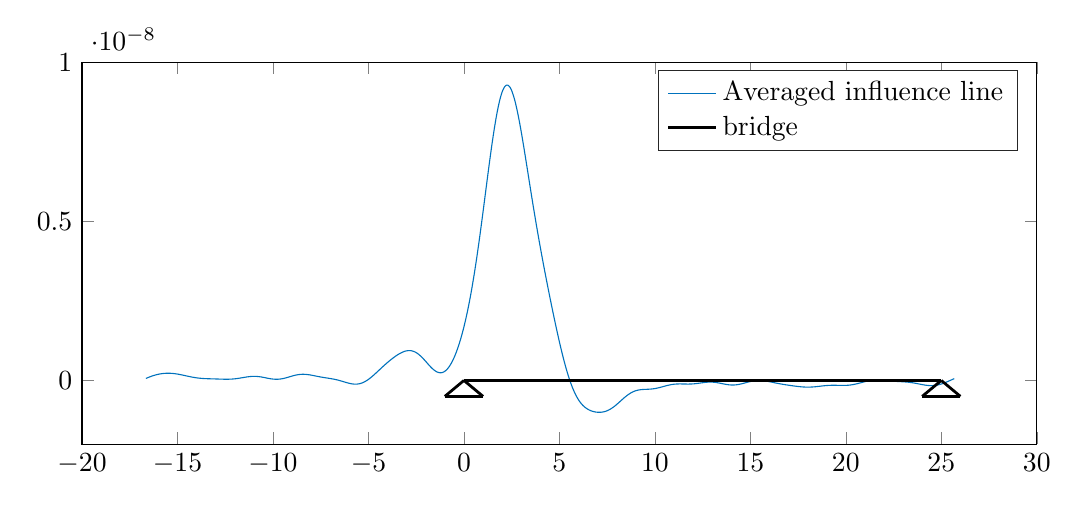
\begin{tikzpicture}

  \begin{axis}[%
    width=\textwidth,
    height=0.4\textwidth,
    at={(0\figurewidth,0\figureheight)},
    scale only axis,
    xmin=-20,
    xmax=30,
    ymin=-2e-09,
    ymax=1e-08,
    axis background/.style={fill=white},
    % title style={font=\bfseries},
    % title={averaged influence line without train 5, 600 samples before and after},
    legend style={legend cell align=left,align=left,draw=white!15!black}
    ]
    \addplot [color=mycolor1,solid]
    table[row sep=crcr]{%
    -16.653955078125	6.28295066695866e-11\\
    -16.6338056640625	6.80331992030371e-11\\
    -16.61365625	7.31924168408746e-11\\
    -16.5935068359375	7.83034868104857e-11\\
    -16.573357421875	8.3362860640408e-11\\
    -16.5532080078125	8.83671158775593e-11\\
    -16.53305859375	9.33129573942381e-11\\
    -16.5129091796875	9.81972182950265e-11\\
    -16.492759765625	1.03016860435107e-10\\
    -16.4726103515625	1.07768974562898e-10\\
    -16.4524609375	1.12450780101108e-10\\
    -16.4323115234375	1.17059624581503e-10\\
    -16.412162109375	1.21592982749791e-10\\
    -16.3920126953125	1.26048455358002e-10\\
    -16.37186328125	1.30423767662642e-10\\
    -16.3517138671875	1.34716767647796e-10\\
    -16.331564453125	1.38925423992978e-10\\
    -16.3114150390625	1.430478238062e-10\\
    -16.291265625	1.47082170143242e-10\\
    -16.2711162109375	1.51026779334564e-10\\
    -16.250966796875	1.54880078141532e-10\\
    -16.2308173828125	1.58640600763968e-10\\
    -16.21066796875	1.62306985721001e-10\\
    -16.1905185546875	1.65877972627367e-10\\
    -16.170369140625	1.69352398887085e-10\\
    -16.1502197265625	1.72729196326318e-10\\
    -16.1300703125	1.76007387786911e-10\\
    -16.1099208984375	1.79186083701729e-10\\
    -16.089771484375	1.82264478672443e-10\\
    -16.0696220703125	1.85241848069823e-10\\
    -16.04947265625	1.88117544675946e-10\\
    -16.0293232421875	1.9089099538703e-10\\
    -16.009173828125	1.93561697994712e-10\\
    -15.9890244140625	1.96129218062771e-10\\
    -15.968875	1.98593185915281e-10\\
    -15.9487255859375	2.00953293751145e-10\\
    -15.928576171875	2.03209292898925e-10\\
    -15.9084267578125	2.05360991224674e-10\\
    -15.88827734375	2.0740825070432e-10\\
    -15.8681279296875	2.09350985170872e-10\\
    -15.847978515625	2.11189158245496e-10\\
    -15.8278291015625	2.12922781460154e-10\\
    -15.8076796875	2.14551912578164e-10\\
    -15.7875302734375	2.16076654117709e-10\\
    -15.767380859375	2.17497152081932e-10\\
    -15.7472314453125	2.18813594897905e-10\\
    -15.72708203125	2.20026212565343e-10\\
    -15.7069326171875	2.21135276014593e-10\\
    -15.686783203125	2.22141096672087e-10\\
    -15.6666337890625	2.2304402623006e-10\\
    -15.646484375	2.23844456616069e-10\\
    -15.6263349609375	2.24542820156537e-10\\
    -15.606185546875	2.25139589927319e-10\\
    -15.5860361328125	2.25635280283063e-10\\
    -15.56588671875	2.26030447555998e-10\\
    -15.5457373046875	2.26325690913694e-10\\
    -15.525587890625	2.26521653364251e-10\\
    -15.5054384765625	2.26619022896437e-10\\
    -15.4852890625	2.26618533741363e-10\\
    -15.4651396484375	2.26520967741446e-10\\
    -15.444990234375	2.26327155811647e-10\\
    -15.4248408203125	2.26037979477276e-10\\
    -15.40469140625	2.25654372472057e-10\\
    -15.3845419921875	2.25177322379668e-10\\
    -15.364392578125	2.24607872301441e-10\\
    -15.3442431640625	2.23947122532691e-10\\
    -15.32409375	2.23196232229792e-10\\
    -15.3039443359375	2.22356421050026e-10\\
    -15.283794921875	2.21428970746138e-10\\
    -15.2636455078125	2.20415226697574e-10\\
    -15.24349609375	2.19316599360486e-10\\
    -15.2233466796875	2.18134565618832e-10\\
    -15.203197265625	2.16870670019218e-10\\
    -15.1830478515625	2.15526525872496e-10\\
    -15.1628984375	2.14103816205619e-10\\
    -15.1427490234375	2.12604294547932e-10\\
    -15.122599609375	2.11029785536614e-10\\
    -15.1024501953125	2.09382185326833e-10\\
    -15.08230078125	2.07663461792959e-10\\
    -15.0621513671875	2.0587565450809e-10\\
    -15.042001953125	2.04020874490166e-10\\
    -15.0218525390625	2.02101303703908e-10\\
    -15.001703125	2.00119194309035e-10\\
    -14.9815537109375	1.98076867646302e-10\\
    -14.961404296875	1.95976712954113e-10\\
    -14.9412548828125	1.93821185809846e-10\\
    -14.92110546875	1.91612806291165e-10\\
    -14.9009560546875	1.89354156854164e-10\\
    -14.880806640625	1.87047879926306e-10\\
    -14.8606572265625	1.84696675213786e-10\\
    -14.8405078125	1.8230329672417e-10\\
    -14.8203583984375	1.79870549506737e-10\\
    -14.800208984375	1.77401286114303e-10\\
    -14.7800595703125	1.74898402791801e-10\\
    -14.75991015625	1.72364835398288e-10\\
    -14.7397607421875	1.69803555070508e-10\\
    -14.719611328125	1.67217563637526e-10\\
    -14.6994619140625	1.64609888797303e-10\\
    -14.6793125	1.61983579067453e-10\\
    -14.6591630859375	1.59341698523703e-10\\
    -14.639013671875	1.5668732134086e-10\\
    -14.6188642578125	1.54023526152258e-10\\
    -14.59871484375	1.51353390244835e-10\\
    -14.5785654296875	1.48679983608084e-10\\
    -14.558416015625	1.46006362856067e-10\\
    -14.5382666015625	1.43335565042775e-10\\
    -14.5181171875	1.40670601391786e-10\\
    -14.4979677734375	1.38014450962149e-10\\
    -14.477818359375	1.35370054272973e-10\\
    -14.4576689453125	1.32740306909921e-10\\
    -14.43751953125	1.30128053137206e-10\\
    -14.4173701171875	1.27536079539266e-10\\
    -14.397220703125	1.24967108716399e-10\\
    -14.3770712890625	1.22423793059067e-10\\
    -14.356921875	1.1990870862556e-10\\
    -14.3367724609375	1.17424349147747e-10\\
    -14.316623046875	1.1497312018958e-10\\
    -14.2964736328125	1.12557333482731e-10\\
    -14.27632421875	1.10179201463562e-10\\
    -14.2561748046875	1.07840832035042e-10\\
    -14.236025390625	1.05544223576852e-10\\
    -14.2158759765625	1.03291260226203e-10\\
    -14.1957265625	1.01083707451162e-10\\
    -14.1755771484375	9.89232079375227e-11\\
    -14.155427734375	9.68112778092044e-11\\
    -14.1352783203125	9.47493032012817e-11\\
    -14.11512890625	9.27385372034728e-11\\
    -14.0949794921875	9.07800971908593e-11\\
    -14.074830078125	8.88749625571757e-11\\
    -14.0546806640625	8.70239728647816e-11\\
    -14.03453125	8.5227826423847e-11\\
    -14.0143818359375	8.34870793118567e-11\\
    -13.994232421875	8.18021448429426e-11\\
    -13.9740830078125	8.01732934948668e-11\\
    -13.95393359375	7.86006532998749e-11\\
    -13.9337841796875	7.70842107038434e-11\\
    -13.913634765625	7.5623811896355e-11\\
    -13.8934853515625	7.42191646126141e-11\\
    -13.8733359375	7.28698404061984e-11\\
    -13.8531865234375	7.15752773898378e-11\\
    -13.833037109375	7.03347834395423e-11\\
    -13.8128876953125	6.9147539855564e-11\\
    -13.79273828125	6.80126054717553e-11\\
    -13.7725888671875	6.69289212031344e-11\\
    -13.752439453125	6.58953150195489e-11\\
    -13.7322900390625	6.49105073316213e-11\\
    -13.712140625	6.39731167732945e-11\\
    -13.6919912109375	6.3081666363699e-11\\
    -13.671841796875	6.22345900292583e-11\\
    -13.6516923828125	6.14302394654458e-11\\
    -13.63154296875	6.06668913159605e-11\\
    -13.6113935546875	5.99427546457026e-11\\
    -13.591244140625	5.92559786824312e-11\\
    -13.5710947265625	5.86046608007448e-11\\
    -13.5509453125	5.79868547207119e-11\\
    -13.5307958984375	5.74005788924287e-11\\
    -13.510646484375	5.68438250366572e-11\\
    -13.4904970703125	5.6314566810852e-11\\
    -13.47034765625	5.58107685689709e-11\\
    -13.4501982421875	5.53303941828318e-11\\
    -13.430048828125	5.48714158921498e-11\\
    -13.4098994140625	5.44318231499288e-11\\
    -13.38975	5.40096314295357e-11\\
    -13.3696005859375	5.36028909595884e-11\\
    -13.349451171875	5.32096953526643e-11\\
    -13.3293017578125	5.28281900939302e-11\\
    -13.30915234375	5.24565808559146e-11\\
    -13.2890029296875	5.20931416059927e-11\\
    -13.268853515625	5.17362224735937e-11\\
    -13.2487041015625	5.13842573446905e-11\\
    -13.2285546875	5.10357711518274e-11\\
    -13.2084052734375	5.0689386828835e-11\\
    -13.188255859375	5.03438319002698e-11\\
    -13.1681064453125	4.9997944676752e-11\\
    -13.14795703125	4.96506800285367e-11\\
    -13.1278076171875	4.93011147110501e-11\\
    -13.107658203125	4.89484522174766e-11\\
    -13.0875087890625	4.85920271351045e-11\\
    -13.067359375	4.82313089837501e-11\\
    -13.0472099609375	4.78659055163553e-11\\
    -13.027060546875	4.7495565463716e-11\\
    -13.0069111328125	4.71201807071589e-11\\
    -12.98676171875	4.67397878651259e-11\\
    -12.9666123046875	4.63545692816151e-11\\
    -12.946462890625	4.59648534066091e-11\\
    -12.9263134765625	4.55711145608724e-11\\
    -12.9061640625	4.51739720797302e-11\\
    -12.8860146484375	4.47741888327471e-11\\
    -12.865865234375	4.43726691186395e-11\\
    -12.8457158203125	4.39704559369907e-11\\
    -12.82556640625	4.35687276408963e-11\\
    -12.8054169921875	4.31687939769007e-11\\
    -12.785267578125	4.27720915211345e-11\\
    -12.7651181640625	4.23801785227782e-11\\
    -12.74496875	4.19947291685286e-11\\
    -12.7248193359375	4.16175272839279e-11\\
    -12.704669921875	4.12504594898181e-11\\
    -12.6845205078125	4.08955078343882e-11\\
    -12.66437109375	4.05547419235102e-11\\
    -12.6442216796875	4.02303105741573e-11\\
    -12.624072265625	3.99244330178364e-11\\
    -12.6039228515625	3.96393896828517e-11\\
    -12.5837734375	3.93775125862083e-11\\
    -12.5636240234375	3.91411753676952e-11\\
    -12.543474609375	3.89327830004331e-11\\
    -12.5233251953125	3.87547612136707e-11\\
    -12.50317578125	3.8609545665214e-11\\
    -12.4830263671875	3.84995709020569e-11\\
    -12.462876953125	3.842725914913e-11\\
    -12.4427275390625	3.83950089670347e-11\\
    -12.422578125	3.84051838206735e-11\\
    -12.4024287109375	3.84601006013533e-11\\
    -12.382279296875	3.85620181456785e-11\\
    -12.3621298828125	3.87131257949627e-11\\
    -12.34198046875	3.89155320392268e-11\\
    -12.3218310546875	3.91712532900141e-11\\
    -12.301681640625	3.94822028262561e-11\\
    -12.2815322265625	3.98501799572271e-11\\
    -12.2613828125	4.02768594463837e-11\\
    -12.2412333984375	4.07637812392385e-11\\
    -12.221083984375	4.1312340537945e-11\\
    -12.2009345703125	4.19237782643023e-11\\
    -12.18078515625	4.25991719519917e-11\\
    -12.1606357421875	4.33394271076635e-11\\
    -12.140486328125	4.41452690792745e-11\\
    -12.1203369140625	4.5017235468512e-11\\
    -12.1001875	4.59556691226778e-11\\
    -12.0800380859375	4.69607117395435e-11\\
    -12.059888671875	4.80322981168982e-11\\
    -12.0397392578125	4.91701510764362e-11\\
    -12.01958984375	5.03737770895517e-11\\
    -11.9994404296875	5.16424626302669e-11\\
    -11.979291015625	5.29752712782512e-11\\
    -11.9591416015625	5.43710415923195e-11\\
    -11.9389921875	5.58283857722707e-11\\
    -11.9188427734375	5.73456891242612e-11\\
    -11.898693359375	5.89211103421698e-11\\
    -11.8785439453125	6.05525826145482e-11\\
    -11.85839453125	6.22378155639902e-11\\
    -11.8382451171875	6.39742980226832e-11\\
    -11.818095703125	6.57593016450879e-11\\
    -11.7979462890625	6.75898853555756e-11\\
    -11.777796875	6.94629006259376e-11\\
    -11.7576474609375	7.13749975745881e-11\\
    -11.737498046875	7.33226318763131e-11\\
    -11.7173486328125	7.5302072468362e-11\\
    -11.69719921875	7.73094100357655e-11\\
    -11.6770498046875	7.93405662557375e-11\\
    -11.656900390625	8.13913037781817e-11\\
    -11.6367509765625	8.34572369164313e-11\\
    -11.6166015625	8.5533843019625e-11\\
    -11.5964521484375	8.76164744953353e-11\\
    -11.576302734375	8.9700371448579e-11\\
    -11.5561533203125	9.17806749006873e-11\\
    -11.53600390625	9.38524405492205e-11\\
    -11.5158544921875	9.59106530277348e-11\\
    -11.495705078125	9.795024062214e-11\\
    -11.4755556640625	9.99660903982174e-11\\
    -11.45540625	1.01953063693151e-10\\
    -11.4352568359375	1.03906011922055e-10\\
    -11.415107421875	1.05819792648954e-10\\
    -11.3949580078125	1.07689285870275e-10\\
    -11.37480859375	1.09509410457649e-10\\
    -11.3546591796875	1.11275140705712e-10\\
    -11.334509765625	1.12981522929836e-10\\
    -11.3143603515625	1.14623692057861e-10\\
    -11.2942109375	1.1619688815953e-10\\
    -11.2740615234375	1.1769647285692e-10\\
    -11.253912109375	1.19117945559119e-10\\
    -11.2337626953125	1.20456959464372e-10\\
    -11.21361328125	1.21709337273351e-10\\
    -11.1934638671875	1.22871086557505e-10\\
    -11.173314453125	1.23938414727263e-10\\
    -11.1531650390625	1.24907743545646e-10\\
    -11.133015625	1.25775723133953e-10\\
    -11.1128662109375	1.26539245417424e-10\\
    -11.092716796875	1.27195456960267e-10\\
    -11.0725673828125	1.27741771141007e-10\\
    -11.05241796875	1.2817587962104e-10\\
    -11.0322685546875	1.28495763061142e-10\\
    -11.012119140625	1.28699701042967e-10\\
    -10.9919697265625	1.28786281154811e-10\\
    -10.9718203125	1.28754407203476e-10\\
    -10.9516708984375	1.28603306516648e-10\\
    -10.931521484375	1.28332536303019e-10\\
    -10.9113720703125	1.27941989040288e-10\\
    -10.89122265625	1.27431896864204e-10\\
    -10.8710732421875	1.2680283493496e-10\\
    -10.850923828125	1.26055723760526e-10\\
    -10.8307744140625	1.25191830459799e-10\\
    -10.810625	1.24212768951951e-10\\
    -10.7904755859375	1.23120499061751e-10\\
    -10.770326171875	1.21917324534325e-10\\
    -10.7501767578125	1.20605889956257e-10\\
    -10.73002734375	1.19189176583716e-10\\
    -10.7098779296875	1.1767049708186e-10\\
    -10.689728515625	1.1605348918346e-10\\
    -10.6695791015625	1.14342108278346e-10\\
    -10.6494296875	1.12540618948947e-10\\
    -10.6292802734375	1.1065358547074e-10\\
    -10.609130859375	1.08685861300106e-10\\
    -10.5889814453125	1.06642577575493e-10\\
    -10.56883203125	1.04529130661346e-10\\
    -10.5486826171875	1.0235116876756e-10\\
    -10.528533203125	1.00114577680527e-10\\
    -10.5083837890625	9.78254656450265e-11\\
    -10.488234375	9.54901474392735e-11\\
    -10.4680849609375	9.31151276883631e-11\\
    -10.447935546875	9.0707083464192e-11\\
    -10.4277861328125	8.82728462225101e-11\\
    -10.40763671875	8.58193831303925e-11\\
    -10.3874873046875	8.33537778395632e-11\\
    -10.367337890625	8.08832107633857e-11\\
    -10.3471884765625	7.84149389170685e-11\\
    -10.3270390625	7.59562753826569e-11\\
    -10.3068896484375	7.35145684617358e-11\\
    -10.286740234375	7.10971805803453e-11\\
    -10.2665908203125	6.87114670116371e-11\\
    -10.24644140625	6.63647544828368e-11\\
    -10.2262919921875	6.40643197337737e-11\\
    -10.206142578125	6.18173680947663e-11\\
    -10.1859931640625	5.96310121519057e-11\\
    -10.16584375	5.75122505678958e-11\\
    -10.1456943359375	5.54679471263667e-11\\
    -10.125544921875	5.3504810067215e-11\\
    -10.1053955078125	5.16293717798911e-11\\
    -10.08524609375	4.98479689206946e-11\\
    -10.0650966796875	4.81667230189916e-11\\
    -10.044947265625	4.6591521636091e-11\\
    -10.0247978515625	4.51280001388264e-11\\
    -10.0046484375	4.37815241482711e-11\\
    -9.9844990234375	4.25571727219838e-11\\
    -9.964349609375	4.14597223260665e-11\\
    -9.9442001953125	4.04936316509057e-11\\
    -9.92405078125	3.96630273219808e-11\\
    -9.9039013671875	3.89716905543334e-11\\
    -9.883751953125	3.84230447964316e-11\\
    -9.8636025390625	3.80201444060356e-11\\
    -9.843453125	3.77656643975264e-11\\
    -9.8233037109375	3.76618912966721e-11\\
    -9.803154296875	3.77107151354539e-11\\
    -9.7830048828125	3.79136226157779e-11\\
    -9.76285546875	3.82716914673024e-11\\
    -9.7427060546875	3.87855860206975e-11\\
    -9.722556640625	3.94555540137638e-11\\
    -9.7024072265625	4.02814246438435e-11\\
    -9.6822578125	4.12626078758988e-11\\
    -9.6621083984375	4.23980950115579e-11\\
    -9.641958984375	4.36864605202855e-11\\
    -9.6218095703125	4.5125865129712e-11\\
    -9.60166015625	4.67140601679982e-11\\
    -9.5815107421875	4.84483931469992e-11\\
    -9.561361328125	5.03258145708751e-11\\
    -9.5412119140625	5.23428859507197e-11\\
    -9.5210625	5.44957890018158e-11\\
    -9.5009130859375	5.6780335996106e-11\\
    -9.480763671875	5.9191981238698e-11\\
    -9.4606142578125	6.17258336333911e-11\\
    -9.44046484375	6.43766702985749e-11\\
    -9.4203154296875	6.71389511913352e-11\\
    -9.400166015625	7.00068346941844e-11\\
    -9.3800166015625	7.29741941155599e-11\\
    -9.3598671875	7.60346350522069e-11\\
    -9.3397177734375	7.91815135585225e-11\\
    -9.319568359375	8.24079550653135e-11\\
    -9.2994189453125	8.5706873987765e-11\\
    -9.27926953125	8.90709939600938e-11\\
    -9.2591201171875	9.2492868632228e-11\\
    -9.238970703125	9.59649029618426e-11\\
    -9.2188212890625	9.9479374933457e-11\\
    -9.198671875	1.03028457634739e-10\\
    -9.1785224609375	1.06604241618942e-10\\
    -9.158373046875	1.10198757481353e-10\\
    -9.1382236328125	1.13803998576923e-10\\
    -9.11807421875	1.17411943805632e-10\\
    -9.0979248046875	1.21014580391953e-10\\
    -9.077775390625	1.24603926584679e-10\\
    -9.0576259765625	1.28172054203669e-10\\
    -9.0374765625	1.31711110960479e-10\\
    -9.0173271484375	1.35213342480608e-10\\
    -8.997177734375	1.38671113956066e-10\\
    -8.9770283203125	1.42076931358152e-10\\
    -8.95687890625	1.45423462141809e-10\\
    -8.9367294921875	1.48703555374636e-10\\
    -8.916580078125	1.51910261225523e-10\\
    -8.8964306640625	1.55036849750029e-10\\
    -8.87628125	1.5807682891206e-10\\
    -8.8561318359375	1.61023961783859e-10\\
    -8.835982421875	1.63872282869205e-10\\
    -8.8158330078125	1.66616113497667e-10\\
    -8.79568359375	1.69250076240846e-10\\
    -8.7755341796875	1.71769108304946e-10\\
    -8.755384765625	1.74168473857491e-10\\
    -8.7352353515625	1.76443775249557e-10\\
    -8.7150859375	1.78590963098774e-10\\
    -8.6949365234375	1.80606345202163e-10\\
    -8.674787109375	1.82486594251917e-10\\
    -8.6546376953125	1.84228754331324e-10\\
    -8.63448828125	1.85830246172187e-10\\
    -8.6143388671875	1.87288871159413e-10\\
    -8.594189453125	1.88602814072683e-10\\
    -8.5740400390625	1.89770644559453e-10\\
    -8.553890625	1.90791317337981e-10\\
    -8.5337412109375	1.91664171133335e-10\\
    -8.513591796875	1.92388926353784e-10\\
    -8.4934423828125	1.92965681519307e-10\\
    -8.47329296875	1.93394908458202e-10\\
    -8.4531435546875	1.93677446292096e-10\\
    -8.432994140625	1.93814494233823e-10\\
    -8.4128447265625	1.93807603226683e-10\\
    -8.3926953125	1.93658666457714e-10\\
    -8.3725458984375	1.93369908781359e-10\\
    -8.352396484375	1.92943875093817e-10\\
    -8.3322470703125	1.9238341770189e-10\\
    -8.31209765625	1.91691682733679e-10\\
    -8.2919482421875	1.90872095641764e-10\\
    -8.271798828125	1.89928345852667e-10\\
    -8.2516494140625	1.88864370619325e-10\\
    -8.2315	1.87684338136081e-10\\
    -8.2113505859375	1.86392629978233e-10\\
    -8.191201171875	1.84993822930499e-10\\
    -8.1710517578125	1.8349267027092e-10\\
    -8.15090234375	1.81894082578502e-10\\
    -8.1307529296875	1.80203108134636e-10\\
    -8.110603515625	1.78424912989659e-10\\
    -8.0904541015625	1.76564760767047e-10\\
    -8.0703046875	1.74627992278693e-10\\
    -8.0501552734375	1.72620005025247e-10\\
    -8.030005859375	1.70546232655931e-10\\
    -8.0098564453125	1.68412124462311e-10\\
    -7.98970703125	1.6622312498036e-10\\
    -7.9695576171875	1.63984653774694e-10\\
    -7.949408203125	1.61702085478208e-10\\
    -7.9292587890625	1.59380730159383e-10\\
    -7.909109375	1.57025814088304e-10\\
    -7.8889599609375	1.54642460971007e-10\\
    -7.868810546875	1.52235673720051e-10\\
    -7.8486611328125	1.49810316827261e-10\\
    -7.82851171875	1.47371099402401e-10\\
    -7.8083623046875	1.44922558939167e-10\\
    -7.788212890625	1.4246904586716e-10\\
    -7.7680634765625	1.40014708945791e-10\\
    -7.7479140625	1.37563481552907e-10\\
    -7.7277646484375	1.35119068917756e-10\\
    -7.707615234375	1.32684936344482e-10\\
    -7.6874658203125	1.30264298468755e-10\\
    -7.66731640625	1.27860109586405e-10\\
    -7.6471669921875	1.2547505508908e-10\\
    -7.627017578125	1.23111544037869e-10\\
    -7.6068681640625	1.20771702901808e-10\\
    -7.58671875	1.1845737048389e-10\\
    -7.5665693359375	1.16170094052913e-10\\
    -7.546419921875	1.13911126695179e-10\\
    -7.5262705078125	1.1168142589554e-10\\
    -7.50612109375	1.09481653352889e-10\\
    -7.4859716796875	1.07312176030674e-10\\
    -7.465822265625	1.05173068438537e-10\\
    -7.4456728515625	1.03064116136655e-10\\
    -7.4255234375	1.00984820449963e-10\\
    -7.4053740234375	9.89344043749347e-11\\
    -7.385224609375	9.69118196573331e-11\\
    -7.3650751953125	9.49157550149512e-11\\
    -7.34492578125	9.29446454752417e-11\\
    -7.3247763671875	9.09966827936147e-11\\
    -7.304626953125	8.90698269141492e-11\\
    -7.2844775390625	8.71618184307201e-11\\
    -7.264328125	8.52701920027182e-11\\
    -7.2441787109375	8.33922906761285e-11\\
    -7.224029296875	8.15252810572406e-11\\
    -7.2038798828125	7.96661692831666e-11\\
    -7.18373046875	7.78118177303265e-11\\
    -7.1635810546875	7.59589623992625e-11\\
    -7.143431640625	7.41042309116111e-11\\
    -7.1232822265625	7.22441610527126e-11\\
    -7.1031328125	7.03752197912199e-11\\
    -7.0829833984375	6.84938227052802e-11\\
    -7.062833984375	6.65963537431337e-11\\
    -7.0426845703125	6.46791852447744e-11\\
    -7.02253515625	6.27386981501045e-11\\
    -7.0023857421875	6.07713023182745e-11\\
    -6.982236328125	5.87734568823152e-11\\
    -6.9620869140625	5.6741690562871e-11\\
    -6.9419375	5.46726218648971e-11\\
    -6.9217880859375	5.25629790813952e-11\\
    -6.901638671875	5.0409620028802e-11\\
    -6.8814892578125	4.82095514395234e-11\\
    -6.86133984375	4.59599479380858e-11\\
    -6.8411904296875	4.36581705288122e-11\\
    -6.821041015625	4.13017845244911e-11\\
    -6.8008916015625	3.88885768473741e-11\\
    -6.7807421875	3.6416572635956e-11\\
    -6.7605927734375	3.38840510933536e-11\\
    -6.740443359375	3.12895605156485e-11\\
    -6.7202939453125	2.8631932441457e-11\\
    -6.70014453125	2.59102948668798e-11\\
    -6.6799951171875	2.31240844733727e-11\\
    -6.659845703125	2.02730578193926e-11\\
    -6.6396962890625	1.73573014503272e-11\\
    -6.619546875	1.43772408849691e-11\\
    -6.5993974609375	1.13336484407834e-11\\
    -6.579248046875	8.2276498641806e-12\\
    -6.5590986328125	5.06072973634878e-12\\
    -6.53894921875	1.83473562936997e-12\\
    -6.5187998046875	-1.44811900813747e-12\\
    -6.498650390625	-4.78525325219151e-12\\
    -6.4785009765625	-8.17371840316411e-12\\
    -6.4583515625	-1.16101989912276e-11\\
    -6.4382021484375	-1.50910150900205e-11\\
    -6.418052734375	-1.86121259364211e-11\\
    -6.3979033203125	-2.21691348496425e-11\\
    -6.37775390625	-2.5757295438218e-11\\
    -6.3576044921875	-2.93715190788702e-11\\
    -6.337455078125	-3.30063836467426e-11\\
    -6.3173056640625	-3.6656143471872e-11\\
    -6.29715625	-4.03147404925357e-11\\
    -6.2770068359375	-4.39758165717153e-11\\
    -6.256857421875	-4.76327269387517e-11\\
    -6.2367080078125	-5.12785547142551e-11\\
    -6.21655859375	-5.49061264723496e-11\\
    -6.1964091796875	-5.85080287907027e-11\\
    -6.176259765625	-6.20766257350751e-11\\
    -6.1561103515625	-6.56040772218658e-11\\
    -6.1359609375	-6.90823581988623e-11\\
    -6.1158115234375	-7.25032785814551e-11\\
    -6.095662109375	-7.58585038788037e-11\\
    -6.0755126953125	-7.9139576441957e-11\\
    -6.05536328125	-8.23379372635738e-11\\
    -6.0352138671875	-8.54449482569389e-11\\
    -6.015064453125	-8.84519149401184e-11\\
    -5.9949150390625	-9.13501094496517e-11\\
    -5.974765625	-9.41307938068577e-11\\
    -5.9546162109375	-9.67852433589672e-11\\
    -5.934466796875	-9.93047703164798e-11\\
    -5.9143173828125	-1.01680747307842e-10\\
    -5.89416796875	-1.03904630872376e-10\\
    -5.8740185546875	-1.059679848125e-10\\
    -5.853869140625	-1.07862503326834e-10\\
    -5.8337197265625	-1.09580033846387e-10\\
    -5.8135703125	-1.11112599497131e-10\\
    -5.7934208984375	-1.12452421113468e-10\\
    -5.773271484375	-1.13591938728693e-10\\
    -5.7531220703125	-1.14523832470395e-10\\
    -5.73297265625	-1.15241042790754e-10\\
    -5.7128232421875	-1.15736789964111e-10\\
    -5.692673828125	-1.16004592786697e-10\\
    -5.6725244140625	-1.16038286416272e-10\\
    -5.652375	-1.1583203929248e-10\\
    -5.6322255859375	-1.15380369081907e-10\\
    -5.612076171875	-1.146781575954e-10\\
    -5.5919267578125	-1.13720664628818e-10\\
    -5.57177734375	-1.1250354068214e-10\\
    -5.5516279296875	-1.11022838516053e-10\\
    -5.531478515625	-1.09275023509039e-10\\
    -5.5113291015625	-1.07256982782516e-10\\
    -5.4911796875	-1.04966033065797e-10\\
    -5.4710302734375	-1.02399927277255e-10\\
    -5.450880859375	-9.95568598026482e-11\\
    -5.4307314453125	-9.64354704562176e-11\\
    -5.41058203125	-9.30348471148994e-11\\
    -5.3904326171875	-8.9354527020776e-11\\
    -5.370283203125	-8.5394496751617e-11\\
    -5.3501337890625	-8.1155190864207e-11\\
    -5.329984375	-7.66374892198601e-11\\
    -5.3098349609375	-7.18427130063144e-11\\
    -5.289685546875	-6.67726194748068e-11\\
    -5.2695361328125	-6.14293954158211e-11\\
    -5.24938671875	-5.58156494014838e-11\\
    -5.2292373046875	-4.99344028269791e-11\\
    -5.209087890625	-4.37890797877769e-11\\
    -5.1889384765625	-3.73834958334707e-11\\
    -5.1687890625	-3.07218456432189e-11\\
    -5.1486396484375	-2.38086896715162e-11\\
    -5.128490234375	-1.66489398167625e-11\\
    -5.1083408203125	-9.24784416856905e-12\\
    -5.08819140625	-1.6109708929908e-12\\
    -5.0680419921875	6.25580868198994e-12\\
    -5.047892578125	1.43463377156724e-11\\
    -5.0277431640625	2.26541921708347e-11\\
    -5.00759375	3.11726997268593e-11\\
    -4.9874443359375	3.98949592177455e-11\\
    -4.967294921875	4.8813860521033e-11\\
    -4.9471455078125	5.7922104822257e-11\\
    -4.92699609375	6.72122251782126e-11\\
    -4.9068466796875	7.6676607301389e-11\\
    -4.886697265625	8.63075104872814e-11\\
    -4.8665478515625	9.60970886058413e-11\\
    -4.8463984375	1.06037411078365e-10\\
    -4.8262490234375	1.16120483761218e-10\\
    -4.806099609375	1.26338269658398e-10\\
    -4.7859501953125	1.36682709385701e-10\\
    -4.76580078125	1.47145741310397e-10\\
    -4.7456513671875	1.57719321291701e-10\\
    -4.725501953125	1.68395441948987e-10\\
    -4.7053525390625	1.79166151386709e-10\\
    -4.685203125	1.90023571307171e-10\\
    -4.6650537109375	2.00959914444825e-10\\
    -4.644904296875	2.11967501258523e-10\\
    -4.6247548828125	2.23038775821128e-10\\
    -4.60460546875	2.34166320849199e-10\\
    -4.5844560546875	2.4534287181882e-10\\
    -4.564306640625	2.56561330117457e-10\\
    -4.5441572265625	2.67814775185463e-10\\
    -4.5240078125	2.79096475605016e-10\\
    -4.5038583984375	2.90399899098491e-10\\
    -4.483708984375	3.01718721402562e-10\\
    -4.4635595703125	3.13046833989019e-10\\
    -4.44341015625	3.24378350607761e-10\\
    -4.4232607421875	3.35707612632321e-10\\
    -4.403111328125	3.47029193193014e-10\\
    -4.3829619140625	3.58337900087766e-10\\
    -4.3628125	3.69628777465659e-10\\
    -4.3426630859375	3.80897106283137e-10\\
    -4.322513671875	3.92138403537927e-10\\
    -4.3023642578125	4.03348420290672e-10\\
    -4.28221484375	4.14523138489259e-10\\
    -4.2620654296875	4.25658766615782e-10\\
    -4.241916015625	4.3675173418093e-10\\
    -4.2217666015625	4.47798685095431e-10\\
    -4.2016171875	4.58796469952805e-10\\
    -4.1814677734375	4.69742137262337e-10\\
    -4.161318359375	4.80632923675597e-10\\
    -4.1411689453125	4.91466243254098e-10\\
    -4.12101953125	5.02239675829885e-10\\
    -4.1008701171875	5.12950954514695e-10\\
    -4.080720703125	5.23597952417179e-10\\
    -4.0605712890625	5.34178668631091e-10\\
    -4.040421875	5.44691213560753e-10\\
    -4.0202724609375	5.55133793653069e-10\\
    -4.000123046875	5.65504695608234e-10\\
    -3.9799736328125	5.75802270143771e-10\\
    -3.95982421875	5.86024915388792e-10\\
    -3.9396748046875	5.96171059987375e-10\\
    -3.919525390625	6.06239145991562e-10\\
    -3.8993759765625	6.16227611625926e-10\\
    -3.8792265625	6.2613487400664e-10\\
    -3.8590771484375	6.35959311898746e-10\\
    -3.838927734375	6.45699248595797e-10\\
    -3.8187783203125	6.55352935005995e-10\\
    -3.79862890625	6.64918533028925e-10\\
    -3.7784794921875	6.74394099306203e-10\\
    -3.758330078125	6.83777569428684e-10\\
    -3.7381806640625	6.93066742681488e-10\\
    -3.71803125	7.02259267406688e-10\\
    -3.6978818359375	7.11352627061646e-10\\
    -3.677732421875	7.20344127048715e-10\\
    -3.6575830078125	7.29230882389756e-10\\
    -3.63743359375	7.38009806315924e-10\\
    -3.6172841796875	7.46677599840319e-10\\
    -3.597134765625	7.55230742377628e-10\\
    -3.5769853515625	7.63665483471365e-10\\
    -3.5568359375	7.71977835685388e-10\\
    -3.5366865234375	7.80163568712316e-10\\
    -3.516537109375	7.88218204747091e-10\\
    -3.4963876953125	7.96137015169416e-10\\
    -3.47623828125	8.03915018573994e-10\\
    -3.4560888671875	8.11546980182609e-10\\
    -3.435939453125	8.19027412666929e-10\\
    -3.4157900390625	8.26350578405724e-10\\
    -3.395640625	8.33510493194736e-10\\
    -3.3754912109375	8.40500931421988e-10\\
    -3.355341796875	8.47315432715723e-10\\
    -3.3351923828125	8.53947310066509e-10\\
    -3.31504296875	8.60389659419309e-10\\
    -3.2948935546875	8.66635370725633e-10\\
    -3.274744140625	8.72677140440077e-10\\
    -3.2545947265625	8.78507485439861e-10\\
    -3.2344453125	8.84118758340276e-10\\
    -3.2142958984375	8.89503164173268e-10\\
    -3.194146484375	8.94652778390842e-10\\
    -3.1739970703125	8.99559566149513e-10\\
    -3.15384765625	9.04215402826611e-10\\
    -3.1336982421875	9.08612095714089e-10\\
    -3.113548828125	9.12741406830405e-10\\
    -3.0933994140625	9.16595076786106e-10\\
    -3.07325	9.20164849634198e-10\\
    -3.0531005859375	9.23442498631697e-10\\
    -3.032951171875	9.26419852834749e-10\\
    -3.0128017578125	9.29088824445524e-10\\
    -2.99265234375	9.31441436825509e-10\\
    -2.9725029296875	9.33469853086263e-10\\
    -2.952353515625	9.35166405165629e-10\\
    -2.9322041015625	9.36523623294557e-10\\
    -2.9120546875	9.37534265757103e-10\\
    -2.8919052734375	9.38191348844094e-10\\
    -2.871755859375	9.38488176899006e-10\\
    -2.8516064453125	9.38418372353181e-10\\
    -2.83145703125	9.37975905646378e-10\\
    -2.8113076171875	9.37155124927812e-10\\
    -2.791158203125	9.35950785432606e-10\\
    -2.7710087890625	9.34358078428352e-10\\
    -2.750859375	9.32372659627065e-10\\
    -2.7307099609375	9.29990676958376e-10\\
    -2.710560546875	9.2720879760105e-10\\
    -2.6904111328125	9.24024234171366e-10\\
    -2.67026171875	9.20434769968767e-10\\
    -2.6501123046875	9.16438783181482e-10\\
    -2.629962890625	9.12035269957374e-10\\
    -2.6098134765625	9.07223866248323e-10\\
    -2.5896640625	9.02004868339652e-10\\
    -2.5695146484375	8.96379251979921e-10\\
    -2.549365234375	8.9034869003028e-10\\
    -2.5292158203125	8.83915568556951e-10\\
    -2.50906640625	8.77083001295017e-10\\
    -2.4889169921875	8.6985484241658e-10\\
    -2.468767578125	8.62235697541586e-10\\
    -2.4486181640625	8.54230932934967e-10\\
    -2.42846875	8.45846682839545e-10\\
    -2.4083193359375	8.37089854899949e-10\\
    -2.388169921875	8.27968133638962e-10\\
    -2.3680205078125	8.1848998195397e-10\\
    -2.34787109375	8.08664640607684e-10\\
    -2.3277216796875	7.98502125693797e-10\\
    -2.307572265625	7.8801322406508e-10\\
    -2.2874228515625	7.77209486718116e-10\\
    -2.2672734375	7.66103220135748e-10\\
    -2.2471240234375	7.54707475595316e-10\\
    -2.226974609375	7.43036036457588e-10\\
    -2.2068251953125	7.31103403458307e-10\\
    -2.18667578125	7.1892477803114e-10\\
    -2.1665263671875	7.06516043697695e-10\\
    -2.146376953125	6.9389374556704e-10\\
    -2.1262275390625	6.81075067993829e-10\\
    -2.106078125	6.68077810450745e-10\\
    -2.0859287109375	6.54920361677296e-10\\
    -2.065779296875	6.41621672173302e-10\\
    -2.0456298828125	6.28201225111401e-10\\
    -2.02548046875	6.14679005748776e-10\\
    -2.0053310546875	6.01075469423784e-10\\
    -1.985181640625	5.8741150822863e-10\\
    -1.9650322265625	5.73708416454077e-10\\
    -1.9448828125	5.59987854907119e-10\\
    -1.9247333984375	5.46271814206749e-10\\
    -1.904583984375	5.32582577167222e-10\\
    -1.8844345703125	5.18942680381731e-10\\
    -1.86428515625	5.05374875122954e-10\\
    -1.8441357421875	4.91902087679716e-10\\
    -1.823986328125	4.78547379251717e-10\\
    -1.8038369140625	4.65333905526305e-10\\
    -1.7836875	4.52284876063116e-10\\
    -1.7635380859375	4.39423513613612e-10\\
    -1.743388671875	4.26773013503474e-10\\
    -1.7232392578125	4.14356503206214e-10\\
    -1.70308984375	4.02197002236338e-10\\
    -1.6829404296875	3.9031738248993e-10\\
    -1.662791015625	3.78740329159575e-10\\
    -1.6426416015625	3.67488302349234e-10\\
    -1.6224921875	3.56583499512752e-10\\
    -1.6023427734375	3.46047818837498e-10\\
    -1.582193359375	3.35902823691896e-10\\
    -1.5620439453125	3.26169708252395e-10\\
    -1.54189453125	3.16869264422e-10\\
    -1.5217451171875	3.08021850148297e-10\\
    -1.501595703125	2.99647359244691e-10\\
    -1.4814462890625	2.91765192813642e-10\\
    -1.461296875	2.84394232365617e-10\\
    -1.4411474609375	2.77552814721857e-10\\
    -1.420998046875	2.71258708783238e-10\\
    -1.4008486328125	2.65529094241255e-10\\
    -1.38069921875	2.60380542300645e-10\\
    -1.3605498046875	2.55828998476356e-10\\
    -1.340400390625	2.51889767520502e-10\\
    -1.3202509765625	2.4857750052759e-10\\
    -1.3001015625	2.45906184258796e-10\\
    -1.2799521484375	2.43889132718293e-10\\
    -1.259802734375	2.4253898100676e-10\\
    -1.2396533203125	2.41867681469111e-10\\
    -1.21950390625	2.41886502145347e-10\\
    -1.1993544921875	2.4260602752513e-10\\
    -1.179205078125	2.44036161598398e-10\\
    -1.1590556640625	2.46186133185977e-10\\
    -1.13890625	2.49064503525743e-10\\
    -1.1187568359375	2.5267917608164e-10\\
    -1.098607421875	2.57037408534481e-10\\
    -1.0784580078125	2.62145826905343e-10\\
    -1.05830859375	2.68010441754263e-10\\
    -1.0381591796875	2.74636666388946e-10\\
    -1.018009765625	2.82029337010545e-10\\
    -0.997860351562499	2.90192734715835e-10\\
    -0.977710937499998	2.99130609267948e-10\\
    -0.957561523437498	3.08846204540547e-10\\
    -0.937412109374998	3.19342285533691e-10\\
    -0.917262695312498	3.30621166852941e-10\\
    -0.897113281249998	3.42684742537292e-10\\
    -0.876963867187499	3.55534517115478e-10\\
    -0.856814453124999	3.69171637764931e-10\\
    -0.836665039062499	3.835969274425e-10\\
    -0.816515624999999	3.98810918851484e-10\\
    -0.796366210937499	4.14813889105283e-10\\
    -0.776216796874998	4.31605894944314e-10\\
    -0.756067382812498	4.49186808359485e-10\\
    -0.735917968749998	4.67556352472815e-10\\
    -0.715768554687498	4.86714137523507e-10\\
    -0.695619140624999	5.06659696805954e-10\\
    -0.675469726562499	5.27392522405043e-10\\
    -0.655320312499999	5.48912100573289e-10\\
    -0.635170898437497	5.71217946594255e-10\\
    -0.615021484374999	5.94309638977041e-10\\
    -0.594872070312498	6.18186852827557e-10\\
    -0.57472265625	6.42849392243797e-10\\
    -0.554573242187498	6.68297221584264e-10\\
    -0.534423828125	6.94530495461388e-10\\
    -0.514274414062498	7.21549587314711e-10\\
    -0.494124999999997	7.4935511642243e-10\\
    -0.473975585937499	7.77947973213881e-10\\
    -0.453826171874997	8.07329342750374e-10\\
    -0.433676757812499	8.37500726246839e-10\\
    -0.413527343749998	8.68463960512534e-10\\
    -0.3933779296875	9.00221235195115e-10\\
    -0.373228515624998	9.32775107719082e-10\\
    -0.3530791015625	9.66128515816545e-10\\
    -0.332929687499998	1.00028478755588e-09\\
    -0.3127802734375	1.03524764878154e-09\\
    -0.292630859374999	1.07102122788673e-09\\
    -0.272481445312497	1.10761005784909e-09\\
    -0.252332031249999	1.14501907546855e-09\\
    -0.232182617187497	1.18325361775574e-09\\
    -0.212033203124999	1.22231941542883e-09\\
    -0.191883789062498	1.26222258348641e-09\\
    -0.171734375	1.30296960883399e-09\\
    -0.151584960937498	1.34456733495178e-09\\
    -0.131435546875	1.38702294360185e-09\\
    -0.111286132812499	1.43034393358294e-09\\
    -0.091136718749997	1.47453809655179e-09\\
    -0.0709873046874989	1.51961348994057e-09\\
    -0.0508378906249973	1.56557840701003e-09\\
    -0.0306884765624993	1.61244134408916e-09\\
    -0.0105390624999977	1.66021096506203e-09\\
    0.00961035156250034	1.70889606317326e-09\\
    0.0297597656250019	1.75850552023362e-09\\
    0.0499091796875	1.80904826331741e-09\\
    0.0700585937500016	1.86053321905315e-09\\
    0.0902080078125032	1.91296926561877e-09\\
    0.110357421875001	1.96636518256202e-09\\
    0.130506835937503	2.02072959857564e-09\\
    0.150656250000001	2.07607093736604e-09\\
    0.170805664062502	2.13239736176218e-09\\
    0.190955078125	2.18971671621991e-09\\
    0.211104492187502	2.24803646788413e-09\\
    0.23125390625	2.30736364637881e-09\\
    0.251403320312502	2.36770478250111e-09\\
    0.271552734375	2.42906584600262e-09\\
    0.291702148437501	2.49145218264584e-09\\
    0.311851562500003	2.5548684507297e-09\\
    0.332000976562501	2.61931855728205e-09\\
    0.352150390625003	2.68480559412153e-09\\
    0.372299804687501	2.75133177399399e-09\\
    0.392449218750002	2.81889836699224e-09\\
    0.4125986328125	2.88750563746913e-09\\
    0.432748046875002	2.9571527816564e-09\\
    0.4528974609375	3.02783786620176e-09\\
    0.473046875000001	3.09955776783755e-09\\
    0.493196289062503	3.17230811439328e-09\\
    0.513345703125001	3.24608322736377e-09\\
    0.533495117187503	3.32087606624225e-09\\
    0.553644531250001	3.39667817482578e-09\\
    0.573793945312502	3.47347962969687e-09\\
    0.593943359375	3.55126899108155e-09\\
    0.614092773437502	3.63003325627956e-09\\
    0.6342421875	3.70975781585737e-09\\
    0.654391601562502	3.79042641278877e-09\\
    0.674541015625003	3.87202110472169e-09\\
    0.694690429687501	3.95452222954252e-09\\
    0.714839843750003	4.03790837440215e-09\\
    0.734989257812501	4.12215634835932e-09\\
    0.755138671875002	4.20724115878853e-09\\
    0.7752880859375	4.29313599169022e-09\\
    0.795437500000002	4.37981219603173e-09\\
    0.8155869140625	4.46723927223661e-09\\
    0.835736328125002	4.55538486492991e-09\\
    0.8558857421875	4.6442147600356e-09\\
    0.876035156250001	4.73369288631102e-09\\
    0.896184570312503	4.82378132139125e-09\\
    0.916333984375001	4.9144403024045e-09\\
    0.936483398437503	5.00562824120676e-09\\
    0.956632812500001	5.0973017442718e-09\\
    0.976782226562502	5.18941563725932e-09\\
    0.996931640625	5.28192299427114e-09\\
    1.0170810546875	5.37477517179232e-09\\
    1.03723046875	5.46792184730048e-09\\
    1.0573798828125	5.56131106251356e-09\\
    1.077529296875	5.65488927123267e-09\\
    1.0976787109375	5.74860139172359e-09\\
    1.117828125	5.84239086356693e-09\\
    1.1379775390625	5.93619970889399e-09\\
    1.158126953125	6.02996859791235e-09\\
    1.1782763671875	6.12363691861217e-09\\
    1.19842578125	6.21714285053189e-09\\
    1.2185751953125	6.31042344244929e-09\\
    1.238724609375	6.40341469385218e-09\\
    1.2588740234375	6.49605164003101e-09\\
    1.2790234375	6.58826844062444e-09\\
    1.2991728515625	6.67999847143812e-09\\
    1.319322265625	6.77117441934608e-09\\
    1.3394716796875	6.8617283800747e-09\\
    1.35962109375	6.951591958659e-09\\
    1.3797705078125	7.04069637235288e-09\\
    1.399919921875	7.12897255576573e-09\\
    1.4200693359375	7.21635126799073e-09\\
    1.44021875	7.30276320148265e-09\\
    1.4603681640625	7.38813909243642e-09\\
    1.480517578125	7.47240983241215e-09\\
    1.5006669921875	7.55550658094702e-09\\
    1.52081640625	7.63736087888983e-09\\
    1.5409658203125	7.7179047621907e-09\\
    1.561115234375	7.79707087587499e-09\\
    1.5812646484375	7.87479258792873e-09\\
    1.6014140625	7.95100410282096e-09\\
    1.6215634765625	8.02564057438802e-09\\
    1.641712890625	8.0986382178048e-09\\
    1.6618623046875	8.16993442036866e-09\\
    1.68201171875	8.23946785082375e-09\\
    1.7021611328125	8.30717856695527e-09\\
    1.722310546875	8.37300812118705e-09\\
    1.7424599609375	8.43689966391926e-09\\
    1.762609375	8.49879804434789e-09\\
    1.7827587890625	8.55864990851321e-09\\
    1.802908203125	8.61640379433032e-09\\
    1.8230576171875	8.67201022336199e-09\\
    1.84320703125	8.72542178910139e-09\\
    1.8633564453125	8.7765932415406e-09\\
    1.883505859375	8.82548156780967e-09\\
    1.9036552734375	8.8720460686805e-09\\
    1.9238046875	8.91624843073982e-09\\
    1.9439541015625	8.95805279404653e-09\\
    1.964103515625	8.99742581509932e-09\\
    1.9842529296875	9.0343367249529e-09\\
    2.00440234375	9.06875738233281e-09\\
    2.0245517578125	9.10066232161169e-09\\
    2.044701171875	9.13002879552296e-09\\
    2.0648505859375	9.15683681250108e-09\\
    2.085	9.18106916855171e-09\\
    2.1051494140625	9.20271147356849e-09\\
    2.125298828125	9.22175217202828e-09\\
    2.1454482421875	9.23818255801033e-09\\
    2.16559765625	9.25199678450034e-09\\
    2.1857470703125	9.26319186695447e-09\\
    2.205896484375	9.27176768111376e-09\\
    2.2260458984375	9.27772695507403e-09\\
    2.2461953125	9.28107525563131e-09\\
    2.2663447265625	9.28182096893789e-09\\
    2.286494140625	9.27997527551847e-09\\
    2.3066435546875	9.2755521197111e-09\\
    2.32679296875	9.26856817361139e-09\\
    2.3469423828125	9.2590427956133e-09\\
    2.367091796875	9.24699798365354e-09\\
    2.3872412109375	9.2324583232802e-09\\
    2.407390625	9.21545093067993e-09\\
    2.4275400390625	9.19600539081049e-09\\
    2.447689453125	9.17415369079845e-09\\
    2.4678388671875	9.14993014877378e-09\\
    2.48798828125	9.12337133832448e-09\\
    2.5081376953125	9.09451600876591e-09\\
    2.528287109375	9.06340500142954e-09\\
    2.5484365234375	9.03008116218621e-09\\
    2.5685859375	8.99458925042814e-09\\
    2.5887353515625	8.95697584474243e-09\\
    2.608884765625	8.91728924551743e-09\\
    2.6290341796875	8.87557937472991e-09\\
    2.64918359375	8.83189767316839e-09\\
    2.6693330078125	8.78629699535332e-09\\
    2.689482421875	8.73883150242028e-09\\
    2.7096318359375	8.68955655323677e-09\\
    2.72978125	8.63852859402672e-09\\
    2.7499306640625	8.58580504677982e-09\\
    2.770080078125	8.53144419672479e-09\\
    2.7902294921875	8.47550507914716e-09\\
    2.81037890625	8.41804736583245e-09\\
    2.8305283203125	8.3591312514155e-09\\
    2.850677734375	8.29881733991567e-09\\
    2.8708271484375	8.23716653173568e-09\\
    2.8909765625	8.17423991139927e-09\\
    2.9111259765625	8.11009863629953e-09\\
    2.931275390625	8.04480382672555e-09\\
    2.9514248046875	7.97841645743018e-09\\
    2.97157421875	7.91099725099605e-09\\
    2.9917236328125	7.84260657325086e-09\\
    3.011873046875	7.77330433097548e-09\\
    3.0320224609375	7.70314987214146e-09\\
    3.052171875	7.63220188890554e-09\\
    3.0723212890625	7.56051832358031e-09\\
    3.092470703125	7.48815627779042e-09\\
    3.1126201171875	7.41517192501387e-09\\
    3.13276953125	7.34162042669704e-09\\
    3.1529189453125	7.26755585212155e-09\\
    3.173068359375	7.19303110218895e-09\\
    3.1932177734375	7.11809783727769e-09\\
    3.2133671875	7.04280640931438e-09\\
    3.2335166015625	6.96720579818866e-09\\
    3.253666015625	6.89134355262801e-09\\
    3.2738154296875	6.81526573563575e-09\\
    3.29396484375	6.73901687458169e-09\\
    3.3141142578125	6.66263991602161e-09\\
    3.334263671875	6.58617618530773e-09\\
    3.3544130859375	6.50966535103847e-09\\
    3.3745625	6.43314539438189e-09\\
    3.3947119140625	6.35665258329315e-09\\
    3.414861328125	6.28022145163256e-09\\
    3.4350107421875	6.2038847831766e-09\\
    3.45516015625	6.12767360050086e-09\\
    3.4753095703125	6.05161715869998e-09\\
    3.495458984375	5.97574294389629e-09\\
    3.5156083984375	5.90007667647571e-09\\
    3.5357578125	5.82464231897645e-09\\
    3.5559072265625	5.74946208854345e-09\\
    3.576056640625	5.67455647384911e-09\\
    3.5962060546875	5.59994425636916e-09\\
    3.61635546875	5.52564253589067e-09\\
    3.6365048828125	5.45166676011847e-09\\
    3.656654296875	5.37803075823548e-09\\
    3.6768037109375	5.30474677826226e-09\\
    3.696953125	5.23182552805186e-09\\
    3.7171025390625	5.15927621974666e-09\\
    3.737251953125	5.08710661751581e-09\\
    3.7574013671875	5.0153230883838e-09\\
    3.77755078125	4.94393065595373e-09\\
    3.7977001953125	4.87293305682212e-09\\
    3.817849609375	4.80233279947638e-09\\
    3.8379990234375	4.73213122546076e-09\\
    3.8581484375	4.66232857259203e-09\\
    3.8782978515625	4.59292404000261e-09\\
    3.898447265625	4.52391585478522e-09\\
    3.9185966796875	4.45530134001141e-09\\
    3.93874609375	4.38707698389392e-09\\
    3.9588955078125	4.31923850986247e-09\\
    3.979044921875	4.25178094732185e-09\\
    3.9991943359375	4.18469870286196e-09\\
    4.01934375	4.11798563169028e-09\\
    4.0394931640625	4.05163510905951e-09\\
    4.059642578125	3.98564010146518e-09\\
    4.0797919921875	3.91999323739165e-09\\
    4.09994140625	3.85468687738852e-09\\
    4.1200908203125	3.78971318326407e-09\\
    4.140240234375	3.72506418618754e-09\\
    4.1603896484375	3.66073185349768e-09\\
    4.1805390625	3.59670815402143e-09\\
    4.2006884765625	3.53298512171347e-09\\
    4.220837890625	3.46955491743455e-09\\
    4.2409873046875	3.40640988869503e-09\\
    4.26113671875	3.3435426271976e-09\\
    4.2812861328125	3.28094602402292e-09\\
    4.301435546875	3.21861332231043e-09\\
    4.3215849609375	3.15653816729675e-09\\
    4.341734375	3.0947146535838e-09\\
    4.3618837890625	3.03313736951926e-09\\
    4.382033203125	2.97180143858258e-09\\
    4.4021826171875	2.91070255768055e-09\\
    4.42233203125	2.84983703226749e-09\\
    4.4424814453125	2.7892018082166e-09\\
    4.462630859375	2.72879450038005e-09\\
    4.4827802734375	2.66861341778723e-09\\
    4.5029296875	2.60865758544174e-09\\
    4.5230791015625	2.5489267626898e-09\\
    4.543228515625	2.4894214581437e-09\\
    4.5633779296875	2.43014294115605e-09\\
    4.58352734375	2.37109324985149e-09\\
    4.6036767578125	2.31227519573422e-09\\
    4.623826171875	2.25369236490063e-09\\
    4.6439755859375	2.19534911589741e-09\\
    4.664125	2.13725057427614e-09\\
    4.6842744140625	2.07940262390587e-09\\
    4.704423828125	2.02181189511554e-09\\
    4.7245732421875	1.96448574974758e-09\\
    4.74472265625	1.90743226321399e-09\\
    4.7648720703125	1.850660203655e-09\\
    4.785021484375	1.79417900830914e-09\\
    4.8051708984375	1.73799875721212e-09\\
    4.8253203125	1.68213014434938e-09\\
    4.8454697265625	1.62658444639476e-09\\
    4.865619140625	1.57137348917443e-09\\
    4.8857685546875	1.51650961200168e-09\\
    4.90591796875	1.46200563003394e-09\\
    4.9260673828125	1.40787479480837e-09\\
    4.946216796875	1.35413075311749e-09\\
    4.9663662109375	1.30078750439004e-09\\
    4.986515625	1.24785935674581e-09\\
    5.0066650390625	1.19536088189636e-09\\
    5.026814453125	1.14330686906545e-09\\
    5.0469638671875	1.0917122781051e-09\\
    5.06711328125	1.04059219198393e-09\\
    5.0872626953125	9.89961768825342e-10\\
    5.107412109375	9.39836193672597e-10\\
    5.1275615234375	8.9023063015737e-10\\
    5.1477109375	8.41160172247112e-10\\
    5.1678603515625	7.92639796244475e-10\\
    5.188009765625	7.44684313209812e-10\\
    5.2081591796875	6.97308321974636e-10\\
    5.22830859375	6.50526162910461e-10\\
    5.2484580078125	6.04351872613257e-10\\
    5.268607421875	5.58799139659333e-10\\
    5.2887568359375	5.13881261583163e-10\\
    5.30890625	4.69611103222316e-10\\
    5.3290556640625	4.26001056568512e-10\\
    5.349205078125	3.83063002257434e-10\\
    5.3693544921875	3.40808272823111e-10\\
    5.38950390625	2.99247617835399e-10\\
    5.4096533203125	2.58391171031646e-10\\
    5.429802734375	2.18248419545572e-10\\
    5.4499521484375	1.78828175328399e-10\\
    5.4701015625	1.40138548848621e-10\\
    5.4902509765625	1.02186925148369e-10\\
    5.510400390625	6.4979942325146e-11\\
    5.5305498046875	2.85234724989926e-11\\
    5.55069921875	-7.17739468439385e-12\\
    5.5708486328125	-4.2118365973002e-11\\
    5.590998046875	-7.62959558184672e-11\\
    5.6111474609375	-1.09707495053836e-10\\
    5.631296875	-1.42351136926126e-10\\
    5.6514462890625	-1.74225860479707e-10\\
    5.671595703125	-2.0533147129618e-10\\
    5.6917451171875	-2.35668599605444e-10\\
    5.71189453125	-2.65238695791972e-10\\
    5.7320439453125	-2.94044023329161e-10\\
    5.752193359375	-3.22087649183516e-10\\
    5.7723427734375	-3.49373431739022e-10\\
    5.7924921875	-3.75906006300383e-10\\
    5.8126416015625	-4.01690768241975e-10\\
    5.832791015625	-4.26733853877121e-10\\
    5.8529404296875	-4.51042119129848e-10\\
    5.87308984375	-4.74623116098404e-10\\
    5.8932392578125	-4.97485067606656e-10\\
    5.913388671875	-5.1963683984589e-10\\
    5.9335380859375	-5.4108791321555e-10\\
    5.9536875	-5.61848351477091e-10\\
    5.9738369140625	-5.81928769340211e-10\\
    5.993986328125	-6.0134029860555e-10\\
    6.0141357421875	-6.20094552992034e-10\\
    6.03428515625	-6.38203591781003e-10\\
    6.0544345703125	-6.55679882412344e-10\\
    6.074583984375	-6.72536262170797e-10\\
    6.0947333984375	-6.88785899102772e-10\\
    6.1148828125	-7.04442252305878e-10\\
    6.1350322265625	-7.19519031734514e-10\\
    6.155181640625	-7.34030157665765e-10\\
    6.1753310546875	-7.47989719969957e-10\\
    6.19548046875	-7.61411937330027e-10\\
    6.2156298828125	-7.74311116553055e-10\\
    6.235779296875	-7.86701612116039e-10\\
    6.2559287109375	-7.98597786086233e-10\\
    6.276078125	-8.10013968554066e-10\\
    6.2962275390625	-8.20964418714016e-10\\
    6.316376953125	-8.31463286725506e-10\\
    6.3365263671875	-8.41524576482385e-10\\
    6.35667578125	-8.51162109415376e-10\\
    6.3768251953125	-8.6038948944743e-10\\
    6.396974609375	-8.69220069217073e-10\\
    6.4171240234375	-8.77666917679504e-10\\
    6.4372734375	-8.85742789189645e-10\\
    6.4574228515625	-8.93460094165336e-10\\
    6.477572265625	-9.00830871422658e-10\\
    6.4977216796875	-9.07866762268712e-10\\
    6.51787109375	-9.1457898643048e-10\\
    6.5380205078125	-9.20978319891216e-10\\
    6.558169921875	-9.27075074698608e-10\\
    6.5783193359375	-9.32879080801422e-10\\
    6.59846875	-9.38399669963814e-10\\
    6.6186181640625	-9.43645661798561e-10\\
    6.638767578125	-9.48625351952845e-10\\
    6.6589169921875	-9.5334650247197e-10\\
    6.67906640625	-9.57816334358757e-10\\
    6.6992158203125	-9.62041522337981e-10\\
    6.719365234375	-9.66028191827567e-10\\
    6.7395146484375	-9.69781918109991e-10\\
    6.7596640625	-9.73307727689657e-10\\
    6.7798134765625	-9.76610101814094e-10\\
    6.799962890625	-9.7969298212911e-10\\
    6.8201123046875	-9.82559778430656e-10\\
    6.84026171875	-9.85213378468513e-10\\
    6.8604111328125	-9.87656159750027e-10\\
    6.880560546875	-9.89890003284927e-10\\
    6.9007099609375	-9.91916309205701e-10\\
    6.920859375	-9.93736014191477e-10\\
    6.9410087890625	-9.9534961061723e-10\\
    6.961158203125	-9.96757167344301e-10\\
    6.9813076171875	-9.97958352062647e-10\\
    7.00145703125	-9.98952455090147e-10\\
    7.0216064453125	-9.99738414529334e-10\\
    7.041755859375	-1.00031484267774e-09\\
    7.0619052734375	-1.00068005358362e-09\\
    7.0820546875	-1.0008320916357e-09\\
    7.1022041015625	-1.0007687610717e-09\\
    7.122353515625	-1.00048765628838e-09\\
    7.1425029296875	-9.99986192832734e-10\\
    7.16265234375	-9.99261638952554e-10\\
    7.1828017578125	-9.98311147582893e-10\\
    7.202951171875	-9.97131788643947e-10\\
    7.2231005859375	-9.95720581525277e-10\\
    7.24325	-9.94074527631252e-10\\
    7.2633994140625	-9.92190642862772e-10\\
    7.283548828125	-9.90065989911207e-10\\
    7.3036982421875	-9.87697710241611e-10\\
    7.32384765625	-9.85083055643959e-10\\
    7.3439970703125	-9.82219419233162e-10\\
    7.364146484375	-9.79104365781168e-10\\
    7.3842958984375	-9.7573566126724e-10\\
    7.4044453125	-9.72111301535919e-10\\
    7.4245947265625	-9.68229539955702e-10\\
    7.444744140625	-9.64088913975624e-10\\
    7.4648935546875	-9.59688270481216e-10\\
    7.48504296875	-9.55026789856117e-10\\
    7.5051923828125	-9.50104008660577e-10\\
    7.525341796875	-9.44919840843509e-10\\
    7.5454912109375	-9.39474597410252e-10\\
    7.565640625	-9.33769004474217e-10\\
    7.5857900390625	-9.27804219626543e-10\\
    7.605939453125	-9.21581846564345e-10\\
    7.6260888671875	-9.15103947924546e-10\\
    7.64623828125	-9.08373056277036e-10\\
    7.6663876953125	-9.01392183237625e-10\\
    7.686537109375	-8.94164826668325e-10\\
    7.7066865234375	-8.8669497593937e-10\\
    7.7268359375	-8.78987115234607e-10\\
    7.7469853515625	-8.71046224888938e-10\\
    7.767134765625	-8.62877780753721e-10\\
    7.7872841796875	-8.54487751593043e-10\\
    7.80743359375	-8.45882594521141e-10\\
    7.8275830078125	-8.37069248497941e-10\\
    7.847732421875	-8.2805512590704e-10\\
    7.8678818359375	-8.18848102246952e-10\\
    7.88803125	-8.09456503973451e-10\\
    7.9081806640625	-7.99889094537233e-10\\
    7.928330078125	-7.9015505866758e-10\\
    7.9484794921875	-7.80263984958907e-10\\
    7.96862890625	-7.70225846823007e-10\\
    7.9887783203125	-7.6005098187558e-10\\
    8.008927734375	-7.49750069831065e-10\\
    8.0290771484375	-7.39334108984982e-10\\
    8.0492265625	-7.28814391367943e-10\\
    8.0693759765625	-7.18202476659961e-10\\
    8.089525390625	-7.07510164958063e-10\\
    8.1096748046875	-6.9674946849399e-10\\
    8.12982421875	-6.85932582402471e-10\\
    8.1499736328125	-6.75071854643568e-10\\
    8.170123046875	-6.64179755185609e-10\\
    8.1902724609375	-6.53268844557425e-10\\
    8.210421875	-6.42351741880868e-10\\
    8.2305712890625	-6.31441092496038e-10\\
    8.250720703125	-6.20549535293006e-10\\
    8.2708701171875	-6.09689669864599e-10\\
    8.29101953125	-5.98874023595227e-10\\
    8.3111689453125	-5.88115018800788e-10\\
    8.331318359375	-5.77424940034264e-10\\
    8.3514677734375	-5.66815901670843e-10\\
    8.3716171875	-5.56299815885194e-10\\
    8.3917666015625	-5.45888361131992e-10\\
    8.411916015625	-5.35592951238712e-10\\
    8.4320654296875	-5.2542470521749e-10\\
    8.45221484375	-5.15394417900024e-10\\
    8.4723642578125	-5.05512531496473e-10\\
    8.492513671875	-4.95789108175865e-10\\
    8.5126630859375	-4.86233803761753e-10\\
    8.5328125	-4.76855842632857e-10\\
    8.5529619140625	-4.67663993913898e-10\\
    8.573111328125	-4.58666549037395e-10\\
    8.5932607421875	-4.49871300751977e-10\\
    8.61341015625	-4.41285523647881e-10\\
    8.6335595703125	-4.329159562646e-10\\
    8.653708984375	-4.24768784840226e-10\\
    8.6738583984375	-4.16849628756097e-10\\
    8.6940078125	-4.09163527724419e-10\\
    8.7141572265625	-4.01714930760312e-10\\
    8.734306640625	-3.94507686973578e-10\\
    8.7544560546875	-3.87545038208975e-10\\
    8.77460546875	-3.80829613557441e-10\\
    8.7947548828125	-3.74363425754105e-10\\
    8.814904296875	-3.68147869472419e-10\\
    8.8350537109375	-3.62183721517163e-10\\
    8.855203125	-3.56471142912502e-10\\
    8.8753525390625	-3.51009682874765e-10\\
    8.895501953125	-3.45798284653165e-10\\
    8.9156513671875	-3.40835293215199e-10\\
    8.93580078125	-3.36118464747373e-10\\
    8.9559501953125	-3.31644977935402e-10\\
    8.976099609375	-3.27411446982437e-10\\
    8.9962490234375	-3.23413936317572e-10\\
    9.0163984375	-3.19647976941547e-10\\
    9.0365478515625	-3.16108584350932e-10\\
    9.056697265625	-3.12790277976794e-10\\
    9.0768466796875	-3.09687102068964e-10\\
    9.09699609375	-3.06792647952175e-10\\
    9.1171455078125	-3.0410007757586e-10\\
    9.137294921875	-3.01602148275257e-10\\
    9.1574443359375	-2.99291238657519e-10\\
    9.17759375	-2.97159375522976e-10\\
    9.1977431640625	-2.95198261728421e-10\\
    9.217892578125	-2.93399304896416e-10\\
    9.2380419921875	-2.91753646871941e-10\\
    9.25819140625	-2.90252193825616e-10\\
    9.2783408203125	-2.8888564690074e-10\\
    9.298490234375	-2.87644533299964e-10\\
    9.3186396484375	-2.86519237706265e-10\\
    9.3387890625	-2.85500033932107e-10\\
    9.3589384765625	-2.84577116690302e-10\\
    9.379087890625	-2.83740633380106e-10\\
    9.3992373046875	-2.82980715782313e-10\\
    9.41938671875	-2.82287511558034e-10\\
    9.4395361328125	-2.8165121544671e-10\\
    9.459685546875	-2.81062100060568e-10\\
    9.4798349609375	-2.80510546174365e-10\\
    9.499984375	-2.79987072411498e-10\\
    9.5201337890625	-2.7948236423006e-10\\
    9.540283203125	-2.78987302115138e-10\\
    9.5604326171875	-2.78492988886887e-10\\
    9.58058203125	-2.77990776037309e-10\\
    9.6007314453125	-2.77472289012289e-10\\
    9.620880859375	-2.76929451359701e-10\\
    9.6410302734375	-2.76354507668287e-10\\
    9.6611796875	-2.75740045226909e-10\\
    9.6813291015625	-2.75079014338212e-10\\
    9.701478515625	-2.74364747225834e-10\\
    9.7216279296875	-2.7359097547945e-10\\
    9.74177734375	-2.72751845987144e-10\\
    9.7619267578125	-2.71841935310226e-10\\
    9.782076171875	-2.70856262461081e-10\\
    9.8022255859375	-2.69790300050478e-10\\
    9.822375	-2.68639983776486e-10\\
    9.8425244140625	-2.67401720233126e-10\\
    9.862673828125	-2.66072393022802e-10\\
    9.8828232421875	-2.64649367162471e-10\\
    9.90297265625	-2.63130491779635e-10\\
    9.9231220703125	-2.61514101100094e-10\\
    9.943271484375	-2.59799013735414e-10\\
    9.9634208984375	-2.57984530283923e-10\\
    9.9835703125	-2.56070429264941e-10\\
    10.0037197265625	-2.54056961411561e-10\\
    10.023869140625	-2.51944842353042e-10\\
    10.0440185546875	-2.49735243723277e-10\\
    10.06416796875	-2.47429782737164e-10\\
    10.0843173828125	-2.45030510281858e-10\\
    10.104466796875	-2.42539897574896e-10\\
    10.1246162109375	-2.39960821445897e-10\\
    10.144765625	-2.37296548303165e-10\\
    10.1649150390625	-2.34550716850763e-10\\
    10.185064453125	-2.31727319625782e-10\\
    10.2052138671875	-2.28830683429249e-10\\
    10.22536328125	-2.25865448727711e-10\\
    10.2455126953125	-2.2283654810573e-10\\
    10.265662109375	-2.1974918385251e-10\\
    10.2858115234375	-2.16608804768467e-10\\
    10.3059609375	-2.1342108227995e-10\\
    10.3261103515625	-2.10191885952172e-10\\
    10.346259765625	-2.06927258492347e-10\\
    10.3664091796875	-2.03633390336017e-10\\
    10.38655859375	-2.00316593910928e-10\\
    10.4067080078125	-1.96983277673146e-10\\
    10.426857421875	-1.93639920010681e-10\\
    10.4470068359375	-1.90293043109751e-10\\
    10.46715625	-1.86949186878443e-10\\
    10.4873056640625	-1.83614883021952e-10\\
    10.507455078125	-1.80296629362458e-10\\
    10.5276044921875	-1.77000864495392e-10\\
    10.54775390625	-1.73733942872173e-10\\
    10.5679033203125	-1.7050211039751e-10\\
    10.588052734375	-1.67311480627113e-10\\
    10.6082021484375	-1.64168011648953e-10\\
    10.6283515625	-1.61077483728542e-10\\
    10.6485009765625	-1.58045477795322e-10\\
    10.668650390625	-1.55077354844057e-10\\
    10.6887998046875	-1.52178236321298e-10\\
    10.70894921875	-1.49352985563199e-10\\
    10.7290986328125	-1.46606190346798e-10\\
    10.749248046875	-1.43942146612585e-10\\
    10.7693974609375	-1.41364843411608e-10\\
    10.789546875	-1.38877949125779e-10\\
    10.8096962890625	-1.36484799005102e-10\\
    10.829845703125	-1.34188384060654e-10\\
    10.8499951171875	-1.3199134134696e-10\\
    10.87014453125	-1.29895945662321e-10\\
    10.8902939453125	-1.27904102690253e-10\\
    10.910443359375	-1.26017343599932e-10\\
    10.9305927734375	-1.24236821118151e-10\\
    10.9507421875	-1.22563307079826e-10\\
    10.9708916015625	-1.20997191458719e-10\\
    10.991041015625	-1.1953848287467e-10\\
    11.0111904296875	-1.18186810568182e-10\\
    11.03133984375	-1.16941427827973e-10\\
    11.0514892578125	-1.15801216851809e-10\\
    11.071638671875	-1.14764695015812e-10\\
    11.0917880859375	-1.13830022522371e-10\\
    11.1119375	-1.12995011391915e-10\\
    11.1320869140625	-1.12257135758911e-10\\
    11.152236328125	-1.11613543428043e-10\\
    11.1723857421875	-1.11061068641841e-10\\
    11.19253515625	-1.10596246006993e-10\\
    11.2126845703125	-1.10215325522396e-10\\
    11.232833984375	-1.09914288648258e-10\\
    11.2529833984375	-1.09688865351903e-10\\
    11.2731328125	-1.09534552062663e-10\\
    11.2932822265625	-1.09446630465077e-10\\
    11.313431640625	-1.09420187056839e-10\\
    11.3335810546875	-1.09450133395379e-10\\
    11.35373046875	-1.09531226954679e-10\\
    11.3738798828125	-1.09658092511959e-10\\
    11.394029296875	-1.09825243982202e-10\\
    11.4141787109375	-1.10027106617098e-10\\
    11.434328125	-1.10258039483905e-10\\
    11.4544775390625	-1.10512358138992e-10\\
    11.474626953125	-1.10784357410338e-10\\
    11.4947763671875	-1.11068334203184e-10\\
    11.51492578125	-1.11358610243106e-10\\
    11.5350751953125	-1.11649554671365e-10\\
    11.555224609375	-1.11935606408105e-10\\
    11.5753740234375	-1.12211296200064e-10\\
    11.5955234375	-1.12471268270905e-10\\
    11.6156728515625	-1.12710301493862e-10\\
    11.635822265625	-1.12923330008455e-10\\
    11.6559716796875	-1.13105463205191e-10\\
    11.67612109375	-1.1325200500472e-10\\
    11.6962705078125	-1.13358472360709e-10\\
    11.716419921875	-1.13420612918602e-10\\
    11.7365693359375	-1.13434421765857e-10\\
    11.75671875	-1.1339615721256e-10\\
    11.7768681640625	-1.13302355545115e-10\\
    11.797017578125	-1.1314984469958e-10\\
    11.8171669921875	-1.12935756805194e-10\\
    11.83731640625	-1.1265753955306e-10\\
    11.8574658203125	-1.12312966349126e-10\\
    11.877615234375	-1.11900145215254e-10\\
    11.8977646484375	-1.11417526406903e-10\\
    11.9179140625	-1.10863908720367e-10\\
    11.9380634765625	-1.10238444467767e-10\\
    11.958212890625	-1.09540643102592e-10\\
    11.9783623046875	-1.08770373483593e-10\\
    11.99851171875	-1.07927864769966e-10\\
    12.0186611328125	-1.07013705945506e-10\\
    12.038810546875	-1.06028843974654e-10\\
    12.0589599609375	-1.04974580598145e-10\\
    12.079109375	-1.03852567780991e-10\\
    12.0992587890625	-1.02664801830401e-10\\
    12.119408203125	-1.01413616205994e-10\\
    12.1395576171875	-1.00101673049406e-10\\
    12.15970703125	-9.87319534650277e-11\\
    12.1798564453125	-9.73077465879839e-11\\
    12.200005859375	-9.5832637479908e-11\\
    12.2201552734375	-9.43104938972474e-11\\
    12.2403046875	-9.27454519807063e-11\\
    12.2604541015625	-9.11419009184826e-11\\
    12.280603515625	-8.95044666394457e-11\\
    12.3007529296875	-8.78379945958139e-11\\
    12.32090234375	-8.61475316982581e-11\\
    12.3410517578125	-8.44383074690969e-11\\
    12.361201171875	-8.2715714482224e-11\\
    12.3813505859375	-8.09852881607227e-11\\
    12.4015	-7.92526860053974e-11\\
    12.4216494140625	-7.75236663294658e-11\\
    12.441798828125	-7.5804066576272e-11\\
    12.4619482421875	-7.4099781298292e-11\\
    12.48209765625	-7.24167398769154e-11\\
    12.5022470703125	-7.07608840632259e-11\\
    12.522396484375	-6.91381454205962e-11\\
    12.5425458984375	-6.75544227502422e-11\\
    12.5626953125	-6.60155595807363e-11\\
    12.5828447265625	-6.45273218022973e-11\\
    12.602994140625	-6.30953755259594e-11\\
    12.6231435546875	-6.17252652469607e-11\\
    12.64329296875	-6.0422392390418e-11\\
    12.6634423828125	-5.91919943160019e-11\\
    12.683591796875	-5.80391238565989e-11\\
    12.7037412109375	-5.69686294639367e-11\\
    12.723890625	-5.59851360320147e-11\\
    12.7440400390625	-5.5093026466629e-11\\
    12.764189453125	-5.42964240666155e-11\\
    12.7843388671875	-5.3599175779516e-11\\
    12.80448828125	-5.30048363911955e-11\\
    12.8246376953125	-5.25166537055908e-11\\
    12.844787109375	-5.21375547672624e-11\\
    12.8649365234375	-5.18701331756361e-11\\
    12.8850859375	-5.17166375360001e-11\\
    12.9052353515625	-5.16789610882348e-11\\
    12.925384765625	-5.17586325501098e-11\\
    12.9455341796875	-5.19568082076569e-11\\
    12.96568359375	-5.22742652807524e-11\\
    12.9858330078125	-5.27113965875375e-11\\
    13.005982421875	-5.32682065267446e-11\\
    13.0261318359375	-5.39443083923491e-11\\
    13.04628125	-5.47389230303605e-11\\
    13.0664306640625	-5.56508788427714e-11\\
    13.086580078125	-5.66786131391629e-11\\
    13.1067294921875	-5.78201748315261e-11\\
    13.12687890625	-5.90732284634518e-11\\
    13.1470283203125	-6.04350595600416e-11\\
    13.167177734375	-6.19025812803936e-11\\
    13.1873271484375	-6.34723423500222e-11\\
    13.2074765625	-6.51405362461892e-11\\
    13.2276259765625	-6.69030116047515e-11\\
    13.247775390625	-6.8755283813037e-11\\
    13.2679248046875	-7.06925477491787e-11\\
    13.28807421875	-7.27096916244114e-11\\
    13.3082236328125	-7.48013118811466e-11\\
    13.328373046875	-7.69617290960748e-11\\
    13.3485224609375	-7.91850048340745e-11\\
    13.368671875	-8.14649593956926e-11\\
    13.3888212890625	-8.37951903978071e-11\\
    13.408970703125	-8.61690921244474e-11\\
    13.4291201171875	-8.85798755821818e-11\\
    13.44926953125	-9.10205891921541e-11\\
    13.4694189453125	-9.34841400488161e-11\\
    13.489568359375	-9.59633156736459e-11\\
    13.5097177734375	-9.84508061904741e-11\\
    13.5298671875	-1.00939226847856e-10\\
    13.5500166015625	-1.03421140812851e-10\\
    13.570166015625	-1.05889082159751e-10\\
    13.5903154296875	-1.0833557897692e-10\\
    13.61046484375	-1.10753176514542e-10\\
    13.6306142578125	-1.13134460296188e-10\\
    13.650763671875	-1.1547207911741e-10\\
    13.6709130859375	-1.17758767855085e-10\\
    13.6910625	-1.19987370012102e-10\\
    13.7112119140625	-1.22150859923109e-10\\
    13.731361328125	-1.24242364548218e-10\\
    13.7515107421875	-1.26255184783385e-10\\
    13.77166015625	-1.28182816217821e-10\\
    13.7918095703125	-1.30018969270908e-10\\
    13.811958984375	-1.31757588643453e-10\\
    13.8321083984375	-1.33392872020503e-10\\
    13.8522578125	-1.34919287965756e-10\\
    13.8724072265625	-1.36331592950453e-10\\
    13.892556640625	-1.37624847462785e-10\\
    13.9127060546875	-1.38794431147055e-10\\
    13.93285546875	-1.39836056925376e-10\\
    13.9530048828125	-1.40745784058139e-10\\
    13.973154296875	-1.4152003010336e-10\\
    13.9933037109375	-1.42155581738728e-10\\
    14.013453125	-1.42649604414238e-10\\
    14.0336025390625	-1.4299965080728e-10\\
    14.053751953125	-1.43203668056244e-10\\
    14.0739013671875	-1.43260003752843e-10\\
    14.09405078125	-1.43167410677693e-10\\
    14.1142001953125	-1.42925050267883e-10\\
    14.134349609375	-1.42532494809666e-10\\
    14.1544990234375	-1.4198972835366e-10\\
    14.1746484375	-1.41297146354268e-10\\
    14.1947978515625	-1.40455554039376e-10\\
    14.214947265625	-1.39466163520502e-10\\
    14.2350966796875	-1.3833058965786e-10\\
    14.25524609375	-1.37050844698969e-10\\
    14.2753955078125	-1.35629331713271e-10\\
    14.295544921875	-1.34068836849444e-10\\
    14.3156943359375	-1.32372520445703e-10\\
    14.33584375	-1.30543907027202e-10\\
    14.3559931640625	-1.28586874228223e-10\\
    14.376142578125	-1.26505640680241e-10\\
    14.3962919921875	-1.24304752910223e-10\\
    14.41644140625	-1.21989071296637e-10\\
    14.4365908203125	-1.19563755133601e-10\\
    14.456740234375	-1.1703424685624e-10\\
    14.4768896484375	-1.14406255482971e-10\\
    14.4970390625	-1.11685739332698e-10\\
    14.5171884765625	-1.08878888077009e-10\\
    14.537337890625	-1.05992104189438e-10\\
    14.5574873046875	-1.03031983855456e-10\\
    14.57763671875	-1.00005297408318e-10\\
    14.5977861328125	-9.69189693571658e-11\\
    14.617935546875	-9.37800580746538e-11\\
    14.6380849609375	-9.05957352121974e-11\\
    14.658234375	-8.73732649114231e-11\\
    14.6783837890625	-8.4119982880582e-11\\
    14.698533203125	-8.08432754048072e-11\\
    14.7186826171875	-7.75505583588402e-11\\
    14.73883203125	-7.42492562902857e-11\\
    14.7589814453125	-7.09467816409786e-11\\
    14.779130859375	-6.76505141729148e-11\\
    14.7992802734375	-6.43677806641072e-11\\
    14.8194296875	-6.11058349384626e-11\\
    14.8395791015625	-5.78718382920134e-11\\
    14.859728515625	-5.46728403761698e-11\\
    14.8798779296875	-5.15157605966364e-11\\
    14.90002734375	-4.84073700844022e-11\\
    14.9201767578125	-4.53542742928966e-11\\
    14.940326171875	-4.23628962728608e-11\\
    14.9604755859375	-3.94394606736985e-11\\
    14.980625	-3.65899785173078e-11\\
    15.0007744140625	-3.38202327873646e-11\\
    15.020923828125	-3.11357648737904e-11\\
    15.0410732421875	-2.85418619090657e-11\\
    15.06122265625	-2.60435450295323e-11\\
    15.0813720703125	-2.36455585914476e-11\\
    15.101521484375	-2.13523603679936e-11\\
    15.1216708984375	-1.91681127498836e-11\\
    15.1418203125	-1.70966749684556e-11\\
    15.1619697265625	-1.51415963565524e-11\\
    15.182119140625	-1.33061106587102e-11\\
    15.2022685546875	-1.15931313983843e-11\\
    15.22241796875	-1.00052483063236e-11\\
    15.2425673828125	-8.54472481035474e-12\\
    15.262716796875	-7.21349658319973e-12\\
    15.2828662109375	-6.01317114126521e-12\\
    15.303015625	-4.94502848376417e-12\\
    15.3231650390625	-4.01002275790685e-12\\
    15.343314453125	-3.2087849325302e-12\\
    15.3634638671875	-2.54162645907388e-12\\
    15.38361328125	-2.00854389559128e-12\\
    15.4037626953125	-1.6092244662622e-12\\
    15.423912109375	-1.34305252589144e-12\\
    15.4440615234375	-1.20911689593787e-12\\
    15.4642109375	-1.20621903583037e-12\\
    15.4843603515625	-1.33288201077557e-12\\
    15.504509765625	-1.58736021476331e-12\\
    15.5246591796875	-1.96764980519582e-12\\
    15.54480859375	-2.47149980348022e-12\\
    15.5649580078125	-3.09642381400847e-12\\
    15.585107421875	-3.83971231214748e-12\\
    15.6052568359375	-4.6984454504221e-12\\
    15.62540625	-5.66950633065858e-12\\
    15.6455556640625	-6.74959468871237e-12\\
    15.665705078125	-7.93524093751832e-12\\
    15.6858544921875	-9.22282051344507e-12\\
    15.70600390625	-1.0608568470375e-11\\
    15.7261533203125	-1.20885942656939e-11\\
    15.746302734375	-1.3658896682219e-11\\
    15.7664521484375	-1.53153788301911e-11\\
    15.7866015625	-1.70538631738189e-11\\
    15.8067509765625	-1.88701065273127e-11\\
    15.826900390625	-2.07598149661034e-11\\
    15.8470498046875	-2.27186585998217e-11\\
    15.86719921875	-2.47422861547502e-11\\
    15.8873486328125	-2.68263393147051e-11\\
    15.907498046875	-2.89664667707932e-11\\
    15.9276474609375	-3.11583379321499e-11\\
    15.947796875	-3.33976562515281e-11\\
    15.9679462890625	-3.56801721216001e-11\\
    15.988095703125	-3.80016952999795e-11\\
    16.0082451171875	-4.03581068231468e-11\\
    16.02839453125	-4.27453703719378e-11\\
    16.0485439453125	-4.51595430537362e-11\\
    16.068693359375	-4.7596785569073e-11\\
    16.0888427734375	-5.00533717331862e-11\\
    16.1089921875	-5.25256973258071e-11\\
    16.1291416015625	-5.50102882453323e-11\\
    16.149291015625	-5.75038079466026e-11\\
    16.1694404296875	-6.00030641444072e-11\\
    16.18958984375	-6.25050147679687e-11\\
    16.2097392578125	-6.50067731547231e-11\\
    16.229888671875	-6.75056124748736e-11\\
    16.2500380859375	-6.99989693812142e-11\\
    16.2701875	-7.24844468819997e-11\\
    16.2903369140625	-7.49598164375765e-11\\
    16.310486328125	-7.7423019284658e-11\\
    16.3306357421875	-7.98721669951899e-11\\
    16.35078515625	-8.23055412796526e-11\\
    16.3709345703125	-8.47215930476156e-11\\
    16.391083984375	-8.71189407412617e-11\\
    16.4112333984375	-8.94963679602877e-11\\
    16.4313828125	-9.18528203992956e-11\\
    16.4515322265625	-9.41874021214126e-11\\
    16.471681640625	-9.64993711942692e-11\\
    16.4918310546875	-9.87881347168155e-11\\
    16.51198046875	-1.01053243267776e-10\\
    16.5321298828125	-1.03294384808415e-10\\
    16.552279296875	-1.05511378074419e-10\\
    16.5724287109375	-1.07704165493384e-10\\
    16.592578125	-1.09872805665986e-10\\
    16.6127275390625	-1.12017465450451e-10\\
    16.632876953125	-1.14138411691198e-10\\
    16.6530263671875	-1.16236002633628e-10\\
    16.67317578125	-1.18310679067989e-10\\
    16.6933251953125	-1.20362955246038e-10\\
    16.713474609375	-1.22393409614784e-10\\
    16.7336240234375	-1.24402675411951e-10\\
    16.7537734375	-1.2639143116815e-10\\
    16.7739228515625	-1.28360391160641e-10\\
    16.794072265625	-1.30310295863514e-10\\
    16.8142216796875	-1.32241902438766e-10\\
    16.83437109375	-1.34155975312261e-10\\
    16.8545205078125	-1.36053276877849e-10\\
    16.874669921875	-1.37934558372115e-10\\
    16.8948193359375	-1.39800550961175e-10\\
    16.91496875	-1.41651957079784e-10\\
    16.9351181640625	-1.43489442061631e-10\\
    16.955267578125	-1.45313626098311e-10\\
    16.9754169921875	-1.47125076562641e-10\\
    16.99556640625	-1.48924300730451e-10\\
    17.0157158203125	-1.50711738932844e-10\\
    17.035865234375	-1.52487758169044e-10\\
    17.0560146484375	-1.54252646207747e-10\\
    17.0761640625	-1.56006606202624e-10\\
    17.0963134765625	-1.57749751845311e-10\\
    17.116462890625	-1.59482103076782e-10\\
    17.1366123046875	-1.61203582375451e-10\\
    17.15676171875	-1.6291401163784e-10\\
    17.1769111328125	-1.64613109664932e-10\\
    17.197060546875	-1.66300490264716e-10\\
    17.2172099609375	-1.67975660978683e-10\\
    17.237359375	-1.69638022437307e-10\\
    17.2575087890625	-1.71286868346745e-10\\
    17.277658203125	-1.72921386106318e-10\\
    17.2978076171875	-1.74540658053521e-10\\
    17.31795703125	-1.7614366333061e-10\\
    17.3381064453125	-1.77729280364066e-10\\
    17.358255859375	-1.79296289945709e-10\\
    17.3784052734375	-1.80843378901477e-10\\
    17.3985546875	-1.82369144331411e-10\\
    17.4187041015625	-1.83872098401951e-10\\
    17.438853515625	-1.8535067366921e-10\\
    17.4590029296875	-1.8680322890955e-10\\
    17.47915234375	-1.8822805543173e-10\\
    17.4993017578125	-1.89623383842635e-10\\
    17.519451171875	-1.90987391236715e-10\\
    17.5396005859375	-1.92318208777419e-10\\
    17.55975	-1.93613929637128e-10\\
    17.5798994140625	-1.94872617260547e-10\\
    17.600048828125	-1.96092313915104e-10\\
    17.6201982421875	-1.97271049490526e-10\\
    17.64034765625	-1.98406850508741e-10\\
    17.6604970703125	-1.9949774930418e-10\\
    17.680646484375	-2.00541793333817e-10\\
    17.7007958984375	-2.01537054575565e-10\\
    17.7209453125	-2.0248163897325e-10\\
    17.7410947265625	-2.03373695885978e-10\\
    17.761244140625	-2.04211427499682e-10\\
    17.7813935546875	-2.04993098158558e-10\\
    17.80154296875	-2.05717043574408e-10\\
    17.8216923828125	-2.06381679872178e-10\\
    17.841841796875	-2.06985512430651e-10\\
    17.8619912109375	-2.07527144477822e-10\\
    17.882140625	-2.08005285401489e-10\\
    17.9022900390625	-2.0841875873654e-10\\
    17.922439453125	-2.08766509791678e-10\\
    17.9425888671875	-2.09047612879571e-10\\
    17.96273828125	-2.09261278116084e-10\\
    17.9828876953125	-2.09406857755644e-10\\
    18.003037109375	-2.09483852031796e-10\\
    18.0231865234375	-2.09491914473732e-10\\
    18.0433359375	-2.09430856671673e-10\\
    18.0634853515625	-2.09300652466103e-10\\
    18.083634765625	-2.09101441538088e-10\\
    18.1037841796875	-2.08833532380195e-10\\
    18.12393359375	-2.08497404630055e-10\\
    18.1440830078125	-2.08093710750972e-10\\
    18.164232421875	-2.07623277046666e-10\\
    18.1843818359375	-2.07087103999741e-10\\
    18.20453125	-2.06486365926284e-10\\
    18.2246806640625	-2.05822409941531e-10\\
    18.244830078125	-2.05096754234443e-10\\
    18.2649794921875	-2.04311085651637e-10\\
    18.28512890625	-2.03467256594e-10\\
    18.3052783203125	-2.02567281231969e-10\\
    18.325427734375	-2.01613331048233e-10\\
    18.3455771484375	-2.00607729719336e-10\\
    18.3657265625	-1.99552947350366e-10\\
    18.3858759765625	-1.9845159407937e-10\\
    18.406025390625	-1.97306413070991e-10\\
    18.4261748046875	-1.96120272921086e-10\\
    18.44632421875	-1.94896159496567e-10\\
    18.4664736328125	-1.93637167237151e-10\\
    18.486623046875	-1.92346489947861e-10\\
    18.5067724609375	-1.91027411113216e-10\\
    18.526921875	-1.89683293766195e-10\\
    18.5470712890625	-1.88317569946945e-10\\
    18.567220703125	-1.86933729787867e-10\\
    18.5873701171875	-1.85535310263486e-10\\
    18.60751953125	-1.84125883645065e-10\\
    18.6276689453125	-1.82709045701044e-10\\
    18.647818359375	-1.81288403685836e-10\\
    18.6679677734375	-1.7986756416051e-10\\
    18.6881171875	-1.78450120689615e-10\\
    18.7082666015625	-1.77039641459331e-10\\
    18.728416015625	-1.75639656862598e-10\\
    18.7485654296875	-1.74253647097202e-10\\
    18.76871484375	-1.72885029823073e-10\\
    18.7888642578125	-1.71537147925132e-10\\
    18.809013671875	-1.70213257427725e-10\\
    18.8291630859375	-1.68916515606518e-10\\
    18.8493125	-1.67649969343208e-10\\
    18.8694619140625	-1.66416543767679e-10\\
    18.889611328125	-1.65219031231462e-10\\
    18.9097607421875	-1.64060080655356e-10\\
    18.92991015625	-1.6294218729293e-10\\
    18.9500595703125	-1.61867682950191e-10\\
    18.970208984375	-1.60838726700403e-10\\
    18.9903583984375	-1.59857296131292e-10\\
    19.0105078125	-1.58925179160126e-10\\
    19.0306572265625	-1.58043966450273e-10\\
    19.050806640625	-1.57215044460813e-10\\
    19.0709560546875	-1.56439589158599e-10\\
    19.09110546875	-1.55718560419826e-10\\
    19.1112548828125	-1.55052697145926e-10\\
    19.131404296875	-1.54442513115999e-10\\
    19.1515537109375	-1.538882935954e-10\\
    19.171703125	-1.5339009271761e-10\\
    19.1918525390625	-1.52947731653582e-10\\
    19.212001953125	-1.52560797580093e-10\\
    19.2321513671875	-1.52228643455778e-10\\
    19.25230078125	-1.51950388610627e-10\\
    19.2724501953125	-1.51724920151766e-10\\
    19.292599609375	-1.51550895185524e-10\\
    19.3127490234375	-1.51426743852759e-10\\
    19.3328984375	-1.51350673171473e-10\\
    19.3530478515625	-1.51320671677888e-10\\
    19.373197265625	-1.51334514854252e-10\\
    19.3933466796875	-1.51389771328632e-10\\
    19.41349609375	-1.51483809829348e-10\\
    19.4336455078125	-1.51613806873769e-10\\
    19.453794921875	-1.51776755168561e-10\\
    19.4739443359375	-1.5196947269581e-10\\
    19.49409375	-1.52188612456952e-10\\
    19.5142431640625	-1.52430672843943e-10\\
    19.534392578125	-1.52692008604796e-10\\
    19.5545419921875	-1.52968842368331e-10\\
    19.57469140625	-1.53257276690925e-10\\
    19.5948408203125	-1.53553306586053e-10\\
    19.614990234375	-1.5385283249551e-10\\
    19.6351396484375	-1.54151673659552e-10\\
    19.6552890625	-1.54445581841681e-10\\
    19.6754384765625	-1.54730255362242e-10\\
    19.695587890625	-1.55001353393917e-10\\
    19.7157373046875	-1.55254510471055e-10\\
    19.73588671875	-1.55485351163904e-10\\
    19.7560361328125	-1.55689504867956e-10\\
    19.776185546875	-1.55862620658268e-10\\
    19.7963349609375	-1.5600038215806e-10\\
    19.816484375	-1.56098522370753e-10\\
    19.8366337890625	-1.56152838424587e-10\\
    19.856783203125	-1.56159206179179e-10\\
    19.8769326171875	-1.56113594643558e-10\\
    19.89708203125	-1.56012080155921e-10\\
    19.9172314453125	-1.55850860275934e-10\\
    19.937380859375	-1.55626267341319e-10\\
    19.9575302734375	-1.55334781641476e-10\\
    19.9776796875	-1.54973044162161e-10\\
    19.9978291015625	-1.54537868856589e-10\\
    20.017978515625	-1.54026254399836e-10\\
    20.0381279296875	-1.53435395385178e-10\\
    20.05827734375	-1.52762692922812e-10\\
    20.0784267578125	-1.5200576460337e-10\\
    20.098576171875	-1.51162453790794e-10\\
    20.1187255859375	-1.5023083821139e-10\\
    20.138875	-1.49209237808226e-10\\
    20.1590244140625	-1.48096221832499e-10\\
    20.179173828125	-1.4689061514618e-10\\
    20.1993232421875	-1.45591503712813e-10\\
    20.21947265625	-1.44198239256146e-10\\
    20.2396220703125	-1.42710443069129e-10\\
    20.259771484375	-1.4112800895876e-10\\
    20.2799208984375	-1.39451105315047e-10\\
    20.3000703125	-1.37680176295575e-10\\
    20.3202197265625	-1.35815942120054e-10\\
    20.340369140625	-1.33859398472328e-10\\
    20.3605185546875	-1.31811815010402e-10\\
    20.38066796875	-1.29674732988068e-10\\
    20.4008173828125	-1.27449961994881e-10\\
    20.420966796875	-1.25139575824095e-10\\
    20.4411162109375	-1.2274590748137e-10\\
    20.461265625	-1.20271543349877e-10\\
    20.4814150390625	-1.17719316530426e-10\\
    20.501564453125	-1.1509229937804e-10\\
    20.5217138671875	-1.12393795259194e-10\\
    20.54186328125	-1.09627329556646e-10\\
    20.5620126953125	-1.06796639951346e-10\\
    20.582162109375	-1.03905666013408e-10\\
    20.6023115234375	-1.00958538136577e-10\\
    20.6224609375	-9.79595658527787e-11\\
    20.6426103515625	-9.491322556561e-11\\
    20.662759765625	-9.18241477434984e-11\\
    20.6829091796875	-8.86971036152058e-11\\
    20.70305859375	-8.5536991412057e-11\\
    20.7232080078125	-8.23488222027817e-11\\
    20.743357421875	-7.91377053682795e-11\\
    20.7635068359375	-7.59088337649198e-11\\
    20.78365625	-7.26674686258942e-11\\
    20.8038056640625	-6.94189242511671e-11\\
    20.823955078125	-6.61685525372512e-11\\
    20.8441044921875	-6.29217273985099e-11\\
    20.86425390625	-5.96838291320852e-11\\
    20.8844033203125	-5.64602287787478e-11\\
    20.904552734375	-5.32562725318775e-11\\
    20.9247021484375	-5.00772662466806e-11\\
    20.9448515625	-4.69284601012583e-11\\
    20.9650009765625	-4.381503346073e-11\\
    20.985150390625	-4.07420799947393e-11\\
    21.0052998046875	-3.7714593097839e-11\\
    21.02544921875	-3.47374516611784e-11\\
    21.0455986328125	-3.18154062425972e-11\\
    21.065748046875	-2.89530656808901e-11\\
    21.0858974609375	-2.6154884198389e-11\\
    21.106046875	-2.34251490342826e-11\\
    21.1261962890625	-2.07679686492598e-11\\
    21.146345703125	-1.81872615399929e-11\\
    21.1664951171875	-1.56867456998796e-11\\
    21.18664453125	-1.32699287601494e-11\\
    21.2067939453125	-1.09400988431032e-11\\
    21.226943359375	-8.70031615669149e-12\\
    21.2470927734375	-6.55340535709034e-12\\
    21.2672421875	-4.50194870322099e-12\\
    21.2873916015625	-2.54828002441934e-12\\
    21.307541015625	-6.94479519571946e-13\\
    21.3276904296875	1.05763059685036e-12\\
    21.34783984375	2.70648958931661e-12\\
    21.3679892578125	4.25080082685351e-12\\
    21.388138671875	5.68953353332354e-12\\
    21.4082880859375	7.02192365884199e-12\\
    21.4284375	8.2474738720065e-12\\
    21.4485869140625	9.3659526755994e-12\\
    21.468736328125	1.03773926514474e-11\\
    21.4888857421875	1.12820878431256e-11\\
    21.50903515625	1.20805902882367e-11\\
    21.5291845703125	1.27737057148276e-11\\
    21.549333984375	1.33624884194687e-11\\
    21.5694833984375	1.38482353472637e-11\\
    21.5896328125	1.42324793968444e-11\\
    21.6097822265625	1.45169819760146e-11\\
    21.629931640625	1.47037248363005e-11\\
    21.6500810546875	1.47949012170776e-11\\
    21.67023046875	1.47929063323132e-11\\
    21.6903798828125	1.47003272351936e-11\\
    21.710529296875	1.45199320979652e-11\\
    21.7306787109375	1.42546589463086e-11\\
    21.750828125	1.39076038893788e-11\\
    21.7709775390625	1.34820088882955e-11\\
    21.791126953125	1.29812491074521e-11\\
    21.8112763671875	1.24088198942331e-11\\
    21.83142578125	1.17683234341355e-11\\
    21.8515751953125	1.10634551291066e-11\\
    21.871724609375	1.02979897479343e-11\\
    21.8918740234375	9.47576739809193e-12\\
    21.9120234375	8.60067936909058e-12\\
    21.9321728515625	7.67665389756961e-12\\
    21.952322265625	6.70764190463811e-12\\
    21.9724716796875	5.69760275590573e-12\\
    21.99262109375	4.65049009447661e-12\\
    22.0127705078125	3.57023779675943e-12\\
    22.032919921875	2.46074610043397e-12\\
    22.0530693359375	1.32586795322518e-12\\
    22.07321875	1.6939563017009e-13\\
    22.0933681640625	-1.00495233394198e-12\\
    22.113517578125	-2.19354385148968e-12\\
    22.1336669921875	-3.39284558423103e-12\\
    22.15381640625	-4.59943479825126e-12\\
    22.1739658203125	-5.8100107308138e-12\\
    22.194115234375	-7.02140542997894e-12\\
    22.2142646484375	-8.23059402994897e-12\\
    22.2344140625	-9.43470442707657e-12\\
    22.2545634765625	-1.06310263237338e-11\\
    22.274712890625	-1.18170196094439e-11\\
    22.2948623046875	-1.29903220512312e-11\\
    22.31501171875	-1.4148756267544e-11\\
    22.3351611328125	-1.52903359627169e-11\\
    22.355310546875	-1.64132714016172e-11\\
    22.3754599609375	-1.75159741068635e-11\\
    22.395609375	-1.85970607637598e-11\\
    22.4157587890625	-1.96553563209399e-11\\
    22.435908203125	-2.06898962775969e-11\\
    22.4560576171875	-2.16999281510496e-11\\
    22.47620703125	-2.26849121213396e-11\\
    22.4963564453125	-2.36445208524372e-11\\
    22.516505859375	-2.45786384925533e-11\\
    22.5366552734375	-2.54873588590253e-11\\
    22.5568046875	-2.6370982815979e-11\\
    22.5769541015625	-2.72300148559522e-11\\
    22.597103515625	-2.80651588993596e-11\\
    22.6172529296875	-2.88773133284817e-11\\
    22.63740234375	-2.96675652752593e-11\\
    22.6575517578125	-3.04371841848943e-11\\
    22.677701171875	-3.11876146796287e-11\\
    22.6978505859375	-3.19204687496315e-11\\
    22.718	-3.263751730015e-11\\
    22.7381494140625	-3.33406810863877e-11\\
    22.758298828125	-3.40320210695848e-11\\
    22.7784482421875	-3.47137282298377e-11\\
    22.79859765625	-3.53881128729957e-11\\
    22.8187470703125	-3.60575934707133e-11\\
    22.838896484375	-3.67246850742758e-11\\
    22.8590458984375	-3.73919873443258e-11\\
    22.8791953125	-3.80621722397954e-11\\
    22.8993447265625	-3.87379714105339e-11\\
    22.919494140625	-3.94221633390717e-11\\
    22.9396435546875	-4.01175602777693e-11\\
    22.95979296875	-4.0826995028229e-11\\
    22.9799423828125	-4.1553307610304e-11\\
    23.000091796875	-4.22993318683932e-11\\
    23.0202412109375	-4.30678820628101e-11\\
    23.040390625	-4.38617394939876e-11\\
    23.0605400390625	-4.46836392070999e-11\\
    23.080689453125	-4.5536256824303e-11\\
    23.1008388671875	-4.64221955512961e-11\\
    23.12098828125	-4.73439734041867e-11\\
    23.1411376953125	-4.83040107018165e-11\\
    23.161287109375	-4.93046178676709e-11\\
    23.1814365234375	-5.0347983584419e-11\\
    23.2015859375	-5.1436163342728e-11\\
    23.2217353515625	-5.25710684246261e-11\\
    23.241884765625	-5.37544553600741e-11\\
    23.2620341796875	-5.4987915893724e-11\\
    23.28218359375	-5.62728674969933e-11\\
    23.3023330078125	-5.76105444586172e-11\\
    23.322482421875	-5.90019895848203e-11\\
    23.3426318359375	-6.04480465380497e-11\\
    23.36278125	-6.19493528409897e-11\\
    23.3829306640625	-6.35063335702101e-11\\
    23.403080078125	-6.51191957613775e-11\\
    23.4232294921875	-6.67879235454982e-11\\
    23.44337890625	-6.85122740330857e-11\\
    23.4635283203125	-7.02917739605928e-11\\
    23.483677734375	-7.21257171106967e-11\\
    23.5038271484375	-7.4013162515526e-11\\
    23.5239765625	-7.59529334490676e-11\\
    23.5441259765625	-7.79436172123817e-11\\
    23.564275390625	-7.99835657124881e-11\\
    23.5844248046875	-8.207089683312e-11\\
    23.60457421875	-8.42034965928675e-11\\
    23.6247236328125	-8.63790220834801e-11\\
    23.644873046875	-8.85949051786178e-11\\
    23.6650224609375	-9.08483570006168e-11\\
    23.685171875	-9.31363731303943e-11\\
    23.7053212890625	-9.54557395431095e-11\\
    23.725470703125	-9.78030392498104e-11\\
    23.7456201171875	-1.00174659622979e-10\\
    23.76576953125	-1.02566800381623e-10\\
    23.7859189453125	-1.04975482209471e-10\\
    23.806068359375	-1.07396555977726e-10\\
    23.8262177734375	-1.09825712541954e-10\\
    23.8463671875	-1.12258493080808e-10\\
    23.8665166015625	-1.14690299942644e-10\\
    23.886666015625	-1.17116407964443e-10\\
    23.9068154296875	-1.19531976226057e-10\\
    23.92696484375	-1.21932060201466e-10\\
    23.9471142578125	-1.24311624267545e-10\\
    23.967263671875	-1.26665554529824e-10\\
    23.9874130859375	-1.28988671923804e-10\\
    24.0075625	-1.31275745549725e-10\\
    24.0277119140625	-1.33521506197963e-10\\
    24.047861328125	-1.35720660021917e-10\\
    24.0680107421875	-1.37867902314877e-10\\
    24.08816015625	-1.39957931347227e-10\\
    24.1083095703125	-1.41985462220405e-10\\
    24.128458984375	-1.43945240694115e-10\\
    24.1486083984375	-1.45832056943664e-10\\
    24.1687578125	-1.47640759204708e-10\\
    24.1889072265625	-1.49366267263325e-10\\
    24.209056640625	-1.51003585750045e-10\\
    24.2292060546875	-1.52547817197352e-10\\
    24.24935546875	-1.53994174821182e-10\\
    24.2695048828125	-1.55337994988113e-10\\
    24.289654296875	-1.56574749331159e-10\\
    24.3098037109375	-1.57700056478493e-10\\
    24.329953125	-1.58709693360933e-10\\
    24.3501025390625	-1.59599606065608e-10\\
    24.370251953125	-1.60365920204956e-10\\
    24.3904013671875	-1.61004950771966e-10\\
    24.41055078125	-1.61513211454521e-10\\
    24.4307001953125	-1.6188742338364e-10\\
    24.450849609375	-1.62124523292449e-10\\
    24.4709990234375	-1.62221671064844e-10\\
    24.4911484375	-1.62176256654971e-10\\
    24.5112978515625	-1.61985906360838e-10\\
    24.531447265625	-1.61648488437673e-10\\
    24.5515966796875	-1.61162118038859e-10\\
    24.57174609375	-1.605251614747e-10\\
    24.5918955078125	-1.59736239781443e-10\\
    24.612044921875	-1.58794231595475e-10\\
    24.6321943359375	-1.57698275329823e-10\\
    24.65234375	-1.56447770652468e-10\\
    24.6724931640625	-1.55042379268283e-10\\
    24.692642578125	-1.53482025008631e-10\\
    24.7127919921875	-1.51766893235e-10\\
    24.73294140625	-1.49897429565103e-10\\
    24.7530908203125	-1.47874337932208e-10\\
    24.773240234375	-1.45698577990378e-10\\
    24.7933896484375	-1.43371361880423e-10\\
    24.8135390625	-1.40894150373313e-10\\
    24.8336884765625	-1.38268648409688e-10\\
    24.853837890625	-1.35496800055803e-10\\
    24.8739873046875	-1.32580782898126e-10\\
    24.89413671875	-1.29523001900191e-10\\
    24.9142861328125	-1.26326082747061e-10\\
    24.934435546875	-1.22992864703934e-10\\
    24.9545849609375	-1.19526393016865e-10\\
    24.974734375	-1.15929910884694e-10\\
    24.9948837890625	-1.12206851032349e-10\\
    25.015033203125	-1.0836082691665e-10\\
    25.0351826171875	-1.04395623596517e-10\\
    25.05533203125	-1.00315188300227e-10\\
    25.0754814453125	-9.61236207229201e-11\\
    25.095630859375	-9.18251630880223e-11\\
    25.1157802734375	-8.74241900065036e-11\\
    25.1359296875	-8.29251981681686e-11\\
    25.1560791015625	-7.83327958991923e-11\\
    25.176228515625	-7.36516926200632e-11\\
    25.1963779296875	-6.88866882379135e-11\\
    25.21652734375	-6.4042662506901e-11\\
    25.2366767578125	-5.91245643899185e-11\\
    25.256826171875	-5.41374014542999e-11\\
    25.2769755859375	-4.90862293335997e-11\\
    25.297125	-4.39761412867069e-11\\
    25.3172744140625	-3.88122578847209e-11\\
    25.337423828125	-3.35997168550098e-11\\
    25.3575732421875	-2.83436631108114e-11\\
    25.37772265625	-2.30492389935896e-11\\
    25.3978720703125	-1.77215747540876e-11\\
    25.418021484375	-1.23657792966673e-11\\
    25.4381708984375	-6.98693121021003e-12\\
    25.4583203125	-1.59007010724817e-12\\
    25.4784697265625	3.81981170843722e-12\\
    25.498619140625	9.23777722714743e-12\\
    25.5187685546875	1.46589523545671e-11\\
    25.53891796875	2.00785331537399e-11\\
    25.5590673828125	2.54917926941651e-11\\
    25.579216796875	3.08940874961758e-11\\
    25.5993662109375	3.6280863560565e-11\\
    25.619515625	4.16476619751398e-11\\
    25.6396650390625	4.699012409175e-11\\
    25.659814453125	5.23039962690629e-11\\
    25.6799638671875	5.75851341781276e-11\\
    };
    \addlegendentry{Averaged influence line};

    \addplot [color=black,solid,line width=1.0pt]
    table[row sep=crcr]{%
    0	0\\
    1	-5e-10\\
    };
    \addlegendentry{bridge};

    \addplot [color=black,solid,line width=1.0pt,forget plot]
    table[row sep=crcr]{%
    0	0\\
    -1	-5e-10\\
    };
    \addplot [color=black,solid,line width=1.0pt,forget plot]
    table[row sep=crcr]{%
    -1	-5e-10\\
    1	-5e-10\\
    };
    \addplot [color=black,solid,line width=1.0pt,forget plot]
    table[row sep=crcr]{%
    25	0\\
    26	-5e-10\\
    };
    \addplot [color=black,solid,line width=1.0pt,forget plot]
    table[row sep=crcr]{%
    25	0\\
    24	-5e-10\\
    };
    \addplot [color=black,solid,line width=1.0pt,forget plot]
    table[row sep=crcr]{%
    24	-5e-10\\
    26	-5e-10\\
    };
    \addplot [color=black,solid,line width=1.0pt,forget plot]
    table[row sep=crcr]{%
    0	0\\
    25	0\\
    };
  \end{axis}
  \end{tikzpicture}%

	\end{adjustbox}
	\caption{Influence line, filtered after averaging}
	\label{fig:infl_avg_filtered_after}
\end{figure}
\begin{figure}[H]
	\centering
	\begin{adjustbox}{center}
		% This file was created by matlab2tikz.
%
%The latest updates can be retrieved from
%  http://www.mathworks.com/matlabcentral/fileexchange/22022-matlab2tikz-matlab2tikz
%where you can also make suggestions and rate matlab2tikz.
%
\definecolor{mycolor1}{rgb}{0.00000,0.44700,0.74100}%
\definecolor{mycolor2}{rgb}{0.85000,0.32500,0.09800}%
\definecolor{mycolor3}{rgb}{0.92900,0.69400,0.12500}%
%
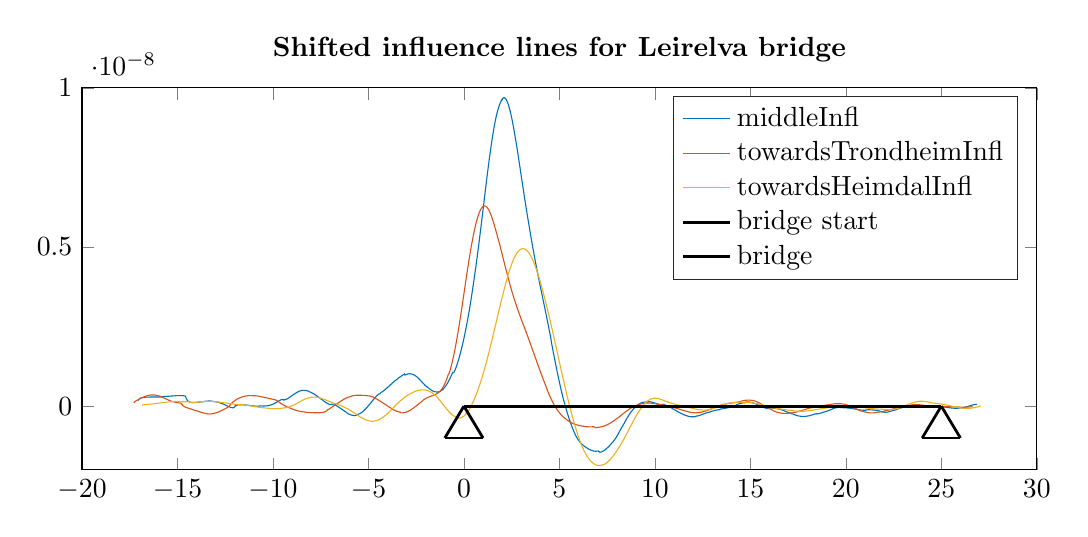
\begin{tikzpicture}

  \begin{axis}[%
    width=\textwidth,
    height=0.4\textwidth,
    at={(0\figurewidth,0\figureheight)},
    scale only axis,
    xmin=-20,
    xmax=30,
    ymin=-2e-09,
    ymax=1e-08,
    axis background/.style={fill=white},
    title style={font=\bfseries},
    title={Shifted influence lines for Leirelva bridge},
    legend style={legend cell align=left,align=left,draw=white!15!black}
    ]
    \addplot [color=mycolor1,solid]
    table[row sep=crcr]{%
    -17.056943359375	1.77103657345186e-10\\
    -17.0367939453125	1.98431512551098e-10\\
    -17.01664453125	2.17935326476639e-10\\
    -16.9964951171875	2.33559154990141e-10\\
    -16.976345703125	2.39479915243334e-10\\
    -16.9561962890625	2.45807621083757e-10\\
    -16.936046875	2.51568358117054e-10\\
    -16.9158974609375	2.56482947507223e-10\\
    -16.895748046875	2.60390650851758e-10\\
    -16.8755986328125	2.63802918444592e-10\\
    -16.85544921875	2.66656390655684e-10\\
    -16.8352998046875	2.69055234560324e-10\\
    -16.815150390625	2.711925611975e-10\\
    -16.7950009765625	2.73144643305113e-10\\
    -16.7748515625	2.74871150291776e-10\\
    -16.7547021484375	2.76415637282579e-10\\
    -16.734552734375	2.77791477511265e-10\\
    -16.7144033203125	2.78991001362234e-10\\
    -16.69425390625	2.80046397922704e-10\\
    -16.6741044921875	2.80968066176119e-10\\
    -16.653955078125	2.81769055788074e-10\\
    -16.6338056640625	2.82462723214015e-10\\
    -16.61365625	2.83056069629289e-10\\
    -16.5935068359375	2.83557710551259e-10\\
    -16.573357421875	2.83957755008481e-10\\
    -16.5532080078125	2.84264758293489e-10\\
    -16.53305859375	2.8449127042832e-10\\
    -16.5129091796875	2.84616192224891e-10\\
    -16.492759765625	2.84729836762522e-10\\
    -16.4726103515625	2.84919136846051e-10\\
    -16.4524609375	2.85013499245133e-10\\
    -16.4323115234375	2.85135253590747e-10\\
    -16.412162109375	2.85433168298819e-10\\
    -16.3920126953125	2.85088319502833e-10\\
    -16.37186328125	2.84699774550249e-10\\
    -16.3517138671875	2.86865273158259e-10\\
    -16.331564453125	2.86495338050955e-10\\
    -16.3114150390625	2.86399570532485e-10\\
    -16.291265625	2.84905091131999e-10\\
    -16.2711162109375	2.850000850938e-10\\
    -16.250966796875	2.85143851016343e-10\\
    -16.2308173828125	2.861015244248e-10\\
    -16.21066796875	2.86123157356623e-10\\
    -16.1905185546875	2.86161790826917e-10\\
    -16.170369140625	2.86437364718379e-10\\
    -16.1502197265625	2.86303655120751e-10\\
    -16.1300703125	2.86212517517485e-10\\
    -16.1099208984375	2.86110628639435e-10\\
    -16.089771484375	2.85961581259529e-10\\
    -16.0696220703125	2.85874239820494e-10\\
    -16.04947265625	2.85865171788661e-10\\
    -16.0293232421875	2.85846453900283e-10\\
    -16.009173828125	2.85991995427133e-10\\
    -15.9890244140625	2.86280868330896e-10\\
    -15.968875	2.86604921637445e-10\\
    -15.9487255859375	2.86887706130579e-10\\
    -15.928576171875	2.8738467479374e-10\\
    -15.9084267578125	2.87755141082823e-10\\
    -15.88827734375	2.88487518317757e-10\\
    -15.8681279296875	2.892334567562e-10\\
    -15.847978515625	2.91198704317926e-10\\
    -15.8278291015625	2.92196984965331e-10\\
    -15.8076796875	2.95876411198165e-10\\
    -15.7875302734375	2.95653112710623e-10\\
    -15.767380859375	2.97063275913134e-10\\
    -15.7472314453125	2.99156897942125e-10\\
    -15.72708203125	3.00495541270618e-10\\
    -15.7069326171875	3.02794708149933e-10\\
    -15.686783203125	3.04190150701208e-10\\
    -15.6666337890625	3.04925020640342e-10\\
    -15.646484375	3.05599678937149e-10\\
    -15.6263349609375	3.06130956269413e-10\\
    -15.606185546875	3.0644799785745e-10\\
    -15.5860361328125	3.06980192000645e-10\\
    -15.56588671875	3.07543511668122e-10\\
    -15.5457373046875	3.08112659320216e-10\\
    -15.525587890625	3.08780784570792e-10\\
    -15.5054384765625	3.09474315688069e-10\\
    -15.4852890625	3.10162368782148e-10\\
    -15.4651396484375	3.10889073534155e-10\\
    -15.444990234375	3.11645170930161e-10\\
    -15.4248408203125	3.12424283487578e-10\\
    -15.40469140625	3.13233441637647e-10\\
    -15.3845419921875	3.14066758523794e-10\\
    -15.364392578125	3.14916383692239e-10\\
    -15.3442431640625	3.15769354667764e-10\\
    -15.32409375	3.16623621308505e-10\\
    -15.3039443359375	3.17481250558069e-10\\
    -15.283794921875	3.18320682799043e-10\\
    -15.2636455078125	3.19151100022946e-10\\
    -15.24349609375	3.20052838113103e-10\\
    -15.2233466796875	3.2091740266773e-10\\
    -15.203197265625	3.2172011309278e-10\\
    -15.1830478515625	3.22779188363616e-10\\
    -15.1628984375	3.23407346230257e-10\\
    -15.1427490234375	3.24056432984223e-10\\
    -15.122599609375	3.25229976199621e-10\\
    -15.1024501953125	3.25763882136053e-10\\
    -15.08230078125	3.2722622767116e-10\\
    -15.0621513671875	3.28130066880606e-10\\
    -15.042001953125	3.28468556581056e-10\\
    -15.0218525390625	3.27842380114658e-10\\
    -15.001703125	3.28269135425798e-10\\
    -14.9815537109375	3.28093931007177e-10\\
    -14.961404296875	3.28180248722899e-10\\
    -14.9412548828125	3.28753829629848e-10\\
    -14.92110546875	3.29376938163896e-10\\
    -14.9009560546875	3.29987923782788e-10\\
    -14.880806640625	3.30314118638274e-10\\
    -14.8606572265625	3.30542234611029e-10\\
    -14.8405078125	3.30663999142476e-10\\
    -14.8203583984375	3.3065675515401e-10\\
    -14.800208984375	3.30585131581893e-10\\
    -14.7800595703125	3.30403817187452e-10\\
    -14.75991015625	3.30096536203839e-10\\
    -14.7397607421875	3.29602144119912e-10\\
    -14.719611328125	3.28831903351515e-10\\
    -14.6994619140625	3.27593003891371e-10\\
    -14.6793125	3.25990394120416e-10\\
    -14.6591630859375	3.23246620656501e-10\\
    -14.639013671875	3.21279785991209e-10\\
    -14.6188642578125	3.18204061549206e-10\\
    -14.59871484375	3.10301038667289e-10\\
    -14.5785654296875	3.08691657159112e-10\\
    -14.558416015625	2.76278179464782e-10\\
    -14.5382666015625	2.36586910764427e-10\\
    -14.5181171875	2.30998826970128e-10\\
    -14.4979677734375	1.90467350562758e-10\\
    -14.477818359375	1.73096292051145e-10\\
    -14.4576689453125	1.65206402991266e-10\\
    -14.43751953125	1.5570111937071e-10\\
    -14.4173701171875	1.46868352655702e-10\\
    -14.397220703125	1.39972003336858e-10\\
    -14.3770712890625	1.34064533504332e-10\\
    -14.356921875	1.29320482325923e-10\\
    -14.3367724609375	1.25571490877088e-10\\
    -14.316623046875	1.22780174452792e-10\\
    -14.2964736328125	1.20318231286582e-10\\
    -14.27632421875	1.18279775077246e-10\\
    -14.2561748046875	1.16664438986331e-10\\
    -14.236025390625	1.15321894597999e-10\\
    -14.2158759765625	1.14329306331675e-10\\
    -14.1957265625	1.13636655204323e-10\\
    -14.1755771484375	1.13208455958259e-10\\
    -14.155427734375	1.13027294502212e-10\\
    -14.1352783203125	1.13062669689238e-10\\
    -14.11512890625	1.13300803592251e-10\\
    -14.0949794921875	1.13724481639609e-10\\
    -14.074830078125	1.14327003299161e-10\\
    -14.0546806640625	1.15110241080877e-10\\
    -14.03453125	1.16056982468165e-10\\
    -14.0143818359375	1.17175730736533e-10\\
    -13.994232421875	1.18448458023335e-10\\
    -13.9740830078125	1.19794505034682e-10\\
    -13.95393359375	1.21229934978471e-10\\
    -13.9337841796875	1.2276038559849e-10\\
    -13.913634765625	1.24221008848223e-10\\
    -13.8934853515625	1.26028774703517e-10\\
    -13.8733359375	1.28101228696528e-10\\
    -13.8531865234375	1.29597957072415e-10\\
    -13.833037109375	1.3166946630119e-10\\
    -13.8128876953125	1.32319054829845e-10\\
    -13.79273828125	1.3075473349261e-10\\
    -13.7725888671875	1.32793918028913e-10\\
    -13.752439453125	1.36281804474916e-10\\
    -13.7322900390625	1.34037017251035e-10\\
    -13.712140625	1.35845929787959e-10\\
    -13.6919912109375	1.38241390169171e-10\\
    -13.671841796875	1.39065091229573e-10\\
    -13.6516923828125	1.40766051296024e-10\\
    -13.63154296875	1.42716852148776e-10\\
    -13.6113935546875	1.44577285017484e-10\\
    -13.591244140625	1.46461594991819e-10\\
    -13.5710947265625	1.48357335944789e-10\\
    -13.5509453125	1.50078701467935e-10\\
    -13.5307958984375	1.51743956259235e-10\\
    -13.510646484375	1.53286779716681e-10\\
    -13.4904970703125	1.54632308416136e-10\\
    -13.47034765625	1.55811036155924e-10\\
    -13.4501982421875	1.56912466593634e-10\\
    -13.430048828125	1.57931645225911e-10\\
    -13.4098994140625	1.58663380695531e-10\\
    -13.38975	1.59594401453692e-10\\
    -13.3696005859375	1.60408303550708e-10\\
    -13.349451171875	1.60114788079153e-10\\
    -13.3293017578125	1.61000488106697e-10\\
    -13.30915234375	1.6101273761478e-10\\
    -13.2890029296875	1.58747694153494e-10\\
    -13.268853515625	1.60880235556621e-10\\
    -13.2487041015625	1.57497309106253e-10\\
    -13.2285546875	1.57143155459363e-10\\
    -13.2084052734375	1.54539647774736e-10\\
    -13.188255859375	1.52718746222917e-10\\
    -13.1681064453125	1.49829287914668e-10\\
    -13.14795703125	1.47509471676017e-10\\
    -13.1278076171875	1.45608991956371e-10\\
    -13.107658203125	1.44237542562109e-10\\
    -13.0875087890625	1.43258722416056e-10\\
    -13.067359375	1.4196486819359e-10\\
    -13.0472099609375	1.40692943094114e-10\\
    -13.027060546875	1.39147463695725e-10\\
    -13.0069111328125	1.37343976513969e-10\\
    -12.98676171875	1.35406598908041e-10\\
    -12.9666123046875	1.33274719996675e-10\\
    -12.946462890625	1.3093222291924e-10\\
    -12.9263134765625	1.28396454997534e-10\\
    -12.9061640625	1.25647597781242e-10\\
    -12.8860146484375	1.22686949091757e-10\\
    -12.865865234375	1.19520425759768e-10\\
    -12.8457158203125	1.16162627641562e-10\\
    -12.82556640625	1.12626047574391e-10\\
    -12.8054169921875	1.08917409102712e-10\\
    -12.785267578125	1.0504490632135e-10\\
    -12.7651181640625	1.01036939787596e-10\\
    -12.74496875	9.68681771083595e-11\\
    -12.7248193359375	9.25087284017637e-11\\
    -12.704669921875	8.80850723884345e-11\\
    -12.6845205078125	8.3481712715199e-11\\
    -12.66437109375	7.86892423248791e-11\\
    -12.6442216796875	7.41353619566681e-11\\
    -12.624072265625	6.93984261763095e-11\\
    -12.6039228515625	6.42425163829653e-11\\
    -12.5837734375	5.94100042626587e-11\\
    -12.5636240234375	5.38089815794453e-11\\
    -12.543474609375	4.77049025585403e-11\\
    -12.5233251953125	4.27564133137354e-11\\
    -12.50317578125	3.79700339595548e-11\\
    -12.4830263671875	3.20357889971942e-11\\
    -12.462876953125	2.67379812188992e-11\\
    -12.4427275390625	2.04771473371602e-11\\
    -12.422578125	1.37923856942025e-11\\
    -12.4024287109375	7.38556069313991e-12\\
    -12.382279296875	1.57113468123635e-12\\
    -12.3621298828125	-4.07794334617332e-12\\
    -12.34198046875	-9.43200297957431e-12\\
    -12.3218310546875	-1.45757997372117e-11\\
    -12.301681640625	-1.95713797702735e-11\\
    -12.2815322265625	-2.43845269257379e-11\\
    -12.2613828125	-2.90240194888653e-11\\
    -12.2412333984375	-3.34451580628531e-11\\
    -12.221083984375	-3.75709115251491e-11\\
    -12.2009345703125	-4.12266554290372e-11\\
    -12.18078515625	-4.45587432559791e-11\\
    -12.1606357421875	-4.69931937918338e-11\\
    -12.140486328125	-4.89431570977513e-11\\
    -12.1203369140625	-5.11544643431123e-11\\
    -12.1001875	-5.05508257662493e-11\\
    -12.0800380859375	-5.08752325431497e-11\\
    -12.059888671875	-4.83030451293328e-11\\
    -12.0397392578125	-3.65104937352893e-11\\
    -12.01958984375	-2.47018352196994e-11\\
    -11.9994404296875	-1.3073931558882e-11\\
    -11.979291015625	8.81851533906939e-12\\
    -11.9591416015625	1.69602786066033e-11\\
    -11.9389921875	8.42421560614296e-12\\
    -11.9188427734375	1.72136634960683e-11\\
    -11.898693359375	2.37159013144962e-11\\
    -11.8785439453125	2.98162084107833e-11\\
    -11.85839453125	3.3984039245285e-11\\
    -11.8382451171875	3.81045204114279e-11\\
    -11.818095703125	4.00146806662668e-11\\
    -11.7979462890625	4.13131206294532e-11\\
    -11.777796875	4.25766708712177e-11\\
    -11.7576474609375	4.32710767790441e-11\\
    -11.737498046875	4.38000827892067e-11\\
    -11.7173486328125	4.41248331132374e-11\\
    -11.69719921875	4.41949708208256e-11\\
    -11.6770498046875	4.40561453447444e-11\\
    -11.656900390625	4.3756550825632e-11\\
    -11.6367509765625	4.33280054294899e-11\\
    -11.6166015625	4.2797706706773e-11\\
    -11.5964521484375	4.21895421180372e-11\\
    -11.576302734375	4.15197279405572e-11\\
    -11.5561533203125	4.07893852871463e-11\\
    -11.53600390625	4.00038383900686e-11\\
    -11.5158544921875	3.91692108296765e-11\\
    -11.495705078125	3.82734390226899e-11\\
    -11.4755556640625	3.73415284718625e-11\\
    -11.45540625	3.63944951380146e-11\\
    -11.4352568359375	3.54136319108253e-11\\
    -11.415107421875	3.44834452396575e-11\\
    -11.3949580078125	3.34640486714393e-11\\
    -11.37480859375	3.23560433711347e-11\\
    -11.3546591796875	3.11358450818185e-11\\
    -11.334509765625	2.95123229523047e-11\\
    -11.3143603515625	2.83169513620511e-11\\
    -11.2942109375	2.69063158670112e-11\\
    -11.2740615234375	2.51926115805263e-11\\
    -11.253912109375	2.46722813465968e-11\\
    -11.2337626953125	1.98545224945438e-11\\
    -11.21361328125	1.81813569220802e-11\\
    -11.1934638671875	1.40203633165764e-11\\
    -11.173314453125	1.47913761113593e-11\\
    -11.1531650390625	1.41943651652548e-11\\
    -11.133015625	1.28497892773718e-11\\
    -11.1128662109375	1.11113642497137e-11\\
    -11.092716796875	1.00219556942678e-11\\
    -11.0725673828125	8.53811043191476e-12\\
    -11.05241796875	7.27992794952068e-12\\
    -11.0322685546875	6.0922662534927e-12\\
    -11.012119140625	4.98280087821813e-12\\
    -10.9919697265625	3.94360778707981e-12\\
    -10.9718203125	3.01176172708786e-12\\
    -10.9516708984375	2.15758091071539e-12\\
    -10.931521484375	1.23184393495539e-12\\
    -10.9113720703125	4.40447231928027e-13\\
    -10.89122265625	-4.22881720305084e-13\\
    -10.8710732421875	-1.51033498955159e-12\\
    -10.850923828125	-2.77254837722403e-12\\
    -10.8307744140625	-3.2570492544521e-12\\
    -10.810625	-4.77888619942717e-12\\
    -10.7904755859375	-4.2990808382114e-12\\
    -10.770326171875	-1.37981314205887e-12\\
    -10.7501767578125	-1.25099245237846e-12\\
    -10.73002734375	1.67019299118017e-12\\
    -10.7098779296875	3.82404017479309e-12\\
    -10.689728515625	3.27569257313873e-12\\
    -10.6695791015625	4.88974909940024e-12\\
    -10.6494296875	5.76456345366568e-12\\
    -10.6292802734375	6.67140493277347e-12\\
    -10.609130859375	7.19433456981488e-12\\
    -10.5889814453125	6.55018183119846e-12\\
    -10.56883203125	6.04436898746621e-12\\
    -10.5486826171875	5.47821939254313e-12\\
    -10.528533203125	4.93604481076772e-12\\
    -10.5083837890625	4.69242065600187e-12\\
    -10.488234375	4.64022580062436e-12\\
    -10.4680849609375	4.67262133368734e-12\\
    -10.447935546875	4.8558022611272e-12\\
    -10.4277861328125	5.18153423850715e-12\\
    -10.40763671875	5.66719062102073e-12\\
    -10.3874873046875	6.34040651742597e-12\\
    -10.367337890625	7.23112234677372e-12\\
    -10.3471884765625	8.33025837065145e-12\\
    -10.3270390625	9.63314632709738e-12\\
    -10.3068896484375	1.11418052118808e-11\\
    -10.286740234375	1.28552659857375e-11\\
    -10.2665908203125	1.47689060668164e-11\\
    -10.24644140625	1.68738813812548e-11\\
    -10.2262919921875	1.92133808400953e-11\\
    -10.206142578125	2.17688269725949e-11\\
    -10.1859931640625	2.45070644657174e-11\\
    -10.16584375	2.75242164498135e-11\\
    -10.1456943359375	3.07121578671223e-11\\
    -10.125544921875	3.3935645292217e-11\\
    -10.1053955078125	3.73744352489542e-11\\
    -10.08524609375	4.11743451130512e-11\\
    -10.0650966796875	4.50741361105939e-11\\
    -10.044947265625	4.95176402479537e-11\\
    -10.0247978515625	5.56393411133252e-11\\
    -10.0046484375	6.04063167730427e-11\\
    -9.9844990234375	6.51760795321987e-11\\
    -9.964349609375	7.09485605249038e-11\\
    -9.9442001953125	7.53983864971999e-11\\
    -9.92405078125	8.19879229248966e-11\\
    -9.9039013671875	8.91913009702562e-11\\
    -9.883751953125	9.60740571787288e-11\\
    -9.8636025390625	1.03020641946356e-10\\
    -9.843453125	1.09971220982898e-10\\
    -9.8233037109375	1.16793257536035e-10\\
    -9.803154296875	1.23594596633646e-10\\
    -9.7830048828125	1.30503332085211e-10\\
    -9.76285546875	1.37552609765465e-10\\
    -9.7427060546875	1.44724734245908e-10\\
    -9.722556640625	1.51961985394355e-10\\
    -9.7024072265625	1.59143988659854e-10\\
    -9.6822578125	1.66296192862691e-10\\
    -9.6621083984375	1.73251115593869e-10\\
    -9.641958984375	1.79773316699288e-10\\
    -9.6218095703125	1.86408434992838e-10\\
    -9.60166015625	1.92491891824823e-10\\
    -9.5815107421875	1.98054676698619e-10\\
    -9.561361328125	2.0391137533465e-10\\
    -9.5412119140625	2.07764820650349e-10\\
    -9.5210625	2.08120579214917e-10\\
    -9.5009130859375	2.07813108269743e-10\\
    -9.480763671875	2.03056636261263e-10\\
    -9.4606142578125	1.97491992201938e-10\\
    -9.44046484375	1.89065532899285e-10\\
    -9.4203154296875	1.98425165932629e-10\\
    -9.400166015625	2.09888552842297e-10\\
    -9.3800166015625	2.02948096987255e-10\\
    -9.3598671875	2.06334291982062e-10\\
    -9.3397177734375	2.07002815446604e-10\\
    -9.319568359375	2.09477971275159e-10\\
    -9.2994189453125	2.1505692926274e-10\\
    -9.27926953125	2.20705538504962e-10\\
    -9.2591201171875	2.26947700920397e-10\\
    -9.238970703125	2.3379530566407e-10\\
    -9.2188212890625	2.40929044444207e-10\\
    -9.198671875	2.48298194438849e-10\\
    -9.1785224609375	2.56094692679678e-10\\
    -9.158373046875	2.64192429448599e-10\\
    -9.1382236328125	2.72524600882046e-10\\
    -9.11807421875	2.81040365479397e-10\\
    -9.0979248046875	2.89682336947165e-10\\
    -9.077775390625	2.98394232182076e-10\\
    -9.0576259765625	3.07139067253648e-10\\
    -9.0374765625	3.1589836288177e-10\\
    -9.0173271484375	3.24637704053545e-10\\
    -8.997177734375	3.33338304435287e-10\\
    -8.9770283203125	3.4197702225302e-10\\
    -8.95687890625	3.50524226970373e-10\\
    -8.9367294921875	3.58954046049461e-10\\
    -8.916580078125	3.67217693429315e-10\\
    -8.8964306640625	3.75323968846474e-10\\
    -8.87628125	3.83257537706131e-10\\
    -8.8561318359375	3.91027304870641e-10\\
    -8.835982421875	3.98814793126717e-10\\
    -8.8158330078125	4.06437531404898e-10\\
    -8.79568359375	4.13888214399999e-10\\
    -8.7755341796875	4.21201859186877e-10\\
    -8.755384765625	4.27718588903112e-10\\
    -8.7352353515625	4.34500624832706e-10\\
    -8.7150859375	4.4162766578776e-10\\
    -8.6949365234375	4.47852941979157e-10\\
    -8.674787109375	4.55986031487934e-10\\
    -8.6546376953125	4.59762053557592e-10\\
    -8.63448828125	4.64474627299681e-10\\
    -8.6143388671875	4.71284967589528e-10\\
    -8.594189453125	4.75191669733436e-10\\
    -8.5740400390625	4.79466039506686e-10\\
    -8.553890625	4.8282474669769e-10\\
    -8.5337412109375	4.85874964952511e-10\\
    -8.513591796875	4.88341829913155e-10\\
    -8.4934423828125	4.90270838468129e-10\\
    -8.47329296875	4.91868618342459e-10\\
    -8.4531435546875	4.92908669365918e-10\\
    -8.432994140625	4.9357244513912e-10\\
    -8.4128447265625	4.93876124057701e-10\\
    -8.3926953125	4.9376170837873e-10\\
    -8.3725458984375	4.93276835927301e-10\\
    -8.352396484375	4.93002773627078e-10\\
    -8.3322470703125	4.91872149374515e-10\\
    -8.31209765625	4.9063784645169e-10\\
    -8.2919482421875	4.89664722299928e-10\\
    -8.271798828125	4.8683197864289e-10\\
    -8.2516494140625	4.85071887407927e-10\\
    -8.2315	4.83147940626351e-10\\
    -8.2113505859375	4.7919477364348e-10\\
    -8.191201171875	4.78446385956845e-10\\
    -8.1710517578125	4.73981743208347e-10\\
    -8.15090234375	4.71004804030977e-10\\
    -8.1307529296875	4.65073398049698e-10\\
    -8.110603515625	4.5810959440072e-10\\
    -8.0904541015625	4.51681677948831e-10\\
    -8.0703046875	4.46369779040529e-10\\
    -8.0501552734375	4.4142010132157e-10\\
    -8.030005859375	4.36486714310636e-10\\
    -8.0098564453125	4.31164708557705e-10\\
    -7.98970703125	4.25421329082558e-10\\
    -7.9695576171875	4.19289916662938e-10\\
    -7.949408203125	4.12928360061153e-10\\
    -7.9292587890625	4.06407779937322e-10\\
    -7.909109375	3.99662939164831e-10\\
    -7.8889599609375	3.92738127755778e-10\\
    -7.868810546875	3.85583051971764e-10\\
    -7.8486611328125	3.7817409708589e-10\\
    -7.82851171875	3.70557409250964e-10\\
    -7.8083623046875	3.62743270652179e-10\\
    -7.788212890625	3.54752635725633e-10\\
    -7.7680634765625	3.46606365063006e-10\\
    -7.7479140625	3.3832736258462e-10\\
    -7.7277646484375	3.29922792820021e-10\\
    -7.707615234375	3.21391526460501e-10\\
    -7.6874658203125	3.1276711607514e-10\\
    -7.66731640625	3.04056836681111e-10\\
    -7.6471669921875	2.95256639170643e-10\\
    -7.627017578125	2.86439681480352e-10\\
    -7.6068681640625	2.77717780837178e-10\\
    -7.58671875	2.69028787611028e-10\\
    -7.5665693359375	2.60270745971334e-10\\
    -7.546419921875	2.51875035759656e-10\\
    -7.5262705078125	2.43372466798096e-10\\
    -7.50612109375	2.33844939188079e-10\\
    -7.4859716796875	2.26031299561265e-10\\
    -7.465822265625	2.16758376173157e-10\\
    -7.4456728515625	2.07467795652193e-10\\
    -7.4255234375	2.00522064329423e-10\\
    -7.4053740234375	1.90972927027274e-10\\
    -7.385224609375	1.81362728238269e-10\\
    -7.3650751953125	1.72187865062031e-10\\
    -7.34492578125	1.63099373421022e-10\\
    -7.3247763671875	1.54214011701189e-10\\
    -7.304626953125	1.45906657448158e-10\\
    -7.2844775390625	1.37601379664735e-10\\
    -7.264328125	1.2948949918769e-10\\
    -7.2441787109375	1.21346072857503e-10\\
    -7.224029296875	1.13276431838972e-10\\
    -7.2038798828125	1.05414876122401e-10\\
    -7.18373046875	9.77450281587428e-11\\
    -7.1635810546875	9.03272906532661e-11\\
    -7.143431640625	8.33593052014718e-11\\
    -7.1232822265625	7.67252479277055e-11\\
    -7.1031328125	7.0460005558718e-11\\
    -7.0829833984375	6.47456137785205e-11\\
    -7.062833984375	5.9295283757471e-11\\
    -7.0426845703125	5.44522236916985e-11\\
    -7.02253515625	5.09658843299143e-11\\
    -7.0023857421875	4.88510043784206e-11\\
    -6.982236328125	5.00015773042776e-11\\
    -6.9620869140625	5.19615536178991e-11\\
    -6.9419375	5.71721647747028e-11\\
    -6.9217880859375	6.11603007252254e-11\\
    -6.901638671875	6.19959345991794e-11\\
    -6.8814892578125	4.53774266613192e-11\\
    -6.86133984375	4.60738208525051e-11\\
    -6.8411904296875	3.92299511387101e-11\\
    -6.821041015625	4.02243948257057e-11\\
    -6.8008916015625	3.89243765217359e-11\\
    -6.7807421875	3.48179889623457e-11\\
    -6.7605927734375	3.10433039546242e-11\\
    -6.740443359375	2.66198107260716e-11\\
    -6.7202939453125	2.13512011795029e-11\\
    -6.70014453125	1.62498437585627e-11\\
    -6.6799951171875	1.06850674096561e-11\\
    -6.659845703125	4.64517081347802e-12\\
    -6.6396962890625	-1.82553958125673e-12\\
    -6.619546875	-8.64871455723173e-12\\
    -6.5993974609375	-1.57940004367585e-11\\
    -6.579248046875	-2.32147314416343e-11\\
    -6.5590986328125	-3.08197618399842e-11\\
    -6.53894921875	-3.8613456891179e-11\\
    -6.5187998046875	-4.65696946663345e-11\\
    -6.498650390625	-5.46604741082513e-11\\
    -6.4785009765625	-6.2871368986074e-11\\
    -6.4583515625	-7.11803517599165e-11\\
    -6.4382021484375	-7.95637969443124e-11\\
    -6.418052734375	-8.79837725385921e-11\\
    -6.3979033203125	-9.64225414641813e-11\\
    -6.37775390625	-1.04854714621394e-10\\
    -6.3576044921875	-1.13248638092609e-10\\
    -6.337455078125	-1.21672017556054e-10\\
    -6.3173056640625	-1.30109661079725e-10\\
    -6.29715625	-1.38587766409746e-10\\
    -6.2770068359375	-1.47078752545059e-10\\
    -6.256857421875	-1.55417936516064e-10\\
    -6.2367080078125	-1.63364398817887e-10\\
    -6.21655859375	-1.71494991531068e-10\\
    -6.1964091796875	-1.78795469056474e-10\\
    -6.176259765625	-1.87448156596734e-10\\
    -6.1561103515625	-1.97164857023768e-10\\
    -6.1359609375	-2.06170099926681e-10\\
    -6.1158115234375	-2.19487196916833e-10\\
    -6.095662109375	-2.27125561323281e-10\\
    -6.0755126953125	-2.34979952375143e-10\\
    -6.05536328125	-2.40976007954606e-10\\
    -6.0352138671875	-2.47486745082482e-10\\
    -6.015064453125	-2.53508625357104e-10\\
    -5.9949150390625	-2.58664778214702e-10\\
    -5.974765625	-2.6383176442286e-10\\
    -5.9546162109375	-2.68470582499427e-10\\
    -5.934466796875	-2.72682978094891e-10\\
    -5.9143173828125	-2.7653238402349e-10\\
    -5.89416796875	-2.8003353464571e-10\\
    -5.8740185546875	-2.83027341790236e-10\\
    -5.853869140625	-2.85928692211966e-10\\
    -5.8337197265625	-2.88477195212305e-10\\
    -5.8135703125	-2.90615951670109e-10\\
    -5.7934208984375	-2.92907796577469e-10\\
    -5.773271484375	-2.94647111885682e-10\\
    -5.7531220703125	-2.96312910031355e-10\\
    -5.73297265625	-2.96716015159605e-10\\
    -5.7128232421875	-2.99207902275778e-10\\
    -5.692673828125	-2.96368799239061e-10\\
    -5.6725244140625	-2.93867487844774e-10\\
    -5.652375	-2.86999037799478e-10\\
    -5.6322255859375	-2.87297097413545e-10\\
    -5.612076171875	-2.76906643003018e-10\\
    -5.5919267578125	-2.67852910631496e-10\\
    -5.57177734375	-2.63018368356133e-10\\
    -5.5516279296875	-2.57716311468164e-10\\
    -5.531478515625	-2.54337110735665e-10\\
    -5.5113291015625	-2.50191471975329e-10\\
    -5.4911796875	-2.45553308753191e-10\\
    -5.4710302734375	-2.40095324572539e-10\\
    -5.450880859375	-2.33769241468742e-10\\
    -5.4307314453125	-2.27090588303319e-10\\
    -5.41058203125	-2.1991920466769e-10\\
    -5.3904326171875	-2.12316317823694e-10\\
    -5.370283203125	-2.04311181497155e-10\\
    -5.3501337890625	-1.95764360356855e-10\\
    -5.329984375	-1.86714783131787e-10\\
    -5.3098349609375	-1.77170979377034e-10\\
    -5.289685546875	-1.67150990399393e-10\\
    -5.2695361328125	-1.56684964867581e-10\\
    -5.24938671875	-1.45795533732908e-10\\
    -5.2292373046875	-1.34501306481851e-10\\
    -5.209087890625	-1.22811403443328e-10\\
    -5.1889384765625	-1.10738223544879e-10\\
    -5.1687890625	-9.83060100292347e-11\\
    -5.1486396484375	-8.55292702731098e-11\\
    -5.128490234375	-7.24244097428958e-11\\
    -5.1083408203125	-5.90556952162036e-11\\
    -5.08819140625	-4.55017757574713e-11\\
    -5.0680419921875	-3.17490222926388e-11\\
    -5.047892578125	-1.77990772884625e-11\\
    -5.0277431640625	-3.97160073715058e-12\\
    -5.00759375	1.02300894443355e-11\\
    -4.9874443359375	2.50668837106355e-11\\
    -4.967294921875	3.85494470869169e-11\\
    -4.9471455078125	5.26098139204282e-11\\
    -4.92699609375	6.63686988237586e-11\\
    -4.9068466796875	7.73589893042081e-11\\
    -4.886697265625	9.20455582445712e-11\\
    -4.8665478515625	1.07029280065802e-10\\
    -4.8463984375	1.23232004055313e-10\\
    -4.8262490234375	1.39053375610893e-10\\
    -4.806099609375	1.5446638117612e-10\\
    -4.7859501953125	1.69904210721431e-10\\
    -4.76580078125	1.84589033779472e-10\\
    -4.7456513671875	1.99314324151829e-10\\
    -4.725501953125	2.14153061026402e-10\\
    -4.7053525390625	2.28823736146699e-10\\
    -4.685203125	2.433869653798e-10\\
    -4.6650537109375	2.57771933162106e-10\\
    -4.644904296875	2.71833533181054e-10\\
    -4.6247548828125	2.85551888987191e-10\\
    -4.60460546875	2.98918121260632e-10\\
    -4.5844560546875	3.11828935561858e-10\\
    -4.564306640625	3.24352377626281e-10\\
    -4.5441572265625	3.36369857118112e-10\\
    -4.5240078125	3.47839265772705e-10\\
    -4.5038583984375	3.58525339315501e-10\\
    -4.483708984375	3.67695987011535e-10\\
    -4.4635595703125	3.75139956947935e-10\\
    -4.44341015625	3.81334209765746e-10\\
    -4.4232607421875	3.86086744282842e-10\\
    -4.403111328125	3.89467459073885e-10\\
    -4.3829619140625	4.00231166501678e-10\\
    -4.3628125	4.15361898028525e-10\\
    -4.3426630859375	4.22803110458967e-10\\
    -4.322513671875	4.3912697140035e-10\\
    -4.3023642578125	4.4241721032234e-10\\
    -4.28221484375	4.478482340117e-10\\
    -4.2620654296875	4.58308846583108e-10\\
    -4.241916015625	4.66349729164185e-10\\
    -4.2217666015625	4.76052076228509e-10\\
    -4.2016171875	4.85395087532026e-10\\
    -4.1814677734375	4.94632340546704e-10\\
    -4.161318359375	5.03927395469915e-10\\
    -4.1411689453125	5.13652996133933e-10\\
    -4.12101953125	5.23639301202577e-10\\
    -4.1008701171875	5.33783999292169e-10\\
    -4.080720703125	5.44219896957788e-10\\
    -4.0605712890625	5.54776151129985e-10\\
    -4.040421875	5.6541831524628e-10\\
    -4.0202724609375	5.76175594463196e-10\\
    -4.000123046875	5.87017524805255e-10\\
    -3.9799736328125	5.97928592590261e-10\\
    -3.95982421875	6.08909109463341e-10\\
    -3.9396748046875	6.19942626958524e-10\\
    -3.919525390625	6.31008538321162e-10\\
    -3.8993759765625	6.42090930975257e-10\\
    -3.8792265625	6.53178266695193e-10\\
    -3.8590771484375	6.64245366827126e-10\\
    -3.838927734375	6.75290904102326e-10\\
    -3.8187783203125	6.86342382906648e-10\\
    -3.79862890625	6.97378803278663e-10\\
    -3.7784794921875	7.08470205682965e-10\\
    -3.758330078125	7.19524928332745e-10\\
    -3.7381806640625	7.30454897435799e-10\\
    -3.71803125	7.41396182356873e-10\\
    -3.6978818359375	7.51594562573523e-10\\
    -3.677732421875	7.62231402734859e-10\\
    -3.6575830078125	7.72984195467173e-10\\
    -3.63743359375	7.82809538706053e-10\\
    -3.6172841796875	7.94370829026759e-10\\
    -3.597134765625	8.02525927986797e-10\\
    -3.5769853515625	8.09983513787754e-10\\
    -3.5568359375	8.19089164217505e-10\\
    -3.5366865234375	8.29722510151367e-10\\
    -3.516537109375	8.4025900756045e-10\\
    -3.4963876953125	8.49392227102367e-10\\
    -3.47623828125	8.59138589541107e-10\\
    -3.4560888671875	8.68660257076856e-10\\
    -3.435939453125	8.78043360011692e-10\\
    -3.4157900390625	8.87023666207876e-10\\
    -3.395640625	8.95961741179779e-10\\
    -3.3754912109375	9.0463226130812e-10\\
    -3.355341796875	9.13163779307784e-10\\
    -3.3351923828125	9.21633006818683e-10\\
    -3.31504296875	9.29986907731119e-10\\
    -3.2948935546875	9.38288471275226e-10\\
    -3.274744140625	9.46579448053472e-10\\
    -3.2545947265625	9.54909564915991e-10\\
    -3.2344453125	9.62498077702812e-10\\
    -3.2142958984375	9.70650377358322e-10\\
    -3.194146484375	9.77104122896888e-10\\
    -3.1739970703125	9.83969335610076e-10\\
    -3.15384765625	9.88323641761569e-10\\
    -3.1336982421875	9.99532031394602e-10\\
    -3.113548828125	1.00925072788448e-09\\
    -3.0933994140625	9.79952973902517e-10\\
    -3.07325	9.89815395417397e-10\\
    -3.0531005859375	9.83877476013905e-10\\
    -3.032951171875	9.89724918981828e-10\\
    -3.0128017578125	9.94540708036461e-10\\
    -2.99265234375	9.99969824053257e-10\\
    -2.9725029296875	1.00545192514336e-09\\
    -2.952353515625	1.00869140617011e-09\\
    -2.9322041015625	1.01150757742542e-09\\
    -2.9120546875	1.01344515921684e-09\\
    -2.8919052734375	1.01497090582359e-09\\
    -2.871755859375	1.01610611843267e-09\\
    -2.8516064453125	1.01672063159025e-09\\
    -2.83145703125	1.01677119638975e-09\\
    -2.8113076171875	1.01619505876219e-09\\
    -2.791158203125	1.01500211158042e-09\\
    -2.7710087890625	1.01322392514272e-09\\
    -2.750859375	1.01086766282707e-09\\
    -2.7307099609375	1.00795190478307e-09\\
    -2.710560546875	1.00448006784396e-09\\
    -2.6904111328125	1.00043787706909e-09\\
    -2.67026171875	9.9582848653703e-10\\
    -2.6501123046875	9.90654698456733e-10\\
    -2.629962890625	9.84916336906681e-10\\
    -2.6098134765625	9.78626234044432e-10\\
    -2.5896640625	9.71814224537475e-10\\
    -2.5695146484375	9.64538338533291e-10\\
    -2.549365234375	9.56755316206353e-10\\
    -2.5292158203125	9.48548557016735e-10\\
    -2.50906640625	9.39989357464594e-10\\
    -2.4889169921875	9.30650077441214e-10\\
    -2.468767578125	9.20877650217046e-10\\
    -2.4486181640625	9.10997598265017e-10\\
    -2.42846875	9.00376686738461e-10\\
    -2.4083193359375	8.89599752262783e-10\\
    -2.388169921875	8.79664203696899e-10\\
    -2.3680205078125	8.68613396383885e-10\\
    -2.34787109375	8.55226546122757e-10\\
    -2.3277216796875	8.418317078902e-10\\
    -2.307572265625	8.29893571642603e-10\\
    -2.2874228515625	8.15322898493952e-10\\
    -2.2672734375	8.02414846215896e-10\\
    -2.2471240234375	7.90519440523704e-10\\
    -2.226974609375	7.77658264684928e-10\\
    -2.2068251953125	7.64443094345417e-10\\
    -2.18667578125	7.51325117533097e-10\\
    -2.1665263671875	7.3786662429403e-10\\
    -2.146376953125	7.24501234846863e-10\\
    -2.1262275390625	7.11277032689301e-10\\
    -2.106078125	6.98169521679369e-10\\
    -2.0859287109375	6.85304372046058e-10\\
    -2.065779296875	6.72701889026709e-10\\
    -2.0456298828125	6.60367240054179e-10\\
    -2.02548046875	6.48407059941635e-10\\
    -2.0053310546875	6.36846992439222e-10\\
    -1.985181640625	6.25878670974778e-10\\
    -1.9650322265625	6.16147805145104e-10\\
    -1.9448828125	6.07650785657413e-10\\
    -1.9247333984375	5.99759162306315e-10\\
    -1.904583984375	5.94167784623987e-10\\
    -1.8844345703125	5.8754478758638e-10\\
    -1.86428515625	5.7804087461627e-10\\
    -1.8441357421875	5.66699178838929e-10\\
    -1.823986328125	5.57049693239014e-10\\
    -1.8038369140625	5.42392021424767e-10\\
    -1.7836875	5.33099602709555e-10\\
    -1.7635380859375	5.28157161440781e-10\\
    -1.743388671875	5.17293657755612e-10\\
    -1.7232392578125	5.08866627187244e-10\\
    -1.70308984375	5.00427351933832e-10\\
    -1.6829404296875	4.92741866298995e-10\\
    -1.662791015625	4.86426157204009e-10\\
    -1.6426416015625	4.80687632022862e-10\\
    -1.6224921875	4.75085370895979e-10\\
    -1.6023427734375	4.70034217236433e-10\\
    -1.582193359375	4.65229903757423e-10\\
    -1.5620439453125	4.60678709082763e-10\\
    -1.54189453125	4.56629539831813e-10\\
    -1.5217451171875	4.53075938346264e-10\\
    -1.501595703125	4.49994669515872e-10\\
    -1.4814462890625	4.4746630127593e-10\\
    -1.461296875	4.45488409158926e-10\\
    -1.4411474609375	4.44074577601059e-10\\
    -1.420998046875	4.43263622150885e-10\\
    -1.4008486328125	4.43082248058676e-10\\
    -1.38069921875	4.4355900951351e-10\\
    -1.3605498046875	4.44720970021678e-10\\
    -1.340400390625	4.46595997465325e-10\\
    -1.3202509765625	4.49197907744236e-10\\
    -1.3001015625	4.52538348123302e-10\\
    -1.2799521484375	4.56589936891274e-10\\
    -1.259802734375	4.61387340070771e-10\\
    -1.2396533203125	4.66943174639593e-10\\
    -1.21950390625	4.73222918293846e-10\\
    -1.1993544921875	4.80482901161199e-10\\
    -1.179205078125	4.88712152061035e-10\\
    -1.1590556640625	4.97650147780752e-10\\
    -1.13890625	5.076284162608e-10\\
    -1.1187568359375	5.17624472888073e-10\\
    -1.098607421875	5.29044255689454e-10\\
    -1.0784580078125	5.41103791124504e-10\\
    -1.05830859375	5.55705133625483e-10\\
    -1.0381591796875	5.68697137589642e-10\\
    -1.018009765625	5.8445375979754e-10\\
    -0.997860351562498	5.99893603690609e-10\\
    -0.977710937499999	6.15611289554371e-10\\
    -0.957561523437498	6.31939967206498e-10\\
    -0.937412109375	6.48687262337959e-10\\
    -0.917262695312498	6.66989057977732e-10\\
    -0.897113281249997	6.85956844066513e-10\\
    -0.876963867187499	7.05796690797175e-10\\
    -0.856814453124997	7.26489775483308e-10\\
    -0.836665039062499	7.47878571259407e-10\\
    -0.816515624999997	7.69942807135039e-10\\
    -0.796366210937499	7.92616573637719e-10\\
    -0.776216796874998	8.15906882853284e-10\\
    -0.7560673828125	8.3972078760574e-10\\
    -0.735917968749998	8.64272125942968e-10\\
    -0.7157685546875	8.89441772739262e-10\\
    -0.695619140624999	9.15895513170759e-10\\
    -0.675469726562497	9.42086000337037e-10\\
    -0.655320312499999	9.70606709196123e-10\\
    -0.635170898437497	9.97925378937574e-10\\
    -0.615021484374999	1.02225369752629e-09\\
    -0.594872070312498	1.05712914546292e-09\\
    -0.57472265625	1.06116026222686e-09\\
    -0.554573242187498	1.05486163539524e-09\\
    -0.534423828125	1.05710041980672e-09\\
    -0.514274414062498	1.07852366525284e-09\\
    -0.494124999999997	1.10123334203048e-09\\
    -0.473975585937499	1.12455796830427e-09\\
    -0.453826171874997	1.15305634419153e-09\\
    -0.433676757812499	1.18263732286904e-09\\
    -0.413527343749998	1.21529005645631e-09\\
    -0.3933779296875	1.24946406752047e-09\\
    -0.373228515624998	1.28463931495839e-09\\
    -0.3530791015625	1.32097536812502e-09\\
    -0.332929687499998	1.35835531996009e-09\\
    -0.312780273437497	1.3967848298735e-09\\
    -0.292630859374999	1.43641323854463e-09\\
    -0.272481445312497	1.47712721205883e-09\\
    -0.252332031249999	1.51891603558618e-09\\
    -0.232182617187497	1.56177815329661e-09\\
    -0.212033203124999	1.60566028491042e-09\\
    -0.191883789062498	1.65058972895055e-09\\
    -0.171734375	1.69658025154411e-09\\
    -0.151584960937498	1.74363590468626e-09\\
    -0.131435546875	1.79177564137573e-09\\
    -0.111286132812499	1.84100644266697e-09\\
    -0.091136718749997	1.89134187752591e-09\\
    -0.0709873046874989	1.94276809826231e-09\\
    -0.0508378906249973	1.99528961455833e-09\\
    -0.0306884765624993	2.04892902567829e-09\\
    -0.0105390624999977	2.10363347229647e-09\\
    0.00961035156250034	2.15945707807386e-09\\
    0.0297597656250019	2.21652795529151e-09\\
    0.0499091796875	2.27475348285677e-09\\
    0.0700585937500016	2.33397732549638e-09\\
    0.0902080078125032	2.39455405352836e-09\\
    0.110357421875001	2.45587465634482e-09\\
    0.130506835937503	2.51681081489819e-09\\
    0.150656250000001	2.57786055092434e-09\\
    0.170805664062502	2.64169291034968e-09\\
    0.190955078125	2.70637537760825e-09\\
    0.211104492187502	2.77536825368519e-09\\
    0.23125390625	2.84766966816813e-09\\
    0.251403320312502	2.9142759226156e-09\\
    0.271552734375003	2.98272686100552e-09\\
    0.291702148437501	3.0545620871733e-09\\
    0.311851562500003	3.12652917935468e-09\\
    0.332000976562501	3.20026245140942e-09\\
    0.352150390625003	3.27541973500587e-09\\
    0.372299804687501	3.35158451644893e-09\\
    0.392449218750002	3.42891341066533e-09\\
    0.4125986328125	3.50724673413964e-09\\
    0.432748046875002	3.58654761044079e-09\\
    0.4528974609375	3.6668650829981e-09\\
    0.473046875000001	3.7480737285487e-09\\
    0.493196289062503	3.83017821442542e-09\\
    0.513345703125001	3.91311510057658e-09\\
    0.533495117187503	3.9967346544854e-09\\
    0.553644531250001	4.08076623010174e-09\\
    0.573793945312502	4.16528758614775e-09\\
    0.593943359375	4.2501186946074e-09\\
    0.614092773437502	4.33523586142227e-09\\
    0.6342421875	4.42140293776622e-09\\
    0.654391601562502	4.51076294179436e-09\\
    0.674541015625003	4.6014679798167e-09\\
    0.694690429687501	4.69395850844204e-09\\
    0.714839843750003	4.78952301609436e-09\\
    0.734989257812501	4.88318297508868e-09\\
    0.755138671875002	4.97505036768691e-09\\
    0.7752880859375	5.0662145575015e-09\\
    0.795437500000002	5.16252174768411e-09\\
    0.8155869140625	5.25950798002317e-09\\
    0.835736328125002	5.35850856093257e-09\\
    0.855885742187503	5.45643003116043e-09\\
    0.876035156250001	5.55483045392458e-09\\
    0.896184570312503	5.65384172972153e-09\\
    0.916333984375001	5.75306724065083e-09\\
    0.936483398437503	5.85302202318681e-09\\
    0.956632812500001	5.95345393470279e-09\\
    0.976782226562502	6.054032084127e-09\\
    0.996931640625	6.15486321396619e-09\\
    1.0170810546875	6.25580118939496e-09\\
    1.03723046875	6.35673889379496e-09\\
    1.0573798828125	6.45763581072737e-09\\
    1.077529296875	6.55840096944647e-09\\
    1.0976787109375	6.65894141561954e-09\\
    1.117828125	6.7591585696463e-09\\
    1.1379775390625	6.85896326415865e-09\\
    1.158126953125	6.95825697672649e-09\\
    1.1782763671875	7.0569427109051e-09\\
    1.19842578125	7.15492562174318e-09\\
    1.2185751953125	7.25213014163097e-09\\
    1.238724609375	7.34845769094974e-09\\
    1.2588740234375	7.44380319290658e-09\\
    1.2790234375	7.53813517087969e-09\\
    1.2991728515625	7.63125776052755e-09\\
    1.319322265625	7.72304516971386e-09\\
    1.3394716796875	7.81345515670569e-09\\
    1.35962109375	7.90224847506471e-09\\
    1.3797705078125	7.98959846859179e-09\\
    1.399919921875	8.07537555555058e-09\\
    1.4200693359375	8.15992164620815e-09\\
    1.44021875	8.2423421037821e-09\\
    1.4603681640625	8.32299334136537e-09\\
    1.480517578125	8.40254341406292e-09\\
    1.5006669921875	8.47942220882163e-09\\
    1.52081640625	8.55587091476887e-09\\
    1.5409658203125	8.62958596473843e-09\\
    1.561115234375	8.70141597373309e-09\\
    1.5812646484375	8.76997859035367e-09\\
    1.6014140625	8.83604122560085e-09\\
    1.6215634765625	8.89963953073187e-09\\
    1.641712890625	8.96070619292704e-09\\
    1.6618623046875	9.01924466850535e-09\\
    1.68201171875	9.07524350841015e-09\\
    1.7021611328125	9.12882415023776e-09\\
    1.722310546875	9.17984639379421e-09\\
    1.7424599609375	9.22832960404773e-09\\
    1.762609375	9.27425624662865e-09\\
    1.7827587890625	9.31762237496212e-09\\
    1.802908203125	9.35802732057219e-09\\
    1.8230576171875	9.39627257400629e-09\\
    1.84320703125	9.4312981100351e-09\\
    1.8633564453125	9.46372706844569e-09\\
    1.883505859375	9.49601938212881e-09\\
    1.9036552734375	9.52344474487608e-09\\
    1.9238046875	9.5558214129805e-09\\
    1.9439541015625	9.58159199980354e-09\\
    1.964103515625	9.61813767669567e-09\\
    1.9842529296875	9.61067424216717e-09\\
    2.00440234375	9.63499520724435e-09\\
    2.0245517578125	9.66112048072312e-09\\
    2.044701171875	9.67406585681231e-09\\
    2.0648505859375	9.68892627369909e-09\\
    2.085	9.69529486319093e-09\\
    2.1051494140625	9.69494980640151e-09\\
    2.125298828125	9.69112279171696e-09\\
    2.1454482421875	9.68374694111591e-09\\
    2.16559765625	9.67256042891338e-09\\
    2.1857470703125	9.65851603521358e-09\\
    2.205896484375	9.64108657557613e-09\\
    2.2260458984375	9.62031252180158e-09\\
    2.2461953125	9.59643187195634e-09\\
    2.2663447265625	9.56941378061326e-09\\
    2.286494140625	9.53945407129077e-09\\
    2.3066435546875	9.50663673918084e-09\\
    2.32679296875	9.47101849569876e-09\\
    2.3469423828125	9.43267146588746e-09\\
    2.367091796875	9.39165288656366e-09\\
    2.3872412109375	9.34802867737127e-09\\
    2.407390625	9.3018682736776e-09\\
    2.4275400390625	9.25324803190102e-09\\
    2.447689453125	9.20225343140616e-09\\
    2.4678388671875	9.14896067868841e-09\\
    2.48798828125	9.09345004776026e-09\\
    2.5081376953125	9.03582447401342e-09\\
    2.528287109375	8.97612324132644e-09\\
    2.5484365234375	8.91437389064438e-09\\
    2.5685859375	8.85075310767025e-09\\
    2.5887353515625	8.78522963049199e-09\\
    2.608884765625	8.71806926833143e-09\\
    2.6290341796875	8.64946498217088e-09\\
    2.64918359375	8.58021039412497e-09\\
    2.6693330078125	8.50997604154924e-09\\
    2.689482421875	8.43607477354923e-09\\
    2.7096318359375	8.36723621532251e-09\\
    2.72978125	8.29560063301367e-09\\
    2.7499306640625	8.22071858379611e-09\\
    2.770080078125	8.15051591953528e-09\\
    2.7902294921875	8.07225115761299e-09\\
    2.81037890625	7.99471130084811e-09\\
    2.8305283203125	7.91700170096828e-09\\
    2.850677734375	7.83758430898079e-09\\
    2.8708271484375	7.75731032722882e-09\\
    2.8909765625	7.67683209341275e-09\\
    2.9111259765625	7.59594389443763e-09\\
    2.931275390625	7.51497024858223e-09\\
    2.9514248046875	7.43383208329281e-09\\
    2.97157421875	7.35268355096763e-09\\
    2.9917236328125	7.27152903391825e-09\\
    3.011873046875	7.19053175533354e-09\\
    3.0320224609375	7.10968076014253e-09\\
    3.052171875	7.02918172269192e-09\\
    3.0723212890625	6.94925444123797e-09\\
    3.092470703125	6.86984372392703e-09\\
    3.1126201171875	6.79120940465273e-09\\
    3.13276953125	6.71349976376854e-09\\
    3.1529189453125	6.63566997048493e-09\\
    3.173068359375	6.55841467150453e-09\\
    3.1932177734375	6.47974642831126e-09\\
    3.2133671875	6.40164776348652e-09\\
    3.2335166015625	6.32132779652294e-09\\
    3.253666015625	6.24332130407139e-09\\
    3.2738154296875	6.16932281599486e-09\\
    3.29396484375	6.09603704951419e-09\\
    3.3141142578125	6.02205444289147e-09\\
    3.334263671875	5.94829082588517e-09\\
    3.3544130859375	5.87277421198551e-09\\
    3.3745625	5.79997180281895e-09\\
    3.3947119140625	5.72677935852761e-09\\
    3.414861328125	5.65406132653789e-09\\
    3.4350107421875	5.58186473602282e-09\\
    3.45516015625	5.50958034331079e-09\\
    3.4753095703125	5.43779413795539e-09\\
    3.495458984375	5.36656206381413e-09\\
    3.5156083984375	5.29581705703781e-09\\
    3.5357578125	5.22569445291441e-09\\
    3.5559072265625	5.15619979685673e-09\\
    3.576056640625	5.08728377134496e-09\\
    3.5962060546875	5.01893312657796e-09\\
    3.61635546875	4.95116958635706e-09\\
    3.6365048828125	4.88397646760847e-09\\
    3.656654296875	4.81735247643485e-09\\
    3.6768037109375	4.75130049727335e-09\\
    3.696953125	4.68581443281037e-09\\
    3.7171025390625	4.62087770353092e-09\\
    3.737251953125	4.55647136898457e-09\\
    3.7574013671875	4.49259548202268e-09\\
    3.77755078125	4.42920735518318e-09\\
    3.7977001953125	4.36627596512124e-09\\
    3.817849609375	4.30384490336773e-09\\
    3.8379990234375	4.24191334184692e-09\\
    3.8581484375	4.18040441418243e-09\\
    3.8782978515625	4.11955125775848e-09\\
    3.898447265625	4.05903022869221e-09\\
    3.9185966796875	3.99893466441646e-09\\
    3.93874609375	3.93876173310038e-09\\
    3.9588955078125	3.87871935473254e-09\\
    3.979044921875	3.8197889372587e-09\\
    3.9991943359375	3.76075632628065e-09\\
    4.01934375	3.70320888051251e-09\\
    4.0394931640625	3.64501982580491e-09\\
    4.059642578125	3.58754429653284e-09\\
    4.0797919921875	3.529197515521e-09\\
    4.09994140625	3.47139447974279e-09\\
    4.1200908203125	3.41353260889531e-09\\
    4.140240234375	3.35552053207717e-09\\
    4.1603896484375	3.29770112514406e-09\\
    4.1805390625	3.23995374928357e-09\\
    4.2006884765625	3.18192795748747e-09\\
    4.220837890625	3.12373503099792e-09\\
    4.2409873046875	3.06527669139124e-09\\
    4.26113671875	3.00656776887093e-09\\
    4.2812861328125	2.94751554646277e-09\\
    4.301435546875	2.88828257159124e-09\\
    4.3215849609375	2.82868312081757e-09\\
    4.341734375	2.76892843457618e-09\\
    4.3618837890625	2.70902493566417e-09\\
    4.382033203125	2.64831837445414e-09\\
    4.4021826171875	2.58743633623218e-09\\
    4.42233203125	2.52479670417902e-09\\
    4.4424814453125	2.46294652141626e-09\\
    4.462630859375	2.39712598294431e-09\\
    4.4827802734375	2.3395465817573e-09\\
    4.5029296875	2.28778382884577e-09\\
    4.5230791015625	2.21617473304209e-09\\
    4.543228515625	2.16492582233809e-09\\
    4.5633779296875	2.08596603626676e-09\\
    4.58352734375	2.0019124574407e-09\\
    4.6036767578125	1.93676602830539e-09\\
    4.623826171875	1.87185266300779e-09\\
    4.6439755859375	1.8059711049318e-09\\
    4.664125	1.74384471761232e-09\\
    4.6842744140625	1.68057426441519e-09\\
    4.704423828125	1.61723889665431e-09\\
    4.7245732421875	1.55465122431304e-09\\
    4.74472265625	1.49251649098118e-09\\
    4.7648720703125	1.43108441848391e-09\\
    4.785021484375	1.37016881895179e-09\\
    4.8051708984375	1.30976995619693e-09\\
    4.8253203125	1.24978692221734e-09\\
    4.8454697265625	1.19023910262076e-09\\
    4.865619140625	1.13116481459475e-09\\
    4.8857685546875	1.07257931799935e-09\\
    4.90591796875	1.01451537929942e-09\\
    4.9260673828125	9.56993574131442e-10\\
    4.946216796875	9.00025689487418e-10\\
    4.9663662109375	8.43626834394488e-10\\
    4.986515625	7.8781834885152e-10\\
    5.0066650390625	7.326155774169e-10\\
    5.026814453125	6.78042051454457e-10\\
    5.0469638671875	6.24155819737297e-10\\
    5.06711328125	5.70985725671908e-10\\
    5.0872626953125	5.18615716847108e-10\\
    5.107412109375	4.67002873477546e-10\\
    5.1275615234375	4.16261221065983e-10\\
    5.1477109375	3.66181309901882e-10\\
    5.1678603515625	3.16462577806472e-10\\
    5.188009765625	2.68555357653196e-10\\
    5.2081591796875	2.2113513843466e-10\\
    5.22830859375	1.74559453404183e-10\\
    5.2484580078125	1.34366721643363e-10\\
    5.268607421875	9.37474223638459e-11\\
    5.2887568359375	4.59531245858617e-11\\
    5.30890625	4.80503071553481e-12\\
    5.3290556640625	-4.12791307527822e-11\\
    5.349205078125	-8.49897258323159e-11\\
    5.3693544921875	-1.25519612084981e-10\\
    5.38950390625	-1.66354633361732e-10\\
    5.4096533203125	-2.0614125673163e-10\\
    5.429802734375	-2.45623502096553e-10\\
    5.4499521484375	-2.84361422181779e-10\\
    5.4701015625	-3.22558243306027e-10\\
    5.4902509765625	-3.60007221007373e-10\\
    5.510400390625	-3.96765716587484e-10\\
    5.5305498046875	-4.32860301684845e-10\\
    5.55069921875	-4.68232227757474e-10\\
    5.5708486328125	-5.03054934893693e-10\\
    5.590998046875	-5.37238827283532e-10\\
    5.6111474609375	-5.7098477953386e-10\\
    5.631296875	-6.0407846738781e-10\\
    5.6514462890625	-6.37077251077436e-10\\
    5.671595703125	-6.68898270501374e-10\\
    5.6917451171875	-6.99209215654761e-10\\
    5.71189453125	-7.29313546824258e-10\\
    5.7320439453125	-7.5903439424136e-10\\
    5.752193359375	-7.86371414147623e-10\\
    5.7723427734375	-8.16396803395449e-10\\
    5.7924921875	-8.43773456839446e-10\\
    5.8126416015625	-8.73345684050849e-10\\
    5.832791015625	-8.97820171719809e-10\\
    5.8529404296875	-9.22736501621326e-10\\
    5.87308984375	-9.43953193693958e-10\\
    5.8932392578125	-9.64922077402853e-10\\
    5.913388671875	-9.86519889357087e-10\\
    5.9335380859375	-1.00713834053381e-09\\
    5.9536875	-1.02720434930123e-09\\
    5.9738369140625	-1.04568067420749e-09\\
    5.993986328125	-1.06345316456481e-09\\
    6.0141357421875	-1.0803461994773e-09\\
    6.03428515625	-1.09644097786266e-09\\
    6.0544345703125	-1.11197578821048e-09\\
    6.074583984375	-1.1269284730203e-09\\
    6.0947333984375	-1.14123326100097e-09\\
    6.1148828125	-1.15496788717823e-09\\
    6.1350322265625	-1.16813610559145e-09\\
    6.155181640625	-1.18074909382874e-09\\
    6.1753310546875	-1.19285269807555e-09\\
    6.19548046875	-1.20447740298253e-09\\
    6.2156298828125	-1.21564610969313e-09\\
    6.235779296875	-1.22637829497144e-09\\
    6.2559287109375	-1.23670290814502e-09\\
    6.276078125	-1.24663520285091e-09\\
    6.2962275390625	-1.25618075860683e-09\\
    6.316376953125	-1.26535993918137e-09\\
    6.3365263671875	-1.274229510489e-09\\
    6.35667578125	-1.28278674672728e-09\\
    6.3768251953125	-1.29106258817535e-09\\
    6.396974609375	-1.29924324770161e-09\\
    6.4171240234375	-1.3071680167222e-09\\
    6.4372734375	-1.31485941411675e-09\\
    6.4574228515625	-1.32258000247318e-09\\
    6.477572265625	-1.32942939049514e-09\\
    6.4977216796875	-1.33669818345818e-09\\
    6.51787109375	-1.34383553811484e-09\\
    6.5380205078125	-1.35111288657992e-09\\
    6.558169921875	-1.35812460688386e-09\\
    6.5783193359375	-1.36388449769931e-09\\
    6.59846875	-1.36883067859248e-09\\
    6.6186181640625	-1.37426266100096e-09\\
    6.638767578125	-1.37937745775132e-09\\
    6.6589169921875	-1.38473936129649e-09\\
    6.67906640625	-1.38976538657169e-09\\
    6.6992158203125	-1.39463471637895e-09\\
    6.719365234375	-1.39901361729484e-09\\
    6.7395146484375	-1.40290758966088e-09\\
    6.7596640625	-1.40634562805469e-09\\
    6.7798134765625	-1.40926327987073e-09\\
    6.799962890625	-1.41171241307107e-09\\
    6.8201123046875	-1.41369732110773e-09\\
    6.84026171875	-1.4152492090693e-09\\
    6.8604111328125	-1.41643106720183e-09\\
    6.880560546875	-1.41707135532225e-09\\
    6.9007099609375	-1.41737218353981e-09\\
    6.920859375	-1.41676631045572e-09\\
    6.9410087890625	-1.41601150297671e-09\\
    6.961158203125	-1.41407691577344e-09\\
    6.9813076171875	-1.41292691479249e-09\\
    7.00145703125	-1.41531516545477e-09\\
    7.0216064453125	-1.41566534005998e-09\\
    7.041755859375	-1.41038413855354e-09\\
    7.0619052734375	-1.43013056931651e-09\\
    7.0820546875	-1.43057011808565e-09\\
    7.1022041015625	-1.43859367752346e-09\\
    7.122353515625	-1.45268636229398e-09\\
    7.1425029296875	-1.44489970165364e-09\\
    7.16265234375	-1.4448488545291e-09\\
    7.1828017578125	-1.44306683293538e-09\\
    7.202951171875	-1.43798739025472e-09\\
    7.2231005859375	-1.43195986284217e-09\\
    7.24325	-1.42532034279888e-09\\
    7.2633994140625	-1.41868413708175e-09\\
    7.283548828125	-1.41164630607509e-09\\
    7.3036982421875	-1.40452506362703e-09\\
    7.32384765625	-1.39712970782857e-09\\
    7.3439970703125	-1.3893093953468e-09\\
    7.364146484375	-1.38113803857134e-09\\
    7.3842958984375	-1.37261500751206e-09\\
    7.4044453125	-1.36373036306689e-09\\
    7.4245947265625	-1.35450972842963e-09\\
    7.444744140625	-1.34494561483977e-09\\
    7.4648935546875	-1.3350201517195e-09\\
    7.48504296875	-1.32473010254267e-09\\
    7.5051923828125	-1.31406406461898e-09\\
    7.525341796875	-1.30302163278294e-09\\
    7.5454912109375	-1.2916016664819e-09\\
    7.565640625	-1.27981105678856e-09\\
    7.5857900390625	-1.26769238081925e-09\\
    7.605939453125	-1.25522426279645e-09\\
    7.6260888671875	-1.24246535466259e-09\\
    7.64623828125	-1.22942068769203e-09\\
    7.6663876953125	-1.21592944406563e-09\\
    7.686537109375	-1.20226222704308e-09\\
    7.7066865234375	-1.18834574639571e-09\\
    7.7268359375	-1.17416203666263e-09\\
    7.7469853515625	-1.16066867599663e-09\\
    7.767134765625	-1.14844139674716e-09\\
    7.7872841796875	-1.13448087348956e-09\\
    7.80743359375	-1.12317764891603e-09\\
    7.8275830078125	-1.1102495429454e-09\\
    7.847732421875	-1.08676792782567e-09\\
    7.8678818359375	-1.07464212611826e-09\\
    7.88803125	-1.05827707773857e-09\\
    7.9081806640625	-1.04262018751118e-09\\
    7.928330078125	-1.02431784556783e-09\\
    7.9484794921875	-1.00617125753922e-09\\
    7.96862890625	-9.86815730794303e-10\\
    7.9887783203125	-9.66965890630577e-10\\
    8.008927734375	-9.46809176594184e-10\\
    8.0290771484375	-9.26059986126249e-10\\
    8.0492265625	-9.04980135482492e-10\\
    8.0693759765625	-8.83484666070342e-10\\
    8.089525390625	-8.61574558380065e-10\\
    8.1096748046875	-8.39205278663442e-10\\
    8.12982421875	-8.16631233359001e-10\\
    8.1499736328125	-7.93419594297304e-10\\
    8.170123046875	-7.70125480026753e-10\\
    8.1902724609375	-7.46884455809495e-10\\
    8.210421875	-7.23889822041191e-10\\
    8.2305712890625	-7.01153548681424e-10\\
    8.250720703125	-6.79034677828416e-10\\
    8.2708701171875	-6.60532077487891e-10\\
    8.29101953125	-6.41171700809447e-10\\
    8.3111689453125	-6.24181306155658e-10\\
    8.331318359375	-6.01760019499783e-10\\
    8.3514677734375	-5.81877449822796e-10\\
    8.3716171875	-5.5936317762731e-10\\
    8.3917666015625	-5.36750059126542e-10\\
    8.411916015625	-5.15597636575746e-10\\
    8.4320654296875	-4.93101528902243e-10\\
    8.45221484375	-4.70715625631516e-10\\
    8.4723642578125	-4.4829509538978e-10\\
    8.492513671875	-4.26768492613837e-10\\
    8.5126630859375	-4.05647487620889e-10\\
    8.5328125	-3.85121849733107e-10\\
    8.5529619140625	-3.65095546573399e-10\\
    8.573111328125	-3.45220289949571e-10\\
    8.5932607421875	-3.25715547790957e-10\\
    8.61341015625	-3.06548157794253e-10\\
    8.6335595703125	-2.87705973784233e-10\\
    8.653708984375	-2.69259435770339e-10\\
    8.6738583984375	-2.51201390895529e-10\\
    8.6940078125	-2.33526650876188e-10\\
    8.7141572265625	-2.16235828296825e-10\\
    8.734306640625	-1.9933401513255e-10\\
    8.7544560546875	-1.82822187358424e-10\\
    8.77460546875	-1.6670501157569e-10\\
    8.7947548828125	-1.50988425324519e-10\\
    8.814904296875	-1.35689223341704e-10\\
    8.8350537109375	-1.20802906618081e-10\\
    8.855203125	-1.06313066271805e-10\\
    8.8753525390625	-9.2274781997051e-11\\
    8.895501953125	-7.86155959029206e-11\\
    8.9156513671875	-6.52820599344194e-11\\
    8.93580078125	-5.24434211358725e-11\\
    8.9559501953125	-4.00068279236296e-11\\
    8.976099609375	-2.80296661600997e-11\\
    8.9962490234375	-1.6992527531584e-11\\
    9.0163984375	-6.02306069708536e-12\\
    9.0365478515625	4.48678910228495e-12\\
    9.056697265625	1.58401793369013e-11\\
    9.0768466796875	2.63570091100432e-11\\
    9.09699609375	3.56790726901671e-11\\
    9.1171455078125	4.37215420116896e-11\\
    9.137294921875	5.19036869805637e-11\\
    9.1574443359375	5.98645436768823e-11\\
    9.17759375	6.7474877432095e-11\\
    9.1977431640625	7.52786639781426e-11\\
    9.217892578125	8.26636787889802e-11\\
    9.2380419921875	8.93985935286543e-11\\
    9.25819140625	9.5471046135663e-11\\
    9.2783408203125	1.00908769044832e-10\\
    9.298490234375	1.0568940197576e-10\\
    9.3186396484375	1.09864240517669e-10\\
    9.3387890625	1.13490907467161e-10\\
    9.3589384765625	1.16648115639526e-10\\
    9.379087890625	1.19266565245251e-10\\
    9.3992373046875	1.21539133471762e-10\\
    9.41938671875	1.23367497865378e-10\\
    9.4395361328125	1.24671842428185e-10\\
    9.459685546875	1.25935094381001e-10\\
    9.4798349609375	1.26558635180712e-10\\
    9.499984375	1.27920711201106e-10\\
    9.5201337890625	1.31269288798131e-10\\
    9.540283203125	1.30876094421667e-10\\
    9.5604326171875	1.38115707921278e-10\\
    9.58058203125	1.47906706673025e-10\\
    9.6007314453125	1.33572894851513e-10\\
    9.620880859375	1.25906220449139e-10\\
    9.6410302734375	1.28828796000683e-10\\
    9.6611796875	1.3060238653052e-10\\
    9.6813291015625	1.38071554556842e-10\\
    9.701478515625	1.42071294233332e-10\\
    9.7216279296875	1.40689191166524e-10\\
    9.74177734375	1.37700583617939e-10\\
    9.7619267578125	1.35229047717456e-10\\
    9.782076171875	1.32082418170168e-10\\
    9.8022255859375	1.28826098856802e-10\\
    9.822375	1.2582899222444e-10\\
    9.8425244140625	1.22695415385116e-10\\
    9.862673828125	1.19274263229028e-10\\
    9.8828232421875	1.157875657399e-10\\
    9.90297265625	1.12197968160218e-10\\
    9.9231220703125	1.08528350014452e-10\\
    9.943271484375	1.04867286364829e-10\\
    9.9634208984375	1.01197307155627e-10\\
    9.9835703125	9.75259753281381e-11\\
    10.0037197265625	9.3852996010889e-11\\
    10.023869140625	9.01801956834041e-11\\
    10.0440185546875	8.65102363582408e-11\\
    10.06416796875	8.28417056046763e-11\\
    10.0843173828125	7.91970489015075e-11\\
    10.104466796875	7.55815091047078e-11\\
    10.1246162109375	7.20020629495772e-11\\
    10.144765625	6.84955945936111e-11\\
    10.1649150390625	6.50220743651586e-11\\
    10.185064453125	6.15816038279769e-11\\
    10.2052138671875	5.82102111474965e-11\\
    10.22536328125	5.48633912312329e-11\\
    10.2455126953125	5.16948784509927e-11\\
    10.265662109375	4.91699784848693e-11\\
    10.2858115234375	4.67294510265933e-11\\
    10.3059609375	4.55822494529108e-11\\
    10.3261103515625	4.44385914828684e-11\\
    10.346259765625	4.34886395233621e-11\\
    10.3664091796875	4.80238809922498e-11\\
    10.38655859375	5.51546074536462e-11\\
    10.4067080078125	5.94058540862884e-11\\
    10.426857421875	5.45435327992578e-11\\
    10.4470068359375	5.23409525054716e-11\\
    10.46715625	4.89278105125778e-11\\
    10.4873056640625	4.47718065188809e-11\\
    10.507455078125	4.08829924311001e-11\\
    10.5276044921875	3.6510648909596e-11\\
    10.54775390625	3.20855225371976e-11\\
    10.5679033203125	2.74376302989472e-11\\
    10.588052734375	2.25970699287353e-11\\
    10.6082021484375	1.74464456878619e-11\\
    10.6283515625	1.2138909229718e-11\\
    10.6485009765625	6.52297767772125e-12\\
    10.668650390625	7.64368834382962e-13\\
    10.6887998046875	-5.17437520064326e-12\\
    10.70894921875	-1.08487376231759e-11\\
    10.7290986328125	-1.61933593908111e-11\\
    10.749248046875	-2.19235933767827e-11\\
    10.7693974609375	-2.49502075694538e-11\\
    10.789546875	-2.91701680032243e-11\\
    10.8096962890625	-3.39819120192207e-11\\
    10.829845703125	-4.06229455470243e-11\\
    10.8499951171875	-5.13103607409282e-11\\
    10.87014453125	-5.53023907456046e-11\\
    10.8902939453125	-6.78144907711475e-11\\
    10.910443359375	-7.4519024576738e-11\\
    10.9305927734375	-8.18773750661638e-11\\
    10.9507421875	-8.71252442930918e-11\\
    10.9708916015625	-9.51414529312723e-11\\
    10.991041015625	-1.02414858244163e-10\\
    11.0111904296875	-1.10065526416409e-10\\
    11.03133984375	-1.17160919398794e-10\\
    11.0514892578125	-1.2360320169804e-10\\
    11.071638671875	-1.30235272450806e-10\\
    11.0917880859375	-1.36903137068588e-10\\
    11.1119375	-1.43607565036852e-10\\
    11.1320869140625	-1.50424198851936e-10\\
    11.152236328125	-1.57204324078845e-10\\
    11.1723857421875	-1.63928989559696e-10\\
    11.19253515625	-1.70582028281259e-10\\
    11.2126845703125	-1.77181509014008e-10\\
    11.232833984375	-1.83739119355674e-10\\
    11.2529833984375	-1.9025724702108e-10\\
    11.2731328125	-1.96738376722954e-10\\
    11.2932822265625	-2.03177782573823e-10\\
    11.313431640625	-2.09562651917279e-10\\
    11.3335810546875	-2.15881301604333e-10\\
    11.35373046875	-2.22144318445359e-10\\
    11.3738798828125	-2.28333640325586e-10\\
    11.394029296875	-2.34436283246661e-10\\
    11.4141787109375	-2.4051237135513e-10\\
    11.434328125	-2.46553292145238e-10\\
    11.4544775390625	-2.5245793545384e-10\\
    11.474626953125	-2.58332783536765e-10\\
    11.4947763671875	-2.64036936874732e-10\\
    11.51492578125	-2.69318807452532e-10\\
    11.5350751953125	-2.74331461894535e-10\\
    11.555224609375	-2.79280799045373e-10\\
    11.5753740234375	-2.83433072292387e-10\\
    11.5955234375	-2.89213363361399e-10\\
    11.6156728515625	-2.93659875428579e-10\\
    11.635822265625	-2.96398418445325e-10\\
    11.6559716796875	-3.00407353337914e-10\\
    11.67612109375	-3.03766808802859e-10\\
    11.6962705078125	-3.07486169843734e-10\\
    11.716419921875	-3.11888825266837e-10\\
    11.7365693359375	-3.16460524928697e-10\\
    11.75671875	-3.2022242177342e-10\\
    11.7768681640625	-3.23625312709336e-10\\
    11.797017578125	-3.26473911294965e-10\\
    11.8171669921875	-3.28732246278467e-10\\
    11.83731640625	-3.30566947824807e-10\\
    11.8574658203125	-3.32055611917151e-10\\
    11.877615234375	-3.33182613757134e-10\\
    11.8977646484375	-3.34023370866874e-10\\
    11.9179140625	-3.34611059164734e-10\\
    11.9380634765625	-3.34814021712401e-10\\
    11.958212890625	-3.34846521330254e-10\\
    11.9783623046875	-3.34467635987726e-10\\
    11.99851171875	-3.33593808029804e-10\\
    12.0186611328125	-3.33604651437336e-10\\
    12.038810546875	-3.32856549542595e-10\\
    12.0589599609375	-3.32801615206114e-10\\
    12.079109375	-3.35540812028925e-10\\
    12.0992587890625	-3.34081317618394e-10\\
    12.119408203125	-3.2579200539484e-10\\
    12.1395576171875	-3.2550201307511e-10\\
    12.15970703125	-3.18988945998622e-10\\
    12.1798564453125	-3.11057957468752e-10\\
    12.200005859375	-3.09839815473949e-10\\
    12.2201552734375	-3.11266890696792e-10\\
    12.2403046875	-3.08452410444672e-10\\
    12.2604541015625	-3.0466564411087e-10\\
    12.280603515625	-3.01880793702961e-10\\
    12.3007529296875	-2.97846320651804e-10\\
    12.32090234375	-2.936093468339e-10\\
    12.3410517578125	-2.9035168084825e-10\\
    12.361201171875	-2.86565993408114e-10\\
    12.3813505859375	-2.82447792039331e-10\\
    12.4015	-2.78250008879528e-10\\
    12.4216494140625	-2.73790291057447e-10\\
    12.441798828125	-2.69242793951465e-10\\
    12.4619482421875	-2.64691056240118e-10\\
    12.48209765625	-2.60155783944974e-10\\
    12.5022470703125	-2.55635781615149e-10\\
    12.522396484375	-2.51142076036163e-10\\
    12.5425458984375	-2.46682181016428e-10\\
    12.5626953125	-2.42256266297665e-10\\
    12.5828447265625	-2.3788033285491e-10\\
    12.602994140625	-2.33573270746271e-10\\
    12.6231435546875	-2.29346203119118e-10\\
    12.64329296875	-2.25217321618143e-10\\
    12.6634423828125	-2.21197806346599e-10\\
    12.683591796875	-2.17275740190505e-10\\
    12.7037412109375	-2.13444647275924e-10\\
    12.723890625	-2.09671656668268e-10\\
    12.7440400390625	-2.05966438545524e-10\\
    12.764189453125	-2.02470501269846e-10\\
    12.7843388671875	-1.99059069254209e-10\\
    12.80448828125	-1.96272814205046e-10\\
    12.8246376953125	-1.93461777374897e-10\\
    12.844787109375	-1.90455535349618e-10\\
    12.8649365234375	-1.87727246367099e-10\\
    12.8850859375	-1.81498775662378e-10\\
    12.9052353515625	-1.79750824234517e-10\\
    12.925384765625	-1.66460556828308e-10\\
    12.9455341796875	-1.64170276850443e-10\\
    12.96568359375	-1.62346708286305e-10\\
    12.9858330078125	-1.58538377860275e-10\\
    13.005982421875	-1.55410873785834e-10\\
    13.0261318359375	-1.52132807071398e-10\\
    13.04628125	-1.49313036156582e-10\\
    13.0664306640625	-1.46309363808542e-10\\
    13.086580078125	-1.43504883298224e-10\\
    13.1067294921875	-1.40664463885979e-10\\
    13.12687890625	-1.3782409923803e-10\\
    13.1470283203125	-1.34982513107784e-10\\
    13.167177734375	-1.32205152392393e-10\\
    13.1873271484375	-1.29385951329425e-10\\
    13.2074765625	-1.26709289639155e-10\\
    13.2276259765625	-1.24398229621838e-10\\
    13.247775390625	-1.21870538093808e-10\\
    13.2679248046875	-1.20302812950273e-10\\
    13.28807421875	-1.18818469387601e-10\\
    13.3082236328125	-1.1776953826952e-10\\
    13.328373046875	-1.14185825132808e-10\\
    13.3485224609375	-1.15118653385893e-10\\
    13.368671875	-1.16165216587158e-10\\
    13.3888212890625	-1.11563771683932e-10\\
    13.408970703125	-1.00608063601415e-10\\
    13.4291201171875	-9.13255941731143e-11\\
    13.44926953125	-9.34501140134324e-11\\
    13.4694189453125	-8.9294708228684e-11\\
    13.489568359375	-8.80243239136587e-11\\
    13.5097177734375	-8.60921098601627e-11\\
    13.5298671875	-8.23326856164945e-11\\
    13.5500166015625	-8.08700030711685e-11\\
    13.570166015625	-7.91571001625033e-11\\
    13.5903154296875	-7.76837023983281e-11\\
    13.61046484375	-7.61691157258776e-11\\
    13.6306142578125	-7.4306252499109e-11\\
    13.650763671875	-7.23494648098763e-11\\
    13.6709130859375	-7.02435863228378e-11\\
    13.6910625	-6.81034738900145e-11\\
    13.7112119140625	-6.59507838003839e-11\\
    13.731361328125	-6.37267790445138e-11\\
    13.7515107421875	-6.14280968933511e-11\\
    13.77166015625	-5.90326941254301e-11\\
    13.7918095703125	-5.65196221100499e-11\\
    13.811958984375	-5.38944381382514e-11\\
    13.8321083984375	-5.11576415865951e-11\\
    13.8522578125	-4.83040055742984e-11\\
    13.8724072265625	-4.53252123499386e-11\\
    13.892556640625	-4.22261215037303e-11\\
    13.9127060546875	-3.8994745926496e-11\\
    13.93285546875	-3.5579386869652e-11\\
    13.9530048828125	-3.2016943558971e-11\\
    13.973154296875	-2.82776650018575e-11\\
    13.9933037109375	-2.43108873041002e-11\\
    14.013453125	-2.02246017337032e-11\\
    14.0336025390625	-1.6070718508795e-11\\
    14.053751953125	-1.19306403782402e-11\\
    14.0739013671875	-7.2178458016161e-12\\
    14.09405078125	-3.12104868868563e-12\\
    14.1142001953125	2.51999636479824e-12\\
    14.134349609375	8.91610804051574e-12\\
    14.1544990234375	1.16041364930714e-11\\
    14.1746484375	1.6866007385217e-11\\
    14.1947978515625	1.99230316001145e-11\\
    14.214947265625	2.4219376161072e-11\\
    14.2350966796875	3.07011593918812e-11\\
    14.25524609375	3.6879310418816e-11\\
    14.2753955078125	4.27020953615284e-11\\
    14.295544921875	4.81970381016869e-11\\
    14.3156943359375	5.31966539406878e-11\\
    14.33584375	5.77272744707801e-11\\
    14.3559931640625	6.19798229407518e-11\\
    14.376142578125	6.60195267561818e-11\\
    14.3962919921875	6.98451727014e-11\\
    14.41644140625	7.35249108905287e-11\\
    14.4365908203125	7.69931893440827e-11\\
    14.456740234375	8.02924616782202e-11\\
    14.4768896484375	8.34213483410078e-11\\
    14.4970390625	8.62058596164329e-11\\
    14.5171884765625	8.89178400483184e-11\\
    14.537337890625	9.17051775886048e-11\\
    14.5574873046875	9.42339912310771e-11\\
    14.57763671875	9.73878928059769e-11\\
    14.5977861328125	1.00868169197551e-10\\
    14.617935546875	1.0177056908776e-10\\
    14.6380849609375	1.02643410889039e-10\\
    14.658234375	1.01858548776461e-10\\
    14.6783837890625	9.93388860352026e-11\\
    14.698533203125	1.00610586923332e-10\\
    14.7186826171875	1.02512629606799e-10\\
    14.73883203125	1.17096287325562e-10\\
    14.7589814453125	1.21953559250354e-10\\
    14.779130859375	1.25292035968801e-10\\
    14.7992802734375	1.30095173834295e-10\\
    14.8194296875	1.29502231411597e-10\\
    14.8395791015625	1.30247793922778e-10\\
    14.859728515625	1.31411286653336e-10\\
    14.8798779296875	1.31188445391286e-10\\
    14.90002734375	1.30588399543615e-10\\
    14.9201767578125	1.29542292895489e-10\\
    14.940326171875	1.27924853039601e-10\\
    14.9604755859375	1.25935913862195e-10\\
    14.980625	1.23730976185092e-10\\
    15.0007744140625	1.21305768254953e-10\\
    15.020923828125	1.18656483007488e-10\\
    15.0410732421875	1.15814115157251e-10\\
    15.06122265625	1.12779370689665e-10\\
    15.0813720703125	1.09550561974564e-10\\
    15.101521484375	1.06153788092857e-10\\
    15.1216708984375	1.02608043980918e-10\\
    15.1418203125	9.89265176004225e-11\\
    15.1619697265625	9.51255097252687e-11\\
    15.182119140625	9.12129397877923e-11\\
    15.2022685546875	8.72049373587048e-11\\
    15.22241796875	8.30671494669282e-11\\
    15.2425673828125	7.88124668063867e-11\\
    15.262716796875	7.44640435210726e-11\\
    15.2828662109375	6.99864150127646e-11\\
    15.303015625	6.55358588236545e-11\\
    15.3231650390625	6.11093654719186e-11\\
    15.343314453125	5.66206961340722e-11\\
    15.3634638671875	5.21567264685741e-11\\
    15.38361328125	4.69324581752398e-11\\
    15.4037626953125	4.16260962983092e-11\\
    15.423912109375	3.485862501008e-11\\
    15.4440615234375	2.74214192307122e-11\\
    15.4642109375	2.28511504795643e-11\\
    15.4843603515625	1.60242852822789e-11\\
    15.504509765625	1.02473599942621e-11\\
    15.5246591796875	4.19501365149383e-12\\
    15.54480859375	-4.61790190583415e-13\\
    15.5649580078125	-5.83762393485636e-12\\
    15.585107421875	-1.09661005967503e-11\\
    15.6052568359375	-1.6177381161072e-11\\
    15.62540625	-2.13190346437735e-11\\
    15.6455556640625	-2.65924595259673e-11\\
    15.665705078125	-3.18003231965235e-11\\
    15.6858544921875	-3.69671490592817e-11\\
    15.70600390625	-4.21710696765281e-11\\
    15.7261533203125	-4.71692954372215e-11\\
    15.746302734375	-5.20729049590746e-11\\
    15.7664521484375	-5.6862203985206e-11\\
    15.7866015625	-6.140683265136e-11\\
    15.8067509765625	-6.52307925826486e-11\\
    15.826900390625	-7.01849874326179e-11\\
    15.8470498046875	-7.31806549185228e-11\\
    15.86719921875	-7.54269496824684e-11\\
    15.8873486328125	-8.04144772070346e-11\\
    15.907498046875	-7.98023425200177e-11\\
    15.9276474609375	-8.06368941950834e-11\\
    15.947796875	-6.19765404568368e-11\\
    15.9679462890625	-5.82956883662965e-11\\
    15.988095703125	-5.24476893454485e-11\\
    16.0082451171875	-5.05838867120033e-11\\
    16.02839453125	-5.38828204071602e-11\\
    16.0485439453125	-5.47987755305002e-11\\
    16.068693359375	-5.67652331974609e-11\\
    16.0888427734375	-5.77324824255273e-11\\
    16.1089921875	-5.84527562357224e-11\\
    16.1291416015625	-5.94446022588516e-11\\
    16.149291015625	-6.07646644508138e-11\\
    16.1694404296875	-6.22800311102783e-11\\
    16.18958984375	-6.39977068677605e-11\\
    16.2097392578125	-6.56290964914633e-11\\
    16.229888671875	-6.72227099327868e-11\\
    16.2500380859375	-6.88032611323322e-11\\
    16.2701875	-7.03651210901676e-11\\
    16.2903369140625	-7.19719079703883e-11\\
    16.310486328125	-7.36260130216445e-11\\
    16.3306357421875	-7.53257124074317e-11\\
    16.35078515625	-7.70735768807674e-11\\
    16.3709345703125	-7.88725770640348e-11\\
    16.391083984375	-8.07340623524793e-11\\
    16.4112333984375	-8.26619103285648e-11\\
    16.4313828125	-8.46897980936816e-11\\
    16.4515322265625	-8.68385790815596e-11\\
    16.471681640625	-8.91230056320769e-11\\
    16.4918310546875	-9.15728901539288e-11\\
    16.51198046875	-9.42085421088872e-11\\
    16.5321298828125	-9.70341603184057e-11\\
    16.552279296875	-9.98713345759731e-11\\
    16.5724287109375	-1.03017930408423e-10\\
    16.592578125	-1.06428825605408e-10\\
    16.6127275390625	-1.09824034114629e-10\\
    16.632876953125	-1.14126446342236e-10\\
    16.6530263671875	-1.19224887980007e-10\\
    16.67317578125	-1.22156262446092e-10\\
    16.6933251953125	-1.27352910334564e-10\\
    16.713474609375	-1.27575675204815e-10\\
    16.7336240234375	-1.32852421387808e-10\\
    16.7537734375	-1.39207678795196e-10\\
    16.7739228515625	-1.46115295887306e-10\\
    16.794072265625	-1.52269222408417e-10\\
    16.8142216796875	-1.58342990844878e-10\\
    16.83437109375	-1.63599759567391e-10\\
    16.8545205078125	-1.68547842156227e-10\\
    16.874669921875	-1.73181386618916e-10\\
    16.8948193359375	-1.77704552174491e-10\\
    16.91496875	-1.82223182461628e-10\\
    16.9351181640625	-1.86670965841322e-10\\
    16.955267578125	-1.91066120972389e-10\\
    16.9754169921875	-1.95479756199507e-10\\
    16.99556640625	-1.99769133676866e-10\\
    17.0157158203125	-2.04006291203324e-10\\
    17.035865234375	-2.08349928493401e-10\\
    17.0560146484375	-2.12641877435073e-10\\
    17.0761640625	-2.17181906210639e-10\\
    17.0963134765625	-2.2236028960829e-10\\
    17.116462890625	-2.27327834258872e-10\\
    17.1366123046875	-2.32698007976128e-10\\
    17.15676171875	-2.36393464423805e-10\\
    17.1769111328125	-2.39590166069529e-10\\
    17.197060546875	-2.42628711765481e-10\\
    17.2172099609375	-2.44208157530042e-10\\
    17.237359375	-2.45971148511308e-10\\
    17.2575087890625	-2.56928177509397e-10\\
    17.277658203125	-2.59912379293445e-10\\
    17.2978076171875	-2.62876488203863e-10\\
    17.31795703125	-2.70907783095081e-10\\
    17.3381064453125	-2.72942684044049e-10\\
    17.358255859375	-2.78376132910761e-10\\
    17.3784052734375	-2.84080241577609e-10\\
    17.3985546875	-2.88363757945082e-10\\
    17.4187041015625	-2.92651927222607e-10\\
    17.438853515625	-2.96545525227065e-10\\
    17.4590029296875	-2.99767148127948e-10\\
    17.47915234375	-3.02642551685732e-10\\
    17.4993017578125	-3.05374287350911e-10\\
    17.519451171875	-3.07901056872418e-10\\
    17.5396005859375	-3.10198952706736e-10\\
    17.55975	-3.12339643331686e-10\\
    17.5798994140625	-3.14274179003586e-10\\
    17.600048828125	-3.15990341486916e-10\\
    17.6201982421875	-3.17530484108352e-10\\
    17.64034765625	-3.18891744177965e-10\\
    17.6604970703125	-3.20082852957877e-10\\
    17.680646484375	-3.21111637752315e-10\\
    17.7007958984375	-3.21985691000373e-10\\
    17.7209453125	-3.22694342144564e-10\\
    17.7410947265625	-3.23218988571345e-10\\
    17.761244140625	-3.23567975181072e-10\\
    17.7813935546875	-3.23717872208376e-10\\
    17.80154296875	-3.23684632531794e-10\\
    17.8216923828125	-3.23510748810211e-10\\
    17.841841796875	-3.23203785103402e-10\\
    17.8619912109375	-3.2275222253957e-10\\
    17.882140625	-3.22034206584493e-10\\
    17.9022900390625	-3.20939624267995e-10\\
    17.922439453125	-3.19233253213935e-10\\
    17.9425888671875	-3.17063708438547e-10\\
    17.96273828125	-3.1488073525408e-10\\
    17.9828876953125	-3.1326189422618e-10\\
    18.003037109375	-3.10930972564471e-10\\
    18.0231865234375	-3.09400303145893e-10\\
    18.0433359375	-3.06673375574118e-10\\
    18.0634853515625	-3.04246829423025e-10\\
    18.083634765625	-3.01597123549303e-10\\
    18.1037841796875	-2.98359665963225e-10\\
    18.12393359375	-2.95388686440995e-10\\
    18.1440830078125	-2.92085744168674e-10\\
    18.164232421875	-2.8855944503964e-10\\
    18.1843818359375	-2.85051376083646e-10\\
    18.20453125	-2.81245803901017e-10\\
    18.2246806640625	-2.77321687228775e-10\\
    18.244830078125	-2.73363471166347e-10\\
    18.2649794921875	-2.6930458781551e-10\\
    18.28512890625	-2.65139207938696e-10\\
    18.3052783203125	-2.61362021726884e-10\\
    18.325427734375	-2.57253940136855e-10\\
    18.3455771484375	-2.53600182161867e-10\\
    18.3657265625	-2.50548667565451e-10\\
    18.3858759765625	-2.47180512484887e-10\\
    18.406025390625	-2.45656653061539e-10\\
    18.4261748046875	-2.41532757130192e-10\\
    18.44632421875	-2.46326676248933e-10\\
    18.4664736328125	-2.4275073549569e-10\\
    18.486623046875	-2.34539960320174e-10\\
    18.5067724609375	-2.40317362569228e-10\\
    18.526921875	-2.3856494051499e-10\\
    18.5470712890625	-2.3893088745835e-10\\
    18.567220703125	-2.37135212133412e-10\\
    18.5873701171875	-2.33399075487076e-10\\
    18.60751953125	-2.31451549528777e-10\\
    18.6276689453125	-2.29092037054511e-10\\
    18.647818359375	-2.26481428357006e-10\\
    18.6679677734375	-2.23641543158016e-10\\
    18.6881171875	-2.19975283962571e-10\\
    18.7082666015625	-2.16152235821211e-10\\
    18.728416015625	-2.12265932516977e-10\\
    18.7485654296875	-2.08331795165271e-10\\
    18.76871484375	-2.04457073697267e-10\\
    18.7888642578125	-2.00554951559693e-10\\
    18.809013671875	-1.96620508436597e-10\\
    18.8291630859375	-1.92648632114823e-10\\
    18.8493125	-1.88650504322389e-10\\
    18.8694619140625	-1.84654756087921e-10\\
    18.889611328125	-1.80664102199994e-10\\
    18.9097607421875	-1.76690254585819e-10\\
    18.92991015625	-1.72731954866605e-10\\
    18.9500595703125	-1.68776098614997e-10\\
    18.970208984375	-1.64814332402151e-10\\
    18.9903583984375	-1.60838625692428e-10\\
    19.0105078125	-1.56835096421861e-10\\
    19.0306572265625	-1.52773016850687e-10\\
    19.050806640625	-1.48712619537115e-10\\
    19.0709560546875	-1.44644410808979e-10\\
    19.09110546875	-1.40478940922208e-10\\
    19.1112548828125	-1.36219694875658e-10\\
    19.131404296875	-1.32021657580298e-10\\
    19.1515537109375	-1.26995604238084e-10\\
    19.171703125	-1.21488987594435e-10\\
    19.1918525390625	-1.16821897021979e-10\\
    19.212001953125	-1.09186003084212e-10\\
    19.2321513671875	-1.06933688027671e-10\\
    19.25230078125	-1.04275633507147e-10\\
    19.2724501953125	-9.65516679959142e-11\\
    19.292599609375	-8.96155692777902e-11\\
    19.3127490234375	-8.29087189481286e-11\\
    19.3328984375	-7.75237790456156e-11\\
    19.3530478515625	-7.24125498942625e-11\\
    19.373197265625	-6.84238520396751e-11\\
    19.3933466796875	-6.5169426435892e-11\\
    19.41349609375	-6.19946742595636e-11\\
    19.4336455078125	-5.91259235469474e-11\\
    19.453794921875	-5.65906685751686e-11\\
    19.4739443359375	-5.41608835080632e-11\\
    19.49409375	-5.20283708100033e-11\\
    19.5142431640625	-5.01296709676649e-11\\
    19.534392578125	-4.83921162348739e-11\\
    19.5545419921875	-4.68179421288796e-11\\
    19.57469140625	-4.53680608042602e-11\\
    19.5948408203125	-4.38813395865817e-11\\
    19.614990234375	-4.23377202923651e-11\\
    19.6351396484375	-4.09456180321395e-11\\
    19.6552890625	-4.01822611956864e-11\\
    19.6754384765625	-4.05392801374825e-11\\
    19.695587890625	-4.16544861148346e-11\\
    19.7157373046875	-4.33914916427694e-11\\
    19.73588671875	-4.7191294693122e-11\\
    19.7560361328125	-4.98613440002317e-11\\
    19.776185546875	-4.59358486806757e-11\\
    19.7963349609375	-4.74052521315437e-11\\
    19.816484375	-4.62862562454596e-11\\
    19.8366337890625	-4.60093196149458e-11\\
    19.856783203125	-5.14498829130896e-11\\
    19.8769326171875	-5.2115881676598e-11\\
    19.89708203125	-5.17943696029389e-11\\
    19.9172314453125	-5.20066039437535e-11\\
    19.937380859375	-5.18420345966302e-11\\
    19.9575302734375	-5.17887086441169e-11\\
    19.9776796875	-5.24785321887658e-11\\
    19.9978291015625	-5.34543603683712e-11\\
    20.017978515625	-5.43314631640941e-11\\
    20.0381279296875	-5.54313542539218e-11\\
    20.05827734375	-5.66283855289962e-11\\
    20.0784267578125	-5.78420941916317e-11\\
    20.098576171875	-5.9206552654363e-11\\
    20.1187255859375	-6.06668136798366e-11\\
    20.138875	-6.21870268345997e-11\\
    20.1590244140625	-6.37677105356115e-11\\
    20.179173828125	-6.53847439552295e-11\\
    20.1993232421875	-6.70208082283732e-11\\
    20.21947265625	-6.86664928420178e-11\\
    20.2396220703125	-7.03233328525192e-11\\
    20.259771484375	-7.19913064561317e-11\\
    20.2799208984375	-7.36687108080411e-11\\
    20.3000703125	-7.53470809210667e-11\\
    20.3202197265625	-7.70394577264621e-11\\
    20.340369140625	-7.87094703681676e-11\\
    20.3605185546875	-8.03201868420024e-11\\
    20.38066796875	-8.19461250880817e-11\\
    20.4008173828125	-8.36099568217999e-11\\
    20.420966796875	-8.52521922312731e-11\\
    20.4411162109375	-8.72551581948664e-11\\
    20.461265625	-8.94026933493199e-11\\
    20.4814150390625	-9.15757442455039e-11\\
    20.501564453125	-9.40003710818944e-11\\
    20.5217138671875	-9.58278690633117e-11\\
    20.54186328125	-9.84633670536945e-11\\
    20.5620126953125	-1.01372308200859e-10\\
    20.582162109375	-1.03511065852497e-10\\
    20.6023115234375	-1.06487414916026e-10\\
    20.6224609375	-1.08791743538307e-10\\
    20.6426103515625	-1.10512639483556e-10\\
    20.662759765625	-1.1251720528066e-10\\
    20.6829091796875	-1.14272693732005e-10\\
    20.70305859375	-1.1604127213439e-10\\
    20.7232080078125	-1.1784682259261e-10\\
    20.743357421875	-1.19617423228457e-10\\
    20.7635068359375	-1.21282289815293e-10\\
    20.78365625	-1.22935256859126e-10\\
    20.8038056640625	-1.24393576303261e-10\\
    20.823955078125	-1.25719844491935e-10\\
    20.8441044921875	-1.26820259615032e-10\\
    20.86425390625	-1.27655151145565e-10\\
    20.8844033203125	-1.28248491234831e-10\\
    20.904552734375	-1.2805514637902e-10\\
    20.9247021484375	-1.2919617421335e-10\\
    20.9448515625	-1.28071250195684e-10\\
    20.9650009765625	-1.28273909528373e-10\\
    20.985150390625	-1.31116495524096e-10\\
    21.0052998046875	-1.38952948954702e-10\\
    21.02544921875	-1.29631232006394e-10\\
    21.0455986328125	-1.28656661585242e-10\\
    21.065748046875	-1.1642641212591e-10\\
    21.0858974609375	-1.18829990266722e-10\\
    21.106046875	-1.17091441295655e-10\\
    21.1261962890625	-1.16320899612849e-10\\
    21.146345703125	-1.16255676358351e-10\\
    21.1664951171875	-1.14642639230019e-10\\
    21.18664453125	-1.14357135079277e-10\\
    21.2067939453125	-1.1442892687073e-10\\
    21.226943359375	-1.14788174541499e-10\\
    21.2470927734375	-1.15445997782705e-10\\
    21.2672421875	-1.15912511874787e-10\\
    21.2873916015625	-1.1646762189447e-10\\
    21.307541015625	-1.17036194216459e-10\\
    21.3276904296875	-1.17674052756226e-10\\
    21.34783984375	-1.18450012135252e-10\\
    21.3679892578125	-1.19304480101476e-10\\
    21.388138671875	-1.20228929829356e-10\\
    21.4082880859375	-1.21214607201373e-10\\
    21.4284375	-1.22237375994294e-10\\
    21.4485869140625	-1.23305529345986e-10\\
    21.468736328125	-1.24426438580062e-10\\
    21.4888857421875	-1.25602937549844e-10\\
    21.50903515625	-1.26844163686412e-10\\
    21.5291845703125	-1.28160651935456e-10\\
    21.549333984375	-1.29562081889945e-10\\
    21.5694833984375	-1.31032169174046e-10\\
    21.5896328125	-1.32557290875895e-10\\
    21.6097822265625	-1.34254375254355e-10\\
    21.629931640625	-1.35969034960654e-10\\
    21.6500810546875	-1.37867492029857e-10\\
    21.67023046875	-1.40426105058683e-10\\
    21.6903798828125	-1.43032082520706e-10\\
    21.710529296875	-1.46238029289048e-10\\
    21.7306787109375	-1.49613991480156e-10\\
    21.750828125	-1.53717540667108e-10\\
    21.7709775390625	-1.52778934147867e-10\\
    21.791126953125	-1.56595635126261e-10\\
    21.8112763671875	-1.6453854287178e-10\\
    21.83142578125	-1.6970199687411e-10\\
    21.8515751953125	-1.75019881792217e-10\\
    21.871724609375	-1.80433099154748e-10\\
    21.8918740234375	-1.83216154003576e-10\\
    21.9120234375	-1.85103674666958e-10\\
    21.9321728515625	-1.87188473385519e-10\\
    21.952322265625	-1.883736847409e-10\\
    21.9724716796875	-1.89539712290235e-10\\
    21.99262109375	-1.90470978898824e-10\\
    22.0127705078125	-1.91039719100872e-10\\
    22.032919921875	-1.91389381833484e-10\\
    22.0530693359375	-1.91505256220173e-10\\
    22.07321875	-1.91400917874889e-10\\
    22.0933681640625	-1.91101931353053e-10\\
    22.113517578125	-1.90741918994373e-10\\
    22.1336669921875	-1.90112333492229e-10\\
    22.15381640625	-1.89320483810202e-10\\
    22.1739658203125	-1.88070930613755e-10\\
    22.194115234375	-1.85935800733692e-10\\
    22.2142646484375	-1.8328242394487e-10\\
    22.2344140625	-1.7848799484912e-10\\
    22.2545634765625	-1.7250112340171e-10\\
    22.274712890625	-1.67710662872664e-10\\
    22.2948623046875	-1.66046965258299e-10\\
    22.31501171875	-1.61942750278848e-10\\
    22.3351611328125	-1.6157977425234e-10\\
    22.355310546875	-1.60454944478897e-10\\
    22.3754599609375	-1.54962634103914e-10\\
    22.395609375	-1.50744892703243e-10\\
    22.4157587890625	-1.48782075085945e-10\\
    22.435908203125	-1.4527997235092e-10\\
    22.4560576171875	-1.42774964318779e-10\\
    22.47620703125	-1.40456522156145e-10\\
    22.4963564453125	-1.36813452646048e-10\\
    22.516505859375	-1.33278979125527e-10\\
    22.5366552734375	-1.29806005269605e-10\\
    22.5568046875	-1.25969168861965e-10\\
    22.5769541015625	-1.22184234466354e-10\\
    22.597103515625	-1.18331946067941e-10\\
    22.6172529296875	-1.14306450785686e-10\\
    22.63740234375	-1.10194577955567e-10\\
    22.6575517578125	-1.06004876658976e-10\\
    22.677701171875	-1.01747004891416e-10\\
    22.6978505859375	-9.74542168337084e-11\\
    22.718	-9.3150401128682e-11\\
    22.7381494140625	-8.88461045233374e-11\\
    22.758298828125	-8.45520022374132e-11\\
    22.7784482421875	-8.02758832075141e-11\\
    22.79859765625	-7.60330657401914e-11\\
    22.8187470703125	-7.18297413352561e-11\\
    22.838896484375	-6.76603645185937e-11\\
    22.8590458984375	-6.3570997562046e-11\\
    22.8791953125	-5.9577047278842e-11\\
    22.8993447265625	-5.56020628521954e-11\\
    22.919494140625	-5.17515869081392e-11\\
    22.9396435546875	-4.78271304082092e-11\\
    22.95979296875	-4.37887290672908e-11\\
    22.9799423828125	-3.96671551846433e-11\\
    23.000091796875	-3.541781999046e-11\\
    23.0202412109375	-3.15226096363022e-11\\
    23.040390625	-2.74555508388364e-11\\
    23.0605400390625	-2.41072494648067e-11\\
    23.080689453125	-1.99556325933636e-11\\
    23.1008388671875	-1.74885248776787e-11\\
    23.12098828125	-1.38606277038217e-11\\
    23.1411376953125	-1.0988661473508e-11\\
    23.161287109375	-8.49671464129079e-12\\
    23.1814365234375	-5.79715102148183e-12\\
    23.2015859375	-3.56106705973148e-12\\
    23.2217353515625	-1.51442482024721e-12\\
    23.241884765625	4.2370881584428e-13\\
    23.2620341796875	2.09439663841754e-12\\
    23.28218359375	3.56420052004691e-12\\
    23.3023330078125	4.7926833108673e-12\\
    23.322482421875	5.75476310437883e-12\\
    23.3426318359375	6.4032540018904e-12\\
    23.36278125	6.70355074489689e-12\\
    23.3829306640625	6.75867661893113e-12\\
    23.403080078125	6.2757784453751e-12\\
    23.4232294921875	5.72606003768295e-12\\
    23.44337890625	5.16117605376851e-12\\
    23.4635283203125	4.20196870597971e-12\\
    23.483677734375	3.99464039218192e-12\\
    23.5038271484375	6.7947943261013e-12\\
    23.5239765625	4.03212525696281e-12\\
    23.5441259765625	3.07468996918228e-12\\
    23.564275390625	1.63282425008575e-11\\
    23.5844248046875	9.70371505993429e-12\\
    23.60457421875	7.70414389891909e-12\\
    23.6247236328125	1.82150595597521e-11\\
    23.644873046875	2.11751980398485e-11\\
    23.6650224609375	1.89984599601536e-11\\
    23.685171875	1.85052388845344e-11\\
    23.7053212890625	1.56729585358678e-11\\
    23.725470703125	1.33532940018449e-11\\
    23.7456201171875	1.18482558075526e-11\\
    23.76576953125	9.69933804090081e-12\\
    23.7859189453125	7.44167235510676e-12\\
    23.806068359375	5.03084005660611e-12\\
    23.8262177734375	2.38160010982196e-12\\
    23.8463671875	-2.54268738272443e-13\\
    23.8665166015625	-2.83534416414822e-12\\
    23.886666015625	-5.41571813645394e-12\\
    23.9068154296875	-7.9630848921781e-12\\
    23.92696484375	-1.05071714684087e-11\\
    23.9471142578125	-1.30577546193833e-11\\
    23.967263671875	-1.55919836339469e-11\\
    23.9874130859375	-1.81023871926406e-11\\
    24.0075625	-2.05718893773245e-11\\
    24.0277119140625	-2.29879210858199e-11\\
    24.047861328125	-2.53370822056228e-11\\
    24.0680107421875	-2.76007901197652e-11\\
    24.08816015625	-2.97966116210423e-11\\
    24.1083095703125	-3.18753686207412e-11\\
    24.128458984375	-3.38298870864407e-11\\
    24.1486083984375	-3.56807947945761e-11\\
    24.1687578125	-3.72366459199769e-11\\
    24.1889072265625	-3.84721513526163e-11\\
    24.209056640625	-3.93230190355635e-11\\
    24.2292060546875	-3.98240095319865e-11\\
    24.24935546875	-3.96810324936188e-11\\
    24.2695048828125	-3.92401931964246e-11\\
    24.289654296875	-3.91685751175899e-11\\
    24.3098037109375	-3.62099544903253e-11\\
    24.329953125	-2.61851641882791e-11\\
    24.3501025390625	-2.59388750543738e-11\\
    24.370251953125	-1.55668091902777e-11\\
    24.3904013671875	-6.81241077511219e-12\\
    24.41055078125	-6.73912836251418e-12\\
    24.4307001953125	-4.82470187218223e-12\\
    24.450849609375	-4.26697961740967e-12\\
    24.4709990234375	-4.03280028990957e-12\\
    24.4911484375	-3.57883819185161e-12\\
    24.5112978515625	-3.45263343049222e-12\\
    24.531447265625	-3.45338535495518e-12\\
    24.5515966796875	-3.60017214704097e-12\\
    24.57174609375	-3.8419829863694e-12\\
    24.5918955078125	-4.21011289484043e-12\\
    24.612044921875	-4.56720675021757e-12\\
    24.6321943359375	-5.05374351862196e-12\\
    24.65234375	-5.49725280125814e-12\\
    24.6724931640625	-6.07309578679169e-12\\
    24.692642578125	-6.79977674126851e-12\\
    24.7127919921875	-7.65329888282031e-12\\
    24.73294140625	-9.3401736634739e-12\\
    24.7530908203125	-1.09746729124105e-11\\
    24.773240234375	-1.2346128767729e-11\\
    24.7933896484375	-1.19039662101109e-11\\
    24.8135390625	-1.0367715271191e-11\\
    24.8336884765625	-1.07610373787211e-11\\
    24.853837890625	-7.30795624163433e-12\\
    24.8739873046875	-6.99396960656677e-12\\
    24.89413671875	-8.56889822389893e-12\\
    24.9142861328125	-1.21140090706847e-11\\
    24.934435546875	-1.24492101445023e-11\\
    24.9545849609375	-1.49931539038182e-11\\
    24.974734375	-1.57249931039175e-11\\
    24.9948837890625	-1.63476601277878e-11\\
    25.015033203125	-1.84675769570846e-11\\
    25.0351826171875	-1.97224276499398e-11\\
    25.05533203125	-2.12048790005684e-11\\
    25.0754814453125	-2.28437783311032e-11\\
    25.095630859375	-2.42662078688018e-11\\
    25.1157802734375	-2.5752915389202e-11\\
    25.1359296875	-2.73419973549447e-11\\
    25.1560791015625	-2.89660642894771e-11\\
    25.176228515625	-3.06411262546743e-11\\
    25.1963779296875	-3.23646294270349e-11\\
    25.21652734375	-3.41026208503593e-11\\
    25.2366767578125	-3.58401147407747e-11\\
    25.256826171875	-3.75771836005455e-11\\
    25.2769755859375	-3.93070902238811e-11\\
    25.297125	-4.10197710969764e-11\\
    25.3172744140625	-4.2709387718473e-11\\
    25.337423828125	-4.43805864061648e-11\\
    25.3575732421875	-4.60168906493887e-11\\
    25.37772265625	-4.75906960223156e-11\\
    25.3978720703125	-4.91220196393313e-11\\
    25.418021484375	-5.05977826855256e-11\\
    25.4381708984375	-5.19580631617453e-11\\
    25.4583203125	-5.33216347188239e-11\\
    25.4784697265625	-5.4665633178622e-11\\
    25.498619140625	-5.59626245306823e-11\\
    25.5187685546875	-5.73861170667479e-11\\
    25.53891796875	-5.90127133180196e-11\\
    25.5590673828125	-6.02995750984682e-11\\
    25.579216796875	-6.17353080233645e-11\\
    25.5993662109375	-6.29009046948408e-11\\
    25.619515625	-6.35011738281876e-11\\
    25.6396650390625	-6.51446284457811e-11\\
    25.659814453125	-6.59361263156135e-11\\
    25.6799638671875	-6.6911372729719e-11\\
    25.70011328125	-6.74315774453961e-11\\
    25.7202626953125	-6.78303754707391e-11\\
    25.740412109375	-6.80013034991278e-11\\
    25.7605615234375	-6.80734469952114e-11\\
    25.7807109375	-6.79478748688334e-11\\
    25.8008603515625	-6.76878413584321e-11\\
    25.821009765625	-6.72624485256901e-11\\
    25.8411591796875	-6.66389584076699e-11\\
    25.86130859375	-6.57678956310096e-11\\
    25.8814580078125	-6.47302678309232e-11\\
    25.901607421875	-6.3459227031486e-11\\
    25.9217568359375	-6.19305391443075e-11\\
    25.94190625	-6.04069984964023e-11\\
    25.9620556640625	-5.88296477730185e-11\\
    25.982205078125	-5.7024263888816e-11\\
    26.0023544921875	-5.65605451454711e-11\\
    26.02250390625	-5.52103546040989e-11\\
    26.0426533203125	-5.37123457162714e-11\\
    26.062802734375	-5.54332681694216e-11\\
    26.0829521484375	-5.43123171048167e-11\\
    26.1031015625	-5.29222012713229e-11\\
    26.1232509765625	-4.57656207366591e-11\\
    26.143400390625	-4.31684646717627e-11\\
    26.1635498046875	-3.94110664350633e-11\\
    26.18369921875	-4.44227617043732e-11\\
    26.2038486328125	-4.05486248454909e-11\\
    26.223998046875	-3.65663923328725e-11\\
    26.2441474609375	-3.45953096546547e-11\\
    26.264296875	-3.18203317610229e-11\\
    26.2844462890625	-2.87231800619819e-11\\
    26.304595703125	-2.57156578855102e-11\\
    26.3247451171875	-2.21882862650942e-11\\
    26.34489453125	-1.84148927527518e-11\\
    26.3650439453125	-1.4694400346543e-11\\
    26.385193359375	-1.09437324781639e-11\\
    26.4053427734375	-7.1927123955724e-12\\
    26.4254921875	-3.45957454707691e-12\\
    26.4456416015625	3.031140205828e-13\\
    26.465791015625	4.08433607555438e-12\\
    26.4859404296875	7.87101955068268e-12\\
    26.50608984375	1.16491910092973e-11\\
    26.5262392578125	1.54050399664166e-11\\
    26.546388671875	1.91272071440799e-11\\
    26.5665380859375	2.28013169636688e-11\\
    26.5866875	2.64256254287002e-11\\
    26.6068369140625	2.9990221815682e-11\\
    26.626986328125	3.3476035223329e-11\\
    26.6471357421875	3.68880347072604e-11\\
    26.66728515625	4.01968057524167e-11\\
    26.6874345703125	4.33377274280669e-11\\
    26.707583984375	4.62702088610952e-11\\
    26.7277333984375	4.90017525557287e-11\\
    26.7478828125	5.13710939586652e-11\\
    26.7680322265625	5.34085639336281e-11\\
    26.788181640625	5.51819150633622e-11\\
    26.8083310546875	5.69685225709073e-11\\
    26.82848046875	5.57835468761241e-11\\
    26.8486298828125	5.32070293299439e-11\\
    26.868779296875	4.9790247530795e-11\\
    };
    \addlegendentry{middleInfl};

    \addplot [color=mycolor2,solid]
    table[row sep=crcr]{%
    -17.291265625	1.00794820439627e-10\\
    -17.2711162109375	1.15827578982748e-10\\
    -17.250966796875	1.30237497948437e-10\\
    -17.2308173828125	1.42829495082148e-10\\
    -17.21066796875	1.50229572354848e-10\\
    -17.1905185546875	1.58034412924815e-10\\
    -17.170369140625	1.65693484747426e-10\\
    -17.1502197265625	1.73035414938047e-10\\
    -17.1300703125	1.79951022606703e-10\\
    -17.1099208984375	1.86710263612082e-10\\
    -17.089771484375	1.93263469286447e-10\\
    -17.0696220703125	1.99654688805467e-10\\
    -17.04947265625	2.0597957853306e-10\\
    -17.0293232421875	2.1226981267748e-10\\
    -17.009173828125	2.18491628466897e-10\\
    -16.9890244140625	2.24657982836174e-10\\
    -16.968875	2.30764986991136e-10\\
    -16.9487255859375	2.36797156050046e-10\\
    -16.928576171875	2.42760922094861e-10\\
    -16.9084267578125	2.48649642379315e-10\\
    -16.88827734375	2.54457594734518e-10\\
    -16.8681279296875	2.60179101709644e-10\\
    -16.847978515625	2.65804569840147e-10\\
    -16.8278291015625	2.71325820439135e-10\\
    -16.8076796875	2.76737425198842e-10\\
    -16.7875302734375	2.82029403503325e-10\\
    -16.767380859375	2.87191358953107e-10\\
    -16.7472314453125	2.92219616790715e-10\\
    -16.72708203125	2.97086296796452e-10\\
    -16.7069326171875	3.01766877695524e-10\\
    -16.686783203125	3.06292991154521e-10\\
    -16.6666337890625	3.10629655002944e-10\\
    -16.646484375	3.14740264163846e-10\\
    -16.6263349609375	3.18794650092534e-10\\
    -16.606185546875	3.22641049573684e-10\\
    -16.5860361328125	3.25730605875492e-10\\
    -16.56588671875	3.29199571649469e-10\\
    -16.5457373046875	3.32374786405733e-10\\
    -16.525587890625	3.35607965631981e-10\\
    -16.5054384765625	3.3822659849321e-10\\
    -16.4852890625	3.40597807612121e-10\\
    -16.4651396484375	3.42558687348314e-10\\
    -16.444990234375	3.444952631891e-10\\
    -16.4248408203125	3.46177610486933e-10\\
    -16.40469140625	3.47555582526676e-10\\
    -16.3845419921875	3.48767208562547e-10\\
    -16.364392578125	3.49707884968287e-10\\
    -16.3442431640625	3.50382769986006e-10\\
    -16.32409375	3.50779989600282e-10\\
    -16.3039443359375	3.50900384246953e-10\\
    -16.283794921875	3.50758007730067e-10\\
    -16.2636455078125	3.50311819242376e-10\\
    -16.24349609375	3.49651018145061e-10\\
    -16.2233466796875	3.48775504127941e-10\\
    -16.203197265625	3.47625924480738e-10\\
    -16.1830478515625	3.46162064006901e-10\\
    -16.1628984375	3.4453214016421e-10\\
    -16.1427490234375	3.42547669110691e-10\\
    -16.122599609375	3.40489695432445e-10\\
    -16.1024501953125	3.38169973798246e-10\\
    -16.08230078125	3.36280300275758e-10\\
    -16.0621513671875	3.33602645850589e-10\\
    -16.042001953125	3.32204248147613e-10\\
    -16.0218525390625	3.28389192946533e-10\\
    -16.001703125	3.25253295090544e-10\\
    -15.9815537109375	3.2229043181319e-10\\
    -15.961404296875	3.18702211622254e-10\\
    -15.9412548828125	3.15462516480785e-10\\
    -15.92110546875	3.1153617833089e-10\\
    -15.9009560546875	3.07057815431729e-10\\
    -15.880806640625	3.02369442277676e-10\\
    -15.8606572265625	2.97434076709019e-10\\
    -15.8405078125	2.92220804086789e-10\\
    -15.8203583984375	2.86982596347059e-10\\
    -15.800208984375	2.81630607628423e-10\\
    -15.7800595703125	2.76163839344366e-10\\
    -15.75991015625	2.7064873747347e-10\\
    -15.7397607421875	2.65058494678244e-10\\
    -15.719611328125	2.59390137941572e-10\\
    -15.6994619140625	2.53683189686515e-10\\
    -15.6793125	2.47946370079028e-10\\
    -15.6591630859375	2.42191280583492e-10\\
    -15.639013671875	2.36437274347265e-10\\
    -15.6188642578125	2.30693876714309e-10\\
    -15.59871484375	2.24972995615467e-10\\
    -15.5785654296875	2.19287924563677e-10\\
    -15.558416015625	2.13650982569156e-10\\
    -15.5382666015625	2.08072275281265e-10\\
    -15.5181171875	2.02567397077392e-10\\
    -15.4979677734375	1.97145066961074e-10\\
    -15.477818359375	1.91798245445533e-10\\
    -15.4576689453125	1.86561816124599e-10\\
    -15.43751953125	1.81449363992194e-10\\
    -15.4173701171875	1.76401780458037e-10\\
    -15.397220703125	1.71579312696197e-10\\
    -15.3770712890625	1.66882358685183e-10\\
    -15.356921875	1.62214606482073e-10\\
    -15.3367724609375	1.57842677431474e-10\\
    -15.316623046875	1.53425824188619e-10\\
    -15.2964736328125	1.49309558089614e-10\\
    -15.27632421875	1.45482216599189e-10\\
    -15.2561748046875	1.42013100207519e-10\\
    -15.236025390625	1.38454916606181e-10\\
    -15.2158759765625	1.35188982030159e-10\\
    -15.1957265625	1.32018401560069e-10\\
    -15.1755771484375	1.28906050143181e-10\\
    -15.155427734375	1.25957201387979e-10\\
    -15.1352783203125	1.23186045769647e-10\\
    -15.11512890625	1.20640935656531e-10\\
    -15.0949794921875	1.18266480375257e-10\\
    -15.074830078125	1.16062496296089e-10\\
    -15.0546806640625	1.14008219185712e-10\\
    -15.03453125	1.12098152930625e-10\\
    -15.0143818359375	1.10342603180644e-10\\
    -14.994232421875	1.0869183501278e-10\\
    -14.9740830078125	1.07135072475608e-10\\
    -14.95393359375	1.05600974851801e-10\\
    -14.9337841796875	1.0397000716117e-10\\
    -14.913634765625	1.02292312686151e-10\\
    -14.8934853515625	1.00109419521512e-10\\
    -14.8733359375	9.84886566081881e-11\\
    -14.8531865234375	9.63612271578999e-11\\
    -14.833037109375	9.15848204475838e-11\\
    -14.8128876953125	9.0399734361818e-11\\
    -14.79273828125	7.17837354348905e-11\\
    -14.7725888671875	4.86126094699269e-11\\
    -14.752439453125	4.42962129245883e-11\\
    -14.7322900390625	2.00706783783509e-11\\
    -14.712140625	8.42177349238842e-12\\
    -14.6919912109375	1.91779970798113e-12\\
    -14.671841796875	-5.61742368862939e-12\\
    -14.6516923828125	-1.29201153584084e-11\\
    -14.63154296875	-1.92724119670414e-11\\
    -14.6113935546875	-2.51939469698851e-11\\
    -14.591244140625	-3.05802216314289e-11\\
    -14.5710947265625	-3.55184114657481e-11\\
    -14.5509453125	-4.00231411809452e-11\\
    -14.5307958984375	-4.44451477642129e-11\\
    -14.510646484375	-4.87335641470812e-11\\
    -14.4904970703125	-5.28893027962545e-11\\
    -14.47034765625	-5.69981151557804e-11\\
    -14.4501982421875	-6.10183058769268e-11\\
    -14.430048828125	-6.49789332205774e-11\\
    -14.4098994140625	-6.89010907456417e-11\\
    -14.38975	-7.27943640154608e-11\\
    -14.3696005859375	-7.66751462271859e-11\\
    -14.349451171875	-8.05512512018645e-11\\
    -14.3293017578125	-8.44283551949448e-11\\
    -14.30915234375	-8.83130334391133e-11\\
    -14.2890029296875	-9.22108904254619e-11\\
    -14.268853515625	-9.61237000043755e-11\\
    -14.2487041015625	-1.00057778711799e-10\\
    -14.2285546875	-1.04012037121804e-10\\
    -14.2084052734375	-1.07971977608829e-10\\
    -14.188255859375	-1.11944411363474e-10\\
    -14.1681064453125	-1.15932302259264e-10\\
    -14.14795703125	-1.19901951450434e-10\\
    -14.1278076171875	-1.23945209459514e-10\\
    -14.107658203125	-1.28035725441117e-10\\
    -14.0875087890625	-1.3199104641135e-10\\
    -14.067359375	-1.36069772711064e-10\\
    -14.0472099609375	-1.39837026685047e-10\\
    -14.027060546875	-1.43171942135958e-10\\
    -14.0069111328125	-1.47354967876612e-10\\
    -13.98676171875	-1.51818232043814e-10\\
    -13.9666123046875	-1.5501597114341e-10\\
    -13.946462890625	-1.59166807688373e-10\\
    -13.9263134765625	-1.63413586890525e-10\\
    -13.9061640625	-1.67284156210869e-10\\
    -13.8860146484375	-1.71333209580762e-10\\
    -13.865865234375	-1.75395014045115e-10\\
    -13.8457158203125	-1.79390346688708e-10\\
    -13.82556640625	-1.83327950805755e-10\\
    -13.8054169921875	-1.87190323643415e-10\\
    -13.785267578125	-1.90965149381657e-10\\
    -13.7651181640625	-1.94636239413407e-10\\
    -13.74496875	-1.98206430120323e-10\\
    -13.7248193359375	-2.01718589464696e-10\\
    -13.704669921875	-2.05152594527737e-10\\
    -13.6845205078125	-2.08444874628067e-10\\
    -13.66437109375	-2.11594962672244e-10\\
    -13.6442216796875	-2.14703996764818e-10\\
    -13.624072265625	-2.17489661683345e-10\\
    -13.6039228515625	-2.20117305140993e-10\\
    -13.5837734375	-2.23139009320729e-10\\
    -13.5636240234375	-2.25260610408016e-10\\
    -13.543474609375	-2.27619472031481e-10\\
    -13.5233251953125	-2.31016930298231e-10\\
    -13.50317578125	-2.31680286351624e-10\\
    -13.4830263671875	-2.35169230254284e-10\\
    -13.462876953125	-2.36699601600114e-10\\
    -13.4427275390625	-2.39216817895757e-10\\
    -13.422578125	-2.41022260171776e-10\\
    -13.4024287109375	-2.4314824977262e-10\\
    -13.382279296875	-2.44671643043025e-10\\
    -13.3621298828125	-2.45661356789848e-10\\
    -13.34198046875	-2.46041143307926e-10\\
    -13.3218310546875	-2.45873457155916e-10\\
    -13.301681640625	-2.45548545981473e-10\\
    -13.2815322265625	-2.44874209154369e-10\\
    -13.2613828125	-2.44013646583884e-10\\
    -13.2412333984375	-2.42958588948561e-10\\
    -13.221083984375	-2.4163962858663e-10\\
    -13.2009345703125	-2.40091827553469e-10\\
    -13.18078515625	-2.38326314686755e-10\\
    -13.1606357421875	-2.36336143311552e-10\\
    -13.140486328125	-2.34136877653929e-10\\
    -13.1203369140625	-2.31732421326163e-10\\
    -13.1001875	-2.2912453253254e-10\\
    -13.0800380859375	-2.26313533761796e-10\\
    -13.059888671875	-2.23304181141161e-10\\
    -13.0397392578125	-2.20099833210589e-10\\
    -13.01958984375	-2.16703362251687e-10\\
    -12.9994404296875	-2.13125031135359e-10\\
    -12.979291015625	-2.09362111056524e-10\\
    -12.9591416015625	-2.05411759828222e-10\\
    -12.9389921875	-2.01305541717808e-10\\
    -12.9188427734375	-1.97020766769421e-10\\
    -12.898693359375	-1.92561005117942e-10\\
    -12.8785439453125	-1.88021800613862e-10\\
    -12.85839453125	-1.83308437312821e-10\\
    -12.8382451171875	-1.78378851998282e-10\\
    -12.818095703125	-1.73402558442826e-10\\
    -12.7979462890625	-1.6814330826573e-10\\
    -12.777796875	-1.62682834017666e-10\\
    -12.7576474609375	-1.57384338221491e-10\\
    -12.737498046875	-1.52005673664102e-10\\
    -12.7173486328125	-1.46270678903838e-10\\
    -12.69719921875	-1.4058990760356e-10\\
    -12.6770498046875	-1.34611938289632e-10\\
    -12.656900390625	-1.28480721941003e-10\\
    -12.6367509765625	-1.2235777941298e-10\\
    -12.6166015625	-1.16298545358739e-10\\
    -12.5964521484375	-1.10190225510577e-10\\
    -12.576302734375	-1.04057247075822e-10\\
    -12.5561533203125	-9.78625389257866e-11\\
    -12.53600390625	-9.15857673165287e-11\\
    -12.5158544921875	-8.52446982637297e-11\\
    -12.495705078125	-7.88056019193292e-11\\
    -12.4755556640625	-7.22848207916571e-11\\
    -12.45540625	-6.56510777175935e-11\\
    -12.4352568359375	-5.88065079769265e-11\\
    -12.415107421875	-5.18487182800562e-11\\
    -12.3949580078125	-4.44559410701839e-11\\
    -12.37480859375	-3.6862045418104e-11\\
    -12.3546591796875	-2.94963267047236e-11\\
    -12.334509765625	-2.06271775162422e-11\\
    -12.3143603515625	-1.23497733444359e-11\\
    -12.2942109375	-2.51403839868868e-12\\
    -12.2740615234375	1.25161991269682e-11\\
    -12.253912109375	2.76450599751012e-11\\
    -12.2337626953125	4.2756232411821e-11\\
    -12.21361328125	6.37876568312401e-11\\
    -12.1934638671875	7.72355386705702e-11\\
    -12.173314453125	8.1209778179549e-11\\
    -12.1531650390625	9.47855488799934e-11\\
    -12.133015625	1.07073367970805e-10\\
    -12.1128662109375	1.19105570190065e-10\\
    -12.092716796875	1.30000716815116e-10\\
    -12.0725673828125	1.40796529953256e-10\\
    -12.05241796875	1.50257302195081e-10\\
    -12.0322685546875	1.59253136259741e-10\\
    -12.012119140625	1.6809825254528e-10\\
    -11.9919697265625	1.76484113085614e-10\\
    -11.9718203125	1.84627749887187e-10\\
    -11.9516708984375	1.92501185847143e-10\\
    -11.931521484375	2.00069641262942e-10\\
    -11.9113720703125	2.0735296017986e-10\\
    -11.89122265625	2.14373338579847e-10\\
    -11.8710732421875	2.21143828652208e-10\\
    -11.850923828125	2.2767686560774e-10\\
    -11.8307744140625	2.33982368954764e-10\\
    -11.810625	2.40065778927513e-10\\
    -11.7904755859375	2.4593154753237e-10\\
    -11.770326171875	2.51583501330712e-10\\
    -11.7501767578125	2.57026402114454e-10\\
    -11.73002734375	2.62266658605413e-10\\
    -11.7098779296875	2.67302763940429e-10\\
    -11.689728515625	2.72134086426396e-10\\
    -11.6695791015625	2.76767619354111e-10\\
    -11.6494296875	2.81187926661703e-10\\
    -11.6292802734375	2.85428523759264e-10\\
    -11.609130859375	2.89488921754782e-10\\
    -11.5889814453125	2.93373564704204e-10\\
    -11.56883203125	2.97141774428171e-10\\
    -11.5486826171875	3.00609679585607e-10\\
    -11.528533203125	3.03927301684886e-10\\
    -11.5083837890625	3.07108123658053e-10\\
    -11.488234375	3.09832729149029e-10\\
    -11.4680849609375	3.13285611700063e-10\\
    -11.447935546875	3.15780654249e-10\\
    -11.4277861328125	3.18595110917279e-10\\
    -11.40763671875	3.20106350726405e-10\\
    -11.3874873046875	3.21788785918016e-10\\
    -11.367337890625	3.23468782935746e-10\\
    -11.3471884765625	3.25054584179256e-10\\
    -11.3270390625	3.26318743937362e-10\\
    -11.3068896484375	3.27492174488052e-10\\
    -11.286740234375	3.28446336763397e-10\\
    -11.2665908203125	3.29218899531667e-10\\
    -11.24644140625	3.29810720257908e-10\\
    -11.2262919921875	3.3022855815303e-10\\
    -11.206142578125	3.30521660000099e-10\\
    -11.1859931640625	3.30658530990458e-10\\
    -11.16584375	3.30591763737786e-10\\
    -11.1456943359375	3.30430773060302e-10\\
    -11.125544921875	3.30064811904706e-10\\
    -11.1053955078125	3.29415363310867e-10\\
    -11.08524609375	3.28506900022141e-10\\
    -11.0650966796875	3.27882108529928e-10\\
    -11.044947265625	3.26524720241221e-10\\
    -11.0247978515625	3.26149323668287e-10\\
    -11.0046484375	3.27039952964887e-10\\
    -10.9844990234375	3.26262259482126e-10\\
    -10.964349609375	3.26950539995368e-10\\
    -10.9442001953125	3.27125742603764e-10\\
    -10.92405078125	3.25676008281403e-10\\
    -10.9039013671875	3.25327060275917e-10\\
    -10.883751953125	3.24462775974778e-10\\
    -10.8636025390625	3.23510485311772e-10\\
    -10.843453125	3.22233910897286e-10\\
    -10.8233037109375	3.20180671549157e-10\\
    -10.803154296875	3.18073856524527e-10\\
    -10.7830048828125	3.15801149390652e-10\\
    -10.76285546875	3.13407896249632e-10\\
    -10.7427060546875	3.11048925555124e-10\\
    -10.722556640625	3.08666110626064e-10\\
    -10.7024072265625	3.06199867036766e-10\\
    -10.6822578125	3.03687377757236e-10\\
    -10.6621083984375	3.01124263648368e-10\\
    -10.641958984375	2.98520566992975e-10\\
    -10.6218095703125	2.95892545782166e-10\\
    -10.60166015625	2.93257769850042e-10\\
    -10.5815107421875	2.90611864065392e-10\\
    -10.561361328125	2.87955049799434e-10\\
    -10.5412119140625	2.8529345401163e-10\\
    -10.5210625	2.82625196726828e-10\\
    -10.5009130859375	2.79955050508836e-10\\
    -10.480763671875	2.77289966878619e-10\\
    -10.4606142578125	2.74622972725589e-10\\
    -10.44046484375	2.71960969995365e-10\\
    -10.4203154296875	2.69313128389237e-10\\
    -10.400166015625	2.66659590917182e-10\\
    -10.3800166015625	2.64025983659209e-10\\
    -10.3598671875	2.61439924989924e-10\\
    -10.3397177734375	2.58858758810006e-10\\
    -10.319568359375	2.56252240870924e-10\\
    -10.2994189453125	2.53679084090853e-10\\
    -10.27926953125	2.51042207311242e-10\\
    -10.2591201171875	2.4811408015411e-10\\
    -10.238970703125	2.45571103685648e-10\\
    -10.2188212890625	2.43076809083062e-10\\
    -10.198671875	2.40412540136992e-10\\
    -10.1785224609375	2.38084126239197e-10\\
    -10.158373046875	2.3531581108746e-10\\
    -10.1382236328125	2.32481880688244e-10\\
    -10.11807421875	2.29783103155688e-10\\
    -10.0979248046875	2.27111812868869e-10\\
    -10.077775390625	2.24466842635857e-10\\
    -10.0576259765625	2.2185736844791e-10\\
    -10.0374765625	2.19233046760007e-10\\
    -10.0173271484375	2.16558250501248e-10\\
    -9.997177734375	2.13802672908304e-10\\
    -9.9770283203125	2.10960054109886e-10\\
    -9.95687890625	2.08034118929691e-10\\
    -9.9367294921875	2.04958568192682e-10\\
    -9.916580078125	2.01748844504836e-10\\
    -9.8964306640625	1.98316428046689e-10\\
    -9.87628125	1.94525401537174e-10\\
    -9.8561318359375	1.90672719236768e-10\\
    -9.835982421875	1.86393410321035e-10\\
    -9.8158330078125	1.81695594225511e-10\\
    -9.79568359375	1.77039231186856e-10\\
    -9.7755341796875	1.7112543952336e-10\\
    -9.755384765625	1.63073385551991e-10\\
    -9.7352353515625	1.54441612359943e-10\\
    -9.7150859375	1.43065060571829e-10\\
    -9.6949365234375	1.30944259551649e-10\\
    -9.674787109375	1.16896613697458e-10\\
    -9.6546376953125	1.12626285265977e-10\\
    -9.63448828125	1.09497750472928e-10\\
    -9.6143388671875	9.58801602319721e-11\\
    -9.594189453125	8.78313584500068e-11\\
    -9.5740400390625	7.80968129382484e-11\\
    -9.553890625	6.92120612128959e-11\\
    -9.5337412109375	6.19493132600626e-11\\
    -9.513591796875	5.4638071560146e-11\\
    -9.4934423828125	4.75848895874469e-11\\
    -9.47329296875	4.08139211568537e-11\\
    -9.4531435546875	3.41615644654914e-11\\
    -9.432994140625	2.76125230808137e-11\\
    -9.4128447265625	2.12890633082208e-11\\
    -9.3926953125	1.51357014530865e-11\\
    -9.3725458984375	9.12953650860934e-12\\
    -9.352396484375	3.25597834407202e-12\\
    -9.3322470703125	-2.50394923986923e-12\\
    -9.31209765625	-8.16773929395684e-12\\
    -9.2919482421875	-1.37439146671451e-11\\
    -9.271798828125	-1.92326603178743e-11\\
    -9.2516494140625	-2.46422015059104e-11\\
    -9.2315	-2.99775678256157e-11\\
    -9.2113505859375	-3.52424953248009e-11\\
    -9.191201171875	-4.04410499878178e-11\\
    -9.1710517578125	-4.55752192141837e-11\\
    -9.15090234375	-5.06413783957732e-11\\
    -9.1307529296875	-5.56477694535844e-11\\
    -9.110603515625	-6.05956905203623e-11\\
    -9.0904541015625	-6.54908685932155e-11\\
    -9.0703046875	-7.03735965817686e-11\\
    -9.0501552734375	-7.5201607914382e-11\\
    -9.030005859375	-7.9974127751854e-11\\
    -9.0098564453125	-8.46985354552909e-11\\
    -8.98970703125	-8.92354923268191e-11\\
    -8.9695576171875	-9.38247642332476e-11\\
    -8.949408203125	-9.84667098406631e-11\\
    -8.9292587890625	-1.02882084397485e-10\\
    -8.909109375	-1.07676236297276e-10\\
    -8.8889599609375	-1.11474314454535e-10\\
    -8.868810546875	-1.15508645086534e-10\\
    -8.8486611328125	-1.19980501555026e-10\\
    -8.82851171875	-1.23772046601974e-10\\
    -8.8083623046875	-1.27644164802777e-10\\
    -8.788212890625	-1.31305803949291e-10\\
    -8.7680634765625	-1.34899715540374e-10\\
    -8.7479140625	-1.38368143046276e-10\\
    -8.7277646484375	-1.41713838948792e-10\\
    -8.707615234375	-1.44997322018834e-10\\
    -8.6874658203125	-1.48182279009433e-10\\
    -8.66731640625	-1.5127446826742e-10\\
    -8.6471669921875	-1.54261429436186e-10\\
    -8.627017578125	-1.57163221121762e-10\\
    -8.6068681640625	-1.5997115111476e-10\\
    -8.58671875	-1.62359413338206e-10\\
    -8.5665693359375	-1.64925982470236e-10\\
    -8.546419921875	-1.67258166399346e-10\\
    -8.5262705078125	-1.69149479998761e-10\\
    -8.50612109375	-1.71801942280506e-10\\
    -8.4859716796875	-1.73577068181196e-10\\
    -8.465822265625	-1.75161132801503e-10\\
    -8.4456728515625	-1.77618524327469e-10\\
    -8.4255234375	-1.78003430940857e-10\\
    -8.4053740234375	-1.80203470521216e-10\\
    -8.385224609375	-1.81317736200597e-10\\
    -8.3650751953125	-1.83851644670848e-10\\
    -8.34492578125	-1.86760897887119e-10\\
    -8.3247763671875	-1.89172410502163e-10\\
    -8.304626953125	-1.90750358462072e-10\\
    -8.2844775390625	-1.91908553639523e-10\\
    -8.264328125	-1.92840679842882e-10\\
    -8.2441787109375	-1.93779665086251e-10\\
    -8.224029296875	-1.94753384639433e-10\\
    -8.2038798828125	-1.95752941155191e-10\\
    -8.18373046875	-1.96698397748803e-10\\
    -8.1635810546875	-1.97556911081191e-10\\
    -8.143431640625	-1.98372249169769e-10\\
    -8.1232822265625	-1.99127040270393e-10\\
    -8.1031328125	-1.99857211118528e-10\\
    -8.0829833984375	-2.00584331652826e-10\\
    -8.062833984375	-2.01290301348889e-10\\
    -8.0426845703125	-2.01979472854097e-10\\
    -8.02253515625	-2.0264954614909e-10\\
    -8.0023857421875	-2.03295142137937e-10\\
    -7.982236328125	-2.03920563529882e-10\\
    -7.9620869140625	-2.04526417362955e-10\\
    -7.9419375	-2.05109133346423e-10\\
    -7.9217880859375	-2.05672756414971e-10\\
    -7.901638671875	-2.06214075911105e-10\\
    -7.8814892578125	-2.0672731487418e-10\\
    -7.86133984375	-2.07222897475085e-10\\
    -7.8411904296875	-2.07717575898831e-10\\
    -7.821041015625	-2.08188593641637e-10\\
    -7.8008916015625	-2.08606717274311e-10\\
    -7.7807421875	-2.09057273479368e-10\\
    -7.7605927734375	-2.09423937774036e-10\\
    -7.740443359375	-2.09511747922461e-10\\
    -7.7202939453125	-2.09916848045479e-10\\
    -7.70014453125	-2.09915405212741e-10\\
    -7.6799951171875	-2.09846956030942e-10\\
    -7.659845703125	-2.1019599794377e-10\\
    -7.6396962890625	-2.09847880783902e-10\\
    -7.619546875	-2.09407576412132e-10\\
    -7.5993974609375	-2.08970073258125e-10\\
    -7.579248046875	-2.08437346642599e-10\\
    -7.5590986328125	-2.07820290012404e-10\\
    -7.53894921875	-2.07174492729146e-10\\
    -7.5187998046875	-2.06350656616699e-10\\
    -7.498650390625	-2.05376331821959e-10\\
    -7.4785009765625	-2.04180046566186e-10\\
    -7.4583515625	-2.0278676589387e-10\\
    -7.4382021484375	-2.01181368324692e-10\\
    -7.418052734375	-1.99330316347978e-10\\
    -7.3979033203125	-1.97229299297646e-10\\
    -7.37775390625	-1.94764583649045e-10\\
    -7.3576044921875	-1.91966526279584e-10\\
    -7.337455078125	-1.88823180945021e-10\\
    -7.3173056640625	-1.8521509422711e-10\\
    -7.29715625	-1.81298825631023e-10\\
    -7.2770068359375	-1.7687476027079e-10\\
    -7.256857421875	-1.71503785722065e-10\\
    -7.2367080078125	-1.65154435777619e-10\\
    -7.21655859375	-1.56721675846281e-10\\
    -7.1964091796875	-1.47546254857562e-10\\
    -7.176259765625	-1.3622040453777e-10\\
    -7.1561103515625	-1.25231586277879e-10\\
    -7.1359609375	-1.15692180161866e-10\\
    -7.1158115234375	-1.15788197165568e-10\\
    -7.095662109375	-1.06013299173355e-10\\
    -7.0755126953125	-1.00233859503926e-10\\
    -7.05536328125	-8.98179979868712e-11\\
    -7.0352138671875	-8.04050932480908e-11\\
    -7.015064453125	-7.23221756611958e-11\\
    -6.9949150390625	-6.38288381911979e-11\\
    -6.974765625	-5.5479139064647e-11\\
    -6.9546162109375	-4.73973310600142e-11\\
    -6.934466796875	-3.90238931023179e-11\\
    -6.9143173828125	-3.07188698832318e-11\\
    -6.89416796875	-2.2500757418717e-11\\
    -6.8740185546875	-1.43572199655689e-11\\
    -6.853869140625	-6.25678564467198e-12\\
    -6.8337197265625	1.80527683319041e-12\\
    -6.8135703125	9.84220275092085e-12\\
    -6.7934208984375	1.78922639838217e-11\\
    -6.773271484375	2.59404890107563e-11\\
    -6.7531220703125	3.39887422491503e-11\\
    -6.73297265625	4.20417962185725e-11\\
    -6.7128232421875	5.00955461141827e-11\\
    -6.692673828125	5.81513468512726e-11\\
    -6.6725244140625	6.62102196894972e-11\\
    -6.652375	7.4266674772276e-11\\
    -6.6322255859375	8.23191435934915e-11\\
    -6.612076171875	9.03630543476443e-11\\
    -6.5919267578125	9.83915036714095e-11\\
    -6.57177734375	1.06418114714844e-10\\
    -6.5516279296875	1.14435979376876e-10\\
    -6.531478515625	1.22446415168499e-10\\
    -6.5113291015625	1.30437660625493e-10\\
    -6.4911796875	1.38369348328331e-10\\
    -6.4710302734375	1.46189566969876e-10\\
    -6.450880859375	1.54023577286754e-10\\
    -6.4307314453125	1.6164582308322e-10\\
    -6.41058203125	1.69528296513167e-10\\
    -6.3904326171875	1.7755797048616e-10\\
    -6.370283203125	1.85321080051623e-10\\
    -6.3501337890625	1.93876578736697e-10\\
    -6.329984375	2.0099495233419e-10\\
    -6.3098349609375	2.08075982056671e-10\\
    -6.289685546875	2.14667065142147e-10\\
    -6.2695361328125	2.21308266751401e-10\\
    -6.24938671875	2.27759176129374e-10\\
    -6.2292373046875	2.33939972351698e-10\\
    -6.209087890625	2.40043765097462e-10\\
    -6.1889384765625	2.45940551177919e-10\\
    -6.1687890625	2.51668590864776e-10\\
    -6.1486396484375	2.57206361312357e-10\\
    -6.128490234375	2.62536153726627e-10\\
    -6.1083408203125	2.67718997678462e-10\\
    -6.08819140625	2.72539508185902e-10\\
    -6.0680419921875	2.77129928326672e-10\\
    -6.047892578125	2.8150950182843e-10\\
    -6.0277431640625	2.85357912052492e-10\\
    -6.00759375	2.8905992685611e-10\\
    -5.9874443359375	2.92340732110828e-10\\
    -5.967294921875	2.95866256844503e-10\\
    -5.9471455078125	2.97738948894366e-10\\
    -5.92699609375	3.0213681126789e-10\\
    -5.9068466796875	3.05909379420114e-10\\
    -5.886697265625	3.11720742321735e-10\\
    -5.8665478515625	3.13070084714989e-10\\
    -5.8463984375	3.19996255393392e-10\\
    -5.8262490234375	3.2582219809609e-10\\
    -5.806099609375	3.28882276224355e-10\\
    -5.7859501953125	3.31771566661905e-10\\
    -5.76580078125	3.33132910287741e-10\\
    -5.7456513671875	3.34461805200861e-10\\
    -5.725501953125	3.35611136315245e-10\\
    -5.7053525390625	3.36772404337249e-10\\
    -5.685203125	3.3798451503465e-10\\
    -5.6650537109375	3.38967262683492e-10\\
    -5.644904296875	3.39806177725996e-10\\
    -5.6247548828125	3.40475222232808e-10\\
    -5.60460546875	3.40966263344984e-10\\
    -5.5844560546875	3.41367613041168e-10\\
    -5.564306640625	3.4166866803568e-10\\
    -5.5441572265625	3.41876477412364e-10\\
    -5.5240078125	3.41994730629663e-10\\
    -5.5038583984375	3.42019109740454e-10\\
    -5.483708984375	3.41951846057965e-10\\
    -5.4635595703125	3.41799925371935e-10\\
    -5.44341015625	3.41569912570478e-10\\
    -5.4232607421875	3.41267254917975e-10\\
    -5.403111328125	3.40897731463261e-10\\
    -5.3829619140625	3.40464945469539e-10\\
    -5.3628125	3.39971342911136e-10\\
    -5.3426630859375	3.39428910926427e-10\\
    -5.322513671875	3.38852044921851e-10\\
    -5.3023642578125	3.38233192043163e-10\\
    -5.28221484375	3.37568660262784e-10\\
    -5.2620654296875	3.36921207345872e-10\\
    -5.241916015625	3.36173104358397e-10\\
    -5.2217666015625	3.3527169495492e-10\\
    -5.2016171875	3.34641449716042e-10\\
    -5.1814677734375	3.33826026364207e-10\\
    -5.161318359375	3.33017120546025e-10\\
    -5.1411689453125	3.32708855546582e-10\\
    -5.12101953125	3.31455677688512e-10\\
    -5.1008701171875	3.3007452022081e-10\\
    -5.080720703125	3.28371068100706e-10\\
    -5.0605712890625	3.26706536649848e-10\\
    -5.040421875	3.25060321611821e-10\\
    -5.0202724609375	3.23315919893552e-10\\
    -5.000123046875	3.21623412700513e-10\\
    -4.9799736328125	3.19777554528924e-10\\
    -4.95982421875	3.17755633314981e-10\\
    -4.9396748046875	3.1560331815524e-10\\
    -4.919525390625	3.13281894561653e-10\\
    -4.8993759765625	3.10787500576311e-10\\
    -4.8792265625	3.08099522638331e-10\\
    -4.8590771484375	3.05165124782243e-10\\
    -4.838927734375	3.01979804234963e-10\\
    -4.8187783203125	2.98489095366337e-10\\
    -4.79862890625	2.94719408868049e-10\\
    -4.7784794921875	2.90611382351985e-10\\
    -4.758330078125	2.86135507255042e-10\\
    -4.7381806640625	2.8115431380455e-10\\
    -4.71803125	2.75240634636427e-10\\
    -4.6978818359375	2.68249290127151e-10\\
    -4.677732421875	2.60423138012433e-10\\
    -4.6575830078125	2.51631209127292e-10\\
    -4.63743359375	2.41887061182678e-10\\
    -4.6172841796875	2.36148329985155e-10\\
    -4.597134765625	2.3281563829297e-10\\
    -4.5769853515625	2.25097654360736e-10\\
    -4.5568359375	2.22301117425223e-10\\
    -4.5366865234375	2.12095492233951e-10\\
    -4.516537109375	2.02904900620686e-10\\
    -4.4963876953125	1.96404359565107e-10\\
    -4.47623828125	1.88433406440553e-10\\
    -4.4560888671875	1.81274307198373e-10\\
    -4.435939453125	1.73802454805761e-10\\
    -4.4157900390625	1.66155543072715e-10\\
    -4.395640625	1.58424289217851e-10\\
    -4.3754912109375	1.50821342369728e-10\\
    -4.355341796875	1.4325703065484e-10\\
    -4.3351923828125	1.35677862780705e-10\\
    -4.31504296875	1.28163081498395e-10\\
    -4.2948935546875	1.20621967655434e-10\\
    -4.274744140625	1.1303936321428e-10\\
    -4.2545947265625	1.05436581377699e-10\\
    -4.2344453125	9.78008920726128e-11\\
    -4.2142958984375	9.01284231175845e-11\\
    -4.194146484375	8.24242765041312e-11\\
    -4.1739970703125	7.46820684297039e-11\\
    -4.15384765625	6.68996445068799e-11\\
    -4.1336982421875	5.90785200605517e-11\\
    -4.113548828125	5.12188100279824e-11\\
    -4.0933994140625	4.33262148503957e-11\\
    -4.07325	3.54021765801616e-11\\
    -4.0531005859375	2.74436371697008e-11\\
    -4.032951171875	1.94593357064813e-11\\
    -4.0128017578125	1.14393898377919e-11\\
    -3.99265234375	3.4110985196595e-12\\
    -3.9725029296875	-4.60101739053085e-12\\
    -3.952353515625	-1.26208419880574e-11\\
    -3.9322041015625	-2.04813973940592e-11\\
    -3.9120546875	-2.84421737992534e-11\\
    -3.8919052734375	-3.64104555731365e-11\\
    -3.871755859375	-4.41531219470475e-11\\
    -3.8516064453125	-5.22419373642705e-11\\
    -3.83145703125	-5.95362496892776e-11\\
    -3.8113076171875	-6.66955249813296e-11\\
    -3.791158203125	-7.42149288818098e-11\\
    -3.7710087890625	-8.19999142507327e-11\\
    -3.750859375	-8.9645614527859e-11\\
    -3.7307099609375	-9.68655654349771e-11\\
    -3.710560546875	-1.04106580618743e-10\\
    -3.6904111328125	-1.11149912442988e-10\\
    -3.67026171875	-1.18008834597278e-10\\
    -3.6501123046875	-1.24613643268867e-10\\
    -3.629962890625	-1.31006964798151e-10\\
    -3.6098134765625	-1.37168199011167e-10\\
    -3.5896640625	-1.43051090327923e-10\\
    -3.5695146484375	-1.4863236524423e-10\\
    -3.549365234375	-1.53898924436794e-10\\
    -3.5292158203125	-1.58806290446863e-10\\
    -3.50906640625	-1.6330627455527e-10\\
    -3.4889169921875	-1.67354225091884e-10\\
    -3.468767578125	-1.71368187585477e-10\\
    -3.4486181640625	-1.74596686435013e-10\\
    -3.42846875	-1.78296968777743e-10\\
    -3.4083193359375	-1.81271968877433e-10\\
    -3.388169921875	-1.85156265812262e-10\\
    -3.3680205078125	-1.84639160698697e-10\\
    -3.34787109375	-1.84336101396653e-10\\
    -3.3277216796875	-2.05605910142069e-10\\
    -3.307572265625	-2.04571717142096e-10\\
    -3.2874228515625	-2.11866230014089e-10\\
    -3.2672734375	-2.12026212516075e-10\\
    -3.2471240234375	-2.1213850130002e-10\\
    -3.226974609375	-2.11264635959657e-10\\
    -3.2068251953125	-2.09695485762657e-10\\
    -3.18667578125	-2.08719181783274e-10\\
    -3.1665263671875	-2.07320290402749e-10\\
    -3.146376953125	-2.05749932673267e-10\\
    -3.1262275390625	-2.03743034705258e-10\\
    -3.106078125	-2.01281687751344e-10\\
    -3.0859287109375	-1.98435029832561e-10\\
    -3.065779296875	-1.95226018779202e-10\\
    -3.0456298828125	-1.9169050600161e-10\\
    -3.02548046875	-1.87825747285938e-10\\
    -3.0053310546875	-1.83618118926908e-10\\
    -2.985181640625	-1.79068824084252e-10\\
    -2.9650322265625	-1.74175027027194e-10\\
    -2.9448828125	-1.68944093163069e-10\\
    -2.9247333984375	-1.63392180359479e-10\\
    -2.904583984375	-1.57527748550871e-10\\
    -2.8844345703125	-1.51361786591164e-10\\
    -2.86428515625	-1.44905587470245e-10\\
    -2.8441357421875	-1.3816903919749e-10\\
    -2.823986328125	-1.31168297263316e-10\\
    -2.8038369140625	-1.23925777897474e-10\\
    -2.7836875	-1.16441103098991e-10\\
    -2.7635380859375	-1.08742686242256e-10\\
    -2.743388671875	-1.00854228695739e-10\\
    -2.7232392578125	-9.26933553556946e-11\\
    -2.70308984375	-8.43531652766742e-11\\
    -2.6829404296875	-7.59115050237441e-11\\
    -2.662791015625	-6.72364824338963e-11\\
    -2.6426416015625	-5.84706697011102e-11\\
    -2.6224921875	-4.9824195581912e-11\\
    -2.6023427734375	-4.08603365079553e-11\\
    -2.582193359375	-3.1358465791898e-11\\
    -2.5620439453125	-2.18765211232228e-11\\
    -2.54189453125	-1.27169679218222e-11\\
    -2.5217451171875	-2.97831332510571e-12\\
    -2.501595703125	6.36274270679595e-12\\
    -2.4814462890625	1.54986297032505e-11\\
    -2.461296875	2.48752883724022e-11\\
    -2.4411474609375	3.43366927433388e-11\\
    -2.420998046875	4.37796821781142e-11\\
    -2.4008486328125	5.33042376977166e-11\\
    -2.38069921875	6.28148252409227e-11\\
    -2.3605498046875	7.23321629900488e-11\\
    -2.340400390625	8.18711700385191e-11\\
    -2.3202509765625	9.14300197051858e-11\\
    -2.3001015625	1.01026524022949e-10\\
    -2.2799521484375	1.1062886324318e-10\\
    -2.259802734375	1.20259569428761e-10\\
    -2.2396533203125	1.29913513755947e-10\\
    -2.21950390625	1.39669259275429e-10\\
    -2.1993544921875	1.49876230529603e-10\\
    -2.179205078125	1.60528253840447e-10\\
    -2.1590556640625	1.71260499294921e-10\\
    -2.13890625	1.83025239595897e-10\\
    -2.1187568359375	1.93940537300954e-10\\
    -2.098607421875	2.02915564969115e-10\\
    -2.0784580078125	2.10476530027845e-10\\
    -2.05830859375	2.18581447931471e-10\\
    -2.0381591796875	2.23424440583556e-10\\
    -2.018009765625	2.30808947092173e-10\\
    -1.9978603515625	2.40225651414738e-10\\
    -1.9777109375	2.45884222664223e-10\\
    -1.9575615234375	2.5243136395192e-10\\
    -1.937412109375	2.58499222952685e-10\\
    -1.9172626953125	2.64511808849679e-10\\
    -1.89711328125	2.7082160415953e-10\\
    -1.8769638671875	2.76991210152787e-10\\
    -1.856814453125	2.8277239722282e-10\\
    -1.8366650390625	2.88398459657848e-10\\
    -1.816515625	2.93701703277204e-10\\
    -1.7963662109375	2.98687835221016e-10\\
    -1.776216796875	3.03502326715427e-10\\
    -1.7560673828125	3.08150547910728e-10\\
    -1.73591796875	3.1263015814231e-10\\
    -1.7157685546875	3.16999567103738e-10\\
    -1.695619140625	3.21272538182554e-10\\
    -1.6754697265625	3.25475162823614e-10\\
    -1.6553203125	3.29649677943916e-10\\
    -1.6351708984375	3.33831098511244e-10\\
    -1.615021484375	3.38057732302946e-10\\
    -1.5948720703125	3.42366692270307e-10\\
    -1.57472265625	3.46795978404735e-10\\
    -1.5545732421875	3.51385088304235e-10\\
    -1.534423828125	3.56174730237944e-10\\
    -1.5142744140625	3.6121500869282e-10\\
    -1.494125	3.66541593187408e-10\\
    -1.4739755859375	3.7219615914754e-10\\
    -1.453826171875	3.78230517679549e-10\\
    -1.4336767578125	3.84634449168238e-10\\
    -1.41352734375	3.91461487755121e-10\\
    -1.3933779296875	3.98816535338435e-10\\
    -1.373228515625	4.06672556329345e-10\\
    -1.3530791015625	4.15295082363835e-10\\
    -1.3329296875	4.24410640385059e-10\\
    -1.3127802734375	4.3424704907715e-10\\
    -1.292630859375	4.44446700310994e-10\\
    -1.2724814453125	4.55973785906142e-10\\
    -1.25233203125	4.67882044534761e-10\\
    -1.2321826171875	4.8091795583306e-10\\
    -1.212033203125	4.94963295037967e-10\\
    -1.1918837890625	5.09970192746397e-10\\
    -1.171734375	5.26011116556696e-10\\
    -1.1515849609375	5.42881411741409e-10\\
    -1.131435546875	5.60821070693696e-10\\
    -1.1112861328125	5.7982530739962e-10\\
    -1.09113671875	5.99938275645827e-10\\
    -1.0709873046875	6.21209788462691e-10\\
    -1.050837890625	6.43656465537233e-10\\
    -1.0306884765625	6.67314849318717e-10\\
    -1.0105390625	6.9218742902523e-10\\
    -0.9903896484375	7.1828657930447e-10\\
    -0.970240234374998	7.45751117497272e-10\\
    -0.9500908203125	7.74544317370067e-10\\
    -0.929941406249998	8.05077863196682e-10\\
    -0.909791992187497	8.36504985861879e-10\\
    -0.889642578124999	8.70309512015908e-10\\
    -0.869493164062497	9.04528809066994e-10\\
    -0.849343749999999	9.38132987739114e-10\\
    -0.829194335937498	9.78781158769628e-10\\
    -0.809044921875	1.00308899083901e-09\\
    -0.788895507812498	1.02222879727445e-09\\
    -0.76874609375	1.04675574669616e-09\\
    -0.748596679687498	1.082848433376e-09\\
    -0.728447265624997	1.12061417408311e-09\\
    -0.708297851562499	1.15967637735275e-09\\
    -0.688148437499997	1.20262152017132e-09\\
    -0.667999023437499	1.24718476284011e-09\\
    -0.647849609374997	1.29449362258755e-09\\
    -0.627700195312499	1.34369074152263e-09\\
    -0.607550781249998	1.39447771945616e-09\\
    -0.5874013671875	1.44693160628102e-09\\
    -0.567251953124998	1.50097167699031e-09\\
    -0.547102539062497	1.55658199685341e-09\\
    -0.526953124999999	1.61382537333506e-09\\
    -0.506803710937497	1.67261461145805e-09\\
    -0.486654296874999	1.73291610684476e-09\\
    -0.466504882812497	1.7946984060144e-09\\
    -0.446355468749999	1.8578981500333e-09\\
    -0.426206054687498	1.92249379215753e-09\\
    -0.406056640625	1.98845344205227e-09\\
    -0.385907226562498	2.05573595885672e-09\\
    -0.3657578125	2.12430628056324e-09\\
    -0.345608398437498	2.19412100439598e-09\\
    -0.325458984374997	2.26513196829898e-09\\
    -0.305309570312499	2.33729735672111e-09\\
    -0.285160156249997	2.41056837119542e-09\\
    -0.265010742187499	2.4848903109121e-09\\
    -0.244861328124998	2.56022279479216e-09\\
    -0.2247119140625	2.63649875560693e-09\\
    -0.204562499999998	2.71363456198736e-09\\
    -0.1844130859375	2.79159398849422e-09\\
    -0.164263671874998	2.87034864969097e-09\\
    -0.144114257812497	2.94975624045271e-09\\
    -0.123964843749999	3.02988420419055e-09\\
    -0.103815429687497	3.11088654661224e-09\\
    -0.0836660156249991	3.19254022246938e-09\\
    -0.0635166015624975	3.27418418065771e-09\\
    -0.0433671874999995	3.35619959767231e-09\\
    -0.0232177734374979	3.43777945275369e-09\\
    -0.00306835937499983	3.51915493179376e-09\\
    0.0170810546875018	3.60218944246548e-09\\
    0.0372304687500034	3.68500987233192e-09\\
    0.0573798828125014	3.76723464023642e-09\\
    0.077529296875003	3.84952931188981e-09\\
    0.097678710937501	3.93143285503414e-09\\
    0.117828125000003	4.01295189775694e-09\\
    0.137977539062501	4.09408320124882e-09\\
    0.158126953125002	4.17469938438239e-09\\
    0.1782763671875	4.25474098369677e-09\\
    0.198425781250002	4.33408850743347e-09\\
    0.2185751953125	4.41267317988865e-09\\
    0.238724609375002	4.49038937805397e-09\\
    0.258874023437503	4.56715045659268e-09\\
    0.279023437500001	4.64286500550264e-09\\
    0.299172851562503	4.71738310198215e-09\\
    0.319322265625001	4.79047663230358e-09\\
    0.339471679687502	4.8621209350285e-09\\
    0.35962109375	4.93214283476545e-09\\
    0.379770507812502	5.00045969901166e-09\\
    0.399919921875	5.06744049267372e-09\\
    0.420069335937502	5.1342537959315e-09\\
    0.440218750000003	5.19983633708899e-09\\
    0.460368164062501	5.26440093855721e-09\\
    0.480517578125003	5.32865446205011e-09\\
    0.500666992187501	5.38976242940107e-09\\
    0.520816406250002	5.44771107474516e-09\\
    0.540965820312501	5.50304804907702e-09\\
    0.561115234375002	5.55904955496132e-09\\
    0.5812646484375	5.61322357272331e-09\\
    0.601414062500002	5.66631208928486e-09\\
    0.621563476562503	5.7165631510622e-09\\
    0.641712890625001	5.76482692234644e-09\\
    0.661862304687503	5.81117163331883e-09\\
    0.682011718750001	5.8553718391139e-09\\
    0.702161132812503	5.89771960383031e-09\\
    0.722310546875001	5.93808372894209e-09\\
    0.742459960937502	5.97628950991546e-09\\
    0.762609375	6.01241122815604e-09\\
    0.782758789062502	6.04638585375571e-09\\
    0.802908203125	6.07817567363078e-09\\
    0.823057617187501	6.10778403639464e-09\\
    0.843207031250003	6.13518933708275e-09\\
    0.863356445312501	6.16037292475896e-09\\
    0.883505859375003	6.18331730860149e-09\\
    0.903655273437501	6.20401369983899e-09\\
    0.923804687500002	6.22245219631427e-09\\
    0.9439541015625	6.2386288838818e-09\\
    0.964103515625002	6.25254524122961e-09\\
    0.9842529296875	6.26419908903694e-09\\
    1.00440234375	6.27359730720174e-09\\
    1.0245517578125	6.28075109976385e-09\\
    1.044701171875	6.28565854690976e-09\\
    1.0648505859375	6.28835716269284e-09\\
    1.085	6.28886981162991e-09\\
    1.1051494140625	6.28720391966566e-09\\
    1.125298828125	6.28341264701939e-09\\
    1.1454482421875	6.27746142663758e-09\\
    1.16559765625	6.2693902539813e-09\\
    1.1857470703125	6.2591423826588e-09\\
    1.205896484375	6.24693534127584e-09\\
    1.2260458984375	6.23270288758787e-09\\
    1.2461953125	6.216330679409e-09\\
    1.2663447265625	6.19819809305488e-09\\
    1.286494140625	6.17784494081094e-09\\
    1.3066435546875	6.15583515347475e-09\\
    1.32679296875	6.13200880071637e-09\\
    1.3469423828125	6.10670019552008e-09\\
    1.367091796875	6.07975837530522e-09\\
    1.3872412109375	6.05121632156101e-09\\
    1.407390625	6.02112679784198e-09\\
    1.4275400390625	5.98954180043879e-09\\
    1.447689453125	5.95651719637609e-09\\
    1.4678388671875	5.92208760626161e-09\\
    1.48798828125	5.88636563984424e-09\\
    1.5081376953125	5.8493944406626e-09\\
    1.528287109375	5.81126637058344e-09\\
    1.5484365234375	5.77207035559332e-09\\
    1.5685859375	5.73166204490727e-09\\
    1.5887353515625	5.69057254947126e-09\\
    1.608884765625	5.64828794011057e-09\\
    1.6290341796875	5.60523716936525e-09\\
    1.64918359375	5.56289764541998e-09\\
    1.6693330078125	5.51869809688431e-09\\
    1.689482421875	5.47826681394627e-09\\
    1.7096318359375	5.43522427704638e-09\\
    1.72978125	5.39947255379519e-09\\
    1.7499306640625	5.34012222860118e-09\\
    1.770080078125	5.2997065955763e-09\\
    1.7902294921875	5.26178009577019e-09\\
    1.81037890625	5.21795240506574e-09\\
    1.8305283203125	5.17670558220033e-09\\
    1.850677734375	5.13224710389772e-09\\
    1.8708271484375	5.08554749851547e-09\\
    1.8909765625	5.03842767481145e-09\\
    1.9111259765625	4.99087878516083e-09\\
    1.931275390625	4.9427758604827e-09\\
    1.9514248046875	4.89467671488753e-09\\
    1.97157421875	4.84630810106498e-09\\
    1.9917236328125	4.79770715532985e-09\\
    2.011873046875	4.74901976041547e-09\\
    2.0320224609375	4.70023824341436e-09\\
    2.052171875	4.65147886067282e-09\\
    2.0723212890625	4.60279311443568e-09\\
    2.092470703125	4.55421354323627e-09\\
    2.1126201171875	4.50577850760063e-09\\
    2.13276953125	4.45751599267837e-09\\
    2.1529189453125	4.40945377567131e-09\\
    2.173068359375	4.36162194710968e-09\\
    2.1932177734375	4.31404902878827e-09\\
    2.2133671875	4.26675777643166e-09\\
    2.2335166015625	4.21977060394929e-09\\
    2.253666015625	4.1731070782576e-09\\
    2.2738154296875	4.12677955037251e-09\\
    2.29396484375	4.08081288387575e-09\\
    2.3141142578125	4.03523209948148e-09\\
    2.334263671875	3.99002792471803e-09\\
    2.3544130859375	3.9452359031526e-09\\
    2.3745625	3.90082468533539e-09\\
    2.3947119140625	3.85678234697325e-09\\
    2.414861328125	3.81297374613867e-09\\
    2.4350107421875	3.76951894168671e-09\\
    2.45516015625	3.72701439538585e-09\\
    2.4753095703125	3.68358760622133e-09\\
    2.495458984375	3.64109847588967e-09\\
    2.5156083984375	3.59960569592949e-09\\
    2.5357578125	3.55740522369288e-09\\
    2.5559072265625	3.51734969706346e-09\\
    2.576056640625	3.47739288279848e-09\\
    2.5962060546875	3.43778643917855e-09\\
    2.61635546875	3.39887955839462e-09\\
    2.6365048828125	3.36047760241881e-09\\
    2.656654296875	3.32244760821639e-09\\
    2.6768037109375	3.28485306812785e-09\\
    2.696953125	3.24765201182259e-09\\
    2.7171025390625	3.21087527806799e-09\\
    2.737251953125	3.17451267558133e-09\\
    2.7574013671875	3.13855256405311e-09\\
    2.77755078125	3.10302747702857e-09\\
    2.7977001953125	3.06786868868377e-09\\
    2.817849609375	3.03315282635238e-09\\
    2.8379990234375	2.99895721032867e-09\\
    2.8581484375	2.96521608649624e-09\\
    2.8782978515625	2.93204240591148e-09\\
    2.898447265625	2.89948837969592e-09\\
    2.9185966796875	2.86693158025069e-09\\
    2.93874609375	2.83472206016984e-09\\
    2.9588955078125	2.80169569867621e-09\\
    2.979044921875	2.7689165280623e-09\\
    2.9991943359375	2.73476456703544e-09\\
    3.01934375	2.70174484300997e-09\\
    3.0394931640625	2.67082029959418e-09\\
    3.059642578125	2.64014369908021e-09\\
    3.0797919921875	2.60888995295787e-09\\
    3.09994140625	2.57753592780111e-09\\
    3.1200908203125	2.54493096560023e-09\\
    3.140240234375	2.51355845532212e-09\\
    3.1603896484375	2.48166649956359e-09\\
    3.1805390625	2.4497137951414e-09\\
    3.2006884765625	2.41770939001644e-09\\
    3.220837890625	2.38529146421719e-09\\
    3.2409873046875	2.35277035723531e-09\\
    3.26113671875	2.32016591636636e-09\\
    3.2812861328125	2.28743083313994e-09\\
    3.301435546875	2.25463386692986e-09\\
    3.3215849609375	2.22177393819368e-09\\
    3.341734375	2.18882100231431e-09\\
    3.3618837890625	2.15576735269407e-09\\
    3.382033203125	2.12262632828779e-09\\
    3.4021826171875	2.08939155978841e-09\\
    3.42233203125	2.05606760646726e-09\\
    3.4424814453125	2.02266188682827e-09\\
    3.462630859375	1.98917425844408e-09\\
    3.4827802734375	1.95560829261617e-09\\
    3.5029296875	1.92196965999892e-09\\
    3.5230791015625	1.88825931706142e-09\\
    3.543228515625	1.85448819922534e-09\\
    3.5633779296875	1.8206654216807e-09\\
    3.58352734375	1.78678393537138e-09\\
    3.6036767578125	1.75284818930483e-09\\
    3.623826171875	1.71887930637269e-09\\
    3.6439755859375	1.68483215958454e-09\\
    3.664125	1.65078596061784e-09\\
    3.6842744140625	1.61672355260223e-09\\
    3.704423828125	1.58275594331226e-09\\
    3.7245732421875	1.54883079500289e-09\\
    3.74472265625	1.51474231915602e-09\\
    3.7648720703125	1.48077425680866e-09\\
    3.785021484375	1.44658821219586e-09\\
    3.8051708984375	1.41267110287438e-09\\
    3.8253203125	1.3787161093203e-09\\
    3.8454697265625	1.34507315882007e-09\\
    3.865619140625	1.3114165662272e-09\\
    3.8857685546875	1.27788692037079e-09\\
    3.90591796875	1.24450008079879e-09\\
    3.9260673828125	1.21117798422654e-09\\
    3.946216796875	1.17795123913216e-09\\
    3.9663662109375	1.14489166065624e-09\\
    3.986515625	1.11195705648226e-09\\
    4.0066650390625	1.07916123914204e-09\\
    4.026814453125	1.04648529444835e-09\\
    4.0469638671875	1.01391189463158e-09\\
    4.06711328125	9.81519026873028e-10\\
    4.0872626953125	9.49219865680361e-10\\
    4.107412109375	9.17156343956375e-10\\
    4.1275615234375	8.85333019354314e-10\\
    4.1477109375	8.5339617730507e-10\\
    4.1678603515625	8.21699402308953e-10\\
    4.188009765625	7.8935006540657e-10\\
    4.2081591796875	7.57777880906586e-10\\
    4.22830859375	7.24294801485611e-10\\
    4.2484580078125	6.95792656119182e-10\\
    4.268607421875	6.71029991292722e-10\\
    4.2887568359375	6.35502316818592e-10\\
    4.30890625	6.11774175313719e-10\\
    4.3290556640625	5.72816854564142e-10\\
    4.349205078125	5.3105299965491e-10\\
    4.3693544921875	5.00050350155241e-10\\
    4.38950390625	4.69478141221521e-10\\
    4.4096533203125	4.38650731248824e-10\\
    4.429802734375	4.1023336722568e-10\\
    4.4499521484375	3.81490173285345e-10\\
    4.4701015625	3.5300767799895e-10\\
    4.4902509765625	3.25236425299077e-10\\
    4.510400390625	2.98008484643473e-10\\
    4.5305498046875	2.7145982581096e-10\\
    4.55069921875	2.45481253708613e-10\\
    4.5708486328125	2.20065464823313e-10\\
    4.590998046875	1.95146566314023e-10\\
    4.6111474609375	1.70724529002109e-10\\
    4.631296875	1.46808512509088e-10\\
    4.6514462890625	1.23393853643167e-10\\
    4.671595703125	1.00484728416979e-10\\
    4.6917451171875	7.8076175163244e-11\\
    4.71189453125	5.61591866802715e-11\\
    4.7320439453125	3.47293256730454e-11\\
    4.752193359375	1.37813590397914e-11\\
    4.7723427734375	-6.68834367980087e-12\\
    4.7924921875	-2.66831000312586e-11\\
    4.8126416015625	-4.62144094086336e-11\\
    4.832791015625	-6.52874515479685e-11\\
    4.8529404296875	-8.39188507479087e-11\\
    4.87308984375	-1.02097478358936e-10\\
    4.8932392578125	-1.19847306011364e-10\\
    4.913388671875	-1.3712214324292e-10\\
    4.9335380859375	-1.53864527650117e-10\\
    4.9536875	-1.70392464028795e-10\\
    4.9738369140625	-1.86400336035349e-10\\
    4.993986328125	-2.01976745147942e-10\\
    5.0141357421875	-2.18279514907252e-10\\
    5.03428515625	-2.33717805524685e-10\\
    5.0544345703125	-2.46933887508093e-10\\
    5.074583984375	-2.61071812360772e-10\\
    5.0947333984375	-2.73539247580094e-10\\
    5.1148828125	-2.86051641084876e-10\\
    5.1350322265625	-2.98736696090461e-10\\
    5.155181640625	-3.10802621656951e-10\\
    5.1753310546875	-3.22578464131508e-10\\
    5.19548046875	-3.3391721035005e-10\\
    5.2156298828125	-3.44941421415461e-10\\
    5.235779296875	-3.55635360108644e-10\\
    5.2559287109375	-3.66039991204155e-10\\
    5.276078125	-3.7620037596697e-10\\
    5.2962275390625	-3.86090334832178e-10\\
    5.316376953125	-3.95726488552467e-10\\
    5.3365263671875	-4.051861059365e-10\\
    5.35667578125	-4.14442516517461e-10\\
    5.3768251953125	-4.23626177423903e-10\\
    5.396974609375	-4.32632090232074e-10\\
    5.4171240234375	-4.41792784520898e-10\\
    5.4372734375	-4.50513707903164e-10\\
    5.4574228515625	-4.58608330801443e-10\\
    5.477572265625	-4.66814858355924e-10\\
    5.4977216796875	-4.75048868754037e-10\\
    5.51787109375	-4.82184809062448e-10\\
    5.5380205078125	-4.91088808250917e-10\\
    5.558169921875	-4.98784035128005e-10\\
    5.5783193359375	-5.08001352895457e-10\\
    5.59846875	-5.14641105341444e-10\\
    5.6186181640625	-5.21788156851792e-10\\
    5.638767578125	-5.27105502975263e-10\\
    5.6589169921875	-5.32509530646205e-10\\
    5.67906640625	-5.38505479588733e-10\\
    5.6992158203125	-5.44197937118981e-10\\
    5.719365234375	-5.4982318217375e-10\\
    5.7395146484375	-5.54790240930874e-10\\
    5.7596640625	-5.59584899271202e-10\\
    5.7798134765625	-5.64102138199608e-10\\
    5.799962890625	-5.68379445818563e-10\\
    5.8201123046875	-5.72544205107646e-10\\
    5.84026171875	-5.76578554428692e-10\\
    5.8604111328125	-5.80439124839368e-10\\
    5.880560546875	-5.84162587528582e-10\\
    5.9007099609375	-5.87743879405628e-10\\
    5.920859375	-5.91182054675514e-10\\
    5.9410087890625	-5.94495839068399e-10\\
    5.961158203125	-5.97692515946884e-10\\
    5.9813076171875	-6.00775994161263e-10\\
    6.00145703125	-6.03752278102154e-10\\
    6.0216064453125	-6.06624369777346e-10\\
    6.041755859375	-6.09395786143523e-10\\
    6.0619052734375	-6.12073534578395e-10\\
    6.0820546875	-6.14661149931036e-10\\
    6.1022041015625	-6.1715363221201e-10\\
    6.122353515625	-6.19559068398787e-10\\
    6.1425029296875	-6.21877310759428e-10\\
    6.16265234375	-6.24075406043661e-10\\
    6.1828017578125	-6.26197454684467e-10\\
    6.202951171875	-6.28243162911805e-10\\
    6.2231005859375	-6.30161758553473e-10\\
    6.24325	-6.32152115722784e-10\\
    6.2633994140625	-6.33926577235246e-10\\
    6.283548828125	-6.35621601413473e-10\\
    6.3036982421875	-6.37183185369629e-10\\
    6.32384765625	-6.38705864211607e-10\\
    6.3439970703125	-6.40390973234434e-10\\
    6.364146484375	-6.42110103206104e-10\\
    6.3842958984375	-6.43568710046265e-10\\
    6.4044453125	-6.44951506507088e-10\\
    6.4245947265625	-6.46131033437231e-10\\
    6.444744140625	-6.47236626957878e-10\\
    6.4648935546875	-6.48220026674999e-10\\
    6.48504296875	-6.49139897410109e-10\\
    6.5051923828125	-6.49976721212183e-10\\
    6.525341796875	-6.50698239049935e-10\\
    6.5454912109375	-6.51291150501595e-10\\
    6.565640625	-6.51748281802619e-10\\
    6.5857900390625	-6.52035949528498e-10\\
    6.605939453125	-6.52191790049759e-10\\
    6.6260888671875	-6.5223185836251e-10\\
    6.64623828125	-6.52062979016978e-10\\
    6.6663876953125	-6.51792071668732e-10\\
    6.686537109375	-6.51095447477892e-10\\
    6.7066865234375	-6.50389119620861e-10\\
    6.7268359375	-6.49087835661995e-10\\
    6.7469853515625	-6.48294478664563e-10\\
    6.767134765625	-6.49592011481948e-10\\
    6.7872841796875	-6.49870175957428e-10\\
    6.80743359375	-6.47056758265779e-10\\
    6.8275830078125	-6.58514511775492e-10\\
    6.847732421875	-6.59424281431976e-10\\
    6.8678818359375	-6.64788575592149e-10\\
    6.88803125	-6.73875411078919e-10\\
    6.9081806640625	-6.70886971718002e-10\\
    6.928330078125	-6.7233212524317e-10\\
    6.9484794921875	-6.72952558599498e-10\\
    6.96862890625	-6.71834884916783e-10\\
    6.9887783203125	-6.70267979287849e-10\\
    7.008927734375	-6.68432089425588e-10\\
    7.0290771484375	-6.66671526025424e-10\\
    7.0492265625	-6.64759867887915e-10\\
    7.0693759765625	-6.62875668127853e-10\\
    7.089525390625	-6.60912909904096e-10\\
    7.1096748046875	-6.58785273640994e-10\\
    7.12982421875	-6.56531772075745e-10\\
    7.1499736328125	-6.54149701048469e-10\\
    7.170123046875	-6.51630722968424e-10\\
    7.1902724609375	-6.489860506753e-10\\
    7.210421875	-6.46207525264937e-10\\
    7.2305712890625	-6.43281124720218e-10\\
    7.250720703125	-6.40201943586607e-10\\
    7.2708701171875	-6.36961079672914e-10\\
    7.29101953125	-6.33551863220314e-10\\
    7.3111689453125	-6.29969941429117e-10\\
    7.331318359375	-6.26208225779188e-10\\
    7.3514677734375	-6.22253256274597e-10\\
    7.3716171875	-6.18106004004814e-10\\
    7.3917666015625	-6.13750403036878e-10\\
    7.411916015625	-6.09183972884186e-10\\
    7.4320654296875	-6.04439420622241e-10\\
    7.45221484375	-5.99454939526373e-10\\
    7.4723642578125	-5.94249421005124e-10\\
    7.492513671875	-5.88828193728812e-10\\
    7.5126630859375	-5.82992978882968e-10\\
    7.5328125	-5.76655774412823e-10\\
    7.5529619140625	-5.70491819352861e-10\\
    7.573111328125	-5.63540389223634e-10\\
    7.5932607421875	-5.56788596461361e-10\\
    7.61341015625	-5.52054806392235e-10\\
    7.6335595703125	-5.44447062450645e-10\\
    7.653708984375	-5.3759189383056e-10\\
    7.6738583984375	-5.30332601904675e-10\\
    7.6940078125	-5.23402018004046e-10\\
    7.7141572265625	-5.16143596061807e-10\\
    7.734306640625	-5.08851403995335e-10\\
    7.7544560546875	-5.01359553241787e-10\\
    7.77460546875	-4.9361633870643e-10\\
    7.7947548828125	-4.85686173885364e-10\\
    7.814904296875	-4.77518891962822e-10\\
    7.8350537109375	-4.69140391305818e-10\\
    7.855203125	-4.60532245952634e-10\\
    7.8753525390625	-4.5164886411179e-10\\
    7.895501953125	-4.42624595147677e-10\\
    7.9156513671875	-4.33196362330148e-10\\
    7.93580078125	-4.23660652688103e-10\\
    7.9559501953125	-4.14084748325962e-10\\
    7.976099609375	-4.04569908677122e-10\\
    7.9962490234375	-3.95120745727841e-10\\
    8.0163984375	-3.85937559555403e-10\\
    8.0365478515625	-3.78729564663933e-10\\
    8.056697265625	-3.71002779154604e-10\\
    8.0768466796875	-3.64573949685577e-10\\
    8.09699609375	-3.55036086411975e-10\\
    8.1171455078125	-3.46831059209297e-10\\
    8.137294921875	-3.37050443285587e-10\\
    8.1574443359375	-3.2708666264862e-10\\
    8.17759375	-3.17818568479994e-10\\
    8.1977431640625	-3.07666913793023e-10\\
    8.217892578125	-2.97430774980887e-10\\
    8.2380419921875	-2.87022662285551e-10\\
    8.25819140625	-2.76963776064143e-10\\
    8.2783408203125	-2.66984214349209e-10\\
    8.298490234375	-2.57192520925781e-10\\
    8.3186396484375	-2.47537978354978e-10\\
    8.3387890625	-2.37825173366196e-10\\
    8.3589384765625	-2.28176516164334e-10\\
    8.379087890625	-2.18574305518793e-10\\
    8.3992373046875	-2.09012590029345e-10\\
    8.41938671875	-1.99532707634392e-10\\
    8.4395361328125	-1.90132526873044e-10\\
    8.459685546875	-1.80812097734615e-10\\
    8.4798349609375	-1.71576033562489e-10\\
    8.499984375	-1.62430074419029e-10\\
    8.5201337890625	-1.53380333039892e-10\\
    8.540283203125	-1.44434565854091e-10\\
    8.5604326171875	-1.35601589666879e-10\\
    8.58058203125	-1.26885305334587e-10\\
    8.6007314453125	-1.1829331320248e-10\\
    8.620880859375	-1.09836205340677e-10\\
    8.6410302734375	-1.01507870364171e-10\\
    8.6611796875	-9.33305552641878e-11\\
    8.6813291015625	-8.53204587846757e-11\\
    8.701478515625	-7.7445139711106e-11\\
    8.7216279296875	-6.9732080680165e-11\\
    8.74177734375	-6.2174189480847e-11\\
    8.7619267578125	-5.46778032249097e-11\\
    8.782076171875	-4.7446273380519e-11\\
    8.8022255859375	-4.03913557220859e-11\\
    8.822375	-3.37906656290956e-11\\
    8.8425244140625	-2.7258477302842e-11\\
    8.862673828125	-2.07386411929129e-11\\
    8.8828232421875	-1.42434673932048e-11\\
    8.90297265625	-8.10074376871859e-12\\
    8.9231220703125	-2.2215506121051e-12\\
    8.943271484375	3.42247602831881e-12\\
    8.9634208984375	8.71759595057172e-12\\
    8.9835703125	1.3805405176741e-11\\
    9.0037197265625	1.87315991049736e-11\\
    9.023869140625	2.34860399870742e-11\\
    9.0440185546875	2.80440239465596e-11\\
    9.06416796875	3.24118737781459e-11\\
    9.0843173828125	3.65552602358194e-11\\
    9.104466796875	4.04723716056763e-11\\
    9.1246162109375	4.41956824752309e-11\\
    9.144765625	4.76801988565599e-11\\
    9.1649150390625	5.10144763611098e-11\\
    9.185064453125	5.41459426941782e-11\\
    9.2052138671875	5.70107471395233e-11\\
    9.22536328125	5.98722529890272e-11\\
    9.2455126953125	6.23868156359279e-11\\
    9.265662109375	6.53234936980911e-11\\
    9.2858115234375	6.94034514133209e-11\\
    9.3059609375	7.13970655730951e-11\\
    9.3261103515625	7.77164189392393e-11\\
    9.346259765625	8.55922635519107e-11\\
    9.3664091796875	7.98853320300481e-11\\
    9.38655859375	7.7728070071046e-11\\
    9.4067080078125	8.14547261831035e-11\\
    9.426857421875	8.45538605512135e-11\\
    9.4470068359375	9.09025202659595e-11\\
    9.46715625	9.53778089927595e-11\\
    9.4873056640625	9.68369610323368e-11\\
    9.507455078125	9.73417604233926e-11\\
    9.5276044921875	9.80736094260289e-11\\
    9.54775390625	9.83610724037376e-11\\
    9.5679033203125	9.85138730746723e-11\\
    9.588052734375	9.87390118270495e-11\\
    9.6082021484375	9.88145148370067e-11\\
    9.6283515625	9.86514674770811e-11\\
    9.6485009765625	9.83709520975263e-11\\
    9.668650390625	9.79499232778388e-11\\
    9.6887998046875	9.73989892849227e-11\\
    9.70894921875	9.67666024718617e-11\\
    9.7290986328125	9.60415456227449e-11\\
    9.749248046875	9.52269210354812e-11\\
    9.7693974609375	9.43240968132733e-11\\
    9.789546875	9.33323383590654e-11\\
    9.8096962890625	9.22540921392955e-11\\
    9.829845703125	9.10928955759878e-11\\
    9.8499951171875	8.98476982608135e-11\\
    9.87014453125	8.85195475288402e-11\\
    9.8902939453125	8.71085749973103e-11\\
    9.910443359375	8.56085592242371e-11\\
    9.9305927734375	8.40298888698056e-11\\
    9.9507421875	8.23733296171071e-11\\
    9.9708916015625	8.06321697701549e-11\\
    9.991041015625	7.88174163881124e-11\\
    10.0111904296875	7.689724889471e-11\\
    10.03133984375	7.47796326796784e-11\\
    10.0514892578125	7.26006633851707e-11\\
    10.071638671875	7.01098572122361e-11\\
    10.0917880859375	6.76157602155623e-11\\
    10.1119375	6.50769887398266e-11\\
    10.1320869140625	6.13951817135134e-11\\
    10.152236328125	5.73456623037188e-11\\
    10.1723857421875	5.41480200325014e-11\\
    10.19253515625	5.30044768398652e-11\\
    10.2126845703125	5.11688877199084e-11\\
    10.232833984375	4.95305636941435e-11\\
    10.2529833984375	4.79529427098022e-11\\
    10.2731328125	4.62024470372046e-11\\
    10.2932822265625	4.44439897441256e-11\\
    10.313431640625	4.25677192974942e-11\\
    10.3335810546875	4.06292351310628e-11\\
    10.35373046875	3.86174776526104e-11\\
    10.3738798828125	3.65098465199395e-11\\
    10.394029296875	3.4379423164901e-11\\
    10.4141787109375	3.21307658574463e-11\\
    10.434328125	2.98505680485059e-11\\
    10.4544775390625	2.75086398300855e-11\\
    10.474626953125	2.53476580499683e-11\\
    10.4947763671875	2.34076480561258e-11\\
    10.51492578125	2.12862748144544e-11\\
    10.5350751953125	2.07309827753914e-11\\
    10.555224609375	1.95669470745212e-11\\
    10.5753740234375	1.81148339148606e-11\\
    10.5955234375	1.56575747908683e-11\\
    10.6156728515625	1.09007766896852e-11\\
    10.635822265625	9.88791980942038e-12\\
    10.6559716796875	4.06359662953723e-12\\
    10.67612109375	1.44016012020575e-12\\
    10.6962705078125	-1.57089525329171e-12\\
    10.716419921875	-3.41083877643789e-12\\
    10.7365693359375	-6.82601219710456e-12\\
    10.75671875	-9.86674694825344e-12\\
    10.7768681640625	-1.31628336331623e-11\\
    10.797017578125	-1.61938609850035e-11\\
    10.8171669921875	-1.8899317337769e-11\\
    10.83731640625	-2.17522066453444e-11\\
    10.8574658203125	-2.46715509856462e-11\\
    10.877615234375	-2.76619056534278e-11\\
    10.8977646484375	-3.07704426245979e-11\\
    10.9179140625	-3.39175803360332e-11\\
    10.9380634765625	-3.70952992071754e-11\\
    10.958212890625	-4.02967481345944e-11\\
    10.9783623046875	-4.35333951640872e-11\\
    10.99851171875	-4.68131637209625e-11\\
    11.0186611328125	-5.01378988878817e-11\\
    11.038810546875	-5.35100615635785e-11\\
    11.0589599609375	-5.69245614638396e-11\\
    11.079109375	-6.03773554258134e-11\\
    11.0992587890625	-6.38690805928775e-11\\
    11.119408203125	-6.73938740438223e-11\\
    11.1395576171875	-7.09533471880498e-11\\
    11.15970703125	-7.45482458552951e-11\\
    11.1798564453125	-7.81620893117339e-11\\
    11.200005859375	-8.17945165050766e-11\\
    11.2201552734375	-8.54638569940577e-11\\
    11.2403046875	-8.91417978455609e-11\\
    11.2604541015625	-9.28550046055781e-11\\
    11.280603515625	-9.66486922793607e-11\\
    11.3007529296875	-1.00475757138941e-10\\
    11.32090234375	-1.0428297578697e-10\\
    11.3410517578125	-1.08219456086168e-10\\
    11.361201171875	-1.11752648374428e-10\\
    11.3813505859375	-1.15549909089248e-10\\
    11.4015	-1.1964418758093e-10\\
    11.4216494140625	-1.23358776295898e-10\\
    11.441798828125	-1.27132811609497e-10\\
    11.4619482421875	-1.30734969688121e-10\\
    11.48209765625	-1.34107915039538e-10\\
    11.5022470703125	-1.37381287087873e-10\\
    11.522396484375	-1.40765318810694e-10\\
    11.5425458984375	-1.4413403586499e-10\\
    11.5626953125	-1.47524593025587e-10\\
    11.5828447265625	-1.50920739143503e-10\\
    11.602994140625	-1.54272116711121e-10\\
    11.6231435546875	-1.57582656319113e-10\\
    11.64329296875	-1.60837719642798e-10\\
    11.6634423828125	-1.64059886929732e-10\\
    11.683591796875	-1.67270196340595e-10\\
    11.7037412109375	-1.70380628008023e-10\\
    11.723890625	-1.7349563519443e-10\\
    11.7440400390625	-1.76468111999591e-10\\
    11.764189453125	-1.79229784645459e-10\\
    11.7843388671875	-1.82549695994948e-10\\
    11.80448828125	-1.85498499880768e-10\\
    11.8246376953125	-1.88883052570784e-10\\
    11.844787109375	-1.93902691999007e-10\\
    11.8649365234375	-1.9661613897735e-10\\
    11.8850859375	-1.95450689217804e-10\\
    11.9052353515625	-1.98726331949146e-10\\
    11.925384765625	-1.98468823425584e-10\\
    11.9455341796875	-1.9730382479329e-10\\
    11.96568359375	-1.99826110923582e-10\\
    11.9858330078125	-2.03820420761282e-10\\
    12.005982421875	-2.05403396078123e-10\\
    12.0261318359375	-2.06360291458707e-10\\
    12.04628125	-2.07791197443872e-10\\
    12.0664306640625	-2.08423287203168e-10\\
    12.086580078125	-2.08824866216791e-10\\
    12.1067294921875	-2.09657738402176e-10\\
    12.12687890625	-2.10072734003199e-10\\
    12.1470283203125	-2.10165904717441e-10\\
    12.167177734375	-2.10069245029429e-10\\
    12.1873271484375	-2.09671167062013e-10\\
    12.2074765625	-2.09060381587437e-10\\
    12.2276259765625	-2.08276863395391e-10\\
    12.247775390625	-2.07325748612602e-10\\
    12.2679248046875	-2.06201748970975e-10\\
    12.28807421875	-2.04906762275924e-10\\
    12.3082236328125	-2.03440639420858e-10\\
    12.328373046875	-2.01803154153643e-10\\
    12.3485224609375	-2.00000054330879e-10\\
    12.368671875	-1.98035536346335e-10\\
    12.3888212890625	-1.95912044019233e-10\\
    12.408970703125	-1.93630763888829e-10\\
    12.4291201171875	-1.91194117204544e-10\\
    12.44926953125	-1.88608317909294e-10\\
    12.4694189453125	-1.85878716262022e-10\\
    12.489568359375	-1.83016049633449e-10\\
    12.5097177734375	-1.80021008006028e-10\\
    12.5298671875	-1.76867188492215e-10\\
    12.5500166015625	-1.7358802220676e-10\\
    12.570166015625	-1.70074178850424e-10\\
    12.5903154296875	-1.66481576928932e-10\\
    12.61046484375	-1.62845291865468e-10\\
    12.6306142578125	-1.59060898789263e-10\\
    12.650763671875	-1.55925215651958e-10\\
    12.6709130859375	-1.51664388398748e-10\\
    12.6910625	-1.49762176386928e-10\\
    12.7112119140625	-1.45154124527014e-10\\
    12.731361328125	-1.40391464005791e-10\\
    12.7515107421875	-1.35999458508758e-10\\
    12.77166015625	-1.31361029547671e-10\\
    12.7918095703125	-1.26673858519166e-10\\
    12.811958984375	-1.21804614120246e-10\\
    12.8321083984375	-1.1690984049824e-10\\
    12.8522578125	-1.11914707853868e-10\\
    12.8724072265625	-1.06868291695198e-10\\
    12.892556640625	-1.01787301631061e-10\\
    12.9127060546875	-9.66669078016318e-11\\
    12.93285546875	-9.15394416755031e-11\\
    12.9530048828125	-8.63572478010954e-11\\
    12.973154296875	-8.12248574552417e-11\\
    12.9933037109375	-7.62607884179036e-11\\
    13.013453125	-7.11596696663642e-11\\
    13.0336025390625	-6.65874207898533e-11\\
    13.053751953125	-6.20680635818557e-11\\
    13.0739013671875	-5.78128812445058e-11\\
    13.09405078125	-5.21444373036736e-11\\
    13.1142001953125	-4.90419892775582e-11\\
    13.134349609375	-4.6080221291327e-11\\
    13.1544990234375	-3.99900685442809e-11\\
    13.1746484375	-3.02857088768215e-11\\
    13.1947978515625	-2.14382164743678e-11\\
    13.214947265625	-1.90185453028484e-11\\
    13.2350966796875	-1.31514666438266e-11\\
    13.25524609375	-8.95913360376397e-12\\
    13.2753955078125	-4.47630643486187e-12\\
    13.295544921875	9.63906180665416e-13\\
    13.3156943359375	5.03752870944581e-12\\
    13.33584375	9.15062544518512e-12\\
    13.3559931640625	1.30218748535543e-11\\
    13.376142578125	1.68006498264109e-11\\
    13.3962919921875	2.06560431232105e-11\\
    13.41644140625	2.44427766992283e-11\\
    13.4365908203125	2.81879087221846e-11\\
    13.456740234375	3.18229470684416e-11\\
    13.4768896484375	3.53306979579232e-11\\
    13.4970390625	3.87394721308667e-11\\
    13.5171884765625	4.20466664855057e-11\\
    13.537337890625	4.5260926027175e-11\\
    13.5574873046875	4.83896723638077e-11\\
    13.57763671875	5.142503712921e-11\\
    13.5977861328125	5.43668650841319e-11\\
    13.617935546875	5.72151750848527e-11\\
    13.6380849609375	5.99686712696001e-11\\
    13.658234375	6.26329892333806e-11\\
    13.6783837890625	6.52092263986484e-11\\
    13.698533203125	6.76901244825415e-11\\
    13.7186826171875	7.00879294822006e-11\\
    13.73883203125	7.23995280102985e-11\\
    13.7589814453125	7.46184826242328e-11\\
    13.779130859375	7.67729580610912e-11\\
    13.7992802734375	7.88761730486676e-11\\
    13.8194296875	8.09459139260726e-11\\
    13.8395791015625	8.28581013718385e-11\\
    13.859728515625	8.48773887981447e-11\\
    13.8798779296875	8.65324347955923e-11\\
    13.90002734375	8.80356276330146e-11\\
    13.9201767578125	9.03393689714189e-11\\
    13.940326171875	9.20142767718068e-11\\
    13.9604755859375	9.41385276533517e-11\\
    13.980625	9.59230417471024e-11\\
    14.0007744140625	9.7210840625483e-11\\
    14.020923828125	9.85920169453721e-11\\
    14.0410732421875	1.00065998721351e-10\\
    14.06122265625	1.01616943577276e-10\\
    14.0813720703125	1.03270892678476e-10\\
    14.101521484375	1.05006145050016e-10\\
    14.1216708984375	1.067743390777e-10\\
    14.1418203125	1.0856860267117e-10\\
    14.1619697265625	1.10387133393e-10\\
    14.182119140625	1.12252884645944e-10\\
    14.2022685546875	1.14150091878787e-10\\
    14.22241796875	1.16088501283828e-10\\
    14.2425673828125	1.18073186902459e-10\\
    14.262716796875	1.19995785527904e-10\\
    14.2828662109375	1.21998781001147e-10\\
    14.303015625	1.24166680164877e-10\\
    14.3231650390625	1.26310242289357e-10\\
    14.343314453125	1.28928496854581e-10\\
    14.3634638671875	1.31863787348032e-10\\
    14.38361328125	1.33468584763903e-10\\
    14.4037626953125	1.35151719382769e-10\\
    14.423912109375	1.35985270735887e-10\\
    14.4440615234375	1.35896876885872e-10\\
    14.4642109375	1.38001601528104e-10\\
    14.4843603515625	1.40559504003735e-10\\
    14.504509765625	1.50438101368104e-10\\
    14.5246591796875	1.55090029768479e-10\\
    14.54480859375	1.5903028598794e-10\\
    14.5649580078125	1.63930581714002e-10\\
    14.585107421875	1.65907748704434e-10\\
    14.6052568359375	1.68704126430149e-10\\
    14.62540625	1.71812870703461e-10\\
    14.6455556640625	1.74209325874865e-10\\
    14.665705078125	1.76440390598395e-10\\
    14.6858544921875	1.78455009779642e-10\\
    14.70600390625	1.8016838122402e-10\\
    14.7261533203125	1.81678292038525e-10\\
    14.746302734375	1.83059664308982e-10\\
    14.7664521484375	1.84298630718663e-10\\
    14.7866015625	1.85381549847989e-10\\
    14.8067509765625	1.86314087751192e-10\\
    14.826900390625	1.87085454538957e-10\\
    14.8470498046875	1.87683765452442e-10\\
    14.86719921875	1.88112152256179e-10\\
    14.8873486328125	1.88368179251868e-10\\
    14.907498046875	1.88443693234209e-10\\
    14.9276474609375	1.88335338959607e-10\\
    14.947796875	1.88036719153554e-10\\
    14.9679462890625	1.8753897719059e-10\\
    14.988095703125	1.86845518909169e-10\\
    15.0082451171875	1.8594808335816e-10\\
    15.02839453125	1.84836854504271e-10\\
    15.0485439453125	1.83514856474259e-10\\
    15.068693359375	1.81943857927628e-10\\
    15.0888427734375	1.80123702085248e-10\\
    15.1089921875	1.78071368265993e-10\\
    15.1291416015625	1.7576506727952e-10\\
    15.149291015625	1.73367560208498e-10\\
    15.1694404296875	1.70711923305457e-10\\
    15.18958984375	1.68082010987989e-10\\
    15.2097392578125	1.65265675628971e-10\\
    15.229888671875	1.61505283746463e-10\\
    15.2500380859375	1.57960466365991e-10\\
    15.2701875	1.53869940931016e-10\\
    15.2903369140625	1.49545684655201e-10\\
    15.310486328125	1.44630912519164e-10\\
    15.3306357421875	1.39612961046747e-10\\
    15.35078515625	1.34272829894955e-10\\
    15.3709345703125	1.28690732971187e-10\\
    15.391083984375	1.22841617500587e-10\\
    15.4112333984375	1.16770304624884e-10\\
    15.4313828125	1.10461260255004e-10\\
    15.4515322265625	1.03911690377039e-10\\
    15.471681640625	9.71360952056972e-11\\
    15.4918310546875	9.01862010029193e-11\\
    15.51198046875	8.30323849465978e-11\\
    15.5321298828125	7.56852060315594e-11\\
    15.552279296875	6.82145564475702e-11\\
    15.5724287109375	6.09038464893073e-11\\
    15.592578125	5.27157105410431e-11\\
    15.6127275390625	4.53947438068895e-11\\
    15.632876953125	3.82902032398183e-11\\
    15.6530263671875	2.94351856959462e-11\\
    15.67317578125	2.35404060592943e-11\\
    15.6933251953125	1.6695203412101e-11\\
    15.713474609375	2.080559386696e-11\\
    15.7336240234375	1.65812689840998e-11\\
    15.7537734375	1.3555150820634e-11\\
    15.7739228515625	8.2755777117834e-12\\
    15.794072265625	2.17946283693352e-14\\
    15.8142216796875	-6.98219640293974e-12\\
    15.83437109375	-1.46390771956515e-11\\
    15.8545205078125	-2.17856129714502e-11\\
    15.874669921875	-2.881967774403e-11\\
    15.8948193359375	-3.60176135337363e-11\\
    15.91496875	-4.34008584537802e-11\\
    15.9351181640625	-5.08836065109258e-11\\
    15.955267578125	-5.84573218483687e-11\\
    15.9754169921875	-6.59450929069251e-11\\
    15.99556640625	-7.3356903666523e-11\\
    16.0157158203125	-8.06894827622856e-11\\
    16.035865234375	-8.79222069263297e-11\\
    16.0560146484375	-9.50734697592938e-11\\
    16.0761640625	-1.02126788161256e-10\\
    16.0963134765625	-1.09063401348495e-10\\
    16.116462890625	-1.15869143846922e-10\\
    16.1366123046875	-1.22526801042415e-10\\
    16.15676171875	-1.29025033434034e-10\\
    16.1769111328125	-1.35355585702708e-10\\
    16.197060546875	-1.41505690318812e-10\\
    16.2172099609375	-1.47465691489463e-10\\
    16.237359375	-1.53226467110482e-10\\
    16.2575087890625	-1.587769157939e-10\\
    16.277658203125	-1.6410873244369e-10\\
    16.2978076171875	-1.69217840593662e-10\\
    16.31795703125	-1.74139213750626e-10\\
    16.3381064453125	-1.78803034942078e-10\\
    16.358255859375	-1.83220750346619e-10\\
    16.3784052734375	-1.87451603723175e-10\\
    16.3985546875	-1.91295378102127e-10\\
    16.4187041015625	-1.94797215178346e-10\\
    16.438853515625	-1.9859295950931e-10\\
    16.4590029296875	-2.01683325056626e-10\\
    16.47915234375	-2.05643945402501e-10\\
    16.4993017578125	-2.08221118493156e-10\\
    16.519451171875	-2.1040241878061e-10\\
    16.5396005859375	-2.12328014742587e-10\\
    16.55975	-2.14284089189499e-10\\
    16.5798994140625	-2.16103347761018e-10\\
    16.600048828125	-2.17936579866982e-10\\
    16.6201982421875	-2.19647699068125e-10\\
    16.64034765625	-2.21236817930197e-10\\
    16.6604970703125	-2.22654373598761e-10\\
    16.680646484375	-2.23887783481136e-10\\
    16.7007958984375	-2.24971891909641e-10\\
    16.7209453125	-2.25879719519049e-10\\
    16.7410947265625	-2.2665447561583e-10\\
    16.761244140625	-2.2724168788304e-10\\
    16.7813935546875	-2.27644933799408e-10\\
    16.80154296875	-2.27957743994171e-10\\
    16.8216923828125	-2.28092629007856e-10\\
    16.841841796875	-2.28215547065564e-10\\
    16.8619912109375	-2.28561531375631e-10\\
    16.882140625	-2.28661166097827e-10\\
    16.9022900390625	-2.28865951127713e-10\\
    16.922439453125	-2.28006696834927e-10\\
    16.9425888671875	-2.26730787170317e-10\\
    16.96273828125	-2.25230592801966e-10\\
    16.9828876953125	-2.22769738786303e-10\\
    17.003037109375	-2.20266378933318e-10\\
    17.0231865234375	-2.22858899928404e-10\\
    17.0433359375	-2.20934997686662e-10\\
    17.0634853515625	-2.18901919754533e-10\\
    17.083634765625	-2.19663233048563e-10\\
    17.1037841796875	-2.17013937972511e-10\\
    17.12393359375	-2.16213895341476e-10\\
    17.1440830078125	-2.1554723174687e-10\\
    17.164232421875	-2.14066042353549e-10\\
    17.1843818359375	-2.12568671859115e-10\\
    17.20453125	-2.10837829946065e-10\\
    17.2246806640625	-2.08719106057869e-10\\
    17.244830078125	-2.06396582955458e-10\\
    17.2649794921875	-2.03989084930148e-10\\
    17.28512890625	-2.01468411760149e-10\\
    17.3052783203125	-1.98826521583545e-10\\
    17.325427734375	-1.96109426963224e-10\\
    17.3455771484375	-1.93295385612083e-10\\
    17.3657265625	-1.90383238646754e-10\\
    17.3858759765625	-1.87402400178788e-10\\
    17.406025390625	-1.84354155439334e-10\\
    17.4261748046875	-1.81246800528128e-10\\
    17.44632421875	-1.78090497009172e-10\\
    17.4664736328125	-1.74886080763294e-10\\
    17.486623046875	-1.71639731677553e-10\\
    17.5067724609375	-1.68358996920456e-10\\
    17.526921875	-1.6504475097687e-10\\
    17.5470712890625	-1.61704494000009e-10\\
    17.567220703125	-1.58336530663623e-10\\
    17.5873701171875	-1.54933766233597e-10\\
    17.60751953125	-1.51497134435513e-10\\
    17.6276689453125	-1.48031470653073e-10\\
    17.647818359375	-1.44564044994427e-10\\
    17.6679677734375	-1.41115569827369e-10\\
    17.6881171875	-1.37729337657657e-10\\
    17.7082666015625	-1.34361103894835e-10\\
    17.728416015625	-1.3090886307843e-10\\
    17.7485654296875	-1.27258551062559e-10\\
    17.76871484375	-1.23700275718605e-10\\
    17.7888642578125	-1.19902687533644e-10\\
    17.809013671875	-1.16313945640937e-10\\
    17.8291630859375	-1.12589686802216e-10\\
    17.8493125	-1.08856658993798e-10\\
    17.8694619140625	-1.05191117128164e-10\\
    17.889611328125	-1.01406874491685e-10\\
    17.9097607421875	-9.76462558336942e-11\\
    17.92991015625	-9.38869160914091e-11\\
    17.9500595703125	-9.00927738034473e-11\\
    17.970208984375	-8.63253119883231e-11\\
    17.9903583984375	-8.25518224075657e-11\\
    18.0105078125	-7.88109117095477e-11\\
    18.0306572265625	-7.50716159677429e-11\\
    18.050806640625	-7.13223314591508e-11\\
    18.0709560546875	-6.78296168042937e-11\\
    18.09110546875	-6.41916079930189e-11\\
    18.1112548828125	-6.08508873539123e-11\\
    18.131404296875	-5.78925170459741e-11\\
    18.1515537109375	-5.48012350726875e-11\\
    18.171703125	-5.27988854371146e-11\\
    18.1918525390625	-4.93835651060971e-11\\
    18.212001953125	-5.10651496126602e-11\\
    18.2321513671875	-4.81482367690417e-11\\
    18.25230078125	-4.26223882260696e-11\\
    18.2724501953125	-4.50078764381676e-11\\
    18.292599609375	-4.32827095573158e-11\\
    18.3127490234375	-4.28159316864977e-11\\
    18.3328984375	-4.12044924601003e-11\\
    18.3530478515625	-3.8538102709983e-11\\
    18.373197265625	-3.69057816565713e-11\\
    18.3933466796875	-3.5082182697599e-11\\
    18.41349609375	-3.31508601954193e-11\\
    18.4336455078125	-3.11188973467466e-11\\
    18.453794921875	-2.8641610621406e-11\\
    18.4739443359375	-2.60856039888247e-11\\
    18.49409375	-2.35005539500901e-11\\
    18.5142431640625	-2.08934531944773e-11\\
    18.534392578125	-1.83242422801131e-11\\
    18.5545419921875	-1.57446297777296e-11\\
    18.57469140625	-1.31520170257493e-11\\
    18.5948408203125	-1.0544708964281e-11\\
    18.614990234375	-7.92992345523547e-12\\
    18.6351396484375	-5.32526697248756e-12\\
    18.6552890625	-2.73624536592345e-12\\
    18.6754384765625	-1.70429043899539e-13\\
    18.695587890625	2.36793760723073e-12\\
    18.7157373046875	4.87706585697625e-12\\
    18.73588671875	7.35160033058794e-12\\
    18.7560361328125	9.78729187632349e-12\\
    18.776185546875	1.21793477997685e-11\\
    18.7963349609375	1.45185729176996e-11\\
    18.816484375	1.68168362256143e-11\\
    18.8366337890625	1.90702350989606e-11\\
    18.856783203125	2.12583934586434e-11\\
    18.8769326171875	2.33834968377114e-11\\
    18.89708203125	2.54792018387267e-11\\
    18.9172314453125	2.73566076869695e-11\\
    18.937380859375	2.9112961483121e-11\\
    18.9575302734375	3.10369562522911e-11\\
    18.9776796875	3.23066109170975e-11\\
    18.9978291015625	3.47559776359693e-11\\
    19.017978515625	3.70051160630255e-11\\
    19.0381279296875	3.80968544573998e-11\\
    19.05827734375	3.94134187521346e-11\\
    19.0784267578125	4.08121232495049e-11\\
    19.098576171875	4.25143767016206e-11\\
    19.1187255859375	4.42587172501381e-11\\
    19.138875	4.62171391682487e-11\\
    19.1590244140625	4.82749998113611e-11\\
    19.179173828125	5.02808471423852e-11\\
    19.1993232421875	5.22923649037593e-11\\
    19.21947265625	5.43001890544625e-11\\
    19.2396220703125	5.62834182411458e-11\\
    19.259771484375	5.82541780640374e-11\\
    19.2799208984375	6.01928347045089e-11\\
    19.3000703125	6.21015283411061e-11\\
    19.3202197265625	6.39823734528432e-11\\
    19.340369140625	6.58272004603694e-11\\
    19.3605185546875	6.77210188055758e-11\\
    19.38066796875	6.96703263221601e-11\\
    19.4008173828125	7.15481846375528e-11\\
    19.420966796875	7.30764946514553e-11\\
    19.4411162109375	7.39565293823863e-11\\
    19.461265625	7.43686084277444e-11\\
    19.4814150390625	7.43707896537926e-11\\
    19.501564453125	7.31248620589894e-11\\
    19.5217138671875	7.24069353376894e-11\\
    19.54186328125	7.5338513711674e-11\\
    19.5620126953125	7.51961864469754e-11\\
    19.582162109375	7.64310536405987e-11\\
    19.6023115234375	7.71268296982281e-11\\
    19.6224609375	7.44900099803454e-11\\
    19.6426103515625	7.43934133367425e-11\\
    19.662759765625	7.47527255252682e-11\\
    19.6829091796875	7.47134502761119e-11\\
    19.70305859375	7.47808596356523e-11\\
    19.7232080078125	7.46791762561111e-11\\
    19.743357421875	7.40431747790339e-11\\
    19.7635068359375	7.31173012514444e-11\\
    19.78365625	7.21121771153203e-11\\
    19.8038056640625	7.08428726826406e-11\\
    19.823955078125	6.9374214730306e-11\\
    19.8441044921875	6.77475258159201e-11\\
    19.86425390625	6.58836264563861e-11\\
    19.8844033203125	6.3809747055041e-11\\
    19.904552734375	6.15429058329555e-11\\
    19.9247021484375	5.90784979996742e-11\\
    19.9448515625	5.64286647847232e-11\\
    19.9650009765625	5.36001556471572e-11\\
    19.985150390625	5.05940618215575e-11\\
    20.0052998046875	4.74146294048902e-11\\
    20.02544921875	4.40670274182749e-11\\
    20.0455986328125	4.05554441403457e-11\\
    20.065748046875	3.68824466158755e-11\\
    20.0858974609375	3.30558985750944e-11\\
    20.106046875	2.9072511274788e-11\\
    20.1261962890625	2.49293925471041e-11\\
    20.146345703125	2.06481865811759e-11\\
    20.1664951171875	1.62372458584589e-11\\
    20.18664453125	1.1687133503392e-11\\
    20.2067939453125	7.0826190264878e-12\\
    20.226943359375	2.37172147078424e-12\\
    20.2470927734375	-2.46991979006386e-12\\
    20.2672421875	-7.39079376284749e-12\\
    20.2873916015625	-1.25701680298464e-11\\
    20.307541015625	-1.76901364551124e-11\\
    20.3276904296875	-2.28819233149878e-11\\
    20.34783984375	-2.83646050892468e-11\\
    20.3679892578125	-3.37712259250828e-11\\
    20.388138671875	-3.94344363521899e-11\\
    20.4082880859375	-4.53036526343912e-11\\
    20.4284375	-5.11716188355075e-11\\
    20.4485869140625	-5.71429383434469e-11\\
    20.468736328125	-6.31419410799523e-11\\
    20.4888857421875	-6.9163607389245e-11\\
    20.50903515625	-7.51919702232188e-11\\
    20.5291845703125	-8.1225203761931e-11\\
    20.549333984375	-8.72636937784828e-11\\
    20.5694833984375	-9.32196413519839e-11\\
    20.5896328125	-9.91304349259564e-11\\
    20.6097822265625	-1.0491764066289e-10\\
    20.629931640625	-1.1054692949364e-10\\
    20.6500810546875	-1.1602009328535e-10\\
    20.67023046875	-1.2101590056873e-10\\
    20.6903798828125	-1.26717081660399e-10\\
    20.710529296875	-1.31090505792162e-10\\
    20.7306787109375	-1.36136145011452e-10\\
    20.750828125	-1.42612504485303e-10\\
    20.7709775390625	-1.51894608938773e-10\\
    20.791126953125	-1.51449100442184e-10\\
    20.8112763671875	-1.55505830773216e-10\\
    20.83142578125	-1.530329220874e-10\\
    20.8515751953125	-1.58572507822148e-10\\
    20.871724609375	-1.61665339913207e-10\\
    20.8918740234375	-1.65145492978052e-10\\
    20.9120234375	-1.68871315529152e-10\\
    20.9321728515625	-1.71564642882373e-10\\
    20.952322265625	-1.74829736457007e-10\\
    20.9724716796875	-1.78128883386869e-10\\
    20.99262109375	-1.81421709122022e-10\\
    21.0127705078125	-1.84713153337497e-10\\
    21.032919921875	-1.87723537616529e-10\\
    21.0530693359375	-1.90603557520285e-10\\
    21.07321875	-1.93306566082627e-10\\
    21.0933681640625	-1.95859194049711e-10\\
    21.113517578125	-1.9829649194938e-10\\
    21.1336669921875	-2.00581974468866e-10\\
    21.15381640625	-2.02706966369803e-10\\
    21.1739658203125	-2.04663170704976e-10\\
    21.194115234375	-2.06433838858449e-10\\
    21.2142646484375	-2.08019323387988e-10\\
    21.2344140625	-2.09417977868502e-10\\
    21.2545634765625	-2.10624878676708e-10\\
    21.274712890625	-2.11638349082529e-10\\
    21.2948623046875	-2.1245394160667e-10\\
    21.31501171875	-2.13067652056405e-10\\
    21.3351611328125	-2.13483301849313e-10\\
    21.355310546875	-2.1370420489411e-10\\
    21.3754599609375	-2.13706849289506e-10\\
    21.395609375	-2.13528691241665e-10\\
    21.4157587890625	-2.13135870971524e-10\\
    21.435908203125	-2.12435615923441e-10\\
    21.4560576171875	-2.11577685250787e-10\\
    21.47620703125	-2.1044981196884e-10\\
    21.4963564453125	-2.09162688042006e-10\\
    21.516505859375	-2.07607824483502e-10\\
    21.5366552734375	-2.07013796592956e-10\\
    21.5568046875	-2.05181678557286e-10\\
    21.5769541015625	-2.02400220486134e-10\\
    21.597103515625	-2.00245167440241e-10\\
    21.6172529296875	-1.98019937863298e-10\\
    21.63740234375	-1.95748386636373e-10\\
    21.6575517578125	-1.94007583605535e-10\\
    21.677701171875	-1.92360440689531e-10\\
    21.6978505859375	-1.90564577071523e-10\\
    21.718	-1.8886238193702e-10\\
    21.7381494140625	-1.87062236547593e-10\\
    21.758298828125	-1.85220098197469e-10\\
    21.7784482421875	-1.83366840664725e-10\\
    21.79859765625	-1.81460252951582e-10\\
    21.8187470703125	-1.79535271609236e-10\\
    21.838896484375	-1.77565091681617e-10\\
    21.8590458984375	-1.75553750534371e-10\\
    21.8791953125	-1.73582088299867e-10\\
    21.8993447265625	-1.71526893817679e-10\\
    21.919494140625	-1.69452961844877e-10\\
    21.9396435546875	-1.67192647421613e-10\\
    21.95979296875	-1.64495098070964e-10\\
    21.9799423828125	-1.61558255253843e-10\\
    22.000091796875	-1.57450695021132e-10\\
    22.0202412109375	-1.52678583062017e-10\\
    22.040390625	-1.48583037630508e-10\\
    22.0605400390625	-1.46282264197422e-10\\
    22.080689453125	-1.42659617879209e-10\\
    22.1008388671875	-1.41195028260394e-10\\
    22.12098828125	-1.39387217192713e-10\\
    22.1411376953125	-1.35173377889242e-10\\
    22.161287109375	-1.31694257722583e-10\\
    22.1814365234375	-1.2952785548532e-10\\
    22.2015859375	-1.26551135142858e-10\\
    22.2217353515625	-1.24182577685314e-10\\
    22.241884765625	-1.21976450690087e-10\\
    22.2620341796875	-1.19075116387912e-10\\
    22.28218359375	-1.1627177872567e-10\\
    22.3023330078125	-1.13539731737132e-10\\
    22.322482421875	-1.10635997483232e-10\\
    22.3426318359375	-1.0778919011774e-10\\
    22.36278125	-1.04929718490743e-10\\
    22.3829306640625	-1.01993586628311e-10\\
    22.403080078125	-9.90248760427454e-11\\
    22.4232294921875	-9.60234044526468e-11\\
    22.44337890625	-9.29898343223244e-11\\
    22.4635283203125	-8.99382825026952e-11\\
    22.483677734375	-8.68764773747419e-11\\
    22.5038271484375	-8.38057901804566e-11\\
    22.5239765625	-8.07287189177496e-11\\
    22.5441259765625	-7.76511476312885e-11\\
    22.564275390625	-7.45745240914457e-11\\
    22.5844248046875	-7.15027718900302e-11\\
    22.60457421875	-6.84435106041721e-11\\
    22.6247236328125	-6.53912721343493e-11\\
    22.644873046875	-6.23478584723866e-11\\
    22.6650224609375	-5.93343103672966e-11\\
    22.685171875	-5.63304480134624e-11\\
    22.7053212890625	-5.33825287989527e-11\\
    22.725470703125	-5.04970866561133e-11\\
    22.7456201171875	-4.76644285016106e-11\\
    22.76576953125	-4.48913255571343e-11\\
    22.7859189453125	-4.20732454126743e-11\\
    22.806068359375	-3.93309846758205e-11\\
    22.8262177734375	-3.64729991947022e-11\\
    22.8463671875	-3.38390359341786e-11\\
    22.8665166015625	-3.08844343380804e-11\\
    22.886666015625	-2.82553570675144e-11\\
    22.9068154296875	-2.55155655657201e-11\\
    22.92696484375	-2.2767449585104e-11\\
    22.9471142578125	-2.01456499792681e-11\\
    22.967263671875	-1.75084416655713e-11\\
    22.9874130859375	-1.49245268177662e-11\\
    23.0075625	-1.24205940386121e-11\\
    23.0277119140625	-9.97669175490515e-12\\
    23.047861328125	-7.60110173999272e-12\\
    23.0680107421875	-5.32108709573639e-12\\
    23.08816015625	-3.13126251692281e-12\\
    23.1083095703125	-1.05514077966747e-12\\
    23.128458984375	8.64666757177756e-13\\
    23.1486083984375	2.6744005988602e-12\\
    23.1687578125	4.21413542583686e-12\\
    23.1889072265625	5.73271168323389e-12\\
    23.209056640625	7.25936260952356e-12\\
    23.2292060546875	8.58001090641426e-12\\
    23.24935546875	1.03373486001976e-11\\
    23.2695048828125	1.38257960495933e-11\\
    23.289654296875	1.42153788510964e-11\\
    23.3098037109375	1.56074813834077e-11\\
    23.329953125	2.5088817781332e-11\\
    23.3501025390625	2.34881409816325e-11\\
    23.370251953125	2.4428641990136e-11\\
    23.3904013671875	3.24685513527734e-11\\
    23.41055078125	3.63913047016064e-11\\
    23.4307001953125	3.74483313788111e-11\\
    23.450849609375	3.94351172941864e-11\\
    23.4709990234375	4.00854095022519e-11\\
    23.4911484375	4.09800626666537e-11\\
    23.5112978515625	4.22943728999581e-11\\
    23.531447265625	4.32067001993868e-11\\
    23.5515966796875	4.40063638887874e-11\\
    23.57174609375	4.46611994325772e-11\\
    23.5918955078125	4.51148625069926e-11\\
    23.612044921875	4.5501119007971e-11\\
    23.6321943359375	4.58379485203384e-11\\
    23.65234375	4.60893861955723e-11\\
    23.6724931640625	4.62675898969225e-11\\
    23.692642578125	4.63502236505658e-11\\
    23.7127919921875	4.63252110687893e-11\\
    23.73294140625	4.61985988501345e-11\\
    23.7530908203125	4.59677684544509e-11\\
    23.773240234375	4.56321847892742e-11\\
    23.7933896484375	4.51918849865398e-11\\
    23.8135390625	4.46431329382058e-11\\
    23.8336884765625	4.39819940260363e-11\\
    23.853837890625	4.32134182960258e-11\\
    23.8739873046875	4.23285448159385e-11\\
    23.89413671875	4.13291245242946e-11\\
    23.9142861328125	4.02231898380523e-11\\
    23.934435546875	3.89739913936469e-11\\
    23.9545849609375	3.75852715087488e-11\\
    23.974734375	3.60534355185357e-11\\
    23.9948837890625	3.43977007298486e-11\\
    24.015033203125	3.25676003011256e-11\\
    24.0351826171875	3.06556136653548e-11\\
    24.05533203125	2.88101789815879e-11\\
    24.0754814453125	2.63409880109069e-11\\
    24.095630859375	2.24698665051911e-11\\
    24.1157802734375	2.09318319086715e-11\\
    24.1359296875	1.72648464020178e-11\\
    24.1560791015625	1.42405579661171e-11\\
    24.176228515625	1.32770557315749e-11\\
    24.1963779296875	1.19058745584771e-11\\
    24.21652734375	1.08546945082449e-11\\
    24.2366767578125	9.87098414488583e-12\\
    24.256826171875	8.8360640293317e-12\\
    24.2769755859375	7.8814075551797e-12\\
    24.297125	6.94716878272941e-12\\
    24.3172744140625	6.05121536603865e-12\\
    24.337423828125	5.18194767533332e-12\\
    24.3575732421875	4.30043596085134e-12\\
    24.37772265625	3.48131915602173e-12\\
    24.3978720703125	2.63423322402407e-12\\
    24.418021484375	1.85941640215383e-12\\
    24.4381708984375	1.06426266966416e-12\\
    24.4583203125	2.32387645633228e-13\\
    24.4784697265625	-6.22400897383185e-13\\
    24.498619140625	-1.90453213225257e-12\\
    24.5187685546875	-3.12441619385917e-12\\
    24.53891796875	-4.16061934437638e-12\\
    24.5590673828125	-4.12644726218133e-12\\
    24.579216796875	-3.40127026833692e-12\\
    24.5993662109375	-3.6869952221834e-12\\
    24.619515625	-1.72675350055438e-12\\
    24.6396650390625	-1.43295844997293e-12\\
    24.659814453125	-2.14384332185176e-12\\
    24.6799638671875	-3.93637403427193e-12\\
    24.70011328125	-3.89530112587164e-12\\
    24.7202626953125	-5.05370608550097e-12\\
    24.740412109375	-5.15985972922351e-12\\
    24.7605615234375	-5.15492538694654e-12\\
    24.7807109375	-5.95247137787256e-12\\
    24.8008603515625	-6.2337808618287e-12\\
    24.821009765625	-6.60867474353011e-12\\
    24.8411591796875	-7.04232100770178e-12\\
    24.86130859375	-7.32728389739951e-12\\
    24.8814580078125	-7.62241409539254e-12\\
    24.901607421875	-7.95289566868424e-12\\
    24.9217568359375	-8.28485723688343e-12\\
    24.94190625	-8.63122772348349e-12\\
    24.9620556640625	-8.9945083750387e-12\\
    24.982205078125	-9.36002021428946e-12\\
    25.0023544921875	-9.72370934288971e-12\\
    25.02250390625	-1.00906608756374e-11\\
    25.0426533203125	-1.04585606967425e-11\\
    25.062802734375	-1.08263203795974e-11\\
    25.0829521484375	-1.11963043968474e-11\\
    25.1031015625	-1.15642981722791e-11\\
    25.1232509765625	-1.19312392789772e-11\\
    25.143400390625	-1.23017252443952e-11\\
    25.1635498046875	-1.26692179390089e-11\\
    25.18369921875	-1.30353852702057e-11\\
    25.2038486328125	-1.34117649494345e-11\\
    25.223998046875	-1.37708904866203e-11\\
    25.2441474609375	-1.41187790579407e-11\\
    25.264296875	-1.44618414094871e-11\\
    25.2844462890625	-1.47638995453175e-11\\
    25.304595703125	-1.50146336273284e-11\\
    25.3247451171875	-1.53352988282319e-11\\
    25.34489453125	-1.5614966602411e-11\\
    25.3650439453125	-1.59475271848142e-11\\
    25.385193359375	-1.63877686912987e-11\\
    25.4053427734375	-1.65844246905347e-11\\
    25.4254921875	-1.69672409148679e-11\\
    25.4456416015625	-1.72953503997233e-11\\
    25.465791015625	-1.77079725108224e-11\\
    25.4859404296875	-1.8122219603817e-11\\
    25.50608984375	-1.85591901195333e-11\\
    25.5262392578125	-1.89816151258542e-11\\
    25.546388671875	-1.94123667821674e-11\\
    25.5665380859375	-1.98294000602249e-11\\
    25.5866875	-2.02324942186399e-11\\
    25.6068369140625	-2.06280600528826e-11\\
    25.626986328125	-2.09899711815714e-11\\
    25.6471357421875	-2.13258547092265e-11\\
    25.66728515625	-2.16140492695587e-11\\
    25.6874345703125	-2.1833328895583e-11\\
    25.707583984375	-2.21221387448933e-11\\
    25.7277333984375	-2.24523239009135e-11\\
    25.7478828125	-2.27253970041246e-11\\
    25.7680322265625	-2.38292078871071e-11\\
    25.788181640625	-2.45172988610905e-11\\
    25.8083310546875	-2.51955956357291e-11\\
    25.82848046875	-2.7775982713702e-11\\
    25.8486298828125	-2.8860410617679e-11\\
    25.868779296875	-2.98663196486837e-11\\
    25.8889287109375	-2.76589006868045e-11\\
    25.909078125	-2.80184729850379e-11\\
    25.9292275390625	-2.7759738574136e-11\\
    25.949376953125	-3.25117258097323e-11\\
    25.9695263671875	-3.23659726088462e-11\\
    25.98967578125	-3.21722144285389e-11\\
    26.0098251953125	-3.31303504811132e-11\\
    26.029974609375	-3.36663968249496e-11\\
    26.0501240234375	-3.4037192732291e-11\\
    26.0702734375	-3.44670963627512e-11\\
    26.0904228515625	-3.46055936654994e-11\\
    26.110572265625	-3.45946928433607e-11\\
    26.1307216796875	-3.45947238570421e-11\\
    26.15087109375	-3.45531696230468e-11\\
    26.1710205078125	-3.44801152223772e-11\\
    26.191169921875	-3.43794750547363e-11\\
    26.2113193359375	-3.42179094892412e-11\\
    26.23146875	-3.39941359996756e-11\\
    26.2516181640625	-3.37086352377519e-11\\
    26.271767578125	-3.3360978995613e-11\\
    26.2919169921875	-3.29508098374164e-11\\
    26.31206640625	-3.24769885112164e-11\\
    26.3322158203125	-3.19349712180358e-11\\
    26.352365234375	-3.13221669716019e-11\\
    26.3725146484375	-3.06360986102763e-11\\
    26.3926640625	-2.987273636744e-11\\
    26.4128134765625	-2.90337989701472e-11\\
    26.432962890625	-2.81141377077737e-11\\
    26.4531123046875	-2.71018939587824e-11\\
    26.47326171875	-2.59919195855527e-11\\
    26.4934111328125	-2.47904243281447e-11\\
    26.513560546875	-2.34681309401065e-11\\
    26.5337099609375	-2.20407733633237e-11\\
    26.553859375	-2.05309861766656e-11\\
    26.5740087890625	-1.9002890847267e-11\\
    26.594158203125	-1.68320575799629e-11\\
    26.6143076171875	-1.44405809487688e-11\\
    26.63445703125	-1.1984842014589e-11\\
    };
    \addlegendentry{towardsTrondheimInfl};

    \addplot [color=mycolor3,solid]
    table[row sep=crcr]{%
    -16.862919921875	2.81185940721801e-11\\
    -16.8427705078125	3.21394160899186e-11\\
    -16.82262109375	3.59163369094374e-11\\
    -16.8024716796875	3.91165129428827e-11\\
    -16.782322265625	4.08023572280271e-11\\
    -16.7621728515625	4.25461181206872e-11\\
    -16.7420234375	4.41984136609882e-11\\
    -16.7218740234375	4.57166140982762e-11\\
    -16.701724609375	4.70760008395052e-11\\
    -16.6815751953125	4.83581157567519e-11\\
    -16.66142578125	4.95551774305244e-11\\
    -16.6412763671875	5.06857619150358e-11\\
    -16.621126953125	5.17828868484433e-11\\
    -16.6009775390625	5.28616198754904e-11\\
    -16.580828125	5.3918687981017e-11\\
    -16.5606787109375	5.49638356035795e-11\\
    -16.540529296875	5.60019994486808e-11\\
    -16.5203798828125	5.70347259129953e-11\\
    -16.50023046875	5.80695639973479e-11\\
    -16.4800810546875	5.9110308572594e-11\\
    -16.459931640625	6.01609014963809e-11\\
    -16.4397822265625	6.12251522206077e-11\\
    -16.4196328125	6.23056329975113e-11\\
    -16.3994833984375	6.34050938873056e-11\\
    -16.379333984375	6.45257476872214e-11\\
    -16.3591845703125	6.56690064574512e-11\\
    -16.33903515625	6.68362335942901e-11\\
    -16.3188857421875	6.80284870343358e-11\\
    -16.298736328125	6.9246157307302e-11\\
    -16.2785869140625	7.04926120497834e-11\\
    -16.2584375	7.17724209859348e-11\\
    -16.2382880859375	7.30846337066367e-11\\
    -16.218138671875	7.44327426386712e-11\\
    -16.1979892578125	7.58197094185856e-11\\
    -16.17783984375	7.72247132977719e-11\\
    -16.1576904296875	7.86621062272945e-11\\
    -16.137541015625	8.02001244141495e-11\\
    -16.1173916015625	8.17536184719837e-11\\
    -16.0972421875	8.3323012654055e-11\\
    -16.0770927734375	8.48712388863488e-11\\
    -16.056943359375	8.64509929069108e-11\\
    -16.0367939453125	8.80661687246821e-11\\
    -16.01664453125	8.97347890980059e-11\\
    -15.9964951171875	9.14226792745265e-11\\
    -15.976345703125	9.31283539697542e-11\\
    -15.9561962890625	9.48534958136068e-11\\
    -15.936046875	9.65821958402159e-11\\
    -15.9158974609375	9.8311142457354e-11\\
    -15.895748046875	1.000326406513e-10\\
    -15.8755986328125	1.01747624694351e-10\\
    -15.85544921875	1.03457560966629e-10\\
    -15.8352998046875	1.05147759602634e-10\\
    -15.815150390625	1.06840823979169e-10\\
    -15.7950009765625	1.08532963069115e-10\\
    -15.7748515625	1.10204098618956e-10\\
    -15.7547021484375	1.11839262812024e-10\\
    -15.734552734375	1.13475926000027e-10\\
    -15.7144033203125	1.15057407167732e-10\\
    -15.69425390625	1.16658017019182e-10\\
    -15.6741044921875	1.18220704909449e-10\\
    -15.653955078125	1.19934069306621e-10\\
    -15.6338056640625	1.21452672337473e-10\\
    -15.61365625	1.23349363740649e-10\\
    -15.5935068359375	1.24585969610009e-10\\
    -15.573357421875	1.26024696820068e-10\\
    -15.5532080078125	1.27518712821491e-10\\
    -15.53305859375	1.28840136451723e-10\\
    -15.5129091796875	1.30256782515635e-10\\
    -15.492759765625	1.31474643171764e-10\\
    -15.4726103515625	1.32527693255937e-10\\
    -15.4524609375	1.33507914429694e-10\\
    -15.4323115234375	1.34401281241947e-10\\
    -15.412162109375	1.351956751671e-10\\
    -15.3920126953125	1.35958408460328e-10\\
    -15.37186328125	1.36661210893821e-10\\
    -15.3517138671875	1.37300567216538e-10\\
    -15.331564453125	1.37891929338688e-10\\
    -15.3114150390625	1.38424805663143e-10\\
    -15.291265625	1.38895523780991e-10\\
    -15.2711162109375	1.39312435563089e-10\\
    -15.250966796875	1.39675522565449e-10\\
    -15.2308173828125	1.39985680516912e-10\\
    -15.21066796875	1.40246123780884e-10\\
    -15.1905185546875	1.40457697598511e-10\\
    -15.170369140625	1.40621894074604e-10\\
    -15.1502197265625	1.40740361521576e-10\\
    -15.1300703125	1.40815010855508e-10\\
    -15.1099208984375	1.40847745426296e-10\\
    -15.089771484375	1.40840853659471e-10\\
    -15.0696220703125	1.40796331025786e-10\\
    -15.04947265625	1.40717015913133e-10\\
    -15.0293232421875	1.40608044345104e-10\\
    -15.009173828125	1.40470995630419e-10\\
    -14.9890244140625	1.40308767865951e-10\\
    -14.968875	1.40130864108818e-10\\
    -14.9487255859375	1.39926910898804e-10\\
    -14.928576171875	1.39705035855565e-10\\
    -14.9084267578125	1.39482915444658e-10\\
    -14.88827734375	1.39248832095047e-10\\
    -14.8681279296875	1.39034380262233e-10\\
    -14.847978515625	1.38821333615945e-10\\
    -14.8278291015625	1.38590101863106e-10\\
    -14.8076796875	1.38321164253573e-10\\
    -14.7875302734375	1.38052251077504e-10\\
    -14.767380859375	1.37770743390854e-10\\
    -14.7472314453125	1.37494325304647e-10\\
    -14.72708203125	1.37244420805031e-10\\
    -14.7069326171875	1.37027477301615e-10\\
    -14.686783203125	1.3684482026467e-10\\
    -14.6666337890625	1.36690578322776e-10\\
    -14.646484375	1.36567360946207e-10\\
    -14.6263349609375	1.36472838748619e-10\\
    -14.606185546875	1.36412007852514e-10\\
    -14.5860361328125	1.36389423920857e-10\\
    -14.56588671875	1.36397507271706e-10\\
    -14.5457373046875	1.36435652063145e-10\\
    -14.525587890625	1.36488734209115e-10\\
    -14.5054384765625	1.36527735574899e-10\\
    -14.4852890625	1.36570828902364e-10\\
    -14.4651396484375	1.36494672420293e-10\\
    -14.444990234375	1.36602032276812e-10\\
    -14.4248408203125	1.36598121087399e-10\\
    -14.40469140625	1.35890064963929e-10\\
    -14.3845419921875	1.36227308705761e-10\\
    -14.364392578125	1.31744151437594e-10\\
    -14.3442431640625	1.26065522569744e-10\\
    -14.32409375	1.25740474442257e-10\\
    -14.3039443359375	1.19934176910004e-10\\
    -14.283794921875	1.17744904000792e-10\\
    -14.2636455078125	1.17087927892257e-10\\
    -14.24349609375	1.16234440656318e-10\\
    -14.2233466796875	1.15538716309699e-10\\
    -14.203197265625	1.15200587069594e-10\\
    -14.1830478515625	1.1507283947537e-10\\
    -14.1628984375	1.15182377127923e-10\\
    -14.1427490234375	1.15501866146054e-10\\
    -14.122599609375	1.16023763716651e-10\\
    -14.1024501953125	1.16646265146205e-10\\
    -14.08230078125	1.17379730325472e-10\\
    -14.0621513671875	1.18219714099181e-10\\
    -14.042001953125	1.1913783184541e-10\\
    -14.0218525390625	1.20141160747995e-10\\
    -14.001703125	1.21216799727937e-10\\
    -13.9815537109375	1.22353951338808e-10\\
    -13.961404296875	1.23544828799176e-10\\
    -13.9412548828125	1.24779582856072e-10\\
    -13.92110546875	1.26050732807599e-10\\
    -13.9009560546875	1.27351033945178e-10\\
    -13.880806640625	1.28673405282049e-10\\
    -13.8606572265625	1.30011530386653e-10\\
    -13.8405078125	1.31359322901932e-10\\
    -13.8203583984375	1.32710808652746e-10\\
    -13.800208984375	1.34060858756912e-10\\
    -13.7800595703125	1.35403789626794e-10\\
    -13.75991015625	1.36732030513564e-10\\
    -13.7397607421875	1.38039260299966e-10\\
    -13.719611328125	1.3931899507356e-10\\
    -13.6994619140625	1.40562446529561e-10\\
    -13.6793125	1.41774666929996e-10\\
    -13.6591630859375	1.4295323540137e-10\\
    -13.639013671875	1.44075495246753e-10\\
    -13.6188642578125	1.45146163535067e-10\\
    -13.59871484375	1.46100575448726e-10\\
    -13.5785654296875	1.46885795005049e-10\\
    -13.558416015625	1.47628983122287e-10\\
    -13.5382666015625	1.48339528365955e-10\\
    -13.5181171875	1.48849891641084e-10\\
    -13.4979677734375	1.49299820182245e-10\\
    -13.477818359375	1.4969706315614e-10\\
    -13.4576689453125	1.49993802889775e-10\\
    -13.43751953125	1.5022125126073e-10\\
    -13.4173701171875	1.50385822272816e-10\\
    -13.397220703125	1.5048728099111e-10\\
    -13.3770712890625	1.50528391494018e-10\\
    -13.356921875	1.50502471285979e-10\\
    -13.3367724609375	1.50413692683458e-10\\
    -13.316623046875	1.50256720075476e-10\\
    -13.2964736328125	1.50017239804433e-10\\
    -13.27632421875	1.49698977646136e-10\\
    -13.2561748046875	1.49317550036862e-10\\
    -13.236025390625	1.48871934402997e-10\\
    -13.2158759765625	1.48332314356147e-10\\
    -13.1957265625	1.47776665375807e-10\\
    -13.1755771484375	1.47157854150406e-10\\
    -13.155427734375	1.46321171562176e-10\\
    -13.1352783203125	1.45628286716261e-10\\
    -13.11512890625	1.44760743523659e-10\\
    -13.0949794921875	1.43495631528186e-10\\
    -13.074830078125	1.42887844568004e-10\\
    -13.0546806640625	1.41383062434932e-10\\
    -13.03453125	1.40321088330552e-10\\
    -13.0143818359375	1.38878785838876e-10\\
    -12.994232421875	1.37532886476589e-10\\
    -12.9740830078125	1.35996043055543e-10\\
    -12.95393359375	1.34528045642709e-10\\
    -12.9337841796875	1.33110683358723e-10\\
    -12.913634765625	1.31766253844718e-10\\
    -12.8934853515625	1.30478173822918e-10\\
    -12.8733359375	1.29138448723741e-10\\
    -12.8531865234375	1.27802208900925e-10\\
    -12.833037109375	1.26425278591341e-10\\
    -12.8128876953125	1.25011665039697e-10\\
    -12.79273828125	1.23582563240447e-10\\
    -12.7725888671875	1.22130077956177e-10\\
    -12.752439453125	1.20653126775096e-10\\
    -12.7322900390625	1.19155780538767e-10\\
    -12.712140625	1.17635977365073e-10\\
    -12.6919912109375	1.16094980560429e-10\\
    -12.671841796875	1.14534707523386e-10\\
    -12.6516923828125	1.12957761539306e-10\\
    -12.63154296875	1.11365879708261e-10\\
    -12.6113935546875	1.09761002154769e-10\\
    -12.591244140625	1.08145200564972e-10\\
    -12.5710947265625	1.06519985822403e-10\\
    -12.5509453125	1.0488759607791e-10\\
    -12.5307958984375	1.03248938200441e-10\\
    -12.510646484375	1.01604207267764e-10\\
    -12.4904970703125	9.99567245935401e-11\\
    -12.47034765625	9.83054433556614e-11\\
    -12.4501982421875	9.66511037002263e-11\\
    -12.430048828125	9.50054654597132e-11\\
    -12.4098994140625	9.33641560407181e-11\\
    -12.38975	9.17192145631902e-11\\
    -12.3696005859375	9.00804496663111e-11\\
    -12.349451171875	8.84227167759983e-11\\
    -12.3293017578125	8.67400021530687e-11\\
    -12.30915234375	8.5074304708009e-11\\
    -12.2890029296875	8.34251106401545e-11\\
    -12.268853515625	8.17590932860609e-11\\
    -12.2487041015625	8.00927870530504e-11\\
    -12.2285546875	7.83927405504783e-11\\
    -12.2084052734375	7.66480230984217e-11\\
    -12.188255859375	7.48729827739893e-11\\
    -12.1681064453125	7.30891408827145e-11\\
    -12.14795703125	7.13015726232819e-11\\
    -12.1278076171875	6.95207632421244e-11\\
    -12.107658203125	6.77507680003605e-11\\
    -12.0875087890625	6.59897586747322e-11\\
    -12.067359375	6.4244996630397e-11\\
    -12.0472099609375	6.25142776323039e-11\\
    -12.027060546875	6.08075134079991e-11\\
    -12.0069111328125	5.91523480321103e-11\\
    -11.98676171875	5.75226524059043e-11\\
    -11.9666123046875	5.60087272794614e-11\\
    -11.946462890625	5.45454196343346e-11\\
    -11.9263134765625	5.30132743255386e-11\\
    -11.9061640625	5.189656178867e-11\\
    -11.8860146484375	5.0608970798578e-11\\
    -11.865865234375	4.97515585329438e-11\\
    -11.8457158203125	5.03365782105701e-11\\
    -11.82556640625	5.09334104000458e-11\\
    -11.8054169921875	5.15071830027256e-11\\
    -11.785267578125	5.37125414553454e-11\\
    -11.7651181640625	5.37707640585229e-11\\
    -11.74496875	5.11639415517537e-11\\
    -11.7248193359375	5.12301567414861e-11\\
    -11.704669921875	5.09200285808506e-11\\
    -11.6845205078125	5.05241207663867e-11\\
    -11.66437109375	4.97981774172812e-11\\
    -11.6442216796875	4.90351273029949e-11\\
    -11.624072265625	4.7892551444826e-11\\
    -11.6039228515625	4.66177185240824e-11\\
    -11.5837734375	4.53019751081749e-11\\
    -11.5636240234375	4.38625690752295e-11\\
    -11.543474609375	4.23638858221079e-11\\
    -11.5233251953125	4.08016945645143e-11\\
    -11.50317578125	3.91698934613638e-11\\
    -11.4830263671875	3.74776127333229e-11\\
    -11.462876953125	3.5734567475105e-11\\
    -11.4427275390625	3.3947888102565e-11\\
    -11.422578125	3.21243511008983e-11\\
    -11.4024287109375	3.02699943087013e-11\\
    -11.382279296875	2.83895625315009e-11\\
    -11.3621298828125	2.64868586315695e-11\\
    -11.34198046875	2.45654123333226e-11\\
    -11.3218310546875	2.26287622981371e-11\\
    -11.301681640625	2.06796973432158e-11\\
    -11.2815322265625	1.87204797409649e-11\\
    -11.2613828125	1.67538571547719e-11\\
    -11.2412333984375	1.47825854537925e-11\\
    -11.221083984375	1.28089671278913e-11\\
    -11.2009345703125	1.08369004327075e-11\\
    -11.18078515625	8.86537342798228e-12\\
    -11.1606357421875	6.89316890135277e-12\\
    -11.140486328125	4.91654427930968e-12\\
    -11.1203369140625	2.92720401028032e-12\\
    -11.1001875	9.40501698103204e-13\\
    -11.0800380859375	-1.05053323743282e-12\\
    -11.059888671875	-3.04678394428176e-12\\
    -11.0397392578125	-5.03230773474724e-12\\
    -11.01958984375	-7.12758516402141e-12\\
    -10.9994404296875	-9.23744341295637e-12\\
    -10.979291015625	-1.14116051678608e-11\\
    -10.9591416015625	-1.34922662720109e-11\\
    -10.9389921875	-1.55318438480356e-11\\
    -10.9188427734375	-1.75568003304344e-11\\
    -10.898693359375	-1.95756476462022e-11\\
    -10.8785439453125	-2.15706080356948e-11\\
    -10.85839453125	-2.35509031812182e-11\\
    -10.8382451171875	-2.5509447554582e-11\\
    -10.818095703125	-2.74440783686272e-11\\
    -10.7979462890625	-2.9352111223186e-11\\
    -10.777796875	-3.1220908260728e-11\\
    -10.7576474609375	-3.30580036193472e-11\\
    -10.737498046875	-3.48790621388276e-11\\
    -10.7173486328125	-3.66538583490985e-11\\
    -10.69719921875	-3.84144015405153e-11\\
    -10.6770498046875	-4.01841175943896e-11\\
    -10.656900390625	-4.19571356662101e-11\\
    -10.6367509765625	-4.35832682045976e-11\\
    -10.6166015625	-4.53482776543095e-11\\
    -10.5964521484375	-4.6774495717639e-11\\
    -10.576302734375	-4.77860740470423e-11\\
    -10.5561533203125	-4.92059858326368e-11\\
    -10.53600390625	-5.0159743547838e-11\\
    -10.5158544921875	-5.12038589427888e-11\\
    -10.495705078125	-5.26501359571649e-11\\
    -10.4755556640625	-5.37375417725317e-11\\
    -10.45540625	-5.49201105722917e-11\\
    -10.4352568359375	-5.60794782205364e-11\\
    -10.415107421875	-5.72827796035655e-11\\
    -10.3949580078125	-5.86568699716309e-11\\
    -10.37480859375	-5.99996372251265e-11\\
    -10.3546591796875	-6.13427937771312e-11\\
    -10.334509765625	-6.26737642854347e-11\\
    -10.3143603515625	-6.39493415240883e-11\\
    -10.2942109375	-6.51858385611466e-11\\
    -10.2740615234375	-6.63998047890214e-11\\
    -10.253912109375	-6.75805867398047e-11\\
    -10.2337626953125	-6.87290313564843e-11\\
    -10.21361328125	-6.98418231785482e-11\\
    -10.1934638671875	-7.09138033493203e-11\\
    -10.173314453125	-7.19393102964221e-11\\
    -10.1531650390625	-7.29186758249031e-11\\
    -10.133015625	-7.38509820719433e-11\\
    -10.1128662109375	-7.47337819738901e-11\\
    -10.092716796875	-7.55663694772494e-11\\
    -10.0725673828125	-7.63466657783635e-11\\
    -10.05241796875	-7.70724826282437e-11\\
    -10.0322685546875	-7.77422375685668e-11\\
    -10.012119140625	-7.83530216867821e-11\\
    -9.9919697265625	-7.89027031507144e-11\\
    -9.9718203125	-7.9389770985647e-11\\
    -9.9516708984375	-7.98100723434547e-11\\
    -9.931521484375	-8.0163748143273e-11\\
    -9.9113720703125	-8.04540875552772e-11\\
    -9.89122265625	-8.06773148975479e-11\\
    -9.8710732421875	-8.08264042798332e-11\\
    -9.850923828125	-8.09003808332795e-11\\
    -9.8307744140625	-8.08770931041474e-11\\
    -9.810625	-8.07159504754807e-11\\
    -9.7904755859375	-8.04690791939812e-11\\
    -9.770326171875	-8.01357312323422e-11\\
    -9.7501767578125	-7.96958027196529e-11\\
    -9.73002734375	-7.91855849332779e-11\\
    -9.7098779296875	-7.85353001330779e-11\\
    -9.689728515625	-7.77335167627913e-11\\
    -9.6695791015625	-7.67978660052661e-11\\
    -9.6494296875	-7.57320955224119e-11\\
    -9.6292802734375	-7.45425454930401e-11\\
    -9.609130859375	-7.32393451454529e-11\\
    -9.5889814453125	-7.18240406435681e-11\\
    -9.56883203125	-7.02970651494382e-11\\
    -9.5486826171875	-6.86545237945812e-11\\
    -9.528533203125	-6.68926778688481e-11\\
    -9.5083837890625	-6.50261006003117e-11\\
    -9.488234375	-6.30466880457338e-11\\
    -9.4680849609375	-6.09760046059592e-11\\
    -9.447935546875	-5.88486169494808e-11\\
    -9.4277861328125	-5.6577619784035e-11\\
    -9.40763671875	-5.42625744854148e-11\\
    -9.3874873046875	-5.18980348394322e-11\\
    -9.367337890625	-4.93530242481118e-11\\
    -9.3471884765625	-4.69882321178225e-11\\
    -9.3270390625	-4.50458626115277e-11\\
    -9.3068896484375	-4.30860139997304e-11\\
    -9.286740234375	-4.1709713136308e-11\\
    -9.2665908203125	-4.03526133018096e-11\\
    -9.24644140625	-3.93412140996023e-11\\
    -9.2262919921875	-3.54054746324699e-11\\
    -9.206142578125	-3.09695639803136e-11\\
    -9.1859931640625	-2.92836961911041e-11\\
    -9.16584375	-2.58547070393421e-11\\
    -9.1456943359375	-2.27160426551155e-11\\
    -9.125544921875	-1.91609338420227e-11\\
    -9.1053955078125	-1.49786720041862e-11\\
    -9.08524609375	-1.064231763998e-11\\
    -9.0650966796875	-6.07181102099542e-12\\
    -9.044947265625	-1.26682791476638e-12\\
    -9.0247978515625	3.71999250256393e-12\\
    -9.0046484375	8.87713442945923e-12\\
    -8.9844990234375	1.42310784854638e-11\\
    -8.964349609375	1.97581533598684e-11\\
    -8.9442001953125	2.5443441309668e-11\\
    -8.92405078125	3.12740337669461e-11\\
    -8.9039013671875	3.72355273554024e-11\\
    -8.883751953125	4.33135748290615e-11\\
    -8.8636025390625	4.94961844668314e-11\\
    -8.843453125	5.57736558708544e-11\\
    -8.8233037109375	6.21338540795924e-11\\
    -8.803154296875	6.85658660613566e-11\\
    -8.7830048828125	7.50589371254456e-11\\
    -8.76285546875	8.16019052331997e-11\\
    -8.7427060546875	8.81840255978905e-11\\
    -8.722556640625	9.47944315267037e-11\\
    -8.7024072265625	1.01421711675456e-10\\
    -8.6822578125	1.08055635324327e-10\\
    -8.6621083984375	1.14686323512445e-10\\
    -8.641958984375	1.21306013276141e-10\\
    -8.6218095703125	1.27912404304502e-10\\
    -8.60166015625	1.34497531902377e-10\\
    -8.5815107421875	1.41053986609995e-10\\
    -8.561361328125	1.47572200089533e-10\\
    -8.5412119140625	1.5402792710237e-10\\
    -8.5210625	1.60433292915791e-10\\
    -8.5009130859375	1.66795313541476e-10\\
    -8.480763671875	1.73096442332523e-10\\
    -8.4606142578125	1.79374916953566e-10\\
    -8.44046484375	1.85494178632366e-10\\
    -8.4203154296875	1.91503499825229e-10\\
    -8.400166015625	1.9745812970744e-10\\
    -8.3800166015625	2.03267800750568e-10\\
    -8.3598671875	2.08945217026474e-10\\
    -8.3397177734375	2.1446444312062e-10\\
    -8.319568359375	2.19818417992159e-10\\
    -8.2994189453125	2.24994782316623e-10\\
    -8.27926953125	2.29979051314658e-10\\
    -8.2591201171875	2.34763290995489e-10\\
    -8.238970703125	2.39343967504199e-10\\
    -8.2188212890625	2.43718321618445e-10\\
    -8.198671875	2.47873975692608e-10\\
    -8.1785224609375	2.51808983413944e-10\\
    -8.158373046875	2.55609879784347e-10\\
    -8.1382236328125	2.59105058322022e-10\\
    -8.11807421875	2.62406722638544e-10\\
    -8.0979248046875	2.65569396076953e-10\\
    -8.077775390625	2.68254749268364e-10\\
    -8.0576259765625	2.70919330448343e-10\\
    -8.0374765625	2.73369197508556e-10\\
    -8.0173271484375	2.7530622736145e-10\\
    -7.997177734375	2.77553255446214e-10\\
    -7.9770283203125	2.79022669309873e-10\\
    -7.95687890625	2.80526856001954e-10\\
    -7.9367294921875	2.81366385250738e-10\\
    -7.916580078125	2.81836347089202e-10\\
    -7.8964306640625	2.82183384862943e-10\\
    -7.87628125	2.825033073355e-10\\
    -7.8561318359375	2.82682342576912e-10\\
    -7.835982421875	2.82668819519213e-10\\
    -7.8158330078125	2.82400651365854e-10\\
    -7.79568359375	2.81873644888671e-10\\
    -7.7755341796875	2.81094302747936e-10\\
    -7.755384765625	2.80089319152739e-10\\
    -7.7352353515625	2.78872474419423e-10\\
    -7.7150859375	2.77436420900503e-10\\
    -7.6949365234375	2.75791209778844e-10\\
    -7.674787109375	2.73932268343076e-10\\
    -7.6546376953125	2.71859327020012e-10\\
    -7.63448828125	2.69583419549801e-10\\
    -7.6143388671875	2.67109714345208e-10\\
    -7.594189453125	2.64445486089986e-10\\
    -7.5740400390625	2.61598871232681e-10\\
    -7.553890625	2.58576318207555e-10\\
    -7.5337412109375	2.55384817832014e-10\\
    -7.513591796875	2.52031808759303e-10\\
    -7.4934423828125	2.48524495744431e-10\\
    -7.47329296875	2.44871038446228e-10\\
    -7.4531435546875	2.41079399130745e-10\\
    -7.432994140625	2.37157421239231e-10\\
    -7.4128447265625	2.33115428981462e-10\\
    -7.3926953125	2.28966409326452e-10\\
    -7.3725458984375	2.24720066895132e-10\\
    -7.352396484375	2.20384686421252e-10\\
    -7.3322470703125	2.1597938993891e-10\\
    -7.31209765625	2.11501632599871e-10\\
    -7.2919482421875	2.06934884758121e-10\\
    -7.271798828125	2.02334081013342e-10\\
    -7.2516494140625	1.97656274058277e-10\\
    -7.2315	1.92921182872531e-10\\
    -7.2113505859375	1.88195546867992e-10\\
    -7.191201171875	1.83396100547045e-10\\
    -7.1710517578125	1.78529442747564e-10\\
    -7.15090234375	1.73615876916316e-10\\
    -7.1307529296875	1.68663533576151e-10\\
    -7.110603515625	1.63686805935264e-10\\
    -7.0904541015625	1.58706655105732e-10\\
    -7.0703046875	1.53725225622336e-10\\
    -7.0501552734375	1.48750180620538e-10\\
    -7.030005859375	1.43777367726401e-10\\
    -7.0098564453125	1.38815360533547e-10\\
    -6.98970703125	1.33871784643029e-10\\
    -6.9695576171875	1.28950305586243e-10\\
    -6.949408203125	1.24083763625073e-10\\
    -6.9292587890625	1.19261980975012e-10\\
    -6.909109375	1.14488741659227e-10\\
    -6.8889599609375	1.09796270541411e-10\\
    -6.868810546875	1.05140056661637e-10\\
    -6.8486611328125	1.00574952604768e-10\\
    -6.82851171875	9.62219739648081e-11\\
    -6.8083623046875	9.20875478979409e-11\\
    -6.788212890625	8.84768955787985e-11\\
    -6.7680634765625	8.50106966877026e-11\\
    -6.7479140625	8.20778035025847e-11\\
    -6.7277646484375	7.89778584628887e-11\\
    -6.707615234375	7.5397645801442e-11\\
    -6.6874658203125	6.90530338542933e-11\\
    -6.66731640625	6.54001590216105e-11\\
    -6.6471669921875	6.05562184573133e-11\\
    -6.627017578125	5.69337694185732e-11\\
    -6.6068681640625	5.29513086013625e-11\\
    -6.58671875	4.851691696732e-11\\
    -6.5665693359375	4.41166826290868e-11\\
    -6.546419921875	3.95944042801251e-11\\
    -6.5262705078125	3.49146585571501e-11\\
    -6.50612109375	3.0233181001859e-11\\
    -6.4859716796875	2.54484579811831e-11\\
    -6.465822265625	2.05548346294943e-11\\
    -6.4456728515625	1.55554318934124e-11\\
    -6.4255234375	1.04588427283106e-11\\
    -6.4053740234375	5.26627437979863e-12\\
    -6.385224609375	-1.85477674897663e-14\\
    -6.3650751953125	-5.38478673046924e-12\\
    -6.34492578125	-1.08364256338969e-11\\
    -6.3247763671875	-1.63726506498746e-11\\
    -6.304626953125	-2.19919193857428e-11\\
    -6.2844775390625	-2.76950844506366e-11\\
    -6.264328125	-3.34815430823491e-11\\
    -6.2441787109375	-3.9350708593041e-11\\
    -6.224029296875	-4.53025813369555e-11\\
    -6.2038798828125	-5.13367137921096e-11\\
    -6.18373046875	-5.74529112301919e-11\\
    -6.1635810546875	-6.36508623045545e-11\\
    -6.143431640625	-6.99303470405617e-11\\
    -6.1232822265625	-7.62939404512979e-11\\
    -6.1031328125	-8.27443489933204e-11\\
    -6.0829833984375	-8.92854416137022e-11\\
    -6.062833984375	-9.59195885858439e-11\\
    -6.0426845703125	-1.02642797132761e-10\\
    -6.02253515625	-1.09447261212756e-10\\
    -6.0023857421875	-1.16338888966396e-10\\
    -5.982236328125	-1.23303394842795e-10\\
    -5.9620869140625	-1.30396855711686e-10\\
    -5.9419375	-1.37653079110081e-10\\
    -5.9217880859375	-1.45075770202472e-10\\
    -5.901638671875	-1.52773791898773e-10\\
    -5.8814892578125	-1.60559616381098e-10\\
    -5.86133984375	-1.68435258233873e-10\\
    -5.8411904296875	-1.76348923725318e-10\\
    -5.821041015625	-1.84322936093495e-10\\
    -5.8008916015625	-1.92344032580582e-10\\
    -5.7807421875	-2.00392325920492e-10\\
    -5.7605927734375	-2.08474167121344e-10\\
    -5.740443359375	-2.16575017864723e-10\\
    -5.7202939453125	-2.24694612076211e-10\\
    -5.70014453125	-2.32830533622035e-10\\
    -5.6799951171875	-2.4095661054541e-10\\
    -5.659845703125	-2.49126890092063e-10\\
    -5.6396962890625	-2.57296583310936e-10\\
    -5.619546875	-2.65452193784766e-10\\
    -5.5993974609375	-2.73675646496316e-10\\
    -5.579248046875	-2.81851121812303e-10\\
    -5.5590986328125	-2.90047395923767e-10\\
    -5.53894921875	-2.98070222566594e-10\\
    -5.5187998046875	-3.06441523610882e-10\\
    -5.498650390625	-3.13985177490144e-10\\
    -5.4785009765625	-3.21575888523194e-10\\
    -5.4583515625	-3.28462131602629e-10\\
    -5.4382021484375	-3.3645332138739e-10\\
    -5.418052734375	-3.42734552457179e-10\\
    -5.3979033203125	-3.49169252954024e-10\\
    -5.37775390625	-3.56213948901469e-10\\
    -5.3576044921875	-3.63133009999886e-10\\
    -5.337455078125	-3.7029645165556e-10\\
    -5.3173056640625	-3.77276118722931e-10\\
    -5.29715625	-3.84104036371395e-10\\
    -5.2770068359375	-3.90717647929089e-10\\
    -5.256857421875	-3.97097372162269e-10\\
    -5.2367080078125	-4.03312896054063e-10\\
    -5.21655859375	-4.0933159985312e-10\\
    -5.1964091796875	-4.15152216018713e-10\\
    -5.176259765625	-4.20768569599074e-10\\
    -5.1561103515625	-4.26147719602813e-10\\
    -5.1359609375	-4.31284596587528e-10\\
    -5.1158115234375	-4.36169407087598e-10\\
    -5.095662109375	-4.40793644799811e-10\\
    -5.0755126953125	-4.45151208959269e-10\\
    -5.05536328125	-4.49234580533217e-10\\
    -5.0352138671875	-4.53035435461695e-10\\
    -5.015064453125	-4.56545508720656e-10\\
    -4.9949150390625	-4.59757090842599e-10\\
    -4.974765625	-4.62663180990274e-10\\
    -4.9546162109375	-4.65257268322694e-10\\
    -4.934466796875	-4.67533365855628e-10\\
    -4.9143173828125	-4.69486066890803e-10\\
    -4.89416796875	-4.71111899621765e-10\\
    -4.8740185546875	-4.72409547699355e-10\\
    -4.853869140625	-4.73376743293255e-10\\
    -4.8337197265625	-4.74012673798382e-10\\
    -4.8135703125	-4.74323619110577e-10\\
    -4.7934208984375	-4.74297359751605e-10\\
    -4.773271484375	-4.73924867568315e-10\\
    -4.7531220703125	-4.73250659731288e-10\\
    -4.73297265625	-4.72258734632188e-10\\
    -4.7128232421875	-4.70976401804531e-10\\
    -4.692673828125	-4.69471858752733e-10\\
    -4.6725244140625	-4.67618670055558e-10\\
    -4.652375	-4.65401855776808e-10\\
    -4.6322255859375	-4.62786022372332e-10\\
    -4.612076171875	-4.59790066571569e-10\\
    -4.5919267578125	-4.56429883284742e-10\\
    -4.57177734375	-4.52710678714609e-10\\
    -4.5516279296875	-4.48658487376679e-10\\
    -4.531478515625	-4.44270123772306e-10\\
    -4.5113291015625	-4.39543268408848e-10\\
    -4.4911796875	-4.34485051095117e-10\\
    -4.4710302734375	-4.2909923253241e-10\\
    -4.450880859375	-4.23398257995212e-10\\
    -4.4307314453125	-4.17398029797841e-10\\
    -4.41058203125	-4.11103180313465e-10\\
    -4.3904326171875	-4.04533123697246e-10\\
    -4.370283203125	-3.97684089007744e-10\\
    -4.3501337890625	-3.9057798033562e-10\\
    -4.329984375	-3.83228215248901e-10\\
    -4.3098349609375	-3.7567892888569e-10\\
    -4.289685546875	-3.68055128060092e-10\\
    -4.2695361328125	-3.60402607013091e-10\\
    -4.24938671875	-3.52658802755941e-10\\
    -4.2292373046875	-3.44865939319554e-10\\
    -4.209087890625	-3.37025870394002e-10\\
    -4.1889384765625	-3.27761465223285e-10\\
    -4.1687890625	-3.17533500015012e-10\\
    -4.1486396484375	-3.08250817236132e-10\\
    -4.128490234375	-2.97321213413863e-10\\
    -4.1083408203125	-2.88202837048039e-10\\
    -4.08819140625	-2.7854541665776e-10\\
    -4.0680419921875	-2.67892777088519e-10\\
    -4.047892578125	-2.57420528629266e-10\\
    -4.0277431640625	-2.46501467940189e-10\\
    -4.00759375	-2.35462327260652e-10\\
    -3.9874443359375	-2.24276445341255e-10\\
    -3.967294921875	-2.1293059962916e-10\\
    -3.9471455078125	-2.01377848674167e-10\\
    -3.92699609375	-1.89656116683471e-10\\
    -3.9068466796875	-1.77793307068962e-10\\
    -3.886697265625	-1.65780356871152e-10\\
    -3.8665478515625	-1.53655859933258e-10\\
    -3.8463984375	-1.41437289522125e-10\\
    -3.8262490234375	-1.29131971956595e-10\\
    -3.806099609375	-1.1675667967175e-10\\
    -3.7859501953125	-1.04325653963031e-10\\
    -3.76580078125	-9.18505110137208e-11\\
    -3.7456513671875	-7.93457409085548e-11\\
    -3.725501953125	-6.68249041595057e-11\\
    -3.7053525390625	-5.43005565546978e-11\\
    -3.685203125	-4.17852558873633e-11\\
    -3.6650537109375	-2.92908258564448e-11\\
    -3.644904296875	-1.68290411810315e-11\\
    -3.6247548828125	-4.41066167938237e-12\\
    -3.60460546875	7.95504580897464e-12\\
    -3.5844560546875	2.02592618598172e-11\\
    -3.564306640625	3.24956901074133e-11\\
    -3.5441572265625	4.46551418111049e-11\\
    -3.5240078125	5.67271667149942e-11\\
    -3.5038583984375	6.8702246423891e-11\\
    -3.483708984375	8.05540317696525e-11\\
    -3.4635595703125	9.22945004821156e-11\\
    -3.44341015625	1.03918862340806e-10\\
    -3.4232607421875	1.15404518884364e-10\\
    -3.403111328125	1.26787299465231e-10\\
    -3.3829619140625	1.37950005914381e-10\\
    -3.3628125	1.48883786078788e-10\\
    -3.3426630859375	1.59656578127988e-10\\
    -3.322513671875	1.7032028151611e-10\\
    -3.3023642578125	1.80864136204374e-10\\
    -3.28221484375	1.91247625591808e-10\\
    -3.2620654296875	2.01494637475261e-10\\
    -3.241916015625	2.11598879461815e-10\\
    -3.2217666015625	2.21557702329712e-10\\
    -3.2016171875	2.31367710324213e-10\\
    -3.1814677734375	2.41021926802777e-10\\
    -3.161318359375	2.50529942087085e-10\\
    -3.1411689453125	2.59896656139653e-10\\
    -3.12101953125	2.69120852870554e-10\\
    -3.1008701171875	2.78212225000666e-10\\
    -3.080720703125	2.87180944113311e-10\\
    -3.0605712890625	2.9603694997571e-10\\
    -3.040421875	3.04660710418464e-10\\
    -3.0202724609375	3.13260125130904e-10\\
    -3.000123046875	3.21481792984572e-10\\
    -2.9799736328125	3.29658947576849e-10\\
    -2.95982421875	3.37333418526343e-10\\
    -2.9396748046875	3.4598730129726e-10\\
    -2.919525390625	3.54325129352081e-10\\
    -2.8993759765625	3.56386735341943e-10\\
    -2.8792265625	3.64447807036217e-10\\
    -2.8590771484375	3.69932801795981e-10\\
    -2.838927734375	3.77167235870336e-10\\
    -2.8187783203125	3.8416336693193e-10\\
    -2.79862890625	3.91181087467572e-10\\
    -2.7784794921875	3.98135941016527e-10\\
    -2.758330078125	4.04665527347796e-10\\
    -2.7381806640625	4.11052198651465e-10\\
    -2.71803125	4.17223735221474e-10\\
    -2.6978818359375	4.23252336507069e-10\\
    -2.677732421875	4.29140883455332e-10\\
    -2.6575830078125	4.34867896594521e-10\\
    -2.63743359375	4.40424835202912e-10\\
    -2.6172841796875	4.45799551312215e-10\\
    -2.597134765625	4.50990719891312e-10\\
    -2.5769853515625	4.56000051385285e-10\\
    -2.5568359375	4.60825084520692e-10\\
    -2.5366865234375	4.65464552863329e-10\\
    -2.516537109375	4.69914384118648e-10\\
    -2.4963876953125	4.74167862279451e-10\\
    -2.47623828125	4.7822039763626e-10\\
    -2.4560888671875	4.82066716180226e-10\\
    -2.435939453125	4.85701212842028e-10\\
    -2.4157900390625	4.89118923212966e-10\\
    -2.395640625	4.92314396665832e-10\\
    -2.3754912109375	4.9528282131016e-10\\
    -2.355341796875	4.98020530879043e-10\\
    -2.3351923828125	5.00522161755857e-10\\
    -2.31504296875	5.02784863543119e-10\\
    -2.2948935546875	5.04804901061223e-10\\
    -2.274744140625	5.06565853673633e-10\\
    -2.2545947265625	5.08064308979827e-10\\
    -2.2344453125	5.09302903350258e-10\\
    -2.2142958984375	5.10265854809955e-10\\
    -2.194146484375	5.10961894412992e-10\\
    -2.1739970703125	5.11419252957632e-10\\
    -2.15384765625	5.11592838023341e-10\\
    -2.1336982421875	5.11412376214362e-10\\
    -2.113548828125	5.10894447802321e-10\\
    -2.0933994140625	5.10077631501927e-10\\
    -2.07325	5.08889204035614e-10\\
    -2.0531005859375	5.07395123938929e-10\\
    -2.032951171875	5.05623763982557e-10\\
    -2.0128017578125	5.03540200360438e-10\\
    -1.99265234375	5.01132407401837e-10\\
    -1.9725029296875	4.98400511202067e-10\\
    -1.952353515625	4.95331541738175e-10\\
    -1.9322041015625	4.91930535015041e-10\\
    -1.9120546875	4.88197263196228e-10\\
    -1.8919052734375	4.84133119990804e-10\\
    -1.871755859375	4.79740601046529e-10\\
    -1.8516064453125	4.75010672606182e-10\\
    -1.83145703125	4.6995042936392e-10\\
    -1.8113076171875	4.64558630029399e-10\\
    -1.791158203125	4.58858462090336e-10\\
    -1.7710087890625	4.52948410411481e-10\\
    -1.750859375	4.46827156847341e-10\\
    -1.7307099609375	4.40393651051318e-10\\
    -1.710560546875	4.33914753129268e-10\\
    -1.6904111328125	4.26865425199849e-10\\
    -1.67026171875	4.1894444476875e-10\\
    -1.6501123046875	4.10304309088302e-10\\
    -1.629962890625	4.01497290366995e-10\\
    -1.6098134765625	3.91465209190247e-10\\
    -1.5896640625	3.81837060921092e-10\\
    -1.5695146484375	3.72472487460803e-10\\
    -1.549365234375	3.61757692849121e-10\\
    -1.5292158203125	3.50999742091999e-10\\
    -1.50906640625	3.3982186891774e-10\\
    -1.4889169921875	3.28349275974963e-10\\
    -1.468767578125	3.16686907267753e-10\\
    -1.4486181640625	3.04718968242933e-10\\
    -1.42846875	2.9238325855056e-10\\
    -1.4083193359375	2.79752627460649e-10\\
    -1.388169921875	2.66788069627562e-10\\
    -1.3680205078125	2.53499537957052e-10\\
    -1.34787109375	2.39936335266982e-10\\
    -1.3277216796875	2.26108822867701e-10\\
    -1.307572265625	2.12025479299352e-10\\
    -1.2874228515625	1.97711986716335e-10\\
    -1.2672734375	1.83181770061551e-10\\
    -1.2471240234375	1.6845179084588e-10\\
    -1.226974609375	1.53543658749654e-10\\
    -1.2068251953125	1.38477283342408e-10\\
    -1.18667578125	1.23273672841818e-10\\
    -1.1665263671875	1.07953863757928e-10\\
    -1.146376953125	9.25395093149485e-11\\
    -1.1262275390625	7.70523397162909e-11\\
    -1.106078125	6.15143217857717e-11\\
    -1.0859287109375	4.59474954089946e-11\\
    -1.065779296875	3.03727725132892e-11\\
    -1.0456298828125	1.48121243672872e-11\\
    -1.02548046875	-7.12512768153788e-13\\
    -1.0053310546875	-1.61790935256289e-11\\
    -0.985181640624997	-3.15574807630345e-11\\
    -0.965032226562498	-4.68199971595733e-11\\
    -0.944882812499998	-6.19459678073609e-11\\
    -0.924733398437498	-7.69099340881137e-11\\
    -0.904583984374998	-9.1711870133946e-11\\
    -0.884434570312498	-1.0630951352834e-10\\
    -0.864285156249998	-1.20676247109521e-10\\
    -0.844135742187497	-1.34747987747315e-10\\
    -0.823986328124999	-1.48572789926269e-10\\
    -0.803836914062497	-1.62070967779479e-10\\
    -0.783687499999999	-1.75262561283503e-10\\
    -0.763538085937498	-1.88144943187231e-10\\
    -0.743388671875	-2.00704702405713e-10\\
    -0.723239257812498	-2.12926468756097e-10\\
    -0.703089843749996	-2.24765524713694e-10\\
    -0.682940429687498	-2.3620346504938e-10\\
    -0.662791015624997	-2.47216207081929e-10\\
    -0.642641601562499	-2.57785878620414e-10\\
    -0.622492187499997	-2.6789905899706e-10\\
    -0.602342773437499	-2.77540333330668e-10\\
    -0.582193359374998	-2.86699316316333e-10\\
    -0.562043945312499	-2.95367063874681e-10\\
    -0.541894531249998	-3.03496955795709e-10\\
    -0.5217451171875	-3.11092061925768e-10\\
    -0.501595703124998	-3.18030767404333e-10\\
    -0.481446289062497	-3.24542792895623e-10\\
    -0.461296874999999	-3.30206392200111e-10\\
    -0.441147460937497	-3.35563519947482e-10\\
    -0.420998046874999	-3.40892901926839e-10\\
    -0.400848632812497	-3.44046886370699e-10\\
    -0.380699218749999	-3.51550163039993e-10\\
    -0.360549804687498	-3.60249566718243e-10\\
    -0.340400390625	-3.67175092871583e-10\\
    -0.320250976562498	-3.70593589905933e-10\\
    -0.300101562499997	-3.7326872243479e-10\\
    -0.279952148437498	-3.75297787389557e-10\\
    -0.259802734374997	-3.75951117566103e-10\\
    -0.239653320312499	-3.75856935360665e-10\\
    -0.219503906249997	-3.74694431788809e-10\\
    -0.199354492187499	-3.72698500312182e-10\\
    -0.179205078124998	-3.69947154642143e-10\\
    -0.1590556640625	-3.66413207179965e-10\\
    -0.138906249999998	-3.62113497678448e-10\\
    -0.118756835937496	-3.57046543943413e-10\\
    -0.0986074218749984	-3.51188699928904e-10\\
    -0.0784580078124968	-3.445580925073e-10\\
    -0.0583085937499987	-3.37157580630662e-10\\
    -0.0381591796874972	-3.28989153064674e-10\\
    -0.0180097656249991	-3.20063449284097e-10\\
    0.00213964843750247	-3.10379079044063e-10\\
    0.0222890625000005	-2.99937210289768e-10\\
    0.0424384765625021	-2.88741158195524e-10\\
    0.0625878906250001	-2.76792159191482e-10\\
    0.0827373046875017	-2.64093455774212e-10\\
    0.102886718750003	-2.50648751114029e-10\\
    0.123036132812501	-2.36461356305247e-10\\
    0.143185546875003	-2.21535657589068e-10\\
    0.163334960937501	-2.05876272976526e-10\\
    0.183484375000003	-1.89487867877205e-10\\
    0.203633789062501	-1.7237711055199e-10\\
    0.223783203125002	-1.54548683687635e-10\\
    0.2439326171875	-1.36004195050596e-10\\
    0.264082031250002	-1.16749826390042e-10\\
    0.284231445312503	-9.67952028373492e-11\\
    0.304380859375001	-7.61421466722431e-11\\
    0.324530273437503	-5.48193735240976e-11\\
    0.344679687500001	-3.28885811191597e-11\\
    0.364829101562503	-1.03770918937936e-11\\
    0.384978515625001	1.27644288940189e-11\\
    0.405127929687502	3.65396043557798e-11\\
    0.42527734375	6.10582783258636e-11\\
    0.445426757812502	8.63393891346308e-11\\
    0.465576171875004	1.12151268854262e-10\\
    0.485725585937502	1.38528063487904e-10\\
    0.505875000000003	1.65533654981755e-10\\
    0.526024414062501	1.93131773853407e-10\\
    0.546173828125003	2.2134012387266e-10\\
    0.566323242187501	2.50159351940375e-10\\
    0.586472656250002	2.79579739894046e-10\\
    0.6066220703125	3.09596003621071e-10\\
    0.626771484375002	3.40192432342121e-10\\
    0.6469208984375	3.71368333539753e-10\\
    0.667070312500002	4.03108555152393e-10\\
    0.687219726562503	4.35406152862261e-10\\
    0.707369140625001	4.68250748466439e-10\\
    0.727518554687503	5.01615724433543e-10\\
    0.747667968750001	5.35453119050736e-10\\
    0.767817382812503	5.69771329391952e-10\\
    0.787966796875001	6.04537350224329e-10\\
    0.808116210937502	6.39743247763083e-10\\
    0.828265625	6.75506708223414e-10\\
    0.848415039062502	7.12167394788739e-10\\
    0.868564453125003	7.49439518585077e-10\\
    0.888713867187501	7.87393776761066e-10\\
    0.908863281250003	8.26237424512012e-10\\
    0.929012695312501	8.65187540998964e-10\\
    0.949162109375003	9.04251569509764e-10\\
    0.969311523437501	9.43593452178553e-10\\
    0.989460937500002	9.84137078189135e-10\\
    1.0096103515625	1.02519087955804e-09\\
    1.029759765625	1.06696750567293e-09\\
    1.0499091796875	1.10898155077103e-09\\
    1.07005859375	1.15147509211695e-09\\
    1.0902080078125	1.1944699512623e-09\\
    1.110357421875	1.23790476620265e-09\\
    1.1305068359375	1.28186171004755e-09\\
    1.15065625	1.32630322866698e-09\\
    1.1708056640625	1.37117851757285e-09\\
    1.190955078125	1.41650522778018e-09\\
    1.2111044921875	1.46226135391059e-09\\
    1.23125390625	1.50843074033397e-09\\
    1.2514033203125	1.55500747233104e-09\\
    1.271552734375	1.60197743546481e-09\\
    1.2917021484375	1.64932605850145e-09\\
    1.3118515625	1.6970377586874e-09\\
    1.3320009765625	1.74509808426658e-09\\
    1.352150390625	1.79349090424697e-09\\
    1.3722998046875	1.84220027419179e-09\\
    1.39244921875	1.89121027070641e-09\\
    1.4125986328125	1.94050397414166e-09\\
    1.432748046875	1.99006471874803e-09\\
    1.4528974609375	2.03987514185917e-09\\
    1.473046875	2.08991729701325e-09\\
    1.4931962890625	2.1401742302636e-09\\
    1.513345703125	2.19062495571998e-09\\
    1.5334951171875	2.24124733472258e-09\\
    1.55364453125	2.29201968339577e-09\\
    1.5737939453125	2.34291666734265e-09\\
    1.593943359375	2.39392111499013e-09\\
    1.6140927734375	2.44501639941492e-09\\
    1.6342421875	2.49619453281396e-09\\
    1.6543916015625	2.54742265750058e-09\\
    1.674541015625	2.59868671850943e-09\\
    1.6946904296875	2.6499877502e-09\\
    1.71483984375	2.70129007135573e-09\\
    1.7349892578125	2.75262081521312e-09\\
    1.755138671875	2.80393735056941e-09\\
    1.7752880859375	2.85521932764392e-09\\
    1.7954375	2.90640839425153e-09\\
    1.8155869140625	2.95747568159965e-09\\
    1.835736328125	3.00839392731549e-09\\
    1.8558857421875	3.05913833773374e-09\\
    1.87603515625	3.10968520535701e-09\\
    1.8961845703125	3.16001337809056e-09\\
    1.916333984375	3.21010928239609e-09\\
    1.9364833984375	3.25994828513468e-09\\
    1.9566328125	3.30951548587305e-09\\
    1.9767822265625	3.35879482661406e-09\\
    1.996931640625	3.40770515342944e-09\\
    2.0170810546875	3.45635399699715e-09\\
    2.03723046875	3.50455633503105e-09\\
    2.0573798828125	3.55239062376543e-09\\
    2.077529296875	3.60022755580235e-09\\
    2.0976787109375	3.64730556804796e-09\\
    2.117828125	3.6951544971977e-09\\
    2.1379775390625	3.74194550219291e-09\\
    2.158126953125	3.79040105115786e-09\\
    2.1782763671875	3.8318485798392e-09\\
    2.19842578125	3.87814820710079e-09\\
    2.2185751953125	3.924645108356e-09\\
    2.238724609375	3.96895099420175e-09\\
    2.2588740234375	4.01339852214743e-09\\
    2.2790234375	4.05632727249764e-09\\
    2.2991728515625	4.09797305845225e-09\\
    2.319322265625	4.13880967135077e-09\\
    2.3394716796875	4.17879920100551e-09\\
    2.35962109375	4.21787235740242e-09\\
    2.3797705078125	4.2561515864567e-09\\
    2.399919921875	4.29352767277269e-09\\
    2.4200693359375	4.32997937129785e-09\\
    2.44021875	4.36551679706997e-09\\
    2.4603681640625	4.40010808464976e-09\\
    2.480517578125	4.43375704222894e-09\\
    2.5006669921875	4.46645032195171e-09\\
    2.52081640625	4.49817032281617e-09\\
    2.5409658203125	4.52890208710324e-09\\
    2.561115234375	4.55862870276232e-09\\
    2.5812646484375	4.58733436757255e-09\\
    2.6014140625	4.61500474043184e-09\\
    2.6215634765625	4.64162621344405e-09\\
    2.641712890625	4.66718530928226e-09\\
    2.6618623046875	4.69166922990075e-09\\
    2.68201171875	4.71506567695074e-09\\
    2.7021611328125	4.73736297272837e-09\\
    2.722310546875	4.75855062427496e-09\\
    2.7424599609375	4.77861722033604e-09\\
    2.762609375	4.79755083729737e-09\\
    2.7827587890625	4.81534270657618e-09\\
    2.802908203125	4.83198206284812e-09\\
    2.8230576171875	4.84746544717491e-09\\
    2.84320703125	4.8617974885011e-09\\
    2.8633564453125	4.87500355170142e-09\\
    2.883505859375	4.88707843983896e-09\\
    2.9036552734375	4.89797746550185e-09\\
    2.9238046875	4.90789386593694e-09\\
    2.9439541015625	4.9167496428591e-09\\
    2.964103515625	4.92449910064975e-09\\
    2.9842529296875	4.93128002371742e-09\\
    3.00440234375	4.93685647603904e-09\\
    3.0245517578125	4.94128276756156e-09\\
    3.044701171875	4.94456908160582e-09\\
    3.0648505859375	4.94667886928328e-09\\
    3.085	4.94760562160323e-09\\
    3.1051494140625	4.94736090614743e-09\\
    3.125298828125	4.94595160269611e-09\\
    3.1454482421875	4.94338810186356e-09\\
    3.16559765625	4.93967921957931e-09\\
    3.1857470703125	4.9348292745023e-09\\
    3.205896484375	4.92885805133659e-09\\
    3.2260458984375	4.92175856549528e-09\\
    3.2461953125	4.91356393804397e-09\\
    3.2663447265625	4.90430862201386e-09\\
    3.286494140625	4.89398698393276e-09\\
    3.3066435546875	4.88264367577512e-09\\
    3.32679296875	4.87030670899438e-09\\
    3.3469423828125	4.85681604415787e-09\\
    3.367091796875	4.84228436906424e-09\\
    3.3872412109375	4.82640191410653e-09\\
    3.407390625	4.80948283270299e-09\\
    3.4275400390625	4.79109154155731e-09\\
    3.447689453125	4.77194624594199e-09\\
    3.4678388671875	4.75233161376968e-09\\
    3.48798828125	4.73174644203387e-09\\
    3.5081376953125	4.70997717413888e-09\\
    3.528287109375	4.68717510425723e-09\\
    3.5484365234375	4.66303725063088e-09\\
    3.5685859375	4.63827666939584e-09\\
    3.5887353515625	4.61242138806968e-09\\
    3.608884765625	4.58561865787048e-09\\
    3.6290341796875	4.5578898508593e-09\\
    3.64918359375	4.52915293661746e-09\\
    3.6693330078125	4.49951405193194e-09\\
    3.689482421875	4.46899793033182e-09\\
    3.7096318359375	4.4376105091886e-09\\
    3.72978125	4.4053901163976e-09\\
    3.7499306640625	4.3723554112311e-09\\
    3.770080078125	4.3385168261605e-09\\
    3.7902294921875	4.30389086056786e-09\\
    3.81037890625	4.26849974966182e-09\\
    3.8305283203125	4.23236002723474e-09\\
    3.850677734375	4.19549103080465e-09\\
    3.8708271484375	4.15791275311251e-09\\
    3.8909765625	4.11964321003163e-09\\
    3.9111259765625	4.08070073530309e-09\\
    3.931275390625	4.04110368940349e-09\\
    3.9514248046875	4.00087002476413e-09\\
    3.97157421875	3.96001796802436e-09\\
    3.9917236328125	3.9185648741586e-09\\
    4.011873046875	3.87652775116545e-09\\
    4.0320224609375	3.83392557254813e-09\\
    4.052171875	3.79077730918496e-09\\
    4.0723212890625	3.74710125251835e-09\\
    4.092470703125	3.70292192649239e-09\\
    4.1126201171875	3.65825407969626e-09\\
    4.13276953125	3.61311329107273e-09\\
    4.1529189453125	3.56750063015443e-09\\
    4.173068359375	3.52143105383152e-09\\
    4.1932177734375	3.47494508318107e-09\\
    4.2133671875	3.42805228893969e-09\\
    4.2335166015625	3.38080245089531e-09\\
    4.253666015625	3.33318271821898e-09\\
    4.2738154296875	3.28521714677027e-09\\
    4.29396484375	3.23688648748396e-09\\
    4.3141142578125	3.18821635214715e-09\\
    4.334263671875	3.13921241417348e-09\\
    4.3544130859375	3.08988019799627e-09\\
    4.3745625	3.0402368827703e-09\\
    4.3947119140625	2.99029350147961e-09\\
    4.414861328125	2.94004977727447e-09\\
    4.4350107421875	2.88951171975454e-09\\
    4.45516015625	2.83868198400525e-09\\
    4.4753095703125	2.78756026991679e-09\\
    4.495458984375	2.73617609487895e-09\\
    4.5156083984375	2.68451144838195e-09\\
    4.5357578125	2.63261162451375e-09\\
    4.5559072265625	2.58048496168975e-09\\
    4.576056640625	2.52803888251954e-09\\
    4.5962060546875	2.47537944137054e-09\\
    4.61635546875	2.42226467004707e-09\\
    4.6365048828125	2.36910222981953e-09\\
    4.656654296875	2.3151491445621e-09\\
    4.6768037109375	2.26233947393568e-09\\
    4.696953125	2.21032771996813e-09\\
    4.7171025390625	2.15506853742412e-09\\
    4.737251953125	2.10288146373163e-09\\
    4.7574013671875	2.04621787437585e-09\\
    4.77755078125	1.98857609625934e-09\\
    4.7977001953125	1.93376012517253e-09\\
    4.817849609375	1.87888488510142e-09\\
    4.8379990234375	1.82376869169562e-09\\
    4.8581484375	1.76916602861974e-09\\
    4.8782978515625	1.71432059141148e-09\\
    4.898447265625	1.65940694691599e-09\\
    4.9185966796875	1.60456140123457e-09\\
    4.93874609375	1.54974735040652e-09\\
    4.9588955078125	1.49501346140251e-09\\
    4.979044921875	1.4403400762466e-09\\
    4.9991943359375	1.3857364168802e-09\\
    5.01934375	1.33119569796063e-09\\
    5.0394931640625	1.27672995473121e-09\\
    5.059642578125	1.22235423095776e-09\\
    5.0797919921875	1.16808013489184e-09\\
    5.09994140625	1.11392219986425e-09\\
    5.1200908203125	1.0598929842899e-09\\
    5.140240234375	1.00600429827524e-09\\
    5.1603896484375	9.52269397840571e-10\\
    5.1805390625	8.98701931090162e-10\\
    5.2006884765625	8.45315993789893e-10\\
    5.220837890625	7.92126310503829e-10\\
    5.2409873046875	7.3914795500643e-10\\
    5.26113671875	6.86397337089646e-10\\
    5.2812861328125	6.33891673329574e-10\\
    5.301435546875	5.81649907536577e-10\\
    5.3215849609375	5.29689485552284e-10\\
    5.341734375	4.78029686303498e-10\\
    5.3618837890625	4.26680446048412e-10\\
    5.382033203125	3.75650019956514e-10\\
    5.4021826171875	3.24985977403296e-10\\
    5.42233203125	2.74692625664234e-10\\
    5.4424814453125	2.24817989907263e-10\\
    5.462630859375	1.75548552557923e-10\\
    5.4827802734375	1.26800510916434e-10\\
    5.5029296875	7.83549082005749e-11\\
    5.5230791015625	3.03867773761633e-11\\
    5.543228515625	-1.7271644789429e-11\\
    5.5633779296875	-6.45369918375374e-11\\
    5.58352734375	-1.11323465739271e-10\\
    5.6036767578125	-1.57654752060423e-10\\
    5.623826171875	-2.0351400411424e-10\\
    5.6439755859375	-2.48906046450882e-10\\
    5.664125	-2.93823647208231e-10\\
    5.6842744140625	-3.38257496060421e-10\\
    5.704423828125	-3.82205436167477e-10\\
    5.7245732421875	-4.25649955969717e-10\\
    5.74472265625	-4.68580262307367e-10\\
    5.7648720703125	-5.11006876587588e-10\\
    5.785021484375	-5.52909081193359e-10\\
    5.8051708984375	-5.94310271634725e-10\\
    5.8253203125	-6.35168117676294e-10\\
    5.8454697265625	-6.75562415927964e-10\\
    5.865619140625	-7.15314018964712e-10\\
    5.8857685546875	-7.54358763300094e-10\\
    5.90591796875	-7.9289118265486e-10\\
    5.9260673828125	-8.30875598174208e-10\\
    5.946216796875	-8.67986226574251e-10\\
    5.9663662109375	-9.05013064868538e-10\\
    5.986515625	-9.4111203319798e-10\\
    6.0066650390625	-9.77035974337767e-10\\
    6.026814453125	-1.01162856454217e-09\\
    6.0469638671875	-1.04574453878281e-09\\
    6.06711328125	-1.07872251189051e-09\\
    6.0872626953125	-1.11109188731414e-09\\
    6.107412109375	-1.14298641842027e-09\\
    6.1275615234375	-1.17414862942776e-09\\
    6.1477109375	-1.20463846815831e-09\\
    6.1678603515625	-1.23428533358802e-09\\
    6.188009765625	-1.26322055296447e-09\\
    6.2081591796875	-1.29141061291516e-09\\
    6.22830859375	-1.31886250550684e-09\\
    6.2484580078125	-1.34560885766382e-09\\
    6.268607421875	-1.37164217104526e-09\\
    6.2887568359375	-1.39694838102281e-09\\
    6.30890625	-1.42153636265776e-09\\
    6.3290556640625	-1.44540386615597e-09\\
    6.349205078125	-1.46855031376954e-09\\
    6.3693544921875	-1.49098112229811e-09\\
    6.38950390625	-1.51269923891863e-09\\
    6.4096533203125	-1.53370719379614e-09\\
    6.429802734375	-1.55400831915097e-09\\
    6.4499521484375	-1.5736061729842e-09\\
    6.4701015625	-1.59250448144879e-09\\
    6.4902509765625	-1.61070755728605e-09\\
    6.510400390625	-1.62821969885625e-09\\
    6.5305498046875	-1.6450456910718e-09\\
    6.55069921875	-1.66119175712032e-09\\
    6.5708486328125	-1.67666377262496e-09\\
    6.590998046875	-1.69146924593213e-09\\
    6.6111474609375	-1.70562036348422e-09\\
    6.631296875	-1.71912357805017e-09\\
    6.6514462890625	-1.73198724626661e-09\\
    6.671595703125	-1.74422264740129e-09\\
    6.6917451171875	-1.75581870407666e-09\\
    6.71189453125	-1.76680381031378e-09\\
    6.7320439453125	-1.77718862975711e-09\\
    6.752193359375	-1.78698986816314e-09\\
    6.7723427734375	-1.7962045946011e-09\\
    6.7924921875	-1.80480056529116e-09\\
    6.8126416015625	-1.81276925763221e-09\\
    6.832791015625	-1.82014066751391e-09\\
    6.8529404296875	-1.8269206990852e-09\\
    6.87308984375	-1.83313046236124e-09\\
    6.8932392578125	-1.83877264044191e-09\\
    6.913388671875	-1.84385312265473e-09\\
    6.9335380859375	-1.8483680429383e-09\\
    6.9536875	-1.85231314680717e-09\\
    6.9738369140625	-1.85568559409027e-09\\
    6.993986328125	-1.85848825286368e-09\\
    7.0141357421875	-1.86071808270788e-09\\
    7.03428515625	-1.86238880077869e-09\\
    7.0544345703125	-1.86351053462546e-09\\
    7.074583984375	-1.86406176690346e-09\\
    7.0947333984375	-1.8640775892134e-09\\
    7.1148828125	-1.86347270780208e-09\\
    7.1350322265625	-1.86236919916732e-09\\
    7.155181640625	-1.86060911525218e-09\\
    7.1753310546875	-1.8585064255101e-09\\
    7.19548046875	-1.85650746320956e-09\\
    7.2156298828125	-1.85374618075117e-09\\
    7.235779296875	-1.84965054873948e-09\\
    7.2559287109375	-1.84907437314829e-09\\
    7.276078125	-1.84507566262266e-09\\
    7.2962275390625	-1.84185755199395e-09\\
    7.316376953125	-1.83921338744826e-09\\
    7.3365263671875	-1.83273298756115e-09\\
    7.35667578125	-1.82704451565988e-09\\
    7.3768251953125	-1.82068134515631e-09\\
    7.396974609375	-1.81339583853277e-09\\
    7.4171240234375	-1.80555674807198e-09\\
    7.4372734375	-1.79722216013623e-09\\
    7.4574228515625	-1.78849576991239e-09\\
    7.477572265625	-1.77932150882638e-09\\
    7.4977216796875	-1.76975655655277e-09\\
    7.51787109375	-1.75977839635709e-09\\
    7.5380205078125	-1.74937009169751e-09\\
    7.558169921875	-1.73854978533307e-09\\
    7.5783193359375	-1.72732395141589e-09\\
    7.59846875	-1.7156975151579e-09\\
    7.6186181640625	-1.70368091322113e-09\\
    7.638767578125	-1.69127925482825e-09\\
    7.6589169921875	-1.67849605767016e-09\\
    7.67906640625	-1.66533735175324e-09\\
    7.6992158203125	-1.65180799346974e-09\\
    7.719365234375	-1.63791375298925e-09\\
    7.7395146484375	-1.623660940437e-09\\
    7.7596640625	-1.60905570254728e-09\\
    7.7798134765625	-1.59410489415689e-09\\
    7.799962890625	-1.57881658689721e-09\\
    7.8201123046875	-1.56319850727171e-09\\
    7.84026171875	-1.54726037136224e-09\\
    7.8604111328125	-1.53101103981338e-09\\
    7.880560546875	-1.51445565110399e-09\\
    7.9007099609375	-1.49760779895872e-09\\
    7.920859375	-1.48047820749977e-09\\
    7.9410087890625	-1.4630822932946e-09\\
    7.961158203125	-1.44546941110649e-09\\
    7.9813076171875	-1.42768791067547e-09\\
    8.00145703125	-1.40971160583028e-09\\
    8.0216064453125	-1.39163368655986e-09\\
    8.041755859375	-1.37335150938632e-09\\
    8.0619052734375	-1.3546041432171e-09\\
    8.0820546875	-1.33576687757138e-09\\
    8.1022041015625	-1.31671706746023e-09\\
    8.122353515625	-1.29747990378817e-09\\
    8.1425029296875	-1.27798653674129e-09\\
    8.16265234375	-1.25825341135113e-09\\
    8.1828017578125	-1.23825956868994e-09\\
    8.202951171875	-1.21800561139567e-09\\
    8.2231005859375	-1.19749925606647e-09\\
    8.24325	-1.17674184040925e-09\\
    8.2633994140625	-1.15574158327957e-09\\
    8.283548828125	-1.134498833772e-09\\
    8.3036982421875	-1.11300716137948e-09\\
    8.32384765625	-1.09131023991992e-09\\
    8.3439970703125	-1.06934178068671e-09\\
    8.364146484375	-1.04719230527945e-09\\
    8.3842958984375	-1.02488837616627e-09\\
    8.4044453125	-1.00246637463869e-09\\
    8.4245947265625	-9.79935643513384e-10\\
    8.444744140625	-9.57360479017785e-10\\
    8.4648935546875	-9.35226011833122e-10\\
    8.48504296875	-9.12842008150252e-10\\
    8.5051923828125	-8.90724552846511e-10\\
    8.525341796875	-8.67651001294667e-10\\
    8.5454912109375	-8.44874617133094e-10\\
    8.565640625	-8.21592360251591e-10\\
    8.5857900390625	-7.98205621917062e-10\\
    8.605939453125	-7.74971141153933e-10\\
    8.6260888671875	-7.51458700675597e-10\\
    8.64623828125	-7.27904142485115e-10\\
    8.6663876953125	-7.04295214970514e-10\\
    8.686537109375	-6.8078980213358e-10\\
    8.7066865234375	-6.57324401229983e-10\\
    8.7268359375	-6.33941489769261e-10\\
    8.7469853515625	-6.10638998033879e-10\\
    8.767134765625	-5.87374579762965e-10\\
    8.7872841796875	-5.64194902870206e-10\\
    8.80743359375	-5.41107442868141e-10\\
    8.8275830078125	-5.18123002003603e-10\\
    8.847732421875	-4.95265579459636e-10\\
    8.8678818359375	-4.72547025184237e-10\\
    8.88803125	-4.49979708167097e-10\\
    8.9081806640625	-4.27577111750263e-10\\
    8.928330078125	-4.05353037201539e-10\\
    8.9484794921875	-3.83321105563909e-10\\
    8.96862890625	-3.61495254320435e-10\\
    8.9887783203125	-3.39889522727161e-10\\
    9.008927734375	-3.18517305242029e-10\\
    9.0290771484375	-2.97391988049698e-10\\
    9.0492265625	-2.76526585471487e-10\\
    9.0693759765625	-2.55933363652342e-10\\
    9.089525390625	-2.35625738142798e-10\\
    9.1096748046875	-2.15614194515385e-10\\
    9.12982421875	-1.95908164571162e-10\\
    9.1499736328125	-1.76521884671323e-10\\
    9.170123046875	-1.57466441248213e-10\\
    9.1902724609375	-1.38757267412834e-10\\
    9.210421875	-1.20419818112847e-10\\
    9.2305712890625	-1.02452347069162e-10\\
    9.250720703125	-8.48585986935542e-11\\
    9.2708701171875	-6.76096408081063e-11\\
    9.29101953125	-5.07349944366898e-11\\
    9.3111689453125	-3.42750684580407e-11\\
    9.331318359375	-1.82627788544835e-11\\
    9.3514677734375	-2.68527892778185e-12\\
    9.3716171875	1.24570124205519e-11\\
    9.3917666015625	2.7163130453541e-11\\
    9.411916015625	4.14456985046513e-11\\
    9.4320654296875	5.52961228598507e-11\\
    9.45221484375	6.86980677344016e-11\\
    9.4723642578125	8.1634731541776e-11\\
    9.492513671875	9.40951363441474e-11\\
    9.5126630859375	1.06063375656792e-10\\
    9.5328125	1.17533258645218e-10\\
    9.5529619140625	1.28508141798605e-10\\
    9.573111328125	1.38970132387534e-10\\
    9.5932607421875	1.48940505601134e-10\\
    9.61341015625	1.58400477198513e-10\\
    9.6335595703125	1.67330208974146e-10\\
    9.653708984375	1.7580174102719e-10\\
    9.6738583984375	1.83718124873988e-10\\
    9.6940078125	1.91294340122321e-10\\
    9.7141572265625	1.98731340697959e-10\\
    9.734306640625	2.05127261372769e-10\\
    9.7544560546875	2.12275674250743e-10\\
    9.77460546875	2.19399568587866e-10\\
    9.7947548828125	2.2227457092492e-10\\
    9.814904296875	2.25705296563902e-10\\
    9.8350537109375	2.30345720955823e-10\\
    9.855203125	2.343767421148e-10\\
    9.8753525390625	2.38886270050886e-10\\
    9.895501953125	2.42445867451656e-10\\
    9.9156513671875	2.44745463252625e-10\\
    9.93580078125	2.46372600884224e-10\\
    9.9559501953125	2.47667752408754e-10\\
    9.976099609375	2.48453433019631e-10\\
    9.9962490234375	2.48827380711161e-10\\
    10.0163984375	2.4885879932999e-10\\
    10.0365478515625	2.48497336201234e-10\\
    10.056697265625	2.47730484183532e-10\\
    10.0768466796875	2.46604901484761e-10\\
    10.09699609375	2.45127285269866e-10\\
    10.1171455078125	2.43314128537336e-10\\
    10.137294921875	2.41192807309276e-10\\
    10.1574443359375	2.38774346089013e-10\\
    10.17759375	2.36074050827097e-10\\
    10.1977431640625	2.33106783962738e-10\\
    10.217892578125	2.29887220817413e-10\\
    10.2380419921875	2.26430938258495e-10\\
    10.25819140625	2.22753635241253e-10\\
    10.2783408203125	2.18871157101908e-10\\
    10.298490234375	2.14799607508515e-10\\
    10.3186396484375	2.10555116295736e-10\\
    10.3387890625	2.06154134404594e-10\\
    10.3589384765625	2.01613873920705e-10\\
    10.379087890625	1.96950104580988e-10\\
    10.3992373046875	1.92178699557048e-10\\
    10.41938671875	1.87316252218697e-10\\
    10.4395361328125	1.82378560564823e-10\\
    10.459685546875	1.77388866464516e-10\\
    10.4798349609375	1.7238163596808e-10\\
    10.499984375	1.67378858362801e-10\\
    10.5201337890625	1.62433629723286e-10\\
    10.540283203125	1.57555806476848e-10\\
    10.5604326171875	1.52791864522449e-10\\
    10.58058203125	1.48341540711304e-10\\
    10.6007314453125	1.44268431491807e-10\\
    10.620880859375	1.40418173506535e-10\\
    10.6410302734375	1.36509726925355e-10\\
    10.6611796875	1.32636417599808e-10\\
    10.6813291015625	1.28764332687012e-10\\
    10.701478515625	1.24882594222562e-10\\
    10.7216279296875	1.21009312605352e-10\\
    10.74177734375	1.17138946286211e-10\\
    10.7619267578125	1.13284642188809e-10\\
    10.782076171875	1.09449033003009e-10\\
    10.8022255859375	1.0562629352813e-10\\
    10.822375	1.01839784374436e-10\\
    10.8425244140625	9.80656080298787e-11\\
    10.862673828125	9.43304261679124e-11\\
    10.8828232421875	9.06282502005345e-11\\
    10.90297265625	8.70292125511107e-11\\
    10.9231220703125	8.35459199539612e-11\\
    10.943271484375	8.00669994527143e-11\\
    10.9634208984375	7.7081334606718e-11\\
    10.9835703125	7.39802048333376e-11\\
    11.0037197265625	7.08539021638878e-11\\
    11.023869140625	6.75027908900323e-11\\
    11.0440185546875	6.35672766146977e-11\\
    11.06416796875	6.07372527001179e-11\\
    11.0843173828125	5.66203356822676e-11\\
    11.104466796875	5.34586271782647e-11\\
    11.1246162109375	5.02461560876953e-11\\
    11.144765625	4.74171541753702e-11\\
    11.1649150390625	4.42021247725672e-11\\
    11.185064453125	4.11455473352341e-11\\
    11.2052138671875	3.80694912273564e-11\\
    11.22536328125	3.51175566602991e-11\\
    11.2455126953125	3.23040481930641e-11\\
    11.265662109375	2.94939973413727e-11\\
    11.2858115234375	2.67074546938964e-11\\
    11.3059609375	2.39403807314804e-11\\
    11.3261103515625	2.11767437678966e-11\\
    11.346259765625	1.8435836741511e-11\\
    11.3664091796875	1.57167968103039e-11\\
    11.38655859375	1.30183353556331e-11\\
    11.4067080078125	1.03339053020419e-11\\
    11.426857421875	7.65787494102093e-12\\
    11.4470068359375	4.98618784769618e-12\\
    11.46715625	2.3145989568594e-12\\
    11.4873056640625	-3.5932832987756e-13\\
    11.507455078125	-3.03798453646469e-12\\
    11.5276044921875	-5.72459696777256e-12\\
    11.54775390625	-8.42182891212639e-12\\
    11.5679033203125	-1.11329069050757e-11\\
    11.588052734375	-1.38605500370821e-11\\
    11.6082021484375	-1.66070709645623e-11\\
    11.6283515625	-1.93766820231203e-11\\
    11.6485009765625	-2.21725662312879e-11\\
    11.668650390625	-2.49951303059389e-11\\
    11.6887998046875	-2.78474727642908e-11\\
    11.70894921875	-3.07265218544714e-11\\
    11.7290986328125	-3.36220691979603e-11\\
    11.749248046875	-3.65305727154172e-11\\
    11.7693974609375	-3.94510764959173e-11\\
    11.789546875	-4.23728285702166e-11\\
    11.8096962890625	-4.53472636666322e-11\\
    11.829845703125	-4.83245099838426e-11\\
    11.8499951171875	-5.12622871377003e-11\\
    11.87014453125	-5.42060787426238e-11\\
    11.8902939453125	-5.71426566935021e-11\\
    11.910443359375	-6.00937126187648e-11\\
    11.9305927734375	-6.3087616704604e-11\\
    11.9507421875	-6.61286231552349e-11\\
    11.9708916015625	-6.91897359069301e-11\\
    11.991041015625	-7.22613812512257e-11\\
    12.0111904296875	-7.53245179314803e-11\\
    12.03133984375	-7.83624620489752e-11\\
    12.0514892578125	-8.13707439627429e-11\\
    12.071638671875	-8.43381981537198e-11\\
    12.0917880859375	-8.72651261711885e-11\\
    12.1119375	-9.01500560276834e-11\\
    12.1320869140625	-9.29619473018014e-11\\
    12.152236328125	-9.57240058415913e-11\\
    12.1723857421875	-9.83890871273388e-11\\
    12.19253515625	-1.009329767712e-10\\
    12.2126845703125	-1.03565126229694e-10\\
    12.232833984375	-1.06020130618301e-10\\
    12.2529833984375	-1.08518365717083e-10\\
    12.2731328125	-1.11388664191034e-10\\
    12.2932822265625	-1.13523679213061e-10\\
    12.313431640625	-1.14483098969084e-10\\
    12.3335810546875	-1.16590385306458e-10\\
    12.35373046875	-1.17611046980367e-10\\
    12.3738798828125	-1.18279315922237e-10\\
    12.394029296875	-1.1987603352425e-10\\
    12.4141787109375	-1.21774825020103e-10\\
    12.434328125	-1.2288614506926e-10\\
    12.4544775390625	-1.23708074603444e-10\\
    12.474626953125	-1.24545907846405e-10\\
    12.4947763671875	-1.25041575652717e-10\\
    12.51492578125	-1.25352795428958e-10\\
    12.5350751953125	-1.25662981355822e-10\\
    12.555224609375	-1.25733199983669e-10\\
    12.5753740234375	-1.25589663764031e-10\\
    12.5955234375	-1.25268866533458e-10\\
    12.6156728515625	-1.24739499481163e-10\\
    12.635822265625	-1.2402661719551e-10\\
    12.6559716796875	-1.23141893803532e-10\\
    12.67612109375	-1.22087588633732e-10\\
    12.6962705078125	-1.20863252681728e-10\\
    12.716419921875	-1.19470723593816e-10\\
    12.7365693359375	-1.17911584632225e-10\\
    12.75671875	-1.1618739426858e-10\\
    12.7768681640625	-1.14301810996225e-10\\
    12.797017578125	-1.12258654778676e-10\\
    12.8171669921875	-1.10061519414177e-10\\
    12.83731640625	-1.07714469850572e-10\\
    12.8574658203125	-1.05222104456083e-10\\
    12.877615234375	-1.02589101284517e-10\\
    12.8977646484375	-9.98199566674176e-11\\
    12.9179140625	-9.69189101203659e-11\\
    12.9380634765625	-9.38893188162617e-11\\
    12.958212890625	-9.07359161887708e-11\\
    12.9783623046875	-8.74674602998554e-11\\
    12.99851171875	-8.409176530184e-11\\
    13.0186611328125	-8.06305043841842e-11\\
    13.038810546875	-7.7082562944915e-11\\
    13.0589599609375	-7.34445425243257e-11\\
    13.079109375	-6.97072141637898e-11\\
    13.0992587890625	-6.57857338704687e-11\\
    13.119408203125	-6.17669296749024e-11\\
    13.1395576171875	-5.73433567502258e-11\\
    13.15970703125	-5.28965907848875e-11\\
    13.1798564453125	-4.84322046091568e-11\\
    13.200005859375	-4.389213982135e-11\\
    13.2201552734375	-3.93037827144118e-11\\
    13.2403046875	-3.46693290143165e-11\\
    13.2604541015625	-3.00095071086125e-11\\
    13.280603515625	-2.5326234079269e-11\\
    13.3007529296875	-2.06292875150454e-11\\
    13.32090234375	-1.59274941264695e-11\\
    13.3410517578125	-1.12241882071519e-11\\
    13.361201171875	-6.53361696939851e-12\\
    13.3813505859375	-1.84677462553335e-12\\
    13.4015	2.80207720613171e-12\\
    13.4216494140625	7.3737937139426e-12\\
    13.441798828125	1.1949602214156e-11\\
    13.4619482421875	1.63382449025002e-11\\
    13.48209765625	2.0668503043253e-11\\
    13.5022470703125	2.4877125354355e-11\\
    13.522396484375	2.94280044738224e-11\\
    13.5425458984375	3.32043949189202e-11\\
    13.5626953125	3.68825287020826e-11\\
    13.5828447265625	4.13711805375164e-11\\
    13.602994140625	4.67972176849076e-11\\
    13.6231435546875	5.19025540993787e-11\\
    13.64329296875	5.51286296449372e-11\\
    13.6634423828125	5.92363203080354e-11\\
    13.683591796875	6.27890559187172e-11\\
    13.7037412109375	6.63347721056529e-11\\
    13.723890625	7.00568693029918e-11\\
    13.7440400390625	7.33033239322486e-11\\
    13.764189453125	7.64664743912912e-11\\
    13.7843388671875	7.94664231763354e-11\\
    13.80448828125	8.23441173579732e-11\\
    13.8246376953125	8.51460922591372e-11\\
    13.844787109375	8.78311706062099e-11\\
    13.8649365234375	9.04067017043468e-11\\
    13.8850859375	9.28536033601064e-11\\
    13.9052353515625	9.51674958979309e-11\\
    13.925384765625	9.73570350626353e-11\\
    13.9455341796875	9.9422563413178e-11\\
    13.96568359375	1.01367857459186e-10\\
    13.9858330078125	1.03196739493192e-10\\
    14.005982421875	1.0490916088357e-10\\
    14.0261318359375	1.06507217212201e-10\\
    14.04628125	1.07993504415502e-10\\
    14.0664306640625	1.09370837508371e-10\\
    14.086580078125	1.10643242020895e-10\\
    14.1067294921875	1.1181451571707e-10\\
    14.12687890625	1.1288913728911e-10\\
    14.1470283203125	1.13873007674209e-10\\
    14.167177734375	1.14770973181287e-10\\
    14.1873271484375	1.15589257157405e-10\\
    14.2074765625	1.16335124298701e-10\\
    14.2276259765625	1.17012049215242e-10\\
    14.247775390625	1.17621532410615e-10\\
    14.2679248046875	1.18166086926996e-10\\
    14.28807421875	1.186606658414e-10\\
    14.3082236328125	1.19093660327033e-10\\
    14.328373046875	1.19520134535159e-10\\
    14.3485224609375	1.19941132194392e-10\\
    14.368671875	1.20249109556028e-10\\
    14.3888212890625	1.20519295373781e-10\\
    14.408970703125	1.2068787553884e-10\\
    14.4291201171875	1.20812438581592e-10\\
    14.44926953125	1.20964674219878e-10\\
    14.4694189453125	1.21131030375556e-10\\
    14.489568359375	1.2129790758783e-10\\
    14.5097177734375	1.21452548731583e-10\\
    14.5298671875	1.21577322060764e-10\\
    14.5500166015625	1.21659041764742e-10\\
    14.570166015625	1.21693669939614e-10\\
    14.5903154296875	1.21677177104602e-10\\
    14.61046484375	1.2161397050765e-10\\
    14.6306142578125	1.2149550711542e-10\\
    14.650763671875	1.21322675352225e-10\\
    14.6709130859375	1.21094230125176e-10\\
    14.6910625	1.20778516223977e-10\\
    14.7112119140625	1.20414622407982e-10\\
    14.731361328125	1.20025139338826e-10\\
    14.7515107421875	1.19556487256482e-10\\
    14.77166015625	1.19147558621981e-10\\
    14.7918095703125	1.18753290029516e-10\\
    14.811958984375	1.17913387984615e-10\\
    14.8321083984375	1.17023078533143e-10\\
    14.8522578125	1.15824140313321e-10\\
    14.8724072265625	1.14298773204022e-10\\
    14.892556640625	1.13318991569304e-10\\
    14.9127060546875	1.12397594938287e-10\\
    14.93285546875	1.13450640169321e-10\\
    14.9530048828125	1.12966229151418e-10\\
    14.973154296875	1.12210814484573e-10\\
    14.9933037109375	1.11652844822344e-10\\
    15.013453125	1.10208875147301e-10\\
    15.0336025390625	1.08929218121066e-10\\
    15.053751953125	1.07673959831272e-10\\
    15.0739013671875	1.06159346865358e-10\\
    15.09405078125	1.045418024491e-10\\
    15.1142001953125	1.02810475383102e-10\\
    15.134349609375	1.00945370530158e-10\\
    15.1544990234375	9.89777534752273e-11\\
    15.1746484375	9.69325752154538e-11\\
    15.1947978515625	9.4810034799885e-11\\
    15.214947265625	9.26104828907747e-11\\
    15.2350966796875	9.03397628676211e-11\\
    15.25524609375	8.79991412184763e-11\\
    15.2753955078125	8.55895870059613e-11\\
    15.295544921875	8.31163274086011e-11\\
    15.3156943359375	8.05831934086083e-11\\
    15.33584375	7.79927074485355e-11\\
    15.3559931640625	7.5348659353934e-11\\
    15.376142578125	7.265389520845e-11\\
    15.3962919921875	6.99111324575069e-11\\
    15.41644140625	6.71233977748737e-11\\
    15.4365908203125	6.42922109792094e-11\\
    15.456740234375	6.14194456114482e-11\\
    15.4768896484375	5.85072378852172e-11\\
    15.4970390625	5.55571663787297e-11\\
    15.5171884765625	5.25756070858537e-11\\
    15.537337890625	4.95678281346162e-11\\
    15.5574873046875	4.65363671082483e-11\\
    15.57763671875	4.34817393861546e-11\\
    15.5977861328125	4.03826928674928e-11\\
    15.617935546875	3.72329974582596e-11\\
    15.6380849609375	3.39863595715874e-11\\
    15.658234375	3.06451882769114e-11\\
    15.6783837890625	2.72969975110587e-11\\
    15.698533203125	2.3877214909209e-11\\
    15.7186826171875	2.04246788286588e-11\\
    15.73883203125	1.69423168135249e-11\\
    15.7589814453125	1.34752561606473e-11\\
    15.779130859375	1.00036118112945e-11\\
    15.7992802734375	6.53730017644188e-12\\
    15.8194296875	3.07678034918899e-12\\
    15.8395791015625	-3.75870639940597e-13\\
    15.859728515625	-3.8185025232668e-12\\
    15.8798779296875	-7.25165015809412e-12\\
    15.90002734375	-1.06755180575715e-11\\
    15.9201767578125	-1.40704509459772e-11\\
    15.940326171875	-1.74457783876068e-11\\
    15.9604755859375	-2.07981907823962e-11\\
    15.980625	-2.41074567473023e-11\\
    16.0007744140625	-2.72948725661308e-11\\
    16.020923828125	-3.06506705258875e-11\\
    16.0410732421875	-3.36875418340637e-11\\
    16.06122265625	-3.65892323875545e-11\\
    16.0813720703125	-3.99062349706187e-11\\
    16.101521484375	-4.23231445491152e-11\\
    16.1216708984375	-4.49371538481462e-11\\
    16.1418203125	-4.44280076981075e-11\\
    16.1619697265625	-4.61983696318042e-11\\
    16.182119140625	-4.75820020076222e-11\\
    16.2022685546875	-4.95471224638077e-11\\
    16.22241796875	-5.22947048440814e-11\\
    16.2425673828125	-5.46439618656154e-11\\
    16.262716796875	-5.71292366552534e-11\\
    16.2828662109375	-5.94270796839094e-11\\
    16.303015625	-6.16513826385758e-11\\
    16.3231650390625	-6.38818442433504e-11\\
    16.343314453125	-6.61267603144628e-11\\
    16.3634638671875	-6.83645219424716e-11\\
    16.38361328125	-7.05952657723182e-11\\
    16.4037626953125	-7.27722611123817e-11\\
    16.423912109375	-7.49013159012557e-11\\
    16.4440615234375	-7.69847157874561e-11\\
    16.4642109375	-7.90201014023011e-11\\
    16.4843603515625	-8.1016213761418e-11\\
    16.504509765625	-8.29722831464287e-11\\
    16.5246591796875	-8.48871142591965e-11\\
    16.54480859375	-8.67608247241479e-11\\
    16.5649580078125	-8.85930694922869e-11\\
    16.585107421875	-9.0385303617809e-11\\
    16.6052568359375	-9.21394474211204e-11\\
    16.62540625	-9.38578402169587e-11\\
    16.6455556640625	-9.5543634028021e-11\\
    16.665705078125	-9.72001706660478e-11\\
    16.6858544921875	-9.88313170275868e-11\\
    16.70600390625	-1.00441693271753e-10\\
    16.7261533203125	-1.02036309483782e-10\\
    16.746302734375	-1.03619083320171e-10\\
    16.7664521484375	-1.05189551511421e-10\\
    16.7866015625	-1.06756621102191e-10\\
    16.8067509765625	-1.08325587351549e-10\\
    16.826900390625	-1.09897605854215e-10\\
    16.8470498046875	-1.11503093431347e-10\\
    16.86719921875	-1.13149984130473e-10\\
    16.8873486328125	-1.14775030808986e-10\\
    16.907498046875	-1.16420409109827e-10\\
    16.9276474609375	-1.17948702558867e-10\\
    16.947796875	-1.19533026365783e-10\\
    16.9679462890625	-1.2120514723499e-10\\
    16.988095703125	-1.22970357848392e-10\\
    17.0082451171875	-1.24794934328544e-10\\
    17.02839453125	-1.26664683103577e-10\\
    17.0485439453125	-1.28544012121245e-10\\
    17.068693359375	-1.3041798663978e-10\\
    17.0888427734375	-1.32271838309497e-10\\
    17.1089921875	-1.3410053322662e-10\\
    17.1291416015625	-1.35903480165168e-10\\
    17.149291015625	-1.37669087615084e-10\\
    17.1694404296875	-1.39403819521525e-10\\
    17.18958984375	-1.41085069572615e-10\\
    17.2097392578125	-1.42710865269663e-10\\
    17.229888671875	-1.4430281954805e-10\\
    17.2500380859375	-1.45832325266704e-10\\
    17.2701875	-1.47342290146726e-10\\
    17.2903369140625	-1.48894083251404e-10\\
    17.310486328125	-1.50352566022208e-10\\
    17.3306357421875	-1.5181234914593e-10\\
    17.35078515625	-1.52943422772006e-10\\
    17.3709345703125	-1.53924744327388e-10\\
    17.391083984375	-1.54807766724626e-10\\
    17.4112333984375	-1.55384805907081e-10\\
    17.4313828125	-1.55911160493401e-10\\
    17.4515322265625	-1.5781832901428e-10\\
    17.471681640625	-1.58414050588685e-10\\
    17.4918310546875	-1.58931337513539e-10\\
    17.51198046875	-1.60178490548661e-10\\
    17.5321298828125	-1.60417948494131e-10\\
    17.552279296875	-1.61119972192472e-10\\
    17.5724287109375	-1.61801548493861e-10\\
    17.592578125	-1.62196085843747e-10\\
    17.6127275390625	-1.62525882199323e-10\\
    17.632876953125	-1.62729090335425e-10\\
    17.6530263671875	-1.62761929828882e-10\\
    17.67317578125	-1.62675577193311e-10\\
    17.6933251953125	-1.62503021348794e-10\\
    17.713474609375	-1.62236257226329e-10\\
    17.7336240234375	-1.61873116351234e-10\\
    17.7537734375	-1.61426681354325e-10\\
    17.7739228515625	-1.60891228286104e-10\\
    17.794072265625	-1.60266903276357e-10\\
    17.8142216796875	-1.5956251518468e-10\\
    17.83437109375	-1.58779335539533e-10\\
    17.8545205078125	-1.57920751139381e-10\\
    17.874669921875	-1.56990633620473e-10\\
    17.8948193359375	-1.55991056594735e-10\\
    17.91496875	-1.54924695907279e-10\\
    17.9351181640625	-1.53793862822046e-10\\
    17.955267578125	-1.5260030157867e-10\\
    17.9754169921875	-1.5134594871448e-10\\
    17.99556640625	-1.50032115557422e-10\\
    18.0157158203125	-1.4866091950766e-10\\
    18.035865234375	-1.47235856319163e-10\\
    18.0560146484375	-1.45760542431497e-10\\
    18.0761640625	-1.44237461955678e-10\\
    18.0963134765625	-1.42664479656862e-10\\
    18.116462890625	-1.41034763858634e-10\\
    18.1366123046875	-1.39335153539398e-10\\
    18.15676171875	-1.37560769084773e-10\\
    18.1769111328125	-1.35725138733072e-10\\
    18.197060546875	-1.33852518402147e-10\\
    18.2172099609375	-1.31933372357663e-10\\
    18.237359375	-1.29996297207709e-10\\
    18.2575087890625	-1.2801203343584e-10\\
    18.277658203125	-1.25998883550761e-10\\
    18.2978076171875	-1.23954904469987e-10\\
    18.31795703125	-1.21871882845514e-10\\
    18.3381064453125	-1.19765855046236e-10\\
    18.358255859375	-1.1763341420718e-10\\
    18.3784052734375	-1.15478075030452e-10\\
    18.3985546875	-1.13303453873874e-10\\
    18.4187041015625	-1.11107681793763e-10\\
    18.438853515625	-1.08903928872415e-10\\
    18.4590029296875	-1.06684847718707e-10\\
    18.47915234375	-1.04449279547948e-10\\
    18.4993017578125	-1.02274367355749e-10\\
    18.519451171875	-1.00049536144928e-10\\
    18.5396005859375	-9.79001691740732e-11\\
    18.55975	-9.58516548141556e-11\\
    18.5798994140625	-9.37613854382827e-11\\
    18.600048828125	-9.19720840593965e-11\\
    18.6201982421875	-8.978559799552e-11\\
    18.64034765625	-8.9021625667817e-11\\
    18.6604970703125	-8.696849368493e-11\\
    18.680646484375	-8.4188599389215e-11\\
    18.7007958984375	-8.36230056578074e-11\\
    18.7209453125	-8.19072101421767e-11\\
    18.7410947265625	-8.05451893023289e-11\\
    18.761244140625	-7.88656007085058e-11\\
    18.7813935546875	-7.68960526124369e-11\\
    18.80154296875	-7.52223007667951e-11\\
    18.8216923828125	-7.35023473948083e-11\\
    18.841841796875	-7.17608775256384e-11\\
    18.8619912109375	-7.00011300620195e-11\\
    18.882140625	-6.81281714117249e-11\\
    18.9022900390625	-6.62460380987222e-11\\
    18.922439453125	-6.43698096813439e-11\\
    18.9425888671875	-6.25024594750844e-11\\
    18.96273828125	-6.06615586020228e-11\\
    18.9828876953125	-5.88342012352179e-11\\
    19.003037109375	-5.70200902469798e-11\\
    19.0231865234375	-5.52189249942656e-11\\
    19.0433359375	-5.34327129442197e-11\\
    19.0634853515625	-5.16661415359764e-11\\
    19.083634765625	-4.99201256302716e-11\\
    19.1037841796875	-4.81961336532367e-11\\
    19.12393359375	-4.64942413727185e-11\\
    19.1440830078125	-4.48132029165532e-11\\
    19.164232421875	-4.31522510512979e-11\\
    19.1843818359375	-4.15099548839254e-11\\
    19.20453125	-3.98843284973859e-11\\
    19.2246806640625	-3.82729366857213e-11\\
    19.244830078125	-3.6672381350876e-11\\
    19.2649794921875	-3.50810383345044e-11\\
    19.28512890625	-3.34964274734753e-11\\
    19.3052783203125	-3.19131107901113e-11\\
    19.325427734375	-3.03268311477604e-11\\
    19.3455771484375	-2.87333501815968e-11\\
    19.3657265625	-2.7101649211836e-11\\
    19.3858759765625	-2.54212095618712e-11\\
    19.406025390625	-2.37028978543989e-11\\
    19.4261748046875	-2.18815739722651e-11\\
    19.44632421875	-2.01336935880905e-11\\
    19.4664736328125	-1.84111631413199e-11\\
    19.486623046875	-1.65506033640871e-11\\
    19.5067724609375	-1.45844099101432e-11\\
    19.526921875	-1.25314250875035e-11\\
    19.5470712890625	-1.04397298544277e-11\\
    19.567220703125	-8.32515629146878e-12\\
    19.5873701171875	-6.22876833587209e-12\\
    19.60751953125	-4.17214460223275e-12\\
    19.6276689453125	-2.15523300543325e-12\\
    19.647818359375	-1.89585544440036e-13\\
    19.6679677734375	1.72272137299874e-12\\
    19.6881171875	3.5726859118874e-12\\
    19.7082666015625	5.35199041766324e-12\\
    19.728416015625	7.05934825908815e-12\\
    19.7485654296875	8.69157365928353e-12\\
    19.76871484375	1.02452382571673e-11\\
    19.7888642578125	1.17421937410976e-11\\
    19.809013671875	1.31825487360284e-11\\
    19.8291630859375	1.45297125125481e-11\\
    19.8493125	1.57050842049303e-11\\
    19.8694619140625	1.66253793969735e-11\\
    19.889611328125	1.73418639372311e-11\\
    19.9097607421875	1.78718882441214e-11\\
    19.92991015625	1.79831239069467e-11\\
    19.9500595703125	1.81742867891494e-11\\
    19.970208984375	1.93170337230898e-11\\
    19.9903583984375	1.95310538726275e-11\\
    20.0105078125	2.00633535588594e-11\\
    20.0306572265625	2.03786413221742e-11\\
    20.050806640625	1.96996739295303e-11\\
    20.0709560546875	1.96720303557361e-11\\
    20.09110546875	1.9713021161611e-11\\
    20.1112548828125	1.95854080578978e-11\\
    20.131404296875	1.94326205086267e-11\\
    20.1515537109375	1.9179602434068e-11\\
    20.171703125	1.87268367256639e-11\\
    20.1918525390625	1.81456581043151e-11\\
    20.212001953125	1.74978441165756e-11\\
    20.2321513671875	1.67346226862279e-11\\
    20.25230078125	1.58772397926032e-11\\
    20.2724501953125	1.49403871476001e-11\\
    20.292599609375	1.39051336679384e-11\\
    20.3127490234375	1.27823433135715e-11\\
    20.3328984375	1.158005563463e-11\\
    20.3530478515625	1.03004202998163e-11\\
    20.373197265625	8.95014014432541e-12\\
    20.3933466796875	7.53454299106041e-12\\
    20.41349609375	6.05754934950107e-12\\
    20.4336455078125	4.52331642022687e-12\\
    20.453794921875	2.93600465701799e-12\\
    20.4739443359375	1.29941945110501e-12\\
    20.49409375	-3.82786181281138e-13\\
    20.5142431640625	-2.10683991095979e-12\\
    20.534392578125	-3.86947800606878e-12\\
    20.5545419921875	-5.66633525449246e-12\\
    20.57469140625	-7.49245261527113e-12\\
    20.5948408203125	-9.34568393468203e-12\\
    20.614990234375	-1.12243571964756e-11\\
    20.6351396484375	-1.31271012970287e-11\\
    20.6552890625	-1.5063750032563e-11\\
    20.6754384765625	-1.70358087938464e-11\\
    20.695587890625	-1.90420820829706e-11\\
    20.7157373046875	-2.1083746245012e-11\\
    20.73588671875	-2.31423380049171e-11\\
    20.7560361328125	-2.52429164090066e-11\\
    20.776185546875	-2.73856044514156e-11\\
    20.7963349609375	-2.95458155554374e-11\\
    20.816484375	-3.17434505274056e-11\\
    20.8366337890625	-3.39484644406663e-11\\
    20.856783203125	-3.61408247166052e-11\\
    20.8769326171875	-3.83251761200061e-11\\
    20.89708203125	-4.04908855622832e-11\\
    20.9172314453125	-4.26392171067361e-11\\
    20.937380859375	-4.47653441340674e-11\\
    20.9575302734375	-4.68660117082652e-11\\
    20.9776796875	-4.89442994696771e-11\\
    20.9978291015625	-5.09749677220944e-11\\
    21.017978515625	-5.29679353443585e-11\\
    21.0381279296875	-5.49026852014229e-11\\
    21.05827734375	-5.67706354593849e-11\\
    21.0784267578125	-5.85734286354875e-11\\
    21.098576171875	-6.02226589577125e-11\\
    21.1187255859375	-6.20504723756387e-11\\
    21.138875	-6.34897485507177e-11\\
    21.1590244140625	-6.5101780248112e-11\\
    21.179173828125	-6.70988205793264e-11\\
    21.1993232421875	-6.98633798656975e-11\\
    21.21947265625	-6.98950216202096e-11\\
    21.2396220703125	-7.11797410620163e-11\\
    21.259771484375	-7.06364084864414e-11\\
    21.2799208984375	-7.23348206612476e-11\\
    21.3000703125	-7.33480282103807e-11\\
    21.3202197265625	-7.44714302233761e-11\\
    21.340369140625	-7.56665217447684e-11\\
    21.3605185546875	-7.65776831577579e-11\\
    21.38066796875	-7.76553768084971e-11\\
    21.4008173828125	-7.87501323754048e-11\\
    21.420966796875	-7.98517421456706e-11\\
    21.4411162109375	-8.09625842674679e-11\\
    21.461265625	-8.20055310926236e-11\\
    21.4814150390625	-8.30239075834189e-11\\
    21.501564453125	-8.40057680520237e-11\\
    21.5217138671875	-8.49596770067915e-11\\
    21.54186328125	-8.58965085875124e-11\\
    21.5620126953125	-8.68070943740911e-11\\
    21.582162109375	-8.7690097891239e-11\\
    21.6023115234375	-8.8544276409348e-11\\
    21.6224609375	-8.93660215596729e-11\\
    21.6426103515625	-9.01566138380687e-11\\
    21.662759765625	-9.09169717638059e-11\\
    21.6829091796875	-9.16473020900072e-11\\
    21.70305859375	-9.23489260257026e-11\\
    21.7232080078125	-9.30228873630079e-11\\
    21.743357421875	-9.36706308527081e-11\\
    21.7635068359375	-9.42942437229378e-11\\
    21.78365625	-9.48952354776659e-11\\
    21.8038056640625	-9.54754482894871e-11\\
    21.823955078125	-9.60396736227628e-11\\
    21.8441044921875	-9.65884672631868e-11\\
    21.86425390625	-9.71305758069247e-11\\
    21.8844033203125	-9.76862861763837e-11\\
    21.904552734375	-9.82581540379363e-11\\
    21.9247021484375	-9.88640981009703e-11\\
    21.9448515625	-9.95103272454759e-11\\
    21.9650009765625	-1.00187392219257e-10\\
    21.985150390625	-1.00755349701379e-10\\
    22.0052998046875	-1.01396629589835e-10\\
    22.02544921875	-1.02223885461356e-10\\
    22.0455986328125	-1.03135862301313e-10\\
    22.065748046875	-1.04131587923371e-10\\
    22.0858974609375	-1.05191912451111e-10\\
    22.106046875	-1.06220102363085e-10\\
    22.1261962890625	-1.07187744611912e-10\\
    22.146345703125	-1.08095420652608e-10\\
    22.1664951171875	-1.08915565567442e-10\\
    22.18664453125	-1.09647139988385e-10\\
    22.2067939453125	-1.10281258234444e-10\\
    22.226943359375	-1.10803539671134e-10\\
    22.2470927734375	-1.11212946684894e-10\\
    22.2672421875	-1.11496277341978e-10\\
    22.2873916015625	-1.11648825089053e-10\\
    22.307541015625	-1.11686913806689e-10\\
    22.3276904296875	-1.1157099084662e-10\\
    22.34783984375	-1.11313865816452e-10\\
    22.3679892578125	-1.10864054365096e-10\\
    22.388138671875	-1.10147815113561e-10\\
    22.4082880859375	-1.09217371155638e-10\\
    22.4284375	-1.07810322105979e-10\\
    22.4485869140625	-1.06067395274948e-10\\
    22.468736328125	-1.04362245439414e-10\\
    22.4888857421875	-1.03004689344498e-10\\
    22.50903515625	-1.01121208280314e-10\\
    22.5291845703125	-9.96834246457641e-11\\
    22.549333984375	-9.79894647845187e-11\\
    22.5694833984375	-9.546348760034e-11\\
    22.5896328125	-9.29854860568582e-11\\
    22.6097822265625	-9.07166874164725e-11\\
    22.629931640625	-8.80638432367901e-11\\
    22.6500810546875	-8.54251297308502e-11\\
    22.67023046875	-8.26770569673316e-11\\
    22.6903798828125	-7.95821387232291e-11\\
    22.710529296875	-7.63652701790085e-11\\
    22.7306787109375	-7.30220213225287e-11\\
    22.750828125	-6.94880384979547e-11\\
    22.7709775390625	-6.58313122758045e-11\\
    22.791126953125	-6.20367342667376e-11\\
    22.8112763671875	-5.8091222082074e-11\\
    22.83142578125	-5.40122946742882e-11\\
    22.8515751953125	-4.98054908213598e-11\\
    22.871724609375	-4.54769296379429e-11\\
    22.8918740234375	-4.10368160359985e-11\\
    22.9120234375	-3.64939830411364e-11\\
    22.9321728515625	-3.18557419761394e-11\\
    22.952322265625	-2.71299163767508e-11\\
    22.9724716796875	-2.23250851916532e-11\\
    22.99262109375	-1.7449310888433e-11\\
    23.0127705078125	-1.25110642680093e-11\\
    23.032919921875	-7.51901052766651e-12\\
    23.0530693359375	-2.4812361382324e-12\\
    23.07321875	2.59286489138876e-12\\
    23.0933681640625	7.69414745219345e-12\\
    23.113517578125	1.28157342232235e-11\\
    23.1336669921875	1.79486258874441e-11\\
    23.15381640625	2.30907988296367e-11\\
    23.1739658203125	2.82412684385833e-11\\
    23.194115234375	3.33981729945964e-11\\
    23.2142646484375	3.85582007857748e-11\\
    23.2344140625	4.37053592855917e-11\\
    23.2545634765625	4.88362449009416e-11\\
    23.274712890625	5.39272520505874e-11\\
    23.2948623046875	5.89908968391532e-11\\
    23.31501171875	6.39744652590729e-11\\
    23.3351611328125	6.89090174904049e-11\\
    23.355310546875	7.37639005583566e-11\\
    23.3754599609375	7.85255004718669e-11\\
    23.395609375	8.31951510459899e-11\\
    23.4157587890625	8.77555753743505e-11\\
    23.435908203125	9.21982719030706e-11\\
    23.4560576171875	9.65158587547047e-11\\
    23.47620703125	1.00701579766565e-10\\
    23.4963564453125	1.04742055968023e-10\\
    23.516505859375	1.08631409953869e-10\\
    23.5366552734375	1.12356427056374e-10\\
    23.5568046875	1.15900777138588e-10\\
    23.5769541015625	1.1927315931687e-10\\
    23.597103515625	1.22423877100727e-10\\
    23.6172529296875	1.25419212131225e-10\\
    23.63740234375	1.28263632067335e-10\\
    23.6575517578125	1.30893837489347e-10\\
    23.677701171875	1.33486530206947e-10\\
    23.6978505859375	1.36399478942304e-10\\
    23.718	1.38279873212351e-10\\
    23.7381494140625	1.40274414261209e-10\\
    23.758298828125	1.44357447643691e-10\\
    23.7784482421875	1.45165874743963e-10\\
    23.79859765625	1.46514914930848e-10\\
    23.8187470703125	1.49673338823094e-10\\
    23.838896484375	1.51500505434998e-10\\
    23.8590458984375	1.52350414349576e-10\\
    23.8791953125	1.53287230432708e-10\\
    23.8993447265625	1.53679361508612e-10\\
    23.919494140625	1.53972258615829e-10\\
    23.9396435546875	1.54217542678432e-10\\
    23.95979296875	1.54188622252611e-10\\
    23.9799423828125	1.53970374892401e-10\\
    24.000091796875	1.53558016520553e-10\\
    24.0202412109375	1.52940436811346e-10\\
    24.040390625	1.52160029304907e-10\\
    24.0605400390625	1.51227031168703e-10\\
    24.080689453125	1.50136908945525e-10\\
    24.1008388671875	1.48898904438882e-10\\
    24.12098828125	1.47512874016097e-10\\
    24.1411376953125	1.45981872917039e-10\\
    24.161287109375	1.44314321356587e-10\\
    24.1814365234375	1.42516497715966e-10\\
    24.2015859375	1.40595805857847e-10\\
    24.2217353515625	1.38559944130914e-10\\
    24.241884765625	1.36416157800375e-10\\
    24.2620341796875	1.3417230589437e-10\\
    24.28218359375	1.31836825759783e-10\\
    24.3023330078125	1.29417860696723e-10\\
    24.322482421875	1.26925096556961e-10\\
    24.3426318359375	1.24368128615402e-10\\
    24.36278125	1.21756729629381e-10\\
    24.3829306640625	1.19106696371747e-10\\
    24.403080078125	1.16434402535036e-10\\
    24.4232294921875	1.1375746016297e-10\\
    24.44337890625	1.1109327313164e-10\\
    24.4635283203125	1.08466037605519e-10\\
    24.483677734375	1.05883662219879e-10\\
    24.5038271484375	1.03350839728459e-10\\
    24.5239765625	1.01002276533844e-10\\
    24.5441259765625	9.90038804986912e-11\\
    24.564275390625	9.70800360782045e-11\\
    24.5844248046875	9.55484417804084e-11\\
    24.60457421875	9.42869743451434e-11\\
    24.6247236328125	9.30107644324199e-11\\
    24.644873046875	9.17726226033786e-11\\
    24.6650224609375	9.05253058251683e-11\\
    24.685171875	8.92601897598549e-11\\
    24.7053212890625	8.79845231465828e-11\\
    24.725470703125	8.66847303578201e-11\\
    24.7456201171875	8.53595913627943e-11\\
    24.76576953125	8.40043125935561e-11\\
    24.7859189453125	8.2606676335088e-11\\
    24.806068359375	8.1185658847226e-11\\
    24.8262177734375	7.97150431999317e-11\\
    24.8463671875	7.82212576269798e-11\\
    24.8665166015625	7.6676554721604e-11\\
    24.886666015625	7.50753053981737e-11\\
    24.9068154296875	7.34201165706137e-11\\
    24.92696484375	7.15971891160702e-11\\
    24.9471142578125	6.9743033598783e-11\\
    24.967263671875	6.78908258212888e-11\\
    24.9874130859375	6.62871294073221e-11\\
    25.0075625	6.48237862392552e-11\\
    25.0277119140625	6.3023984282111e-11\\
    25.047861328125	6.17970678619547e-11\\
    25.0680107421875	6.00474602769713e-11\\
    25.08816015625	5.79615385320798e-11\\
    25.1083095703125	5.55195086807546e-11\\
    25.128458984375	5.35370943267203e-11\\
    25.1486083984375	5.11662528618398e-11\\
    25.1687578125	4.90377221890632e-11\\
    25.1889072265625	4.68883952786722e-11\\
    25.209056640625	4.4464149056662e-11\\
    25.2292060546875	4.2135317953115e-11\\
    25.24935546875	3.97325388460143e-11\\
    25.2695048828125	3.72672662731729e-11\\
    25.289654296875	3.47992816759727e-11\\
    25.3098037109375	3.22860502269586e-11\\
    25.329953125	2.97226976358113e-11\\
    25.3501025390625	2.71210668097654e-11\\
    25.370251953125	2.44801055447448e-11\\
    25.3904013671875	2.18018560771763e-11\\
    25.41055078125	1.90933805511219e-11\\
    25.4307001953125	1.63589638385524e-11\\
    25.450849609375	1.36005778419801e-11\\
    25.4709990234375	1.0822171764715e-11\\
    25.4911484375	8.02766124901032e-12\\
    25.5112978515625	5.22026008332378e-12\\
    25.531447265625	2.40419516112934e-12\\
    25.5515966796875	-4.16642553710225e-13\\
    25.57174609375	-3.23816824168653e-12\\
    25.5918955078125	-6.05554522095459e-12\\
    25.612044921875	-8.86479467168932e-12\\
    25.6321943359375	-1.16613646015584e-11\\
    25.65234375	-1.44395876883112e-11\\
    25.6724931640625	-1.71977400744497e-11\\
    25.692642578125	-1.9933213774905e-11\\
    25.7127919921875	-2.2643573459335e-11\\
    25.73294140625	-2.53325169685351e-11\\
    25.7530908203125	-2.80028073143099e-11\\
    25.773240234375	-3.06421444334342e-11\\
    25.7933896484375	-3.3252206016838e-11\\
    25.8135390625	-3.58191551245863e-11\\
    25.8336884765625	-3.83294813257137e-11\\
    25.853837890625	-4.08115268461676e-11\\
    25.8739873046875	-4.32366483180007e-11\\
    25.89413671875	-4.56071354569959e-11\\
    25.9142861328125	-4.79064987653517e-11\\
    25.934435546875	-5.0129601988583e-11\\
    25.9545849609375	-5.22676497128508e-11\\
    25.974734375	-5.43177341219356e-11\\
    25.9948837890625	-5.62725839616715e-11\\
    26.015033203125	-5.81273662852901e-11\\
    26.0351826171875	-5.98778897448667e-11\\
    26.05533203125	-6.15119022436103e-11\\
    26.0754814453125	-6.30299673923706e-11\\
    26.095630859375	-6.44217044137017e-11\\
    26.1157802734375	-6.56782633106585e-11\\
    26.1359296875	-6.68360637382886e-11\\
    26.1560791015625	-6.78843491896325e-11\\
    26.176228515625	-6.87930975732679e-11\\
    26.1963779296875	-6.98080533727328e-11\\
    26.21652734375	-7.0578247917427e-11\\
    26.2366767578125	-7.12157141343049e-11\\
    26.256826171875	-7.22525160244673e-11\\
    26.2769755859375	-7.27364249259033e-11\\
    26.297125	-7.30638993020622e-11\\
    26.3172744140625	-7.23601401228693e-11\\
    26.337423828125	-7.22431664625347e-11\\
    26.3575732421875	-7.18217294123386e-11\\
    26.37772265625	-7.26680022744633e-11\\
    26.3978720703125	-7.20106397455078e-11\\
    26.418021484375	-7.12104462800994e-11\\
    26.4381708984375	-7.06044753172242e-11\\
    26.4583203125	-6.97542141751114e-11\\
    26.4784697265625	-6.87343767217647e-11\\
    26.498619140625	-6.76107224029765e-11\\
    26.5187685546875	-6.62886599138145e-11\\
    26.53891796875	-6.4811893261483e-11\\
    26.5590673828125	-6.322944346355e-11\\
    26.579216796875	-6.15310443608276e-11\\
    26.5993662109375	-5.97242728542577e-11\\
    26.619515625	-5.78152573516864e-11\\
    26.6396650390625	-5.58000091226964e-11\\
    26.659814453125	-5.36838331429821e-11\\
    26.6799638671875	-5.14727672967122e-11\\
    26.70011328125	-4.91729689550383e-11\\
    26.7202626953125	-4.67909067422253e-11\\
    26.740412109375	-4.43330686556714e-11\\
    26.7605615234375	-4.1805666009922e-11\\
    26.7807109375	-3.92151525973193e-11\\
    26.8008603515625	-3.6568446267301e-11\\
    26.821009765625	-3.38728242857784e-11\\
    26.8411591796875	-3.11360705991163e-11\\
    26.86130859375	-2.83659169902112e-11\\
    26.8814580078125	-2.55711912070522e-11\\
    26.901607421875	-2.27627558704403e-11\\
    26.9217568359375	-1.99524203532302e-11\\
    26.94190625	-1.71522631449964e-11\\
    26.9620556640625	-1.43789816036914e-11\\
    26.982205078125	-1.16472145131868e-11\\
    27.0023544921875	-8.96715506253633e-12\\
    27.02250390625	-6.35687392996399e-12\\
    27.0426533203125	-3.92154299367466e-12\\
    27.062802734375	-1.70630372193802e-12\\
    };
    \addlegendentry{towardsHeimdalInfl};

    \addplot [color=black,solid,line width=1.0pt]
    table[row sep=crcr]{%
    0	0\\
    1	-1e-09\\
    };
    \addlegendentry{bridge start};

    \addplot [color=black,solid,line width=1.0pt]
    table[row sep=crcr]{%
    0	0\\
    -1	-1e-09\\
    };
    \addlegendentry{bridge};

    \addplot [color=black,solid,line width=1.0pt,forget plot]
    table[row sep=crcr]{%
    -1	-1e-09\\
    1	-1e-09\\
    };
    \addplot [color=black,solid,line width=1.0pt,forget plot]
    table[row sep=crcr]{%
    25	0\\
    26	-1e-09\\
    };
    \addplot [color=black,solid,line width=1.0pt,forget plot]
    table[row sep=crcr]{%
    25	0\\
    24	-1e-09\\
    };
    \addplot [color=black,solid,line width=1.0pt,forget plot]
    table[row sep=crcr]{%
    24	-1e-09\\
    26	-1e-09\\
    };
    \addplot [color=black,solid,line width=1.0pt,forget plot]
    table[row sep=crcr]{%
    0	0\\
    25	0\\
    };
  \end{axis}
  \end{tikzpicture}%

	\end{adjustbox}
	\caption{Influence line, filtered strain signals}
	\label{fig:infl_avg_filtered_before}
\end{figure}

% \end{figure}
1000 + 600 before, 1000 + 600 after
1.0e-07 *

0.347971451988171   0.251980212879881   0.314430225524518
% (5.9214e-008 + 3.3116e-008 + 3.3947e-008 + 2.8439e-008) / 4
% (6.3572e-008 +  7.1066e-008 +  6.9690e-008 +  6.6137e-008) / 4
% (3.9315e-008 +  3.1627e-008 +  2.9709e-008 +  3.6453e-008)/4
% (9.0579e-008 + 5.8366e-008 + 4.9018e-008 + 5.4430e-008)/4
% (8.8553e-008 + 9.8604e-008 + 9.2035e-008 + 9.5485e-008)/4
% (8.2682e-008 + 6.0953e-008 + 4.5365e-008 + 6.5290e-008)/4

\subsubsection{Dynamic effects}
The dynamic effects can clearly be seen in the plots for the various train passings. They appear as oscillations in the plots, and are more visible in the low magnitude areas of the influence line. These oscillations vary from train to train making it clear that the dynamic effects depends on the train. The varying influencing factors may be train speed and weight. In the source code producing these influence lines an assumption of train weight has been made, which makes all train axles equal in weight.
What is interesting is the effects of an approaching train, which clearly induces oscillations in the bridge even though the train is as far as 40 meters away from the beginning of the bridge. The differences between the dynamic effects for the train passings may relate to velocity, axle weights and train acceleration (there may be more causes).

A wrongly estimated speed
These dynamic effects are unwanted in the static influence line. In theory, averaging enough influence lines should reduce these effects enough to get usable data. This thesis does not contain enough train passings to achieve this. Also as mentioned before, one of the trains have amplified dynamic effects which throw off the results somewhat when performing averaging. Therefore exluding the results from train 5 as in would be reasonable. Figure \ref{fig:infl_vec_averaged_wo_train5} shows the average of the different influence lines where train 5 has been excluded. This plot still contain dynamic effects, which will need to be removed, but the amplitude of the oscillations have been visibly reduced.

Wrongly determined train velocity is a cause of oscillating influence lines, and can easily be mistaken for dynamic effects. Figure \ref{fig:train5_wrongSpeed} is an example of a influence line determined from a wrongly set speed.
\begin{figure}[H]
	\begin{adjustbox}{center}
		% This file was created by matlab2tikz.
%
%The latest updates can be retrieved from
%  http://www.mathworks.com/matlabcentral/fileexchange/22022-matlab2tikz-matlab2tikz
%where you can also make suggestions and rate matlab2tikz.
%
\definecolor{mycolor1}{rgb}{0.00000,0.44700,0.74100}%
%
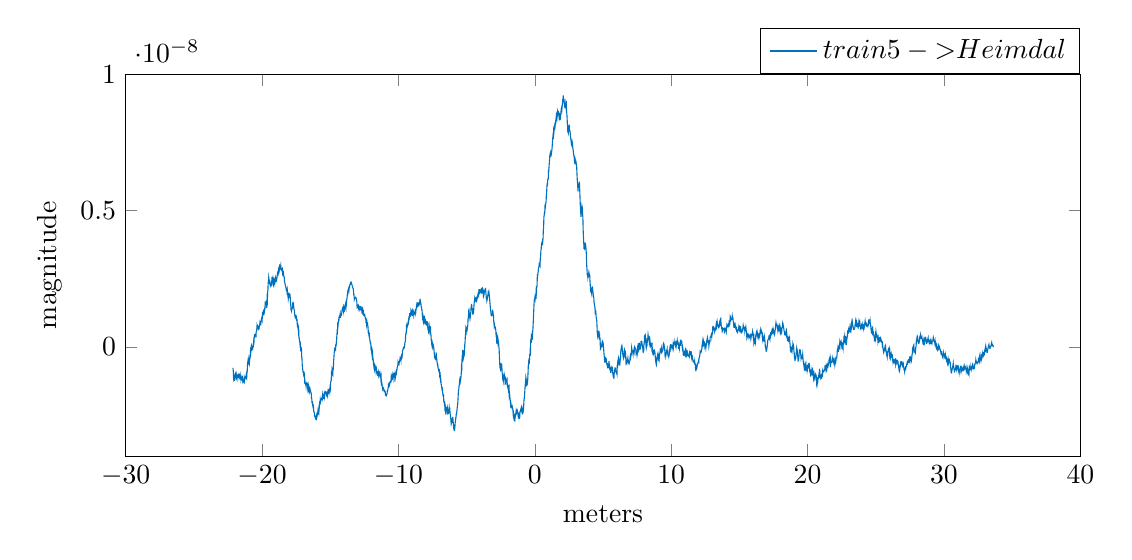
\begin{tikzpicture}

  \begin{axis}[%
    width=\textwidth,
    height=0.4\textwidth,
    at={(0\figurewidth,0\figureheight)},
    scale only axis,
    xmin=-30,
    xmax=40,
    xlabel={\SI{}{meters}},
    ymin=-4e-09,
    ymax=1e-08,
    ylabel={magnitude},
    axis background/.style={fill=white},
    legend style={at={(1.0,1.0)},anchor=south east}
    ]
    \addplot [color=mycolor1,solid]
    table[row sep=crcr]{%
    -22.127904296875	-7.63086305820905e-10\\
    -22.10791015625	-8.75472057799539e-10\\
    -22.087916015625	-1.11139007960595e-09\\
    -22.067921875	-1.20701746393103e-09\\
    -22.047927734375	-1.1840509978512e-09\\
    -22.02793359375	-1.14794185109842e-09\\
    -22.007939453125	-1.23535148093829e-09\\
    -21.9879453125	-1.06835772981889e-09\\
    -21.967951171875	-1.1029417598777e-09\\
    -21.94795703125	-1.11195146728858e-09\\
    -21.927962890625	-9.45887883499602e-10\\
    -21.90796875	-9.28677453041935e-10\\
    -21.887974609375	-9.95900030236419e-10\\
    -21.86798046875	-1.10700313275782e-09\\
    -21.847986328125	-1.05491348505977e-09\\
    -21.8279921875	-1.06178583723869e-09\\
    -21.807998046875	-1.04174807610733e-09\\
    -21.78800390625	-1.03041643882021e-09\\
    -21.768009765625	-1.135225602034e-09\\
    -21.748015625	-1.07248600666458e-09\\
    -21.728021484375	-1.01874880226135e-09\\
    -21.70802734375	-1.0428293985552e-09\\
    -21.688033203125	-1.03030055014497e-09\\
    -21.6680390625	-1.01490638491254e-09\\
    -21.648044921875	-1.12299640141451e-09\\
    -21.62805078125	-1.14790854628834e-09\\
    -21.608056640625	-1.12194187987505e-09\\
    -21.5880625	-1.14206172339225e-09\\
    -21.568068359375	-1.06409368564538e-09\\
    -21.54807421875	-1.17213408645759e-09\\
    -21.528080078125	-1.10292456333294e-09\\
    -21.5080859375	-1.10701145602553e-09\\
    -21.488091796875	-1.14558132043763e-09\\
    -21.46809765625	-1.17543563193088e-09\\
    -21.448103515625	-1.04570079676914e-09\\
    -21.428109375	-1.19969765313025e-09\\
    -21.408115234375	-1.26636150812383e-09\\
    -21.38812109375	-1.23252196968183e-09\\
    -21.368126953125	-1.26188546692192e-09\\
    -21.3481328125	-1.23769797399558e-09\\
    -21.328138671875	-1.26395207263614e-09\\
    -21.30814453125	-1.14310499890587e-09\\
    -21.288150390625	-1.21140385116815e-09\\
    -21.26815625	-1.12503938535678e-09\\
    -21.248162109375	-1.11483305970952e-09\\
    -21.22816796875	-1.10004680490106e-09\\
    -21.208173828125	-1.13043098952216e-09\\
    -21.1881796875	-1.11046031281113e-09\\
    -21.168185546875	-1.04487930022001e-09\\
    -21.14819140625	-1.13114110970253e-09\\
    -21.128197265625	-1.15338700156648e-09\\
    -21.108203125	-9.61990367056978e-10\\
    -21.088208984375	-9.0692278988559e-10\\
    -21.06821484375	-6.75771609342744e-10\\
    -21.048220703125	-5.39931338852031e-10\\
    -21.0282265625	-5.19610171792005e-10\\
    -21.008232421875	-4.00658291830266e-10\\
    -20.98823828125	-4.9551661833459e-10\\
    -20.968244140625	-4.25257038863962e-10\\
    -20.94825	-5.22671795414149e-10\\
    -20.928255859375	-5.84515929305873e-10\\
    -20.90826171875	-4.52868023694226e-10\\
    -20.888267578125	-4.30431713588958e-10\\
    -20.8682734375	-3.7479649851529e-10\\
    -20.848279296875	-1.65933491237633e-10\\
    -20.82828515625	-2.0808304348615e-10\\
    -20.808291015625	-7.44841637698561e-12\\
    -20.788296875	2.31237118800889e-11\\
    -20.768302734375	6.13658911979289e-11\\
    -20.74830859375	2.82844684617335e-12\\
    -20.728314453125	-8.59746707464493e-11\\
    -20.7083203125	-6.89145182076118e-11\\
    -20.688326171875	-7.72592591593417e-11\\
    -20.66833203125	1.01743384745006e-11\\
    -20.648337890625	5.94521332699876e-12\\
    -20.62834375	1.32891748045917e-10\\
    -20.608349609375	2.37272120348016e-10\\
    -20.58835546875	2.01497417092027e-10\\
    -20.568361328125	3.85988234452784e-10\\
    -20.5483671875	4.44766837400607e-10\\
    -20.528373046875	4.38293081639108e-10\\
    -20.50837890625	4.49830985495377e-10\\
    -20.488384765625	4.63796002309106e-10\\
    -20.468390625	4.30911735989034e-10\\
    -20.448396484375	3.51280872668658e-10\\
    -20.42840234375	5.45528692909349e-10\\
    -20.408408203125	5.87327704684262e-10\\
    -20.3884140625	6.28105812048347e-10\\
    -20.368419921875	7.65921088213077e-10\\
    -20.34842578125	7.0317782364039e-10\\
    -20.328431640625	7.47227848721897e-10\\
    -20.3084375	7.05244110276491e-10\\
    -20.288443359375	6.94700100540136e-10\\
    -20.26844921875	7.22843929258292e-10\\
    -20.248455078125	6.45564161124168e-10\\
    -20.2284609375	6.52609553454231e-10\\
    -20.208466796875	7.18918686519399e-10\\
    -20.18847265625	7.57151451530116e-10\\
    -20.168478515625	8.25391883081673e-10\\
    -20.148484375	9.11323432665775e-10\\
    -20.128490234375	8.81921586486253e-10\\
    -20.10849609375	8.92884285711378e-10\\
    -20.088501953125	8.61341809485535e-10\\
    -20.0685078125	9.48935061841084e-10\\
    -20.048513671875	9.86800754555374e-10\\
    -20.02851953125	1.05235133213678e-09\\
    -20.008525390625	1.0885423236752e-09\\
    -19.98853125	1.02516658400491e-09\\
    -19.968537109375	1.19862382960539e-09\\
    -19.94854296875	1.16661524340929e-09\\
    -19.928548828125	1.21254607129316e-09\\
    -19.9085546875	1.27258704276708e-09\\
    -19.888560546875	1.19472775048279e-09\\
    -19.86856640625	1.18790460666193e-09\\
    -19.848572265625	1.21469023744682e-09\\
    -19.828578125	1.32755748182519e-09\\
    -19.808583984375	1.39510045104477e-09\\
    -19.78858984375	1.38448701408645e-09\\
    -19.768595703125	1.59849043343146e-09\\
    -19.7486015625	1.57999784864212e-09\\
    -19.728607421875	1.64725494363025e-09\\
    -19.70861328125	1.66216192570941e-09\\
    -19.688619140625	1.57509203703864e-09\\
    -19.668625	1.57574357937961e-09\\
    -19.648630859375	1.42909039690753e-09\\
    -19.62863671875	1.77534888339463e-09\\
    -19.608642578125	1.72093905426484e-09\\
    -19.5886484375	2.02569012077245e-09\\
    -19.568654296875	2.07680637962255e-09\\
    -19.54866015625	2.37400013228542e-09\\
    -19.528666015625	2.40643711011676e-09\\
    -19.508671875	2.54968872977854e-09\\
    -19.488677734375	2.47774118230298e-09\\
    -19.46868359375	2.45062558655526e-09\\
    -19.448689453125	2.32866299740202e-09\\
    -19.4286953125	2.32449961614032e-09\\
    -19.408701171875	2.30061687822539e-09\\
    -19.38870703125	2.25841141841563e-09\\
    -19.368712890625	2.29747127332322e-09\\
    -19.34871875	2.21396940480993e-09\\
    -19.328724609375	2.400638738704e-09\\
    -19.30873046875	2.3927913057841e-09\\
    -19.288736328125	2.35963562822797e-09\\
    -19.2687421875	2.5719027856164e-09\\
    -19.248748046875	2.42324150502272e-09\\
    -19.22875390625	2.39323696454236e-09\\
    -19.208759765625	2.46651568297985e-09\\
    -19.188765625	2.32374370423183e-09\\
    -19.168771484375	2.28197253243975e-09\\
    -19.14877734375	2.37502829812077e-09\\
    -19.128783203125	2.28258391858168e-09\\
    -19.1087890625	2.43463968890957e-09\\
    -19.088794921875	2.38935303130818e-09\\
    -19.06880078125	2.33915076695344e-09\\
    -19.048806640625	2.50772819898747e-09\\
    -19.0288125	2.38305202209647e-09\\
    -19.008818359375	2.54919338977109e-09\\
    -18.98882421875	2.51515679930817e-09\\
    -18.968830078125	2.47044705707359e-09\\
    -18.9488359375	2.43579664098254e-09\\
    -18.928841796875	2.47894928414939e-09\\
    -18.90884765625	2.5325155183903e-09\\
    -18.888853515625	2.60605959604186e-09\\
    -18.868859375	2.67956211022366e-09\\
    -18.848865234375	2.7515066150748e-09\\
    -18.82887109375	2.76510492420837e-09\\
    -18.808876953125	2.72130754850671e-09\\
    -18.7888828125	2.8637244819725e-09\\
    -18.768888671875	2.84847829568088e-09\\
    -18.74889453125	2.89989351035658e-09\\
    -18.728900390625	2.81317882644379e-09\\
    -18.70890625	2.85985817022811e-09\\
    -18.688912109375	2.93709555211343e-09\\
    -18.66891796875	2.89817514286025e-09\\
    -18.648923828125	2.94620214438308e-09\\
    -18.6289296875	2.99731090377301e-09\\
    -18.608935546875	2.86703948901484e-09\\
    -18.58894140625	2.86204384998641e-09\\
    -18.568947265625	2.8168785951204e-09\\
    -18.548953125	2.80620527259591e-09\\
    -18.528958984375	2.84340790700293e-09\\
    -18.50896484375	2.75363160358036e-09\\
    -18.488970703125	2.81136240536586e-09\\
    -18.4689765625	2.75447708966614e-09\\
    -18.448982421875	2.67449978753429e-09\\
    -18.42898828125	2.70439122815047e-09\\
    -18.408994140625	2.6197132250237e-09\\
    -18.389	2.56667272260579e-09\\
    -18.369005859375	2.56139485683821e-09\\
    -18.34901171875	2.39028858592375e-09\\
    -18.329017578125	2.36030045540249e-09\\
    -18.3090234375	2.30191006997395e-09\\
    -18.289029296875	2.26729597790908e-09\\
    -18.26903515625	2.22496167214585e-09\\
    -18.249041015625	2.18509989445195e-09\\
    -18.229046875	2.13058731195029e-09\\
    -18.209052734375	2.16228904870307e-09\\
    -18.18905859375	2.15474261925216e-09\\
    -18.169064453125	2.0427029151644e-09\\
    -18.1490703125	2.0981739066375e-09\\
    -18.129076171875	1.96899575117741e-09\\
    -18.10908203125	1.90163145556714e-09\\
    -18.089087890625	1.99909355798643e-09\\
    -18.06909375	1.78261577558293e-09\\
    -18.049099609375	1.84192533140138e-09\\
    -18.02910546875	1.83348386190523e-09\\
    -18.009111328125	1.85547227964314e-09\\
    -17.9891171875	1.94616160594712e-09\\
    -17.969123046875	1.93426146576539e-09\\
    -17.94912890625	1.92491155885284e-09\\
    -17.929134765625	1.79566133926505e-09\\
    -17.909140625	1.60898939292315e-09\\
    -17.889146484375	1.50343477740711e-09\\
    -17.86915234375	1.3342429652763e-09\\
    -17.849158203125	1.44431017263417e-09\\
    -17.8291640625	1.34629310927462e-09\\
    -17.809169921875	1.3979730134027e-09\\
    -17.78917578125	1.42493020036822e-09\\
    -17.769181640625	1.43071377925571e-09\\
    -17.7491875	1.61743664064403e-09\\
    -17.729193359375	1.63216749492967e-09\\
    -17.70919921875	1.59387501773274e-09\\
    -17.689205078125	1.59577857398542e-09\\
    -17.6692109375	1.41558368447547e-09\\
    -17.649216796875	1.37959230445744e-09\\
    -17.62922265625	1.35266024449766e-09\\
    -17.609228515625	1.18657623012064e-09\\
    -17.589234375	1.16798916055028e-09\\
    -17.569240234375	1.06294356331908e-09\\
    -17.54924609375	1.16198858824876e-09\\
    -17.529251953125	1.16824626421345e-09\\
    -17.5092578125	1.0237251911024e-09\\
    -17.489263671875	1.13906110435882e-09\\
    -17.46926953125	9.75643749075988e-10\\
    -17.449275390625	9.76494746356051e-10\\
    -17.42928125	9.87952777881056e-10\\
    -17.409287109375	7.75812795824194e-10\\
    -17.38929296875	7.88208884501781e-10\\
    -17.369298828125	7.21788431768353e-10\\
    -17.3493046875	7.53155103523464e-10\\
    -17.329310546875	5.66900299134754e-10\\
    -17.30931640625	6.15346744915096e-10\\
    -17.289322265625	3.36864312691998e-10\\
    -17.269328125	3.15701423650629e-10\\
    -17.249333984375	2.02374798125859e-10\\
    -17.22933984375	1.86853360461058e-10\\
    -17.209345703125	6.87946834542284e-11\\
    -17.1893515625	1.00978262869817e-10\\
    -17.169357421875	-4.67151255279089e-11\\
    -17.14936328125	-7.56929090775117e-12\\
    -17.129369140625	-2.16999048715787e-11\\
    -17.109375	-7.75485949085203e-11\\
    -17.089380859375	-3.67876052802478e-10\\
    -17.06938671875	-4.31942018443304e-10\\
    -17.049392578125	-6.93930149937743e-10\\
    -17.0293984375	-7.29775275703591e-10\\
    -17.009404296875	-8.48568694357086e-10\\
    -16.98941015625	-9.20615667829185e-10\\
    -16.969416015625	-9.28413125335739e-10\\
    -16.949421875	-9.98290012431949e-10\\
    -16.929427734375	-9.65875123545705e-10\\
    -16.90943359375	-1.05626585282468e-09\\
    -16.889439453125	-1.02939401356649e-09\\
    -16.8694453125	-1.26793434798406e-09\\
    -16.849451171875	-1.24510892707688e-09\\
    -16.82945703125	-1.33344076594677e-09\\
    -16.809462890625	-1.36111988798294e-09\\
    -16.78946875	-1.35274566981495e-09\\
    -16.769474609375	-1.44360872439068e-09\\
    -16.74948046875	-1.36213426655944e-09\\
    -16.729486328125	-1.32172736104397e-09\\
    -16.7094921875	-1.34178775146017e-09\\
    -16.689498046875	-1.32451895053811e-09\\
    -16.66950390625	-1.32643736189505e-09\\
    -16.649509765625	-1.50199129951517e-09\\
    -16.629515625	-1.43496172386349e-09\\
    -16.609521484375	-1.58402020946594e-09\\
    -16.58952734375	-1.61034563645994e-09\\
    -16.569533203125	-1.51149639244531e-09\\
    -16.5495390625	-1.58276124076707e-09\\
    -16.529544921875	-1.4716070797507e-09\\
    -16.50955078125	-1.57914691421892e-09\\
    -16.489556640625	-1.5173134015728e-09\\
    -16.4695625	-1.56216181325992e-09\\
    -16.449568359375	-1.59127446539765e-09\\
    -16.42957421875	-1.64595018863422e-09\\
    -16.409580078125	-1.66818902520344e-09\\
    -16.3895859375	-1.70320871062066e-09\\
    -16.369591796875	-1.88975805763604e-09\\
    -16.34959765625	-1.90258839679033e-09\\
    -16.329603515625	-2.06837528624456e-09\\
    -16.309609375	-1.98237564361213e-09\\
    -16.289615234375	-2.10117760745319e-09\\
    -16.26962109375	-2.17723415550155e-09\\
    -16.249626953125	-2.21537455035599e-09\\
    -16.2296328125	-2.18664014113325e-09\\
    -16.209638671875	-2.35530209433494e-09\\
    -16.18964453125	-2.36433111420796e-09\\
    -16.169650390625	-2.41224543940184e-09\\
    -16.14965625	-2.51468463089264e-09\\
    -16.129662109375	-2.54552588923225e-09\\
    -16.10966796875	-2.54281343589715e-09\\
    -16.089673828125	-2.59740651228689e-09\\
    -16.0696796875	-2.61122247851593e-09\\
    -16.049685546875	-2.65266609899552e-09\\
    -16.02969140625	-2.6567381371336e-09\\
    -16.009697265625	-2.53427902131985e-09\\
    -15.989703125	-2.58878841772434e-09\\
    -15.969708984375	-2.54859759078747e-09\\
    -15.94971484375	-2.49209328690979e-09\\
    -15.929720703125	-2.46626147160361e-09\\
    -15.9097265625	-2.37458221893627e-09\\
    -15.889732421875	-2.44781142954721e-09\\
    -15.86973828125	-2.43659957860467e-09\\
    -15.849744140625	-2.3187116861345e-09\\
    -15.82975	-2.38303467420292e-09\\
    -15.809755859375	-2.25584407996727e-09\\
    -15.78976171875	-2.1250511302392e-09\\
    -15.769767578125	-1.98937337461229e-09\\
    -15.7497734375	-2.08300692622704e-09\\
    -15.729779296875	-1.94184331699509e-09\\
    -15.70978515625	-2.00457838663988e-09\\
    -15.689791015625	-1.95802373637602e-09\\
    -15.669796875	-1.93511639900022e-09\\
    -15.649802734375	-1.90558421655616e-09\\
    -15.62980859375	-1.8848205758613e-09\\
    -15.609814453125	-1.90627037980207e-09\\
    -15.5898203125	-1.88361727887294e-09\\
    -15.569826171875	-1.76584321924648e-09\\
    -15.54983203125	-1.84708488823244e-09\\
    -15.529837890625	-1.7573177353102e-09\\
    -15.50984375	-1.76495775753703e-09\\
    -15.489849609375	-1.77533917843826e-09\\
    -15.46985546875	-1.89855727878132e-09\\
    -15.449861328125	-1.7807271483962e-09\\
    -15.4298671875	-1.83364604010021e-09\\
    -15.409873046875	-1.70483176474848e-09\\
    -15.38987890625	-1.72529774204973e-09\\
    -15.369884765625	-1.63153407779263e-09\\
    -15.349890625	-1.6395854063205e-09\\
    -15.329896484375	-1.63945207648968e-09\\
    -15.30990234375	-1.67875598732646e-09\\
    -15.289908203125	-1.66918109001735e-09\\
    -15.2699140625	-1.72719218125236e-09\\
    -15.249919921875	-1.7881969911324e-09\\
    -15.22992578125	-1.77233508590975e-09\\
    -15.209931640625	-1.71772641584111e-09\\
    -15.1899375	-1.77225416186778e-09\\
    -15.169943359375	-1.66186732266927e-09\\
    -15.14994921875	-1.71211422052394e-09\\
    -15.129955078125	-1.70750851693588e-09\\
    -15.1099609375	-1.58161283299622e-09\\
    -15.089966796875	-1.5914074953963e-09\\
    -15.06997265625	-1.58352132919097e-09\\
    -15.049978515625	-1.54708809419752e-09\\
    -15.029984375	-1.61598561895245e-09\\
    -15.009990234375	-1.47843811757569e-09\\
    -14.98999609375	-1.51073023533162e-09\\
    -14.970001953125	-1.29464537663819e-09\\
    -14.9500078125	-1.24373339408867e-09\\
    -14.930013671875	-1.24069885320748e-09\\
    -14.91001953125	-9.97307898574823e-10\\
    -14.890025390625	-1.0288449476065e-09\\
    -14.87003125	-8.69529170363068e-10\\
    -14.850037109375	-9.4144915711028e-10\\
    -14.83004296875	-9.39111792681885e-10\\
    -14.810048828125	-9.77229186665538e-10\\
    -14.7900546875	-7.3515168214099e-10\\
    -14.770060546875	-8.20834318879308e-10\\
    -14.75006640625	-4.98728501456088e-10\\
    -14.730072265625	-4.00222363568091e-10\\
    -14.710078125	-2.09776954632427e-10\\
    -14.690083984375	-1.76868933296349e-10\\
    -14.67008984375	-4.01061359280217e-11\\
    -14.650095703125	-3.71208746628554e-11\\
    -14.6301015625	-8.47369364249656e-11\\
    -14.610107421875	-9.79703973040092e-11\\
    -14.59011328125	1.00955155424465e-10\\
    -14.570119140625	1.3779415173005e-11\\
    -14.550125	2.03538766442469e-10\\
    -14.530130859375	2.64276985690244e-10\\
    -14.51013671875	4.47416116445426e-10\\
    -14.490142578125	5.82957636702262e-10\\
    -14.4701484375	5.56048308901389e-10\\
    -14.450154296875	8.12104682377194e-10\\
    -14.43016015625	7.80230335116598e-10\\
    -14.410166015625	9.18995739677115e-10\\
    -14.390171875	9.28076601991271e-10\\
    -14.370177734375	1.04090020379677e-09\\
    -14.35018359375	1.02738122503743e-09\\
    -14.330189453125	1.13581059366631e-09\\
    -14.3101953125	1.15305506915776e-09\\
    -14.290201171875	1.14934426773403e-09\\
    -14.27020703125	1.21007752978317e-09\\
    -14.250212890625	1.07501386280839e-09\\
    -14.23021875	1.18375057694317e-09\\
    -14.210224609375	1.15780043335715e-09\\
    -14.19023046875	1.16181949636512e-09\\
    -14.170236328125	1.23712817078756e-09\\
    -14.1502421875	1.25297000610691e-09\\
    -14.130248046875	1.35011917865871e-09\\
    -14.11025390625	1.39361439094161e-09\\
    -14.090259765625	1.36257707297787e-09\\
    -14.070265625	1.378934352598e-09\\
    -14.050271484375	1.43933663799118e-09\\
    -14.03027734375	1.34360238405336e-09\\
    -14.010283203125	1.44651355537171e-09\\
    -13.9902890625	1.28135590878542e-09\\
    -13.970294921875	1.42060132859735e-09\\
    -13.95030078125	1.37388864935562e-09\\
    -13.930306640625	1.42875887095798e-09\\
    -13.9103125	1.46107599775288e-09\\
    -13.890318359375	1.52790757041357e-09\\
    -13.87032421875	1.46626974023097e-09\\
    -13.850330078125	1.42336861698873e-09\\
    -13.8303359375	1.61935992189575e-09\\
    -13.810341796875	1.59278230480847e-09\\
    -13.79034765625	1.74714937257861e-09\\
    -13.770353515625	1.77142283555224e-09\\
    -13.750359375	1.88562058442309e-09\\
    -13.730365234375	1.98219066225441e-09\\
    -13.71037109375	2.05542256229805e-09\\
    -13.690376953125	2.09687749813708e-09\\
    -13.6703828125	2.11891273329244e-09\\
    -13.650388671875	2.15027978356574e-09\\
    -13.63039453125	2.06671393251262e-09\\
    -13.610400390625	2.15804716872945e-09\\
    -13.59040625	2.17124633379677e-09\\
    -13.570412109375	2.26601321906368e-09\\
    -13.55041796875	2.29817041312504e-09\\
    -13.530423828125	2.29753527193861e-09\\
    -13.5104296875	2.37210819012178e-09\\
    -13.490435546875	2.37383980680843e-09\\
    -13.47044140625	2.38224524626743e-09\\
    -13.450447265625	2.34847430719889e-09\\
    -13.430453125	2.32394394555439e-09\\
    -13.410458984375	2.2822758286933e-09\\
    -13.39046484375	2.24739589772572e-09\\
    -13.370470703125	2.22609330441605e-09\\
    -13.3504765625	2.20126508999078e-09\\
    -13.330482421875	2.14721820494156e-09\\
    -13.31048828125	2.12943034274203e-09\\
    -13.290494140625	2.04119617409943e-09\\
    -13.2705	1.90683408239816e-09\\
    -13.250505859375	1.90430543527111e-09\\
    -13.23051171875	1.75413986295764e-09\\
    -13.210517578125	1.78870001442686e-09\\
    -13.1905234375	1.79269664407697e-09\\
    -13.170529296875	1.80000676532093e-09\\
    -13.15053515625	1.82880452897304e-09\\
    -13.130541015625	1.82851190677464e-09\\
    -13.110546875	1.79897036790885e-09\\
    -13.090552734375	1.77413892546556e-09\\
    -13.07055859375	1.69348410047864e-09\\
    -13.050564453125	1.68160949882025e-09\\
    -13.0305703125	1.46790408701203e-09\\
    -13.010576171875	1.48388452447712e-09\\
    -12.99058203125	1.53473228478793e-09\\
    -12.970587890625	1.52692922476987e-09\\
    -12.95059375	1.4417194762168e-09\\
    -12.930599609375	1.52091300368177e-09\\
    -12.91060546875	1.49510601755992e-09\\
    -12.890611328125	1.4852145291755e-09\\
    -12.8706171875	1.42697380142889e-09\\
    -12.850623046875	1.51215784873408e-09\\
    -12.83062890625	1.35241356239509e-09\\
    -12.810634765625	1.47345715275036e-09\\
    -12.790640625	1.35621468178923e-09\\
    -12.770646484375	1.49557308455193e-09\\
    -12.75065234375	1.33524104655765e-09\\
    -12.730658203125	1.41575124301235e-09\\
    -12.7106640625	1.39788965090173e-09\\
    -12.690669921875	1.33592142546092e-09\\
    -12.67067578125	1.39859662678141e-09\\
    -12.650681640625	1.34679807840587e-09\\
    -12.6306875	1.28719171688714e-09\\
    -12.610693359375	1.34467721204287e-09\\
    -12.59069921875	1.25465238213496e-09\\
    -12.570705078125	1.21587923217702e-09\\
    -12.5507109375	1.25844782599397e-09\\
    -12.530716796875	1.18344078515274e-09\\
    -12.51072265625	1.16712579362352e-09\\
    -12.490728515625	1.19188793794604e-09\\
    -12.470734375	1.19076729222111e-09\\
    -12.450740234375	1.11954101332968e-09\\
    -12.43074609375	1.07480085157007e-09\\
    -12.410751953125	1.03073077339759e-09\\
    -12.3907578125	1.03270484700335e-09\\
    -12.370763671875	8.8035310090958e-10\\
    -12.35076953125	9.60106549448328e-10\\
    -12.330775390625	8.25312684222703e-10\\
    -12.31078125	9.01554323853476e-10\\
    -12.290787109375	7.83254798125316e-10\\
    -12.27079296875	9.11896291946314e-10\\
    -12.250798828125	7.92808634935851e-10\\
    -12.2308046875	7.4793577976022e-10\\
    -12.210810546875	5.07433573997947e-10\\
    -12.19081640625	6.2071311576515e-10\\
    -12.170822265625	4.73108808465163e-10\\
    -12.150828125	4.08655803276233e-10\\
    -12.130833984375	4.3975299530503e-10\\
    -12.11083984375	3.07238207656807e-10\\
    -12.090845703125	2.64758373563146e-10\\
    -12.0708515625	1.68567755560269e-10\\
    -12.050857421875	1.75557608858479e-10\\
    -12.03086328125	1.48645766131369e-10\\
    -12.010869140625	-4.20588964544766e-11\\
    -11.990875	-1.65817897343268e-11\\
    -11.970880859375	-1.23412867414856e-10\\
    -11.95088671875	-2.12960630836776e-10\\
    -11.930892578125	-1.58656462632511e-10\\
    -11.9108984375	-3.22345974614573e-10\\
    -11.890904296875	-2.70741990103144e-10\\
    -11.87091015625	-4.50722782095111e-10\\
    -11.850916015625	-4.45635160212689e-10\\
    -11.830921875	-6.23226147877041e-10\\
    -11.810927734375	-6.58280429657006e-10\\
    -11.79093359375	-7.56285987339423e-10\\
    -11.770939453125	-7.96120119403487e-10\\
    -11.7509453125	-7.20382084421086e-10\\
    -11.730951171875	-8.37527404130866e-10\\
    -11.71095703125	-7.96143451059388e-10\\
    -11.690962890625	-7.49774484927483e-10\\
    -11.67096875	-8.43339694074146e-10\\
    -11.650974609375	-6.99974888229473e-10\\
    -11.63098046875	-8.92326346494565e-10\\
    -11.610986328125	-8.30372238410856e-10\\
    -11.5909921875	-9.2517721933012e-10\\
    -11.570998046875	-9.17593602700088e-10\\
    -11.55100390625	-9.58271277141547e-10\\
    -11.531009765625	-9.39519422530757e-10\\
    -11.511015625	-1.05276820372228e-09\\
    -11.491021484375	-8.916676300383e-10\\
    -11.47102734375	-9.94378353860597e-10\\
    -11.451033203125	-9.20087781658516e-10\\
    -11.4310390625	-9.77077580699403e-10\\
    -11.411044921875	-9.32018471874781e-10\\
    -11.39105078125	-9.25877046684959e-10\\
    -11.371056640625	-1.00987777025481e-09\\
    -11.3510625	-9.62373194940103e-10\\
    -11.331068359375	-1.03689949895129e-09\\
    -11.31107421875	-1.03866093827376e-09\\
    -11.291080078125	-1.15349415176649e-09\\
    -11.2710859375	-1.09028529928684e-09\\
    -11.251091796875	-1.31664716456067e-09\\
    -11.23109765625	-1.2836762243355e-09\\
    -11.211103515625	-1.32976611507348e-09\\
    -11.191109375	-1.41067604926207e-09\\
    -11.171115234375	-1.4821366731557e-09\\
    -11.15112109375	-1.54246550204965e-09\\
    -11.131126953125	-1.50676440865946e-09\\
    -11.1111328125	-1.53283344062413e-09\\
    -11.091138671875	-1.51578686752266e-09\\
    -11.07114453125	-1.58452732784921e-09\\
    -11.051150390625	-1.57593995284576e-09\\
    -11.03115625	-1.6109112844933e-09\\
    -11.011162109375	-1.59721909638542e-09\\
    -10.99116796875	-1.61244833044957e-09\\
    -10.971173828125	-1.63342257985688e-09\\
    -10.9511796875	-1.76289364290648e-09\\
    -10.931185546875	-1.76612513040161e-09\\
    -10.91119140625	-1.7527231624066e-09\\
    -10.891197265625	-1.77663883002204e-09\\
    -10.871203125	-1.75147905251146e-09\\
    -10.851208984375	-1.74444076633905e-09\\
    -10.83121484375	-1.68644698591892e-09\\
    -10.811220703125	-1.60427738926539e-09\\
    -10.7912265625	-1.60850397610803e-09\\
    -10.771232421875	-1.55288106540404e-09\\
    -10.75123828125	-1.50189577192206e-09\\
    -10.731244140625	-1.38736082637813e-09\\
    -10.71125	-1.39742856144453e-09\\
    -10.691255859375	-1.3234409624451e-09\\
    -10.67126171875	-1.31692939632175e-09\\
    -10.651267578125	-1.38126716695437e-09\\
    -10.6312734375	-1.33425152185379e-09\\
    -10.611279296875	-1.27156528234465e-09\\
    -10.59128515625	-1.26091411762617e-09\\
    -10.571291015625	-1.29631507750074e-09\\
    -10.551296875	-1.29087071970801e-09\\
    -10.531302734375	-1.13425208424251e-09\\
    -10.51130859375	-1.20627946446544e-09\\
    -10.491314453125	-1.17197015208683e-09\\
    -10.4713203125	-1.09255214784633e-09\\
    -10.451326171875	-1.14143745537211e-09\\
    -10.43133203125	-1.1585424758346e-09\\
    -10.411337890625	-1.04951497491042e-09\\
    -10.39134375	-1.12153675959581e-09\\
    -10.371349609375	-9.72683046125166e-10\\
    -10.35135546875	-1.08310650345234e-09\\
    -10.331361328125	-9.36101249040055e-10\\
    -10.3113671875	-1.12807834051629e-09\\
    -10.291373046875	-9.55559367328563e-10\\
    -10.27137890625	-1.08487186257763e-09\\
    -10.251384765625	-1.00845202018792e-09\\
    -10.231390625	-1.13658989260036e-09\\
    -10.211396484375	-1.08130694588932e-09\\
    -10.19140234375	-1.03653782295528e-09\\
    -10.171408203125	-9.74126112887043e-10\\
    -10.1514140625	-9.82690989888185e-10\\
    -10.131419921875	-8.49664040726017e-10\\
    -10.11142578125	-8.54188994224172e-10\\
    -10.091431640625	-7.48049591294035e-10\\
    -10.0714375	-7.25865199788423e-10\\
    -10.051443359375	-7.03245986478488e-10\\
    -10.03144921875	-5.87485311344353e-10\\
    -10.011455078125	-6.49166462020674e-10\\
    -9.9914609375	-6.3944163841215e-10\\
    -9.971466796875	-5.88688494874188e-10\\
    -9.95147265625	-6.13556930655769e-10\\
    -9.931478515625	-5.36918278454365e-10\\
    -9.911484375	-4.93530023269118e-10\\
    -9.891490234375	-4.92847361676067e-10\\
    -9.87149609375	-3.79153950399208e-10\\
    -9.851501953125	-3.87171350016815e-10\\
    -9.8315078125	-4.01714872310861e-10\\
    -9.811513671875	-4.67502193258841e-10\\
    -9.79151953125	-3.16355074800689e-10\\
    -9.771525390625	-4.50137864969537e-10\\
    -9.75153125	-2.64424020690278e-10\\
    -9.731537109375	-4.1131718472264e-10\\
    -9.71154296875	-1.80971410635349e-10\\
    -9.691548828125	-1.42684897979823e-10\\
    -9.6715546875	-9.12152481779046e-11\\
    -9.651560546875	-8.77657109442308e-11\\
    -9.63156640625	-2.41647621750265e-11\\
    -9.611572265625	-3.8809371254554e-11\\
    -9.591578125	-4.4432876401431e-11\\
    -9.571583984375	-2.15073870344491e-11\\
    -9.55158984375	2.02019301552853e-11\\
    -9.531595703125	1.25664858916635e-10\\
    -9.5116015625	1.83920679779267e-10\\
    -9.491607421875	2.10379512850523e-10\\
    -9.47161328125	4.31791842771708e-10\\
    -9.451619140625	4.91713432874381e-10\\
    -9.431625	4.88816300913937e-10\\
    -9.411630859375	7.12084407712993e-10\\
    -9.39163671875	6.49650021153137e-10\\
    -9.371642578125	7.29990947060913e-10\\
    -9.3516484375	7.42439908321605e-10\\
    -9.331654296875	8.30867307772126e-10\\
    -9.31166015625	8.57432476282529e-10\\
    -9.291666015625	9.03993975768592e-10\\
    -9.271671875	8.70784217018781e-10\\
    -9.251677734375	9.26727614022379e-10\\
    -9.23168359375	1.12020679683151e-09\\
    -9.211689453125	1.04345856947348e-09\\
    -9.1916953125	1.09674334455197e-09\\
    -9.171701171875	1.24628040668672e-09\\
    -9.15170703125	1.11278652029882e-09\\
    -9.131712890625	1.24096139459347e-09\\
    -9.11171875	1.12544466786561e-09\\
    -9.091724609375	1.28036991835108e-09\\
    -9.07173046875	1.21392928085034e-09\\
    -9.051736328125	1.24794797854734e-09\\
    -9.0317421875	1.25245887624064e-09\\
    -9.011748046875	1.3672076759965e-09\\
    -8.99175390625	1.15693006060319e-09\\
    -8.971759765625	1.24811654353279e-09\\
    -8.951765625	1.14380837601053e-09\\
    -8.931771484375	1.24318749978937e-09\\
    -8.91177734375	1.17445217534804e-09\\
    -8.891783203125	1.27317472037712e-09\\
    -8.8717890625	1.22982930552764e-09\\
    -8.851794921875	1.22283974479526e-09\\
    -8.83180078125	1.22947802424072e-09\\
    -8.811806640625	1.2136171449287e-09\\
    -8.7918125	1.27017945597142e-09\\
    -8.771818359375	1.19001715742772e-09\\
    -8.75182421875	1.23129629894776e-09\\
    -8.731830078125	1.23999097317066e-09\\
    -8.7118359375	1.37373526437057e-09\\
    -8.691841796875	1.42780884804785e-09\\
    -8.67184765625	1.49565632944774e-09\\
    -8.651853515625	1.56012542482657e-09\\
    -8.631859375	1.6241180321792e-09\\
    -8.611865234375	1.62208455962902e-09\\
    -8.59187109375	1.54731650287241e-09\\
    -8.571876953125	1.60350590857708e-09\\
    -8.5518828125	1.60903849828704e-09\\
    -8.531888671875	1.56104125016677e-09\\
    -8.51189453125	1.53115602121597e-09\\
    -8.491900390625	1.58379016260726e-09\\
    -8.47190625	1.57077886875978e-09\\
    -8.451912109375	1.6309804231754e-09\\
    -8.43191796875	1.62122455800198e-09\\
    -8.411923828125	1.77036514033955e-09\\
    -8.3919296875	1.65302908388432e-09\\
    -8.371935546875	1.59433240384514e-09\\
    -8.35194140625	1.60129279688963e-09\\
    -8.331947265625	1.48642677690403e-09\\
    -8.311953125	1.47354651764506e-09\\
    -8.291958984375	1.3873130891779e-09\\
    -8.27196484375	1.36310735758699e-09\\
    -8.251970703125	1.21858814710948e-09\\
    -8.2319765625	1.1012273968288e-09\\
    -8.211982421875	1.13853188539426e-09\\
    -8.19198828125	9.71122154555003e-10\\
    -8.171994140625	9.22441696923564e-10\\
    -8.152	1.0556490431588e-09\\
    -8.132005859375	1.14678361781686e-09\\
    -8.11201171875	9.88179255364119e-10\\
    -8.092017578125	9.42425919834768e-10\\
    -8.0720234375	1.00202775706372e-09\\
    -8.052029296875	8.69815031409875e-10\\
    -8.03203515625	8.55120392796612e-10\\
    -8.012041015625	8.56380792237012e-10\\
    -7.992046875	9.21257928037686e-10\\
    -7.972052734375	8.60801769916759e-10\\
    -7.95205859375	8.95155931971614e-10\\
    -7.932064453125	8.84765504805774e-10\\
    -7.9120703125	8.42018857664789e-10\\
    -7.892076171875	9.50414806939638e-10\\
    -7.87208203125	7.85106125808544e-10\\
    -7.852087890625	9.06935741684359e-10\\
    -7.83209375	6.23641563438894e-10\\
    -7.812099609375	7.48570914730318e-10\\
    -7.79210546875	5.96218824045068e-10\\
    -7.772111328125	6.39596463112287e-10\\
    -7.7521171875	5.85364157144571e-10\\
    -7.732123046875	7.50800159892588e-10\\
    -7.71212890625	6.83549519792374e-10\\
    -7.692134765625	7.69687911673574e-10\\
    -7.672140625	6.33647688211299e-10\\
    -7.652146484375	7.6019601251558e-10\\
    -7.63215234375	4.89908793426833e-10\\
    -7.612158203125	4.31881540823497e-10\\
    -7.5921640625	2.6086087030886e-10\\
    -7.572169921875	1.84286313340028e-10\\
    -7.55217578125	8.62452885006985e-11\\
    -7.532181640625	3.02105475771127e-11\\
    -7.5121875	1.21662581399207e-10\\
    -7.492193359375	4.96575018565414e-11\\
    -7.47219921875	1.12988200359508e-10\\
    -7.452205078125	8.89221050374248e-11\\
    -7.4322109375	4.00746548167959e-11\\
    -7.412216796875	-2.95795060473404e-11\\
    -7.39222265625	-9.76438328573816e-11\\
    -7.372228515625	-2.21911620034005e-10\\
    -7.352234375	-3.54579161631338e-10\\
    -7.332240234375	-3.9625517584033e-10\\
    -7.31224609375	-4.21487744725205e-10\\
    -7.292251953125	-3.49002074792743e-10\\
    -7.2722578125	-3.51925899048448e-10\\
    -7.252263671875	-3.70336632569122e-10\\
    -7.23226953125	-1.94745600987488e-10\\
    -7.212275390625	-4.36599595079633e-10\\
    -7.19228125	-4.26872279850891e-10\\
    -7.172287109375	-5.24200619558997e-10\\
    -7.15229296875	-5.93554194770363e-10\\
    -7.132298828125	-6.6193186589794e-10\\
    -7.1123046875	-6.510095790232e-10\\
    -7.092310546875	-7.65613230178253e-10\\
    -7.07231640625	-8.03811786644222e-10\\
    -7.052322265625	-8.34794015617106e-10\\
    -7.032328125	-8.88705254623215e-10\\
    -7.012333984375	-9.2113686977243e-10\\
    -6.99233984375	-8.90347855550434e-10\\
    -6.972345703125	-1.09214356254112e-09\\
    -6.9523515625	-1.11723913352066e-09\\
    -6.932357421875	-1.06804556079249e-09\\
    -6.91236328125	-1.22516741893247e-09\\
    -6.892369140625	-1.20523957837232e-09\\
    -6.872375	-1.33136042170243e-09\\
    -6.852380859375	-1.39598112589376e-09\\
    -6.83238671875	-1.46074464381645e-09\\
    -6.812392578125	-1.51435545806589e-09\\
    -6.7923984375	-1.57290876725574e-09\\
    -6.772404296875	-1.55040576095557e-09\\
    -6.75241015625	-1.66626187627816e-09\\
    -6.732416015625	-1.78330136849285e-09\\
    -6.712421875	-1.80554124051425e-09\\
    -6.692427734375	-1.78874508946739e-09\\
    -6.67243359375	-1.98928464531595e-09\\
    -6.652439453125	-2.01138267645364e-09\\
    -6.6324453125	-2.07196396212406e-09\\
    -6.612451171875	-1.98684285982868e-09\\
    -6.59245703125	-2.22108536708603e-09\\
    -6.572462890625	-2.18739366663618e-09\\
    -6.55246875	-2.32394577534356e-09\\
    -6.532474609375	-2.26581237592794e-09\\
    -6.51248046875	-2.33301371559445e-09\\
    -6.492486328125	-2.21509389538644e-09\\
    -6.4724921875	-2.22264084015785e-09\\
    -6.452498046875	-2.23412916662197e-09\\
    -6.43250390625	-2.30499225654024e-09\\
    -6.412509765625	-2.24652362692489e-09\\
    -6.392515625	-2.38107709705358e-09\\
    -6.372521484375	-2.33972448565537e-09\\
    -6.35252734375	-2.41197658958799e-09\\
    -6.332533203125	-2.42374994657662e-09\\
    -6.3125390625	-2.34648983919538e-09\\
    -6.292544921875	-2.34649632383381e-09\\
    -6.27255078125	-2.22579951111769e-09\\
    -6.252556640625	-2.29941511240824e-09\\
    -6.2325625	-2.28284526469903e-09\\
    -6.212568359375	-2.43018544245889e-09\\
    -6.19257421875	-2.48649551162159e-09\\
    -6.172580078125	-2.58060289726047e-09\\
    -6.1525859375	-2.6792557495537e-09\\
    -6.132591796875	-2.80749595574741e-09\\
    -6.11259765625	-2.75832237099651e-09\\
    -6.092603515625	-2.6874328059304e-09\\
    -6.072609375	-2.71944745749098e-09\\
    -6.052615234375	-2.65821163193888e-09\\
    -6.03262109375	-2.65606668680831e-09\\
    -6.012626953125	-2.55795530581224e-09\\
    -5.9926328125	-2.7246884649598e-09\\
    -5.972638671875	-2.79055715025319e-09\\
    -5.95264453125	-2.95141296358162e-09\\
    -5.932650390625	-2.94195369784591e-09\\
    -5.91265625	-3.06774288505833e-09\\
    -5.892662109375	-2.9512769044829e-09\\
    -5.87266796875	-2.99081697244036e-09\\
    -5.852673828125	-2.89208692377804e-09\\
    -5.8326796875	-2.74855844073945e-09\\
    -5.812685546875	-2.710540492476e-09\\
    -5.79269140625	-2.60141936985108e-09\\
    -5.772697265625	-2.54653769701958e-09\\
    -5.752703125	-2.42923806396839e-09\\
    -5.732708984375	-2.43126496301227e-09\\
    -5.71271484375	-2.34300853605161e-09\\
    -5.692720703125	-2.24529915238286e-09\\
    -5.6727265625	-2.15360430599195e-09\\
    -5.652732421875	-2.07730217037265e-09\\
    -5.63273828125	-1.92074528398367e-09\\
    -5.612744140625	-1.71508313038747e-09\\
    -5.59275	-1.58367205627247e-09\\
    -5.572755859375	-1.55419456804064e-09\\
    -5.55276171875	-1.40095154066823e-09\\
    -5.532767578125	-1.38380820783408e-09\\
    -5.5127734375	-1.2280586948358e-09\\
    -5.492779296875	-1.24049878648325e-09\\
    -5.47278515625	-1.0711807870447e-09\\
    -5.452791015625	-1.2292664855489e-09\\
    -5.432796875	-1.17075800975694e-09\\
    -5.412802734375	-1.11314929588393e-09\\
    -5.39280859375	-9.70319581926251e-10\\
    -5.372814453125	-7.16439930182186e-10\\
    -5.3528203125	-7.48394803027353e-10\\
    -5.332826171875	-4.13265219699359e-10\\
    -5.31283203125	-4.39463610947773e-10\\
    -5.292837890625	-2.40000973482002e-10\\
    -5.27284375	-2.78812511092673e-10\\
    -5.252849609375	-1.01681725657138e-10\\
    -5.23285546875	-3.9617817894413e-10\\
    -5.212861328125	-3.47351931108215e-10\\
    -5.1928671875	-3.37798193976933e-10\\
    -5.172873046875	-2.96954335356336e-10\\
    -5.15287890625	-2.13610218472167e-10\\
    -5.132884765625	9.56676293015221e-11\\
    -5.112890625	1.82774538856544e-10\\
    -5.092896484375	3.98648310410098e-10\\
    -5.07290234375	5.0392289980491e-10\\
    -5.052908203125	6.98569948121237e-10\\
    -5.0329140625	6.62813350007171e-10\\
    -5.012919921875	6.59099266021508e-10\\
    -4.99292578125	7.4096468758401e-10\\
    -4.972931640625	6.07071536095469e-10\\
    -4.9529375	6.66274788420629e-10\\
    -4.932943359375	7.70744404946712e-10\\
    -4.91294921875	7.99819626754266e-10\\
    -4.892955078125	1.04157288041365e-09\\
    -4.8729609375	1.09727356840631e-09\\
    -4.852966796875	1.25867500022145e-09\\
    -4.83297265625	1.19409135471871e-09\\
    -4.812978515625	1.26705862372787e-09\\
    -4.792984375	1.14113868505694e-09\\
    -4.772990234375	1.0952000359003e-09\\
    -4.75299609375	1.03316067777019e-09\\
    -4.733001953125	1.10530192395476e-09\\
    -4.7130078125	1.20212253648881e-09\\
    -4.693013671875	1.27600697445252e-09\\
    -4.67301953125	1.4507508708145e-09\\
    -4.653025390625	1.49527789645192e-09\\
    -4.63303125	1.58539554699878e-09\\
    -4.613037109375	1.40611403622009e-09\\
    -4.59304296875	1.41912118820311e-09\\
    -4.573048828125	1.38379543772853e-09\\
    -4.5530546875	1.20905528920635e-09\\
    -4.533060546875	1.20802726362796e-09\\
    -4.51306640625	1.24345405462395e-09\\
    -4.493072265625	1.24651251539407e-09\\
    -4.473078125	1.42274895190931e-09\\
    -4.453083984375	1.5795104045684e-09\\
    -4.43308984375	1.66400404678758e-09\\
    -4.413095703125	1.74648781506149e-09\\
    -4.3931015625	1.65100284412024e-09\\
    -4.373107421875	1.8251163158524e-09\\
    -4.35311328125	1.75203174030193e-09\\
    -4.333119140625	1.69779456037622e-09\\
    -4.313125	1.6977323635463e-09\\
    -4.293130859375	1.74417710543909e-09\\
    -4.27313671875	1.63801911645766e-09\\
    -4.253142578125	1.7412753090562e-09\\
    -4.2331484375	1.75988427077103e-09\\
    -4.213154296875	1.79470288726113e-09\\
    -4.19316015625	1.82063346036429e-09\\
    -4.173166015625	1.92976440727308e-09\\
    -4.153171875	1.97006304574686e-09\\
    -4.133177734375	1.99310900335287e-09\\
    -4.11318359375	1.94276229276443e-09\\
    -4.093189453125	2.12626724879839e-09\\
    -4.0731953125	2.01984257395835e-09\\
    -4.053201171875	2.12053897553882e-09\\
    -4.03320703125	1.99714282452888e-09\\
    -4.013212890625	2.01713319653392e-09\\
    -3.99321875	2.05495659111731e-09\\
    -3.973224609375	2.03274179669266e-09\\
    -3.95323046875	2.06505476243849e-09\\
    -3.933236328125	2.09798350607092e-09\\
    -3.9132421875	2.03915475351298e-09\\
    -3.893248046875	2.08442615863092e-09\\
    -3.87325390625	2.04595951745906e-09\\
    -3.853259765625	2.10265770652844e-09\\
    -3.833265625	2.15632659002008e-09\\
    -3.813271484375	2.14054366424202e-09\\
    -3.79327734375	2.03729958122754e-09\\
    -3.773283203125	1.90538947248727e-09\\
    -3.7532890625	1.96205146889047e-09\\
    -3.733294921875	1.90680022590396e-09\\
    -3.71330078125	1.96416403226094e-09\\
    -3.693306640625	2.06356634164295e-09\\
    -3.6733125	2.04868731277133e-09\\
    -3.653318359375	2.06140197061545e-09\\
    -3.63332421875	2.06364624972942e-09\\
    -3.613330078125	2.16946914586642e-09\\
    -3.5933359375	2.02081564021244e-09\\
    -3.573341796875	1.92269137214363e-09\\
    -3.55334765625	1.78309737448649e-09\\
    -3.533353515625	1.78986035451233e-09\\
    -3.513359375	1.69749792016743e-09\\
    -3.493365234375	1.73928314966915e-09\\
    -3.47337109375	1.80350906895371e-09\\
    -3.453376953125	1.88475967597716e-09\\
    -3.4333828125	1.8824924395139e-09\\
    -3.413388671875	2.02481292274551e-09\\
    -3.39339453125	2.01930480673423e-09\\
    -3.373400390625	2.04589929101033e-09\\
    -3.35340625	1.95832075124741e-09\\
    -3.333412109375	1.88555621975582e-09\\
    -3.31341796875	1.78289508395246e-09\\
    -3.293423828125	1.63725693722366e-09\\
    -3.2734296875	1.53218885443917e-09\\
    -3.253435546875	1.39867900471151e-09\\
    -3.23344140625	1.34928198517788e-09\\
    -3.213447265625	1.23388609761186e-09\\
    -3.193453125	1.16155482763007e-09\\
    -3.173458984375	1.16891259575729e-09\\
    -3.15346484375	1.15732459684386e-09\\
    -3.133470703125	1.18089395882708e-09\\
    -3.1134765625	1.25623551289412e-09\\
    -3.093482421875	1.33254001134033e-09\\
    -3.07348828125	1.32124265280254e-09\\
    -3.053494140625	1.18117029355189e-09\\
    -3.0335	1.17709417534881e-09\\
    -3.013505859375	9.60437551116287e-10\\
    -2.99351171875	8.69781766469136e-10\\
    -2.973517578125	7.66995003376085e-10\\
    -2.9535234375	8.14126019122184e-10\\
    -2.933529296875	7.56179164788671e-10\\
    -2.91353515625	7.4612563980269e-10\\
    -2.893541015625	6.99150790345292e-10\\
    -2.873546875	6.52532120905476e-10\\
    -2.853552734375	5.9869972885449e-10\\
    -2.83355859375	3.67773706513882e-10\\
    -2.813564453125	5.34634933944298e-10\\
    -2.7935703125	1.24173026399482e-10\\
    -2.773576171875	3.09631911274105e-10\\
    -2.75358203125	1.46930299205151e-10\\
    -2.733587890625	2.66745332805998e-10\\
    -2.71359375	1.83791067163396e-10\\
    -2.693599609375	2.6975736742749e-10\\
    -2.67360546875	2.02076352354008e-10\\
    -2.653611328125	1.18909534925695e-10\\
    -2.6336171875	4.26219116142834e-12\\
    -2.613623046875	-1.03147929840237e-10\\
    -2.59362890625	-3.72731194762919e-10\\
    -2.573634765625	-5.80426899507537e-10\\
    -2.553640625	-7.58485509737863e-10\\
    -2.533646484375	-7.575839018278e-10\\
    -2.51365234375	-8.1788575796399e-10\\
    -2.493658203125	-7.73637025216129e-10\\
    -2.4736640625	-5.88877427118274e-10\\
    -2.453669921875	-6.76209997355638e-10\\
    -2.43367578125	-7.82282830827665e-10\\
    -2.413681640625	-7.48917470825086e-10\\
    -2.3936875	-9.45662007517083e-10\\
    -2.373693359375	-9.83549721247059e-10\\
    -2.35369921875	-1.18237832945033e-09\\
    -2.333705078125	-1.19136045612643e-09\\
    -2.3137109375	-1.24831025848425e-09\\
    -2.293716796875	-1.11952729066967e-09\\
    -2.27372265625	-1.07923511960608e-09\\
    -2.253728515625	-1.01209219139849e-09\\
    -2.233734375	-1.09521634945609e-09\\
    -2.213740234375	-1.06240666370798e-09\\
    -2.19374609375	-1.12579299545086e-09\\
    -2.173751953125	-1.30550628060796e-09\\
    -2.1537578125	-1.27439333460883e-09\\
    -2.133763671875	-1.30143636512943e-09\\
    -2.11376953125	-1.20765336978382e-09\\
    -2.093775390625	-1.26901963098754e-09\\
    -2.07378125	-1.26324913649656e-09\\
    -2.053787109375	-1.24428772079361e-09\\
    -2.03379296875	-1.21161606997418e-09\\
    -2.013798828125	-1.42123785089822e-09\\
    -1.9938046875	-1.46119961544562e-09\\
    -1.973810546875	-1.44649845701879e-09\\
    -1.95381640625	-1.52291216457175e-09\\
    -1.933822265625	-1.42976154591094e-09\\
    -1.913828125	-1.44306022388432e-09\\
    -1.893833984375	-1.42300990844323e-09\\
    -1.87383984375	-1.76009072409526e-09\\
    -1.853845703125	-1.70310347633525e-09\\
    -1.8338515625	-1.79309749305416e-09\\
    -1.813857421875	-1.91971230150535e-09\\
    -1.79386328125	-2.00045452411022e-09\\
    -1.773869140625	-2.1208114573628e-09\\
    -1.753875	-2.23633314350696e-09\\
    -1.733880859375	-2.11879809545263e-09\\
    -1.71388671875	-2.18300845061899e-09\\
    -1.693892578125	-2.20066836198612e-09\\
    -1.6738984375	-2.22701082809295e-09\\
    -1.653904296875	-2.18791295552502e-09\\
    -1.63391015625	-2.24584871639213e-09\\
    -1.613916015625	-2.25630762095923e-09\\
    -1.593921875	-2.39483189491029e-09\\
    -1.573927734375	-2.32115785954356e-09\\
    -1.55393359375	-2.57282709013445e-09\\
    -1.533939453125	-2.61858910404304e-09\\
    -1.5139453125	-2.57163271191475e-09\\
    -1.493951171875	-2.63697310039656e-09\\
    -1.47395703125	-2.58915446443341e-09\\
    -1.453962890625	-2.62788155900564e-09\\
    -1.43396875	-2.49316250509114e-09\\
    -1.413974609375	-2.5141374654607e-09\\
    -1.39398046875	-2.46985768595253e-09\\
    -1.373986328125	-2.37358448002486e-09\\
    -1.3539921875	-2.43844679600319e-09\\
    -1.333998046875	-2.41742510409974e-09\\
    -1.31400390625	-2.3668291505386e-09\\
    -1.294009765625	-2.30506783770654e-09\\
    -1.274015625	-2.33187886675142e-09\\
    -1.254021484375	-2.41954438008206e-09\\
    -1.23402734375	-2.48301142991533e-09\\
    -1.214033203125	-2.40279728211725e-09\\
    -1.1940390625	-2.55323493028539e-09\\
    -1.174044921875	-2.52203047946888e-09\\
    -1.15405078125	-2.54366984125017e-09\\
    -1.134056640625	-2.49330828620456e-09\\
    -1.1140625	-2.63494971512782e-09\\
    -1.094068359375	-2.3928368724043e-09\\
    -1.07407421875	-2.36910066611608e-09\\
    -1.054080078125	-2.36478335937474e-09\\
    -1.0340859375	-2.28764250893233e-09\\
    -1.014091796875	-2.29255885374165e-09\\
    -0.994097656249998	-2.22059925409665e-09\\
    -0.974103515624996	-2.19223208404619e-09\\
    -0.954109374999998	-2.31118591074107e-09\\
    -0.934115234375	-2.27837353039975e-09\\
    -0.914121093749998	-2.44171362177204e-09\\
    -0.894126953124999	-2.43178777428656e-09\\
    -0.874132812499997	-2.42243086426601e-09\\
    -0.854138671874999	-2.35695003638739e-09\\
    -0.834144531249997	-2.31109919360735e-09\\
    -0.814150390624999	-2.14956329976903e-09\\
    -0.794156249999997	-1.95039081807507e-09\\
    -0.774162109374998	-1.88347379576516e-09\\
    -0.754167968749996	-1.78260526642264e-09\\
    -0.734173828124998	-1.62898889775356e-09\\
    -0.7141796875	-1.45827940052369e-09\\
    -0.694185546874998	-1.35367564242235e-09\\
    -0.674191406249999	-1.25850562263464e-09\\
    -0.654197265624997	-1.1074243404237e-09\\
    -0.634203124999999	-1.1653846750512e-09\\
    -0.614208984374997	-1.3924197769974e-09\\
    -0.594214843749999	-1.37592724488358e-09\\
    -0.574220703124997	-1.39141884630487e-09\\
    -0.554226562499998	-1.37167112057416e-09\\
    -0.534232421874997	-1.31408594601859e-09\\
    -0.514238281249998	-1.14685315493313e-09\\
    -0.494244140625	-9.22578309336224e-10\\
    -0.474249999999998	-6.61032596256045e-10\\
    -0.454255859374999	-6.09861904370554e-10\\
    -0.434261718749998	-4.48147329956365e-10\\
    -0.414267578124999	-4.49017123042306e-10\\
    -0.394273437499997	-4.9283207106104e-10\\
    -0.374279296874999	-2.96061896689998e-10\\
    -0.354285156249997	-2.9995215870073e-10\\
    -0.334291015624999	-7.8479166108134e-11\\
    -0.314296874999997	-1.24144011258482e-10\\
    -0.294302734374998	2.85318288213311e-10\\
    -0.27430859375	2.01169311343145e-10\\
    -0.254314453124998	3.83485731864258e-10\\
    -0.2343203125	3.21978368270434e-10\\
    -0.214326171874998	4.26801600004723e-10\\
    -0.194332031249999	2.674677389262e-10\\
    -0.174337890624997	4.10775418341532e-10\\
    -0.154343749999999	5.75100248455965e-10\\
    -0.134349609374997	6.99221350230477e-10\\
    -0.114355468749999	9.11425352749974e-10\\
    -0.0943613281249966	1.14799719249339e-09\\
    -0.0743671874999983	1.37464301538205e-09\\
    -0.0543730468749999	1.60046821069649e-09\\
    -0.034378906249998	1.7341446834463e-09\\
    -0.0143847656249996	1.73626282263345e-09\\
    0.00560937500000236	1.81423323303197e-09\\
    0.0256035156250007	1.7568730310581e-09\\
    0.0455976562500027	1.83476630433303e-09\\
    0.0655917968750011	1.90531164733252e-09\\
    0.085585937500003	1.76391634097578e-09\\
    0.105580078125001	2.09446109425382e-09\\
    0.125574218750003	2.04858627992191e-09\\
    0.145568359375002	2.23902589763971e-09\\
    0.165562500000004	2.24818639783384e-09\\
    0.185556640625002	2.61660267638583e-09\\
    0.20555078125	2.60142692121403e-09\\
    0.225544921875002	2.69581353412314e-09\\
    0.245539062500001	2.75556815710164e-09\\
    0.265533203125003	2.86275266784125e-09\\
    0.285527343750001	2.92078197115942e-09\\
    0.305521484375003	2.9515508813457e-09\\
    0.325515625000001	3.04099833125125e-09\\
    0.345509765625003	3.01526993508306e-09\\
    0.365503906250002	3.06719023810758e-09\\
    0.385498046875004	3.02155753017203e-09\\
    0.405492187500002	3.27433966458938e-09\\
    0.425486328125	3.29203054772329e-09\\
    0.445480468750002	3.53834184001448e-09\\
    0.465474609375001	3.57572923316265e-09\\
    0.485468750000003	3.76160382444296e-09\\
    0.505462890625001	3.8003075816002e-09\\
    0.525457031250003	3.77110669490126e-09\\
    0.545451171875001	3.83245764935223e-09\\
    0.565445312500003	3.74391865515625e-09\\
    0.585439453125002	3.90703396723905e-09\\
    0.605433593750004	3.99059533089603e-09\\
    0.625427734375002	4.29810397091128e-09\\
    0.645421875	4.36421883717788e-09\\
    0.665416015625002	4.76747988853496e-09\\
    0.685410156250001	4.81748097532029e-09\\
    0.705404296875003	4.92056945323027e-09\\
    0.725398437500001	4.91498925520726e-09\\
    0.745392578125003	5.13442506698001e-09\\
    0.765386718750001	5.10188529430271e-09\\
    0.785380859375003	5.16976620410251e-09\\
    0.805375000000002	5.28332779034387e-09\\
    0.825369140625003	5.32461543873929e-09\\
    0.845363281250002	5.54327564840002e-09\\
    0.865357421875	5.65870794637881e-09\\
    0.885351562500002	5.83087624536358e-09\\
    0.905345703125001	6.00844969485189e-09\\
    0.925339843750002	5.91798467777386e-09\\
    0.945333984375001	6.1247386628676e-09\\
    0.965328125000003	6.15363041667261e-09\\
    0.985322265625001	6.15754365433311e-09\\
    1.00531640625	6.46892438159621e-09\\
    1.025310546875	6.46336591560717e-09\\
    1.0453046875	6.6247107457358e-09\\
    1.065298828125	6.75897115723667e-09\\
    1.08529296875	6.89967406832275e-09\\
    1.105287109375	7.03697743612862e-09\\
    1.12528125	7.02272067794492e-09\\
    1.145275390625	7.10565422654422e-09\\
    1.16526953125	7.05005994415688e-09\\
    1.185263671875	7.09268729312608e-09\\
    1.2052578125	7.06253966732943e-09\\
    1.225251953125	7.13092113964867e-09\\
    1.24524609375	7.20446455543544e-09\\
    1.265240234375	7.28322593392099e-09\\
    1.285234375	7.43710284806995e-09\\
    1.305228515625	7.60045009481361e-09\\
    1.32522265625	7.70275246717231e-09\\
    1.345216796875	7.79193630773574e-09\\
    1.3652109375	7.7519537786198e-09\\
    1.385205078125	7.95987321750031e-09\\
    1.40519921875	7.91685886470145e-09\\
    1.425193359375	8.04696319744108e-09\\
    1.4451875	8.09958281645247e-09\\
    1.465181640625	7.96091462093989e-09\\
    1.48517578125	8.11288049581136e-09\\
    1.505169921875	8.14063700575573e-09\\
    1.5251640625	8.22924779850411e-09\\
    1.545158203125	8.34597560344052e-09\\
    1.56515234375	8.39678861150869e-09\\
    1.585146484375	8.51355211147381e-09\\
    1.605140625	8.47780395465727e-09\\
    1.625134765625	8.39026169591189e-09\\
    1.64512890625	8.47832275489008e-09\\
    1.665123046875	8.62938344538663e-09\\
    1.6851171875	8.58266028501688e-09\\
    1.705111328125	8.49937200404666e-09\\
    1.72510546875	8.657974890704e-09\\
    1.745099609375	8.55640451799578e-09\\
    1.76509375	8.51220856531154e-09\\
    1.785087890625	8.4023883991741e-09\\
    1.80508203125	8.45596179225141e-09\\
    1.825076171875	8.34651474359664e-09\\
    1.8450703125	8.34137757057793e-09\\
    1.865064453125	8.47104343590067e-09\\
    1.88505859375	8.43954077591396e-09\\
    1.905052734375	8.56473303338251e-09\\
    1.925046875	8.65826962552162e-09\\
    1.945041015625	8.74924954293717e-09\\
    1.96503515625	8.78690691122751e-09\\
    1.985029296875	8.71063142341121e-09\\
    2.0050234375	8.82358302754394e-09\\
    2.025017578125	8.89506502382109e-09\\
    2.04501171875	9.06413741394757e-09\\
    2.065005859375	9.07331535236358e-09\\
    2.085	9.22571344031975e-09\\
    2.104994140625	9.11940130634105e-09\\
    2.12498828125	8.99304856526427e-09\\
    2.144982421875	9.08872057621496e-09\\
    2.1649765625	8.91487220984573e-09\\
    2.184970703125	8.8999274777634e-09\\
    2.20496484375	8.75743942734168e-09\\
    2.224958984375	8.85368811154831e-09\\
    2.244953125	8.82011472251618e-09\\
    2.264947265625	8.9151380331251e-09\\
    2.28494140625	8.8108743797942e-09\\
    2.304935546875	9.02058346892457e-09\\
    2.3249296875	8.61303185713262e-09\\
    2.344923828125	8.58056097888446e-09\\
    2.36491796875	8.42044005933357e-09\\
    2.384912109375	8.19778703923842e-09\\
    2.40490625	8.05922304434249e-09\\
    2.424900390625	7.85399634584993e-09\\
    2.44489453125	7.96582578439143e-09\\
    2.464888671875	7.88098017253027e-09\\
    2.4848828125	7.96070586086579e-09\\
    2.504876953125	7.95880230146217e-09\\
    2.52487109375	8.15548320496527e-09\\
    2.544865234375	7.9444992652428e-09\\
    2.564859375	7.92051852289956e-09\\
    2.584853515625	7.91933981033707e-09\\
    2.60484765625	7.7755001914122e-09\\
    2.624841796875	7.65354608663004e-09\\
    2.6448359375	7.59916765937563e-09\\
    2.664830078125	7.54541053148007e-09\\
    2.68482421875	7.43377989865669e-09\\
    2.704818359375	7.46974231745968e-09\\
    2.7248125	7.38479769224646e-09\\
    2.744806640625	7.51544080051242e-09\\
    2.76480078125	7.46761420905946e-09\\
    2.784794921875	7.29637711510591e-09\\
    2.8047890625	7.24297636443513e-09\\
    2.824783203125	7.1671910827363e-09\\
    2.84477734375	7.07848758404298e-09\\
    2.864771484375	7.02340485886673e-09\\
    2.884765625	6.95611715794971e-09\\
    2.904759765625	6.86689548069313e-09\\
    2.92475390625	6.93325919654281e-09\\
    2.944748046875	6.71134691866892e-09\\
    2.9647421875	6.87246208415253e-09\\
    2.984736328125	6.82917720799921e-09\\
    3.00473046875	6.81201317211149e-09\\
    3.024724609375	6.80660862073047e-09\\
    3.04471875	6.65849427810963e-09\\
    3.064712890625	6.65865012852207e-09\\
    3.08470703125	6.42449722824487e-09\\
    3.104701171875	6.22317347559593e-09\\
    3.1246953125	6.02310088362528e-09\\
    3.144689453125	5.95075639667378e-09\\
    3.16468359375	5.70575660815793e-09\\
    3.184677734375	5.85527008310557e-09\\
    3.204671875	5.94360299621278e-09\\
    3.224666015625	5.96975109568928e-09\\
    3.24466015625	5.96978494105867e-09\\
    3.264654296875	6.06509145934244e-09\\
    3.2846484375	5.85692545717401e-09\\
    3.304642578125	5.62861239269686e-09\\
    3.32463671875	5.34982121612564e-09\\
    3.344630859375	5.08850938162826e-09\\
    3.364625	4.98588562211719e-09\\
    3.384619140625	4.77375176129098e-09\\
    3.40461328125	4.9751645165448e-09\\
    3.424607421875	5.06925306782907e-09\\
    3.4446015625	5.0140621969897e-09\\
    3.464595703125	5.15151459765503e-09\\
    3.48458984375	5.10129933874091e-09\\
    3.504583984375	4.85046368751479e-09\\
    3.524578125	4.77412892269116e-09\\
    3.544572265625	4.3002112396371e-09\\
    3.56456640625	4.05317676320333e-09\\
    3.584560546875	3.86831781747329e-09\\
    3.6045546875	3.61959437325897e-09\\
    3.624548828125	3.61983223560702e-09\\
    3.64454296875	3.60107584157297e-09\\
    3.664537109375	3.66318713797358e-09\\
    3.68453125	3.80507465741552e-09\\
    3.704525390625	3.80747950379908e-09\\
    3.72451953125	3.75947846697204e-09\\
    3.744513671875	3.6672643996276e-09\\
    3.7645078125	3.5352383768925e-09\\
    3.784501953125	3.33531843597902e-09\\
    3.80449609375	2.99508380983435e-09\\
    3.824490234375	2.85284917326072e-09\\
    3.844484375	2.67251823351344e-09\\
    3.864478515625	2.68025662782334e-09\\
    3.88447265625	2.58657370941171e-09\\
    3.904466796875	2.68417113169244e-09\\
    3.9244609375	2.54729899048088e-09\\
    3.944455078125	2.68329450855319e-09\\
    3.96444921875	2.74440307869071e-09\\
    3.984443359375	2.68488572926375e-09\\
    4.0044375	2.66050163729366e-09\\
    4.024431640625	2.6351133354494e-09\\
    4.04442578125	2.42555626795335e-09\\
    4.064419921875	2.27832975476614e-09\\
    4.0844140625	2.11605014858558e-09\\
    4.104408203125	2.00740286439731e-09\\
    4.12440234375	2.13575151947407e-09\\
    4.144396484375	2.03339380227027e-09\\
    4.164390625	1.97692788001145e-09\\
    4.184384765625	2.21738590056428e-09\\
    4.20437890625	2.06091560512606e-09\\
    4.224373046875	2.06138583847732e-09\\
    4.2443671875	2.11565012327317e-09\\
    4.264361328125	2.02288236156456e-09\\
    4.28435546875	1.93627097398999e-09\\
    4.304349609375	1.84970627463504e-09\\
    4.32434375	1.80431327880075e-09\\
    4.344337890625	1.62837276973933e-09\\
    4.36433203125	1.59819410859224e-09\\
    4.384326171875	1.49778526768498e-09\\
    4.4043203125	1.48985452014387e-09\\
    4.424314453125	1.30607777667225e-09\\
    4.44430859375	1.34253345542122e-09\\
    4.464302734375	1.32553945638671e-09\\
    4.484296875	1.21927805311312e-09\\
    4.504291015625	1.07124920662863e-09\\
    4.52428515625	1.02518178409115e-09\\
    4.544279296875	9.52023959990523e-10\\
    4.5642734375	7.28038619581963e-10\\
    4.584267578125	4.9079721884067e-10\\
    4.60426171875	4.16783495655306e-10\\
    4.624255859375	4.70627086960274e-10\\
    4.64425	3.70942013121134e-10\\
    4.664244140625	4.11379463687271e-10\\
    4.68423828125	4.6413923549936e-10\\
    4.704232421875	5.94761155954281e-10\\
    4.7242265625	4.08053285324826e-10\\
    4.744220703125	4.98897605954769e-10\\
    4.76421484375	2.91502995440576e-10\\
    4.784208984375	2.98686829190819e-10\\
    4.804203125	2.14774441859845e-11\\
    4.824197265625	7.47722948779407e-11\\
    4.84419140625	5.24113752388994e-12\\
    4.864185546875	6.40656869337402e-11\\
    4.8841796875	5.098496323658e-11\\
    4.904173828125	3.34969859630084e-11\\
    4.92416796875	1.15213593233997e-10\\
    4.944162109375	2.19225388238743e-11\\
    4.96415625	2.43209466402328e-10\\
    4.984150390625	7.85774548703185e-11\\
    5.00414453125	1.89145813018577e-10\\
    5.024138671875	6.47900182639386e-11\\
    5.0441328125	-4.51695682965548e-11\\
    5.064126953125	-1.89097917279778e-10\\
    5.08412109375	-3.12317413928014e-10\\
    5.104115234375	-4.00751616907164e-10\\
    5.124109375	-5.46749164688727e-10\\
    5.144103515625	-5.44793469298531e-10\\
    5.16409765625	-5.33200215025355e-10\\
    5.184091796875	-4.54309200865317e-10\\
    5.2040859375	-4.93068734765762e-10\\
    5.224080078125	-4.2326974260003e-10\\
    5.24407421875	-4.4205435424686e-10\\
    5.264068359375	-5.96406587666704e-10\\
    5.2840625	-6.12383306284941e-10\\
    5.304056640625	-6.5812508751714e-10\\
    5.32405078125	-5.88360061406963e-10\\
    5.344044921875	-7.75825877691299e-10\\
    5.3640390625	-6.71167787693936e-10\\
    5.384033203125	-6.68319366655071e-10\\
    5.40402734375	-6.97334856579235e-10\\
    5.424021484375	-7.20085281011099e-10\\
    5.444015625	-5.07601156580273e-10\\
    5.464009765625	-7.17643204000679e-10\\
    5.48400390625	-6.32390810541634e-10\\
    5.503998046875	-8.56969815406097e-10\\
    5.5239921875	-7.83189701890835e-10\\
    5.543986328125	-8.41682130209669e-10\\
    5.56398046875	-9.46714000023208e-10\\
    5.583974609375	-8.30563641373828e-10\\
    5.60396875	-8.59662244022144e-10\\
    5.623962890625	-8.00536362847481e-10\\
    5.64395703125	-7.39811852568552e-10\\
    5.663951171875	-7.6075750116862e-10\\
    5.6839453125	-7.54921346289451e-10\\
    5.703939453125	-9.00817241626601e-10\\
    5.72393359375	-9.81217736126997e-10\\
    5.743927734375	-1.05952381416575e-09\\
    5.763921875	-1.09625736559265e-09\\
    5.783916015625	-1.06055993499992e-09\\
    5.80391015625	-1.08705632279745e-09\\
    5.823904296875	-9.47440383299704e-10\\
    5.8438984375	-8.53621836839043e-10\\
    5.863892578125	-8.57781682903348e-10\\
    5.88388671875	-7.45561196603537e-10\\
    5.903880859375	-8.40054010533062e-10\\
    5.923875	-8.23655652279112e-10\\
    5.943869140625	-9.12883446565539e-10\\
    5.96386328125	-9.37062189725107e-10\\
    5.983857421875	-9.20035990000264e-10\\
    6.0038515625	-9.41431715422588e-10\\
    6.023845703125	-9.87492231565825e-10\\
    6.04383984375	-6.56588744293577e-10\\
    6.063833984375	-7.7296544395204e-10\\
    6.083828125	-5.25514041600628e-10\\
    6.103822265625	-4.80301655124441e-10\\
    6.12381640625	-4.21621897531182e-10\\
    6.143810546875	-5.22236522071595e-10\\
    6.1638046875	-4.72554090639628e-10\\
    6.183798828125	-5.84876857477547e-10\\
    6.20379296875	-6.59351320540434e-10\\
    6.223787109375	-6.5873400978604e-10\\
    6.24378125	-5.95350166524179e-10\\
    6.263775390625	-4.63565816091991e-10\\
    6.28376953125	-4.14777217322645e-10\\
    6.303763671875	-1.61429705179072e-10\\
    6.3237578125	-8.48579513811929e-11\\
    6.343751953125	-2.86676197946678e-11\\
    6.36374609375	3.50650935201416e-11\\
    6.383740234375	5.72361495149058e-11\\
    6.403734375	-2.89253568892122e-11\\
    6.423728515625	-1.292391330582e-10\\
    6.44372265625	-2.27420568310169e-10\\
    6.463716796875	-3.22945559980468e-10\\
    6.4837109375	-3.05199448947596e-10\\
    6.503705078125	-3.78318383583324e-10\\
    6.52369921875	-3.18891031699692e-10\\
    6.543693359375	-2.18304667317157e-10\\
    6.5636875	-2.66848300323708e-10\\
    6.583681640625	-1.13363629839103e-10\\
    6.60367578125	-1.47253525751083e-10\\
    6.623669921875	-2.30632008557097e-10\\
    6.6436640625	-2.09410496234453e-10\\
    6.663658203125	-3.42075771317806e-10\\
    6.68365234375	-5.38587327798603e-10\\
    6.703646484375	-4.90392738375956e-10\\
    6.723640625	-5.88024768945309e-10\\
    6.743634765625	-6.07413485751242e-10\\
    6.76362890625	-5.03142666789555e-10\\
    6.783623046875	-4.75158916605237e-10\\
    6.8036171875	-4.72932979205048e-10\\
    6.823611328125	-4.12699205869098e-10\\
    6.84360546875	-5.27369720655721e-10\\
    6.863599609375	-5.18202275865918e-10\\
    6.88359375	-5.76887537055165e-10\\
    6.903587890625	-5.57349015314792e-10\\
    6.92358203125	-5.86621089324592e-10\\
    6.943576171875	-5.47045898101044e-10\\
    6.9635703125	-5.06824935926691e-10\\
    6.983564453125	-4.13741859603102e-10\\
    7.00355859375	-3.36547039826837e-10\\
    7.023552734375	-3.86897416724793e-10\\
    7.043546875	-3.33069016724298e-10\\
    7.063541015625	-2.8595378011828e-10\\
    7.08353515625	-2.13039526248102e-10\\
    7.103529296875	-3.13380399796075e-11\\
    7.1235234375	-9.80272026233846e-11\\
    7.143517578125	-1.24729067438401e-10\\
    7.16351171875	-1.55066295462302e-10\\
    7.183505859375	-1.96340568373902e-10\\
    7.2035	-2.55298339455941e-10\\
    7.223494140625	-1.10150861731632e-10\\
    7.24348828125	-2.35559154878628e-10\\
    7.263482421875	-1.44009862810798e-10\\
    7.2834765625	-1.91240208779408e-10\\
    7.303470703125	-1.04117512144466e-10\\
    7.32346484375	-5.91310716732282e-12\\
    7.343458984375	-3.56237244538287e-11\\
    7.363453125	-3.34298798743992e-11\\
    7.383447265625	-4.25916405814049e-11\\
    7.40344140625	-9.83299065471578e-11\\
    7.423435546875	-2.1649050329044e-10\\
    7.4434296875	-1.78006941506574e-10\\
    7.463423828125	-2.75162024054869e-10\\
    7.48341796875	-1.36873816654336e-10\\
    7.503412109375	-2.77476849560794e-10\\
    7.52340625	-2.17436442053042e-10\\
    7.543400390625	-2.87757880663371e-11\\
    7.56339453125	-8.1836096945693e-11\\
    7.583388671875	-8.31823912796195e-12\\
    7.6033828125	-3.31637981379362e-11\\
    7.623376953125	1.39658856397403e-10\\
    7.64337109375	-6.26073322388158e-11\\
    7.663365234375	-2.18317368467288e-11\\
    7.683359375	3.41710569546653e-11\\
    7.703353515625	-7.67003189406654e-11\\
    7.72334765625	-7.49589346055481e-11\\
    7.743341796875	-6.58861101002124e-11\\
    7.7633359375	1.93106310808323e-11\\
    7.783330078125	1.6535295921911e-10\\
    7.80332421875	1.47597006595829e-10\\
    7.823318359375	1.54727795223103e-10\\
    7.8433125	2.38183756858864e-10\\
    7.863306640625	9.3941773938268e-11\\
    7.88330078125	7.6294910253037e-11\\
    7.903294921875	1.15571496614882e-11\\
    7.9232890625	-6.4987640297486e-11\\
    7.943283203125	-2.20656054923069e-10\\
    7.96327734375	-5.40415901169246e-11\\
    7.983271484375	-1.4641592586138e-10\\
    8.003265625	9.72158561194856e-11\\
    8.023259765625	1.43988578096188e-10\\
    8.04325390625	3.92343338142253e-10\\
    8.063248046875	4.15077376949465e-10\\
    8.0832421875	3.54276408148682e-10\\
    8.103236328125	3.96112842462496e-10\\
    8.12323046875	2.58201967085753e-10\\
    8.143224609375	1.21305946758485e-10\\
    8.16321875	1.85304463440017e-10\\
    8.183212890625	1.26774178009855e-11\\
    8.20320703125	7.69647914031602e-11\\
    8.223201171875	6.64330400532711e-11\\
    8.2431953125	1.81609844776387e-10\\
    8.263189453125	2.56425705473932e-10\\
    8.28318359375	3.26510310009692e-10\\
    8.303177734375	4.54538020526446e-10\\
    8.323171875	3.86454393006879e-10\\
    8.343166015625	3.64833726448192e-10\\
    8.36316015625	3.18931637527592e-10\\
    8.383154296875	2.22936941133958e-10\\
    8.4031484375	2.76658222604145e-10\\
    8.423142578125	1.61431246175193e-10\\
    8.44313671875	2.36627054205473e-10\\
    8.463130859375	1.43996383565687e-10\\
    8.483125	4.29876900803611e-11\\
    8.503119140625	7.54000525562168e-11\\
    8.52311328125	1.62795724861914e-10\\
    8.543107421875	4.93351652064529e-12\\
    8.5631015625	1.56592951027227e-10\\
    8.583095703125	-3.51675712711042e-11\\
    8.60308984375	2.15639538480095e-11\\
    8.623083984375	-1.43053400154034e-10\\
    8.643078125	-1.6542375303993e-10\\
    8.663072265625	-2.9750644844579e-10\\
    8.68306640625	-1.93038692664038e-10\\
    8.703060546875	-2.38492628537922e-10\\
    8.7230546875	-1.81566586563431e-10\\
    8.743048828125	-1.22440597878712e-10\\
    8.76304296875	-1.1121642435994e-10\\
    8.783037109375	-1.47001631076233e-10\\
    8.80303125	-1.86245930321497e-10\\
    8.823025390625	-3.05040389511638e-10\\
    8.84301953125	-4.29333741022893e-10\\
    8.863013671875	-5.3395029588282e-10\\
    8.8830078125	-5.82256966576078e-10\\
    8.903001953125	-5.05002772535041e-10\\
    8.92299609375	-5.81449449692712e-10\\
    8.942990234375	-4.75175492271422e-10\\
    8.962984375	-4.33057141927735e-10\\
    8.982978515625	-3.91949530219501e-10\\
    9.00297265625	-2.728882095488e-10\\
    9.022966796875	-2.39793494506131e-10\\
    9.0429609375	-3.42023864084395e-10\\
    9.062955078125	-2.53557266619841e-10\\
    9.08294921875	-3.84830873398461e-10\\
    9.102943359375	-3.37808750557616e-10\\
    9.1229375	-4.12127813801562e-10\\
    9.142931640625	-2.92551880499731e-10\\
    9.16292578125	-2.53661270277791e-10\\
    9.182919921875	-1.9702975721258e-10\\
    9.2029140625	-8.28128026733585e-11\\
    9.222908203125	-9.75251132586592e-11\\
    9.24290234375	-1.06534417044089e-10\\
    9.262896484375	-1.45459971643696e-10\\
    9.282890625	-6.43675911623814e-11\\
    9.302884765625	-1.50847271016472e-10\\
    9.32287890625	-1.83327279737281e-10\\
    9.342873046875	-1.54827170321917e-10\\
    9.3628671875	-1.2462039389484e-10\\
    9.382861328125	-8.51338683650254e-11\\
    9.40285546875	-1.49929393412664e-11\\
    9.422849609375	1.03692041297554e-10\\
    9.44284375	1.36940358609337e-10\\
    9.462837890625	1.10446257804123e-10\\
    9.48283203125	7.41705872216077e-11\\
    9.502826171875	-7.62740510025366e-11\\
    9.5228203125	-6.77486622451999e-11\\
    9.542814453125	-2.54188103432302e-10\\
    9.56280859375	-2.07384509799595e-10\\
    9.582802734375	-2.14326492400407e-10\\
    9.602796875	-3.26574332964341e-10\\
    9.622791015625	-2.62795184191818e-10\\
    9.64278515625	-2.04403028778409e-10\\
    9.662779296875	-1.21521439161497e-10\\
    9.6827734375	-1.26331083615999e-10\\
    9.702767578125	-7.9823079847231e-11\\
    9.72276171875	-2.48897816544394e-10\\
    9.742755859375	-1.23212778135571e-10\\
    9.76275	-2.99500195591833e-10\\
    9.782744140625	-2.89356687628544e-10\\
    9.80273828125	-3.07628481203218e-10\\
    9.822732421875	-3.55471368329007e-10\\
    9.8427265625	-3.05311848849339e-10\\
    9.862720703125	-2.46875993097591e-10\\
    9.88271484375001	-1.52957350896074e-10\\
    9.902708984375	-4.52770940866217e-11\\
    9.922703125	2.80949459420022e-11\\
    9.942697265625	1.41112433480967e-11\\
    9.96269140625	1.05090822355279e-10\\
    9.982685546875	-2.26608020674257e-11\\
    10.0026796875	3.4379428518875e-11\\
    10.022673828125	3.81147314205466e-11\\
    10.04266796875	6.59355780255725e-11\\
    10.062662109375	6.37497850500396e-11\\
    10.08265625	-1.42214566410197e-11\\
    10.102650390625	-2.09222293814412e-12\\
    10.12264453125	-5.34245167909213e-11\\
    10.142638671875	9.16254666757284e-11\\
    10.1626328125	2.04812349515503e-11\\
    10.182626953125	1.50070439432824e-10\\
    10.20262109375	1.34332660148783e-10\\
    10.222615234375	1.12931695925772e-10\\
    10.242609375	1.08929535484086e-10\\
    10.262603515625	1.84886370787953e-10\\
    10.28259765625	8.55806901155008e-11\\
    10.302591796875	7.29828664035411e-11\\
    10.3225859375	3.66707734648847e-11\\
    10.342580078125	9.50593089387968e-11\\
    10.36257421875	2.13496028960781e-11\\
    10.382568359375	8.67116925533165e-11\\
    10.4025625	1.84236863690608e-10\\
    10.422556640625	1.7513569270223e-10\\
    10.44255078125	2.30641489606606e-10\\
    10.462544921875	9.51522646141137e-11\\
    10.4825390625	2.26913549704539e-10\\
    10.502533203125	8.20466761816752e-11\\
    10.52252734375	1.65205285534846e-10\\
    10.542521484375	-7.28540303744219e-11\\
    10.562515625	2.10490718577301e-11\\
    10.582509765625	3.8499189179117e-11\\
    10.60250390625	-3.32968643262156e-11\\
    10.622498046875	7.84741701594407e-11\\
    10.6424921875	1.79406487028916e-10\\
    10.662486328125	4.75243143670886e-11\\
    10.68248046875	2.45776754433795e-10\\
    10.702474609375	2.38791662168419e-10\\
    10.72246875	2.437974126727e-10\\
    10.742462890625	1.87636108996344e-10\\
    10.76245703125	1.41329997640987e-10\\
    10.782451171875	1.59214165987739e-10\\
    10.8024453125	9.25258483981299e-13\\
    10.822439453125	-5.89813303161097e-11\\
    10.84243359375	-1.49307806834957e-11\\
    10.862427734375	-7.82612320501508e-11\\
    10.882421875	-2.35618587630234e-10\\
    10.902416015625	-2.12902009923321e-10\\
    10.92241015625	-2.01036472127186e-10\\
    10.942404296875	-3.33476018525124e-10\\
    10.9623984375	-2.22181270777496e-10\\
    10.982392578125	-1.84191960963641e-10\\
    11.00238671875	-2.32445481451205e-10\\
    11.022380859375	-2.64432554001389e-10\\
    11.042375	-1.72608198332013e-10\\
    11.062369140625	-2.44685886894873e-10\\
    11.08236328125	-1.61291522280248e-10\\
    11.102357421875	-2.47907306303777e-10\\
    11.1223515625	-1.68586853452236e-10\\
    11.142345703125	-2.04721130020358e-10\\
    11.16233984375	-2.95312677216971e-10\\
    11.182333984375	-2.77598970646706e-10\\
    11.202328125	-2.21166038066105e-10\\
    11.222322265625	-3.06116636708796e-10\\
    11.24231640625	-3.24213658137278e-10\\
    11.262310546875	-3.2146435598859e-10\\
    11.2823046875	-3.14271298762921e-10\\
    11.302298828125	-3.3452611247589e-10\\
    11.32229296875	-2.81018983634056e-10\\
    11.342287109375	-2.23544620408106e-10\\
    11.36228125	-2.99269194170922e-10\\
    11.382275390625	-2.18421655123604e-10\\
    11.40226953125	-1.66283214348955e-10\\
    11.422263671875	-1.660402713617e-10\\
    11.4422578125	-1.91386457338053e-10\\
    11.462251953125	-2.53314618015214e-10\\
    11.48224609375	-2.32310696436837e-10\\
    11.502240234375	-3.76521637282029e-10\\
    11.522234375	-3.25985734274346e-10\\
    11.542228515625	-3.23388184688527e-10\\
    11.56222265625	-4.43357670867947e-10\\
    11.582216796875	-4.5865000912881e-10\\
    11.6022109375	-5.10473049701013e-10\\
    11.622205078125	-4.85800607812734e-10\\
    11.64219921875	-4.97502499420666e-10\\
    11.662193359375	-5.18663428124176e-10\\
    11.6821875	-5.66898935632294e-10\\
    11.702181640625	-5.89937709132898e-10\\
    11.72217578125	-5.20022607661201e-10\\
    11.742169921875	-6.16773733646206e-10\\
    11.7621640625	-6.34364642293806e-10\\
    11.782158203125	-7.48327730226041e-10\\
    11.80215234375	-7.10681957386982e-10\\
    11.822146484375	-7.98583120757484e-10\\
    11.842140625	-7.49642884204058e-10\\
    11.862134765625	-7.97091890169628e-10\\
    11.88212890625	-7.76353938215453e-10\\
    11.902123046875	-6.80669970755195e-10\\
    11.9221171875	-6.44243921359121e-10\\
    11.942111328125	-5.95425099311434e-10\\
    11.96210546875	-5.85462291610114e-10\\
    11.982099609375	-5.78146351601852e-10\\
    12.00209375	-5.22612623570882e-10\\
    12.022087890625	-5.43765763489234e-10\\
    12.04208203125	-4.0079731808033e-10\\
    12.062076171875	-3.77028240418561e-10\\
    12.0820703125	-3.54866725387966e-10\\
    12.102064453125	-2.82906880831964e-10\\
    12.12205859375	-1.70920141568342e-10\\
    12.142052734375	-1.94050930407707e-10\\
    12.162046875	-1.74899437616045e-10\\
    12.182041015625	-1.91219616418625e-10\\
    12.20203515625	-1.6673588267636e-10\\
    12.222029296875	-9.42340787998444e-11\\
    12.2420234375	-6.93857646768205e-11\\
    12.262017578125	6.50977283936229e-11\\
    12.28201171875	1.19283060648863e-10\\
    12.302005859375	1.90805933453384e-10\\
    12.322	1.26264358512133e-10\\
    12.341994140625	2.74652862950751e-10\\
    12.36198828125	2.30800513043994e-10\\
    12.381982421875	1.91777986191862e-10\\
    12.4019765625	1.11622449475604e-10\\
    12.421970703125	1.43400609523739e-10\\
    12.44196484375	1.59535093533986e-10\\
    12.461958984375	4.79899075628255e-11\\
    12.481953125	1.13711771229107e-10\\
    12.501947265625	1.13315814182553e-10\\
    12.52194140625	5.56389572066764e-11\\
    12.541935546875	-2.77836512913245e-11\\
    12.5619296875	6.09175326208501e-11\\
    12.581923828125	8.80567526994334e-11\\
    12.60191796875	2.08513626046754e-10\\
    12.621912109375	2.63291953658512e-10\\
    12.64190625	3.12045725403839e-10\\
    12.661900390625	3.50897396073967e-10\\
    12.68189453125	2.12383368789568e-10\\
    12.701888671875	1.68864603725101e-10\\
    12.7218828125	1.587604437685e-10\\
    12.741876953125	1.82607060866781e-10\\
    12.76187109375	4.17398236293132e-11\\
    12.781865234375	1.1179891912203e-10\\
    12.801859375	1.81890915511098e-10\\
    12.821853515625	2.15763484772487e-10\\
    12.84184765625	2.06362140932986e-10\\
    12.861841796875	3.64698486205934e-10\\
    12.8818359375	3.67801154234129e-10\\
    12.901830078125	3.87632742287585e-10\\
    12.92182421875	4.17277429196781e-10\\
    12.941818359375	3.45788758129531e-10\\
    12.9618125	5.30898264307305e-10\\
    12.981806640625	4.05640883443675e-10\\
    13.00180078125	4.79850303884864e-10\\
    13.021794921875	4.8138076453877e-10\\
    13.0417890625	6.69236004617298e-10\\
    13.061783203125	6.49377442581731e-10\\
    13.08177734375	7.47566855745754e-10\\
    13.101771484375	7.38450496584963e-10\\
    13.121765625	6.58634927056465e-10\\
    13.141759765625	6.62374665310592e-10\\
    13.16175390625	6.34517098590209e-10\\
    13.181748046875	5.78522144536907e-10\\
    13.2017421875	6.48635248646765e-10\\
    13.221736328125	6.19059894420723e-10\\
    13.24173046875	6.54718547699594e-10\\
    13.261724609375	6.8170749077093e-10\\
    13.28171875	7.67638632559519e-10\\
    13.301712890625	8.29732725752522e-10\\
    13.32170703125	7.68319233244663e-10\\
    13.341701171875	8.99487867620409e-10\\
    13.3616953125	9.4693152825569e-10\\
    13.381689453125	8.6362729408081e-10\\
    13.40168359375	8.69623252331897e-10\\
    13.421677734375	7.88709999557296e-10\\
    13.441671875	7.90909629580963e-10\\
    13.461666015625	6.91925278561571e-10\\
    13.48166015625	8.26448666335326e-10\\
    13.501654296875	7.26773233590467e-10\\
    13.5216484375	7.45884440585768e-10\\
    13.541642578125	7.96868751865109e-10\\
    13.56163671875	9.34410336172159e-10\\
    13.581630859375	9.78881261842459e-10\\
    13.601625	1.00327707307837e-09\\
    13.621619140625	9.11454652707206e-10\\
    13.64161328125	9.69710172051697e-10\\
    13.661607421875	8.17381868214422e-10\\
    13.6816015625	7.77935147949432e-10\\
    13.701595703125	6.8636257106056e-10\\
    13.72158984375	6.91588631979115e-10\\
    13.741583984375	5.78957635643174e-10\\
    13.761578125	6.08452457492623e-10\\
    13.781572265625	6.32132021798127e-10\\
    13.80156640625	6.79998841150451e-10\\
    13.821560546875	6.65500875833817e-10\\
    13.8415546875	6.55161649154607e-10\\
    13.861548828125	6.56850313282676e-10\\
    13.88154296875	6.01673544221335e-10\\
    13.901537109375	6.81540965543121e-10\\
    13.92153125	6.75763751267436e-10\\
    13.941525390625	6.17519849439741e-10\\
    13.96151953125	6.85910432948355e-10\\
    13.981513671875	6.6835594975788e-10\\
    14.0015078125	6.63347673190577e-10\\
    14.021501953125	6.64696295407619e-10\\
    14.04149609375	5.92817082455083e-10\\
    14.061490234375	7.02624680075229e-10\\
    14.081484375	7.94436554180248e-10\\
    14.101478515625	7.56179802972493e-10\\
    14.12147265625	7.81488782559891e-10\\
    14.141466796875	7.78374703381651e-10\\
    14.1614609375	7.5818567452e-10\\
    14.181455078125	8.46888544368744e-10\\
    14.20144921875	8.59753098299368e-10\\
    14.221443359375	7.44416789025788e-10\\
    14.2414375	8.75289763894056e-10\\
    14.261431640625	8.42076343164827e-10\\
    14.28142578125	9.20720017792586e-10\\
    14.301419921875	8.98574402253002e-10\\
    14.3214140625	1.06150930553374e-09\\
    14.341408203125	1.00597441082814e-09\\
    14.36140234375	1.05024071055851e-09\\
    14.381396484375	9.85968955729125e-10\\
    14.401390625	1.00645163517923e-09\\
    14.421384765625	1.02756778547418e-09\\
    14.44137890625	1.02022362578872e-09\\
    14.461373046875	1.03216813518825e-09\\
    14.4813671875	1.1333643499484e-09\\
    14.501361328125	1.07183955115339e-09\\
    14.52135546875	1.07874752160167e-09\\
    14.541349609375	9.55456060270528e-10\\
    14.56134375	9.16040515677708e-10\\
    14.581337890625	8.09367368407215e-10\\
    14.60133203125	8.44759639240389e-10\\
    14.621326171875	7.76021380963882e-10\\
    14.6413203125	8.00630254091897e-10\\
    14.661314453125	7.22396417414449e-10\\
    14.68130859375	7.20846939055099e-10\\
    14.701302734375	7.85400739656012e-10\\
    14.721296875	7.20686547482233e-10\\
    14.741291015625	6.6116301141698e-10\\
    14.76128515625	6.45963755490489e-10\\
    14.781279296875	7.50497876073735e-10\\
    14.8012734375	5.73900274726461e-10\\
    14.821267578125	5.67694214845807e-10\\
    14.84126171875	5.52234717744848e-10\\
    14.861255859375	5.36174929331362e-10\\
    14.88125	6.24300651689912e-10\\
    14.901244140625	6.30619558256141e-10\\
    14.92123828125	6.22340049282286e-10\\
    14.941232421875	6.53368423596514e-10\\
    14.9612265625	7.41204087919814e-10\\
    14.981220703125	6.98244529591877e-10\\
    15.00121484375	6.48071154582983e-10\\
    15.021208984375	6.99542785819064e-10\\
    15.041203125	6.49820351180983e-10\\
    15.061197265625	7.48909057617873e-10\\
    15.08119140625	7.49450026946175e-10\\
    15.101185546875	6.87920723002107e-10\\
    15.1211796875	5.98974620333429e-10\\
    15.141173828125	6.28205895126335e-10\\
    15.16116796875	6.12084234565297e-10\\
    15.181162109375	5.43657617700987e-10\\
    15.20115625	5.60256631541282e-10\\
    15.221150390625	6.07354728983242e-10\\
    15.24114453125	6.66832885037666e-10\\
    15.261138671875	7.12666447676463e-10\\
    15.2811328125	7.98080997210997e-10\\
    15.301126953125	7.49110785781073e-10\\
    15.32112109375	7.17054801896552e-10\\
    15.341115234375	7.16209796595569e-10\\
    15.361109375	6.00289391242928e-10\\
    15.381103515625	7.18903067924404e-10\\
    15.40109765625	5.79565830443694e-10\\
    15.421091796875	6.46771023374609e-10\\
    15.4410859375	7.65926695804351e-10\\
    15.461080078125	5.90995866990659e-10\\
    15.48107421875	6.88299578353156e-10\\
    15.501068359375	5.9420730663328e-10\\
    15.5210625	5.59750713159612e-10\\
    15.541056640625	3.91643364534821e-10\\
    15.56105078125	4.56459373462668e-10\\
    15.581044921875	4.10017835466429e-10\\
    15.6010390625	4.72243874044126e-10\\
    15.621033203125	4.81597122097918e-10\\
    15.64102734375	3.54819620752487e-10\\
    15.661021484375	4.57583877698602e-10\\
    15.681015625	4.58969047264107e-10\\
    15.701009765625	3.70934210494014e-10\\
    15.72100390625	4.11801310424393e-10\\
    15.740998046875	3.91883634076085e-10\\
    15.7609921875	3.41031028378333e-10\\
    15.780986328125	3.38630845303947e-10\\
    15.80098046875	4.18228536203791e-10\\
    15.820974609375	3.80248784289705e-10\\
    15.84096875	3.02805697020353e-10\\
    15.860962890625	3.62099234003583e-10\\
    15.88095703125	4.48599138255776e-10\\
    15.900951171875	4.69676581262316e-10\\
    15.9209453125	4.75050841463342e-10\\
    15.940939453125	4.81971818218553e-10\\
    15.96093359375	5.47958533578072e-10\\
    15.980927734375	4.28786565116502e-10\\
    16.000921875	4.13280163790959e-10\\
    16.020916015625	3.3584516013452e-10\\
    16.04091015625	3.87980052539431e-10\\
    16.060904296875	1.76281346282484e-10\\
    16.0808984375	2.37707178252473e-10\\
    16.100892578125	2.62998898070655e-10\\
    16.12088671875	1.92842035822642e-10\\
    16.140880859375	1.13844344181158e-10\\
    16.160875	2.81946888718275e-10\\
    16.180869140625	2.13647257879002e-10\\
    16.20086328125	3.73293341315429e-10\\
    16.220857421875	3.8282155903646e-10\\
    16.2408515625	4.86587321270221e-10\\
    16.260845703125	4.42407316944188e-10\\
    16.28083984375	4.56118498383287e-10\\
    16.300833984375	5.60056599293353e-10\\
    16.320828125	5.07527035544961e-10\\
    16.340822265625	4.19203185748543e-10\\
    16.36081640625	4.75891571918987e-10\\
    16.380810546875	4.79337992380438e-10\\
    16.4008046875	3.42755171109768e-10\\
    16.420798828125	3.13457523572983e-10\\
    16.44079296875	4.21673720954766e-10\\
    16.460787109375	3.86912562772602e-10\\
    16.48078125	3.78769089011087e-10\\
    16.500775390625	4.62532091074216e-10\\
    16.52076953125	5.71063554532018e-10\\
    16.540763671875	5.52537834972645e-10\\
    16.5607578125	6.29271045582716e-10\\
    16.580751953125	5.67061329382113e-10\\
    16.60074609375	6.06479216506142e-10\\
    16.620740234375	5.69892264037869e-10\\
    16.640734375	5.52307501909948e-10\\
    16.660728515625	4.90093327202737e-10\\
    16.68072265625	3.61699434227226e-10\\
    16.700716796875	2.85542257914698e-10\\
    16.7207109375	3.7217165463363e-10\\
    16.740705078125	2.70848828015568e-10\\
    16.76069921875	2.93800706517093e-10\\
    16.780693359375	2.04683557950928e-10\\
    16.8006875	3.89108962164951e-10\\
    16.820681640625	2.59551409405414e-10\\
    16.84067578125	3.50592107854197e-10\\
    16.860669921875	2.56593738422907e-10\\
    16.8806640625	1.93554895964823e-10\\
    16.900658203125	1.68868707819963e-11\\
    16.92065234375	-1.56032846520939e-11\\
    16.940646484375	-1.06983524405517e-11\\
    16.960640625	-1.54260015254994e-10\\
    16.980634765625	-1.50841580979646e-10\\
    17.00062890625	-1.17675086629687e-10\\
    17.020623046875	-2.09571180775032e-11\\
    17.0406171875	4.52356392061706e-11\\
    17.060611328125	1.31442796922371e-10\\
    17.08060546875	2.3881339262565e-10\\
    17.100599609375	2.68684656687532e-10\\
    17.12059375	2.8844915428716e-10\\
    17.140587890625	3.00834805648332e-10\\
    17.16058203125	3.56521182977182e-10\\
    17.180576171875	3.04838748830368e-10\\
    17.2005703125	2.90470873473748e-10\\
    17.220564453125	3.62381754270854e-10\\
    17.24055859375	3.10496992857018e-10\\
    17.260552734375	4.39607730276609e-10\\
    17.280546875	3.19615683506933e-10\\
    17.300541015625	5.25761520313288e-10\\
    17.32053515625	5.2700693798513e-10\\
    17.340529296875	5.05241790070752e-10\\
    17.3605234375	5.55425561956336e-10\\
    17.380517578125	5.13143482420959e-10\\
    17.40051171875	6.06400498004298e-10\\
    17.420505859375	5.71921500120428e-10\\
    17.4405	6.2074362381036e-10\\
    17.460494140625	6.64596253790936e-10\\
    17.48048828125	5.75556254206261e-10\\
    17.500482421875	6.01185038857746e-10\\
    17.5204765625	5.08836408729043e-10\\
    17.540470703125	5.24040957234627e-10\\
    17.56046484375	5.0897770396271e-10\\
    17.580458984375	4.66459349431963e-10\\
    17.600453125	5.37397626947891e-10\\
    17.620447265625	6.47810519439887e-10\\
    17.64044140625	6.49834364478049e-10\\
    17.660435546875	8.02095400073483e-10\\
    17.6804296875	8.86767161048095e-10\\
    17.700423828125	8.23343607136647e-10\\
    17.72041796875	8.30362987227995e-10\\
    17.740412109375	8.34094953977194e-10\\
    17.76040625	7.6698216966991e-10\\
    17.780400390625	7.33572070024782e-10\\
    17.80039453125	6.82102207943569e-10\\
    17.820388671875	6.09506001575182e-10\\
    17.8403828125	6.95612451804844e-10\\
    17.860376953125	6.46329310081274e-10\\
    17.88037109375	6.31180038845529e-10\\
    17.900365234375	7.09634731835509e-10\\
    17.920359375	6.2566630278306e-10\\
    17.940353515625	6.43588282038387e-10\\
    17.96034765625	7.21944357450117e-10\\
    17.980341796875	6.1632940025719e-10\\
    18.0003359375	6.86265238685719e-10\\
    18.020330078125	6.20554240070977e-10\\
    18.04032421875	5.29133785715109e-10\\
    18.060318359375	5.74420227407252e-10\\
    18.0803125	6.25021619258384e-10\\
    18.100306640625	5.74320715578059e-10\\
    18.12030078125	6.90804126029264e-10\\
    18.140294921875	7.24999100678654e-10\\
    18.1602890625	8.25015057668315e-10\\
    18.180283203125	7.39986286728331e-10\\
    18.20027734375	8.85852634851315e-10\\
    18.220271484375	7.33647195579867e-10\\
    18.240265625	7.36455500992496e-10\\
    18.260259765625	6.56302859561603e-10\\
    18.28025390625	5.79118580173705e-10\\
    18.300248046875	5.72594952567204e-10\\
    18.3202421875	4.66481573730145e-10\\
    18.340236328125	4.68097958510428e-10\\
    18.36023046875	4.39700457425495e-10\\
    18.380224609375	4.48221903967054e-10\\
    18.40021875	5.1666436495584e-10\\
    18.420212890625	5.69596038847538e-10\\
    18.44020703125	4.93026757274793e-10\\
    18.460201171875	5.60664504588176e-10\\
    18.4801953125	4.82671771247338e-10\\
    18.500189453125	3.04679537335008e-10\\
    18.52018359375	3.90579330820327e-10\\
    18.540177734375	2.40134320010535e-10\\
    18.560171875	2.29829056170424e-10\\
    18.580166015625	2.96592640112812e-10\\
    18.60016015625	2.69834738265274e-10\\
    18.620154296875	3.34485750889112e-10\\
    18.6401484375	3.66517912615512e-10\\
    18.660142578125	2.72577360992742e-10\\
    18.68013671875	2.99928692709173e-10\\
    18.700130859375	1.68370468534536e-10\\
    18.720125	7.47101295943228e-11\\
    18.740119140625	-7.90509323970798e-11\\
    18.76011328125	-5.82207293432054e-11\\
    18.780107421875	-1.98882247267509e-10\\
    18.8001015625	-9.85420469768014e-11\\
    18.820095703125	-4.94001404920008e-11\\
    18.84008984375	-7.59229575106978e-11\\
    18.860083984375	-1.2814468919604e-10\\
    18.880078125	-2.42142197354776e-11\\
    18.900072265625	-3.76999417568526e-11\\
    18.92006640625	1.04222167883146e-10\\
    18.940060546875	4.44813592474648e-11\\
    18.9600546875	6.21940967678777e-11\\
    18.980048828125	-6.42352901173279e-12\\
    19.00004296875	-1.74929502692891e-10\\
    19.020037109375	-2.19476359668772e-10\\
    19.04003125	-3.80471321906059e-10\\
    19.060025390625	-4.37656902685245e-10\\
    19.08001953125	-4.01543886215149e-10\\
    19.100013671875	-4.3748060490749e-10\\
    19.1200078125	-3.84814174956464e-10\\
    19.140001953125	-3.90743576353668e-10\\
    19.15999609375	-2.29456216527081e-10\\
    19.179990234375	-1.48295420788486e-10\\
    19.199984375	-5.53730901289369e-11\\
    19.219978515625	-1.3758237253308e-10\\
    19.23997265625	-1.18912336284847e-10\\
    19.259966796875	-2.60148080092984e-10\\
    19.2799609375	-3.41356659198978e-10\\
    19.299955078125	-4.52536688680023e-10\\
    19.31994921875	-4.23444062995681e-10\\
    19.339943359375	-4.56590394553156e-10\\
    19.3599375	-3.76162931827618e-10\\
    19.379931640625	-2.56813928572879e-10\\
    19.39992578125	-1.29854428662542e-10\\
    19.419919921875	-1.01979109435876e-10\\
    19.4399140625	-9.85961125958201e-11\\
    19.459908203125	-1.09822317970466e-10\\
    19.47990234375	-2.13395254265567e-10\\
    19.499896484375	-2.81143421770555e-10\\
    19.519890625	-4.08448906744272e-10\\
    19.539884765625	-3.60856752424535e-10\\
    19.55987890625	-4.19878558735152e-10\\
    19.579873046875	-4.21229839349084e-10\\
    19.5998671875	-3.54621848703339e-10\\
    19.619861328125	-3.47917373994262e-10\\
    19.63985546875	-2.68602105235395e-10\\
    19.659849609375	-3.96562694274152e-10\\
    19.67984375	-5.24249872958144e-10\\
    19.699837890625	-5.85094892407768e-10\\
    19.71983203125	-6.39522808788295e-10\\
    19.739826171875	-7.06374438101153e-10\\
    19.7598203125	-7.87380035910319e-10\\
    19.779814453125	-7.49602403687935e-10\\
    19.79980859375	-7.87056622286257e-10\\
    19.819802734375	-6.64018733131996e-10\\
    19.839796875	-7.25569970966479e-10\\
    19.859791015625	-7.36763621714395e-10\\
    19.87978515625	-6.67505175975179e-10\\
    19.899779296875	-8.15394204501026e-10\\
    19.9197734375	-7.94912268661506e-10\\
    19.939767578125	-7.67933994193028e-10\\
    19.95976171875	-8.4298658500097e-10\\
    19.979755859375	-7.51845456254907e-10\\
    19.99975	-7.91925964745522e-10\\
    20.019744140625	-7.11045728800274e-10\\
    20.03973828125	-7.26756405117602e-10\\
    20.059732421875	-6.63026726253819e-10\\
    20.0797265625	-6.94513979412574e-10\\
    20.099720703125	-6.62539961254944e-10\\
    20.11971484375	-7.24762108627833e-10\\
    20.139708984375	-6.92000590901618e-10\\
    20.159703125	-8.97149988054793e-10\\
    20.179697265625	-9.20348078847779e-10\\
    20.19969140625	-9.62745759700539e-10\\
    20.219685546875	-1.07848616135602e-09\\
    20.2396796875	-9.89343962996887e-10\\
    20.259673828125	-8.85392093012624e-10\\
    20.27966796875	-9.17716031401561e-10\\
    20.299662109375	-9.49061026648206e-10\\
    20.31965625	-8.55144703484748e-10\\
    20.339650390625	-9.40873316830037e-10\\
    20.35964453125	-8.86760721787785e-10\\
    20.379638671875	-1.00041816410378e-09\\
    20.3996328125	-1.01533255184441e-09\\
    20.419626953125	-9.71662460328572e-10\\
    20.43962109375	-1.15970236951953e-09\\
    20.459615234375	-1.11765277077689e-09\\
    20.479609375	-1.02884701833136e-09\\
    20.499603515625	-1.1246016873708e-09\\
    20.51959765625	-1.0710017291351e-09\\
    20.539591796875	-1.04142694444224e-09\\
    20.5595859375	-1.03545514264262e-09\\
    20.579580078125	-1.00866305323595e-09\\
    20.59957421875	-1.0999532310591e-09\\
    20.619568359375	-1.05479130384731e-09\\
    20.6395625	-1.09881426866211e-09\\
    20.659556640625	-1.27212084000988e-09\\
    20.67955078125	-1.20622084380841e-09\\
    20.699544921875	-1.37198145698959e-09\\
    20.7195390625	-1.31181412268438e-09\\
    20.739533203125	-1.30141707125798e-09\\
    20.75952734375	-1.19393724755493e-09\\
    20.779521484375	-1.13313000948888e-09\\
    20.799515625	-1.13563870486714e-09\\
    20.819509765625	-1.0372456398175e-09\\
    20.83950390625	-9.85992292543074e-10\\
    20.859498046875	-9.16930125916487e-10\\
    20.8794921875	-9.99249100084744e-10\\
    20.899486328125	-9.43428152531706e-10\\
    20.91948046875	-1.07762111622669e-09\\
    20.939474609375	-1.06132691391895e-09\\
    20.95946875	-1.11468713208762e-09\\
    20.979462890625	-1.06424681438297e-09\\
    20.99945703125	-1.04649313457443e-09\\
    21.019451171875	-1.17301394732452e-09\\
    21.0394453125	-9.94868291490667e-10\\
    21.059439453125	-1.08812833027243e-09\\
    21.07943359375	-9.54464650606831e-10\\
    21.099427734375	-9.92953557740475e-10\\
    21.119421875	-8.70776173568647e-10\\
    21.139416015625	-9.21085565596741e-10\\
    21.15941015625	-9.03180461143666e-10\\
    21.179404296875	-8.96936823745259e-10\\
    21.1993984375	-8.76028059421399e-10\\
    21.219392578125	-8.71023845385925e-10\\
    21.23938671875	-8.32115239017454e-10\\
    21.259380859375	-8.11317382228707e-10\\
    21.279375	-6.89493921580918e-10\\
    21.299369140625	-6.83357823915692e-10\\
    21.31936328125	-6.8400501955009e-10\\
    21.339357421875	-7.84314061821935e-10\\
    21.3593515625	-7.0495017051886e-10\\
    21.379345703125	-7.61992460230666e-10\\
    21.39933984375	-6.49405916285735e-10\\
    21.419333984375	-7.62287011176933e-10\\
    21.439328125	-6.82659617556889e-10\\
    21.459322265625	-7.57701063824842e-10\\
    21.47931640625	-7.5296038905571e-10\\
    21.499310546875	-6.44819631462695e-10\\
    21.5193046875	-6.16721941127937e-10\\
    21.539298828125	-6.35332736620315e-10\\
    21.55929296875	-5.56721668486958e-10\\
    21.579287109375	-4.49802945846188e-10\\
    21.59928125	-4.27790336927052e-10\\
    21.619275390625	-4.51980264246722e-10\\
    21.63926953125	-3.9550308069252e-10\\
    21.659263671875	-5.45888497652759e-10\\
    21.6792578125	-4.82835613737935e-10\\
    21.699251953125	-6.05440335092019e-10\\
    21.71924609375	-5.50846595620772e-10\\
    21.739240234375	-5.58912626415196e-10\\
    21.759234375	-5.56210769455587e-10\\
    21.779228515625	-5.48452564801749e-10\\
    21.79922265625	-5.08861935862376e-10\\
    21.819216796875	-4.0374853421198e-10\\
    21.8392109375	-4.49863588782012e-10\\
    21.859205078125	-4.56363490224694e-10\\
    21.87919921875	-5.18330620287699e-10\\
    21.899193359375	-4.82190779260793e-10\\
    21.9191875	-5.62392119711909e-10\\
    21.939181640625	-5.57949439268386e-10\\
    21.95917578125	-6.608244144068e-10\\
    21.979169921875	-5.61145365640794e-10\\
    21.9991640625	-6.57119715891356e-10\\
    22.019158203125	-5.95891085823606e-10\\
    22.03915234375	-5.08209375883365e-10\\
    22.059146484375	-4.47771474071941e-10\\
    22.079140625	-4.93460033398924e-10\\
    22.099134765625	-4.07212054011272e-10\\
    22.11912890625	-3.78074021042795e-10\\
    22.139123046875	-3.8505916578749e-10\\
    22.1591171875	-2.72300518861105e-10\\
    22.179111328125	-1.20301432550793e-10\\
    22.19910546875	-1.36987668053676e-10\\
    22.219099609375	-5.55238698896531e-11\\
    22.23909375	-1.77593813207506e-10\\
    22.259087890625	-3.56113323582942e-11\\
    22.27908203125	-8.79624385625003e-11\\
    22.299076171875	-3.47181812242736e-11\\
    22.3190703125	1.51666935810288e-12\\
    22.339064453125	-1.80874234964036e-11\\
    22.35905859375	1.51952408777091e-10\\
    22.379052734375	8.435202476461e-11\\
    22.399046875	2.36479243626097e-10\\
    22.419041015625	1.3482160499291e-10\\
    22.43903515625	1.4708076738044e-10\\
    22.459029296875	1.88768390912999e-10\\
    22.4790234375	1.08783573395616e-10\\
    22.499017578125	1.14511795209639e-10\\
    22.51901171875	-6.74348242044059e-11\\
    22.539005859375	4.39964542914601e-11\\
    22.559	-1.04745876033026e-11\\
    22.578994140625	1.36419354136253e-11\\
    22.59898828125	-4.50117465501362e-11\\
    22.618982421875	1.8467836158891e-10\\
    22.6389765625	1.12110154564699e-10\\
    22.658970703125	2.79700822684308e-10\\
    22.67896484375	2.35228739659791e-10\\
    22.698958984375	3.3513913725603e-10\\
    22.718953125	4.05186203752134e-10\\
    22.738947265625	2.86444304749147e-10\\
    22.75894140625	3.11138044987474e-10\\
    22.778935546875	1.62205907650177e-10\\
    22.7989296875	1.5888009544167e-10\\
    22.818923828125	7.43748262755217e-11\\
    22.83891796875	2.50482919650558e-10\\
    22.858912109375	1.97652242711504e-10\\
    22.87890625	2.88540152719348e-10\\
    22.898900390625	3.61174415159981e-10\\
    22.91889453125	3.94256576572073e-10\\
    22.938888671875	5.4843782004334e-10\\
    22.9588828125	5.2907918857256e-10\\
    22.978876953125	5.64227443513771e-10\\
    22.99887109375	6.25969192785108e-10\\
    23.018865234375	5.42666912485985e-10\\
    23.038859375	5.57831379496392e-10\\
    23.058853515625	6.40810928667234e-10\\
    23.07884765625	6.23015123985618e-10\\
    23.098841796875	7.04021768997839e-10\\
    23.1188359375	5.92073944846803e-10\\
    23.138830078125	5.74928370106386e-10\\
    23.15882421875	6.56708938473768e-10\\
    23.178818359375	6.24335827003686e-10\\
    23.1988125	7.82660752407779e-10\\
    23.218806640625	7.49006264724804e-10\\
    23.23880078125	8.96374921402877e-10\\
    23.258794921875	8.51191599268799e-10\\
    23.2787890625	9.16557073539358e-10\\
    23.298783203125	8.19252661940069e-10\\
    23.31877734375	7.816522132187e-10\\
    23.338771484375	7.58514215080562e-10\\
    23.358765625	6.54874003515761e-10\\
    23.378759765625	6.47104483492086e-10\\
    23.39875390625	6.44149992213175e-10\\
    23.418748046875	6.53959010378328e-10\\
    23.4387421875	6.91002610006015e-10\\
    23.458736328125	7.00878394465755e-10\\
    23.47873046875	8.10505801328521e-10\\
    23.498724609375	8.34943435538734e-10\\
    23.51871875	9.263972368073e-10\\
    23.538712890625	8.34507868141459e-10\\
    23.55870703125	9.77205400202739e-10\\
    23.578701171875	7.40658692929326e-10\\
    23.5986953125	9.10014320176155e-10\\
    23.618689453125	8.60604325959224e-10\\
    23.63868359375	8.4186627735017e-10\\
    23.658677734375	7.74454833577934e-10\\
    23.678671875	7.47094373421971e-10\\
    23.698666015625	7.94502040085393e-10\\
    23.71866015625	7.47870206363045e-10\\
    23.738654296875	8.0932861464477e-10\\
    23.7586484375	9.13130137371386e-10\\
    23.778642578125	8.49954402643463e-10\\
    23.79863671875	8.88154860405879e-10\\
    23.818630859375	7.6013372993907e-10\\
    23.838625	8.59332952564987e-10\\
    23.858619140625	7.65178487233041e-10\\
    23.87861328125	6.77767019096987e-10\\
    23.898607421875	6.60836515913536e-10\\
    23.9186015625	7.81370474395601e-10\\
    23.938595703125	6.90593461478466e-10\\
    23.95858984375	8.04121342797523e-10\\
    23.978583984375	7.86185822825894e-10\\
    23.998578125	8.23819537194557e-10\\
    24.018572265625	6.58404710278255e-10\\
    24.03856640625	7.70296796888845e-10\\
    24.058560546875	7.27769519934464e-10\\
    24.0785546875	7.64290054591792e-10\\
    24.098548828125	6.93781231235315e-10\\
    24.11854296875	7.71699711414764e-10\\
    24.138537109375	7.92326090375843e-10\\
    24.15853125	7.39589763981634e-10\\
    24.178525390625	8.07846178048417e-10\\
    24.19851953125	8.78071670567472e-10\\
    24.218513671875	9.5226226080942e-10\\
    24.2385078125	8.71389899677819e-10\\
    24.258501953125	8.39787131108418e-10\\
    24.27849609375	8.52459593836964e-10\\
    24.298490234375	8.68164606667034e-10\\
    24.318484375	7.74509540955655e-10\\
    24.338478515625	7.79793508668071e-10\\
    24.35847265625	7.86524308621589e-10\\
    24.378466796875	7.67459686726237e-10\\
    24.3984609375	8.04153687559741e-10\\
    24.418455078125	8.27334827788574e-10\\
    24.43844921875	8.26951199207541e-10\\
    24.458443359375	9.06742723365205e-10\\
    24.4784375	8.54986918720042e-10\\
    24.498431640625	9.56838019517766e-10\\
    24.51842578125	9.7580225621576e-10\\
    24.538419921875	9.60430653572848e-10\\
    24.5584140625	9.27313784894099e-10\\
    24.578408203125	9.78218877451691e-10\\
    24.59840234375	8.48501703490734e-10\\
    24.618396484375	8.19423287841856e-10\\
    24.638390625	7.25618297448876e-10\\
    24.658384765625	6.31138842726947e-10\\
    24.67837890625	5.51609370472258e-10\\
    24.698373046875	5.69845631774339e-10\\
    24.7183671875	5.40173543182801e-10\\
    24.738361328125	6.34862452867501e-10\\
    24.75835546875	5.80973558887363e-10\\
    24.778349609375	6.35473894811076e-10\\
    24.79834375	5.14119693847461e-10\\
    24.818337890625	5.51030963300983e-10\\
    24.83833203125	5.19235343646264e-10\\
    24.858326171875	3.99138610963529e-10\\
    24.8783203125	3.99505543304749e-10\\
    24.898314453125	2.67154881702989e-10\\
    24.91830859375	2.91967571020978e-10\\
    24.938302734375	3.22839909059388e-10\\
    24.958296875	2.8281159595737e-10\\
    24.978291015625	4.22937977997542e-10\\
    24.99828515625	3.72722042928978e-10\\
    25.018279296875	5.40347706588217e-10\\
    25.0382734375	4.71489198235026e-10\\
    25.058267578125	4.67476293620027e-10\\
    25.07826171875	4.65420351382524e-10\\
    25.098255859375	3.88809766851923e-10\\
    25.11825	3.40227873728606e-10\\
    25.138244140625	4.20590797522016e-10\\
    25.15823828125	2.34759714165627e-10\\
    25.178232421875	2.99897699581289e-10\\
    25.1982265625	1.4273473440194e-10\\
    25.218220703125	2.67460606693224e-10\\
    25.23821484375	2.58432995512363e-10\\
    25.258208984375	1.83355257105524e-10\\
    25.278203125	3.64171725220113e-10\\
    25.298197265625	2.67087554068441e-10\\
    25.31819140625	2.4621403829571e-10\\
    25.338185546875	3.03134994861136e-10\\
    25.3581796875	3.30855408313219e-10\\
    25.378173828125	2.87238899980095e-10\\
    25.39816796875	2.57317044880108e-10\\
    25.418162109375	1.78904182482325e-10\\
    25.43815625	1.7667948164634e-10\\
    25.458150390625	1.80387994312423e-10\\
    25.47814453125	7.58711870032679e-11\\
    25.498138671875	1.13234497772295e-10\\
    25.5181328125	-1.65318577099677e-11\\
    25.538126953125	-5.46141470349512e-11\\
    25.55812109375	-1.47605325137125e-10\\
    25.578115234375	-1.96855606931367e-10\\
    25.598109375	-1.54259874907279e-10\\
    25.618103515625	-1.40120152950516e-10\\
    25.63809765625	-6.4501237494759e-11\\
    25.658091796875	-3.71238500081756e-11\\
    25.6780859375	7.63634026030086e-12\\
    25.698080078125	-4.78138992475901e-11\\
    25.71807421875	-1.33284636590134e-13\\
    25.738068359375	-1.227481079804e-10\\
    25.7580625	-1.26211718362775e-10\\
    25.778056640625	-2.41529098683823e-10\\
    25.79805078125	-2.20493981097916e-10\\
    25.818044921875	-3.0672666504763e-10\\
    25.8380390625	-3.56319642306693e-10\\
    25.858033203125	-1.73187618543398e-10\\
    25.87802734375	-3.02284102547745e-10\\
    25.898021484375	-1.6106473659417e-10\\
    25.918015625	-9.80392772139834e-11\\
    25.938009765625	-6.63802271866245e-11\\
    25.95800390625	-9.95061408393606e-11\\
    25.977998046875	-1.27196034395057e-10\\
    25.9979921875	-8.3324163979122e-11\\
    26.017986328125	-2.63085795967076e-10\\
    26.03798046875	-2.04195382978367e-10\\
    26.057974609375	-3.37651380264897e-10\\
    26.07796875	-2.99229869235878e-10\\
    26.097962890625	-3.88306559756435e-10\\
    26.11795703125	-3.35383323579838e-10\\
    26.137951171875	-2.68495721120609e-10\\
    26.1579453125	-3.34912404520173e-10\\
    26.177939453125	-3.13686803328418e-10\\
    26.19793359375	-3.42106651557044e-10\\
    26.217927734375	-3.20639060443688e-10\\
    26.237921875	-4.73276804234314e-10\\
    26.257916015625	-5.43491750607295e-10\\
    26.27791015625	-4.80681828586637e-10\\
    26.297904296875	-5.21225391105999e-10\\
    26.3178984375	-5.02859852471763e-10\\
    26.337892578125	-5.44591120974515e-10\\
    26.35788671875	-5.00340459649465e-10\\
    26.377880859375	-4.7279396203876e-10\\
    26.397875	-4.59023103370125e-10\\
    26.417869140625	-5.35712426290224e-10\\
    26.43786328125	-5.08731214808369e-10\\
    26.457857421875	-6.18327383639044e-10\\
    26.4778515625	-5.3419925535781e-10\\
    26.497845703125	-5.96240350737549e-10\\
    26.51783984375	-5.58788582119605e-10\\
    26.537833984375	-5.68963917956733e-10\\
    26.557828125	-5.15185875321392e-10\\
    26.577822265625	-5.43586519862897e-10\\
    26.59781640625	-5.27868137466763e-10\\
    26.617810546875	-6.02531825303988e-10\\
    26.6378046875	-5.85834061476294e-10\\
    26.657798828125	-6.83294848616239e-10\\
    26.67779296875	-7.05879170785464e-10\\
    26.697787109375	-8.33569263196209e-10\\
    26.71778125	-8.6450149415723e-10\\
    26.737775390625	-7.6341067633025e-10\\
    26.75776953125	-8.05515301418013e-10\\
    26.777763671875	-7.33909536753451e-10\\
    26.7977578125	-6.70509085367663e-10\\
    26.817751953125	-5.93071820278098e-10\\
    26.83774609375	-6.28081795349746e-10\\
    26.857740234375	-5.68194159178162e-10\\
    26.877734375	-5.52859437721707e-10\\
    26.897728515625	-5.980231325242e-10\\
    26.91772265625	-6.23082137438855e-10\\
    26.937716796875	-6.17226081844244e-10\\
    26.9577109375	-6.63539219547243e-10\\
    26.977705078125	-6.13182450143504e-10\\
    26.99769921875	-6.58943926772953e-10\\
    27.017693359375	-6.26075097154186e-10\\
    27.0376875	-7.43768862270596e-10\\
    27.057681640625	-7.51360462473041e-10\\
    27.07767578125	-8.66138631101239e-10\\
    27.097669921875	-7.68744777161517e-10\\
    27.1176640625	-8.79432431823529e-10\\
    27.137658203125	-8.18013906214914e-10\\
    27.15765234375	-8.06405420007453e-10\\
    27.177646484375	-7.59145722634026e-10\\
    27.197640625	-7.85839532546722e-10\\
    27.217634765625	-7.24694905360351e-10\\
    27.23762890625	-7.14373410284136e-10\\
    27.257623046875	-6.50404348138121e-10\\
    27.2776171875	-6.25102404117061e-10\\
    27.297611328125	-5.75613061890835e-10\\
    27.31760546875	-5.9590072858926e-10\\
    27.337599609375	-5.21989475403899e-10\\
    27.35759375	-5.05259936439886e-10\\
    27.377587890625	-5.21970847581359e-10\\
    27.39758203125	-4.43486954145941e-10\\
    27.417576171875	-5.88393910166471e-10\\
    27.4375703125	-5.12488718857125e-10\\
    27.457564453125	-5.24986826479015e-10\\
    27.47755859375	-4.47412993508754e-10\\
    27.497552734375	-3.43083718230851e-10\\
    27.517546875	-4.53155278097123e-10\\
    27.537541015625	-3.62869714101904e-10\\
    27.55753515625	-3.76365182485012e-10\\
    27.577529296875	-4.39340197949564e-10\\
    27.5975234375	-4.11527358212061e-10\\
    27.617517578125	-4.72290805057913e-10\\
    27.63751171875	-3.9069351753423e-10\\
    27.657505859375	-2.86979307665239e-10\\
    27.6775	-2.36907767889006e-10\\
    27.697494140625	-5.35889159307469e-11\\
    27.71748828125	-1.94068550098603e-11\\
    27.737482421875	1.20661377474784e-11\\
    27.7574765625	3.95691151100822e-11\\
    27.777470703125	-5.99568185929058e-11\\
    27.79746484375	-5.28976959645969e-13\\
    27.817458984375	-1.48690275316445e-10\\
    27.837453125	-1.24773194379548e-10\\
    27.857447265625	-1.35838667744889e-10\\
    27.87744140625	-1.79982005950768e-10\\
    27.897435546875	-2.09691962879131e-10\\
    27.9174296875	-1.20392367592484e-10\\
    27.937423828125	-3.55924426881344e-12\\
    27.95741796875	4.64169793535026e-11\\
    27.977412109375	2.59892344824019e-10\\
    27.99740625	2.67793093893229e-10\\
    28.017400390625	3.33917593130141e-10\\
    28.03739453125	2.76966444922319e-10\\
    28.057388671875	3.31493410767771e-10\\
    28.0773828125	2.55025320971705e-10\\
    28.097376953125	2.27643089240731e-10\\
    28.11737109375	2.22049520273019e-10\\
    28.137365234375	1.33347378356618e-10\\
    28.157359375	1.31992605291964e-10\\
    28.177353515625	1.69463740319197e-10\\
    28.19734765625	3.04858881212708e-10\\
    28.217341796875	2.66584255600759e-10\\
    28.2373359375	3.16897423074242e-10\\
    28.257330078125	3.41950011005656e-10\\
    28.27732421875	4.19783734545838e-10\\
    28.297318359375	3.23739690658593e-10\\
    28.3173125	3.18481121665845e-10\\
    28.337306640625	3.1346085725899e-10\\
    28.35730078125	3.44103293606716e-10\\
    28.377294921875	3.7527356503274e-10\\
    28.3972890625	2.95700411576157e-10\\
    28.417283203125	2.81485940974445e-10\\
    28.43727734375	2.54984278589176e-10\\
    28.457271484375	1.20080780645991e-10\\
    28.477265625	1.11125287693493e-10\\
    28.497259765625	1.35031692002712e-10\\
    28.51725390625	2.30084495291155e-10\\
    28.537248046875	1.64768455759606e-10\\
    28.5572421875	2.65244301270156e-10\\
    28.577236328125	2.18046555744986e-10\\
    28.59723046875	3.16334377634785e-10\\
    28.617224609375	3.10145556932922e-10\\
    28.63721875	2.9635471482095e-10\\
    28.657212890625	3.75828305921455e-10\\
    28.67720703125	2.27746095641861e-10\\
    28.697201171875	2.04123872405694e-10\\
    28.7171953125	1.17960711273683e-10\\
    28.737189453125	2.75445801891649e-10\\
    28.75718359375	1.43869245192556e-10\\
    28.777177734375	2.74496854532888e-10\\
    28.797171875	2.80873646030422e-10\\
    28.817166015625	2.85061016190693e-10\\
    28.83716015625	3.29254607298374e-10\\
    28.857154296875	1.80205619100985e-10\\
    28.8771484375	2.65457976998971e-10\\
    28.897142578125	2.43838170092721e-10\\
    28.91713671875	1.63634054228366e-10\\
    28.937130859375	2.12066789168889e-10\\
    28.957125	2.20473160182517e-10\\
    28.977119140625	1.22859611679867e-10\\
    28.99711328125	2.28658533999212e-10\\
    29.017107421875	2.12592245093085e-10\\
    29.0371015625	2.56318489381358e-10\\
    29.057095703125	1.68171343081964e-10\\
    29.07708984375	1.99499858221531e-10\\
    29.097083984375	1.53669782454592e-10\\
    29.117078125	1.3005644261077e-10\\
    29.137072265625	1.93233692926179e-10\\
    29.15706640625	2.11331286246954e-10\\
    29.177060546875	2.1624696895395e-10\\
    29.1970546875	2.8189443201526e-10\\
    29.217048828125	3.49387227316165e-10\\
    29.23704296875	3.03037551321562e-10\\
    29.257037109375	2.37330172794741e-10\\
    29.27703125	2.2609363695111e-10\\
    29.297025390625	2.37158787409246e-10\\
    29.31701953125	1.76350680288849e-10\\
    29.337013671875	2.21908736370899e-10\\
    29.3570078125	6.0227251171973e-11\\
    29.377001953125	6.69736041385705e-11\\
    29.39699609375	1.1456901997722e-10\\
    29.416990234375	6.39451142677813e-12\\
    29.436984375	1.83958053564678e-11\\
    29.456978515625	5.02009892396507e-11\\
    29.47697265625	-1.04975672484683e-10\\
    29.496966796875	-2.35802198587713e-11\\
    29.5169609375	-9.84705463145425e-11\\
    29.536955078125	-7.03143789247161e-11\\
    29.55694921875	-6.90020272401122e-11\\
    29.576943359375	-2.58569900879829e-11\\
    29.5969375	-5.36871698082108e-11\\
    29.616931640625	7.25237020618411e-11\\
    29.63692578125	4.74365145091726e-11\\
    29.656919921875	2.05743357302503e-11\\
    29.6769140625	-2.76079393956169e-11\\
    29.696908203125	-4.50364517397319e-11\\
    29.71690234375	-1.0236290650212e-10\\
    29.736896484375	-1.00110375070405e-10\\
    29.756890625	-1.68332322673659e-10\\
    29.776884765625	-2.05491970465918e-10\\
    29.79687890625	-2.86166980739263e-10\\
    29.816873046875	-1.49389672021174e-10\\
    29.8368671875	-2.65500556093598e-10\\
    29.856861328125	-2.89721851609255e-10\\
    29.87685546875	-3.30814083634903e-10\\
    29.896849609375	-2.60054749575855e-10\\
    29.91684375	-2.53844502546232e-10\\
    29.936837890625	-3.12603921146197e-10\\
    29.95683203125	-2.16797457090873e-10\\
    29.976826171875	-2.78221782624565e-10\\
    29.9968203125	-2.62532644445283e-10\\
    30.016814453125	-2.63956878650764e-10\\
    30.03680859375	-3.1410230964571e-10\\
    30.056802734375	-2.87755463112059e-10\\
    30.076796875	-4.02989784489122e-10\\
    30.096791015625	-4.13463797150434e-10\\
    30.11678515625	-3.11656284375192e-10\\
    30.136779296875	-3.8078714530468e-10\\
    30.1567734375	-3.81702736318091e-10\\
    30.176767578125	-3.74892315687581e-10\\
    30.19676171875	-4.93414509430577e-10\\
    30.216755859375	-4.72978339618842e-10\\
    30.23675	-5.14117804718021e-10\\
    30.256744140625	-5.85219908144577e-10\\
    30.27673828125	-5.20874239463826e-10\\
    30.296732421875	-6.34660251197436e-10\\
    30.3167265625	-4.91066940305338e-10\\
    30.336720703125	-5.66758284575279e-10\\
    30.35671484375	-4.83092540537422e-10\\
    30.376708984375	-4.52226973820192e-10\\
    30.396703125	-4.4594726833087e-10\\
    30.416697265625	-5.12635103107439e-10\\
    30.43669140625	-5.45921702335286e-10\\
    30.456685546875	-5.68613840885319e-10\\
    30.4766796875	-7.49125909912493e-10\\
    30.496673828125	-7.75387822472991e-10\\
    30.51666796875	-8.8491767356473e-10\\
    30.536662109375	-9.41142661558312e-10\\
    30.55665625	-9.45051396810715e-10\\
    30.576650390625	-8.54693491412439e-10\\
    30.59664453125	-8.2173980131044e-10\\
    30.616638671875	-7.76061742283881e-10\\
    30.6366328125	-7.06820260615474e-10\\
    30.656626953125	-6.74151833313158e-10\\
    30.67662109375	-6.01400158152189e-10\\
    30.696615234375	-7.30251313736847e-10\\
    30.716609375	-7.25059654421723e-10\\
    30.736603515625	-8.19191933259711e-10\\
    30.75659765625	-8.50302734834966e-10\\
    30.776591796875	-8.89603908670279e-10\\
    30.7965859375	-8.66696170937837e-10\\
    30.816580078125	-8.45283442990518e-10\\
    30.83657421875	-7.93477384049774e-10\\
    30.856568359375	-7.92597578375465e-10\\
    30.8765625	-6.87374621706671e-10\\
    30.896556640625	-7.01167987799055e-10\\
    30.91655078125	-7.92133289618589e-10\\
    30.936544921875	-7.23797219044896e-10\\
    30.9565390625	-7.46396856627069e-10\\
    30.976533203125	-7.21245152596191e-10\\
    30.99652734375	-7.70114039742612e-10\\
    31.016521484375	-7.34881175384578e-10\\
    31.036515625	-7.58037278952975e-10\\
    31.056509765625	-8.43148662078045e-10\\
    31.07650390625	-7.59859247376876e-10\\
    31.096498046875	-8.06956990131068e-10\\
    31.1164921875	-8.41965447188088e-10\\
    31.136486328125	-8.39859878678221e-10\\
    31.15648046875	-9.21198433030668e-10\\
    31.176474609375	-8.32373664388962e-10\\
    31.19646875	-8.2014448029283e-10\\
    31.216462890625	-7.4867198976349e-10\\
    31.23645703125	-7.73171929893394e-10\\
    31.256451171875	-6.83052580205004e-10\\
    31.2764453125	-8.6244093075265e-10\\
    31.296439453125	-8.16536542159201e-10\\
    31.31643359375	-7.83865778460003e-10\\
    31.336427734375	-8.13543049812589e-10\\
    31.356421875	-8.53196477714271e-10\\
    31.376416015625	-8.41501663328418e-10\\
    31.39641015625	-8.16663824193602e-10\\
    31.416404296875	-7.50151616466308e-10\\
    31.4363984375	-7.97420857220646e-10\\
    31.456392578125	-7.34857904145217e-10\\
    31.47638671875	-7.40319703176381e-10\\
    31.496380859375	-7.75018457556839e-10\\
    31.516375	-7.10329719504978e-10\\
    31.536369140625	-7.82424485432367e-10\\
    31.55636328125	-7.64206161972505e-10\\
    31.576357421875	-7.89646712882525e-10\\
    31.5963515625	-7.82284789625456e-10\\
    31.616345703125	-7.47089290573191e-10\\
    31.63633984375	-8.84173742680507e-10\\
    31.656333984375	-8.36790969119668e-10\\
    31.676328125	-8.47336438841769e-10\\
    31.696322265625	-8.20134780820889e-10\\
    31.71631640625	-8.80343761160133e-10\\
    31.736310546875	-8.12838495048234e-10\\
    31.7563046875	-8.97931236442948e-10\\
    31.776298828125	-9.57344636628109e-10\\
    31.79629296875	-9.08350801391983e-10\\
    31.816287109375	-8.99556467849737e-10\\
    31.83628125	-9.55023598401369e-10\\
    31.856275390625	-7.81581232843376e-10\\
    31.87626953125	-8.22301298950245e-10\\
    31.896263671875	-7.9228799368679e-10\\
    31.9162578125	-7.23679252989626e-10\\
    31.936251953125	-8.27875161376908e-10\\
    31.95624609375	-8.24284610566196e-10\\
    31.976240234375	-7.99780655501742e-10\\
    31.996234375	-8.29229468772105e-10\\
    32.016228515625	-7.24814325765855e-10\\
    32.03622265625	-7.09118382236967e-10\\
    32.056216796875	-7.28773949101185e-10\\
    32.0762109375	-6.74303756068799e-10\\
    32.096205078125	-7.48454751651786e-10\\
    32.11619921875	-7.78127580651965e-10\\
    32.136193359375	-7.11115225370171e-10\\
    32.1561875	-7.67405769900315e-10\\
    32.176181640625	-7.60325028061104e-10\\
    32.19617578125	-7.76691561405167e-10\\
    32.216169921875	-7.4366280164735e-10\\
    32.2361640625	-7.56407915603623e-10\\
    32.256158203125	-6.33132781461473e-10\\
    32.27615234375	-6.29143224671803e-10\\
    32.296146484375	-5.82067843173132e-10\\
    32.316140625	-5.76158437706962e-10\\
    32.336134765625	-4.69373557411052e-10\\
    32.35612890625	-5.24798297017245e-10\\
    32.376123046875	-5.56483584713695e-10\\
    32.3961171875	-5.39228113069905e-10\\
    32.416111328125	-5.54138289367566e-10\\
    32.43610546875	-6.01108053227807e-10\\
    32.456099609375	-5.82297509748405e-10\\
    32.47609375	-5.73087005463397e-10\\
    32.496087890625	-5.71174118101195e-10\\
    32.51608203125	-5.1372254977162e-10\\
    32.536076171875	-4.07980021750778e-10\\
    32.5560703125	-4.05491083988461e-10\\
    32.576064453125	-4.61568039123072e-10\\
    32.59605859375	-3.81349153184873e-10\\
    32.616052734375	-4.91687930082541e-10\\
    32.636046875	-4.38819070212112e-10\\
    32.656041015625	-4.56893810837186e-10\\
    32.67603515625	-4.58657079780265e-10\\
    32.696029296875	-3.64983703327234e-10\\
    32.7160234375	-4.53101892876501e-10\\
    32.736017578125	-3.628561541355e-10\\
    32.75601171875	-3.25565135820082e-10\\
    32.776005859375	-3.87810321702011e-10\\
    32.796	-3.30488087773326e-10\\
    32.815994140625	-3.13796977832003e-10\\
    32.83598828125	-2.30931117838566e-10\\
    32.855982421875	-2.83066466209942e-10\\
    32.8759765625	-1.87685343971739e-10\\
    32.895970703125	-3.12872554837802e-10\\
    32.91596484375	-2.8992102226038e-10\\
    32.935958984375	-2.36630209092491e-10\\
    32.955953125	-2.53661050862745e-10\\
    32.975947265625	-1.41543558778447e-10\\
    32.99594140625	-1.4535455781539e-10\\
    33.015935546875	-5.93802604583873e-11\\
    33.0359296875	-2.29085893887348e-11\\
    33.055923828125	3.14837373720603e-11\\
    33.07591796875	-8.11497898094849e-11\\
    33.095912109375	-4.0180018403792e-11\\
    33.11590625	-8.14485855815026e-11\\
    33.135900390625	-1.46182835017821e-10\\
    33.15589453125	-1.95243287268928e-10\\
    33.175888671875	-1.94762675896837e-10\\
    33.1958828125	-1.44383022443048e-10\\
    33.215876953125	-6.9959130257976e-11\\
    33.23587109375	-1.82022795169061e-11\\
    33.255865234375	2.59627323945776e-11\\
    33.275859375	5.32326465656177e-11\\
    33.295853515625	9.25905843969102e-11\\
    33.31584765625	2.56826501240727e-11\\
    33.335841796875	1.76415049005215e-11\\
    33.3558359375	-4.6686781330439e-11\\
    33.375830078125	-5.05338927454284e-11\\
    33.39582421875	1.98234453180182e-11\\
    33.415818359375	2.70782473596805e-11\\
    33.4358125	2.57091417853717e-11\\
    33.455806640625	4.16612162401704e-11\\
    33.47580078125	1.21360293173251e-10\\
    33.495794921875	1.61839798493885e-10\\
    33.5157890625	7.47289539055813e-11\\
    33.535783203125	8.41179841367489e-11\\
    33.55577734375	8.98708346483956e-11\\
    33.575771484375	4.65395141531448e-11\\
    33.595765625	5.34062291608478e-11\\
    33.615759765625	2.18487524508827e-11\\
    33.63575390625	2.96159819372666e-11\\
    };
    \addlegendentry{$\text{train 5 -\textgreater{} Heimdal}$};

  \end{axis}
  \end{tikzpicture}%

	\end{adjustbox}
	\caption{Influence line train 5}
	\label{fig:train5_wrongSpeed}
\end{figure}

Shortening the number of samples in the case without train 5, reduces the dynamic effects furter, and a filtering of higher frequencies gives amore usable influence line as seen in \ref{fig:infl_vec_averaged_fft10hz}.
A general formula for identifying influence lines with too much oscillation should be developed. One way could be to use table \ref{table:errors} and exlude the trains which dominates error, or that differs most from the other trains.

The support towards Trondheim is of a special nature, it is connected to a very little bridge spanning perhaps 2 meters which cars may pass under. This may affect the train's entry and cause dynamic effects. It also provides a problem when deciding what should be part of the final influence line, what influences the sensor?
One way to do it would be to simply cut the influence line at the samples corresponding to the bridge, however that does not seem likely to be a very good solution. Another way would be to smooth the influence line to the point where the entry part becomes itegrated with the the major influence line peak, which would result in a greatly distorted peak and is therefore not a good solution.
\begin{figure}[H]
	\begin{adjustbox}{center}
		% This file was created by matlab2tikz.
%
%The latest updates can be retrieved from
%  http://www.mathworks.com/matlabcentral/fileexchange/22022-matlab2tikz-matlab2tikz
%where you can also make suggestions and rate matlab2tikz.
%
\definecolor{mycolor1}{rgb}{0.00000,0.44700,0.74100}%
\definecolor{mycolor2}{rgb}{0.85000,0.32500,0.09800}%
\definecolor{mycolor3}{rgb}{0.92900,0.69400,0.12500}%
\definecolor{mycolor4}{rgb}{0.49400,0.18400,0.55600}%
\definecolor{mycolor5}{rgb}{0.46600,0.67400,0.18800}%
%
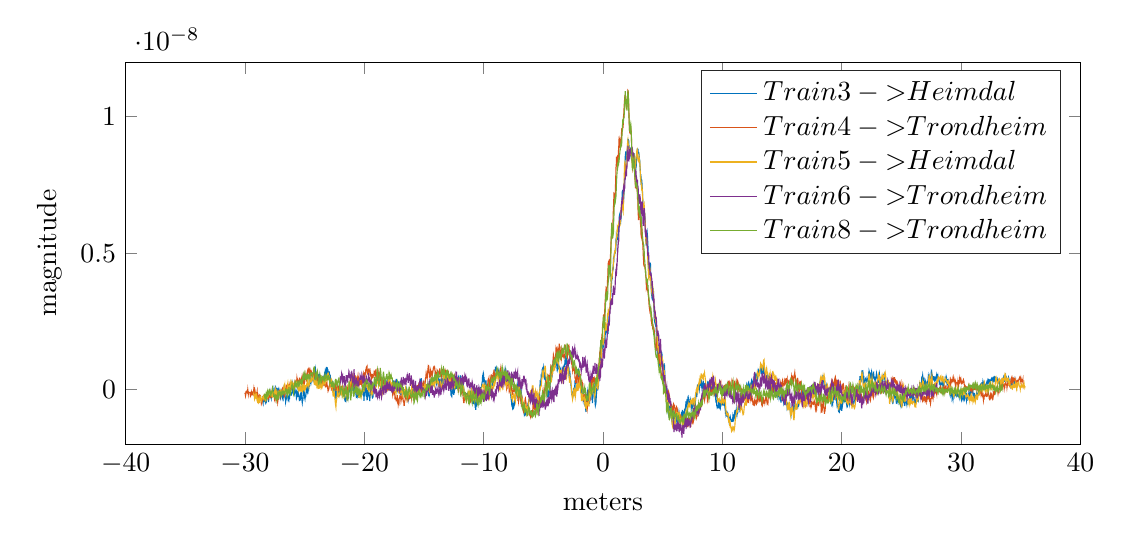
\begin{tikzpicture}

  \begin{axis}[%
    width=\textwidth,
    height=0.4\textwidth,
    at={(0\figurewidth,0\figureheight)},
    scale only axis,
    xmin=-40,
    xmax=40,
    xlabel={meters},
    ymin=-2e-09,
    ymax=1.2e-08,
    ylabel={magnitude},
    axis background/.style={fill=white},
    % title style={font=\bfseries},
    % title={influence lines for sensor 1},
    legend style={legend cell align=left,align=left,draw=white!15!black}
    ]
    \addplot [color=mycolor1,solid]
    table[row sep=crcr]{%
    -28.53908203125	-2.42432463976525e-10\\
    -28.518583984375	-3.23255849420965e-10\\
    -28.4980859375	-4.42343087844999e-10\\
    -28.477587890625	-4.88480902776024e-10\\
    -28.45708984375	-3.60310441102158e-10\\
    -28.436591796875	-3.96549475576617e-10\\
    -28.41609375	-4.05601785796435e-10\\
    -28.395595703125	-3.01178498671471e-10\\
    -28.37509765625	-3.29276214424073e-10\\
    -28.354599609375	-3.53914382054028e-10\\
    -28.3341015625	-2.94329300088123e-10\\
    -28.313603515625	-3.34436759961143e-10\\
    -28.29310546875	-4.69107766106467e-10\\
    -28.272607421875	-4.62579450742619e-10\\
    -28.252109375	-4.98854671956688e-10\\
    -28.231611328125	-4.75479960196443e-10\\
    -28.21111328125	-3.20446264658053e-10\\
    -28.190615234375	-3.58312570518101e-10\\
    -28.1701171875	-2.6667868901763e-10\\
    -28.149619140625	-2.287629187887e-10\\
    -28.12912109375	-2.35474923801234e-10\\
    -28.108623046875	-2.24605584523021e-10\\
    -28.088125	-2.27897694239274e-10\\
    -28.067626953125	-3.12585132409704e-10\\
    -28.04712890625	-3.57047025125366e-10\\
    -28.026630859375	-4.57212763583564e-10\\
    -28.0061328125	-3.66877212921925e-10\\
    -27.985634765625	-2.16965978828965e-10\\
    -27.96513671875	-1.95113556265998e-10\\
    -27.944638671875	-6.38877903963421e-11\\
    -27.924140625	-3.41374471925142e-11\\
    -27.903642578125	-1.2916136136789e-10\\
    -27.88314453125	-1.11644240463046e-10\\
    -27.862646484375	-1.46856112964341e-10\\
    -27.8421484375	-2.14085246063923e-10\\
    -27.821650390625	-2.63555849876305e-10\\
    -27.80115234375	-3.10581598027597e-10\\
    -27.780654296875	-2.03866523854126e-10\\
    -27.76015625	-1.524287292815e-10\\
    -27.739658203125	-9.28247326939465e-11\\
    -27.71916015625	-8.50442019209391e-11\\
    -27.698662109375	-1.88497671517331e-11\\
    -27.6781640625	2.27484533382019e-11\\
    -27.657666015625	5.66939984385784e-11\\
    -27.63716796875	-2.06620968117345e-11\\
    -27.616669921875	-9.82660644706859e-11\\
    -27.596171875	-1.05376026512635e-10\\
    -27.575673828125	-1.35619615444534e-10\\
    -27.55517578125	-9.01567144467863e-11\\
    -27.534677734375	-6.86490878601901e-11\\
    -27.5141796875	-1.16343445568424e-10\\
    -27.493681640625	4.39985123687983e-11\\
    -27.47318359375	4.39310949326402e-11\\
    -27.452685546875	1.08453591920635e-10\\
    -27.4321875	9.32509639604969e-11\\
    -27.411689453125	8.48885196639028e-11\\
    -27.39119140625	1.40375321941603e-11\\
    -27.370693359375	-9.9378820005732e-11\\
    -27.3501953125	-9.81019329716345e-11\\
    -27.329697265625	-7.7379306253939e-11\\
    -27.30919921875	-1.65584043500985e-10\\
    -27.288701171875	-5.10802693648461e-11\\
    -27.268203125	-8.9117735784694e-11\\
    -27.247705078125	-8.44785871702324e-12\\
    -27.22720703125	2.49969620863424e-11\\
    -27.206708984375	2.46710819336119e-11\\
    -27.1862109375	-7.48863762085572e-12\\
    -27.165712890625	2.30509274907517e-11\\
    -27.14521484375	-2.96480079615425e-11\\
    -27.124716796875	-1.22762481852331e-10\\
    -27.10421875	-1.12991889752861e-10\\
    -27.083720703125	-1.41190547239261e-10\\
    -27.06322265625	-2.29389173482235e-10\\
    -27.042724609375	-1.76467414095179e-10\\
    -27.0222265625	-2.3627090542664e-10\\
    -27.001728515625	-9.31022821648417e-11\\
    -26.98123046875	-1.04945065081801e-10\\
    -26.960732421875	-4.10694063493072e-11\\
    -26.940234375	-6.87349128785862e-11\\
    -26.919736328125	-1.23964485545686e-10\\
    -26.89923828125	-1.75486441477889e-10\\
    -26.878740234375	-2.68606143370957e-10\\
    -26.8582421875	-2.93758218302625e-10\\
    -26.837744140625	-3.29043058201038e-10\\
    -26.81724609375	-2.50229922070379e-10\\
    -26.796748046875	-2.91720995111193e-10\\
    -26.77625	-1.36748936579476e-10\\
    -26.755751953125	-1.0401772999358e-10\\
    -26.73525390625	-5.20136587361358e-12\\
    -26.714755859375	-8.28580857933807e-11\\
    -26.6942578125	3.25512384323039e-12\\
    -26.673759765625	-1.19572455729444e-10\\
    -26.65326171875	-1.72896256979302e-10\\
    -26.632763671875	-3.0861664601898e-10\\
    -26.612265625	-3.05296165756242e-10\\
    -26.591767578125	-4.46477117404942e-10\\
    -26.57126953125	-3.87285442528268e-10\\
    -26.550771484375	-3.79366032130347e-10\\
    -26.5302734375	-2.79281838178277e-10\\
    -26.509775390625	-2.51122482999767e-10\\
    -26.48927734375	-2.09629566262389e-10\\
    -26.468779296875	-1.92453734351367e-10\\
    -26.44828125	-1.44815322824779e-10\\
    -26.427783203125	-2.3704955916882e-10\\
    -26.40728515625	-2.99031009831917e-10\\
    -26.386787109375	-1.97075018802471e-10\\
    -26.3662890625	-3.46142414107179e-10\\
    -26.345791015625	-3.62585107282859e-10\\
    -26.32529296875	-3.88400269425861e-10\\
    -26.304794921875	-2.83266927762978e-10\\
    -26.284296875	-2.61776935143811e-10\\
    -26.263798828125	-2.84062493038057e-10\\
    -26.24330078125	-1.51260994854228e-10\\
    -26.222802734375	-1.81954876395575e-10\\
    -26.2023046875	-1.95070987756836e-10\\
    -26.181806640625	-1.96267201805321e-10\\
    -26.16130859375	-1.80816574557286e-10\\
    -26.140810546875	-1.97930056785899e-10\\
    -26.1203125	-2.03190976267253e-10\\
    -26.099814453125	-1.67674287174222e-10\\
    -26.07931640625	-1.12153896610044e-10\\
    -26.058818359375	-1.08749576087527e-10\\
    -26.0383203125	5.62087640518572e-11\\
    -26.017822265625	8.21587833128849e-12\\
    -25.99732421875	1.83017821603523e-10\\
    -25.976826171875	1.29202847193506e-10\\
    -25.956328125	1.23749555911484e-10\\
    -25.935830078125	-2.3632105080288e-12\\
    -25.91533203125	-1.68066315709562e-11\\
    -25.894833984375	-1.25581357996754e-10\\
    -25.8743359375	-2.85948148607479e-11\\
    -25.853837890625	-1.38917007814064e-10\\
    -25.83333984375	-9.72360575822185e-11\\
    -25.812841796875	-7.16999090185428e-11\\
    -25.79234375	-3.9544202502839e-11\\
    -25.771845703125	-9.02974505956738e-11\\
    -25.75134765625	-1.12143471670516e-10\\
    -25.730849609375	-9.57266765608488e-11\\
    -25.7103515625	-2.03159546279675e-10\\
    -25.689853515625	-1.38377594435741e-10\\
    -25.66935546875	-2.78500585704785e-10\\
    -25.648857421875	-2.34301425844046e-10\\
    -25.628359375	-1.30361558332022e-10\\
    -25.607861328125	-2.73110563969769e-10\\
    -25.58736328125	-1.51835358872657e-10\\
    -25.566865234375	-2.04791667314648e-10\\
    -25.5463671875	-2.19597418179874e-10\\
    -25.525869140625	-1.38315139615302e-10\\
    -25.50537109375	-2.05655921201357e-10\\
    -25.484873046875	-2.16344813737997e-10\\
    -25.464375	-2.58071778892159e-10\\
    -25.443876953125	-4.0255984440157e-10\\
    -25.42337890625	-3.96989147330398e-10\\
    -25.402880859375	-3.82198109572134e-10\\
    -25.3823828125	-3.64259326663304e-10\\
    -25.361884765625	-2.51108468325296e-10\\
    -25.34138671875	-2.87211354620859e-10\\
    -25.320888671875	-1.86566732315788e-10\\
    -25.300390625	-1.06551956521931e-10\\
    -25.279892578125	-1.15372283678584e-10\\
    -25.25939453125	-3.00156188334196e-10\\
    -25.238896484375	-3.17743950182121e-10\\
    -25.2183984375	-4.20514852268409e-10\\
    -25.197900390625	-4.87316857004543e-10\\
    -25.17740234375	-4.06437951334752e-10\\
    -25.156904296875	-4.00899076301748e-10\\
    -25.13640625	-3.0866181595622e-10\\
    -25.115908203125	-1.35575211842145e-10\\
    -25.09541015625	4.32948882767002e-13\\
    -25.074912109375	-1.41232428724987e-11\\
    -25.0544140625	-1.07518194991917e-10\\
    -25.033916015625	-9.24278032837129e-11\\
    -25.01341796875	-2.08025903372471e-10\\
    -24.992919921875	-3.06219314425481e-10\\
    -24.972421875	-3.48078778376712e-10\\
    -24.951923828125	-2.58031626423418e-10\\
    -24.93142578125	-2.56877378610011e-10\\
    -24.910927734375	-2.62997986742775e-10\\
    -24.8904296875	-1.72574947173134e-10\\
    -24.869931640625	-1.27988709753417e-11\\
    -24.84943359375	1.93033967441206e-11\\
    -24.828935546875	-4.15977311870775e-11\\
    -24.8084375	-4.27063579102865e-12\\
    -24.787939453125	-3.84896173075267e-11\\
    -24.76744140625	3.07383161915568e-11\\
    -24.746943359375	-4.33147236810481e-11\\
    -24.7264453125	2.93565102889779e-11\\
    -24.705947265625	-3.40794663708724e-11\\
    -24.68544921875	3.05880703999791e-11\\
    -24.664951171875	1.70821292016648e-11\\
    -24.644453125	1.22650044684207e-10\\
    -24.623955078125	1.27246821750176e-10\\
    -24.60345703125	2.10215991564352e-10\\
    -24.582958984375	1.86135077634439e-10\\
    -24.5624609375	2.84390735057775e-10\\
    -24.541962890625	2.98865614053442e-10\\
    -24.52146484375	3.79402697166947e-10\\
    -24.500966796875	3.19475616958402e-10\\
    -24.48046875	3.42288901178129e-10\\
    -24.459970703125	2.67083245100772e-10\\
    -24.43947265625	3.20311206503607e-10\\
    -24.418974609375	3.17040667962604e-10\\
    -24.3984765625	3.83547282467471e-10\\
    -24.377978515625	4.02705921673004e-10\\
    -24.35748046875	4.64789124873925e-10\\
    -24.336982421875	4.71498431401608e-10\\
    -24.316484375	4.14586195290773e-10\\
    -24.295986328125	4.77450769070853e-10\\
    -24.27548828125	3.65324756249261e-10\\
    -24.254990234375	4.02133142091454e-10\\
    -24.2344921875	4.1204871748625e-10\\
    -24.213994140625	4.21779611763754e-10\\
    -24.19349609375	3.64098598536646e-10\\
    -24.172998046875	5.17325064841423e-10\\
    -24.1525	4.73677052183486e-10\\
    -24.132001953125	7.04121437906612e-10\\
    -24.11150390625	6.23285727482992e-10\\
    -24.091005859375	7.27594645826054e-10\\
    -24.0705078125	6.50243684610334e-10\\
    -24.050009765625	5.41174081574631e-10\\
    -24.02951171875	4.9401621954105e-10\\
    -24.009013671875	5.14039109504764e-10\\
    -23.988515625	4.87665161509945e-10\\
    -23.968017578125	3.95927188264053e-10\\
    -23.94751953125	3.79155940912439e-10\\
    -23.927021484375	4.77438537004303e-10\\
    -23.9065234375	5.52821401289448e-10\\
    -23.886025390625	3.87606541241366e-10\\
    -23.86552734375	5.60562834933619e-10\\
    -23.845029296875	4.32717395947627e-10\\
    -23.82453125	5.22543199657409e-10\\
    -23.804033203125	3.53841414574437e-10\\
    -23.78353515625	4.25901987852324e-10\\
    -23.763037109375	4.84400665986875e-10\\
    -23.7425390625	3.79124859140587e-10\\
    -23.722041015625	4.94346291431105e-10\\
    -23.70154296875	4.10831016945326e-10\\
    -23.681044921875	4.65443657620662e-10\\
    -23.660546875	4.53518093675535e-10\\
    -23.640048828125	4.37721478732768e-10\\
    -23.61955078125	3.69252834769176e-10\\
    -23.599052734375	4.49855052777846e-10\\
    -23.5785546875	2.78653014200117e-10\\
    -23.558056640625	2.89226056091048e-10\\
    -23.53755859375	2.99073165099486e-10\\
    -23.517060546875	2.95973886984162e-10\\
    -23.4965625	1.89848890098662e-10\\
    -23.476064453125	3.22393829016736e-10\\
    -23.45556640625	1.6390186079679e-10\\
    -23.435068359375	3.46781531536905e-10\\
    -23.4145703125	2.97109348427208e-10\\
    -23.394072265625	4.3473131884735e-10\\
    -23.37357421875	4.36811025268644e-10\\
    -23.353076171875	5.02221949848493e-10\\
    -23.332578125	4.30284990163707e-10\\
    -23.312080078125	5.16642140048424e-10\\
    -23.29158203125	6.03562901486804e-10\\
    -23.271083984375	5.33276818744645e-10\\
    -23.2505859375	6.12466237226795e-10\\
    -23.230087890625	5.7021423334151e-10\\
    -23.20958984375	6.73509953407802e-10\\
    -23.189091796875	6.38490389066768e-10\\
    -23.16859375	8.28569706317133e-10\\
    -23.148095703125	7.14468570381893e-10\\
    -23.12759765625	7.3610772001961e-10\\
    -23.107099609375	8.12648211470292e-10\\
    -23.0866015625	5.46668172067143e-10\\
    -23.066103515625	7.48996333064468e-10\\
    -23.04560546875	6.16958554820236e-10\\
    -23.025107421875	4.72320867264757e-10\\
    -23.004609375	5.50268988312912e-10\\
    -22.984111328125	4.81519583469517e-10\\
    -22.96361328125	5.0664780060059e-10\\
    -22.943115234375	6.63823390003033e-10\\
    -22.9226171875	5.71676264648179e-10\\
    -22.902119140625	5.63680548421895e-10\\
    -22.88162109375	5.28296915197076e-10\\
    -22.861123046875	4.300138883988e-10\\
    -22.840625	4.48950385837297e-10\\
    -22.820126953125	3.49305773389595e-10\\
    -22.79962890625	1.70479639515498e-10\\
    -22.779130859375	9.42548802059219e-11\\
    -22.7586328125	2.20261678318734e-10\\
    -22.738134765625	2.22127314329253e-10\\
    -22.71763671875	2.9838535146622e-10\\
    -22.697138671875	2.91689685564066e-10\\
    -22.676640625	2.85575466960816e-10\\
    -22.656142578125	1.64701484149708e-10\\
    -22.63564453125	1.47143233885048e-10\\
    -22.615146484375	-1.97440618285175e-11\\
    -22.5946484375	-3.84909982664016e-11\\
    -22.574150390625	-1.29703421066267e-10\\
    -22.55365234375	-1.10985815914594e-10\\
    -22.533154296875	6.31440403845754e-12\\
    -22.51265625	1.9792603680271e-11\\
    -22.492158203125	4.88013821864418e-11\\
    -22.47166015625	1.88458165063384e-10\\
    -22.451162109375	8.35033482452694e-11\\
    -22.4306640625	-2.67603502328478e-11\\
    -22.410166015625	-3.69971422047308e-11\\
    -22.38966796875	-3.3645043524023e-10\\
    -22.369169921875	-2.54936475245048e-10\\
    -22.348671875	-3.91682261474449e-10\\
    -22.328173828125	-1.48769049328933e-10\\
    -22.30767578125	-2.57478205550678e-10\\
    -22.287177734375	-8.55854494800401e-11\\
    -22.2666796875	-9.43870131653846e-11\\
    -22.246181640625	1.7721832238179e-10\\
    -22.22568359375	-4.78497482071435e-12\\
    -22.205185546875	1.30290186519489e-10\\
    -22.1846875	1.40031881953166e-11\\
    -22.164189453125	-2.18220317945106e-11\\
    -22.14369140625	-1.24429679349178e-10\\
    -22.123193359375	-7.08600000385786e-11\\
    -22.1026953125	-2.45700763768097e-10\\
    -22.082197265625	-1.51126710005575e-10\\
    -22.06169921875	-1.11102631284205e-10\\
    -22.041201171875	-6.36336997601866e-11\\
    -22.020703125	-8.65607008156424e-11\\
    -22.000205078125	-7.05197127913619e-12\\
    -21.97970703125	-2.71831991310351e-11\\
    -21.959208984375	1.18838411121936e-10\\
    -21.9387109375	-1.93543721645697e-12\\
    -21.918212890625	4.18426529039133e-13\\
    -21.89771484375	1.18539759628936e-11\\
    -21.877216796875	-3.39975277374191e-11\\
    -21.85671875	-6.42082737643145e-12\\
    -21.836220703125	-5.60710673662991e-11\\
    -21.81572265625	2.56143442158228e-11\\
    -21.795224609375	-8.8617106018743e-12\\
    -21.7747265625	2.73540862109055e-11\\
    -21.754228515625	-1.33733891568678e-10\\
    -21.73373046875	2.31406250335787e-11\\
    -21.713232421875	-1.13872840319072e-10\\
    -21.692734375	-1.45882254666255e-10\\
    -21.672236328125	-2.37221205807634e-10\\
    -21.65173828125	-2.46949888844117e-10\\
    -21.631240234375	-3.99827015146344e-10\\
    -21.6107421875	-4.16710408241621e-10\\
    -21.590244140625	-3.99329853373332e-10\\
    -21.56974609375	-3.69606586268905e-10\\
    -21.549248046875	-3.95690693084701e-10\\
    -21.52875	-2.81529628416859e-10\\
    -21.508251953125	-2.06364749462386e-10\\
    -21.48775390625	-2.72950576274304e-10\\
    -21.467255859375	-1.0133729165997e-10\\
    -21.4467578125	-2.4532548933499e-10\\
    -21.426259765625	-2.30951034449219e-10\\
    -21.40576171875	-4.05956504144463e-10\\
    -21.385263671875	-1.8160551403991e-10\\
    -21.364765625	-3.26851066999353e-10\\
    -21.344267578125	-2.25615726472064e-10\\
    -21.32376953125	-2.46497333711807e-10\\
    -21.303271484375	-2.47581214864832e-11\\
    -21.2827734375	-1.77256202864696e-11\\
    -21.262275390625	-5.5252207516645e-12\\
    -21.24177734375	1.64381631844488e-10\\
    -21.221279296875	4.73458962461572e-11\\
    -21.20078125	1.0084927471415e-10\\
    -21.180283203125	3.0834371802497e-11\\
    -21.15978515625	1.36111397236516e-10\\
    -21.139287109375	8.62229307540838e-11\\
    -21.1187890625	1.62597501883518e-10\\
    -21.098291015625	1.57994563287646e-10\\
    -21.07779296875	2.78600292576321e-10\\
    -21.057294921875	2.49741150349261e-10\\
    -21.036796875	2.15910078582386e-10\\
    -21.016298828125	1.74161775516034e-10\\
    -20.99580078125	2.70167190133558e-10\\
    -20.975302734375	-2.75049031140946e-11\\
    -20.9548046875	2.04650766786522e-10\\
    -20.934306640625	-4.63535346656993e-11\\
    -20.91380859375	1.00719544020583e-11\\
    -20.893310546875	-4.65667976906526e-11\\
    -20.8728125	7.31631781646805e-12\\
    -20.852314453125	1.95497258342494e-11\\
    -20.83181640625	1.51850182766983e-11\\
    -20.811318359375	8.280709701507e-11\\
    -20.7908203125	-1.06322324664081e-10\\
    -20.770322265625	9.60903278692484e-11\\
    -20.74982421875	-8.76088440930094e-11\\
    -20.729326171875	-2.10449007023787e-11\\
    -20.708828125	-1.1688976030507e-10\\
    -20.688330078125	-7.00855309079967e-11\\
    -20.66783203125	-2.50973187592523e-10\\
    -20.647333984375	-2.31005913244209e-10\\
    -20.6268359375	-1.98790439127558e-10\\
    -20.606337890625	-3.00830235946201e-10\\
    -20.58583984375	-5.90165175106527e-11\\
    -20.565341796875	-1.99657734238226e-10\\
    -20.54484375	-1.55523231865961e-10\\
    -20.524345703125	-1.1688773725939e-10\\
    -20.50384765625	-2.2794212020159e-10\\
    -20.483349609375	-7.88618669567596e-11\\
    -20.4628515625	-2.92678659483946e-10\\
    -20.442353515625	-1.56024095635845e-10\\
    -20.42185546875	-2.2506609045754e-10\\
    -20.401357421875	-1.91036081585041e-10\\
    -20.380859375	-1.63554952033701e-10\\
    -20.360361328125	-6.43655508896391e-11\\
    -20.33986328125	-1.18982628015657e-10\\
    -20.319365234375	-7.91582277975989e-11\\
    -20.2988671875	-7.1207645585137e-11\\
    -20.278369140625	-8.05252444712304e-11\\
    -20.25787109375	-2.54767863240876e-10\\
    -20.237373046875	-1.83460048708829e-10\\
    -20.216875	-1.14408533489765e-10\\
    -20.196376953125	-2.09621969887989e-10\\
    -20.17587890625	-1.10893940106256e-10\\
    -20.155380859375	-5.1892030093861e-11\\
    -20.1348828125	8.62680934588685e-11\\
    -20.114384765625	-3.85363558431994e-11\\
    -20.09388671875	-6.44463130463606e-11\\
    -20.073388671875	-1.00351373522834e-10\\
    -20.052890625	-1.03999049008291e-10\\
    -20.032392578125	-4.17462336725826e-10\\
    -20.01189453125	-9.59500262212268e-11\\
    -19.991396484375	-2.31943863828125e-10\\
    -19.9708984375	-2.22620754456379e-10\\
    -19.950400390625	-1.03377266463775e-10\\
    -19.92990234375	5.48104375081192e-12\\
    -19.909404296875	-9.1403190935284e-11\\
    -19.88890625	2.33236931396001e-10\\
    -19.868408203125	-1.00419246809165e-10\\
    -19.84791015625	1.45687190171597e-10\\
    -19.827412109375	-2.69325210756052e-10\\
    -19.8069140625	-1.43833296678376e-10\\
    -19.786416015625	-2.73388370087392e-10\\
    -19.76591796875	-2.33331034930794e-10\\
    -19.745419921875	-3.89684798950993e-10\\
    -19.724921875	-1.24985615550201e-10\\
    -19.704423828125	-1.53751288923747e-10\\
    -19.68392578125	-3.54250262700705e-11\\
    -19.663427734375	-5.94565417528477e-11\\
    -19.6429296875	1.17420004482983e-11\\
    -19.622431640625	-1.96008415275973e-10\\
    -19.60193359375	-2.12995834607837e-10\\
    -19.581435546875	-2.75647653497749e-10\\
    -19.5609375	-2.90439821654287e-10\\
    -19.540439453125	-4.24093599274614e-10\\
    -19.51994140625	-2.25181621481276e-10\\
    -19.499443359375	-2.12673852104628e-10\\
    -19.4789453125	-9.51961415829377e-11\\
    -19.458447265625	-5.76571873868302e-11\\
    -19.43794921875	6.01357110796887e-11\\
    -19.417451171875	4.99582669612489e-11\\
    -19.396953125	-5.54325781792318e-11\\
    -19.376455078125	-6.10443441161957e-11\\
    -19.35595703125	-1.82072567482592e-10\\
    -19.335458984375	-2.4677468230231e-10\\
    -19.3149609375	-3.04851322100341e-10\\
    -19.294462890625	-2.96975151057571e-10\\
    -19.27396484375	-2.58439288923987e-10\\
    -19.253466796875	-3.80706603145059e-11\\
    -19.23296875	-1.09271229191184e-10\\
    -19.212470703125	8.46466784195196e-11\\
    -19.19197265625	1.09901394593307e-10\\
    -19.171474609375	2.11238813406386e-10\\
    -19.1509765625	1.01605070727722e-10\\
    -19.130478515625	2.28418973074007e-10\\
    -19.10998046875	1.57812481362105e-10\\
    -19.089482421875	8.40144383938498e-11\\
    -19.068984375	6.79194027543881e-11\\
    -19.048486328125	1.19028777070408e-10\\
    -19.02798828125	1.16497391111581e-10\\
    -19.007490234375	1.27356966312087e-10\\
    -18.9869921875	1.79199377375629e-10\\
    -18.966494140625	4.33316569008867e-10\\
    -18.94599609375	3.81659053974682e-10\\
    -18.925498046875	4.43335325803948e-10\\
    -18.905	5.04040205930144e-10\\
    -18.884501953125	4.06841255355346e-10\\
    -18.86400390625	3.41222508116328e-10\\
    -18.843505859375	2.69741776214776e-10\\
    -18.8230078125	2.45537061961895e-10\\
    -18.802509765625	1.41888514896468e-10\\
    -18.78201171875	2.63733076660142e-10\\
    -18.761513671875	1.6540225761644e-10\\
    -18.741015625	1.86981937401375e-10\\
    -18.720517578125	4.09363732554522e-10\\
    -18.70001953125	2.44411795183896e-10\\
    -18.679521484375	3.77967396598307e-10\\
    -18.6590234375	1.76437651971343e-10\\
    -18.638525390625	1.55393450327141e-10\\
    -18.61802734375	4.22679387453643e-11\\
    -18.597529296875	5.86055939983596e-11\\
    -18.57703125	-9.14995414368648e-11\\
    -18.556533203125	-8.27279690580506e-11\\
    -18.53603515625	1.23414213374265e-11\\
    -18.515537109375	1.59643598446146e-10\\
    -18.4950390625	8.73919600029787e-11\\
    -18.474541015625	1.99135245708017e-10\\
    -18.45404296875	-1.66738289838114e-11\\
    -18.433544921875	1.2790226953366e-10\\
    -18.413046875	4.42350601496876e-11\\
    -18.392548828125	7.96419189022545e-11\\
    -18.37205078125	1.21154363928816e-10\\
    -18.351552734375	1.586535165811e-10\\
    -18.3310546875	2.78028122530492e-10\\
    -18.310556640625	3.12820597388293e-10\\
    -18.29005859375	3.11659761274096e-10\\
    -18.269560546875	3.39205753681696e-10\\
    -18.2490625	3.01580515699639e-10\\
    -18.228564453125	1.8079936355973e-10\\
    -18.20806640625	1.93249739082551e-10\\
    -18.187568359375	7.77075875459527e-11\\
    -18.1670703125	2.03086246287135e-10\\
    -18.146572265625	7.92291613715199e-11\\
    -18.12607421875	2.32773508527994e-10\\
    -18.105576171875	3.65065219977523e-10\\
    -18.085078125	6.17033129978897e-11\\
    -18.064580078125	2.95030412429936e-10\\
    -18.04408203125	1.86001135501412e-10\\
    -18.023583984375	1.92826737210053e-10\\
    -18.0030859375	6.45490712608484e-11\\
    -17.982587890625	4.07397369489149e-11\\
    -17.96208984375	2.09151336365801e-10\\
    -17.941591796875	3.71757588130793e-11\\
    -17.92109375	1.60879334731151e-10\\
    -17.900595703125	2.77388871863996e-10\\
    -17.88009765625	2.3548581439777e-10\\
    -17.859599609375	2.43865449359166e-10\\
    -17.8391015625	2.54574612812065e-10\\
    -17.818603515625	1.87418839064782e-10\\
    -17.79810546875	1.97494633975179e-10\\
    -17.777607421875	1.63807147513526e-11\\
    -17.757109375	1.51307972968712e-10\\
    -17.736611328125	1.141960604899e-10\\
    -17.71611328125	5.59464552537092e-11\\
    -17.695615234375	2.19530161372737e-10\\
    -17.6751171875	1.49064249002282e-10\\
    -17.654619140625	1.82851652210347e-10\\
    -17.63412109375	1.70996788896021e-10\\
    -17.613623046875	2.39990745303902e-10\\
    -17.593125	2.2295051945315e-10\\
    -17.572626953125	2.21813026332167e-10\\
    -17.55212890625	8.84495382750591e-11\\
    -17.531630859375	3.36803845868021e-10\\
    -17.5111328125	5.25876600084127e-11\\
    -17.490634765625	1.95418467741627e-10\\
    -17.47013671875	1.59348517207627e-10\\
    -17.449638671875	1.97176869782748e-10\\
    -17.429140625	1.62973679040933e-10\\
    -17.408642578125	2.71435322062757e-10\\
    -17.38814453125	1.38904895668947e-10\\
    -17.367646484375	3.13773355008875e-10\\
    -17.3471484375	4.26630747597984e-11\\
    -17.326650390625	3.88283840141377e-10\\
    -17.30615234375	2.51194325849686e-11\\
    -17.285654296875	1.49286582483876e-10\\
    -17.26515625	-3.70541889745352e-11\\
    -17.244658203125	9.93819504876695e-11\\
    -17.22416015625	3.76791827375121e-11\\
    -17.203662109375	1.72952578053722e-10\\
    -17.1831640625	2.37942053789793e-10\\
    -17.162666015625	2.31264731986157e-10\\
    -17.14216796875	2.64792388291773e-10\\
    -17.121669921875	2.7368604978948e-10\\
    -17.101171875	2.0222999468327e-10\\
    -17.080673828125	2.18788276136535e-10\\
    -17.06017578125	4.28936702044988e-11\\
    -17.039677734375	1.13928728670705e-10\\
    -17.0191796875	-5.35134274501428e-11\\
    -16.998681640625	-4.03636150263938e-11\\
    -16.97818359375	-1.96901562530478e-10\\
    -16.957685546875	-7.37504128023902e-11\\
    -16.9371875	-2.2017473390884e-10\\
    -16.916689453125	-8.73473737314942e-11\\
    -16.89619140625	-6.91581684665028e-11\\
    -16.875693359375	-7.88357369923045e-11\\
    -16.8551953125	7.85366145853017e-11\\
    -16.834697265625	1.34593668139251e-11\\
    -16.81419921875	9.54647735854294e-11\\
    -16.793701171875	-3.67232822194374e-11\\
    -16.773203125	-2.99704981068041e-11\\
    -16.752705078125	-1.2624923345888e-10\\
    -16.73220703125	-8.69811989016394e-11\\
    -16.711708984375	-1.70090777067916e-10\\
    -16.6912109375	-5.15376821154804e-11\\
    -16.670712890625	-6.85470456941074e-11\\
    -16.65021484375	8.66903673399217e-12\\
    -16.629716796875	-1.28552849140222e-10\\
    -16.60921875	-2.02718418765374e-10\\
    -16.588720703125	-2.05272642440426e-10\\
    -16.56822265625	-2.52041115948345e-10\\
    -16.547724609375	-2.21056955730837e-10\\
    -16.5272265625	-2.020289899641e-10\\
    -16.506728515625	-1.23594435284019e-10\\
    -16.48623046875	-8.35624399709951e-11\\
    -16.465732421875	-7.33465951958552e-11\\
    -16.445234375	3.22199702648632e-12\\
    -16.424736328125	-6.01868584048012e-11\\
    -16.40423828125	-9.1890823537471e-11\\
    -16.383740234375	-1.67330123583214e-10\\
    -16.3632421875	-2.86747297184345e-10\\
    -16.342744140625	-2.9485577144772e-10\\
    -16.32224609375	-3.74847539222641e-10\\
    -16.301748046875	-3.13009665274873e-10\\
    -16.28125	-3.82952178556269e-10\\
    -16.260751953125	-1.96527055168601e-10\\
    -16.24025390625	-2.26574088651537e-10\\
    -16.219755859375	-1.61359672392329e-10\\
    -16.1992578125	-4.84374843663153e-11\\
    -16.178759765625	-1.5384702026522e-10\\
    -16.15826171875	-4.26211074837964e-12\\
    -16.137763671875	-2.3822969003827e-10\\
    -16.117265625	-7.20500609238373e-11\\
    -16.096767578125	-1.45251813875802e-10\\
    -16.07626953125	-9.55558593982492e-11\\
    -16.055771484375	-1.86078768339882e-10\\
    -16.0352734375	-8.92366889800484e-11\\
    -16.014775390625	-6.79973526369702e-11\\
    -15.99427734375	8.60509085756035e-11\\
    -15.973779296875	-1.25291792644761e-10\\
    -15.95328125	1.14688201356929e-10\\
    -15.932783203125	-2.7122489724124e-11\\
    -15.91228515625	-8.73400365315535e-12\\
    -15.891787109375	-1.19386463714485e-10\\
    -15.8712890625	-1.80644783882297e-10\\
    -15.850791015625	-2.1124792229543e-10\\
    -15.83029296875	-1.7125151535906e-10\\
    -15.809794921875	-2.3745956437128e-10\\
    -15.789296875	-1.76387078956959e-10\\
    -15.768798828125	-2.1707548759208e-10\\
    -15.74830078125	-6.28357087807495e-11\\
    -15.727802734375	-5.72089047293382e-11\\
    -15.7073046875	-3.92665443080929e-11\\
    -15.686806640625	1.46575439216156e-11\\
    -15.66630859375	-8.96680973176235e-11\\
    -15.645810546875	-1.01494568494214e-10\\
    -15.6253125	-1.55324239231308e-10\\
    -15.604814453125	-1.86877072424451e-10\\
    -15.58431640625	-1.25828868841534e-10\\
    -15.563818359375	-2.39814401126928e-10\\
    -15.5433203125	-1.06132729247022e-10\\
    -15.522822265625	-1.13527760332474e-10\\
    -15.50232421875	8.31018072673445e-11\\
    -15.481826171875	1.24562537214656e-10\\
    -15.461328125	1.11242626874162e-10\\
    -15.440830078125	2.14260618733604e-10\\
    -15.42033203125	-2.70800923943093e-11\\
    -15.399833984375	-2.74817107793722e-11\\
    -15.3793359375	-2.08500759769855e-11\\
    -15.358837890625	-1.03386520400296e-10\\
    -15.33833984375	-5.24803939313347e-11\\
    -15.317841796875	6.58106562973832e-11\\
    -15.29734375	5.16407618325581e-11\\
    -15.276845703125	3.90048710058337e-10\\
    -15.25634765625	2.83461899266419e-10\\
    -15.235849609375	4.12876075651724e-10\\
    -15.2153515625	3.38671235983093e-10\\
    -15.194853515625	2.3093595827922e-10\\
    -15.17435546875	2.02050651202068e-10\\
    -15.153857421875	1.31412096227512e-10\\
    -15.133359375	-3.68882077833282e-11\\
    -15.112861328125	-1.67045303295517e-11\\
    -15.09236328125	-2.4200908520411e-11\\
    -15.071865234375	6.80052935648525e-11\\
    -15.0513671875	1.71801272021067e-10\\
    -15.030869140625	9.55479987631775e-11\\
    -15.01037109375	2.88294824451821e-10\\
    -14.989873046875	9.57096354476404e-11\\
    -14.969375	2.12096232615858e-10\\
    -14.948876953125	5.51479832545931e-11\\
    -14.92837890625	9.31824073367473e-11\\
    -14.907880859375	-4.9428101364425e-11\\
    -14.8873828125	1.21775329442717e-12\\
    -14.866884765625	-1.04274661296518e-10\\
    -14.84638671875	1.67301123819817e-10\\
    -14.825888671875	-2.40281807586676e-10\\
    -14.805390625	1.69707497331674e-10\\
    -14.784892578125	2.80033890010606e-11\\
    -14.76439453125	2.01854764190797e-10\\
    -14.743896484375	-7.3715219819409e-12\\
    -14.7233984375	1.01293891639192e-10\\
    -14.702900390625	-4.43198222300177e-11\\
    -14.68240234375	-6.87620600423429e-11\\
    -14.661904296875	-8.12769588493538e-11\\
    -14.64140625	-1.40303294054012e-10\\
    -14.620908203125	-1.91374376955111e-10\\
    -14.60041015625	-1.73445479427781e-10\\
    -14.579912109375	-2.4363022577908e-10\\
    -14.5594140625	-6.59493748783198e-11\\
    -14.538916015625	-1.34244486521273e-10\\
    -14.51841796875	-4.65781399213834e-11\\
    -14.497919921875	4.64501108971846e-11\\
    -14.477421875	1.31895454030383e-10\\
    -14.456923828125	1.33745373811579e-11\\
    -14.43642578125	2.33555114350244e-10\\
    -14.415927734375	1.09575091062643e-10\\
    -14.3954296875	7.91056459628107e-11\\
    -14.374931640625	1.17446217522732e-10\\
    -14.35443359375	2.4352536959034e-11\\
    -14.333935546875	1.28873033638316e-10\\
    -14.3134375	1.97737398692823e-11\\
    -14.292939453125	1.96207510726421e-10\\
    -14.27244140625	2.25786437890625e-10\\
    -14.251943359375	3.58212157163728e-10\\
    -14.2314453125	3.05033922931177e-10\\
    -14.210947265625	4.08046370786947e-10\\
    -14.19044921875	2.81742695130593e-10\\
    -14.169951171875	1.93340958397986e-10\\
    -14.149453125	2.26909662505337e-10\\
    -14.128955078125	2.66870182007259e-10\\
    -14.10845703125	3.30274921082738e-10\\
    -14.087958984375	3.8596092247659e-10\\
    -14.0674609375	3.88704905491872e-10\\
    -14.046962890625	5.16689933086824e-10\\
    -14.02646484375	4.64708540064523e-10\\
    -14.005966796875	4.65892614180554e-10\\
    -13.98546875	3.61696799095479e-10\\
    -13.964970703125	2.91035287941874e-10\\
    -13.94447265625	1.41763258349337e-10\\
    -13.923974609375	2.58747820509965e-10\\
    -13.9034765625	2.31432634873767e-10\\
    -13.882978515625	2.74927189344053e-10\\
    -13.86248046875	2.76699956301161e-10\\
    -13.841982421875	3.76200835047451e-10\\
    -13.821484375	4.20075483405605e-10\\
    -13.800986328125	4.21705431765621e-10\\
    -13.78048828125	4.36716934459625e-10\\
    -13.759990234375	3.49042736887801e-10\\
    -13.7394921875	2.06938228703285e-10\\
    -13.718994140625	1.4916081396628e-10\\
    -13.69849609375	1.14695584637434e-10\\
    -13.677998046875	2.24544893597766e-10\\
    -13.6575	1.62489335086133e-10\\
    -13.637001953125	2.39739529990643e-10\\
    -13.61650390625	3.10087665659285e-10\\
    -13.596005859375	3.44048597031945e-10\\
    -13.5755078125	3.29048417314687e-10\\
    -13.555009765625	3.66339803637339e-10\\
    -13.53451171875	2.4274780458662e-10\\
    -13.514013671875	2.38629162465296e-10\\
    -13.493515625	1.19013106352209e-10\\
    -13.473017578125	3.281096913598e-10\\
    -13.45251953125	9.55049634721267e-11\\
    -13.432021484375	4.05295011460204e-10\\
    -13.4115234375	1.84348766807902e-10\\
    -13.391025390625	4.10861731905258e-10\\
    -13.37052734375	3.91844458204634e-10\\
    -13.350029296875	3.54800972491962e-10\\
    -13.32953125	5.30488953147869e-10\\
    -13.309033203125	5.15003028372305e-10\\
    -13.28853515625	5.50034230657394e-10\\
    -13.268037109375	5.48728303165661e-10\\
    -13.2475390625	5.44650544077051e-10\\
    -13.227041015625	3.59567476513614e-10\\
    -13.20654296875	4.94678761308437e-10\\
    -13.186044921875	3.37887001780843e-10\\
    -13.165546875	4.60581180848863e-10\\
    -13.145048828125	4.60368056269431e-10\\
    -13.12455078125	4.56668626582289e-10\\
    -13.104052734375	4.2254206034142e-10\\
    -13.0835546875	5.40028609318613e-10\\
    -13.063056640625	5.92046867389735e-10\\
    -13.04255859375	5.31374422784674e-10\\
    -13.022060546875	5.80375684555827e-10\\
    -13.0015625	4.98241617146563e-10\\
    -12.981064453125	3.03940640406569e-10\\
    -12.96056640625	3.2614127452474e-10\\
    -12.940068359375	2.139159627646e-10\\
    -12.9195703125	2.80062706962013e-10\\
    -12.899072265625	1.23367197619977e-10\\
    -12.87857421875	2.27654311027882e-10\\
    -12.858076171875	1.96324311066269e-10\\
    -12.837578125	2.3614790697122e-10\\
    -12.817080078125	1.29594750829456e-10\\
    -12.79658203125	1.84660061036398e-10\\
    -12.776083984375	-2.14800364266949e-11\\
    -12.7555859375	-4.98068071021046e-11\\
    -12.735087890625	-1.99027975086324e-10\\
    -12.71458984375	-2.21857255374268e-10\\
    -12.694091796875	-2.34845501792787e-10\\
    -12.67359375	-2.53033928722428e-10\\
    -12.653095703125	-1.14766148778949e-10\\
    -12.63259765625	-9.6112995679778e-12\\
    -12.612099609375	-1.43290819806899e-11\\
    -12.5916015625	4.57331593331596e-11\\
    -12.571103515625	6.58868120607045e-11\\
    -12.55060546875	-5.98987801365382e-11\\
    -12.530107421875	-3.29135859863301e-11\\
    -12.509609375	-1.97512601827556e-10\\
    -12.489111328125	7.66687308843002e-11\\
    -12.46861328125	-1.29317593531553e-10\\
    -12.448115234375	1.56954815245455e-11\\
    -12.4276171875	9.33235372949705e-12\\
    -12.407119140625	3.72534049831376e-11\\
    -12.38662109375	1.2051521787138e-10\\
    -12.366123046875	2.1319552123109e-10\\
    -12.345625	1.6829060023272e-10\\
    -12.325126953125	3.3618040891371e-10\\
    -12.30462890625	2.79924072277572e-11\\
    -12.284130859375	2.91382488935396e-10\\
    -12.2636328125	3.00442578620239e-11\\
    -12.243134765625	8.7507984099066e-11\\
    -12.22263671875	9.21923886562605e-11\\
    -12.202138671875	3.52733452463922e-10\\
    -12.181640625	2.93168439570136e-10\\
    -12.161142578125	4.19010536918695e-10\\
    -12.14064453125	4.18402303462943e-10\\
    -12.120146484375	4.6608614605424e-10\\
    -12.0996484375	4.37560608166415e-10\\
    -12.079150390625	3.52080460113341e-10\\
    -12.05865234375	3.78117430129254e-10\\
    -12.038154296875	3.36821581302571e-10\\
    -12.01765625	3.74256986725704e-10\\
    -11.997158203125	4.13150614288536e-10\\
    -11.97666015625	3.42502671681764e-10\\
    -11.956162109375	5.18233890550485e-10\\
    -11.9356640625	3.50686539313521e-10\\
    -11.915166015625	4.86521423112054e-10\\
    -11.89466796875	3.94566872413698e-10\\
    -11.874169921875	2.36532422675704e-10\\
    -11.853671875	2.78378420653987e-10\\
    -11.833173828125	1.8346623795343e-10\\
    -11.81267578125	1.90627560359867e-10\\
    -11.792177734375	2.33424233828694e-10\\
    -11.7716796875	2.96114008839406e-10\\
    -11.751181640625	2.2957076007057e-10\\
    -11.73068359375	2.1124647870246e-10\\
    -11.710185546875	4.62989678492789e-11\\
    -11.6896875	1.20879271823741e-10\\
    -11.669189453125	2.34645678241947e-11\\
    -11.64869140625	-1.13708371840709e-11\\
    -11.628193359375	-6.76581104206927e-11\\
    -11.6076953125	-1.82080120264111e-10\\
    -11.587197265625	-2.60661005822582e-10\\
    -11.56669921875	-1.97703607500867e-10\\
    -11.546201171875	-3.65684455112817e-10\\
    -11.525703125	-2.00014751180085e-10\\
    -11.505205078125	-3.3361459801061e-10\\
    -11.48470703125	-2.65714924063797e-10\\
    -11.464208984375	-2.62015497372803e-10\\
    -11.4437109375	-1.51099955774915e-10\\
    -11.423212890625	-1.49256950022176e-10\\
    -11.40271484375	-2.13089203062343e-10\\
    -11.382216796875	-2.51243626996487e-10\\
    -11.36171875	-2.77796470646657e-10\\
    -11.341220703125	-2.53282679943977e-10\\
    -11.32072265625	-2.02752696168227e-10\\
    -11.300224609375	-3.62571869457964e-10\\
    -11.2797265625	-1.88790429203968e-10\\
    -11.259228515625	-3.01050881769802e-10\\
    -11.23873046875	-1.92001290672959e-10\\
    -11.218232421875	-1.13364961178314e-10\\
    -11.197734375	-1.20005449097742e-10\\
    -11.177236328125	-1.98406440543712e-10\\
    -11.15673828125	-1.19777036383493e-10\\
    -11.136240234375	-2.72385309697537e-10\\
    -11.1157421875	-3.55788225724785e-10\\
    -11.095244140625	-2.31621969325114e-10\\
    -11.07474609375	-2.41255051263184e-10\\
    -11.054248046875	-1.82076830630806e-10\\
    -11.03375	-7.8125805194209e-11\\
    -11.013251953125	-8.23155962803758e-11\\
    -10.99275390625	-3.63407641701626e-11\\
    -10.972255859375	-2.0637049674581e-10\\
    -10.9517578125	-1.25451528879529e-10\\
    -10.931259765625	-3.41776071327802e-10\\
    -10.91076171875	-2.90767686167395e-10\\
    -10.890263671875	-5.25942623210229e-10\\
    -10.869765625	-3.62043851349883e-10\\
    -10.849267578125	-3.22940852434604e-10\\
    -10.82876953125	-3.89082921217472e-10\\
    -10.808271484375	-2.94274395609548e-10\\
    -10.7877734375	-3.08002461310815e-10\\
    -10.767275390625	-3.44803847157703e-10\\
    -10.74677734375	-4.45580132668905e-10\\
    -10.726279296875	-3.86149519427841e-10\\
    -10.70578125	-6.6874724404819e-10\\
    -10.685283203125	-5.40304556916708e-10\\
    -10.66478515625	-7.42073648720238e-10\\
    -10.644287109375	-5.53477609131018e-10\\
    -10.6237890625	-6.27530907935807e-10\\
    -10.603291015625	-4.79058224000323e-10\\
    -10.58279296875	-4.83154322814849e-10\\
    -10.562294921875	-4.06015181046202e-10\\
    -10.541796875	-4.21520457560244e-10\\
    -10.521298828125	-4.4137568546861e-10\\
    -10.50080078125	-4.01132969283733e-10\\
    -10.480302734375	-4.39709483072748e-10\\
    -10.4598046875	-4.77204410699158e-10\\
    -10.439306640625	-3.46719478763832e-10\\
    -10.41880859375	-4.33460405662788e-10\\
    -10.398310546875	-2.55590163948186e-10\\
    -10.3778125	-2.81706114820694e-10\\
    -10.357314453125	-8.0094006336858e-11\\
    -10.33681640625	-8.89403421157544e-11\\
    -10.316318359375	-2.59035878162795e-11\\
    -10.2958203125	4.06417839155571e-12\\
    -10.275322265625	8.93204900202255e-11\\
    -10.25482421875	-2.75949376367034e-11\\
    -10.234326171875	6.65275076825998e-11\\
    -10.213828125	7.54289092650365e-11\\
    -10.193330078125	7.66598082408017e-11\\
    -10.17283203125	1.46605394610115e-10\\
    -10.152333984375	2.01221033250913e-10\\
    -10.1318359375	2.61772356876934e-10\\
    -10.111337890625	3.01609722901266e-10\\
    -10.09083984375	4.91056838180225e-10\\
    -10.070341796875	4.81695332487173e-10\\
    -10.04984375	5.41648613636899e-10\\
    -10.029345703125	4.3896285411223e-10\\
    -10.00884765625	4.85582890141612e-10\\
    -9.988349609375	2.70813734499347e-10\\
    -9.9678515625	3.94710522748566e-10\\
    -9.947353515625	1.61183873616087e-10\\
    -9.92685546875	2.56502983762653e-10\\
    -9.906357421875	1.75821509635299e-10\\
    -9.885859375	3.37941607559918e-10\\
    -9.865361328125	2.41580648810274e-10\\
    -9.84486328125	3.36152012262638e-10\\
    -9.824365234375	1.81385329219389e-10\\
    -9.8038671875	3.34768909998145e-10\\
    -9.783369140625	5.67223990902792e-11\\
    -9.76287109375	1.83312586748151e-10\\
    -9.742373046875	6.07127066042673e-11\\
    -9.721875	2.52661497099852e-13\\
    -9.701376953125	-7.08088274362757e-11\\
    -9.68087890625	-9.60490354774842e-11\\
    -9.660380859375	-3.26792964850382e-10\\
    -9.6398828125	-2.25455683934982e-10\\
    -9.619384765625	-3.00370356108669e-10\\
    -9.59888671875	-2.80331895628238e-10\\
    -9.578388671875	-1.89215111132175e-10\\
    -9.557890625	-2.41197557781325e-10\\
    -9.537392578125	-2.22761922391398e-10\\
    -9.51689453125	-1.54120254605e-10\\
    -9.496396484375	-1.78975942836991e-10\\
    -9.4758984375	-7.63413353016928e-11\\
    -9.455400390625	-1.48255088847727e-10\\
    -9.43490234375	-3.82733991070736e-12\\
    -9.414404296875	-1.91975242296469e-11\\
    -9.39390625	8.26037691112198e-11\\
    -9.373408203125	7.10768346858517e-11\\
    -9.35291015625	6.81665353220682e-11\\
    -9.332412109375	1.02059546849435e-10\\
    -9.3119140625	1.23496487267082e-10\\
    -9.291416015625	2.07181223541169e-10\\
    -9.27091796875	1.32243708336111e-10\\
    -9.250419921875	2.9298185764756e-10\\
    -9.229921875	2.64685299571668e-10\\
    -9.209423828125	3.76444680732795e-10\\
    -9.18892578125	3.27002838439621e-10\\
    -9.168427734375	5.18000198436391e-10\\
    -9.1479296875	4.5014325463858e-10\\
    -9.127431640625	5.37128808122639e-10\\
    -9.10693359375	5.97586581250411e-10\\
    -9.086435546875	5.96955015926023e-10\\
    -9.0659375	5.58085976413435e-10\\
    -9.045439453125	7.47750219605188e-10\\
    -9.02494140625	6.753595264734e-10\\
    -9.004443359375	8.35478316956965e-10\\
    -8.9839453125	7.2527294311579e-10\\
    -8.963447265625	7.35574802457947e-10\\
    -8.94294921875	7.8137040771362e-10\\
    -8.922451171875	7.22767715179822e-10\\
    -8.901953125	6.54898527513316e-10\\
    -8.881455078125	6.7091166581707e-10\\
    -8.86095703125	6.33615856939863e-10\\
    -8.840458984375	6.27684298925746e-10\\
    -8.8199609375	6.04700236229306e-10\\
    -8.799462890625	6.97123001946832e-10\\
    -8.77896484375	5.47317745840105e-10\\
    -8.758466796875	6.65476957057564e-10\\
    -8.73796875	6.23493528732568e-10\\
    -8.717470703125	5.97033641694532e-10\\
    -8.69697265625	6.25061210658088e-10\\
    -8.676474609375	5.25849206396728e-10\\
    -8.6559765625	4.31835075410533e-10\\
    -8.635478515625	5.24425595335557e-10\\
    -8.61498046875	3.71684404367356e-10\\
    -8.594482421875	3.79655340874261e-10\\
    -8.573984375	2.6849719259649e-10\\
    -8.553486328125	2.73706142929451e-10\\
    -8.53298828125	1.9716884246327e-10\\
    -8.512490234375	4.04214275587573e-10\\
    -8.4919921875	3.00348890511912e-10\\
    -8.471494140625	5.3679650572027e-10\\
    -8.45099609375	4.01622863017448e-10\\
    -8.430498046875	5.73969888719999e-10\\
    -8.41	4.7971378585521e-10\\
    -8.389501953125	5.13793087254971e-10\\
    -8.36900390625	4.26239056646647e-10\\
    -8.348505859375	4.79664718754961e-10\\
    -8.3280078125	4.11450854114507e-10\\
    -8.307509765625	4.28419257109409e-10\\
    -8.28701171875	5.75229724792366e-10\\
    -8.266513671875	4.98835075909733e-10\\
    -8.246015625	6.01015194302943e-10\\
    -8.225517578125	6.99888958184633e-10\\
    -8.20501953125	7.52956183566975e-10\\
    -8.184521484375	6.7780989387514e-10\\
    -8.1640234375	7.88783639949111e-10\\
    -8.143525390625	6.57013562359274e-10\\
    -8.12302734375	6.25853788748372e-10\\
    -8.102529296875	5.63936821747635e-10\\
    -8.08203125	5.07584420059134e-10\\
    -8.061533203125	4.56141667528701e-10\\
    -8.04103515625	4.84346416058448e-10\\
    -8.020537109375	5.12263194973052e-10\\
    -8.0000390625	4.98027005686986e-10\\
    -7.979541015625	4.50500134632004e-10\\
    -7.95904296875	4.56465823895589e-10\\
    -7.938544921875	3.99368932881988e-10\\
    -7.918046875	4.56403994110053e-10\\
    -7.897548828125	1.97518618580915e-10\\
    -7.87705078125	3.15189224411267e-10\\
    -7.856552734375	1.57448966060592e-10\\
    -7.8360546875	1.71051994566296e-10\\
    -7.815556640625	9.78915139273029e-11\\
    -7.79505859375	9.26708625483946e-11\\
    -7.774560546875	-2.95527582787185e-11\\
    -7.7540625	-4.67931232513382e-11\\
    -7.733564453125	-2.08957153497935e-10\\
    -7.71306640625	-2.77845294307628e-10\\
    -7.692568359375	-3.66112249741481e-10\\
    -7.6720703125	-4.05889286700303e-10\\
    -7.651572265625	-5.20054120293778e-10\\
    -7.63107421875	-4.87896192377746e-10\\
    -7.610576171875	-5.33372885048586e-10\\
    -7.590078125	-6.15762620206633e-10\\
    -7.569580078125	-5.44375737752594e-10\\
    -7.54908203125	-5.74135645352614e-10\\
    -7.528583984375	-5.92213151540273e-10\\
    -7.5080859375	-7.29360837682931e-10\\
    -7.487587890625	-4.87668307797259e-10\\
    -7.46708984375	-6.65778071842524e-10\\
    -7.446591796875	-4.10415700573022e-10\\
    -7.42609375	-5.87238074849092e-10\\
    -7.405595703125	-3.48961723658269e-10\\
    -7.38509765625	-5.01531913835549e-10\\
    -7.364599609375	-2.71695896206273e-10\\
    -7.3441015625	-3.55070657176563e-10\\
    -7.323603515625	-1.96543826656169e-10\\
    -7.30310546875	-3.40194966703252e-10\\
    -7.282607421875	-1.26958808494697e-10\\
    -7.262109375	-2.32484197937453e-10\\
    -7.241611328125	-9.19072233368864e-11\\
    -7.22111328125	-2.1540571884519e-10\\
    -7.200615234375	-5.12903541150133e-11\\
    -7.1801171875	-2.62294412736767e-11\\
    -7.159619140625	1.66915031316061e-10\\
    -7.13912109375	2.02120805699322e-10\\
    -7.118623046875	2.89331573700632e-10\\
    -7.098125	2.8682785659267e-10\\
    -7.077626953125	1.31278441098651e-10\\
    -7.05712890625	2.13473514268e-10\\
    -7.036630859375	7.69683017524182e-11\\
    -7.0161328125	1.02936989466449e-11\\
    -6.995634765625	8.8697486356175e-11\\
    -6.97513671875	-8.48223404977523e-12\\
    -6.954638671875	6.95100628952096e-11\\
    -6.934140625	-1.23664166842217e-11\\
    -6.913642578125	3.88537332465215e-11\\
    -6.89314453125	-7.54554971533846e-11\\
    -6.872646484375	-6.10505955838346e-12\\
    -6.8521484375	-1.05645525419518e-10\\
    -6.831650390625	-1.74848418371468e-10\\
    -6.81115234375	-2.4667682659035e-10\\
    -6.790654296875	-4.51941064283145e-10\\
    -6.77015625	-3.54770528248525e-10\\
    -6.749658203125	-5.59213989507593e-10\\
    -6.72916015625	-4.41189664451769e-10\\
    -6.708662109375	-6.18629896563326e-10\\
    -6.6881640625	-5.84826883184152e-10\\
    -6.667666015625	-7.60954964016516e-10\\
    -6.64716796875	-6.91059576391204e-10\\
    -6.626669921875	-8.07064648831236e-10\\
    -6.606171875	-8.79929619983813e-10\\
    -6.585673828125	-8.28470078966716e-10\\
    -6.56517578125	-9.02992015211927e-10\\
    -6.544677734375	-9.7437997015408e-10\\
    -6.5241796875	-7.90364053653947e-10\\
    -6.503681640625	-8.06361510249935e-10\\
    -6.48318359375	-7.23060389483954e-10\\
    -6.462685546875	-8.1279669531137e-10\\
    -6.4421875	-8.58541796457528e-10\\
    -6.421689453125	-7.62981725189573e-10\\
    -6.40119140625	-7.06940242937417e-10\\
    -6.380693359375	-7.74477278675459e-10\\
    -6.3601953125	-7.62848717547733e-10\\
    -6.339697265625	-8.10520175183732e-10\\
    -6.31919921875	-6.80458760126816e-10\\
    -6.298701171875	-7.32551771775189e-10\\
    -6.278203125	-4.90256571921288e-10\\
    -6.257705078125	-6.02423515202798e-10\\
    -6.23720703125	-4.24758640588604e-10\\
    -6.216708984375	-4.13365988010671e-10\\
    -6.1962109375	-3.48362651296436e-10\\
    -6.175712890625	-3.28719492777371e-10\\
    -6.15521484375	-2.37554292870776e-10\\
    -6.134716796875	-4.02097042962747e-10\\
    -6.11421875	-2.61790440410178e-10\\
    -6.093720703125	-4.45255444478857e-10\\
    -6.07322265625	-2.39886075991039e-10\\
    -6.052724609375	-3.38866587223574e-10\\
    -6.0322265625	-2.44531297855065e-10\\
    -6.011728515625	-2.97787232818073e-10\\
    -5.99123046875	-1.56647948842074e-10\\
    -5.970732421875	-2.37315799756518e-10\\
    -5.950234375	-1.66796748860683e-10\\
    -5.929736328125	-3.49293469935498e-10\\
    -5.90923828125	-2.29415133467374e-10\\
    -5.888740234375	-3.33534015589034e-10\\
    -5.8682421875	-4.08284747288534e-10\\
    -5.847744140625	-4.55765535705953e-10\\
    -5.82724609375	-3.93344509152955e-10\\
    -5.806748046875	-5.37137135426152e-10\\
    -5.78625	-4.41563595676089e-10\\
    -5.765751953125	-4.68933853986687e-10\\
    -5.74525390625	-4.35207909722188e-10\\
    -5.724755859375	-5.26770822491423e-10\\
    -5.7042578125	-4.91120603289879e-10\\
    -5.683759765625	-6.20743632253527e-10\\
    -5.66326171875	-7.51030001347334e-10\\
    -5.642763671875	-6.94724924995384e-10\\
    -5.622265625	-7.54359072244198e-10\\
    -5.601767578125	-6.16431084653062e-10\\
    -5.58126953125	-6.03414813392294e-10\\
    -5.560771484375	-5.29127578666687e-10\\
    -5.5402734375	-4.28378498142465e-10\\
    -5.519775390625	-3.72487100534353e-10\\
    -5.49927734375	-2.93286860627859e-10\\
    -5.478779296875	-2.93167043097523e-10\\
    -5.45828125	-3.94804345871029e-10\\
    -5.437783203125	-4.17526713694739e-10\\
    -5.41728515625	-5.25317862533121e-10\\
    -5.396787109375	-3.69421699284381e-10\\
    -5.3762890625	-4.44492502355954e-10\\
    -5.355791015625	-1.66697527903763e-10\\
    -5.33529296875	-2.49643934236747e-10\\
    -5.314794921875	-6.18445038048688e-11\\
    -5.294296875	1.48007615282822e-11\\
    -5.273798828125	1.89782530948031e-10\\
    -5.25330078125	1.48212685065867e-10\\
    -5.232802734375	3.28631113133188e-10\\
    -5.2123046875	2.51695966187931e-10\\
    -5.191806640625	3.9946699029069e-10\\
    -5.17130859375	3.44649570063878e-10\\
    -5.150810546875	4.72068527842629e-10\\
    -5.1303125	5.36933712233034e-10\\
    -5.109814453125	6.04910925702051e-10\\
    -5.08931640625	7.58251051428197e-10\\
    -5.068818359375	6.35986930335184e-10\\
    -5.0483203125	7.75303684336554e-10\\
    -5.027822265625	7.65551971356497e-10\\
    -5.00732421875	8.11977294461494e-10\\
    -4.986826171875	6.52995774259864e-10\\
    -4.966328125	6.65288193739765e-10\\
    -4.945830078125	4.73400620951678e-10\\
    -4.92533203125	6.29700798075319e-10\\
    -4.904833984375	3.66029932735843e-10\\
    -4.8843359375	5.58444800482183e-10\\
    -4.863837890625	3.97669007274389e-10\\
    -4.84333984375	5.06721146254136e-10\\
    -4.822841796875	3.01417632699494e-10\\
    -4.80234375	4.27027503399746e-10\\
    -4.781845703125	2.89087500542211e-10\\
    -4.76134765625	2.78117472744085e-10\\
    -4.740849609375	5.35683818942756e-11\\
    -4.7203515625	2.43701705307004e-10\\
    -4.699853515625	-5.70140612869893e-11\\
    -4.67935546875	7.3475370883511e-12\\
    -4.658857421875	-1.81254134789559e-10\\
    -4.638359375	-1.31897238171516e-10\\
    -4.617861328125	-2.39652252317425e-10\\
    -4.59736328125	-2.46702786356642e-10\\
    -4.576865234375	-1.82618679076739e-10\\
    -4.5563671875	-2.83489631122626e-10\\
    -4.535869140625	-2.14401094012856e-10\\
    -4.51537109375	-1.36401024020132e-10\\
    -4.494873046875	-9.10817464887849e-11\\
    -4.474375	8.70345546558612e-11\\
    -4.453876953125	7.67766721391846e-11\\
    -4.43337890625	1.62456127025891e-10\\
    -4.412880859375	2.81210238065032e-10\\
    -4.3923828125	2.81448593111963e-10\\
    -4.371884765625	3.3169443404961e-10\\
    -4.35138671875	4.48548578362357e-10\\
    -4.330888671875	4.2797650131353e-10\\
    -4.310390625	3.44114701638549e-10\\
    -4.289892578125	5.423660513887e-10\\
    -4.26939453125	4.48600388894176e-10\\
    -4.248896484375	6.6167811509447e-10\\
    -4.2283984375	6.46947445037473e-10\\
    -4.207900390625	9.28532379010869e-10\\
    -4.18740234375	8.50640501034352e-10\\
    -4.166904296875	1.09379430879842e-09\\
    -4.14640625	1.03648033248238e-09\\
    -4.125908203125	1.09157519248481e-09\\
    -4.10541015625	1.09281832836165e-09\\
    -4.084912109375	8.36135068376672e-10\\
    -4.0644140625	8.55044931800775e-10\\
    -4.043916015625	9.32109794909913e-10\\
    -4.02341796875	8.67444879022779e-10\\
    -4.002919921875	8.50935070899906e-10\\
    -3.982421875	8.8637168432978e-10\\
    -3.961923828125	1.0365874761483e-09\\
    -3.94142578125	1.05648394279232e-09\\
    -3.920927734375	1.09624026159801e-09\\
    -3.9004296875	1.01369130745652e-09\\
    -3.879931640625	9.79229205829516e-10\\
    -3.85943359375	8.20540227552592e-10\\
    -3.838935546875	8.67815357384099e-10\\
    -3.8184375	7.31757322465379e-10\\
    -3.797939453125	7.68363737803969e-10\\
    -3.77744140625	8.04879667958242e-10\\
    -3.756943359375	9.45886189355031e-10\\
    -3.7364453125	7.49509410739933e-10\\
    -3.715947265625	8.76738170067963e-10\\
    -3.69544921875	8.52234208311582e-10\\
    -3.674951171875	8.47243815210199e-10\\
    -3.654453125	7.16109983312788e-10\\
    -3.633955078125	8.64821432055149e-10\\
    -3.61345703125	6.17110191233943e-10\\
    -3.592958984375	7.80184056040924e-10\\
    -3.5724609375	6.01021464447346e-10\\
    -3.551962890625	6.72864832011634e-10\\
    -3.53146484375	6.10211330793859e-10\\
    -3.510966796875	6.10897206134183e-10\\
    -3.49046875	4.65048098306237e-10\\
    -3.469970703125	6.31530191711803e-10\\
    -3.44947265625	5.38393439166341e-10\\
    -3.428974609375	6.79746158021119e-10\\
    -3.4084765625	6.29055498837416e-10\\
    -3.387978515625	6.81233662204922e-10\\
    -3.36748046875	7.67542091888676e-10\\
    -3.346982421875	8.02785057449927e-10\\
    -3.326484375	6.99303487625897e-10\\
    -3.305986328125	7.80711056529164e-10\\
    -3.28548828125	6.59775774210043e-10\\
    -3.264990234375	7.41292457096478e-10\\
    -3.2444921875	7.13399940822795e-10\\
    -3.223994140625	8.82273962074027e-10\\
    -3.20349609375	9.34539192812418e-10\\
    -3.182998046875	1.06094772924876e-09\\
    -3.1625	1.20827943463437e-09\\
    -3.142001953125	1.19015569131203e-09\\
    -3.12150390625	1.20526033723782e-09\\
    -3.101005859375	1.06640702114263e-09\\
    -3.0805078125	1.12608632202337e-09\\
    -3.060009765625	9.52235963551811e-10\\
    -3.03951171875	9.51476654705591e-10\\
    -3.019013671875	8.4849204532918e-10\\
    -2.998515625	9.65754323681182e-10\\
    -2.978017578125	8.93205951611883e-10\\
    -2.95751953125	1.02285475278975e-09\\
    -2.937021484375	1.02313582083437e-09\\
    -2.9165234375	1.04964949066998e-09\\
    -2.896025390625	8.2113517275844e-10\\
    -2.87552734375	8.17112072998904e-10\\
    -2.855029296875	6.06490816104931e-10\\
    -2.83453125	6.61828859708965e-10\\
    -2.814033203125	5.49068804184189e-10\\
    -2.79353515625	5.78591466088918e-10\\
    -2.773037109375	4.23937947296931e-10\\
    -2.7525390625	4.96796998842712e-10\\
    -2.732041015625	3.89661173201431e-10\\
    -2.71154296875	3.68440432665472e-10\\
    -2.691044921875	1.64402030837288e-10\\
    -2.670546875	1.2351957883299e-10\\
    -2.650048828125	-7.31638893592919e-13\\
    -2.62955078125	-1.57460376211768e-10\\
    -2.609052734375	-1.43161197531123e-10\\
    -2.5885546875	-1.56249153909564e-10\\
    -2.568056640625	-7.53264161138153e-11\\
    -2.54755859375	-1.93041123147856e-10\\
    -2.527060546875	-7.70691928169389e-11\\
    -2.5065625	-2.16242885615086e-10\\
    -2.486064453125	-8.17870207910475e-11\\
    -2.46556640625	-1.36957076186025e-10\\
    -2.445068359375	5.14546890040621e-11\\
    -2.4245703125	-1.65046508215717e-10\\
    -2.404072265625	3.95243312791113e-11\\
    -2.38357421875	-7.86510029994217e-11\\
    -2.363076171875	1.67897520128685e-10\\
    -2.342578125	1.20592068431464e-10\\
    -2.322080078125	3.21762901605967e-10\\
    -2.30158203125	1.99160645710549e-10\\
    -2.281083984375	3.26001800809274e-10\\
    -2.2605859375	2.46957189222441e-10\\
    -2.240087890625	3.9928508176182e-10\\
    -2.21958984375	2.16056715399065e-10\\
    -2.199091796875	5.22246709621919e-10\\
    -2.17859375	3.68862378564336e-10\\
    -2.158095703125	5.88741282570369e-10\\
    -2.13759765625	4.98842439806342e-10\\
    -2.117099609375	5.9352088828436e-10\\
    -2.0966015625	5.62911814911147e-10\\
    -2.076103515625	6.96930737733238e-10\\
    -2.05560546875	7.18687591647206e-10\\
    -2.035107421875	6.57234395196188e-10\\
    -2.014609375	5.48831656121011e-10\\
    -1.994111328125	4.25932462267283e-10\\
    -1.97361328125	4.30275855495965e-10\\
    -1.953115234375	3.44002215635448e-10\\
    -1.9326171875	3.67958390883467e-10\\
    -1.912119140625	2.6680120900819e-10\\
    -1.89162109375	2.07632781208502e-10\\
    -1.871123046875	1.75573830849278e-10\\
    -1.850625	-3.96848122539452e-11\\
    -1.830126953125	-5.43267842382665e-11\\
    -1.80962890625	1.69906916594798e-11\\
    -1.789130859375	-2.22665316280386e-10\\
    -1.7686328125	-8.73120923094235e-11\\
    -1.748134765625	-3.00199879564794e-10\\
    -1.72763671875	-2.3321078865907e-10\\
    -1.707138671875	-2.89631036520072e-10\\
    -1.686640625	-3.00803954736031e-10\\
    -1.666142578125	-3.76235770061284e-10\\
    -1.64564453125	-2.89384471708377e-10\\
    -1.625146484375	-4.49219948742734e-10\\
    -1.6046484375	-3.08881993763624e-10\\
    -1.584150390625	-2.30407898088629e-10\\
    -1.56365234375	-2.74288025149845e-10\\
    -1.543154296875	-4.19416188059723e-10\\
    -1.52265625	-3.57418251822697e-10\\
    -1.502158203125	-4.22711869662717e-10\\
    -1.48166015625	-5.15924387853529e-10\\
    -1.461162109375	-6.452163288179e-10\\
    -1.4406640625	-5.8362995274526e-10\\
    -1.420166015625	-8.16893137323978e-10\\
    -1.39966796875	-6.52557389249923e-10\\
    -1.379169921875	-5.93235114271981e-10\\
    -1.358671875	-3.40292073731612e-10\\
    -1.338173828125	-2.40759839086119e-10\\
    -1.31767578125	-1.10943101274944e-10\\
    -1.297177734375	-1.36697668186629e-10\\
    -1.2766796875	-6.65263772585812e-11\\
    -1.256181640625	-1.68202249306352e-10\\
    -1.23568359375	-8.12899967340439e-11\\
    -1.215185546875	-3.49313457072527e-10\\
    -1.1946875	-3.21787316071676e-10\\
    -1.174189453125	-5.08793414954009e-10\\
    -1.15369140625	-4.39835959899979e-10\\
    -1.133193359375	-5.23149770779533e-10\\
    -1.1126953125	-2.92242808581829e-10\\
    -1.092197265625	-3.13742447432852e-10\\
    -1.07169921875	6.11222640095894e-11\\
    -1.051201171875	-3.04148452159499e-11\\
    -1.030703125	2.31300595566365e-10\\
    -1.010205078125	2.15735755513863e-10\\
    -0.989707031249999	1.29874078280725e-10\\
    -0.969208984374998	-3.7689724537618e-11\\
    -0.9487109375	-2.58320896393728e-11\\
    -0.928212890624998	-3.91471942924473e-10\\
    -0.90771484375	-2.77973178833666e-10\\
    -0.887216796874998	-4.96067317137365e-10\\
    -0.86671875	-3.36555909317467e-10\\
    -0.846220703124999	-3.13620722432069e-10\\
    -0.825722656249997	-1.27440060754034e-10\\
    -0.805224609374999	-1.10916115480832e-10\\
    -0.784726562499998	1.11961379575251e-10\\
    -0.764228515625	1.13603539772082e-10\\
    -0.743730468749998	1.72744925097396e-10\\
    -0.723232421875	1.26707735955379e-11\\
    -0.702734374999999	-1.31778444572852e-10\\
    -0.682236328125001	-3.13066687142203e-10\\
    -0.661738281249999	-5.02056024907806e-10\\
    -0.641240234374997	-5.86802571199945e-10\\
    -0.620742187499999	-5.4478936721565e-10\\
    -0.600244140624998	-5.28481636466335e-10\\
    -0.57974609375	-3.76539842854694e-10\\
    -0.559248046874998	-2.34755759059569e-10\\
    -0.53875	-9.17733001877579e-11\\
    -0.518251953124999	6.78280931176408e-11\\
    -0.497753906250001	-3.6217369670259e-11\\
    -0.477255859374999	1.24036676706492e-10\\
    -0.456757812499998	-1.35403478938093e-11\\
    -0.436259765625	-1.36415897109324e-11\\
    -0.415761718749998	4.99045162093605e-11\\
    -0.395263671875	1.06432107783565e-10\\
    -0.374765624999998	1.43661398919646e-10\\
    -0.354267578125	3.62033241678653e-10\\
    -0.333769531249999	4.20801000750074e-10\\
    -0.313271484374997	5.52979729318583e-10\\
    -0.292773437499999	6.33789857158864e-10\\
    -0.272275390624998	8.0313626939384e-10\\
    -0.25177734375	7.49767202170334e-10\\
    -0.231279296874998	9.13703346183121e-10\\
    -0.21078125	9.82551506799762e-10\\
    -0.190283203124999	1.17811982553373e-09\\
    -0.169785156250001	1.17743418446616e-09\\
    -0.149287109374999	1.31978647720392e-09\\
    -0.128789062499997	1.48098881802745e-09\\
    -0.108291015624999	1.40303702225689e-09\\
    -0.0877929687499979	1.53349990534789e-09\\
    -0.0672949218749999	1.48617166385891e-09\\
    -0.0467968749999983	1.60615502903464e-09\\
    -0.0262988281250003	1.53191018879777e-09\\
    -0.00580078124999872	1.64586062887055e-09\\
    0.0146972656249993	1.68798791669619e-09\\
    0.0351953125000009	1.78107419137565e-09\\
    0.0556933593750024	1.53792274067527e-09\\
    0.0761914062500004	1.75096643715456e-09\\
    0.096689453125002	1.68896476911608e-09\\
    0.1171875	1.8789146370274e-09\\
    0.137685546875002	1.7053634511196e-09\\
    0.15818359375	1.98291785915687e-09\\
    0.178681640625001	1.95157919788179e-09\\
    0.199179687500003	2.19356427011403e-09\\
    0.219677734375001	2.06280395122423e-09\\
    0.240175781250002	2.40441665747609e-09\\
    0.260673828125	2.21106835393341e-09\\
    0.281171875000002	2.29556955506341e-09\\
    0.301669921875	2.0870458321305e-09\\
    0.322167968750001	2.25134953531412e-09\\
    0.342666015624999	2.06210192618602e-09\\
    0.363164062500001	2.15269170041209e-09\\
    0.383662109375003	2.07227725959529e-09\\
    0.404160156250001	2.16016848553538e-09\\
    0.424658203125002	2.1373612778346e-09\\
    0.44515625	2.36915514165173e-09\\
    0.465654296875002	2.40909332390228e-09\\
    0.48615234375	2.53454023961167e-09\\
    0.506650390625001	2.68509743487232e-09\\
    0.527148437499999	2.72196470385702e-09\\
    0.547646484375001	2.84884628802519e-09\\
    0.568144531250002	2.93990838779584e-09\\
    0.588642578125	3.020762297959e-09\\
    0.609140625000002	3.15586281001664e-09\\
    0.629638671875	3.31283150478283e-09\\
    0.650136718750002	3.44218298388583e-09\\
    0.670634765625	3.61765162832059e-09\\
    0.691132812500001	3.78056599135597e-09\\
    0.711630859375003	3.9072945117445e-09\\
    0.732128906250001	4.01744698878026e-09\\
    0.752626953125002	4.23553366314935e-09\\
    0.773125	4.04759892229794e-09\\
    0.793623046875002	4.35040043008238e-09\\
    0.81412109375	4.4247587638774e-09\\
    0.834619140625001	4.47242484931492e-09\\
    0.855117187499999	4.45293932483526e-09\\
    0.875615234375001	4.83353343462952e-09\\
    0.896113281250003	4.66005767222362e-09\\
    0.916611328125001	4.86646663167638e-09\\
    0.937109375000002	4.93090235909753e-09\\
    0.957607421875	4.98866444242593e-09\\
    0.978105468750002	4.97490410631245e-09\\
    0.998603515625	5.10423642263221e-09\\
    1.0191015625	4.98186779242887e-09\\
    1.039599609375	5.1903105891705e-09\\
    1.06009765625	5.0441493891771e-09\\
    1.080595703125	5.40546608431049e-09\\
    1.10109375	5.38337279159257e-09\\
    1.121591796875	5.66204820412861e-09\\
    1.14208984375	5.62966755343025e-09\\
    1.162587890625	5.56948380466401e-09\\
    1.1830859375	5.70626167470211e-09\\
    1.203583984375	5.50852655156919e-09\\
    1.22408203125	5.50913156225068e-09\\
    1.244580078125	5.60881771321246e-09\\
    1.265078125	5.58556610656572e-09\\
    1.285576171875	5.73914102150385e-09\\
    1.30607421875	5.85759393782958e-09\\
    1.326572265625	6.0569199503305e-09\\
    1.3470703125	6.11860380416024e-09\\
    1.367568359375	6.36392397861417e-09\\
    1.38806640625	6.41001025237499e-09\\
    1.408564453125	6.43924025336113e-09\\
    1.4290625	6.2647303304674e-09\\
    1.449560546875	6.41735224419763e-09\\
    1.47005859375	6.05660578327706e-09\\
    1.490556640625	6.22827267336105e-09\\
    1.5110546875	6.2753317498054e-09\\
    1.531552734375	6.35751647056515e-09\\
    1.55205078125	6.53691141492067e-09\\
    1.572548828125	6.88653489703312e-09\\
    1.593046875	6.95953761126279e-09\\
    1.613544921875	7.25983373252242e-09\\
    1.63404296875	7.11981254332303e-09\\
    1.654541015625	7.31603786515309e-09\\
    1.6750390625	7.04043428066751e-09\\
    1.695537109375	7.01817301728664e-09\\
    1.71603515625	7.08117392886831e-09\\
    1.736533203125	7.02688531464686e-09\\
    1.75703125	7.16774274648947e-09\\
    1.777529296875	7.40603098937717e-09\\
    1.79802734375	7.57398554352516e-09\\
    1.818525390625	8.02120617593414e-09\\
    1.8390234375	8.15579750051014e-09\\
    1.859521484375	8.53924819985589e-09\\
    1.88001953125	8.56278412551504e-09\\
    1.900517578125	8.73174927957517e-09\\
    1.921015625	8.648444592838e-09\\
    1.941513671875	8.61278727670811e-09\\
    1.96201171875	8.4842616827171e-09\\
    1.982509765625	8.52157516757756e-09\\
    2.0030078125	8.50157504525318e-09\\
    2.023505859375	8.62466836370162e-09\\
    2.04400390625	8.93104070121281e-09\\
    2.064501953125	8.94514524289377e-09\\
    2.085	9.15104777327595e-09\\
    2.105498046875	9.1400204816836e-09\\
    2.12599609375	9.14911522173365e-09\\
    2.146494140625	8.99925294161992e-09\\
    2.1669921875	9.02627944602081e-09\\
    2.187490234375	8.81720170819466e-09\\
    2.20798828125	8.87288025976952e-09\\
    2.228486328125	8.8515090498848e-09\\
    2.248984375	8.83971825919314e-09\\
    2.269482421875	8.74941571594317e-09\\
    2.28998046875	8.78043975665975e-09\\
    2.310478515625	8.64404816635369e-09\\
    2.3309765625	8.66260793408858e-09\\
    2.351474609375	8.52450347339284e-09\\
    2.37197265625	8.50165575624251e-09\\
    2.392470703125	8.44726872301349e-09\\
    2.41296875	8.42927418437652e-09\\
    2.433466796875	8.38363269670066e-09\\
    2.45396484375	8.40992896685022e-09\\
    2.474462890625	8.29708241540766e-09\\
    2.4949609375	8.38579512427335e-09\\
    2.515458984375	8.31085231183546e-09\\
    2.53595703125	8.36238397188017e-09\\
    2.556455078125	8.41380937445138e-09\\
    2.576953125	8.51327995621231e-09\\
    2.597451171875	8.66832468439407e-09\\
    2.61794921875	8.55903702777122e-09\\
    2.638447265625	8.55954488901433e-09\\
    2.6589453125	8.41905474935354e-09\\
    2.679443359375	8.26956309664268e-09\\
    2.69994140625	8.1498112737245e-09\\
    2.720439453125	8.20023324835438e-09\\
    2.7409375	8.05008941675943e-09\\
    2.761435546875	8.20938742032524e-09\\
    2.78193359375	8.19514427514843e-09\\
    2.802431640625	8.45731397181801e-09\\
    2.8229296875	8.43982921366873e-09\\
    2.843427734375	8.58307788032643e-09\\
    2.86392578125	8.59580676865425e-09\\
    2.884423828125	8.83870076451309e-09\\
    2.904921875	8.65459094109935e-09\\
    2.925419921875	8.8260836860845e-09\\
    2.94591796875	8.68714554815511e-09\\
    2.966416015625	8.69786787010003e-09\\
    2.9869140625	8.69594677388733e-09\\
    3.007412109375	8.64468325885548e-09\\
    3.02791015625	8.60321368948439e-09\\
    3.048408203125	8.36352869812375e-09\\
    3.06890625	8.45187227899792e-09\\
    3.089404296875	8.22775753321109e-09\\
    3.10990234375	8.13183068373221e-09\\
    3.130400390625	7.97381482839361e-09\\
    3.1508984375	7.73278148090107e-09\\
    3.171396484375	7.89676486267886e-09\\
    3.19189453125	7.66135130005616e-09\\
    3.212392578125	7.70547258373507e-09\\
    3.232890625	7.69929402403142e-09\\
    3.253388671875	7.64980562815946e-09\\
    3.27388671875	7.47089747399605e-09\\
    3.294384765625	7.32944361992765e-09\\
    3.3148828125	7.19042366497243e-09\\
    3.335380859375	6.75222118625191e-09\\
    3.35587890625	6.74401819638134e-09\\
    3.376376953125	6.3869059032704e-09\\
    3.396875	6.51900327089882e-09\\
    3.417373046875	6.37729200271361e-09\\
    3.43787109375	6.55834502775597e-09\\
    3.458369140625	6.51246114606857e-09\\
    3.4788671875	6.49017204226873e-09\\
    3.499365234375	6.43912218773987e-09\\
    3.51986328125	6.23767481964666e-09\\
    3.540361328125	6.16394899839577e-09\\
    3.560859375	5.72727423101502e-09\\
    3.581357421875	5.46085273812004e-09\\
    3.60185546875	5.44121387182935e-09\\
    3.622353515625	5.27509999683693e-09\\
    3.6428515625	5.42190611281082e-09\\
    3.663349609375	5.56232716102448e-09\\
    3.68384765625	5.65995529668679e-09\\
    3.704345703125	5.7359264959034e-09\\
    3.72484375	5.63203949958424e-09\\
    3.745341796875	5.44021107587019e-09\\
    3.76583984375	5.24839709097424e-09\\
    3.786337890625	4.63643040310825e-09\\
    3.8068359375	4.70480363762834e-09\\
    3.827333984375	4.21593733074061e-09\\
    3.84783203125	4.21340640118033e-09\\
    3.868330078125	4.19565184813775e-09\\
    3.888828125	4.10277699783933e-09\\
    3.909326171875	4.24748605076873e-09\\
    3.92982421875	4.50890183979051e-09\\
    3.950322265625	4.43495448750154e-09\\
    3.9708203125	4.65449947548891e-09\\
    3.991318359375	4.34937279077418e-09\\
    4.01181640625	4.144393881999e-09\\
    4.032314453125	3.96857926248306e-09\\
    4.0528125	3.57762514262695e-09\\
    4.073310546875	3.59396761439993e-09\\
    4.09380859375	3.38019459331655e-09\\
    4.114306640625	3.34456339040463e-09\\
    4.1348046875	3.45215770903252e-09\\
    4.155302734375	3.44298748725206e-09\\
    4.17580078125	3.73395319599343e-09\\
    4.196298828125	3.6782934545239e-09\\
    4.216796875	3.4251565910606e-09\\
    4.237294921875	3.46032991797151e-09\\
    4.25779296875	2.99326419874242e-09\\
    4.278291015625	2.84111273692785e-09\\
    4.2987890625	2.58439989202247e-09\\
    4.319287109375	2.50681812888573e-09\\
    4.33978515625	2.4604835215821e-09\\
    4.360283203125	2.42622409297034e-09\\
    4.38078125	2.60908395975471e-09\\
    4.401279296875	2.54480573735928e-09\\
    4.42177734375	2.55627587096826e-09\\
    4.442275390625	2.32407121702378e-09\\
    4.4627734375	2.13945904816779e-09\\
    4.483271484375	1.92474709774207e-09\\
    4.50376953125	1.57830144632705e-09\\
    4.524267578125	1.45825865763438e-09\\
    4.544765625	1.31582953446687e-09\\
    4.565263671875	1.2532062618169e-09\\
    4.58576171875	1.24408437521498e-09\\
    4.606259765625	1.41601299677927e-09\\
    4.6267578125	1.45883950345208e-09\\
    4.647255859375	1.63521629440893e-09\\
    4.66775390625	1.52539394956484e-09\\
    4.688251953125	1.58011532000634e-09\\
    4.70875	1.31289247856526e-09\\
    4.729248046875	1.08400328267499e-09\\
    4.74974609375	9.68755436320385e-10\\
    4.770244140625	7.64494368025226e-10\\
    4.7907421875	7.19258459007705e-10\\
    4.811240234375	7.86079328244925e-10\\
    4.83173828125	8.08457828437986e-10\\
    4.852236328125	1.11450689162245e-09\\
    4.872734375	1.12597270921845e-09\\
    4.893232421875	1.39835184907906e-09\\
    4.91373046875	1.27418117000418e-09\\
    4.934228515625	1.35440042365236e-09\\
    4.9547265625	1.0825987609152e-09\\
    4.975224609375	9.58921292207407e-10\\
    4.99572265625	7.73569288393288e-10\\
    5.016220703125	7.665940596492e-10\\
    5.03671875	6.44723786199539e-10\\
    5.057216796875	6.22983217603695e-10\\
    5.07771484375	8.0037669169012e-10\\
    5.098212890625	7.8289106659888e-10\\
    5.1187109375	9.68220933886011e-10\\
    5.139208984375	8.17274646001914e-10\\
    5.15970703125	8.32493086801133e-10\\
    5.180205078125	5.03364851726059e-10\\
    5.200703125	3.681919728106e-10\\
    5.221201171875	2.58018327110616e-11\\
    5.24169921875	-3.72489875145128e-11\\
    5.262197265625	-2.22642348269117e-10\\
    5.2826953125	-2.28841027009522e-10\\
    5.303193359375	-2.68340580636936e-10\\
    5.32369140625	1.0775733213857e-11\\
    5.344189453125	-1.32223186664122e-10\\
    5.3646875	4.06865727502932e-11\\
    5.385185546875	-1.21818203734487e-10\\
    5.40568359375	-1.84988840360697e-10\\
    5.426181640625	-5.17775674740665e-10\\
    5.4466796875	-5.87757211832579e-10\\
    5.467177734375	-8.95393908034401e-10\\
    5.48767578125	-9.02205342017772e-10\\
    5.508173828125	-9.40981755478603e-10\\
    5.528671875	-8.96135690313518e-10\\
    5.549169921875	-7.7870631691846e-10\\
    5.56966796875	-6.98628597666614e-10\\
    5.590166015625	-7.4164273301719e-10\\
    5.6106640625	-6.2184040538695e-10\\
    5.631162109375	-8.20357672098784e-10\\
    5.65166015625	-5.98984441918898e-10\\
    5.672158203125	-8.77246701838886e-10\\
    5.69265625	-9.43673896528815e-10\\
    5.713154296875	-1.01948375948628e-09\\
    5.73365234375	-1.04609738536545e-09\\
    5.754150390625	-1.10200847871214e-09\\
    5.7746484375	-9.35970564092299e-10\\
    5.795146484375	-9.20735403695148e-10\\
    5.81564453125	-9.97132333987743e-10\\
    5.836142578125	-8.73206840018008e-10\\
    5.856640625	-9.85857406746952e-10\\
    5.877138671875	-8.77417671165285e-10\\
    5.89763671875	-9.89159819514652e-10\\
    5.918134765625	-9.1768363945469e-10\\
    5.9386328125	-1.06475473720667e-09\\
    5.959130859375	-9.92998136367748e-10\\
    5.97962890625	-1.01207726951465e-09\\
    6.000126953125	-9.22398866264255e-10\\
    6.020625	-8.10079289061034e-10\\
    6.041123046875	-9.17127661621746e-10\\
    6.06162109375	-8.40754538254411e-10\\
    6.082119140625	-7.22276033375248e-10\\
    6.1026171875	-9.16215906808924e-10\\
    6.123115234375	-9.20524176548654e-10\\
    6.14361328125	-9.38374940012533e-10\\
    6.164111328125	-1.03882286170603e-09\\
    6.184609375	-1.18219050493902e-09\\
    6.205107421875	-1.1592207363367e-09\\
    6.22560546875	-1.19816029984468e-09\\
    6.246103515625	-1.11897285087091e-09\\
    6.2666015625	-1.08764649406523e-09\\
    6.287099609375	-9.67445378599145e-10\\
    6.30759765625	-1.0265920801034e-09\\
    6.328095703125	-8.55762030454147e-10\\
    6.34859375	-9.56835249637571e-10\\
    6.369091796875	-8.50178214176662e-10\\
    6.38958984375	-9.22067291617017e-10\\
    6.410087890625	-9.54286645998774e-10\\
    6.4305859375	-9.66564600997716e-10\\
    6.451083984375	-1.02083909067887e-09\\
    6.47158203125	-1.09706373480959e-09\\
    6.492080078125	-9.70748419323355e-10\\
    6.512578125	-1.07310795982598e-09\\
    6.533076171875	-1.06484173091189e-09\\
    6.55357421875	-9.69088281775046e-10\\
    6.574072265625	-1.0364952283591e-09\\
    6.5945703125	-8.44643176291462e-10\\
    6.615068359375	-9.1524451232096e-10\\
    6.63556640625	-8.77179446437341e-10\\
    6.656064453125	-7.50002955536212e-10\\
    6.6765625	-9.85638164618898e-10\\
    6.697060546875	-9.42201741709758e-10\\
    6.71755859375	-9.39680727871663e-10\\
    6.738056640625	-1.08566612736062e-09\\
    6.7585546875	-8.01709824026554e-10\\
    6.779052734375	-9.55367236482007e-10\\
    6.79955078125	-9.29248312641143e-10\\
    6.820048828125	-8.35352666017905e-10\\
    6.840546875	-8.7265438173037e-10\\
    6.861044921875	-7.07617310173797e-10\\
    6.88154296875	-7.83733798623875e-10\\
    6.902041015625	-6.38379795441458e-10\\
    6.9225390625	-6.26962694745151e-10\\
    6.943037109375	-5.18153130778334e-10\\
    6.96353515625	-5.43071035834185e-10\\
    6.984033203125	-4.82120296850887e-10\\
    7.00453125	-5.56533890159426e-10\\
    7.025029296875	-4.59207812787435e-10\\
    7.04552734375	-5.62464795610788e-10\\
    7.066025390625	-5.03246947668751e-10\\
    7.0865234375	-4.24068749459581e-10\\
    7.107021484375	-5.13590585360432e-10\\
    7.12751953125	-4.16868124966518e-10\\
    7.148017578125	-4.98939891624183e-10\\
    7.168515625	-3.87355530505705e-10\\
    7.189013671875	-4.60880782639616e-10\\
    7.20951171875	-4.64680781046081e-10\\
    7.230009765625	-5.11008090776724e-10\\
    7.2505078125	-5.11938406650281e-10\\
    7.271005859375	-4.47110682386197e-10\\
    7.29150390625	-4.27523461150424e-10\\
    7.312001953125	-3.62409118112717e-10\\
    7.3325	-4.04989888368557e-10\\
    7.352998046875	-5.33267120987458e-10\\
    7.37349609375	-4.35933085681835e-10\\
    7.393994140625	-6.78133992166998e-10\\
    7.4144921875	-5.78669272227655e-10\\
    7.434990234375	-6.73948254501816e-10\\
    7.45548828125	-6.03621604147649e-10\\
    7.475986328125	-6.99830063706275e-10\\
    7.496484375	-5.73994252955769e-10\\
    7.516982421875	-5.39631954123442e-10\\
    7.53748046875	-4.69252132671491e-10\\
    7.557978515625	-4.80331654385724e-10\\
    7.5784765625	-5.1044545628264e-10\\
    7.598974609375	-5.31047038300722e-10\\
    7.61947265625	-6.01305966833393e-10\\
    7.639970703125	-5.77954269722909e-10\\
    7.66046875	-5.86538834404832e-10\\
    7.680966796875	-5.06540994276862e-10\\
    7.70146484375	-5.17461894427406e-10\\
    7.721962890625	-3.62698299465116e-10\\
    7.7424609375	-4.14870424833119e-10\\
    7.762958984375	-1.73380402474278e-10\\
    7.78345703125	-2.53930030088554e-10\\
    7.803955078125	-1.69751645541735e-10\\
    7.824453125	-2.68010295099557e-10\\
    7.844951171875	-3.85086541371568e-11\\
    7.86544921875	-2.63892949833259e-10\\
    7.885947265625	-2.10661728247545e-11\\
    7.9064453125	-1.57377624029699e-11\\
    7.926943359375	9.77447751059337e-11\\
    7.94744140625	1.78495263077936e-10\\
    7.967939453125	1.87018030347567e-10\\
    7.9884375	1.55974497310629e-10\\
    8.008935546875	1.23794623222423e-10\\
    8.02943359375	1.38451738198281e-10\\
    8.049931640625	9.29497496267174e-11\\
    8.0704296875	2.20963224204535e-11\\
    8.090927734375	1.2633642833861e-10\\
    8.11142578125	1.64012282172182e-10\\
    8.131923828125	3.16313725290532e-10\\
    8.152421875	1.38048206040598e-10\\
    8.172919921875	3.22826177258345e-10\\
    8.19341796875	2.87747611586596e-10\\
    8.213916015625	3.59369441462035e-10\\
    8.2344140625	2.04343159567395e-10\\
    8.254912109375	2.43857128999159e-10\\
    8.27541015625	1.38285374741868e-10\\
    8.295908203125	4.64172072901974e-11\\
    8.31640625	1.23465829999319e-10\\
    8.336904296875	1.0874247407529e-10\\
    8.35740234375	2.38552423796921e-10\\
    8.377900390625	1.30934876218345e-10\\
    8.3983984375	3.30118086108592e-10\\
    8.418896484375	6.50154674845777e-11\\
    8.43939453125	2.04608944734195e-10\\
    8.459892578125	-5.91740602045512e-12\\
    8.480390625	6.70031702034708e-11\\
    8.500888671875	-9.44517375035628e-12\\
    8.52138671875	7.63215894781691e-11\\
    8.541884765625	1.37459756238344e-10\\
    8.5623828125	7.72504523206245e-11\\
    8.582880859375	1.15728020162176e-10\\
    8.60337890625	9.26725180899988e-11\\
    8.623876953125	1.56375763308379e-11\\
    8.644375	5.07013100873905e-11\\
    8.664873046875	-4.46436165700862e-11\\
    8.68537109375	-3.47628122422049e-11\\
    8.705869140625	2.90823761033842e-13\\
    8.7263671875	1.67144223369073e-10\\
    8.746865234375	2.02762267892061e-10\\
    8.76736328125	2.53954765123219e-10\\
    8.787861328125	2.89407534387673e-10\\
    8.808359375	2.81592395130969e-10\\
    8.828857421875	1.99096752269777e-10\\
    8.84935546875	1.25867439597967e-10\\
    8.869853515625	5.70930605426264e-11\\
    8.8903515625	5.55506565345651e-11\\
    8.910849609375	-3.77612941302194e-11\\
    8.93134765625	-1.04754556639897e-11\\
    8.951845703125	6.24548668372829e-12\\
    8.97234375	1.13008001661668e-10\\
    8.992841796875	1.23150353486835e-10\\
    9.01333984375	2.16559526482682e-10\\
    9.033837890625	2.22194215913943e-10\\
    9.0543359375	1.23964629846192e-10\\
    9.074833984375	1.46412208354289e-10\\
    9.09533203125	6.15291575634479e-12\\
    9.115830078125	2.64351704200706e-12\\
    9.136328125	-1.2415720024947e-10\\
    9.156826171875	-1.29139146834901e-10\\
    9.17732421875	-5.00989399814069e-11\\
    9.197822265625	-7.23536913678638e-11\\
    9.2183203125	3.4986357352715e-11\\
    9.238818359375	5.21488092077899e-11\\
    9.25931640625	-3.7717104005517e-11\\
    9.279814453125	5.29864313217338e-11\\
    9.3003125	-1.42691531259823e-11\\
    9.320810546875	-5.15082863496017e-11\\
    9.34130859375	-1.52020244769382e-10\\
    9.361806640625	-1.98143336465351e-10\\
    9.3823046875	-1.94508217404795e-10\\
    9.402802734375	-2.79340664651374e-10\\
    9.42330078125	-8.45887335165465e-11\\
    9.443798828125	-3.08292199365467e-10\\
    9.464296875	-2.55866732319823e-10\\
    9.484794921875	-4.60149958471871e-10\\
    9.50529296875	-3.87357264161991e-10\\
    9.525791015625	-5.84745189710904e-10\\
    9.5462890625	-5.83602983613631e-10\\
    9.566787109375	-6.46750189472058e-10\\
    9.58728515625	-6.20596232780637e-10\\
    9.607783203125	-6.19977413846044e-10\\
    9.62828125	-6.90779462853787e-10\\
    9.648779296875	-5.67623190899458e-10\\
    9.66927734375	-5.5846648614725e-10\\
    9.689775390625	-4.38275918661323e-10\\
    9.7102734375	-5.10237289540044e-10\\
    9.730771484375	-4.14216278629828e-10\\
    9.75126953125	-5.51916800418435e-10\\
    9.771767578125	-6.15929034239369e-10\\
    9.792265625	-5.704231129409e-10\\
    9.812763671875	-6.2344409106416e-10\\
    9.83326171875	-6.56448984863274e-10\\
    9.853759765625	-4.8361931268849e-10\\
    9.8742578125	-6.22200931876599e-10\\
    9.894755859375	-3.38997778598311e-10\\
    9.91525390625	-4.61830474757952e-10\\
    9.935751953125	-3.29261454659882e-10\\
    9.95625	-4.52227879575568e-10\\
    9.976748046875	-4.17119069143053e-10\\
    9.99724609375	-5.48775626595367e-10\\
    10.017744140625	-5.57456415468478e-10\\
    10.0382421875	-5.16601745902636e-10\\
    10.058740234375	-5.27760071218855e-10\\
    10.07923828125	-4.99864495090622e-10\\
    10.099736328125	-5.86371895294117e-10\\
    10.120234375	-4.01488725992648e-10\\
    10.140732421875	-4.02415906832458e-10\\
    10.16123046875	-4.17692691741521e-10\\
    10.181728515625	-4.58624008750608e-10\\
    10.2022265625	-5.96568986487966e-10\\
    10.222724609375	-6.76004218290313e-10\\
    10.24322265625	-6.39294567890978e-10\\
    10.263720703125	-8.88464090027555e-10\\
    10.28421875	-7.80223403034708e-10\\
    10.304716796875	-9.26244382363806e-10\\
    10.32521484375	-8.96747984020526e-10\\
    10.345712890625	-9.88024091618453e-10\\
    10.3662109375	-7.88621594754423e-10\\
    10.386708984375	-9.34817151457084e-10\\
    10.40720703125	-8.51880361086175e-10\\
    10.427705078125	-8.78408547667122e-10\\
    10.448203125	-9.46117246005817e-10\\
    10.468701171875	-9.98080326175332e-10\\
    10.48919921875	-1.03944483034028e-09\\
    10.509697265625	-9.98642893661472e-10\\
    10.5301953125	-1.06413986959008e-09\\
    10.550693359375	-1.12912848427215e-09\\
    10.57119140625	-1.02005452591945e-09\\
    10.591689453125	-1.12797020027332e-09\\
    10.6121875	-1.06602038307687e-09\\
    10.632685546875	-1.0217663891547e-09\\
    10.65318359375	-9.89364333191198e-10\\
    10.673681640625	-1.03421358157622e-09\\
    10.6941796875	-1.05976527933471e-09\\
    10.714677734375	-1.11142059588113e-09\\
    10.73517578125	-1.11927087992522e-09\\
    10.755673828125	-1.15016788576633e-09\\
    10.776171875	-1.137383395498e-09\\
    10.796669921875	-1.16280834322165e-09\\
    10.81716796875	-1.16349570761052e-09\\
    10.837666015625	-1.11331686495763e-09\\
    10.8581640625	-1.1159187156488e-09\\
    10.878662109375	-1.0070350396056e-09\\
    10.89916015625	-1.07419098484757e-09\\
    10.919658203125	-1.0319611803733e-09\\
    10.94015625	-1.06938497249011e-09\\
    10.960654296875	-9.15263282389833e-10\\
    10.98115234375	-1.03163278311644e-09\\
    11.001650390625	-9.41328766998017e-10\\
    11.0221484375	-1.02388533124805e-09\\
    11.042646484375	-1.00162240035628e-09\\
    11.06314453125	-8.63176729145258e-10\\
    11.083642578125	-8.731805640493e-10\\
    11.104140625	-7.66833608048399e-10\\
    11.124638671875	-7.62449120908957e-10\\
    11.14513671875	-8.31045963231365e-10\\
    11.165634765625	-7.52636238448894e-10\\
    11.1861328125	-8.44129866814844e-10\\
    11.206630859375	-8.47320807144447e-10\\
    11.22712890625	-9.22735610156209e-10\\
    11.247626953125	-8.61905417753691e-10\\
    11.268125	-8.67197020788641e-10\\
    11.288623046875	-8.54593647899985e-10\\
    11.30912109375	-7.13889587897832e-10\\
    11.329619140625	-6.89722900961473e-10\\
    11.3501171875	-6.23412109089202e-10\\
    11.370615234375	-5.9177610157735e-10\\
    11.39111328125	-7.44845975839438e-10\\
    11.411611328125	-6.1119847175783e-10\\
    11.432109375	-6.54046144418549e-10\\
    11.452607421875	-6.24086074108755e-10\\
    11.47310546875	-7.55873674349139e-10\\
    11.493603515625	-7.29176544480589e-10\\
    11.5141015625	-6.18394525118181e-10\\
    11.534599609375	-5.94255660363197e-10\\
    11.55509765625	-5.18562357416382e-10\\
    11.575595703125	-3.89763085268487e-10\\
    11.59609375	-3.53609029514555e-10\\
    11.616591796875	-3.07817063206044e-10\\
    11.63708984375	-2.1588183403766e-10\\
    11.657587890625	-2.44565171233785e-10\\
    11.6780859375	-1.70419260426072e-10\\
    11.698583984375	-1.93710548595535e-10\\
    11.71908203125	-2.3128233156526e-10\\
    11.739580078125	-2.34579057006471e-10\\
    11.760078125	-3.39645889081154e-10\\
    11.780576171875	-2.58377800168657e-10\\
    11.80107421875	-2.65819759372186e-10\\
    11.821572265625	-2.07169011661487e-10\\
    11.8420703125	-6.51618874746949e-11\\
    11.862568359375	-1.7318060658527e-10\\
    11.88306640625	-1.17136874464154e-10\\
    11.903564453125	-1.08869526083201e-10\\
    11.9240625	-2.25067631968277e-10\\
    11.944560546875	-3.58916947038882e-12\\
    11.96505859375	-1.05098786762815e-10\\
    11.985556640625	1.3608861255016e-10\\
    12.0060546875	9.61293890500019e-12\\
    12.026552734375	1.31328786529203e-10\\
    12.04705078125	7.84228698947073e-11\\
    12.067548828125	1.84468930290092e-11\\
    12.088046875	9.57080809150955e-11\\
    12.108544921875	1.32246018424392e-10\\
    12.12904296875	1.64679937428828e-10\\
    12.149541015625	7.50177311290441e-11\\
    12.1700390625	1.38785106495458e-10\\
    12.190537109375	2.79860040126944e-11\\
    12.21103515625	1.18845730730876e-10\\
    12.231533203125	3.1622634734323e-11\\
    12.25203125	1.45828006139904e-10\\
    12.272529296875	5.12577902647547e-11\\
    12.29302734375	9.18660881577383e-11\\
    12.313525390625	1.59515552127053e-10\\
    12.3340234375	7.48671944164882e-11\\
    12.354521484375	9.48650727474211e-11\\
    12.37501953125	1.27769533924549e-10\\
    12.395517578125	7.30509213076639e-11\\
    12.416015625	2.48265729845056e-10\\
    12.436513671875	1.11201129889011e-10\\
    12.45701171875	3.04199886139181e-10\\
    12.477509765625	2.68278524481286e-10\\
    12.4980078125	2.62931676603356e-10\\
    12.518505859375	2.34240271907143e-10\\
    12.53900390625	1.73989599093384e-10\\
    12.559501953125	1.8221484997169e-10\\
    12.58	2.93570425429575e-10\\
    12.600498046875	2.46640602871426e-10\\
    12.62099609375	2.12480629357824e-10\\
    12.641494140625	3.02339969420645e-10\\
    12.6619921875	2.49797660128196e-10\\
    12.682490234375	3.12296066823781e-10\\
    12.70298828125	3.72180196853672e-10\\
    12.723486328125	3.44071994195315e-10\\
    12.743984375	3.47993690975205e-10\\
    12.764482421875	4.53386465389435e-10\\
    12.78498046875	3.88821292118886e-10\\
    12.805478515625	4.73524021859287e-10\\
    12.8259765625	4.36700989420531e-10\\
    12.846474609375	4.75308696264315e-10\\
    12.86697265625	3.24147992457615e-10\\
    12.887470703125	4.1085169861287e-10\\
    12.90796875	3.83139313410489e-10\\
    12.928466796875	4.91837741984579e-10\\
    12.94896484375	4.36690328271087e-10\\
    12.969462890625	5.32155590051099e-10\\
    12.9899609375	5.9583236737395e-10\\
    13.010458984375	7.32715450800586e-10\\
    13.03095703125	7.16586922774486e-10\\
    13.051455078125	6.86855354850398e-10\\
    13.071953125	6.25942000626863e-10\\
    13.092451171875	6.98651860051106e-10\\
    13.11294921875	5.09292154221556e-10\\
    13.133447265625	7.06099229777747e-10\\
    13.1539453125	5.86309701742388e-10\\
    13.174443359375	6.83543539275044e-10\\
    13.19494140625	6.94361131959085e-10\\
    13.215439453125	7.99325499580227e-10\\
    13.2359375	8.04420630418003e-10\\
    13.256435546875	8.1581984624053e-10\\
    13.27693359375	7.02797439531662e-10\\
    13.297431640625	7.422714455841e-10\\
    13.3179296875	6.66616211924944e-10\\
    13.338427734375	7.26258098661717e-10\\
    13.35892578125	6.5418337587471e-10\\
    13.379423828125	6.98866591462007e-10\\
    13.399921875	6.41298018212955e-10\\
    13.420419921875	6.73822219043042e-10\\
    13.44091796875	7.61144919041155e-10\\
    13.461416015625	6.76143992290201e-10\\
    13.4819140625	7.08745295561627e-10\\
    13.502412109375	6.10887640263752e-10\\
    13.52291015625	6.09218563023359e-10\\
    13.543408203125	5.00171566149608e-10\\
    13.56390625	5.1551313026069e-10\\
    13.584404296875	5.60057026783079e-10\\
    13.60490234375	4.81314719981204e-10\\
    13.625400390625	5.18669035199321e-10\\
    13.6458984375	5.17619331352027e-10\\
    13.666396484375	5.06170250153494e-10\\
    13.68689453125	4.89419706839664e-10\\
    13.707392578125	4.52032606760827e-10\\
    13.727890625	4.84988480542516e-10\\
    13.748388671875	5.17312955683454e-10\\
    13.76888671875	5.34793732143199e-10\\
    13.789384765625	4.80094363996629e-10\\
    13.8098828125	5.24359572283237e-10\\
    13.830380859375	4.89092749271421e-10\\
    13.85087890625	4.85961421810315e-10\\
    13.871376953125	3.87894958241835e-10\\
    13.891875	4.69546669904208e-10\\
    13.912373046875	2.63145647966811e-10\\
    13.93287109375	4.05356782060718e-10\\
    13.953369140625	2.96597032025383e-10\\
    13.9738671875	3.73986545501629e-10\\
    13.994365234375	4.08653691345389e-10\\
    14.01486328125	2.86882545746822e-10\\
    14.035361328125	2.36318151266519e-10\\
    14.055859375	3.30264006059865e-10\\
    14.076357421875	9.77943184770656e-11\\
    14.09685546875	1.41235258704301e-10\\
    14.117353515625	3.6282209937595e-11\\
    14.1378515625	-7.09888494628932e-11\\
    14.158349609375	-1.34121480886367e-10\\
    14.17884765625	-2.35126799067041e-10\\
    14.199345703125	-1.0627103954334e-10\\
    14.21984375	-1.07400991038118e-10\\
    14.240341796875	-7.80213399133722e-11\\
    14.26083984375	2.46349666435219e-11\\
    14.281337890625	-5.85354785458615e-11\\
    14.3018359375	7.04412551468384e-11\\
    14.322333984375	-1.16763885504696e-11\\
    14.34283203125	-7.89459717901076e-11\\
    14.363330078125	4.59835943436532e-11\\
    14.383828125	-8.19281766113765e-11\\
    14.404326171875	-4.86235897860507e-11\\
    14.42482421875	3.48632035915064e-11\\
    14.445322265625	-2.63172502371225e-10\\
    14.4658203125	5.11963651085448e-12\\
    14.486318359375	-2.52616667140937e-10\\
    14.50681640625	-3.84227134526126e-11\\
    14.527314453125	-1.69329577462289e-10\\
    14.5478125	-1.78716901197937e-10\\
    14.568310546875	-1.63361711108076e-10\\
    14.58880859375	-2.20809939658382e-10\\
    14.609306640625	-1.31204136209731e-10\\
    14.6298046875	-1.7261806258745e-10\\
    14.650302734375	-1.74289457102493e-10\\
    14.67080078125	-1.70760632121719e-10\\
    14.691298828125	-1.6684832560224e-10\\
    14.711796875	-2.74134804546908e-10\\
    14.732294921875	-1.55052133370913e-10\\
    14.75279296875	-2.82005918359353e-10\\
    14.773291015625	-2.27314420476935e-10\\
    14.7937890625	-1.66653269528776e-10\\
    14.814287109375	-3.18221603423498e-10\\
    14.83478515625	-2.51696915063305e-10\\
    14.855283203125	-3.24051277830945e-10\\
    14.87578125	-3.72016475697481e-10\\
    14.896279296875	-3.47131345033584e-10\\
    14.91677734375	-4.74470222280573e-10\\
    14.937275390625	-2.95053581304355e-10\\
    14.9577734375	-4.24923902797108e-10\\
    14.978271484375	-3.44985717610052e-10\\
    14.99876953125	-3.46326020557389e-10\\
    15.019267578125	-2.64244911668052e-10\\
    15.039765625	-2.40225880786239e-10\\
    15.060263671875	-3.05149505584576e-10\\
    15.08076171875	-2.92421610913372e-10\\
    15.101259765625	-3.2163757172214e-10\\
    15.1217578125	-3.9921096376907e-10\\
    15.142255859375	-4.77070539386999e-10\\
    15.16275390625	-4.17962076905137e-10\\
    15.183251953125	-4.5078058867346e-10\\
    15.20375	-4.66168020852588e-10\\
    15.224248046875	-3.62700440241699e-10\\
    15.24474609375	-5.43402286975245e-10\\
    15.265244140625	-4.70143178909549e-10\\
    15.2857421875	-4.96067463609189e-10\\
    15.306240234375	-5.18507261066566e-10\\
    15.32673828125	-4.53974708425769e-10\\
    15.347236328125	-4.86797034784289e-10\\
    15.367734375	-4.78317486118173e-10\\
    15.388232421875	-5.2147961655325e-10\\
    15.40873046875	-4.40865670813911e-10\\
    15.429228515625	-6.47403991681083e-10\\
    15.4497265625	-6.07341359797326e-10\\
    15.470224609375	-6.06402718440351e-10\\
    15.49072265625	-6.98926836586039e-10\\
    15.511220703125	-7.00763421841903e-10\\
    15.53171875	-5.87534408241664e-10\\
    15.552216796875	-6.12208030903043e-10\\
    15.57271484375	-6.05035376312819e-10\\
    15.593212890625	-5.5847560758093e-10\\
    15.6137109375	-5.33296298864891e-10\\
    15.634208984375	-6.112882519805e-10\\
    15.65470703125	-5.86590544638517e-10\\
    15.675205078125	-7.36865679209429e-10\\
    15.695703125	-7.25054943926532e-10\\
    15.716201171875	-9.2688544356207e-10\\
    15.73669921875	-8.58258386675216e-10\\
    15.757197265625	-9.08678267233264e-10\\
    15.7776953125	-8.02351567939793e-10\\
    15.798193359375	-7.48131936409117e-10\\
    15.81869140625	-6.95406046335469e-10\\
    15.839189453125	-6.65879481156338e-10\\
    15.8596875	-6.4862376232104e-10\\
    15.880185546875	-6.98176214218421e-10\\
    15.90068359375	-6.50958776425565e-10\\
    15.921181640625	-7.42321931926286e-10\\
    15.9416796875	-7.89330793164161e-10\\
    15.962177734375	-7.44591170376758e-10\\
    15.98267578125	-8.37408584615531e-10\\
    16.003173828125	-6.4493059583988e-10\\
    16.023671875	-6.736035126816e-10\\
    16.044169921875	-6.12832509047211e-10\\
    16.06466796875	-5.69325500001575e-10\\
    16.085166015625	-6.26729749828711e-10\\
    16.1056640625	-5.26366497519829e-10\\
    16.126162109375	-5.5297552905028e-10\\
    16.14666015625	-4.96639409150307e-10\\
    16.167158203125	-5.58312325184048e-10\\
    16.18765625	-5.9419796375318e-10\\
    16.208154296875	-6.24754021471792e-10\\
    16.22865234375	-6.25151414629519e-10\\
    16.249150390625	-5.86001544578327e-10\\
    16.2696484375	-5.72553745426837e-10\\
    16.290146484375	-6.09746128053099e-10\\
    16.31064453125	-6.35111884753133e-10\\
    16.331142578125	-5.58661580581301e-10\\
    16.351640625	-6.46034369135757e-10\\
    16.372138671875	-5.02748553901924e-10\\
    16.39263671875	-6.18374050403962e-10\\
    16.413134765625	-4.65445323673118e-10\\
    16.4336328125	-5.25863358669038e-10\\
    16.454130859375	-3.44512155339949e-10\\
    16.47462890625	-3.2312909933924e-10\\
    16.495126953125	-3.00581359779764e-10\\
    16.515625	-2.9724151228434e-10\\
    16.536123046875	-2.42371943185001e-10\\
    16.55662109375	-3.61958169156149e-10\\
    16.577119140625	-1.71531149647744e-10\\
    16.5976171875	-2.56906437409049e-10\\
    16.618115234375	-1.16751708110524e-10\\
    16.63861328125	-1.28373999231394e-10\\
    16.659111328125	-8.3424607282152e-11\\
    16.679609375	5.95448102660475e-11\\
    16.700107421875	-9.52797691615737e-11\\
    16.72060546875	-6.47566050350878e-11\\
    16.741103515625	-8.90429343892808e-11\\
    16.7616015625	-2.53867541037995e-10\\
    16.782099609375	-1.65246261240228e-10\\
    16.80259765625	-2.21123664674535e-10\\
    16.823095703125	-1.84317546478044e-10\\
    16.84359375	-1.97148504068966e-10\\
    16.864091796875	-2.58147137694363e-10\\
    16.88458984375	-7.70775142955827e-11\\
    16.905087890625	-7.59635915282574e-11\\
    16.9255859375	-1.57040622830958e-10\\
    16.946083984375	-5.24006823884349e-11\\
    16.96658203125	-3.75612786836992e-10\\
    16.987080078125	-1.10534749847866e-10\\
    17.007578125	-3.21296955139229e-10\\
    17.028076171875	-2.14360994039275e-10\\
    17.04857421875	-1.66026711278527e-10\\
    17.069072265625	-1.19803019877923e-10\\
    17.0895703125	-1.09704721592421e-10\\
    17.110068359375	-1.14664149482378e-10\\
    17.13056640625	-5.65743541409749e-11\\
    17.151064453125	-9.69145067602311e-11\\
    17.1715625	-5.26735736684176e-11\\
    17.192060546875	-6.39395136142825e-11\\
    17.21255859375	-9.24942054208247e-11\\
    17.233056640625	-1.81096366044012e-10\\
    17.2535546875	-1.17287212210159e-10\\
    17.274052734375	-1.80494852383303e-10\\
    17.29455078125	-1.74577194326103e-10\\
    17.315048828125	-5.99927919533173e-11\\
    17.335546875	-5.06432902612662e-11\\
    17.356044921875	-4.35423165020288e-11\\
    17.37654296875	1.91799202178738e-12\\
    17.397041015625	-1.54824730850319e-10\\
    17.4175390625	-5.42623102875262e-11\\
    17.438037109375	-2.86169527565741e-10\\
    17.45853515625	3.55659636544159e-11\\
    17.479033203125	-2.04138772073913e-10\\
    17.49953125	2.24857632460121e-11\\
    17.520029296875	-1.27425292039215e-10\\
    17.54052734375	-5.219041859873e-12\\
    17.561025390625	6.32898122241745e-11\\
    17.5815234375	-7.81094283040758e-11\\
    17.602021484375	-5.78494701331535e-11\\
    17.62251953125	-1.05103570732833e-10\\
    17.643017578125	-1.38516150609788e-10\\
    17.663515625	-2.622697981632e-10\\
    17.684013671875	-1.24940666038124e-10\\
    17.70451171875	-1.63363891230696e-10\\
    17.725009765625	-9.54954239779934e-11\\
    17.7455078125	-5.97544354646189e-12\\
    17.766005859375	-8.46614958785853e-11\\
    17.78650390625	5.80859864843539e-12\\
    17.807001953125	1.1916622659233e-11\\
    17.8275	-6.76125130474697e-11\\
    17.847998046875	-1.04041036154428e-10\\
    17.86849609375	-1.09718250208791e-10\\
    17.888994140625	-1.03966451954291e-10\\
    17.9094921875	-1.76403605089736e-10\\
    17.929990234375	-7.11393840515968e-11\\
    17.95048828125	-7.57024778187659e-11\\
    17.970986328125	-4.6011702128708e-11\\
    17.991484375	5.07324381054904e-11\\
    18.011982421875	2.29618674982826e-11\\
    18.03248046875	6.48407693553815e-11\\
    18.052978515625	-1.85048475289003e-12\\
    18.0734765625	2.99358987415937e-11\\
    18.093974609375	-6.1229193711428e-11\\
    18.11447265625	6.546469985481e-11\\
    18.134970703125	4.59090129970662e-11\\
    18.15546875	1.09629200281859e-10\\
    18.175966796875	2.86425171752287e-10\\
    18.19646484375	1.84926323394192e-10\\
    18.216962890625	4.01292914375871e-10\\
    18.2374609375	3.09568676140555e-10\\
    18.257958984375	3.40475790406118e-10\\
    18.27845703125	2.33849041043387e-10\\
    18.298955078125	2.26271950438455e-10\\
    18.319453125	1.65007383802558e-10\\
    18.339951171875	2.42734750268811e-10\\
    18.36044921875	1.73903038114638e-10\\
    18.380947265625	3.73370851502204e-10\\
    18.4014453125	2.6480787157e-10\\
    18.421943359375	4.14637795791784e-10\\
    18.44244140625	3.70219455044462e-10\\
    18.462939453125	3.86763186693357e-10\\
    18.4834375	3.9119427635084e-10\\
    18.503935546875	2.8353943406169e-10\\
    18.52443359375	1.79843490472652e-10\\
    18.544931640625	1.71299436236155e-10\\
    18.5654296875	6.27932267166583e-12\\
    18.585927734375	1.34451543186651e-10\\
    18.60642578125	4.41797212413121e-11\\
    18.626923828125	7.93836907007331e-11\\
    18.647421875	4.44334735733321e-11\\
    18.667919921875	5.50979156686695e-11\\
    18.68841796875	1.11031934622164e-10\\
    18.708916015625	1.47103922323442e-10\\
    18.7294140625	3.50802585287589e-11\\
    18.749912109375	8.20569376627734e-11\\
    18.77041015625	5.43392138518924e-11\\
    18.790908203125	2.99082983801703e-11\\
    18.81140625	-1.78162052140215e-11\\
    18.831904296875	-9.80475254670028e-11\\
    18.85240234375	3.81861622612408e-11\\
    18.872900390625	-2.19214279295063e-10\\
    18.8933984375	-1.78585568526846e-11\\
    18.913896484375	-2.6617977203382e-10\\
    18.93439453125	-9.68307182091978e-11\\
    18.954892578125	-3.33726369202246e-10\\
    18.975390625	-2.70956045502386e-10\\
    18.995888671875	-3.22846793588705e-10\\
    19.01638671875	-2.54559114338274e-10\\
    19.036884765625	-4.56748212070292e-10\\
    19.0573828125	-2.88665533734003e-10\\
    19.077880859375	-4.46642660452212e-10\\
    19.09837890625	-3.42659052677284e-10\\
    19.118876953125	-3.84153694376298e-10\\
    19.139375	-3.6201897626244e-10\\
    19.159873046875	-3.30996281858751e-10\\
    19.18037109375	-5.18709370719606e-10\\
    19.200869140625	-4.87394396148961e-10\\
    19.2213671875	-4.85020629757306e-10\\
    19.241865234375	-5.26969732080891e-10\\
    19.26236328125	-3.874631189026e-10\\
    19.282861328125	-4.08515583656467e-10\\
    19.303359375	-2.88431829748448e-10\\
    19.323857421875	-2.43687611852661e-10\\
    19.34435546875	-2.81595082502662e-10\\
    19.364853515625	-2.34944892207793e-10\\
    19.3853515625	-2.32653740019378e-10\\
    19.405849609375	-2.75573014262623e-10\\
    19.42634765625	-2.60449094748529e-10\\
    19.446845703125	-3.83757471177911e-10\\
    19.46734375	-2.02808102146662e-10\\
    19.487841796875	-3.69812165620996e-10\\
    19.50833984375	-2.98126877522741e-10\\
    19.528837890625	-3.83233923240263e-10\\
    19.5493359375	-4.06017600756344e-10\\
    19.569833984375	-4.3449108793182e-10\\
    19.59033203125	-5.09980915286851e-10\\
    19.610830078125	-4.14144267280237e-10\\
    19.631328125	-4.52527296909244e-10\\
    19.651826171875	-5.13775011695344e-10\\
    19.67232421875	-4.31674003470929e-10\\
    19.692822265625	-5.72935260126359e-10\\
    19.7133203125	-6.8157281140967e-10\\
    19.733818359375	-6.52609579344964e-10\\
    19.75431640625	-8.09914944732242e-10\\
    19.774814453125	-8.16620875950103e-10\\
    19.7953125	-8.2912417480812e-10\\
    19.815810546875	-7.42631601769896e-10\\
    19.83630859375	-6.9506296481609e-10\\
    19.856806640625	-5.35373911175949e-10\\
    19.8773046875	-5.86531556792319e-10\\
    19.897802734375	-4.09453163425219e-10\\
    19.91830078125	-6.64363084738524e-10\\
    19.938798828125	-5.46779166855316e-10\\
    19.959296875	-7.35876062133074e-10\\
    19.979794921875	-6.75200490251238e-10\\
    20.00029296875	-7.84357738530424e-10\\
    20.020791015625	-7.02698993306371e-10\\
    20.0412890625	-6.56336195860176e-10\\
    20.061787109375	-5.78689454940765e-10\\
    20.08228515625	-4.35085941752566e-10\\
    20.102783203125	-3.54136834906615e-10\\
    20.12328125	-2.62760573850367e-10\\
    20.143779296875	-2.29049721095895e-10\\
    20.16427734375	-2.34908425893821e-10\\
    20.184775390625	-2.97529531637697e-10\\
    20.2052734375	-4.08139076957168e-10\\
    20.225771484375	-3.71256407351539e-10\\
    20.24626953125	-4.61270140916064e-10\\
    20.266767578125	-3.16871787992178e-10\\
    20.287265625	-4.54610621642406e-10\\
    20.307763671875	-2.66587180131809e-10\\
    20.32826171875	-2.56449017370885e-10\\
    20.348759765625	-2.86555656308086e-10\\
    20.3692578125	-3.34559306506034e-10\\
    20.389755859375	-4.50220128419352e-10\\
    20.41025390625	-5.38554470925054e-10\\
    20.430751953125	-5.8168823510941e-10\\
    20.45125	-6.44246968876418e-10\\
    20.471748046875	-6.32801816299852e-10\\
    20.49224609375	-4.58259045086736e-10\\
    20.512744140625	-4.67422353648495e-10\\
    20.5332421875	-2.99027380158323e-10\\
    20.553740234375	-2.36775824956356e-10\\
    20.57423828125	-3.24108407199221e-10\\
    20.594736328125	-3.17398405265013e-10\\
    20.615234375	-4.5279750519049e-10\\
    20.635732421875	-5.26006433328931e-10\\
    20.65623046875	-4.47764427772857e-10\\
    20.676728515625	-5.75807843462372e-10\\
    20.6972265625	-2.89486945937012e-10\\
    20.717724609375	-4.67196678100833e-10\\
    20.73822265625	-2.89708933108342e-10\\
    20.758720703125	-3.73451989832693e-10\\
    20.77921875	-1.922455117487e-10\\
    20.799716796875	-3.56027148815767e-10\\
    20.82021484375	-2.59950268047984e-10\\
    20.840712890625	-4.08817886339949e-10\\
    20.8612109375	-3.75081419529191e-10\\
    20.881708984375	-5.52142924713436e-10\\
    20.90220703125	-4.24076322874432e-10\\
    20.922705078125	-6.38743902573948e-10\\
    20.943203125	-5.19521244419433e-10\\
    20.963701171875	-5.48441757639638e-10\\
    20.98419921875	-5.24456449146857e-10\\
    21.004697265625	-4.94600047354417e-10\\
    21.0251953125	-3.72325439334617e-10\\
    21.045693359375	-3.64207378296048e-10\\
    21.06619140625	-2.55157283635536e-10\\
    21.086689453125	-3.06193604723614e-10\\
    21.1071875	-2.66168816630583e-10\\
    21.127685546875	-3.68853809331637e-10\\
    21.14818359375	-3.0871162543807e-10\\
    21.168681640625	-3.11075271792818e-10\\
    21.1891796875	-2.08322937002986e-10\\
    21.209677734375	-2.37455047532441e-10\\
    21.23017578125	-1.64382998302197e-10\\
    21.250673828125	-1.47785733072467e-10\\
    21.271171875	-9.6205813636908e-11\\
    21.291669921875	-1.57592784541791e-10\\
    21.31216796875	-7.74139921205234e-11\\
    21.332666015625	-8.07775794855065e-11\\
    21.3531640625	-2.28754776367357e-10\\
    21.373662109375	-1.01075273836569e-10\\
    21.39416015625	-2.10860131245796e-10\\
    21.414658203125	-2.2021258151363e-11\\
    21.43515625	-1.10253347749837e-10\\
    21.455654296875	1.15199940393362e-10\\
    21.47615234375	8.94394826776501e-11\\
    21.496650390625	2.37608309716129e-10\\
    21.5171484375	1.92756282435879e-10\\
    21.537646484375	4.93028215067677e-10\\
    21.55814453125	2.17555694467694e-10\\
    21.578642578125	4.64578544949582e-10\\
    21.599140625	3.01186355768068e-10\\
    21.619638671875	3.78939228001535e-10\\
    21.64013671875	3.52223924124314e-10\\
    21.660634765625	5.06352777663398e-10\\
    21.6811328125	5.71970354648918e-10\\
    21.701630859375	6.62221716330997e-10\\
    21.72212890625	6.49121482660655e-10\\
    21.742626953125	6.80655747595234e-10\\
    21.763125	6.8618569668919e-10\\
    21.783623046875	6.18629895998539e-10\\
    21.80412109375	4.86157223199373e-10\\
    21.824619140625	3.04463149103152e-10\\
    21.8451171875	2.3922626407409e-10\\
    21.865615234375	2.06204310095497e-10\\
    21.88611328125	1.83775491790601e-10\\
    21.906611328125	2.80237954606757e-10\\
    21.927109375	2.59695519817283e-10\\
    21.947607421875	3.61295319714838e-10\\
    21.96810546875	3.14657809080785e-10\\
    21.988603515625	3.6597629438893e-10\\
    22.0091015625	3.44056058067495e-10\\
    22.029599609375	3.54333642877387e-10\\
    22.05009765625	3.92170255124257e-10\\
    22.070595703125	3.47155262362406e-10\\
    22.09109375	3.12417582557082e-10\\
    22.111591796875	3.43154190331038e-10\\
    22.13208984375	3.52211288634676e-10\\
    22.152587890625	3.7174437689089e-10\\
    22.1730859375	3.91227850846451e-10\\
    22.193583984375	2.93878910042591e-10\\
    22.21408203125	4.98240368260296e-10\\
    22.234580078125	4.22140522856081e-10\\
    22.255078125	5.59674735414156e-10\\
    22.275576171875	5.33896149170115e-10\\
    22.29607421875	6.78050890892144e-10\\
    22.316572265625	6.41833950112693e-10\\
    22.3370703125	6.03859344523161e-10\\
    22.357568359375	5.71761192261658e-10\\
    22.37806640625	4.93071970326214e-10\\
    22.398564453125	4.69441441123759e-10\\
    22.4190625	5.15925754177029e-10\\
    22.439560546875	4.56264058489181e-10\\
    22.46005859375	5.95008354893913e-10\\
    22.480556640625	5.29216916496286e-10\\
    22.5010546875	6.29110208714914e-10\\
    22.521552734375	5.72154985456592e-10\\
    22.54205078125	5.4424570229596e-10\\
    22.562548828125	4.48996339414969e-10\\
    22.583046875	4.00110070464864e-10\\
    22.603544921875	5.30520768128547e-10\\
    22.62404296875	3.97560961672107e-10\\
    22.644541015625	5.5203394236085e-10\\
    22.6650390625	5.16859970707377e-10\\
    22.685537109375	5.55784573612578e-10\\
    22.70603515625	4.61057971762228e-10\\
    22.726533203125	4.59172626785263e-10\\
    22.74703125	4.14238132036397e-10\\
    22.767529296875	3.73371791646337e-10\\
    22.78802734375	4.58728026868981e-10\\
    22.808525390625	2.348055575747e-10\\
    22.8290234375	3.2892629232547e-10\\
    22.849521484375	3.80105346044065e-10\\
    22.87001953125	4.44809837187831e-10\\
    22.890517578125	5.23311281019662e-10\\
    22.911015625	5.7944511225275e-10\\
    22.931513671875	4.98492233892619e-10\\
    22.95201171875	5.15798053636886e-10\\
    22.972509765625	4.42471029600008e-10\\
    22.9930078125	4.10076244141644e-10\\
    23.013505859375	3.69194689258533e-10\\
    23.03400390625	2.60846492575088e-10\\
    23.054501953125	3.5846586780513e-10\\
    23.075	2.50193867523495e-10\\
    23.095498046875	3.51119377822066e-10\\
    23.11599609375	5.1266107500979e-10\\
    23.136494140625	5.13579248530063e-10\\
    23.1569921875	5.75949445274281e-10\\
    23.177490234375	4.9222414509432e-10\\
    23.19798828125	3.15557369934734e-10\\
    23.218486328125	4.72627559701922e-10\\
    23.238984375	2.04004228660413e-10\\
    23.259482421875	3.69325004534695e-10\\
    23.27998046875	2.38233597285908e-10\\
    23.300478515625	2.73756170744603e-10\\
    23.3209765625	2.29878246695787e-10\\
    23.341474609375	3.2731066694373e-10\\
    23.36197265625	1.90502686709162e-10\\
    23.382470703125	4.1800929981196e-10\\
    23.40296875	1.46657046750031e-10\\
    23.423466796875	4.02477021066069e-10\\
    23.44396484375	3.05258466728482e-10\\
    23.464462890625	4.27070425796967e-10\\
    23.4849609375	5.14482256389434e-10\\
    23.505458984375	5.05384401883281e-10\\
    23.52595703125	5.10985085778836e-10\\
    23.546455078125	5.45688644123526e-10\\
    23.566953125	4.4958995662949e-10\\
    23.587451171875	4.49149614398121e-10\\
    23.60794921875	3.91518718399596e-10\\
    23.628447265625	2.95238508381293e-10\\
    23.6489453125	2.32556640089891e-10\\
    23.669443359375	2.62020252321795e-10\\
    23.68994140625	2.13987154940349e-10\\
    23.710439453125	2.78547842118572e-10\\
    23.7309375	2.84955514196655e-10\\
    23.751435546875	2.78517956174937e-10\\
    23.77193359375	2.09267158770197e-10\\
    23.792431640625	2.31157210828168e-10\\
    23.8129296875	1.5991126866892e-10\\
    23.833427734375	2.02005758467876e-10\\
    23.85392578125	2.60299507122288e-10\\
    23.874423828125	1.41401179634625e-10\\
    23.894921875	2.81539169124307e-10\\
    23.915419921875	1.53604951232174e-10\\
    23.93591796875	2.83360510511108e-10\\
    23.956416015625	1.41021797122785e-10\\
    23.9769140625	1.95940763572192e-10\\
    23.997412109375	-1.13093507742813e-10\\
    24.01791015625	-1.2817527598886e-10\\
    24.038408203125	-4.57063431082186e-10\\
    24.05890625	-1.66268371292642e-10\\
    24.079404296875	-3.78703905866169e-10\\
    24.09990234375	-2.54374921326021e-10\\
    24.120400390625	-1.97549777166763e-10\\
    24.1408984375	-1.17179154896469e-10\\
    24.161396484375	-2.52447451598077e-10\\
    24.18189453125	-1.69012167078019e-10\\
    24.202392578125	-3.17152665542033e-10\\
    24.222890625	-3.22775148932423e-10\\
    24.243388671875	-4.6754794537276e-10\\
    24.26388671875	-4.86229122643174e-10\\
    24.284384765625	-4.47786175038848e-10\\
    24.3048828125	-4.65299127878582e-10\\
    24.325380859375	-4.01203047963644e-10\\
    24.34587890625	-3.71210084186656e-10\\
    24.366376953125	-3.31417811868019e-10\\
    24.386875	-3.27329427786839e-10\\
    24.407373046875	-2.66341015745401e-10\\
    24.42787109375	-2.28834003635115e-10\\
    24.448369140625	-1.45664308551052e-10\\
    24.4688671875	-1.8976939113876e-10\\
    24.489365234375	-2.25711466818918e-10\\
    24.50986328125	-1.97283846174779e-10\\
    24.530361328125	-3.05173002539398e-10\\
    24.550859375	-3.7863458517875e-10\\
    24.571357421875	-3.14030516556659e-10\\
    24.59185546875	-3.89865817055159e-10\\
    24.612353515625	-4.45064340107382e-10\\
    24.6328515625	-4.10359371440684e-10\\
    24.653349609375	-4.57136047414568e-10\\
    24.67384765625	-4.24584513658462e-10\\
    24.694345703125	-4.24292694671408e-10\\
    24.71484375	-3.71145772188984e-10\\
    24.735341796875	-3.6537874686284e-10\\
    24.75583984375	-4.31733807200039e-10\\
    24.776337890625	-2.54803990068469e-10\\
    24.7968359375	-3.80116805083252e-10\\
    24.817333984375	-3.13482114294652e-10\\
    24.83783203125	-3.90887804928369e-10\\
    24.858330078125	-4.62981714379206e-10\\
    24.878828125	-4.78460377625524e-10\\
    24.899326171875	-4.52749505395879e-10\\
    24.91982421875	-5.23781693516159e-10\\
    24.940322265625	-4.90298111197379e-10\\
    24.9608203125	-5.60541090254261e-10\\
    24.981318359375	-4.84854021693024e-10\\
    25.00181640625	-6.28875940196846e-10\\
    25.022314453125	-5.62155973916137e-10\\
    25.0428125	-6.00522705128722e-10\\
    25.063310546875	-5.58825342517765e-10\\
    25.08380859375	-5.41159369153902e-10\\
    25.104306640625	-5.51181528994889e-10\\
    25.1248046875	-3.87301433796586e-10\\
    25.145302734375	-5.0759266395922e-10\\
    25.16580078125	-4.36350934408278e-10\\
    25.186298828125	-4.31206783283948e-10\\
    25.206796875	-3.46029993682825e-10\\
    25.227294921875	-4.77521403587207e-10\\
    25.24779296875	-3.96866349049289e-10\\
    25.268291015625	-4.82005572024081e-10\\
    25.2887890625	-6.06480409272656e-10\\
    25.309287109375	-4.90677775628243e-10\\
    25.32978515625	-4.71707981349122e-10\\
    25.350283203125	-3.67654369608299e-10\\
    25.37078125	-3.59171622253617e-10\\
    25.391279296875	-4.43539426527568e-10\\
    25.41177734375	-4.50569918471662e-10\\
    25.432275390625	-4.75853618658613e-10\\
    25.4527734375	-5.3213484027322e-10\\
    25.473271484375	-4.33450471714537e-10\\
    25.49376953125	-5.46484565856713e-10\\
    25.514267578125	-4.50465237997708e-10\\
    25.534765625	-3.93271478066055e-10\\
    25.555263671875	-4.46837196813398e-10\\
    25.57576171875	-3.78899434382983e-10\\
    25.596259765625	-3.95832787838466e-10\\
    25.6167578125	-5.12730857993279e-10\\
    25.637255859375	-4.396442349454e-10\\
    25.65775390625	-5.42807522920719e-10\\
    25.678251953125	-4.33141765544576e-10\\
    25.69875	-3.39555408106669e-10\\
    25.719248046875	-3.84284812099727e-10\\
    25.73974609375	-9.64452949705956e-11\\
    25.760244140625	-2.52371350496412e-10\\
    25.7807421875	-1.99172362558627e-10\\
    25.801240234375	-2.99060520903265e-10\\
    25.82173828125	-2.18341357521257e-10\\
    25.842236328125	-3.47047961633133e-10\\
    25.862734375	-2.96664237546344e-10\\
    25.883232421875	-4.47190539678076e-10\\
    25.90373046875	-2.24311555804979e-10\\
    25.924228515625	-3.6000607110279e-10\\
    25.9447265625	-1.85248614012441e-10\\
    25.965224609375	-2.84719645779137e-10\\
    25.98572265625	-1.69043402938216e-10\\
    26.006220703125	-1.63391496473998e-10\\
    26.02671875	-2.31904695760894e-10\\
    26.047216796875	-3.2005786009452e-10\\
    26.06771484375	-3.14606039822169e-10\\
    26.088212890625	-4.59080407425916e-10\\
    26.1087109375	-5.0294906088294e-10\\
    26.129208984375	-5.18768468828335e-10\\
    26.14970703125	-5.1956080804927e-10\\
    26.170205078125	-4.69106652886869e-10\\
    26.190703125	-4.71066985691791e-10\\
    26.211201171875	-3.72033111291837e-10\\
    26.23169921875	-3.69956745385179e-10\\
    26.252197265625	-2.43085039132928e-10\\
    26.2726953125	-1.55337659666751e-10\\
    26.293193359375	-2.95513238602662e-10\\
    26.31369140625	-1.34346581784453e-10\\
    26.334189453125	-3.17759768644923e-10\\
    26.3546875	-2.79211504336035e-10\\
    26.375185546875	-3.07679213556407e-10\\
    26.39568359375	-4.43019583587438e-10\\
    26.416181640625	-2.83326578852926e-10\\
    26.4366796875	-3.32317415849746e-10\\
    26.457177734375	-2.04802259937542e-10\\
    26.47767578125	-1.16504227979765e-10\\
    26.498173828125	7.88203525183308e-11\\
    26.518671875	1.48602074971887e-11\\
    26.539169921875	2.79227767473969e-10\\
    26.55966796875	9.42019575756059e-11\\
    26.580166015625	2.43606567750965e-10\\
    26.6006640625	1.33972242674759e-10\\
    26.621162109375	1.17368203487257e-10\\
    26.64166015625	5.38474242556941e-11\\
    26.662158203125	1.03490507074612e-10\\
    26.68265625	1.2509957444981e-10\\
    26.703154296875	3.50016659566976e-10\\
    26.72365234375	3.08679727920091e-10\\
    26.744150390625	3.74696534980307e-10\\
    26.7646484375	4.45531337791799e-10\\
    26.785146484375	5.17645410100875e-10\\
    26.80564453125	4.38001274686605e-10\\
    26.826142578125	3.87027276025541e-10\\
    26.846640625	3.17328075566927e-10\\
    26.867138671875	2.35192434391615e-10\\
    26.88763671875	2.91822807386516e-10\\
    26.908134765625	1.57629475399777e-10\\
    26.9286328125	2.32878457702292e-10\\
    26.949130859375	1.25194377694334e-10\\
    26.96962890625	1.71164347225071e-10\\
    26.990126953125	1.2863330509701e-10\\
    27.010625	2.1860875571352e-10\\
    27.031123046875	2.83704796269807e-10\\
    27.05162109375	2.32004096136636e-10\\
    27.072119140625	2.43915054460368e-10\\
    27.0926171875	2.51903989021968e-10\\
    27.113115234375	2.25678599647519e-10\\
    27.13361328125	2.17731267226056e-10\\
    27.154111328125	2.03796067958776e-10\\
    27.174609375	2.53173518338049e-10\\
    27.195107421875	2.9391899886787e-10\\
    27.21560546875	2.94862705382883e-10\\
    27.236103515625	3.59519851113529e-10\\
    27.2566015625	4.70987877208722e-10\\
    27.277099609375	4.0485330127223e-10\\
    27.29759765625	5.46209093287886e-10\\
    27.318095703125	3.84877413986394e-10\\
    27.33859375	4.32625278957761e-10\\
    27.359091796875	2.80178895900501e-10\\
    27.37958984375	3.31048952421684e-10\\
    27.400087890625	2.75555893743416e-10\\
    27.4205859375	2.78462650792678e-10\\
    27.441083984375	3.43509487381874e-10\\
    27.46158203125	4.2661386602829e-10\\
    27.482080078125	4.5177987636829e-10\\
    27.502578125	6.13779463464842e-10\\
    27.523076171875	5.73155279472426e-10\\
    27.54357421875	6.17067771017042e-10\\
    27.564072265625	5.20083492387005e-10\\
    27.5845703125	4.65379727695405e-10\\
    27.605068359375	4.83705273036767e-10\\
    27.62556640625	3.9189254772431e-10\\
    27.646064453125	4.32287546875908e-10\\
    27.6665625	4.40228368678096e-10\\
    27.687060546875	3.96952176570626e-10\\
    27.70755859375	4.27814416394842e-10\\
    27.728056640625	4.92322481103101e-10\\
    27.7485546875	3.34099285518803e-10\\
    27.769052734375	4.62733939462546e-10\\
    27.78955078125	3.4579476271913e-10\\
    27.810048828125	3.68572533018687e-10\\
    27.830546875	4.05306323099547e-10\\
    27.851044921875	3.43103589486793e-10\\
    27.87154296875	3.58279434729731e-10\\
    27.892041015625	3.93975154093969e-10\\
    27.9125390625	3.7912482385765e-10\\
    27.933037109375	4.70156668946863e-10\\
    27.95353515625	5.23328238848419e-10\\
    27.974033203125	4.51526901747799e-10\\
    27.99453125	5.69512971856433e-10\\
    28.015029296875	4.8068961635208e-10\\
    28.03552734375	4.5054064998372e-10\\
    28.056025390625	4.91846956375807e-10\\
    28.0765234375	3.79914520456556e-10\\
    28.097021484375	3.80365719740189e-10\\
    28.11751953125	3.3394830601828e-10\\
    28.138017578125	3.19065097532957e-10\\
    28.158515625	3.55846560028476e-10\\
    28.179013671875	2.58334079789876e-10\\
    28.19951171875	2.80926549904372e-10\\
    28.220009765625	2.50130263668315e-10\\
    28.2405078125	1.96930226751703e-10\\
    28.261005859375	2.38373369125216e-10\\
    28.28150390625	2.20817719040385e-10\\
    28.302001953125	2.21454916840427e-10\\
    28.3225	1.84611404181832e-10\\
    28.342998046875	1.99531950831724e-10\\
    28.36349609375	2.03206526683295e-10\\
    28.383994140625	2.35292006356633e-10\\
    28.4044921875	2.08844235164748e-10\\
    28.424990234375	3.53341112004251e-10\\
    28.44548828125	2.2480899670911e-10\\
    28.465986328125	2.77013462063995e-10\\
    28.486484375	2.45333981512426e-10\\
    28.506982421875	3.20541453175668e-10\\
    28.52748046875	1.98101345458005e-10\\
    28.547978515625	2.28262434504008e-10\\
    28.5684765625	1.82794668465586e-10\\
    28.588974609375	2.84372894633026e-10\\
    28.60947265625	2.80069196463409e-10\\
    28.629970703125	3.11530874719025e-10\\
    28.65046875	3.41171899790049e-10\\
    28.670966796875	4.28827041393378e-10\\
    28.69146484375	4.15660677246762e-10\\
    28.711962890625	3.61281211800735e-10\\
    28.7324609375	4.19180366767622e-10\\
    28.752958984375	2.77218084071952e-10\\
    28.77345703125	2.79865995339529e-10\\
    28.793955078125	3.35850627782516e-10\\
    28.814453125	1.96166966968014e-10\\
    28.834951171875	3.82314150591984e-10\\
    28.85544921875	2.64306801187516e-10\\
    28.875947265625	3.02913760747351e-10\\
    28.8964453125	3.80707449175839e-10\\
    28.916943359375	2.58305442860416e-10\\
    28.93744140625	2.9733515853724e-10\\
    28.957939453125	2.36831010982151e-10\\
    28.9784375	2.38235248376748e-10\\
    28.998935546875	1.40670548719691e-10\\
    29.01943359375	1.76808277311771e-10\\
    29.039931640625	6.30839310871066e-11\\
    29.0604296875	5.83566436555855e-11\\
    29.080927734375	-9.84078536111322e-11\\
    29.10142578125	-4.6553258626803e-11\\
    29.121923828125	-2.51530569733476e-11\\
    29.142421875	-1.6906096488135e-10\\
    29.162919921875	-1.18088709477272e-10\\
    29.18341796875	-1.02247283145381e-10\\
    29.203916015625	-2.4247111477753e-10\\
    29.2244140625	-1.20119569871851e-10\\
    29.244912109375	-2.77339476038399e-10\\
    29.26541015625	-2.20585748548776e-10\\
    29.285908203125	-2.7408020615483e-10\\
    29.30640625	-2.75889399597401e-10\\
    29.326904296875	-3.46918181568908e-10\\
    29.34740234375	-2.42121296512603e-10\\
    29.367900390625	-1.43508724848365e-10\\
    29.3883984375	-1.7593773786159e-10\\
    29.408896484375	-1.41294112159946e-10\\
    29.42939453125	-1.38911788277449e-10\\
    29.449892578125	-1.03146591077673e-10\\
    29.470390625	-1.80056189569022e-10\\
    29.490888671875	-1.0332938220631e-10\\
    29.51138671875	-2.05361447860694e-10\\
    29.531884765625	-1.85288726868281e-10\\
    29.5523828125	-1.69789469219183e-10\\
    29.572880859375	-1.59666267511838e-10\\
    29.59337890625	-1.74811969916026e-10\\
    29.613876953125	-2.03193989583036e-10\\
    29.634375	-1.78760102496546e-10\\
    29.654873046875	-2.40255270676563e-10\\
    29.67537109375	-2.22702823146321e-10\\
    29.695869140625	-1.64383618888783e-10\\
    29.7163671875	-2.11553935925045e-10\\
    29.736865234375	-2.28961355788033e-10\\
    29.75736328125	-2.37575619672249e-10\\
    29.777861328125	-2.55058863654282e-10\\
    29.798359375	-2.51896908917226e-10\\
    29.818857421875	-2.06174708390907e-10\\
    29.83935546875	-2.61290583605801e-10\\
    29.859853515625	-1.04443960253671e-10\\
    29.8803515625	-1.39318811722047e-10\\
    29.900849609375	-1.51806675887613e-10\\
    29.92134765625	-1.02546423284162e-10\\
    29.941845703125	-1.26431720704092e-10\\
    29.96234375	-1.21007832155931e-10\\
    29.982841796875	-2.09548204956827e-10\\
    30.00333984375	-2.54752243512623e-10\\
    30.023837890625	-2.3534302648732e-10\\
    30.0443359375	-3.44866490910226e-10\\
    30.064833984375	-2.95064676941509e-10\\
    30.08533203125	-3.192648888546e-10\\
    30.105830078125	-3.30466534340679e-10\\
    30.126328125	-2.70060269047148e-10\\
    30.146826171875	-3.18123808321566e-10\\
    30.16732421875	-2.53500633407476e-10\\
    30.187822265625	-2.47095915028514e-10\\
    30.2083203125	-2.26456774540792e-10\\
    30.228818359375	-2.93121153861612e-10\\
    30.24931640625	-1.80664508876887e-10\\
    30.269814453125	-3.41930973258775e-10\\
    30.2903125	-2.03372553272612e-10\\
    30.310810546875	-3.21211722213932e-10\\
    30.33130859375	-2.87126966267621e-10\\
    30.351806640625	-2.85474837154123e-10\\
    30.3723046875	-2.50569446244916e-10\\
    30.392802734375	-2.52603812016524e-10\\
    30.41330078125	-2.06005556794511e-10\\
    30.433798828125	-2.92006213800981e-10\\
    30.454296875	-3.87480355574299e-10\\
    30.474794921875	-3.12980111029078e-10\\
    30.49529296875	-4.13614779070209e-10\\
    30.515791015625	-2.84480307475223e-10\\
    30.5362890625	-3.05071114097332e-10\\
    30.556787109375	-3.04756661695841e-10\\
    30.57728515625	-2.23658842082108e-10\\
    30.597783203125	-2.22934953125603e-10\\
    30.61828125	-2.43536452288046e-10\\
    30.638779296875	-1.69377906026768e-10\\
    30.65927734375	-2.37342843762711e-10\\
    30.679775390625	-2.06671908736417e-10\\
    30.7002734375	-1.74521025984467e-10\\
    30.720771484375	-1.93590343824783e-10\\
    30.74126953125	-7.91050169260315e-11\\
    30.761767578125	-1.27314635554344e-10\\
    30.782265625	-2.60629699291632e-11\\
    30.802763671875	-1.13984728692605e-10\\
    30.82326171875	-6.35688312948089e-11\\
    30.843759765625	-7.85073464273176e-11\\
    30.8642578125	-9.13593413501613e-11\\
    30.884755859375	-1.03004707539289e-10\\
    30.90525390625	-1.14589364361954e-10\\
    30.925751953125	-1.0987627835148e-10\\
    30.94625	-3.94101882654575e-11\\
    30.966748046875	-9.13171827589639e-11\\
    30.98724609375	-8.1440489403328e-11\\
    31.007744140625	-1.87896546201265e-10\\
    31.0282421875	-1.787609807283e-10\\
    31.048740234375	-2.74094449766864e-10\\
    31.06923828125	-1.16640863307735e-10\\
    31.089736328125	-1.82211877605463e-10\\
    31.110234375	-1.73772401654809e-10\\
    31.130732421875	-2.71375003786404e-10\\
    31.15123046875	-3.16949211956864e-10\\
    31.171728515625	-3.09181174509458e-10\\
    31.1922265625	-2.77212952659997e-10\\
    31.212724609375	-3.19436819241271e-10\\
    31.23322265625	-2.81213936602168e-10\\
    31.253720703125	-2.41434826008897e-10\\
    31.27421875	-2.09534902153522e-10\\
    31.294716796875	-1.65985281569481e-10\\
    31.31521484375	-2.07697206186875e-10\\
    31.335712890625	-1.53404222051321e-10\\
    31.3562109375	-1.75399232726749e-10\\
    31.376708984375	-2.31470217395383e-10\\
    31.39720703125	-1.49508552208719e-10\\
    31.417705078125	-1.3935461780376e-10\\
    31.438203125	-2.15916847215807e-10\\
    31.458701171875	-8.17666127015033e-11\\
    31.47919921875	-2.11550062686291e-10\\
    31.499697265625	-1.12281553679843e-10\\
    31.5201953125	-1.1824960539833e-10\\
    31.540693359375	-1.12599100844065e-10\\
    31.56119140625	-7.37313748551748e-11\\
    31.581689453125	2.29340282564303e-11\\
    31.6021875	-8.36425337675059e-12\\
    31.622685546875	1.48607202586415e-10\\
    31.64318359375	1.7716819089155e-10\\
    31.663681640625	1.98373013271907e-10\\
    31.6841796875	1.83420663663148e-10\\
    31.704677734375	1.78092959443523e-10\\
    31.72517578125	1.11643448697348e-10\\
    31.745673828125	2.74297469610954e-10\\
    31.766171875	1.92863970015547e-10\\
    31.786669921875	2.17937239749479e-10\\
    31.80716796875	2.16591187482249e-10\\
    31.827666015625	2.87572132209546e-10\\
    31.8481640625	2.31690313571134e-10\\
    31.868662109375	2.62392506816209e-10\\
    31.88916015625	2.31922493272142e-10\\
    31.909658203125	1.93208577062063e-10\\
    31.93015625	1.97189937162045e-10\\
    31.950654296875	1.37258837176798e-10\\
    31.97115234375	1.87428412119397e-10\\
    31.991650390625	1.23963245270128e-10\\
    32.0121484375	1.72337100327213e-10\\
    32.032646484375	1.63543246807801e-10\\
    32.05314453125	1.34387417885944e-10\\
    32.073642578125	1.56727813293663e-10\\
    32.094140625	1.69695539096904e-10\\
    32.114638671875	2.10416891610676e-10\\
    32.13513671875	2.39457129924674e-10\\
    32.155634765625	1.19721674022043e-10\\
    32.1761328125	2.38056292405016e-10\\
    32.196630859375	2.2061278097948e-10\\
    32.21712890625	2.54685194833614e-10\\
    32.237626953125	3.21369591371148e-10\\
    32.258125	2.98157684123255e-10\\
    32.278623046875	3.62932872198454e-10\\
    32.29912109375	3.4649578185956e-10\\
    32.319619140625	2.93142639035237e-10\\
    32.3401171875	3.77775241783897e-10\\
    32.360615234375	2.77220543466437e-10\\
    32.38111328125	2.74413892169931e-10\\
    32.401611328125	2.6142417909368e-10\\
    32.422109375	2.15678180340222e-10\\
    32.442607421875	2.75770127056508e-10\\
    32.46310546875	2.32035587575412e-10\\
    32.483603515625	3.0328272956864e-10\\
    32.5041015625	3.17824194188399e-10\\
    32.524599609375	3.78562964265088e-10\\
    32.54509765625	3.7690184959109e-10\\
    32.565595703125	4.08377343949174e-10\\
    32.58609375	3.88754219893074e-10\\
    32.606591796875	3.91309225658106e-10\\
    32.62708984375	3.48948374088623e-10\\
    32.647587890625	4.02993668545364e-10\\
    32.6680859375	3.88770469363166e-10\\
    32.688583984375	3.50441112077113e-10\\
    32.70908203125	4.26705180983086e-10\\
    32.729580078125	4.08006637033708e-10\\
    32.750078125	3.6523729529768e-10\\
    32.770576171875	4.02625028854177e-10\\
    32.79107421875	3.72439459925557e-10\\
    32.811572265625	4.47316641555691e-10\\
    32.8320703125	4.31607699009862e-10\\
    32.852568359375	3.66461926739483e-10\\
    32.87306640625	4.24114645539025e-10\\
    32.893564453125	4.06403380193197e-10\\
    32.9140625	3.71123508428283e-10\\
    32.934560546875	4.1662786844988e-10\\
    32.95505859375	3.98524148987849e-10\\
    32.975556640625	3.58079781315234e-10\\
    32.9960546875	3.48958347607819e-10\\
    33.016552734375	3.35267472236301e-10\\
    33.03705078125	3.70139114712623e-10\\
    33.057548828125	3.1060733070714e-10\\
    33.078046875	2.62677533391131e-10\\
    33.098544921875	3.20782157548653e-10\\
    33.11904296875	3.29784118749397e-10\\
    33.139541015625	2.90984945895709e-10\\
    33.1600390625	3.10080645612139e-10\\
    33.180537109375	2.75868680669019e-10\\
    33.20103515625	2.40212095875808e-10\\
    33.221533203125	2.75779983017183e-10\\
    33.24203125	2.86970560222487e-10\\
    33.262529296875	2.46102471322923e-10\\
    33.28302734375	2.99790191253863e-10\\
    33.303525390625	2.64656342424935e-10\\
    33.3240234375	2.77045455649033e-10\\
    33.344521484375	2.83743981916646e-10\\
    33.36501953125	2.59187737277024e-10\\
    33.385517578125	2.68761771073824e-10\\
    33.406015625	1.70890996430264e-10\\
    33.426513671875	1.84364590104432e-10\\
    33.44701171875	2.28443603891443e-10\\
    33.467509765625	2.57111912764892e-10\\
    33.4880078125	3.17921095556307e-10\\
    33.508505859375	3.76287128278552e-10\\
    33.52900390625	3.59410280457561e-10\\
    33.549501953125	4.20187263240248e-10\\
    33.57	3.61277521369808e-10\\
    33.590498046875	3.84864635843083e-10\\
    33.61099609375	3.25431978614366e-10\\
    33.631494140625	3.14351553179344e-10\\
    33.6519921875	3.02746983135604e-10\\
    33.672490234375	3.13528179829435e-10\\
    33.69298828125	3.98066186392375e-10\\
    33.713486328125	3.94861145206698e-10\\
    33.733984375	5.07607303433064e-10\\
    33.754482421875	4.73170750342515e-10\\
    33.77498046875	4.7681296768723e-10\\
    33.795478515625	4.32139399642545e-10\\
    33.8159765625	3.95795341805405e-10\\
    33.836474609375	3.55936323889864e-10\\
    33.85697265625	2.89251422306129e-10\\
    33.877470703125	2.96429328189517e-10\\
    33.89796875	3.02759225104699e-10\\
    33.918466796875	3.58261206891093e-10\\
    33.93896484375	3.69578404297198e-10\\
    33.959462890625	4.10212508589924e-10\\
    33.9799609375	4.48021488276205e-10\\
    34.000458984375	4.1401706476756e-10\\
    34.02095703125	3.66154280275971e-10\\
    34.041455078125	2.43701489880548e-10\\
    34.061953125	2.35975953097699e-10\\
    34.082451171875	2.31163814919821e-10\\
    34.10294921875	1.46403535963958e-10\\
    34.123447265625	1.18793992874017e-10\\
    34.1439453125	2.11927281008137e-10\\
    34.164443359375	2.1479975285574e-10\\
    34.18494140625	2.97620317060083e-10\\
    34.205439453125	2.51915800016463e-10\\
    34.2259375	2.64860885526856e-10\\
    34.246435546875	1.62594375668062e-10\\
    34.26693359375	1.81399276270552e-10\\
    34.287431640625	1.27738243909191e-10\\
    34.3079296875	7.87264570988031e-11\\
    34.328427734375	8.05363033280461e-11\\
    34.34892578125	1.35701131208566e-10\\
    34.369423828125	1.49973482139593e-10\\
    34.389921875	1.65135371073815e-10\\
    34.410419921875	2.40050858540764e-10\\
    34.43091796875	2.38436885454719e-10\\
    34.451416015625	2.72878764462055e-10\\
    34.4719140625	2.68789537736666e-10\\
    34.492412109375	3.25618636266351e-10\\
    34.51291015625	2.02892019445063e-10\\
    34.533408203125	2.28426654925142e-10\\
    34.55390625	2.23168718302732e-10\\
    34.574404296875	2.44334387866434e-10\\
    34.59490234375	2.43015256774968e-10\\
    34.615400390625	2.21957384277639e-10\\
    34.6358984375	1.20096391490225e-10\\
    };
    \addlegendentry{$\text{Train 3 -\textgreater{} Heimdal}$};

    \addplot [color=mycolor2,solid]
    table[row sep=crcr]{%
    -30.018377734375	-1.55692333843067e-10\\
    -29.997159375	-1.43071454724896e-10\\
    -29.975941015625	-1.54479722924649e-10\\
    -29.95472265625	-2.32046015307584e-10\\
    -29.933504296875	-1.87332990378591e-10\\
    -29.9122859375	-8.03391306257503e-11\\
    -29.891067578125	-8.62951237804929e-11\\
    -29.86984921875	-1.14896790473017e-10\\
    -29.848630859375	-1.18875816274889e-10\\
    -29.8274125	-4.85477619628747e-11\\
    -29.806194140625	-2.9862704748199e-11\\
    -29.78497578125	-1.15268034798844e-10\\
    -29.763757421875	-1.18447077347014e-11\\
    -29.7425390625	-9.14014629564053e-11\\
    -29.721320703125	-1.67751008098583e-10\\
    -29.70010234375	-8.82073769684588e-11\\
    -29.678883984375	-9.99061175991506e-11\\
    -29.657665625	-1.10731526347904e-10\\
    -29.636447265625	-1.11075204883445e-10\\
    -29.61522890625	-1.16781342103285e-10\\
    -29.594010546875	-1.20656645197901e-10\\
    -29.5727921875	-1.13385073591561e-10\\
    -29.551573828125	-2.05312662117501e-10\\
    -29.53035546875	-1.6893396931485e-10\\
    -29.509137109375	-2.20507470103748e-10\\
    -29.48791875	-2.01624198174375e-10\\
    -29.466700390625	-1.74076295320525e-10\\
    -29.44548203125	-1.10780608180519e-10\\
    -29.424263671875	-1.69615862252311e-10\\
    -29.4030453125	-1.59862574799213e-10\\
    -29.381826953125	-1.61402550210869e-10\\
    -29.36060859375	-1.75561244086736e-10\\
    -29.339390234375	-8.25898699068746e-11\\
    -29.318171875	-8.08998056936986e-11\\
    -29.296953515625	-1.18734087040157e-10\\
    -29.27573515625	-4.80645666843514e-11\\
    -29.254516796875	3.21965894591028e-11\\
    -29.2332984375	-4.48240786142749e-11\\
    -29.212080078125	7.8088257579277e-11\\
    -29.19086171875	-8.11329163275633e-11\\
    -29.169643359375	-2.81529444828384e-11\\
    -29.148425	-8.15541992347138e-11\\
    -29.127206640625	-1.09564645718475e-10\\
    -29.10598828125	-1.37674330607611e-10\\
    -29.084769921875	-1.61198626457501e-10\\
    -29.0635515625	-1.46596748664898e-10\\
    -29.042333203125	-1.61781092264391e-10\\
    -29.02111484375	-1.22911414945495e-10\\
    -28.999896484375	-1.27118785050819e-10\\
    -28.978678125	-7.25936247021837e-11\\
    -28.957459765625	-2.47807078298718e-10\\
    -28.93624140625	-1.92188979667022e-10\\
    -28.915023046875	-1.830838007205e-10\\
    -28.8938046875	-3.17257725161798e-10\\
    -28.872586328125	-2.16628702905569e-10\\
    -28.85136796875	-3.57163839864596e-10\\
    -28.830149609375	-2.99200539528399e-10\\
    -28.80893125	-2.97677461953189e-10\\
    -28.787712890625	-2.39974251724586e-10\\
    -28.76649453125	-2.6787456947035e-10\\
    -28.745276171875	-2.30566285441098e-10\\
    -28.7240578125	-2.44739411777376e-10\\
    -28.702839453125	-2.34744999628284e-10\\
    -28.68162109375	-3.44670533290837e-10\\
    -28.660402734375	-3.81797597113334e-10\\
    -28.639184375	-4.70377705309605e-10\\
    -28.617966015625	-4.13203265938522e-10\\
    -28.59674765625	-4.09588896011575e-10\\
    -28.575529296875	-4.68182162684477e-10\\
    -28.5543109375	-4.17739591570733e-10\\
    -28.533092578125	-3.46394574789062e-10\\
    -28.51187421875	-3.46186121657875e-10\\
    -28.490655859375	-3.07762199182774e-10\\
    -28.4694375	-2.85074855371608e-10\\
    -28.448219140625	-2.39975252141922e-10\\
    -28.42700078125	-2.58420789716201e-10\\
    -28.405782421875	-2.77154667559872e-10\\
    -28.3845640625	-3.23389073615489e-10\\
    -28.363345703125	-2.66332185689816e-10\\
    -28.34212734375	-3.17047798358086e-10\\
    -28.320908984375	-3.00966754832992e-10\\
    -28.299690625	-3.44061140660941e-10\\
    -28.278472265625	-2.79859839977216e-10\\
    -28.25725390625	-2.65233594393679e-10\\
    -28.236035546875	-2.54758794215095e-10\\
    -28.2148171875	-2.68424109470626e-10\\
    -28.193598828125	-2.3231313090096e-10\\
    -28.17238046875	-2.38451455610192e-10\\
    -28.151162109375	-3.25937104867034e-10\\
    -28.12994375	-3.10629223055399e-10\\
    -28.108725390625	-2.60534572753357e-10\\
    -28.08750703125	-2.55508000203214e-10\\
    -28.066288671875	-2.51196562369096e-10\\
    -28.0450703125	-1.68415106511461e-10\\
    -28.023851953125	-2.73998029887848e-10\\
    -28.00263359375	-2.2969198937536e-10\\
    -27.981415234375	-2.48282452860613e-10\\
    -27.960196875	-2.32449569047734e-10\\
    -27.938978515625	-2.73772189391025e-10\\
    -27.91776015625	-2.81222732439316e-10\\
    -27.896541796875	-2.0562163793081e-10\\
    -27.8753234375	-1.91915282254678e-10\\
    -27.854105078125	-2.99906652552172e-10\\
    -27.83288671875	-1.65782636013122e-10\\
    -27.811668359375	-2.33703840048774e-10\\
    -27.79045	-2.01196921479059e-10\\
    -27.769231640625	-2.19253526786448e-10\\
    -27.74801328125	-1.57159367589264e-10\\
    -27.726794921875	-2.02743457817718e-10\\
    -27.7055765625	-1.73621933732389e-10\\
    -27.684358203125	-1.78922796373809e-10\\
    -27.66313984375	-1.57089538204258e-10\\
    -27.641921484375	-1.83173516895473e-10\\
    -27.620703125	-2.0014971713494e-10\\
    -27.599484765625	-1.80159240268306e-10\\
    -27.57826640625	-2.12488188800856e-10\\
    -27.557048046875	-2.65346448702795e-10\\
    -27.5358296875	-3.29014110846629e-10\\
    -27.514611328125	-2.52393972874077e-10\\
    -27.49339296875	-2.3991052171015e-10\\
    -27.472174609375	-3.06518962195881e-10\\
    -27.45095625	-1.67530712945313e-10\\
    -27.429737890625	-2.86138421856823e-10\\
    -27.40851953125	-2.93773035951773e-10\\
    -27.387301171875	-1.91793252454646e-10\\
    -27.3660828125	-2.23158030108554e-10\\
    -27.344864453125	-2.0941822225721e-10\\
    -27.32364609375	-3.07897723981884e-10\\
    -27.302427734375	-3.10753456483814e-10\\
    -27.281209375	-3.77047599453301e-10\\
    -27.259991015625	-4.65126873180829e-10\\
    -27.23877265625	-3.8971274486133e-10\\
    -27.217554296875	-3.30906338424534e-10\\
    -27.1963359375	-3.4647504314524e-10\\
    -27.175117578125	-3.27550334843462e-10\\
    -27.15389921875	-1.94093297850042e-10\\
    -27.132680859375	-9.69862015661012e-11\\
    -27.1114625	-9.89581170826443e-11\\
    -27.090244140625	-3.89947164349171e-11\\
    -27.06902578125	-4.80133275203078e-11\\
    -27.047807421875	-6.92418116115238e-11\\
    -27.0265890625	-8.10571267426295e-11\\
    -27.005370703125	-1.57960758555691e-10\\
    -26.98415234375	-2.27494118100107e-10\\
    -26.962933984375	-1.45419461370147e-10\\
    -26.941715625	-1.61438109405047e-10\\
    -26.920497265625	-5.23627644835856e-11\\
    -26.89927890625	-2.29717095469349e-11\\
    -26.878060546875	-8.51933780344594e-12\\
    -26.8568421875	4.21876275511515e-11\\
    -26.835623828125	2.09979607547864e-11\\
    -26.81440546875	-1.71152554392829e-12\\
    -26.793187109375	2.31443557712661e-11\\
    -26.77196875	-7.74842430371571e-11\\
    -26.750750390625	-1.36489860397746e-10\\
    -26.72953203125	-1.8734188944797e-10\\
    -26.708313671875	-1.11992025019935e-10\\
    -26.6870953125	-1.32860898588529e-10\\
    -26.665876953125	-1.77579632361597e-10\\
    -26.64465859375	-5.73151738348577e-11\\
    -26.623440234375	-1.00286352426443e-10\\
    -26.602221875	-2.84816936530361e-11\\
    -26.581003515625	5.04386404018835e-11\\
    -26.55978515625	3.30059738251477e-11\\
    -26.538566796875	1.78694836343983e-10\\
    -26.5173484375	-1.49553766641523e-13\\
    -26.496130078125	4.89443741694132e-11\\
    -26.47491171875	-1.38312835626974e-11\\
    -26.453693359375	-6.12020973374419e-11\\
    -26.432475	-5.53142279737048e-11\\
    -26.411256640625	5.02135661872886e-11\\
    -26.39003828125	7.62083181508819e-11\\
    -26.368819921875	7.77728054465031e-11\\
    -26.3476015625	1.66161405235216e-10\\
    -26.326383203125	1.63908678385501e-10\\
    -26.30516484375	9.98394150840902e-11\\
    -26.283946484375	1.69593701729509e-10\\
    -26.262728125	1.22025509343016e-10\\
    -26.241509765625	1.33097711657199e-10\\
    -26.22029140625	9.25949142428059e-11\\
    -26.199073046875	6.30233661701816e-11\\
    -26.1778546875	2.20973486088954e-10\\
    -26.156636328125	2.15407418140314e-10\\
    -26.13541796875	2.43519851404579e-10\\
    -26.114199609375	2.49120186934457e-10\\
    -26.09298125	2.61218633715452e-10\\
    -26.071762890625	1.89534961111392e-10\\
    -26.05054453125	1.74063965179966e-10\\
    -26.029326171875	1.59784137672487e-10\\
    -26.0081078125	1.49414944149938e-10\\
    -25.986889453125	9.78573722666442e-11\\
    -25.96567109375	4.13340432829056e-11\\
    -25.944452734375	7.48704837171104e-11\\
    -25.923234375	1.06255935606538e-10\\
    -25.902016015625	1.73578341558774e-10\\
    -25.88079765625	2.26468358808571e-10\\
    -25.859579296875	2.22542356986522e-10\\
    -25.8383609375	2.15954977872518e-10\\
    -25.817142578125	2.73764759465222e-10\\
    -25.79592421875	2.3437683628364e-10\\
    -25.774705859375	1.74821857594186e-10\\
    -25.7534875	2.47445357586024e-10\\
    -25.732269140625	1.16802152939401e-10\\
    -25.71105078125	2.86257176783796e-10\\
    -25.689832421875	2.66299443901215e-10\\
    -25.6686140625	3.10231313092705e-10\\
    -25.647395703125	4.19548602560503e-10\\
    -25.62617734375	3.59511368332817e-10\\
    -25.604958984375	3.80209482683186e-10\\
    -25.583740625	3.56511423245443e-10\\
    -25.562522265625	3.05252067423155e-10\\
    -25.54130390625	2.85295650473341e-10\\
    -25.520085546875	2.38560153634864e-10\\
    -25.4988671875	2.62470993491553e-10\\
    -25.477648828125	3.02105439872591e-10\\
    -25.45643046875	3.06283159350316e-10\\
    -25.435212109375	4.1835814784487e-10\\
    -25.41399375	4.19952242506315e-10\\
    -25.392775390625	3.94117740167523e-10\\
    -25.37155703125	3.46013503721806e-10\\
    -25.350338671875	2.77141203021993e-10\\
    -25.3291203125	2.18190114239797e-10\\
    -25.307901953125	2.10075741697926e-10\\
    -25.28668359375	2.04386688903961e-10\\
    -25.265465234375	2.91056706920244e-10\\
    -25.244246875	4.13956974038464e-10\\
    -25.223028515625	3.87555414810794e-10\\
    -25.20181015625	4.8271435330017e-10\\
    -25.180591796875	4.32088714272449e-10\\
    -25.1593734375	4.11570123558848e-10\\
    -25.138155078125	3.57037654251226e-10\\
    -25.11693671875	2.85057432259562e-10\\
    -25.095718359375	1.38477877984379e-10\\
    -25.0745	1.60472550845077e-10\\
    -25.053281640625	2.30735852006959e-10\\
    -25.03206328125	3.34887381007261e-10\\
    -25.010844921875	3.01446062907114e-10\\
    -24.9896265625	4.93589585893353e-10\\
    -24.968408203125	4.4356310537781e-10\\
    -24.94718984375	4.8491514295622e-10\\
    -24.925971484375	5.7335954310606e-10\\
    -24.904753125	4.07392809392608e-10\\
    -24.883534765625	5.10793486794598e-10\\
    -24.86231640625	4.37247322539427e-10\\
    -24.841098046875	2.88674643934888e-10\\
    -24.8198796875	4.71365749086661e-10\\
    -24.798661328125	4.49460627528368e-10\\
    -24.77744296875	5.14319497028424e-10\\
    -24.756224609375	6.19194517518104e-10\\
    -24.73500625	5.66048633260507e-10\\
    -24.713787890625	7.49636732200434e-10\\
    -24.69256953125	7.52041743507652e-10\\
    -24.671351171875	7.11808961389534e-10\\
    -24.6501328125	7.47819351102507e-10\\
    -24.628914453125	6.97263482553258e-10\\
    -24.60769609375	6.50319630468306e-10\\
    -24.586477734375	5.95993089883527e-10\\
    -24.565259375	6.56119377669646e-10\\
    -24.544041015625	5.52693288577068e-10\\
    -24.52282265625	5.72412031472357e-10\\
    -24.501604296875	5.84655938573172e-10\\
    -24.4803859375	6.41353974728196e-10\\
    -24.459167578125	5.69476950795057e-10\\
    -24.43794921875	6.04338061371096e-10\\
    -24.416730859375	4.80104269558849e-10\\
    -24.3955125	5.6507040317689e-10\\
    -24.374294140625	5.81932401211725e-10\\
    -24.35307578125	4.55728262209945e-10\\
    -24.331857421875	4.71386243779998e-10\\
    -24.3106390625	4.89463365264277e-10\\
    -24.289420703125	4.52678952129757e-10\\
    -24.26820234375	5.10879427149369e-10\\
    -24.246983984375	5.80247039667097e-10\\
    -24.225765625	6.9894018225224e-10\\
    -24.204547265625	6.98625894983374e-10\\
    -24.18332890625	6.00931682076163e-10\\
    -24.162110546875	6.58643848114174e-10\\
    -24.1408921875	5.38738319296325e-10\\
    -24.119673828125	5.1585941457305e-10\\
    -24.09845546875	4.0315001765122e-10\\
    -24.077237109375	4.0085936393329e-10\\
    -24.05601875	3.08032802280507e-10\\
    -24.034800390625	3.4437508098525e-10\\
    -24.01358203125	4.56417760397644e-10\\
    -23.992363671875	4.51565886105013e-10\\
    -23.9711453125	5.0329412434227e-10\\
    -23.949926953125	4.77044020604108e-10\\
    -23.92870859375	4.05868842073792e-10\\
    -23.907490234375	4.53749438921302e-10\\
    -23.886271875	3.20869692774959e-10\\
    -23.865053515625	3.68209255216272e-10\\
    -23.84383515625	2.96929634071382e-10\\
    -23.822616796875	2.02621433128e-10\\
    -23.8013984375	3.72053425947945e-10\\
    -23.780180078125	1.25965879240141e-10\\
    -23.75896171875	3.20966065605349e-10\\
    -23.737743359375	2.83299632817519e-10\\
    -23.716525	3.04403450480802e-10\\
    -23.695306640625	2.971584529851e-10\\
    -23.67408828125	3.56426298806915e-10\\
    -23.652869921875	3.37821988828143e-10\\
    -23.6316515625	3.81760608740063e-10\\
    -23.610433203125	2.43854568528424e-10\\
    -23.58921484375	2.99692600642682e-10\\
    -23.567996484375	2.55849729969296e-10\\
    -23.546778125	2.29837104190789e-10\\
    -23.525559765625	2.59606938870166e-10\\
    -23.50434140625	3.09296294210627e-10\\
    -23.483123046875	2.40676261972823e-10\\
    -23.4619046875	2.82292322205413e-10\\
    -23.440686328125	1.62367638353595e-10\\
    -23.41946796875	3.0292270488455e-10\\
    -23.398249609375	2.67328373329934e-10\\
    -23.37703125	1.97739061562246e-10\\
    -23.355812890625	2.21902645657103e-10\\
    -23.33459453125	2.77288686190715e-10\\
    -23.313376171875	2.81926764793552e-10\\
    -23.2921578125	1.45382846089039e-10\\
    -23.270939453125	1.46899409742619e-10\\
    -23.24972109375	1.13981050710091e-10\\
    -23.228502734375	9.5487926784194e-11\\
    -23.207284375	9.57643960621221e-11\\
    -23.186066015625	1.49984626859746e-10\\
    -23.16484765625	2.45169971276381e-10\\
    -23.143629296875	2.64732992795417e-10\\
    -23.1224109375	1.73898849549156e-10\\
    -23.101192578125	1.2789192125613e-10\\
    -23.07997421875	1.09167103610145e-10\\
    -23.058755859375	1.95188429285839e-11\\
    -23.0375375	-5.43003398594524e-11\\
    -23.016319140625	-2.86751611825713e-11\\
    -22.99510078125	-1.62397415806108e-11\\
    -22.973882421875	2.471465725908e-11\\
    -22.9526640625	7.13666122349329e-11\\
    -22.931445703125	1.56224314022918e-10\\
    -22.91022734375	1.61024448409702e-10\\
    -22.889008984375	2.68507833209056e-10\\
    -22.867790625	2.32188097084958e-10\\
    -22.846572265625	2.62387762132368e-10\\
    -22.82535390625	2.38275311440574e-10\\
    -22.804135546875	1.39407634364938e-10\\
    -22.7829171875	1.53380118130633e-10\\
    -22.761698828125	2.46618445051979e-12\\
    -22.74048046875	1.40971668629457e-11\\
    -22.719262109375	1.11101080824606e-10\\
    -22.69804375	4.49267382018231e-11\\
    -22.676825390625	9.81800178713763e-11\\
    -22.65560703125	1.24272538563387e-10\\
    -22.634388671875	8.65102273035901e-11\\
    -22.6131703125	1.2348870704331e-10\\
    -22.591951953125	1.42425481732409e-10\\
    -22.57073359375	1.4640522454134e-10\\
    -22.549515234375	8.42984671471393e-11\\
    -22.528296875	1.38184562527726e-10\\
    -22.507078515625	1.27137228062588e-10\\
    -22.48586015625	9.68679667268578e-11\\
    -22.464641796875	1.74185364014678e-10\\
    -22.4434234375	1.61596459943535e-10\\
    -22.422205078125	1.8470245813848e-10\\
    -22.40098671875	1.33839336066734e-10\\
    -22.379768359375	-5.44066040510088e-11\\
    -22.35855	9.08385572169143e-11\\
    -22.337331640625	3.58206103475182e-11\\
    -22.31611328125	1.96265759892734e-11\\
    -22.294894921875	4.90052298915277e-11\\
    -22.2736765625	3.52423960154613e-11\\
    -22.252458203125	5.96184764455769e-11\\
    -22.23123984375	7.74706505695349e-11\\
    -22.210021484375	3.02802405168593e-11\\
    -22.188803125	1.20188803219691e-10\\
    -22.167584765625	-4.83241255298836e-11\\
    -22.14636640625	4.954307832406e-11\\
    -22.125148046875	1.30735861194283e-10\\
    -22.1039296875	1.5084360057986e-10\\
    -22.082711328125	2.87876556178866e-12\\
    -22.06149296875	5.9764327154313e-11\\
    -22.040274609375	3.53132954401057e-11\\
    -22.01905625	2.78359683597811e-11\\
    -21.997837890625	-3.81690505173956e-11\\
    -21.97661953125	3.69233851452877e-11\\
    -21.955401171875	-3.90257877421113e-11\\
    -21.9341828125	4.01223613218002e-11\\
    -21.912964453125	3.25941791680623e-11\\
    -21.89174609375	3.7318033317564e-11\\
    -21.870527734375	7.52617377710259e-11\\
    -21.849309375	9.80023763774584e-11\\
    -21.828091015625	-8.19421346689772e-11\\
    -21.80687265625	2.11597597023298e-11\\
    -21.785654296875	-1.43957949239186e-10\\
    -21.7644359375	-1.07488678196346e-10\\
    -21.743217578125	-1.73318769185597e-10\\
    -21.72199921875	-1.76049911605467e-10\\
    -21.700780859375	-9.36520567747094e-11\\
    -21.6795625	-1.53199126859983e-10\\
    -21.658344140625	-1.57187994380662e-11\\
    -21.63712578125	-5.99295190207331e-11\\
    -21.615907421875	-4.36204661709466e-11\\
    -21.5946890625	-1.04801781383153e-10\\
    -21.573470703125	-1.32445519230319e-10\\
    -21.55225234375	-1.37597512940431e-10\\
    -21.531033984375	-8.61324474214551e-11\\
    -21.509815625	-1.60170932622126e-10\\
    -21.488597265625	1.02056622226546e-11\\
    -21.46737890625	-7.03273540322043e-11\\
    -21.446160546875	-2.48666705373597e-11\\
    -21.4249421875	3.61755618170595e-11\\
    -21.403723828125	-7.20864575198666e-11\\
    -21.38250546875	-3.88793567503233e-11\\
    -21.361287109375	-1.14816190018377e-10\\
    -21.34006875	6.17825922156546e-11\\
    -21.318850390625	-3.20377633529954e-12\\
    -21.29763203125	1.80365374663536e-11\\
    -21.276413671875	8.38262787506709e-11\\
    -21.2551953125	1.48786478643252e-10\\
    -21.233976953125	2.12162629743276e-10\\
    -21.21275859375	2.57969395865635e-10\\
    -21.191540234375	1.86786223306721e-10\\
    -21.170321875	9.24088630706929e-11\\
    -21.149103515625	6.58244749361964e-11\\
    -21.12788515625	1.51450536889452e-10\\
    -21.106666796875	-1.10746206058356e-11\\
    -21.0854484375	2.47591228733751e-10\\
    -21.064230078125	4.06976831972454e-10\\
    -21.04301171875	3.25899281559212e-10\\
    -21.021793359375	3.07297750019372e-10\\
    -21.000575	4.44213119246953e-10\\
    -20.979356640625	5.09335400706258e-10\\
    -20.95813828125	5.37380337285728e-10\\
    -20.936919921875	4.38135803796003e-10\\
    -20.9157015625	2.03621296057695e-10\\
    -20.894483203125	2.84636517703631e-10\\
    -20.87326484375	9.67782894856187e-11\\
    -20.852046484375	1.03939510246484e-10\\
    -20.830828125	2.91107236007845e-10\\
    -20.809609765625	3.13263354454268e-10\\
    -20.78839140625	3.18463191219575e-10\\
    -20.767173046875	4.89040868005077e-10\\
    -20.7459546875	4.73207771998226e-10\\
    -20.724736328125	4.82808179101244e-10\\
    -20.70351796875	4.71780184421455e-10\\
    -20.682299609375	3.61147639774677e-10\\
    -20.66108125	2.30442472038634e-10\\
    -20.639862890625	2.8166296111505e-10\\
    -20.61864453125	2.0963922792101e-10\\
    -20.597426171875	3.25899285970498e-10\\
    -20.5762078125	3.42498168556283e-10\\
    -20.554989453125	4.50375235106389e-10\\
    -20.53377109375	5.04828342671159e-10\\
    -20.512552734375	3.8369349670521e-10\\
    -20.491334375	4.81061572820163e-10\\
    -20.470116015625	3.39242264860501e-10\\
    -20.44889765625	2.02459637219147e-10\\
    -20.427679296875	2.55772783170199e-10\\
    -20.4064609375	2.16740647928192e-10\\
    -20.385242578125	2.58680250679576e-10\\
    -20.36402421875	1.89815317853852e-10\\
    -20.342805859375	1.8882695118487e-10\\
    -20.3215875	2.47342504191836e-10\\
    -20.300369140625	3.04742046186774e-10\\
    -20.27915078125	2.92857283399014e-10\\
    -20.257932421875	3.42671818656442e-10\\
    -20.2367140625	2.84258803709272e-10\\
    -20.215495703125	1.85070534796872e-10\\
    -20.19427734375	2.2118026812921e-10\\
    -20.173058984375	2.45671534809777e-10\\
    -20.151840625	2.68762538456796e-10\\
    -20.130622265625	3.95025138513399e-10\\
    -20.10940390625	4.61338633696931e-10\\
    -20.088185546875	5.30434752671547e-10\\
    -20.0669671875	5.0468606010016e-10\\
    -20.045748828125	5.8706665407623e-10\\
    -20.02453046875	5.40270007099408e-10\\
    -20.003312109375	5.58242420806296e-10\\
    -19.98209375	4.75772518793739e-10\\
    -19.960875390625	5.3072192059892e-10\\
    -19.93965703125	4.85511661851501e-10\\
    -19.918438671875	5.93875153896558e-10\\
    -19.8972203125	5.9814035382735e-10\\
    -19.876001953125	7.28380615959617e-10\\
    -19.85478359375	7.47567656916739e-10\\
    -19.833565234375	8.03965741050592e-10\\
    -19.812346875	8.23021974516013e-10\\
    -19.791128515625	7.63712555997819e-10\\
    -19.76991015625	8.03441841764478e-10\\
    -19.748691796875	6.07948486348136e-10\\
    -19.7274734375	5.8774536043302e-10\\
    -19.706255078125	6.07974093565966e-10\\
    -19.68503671875	5.81255845639221e-10\\
    -19.663818359375	6.62250145791578e-10\\
    -19.6426	7.48272142963046e-10\\
    -19.621381640625	7.52743043504487e-10\\
    -19.60016328125	6.96812526116973e-10\\
    -19.578944921875	7.156157811426e-10\\
    -19.5577265625	6.9183021119345e-10\\
    -19.536508203125	6.20546131467033e-10\\
    -19.51528984375	4.89808476074735e-10\\
    -19.494071484375	5.98162791072252e-10\\
    -19.472853125	5.25589513890062e-10\\
    -19.451634765625	4.89133291010653e-10\\
    -19.43041640625	4.90950878694557e-10\\
    -19.409198046875	4.16256114469377e-10\\
    -19.3879796875	4.84778766604031e-10\\
    -19.366761328125	4.48570018960894e-10\\
    -19.34554296875	4.74916047361276e-10\\
    -19.324324609375	5.71721054177176e-10\\
    -19.30310625	4.71317118859756e-10\\
    -19.281887890625	4.94818663605544e-10\\
    -19.26066953125	4.74522759311764e-10\\
    -19.239451171875	5.26803502501775e-10\\
    -19.2182328125	5.30060929575381e-10\\
    -19.197014453125	5.58203909807351e-10\\
    -19.17579609375	6.35827285858817e-10\\
    -19.154577734375	6.09062222282594e-10\\
    -19.133359375	6.29181085905222e-10\\
    -19.112141015625	5.56956379558352e-10\\
    -19.09092265625	5.95487419840624e-10\\
    -19.069704296875	6.35808024291657e-10\\
    -19.0484859375	5.45430835258405e-10\\
    -19.027267578125	6.03812210915616e-10\\
    -19.00604921875	4.62876179804362e-10\\
    -18.984830859375	5.88011755750573e-10\\
    -18.9636125	4.92153213753573e-10\\
    -18.942394140625	4.55509732971008e-10\\
    -18.92117578125	5.81935921127255e-10\\
    -18.899957421875	5.14013985660728e-10\\
    -18.8787390625	4.65963380640687e-10\\
    -18.857520703125	5.17566332852913e-10\\
    -18.83630234375	4.75402266505281e-10\\
    -18.815083984375	4.49998952167857e-10\\
    -18.793865625	5.8857137526327e-10\\
    -18.772647265625	5.22804850667284e-10\\
    -18.75142890625	4.00016716277299e-10\\
    -18.730210546875	4.66957833992976e-10\\
    -18.7089921875	3.20016271426821e-10\\
    -18.687773828125	4.89886407914471e-10\\
    -18.66655546875	2.87091166011714e-10\\
    -18.645337109375	3.54100580633759e-10\\
    -18.62411875	3.94045006286757e-10\\
    -18.602900390625	3.61726537084433e-10\\
    -18.58168203125	3.4227373537062e-10\\
    -18.560463671875	3.11753025917504e-10\\
    -18.5392453125	2.81532420985452e-10\\
    -18.518026953125	2.76464706899486e-10\\
    -18.49680859375	3.49100191075223e-11\\
    -18.475590234375	2.41503721340561e-10\\
    -18.454371875	1.67833210497767e-10\\
    -18.433153515625	2.3084900848285e-10\\
    -18.41193515625	3.67405888182026e-10\\
    -18.390716796875	2.17725576432808e-10\\
    -18.3694984375	2.68257974861118e-10\\
    -18.348280078125	3.1453815673561e-10\\
    -18.32706171875	2.3028403731037e-10\\
    -18.305843359375	2.49348179312322e-10\\
    -18.284625	2.51438241497523e-10\\
    -18.263406640625	1.00853265684514e-10\\
    -18.24218828125	2.39416792496072e-10\\
    -18.220969921875	1.02987879709375e-10\\
    -18.1997515625	5.99546989787731e-11\\
    -18.178533203125	1.85554788226854e-10\\
    -18.15731484375	8.69338631370491e-11\\
    -18.136096484375	8.256833555254e-11\\
    -18.114878125	1.17099503221023e-10\\
    -18.093659765625	1.03995280704027e-10\\
    -18.07244140625	1.07427099149915e-10\\
    -18.051223046875	3.57362384232571e-11\\
    -18.0300046875	8.26987346159312e-11\\
    -18.008786328125	1.16889801346774e-10\\
    -17.98756796875	-1.56491679145684e-11\\
    -17.966349609375	5.54345668475274e-11\\
    -17.94513125	3.20732362266133e-11\\
    -17.923912890625	1.09926618027942e-10\\
    -17.90269453125	4.13140965261593e-11\\
    -17.881476171875	6.71763929765855e-11\\
    -17.8602578125	1.70486702916373e-10\\
    -17.839039453125	8.28374953648225e-11\\
    -17.81782109375	1.42449261071547e-10\\
    -17.796602734375	9.33990312662236e-11\\
    -17.775384375	1.46524060092394e-10\\
    -17.754166015625	1.47660342715646e-10\\
    -17.73294765625	6.61874092378636e-11\\
    -17.711729296875	1.42595937418106e-10\\
    -17.6905109375	-4.39502162609162e-12\\
    -17.669292578125	-5.76666697308557e-11\\
    -17.64807421875	-5.28381609983603e-11\\
    -17.626855859375	-1.59893734047353e-10\\
    -17.6056375	-8.86608439127809e-11\\
    -17.584419140625	-1.25137502627166e-10\\
    -17.56320078125	-3.85091788524899e-11\\
    -17.541982421875	-1.45356103985721e-10\\
    -17.5207640625	1.03951054675414e-11\\
    -17.499545703125	1.65066862989839e-11\\
    -17.47832734375	-7.43423197135657e-11\\
    -17.457108984375	-1.2330356972953e-10\\
    -17.435890625	-2.79675200949357e-10\\
    -17.414672265625	-2.56647936778616e-10\\
    -17.39345390625	-3.21805651527586e-10\\
    -17.372235546875	-3.10721514419643e-10\\
    -17.3510171875	-3.14245746594146e-10\\
    -17.329798828125	-4.31410577324474e-10\\
    -17.30858046875	-3.51026060757538e-10\\
    -17.287362109375	-3.65424838424263e-10\\
    -17.26614375	-3.76131059182151e-10\\
    -17.244925390625	-1.97801516229652e-10\\
    -17.22370703125	-4.00717330761995e-10\\
    -17.202488671875	-3.67774184582792e-10\\
    -17.1812703125	-4.23019500219915e-10\\
    -17.160051953125	-5.36273300586958e-10\\
    -17.13883359375	-4.70221509259923e-10\\
    -17.117615234375	-4.70798957520678e-10\\
    -17.096396875	-4.98158151750932e-10\\
    -17.075178515625	-3.33132170132544e-10\\
    -17.05396015625	-2.99155162171559e-10\\
    -17.032741796875	-3.06869278007999e-10\\
    -17.0115234375	-2.02115477611941e-10\\
    -16.990305078125	-2.87512569224137e-10\\
    -16.96908671875	-2.79168964666357e-10\\
    -16.947868359375	-3.1290262188124e-10\\
    -16.92665	-4.17994847728149e-10\\
    -16.905431640625	-3.65511344179561e-10\\
    -16.88421328125	-3.40588011041511e-10\\
    -16.862994921875	-2.66616238863377e-10\\
    -16.8417765625	-1.55619545338354e-10\\
    -16.820558203125	-2.52873769385482e-10\\
    -16.79933984375	-2.13658101577811e-10\\
    -16.778121484375	-2.58838581412436e-10\\
    -16.756903125	-3.12144076907143e-10\\
    -16.735684765625	-4.2498448233689e-10\\
    -16.71446640625	-4.52157006491552e-10\\
    -16.693248046875	-4.69814564026094e-10\\
    -16.6720296875	-5.80912610260991e-10\\
    -16.650811328125	-5.78444836595267e-10\\
    -16.62959296875	-4.49976758083697e-10\\
    -16.608374609375	-4.20763171045021e-10\\
    -16.58715625	-3.82193319491546e-10\\
    -16.565937890625	-2.77000314823789e-10\\
    -16.54471953125	-2.46558981532032e-10\\
    -16.523501171875	-2.75062156836411e-10\\
    -16.5022828125	-2.99609924874232e-10\\
    -16.481064453125	-2.66066652773169e-10\\
    -16.45984609375	-3.36167952661428e-10\\
    -16.438627734375	-3.55441301691918e-10\\
    -16.417409375	-3.84967563738767e-10\\
    -16.396191015625	-2.78505998366079e-10\\
    -16.37497265625	-2.88045430419989e-10\\
    -16.353754296875	-2.8506353352957e-10\\
    -16.3325359375	-2.06080471381225e-10\\
    -16.311317578125	-2.57928316545001e-10\\
    -16.29009921875	-3.21469207551716e-10\\
    -16.268880859375	-2.55857375179846e-10\\
    -16.2476625	-3.13848460253891e-10\\
    -16.226444140625	-3.01994361620899e-10\\
    -16.20522578125	-1.73889331715884e-10\\
    -16.184007421875	-3.3681505228219e-10\\
    -16.1627890625	-1.70746789088047e-10\\
    -16.141570703125	-3.04266721022389e-10\\
    -16.12035234375	-2.97041505432576e-10\\
    -16.099133984375	-2.68211095341285e-10\\
    -16.077915625	-2.14462268713104e-10\\
    -16.056697265625	-2.78748956699684e-10\\
    -16.03547890625	-3.41743232626023e-10\\
    -16.014260546875	-2.47721266416051e-10\\
    -15.9930421875	-1.344789077977e-10\\
    -15.971823828125	-2.4964273636554e-10\\
    -15.95060546875	-1.34187863945485e-10\\
    -15.929387109375	-2.46604245506665e-10\\
    -15.90816875	-2.6298024438034e-10\\
    -15.886950390625	-2.11967873792954e-10\\
    -15.86573203125	-1.4581798096942e-10\\
    -15.844513671875	-1.75287788495154e-10\\
    -15.8232953125	-1.1958049697789e-10\\
    -15.802076953125	6.2836661904893e-12\\
    -15.78085859375	-1.06549793795372e-10\\
    -15.759640234375	-7.45830759075487e-11\\
    -15.738421875	-1.5669378951407e-10\\
    -15.717203515625	-6.22044691317934e-11\\
    -15.69598515625	-1.70664274115416e-10\\
    -15.674766796875	-1.18601865335361e-10\\
    -15.6535484375	5.77175419697474e-11\\
    -15.632330078125	3.59851056001089e-11\\
    -15.61111171875	5.38909833255269e-12\\
    -15.589893359375	1.53818039014792e-11\\
    -15.568675	1.64581743347459e-10\\
    -15.547456640625	5.78352401401645e-11\\
    -15.52623828125	-4.24774940413752e-12\\
    -15.505019921875	2.80195093436881e-11\\
    -15.4838015625	9.47238653564604e-11\\
    -15.462583203125	6.14627848169486e-12\\
    -15.44136484375	1.59261822907427e-10\\
    -15.420146484375	1.72535273689331e-10\\
    -15.398928125	1.16498339335068e-10\\
    -15.377709765625	2.23012819824766e-10\\
    -15.35649140625	9.45653821735987e-11\\
    -15.335273046875	2.32195817874617e-10\\
    -15.3140546875	2.00296491579479e-10\\
    -15.292836328125	1.95413486625866e-10\\
    -15.27161796875	1.32348698466827e-10\\
    -15.250399609375	3.07256972714882e-11\\
    -15.22918125	-9.99740401078994e-11\\
    -15.207962890625	-6.90116920069213e-11\\
    -15.18674453125	2.61733397531972e-11\\
    -15.165526171875	-1.15459413470416e-10\\
    -15.1443078125	3.61803759102143e-11\\
    -15.123089453125	1.87080525946678e-10\\
    -15.10187109375	2.27150432654181e-10\\
    -15.080652734375	2.25062303403897e-10\\
    -15.059434375	2.62450546037297e-10\\
    -15.038216015625	3.26290455103831e-10\\
    -15.01699765625	1.01050033479242e-10\\
    -14.995779296875	5.43994587726171e-11\\
    -14.9745609375	1.46222739388216e-10\\
    -14.953342578125	2.98569220083825e-11\\
    -14.93212421875	1.33788721602857e-10\\
    -14.910905859375	1.73768426813453e-10\\
    -14.8896875	3.34411657541075e-10\\
    -14.868469140625	4.21674895340971e-10\\
    -14.84725078125	4.5225938115014e-10\\
    -14.826032421875	5.63468607174443e-10\\
    -14.8048140625	4.99892905970076e-10\\
    -14.783595703125	4.97203745025372e-10\\
    -14.76237734375	4.59006190875609e-10\\
    -14.741158984375	4.25124438037877e-10\\
    -14.719940625	5.7571650287589e-10\\
    -14.698722265625	5.43335576399624e-10\\
    -14.67750390625	7.14694942011043e-10\\
    -14.656285546875	7.99315664443412e-10\\
    -14.6350671875	7.49379689224099e-10\\
    -14.613848828125	8.97707423189479e-10\\
    -14.59263046875	7.70930525898569e-10\\
    -14.571412109375	6.86642445376049e-10\\
    -14.55019375	5.88035717066463e-10\\
    -14.528975390625	5.30867437836371e-10\\
    -14.50775703125	4.22349415199786e-10\\
    -14.486538671875	6.16226837131134e-10\\
    -14.4653203125	5.53828288045946e-10\\
    -14.444101953125	6.73732548477903e-10\\
    -14.42288359375	6.15140132093745e-10\\
    -14.401665234375	6.71335526260525e-10\\
    -14.380446875	6.68725390910543e-10\\
    -14.359228515625	6.02442466686158e-10\\
    -14.33801015625	5.36135489351023e-10\\
    -14.316791796875	6.80722726614874e-10\\
    -14.2955734375	5.61755884122909e-10\\
    -14.274355078125	6.18695212630765e-10\\
    -14.25313671875	6.64667137428213e-10\\
    -14.231918359375	7.44545366946223e-10\\
    -14.2107	7.96005557882335e-10\\
    -14.189481640625	8.19035965536623e-10\\
    -14.16826328125	7.92952628092913e-10\\
    -14.147044921875	8.22045295460113e-10\\
    -14.1258265625	7.85518089231648e-10\\
    -14.104608203125	7.97400411473077e-10\\
    -14.08338984375	7.11636535984735e-10\\
    -14.062171484375	6.51744853369715e-10\\
    -14.040953125	6.524415999258e-10\\
    -14.019734765625	5.14796241425912e-10\\
    -13.99851640625	6.22071331130392e-10\\
    -13.977298046875	5.06391612082001e-10\\
    -13.9560796875	5.96451777398656e-10\\
    -13.934861328125	4.90568699322059e-10\\
    -13.91364296875	6.0652891476361e-10\\
    -13.892424609375	5.40077740974807e-10\\
    -13.87120625	5.93096911983718e-10\\
    -13.849987890625	5.42032348082345e-10\\
    -13.82876953125	6.28268986230262e-10\\
    -13.807551171875	5.80515323988771e-10\\
    -13.7863328125	6.21172432094254e-10\\
    -13.765114453125	6.04148704675352e-10\\
    -13.74389609375	6.45028155961252e-10\\
    -13.722677734375	6.45814438895972e-10\\
    -13.701459375	5.80823059958023e-10\\
    -13.680241015625	7.71895444907397e-10\\
    -13.65902265625	5.64379233410885e-10\\
    -13.637804296875	5.71747517189949e-10\\
    -13.6165859375	5.36760963779715e-10\\
    -13.595367578125	5.07381481499757e-10\\
    -13.57414921875	5.7504180686623e-10\\
    -13.552930859375	4.92847432633933e-10\\
    -13.5317125	5.9413838970437e-10\\
    -13.510494140625	6.66950611356009e-10\\
    -13.48927578125	5.54512955136253e-10\\
    -13.468057421875	7.47460539890946e-10\\
    -13.4468390625	6.52602878260688e-10\\
    -13.425620703125	6.66315290110543e-10\\
    -13.40440234375	5.9105954959763e-10\\
    -13.383183984375	5.76735853570398e-10\\
    -13.361965625	5.59656516236665e-10\\
    -13.340747265625	6.00065325107482e-10\\
    -13.31952890625	5.40451756137203e-10\\
    -13.298310546875	5.76006429019919e-10\\
    -13.2770921875	5.61994235920349e-10\\
    -13.255873828125	5.33617912103788e-10\\
    -13.23465546875	5.83762327340541e-10\\
    -13.213437109375	6.88886520847915e-10\\
    -13.19221875	6.5575517723435e-10\\
    -13.171000390625	5.55342217323283e-10\\
    -13.14978203125	5.81396230795657e-10\\
    -13.128563671875	4.27273302891521e-10\\
    -13.1073453125	4.4831496953789e-10\\
    -13.086126953125	4.35790162208811e-10\\
    -13.06490859375	5.03740936525011e-10\\
    -13.043690234375	4.27106357963877e-10\\
    -13.022471875	5.78912418352787e-10\\
    -13.001253515625	6.35514675333154e-10\\
    -12.98003515625	5.82243632753367e-10\\
    -12.958816796875	6.04834800017263e-10\\
    -12.9375984375	4.86028680917293e-10\\
    -12.916380078125	4.44058409242465e-10\\
    -12.89516171875	3.67210350381801e-10\\
    -12.873943359375	3.09726055679448e-10\\
    -12.852725	4.08603405526868e-10\\
    -12.831506640625	2.54142102457021e-10\\
    -12.81028828125	2.62989428432015e-10\\
    -12.789069921875	3.88291112119559e-10\\
    -12.7678515625	2.76299778735311e-10\\
    -12.746633203125	4.06409494628474e-10\\
    -12.72541484375	3.52797116529799e-10\\
    -12.704196484375	4.90165935605789e-10\\
    -12.682978125	4.69921092839297e-10\\
    -12.661759765625	5.58675252420092e-10\\
    -12.64054140625	4.11780967019685e-10\\
    -12.619323046875	4.74527343753834e-10\\
    -12.5981046875	3.88363204119184e-10\\
    -12.576886328125	3.29672387455474e-10\\
    -12.55566796875	3.71666516338243e-10\\
    -12.534449609375	3.94679276770231e-10\\
    -12.51323125	3.77049297835678e-10\\
    -12.492012890625	3.82548157599273e-10\\
    -12.47079453125	4.30539045642724e-10\\
    -12.449576171875	4.78280323284237e-10\\
    -12.4283578125	3.74570586493116e-10\\
    -12.407139453125	4.60058595485889e-10\\
    -12.38592109375	2.44464228355996e-10\\
    -12.364702734375	2.9158402974881e-10\\
    -12.343484375	2.29161641987118e-10\\
    -12.322266015625	2.65609818708422e-10\\
    -12.30104765625	3.30096755569399e-10\\
    -12.279829296875	2.52164519381333e-10\\
    -12.2586109375	2.93765117363692e-10\\
    -12.237392578125	2.28242882454208e-10\\
    -12.21617421875	2.05471426279941e-10\\
    -12.194955859375	2.30899541965256e-10\\
    -12.1737375	1.12789290783455e-10\\
    -12.152519140625	2.67601395635639e-11\\
    -12.13130078125	4.07861913358311e-11\\
    -12.110082421875	-1.09603917887865e-10\\
    -12.0888640625	6.98882848341111e-11\\
    -12.067645703125	6.36339004646935e-11\\
    -12.04642734375	2.19984277352478e-10\\
    -12.025208984375	2.38356436295363e-10\\
    -12.003990625	2.49074204688599e-10\\
    -11.982772265625	2.42399336197581e-10\\
    -11.96155390625	1.26681330244374e-10\\
    -11.940335546875	-5.78279872260857e-11\\
    -11.9191171875	-1.10663123570325e-10\\
    -11.897898828125	-1.67871647133746e-10\\
    -11.87668046875	-1.53004998366468e-10\\
    -11.855462109375	-1.11631085369972e-10\\
    -11.83424375	-1.75769859309218e-11\\
    -11.813025390625	3.35356658358712e-11\\
    -11.79180703125	5.02358050901071e-11\\
    -11.770588671875	-3.26614030516667e-11\\
    -11.7493703125	-7.41750952647462e-11\\
    -11.728151953125	-2.22356356380314e-10\\
    -11.70693359375	-3.41730462884518e-10\\
    -11.685715234375	-4.14285088712316e-10\\
    -11.664496875	-3.83327994820864e-10\\
    -11.643278515625	-4.99263561220004e-10\\
    -11.62206015625	-3.52030630211416e-10\\
    -11.600841796875	-3.62046206163576e-10\\
    -11.5796234375	-1.59621988215325e-10\\
    -11.558405078125	-1.76204818686862e-10\\
    -11.53718671875	-1.56230567788339e-10\\
    -11.515968359375	-1.31827229559095e-10\\
    -11.49475	-1.3789424559164e-10\\
    -11.473531640625	-1.84473792674404e-10\\
    -11.45231328125	-2.13360558330619e-10\\
    -11.431094921875	-2.87411943950195e-10\\
    -11.4098765625	-4.00597284532423e-10\\
    -11.388658203125	-3.10243931060467e-10\\
    -11.36743984375	-2.95907030676273e-10\\
    -11.346221484375	-2.4777930523644e-10\\
    -11.325003125	-2.19278549973951e-10\\
    -11.303784765625	-2.08024640555308e-10\\
    -11.28256640625	-2.09345403716246e-10\\
    -11.261348046875	-1.77259458079052e-10\\
    -11.2401296875	-2.77999742258088e-10\\
    -11.218911328125	-3.60387916316982e-10\\
    -11.19769296875	-2.89333212029209e-10\\
    -11.176474609375	-5.05430819903787e-10\\
    -11.15525625	-3.58147928373689e-10\\
    -11.134037890625	-3.10828180019288e-10\\
    -11.11281953125	-3.59288118247621e-10\\
    -11.091601171875	-2.10287246477712e-10\\
    -11.0703828125	-2.24360852442477e-10\\
    -11.049164453125	-1.83449521485499e-10\\
    -11.02794609375	-1.58984774704736e-10\\
    -11.006727734375	-1.90953935046402e-10\\
    -10.985509375	-2.23095843654427e-10\\
    -10.964291015625	-3.21080983593873e-10\\
    -10.94307265625	-3.1299491869884e-10\\
    -10.921854296875	-3.90346237332065e-10\\
    -10.9006359375	-2.46728745559127e-10\\
    -10.879417578125	-2.80492307493791e-10\\
    -10.85819921875	-2.72761993880804e-10\\
    -10.836980859375	-2.00780836835873e-10\\
    -10.8157625	-1.5764465093516e-10\\
    -10.794544140625	-1.17988045584586e-10\\
    -10.77332578125	-1.24595419950238e-11\\
    -10.752107421875	-5.14935295021809e-11\\
    -10.7308890625	-1.59552178008804e-10\\
    -10.709670703125	-2.26891476494608e-10\\
    -10.68845234375	-1.78008768811641e-10\\
    -10.667233984375	-2.42469809735915e-10\\
    -10.646015625	-3.09092307800969e-10\\
    -10.624797265625	-1.91542922973311e-10\\
    -10.60357890625	-2.1614033263838e-10\\
    -10.582360546875	-2.37386826529069e-10\\
    -10.5611421875	-2.30150567832401e-10\\
    -10.539923828125	-2.19577769613775e-10\\
    -10.51870546875	-2.49777642435023e-10\\
    -10.497487109375	-3.067156710521e-10\\
    -10.47626875	-3.11694582936194e-10\\
    -10.455050390625	-2.57079745655032e-10\\
    -10.43383203125	-2.1728762918477e-10\\
    -10.412613671875	-2.32996782955584e-10\\
    -10.3913953125	-2.29863851606404e-10\\
    -10.370176953125	-1.37784589878195e-10\\
    -10.34895859375	-1.62940751985884e-10\\
    -10.327740234375	-1.00752315131159e-10\\
    -10.306521875	-1.23573551168956e-10\\
    -10.285303515625	-1.85205771502247e-10\\
    -10.26408515625	-1.5390422381861e-10\\
    -10.242866796875	-2.06738807698827e-10\\
    -10.2216484375	-1.17166891362711e-10\\
    -10.200430078125	-1.99284025250239e-10\\
    -10.17921171875	-1.39140025737659e-10\\
    -10.157993359375	-1.75551824920386e-10\\
    -10.136775	-1.45730859944327e-10\\
    -10.115556640625	-1.45460062894527e-10\\
    -10.09433828125	-1.96444062776293e-10\\
    -10.073119921875	-8.52626099239619e-11\\
    -10.0519015625	-2.12654781332393e-10\\
    -10.030683203125	-2.81594960232124e-10\\
    -10.00946484375	-8.71748232598189e-11\\
    -9.988246484375	-2.17592960161815e-10\\
    -9.967028125	-1.66746650799297e-10\\
    -9.945809765625	-7.76062809015247e-11\\
    -9.92459140625	-4.87789918468913e-11\\
    -9.903373046875	-4.51566942146614e-11\\
    -9.8821546875	6.71888848829757e-11\\
    -9.860936328125	2.40586748837399e-11\\
    -9.83971796875	2.90179384035763e-12\\
    -9.818499609375	1.89682719141785e-11\\
    -9.79728125	-3.3128726836284e-11\\
    -9.776062890625	-2.64270188089025e-12\\
    -9.75484453125	-1.11156112372628e-10\\
    -9.733626171875	-9.43824986334211e-11\\
    -9.7124078125	-8.95855366520409e-12\\
    -9.691189453125	-5.61284678714576e-12\\
    -9.66997109375	1.70919225136224e-10\\
    -9.648752734375	2.29612037508222e-10\\
    -9.627534375	3.75385262596207e-10\\
    -9.606316015625	3.87856925254853e-10\\
    -9.58509765625	3.74430657074011e-10\\
    -9.563879296875	4.11974152037897e-10\\
    -9.5426609375	2.452233333699e-10\\
    -9.521442578125	1.0901346458646e-10\\
    -9.50022421875	1.11725930679344e-10\\
    -9.479005859375	1.2938015669705e-10\\
    -9.4577875	1.58604910855826e-10\\
    -9.436569140625	3.23808159029475e-10\\
    -9.41535078125	4.27188818131587e-10\\
    -9.394132421875	4.59156290138541e-10\\
    -9.3729140625	5.33655671253858e-10\\
    -9.351695703125	5.35472841835787e-10\\
    -9.33047734375	4.6684024292192e-10\\
    -9.309258984375	3.64473189714391e-10\\
    -9.288040625	3.19038486402266e-10\\
    -9.266822265625	2.95827879397749e-10\\
    -9.24560390625	3.35099426705407e-10\\
    -9.224385546875	4.60245564148385e-10\\
    -9.2031671875	5.87522583839511e-10\\
    -9.181948828125	6.06440865363797e-10\\
    -9.16073046875	5.88833203990511e-10\\
    -9.139512109375	7.28069830446698e-10\\
    -9.11829375	5.6641734257947e-10\\
    -9.097075390625	5.76806815020957e-10\\
    -9.07585703125	4.53102708393086e-10\\
    -9.054638671875	5.59683357462292e-10\\
    -9.0334203125	4.03298703127823e-10\\
    -9.012201953125	5.03038204184463e-10\\
    -8.99098359375	5.28809855089178e-10\\
    -8.969765234375	6.04605823604644e-10\\
    -8.948546875	4.76047766235803e-10\\
    -8.927328515625	6.12384915008581e-10\\
    -8.90611015625	5.85806902818876e-10\\
    -8.884891796875	5.92379266092055e-10\\
    -8.8636734375	6.10049187481486e-10\\
    -8.842455078125	6.19990466694205e-10\\
    -8.82123671875	6.60139418351302e-10\\
    -8.800018359375	5.68684558079444e-10\\
    -8.7788	5.840146097711e-10\\
    -8.757581640625	3.74342345682525e-10\\
    -8.73636328125	4.36236495534417e-10\\
    -8.715144921875	4.49318022326214e-10\\
    -8.6939265625	4.87787051761553e-10\\
    -8.672708203125	5.66527889111114e-10\\
    -8.65148984375	5.5269907842645e-10\\
    -8.630271484375	6.28138083288351e-10\\
    -8.609053125	7.20070730378678e-10\\
    -8.587834765625	7.21709405427549e-10\\
    -8.56661640625	7.8643684075369e-10\\
    -8.545398046875	6.80080548450824e-10\\
    -8.5241796875	5.23985220355858e-10\\
    -8.502961328125	5.81035231951182e-10\\
    -8.48174296875	5.96651864236274e-10\\
    -8.460524609375	5.00174807181933e-10\\
    -8.43930625	4.81277835210974e-10\\
    -8.418087890625	5.81127263860044e-10\\
    -8.39686953125	5.20033522922898e-10\\
    -8.375651171875	5.09744717939839e-10\\
    -8.3544328125	5.26543071882199e-10\\
    -8.333214453125	4.86840241839755e-10\\
    -8.31199609375	3.7847307705153e-10\\
    -8.290777734375	4.0587687878515e-10\\
    -8.269559375	3.34262315746294e-10\\
    -8.248341015625	2.5754829201953e-10\\
    -8.22712265625	4.06129969878636e-10\\
    -8.205904296875	2.80414937139825e-10\\
    -8.1846859375	2.60416630904453e-10\\
    -8.163467578125	3.43446917573987e-10\\
    -8.14224921875	2.59402054651438e-10\\
    -8.121030859375	1.90848235900246e-10\\
    -8.0998125	1.46825751590726e-10\\
    -8.078594140625	4.99603147635364e-11\\
    -8.05737578125	1.0853183410433e-10\\
    -8.036157421875	8.85492257622289e-11\\
    -8.0149390625	2.20389009976158e-10\\
    -7.993720703125	2.54067890857915e-10\\
    -7.97250234375	2.46072423456156e-10\\
    -7.951283984375	2.24677520644121e-10\\
    -7.930065625	3.24479103528754e-10\\
    -7.908847265625	3.12602640924284e-10\\
    -7.88762890625	1.51595452988207e-10\\
    -7.866410546875	-1.38769959855325e-12\\
    -7.8451921875	4.61244880720927e-11\\
    -7.823973828125	1.38103478853127e-11\\
    -7.80275546875	-4.79465175493067e-11\\
    -7.781537109375	-1.28411452542481e-11\\
    -7.76031875	3.88505524849681e-11\\
    -7.739100390625	1.30681440664453e-10\\
    -7.71788203125	8.06795440030092e-11\\
    -7.696663671875	1.71939885549317e-10\\
    -7.6754453125	5.8345184841404e-11\\
    -7.654226953125	-1.77651764835656e-11\\
    -7.63300859375	-7.9601818393585e-11\\
    -7.611790234375	-8.06274578627298e-11\\
    -7.590571875	-1.57438191002774e-10\\
    -7.569353515625	-1.73492555837914e-10\\
    -7.54813515625	-8.85329710392081e-11\\
    -7.526916796875	6.16160623302888e-12\\
    -7.5056984375	-8.0053774225541e-11\\
    -7.484480078125	5.5022306271651e-11\\
    -7.46326171875	1.35681833798568e-10\\
    -7.442043359375	1.22347997940304e-10\\
    -7.420825	4.40795750394871e-11\\
    -7.399606640625	1.64476379505643e-11\\
    -7.37838828125	-1.71970051371803e-11\\
    -7.357169921875	-1.89844484115213e-10\\
    -7.3359515625	-8.89388651952752e-11\\
    -7.314733203125	-1.24660579261718e-10\\
    -7.29351484375	-1.27075727399759e-10\\
    -7.272296484375	-2.0682265487833e-11\\
    -7.251078125	5.68206387370728e-11\\
    -7.229859765625	1.30397218969221e-11\\
    -7.20864140625	1.28765666540162e-10\\
    -7.187423046875	-4.27364092612667e-11\\
    -7.1662046875	-1.55104430822082e-10\\
    -7.144986328125	-2.51641946599498e-10\\
    -7.12376796875	-4.13052098178918e-10\\
    -7.102549609375	-3.44854113835835e-10\\
    -7.08133125	-4.28801327200978e-10\\
    -7.060112890625	-3.44454346025707e-10\\
    -7.03889453125	-2.79449485717397e-10\\
    -7.017676171875	-1.99613062754525e-10\\
    -6.9964578125	-1.70150812479796e-10\\
    -6.975239453125	-1.73032173256991e-10\\
    -6.95402109375	-1.51124614731055e-10\\
    -6.932802734375	-1.90379826086286e-10\\
    -6.911584375	-3.84593972870671e-10\\
    -6.890366015625	-3.75447897216857e-10\\
    -6.86914765625	-5.11723025235214e-10\\
    -6.847929296875	-5.11271476845364e-10\\
    -6.8267109375	-6.25007840432413e-10\\
    -6.805492578125	-4.4568058323375e-10\\
    -6.78427421875	-4.36010346383967e-10\\
    -6.763055859375	-3.60737108787676e-10\\
    -6.7418375	-4.27806635828089e-10\\
    -6.720619140625	-4.86061461549916e-10\\
    -6.69940078125	-5.93917994081436e-10\\
    -6.678182421875	-6.8746673953172e-10\\
    -6.6569640625	-7.72792744530882e-10\\
    -6.635745703125	-7.23366445449661e-10\\
    -6.61452734375	-7.3664595680913e-10\\
    -6.593308984375	-6.9706287093092e-10\\
    -6.572090625	-5.510514303199e-10\\
    -6.550872265625	-5.35935488755945e-10\\
    -6.52965390625	-3.53439822213341e-10\\
    -6.508435546875	-3.26368876741548e-10\\
    -6.4872171875	-4.08848227212486e-10\\
    -6.465998828125	-4.32479618131922e-10\\
    -6.44478046875	-5.36342485631637e-10\\
    -6.423562109375	-7.37284306429073e-10\\
    -6.40234375	-7.49163345191642e-10\\
    -6.381125390625	-8.42555847003189e-10\\
    -6.35990703125	-8.43138414887457e-10\\
    -6.338688671875	-8.56869874172032e-10\\
    -6.3174703125	-7.854995756502e-10\\
    -6.296251953125	-7.43422199796266e-10\\
    -6.27503359375	-6.21701850269692e-10\\
    -6.253815234375	-5.3571044280774e-10\\
    -6.232596875	-6.24581769907195e-10\\
    -6.211378515625	-7.884195156227e-10\\
    -6.19016015625	-6.83674075770862e-10\\
    -6.168941796875	-8.28230266844491e-10\\
    -6.1477234375	-7.91714918825757e-10\\
    -6.126505078125	-9.30945276801013e-10\\
    -6.10528671875	-9.59246602197022e-10\\
    -6.084068359375	-9.18459094561368e-10\\
    -6.06285	-9.88135419871867e-10\\
    -6.041631640625	-9.47412007964176e-10\\
    -6.02041328125	-8.65273382259749e-10\\
    -5.999194921875	-1.01584244765264e-09\\
    -5.9779765625	-8.53401427525058e-10\\
    -5.956758203125	-1.0179845336135e-09\\
    -5.93553984375	-9.17399468313489e-10\\
    -5.914321484375	-8.95887373335493e-10\\
    -5.893103125	-8.79520163864869e-10\\
    -5.871884765625	-5.91670062595121e-10\\
    -5.85066640625	-6.26894192100782e-10\\
    -5.829448046875	-5.27602878900226e-10\\
    -5.8082296875	-4.4266101760142e-10\\
    -5.787011328125	-5.62340009114715e-10\\
    -5.76579296875	-5.14985933548325e-10\\
    -5.744574609375	-5.70120776045742e-10\\
    -5.72335625	-6.88005669458984e-10\\
    -5.702137890625	-6.73600822704681e-10\\
    -5.68091953125	-8.77998281687337e-10\\
    -5.659701171875	-7.88092716485987e-10\\
    -5.6384828125	-9.17991232951864e-10\\
    -5.617264453125	-8.84954323345034e-10\\
    -5.59604609375	-6.913064230326e-10\\
    -5.574827734375	-5.46353262469626e-10\\
    -5.553609375	-4.55867687039951e-10\\
    -5.532391015625	-4.01702850893829e-10\\
    -5.51117265625	-4.31510391270894e-10\\
    -5.489954296875	-5.51979238329125e-10\\
    -5.4687359375	-5.98125543798473e-10\\
    -5.447517578125	-6.7480120800232e-10\\
    -5.42629921875	-6.82211014532783e-10\\
    -5.405080859375	-7.28429104656853e-10\\
    -5.3838625	-6.05332165694338e-10\\
    -5.362644140625	-4.47278380573079e-10\\
    -5.34142578125	-5.37334956766232e-10\\
    -5.320207421875	-3.69025763424266e-10\\
    -5.2989890625	-2.79982493121098e-10\\
    -5.277770703125	-2.98558565805639e-10\\
    -5.25655234375	-3.1704096392704e-10\\
    -5.235333984375	-3.76617533532073e-10\\
    -5.214115625	-3.78344361610299e-10\\
    -5.192897265625	-4.76914901558275e-10\\
    -5.17167890625	-6.1959641750148e-10\\
    -5.150460546875	-4.28976486849483e-10\\
    -5.1292421875	-3.87730609449644e-10\\
    -5.108023828125	-2.9408009966697e-10\\
    -5.08680546875	-2.51865737827104e-10\\
    -5.065587109375	-1.10761925761521e-10\\
    -5.04436875	-1.22657138959407e-10\\
    -5.023150390625	-2.99685674981726e-11\\
    -5.00193203125	-1.10459639595731e-10\\
    -4.980713671875	-2.35552994330908e-10\\
    -4.9594953125	-1.92240589548664e-10\\
    -4.938276953125	-3.94880505990426e-10\\
    -4.91705859375	-2.56394059603187e-10\\
    -4.895840234375	-9.43008615402804e-11\\
    -4.874621875	-1.51081825842775e-10\\
    -4.853403515625	9.0258337541551e-11\\
    -4.83218515625	1.7797898903074e-10\\
    -4.810966796875	2.09138801003953e-10\\
    -4.7897484375	3.34631392309586e-10\\
    -4.768530078125	2.24373802653861e-10\\
    -4.74731171875	2.54580903765833e-10\\
    -4.726093359375	1.15913789913658e-10\\
    -4.704875	4.82696539072281e-11\\
    -4.683656640625	9.96861092111569e-11\\
    -4.66243828125	2.76272747286938e-10\\
    -4.641219921875	2.80192484331998e-10\\
    -4.6200015625	4.48051714393269e-10\\
    -4.598783203125	5.25434998131487e-10\\
    -4.57756484375	5.09577621479161e-10\\
    -4.556346484375	3.50862182350113e-10\\
    -4.535128125	5.34940842286669e-10\\
    -4.513909765625	4.21267452774021e-10\\
    -4.49269140625	3.63888237795178e-10\\
    -4.471473046875	3.40683124790859e-10\\
    -4.4502546875	3.43018007727252e-10\\
    -4.429036328125	5.65134753109837e-10\\
    -4.40781796875	6.29322552931529e-10\\
    -4.386599609375	7.99456222176404e-10\\
    -4.36538125	8.69618703928896e-10\\
    -4.344162890625	8.51875551714684e-10\\
    -4.32294453125	7.09641374857269e-10\\
    -4.301726171875	6.1090071635003e-10\\
    -4.2805078125	5.14589820490233e-10\\
    -4.259289453125	6.30018633402358e-10\\
    -4.23807109375	6.69788598987684e-10\\
    -4.216852734375	7.97578136255054e-10\\
    -4.195634375	9.57430300492069e-10\\
    -4.174416015625	1.15630492694523e-09\\
    -4.15319765625	1.27260410078627e-09\\
    -4.131979296875	1.23328937881149e-09\\
    -4.1107609375	1.17325270149378e-09\\
    -4.089542578125	1.09455297107676e-09\\
    -4.06832421875	1.00057756563547e-09\\
    -4.047105859375	9.59991990700775e-10\\
    -4.0258875	1.01386572145864e-09\\
    -4.004669140625	9.90006505771865e-10\\
    -3.98345078125	1.15100130236008e-09\\
    -3.962232421875	1.25206888610589e-09\\
    -3.9410140625	1.46968672306652e-09\\
    -3.919795703125	1.41754916087273e-09\\
    -3.89857734375	1.4899952422909e-09\\
    -3.877358984375	1.46817509113344e-09\\
    -3.856140625	1.41444621110646e-09\\
    -3.834922265625	1.48384245365421e-09\\
    -3.81370390625	1.4327998115364e-09\\
    -3.792485546875	1.4101512208417e-09\\
    -3.7712671875	1.40114399362754e-09\\
    -3.750048828125	1.31473350682548e-09\\
    -3.72883046875	1.45066622966682e-09\\
    -3.707612109375	1.50811570141167e-09\\
    -3.68639375	1.49239385731817e-09\\
    -3.665175390625	1.68057003589296e-09\\
    -3.64395703125	1.57797266101014e-09\\
    -3.622738671875	1.49092057410599e-09\\
    -3.6015203125	1.50559152621311e-09\\
    -3.580301953125	1.29644042297448e-09\\
    -3.55908359375	1.29478048825098e-09\\
    -3.537865234375	1.22002240902795e-09\\
    -3.516646875	1.15394332417487e-09\\
    -3.495428515625	1.30157440805264e-09\\
    -3.47421015625	1.24229240081747e-09\\
    -3.452991796875	1.42498294991044e-09\\
    -3.4317734375	1.36467906351122e-09\\
    -3.410555078125	1.32138274726464e-09\\
    -3.38933671875	1.52039168069001e-09\\
    -3.368118359375	1.29606804988479e-09\\
    -3.3469	1.35408040889857e-09\\
    -3.325681640625	1.22905156721691e-09\\
    -3.30446328125	1.2007450230173e-09\\
    -3.283244921875	1.20278083695794e-09\\
    -3.2620265625	1.16229433518032e-09\\
    -3.240808203125	1.18703244986967e-09\\
    -3.21958984375	1.2478882338586e-09\\
    -3.198371484375	1.3035045692612e-09\\
    -3.177153125	1.42562828014533e-09\\
    -3.155934765625	1.3966049530808e-09\\
    -3.13471640625	1.57370974003442e-09\\
    -3.113498046875	1.54878024223066e-09\\
    -3.0922796875	1.42648991769828e-09\\
    -3.071061328125	1.40710506375392e-09\\
    -3.04984296875	1.28127117273847e-09\\
    -3.028624609375	1.23872956365426e-09\\
    -3.00740625	1.20969956485832e-09\\
    -2.986187890625	1.18325548636318e-09\\
    -2.96496953125	1.3361449129729e-09\\
    -2.943751171875	1.4221696264081e-09\\
    -2.9225328125	1.54321789600938e-09\\
    -2.901314453125	1.6453070233975e-09\\
    -2.88009609375	1.54107913377722e-09\\
    -2.858877734375	1.43199902340017e-09\\
    -2.837659375	1.49265859096875e-09\\
    -2.816441015625	1.36525800795463e-09\\
    -2.79522265625	1.27567542840718e-09\\
    -2.774004296875	1.18040419344011e-09\\
    -2.7527859375	1.23225271742227e-09\\
    -2.731567578125	1.21964198902668e-09\\
    -2.71034921875	1.17580278956152e-09\\
    -2.689130859375	1.23201042864678e-09\\
    -2.6679125	1.22390502989657e-09\\
    -2.646694140625	1.09587687141504e-09\\
    -2.62547578125	1.15750932808502e-09\\
    -2.604257421875	1.07750178653404e-09\\
    -2.5830390625	8.02891455865346e-10\\
    -2.561820703125	7.96368247531494e-10\\
    -2.54060234375	7.02050206245046e-10\\
    -2.519383984375	7.72108332478664e-10\\
    -2.498165625	7.52784309677495e-10\\
    -2.476947265625	8.45112496803876e-10\\
    -2.45572890625	8.25429631124347e-10\\
    -2.434510546875	8.37135216603657e-10\\
    -2.4132921875	7.58928778374453e-10\\
    -2.392073828125	6.88084474578324e-10\\
    -2.37085546875	6.47964359646422e-10\\
    -2.349637109375	4.29434676118064e-10\\
    -2.32841875	3.9965007505244e-10\\
    -2.307200390625	3.9626521688771e-10\\
    -2.28598203125	2.43335168304624e-10\\
    -2.264763671875	3.37742643000166e-10\\
    -2.2435453125	2.39454137810096e-10\\
    -2.222326953125	4.95443040818013e-10\\
    -2.20110859375	4.0314299534445e-10\\
    -2.179890234375	5.69409975494446e-10\\
    -2.158671875	4.99492467751341e-10\\
    -2.137453515625	4.74456073936518e-10\\
    -2.11623515625	4.11095653786446e-10\\
    -2.095016796875	2.14428760508478e-10\\
    -2.0737984375	2.74206750296829e-10\\
    -2.052580078125	1.84273001886049e-10\\
    -2.03136171875	1.30337333909873e-10\\
    -2.010143359375	2.08323767534622e-10\\
    -1.988925	4.49957128088141e-10\\
    -1.967706640625	4.98202219682366e-10\\
    -1.94648828125	5.49482138694596e-10\\
    -1.925269921875	4.82806089644448e-10\\
    -1.9040515625	5.63057781937017e-10\\
    -1.882833203125	3.38799856435727e-10\\
    -1.86161484375	3.02599382466995e-10\\
    -1.840396484375	2.19851760447937e-10\\
    -1.819178125	2.40674160380536e-10\\
    -1.797959765625	1.28678902040772e-10\\
    -1.77674140625	3.59115291530571e-10\\
    -1.755523046875	1.79003310694465e-10\\
    -1.7343046875	2.7810257985964e-10\\
    -1.713086328125	1.25933625676816e-10\\
    -1.69186796875	1.47014591543713e-10\\
    -1.670649609375	-1.1195933121303e-10\\
    -1.64943125	-2.80454125230381e-10\\
    -1.628212890625	-2.6671897745295e-10\\
    -1.60699453125	-3.6109606469164e-10\\
    -1.585776171875	-4.08157748942859e-10\\
    -1.5645578125	-2.59539209762248e-10\\
    -1.543339453125	-2.41278973759098e-10\\
    -1.52212109375	-1.78906871444324e-10\\
    -1.500902734375	-1.69360979890195e-10\\
    -1.479684375	-1.72364546860797e-10\\
    -1.458466015625	-1.65172558849821e-10\\
    -1.43724765625	-3.72056480119291e-10\\
    -1.416029296875	-4.05902290342683e-10\\
    -1.3948109375	-5.79235625806049e-10\\
    -1.373592578125	-6.34466124796251e-10\\
    -1.35237421875	-6.90270934269066e-10\\
    -1.331155859375	-7.41715817865075e-10\\
    -1.3099375	-6.61005515412187e-10\\
    -1.288719140625	-3.97560425180403e-10\\
    -1.26750078125	-4.18431096092343e-10\\
    -1.246282421875	-1.42526384567335e-10\\
    -1.2250640625	-5.07309720900056e-11\\
    -1.203845703125	-4.76664502027513e-11\\
    -1.18262734375	-2.53300259042485e-11\\
    -1.161408984375	-1.81492892873423e-10\\
    -1.140190625	-2.43485932867667e-10\\
    -1.118972265625	-3.25223003644584e-10\\
    -1.09775390625	-4.36339362604961e-10\\
    -1.076535546875	-1.89523012664015e-10\\
    -1.0553171875	-1.80179374590039e-10\\
    -1.034098828125	4.32619116391347e-11\\
    -1.01288046875	3.53555387808413e-11\\
    -0.991662109375003	1.74198847302977e-10\\
    -0.970443750000001	3.58029602083355e-10\\
    -0.949225390625003	3.64913599779407e-10\\
    -0.928007031250001	2.40728445970427e-10\\
    -0.906788671875002	2.96312615505962e-10\\
    -0.885570312500004	1.38740189413446e-10\\
    -0.864351953125002	2.24900982791596e-10\\
    -0.843133593750004	1.30620101671034e-10\\
    -0.821915234375002	2.93964346656546e-10\\
    -0.800696875000003	2.9958854084415e-10\\
    -0.779478515625001	4.29526238674242e-10\\
    -0.758260156250003	4.23038227470597e-10\\
    -0.737041796875001	3.11779964275517e-10\\
    -0.715823437500003	3.96767178583056e-10\\
    -0.694605078125001	3.63007107992403e-10\\
    -0.673386718750002	2.05811987669726e-10\\
    -0.652168359375004	3.96839645022171e-10\\
    -0.630950000000002	2.69300060716921e-10\\
    -0.609731640625004	3.35604877849332e-10\\
    -0.588513281250002	3.46556307265701e-10\\
    -0.567294921875003	2.62195504137861e-10\\
    -0.546076562500001	4.14146831940578e-10\\
    -0.524858203125003	4.36356915990367e-10\\
    -0.503639843750001	5.03379926946361e-10\\
    -0.482421484375003	5.23500951027576e-10\\
    -0.461203125000001	3.87521458339733e-10\\
    -0.439984765625002	4.2115716785049e-10\\
    -0.418766406250004	5.17456333956009e-10\\
    -0.397548046875002	5.11232532550735e-10\\
    -0.376329687500004	5.94374571917562e-10\\
    -0.355111328125002	7.84527971047919e-10\\
    -0.333892968750003	9.44345376692127e-10\\
    -0.312674609375001	1.1419825196975e-09\\
    -0.291456250000003	1.16140030732259e-09\\
    -0.270237890625001	1.35979318867418e-09\\
    -0.249019531250003	1.39712848629089e-09\\
    -0.227801171875001	1.34494102409372e-09\\
    -0.206582812500002	1.51841388088039e-09\\
    -0.185364453125004	1.65024986242901e-09\\
    -0.164146093750002	1.70062726526533e-09\\
    -0.142927734375004	1.76380167068994e-09\\
    -0.121709375000002	1.68954266120265e-09\\
    -0.100491015625003	1.93380300673839e-09\\
    -0.0792726562500015	2.02962212575174e-09\\
    -0.0580542968750031	2.03768712497288e-09\\
    -0.0368359375000011	2.31966991893961e-09\\
    -0.0156175781250028	2.41835542901497e-09\\
    0.00560078124999919	2.43583174854707e-09\\
    0.0268191406249976	2.52803934122533e-09\\
    0.048037499999996	2.75481742858362e-09\\
    0.0692558593749979	2.53114336635037e-09\\
    0.0904742187499963	2.59591573802497e-09\\
    0.111692578124998	2.6577959691277e-09\\
    0.132910937499997	2.76216355535128e-09\\
    0.154129296874999	2.981954169308e-09\\
    0.175347656249997	3.2302627338183e-09\\
    0.196566015624999	3.32692579175352e-09\\
    0.217784374999997	3.53215178929999e-09\\
    0.239002734374999	3.5614373481024e-09\\
    0.260221093749998	3.70892895215557e-09\\
    0.281439453124996	3.68679198954932e-09\\
    0.302657812499998	3.58118143378668e-09\\
    0.323876171874996	3.71701671142261e-09\\
    0.345094531249998	3.72925336858983e-09\\
    0.366312890624997	3.80991608738263e-09\\
    0.387531249999999	4.11125590871934e-09\\
    0.408749609374997	4.18068483734255e-09\\
    0.429967968749999	4.58141357512997e-09\\
    0.451186328124997	4.66935418669242e-09\\
    0.472404687499999	4.69096782096468e-09\\
    0.493623046874998	4.57029196165239e-09\\
    0.514841406249996	4.6183628108266e-09\\
    0.536059765624998	4.41428406857761e-09\\
    0.557278124999996	4.39952522628387e-09\\
    0.578496484374998	4.46823408074582e-09\\
    0.599714843749997	4.63841848805173e-09\\
    0.620933203124999	4.82762272980894e-09\\
    0.642151562499997	5.06965535710972e-09\\
    0.663369921874999	5.31873589703513e-09\\
    0.684588281249997	5.53330969510074e-09\\
    0.705806640624999	5.72334048014355e-09\\
    0.727024999999998	5.50246898042255e-09\\
    0.748243359374996	5.74831356706225e-09\\
    0.769461718749998	5.54412759612274e-09\\
    0.790680078124996	5.70564768760179e-09\\
    0.811898437499998	5.79274391893576e-09\\
    0.833116796874997	6.08407400124345e-09\\
    0.854335156249999	6.45602849956179e-09\\
    0.875553515624997	6.6565581687719e-09\\
    0.896771874999999	6.88398498909614e-09\\
    0.917990234374997	7.16147390939989e-09\\
    0.939208593749999	7.14208185490186e-09\\
    0.960426953124998	6.92830675884536e-09\\
    0.981645312499996	7.03678334761387e-09\\
    1.002863671875	7.15335187955632e-09\\
    1.02408203125	7.15336395194896e-09\\
    1.045300390625	7.44421854229665e-09\\
    1.06651875	7.73866495823389e-09\\
    1.087737109375	8.13357272413543e-09\\
    1.10895546875	8.19874590260129e-09\\
    1.130173828125	8.49699945538415e-09\\
    1.1513921875	8.48912083923354e-09\\
    1.172610546875	8.51031328267293e-09\\
    1.19382890625	8.33597574170932e-09\\
    1.215047265625	8.38234327069953e-09\\
    1.236265625	8.34204582310735e-09\\
    1.257483984375	8.30317132585726e-09\\
    1.27870234375	8.58592297421241e-09\\
    1.299920703125	8.76439134957697e-09\\
    1.3211390625	8.9067828156724e-09\\
    1.342357421875	9.15560966790418e-09\\
    1.36357578125	9.12132519391746e-09\\
    1.384794140625	9.0768362834921e-09\\
    1.4060125	9.15083556791575e-09\\
    1.427230859375	9.07434122057958e-09\\
    1.44844921875	8.87561218222652e-09\\
    1.469667578125	8.89663916639806e-09\\
    1.4908859375	9.08590474827115e-09\\
    1.512104296875	9.17079861123358e-09\\
    1.53332265625	9.15433631289164e-09\\
    1.554541015625	9.44196591051665e-09\\
    1.575759375	9.40401521300964e-09\\
    1.596977734375	9.51577179128093e-09\\
    1.61819609375	9.49996460904412e-09\\
    1.639414453125	9.51127609593432e-09\\
    1.6606328125	9.70185959848203e-09\\
    1.681851171875	9.58892726447236e-09\\
    1.70306953125	9.83534418412309e-09\\
    1.724287890625	1.00468749913624e-08\\
    1.74550625	1.00332039560131e-08\\
    1.766724609375	1.03629962332247e-08\\
    1.78794296875	1.04915010019275e-08\\
    1.809161328125	1.06237726227136e-08\\
    1.8303796875	1.07411275100921e-08\\
    1.851598046875	1.07243999442705e-08\\
    1.87281640625	1.08009376602303e-08\\
    1.894034765625	1.0632106718976e-08\\
    1.915253125	1.06112698206325e-08\\
    1.936471484375	1.0575345990048e-08\\
    1.95768984375	1.02744062030582e-08\\
    1.978908203125	1.03506454325963e-08\\
    2.0001265625	1.04239959693958e-08\\
    2.021344921875	1.04105553552163e-08\\
    2.04256328125	1.06828889338472e-08\\
    2.063781640625	1.08014200999581e-08\\
    2.085	1.09679460551876e-08\\
    2.106218359375	1.0953873784828e-08\\
    2.12743671875	1.07200701271656e-08\\
    2.148655078125	1.05408794903158e-08\\
    2.16987343749999	1.0205091584801e-08\\
    2.191091796875	9.77666321459451e-09\\
    2.21231015625	9.60501198668542e-09\\
    2.233528515625	9.43551584452859e-09\\
    2.254746875	9.41370732345269e-09\\
    2.275965234375	9.44571928539464e-09\\
    2.29718359375	9.53271814744491e-09\\
    2.318401953125	9.57232609913882e-09\\
    2.3396203125	9.51555029723263e-09\\
    2.36083867187499	9.47541954330269e-09\\
    2.38205703125	9.19672944646552e-09\\
    2.403275390625	8.86821246960436e-09\\
    2.42449375	8.50474210441145e-09\\
    2.44571210937499	8.42005882293763e-09\\
    2.46693046875	8.15295245945565e-09\\
    2.488148828125	8.09092907927115e-09\\
    2.5093671875	8.17953512048014e-09\\
    2.530585546875	8.17659722751459e-09\\
    2.55180390625	8.46578820113841e-09\\
    2.573022265625	8.63537458682653e-09\\
    2.594240625	8.53719384423109e-09\\
    2.615458984375	8.36229935692442e-09\\
    2.63667734374999	8.28222344726948e-09\\
    2.657895703125	7.82437735264974e-09\\
    2.6791140625	7.75089364629583e-09\\
    2.700332421875	7.56223948327236e-09\\
    2.72155078125	7.4156061285445e-09\\
    2.742769140625	7.43091891910987e-09\\
    2.7639875	7.44833600209749e-09\\
    2.785205859375	7.48718814657177e-09\\
    2.80642421875	7.57462137185859e-09\\
    2.82764257812499	7.36645682156173e-09\\
    2.8488609375	7.35587114923304e-09\\
    2.870079296875	7.29220607261286e-09\\
    2.89129765625	7.00509910308039e-09\\
    2.91251601562499	7.00643841124106e-09\\
    2.933734375	6.61903421991175e-09\\
    2.954952734375	6.40568224577496e-09\\
    2.97617109375	6.20801922650054e-09\\
    2.997389453125	6.43762957573108e-09\\
    3.0186078125	6.3460185825612e-09\\
    3.039826171875	6.52664068167804e-09\\
    3.06104453125	6.41940735921233e-09\\
    3.082262890625	6.39400086675884e-09\\
    3.10348124999999	6.29844527830229e-09\\
    3.124699609375	6.31907273892968e-09\\
    3.14591796875	6.05511985848592e-09\\
    3.167136328125	5.95703480362514e-09\\
    3.1883546875	5.67173771928282e-09\\
    3.209573046875	5.61412262781398e-09\\
    3.23079140625	5.76771204670702e-09\\
    3.252009765625	5.75944138571151e-09\\
    3.273228125	5.82563191531997e-09\\
    3.29444648437499	5.68598065234832e-09\\
    3.31566484375	5.56711945053949e-09\\
    3.336883203125	5.27562069844417e-09\\
    3.3581015625	5.09844831108431e-09\\
    3.37931992187499	4.85160824325329e-09\\
    3.40053828125	4.73318726391571e-09\\
    3.421756640625	4.54169891343364e-09\\
    3.442975	4.53648853733744e-09\\
    3.464193359375	4.51518337719752e-09\\
    3.48541171875	4.51000054826687e-09\\
    3.506630078125	4.52876517564212e-09\\
    3.5278484375	4.41767675904515e-09\\
    3.549066796875	4.39228309738151e-09\\
    3.57028515624999	4.24406091108663e-09\\
    3.591503515625	4.11992353384875e-09\\
    3.612721875	4.06996408158489e-09\\
    3.633940234375	3.74819257789483e-09\\
    3.65515859375	3.79396729733687e-09\\
    3.676376953125	3.70592895656201e-09\\
    3.6975953125	3.68111495658389e-09\\
    3.718813671875	3.71432679598254e-09\\
    3.74003203125	3.67510058219767e-09\\
    3.76125039062499	3.64433110628067e-09\\
    3.78246875	3.49252589323346e-09\\
    3.803687109375	3.49662508342681e-09\\
    3.82490546875	3.33060908261102e-09\\
    3.84612382812499	3.20955706609179e-09\\
    3.8673421875	3.05351256356952e-09\\
    3.888560546875	2.99456985079355e-09\\
    3.90977890625	2.93014483286501e-09\\
    3.930997265625	3.02101963879084e-09\\
    3.952215625	3.01570675524124e-09\\
    3.973433984375	2.86485272380477e-09\\
    3.99465234375	3.01203565952072e-09\\
    4.015870703125	2.74124214730846e-09\\
    4.03708906249999	2.55760781846365e-09\\
    4.058307421875	2.57209832516151e-09\\
    4.07952578125	2.47286597938157e-09\\
    4.100744140625	2.3242501155668e-09\\
    4.1219625	2.39318060156667e-09\\
    4.143180859375	2.46412177273147e-09\\
    4.16439921875	2.21397494766847e-09\\
    4.185617578125	2.38953556636138e-09\\
    4.2068359375	2.22969358637252e-09\\
    4.22805429687499	2.26001875269407e-09\\
    4.24927265625	2.2682140210545e-09\\
    4.270491015625	2.22479108993434e-09\\
    4.291709375	2.16258172954214e-09\\
    4.31292773437499	2.0458089549208e-09\\
    4.33414609375	1.9045352745604e-09\\
    4.355364453125	1.85839239955149e-09\\
    4.3765828125	1.64306088651391e-09\\
    4.397801171875	1.59105691554303e-09\\
    4.41901953125	1.4967201035941e-09\\
    4.440237890625	1.42081869092524e-09\\
    4.46145625	1.54341965253403e-09\\
    4.482674609375	1.59701635046753e-09\\
    4.50389296874999	1.70140796582767e-09\\
    4.525111328125	1.94073652016122e-09\\
    4.5463296875	1.6990041107499e-09\\
    4.567548046875	1.83224834660264e-09\\
    4.58876640625	1.58143739178189e-09\\
    4.609984765625	1.45974814293079e-09\\
    4.631203125	1.24210384579422e-09\\
    4.652421484375	1.09610753672946e-09\\
    4.67363984375	1.04285280516571e-09\\
    4.69485820312499	1.06434357539857e-09\\
    4.7160765625	1.02191011296199e-09\\
    4.737294921875	1.08275484228913e-09\\
    4.75851328125	1.29293315109786e-09\\
    4.77973164062499	1.10590500109882e-09\\
    4.80095	1.14189517924825e-09\\
    4.822168359375	9.56931971854451e-10\\
    4.84338671875	7.77883696868926e-10\\
    4.864605078125	6.30703552213704e-10\\
    4.88582343749999	5.87700224160348e-10\\
    4.907041796875	4.18786484362613e-10\\
    4.92826015625	5.53137782215229e-10\\
    4.949478515625	4.76160527673013e-10\\
    4.97069687499999	5.24638339360146e-10\\
    4.991915234375	4.84215039961985e-10\\
    5.01313359375	4.60088320583011e-10\\
    5.034351953125	3.4476153603615e-10\\
    5.0555703125	2.57479028778929e-10\\
    5.076788671875	1.8251328908341e-10\\
    5.09800703125	1.67822321268994e-12\\
    5.119225390625	-6.33768787333657e-11\\
    5.14044375	-8.54484776315961e-11\\
    5.16166210937499	-4.97253833791819e-11\\
    5.18288046875	3.46464539207673e-11\\
    5.204098828125	1.2101732177023e-10\\
    5.2253171875	1.01793857227474e-10\\
    5.24653554687499	1.20544154523565e-10\\
    5.26775390625	6.99069132696368e-11\\
    5.288972265625	-6.44523918439529e-11\\
    5.310190625	-5.90922539179681e-11\\
    5.331408984375	-2.25305728238401e-10\\
    5.35262734374999	-3.70564565864269e-10\\
    5.373845703125	-4.5011079491506e-10\\
    5.3950640625	-5.07867288007877e-10\\
    5.416282421875	-4.2460366679241e-10\\
    5.43750078124999	-3.33201808191158e-10\\
    5.458719140625	-3.43693336163879e-10\\
    5.4799375	-1.51581841068716e-10\\
    5.501155859375	-2.10695609290958e-10\\
    5.52237421875	-1.44331780990662e-10\\
    5.543592578125	-1.99168562397397e-10\\
    5.5648109375	-2.12583718161251e-10\\
    5.586029296875	-4.26616106590181e-10\\
    5.60724765625	-4.61449544323232e-10\\
    5.62846601562499	-5.57405423304589e-10\\
    5.649684375	-5.56753665466903e-10\\
    5.670902734375	-6.15736834457495e-10\\
    5.69212109375	-6.09373875012467e-10\\
    5.71333945312499	-6.21994425995457e-10\\
    5.7345578125	-6.32649909148089e-10\\
    5.755776171875	-5.92336333610987e-10\\
    5.77699453125	-6.58812533718442e-10\\
    5.798212890625	-6.92026296945682e-10\\
    5.81943124999999	-8.11505245830465e-10\\
    5.840649609375	-7.54755122583181e-10\\
    5.86186796875	-7.9680246106686e-10\\
    5.883086328125	-6.46955692964597e-10\\
    5.90430468749999	-6.70657043086785e-10\\
    5.925523046875	-5.37306938327081e-10\\
    5.94674140625	-5.61445016805937e-10\\
    5.967959765625	-5.76429465847166e-10\\
    5.989178125	-6.7159856004401e-10\\
    6.010396484375	-6.73045941831221e-10\\
    6.03161484375	-7.50544647842888e-10\\
    6.052833203125	-8.92956648573459e-10\\
    6.0740515625	-8.85485984507678e-10\\
    6.09526992187499	-8.79233529993944e-10\\
    6.11648828125	-8.67774971793094e-10\\
    6.137706640625	-6.90414148300833e-10\\
    6.158925	-7.2489171696988e-10\\
    6.18014335937499	-6.54413647419851e-10\\
    6.20136171875	-6.75477082887076e-10\\
    6.222580078125	-7.11153591551274e-10\\
    6.2437984375	-7.47243218885997e-10\\
    6.265016796875	-8.45386053502089e-10\\
    6.28623515624999	-8.92754408702398e-10\\
    6.307453515625	-9.66317551397848e-10\\
    6.328671875	-1.02316808166993e-09\\
    6.349890234375	-9.94167118096547e-10\\
    6.37110859374999	-1.06860085097251e-09\\
    6.392326953125	-9.95616036304473e-10\\
    6.4135453125	-9.26662565378734e-10\\
    6.434763671875	-1.10218319490603e-09\\
    6.45598203125	-8.92696830675657e-10\\
    6.477200390625	-9.93899128770932e-10\\
    6.49841875	-1.10512933414322e-09\\
    6.519637109375	-1.0083388146137e-09\\
    6.54085546875	-1.00971029077995e-09\\
    6.56207382812499	-1.14729458120534e-09\\
    6.5832921875	-1.04820882846963e-09\\
    6.604510546875	-1.02071804849275e-09\\
    6.62572890625	-1.09535403675079e-09\\
    6.64694726562499	-1.17783985736969e-09\\
    6.668165625	-1.16595830970079e-09\\
    6.689383984375	-1.09149491417536e-09\\
    6.71060234375	-1.05760254661529e-09\\
    6.731820703125	-1.13338090591898e-09\\
    6.75303906249999	-1.00174801074778e-09\\
    6.774257421875	-1.08398289779971e-09\\
    6.79547578125	-1.15903197393711e-09\\
    6.816694140625	-1.10858019332078e-09\\
    6.83791249999999	-1.08479785594168e-09\\
    6.859130859375	-1.09778745500567e-09\\
    6.88034921875	-1.04819158186674e-09\\
    6.901567578125	-1.08529124931415e-09\\
    6.9227859375	-1.053963542158e-09\\
    6.944004296875	-1.05224260337492e-09\\
    6.96522265625	-1.06382772416888e-09\\
    6.986441015625	-1.04974780587267e-09\\
    7.007659375	-1.02151940549492e-09\\
    7.02887773437499	-1.27138386569522e-09\\
    7.05009609375	-1.15022975544552e-09\\
    7.071314453125	-1.38084152423818e-09\\
    7.0925328125	-1.27188482723885e-09\\
    7.11375117187499	-1.22467379773072e-09\\
    7.13496953125	-1.27164711778821e-09\\
    7.156187890625	-1.21702746552241e-09\\
    7.17740625	-1.10880360523879e-09\\
    7.198624609375	-1.17194132774518e-09\\
    7.21984296874999	-1.16586733877695e-09\\
    7.241061328125	-1.12892766248318e-09\\
    7.2622796875	-1.2206147486421e-09\\
    7.283498046875	-1.26059593782773e-09\\
    7.30471640624999	-1.34014238363282e-09\\
    7.325934765625	-1.3146614161592e-09\\
    7.347153125	-1.20083879514269e-09\\
    7.368371484375	-1.23878397436738e-09\\
    7.38958984375	-1.07710207526687e-09\\
    7.410808203125	-1.04150579398852e-09\\
    7.4320265625	-1.10961532693e-09\\
    7.453244921875	-1.07517326656158e-09\\
    7.47446328125	-1.12685255576175e-09\\
    7.49568164062499	-1.11179222584915e-09\\
    7.5169	-1.20840841973543e-09\\
    7.538118359375	-1.18425762978217e-09\\
    7.55933671875	-1.04025309856416e-09\\
    7.58055507812499	-1.11579307240425e-09\\
    7.6017734375	-1.03856784973098e-09\\
    7.622991796875	-8.34137220990961e-10\\
    7.64421015625	-9.00053257170001e-10\\
    7.665428515625	-7.95953241821901e-10\\
    7.68664687499999	-7.64284232427981e-10\\
    7.707865234375	-7.2290537718157e-10\\
    7.72908359375	-9.25248159655463e-10\\
    7.750301953125	-9.43814247010738e-10\\
    7.77152031249999	-9.40953672633933e-10\\
    7.792738671875	-1.02370902193347e-09\\
    7.81395703125	-1.06587099465121e-09\\
    7.835175390625	-1.03663755047995e-09\\
    7.85639375	-9.22396091714013e-10\\
    7.877612109375	-9.96481279781047e-10\\
    7.89883046875	-7.96246410132574e-10\\
    7.920048828125	-7.22101407433826e-10\\
    7.9412671875	-6.57889483761085e-10\\
    7.96248554687499	-7.05406764544463e-10\\
    7.98370390625	-8.23157133860491e-10\\
    8.004922265625	-7.20399040364537e-10\\
    8.026140625	-8.87111014582015e-10\\
    8.04735898437499	-8.63312973971496e-10\\
    8.06857734375	-8.05687673322672e-10\\
    8.089795703125	-7.50808455191974e-10\\
    8.1110140625	-7.45558771843891e-10\\
    8.132232421875	-5.91735468821447e-10\\
    8.15345078124999	-5.48093977343636e-10\\
    8.174669140625	-4.44150075942365e-10\\
    8.1958875	-4.13897746222208e-10\\
    8.217105859375	-3.48491773123907e-10\\
    8.23832421874999	-3.55006147565803e-10\\
    8.259542578125	-6.32241299594748e-10\\
    8.2807609375	-5.32675694362839e-10\\
    8.301979296875	-5.11868495556049e-10\\
    8.32319765625	-4.77439735952568e-10\\
    8.344416015625	-3.33514706073969e-10\\
    8.365634375	-2.81432496449964e-10\\
    8.386852734375	-1.64846434311425e-10\\
    8.40807109375	-1.883772572168e-10\\
    8.42928945312499	-2.40262663588025e-10\\
    8.4505078125	-1.74234013528918e-10\\
    8.471726171875	-2.92339227871257e-10\\
    8.49294453125	-3.08024074930377e-10\\
    8.51416289062499	-3.81429784895901e-10\\
    8.53538125	-3.04305214602297e-10\\
    8.556599609375	-8.54180487185836e-11\\
    8.57781796875	-1.16943661605176e-10\\
    8.599036328125	-6.88123638480859e-14\\
    8.62025468749999	3.66291763257305e-11\\
    8.641473046875	4.22358491523653e-11\\
    8.66269140625	2.05002089326501e-11\\
    8.683909765625	-6.7142405022942e-12\\
    8.70512812499999	-2.17061595671794e-10\\
    8.726346484375	-2.17482376274903e-10\\
    8.74756484375	-4.01925088521614e-10\\
    8.768783203125	-3.58521168368602e-10\\
    8.7900015625	-3.88068435468253e-10\\
    8.811219921875	-2.5787636347214e-10\\
    8.83243828125	-1.91344424570545e-10\\
    8.853656640625	-2.17294856615317e-10\\
    8.874875	-8.37233112424338e-11\\
    8.89609335937499	-4.03237001908773e-11\\
    8.91731171875	-3.75195552484948e-11\\
    8.938530078125	-7.73002459818205e-11\\
    8.9597484375	-1.78280153563987e-10\\
    8.98096679687499	-6.95958631440349e-11\\
    9.00218515625	-7.94934336318215e-12\\
    9.023403515625	-1.82761636578485e-10\\
    9.044621875	-4.40060920911052e-11\\
    9.065840234375	-1.04480504393724e-10\\
    9.08705859374999	-2.21340081497169e-10\\
    9.108276953125	-1.08283829830372e-10\\
    9.1294953125	-7.69737985637726e-11\\
    9.150713671875	-6.12424133186926e-11\\
    9.17193203124999	6.09578882356893e-11\\
    9.193150390625	4.5098243830855e-13\\
    9.21436875	4.99583237346229e-11\\
    9.235587109375	1.33652129434413e-10\\
    9.25680546875	-4.85609449340623e-12\\
    9.27802382812499	2.75377728130832e-11\\
    9.2992421875	-5.87342957460516e-11\\
    9.320460546875	1.6711849009677e-11\\
    9.34167890625	-5.05714769033046e-11\\
    9.36289726562499	4.18997286297707e-11\\
    9.384115625	-7.35566384083122e-11\\
    9.405333984375	3.19880887381413e-12\\
    9.42655234375	-1.30160237852537e-10\\
    9.44777070312499	-5.24566974228092e-11\\
    9.4689890625	-4.72951283071777e-11\\
    9.490207421875	-8.4019416418576e-11\\
    9.51142578125	5.4245426312561e-12\\
    9.532644140625	1.20123108827351e-10\\
    9.55386249999999	-5.9785692469028e-11\\
    9.575080859375	1.97839002659803e-10\\
    9.59629921875	6.95107079483229e-11\\
    9.617517578125	9.27348108005477e-11\\
    9.63873593749999	1.53362787840261e-10\\
    9.659954296875	1.15758485488492e-10\\
    9.68117265625	1.93149324234919e-10\\
    9.702391015625	1.85181127932802e-10\\
    9.723609375	1.1904988600475e-10\\
    9.74482773437499	1.33313876148715e-10\\
    9.76604609375	2.06435517934104e-10\\
    9.787264453125	1.19257070320163e-10\\
    9.8084828125	1.24975116749141e-10\\
    9.82970117187499	2.35330803605101e-10\\
    9.85091953125	2.08786395639875e-10\\
    9.872137890625	2.47689803799427e-10\\
    9.89335625	9.89896414522996e-11\\
    9.91457460937499	8.28482392434659e-11\\
    9.93579296875	8.21388045672452e-11\\
    9.957011328125	-4.88651659753508e-11\\
    9.9782296875	-9.39124922060342e-11\\
    9.999448046875	-2.76924142826572e-11\\
    10.02066640625	-7.84356541785169e-11\\
    10.041884765625	-1.15851847489728e-10\\
    10.063103125	-7.32588695080508e-11\\
    10.084321484375	-3.34713110437202e-11\\
    10.10553984375	1.22355021237884e-10\\
    10.126758203125	7.19156550915016e-12\\
    10.1479765625	1.6007563630364e-10\\
    10.169194921875	-1.31186007855938e-11\\
    10.19041328125	2.31215665173309e-11\\
    10.211631640625	-1.42241627379906e-11\\
    10.23285	1.80389239991578e-10\\
    10.254068359375	2.76838748232857e-11\\
    10.27528671875	7.32254340450062e-11\\
    10.296505078125	1.3989513052248e-10\\
    10.3177234375	1.19767813845182e-10\\
    10.338941796875	1.64207142649849e-10\\
    10.36016015625	1.68851357295484e-10\\
    10.381378515625	1.78423305922528e-10\\
    10.402596875	2.37606023585799e-11\\
    10.423815234375	9.09209128726293e-11\\
    10.44503359375	5.55299192131531e-11\\
    10.466251953125	-1.66068573348708e-11\\
    10.4874703125	1.78200360882332e-10\\
    10.508688671875	1.27137067947152e-10\\
    10.52990703125	3.15864659947161e-10\\
    10.551125390625	2.51030268462571e-10\\
    10.57234375	2.84573961056534e-10\\
    10.593562109375	2.56404073819554e-10\\
    10.61478046875	1.94819356821536e-10\\
    10.635998828125	6.71519212446252e-11\\
    10.6572171875	-8.56081915300204e-12\\
    10.678435546875	-3.10414533711065e-11\\
    10.69965390625	-9.3953634322735e-11\\
    10.720872265625	-9.68251022423097e-11\\
    10.742090625	-5.61300192867465e-11\\
    10.763308984375	1.1668074858378e-10\\
    10.78452734375	1.10070667213178e-10\\
    10.805745703125	2.98145681233735e-10\\
    10.8269640625	2.56173552844881e-10\\
    10.848182421875	1.99527219475987e-10\\
    10.86940078125	2.47668206122648e-10\\
    10.890619140625	1.00810431744838e-10\\
    10.9118375	1.82346782413189e-10\\
    10.933055859375	1.72394019729304e-10\\
    10.95427421875	5.94655302690447e-11\\
    10.975492578125	9.58795162934693e-11\\
    10.9967109375	1.636014834695e-10\\
    11.017929296875	8.43004611125545e-11\\
    11.03914765625	1.61841265084137e-10\\
    11.060366015625	5.28925643686214e-11\\
    11.081584375	9.75488735963692e-11\\
    11.102802734375	-1.37150063210392e-11\\
    11.12402109375	1.25851289695723e-10\\
    11.145239453125	1.14543897605715e-10\\
    11.1664578125	1.14696614833808e-10\\
    11.187676171875	1.91070102965784e-10\\
    11.20889453125	2.9325271555886e-10\\
    11.230112890625	2.34661501424533e-10\\
    11.25133125	3.39667882783328e-10\\
    11.272549609375	3.18342774669735e-10\\
    11.29376796875	3.12187703363522e-10\\
    11.314986328125	2.60408770699191e-10\\
    11.3362046875	1.41061599416744e-10\\
    11.357423046875	1.55810419385437e-10\\
    11.37864140625	-2.01313918974783e-11\\
    11.399859765625	5.22206815587039e-12\\
    11.421078125	2.11089492094496e-11\\
    11.442296484375	7.42012759086892e-11\\
    11.46351484375	-2.40540392131238e-12\\
    11.484733203125	3.18125249818802e-11\\
    11.5059515625	4.51356739281394e-11\\
    11.527169921875	1.35192251366299e-10\\
    11.54838828125	-9.99433573323391e-11\\
    11.569606640625	7.31103938916523e-11\\
    11.590825	-3.14321316934887e-11\\
    11.612043359375	-1.83029392325819e-10\\
    11.63326171875	-1.2062376696789e-10\\
    11.654480078125	-1.84564639128578e-10\\
    11.6756984375	-3.05992492976429e-10\\
    11.696916796875	-2.44497212186524e-10\\
    11.71813515625	-3.33406970277494e-10\\
    11.739353515625	-3.80218489879187e-10\\
    11.760571875	-3.30555580573732e-10\\
    11.781790234375	-3.00858424657287e-10\\
    11.80300859375	-1.78736979009524e-10\\
    11.824226953125	-3.90190400256557e-10\\
    11.8454453125	-2.02371711693958e-10\\
    11.866663671875	-4.03265502270981e-10\\
    11.88788203125	-2.93478743767082e-10\\
    11.909100390625	-3.13593456912547e-10\\
    11.93031875	-2.72052795748399e-10\\
    11.951537109375	-3.06346784217154e-10\\
    11.97275546875	-2.88215293936461e-10\\
    11.993973828125	-2.99905794565642e-10\\
    12.0151921875	-3.10809075654657e-10\\
    12.036410546875	-3.78533307341287e-10\\
    12.05762890625	-3.56797427870427e-10\\
    12.078847265625	-4.03601856349236e-10\\
    12.100065625	-3.47053468259232e-10\\
    12.121283984375	-4.13651095453862e-10\\
    12.14250234375	-4.31879135629667e-10\\
    12.163720703125	-3.43679492584868e-10\\
    12.1849390625	-3.76264321657844e-10\\
    12.206157421875	-2.56810492368986e-10\\
    12.22737578125	-1.80043469931249e-10\\
    12.248594140625	-2.42606381561229e-10\\
    12.2698125	-1.95492591649167e-10\\
    12.291030859375	-2.21006924065234e-10\\
    12.31224921875	-2.70009265000612e-10\\
    12.333467578125	-3.72314270991453e-10\\
    12.3546859375	-3.20389433918452e-10\\
    12.375904296875	-4.04224050427229e-10\\
    12.39712265625	-1.70634158390829e-10\\
    12.418341015625	-2.68675148623983e-10\\
    12.439559375	-2.21490417783306e-10\\
    12.460777734375	-2.91089762164469e-10\\
    12.48199609375	-2.1132645470652e-10\\
    12.503214453125	-3.29845784601216e-10\\
    12.5244328125	-4.21637272193168e-10\\
    12.545651171875	-4.40687188502262e-10\\
    12.56686953125	-5.62551558689357e-10\\
    12.588087890625	-4.6506131473149e-10\\
    12.60930625	-5.91461092122307e-10\\
    12.630524609375	-4.96991718442328e-10\\
    12.65174296875	-5.08718770560255e-10\\
    12.672961328125	-4.07742030683525e-10\\
    12.6941796875	-4.68953601102522e-10\\
    12.715398046875	-3.5955494724907e-10\\
    12.73661640625	-4.87716122745522e-10\\
    12.757834765625	-4.76640482083722e-10\\
    12.779053125	-4.90011867100189e-10\\
    12.800271484375	-4.6076639207518e-10\\
    12.82148984375	-5.06889895113991e-10\\
    12.842708203125	-5.77294261689952e-10\\
    12.8639265625	-3.72523115233254e-10\\
    12.885144921875	-5.10407000670099e-10\\
    12.90636328125	-3.7429315158549e-10\\
    12.927581640625	-4.04324217076993e-10\\
    12.9488	-2.7242773765164e-10\\
    12.970018359375	-3.19884141568646e-10\\
    12.99123671875	-3.0961435408092e-10\\
    13.012455078125	-2.95751900332341e-10\\
    13.0336734375	-3.40584940368326e-10\\
    13.054891796875	-3.88848805687769e-10\\
    13.07611015625	-3.38114981668514e-10\\
    13.097328515625	-4.0377190311364e-10\\
    13.118546875	-3.78877441007651e-10\\
    13.139765234375	-3.19176583785338e-10\\
    13.16098359375	-4.39126176795846e-10\\
    13.182201953125	-2.74043560214968e-10\\
    13.2034203125	-3.92889012321985e-10\\
    13.224638671875	-2.95943055152535e-10\\
    13.24585703125	-3.65528274121605e-10\\
    13.267075390625	-4.39079464766502e-10\\
    13.28829375	-3.60153886809943e-10\\
    13.309512109375	-4.428096809319e-10\\
    13.33073046875	-5.27006673322798e-10\\
    13.351948828125	-4.7295537976013e-10\\
    13.3731671875	-5.15680757790388e-10\\
    13.394385546875	-4.24887453313805e-10\\
    13.41560390625	-3.70315188195165e-10\\
    13.436822265625	-4.23304722058681e-10\\
    13.458040625	-3.7732192115027e-10\\
    13.479258984375	-4.24848122872805e-10\\
    13.50047734375	-5.16564356829938e-10\\
    13.521695703125	-4.01060569388116e-10\\
    13.5429140625	-4.03696733463361e-10\\
    13.564132421875	-4.80006464618531e-10\\
    13.58535078125	-4.26694425426399e-10\\
    13.606569140625	-3.57700442594681e-10\\
    13.6277875	-2.57789381808421e-10\\
    13.649005859375	-1.98878126952029e-10\\
    13.67022421875	-2.67936296605525e-10\\
    13.691442578125	-3.43721922885613e-10\\
    13.7126609375	-3.91201694681366e-10\\
    13.733879296875	-4.61553619966626e-10\\
    13.75509765625	-5.16427701247844e-10\\
    13.776316015625	-4.93089272160696e-10\\
    13.797534375	-4.88110892861372e-10\\
    13.818752734375	-5.1035732287571e-10\\
    13.83997109375	-3.21829899935492e-10\\
    13.861189453125	-2.85751629865033e-10\\
    13.8824078125	-1.47471697809631e-10\\
    13.903626171875	-1.25669388207535e-10\\
    13.92484453125	-6.75453524335523e-11\\
    13.946062890625	-9.85700631868527e-11\\
    13.96728125	-2.12699165571715e-10\\
    13.988499609375	-1.71682532131886e-10\\
    14.00971796875	-2.99077533454527e-10\\
    14.030936328125	-3.03069272465967e-10\\
    14.0521546875	-1.03954802387238e-10\\
    14.073373046875	-2.05104939409646e-10\\
    14.09459140625	-1.29820565306802e-10\\
    14.115809765625	-8.15999757716884e-11\\
    14.137028125	-8.13977808049367e-11\\
    14.158246484375	1.86021481321698e-11\\
    14.17946484375	1.04811966030474e-10\\
    14.200683203125	1.54039899782228e-10\\
    14.2219015625	1.78001459258311e-10\\
    14.243119921875	7.00530968330634e-11\\
    14.26433828125	1.26478194380752e-10\\
    14.285556640625	4.71983135461353e-15\\
    14.306775	4.75793439669411e-11\\
    14.327993359375	1.19751003829748e-10\\
    14.34921171875	6.50899545243873e-11\\
    14.370430078125	1.78365462094851e-10\\
    14.3916484375	2.24926852675166e-10\\
    14.412866796875	2.4711656974764e-10\\
    14.43408515625	2.33222117275767e-10\\
    14.455303515625	1.25071471284577e-10\\
    14.476521875	1.45728294826001e-10\\
    14.497740234375	8.99101555253636e-11\\
    14.51895859375	5.52027074268619e-11\\
    14.540176953125	6.86621076017022e-12\\
    14.5613953125	9.31472166252591e-12\\
    14.582613671875	1.00046016898936e-10\\
    14.60383203125	1.16352322293843e-10\\
    14.625050390625	9.55257201182028e-11\\
    14.64626875	7.64830242653305e-11\\
    14.667487109375	1.01067005676376e-10\\
    14.68870546875	9.59393458228025e-11\\
    14.709923828125	3.0154690469763e-11\\
    14.7311421875	-4.62571652573741e-12\\
    14.752360546875	1.41818692285796e-11\\
    14.77357890625	1.87593602017405e-11\\
    14.794797265625	5.72658014245364e-11\\
    14.816015625	1.52188772575218e-10\\
    14.837233984375	1.89769199785013e-10\\
    14.85845234375	1.45981980879443e-10\\
    14.879670703125	2.07212424661027e-10\\
    14.9008890625	1.04454346695049e-10\\
    14.922107421875	2.30666933893278e-10\\
    14.94332578125	2.35213236869129e-10\\
    14.964544140625	1.15455929278555e-10\\
    14.9857625	2.06774202066568e-10\\
    15.006980859375	1.86250581757229e-10\\
    15.02819921875	2.74422358910504e-10\\
    15.049417578125	2.06173682619327e-10\\
    15.0706359375	2.55021459855997e-10\\
    15.091854296875	1.60925644593801e-10\\
    15.11307265625	2.16995459253971e-10\\
    15.134291015625	2.11686240614172e-10\\
    15.155509375	1.63136080790616e-10\\
    15.176727734375	1.65051490710822e-10\\
    15.19794609375	2.66950785076032e-10\\
    15.219164453125	3.21230236147947e-10\\
    15.2403828125	2.6073659765641e-10\\
    15.261601171875	3.66595774490116e-10\\
    15.28281953125	3.73008360329892e-10\\
    15.304037890625	2.94329984554977e-10\\
    15.32525625	3.42505947324238e-10\\
    15.346474609375	4.1383318564184e-10\\
    15.36769296875	2.63754133187131e-10\\
    15.388911328125	2.77233483154059e-10\\
    15.4101296875	2.99644630582587e-10\\
    15.431348046875	3.61862926861495e-10\\
    15.45256640625	2.21094108392114e-10\\
    15.473784765625	3.1456149590492e-10\\
    15.495003125	2.93519195396097e-10\\
    15.516221484375	2.92976377017065e-10\\
    15.53743984375	2.80206571960253e-10\\
    15.558658203125	3.01095330109469e-10\\
    15.5798765625	1.86043586644589e-10\\
    15.601094921875	2.87506006353814e-10\\
    15.62231328125	2.00627561335163e-10\\
    15.643531640625	2.00038322973616e-10\\
    15.66475	2.52525424126586e-10\\
    15.685968359375	1.65602597422602e-10\\
    15.70718671875	3.08095876998136e-10\\
    15.728405078125	1.80651205446523e-10\\
    15.7496234375	2.86501399116603e-10\\
    15.770841796875	3.46618916699271e-10\\
    15.79206015625	3.82375146543907e-10\\
    15.813278515625	4.94165134553425e-10\\
    15.834496875	4.49895196824987e-10\\
    15.855715234375	4.44857960240325e-10\\
    15.87693359375	5.05451923946987e-10\\
    15.898151953125	3.04949146655489e-10\\
    15.9193703125	3.4279569312183e-10\\
    15.940588671875	2.76069483463063e-10\\
    15.96180703125	3.19858579638633e-10\\
    15.983025390625	4.38640766500794e-10\\
    16.00424375	4.36815739659567e-10\\
    16.025462109375	5.30635627979627e-10\\
    16.04668046875	5.56247840613146e-10\\
    16.067898828125	6.14363290845694e-10\\
    16.0891171875	5.13651796891724e-10\\
    16.110335546875	4.97409921579303e-10\\
    16.13155390625	2.8445874162948e-10\\
    16.152772265625	2.74067603447323e-10\\
    16.173990625	1.92137836030031e-10\\
    16.195208984375	1.60301979029049e-10\\
    16.21642734375	1.15081105784839e-10\\
    16.237645703125	2.14513893755156e-10\\
    16.2588640625	3.68551388943264e-10\\
    16.280082421875	4.09172484456296e-10\\
    16.30130078125	4.11208885764135e-10\\
    16.322519140625	3.90744931578019e-10\\
    16.3437375	2.80437174152479e-10\\
    16.364955859375	1.46409833430303e-10\\
    16.38617421875	1.25191381789584e-10\\
    16.407392578125	-2.43964883939519e-11\\
    16.4286109375	-1.09441242995186e-10\\
    16.449829296875	-2.58747323967722e-11\\
    16.47104765625	1.71464385793996e-10\\
    16.492266015625	1.2734684413356e-10\\
    16.513484375	2.4683018073581e-10\\
    16.534702734375	2.66485021989519e-10\\
    16.55592109375	2.21310174156586e-10\\
    16.577139453125	1.79261217205639e-10\\
    16.5983578125	2.20698215621246e-10\\
    16.619576171875	5.83356048942168e-11\\
    16.64079453125	-9.42275837156854e-11\\
    16.662012890625	-2.39535244534126e-10\\
    16.68323125	-3.09804724680453e-10\\
    16.704449609375	-3.40420911190031e-10\\
    16.72566796875	-3.77105855657783e-10\\
    16.746886328125	-3.60413515944104e-10\\
    16.7681046875	-3.01073508156131e-10\\
    16.789323046875	-2.56724359641206e-10\\
    16.81054140625	-3.24598544349586e-10\\
    16.831759765625	-1.77863491998315e-10\\
    16.852978125	-2.80795918731606e-10\\
    16.874196484375	-3.16770722504827e-10\\
    16.89541484375	-4.82948283751439e-10\\
    16.916633203125	-6.09037869306358e-10\\
    16.9378515625	-6.2460036660623e-10\\
    16.959069921875	-5.3567914434288e-10\\
    16.98028828125	-5.09674017603086e-10\\
    17.001506640625	-3.49249911371067e-10\\
    17.022725	-3.36278715872157e-10\\
    17.043943359375	-2.13416977307709e-10\\
    17.06516171875	-2.65933824982032e-10\\
    17.086380078125	-2.70583310258706e-10\\
    17.1075984375	-1.3118406423351e-10\\
    17.128816796875	-3.46372170666919e-10\\
    17.15003515625	-3.64255779070897e-10\\
    17.171253515625	-3.2823418715484e-10\\
    17.192471875	-4.14352735464025e-10\\
    17.213690234375	-3.91570910967698e-10\\
    17.23490859375	-3.52104893671281e-10\\
    17.256126953125	-3.79962978815329e-10\\
    17.2773453125	-3.68739954268697e-10\\
    17.298563671875	-4.71286815434034e-10\\
    17.31978203125	-4.75947237890829e-10\\
    17.341000390625	-6.015014250927e-10\\
    17.36221875	-5.87935620445563e-10\\
    17.383437109375	-5.95880004244052e-10\\
    17.40465546875	-6.15739588432983e-10\\
    17.425873828125	-6.60803840553058e-10\\
    17.4470921875	-6.24494703923575e-10\\
    17.468310546875	-4.46526086096989e-10\\
    17.48952890625	-4.37665559209328e-10\\
    17.510747265625	-5.08610272242552e-10\\
    17.531965625	-4.94530117882143e-10\\
    17.553183984375	-5.10664022367124e-10\\
    17.57440234375	-5.0042176090622e-10\\
    17.595620703125	-4.90501849061214e-10\\
    17.6168390625	-5.4924212388374e-10\\
    17.638057421875	-5.44740011044558e-10\\
    17.65927578125	-4.69086531399075e-10\\
    17.680494140625	-4.83363902727935e-10\\
    17.7017125	-4.17705366018303e-10\\
    17.722930859375	-4.51791967924256e-10\\
    17.74414921875	-4.42186394082682e-10\\
    17.765367578125	-4.7694681509997e-10\\
    17.7865859375	-6.29771399597183e-10\\
    17.807804296875	-7.28969331500148e-10\\
    17.82902265625	-7.63011998621702e-10\\
    17.850241015625	-8.32582225012776e-10\\
    17.871459375	-6.25593395538806e-10\\
    17.892677734375	-5.30790569423551e-10\\
    17.91389609375	-5.88926102834845e-10\\
    17.935114453125	-4.17654758957977e-10\\
    17.9563328125	-4.53016752105755e-10\\
    17.977551171875	-4.03349654802056e-10\\
    17.99876953125	-4.61495816912479e-10\\
    18.019987890625	-4.87993589181754e-10\\
    18.04120625	-5.79683316726141e-10\\
    18.062424609375	-5.84300435942157e-10\\
    18.08364296875	-5.12582591418776e-10\\
    18.104861328125	-4.71393871321406e-10\\
    18.1260796875	-4.41395442183491e-10\\
    18.147298046875	-2.6789434246756e-10\\
    18.16851640625	-2.90777171748958e-10\\
    18.189734765625	-7.96705161264046e-11\\
    18.210953125	-3.12909888232093e-10\\
    18.232171484375	-2.00534580841612e-10\\
    18.25338984375	-3.94068849409837e-10\\
    18.274608203125	-6.73893664406691e-10\\
    18.2958265625	-6.19059198429008e-10\\
    18.317044921875	-7.58003201026946e-10\\
    18.33826328125	-8.5489005902424e-10\\
    18.359481640625	-6.81288535427709e-10\\
    18.3807	-6.96714925551277e-10\\
    18.401918359375	-5.48140609801181e-10\\
    18.42313671875	-5.35694607668446e-10\\
    18.444355078125	-4.4564293613337e-10\\
    18.4655734375	-4.21294244318317e-10\\
    18.486791796875	-6.43047817216274e-10\\
    18.50801015625	-6.88232984426825e-10\\
    18.529228515625	-7.0675050068065e-10\\
    18.550446875	-8.93571577591286e-10\\
    18.571665234375	-8.21538992961456e-10\\
    18.59288359375	-7.93723624104711e-10\\
    18.614101953125	-7.39917317862713e-10\\
    18.6353203125	-5.32502934008352e-10\\
    18.656538671875	-4.48020931734248e-10\\
    18.67775703125	-3.07169963385614e-10\\
    18.698975390625	-2.95502577067268e-10\\
    18.72019375	-2.77451526392285e-10\\
    18.741412109375	-2.82238363141975e-10\\
    18.76263046875	-3.55863985344255e-10\\
    18.783848828125	-3.1627107954806e-10\\
    18.8050671875	-2.77778395810169e-10\\
    18.826285546875	-3.09765557983736e-10\\
    18.84750390625	-2.15273122455474e-10\\
    18.868722265625	-1.13585572078419e-10\\
    18.889940625	-1.94655402419637e-10\\
    18.911158984375	-3.15296788664363e-11\\
    18.93237734375	-1.5082530043219e-11\\
    18.953595703125	-3.89083318091431e-11\\
    18.9748140625	-8.14191711224364e-11\\
    18.996032421875	-5.37060175547467e-12\\
    19.01725078125	5.50068882812744e-11\\
    19.038469140625	-1.03208527034296e-10\\
    19.0596875	-7.01123237808469e-11\\
    19.080905859375	-4.28689135751279e-12\\
    19.10212421875	8.20959811912743e-11\\
    19.123342578125	-8.01896471520562e-12\\
    19.1445609375	1.28968841264421e-10\\
    19.165779296875	2.66763487328848e-10\\
    19.18699765625	2.18649567531423e-10\\
    19.208216015625	3.01899024815538e-10\\
    19.229434375	3.30575610454884e-10\\
    19.250652734375	3.04266085673354e-10\\
    19.27187109375	2.31637022680717e-10\\
    19.293089453125	2.43813708486122e-10\\
    19.3143078125	1.80802543429334e-10\\
    19.335526171875	1.08042484089991e-10\\
    19.35674453125	5.43561430878979e-11\\
    19.377962890625	2.68032355135066e-10\\
    19.39918125	1.38298351671976e-10\\
    19.420399609375	3.83506233851102e-10\\
    19.44161796875	4.22035099564959e-10\\
    19.462836328125	2.86561604589008e-10\\
    19.4840546875	3.40681092341953e-10\\
    19.505273046875	1.68684489855375e-10\\
    19.52649140625	3.71720465737633e-11\\
    19.547709765625	1.27585158362197e-10\\
    19.568928125	7.65935915531401e-11\\
    19.590146484375	2.22763480508999e-10\\
    19.61136484375	1.68659167068764e-10\\
    19.632583203125	2.71471991305044e-10\\
    19.6538015625	3.42999377315043e-10\\
    19.675019921875	1.39224498670102e-10\\
    19.69623828125	2.00892700795065e-10\\
    19.717456640625	3.62057847978997e-11\\
    19.738675	-7.45023212569993e-11\\
    19.759893359375	-7.76141143671892e-11\\
    19.78111171875	-1.3714069133996e-10\\
    19.802330078125	7.28951705048139e-12\\
    19.8235484375	1.08935593212658e-10\\
    19.844766796875	6.50148298918461e-11\\
    19.86598515625	3.383917632166e-10\\
    19.887203515625	2.24773275939029e-10\\
    19.908421875	1.4117228806799e-10\\
    19.929640234375	1.43427916067753e-10\\
    19.95085859375	9.08550224054147e-11\\
    19.972076953125	-1.86095395293151e-11\\
    19.9932953125	-6.86722733478002e-11\\
    20.014513671875	-1.06558948122417e-10\\
    20.03573203125	-9.90552227392483e-12\\
    20.056950390625	9.66020540332918e-11\\
    20.07816875	4.59226145555254e-11\\
    20.099387109375	6.95165235612451e-11\\
    20.12060546875	1.65591108969478e-10\\
    20.141823828125	1.85150046378941e-10\\
    20.1630421875	1.06655996022585e-10\\
    20.184260546875	5.5556850720966e-11\\
    20.20547890625	-1.88707554789453e-10\\
    20.226697265625	-1.6859860770047e-10\\
    20.247915625	-2.52128238463703e-10\\
    20.269133984375	-2.45236583634824e-10\\
    20.29035234375	-1.05724940883766e-10\\
    20.311570703125	-8.63798588411792e-11\\
    20.3327890625	1.42133088183487e-11\\
    20.354007421875	1.53016374611644e-10\\
    20.37522578125	8.03440854377836e-11\\
    20.396444140625	5.30385250746693e-11\\
    20.4176625	-8.24432745808473e-11\\
    20.438880859375	-2.45421937842928e-10\\
    20.46009921875	-2.34058558460512e-10\\
    20.481317578125	-4.29460640924124e-10\\
    20.5025359375	-3.95319846803631e-10\\
    20.523754296875	-3.29722671371014e-10\\
    20.54497265625	-2.35748371652604e-10\\
    20.566191015625	-1.48852224264764e-10\\
    20.587409375	2.19316850077957e-11\\
    20.608627734375	1.36192519107327e-10\\
    20.62984609375	8.1614609516894e-11\\
    20.651064453125	7.20474735803645e-11\\
    20.6722828125	2.88041705073552e-11\\
    20.693501171875	-1.99338342849398e-10\\
    20.71471953125	-1.18731387418143e-10\\
    20.735937890625	-2.66604824407983e-10\\
    20.75715625	-1.51930258470808e-10\\
    20.778374609375	-2.25033851809848e-11\\
    20.79959296875	-6.56213352296021e-11\\
    20.820811328125	1.25925488718105e-10\\
    20.8420296875	3.14577752670092e-11\\
    20.863248046875	5.01687396643434e-11\\
    20.88446640625	8.67522389927853e-11\\
    20.905684765625	-5.47559212459847e-11\\
    20.926903125	-9.06040039032386e-11\\
    20.948121484375	-9.10292301851262e-11\\
    20.96933984375	-2.31108663904375e-10\\
    20.990558203125	-1.49657109128258e-10\\
    21.0117765625	-1.11006287592502e-10\\
    21.032994921875	-1.078942396751e-10\\
    21.05421328125	8.22060597498015e-11\\
    21.075431640625	-9.69131819194142e-11\\
    21.09665	-5.95622213837231e-11\\
    21.117868359375	1.84041830967483e-11\\
    21.13908671875	-2.79819571116037e-11\\
    21.160305078125	-2.56889726988788e-11\\
    21.1815234375	-9.60069918590304e-11\\
    21.202741796875	-1.17121094725976e-10\\
    21.22396015625	-1.28555663123745e-10\\
    21.245178515625	-4.72653574010767e-11\\
    21.266396875	1.54956064455154e-11\\
    21.287615234375	-4.63005820487541e-12\\
    21.30883359375	1.2674530811375e-11\\
    21.330051953125	1.46932614686874e-11\\
    21.3512703125	-1.21723158100016e-10\\
    21.372488671875	-1.40311773776044e-10\\
    21.39370703125	-1.78908431840005e-10\\
    21.414925390625	-2.87888696000698e-10\\
    21.43614375	-3.15960120253265e-10\\
    21.457362109375	-3.38039130883326e-10\\
    21.47858046875	-2.89216972525499e-10\\
    21.499798828125	-1.83539124694693e-10\\
    21.5210171875	-1.52751488186806e-10\\
    21.542235546875	-3.31557665955229e-11\\
    21.56345390625	1.70050160413623e-11\\
    21.584672265625	-5.69205204727876e-11\\
    21.605890625	-1.16451731177854e-10\\
    21.627108984375	-1.90352877974332e-10\\
    21.64832734375	-1.91292317967117e-10\\
    21.669545703125	-3.8861249292088e-10\\
    21.6907640625	-4.42783983416657e-10\\
    21.711982421875	-2.87595010683752e-10\\
    21.73320078125	-3.8269807494362e-10\\
    21.754419140625	-4.22827062923467e-10\\
    21.7756375	-4.12101249653257e-10\\
    21.796855859375	-3.51733110566294e-10\\
    21.81807421875	-3.76030585871181e-10\\
    21.839292578125	-2.79725779451622e-10\\
    21.8605109375	-2.19665428064639e-10\\
    21.881729296875	-2.15324755592131e-10\\
    21.90294765625	-2.01292702192471e-10\\
    21.924166015625	-3.30310895504109e-10\\
    21.945384375	-2.42789290011286e-10\\
    21.966602734375	-2.14823282836524e-10\\
    21.98782109375	-2.6827201064295e-10\\
    22.009039453125	-2.61007960220736e-10\\
    22.0302578125	-3.00489530149067e-10\\
    22.051476171875	-4.23533351288383e-10\\
    22.07269453125	-3.28552547873025e-10\\
    22.093912890625	-4.14761329021453e-10\\
    22.11513125	-3.40229706597295e-10\\
    22.136349609375	-3.82905295024613e-10\\
    22.15756796875	-4.55713833768093e-10\\
    22.178786328125	-1.95372267855332e-10\\
    22.2000046875	-3.45864065624681e-10\\
    22.221223046875	-1.65821016137165e-10\\
    22.24244140625	-4.5744313680071e-11\\
    22.263659765625	-1.36129324806498e-10\\
    22.284878125	-9.66484177365588e-11\\
    22.306096484375	-1.52498079546272e-10\\
    22.32731484375	-2.0588150735477e-10\\
    22.348533203125	-2.45591552786455e-10\\
    22.3697515625	-3.58565619225606e-10\\
    22.390969921875	-3.39386408303968e-10\\
    22.41218828125	-3.80476257023696e-10\\
    22.433406640625	-2.9062864519047e-10\\
    22.454625	-2.48327662783068e-10\\
    22.475843359375	-5.18162047686492e-11\\
    22.49706171875	-4.77476768407798e-11\\
    22.518280078125	1.88720543064274e-12\\
    22.5394984375	-5.64490141505051e-11\\
    22.560716796875	-6.34234946456896e-11\\
    22.58193515625	7.55310541408455e-12\\
    22.603153515625	-2.1061020859504e-10\\
    22.624371875	-2.65826161262832e-10\\
    22.645590234375	-2.97447491459224e-10\\
    22.66680859375	-2.17491202800154e-10\\
    22.688026953125	-2.22976705861474e-10\\
    22.7092453125	-1.97764067386206e-11\\
    22.730463671875	-3.95374650563218e-11\\
    22.75168203125	9.08348466362164e-11\\
    22.772900390625	5.45137680319486e-11\\
    22.79411875	1.36686500420959e-10\\
    22.815337109375	5.62837562730546e-11\\
    22.83655546875	-1.63643116413849e-11\\
    22.857773828125	-2.20989191790477e-11\\
    22.8789921875	-4.20109211767929e-11\\
    22.900210546875	-9.08757696613954e-11\\
    22.92142890625	6.78257757018249e-11\\
    22.942647265625	8.33996654598366e-11\\
    22.963865625	1.90756890243665e-11\\
    22.985083984375	1.2762804338288e-10\\
    23.00630234375	1.52946901630415e-10\\
    23.027520703125	1.2828477641813e-10\\
    23.0487390625	1.48295801427565e-10\\
    23.069957421875	1.23777379608266e-10\\
    23.09117578125	1.20066793346792e-10\\
    23.112394140625	3.8376471381947e-11\\
    23.1336125	7.06213721748629e-11\\
    23.154830859375	9.30874998628667e-11\\
    23.17604921875	3.66664832842996e-11\\
    23.197267578125	2.01656207373393e-10\\
    23.2184859375	1.62002433154999e-10\\
    23.239704296875	1.86428214069568e-10\\
    23.26092265625	1.16493307425945e-10\\
    23.282141015625	4.76642091849281e-11\\
    23.303359375	5.46916063108289e-12\\
    23.324577734375	-4.69340120403215e-11\\
    23.34579609375	2.15507185234903e-11\\
    23.367014453125	-5.85518211111826e-11\\
    23.3882328125	-3.04668528256594e-11\\
    23.409451171875	1.59988975313011e-10\\
    23.43066953125	7.02019905069046e-11\\
    23.451887890625	3.59972560169021e-11\\
    23.47310625	2.01283352530951e-10\\
    23.494324609375	-5.38537763802613e-11\\
    23.51554296875	3.98358511829562e-11\\
    23.536761328125	-8.61219427259458e-12\\
    23.5579796875	-1.89573359094577e-11\\
    23.579198046875	7.85076681356556e-11\\
    23.60041640625	3.44875144839407e-11\\
    23.621634765625	9.91618422280531e-11\\
    23.642853125	1.70762834815709e-10\\
    23.664071484375	8.25891793184509e-11\\
    23.68528984375	1.94762862184746e-10\\
    23.706508203125	1.56436483070051e-10\\
    23.7277265625	9.90848231345286e-11\\
    23.748944921875	6.35710325458499e-11\\
    23.77016328125	5.54715149746615e-11\\
    23.791381640625	5.07755428596828e-11\\
    23.8126	4.70469377211695e-11\\
    23.833818359375	8.07879335238414e-11\\
    23.85503671875	1.08946046297422e-10\\
    23.876255078125	1.67578460361932e-10\\
    23.8974734375	2.29011855864624e-10\\
    23.918691796875	1.72006132465156e-10\\
    23.93991015625	2.45423618560546e-10\\
    23.961128515625	2.40691088077703e-10\\
    23.982346875	1.98473385853539e-10\\
    24.003565234375	2.11634281023965e-10\\
    24.02478359375	1.47311889668458e-10\\
    24.046001953125	1.78229321846877e-10\\
    24.0672203125	1.62539973478299e-10\\
    24.088438671875	9.8896789927583e-11\\
    24.10965703125	1.29415380052686e-10\\
    24.130875390625	2.65730859792634e-10\\
    24.15209375	1.92529649949987e-10\\
    24.173312109375	2.05113086369155e-10\\
    24.19453046875	3.14485159731961e-10\\
    24.215748828125	2.60014734310743e-10\\
    24.2369671875	2.88696413958541e-10\\
    24.258185546875	4.13550894149739e-10\\
    24.27940390625	2.96754963781211e-10\\
    24.300622265625	4.18612492994756e-10\\
    24.321840625	3.94640469501041e-10\\
    24.343058984375	2.51832758490476e-10\\
    24.36427734375	3.46463463103763e-10\\
    24.385495703125	3.23288026187559e-10\\
    24.4067140625	3.59396319349492e-10\\
    24.427932421875	4.49498786265577e-10\\
    24.44915078125	3.00935329204713e-10\\
    24.470369140625	3.13189449587565e-10\\
    24.4915875	3.91608403844588e-10\\
    24.512805859375	2.71882530509295e-10\\
    24.53402421875	2.40900726073216e-10\\
    24.555242578125	3.42157227454992e-10\\
    24.5764609375	1.67883275182061e-10\\
    24.597679296875	2.89213391395471e-10\\
    24.61889765625	2.79526466195843e-10\\
    24.640116015625	2.88587788211707e-10\\
    24.661334375	2.38414675659237e-10\\
    24.682552734375	1.63617267433715e-10\\
    24.70377109375	1.79916868664119e-10\\
    24.724989453125	1.47109892355157e-10\\
    24.7462078125	8.56801289779546e-11\\
    24.767426171875	7.49685898189573e-11\\
    24.78864453125	2.32536813067503e-11\\
    24.809862890625	-9.97256268139714e-12\\
    24.83108125	8.85368964583448e-11\\
    24.852299609375	1.43272452787828e-10\\
    24.87351796875	1.46974625057796e-10\\
    24.894736328125	1.37727827932314e-10\\
    24.9159546875	2.03983441411488e-10\\
    24.937173046875	2.24327029821631e-10\\
    24.95839140625	2.55787314163401e-10\\
    24.979609765625	-2.86421905126093e-11\\
    25.000828125	9.84779679314443e-11\\
    25.022046484375	4.25819274458901e-11\\
    25.04326484375	2.95927017452773e-11\\
    25.064483203125	5.89880076633715e-12\\
    25.0857015625	3.64607995231499e-11\\
    25.106919921875	1.0860416852344e-10\\
    25.12813828125	-6.50785041881777e-12\\
    25.149356640625	5.54775332450189e-11\\
    25.170575	4.39777220641509e-12\\
    25.191793359375	-5.3148865626241e-11\\
    25.21301171875	-1.902457393749e-10\\
    25.234230078125	-3.09454190003959e-11\\
    25.2554484375	-1.60003096988615e-10\\
    25.276666796875	-4.55621226244746e-11\\
    25.29788515625	-1.31268781418361e-10\\
    25.319103515625	-2.758513096985e-11\\
    25.340321875	-5.505985975808e-11\\
    25.361540234375	-9.06972101167937e-11\\
    25.38275859375	-6.65944003382532e-11\\
    25.403976953125	-3.30187803218502e-11\\
    25.4251953125	-1.05242089881971e-10\\
    25.446413671875	-1.00465131266205e-10\\
    25.46763203125	-3.53318841143144e-11\\
    25.488850390625	-1.22522568031519e-10\\
    25.51006875	-1.15974139867326e-10\\
    25.531287109375	-1.94301926853413e-10\\
    25.55250546875	-1.72382607635825e-10\\
    25.573723828125	-2.08795119297365e-10\\
    25.5949421875	-1.96681168033715e-10\\
    25.616160546875	-7.54185416248954e-11\\
    25.63737890625	-1.12832441669806e-10\\
    25.658597265625	-9.6138806675008e-11\\
    25.679815625	-5.26545262528457e-11\\
    25.701033984375	-8.53309404139663e-11\\
    25.72225234375	-1.76976182674419e-10\\
    25.743470703125	-1.80823010545744e-10\\
    25.7646890625	-1.96539667499999e-10\\
    25.785907421875	-2.08347778845339e-10\\
    25.80712578125	-6.13234547477262e-11\\
    25.828344140625	-1.74554212950884e-11\\
    25.8495625	-1.17114404198548e-11\\
    25.870780859375	-1.52624176902163e-11\\
    25.89199921875	5.97628566101882e-12\\
    25.913217578125	1.68027707121495e-12\\
    25.9344359375	-2.66245271243524e-11\\
    25.955654296875	-4.56811739202965e-11\\
    25.97687265625	-1.4839984974754e-10\\
    25.998091015625	-8.69662066852095e-11\\
    26.019309375	-8.71954247216479e-11\\
    26.040527734375	-4.00114541606448e-11\\
    26.06174609375	-7.28808768128204e-12\\
    26.082964453125	-6.18437025613146e-11\\
    26.1041828125	-2.14789899340439e-11\\
    26.125401171875	-6.67969022301848e-11\\
    26.14661953125	-1.58405704339627e-10\\
    26.167837890625	-1.69779115791135e-10\\
    26.18905625	-1.80263168264005e-10\\
    26.210274609375	-2.3570222759022e-10\\
    26.23149296875	-1.75606032890802e-10\\
    26.252711328125	-9.31887853080622e-11\\
    26.2739296875	-1.00521981967975e-10\\
    26.295148046875	5.52552637590469e-11\\
    26.31636640625	-4.46214012989869e-11\\
    26.337584765625	-7.07005695558401e-11\\
    26.358803125	-6.08433485853493e-11\\
    26.380021484375	-1.75601293099563e-10\\
    26.40123984375	-2.54071861947268e-10\\
    26.422458203125	-2.59212058661615e-10\\
    26.4436765625	-2.1269628480935e-10\\
    26.464894921875	-2.05192515531005e-10\\
    26.48611328125	-1.80214854023753e-10\\
    26.507331640625	-1.97896479263219e-10\\
    26.52855	-1.81015266522015e-10\\
    26.549768359375	-7.09267431551739e-11\\
    26.57098671875	-1.72441880164653e-10\\
    26.592205078125	-1.68508759877888e-10\\
    26.6134234375	-1.45339257649475e-10\\
    26.634641796875	-3.53659800306912e-10\\
    26.65586015625	-2.72423579405572e-10\\
    26.677078515625	-2.99954428736324e-10\\
    26.698296875	-2.5678020889013e-10\\
    26.719515234375	-3.25790022581864e-10\\
    26.74073359375	-3.43372028898667e-10\\
    26.761951953125	-3.86291940917498e-10\\
    26.7831703125	-3.25079406022011e-10\\
    26.804388671875	-3.69407774143661e-10\\
    26.82560703125	-4.02409526078141e-10\\
    26.846825390625	-3.78180523502118e-10\\
    26.86804375	-3.79478193913074e-10\\
    26.889262109375	-2.87590252947929e-10\\
    26.91048046875	-3.43743752695676e-10\\
    26.931698828125	-3.64091188003848e-10\\
    26.9529171875	-3.30446328201873e-10\\
    26.974135546875	-3.85883143756222e-10\\
    26.99535390625	-3.46073241153409e-10\\
    27.016572265625	-3.22448689438643e-10\\
    27.037790625	-3.98088073440494e-10\\
    27.059008984375	-4.33976258747346e-10\\
    27.08022734375	-3.08710017442678e-10\\
    27.101445703125	-3.77389630395372e-10\\
    27.1226640625	-3.00040492424596e-10\\
    27.143882421875	-2.47833865194802e-10\\
    27.16510078125	-3.21678454154585e-10\\
    27.186319140625	-2.58292824943468e-10\\
    27.2075375	-2.62764972726241e-10\\
    27.228755859375	-2.8764911099418e-10\\
    27.24997421875	-2.37205413279424e-10\\
    27.271192578125	-3.38542577569658e-10\\
    27.2924109375	-3.38782731598942e-10\\
    27.313629296875	-2.51136339170701e-10\\
    27.33484765625	-3.25989014013363e-10\\
    27.356066015625	-2.69259675126378e-10\\
    27.377284375	-3.8003668290164e-10\\
    27.398502734375	-4.24537339242057e-10\\
    27.41972109375	-4.28122486130054e-10\\
    27.440939453125	-5.10240637336384e-10\\
    27.4621578125	-4.45543098092799e-10\\
    27.483376171875	-3.3450611872012e-10\\
    27.50459453125	-3.288358845522e-10\\
    27.525812890625	-3.24905161190351e-10\\
    27.54703125	-1.89494189816927e-10\\
    27.568249609375	-2.04158445051158e-10\\
    27.58946796875	-1.69265474981829e-10\\
    27.610686328125	-2.11457500114702e-10\\
    27.6319046875	-2.75768543010324e-10\\
    27.653123046875	-3.26404192544039e-10\\
    27.67434140625	-2.32767958435574e-10\\
    27.695559765625	-2.30958416564675e-10\\
    27.716778125	-1.3295047801088e-10\\
    27.737996484375	-1.76038630052157e-10\\
    27.75921484375	-8.23179992206159e-11\\
    27.780433203125	-1.00331873194613e-10\\
    27.8016515625	3.10812473993884e-12\\
    27.822869921875	-9.085041205815e-11\\
    27.84408828125	-6.83701109956614e-11\\
    27.865306640625	-5.48189245950048e-11\\
    27.886525	-4.75517904987339e-11\\
    27.907743359375	-9.53139669000817e-11\\
    27.92896171875	-2.09090859599852e-11\\
    27.950180078125	-7.26309163801677e-11\\
    27.9713984375	-1.41790742065042e-10\\
    27.992616796875	-1.97859888685531e-11\\
    28.01383515625	-2.75789732236748e-11\\
    28.035053515625	-3.10779415188209e-11\\
    28.056271875	1.2460176237952e-11\\
    28.077490234375	2.16832118220853e-11\\
    28.09870859375	4.12858482230403e-11\\
    28.119926953125	4.00876457268253e-11\\
    28.1411453125	1.85323115112861e-11\\
    28.162363671875	1.64808600658818e-11\\
    28.18358203125	-1.01719340360998e-10\\
    28.204800390625	1.09169503769628e-11\\
    28.22601875	2.94251719220679e-11\\
    28.247237109375	5.34666238506682e-11\\
    28.26845546875	9.43490058382158e-11\\
    28.289673828125	1.13446002016586e-10\\
    28.3108921875	7.46288596678333e-11\\
    28.332110546875	1.7850599684586e-11\\
    28.35332890625	-8.0643586325215e-11\\
    28.374547265625	-5.53724793654379e-11\\
    28.395765625	-3.69569309192338e-11\\
    28.416983984375	-9.35981954839118e-11\\
    28.43820234375	-8.89661459330359e-11\\
    28.459420703125	-1.43533963011942e-11\\
    28.4806390625	9.11039118642643e-11\\
    28.501857421875	-3.08870227887832e-11\\
    28.52307578125	7.95200891206346e-11\\
    28.544294140625	9.50330945310431e-11\\
    28.5655125	-1.08908543141228e-10\\
    28.586730859375	8.85616663733238e-12\\
    28.60794921875	-6.69641572996998e-11\\
    28.629167578125	-3.82569450533306e-12\\
    28.6503859375	-3.76334136488718e-11\\
    28.671604296875	5.14646756782144e-11\\
    28.69282265625	1.4485104647276e-11\\
    28.714041015625	5.41279545091755e-11\\
    28.735259375	-4.34242502164309e-12\\
    28.756477734375	5.2468718440274e-11\\
    28.77769609375	-4.17352048211122e-11\\
    28.798914453125	-5.81056880706554e-11\\
    28.8201328125	-3.35534636342898e-11\\
    28.841351171875	-5.45696083680578e-11\\
    28.86256953125	-2.11805642989547e-12\\
    28.883787890625	5.81784309829904e-11\\
    28.90500625	1.05253216942044e-10\\
    28.926224609375	1.04626239151788e-10\\
    28.94744296875	1.25555027239413e-10\\
    28.968661328125	1.19326477622279e-10\\
    28.9898796875	2.2136019849161e-10\\
    29.011098046875	1.29379275157722e-10\\
    29.03231640625	1.90910550638128e-10\\
    29.053534765625	2.01575046780189e-10\\
    29.074753125	2.79622786304552e-10\\
    29.095971484375	1.81556750707093e-10\\
    29.11718984375	2.52747269601144e-10\\
    29.138408203125	3.17638496033023e-10\\
    29.1596265625	2.39810266260905e-10\\
    29.180844921875	2.67845747966218e-10\\
    29.20206328125	2.78689241475343e-10\\
    29.223281640625	3.2164999927827e-10\\
    29.2445	2.98410410254065e-10\\
    29.265718359375	2.97308018340558e-10\\
    29.28693671875	3.12609657943035e-10\\
    29.308155078125	3.75730805499176e-10\\
    29.3293734375	3.15502935662875e-10\\
    29.350591796875	3.49141705182485e-10\\
    29.37181015625	4.03850473157305e-10\\
    29.393028515625	2.90661735421403e-10\\
    29.414246875	3.83254945150037e-10\\
    29.435465234375	3.38935878804417e-10\\
    29.45668359375	3.05342302783955e-10\\
    29.477901953125	3.3958498459467e-10\\
    29.4991203125	3.29141334184073e-10\\
    29.520338671875	1.84437068286844e-10\\
    29.54155703125	2.42595267155614e-10\\
    29.562775390625	1.31597973756611e-10\\
    29.58399375	2.02992083668227e-10\\
    29.605212109375	2.45410408759741e-10\\
    29.62643046875	2.50978739716428e-10\\
    29.647648828125	2.56507708076763e-10\\
    29.6688671875	2.42585398791232e-10\\
    29.690085546875	2.49260661208746e-10\\
    29.71130390625	2.11643175384487e-10\\
    29.732522265625	2.89822459085312e-10\\
    29.753740625	1.91118140765069e-10\\
    29.774958984375	2.3370145443218e-10\\
    29.79617734375	1.55133817052814e-10\\
    29.817395703125	2.4502645567439e-10\\
    29.8386140625	2.5268750973381e-10\\
    29.859832421875	2.67587547590676e-10\\
    29.88105078125	3.74827761276548e-10\\
    29.902269140625	3.10277850087525e-10\\
    29.9234875	3.4374726528336e-10\\
    29.944705859375	4.4595294363807e-10\\
    29.96592421875	3.36557269237146e-10\\
    29.987142578125	3.81412769155769e-10\\
    30.0083609375	3.19039113616338e-10\\
    30.029579296875	3.09481679766677e-10\\
    30.05079765625	2.40674420746037e-10\\
    30.072016015625	2.64050033649936e-10\\
    30.093234375	2.48008529517215e-10\\
    30.114452734375	2.98745954240416e-10\\
    30.13567109375	2.94411911422506e-10\\
    30.156889453125	2.77415140544741e-10\\
    30.1781078125	3.1357604690527e-10\\
    30.199326171875	3.55904692621885e-10\\
    30.22054453125	3.22928932380113e-10\\
    30.241762890625	3.03440265779387e-10\\
    30.26298125	1.88802805102008e-10\\
    30.284199609375	1.85081711833203e-10\\
    30.30541796875	1.14481674928707e-10\\
    30.326636328125	1.29123756924315e-10\\
    30.3478546875	1.36645799091514e-10\\
    30.369073046875	9.31701013219893e-11\\
    30.39029140625	9.0537670195445e-11\\
    30.411509765625	1.02788275597797e-10\\
    30.432728125	1.00758682302253e-10\\
    30.453946484375	8.24315845862278e-11\\
    30.47516484375	8.11176765665701e-11\\
    30.496383203125	8.82110587289213e-11\\
    30.5176015625	7.20421867852822e-11\\
    30.538819921875	7.85957334896719e-11\\
    30.56003828125	5.59496374248026e-11\\
    30.581256640625	5.85257413607276e-11\\
    30.602475	1.11151387130746e-11\\
    30.623693359375	5.63527284743197e-11\\
    30.64491171875	1.12819586061645e-10\\
    30.666130078125	2.83850420284851e-11\\
    30.6873484375	1.56876546168063e-10\\
    30.708566796875	4.97246570632528e-11\\
    30.72978515625	6.15850935751664e-11\\
    30.751003515625	1.431783909711e-11\\
    30.772221875	4.92135529459382e-11\\
    30.793440234375	-6.1050686502888e-12\\
    30.81465859375	-4.67608920076854e-11\\
    30.835876953125	-4.6969129598695e-11\\
    30.8570953125	7.17170865991093e-11\\
    30.878313671875	-5.13155045826941e-12\\
    30.89953203125	3.09907892735502e-11\\
    30.920750390625	8.42049851900287e-11\\
    30.94196875	8.7599360079257e-11\\
    30.963187109375	1.07815632037091e-10\\
    30.98440546875	2.59387015795474e-12\\
    31.005623828125	7.29223949505128e-11\\
    31.0268421875	5.61591464130917e-11\\
    31.048060546875	4.6618858740744e-11\\
    31.06927890625	9.64313702328403e-11\\
    31.090497265625	-1.98444297361032e-11\\
    31.111715625	1.41338502977741e-10\\
    31.132933984375	7.11112440533205e-11\\
    31.15415234375	5.08960426966597e-11\\
    31.175370703125	9.58292175804387e-11\\
    31.1965890625	8.71955527104384e-11\\
    31.217807421875	5.74753008836282e-11\\
    31.23902578125	1.22003779169894e-10\\
    31.260244140625	6.71423977417507e-11\\
    31.2814625	1.86102896339993e-10\\
    31.302680859375	5.58216637549762e-11\\
    31.32389921875	4.40121515255239e-11\\
    31.345117578125	1.60336519976262e-10\\
    31.3663359375	7.97422116216868e-11\\
    31.387554296875	1.61207213846893e-11\\
    31.40877265625	-2.40528138336054e-11\\
    31.429991015625	-4.94105888561775e-11\\
    31.451209375	-1.00595150041665e-10\\
    31.472427734375	-1.14335784554902e-10\\
    31.49364609375	-5.12821846643229e-11\\
    31.514864453125	-1.21882718331838e-10\\
    31.5360828125	-8.57892882330939e-11\\
    31.557301171875	-5.85973487503548e-11\\
    31.57851953125	-1.07566811400216e-10\\
    31.599737890625	-6.88894850309171e-11\\
    31.62095625	-7.31838816585401e-11\\
    31.642174609375	-1.00353775107534e-10\\
    31.66339296875	-8.34760556284331e-11\\
    31.684611328125	-1.94425101300751e-10\\
    31.7058296875	-1.5526282953781e-10\\
    31.727048046875	-2.14806824310855e-10\\
    31.74826640625	-2.10597979863007e-10\\
    31.769484765625	-1.30096164379424e-10\\
    31.790703125	-1.97545612566236e-10\\
    31.811921484375	-2.65298380249008e-10\\
    31.83313984375	-2.69714616432728e-10\\
    31.854358203125	-2.88326459031382e-10\\
    31.8755765625	-3.79442242254394e-10\\
    31.896794921875	-2.86465836255005e-10\\
    31.91801328125	-3.72070395517086e-10\\
    31.939231640625	-2.62482306716223e-10\\
    31.96045	-2.34102190685206e-10\\
    31.981668359375	-2.35713662869828e-10\\
    32.00288671875	-1.89353688578886e-10\\
    32.024105078125	-1.95641975106073e-10\\
    32.0453234375	-1.74412746989362e-10\\
    32.066541796875	-1.35688287953428e-10\\
    32.08776015625	-1.94218141980813e-10\\
    32.108978515625	-1.76255796973369e-10\\
    32.130196875	-2.48501132028072e-10\\
    32.151415234375	-2.55966160892257e-10\\
    32.17263359375	-2.48712787342072e-10\\
    32.193851953125	-2.31857809416726e-10\\
    32.2150703125	-1.85057318166365e-10\\
    32.236288671875	-1.81497961594737e-10\\
    32.25750703125	-6.67322253572782e-11\\
    32.278725390625	-8.79606734664168e-11\\
    32.29994375	-1.3815675978344e-10\\
    32.321162109375	-1.94858520958232e-10\\
    32.34238046875	-2.38205782302402e-10\\
    32.363598828125	-3.29923057334413e-10\\
    32.3848171875	-3.53803568499857e-10\\
    32.406035546875	-3.29115415007575e-10\\
    32.42725390625	-3.31930058574346e-10\\
    32.448472265625	-3.05974646630275e-10\\
    32.469690625	-2.12163192064127e-10\\
    32.490908984375	-2.69484708287521e-10\\
    32.51212734375	-1.97380499689872e-10\\
    32.533345703125	-1.7544464481519e-10\\
    32.5545640625	-2.43820687662686e-10\\
    32.575782421875	-2.3950434350461e-10\\
    32.59700078125	-3.12247592000535e-10\\
    32.618219140625	-3.30502090508932e-10\\
    32.6394375	-3.47915531137049e-10\\
    32.660655859375	-2.49494888648659e-10\\
    32.68187421875	-2.78240100274572e-10\\
    32.703092578125	-1.62193855053664e-10\\
    32.7243109375	-1.98054081804944e-10\\
    32.745529296875	-1.575232810185e-10\\
    32.76674765625	-9.23135019710247e-11\\
    32.787966015625	-6.30239145984646e-11\\
    32.809184375	-7.65190600794152e-11\\
    32.830402734375	-1.53498468027319e-10\\
    32.85162109375	-1.389519360968e-10\\
    32.872839453125	-8.6134713773777e-11\\
    32.8940578125	-6.85772557029187e-11\\
    32.915276171875	-4.67926602843912e-11\\
    32.93649453125	-3.47861383686362e-11\\
    32.957712890625	-2.85393317907802e-11\\
    32.97893125	3.32362597705989e-11\\
    33.000149609375	-1.80943022359314e-11\\
    33.02136796875	5.65891827761081e-13\\
    33.042586328125	-1.08088137445404e-11\\
    33.0638046875	-2.69801373559129e-11\\
    33.085023046875	-9.33507687419009e-11\\
    33.10624140625	1.40762656973107e-11\\
    33.127459765625	-8.595801296815e-11\\
    33.148678125	-3.93240787496513e-11\\
    33.169896484375	-9.57801918088479e-12\\
    33.19111484375	-4.15969461763525e-11\\
    33.212333203125	8.39654378670348e-11\\
    33.2335515625	5.06678783872039e-11\\
    33.254769921875	7.24804977763172e-11\\
    33.27598828125	1.39543241615341e-10\\
    33.297206640625	1.97751051484398e-10\\
    33.318425	1.20608512628832e-10\\
    33.339643359375	1.66836439730918e-10\\
    33.36086171875	-3.38535134291721e-11\\
    33.382080078125	5.85090306604165e-11\\
    33.4032984375	6.19426358627978e-11\\
    33.424516796875	7.17321137813366e-11\\
    33.44573515625	1.39575159271821e-10\\
    33.466953515625	1.02844181037773e-10\\
    33.488171875	2.30020905610806e-10\\
    33.509390234375	1.72594093330137e-10\\
    33.53060859375	1.50995881114575e-10\\
    33.551826953125	1.58856861843745e-10\\
    33.5730453125	1.22348905621032e-10\\
    33.594263671875	1.22513956876728e-10\\
    33.61548203125	3.514799583294e-11\\
    33.636700390625	1.04158081393788e-10\\
    33.65791875	1.62263452765146e-10\\
    33.679137109375	1.36832914342245e-10\\
    33.70035546875	2.15881267591455e-10\\
    33.721573828125	2.15270960448624e-10\\
    33.7427921875	2.48791942120567e-10\\
    33.764010546875	2.2589967592618e-10\\
    33.78522890625	1.87749918456746e-10\\
    33.806447265625	1.80141348967441e-10\\
    33.827665625	1.76403679270104e-10\\
    33.848883984375	7.38452268724352e-11\\
    33.87010234375	1.45368120346687e-10\\
    33.891320703125	1.43737108596749e-10\\
    33.9125390625	2.44293898039832e-10\\
    33.933757421875	2.58159322835344e-10\\
    33.95497578125	3.01889891703631e-10\\
    33.976194140625	3.00478117189989e-10\\
    33.9974125	2.85487531693327e-10\\
    34.018630859375	2.21329428805757e-10\\
    34.03984921875	2.47997372508657e-10\\
    34.061067578125	1.83300851175463e-10\\
    34.0822859375	2.32601588797971e-10\\
    34.103504296875	1.82029072796347e-10\\
    34.12472265625	2.00689701314531e-10\\
    34.145941015625	2.00763588071796e-10\\
    34.167159375	2.44034888822531e-10\\
    34.188377734375	3.63074613843728e-10\\
    34.20959609375	3.92394738030154e-10\\
    34.230814453125	4.21165234129576e-10\\
    34.2520328125	3.2822037940328e-10\\
    34.273251171875	2.85677390780833e-10\\
    34.29446953125	3.30805748872203e-10\\
    34.315687890625	2.96042971050991e-10\\
    34.33690625	3.67485993504207e-10\\
    34.358124609375	2.91566352691156e-10\\
    34.37934296875	2.93279279287461e-10\\
    34.400561328125	2.89060228774296e-10\\
    34.4217796875	4.01684575086712e-10\\
    34.442998046875	3.92471282735871e-10\\
    34.46421640625	3.98217431527452e-10\\
    34.485434765625	3.74643545210302e-10\\
    34.506653125	3.40391989392745e-10\\
    34.527871484375	3.262771758799e-10\\
    34.54908984375	3.21656763969993e-10\\
    34.570308203125	3.58959077958955e-10\\
    34.5915265625	2.17160766349791e-10\\
    34.612744921875	2.36482906091065e-10\\
    34.63396328125	2.77357257954108e-10\\
    34.655181640625	2.92813212972194e-10\\
    34.6764	2.57365054172812e-10\\
    34.697618359375	2.85209173199797e-10\\
    34.71883671875	2.99364455501775e-10\\
    34.740055078125	3.21511713123343e-10\\
    34.7612734375	2.98371801771438e-10\\
    34.782491796875	2.98292292823481e-10\\
    34.80371015625	3.0946599657961e-10\\
    34.824928515625	3.44481919480315e-10\\
    34.846146875	3.54014438503581e-10\\
    34.867365234375	4.01244191973603e-10\\
    34.88858359375	4.17181982068341e-10\\
    34.909801953125	4.42365173546658e-10\\
    34.9310203125	4.10466782191295e-10\\
    34.952238671875	4.39318016051186e-10\\
    34.97345703125	4.24868196242351e-10\\
    34.994675390625	3.36960048089196e-10\\
    35.01589375	4.04929628557585e-10\\
    35.037112109375	3.45159445443605e-10\\
    35.05833046875	2.98024844323631e-10\\
    35.079548828125	3.12194200841269e-10\\
    35.1007671875	3.09595972805835e-10\\
    35.121985546875	3.61947317966388e-10\\
    35.14320390625	3.53788096894093e-10\\
    35.164422265625	3.10578852482502e-10\\
    35.185640625	3.60357906417516e-10\\
    35.206858984375	1.75425163228731e-10\\
    35.22807734375	2.23852856734388e-10\\
    };
    \addlegendentry{$\text{Train 4 -\textgreater{} Trondheim}$};

    \addplot [color=mycolor3,solid]
    table[row sep=crcr]{%
    -29.2832878475189	-1.68907849643008e-10\\
    -29.2623057151795	-1.37581467528296e-10\\
    -29.24132358284	-2.09204059754256e-10\\
    -29.2203414505005	-2.61075336997581e-10\\
    -29.199359318161	-3.43454657361189e-10\\
    -29.1783771858215	-3.08762700570622e-10\\
    -29.1573950534821	-2.88224098624676e-10\\
    -29.1364129211426	-2.42601608064505e-10\\
    -29.1154307888031	-2.69398181706155e-10\\
    -29.0944486564636	-1.97088598057665e-10\\
    -29.0734665241242	-2.90942769291566e-10\\
    -29.0524843917847	-3.0423733155632e-10\\
    -29.0315022594452	-2.48038812511506e-10\\
    -29.0105201271057	-3.1855245255784e-10\\
    -28.9895379947662	-2.71799653764661e-10\\
    -28.9685558624268	-3.21186005142951e-10\\
    -28.9475737300873	-4.2073805958545e-10\\
    -28.9265915977478	-3.95315375438218e-10\\
    -28.9056094654083	-3.79124462601353e-10\\
    -28.8846273330689	-4.30132117785661e-10\\
    -28.8636452007294	-3.81921421026779e-10\\
    -28.8426630683899	-4.7951404757609e-10\\
    -28.8216809360504	-4.7427697573977e-10\\
    -28.8006988037109	-4.2478326904166e-10\\
    -28.7797166713715	-3.77744002891415e-10\\
    -28.758734539032	-3.10432020707241e-10\\
    -28.7377524066925	-3.74120956081349e-10\\
    -28.716770274353	-3.07768461306571e-10\\
    -28.6957881420136	-2.77373312016979e-10\\
    -28.6748060096741	-3.09258088826572e-10\\
    -28.6538238773346	-3.14936621686913e-10\\
    -28.6328417449951	-3.48377082342698e-10\\
    -28.6118596126556	-3.90224568085399e-10\\
    -28.5908774803162	-3.38315365637735e-10\\
    -28.5698953479767	-3.45576551363263e-10\\
    -28.5489132156372	-3.11540573733363e-10\\
    -28.5279310832977	-3.08665740784852e-10\\
    -28.5069489509583	-2.62917202470344e-10\\
    -28.4859668186188	-2.49552170901894e-10\\
    -28.4649846862793	-2.87960393210995e-10\\
    -28.4440025539398	-3.16284728711548e-10\\
    -28.4230204216003	-2.15506965364043e-10\\
    -28.4020382892609	-3.14317427846938e-10\\
    -28.3810561569214	-2.86818362510717e-10\\
    -28.3600740245819	-2.86640530924257e-10\\
    -28.3390918922424	-2.96353014841689e-10\\
    -28.318109759903	-3.54652682453811e-10\\
    -28.2971276275635	-3.61426720159072e-10\\
    -28.276145495224	-3.81835059136611e-10\\
    -28.2551633628845	-4.06742072401542e-10\\
    -28.2341812305451	-3.74299183790325e-10\\
    -28.2131990982056	-3.60876529655568e-10\\
    -28.1922169658661	-3.63318513022252e-10\\
    -28.1712348335266	-2.80458604274582e-10\\
    -28.1502527011871	-2.71134744285575e-10\\
    -28.1292705688477	-1.89014673520133e-10\\
    -28.1082884365082	-1.72035113962763e-10\\
    -28.0873063041687	-2.21385554994792e-10\\
    -28.0663241718292	-1.56097529815308e-10\\
    -28.0453420394898	-2.25693249278496e-10\\
    -28.0243599071503	-1.97064264787783e-10\\
    -28.0033777748108	-1.43731716349704e-10\\
    -27.9823956424713	-1.57015166417063e-10\\
    -27.9614135101318	-1.65207066495712e-10\\
    -27.9404313777924	-1.66465582614775e-10\\
    -27.9194492454529	-8.56160342523331e-11\\
    -27.8984671131134	-1.28318274869286e-10\\
    -27.8774849807739	-1.7542235272311e-10\\
    -27.8565028484345	-1.55347610571529e-10\\
    -27.835520716095	-2.03474380651698e-10\\
    -27.8145385837555	-2.01012315398421e-10\\
    -27.793556451416	-1.52643171406999e-10\\
    -27.7725743190765	-1.89252315983439e-10\\
    -27.7515921867371	-1.39346230676943e-10\\
    -27.7306100543976	-1.88396449849997e-10\\
    -27.7096279220581	-1.36559715062343e-10\\
    -27.6886457897186	-7.29056455070913e-11\\
    -27.6676636573792	-1.80444989611288e-10\\
    -27.6466815250397	-1.30504147058104e-10\\
    -27.6256993927002	-1.21738567208449e-10\\
    -27.6047172603607	-1.78188572879865e-10\\
    -27.5837351280212	-1.47245023842477e-10\\
    -27.5627529956818	-1.73947830262572e-10\\
    -27.5417708633423	-1.08485521274289e-10\\
    -27.5207887310028	-9.31380730353608e-11\\
    -27.4998065986633	-3.04624985413276e-11\\
    -27.4788244663239	-2.94803467537864e-11\\
    -27.4578423339844	1.38950591578725e-11\\
    -27.4368602016449	-8.24154538809471e-11\\
    -27.4158780693054	-1.4713992912665e-11\\
    -27.3948959369659	-8.94315848859429e-12\\
    -27.3739138046265	-8.7420669174973e-11\\
    -27.352931672287	-1.50423223894002e-10\\
    -27.3319495399475	-1.42920672457124e-10\\
    -27.310967407608	-1.43745153519316e-10\\
    -27.2899852752686	-1.87364687177994e-10\\
    -27.2690031429291	-1.63073526638876e-10\\
    -27.2480210105896	-1.14997748142705e-10\\
    -27.2270388782501	-1.85081580346657e-10\\
    -27.2060567459107	-1.31892434855961e-10\\
    -27.1850746135712	-1.26344420272208e-10\\
    -27.1640924812317	-7.94840300178709e-11\\
    -27.1431103488922	-6.31110789495497e-11\\
    -27.1221282165527	-7.41468063763846e-11\\
    -27.1011460842133	-9.44747829642736e-11\\
    -27.0801639518738	-1.7040237352467e-10\\
    -27.0591818195343	-1.17307837347003e-10\\
    -27.0381996871948	-9.46875995459213e-11\\
    -27.0172175548554	-5.86364420078939e-11\\
    -26.9962354225159	-1.17838613510967e-10\\
    -26.9752532901764	-1.13644367642374e-10\\
    -26.9542711578369	-1.0729938430013e-10\\
    -26.9332890254974	-8.7159771101506e-11\\
    -26.912306893158	-1.37225778451763e-10\\
    -26.8913247608185	-1.39814658901158e-10\\
    -26.870342628479	-1.26926717404e-10\\
    -26.8493604961395	-1.2714654217108e-10\\
    -26.8283783638001	-1.2995506586535e-10\\
    -26.8073962314606	-5.88080251188304e-11\\
    -26.7864140991211	-8.66580503080818e-11\\
    -26.7654319667816	-5.45677433854979e-11\\
    -26.7444498344421	5.1077867135868e-11\\
    -26.7234677021027	1.55416081934718e-11\\
    -26.7024855697632	1.14570258711027e-10\\
    -26.6815034374237	7.67374088039937e-11\\
    -26.6605213050842	1.43332419266768e-10\\
    -26.6395391727448	2.72929142202316e-11\\
    -26.6185570404053	-8.36848606218787e-11\\
    -26.5975749080658	-9.36814288094478e-11\\
    -26.5765927757263	-1.05733683280478e-10\\
    -26.5556106433868	-2.68722253808068e-11\\
    -26.5346285110474	-3.8617986485303e-11\\
    -26.5136463787079	-1.65868979932425e-11\\
    -26.4926642463684	2.21366811806986e-12\\
    -26.4716821140289	-1.96788105513389e-12\\
    -26.4506999816895	9.91786769808357e-11\\
    -26.42971784935	1.89660461271291e-10\\
    -26.4087357170105	2.38742331251232e-10\\
    -26.387753584671	1.22998626140155e-10\\
    -26.3667714523315	1.28112344104714e-10\\
    -26.3457893199921	1.05576579100219e-10\\
    -26.3248071876526	8.93433517462789e-11\\
    -26.3038250553131	7.30967942943264e-12\\
    -26.2828429229736	5.48081006646279e-11\\
    -26.2618607906342	1.39820269014022e-10\\
    -26.2408786582947	1.34717677664346e-10\\
    -26.2198965259552	1.48250225383461e-10\\
    -26.1989143936157	1.66018900823181e-10\\
    -26.1779322612763	2.29815462534415e-10\\
    -26.1569501289368	1.36963051206068e-10\\
    -26.1359679965973	1.74730802544781e-10\\
    -26.1149858642578	2.43340953818567e-10\\
    -26.0940037319183	1.91526930368522e-10\\
    -26.0730215995789	2.00903705074907e-10\\
    -26.0520394672394	2.46087886448059e-10\\
    -26.0310573348999	2.42998644598506e-10\\
    -26.0100752025604	2.58223141097372e-10\\
    -25.989093070221	2.21591185985423e-10\\
    -25.9681109378815	2.04355501395098e-10\\
    -25.947128805542	1.95302703961801e-10\\
    -25.9261466732025	2.03162112325222e-10\\
    -25.905164540863	1.53867193134679e-10\\
    -25.8841824085236	1.75696394194102e-10\\
    -25.8632002761841	2.01447209243182e-10\\
    -25.8422181438446	1.74353643059463e-10\\
    -25.8212360115051	1.670731926758e-10\\
    -25.8002538791657	1.4740505506112e-10\\
    -25.7792717468262	2.3228841987161e-10\\
    -25.7582896144867	2.28882930962804e-10\\
    -25.7373074821472	2.22335306555081e-10\\
    -25.7163253498077	2.56055146162679e-10\\
    -25.6953432174683	1.95981955510211e-10\\
    -25.6743610851288	2.13894844134867e-10\\
    -25.6533789527893	1.64368985662168e-10\\
    -25.6323968204498	1.34752237418309e-10\\
    -25.6114146881104	1.0952322707756e-10\\
    -25.5904325557709	7.56128887329639e-11\\
    -25.5694504234314	3.5147651980082e-11\\
    -25.5484682910919	4.3336704136628e-11\\
    -25.5274861587524	3.53265276130639e-11\\
    -25.506504026413	-9.40184916392453e-12\\
    -25.4855218940735	8.99600566189823e-11\\
    -25.464539761734	-6.87401523823272e-11\\
    -25.4435576293945	4.97394325829614e-11\\
    -25.4225754970551	8.39538912296576e-12\\
    -25.4015933647156	-3.04350091890829e-11\\
    -25.3806112323761	-1.81501539023429e-11\\
    -25.3596291000366	9.35414306606083e-11\\
    -25.3386469676971	2.31184098172474e-11\\
    -25.3176648353577	-4.06836335162502e-12\\
    -25.2966827030182	-8.80153315800826e-11\\
    -25.2757005706787	1.73853357912016e-11\\
    -25.2547184383392	-5.27146079462301e-11\\
    -25.2337363059998	-5.42440322912464e-11\\
    -25.2127541736603	-1.80138063598063e-11\\
    -25.1917720413208	5.51049213594048e-11\\
    -25.1707899089813	-2.94049627233227e-11\\
    -25.1498077766419	1.29157334295635e-11\\
    -25.1288256443024	1.57048200938419e-10\\
    -25.1078435119629	1.25593204098334e-10\\
    -25.0868613796234	8.32079522450887e-11\\
    -25.0658792472839	4.01866703723831e-11\\
    -25.0448971149445	1.98203922987546e-10\\
    -25.023914982605	5.4666414943036e-11\\
    -25.0029328502655	2.3548958368059e-11\\
    -24.981950717926	1.18098582207143e-10\\
    -24.9609685855866	1.22236737697971e-10\\
    -24.9399864532471	-7.34483310852973e-12\\
    -24.9190043209076	1.43061008074743e-10\\
    -24.8980221885681	1.47205730253049e-10\\
    -24.8770400562286	9.61839801010222e-11\\
    -24.8560579238892	1.3123127363017e-10\\
    -24.8350757915497	1.96964675222103e-10\\
    -24.8140936592102	2.16444413945774e-10\\
    -24.7931115268707	2.63043767327735e-10\\
    -24.7721293945313	3.30380055139864e-10\\
    -24.7511472621918	2.11214016132542e-10\\
    -24.7301651298523	2.71721893856398e-10\\
    -24.7091829975128	1.68655009165245e-10\\
    -24.6882008651733	1.80401534085504e-10\\
    -24.6672187328339	1.56846902139421e-10\\
    -24.6462366004944	9.84706142104744e-11\\
    -24.6252544681549	1.98024992725454e-10\\
    -24.6042723358154	1.95754151936516e-10\\
    -24.583290203476	3.2738657018406e-10\\
    -24.5623080711365	3.43400050382799e-10\\
    -24.541325938797	3.97960420004244e-10\\
    -24.5203438064575	3.27923394059839e-10\\
    -24.499361674118	3.49692912736413e-10\\
    -24.4783795417786	3.62644038034942e-10\\
    -24.4573974094391	2.85591000735228e-10\\
    -24.4364152770996	2.92631934218182e-10\\
    -24.4154331447601	3.65426356698634e-10\\
    -24.3944510124207	3.3729739867119e-10\\
    -24.3734688800812	3.33645271642485e-10\\
    -24.3524867477417	4.93806705886503e-10\\
    -24.3315046154022	4.7747918408566e-10\\
    -24.3105224830627	4.77056258468131e-10\\
    -24.2895403507233	3.66686522838176e-10\\
    -24.2685582183838	4.51843381933009e-10\\
    -24.2475760860443	4.20728993586012e-10\\
    -24.2265939537048	2.96413450907893e-10\\
    -24.2056118213654	2.34404778314262e-10\\
    -24.1846296890259	2.49059850514357e-10\\
    -24.1636475566864	1.9667947380896e-10\\
    -24.1426654243469	1.86133018602856e-10\\
    -24.1216832920075	2.99165802451203e-10\\
    -24.100701159668	3.63981822727953e-10\\
    -24.0797190273285	3.00940963388915e-10\\
    -24.058736894989	3.51654603482125e-10\\
    -24.0377547626495	2.75202260819957e-10\\
    -24.0167726303101	1.93613957397492e-10\\
    -23.9957904979706	2.75664870599688e-10\\
    -23.9748083656311	2.02625516943051e-10\\
    -23.9538262332916	2.13516968617663e-10\\
    -23.9328441009522	2.93980417946827e-10\\
    -23.9118619686127	1.33588111940996e-10\\
    -23.8908798362732	1.69261299179647e-10\\
    -23.8698977039337	2.05041091799447e-10\\
    -23.8489155715942	1.28081176160177e-10\\
    -23.8279334392548	1.66637093994686e-10\\
    -23.8069513069153	2.70812294889897e-11\\
    -23.7859691745758	1.20862921625381e-10\\
    -23.7649870422363	1.76041493853548e-10\\
    -23.7440049098969	1.56349112246446e-10\\
    -23.7230227775574	1.99545083075877e-10\\
    -23.7020406452179	1.36567921328623e-10\\
    -23.6810585128784	2.23010823057244e-10\\
    -23.6600763805389	1.38620110828189e-10\\
    -23.6390942481995	1.19775694305438e-10\\
    -23.61811211586	2.53522033040323e-10\\
    -23.5971299835205	1.21840941881028e-10\\
    -23.576147851181	1.04065979888786e-10\\
    -23.5551657188416	5.79665722717597e-11\\
    -23.5341835865021	8.50889068662756e-11\\
    -23.5132014541626	1.81015462459831e-10\\
    -23.4922193218231	1.76234105599591e-10\\
    -23.4712371894836	2.06492667105886e-10\\
    -23.4502550571442	2.99249091667509e-10\\
    -23.4292729248047	2.87499924029256e-10\\
    -23.4082907924652	2.54325944031952e-10\\
    -23.3873086601257	3.35539805717639e-10\\
    -23.3663265277863	2.56231987849296e-10\\
    -23.3453443954468	2.56898588325721e-10\\
    -23.3243622631073	3.10811848727097e-10\\
    -23.3033801307678	2.44889148037088e-10\\
    -23.2823979984284	3.83766464729008e-10\\
    -23.2614158660889	3.30344111203962e-10\\
    -23.2404337337494	3.10352656054789e-10\\
    -23.2194516014099	3.83018810013176e-10\\
    -23.1984694690704	3.63350860720961e-10\\
    -23.177487336731	3.9696883089993e-10\\
    -23.1565052043915	4.6098010598325e-10\\
    -23.135523072052	4.90689892840166e-10\\
    -23.1145409397125	3.96935258802645e-10\\
    -23.0935588073731	4.80226948853476e-10\\
    -23.0725766750336	5.36112732062151e-10\\
    -23.0515945426941	5.0233131105418e-10\\
    -23.0306124103546	5.46972256286393e-10\\
    -23.0096302780151	5.02689026640221e-10\\
    -22.9886481456757	3.84223241204619e-10\\
    -22.9676660133362	4.67678594464085e-10\\
    -22.9466838809967	3.92874137196981e-10\\
    -22.9257017486572	4.08938962867799e-10\\
    -22.9047196163178	4.33971860351802e-10\\
    -22.8837374839783	3.11036231682133e-10\\
    -22.8627553516388	1.66671936653554e-10\\
    -22.8417732192993	2.05329749497542e-10\\
    -22.8207910869598	2.00620821546588e-10\\
    -22.7998089546204	2.32497619587817e-10\\
    -22.7788268222809	2.88082875625804e-10\\
    -22.7578446899414	2.02287630972533e-10\\
    -22.7368625576019	2.54120309393652e-10\\
    -22.7158804252625	1.28741012312253e-10\\
    -22.694898292923	5.06664752334222e-12\\
    -22.6739161605835	3.09575810490001e-12\\
    -22.652934028244	-2.16509313564227e-11\\
    -22.6319518959045	-1.76511049883502e-10\\
    -22.6109697635651	-2.39646781085279e-10\\
    -22.5899876312256	-2.40152638142872e-10\\
    -22.5690054988861	-1.79539979023236e-10\\
    -22.5480233665466	-1.81857587871583e-10\\
    -22.5270412342072	-1.09638521164496e-10\\
    -22.5060591018677	-2.14200958515337e-10\\
    -22.4850769695282	-2.43836012487911e-10\\
    -22.4640948371887	-3.30411399992177e-10\\
    -22.4431127048492	-4.10004258687768e-10\\
    -22.4221305725098	-5.16540097656839e-10\\
    -22.4011484401703	-5.80671100625231e-10\\
    -22.3801663078308	-6.41825256239018e-10\\
    -22.3591841754913	-4.84218855882494e-10\\
    -22.3382020431519	-4.07244753770617e-10\\
    -22.3172199108124	-3.44470259211831e-10\\
    -22.2962377784729	-2.77829561954231e-10\\
    -22.2752556461334	-2.02161401002265e-10\\
    -22.254273513794	-3.90008801948102e-12\\
    -22.2332913814545	-3.81889598394675e-11\\
    -22.212309249115	-1.0046551569586e-10\\
    -22.1913271167755	-1.3210860453947e-10\\
    -22.170344984436	-2.37115795581395e-10\\
    -22.1493628520966	-2.66821187722587e-10\\
    -22.1283807197571	-2.77524098577378e-10\\
    -22.1073985874176	-1.77176107211459e-10\\
    -22.0864164550781	-1.67597449708868e-10\\
    -22.0654343227387	-1.33268974391856e-10\\
    -22.0444521903992	-6.74568059138822e-11\\
    -22.0234700580597	2.67660875235961e-11\\
    -22.0024879257202	-1.6006656849749e-11\\
    -21.9815057933807	-3.15725246426039e-11\\
    -21.9605236610413	-1.82424720022777e-13\\
    -21.9395415287018	-1.29695128110219e-10\\
    -21.9185593963623	-1.5843597365796e-10\\
    -21.8975772640228	-1.38873923980467e-10\\
    -21.8765951316834	-2.0291924674049e-10\\
    -21.8556129993439	-8.05033137034873e-11\\
    -21.8346308670044	-2.37244545510855e-11\\
    -21.8136487346649	-3.50833320957758e-11\\
    -21.7926666023254	5.36623656525431e-11\\
    -21.771684469986	-3.58993912499342e-11\\
    -21.7507023376465	-8.02256393860818e-11\\
    -21.729720205307	-1.89114976516095e-10\\
    -21.7087380729675	-2.04657636563155e-10\\
    -21.6877559406281	-2.00300499494267e-10\\
    -21.6667738082886	-2.8479625698409e-10\\
    -21.6457916759491	-2.73051804294113e-10\\
    -21.6248095436096	-2.04796716148119e-10\\
    -21.6038274112701	-8.96472455527098e-11\\
    -21.5828452789307	-7.61115089409384e-11\\
    -21.5618631465912	-7.19341820343541e-12\\
    -21.5408810142517	2.90437774507415e-11\\
    -21.5198988819122	5.77388707454127e-11\\
    -21.4989167495728	-1.23510731406343e-10\\
    -21.4779346172333	-2.10789917373741e-10\\
    -21.4569524848938	-2.14730116325551e-10\\
    -21.4359703525543	-3.46462963368148e-10\\
    -21.4149882202148	-3.13304675715157e-10\\
    -21.3940060878754	-2.17900658574151e-10\\
    -21.3730239555359	-1.18705503040454e-10\\
    -21.3520418231964	-1.02794107730159e-10\\
    -21.3310596908569	6.75144317247075e-11\\
    -21.3100775585175	1.11145748746922e-10\\
    -21.289095426178	1.63577267025855e-10\\
    -21.2681132938385	1.25436431054992e-10\\
    -21.247131161499	1.13882718498052e-10\\
    -21.2261490291596	1.4192397331267e-10\\
    -21.2051668968201	1.26827910212549e-10\\
    -21.1841847644806	2.23847375340766e-10\\
    -21.1632026321411	2.69350943497839e-10\\
    -21.1422204998016	2.65933031377867e-10\\
    -21.1212383674622	2.49093172477477e-10\\
    -21.1002562351227	3.78941021519995e-10\\
    -21.0792741027832	4.33763565373943e-10\\
    -21.0582919704437	4.24517763522845e-10\\
    -21.0373098381043	5.6162293945508e-10\\
    -21.0163277057648	4.67157824345665e-10\\
    -20.9953455734253	3.25159489208103e-10\\
    -20.9743634410858	2.54720193679271e-10\\
    -20.9533813087463	2.40786663956699e-10\\
    -20.9323991764069	1.57114289713954e-10\\
    -20.9114170440674	1.36579243268247e-10\\
    -20.8904349117279	2.15696512388145e-10\\
    -20.8694527793884	1.94808622470747e-10\\
    -20.848470647049	3.56746050942236e-10\\
    -20.8274885147095	3.74118097253399e-10\\
    -20.80650638237	4.81649487908541e-10\\
    -20.7855242500305	2.96199318276472e-10\\
    -20.764542117691	2.87593981280565e-10\\
    -20.7435599853516	1.85569627257872e-10\\
    -20.7225778530121	2.02721720339293e-10\\
    -20.7015957206726	9.68060480978875e-11\\
    -20.6806135883331	3.88578103360227e-11\\
    -20.6596314559937	5.36797952867119e-11\\
    -20.6386493236542	-3.23539277368446e-11\\
    -20.6176671913147	4.55402628749122e-11\\
    -20.5966850589752	5.54332368418127e-11\\
    -20.5757029266357	3.28933744160266e-12\\
    -20.5547207942963	-9.10011994314141e-11\\
    -20.5337386619568	-6.24793398438161e-11\\
    -20.5127565296173	-1.7318116634642e-10\\
    -20.4917743972778	-2.20939805898829e-10\\
    -20.4707922649384	-2.50385512490819e-10\\
    -20.4498101325989	-2.32549131406601e-10\\
    -20.4288280002594	-2.82090569702593e-10\\
    -20.4078458679199	-2.79911840698382e-10\\
    -20.3868637355804	-2.02033823861531e-10\\
    -20.365881603241	-1.20762152086558e-10\\
    -20.3448994709015	-4.39601855123479e-11\\
    -20.323917338562	-8.99603120818744e-11\\
    -20.3029352062225	-7.24464329584509e-11\\
    -20.2819530738831	-1.4820531308142e-10\\
    -20.2609709415436	-2.18672912141159e-10\\
    -20.2399888092041	-1.22974381495501e-10\\
    -20.2190066768646	-1.5409741895864e-10\\
    -20.1980245445252	-7.01563747790509e-11\\
    -20.1770424121857	-2.09570500254876e-11\\
    -20.1560602798462	-7.02210201921965e-11\\
    -20.1350781475067	-3.28843518607481e-11\\
    -20.1140960151672	-3.33232460254452e-11\\
    -20.0931138828278	-6.60539928015094e-12\\
    -20.0721317504883	1.17845405347083e-11\\
    -20.0511496181488	2.07286582202884e-11\\
    -20.0301674858093	-2.79397785213202e-11\\
    -20.0091853534699	8.96119002855798e-12\\
    -19.9882032211304	6.30454158583696e-11\\
    -19.9672210887909	1.34574285298277e-10\\
    -19.9462389564514	2.46665355966774e-10\\
    -19.9252568241119	1.80259802710293e-10\\
    -19.9042746917725	2.27878301898552e-10\\
    -19.883292559433	2.29653351885685e-10\\
    -19.8623104270935	2.11639221359148e-10\\
    -19.841328294754	2.1089961562843e-10\\
    -19.8203461624146	1.5722052880861e-10\\
    -19.7993640300751	1.34729591598616e-10\\
    -19.7783818977356	1.44289947482209e-10\\
    -19.7573997653961	8.30924096712335e-11\\
    -19.7364176330566	1.26511650900112e-10\\
    -19.7154355007172	1.18214317992748e-10\\
    -19.6944533683777	1.39125348828575e-10\\
    -19.6734712360382	2.61405375407935e-11\\
    -19.6524891036987	-1.04828215235792e-11\\
    -19.6315069713593	4.44684554410532e-11\\
    -19.6105248390198	5.59671785852784e-11\\
    -19.5895427066803	-1.37851234149639e-11\\
    -19.5685605743408	3.05328442380264e-11\\
    -19.5475784420013	5.14656413125843e-11\\
    -19.5265963096619	5.7466528604436e-12\\
    -19.5056141773224	-3.09945552380955e-12\\
    -19.4846320449829	-2.96257115577883e-11\\
    -19.4636499126434	-3.83327385306606e-11\\
    -19.442667780304	-1.29012625589202e-10\\
    -19.4216856479645	-4.31560082058914e-11\\
    -19.400703515625	-6.82161371486272e-11\\
    -19.3797213832855	-9.19097348844838e-11\\
    -19.3587392509461	-1.32803832675903e-10\\
    -19.3377571186066	-1.64246773740029e-10\\
    -19.3167749862671	-1.34505185943097e-10\\
    -19.2957928539276	-1.38451821985701e-10\\
    -19.2748107215881	-7.32356130297524e-11\\
    -19.2538285892487	7.7444599975664e-12\\
    -19.2328464569092	1.41646903640952e-11\\
    -19.2118643245697	8.03654372583056e-12\\
    -19.1908821922302	8.0209661184608e-11\\
    -19.1699000598908	2.06816515023235e-11\\
    -19.1489179275513	1.58505851661967e-11\\
    -19.1279357952118	3.871493249939e-11\\
    -19.1069536628723	-5.5129338807979e-11\\
    -19.0859715305328	-2.77446030542575e-11\\
    -19.0649893981934	-5.17853703708868e-13\\
    -19.0440072658539	1.00931124755176e-10\\
    -19.0230251335144	1.00484357919362e-10\\
    -19.0020430011749	1.81734386565962e-10\\
    -18.9810608688355	2.68721758388319e-10\\
    -18.960078736496	3.29631203042278e-10\\
    -18.9390966041565	2.53948068265502e-10\\
    -18.918114471817	2.71068841840534e-10\\
    -18.8971323394775	2.93611859842503e-10\\
    -18.8761502071381	2.92019462228831e-10\\
    -18.8551680747986	2.48810260645718e-10\\
    -18.8341859424591	2.26689092279893e-10\\
    -18.8132038101196	1.42537107905173e-10\\
    -18.7922216777802	1.95165082701468e-10\\
    -18.7712395454407	2.39025687729157e-10\\
    -18.7502574131012	2.46598137105488e-10\\
    -18.7292752807617	2.06132000113071e-10\\
    -18.7082931484222	2.74852464949398e-10\\
    -18.6873110160828	2.60870535325647e-10\\
    -18.6663288837433	2.58587694304574e-10\\
    -18.6453467514038	2.73619630613117e-10\\
    -18.6243646190643	1.70365874663682e-10\\
    -18.6033824867249	8.19099052922076e-11\\
    -18.5824003543854	-4.34374127596931e-11\\
    -18.5614182220459	-1.39469796731791e-10\\
    -18.5404360897064	-8.63398385692156e-11\\
    -18.5194539573669	-1.31765754989452e-10\\
    -18.4984718250275	-5.6290965727502e-11\\
    -18.477489692688	-5.73548135332571e-11\\
    -18.4565075603485	-9.14253311455258e-11\\
    -18.435525428009	1.22591873924238e-10\\
    -18.4145432956696	4.65239867081374e-11\\
    -18.3935611633301	1.80627632841456e-10\\
    -18.3725790309906	1.85711890258714e-10\\
    -18.3515968986511	1.09475774629352e-10\\
    -18.3306147663116	1.72365476031744e-10\\
    -18.3096326339722	1.44333595633299e-10\\
    -18.2886505016327	2.39086425868503e-11\\
    -18.2676683692932	6.90706149985153e-11\\
    -18.2466862369537	6.37732061939206e-11\\
    -18.2257041046143	-5.14838190668263e-11\\
    -18.2047219722748	-4.60056735565917e-11\\
    -18.1837398399353	3.0574749666452e-11\\
    -18.1627577075958	1.50095685806633e-10\\
    -18.1417755752564	1.89463060935499e-10\\
    -18.1207934429169	2.59128134146161e-10\\
    -18.0998113105774	2.81997546124837e-10\\
    -18.0788291782379	2.83318049303539e-10\\
    -18.0578470458984	2.5298559217673e-10\\
    -18.036864913559	2.34124632424662e-10\\
    -18.0158827812195	2.79350526264309e-10\\
    -17.99490064888	2.78067273122223e-10\\
    -17.9739185165405	2.22303095829243e-10\\
    -17.9529363842011	3.36328984496526e-10\\
    -17.9319542518616	3.70149971527804e-10\\
    -17.9109721195221	3.73146083966005e-10\\
    -17.8899899871826	3.76247219712735e-10\\
    -17.8690078548431	3.60695343332067e-10\\
    -17.8480257225037	3.41422285814956e-10\\
    -17.8270435901642	3.03942140177352e-10\\
    -17.8060614578247	2.96866648399201e-10\\
    -17.7850793254852	2.44526925814575e-10\\
    -17.7640971931458	2.20214780670426e-10\\
    -17.7431150608063	1.68825665313574e-10\\
    -17.7221329284668	1.2863843829699e-10\\
    -17.7011507961273	1.83304547519722e-10\\
    -17.6801686637878	1.50698412023585e-10\\
    -17.6591865314484	1.90196109419038e-10\\
    -17.6382043991089	2.47108098411345e-10\\
    -17.6172222667694	2.02791336094019e-10\\
    -17.5962401344299	1.86065702602079e-10\\
    -17.5752580020905	1.65700451546755e-10\\
    -17.554275869751	1.74258313380121e-10\\
    -17.5332937374115	2.83673969149522e-10\\
    -17.512311605072	1.86857972271266e-10\\
    -17.4913294727325	1.46017309985486e-10\\
    -17.4703473403931	-3.69851553611853e-11\\
    -17.4493652080536	-6.52856784509056e-11\\
    -17.4283830757141	-9.54743634202753e-11\\
    -17.4074009433746	-9.90270758385975e-11\\
    -17.3864188110352	-8.44428820302711e-11\\
    -17.3654366786957	-7.75792369364323e-11\\
    -17.3444545463562	-1.21494607185152e-10\\
    -17.3234724140167	4.80959336245032e-11\\
    -17.3024902816773	9.49898479025804e-11\\
    -17.2815081493378	5.93705056743616e-11\\
    -17.2605260169983	1.006274665799e-10\\
    -17.2395438846588	-2.77466840414269e-11\\
    -17.2185617523193	-1.86280291110237e-11\\
    -17.1975796199799	-1.93498003976421e-11\\
    -17.1765974876404	-8.79765580283897e-12\\
    -17.1556153553009	-5.93840557597884e-11\\
    -17.1346332229614	-8.04730599186293e-11\\
    -17.113651090622	-3.32544104938175e-11\\
    -17.0926689582825	-7.12615656345919e-11\\
    -17.071686825943	-6.19677490473597e-12\\
    -17.0507046936035	6.13565373728245e-12\\
    -17.029722561264	-3.49654026133494e-11\\
    -17.0087404289246	-2.49994422338097e-11\\
    -16.9877582965851	-9.65822697411691e-11\\
    -16.9667761642456	-6.4303423713844e-11\\
    -16.9457940319061	-4.07536763393212e-11\\
    -16.9248118995667	-2.3029132647832e-11\\
    -16.9038297672272	-5.19156053564e-11\\
    -16.8828476348877	-6.99262435482792e-11\\
    -16.8618655025482	-1.1068894959867e-10\\
    -16.8408833702087	-1.13223102302121e-10\\
    -16.8199012378693	-9.28574937961811e-11\\
    -16.7989191055298	-1.54950014262655e-10\\
    -16.7779369731903	-4.4256842741628e-11\\
    -16.7569548408508	-8.49788110560734e-11\\
    -16.7359727085114	-7.56614603887617e-11\\
    -16.7149905761719	1.73694716928061e-12\\
    -16.6940084438324	-1.55292635553641e-11\\
    -16.6730263114929	-9.19974511129921e-11\\
    -16.6520441791534	-3.59503234770303e-12\\
    -16.631062046814	-2.05338950070824e-10\\
    -16.6100799144745	-1.04651551014825e-10\\
    -16.589097782135	-6.54880242714109e-11\\
    -16.5681156497955	-8.59087059637641e-11\\
    -16.5471335174561	1.79550427399969e-11\\
    -16.5261513851166	-5.43974726411202e-11\\
    -16.5051692527771	-9.30802138626703e-11\\
    -16.4841871204376	-6.60865046146835e-11\\
    -16.4632049880981	-1.01453536029982e-10\\
    -16.4422228557587	-7.00731490451819e-11\\
    -16.4212407234192	-2.91325549494237e-10\\
    -16.4002585910797	-2.35799465511524e-10\\
    -16.3792764587402	-2.73581037929032e-10\\
    -16.3582943264008	-2.29336970857688e-10\\
    -16.3373121940613	-2.45434490122457e-10\\
    -16.3163300617218	-9.61508768493561e-11\\
    -16.2953479293823	-9.73566050198283e-11\\
    -16.2743657970429	-6.00120036751095e-11\\
    -16.2533836647034	-8.86209237169441e-11\\
    -16.2324015323639	4.15639391172378e-11\\
    -16.2114194000244	1.03339417197333e-11\\
    -16.1904372676849	-8.68915136646035e-11\\
    -16.1694551353455	-1.07316699706148e-10\\
    -16.148473003006	-2.16910540773479e-10\\
    -16.1274908706665	-2.25918616410651e-10\\
    -16.106508738327	-2.20836804429727e-10\\
    -16.0855266059876	-1.70755842152939e-10\\
    -16.0645444736481	-9.00416080516871e-12\\
    -16.0435623413086	2.12272507402971e-11\\
    -16.0225802089691	1.16309617554027e-10\\
    -16.0015980766296	2.07954762752738e-10\\
    -15.9806159442902	1.59073270632785e-10\\
    -15.9596338119507	1.10023895418384e-10\\
    -15.9386516796112	5.87944551892485e-11\\
    -15.9176695472717	-3.91921224677682e-11\\
    -15.8966874149323	-1.93773662367393e-10\\
    -15.8757052825928	-2.20081112326434e-10\\
    -15.8547231502533	-3.52931022072663e-10\\
    -15.8337410179138	-3.62822574103814e-10\\
    -15.8127588855743	-2.4398980666038e-10\\
    -15.7917767532349	-2.01764030292727e-10\\
    -15.7707946208954	-9.6016752830936e-11\\
    -15.7498124885559	9.28252442850613e-12\\
    -15.7288303562164	6.72240743050915e-11\\
    -15.707848223877	5.34307875082622e-11\\
    -15.6868660915375	3.97015995692486e-11\\
    -15.665883959198	5.80741838346003e-11\\
    -15.6449018268585	-7.09859127437855e-11\\
    -15.623919694519	-1.56536097946689e-10\\
    -15.6029375621796	-2.11540395566665e-10\\
    -15.5819554298401	-1.64487244310616e-10\\
    -15.5609732975006	-1.56903730119097e-10\\
    -15.5399911651611	-8.93748011948238e-11\\
    -15.5190090328217	-1.01139616076639e-10\\
    -15.4980269004822	-9.46526318957112e-11\\
    -15.4770447681427	-1.03483447534808e-10\\
    -15.4560626358032	-1.13356948167661e-10\\
    -15.4350805034637	-8.20013667766669e-11\\
    -15.4140983711243	-1.08846485297981e-10\\
    -15.3931162387848	-1.45622602208602e-10\\
    -15.3721341064453	-1.36242593158592e-10\\
    -15.3511519741058	1.23118500427704e-11\\
    -15.3301698417664	4.54536173954291e-11\\
    -15.3091877094269	3.11560160217765e-11\\
    -15.2882055770874	4.20621952225264e-11\\
    -15.2672234447479	1.2446947597289e-10\\
    -15.2462413124085	1.36438496245461e-10\\
    -15.225259180069	1.35794445470226e-10\\
    -15.2042770477295	1.03944391149438e-10\\
    -15.18329491539	1.53865824752006e-10\\
    -15.1623127830505	4.63741966071871e-11\\
    -15.1413306507111	1.50470040416766e-11\\
    -15.1203485183716	-2.66305835852834e-12\\
    -15.0993663860321	3.98708200091448e-11\\
    -15.0783842536926	-1.47686782390009e-11\\
    -15.0574021213532	-4.93187849731878e-11\\
    -15.0364199890137	-3.64653696066819e-11\\
    -15.0154378566742	4.92041156764986e-11\\
    -14.9944557243347	2.44675795340782e-11\\
    -14.9734735919952	8.90889799317648e-11\\
    -14.9524914596558	1.32707111434795e-10\\
    -14.9315093273163	2.03154745857057e-10\\
    -14.9105271949768	2.06760449825861e-10\\
    -14.8895450626373	1.06745102315552e-10\\
    -14.8685629302979	1.22466339305141e-10\\
    -14.8475807979584	1.37574092810464e-10\\
    -14.8265986656189	9.1160232801176e-12\\
    -14.8056165332794	9.27821691487483e-12\\
    -14.7846344009399	-1.61457676037967e-11\\
    -14.7636522686005	8.89863728792002e-11\\
    -14.742670136261	7.72236239461833e-11\\
    -14.7216880039215	1.22708492879714e-10\\
    -14.700705871582	2.0925264918411e-10\\
    -14.6797237392426	1.08641327578974e-10\\
    -14.6587416069031	1.13922398011096e-10\\
    -14.6377594745636	6.33596811918713e-11\\
    -14.6167773422241	1.40599992938701e-11\\
    -14.5957952098846	9.36357210278995e-12\\
    -14.5748130775452	-3.09376407667435e-11\\
    -14.5538309452057	1.07743144469531e-12\\
    -14.5328488128662	-4.62758711158486e-11\\
    -14.5118666805267	3.83653742192968e-11\\
    -14.4908845481873	1.08187931287088e-10\\
    -14.4699024158478	1.80253979001676e-10\\
    -14.4489202835083	1.22894310251754e-10\\
    -14.4279381511688	1.77613132059847e-10\\
    -14.4069560188294	1.25147347699084e-10\\
    -14.3859738864899	1.91408690469462e-10\\
    -14.3649917541504	1.45037876296197e-10\\
    -14.3440096218109	1.92447433467863e-10\\
    -14.3230274894714	1.31038020322606e-10\\
    -14.302045357132	2.43280833702025e-10\\
    -14.2810632247925	2.27076438966425e-10\\
    -14.260081092453	1.85990693186876e-10\\
    -14.2390989601135	2.51809181256353e-10\\
    -14.2181168277741	2.36901319626643e-10\\
    -14.1971346954346	1.97696054121775e-10\\
    -14.1761525630951	1.86339376137555e-10\\
    -14.1551704307556	2.42163038050056e-10\\
    -14.1341882984161	2.18098333207974e-10\\
    -14.1132061660767	1.56852791155576e-10\\
    -14.0922240337372	2.17013530946323e-10\\
    -14.0712419013977	3.06210175301e-10\\
    -14.0502597690582	2.57369577959311e-10\\
    -14.0292776367188	2.51498067854634e-10\\
    -14.0082955043793	2.69605524945736e-10\\
    -13.9873133720398	2.77966490433808e-10\\
    -13.9663312397003	3.03667183564653e-10\\
    -13.9453491073608	2.8685103372266e-10\\
    -13.9243669750214	3.62223996875275e-10\\
    -13.9033848426819	2.81512983938675e-10\\
    -13.8824027103424	3.12210388527185e-10\\
    -13.8614205780029	3.59287741365408e-10\\
    -13.8404384456635	2.82196054053415e-10\\
    -13.819456313324	2.96116342441401e-10\\
    -13.7984741809845	2.9775586084245e-10\\
    -13.777492048645	1.40273432380748e-10\\
    -13.7565099163055	1.18621173314475e-10\\
    -13.7355277839661	1.32513629417977e-10\\
    -13.7145456516266	1.36521664815693e-10\\
    -13.6935635192871	1.23745085650181e-10\\
    -13.6725813869476	1.70370873466484e-10\\
    -13.6515992546082	1.59063759986358e-10\\
    -13.6306171222687	3.05237428893912e-10\\
    -13.6096349899292	2.96743099075356e-10\\
    -13.5886528575897	2.65450864880488e-10\\
    -13.5676707252502	2.36098149657505e-10\\
    -13.5466885929108	1.53822557560506e-10\\
    -13.5257064605713	6.61629120040217e-11\\
    -13.5047243282318	6.47887311756032e-11\\
    -13.4837421958923	5.88195338495499e-11\\
    -13.4627600635529	1.05593084784775e-10\\
    -13.4417779312134	1.87046751269438e-10\\
    -13.4207957988739	2.24187749489527e-10\\
    -13.3998136665344	3.08377527420912e-10\\
    -13.378831534195	4.82895589921075e-10\\
    -13.3578494018555	5.23162729529404e-10\\
    -13.336867269516	5.18496473334945e-10\\
    -13.3158851371765	5.86270090595099e-10\\
    -13.294903004837	6.18173689340964e-10\\
    -13.2739208724976	4.65611822270794e-10\\
    -13.2529387401581	4.14740217952151e-10\\
    -13.2319566078186	3.84513081257846e-10\\
    -13.2109744754791	2.7468801833087e-10\\
    -13.1899923431397	3.00929843559239e-10\\
    -13.1690102108002	2.2910605704824e-10\\
    -13.1480280784607	2.63368191567882e-10\\
    -13.1270459461212	3.24396702118678e-10\\
    -13.1060638137817	4.6398360580788e-10\\
    -13.0850816814423	4.10455667630222e-10\\
    -13.0640995491028	5.50063357678236e-10\\
    -13.0431174167633	4.72909653182095e-10\\
    -13.0221352844238	4.68776020011126e-10\\
    -13.0011531520844	4.20598199771793e-10\\
    -12.9801710197449	4.46845508587862e-10\\
    -12.9591888874054	3.89551215859367e-10\\
    -12.9382067550659	3.66535894244112e-10\\
    -12.9172246227264	3.09528237170471e-10\\
    -12.896242490387	3.49742834413351e-10\\
    -12.8752603580475	3.56786657367433e-10\\
    -12.854278225708	3.33359217383332e-10\\
    -12.8332960933685	3.2119525983687e-10\\
    -12.8123139610291	2.28907754275525e-10\\
    -12.7913318286896	2.86890559211109e-10\\
    -12.7703496963501	1.8821177228573e-10\\
    -12.7493675640106	1.94935430328067e-10\\
    -12.7283854316711	1.85066084837263e-10\\
    -12.7074032993317	1.42746963776287e-10\\
    -12.6864211669922	9.93523258008983e-11\\
    -12.6654390346527	6.92356990534675e-11\\
    -12.6444569023132	8.21597189011194e-11\\
    -12.6234747699738	1.74222231294144e-10\\
    -12.6024926376343	1.15973454504292e-10\\
    -12.5815105052948	1.85178289975305e-10\\
    -12.5605283729553	2.52556490544877e-10\\
    -12.5395462406158	1.52290327103938e-10\\
    -12.5185641082764	2.52983775478989e-10\\
    -12.4975819759369	3.29979625378371e-10\\
    -12.4765998435974	1.93924828823988e-10\\
    -12.4556177112579	1.60666237684467e-10\\
    -12.4346355789185	1.04583302916617e-10\\
    -12.413653446579	1.62325267331812e-10\\
    -12.3926713142395	6.20546945736502e-11\\
    -12.3716891819	2.24446937350273e-10\\
    -12.3507070495606	3.29804041507085e-10\\
    -12.3297249172211	4.11591285131583e-10\\
    -12.3087427848816	4.52452022938315e-10\\
    -12.2877606525421	4.20999430706068e-10\\
    -12.2667785202026	3.49122188855792e-10\\
    -12.2457963878632	2.5285858070486e-10\\
    -12.2248142555237	2.43681279929591e-10\\
    -12.2038321231842	2.14597818063182e-10\\
    -12.1828499908447	2.94967374161575e-10\\
    -12.1618678585053	2.07565380589916e-10\\
    -12.1408857261658	2.36810352351174e-10\\
    -12.1199035938263	3.71749634550842e-10\\
    -12.0989214614868	3.72768198510111e-10\\
    -12.0779393291473	3.92458258582409e-10\\
    -12.0569571968079	4.08628519617669e-10\\
    -12.0359750644684	2.71864909449104e-10\\
    -12.0149929321289	2.9362803549033e-10\\
    -11.9940107997894	2.04682840365653e-10\\
    -11.97302866745	2.18043928199099e-10\\
    -11.9520465351105	2.07031991499975e-10\\
    -11.931064402771	1.49947370038011e-10\\
    -11.9100822704315	1.36735378588687e-10\\
    -11.889100138092	8.14574287108701e-11\\
    -11.8681180057526	1.01799639541644e-10\\
    -11.8471358734131	1.33597963572356e-10\\
    -11.8261537410736	7.63543998802175e-11\\
    -11.8051716087341	1.72547216649668e-10\\
    -11.7841894763947	1.19761095354634e-10\\
    -11.7632073440552	9.7955689808702e-11\\
    -11.7422252117157	1.56139516973007e-10\\
    -11.7212430793762	1.47142788830196e-10\\
    -11.7002609470367	7.29256825253119e-11\\
    -11.6792788146973	8.35407297078616e-11\\
    -11.6582966823578	4.80998857156891e-11\\
    -11.6373145500183	-7.77146978962459e-11\\
    -11.6163324176788	-1.79633669569488e-10\\
    -11.5953502853394	-2.30325483598667e-10\\
    -11.5743681529999	-1.56080674463015e-10\\
    -11.5533860206604	-1.90693157698026e-10\\
    -11.5324038883209	-1.99368696846119e-10\\
    -11.5114217559814	-2.43017065078892e-10\\
    -11.490439623642	-3.37318303658813e-10\\
    -11.4694574913025	-3.95402386686939e-10\\
    -11.448475358963	-3.30124848473421e-10\\
    -11.4274932266235	-4.62595130900283e-10\\
    -11.4065110942841	-3.56996550338798e-10\\
    -11.3855289619446	-3.2971717529476e-10\\
    -11.3645468296051	-2.9724365267395e-10\\
    -11.3435646972656	-2.13432348451297e-10\\
    -11.3225825649262	-1.94947512589729e-10\\
    -11.3016004325867	-1.03738254663268e-10\\
    -11.2806183002472	-1.70427311207591e-10\\
    -11.2596361679077	-1.77604869811982e-10\\
    -11.2386540355682	-1.31547000684242e-10\\
    -11.2176719032288	-9.68235699821409e-11\\
    -11.1966897708893	-1.19509114960469e-10\\
    -11.1757076385498	-7.82718960237536e-11\\
    -11.1547255062103	-9.53592163872687e-11\\
    -11.1337433738709	-1.72822438092702e-10\\
    -11.1127612415314	-1.14245326487074e-10\\
    -11.0917791091919	-8.54963876467528e-11\\
    -11.0707969768524	-7.30070572475706e-11\\
    -11.0498148445129	-1.94562628443243e-10\\
    -11.0288327121735	-9.22084178875341e-11\\
    -11.007850579834	-1.45102291198329e-10\\
    -10.9868684474945	-4.74925676725594e-11\\
    -10.965886315155	-1.03889568575838e-10\\
    -10.9449041828156	-9.16096474283586e-11\\
    -10.9239220504761	-9.75540832282576e-11\\
    -10.9029399181366	-2.66415850608174e-10\\
    -10.8819577857971	-1.95233752319693e-10\\
    -10.8609756534576	-2.42336804138537e-10\\
    -10.8399935211182	-3.70529868777219e-10\\
    -10.8190113887787	-3.8711772245613e-10\\
    -10.7980292564392	-4.15459150560835e-10\\
    -10.7770471240997	-4.28812093748977e-10\\
    -10.7560649917603	-3.65560751624922e-10\\
    -10.7350828594208	-2.73905722360676e-10\\
    -10.7141007270813	-1.96084679633346e-10\\
    -10.6931185947418	-1.50195518242135e-10\\
    -10.6721364624023	-9.04329735354049e-11\\
    -10.6511543300629	-1.65927194047715e-10\\
    -10.6301721977234	-1.95649896921934e-10\\
    -10.6091900653839	-2.96793053918471e-10\\
    -10.5882079330444	-2.76348524999429e-10\\
    -10.567225800705	-3.1901687301252e-10\\
    -10.5462436683655	-3.67111693920077e-10\\
    -10.525261536026	-4.01104918545366e-10\\
    -10.5042794036865	-4.02619125723432e-10\\
    -10.483297271347	-3.54289006156193e-10\\
    -10.4623151390076	-3.15393700487567e-10\\
    -10.4413330066681	-3.3587758126024e-10\\
    -10.4203508743286	-2.73311791252781e-10\\
    -10.3993687419891	-2.03086868421266e-10\\
    -10.3783866096497	-2.55771607430489e-10\\
    -10.3574044773102	-2.48927740070339e-10\\
    -10.3364223449707	-2.23591808530044e-10\\
    -10.3154402126312	-1.71566770185529e-10\\
    -10.2944580802918	-1.96542022310135e-10\\
    -10.2734759479523	-1.13097580852247e-10\\
    -10.2524938156128	-1.98546693054302e-10\\
    -10.2315116832733	-6.24372068668418e-11\\
    -10.2105295509338	-4.11408984544762e-11\\
    -10.1895474185944	-1.1052984591517e-11\\
    -10.1685652862549	-1.03510853551529e-11\\
    -10.1475831539154	6.46121651152778e-11\\
    -10.1266010215759	1.46589841165419e-10\\
    -10.1056188892365	1.67564783058311e-10\\
    -10.084636756897	1.51242726241988e-10\\
    -10.0636546245575	1.73417034283984e-10\\
    -10.042672492218	1.80245379336733e-10\\
    -10.0216903598785	1.13664808651809e-10\\
    -10.0007082275391	1.00244167823148e-10\\
    -9.97972609519959	1.45284448069577e-11\\
    -9.95874396286011	9.00604089284093e-11\\
    -9.93776183052063	8.82662220632632e-11\\
    -9.91677969818116	9.61165082560368e-11\\
    -9.89579756584168	1.8959548823905e-10\\
    -9.8748154335022	1.59072520573282e-10\\
    -9.85383330116272	1.14973352706138e-10\\
    -9.83285116882324	9.40273035849127e-11\\
    -9.81186903648377	8.99848745111733e-11\\
    -9.79088690414429	-5.32001576659229e-11\\
    -9.76990477180481	-4.15730748429616e-11\\
    -9.74892263946533	-1.73753072545869e-10\\
    -9.72794050712586	-8.65113140667675e-11\\
    -9.70695837478638	-1.42123875589992e-10\\
    -9.6859762424469	-2.26752799287369e-10\\
    -9.66499411010743	-1.09124293395319e-10\\
    -9.64401197776795	-1.51766871134148e-10\\
    -9.62302984542847	-1.08646254586429e-10\\
    -9.60204771308899	-1.30172171744934e-10\\
    -9.58106558074951	-1.67172652878507e-10\\
    -9.56008344841004	-2.88128624473245e-10\\
    -9.53910131607056	-3.5423338283822e-10\\
    -9.51811918373108	-3.28932054312507e-10\\
    -9.4971370513916	-2.30204710079688e-10\\
    -9.47615491905213	-1.47442421355486e-10\\
    -9.45517278671265	-1.28863926062751e-10\\
    -9.43419065437317	-2.60437460744499e-11\\
    -9.41320852203369	5.34504440523555e-11\\
    -9.39222638969422	6.57819768893788e-11\\
    -9.37124425735474	2.61112199098917e-13\\
    -9.35026212501526	1.04549433780255e-10\\
    -9.32927999267578	7.7629947924736e-11\\
    -9.30829786033631	7.96196030794664e-11\\
    -9.28731572799683	-4.35526157730158e-11\\
    -9.26633359565735	-8.36860338656567e-12\\
    -9.24535146331787	9.23028307362546e-11\\
    -9.22436933097839	1.12650980980334e-10\\
    -9.20338719863892	1.38487164433109e-10\\
    -9.18240506629944	1.83987526853006e-10\\
    -9.16142293395996	1.29223401257365e-10\\
    -9.14044080162049	1.86588015029096e-10\\
    -9.11945866928101	2.15094735943569e-10\\
    -9.09847653694153	2.1729460418159e-10\\
    -9.07749440460205	2.69758185152473e-10\\
    -9.05651227226258	2.06294230402768e-10\\
    -9.0355301399231	2.58290134466909e-10\\
    -9.01454800758362	3.06667618562814e-10\\
    -8.99356587524414	3.93884719267413e-10\\
    -8.97258374290466	4.36855554129607e-10\\
    -8.95160161056519	5.23323234923143e-10\\
    -8.93061947822571	5.32326903278845e-10\\
    -8.90963734588623	5.99204228236503e-10\\
    -8.88865521354676	5.36507125047849e-10\\
    -8.86767308120728	4.53941905324599e-10\\
    -8.8466909488678	5.310397023201e-10\\
    -8.82570881652832	5.5914763387021e-10\\
    -8.80472668418884	5.91527398023343e-10\\
    -8.78374455184937	5.56564303634186e-10\\
    -8.76276241950989	5.01618327524067e-10\\
    -8.74178028717041	4.63042709827071e-10\\
    -8.72079815483093	3.22154542493425e-10\\
    -8.69981602249146	2.10990435494248e-10\\
    -8.67883389015198	1.01437954959839e-10\\
    -8.6578517578125	1.687722866797e-10\\
    -8.63686962547303	1.70867134643916e-10\\
    -8.61588749313355	9.90087330560423e-11\\
    -8.59490536079407	2.20174757559984e-10\\
    -8.57392322845459	2.59603554564257e-10\\
    -8.55294109611511	2.37490323714898e-10\\
    -8.53195896377564	1.92090050372175e-10\\
    -8.51097683143616	1.8684272521646e-10\\
    -8.48999469909668	1.23168364328848e-10\\
    -8.4690125667572	9.4912424432843e-11\\
    -8.44803043441773	6.37506180667816e-11\\
    -8.42704830207825	1.60732929053848e-10\\
    -8.40606616973877	1.30949453964002e-10\\
    -8.3850840373993	1.00217428898449e-10\\
    -8.36410190505982	2.23072343416124e-10\\
    -8.34311977272034	2.47802486013727e-10\\
    -8.32213764038086	2.25404857857114e-10\\
    -8.30115550804138	2.62036000405967e-10\\
    -8.28017337570191	3.17819458442618e-10\\
    -8.25919124336243	3.45421207970719e-10\\
    -8.23820911102295	2.94907423215594e-10\\
    -8.21722697868347	2.87664859165846e-10\\
    -8.196244846344	3.10924388458004e-10\\
    -8.17526271400452	2.02420141113081e-10\\
    -8.15428058166504	2.28154799837975e-10\\
    -8.13329844932557	3.00513871425548e-10\\
    -8.11231631698609	2.14565594808152e-10\\
    -8.09133418464661	2.20528505420534e-10\\
    -8.07035205230713	1.50326534413571e-10\\
    -8.04936991996765	2.70000909576952e-10\\
    -8.02838778762818	2.22388799750949e-10\\
    -8.0074056552887	2.6168465561517e-10\\
    -7.98642352294922	2.40715690781242e-10\\
    -7.96544139060974	2.94276956607873e-10\\
    -7.94445925827026	2.76937715797227e-10\\
    -7.92347712593079	2.51516931739462e-10\\
    -7.90249499359131	2.40130538841869e-10\\
    -7.88151286125183	2.41876899214173e-10\\
    -7.86053072891236	1.35778835636438e-10\\
    -7.83954859657288	1.10053515564899e-10\\
    -7.8185664642334	1.53603719510552e-10\\
    -7.79758433189392	1.44633190032457e-10\\
    -7.77660219955445	9.60566882137635e-12\\
    -7.75562006721497	-1.35336862891621e-11\\
    -7.73463793487549	-4.72884524616637e-11\\
    -7.71365580253601	-1.30029977545032e-10\\
    -7.69267367019653	-2.04031626982416e-10\\
    -7.67169153785706	-2.65597836047655e-10\\
    -7.65070940551758	-2.4150855645523e-10\\
    -7.6297272731781	-3.2759479389634e-10\\
    -7.60874514083863	-3.34841100176724e-10\\
    -7.58776300849915	-3.83775959787937e-10\\
    -7.56678087615967	-3.33915684953844e-10\\
    -7.54579874382019	-2.88536274215062e-10\\
    -7.52481661148072	-2.49564644651196e-10\\
    -7.50383447914124	-2.3509511421298e-10\\
    -7.48285234680176	-1.74142974331018e-10\\
    -7.46187021446228	-1.87903996913456e-10\\
    -7.4408880821228	-2.74877420877239e-10\\
    -7.41990594978333	-3.02504383936122e-10\\
    -7.39892381744385	-3.43307010391798e-10\\
    -7.37794168510437	-4.41786290765197e-10\\
    -7.3569595527649	-3.35849031249101e-10\\
    -7.33597742042542	-3.96175352493373e-10\\
    -7.31499528808594	-2.45802753990532e-10\\
    -7.29401315574646	-6.01539577991472e-11\\
    -7.27303102340698	4.90794203922459e-12\\
    -7.25204889106751	3.14077780194743e-11\\
    -7.23106675872803	6.71936594720892e-11\\
    -7.21008462638855	1.18913950791291e-12\\
    -7.18910249404907	-9.59291130599314e-11\\
    -7.1681203617096	-2.57499260351418e-11\\
    -7.14713822937012	-5.93943889237638e-11\\
    -7.12615609703064	-1.3433921764402e-10\\
    -7.10517396469116	-1.7509184949643e-10\\
    -7.08419183235169	-5.91569133576555e-11\\
    -7.06320970001221	-4.23907398456324e-12\\
    -7.04222756767273	7.88262663590069e-11\\
    -7.02124543533325	2.71382001825578e-11\\
    -7.00026330299378	4.58304358013485e-11\\
    -6.9792811706543	5.9174840455395e-11\\
    -6.95829903831482	-7.69735701209543e-11\\
    -6.93731690597534	-1.01355317353564e-10\\
    -6.91633477363587	-1.28239038039374e-10\\
    -6.89535264129639	-1.97208845963186e-10\\
    -6.87437050895691	-1.70662523174484e-10\\
    -6.85338837661743	-2.69696464734653e-10\\
    -6.83240624427796	-3.02526352598002e-10\\
    -6.81142411193848	-3.76685261848914e-10\\
    -6.790441979599	-4.28070133822384e-10\\
    -6.76945984725952	-4.50418778791676e-10\\
    -6.74847771492005	-3.24114400108057e-10\\
    -6.72749558258057	-4.26898832241076e-10\\
    -6.70651345024109	-4.91497330486292e-10\\
    -6.68553131790161	-5.15142919106007e-10\\
    -6.66454918556213	-5.97087624316716e-10\\
    -6.64356705322266	-6.40131759391119e-10\\
    -6.62258492088318	-6.25875731534767e-10\\
    -6.6016027885437	-6.48133394587783e-10\\
    -6.58062065620422	-6.2135540040171e-10\\
    -6.55963852386475	-5.69306803322593e-10\\
    -6.53865639152527	-6.37554287404915e-10\\
    -6.51767425918579	-5.98619688404964e-10\\
    -6.49669212684632	-5.80691764968786e-10\\
    -6.47570999450684	-6.2198321226103e-10\\
    -6.45472786216736	-7.69000234122131e-10\\
    -6.43374572982788	-8.13240795094467e-10\\
    -6.4127635974884	-7.79377491668458e-10\\
    -6.39178146514893	-8.73372376596659e-10\\
    -6.37079933280945	-8.37595435517317e-10\\
    -6.34981720046997	-6.86939749708633e-10\\
    -6.32883506813049	-7.21235606651212e-10\\
    -6.30785293579102	-7.10713557388694e-10\\
    -6.28687080345154	-7.9033201739135e-10\\
    -6.26588867111206	-6.46348473494469e-10\\
    -6.24490653877259	-5.44605732052504e-10\\
    -6.22392440643311	-5.25085501629388e-10\\
    -6.20294227409363	-3.99084193167694e-10\\
    -6.18196014175415	-2.82405157276161e-10\\
    -6.16097800941467	-2.32884347951093e-10\\
    -6.1399958770752	-1.49152549280116e-10\\
    -6.11901374473572	-1.34820123612845e-10\\
    -6.09803161239624	-1.07963382850597e-10\\
    -6.07704948005676	-2.45894389668414e-10\\
    -6.05606734771728	-2.92207308620309e-10\\
    -6.03508521537781	-2.91430528793466e-10\\
    -6.01410308303833	-1.75634963156287e-10\\
    -5.99312095069885	-2.27919768411434e-10\\
    -5.97213881835938	-1.3842897913431e-10\\
    -5.9511566860199	6.08737327073496e-12\\
    -5.93017455368042	9.52207574494882e-11\\
    -5.90919242134094	7.23431623745402e-11\\
    -5.88821028900147	5.1384821418864e-11\\
    -5.86722815666199	1.52050993092663e-10\\
    -5.84624602432251	1.48304002299205e-11\\
    -5.82526389198303	-1.09468386391116e-10\\
    -5.80428175964355	-3.12884547601837e-11\\
    -5.78329962730408	-2.0370180897601e-10\\
    -5.7623174949646	-4.18385262928428e-10\\
    -5.74133536262512	-4.05918726368362e-10\\
    -5.72035323028565	-2.96550579693793e-10\\
    -5.69937109794617	-2.57065485260152e-10\\
    -5.67838896560669	-1.69900892387915e-10\\
    -5.65740683326721	-7.01023195048195e-11\\
    -5.63642470092774	-1.32199910055245e-10\\
    -5.61544256858826	-1.77618138200009e-10\\
    -5.59446043624878	-1.21899704028977e-10\\
    -5.5734783039093	-1.55690978577286e-10\\
    -5.55249617156982	-1.37884064122387e-10\\
    -5.53151403923035	-2.17357869674027e-10\\
    -5.51053190689087	-1.42148573929391e-10\\
    -5.48954977455139	-2.05632191269933e-10\\
    -5.46856764221192	-2.70816170369386e-10\\
    -5.44758550987244	-2.21926405795217e-10\\
    -5.42660337753296	-2.25655105315585e-10\\
    -5.40562124519348	-3.03238666834627e-10\\
    -5.384639112854	-2.2138619965212e-10\\
    -5.36365698051453	-1.40846032289901e-10\\
    -5.34267484817505	-1.05828101419485e-10\\
    -5.32169271583557	-7.60688768175812e-11\\
    -5.30071058349609	-6.08202268959603e-11\\
    -5.27972845115662	4.2873674730135e-11\\
    -5.25874631881714	2.15224790017803e-11\\
    -5.23776418647766	7.18242854928209e-11\\
    -5.21678205413819	1.12474319619251e-10\\
    -5.19579992179871	1.33714380292648e-10\\
    -5.17481778945923	1.34471855755195e-10\\
    -5.15383565711975	2.38060778112967e-10\\
    -5.13285352478027	4.04852130619147e-10\\
    -5.1118713924408	4.2251233856503e-10\\
    -5.09088926010132	5.35710377394906e-10\\
    -5.06990712776184	6.09475462446557e-10\\
    -5.04892499542236	5.45799371859771e-10\\
    -5.02794286308289	5.34350175383159e-10\\
    -5.00696073074341	5.04653602165525e-10\\
    -4.98597859840393	5.91404960508231e-10\\
    -4.96499646606446	5.57222628616123e-10\\
    -4.94401433372498	6.85015096577088e-10\\
    -4.9230322013855	7.50886387076152e-10\\
    -4.90205006904602	7.70146553958165e-10\\
    -4.88106793670654	7.9454826555351e-10\\
    -4.86008580436707	8.54065570287096e-10\\
    -4.83910367202759	8.49998548590782e-10\\
    -4.81812153968811	7.74849470190517e-10\\
    -4.79713940734863	5.59331066414464e-10\\
    -4.77615727500915	4.79614117137037e-10\\
    -4.75517514266968	4.14264243461422e-10\\
    -4.7341930103302	3.95043849307439e-10\\
    -4.71321087799072	3.559103963323e-10\\
    -4.69222874565125	3.86021587307554e-10\\
    -4.67124661331177	3.03357381139074e-10\\
    -4.65026448097229	3.11229175921847e-10\\
    -4.62928234863281	2.54997915447747e-10\\
    -4.60830021629334	2.56630129237932e-10\\
    -4.58731808395386	2.03253984547785e-10\\
    -4.56633595161438	1.23487790530975e-10\\
    -4.5453538192749	6.63511958132784e-11\\
    -4.52437168693542	5.25871605187804e-11\\
    -4.50338955459595	1.87002618524495e-10\\
    -4.48240742225647	1.81134414861949e-10\\
    -4.46142528991699	2.47042884903384e-10\\
    -4.44044315757752	2.50141401766073e-10\\
    -4.41946102523804	3.17987075427071e-10\\
    -4.39847889289856	3.06998500488134e-10\\
    -4.37749676055908	3.46803087347439e-10\\
    -4.35651462821961	3.09724296666818e-10\\
    -4.33553249588013	2.96960482005143e-10\\
    -4.31455036354065	3.38435594200532e-10\\
    -4.29356823120117	4.54516685855157e-10\\
    -4.27258609886169	5.69728705239024e-10\\
    -4.25160396652222	5.96612548683343e-10\\
    -4.23062183418274	5.96172604941187e-10\\
    -4.20963970184326	7.15697553110265e-10\\
    -4.18865756950379	7.31165196646942e-10\\
    -4.16767543716431	8.3276202677964e-10\\
    -4.14669330482483	7.89076183185016e-10\\
    -4.12571117248535	7.92835963517958e-10\\
    -4.10472904014588	7.35889132643972e-10\\
    -4.0837469078064	7.65650596713487e-10\\
    -4.06276477546692	8.29147023930065e-10\\
    -4.04178264312744	7.93096631665967e-10\\
    -4.02080051078796	8.70782139167927e-10\\
    -3.99981837844849	8.68640463936481e-10\\
    -3.97883624610901	9.66290101836838e-10\\
    -3.95785411376953	1.06752216698007e-09\\
    -3.93687198143006	1.16210089262911e-09\\
    -3.91588984909058	1.15635522547415e-09\\
    -3.8949077167511	1.16270078288423e-09\\
    -3.87392558441162	1.08994229067171e-09\\
    -3.85294345207214	1.04490191586926e-09\\
    -3.83196131973267	1.13023209099e-09\\
    -3.81097918739319	1.10408505850642e-09\\
    -3.78999705505371	1.0753691558123e-09\\
    -3.76901492271423	1.17763308087834e-09\\
    -3.74803279037476	1.02011795068564e-09\\
    -3.72705065803528	9.7679789295574e-10\\
    -3.7060685256958	9.30232609996475e-10\\
    -3.68508639335633	8.01688150781973e-10\\
    -3.66410426101685	7.66998691992214e-10\\
    -3.64312212867737	6.48605582123837e-10\\
    -3.62213999633789	5.9686060791662e-10\\
    -3.60115786399841	6.32598379291077e-10\\
    -3.58017573165894	5.87949115953627e-10\\
    -3.55919359931946	6.14467094043079e-10\\
    -3.53821146697998	6.92883623976099e-10\\
    -3.5172293346405	7.04092638954499e-10\\
    -3.49624720230103	6.6309071249819e-10\\
    -3.47526506996155	6.68606336759061e-10\\
    -3.45428293762207	5.50599492251132e-10\\
    -3.43330080528259	4.68997353800735e-10\\
    -3.41231867294312	3.64466678527822e-10\\
    -3.39133654060364	3.46978652816642e-10\\
    -3.37035440826416	3.70807591396373e-10\\
    -3.34937227592468	2.7664175969485e-10\\
    -3.32839014358521	2.94740974978741e-10\\
    -3.30740801124573	4.15785448519978e-10\\
    -3.28642587890625	4.22077900220009e-10\\
    -3.26544374656677	5.64990644096103e-10\\
    -3.24446161422729	7.46377402213725e-10\\
    -3.22347948188782	7.95537476890922e-10\\
    -3.20249734954834	7.91459698318692e-10\\
    -3.18151521720886	6.80587502296604e-10\\
    -3.16053308486939	6.65628960816696e-10\\
    -3.13955095252991	5.97728269148942e-10\\
    -3.11856882019043	5.9506200846301e-10\\
    -3.09758668785095	5.31605945673579e-10\\
    -3.07660455551148	5.05523745309473e-10\\
    -3.055622423172	4.42384288975803e-10\\
    -3.03464029083252	4.93102788639918e-10\\
    -3.01365815849304	6.31522864290948e-10\\
    -2.99267602615356	7.25668737059027e-10\\
    -2.97169389381409	8.29964804354061e-10\\
    -2.95071176147461	8.18219232688449e-10\\
    -2.92972962913513	7.87315007673423e-10\\
    -2.90874749679566	8.17309514880701e-10\\
    -2.88776536445618	7.98984664976439e-10\\
    -2.8667832321167	5.98107031397067e-10\\
    -2.84580109977722	5.37157397118244e-10\\
    -2.82481896743775	3.67845047021592e-10\\
    -2.80383683509827	2.52182601253584e-10\\
    -2.78285470275879	3.51439392575692e-10\\
    -2.76187257041931	2.4483782672261e-10\\
    -2.74089043807983	3.69364039116083e-10\\
    -2.71990830574036	3.06930238139768e-10\\
    -2.69892617340088	2.63151916527156e-10\\
    -2.6779440410614	1.88955016239592e-10\\
    -2.65696190872193	1.44384599937422e-10\\
    -2.63597977638245	-1.63862498020902e-11\\
    -2.61499764404297	-1.45624410455424e-10\\
    -2.59401551170349	-2.45125584989399e-10\\
    -2.57303337936401	-2.90303042240437e-10\\
    -2.55205124702454	-3.62544556389487e-10\\
    -2.53106911468506	-3.04472505766469e-10\\
    -2.51008698234558	-2.43719009084311e-10\\
    -2.4891048500061	-1.46923727436058e-10\\
    -2.46812271766663	-7.31504434801495e-11\\
    -2.44714058532715	-1.80345588926688e-11\\
    -2.42615845298767	-5.2013097321798e-11\\
    -2.4051763206482	-2.08321871638109e-11\\
    -2.38419418830872	-2.18634697886815e-10\\
    -2.36321205596924	-2.16981846695167e-10\\
    -2.34222992362976	-1.55826556566172e-10\\
    -2.32124779129028	-2.77429868771321e-10\\
    -2.30026565895081	-2.14348974004687e-10\\
    -2.27928352661133	-8.05529053425688e-11\\
    -2.25830139427185	-5.98779760663189e-11\\
    -2.23731926193237	9.86433443666622e-11\\
    -2.2163371295929	1.36602813554917e-10\\
    -2.19535499725342	8.51276175818795e-11\\
    -2.17437286491394	2.10864626804468e-10\\
    -2.15339073257447	7.33709830896484e-11\\
    -2.13240860023499	4.88235943525517e-11\\
    -2.11142646789551	3.94759346712067e-11\\
    -2.09044433555603	-4.92131049195547e-11\\
    -2.06946220321655	1.33236967268309e-10\\
    -2.04848007087708	8.36049364288458e-11\\
    -2.0274979385376	1.32163839524321e-10\\
    -2.00651580619812	2.49647084916963e-10\\
    -1.98553367385864	1.44417359519045e-10\\
    -1.96455154151916	2.5433394167582e-10\\
    -1.94356940917969	1.82658772700443e-10\\
    -1.92258727684021	7.88913057052102e-11\\
    -1.90160514450073	9.0838462258938e-11\\
    -1.88062301216126	-5.59605477843447e-11\\
    -1.85964087982178	-1.24482378234078e-10\\
    -1.8386587474823	-1.7272575904116e-10\\
    -1.81767661514282	-3.04398083795061e-10\\
    -1.79669448280335	-2.57045031471373e-10\\
    -1.77571235046387	-3.3558998155832e-10\\
    -1.75473021812439	-4.17512308172206e-10\\
    -1.73374808578491	-2.14098914719142e-10\\
    -1.71276595344543	-1.90581958897292e-10\\
    -1.69178382110596	-2.08102674603878e-10\\
    -1.67080168876648	-3.33013316676291e-10\\
    -1.649819556427	-3.12185597784551e-10\\
    -1.62883742408753	-3.23341218418759e-10\\
    -1.60785529174805	-3.14040220916735e-10\\
    -1.58687315940857	-3.60776199514618e-10\\
    -1.56589102706909	-4.13770736713885e-10\\
    -1.54490889472962	-4.71103816843262e-10\\
    -1.52392676239014	-3.4599150745839e-10\\
    -1.50294463005066	-3.95948489510903e-10\\
    -1.48196249771118	-3.80834380038416e-10\\
    -1.4609803653717	-4.78406676293758e-10\\
    -1.43999823303223	-7.02871688517143e-10\\
    -1.41901610069275	-6.25098465727738e-10\\
    -1.39803396835327	-6.73503028557904e-10\\
    -1.37705183601379	-5.91949960527078e-10\\
    -1.35606970367432	-4.62152085454628e-10\\
    -1.33508757133484	-5.372194288331e-10\\
    -1.31410543899536	-5.25514011539268e-10\\
    -1.29312330665588	-5.71221011817672e-10\\
    -1.27214117431641	-5.69665295293245e-10\\
    -1.25115904197693	-5.32401026960796e-10\\
    -1.23017690963745	-5.00418405507561e-10\\
    -1.20919477729797	-5.38443838760931e-10\\
    -1.1882126449585	-4.80810444316652e-10\\
    -1.16723051261902	-5.1245675219281e-10\\
    -1.14624838027954	-3.01637314661761e-10\\
    -1.12526624794006	-2.96213122791965e-10\\
    -1.10428411560058	-1.06756965153183e-10\\
    -1.08330198326111	-9.24452179200888e-11\\
    -1.06231985092163	-7.98730347840284e-12\\
    -1.04133771858215	-5.34207200316184e-11\\
    -1.02035558624268	-1.60486832394939e-10\\
    -0.9993734539032	-1.17858768451725e-10\\
    -0.97839132156372	-1.41524281284148e-10\\
    -0.957409189224244	-1.03703637112684e-10\\
    -0.936427056884767	-1.04603098769547e-10\\
    -0.915444924545287	-1.22066438669851e-10\\
    -0.894462792205811	-3.50049638368287e-11\\
    -0.873480659866335	1.42790472105042e-10\\
    -0.852498527526855	1.4877296690596e-10\\
    -0.831516395187379	2.50083132602306e-10\\
    -0.810534262847902	1.58582374471411e-10\\
    -0.789552130508422	1.37923855692663e-10\\
    -0.768569998168946	7.62131673278529e-11\\
    -0.747587865829466	-9.03279693900141e-11\\
    -0.72660573348999	-1.70726569867226e-10\\
    -0.705623601150513	-2.16049880532393e-10\\
    -0.684641468811034	-2.71974775034266e-10\\
    -0.663659336471557	-1.18521251132142e-10\\
    -0.642677204132081	-5.49812212647565e-11\\
    -0.621695071792601	6.90049799137597e-11\\
    -0.600712939453125	1.94513796757968e-10\\
    -0.579730807113648	1.89815890682726e-10\\
    -0.558748674774169	3.37844805611584e-10\\
    -0.537766542434692	4.04907863542864e-10\\
    -0.516784410095216	2.84502732102893e-10\\
    -0.495802277755736	1.93502029378729e-10\\
    -0.47482014541626	7.85165714855904e-11\\
    -0.453838013076783	9.56852370310182e-11\\
    -0.432855880737304	-2.12771996227859e-12\\
    -0.411873748397827	1.0145773030479e-10\\
    -0.390891616058351	2.0474079677622e-10\\
    -0.369909483718871	3.21855279086241e-10\\
    -0.348927351379395	4.5145276666851e-10\\
    -0.327945219039918	7.38034059241075e-10\\
    -0.306963086700438	9.11458863363674e-10\\
    -0.285980954360962	9.58031774289752e-10\\
    -0.264998822021486	9.85086064252345e-10\\
    -0.244016689682006	8.86399442576936e-10\\
    -0.22303455734253	7.29610303593757e-10\\
    -0.202052425003053	7.42656441708338e-10\\
    -0.181070292663573	7.95284798752978e-10\\
    -0.160088160324097	9.86735729190414e-10\\
    -0.139106027984621	1.20940579139274e-09\\
    -0.118123895645141	1.3482384718319e-09\\
    -0.0971417633056646	1.60802019655033e-09\\
    -0.0761596309661883	1.82304926279348e-09\\
    -0.0551774986267084	1.84094364128118e-09\\
    -0.0341953662872321	1.85615868190515e-09\\
    -0.0132132339477522	1.82559133319314e-09\\
    0.00776889839172412	1.7567553702468e-09\\
    0.0287510307312004	1.68981878859384e-09\\
    0.0497331630706803	1.72036955049538e-09\\
    0.0707152954101566	1.76686591582531e-09\\
    0.091697427749633	1.91807920462788e-09\\
    0.112679560089113	2.00714425254416e-09\\
    0.133661692428589	2.19949974505828e-09\\
    0.154643824768065	2.41761437357708e-09\\
    0.175625957107545	2.3511373651537e-09\\
    0.196608089447022	2.44548652248284e-09\\
    0.217590221786498	2.44034920597445e-09\\
    0.238572354125978	2.26752516321249e-09\\
    0.259554486465454	2.14502955575481e-09\\
    0.280536618804931	2.2331984557936e-09\\
    0.30151875114441	2.24475306704728e-09\\
    0.322500883483887	2.33909833925671e-09\\
    0.343483015823363	2.41316303328054e-09\\
    0.364465148162843	2.62569430567197e-09\\
    0.385447280502319	2.7970423157311e-09\\
    0.406429412841796	2.72273648391061e-09\\
    0.427411545181275	2.84462390938385e-09\\
    0.448393677520752	2.78160878335068e-09\\
    0.469375809860228	2.82396368024282e-09\\
    0.490357942199708	2.74375292335081e-09\\
    0.511340074539184	2.86516787918054e-09\\
    0.532322206878661	2.9312278576253e-09\\
    0.55330433921814	2.90387316733403e-09\\
    0.574286471557617	3.03117171553633e-09\\
    0.595268603897097	3.2419772195639e-09\\
    0.616250736236573	3.41536036633986e-09\\
    0.637232868576049	3.57656510146551e-09\\
    0.658215000915529	3.65260453685968e-09\\
    0.679197133255006	3.98911981494061e-09\\
    0.700179265594482	4.03436116734253e-09\\
    0.721161397933962	4.06513730620794e-09\\
    0.742143530273438	4.16987648038742e-09\\
    0.763125662612914	4.14175563834413e-09\\
    0.784107794952394	4.20720852026373e-09\\
    0.805089927291871	4.32414011017727e-09\\
    0.826072059631347	4.37294223496821e-09\\
    0.847054191970827	4.5097282668661e-09\\
    0.868036324310303	4.53252864150173e-09\\
    0.889018456649779	4.73049763965338e-09\\
    0.910000588989259	4.80613996697734e-09\\
    0.930982721328736	4.92559254295569e-09\\
    0.951964853668212	4.84223171181706e-09\\
    0.972946986007692	5.08051179267787e-09\\
    0.993929118347168	4.98881772609363e-09\\
    1.01491125068664	4.99237864926509e-09\\
    1.03589338302612	5.18161332833824e-09\\
    1.0568755153656	5.19826867382371e-09\\
    1.07785764770508	5.3980729510838e-09\\
    1.09883978004456	5.44084408855694e-09\\
    1.11982191238403	5.57311180140477e-09\\
    1.14080404472351	5.61869000115845e-09\\
    1.16178617706299	5.74862613002152e-09\\
    1.18276830940247	5.71198543667349e-09\\
    1.20375044174194	5.96711205894691e-09\\
    1.22473257408142	5.93894953567339e-09\\
    1.2457147064209	5.98309455615203e-09\\
    1.26669683876037	6.00140441254017e-09\\
    1.28767897109985	6.01133393540768e-09\\
    1.30866110343933	6.03473731227847e-09\\
    1.32964323577881	6.11869275617637e-09\\
    1.35062536811829	6.18303434053437e-09\\
    1.37160750045776	6.19702166125538e-09\\
    1.39258963279724	6.07370486644726e-09\\
    1.41357176513672	5.98328784464405e-09\\
    1.4345538974762	6.07812061356884e-09\\
    1.45553602981568	6.15591018306381e-09\\
    1.47651816215515	6.26002304625828e-09\\
    1.49750029449463	6.50508092267706e-09\\
    1.51848242683411	6.62222621063833e-09\\
    1.53946455917358	6.70044252657785e-09\\
    1.56044669151306	6.84199403411585e-09\\
    1.58142882385254	6.81856308364761e-09\\
    1.60241095619202	6.86705682787688e-09\\
    1.62339308853149	6.73203205911348e-09\\
    1.64437522087097	6.62015216066072e-09\\
    1.66535735321045	6.56500197555521e-09\\
    1.68633948554993	6.52153925724743e-09\\
    1.70732161788941	6.72667349261528e-09\\
    1.72830375022888	7.01875808593676e-09\\
    1.74928588256836	7.35382647388137e-09\\
    1.77026801490784	7.65590573689267e-09\\
    1.79125014724731	8.09412974655486e-09\\
    1.81223227958679	8.28017877487424e-09\\
    1.83321441192627	8.33645436029898e-09\\
    1.85419654426575	8.27890695765524e-09\\
    1.87517867660522	8.17749674449356e-09\\
    1.8961608089447	7.9945619864909e-09\\
    1.91714294128418	7.99723872385599e-09\\
    1.93812507362366	7.96146066727703e-09\\
    1.95910720596314	8.05858442579782e-09\\
    1.98008933830261	8.17924514466222e-09\\
    2.00107147064209	8.3499843315417e-09\\
    2.02205360298157	8.72619198145465e-09\\
    2.04303573532104	8.95155359112282e-09\\
    2.06401786766052	9.079451060804e-09\\
    2.085	9.14633785942246e-09\\
    2.10598213233948	9.02441799357531e-09\\
    2.12696426467896	8.98326301654973e-09\\
    2.14794639701843	8.95921310521826e-09\\
    2.16892852935791	8.91339340758543e-09\\
    2.18991066169739	8.77004130060381e-09\\
    2.21089279403687	8.61615203083328e-09\\
    2.23187492637634	8.60241146606739e-09\\
    2.25285705871582	8.69975456827133e-09\\
    2.2738391910553	8.58985808435213e-09\\
    2.29482132339477	8.74722558962853e-09\\
    2.31580345573425	8.71319476671986e-09\\
    2.33678558807373	8.6727243323845e-09\\
    2.35776772041321	8.6537831967115e-09\\
    2.37874985275269	8.58283382782691e-09\\
    2.39973198509216	8.55841590764894e-09\\
    2.42071411743164	8.43752379471793e-09\\
    2.44169624977112	8.35535490592471e-09\\
    2.4626783821106	8.40416753897836e-09\\
    2.48366051445007	8.43198471691934e-09\\
    2.50464264678955	8.43909223184351e-09\\
    2.52562477912903	8.548835822658e-09\\
    2.5466069114685	8.56025772929369e-09\\
    2.56758904380798	8.61218208248516e-09\\
    2.58857117614746	8.56136434927834e-09\\
    2.60955330848694	8.5179997270284e-09\\
    2.63053544082642	8.45225092014854e-09\\
    2.65151757316589	8.169071699679e-09\\
    2.67249970550537	8.19812565444051e-09\\
    2.69348183784485	8.06637008534922e-09\\
    2.71446397018433	8.15395531354428e-09\\
    2.7354461025238	8.24433877359103e-09\\
    2.75642823486328	8.44783776800558e-09\\
    2.77741036720276	8.51127142575967e-09\\
    2.79839249954224	8.58349907940095e-09\\
    2.81937463188171	8.70590754774517e-09\\
    2.84035676422119	8.77438101202574e-09\\
    2.86133889656067	8.80235301243471e-09\\
    2.88232102890014	8.74404648479102e-09\\
    2.90330316123963	8.49989845483392e-09\\
    2.9242852935791	8.43446127740639e-09\\
    2.94526742591858	8.39510092999264e-09\\
    2.96624955825806	8.40015660615892e-09\\
    2.98723169059753	8.37218635218868e-09\\
    3.00821382293702	8.41789437281599e-09\\
    3.02919595527649	8.50945670206923e-09\\
    3.05017808761597	8.43647654808885e-09\\
    3.07116021995544	8.37400453984562e-09\\
    3.09214235229492	8.31376527444169e-09\\
    3.1131244846344	8.04615932840743e-09\\
    3.13410661697388	7.88377102713064e-09\\
    3.15508874931336	7.60076958869746e-09\\
    3.17607088165283	7.67614094053484e-09\\
    3.19705301399231	7.56038924382188e-09\\
    3.21803514633179	7.46205106230866e-09\\
    3.23901727867126	7.53290055332615e-09\\
    3.25999941101075	7.35602277118998e-09\\
    3.28098154335022	7.36422668656994e-09\\
    3.3019636756897	7.17329176929755e-09\\
    3.32294580802917	7.04594018327446e-09\\
    3.34392794036865	6.85966512821594e-09\\
    3.36491007270813	6.70846864349021e-09\\
    3.38589220504761	6.57047516875141e-09\\
    3.40687433738709	6.73794493080958e-09\\
    3.42785646972656	6.73022181032192e-09\\
    3.44883860206604	6.77188819933582e-09\\
    3.46982073440552	6.62174759436579e-09\\
    3.49080286674499	6.47715494099404e-09\\
    3.51178499908448	6.24660949952757e-09\\
    3.53276713142395	6.13566056303709e-09\\
    3.55374926376343	5.84077022027175e-09\\
    3.57473139610291	5.65711652606446e-09\\
    3.59571352844238	5.40640902053429e-09\\
    3.61669566078186	5.42635203420303e-09\\
    3.63767779312134	5.41211063390362e-09\\
    3.65865992546082	5.50871425955387e-09\\
    3.67964205780029	5.42424687866258e-09\\
    3.70062419013977	5.28877088054578e-09\\
    3.72160632247925	5.08940816536163e-09\\
    3.74258845481873	4.85294943086691e-09\\
    3.76357058715821	4.69912904197535e-09\\
    3.78455271949768	4.43832974780061e-09\\
    3.80553485183716	4.26487573358189e-09\\
    3.82651698417664	4.12546519306427e-09\\
    3.84749911651611	4.18036112410596e-09\\
    3.86848124885559	4.12978682618543e-09\\
    3.88946338119507	4.27622506911181e-09\\
    3.91044551353455	4.39683133906749e-09\\
    3.93142764587402	4.43317878001751e-09\\
    3.9524097782135	4.38928341483948e-09\\
    3.97339191055298	4.23525037827454e-09\\
    3.99437404289246	4.0601867466766e-09\\
    4.01535617523194	3.90061411763874e-09\\
    4.03633830757141	3.6998644558736e-09\\
    4.05732043991089	3.60789301868169e-09\\
    4.07830257225037	3.60409965558568e-09\\
    4.09928470458984	3.54351192608374e-09\\
    4.12026683692932	3.6112734372441e-09\\
    4.1412489692688	3.67731456177763e-09\\
    4.16223110160828	3.62711877261515e-09\\
    4.18321323394775	3.69424245242656e-09\\
    4.20419536628723	3.59092749020279e-09\\
    4.22517749862671	3.45966619164621e-09\\
    4.24615963096619	3.33344274480125e-09\\
    4.26714176330567	3.05967727952295e-09\\
    4.28812389564514	3.0289271586999e-09\\
    4.30910602798462	2.63222976970024e-09\\
    4.3300881603241	2.61844542051791e-09\\
    4.35107029266358	2.68774746260684e-09\\
    4.37205242500306	2.7540589858883e-09\\
    4.39303455734253	2.63759441671724e-09\\
    4.41401668968201	2.69906615696589e-09\\
    4.43499882202148	2.62459620262366e-09\\
    4.45598095436096	2.44160007627909e-09\\
    4.47696308670044	2.35234992882e-09\\
    4.49794521903992	2.24511437248326e-09\\
    4.5189273513794	1.96404348172983e-09\\
    4.53990948371887	1.89940122303546e-09\\
    4.56089161605835	1.57732880664173e-09\\
    4.58187374839783	1.5850982123905e-09\\
    4.60285588073731	1.58957826140794e-09\\
    4.62383801307679	1.461884089053e-09\\
    4.64482014541626	1.50283933281142e-09\\
    4.66580227775574	1.39409098345003e-09\\
    4.68678441009521	1.38029995699313e-09\\
    4.70776654243469	1.42047209600975e-09\\
    4.72874867477417	1.42220592040734e-09\\
    4.74973080711365	1.349901888648e-09\\
    4.77071293945313	1.34049994339723e-09\\
    4.7916950717926	1.17653313714443e-09\\
    4.81267720413208	1.07534816827236e-09\\
    4.83365933647156	1.09199679815255e-09\\
    4.85464146881104	9.50169782171197e-10\\
    4.87562360115052	1.09412527849391e-09\\
    4.89660573348999	1.11170765982218e-09\\
    4.91758786582947	1.11794946033599e-09\\
    4.93856999816894	1.22670522821813e-09\\
    4.95955213050842	1.13939611066371e-09\\
    4.9805342628479	1.02010693871887e-09\\
    5.00151639518738	1.09588079823529e-09\\
    5.02249852752686	8.35653387242403e-10\\
    5.04348065986633	7.97384022013849e-10\\
    5.06446279220581	7.8479552546136e-10\\
    5.08544492454529	6.07591200175531e-10\\
    5.10642705688477	6.98761226644475e-10\\
    5.12740918922425	6.95209055476479e-10\\
    5.14839132156372	5.53942791075764e-10\\
    5.1693734539032	5.20413852816741e-10\\
    5.19035558624267	3.7994205355761e-10\\
    5.21133771858216	3.74441678391084e-10\\
    5.23231985092163	2.47830282397179e-10\\
    5.25330198326111	7.19165448904792e-11\\
    5.27428411560059	3.52459494379394e-11\\
    5.29526624794006	-1.03921441391086e-10\\
    5.31624838027954	-2.03295711829772e-10\\
    5.33723051261902	-3.14993290423828e-10\\
    5.3582126449585	-2.71680194574743e-10\\
    5.37919477729798	-3.81351820181933e-10\\
    5.40017690963745	-5.24499449556049e-10\\
    5.42115904197693	-5.27621631643583e-10\\
    5.4421411743164	-4.67769428064841e-10\\
    5.46312330665589	-5.90110800157704e-10\\
    5.48410543899536	-5.94499901560778e-10\\
    5.50508757133484	-6.87963287479408e-10\\
    5.52606970367432	-7.80763488157581e-10\\
    5.54705183601379	-9.16516652470936e-10\\
    5.56803396835327	-9.06415096065825e-10\\
    5.58901610069275	-8.63342916671621e-10\\
    5.60999823303223	-8.93559158615994e-10\\
    5.63098036537171	-9.02154112492871e-10\\
    5.65196249771118	-8.6219955896311e-10\\
    5.67294463005066	-7.99016771348146e-10\\
    5.69392676239014	-7.7617231383171e-10\\
    5.71490889472962	-1.02424572163828e-09\\
    5.73589102706909	-9.25086407864648e-10\\
    5.75687315940857	-1.02226717958318e-09\\
    5.77785529174805	-1.17734591000726e-09\\
    5.79883742408752	-1.27620306694833e-09\\
    5.81981955642701	-1.33195481276014e-09\\
    5.84080168876648	-1.3691910930604e-09\\
    5.86178382110596	-1.32793903493037e-09\\
    5.88276595344544	-1.31536106834406e-09\\
    5.90374808578491	-1.12667252061426e-09\\
    5.92473021812439	-1.28615471994098e-09\\
    5.94571235046387	-1.23458014793007e-09\\
    5.96669448280335	-1.22877690715202e-09\\
    5.98767661514282	-1.20092193122701e-09\\
    6.0086587474823	-1.22241143199496e-09\\
    6.02964087982178	-1.26669064586973e-09\\
    6.05062301216125	-1.21635341295547e-09\\
    6.07160514450074	-1.14788214054091e-09\\
    6.09258727684021	-1.09126009694362e-09\\
    6.11356940917969	-9.0267601894264e-10\\
    6.13455154151917	-8.32305473713534e-10\\
    6.15553367385864	-8.80409721523269e-10\\
    6.17651580619812	-9.02841512903222e-10\\
    6.1974979385376	-9.30824680418256e-10\\
    6.21848007087708	-9.5133002038566e-10\\
    6.23946220321655	-9.29345101146566e-10\\
    6.26044433555603	-8.26513159724795e-10\\
    6.28142646789551	-1.02777320313819e-09\\
    6.30240860023499	-9.88273812666238e-10\\
    6.32339073257447	-9.58400523245124e-10\\
    6.34437286491394	-8.99337683316217e-10\\
    6.36535499725342	-9.05571176660275e-10\\
    6.3863371295929	-8.64638046055587e-10\\
    6.40731926193237	-9.0199355369443e-10\\
    6.42830139427186	-9.21405755453627e-10\\
    6.44928352661133	-1.17518952827207e-09\\
    6.47026565895081	-1.09056437690519e-09\\
    6.49124779129028	-1.12095561422161e-09\\
    6.51222992362976	-1.12521132856913e-09\\
    6.53321205596924	-1.18122705077416e-09\\
    6.55419418830872	-1.09177011179077e-09\\
    6.5751763206482	-1.09293715335518e-09\\
    6.59615845298767	-1.06965342899589e-09\\
    6.61714058532715	-1.07255081515395e-09\\
    6.63812271766663	-1.16007570593378e-09\\
    6.6591048500061	-1.14937337913739e-09\\
    6.68008698234559	-1.38277477832409e-09\\
    6.70106911468506	-1.33297748845801e-09\\
    6.72205124702454	-1.27113734525787e-09\\
    6.74303337936401	-1.26121520546744e-09\\
    6.76401551170349	-1.18210191003832e-09\\
    6.78499764404297	-1.11731895570443e-09\\
    6.80597977638245	-1.06992115560574e-09\\
    6.82696190872193	-1.03941878977824e-09\\
    6.8479440410614	-9.73764566861089e-10\\
    6.86892617340088	-1.0145335673154e-09\\
    6.88990830574036	-1.061283970912e-09\\
    6.91089043807983	-1.05035321870761e-09\\
    6.93187257041932	-9.95440458019875e-10\\
    6.95285470275879	-8.45105543994718e-10\\
    6.97383683509827	-8.88328165092949e-10\\
    6.99481896743774	-7.68437401718693e-10\\
    7.01580109977722	-7.53773445657463e-10\\
    7.0367832321167	-7.92726574881375e-10\\
    7.05776536445618	-7.2141691307078e-10\\
    7.07874749679566	-6.35647676388511e-10\\
    7.09972962913513	-6.14331943067413e-10\\
    7.12071176147461	-6.41892492422759e-10\\
    7.14169389381409	-5.63332960576452e-10\\
    7.16267602615357	-6.36283074664156e-10\\
    7.18365815849305	-5.0200939847684e-10\\
    7.20464029083252	-5.02052280374465e-10\\
    7.225622423172	-5.73478249837063e-10\\
    7.24660455551147	-5.45933325429216e-10\\
    7.26758668785095	-5.57688100131818e-10\\
    7.28856882019043	-6.13759378075189e-10\\
    7.30955095252991	-5.09407794295321e-10\\
    7.33053308486939	-4.72767070723136e-10\\
    7.35151521720886	-3.99654047148005e-10\\
    7.37249734954834	-4.09974630425741e-10\\
    7.39347948188782	-4.85789258037221e-10\\
    7.4144616142273	-4.81509180561647e-10\\
    7.43544374656678	-4.35039373801461e-10\\
    7.45642587890625	-5.17543721868487e-10\\
    7.47740801124573	-5.09064613114538e-10\\
    7.4983901435852	-4.76420644145637e-10\\
    7.51937227592468	-5.0641255878026e-10\\
    7.54035440826416	-3.04286617608872e-10\\
    7.56133654060364	-3.81720296780651e-10\\
    7.58231867294312	-3.75319468620422e-10\\
    7.60330080528259	-3.53947215006163e-10\\
    7.62428293762207	-4.11160009724184e-10\\
    7.64526506996155	-4.54299875189856e-10\\
    7.66624720230103	-5.87883816573811e-10\\
    7.68722933464051	-5.20056470230537e-10\\
    7.70821146697998	-4.99108591271342e-10\\
    7.72919359931946	-3.82612431124334e-10\\
    7.75017573165893	-3.15364063336563e-10\\
    7.77115786399842	-1.15875416005862e-10\\
    7.79213999633789	-1.06399073783804e-10\\
    7.81312212867737	-9.87412360611797e-12\\
    7.83410426101685	-8.80346500919302e-12\\
    7.85508639335632	3.56637149387521e-11\\
    7.8760685256958	-1.15898276744607e-10\\
    7.89705065803528	7.29363385741612e-12\\
    7.91803279037476	-2.33169741722888e-11\\
    7.93901492271424	-7.93924023040659e-11\\
    7.95999705505371	1.57460875957319e-12\\
    7.98097918739319	1.02891332237769e-10\\
    8.00196131973266	7.67369547206199e-11\\
    8.02294345207215	2.13032913421134e-10\\
    8.04392558441162	2.00975471466799e-10\\
    8.0649077167511	3.00458179263319e-10\\
    8.08588984909058	2.64042697925679e-10\\
    8.10687198143005	2.52849478091567e-10\\
    8.12785411376953	3.72774701273122e-10\\
    8.14883624610901	3.23807680741757e-10\\
    8.16981837844849	2.31759773643796e-10\\
    8.19080051078797	3.3690840897903e-10\\
    8.21178264312744	5.08021325061048e-10\\
    8.23276477546692	4.85441968050503e-10\\
    8.2537469078064	5.47252613160821e-10\\
    8.27472904014588	5.31981786382129e-10\\
    8.29571117248535	4.65334524253174e-10\\
    8.31669330482483	4.41194905327417e-10\\
    8.33767543716431	4.51438696171903e-10\\
    8.35865756950378	4.82092723964322e-10\\
    8.37963970184327	3.90007506116654e-10\\
    8.40062183418274	3.77725179585313e-10\\
    8.42160396652222	4.94495669821531e-10\\
    8.4425860988617	5.61608891780255e-10\\
    8.46356823120117	5.831348648269e-10\\
    8.48455036354065	5.62095479899305e-10\\
    8.50553249588013	6.10571969070154e-10\\
    8.52651462821961	5.08910645575765e-10\\
    8.54749676055908	4.84221376955151e-10\\
    8.56847889289856	3.82856901104369e-10\\
    8.58946102523804	3.21123717425964e-10\\
    8.61044315757751	1.65955505141578e-10\\
    8.631425289917	3.67247093842223e-11\\
    8.65240742225647	-4.2718778874225e-12\\
    8.67338955459595	-1.24826602126245e-11\\
    8.69437168693543	-7.17728803755925e-12\\
    8.7153538192749	1.18303514036354e-10\\
    8.73633595161438	1.42728335181081e-10\\
    8.75731808395386	9.23155244073105e-11\\
    8.77830021629334	4.43635529593178e-11\\
    8.79928234863281	3.64801897440345e-11\\
    8.82026448097229	4.62761674175257e-11\\
    8.84124661331177	-4.70020300071546e-11\\
    8.86222874565124	-6.72606497632173e-11\\
    8.88321087799073	-9.46470609141958e-11\\
    8.9041930103302	-3.24873971512423e-11\\
    8.92517514266968	-5.09628798604126e-12\\
    8.94615727500916	3.82069563045851e-11\\
    8.96713940734863	1.34994309654218e-10\\
    8.98812153968812	1.26941910388194e-10\\
    9.00910367202759	1.95549384528551e-10\\
    9.03008580436707	1.10715445914196e-10\\
    9.05106793670655	1.26652564330676e-10\\
    9.07205006904602	1.45873933427132e-10\\
    9.0930322013855	1.98003586500818e-10\\
    9.11401433372498	2.14455332865501e-10\\
    9.13499646606446	2.43605486474928e-10\\
    9.15597859840393	3.29379832209121e-10\\
    9.17696073074341	4.25847330248519e-10\\
    9.19794286308289	4.97183127785326e-10\\
    9.21892499542236	4.23904345010932e-10\\
    9.23990712776185	3.99232359288404e-10\\
    9.26088926010132	3.10377219863908e-10\\
    9.2818713924408	2.61330416252205e-10\\
    9.30285352478028	2.57986010545789e-10\\
    9.32383565711975	2.15506442176322e-10\\
    9.34481778945923	1.90349235214918e-10\\
    9.36579992179871	2.26437878833344e-10\\
    9.38678205413819	2.58231999342665e-10\\
    9.40776418647766	2.34293851650829e-10\\
    9.42874631881714	3.15784510717432e-10\\
    9.44972845115662	2.13293797531131e-10\\
    9.47071058349609	2.10178474683392e-10\\
    9.49169271583558	1.30958598380522e-10\\
    9.51267484817505	-4.46268575648479e-11\\
    9.53365698051453	-1.16084208009207e-10\\
    9.55463911285401	-2.2981283316962e-10\\
    9.57562124519348	-3.28476796232769e-10\\
    9.59660337753296	-3.40275250232113e-10\\
    9.61758550987244	-4.27102814281433e-10\\
    9.63856764221192	-4.10292561158632e-10\\
    9.65954977455139	-3.61685387147075e-10\\
    9.68053190689087	-3.47685265662645e-10\\
    9.70151403923035	-3.56302112290072e-10\\
    9.72249617156983	-4.00239198469145e-10\\
    9.74347830390931	-3.68698377166119e-10\\
    9.76446043624878	-4.45347628688253e-10\\
    9.78544256858826	-4.60714161221472e-10\\
    9.80642470092774	-4.5589986717483e-10\\
    9.82740683326721	-4.64365950467931e-10\\
    9.8483889656067	-4.48759791552923e-10\\
    9.86937109794617	-4.48942673731852e-10\\
    9.89035323028565	-4.82808178121967e-10\\
    9.91133536262512	-3.86596307831114e-10\\
    9.9323174949646	-4.70359320494932e-10\\
    9.95329962730408	-4.31253069028811e-10\\
    9.97428175964356	-3.49367012067563e-10\\
    9.99526389198304	-4.0440564749301e-10\\
    10.0162460243225	-3.74654472617818e-10\\
    10.037228156662	-3.79819010518434e-10\\
    10.0582102890015	-4.19002174825526e-10\\
    10.0791924213409	-5.25963341927813e-10\\
    10.1001745536804	-4.15633687699352e-10\\
    10.1211566860199	-4.69477613997975e-10\\
    10.1421388183594	-4.35426111975631e-10\\
    10.1631209506989	-3.98183426535208e-10\\
    10.1841030830383	-3.67618370158378e-10\\
    10.2050852153778	-2.59636949453729e-10\\
    10.2260673477173	-3.0281033443149e-10\\
    10.2470494800568	-3.97525424318496e-10\\
    10.2680316123962	-5.31106159708261e-10\\
    10.2890137447357	-6.86715051353039e-10\\
    10.3099958770752	-8.24755299574338e-10\\
    10.3309780094147	-8.94384945788174e-10\\
    10.3519601417542	-8.78047510096104e-10\\
    10.3729422740936	-9.26508554814196e-10\\
    10.3939244064331	-9.31463192828386e-10\\
    10.4149065387726	-9.17896433226882e-10\\
    10.4358886711121	-8.96744394967601e-10\\
    10.4568708034515	-9.19042920748203e-10\\
    10.477852935791	-9.63475892381029e-10\\
    10.4988350681305	-1.05220439170144e-09\\
    10.51981720047	-9.92209577783603e-10\\
    10.5407993328094	-1.09058444847449e-09\\
    10.5617814651489	-1.14997831916335e-09\\
    10.5827635974884	-1.12983199872109e-09\\
    10.6037457298279	-1.23034681621161e-09\\
    10.6247278621674	-1.16310586930065e-09\\
    10.6457099945068	-1.32647486154144e-09\\
    10.6666921268463	-1.25804751970672e-09\\
    10.6876742591858	-1.3333918933451e-09\\
    10.7086563915253	-1.38254754432169e-09\\
    10.7296385238648	-1.41847167149409e-09\\
    10.7506206562042	-1.40873417599681e-09\\
    10.7716027885437	-1.53462288731101e-09\\
    10.7925849208832	-1.52001384075584e-09\\
    10.8135670532227	-1.46674801632709e-09\\
    10.8345491855621	-1.47986302885064e-09\\
    10.8555313179016	-1.4354317558395e-09\\
    10.8765134502411	-1.3813970802115e-09\\
    10.8974955825806	-1.40113952138729e-09\\
    10.91847771492	-1.42632134924008e-09\\
    10.9394598472595	-1.40617352742935e-09\\
    10.960441979599	-1.46731195608508e-09\\
    10.9814241119385	-1.51065090045558e-09\\
    11.002406244278	-1.48099912179723e-09\\
    11.0233883766174	-1.38939967014208e-09\\
    11.0443705089569	-1.3512476058408e-09\\
    11.0653526412964	-1.21438407125713e-09\\
    11.0863347736359	-1.07622474020501e-09\\
    11.1073169059753	-9.88965244898093e-10\\
    11.1282990383148	-9.76586780384594e-10\\
    11.1492811706543	-9.49853558154232e-10\\
    11.1702633029938	-8.76077679832615e-10\\
    11.1912454353333	-8.08742409465486e-10\\
    11.2122275676727	-8.38128817699265e-10\\
    11.2332097000122	-8.41624973050331e-10\\
    11.2541918323517	-8.13562476725027e-10\\
    11.2751739646912	-7.85405977069347e-10\\
    11.2961560970306	-6.92712574561943e-10\\
    11.3171382293701	-6.18163904416008e-10\\
    11.3381203617096	-5.63851245919849e-10\\
    11.3591024940491	-5.38982137965774e-10\\
    11.3800846263886	-4.95649495998256e-10\\
    11.401066758728	-5.31260079273943e-10\\
    11.4220488910675	-5.69112737769285e-10\\
    11.443031023407	-5.75743491904535e-10\\
    11.4640131557465	-5.72333677567942e-10\\
    11.4849952880859	-6.91840549149015e-10\\
    11.5059774204254	-7.43909205102887e-10\\
    11.5269595527649	-6.78148484202634e-10\\
    11.5479416851044	-7.21211425136263e-10\\
    11.5689238174439	-7.23590087528643e-10\\
    11.5899059497833	-6.96283824716781e-10\\
    11.6108880821228	-5.88728721688861e-10\\
    11.6318702144623	-6.7849728180352e-10\\
    11.6528523468018	-7.12824278460904e-10\\
    11.6738344791412	-7.90230153761828e-10\\
    11.6948166114807	-8.223312756895e-10\\
    11.7157987438202	-8.80563142366067e-10\\
    11.7367808761597	-9.19855688931079e-10\\
    11.7577630084991	-9.06671066141923e-10\\
    11.7787451408386	-9.02378277336913e-10\\
    11.7997272731781	-7.92291444387781e-10\\
    11.8207094055176	-7.2027692478728e-10\\
    11.8416915378571	-5.81419141380019e-10\\
    11.8626736701965	-5.62922877799841e-10\\
    11.883655802536	-4.70026802483621e-10\\
    11.9046379348755	-5.86628644190217e-10\\
    11.925620067215	-4.67511048236434e-10\\
    11.9466021995544	-5.23439929614293e-10\\
    11.9675843318939	-5.37749700903948e-10\\
    11.9885664642334	-5.07172081978406e-10\\
    12.0095485965729	-5.2637199574243e-10\\
    12.0305307289124	-4.01054876421072e-10\\
    12.0515128612518	-3.07225868579578e-10\\
    12.0724949935913	-1.64266514570999e-10\\
    12.0934771259308	-8.31802239627183e-11\\
    12.1144592582703	-4.62025317322997e-11\\
    12.1354413906097	-3.09711607814457e-11\\
    12.1564235229492	3.99780202468186e-11\\
    12.1774056552887	1.54447752494673e-12\\
    12.1983877876282	2.05373923072761e-11\\
    12.2193699199677	-2.51605348371054e-11\\
    12.2403520523071	-1.1582442139663e-10\\
    12.2613341846466	-6.69849563653452e-11\\
    12.2823163169861	-8.42937037698065e-11\\
    12.3032984493256	-1.15786531841329e-10\\
    12.324280581665	-1.19033460642806e-10\\
    12.3452627140045	-6.53952127245581e-11\\
    12.366244846344	-1.20678279388405e-11\\
    12.3872269786835	6.37109850885221e-11\\
    12.408209111023	1.55017283249931e-10\\
    12.4291912433624	1.27732141228456e-10\\
    12.4501733757019	8.06546358859684e-11\\
    12.4711555080414	6.55914533337721e-11\\
    12.4921376403809	-5.57873047577523e-11\\
    12.5131197727203	-3.56812817656359e-11\\
    12.5341019050598	-5.38644945493404e-11\\
    12.5550840373993	-8.78018243113712e-11\\
    12.5760661697388	-5.6274538235806e-12\\
    12.5970483020783	5.28270880891429e-11\\
    12.6180304344177	1.69900117248384e-10\\
    12.6390125667572	2.62393503499858e-10\\
    12.6599946990967	2.02275252255524e-10\\
    12.6809768314362	1.83610540516864e-10\\
    12.7019589637756	1.80862089828933e-10\\
    12.7229410961151	6.40806947611704e-11\\
    12.7439232284546	8.02410727588766e-11\\
    12.7649053607941	3.62424412021856e-11\\
    12.7858874931336	2.76622145619585e-11\\
    12.806869625473	1.50854090109338e-10\\
    12.8278517578125	1.89514874274613e-10\\
    12.848833890152	2.84028925701402e-10\\
    12.8698160224915	3.02349478595472e-10\\
    12.8907981548309	4.6142335038719e-10\\
    12.9117802871704	5.02043950940411e-10\\
    12.9327624195099	6.59955672753707e-10\\
    12.9537445518494	6.46131599973132e-10\\
    12.9747266841888	6.27475727774378e-10\\
    12.9957088165283	5.98916848555435e-10\\
    13.0166909488678	5.66719874518712e-10\\
    13.0376730812073	4.98185112532879e-10\\
    13.0586552135468	4.5392952342764e-10\\
    13.0796373458862	5.35644051830123e-10\\
    13.1006194782257	5.42480061973398e-10\\
    13.1216016105652	6.1283281622955e-10\\
    13.1425837429047	7.19480518839398e-10\\
    13.1635658752441	7.72329799991696e-10\\
    13.1845480075836	8.68449496107559e-10\\
    13.2055301399231	9.62067983473045e-10\\
    13.2265122722626	9.43451387137383e-10\\
    13.2474944046021	9.34603409132373e-10\\
    13.2684765369415	9.15239119633906e-10\\
    13.289458669281	8.55326242395692e-10\\
    13.3104408016205	7.88291814778332e-10\\
    13.33142293396	7.73849613240721e-10\\
    13.3524050662994	7.84314548916953e-10\\
    13.3733871986389	6.98484607496662e-10\\
    13.3943693309784	8.1500054410911e-10\\
    13.4153514633179	9.39707955460201e-10\\
    13.4363335956574	9.51089356365525e-10\\
    13.4573157279968	1.10208897647477e-09\\
    13.4782978603363	1.02831320395029e-09\\
    13.4992799926758	1.05653550375594e-09\\
    13.5202621250153	8.24276045943165e-10\\
    13.5412442573547	7.88520460793511e-10\\
    13.5622263896942	6.86924889343369e-10\\
    13.5832085220337	5.58767586115193e-10\\
    13.6041906543732	4.36086853220108e-10\\
    13.6251727867126	4.84296236404292e-10\\
    13.6461549190521	4.96828690046456e-10\\
    13.6671370513916	6.08473876521302e-10\\
    13.6881191837311	7.27300214613435e-10\\
    13.7091013160706	6.68925487348808e-10\\
    13.73008344841	7.11362686811025e-10\\
    13.7510655807495	6.23419054955087e-10\\
    13.772047713089	6.31222227905513e-10\\
    13.7930298454285	6.30959412022926e-10\\
    13.8140119777679	5.11969162875717e-10\\
    13.8349941101074	3.55307314013607e-10\\
    13.8559762424469	3.36046819496736e-10\\
    13.8769583747864	2.67547172981541e-10\\
    13.8979405071259	2.86508616225917e-10\\
    13.9189226394653	4.0320263254698e-10\\
    13.9399047718048	4.08351853211136e-10\\
    13.9608869041443	5.36185677268831e-10\\
    13.9818690364838	5.18040612838477e-10\\
    14.0028511688232	5.87681767730433e-10\\
    14.0238333011627	4.99162564102978e-10\\
    14.0448154335022	3.65021761507231e-10\\
    14.0657975658417	3.44998852920841e-10\\
    14.0867796981812	2.04922679318319e-10\\
    14.1077618305206	1.59422610761173e-10\\
    14.1287439628601	2.22449032047666e-10\\
    14.1497260951996	3.14033862644157e-10\\
    14.1707082275391	3.42788893664422e-10\\
    14.1916903598785	5.03413845342197e-10\\
    14.212672492218	6.48407139945483e-10\\
    14.2336546245575	6.57307588703968e-10\\
    14.254636756897	6.21953124950854e-10\\
    14.2756188892365	5.94186008745635e-10\\
    14.2966010215759	5.94486733236839e-10\\
    14.3175831539154	4.5650944604366e-10\\
    14.3385652862549	4.00572319023046e-10\\
    14.3595474185944	3.73660331164472e-10\\
    14.3805295509338	3.37920982145199e-10\\
    14.4015116832733	3.55830934419858e-10\\
    14.4224938156128	4.44318039088224e-10\\
    14.4434759479523	4.06148699190688e-10\\
    14.4644580802917	4.58153374771583e-10\\
    14.4854402126312	4.74914959253385e-10\\
    14.5064223449707	4.31413130957255e-10\\
    14.5274044773102	3.93131307277555e-10\\
    14.5483866096497	2.73792169030373e-10\\
    14.5693687419891	2.95663831926952e-10\\
    14.5903508743286	1.95100095317804e-10\\
    14.6113330066681	1.89370549202295e-10\\
    14.6323151390076	2.42977032021828e-10\\
    14.6532972713471	8.6955350680635e-11\\
    14.6742794036865	1.26444480755367e-10\\
    14.695261536026	1.59311882465959e-10\\
    14.7162436683655	-4.666479698554e-11\\
    14.737225800705	1.17099664829728e-11\\
    14.7582079330444	-7.82109023460713e-11\\
    14.7791900653839	-1.66802979654291e-10\\
    14.8001721977234	-1.11998341479075e-10\\
    14.8211543300629	-1.9744057640157e-11\\
    14.8421364624023	8.83237493127288e-11\\
    14.8631185947418	1.15237134038492e-10\\
    14.8841007270813	4.4055890519602e-11\\
    14.9050828594208	-8.9776092285626e-11\\
    14.9260649917603	-1.15347325959718e-10\\
    14.9470471240997	-1.61938607549302e-10\\
    14.9680292564392	-2.93943814152136e-10\\
    14.9890113887787	-2.59018417268422e-10\\
    15.0099935211182	-2.77714615569231e-10\\
    15.0309756534576	-1.93074114884207e-10\\
    15.0519577857971	-1.22349153455093e-10\\
    15.0729399181366	-7.21320064275669e-11\\
    15.0939220504761	-1.23588627544101e-10\\
    15.1149041828156	-1.21056114952324e-10\\
    15.135886315155	-2.69129673744763e-10\\
    15.1568684474945	-2.73208476532887e-10\\
    15.177850579834	-2.46652022289433e-10\\
    15.1988327121735	-2.68451359427817e-10\\
    15.2198148445129	-2.11190843288595e-10\\
    15.2407969768524	-2.08054938117808e-10\\
    15.2617791091919	-1.43759915143406e-10\\
    15.2827612415314	-9.33607177611198e-11\\
    15.3037433738709	-1.12905847751607e-10\\
    15.3247255062103	-2.38265786185915e-10\\
    15.3457076385498	-2.38183045869058e-10\\
    15.3666897708893	-3.58354579011275e-10\\
    15.3876719032288	-4.31676298781726e-10\\
    15.4086540355682	-6.10945357323112e-10\\
    15.4296361679077	-6.00690519160145e-10\\
    15.4506183002472	-6.94667352369003e-10\\
    15.4716004325867	-7.15532478958428e-10\\
    15.4925825649262	-6.37753887632761e-10\\
    15.5135646972656	-6.59784597972943e-10\\
    15.5345468296051	-5.89809222726336e-10\\
    15.5555289619446	-6.29821498808215e-10\\
    15.5765110942841	-5.18320021774936e-10\\
    15.5974932266235	-4.77739324101403e-10\\
    15.618475358963	-5.03086099147558e-10\\
    15.6394574913025	-7.19060002479719e-10\\
    15.660439623642	-7.14404414696243e-10\\
    15.6814217559814	-7.70370643954528e-10\\
    15.7024038883209	-8.9807456159135e-10\\
    15.7233860206604	-9.59802718793173e-10\\
    15.7443681529999	-8.33913234242131e-10\\
    15.7653502853394	-8.92075450625769e-10\\
    15.7863324176788	-9.01822466355974e-10\\
    15.8073145500183	-7.1323266906182e-10\\
    15.8282966823578	-7.206805310693e-10\\
    15.8492788146973	-6.66362651332657e-10\\
    15.8702609470367	-6.81352729867483e-10\\
    15.8912430793762	-5.95248543140707e-10\\
    15.9122252117157	-7.50687520683637e-10\\
    15.9332073440552	-8.74180092641924e-10\\
    15.9541894763947	-9.76131110751115e-10\\
    15.9751716087341	-1.06167294674451e-09\\
    15.9961537410736	-1.04039100295713e-09\\
    16.0171358734131	-1.05862027546031e-09\\
    16.0381180057526	-9.18571173624812e-10\\
    16.059100138092	-7.22647320565011e-10\\
    16.0800822704315	-7.17006071985424e-10\\
    16.101064402771	-5.87108654564321e-10\\
    16.1220465351105	-5.1058278245935e-10\\
    16.14302866745	-5.89602775610375e-10\\
    16.1640107997894	-5.80602042992254e-10\\
    16.1849929321289	-7.08842768043324e-10\\
    16.2059750644684	-7.19770155786399e-10\\
    16.2269571968079	-7.21731048290754e-10\\
    16.2479393291473	-7.21585012518113e-10\\
    16.2689214614868	-5.93755642689049e-10\\
    16.2899035938263	-5.29236758028137e-10\\
    16.3108857261658	-4.86135669837449e-10\\
    16.3318678585053	-4.37318359893749e-10\\
    16.3528499908447	-4.50189028562934e-10\\
    16.3738321231842	-3.85998451935025e-10\\
    16.3948142555237	-4.71883110056386e-10\\
    16.4157963878632	-4.57243914334245e-10\\
    16.4367785202026	-4.85033274112821e-10\\
    16.4577606525421	-5.01911470504622e-10\\
    16.4787427848816	-4.13248737716577e-10\\
    16.4997249172211	-4.36775197927037e-10\\
    16.5207070495605	-3.51579642062573e-10\\
    16.5416891819	-4.64890339568538e-10\\
    16.5626713142395	-3.33412548303846e-10\\
    16.583653446579	-3.22587897437151e-10\\
    16.6046355789185	-3.82504608326575e-10\\
    16.6256177112579	-3.37826766873992e-10\\
    16.6465998435974	-3.30077703093768e-10\\
    16.6675819759369	-3.39471940803017e-10\\
    16.6885641082764	-4.44832041105217e-10\\
    16.7095462406159	-4.89858392592115e-10\\
    16.7305283729553	-6.01472596735134e-10\\
    16.7515105052948	-5.10769745627598e-10\\
    16.7724926376343	-5.43558752160426e-10\\
    16.7934747699738	-5.82889684888187e-10\\
    16.8144569023132	-5.08542777520217e-10\\
    16.8354390346527	-5.66040122032478e-10\\
    16.8564211669922	-4.85222199083884e-10\\
    16.8774032993317	-4.74230713692264e-10\\
    16.8983854316711	-4.92083229237679e-10\\
    16.9193675640106	-4.21683219042071e-10\\
    16.9403496963501	-4.85388243592377e-10\\
    16.9613318286896	-5.01438693326051e-10\\
    16.9823139610291	-5.02767712111339e-10\\
    17.0032960933685	-5.92439422822675e-10\\
    17.024278225708	-6.01130313590343e-10\\
    17.0452603580475	-5.60120464185542e-10\\
    17.066242490387	-5.07919513760246e-10\\
    17.0872246227264	-5.35069686908375e-10\\
    17.1082067550659	-4.3699705465874e-10\\
    17.1291888874054	-4.52178817736345e-10\\
    17.1501710197449	-4.69053126257479e-10\\
    17.1711531520844	-3.72666977748146e-10\\
    17.1921352844238	-3.89284056565394e-10\\
    17.2131174167633	-2.9450865446111e-10\\
    17.2340995491028	-2.76963960640886e-10\\
    17.2550816814423	-2.18970771655552e-10\\
    17.2760638137817	-2.05107930952492e-10\\
    17.2970459461212	-1.0239117760158e-10\\
    17.3180280784607	-2.15269371876299e-10\\
    17.3390102108002	-2.08910850160203e-10\\
    17.3599923431397	-3.30709229565723e-10\\
    17.3809744754791	-3.98374510404279e-10\\
    17.4019566078186	-3.22455222947195e-10\\
    17.4229387401581	-3.13709917613487e-10\\
    17.4439208724976	-2.4076320583071e-10\\
    17.464903004837	-1.95437836538229e-10\\
    17.4858851371765	-9.64111488378263e-11\\
    17.506867269516	-1.19204468511309e-10\\
    17.5278494018555	-1.70971074518429e-10\\
    17.548831534195	-2.01387685815726e-10\\
    17.5698136665344	-2.89368821293279e-10\\
    17.5907957988739	-3.35422147077882e-10\\
    17.6117779312134	-2.97520696911129e-10\\
    17.6327600635529	-2.75289723314392e-10\\
    17.6537421958923	-1.66053627721208e-10\\
    17.6747243282318	-1.9580785285154e-10\\
    17.6957064605713	-1.92012411182116e-10\\
    17.7166885929108	-2.1820768378508e-10\\
    17.7376707252502	-2.57316549193275e-10\\
    17.7586528575897	-2.5282188700483e-10\\
    17.7796349899292	-2.54487658666277e-10\\
    17.8006171222687	-2.97117942830796e-10\\
    17.8215992546082	-3.29167456602662e-10\\
    17.8425813869476	-2.85141734779647e-10\\
    17.8635635192871	-2.21472992946974e-10\\
    17.8845456516266	-1.23752593848105e-10\\
    17.9055277839661	-5.76820442328228e-11\\
    17.9265099163055	9.10977869992348e-11\\
    17.947492048645	7.76293621980456e-11\\
    17.9684741809845	1.45206627585203e-10\\
    17.989456313324	1.19381097804342e-10\\
    18.0104384456635	1.68598735521573e-10\\
    18.0314205780029	1.44119238774776e-10\\
    18.0524027103424	9.91019412231162e-11\\
    18.0733848426819	4.83487717480616e-11\\
    18.0943669750214	7.19707600608761e-11\\
    18.1153491073608	4.20917138960283e-11\\
    18.1363312397003	6.14495373207664e-11\\
    18.1573133720398	1.96287003698372e-10\\
    18.1782955043793	2.73815749036229e-10\\
    18.1992776367188	2.9033987682235e-10\\
    18.2202597690582	4.22776118580622e-10\\
    18.2412419013977	4.5317367674222e-10\\
    18.2622240337372	2.85572447335718e-10\\
    18.2832061660767	3.05618216243248e-10\\
    18.3041882984161	2.88241855597646e-10\\
    18.3251704307556	3.04224751801985e-10\\
    18.3461525630951	3.82380687767823e-10\\
    18.3671346954346	3.31465376489732e-10\\
    18.388116827774	3.70533400956601e-10\\
    18.4090989601135	3.4624330319559e-10\\
    18.430081092453	3.59944258907153e-10\\
    18.4510632247925	4.72600044020183e-10\\
    18.472045357132	4.10213289030239e-10\\
    18.4930274894714	4.26564339302975e-10\\
    18.5140096218109	4.47203211620869e-10\\
    18.5349917541504	4.85854158571365e-10\\
    18.5559738864899	3.38320404227107e-10\\
    18.5769560188294	2.72436833202637e-10\\
    18.5979381511688	3.11950402454343e-10\\
    18.6189202835083	1.91398679428136e-10\\
    18.6399024158478	1.00458380081279e-10\\
    18.6608845481873	4.37108423754762e-11\\
    18.6818666805267	2.53444798176816e-11\\
    18.7028488128662	6.07943213613547e-11\\
    18.7238309452057	7.91962648152857e-11\\
    18.7448130775452	7.04829181901781e-11\\
    18.7657952098847	1.24029168132769e-10\\
    18.7867773422241	9.73073358319647e-11\\
    18.8077594745636	1.53918108138181e-10\\
    18.8287416069031	1.12885349782567e-10\\
    18.8497237392426	-2.5357362357929e-11\\
    18.870705871582	-2.43304067150615e-11\\
    18.8916880039215	-1.75068386037411e-10\\
    18.912670136261	-2.53257902496319e-10\\
    18.9336522686005	-3.81776589559948e-10\\
    18.9546344009399	-3.45264442683447e-10\\
    18.9756165332794	-3.68739728336018e-10\\
    18.9965986656189	-2.91201906549447e-10\\
    19.0175807979584	-3.02474367921175e-10\\
    19.0385629302979	-2.65887263933872e-10\\
    19.0595450626373	-2.22293706685352e-10\\
    19.0805271949768	-2.22443193147833e-10\\
    19.1015093273163	-2.46024969660901e-10\\
    19.1224914596558	-3.15640973552042e-10\\
    19.1434735919952	-3.5869245643899e-10\\
    19.1644557243347	-4.11367111224575e-10\\
    19.1854378566742	-4.25656980284826e-10\\
    19.2064199890137	-4.14457066823858e-10\\
    19.2274021213532	-2.87647650501706e-10\\
    19.2483842536926	-2.51201934897604e-10\\
    19.2693663860321	-1.38752161498191e-10\\
    19.2903485183716	2.9361775127583e-11\\
    19.3113306507111	4.60210180879047e-11\\
    19.3323127830505	7.79792444789674e-11\\
    19.35329491539	8.91215290765791e-11\\
    19.3742770477295	-1.65260894989526e-10\\
    19.395259180069	-1.61892474757485e-10\\
    19.4162413124085	-2.60988771342291e-10\\
    19.4372234447479	-2.48933611040771e-10\\
    19.4582055770874	-3.67416403328491e-10\\
    19.4791877094269	-2.51037691806246e-10\\
    19.5001698417664	-2.10448855593042e-10\\
    19.5211519741058	-1.69410050772666e-10\\
    19.5421341064453	-7.92816517882135e-11\\
    19.5631162387848	-8.19758232107479e-11\\
    19.5840983711243	-4.60719595123389e-11\\
    19.6050805034637	-1.55029167819428e-10\\
    19.6260626358032	-2.04446418746559e-10\\
    19.6470447681427	-3.16252013260748e-10\\
    19.6680269004822	-4.76504535044378e-10\\
    19.6890090328217	-5.57692039847043e-10\\
    19.7099911651611	-6.88397493297633e-10\\
    19.7309732975006	-6.91110919413512e-10\\
    19.7519554298401	-7.13213093807568e-10\\
    19.7729375621796	-6.59749320909768e-10\\
    19.793919694519	-5.82559205991674e-10\\
    19.8149018268585	-5.79922297057084e-10\\
    19.835883959198	-5.20907042310267e-10\\
    19.8568660915375	-3.55603750681758e-10\\
    19.877848223877	-2.63201010498597e-10\\
    19.8988303562164	-2.98970889993717e-10\\
    19.9198124885559	-4.33231310924306e-10\\
    19.9407946208954	-4.65943802774124e-10\\
    19.9617767532349	-4.80777496799998e-10\\
    19.9827588855743	-5.02894515743762e-10\\
    20.0037410179138	-4.90147198073805e-10\\
    20.0247231502533	-4.55525304909654e-10\\
    20.0457052825928	-3.89480669065982e-10\\
    20.0666874149323	-2.6005260736019e-10\\
    20.0876695472717	-1.09510950724914e-10\\
    20.1086516796112	-1.02370917032093e-10\\
    20.1296338119507	-8.11978653768711e-11\\
    20.1506159442902	-7.89175548648831e-11\\
    20.1715980766296	-1.77795509400389e-10\\
    20.1925802089691	-2.04762010017445e-10\\
    20.2135623413086	-2.33366447349798e-10\\
    20.2345444736481	-3.01026505529413e-10\\
    20.2555266059876	-2.91557473142174e-10\\
    20.276508738327	-2.08014964240603e-10\\
    20.2974908706665	-7.66112730224791e-11\\
    20.318473003006	-1.23638070232802e-10\\
    20.3394551353455	-1.34702823725579e-10\\
    20.3604372676849	-1.78420440856212e-10\\
    20.3814194000244	-2.72933795172289e-10\\
    20.4024015323639	-4.01719965402978e-10\\
    20.4233836647034	-4.58296902810579e-10\\
    20.4443657970428	-4.53299973175467e-10\\
    20.4653479293823	-4.99899599127449e-10\\
    20.4863300617218	-5.1475302952087e-10\\
    20.5073121940613	-4.41732680828078e-10\\
    20.5282943264008	-4.34349931236848e-10\\
    20.5492764587402	-4.33366372249587e-10\\
    20.5702585910797	-4.69717407400847e-10\\
    20.5912407234192	-3.79906662993284e-10\\
    20.6122228557587	-4.14078776080202e-10\\
    20.6332049880982	-4.56252867307051e-10\\
    20.6541871204376	-4.56870703406742e-10\\
    20.6751692527771	-3.15431063919138e-10\\
    20.6961513851166	-4.9244803805912e-10\\
    20.7171335174561	-4.30143009103099e-10\\
    20.7381156497955	-5.37710393154077e-10\\
    20.759097782135	-5.43326019252917e-10\\
    20.7800799144745	-4.88870865718761e-10\\
    20.801062046814	-5.25386787081922e-10\\
    20.8220441791534	-4.81471892477086e-10\\
    20.8430263114929	-5.41527314876825e-10\\
    20.8640084438324	-7.00027019885534e-10\\
    20.8849905761719	-6.04553237483017e-10\\
    20.9059727085114	-6.0223711489919e-10\\
    20.9269548408508	-6.00835006470393e-10\\
    20.9479369731903	-5.40943514193176e-10\\
    20.9689191055298	-5.8329204373015e-10\\
    20.9899012378693	-5.82942842967371e-10\\
    21.0108833702087	-6.20942497587619e-10\\
    21.0318655025482	-6.49211464793466e-10\\
    21.0528476348877	-6.05867238301215e-10\\
    21.0738297672272	-6.17883578679436e-10\\
    21.0948118995667	-6.58275515161701e-10\\
    21.1157940319061	-6.19425412001703e-10\\
    21.1367761642456	-5.54674061160822e-10\\
    21.1577582965851	-4.42159799047213e-10\\
    21.1787404289246	-3.66910860239033e-10\\
    21.199722561264	-2.75626918321675e-10\\
    21.2207046936035	-2.72689609931074e-10\\
    21.241686825943	-2.63292111681603e-10\\
    21.2626689582825	-2.94456598505186e-10\\
    21.283651090622	-3.33990099328636e-10\\
    21.3046332229614	-4.01195241502559e-10\\
    21.3256153553009	-4.02851736328282e-10\\
    21.3465974876404	-3.56766678213179e-10\\
    21.3675796199799	-2.86582914839063e-10\\
    21.3885617523193	-2.04436818853092e-10\\
    21.4095438846588	-1.45599368713495e-11\\
    21.4305260169983	6.31222353222067e-11\\
    21.4515081493378	1.83860618758728e-10\\
    21.4724902816773	3.12194689125392e-10\\
    21.4934724140167	3.0252587408956e-10\\
    21.5144545463562	3.08767187958331e-10\\
    21.5354366786957	2.92567769954115e-10\\
    21.5564188110352	2.94724029357372e-10\\
    21.5774009433746	2.31817170863064e-10\\
    21.5983830757141	2.83069573719863e-10\\
    21.6193652080536	3.48634522285789e-10\\
    21.6403473403931	4.22415223699756e-10\\
    21.6613294727325	5.53537733461035e-10\\
    21.682311605072	5.81832475368865e-10\\
    21.7032937374115	5.16123862431808e-10\\
    21.724275869751	5.50524828391813e-10\\
    21.7452580020905	4.71227672600368e-10\\
    21.7662401344299	3.6534358681865e-10\\
    21.7872222667694	1.51410592914874e-10\\
    21.8082043991089	1.17398502274607e-10\\
    21.8291865314484	-3.66813943717072e-11\\
    21.8501686637878	-7.33639393098286e-12\\
    21.8711507961273	-7.84321539490029e-11\\
    21.8921329284668	2.77312586244687e-11\\
    21.9131150608063	2.01954793250237e-10\\
    21.9340971931458	2.14907207747127e-10\\
    21.9550793254852	2.42699040763072e-10\\
    21.9760614578247	2.22903380312392e-10\\
    21.9970435901642	1.90702867523218e-10\\
    22.0180257225037	4.75091729840681e-11\\
    22.0390078548431	2.62963172906122e-11\\
    22.0599899871826	-5.70991788732588e-11\\
    22.0809721195221	-4.80871053030714e-11\\
    22.1019542518616	-1.31841031966391e-10\\
    22.1229363842011	-8.65405124743369e-11\\
    22.1439185165405	5.27385670945551e-11\\
    22.16490064888	8.29168200610435e-11\\
    22.1858827812195	1.46186062628567e-10\\
    22.206864913559	2.31146756209192e-10\\
    22.2278470458984	3.45953574650227e-10\\
    22.2488291782379	3.9023257801962e-10\\
    22.2698113105774	4.89552581146435e-10\\
    22.2907934429169	5.5986547993293e-10\\
    22.3117755752564	5.39674254691223e-10\\
    22.3327577075958	5.01103981810837e-10\\
    22.3537398399353	4.38104408687541e-10\\
    22.3747219722748	3.24544287456928e-10\\
    22.3957041046143	2.81141577842049e-10\\
    22.4166862369537	2.11156586925389e-10\\
    22.4376683692932	3.0900065805204e-10\\
    22.4586505016327	3.1592157220637e-10\\
    22.4796326339722	2.96177425162953e-10\\
    22.5006147663116	2.96108637560419e-10\\
    22.5215968986511	3.5161531516916e-10\\
    22.5425790309906	4.27075169139921e-10\\
    22.5635611633301	3.12976253722455e-10\\
    22.5845432956696	1.97581135675898e-10\\
    22.605525428009	1.30310264882491e-10\\
    22.6265075603485	1.13229665729524e-10\\
    22.647489692688	9.33614035432857e-11\\
    22.6684718250275	4.26722886297935e-11\\
    22.689453957367	1.46363043421391e-10\\
    22.7104360897064	1.02141921529476e-10\\
    22.7314182220459	6.51533606791987e-11\\
    22.7524003543854	1.89730019898411e-10\\
    22.7733824867249	2.33210213355969e-10\\
    22.7943646190643	2.64460917484927e-10\\
    22.8153467514038	2.24655717457707e-10\\
    22.8363288837433	1.25329032395797e-10\\
    22.8573110160828	1.9595430319897e-10\\
    22.8782931484222	1.78467226885997e-10\\
    22.8992752807617	8.94082652180712e-11\\
    22.9202574131012	1.36925251479453e-10\\
    22.9412395454407	1.88910738845553e-10\\
    22.9622216777802	9.53981775392682e-11\\
    22.9832038101196	1.53786595901329e-10\\
    23.0041859424591	2.82072680737228e-10\\
    23.0251680747986	3.77088153316117e-10\\
    23.0461502071381	4.27934369670887e-10\\
    23.0671323394775	3.57862566397168e-10\\
    23.088114471817	5.04193580081509e-10\\
    23.1090966041565	4.53124396193996e-10\\
    23.130078736496	5.17415750837988e-10\\
    23.1510608688355	5.15694377643357e-10\\
    23.1720430011749	4.01670676449391e-10\\
    23.1930251335144	2.82873670938511e-10\\
    23.2140072658539	3.33223132226834e-10\\
    23.2349893981934	3.10770111449029e-10\\
    23.2559715305328	3.20065268598232e-10\\
    23.2769536628723	2.40246228692798e-10\\
    23.2979357952118	2.78446174076744e-10\\
    23.3189179275513	4.2133006863466e-10\\
    23.3399000598908	4.25642519544672e-10\\
    23.3608821922302	4.75318056580289e-10\\
    23.3818643245697	5.21599262084696e-10\\
    23.4028464569092	4.59863888336955e-10\\
    23.4238285892487	5.19063111924436e-10\\
    23.4448107215881	5.10314201486597e-10\\
    23.4657928539276	4.54049644929569e-10\\
    23.4867749862671	4.39555231833042e-10\\
    23.5077571186066	4.13779722137541e-10\\
    23.5287392509461	4.90367865275844e-10\\
    23.5497213832855	4.79728127960361e-10\\
    23.570703515625	5.24667605133364e-10\\
    23.5916856479645	5.67140918966874e-10\\
    23.612667780304	5.37722220634319e-10\\
    23.6336499126434	5.07060479798665e-10\\
    23.6546320449829	5.89562587784432e-10\\
    23.6756141773224	5.35503230698836e-10\\
    23.6965963096619	4.34457406059241e-10\\
    23.7175784420013	2.55457962355945e-10\\
    23.7385605743408	2.0880386519562e-10\\
    23.7595427066803	7.0289025027707e-11\\
    23.7805248390198	9.15435735192102e-11\\
    23.8015069713593	1.23488195865102e-10\\
    23.8224891036987	1.98200734703571e-10\\
    23.8434712360382	2.25065796467961e-10\\
    23.8644533683777	2.3078755682667e-10\\
    23.8854355007172	2.68475181662705e-10\\
    23.9064176330566	2.87013846667347e-10\\
    23.9273997653961	5.32127250756264e-11\\
    23.9483818977356	-5.21834101261134e-11\\
    23.9693640300751	-2.84535251568126e-10\\
    23.9903461624146	-3.57107453712551e-10\\
    24.011328294754	-5.0926920450998e-10\\
    24.0323104270935	-5.12257760787819e-10\\
    24.053292559433	-3.75550362937697e-10\\
    24.0742746917725	-3.27130385758824e-10\\
    24.0952568241119	-2.42940157705697e-10\\
    24.1162389564514	-1.82781708489653e-10\\
    24.1372210887909	-1.8120918832279e-10\\
    24.1582032211304	-1.06693644222151e-10\\
    24.1791853534699	-2.09080972014355e-10\\
    24.2001674858093	-2.63719643300758e-10\\
    24.2211496181488	-3.20128469561102e-10\\
    24.2421317504883	-3.42034741212329e-10\\
    24.2631138828278	-3.86235745348973e-10\\
    24.2840960151672	-4.32733923947477e-10\\
    24.3050781475067	-4.06883809632496e-10\\
    24.3260602798462	-3.23288191865962e-10\\
    24.3470424121857	-2.24349884047641e-10\\
    24.3680245445251	-1.63810695925639e-10\\
    24.3890066768646	6.89713656235333e-11\\
    24.4099888092041	1.37880884579164e-10\\
    24.4309709415436	1.22495875273307e-10\\
    24.4519530738831	4.64988985699937e-11\\
    24.4729352062225	-6.39203856247005e-11\\
    24.493917338562	-9.56418191745671e-11\\
    24.5148994709015	-2.27549564128117e-10\\
    24.535881603241	-1.57175115318045e-10\\
    24.5568637355805	-1.74428823936765e-10\\
    24.5778458679199	-1.30205666168199e-10\\
    24.5988280002594	-1.3679038686516e-10\\
    24.6198101325989	-4.95046827744876e-11\\
    24.6407922649384	4.1422146546451e-11\\
    24.6617743972778	8.28399665071721e-13\\
    24.6827565296173	-5.44461135781398e-11\\
    24.7037386619568	-1.83517810688646e-10\\
    24.7247207942963	-3.05848722584547e-10\\
    24.7457029266358	-2.96002467504998e-10\\
    24.7666850589752	-4.47707714882711e-10\\
    24.7876671913147	-3.79971212995554e-10\\
    24.8086493236542	-4.5228146979248e-10\\
    24.8296314559937	-4.49691840208367e-10\\
    24.8506135883331	-3.95276103171472e-10\\
    24.8715957206726	-2.64245482750927e-10\\
    24.8925778530121	-1.6816836852871e-10\\
    24.9135599853516	-1.66926698256814e-10\\
    24.934542117691	-2.39603691137739e-10\\
    24.9555242500305	-3.85226991982798e-10\\
    24.97650638237	-5.48340593667723e-10\\
    24.9974885147095	-5.86231712177032e-10\\
    25.018470647049	-6.05682604546552e-10\\
    25.0394527793884	-6.27567298919888e-10\\
    25.0604349117279	-5.93469142515752e-10\\
    25.0814170440674	-3.80055638417902e-10\\
    25.1023991764069	-1.63990540924296e-10\\
    25.1233813087463	2.87253779155959e-11\\
    25.1443634410858	8.65454159349796e-11\\
    25.1653455734253	8.14514594578689e-11\\
    25.1863277057648	1.28374318974192e-10\\
    25.2073098381043	-5.23705673104169e-11\\
    25.2282919704437	-1.33141491917177e-10\\
    25.2492741027832	-2.74455337809947e-10\\
    25.2702562351227	-2.75848512508129e-10\\
    25.2912383674622	-4.59894675328292e-10\\
    25.3122204998016	-3.8239764344392e-10\\
    25.3332026321411	-3.90458463818707e-10\\
    25.3541847644806	-2.45659768298628e-10\\
    25.3751668968201	-1.26124394826988e-10\\
    25.3961490291596	-1.8258525182627e-10\\
    25.417131161499	-1.21826511652196e-10\\
    25.4381132938385	-1.27570389638796e-10\\
    25.459095426178	-9.298763853725e-11\\
    25.4800775585175	-1.87533237046651e-10\\
    25.5010596908569	-2.37422595504435e-10\\
    25.5220418231964	-3.1431304077109e-10\\
    25.5430239555359	-4.05861053170365e-10\\
    25.5640060878754	-5.15369342524684e-10\\
    25.5849882202148	-4.71912112035488e-10\\
    25.6059703525543	-4.93084090701555e-10\\
    25.6269524848938	-4.91598292812473e-10\\
    25.6479346172333	-4.33298826286796e-10\\
    25.6689167495728	-4.76923467201737e-10\\
    25.6898988819122	-5.31096208436239e-10\\
    25.7108810142517	-4.06848665875035e-10\\
    25.7318631465912	-4.39727485408484e-10\\
    25.7528452789307	-3.39136736303197e-10\\
    25.7738274112701	-4.24239932337349e-10\\
    25.7948095436096	-3.65323600688765e-10\\
    25.8157916759491	-3.74825592204414e-10\\
    25.8367738082886	-3.60084938763404e-10\\
    25.8577559406281	-4.99338458739272e-10\\
    25.8787380729675	-5.07398367824764e-10\\
    25.899720205307	-5.14208362043655e-10\\
    25.9207023376465	-5.20932727163101e-10\\
    25.941684469986	-4.44223448888245e-10\\
    25.9626666023254	-4.42216878120771e-10\\
    25.9836487346649	-4.43053477763165e-10\\
    26.0046308670044	-4.53929282112549e-10\\
    26.0256129993439	-4.44854307760444e-10\\
    26.0465951316834	-4.36360897834481e-10\\
    26.0675772640228	-4.98902909536753e-10\\
    26.0885593963623	-5.12709965166201e-10\\
    26.1095415287018	-5.8147712182132e-10\\
    26.1305236610413	-6.29507092428786e-10\\
    26.1515057933807	-6.28095429724208e-10\\
    26.1724879257202	-6.32904694396268e-10\\
    26.1934700580597	-5.74671266963206e-10\\
    26.2144521903992	-5.97349348710627e-10\\
    26.2354343227387	-4.90728605124622e-10\\
    26.2564164550781	-4.91217286444714e-10\\
    26.2773985874176	-3.55300257190586e-10\\
    26.2983807197571	-3.14713460201871e-10\\
    26.3193628520966	-3.14681128632772e-10\\
    26.340344984436	-2.09819669021244e-10\\
    26.3613271167755	-3.0387356813106e-10\\
    26.382309249115	-2.49398123752351e-10\\
    26.4032913814545	-2.38635990080858e-10\\
    26.4242735137939	-2.93177270274994e-10\\
    26.4452556461334	-1.71217537220879e-10\\
    26.4662377784729	-1.83981333004315e-10\\
    26.4872199108124	9.60755157687177e-12\\
    26.5082020431519	-1.22496758446082e-11\\
    26.5291841754913	1.08153518563349e-10\\
    26.5501663078308	2.05935063888379e-10\\
    26.5711484401703	1.56089851100832e-10\\
    26.5921305725098	1.93818008387388e-10\\
    26.6131127048493	2.0806021948864e-10\\
    26.6340948371887	9.20636001303259e-11\\
    26.6550769695282	1.02141904867725e-10\\
    26.6760591018677	8.50392612757445e-12\\
    26.6970412342072	5.17337246672843e-11\\
    26.7180233665466	1.22848540674071e-10\\
    26.7390054988861	1.79494108249577e-10\\
    26.7599876312256	2.49926497834631e-10\\
    26.7809697635651	3.04210559719403e-10\\
    26.8019518959045	2.05441666357078e-10\\
    26.822934028244	2.70228449242178e-10\\
    26.8439161605835	2.76779283291412e-10\\
    26.864898292923	2.02059101226799e-10\\
    26.8858804252625	1.80379787840016e-10\\
    26.9068625576019	1.5251673364435e-10\\
    26.9278446899414	2.89259923559664e-11\\
    26.9488268222809	-4.45267327237919e-11\\
    26.9698089546204	-3.32932327438119e-11\\
    26.9907910869598	8.00413209157476e-11\\
    27.0117732192993	9.74918475462499e-13\\
    27.0327553516388	-3.65952392091407e-11\\
    27.0537374839783	7.14578523268169e-11\\
    27.0747196163178	1.3921303246084e-10\\
    27.0957017486572	3.10992745660436e-11\\
    27.1166838809967	4.16991125224704e-11\\
    27.1376660133362	5.93362199197978e-11\\
    27.1586481456757	-5.44750336202712e-11\\
    27.1796302780151	-5.18979429080605e-11\\
    27.2006124103546	8.7344860278399e-12\\
    27.2215945426941	4.36974522371678e-11\\
    27.2425766750336	1.19161819197725e-10\\
    27.2635588073731	1.75628600235291e-10\\
    27.2845409397125	3.16985879575085e-10\\
    27.305523072052	4.37918178366294e-10\\
    27.3265052043915	5.16425229271205e-10\\
    27.347487336731	5.21712192508496e-10\\
    27.3684694690704	4.73968774536922e-10\\
    27.3894516014099	3.41612421002839e-10\\
    27.4104337337494	2.60421206092723e-10\\
    27.4314158660889	1.08383116925963e-10\\
    27.4523979984284	1.16367853648686e-10\\
    27.4733801307678	1.58926974677656e-10\\
    27.4943622631073	3.36984700670737e-10\\
    27.5153443954468	3.22155866768107e-10\\
    27.5363265277863	4.42202798754022e-10\\
    27.5573086601257	5.04637273686204e-10\\
    27.5782907924652	3.82137375634069e-10\\
    27.5992729248047	2.71789296906913e-10\\
    27.6202550571442	2.07046766576425e-10\\
    27.6412371894836	1.36953672940637e-10\\
    27.6622193218231	8.3850371065633e-11\\
    27.6832014541626	7.28949660829365e-11\\
    27.7041835865021	5.79670738192592e-11\\
    27.7251657188416	1.33537110316272e-10\\
    27.746147851181	1.17974447300071e-10\\
    27.7671299835205	1.59968544497826e-10\\
    27.78811211586	1.34050009303886e-10\\
    27.8090942481995	1.57494257277078e-10\\
    27.8300763805389	2.25874865979238e-10\\
    27.8510585128784	2.10602475635317e-10\\
    27.8720406452179	1.67836278330024e-10\\
    27.8930227775574	1.37569374572537e-10\\
    27.9140049098969	2.15581288098494e-10\\
    27.9349870422363	1.82117070363992e-10\\
    27.9559691745758	2.49651990804362e-10\\
    27.9769513069153	1.96661682127033e-10\\
    27.9979334392548	2.43559702915117e-10\\
    28.0189155715942	2.42662336485564e-10\\
    28.0398977039337	2.97995641467293e-10\\
    28.0608798362732	3.84445413217159e-10\\
    28.0818619686127	4.69480208222979e-10\\
    28.1028441009522	4.71700809616731e-10\\
    28.1238262332916	3.82195865608915e-10\\
    28.1448083656311	4.12564145590138e-10\\
    28.1657904979706	3.95473989596894e-10\\
    28.1867726303101	4.2101110927019e-10\\
    28.2077547626495	4.26490385505018e-10\\
    28.228736894989	4.18266250613243e-10\\
    28.2497190273285	4.4275576053405e-10\\
    28.270701159668	4.61926568216952e-10\\
    28.2916832920075	4.00186488829594e-10\\
    28.3126654243469	4.38845661840222e-10\\
    28.3336475566864	3.26909421345897e-10\\
    28.3546296890259	3.48287071325984e-10\\
    28.3756118213654	3.46646302797878e-10\\
    28.3965939537048	3.59646050819917e-10\\
    28.4175760860443	4.07561409176915e-10\\
    28.4385582183838	3.5335830203116e-10\\
    28.4595403507233	4.01329674885097e-10\\
    28.4805224830627	4.91665103581963e-10\\
    28.5015046154022	3.80006212320626e-10\\
    28.5224867477417	3.75437526394304e-10\\
    28.5434688800812	2.8884248823615e-10\\
    28.5644510124207	2.6309726560419e-10\\
    28.5854331447601	2.25843271432419e-10\\
    28.6064152770996	2.90269793071603e-10\\
    28.6273974094391	3.0497653677977e-10\\
    28.6483795417786	3.51874475418714e-10\\
    28.6693616741181	3.78008120000636e-10\\
    28.6903438064575	3.74183481500912e-10\\
    28.711325938797	4.04586448824639e-10\\
    28.7323080711365	3.76575164212137e-10\\
    28.753290203476	3.71672696954666e-10\\
    28.7742723358154	3.08016563789166e-10\\
    28.7952544681549	3.03585130154008e-10\\
    28.8162366004944	3.05780781083205e-10\\
    28.8372187328339	2.48423268070437e-10\\
    28.8582008651733	2.61936064044049e-10\\
    28.8791829975128	2.85242523275306e-10\\
    28.9001651298523	2.57072795546555e-10\\
    28.9211472621918	2.72080915742196e-10\\
    28.9421293945313	2.95122823663098e-10\\
    28.9631115268707	2.1733373920718e-10\\
    28.9840936592102	2.26022453852353e-10\\
    29.0050757915497	2.00908378214128e-10\\
    29.0260579238892	1.22354562592126e-10\\
    29.0470400562286	1.12645385059804e-10\\
    29.0680221885681	1.50924307707873e-12\\
    29.0890043209076	-8.12868391092303e-11\\
    29.1099864532471	-1.25464012708976e-10\\
    29.1309685855866	-1.50498606550152e-10\\
    29.151950717926	-1.00456171890014e-10\\
    29.1729328502655	-1.00008410698927e-10\\
    29.193914982605	-8.39532194200056e-11\\
    29.2148971149445	2.85883057583867e-12\\
    29.2358792472839	-6.92518105629756e-11\\
    29.2568613796234	-7.81012764798522e-11\\
    29.2778435119629	-9.45699052536153e-11\\
    29.2988256443024	-6.35899784202598e-11\\
    29.3198077766419	-6.75225921871897e-11\\
    29.3407899089813	-1.33647281940945e-10\\
    29.3617720413208	-1.3487633559942e-10\\
    29.3827541736603	-2.18684946254153e-10\\
    29.4037363059998	-1.89241151541136e-10\\
    29.4247184383392	-2.04417912073057e-10\\
    29.4457005706787	-1.5766511218793e-10\\
    29.4666827030182	-5.58541309809047e-12\\
    29.4876648353577	1.56781321428632e-11\\
    29.5086469676972	5.15880118477008e-11\\
    29.5296291000366	3.86560694430241e-11\\
    29.5506112323761	3.16319451156935e-11\\
    29.5715933647156	6.45217711381486e-12\\
    29.5925754970551	-1.34988454608581e-10\\
    29.6135576293945	-1.26848175546227e-10\\
    29.634539761734	-1.24970710905945e-10\\
    29.6555218940735	-1.1630864364185e-10\\
    29.676504026413	-4.08029229005919e-11\\
    29.6974861587524	4.62041438993337e-11\\
    29.7184682910919	-6.67915526961196e-12\\
    29.7394504234314	-1.79111889936767e-12\\
    29.7604325557709	-2.08425154238245e-12\\
    29.7814146881104	-3.66510337442275e-13\\
    29.8023968204498	-2.40846695975839e-11\\
    29.8233789527893	-1.34967733381261e-10\\
    29.8443610851288	-2.28214584947807e-10\\
    29.8653432174683	-2.69983254438095e-10\\
    29.8863253498077	-2.86586791564844e-10\\
    29.9073074821472	-2.80308023657437e-10\\
    29.9282896144867	-2.45863458136684e-10\\
    29.9492717468262	-2.20913166433071e-10\\
    29.9702538791657	-1.86184537977317e-10\\
    29.9912360115051	-6.32932997782807e-11\\
    30.0122181438446	-8.16933780607214e-11\\
    30.0332002761841	-4.75179618256438e-11\\
    30.0541824085236	-8.92236605284505e-11\\
    30.075164540863	-2.04073130969556e-10\\
    30.0961466732025	-1.0175326716718e-10\\
    30.117128805542	-1.64976542103777e-10\\
    30.1381109378815	-1.96149749330529e-10\\
    30.159093070221	-9.69064694920507e-11\\
    30.1800752025604	-1.52129345356121e-10\\
    30.2010573348999	-1.62977653368253e-10\\
    30.2220394672394	-3.60876390727057e-11\\
    30.2430215995789	-8.61419168323089e-11\\
    30.2640037319183	-9.89245077799992e-11\\
    30.2849858642578	-1.24894815809702e-10\\
    30.3059679965973	-1.22756233725399e-10\\
    30.3269501289368	-1.36718087899235e-10\\
    30.3479322612762	-2.04856684400505e-10\\
    30.3689143936157	-2.14240154548446e-10\\
    30.3898965259552	-2.43597210954192e-10\\
    30.4108786582947	-2.84530380445267e-10\\
    30.4318607906342	-2.54790034109467e-10\\
    30.4528429229736	-2.40389128400108e-10\\
    30.4738250553131	-2.55932165189417e-10\\
    30.4948071876526	-2.51737549414635e-10\\
    30.5157893199921	-1.92941765642642e-10\\
    30.5367714523316	-2.30422521378745e-10\\
    30.557753584671	-2.40728899772935e-10\\
    30.5787357170105	-2.45567532589288e-10\\
    30.59971784935	-3.07395756054508e-10\\
    30.6206999816895	-2.63716821770742e-10\\
    30.6416821140289	-3.51798750311128e-10\\
    30.6626642463684	-3.51592616835266e-10\\
    30.6836463787079	-3.31399100953913e-10\\
    30.7046285110474	-3.44748716271801e-10\\
    30.7256106433869	-4.03888230326112e-10\\
    30.7465927757263	-3.0055889459057e-10\\
    30.7675749080658	-3.22177766342132e-10\\
    30.7885570404053	-3.43987810106947e-10\\
    30.8095391727448	-2.7551344475689e-10\\
    30.8305213050842	-3.36260867860898e-10\\
    30.8515034374237	-3.63482117668756e-10\\
    30.8724855697632	-2.63869857648036e-10\\
    30.8934677021027	-3.29642571106678e-10\\
    30.9144498344421	-3.9576257586546e-10\\
    30.9354319667816	-3.98957827688129e-10\\
    30.9564140991211	-3.91126161726197e-10\\
    30.9773962314606	-3.37527562682902e-10\\
    30.9983783638001	-4.29483898433969e-10\\
    31.0193604961395	-3.76113478738064e-10\\
    31.040342628479	-2.64756021258019e-10\\
    31.0613247608185	-3.53584954122516e-10\\
    31.082306893158	-3.1278619479023e-10\\
    31.1032890254974	-3.98125750759433e-10\\
    31.1242711578369	-4.10560410234044e-10\\
    31.1452532901764	-3.99467597328392e-10\\
    31.1662354225159	-4.21447717422336e-10\\
    31.1872175548554	-4.60172030013916e-10\\
    31.2081996871948	-3.93486259434043e-10\\
    31.2291818195343	-2.90307050803503e-10\\
    31.2501639518738	-3.35562110987413e-10\\
    31.2711460842133	-2.98327718639731e-10\\
    31.2921282165527	-2.59567806896247e-10\\
    31.3131103488922	-3.56363794302254e-10\\
    31.3340924812317	-2.65068872361928e-10\\
    31.3550746135712	-3.43491032843689e-10\\
    31.3760567459107	-3.51202395212958e-10\\
    31.3970388782501	-3.01149079667986e-10\\
    31.4180210105896	-2.47682927656596e-10\\
    31.4390031429291	-2.19684066610572e-10\\
    31.4599852752686	-1.17400820540076e-10\\
    31.480967407608	-1.1655812286081e-10\\
    31.5019495399475	-1.39522723851149e-10\\
    31.522931672287	-6.56691775557468e-11\\
    31.5439138046265	-1.22703528835082e-10\\
    31.5648959369659	-1.42566389678243e-10\\
    31.5858780693054	-1.50165167103461e-11\\
    31.6068602016449	-2.14360638614776e-11\\
    31.6278423339844	1.40418105662338e-10\\
    31.6488244663239	1.3467589696117e-10\\
    31.6698065986633	1.08907688800208e-10\\
    31.6907887310028	1.33142265748633e-10\\
    31.7117708633423	5.39963761201377e-11\\
    31.7327529956818	1.31671727046357e-11\\
    31.7537351280212	1.08282772295864e-10\\
    31.7747172603607	4.1354436609055e-11\\
    31.7956993927002	2.4285371552955e-11\\
    31.8166815250397	5.88573878379453e-11\\
    31.8376636573792	-2.19623298326388e-11\\
    31.8586457897186	5.90381767027952e-12\\
    31.8796279220581	9.28119004821373e-11\\
    31.9006100543976	1.41939610386292e-10\\
    31.9215921867371	2.06200699531956e-10\\
    31.9425743190765	1.7768707651363e-10\\
    31.963556451416	2.25360768895865e-10\\
    31.9845385837555	1.15587135065428e-10\\
    32.005520716095	3.76959961779815e-11\\
    32.0265028484345	-1.78928140742786e-11\\
    32.0474849807739	8.94781355469535e-12\\
    32.0684671131134	-8.14751432504496e-11\\
    32.0894492454529	-9.60949268921949e-11\\
    32.1104313777924	-6.02992329231537e-11\\
    32.1314135101318	4.40642556050578e-11\\
    32.1523956424713	1.22619584492237e-10\\
    32.1733777748108	9.34406346947598e-11\\
    32.1943599071503	7.9402616274764e-11\\
    32.2153420394898	8.04001254735192e-11\\
    32.2363241718292	-1.61583381572585e-11\\
    32.2573063041687	8.52631210998117e-12\\
    32.2782884365082	2.97752488411561e-11\\
    32.2992705688477	-6.26925390296688e-11\\
    32.3202527011871	-5.13806362330951e-11\\
    32.3412348335266	-6.82036882283858e-12\\
    32.3622169658661	8.19929372220332e-11\\
    32.3831990982056	1.162632021765e-10\\
    32.404181230545	2.06845274546285e-10\\
    32.4251633628845	1.89543180013046e-10\\
    32.446145495224	2.68908676285545e-10\\
    32.4671276275635	2.78456704553884e-10\\
    32.488109759903	2.26365585973382e-10\\
    32.5090918922424	1.49071713090452e-10\\
    32.5300740245819	1.36496571957302e-10\\
    32.5510561569214	6.19900413247227e-11\\
    32.5720382892609	-3.28735650595282e-11\\
    32.5930204216004	1.46048321150305e-10\\
    32.6140025539398	1.44465048844449e-10\\
    32.6349846862793	1.39666294982541e-10\\
    32.6559668186188	2.17689860922944e-10\\
    32.6769489509583	1.73891942948229e-10\\
    32.6979310832977	1.5904545568288e-10\\
    32.7189132156372	1.55176958052107e-10\\
    32.7398953479767	1.06712179577331e-10\\
    32.7608774803162	8.15983267547777e-11\\
    32.7818596126556	9.74960464714446e-11\\
    32.8028417449951	5.84274065146612e-11\\
    32.8238238773346	6.67042968853998e-11\\
    32.8448060096741	1.0729896651182e-10\\
    32.8657881420136	2.13388096173897e-10\\
    32.886770274353	3.10788907330525e-10\\
    32.9077524066925	4.00956032620353e-10\\
    32.928734539032	3.69907162930139e-10\\
    32.9497166713715	4.04651496572952e-10\\
    32.9706988037109	3.1730753007828e-10\\
    32.9916809360504	3.10066005390136e-10\\
    33.0126630683899	2.36797536305073e-10\\
    33.0336452007294	2.08460160268255e-10\\
    33.0546273330689	1.70610933024207e-10\\
    33.0756094654083	2.25071135394649e-10\\
    33.0965915977478	2.33025146269032e-10\\
    33.1175737300873	2.77934816448208e-10\\
    33.1385558624268	3.60845983973928e-10\\
    33.1595379947662	3.52823092982735e-10\\
    33.1805201271057	3.92950896164579e-10\\
    33.2015022594452	4.04003852271198e-10\\
    33.2224843917847	3.81659127275718e-10\\
    33.2434665241242	3.35174006549243e-10\\
    33.2644486564636	2.80962416886725e-10\\
    33.2854307888031	2.87965243518133e-10\\
    33.3064129211426	2.54619313678884e-10\\
    33.3273950534821	2.03873842914214e-10\\
    33.3483771858215	2.8035614328954e-10\\
    33.369359318161	3.25760237620323e-10\\
    33.3903414505005	2.85617835367615e-10\\
    33.41132358284	3.36578521862948e-10\\
    33.4323057151795	3.47674962500485e-10\\
    33.4532878475189	3.92412709767009e-10\\
    33.4742699798584	3.78764244863882e-10\\
    33.4952521121979	3.04997406689742e-10\\
    33.5162342445374	4.06764771039916e-10\\
    33.5372163768768	4.09487170857915e-10\\
    33.5581985092163	2.9142713263697e-10\\
    33.5791806415558	3.28211044002524e-10\\
    33.6001627738953	3.32783796130506e-10\\
    33.6211449062347	3.46748105922596e-10\\
    33.6421270385742	4.77752874287272e-10\\
    33.6631091709137	4.30179288589996e-10\\
    33.6840913032532	4.66810083454144e-10\\
    33.7050734355927	5.04180262349793e-10\\
    33.7260555679321	4.27085614482304e-10\\
    33.7470377002716	4.71125013591591e-10\\
    33.7680198326111	3.82196252660335e-10\\
    33.7890019649506	4.21160745330912e-10\\
    33.80998409729	4.00537134421776e-10\\
    33.8309662296295	3.42124517044167e-10\\
    33.851948361969	3.66812438387719e-10\\
    33.8729304943085	3.48083974998587e-10\\
    33.893912626648	4.01885127084073e-10\\
    33.9148947589874	3.96367399876431e-10\\
    33.9358768913269	3.70646903937281e-10\\
    33.9568590236664	3.93469601406378e-10\\
    33.9778411560059	3.17851871893626e-10\\
    33.9988232883453	2.53165791435838e-10\\
    34.0198054206848	3.03581791313297e-10\\
    34.0407875530243	2.6293356128813e-10\\
    34.0617696853638	2.22994055040296e-10\\
    34.0827518177033	2.49655379743629e-10\\
    34.1037339500427	1.83763471923458e-10\\
    34.1247160823822	1.16689284214812e-10\\
    34.1456982147217	1.14188337353328e-10\\
    34.1666803470612	7.4476309588642e-11\\
    34.1876624794006	5.79190965406375e-11\\
    34.2086446117401	6.61746829899441e-11\\
    34.2296267440796	1.08027367070089e-10\\
    34.2506088764191	7.79893801766405e-11\\
    34.2715910087586	4.9822054333761e-11\\
    34.292573141098	8.89819463731199e-11\\
    34.3135552734375	6.55763725391499e-11\\
    34.334537405777	1.52551683427264e-10\\
    34.3555195381165	1.46143200368642e-10\\
    34.3765016704559	1.48811482431552e-10\\
    34.3974838027954	1.78626442335816e-10\\
    34.4184659351349	1.02871772481174e-10\\
    34.4394480674744	7.87264928335424e-11\\
    34.4604301998139	7.3440844072438e-11\\
    34.4814123321533	1.00679419533358e-10\\
    34.5023944644928	1.45489250352677e-10\\
    34.5233765968323	1.30836495392249e-10\\
    34.5443587291718	2.32555827412318e-10\\
    34.5653408615112	1.59722437987474e-10\\
    34.5863229938507	1.99614431801229e-10\\
    34.6073051261902	2.1933741481772e-10\\
    34.6282872585297	2.07827578441371e-10\\
    34.6492693908692	8.06346224859848e-11\\
    34.6702515232086	1.48133117942752e-10\\
    34.6912336555481	9.17437204103527e-11\\
    34.7122157878876	1.89835489273097e-10\\
    34.7331979202271	1.58541078765001e-10\\
    34.7541800525665	2.13438909638467e-10\\
    34.775162184906	2.26215518670492e-10\\
    34.7961443172455	2.23084722035625e-10\\
    34.817126449585	2.56665335559036e-10\\
    34.8381085819245	2.7058244298402e-10\\
    34.8590907142639	1.84010416673735e-10\\
    34.8800728466034	1.19874818969147e-10\\
    34.9010549789429	1.234929520086e-10\\
    34.9220371112824	9.27586790864108e-11\\
    34.9430192436218	8.44057026959862e-11\\
    34.9640013759613	1.75277807082255e-11\\
    34.9849835083008	9.46609445581009e-11\\
    35.0059656406403	1.23738645970075e-10\\
    35.0269477729797	9.77662925877936e-11\\
    35.0479299053192	1.17304901669107e-10\\
    35.0689120376587	1.87558058040625e-10\\
    35.0898941699982	1.62865184121167e-10\\
    35.1108763023377	1.18420523282421e-10\\
    35.1318584346771	1.40608825837358e-10\\
    35.1528405670166	1.28730683383807e-10\\
    35.1738226993561	1.13792886488815e-10\\
    35.1948048316956	1.44207946114615e-10\\
    35.215786964035	1.11437638362797e-10\\
    35.2367690963745	1.81295364079349e-10\\
    35.257751228714	1.81363506068171e-10\\
    35.2787333610535	2.1802332812068e-10\\
    35.299715493393	1.26328095745264e-10\\
    35.3206976257324	1.16925340963584e-10\\
    35.3416797580719	7.54640926332811e-11\\
    35.3626618904114	1.17892068116654e-10\\
    };
    \addlegendentry{$\text{Train 5 -\textgreater{} Heimdal}$};

    \addplot [color=mycolor4,solid]
    table[row sep=crcr]{%
    -22.0423828125	2.77152229296222e-10\\
    -22.025947265625	3.55910939016903e-10\\
    -22.00951171875	2.97063256666077e-10\\
    -21.993076171875	2.70617565552116e-10\\
    -21.976640625	3.23972921354136e-10\\
    -21.960205078125	3.55062211101871e-10\\
    -21.94376953125	4.62150679710886e-10\\
    -21.927333984375	4.60732876817286e-10\\
    -21.9108984375	4.70914157069374e-10\\
    -21.894462890625	5.82732116661743e-10\\
    -21.87802734375	5.47931564623427e-10\\
    -21.861591796875	4.64967500743394e-10\\
    -21.84515625	5.18626876215648e-10\\
    -21.828720703125	3.95382294144231e-10\\
    -21.81228515625	4.33338728283169e-10\\
    -21.795849609375	2.93654550153121e-10\\
    -21.7794140625	3.28621757880329e-10\\
    -21.762978515625	3.34738711534686e-10\\
    -21.74654296875	3.24563752714142e-10\\
    -21.730107421875	4.86229994490779e-10\\
    -21.713671875	4.09905464084434e-10\\
    -21.697236328125	4.37630096540065e-10\\
    -21.68080078125	4.9199549925435e-10\\
    -21.664365234375	2.45756506967656e-10\\
    -21.6479296875	1.99048145707388e-10\\
    -21.631494140625	2.4870893936289e-10\\
    -21.61505859375	2.53999524889797e-10\\
    -21.598623046875	9.36764135271829e-11\\
    -21.5821875	1.86849748531979e-10\\
    -21.565751953125	3.52609566575772e-10\\
    -21.54931640625	2.10793412403869e-10\\
    -21.532880859375	4.45469792893818e-10\\
    -21.5164453125	5.23911082853288e-10\\
    -21.500009765625	3.94411275942495e-10\\
    -21.48357421875	5.15582737362836e-10\\
    -21.467138671875	3.36147748956606e-10\\
    -21.450703125	3.96519661459456e-10\\
    -21.434267578125	3.60896469556775e-10\\
    -21.41783203125	2.52470210469588e-10\\
    -21.401396484375	3.90958502969377e-10\\
    -21.3849609375	3.41402048750456e-10\\
    -21.368525390625	5.31652222060775e-10\\
    -21.35208984375	4.83782299563174e-10\\
    -21.335654296875	4.77049274404465e-10\\
    -21.31921875	5.2187127139242e-10\\
    -21.302783203125	6.08284476705181e-10\\
    -21.28634765625	5.57848732325253e-10\\
    -21.269912109375	5.91494844220062e-10\\
    -21.2534765625	5.06430690283036e-10\\
    -21.237041015625	5.31843754087395e-10\\
    -21.22060546875	5.41194351871705e-10\\
    -21.204169921875	5.36854863037539e-10\\
    -21.187734375	4.23331356989617e-10\\
    -21.171298828125	5.200485280032e-10\\
    -21.15486328125	2.97578338725883e-10\\
    -21.138427734375	4.09357508913414e-10\\
    -21.1219921875	5.13059564301602e-10\\
    -21.105556640625	4.8107709911862e-10\\
    -21.08912109375	5.25475334749401e-10\\
    -21.072685546875	6.34728183147421e-10\\
    -21.05625	6.4941941199748e-10\\
    -21.039814453125	6.18588100945452e-10\\
    -21.02337890625	5.23556631589531e-10\\
    -21.006943359375	4.82704052677129e-10\\
    -20.9905078125	3.68730790004675e-10\\
    -20.974072265625	2.66939972597775e-11\\
    -20.95763671875	1.17438100455042e-10\\
    -20.941201171875	8.49304321318595e-11\\
    -20.924765625	1.30530018221617e-10\\
    -20.908330078125	3.17848537949404e-10\\
    -20.89189453125	4.40151939430757e-10\\
    -20.875458984375	4.86459164362782e-10\\
    -20.8590234375	7.49803725483011e-10\\
    -20.842587890625	5.2149943561428e-10\\
    -20.82615234375	4.47770568238869e-10\\
    -20.809716796875	3.1680029157947e-10\\
    -20.79328125	1.28826679861125e-10\\
    -20.776845703125	9.00309643514604e-11\\
    -20.76041015625	1.8765037817958e-10\\
    -20.743974609375	5.94390670565279e-11\\
    -20.7275390625	2.30812957080577e-10\\
    -20.711103515625	2.48667366702473e-10\\
    -20.69466796875	3.42584124181879e-10\\
    -20.678232421875	4.09062909371216e-10\\
    -20.661796875	4.00470113376622e-10\\
    -20.645361328125	3.15559890087913e-10\\
    -20.62892578125	2.35657628807774e-10\\
    -20.612490234375	1.25429336757418e-10\\
    -20.5960546875	3.26174104154164e-10\\
    -20.579619140625	2.42830763906345e-10\\
    -20.56318359375	1.0638331463196e-10\\
    -20.546748046875	1.71688788344549e-10\\
    -20.5303125	2.49284911718423e-10\\
    -20.513876953125	2.40202496687845e-10\\
    -20.49744140625	2.71570593596402e-10\\
    -20.481005859375	2.70564053119728e-10\\
    -20.4645703125	2.21424110948999e-10\\
    -20.448134765625	3.13061509555884e-10\\
    -20.43169921875	3.8180529757785e-10\\
    -20.415263671875	3.82555648777635e-10\\
    -20.398828125	4.13514091539102e-10\\
    -20.382392578125	4.10597039507958e-10\\
    -20.36595703125	3.49038145926426e-10\\
    -20.349521484375	4.93698672414865e-10\\
    -20.3330859375	4.64807972526631e-10\\
    -20.316650390625	4.62630708648913e-10\\
    -20.30021484375	4.28599825113024e-10\\
    -20.283779296875	3.78082104588804e-10\\
    -20.26734375	3.81776271779902e-10\\
    -20.250908203125	4.34822130745445e-10\\
    -20.23447265625	5.10653922313142e-10\\
    -20.218037109375	4.22960115089868e-10\\
    -20.2016015625	5.48937941903086e-10\\
    -20.185166015625	5.14290516836831e-10\\
    -20.16873046875	4.32026269992849e-10\\
    -20.152294921875	3.49226713497165e-10\\
    -20.135859375	3.59591962078007e-10\\
    -20.119423828125	2.17667052681653e-10\\
    -20.10298828125	3.16013976200708e-10\\
    -20.086552734375	2.188873591727e-10\\
    -20.0701171875	3.98901015395633e-10\\
    -20.053681640625	5.18804211837735e-10\\
    -20.03724609375	4.39850617204879e-10\\
    -20.020810546875	4.72852590012097e-10\\
    -20.004375	4.28561324223209e-10\\
    -19.987939453125	3.91311678068947e-10\\
    -19.97150390625	3.93204532896252e-10\\
    -19.955068359375	2.09549928202893e-10\\
    -19.9386328125	1.84871476176707e-10\\
    -19.922197265625	6.89926781075884e-11\\
    -19.90576171875	9.94632379782957e-11\\
    -19.889326171875	2.50439476735996e-10\\
    -19.872890625	3.3147804840869e-10\\
    -19.856455078125	3.62380874943437e-10\\
    -19.84001953125	3.90460180276002e-10\\
    -19.823583984375	4.42150696165071e-10\\
    -19.8071484375	4.05188332885619e-10\\
    -19.790712890625	3.4552787406213e-10\\
    -19.77427734375	2.1272091604721e-10\\
    -19.757841796875	2.8381981882268e-10\\
    -19.74140625	1.90833283835944e-10\\
    -19.724970703125	3.24649926378774e-10\\
    -19.70853515625	3.36670058379716e-10\\
    -19.692099609375	3.64935051228835e-10\\
    -19.6756640625	3.26686402452574e-10\\
    -19.659228515625	4.34628604921161e-10\\
    -19.64279296875	6.01048795103024e-10\\
    -19.626357421875	3.94719334476494e-10\\
    -19.609921875	4.16221746939886e-10\\
    -19.593486328125	4.08010956043528e-10\\
    -19.57705078125	3.89149268023475e-10\\
    -19.560615234375	4.02340703865761e-10\\
    -19.5441796875	2.70332202146553e-10\\
    -19.527744140625	2.68089979531848e-10\\
    -19.51130859375	3.35856485991149e-10\\
    -19.494873046875	2.33003855138637e-10\\
    -19.4784375	2.67399705416645e-10\\
    -19.462001953125	1.84210669564315e-10\\
    -19.44556640625	6.74867293980627e-12\\
    -19.429130859375	3.58422659596231e-11\\
    -19.4126953125	1.3643859580187e-10\\
    -19.396259765625	1.08290019049109e-10\\
    -19.37982421875	4.40241325396607e-11\\
    -19.363388671875	2.13000603587275e-10\\
    -19.346953125	1.8204472184005e-10\\
    -19.330517578125	1.31945050847779e-10\\
    -19.31408203125	2.83436901816876e-10\\
    -19.297646484375	1.68848401369653e-10\\
    -19.2812109375	1.00588730057788e-10\\
    -19.264775390625	3.90820712508609e-11\\
    -19.24833984375	9.61161390842903e-11\\
    -19.231904296875	-5.45581460148432e-11\\
    -19.21546875	1.05880806730751e-10\\
    -19.199033203125	1.38767852501185e-12\\
    -19.18259765625	-9.68286773425111e-11\\
    -19.166162109375	1.18567474940386e-10\\
    -19.1497265625	1.12273474304631e-10\\
    -19.133291015625	-5.46879388020284e-11\\
    -19.11685546875	-2.61448211057273e-11\\
    -19.100419921875	5.73445327100022e-11\\
    -19.083984375	-6.93092858589138e-11\\
    -19.067548828125	-1.39176613112488e-10\\
    -19.05111328125	1.32217800027581e-11\\
    -19.034677734375	-1.2797112190681e-10\\
    -19.0182421875	-2.863786453497e-10\\
    -19.001806640625	2.09409537998206e-11\\
    -18.98537109375	-1.94988552123469e-10\\
    -18.968935546875	-1.92636573176711e-10\\
    -18.9525	-2.22833168794582e-10\\
    -18.936064453125	-2.0486200295704e-10\\
    -18.91962890625	-2.11467265141573e-10\\
    -18.903193359375	-2.50681591597948e-10\\
    -18.8867578125	-1.51361216721021e-10\\
    -18.870322265625	-1.24694214812881e-10\\
    -18.85388671875	-2.15761459286128e-10\\
    -18.837451171875	-1.25559607868004e-10\\
    -18.821015625	-1.53413244021254e-10\\
    -18.804580078125	-1.15414822112548e-10\\
    -18.78814453125	-1.19146967829817e-10\\
    -18.771708984375	-3.16839435072926e-10\\
    -18.7552734375	-2.0258346337271e-10\\
    -18.738837890625	-2.46760512372742e-10\\
    -18.72240234375	-1.59834932410636e-10\\
    -18.705966796875	-1.13172577424275e-10\\
    -18.68953125	-3.32970267236849e-11\\
    -18.673095703125	-5.28620078790394e-11\\
    -18.65666015625	6.16182901928532e-11\\
    -18.640224609375	-2.67527191357627e-12\\
    -18.6237890625	3.90776173652537e-12\\
    -18.607353515625	-2.01397478645481e-10\\
    -18.59091796875	-2.14888643997094e-10\\
    -18.574482421875	-2.28039464626565e-10\\
    -18.558046875	-2.89726782453584e-10\\
    -18.541611328125	-2.4457253887992e-10\\
    -18.52517578125	-5.46195711412491e-11\\
    -18.508740234375	-4.5438206236631e-11\\
    -18.4923046875	-1.83338734691304e-11\\
    -18.475869140625	1.97049391190263e-10\\
    -18.45943359375	2.33599269148862e-10\\
    -18.442998046875	6.94099680897065e-11\\
    -18.4265625	8.11579684003327e-11\\
    -18.410126953125	-2.49953465967591e-11\\
    -18.39369140625	-1.2852511538047e-10\\
    -18.377255859375	-1.36441984664847e-10\\
    -18.3608203125	-1.93762708206764e-10\\
    -18.344384765625	1.35830092826681e-11\\
    -18.32794921875	3.82753915247908e-11\\
    -18.311513671875	-2.34664614648854e-11\\
    -18.295078125	3.09179370100941e-10\\
    -18.278642578125	2.78651556252097e-10\\
    -18.26220703125	2.8582237924594e-11\\
    -18.245771484375	1.84766487157839e-10\\
    -18.2293359375	8.64246180321472e-11\\
    -18.212900390625	-1.22440476443021e-10\\
    -18.19646484375	-2.93526494785231e-11\\
    -18.180029296875	-9.87572456312922e-11\\
    -18.16359375	-7.8984114730401e-11\\
    -18.147158203125	1.11628604679278e-10\\
    -18.13072265625	1.94252993991168e-10\\
    -18.114287109375	2.6567821604939e-10\\
    -18.0978515625	2.61186532152763e-10\\
    -18.081416015625	2.44543287832385e-10\\
    -18.06498046875	2.51804533225665e-10\\
    -18.048544921875	1.2391037203691e-10\\
    -18.032109375	1.81348028830593e-11\\
    -18.015673828125	1.43574235268014e-10\\
    -17.99923828125	9.66506841641304e-11\\
    -17.982802734375	-1.13597575974121e-12\\
    -17.9663671875	1.69606017256367e-10\\
    -17.949931640625	1.82000034095129e-10\\
    -17.93349609375	8.70704941140426e-11\\
    -17.917060546875	1.51575037172569e-10\\
    -17.900625	9.85535889570391e-11\\
    -17.884189453125	6.16085780724641e-11\\
    -17.86775390625	8.93656849353144e-11\\
    -17.851318359375	-4.30461833244559e-11\\
    -17.8348828125	2.76882023800321e-11\\
    -17.818447265625	-2.90094523797424e-11\\
    -17.80201171875	-2.90419440613651e-11\\
    -17.785576171875	4.70816507411448e-11\\
    -17.769140625	9.19329560555654e-11\\
    -17.752705078125	5.01902353071511e-11\\
    -17.73626953125	-6.32183552240283e-11\\
    -17.719833984375	6.17536091427988e-11\\
    -17.7033984375	-2.12002857400459e-11\\
    -17.686962890625	-2.86242201279035e-11\\
    -17.67052734375	1.99490068789978e-11\\
    -17.654091796875	-3.66978080389469e-11\\
    -17.63765625	4.62756907336921e-12\\
    -17.621220703125	1.09777091143519e-10\\
    -17.60478515625	4.75126901196652e-11\\
    -17.588349609375	1.01201557020412e-10\\
    -17.5719140625	7.12222225085225e-11\\
    -17.555478515625	-7.62950196410448e-11\\
    -17.53904296875	6.060658097528e-11\\
    -17.522607421875	-3.29434364239435e-11\\
    -17.506171875	-3.01910754470007e-11\\
    -17.489736328125	1.03161260294322e-10\\
    -17.47330078125	2.9610855841585e-11\\
    -17.456865234375	1.98298324921234e-10\\
    -17.4404296875	2.91058649650372e-10\\
    -17.423994140625	2.97718990744094e-10\\
    -17.40755859375	2.14859321695732e-10\\
    -17.391123046875	1.64155046780717e-10\\
    -17.3746875	1.17199584382266e-10\\
    -17.358251953125	1.00077104933249e-10\\
    -17.34181640625	5.45355212332207e-11\\
    -17.325380859375	1.07941459825651e-10\\
    -17.3089453125	-1.68739218523395e-11\\
    -17.292509765625	9.64225597306101e-11\\
    -17.27607421875	1.74192233510315e-10\\
    -17.259638671875	9.44439694727958e-11\\
    -17.243203125	7.17696526539543e-11\\
    -17.226767578125	2.49403780744689e-11\\
    -17.21033203125	-7.25533656369388e-11\\
    -17.193896484375	1.072709703356e-11\\
    -17.1774609375	1.66377496670554e-11\\
    -17.161025390625	6.88675230671732e-11\\
    -17.14458984375	-3.56343227864515e-11\\
    -17.128154296875	7.20861716292636e-11\\
    -17.11171875	9.8933314792858e-11\\
    -17.095283203125	1.08087331518638e-10\\
    -17.07884765625	1.22009058800699e-10\\
    -17.062412109375	9.14901678370676e-12\\
    -17.0459765625	-1.19746432601365e-11\\
    -17.029541015625	-7.07022230948687e-11\\
    -17.01310546875	-4.73811802444502e-11\\
    -16.996669921875	3.81051318906646e-11\\
    -16.980234375	3.32316146875322e-11\\
    -16.963798828125	1.04161894036969e-10\\
    -16.94736328125	2.94944615690749e-10\\
    -16.930927734375	3.42558458777867e-10\\
    -16.9144921875	1.76019551077291e-10\\
    -16.898056640625	4.43437355704758e-10\\
    -16.88162109375	2.90766135140434e-10\\
    -16.865185546875	2.8425034219733e-11\\
    -16.84875	1.65805231060864e-10\\
    -16.832314453125	1.66799291845296e-10\\
    -16.81587890625	2.01994664355869e-11\\
    -16.799443359375	2.0500051427289e-10\\
    -16.7830078125	3.57916153387508e-10\\
    -16.766572265625	2.31257716798424e-10\\
    -16.75013671875	3.38050734455776e-10\\
    -16.733701171875	4.6597232188896e-10\\
    -16.717265625	3.00195557009881e-10\\
    -16.700830078125	2.90196837320111e-10\\
    -16.68439453125	3.60887940883147e-10\\
    -16.667958984375	2.45382212749814e-10\\
    -16.6515234375	2.63470432009787e-10\\
    -16.635087890625	3.95555761638978e-10\\
    -16.61865234375	2.85619873451111e-10\\
    -16.602216796875	3.19260191723959e-10\\
    -16.58578125	4.19265056895941e-10\\
    -16.569345703125	3.5970805162818e-10\\
    -16.55291015625	1.99367605659446e-10\\
    -16.536474609375	3.24732776628097e-10\\
    -16.5200390625	2.91137847558304e-10\\
    -16.503603515625	1.72886949748855e-10\\
    -16.48716796875	3.13707670770292e-10\\
    -16.470732421875	3.9079755209986e-10\\
    -16.454296875	3.16567245703363e-10\\
    -16.437861328125	4.49640990391966e-10\\
    -16.42142578125	5.11230926709733e-10\\
    -16.404990234375	5.53116955981534e-10\\
    -16.3885546875	5.54443108988086e-10\\
    -16.372119140625	3.87863380137815e-10\\
    -16.35568359375	4.70744499777091e-10\\
    -16.339248046875	4.18626229758084e-10\\
    -16.3228125	2.43955963709257e-10\\
    -16.306376953125	3.52924263602986e-10\\
    -16.28994140625	3.72622274933905e-10\\
    -16.273505859375	4.295462540492e-10\\
    -16.2570703125	4.25190780396518e-10\\
    -16.240634765625	4.78181319591121e-10\\
    -16.22419921875	5.99340488705989e-10\\
    -16.207763671875	4.19981012299984e-10\\
    -16.191328125	3.15079810425878e-10\\
    -16.174892578125	3.72376750063879e-10\\
    -16.15845703125	2.12972448636281e-10\\
    -16.142021484375	1.36168046616491e-10\\
    -16.1255859375	2.68561605206686e-10\\
    -16.109150390625	2.68314744987332e-10\\
    -16.09271484375	3.78445002339899e-10\\
    -16.076279296875	4.49791568267726e-10\\
    -16.05984375	5.1527814011772e-10\\
    -16.043408203125	3.59319685496734e-10\\
    -16.02697265625	2.73694216564332e-10\\
    -16.010537109375	2.33511557858068e-10\\
    -15.9941015625	2.58329222128629e-10\\
    -15.977666015625	1.90345391151235e-10\\
    -15.96123046875	5.84089987738125e-11\\
    -15.944794921875	1.67762679280429e-10\\
    -15.928359375	2.39144656955249e-10\\
    -15.911923828125	2.49712448317726e-10\\
    -15.89548828125	2.94293646314575e-10\\
    -15.879052734375	3.61249357492658e-10\\
    -15.8626171875	2.53724591047589e-10\\
    -15.846181640625	3.38860964195324e-11\\
    -15.82974609375	4.94378031577999e-11\\
    -15.813310546875	1.74663299084963e-10\\
    -15.796875	-2.45989113566103e-11\\
    -15.780439453125	-4.80159317201102e-11\\
    -15.76400390625	1.20162337569084e-10\\
    -15.747568359375	6.74927122068728e-11\\
    -15.7311328125	1.2333014375648e-10\\
    -15.714697265625	3.18662457026764e-10\\
    -15.69826171875	3.49839579893696e-11\\
    -15.681826171875	1.52203431687655e-10\\
    -15.665390625	1.27384085024691e-10\\
    -15.648955078125	-1.77155952544655e-10\\
    -15.63251953125	-7.45740870359578e-11\\
    -15.616083984375	7.3478557282163e-11\\
    -15.5996484375	-1.14346101060105e-10\\
    -15.583212890625	-1.16917422551227e-11\\
    -15.56677734375	-2.29943710166111e-12\\
    -15.550341796875	6.67499853893097e-11\\
    -15.53390625	1.3517097900657e-10\\
    -15.517470703125	-1.31080386514216e-12\\
    -15.50103515625	1.02372487717583e-11\\
    -15.484599609375	1.16927030906787e-10\\
    -15.4681640625	-1.6813329227146e-11\\
    -15.451728515625	-2.8941550830924e-11\\
    -15.43529296875	1.5989536816255e-10\\
    -15.418857421875	5.40453106009428e-11\\
    -15.402421875	1.95889795792393e-10\\
    -15.385986328125	1.8112930312406e-10\\
    -15.36955078125	2.4176271336212e-10\\
    -15.353115234375	1.64523343350493e-10\\
    -15.3366796875	9.90512503939027e-11\\
    -15.320244140625	6.17480282082002e-11\\
    -15.30380859375	9.80676323981392e-11\\
    -15.287373046875	1.48513072294981e-10\\
    -15.2709375	7.76292337023417e-11\\
    -15.254501953125	9.54380144693239e-11\\
    -15.23806640625	2.234108594259e-10\\
    -15.221630859375	1.1135913006396e-10\\
    -15.2051953125	2.16155396010131e-10\\
    -15.188759765625	1.65624021343801e-10\\
    -15.17232421875	1.8166935518439e-11\\
    -15.155888671875	9.39496471125661e-11\\
    -15.139453125	-4.09304162564937e-11\\
    -15.123017578125	-6.53635208373418e-11\\
    -15.10658203125	2.96872426008847e-11\\
    -15.090146484375	3.64302476031197e-11\\
    -15.0737109375	-1.04095498740082e-10\\
    -15.057275390625	6.66719876168135e-11\\
    -15.04083984375	-5.41703626466816e-11\\
    -15.024404296875	-7.01898732809868e-11\\
    -15.00796875	2.3920555919059e-11\\
    -14.991533203125	-1.30522542845151e-10\\
    -14.97509765625	-9.87283009334478e-11\\
    -14.958662109375	-1.74218932047946e-10\\
    -14.9422265625	-1.551586488805e-10\\
    -14.925791015625	-1.85902313057238e-11\\
    -14.90935546875	-1.41989452508304e-10\\
    -14.892919921875	-1.64671391472474e-10\\
    -14.876484375	-2.08386252688337e-10\\
    -14.860048828125	-8.20146241214347e-11\\
    -14.84361328125	-1.36224905634704e-10\\
    -14.827177734375	-2.31651423619301e-10\\
    -14.8107421875	-1.50151249958632e-10\\
    -14.794306640625	-6.61453249931673e-11\\
    -14.77787109375	-2.08748993193921e-10\\
    -14.761435546875	4.64604377353479e-11\\
    -14.745	7.5138820136479e-11\\
    -14.728564453125	3.70514632933718e-11\\
    -14.71212890625	1.34462070785025e-10\\
    -14.695693359375	1.24690758778304e-10\\
    -14.6792578125	1.80441660914029e-10\\
    -14.662822265625	1.12627735477611e-10\\
    -14.64638671875	-3.60155307729425e-12\\
    -14.629951171875	7.37671805617099e-12\\
    -14.613515625	-5.03404697776542e-11\\
    -14.597080078125	1.83301006082108e-10\\
    -14.58064453125	1.0778188728158e-10\\
    -14.564208984375	1.8352088099629e-10\\
    -14.5477734375	2.48806746538559e-10\\
    -14.531337890625	1.80410507160274e-10\\
    -14.51490234375	1.27607483458182e-10\\
    -14.498466796875	7.76371538181145e-11\\
    -14.48203125	7.91745868127174e-11\\
    -14.465595703125	1.7959694817843e-11\\
    -14.44916015625	-1.33243097888992e-10\\
    -14.432724609375	-4.78438455547124e-11\\
    -14.4162890625	5.25032864525023e-12\\
    -14.399853515625	-1.18772493898385e-10\\
    -14.38341796875	-5.90854202199877e-11\\
    -14.366982421875	1.38743403683328e-10\\
    -14.350546875	5.6819547344258e-11\\
    -14.334111328125	-8.16621045519268e-11\\
    -14.31767578125	1.53291600317804e-10\\
    -14.301240234375	-3.1352701905396e-11\\
    -14.2848046875	-1.91855822406777e-10\\
    -14.268369140625	-5.24077392233743e-13\\
    -14.25193359375	-9.12014671508888e-11\\
    -14.235498046875	-1.91460734510704e-10\\
    -14.2190625	-2.30100412508588e-11\\
    -14.202626953125	-1.12055127130402e-10\\
    -14.18619140625	-2.12968388833008e-10\\
    -14.169755859375	-6.07842777905791e-11\\
    -14.1533203125	-1.40756227370309e-10\\
    -14.136884765625	-2.98757076320127e-10\\
    -14.12044921875	-1.82135584204269e-10\\
    -14.104013671875	-1.62293026860893e-10\\
    -14.087578125	-2.23268387411273e-10\\
    -14.071142578125	-1.33239996283027e-10\\
    -14.05470703125	-7.22234199388827e-12\\
    -14.038271484375	-1.38737029829492e-10\\
    -14.0218359375	2.660906153685e-11\\
    -14.005400390625	5.50558880928372e-11\\
    -13.98896484375	-4.1048336004057e-11\\
    -13.972529296875	-1.5360220684165e-10\\
    -13.95609375	2.54151172402281e-11\\
    -13.939658203125	-1.27912965202088e-10\\
    -13.92322265625	-1.27815866523389e-10\\
    -13.906787109375	2.66937245677322e-11\\
    -13.8903515625	-4.51134772650381e-11\\
    -13.873916015625	-3.50766753756523e-11\\
    -13.85748046875	1.97157981980772e-11\\
    -13.841044921875	2.17050262670548e-11\\
    -13.824609375	5.96513809807953e-11\\
    -13.808173828125	-7.44511408476003e-11\\
    -13.79173828125	-1.28687143127103e-10\\
    -13.775302734375	-1.30009208355488e-10\\
    -13.7588671875	-1.80450141003707e-10\\
    -13.742431640625	-1.40129734723005e-10\\
    -13.72599609375	-1.32898789507976e-10\\
    -13.709560546875	-8.41161082579862e-11\\
    -13.693125	1.69913406205337e-11\\
    -13.676689453125	-9.91490553863261e-11\\
    -13.66025390625	1.2636133818218e-10\\
    -13.643818359375	8.44795551561466e-11\\
    -13.6273828125	-9.37617135941921e-11\\
    -13.610947265625	-6.3791873488985e-11\\
    -13.59451171875	-7.35179984800616e-11\\
    -13.578076171875	-1.89638644081108e-10\\
    -13.561640625	3.17515544034206e-11\\
    -13.545205078125	-7.16806445037498e-11\\
    -13.52876953125	-6.49055393831591e-11\\
    -13.512333984375	2.41706134010602e-11\\
    -13.4958984375	6.06833404902914e-11\\
    -13.479462890625	6.82864645243003e-11\\
    -13.46302734375	1.02701195960099e-10\\
    -13.446591796875	9.07430434504412e-11\\
    -13.43015625	8.45223033222889e-12\\
    -13.413720703125	7.51889568860964e-11\\
    -13.39728515625	3.99898416593169e-11\\
    -13.380849609375	6.98805836233234e-11\\
    -13.3644140625	2.38383787373055e-11\\
    -13.347978515625	8.21018842105645e-11\\
    -13.33154296875	-2.41183902555206e-11\\
    -13.315107421875	1.75394226356959e-11\\
    -13.298671875	2.16099144234693e-10\\
    -13.282236328125	9.03104102253826e-11\\
    -13.26580078125	4.55587662372401e-11\\
    -13.249365234375	2.68324763819445e-10\\
    -13.2329296875	3.83405449503718e-10\\
    -13.216494140625	1.17019473010008e-10\\
    -13.20005859375	3.36764773001323e-10\\
    -13.183623046875	2.14956740540219e-10\\
    -13.1671875	-2.52699594103499e-11\\
    -13.150751953125	2.26410134075565e-10\\
    -13.13431640625	1.02608988497663e-10\\
    -13.117880859375	-2.20941649530682e-11\\
    -13.1014453125	1.54870457944e-10\\
    -13.085009765625	1.64486852892093e-10\\
    -13.06857421875	2.18331398559742e-10\\
    -13.052138671875	4.3067823423521e-10\\
    -13.035703125	3.66764489707442e-10\\
    -13.019267578125	3.08395554063795e-10\\
    -13.00283203125	3.88727712834843e-10\\
    -12.986396484375	2.76049212968666e-10\\
    -12.9699609375	1.98616708926372e-10\\
    -12.953525390625	3.19154323736475e-10\\
    -12.93708984375	8.30766741701192e-11\\
    -12.920654296875	-4.39751013372499e-11\\
    -12.90421875	5.70266052136621e-11\\
    -12.887783203125	9.64371332388501e-11\\
    -12.87134765625	8.73943058054704e-11\\
    -12.854912109375	1.60724458604219e-10\\
    -12.8384765625	2.73595716433726e-10\\
    -12.822041015625	1.75043889272533e-10\\
    -12.80560546875	2.99239424218618e-10\\
    -12.789169921875	1.51249091977485e-10\\
    -12.772734375	2.53972615503271e-10\\
    -12.756298828125	6.85520423168443e-11\\
    -12.73986328125	-2.12454229699049e-11\\
    -12.723427734375	4.5836713868119e-11\\
    -12.7069921875	9.63355805873615e-11\\
    -12.690556640625	1.48400803720067e-10\\
    -12.67412109375	2.55885545472124e-10\\
    -12.657685546875	3.16420585309685e-10\\
    -12.64125	3.31750144975547e-10\\
    -12.624814453125	4.07222208014399e-10\\
    -12.60837890625	1.77004217426934e-10\\
    -12.591943359375	1.31562576999546e-10\\
    -12.5755078125	1.46489053772011e-10\\
    -12.559072265625	2.40701687308035e-11\\
    -12.54263671875	2.09552016497878e-10\\
    -12.526201171875	3.05062515582255e-10\\
    -12.509765625	2.52670896612067e-10\\
    -12.493330078125	4.51440966976746e-10\\
    -12.47689453125	3.74624187991149e-10\\
    -12.460458984375	5.15608833534535e-10\\
    -12.4440234375	4.42856807622471e-10\\
    -12.427587890625	2.90561340367826e-10\\
    -12.41115234375	2.06435860325781e-10\\
    -12.394716796875	2.27399601073568e-10\\
    -12.37828125	2.61356605394239e-10\\
    -12.361845703125	2.02677712050333e-10\\
    -12.34541015625	3.66304225741051e-10\\
    -12.328974609375	5.64589186983062e-10\\
    -12.3125390625	5.40391165290985e-10\\
    -12.296103515625	4.66689618294832e-10\\
    -12.27966796875	6.51144219182054e-10\\
    -12.263232421875	5.77277586543137e-10\\
    -12.246796875	2.69105443472313e-10\\
    -12.230361328125	3.43764247278621e-10\\
    -12.21392578125	3.63975781215769e-10\\
    -12.197490234375	3.25986439600311e-10\\
    -12.1810546875	1.65240322502155e-10\\
    -12.164619140625	3.57235219483741e-10\\
    -12.14818359375	4.46812660957903e-10\\
    -12.131748046875	1.65305249252869e-10\\
    -12.1153125	3.78147378243395e-10\\
    -12.098876953125	3.86285093227968e-10\\
    -12.08244140625	1.99984408705478e-10\\
    -12.066005859375	1.52317943673913e-10\\
    -12.0495703125	1.50008745907069e-10\\
    -12.033134765625	1.12925835734794e-10\\
    -12.01669921875	1.23546823079946e-10\\
    -12.000263671875	2.38236636075717e-10\\
    -11.983828125	1.84820326169742e-10\\
    -11.967392578125	3.2041941983006e-10\\
    -11.95095703125	3.77922704181986e-10\\
    -11.934521484375	3.54496700497038e-10\\
    -11.9180859375	3.28759927773001e-10\\
    -11.901650390625	4.17517820250203e-10\\
    -11.88521484375	2.6335749430881e-10\\
    -11.868779296875	1.52583364595546e-10\\
    -11.85234375	3.01575748582058e-10\\
    -11.835908203125	2.51359523519064e-10\\
    -11.81947265625	2.07914223952987e-10\\
    -11.803037109375	3.12865086866788e-10\\
    -11.7866015625	5.39852550569618e-10\\
    -11.770166015625	3.69363790886683e-10\\
    -11.75373046875	4.07667660401022e-10\\
    -11.737294921875	4.71721493591369e-10\\
    -11.720859375	1.92673425527941e-10\\
    -11.704423828125	2.5454445816652e-10\\
    -11.68798828125	2.56866245028118e-10\\
    -11.671552734375	2.30876797591837e-10\\
    -11.6551171875	2.45763695129473e-10\\
    -11.638681640625	4.40153058456262e-10\\
    -11.62224609375	4.70690919186583e-10\\
    -11.605810546875	4.75221189820591e-10\\
    -11.589375	4.44173723204718e-10\\
    -11.572939453125	5.19298647072151e-10\\
    -11.55650390625	4.83761036404292e-10\\
    -11.540068359375	4.41298931420126e-10\\
    -11.5236328125	2.83827926841335e-10\\
    -11.507197265625	3.82556026629666e-10\\
    -11.49076171875	4.28170238395523e-10\\
    -11.474326171875	3.44990392421411e-10\\
    -11.457890625	3.02682528500367e-10\\
    -11.441455078125	4.47839758944817e-10\\
    -11.42501953125	4.45776134661884e-10\\
    -11.408583984375	2.22992782252408e-10\\
    -11.3921484375	3.05543374996191e-10\\
    -11.375712890625	2.59237572942325e-10\\
    -11.35927734375	8.39329380675035e-11\\
    -11.342841796875	1.46759416929502e-10\\
    -11.32640625	1.72974357495933e-10\\
    -11.309970703125	2.67589021101272e-10\\
    -11.29353515625	1.80871053151409e-10\\
    -11.277099609375	3.3285756773131e-10\\
    -11.2606640625	4.03226264484855e-10\\
    -11.244228515625	2.86990333668659e-10\\
    -11.22779296875	3.13401346405205e-10\\
    -11.211357421875	1.71121478775928e-10\\
    -11.194921875	9.15903124359681e-11\\
    -11.178486328125	9.45646750518941e-11\\
    -11.16205078125	1.10444901172461e-10\\
    -11.145615234375	6.53811480012216e-11\\
    -11.1291796875	1.78023025419346e-10\\
    -11.112744140625	9.05162740039961e-11\\
    -11.09630859375	2.31605544734139e-10\\
    -11.079873046875	2.25478282857134e-10\\
    -11.0634375	1.76338508528566e-10\\
    -11.047001953125	1.1993591649369e-10\\
    -11.03056640625	2.40434563047132e-10\\
    -11.014130859375	8.78858807490323e-11\\
    -10.9976953125	1.75828342859752e-10\\
    -10.981259765625	2.31407953490602e-10\\
    -10.96482421875	1.33423857309085e-10\\
    -10.948388671875	1.53824275496348e-10\\
    -10.931953125	2.02240578446265e-10\\
    -10.915517578125	1.5745922874925e-10\\
    -10.89908203125	1.0464365075185e-10\\
    -10.882646484375	-2.67792110369617e-11\\
    -10.8662109375	-4.81378229597855e-11\\
    -10.849775390625	-1.02577009357317e-10\\
    -10.83333984375	2.84948174388983e-11\\
    -10.816904296875	5.4067581876816e-11\\
    -10.80046875	-1.02773802359673e-10\\
    -10.784033203125	1.41589460133554e-10\\
    -10.76759765625	2.0648244621362e-10\\
    -10.751162109375	2.82593512989413e-12\\
    -10.7347265625	8.45978712596415e-12\\
    -10.718291015625	5.88327008770713e-11\\
    -10.70185546875	-1.61710944837131e-10\\
    -10.685419921875	-2.63448889484981e-10\\
    -10.668984375	-1.10942911820922e-10\\
    -10.652548828125	-2.03890659806958e-10\\
    -10.63611328125	-9.73279957830872e-11\\
    -10.619677734375	8.23976680594006e-11\\
    -10.6032421875	-5.11376271698437e-11\\
    -10.586806640625	8.59019420990666e-11\\
    -10.57037109375	1.56478379340213e-10\\
    -10.553935546875	-3.32329616866633e-11\\
    -10.5375	-1.56185749819375e-10\\
    -10.521064453125	-7.82087487200842e-11\\
    -10.50462890625	-3.33627391410477e-10\\
    -10.488193359375	-1.43499726021538e-10\\
    -10.4717578125	-3.9152788445412e-11\\
    -10.455322265625	-2.25141146321043e-10\\
    -10.43888671875	1.89251800670095e-11\\
    -10.422451171875	9.54826076704393e-11\\
    -10.406015625	6.27193500022143e-13\\
    -10.389580078125	8.36701742998113e-11\\
    -10.37314453125	5.55943613036801e-11\\
    -10.356708984375	-1.14809964943923e-10\\
    -10.3402734375	-1.37062141802848e-10\\
    -10.323837890625	-9.40550910384065e-11\\
    -10.30740234375	-1.66433305117461e-10\\
    -10.290966796875	-1.477128213849e-10\\
    -10.27453125	-2.06730814782078e-10\\
    -10.258095703125	-1.19548615124327e-10\\
    -10.24166015625	5.80085284418186e-12\\
    -10.225224609375	5.84838748275236e-12\\
    -10.2087890625	-8.35342393061144e-11\\
    -10.192353515625	-7.56316054294998e-11\\
    -10.17591796875	-1.8215538616418e-10\\
    -10.159482421875	-2.33418483819582e-10\\
    -10.143046875	-1.44796442043113e-10\\
    -10.126611328125	-1.46411775861815e-10\\
    -10.11017578125	-8.01565024142803e-11\\
    -10.093740234375	-1.63829566380508e-10\\
    -10.0773046875	-1.09807299084472e-10\\
    -10.060869140625	-6.62087636086577e-12\\
    -10.04443359375	-2.31576564995178e-10\\
    -10.027998046875	-2.25419716486611e-10\\
    -10.0115625	-3.00371902053433e-10\\
    -9.995126953125	-4.52543558770013e-10\\
    -9.97869140625	-2.98087708332392e-10\\
    -9.962255859375	-2.92015884482339e-10\\
    -9.9458203125	-2.94221050036519e-10\\
    -9.929384765625	-1.39115538678783e-10\\
    -9.91294921875	-1.26160991828715e-10\\
    -9.896513671875	-9.51915599423338e-11\\
    -9.880078125	-1.62470148850501e-10\\
    -9.863642578125	-7.97878894135005e-11\\
    -9.84720703125	-2.72215364472377e-10\\
    -9.830771484375	-3.49316869473955e-10\\
    -9.8143359375	-3.43793491228079e-10\\
    -9.797900390625	-2.07320405143673e-10\\
    -9.78146484375	-4.19434088532447e-10\\
    -9.765029296875	-3.38993109746763e-10\\
    -9.74859375	-1.56973633290956e-10\\
    -9.732158203125	-2.38346622394112e-10\\
    -9.71572265625	-2.60003933451703e-10\\
    -9.699287109375	-8.20575110167081e-11\\
    -9.6828515625	-4.02403159211756e-11\\
    -9.666416015625	-2.94959840417784e-10\\
    -9.64998046875	-3.13701142100543e-10\\
    -9.633544921875	1.10971225441747e-11\\
    -9.617109375	-2.30036135737618e-10\\
    -9.600673828125	-3.61299738105037e-10\\
    -9.58423828125	-1.34533532013107e-11\\
    -9.567802734375	-1.01659600290669e-11\\
    -9.5513671875	-1.06095513020397e-10\\
    -9.534931640625	-1.81692480313953e-11\\
    -9.51849609375	3.28835438959624e-11\\
    -9.502060546875	-1.20574993688117e-10\\
    -9.485625	-5.88119108397461e-11\\
    -9.469189453125	-1.42002923532737e-10\\
    -9.45275390625	-9.16071983160506e-11\\
    -9.436318359375	-1.21002087408857e-10\\
    -9.4198828125	-9.08355595246713e-11\\
    -9.403447265625	-2.30437699639794e-10\\
    -9.38701171875	3.22113342727123e-11\\
    -9.370576171875	-1.26128761322538e-11\\
    -9.354140625	-1.5591060867443e-10\\
    -9.337705078125	-2.18704912318165e-10\\
    -9.32126953125	-1.45663506031121e-10\\
    -9.304833984375	-1.53055730953481e-10\\
    -9.2883984375	-2.06305217848491e-10\\
    -9.271962890625	-8.97621228453997e-11\\
    -9.25552734375	-1.40376145140483e-10\\
    -9.239091796875	-2.90843095705536e-10\\
    -9.22265625	-1.49313166647715e-10\\
    -9.206220703125	-1.01701861900303e-10\\
    -9.18978515625	-2.66563129418032e-10\\
    -9.173349609375	-2.23941849853373e-10\\
    -9.1569140625	-3.16015179935096e-10\\
    -9.140478515625	-3.5241505110426e-10\\
    -9.12404296875	-2.55391159122631e-10\\
    -9.107607421875	-2.72863422443584e-10\\
    -9.091171875	-1.32558263415418e-10\\
    -9.074736328125	-2.25781466864062e-10\\
    -9.05830078125	-1.77319370210643e-10\\
    -9.041865234375	-1.42164962080625e-10\\
    -9.0254296875	-5.00597347353689e-11\\
    -9.008994140625	-7.39284216315552e-11\\
    -8.99255859375	-2.45744438801597e-10\\
    -8.976123046875	-1.28876069443771e-10\\
    -8.9596875	-9.62587632188062e-11\\
    -8.943251953125	-1.29400836844522e-10\\
    -8.92681640625	-5.79563163737398e-11\\
    -8.910380859375	1.26631003572837e-10\\
    -8.8939453125	7.94279986338084e-11\\
    -8.877509765625	9.12985866705203e-11\\
    -8.86107421875	2.71977110026256e-10\\
    -8.844638671875	1.98679004461598e-10\\
    -8.828203125	8.19597170661251e-11\\
    -8.811767578125	9.05215488648472e-11\\
    -8.79533203125	1.00956122085455e-10\\
    -8.778896484375	2.51664391839312e-11\\
    -8.7624609375	-1.87531209130318e-12\\
    -8.746025390625	1.12648410321517e-10\\
    -8.72958984375	1.12903218761822e-10\\
    -8.713154296875	1.36839617485649e-10\\
    -8.69671875	2.63228786402268e-10\\
    -8.680283203125	2.69040986109281e-10\\
    -8.66384765625	3.07276971720501e-10\\
    -8.647412109375	1.51764856373254e-10\\
    -8.6309765625	2.39883010361329e-10\\
    -8.614541015625	2.51853728837286e-10\\
    -8.59810546875	2.26748706281717e-10\\
    -8.581669921875	1.21723529579331e-10\\
    -8.565234375	3.05719087466957e-10\\
    -8.548798828125	2.30748165850962e-10\\
    -8.53236328125	1.46804659072711e-10\\
    -8.515927734375	2.12595698784909e-10\\
    -8.4994921875	1.73639434245568e-10\\
    -8.483056640625	6.86290438640391e-11\\
    -8.46662109375	1.77147955468013e-10\\
    -8.450185546875	1.10456179783715e-10\\
    -8.43375	2.93078967826959e-10\\
    -8.417314453125	3.41190363161564e-10\\
    -8.40087890625	3.13495870095674e-10\\
    -8.384443359375	5.56008381101417e-10\\
    -8.3680078125	4.23100301236353e-10\\
    -8.351572265625	4.94915601963687e-10\\
    -8.33513671875	3.6689371577758e-10\\
    -8.318701171875	3.15592624314179e-10\\
    -8.302265625	3.59273475520108e-10\\
    -8.285830078125	2.11072554325224e-10\\
    -8.26939453125	2.47587264435191e-10\\
    -8.252958984375	4.9331546331136e-10\\
    -8.2365234375	4.06505383994042e-10\\
    -8.220087890625	5.07861457653987e-10\\
    -8.20365234375	6.98486798706889e-10\\
    -8.187216796875	6.37960353077547e-10\\
    -8.17078125	5.67820201262878e-10\\
    -8.154345703125	5.99164619358662e-10\\
    -8.13791015625	3.96129739017755e-10\\
    -8.121474609375	3.12525836403479e-10\\
    -8.1050390625	4.75734485534893e-10\\
    -8.088603515625	4.74880718009385e-10\\
    -8.07216796875	2.85533690754546e-10\\
    -8.055732421875	5.12682347825761e-10\\
    -8.039296875	5.79823399651441e-10\\
    -8.022861328125	5.69189818344381e-10\\
    -8.00642578125	7.05524276309059e-10\\
    -7.989990234375	5.99470055151852e-10\\
    -7.9735546875	4.50043456254709e-10\\
    -7.957119140625	4.54839156549808e-10\\
    -7.94068359375	3.06354294848876e-10\\
    -7.924248046875	4.39080652030454e-10\\
    -7.9078125	4.00706659377897e-10\\
    -7.891376953125	3.01992811659216e-10\\
    -7.87494140625	3.81629903172899e-10\\
    -7.858505859375	6.05170670167307e-10\\
    -7.8420703125	5.86409339148816e-10\\
    -7.825634765625	5.16399440306964e-10\\
    -7.80919921875	5.868482241968e-10\\
    -7.792763671875	4.18186836817116e-10\\
    -7.776328125	4.11461055687498e-10\\
    -7.759892578125	2.61729169545935e-10\\
    -7.74345703125	2.15195121069512e-10\\
    -7.727021484375	2.52347221828879e-10\\
    -7.7105859375	2.81338918293449e-10\\
    -7.694150390625	2.93339282788824e-10\\
    -7.67771484375	4.23427709063696e-10\\
    -7.661279296875	6.54476448066506e-10\\
    -7.64484375	5.03657396155955e-10\\
    -7.628408203125	5.80331712615636e-10\\
    -7.61197265625	5.01711343167373e-10\\
    -7.595537109375	5.85641688802876e-10\\
    -7.5791015625	3.63013056457053e-10\\
    -7.562666015625	1.95154998017652e-10\\
    -7.54623046875	3.03756331405043e-10\\
    -7.529794921875	3.27036216025651e-10\\
    -7.513359375	2.74606032756824e-10\\
    -7.496923828125	5.47022616893865e-10\\
    -7.48048828125	4.75354763407345e-10\\
    -7.464052734375	6.57166029263972e-10\\
    -7.4476171875	6.05696068814265e-10\\
    -7.431181640625	5.10209733467235e-10\\
    -7.41474609375	6.23066304939004e-10\\
    -7.398310546875	5.52943016447224e-10\\
    -7.381875	5.23191043092939e-10\\
    -7.365439453125	3.90891866376953e-10\\
    -7.34900390625	4.95746439719882e-10\\
    -7.332568359375	6.30694541080672e-10\\
    -7.3161328125	5.92242132673233e-10\\
    -7.299697265625	4.82670703781661e-10\\
    -7.28326171875	6.55822953930755e-10\\
    -7.266826171875	5.06428063168228e-10\\
    -7.250390625	5.32235493795935e-10\\
    -7.233955078125	5.05427216676461e-10\\
    -7.21751953125	6.22909544899082e-10\\
    -7.201083984375	5.63864099940506e-10\\
    -7.1846484375	3.84064341999096e-10\\
    -7.168212890625	6.30769169866214e-10\\
    -7.15177734375	6.66565361987149e-10\\
    -7.135341796875	3.11198283493379e-10\\
    -7.11890625	4.04237457485479e-10\\
    -7.102470703125	4.442743855801e-10\\
    -7.08603515625	1.18340662499922e-10\\
    -7.069599609375	1.82850357285424e-10\\
    -7.0531640625	3.08064541258613e-10\\
    -7.036728515625	3.25041986138649e-10\\
    -7.02029296875	2.94826166449357e-10\\
    -7.003857421875	4.46812445533999e-10\\
    -6.987421875	3.34600110262139e-10\\
    -6.970986328125	3.91542189918693e-10\\
    -6.95455078125	3.18937556499124e-10\\
    -6.938115234375	9.60162919084528e-11\\
    -6.9216796875	1.59311670521762e-10\\
    -6.905244140625	1.44615959611484e-10\\
    -6.88880859375	8.51177812990889e-11\\
    -6.872373046875	2.666870184539e-11\\
    -6.8559375	2.1834421049776e-10\\
    -6.839501953125	2.8476557430141e-10\\
    -6.82306640625	1.50663646695679e-10\\
    -6.806630859375	2.71791946282452e-10\\
    -6.7901953125	3.83188203689817e-10\\
    -6.773759765625	1.22359760090699e-10\\
    -6.75732421875	1.63105010560828e-10\\
    -6.740888671875	3.12650894322927e-10\\
    -6.724453125	1.44294914195556e-10\\
    -6.708017578125	2.2259049478128e-10\\
    -6.69158203125	3.66754251988518e-10\\
    -6.675146484375	2.95562677160688e-10\\
    -6.6587109375	4.33012230543698e-10\\
    -6.642275390625	4.17975640867664e-10\\
    -6.62583984375	3.90966111888527e-10\\
    -6.609404296875	5.1102442420104e-10\\
    -6.59296875	4.04672457776988e-10\\
    -6.576533203125	2.99667490465939e-10\\
    -6.56009765625	2.96706466606653e-10\\
    -6.543662109375	3.66140228703383e-10\\
    -6.5272265625	1.8435939091587e-10\\
    -6.510791015625	2.47300700300073e-10\\
    -6.49435546875	3.91079553661464e-10\\
    -6.477919921875	2.75082419139883e-10\\
    -6.461484375	1.83879032820891e-10\\
    -6.445048828125	2.28953875068445e-10\\
    -6.42861328125	7.49710929435727e-11\\
    -6.412177734375	-1.71559856040483e-11\\
    -6.3957421875	5.07585387020704e-11\\
    -6.379306640625	8.10754313243172e-11\\
    -6.36287109375	-1.15993786574724e-10\\
    -6.346435546875	-1.23379458752138e-10\\
    -6.33	-6.0722051208555e-11\\
    -6.313564453125	-1.98169266920934e-10\\
    -6.29712890625	-6.92182048980794e-11\\
    -6.280693359375	-7.24544518401547e-11\\
    -6.2642578125	-1.15310121394475e-10\\
    -6.247822265625	-1.20235717426547e-10\\
    -6.23138671875	-1.99877512122199e-10\\
    -6.214951171875	-1.78784612940351e-10\\
    -6.198515625	-1.72919665521446e-10\\
    -6.182080078125	-2.58164603650497e-10\\
    -6.16564453125	-3.22439491504506e-10\\
    -6.149208984375	-1.79458849044851e-10\\
    -6.1327734375	-2.69709157686083e-10\\
    -6.116337890625	-3.37199352165327e-10\\
    -6.09990234375	-3.07709253777823e-10\\
    -6.083466796875	-2.9508801264238e-10\\
    -6.06703125	-4.13030247965763e-10\\
    -6.050595703125	-3.71975022622761e-10\\
    -6.03416015625	-1.65927751569147e-10\\
    -6.017724609375	-1.77662579739648e-10\\
    -6.0012890625	-1.55026432230625e-10\\
    -5.984853515625	-1.04908905518486e-10\\
    -5.96841796875	-2.74814051750305e-11\\
    -5.951982421875	-1.18228625850242e-11\\
    -5.935546875	-2.85219766437571e-10\\
    -5.919111328125	-2.4504332349779e-10\\
    -5.90267578125	-2.45685010907397e-10\\
    -5.886240234375	-5.48841798755007e-10\\
    -5.8698046875	-2.89592327745861e-10\\
    -5.853369140625	-3.09592806402663e-10\\
    -5.83693359375	-2.89251699402922e-10\\
    -5.820498046875	-2.27597285048247e-10\\
    -5.8040625	-2.16064456168199e-10\\
    -5.787626953125	-1.14352159371987e-10\\
    -5.77119140625	-2.73375936344379e-10\\
    -5.754755859375	-4.90660420965172e-10\\
    -5.7383203125	-3.53697523353528e-10\\
    -5.721884765625	-4.59172150791088e-10\\
    -5.70544921875	-6.50775905691286e-10\\
    -5.689013671875	-4.7983560091105e-10\\
    -5.672578125	-4.00891317575842e-10\\
    -5.656142578125	-6.75000679856915e-10\\
    -5.63970703125	-4.48150858778263e-10\\
    -5.623271484375	-2.70450070156157e-10\\
    -5.6068359375	-4.77866910464801e-10\\
    -5.590400390625	-5.27491250179755e-10\\
    -5.57396484375	-3.54765814867016e-10\\
    -5.557529296875	-6.04698007639009e-10\\
    -5.54109375	-6.60111693122015e-10\\
    -5.524658203125	-6.64543382768879e-10\\
    -5.50822265625	-7.61088887752114e-10\\
    -5.491787109375	-6.9784465862992e-10\\
    -5.4753515625	-6.02137764488513e-10\\
    -5.458916015625	-6.10733579282956e-10\\
    -5.44248046875	-5.01764749292044e-10\\
    -5.426044921875	-5.7569924566299e-10\\
    -5.409609375	-7.51042495256976e-10\\
    -5.393173828125	-6.11561878965016e-10\\
    -5.37673828125	-7.15489901091839e-10\\
    -5.360302734375	-9.6007043361051e-10\\
    -5.3438671875	-7.63276666537663e-10\\
    -5.327431640625	-7.24680979005772e-10\\
    -5.31099609375	-7.91164719117252e-10\\
    -5.294560546875	-5.98081922207097e-10\\
    -5.278125	-4.67236006208341e-10\\
    -5.261689453125	-5.50243264522714e-10\\
    -5.24525390625	-4.21821194652331e-10\\
    -5.228818359375	-6.13773072693285e-10\\
    -5.2123828125	-6.7014091574727e-10\\
    -5.195947265625	-5.59484458992258e-10\\
    -5.17951171875	-5.4562803890166e-10\\
    -5.163076171875	-6.41945087787158e-10\\
    -5.146640625	-5.5036896820986e-10\\
    -5.130205078125	-4.02172858203881e-10\\
    -5.11376953125	-4.50449523307645e-10\\
    -5.097333984375	-4.90895032867555e-10\\
    -5.0808984375	-3.6347265977298e-10\\
    -5.064462890625	-4.39244806237053e-10\\
    -5.04802734375	-5.31479593855312e-10\\
    -5.031591796875	-6.25866966328498e-10\\
    -5.01515625	-6.15267921255242e-10\\
    -4.998720703125	-5.38743418777224e-10\\
    -4.98228515625	-5.82163857927701e-10\\
    -4.965849609375	-5.61068571558619e-10\\
    -4.9494140625	-4.62818891130323e-10\\
    -4.932978515625	-3.46759629269105e-10\\
    -4.91654296875	-5.31929071849648e-10\\
    -4.900107421875	-4.73710587586678e-10\\
    -4.883671875	-4.79250738713201e-10\\
    -4.867236328125	-6.06568273986594e-10\\
    -4.85080078125	-6.73799706139056e-10\\
    -4.834365234375	-7.3191367271804e-10\\
    -4.8179296875	-6.28852639890267e-10\\
    -4.801494140625	-5.98601320992663e-10\\
    -4.78505859375	-6.09868946937109e-10\\
    -4.768623046875	-4.89225450252767e-10\\
    -4.7521875	-4.36244028864556e-10\\
    -4.735751953125	-4.73468170928295e-10\\
    -4.71931640625	-4.74950726732268e-10\\
    -4.702880859375	-5.17138871653547e-10\\
    -4.6864453125	-4.82289616819745e-10\\
    -4.670009765625	-5.89789808365793e-10\\
    -4.65357421875	-5.91269164329117e-10\\
    -4.637138671875	-4.40677342031238e-10\\
    -4.620703125	-4.31527983317004e-10\\
    -4.604267578125	-4.13449208058053e-10\\
    -4.58783203125	-2.69401841441615e-10\\
    -4.571396484375	-3.85044123019459e-10\\
    -4.5549609375	-4.56170619801605e-10\\
    -4.538525390625	-4.01440133396904e-10\\
    -4.52208984375	-4.50455043509734e-10\\
    -4.505654296875	-5.03932642807004e-10\\
    -4.48921875	-2.69207776133524e-10\\
    -4.472783203125	-3.42429416261249e-10\\
    -4.45634765625	-2.71926080616267e-10\\
    -4.439912109375	1.26396050459337e-10\\
    -4.4234765625	-1.19775411394102e-10\\
    -4.407041015625	-5.84812085201999e-11\\
    -4.39060546875	-6.80391095167829e-11\\
    -4.374169921875	-1.99884272772338e-10\\
    -4.357734375	-3.3374960450175e-10\\
    -4.341298828125	-3.67007847744322e-10\\
    -4.32486328125	-1.71509168618891e-10\\
    -4.308427734375	-2.23492602910398e-10\\
    -4.2919921875	-3.29821134799857e-10\\
    -4.275556640625	-4.12833246694611e-11\\
    -4.25912109375	-1.19533198581503e-11\\
    -4.242685546875	-9.75737984382606e-11\\
    -4.22625	-7.04295742717555e-11\\
    -4.209814453125	-2.3338046024729e-11\\
    -4.19337890625	-2.86958479696448e-10\\
    -4.176943359375	-2.71315679491937e-10\\
    -4.1605078125	-4.45260253238657e-10\\
    -4.144072265625	-3.88617866963534e-10\\
    -4.12763671875	-3.17507497690609e-10\\
    -4.111201171875	-4.60411453936939e-10\\
    -4.094765625	-2.53611955763786e-10\\
    -4.078330078125	2.61474966461673e-11\\
    -4.06189453125	-1.69021462124291e-10\\
    -4.045458984375	-4.20512644513647e-11\\
    -4.0290234375	4.39243349513146e-12\\
    -4.012587890625	2.40429795423932e-11\\
    -3.99615234375	-2.16213867503721e-10\\
    -3.979716796875	7.15401209043055e-12\\
    -3.96328125	4.2716611587664e-11\\
    -3.946845703125	-1.20675270495062e-10\\
    -3.93041015625	-3.55885250165454e-11\\
    -3.913974609375	6.03421836209787e-11\\
    -3.8975390625	2.70487947432978e-11\\
    -3.881103515625	-2.62738913481304e-10\\
    -3.86466796875	8.37952757738965e-11\\
    -3.848232421875	-6.16688781585514e-11\\
    -3.831796875	-1.70055499497054e-10\\
    -3.815361328125	8.53884792659407e-11\\
    -3.79892578125	6.01312883667462e-11\\
    -3.782490234375	-3.12938145892313e-11\\
    -3.7660546875	2.30155992704725e-10\\
    -3.749619140625	3.45293109700828e-10\\
    -3.73318359375	3.39863491583812e-10\\
    -3.716748046875	2.54611289096063e-10\\
    -3.7003125	2.44919654297607e-10\\
    -3.683876953125	3.455404341943e-10\\
    -3.66744140625	3.59793726745029e-10\\
    -3.651005859375	2.7130103948194e-10\\
    -3.6345703125	3.94852351050788e-10\\
    -3.618134765625	5.77059278487816e-10\\
    -3.60169921875	3.58315951776399e-10\\
    -3.585263671875	5.58910807446349e-10\\
    -3.568828125	6.08940109504162e-10\\
    -3.552392578125	3.9003800097749e-10\\
    -3.53595703125	3.16236649540409e-10\\
    -3.519521484375	4.15406356984911e-10\\
    -3.5030859375	3.21805665129769e-10\\
    -3.486650390625	2.95568184687883e-10\\
    -3.47021484375	3.82417950262947e-10\\
    -3.453779296875	4.89148501706816e-10\\
    -3.43734375	5.62419381720977e-10\\
    -3.420908203125	6.02178802549883e-10\\
    -3.40447265625	6.63824945789153e-10\\
    -3.388037109375	6.96556366562664e-10\\
    -3.3716015625	4.3482448258841e-10\\
    -3.355166015625	3.84480503883168e-10\\
    -3.33873046875	3.92049742790607e-10\\
    -3.322294921875	2.00056708027129e-10\\
    -3.305859375	2.7576370252657e-10\\
    -3.289423828125	3.77104306750689e-10\\
    -3.27298828125	3.79760304078872e-10\\
    -3.256552734375	6.08112736631418e-10\\
    -3.2401171875	5.03216459772167e-10\\
    -3.223681640625	6.38165910742883e-10\\
    -3.20724609375	6.64828813627599e-10\\
    -3.190810546875	5.33316279917984e-10\\
    -3.174375	3.54918617736068e-10\\
    -3.157939453125	7.59782036459378e-10\\
    -3.14150390625	4.02608170785241e-10\\
    -3.125068359375	4.05317807369138e-10\\
    -3.1086328125	6.72845899174145e-10\\
    -3.092197265625	6.34949902638371e-10\\
    -3.07576171875	5.51319766305494e-10\\
    -3.059326171875	8.57339365576924e-10\\
    -3.042890625	8.72768566046628e-10\\
    -3.026455078125	7.40607501355252e-10\\
    -3.01001953125	9.31885661000628e-10\\
    -2.993583984375	9.4754385859736e-10\\
    -2.9771484375	9.37763998287278e-10\\
    -2.960712890625	9.61611812974583e-10\\
    -2.94427734375	1.09401702709298e-09\\
    -2.927841796875	9.55393941797788e-10\\
    -2.91140625	1.08713241251888e-09\\
    -2.894970703125	9.70993511138792e-10\\
    -2.87853515625	1.01878869353278e-09\\
    -2.862099609375	1.07945448327171e-09\\
    -2.8456640625	9.53551350213906e-10\\
    -2.829228515625	9.54913190824679e-10\\
    -2.81279296875	1.12314432449404e-09\\
    -2.796357421875	9.42845861904364e-10\\
    -2.779921875	1.12501683193641e-09\\
    -2.763486328125	1.37024677692973e-09\\
    -2.74705078125	1.22124398798541e-09\\
    -2.730615234375	1.36993249813916e-09\\
    -2.7141796875	1.4338795447131e-09\\
    -2.697744140625	1.27232134297204e-09\\
    -2.68130859375	1.24203379208463e-09\\
    -2.664873046875	1.29713765406036e-09\\
    -2.6484375	1.16567927806954e-09\\
    -2.632001953125	1.12813115466074e-09\\
    -2.61556640625	1.25023046299949e-09\\
    -2.599130859375	1.30685460497018e-09\\
    -2.5826953125	1.29973777893234e-09\\
    -2.566259765625	1.4856017656203e-09\\
    -2.54982421875	1.53002389101666e-09\\
    -2.533388671875	1.51134834610319e-09\\
    -2.516953125	1.49105036954509e-09\\
    -2.500517578125	1.16256524520456e-09\\
    -2.48408203125	1.33554258982208e-09\\
    -2.467646484375	1.28190275227305e-09\\
    -2.4512109375	1.19143867566692e-09\\
    -2.434775390625	1.29857130737663e-09\\
    -2.41833984375	1.45320444307663e-09\\
    -2.401904296875	1.32112851591921e-09\\
    -2.38546875	1.48276408197744e-09\\
    -2.369033203125	1.5318912808379e-09\\
    -2.35259765625	1.44504919349597e-09\\
    -2.336162109375	1.45469473168867e-09\\
    -2.3197265625	1.31993873184078e-09\\
    -2.303291015625	1.26974092289354e-09\\
    -2.28685546875	1.18905641670229e-09\\
    -2.270419921875	1.21504848196471e-09\\
    -2.253984375	1.21097405534423e-09\\
    -2.237548828125	1.12431832432283e-09\\
    -2.22111328125	1.24973011903284e-09\\
    -2.204677734375	1.19192060274235e-09\\
    -2.1882421875	1.16728258971539e-09\\
    -2.171806640625	1.25633820728001e-09\\
    -2.15537109375	1.1969413271067e-09\\
    -2.138935546875	1.17407369426203e-09\\
    -2.1225	1.19309551341717e-09\\
    -2.106064453125	1.1479189791496e-09\\
    -2.08962890625	1.12461324297706e-09\\
    -2.073193359375	1.11433858262945e-09\\
    -2.0567578125	1.14368677855814e-09\\
    -2.040322265625	1.088705047963e-09\\
    -2.02388671875	1.02743103662382e-09\\
    -2.007451171875	1.02964485716753e-09\\
    -1.991015625	1.10622208281168e-09\\
    -1.974580078125	9.53199059849229e-10\\
    -1.95814453125	1.02200961511937e-09\\
    -1.941708984375	7.94473452434218e-10\\
    -1.9252734375	9.52818843434601e-10\\
    -1.908837890625	8.35159202919479e-10\\
    -1.89240234375	8.37010252042389e-10\\
    -1.875966796875	9.02868499736672e-10\\
    -1.85953125	8.64654229856231e-10\\
    -1.843095703125	7.18352064405881e-10\\
    -1.82666015625	6.77655896874598e-10\\
    -1.810224609375	8.87560740705945e-10\\
    -1.7937890625	8.19691430199507e-10\\
    -1.777353515625	7.22826498798216e-10\\
    -1.76091796875	8.23026992713682e-10\\
    -1.744482421875	9.72721011594805e-10\\
    -1.728046875	8.05309151126332e-10\\
    -1.711611328125	9.37737061142335e-10\\
    -1.69517578125	1.19506015119708e-09\\
    -1.678740234375	9.77961961362671e-10\\
    -1.6623046875	1.0533833102832e-09\\
    -1.645869140625	9.44830405052982e-10\\
    -1.62943359375	8.08791550990017e-10\\
    -1.612998046875	9.38366701560654e-10\\
    -1.5965625	8.86277475457134e-10\\
    -1.580126953125	8.38415309663527e-10\\
    -1.56369140625	9.96443231570741e-10\\
    -1.547255859375	1.17669210840406e-09\\
    -1.5308203125	1.03607029932905e-09\\
    -1.514384765625	1.12914520189112e-09\\
    -1.49794921875	1.14974596996773e-09\\
    -1.481513671875	1.01623297647293e-09\\
    -1.465078125	8.60933080790555e-10\\
    -1.448642578125	8.62411084717404e-10\\
    -1.43220703125	8.60347382999764e-10\\
    -1.415771484375	6.11370256657121e-10\\
    -1.3993359375	6.75682676925435e-10\\
    -1.382900390625	8.88162698829134e-10\\
    -1.36646484375	8.27272690355164e-10\\
    -1.350029296875	9.56536980288813e-10\\
    -1.33359375	9.86156753066829e-10\\
    -1.317158203125	8.73848564039083e-10\\
    -1.30072265625	8.31917151803604e-10\\
    -1.284287109375	8.02387059627953e-10\\
    -1.2678515625	5.19194002216034e-10\\
    -1.251416015625	5.16489766998668e-10\\
    -1.23498046875	5.42848817343514e-10\\
    -1.218544921875	4.92145267165062e-10\\
    -1.202109375	4.08345838584858e-10\\
    -1.185673828125	4.43374735490107e-10\\
    -1.16923828125	5.07002426363981e-10\\
    -1.152802734375	4.2763028959107e-10\\
    -1.1363671875	4.29008608427968e-10\\
    -1.119931640625	3.43925892227782e-10\\
    -1.10349609375	3.66439835449735e-10\\
    -1.087060546875	2.6050323489078e-10\\
    -1.070625	3.01887175112751e-10\\
    -1.054189453125	4.69423946591235e-10\\
    -1.03775390625	4.00709408800102e-10\\
    -1.021318359375	4.99832615349518e-10\\
    -1.0048828125	5.73546532823747e-10\\
    -0.988447265624998	5.3347018924992e-10\\
    -0.97201171875	4.93857179283167e-10\\
    -0.955576171874998	4.54758518506568e-10\\
    -0.939140625	3.67334721224407e-10\\
    -0.922705078124999	4.5803152889914e-10\\
    -0.90626953125	5.06043682352805e-10\\
    -0.889833984374999	4.29769310106079e-10\\
    -0.873398437500001	6.27702861625809e-10\\
    -0.856962890624999	6.87314418457654e-10\\
    -0.840527343750001	6.97971328381485e-10\\
    -0.824091796874999	8.73735374909545e-10\\
    -0.807656250000001	7.58554288340267e-10\\
    -0.791220703124999	6.43163546122419e-10\\
    -0.774785156250001	8.10356081986192e-10\\
    -0.758349609374999	5.71443719319887e-10\\
    -0.741914062500001	7.48322850529708e-10\\
    -0.725478515624999	7.78865408725451e-10\\
    -0.709042968750001	6.88690418631223e-10\\
    -0.692607421875	7.93847906691504e-10\\
    -0.676171875000001	9.7312097395246e-10\\
    -0.659736328125	7.08776002419708e-10\\
    -0.643300781250002	7.99994781289511e-10\\
    -0.626865234375	7.24290896759984e-10\\
    -0.610429687500002	5.84292667968883e-10\\
    -0.593994140625	6.52026882422688e-10\\
    -0.577558593749998	6.49410578981784e-10\\
    -0.561123046875	5.70275395172733e-10\\
    -0.544687499999998	6.8107889017754e-10\\
    -0.528251953125	9.43035167308077e-10\\
    -0.511816406249999	6.77480599796025e-10\\
    -0.495380859375	6.58503870385738e-10\\
    -0.478945312499999	6.99915765844973e-10\\
    -0.462509765625001	4.83406249634355e-10\\
    -0.446074218749999	4.4458318223925e-10\\
    -0.429638671875001	5.01338032981449e-10\\
    -0.413203124999999	3.83425625960681e-10\\
    -0.396767578125001	5.45143509976873e-10\\
    -0.380332031249999	5.57299788926543e-10\\
    -0.363896484375001	6.12574875569065e-10\\
    -0.347460937499999	8.21389288072389e-10\\
    -0.331025390625001	8.68648426031717e-10\\
    -0.314589843749999	5.94485735263263e-10\\
    -0.298154296875001	6.68681653143158e-10\\
    -0.28171875	6.12935292976213e-10\\
    -0.265283203125001	3.14833910237488e-10\\
    -0.24884765625	5.02177865554708e-10\\
    -0.232412109375002	5.3512244792939e-10\\
    -0.2159765625	4.37519333809913e-10\\
    -0.199541015625002	8.53731370838411e-10\\
    -0.18310546875	9.27820415228452e-10\\
    -0.166669921875002	8.97561410391773e-10\\
    -0.150234375	1.11547680782724e-09\\
    -0.133798828124998	1.10418133664119e-09\\
    -0.11736328125	9.93919924845087e-10\\
    -0.100927734374999	1.00308020081668e-09\\
    -0.0844921875000004	9.3882577699939e-10\\
    -0.0680566406249987	8.35090367415194e-10\\
    -0.0516210937500006	8.42844363400959e-10\\
    -0.0351855468749989	1.0030004269401e-09\\
    -0.0187500000000007	1.09890872697901e-09\\
    -0.00231445312499901	1.34009337945156e-09\\
    0.0141210937499991	1.28638897859108e-09\\
    0.0305566406250009	1.39804933153325e-09\\
    0.046992187499999	1.51231279717908e-09\\
    0.0634277343750007	1.30075029148655e-09\\
    0.0798632812499989	1.19207303253021e-09\\
    0.0962988281250006	1.27501875686548e-09\\
    0.112734374999999	1.13721777462766e-09\\
    0.129169921875	1.21972537815857e-09\\
    0.145605468749999	1.44179834597531e-09\\
    0.162041015625	1.42495215123804e-09\\
    0.178476562499998	1.67486447381479e-09\\
    0.194912109375	1.77274608568303e-09\\
    0.211347656249998	1.74918771627257e-09\\
    0.227783203125	1.76222187543783e-09\\
    0.244218749999998	1.63822221703946e-09\\
    0.260654296875	1.69117574867496e-09\\
    0.277089843750002	1.51887804518404e-09\\
    0.293525390625	1.5745831273027e-09\\
    0.309960937500001	1.65758062671506e-09\\
    0.326396484375	1.78615306420903e-09\\
    0.342832031250001	1.92652262475205e-09\\
    0.359267578124999	2.09391328304007e-09\\
    0.375703125000001	2.15234372225972e-09\\
    0.392138671874999	2.20921324620923e-09\\
    0.408574218750001	2.26687501353546e-09\\
    0.425009765624999	2.45872385584559e-09\\
    0.441445312500001	2.14522371765151e-09\\
    0.457880859374999	2.34943284321307e-09\\
    0.474316406250001	2.45604659688343e-09\\
    0.490751953124999	2.3837346892828e-09\\
    0.507187500000001	2.40644055594313e-09\\
    0.523623046874999	2.54701111039546e-09\\
    0.54005859375	2.50940957103557e-09\\
    0.556494140624999	2.83977955399671e-09\\
    0.5729296875	2.8814292520295e-09\\
    0.589365234374998	2.86331306838508e-09\\
    0.60580078125	3.022899133409e-09\\
    0.622236328124998	3.02841408395727e-09\\
    0.638671875	3.01529016251331e-09\\
    0.655107421874998	3.26031849994971e-09\\
    0.67154296875	3.21183790657537e-09\\
    0.687978515625002	3.2243993434989e-09\\
    0.7044140625	3.33550002005719e-09\\
    0.720849609375001	3.27750480674014e-09\\
    0.73728515625	3.09697933607604e-09\\
    0.753720703125001	3.26319439950106e-09\\
    0.770156249999999	3.35017037864642e-09\\
    0.786591796875001	3.11362482242303e-09\\
    0.803027343749999	3.21717225933582e-09\\
    0.819462890625001	3.53162211100833e-09\\
    0.835898437499999	3.47534848993415e-09\\
    0.852333984375001	3.53654259125532e-09\\
    0.868769531249999	3.81007960926842e-09\\
    0.885205078125001	3.69356841644695e-09\\
    0.901640624999999	3.69538540181543e-09\\
    0.918076171875001	3.59022028674123e-09\\
    0.934511718749999	3.72259771046163e-09\\
    0.950947265625	3.46722570791071e-09\\
    0.967382812499999	3.60432795006153e-09\\
    0.983818359375	3.57905314745627e-09\\
    1.00025390625	3.66682359280646e-09\\
    1.016689453125	3.7699394733795e-09\\
    1.033125	4.05840583754193e-09\\
    1.049560546875	4.1173030353696e-09\\
    1.06599609375	4.27181164846447e-09\\
    1.082431640625	4.40124687181713e-09\\
    1.0988671875	4.41419739171328e-09\\
    1.115302734375	4.15881850665075e-09\\
    1.13173828125	4.44076811583787e-09\\
    1.148173828125	4.40087189670092e-09\\
    1.164609375	4.51379080573906e-09\\
    1.181044921875	4.57899762629385e-09\\
    1.19748046875	4.8083956221046e-09\\
    1.213916015625	4.96995441244056e-09\\
    1.2303515625	5.02956823292246e-09\\
    1.246787109375	5.3215163944961e-09\\
    1.26322265625	5.18918785439902e-09\\
    1.279658203125	5.41846922064655e-09\\
    1.29609375	5.52378235855877e-09\\
    1.312529296875	5.40567342627392e-09\\
    1.32896484375	5.63348506291769e-09\\
    1.345400390625	6.005504514024e-09\\
    1.3618359375	5.94945717882879e-09\\
    1.378271484375	6.14122265381953e-09\\
    1.39470703125	6.21565775846038e-09\\
    1.411142578125	6.33199676384157e-09\\
    1.427578125	6.33874336706995e-09\\
    1.444013671875	6.24847182250022e-09\\
    1.46044921875	6.24505008733776e-09\\
    1.476884765625	6.2650719134686e-09\\
    1.4933203125	6.32663121728021e-09\\
    1.509755859375	6.56644358617743e-09\\
    1.52619140625	6.64608800888623e-09\\
    1.542626953125	6.62136245130432e-09\\
    1.5590625	6.90622143082389e-09\\
    1.575498046875	6.78129860199917e-09\\
    1.59193359375	6.81295208178989e-09\\
    1.608369140625	7.04876409315071e-09\\
    1.6248046875	6.80639586363686e-09\\
    1.641240234375	6.99057593687774e-09\\
    1.65767578125	7.05930803541195e-09\\
    1.674111328125	6.96657561927736e-09\\
    1.690546875	7.19266723282315e-09\\
    1.706982421875	7.41520982788985e-09\\
    1.72341796875	7.18356801122591e-09\\
    1.739853515625	7.44333813988377e-09\\
    1.7562890625	7.41480641217721e-09\\
    1.772724609375	7.25720145541124e-09\\
    1.78916015625	7.38458803445774e-09\\
    1.805595703125	7.41211198961992e-09\\
    1.82203125	7.36896434726857e-09\\
    1.838466796875	7.68733276038529e-09\\
    1.85490234375	7.77471126195941e-09\\
    1.871337890625	7.70707531956381e-09\\
    1.8877734375	7.99153238689581e-09\\
    1.904208984375	7.91193704138754e-09\\
    1.92064453125	7.92850320350141e-09\\
    1.937080078125	8.13302049650606e-09\\
    1.953515625	8.10487406021397e-09\\
    1.969951171875	7.81662715837884e-09\\
    1.98638671875	8.12069715876994e-09\\
    2.002822265625	8.13264597746721e-09\\
    2.0192578125	8.22867099221274e-09\\
    2.035693359375	8.55930832089776e-09\\
    2.05212890625	8.77314454459813e-09\\
    2.068564453125	8.58604048710279e-09\\
    2.085	8.94010585760265e-09\\
    2.101435546875	8.72356287845111e-09\\
    2.11787109375	8.66008001234032e-09\\
    2.134306640625	8.71657707697565e-09\\
    2.1507421875	8.42893276059483e-09\\
    2.167177734375	8.35706209332293e-09\\
    2.18361328125	8.63875824219291e-09\\
    2.200048828125	8.54096077512997e-09\\
    2.216484375	8.44162724454282e-09\\
    2.232919921875	8.81025582190126e-09\\
    2.24935546875	8.6597389476937e-09\\
    2.265791015625	8.74193112946001e-09\\
    2.2822265625	8.80970786205841e-09\\
    2.298662109375	8.79577547313555e-09\\
    2.31509765625	8.65523315973932e-09\\
    2.331533203125	8.73687194246735e-09\\
    2.34796875	8.6705440018803e-09\\
    2.364404296875	8.70207538859764e-09\\
    2.38083984375	8.63180879150404e-09\\
    2.397275390625	8.74449411126575e-09\\
    2.4137109375	8.72157878498541e-09\\
    2.430146484375	8.83538261746628e-09\\
    2.44658203125	8.84816989107757e-09\\
    2.463017578125	8.72592288590686e-09\\
    2.479453125	8.80594814156905e-09\\
    2.495888671875	8.57806423923278e-09\\
    2.51232421875	8.5488714903073e-09\\
    2.528759765625	8.68433200007139e-09\\
    2.5451953125	8.41585440955936e-09\\
    2.561630859375	8.34008646944452e-09\\
    2.57806640625	8.56126226173779e-09\\
    2.594501953125	8.37489893182558e-09\\
    2.6109375	8.36634016884604e-09\\
    2.627373046875	8.32968891242336e-09\\
    2.64380859375	8.22315643885591e-09\\
    2.660244140625	8.1230955732706e-09\\
    2.6766796875	7.96815379381339e-09\\
    2.693115234375	7.92684938633302e-09\\
    2.70955078125	8.04469624883723e-09\\
    2.725986328125	7.93485879087543e-09\\
    2.742421875	7.85148539929915e-09\\
    2.758857421875	8.03171636630107e-09\\
    2.77529296875	7.92614821117372e-09\\
    2.791728515625	7.69287200380235e-09\\
    2.8081640625	7.71811411750695e-09\\
    2.824599609375	7.53307486262744e-09\\
    2.84103515625	7.5302826435175e-09\\
    2.857470703125	7.56421448422731e-09\\
    2.87390625	7.60850260724358e-09\\
    2.890341796875	7.62604157397204e-09\\
    2.90677734375	7.46078761880569e-09\\
    2.923212890625	7.38136696202585e-09\\
    2.9396484375	7.40012271885233e-09\\
    2.956083984375	7.3349553112234e-09\\
    2.97251953125	7.05919173578848e-09\\
    2.988955078125	7.0665601618441e-09\\
    3.005390625	6.79769860862405e-09\\
    3.021826171875	6.85139115295566e-09\\
    3.03826171875	7.11340096359184e-09\\
    3.054697265625	6.98894723191844e-09\\
    3.0711328125	7.05862584513219e-09\\
    3.087568359375	7.16543415131011e-09\\
    3.10400390625	6.96116811194581e-09\\
    3.120439453125	6.98185512708832e-09\\
    3.136875	6.79466066671251e-09\\
    3.153310546875	6.60435640184963e-09\\
    3.16974609375	6.40016829854182e-09\\
    3.186181640625	6.32064423155295e-09\\
    3.2026171875	6.461781209252e-09\\
    3.219052734375	6.5570642686228e-09\\
    3.23548828125	6.70771201354289e-09\\
    3.251923828125	6.90030171050909e-09\\
    3.268359375	6.69406266201375e-09\\
    3.284794921875	6.87717206836797e-09\\
    3.30123046875	6.71100298008606e-09\\
    3.317666015625	6.4129606441753e-09\\
    3.3341015625	6.36705831906583e-09\\
    3.350537109375	6.09397494110124e-09\\
    3.36697265625	5.99940196773362e-09\\
    3.383408203125	6.19878037302133e-09\\
    3.39984375	6.26813140526475e-09\\
    3.416279296875	6.21533089068405e-09\\
    3.43271484375	6.51812004045252e-09\\
    3.449150390625	6.65092833053752e-09\\
    3.4655859375	6.51833495096839e-09\\
    3.482021484375	6.37051905785231e-09\\
    3.49845703125	6.34557276739731e-09\\
    3.514892578125	6.02220102308145e-09\\
    3.531328125	5.94969523572847e-09\\
    3.547763671875	5.72680771767071e-09\\
    3.56419921875	5.87207371786231e-09\\
    3.580634765625	5.58516584484088e-09\\
    3.5970703125	5.70863320060191e-09\\
    3.613505859375	5.86590433841975e-09\\
    3.62994140625	5.74155892481154e-09\\
    3.646376953125	5.67295722315106e-09\\
    3.6628125	5.72309964753884e-09\\
    3.679248046875	5.58655687506867e-09\\
    3.69568359375	5.21072027211197e-09\\
    3.712119140625	5.31155801893657e-09\\
    3.7285546875	5.22793401724591e-09\\
    3.744990234375	4.91329414224671e-09\\
    3.76142578125	5.00073908463597e-09\\
    3.777861328125	4.92726531296517e-09\\
    3.794296875	4.88732827776842e-09\\
    3.810732421875	5.02971082318876e-09\\
    3.82716796875	4.94039094342341e-09\\
    3.843603515625	4.64434295813226e-09\\
    3.8600390625	4.65986520262397e-09\\
    3.876474609375	4.62759766559103e-09\\
    3.89291015625	4.44170695498895e-09\\
    3.909345703125	4.42360220891715e-09\\
    3.92578125	4.34268629839764e-09\\
    3.942216796875	4.20144830561762e-09\\
    3.95865234375	4.30954018101038e-09\\
    3.975087890625	4.27830669386344e-09\\
    3.9915234375	4.24325538485171e-09\\
    4.007958984375	4.15662359614251e-09\\
    4.02439453125	4.27669610361344e-09\\
    4.040830078125	4.19505323159237e-09\\
    4.057265625	4.05219426286068e-09\\
    4.073701171875	4.11298755238766e-09\\
    4.09013671875	3.99616509463643e-09\\
    4.106572265625	3.81476575495488e-09\\
    4.1230078125	3.97838996143724e-09\\
    4.139443359375	3.75549786174748e-09\\
    4.15587890625	3.50410108028361e-09\\
    4.172314453125	3.60182236606297e-09\\
    4.18875	3.40564905085736e-09\\
    4.205185546875	3.24433981745081e-09\\
    4.22162109375	3.50533129894982e-09\\
    4.238056640625	3.27529059232092e-09\\
    4.2544921875	3.1759620739839e-09\\
    4.270927734375	3.32925101855636e-09\\
    4.28736328125	3.08136742715421e-09\\
    4.303798828125	2.93658892293296e-09\\
    4.320234375	3.0427693187303e-09\\
    4.336669921875	2.82653521908707e-09\\
    4.35310546875	2.62634844317876e-09\\
    4.369541015625	2.88219579539286e-09\\
    4.3859765625	2.65187320009065e-09\\
    4.402412109375	2.66874008775356e-09\\
    4.41884765625	2.66491445711842e-09\\
    4.435283203125	2.62640027392264e-09\\
    4.45171875	2.56479564729274e-09\\
    4.468154296875	2.64783934688854e-09\\
    4.48458984375	2.30296684712636e-09\\
    4.501025390625	2.34862281768636e-09\\
    4.5174609375	2.22361090185267e-09\\
    4.533896484375	2.00385769080647e-09\\
    4.55033203125	1.99514940658858e-09\\
    4.566767578125	2.11839112110059e-09\\
    4.583203125	2.05544278666794e-09\\
    4.599638671875	2.06648010014911e-09\\
    4.61607421875	2.1580661262702e-09\\
    4.632509765625	1.98883943356267e-09\\
    4.6489453125	1.96818686725435e-09\\
    4.665380859375	2.01734515213159e-09\\
    4.68181640625	1.61947538860334e-09\\
    4.698251953125	1.60829350036418e-09\\
    4.7146875	1.6487638090934e-09\\
    4.731123046875	1.32087359576836e-09\\
    4.74755859375	1.49239061780554e-09\\
    4.763994140625	1.70942684375697e-09\\
    4.7804296875	1.59276816447425e-09\\
    4.796865234375	1.64792527232428e-09\\
    4.81330078125	1.86046292178272e-09\\
    4.829736328125	1.68095178782848e-09\\
    4.846171875	1.55829320582843e-09\\
    4.862607421875	1.35037894523828e-09\\
    4.87904296875	1.24730645615917e-09\\
    4.895478515625	1.02740282415881e-09\\
    4.9119140625	9.23802263629672e-10\\
    4.928349609375	1.05631006198941e-09\\
    4.94478515625	9.76099589473213e-10\\
    4.961220703125	8.9861018301956e-10\\
    4.97765625	9.41115769985833e-10\\
    4.994091796875	8.98695941089926e-10\\
    5.01052734375	8.18021144297279e-10\\
    5.026962890625	5.84851691634007e-10\\
    5.0433984375	6.22547569473171e-10\\
    5.059833984375	4.15602866181404e-10\\
    5.07626953125	3.12372051120328e-10\\
    5.092705078125	4.43104001319505e-10\\
    5.109140625	3.96035022612255e-10\\
    5.125576171875	3.90677341922879e-10\\
    5.14201171875	5.0825680378493e-10\\
    5.158447265625	3.3347664944455e-10\\
    5.1748828125	5.32222790579908e-10\\
    5.191318359375	3.40027264118521e-10\\
    5.20775390625	1.52771724808835e-10\\
    5.224189453125	5.27921140424412e-11\\
    5.240625	9.94977854065396e-11\\
    5.257060546875	-1.59484885145767e-10\\
    5.27349609375	-1.47609251241714e-10\\
    5.289931640625	5.08285560568563e-11\\
    5.3063671875	-9.16682296614605e-11\\
    5.322802734375	6.98762522327379e-11\\
    5.33923828125	1.17507115121545e-10\\
    5.355673828125	-2.4181654033735e-11\\
    5.372109375	-1.09917109098622e-10\\
    5.388544921875	-2.78704139480599e-11\\
    5.40498046875	-2.45679246167158e-10\\
    5.421416015625	-2.21175970336425e-10\\
    5.4378515625	-3.03840234541503e-10\\
    5.454287109375	-2.83976189470575e-10\\
    5.47072265625	-2.48168870458036e-10\\
    5.487158203125	-3.2703284403839e-10\\
    5.50359375	-2.63943202601008e-10\\
    5.520029296875	-1.44574237972392e-10\\
    5.53646484375	-3.19253051935834e-10\\
    5.552900390625	-4.67762544550278e-10\\
    5.5693359375	-2.96680111368472e-10\\
    5.585771484375	-5.08428783581174e-10\\
    5.60220703125	-4.60751922980887e-10\\
    5.618642578125	-3.18977796246865e-10\\
    5.635078125	-4.94862578143667e-10\\
    5.651513671875	-5.19399705590171e-10\\
    5.66794921875	-4.1838526684999e-10\\
    5.684384765625	-5.39432365230706e-10\\
    5.7008203125	-5.47180185017758e-10\\
    5.717255859375	-6.45085877849954e-10\\
    5.73369140625	-7.32197727071028e-10\\
    5.750126953125	-8.53844389155558e-10\\
    5.7665625	-7.32946195301783e-10\\
    5.782998046875	-9.09445074481124e-10\\
    5.79943359375	-9.60515551533301e-10\\
    5.815869140625	-8.10778192872266e-10\\
    5.8323046875	-9.4782834761087e-10\\
    5.848740234375	-8.49790235377454e-10\\
    5.86517578125	-7.93258929876248e-10\\
    5.881611328125	-1.10138603502571e-09\\
    5.898046875	-1.25503282775844e-09\\
    5.914482421875	-1.21269770104606e-09\\
    5.93091796875	-1.37199163834269e-09\\
    5.947353515625	-1.56224197866907e-09\\
    5.9637890625	-1.32305823458686e-09\\
    5.980224609375	-1.39363471631254e-09\\
    5.99666015625	-1.48433990205002e-09\\
    6.013095703125	-1.28260251684947e-09\\
    6.02953125	-1.34651954501176e-09\\
    6.045966796875	-1.37618412059399e-09\\
    6.06240234375	-1.34392542444624e-09\\
    6.078837890625	-1.39108832893497e-09\\
    6.0952734375	-1.43968217050007e-09\\
    6.111708984375	-1.45402931385211e-09\\
    6.12814453125	-1.41607318019933e-09\\
    6.144580078125	-1.35534005880543e-09\\
    6.161015625	-1.53350559607553e-09\\
    6.177451171875	-1.30696579436258e-09\\
    6.19388671875	-1.22292516949945e-09\\
    6.210322265625	-1.51097336860488e-09\\
    6.2267578125	-1.33063115906551e-09\\
    6.243193359375	-1.25453973519392e-09\\
    6.25962890625	-1.44456720307673e-09\\
    6.276064453125	-1.33162507533915e-09\\
    6.2925	-1.12009565247263e-09\\
    6.308935546875	-1.31995666029769e-09\\
    6.32537109375	-1.41123470698466e-09\\
    6.341806640625	-1.24880507004377e-09\\
    6.3582421875	-1.36072297837694e-09\\
    6.374677734375	-1.55375554559559e-09\\
    6.39111328125	-1.48158319595524e-09\\
    6.407548828125	-1.50981946544342e-09\\
    6.423984375	-1.49028444152977e-09\\
    6.440419921875	-1.48692608105297e-09\\
    6.45685546875	-1.32587102895384e-09\\
    6.473291015625	-1.37034527841745e-09\\
    6.4897265625	-1.31858382788263e-09\\
    6.506162109375	-1.29358824245602e-09\\
    6.52259765625	-1.33771686052649e-09\\
    6.539033203125	-1.46411893181685e-09\\
    6.55546875	-1.45877496636994e-09\\
    6.571904296875	-1.60694886488589e-09\\
    6.58833984375	-1.63385508659852e-09\\
    6.604775390625	-1.51798748820591e-09\\
    6.6212109375	-1.76342833312576e-09\\
    6.637646484375	-1.51306393670048e-09\\
    6.65408203125	-1.31608722726856e-09\\
    6.670517578125	-1.56948578387394e-09\\
    6.686953125	-1.50651351971032e-09\\
    6.703388671875	-1.28475867275602e-09\\
    6.71982421875	-1.56567317149179e-09\\
    6.736259765625	-1.56206483145071e-09\\
    6.7526953125	-1.32860700490312e-09\\
    6.769130859375	-1.62367474793139e-09\\
    6.78556640625	-1.48681906034685e-09\\
    6.802001953125	-1.34112681922815e-09\\
    6.8184375	-1.39707269006157e-09\\
    6.834873046875	-1.29406222690365e-09\\
    6.85130859375	-1.07566474140596e-09\\
    6.867744140625	-1.27689211674981e-09\\
    6.8841796875	-1.06500778031629e-09\\
    6.900615234375	-1.03021943003006e-09\\
    6.91705078125	-1.25873852624479e-09\\
    6.933486328125	-1.19641223346488e-09\\
    6.949921875	-1.29642455041148e-09\\
    6.966357421875	-1.45074942491702e-09\\
    6.98279296875	-1.16535500198468e-09\\
    6.999228515625	-1.30984149890589e-09\\
    7.0156640625	-1.253256878399e-09\\
    7.032099609375	-1.03295730314286e-09\\
    7.04853515625	-1.20166990959447e-09\\
    7.064970703125	-1.17311378090756e-09\\
    7.08140625	-1.18068102522951e-09\\
    7.097841796875	-1.1514006092876e-09\\
    7.11427734375	-1.36108928530185e-09\\
    7.130712890625	-1.29354223563243e-09\\
    7.1471484375	-1.25246299105714e-09\\
    7.163583984375	-1.3280060827626e-09\\
    7.18001953125	-1.15631620229528e-09\\
    7.196455078125	-1.15547061584269e-09\\
    7.212890625	-1.29412507929438e-09\\
    7.229326171875	-1.07830180337266e-09\\
    7.24576171875	-1.23072725194261e-09\\
    7.262197265625	-1.30602510986107e-09\\
    7.2786328125	-1.19461151010568e-09\\
    7.295068359375	-1.20836438565552e-09\\
    7.31150390625	-1.39224787138798e-09\\
    7.327939453125	-1.2013091096669e-09\\
    7.344375	-1.15021575254226e-09\\
    7.360810546875	-1.13584022445947e-09\\
    7.37724609375	-1.16215438893909e-09\\
    7.393681640625	-1.06557391956133e-09\\
    7.4101171875	-1.028603281509e-09\\
    7.426552734375	-1.10579377342944e-09\\
    7.44298828125	-1.07185972935457e-09\\
    7.459423828125	-1.02060546977525e-09\\
    7.475859375	-1.04451954266864e-09\\
    7.492294921875	-1.01026550900771e-09\\
    7.50873046875	-9.5392105388605e-10\\
    7.525166015625	-8.15763130741399e-10\\
    7.5416015625	-8.72085301094035e-10\\
    7.558037109375	-7.81135810513576e-10\\
    7.57447265625	-6.80625330908307e-10\\
    7.590908203125	-9.33591886179994e-10\\
    7.60734375	-8.44697775671944e-10\\
    7.623779296875	-7.87907212396847e-10\\
    7.64021484375	-9.5006845595384e-10\\
    7.656650390625	-6.68216716310581e-10\\
    7.6730859375	-7.31604940949966e-10\\
    7.689521484375	-7.27624152073784e-10\\
    7.70595703125	-5.65066811058325e-10\\
    7.722392578125	-6.44241563245903e-10\\
    7.738828125	-7.44859696055296e-10\\
    7.755263671875	-6.84361864522661e-10\\
    7.77169921875	-7.78071078074925e-10\\
    7.788134765625	-8.99395059000553e-10\\
    7.8045703125	-7.89857417892083e-10\\
    7.821005859375	-8.53124025347139e-10\\
    7.83744140625	-8.30416083841101e-10\\
    7.853876953125	-7.85828715119522e-10\\
    7.8703125	-7.13165201050042e-10\\
    7.886748046875	-8.04259722374942e-10\\
    7.90318359375	-7.11056629154002e-10\\
    7.919619140625	-7.48701606819866e-10\\
    7.9360546875	-8.30022636735931e-10\\
    7.952490234375	-8.19943784350691e-10\\
    7.96892578125	-9.7951123296975e-10\\
    7.985361328125	-7.68489630728202e-10\\
    8.001796875	-8.27644026342711e-10\\
    8.018232421875	-8.71876470918612e-10\\
    8.03466796875	-6.36249212417202e-10\\
    8.051103515625	-6.58031558758182e-10\\
    8.0675390625	-6.43474682164393e-10\\
    8.083974609375	-5.63005912771761e-10\\
    8.10041015625	-5.81847157122971e-10\\
    8.116845703125	-7.66764219209781e-10\\
    8.13328125	-6.27285689837623e-10\\
    8.149716796875	-6.47704080667343e-10\\
    8.16615234375	-7.60611838860469e-10\\
    8.182587890625	-5.28215223715437e-10\\
    8.1990234375	-5.64699710707385e-10\\
    8.215458984375	-4.98674312707372e-10\\
    8.23189453125	-3.85409628900582e-10\\
    8.248330078125	-3.23945977003733e-10\\
    8.264765625	-4.09383173840562e-10\\
    8.281201171875	-2.72823802141024e-10\\
    8.29763671875	-2.79597983422149e-10\\
    8.314072265625	-3.83543817988872e-10\\
    8.3305078125	-2.23502098332633e-10\\
    8.346943359375	-1.20419063176108e-10\\
    8.36337890625	-2.26606587241438e-10\\
    8.379814453125	-6.04814524820843e-11\\
    8.39625	-8.87691541432568e-11\\
    8.412685546875	-1.637441485874e-10\\
    8.42912109375	-6.95421187331268e-12\\
    8.445556640625	4.04333223644068e-11\\
    8.4619921875	-4.40012996972445e-11\\
    8.478427734375	8.79654813069014e-11\\
    8.49486328125	1.03735850922225e-10\\
    8.511298828125	2.2842365748913e-11\\
    8.527734375	7.98977210101444e-11\\
    8.544169921875	1.1754408361793e-10\\
    8.56060546875	3.9924017239489e-11\\
    8.577041015625	8.15946184232409e-11\\
    8.5934765625	9.79791749828324e-13\\
    8.609912109375	1.35213179467918e-11\\
    8.62634765625	-6.06795356362785e-11\\
    8.642783203125	-4.39929095371887e-11\\
    8.65921875	-2.41922487195848e-11\\
    8.675654296875	-1.59268134665698e-10\\
    8.69208984375	-1.44632607162864e-10\\
    8.708525390625	1.1748175561097e-10\\
    8.7249609375	-7.75230493838583e-11\\
    8.741396484375	4.10926345959538e-11\\
    8.75783203125	2.20537818031568e-10\\
    8.774267578125	-2.2337945500123e-11\\
    8.790703125	-3.62525997759008e-11\\
    8.807138671875	-5.32110834811346e-12\\
    8.82357421875	3.21728276642388e-11\\
    8.840009765625	-5.08565820619804e-11\\
    8.8564453125	1.27768908025818e-10\\
    8.872880859375	1.4856308020271e-10\\
    8.88931640625	8.19767586450584e-11\\
    8.905751953125	2.34591097319398e-10\\
    8.9221875	2.79468846413226e-10\\
    8.938623046875	2.32932962058619e-10\\
    8.95505859375	2.14706385116145e-10\\
    8.971494140625	2.46734587257664e-10\\
    8.9879296875	1.57933421850068e-10\\
    9.004365234375	1.11498263327988e-10\\
    9.02080078125	2.64534336496721e-10\\
    9.037236328125	3.34187844686686e-10\\
    9.053671875	3.2343536984421e-10\\
    9.070107421875	3.86407826749193e-10\\
    9.08654296875	4.60747562693194e-10\\
    9.102978515625	3.63465223355409e-10\\
    9.1194140625	3.92477361998176e-10\\
    9.135849609375	3.96381644793029e-10\\
    9.15228515625	1.62410635125722e-10\\
    9.168720703125	3.34966399062983e-10\\
    9.18515625	1.82167309036412e-10\\
    9.201591796875	1.61146950545705e-11\\
    9.21802734375	3.62283695559293e-10\\
    9.234462890625	3.44489097108895e-10\\
    9.2508984375	1.58623113881379e-10\\
    9.267333984375	5.05591569963889e-10\\
    9.28376953125	3.89911713680683e-10\\
    9.300205078125	1.13735139464523e-10\\
    9.316640625	2.60436715107139e-10\\
    9.333076171875	5.01947843087737e-11\\
    9.34951171875	-8.51173317459623e-11\\
    9.365947265625	5.18538790505014e-11\\
    9.3823828125	-1.34168866659971e-11\\
    9.398818359375	-1.61931899625835e-10\\
    9.41525390625	9.49309532942371e-11\\
    9.431689453125	2.6654830202895e-11\\
    9.448125	-6.29284026231868e-11\\
    9.464560546875	7.90362387532254e-11\\
    9.48099609375	-8.61510992298539e-11\\
    9.497431640625	-9.88408513526667e-11\\
    9.5138671875	-5.61760067043663e-12\\
    9.530302734375	-2.81563619880409e-10\\
    9.54673828125	-3.17934467992372e-11\\
    9.563173828125	8.30653143487937e-11\\
    9.579609375	-8.07942941068347e-11\\
    9.596044921875	5.0402553232362e-11\\
    9.61248046875	1.95368934743617e-10\\
    9.628916015625	7.53028688105492e-11\\
    9.6453515625	-2.54447317409619e-11\\
    9.661787109375	7.97188111662672e-11\\
    9.67822265625	-1.09593704794464e-10\\
    9.694658203125	-4.34829362140336e-11\\
    9.71109375	1.11190675749153e-10\\
    9.727529296875	-2.5561667470726e-11\\
    9.74396484375	1.08589557521279e-10\\
    9.760400390625	2.71081522855341e-10\\
    9.7768359375	1.76865147094532e-10\\
    9.793271484375	2.98307830899498e-10\\
    9.80970703125	2.80564753777704e-10\\
    9.826142578125	1.72470673124756e-10\\
    9.842578125	1.24859028375143e-10\\
    9.859013671875	7.01368596261788e-11\\
    9.87544921875	-2.98871056903636e-11\\
    9.891884765625	6.08223625942717e-14\\
    9.9083203125	3.41274602063119e-11\\
    9.924755859375	-1.01609702506419e-10\\
    9.94119140625	1.24478581200947e-10\\
    9.957626953125	5.27008656373941e-11\\
    9.9740625	2.5614681173573e-11\\
    9.990498046875	6.12143160857906e-11\\
    10.00693359375	-2.16859994932358e-11\\
    10.023369140625	-1.80637202634201e-10\\
    10.0398046875	-3.04229672191829e-11\\
    10.056240234375	-1.32845826160317e-10\\
    10.07267578125	-1.97486068281136e-10\\
    10.089111328125	-5.1644963873357e-12\\
    10.105546875	-2.31658230422978e-10\\
    10.121982421875	-1.69363587562283e-10\\
    10.13841796875	-8.58864296570963e-13\\
    10.154853515625	-2.07837243451972e-10\\
    10.1712890625	-1.32768321633984e-10\\
    10.187724609375	-7.45370104427073e-11\\
    10.20416015625	-3.59047916609284e-10\\
    10.220595703125	-2.22958274046873e-10\\
    10.23703125	-1.52873964406387e-10\\
    10.253466796875	-1.7063113989456e-10\\
    10.26990234375	-1.16075417854206e-10\\
    10.286337890625	-4.49372963537313e-11\\
    10.3027734375	3.31449934340711e-11\\
    10.319208984375	-1.65435486624153e-10\\
    10.33564453125	-1.03305352193439e-10\\
    10.352080078125	-1.69101173638155e-10\\
    10.368515625	-2.15578071742655e-10\\
    10.384951171875	-2.28613620693694e-10\\
    10.40138671875	-1.64697562977273e-10\\
    10.417822265625	-7.29480312672597e-11\\
    10.4342578125	-1.15384166407783e-10\\
    10.450693359375	-1.64593131472366e-10\\
    10.46712890625	3.70582603625329e-11\\
    10.483564453125	-3.36626258557101e-11\\
    10.5	-4.47485095545563e-11\\
    10.516435546875	4.01180043712495e-11\\
    10.53287109375	-1.60433794507382e-10\\
    10.549306640625	-1.86059994722618e-10\\
    10.5657421875	-2.1959813046958e-11\\
    10.582177734375	-1.71112861593004e-10\\
    10.59861328125	-2.8228545632007e-10\\
    10.615048828125	-4.03626710061234e-12\\
    10.631484375	-1.14898421020554e-10\\
    10.647919921875	-1.27008895933588e-10\\
    10.66435546875	-6.28652767296454e-11\\
    10.680791015625	-2.6050418130688e-10\\
    10.6972265625	-1.93289954398663e-10\\
    10.713662109375	-1.2998710613378e-10\\
    10.73009765625	-3.51226634799301e-10\\
    10.746533203125	-8.18733250330336e-11\\
    10.76296875	-1.07994669105207e-10\\
    10.779404296875	-3.14752602417929e-10\\
    10.79583984375	-1.19247451102413e-10\\
    10.812275390625	-2.37452704832979e-10\\
    10.8287109375	-2.50353011198216e-10\\
    10.845146484375	-3.4018703054068e-10\\
    10.86158203125	-3.40145424348836e-10\\
    10.878017578125	-4.73818003720882e-10\\
    10.894453125	-4.60009072731412e-10\\
    10.910888671875	-2.99539063836895e-10\\
    10.92732421875	-3.01053755785369e-10\\
    10.943759765625	-4.07647969348891e-10\\
    10.9601953125	-2.10752852147396e-10\\
    10.976630859375	-2.33548798487971e-10\\
    10.99306640625	-3.69192130586884e-10\\
    11.009501953125	-3.29238935875118e-10\\
    11.0259375	-4.26888854572151e-10\\
    11.042373046875	-3.97940276452012e-10\\
    11.05880859375	-4.72035543868161e-10\\
    11.075244140625	-3.79723368866179e-10\\
    11.0916796875	-1.97847017027559e-10\\
    11.108115234375	-7.84652312201276e-11\\
    11.12455078125	-1.16946261780092e-10\\
    11.140986328125	-1.6812674238376e-10\\
    11.157421875	-1.17403494678909e-10\\
    11.173857421875	-1.31359731845076e-10\\
    11.19029296875	-3.22843347850864e-10\\
    11.206728515625	-4.37704677340744e-10\\
    11.2231640625	-3.89069209359985e-10\\
    11.239599609375	-4.07352949831679e-10\\
    11.25603515625	-3.6358401242193e-10\\
    11.272470703125	-1.41919357415954e-10\\
    11.28890625	-1.64607742533475e-10\\
    11.305341796875	-1.97492035256313e-10\\
    11.32177734375	-1.4162070703434e-10\\
    11.338212890625	-1.68345815331731e-10\\
    11.3546484375	-4.15468492312942e-10\\
    11.371083984375	-4.59059567538692e-10\\
    11.38751953125	-5.87551299489965e-10\\
    11.403955078125	-6.60861364404534e-10\\
    11.420390625	-6.63399170896773e-10\\
    11.436826171875	-4.29358319852397e-10\\
    11.45326171875	-3.8853404350958e-10\\
    11.469697265625	-3.29554651208029e-10\\
    11.4861328125	-1.16390143021902e-10\\
    11.502568359375	-1.79122617194593e-10\\
    11.51900390625	-2.93665313659562e-10\\
    11.535439453125	-2.64322366503902e-10\\
    11.551875	-4.58392880562873e-10\\
    11.568310546875	-5.73350251633241e-10\\
    11.58474609375	-5.38167082599305e-10\\
    11.601181640625	-5.50023071671222e-10\\
    11.6176171875	-4.57291926296014e-10\\
    11.634052734375	-4.66288985344789e-10\\
    11.65048828125	-2.88850696988746e-10\\
    11.666923828125	-4.16983096262111e-10\\
    11.683359375	-2.76147905136745e-10\\
    11.699794921875	-1.66507061810664e-10\\
    11.71623046875	-4.82058975426877e-10\\
    11.732666015625	-4.28893498834787e-10\\
    11.7491015625	-2.90403725453429e-10\\
    11.765537109375	-4.68641131814023e-10\\
    11.78197265625	-3.19641286195497e-10\\
    11.798408203125	-2.10602480845338e-10\\
    11.81484375	-3.4209040024734e-10\\
    11.831279296875	-9.94665004108429e-11\\
    11.84771484375	2.79185654748089e-12\\
    11.864150390625	-2.33687997166292e-10\\
    11.8805859375	-1.03236815453533e-11\\
    11.897021484375	-7.53024081409509e-12\\
    11.91345703125	-3.16995293909111e-10\\
    11.929892578125	-1.01694021756322e-10\\
    11.946328125	3.60124817350458e-11\\
    11.962763671875	-1.59378125219688e-10\\
    11.97919921875	-1.15991741593283e-10\\
    11.995634765625	3.49680044034661e-11\\
    12.0120703125	-2.00745299046383e-10\\
    12.028505859375	-3.13835181793677e-11\\
    12.04494140625	-1.06762144103043e-10\\
    12.061376953125	-2.78536838867982e-10\\
    12.0778125	-1.62099684193872e-10\\
    12.094248046875	-1.64880348209226e-10\\
    12.11068359375	-3.61925951442886e-10\\
    12.127119140625	-5.10446613205886e-11\\
    12.1435546875	-1.90509828977659e-10\\
    12.159990234375	-2.19298917349723e-10\\
    12.17642578125	-2.49774656371448e-10\\
    12.192861328125	-1.80423403139452e-10\\
    12.209296875	-2.54316603464768e-10\\
    12.225732421875	-2.50944000188457e-10\\
    12.24216796875	-2.54295638927619e-10\\
    12.258603515625	-3.51992911808798e-10\\
    12.2750390625	-1.55396089663029e-10\\
    12.291474609375	-2.08547113834525e-10\\
    12.30791015625	-1.98571055426616e-10\\
    12.324345703125	-5.23088015566342e-11\\
    12.34078125	-3.68023341664725e-11\\
    12.357216796875	-1.02984040541333e-10\\
    12.37365234375	-6.22669266407117e-11\\
    12.390087890625	-1.40224223247575e-10\\
    12.4065234375	-2.42421927655565e-11\\
    12.422958984375	-1.47208064005444e-10\\
    12.43939453125	-1.92514447781038e-10\\
    12.455830078125	-6.85382342887837e-11\\
    12.472265625	1.03246078296049e-10\\
    12.488701171875	-8.80651337290621e-12\\
    12.50513671875	1.01614327417729e-10\\
    12.521572265625	2.18121737433282e-10\\
    12.5380078125	1.59090808674632e-10\\
    12.554443359375	1.76535572507528e-10\\
    12.57087890625	2.03744679997508e-10\\
    12.587314453125	8.79995341993449e-11\\
    12.60375	1.23285277061994e-10\\
    12.620185546875	1.40370205511229e-10\\
    12.63662109375	1.88715615945243e-10\\
    12.653056640625	4.47017037993123e-10\\
    12.6694921875	4.21142617583123e-10\\
    12.685927734375	4.78399030409693e-10\\
    12.70236328125	6.50992970203e-10\\
    12.718798828125	5.38655066182045e-10\\
    12.735234375	3.73839321218773e-10\\
    12.751669921875	3.6672089312237e-10\\
    12.76810546875	3.40188619652005e-10\\
    12.784541015625	1.81075719356568e-10\\
    12.8009765625	2.01366428955448e-10\\
    12.817412109375	2.44833692769e-10\\
    12.83384765625	2.49086915477277e-10\\
    12.850283203125	2.29199678622549e-10\\
    12.86671875	3.41319027000678e-10\\
    12.883154296875	3.52073219916284e-10\\
    12.89958984375	2.06273581950966e-10\\
    12.916025390625	1.44784915711147e-10\\
    12.9324609375	1.51571091680916e-10\\
    12.948896484375	2.1065195799834e-10\\
    12.96533203125	8.43618945567242e-11\\
    12.981767578125	1.99175842886552e-10\\
    12.998203125	2.60386955640787e-10\\
    13.014638671875	1.33083455916682e-10\\
    13.03107421875	2.18133120741508e-10\\
    13.047509765625	2.04061269193248e-10\\
    13.0639453125	4.12096701007404e-12\\
    13.080380859375	2.40020639781748e-11\\
    13.09681640625	1.0195192933785e-10\\
    13.113251953125	-1.24410380072449e-10\\
    13.1296875	1.16086590460549e-10\\
    13.146123046875	1.56233362842298e-10\\
    13.16255859375	1.35732972781096e-10\\
    13.178994140625	3.69654116350296e-10\\
    13.1954296875	3.90880491183936e-10\\
    13.211865234375	2.11935689711585e-10\\
    13.22830078125	4.41327189799255e-10\\
    13.244736328125	1.78212486045984e-10\\
    13.261171875	1.14797285404568e-10\\
    13.277607421875	3.48480808029939e-10\\
    13.29404296875	1.47122237543723e-10\\
    13.310478515625	1.55911498988439e-10\\
    13.3269140625	5.80378618457799e-10\\
    13.343349609375	5.09577824096683e-10\\
    13.35978515625	4.28218350635257e-10\\
    13.376220703125	5.85215371593041e-10\\
    13.39265625	5.88908069486186e-10\\
    13.409091796875	4.34474079085204e-10\\
    13.42552734375	4.4383429275679e-10\\
    13.441962890625	3.4313541737171e-10\\
    13.4583984375	2.15605735957328e-10\\
    13.474833984375	2.99731009897696e-10\\
    13.49126953125	4.54676761092267e-10\\
    13.507705078125	3.88984263580045e-10\\
    13.524140625	4.87925237340552e-10\\
    13.540576171875	5.18481386940029e-10\\
    13.55701171875	4.43239024039654e-10\\
    13.573447265625	3.72402570477965e-10\\
    13.5898828125	2.90072588760202e-10\\
    13.606318359375	1.43531213000264e-10\\
    13.62275390625	9.47990358080449e-11\\
    13.639189453125	1.30228170050227e-10\\
    13.655625	2.47943382302378e-10\\
    13.672060546875	1.73199719824746e-10\\
    13.68849609375	3.61340204129613e-10\\
    13.704931640625	4.29809502547041e-10\\
    13.7213671875	4.03571783839232e-10\\
    13.737802734375	3.63536226105306e-10\\
    13.75423828125	3.08135545378153e-10\\
    13.770673828125	-2.25636381944386e-12\\
    13.787109375	7.89728425890444e-11\\
    13.803544921875	7.14130388445183e-11\\
    13.81998046875	1.70642019234669e-11\\
    13.836416015625	1.64654827872104e-10\\
    13.8528515625	3.08218644123783e-10\\
    13.869287109375	3.12816626464049e-10\\
    13.88572265625	2.9869881784805e-10\\
    13.902158203125	4.01512842297261e-10\\
    13.91859375	4.18285491769283e-10\\
    13.935029296875	7.81802657855587e-11\\
    13.95146484375	1.08205136436521e-10\\
    13.967900390625	7.1217424563795e-11\\
    13.9843359375	-1.00106440850752e-10\\
    14.000771484375	1.03356542617694e-10\\
    14.01720703125	1.41951892949676e-10\\
    14.033642578125	1.01618305230706e-10\\
    14.050078125	3.14593602106159e-10\\
    14.066513671875	4.56249338136886e-10\\
    14.08294921875	4.07097497027125e-10\\
    14.099384765625	4.30895444715486e-10\\
    14.1158203125	4.66996598435081e-10\\
    14.132255859375	3.5432060532163e-10\\
    14.14869140625	2.10512949876702e-10\\
    14.165126953125	3.33509546613341e-10\\
    14.1815625	3.26794537878117e-10\\
    14.197998046875	7.9307660777733e-11\\
    14.21443359375	3.82359332374691e-10\\
    14.230869140625	2.39272741652129e-10\\
    14.2473046875	1.11271942609245e-10\\
    14.263740234375	3.50381176716095e-10\\
    14.28017578125	1.91323090824471e-10\\
    14.296611328125	4.48287777929559e-11\\
    14.313046875	2.79003002561905e-10\\
    14.329482421875	2.47470827442691e-11\\
    14.34591796875	4.84402667630105e-11\\
    14.362353515625	3.24039351307187e-10\\
    14.3787890625	-8.3191950957134e-11\\
    14.395224609375	-7.23084849523574e-11\\
    14.41166015625	1.75193169509417e-10\\
    14.428095703125	-7.46024304842995e-11\\
    14.44453125	-1.01148324754071e-10\\
    14.460966796875	-3.89508497362239e-11\\
    14.47740234375	-7.16051285724709e-11\\
    14.493837890625	-2.08700171692327e-11\\
    14.5102734375	1.40668625451445e-11\\
    14.526708984375	3.9690675691926e-11\\
    14.54314453125	1.57070039453763e-10\\
    14.559580078125	3.83017092969892e-11\\
    14.576015625	-2.89819267034319e-12\\
    14.592451171875	1.67308401040531e-10\\
    14.60888671875	2.50439307709222e-10\\
    14.625322265625	6.75192721493655e-12\\
    14.6417578125	1.19528628915995e-10\\
    14.658193359375	2.84654275654001e-10\\
    14.67462890625	2.49306986985181e-10\\
    14.691064453125	2.76871984093744e-10\\
    14.7075	3.65813583923861e-10\\
    14.723935546875	3.73131793603164e-10\\
    14.74037109375	1.94654744826608e-10\\
    14.756806640625	2.50117986884927e-10\\
    14.7732421875	6.37626534337839e-11\\
    14.789677734375	1.0176224521284e-12\\
    14.80611328125	-2.38874592773737e-11\\
    14.822548828125	-1.58690404968676e-10\\
    14.838984375	3.6508972277065e-11\\
    14.855419921875	3.61823877056901e-11\\
    14.87185546875	1.22202142074534e-10\\
    14.888291015625	1.6615913093759e-10\\
    14.9047265625	1.27156655972495e-10\\
    14.921162109375	1.16964080426497e-10\\
    14.93759765625	1.6330632561821e-10\\
    14.954033203125	-2.29830309902229e-12\\
    14.97046875	-1.78200543039273e-10\\
    14.986904296875	-2.54388310668936e-10\\
    15.00333984375	-3.05990908192943e-10\\
    15.019775390625	-4.16819603716526e-10\\
    15.0362109375	-2.0498172371129e-10\\
    15.052646484375	-2.59873300458742e-10\\
    15.06908203125	-1.61597378860222e-10\\
    15.085517578125	-1.1825407687589e-10\\
    15.101953125	-1.24299339828582e-10\\
    15.118388671875	-6.10395311284206e-11\\
    15.13482421875	-4.05026132086249e-11\\
    15.151259765625	-3.84365424593861e-10\\
    15.1676953125	-4.62438499851621e-10\\
    15.184130859375	-3.93512625212198e-10\\
    15.20056640625	-5.6987888030975e-10\\
    15.217001953125	-4.5003868517478e-10\\
    15.2334375	-3.60535498400002e-10\\
    15.249873046875	-4.21803786871524e-10\\
    15.26630859375	-4.44259256727407e-10\\
    15.282744140625	-2.23427453622112e-10\\
    15.2991796875	-2.44260807477482e-10\\
    15.315615234375	-1.96931122692823e-10\\
    15.33205078125	-2.65310181311668e-10\\
    15.348486328125	-2.96457199378576e-10\\
    15.364921875	-2.01772778583837e-10\\
    15.381357421875	-1.46283611344102e-10\\
    15.39779296875	-1.84647896591503e-10\\
    15.414228515625	-1.34673747740251e-10\\
    15.4306640625	-1.21417923106933e-10\\
    15.447099609375	-1.44996147967462e-10\\
    15.46353515625	-6.51625016590679e-11\\
    15.479970703125	-1.24423599237092e-10\\
    15.49640625	-2.41736942427713e-10\\
    15.512841796875	-1.29971231135315e-10\\
    15.52927734375	-1.15345305867285e-10\\
    15.545712890625	-1.28257513067465e-10\\
    15.5621484375	7.89859842673171e-11\\
    15.578583984375	6.44823243001166e-11\\
    15.59501953125	-4.92555945089419e-11\\
    15.611455078125	4.33844332134403e-11\\
    15.627890625	-9.26543296468638e-11\\
    15.644326171875	-1.43224908022655e-10\\
    15.66076171875	-1.12854902751579e-10\\
    15.677197265625	-4.15212947177079e-10\\
    15.6936328125	-2.87069473053794e-10\\
    15.710068359375	-1.76128702751617e-10\\
    15.72650390625	-3.20334736998714e-10\\
    15.742939453125	-2.14877803119847e-10\\
    15.759375	-1.52461637018159e-10\\
    15.775810546875	-3.45823770347612e-10\\
    15.79224609375	-2.49189752611709e-10\\
    15.808681640625	-2.11645852400664e-10\\
    15.8251171875	-6.41882737919456e-10\\
    15.841552734375	-5.13496286524615e-10\\
    15.85798828125	-4.92003610089477e-10\\
    15.874423828125	-5.93390347902813e-10\\
    15.890859375	-4.66229103849481e-10\\
    15.907294921875	-4.4132530159946e-10\\
    15.92373046875	-4.83339930651594e-10\\
    15.940166015625	-2.98846132838589e-10\\
    15.9566015625	-3.38639915597678e-10\\
    15.973037109375	-3.79820832803033e-10\\
    15.98947265625	-3.88945228159003e-10\\
    16.005908203125	-3.85593086100335e-10\\
    16.02234375	-4.91096730365548e-10\\
    16.038779296875	-4.96437474540865e-10\\
    16.05521484375	-3.23999186458039e-10\\
    16.071650390625	-1.57439448890382e-10\\
    16.0880859375	-2.6374353409097e-10\\
    16.104521484375	-4.90589395117138e-11\\
    16.12095703125	-7.76286313868456e-11\\
    16.137392578125	-1.70621265331714e-10\\
    16.153828125	-1.9378158525472e-10\\
    16.170263671875	-2.82818012286167e-10\\
    16.18669921875	-3.1307110630619e-10\\
    16.203134765625	-3.71850177889788e-10\\
    16.2195703125	-2.15033376424046e-10\\
    16.236005859375	-1.67200613701202e-10\\
    16.25244140625	-1.4747539607335e-10\\
    16.268876953125	1.60219596145479e-10\\
    16.2853125	3.83358010644785e-11\\
    16.301748046875	-4.17861064441975e-11\\
    16.31818359375	7.1856182666154e-11\\
    16.334619140625	-1.8230263276676e-10\\
    16.3510546875	-3.23186318625628e-10\\
    16.367490234375	-3.36775514084149e-10\\
    16.38392578125	-2.02359220550463e-10\\
    16.400361328125	-2.45773595373581e-10\\
    16.416796875	-3.79106012478842e-10\\
    16.433232421875	-1.84309181741432e-10\\
    16.44966796875	-2.06311976434078e-10\\
    16.466103515625	-2.21600380535132e-10\\
    16.4825390625	-1.14269885343707e-10\\
    16.498974609375	-3.09211833456845e-10\\
    16.51541015625	-3.0869713555353e-10\\
    16.531845703125	-2.7939730817944e-10\\
    16.54828125	-2.95283303656652e-10\\
    16.564716796875	-2.84485211320301e-10\\
    16.58115234375	-1.49929017033301e-10\\
    16.597587890625	-2.84811866149542e-10\\
    16.6140234375	-3.83633664234518e-10\\
    16.630458984375	-2.6577120854422e-10\\
    16.64689453125	-3.33043639514204e-10\\
    16.663330078125	-5.20851508618387e-10\\
    16.679765625	-5.55144184885919e-10\\
    16.696201171875	-4.50794631875367e-10\\
    16.71263671875	-6.32203353051075e-10\\
    16.729072265625	-4.96344072177332e-10\\
    16.7455078125	-1.49384648688333e-10\\
    16.761943359375	-3.25695844052669e-10\\
    16.77837890625	-2.30201481591089e-10\\
    16.794814453125	-4.13280564989524e-11\\
    16.81125	-3.47583642901588e-10\\
    16.827685546875	-8.28313856614284e-11\\
    16.84412109375	-2.0623645380755e-10\\
    16.860556640625	-4.12351393266652e-10\\
    16.8769921875	-1.36789024829101e-10\\
    16.893427734375	-1.73599728862467e-10\\
    16.90986328125	-2.70749012221559e-10\\
    16.926298828125	-3.35447286629278e-11\\
    16.942734375	-1.02756895274708e-10\\
    16.959169921875	-1.20795742202644e-10\\
    16.97560546875	-8.68742970907634e-11\\
    16.992041015625	-6.20510819693662e-11\\
    17.0084765625	-4.12959507753706e-11\\
    17.024912109375	-8.94066083008492e-11\\
    17.04134765625	-1.45967594433964e-10\\
    17.057783203125	-9.78280331568348e-11\\
    17.07421875	-1.04962049103437e-11\\
    17.090654296875	-1.57206747175696e-10\\
    17.10708984375	-2.29495609331092e-10\\
    17.123525390625	-1.06824408188087e-10\\
    17.1399609375	-1.77747993123717e-10\\
    17.156396484375	-3.88801490539223e-10\\
    17.17283203125	-3.16534788637341e-10\\
    17.189267578125	-3.00170860594205e-10\\
    17.205703125	-4.93785610991006e-10\\
    17.222138671875	-4.63812423736254e-10\\
    17.23857421875	-1.14082726566948e-10\\
    17.255009765625	-2.00741392581135e-10\\
    17.2714453125	-1.69551021931173e-11\\
    17.287880859375	2.00189652538697e-12\\
    17.30431640625	7.75092553534019e-11\\
    17.320751953125	7.03968375633637e-11\\
    17.3371875	-4.35811806061806e-11\\
    17.353623046875	-1.55250058223321e-10\\
    17.37005859375	-2.54303837328704e-10\\
    17.386494140625	-4.1076272209589e-10\\
    17.4029296875	-3.8633060622402e-10\\
    17.419365234375	-2.35454272882954e-10\\
    17.43580078125	-3.01838166851421e-10\\
    17.452236328125	-1.72460922933309e-10\\
    17.468671875	-4.79076337314783e-11\\
    17.485107421875	1.49969369398643e-10\\
    17.50154296875	1.55505593410948e-10\\
    17.517978515625	1.05005328945769e-10\\
    17.5344140625	1.75285387131846e-10\\
    17.550849609375	5.58351318740612e-11\\
    17.56728515625	-2.86925688532559e-11\\
    17.583720703125	-4.98813794624897e-11\\
    17.60015625	4.53323390048038e-11\\
    17.616591796875	-5.84451278798355e-11\\
    17.63302734375	-1.72147755304243e-10\\
    17.649462890625	1.67355302609591e-10\\
    17.6658984375	9.4214903605523e-11\\
    17.682333984375	5.30729518258762e-11\\
    17.69876953125	2.25569487514873e-10\\
    17.715205078125	2.04866655309112e-10\\
    17.731640625	1.13367271663346e-10\\
    17.748076171875	1.27150156979116e-10\\
    17.76451171875	2.70777840941017e-10\\
    17.780947265625	1.76786265800851e-10\\
    17.7973828125	2.80005167228474e-11\\
    17.813818359375	1.48639553237699e-10\\
    17.83025390625	1.17593977810622e-10\\
    17.846689453125	5.40197343617424e-11\\
    17.863125	2.45642937848348e-11\\
    17.879560546875	-3.15034416262926e-11\\
    17.89599609375	-6.39820669722264e-11\\
    17.912431640625	-8.9169437906296e-11\\
    17.9288671875	-2.38123555971887e-11\\
    17.945302734375	1.19643664399531e-10\\
    17.96173828125	3.4959351520386e-11\\
    17.978173828125	8.52637126915628e-11\\
    17.994609375	2.21730681839005e-10\\
    18.011044921875	3.56242494294215e-11\\
    18.02748046875	-2.74498705193951e-11\\
    18.043916015625	1.94743952743082e-10\\
    18.0603515625	-1.17314639557995e-10\\
    18.076787109375	-2.55995098663346e-10\\
    18.09322265625	-5.01326139861287e-11\\
    18.109658203125	-1.19181002773991e-10\\
    18.12609375	-2.1561692103007e-11\\
    18.142529296875	-8.16260023476093e-11\\
    18.15896484375	2.04670237647297e-11\\
    18.175400390625	2.00953295238952e-10\\
    18.1918359375	8.31591800051246e-11\\
    18.208271484375	-2.93945803317933e-11\\
    18.22470703125	1.18579129139352e-10\\
    18.241142578125	-1.08542380346586e-10\\
    18.257578125	-8.24277045665649e-11\\
    18.274013671875	2.73391286040408e-11\\
    18.29044921875	4.63639744226213e-11\\
    18.306884765625	7.06374686486598e-12\\
    18.3233203125	2.83953952706114e-10\\
    18.339755859375	2.1555241594281e-10\\
    18.35619140625	2.45540204026404e-10\\
    18.372626953125	3.41175878931808e-10\\
    18.3890625	2.74780861340688e-10\\
    18.405498046875	2.12137599786576e-10\\
    18.42193359375	7.4692750681029e-11\\
    18.438369140625	5.87260464906682e-11\\
    18.4548046875	1.18615402755834e-10\\
    18.471240234375	2.25334141050865e-13\\
    18.48767578125	1.22291490182226e-10\\
    18.504111328125	1.27413912745693e-10\\
    18.520546875	2.13100295053899e-11\\
    18.536982421875	1.23507607949741e-10\\
    18.55341796875	-1.02694050960794e-11\\
    18.569853515625	-1.31855872377443e-10\\
    18.5862890625	-7.09492538970643e-11\\
    18.602724609375	-2.82825343746455e-10\\
    18.61916015625	-2.05849383820732e-10\\
    18.635595703125	-6.79760692676386e-11\\
    18.65203125	-2.1281763261949e-10\\
    18.668466796875	-9.66903333438969e-11\\
    18.68490234375	5.65242984500907e-12\\
    18.701337890625	-4.31759213255331e-11\\
    18.7177734375	-3.59700499310582e-11\\
    18.734208984375	-1.67555587954932e-11\\
    18.75064453125	-2.19030526278423e-11\\
    18.767080078125	-2.38703946997562e-10\\
    18.783515625	-2.99196764399433e-11\\
    18.799951171875	-1.33227215851798e-11\\
    18.81638671875	-1.05572415686201e-10\\
    18.832822265625	-2.79034202615254e-11\\
    18.8492578125	7.04815746282602e-11\\
    18.865693359375	-5.27545682658893e-11\\
    18.88212890625	-3.84864175807686e-11\\
    18.898564453125	-7.93128467190182e-12\\
    18.915	5.16008279032469e-11\\
    18.931435546875	-8.03919380796599e-11\\
    18.94787109375	-2.44469979337683e-11\\
    18.964306640625	8.17203223280721e-11\\
    18.9807421875	7.08964655488794e-12\\
    18.997177734375	3.38925196476306e-11\\
    19.01361328125	4.0820129248135e-11\\
    19.030048828125	-9.54016594342157e-11\\
    19.046484375	-1.3016465776587e-10\\
    19.062919921875	-1.36650115048321e-10\\
    19.07935546875	-1.61400346993795e-10\\
    19.095791015625	-1.04653714811691e-10\\
    19.1122265625	1.76977280076515e-11\\
    19.128662109375	1.33560786582212e-10\\
    19.14509765625	1.21492726354736e-10\\
    19.161533203125	2.84013483285595e-10\\
    19.17796875	3.13839134966675e-10\\
    19.194404296875	2.34146413449857e-10\\
    19.21083984375	8.92938892227212e-11\\
    19.227275390625	1.40387226010846e-10\\
    19.2437109375	-2.40558662771249e-11\\
    19.260146484375	5.2609354125043e-11\\
    19.27658203125	-8.89318560710709e-13\\
    19.293017578125	-1.65217538764176e-11\\
    19.309453125	2.23220279016359e-10\\
    19.325888671875	-3.10105723427906e-11\\
    19.34232421875	-5.22501878611644e-11\\
    19.358759765625	6.70366208854744e-11\\
    19.3751953125	-1.797879034928e-10\\
    19.391630859375	-1.1405127466203e-10\\
    19.40806640625	-1.10411553967786e-10\\
    19.424501953125	-3.12900143257202e-10\\
    19.4409375	-2.45092006523973e-10\\
    19.457373046875	-1.12369954931484e-10\\
    19.47380859375	-1.10146856203799e-10\\
    19.490244140625	2.1210447416168e-11\\
    19.5066796875	-6.29295800308422e-11\\
    19.523115234375	-2.36113614991283e-11\\
    19.53955078125	2.38150352226202e-11\\
    19.555986328125	-3.72276442141821e-11\\
    19.572421875	-1.87530511159481e-10\\
    19.588857421875	-5.60641401859104e-11\\
    19.60529296875	-9.38593583470609e-11\\
    19.621728515625	-1.65343068546704e-10\\
    19.6381640625	-6.6955413513304e-11\\
    19.654599609375	1.63353771139852e-10\\
    19.67103515625	1.87215275481931e-10\\
    19.687470703125	2.52334191726038e-10\\
    19.70390625	3.66992815171611e-10\\
    19.720341796875	2.38694260290667e-10\\
    19.73677734375	5.60311092322866e-11\\
    19.753212890625	7.73424889986548e-11\\
    19.7696484375	-6.7726535266877e-11\\
    19.786083984375	-2.45984206930308e-10\\
    19.80251953125	-2.14428522104177e-10\\
    19.818955078125	-1.45756167205439e-10\\
    19.835390625	-1.31588483139308e-10\\
    19.851826171875	-3.63462317341278e-11\\
    19.86826171875	-1.0344768299835e-12\\
    19.884697265625	1.14318693187654e-10\\
    19.9011328125	2.1967724169869e-10\\
    19.917568359375	9.03445616232958e-11\\
    19.93400390625	1.06784286790313e-10\\
    19.950439453125	9.20919222531137e-11\\
    19.966875	-1.3281738123498e-10\\
    19.983310546875	-4.17831496940991e-11\\
    19.99974609375	-1.19618401070376e-10\\
    20.016181640625	-1.17359552330072e-10\\
    20.0326171875	-2.9473231191288e-10\\
    20.049052734375	-2.28088490956055e-10\\
    20.06548828125	-2.61685460691901e-10\\
    20.081923828125	-1.67449613604257e-10\\
    20.098359375	-2.90100288900603e-10\\
    20.114794921875	-2.69784431406523e-10\\
    20.13123046875	-2.49620756316378e-10\\
    20.147666015625	-3.8237301611897e-10\\
    20.1641015625	-2.83791232698719e-10\\
    20.180537109375	-1.83371997243673e-10\\
    20.19697265625	-2.64282344896033e-10\\
    20.213408203125	-2.52745510449377e-10\\
    20.22984375	-2.47172519114894e-10\\
    20.246279296875	-2.1641790335674e-10\\
    20.26271484375	-2.47648628458433e-10\\
    20.279150390625	-2.11636505132077e-10\\
    20.2955859375	-1.49132781170248e-10\\
    20.312021484375	-3.42406463303047e-10\\
    20.32845703125	-1.68905179750426e-10\\
    20.344892578125	-1.86022678758116e-10\\
    20.361328125	-2.41500335212041e-10\\
    20.377763671875	-1.07921006515701e-10\\
    20.39419921875	-2.61362325377581e-10\\
    20.410634765625	-2.28940958046579e-10\\
    20.4270703125	-1.65461727048239e-10\\
    20.443505859375	-1.80698861672946e-10\\
    20.45994140625	-2.22627702795842e-10\\
    20.476376953125	-1.64219234884853e-10\\
    20.4928125	-1.95731409771351e-10\\
    20.509248046875	-1.54086128484516e-10\\
    20.52568359375	-7.36444545032729e-11\\
    20.542119140625	-1.66424114992006e-10\\
    20.5585546875	-1.01851224815066e-10\\
    20.574990234375	-8.56610262128383e-11\\
    20.59142578125	-1.47050167612261e-10\\
    20.607861328125	-2.30584018635803e-10\\
    20.624296875	-3.50945677636338e-10\\
    20.640732421875	-3.12036413383827e-10\\
    20.65716796875	-2.74965427944324e-10\\
    20.673603515625	-2.79520449235865e-10\\
    20.6900390625	-1.18172537804664e-10\\
    20.706474609375	4.6462118923868e-11\\
    20.72291015625	-9.44945179216357e-11\\
    20.739345703125	2.79315332828177e-11\\
    20.75578125	5.62802416279803e-11\\
    20.772216796875	-7.19365421886128e-11\\
    20.78865234375	-1.52731694511667e-10\\
    20.805087890625	-2.37895322107999e-10\\
    20.8215234375	-4.46719891906602e-10\\
    20.837958984375	-4.59058445982363e-10\\
    20.85439453125	-5.11565247368873e-10\\
    20.870830078125	-4.89464670480079e-10\\
    20.887265625	-4.48622128510525e-10\\
    20.903701171875	-4.22536197643016e-10\\
    20.92013671875	-3.86513212894454e-10\\
    20.936572265625	-1.81686925967625e-10\\
    20.9530078125	-2.88530773718432e-10\\
    20.969443359375	-1.86267943736918e-10\\
    20.98587890625	-7.50028076515558e-11\\
    21.002314453125	-9.30088686503325e-11\\
    21.01875	-6.08251893034685e-11\\
    21.035185546875	-3.71574918652109e-11\\
    21.05162109375	-1.15748068597993e-10\\
    21.068056640625	-1.41489477270328e-10\\
    21.0844921875	-2.04112759298108e-10\\
    21.100927734375	-2.48088285214719e-10\\
    21.11736328125	-1.00078752275297e-10\\
    21.133798828125	-3.71845049601628e-10\\
    21.150234375	-1.63040900773187e-10\\
    21.166669921875	-1.92910840248626e-10\\
    21.18310546875	-2.06004303521833e-10\\
    21.199541015625	1.97131128205201e-11\\
    21.2159765625	2.94379625751856e-12\\
    21.232412109375	-6.72765233596145e-11\\
    21.24884765625	-4.88735476937984e-11\\
    21.265283203125	-1.40644166485508e-11\\
    21.28171875	-2.33121168209096e-10\\
    21.298154296875	-2.47672691229673e-10\\
    21.31458984375	-2.54521578332904e-10\\
    21.331025390625	-3.87274262525908e-10\\
    21.3474609375	-4.49741955792319e-10\\
    21.363896484375	-2.68223304602371e-10\\
    21.38033203125	-1.4707066545605e-10\\
    21.396767578125	-2.4260813842301e-10\\
    21.413203125	-2.75057967801299e-10\\
    21.429638671875	-2.50355108770594e-10\\
    21.44607421875	-3.37783834400989e-10\\
    21.462509765625	-3.60375796002957e-10\\
    21.4789453125	-3.48680287933042e-10\\
    21.495380859375	-3.48640840268158e-10\\
    21.51181640625	-4.88709364207336e-10\\
    21.528251953125	-3.07686337838326e-10\\
    21.5446875	-2.19217216226401e-10\\
    21.561123046875	-1.97026970157265e-10\\
    21.57755859375	-1.32832631188678e-10\\
    21.593994140625	-1.96660310019197e-10\\
    21.6104296875	-3.29254900202232e-10\\
    21.626865234375	-3.57080252614191e-10\\
    21.64330078125	-4.74011916047337e-10\\
    21.659736328125	-6.03536425213798e-10\\
    21.676171875	-6.86693292596092e-10\\
    21.692607421875	-5.59042487952946e-10\\
    21.70904296875	-5.47449271648068e-10\\
    21.725478515625	-4.26906864377482e-10\\
    21.7419140625	-3.06215264836759e-10\\
    21.758349609375	-2.81280449437758e-10\\
    21.77478515625	-2.67370397533126e-10\\
    21.791220703125	-2.9086895530699e-10\\
    21.80765625	-3.97173339601764e-10\\
    21.824091796875	-3.51821185103101e-10\\
    21.84052734375	-3.80519669234883e-10\\
    21.856962890625	-5.07300018916717e-10\\
    21.8733984375	-3.07787130846375e-10\\
    21.889833984375	-1.98569555634019e-10\\
    21.90626953125	-1.48406552908867e-10\\
    21.922705078125	-7.34391596249326e-11\\
    21.939140625	-1.30943491532189e-11\\
    21.955576171875	-2.94002074463861e-11\\
    21.97201171875	-1.44249478966855e-10\\
    21.988447265625	-2.28632797251545e-10\\
    22.0048828125	-1.6965980427987e-10\\
    22.021318359375	-2.22283151797511e-10\\
    22.03775390625	-3.21695800220666e-10\\
    22.054189453125	-1.73528882427815e-10\\
    22.070625	-1.43654890011862e-10\\
    22.087060546875	-2.46354462253832e-10\\
    22.10349609375	-1.23426789783795e-10\\
    22.119931640625	-6.32750637790297e-11\\
    22.1363671875	-1.01441146617604e-10\\
    22.152802734375	-3.45046993790253e-10\\
    22.16923828125	-3.10067435909717e-10\\
    22.185673828125	-3.61347284477916e-10\\
    22.202109375	-5.14429144006578e-10\\
    22.218544921875	-4.03603444188048e-10\\
    22.23498046875	-2.37974335414654e-10\\
    22.251416015625	-3.06602123507274e-10\\
    22.2678515625	-2.99674521685052e-10\\
    22.284287109375	-1.7861232756728e-10\\
    22.30072265625	-1.79752463224046e-10\\
    22.317158203125	-2.23130720517e-10\\
    22.33359375	-2.64473973862852e-10\\
    22.350029296875	-2.5322689860633e-10\\
    22.36646484375	-1.82887714885878e-10\\
    22.382900390625	-2.59118229916495e-10\\
    22.3993359375	-1.86830579497606e-10\\
    22.415771484375	-5.78425772244489e-11\\
    22.43220703125	-1.84216929728941e-10\\
    22.448642578125	-2.4617060408838e-10\\
    22.465078125	-1.57813796961576e-10\\
    22.481513671875	-2.21422267053941e-10\\
    22.49794921875	-1.20749471248262e-10\\
    22.514384765625	-1.27974688526604e-10\\
    22.5308203125	7.80392479248482e-12\\
    22.547255859375	-6.00806385400614e-12\\
    22.56369140625	7.79387917227283e-11\\
    22.580126953125	7.31851165282036e-11\\
    22.5965625	1.18257688984736e-10\\
    22.612998046875	4.59547137273523e-11\\
    22.62943359375	8.56094267923122e-12\\
    22.645869140625	1.49510143748431e-10\\
    22.6623046875	-9.3176412135564e-14\\
    22.678740234375	-2.47236456168101e-11\\
    22.69517578125	-3.78227956077409e-11\\
    22.711611328125	-5.39503913193232e-11\\
    22.728046875	2.64397049047072e-11\\
    22.744482421875	-1.10158715698581e-10\\
    22.76091796875	1.47334253892246e-11\\
    22.777353515625	-2.72797281992066e-11\\
    22.7937890625	-1.08942042181112e-10\\
    22.810224609375	4.25110623115372e-11\\
    22.82666015625	-1.38577723821334e-10\\
    22.843095703125	-9.5964823644061e-11\\
    22.85953125	9.55211690644424e-12\\
    22.875966796875	-1.38240547142887e-10\\
    22.89240234375	-2.52668654641571e-11\\
    22.908837890625	1.15747983451458e-10\\
    22.9252734375	7.63741661559946e-11\\
    22.941708984375	2.16343064028858e-10\\
    22.95814453125	2.39188955335767e-10\\
    22.974580078125	1.83181062429926e-10\\
    22.991015625	1.36091769788373e-10\\
    23.007451171875	1.35155812009788e-10\\
    23.02388671875	1.49604650920599e-11\\
    23.040322265625	-1.27317795494058e-10\\
    23.0567578125	-7.90419445108052e-11\\
    23.073193359375	-1.03204175011268e-10\\
    23.08962890625	5.01142568243384e-11\\
    23.106064453125	9.51515626402543e-11\\
    23.1225	1.96832229061141e-10\\
    23.138935546875	1.41399137336263e-10\\
    23.15537109375	2.02175710903593e-10\\
    23.171806640625	8.42197271967116e-11\\
    23.1882421875	1.12151747158903e-10\\
    23.204677734375	-6.32017753806398e-11\\
    23.22111328125	-1.2455272574761e-10\\
    23.237548828125	-1.33174636600535e-10\\
    23.253984375	-6.40198018297798e-11\\
    23.270419921875	1.66273418691259e-11\\
    23.28685546875	2.80492213325967e-11\\
    23.303291015625	1.37535165749156e-10\\
    23.3197265625	1.07419493563372e-10\\
    23.336162109375	2.55091858099682e-10\\
    23.35259765625	2.04301605750505e-10\\
    23.369033203125	1.48880406650051e-10\\
    23.38546875	8.93940696102449e-13\\
    23.401904296875	1.74101401937845e-10\\
    23.41833984375	2.15475912854976e-10\\
    23.434775390625	1.86221574706391e-10\\
    23.4512109375	2.24944432526858e-10\\
    23.467646484375	3.05105411018927e-10\\
    23.48408203125	-9.45473587786002e-13\\
    23.500517578125	2.17981673414292e-10\\
    23.516953125	5.88456066514091e-11\\
    23.533388671875	-5.55270546052299e-11\\
    23.54982421875	-3.33059636706761e-11\\
    23.566259765625	-5.15832035138142e-11\\
    23.5826953125	4.79591134110646e-11\\
    23.599130859375	1.59090983057625e-10\\
    23.61556640625	1.25810774731252e-10\\
    23.632001953125	3.05232989341689e-10\\
    23.6484375	1.96312826699122e-10\\
    23.664873046875	3.97874170194338e-11\\
    23.68130859375	1.71302047345484e-10\\
    23.697744140625	-7.09757778598764e-11\\
    23.7141796875	-1.82331752737481e-10\\
    23.730615234375	-6.85541330443146e-11\\
    23.74705078125	-1.17680237451832e-10\\
    23.763486328125	-9.40358952273155e-11\\
    23.779921875	1.06218103156152e-10\\
    23.796357421875	1.43466495844118e-10\\
    23.81279296875	1.96164800281882e-10\\
    23.829228515625	2.37914574162673e-10\\
    23.8456640625	2.86149550673007e-10\\
    23.862099609375	2.08628001552276e-10\\
    23.87853515625	9.91377510367881e-11\\
    23.894970703125	5.51228416272942e-11\\
    23.91140625	3.52211244006741e-11\\
    23.927841796875	4.56329150940854e-11\\
    23.94427734375	6.80187504958867e-11\\
    23.960712890625	1.84445470712879e-10\\
    23.9771484375	1.78961291839305e-10\\
    23.993583984375	1.46648947812938e-10\\
    24.01001953125	1.6633715008113e-10\\
    24.026455078125	1.45337040265029e-10\\
    24.042890625	-1.41062938025971e-11\\
    24.059326171875	5.54755144756629e-12\\
    24.07576171875	-5.6405612061257e-11\\
    24.092197265625	-6.66126991040146e-12\\
    24.1086328125	1.39674261354578e-10\\
    24.125068359375	1.29695960213006e-10\\
    24.14150390625	1.48824373708056e-10\\
    24.157939453125	3.08821040901831e-10\\
    24.174375	2.77023549697744e-10\\
    24.190810546875	2.19099933501084e-10\\
    24.20724609375	2.63659925815633e-10\\
    24.223681640625	2.10534655965715e-10\\
    24.2401171875	4.98047341696396e-11\\
    24.256552734375	9.11557619340825e-11\\
    24.27298828125	4.77122774051932e-11\\
    24.289423828125	1.68851795422493e-10\\
    24.305859375	1.20910153169859e-10\\
    24.322294921875	1.5242811099618e-10\\
    24.33873046875	1.65334841554165e-10\\
    24.355166015625	2.31468231637772e-10\\
    24.3716015625	1.55435094211745e-10\\
    24.388037109375	1.39306214206367e-10\\
    24.40447265625	8.90792925610177e-11\\
    24.420908203125	9.44601640971323e-11\\
    24.43734375	9.9437324147798e-11\\
    24.453779296875	1.35567129551595e-10\\
    24.47021484375	1.17788207125707e-10\\
    24.486650390625	1.0300331377978e-10\\
    24.5030859375	1.76315099719062e-11\\
    24.519521484375	3.87284833522048e-11\\
    24.53595703125	2.97903670744537e-11\\
    24.552392578125	-8.45119091078583e-11\\
    24.568828125	-8.45660325187059e-12\\
    24.585263671875	3.45395423961791e-11\\
    24.60169921875	-4.69274634222795e-12\\
    24.618134765625	4.4066308664085e-11\\
    24.6345703125	1.52612712236556e-10\\
    24.651005859375	1.82454221944276e-10\\
    24.66744140625	1.76073327237428e-10\\
    24.683876953125	1.20535646488928e-10\\
    24.7003125	1.66435485119023e-10\\
    24.716748046875	-4.53129266842994e-11\\
    24.73318359375	-4.73139491481723e-11\\
    24.749619140625	5.07997965247554e-11\\
    24.7660546875	2.87551644552799e-11\\
    24.782490234375	-5.10953450842296e-11\\
    24.79892578125	9.72142054704088e-11\\
    24.815361328125	1.46717577521497e-10\\
    24.831796875	2.12400238179283e-11\\
    24.848232421875	5.90915171017195e-11\\
    24.86466796875	-5.23419585267136e-12\\
    24.881103515625	1.79440294361838e-11\\
    24.8975390625	-2.51792133508203e-11\\
    24.913974609375	-5.22450139364055e-11\\
    24.93041015625	-3.19698860009357e-11\\
    24.946845703125	-1.28477211177048e-10\\
    24.96328125	1.85121861963409e-11\\
    24.979716796875	1.53068100637866e-10\\
    24.99615234375	5.75859146148647e-11\\
    25.012587890625	5.49651884374158e-11\\
    25.0290234375	3.88380951340398e-11\\
    25.045458984375	4.06702829650362e-11\\
    25.06189453125	-1.03831897924415e-10\\
    25.078330078125	-1.596909944362e-10\\
    25.094765625	-2.2699042573504e-10\\
    25.111201171875	-1.33133678500243e-10\\
    25.12763671875	-1.45414669237415e-10\\
    25.144072265625	-6.94452774449657e-11\\
    25.1605078125	-5.47083456774678e-11\\
    25.176943359375	8.07543776726821e-11\\
    25.19337890625	-2.3004427839794e-11\\
    25.209814453125	-1.84016349270837e-11\\
    25.22625	1.70663397369561e-11\\
    25.242685546875	-3.72601865578557e-11\\
    25.25912109375	-1.07690723489323e-10\\
    25.275556640625	-1.45481854607456e-10\\
    25.2919921875	-1.01535750689084e-10\\
    25.308427734375	-2.27058801262581e-10\\
    25.32486328125	2.06570909648871e-11\\
    25.341298828125	-8.22430737856471e-11\\
    25.357734375	-3.38562167545562e-11\\
    25.374169921875	5.38879077538928e-11\\
    25.39060546875	2.23951415140655e-11\\
    25.407041015625	-7.78604825292312e-11\\
    25.4234765625	-6.99413457838391e-11\\
    25.439912109375	-2.42518989743742e-10\\
    25.45634765625	-2.90166462272071e-10\\
    25.472783203125	-2.28460168551103e-10\\
    25.48921875	-2.77277101447534e-10\\
    25.505654296875	-2.14663961162592e-10\\
    25.52208984375	-1.51882742453602e-10\\
    25.538525390625	-7.56300828171082e-11\\
    25.5549609375	-1.05132747665457e-10\\
    25.571396484375	-4.57997631079007e-12\\
    25.58783203125	-3.78940203894235e-11\\
    25.604267578125	-1.32210185790948e-10\\
    25.620703125	-1.02401150571915e-10\\
    25.637138671875	-1.14383758230648e-10\\
    25.65357421875	-1.2138440869701e-10\\
    25.670009765625	-1.8420137448335e-10\\
    25.6864453125	-1.39812936014768e-10\\
    25.702880859375	-1.46406454547646e-10\\
    25.71931640625	-3.93811544685611e-12\\
    25.735751953125	-6.45212658159584e-11\\
    25.7521875	-3.4614141738745e-11\\
    25.768623046875	-4.00798721055902e-11\\
    25.78505859375	-1.29401465673678e-10\\
    25.801494140625	-9.65342564548469e-11\\
    25.8179296875	-5.48401363934927e-11\\
    25.834365234375	6.52669461337335e-12\\
    25.85080078125	-1.28347266503403e-10\\
    25.867236328125	-7.41462263248493e-12\\
    25.883671875	-5.04804275132463e-11\\
    25.900107421875	-1.14504201178663e-10\\
    25.91654296875	-8.91806565320647e-11\\
    25.932978515625	-7.50110833630854e-11\\
    25.9494140625	-1.68674673682572e-10\\
    25.965849609375	-2.09120777982166e-10\\
    25.98228515625	-3.06746580260813e-11\\
    25.998720703125	-9.96560499728937e-11\\
    26.01515625	-2.97034189605134e-11\\
    26.031591796875	4.03535598544309e-11\\
    26.04802734375	-8.07396135917031e-12\\
    26.064462890625	2.92995231940728e-11\\
    26.0808984375	-4.34745659130673e-12\\
    26.097333984375	-9.74702095182394e-11\\
    26.11376953125	-9.76524800011304e-11\\
    26.130205078125	-2.21032718969175e-10\\
    26.146640625	-9.26555906857735e-11\\
    26.163076171875	-5.66398000006507e-12\\
    26.17951171875	-1.0414980462065e-10\\
    26.195947265625	3.54661014623363e-11\\
    26.2123828125	3.46327002481629e-11\\
    26.228818359375	-5.40189575022143e-11\\
    26.24525390625	5.32192075556176e-11\\
    26.261689453125	-1.26538830253238e-11\\
    26.278125	-1.47976950681117e-10\\
    26.294560546875	-1.77206491504278e-10\\
    26.31099609375	-2.37756594199471e-10\\
    26.327431640625	-2.03592488156599e-10\\
    26.3438671875	-1.37253770399911e-10\\
    26.360302734375	-1.74923821542418e-10\\
    26.37673828125	-8.34811712078782e-11\\
    26.393173828125	2.889186695175e-11\\
    26.409609375	-1.43803670535334e-11\\
    26.426044921875	-1.27891900981244e-11\\
    26.44248046875	-1.23026680947184e-11\\
    26.458916015625	-1.81159917890412e-10\\
    26.4753515625	-1.97223450378944e-10\\
    26.491787109375	-1.28923464372588e-10\\
    26.50822265625	-1.10118965644178e-10\\
    26.524658203125	-1.77839452809091e-10\\
    26.54109375	-2.94307958492688e-11\\
    26.557529296875	-1.04272110879809e-10\\
    26.57396484375	-1.42943317829321e-11\\
    26.590400390625	6.22458897295095e-11\\
    26.6068359375	-1.50531359849593e-10\\
    26.623271484375	-1.95335096123239e-10\\
    26.63970703125	-3.03131079886179e-10\\
    26.656142578125	-2.60819648135352e-10\\
    26.672578125	-3.56238889965888e-10\\
    26.689013671875	-2.37094219266253e-10\\
    26.70544921875	-2.52970243076492e-10\\
    26.721884765625	-2.14910974781294e-10\\
    26.7383203125	-1.22426629024321e-10\\
    26.754755859375	-1.15599969300684e-10\\
    26.77119140625	-2.04295482853522e-10\\
    26.787626953125	-1.01615247154018e-10\\
    26.8040625	-2.02144794731299e-10\\
    26.820498046875	-1.94182748611749e-10\\
    26.83693359375	-1.57114319346698e-10\\
    26.853369140625	-1.42536632658263e-10\\
    26.8698046875	-1.14017416645072e-10\\
    26.886240234375	-2.16845839498659e-11\\
    26.90267578125	-4.65003694862708e-11\\
    26.919111328125	-6.40799965273311e-11\\
    26.935546875	-8.40995207552472e-11\\
    26.951982421875	-5.33975202785842e-11\\
    26.96841796875	-1.27099634615011e-10\\
    26.984853515625	-1.93617845856952e-10\\
    27.0012890625	-1.14273295451656e-10\\
    27.017724609375	-7.94061851535149e-11\\
    27.03416015625	-6.19058643697222e-11\\
    27.050595703125	-3.26478563171555e-11\\
    27.06703125	4.41419189869479e-11\\
    27.083466796875	-3.77775576592353e-11\\
    27.09990234375	2.07615530722674e-11\\
    27.116337890625	3.36198929433694e-11\\
    27.1327734375	-1.83361882249472e-10\\
    27.149208984375	-1.47148931797441e-10\\
    27.16564453125	-2.28495765392371e-10\\
    27.182080078125	-1.29438652197683e-10\\
    27.198515625	-3.04539966855493e-11\\
    27.214951171875	-7.28991197780304e-11\\
    27.23138671875	4.23028314913772e-11\\
    27.247822265625	-8.5517740244985e-11\\
    27.2642578125	-5.33407612721578e-11\\
    27.280693359375	2.88942508643281e-11\\
    27.29712890625	-1.45859266273423e-10\\
    27.313564453125	-1.71375661719101e-10\\
    27.33	-7.55293609813206e-11\\
    27.346435546875	-1.26219667043901e-10\\
    27.36287109375	-2.11610474705645e-11\\
    27.379306640625	-3.956323778043e-11\\
    27.3957421875	-2.68246405580113e-11\\
    27.412177734375	3.96160598199796e-11\\
    27.42861328125	5.69958254496414e-11\\
    27.445048828125	9.15220795579696e-12\\
    27.461484375	-5.8034023846337e-11\\
    27.477919921875	-8.87976895907051e-11\\
    27.49435546875	-2.7111574877696e-10\\
    27.510791015625	-1.61881532805074e-10\\
    27.5272265625	-7.13148453450635e-12\\
    27.543662109375	-3.39656430874074e-11\\
    27.56009765625	-7.59532850629439e-11\\
    27.576533203125	6.61578135706398e-11\\
    27.59296875	2.91755058811706e-11\\
    27.609404296875	2.61356101386063e-11\\
    27.62583984375	-3.5819039185865e-11\\
    27.642275390625	-2.58411170608001e-11\\
    27.6587109375	-1.73738830850003e-10\\
    27.675146484375	-1.98691679373876e-10\\
    27.69158203125	-1.24903997805122e-10\\
    27.708017578125	3.20978877404864e-12\\
    27.724453125	2.05061158337216e-11\\
    27.740888671875	8.0047118442017e-11\\
    27.75732421875	5.1559395182877e-11\\
    27.773759765625	3.17165903868963e-11\\
    27.7901953125	7.98471459138366e-11\\
    27.806630859375	2.39598786509501e-11\\
    27.82306640625	-4.84100755979565e-11\\
    27.839501953125	-6.73953896688945e-11\\
    27.8559375	2.77426976781278e-11\\
    27.872373046875	-4.98299154505396e-11\\
    27.88880859375	9.37103370058011e-11\\
    27.905244140625	1.47647713627128e-10\\
    27.9216796875	1.68356054609032e-10\\
    27.938115234375	1.03493888231581e-10\\
    27.95455078125	2.24426122777711e-10\\
    27.970986328125	1.26856206887183e-10\\
    27.987421875	6.27309620900525e-11\\
    };
    \addlegendentry{$\text{Train 6 -\textgreater{} Trondheim}$};

    \addplot [color=mycolor5,solid]
    table[row sep=crcr]{%
    -28.3799115966797	-1.50568007162894e-10\\
    -28.3598027441406	-2.27725916481228e-10\\
    -28.3396938916016	-2.14178410894448e-10\\
    -28.3195850390625	-3.23778345787604e-10\\
    -28.2994761865234	-2.7696961180966e-10\\
    -28.2793673339844	-2.53107831767676e-10\\
    -28.2592584814453	-2.46384330487496e-10\\
    -28.2391496289063	-1.84124962593869e-10\\
    -28.2190407763672	-2.54096881810878e-10\\
    -28.1989319238281	-1.51770565358024e-10\\
    -28.1788230712891	-1.29932171123643e-10\\
    -28.15871421875	-2.02794760755397e-10\\
    -28.1386053662109	-1.1918682775475e-10\\
    -28.1184965136719	-7.98792642279286e-11\\
    -28.0983876611328	-1.9558127552079e-10\\
    -28.0782788085938	-1.70337766010265e-10\\
    -28.0581699560547	-1.5104964996428e-10\\
    -28.0380611035156	-4.96516573744934e-11\\
    -28.0179522509766	-1.37482109349239e-10\\
    -27.9978433984375	-9.26872454031037e-11\\
    -27.9777345458984	-1.04830672889288e-11\\
    -27.9576256933594	7.77191072220313e-13\\
    -27.9375168408203	-7.16216307160345e-12\\
    -27.9174079882812	-1.55278075649411e-11\\
    -27.8972991357422	-1.10374152115773e-10\\
    -27.8771902832031	-9.39040668373928e-11\\
    -27.8570814306641	-1.15570638807741e-10\\
    -27.836972578125	-2.16884171876725e-10\\
    -27.8168637255859	-2.0091981296793e-10\\
    -27.7967548730469	-1.42140901130603e-10\\
    -27.7766460205078	-9.67991966676256e-11\\
    -27.7565371679687	-7.54206215881734e-11\\
    -27.7364283154297	-3.35988731575604e-11\\
    -27.7163194628906	2.58659910099134e-11\\
    -27.6962106103516	6.53555143104371e-11\\
    -27.6761017578125	1.48494981336363e-11\\
    -27.6559929052734	-6.88106524947192e-11\\
    -27.6358840527344	-1.42803893857283e-10\\
    -27.6157752001953	-1.57190363810309e-10\\
    -27.5956663476562	-2.57950989549831e-10\\
    -27.5755574951172	-2.62467583098046e-10\\
    -27.5554486425781	-2.30249835316209e-10\\
    -27.5353397900391	-2.37309584455142e-10\\
    -27.5152309375	-2.74197302699643e-10\\
    -27.4951220849609	-2.1571151114473e-10\\
    -27.4750132324219	-2.1605686335307e-10\\
    -27.4549043798828	-2.49879097825173e-10\\
    -27.4347955273437	-1.82409240448769e-10\\
    -27.4146866748047	-3.08977123866047e-10\\
    -27.3945778222656	-2.90970491846615e-10\\
    -27.3744689697266	-3.1515541282537e-10\\
    -27.3543601171875	-3.64275132544732e-10\\
    -27.3342512646484	-2.54894170144134e-10\\
    -27.3141424121094	-2.3433135485892e-10\\
    -27.2940335595703	-2.80793977375459e-10\\
    -27.2739247070312	-2.09859942194896e-10\\
    -27.2538158544922	-2.43571190322586e-10\\
    -27.2337070019531	-1.49456540719577e-10\\
    -27.2135981494141	-1.94042958399003e-10\\
    -27.193489296875	-2.43036066383457e-10\\
    -27.1733804443359	-1.39536088035664e-10\\
    -27.1532715917969	-1.60792241434394e-10\\
    -27.1331627392578	-1.59039906448142e-10\\
    -27.1130538867187	-1.18816863404674e-10\\
    -27.0929450341797	-1.53240540919442e-10\\
    -27.0728361816406	-1.26409650237704e-10\\
    -27.0527273291016	-1.1901801763953e-10\\
    -27.0326184765625	-1.24704986450668e-10\\
    -27.0125096240234	-1.04601114870449e-10\\
    -26.9924007714844	-1.67129028982021e-10\\
    -26.9722919189453	-1.07540566415949e-10\\
    -26.9521830664062	-1.50596531145737e-10\\
    -26.9320742138672	-6.58438718681728e-11\\
    -26.9119653613281	-1.73271630002006e-10\\
    -26.8918565087891	-1.51202477609766e-10\\
    -26.87174765625	-1.65113700515451e-10\\
    -26.8516388037109	-6.64266609289466e-11\\
    -26.8315299511719	-5.07537756136847e-11\\
    -26.8114210986328	-5.22769892676688e-11\\
    -26.7913122460937	-5.15831817282071e-11\\
    -26.7712033935547	-8.446951770881e-11\\
    -26.7510945410156	-1.2664607281783e-10\\
    -26.7309856884766	-1.06956971447901e-10\\
    -26.7108768359375	-1.40389077553954e-10\\
    -26.6907679833984	-1.57906329654163e-10\\
    -26.6706591308594	-1.46605617156127e-10\\
    -26.6505502783203	-9.28702172107376e-11\\
    -26.6304414257813	-6.21320446861968e-11\\
    -26.6103325732422	-7.37988717181202e-12\\
    -26.5902237207031	1.56114734457283e-11\\
    -26.5701148681641	-1.89021919039638e-12\\
    -26.550006015625	-4.65384731519648e-14\\
    -26.5298971630859	-2.79907579668685e-11\\
    -26.5097883105469	-1.00983820722592e-10\\
    -26.4896794580078	-7.41593669341922e-11\\
    -26.4695706054688	-1.97158173681641e-10\\
    -26.4494617529297	-1.53997577825778e-10\\
    -26.4293529003906	-1.83948565032814e-10\\
    -26.4092440478516	-1.07338259607871e-10\\
    -26.3891351953125	-1.2627760656829e-10\\
    -26.3690263427734	-3.70402257772352e-11\\
    -26.3489174902344	-4.87422303964771e-11\\
    -26.3288086376953	-6.89096190362341e-11\\
    -26.3086997851563	9.17494847145056e-11\\
    -26.2885909326172	-3.75112731610898e-11\\
    -26.2684820800781	-4.82885467984137e-11\\
    -26.2483732275391	-9.99085039822104e-11\\
    -26.228264375	-1.49781918754459e-10\\
    -26.2081555224609	-9.44574524911181e-11\\
    -26.1880466699219	-1.28095366853331e-10\\
    -26.1679378173828	-7.90259567261137e-11\\
    -26.1478289648438	-5.4994275792857e-11\\
    -26.1277201123047	-1.4888843107839e-11\\
    -26.1076112597656	7.69944306607042e-11\\
    -26.0875024072266	4.8314612564932e-11\\
    -26.0673935546875	5.74135110631032e-11\\
    -26.0472847021484	1.82846019791635e-10\\
    -26.0271758496094	1.26607097667129e-10\\
    -26.0070669970703	1.30596161680562e-10\\
    -25.9869581445313	1.26954173614221e-10\\
    -25.9668492919922	2.59123356338309e-11\\
    -25.9467404394531	-5.6831075328697e-12\\
    -25.9266315869141	-1.2507219972959e-10\\
    -25.906522734375	-7.3772824625267e-11\\
    -25.8864138818359	4.10611896724532e-11\\
    -25.8663050292969	3.35790728488078e-11\\
    -25.8461961767578	1.80029231781009e-10\\
    -25.8260873242188	2.31598458488591e-10\\
    -25.8059784716797	2.86737246459239e-10\\
    -25.7858696191406	2.6999401022336e-10\\
    -25.7657607666016	2.79284381158387e-10\\
    -25.7456519140625	1.42593828189138e-10\\
    -25.7255430615234	1.49906100259219e-10\\
    -25.7054342089844	1.34139820230037e-10\\
    -25.6853253564453	9.48720169852333e-11\\
    -25.6652165039063	9.07440145184184e-11\\
    -25.6451076513672	2.35360937088578e-10\\
    -25.6249987988281	1.72613044253759e-10\\
    -25.6048899462891	3.06294433003927e-10\\
    -25.58478109375	3.06449732203608e-10\\
    -25.5646722412109	2.56687195860125e-10\\
    -25.5445633886719	2.77030815869196e-10\\
    -25.5244545361328	1.97006542050553e-10\\
    -25.5043456835937	1.24967979576423e-10\\
    -25.4842368310547	1.14547926831665e-10\\
    -25.4641279785156	1.32639353704618e-10\\
    -25.4440191259766	1.89372278467856e-10\\
    -25.4239102734375	2.29121031278891e-10\\
    -25.4038014208984	3.1165378226821e-10\\
    -25.3836925683594	3.24499405842628e-10\\
    -25.3635837158203	2.35577729617513e-10\\
    -25.3434748632813	3.79930232356497e-10\\
    -25.3233660107422	2.6005180893766e-10\\
    -25.3032571582031	2.29654488850727e-10\\
    -25.2831483056641	2.20454617391691e-10\\
    -25.263039453125	2.57902528970528e-10\\
    -25.2429306005859	2.09074784862979e-10\\
    -25.2228217480469	3.30773744213575e-10\\
    -25.2027128955078	3.26329112004818e-10\\
    -25.1826040429687	3.03342818453837e-10\\
    -25.1624951904297	5.11933185309198e-10\\
    -25.1423863378906	4.09856392535417e-10\\
    -25.1222774853516	4.32583561390992e-10\\
    -25.1021686328125	5.1786544271813e-10\\
    -25.0820597802734	4.54824665118097e-10\\
    -25.0619509277344	5.16680788039104e-10\\
    -25.0418420751953	5.29784130241752e-10\\
    -25.0217332226562	5.02292265959613e-10\\
    -25.0016243701172	5.58425289039064e-10\\
    -24.9815155175781	4.6931075496398e-10\\
    -24.9614066650391	5.40518628709926e-10\\
    -24.9412978125	4.57938964983612e-10\\
    -24.9211889599609	4.79949015224936e-10\\
    -24.9010801074219	3.58664961397844e-10\\
    -24.8809712548828	4.54945442462051e-10\\
    -24.8608624023437	5.04060532972493e-10\\
    -24.8407535498047	5.08612181346611e-10\\
    -24.8206446972656	4.45096154429056e-10\\
    -24.8005358447266	5.0403503974431e-10\\
    -24.7804269921875	4.54861507824169e-10\\
    -24.7603181396484	4.38040364319462e-10\\
    -24.7402092871094	5.57515174890765e-10\\
    -24.7201004345703	4.75196563447521e-10\\
    -24.6999915820312	4.94722993170839e-10\\
    -24.6798827294922	5.14023307618642e-10\\
    -24.6597738769531	4.43669877536124e-10\\
    -24.6396650244141	5.54781207377347e-10\\
    -24.619556171875	4.63954259225845e-10\\
    -24.5994473193359	4.42494333217244e-10\\
    -24.5793384667969	4.31374002304194e-10\\
    -24.5592296142578	4.07789783158406e-10\\
    -24.5391207617187	4.80233898571457e-10\\
    -24.5190119091797	5.95057374125312e-10\\
    -24.4989030566406	5.79973425899362e-10\\
    -24.4787942041016	5.88946893659585e-10\\
    -24.4586853515625	5.88497974242212e-10\\
    -24.4385764990234	5.82452853486211e-10\\
    -24.4184676464844	6.00567182515148e-10\\
    -24.3983587939453	6.06144735389909e-10\\
    -24.3782499414062	6.00462107957432e-10\\
    -24.3581410888672	4.66356459724054e-10\\
    -24.3380322363281	4.63180055989889e-10\\
    -24.3179233837891	5.53224931735725e-10\\
    -24.29781453125	5.95466957867423e-10\\
    -24.2777056787109	6.2352917573388e-10\\
    -24.2575968261719	7.20943823558626e-10\\
    -24.2374879736328	7.07312876445131e-10\\
    -24.2173791210937	8.12561931434686e-10\\
    -24.1972702685547	8.26866215713994e-10\\
    -24.1771614160156	8.28998247646442e-10\\
    -24.1570525634766	6.39469523812618e-10\\
    -24.1369437109375	5.66672276820551e-10\\
    -24.1168348583984	4.55500303918954e-10\\
    -24.0967260058594	3.81851196579048e-10\\
    -24.0766171533203	3.71147084259835e-10\\
    -24.0565083007813	4.37646314432509e-10\\
    -24.0363994482422	3.24473839609338e-10\\
    -24.0162905957031	6.22404939468089e-10\\
    -23.9961817431641	5.5913466775878e-10\\
    -23.976072890625	6.07993561906509e-10\\
    -23.9559640380859	6.88088119468103e-10\\
    -23.9358551855469	4.59710786987936e-10\\
    -23.9157463330078	6.15431981645358e-10\\
    -23.8956374804688	5.58980029396936e-10\\
    -23.8755286279297	4.24841742108237e-10\\
    -23.8554197753906	2.5253306180873e-10\\
    -23.8353109228516	2.91245372448143e-10\\
    -23.8152020703125	2.05707362101091e-10\\
    -23.7950932177734	2.08108945513725e-10\\
    -23.7749843652344	3.00099459620878e-10\\
    -23.7548755126953	3.25580571632903e-10\\
    -23.7347666601563	3.82306841891349e-10\\
    -23.7146578076172	5.13523907233387e-10\\
    -23.6945489550781	4.53311265506358e-10\\
    -23.6744401025391	5.17720574534597e-10\\
    -23.65433125	5.06647874737876e-10\\
    -23.6342223974609	3.14766420857252e-10\\
    -23.6141135449219	3.54307954841461e-10\\
    -23.5940046923828	2.81774846875632e-10\\
    -23.5738958398438	3.07199073826753e-10\\
    -23.5537869873047	3.35112302402739e-10\\
    -23.5336781347656	3.76697261523561e-10\\
    -23.5135692822266	4.96950767492336e-10\\
    -23.4934604296875	4.05532477554903e-10\\
    -23.4733515771484	4.28032422303062e-10\\
    -23.4532427246094	4.20517693778161e-10\\
    -23.4331338720703	3.96898426439534e-10\\
    -23.4130250195313	3.63915784495785e-10\\
    -23.3929161669922	3.3950038956966e-10\\
    -23.3728073144531	4.02385295588863e-10\\
    -23.3526984619141	3.59867523888564e-10\\
    -23.332589609375	4.10616265853066e-10\\
    -23.3124807568359	3.28508719872646e-10\\
    -23.2923719042969	4.79994259594958e-10\\
    -23.2722630517578	4.23272516331933e-10\\
    -23.2521541992188	5.04614434465589e-10\\
    -23.2320453466797	4.77047931640195e-10\\
    -23.2119364941406	5.23420551949312e-10\\
    -23.1918276416016	5.23642107024512e-10\\
    -23.1717187890625	5.17358138812084e-10\\
    -23.1516099365234	4.57641671482394e-10\\
    -23.1315010839844	3.48673127156249e-10\\
    -23.1113922314453	3.56626625634632e-10\\
    -23.0912833789062	3.63886463429328e-10\\
    -23.0711745263672	4.42704479853937e-10\\
    -23.0510656738281	4.21553612214022e-10\\
    -23.0309568212891	5.06125813285384e-10\\
    -23.01084796875	4.02082880291576e-10\\
    -22.9907391162109	5.27298778787082e-10\\
    -22.9706302636719	4.13947571239121e-10\\
    -22.9505214111328	4.26444079313265e-10\\
    -22.9304125585938	3.51863891452519e-10\\
    -22.9103037060547	2.97066115865051e-10\\
    -22.8901948535156	2.37188756627753e-10\\
    -22.8700860009766	3.17804252906722e-10\\
    -22.8499771484375	2.727958450471e-10\\
    -22.8298682958984	2.64366342030632e-10\\
    -22.8097594433594	2.33275424862111e-10\\
    -22.7896505908203	2.3024330823572e-10\\
    -22.7695417382812	2.13579480370794e-10\\
    -22.7494328857422	2.30589567706841e-10\\
    -22.7293240332031	1.01789793331972e-10\\
    -22.7092151806641	1.78896726947609e-10\\
    -22.689106328125	1.39402208205411e-10\\
    -22.6689974755859	1.39065475363716e-10\\
    -22.6488886230469	2.30747529036357e-10\\
    -22.6287797705078	1.88595216002568e-10\\
    -22.6086709179688	2.17781568261323e-10\\
    -22.5885620654297	1.26649795178394e-10\\
    -22.5684532128906	1.55483690352304e-10\\
    -22.5483443603516	9.27187427842919e-11\\
    -22.5282355078125	8.0278055798636e-11\\
    -22.5081266552734	9.25157120281409e-11\\
    -22.4880178027344	1.28294500571528e-10\\
    -22.4679089501953	9.5326674395925e-11\\
    -22.4478000976562	3.18762370059504e-10\\
    -22.4276912451172	3.1357008523692e-10\\
    -22.4075823925781	3.65760255373962e-10\\
    -22.3874735400391	3.74395593426733e-10\\
    -22.3673646875	3.68208337806192e-10\\
    -22.3472558349609	3.05758920344894e-10\\
    -22.3271469824219	2.06573930035009e-10\\
    -22.3070381298828	1.71320715370548e-10\\
    -22.2869292773437	1.92859316905916e-10\\
    -22.2668204248047	1.43587327151372e-10\\
    -22.2467115722656	1.75579592729113e-10\\
    -22.2266027197266	2.75608678951232e-10\\
    -22.2064938671875	2.58180001406488e-10\\
    -22.1863850146484	2.69408927177646e-10\\
    -22.1662761621094	3.94689446343849e-10\\
    -22.1461673095703	3.13656223654245e-10\\
    -22.1260584570312	4.46739271896373e-10\\
    -22.1059496044922	3.13401649295434e-10\\
    -22.0858407519531	2.34712505827862e-10\\
    -22.0657318994141	8.75868762043313e-11\\
    -22.045623046875	-1.69367497895424e-12\\
    -22.0255141943359	-1.26252139864686e-10\\
    -22.0054053417969	-1.48347883005125e-11\\
    -21.9852964892578	-9.28130777019648e-11\\
    -21.9651876367187	-3.32568355373214e-11\\
    -21.9450787841797	4.47012884238899e-11\\
    -21.9249699316406	6.69285079596186e-11\\
    -21.9048610791016	1.01870901117394e-10\\
    -21.8847522265625	8.790788612962e-11\\
    -21.8646433740234	1.90164990048674e-12\\
    -21.8445345214844	-9.07923823101296e-12\\
    -21.8244256689453	-5.82723732792525e-11\\
    -21.8043168164062	-1.66336546673618e-10\\
    -21.7842079638672	-1.10017930093875e-10\\
    -21.7640991113281	-1.98546258358841e-10\\
    -21.7439902587891	-1.06388815698426e-10\\
    -21.72388140625	-1.77258903167136e-10\\
    -21.7037725537109	-8.53618156924275e-11\\
    -21.6836637011719	-9.57460180788203e-11\\
    -21.6635548486328	-1.00264678249862e-10\\
    -21.6434459960938	-1.55933301387563e-10\\
    -21.6233371435547	4.20053338394841e-11\\
    -21.6032282910156	-1.68760993149306e-10\\
    -21.5831194384766	7.50546997569299e-11\\
    -21.5630105859375	-1.17871064905121e-10\\
    -21.5429017333984	3.50661210107795e-11\\
    -21.5227928808594	1.16001638311212e-13\\
    -21.5026840283203	3.01471095571421e-11\\
    -21.4825751757813	-7.72432171100111e-11\\
    -21.4624663232422	-2.22721854647049e-10\\
    -21.4423574707031	-1.71780590891042e-10\\
    -21.4222486181641	-3.07800156737858e-10\\
    -21.402139765625	-2.90667457595634e-10\\
    -21.3820309130859	-2.50033266459745e-10\\
    -21.3619220605469	-3.1830656953133e-10\\
    -21.3418132080078	-2.42531801311902e-10\\
    -21.3217043554688	-1.72451397795334e-11\\
    -21.3015955029297	2.25737758057214e-11\\
    -21.2814866503906	2.746874096173e-10\\
    -21.2613777978516	2.66621244558376e-10\\
    -21.2412689453125	1.31388321087616e-10\\
    -21.2211600927734	8.90201997808596e-11\\
    -21.2010512402344	3.90580073662653e-11\\
    -21.1809423876953	-1.67571350121232e-10\\
    -21.1608335351563	-2.91928779604618e-10\\
    -21.1407246826172	-3.9581435225932e-10\\
    -21.1206158300781	-2.94465547157542e-10\\
    -21.1005069775391	-2.47051820199029e-10\\
    -21.080398125	-1.59097623263677e-10\\
    -21.0602892724609	6.32426110644705e-11\\
    -21.0401804199219	1.0521662435274e-10\\
    -21.0200715673828	1.15283392762596e-10\\
    -20.9999627148438	1.55926571214775e-10\\
    -20.9798538623047	1.03310745213909e-10\\
    -20.9597450097656	1.32678388751064e-10\\
    -20.9396361572266	-5.15946721774648e-11\\
    -20.9195273046875	-1.85252198910446e-10\\
    -20.8994184521484	-2.41726349965579e-10\\
    -20.8793095996094	-2.40338012037597e-10\\
    -20.8592007470703	-2.21150153802974e-10\\
    -20.8390918945313	-1.14793327189972e-10\\
    -20.8189830419922	-5.5921541057058e-11\\
    -20.7988741894531	-3.39227002792435e-12\\
    -20.7787653369141	3.75363866576716e-11\\
    -20.758656484375	5.33477252049423e-12\\
    -20.7385476318359	5.10216100571689e-11\\
    -20.7184387792969	-6.91349463778331e-11\\
    -20.6983299267578	-5.67937336455892e-11\\
    -20.6782210742188	-8.85430167797062e-11\\
    -20.6581122216797	4.98939220715716e-11\\
    -20.6380033691406	-4.23796795667888e-11\\
    -20.6178945166016	5.43068345595833e-11\\
    -20.5977856640625	-2.11807308798562e-11\\
    -20.5776768115234	-9.48120989003266e-11\\
    -20.5575679589844	-1.20392333749316e-10\\
    -20.5374591064453	-6.15955207110382e-11\\
    -20.5173502539063	-1.53801468365715e-10\\
    -20.4972414013672	-2.37444711954144e-10\\
    -20.4771325488281	-1.42859706041132e-10\\
    -20.4570236962891	-7.36550171292508e-11\\
    -20.43691484375	-1.84067501201805e-10\\
    -20.4168059912109	-1.02595875954474e-10\\
    -20.3966971386719	-1.26469061802297e-10\\
    -20.3765882861328	-7.28513041396792e-11\\
    -20.3564794335937	-1.47102010206036e-10\\
    -20.3363705810547	-1.23133417507197e-10\\
    -20.3162617285156	-2.05995596082404e-10\\
    -20.2961528759766	-2.46500565546057e-10\\
    -20.2760440234375	-1.79729054946041e-10\\
    -20.2559351708984	-1.60827714534332e-10\\
    -20.2358263183594	-1.18735432458261e-10\\
    -20.2157174658203	-8.34759509964615e-11\\
    -20.1956086132813	-6.50736981047396e-11\\
    -20.1754997607422	-7.76124273738193e-11\\
    -20.1553909082031	-6.39921162536399e-11\\
    -20.1352820556641	1.16823415883333e-10\\
    -20.115173203125	9.18549581488315e-11\\
    -20.0950643505859	6.81895194503459e-11\\
    -20.0749554980469	1.49504316479357e-10\\
    -20.0548466455078	1.69519772346722e-10\\
    -20.0347377929687	1.49523776647435e-10\\
    -20.0146289404297	1.79473309158291e-10\\
    -19.9945200878906	1.07480134655656e-10\\
    -19.9744112353516	1.57036002734249e-10\\
    -19.9543023828125	6.9710434603322e-11\\
    -19.9341935302734	1.12249899878434e-10\\
    -19.9140846777344	1.11644831159196e-10\\
    -19.8939758251953	2.65569213711272e-10\\
    -19.8738669726563	1.70613553771354e-10\\
    -19.8537581201172	3.55484396267054e-10\\
    -19.8336492675781	2.56009804277852e-10\\
    -19.8135404150391	3.53562222270661e-10\\
    -19.7934315625	3.51291306480719e-10\\
    -19.7733227099609	3.1056765445218e-10\\
    -19.7532138574219	2.76610990791351e-10\\
    -19.7331050048828	2.66894987075565e-10\\
    -19.7129961523437	2.43745960604562e-10\\
    -19.6928872998047	2.10694965866683e-10\\
    -19.6727784472656	1.22563195800768e-10\\
    -19.6526695947266	1.23998361453574e-10\\
    -19.6325607421875	7.44358859505577e-11\\
    -19.6124518896484	1.16710392898503e-10\\
    -19.5923430371094	9.16353121287286e-11\\
    -19.5722341845703	2.32832503926391e-10\\
    -19.5521253320312	2.31042623360479e-10\\
    -19.5320164794922	1.6582341005764e-10\\
    -19.5119076269531	1.28956852194069e-10\\
    -19.4917987744141	9.98978641258019e-11\\
    -19.471689921875	1.15780199525139e-10\\
    -19.4515810693359	2.11567634197749e-11\\
    -19.4314722167969	-2.64581773570298e-12\\
    -19.4113633642578	1.3700321870922e-11\\
    -19.3912545117187	6.22104086846329e-11\\
    -19.3711456591797	4.66198890258383e-11\\
    -19.3510368066406	1.53307833412436e-10\\
    -19.3309279541016	2.09107892520891e-10\\
    -19.3108191015625	1.69664162385222e-10\\
    -19.2907102490234	1.8020522709436e-10\\
    -19.2706013964844	1.27678648035046e-10\\
    -19.2504925439453	1.80320402896614e-10\\
    -19.2303836914062	1.82024819750594e-10\\
    -19.2102748388672	1.9349323388031e-10\\
    -19.1901659863281	2.63885942788276e-10\\
    -19.1700571337891	3.34794477060917e-10\\
    -19.14994828125	4.54734916090792e-10\\
    -19.1298394287109	3.72947894337831e-10\\
    -19.1097305761719	4.54439542912683e-10\\
    -19.0896217236328	2.62067748606125e-10\\
    -19.0695128710938	3.66281686934368e-10\\
    -19.0494040185547	2.18433187816521e-10\\
    -19.0292951660156	2.4271517533613e-10\\
    -19.0091863134766	2.08447440150318e-10\\
    -18.9890774609375	3.08404006938653e-10\\
    -18.9689686083984	4.28071275294859e-10\\
    -18.9488597558594	4.58212856127168e-10\\
    -18.9287509033203	7.04221106892325e-10\\
    -18.9086420507813	6.33276154441481e-10\\
    -18.8885331982422	7.10747099629427e-10\\
    -18.8684243457031	6.30535298267024e-10\\
    -18.8483154931641	4.77314556803739e-10\\
    -18.828206640625	3.23375321052432e-10\\
    -18.8080977880859	2.84777571314836e-10\\
    -18.7879889355469	1.68691381413539e-10\\
    -18.7678800830078	1.55479750481905e-10\\
    -18.7477712304688	2.45719081441911e-10\\
    -18.7276623779297	3.77859983840439e-10\\
    -18.7075535253906	4.71542479501329e-10\\
    -18.6874446728516	6.12097752983747e-10\\
    -18.6673358203125	7.94868404669611e-10\\
    -18.6472269677734	7.00590837950224e-10\\
    -18.6271181152344	6.62748528505132e-10\\
    -18.6070092626953	5.64956575114975e-10\\
    -18.5869004101563	4.79820987506453e-10\\
    -18.5667915576172	2.65039539612711e-10\\
    -18.5466827050781	1.34754400272844e-10\\
    -18.5265738525391	1.81770079964739e-10\\
    -18.506465	1.61679101000374e-10\\
    -18.4863561474609	1.93183343870557e-10\\
    -18.4662472949219	3.19539911993985e-10\\
    -18.4461384423828	4.91091338388647e-10\\
    -18.4260295898438	5.05439735647546e-10\\
    -18.4059207373047	6.35646626662793e-10\\
    -18.3858118847656	6.34441134081316e-10\\
    -18.3657030322266	5.25647824281289e-10\\
    -18.3455941796875	4.28544853181134e-10\\
    -18.3254853271484	4.08728043892508e-10\\
    -18.3053764746094	2.64999831756893e-10\\
    -18.2852676220703	1.62429986074226e-10\\
    -18.2651587695312	3.03335498197628e-10\\
    -18.2450499169922	2.7346210492789e-10\\
    -18.2249410644531	3.40581689651234e-10\\
    -18.2048322119141	3.90277956834132e-10\\
    -18.184723359375	4.66844255969165e-10\\
    -18.1646145068359	4.75992347876503e-10\\
    -18.1445056542969	4.73046932865976e-10\\
    -18.1243968017578	5.70052454729435e-10\\
    -18.1042879492188	4.64285089045342e-10\\
    -18.0841790966797	4.88821020454497e-10\\
    -18.0640702441406	3.42076340189513e-10\\
    -18.0439613916016	4.1890366429731e-10\\
    -18.0238525390625	4.03184171537732e-10\\
    -18.0037436865234	4.27004234529446e-10\\
    -17.9836348339844	4.50180212601218e-10\\
    -17.9635259814453	3.75116902904295e-10\\
    -17.9434171289062	5.19434290552919e-10\\
    -17.9233082763672	4.57996202099862e-10\\
    -17.9031994238281	4.85358951455986e-10\\
    -17.8830905712891	5.37339849735188e-10\\
    -17.86298171875	4.43711466562796e-10\\
    -17.8428728662109	4.66922861948697e-10\\
    -17.8227640136719	5.56606742884092e-10\\
    -17.8026551611328	4.27197962616985e-10\\
    -17.7825463085938	4.46708454785483e-10\\
    -17.7624374560547	4.32696048628046e-10\\
    -17.7423286035156	4.99800837207695e-10\\
    -17.7222197509766	4.5059703879037e-10\\
    -17.7021108984375	4.32270580042865e-10\\
    -17.6820020458984	4.31508565835935e-10\\
    -17.6618931933594	4.16072246932489e-10\\
    -17.6417843408203	3.10719683912415e-10\\
    -17.6216754882812	2.84721183236449e-10\\
    -17.6015666357422	2.13705038146796e-10\\
    -17.5814577832031	1.82804199260711e-10\\
    -17.5613489306641	2.01587108451323e-10\\
    -17.541240078125	1.32457625252088e-10\\
    -17.5211312255859	1.43783506606008e-10\\
    -17.5010223730469	2.11743135643148e-10\\
    -17.4809135205078	2.40186431415605e-10\\
    -17.4608046679688	1.8591209286462e-10\\
    -17.4406958154297	1.40677791029187e-10\\
    -17.4205869628906	1.39673384124415e-10\\
    -17.4004781103516	1.25097146140684e-10\\
    -17.3803692578125	1.08134037937771e-10\\
    -17.3602604052734	1.68097835363032e-10\\
    -17.3401515527344	1.21000209562475e-10\\
    -17.3200427001953	1.59506947795924e-10\\
    -17.2999338476562	8.46290963919471e-11\\
    -17.2798249951172	1.80146874621413e-10\\
    -17.2597161425781	1.9473125092092e-10\\
    -17.2396072900391	2.36715596148204e-10\\
    -17.2194984375	1.14017143154113e-10\\
    -17.1993895849609	2.18640574706753e-10\\
    -17.1792807324219	1.51409034152405e-10\\
    -17.1591718798828	1.10354503972818e-10\\
    -17.1390630273438	7.87931197571549e-11\\
    -17.1189541748047	2.20023463055802e-10\\
    -17.0988453222656	1.33373790893758e-10\\
    -17.0787364697266	1.61645069957353e-10\\
    -17.0586276171875	1.50318158425539e-10\\
    -17.0385187646484	1.50007041572292e-10\\
    -17.0184099121094	2.16437818515283e-10\\
    -16.9983010595703	1.84162648409611e-10\\
    -16.9781922070312	7.30814774655914e-11\\
    -16.9580833544922	1.48279736216463e-10\\
    -16.9379745019531	1.34610304598372e-10\\
    -16.9178656494141	8.33682220417876e-11\\
    -16.897756796875	7.12807145918806e-11\\
    -16.8776479443359	5.29123616735465e-11\\
    -16.8575390917969	1.09146777567984e-10\\
    -16.8374302392578	3.78577988043487e-11\\
    -16.8173213867187	1.70545062225829e-11\\
    -16.7972125341797	-5.29888183021976e-12\\
    -16.7771036816406	3.68395446546991e-11\\
    -16.7569948291016	5.17308171344427e-11\\
    -16.7368859765625	2.5367930206328e-11\\
    -16.7167771240234	4.13703853264377e-11\\
    -16.6966682714844	-8.76695249342339e-11\\
    -16.6765594189453	-1.60161235107771e-10\\
    -16.6564505664062	-1.44167837244117e-10\\
    -16.6363417138672	-2.69859095523079e-10\\
    -16.6162328613281	-1.62783193725898e-10\\
    -16.5961240087891	-2.92472294096563e-10\\
    -16.57601515625	-1.34118980395582e-10\\
    -16.5559063037109	-1.459636363702e-10\\
    -16.5357974511719	-7.459026791385e-11\\
    -16.5156885986328	-2.07459993043153e-11\\
    -16.4955797460938	-2.08350167752665e-11\\
    -16.4754708935547	-8.96662639671173e-11\\
    -16.4553620410156	-3.87202304747934e-11\\
    -16.4352531884766	-1.25405009664774e-10\\
    -16.4151443359375	-2.11317473861552e-10\\
    -16.3950354833984	-1.43982072262461e-10\\
    -16.3749266308594	-2.69589718014812e-10\\
    -16.3548177783203	-2.23591243331815e-10\\
    -16.3347089257813	-1.5629299217855e-10\\
    -16.3146000732422	-9.82665351934916e-11\\
    -16.2944912207031	-4.68798775753306e-11\\
    -16.2743823681641	1.2559570277025e-11\\
    -16.254273515625	-1.40641761910058e-12\\
    -16.2341646630859	1.01305785447622e-10\\
    -16.2140558105469	-5.92611290528669e-11\\
    -16.1939469580078	-6.2162277784103e-11\\
    -16.1738381054688	-5.9456669354657e-11\\
    -16.1537292529297	-1.40738660241623e-10\\
    -16.1336204003906	-1.97470170189554e-10\\
    -16.1135115478516	-2.40057197648149e-10\\
    -16.0934026953125	-2.42884097317621e-10\\
    -16.0732938427734	-2.8337805584862e-10\\
    -16.0531849902344	-3.090214319905e-10\\
    -16.0330761376953	-1.99275645835836e-10\\
    -16.0129672851563	-1.8727718540173e-10\\
    -15.9928584326172	-1.55310162359396e-10\\
    -15.9727495800781	-1.58613663680957e-10\\
    -15.9526407275391	-1.10681513299428e-10\\
    -15.932531875	-2.0599577983691e-10\\
    -15.9124230224609	-1.92428815826005e-10\\
    -15.8923141699219	-2.55961287898017e-10\\
    -15.8722053173828	-2.26176867277005e-10\\
    -15.8520964648438	-4.26206253371099e-10\\
    -15.8319876123047	-3.86610849106225e-10\\
    -15.8118787597656	-4.22701521794209e-10\\
    -15.7917699072266	-3.13726036956431e-10\\
    -15.7716610546875	-3.02220757339133e-10\\
    -15.7515522021484	-1.70237984500812e-10\\
    -15.7314433496094	-2.27259800164485e-10\\
    -15.7113344970703	-1.12584841211668e-10\\
    -15.6912256445312	-1.02933633066197e-10\\
    -15.6711167919922	-1.06068392716081e-10\\
    -15.6510079394531	-1.52317179958586e-10\\
    -15.6308990869141	-2.32635264006885e-10\\
    -15.610790234375	-3.28171544314892e-10\\
    -15.5906813818359	-3.09005047844945e-10\\
    -15.5705725292969	-3.6739685042849e-10\\
    -15.5504636767578	-2.65112330742354e-10\\
    -15.5303548242187	-3.10295783399377e-10\\
    -15.5102459716797	-2.03388391801308e-10\\
    -15.4901371191406	-1.67512216596578e-10\\
    -15.4700282666016	-9.31867765566255e-11\\
    -15.4499194140625	-1.1436462746217e-10\\
    -15.4298105615234	-1.04802665259046e-10\\
    -15.4097017089844	-6.9976356603355e-11\\
    -15.3895928564453	-1.8729683198443e-10\\
    -15.3694840039062	-1.89655428770135e-10\\
    -15.3493751513672	-2.23430205840077e-10\\
    -15.3292662988281	-1.53521098719235e-10\\
    -15.3091574462891	-1.65469911392602e-10\\
    -15.28904859375	-2.41237950428553e-10\\
    -15.2689397412109	-2.19366263031887e-10\\
    -15.2488308886719	-1.12241868244281e-10\\
    -15.2287220361328	-1.91439896112372e-10\\
    -15.2086131835938	-1.44824115544633e-10\\
    -15.1885043310547	-1.42663732782561e-10\\
    -15.1683954785156	-1.93479918548613e-10\\
    -15.1482866259766	-2.11830331577741e-10\\
    -15.1281777734375	-1.16650373842625e-10\\
    -15.1080689208984	-6.89211574674208e-11\\
    -15.0879600683594	-6.00765743535185e-11\\
    -15.0678512158203	-2.0592680672054e-11\\
    -15.0477423632813	-5.70624343348869e-11\\
    -15.0276335107422	-9.60755638830439e-11\\
    -15.0075246582031	-8.69771560794131e-11\\
    -14.9874158056641	-1.57993446461489e-10\\
    -14.967306953125	-2.2763221335017e-10\\
    -14.9471981005859	-1.65640563917444e-10\\
    -14.9270892480469	-1.46317826925525e-10\\
    -14.9069803955078	-3.85478735488464e-11\\
    -14.8868715429688	-2.53331302162106e-13\\
    -14.8667626904297	-1.12507182987226e-12\\
    -14.8466538378906	3.67740962776925e-11\\
    -14.8265449853516	5.63069943881561e-11\\
    -14.8064361328125	4.77452110417685e-11\\
    -14.7863272802734	2.29384314869523e-11\\
    -14.7662184277344	6.89501627540998e-11\\
    -14.7461095751953	-4.11351420425253e-11\\
    -14.7260007226563	7.28467122387436e-11\\
    -14.7058918701172	3.74569462079369e-11\\
    -14.6857830175781	8.13755938882871e-11\\
    -14.6656741650391	1.83934238161945e-10\\
    -14.6455653125	1.18347287063037e-10\\
    -14.6254564599609	1.16301666122879e-10\\
    -14.6053476074219	1.34902797474786e-10\\
    -14.5852387548828	1.28018978223472e-10\\
    -14.5651299023438	1.0200288342573e-10\\
    -14.5450210498047	6.65779850329693e-11\\
    -14.5249121972656	9.31409527180141e-11\\
    -14.5048033447266	1.43564506613587e-10\\
    -14.4846944921875	2.20903115581211e-10\\
    -14.4645856396484	2.08470596821415e-10\\
    -14.4444767871094	3.59372604789352e-10\\
    -14.4243679345703	3.66155415190718e-10\\
    -14.4042590820312	3.92413038969025e-10\\
    -14.3841502294922	4.24910493097072e-10\\
    -14.3640413769531	4.33547321425309e-10\\
    -14.3439325244141	3.54747563622799e-10\\
    -14.323823671875	4.04845745412412e-10\\
    -14.3037148193359	3.06410194481952e-10\\
    -14.2836059667969	3.45585899076965e-10\\
    -14.2634971142578	3.95553782493943e-10\\
    -14.2433882617187	3.8807990723346e-10\\
    -14.2232794091797	3.87264600847162e-10\\
    -14.2031705566406	4.0628318558541e-10\\
    -14.1830617041016	3.54733147959152e-10\\
    -14.1629528515625	3.84392063886418e-10\\
    -14.1428439990234	4.30901001220123e-10\\
    -14.1227351464844	4.30657791933236e-10\\
    -14.1026262939453	4.96736624374809e-10\\
    -14.0825174414063	4.21606788948768e-10\\
    -14.0624085888672	4.95765917361202e-10\\
    -14.0422997363281	5.15672945649597e-10\\
    -14.0221908837891	4.84454133047892e-10\\
    -14.00208203125	4.19599007469669e-10\\
    -13.9819731787109	3.91188528121406e-10\\
    -13.9618643261719	3.47071737353304e-10\\
    -13.9417554736328	4.40327153140921e-10\\
    -13.9216466210938	3.92160132399148e-10\\
    -13.9015377685547	4.58265780767775e-10\\
    -13.8814289160156	5.27281981300183e-10\\
    -13.8613200634766	5.77391858647849e-10\\
    -13.8412112109375	5.08775799067244e-10\\
    -13.8211023583984	5.02637178564738e-10\\
    -13.8009935058594	5.50639038118396e-10\\
    -13.7808846533203	4.47957768963618e-10\\
    -13.7607758007813	4.56915741956206e-10\\
    -13.7406669482422	4.92469524518939e-10\\
    -13.7205580957031	4.68724296640437e-10\\
    -13.7004492431641	4.72335755912843e-10\\
    -13.680340390625	4.70742118794641e-10\\
    -13.6602315380859	4.7048447263117e-10\\
    -13.6401226855469	4.7708761382568e-10\\
    -13.6200138330078	5.25882894840655e-10\\
    -13.5999049804688	5.57489027055453e-10\\
    -13.5797961279297	5.78171778160277e-10\\
    -13.5596872753906	6.87551465704613e-10\\
    -13.5395784228516	6.60631864826361e-10\\
    -13.5194695703125	7.54936529861406e-10\\
    -13.4993607177734	6.87282321851991e-10\\
    -13.4792518652344	6.5002811624181e-10\\
    -13.4591430126953	6.11800276774601e-10\\
    -13.4390341601563	5.63111309613836e-10\\
    -13.4189253076172	6.12580203196787e-10\\
    -13.3988164550781	6.16660422392192e-10\\
    -13.3787076025391	7.04119838890357e-10\\
    -13.35859875	6.46894968948491e-10\\
    -13.3384898974609	7.46246425391496e-10\\
    -13.3183810449219	7.04235974273111e-10\\
    -13.2982721923828	6.26629606907727e-10\\
    -13.2781633398438	6.60373984650673e-10\\
    -13.2580544873047	6.2156181943107e-10\\
    -13.2379456347656	6.12033806333789e-10\\
    -13.2178367822266	5.50574635237643e-10\\
    -13.1977279296875	5.05191365115741e-10\\
    -13.1776190771484	4.59455017045621e-10\\
    -13.1575102246094	5.5557651080819e-10\\
    -13.1374013720703	4.29992780557131e-10\\
    -13.1172925195312	5.62066634869081e-10\\
    -13.0971836669922	5.08935951625309e-10\\
    -13.0770748144531	6.08712336727933e-10\\
    -13.0569659619141	5.84967921620013e-10\\
    -13.036857109375	6.97257865484306e-10\\
    -13.0167482568359	7.01758228230205e-10\\
    -12.9966394042969	6.61039049498095e-10\\
    -12.9765305517578	6.22339634243726e-10\\
    -12.9564216992187	6.02099792723722e-10\\
    -12.9363128466797	5.28475748123281e-10\\
    -12.9162039941406	5.27142145690439e-10\\
    -12.8960951416016	3.93622863434761e-10\\
    -12.8759862890625	5.290146727758e-10\\
    -12.8558774365234	5.20401629030267e-10\\
    -12.8357685839844	4.92215443811122e-10\\
    -12.8156597314453	5.32689080499134e-10\\
    -12.7955508789063	5.68139972087239e-10\\
    -12.7754420263672	5.04969132786474e-10\\
    -12.7553331738281	5.47123997794368e-10\\
    -12.7352243212891	5.26027671365085e-10\\
    -12.71511546875	5.61675036599201e-10\\
    -12.6950066162109	4.65675501006307e-10\\
    -12.6748977636719	4.64149349817512e-10\\
    -12.6547889111328	5.1190058464692e-10\\
    -12.6346800585938	5.45688285948379e-10\\
    -12.6145712060547	5.53764864121554e-10\\
    -12.5944623535156	5.17096752025052e-10\\
    -12.5743535009766	4.89242491061474e-10\\
    -12.5542446484375	4.0504337809647e-10\\
    -12.5341357958984	4.8541822575184e-10\\
    -12.5140269433594	4.93257886498275e-10\\
    -12.4939180908203	5.1374863808229e-10\\
    -12.4738092382813	4.40187838896374e-10\\
    -12.4537003857422	3.80826870062137e-10\\
    -12.4335915332031	4.01393081927641e-10\\
    -12.4134826806641	3.90664369541051e-10\\
    -12.393373828125	3.50680258439414e-10\\
    -12.3732649755859	2.99946063081848e-10\\
    -12.3531561230469	1.62759669830951e-10\\
    -12.3330472705078	2.26032145103264e-10\\
    -12.3129384179687	2.65180327756451e-10\\
    -12.2928295654297	1.67674513892002e-10\\
    -12.2727207128906	2.47113681771758e-10\\
    -12.2526118603516	2.49514040521383e-10\\
    -12.2325030078125	1.51459806225537e-10\\
    -12.2123941552734	1.95480493437869e-10\\
    -12.1922853027344	1.24070960959029e-10\\
    -12.1721764501953	6.61859796704246e-11\\
    -12.1520675976562	5.43569680689861e-11\\
    -12.1319587451172	-2.11693244553407e-11\\
    -12.1118498925781	7.51637730831545e-11\\
    -12.0917410400391	8.53991445317241e-11\\
    -12.0716321875	1.74724909076062e-10\\
    -12.0515233349609	2.88638459843626e-10\\
    -12.0314144824219	2.72652481414307e-10\\
    -12.0113056298828	2.07785969539494e-10\\
    -11.9911967773437	1.46206958924235e-10\\
    -11.9710879248047	1.59527981805987e-10\\
    -11.9509790722656	3.62292458544822e-11\\
    -11.9308702197266	-1.07852660224179e-10\\
    -11.9107613671875	-5.48116294511188e-11\\
    -11.8906525146484	-1.27893632093684e-10\\
    -11.8705436621094	-4.85157382840556e-11\\
    -11.8504348095703	1.79652514560156e-11\\
    -11.8303259570312	7.44413482639355e-11\\
    -11.8102171044922	1.86889499781237e-10\\
    -11.7901082519531	1.55738518044283e-10\\
    -11.7699993994141	1.3335577100059e-10\\
    -11.749890546875	7.31774901070701e-11\\
    -11.7297816943359	-4.27830381713227e-11\\
    -11.7096728417969	-1.42433122083306e-10\\
    -11.6895639892578	-1.11032003140553e-10\\
    -11.6694551367187	-1.29105061374485e-10\\
    -11.6493462841797	-1.18666858015181e-10\\
    -11.6292374316406	-1.87373482250916e-10\\
    -11.6091285791016	-1.10547389409722e-10\\
    -11.5890197265625	-1.19736832419168e-10\\
    -11.5689108740234	-1.1394375941121e-10\\
    -11.5488020214844	-1.05410230088235e-10\\
    -11.5286931689453	-1.15086816635007e-10\\
    -11.5085843164063	-2.37549011378537e-10\\
    -11.4884754638672	-3.21812936468974e-10\\
    -11.4683666113281	-3.90835874256257e-10\\
    -11.4482577587891	-4.26511970062116e-10\\
    -11.42814890625	-3.77998186855029e-10\\
    -11.4080400537109	-2.764509388795e-10\\
    -11.3879312011719	-2.3818215408788e-10\\
    -11.3678223486328	-2.28282897361646e-10\\
    -11.3477134960938	-1.5115901094326e-10\\
    -11.3276046435547	-1.28532664837591e-10\\
    -11.3074957910156	-2.22891023902793e-10\\
    -11.2873869384766	-2.58525492864163e-10\\
    -11.2672780859375	-3.4001480905069e-10\\
    -11.2471692333984	-5.30321242395666e-10\\
    -11.2270603808594	-4.51863678470319e-10\\
    -11.2069515283203	-5.26735636523475e-10\\
    -11.1868426757813	-5.00292971323643e-10\\
    -11.1667338232422	-3.92740645121782e-10\\
    -11.1466249707031	-2.72536461875821e-10\\
    -11.1265161181641	-8.3804662074912e-11\\
    -11.106407265625	-5.88201472445767e-11\\
    -11.0862984130859	-5.81126328669976e-11\\
    -11.0661895605469	-1.08279181180244e-10\\
    -11.0460807080078	-2.65104244870876e-10\\
    -11.0259718554688	-2.52913632418023e-10\\
    -11.0058630029297	-4.06748099594258e-10\\
    -10.9857541503906	-4.47284680600011e-10\\
    -10.9656452978516	-4.90396839461556e-10\\
    -10.9455364453125	-3.42026784507637e-10\\
    -10.9254275927734	-3.26772811039947e-10\\
    -10.9053187402344	-1.06289046910667e-10\\
    -10.8852098876953	-6.36742449161151e-11\\
    -10.8651010351563	-6.60823665738185e-11\\
    -10.8449921826172	-1.41519858351476e-10\\
    -10.8248833300781	-2.11614949888311e-10\\
    -10.8047744775391	-3.40009797070636e-10\\
    -10.784665625	-4.19221086706135e-10\\
    -10.7645567724609	-3.95648492219398e-10\\
    -10.7444479199219	-4.37377275289894e-10\\
    -10.7243390673828	-3.14334250764717e-10\\
    -10.7042302148438	-2.86312024409016e-10\\
    -10.6841213623047	-1.73735976345102e-10\\
    -10.6640125097656	-2.51486343509016e-10\\
    -10.6439036572266	-2.12525974255208e-10\\
    -10.6237948046875	-1.56120784526697e-10\\
    -10.6036859521484	-2.93870185854004e-10\\
    -10.5835770996094	-3.67472680358297e-10\\
    -10.5634682470703	-4.96992687205217e-10\\
    -10.5433593945313	-4.25163627062186e-10\\
    -10.5232505419922	-5.09800473780082e-10\\
    -10.5031416894531	-5.40286626991061e-10\\
    -10.4830328369141	-4.09315853693204e-10\\
    -10.462923984375	-4.79571535067774e-10\\
    -10.4428151318359	-3.68776412514103e-10\\
    -10.4227062792969	-3.56193990507534e-10\\
    -10.4025974267578	-2.84431899321892e-10\\
    -10.3824885742188	-2.97085309094755e-10\\
    -10.3623797216797	-3.1667044712304e-10\\
    -10.3422708691406	-3.94945735677444e-10\\
    -10.3221620166016	-3.18214757414319e-10\\
    -10.3020531640625	-4.33269400882995e-10\\
    -10.2819443115234	-3.88931408041956e-10\\
    -10.2618354589844	-3.2419598967108e-10\\
    -10.2417266064453	-3.87340549801147e-10\\
    -10.2216177539063	-3.20761446665097e-10\\
    -10.2015089013672	-4.18867269270872e-10\\
    -10.1814000488281	-3.44997329987506e-10\\
    -10.1612911962891	-2.59591465992556e-10\\
    -10.14118234375	-2.14423542439793e-10\\
    -10.1210734912109	-3.13753580438944e-10\\
    -10.1009646386719	-2.59971335798329e-10\\
    -10.0808557861328	-2.04212913653332e-10\\
    -10.0607469335938	-2.00568437531491e-10\\
    -10.0406380810547	-1.73772507691516e-10\\
    -10.0205292285156	-2.22499338967885e-10\\
    -10.0004203759766	-2.84844510896829e-10\\
    -9.9803115234375	-2.68386348431006e-10\\
    -9.96020267089844	-2.97895020007642e-10\\
    -9.94009381835938	-3.39117484094601e-10\\
    -9.91998496582031	-2.17317557917554e-10\\
    -9.89987611328125	-2.1962378023477e-10\\
    -9.87976726074219	-1.38750521808934e-10\\
    -9.85965840820312	-6.06082429487243e-11\\
    -9.83954955566406	2.39117710830672e-11\\
    -9.819440703125	1.44452160069563e-10\\
    -9.79933185058594	5.64779382175664e-11\\
    -9.77922299804688	8.83266126757596e-11\\
    -9.75911414550781	-3.00427844364673e-11\\
    -9.73900529296875	-3.89201697318294e-11\\
    -9.71889644042969	-4.14926449008132e-11\\
    -9.69878758789062	-8.50789789842309e-12\\
    -9.67867873535156	3.47705105410986e-11\\
    -9.6585698828125	8.58215469228924e-11\\
    -9.63846103027344	7.60448143776126e-11\\
    -9.61835217773438	1.17633513478538e-10\\
    -9.59824332519531	1.67377669718249e-10\\
    -9.57813447265625	7.80575846119992e-11\\
    -9.55802562011719	-8.35483204782573e-12\\
    -9.53791676757812	-1.12622419834799e-10\\
    -9.51780791503906	-8.33930662072301e-11\\
    -9.4976990625	-1.97192337519022e-10\\
    -9.47759020996094	-8.58619422403833e-11\\
    -9.45748135742188	-1.12635344977761e-12\\
    -9.43737250488281	8.37064906035131e-11\\
    -9.41726365234375	1.62522417252254e-10\\
    -9.39715479980469	2.51162957975393e-10\\
    -9.37704594726562	2.8153712465346e-10\\
    -9.35693709472656	4.02789449761992e-10\\
    -9.3368282421875	3.68584820175537e-10\\
    -9.31671938964844	2.94236882651672e-10\\
    -9.29661053710937	2.91476778071359e-10\\
    -9.27650168457031	2.76366410282988e-10\\
    -9.25639283203125	3.25589499435816e-10\\
    -9.23628397949219	3.54310932322905e-10\\
    -9.21617512695313	3.92576201976051e-10\\
    -9.19606627441406	3.87102787848315e-10\\
    -9.175957421875	4.63269524659512e-10\\
    -9.15584856933594	4.56782146044711e-10\\
    -9.13573971679687	3.45585062924923e-10\\
    -9.11563086425781	3.76582103375269e-10\\
    -9.09552201171875	4.04812381525232e-10\\
    -9.07541315917969	3.85966621728678e-10\\
    -9.05530430664063	3.86847816398823e-10\\
    -9.03519545410156	3.67953205367579e-10\\
    -9.0150866015625	4.12449690425996e-10\\
    -8.99497774902344	5.13338960578995e-10\\
    -8.97486889648437	5.27945969753821e-10\\
    -8.95476004394531	6.00793608143724e-10\\
    -8.93465119140625	5.73891692804146e-10\\
    -8.91454233886719	6.66755065432046e-10\\
    -8.89443348632813	7.28712990671206e-10\\
    -8.87432463378906	6.66831077311349e-10\\
    -8.85421578125	7.65243053899401e-10\\
    -8.83410692871094	6.06663930995156e-10\\
    -8.81399807617187	6.73736653747352e-10\\
    -8.79388922363281	5.78190825955617e-10\\
    -8.77378037109375	5.78282046787386e-10\\
    -8.75367151855469	5.40142048238284e-10\\
    -8.73356266601563	5.14120203887589e-10\\
    -8.71345381347656	4.79764133120287e-10\\
    -8.6933449609375	5.32394252597849e-10\\
    -8.67323610839844	6.03202302627071e-10\\
    -8.65312725585937	4.87631982188403e-10\\
    -8.63301840332031	6.09789689639261e-10\\
    -8.61290955078125	5.56256224512615e-10\\
    -8.59280069824219	4.44510268261648e-10\\
    -8.57269184570313	5.05017684041385e-10\\
    -8.55258299316406	4.27243036326166e-10\\
    -8.532474140625	4.83633350758714e-10\\
    -8.51236528808594	4.78068709124282e-10\\
    -8.49225643554687	5.08374309234692e-10\\
    -8.47214758300781	7.02024040366011e-10\\
    -8.45203873046875	6.49102904224372e-10\\
    -8.43192987792969	7.77140670995307e-10\\
    -8.41182102539063	7.14966931015123e-10\\
    -8.39171217285156	7.38603092374749e-10\\
    -8.3716033203125	6.80521091398341e-10\\
    -8.35149446777344	6.25408530748006e-10\\
    -8.33138561523437	5.31415375357967e-10\\
    -8.31127676269531	6.28692533704501e-10\\
    -8.29116791015625	5.07362341274432e-10\\
    -8.27105905761719	6.00052112194343e-10\\
    -8.25095020507813	6.33568544435044e-10\\
    -8.23084135253906	6.14124286860873e-10\\
    -8.2107325	5.95148386472383e-10\\
    -8.19062364746094	6.50372819878589e-10\\
    -8.17051479492187	5.1017471610213e-10\\
    -8.15040594238281	5.33189481201783e-10\\
    -8.13029708984375	3.01814622886918e-10\\
    -8.11018823730469	4.17150407881799e-10\\
    -8.09007938476562	4.90472109036901e-10\\
    -8.06997053222656	4.12152899783479e-10\\
    -8.0498616796875	4.04642627912267e-10\\
    -8.02975282714844	5.34266946643282e-10\\
    -8.00964397460938	4.89314258541253e-10\\
    -7.98953512207031	4.61578013092556e-10\\
    -7.96942626953125	5.24877413110198e-10\\
    -7.94931741699219	4.65522441106492e-10\\
    -7.92920856445312	4.27763925694495e-10\\
    -7.90909971191406	4.45194981818695e-10\\
    -7.888990859375	3.28642586598792e-10\\
    -7.86888200683594	3.68171816792671e-10\\
    -7.84877315429688	4.12965286191876e-10\\
    -7.82866430175781	3.54071685288276e-10\\
    -7.80855544921875	3.39987727775711e-10\\
    -7.78844659667969	3.79455726420233e-10\\
    -7.76833774414062	2.92040332493387e-10\\
    -7.74822889160156	2.28713525281314e-10\\
    -7.7281200390625	1.04139809608418e-10\\
    -7.70801118652344	1.53649710548443e-10\\
    -7.68790233398438	1.85803728092577e-10\\
    -7.66779348144531	1.85483742234055e-10\\
    -7.64768462890625	3.74155214536162e-10\\
    -7.62757577636719	3.65475485468067e-10\\
    -7.60746692382812	3.82205742079383e-10\\
    -7.58735807128906	3.90351728005116e-10\\
    -7.56724921875	1.82494285659993e-10\\
    -7.54714036621094	1.56438327174766e-10\\
    -7.52703151367188	4.60718729923532e-11\\
    -7.50692266113281	-3.53566778239e-12\\
    -7.48681380859375	-2.70079935021787e-12\\
    -7.46670495605469	1.23827759550918e-10\\
    -7.44659610351562	1.51247685088097e-10\\
    -7.42648725097656	2.12705619751984e-10\\
    -7.4063783984375	1.74768352035831e-10\\
    -7.38626954589844	1.45998917358243e-10\\
    -7.36616069335938	8.91092508363749e-11\\
    -7.34605184082031	1.09145394008609e-10\\
    -7.32594298828125	-1.29108328258103e-10\\
    -7.30583413574219	-4.76358746167467e-11\\
    -7.28572528320312	-7.07710887421762e-11\\
    -7.26561643066406	-1.11200361432498e-10\\
    -7.245507578125	-2.49729758740628e-11\\
    -7.22539872558594	8.33747769788158e-11\\
    -7.20528987304688	2.41395841758637e-11\\
    -7.18518102050781	3.55478070759939e-13\\
    -7.16507216796875	1.87440966374859e-11\\
    -7.14496331542969	-1.81240411691377e-11\\
    -7.12485446289062	2.7722069572896e-13\\
    -7.10474561035156	-2.39102024143798e-10\\
    -7.0846367578125	-7.51496852250445e-11\\
    -7.06452790527344	-2.14218564085205e-10\\
    -7.04441905273438	-1.5511323337412e-10\\
    -7.02431020019531	-1.78752299698559e-10\\
    -7.00420134765625	-7.9375142101508e-11\\
    -6.98409249511719	-1.22088497818749e-10\\
    -6.96398364257812	-5.09801255378217e-11\\
    -6.94387479003906	-6.40678437881683e-11\\
    -6.9237659375	-7.5100514162453e-11\\
    -6.90365708496094	-1.06755819318309e-11\\
    -6.88354823242188	-1.73407084958124e-10\\
    -6.86343937988281	-3.10720421464642e-10\\
    -6.84333052734375	-3.89659352541894e-10\\
    -6.82322167480469	-5.46575261345834e-10\\
    -6.80311282226563	-5.35838727887774e-10\\
    -6.78300396972656	-6.47190660249226e-10\\
    -6.7628951171875	-6.87327740366211e-10\\
    -6.74278626464844	-6.92892091826965e-10\\
    -6.72267741210937	-7.23630903580155e-10\\
    -6.70256855957031	-6.3749554103822e-10\\
    -6.68245970703125	-6.08424126693888e-10\\
    -6.66235085449219	-5.99094025668734e-10\\
    -6.64224200195313	-5.80718096783624e-10\\
    -6.62213314941406	-4.75337759566898e-10\\
    -6.602024296875	-6.24410868105444e-10\\
    -6.58191544433594	-6.02994611034972e-10\\
    -6.56180659179687	-7.7879696645616e-10\\
    -6.54169773925781	-7.37186395342697e-10\\
    -6.52158888671875	-7.3412902495614e-10\\
    -6.50148003417969	-7.69782586844333e-10\\
    -6.48137118164063	-7.9023171754328e-10\\
    -6.46126232910156	-7.23759226711241e-10\\
    -6.4411534765625	-7.34019411246035e-10\\
    -6.42104462402344	-7.46970269149179e-10\\
    -6.40093577148437	-8.4025669423042e-10\\
    -6.38082691894531	-8.61911483018801e-10\\
    -6.36071806640625	-8.66928642177651e-10\\
    -6.34060921386719	-9.54251543528199e-10\\
    -6.32050036132813	-9.47127943078106e-10\\
    -6.30039150878906	-8.60951495037555e-10\\
    -6.28028265625	-8.74881017363053e-10\\
    -6.26017380371094	-6.97912533314316e-10\\
    -6.24006495117187	-7.15128397796007e-10\\
    -6.21995609863281	-6.27847928740714e-10\\
    -6.19984724609375	-6.52214223261231e-10\\
    -6.17973839355469	-7.25120554088283e-10\\
    -6.15962954101563	-7.73839824565263e-10\\
    -6.13952068847656	-8.31378192450097e-10\\
    -6.1194118359375	-8.72827217613619e-10\\
    -6.09930298339844	-8.56417408171976e-10\\
    -6.07919413085937	-9.10969557174748e-10\\
    -6.05908527832031	-9.19912002989478e-10\\
    -6.03897642578125	-8.77742754214719e-10\\
    -6.01886757324219	-7.52362845770517e-10\\
    -5.99875872070313	-8.30682576263799e-10\\
    -5.97864986816406	-8.36564754307881e-10\\
    -5.958541015625	-8.77234097054108e-10\\
    -5.93843216308594	-1.05501784931177e-09\\
    -5.91832331054687	-9.15044564884696e-10\\
    -5.89821445800781	-1.01195245622475e-09\\
    -5.87810560546875	-9.28634390345249e-10\\
    -5.85799675292969	-8.79041934430494e-10\\
    -5.83788790039063	-9.90232770307484e-10\\
    -5.81777904785156	-8.53760861251366e-10\\
    -5.7976701953125	-9.36723309721074e-10\\
    -5.77756134277344	-7.66361668302789e-10\\
    -5.75745249023437	-8.84504963223241e-10\\
    -5.73734363769531	-8.75489908810613e-10\\
    -5.71723478515625	-8.73669426368376e-10\\
    -5.69712593261719	-9.1881074387661e-10\\
    -5.67701708007813	-8.53598505800969e-10\\
    -5.65690822753906	-9.07301331378362e-10\\
    -5.636799375	-8.30240605229457e-10\\
    -5.61669052246094	-7.59675869653711e-10\\
    -5.59658166992187	-7.47720955916496e-10\\
    -5.57647281738281	-7.23529457222913e-10\\
    -5.55636396484375	-5.05630310013846e-10\\
    -5.53625511230469	-6.85744883483789e-10\\
    -5.51614625976562	-6.1791923215348e-10\\
    -5.49603740722656	-7.12509499354721e-10\\
    -5.4759285546875	-6.70062814258337e-10\\
    -5.45581970214844	-8.29153505045872e-10\\
    -5.43571084960938	-7.9390090075271e-10\\
    -5.41560199707031	-8.43390204770365e-10\\
    -5.39549314453125	-7.41498816154437e-10\\
    -5.37538429199219	-7.43537153717525e-10\\
    -5.35527543945312	-6.20025300044824e-10\\
    -5.33516658691406	-6.36161255858307e-10\\
    -5.315057734375	-5.60839194570496e-10\\
    -5.29494888183594	-5.1007306598562e-10\\
    -5.27484002929688	-4.78925744677604e-10\\
    -5.25473117675781	-3.95495485793879e-10\\
    -5.23462232421875	-4.21597898392528e-10\\
    -5.21451347167969	-3.56733467186156e-10\\
    -5.19440461914062	-4.81497888827133e-10\\
    -5.17429576660156	-4.09942524823655e-10\\
    -5.1541869140625	-3.45542031731516e-10\\
    -5.13407806152344	-3.87651391354749e-10\\
    -5.11396920898438	-3.58068253507262e-10\\
    -5.09386035644531	-2.36020491507517e-10\\
    -5.07375150390625	-1.56224463371758e-10\\
    -5.05364265136719	-1.34339858815528e-11\\
    -5.03353379882812	-1.45466817028654e-10\\
    -5.01342494628906	-2.6237389746301e-10\\
    -4.99331609375	-2.3219641499255e-10\\
    -4.97320724121094	-3.11879879750159e-10\\
    -4.95309838867188	-3.84985597090958e-10\\
    -4.93298953613281	-4.19218264611811e-10\\
    -4.91288068359375	-3.50218239003332e-10\\
    -4.89277183105469	-3.45826959160602e-10\\
    -4.87266297851562	-8.97859250107247e-11\\
    -4.85255412597656	4.515463159334e-12\\
    -4.8324452734375	2.78259297815358e-10\\
    -4.81233642089844	2.20721059732444e-10\\
    -4.79222756835938	2.06062540283232e-10\\
    -4.77211871582031	8.13812661006413e-11\\
    -4.75200986328125	4.66455711137341e-12\\
    -4.73190101074219	-1.45686820692105e-10\\
    -4.71179215820312	-2.18817702515031e-10\\
    -4.69168330566406	-1.87092661519313e-10\\
    -4.671574453125	-1.39474976962736e-11\\
    -4.65146560058594	6.97496428396148e-11\\
    -4.63135674804688	2.05564481276881e-10\\
    -4.61124789550781	4.84916680370639e-10\\
    -4.59113904296875	4.6088516238272e-10\\
    -4.57103019042969	4.38623003826828e-10\\
    -4.55092133789062	2.61211634757857e-10\\
    -4.53081248535156	1.16752319233415e-10\\
    -4.5107036328125	5.80786143317792e-11\\
    -4.49059478027344	-5.90390404605834e-11\\
    -4.47048592773438	4.07245201934672e-11\\
    -4.45037707519531	1.33081521873848e-10\\
    -4.43026822265625	2.32494444909688e-10\\
    -4.41015937011719	3.21467364724707e-10\\
    -4.39005051757812	5.20542235913447e-10\\
    -4.36994166503906	6.86340652680403e-10\\
    -4.3498328125	6.95514918118573e-10\\
    -4.32972395996094	8.25120635521681e-10\\
    -4.30961510742188	7.95511683259435e-10\\
    -4.28950625488281	7.42552236771999e-10\\
    -4.26939740234375	7.05457390645992e-10\\
    -4.24928854980469	7.28085567390435e-10\\
    -4.22917969726563	8.315931930206e-10\\
    -4.20907084472656	8.36452995382908e-10\\
    -4.1889619921875	8.43955074024174e-10\\
    -4.16885313964844	9.02912567015024e-10\\
    -4.14874428710937	9.94736788017704e-10\\
    -4.12863543457031	9.72976182237834e-10\\
    -4.10852658203125	1.03478505235251e-09\\
    -4.08841772949219	1.06144862013251e-09\\
    -4.06830887695313	1.00941896175946e-09\\
    -4.04820002441406	1.04715858751417e-09\\
    -4.028091171875	1.0132442612361e-09\\
    -4.00798231933594	1.08895225556826e-09\\
    -3.98787346679687	1.06243525516246e-09\\
    -3.96776461425781	1.10111502503985e-09\\
    -3.94765576171875	1.06449261929143e-09\\
    -3.92754690917969	1.22634387702325e-09\\
    -3.90743805664063	1.21516360244678e-09\\
    -3.88732920410156	1.34841815179009e-09\\
    -3.8672203515625	1.22148185729099e-09\\
    -3.84711149902344	1.38755683324651e-09\\
    -3.82700264648437	1.27603132853016e-09\\
    -3.80689379394531	1.31368171714904e-09\\
    -3.78678494140625	1.16032230584143e-09\\
    -3.76667608886719	1.02899189422621e-09\\
    -3.74656723632813	1.11876944455637e-09\\
    -3.72645838378906	1.11463102535593e-09\\
    -3.70634953125	1.08463263848547e-09\\
    -3.68624067871094	1.30678756181907e-09\\
    -3.66613182617187	1.26667982244764e-09\\
    -3.64602297363281	1.30904886968982e-09\\
    -3.62591412109375	1.18761221852746e-09\\
    -3.60580526855469	1.18131856035098e-09\\
    -3.58569641601563	1.16575913962705e-09\\
    -3.56558756347656	1.125320827008e-09\\
    -3.5454787109375	1.14340905611823e-09\\
    -3.52536985839844	1.22719734983133e-09\\
    -3.50526100585937	1.20043912259387e-09\\
    -3.48515215332031	1.33186700781825e-09\\
    -3.46504330078125	1.30873647439002e-09\\
    -3.44493444824219	1.44036599418916e-09\\
    -3.42482559570313	1.3785827043208e-09\\
    -3.40471674316406	1.41476938352252e-09\\
    -3.384607890625	1.31918800359406e-09\\
    -3.36449903808594	1.31213923223569e-09\\
    -3.34439018554687	1.31494239946708e-09\\
    -3.32428133300781	1.38265810720554e-09\\
    -3.30417248046875	1.3851773640437e-09\\
    -3.28406362792969	1.50544824830312e-09\\
    -3.26395477539063	1.53452520635223e-09\\
    -3.24384592285156	1.56808886069419e-09\\
    -3.2237370703125	1.61690817272773e-09\\
    -3.20362821777344	1.60416846037122e-09\\
    -3.18351936523437	1.59831747416793e-09\\
    -3.16341051269531	1.48126773958611e-09\\
    -3.14330166015625	1.40929826082186e-09\\
    -3.12319280761719	1.38542089941836e-09\\
    -3.10308395507813	1.26157249412943e-09\\
    -3.08297510253906	1.32028887721014e-09\\
    -3.06286625	1.27940512991263e-09\\
    -3.04275739746094	1.32877232469589e-09\\
    -3.02264854492188	1.54983825265265e-09\\
    -3.00253969238281	1.51365457905703e-09\\
    -2.98243083984375	1.63801288558033e-09\\
    -2.96232198730469	1.61772148786978e-09\\
    -2.94221313476562	1.57527417219359e-09\\
    -2.92210428222656	1.55291072238199e-09\\
    -2.9019954296875	1.46871757383933e-09\\
    -2.88188657714844	1.39266338412729e-09\\
    -2.86177772460938	1.34249177070541e-09\\
    -2.84166887207031	1.29106066197045e-09\\
    -2.82156001953125	1.28980517545858e-09\\
    -2.80145116699219	1.24474174758206e-09\\
    -2.78134231445312	1.2397342920168e-09\\
    -2.76123346191406	1.34117955089084e-09\\
    -2.741124609375	1.22106690345993e-09\\
    -2.72101575683594	1.30092962562515e-09\\
    -2.70090690429688	1.24135916045284e-09\\
    -2.68079805175781	1.19455618803072e-09\\
    -2.66068919921875	1.18731350364496e-09\\
    -2.64058034667969	1.07336533568326e-09\\
    -2.62047149414062	1.16132092750018e-09\\
    -2.60036264160156	1.11154053718929e-09\\
    -2.5802537890625	1.14880816473535e-09\\
    -2.56014493652344	1.04437205576976e-09\\
    -2.54003608398438	9.10780863473045e-10\\
    -2.51992723144531	9.53710440031974e-10\\
    -2.49981837890625	8.44767413622402e-10\\
    -2.47970952636719	8.74415884534766e-10\\
    -2.45960067382812	8.98638731530915e-10\\
    -2.43949182128906	1.02256421792548e-09\\
    -2.41938296875	8.96531223906847e-10\\
    -2.39927411621094	1.08580617093306e-09\\
    -2.37916526367188	1.00955076570957e-09\\
    -2.35905641113281	9.10083984438525e-10\\
    -2.33894755859375	8.89386669408439e-10\\
    -2.31883870605469	7.12787184634348e-10\\
    -2.29872985351562	7.55318583598107e-10\\
    -2.27862100097656	6.94747211347432e-10\\
    -2.2585121484375	6.38960007299625e-10\\
    -2.23840329589844	6.90210956183298e-10\\
    -2.21829444335938	7.58382378508833e-10\\
    -2.19818559082031	7.10960664687428e-10\\
    -2.17807673828125	5.85628768114569e-10\\
    -2.15796788574219	7.5786057386416e-10\\
    -2.13785903320312	6.73333291057037e-10\\
    -2.11775018066406	6.62603928764622e-10\\
    -2.097641328125	6.40743950491932e-10\\
    -2.07753247558594	6.4948348027396e-10\\
    -2.05742362304688	6.0557014829771e-10\\
    -2.03731477050781	6.88197035933465e-10\\
    -2.01720591796875	5.77288308080654e-10\\
    -1.99709706542969	6.89183254566727e-10\\
    -1.97698821289062	6.51502180093372e-10\\
    -1.95687936035156	5.43369805879942e-10\\
    -1.9367705078125	5.15451531302485e-10\\
    -1.91666165527344	5.06414545075804e-10\\
    -1.89655280273438	4.84715281819406e-10\\
    -1.87644395019531	2.94315152359085e-10\\
    -1.85633509765625	3.72422655967613e-10\\
    -1.83622624511719	2.90104554692321e-10\\
    -1.81611739257812	1.93856369992378e-10\\
    -1.79600854003906	1.01751270575106e-10\\
    -1.7758996875	1.80769068347277e-10\\
    -1.75579083496094	4.06895311190218e-11\\
    -1.73568198242188	-2.41465951585863e-13\\
    -1.71557312988281	-5.18211129509482e-12\\
    -1.69546427734375	9.76707752822004e-11\\
    -1.67535542480469	-1.58346573519033e-10\\
    -1.65524657226563	-4.72846705156132e-11\\
    -1.63513771972656	-8.1529240180284e-11\\
    -1.6150288671875	-9.3847177293166e-11\\
    -1.59492001464844	-1.13349885142947e-10\\
    -1.57481116210937	-5.93648922972629e-11\\
    -1.55470230957031	2.82615659387647e-11\\
    -1.53459345703125	7.94509506834968e-11\\
    -1.51448460449219	-5.31278510689805e-11\\
    -1.49437575195313	6.16755764253219e-11\\
    -1.47426689941406	-1.23779839717839e-10\\
    -1.454158046875	-5.79871139280112e-11\\
    -1.43404919433594	-2.67113082735307e-10\\
    -1.41394034179687	-2.52565106771742e-10\\
    -1.39383148925781	-2.36610630864072e-10\\
    -1.37372263671875	-3.53599757767766e-10\\
    -1.35361378417969	-3.38961650514637e-10\\
    -1.33350493164063	-3.12032091671773e-10\\
    -1.31339607910156	-4.20735391570607e-10\\
    -1.2932872265625	-3.44294755882173e-10\\
    -1.27317837402344	-2.95432732282167e-10\\
    -1.25306952148437	-2.81966937472542e-10\\
    -1.23296066894531	-2.85522727276753e-10\\
    -1.21285181640625	-1.59680226203751e-10\\
    -1.19274296386719	-1.28594859350096e-10\\
    -1.17263411132813	-9.14482418824251e-11\\
    -1.15252525878906	1.40275485225115e-10\\
    -1.13241640625	1.12074703982352e-10\\
    -1.11230755371094	2.61803077265759e-10\\
    -1.09219870117187	9.73719964611649e-11\\
    -1.07208984863281	5.2141701377545e-11\\
    -1.05198099609375	1.06783996482326e-10\\
    -1.03187214355469	-6.02344944030276e-12\\
    -1.01176329101563	3.87670898747949e-11\\
    -0.991654438476562	-3.72829135161787e-11\\
    -0.971545585937498	-1.48851191620684e-10\\
    -0.951436733398438	-1.72718059838933e-10\\
    -0.931327880859374	-5.0692937032323e-11\\
    -0.911219028320314	-3.63890477341281e-11\\
    -0.89111017578125	5.11755585005554e-11\\
    -0.871001323242186	5.43765530730203e-11\\
    -0.850892470703126	5.59564410475915e-11\\
    -0.830783618164062	1.13737445730333e-10\\
    -0.810674765624999	1.60217135808961e-10\\
    -0.790565913085938	7.90008318481447e-11\\
    -0.770457060546875	-4.03520286919545e-12\\
    -0.750348208007814	-3.2154009865475e-11\\
    -0.730239355468751	-8.30196360593615e-11\\
    -0.710130502929687	-1.00167101704262e-10\\
    -0.690021650390626	4.59314243902614e-11\\
    -0.669912797851563	8.39210290100655e-11\\
    -0.649803945312499	1.83182907250976e-10\\
    -0.629695092773439	3.99373490716442e-10\\
    -0.609586240234375	4.13068792629355e-10\\
    -0.589477387695311	4.23771998578549e-10\\
    -0.569368535156251	4.28460076852364e-10\\
    -0.549259682617187	3.10613573677977e-10\\
    -0.529150830078127	2.36736762581542e-10\\
    -0.509041977539063	3.01473675485248e-10\\
    -0.488933124999999	2.85227537348724e-10\\
    -0.468824272460939	3.49777791958105e-10\\
    -0.448715419921875	5.28345213056459e-10\\
    -0.428606567382811	6.175125130541e-10\\
    -0.408497714843751	6.2433663055617e-10\\
    -0.388388862304687	8.73452902030169e-10\\
    -0.368280009765623	7.6631988151081e-10\\
    -0.348171157226563	9.09287413310318e-10\\
    -0.328062304687499	9.59520122637121e-10\\
    -0.307953452148439	1.00077197533965e-09\\
    -0.287844599609375	1.10357597679411e-09\\
    -0.267735747070311	1.19317388633815e-09\\
    -0.247626894531251	1.31752037210629e-09\\
    -0.227518041992187	1.55307244554955e-09\\
    -0.207409189453124	1.59261564351083e-09\\
    -0.187300336914063	1.81678423776876e-09\\
    -0.167191484375	1.64464865496033e-09\\
    -0.147082631835939	1.686321605357e-09\\
    -0.126973779296875	1.74030402284544e-09\\
    -0.106864926757812	1.64029392005529e-09\\
    -0.0867560742187514	1.70158305639117e-09\\
    -0.0666472216796876	1.87866226654242e-09\\
    -0.0465383691406238	1.92287414133988e-09\\
    -0.0264295166015636	2.25729777208707e-09\\
    -0.00632066406249976	2.36209714065872e-09\\
    0.013788188476564	2.62498263680546e-09\\
    0.0338970410156243	2.64493854542954e-09\\
    0.0540058935546881	2.51594380253932e-09\\
    0.0741147460937484	2.46827596992579e-09\\
    0.0942235986328122	2.3669249677916e-09\\
    0.114332451171876	2.1973775589952e-09\\
    0.134441303710936	2.36727869752848e-09\\
    0.15455015625	2.39773049957632e-09\\
    0.174659008789064	2.69662503668974e-09\\
    0.194767861328124	3.02520341373599e-09\\
    0.214876713867188	3.16285339204814e-09\\
    0.234985566406248	3.43415066841604e-09\\
    0.255094418945312	3.52128761993256e-09\\
    0.275203271484376	3.49139579628644e-09\\
    0.295312124023436	3.51693134383767e-09\\
    0.3154209765625	3.43478274305858e-09\\
    0.335529829101564	3.28813320009251e-09\\
    0.355638681640624	3.30515107516555e-09\\
    0.375747534179688	3.39943253897308e-09\\
    0.395856386718751	3.50239071548648e-09\\
    0.415965239257812	3.86852166341197e-09\\
    0.436074091796876	3.93978101122815e-09\\
    0.456182944335936	4.40246451553225e-09\\
    0.476291796875	4.52905136014169e-09\\
    0.496400649414063	4.52396831606307e-09\\
    0.516509501953124	4.53246917324486e-09\\
    0.536618354492187	4.47792147461726e-09\\
    0.556727207031251	4.33510104754804e-09\\
    0.576836059570311	4.15842573835121e-09\\
    0.596944912109375	4.10350521724993e-09\\
    0.617053764648439	4.27122123165367e-09\\
    0.637162617187499	4.53475412666712e-09\\
    0.657271469726563	4.76781760971179e-09\\
    0.677380322265623	5.35128475912053e-09\\
    0.697489174804687	5.61738433735364e-09\\
    0.717598027343751	5.92858756025055e-09\\
    0.737706879882811	6.11821645413081e-09\\
    0.757815732421875	5.99928945947506e-09\\
    0.777924584960939	5.90781299805882e-09\\
    0.798033437499999	5.80634324432973e-09\\
    0.818142290039063	5.55327598820275e-09\\
    0.838251142578123	5.65685554030467e-09\\
    0.858359995117187	5.70291176954752e-09\\
    0.878468847656251	5.79259779408776e-09\\
    0.898577700195311	6.23639112211615e-09\\
    0.918686552734375	6.39539238645442e-09\\
    0.938795405273439	6.71862144566879e-09\\
    0.958904257812499	6.83383663632714e-09\\
    0.979013110351563	7.00431380790366e-09\\
    0.999121962890626	6.9417850877383e-09\\
    1.01923081542969	6.99853134739276e-09\\
    1.03933966796875	6.92351661056701e-09\\
    1.05944852050781	6.99770709023476e-09\\
    1.07955737304687	7.04132581431198e-09\\
    1.09966622558594	7.20901249493162e-09\\
    1.119775078125	7.49453038253745e-09\\
    1.13988393066406	7.67345327610466e-09\\
    1.15999278320313	7.86882651764554e-09\\
    1.18010163574219	7.97889788832507e-09\\
    1.20021048828125	8.06934446363895e-09\\
    1.22031934082031	8.13674450214817e-09\\
    1.24042819335937	8.32689740535546e-09\\
    1.26053704589844	8.24507921439929e-09\\
    1.2806458984375	8.32000356419734e-09\\
    1.30075475097656	8.22387485164291e-09\\
    1.32086360351563	8.33516313459748e-09\\
    1.34097245605469	8.34185366516214e-09\\
    1.36108130859375	8.45683738785653e-09\\
    1.38119016113281	8.63143287117885e-09\\
    1.40129901367187	8.64000657452887e-09\\
    1.42140786621094	8.75472439532523e-09\\
    1.44151671875	8.79017297118956e-09\\
    1.46162557128906	8.9098850120275e-09\\
    1.48173442382813	8.96942075687756e-09\\
    1.50184327636719	8.87053638907994e-09\\
    1.52195212890625	8.973964166953e-09\\
    1.54206098144531	8.98273227355271e-09\\
    1.56216983398437	8.97128891904863e-09\\
    1.58227868652344	9.27288661381042e-09\\
    1.6023875390625	9.40451909115586e-09\\
    1.62249639160156	9.60054415925871e-09\\
    1.64260524414063	9.75333969342181e-09\\
    1.66271409667969	9.92145522762299e-09\\
    1.68282294921875	9.77310457108172e-09\\
    1.70293180175781	9.7732615755364e-09\\
    1.72304065429687	9.9398594245707e-09\\
    1.74314950683594	9.95045272690564e-09\\
    1.763258359375	9.97928552489027e-09\\
    1.78336721191406	1.01460720360893e-08\\
    1.80347606445313	1.03000104163649e-08\\
    1.82358491699219	1.05446773707054e-08\\
    1.84369376953125	1.07226110834272e-08\\
    1.86380262207031	1.09374772173625e-08\\
    1.88391147460937	1.07431794582951e-08\\
    1.90402032714844	1.0625744768627e-08\\
    1.9241291796875	1.05150814513517e-08\\
    1.94423803222656	1.05449999926013e-08\\
    1.96434688476563	1.03254714368126e-08\\
    1.98445573730469	1.04020185659435e-08\\
    2.00456458984375	1.02268115340285e-08\\
    2.02467344238281	1.0484274958644e-08\\
    2.04478229492187	1.05735609222218e-08\\
    2.06489114746094	1.07219071633628e-08\\
    2.085	1.09700905621326e-08\\
    2.10510885253906	1.08303511082045e-08\\
    2.12521770507812	1.07606889330956e-08\\
    2.14532655761719	1.03773974453296e-08\\
    2.16543541015625	1.01678516926945e-08\\
    2.18554426269531	9.89583026717236e-09\\
    2.20565311523438	9.73037990880076e-09\\
    2.22576196777344	9.45452677689067e-09\\
    2.2458708203125	9.54367054725971e-09\\
    2.26597967285156	9.50881582191461e-09\\
    2.28608852539062	9.68518337966097e-09\\
    2.30619737792969	9.68041550439643e-09\\
    2.32630623046875	9.73451614269239e-09\\
    2.34641508300781	9.64315945075698e-09\\
    2.36652393554688	9.38366986988477e-09\\
    2.38663278808594	9.21239872476179e-09\\
    2.406741640625	8.79345294359457e-09\\
    2.42685049316406	8.48455136498198e-09\\
    2.44695934570312	8.17318173443793e-09\\
    2.46706819824219	8.08018990575917e-09\\
    2.48717705078125	8.10504885589494e-09\\
    2.50728590332031	8.21393598294047e-09\\
    2.52739475585938	8.14992591284497e-09\\
    2.54750360839844	8.39852730272718e-09\\
    2.5676124609375	8.45414508076468e-09\\
    2.58772131347656	8.49478873139411e-09\\
    2.60783016601562	8.34540720308864e-09\\
    2.62793901855469	8.19343946721091e-09\\
    2.64804787109375	7.91587212582696e-09\\
    2.66815672363281	7.81615714845236e-09\\
    2.68826557617188	7.66973695931243e-09\\
    2.70837442871094	7.60650160549751e-09\\
    2.72848328125	7.46276693383429e-09\\
    2.74859213378906	7.44770740899142e-09\\
    2.76870098632812	7.55477116425407e-09\\
    2.78880983886719	7.43280774464531e-09\\
    2.80891869140625	7.5925556821406e-09\\
    2.82902754394531	7.50656822507354e-09\\
    2.84913639648438	7.4630998644306e-09\\
    2.86924524902344	7.31454393334743e-09\\
    2.8893541015625	7.19962954606364e-09\\
    2.90946295410156	7.09325804022374e-09\\
    2.92957180664062	6.96101065390977e-09\\
    2.94968065917969	6.76154879406814e-09\\
    2.96978951171875	6.61372449834407e-09\\
    2.98989836425781	6.67092099597677e-09\\
    3.01000721679688	6.56972530610221e-09\\
    3.03011606933594	6.54078195261458e-09\\
    3.050224921875	6.5877754372326e-09\\
    3.07033377441406	6.44354110325264e-09\\
    3.09044262695312	6.48930588169338e-09\\
    3.11055147949219	6.50702862103979e-09\\
    3.13066033203125	6.35646452917557e-09\\
    3.15076918457031	6.29183021544624e-09\\
    3.17087803710938	6.26032245371653e-09\\
    3.19098688964844	6.1287248189551e-09\\
    3.2110957421875	6.1770133393275e-09\\
    3.23120459472656	5.87910458498975e-09\\
    3.25131344726562	5.86786103732067e-09\\
    3.27142229980469	5.68443544391411e-09\\
    3.29153115234375	5.66835391947866e-09\\
    3.31164000488281	5.52285806649255e-09\\
    3.33174885742188	5.50061083242674e-09\\
    3.35185770996094	5.39109892559202e-09\\
    3.3719665625	5.37683500933173e-09\\
    3.39207541503906	5.24526272495694e-09\\
    3.41218426757812	5.31929521473237e-09\\
    3.43229312011719	5.01179007080442e-09\\
    3.45240197265625	5.04169359103169e-09\\
    3.47251082519531	4.77797270107713e-09\\
    3.49261967773437	4.73376301146578e-09\\
    3.51272853027344	4.59981212440035e-09\\
    3.5328373828125	4.48799523817083e-09\\
    3.55294623535156	4.34842499711944e-09\\
    3.57305508789063	4.36176215510751e-09\\
    3.59316394042969	4.13187073803163e-09\\
    3.61327279296875	4.10075855618314e-09\\
    3.63338164550781	3.96789864459932e-09\\
    3.65349049804687	3.98467545907669e-09\\
    3.67359935058593	4.01458375369726e-09\\
    3.693708203125	3.98074543982878e-09\\
    3.71381705566406	3.99746788373904e-09\\
    3.73392590820312	3.87414185739985e-09\\
    3.75403476074219	3.77399886284718e-09\\
    3.77414361328125	3.78322108636148e-09\\
    3.79425246582031	3.57365532613526e-09\\
    3.81436131835938	3.46694400499287e-09\\
    3.83447017089844	3.38168641867184e-09\\
    3.8545790234375	3.35571576169826e-09\\
    3.87468787597657	3.23472347363255e-09\\
    3.89479672851563	3.12241841055708e-09\\
    3.91490558105469	3.12317895543487e-09\\
    3.93501443359375	3.02806313759752e-09\\
    3.95512328613281	3.01001631335033e-09\\
    3.97523213867187	2.93492133217308e-09\\
    3.99534099121093	2.96481963767006e-09\\
    4.01544984375	2.78169937956677e-09\\
    4.03555869628906	2.72851767268755e-09\\
    4.05566754882812	2.76474142688251e-09\\
    4.07577640136719	2.67403629381171e-09\\
    4.09588525390625	2.56313230730812e-09\\
    4.11599410644531	2.6384403248291e-09\\
    4.13610295898438	2.46055073672976e-09\\
    4.15621181152344	2.33034145684249e-09\\
    4.1763206640625	2.32484273321141e-09\\
    4.19642951660157	2.30581123185786e-09\\
    4.21653836914063	2.16805743617877e-09\\
    4.23664722167969	2.12701817764191e-09\\
    4.25675607421875	2.00015039228819e-09\\
    4.27686492675781	1.94687650003501e-09\\
    4.29697377929687	1.85091886849272e-09\\
    4.31708263183593	1.89735301241285e-09\\
    4.337191484375	1.66744701388388e-09\\
    4.35730033691406	1.54812465652241e-09\\
    4.37740918945312	1.47038894544239e-09\\
    4.39751804199219	1.38579835932242e-09\\
    4.41762689453125	1.29968223505367e-09\\
    4.43773574707031	1.23159400935896e-09\\
    4.45784459960938	1.1928612676205e-09\\
    4.47795345214844	1.18364715839197e-09\\
    4.4980623046875	1.19235908735951e-09\\
    4.51817115722656	1.2226167917942e-09\\
    4.53828000976563	1.18592685699405e-09\\
    4.55838886230469	1.24452208523056e-09\\
    4.57849771484375	1.20614803459089e-09\\
    4.59860656738281	1.14705913251547e-09\\
    4.61871541992187	9.77794508701036e-10\\
    4.63882427246094	9.09080008500539e-10\\
    4.658933125	9.39018195319787e-10\\
    4.67904197753906	7.80430738496261e-10\\
    4.69915083007812	6.91821892971612e-10\\
    4.71925968261719	7.60405524079984e-10\\
    4.73936853515625	7.23485786121154e-10\\
    4.75947738769531	7.87758827003727e-10\\
    4.77958624023438	8.0352906840224e-10\\
    4.79969509277344	7.0231136647209e-10\\
    4.8198039453125	6.46958756902384e-10\\
    4.83991279785156	6.45003604337499e-10\\
    4.86002165039062	4.27193195074106e-10\\
    4.88013050292968	4.17608802463535e-10\\
    4.90023935546875	3.96433044365132e-10\\
    4.92034820800781	4.19437167320749e-10\\
    4.94045706054687	3.72636602956835e-10\\
    4.96056591308594	4.11260762597842e-10\\
    4.980674765625	3.24686789270532e-10\\
    5.00078361816406	3.68906998411517e-10\\
    5.02089247070313	2.88026312053908e-10\\
    5.04100132324219	2.80192881043847e-10\\
    5.06111017578125	-8.90550202201785e-12\\
    5.08121902832031	3.00358201046574e-11\\
    5.10132788085938	-1.04829888408644e-10\\
    5.12143673339844	-8.3040288448164e-11\\
    5.1415455859375	-3.77760612761952e-11\\
    5.16165443847656	3.00014286613104e-11\\
    5.18176329101562	1.18432357123841e-10\\
    5.20187214355468	9.78018569822778e-11\\
    5.22198099609375	3.90072227267987e-11\\
    5.24208984863281	-6.36912632769104e-11\\
    5.26219870117187	-2.54036743867775e-10\\
    5.28230755371094	-4.46766245084859e-10\\
    5.30241640625	-4.95053074321675e-10\\
    5.32252525878906	-7.52129620650782e-10\\
    5.34263411132813	-7.10100675497283e-10\\
    5.36274296386719	-7.42316177855139e-10\\
    5.38285181640625	-5.47970937825888e-10\\
    5.40296066894532	-5.30914528573729e-10\\
    5.42306952148438	-4.84932215369271e-10\\
    5.44317837402344	-4.83531753173625e-10\\
    5.4632872265625	-5.64328788599672e-10\\
    5.48339607910156	-8.21622539121469e-10\\
    5.50350493164062	-8.67141958310714e-10\\
    5.52361378417968	-1.00683792568481e-09\\
    5.54372263671875	-1.09545006528893e-09\\
    5.56383148925781	-1.10234807949878e-09\\
    5.58394034179687	-9.8843937218802e-10\\
    5.60404919433594	-1.06245192107602e-09\\
    5.624158046875	-7.79316791446317e-10\\
    5.64426689941406	-8.32977807359346e-10\\
    5.66437575195313	-6.78456220538406e-10\\
    5.68448460449219	-7.51211693082893e-10\\
    5.70459345703125	-7.73575770618939e-10\\
    5.72470230957031	-7.22097203110668e-10\\
    5.74481116210938	-8.01725886772872e-10\\
    5.76492001464844	-9.52688110147096e-10\\
    5.7850288671875	-9.14625022371032e-10\\
    5.80513771972656	-1.06228084506621e-09\\
    5.82524657226562	-9.61413609122073e-10\\
    5.84535542480469	-9.30684891433691e-10\\
    5.86546427734375	-9.95240192600684e-10\\
    5.88557312988281	-8.83432556197613e-10\\
    5.90568198242187	-7.66333119577222e-10\\
    5.92579083496094	-9.61272651626223e-10\\
    5.9458996875	-7.74640798977282e-10\\
    5.96600854003906	-9.30737762676356e-10\\
    5.98611739257813	-9.5105931244027e-10\\
    6.00622624511719	-1.02428019539188e-09\\
    6.02633509765625	-9.62216784978581e-10\\
    6.04644395019531	-9.34626945116645e-10\\
    6.06655280273437	-9.4937991198242e-10\\
    6.08666165527343	-9.32818744026655e-10\\
    6.1067705078125	-9.70804832603386e-10\\
    6.12687936035156	-9.61833611371983e-10\\
    6.14698821289062	-9.64426304700697e-10\\
    6.16709706542969	-8.54037707696462e-10\\
    6.18720591796875	-9.46717551481969e-10\\
    6.20731477050781	-9.8757483547853e-10\\
    6.22742362304688	-1.01635895537158e-09\\
    6.24753247558594	-1.04492243579414e-09\\
    6.267641328125	-9.89237403025835e-10\\
    6.28775018066406	-9.81247227108982e-10\\
    6.30785903320313	-1.03592446210242e-09\\
    6.32796788574219	-1.07940804576009e-09\\
    6.34807673828125	-1.02883758947698e-09\\
    6.36818559082031	-1.11967993535315e-09\\
    6.38829444335937	-1.16469066429025e-09\\
    6.40840329589843	-1.15423801300637e-09\\
    6.4285121484375	-1.18037586098474e-09\\
    6.44862100097656	-1.15274786590059e-09\\
    6.46872985351562	-1.19619391865368e-09\\
    6.48883870605469	-1.16036628173052e-09\\
    6.50894755859375	-1.1838622104444e-09\\
    6.52905641113281	-1.1298298129902e-09\\
    6.54916526367188	-1.11599805044113e-09\\
    6.56927411621094	-1.09150141559026e-09\\
    6.58938296875	-1.04986612611926e-09\\
    6.60949182128907	-1.12605053418584e-09\\
    6.62960067382813	-1.14345883204736e-09\\
    6.64970952636719	-1.0674759708625e-09\\
    6.66981837890625	-1.08659767707913e-09\\
    6.68992723144531	-1.16690486989949e-09\\
    6.71003608398437	-1.09248404426646e-09\\
    6.73014493652343	-1.18148306919624e-09\\
    6.7502537890625	-1.01654422151793e-09\\
    6.77036264160156	-1.05550787756912e-09\\
    6.79047149414062	-1.12632846601275e-09\\
    6.81058034667969	-1.06071214260555e-09\\
    6.83068919921875	-1.04799396032732e-09\\
    6.85079805175781	-9.29746033551516e-10\\
    6.87090690429688	-9.31870940438075e-10\\
    6.89101575683594	-9.62096448677303e-10\\
    6.911124609375	-9.69755824935446e-10\\
    6.93123346191407	-1.00146188738284e-09\\
    6.95134231445313	-1.00966681821412e-09\\
    6.97145116699219	-8.99359664359087e-10\\
    6.99156001953125	-9.47866005673771e-10\\
    7.01166887207031	-8.46839725291892e-10\\
    7.03177772460937	-8.524726987542e-10\\
    7.05188657714844	-8.51858858549594e-10\\
    7.0719954296875	-8.69925281190562e-10\\
    7.09210428222656	-8.05510974967363e-10\\
    7.11221313476562	-9.35833324816072e-10\\
    7.13232198730469	-9.65948762318639e-10\\
    7.15243083984375	-9.9609845663795e-10\\
    7.17253969238281	-9.74081637870092e-10\\
    7.19264854492188	-9.37700853644674e-10\\
    7.21275739746094	-9.87943282520176e-10\\
    7.23286625	-8.7742460066825e-10\\
    7.25297510253906	-8.99072091920167e-10\\
    7.27308395507812	-8.71658134000347e-10\\
    7.29319280761719	-8.73880079059315e-10\\
    7.31330166015625	-8.91716493422405e-10\\
    7.33341051269531	-9.54278832102128e-10\\
    7.35351936523437	-1.01866229884929e-09\\
    7.37362821777344	-9.10176465043343e-10\\
    7.3937370703125	-9.76745268917911e-10\\
    7.41384592285156	-9.74442790681259e-10\\
    7.43395477539063	-9.31957221549282e-10\\
    7.45406362792969	-9.0115315835151e-10\\
    7.47417248046875	-9.36285425466031e-10\\
    7.49428133300781	-8.77063909607227e-10\\
    7.51439018554688	-8.80830024075771e-10\\
    7.53449903808594	-8.1316095581549e-10\\
    7.554607890625	-9.14892145330277e-10\\
    7.57471674316406	-8.20335768094414e-10\\
    7.59482559570312	-9.30829939854178e-10\\
    7.61493444824218	-9.83166280797316e-10\\
    7.63504330078125	-8.7748289955077e-10\\
    7.65515215332031	-9.73658939845116e-10\\
    7.67526100585937	-8.87007880610173e-10\\
    7.69536985839844	-9.49352217919033e-10\\
    7.7154787109375	-8.44405557179258e-10\\
    7.73558756347656	-7.95103790603623e-10\\
    7.75569641601563	-8.16155709789737e-10\\
    7.77580526855469	-7.08540225815907e-10\\
    7.79591412109375	-7.78137340343393e-10\\
    7.81602297363282	-6.80276528858196e-10\\
    7.83613182617188	-7.766442210814e-10\\
    7.85624067871094	-6.95496410978221e-10\\
    7.87634953125	-7.42024672831922e-10\\
    7.89645838378906	-7.48120454441374e-10\\
    7.91656723632812	-6.15643308250421e-10\\
    7.93667608886718	-7.34455554300472e-10\\
    7.95678494140625	-5.8071258540138e-10\\
    7.97689379394531	-5.72047277981452e-10\\
    7.99700264648437	-5.7971400284024e-10\\
    8.01711149902344	-4.99248622769866e-10\\
    8.0372203515625	-5.6056629954552e-10\\
    8.05732920410156	-4.89141461307909e-10\\
    8.07743805664063	-6.32451083018244e-10\\
    8.09754690917969	-5.92398926691437e-10\\
    8.11765576171875	-5.87651943301702e-10\\
    8.13776461425782	-5.74711134992969e-10\\
    8.15787346679688	-5.93997024918072e-10\\
    8.17798231933594	-5.10543354973849e-10\\
    8.198091171875	-4.70839776085213e-10\\
    8.21820002441406	-4.48834943837827e-10\\
    8.23830887695312	-5.23989599989557e-10\\
    8.25841772949218	-4.71248986007715e-10\\
    8.27852658203125	-4.99616111541864e-10\\
    8.29863543457031	-5.63857701809929e-10\\
    8.31874428710937	-5.52761186519574e-10\\
    8.33885313964844	-3.92454271171349e-10\\
    8.3589619921875	-3.47930187660805e-10\\
    8.37907084472656	-2.87360618678426e-10\\
    8.39917969726563	-2.39858627432646e-10\\
    8.41928854980469	-1.29237348873027e-10\\
    8.43939740234375	-7.63599800467385e-11\\
    8.45950625488281	-1.26371797657314e-10\\
    8.47961510742187	-2.04155176527731e-10\\
    8.49972395996094	-1.82232367179525e-10\\
    8.5198328125	-1.20558465388811e-10\\
    8.53994166503906	-1.7564070444339e-10\\
    8.56005051757812	-6.96659983930477e-11\\
    8.58015937011719	-5.28769762322112e-11\\
    8.60026822265625	-1.68332963723787e-10\\
    8.62037707519531	-1.24291675756033e-10\\
    8.64048592773438	-9.38246912475681e-11\\
    8.66059478027344	-9.16670035956709e-11\\
    8.6807036328125	-5.47799502383427e-11\\
    8.70081248535156	-7.75804794585849e-11\\
    8.72092133789063	-8.1981462849292e-11\\
    8.74103019042969	-6.49448152091425e-11\\
    8.76113904296875	-1.19131208192245e-11\\
    8.78124789550781	-5.14947472670685e-11\\
    8.80135674804687	-9.08001437265671e-11\\
    8.82146560058593	-1.78371024518632e-10\\
    8.841574453125	-2.65714953889291e-10\\
    8.86168330566406	-2.84413434463362e-10\\
    8.88179215820312	-3.41427045533837e-10\\
    8.90190101074219	-2.53399627419725e-10\\
    8.92200986328125	-3.2924117546193e-10\\
    8.94211871582031	-1.93527857223173e-10\\
    8.96222756835938	-1.47341069423722e-10\\
    8.98233642089844	-1.09367259484601e-10\\
    9.0024452734375	-1.12859581610585e-10\\
    9.02255412597657	-1.06221973486205e-10\\
    9.04266297851563	-1.66770022546864e-10\\
    9.06277183105469	-1.51199831918337e-10\\
    9.08288068359375	-1.52499601851373e-10\\
    9.10298953613281	-1.80145510687422e-10\\
    9.12309838867187	-1.5784939431566e-10\\
    9.14320724121093	-1.32134630620285e-10\\
    9.16331609375	-1.443255182966e-10\\
    9.18342494628906	-1.47815310746632e-10\\
    9.20353379882812	-1.10513222566053e-10\\
    9.22364265136719	-1.64876268132052e-10\\
    9.24375150390625	-1.03725734465838e-10\\
    9.26386035644531	-9.72271915648363e-11\\
    9.28396920898438	-7.36276367247059e-11\\
    9.30407806152344	-1.36713806778466e-11\\
    9.3241869140625	-6.19819209302392e-12\\
    9.34429576660157	1.40550759810787e-11\\
    9.36440461914063	-5.79582202109223e-11\\
    9.38451347167969	1.06872107360469e-11\\
    9.40462232421875	-3.29840812443785e-11\\
    9.42473117675781	-1.38801415491336e-10\\
    9.44484002929687	-2.85544601004696e-11\\
    9.46494888183593	-6.96469187752809e-11\\
    9.485057734375	3.41197550236442e-11\\
    9.50516658691406	-2.96712310019407e-11\\
    9.52527543945312	-2.74555899745847e-11\\
    9.54538429199219	-4.88333724185678e-11\\
    9.56549314453125	-1.10060632881353e-10\\
    9.58560199707031	-1.16708185691765e-10\\
    9.60571084960938	-1.87805834993014e-10\\
    9.62581970214844	-8.98059764356626e-11\\
    9.6459285546875	-9.72812717881068e-11\\
    9.66603740722656	-8.66586888781063e-11\\
    9.68614625976562	2.59541765811419e-11\\
    9.70625511230469	3.2495579370066e-11\\
    9.72636396484375	1.01114674399216e-10\\
    9.74647281738281	1.36072644333188e-10\\
    9.76658166992187	2.56374013205089e-10\\
    9.78669052246094	1.38730322127875e-10\\
    9.806799375	1.23674499677139e-10\\
    9.82690822753906	6.73305386491736e-11\\
    9.84701708007812	-4.49078436955903e-11\\
    9.86712593261719	-2.88956144722749e-12\\
    9.88723478515625	-1.73354120879245e-10\\
    9.90734363769531	-8.34353316498628e-11\\
    9.92745249023438	-1.48462596685185e-10\\
    9.94756134277344	-7.11817897311644e-11\\
    9.9676701953125	-1.16404129334616e-10\\
    9.98777904785156	-1.10962745843632e-11\\
    10.0078879003906	-3.81727726071905e-11\\
    10.0279967529297	-1.07297534107532e-10\\
    10.0481056054688	2.52292969619159e-14\\
    10.0682144580078	-7.55426886490297e-11\\
    10.0883233105469	-4.74698689262231e-11\\
    10.1084321630859	1.03972652411852e-11\\
    10.128541015625	-5.31857337672652e-11\\
    10.1486498681641	3.299232510312e-11\\
    10.1687587207031	5.61832740384309e-11\\
    10.1888675732422	9.05791107498959e-11\\
    10.2089764257812	1.10189352616997e-10\\
    10.2290852783203	6.90875885072053e-11\\
    10.2491941308594	3.64717485400252e-13\\
    10.2693029833984	5.26540360231262e-11\\
    10.2894118359375	-6.8341061252941e-11\\
    10.3095206884766	2.30056656987192e-11\\
    10.3296295410156	3.06436437524112e-11\\
    10.3497383935547	6.39716584070033e-11\\
    10.3698472460938	1.6193907538791e-10\\
    10.3899560986328	1.9021034856169e-10\\
    10.4100649511719	2.26875356179251e-10\\
    10.4301738037109	2.43213793831215e-10\\
    10.45028265625	1.23727858730082e-10\\
    10.4703915087891	1.46322389339373e-10\\
    10.4905003613281	-5.9016519224992e-12\\
    10.5106092138672	-1.10674193445602e-10\\
    10.5307180664062	-1.5633900046379e-10\\
    10.5508269189453	-1.2929831642485e-10\\
    10.5709357714844	-5.03090483521411e-11\\
    10.5910446240234	-3.34718895338166e-11\\
    10.6111534765625	3.8779866471582e-11\\
    10.6312623291016	7.49628261064659e-11\\
    10.6513711816406	1.54393852860605e-10\\
    10.6714800341797	1.88862659223131e-10\\
    10.6915888867188	3.16475450641703e-11\\
    10.7116977392578	2.72663932362554e-11\\
    10.7318065917969	-6.31982118923559e-11\\
    10.7519154443359	-1.23290430452744e-11\\
    10.772024296875	-7.54611629736645e-11\\
    10.7921331494141	-6.29425274811827e-12\\
    10.8122420019531	7.04313597163634e-11\\
    10.8323508544922	2.19501637911751e-10\\
    10.8524597070312	2.54333609071424e-10\\
    10.8725685595703	2.34058595990841e-10\\
    10.8926774121094	2.84999497743361e-10\\
    10.9127862646484	4.82428262097867e-11\\
    10.9328951171875	4.28908602903651e-11\\
    10.9530039697266	-2.58097508197118e-10\\
    10.9731128222656	-2.57041591049334e-10\\
    10.9932216748047	-3.34852001895092e-10\\
    11.0133305273438	-2.4510343066609e-10\\
    11.0334393798828	-2.29594750069795e-10\\
    11.0535482324219	-4.667297928559e-11\\
    11.0736570849609	4.88321812325674e-11\\
    11.0937659375	1.69786313643087e-10\\
    11.1138747900391	1.78307023170339e-10\\
    11.1339836425781	2.45725493404343e-10\\
    11.1540924951172	2.05358034393483e-10\\
    11.1742013476562	7.75775085748076e-11\\
    11.1943102001953	2.4077904303285e-11\\
    11.2144190527344	-1.34256225513394e-12\\
    11.2345279052734	-1.35641085676858e-12\\
    11.2546367578125	-3.86717531764295e-11\\
    11.2747456103516	3.37763385739708e-11\\
    11.2948544628906	1.35823753827657e-10\\
    11.3149633154297	1.59568361509055e-10\\
    11.3350721679688	1.88170993995543e-10\\
    11.3551810205078	1.3756882648141e-10\\
    11.3752898730469	8.87656044209414e-11\\
    11.3953987255859	8.44151911400795e-11\\
    11.415507578125	-8.4037638691958e-12\\
    11.4356164306641	3.36882353790671e-11\\
    11.4557252832031	7.41017159894367e-12\\
    11.4758341357422	6.8405813878125e-11\\
    11.4959429882812	-7.01708989159999e-12\\
    11.5160518408203	-1.58782432714221e-11\\
    11.5361606933594	2.79510797176455e-11\\
    11.5562695458984	-1.31361278316777e-10\\
    11.5763783984375	-7.20994079759879e-11\\
    11.5964872509766	-1.28836679723418e-10\\
    11.6165961035156	-1.52052232623143e-10\\
    11.6367049560547	-1.76260008273905e-10\\
    11.6568138085938	-1.33645292237823e-10\\
    11.6769226611328	-9.68855319425094e-11\\
    11.6970315136719	-1.27581564044047e-11\\
    11.7171403662109	-1.86936899326137e-11\\
    11.73724921875	-1.87692328315563e-11\\
    11.7573580712891	5.51174602755086e-11\\
    11.7774669238281	-2.04841800428874e-11\\
    11.7975757763672	-9.67321974771664e-11\\
    11.8176846289062	-8.51832306915448e-11\\
    11.8377934814453	-5.89260572155253e-11\\
    11.8579023339844	-1.77239696081507e-10\\
    11.8780111865234	-1.4296941674619e-10\\
    11.8981200390625	-8.32605438414466e-11\\
    11.9182288916016	4.8573072164715e-11\\
    11.9383377441406	1.74163489807551e-11\\
    11.9584465966797	1.39163949603521e-10\\
    11.9785554492187	1.49052383478937e-10\\
    11.9986643017578	2.1322544724938e-11\\
    12.0187731542969	-1.29049662504353e-11\\
    12.0388820068359	-3.07386780375358e-12\\
    12.058990859375	5.30362218817734e-11\\
    12.0790997119141	-4.3127295756951e-11\\
    12.0992085644531	3.06322450246886e-11\\
    12.1193174169922	2.25745301069279e-11\\
    12.1394262695313	1.16497393951651e-10\\
    12.1595351220703	1.20529822410312e-10\\
    12.1796439746094	6.22131483090865e-11\\
    12.1997528271484	2.72011586288878e-11\\
    12.2198616796875	7.46214671795997e-12\\
    12.2399705322266	3.37349245136789e-11\\
    12.2600793847656	6.58206092122538e-12\\
    12.2801882373047	6.29965959612001e-12\\
    12.3002970898437	5.42485532331781e-12\\
    12.3204059423828	-3.40608834615486e-14\\
    12.3405147949219	-3.49815575134369e-11\\
    12.3606236474609	-2.91265701364777e-11\\
    12.3807325	-6.352082424195e-11\\
    12.4008413525391	-3.41849088143684e-11\\
    12.4209502050781	-1.01257690044951e-10\\
    12.4410590576172	4.35412252663549e-11\\
    12.4611679101563	-8.60402444440479e-11\\
    12.4812767626953	-2.257070816289e-11\\
    12.5013856152344	-2.83327724088172e-11\\
    12.5214944677734	-4.09425386999959e-11\\
    12.5416033203125	-1.88417676300319e-11\\
    12.5617121728516	-1.44141232927915e-11\\
    12.5818210253906	-7.88114745134183e-11\\
    12.6019298779297	-2.1800746800825e-11\\
    12.6220387304687	-7.08465125032892e-11\\
    12.6421475830078	-3.84918932169923e-11\\
    12.6622564355469	-1.62193577213691e-10\\
    12.6823652880859	-2.77275047373081e-11\\
    12.702474140625	-7.93817192033761e-11\\
    12.7225829931641	-9.91473019845741e-11\\
    12.7426918457031	-9.13099743692614e-11\\
    12.7628006982422	-1.39204625316851e-10\\
    12.7829095507813	-1.90897504493731e-10\\
    12.8030184033203	-8.68574960230987e-11\\
    12.8231272558594	-1.71197160263803e-10\\
    12.8432361083984	-8.49593397064067e-11\\
    12.8633449609375	-1.38823724177432e-10\\
    12.8834538134766	-6.4359048742933e-11\\
    12.9035626660156	-1.09061540105749e-10\\
    12.9236715185547	-1.34640592334182e-10\\
    12.9437803710937	-9.8254733653159e-11\\
    12.9638892236328	-1.64643857861006e-10\\
    12.9839980761719	-1.8870298669917e-10\\
    13.0041069287109	-1.76535924750959e-10\\
    13.02421578125	-2.30600062100575e-10\\
    13.0443246337891	-1.26538333327921e-10\\
    13.0644334863281	-2.06716328858868e-10\\
    13.0845423388672	-6.59052569062207e-11\\
    13.1046511914063	-1.6452280433408e-10\\
    13.1247600439453	-8.88630834030873e-11\\
    13.1448688964844	-1.43143617760415e-10\\
    13.1649777490234	-1.500361587827e-10\\
    13.1850866015625	-1.37719663978203e-10\\
    13.2051954541016	-1.86742347214021e-10\\
    13.2253043066406	-1.66155830151003e-10\\
    13.2454131591797	-1.35636069355866e-10\\
    13.2655220117187	-2.99852349869284e-10\\
    13.2856308642578	-3.38130010545448e-10\\
    13.3057397167969	-3.64110219754364e-10\\
    13.3258485693359	-4.25417048072583e-10\\
    13.345957421875	-3.58139929949524e-10\\
    13.3660662744141	-3.26352567960809e-10\\
    13.3861751269531	-2.92284610566073e-10\\
    13.4062839794922	-1.91495072631148e-10\\
    13.4263928320313	-1.32382174784335e-10\\
    13.4465016845703	-1.09937261933757e-10\\
    13.4666105371094	-6.43464995176002e-11\\
    13.4867193896484	-1.17533052033284e-10\\
    13.5068282421875	-6.64819823894876e-11\\
    13.5269370947266	-1.22942915418901e-10\\
    13.5470459472656	-1.37977899125993e-10\\
    13.5671547998047	-1.96124629060671e-10\\
    13.5872636523437	-1.89645204682831e-10\\
    13.6073725048828	-2.29730678564413e-10\\
    13.6274813574219	-2.64257349239701e-10\\
    13.6475902099609	-2.69014438351873e-10\\
    13.6676990625	-2.09496631797073e-10\\
    13.6878079150391	-1.20325583231777e-10\\
    13.7079167675781	-1.61176323012845e-10\\
    13.7280256201172	-1.53394811799099e-10\\
    13.7481344726563	-1.19127182098242e-10\\
    13.7682433251953	-1.54290809942596e-10\\
    13.7883521777344	-2.00618203205493e-10\\
    13.8084610302734	-2.53061312528636e-10\\
    13.8285698828125	-2.76476220539684e-10\\
    13.8486787353516	-2.57046131479226e-10\\
    13.8687875878906	-2.04422086355235e-10\\
    13.8888964404297	-2.22528476074777e-10\\
    13.9090052929687	2.14672117739978e-11\\
    13.9291141455078	-1.22236160895078e-10\\
    13.9492229980469	-8.95480790751348e-11\\
    13.9693318505859	-1.16418315266718e-10\\
    13.989440703125	-2.14205851033121e-10\\
    14.0095495556641	-1.68748303129476e-10\\
    14.0296584082031	-3.28842739952748e-10\\
    14.0497672607422	-2.8061662532563e-10\\
    14.0698761132813	-2.4354775943243e-10\\
    14.0899849658203	-1.68149559191805e-10\\
    14.1100938183594	-1.00489295460602e-10\\
    14.1302026708984	-9.71840050980688e-12\\
    14.1503115234375	-3.14687581617279e-11\\
    14.1704203759766	-9.73290431399902e-11\\
    14.1905292285156	-9.72850995493187e-11\\
    14.2106380810547	-2.00149195043518e-10\\
    14.2307469335937	-2.76398332265862e-10\\
    14.2508557861328	-3.29993291423877e-10\\
    14.2709646386719	-3.46782081487727e-10\\
    14.2910734912109	-3.03467547892634e-10\\
    14.31118234375	-2.57252889039797e-10\\
    14.3312911962891	-1.92082330961833e-10\\
    14.3514000488281	-1.69751052431776e-10\\
    14.3715089013672	-8.83221061766438e-11\\
    14.3916177539063	-1.78618719699133e-10\\
    14.4117266064453	-1.55696519271666e-10\\
    14.4318354589844	-2.25882131314306e-10\\
    14.4519443115234	-1.94019567868758e-10\\
    14.4720531640625	-3.07635751014962e-10\\
    14.4921620166016	-1.82792202933417e-10\\
    14.5122708691406	-1.54705197237811e-10\\
    14.5323797216797	-1.16387312335732e-10\\
    14.5524885742188	-9.77052190852586e-11\\
    14.5725974267578	-1.11844767328225e-10\\
    14.5927062792969	-1.06159436071547e-10\\
    14.6128151318359	-2.16866192274282e-10\\
    14.632923984375	-1.70324091548825e-10\\
    14.6530328369141	-2.29853084081498e-10\\
    14.6731416894531	-2.17219364372523e-10\\
    14.6932505419922	-1.79223617470698e-10\\
    14.7133593945312	-7.80340841646209e-11\\
    14.7334682470703	-8.96797244026106e-11\\
    14.7535770996094	-7.03203969834116e-12\\
    14.7736859521484	-4.4910731253045e-11\\
    14.7937948046875	-8.5575857340949e-11\\
    14.8139036572266	-1.8693258225346e-10\\
    14.8340125097656	3.31849125685277e-11\\
    14.8541213623047	-1.32211835909806e-10\\
    14.8742302148438	-2.03608267763868e-11\\
    14.8943390673828	-6.03657328571829e-11\\
    14.9144479199219	-1.00790000215103e-10\\
    14.9345567724609	-4.19681346154748e-11\\
    14.954665625	-1.13717827258929e-10\\
    14.9747744775391	-5.13190323408465e-11\\
    14.9948833300781	-1.13852528191526e-10\\
    15.0149921826172	-1.13608438678005e-10\\
    15.0351010351562	-4.87606522735858e-11\\
    15.0552098876953	-1.15966040406994e-10\\
    15.0753187402344	-5.08068748994632e-11\\
    15.0954275927734	-6.58544873695848e-11\\
    15.1155364453125	-1.86914627654553e-10\\
    15.1356452978516	-1.47977361097752e-10\\
    15.1557541503906	-9.74536917694872e-11\\
    15.1758630029297	-1.93214399870949e-10\\
    15.1959718554688	-1.17352638757981e-10\\
    15.2160807080078	-1.457339574319e-10\\
    15.2361895605469	-7.95911638458717e-11\\
    15.2562984130859	-6.73150909710361e-11\\
    15.276407265625	-7.5897885885397e-11\\
    15.2965161181641	-9.85301036681431e-11\\
    15.3166249707031	-2.13352473349044e-11\\
    15.3367338232422	-6.02278610134168e-11\\
    15.3568426757812	-9.23434091472421e-11\\
    15.3769515283203	6.01084869652106e-11\\
    15.3970603808594	7.45529122330473e-12\\
    15.4171692333984	6.90486126239775e-11\\
    15.4372780859375	1.23058910163868e-10\\
    15.4573869384766	1.98222903717208e-10\\
    15.4774957910156	1.47441022683611e-10\\
    15.4976046435547	1.46571560709747e-10\\
    15.5177134960938	1.31406291007775e-10\\
    15.5378223486328	7.17424601338096e-11\\
    15.5579312011719	-3.07828596004936e-11\\
    15.5780400537109	3.39683256741582e-11\\
    15.59814890625	4.29985759713165e-11\\
    15.6182577587891	1.00659193054662e-10\\
    15.6383666113281	2.39191668725608e-10\\
    15.6584754638672	3.00825156431029e-10\\
    15.6785843164062	3.08639079090877e-10\\
    15.6986931689453	3.33882007371914e-10\\
    15.7188020214844	3.69360719718783e-10\\
    15.7389108740234	3.12885932655949e-10\\
    15.7590197265625	2.71508005663273e-10\\
    15.7791285791016	1.64302821243422e-10\\
    15.7992374316406	2.1605847856277e-10\\
    15.8193462841797	2.23847323366715e-10\\
    15.8394551367188	3.37918304687065e-10\\
    15.8595639892578	3.18188873880934e-10\\
    15.8796728417969	2.85117206311021e-10\\
    15.8997816943359	2.95061647800789e-10\\
    15.919890546875	2.41295041535504e-10\\
    15.9399993994141	1.40133239449471e-10\\
    15.9601082519531	1.39365287548046e-10\\
    15.9802171044922	1.57386874119312e-10\\
    16.0003259570312	-3.51891145760679e-11\\
    16.0204348095703	-7.78496961133534e-11\\
    16.0405436621094	-1.18521849211042e-10\\
    16.0606525146484	-2.92565935846131e-11\\
    16.0807613671875	-6.09947174596135e-11\\
    16.1008702197266	7.64858134963885e-11\\
    16.1209790722656	1.47939312354712e-10\\
    16.1410879248047	1.79200953263574e-10\\
    16.1611967773438	3.05072908302871e-10\\
    16.1813056298828	2.59924276060411e-10\\
    16.2014144824219	1.36946781584986e-10\\
    16.2215233349609	1.92108700455279e-10\\
    16.2416321875	-5.09106978927517e-11\\
    16.2617410400391	-5.15853753989888e-11\\
    16.2818498925781	-4.35660407950506e-11\\
    16.3019587451172	1.22436888745714e-11\\
    16.3220675976562	-5.29710326442601e-11\\
    16.3421764501953	3.8968974047835e-11\\
    16.3622853027344	1.00752153347794e-10\\
    16.3823941552734	2.0095607229804e-10\\
    16.4025030078125	1.93917257793576e-10\\
    16.4226118603516	1.82996564946155e-10\\
    16.4427207128906	1.48003417773675e-10\\
    16.4628295654297	1.09243280477082e-10\\
    16.4829384179688	3.47797913503906e-11\\
    16.5030472705078	-8.78374276265363e-13\\
    16.5231561230469	-1.09247069534773e-11\\
    16.5432649755859	-1.15550929577897e-11\\
    16.563373828125	8.20991950006867e-11\\
    16.5834826806641	1.19072502671045e-10\\
    16.6035915332031	1.71267932593108e-10\\
    16.6237003857422	2.13946331008634e-10\\
    16.6438092382812	1.72702320549087e-10\\
    16.6639180908203	8.01412896123353e-11\\
    16.6840269433594	1.00534164668407e-10\\
    16.7041357958984	1.36806334136387e-11\\
    16.7242446484375	-6.06330179790903e-12\\
    16.7443535009766	3.60441554986253e-11\\
    16.7644623535156	-1.10779241996914e-11\\
    16.7845712060547	5.00391367852534e-11\\
    16.8046800585938	1.40952861541931e-11\\
    16.8247889111328	9.73543347070364e-11\\
    16.8448977636719	5.02451526442991e-11\\
    16.8650066162109	7.83335976039975e-11\\
    16.88511546875	-4.73853141522347e-11\\
    16.9052243212891	6.34800364079897e-12\\
    16.9253331738281	-1.62175362556975e-10\\
    16.9454420263672	-9.44239419432204e-11\\
    16.9655508789062	-2.20979264874561e-10\\
    16.9856597314453	-1.64310790725915e-10\\
    17.0057685839844	-1.14669583753531e-10\\
    17.0258774365234	-1.23165698659383e-10\\
    17.0459862890625	-1.61704754418896e-10\\
    17.0660951416016	-1.58002065923581e-10\\
    17.0862039941406	-7.18784602852969e-11\\
    17.1063128466797	-2.53158228778068e-11\\
    17.1264216992187	-4.8089745404025e-11\\
    17.1465305517578	2.28706960053966e-11\\
    17.1666394042969	8.79771377769974e-11\\
    17.1867482568359	-8.68577927217176e-11\\
    17.206857109375	-9.22682750706351e-11\\
    17.2269659619141	-6.41090113042707e-11\\
    17.2470748144531	-1.08299823349096e-11\\
    17.2671836669922	-5.46332429255801e-11\\
    17.2872925195313	-3.63550764150603e-11\\
    17.3074013720703	4.12437132581353e-11\\
    17.3275102246094	3.98264103260377e-11\\
    17.3476190771484	7.22838981485477e-11\\
    17.3677279296875	7.32055773280131e-11\\
    17.3878367822266	4.80858092762298e-11\\
    17.4079456347656	3.28844847423592e-11\\
    17.4280544873047	1.17115562463646e-10\\
    17.4481633398437	-5.99825755838858e-12\\
    17.4682721923828	8.57313791636802e-12\\
    17.4883810449219	-1.10123538788192e-10\\
    17.5084898974609	-1.20315646626462e-11\\
    17.52859875	1.119138430447e-11\\
    17.5487076025391	3.6452219242015e-11\\
    17.5688164550781	1.22055766466884e-10\\
    17.5889253076172	1.93722838229297e-10\\
    17.6090341601563	1.97214625777787e-10\\
    17.6291430126953	1.49845091540497e-10\\
    17.6492518652344	1.72713840212263e-10\\
    17.6693607177734	4.41451319715853e-11\\
    17.6894695703125	1.14212597188823e-10\\
    17.7095784228516	-4.42803764104268e-11\\
    17.7296872753906	-7.58583907098797e-11\\
    17.7497961279297	-1.10289950412301e-10\\
    17.7699049804687	-6.58458869944965e-11\\
    17.7900138330078	-1.10222450488318e-10\\
    17.8101226855469	-1.18513905307714e-10\\
    17.8302315380859	-2.27383866378657e-10\\
    17.850340390625	-1.65530789764735e-10\\
    17.8704492431641	-2.6969047151241e-10\\
    17.8905580957031	-3.92369430433026e-10\\
    17.9106669482422	-3.47998343337156e-10\\
    17.9307758007813	-4.1747736061894e-10\\
    17.9508846533203	-4.5074657327535e-10\\
    17.9709935058594	-4.35218229925378e-10\\
    17.9911023583984	-3.82436688331167e-10\\
    18.0112112109375	-3.22548177457461e-10\\
    18.0313200634766	-3.21259883362375e-10\\
    18.0514289160156	-2.77210522024712e-10\\
    18.0715377685547	-1.85182142660906e-10\\
    18.0916466210937	-3.58338077492908e-10\\
    18.1117554736328	-3.43486403974745e-10\\
    18.1318643261719	-4.00794603485583e-10\\
    18.1519731787109	-4.36308717502789e-10\\
    18.17208203125	-4.78680686884687e-10\\
    18.1921908837891	-3.00767793109303e-10\\
    18.2122997363281	-4.18586456269956e-10\\
    18.2324085888672	-2.96002722598218e-10\\
    18.2525174414063	-3.2401289729745e-10\\
    18.2726262939453	-2.45830177818515e-10\\
    18.2927351464844	-2.42324443789672e-10\\
    18.3128439990234	-2.0012142235311e-10\\
    18.3329528515625	-3.16690333968238e-10\\
    18.3530617041016	-3.68205100265628e-10\\
    18.3731705566406	-4.35126939213035e-10\\
    18.3932794091797	-4.44066262396153e-10\\
    18.4133882617187	-3.35966050803602e-10\\
    18.4334971142578	-3.52536105396663e-10\\
    18.4536059667969	-3.64550456028325e-10\\
    18.4737148193359	-1.94917574775202e-10\\
    18.493823671875	-2.09620979375483e-10\\
    18.5139325244141	-2.19845534549452e-10\\
    18.5340413769531	-2.23892580595207e-10\\
    18.5541502294922	-2.35868092292603e-10\\
    18.5742590820313	-3.80655692464327e-10\\
    18.5943679345703	-3.53457602767637e-10\\
    18.6144767871094	-5.43121360365758e-10\\
    18.6345856396484	-4.84467089887733e-10\\
    18.6546944921875	-5.34020162832289e-10\\
    18.6748033447266	-5.02217077428976e-10\\
    18.6949121972656	-3.8456625896098e-10\\
    18.7150210498047	-4.51734458920306e-10\\
    18.7351299023437	-4.23213787475011e-10\\
    18.7552387548828	-3.93942351509577e-10\\
    18.7753476074219	-4.06554349649555e-10\\
    18.7954564599609	-4.01814948856523e-10\\
    18.8155653125	-4.58556041006297e-10\\
    18.8356741650391	-4.45069434981028e-10\\
    18.8557830175781	-3.89285565966808e-10\\
    18.8758918701172	-5.04077389872444e-10\\
    18.8960007226563	-3.61215353120524e-10\\
    18.9161095751953	-2.95402802831599e-10\\
    18.9362184277344	-1.9024883553253e-10\\
    18.9563272802734	-6.68082904015719e-11\\
    18.9764361328125	-1.25304175593569e-10\\
    18.9965449853516	-1.82417957158349e-11\\
    19.0166538378906	-1.11365555516817e-10\\
    19.0367626904297	-2.63215442644835e-10\\
    19.0568715429687	-3.04392153945158e-10\\
    19.0769803955078	-4.94693740553967e-10\\
    19.0970892480469	-4.82654159703082e-10\\
    19.1171981005859	-3.3216511247976e-10\\
    19.137306953125	-3.11672837916639e-10\\
    19.1574158056641	-1.58385336267663e-10\\
    19.1775246582031	-5.94648039832893e-12\\
    19.1976335107422	-1.76040446242739e-12\\
    19.2177423632813	8.30362967521396e-11\\
    19.2378512158203	7.67926962579835e-11\\
    19.2579600683594	-5.90401520403016e-11\\
    19.2780689208984	-1.10561645083604e-10\\
    19.2981777734375	-1.72139141585834e-10\\
    19.3182866259766	-2.2501911478623e-10\\
    19.3383954785156	-2.06575145874824e-10\\
    19.3585043310547	-1.74456186654655e-10\\
    19.3786131835937	-1.54851722226802e-10\\
    19.3987220361328	-6.67631482665154e-11\\
    19.4188308886719	-2.42442257201308e-11\\
    19.4389397412109	6.4491351165151e-11\\
    19.45904859375	1.93086421099308e-11\\
    19.4791574462891	-5.93666591608192e-11\\
    19.4992662988281	-6.70419097162065e-11\\
    19.5193751513672	-2.76475084743892e-10\\
    19.5394840039062	-2.54246706176284e-10\\
    19.5595928564453	-2.560329654865e-10\\
    19.5797017089844	-1.63897500952443e-10\\
    19.5998105615234	-1.48739953519538e-10\\
    19.6199194140625	-3.88063884418895e-11\\
    19.6400282666016	-1.47524603048738e-10\\
    19.6601371191406	-1.3078943325523e-10\\
    19.6802459716797	-1.53451597035753e-10\\
    19.7003548242188	-1.29804174073504e-10\\
    19.7204636767578	-2.82393530568028e-10\\
    19.7405725292969	-2.76675112067702e-10\\
    19.7606813818359	-3.34388400940763e-10\\
    19.780790234375	-3.31998179859515e-10\\
    19.8008990869141	-3.90964261824847e-10\\
    19.8210079394531	-3.8440191022188e-10\\
    19.8411167919922	-2.51797791355621e-10\\
    19.8612256445312	-3.13705009022028e-10\\
    19.8813344970703	-2.77086912328861e-10\\
    19.9014433496094	-2.5180099438147e-10\\
    19.9215522021484	-3.04814541737989e-10\\
    19.9416610546875	-3.2517126260893e-10\\
    19.9617699072266	-3.31175227944163e-10\\
    19.9818787597656	-3.59886122904271e-10\\
    20.0019876123047	-3.25706326336553e-10\\
    20.0220964648438	-4.05304674457235e-10\\
    20.0422053173828	-4.28614701530542e-10\\
    20.0623141699219	-3.78872992227046e-10\\
    20.0824230224609	-3.3391935388957e-10\\
    20.102531875	-3.77570122612355e-10\\
    20.1226407275391	-3.36504529763085e-10\\
    20.1427495800781	-3.14815704845969e-10\\
    20.1628584326172	-3.23655047962559e-10\\
    20.1829672851562	-2.67978819962316e-10\\
    20.2030761376953	-2.02916445606117e-10\\
    20.2231849902344	-2.44281039686082e-10\\
    20.2432938427734	-3.04527441819628e-10\\
    20.2634026953125	-2.23161274285248e-10\\
    20.2835115478516	-3.08381724569365e-10\\
    20.3036204003906	-2.24585376000654e-10\\
    20.3237292529297	-2.67086929442803e-10\\
    20.3438381054688	-1.12089608265422e-10\\
    20.3639469580078	-5.87933066146353e-11\\
    20.3840558105469	-2.42334260643117e-11\\
    20.4041646630859	1.13001518658919e-10\\
    20.424273515625	9.97478660475806e-11\\
    20.4443823681641	3.94811828145047e-11\\
    20.4644912207031	5.45673838751994e-11\\
    20.4846000732422	6.50179024741635e-11\\
    20.5047089257812	-1.3753898566406e-11\\
    20.5248177783203	-8.16352191668897e-11\\
    20.5449266308594	-8.95434780790957e-11\\
    20.5650354833984	-1.58677161142691e-10\\
    20.5851443359375	-2.01369157769468e-10\\
    20.6052531884766	-1.51068559762423e-10\\
    20.6253620410156	-2.1995702452162e-10\\
    20.6454708935547	-1.15785338646986e-10\\
    20.6655797460938	-2.06972050226042e-12\\
    20.6856885986328	1.64395371111719e-10\\
    20.7057974511719	2.51735144467004e-10\\
    20.7259063037109	2.39816105188176e-10\\
    20.74601515625	1.88165174720603e-10\\
    20.7661240087891	1.59915008179191e-10\\
    20.7862328613281	4.77130611870324e-11\\
    20.8063417138672	-6.20295276166955e-12\\
    20.8264505664062	-1.28707993583027e-10\\
    20.8465594189453	-1.25320002872497e-10\\
    20.8666682714844	-1.18469901435885e-10\\
    20.8867771240234	-5.37562956156037e-11\\
    20.9068859765625	6.36882252893988e-11\\
    20.9269948291016	8.90121171422323e-11\\
    20.9471036816406	1.72831229839527e-10\\
    20.9672125341797	1.27913401143677e-10\\
    20.9873213867188	4.5455205446015e-11\\
    21.0074302392578	-8.54713042562286e-11\\
    21.0275390917969	-2.33160367000967e-10\\
    21.0476479443359	-3.25242437748265e-10\\
    21.067756796875	-3.38293256971647e-10\\
    21.0878656494141	-2.49199081375344e-10\\
    21.1079745019531	-2.08832949788795e-10\\
    21.1280833544922	-6.67041404719692e-11\\
    21.1481922070312	-5.82527254951877e-12\\
    21.1683010595703	9.32899873729999e-11\\
    21.1884099121094	9.74870510249113e-11\\
    21.2085187646484	1.66169501676122e-10\\
    21.2286276171875	1.47901129699439e-10\\
    21.2487364697266	9.72920103180889e-11\\
    21.2688453222656	3.6910143962791e-11\\
    21.2889541748047	4.08614033408063e-11\\
    21.3090630273438	3.91374100460724e-11\\
    21.3291718798828	6.04648560882113e-11\\
    21.3492807324219	1.44042747733341e-10\\
    21.3693895849609	1.0368492024849e-10\\
    21.3894984375	6.08046102797159e-11\\
    21.4096072900391	-1.70104287689342e-11\\
    21.4297161425781	-6.28686805448601e-11\\
    21.4498249951172	-8.78976778738666e-11\\
    21.4699338476562	-1.05992636834936e-10\\
    21.4900427001953	-1.06367820322161e-10\\
    21.5101515527344	-1.54254228866099e-10\\
    21.5302604052734	-1.50645735465209e-10\\
    21.5503692578125	4.12738652650408e-12\\
    21.5704781103516	-1.5709533221596e-11\\
    21.5905869628906	5.6137488681829e-11\\
    21.6106958154297	1.16552980770824e-11\\
    21.6308046679688	7.03981928091405e-11\\
    21.6509135205078	2.7243891253403e-11\\
    21.6710223730469	4.98780330371466e-11\\
    21.6911312255859	-6.46488198122193e-11\\
    21.711240078125	-4.8836667447284e-11\\
    21.7313489306641	-6.78551599735134e-11\\
    21.7514577832031	-8.91855518039312e-11\\
    21.7715666357422	-8.30994094393519e-11\\
    21.7916754882812	-3.10493066829104e-11\\
    21.8117843408203	-1.14921733109382e-10\\
    21.8318931933594	-6.45644756504306e-11\\
    21.8520020458984	-1.7754034908085e-10\\
    21.8721108984375	-1.13163746826463e-10\\
    21.8922197509766	-1.30035041429048e-10\\
    21.9123286035156	-2.01291069642686e-10\\
    21.9324374560547	-8.37917253903583e-11\\
    21.9525463085938	-1.3629047114138e-11\\
    21.9726551611328	7.03992295104063e-11\\
    21.9927640136719	9.80620517707315e-11\\
    22.0128728662109	1.47091041427095e-10\\
    22.03298171875	1.89460698708917e-10\\
    22.0530905712891	9.77338171377188e-11\\
    22.0731994238281	5.06866913529323e-11\\
    22.0933082763672	-4.58933193815159e-11\\
    22.1134171289062	-2.83489282543156e-11\\
    22.1335259814453	-2.15052087340063e-10\\
    22.1536348339844	-5.17783982368328e-11\\
    22.1737436865234	6.25610132527713e-11\\
    22.1938525390625	6.95167301816789e-11\\
    22.2139613916016	1.34758941548529e-10\\
    22.2340702441406	2.94386764597383e-10\\
    22.2541790966797	3.06866054061885e-10\\
    22.2742879492187	2.78640310500909e-10\\
    22.2943968017578	2.88616905911155e-10\\
    22.3145056542969	1.29225239120679e-10\\
    22.3346145068359	1.85338451281662e-10\\
    22.354723359375	1.77307107813708e-11\\
    22.3748322119141	4.44586737293483e-11\\
    22.3949410644531	9.00204627954731e-11\\
    22.4150499169922	1.52256239315121e-11\\
    22.4351587695313	7.43183842960712e-11\\
    22.4552676220703	1.15076652763329e-10\\
    22.4753764746094	1.54813410851765e-10\\
    22.4954853271484	1.58876710396323e-10\\
    22.5155941796875	2.63277805432736e-10\\
    22.5357030322266	2.21935057196725e-10\\
    22.5558118847656	1.64948640752936e-10\\
    22.5759207373047	2.16570905995181e-10\\
    22.5960295898437	1.27107061123019e-10\\
    22.6161384423828	2.05294298482048e-10\\
    22.6362472949219	1.45527817990358e-10\\
    22.6563561474609	2.03396031801016e-10\\
    22.676465	1.7282188566618e-10\\
    22.6965738525391	1.34875532800026e-10\\
    22.7166827050781	1.32711600770995e-10\\
    22.7367915576172	8.65959797147431e-11\\
    22.7569004101563	1.0748340491454e-10\\
    22.7770092626953	1.3844740869723e-11\\
    22.7971181152344	5.5397761311612e-11\\
    22.8172269677734	5.81588492258058e-11\\
    22.8373358203125	1.1615496463478e-10\\
    22.8574446728516	1.82203497636885e-11\\
    22.8775535253906	5.47441971875573e-11\\
    22.8976623779297	-2.90546602916633e-11\\
    22.9177712304687	-2.09597544153728e-11\\
    22.9378800830078	-5.32672580381489e-12\\
    22.9579889355469	-5.93347823578824e-11\\
    22.9780977880859	-6.58534145410895e-11\\
    22.998206640625	-1.04802150153479e-10\\
    23.0183154931641	-2.44298592269176e-11\\
    23.0384243457031	-1.53158792503021e-11\\
    23.0585331982422	-3.92230524770917e-11\\
    23.0786420507813	-2.31137402170221e-11\\
    23.0987509033203	5.53124473898126e-11\\
    23.1188597558594	5.91784461234682e-11\\
    23.1389686083984	1.42550536391361e-10\\
    23.1590774609375	5.44792617230635e-11\\
    23.1791863134766	5.53476056946679e-11\\
    23.1992951660156	-5.77604932287329e-11\\
    23.2194040185547	-7.69567894682229e-11\\
    23.2395128710937	-8.09620093790206e-11\\
    23.2596217236328	-1.57041527355377e-10\\
    23.2797305761719	-5.08811111352481e-11\\
    23.2998394287109	-4.05282187929955e-11\\
    23.31994828125	-1.81630384476569e-11\\
    23.3400571337891	8.50226967389637e-11\\
    23.3601659863281	1.21429503983631e-10\\
    23.3802748388672	5.44002002820387e-11\\
    23.4003836914063	4.35665858824803e-11\\
    23.4204925439453	-5.04307900203935e-11\\
    23.4406013964844	-4.95609394454008e-11\\
    23.4607102490234	-1.17345650152515e-10\\
    23.4808191015625	-1.17013124330555e-10\\
    23.5009279541016	-1.2489611143915e-10\\
    23.5210368066406	-2.12877845733677e-11\\
    23.5411456591797	7.80425532669865e-11\\
    23.5612545117187	1.13501737501419e-10\\
    23.5813633642578	1.04040007644886e-10\\
    23.6014722167969	6.81022049448049e-11\\
    23.6215810693359	6.01002064139621e-11\\
    23.641689921875	-2.4810506124618e-11\\
    23.6617987744141	-2.46969484735498e-11\\
    23.6819076269531	-1.17347468577899e-10\\
    23.7020164794922	-1.38719186452323e-10\\
    23.7221253320313	-1.89025729557898e-10\\
    23.7422341845703	-1.42475855343801e-10\\
    23.7623430371094	-9.59587635105834e-11\\
    23.7824518896484	-8.56728749916154e-11\\
    23.8025607421875	-5.5399835081165e-11\\
    23.8226695947266	-6.90140541932966e-11\\
    23.8427784472656	-5.95089648072763e-11\\
    23.8628872998047	-9.56300739977155e-11\\
    23.8829961523437	-1.32252827463982e-10\\
    23.9031050048828	-1.51464846625479e-10\\
    23.9232138574219	-2.50393789749682e-10\\
    23.9433227099609	-2.27603599160563e-10\\
    23.9634315625	-8.10331990988941e-11\\
    23.9835404150391	-1.22671561254572e-10\\
    24.0036492675781	3.6343168566732e-11\\
    24.0237581201172	-2.17718326952602e-11\\
    24.0438669726563	-5.8427461262217e-11\\
    24.0639758251953	-8.3892596168472e-11\\
    24.0840846777344	-2.93676391727166e-11\\
    24.1041935302734	-1.2441905165184e-10\\
    24.1243023828125	-1.74551792822091e-10\\
    24.1444112353516	-2.56412791158318e-10\\
    24.1645200878906	-1.81855232171437e-10\\
    24.1846289404297	-1.55240242992854e-10\\
    24.2047377929687	-1.2782915554076e-10\\
    24.2248466455078	-6.02269828296863e-11\\
    24.2449554980469	-4.78270941526264e-11\\
    24.2650643505859	-5.67926390720068e-12\\
    24.285173203125	-5.89339718410114e-11\\
    24.3052820556641	-2.08695510923032e-11\\
    24.3253909082031	-1.77482089755399e-10\\
    24.3454997607422	-2.01414525675393e-10\\
    24.3656086132813	-1.56124207783082e-10\\
    24.3857174658203	-1.65655119668506e-10\\
    24.4058263183594	-1.03441116279662e-10\\
    24.4259351708984	-1.16025181245009e-10\\
    24.4460440234375	3.80513352394157e-12\\
    24.4661528759766	-5.98712349886887e-12\\
    24.4862617285156	-1.39378811136835e-10\\
    24.5063705810547	-5.93888598376106e-11\\
    24.5264794335937	-2.06419110474301e-10\\
    24.5465882861328	-1.11294728180601e-10\\
    24.5666971386719	-1.94278690696228e-10\\
    24.5868059912109	-2.26003678896021e-10\\
    24.60691484375	-3.03171027594513e-10\\
    24.6270236962891	-2.52605390746102e-10\\
    24.6471325488281	-1.7376793040615e-10\\
    24.6672414013672	-2.37041973148343e-10\\
    24.6873502539062	-1.98878789327025e-10\\
    24.7074591064453	-1.89786774892194e-10\\
    24.7275679589844	-2.94767343783592e-10\\
    24.7476768115234	-3.70198796155498e-10\\
    24.7677856640625	-3.30696716822257e-10\\
    24.7878945166016	-3.59032083172387e-10\\
    24.8080033691406	-4.61640405361626e-10\\
    24.8281122216797	-4.82695684208675e-10\\
    24.8482210742188	-5.03996733450275e-10\\
    24.8683299267578	-3.6231258752956e-10\\
    24.8884387792969	-3.47730364905044e-10\\
    24.9085476318359	-2.40722047302226e-10\\
    24.928656484375	-2.06842001207185e-10\\
    24.9487653369141	-2.17649611205599e-10\\
    24.9688741894531	-1.99535736482864e-10\\
    24.9889830419922	-2.98338609754566e-10\\
    25.0090918945312	-2.9182025932033e-10\\
    25.0292007470703	-3.62318097186654e-10\\
    25.0493095996094	-3.84468940322817e-10\\
    25.0694184521484	-3.30330196848036e-10\\
    25.0895273046875	-2.72644860556472e-10\\
    25.1096361572266	-2.5398189920502e-10\\
    25.1297450097656	-2.92146992522793e-10\\
    25.1498538623047	-2.51927308757219e-10\\
    25.1699627148438	-3.52353059034394e-10\\
    25.1900715673828	-3.13818587979434e-10\\
    25.2101804199219	-2.8238418878465e-10\\
    25.2302892724609	-3.35892720107719e-10\\
    25.250398125	-2.875742489066e-10\\
    25.2705069775391	-2.4690007951889e-10\\
    25.2906158300781	-1.67597990808219e-10\\
    25.3107246826172	-1.41333765514109e-10\\
    25.3308335351562	-1.23137060163722e-10\\
    25.3509423876953	-8.86264886605433e-11\\
    25.3710512402344	-1.64166186575921e-10\\
    25.3911600927734	-1.53012470410206e-10\\
    25.4112689453125	-1.18187068929316e-10\\
    25.4313777978516	-1.31751004431044e-10\\
    25.4514866503906	-7.3106072103659e-11\\
    25.4715955029297	-5.67064279519323e-11\\
    25.4917043554688	1.18230903974678e-11\\
    25.5118132080078	3.4524523434498e-11\\
    25.5319220605469	5.21302822897813e-11\\
    25.5520309130859	3.08664053028053e-11\\
    25.572139765625	7.73173659638337e-11\\
    25.5922486181641	-5.08755443646882e-11\\
    25.6123574707031	-1.19743314663399e-10\\
    25.6324663232422	-1.35929099810493e-10\\
    25.6525751757812	-1.45052509128537e-10\\
    25.6726840283203	-1.27490639461497e-10\\
    25.6927928808594	-8.29429675417497e-11\\
    25.7129017333984	-5.12430787287295e-11\\
    25.7330105859375	-8.24488862177131e-12\\
    25.7531194384766	3.98276200585509e-11\\
    25.7732282910156	3.41972565067633e-11\\
    25.7933371435547	-3.02884017230146e-11\\
    25.8134459960938	-2.63045066302031e-12\\
    25.8335548486328	-5.27205951701241e-12\\
    25.8536637011719	-1.25823867454336e-10\\
    25.8737725537109	-1.19565099621648e-10\\
    25.89388140625	-1.00194356544909e-10\\
    25.9139902587891	-1.18051567664126e-10\\
    25.9340991113281	-2.45069265703421e-13\\
    25.9542079638672	-8.25880205763811e-11\\
    25.9743168164062	2.06202074115213e-11\\
    25.9944256689453	-2.09071203646351e-11\\
    26.0145345214844	1.77965651488486e-11\\
    26.0346433740234	-9.63281102812909e-12\\
    26.0547522265625	-8.31112766493324e-11\\
    26.0748610791016	-6.43229593926521e-11\\
    26.0949699316406	-1.22996976971829e-10\\
    26.1150787841797	-1.3307044818488e-10\\
    26.1351876367188	-4.02531586675084e-11\\
    26.1552964892578	-1.04120747001628e-10\\
    26.1754053417969	-9.01847597477594e-11\\
    26.1955141943359	-1.18086420876572e-10\\
    26.215623046875	-1.49863548748703e-10\\
    26.2357318994141	-8.706733845415e-11\\
    26.2558407519531	-8.45673460237485e-11\\
    26.2759496044922	-7.31912375850531e-11\\
    26.2960584570312	-9.93354620874529e-12\\
    26.3161673095703	-3.28935067762501e-12\\
    26.3362761621094	-3.56747247110722e-11\\
    26.3563850146484	8.72077084097661e-12\\
    26.3764938671875	1.74170967413543e-11\\
    26.3966027197266	-9.12180884803251e-11\\
    26.4167115722656	-2.3425252567619e-11\\
    26.4368204248047	2.08918238444954e-11\\
    26.4569292773438	-4.15872247175783e-11\\
    26.4770381298828	3.08820158023097e-11\\
    26.4971469824219	6.48625891837807e-11\\
    26.5172558349609	-8.55380643338129e-12\\
    26.5373646875	2.80282865221401e-11\\
    26.5574735400391	-1.81491803622996e-11\\
    26.5775823925781	2.78940623069743e-11\\
    26.5976912451172	1.73506649902224e-11\\
    26.6178000976562	-5.95622819646706e-11\\
    26.6379089501953	-6.12102291086214e-11\\
    26.6580178027344	-9.02886563327867e-11\\
    26.6781266552734	1.38356612897012e-12\\
    26.6982355078125	3.18084693448146e-11\\
    26.7183443603516	7.73344384523024e-11\\
    26.7384532128906	9.40949462143055e-11\\
    26.7585620654297	1.27012652991158e-10\\
    26.7786709179688	8.95195928157912e-11\\
    26.7987797705078	4.33413735663089e-11\\
    26.8188886230469	-6.33804876978324e-11\\
    26.8389974755859	-6.613627998738e-11\\
    26.859106328125	-4.94339295229423e-11\\
    26.8792151806641	-3.43689618859662e-11\\
    26.8993240332031	8.8958943987588e-11\\
    26.9194328857422	4.48078463012097e-11\\
    26.9395417382812	6.6351019836243e-12\\
    26.9596505908203	6.95349528085743e-11\\
    26.9797594433594	9.35957520054947e-11\\
    26.9998682958984	1.12282457895697e-10\\
    27.0199771484375	4.04905539927286e-11\\
    27.0400860009766	1.031213588277e-10\\
    27.0601948535156	1.71577064165986e-11\\
    27.0803037060547	8.52310707283693e-11\\
    27.1004125585937	1.02502998846599e-10\\
    27.1205214111328	1.30701416536768e-10\\
    27.1406302636719	9.58360955528758e-11\\
    27.1607391162109	3.55306465662189e-11\\
    27.18084796875	5.28857956380954e-11\\
    27.2009568212891	7.4091417021855e-11\\
    27.2210656738281	4.65720708393544e-11\\
    27.2411745263672	1.42754189692737e-10\\
    27.2612833789062	1.23984282008752e-10\\
    27.2813922314453	1.33775105597483e-10\\
    27.3015010839844	1.48132111375132e-10\\
    27.3216099365234	1.46554672588833e-10\\
    27.3417187890625	1.77739253704231e-10\\
    27.3618276416016	1.20574646363135e-10\\
    27.3819364941406	4.63187222446024e-11\\
    27.4020453466797	7.1232071065517e-11\\
    27.4221541992187	4.85933524317672e-11\\
    27.4422630517578	2.38107751800825e-12\\
    27.4623719042969	7.80057228827832e-11\\
    27.4824807568359	1.16152285759362e-10\\
    27.502589609375	1.63667567450945e-10\\
    27.5226984619141	1.00121190267236e-10\\
    27.5428073144531	1.55499208717861e-10\\
    27.5629161669922	1.62926186706035e-10\\
    27.5830250195313	8.79046798974516e-11\\
    27.6031338720703	7.13559179476479e-12\\
    27.6232427246094	-1.19628492729577e-11\\
    27.6433515771484	-4.50402296749086e-11\\
    27.6634604296875	-4.48577077070889e-11\\
    27.6835692822266	5.9640245494563e-11\\
    27.7036781347656	1.27853073447308e-11\\
    27.7237869873047	9.94631467329709e-11\\
    27.7438958398437	1.56350716394085e-10\\
    27.7640046923828	1.45605923249226e-10\\
    27.7841135449219	1.51777623385839e-10\\
    27.8042223974609	7.14626860468726e-11\\
    27.82433125	3.33428887088547e-11\\
    27.8444401025391	2.41332108641415e-11\\
    27.8645489550781	-9.01602319301457e-11\\
    27.8846578076172	-1.24217115418357e-11\\
    27.9047666601563	-4.64503377535298e-11\\
    27.9248755126953	-4.93527485985234e-11\\
    27.9449843652344	4.83630190912404e-11\\
    27.9650932177734	6.29976400785799e-11\\
    27.9852020703125	4.16779982610519e-11\\
    28.0053109228516	3.86219508859075e-11\\
    28.0254197753906	-7.41744374355174e-12\\
    28.0455286279297	-1.00218767193446e-10\\
    28.0656374804687	-7.72576217277061e-11\\
    28.0857463330078	-1.04459925750007e-10\\
    28.1058551855469	-1.29954337265265e-12\\
    28.1259640380859	-5.8362810470195e-12\\
    28.146072890625	1.2176901145019e-11\\
    28.1661817431641	3.63825142374072e-13\\
    28.1862905957031	6.03428829336832e-11\\
    28.2063994482422	7.07487959748311e-11\\
    28.2265083007813	-4.77670895526827e-11\\
    28.2466171533203	-4.48428307340668e-11\\
    28.2667260058594	-1.03504248567221e-10\\
    28.2868348583984	-1.02001779055351e-10\\
    28.3069437109375	-1.14872393015876e-10\\
    28.3270525634766	-2.93494348094443e-11\\
    28.3471614160156	-3.13375210648913e-11\\
    28.3672702685547	5.85570276547722e-12\\
    28.3873791210937	-1.36174054725492e-11\\
    28.4074879736328	3.15082703440729e-11\\
    28.4275968261719	-7.11237881777515e-11\\
    28.4477056787109	-2.69086877103635e-11\\
    28.46781453125	-9.08237672757722e-11\\
    28.4879233837891	-1.43339802872703e-10\\
    28.5080322363281	-7.20979140331446e-11\\
    28.5281410888672	-1.32243628899058e-10\\
    28.5482499414063	-9.56685053703254e-11\\
    28.5683587939453	-4.1027965797394e-11\\
    28.5884676464844	-6.34277063807621e-11\\
    28.6085764990234	-3.09258401175944e-11\\
    28.6286853515625	-2.12851071785887e-11\\
    28.6487942041016	-1.12902629276947e-10\\
    28.6689030566406	-6.2831309331649e-11\\
    28.6890119091797	-7.16772114249883e-11\\
    28.7091207617187	-5.99844633921807e-11\\
    28.7292296142578	-2.79366701560501e-11\\
    28.7493384667969	1.12347538198765e-11\\
    28.7694473193359	3.71503356103629e-12\\
    28.789556171875	-7.12761815824273e-11\\
    28.8096650244141	-8.2296465907665e-11\\
    28.8297738769531	-3.72710222898815e-11\\
    28.8498827294922	-6.8762710518429e-11\\
    28.8699915820313	-7.93280934962334e-11\\
    28.8901004345703	-2.95805268753612e-11\\
    28.9102092871094	-1.79488050751214e-11\\
    28.9303181396484	-1.56547002940965e-11\\
    28.9504269921875	-2.04550930005125e-11\\
    28.9705358447266	1.24432593666338e-11\\
    28.9906446972656	-2.36686110789739e-11\\
    29.0107535498047	-1.11923922182334e-11\\
    29.0308624023437	-8.77600403158249e-11\\
    29.0509712548828	-3.85536266295899e-11\\
    29.0710801074219	-2.1310443381121e-11\\
    29.0911889599609	-4.30582481249426e-11\\
    29.1112978125	-8.368051744606e-11\\
    29.1314066650391	2.55417992873145e-11\\
    29.1515155175781	-6.57437009301285e-11\\
    29.1716243701172	5.2320752866336e-11\\
    29.1917332226563	2.45573097775303e-11\\
    29.2118420751953	-2.38764656018115e-11\\
    29.2319509277344	-9.09406279756978e-11\\
    29.2520597802734	-7.40078966064134e-11\\
    29.2721686328125	-8.65735991308606e-11\\
    29.2922774853516	-2.37472894417124e-11\\
    29.3123863378906	-9.81902226794506e-11\\
    29.3324951904297	-3.98172566402203e-11\\
    29.3526040429687	-9.41754825651403e-11\\
    29.3727128955078	-9.33184202453346e-11\\
    29.3928217480469	-1.07564091810318e-10\\
    29.4129306005859	-1.07939919857978e-10\\
    29.433039453125	-6.56009434069928e-11\\
    29.4531483056641	-1.65471833606919e-10\\
    29.4732571582031	-5.78723565482431e-11\\
    29.4933660107422	-6.22429729036424e-12\\
    29.5134748632813	-4.78654980161732e-11\\
    29.5335837158203	6.56984411484937e-13\\
    29.5536925683594	-1.05693638395717e-10\\
    29.5738014208984	-1.24591628595575e-11\\
    29.5939102734375	-1.33350856413476e-10\\
    29.6140191259766	-1.30492303209928e-10\\
    29.6341279785156	-1.83951582756676e-10\\
    29.6542368310547	-1.50040041645932e-10\\
    29.6743456835937	-1.31162924331566e-10\\
    29.6944545361328	-1.3194088494406e-10\\
    29.7145633886719	1.20915319031665e-11\\
    29.7346722412109	2.22927745533253e-11\\
    29.75478109375	5.05045240420031e-11\\
    29.7748899462891	-1.59144213586864e-11\\
    29.7949987988281	-1.12193839076137e-11\\
    29.8151076513672	-2.38375266723961e-11\\
    29.8352165039062	-9.49355030203426e-11\\
    29.8553253564453	-2.44950831569836e-10\\
    29.8754342089844	-2.2681022964784e-10\\
    29.8955430615234	-2.43460593168974e-10\\
    29.9156519140625	-2.77143808075289e-10\\
    29.9357607666016	-1.11779584689523e-10\\
    29.9558696191406	-5.93645127253063e-11\\
    29.9759784716797	4.45761639355732e-13\\
    29.9960873242188	3.70572011908804e-11\\
    30.0161961767578	-3.22312779927489e-11\\
    30.0363050292969	-3.55256108191849e-11\\
    30.0564138818359	-1.20589395737052e-10\\
    30.076522734375	-1.55051220173529e-10\\
    30.0966315869141	-1.96145819980682e-10\\
    30.1167404394531	-1.06034302858903e-10\\
    30.1368492919922	-9.44909328363895e-11\\
    30.1569581445312	1.38826661303446e-11\\
    30.1770669970703	5.95333360245369e-12\\
    30.1971758496094	2.55775576217763e-12\\
    30.2172847021484	2.43116614118244e-11\\
    30.2373935546875	-1.40578185350663e-11\\
    30.2575024072266	-2.98028561710323e-11\\
    30.2776112597656	9.68463911223413e-12\\
    30.2977201123047	-5.06503734940482e-11\\
    30.3178289648438	-3.80122759660858e-11\\
    30.3379378173828	-6.86136205772719e-11\\
    30.3580466699219	-6.73779723941503e-12\\
    30.3781555224609	-5.13061275775327e-11\\
    30.398264375	1.37465771189958e-11\\
    30.4183732275391	-5.16026106264589e-12\\
    30.4384820800781	5.32986690180768e-11\\
    30.4585909326172	3.84183463103484e-11\\
    30.4786997851562	-2.50993589169874e-11\\
    30.4988086376953	6.87893806123101e-13\\
    30.5189174902344	-3.53703624573333e-12\\
    30.5390263427734	4.96964734823512e-11\\
    30.5591351953125	4.99525099782556e-11\\
    30.5792440478516	1.0059156402237e-10\\
    30.5993529003906	1.03251630144786e-10\\
    30.6194617529297	1.31129244014635e-10\\
    30.6395706054688	4.27583649062094e-11\\
    30.6596794580078	5.7878571195453e-11\\
    30.6797883105469	8.38491948970198e-11\\
    30.6998971630859	2.14286713846646e-12\\
    30.720006015625	1.52592180989464e-11\\
    30.7401148681641	1.15018916857202e-10\\
    30.7602237207031	7.47701411151917e-11\\
    30.7803325732422	9.84387794556142e-11\\
    30.8004414257812	1.4471596864777e-10\\
    30.8205502783203	1.34257729013396e-10\\
    30.8406591308594	1.03341356729737e-10\\
    30.8607679833984	1.13827746453343e-10\\
    30.8808768359375	1.20326676835303e-10\\
    30.9009856884766	1.37594943617674e-10\\
    30.9210945410156	1.1630092573175e-10\\
    30.9412033935547	1.48454075115755e-10\\
    30.9613122460938	2.24241001408783e-11\\
    30.9814210986328	1.33760395181288e-10\\
    31.0015299511719	1.09640180839091e-10\\
    31.0216388037109	9.50574933050121e-11\\
    31.04174765625	1.46167690973242e-10\\
    31.0618565087891	8.90833933414361e-11\\
    31.0819653613281	1.64481067946194e-10\\
    31.1020742138672	1.2414231457553e-10\\
    31.1221830664062	1.05439934694186e-10\\
    31.1422919189453	1.28360624090969e-10\\
    31.1624007714844	1.78312680017461e-10\\
    31.1825096240234	1.07775615329123e-10\\
    31.2026184765625	1.68016234464889e-10\\
    31.2227273291016	4.65485224939076e-11\\
    31.2428361816406	4.19538390459271e-11\\
    31.2629450341797	5.64059818028403e-11\\
    31.2830538867188	8.6442394079469e-11\\
    31.3031627392578	3.40119504069397e-11\\
    31.3232715917969	1.49920097615854e-10\\
    31.3433804443359	1.1556860693806e-10\\
    31.363489296875	1.62415920960318e-10\\
    31.3835981494141	8.66276635365898e-11\\
    31.4037070019531	8.18426339469004e-11\\
    31.4238158544922	5.74995497443527e-11\\
    31.4439247070312	2.61065872675592e-11\\
    31.4640335595703	-1.06488175532829e-10\\
    31.4841424121094	1.05734649578418e-11\\
    31.5042512646484	-4.31264663948861e-11\\
    31.5243601171875	4.68863991481894e-11\\
    31.5444689697266	-1.1483293333957e-11\\
    31.5645778222656	1.43449705868272e-11\\
    31.5846866748047	7.15442200803782e-11\\
    31.6047955273438	4.25223509116893e-11\\
    31.6249043798828	1.21573338761116e-10\\
    31.6450132324219	9.13395402646537e-11\\
    31.6651220849609	7.77788765358126e-11\\
    31.6852309375	6.92256728572709e-11\\
    31.7053397900391	8.88574935639987e-12\\
    31.7254486425781	5.63981917731202e-11\\
    31.7455574951172	8.64165418357129e-11\\
    31.7656663476562	6.13386828708248e-11\\
    31.7857752001953	1.89492787873406e-10\\
    31.8058840527344	9.10970674248266e-11\\
    31.8259929052734	9.78669796282291e-11\\
    31.8461017578125	1.28026873325628e-10\\
    31.8662106103516	6.87514726942733e-11\\
    31.8863194628906	1.53595170788573e-11\\
    31.9064283154297	2.83188847179697e-11\\
    31.9265371679688	3.03719161573245e-11\\
    31.9466460205078	7.99846790153925e-11\\
    31.9667548730469	3.61461748005652e-11\\
    31.9868637255859	7.34111753593591e-12\\
    32.006972578125	8.16470935319815e-11\\
    32.0270814306641	3.01256747732998e-11\\
    32.0471902832031	3.08104371351245e-11\\
    32.0672991357422	7.86318625330517e-11\\
    32.0874079882812	4.83268543298467e-11\\
    32.1075168408203	7.25548406361477e-11\\
    32.1276256933594	5.65293310332974e-11\\
    32.1477345458984	5.29182417658051e-11\\
    32.1678433984375	1.0926071871911e-10\\
    32.1879522509766	1.32328507952124e-10\\
    32.2080611035156	1.03990928915633e-10\\
    32.2281699560547	4.67666183715408e-11\\
    32.2482788085938	4.51332291323196e-11\\
    32.2683876611328	-2.3106357640748e-11\\
    32.2884965136719	8.50268288011591e-11\\
    32.3086053662109	4.10717029076864e-11\\
    32.32871421875	3.97200274897555e-11\\
    32.3488230712891	8.71057842097393e-11\\
    32.3689319238281	1.24152129857173e-10\\
    32.3890407763672	1.0954068110213e-10\\
    32.4091496289062	1.39848101016307e-10\\
    32.4292584814453	1.67411421479508e-10\\
    32.4493673339844	1.96933508384474e-10\\
    32.4694761865234	9.05009712758038e-11\\
    32.4895850390625	1.32518390192712e-10\\
    32.5096938916016	1.06635207581823e-10\\
    32.5298027441406	1.27553291219489e-10\\
    32.5499115966797	1.18077961524313e-10\\
    32.5700204492187	1.39584191238011e-10\\
    32.5901293017578	1.11874134834578e-10\\
    32.6102381542969	1.42294018260972e-10\\
    32.6303470068359	1.19964478854046e-10\\
    32.650455859375	1.27511529067755e-10\\
    32.6705647119141	1.38363787252223e-10\\
    32.6906735644531	-4.73708158652344e-12\\
    32.7107824169922	1.16470264115286e-11\\
    32.7308912695313	4.32023087877206e-11\\
    32.7510001220703	7.43153550417681e-11\\
    32.7711089746094	3.78024562530124e-11\\
    32.7912178271484	7.91440876440851e-11\\
    32.8113266796875	4.15753008293228e-11\\
    32.8314355322266	9.51987161729126e-11\\
    32.8515443847656	8.91664055835947e-11\\
    32.8716532373047	5.13781075638054e-11\\
    32.8917620898438	6.85410973851076e-12\\
    32.9118709423828	-8.40811453133674e-11\\
    32.9319797949219	-4.3544545193462e-11\\
    32.9520886474609	-2.51245558599429e-11\\
    32.9721975	-1.48044723841223e-11\\
    32.9923063525391	6.25146539015347e-11\\
    33.0124152050781	5.72172315859913e-11\\
    33.0325240576172	1.10922400874229e-10\\
    33.0526329101562	1.25474737538468e-10\\
    33.0727417626953	5.90903879424803e-11\\
    33.0928506152344	-5.7617151841834e-11\\
    33.1129594677734	-8.70707333398265e-11\\
    33.1330683203125	-8.10070864489473e-11\\
    33.1531771728516	-3.19274305346747e-11\\
    33.1732860253906	1.36460970661867e-11\\
    33.1933948779297	1.77444476269326e-11\\
    33.2135037304687	8.41034454925549e-11\\
    33.2336125830078	1.45135136924738e-10\\
    33.2537214355469	6.7510150036095e-11\\
    33.2738302880859	1.73875644605913e-10\\
    33.293939140625	5.72844259291283e-11\\
    33.3140479931641	-1.20589166806157e-11\\
    33.3341568457031	2.37478320688953e-11\\
    33.3542656982422	4.17549187873793e-12\\
    33.3743745507813	-3.62527174669444e-12\\
    33.3944834033203	3.50017251538536e-11\\
    33.4145922558594	3.89498934375489e-11\\
    33.4347011083984	1.74529339968339e-10\\
    33.4548099609375	9.60743848052741e-11\\
    33.4749188134766	1.84022629724278e-10\\
    33.4950276660156	2.02674357796479e-10\\
    };
    \addlegendentry{$\text{Train 8 -\textgreater{} Trondheim}$};

  \end{axis}
  \end{tikzpicture}%

	\end{adjustbox}
	\caption{Influence lines from figure:\ref{fig:Influence_lines} on top of each other for sensor 1}
	\label{fig:infl_all_trains}
\end{figure}

Figure \ref{fig:infl_all_trains} shows all influence lines in one figure, which highlights the differences and similarities between the figure.

Clearly two of the influence lines, train 4 and train 8 has a maximum peak magnitude which differs from the others. These two trains both travels the bridge in the same direction, which could be a cause for differing magnitudes, however train 6 ,which also travels the same direction, does not follow this trend and in fact aligns with the other peaks of train 3 and 5. Based on this it can be assumed that direction of the train should not affect the magnitude of the maximum peak.

Another hypothesis for the differing peak heights, could be that the trains differ greatly in actual axle weights. A heavy train would cause higher values of measured strain and the measured strain is what the matrix method uses to find the influence lines. The values of axle weights used to produce the influence lines of the bridge are fixed at the values of a empty train. A quick study of equation \ref{equation:matrixForm}, shows that increasing the values measured strain also would increase the values of the influence line. This is therefore a likely cause of differing magnitudes. (Look into possibility of identifying this effect in calculated axle weights !!! )

The average of these influence lines will likely have a maximal peak magnitude somewhere between the peaks of train 3,5 and 6 and train 4 and 8. This would cause problems when calculating the axle weights, the axle weights of train 3, 5 and 6 would be underestimated, and the axle weights of train 4 and 8 would be overestimated. This effect can be seen in the tables \ref{table:all_trains_all sensors} and \ref{table:axleWeights_filteredStrains_trains_all_sensors}, showing calculated axle weights using this averaged influence line. The equivalent of figure \ref{fig:infl_all_trains} for sensors 2 and 3 can be found in appendix \ref{fig:infl_all_trains_sensor2} and \ref{fig:infl_all_trains_sensor3}. These collection of influence lines also display a differing in magnitudes of the influence lines, with some differences. For sensor 2 train 4 and 8 still has higher maximum values, but train 8 produces a lower value of maximum compared with train 4. For sensor 3 the efect of differing magnitudes are almost invisible, for this sensor all trains seems to produce similar values except for train 6. This is also visible in table \ref{table:all_trains_all sensors}, where the axle weights for sensor 3 shows train 6 having the highest total value.

Another factor which could be the source of these effects are the velocity of the trains. A wrongly determined velocity causes oscillations in the influence lines as discussed previously, and maybe this also could cause differing maximum peak values.
It may also be that different velocities could cause differing entry effects, which would provide

Determined velocities for the trains.
\begin{table}[h]
	\centering
	\begin{tabularx}{\textwidth}{ |X|X|X|X|X|X| }
		\hline
		train & 3 & 4 & 5 & 6 & 8 \\
		\hline
		velocity [\SI{}{meter per second}] & 20.99 & 21.7276	&21.4857 & 16.83 &	20.591465  \\
		\hline
	\end{tabularx}
	\caption{Table of determined train velocities}
	\label{table:speeds}
\end{table}

In the execution of the matrix method, the train velocity affects the distance between the
\begin{figure}[H]
	\begin{adjustbox}{center}
		% This file was created by matlab2tikz.
%
%The latest updates can be retrieved from
%  http://www.mathworks.com/matlabcentral/fileexchange/22022-matlab2tikz-matlab2tikz
%where you can also make suggestions and rate matlab2tikz.
%
\definecolor{mycolor1}{rgb}{0.00000,0.44700,0.74100}%
%
\tikzsetnextfilename{infl_averaged_wBridge}
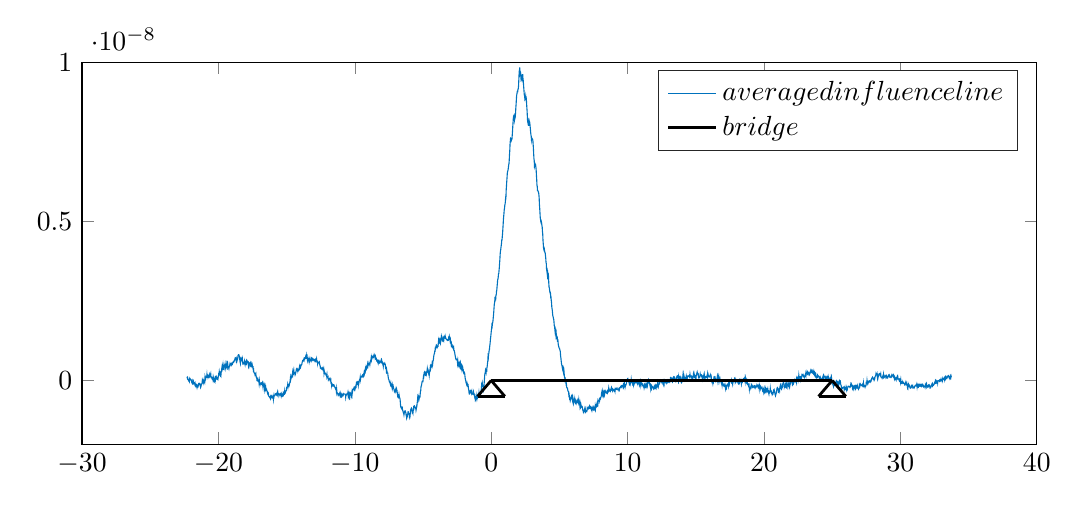
\begin{tikzpicture}

\begin{axis}[%
width=\textwidth,
height=0.4\textwidth,
at={(0\figurewidth,0\figureheight)},
scale only axis,
xmin=-30,
xmax=40,
ymin=-2e-09,
ymax=1e-08,
axis background/.style={fill=white},
% title style={font=\bfseries},
% title={},
legend style={legend cell align=left,align=left,draw=white!15!black}
]
\addplot [color=mycolor1,solid]
  table[row sep=crcr]{%
-22.3159404296875	1.18323540657329e-10\\
-22.295791015625	1.09487790669497e-10\\
-22.2756416015625	7.01083695561926e-11\\
-22.2554921875	8.73967831327927e-11\\
-22.2353427734375	4.57279390021045e-11\\
-22.215193359375	3.49387202965769e-11\\
-22.1950439453125	-9.44935511256185e-12\\
-22.17489453125	-4.62447348668263e-12\\
-22.1547451171875	-2.87372614426872e-12\\
-22.134595703125	-2.9184434031337e-11\\
-22.1144462890625	5.2853846840941e-11\\
-22.094296875	3.42700471708031e-11\\
-22.0741474609375	5.26376478942855e-11\\
-22.053998046875	3.78334420422553e-11\\
-22.0338486328125	1.34463101627698e-11\\
-22.01369921875	1.307063002344e-11\\
-21.9935498046875	1.54405574351222e-11\\
-21.973400390625	-3.06588111607537e-11\\
-21.9532509765625	-6.69160227287835e-11\\
-21.9331015625	-8.30366837403097e-11\\
-21.9129521484375	-3.58436969547546e-11\\
-21.892802734375	-8.98057932214126e-11\\
-21.8726533203125	-7.06451510325644e-11\\
-21.85250390625	-5.07503260190867e-11\\
-21.8323544921875	-2.80847503488146e-11\\
-21.812205078125	-9.54586162294433e-11\\
-21.7920556640625	-8.48582623645359e-11\\
-21.77190625	-8.21392962825674e-11\\
-21.7517568359375	-7.53443500309883e-11\\
-21.731607421875	-1.19190434756364e-10\\
-21.7114580078125	-9.28082559022149e-11\\
-21.69130859375	-1.45257369745405e-10\\
-21.6711591796875	-1.14044953723198e-10\\
-21.651009765625	-1.12440918837719e-10\\
-21.6308603515625	-1.15189705925096e-10\\
-21.6107109375	-1.83195734519052e-10\\
-21.5905615234375	-1.75703642278238e-10\\
-21.570412109375	-2.17347601822706e-10\\
-21.5502626953125	-1.7234124979925e-10\\
-21.53011328125	-1.94383457927583e-10\\
-21.5099638671875	-1.76173919683551e-10\\
-21.489814453125	-1.89207569785072e-10\\
-21.4696650390625	-1.55838460816968e-10\\
-21.449515625	-9.43827219040849e-11\\
-21.4293662109375	-9.43140933035297e-11\\
-21.409216796875	-9.01825988251552e-11\\
-21.3890673828125	-1.09140838712194e-10\\
-21.36891796875	-1.18727526471047e-10\\
-21.3487685546875	-1.46763630148943e-10\\
-21.328619140625	-1.34643594322207e-10\\
-21.3084697265625	-2.17751873636963e-10\\
-21.2883203125	-2.00358196408718e-10\\
-21.2681708984375	-1.66462048900436e-10\\
-21.248021484375	-1.22230698810312e-10\\
-21.2278720703125	-1.08103144022445e-10\\
-21.20772265625	-1.03194094594098e-10\\
-21.1875732421875	-2.67572985489041e-11\\
-21.167423828125	-7.04916547708198e-11\\
-21.1472744140625	-5.2133999721112e-11\\
-21.127125	-1.81128827031517e-13\\
-21.1069755859375	-4.20828914071255e-11\\
-21.086826171875	-7.20610611170289e-11\\
-21.0666767578125	3.89956657059595e-12\\
-21.04652734375	-3.51503749964041e-12\\
-21.0263779296875	4.66638939409171e-12\\
-21.006228515625	-3.11515453732733e-11\\
-20.9860791015625	9.10781119391464e-11\\
-20.9659296875	4.13837460046243e-11\\
-20.9457802734375	9.65335893111909e-11\\
-20.925630859375	7.00984909187122e-11\\
-20.9054814453125	1.07159933583392e-10\\
-20.88533203125	1.04107742759043e-10\\
-20.8651826171875	1.01528204719944e-10\\
-20.845033203125	1.76538512943176e-10\\
-20.8248837890625	8.20849352401305e-11\\
-20.804734375	1.73188141553962e-10\\
-20.7845849609375	1.58569674236083e-10\\
-20.764435546875	1.04047085483998e-10\\
-20.7442861328125	1.39395311712661e-10\\
-20.72413671875	1.2336366490079e-10\\
-20.7039873046875	1.09770933550793e-10\\
-20.683837890625	1.48789260360401e-10\\
-20.6636884765625	1.8363035461933e-10\\
-20.6435390625	1.35914903981168e-10\\
-20.6233896484375	1.58338640118635e-10\\
-20.603240234375	1.8230108834978e-10\\
-20.5830908203125	1.65700245389576e-10\\
-20.56294140625	2.01892654266715e-10\\
-20.5427919921875	1.03772117811136e-10\\
-20.522642578125	1.126352490028e-10\\
-20.5024931640625	1.04404565174293e-10\\
-20.48234375	7.0979560091846e-11\\
-20.4621943359375	5.19814877597947e-11\\
-20.442044921875	6.74267553876139e-11\\
-20.4218955078125	7.90049163532168e-11\\
-20.40174609375	3.28475332216119e-11\\
-20.3815966796875	1.15737035993869e-10\\
-20.361447265625	7.78790672655313e-11\\
-20.3412978515625	5.38353193543276e-11\\
-20.3211484375	9.4347119705749e-12\\
-20.3009990234375	4.06501295440194e-11\\
-20.280849609375	-3.49386305783243e-11\\
-20.2607001953125	-5.0619834195727e-11\\
-20.24055078125	1.93226991608584e-11\\
-20.2204013671875	7.12907560890803e-12\\
-20.200251953125	1.07618654362715e-10\\
-20.1801025390625	9.49682389388561e-11\\
-20.159953125	1.1601513262116e-10\\
-20.1398037109375	7.81582332178352e-11\\
-20.119654296875	4.65380016568453e-11\\
-20.0995048828125	3.92752454306966e-11\\
-20.07935546875	6.662708865594e-11\\
-20.0592060546875	4.61146077583585e-11\\
-20.039056640625	3.41628380493773e-11\\
-20.0189072265625	9.26934831085441e-11\\
-19.9987578125	1.38481458563547e-10\\
-19.9786083984375	2.09666201735121e-10\\
-19.958458984375	2.00616762065816e-10\\
-19.9383095703125	2.78176606939186e-10\\
-19.91816015625	2.29508102606363e-10\\
-19.8980107421875	2.09103000941712e-10\\
-19.877861328125	1.78367604926966e-10\\
-19.8577119140625	2.25491415358066e-10\\
-19.8375625	1.92778691127656e-10\\
-19.8174130859375	1.6119747496344e-10\\
-19.797263671875	2.581095666285e-10\\
-19.7771142578125	2.73209916628327e-10\\
-19.75696484375	3.63430002068034e-10\\
-19.7368154296875	4.24269052795325e-10\\
-19.716666015625	3.79205586299539e-10\\
-19.6965166015625	4.36633472134869e-10\\
-19.6763671875	4.88598711219513e-10\\
-19.6562177734375	3.30394553991595e-10\\
-19.636068359375	4.55665096689067e-10\\
-19.6159189453125	4.41541373418461e-10\\
-19.59576953125	3.99998706831409e-10\\
-19.5756201171875	4.63735678960122e-10\\
-19.555470703125	4.4478007654707e-10\\
-19.5353212890625	4.43938872287813e-10\\
-19.515171875	4.98683258476812e-10\\
-19.4950224609375	4.00495361026772e-10\\
-19.474873046875	4.5400260119464e-10\\
-19.4547236328125	4.092996135541e-10\\
-19.43457421875	4.3144188258118e-10\\
-19.4144248046875	4.31193248673038e-10\\
-19.394275390625	5.03899070023969e-10\\
-19.3741259765625	4.43804733841982e-10\\
-19.3539765625	5.02690349921809e-10\\
-19.3338271484375	4.45583122834982e-10\\
-19.313677734375	4.99575560355244e-10\\
-19.2935283203125	4.25707492322739e-10\\
-19.27337890625	4.13024416349873e-10\\
-19.2532294921875	3.98503440413278e-10\\
-19.233080078125	3.69802281990902e-10\\
-19.2129306640625	4.31670108930708e-10\\
-19.19278125	4.37047901352481e-10\\
-19.1726318359375	4.78288397297578e-10\\
-19.152482421875	5.23977248945561e-10\\
-19.1323330078125	4.92847705522926e-10\\
-19.11218359375	5.20202356571052e-10\\
-19.0920341796875	5.06002690608107e-10\\
-19.071884765625	4.96747150243505e-10\\
-19.0517353515625	5.17830595550962e-10\\
-19.0315859375	4.85972460603039e-10\\
-19.0114365234375	5.06183612942751e-10\\
-18.991287109375	5.31418426425977e-10\\
-18.9711376953125	5.21767175402451e-10\\
-18.95098828125	5.61899849376718e-10\\
-18.9308388671875	5.78254193999055e-10\\
-18.910689453125	5.72847639174557e-10\\
-18.8905400390625	5.93345087330096e-10\\
-18.870390625	5.83326984294873e-10\\
-18.8502412109375	5.97403835656252e-10\\
-18.830091796875	6.32893093209181e-10\\
-18.8099423828125	6.35815330300154e-10\\
-18.78979296875	6.83175487350812e-10\\
-18.7696435546875	7.09003517641796e-10\\
-18.749494140625	6.99276072356553e-10\\
-18.7293447265625	6.94250669904722e-10\\
-18.7091953125	6.45716492101065e-10\\
-18.6890458984375	6.8900141493312e-10\\
-18.668896484375	6.57547668987923e-10\\
-18.6487470703125	5.95413894283882e-10\\
-18.62859765625	6.30214980855788e-10\\
-18.6084482421875	6.88095016896453e-10\\
-18.588298828125	6.84129730675203e-10\\
-18.5681494140625	7.80592619919039e-10\\
-18.548	7.94387196448797e-10\\
-18.5278505859375	8.08883296859899e-10\\
-18.507701171875	8.0713785858396e-10\\
-18.4875517578125	7.93488139428402e-10\\
-18.46740234375	7.55010538618538e-10\\
-18.4472529296875	7.06059081650203e-10\\
-18.427103515625	6.22845710681703e-10\\
-18.4069541015625	5.76818981210764e-10\\
-18.3868046875	5.3854169521943e-10\\
-18.3666552734375	6.48913353162417e-10\\
-18.346505859375	6.13402277306567e-10\\
-18.3263564453125	6.3807389947339e-10\\
-18.30620703125	6.74886874549309e-10\\
-18.2860576171875	6.40016768056518e-10\\
-18.265908203125	6.34370851496262e-10\\
-18.2457587890625	6.76082092638564e-10\\
-18.225609375	5.72138142151933e-10\\
-18.2054599609375	5.12717785149444e-10\\
-18.185310546875	5.14450376685857e-10\\
-18.1651611328125	5.2521273378675e-10\\
-18.14501171875	5.509836658907e-10\\
-18.1248623046875	5.39396736498327e-10\\
-18.104712890625	5.3000408883055e-10\\
-18.0845634765625	5.99744147664559e-10\\
-18.0644140625	5.49750413299126e-10\\
-18.0442646484375	5.03818901047238e-10\\
-18.024115234375	5.63090491732583e-10\\
-18.0039658203125	5.36494912843416e-10\\
-17.98381640625	5.22610724759753e-10\\
-17.9636669921875	5.64171644191501e-10\\
-17.943517578125	6.03569912869189e-10\\
-17.9233681640625	5.64549416376051e-10\\
-17.90321875	6.2370114876922e-10\\
-17.8830693359375	6.06175374224227e-10\\
-17.862919921875	5.84332310724316e-10\\
-17.8427705078125	5.88548804854354e-10\\
-17.82262109375	5.81983035825145e-10\\
-17.8024716796875	4.95146569673785e-10\\
-17.782322265625	5.62739380898561e-10\\
-17.7621728515625	5.48363936114207e-10\\
-17.7420234375	4.71028510419464e-10\\
-17.7218740234375	5.1544243640287e-10\\
-17.701724609375	5.39187140924038e-10\\
-17.6815751953125	5.26364563381349e-10\\
-17.66142578125	4.9386123615434e-10\\
-17.6412763671875	5.39398441815961e-10\\
-17.621126953125	5.01521358793121e-10\\
-17.6009775390625	4.63909047681283e-10\\
-17.580828125	5.06004732108818e-10\\
-17.5606787109375	4.49623816459208e-10\\
-17.540529296875	4.41500257773379e-10\\
-17.5203798828125	4.8927585218793e-10\\
-17.50023046875	4.49035435662402e-10\\
-17.4800810546875	4.05798092904653e-10\\
-17.459931640625	4.14476261022211e-10\\
-17.4397822265625	3.20405194311378e-10\\
-17.4196328125	3.33796279117191e-10\\
-17.3994833984375	2.51685067595404e-10\\
-17.379333984375	2.47406113825099e-10\\
-17.3591845703125	2.25328688542963e-10\\
-17.33903515625	2.22620199792101e-10\\
-17.3188857421875	1.81412445706089e-10\\
-17.298736328125	2.01718944710845e-10\\
-17.2785869140625	2.18443636639e-10\\
-17.2584375	2.29187290749758e-10\\
-17.2382880859375	1.12310043256121e-10\\
-17.218138671875	1.14725420065735e-10\\
-17.1979892578125	1.10162817276963e-10\\
-17.17783984375	1.59180032956571e-11\\
-17.1576904296875	2.31855510347112e-11\\
-17.137541015625	-1.18144565911932e-11\\
-17.1173916015625	-5.41052823334912e-12\\
-17.0972421875	3.03108207438521e-11\\
-17.0770927734375	-9.28268584341247e-12\\
-17.056943359375	-2.54234836638978e-11\\
-17.0367939453125	-2.48609720147611e-11\\
-17.01664453125	-1.00120859870084e-10\\
-16.9964951171875	-2.08653974232505e-11\\
-16.976345703125	-1.10015060264329e-10\\
-16.9561962890625	-9.02493760192832e-11\\
-16.936046875	-1.07492534299557e-10\\
-16.9158974609375	-1.01161024473037e-10\\
-16.895748046875	-1.26783543133757e-10\\
-16.8755986328125	-7.51415113612875e-11\\
-16.85544921875	-7.22241518512012e-11\\
-16.8352998046875	-8.58028112156076e-11\\
-16.815150390625	-1.04048220289193e-10\\
-16.7950009765625	-9.32151422458533e-11\\
-16.7748515625	-7.12876998848784e-11\\
-16.7547021484375	-1.39658985022639e-10\\
-16.734552734375	-2.02719712785966e-10\\
-16.7144033203125	-9.81097026633099e-11\\
-16.69425390625	-1.2644443931879e-10\\
-16.6741044921875	-1.75790878754161e-10\\
-16.653955078125	-1.87874377373733e-10\\
-16.6338056640625	-1.53528676041705e-10\\
-16.61365625	-2.62610153374383e-10\\
-16.5935068359375	-1.96094929764687e-10\\
-16.573357421875	-2.2776354469121e-10\\
-16.5532080078125	-2.69865297208068e-10\\
-16.53305859375	-2.09832019329781e-10\\
-16.5129091796875	-2.81399322439395e-10\\
-16.492759765625	-2.61396291455264e-10\\
-16.4726103515625	-2.68481681726185e-10\\
-16.4524609375	-3.15156719638212e-10\\
-16.4323115234375	-3.39302144894548e-10\\
-16.412162109375	-3.70723518899141e-10\\
-16.3920126953125	-4.05832180989458e-10\\
-16.37186328125	-3.72598919538238e-10\\
-16.3517138671875	-3.86598494285663e-10\\
-16.331564453125	-4.2915161607803e-10\\
-16.3114150390625	-4.9101497646749e-10\\
-16.291265625	-5.00347656742876e-10\\
-16.2711162109375	-5.04649145953616e-10\\
-16.250966796875	-5.28171752723671e-10\\
-16.2308173828125	-5.37998584399146e-10\\
-16.21066796875	-5.22297501792218e-10\\
-16.1905185546875	-5.57087518401707e-10\\
-16.170369140625	-5.10451572024836e-10\\
-16.1502197265625	-5.39595870487183e-10\\
-16.1300703125	-5.0563535064532e-10\\
-16.1099208984375	-5.37596827651145e-10\\
-16.089771484375	-5.36239977231557e-10\\
-16.0696220703125	-5.03979849884165e-10\\
-16.04947265625	-5.17584043699106e-10\\
-16.0293232421875	-5.50033207659897e-10\\
-16.009173828125	-5.4898065291124e-10\\
-15.9890244140625	-5.00874296108708e-10\\
-15.968875	-5.87663515441973e-10\\
-15.9487255859375	-5.03525403731068e-10\\
-15.928576171875	-5.21931236653185e-10\\
-15.9084267578125	-4.74974928466686e-10\\
-15.88827734375	-4.6628869735908e-10\\
-15.8681279296875	-4.70642089962489e-10\\
-15.847978515625	-4.30670126847013e-10\\
-15.8278291015625	-4.4771871457564e-10\\
-15.8076796875	-4.40818587065826e-10\\
-15.7875302734375	-4.23744848804827e-10\\
-15.767380859375	-4.29864966470094e-10\\
-15.7472314453125	-4.467694369435e-10\\
-15.72708203125	-4.1100814938825e-10\\
-15.7069326171875	-4.20715460817679e-10\\
-15.686783203125	-3.86966628234265e-10\\
-15.6666337890625	-4.30411700594156e-10\\
-15.646484375	-3.74896131937017e-10\\
-15.6263349609375	-4.29270029121687e-10\\
-15.606185546875	-4.40569761648871e-10\\
-15.5860361328125	-4.29654996867959e-10\\
-15.56588671875	-4.79899190682938e-10\\
-15.5457373046875	-4.46791397209016e-10\\
-15.525587890625	-4.31688322003247e-10\\
-15.5054384765625	-4.42562212668356e-10\\
-15.4852890625	-4.54124754257212e-10\\
-15.4651396484375	-4.59341991540457e-10\\
-15.444990234375	-4.27370472015298e-10\\
-15.4248408203125	-4.50251060212478e-10\\
-15.40469140625	-4.89289034901478e-10\\
-15.3845419921875	-4.4235602609468e-10\\
-15.364392578125	-4.92182892605427e-10\\
-15.3442431640625	-5.06019965393265e-10\\
-15.32409375	-5.06466863936027e-10\\
-15.3039443359375	-4.59994730378801e-10\\
-15.283794921875	-4.85355778711837e-10\\
-15.2636455078125	-4.7923116553749e-10\\
-15.24349609375	-4.06131439440961e-10\\
-15.2233466796875	-4.32729604477277e-10\\
-15.203197265625	-3.73299376763803e-10\\
-15.1830478515625	-3.77519096150226e-10\\
-15.1628984375	-4.52967888260601e-10\\
-15.1427490234375	-3.47551145774232e-10\\
-15.122599609375	-4.1140182572535e-10\\
-15.1024501953125	-3.97924709657251e-10\\
-15.08230078125	-3.39777332877305e-10\\
-15.0621513671875	-3.46616659025343e-10\\
-15.042001953125	-3.23473578499235e-10\\
-15.0218525390625	-3.17269264620451e-10\\
-15.001703125	-2.30693380493998e-10\\
-14.9815537109375	-2.1253771759966e-10\\
-14.961404296875	-2.10606635810842e-10\\
-14.9412548828125	-1.91256479653129e-10\\
-14.92110546875	-1.31105259728396e-10\\
-14.9009560546875	-1.90860794109007e-10\\
-14.880806640625	-1.23017998346425e-10\\
-14.8606572265625	-1.228231865079e-10\\
-14.8405078125	-1.37080713461157e-10\\
-14.8203583984375	-1.6945555039362e-10\\
-14.800208984375	-1.40143736003728e-10\\
-14.7800595703125	-8.16273146737291e-11\\
-14.75991015625	-6.65792776472098e-11\\
-14.7397607421875	-2.85852147187294e-12\\
-14.719611328125	8.43209873203147e-11\\
-14.6994619140625	2.39952814309051e-11\\
-14.6793125	6.55941404342348e-11\\
-14.6591630859375	7.7320191774882e-11\\
-14.639013671875	1.15538697946298e-10\\
-14.6188642578125	1.49384601814978e-10\\
-14.59871484375	1.19706111250055e-10\\
-14.5785654296875	1.41186815441085e-10\\
-14.558416015625	2.43308680193648e-10\\
-14.5382666015625	1.86961445109901e-10\\
-14.5181171875	2.36775937865908e-10\\
-14.4979677734375	2.8250034062516e-10\\
-14.477818359375	3.27771499450643e-10\\
-14.4576689453125	2.37062639402958e-10\\
-14.43751953125	2.55201471919714e-10\\
-14.4173701171875	2.4219548529285e-10\\
-14.397220703125	2.21898247544592e-10\\
-14.3770712890625	1.74047964844962e-10\\
-14.356921875	1.95794422698979e-10\\
-14.3367724609375	2.55454462534736e-10\\
-14.316623046875	2.63556818096888e-10\\
-14.2964736328125	3.23468154224683e-10\\
-14.27632421875	3.61194540645432e-10\\
-14.2561748046875	3.48312351146901e-10\\
-14.236025390625	3.54003559535891e-10\\
-14.2158759765625	3.27800326748121e-10\\
-14.1957265625	3.47141758165142e-10\\
-14.1755771484375	2.96582878324428e-10\\
-14.155427734375	3.30364055334366e-10\\
-14.1352783203125	3.12170337442841e-10\\
-14.11512890625	3.25768915517136e-10\\
-14.0949794921875	3.51198508325658e-10\\
-14.074830078125	3.88558132959676e-10\\
-14.0546806640625	4.35506510053479e-10\\
-14.03453125	3.83018583127715e-10\\
-14.0143818359375	4.11534413944985e-10\\
-13.994232421875	4.48187671408351e-10\\
-13.9740830078125	4.20367290643051e-10\\
-13.95393359375	4.58328737495678e-10\\
-13.9337841796875	4.83217540978693e-10\\
-13.913634765625	4.89870160347884e-10\\
-13.8934853515625	4.95847058968979e-10\\
-13.8733359375	5.44278312251323e-10\\
-13.8531865234375	5.75006341075002e-10\\
-13.833037109375	6.09616553833601e-10\\
-13.8128876953125	6.01025339666745e-10\\
-13.79273828125	6.03756783224576e-10\\
-13.7725888671875	6.45750306662405e-10\\
-13.752439453125	6.51073898853069e-10\\
-13.7322900390625	6.77761529646038e-10\\
-13.712140625	6.47848722583023e-10\\
-13.6919912109375	6.95996889625649e-10\\
-13.671841796875	7.07172581581994e-10\\
-13.6516923828125	6.83913837961883e-10\\
-13.63154296875	6.96579724776455e-10\\
-13.6113935546875	7.36144603764507e-10\\
-13.591244140625	7.00865268855787e-10\\
-13.5710947265625	6.98379815332607e-10\\
-13.5509453125	7.75427970364013e-10\\
-13.5307958984375	7.07269732548324e-10\\
-13.510646484375	6.94137513045917e-10\\
-13.4904970703125	7.30235062817101e-10\\
-13.47034765625	6.36159418022359e-10\\
-13.4501982421875	6.77698180262492e-10\\
-13.430048828125	6.84822550879866e-10\\
-13.4098994140625	6.81751638280592e-10\\
-13.38975	6.40055270186366e-10\\
-13.3696005859375	6.77821782128693e-10\\
-13.349451171875	6.10989744445531e-10\\
-13.3293017578125	6.80364101338222e-10\\
-13.30915234375	6.54216099308348e-10\\
-13.2890029296875	6.16084085420963e-10\\
-13.268853515625	6.44748236310808e-10\\
-13.2487041015625	6.37868749607442e-10\\
-13.2285546875	6.29862281678049e-10\\
-13.2084052734375	6.91063873732044e-10\\
-13.188255859375	6.72967958347801e-10\\
-13.1681064453125	6.91564829184758e-10\\
-13.14795703125	6.36398809809815e-10\\
-13.1278076171875	6.66294194227218e-10\\
-13.107658203125	6.78505001082515e-10\\
-13.0875087890625	6.39599874425954e-10\\
-13.067359375	6.36544570316022e-10\\
-13.0472099609375	6.41738281581759e-10\\
-13.027060546875	6.6794966461587e-10\\
-13.0069111328125	6.6094910272859e-10\\
-12.98676171875	6.21773717724372e-10\\
-12.9666123046875	6.23555586048705e-10\\
-12.946462890625	6.22453916669738e-10\\
-12.9263134765625	6.04839173759063e-10\\
-12.9061640625	6.64787624815009e-10\\
-12.8860146484375	6.76852064963647e-10\\
-12.865865234375	6.76021720508768e-10\\
-12.8457158203125	6.30742397355835e-10\\
-12.82556640625	6.46168359690275e-10\\
-12.8054169921875	6.8159319315496e-10\\
-12.785267578125	6.04785275533193e-10\\
-12.7651181640625	6.16065305804653e-10\\
-12.74496875	6.04164230961108e-10\\
-12.7248193359375	5.20647918341363e-10\\
-12.704669921875	5.63237853408531e-10\\
-12.6845205078125	5.68809930685197e-10\\
-12.66437109375	5.70416609880237e-10\\
-12.6442216796875	5.75494965420783e-10\\
-12.624072265625	5.59544898631123e-10\\
-12.6039228515625	5.75856000045029e-10\\
-12.5837734375	5.25251126056529e-10\\
-12.5636240234375	4.78168372881736e-10\\
-12.543474609375	4.64450660191066e-10\\
-12.5233251953125	3.96041182796665e-10\\
-12.50317578125	4.07775564675463e-10\\
-12.4830263671875	3.86299050028971e-10\\
-12.462876953125	3.79973539748611e-10\\
-12.4427275390625	3.67319848800089e-10\\
-12.422578125	3.57235154449822e-10\\
-12.4024287109375	3.87586124860927e-10\\
-12.382279296875	4.03187334935772e-10\\
-12.3621298828125	3.93998272450586e-10\\
-12.34198046875	3.93829115719213e-10\\
-12.3218310546875	3.03492608787986e-10\\
-12.301681640625	2.98823945157681e-10\\
-12.2815322265625	3.44807721473518e-10\\
-12.2613828125	2.37805352566592e-10\\
-12.2412333984375	3.03209272309484e-10\\
-12.221083984375	2.65468235702749e-10\\
-12.2009345703125	2.54147032001331e-10\\
-12.18078515625	2.14677684144092e-10\\
-12.1606357421875	2.17658309851459e-10\\
-12.140486328125	2.17391562351731e-10\\
-12.1203369140625	1.73750289769389e-10\\
-12.1001875	1.76304049042384e-10\\
-12.0800380859375	1.7701456323359e-10\\
-12.059888671875	1.25276922386803e-10\\
-12.0397392578125	1.80082138894423e-10\\
-12.01958984375	9.06354349983869e-11\\
-11.9994404296875	8.74456705428629e-11\\
-11.979291015625	7.85249318306784e-11\\
-11.9591416015625	9.94835830521334e-11\\
-11.9389921875	2.02728881837412e-11\\
-11.9188427734375	3.94682063379378e-11\\
-11.898693359375	3.66551358078093e-11\\
-11.8785439453125	4.12467306696329e-11\\
-11.85839453125	5.46072026703175e-11\\
-11.8382451171875	2.70055617381072e-11\\
-11.818095703125	4.62308315756518e-11\\
-11.7979462890625	-1.92932086891242e-11\\
-11.777796875	-1.90702948749266e-11\\
-11.7576474609375	2.57245615066464e-12\\
-11.737498046875	-1.17888143908308e-10\\
-11.7173486328125	-4.59881739831752e-11\\
-11.69719921875	-1.58122184162252e-10\\
-11.6770498046875	-1.13211721799127e-10\\
-11.656900390625	-1.2614068987445e-10\\
-11.6367509765625	-1.51228126987449e-10\\
-11.6166015625	-1.25974406586669e-10\\
-11.5964521484375	-1.37579515437415e-10\\
-11.576302734375	-1.55992041203716e-10\\
-11.5561533203125	-1.35917070811476e-10\\
-11.53600390625	-1.35183094790113e-10\\
-11.5158544921875	-1.53806989387244e-10\\
-11.495705078125	-1.92432955535196e-10\\
-11.4755556640625	-2.05634396091774e-10\\
-11.45540625	-2.09728233915262e-10\\
-11.4352568359375	-2.40329220735347e-10\\
-11.415107421875	-2.60685048308736e-10\\
-11.3949580078125	-2.46319028560977e-10\\
-11.37480859375	-2.62865143954421e-10\\
-11.3546591796875	-3.45517284835754e-10\\
-11.334509765625	-2.65904750075973e-10\\
-11.3143603515625	-3.58203185169563e-10\\
-11.2942109375	-3.93264600557493e-10\\
-11.2740615234375	-3.97565040681978e-10\\
-11.253912109375	-4.15264934343262e-10\\
-11.2337626953125	-4.45438459388112e-10\\
-11.21361328125	-4.19135388532157e-10\\
-11.1934638671875	-4.26695442591353e-10\\
-11.173314453125	-4.52587947848088e-10\\
-11.1531650390625	-4.25108408605349e-10\\
-11.133015625	-4.11531293158076e-10\\
-11.1128662109375	-4.04833585385693e-10\\
-11.092716796875	-3.83633699002071e-10\\
-11.0725673828125	-4.64440982529345e-10\\
-11.05241796875	-4.31969370856032e-10\\
-11.0322685546875	-4.84191833135188e-10\\
-11.012119140625	-4.64684005094033e-10\\
-10.9919697265625	-4.8973237437522e-10\\
-10.9718203125	-4.50571831722043e-10\\
-10.9516708984375	-4.80329686723876e-10\\
-10.931521484375	-4.36218631994739e-10\\
-10.9113720703125	-4.51828418379245e-10\\
-10.89122265625	-4.88111602831254e-10\\
-10.8710732421875	-4.87833973785066e-10\\
-10.850923828125	-4.37298062240256e-10\\
-10.8307744140625	-4.41401454278116e-10\\
-10.810625	-4.12388409067036e-10\\
-10.7904755859375	-4.2117357610629e-10\\
-10.770326171875	-4.28460041787811e-10\\
-10.7501767578125	-4.27724740320275e-10\\
-10.73002734375	-4.30878314203204e-10\\
-10.7098779296875	-4.29949613759997e-10\\
-10.689728515625	-4.33476024624567e-10\\
-10.6695791015625	-5.21242473502997e-10\\
-10.6494296875	-4.60375466159637e-10\\
-10.6292802734375	-4.64605788097246e-10\\
-10.609130859375	-4.57475032299496e-10\\
-10.5889814453125	-4.30768801360727e-10\\
-10.56883203125	-4.09014804104663e-10\\
-10.5486826171875	-4.09549137738124e-10\\
-10.528533203125	-4.20078707024506e-10\\
-10.5083837890625	-3.79166200753976e-10\\
-10.488234375	-4.64405298371821e-10\\
-10.4680849609375	-3.96374971121009e-10\\
-10.447935546875	-5.44107076114348e-10\\
-10.4277861328125	-4.58915464820656e-10\\
-10.40763671875	-5.11354341840949e-10\\
-10.3874873046875	-4.63614053705121e-10\\
-10.367337890625	-5.09263822343452e-10\\
-10.3471884765625	-4.27451874237408e-10\\
-10.3270390625	-4.6331969894893e-10\\
-10.3068896484375	-4.59132659845623e-10\\
-10.286740234375	-4.17582062198366e-10\\
-10.2665908203125	-4.33595271680521e-10\\
-10.24644140625	-4.78617227922645e-10\\
-10.2262919921875	-4.06879237821267e-10\\
-10.206142578125	-4.49233673586905e-10\\
-10.1859931640625	-3.27052620911804e-10\\
-10.16584375	-3.50741330053149e-10\\
-10.1456943359375	-3.02176156817997e-10\\
-10.125544921875	-2.77676250975081e-10\\
-10.1053955078125	-2.60662437516443e-10\\
-10.08524609375	-2.69794477324036e-10\\
-10.0650966796875	-2.41282823380929e-10\\
-10.044947265625	-2.7139780560827e-10\\
-10.0247978515625	-2.90728148063375e-10\\
-10.0046484375	-2.43807556418498e-10\\
-9.9844990234375	-2.7380983083283e-10\\
-9.964349609375	-2.38694439218308e-10\\
-9.9442001953125	-1.98888435049799e-10\\
-9.92405078125	-1.64769959773306e-10\\
-9.9039013671875	-1.82339657183811e-10\\
-9.883751953125	-5.92058912938879e-11\\
-9.8636025390625	-5.78464314717711e-11\\
-9.843453125	-4.43313729018737e-11\\
-9.8233037109375	-7.67509591449438e-11\\
-9.803154296875	-4.27117542948063e-11\\
-9.7830048828125	-4.73677185759184e-11\\
-9.76285546875	-6.8767022719016e-11\\
-9.7427060546875	-1.42477547460211e-10\\
-9.722556640625	-7.22555032715633e-11\\
-9.7024072265625	-8.98773930134108e-11\\
-9.6822578125	-3.8089190991977e-11\\
-9.6621083984375	1.80611787005693e-11\\
-9.641958984375	3.37890587184427e-11\\
-9.6218095703125	4.94841772410675e-11\\
-9.60166015625	1.07599612775921e-10\\
-9.5815107421875	3.75091794291389e-11\\
-9.561361328125	1.01437338509264e-10\\
-9.5412119140625	1.10044392828384e-10\\
-9.5210625	1.09764933711535e-10\\
-9.5009130859375	1.1686449934994e-10\\
-9.480763671875	1.3790160001021e-10\\
-9.4606142578125	1.31259161560803e-10\\
-9.44046484375	1.5478970326387e-10\\
-9.4203154296875	1.30931852599498e-10\\
-9.400166015625	1.56757156237503e-10\\
-9.3800166015625	1.77895439384659e-10\\
-9.3598671875	1.41076810686896e-10\\
-9.3397177734375	1.73269660237162e-10\\
-9.319568359375	2.37094590696347e-10\\
-9.2994189453125	1.99247861628984e-10\\
-9.27926953125	2.45786275934181e-10\\
-9.2591201171875	3.08608976839674e-10\\
-9.238970703125	3.49063148776911e-10\\
-9.2188212890625	2.94735356132135e-10\\
-9.198671875	3.3009142063202e-10\\
-9.1785224609375	3.96156266568283e-10\\
-9.158373046875	3.45764754251262e-10\\
-9.1382236328125	3.6347227211694e-10\\
-9.11807421875	3.9958788283896e-10\\
-9.0979248046875	4.47286578072074e-10\\
-9.077775390625	4.32129453477142e-10\\
-9.0576259765625	5.10410242889381e-10\\
-9.0374765625	4.6586255073932e-10\\
-9.0173271484375	5.26872503159217e-10\\
-8.997177734375	4.84649394242161e-10\\
-8.9770283203125	4.91019511001081e-10\\
-8.95687890625	4.95807741519448e-10\\
-8.9367294921875	5.19854036530209e-10\\
-8.916580078125	5.40486656552806e-10\\
-8.8964306640625	5.00551702942566e-10\\
-8.87628125	5.61706857291668e-10\\
-8.8561318359375	6.09953831425201e-10\\
-8.835982421875	6.0441063995632e-10\\
-8.8158330078125	6.51884851683866e-10\\
-8.79568359375	7.21652708356824e-10\\
-8.7755341796875	6.62986921639836e-10\\
-8.755384765625	7.25398622834104e-10\\
-8.7352353515625	7.48412880500773e-10\\
-8.7150859375	7.19370820378894e-10\\
-8.6949365234375	7.41332464949462e-10\\
-8.674787109375	7.40709143448423e-10\\
-8.6546376953125	7.35199158373385e-10\\
-8.63448828125	7.59985221644635e-10\\
-8.6143388671875	7.80377509316062e-10\\
-8.594189453125	7.38703464025336e-10\\
-8.5740400390625	8.04543138220062e-10\\
-8.553890625	7.81308881842062e-10\\
-8.5337412109375	7.64680097478794e-10\\
-8.513591796875	7.69157756971437e-10\\
-8.4934423828125	7.79454157008711e-10\\
-8.47329296875	6.86566515719923e-10\\
-8.4531435546875	6.97756132202357e-10\\
-8.432994140625	7.00483874661483e-10\\
-8.4128447265625	6.62901970552975e-10\\
-8.3926953125	6.2277045531349e-10\\
-8.3725458984375	6.34439003459556e-10\\
-8.352396484375	6.0722883013331e-10\\
-8.3322470703125	5.82197359854423e-10\\
-8.31209765625	5.65298728405131e-10\\
-8.2919482421875	6.55909536206997e-10\\
-8.271798828125	5.53831299532986e-10\\
-8.2516494140625	5.86150624569544e-10\\
-8.2315	6.06012462509047e-10\\
-8.2113505859375	5.58898286154176e-10\\
-8.191201171875	5.49372831414791e-10\\
-8.1710517578125	5.60704560568482e-10\\
-8.15090234375	5.85009698976445e-10\\
-8.1307529296875	5.6924824939674e-10\\
-8.110603515625	5.81727568905371e-10\\
-8.0904541015625	6.0053571958281e-10\\
-8.0703046875	6.32506108305451e-10\\
-8.0501552734375	5.95302161334883e-10\\
-8.030005859375	6.30031903892549e-10\\
-8.0098564453125	5.82444263880856e-10\\
-7.98970703125	5.8514521120244e-10\\
-7.9695576171875	5.42931556730054e-10\\
-7.949408203125	5.10569052877153e-10\\
-7.9292587890625	5.24950359636071e-10\\
-7.909109375	4.45379010956985e-10\\
-7.8889599609375	4.99739964345504e-10\\
-7.868810546875	5.05555152468888e-10\\
-7.8486611328125	5.27739434214257e-10\\
-7.82851171875	5.244001328826e-10\\
-7.8083623046875	5.41630491786816e-10\\
-7.788212890625	5.09122325998255e-10\\
-7.7680634765625	5.06316012206596e-10\\
-7.7479140625	4.16202630161212e-10\\
-7.7277646484375	4.30733390866618e-10\\
-7.707615234375	4.05978848315222e-10\\
-7.6874658203125	3.05590241385007e-10\\
-7.66731640625	3.44495426935175e-10\\
-7.6471669921875	2.97715094569996e-10\\
-7.627017578125	2.36947389849105e-10\\
-7.6068681640625	2.38177060222872e-10\\
-7.58671875	2.34118085288773e-10\\
-7.5665693359375	1.47174216951561e-10\\
-7.546419921875	9.03279119145279e-11\\
-7.5262705078125	3.76150339543541e-11\\
-7.50612109375	3.0657527124881e-11\\
-7.4859716796875	1.67326973041192e-12\\
-7.465822265625	-4.58946579391734e-11\\
-7.4456728515625	-5.1911019209031e-11\\
-7.4255234375	-6.6605160039476e-11\\
-7.4053740234375	-1.05453198929263e-10\\
-7.385224609375	-1.34180436729637e-10\\
-7.3650751953125	-9.13475449614749e-11\\
-7.34492578125	-1.79700317285273e-10\\
-7.3247763671875	-1.88480521451207e-10\\
-7.304626953125	-1.56215441702392e-10\\
-7.2844775390625	-1.95758955424075e-10\\
-7.264328125	-2.39924182371534e-10\\
-7.2441787109375	-1.69294314075039e-10\\
-7.224029296875	-2.41466799717049e-10\\
-7.2038798828125	-2.16452585744202e-10\\
-7.18373046875	-1.8446240865963e-10\\
-7.1635810546875	-2.31632413585857e-10\\
-7.143431640625	-2.65437424330157e-10\\
-7.1232822265625	-2.73017876229221e-10\\
-7.1031328125	-3.29530798316215e-10\\
-7.0829833984375	-3.13469027496193e-10\\
-7.062833984375	-3.29962410040086e-10\\
-7.0426845703125	-3.66137359558679e-10\\
-7.02253515625	-3.38091769974804e-10\\
-7.0023857421875	-2.83264901336168e-10\\
-6.982236328125	-2.96387801423436e-10\\
-6.9620869140625	-2.36980757215276e-10\\
-6.9419375	-2.59396944309149e-10\\
-6.9217880859375	-3.46316861175679e-10\\
-6.901638671875	-3.35623936982882e-10\\
-6.8814892578125	-4.13170266966503e-10\\
-6.86133984375	-4.76119835565446e-10\\
-6.8411904296875	-4.46590769564921e-10\\
-6.821041015625	-4.53332614202262e-10\\
-6.8008916015625	-5.17180595797128e-10\\
-6.7807421875	-4.94286714451218e-10\\
-6.7605927734375	-4.39460471756763e-10\\
-6.740443359375	-4.92904143436289e-10\\
-6.7202939453125	-5.43339860423938e-10\\
-6.70014453125	-5.62524074922277e-10\\
-6.6799951171875	-5.90482598699419e-10\\
-6.659845703125	-7.14849746803819e-10\\
-6.6396962890625	-8.22830623549494e-10\\
-6.619546875	-8.43628383590965e-10\\
-6.5993974609375	-8.34066835331365e-10\\
-6.579248046875	-8.57391706784889e-10\\
-6.5590986328125	-8.86149356316661e-10\\
-6.53894921875	-8.68692913419376e-10\\
-6.5187998046875	-8.56683772847225e-10\\
-6.498650390625	-9.38635861856653e-10\\
-6.4785009765625	-9.48038667737703e-10\\
-6.4583515625	-9.85350243205878e-10\\
-6.4382021484375	-1.0162842118493e-09\\
-6.418052734375	-1.03582648860545e-09\\
-6.3979033203125	-1.07884846259002e-09\\
-6.37775390625	-1.02437739611007e-09\\
-6.3576044921875	-9.90902738732031e-10\\
-6.337455078125	-9.62530982906647e-10\\
-6.3173056640625	-9.53405852963619e-10\\
-6.29715625	-9.56918071491628e-10\\
-6.2770068359375	-1.00471108014343e-09\\
-6.256857421875	-1.00923772237116e-09\\
-6.2367080078125	-1.10027496665753e-09\\
-6.21655859375	-1.11154111032723e-09\\
-6.1964091796875	-1.18806074980408e-09\\
-6.176259765625	-1.16097959524789e-09\\
-6.1561103515625	-1.13714909555199e-09\\
-6.1359609375	-1.06459570208506e-09\\
-6.1158115234375	-1.05027150328078e-09\\
-6.095662109375	-9.83137951786239e-10\\
-6.0755126953125	-9.87783218950559e-10\\
-6.05536328125	-1.03651665267429e-09\\
-6.0352138671875	-1.04091589054385e-09\\
-6.015064453125	-1.08985410754556e-09\\
-5.9949150390625	-1.14876446585775e-09\\
-5.974765625	-1.11010685801481e-09\\
-5.9546162109375	-1.13073526955945e-09\\
-5.934466796875	-1.03729025036532e-09\\
-5.9143173828125	-9.5093337401561e-10\\
-5.89416796875	-9.0557282993295e-10\\
-5.8740185546875	-8.93997582462442e-10\\
-5.853869140625	-8.70805478888379e-10\\
-5.8337197265625	-8.8887659356507e-10\\
-5.8135703125	-9.34118067416558e-10\\
-5.7934208984375	-9.86422623007299e-10\\
-5.773271484375	-9.55660154301933e-10\\
-5.7531220703125	-9.59691279366573e-10\\
-5.73297265625	-1.00707899228592e-09\\
-5.7128232421875	-9.24477955561881e-10\\
-5.692673828125	-8.59038488941296e-10\\
-5.6725244140625	-8.76892573795698e-10\\
-5.652375	-8.02087283156516e-10\\
-5.6322255859375	-7.98211912376726e-10\\
-5.612076171875	-8.26630791897034e-10\\
-5.5919267578125	-8.46444292449296e-10\\
-5.57177734375	-8.51573412967189e-10\\
-5.5516279296875	-8.67261519449556e-10\\
-5.531478515625	-8.56605437265396e-10\\
-5.5113291015625	-9.33922950352722e-10\\
-5.4911796875	-8.92651605859378e-10\\
-5.4710302734375	-8.11853959211717e-10\\
-5.450880859375	-8.1609437606182e-10\\
-5.4307314453125	-7.10507953857919e-10\\
-5.41058203125	-6.67756988720912e-10\\
-5.3904326171875	-5.56087615288202e-10\\
-5.370283203125	-6.00178968295828e-10\\
-5.3501337890625	-5.12160553222326e-10\\
-5.329984375	-5.54226392399078e-10\\
-5.3098349609375	-5.31171994662125e-10\\
-5.289685546875	-5.82199541380653e-10\\
-5.2695361328125	-5.40459600298305e-10\\
-5.24938671875	-5.3452980117043e-10\\
-5.2292373046875	-5.31113818223978e-10\\
-5.209087890625	-4.44352642291685e-10\\
-5.1889384765625	-3.40551228587316e-10\\
-5.1687890625	-3.30139212995433e-10\\
-5.1486396484375	-2.03078890126465e-10\\
-5.128490234375	-1.77256504299157e-10\\
-5.1083408203125	-1.47225654021627e-10\\
-5.08819140625	-9.64115970861502e-11\\
-5.0680419921875	-3.52811916461518e-11\\
-5.047892578125	-3.77979255301951e-11\\
-5.0277431640625	-3.36293003124013e-11\\
-5.00759375	-3.61168617273849e-11\\
-4.9874443359375	4.64531698617115e-11\\
-4.967294921875	1.22694657182215e-10\\
-4.9471455078125	1.06625370067183e-10\\
-4.92699609375	1.91853482292338e-10\\
-4.9068466796875	2.56363221756729e-10\\
-4.886697265625	2.65931918810309e-10\\
-4.8665478515625	2.82466051251174e-10\\
-4.8463984375	2.74399369393327e-10\\
-4.8262490234375	1.61575857862019e-10\\
-4.806099609375	1.6329682566742e-10\\
-4.7859501953125	1.53958794970692e-10\\
-4.76580078125	2.14318311079287e-10\\
-4.7456513671875	2.00628761373691e-10\\
-4.725501953125	2.81490571725173e-10\\
-4.7053525390625	3.06370077661363e-10\\
-4.685203125	3.74589578132946e-10\\
-4.6650537109375	3.21401814891544e-10\\
-4.644904296875	3.53987442996658e-10\\
-4.6247548828125	3.35032567947093e-10\\
-4.60460546875	2.51632078445148e-10\\
-4.5844560546875	2.11198946537874e-10\\
-4.564306640625	2.27220557324919e-10\\
-4.5441572265625	1.63137678504208e-10\\
-4.5240078125	2.43806202472256e-10\\
-4.5038583984375	3.04553500737168e-10\\
-4.483708984375	3.53193462344737e-10\\
-4.4635595703125	4.26198762977116e-10\\
-4.44341015625	3.87003097497373e-10\\
-4.4232607421875	4.83533927810439e-10\\
-4.403111328125	4.86332900062007e-10\\
-4.3829619140625	4.27176650824583e-10\\
-4.3628125	4.22896986947425e-10\\
-4.3426630859375	4.99234716067893e-10\\
-4.322513671875	4.417305537757e-10\\
-4.3023642578125	4.70078941736674e-10\\
-4.28221484375	5.6645412522614e-10\\
-4.2620654296875	6.3474687620967e-10\\
-4.241916015625	6.3792558009581e-10\\
-4.2217666015625	7.40413005638898e-10\\
-4.2016171875	7.86808953117185e-10\\
-4.1814677734375	8.33254185902617e-10\\
-4.161318359375	8.41935656425383e-10\\
-4.1411689453125	9.17972005696414e-10\\
-4.12101953125	9.16542973810837e-10\\
-4.1008701171875	1.01275236488091e-09\\
-4.080720703125	9.99753174845476e-10\\
-4.0605712890625	1.04647552393879e-09\\
-4.040421875	1.08161692270086e-09\\
-4.0202724609375	1.05720108247137e-09\\
-4.000123046875	1.08416907090142e-09\\
-3.9799736328125	1.04481623152149e-09\\
-3.95982421875	1.03303056099294e-09\\
-3.9396748046875	1.0529356596279e-09\\
-3.919525390625	1.08235671191687e-09\\
-3.8993759765625	1.0791612463885e-09\\
-3.8792265625	1.16691421029354e-09\\
-3.8590771484375	1.25990847085069e-09\\
-3.838927734375	1.21244881511819e-09\\
-3.8187783203125	1.25315095650143e-09\\
-3.79862890625	1.27537667552531e-09\\
-3.7784794921875	1.17576749858801e-09\\
-3.758330078125	1.17171199005048e-09\\
-3.7381806640625	1.22917915281038e-09\\
-3.71803125	1.18159656632838e-09\\
-3.6978818359375	1.23983911851912e-09\\
-3.677732421875	1.30681432435093e-09\\
-3.6575830078125	1.37593529859039e-09\\
-3.63743359375	1.3282124714201e-09\\
-3.6172841796875	1.37084853851018e-09\\
-3.597134765625	1.34563709119858e-09\\
-3.5769853515625	1.33103483491797e-09\\
-3.5568359375	1.25373528721774e-09\\
-3.5366865234375	1.26657732993661e-09\\
-3.516537109375	1.2533286059431e-09\\
-3.4963876953125	1.3101654002239e-09\\
-3.47623828125	1.27327128785035e-09\\
-3.4560888671875	1.34359640714435e-09\\
-3.435939453125	1.38634057903491e-09\\
-3.4157900390625	1.37925531773308e-09\\
-3.395640625	1.35890890344948e-09\\
-3.3754912109375	1.39776981661867e-09\\
-3.355341796875	1.35453944108059e-09\\
-3.3351923828125	1.33783794624354e-09\\
-3.31504296875	1.31371554355106e-09\\
-3.2948935546875	1.29936560467367e-09\\
-3.274744140625	1.28835574214051e-09\\
-3.2545947265625	1.2779645592005e-09\\
-3.2344453125	1.28656798244884e-09\\
-3.2142958984375	1.26514853918557e-09\\
-3.194146484375	1.25329060970538e-09\\
-3.1739970703125	1.256738803634e-09\\
-3.15384765625	1.259230245171e-09\\
-3.1336982421875	1.27534977648587e-09\\
-3.113548828125	1.3507183209374e-09\\
-3.0933994140625	1.34037569581738e-09\\
-3.07325	1.38578905097229e-09\\
-3.0531005859375	1.33778458221633e-09\\
-3.032951171875	1.31774670745015e-09\\
-3.0128017578125	1.25150221378541e-09\\
-2.99265234375	1.28894087566072e-09\\
-2.9725029296875	1.22133139944885e-09\\
-2.952353515625	1.18211100843284e-09\\
-2.9322041015625	1.12195955652888e-09\\
-2.9120546875	1.15537123951574e-09\\
-2.8919052734375	1.09406740764663e-09\\
-2.871755859375	1.06786065880964e-09\\
-2.8516064453125	1.08583253577875e-09\\
-2.83145703125	1.04782016701467e-09\\
-2.8113076171875	1.05670614675372e-09\\
-2.791158203125	1.01238842727352e-09\\
-2.7710087890625	9.89020094995289e-10\\
-2.750859375	1.02329648728044e-09\\
-2.7307099609375	9.46505125943083e-10\\
-2.710560546875	9.33836312613637e-10\\
-2.6904111328125	8.94101205334672e-10\\
-2.67026171875	8.56532614960546e-10\\
-2.6501123046875	7.90857043045768e-10\\
-2.629962890625	7.56871322874273e-10\\
-2.6098134765625	7.06138211474189e-10\\
-2.5896640625	6.6746443870137e-10\\
-2.5695146484375	6.53277280098881e-10\\
-2.549365234375	6.66413169029172e-10\\
-2.5292158203125	6.59921350868539e-10\\
-2.50906640625	6.67589306693589e-10\\
-2.4889169921875	6.59425497795714e-10\\
-2.468767578125	5.48002522495574e-10\\
-2.4486181640625	6.16459631902043e-10\\
-2.42846875	5.31383377645358e-10\\
-2.4083193359375	4.82308793248788e-10\\
-2.388169921875	5.07057974113884e-10\\
-2.3680205078125	5.35489179254339e-10\\
-2.34787109375	4.73487531374297e-10\\
-2.3277216796875	5.20736533187403e-10\\
-2.307572265625	5.17618291126036e-10\\
-2.2874228515625	5.51174732260577e-10\\
-2.2672734375	4.63230307936504e-10\\
-2.2471240234375	5.16927106626587e-10\\
-2.226974609375	4.55503302866211e-10\\
-2.2068251953125	3.75561822006264e-10\\
-2.18667578125	3.56419344708407e-10\\
-2.1665263671875	4.18817876444193e-10\\
-2.146376953125	3.50674482576927e-10\\
-2.1262275390625	4.07625130449931e-10\\
-2.106078125	3.61727094969804e-10\\
-2.0859287109375	3.9336763978621e-10\\
-2.065779296875	3.34403560600915e-10\\
-2.0456298828125	3.32017807994582e-10\\
-2.02548046875	2.53891818941613e-10\\
-2.0053310546875	2.7457123681436e-10\\
-1.985181640625	2.69260978553279e-10\\
-1.9650322265625	2.46218218050311e-10\\
-1.9448828125	2.19120187485315e-10\\
-1.9247333984375	1.33283688472081e-10\\
-1.904583984375	6.47594639653184e-11\\
-1.8844345703125	2.03662095182359e-11\\
-1.86428515625	-1.91335641002492e-11\\
-1.8441357421875	-6.78242351481186e-11\\
-1.823986328125	-6.62577776330232e-11\\
-1.8038369140625	-1.29871948527642e-10\\
-1.7836875	-1.51047595181725e-10\\
-1.7635380859375	-9.25618476264235e-11\\
-1.743388671875	-1.25820113323345e-10\\
-1.7232392578125	-1.30786423163591e-10\\
-1.70308984375	-1.26878502963256e-10\\
-1.6829404296875	-1.95783332907474e-10\\
-1.662791015625	-2.69828593437198e-10\\
-1.6426416015625	-3.10663834050966e-10\\
-1.6224921875	-3.85773481746305e-10\\
-1.6023427734375	-3.71164986446783e-10\\
-1.582193359375	-4.16742606633551e-10\\
-1.5620439453125	-4.09079196638124e-10\\
-1.54189453125	-3.73474485410937e-10\\
-1.5217451171875	-3.20156885050244e-10\\
-1.501595703125	-3.29996313172161e-10\\
-1.4814462890625	-3.24146246799007e-10\\
-1.461296875	-3.53324624795057e-10\\
-1.4411474609375	-3.9669280683884e-10\\
-1.420998046875	-3.55338365372159e-10\\
-1.4008486328125	-4.28461032061771e-10\\
-1.38069921875	-4.25980488976066e-10\\
-1.3605498046875	-4.31189489047152e-10\\
-1.340400390625	-4.37225368285984e-10\\
-1.3202509765625	-4.10750069538133e-10\\
-1.3001015625	-3.59587863224769e-10\\
-1.2799521484375	-4.05621620276072e-10\\
-1.259802734375	-4.0832888788622e-10\\
-1.2396533203125	-4.62841549074527e-10\\
-1.21950390625	-5.00914462394041e-10\\
-1.1993544921875	-5.4929451771674e-10\\
-1.179205078125	-5.39142299468552e-10\\
-1.1590556640625	-6.2504610285357e-10\\
-1.13890625	-6.08123052784738e-10\\
-1.1187568359375	-5.22330474665141e-10\\
-1.098607421875	-5.56503846560343e-10\\
-1.0784580078125	-5.51149848304125e-10\\
-1.05830859375	-4.85004412525738e-10\\
-1.0381591796875	-5.72577692867222e-10\\
-1.018009765625	-5.31773637238736e-10\\
-0.997860351562498	-5.41819269653583e-10\\
-0.977710937499999	-5.12777100576347e-10\\
-0.957561523437498	-4.63593608714655e-10\\
-0.937412109375	-4.75321596326347e-10\\
-0.917262695312498	-4.71982006114844e-10\\
-0.897113281249997	-3.89854220283283e-10\\
-0.876963867187499	-4.61756988564115e-10\\
-0.856814453124997	-4.90696941680867e-10\\
-0.836665039062499	-4.62666695044798e-10\\
-0.816515624999997	-4.46012850904732e-10\\
-0.796366210937499	-5.41284713634684e-10\\
-0.776216796874998	-4.37034498913928e-10\\
-0.7560673828125	-3.97482322091781e-10\\
-0.735917968749998	-3.51207248183385e-10\\
-0.7157685546875	-2.03570945297629e-10\\
-0.695619140624999	-1.10418248540295e-10\\
-0.675469726562497	-1.27000125938957e-10\\
-0.655320312499999	-7.69622839136155e-11\\
-0.635170898437497	-1.37304268608093e-10\\
-0.615021484374999	-1.66431662746459e-10\\
-0.594872070312498	-2.14141345521434e-10\\
-0.57472265625	-2.3633606352761e-10\\
-0.554573242187498	-2.88137658775361e-10\\
-0.534423828125	-2.25715928635075e-10\\
-0.514274414062498	-7.95268135725888e-11\\
-0.494124999999997	4.73590500281045e-11\\
-0.473975585937499	1.73887754278778e-10\\
-0.453826171874997	2.2033596769825e-10\\
-0.433676757812499	2.67785506153955e-10\\
-0.413527343749998	3.35994832580942e-10\\
-0.3933779296875	3.10664894526447e-10\\
-0.373228515624998	2.66297059542397e-10\\
-0.3530791015625	3.67529279858503e-10\\
-0.332929687499998	2.68499382293082e-10\\
-0.312780273437497	3.9466278691854e-10\\
-0.292630859374999	4.46155449741333e-10\\
-0.272481445312497	5.36343213190518e-10\\
-0.252332031249999	5.97495874661256e-10\\
-0.232182617187497	7.48860433821478e-10\\
-0.212033203124999	7.1469107667283e-10\\
-0.191883789062498	8.26416638903693e-10\\
-0.171734375	8.58736462930282e-10\\
-0.151584960937498	9.55401510302649e-10\\
-0.131435546875	9.57870660144713e-10\\
-0.111286132812499	1.06620404424617e-09\\
-0.091136718749997	1.1340692079803e-09\\
-0.0709873046874989	1.21516635270772e-09\\
-0.0508378906249973	1.31648713208138e-09\\
-0.0306884765624993	1.38596001089053e-09\\
-0.0105390624999977	1.47742125057269e-09\\
0.00961035156250034	1.56253923494394e-09\\
0.0297597656250019	1.63370225260733e-09\\
0.0499091796875	1.73374202352107e-09\\
0.0700585937500016	1.70617087620685e-09\\
0.0902080078125032	1.78451809841812e-09\\
0.110357421875001	1.81837592004913e-09\\
0.130506835937503	1.87699359776383e-09\\
0.150656250000001	1.97815794024069e-09\\
0.170805664062502	2.06367698259986e-09\\
0.190955078125	2.17818426377289e-09\\
0.211104492187502	2.30434380528629e-09\\
0.23125390625	2.41788641627817e-09\\
0.251403320312502	2.43964028797649e-09\\
0.271552734375003	2.55902430808479e-09\\
0.291702148437501	2.53427418408069e-09\\
0.311851562500003	2.58676817246902e-09\\
0.332000976562501	2.56982640482645e-09\\
0.352150390625003	2.68553755683791e-09\\
0.372299804687501	2.70526170651857e-09\\
0.392449218750002	2.80895715335975e-09\\
0.4125986328125	2.84761815513519e-09\\
0.432748046875002	2.96160287730973e-09\\
0.4528974609375	3.05430183731951e-09\\
0.473046875000001	3.15970916783433e-09\\
0.493196289062503	3.18261051379478e-09\\
0.513345703125001	3.24537446812917e-09\\
0.533495117187503	3.34583131690394e-09\\
0.553644531250001	3.35914475058141e-09\\
0.573793945312502	3.45351223839203e-09\\
0.593943359375	3.55091582423482e-09\\
0.614092773437502	3.67960189899359e-09\\
0.6342421875	3.79376466568602e-09\\
0.654391601562502	3.95821699595526e-09\\
0.674541015625003	4.04901651630597e-09\\
0.694690429687501	4.09704125134439e-09\\
0.714839843750003	4.17551164778117e-09\\
0.734989257812501	4.24164245811189e-09\\
0.755138671875002	4.30285723541796e-09\\
0.7752880859375	4.41500141563559e-09\\
0.795437500000002	4.42138313245176e-09\\
0.8155869140625	4.53693527966638e-09\\
0.835736328125002	4.62892949844927e-09\\
0.855885742187503	4.76930773689188e-09\\
0.876035156250001	4.90580240220841e-09\\
0.896184570312503	5.05892628087515e-09\\
0.916333984375001	5.16376039250407e-09\\
0.936483398437503	5.25608336472218e-09\\
0.956632812500001	5.36770694165782e-09\\
0.976782226562502	5.41665166664632e-09\\
0.996931640625	5.49972103217335e-09\\
1.0170810546875	5.5477645412156e-09\\
1.03723046875	5.60298195094214e-09\\
1.0573798828125	5.74316285627022e-09\\
1.077529296875	5.73429819002474e-09\\
1.0976787109375	5.97696643263361e-09\\
1.117828125	6.09911500555309e-09\\
1.1379775390625	6.24131866750234e-09\\
1.158126953125	6.35869524573292e-09\\
1.1782763671875	6.49891811594275e-09\\
1.19842578125	6.56050564948162e-09\\
1.2185751953125	6.58724834043421e-09\\
1.238724609375	6.62035341417296e-09\\
1.2588740234375	6.68470231313068e-09\\
1.2790234375	6.76623755618244e-09\\
1.2991728515625	6.79840629670034e-09\\
1.319322265625	6.90724727877369e-09\\
1.3394716796875	7.08809271598457e-09\\
1.35962109375	7.20976595534662e-09\\
1.3797705078125	7.41198791720094e-09\\
1.399919921875	7.51860830659505e-09\\
1.4200693359375	7.61457172083076e-09\\
1.44021875	7.60655272524409e-09\\
1.4603681640625	7.59994403336079e-09\\
1.480517578125	7.55263242928672e-09\\
1.5006669921875	7.58368966677904e-09\\
1.52081640625	7.58610330593847e-09\\
1.5409658203125	7.69819629213763e-09\\
1.561115234375	7.81785480965965e-09\\
1.5812646484375	7.98014338665475e-09\\
1.6014140625	8.10462603593567e-09\\
1.6215634765625	8.24015769331137e-09\\
1.641712890625	8.229361641311e-09\\
1.6618623046875	8.34936874391483e-09\\
1.68201171875	8.28126388536512e-09\\
1.7021611328125	8.19859920697002e-09\\
1.722310546875	8.28296423158469e-09\\
1.7424599609375	8.24243349503414e-09\\
1.762609375	8.27642032452356e-09\\
1.7827587890625	8.39442438039618e-09\\
1.802908203125	8.54592610025125e-09\\
1.8230576171875	8.66450209733791e-09\\
1.84320703125	8.8153286760937e-09\\
1.8633564453125	8.95749200681098e-09\\
1.883505859375	8.992984931385e-09\\
1.9036552734375	9.07356378351793e-09\\
1.9238046875	9.08919564518984e-09\\
1.9439541015625	9.08087629901983e-09\\
1.964103515625	9.14242123806323e-09\\
1.9842529296875	9.17443225412896e-09\\
2.00440234375	9.25709082763382e-09\\
2.0245517578125	9.44323861765015e-09\\
2.044701171875	9.63930262376181e-09\\
2.0648505859375	9.61570073057008e-09\\
2.085	9.84005445061177e-09\\
2.1051494140625	9.73569371302236e-09\\
2.125298828125	9.68322851189308e-09\\
2.1454482421875	9.68640371891889e-09\\
2.16559765625	9.57399677738284e-09\\
2.1857470703125	9.47280239693194e-09\\
2.205896484375	9.50259916048371e-09\\
2.2260458984375	9.49678199140857e-09\\
2.2461953125	9.46010595055975e-09\\
2.2663447265625	9.55805767185633e-09\\
2.286494140625	9.53431620329864e-09\\
2.3066435546875	9.62770887130899e-09\\
2.32679296875	9.4991136031783e-09\\
2.3469423828125	9.4296267212509e-09\\
2.367091796875	9.3114599038662e-09\\
2.3872412109375	9.19568632040753e-09\\
2.407390625	9.07912373446041e-09\\
2.4275400390625	8.97807311400646e-09\\
2.447689453125	8.93811222505385e-09\\
2.4678388671875	8.84670597911594e-09\\
2.48798828125	8.87434343488686e-09\\
2.5081376953125	8.86577253728496e-09\\
2.528287109375	8.92810051437201e-09\\
2.5484365234375	8.84234688970028e-09\\
2.5685859375	8.86180650392277e-09\\
2.5887353515625	8.74193484106519e-09\\
2.608884765625	8.60465655882163e-09\\
2.6290341796875	8.48308887661149e-09\\
2.64918359375	8.30267923269509e-09\\
2.6693330078125	8.13606830023182e-09\\
2.689482421875	8.09852165128616e-09\\
2.7096318359375	8.07175245779444e-09\\
2.72978125	7.99872206521621e-09\\
2.7499306640625	8.13386142830733e-09\\
2.770080078125	8.18396660324307e-09\\
2.7902294921875	8.14644581373196e-09\\
2.81037890625	8.1297485041509e-09\\
2.8305283203125	8.09226514691272e-09\\
2.850677734375	7.98679105308779e-09\\
2.8708271484375	7.9100336187204e-09\\
2.8909765625	7.80537829034828e-09\\
2.9111259765625	7.72265526818847e-09\\
2.931275390625	7.6832285210014e-09\\
2.9514248046875	7.56363021677249e-09\\
2.97157421875	7.6178517260762e-09\\
2.9917236328125	7.61205835900041e-09\\
3.011873046875	7.58728726872124e-09\\
3.0320224609375	7.55874340060016e-09\\
3.052171875	7.55692314268554e-09\\
3.0723212890625	7.43304572843576e-09\\
3.092470703125	7.30970305524391e-09\\
3.1126201171875	7.12554805051654e-09\\
3.13276953125	6.97177324873327e-09\\
3.1529189453125	6.91425972552392e-09\\
3.173068359375	6.71745819674403e-09\\
3.1932177734375	6.74835960486439e-09\\
3.2133671875	6.7325940971667e-09\\
3.2335166015625	6.73281041569995e-09\\
3.253666015625	6.76700621988378e-09\\
3.2738154296875	6.71296880502153e-09\\
3.29396484375	6.62736498744128e-09\\
3.3141142578125	6.46341453500633e-09\\
3.334263671875	6.32104929475005e-09\\
3.3544130859375	6.1418223082666e-09\\
3.3745625	6.09895049074064e-09\\
3.3947119140625	5.96705757701464e-09\\
3.414861328125	5.96601524453655e-09\\
3.4350107421875	5.95538246028609e-09\\
3.45516015625	5.91640310856851e-09\\
3.4753095703125	5.91076622185327e-09\\
3.495458984375	5.83690058426332e-09\\
3.5156083984375	5.73807641474319e-09\\
3.5357578125	5.53347348191545e-09\\
3.5559072265625	5.40925522452786e-09\\
3.576056640625	5.26223219008822e-09\\
3.5962060546875	5.10845455564073e-09\\
3.61635546875	5.05741015959438e-09\\
3.6365048828125	4.99364200724571e-09\\
3.656654296875	4.96042189125174e-09\\
3.6768037109375	4.98513885656033e-09\\
3.696953125	4.94233796392891e-09\\
3.7171025390625	4.87469330957701e-09\\
3.737251953125	4.82126915145416e-09\\
3.7574013671875	4.68122279022229e-09\\
3.77755078125	4.60514649326099e-09\\
3.7977001953125	4.3980796392945e-09\\
3.817849609375	4.28746078281022e-09\\
3.8379990234375	4.16323020983239e-09\\
3.8581484375	4.11435417054188e-09\\
3.8782978515625	4.08635825750578e-09\\
3.898447265625	4.11804399650518e-09\\
3.9185966796875	4.05871742607572e-09\\
3.93874609375	4.03107375656735e-09\\
3.9588955078125	3.99887713327656e-09\\
3.979044921875	3.92152806112914e-09\\
3.9991943359375	3.84394542213217e-09\\
4.01934375	3.71272699734391e-09\\
4.0394931640625	3.66986740719886e-09\\
4.059642578125	3.49144192063746e-09\\
4.0797919921875	3.4435645245162e-09\\
4.09994140625	3.38176811736261e-09\\
4.1200908203125	3.30530940544616e-09\\
4.140240234375	3.37081236126497e-09\\
4.1603896484375	3.26538842070041e-09\\
4.1805390625	3.21431156521062e-09\\
4.2006884765625	3.25536491216334e-09\\
4.220837890625	3.05825496863808e-09\\
4.2409873046875	2.93692043786689e-09\\
4.26113671875	2.90482246911488e-09\\
4.2812861328125	2.84750931956439e-09\\
4.301435546875	2.76694378538861e-09\\
4.3215849609375	2.74406581224772e-09\\
4.341734375	2.75190593628152e-09\\
4.3618837890625	2.61575646875541e-09\\
4.382033203125	2.62475832851608e-09\\
4.4021826171875	2.51538264209654e-09\\
4.42233203125	2.45592411674051e-09\\
4.4424814453125	2.31263115917042e-09\\
4.462630859375	2.2555283054024e-09\\
4.4827802734375	2.18916458749334e-09\\
4.5029296875	2.08701767866952e-09\\
4.5230791015625	2.01654133571468e-09\\
4.543228515625	1.99807683531075e-09\\
4.5633779296875	1.94949446271425e-09\\
4.58352734375	1.9216723636913e-09\\
4.6036767578125	1.83613816549246e-09\\
4.623826171875	1.71524131945409e-09\\
4.6439755859375	1.70572931892296e-09\\
4.664125	1.61216193449278e-09\\
4.6842744140625	1.53016367695154e-09\\
4.704423828125	1.57603722749003e-09\\
4.7245732421875	1.49683045279575e-09\\
4.74472265625	1.4146946522003e-09\\
4.7648720703125	1.47593783461618e-09\\
4.785021484375	1.35940948655758e-09\\
4.8051708984375	1.37714361361039e-09\\
4.8253203125	1.32055466817918e-09\\
4.8454697265625	1.33227733074719e-09\\
4.865619140625	1.21496180421903e-09\\
4.8857685546875	1.29674042605909e-09\\
4.90591796875	1.1721948099936e-09\\
4.9260673828125	1.10559152419792e-09\\
4.946216796875	1.08053075228622e-09\\
4.9663662109375	1.02735775054052e-09\\
4.986515625	1.01504687862778e-09\\
5.0066650390625	1.01220666356123e-09\\
5.026814453125	9.7311700116694e-10\\
5.0469638671875	9.38266187582268e-10\\
5.06711328125	9.01849498564886e-10\\
5.0872626953125	7.68428318127657e-10\\
5.107412109375	7.15587576818221e-10\\
5.1275615234375	6.29922716457745e-10\\
5.1477109375	5.48601680923051e-10\\
5.1678603515625	4.93759361067407e-10\\
5.188009765625	4.69755619539145e-10\\
5.2081591796875	4.1770463773905e-10\\
5.22830859375	3.69440229913719e-10\\
5.2484580078125	3.99505185173627e-10\\
5.268607421875	3.12576435029813e-10\\
5.2887568359375	2.67601045644888e-10\\
5.30890625	3.15668276887206e-10\\
5.3290556640625	1.54645968461624e-10\\
5.349205078125	2.16407538253674e-10\\
5.3693544921875	1.04108036279597e-10\\
5.38950390625	9.32912013444442e-11\\
5.4096533203125	1.12422166198884e-11\\
5.429802734375	3.60434455060222e-11\\
5.4499521484375	-2.68974433222254e-11\\
5.4701015625	-2.21785355380723e-11\\
5.4902509765625	-1.16292869082238e-10\\
5.510400390625	-1.04704099200753e-10\\
5.5305498046875	-2.08416803405964e-10\\
5.55069921875	-2.28879303392682e-10\\
5.5708486328125	-2.34192248635641e-10\\
5.590998046875	-2.39778801528006e-10\\
5.6111474609375	-3.03037150643063e-10\\
5.631296875	-3.35576785553565e-10\\
5.6514462890625	-3.46537555288657e-10\\
5.671595703125	-3.47710499918827e-10\\
5.6917451171875	-4.56111962645575e-10\\
5.71189453125	-4.36818306622787e-10\\
5.7320439453125	-5.09088252955607e-10\\
5.752193359375	-5.82593154537541e-10\\
5.7723427734375	-5.768421171003e-10\\
5.7924921875	-6.30710525396042e-10\\
5.8126416015625	-5.92708090928752e-10\\
5.832791015625	-5.7134838875359e-10\\
5.8529404296875	-5.35760130104766e-10\\
5.87308984375	-4.93584866108438e-10\\
5.8932392578125	-4.79856861146097e-10\\
5.913388671875	-5.34255940355584e-10\\
5.9335380859375	-5.79990814466757e-10\\
5.9536875	-5.35019446669733e-10\\
5.9738369140625	-6.60788882883298e-10\\
5.993986328125	-6.94630111290536e-10\\
6.0141357421875	-6.10085626400913e-10\\
6.03428515625	-7.02606378621782e-10\\
6.0544345703125	-6.51949416636654e-10\\
6.074583984375	-5.80358626921065e-10\\
6.0947333984375	-6.54756117721795e-10\\
6.1148828125	-6.41403330366392e-10\\
6.1350322265625	-6.03657352857938e-10\\
6.155181640625	-6.68741536483973e-10\\
6.1753310546875	-6.43864415165929e-10\\
6.19548046875	-6.96014851972709e-10\\
6.2156298828125	-6.73625299748846e-10\\
6.235779296875	-7.10498191396085e-10\\
6.2559287109375	-6.77589618634777e-10\\
6.276078125	-6.87622893248623e-10\\
6.2962275390625	-6.29489250691389e-10\\
6.316376953125	-6.38660559470257e-10\\
6.3365263671875	-6.58842508638572e-10\\
6.35667578125	-6.15068715010434e-10\\
6.3768251953125	-6.39138522469882e-10\\
6.396974609375	-6.86628985828412e-10\\
6.4171240234375	-6.17832382207281e-10\\
6.4372734375	-7.15764511180772e-10\\
6.4574228515625	-7.37212049411912e-10\\
6.477572265625	-7.11118288301497e-10\\
6.4977216796875	-7.88170976094558e-10\\
6.51787109375	-7.07799382796512e-10\\
6.5380205078125	-7.62886507307575e-10\\
6.558169921875	-8.12351315116526e-10\\
6.5783193359375	-7.57330258237687e-10\\
6.59846875	-7.97814265931536e-10\\
6.6186181640625	-8.0234163600961e-10\\
6.638767578125	-8.35269098196411e-10\\
6.6589169921875	-8.52236365492248e-10\\
6.67906640625	-8.39072998364235e-10\\
6.6992158203125	-8.84674562834199e-10\\
6.719365234375	-9.4301176169752e-10\\
6.7395146484375	-9.52418238776709e-10\\
6.7596640625	-9.94589885454854e-10\\
6.7798134765625	-9.7055197632736e-10\\
6.799962890625	-9.70234419038925e-10\\
6.8201123046875	-9.31540378987075e-10\\
6.84026171875	-9.1203405102603e-10\\
6.8604111328125	-8.80098387478086e-10\\
6.880560546875	-9.47354169597883e-10\\
6.9007099609375	-9.11400798603258e-10\\
6.920859375	-9.76758910374382e-10\\
6.9410087890625	-9.52456792302963e-10\\
6.961158203125	-9.73088879464052e-10\\
6.9813076171875	-9.72803559629822e-10\\
7.00145703125	-9.79252640789585e-10\\
7.0216064453125	-9.58460165571963e-10\\
7.041755859375	-8.71857367415904e-10\\
7.0619052734375	-8.94747931183709e-10\\
7.0820546875	-8.96650302285637e-10\\
7.1022041015625	-8.80175016941017e-10\\
7.122353515625	-8.5898295949247e-10\\
7.1425029296875	-8.80443915680622e-10\\
7.16265234375	-8.66764390657771e-10\\
7.1828017578125	-8.34501678677129e-10\\
7.202951171875	-8.79378178485587e-10\\
7.2231005859375	-8.80475853775163e-10\\
7.24325	-8.22883023103773e-10\\
7.2633994140625	-8.46851175272014e-10\\
7.283548828125	-8.38401238203991e-10\\
7.3036982421875	-8.61472101184737e-10\\
7.32384765625	-8.94415480159571e-10\\
7.3439970703125	-9.17364045643992e-10\\
7.364146484375	-8.84528483104019e-10\\
7.3842958984375	-9.23867184978969e-10\\
7.4044453125	-8.71211979321615e-10\\
7.4245947265625	-8.68322311460482e-10\\
7.444744140625	-8.43979527308378e-10\\
7.4648935546875	-8.84676906600292e-10\\
7.48504296875	-8.46657871495489e-10\\
7.5051923828125	-8.78016136152384e-10\\
7.525341796875	-8.63113096447851e-10\\
7.5454912109375	-9.17735628666871e-10\\
7.565640625	-9.08196043882612e-10\\
7.5857900390625	-8.73725447571949e-10\\
7.605939453125	-9.04209780087559e-10\\
7.6260888671875	-8.07521251040666e-10\\
7.64623828125	-8.62590246283062e-10\\
7.6663876953125	-7.61524944927004e-10\\
7.686537109375	-7.58887518615753e-10\\
7.7066865234375	-8.02824992067834e-10\\
7.7268359375	-7.79964768810304e-10\\
7.7469853515625	-7.4196516316258e-10\\
7.767134765625	-8.06927908860925e-10\\
7.7872841796875	-7.93793952792094e-10\\
7.80743359375	-6.84901093396538e-10\\
7.8275830078125	-7.30570808969546e-10\\
7.847732421875	-6.52140556635458e-10\\
7.8678818359375	-6.31777143165838e-10\\
7.88803125	-6.31080374448729e-10\\
7.9081806640625	-5.98819281095756e-10\\
7.928330078125	-5.81701911582319e-10\\
7.9484794921875	-6.37123510772995e-10\\
7.96862890625	-5.91232169825221e-10\\
7.9887783203125	-5.94174202333623e-10\\
8.008927734375	-5.85374130913752e-10\\
8.0290771484375	-5.36617555649576e-10\\
8.0492265625	-5.20715695026042e-10\\
8.0693759765625	-4.9369536233199e-10\\
8.089525390625	-4.0956317906639e-10\\
8.1096748046875	-3.65723698667677e-10\\
8.12982421875	-4.03785939428727e-10\\
8.1499736328125	-3.33724586095522e-10\\
8.170123046875	-3.84345417625117e-10\\
8.1902724609375	-4.48622904674494e-10\\
8.210421875	-4.02392514577849e-10\\
8.2305712890625	-4.87433775368926e-10\\
8.250720703125	-4.60394586703289e-10\\
8.2708701171875	-4.70236959741388e-10\\
8.29101953125	-3.88506864861987e-10\\
8.3111689453125	-4.30580297666598e-10\\
8.331318359375	-3.45002186144596e-10\\
8.3514677734375	-3.54849852334562e-10\\
8.3716171875	-3.5496833724207e-10\\
8.3917666015625	-3.34498602387971e-10\\
8.411916015625	-3.63690430185943e-10\\
8.4320654296875	-3.89669668772731e-10\\
8.45221484375	-3.7444876090392e-10\\
8.4723642578125	-3.71495276125243e-10\\
8.492513671875	-3.87369223540651e-10\\
8.5126630859375	-3.49212636737601e-10\\
8.5328125	-3.76334706635592e-10\\
8.5529619140625	-3.43204616373253e-10\\
8.573111328125	-3.1433437786854e-10\\
8.5932607421875	-3.12440202082604e-10\\
8.61341015625	-2.46237586268125e-10\\
8.6335595703125	-3.10246069363158e-10\\
8.653708984375	-2.84763234384102e-10\\
8.6738583984375	-3.15786284079586e-10\\
8.6940078125	-3.29921669135147e-10\\
8.7141572265625	-3.38420594229686e-10\\
8.734306640625	-3.45202434446826e-10\\
8.7544560546875	-2.93617558012768e-10\\
8.77460546875	-2.98073696361644e-10\\
8.7947548828125	-2.48414806842661e-10\\
8.814904296875	-2.23293666178087e-10\\
8.8350537109375	-2.7655087653205e-10\\
8.855203125	-2.62624516919194e-10\\
8.8753525390625	-2.89407096096963e-10\\
8.895501953125	-3.2004407208183e-10\\
8.9156513671875	-2.83322590653214e-10\\
8.93580078125	-3.05266107680735e-10\\
8.9559501953125	-2.82449948177643e-10\\
8.976099609375	-2.82391839730237e-10\\
8.9962490234375	-2.88065000990756e-10\\
9.0163984375	-3.13486986368121e-10\\
9.0365478515625	-2.91749240570982e-10\\
9.056697265625	-3.05848783496054e-10\\
9.0768466796875	-3.41524211374438e-10\\
9.09699609375	-2.6175581951816e-10\\
9.1171455078125	-2.77483826194587e-10\\
9.137294921875	-2.82693174799326e-10\\
9.1574443359375	-2.76656459858227e-10\\
9.17759375	-2.53040077837374e-10\\
9.1977431640625	-2.64461777769132e-10\\
9.217892578125	-2.74492963302242e-10\\
9.2380419921875	-2.56683846299422e-10\\
9.25819140625	-2.86219012189086e-10\\
9.2783408203125	-2.94419142472058e-10\\
9.298490234375	-2.89944299343476e-10\\
9.3186396484375	-2.79832592390698e-10\\
9.3387890625	-2.68624492046527e-10\\
9.3589384765625	-2.99537545745639e-10\\
9.379087890625	-2.62629458854444e-10\\
9.3992373046875	-2.86967341128466e-10\\
9.41938671875	-2.51446503425431e-10\\
9.4395361328125	-2.2962604174286e-10\\
9.459685546875	-2.2572348726996e-10\\
9.4798349609375	-2.05419350340718e-10\\
9.499984375	-1.85638637922812e-10\\
9.5201337890625	-1.7518300704375e-10\\
9.540283203125	-2.02348123958829e-10\\
9.5604326171875	-1.81205871693355e-10\\
9.58058203125	-1.92711789960511e-10\\
9.6007314453125	-1.77678188667836e-10\\
9.620880859375	-1.61246805819461e-10\\
9.6410302734375	-1.63923184189573e-10\\
9.6611796875	-1.98645210457709e-10\\
9.6813291015625	-1.50383587226439e-10\\
9.701478515625	-1.90965857462564e-10\\
9.7216279296875	-1.38800647470929e-10\\
9.74177734375	-1.60139953630732e-10\\
9.7619267578125	-1.10159069130211e-10\\
9.782076171875	-2.09778353179827e-10\\
9.8022255859375	-1.18264527507581e-10\\
9.822375	-2.03497809535866e-10\\
9.8425244140625	-1.64914881945933e-10\\
9.862673828125	-1.42316474207121e-10\\
9.8828232421875	-1.37233461415759e-10\\
9.90297265625	-1.02469481005186e-10\\
9.9231220703125	-6.38650636427986e-11\\
9.943271484375	-4.54005519077551e-12\\
9.9634208984375	1.24945516561909e-11\\
9.9835703125	3.63243170359694e-11\\
10.0037197265625	1.53449265378544e-11\\
10.023869140625	3.82813469665256e-11\\
10.0440185546875	-4.84183811216146e-12\\
10.06416796875	-3.03005506934685e-11\\
10.0843173828125	-4.86282243969072e-11\\
10.104466796875	-4.60587189028855e-11\\
10.1246162109375	-1.00126503728037e-10\\
10.144765625	-7.2114487643099e-11\\
10.1649150390625	-1.10990864441789e-10\\
10.185064453125	-1.31879231656097e-10\\
10.2052138671875	-8.43622119900192e-11\\
10.22536328125	-7.15406837980012e-11\\
10.2455126953125	-6.15465196164876e-11\\
10.265662109375	2.46945258651927e-11\\
10.2858115234375	-4.56425537751202e-11\\
10.3059609375	-6.76102284917219e-11\\
10.3261103515625	-7.60168489482865e-11\\
10.346259765625	-6.6666696163957e-11\\
10.3664091796875	-1.03513049576534e-10\\
10.38655859375	-7.29239546228646e-11\\
10.4067080078125	-9.72914464039611e-11\\
10.426857421875	-1.44025059952655e-10\\
10.4470068359375	-8.41774589676086e-11\\
10.46715625	-5.70774040639493e-11\\
10.4873056640625	-9.17244985596056e-11\\
10.507455078125	-5.06231073279518e-11\\
10.5276044921875	-7.44965914748861e-11\\
10.54775390625	-6.215942621481e-11\\
10.5679033203125	-6.85752400066919e-11\\
10.588052734375	-3.80961342643123e-11\\
10.6082021484375	-5.55698010109174e-11\\
10.6283515625	-3.99793925017765e-11\\
10.6485009765625	-4.26512906150306e-11\\
10.668650390625	-6.04314560695931e-11\\
10.6887998046875	-7.99731123413804e-11\\
10.70894921875	-5.48203741273634e-11\\
10.7290986328125	-7.8716285627397e-11\\
10.749248046875	-1.11664495805741e-10\\
10.7693974609375	-6.08548167464469e-11\\
10.789546875	-8.31855007549009e-11\\
10.8096962890625	-5.67949811209589e-11\\
10.829845703125	-4.87950210549263e-11\\
10.8499951171875	-2.89160623060558e-11\\
10.87014453125	-9.90944613732879e-11\\
10.8902939453125	-3.38671319368579e-11\\
10.910443359375	-3.65242461084104e-11\\
10.9305927734375	-1.2099064409783e-10\\
10.9507421875	-4.62638086126751e-11\\
10.9708916015625	-9.57476766089301e-11\\
10.991041015625	-1.27485196362841e-10\\
11.0111904296875	-7.13805864420333e-11\\
11.03133984375	-8.04633116166213e-11\\
11.0514892578125	-1.05597071226793e-10\\
11.071638671875	-9.68685450819534e-11\\
11.0917880859375	-1.16362814785885e-10\\
11.1119375	-1.62237806255067e-10\\
11.1320869140625	-1.68798391257702e-10\\
11.152236328125	-2.04758675309985e-10\\
11.1723857421875	-2.09447164698406e-10\\
11.19253515625	-1.76448645861327e-10\\
11.2126845703125	-2.34012979841378e-10\\
11.232833984375	-1.95985269901278e-10\\
11.2529833984375	-1.51175666320365e-10\\
11.2731328125	-1.7665899480581e-10\\
11.2932822265625	-1.18454188785652e-10\\
11.313431640625	-1.40437807182359e-10\\
11.3335810546875	-1.43691219709714e-10\\
11.35373046875	-1.89394738693478e-10\\
11.3738798828125	-1.43252511829624e-10\\
11.394029296875	-1.78845562725236e-10\\
11.4141787109375	-1.5823832557754e-10\\
11.434328125	-1.19975116583706e-10\\
11.4544775390625	-1.62641230681251e-10\\
11.474626953125	-9.64062298093041e-11\\
11.4947763671875	-5.78563172110022e-11\\
11.51492578125	-6.68150230797327e-11\\
11.5350751953125	2.42521330017306e-12\\
11.555224609375	-2.97297411037351e-11\\
11.5753740234375	-4.49745481707369e-11\\
11.5955234375	-7.1362935054724e-11\\
11.6156728515625	-9.9772913638997e-11\\
11.635822265625	-1.49483542216071e-10\\
11.6559716796875	-1.91475316090208e-10\\
11.67612109375	-1.63444869037006e-10\\
11.6962705078125	-2.487838336785e-10\\
11.716419921875	-1.80094129729e-10\\
11.7365693359375	-2.03649354098496e-10\\
11.75671875	-2.39881174678154e-10\\
11.7768681640625	-1.76537499482819e-10\\
11.797017578125	-2.03287995317357e-10\\
11.8171669921875	-1.93674599951579e-10\\
11.83731640625	-1.96121119416892e-10\\
11.8574658203125	-2.25549347322726e-10\\
11.877615234375	-2.35457297275603e-10\\
11.8977646484375	-2.55337292964617e-10\\
11.9179140625	-2.72098166662815e-10\\
11.9380634765625	-2.575751085418e-10\\
11.958212890625	-1.95151571492015e-10\\
11.9783623046875	-2.25153709103413e-10\\
11.99851171875	-2.01209634023819e-10\\
12.0186611328125	-1.80995958407266e-10\\
12.038810546875	-2.47320582349302e-10\\
12.0589599609375	-2.54898642134407e-10\\
12.079109375	-1.87937687089964e-10\\
12.0992587890625	-2.23204780776601e-10\\
12.119408203125	-1.72753229042735e-10\\
12.1395576171875	-1.4120235879624e-10\\
12.15970703125	-1.28394156638408e-10\\
12.1798564453125	-1.57888863755831e-10\\
12.200005859375	-8.14465764342359e-11\\
12.2201552734375	-1.39135888686544e-10\\
12.2403046875	-1.04967992708814e-10\\
12.2604541015625	-1.70514571660986e-10\\
12.280603515625	-1.17426023776281e-10\\
12.3007529296875	-1.2140531664283e-10\\
12.32090234375	-1.18036877656057e-10\\
12.3410517578125	-1.08909768822916e-10\\
12.361201171875	-4.53062192494293e-11\\
12.3813505859375	-5.05901812803253e-11\\
12.4015	-4.72765710220798e-11\\
12.4216494140625	-1.20087753747871e-11\\
12.441798828125	-3.65349465395121e-11\\
12.4619482421875	-3.45020443512114e-11\\
12.48209765625	-2.62649944403724e-11\\
12.5022470703125	-6.22213583324657e-11\\
12.522396484375	-7.78491677930011e-11\\
12.5425458984375	-2.22797326581374e-11\\
12.5626953125	-4.89605463641943e-11\\
12.5828447265625	-4.84281936025647e-11\\
12.602994140625	-4.82363878570127e-11\\
12.6231435546875	-1.10444490903797e-10\\
12.64329296875	-6.41541960189447e-11\\
12.6634423828125	-2.60743799643041e-11\\
12.683591796875	-8.30531806005423e-11\\
12.7037412109375	1.12750343741537e-11\\
12.723890625	9.35287346878732e-13\\
12.7440400390625	1.15234592006437e-11\\
12.764189453125	-1.89785266683726e-12\\
12.7843388671875	-5.84666830912684e-11\\
12.80448828125	-4.98438362940184e-11\\
12.8246376953125	-2.76704557039507e-11\\
12.844787109375	-8.37464397757454e-11\\
12.8649365234375	-6.66749659678211e-11\\
12.8850859375	-7.1345215335918e-11\\
12.9052353515625	-2.54183277828369e-11\\
12.925384765625	-4.61314381803813e-11\\
12.9455341796875	-1.16625671263144e-11\\
12.96568359375	1.1292017688295e-11\\
12.9858330078125	-6.32837410959156e-12\\
13.005982421875	-5.15139746843347e-11\\
13.0261318359375	-4.47932712839669e-11\\
13.04628125	-3.17739249596232e-11\\
13.0664306640625	-4.95775286579607e-11\\
13.086580078125	-5.97592693634532e-11\\
13.1067294921875	-4.26277745070246e-11\\
13.12687890625	3.02297131450656e-11\\
13.1470283203125	8.69688857190292e-11\\
13.167177734375	9.66643326121937e-11\\
13.1873271484375	8.90622451792357e-11\\
13.2074765625	7.72204084372783e-11\\
13.2276259765625	4.19645067614819e-11\\
13.247775390625	2.81437704920705e-11\\
13.2679248046875	-1.14495858910043e-11\\
13.28807421875	2.71219363397653e-11\\
13.3082236328125	-5.59654921054725e-12\\
13.328373046875	3.66362245465164e-11\\
13.3485224609375	5.2162370397627e-11\\
13.368671875	1.09691129132447e-10\\
13.3888212890625	1.017490659236e-10\\
13.408970703125	1.1237785293175e-10\\
13.4291201171875	1.13288001703997e-10\\
13.44926953125	5.20072471223577e-11\\
13.4694189453125	2.75007491735875e-11\\
13.489568359375	-1.01550253365066e-11\\
13.5097177734375	-4.2110418371422e-11\\
13.5298671875	-4.40690707618159e-11\\
13.5500166015625	1.31333316629583e-11\\
13.570166015625	7.69311498438457e-11\\
13.5903154296875	7.43128081336428e-11\\
13.61046484375	1.31498966150826e-10\\
13.6306142578125	1.35572758380097e-10\\
13.650763671875	1.45813794723448e-10\\
13.6709130859375	1.39234723123016e-10\\
13.6910625	1.15068541531312e-10\\
13.7112119140625	4.00617743087333e-11\\
13.731361328125	1.08480260756571e-10\\
13.7515107421875	2.6874973393455e-11\\
13.77166015625	9.15175202491198e-11\\
13.7918095703125	7.15234630180433e-11\\
13.811958984375	9.55112407779828e-11\\
13.8321083984375	7.28687710995106e-11\\
13.8522578125	1.21376890297545e-10\\
13.8724072265625	1.05545375917594e-10\\
13.892556640625	4.66508888392781e-11\\
13.9127060546875	-3.2065873846268e-12\\
13.93285546875	2.99327952350506e-11\\
13.9530048828125	-6.83594706436271e-11\\
13.973154296875	-5.81815981801846e-11\\
13.9933037109375	8.81457369525262e-12\\
14.013453125	1.08807113239036e-11\\
14.0336025390625	6.70584584426147e-11\\
14.053751953125	1.49451646392236e-10\\
14.0739013671875	6.83102573448651e-11\\
14.09405078125	1.7393279826429e-10\\
14.1142001953125	1.0984130502831e-10\\
14.134349609375	1.03355684439508e-11\\
14.1544990234375	1.05899501003779e-10\\
14.1746484375	6.69051429574379e-11\\
14.1947978515625	2.16946682236967e-11\\
14.214947265625	5.12454263196499e-11\\
14.2350966796875	4.16983410022979e-11\\
14.25524609375	8.59123721999935e-11\\
14.2753955078125	8.68516809024796e-11\\
14.295544921875	1.29661166323936e-10\\
14.3156943359375	6.1638255196879e-11\\
14.33584375	7.90038187137135e-11\\
14.3559931640625	1.05283813209882e-10\\
14.376142578125	7.24676135698595e-11\\
14.3962919921875	1.10553460425126e-10\\
14.41644140625	1.30991019433867e-10\\
14.4365908203125	1.41848878528011e-10\\
14.456740234375	1.34653046821767e-10\\
14.4768896484375	1.37151866133632e-10\\
14.4970390625	1.32247665282587e-10\\
14.5171884765625	1.49636373425508e-10\\
14.537337890625	1.09938294972148e-10\\
14.5574873046875	9.63798988863373e-11\\
14.57763671875	1.88474152040455e-10\\
14.5977861328125	1.33787750162873e-10\\
14.617935546875	1.35368792068447e-10\\
14.6380849609375	1.36505114522909e-10\\
14.658234375	1.20748310181649e-10\\
14.6783837890625	9.99044533386311e-11\\
14.698533203125	1.28905930748532e-10\\
14.7186826171875	1.12685248476231e-10\\
14.73883203125	8.42665027859015e-11\\
14.7589814453125	9.60484813901655e-11\\
14.779130859375	5.75475967281022e-11\\
14.7992802734375	1.08154564611885e-10\\
14.8194296875	1.76573887364188e-10\\
14.8395791015625	1.23601600015248e-10\\
14.859728515625	1.16009116486374e-10\\
14.8798779296875	2.01195096778549e-10\\
14.90002734375	1.56005453737932e-10\\
14.9201767578125	1.39554931939492e-10\\
14.940326171875	1.42959316066132e-10\\
14.9604755859375	7.6440007246049e-11\\
14.980625	1.20490644216796e-10\\
15.0007744140625	1.18342758777787e-10\\
15.020923828125	9.32339198954891e-11\\
15.0410732421875	1.95688804688616e-10\\
15.06122265625	2.01488791083104e-10\\
15.0813720703125	2.33609706814849e-10\\
15.101521484375	2.65182659657662e-10\\
15.1216708984375	2.28873707715191e-10\\
15.1418203125	1.9472989061575e-10\\
15.1619697265625	1.72881806238975e-10\\
15.182119140625	1.87885245255337e-10\\
15.2022685546875	1.01673624118925e-10\\
15.22241796875	8.06006937517778e-11\\
15.2425673828125	9.96458166086889e-11\\
15.262716796875	9.25601484624414e-11\\
15.2828662109375	9.25979720050427e-11\\
15.303015625	1.47814741159334e-10\\
15.3231650390625	2.02387706918617e-10\\
15.343314453125	1.58999587554073e-10\\
15.3634638671875	1.78311254558151e-10\\
15.38361328125	1.79795553835853e-10\\
15.4037626953125	1.78747955299445e-10\\
15.423912109375	1.34882975476064e-10\\
15.4440615234375	1.1003896133662e-10\\
15.4642109375	1.25485819356311e-10\\
15.4843603515625	5.63995466983202e-11\\
15.504509765625	1.08527346873224e-10\\
15.5246591796875	9.08797503333322e-11\\
15.54480859375	1.25893345234755e-10\\
15.5649580078125	1.20314755914434e-10\\
15.585107421875	1.61125410263716e-10\\
15.6052568359375	1.12029298415004e-10\\
15.62540625	1.73423099027555e-10\\
15.6455556640625	8.92581972181627e-11\\
15.665705078125	1.06845459517536e-10\\
15.6858544921875	1.24028444219779e-10\\
15.70600390625	1.24092617360857e-10\\
15.7261533203125	8.17983508075949e-11\\
15.746302734375	8.89726943804396e-11\\
15.7664521484375	1.05654474408902e-10\\
15.7866015625	1.01025165636415e-10\\
15.8067509765625	1.31130457569003e-10\\
15.826900390625	1.58167294633587e-10\\
15.8470498046875	1.20976748781495e-10\\
15.86719921875	1.99444333394055e-10\\
15.8873486328125	1.36000825635421e-10\\
15.907498046875	1.78544474393138e-10\\
15.9276474609375	1.42271251068918e-10\\
15.947796875	1.39985321552445e-10\\
15.9679462890625	1.12053243768469e-10\\
15.988095703125	1.09762370894546e-10\\
16.0082451171875	1.37189131283651e-10\\
16.02839453125	1.40111411311261e-10\\
16.0485439453125	1.41260381751988e-10\\
16.068693359375	1.82665660951738e-10\\
16.0888427734375	1.58458308200604e-10\\
16.1089921875	1.0812134943185e-10\\
16.1291416015625	1.27163419242524e-10\\
16.149291015625	4.43133599414584e-11\\
16.1694404296875	7.07433326239431e-12\\
16.18958984375	-6.18594915701076e-11\\
16.2097392578125	-5.34996498935453e-11\\
16.229888671875	-5.1361862040719e-11\\
16.2500380859375	-9.74808768340462e-11\\
16.2701875	-3.9478707115908e-11\\
16.2903369140625	-5.51727416813601e-11\\
16.310486328125	7.39940223672494e-12\\
16.3306357421875	1.11359195951174e-10\\
16.35078515625	1.1006845754224e-10\\
16.3709345703125	1.15425122851999e-10\\
16.391083984375	5.53504849857569e-11\\
16.4112333984375	1.47792506286104e-11\\
16.4313828125	5.03146662071343e-11\\
16.4515322265625	-5.60309491688129e-12\\
16.471681640625	-2.49040100898741e-11\\
16.4918310546875	2.5215411962676e-12\\
16.51198046875	-7.63845499616349e-12\\
16.5321298828125	7.20116487306587e-12\\
16.552279296875	5.50182946304766e-11\\
16.5724287109375	1.09845965179875e-10\\
16.592578125	4.57905384886165e-11\\
16.6127275390625	-1.50645515072186e-11\\
16.632876953125	7.9457806287086e-11\\
16.6530263671875	6.44678964377807e-12\\
16.67317578125	-9.71813828009824e-12\\
16.6933251953125	6.66768826130308e-11\\
16.713474609375	-2.09562078417007e-11\\
16.7336240234375	2.49908021500934e-11\\
16.7537734375	3.84441465272271e-12\\
16.7739228515625	4.61228551528509e-11\\
16.794072265625	-1.30559684001041e-11\\
16.8142216796875	-1.64264174154123e-11\\
16.83437109375	-1.24666413270003e-11\\
16.8545205078125	-6.07608079981056e-11\\
16.874669921875	-8.00137080968471e-11\\
16.8948193359375	-1.12548243393612e-10\\
16.91496875	-3.1484075952797e-11\\
16.9351181640625	-1.290756292835e-10\\
16.955267578125	-6.31412403804666e-11\\
16.9754169921875	-1.02922626128106e-10\\
16.99556640625	-1.45637773050144e-10\\
17.0157158203125	-1.45262793452577e-10\\
17.035865234375	-1.6060926931354e-10\\
17.0560146484375	-1.42097181999856e-10\\
17.0761640625	-1.76076213172913e-10\\
17.0963134765625	-1.84210154133021e-10\\
17.116462890625	-1.78436694749748e-10\\
17.1366123046875	-1.43043005843753e-10\\
17.15676171875	-2.05018786763387e-10\\
17.1769111328125	-2.46755474965382e-10\\
17.197060546875	-1.3630466878232e-10\\
17.2172099609375	-2.26613227737329e-10\\
17.237359375	-1.86547635650125e-10\\
17.2575087890625	-2.2051444718846e-10\\
17.277658203125	-1.69651687785385e-10\\
17.2978076171875	-1.69890045646389e-10\\
17.31795703125	-1.7022558719027e-10\\
17.3381064453125	-1.26996220550648e-10\\
17.358255859375	-1.03755379780565e-10\\
17.3784052734375	-1.00672171582845e-10\\
17.3985546875	-1.58288161072113e-10\\
17.4187041015625	-5.65906032300754e-11\\
17.438853515625	-8.27524675496439e-11\\
17.4590029296875	-1.14675111041063e-10\\
17.47915234375	-3.28563112406304e-11\\
17.4993017578125	-1.28872461461444e-11\\
17.519451171875	-1.2181260116226e-11\\
17.5396005859375	2.40179878060605e-11\\
17.55975	2.66253372968675e-11\\
17.5798994140625	2.55501156872604e-11\\
17.600048828125	-2.54257637803101e-11\\
17.6201982421875	6.8653669432188e-12\\
17.64034765625	-7.23362479130955e-11\\
17.6604970703125	-6.70375616910284e-11\\
17.680646484375	-8.56163894382082e-11\\
17.7007958984375	-1.23811358814971e-10\\
17.7209453125	-5.54837650771173e-11\\
17.7410947265625	-5.43977143698236e-11\\
17.761244140625	-6.94426574566996e-12\\
17.7813935546875	1.36608162540465e-11\\
17.80154296875	2.62635972970789e-11\\
17.8216923828125	1.63366112905131e-11\\
17.841841796875	5.66497297459336e-11\\
17.8619912109375	3.6891923620233e-11\\
17.882140625	-3.32993344814375e-11\\
17.9022900390625	7.77083374570142e-12\\
17.922439453125	-5.83579989807888e-11\\
17.9425888671875	-4.39513020992126e-11\\
17.96273828125	-2.05405539415676e-12\\
17.9828876953125	-2.58785154044727e-11\\
18.003037109375	-1.04294420271449e-11\\
18.0231865234375	-4.36588230557739e-12\\
18.0433359375	-3.02855237082423e-11\\
18.0634853515625	-4.422523521753e-11\\
18.083634765625	-3.76439894163449e-11\\
18.1037841796875	-9.11242125766408e-11\\
18.12393359375	-1.05611990761953e-10\\
18.1440830078125	-9.91729064739532e-11\\
18.164232421875	-1.10140624369089e-10\\
18.1843818359375	-7.34086619167475e-11\\
18.20453125	-9.2055691204951e-12\\
18.2246806640625	-3.90143121781259e-11\\
18.244830078125	-2.82733848086342e-12\\
18.2649794921875	3.5950943097059e-12\\
18.28512890625	-1.56089969818777e-11\\
18.3052783203125	1.21847239437081e-11\\
18.325427734375	-4.75217480844851e-11\\
18.3455771484375	-1.13475865116765e-10\\
18.3657265625	-6.17288585923548e-11\\
18.3858759765625	-6.37619682727179e-11\\
18.406025390625	-6.3675463617078e-11\\
18.4261748046875	5.01154977120321e-12\\
18.44632421875	4.26195081941335e-12\\
18.4664736328125	2.58626216470492e-11\\
18.486623046875	4.95962715970879e-11\\
18.5067724609375	3.6623664624405e-11\\
18.526921875	1.46235313823805e-11\\
18.5470712890625	3.83612738531653e-11\\
18.567220703125	-7.67131048630738e-12\\
18.5873701171875	-2.57267600675978e-11\\
18.60751953125	4.77597457677028e-11\\
18.6276689453125	-2.81099635333506e-11\\
18.647818359375	4.68723704441748e-11\\
18.6679677734375	-1.49022336471598e-11\\
18.6881171875	-1.41404844979309e-11\\
18.7082666015625	-4.62007634762045e-11\\
18.728416015625	-7.68472537261883e-12\\
18.7485654296875	-1.04499425276173e-10\\
18.76871484375	-1.80772839791999e-11\\
18.7888642578125	-1.24342561359518e-10\\
18.809013671875	-1.20601332482551e-10\\
18.8291630859375	-1.21283695698701e-10\\
18.8493125	-1.14827215909869e-10\\
18.8694619140625	-1.81608278780762e-10\\
18.889611328125	-1.99622283286826e-10\\
18.9097607421875	-1.68553733119856e-10\\
18.92991015625	-2.74192011755419e-10\\
18.9500595703125	-2.15160596230273e-10\\
18.970208984375	-2.19826379687892e-10\\
18.9903583984375	-2.5641838136085e-10\\
19.0105078125	-2.29255438882111e-10\\
19.0306572265625	-2.01974714809523e-10\\
19.050806640625	-2.19033756182462e-10\\
19.0709560546875	-1.44549503281818e-10\\
19.09110546875	-1.65775303697061e-10\\
19.1112548828125	-1.44418713028008e-10\\
19.131404296875	-1.73336238905927e-10\\
19.1515537109375	-1.98023801928208e-10\\
19.171703125	-2.2512306074304e-10\\
19.1918525390625	-2.19420192114079e-10\\
19.212001953125	-1.75565654919515e-10\\
19.2321513671875	-1.77945777398535e-10\\
19.25230078125	-1.85204768125852e-10\\
19.2724501953125	-1.75206834285978e-10\\
19.292599609375	-2.15902106706377e-10\\
19.3127490234375	-1.94498963572783e-10\\
19.3328984375	-1.78640641102568e-10\\
19.3530478515625	-1.89239509279681e-10\\
19.373197265625	-1.82233344123466e-10\\
19.3933466796875	-2.2097848002387e-10\\
19.41349609375	-1.96106241151454e-10\\
19.4336455078125	-1.93187569475445e-10\\
19.453794921875	-1.87248202707664e-10\\
19.4739443359375	-1.54936360429471e-10\\
19.49409375	-1.91045424634349e-10\\
19.5142431640625	-1.81323789460168e-10\\
19.534392578125	-1.63452260550926e-10\\
19.5545419921875	-1.47740643813127e-10\\
19.57469140625	-2.00422411561976e-10\\
19.5948408203125	-1.75984317974964e-10\\
19.614990234375	-1.89774146166178e-10\\
19.6351396484375	-1.68539493989122e-10\\
19.6552890625	-2.56627245215188e-10\\
19.6754384765625	-1.85260741777509e-10\\
19.695587890625	-2.4776763071813e-10\\
19.7157373046875	-2.51504536709565e-10\\
19.73588671875	-2.12572128780918e-10\\
19.7560361328125	-2.57186870419597e-10\\
19.776185546875	-2.13358442512852e-10\\
19.7963349609375	-2.3567600575304e-10\\
19.816484375	-2.44594991540976e-10\\
19.8366337890625	-2.46272764547649e-10\\
19.856783203125	-2.25726066369668e-10\\
19.8769326171875	-2.63527791690026e-10\\
19.89708203125	-3.18519666339156e-10\\
19.9172314453125	-2.98657968210284e-10\\
19.937380859375	-3.19127339988843e-10\\
19.9575302734375	-2.83657015577921e-10\\
19.9776796875	-3.49706146793231e-10\\
19.9978291015625	-2.90308383922235e-10\\
20.017978515625	-3.03051799861589e-10\\
20.0381279296875	-3.4103356620538e-10\\
20.05827734375	-2.68007934515379e-10\\
20.0784267578125	-3.21032050242728e-10\\
20.098576171875	-3.42971228499257e-10\\
20.1187255859375	-2.92907553040201e-10\\
20.138875	-4.04869377960204e-10\\
20.1590244140625	-3.20035510475344e-10\\
20.179173828125	-3.40826136338344e-10\\
20.1993232421875	-3.42794990986256e-10\\
20.21947265625	-2.49433391527163e-10\\
20.2396220703125	-2.49988769226204e-10\\
20.259771484375	-2.99826031149674e-10\\
20.2799208984375	-2.64041121124263e-10\\
20.3000703125	-3.24245210045673e-10\\
20.3202197265625	-3.74578242218595e-10\\
20.340369140625	-3.91401246198794e-10\\
20.3605185546875	-4.25925834019928e-10\\
20.38066796875	-3.50379074392014e-10\\
20.4008173828125	-3.6262706748384e-10\\
20.420966796875	-3.7440372983385e-10\\
20.4411162109375	-3.33991685560815e-10\\
20.461265625	-2.4807200911107e-10\\
20.4814150390625	-3.20675955595287e-10\\
20.501564453125	-3.06485492539452e-10\\
20.5217138671875	-3.12661659356824e-10\\
20.54186328125	-3.58229939061613e-10\\
20.5620126953125	-4.06122014885671e-10\\
20.582162109375	-4.09300283576567e-10\\
20.6023115234375	-4.48138180388048e-10\\
20.6224609375	-4.32527412300375e-10\\
20.6426103515625	-4.34637460991273e-10\\
20.662759765625	-3.71962562660802e-10\\
20.6829091796875	-3.78225624755166e-10\\
20.70305859375	-3.03038140054205e-10\\
20.7232080078125	-3.06368480301243e-10\\
20.743357421875	-2.89584292005697e-10\\
20.7635068359375	-3.29663121141682e-10\\
20.78365625	-3.60288898714627e-10\\
20.8038056640625	-4.26319904578749e-10\\
20.823955078125	-4.48070156936597e-10\\
20.8441044921875	-4.78420584615045e-10\\
20.86425390625	-4.44669128586608e-10\\
20.8844033203125	-4.12635747255702e-10\\
20.904552734375	-3.96023602151446e-10\\
20.9247021484375	-3.25956703403559e-10\\
20.9448515625	-2.73307380549633e-10\\
20.9650009765625	-2.28277939891015e-10\\
20.985150390625	-2.22051404743675e-10\\
21.0052998046875	-2.5172548841677e-10\\
21.02544921875	-2.92466471290067e-10\\
21.0455986328125	-2.87977147641233e-10\\
21.065748046875	-3.92679394443449e-10\\
21.0858974609375	-3.18230996979436e-10\\
21.106046875	-3.47154438276133e-10\\
21.1261962890625	-2.92975086270544e-10\\
21.146345703125	-3.1154222508666e-10\\
21.1664951171875	-1.97316696133886e-10\\
21.18664453125	-1.82483404075575e-10\\
21.2067939453125	-1.42750729513093e-10\\
21.226943359375	-1.77129593700708e-10\\
21.2470927734375	-1.56956584278348e-10\\
21.2672421875	-2.6071693134455e-10\\
21.2873916015625	-2.75300101814568e-10\\
21.307541015625	-2.43244914413415e-10\\
21.3276904296875	-2.28380086174373e-10\\
21.34783984375	-2.24564131761717e-10\\
21.3679892578125	-1.34853191420501e-10\\
21.388138671875	-8.72032967140763e-11\\
21.4082880859375	-8.13541438228732e-11\\
21.4284375	-6.04606567664224e-11\\
21.4485869140625	-8.65371254036503e-11\\
21.468736328125	-1.12696010652549e-10\\
21.4888857421875	-2.08468771075287e-10\\
21.50903515625	-1.79190795409439e-10\\
21.5291845703125	-1.92604362701526e-10\\
21.549333984375	-1.69907911565506e-10\\
21.5694833984375	-1.86764243760298e-10\\
21.5896328125	-1.12089726236058e-10\\
21.6097822265625	-1.32213307793485e-10\\
21.629931640625	-1.71444208008042e-10\\
21.6500810546875	-1.2463671330098e-10\\
21.67023046875	-2.0232685677664e-10\\
21.6903798828125	-2.23884516088258e-10\\
21.710529296875	-1.54614345106137e-10\\
21.7306787109375	-1.42979564452654e-10\\
21.750828125	-9.97863192464423e-11\\
21.7709775390625	-1.32838995283097e-10\\
21.791126953125	-8.46642139670291e-11\\
21.8112763671875	-9.6118187130278e-11\\
21.83142578125	-9.73554483272408e-11\\
21.8515751953125	-1.82918266233304e-10\\
21.871724609375	-1.33028329473729e-10\\
21.8918740234375	-1.73948598723207e-10\\
21.9120234375	-1.17040762431343e-10\\
21.9321728515625	-1.13031485854099e-10\\
21.952322265625	-2.42133244513924e-11\\
21.9724716796875	-1.68258147573415e-11\\
21.99262109375	-3.6052855601773e-12\\
22.0127705078125	-1.14165550904817e-11\\
22.032919921875	-3.51120858401519e-11\\
22.0530693359375	-4.51880822294276e-11\\
22.07321875	-1.00389003563026e-10\\
22.0933681640625	-7.81185626358914e-11\\
22.113517578125	-1.24898371398495e-10\\
22.1336669921875	-9.8537977466931e-11\\
22.15381640625	-4.9654617458272e-11\\
22.1739658203125	-7.28659236368766e-11\\
22.194115234375	-3.21168993090445e-11\\
22.2142646484375	-8.93371287014883e-13\\
22.2344140625	-1.62643658631155e-11\\
22.2545634765625	1.14087584706822e-11\\
22.274712890625	-2.53999164096045e-11\\
22.2948623046875	-4.14853841506209e-11\\
22.31501171875	-4.34105669485517e-11\\
22.3351611328125	-1.86082122892606e-11\\
22.355310546875	-4.60210932515045e-11\\
22.3754599609375	2.79051554177955e-11\\
22.395609375	-3.51658265720706e-11\\
22.4157587890625	4.33898666737732e-11\\
22.435908203125	7.05468851571761e-11\\
22.4560576171875	3.52340841769694e-11\\
22.47620703125	6.43059115856785e-11\\
22.4963564453125	4.8357593003208e-11\\
22.516505859375	8.69149965355335e-11\\
22.5366552734375	3.76756717663555e-11\\
22.5568046875	1.55497307878704e-10\\
22.5769541015625	9.21566118858365e-11\\
22.597103515625	8.44810832483684e-11\\
22.6172529296875	1.19522407475217e-10\\
22.63740234375	1.21164893539221e-10\\
22.6575517578125	8.69110066957356e-11\\
22.677701171875	2.68132811703116e-11\\
22.6978505859375	7.32694529928704e-11\\
22.718	4.57611472819402e-11\\
22.7381494140625	5.3707020020556e-11\\
22.758298828125	9.67848535578833e-11\\
22.7784482421875	1.66714769920422e-10\\
22.79859765625	1.49755487200439e-10\\
22.8187470703125	1.7892898182206e-10\\
22.838896484375	1.74545145858592e-10\\
22.8590458984375	1.88835953551459e-10\\
22.8791953125	1.63658889169016e-10\\
22.8993447265625	1.33652864239375e-10\\
22.919494140625	1.13720111940542e-10\\
22.9396435546875	9.67014529422722e-11\\
22.95979296875	8.71935276522784e-11\\
22.9799423828125	1.31881369586129e-10\\
23.000091796875	1.25647231208912e-10\\
23.0202412109375	1.71162504460498e-10\\
23.040390625	1.57372538266854e-10\\
23.0605400390625	2.12411334611633e-10\\
23.080689453125	1.63271828481461e-10\\
23.1008388671875	2.47391035574595e-10\\
23.12098828125	2.10052789901277e-10\\
23.1411376953125	2.10092409015537e-10\\
23.161287109375	2.21466232532731e-10\\
23.1814365234375	2.06517596568329e-10\\
23.2015859375	2.60293244319865e-10\\
23.2217353515625	2.36218806709017e-10\\
23.241884765625	2.2480401472131e-10\\
23.2620341796875	2.35654681549863e-10\\
23.28218359375	2.00419005644635e-10\\
23.3023330078125	2.19554583398404e-10\\
23.322482421875	2.28446306070901e-10\\
23.3426318359375	1.97315755364202e-10\\
23.36278125	2.31731900962696e-10\\
23.3829306640625	2.64295863744794e-10\\
23.403080078125	2.5501618695503e-10\\
23.4232294921875	2.9641151658347e-10\\
23.44337890625	2.56613602471637e-10\\
23.4635283203125	2.65823760888993e-10\\
23.483677734375	2.9823298117184e-10\\
23.5038271484375	2.55385558414817e-10\\
23.5239765625	2.41416700189526e-10\\
23.5441259765625	2.45633732445928e-10\\
23.564275390625	2.79970914663783e-10\\
23.5844248046875	2.37566406924177e-10\\
23.60457421875	2.42649571019817e-10\\
23.6247236328125	2.19884980176489e-10\\
23.644873046875	2.63680381698079e-10\\
23.6650224609375	1.77252238575663e-10\\
23.685171875	3.0062057669721e-10\\
23.7053212890625	1.95341583267911e-10\\
23.725470703125	2.23475145469822e-10\\
23.7456201171875	1.92930745159015e-10\\
23.76576953125	2.10723272967063e-10\\
23.7859189453125	1.47853038233637e-10\\
23.806068359375	1.71548862976861e-10\\
23.8262177734375	1.07270742596671e-10\\
23.8463671875	1.18220242020677e-10\\
23.8665166015625	8.30806570729293e-11\\
23.886666015625	9.82032208299753e-11\\
23.9068154296875	1.08884275507152e-10\\
23.92696484375	1.53796410912332e-10\\
23.9471142578125	1.2393611746208e-10\\
23.967263671875	1.47715809795991e-10\\
23.9874130859375	1.35276919861194e-10\\
24.0075625	1.37271055705738e-10\\
24.0277119140625	1.27948208372257e-10\\
24.047861328125	9.05756756320073e-11\\
24.0680107421875	1.13196639767157e-10\\
24.08816015625	1.04522423057877e-10\\
24.1083095703125	7.36020251795011e-11\\
24.128458984375	9.62918470160585e-11\\
24.1486083984375	5.55681559579042e-11\\
24.1687578125	3.61619021308011e-11\\
24.1889072265625	3.59208174108209e-11\\
24.209056640625	4.84006256537637e-11\\
24.2292060546875	5.0706887406955e-11\\
24.24935546875	5.67415524247774e-11\\
24.2695048828125	7.86087397375533e-11\\
24.289654296875	8.57511220407284e-11\\
24.3098037109375	1.10195033671771e-10\\
24.329953125	5.83549098967883e-11\\
24.3501025390625	1.27445014662937e-10\\
24.370251953125	9.5794670310494e-11\\
24.3904013671875	1.47024838549209e-10\\
24.41055078125	1.17483475876842e-10\\
24.4307001953125	1.17778446325753e-10\\
24.450849609375	1.21954218312969e-10\\
24.4709990234375	1.23250705383248e-10\\
24.4911484375	6.08065787585152e-11\\
24.5112978515625	9.57946491100103e-11\\
24.531447265625	7.11845782562229e-11\\
24.5515966796875	3.63426483782246e-11\\
24.57174609375	9.5392920428024e-11\\
24.5918955078125	1.08987355323957e-10\\
24.612044921875	6.01887030372357e-11\\
24.6321943359375	1.00822455764101e-10\\
24.65234375	9.62409969255446e-11\\
24.6724931640625	1.00456490896504e-10\\
24.692642578125	1.30707940879097e-10\\
24.7127919921875	6.42842393811063e-11\\
24.73294140625	9.27297742029995e-11\\
24.7530908203125	6.16610558735793e-11\\
24.773240234375	2.45537093878769e-11\\
24.7933896484375	2.89972246548332e-11\\
24.8135390625	3.46804065415597e-11\\
24.8336884765625	-1.16476629254465e-11\\
24.853837890625	3.97506285946842e-11\\
24.8739873046875	1.17773483766174e-11\\
24.89413671875	1.77824791186382e-11\\
24.9142861328125	7.58526662368364e-11\\
24.934435546875	6.34938545230391e-12\\
24.9545849609375	7.41046063403175e-11\\
24.974734375	1.03970222572952e-11\\
24.9948837890625	-6.05139717136772e-11\\
25.015033203125	-6.84103571293472e-11\\
25.0351826171875	-1.0972043939973e-10\\
25.05533203125	-1.38021780410812e-10\\
25.0754814453125	-1.5872738061751e-10\\
25.095630859375	-1.89170516924821e-10\\
25.1157802734375	-1.37548611573414e-10\\
25.1359296875	-1.37385390735918e-10\\
25.1560791015625	-1.45329856437995e-10\\
25.176228515625	-1.09810928224698e-10\\
25.1963779296875	-6.74798144383849e-11\\
25.21652734375	-1.15421229596315e-10\\
25.2366767578125	-9.23194401744406e-11\\
25.256826171875	-8.13666034986357e-11\\
25.2769755859375	-6.9471673245257e-11\\
25.297125	-5.65435856335863e-11\\
25.3172744140625	-1.76084942999918e-11\\
25.337423828125	-3.31095015910952e-11\\
25.3575732421875	-5.01723748603502e-11\\
25.37772265625	-8.46112852991118e-11\\
25.3978720703125	-1.18678482152252e-10\\
25.418021484375	-8.13960618413091e-11\\
25.4381708984375	-1.59572343991037e-10\\
25.4583203125	-1.07168378513126e-10\\
25.4784697265625	-1.37364454967322e-10\\
25.498619140625	-1.04431011338111e-10\\
25.5187685546875	-3.9243247922453e-11\\
25.53891796875	-1.68820932441713e-11\\
25.5590673828125	-5.98381049226292e-11\\
25.579216796875	-3.62923582520151e-11\\
25.5993662109375	-2.80758885510766e-11\\
25.619515625	-1.08972781893771e-10\\
25.6396650390625	-1.44989608046063e-10\\
25.659814453125	-1.6414521207124e-10\\
25.6799638671875	-2.21698087328135e-10\\
25.70011328125	-2.57240363818367e-10\\
25.7202626953125	-2.18508595646276e-10\\
25.740412109375	-2.24335749633238e-10\\
25.7605615234375	-2.48258604497336e-10\\
25.7807109375	-2.37764574004222e-10\\
25.8008603515625	-2.34918434877053e-10\\
25.821009765625	-2.16705002773147e-10\\
25.8411591796875	-2.02970177314475e-10\\
25.86130859375	-2.02158084492464e-10\\
25.8814580078125	-2.87094301886686e-10\\
25.901607421875	-2.45374700538629e-10\\
25.9217568359375	-2.5880560113429e-10\\
25.94190625	-2.16682834413127e-10\\
25.9620556640625	-2.62375504747758e-10\\
25.982205078125	-2.46822411369803e-10\\
26.0023544921875	-2.65350026481309e-10\\
26.02250390625	-2.81477198023182e-10\\
26.0426533203125	-2.3722610065087e-10\\
26.062802734375	-3.0346154939467e-10\\
26.0829521484375	-2.76252584606447e-10\\
26.1031015625	-2.9042419226913e-10\\
26.1232509765625	-2.3170331196565e-10\\
26.143400390625	-2.21531677848936e-10\\
26.1635498046875	-1.82311490605914e-10\\
26.18369921875	-1.78313552653558e-10\\
26.2038486328125	-1.78770927118165e-10\\
26.223998046875	-1.92048765485463e-10\\
26.2441474609375	-1.90970215115935e-10\\
26.264296875	-1.97540883578675e-10\\
26.2844462890625	-1.96414878748064e-10\\
26.304595703125	-2.16713260350007e-10\\
26.3247451171875	-2.0291882962063e-10\\
26.34489453125	-1.65646441103323e-10\\
26.3650439453125	-1.16892573201309e-10\\
26.385193359375	-1.42899741421848e-10\\
26.4053427734375	-1.15665501889836e-10\\
26.4254921875	-1.53681097210088e-10\\
26.4456416015625	-1.7277089454914e-10\\
26.465791015625	-1.72105572728579e-10\\
26.4859404296875	-2.33926085973073e-10\\
26.50608984375	-1.96302989484296e-10\\
26.5262392578125	-2.26895427571666e-10\\
26.546388671875	-2.56780185375476e-10\\
26.5665380859375	-1.85385457136088e-10\\
26.5866875	-1.73833032763878e-10\\
26.6068369140625	-2.08080957279412e-10\\
26.626986328125	-1.75727431931024e-10\\
26.6471357421875	-1.89573504363822e-10\\
26.66728515625	-1.81246742382334e-10\\
26.6874345703125	-2.45160693821725e-10\\
26.707583984375	-2.0747852102087e-10\\
26.7277333984375	-2.64092569796916e-10\\
26.7478828125	-2.51585118823689e-10\\
26.7680322265625	-2.33902584787412e-10\\
26.788181640625	-1.85469203150089e-10\\
26.8083310546875	-2.02658638759529e-10\\
26.82848046875	-1.73721881220796e-10\\
26.8486298828125	-1.90743609513337e-10\\
26.868779296875	-1.62573017348182e-10\\
26.8889287109375	-2.468879265841e-10\\
26.909078125	-2.43619227400537e-10\\
26.9292275390625	-2.68285869962503e-10\\
26.949376953125	-2.37580342727668e-10\\
26.9695263671875	-2.39171812729786e-10\\
26.98967578125	-2.32237971735921e-10\\
27.0098251953125	-1.53799905487882e-10\\
27.029974609375	-1.85664125615218e-10\\
27.0501240234375	-1.52961402301254e-10\\
27.0702734375	-1.16457701673914e-10\\
27.0904228515625	-1.33969464286663e-10\\
27.110572265625	-1.32360890061067e-10\\
27.1307216796875	-1.36624989918393e-10\\
27.15087109375	-1.54151774032706e-10\\
27.1710205078125	-1.44109975875442e-10\\
27.191169921875	-1.43836105224798e-10\\
27.2113193359375	-1.6499239540957e-10\\
27.23146875	-1.33112113185676e-10\\
27.2516181640625	-1.63573624284481e-10\\
27.271767578125	-1.64285783157653e-10\\
27.2919169921875	-8.86108383136265e-11\\
27.31206640625	-1.76847589307301e-10\\
27.3322158203125	-1.60348993540251e-10\\
27.352365234375	-1.54260554306165e-10\\
27.3725146484375	-1.82725735191543e-10\\
27.3926640625	-1.76665153622527e-10\\
27.4128134765625	-2.08019603897261e-10\\
27.432962890625	-1.81280310210874e-10\\
27.4531123046875	-1.80507214866981e-10\\
27.47326171875	-1.69498943646227e-10\\
27.4934111328125	-8.58930316315476e-11\\
27.513560546875	-1.01074928744141e-10\\
27.5337099609375	-8.56367741600566e-11\\
27.553859375	-9.87750663881258e-13\\
27.5740087890625	-6.53366584157115e-11\\
27.594158203125	-2.68559348140005e-11\\
27.6143076171875	-2.5043467031447e-11\\
27.63445703125	-8.43000951743415e-11\\
27.6546064453125	-6.01329591210958e-11\\
27.674755859375	-4.61175614649162e-11\\
27.6949052734375	-3.19758548397692e-11\\
27.7150546875	-4.31812238751772e-11\\
27.7352041015625	-1.37409528752282e-11\\
27.755353515625	-1.9186254777609e-11\\
27.7755029296875	-1.74303560589247e-11\\
27.79565234375	-3.5263732878695e-11\\
27.8158017578125	-4.68386826798803e-11\\
27.835951171875	-2.5748734366537e-12\\
27.8561005859375	-1.03065734198445e-11\\
27.87625	2.11811563598995e-11\\
27.8963994140625	5.67160128844274e-11\\
27.916548828125	8.05245346340456e-11\\
27.9366982421875	8.24640586864802e-11\\
27.95684765625	9.97574896426037e-11\\
27.9769970703125	7.20991930971986e-11\\
27.997146484375	7.19611345312154e-11\\
28.0172958984375	3.23314250525129e-11\\
28.0374453125	2.79620888213337e-11\\
28.0575947265625	4.68799842644177e-11\\
28.077744140625	8.10729216074196e-12\\
28.0978935546875	2.78172675238414e-11\\
28.11804296875	4.57066725913231e-11\\
28.1381923828125	1.05992221547503e-10\\
28.158341796875	1.32606053020868e-10\\
28.1784912109375	1.48555848039752e-10\\
28.198640625	1.73574814654875e-10\\
28.2187900390625	2.29773351467987e-10\\
28.238939453125	2.13851538082807e-10\\
28.2590888671875	1.95369749725738e-10\\
28.27923828125	1.95037418686698e-10\\
28.2993876953125	1.4946779667369e-10\\
28.319537109375	8.86292629319339e-11\\
28.3396865234375	1.55321658654858e-10\\
28.3598359375	8.42364714868314e-11\\
28.3799853515625	1.23545213023207e-10\\
28.400134765625	1.31391815706677e-10\\
28.4202841796875	1.47291983948799e-10\\
28.44043359375	1.971017299538e-10\\
28.4605830078125	2.00534967500925e-10\\
28.480732421875	2.18151061355655e-10\\
28.5008818359375	2.20080586687723e-10\\
28.52103125	1.78152827033709e-10\\
28.5411806640625	1.52477988078841e-10\\
28.561330078125	1.93398415244202e-10\\
28.5814794921875	1.16810265706371e-10\\
28.60162890625	1.04630705881e-10\\
28.6217783203125	9.37815191153056e-11\\
28.641927734375	9.44592343477777e-11\\
28.6620771484375	7.06073152670681e-11\\
28.6822265625	9.22534793635944e-11\\
28.7023759765625	1.28575436200074e-10\\
28.722525390625	1.50383189409567e-10\\
28.7426748046875	1.20452185376756e-10\\
28.76282421875	1.83141055152513e-10\\
28.7829736328125	9.96316749017585e-11\\
28.803123046875	1.13221437261221e-10\\
28.8232724609375	1.08605009539426e-10\\
28.843421875	1.09601427177528e-10\\
28.8635712890625	1.32239991767421e-10\\
28.883720703125	9.87754435941863e-11\\
28.9038701171875	1.29878871562482e-10\\
28.92401953125	1.34588090556326e-10\\
28.9441689453125	1.48636706863371e-10\\
28.964318359375	1.36274231756002e-10\\
28.9844677734375	1.49077798556542e-10\\
29.0046171875	8.3157245406959e-11\\
29.0247666015625	9.08579611788557e-11\\
29.044916015625	9.81001725642415e-11\\
29.0650654296875	8.47753228496952e-11\\
29.08521484375	1.28022833714487e-10\\
29.1053642578125	1.32682338503101e-10\\
29.125513671875	1.30877655051e-10\\
29.1456630859375	1.73306255780602e-10\\
29.1658125	1.81604249746651e-10\\
29.1859619140625	1.3671860106129e-10\\
29.206111328125	1.56161228032021e-10\\
29.2262607421875	1.36448838960203e-10\\
29.24641015625	1.05680138550821e-10\\
29.2665595703125	1.0262920231143e-10\\
29.286708984375	1.00738448806442e-10\\
29.3068583984375	9.25732654481592e-11\\
29.3270078125	1.06863384668441e-10\\
29.3471572265625	1.39953892289218e-10\\
29.367306640625	1.27509206796342e-10\\
29.3874560546875	1.84154958376374e-10\\
29.40760546875	1.73496344647719e-10\\
29.4277548828125	1.50801770472316e-10\\
29.447904296875	1.47415730203717e-10\\
29.4680537109375	1.37291094280102e-10\\
29.488203125	1.61526050805052e-10\\
29.5083525390625	1.10069765423223e-10\\
29.528501953125	1.23424592065174e-10\\
29.5486513671875	1.34657808135033e-10\\
29.56880078125	4.57802676817111e-11\\
29.5889501953125	6.95678682476263e-11\\
29.609099609375	8.19711885196774e-11\\
29.6292490234375	2.81695419445349e-11\\
29.6493984375	2.9603719436754e-11\\
29.6695478515625	4.40492147322221e-11\\
29.689697265625	1.88320341511029e-11\\
29.7098466796875	7.12934918689105e-11\\
29.72999609375	6.43238651851897e-11\\
29.7501455078125	1.01253398577479e-10\\
29.770294921875	1.27518893591628e-10\\
29.7904443359375	8.83246120629199e-11\\
29.81059375	1.10648107066108e-10\\
29.8307431640625	4.6922502450263e-11\\
29.850892578125	5.41902100168167e-11\\
29.8710419921875	4.9838054597722e-11\\
29.89119140625	3.07287132378646e-11\\
29.9113408203125	5.29649988857351e-12\\
29.931490234375	4.87184049367016e-11\\
29.9516396484375	5.27226953755743e-11\\
29.9717890625	-3.41728660293417e-12\\
29.9919384765625	8.35173133804303e-12\\
30.012087890625	-5.30932398793063e-11\\
30.0322373046875	1.27837580116005e-11\\
30.05238671875	-7.02445396334819e-11\\
30.0725361328125	-8.42454989635898e-11\\
30.092685546875	-6.80332402570821e-11\\
30.1128349609375	-1.00193540915273e-10\\
30.132984375	-9.92115112989104e-11\\
30.1531337890625	-4.33310528865984e-11\\
30.173283203125	-6.60516157341006e-11\\
30.1934326171875	-7.46573335191524e-11\\
30.21358203125	-5.76403746713415e-11\\
30.2337314453125	-6.59513931372554e-11\\
30.253880859375	-9.16467592286151e-11\\
30.2740302734375	-1.02503507580899e-10\\
30.2941796875	-9.97859297634987e-11\\
30.3143291015625	-1.2767701594885e-10\\
30.334478515625	-1.11452246413591e-10\\
30.3546279296875	-9.20745009524668e-11\\
30.37477734375	-9.35588639632073e-11\\
30.3949267578125	-6.05357230559927e-11\\
30.415076171875	-1.11397585367766e-10\\
30.4352255859375	-8.40339113533643e-11\\
30.455375	-1.24584034316155e-10\\
30.4755244140625	-1.36084568901387e-10\\
30.495673828125	-1.37576172471992e-10\\
30.5158232421875	-2.03384799211481e-10\\
30.53597265625	-1.62588603993644e-10\\
30.5561220703125	-2.06363298670842e-10\\
30.576271484375	-1.13040800970992e-10\\
30.5964208984375	-1.40960868545345e-10\\
30.6165703125	-1.22735308633284e-10\\
30.6367197265625	-1.39241894709433e-10\\
30.656869140625	-1.7726297758005e-10\\
30.6770185546875	-1.67288127268605e-10\\
30.69716796875	-1.98060606293545e-10\\
30.7173173828125	-2.35465250693061e-10\\
30.737466796875	-2.32644617723912e-10\\
30.7576162109375	-2.4039614395327e-10\\
30.777765625	-2.29477458456055e-10\\
30.7979150390625	-1.99844415549763e-10\\
30.818064453125	-1.68095974168746e-10\\
30.8382138671875	-1.53946988681544e-10\\
30.85836328125	-1.79953458190386e-10\\
30.8785126953125	-1.64040683362004e-10\\
30.898662109375	-1.57568139930368e-10\\
30.9188115234375	-2.21072077762678e-10\\
30.9389609375	-2.08851112039586e-10\\
30.9591103515625	-2.34813635669031e-10\\
30.979259765625	-2.35858304467612e-10\\
30.9994091796875	-2.43165104139036e-10\\
31.01955859375	-2.23882573033751e-10\\
31.0397080078125	-1.92870737082576e-10\\
31.059857421875	-1.82273371710662e-10\\
31.0800068359375	-1.62951403321141e-10\\
31.10015625	-1.52796003626526e-10\\
31.1203056640625	-1.57015905139314e-10\\
31.140455078125	-1.65571412901615e-10\\
31.1606044921875	-1.45299423883816e-10\\
31.18075390625	-1.60305512021026e-10\\
31.2009033203125	-1.25104051765275e-10\\
31.221052734375	-1.92548004747217e-10\\
31.2412021484375	-1.22621743616324e-10\\
31.2613515625	-1.33169165024988e-10\\
31.2815009765625	-1.68373674808287e-10\\
31.301650390625	-1.25055895613239e-10\\
31.3217998046875	-1.2907432833768e-10\\
31.34194921875	-1.73333109116547e-10\\
31.3620986328125	-1.42064418640537e-10\\
31.382248046875	-1.68023376920651e-10\\
31.4023974609375	-1.78032519974028e-10\\
31.422546875	-1.69323317837156e-10\\
31.4426962890625	-1.37286743477794e-10\\
31.462845703125	-1.63394926959067e-10\\
31.4829951171875	-1.51945991715633e-10\\
31.50314453125	-1.7253554110833e-10\\
31.5232939453125	-1.86115849228951e-10\\
31.543443359375	-1.56996707613741e-10\\
31.5635927734375	-1.87244880165487e-10\\
31.5837421875	-1.81824194373966e-10\\
31.6038916015625	-1.41665185408612e-10\\
31.624041015625	-1.56594316560424e-10\\
31.6441904296875	-1.37220601232378e-10\\
31.66433984375	-1.66101002513036e-10\\
31.6844892578125	-1.90629253847168e-10\\
31.704638671875	-1.70615930537453e-10\\
31.7247880859375	-1.88340653719643e-10\\
31.7449375	-1.96344391274451e-10\\
31.7650869140625	-1.92546631566086e-10\\
31.785236328125	-1.86488197146894e-10\\
31.8053857421875	-2.13854452341852e-10\\
31.82553515625	-1.53512967599454e-10\\
31.8456845703125	-1.89787384176723e-10\\
31.865833984375	-1.71967092436938e-10\\
31.8859833984375	-1.40572332673331e-10\\
31.9061328125	-1.85885143847906e-10\\
31.9262822265625	-1.35681062419566e-10\\
31.946431640625	-1.87099850694294e-10\\
31.9665810546875	-1.83983389171951e-10\\
31.98673046875	-2.00160261195509e-10\\
32.0068798828125	-1.74968351865632e-10\\
32.027029296875	-1.6617199585238e-10\\
32.0471787109375	-1.5277400412132e-10\\
32.067328125	-1.79186967484701e-10\\
32.0874775390625	-1.52362626816187e-10\\
32.107626953125	-1.63318897142015e-10\\
32.1277763671875	-1.48473964975637e-10\\
32.14792578125	-1.72126994015056e-10\\
32.1680751953125	-2.40779781764753e-10\\
32.188224609375	-2.41252204129266e-10\\
32.2083740234375	-2.04925239368139e-10\\
32.2285234375	-2.11949609552535e-10\\
32.2486728515625	-1.87908089394557e-10\\
32.268822265625	-1.4533279006578e-10\\
32.2889716796875	-1.36543125263483e-10\\
32.30912109375	-1.1859587837384e-10\\
32.3292705078125	-1.52412009779409e-10\\
32.349419921875	-1.71261825809161e-10\\
32.3695693359375	-1.2386532995063e-10\\
32.38971875	-1.63009119699969e-10\\
32.4098681640625	-1.58964622295212e-10\\
32.430017578125	-1.40961369531644e-10\\
32.4501669921875	-1.33020424358319e-10\\
32.47031640625	-1.28124561041844e-10\\
32.4904658203125	-9.98553775178972e-11\\
32.510615234375	-6.20646210589164e-11\\
32.5307646484375	-7.01427746050906e-11\\
32.5509140625	-7.91319017246341e-11\\
32.5710634765625	-2.47704325561172e-12\\
32.591212890625	-1.83134646564011e-11\\
32.6113623046875	-4.78375620320774e-11\\
32.63151171875	-8.7621119033028e-12\\
32.6516611328125	-2.23479897644045e-11\\
32.671810546875	-5.18577375595801e-11\\
32.6919599609375	-2.37842357008929e-11\\
32.712109375	-2.0442642984831e-11\\
32.7322587890625	-7.63687643059836e-11\\
32.752408203125	-4.63501615506474e-12\\
32.7725576171875	-2.37277328418966e-12\\
32.79270703125	-1.06821618371983e-11\\
32.8128564453125	-5.44154048537202e-12\\
32.833005859375	-5.97410577319511e-12\\
32.8531552734375	-2.14028746689564e-11\\
32.8733046875	2.08922306325948e-12\\
32.8934541015625	-1.11530458606053e-11\\
32.913603515625	1.78586060073353e-11\\
32.9337529296875	1.08212282554684e-11\\
32.95390234375	-1.71865398409973e-12\\
32.9740517578125	3.19106300199258e-11\\
32.994201171875	2.44468656090149e-12\\
33.0143505859375	4.52964910516324e-12\\
33.0345	1.62470329628884e-11\\
33.0546494140625	-1.28669609440054e-11\\
33.074798828125	4.56331904725382e-11\\
33.0949482421875	8.9504458340512e-12\\
33.11509765625	4.18140309580318e-11\\
33.1352470703125	3.71782554684933e-11\\
33.155396484375	6.33224430907574e-11\\
33.1755458984375	5.6363290340447e-11\\
33.1956953125	5.95360878485119e-11\\
33.2158447265625	7.55724241946021e-11\\
33.235994140625	2.71443573702306e-11\\
33.2561435546875	7.6346199629052e-11\\
33.27629296875	1.1114808961585e-10\\
33.2964423828125	1.22541976294924e-10\\
33.316591796875	6.62640068469496e-11\\
33.3367412109375	9.95425657561119e-11\\
33.356890625	7.67807341185238e-11\\
33.3770400390625	8.89395485248364e-11\\
33.397189453125	7.19867076097601e-11\\
33.4173388671875	1.07633092604238e-10\\
33.43748828125	9.4134246131662e-11\\
33.4576376953125	1.15800524755467e-10\\
33.477787109375	1.39398517596946e-10\\
33.4979365234375	1.40134907744855e-10\\
33.5180859375	1.49341541525532e-10\\
33.5382353515625	1.54407331796668e-10\\
33.558384765625	1.02007575047644e-10\\
33.5785341796875	7.87143061004458e-11\\
33.59868359375	7.87017243862383e-11\\
33.6188330078125	5.79604357890888e-11\\
33.638982421875	9.46347093148931e-11\\
33.6591318359375	7.99378902970119e-11\\
33.67928125	1.21110547027778e-10\\
33.6994306640625	8.84567232198745e-11\\
33.719580078125	1.35957108610963e-10\\
33.7397294921875	1.03453089851259e-10\\
};
\addlegendentry{$\text{averaged influenceline}$};

\addplot [color=black,solid,line width=1.0pt]
  table[row sep=crcr]{%
0	0\\
1	-5e-10\\
};
\addlegendentry{$\text{bridge}$};

\addplot [color=black,solid,line width=1.0pt,forget plot]
  table[row sep=crcr]{%
0	0\\
-1	-5e-10\\
};
\addplot [color=black,solid,line width=1.0pt,forget plot]
  table[row sep=crcr]{%
-1	-5e-10\\
1	-5e-10\\
};
\addplot [color=black,solid,line width=1.0pt,forget plot]
  table[row sep=crcr]{%
25	0\\
26	-5e-10\\
};
\addplot [color=black,solid,line width=1.0pt,forget plot]
  table[row sep=crcr]{%
25	0\\
24	-5e-10\\
};
\addplot [color=black,solid,line width=1.0pt,forget plot]
  table[row sep=crcr]{%
24	-5e-10\\
26	-5e-10\\
};
\addplot [color=black,solid,line width=1.0pt,forget plot]
  table[row sep=crcr]{%
0	0\\
25	0\\
};
\end{axis}
\end{tikzpicture}%

	\end{adjustbox}
	\caption{Averaged of the 5 trains}
	\label{fig:infl_vec_averaged_wBridge}
\end{figure}

\begin{figure}[H]
	\begin{adjustbox}{center}
		% This file was created by matlab2tikz.
%
%The latest updates can be retrieved from
%  http://www.mathworks.com/matlabcentral/fileexchange/22022-matlab2tikz-matlab2tikz
%where you can also make suggestions and rate matlab2tikz.
%
\definecolor{mycolor1}{rgb}{0.00000,0.44700,0.74100}%
%
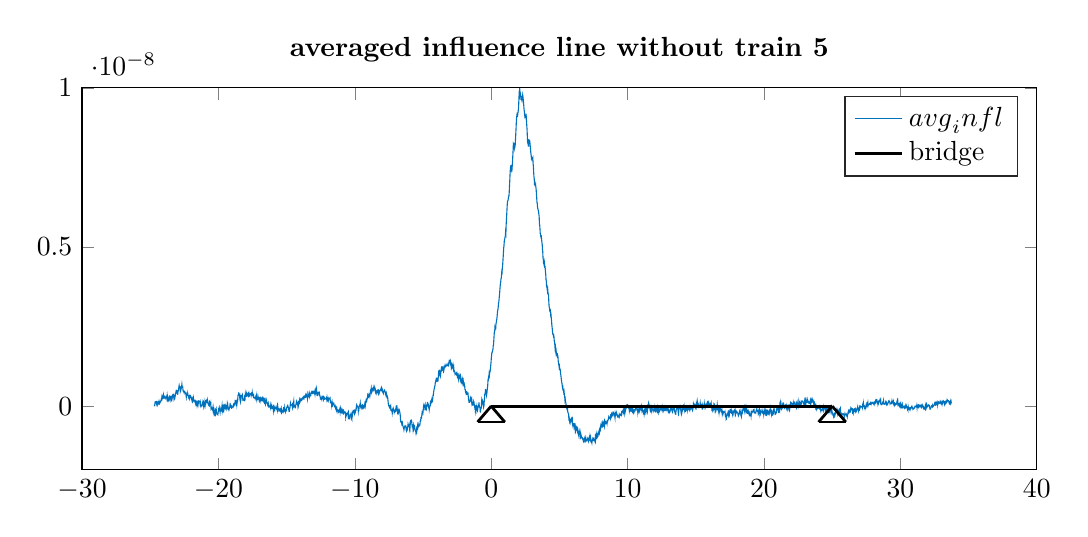
\begin{tikzpicture}

\begin{axis}[%
width=\textwidth,
height=0.4\textwidth,
at={(0\figurewidth,0\figureheight)},
scale only axis,
xmin=-30,
xmax=40,
ymin=-2e-09,
ymax=1e-08,
axis background/.style={fill=white},
title style={font=\bfseries},
title={averaged influence line without train 5},
legend style={legend cell align=left,align=left,draw=white!15!black}
]
\addplot [color=mycolor1,solid]
  table[row sep=crcr]{%
-24.713720703125	1.09773792522459e-11\\
-24.6935712890625	2.08095856285326e-11\\
-24.673421875	1.39406662467464e-11\\
-24.6532724609375	1.01064657704603e-10\\
-24.633123046875	1.40138643405249e-10\\
-24.6129736328125	1.3480286601766e-10\\
-24.59282421875	1.07090720129297e-10\\
-24.5726748046875	1.0487580268183e-10\\
-24.552525390625	1.22557385869332e-10\\
-24.5323759765625	6.05798180711653e-11\\
-24.5122265625	3.58490582108781e-11\\
-24.4920771484375	8.39153460468263e-11\\
-24.471927734375	5.29490352396332e-11\\
-24.4517783203125	8.90523103905422e-11\\
-24.43162890625	7.44368551086552e-11\\
-24.4114794921875	1.40019075690579e-10\\
-24.391330078125	1.45078671937909e-10\\
-24.3711806640625	1.17448417596591e-10\\
-24.35103125	1.59150391271008e-10\\
-24.3308818359375	1.3000297992883e-10\\
-24.310732421875	8.20464573455869e-11\\
-24.2905830078125	9.89968633634722e-11\\
-24.27043359375	1.36407345862867e-10\\
-24.2502841796875	1.35284359675538e-10\\
-24.230134765625	1.61809777173588e-10\\
-24.2099853515625	1.73558655543556e-10\\
-24.1898359375	2.10456315439882e-10\\
-24.1696865234375	1.96696681676376e-10\\
-24.149537109375	2.6955072771069e-10\\
-24.1293876953125	2.21171166185745e-10\\
-24.10923828125	2.43959798149636e-10\\
-24.0890888671875	2.4718633365703e-10\\
-24.068939453125	3.12495134658748e-10\\
-24.0487900390625	2.93680116414165e-10\\
-24.028640625	3.43963858846809e-10\\
-24.0084912109375	2.65426359291211e-10\\
-23.988341796875	2.76481602291797e-10\\
-23.9681923828125	2.84084281409615e-10\\
-23.94804296875	2.96790947310934e-10\\
-23.9278935546875	2.54524752784373e-10\\
-23.907744140625	2.39347341215497e-10\\
-23.8875947265625	2.63235782025648e-10\\
-23.8674453125	2.57654685327346e-10\\
-23.8472958984375	2.76579798321689e-10\\
-23.827146484375	3.09219089608721e-10\\
-23.8069970703125	3.05456370676432e-10\\
-23.78684765625	2.53682837544692e-10\\
-23.7666982421875	3.18598021702528e-10\\
-23.746548828125	2.21961007525938e-10\\
-23.7263994140625	2.60518767244936e-10\\
-23.70625	1.46863558119624e-10\\
-23.6861005859375	2.24905087566381e-10\\
-23.665951171875	1.95382255926006e-10\\
-23.6458017578125	2.34247093308387e-10\\
-23.62565234375	2.53394079117067e-10\\
-23.6055029296875	2.80723188417253e-10\\
-23.585353515625	2.37373566001665e-10\\
-23.5652041015625	3.00907729651942e-10\\
-23.5450546875	2.90303053798107e-10\\
-23.5249052734375	2.9675829360628e-10\\
-23.504755859375	2.43185599911153e-10\\
-23.4846064453125	1.88184872990987e-10\\
-23.46445703125	2.28955716179363e-10\\
-23.4443076171875	1.49399218563797e-10\\
-23.424158203125	2.4684845173544e-10\\
-23.4040087890625	2.30346088945103e-10\\
-23.383859375	3.02563185877946e-10\\
-23.3637099609375	2.93032639474539e-10\\
-23.343560546875	3.62348452243518e-10\\
-23.3234111328125	3.67897539712556e-10\\
-23.30326171875	3.71325755181181e-10\\
-23.2831123046875	3.12607944209162e-10\\
-23.262962890625	2.42641963499903e-10\\
-23.2428134765625	2.88453249323558e-10\\
-23.2226640625	2.20573972489967e-10\\
-23.2025146484375	2.32650847814372e-10\\
-23.182365234375	3.08432023278356e-10\\
-23.1622158203125	3.24874364258202e-10\\
-23.14206640625	3.49637904560074e-10\\
-23.1219169921875	4.32605685903977e-10\\
-23.101767578125	4.68621069331905e-10\\
-23.0816181640625	4.48827995961915e-10\\
-23.06146875	4.69821634282041e-10\\
-23.0413193359375	4.36901826821611e-10\\
-23.021169921875	4.14164884032906e-10\\
-23.0010205078125	4.363402688099e-10\\
-22.98087109375	3.59242772161278e-10\\
-22.9607216796875	4.90854745181095e-10\\
-22.940572265625	4.88044455619139e-10\\
-22.9204228515625	5.18343854014267e-10\\
-22.9002734375	6.02820280514092e-10\\
-22.8801240234375	6.49878457965091e-10\\
-22.859974609375	6.05505154077262e-10\\
-22.8398251953125	5.94245214829502e-10\\
-22.81967578125	6.01124850547229e-10\\
-22.7995263671875	4.94586207954643e-10\\
-22.779376953125	5.42350241509901e-10\\
-22.7592275390625	5.027622717157e-10\\
-22.739078125	5.35768516619963e-10\\
-22.7189287109375	5.71757622769311e-10\\
-22.698779296875	6.18473290739214e-10\\
-22.6786298828125	6.81662034006512e-10\\
-22.65848046875	6.04790740172553e-10\\
-22.6383310546875	6.06479000615985e-10\\
-22.618181640625	6.0562791529045e-10\\
-22.5980322265625	5.05314410742017e-10\\
-22.5778828125	4.62635443732679e-10\\
-22.5577333984375	4.62101408677662e-10\\
-22.537583984375	4.43334910367995e-10\\
-22.5174345703125	4.20225918198295e-10\\
-22.49728515625	4.66583673505209e-10\\
-22.4771357421875	4.61228199896404e-10\\
-22.456986328125	4.47305042673039e-10\\
-22.4368369140625	4.27282869201957e-10\\
-22.4166875	4.15188249315483e-10\\
-22.3965380859375	3.93672267052531e-10\\
-22.376388671875	3.46480373650151e-10\\
-22.3562392578125	2.86969295251779e-10\\
-22.33608984375	3.64020044450402e-10\\
-22.3159404296875	3.38676002276886e-10\\
-22.295791015625	3.55727752786756e-10\\
-22.2756416015625	3.65482981846725e-10\\
-22.2554921875	4.1100034489875e-10\\
-22.2353427734375	3.53172673215431e-10\\
-22.215193359375	3.30658863145325e-10\\
-22.1950439453125	2.9702617634387e-10\\
-22.17489453125	2.61308840596372e-10\\
-22.1547451171875	2.7214328228909e-10\\
-22.134595703125	2.41507324282974e-10\\
-22.1144462890625	3.02539279426075e-10\\
-22.094296875	2.75006922223986e-10\\
-22.0741474609375	3.1477206742696e-10\\
-22.053998046875	3.24042585742274e-10\\
-22.0338486328125	2.80536258968405e-10\\
-22.01369921875	2.81784746838973e-10\\
-21.9935498046875	2.79737715820733e-10\\
-21.973400390625	2.1928059575411e-10\\
-21.9532509765625	2.00161372097521e-10\\
-21.9331015625	1.64325646990756e-10\\
-21.9129521484375	2.09882579371893e-10\\
-21.892802734375	1.48450108112034e-10\\
-21.8726533203125	1.69268698745541e-10\\
-21.85250390625	1.90288688704274e-10\\
-21.8323544921875	2.45643162417611e-10\\
-21.812205078125	1.67653866285282e-10\\
-21.7920556640625	1.74412642013092e-10\\
-21.77190625	1.82841310494852e-10\\
-21.7517568359375	1.71842983872608e-10\\
-21.731607421875	1.44045478168944e-10\\
-21.7114580078125	1.59720820955465e-10\\
-21.69130859375	9.51811518246286e-11\\
-21.6711591796875	1.43839137955412e-10\\
-21.651009765625	1.53307759435571e-10\\
-21.6308603515625	1.17438066785914e-10\\
-21.6107109375	7.09297451337515e-11\\
-21.5905615234375	9.69608241831611e-11\\
-21.570412109375	3.64459901420759e-11\\
-21.5502626953125	1.0004480448142e-10\\
-21.53011328125	6.64451710894147e-11\\
-21.5099638671875	9.57706185545974e-11\\
-21.489814453125	4.92667874951273e-11\\
-21.4696650390625	1.08052886770829e-10\\
-21.449515625	1.63281443959088e-10\\
-21.4293662109375	1.60815648297972e-10\\
-21.409216796875	1.62283452693819e-10\\
-21.3890673828125	1.461816989903e-10\\
-21.36891796875	1.29205670113974e-10\\
-21.3487685546875	7.7765287368823e-11\\
-21.328619140625	1.14480784522876e-10\\
-21.3084697265625	1.61569083454165e-11\\
-21.2883203125	-9.95015374665469e-12\\
-21.2681708984375	1.86531363458547e-11\\
-21.248021484375	1.61545288227974e-11\\
-21.2278720703125	-1.46095315047022e-13\\
-21.20772265625	9.09924705380211e-13\\
-21.1875732421875	6.67179497714379e-11\\
-21.167423828125	3.57645861201208e-11\\
-21.1472744140625	4.11467600646003e-11\\
-21.127125	1.30441537819746e-10\\
-21.1069755859375	9.3525368067561e-11\\
-21.086826171875	2.31406795272673e-11\\
-21.0666767578125	1.12482386610481e-10\\
-21.04652734375	8.93053277542659e-11\\
-21.0263779296875	4.73163595520229e-11\\
-21.006228515625	1.30813291549403e-11\\
-20.9860791015625	1.15709744018176e-10\\
-20.9659296875	4.5948754535754e-11\\
-20.9457802734375	1.05325513839505e-10\\
-20.925630859375	8.69160019368425e-11\\
-20.9054814453125	1.55443584665853e-10\\
-20.88533203125	1.47363308000704e-10\\
-20.8651826171875	1.46225070689763e-10\\
-20.845033203125	2.18129556560346e-10\\
-20.8248837890625	1.01119865718411e-10\\
-20.804734375	1.8326223993097e-10\\
-20.7845849609375	1.38894062708101e-10\\
-20.764435546875	7.96845025819894e-11\\
-20.7442861328125	7.77470810276308e-11\\
-20.72413671875	4.3012871775837e-11\\
-20.7039873046875	2.76403965287149e-11\\
-20.683837890625	7.35288290766575e-11\\
-20.6636884765625	1.13588942696888e-10\\
-20.6435390625	6.21656959791994e-11\\
-20.6233896484375	1.10103081981133e-10\\
-20.603240234375	9.1494187209888e-11\\
-20.5830908203125	6.02933805659066e-11\\
-20.56294140625	9.53393648213065e-11\\
-20.5427919921875	-6.17651247893445e-11\\
-20.522642578125	-3.50003946565998e-11\\
-20.5024931640625	-5.63012557126015e-11\\
-20.48234375	-8.75865774543127e-11\\
-20.4621943359375	-1.08698165435288e-10\\
-20.442044921875	-9.64275380800524e-11\\
-20.4218955078125	-6.26348948395162e-11\\
-20.40174609375	-1.22092971836546e-10\\
-20.3815966796875	-3.50583766375076e-11\\
-20.361447265625	-9.1939028800612e-11\\
-20.3412978515625	-1.39053821577509e-10\\
-20.3211484375	-2.16037468203221e-10\\
-20.3009990234375	-1.69667734691536e-10\\
-20.280849609375	-2.66894359650748e-10\\
-20.2607001953125	-2.78610245116038e-10\\
-20.24055078125	-2.13080391509194e-10\\
-20.2204013671875	-2.37788844127706e-10\\
-20.200251953125	-1.285645150808e-10\\
-20.1801025390625	-1.53425282245224e-10\\
-20.159953125	-1.11272730224778e-10\\
-20.1398037109375	-2.01958165879048e-10\\
-20.119654296875	-2.33481308781265e-10\\
-20.0995048828125	-2.54042461034916e-10\\
-20.07935546875	-2.34862899871838e-10\\
-20.0592060546875	-2.41038677922744e-10\\
-20.039056640625	-2.5427260410376e-10\\
-20.0189072265625	-1.87805705476021e-10\\
-19.9987578125	-1.58787547251862e-10\\
-19.9786083984375	-8.66923605922888e-11\\
-19.958458984375	-9.53508009393384e-11\\
-19.9383095703125	-5.19018496838811e-11\\
-19.91816015625	-1.08114333902574e-10\\
-19.8980107421875	-1.5043498473042e-10\\
-19.877861328125	-1.92580975268644e-10\\
-19.8577119140625	-1.11908740062077e-10\\
-19.8375625	-1.52962530935329e-10\\
-19.8174130859375	-1.55775755522583e-10\\
-19.797263671875	-1.21200262563031e-10\\
-19.7771142578125	-8.87223677807977e-11\\
-19.75696484375	-5.21350276080722e-11\\
-19.7368154296875	1.11347210885202e-11\\
-19.716666015625	-1.19493050196931e-10\\
-19.6965166015625	-5.5817437360602e-11\\
-19.6763671875	-2.66737934202417e-11\\
-19.6562177734375	-2.06442103086249e-10\\
-19.636068359375	-4.30750257774829e-11\\
-19.6159189453125	-3.0239032577428e-11\\
-19.59576953125	-8.11265204958173e-11\\
-19.5756201171875	4.51537914380212e-12\\
-19.555470703125	-8.62775892006954e-12\\
-19.5353212890625	-1.94442279710357e-11\\
-19.515171875	6.98617218935317e-11\\
-19.4950224609375	-9.95404833925349e-11\\
-19.474873046875	-3.06945749527201e-11\\
-19.4547236328125	-7.82843901143705e-11\\
-19.43457421875	-1.03673343177624e-10\\
-19.4144248046875	-6.6818815414381e-11\\
-19.394275390625	3.15645963943696e-11\\
-19.3741259765625	-6.18730034424907e-11\\
-19.3539765625	4.74270113443054e-11\\
-19.3338271484375	-1.35142295662133e-11\\
-19.313677734375	3.07123759138631e-11\\
-19.2935283203125	-3.85116142419989e-11\\
-19.27337890625	-9.23794017900493e-11\\
-19.2532294921875	-9.92089573104509e-11\\
-19.233080078125	-1.22534839249734e-10\\
-19.2129306640625	-8.73444135834829e-11\\
-19.19278125	-4.94531288335195e-11\\
-19.1726318359375	-3.94378508208012e-11\\
-19.152482421875	2.61823613549095e-11\\
-19.1323330078125	-1.55213236474052e-12\\
-19.11218359375	4.13037854681788e-11\\
-19.0920341796875	1.27660422227825e-11\\
-19.071884765625	-1.21949417931925e-11\\
-19.0517353515625	-4.22665457176614e-12\\
-19.0315859375	-6.24249518021138e-11\\
-19.0114365234375	-5.51471375902657e-11\\
-18.991287109375	-2.7003198019621e-11\\
-18.9711376953125	-2.81179178736166e-11\\
-18.95098828125	-1.35563087722268e-11\\
-18.9308388671875	1.06981685785951e-11\\
-18.910689453125	-8.91382862094899e-12\\
-18.8905400390625	3.8386652551669e-11\\
-18.870390625	1.41941878115645e-11\\
-18.8502412109375	1.24809065419559e-11\\
-18.830091796875	6.65725807964118e-11\\
-18.8099423828125	5.82186267794222e-11\\
-18.78979296875	1.04641633245264e-10\\
-18.7696435546875	1.69494524798535e-10\\
-18.749494140625	1.58584127949087e-10\\
-18.7293447265625	1.63593688600801e-10\\
-18.7091953125	1.05594296977354e-10\\
-18.6890458984375	1.50399791915663e-10\\
-18.668896484375	1.33526685339816e-10\\
-18.6487470703125	4.14267665133885e-11\\
-18.62859765625	9.91494536532048e-11\\
-18.6084482421875	1.91493824236991e-10\\
-18.588298828125	1.79064356306387e-10\\
-18.5681494140625	3.20812468642872e-10\\
-18.548	3.5131581490955e-10\\
-18.5278505859375	3.70755406865319e-10\\
-18.507701171875	4.11350176749016e-10\\
-18.4875517578125	4.01785060434877e-10\\
-18.46740234375	3.68285655779689e-10\\
-18.4472529296875	3.15749857585481e-10\\
-18.427103515625	2.22316720315667e-10\\
-18.4069541015625	1.74748752900462e-10\\
-18.3868046875	1.40530291036713e-10\\
-18.3666552734375	2.7056942927725e-10\\
-18.346505859375	2.28067191820167e-10\\
-18.3263564453125	2.86916645550632e-10\\
-18.30620703125	3.19065116527258e-10\\
-18.2860576171875	3.07772022276293e-10\\
-18.265908203125	3.1755570047854e-10\\
-18.2457587890625	3.45329226301593e-10\\
-18.225609375	2.69518733794182e-10\\
-18.2054599609375	1.80415898586452e-10\\
-18.185310546875	1.84692005381013e-10\\
-18.1651611328125	1.92647847322645e-10\\
-18.14501171875	2.02189180876594e-10\\
-18.1248623046875	1.90680554181554e-10\\
-18.104712890625	1.81277221324976e-10\\
-18.0845634765625	3.00764849764428e-10\\
-18.0644140625	2.8494066839312e-10\\
-18.0442646484375	2.53914931957261e-10\\
-18.024115234375	3.70302373346656e-10\\
-18.0039658203125	3.09541097895721e-10\\
-17.98381640625	3.16690128631036e-10\\
-17.9636669921875	3.55721301888694e-10\\
-17.943517578125	3.98229840994431e-10\\
-17.9233681640625	3.4800832565613e-10\\
-17.90321875	3.75267275800515e-10\\
-17.8830693359375	3.49677344047865e-10\\
-17.862919921875	3.31946633972207e-10\\
-17.8427705078125	3.3674136257158e-10\\
-17.82262109375	3.73582873662564e-10\\
-17.8024716796875	2.7403513597787e-10\\
-17.782322265625	3.65259164998782e-10\\
-17.7621728515625	3.88810862612599e-10\\
-17.7420234375	2.96788347886762e-10\\
-17.7218740234375	3.78567154673814e-10\\
-17.701724609375	3.83486779092859e-10\\
-17.6815751953125	3.65894138173323e-10\\
-17.66142578125	3.61395247417323e-10\\
-17.6412763671875	3.89482776180247e-10\\
-17.621126953125	3.82990761222404e-10\\
-17.6009775390625	3.35762623012587e-10\\
-17.580828125	3.8551772066576e-10\\
-17.5606787109375	3.6807657161796e-10\\
-17.540529296875	3.54823101091275e-10\\
-17.5203798828125	4.31147707292826e-10\\
-17.50023046875	3.73005518697136e-10\\
-17.4800810546875	3.65522541347125e-10\\
-17.459931640625	3.6425864004899e-10\\
-17.4397822265625	3.16290414716221e-10\\
-17.4196328125	3.38319992983829e-10\\
-17.3994833984375	2.64012634962792e-10\\
-17.379333984375	2.6254430216611e-10\\
-17.3591845703125	2.64462189815144e-10\\
-17.33903515625	2.53030684022675e-10\\
-17.3188857421875	2.38444338514586e-10\\
-17.298736328125	2.54041003615494e-10\\
-17.2785869140625	2.78479522016645e-10\\
-17.2584375	3.05871262164324e-10\\
-17.2382880859375	2.32356567270767e-10\\
-17.218138671875	2.51392279692998e-10\\
-17.1979892578125	3.11186059080634e-10\\
-17.17783984375	2.02341323045468e-10\\
-17.1576904296875	2.41124112382661e-10\\
-17.137541015625	2.15385846218303e-10\\
-17.1173916015625	2.25340121042246e-10\\
-17.0972421875	2.87461029037808e-10\\
-17.0770927734375	2.29865423582156e-10\\
-17.056943359375	2.32287108626294e-10\\
-17.0367939453125	2.26272288373172e-10\\
-17.01664453125	1.91832512158406e-10\\
-16.9964951171875	2.85195484990157e-10\\
-16.976345703125	1.95841366156281e-10\\
-16.9561962890625	2.2746825197163e-10\\
-16.936046875	2.03820749579292e-10\\
-16.9158974609375	2.34450900506376e-10\\
-16.895748046875	1.82054137722659e-10\\
-16.8755986328125	2.36504951059387e-10\\
-16.85544921875	2.45166748051039e-10\\
-16.8352998046875	2.23876223615018e-10\\
-16.815150390625	2.01549065112273e-10\\
-16.7950009765625	2.58978897071479e-10\\
-16.7748515625	2.69630806109775e-10\\
-16.7547021484375	2.21431321088188e-10\\
-16.734552734375	1.49186768132531e-10\\
-16.7144033203125	2.55236969782188e-10\\
-16.69425390625	2.37634761043285e-10\\
-16.6741044921875	1.48163171494976e-10\\
-16.653955078125	1.59943756837562e-10\\
-16.6338056640625	1.87417505341073e-10\\
-16.61365625	6.22777615970007e-11\\
-16.5935068359375	1.52699954143556e-10\\
-16.573357421875	1.26783116294546e-10\\
-16.5532080078125	7.97156347907812e-11\\
-16.53305859375	1.63512153492937e-10\\
-16.5129091796875	1.20690361359775e-10\\
-16.492759765625	1.48901734878506e-10\\
-16.4726103515625	1.81491719403411e-10\\
-16.4524609375	1.01648011355271e-10\\
-16.4323115234375	1.01166720745117e-10\\
-16.412162109375	8.09041402514561e-11\\
-16.3920126953125	4.65534113521812e-11\\
-16.37186328125	8.09113858605161e-11\\
-16.3517138671875	1.05577405726657e-10\\
-16.331564453125	5.46432584544551e-11\\
-16.3114150390625	-1.07073607338987e-11\\
-16.291265625	3.23658679456335e-12\\
-16.2711162109375	5.57003986604542e-12\\
-16.250966796875	-2.4511331930302e-11\\
-16.2308173828125	-2.31466024272067e-11\\
-16.21066796875	-6.62576112902956e-14\\
-16.1905185546875	-3.3192873253249e-11\\
-16.170369140625	2.61200692523544e-11\\
-16.1502197265625	-4.09250827790141e-11\\
-16.1300703125	1.51529161244328e-11\\
-16.1099208984375	-3.48466368670595e-11\\
-16.089771484375	-4.72766498120004e-11\\
-16.0696220703125	-1.34094444543018e-11\\
-16.04947265625	-5.33344998898171e-11\\
-16.0293232421875	-7.55886521880643e-11\\
-16.009173828125	-7.70759214878832e-11\\
-15.9890244140625	-4.64149486022542e-11\\
-15.968875	-1.38820725751734e-10\\
-15.9487255859375	-6.54457346720116e-11\\
-15.928576171875	-1.21151263256682e-10\\
-15.9084267578125	-9.63753169302811e-11\\
-15.88827734375	-6.21091401420883e-11\\
-15.8681279296875	-1.02841783204333e-10\\
-15.847978515625	-3.71930618987939e-11\\
-15.8278291015625	-7.01424591255367e-11\\
-15.8076796875	-6.7244134082224e-11\\
-15.7875302734375	-5.32850068669877e-11\\
-15.767380859375	-6.61260641222864e-11\\
-15.7472314453125	-8.18942012288492e-11\\
-15.72708203125	-4.28558670170743e-11\\
-15.7069326171875	-8.44335212104679e-11\\
-15.686783203125	-2.19370632347171e-11\\
-15.6666337890625	-9.86851919151359e-11\\
-15.646484375	-2.73807255370096e-11\\
-15.6263349609375	-9.27527417925305e-11\\
-15.606185546875	-7.60728823657561e-11\\
-15.5860361328125	-9.18869589858863e-11\\
-15.56588671875	-1.41462478328619e-10\\
-15.5457373046875	-1.32281305324135e-10\\
-15.525587890625	-1.08285966991623e-10\\
-15.5054384765625	-1.4531924638728e-10\\
-15.4852890625	-1.57759591241387e-10\\
-15.4651396484375	-1.64314470303142e-10\\
-15.444990234375	-1.14524093187505e-10\\
-15.4248408203125	-1.45518552761252e-10\\
-15.40469140625	-1.79813248313756e-10\\
-15.3845419921875	-1.05895784835246e-10\\
-15.364392578125	-1.72144844279342e-10\\
-15.3442431640625	-2.030933527813e-10\\
-15.32409375	-1.90020039453086e-10\\
-15.3039443359375	-1.59526582306179e-10\\
-15.283794921875	-1.78666168258809e-10\\
-15.2636455078125	-1.72161827687887e-10\\
-15.24349609375	-1.12261091052144e-10\\
-15.2233466796875	-1.43060131747515e-10\\
-15.203197265625	-7.07438886570091e-11\\
-15.1830478515625	-8.51268466383978e-11\\
-15.1628984375	-1.62213455587638e-10\\
-15.1427490234375	-6.48294028238623e-11\\
-15.122599609375	-1.36569723323781e-10\\
-15.1024501953125	-1.73744542912013e-10\\
-15.08230078125	-1.13788317574463e-10\\
-15.0621513671875	-1.23096110479808e-10\\
-15.042001953125	-1.55014998480335e-10\\
-15.0218525390625	-1.39375343873936e-10\\
-15.001703125	-7.09844330267298e-11\\
-14.9815537109375	-3.03098577220019e-11\\
-14.961404296875	-2.84803465930814e-11\\
-14.9412548828125	5.2366970999717e-12\\
-14.92110546875	1.99063458747524e-11\\
-14.9009560546875	-3.33674129164299e-11\\
-14.880806640625	-2.9090372569008e-11\\
-14.8606572265625	-5.34733922428522e-11\\
-14.8405078125	-1.18906653168336e-10\\
-14.8203583984375	-1.67602204667935e-10\\
-14.800208984375	-1.65153136022655e-10\\
-14.7800595703125	-9.27539246764424e-11\\
-14.75991015625	-6.2039862952773e-11\\
-14.7397607421875	2.09194474861622e-11\\
-14.719611328125	8.01624452942796e-11\\
-14.6994619140625	2.65492479953799e-11\\
-14.6793125	3.11079839321726e-11\\
-14.6591630859375	3.05809932960427e-11\\
-14.639013671875	3.25693433215122e-11\\
-14.6188642578125	4.09913430931543e-11\\
-14.59871484375	1.06205618372247e-11\\
-14.5785654296875	-2.65426512929469e-11\\
-14.558416015625	1.09078266462909e-10\\
-14.5382666015625	3.95287146810164e-12\\
-14.5181171875	6.39507718345674e-11\\
-14.4979677734375	9.29003748322539e-11\\
-14.477818359375	1.52869068053949e-10\\
-14.4576689453125	1.23756508371128e-11\\
-14.43751953125	3.07380726102018e-11\\
-14.4173701171875	1.54082896825512e-11\\
-14.397220703125	-2.51465730150543e-11\\
-14.3770712890625	-5.11935096459007e-11\\
-14.356921875	-5.11946158620653e-11\\
-14.3367724609375	2.98679698291255e-11\\
-14.316623046875	3.89911485298309e-11\\
-14.2964736328125	9.50531500839613e-11\\
-14.27632421875	1.38250674280057e-10\\
-14.2561748046875	9.78606442689452e-11\\
-14.236025390625	9.41008516844596e-11\\
-14.2158759765625	6.91061401906793e-11\\
-14.1957265625	8.91936095569298e-11\\
-14.1755771484375	1.08944384077396e-11\\
-14.155427734375	7.70544731546126e-11\\
-14.1352783203125	2.85845329606202e-11\\
-14.11512890625	8.68721672000625e-11\\
-14.0949794921875	8.38478032577267e-11\\
-14.074830078125	1.42225503860694e-10\\
-14.0546806640625	1.87193419827348e-10\\
-14.03453125	1.13504229471422e-10\\
-14.0143818359375	1.32441124827836e-10\\
-13.994232421875	1.93667154202698e-10\\
-13.9740830078125	1.69616959056621e-10\\
-13.95393359375	1.68070941395665e-10\\
-13.9337841796875	2.05826350021239e-10\\
-13.913634765625	1.75550357290201e-10\\
-13.8934853515625	1.7695311482316e-10\\
-13.8733359375	2.08942744208379e-10\\
-13.8531865234375	2.23210260780143e-10\\
-13.833037109375	2.48165051717487e-10\\
-13.8128876953125	2.27062300049154e-10\\
-13.79273828125	2.24967795707608e-10\\
-13.7725888671875	2.69617937436568e-10\\
-13.752439453125	2.9716389043818e-10\\
-13.7322900390625	3.07690119875179e-10\\
-13.712140625	2.66999319779587e-10\\
-13.6919912109375	3.03492807266138e-10\\
-13.671841796875	3.09423123696234e-10\\
-13.6516923828125	2.80508479467698e-10\\
-13.63154296875	2.77697608440124e-10\\
-13.6113935546875	3.26720803003521e-10\\
-13.591244140625	2.80520274502879e-10\\
-13.5710947265625	2.85856192366028e-10\\
-13.5509453125	3.88298976566418e-10\\
-13.5307958984375	3.13518208512073e-10\\
-13.510646484375	3.05822916875967e-10\\
-13.4904970703125	3.56270502417359e-10\\
-13.47034765625	2.44883000030254e-10\\
-13.4501982421875	3.10318174092719e-10\\
-13.430048828125	3.23670602914322e-10\\
-13.4098994140625	3.41890504325879e-10\\
-13.38975	3.23360567133416e-10\\
-13.3696005859375	3.71200868843083e-10\\
-13.349451171875	3.25202214817502e-10\\
-13.3293017578125	4.03280123066053e-10\\
-13.30915234375	3.69595963116189e-10\\
-13.2890029296875	3.20103415445965e-10\\
-13.268853515625	3.48734163145243e-10\\
-13.2487041015625	3.4020796031563e-10\\
-13.2285546875	3.37585260120347e-10\\
-13.2084052734375	4.2029511079865e-10\\
-13.188255859375	4.17838922815086e-10\\
-13.1681064453125	4.44053661775872e-10\\
-13.14795703125	4.28522490509257e-10\\
-13.1278076171875	4.61896611664727e-10\\
-13.107658203125	4.6444818015616e-10\\
-13.0875087890625	4.17767536839962e-10\\
-13.067359375	4.35250843840825e-10\\
-13.0472099609375	4.21944601056742e-10\\
-13.027060546875	4.61160576379856e-10\\
-13.0069111328125	4.54882746116851e-10\\
-12.98676171875	4.20473696798241e-10\\
-12.9666123046875	4.01405020377356e-10\\
-12.946462890625	4.39964005238393e-10\\
-12.9263134765625	3.87684679011231e-10\\
-12.9061640625	4.91930860571449e-10\\
-12.8860146484375	4.7217181006657e-10\\
-12.865865234375	5.11216888996542e-10\\
-12.8457158203125	4.34490185941702e-10\\
-12.82556640625	4.58238036887406e-10\\
-12.8054169921875	5.18011135078465e-10\\
-12.785267578125	4.06332437721136e-10\\
-12.7651181640625	4.33382112654343e-10\\
-12.74496875	4.33407359479599e-10\\
-12.7248193359375	3.14640594915982e-10\\
-12.704669921875	3.90384221226922e-10\\
-12.6845205078125	4.07042605312234e-10\\
-12.66437109375	3.98408805851801e-10\\
-12.6442216796875	4.23508510487788e-10\\
-12.624072265625	4.07649674883019e-10\\
-12.6039228515625	4.21848015569773e-10\\
-12.5837734375	3.58872084515378e-10\\
-12.5636240234375	3.17825212769747e-10\\
-12.543474609375	3.11863112346314e-10\\
-12.5233251953125	2.37368785146431e-10\\
-12.50317578125	2.51543244093486e-10\\
-12.4830263671875	2.62785537308819e-10\\
-12.462876953125	2.34940287323677e-10\\
-12.4427275390625	2.52821639944435e-10\\
-12.422578125	2.21155362098907e-10\\
-12.4024287109375	2.88668956544825e-10\\
-12.382279296875	2.76010095683133e-10\\
-12.3621298828125	2.94295681829265e-10\\
-12.34198046875	3.05302449708961e-10\\
-12.3218310546875	2.52507367485492e-10\\
-12.301681640625	2.18351652505813e-10\\
-12.2815322265625	3.12732449725603e-10\\
-12.2613828125	1.95092739889183e-10\\
-12.2412333984375	2.69073341560593e-10\\
-12.221083984375	2.55025742714238e-10\\
-12.2009345703125	2.51494196610875e-10\\
-12.18078515625	2.26205166290048e-10\\
-12.1606357421875	2.28183485099706e-10\\
-12.140486328125	2.34578011406822e-10\\
-12.1203369140625	2.27702586325352e-10\\
-12.1001875	2.2452550873656e-10\\
-12.0800380859375	2.52121420895702e-10\\
-12.059888671875	2.09836310692695e-10\\
-12.0397392578125	2.64766789276159e-10\\
-12.01958984375	1.93880787401625e-10\\
-11.9994404296875	1.76992585704368e-10\\
-11.979291015625	2.10836860312124e-10\\
-11.9591416015625	2.3576326886834e-10\\
-11.9389921875	1.81147647198934e-10\\
-11.9188427734375	2.13905365336679e-10\\
-11.898693359375	2.34890416594614e-10\\
-11.8785439453125	2.50588443187919e-10\\
-11.85839453125	2.48354524443169e-10\\
-11.8382451171875	2.43138803205355e-10\\
-11.818095703125	2.56824402234415e-10\\
-11.7979462890625	1.63327110370472e-10\\
-11.777796875	1.86997054924879e-10\\
-11.7576474609375	1.78209292245704e-10\\
-11.737498046875	7.57214067382631e-11\\
-11.7173486328125	1.50107842123747e-10\\
-11.69719921875	3.36415746297215e-11\\
-11.6770498046875	8.78837484261216e-11\\
-11.656900390625	8.18919569423246e-11\\
-11.6367509765625	4.58446968983876e-11\\
-11.6166015625	1.05724042697239e-10\\
-11.5964521484375	5.09425132128133e-11\\
-11.576302734375	5.36045369605116e-11\\
-11.5561533203125	6.01256069002969e-11\\
-11.53600390625	7.52905266872104e-11\\
-11.5158544921875	4.07458812346522e-11\\
-11.495705078125	-9.07193274775039e-12\\
-11.4755556640625	-4.5735525510074e-12\\
-11.45540625	-2.15669936590464e-11\\
-11.4352568359375	-4.11866511813535e-11\\
-11.415107421875	-6.61910758174793e-11\\
-11.3949580078125	-1.95252477595887e-11\\
-11.37480859375	-5.60101051213129e-11\\
-11.3546591796875	-1.02734814904522e-10\\
-11.334509765625	-1.14618815110843e-11\\
-11.3143603515625	-1.15312452693579e-10\\
-11.2942109375	-1.38911738381349e-10\\
-11.2740615234375	-1.26422132563536e-10\\
-11.253912109375	-1.33464792416667e-10\\
-11.2337626953125	-1.80106972070271e-10\\
-11.21361328125	-1.40710875509159e-10\\
-11.1934638671875	-1.54422586358524e-10\\
-11.173314453125	-1.69603102847809e-10\\
-11.1531650390625	-1.37400522545235e-10\\
-11.133015625	-1.11686295324275e-10\\
-11.1128662109375	-1.06737207635753e-10\\
-11.092716796875	-7.64300411401918e-11\\
-11.0725673828125	-1.72195583197461e-10\\
-11.05241796875	-9.92383028434192e-11\\
-11.0322685546875	-1.63708508818572e-10\\
-11.012119140625	-1.42674215765893e-10\\
-10.9919697265625	-1.6800576046351e-10\\
-10.9718203125	-1.25345026524679e-10\\
-10.9516708984375	-1.64301916820076e-10\\
-10.931521484375	-1.2366154351369e-10\\
-10.9113720703125	-1.63716175657697e-10\\
-10.89122265625	-2.0801350951206e-10\\
-10.8710732421875	-2.21572200880312e-10\\
-10.850923828125	-1.71148634819797e-10\\
-10.8307744140625	-2.04911611253103e-10\\
-10.810625	-1.66128370972657e-10\\
-10.7904755859375	-1.95606729521574e-10\\
-10.770326171875	-2.06342703154325e-10\\
-10.7501767578125	-1.89339133661738e-10\\
-10.73002734375	-2.05035012290555e-10\\
-10.7098779296875	-2.19545696613825e-10\\
-10.689728515625	-2.26616501374162e-10\\
-10.6695791015625	-3.27474322503548e-10\\
-10.6494296875	-2.52751652772543e-10\\
-10.6292802734375	-2.97194214060912e-10\\
-10.609130859375	-2.70273924258008e-10\\
-10.5889814453125	-2.45468463679188e-10\\
-10.56883203125	-2.38130468169245e-10\\
-10.5486826171875	-2.26577058329616e-10\\
-10.528533203125	-2.35462764821982e-10\\
-10.5083837890625	-2.11579007214855e-10\\
-10.488234375	-3.00122433065821e-10\\
-10.4680849609375	-2.52297952369961e-10\\
-10.447935546875	-4.09357219279844e-10\\
-10.4277861328125	-3.39619018765798e-10\\
-10.40763671875	-3.57173342172106e-10\\
-10.3874873046875	-3.40627725299252e-10\\
-10.367337890625	-3.65361812284898e-10\\
-10.3471884765625	-2.82201837749776e-10\\
-10.3270390625	-2.95002150536069e-10\\
-10.3068896484375	-3.03589088334693e-10\\
-10.286740234375	-2.62843122009137e-10\\
-10.2665908203125	-2.98462561378883e-10\\
-10.24644140625	-3.52598787431256e-10\\
-10.2262919921875	-2.96183037095073e-10\\
-10.206142578125	-3.47994843427583e-10\\
-10.1859931640625	-2.21803378316238e-10\\
-10.16584375	-2.56960362619329e-10\\
-10.1456943359375	-2.01908699402865e-10\\
-10.125544921875	-2.00223985882758e-10\\
-10.1053955078125	-1.63536431390383e-10\\
-10.08524609375	-1.77382687052001e-10\\
-10.0650966796875	-1.54431405507611e-10\\
-10.044947265625	-1.85858024346391e-10\\
-10.0247978515625	-2.29180615465623e-10\\
-10.0046484375	-1.81376939705838e-10\\
-9.9844990234375	-2.19050448122022e-10\\
-9.964349609375	-2.03579561423082e-10\\
-9.9442001953125	-1.51817706308039e-10\\
-9.92405078125	-1.05533731638916e-10\\
-9.9039013671875	-1.1104902316505e-10\\
-9.883751953125	5.08140458281764e-12\\
-9.8636025390625	4.02264269026727e-11\\
-9.843453125	1.06917890452281e-11\\
-9.8233037109375	6.89059724948321e-12\\
-9.803154296875	-8.14684020966948e-12\\
-9.7830048828125	-2.35384237249429e-11\\
-9.76285546875	-6.31549663542929e-11\\
-9.7427060546875	-1.56155506589205e-10\\
-9.722556640625	-8.42781885457007e-11\\
-9.7024072265625	-1.02644398453123e-10\\
-9.6822578125	-3.65032696396139e-11\\
-9.6621083984375	2.79533201343235e-11\\
-9.641958984375	3.7185840859235e-11\\
-9.6218095703125	3.04390068221726e-11\\
-9.60166015625	8.85193460250877e-11\\
-9.5815107421875	-5.70840392620867e-12\\
-9.561361328125	1.8848712443656e-11\\
-9.5412119140625	1.46271328168818e-11\\
-9.5210625	1.50020919109353e-11\\
-9.5009130859375	-3.19404777408264e-11\\
-9.480763671875	9.96449472448063e-12\\
-9.4606142578125	-1.84237848142315e-11\\
-9.44046484375	7.87715199943953e-12\\
-9.4203154296875	-4.40520111936655e-11\\
-9.400166015625	-1.84116737737518e-11\\
-9.3800166015625	-3.62919471133253e-12\\
-9.3598671875	-4.13500408960771e-11\\
-9.3397177734375	-1.50948282091494e-11\\
-9.319568359375	1.63165391625535e-11\\
-9.2994189453125	-1.18048153321468e-11\\
-9.27926953125	3.30470087797299e-11\\
-9.2591201171875	7.41911193779062e-11\\
-9.238970703125	1.5813230589643e-10\\
-9.2188212890625	5.8178846516794e-11\\
-9.198671875	1.31253108823619e-10\\
-9.1785224609375	1.75102853622578e-10\\
-9.158373046875	1.28723622601486e-10\\
-9.1382236328125	1.42353345509329e-10\\
-9.11807421875	1.8637013448854e-10\\
-9.0979248046875	2.17306303590955e-10\\
-9.077775390625	2.50929301695626e-10\\
-9.0576259765625	3.25983667728518e-10\\
-9.0374765625	2.96376094421515e-10\\
-9.0173271484375	3.47793754001667e-10\\
-8.997177734375	3.12198698965692e-10\\
-8.9770283203125	2.95480708657061e-10\\
-8.95687890625	3.12302350517398e-10\\
-8.9367294921875	3.44107609463936e-10\\
-8.916580078125	3.68238814630823e-10\\
-8.8964306640625	3.22285342446025e-10\\
-8.87628125	3.84588707621727e-10\\
-8.8561318359375	4.64937999924563e-10\\
-8.835982421875	4.47689225208461e-10\\
-8.8158330078125	5.0485832131216e-10\\
-8.79568359375	5.58632069353385e-10\\
-8.7755341796875	4.71781440037826e-10\\
-8.755384765625	5.32834196180694e-10\\
-8.7352353515625	5.45484744419315e-10\\
-8.7150859375	4.9318401742882e-10\\
-8.6949365234375	5.21144441279566e-10\\
-8.674787109375	5.39057303592426e-10\\
-8.6546376953125	5.18122470822455e-10\\
-8.63448828125	5.47721902484033e-10\\
-8.6143388671875	5.85211574103377e-10\\
-8.594189453125	5.4059032472768e-10\\
-8.5740400390625	6.09731382123251e-10\\
-8.553890625	5.83941385112628e-10\\
-8.5337412109375	5.48105016054637e-10\\
-8.513591796875	5.56141056713793e-10\\
-8.4934423828125	5.31726411175992e-10\\
-8.47329296875	4.44950873678822e-10\\
-8.4531435546875	4.73612064291646e-10\\
-8.432994140625	4.75281644104442e-10\\
-8.4128447265625	4.57020768965202e-10\\
-8.3926953125	4.10076439730589e-10\\
-8.3725458984375	4.46220482029958e-10\\
-8.352396484375	4.18259198269887e-10\\
-8.3322470703125	4.23099663040644e-10\\
-8.31209765625	4.31316561299212e-10\\
-8.2919482421875	5.35253948910175e-10\\
-8.271798828125	4.49508585777474e-10\\
-8.2516494140625	5.0207785648103e-10\\
-8.2315	4.93603317346613e-10\\
-8.2113505859375	4.11926953238488e-10\\
-8.191201171875	4.39671225427463e-10\\
-8.1710517578125	4.65274220751898e-10\\
-8.15090234375	4.8075518445462e-10\\
-8.1307529296875	4.94106553893446e-10\\
-8.110603515625	5.13379362932558e-10\\
-8.0904541015625	5.3657445141924e-10\\
-8.0703046875	5.60318153372396e-10\\
-8.0501552734375	5.28927259189402e-10\\
-8.030005859375	5.63750896872777e-10\\
-8.0098564453125	5.0686395364962e-10\\
-7.98970703125	5.20926799586848e-10\\
-7.9695576171875	4.41060744177643e-10\\
-7.949408203125	4.41934784644303e-10\\
-7.9292587890625	4.29454014123991e-10\\
-7.909109375	4.00813372836498e-10\\
-7.8889599609375	4.37532226749297e-10\\
-7.868810546875	4.82889234574836e-10\\
-7.8486611328125	4.99775176989737e-10\\
-7.82851171875	5.09159126817106e-10\\
-7.8083623046875	4.89338074760363e-10\\
-7.788212890625	4.65515527549718e-10\\
-7.7680634765625	4.40473037339846e-10\\
-7.7479140625	3.61841365648686e-10\\
-7.7277646484375	3.48367735454367e-10\\
-7.707615234375	3.84996362037316e-10\\
-7.6874658203125	2.74017416525375e-10\\
-7.66731640625	3.65404066091747e-10\\
-7.6471669921875	3.26072289877484e-10\\
-7.627017578125	2.74622915186203e-10\\
-7.6068681640625	2.90168688384306e-10\\
-7.58671875	2.62231961261163e-10\\
-7.5665693359375	1.71553395725312e-10\\
-7.546419921875	8.4662839803278e-11\\
-7.5262705078125	2.47882661835858e-11\\
-7.50612109375	2.83032452018964e-11\\
-7.4859716796875	9.48646367484749e-12\\
-7.465822265625	-3.29573642096258e-11\\
-7.4456728515625	-9.41086900279166e-12\\
-7.4255234375	5.38834035848696e-12\\
-7.4053740234375	-3.27527047014981e-11\\
-7.385224609375	-6.23536097307496e-11\\
-7.3650751953125	-2.69339125036585e-11\\
-7.34492578125	-1.3664392184448e-10\\
-7.3247763671875	-1.43016493671734e-10\\
-7.304626953125	-1.46582901881121e-10\\
-7.2844775390625	-1.35548795510188e-10\\
-7.264328125	-1.93187158001696e-10\\
-7.2441787109375	-8.05677377040546e-11\\
-7.224029296875	-1.5344495095372e-10\\
-7.2038798828125	-1.05082765705773e-10\\
-7.18373046875	-6.7825616068742e-11\\
-7.1635810546875	-9.81372094377572e-11\\
-7.143431640625	-1.30843833751646e-10\\
-7.1232822265625	-1.32573841382249e-10\\
-7.1031328125	-1.89737184239466e-10\\
-7.0829833984375	-1.61552066927133e-10\\
-7.062833984375	-1.89866048662502e-10\\
-7.0426845703125	-1.84635808813062e-10\\
-7.02253515625	-1.43304929088345e-10\\
-7.0023857421875	-8.70697364720841e-11\\
-6.982236328125	-6.41928970461765e-11\\
-6.9620869140625	5.08394807399065e-12\\
-6.9419375	8.59392503916695e-12\\
-6.9217880859375	-8.39007949961488e-11\\
-6.901638671875	-5.43437602744869e-11\\
-6.8814892578125	-1.3787396919165e-10\\
-6.86133984375	-2.01922602642868e-10\\
-6.8411904296875	-1.70637021717249e-10\\
-6.821041015625	-1.50100298683285e-10\\
-6.8008916015625	-2.0065040262319e-10\\
-6.7807421875	-1.66473082935452e-10\\
-6.7605927734375	-1.021393173291e-10\\
-6.740443359375	-1.18809017966369e-10\\
-6.7202939453125	-1.76329156416503e-10\\
-6.70014453125	-1.85164103121827e-10\\
-6.6799951171875	-2.41392533417091e-10\\
-6.659845703125	-3.38290841733258e-10\\
-6.6396962890625	-4.81689862777808e-10\\
-6.619546875	-4.73549035652812e-10\\
-6.5993974609375	-4.76130450182205e-10\\
-6.579248046875	-4.88486204582493e-10\\
-6.5590986328125	-5.53913221549201e-10\\
-6.53894921875	-5.3020593173475e-10\\
-6.5187998046875	-5.12322424403526e-10\\
-6.498650390625	-5.97046763185753e-10\\
-6.4785009765625	-6.23417427940893e-10\\
-6.4583515625	-6.36418529743948e-10\\
-6.4382021484375	-6.85424143397768e-10\\
-6.418052734375	-6.91788963359804e-10\\
-6.3979033203125	-7.42623091593363e-10\\
-6.37775390625	-6.93849285338738e-10\\
-6.3576044921875	-6.52004342456579e-10\\
-6.337455078125	-6.46713850853885e-10\\
-6.3173056640625	-6.16903538102455e-10\\
-6.29715625	-6.25436273189777e-10\\
-6.2770068359375	-6.48342489564556e-10\\
-6.256857421875	-6.39923275058547e-10\\
-6.2367080078125	-7.30192984006785e-10\\
-6.21655859375	-7.1961245052061e-10\\
-6.1964091796875	-7.83201948318238e-10\\
-6.176259765625	-7.61643901310735e-10\\
-6.1561103515625	-7.4957816795738e-10\\
-6.1359609375	-6.50882763233581e-10\\
-6.1158115234375	-6.48286471116249e-10\\
-6.095662109375	-5.64905768030722e-10\\
-6.0755126953125	-5.9524019723513e-10\\
-6.05536328125	-6.14473699602916e-10\\
-6.0352138671875	-6.03505575616511e-10\\
-6.015064453125	-6.24464393536538e-10\\
-5.9949150390625	-7.00467157860699e-10\\
-5.974765625	-6.20697851253927e-10\\
-5.9546162109375	-6.75599860828584e-10\\
-5.934466796875	-5.48908569846557e-10\\
-5.9143173828125	-4.65644986574994e-10\\
-5.89416796875	-4.44826427231325e-10\\
-5.8740185546875	-4.39861854959044e-10\\
-5.853869140625	-4.38152006147703e-10\\
-5.8337197265625	-4.74461317701435e-10\\
-5.8135703125	-5.60338068278599e-10\\
-5.7934208984375	-6.25212038006047e-10\\
-5.773271484375	-6.08823058864516e-10\\
-5.7531220703125	-6.38289311112492e-10\\
-5.73297265625	-7.20447663859408e-10\\
-5.7128232421875	-6.3627190185918e-10\\
-5.692673828125	-5.93611790180702e-10\\
-5.6725244140625	-6.67344934647741e-10\\
-5.652375	-6.0669108987753e-10\\
-5.6322255859375	-6.09216248460733e-10\\
-5.612076171875	-6.83050604704237e-10\\
-5.5919267578125	-7.12103313603089e-10\\
-5.57177734375	-7.57452092500035e-10\\
-5.5516279296875	-7.73952202691121e-10\\
-5.531478515625	-8.02961599820574e-10\\
-5.5113291015625	-8.60087066553662e-10\\
-5.4911796875	-8.23125004884979e-10\\
-5.4710302734375	-7.36530125043658e-10\\
-5.450880859375	-7.77538074595697e-10\\
-5.4307314453125	-7.09024959776845e-10\\
-5.41058203125	-6.475975351443e-10\\
-5.3904326171875	-5.91793214185404e-10\\
-5.370283203125	-6.40357807632836e-10\\
-5.3501337890625	-5.80200448157403e-10\\
-5.329984375	-6.23079862725671e-10\\
-5.3098349609375	-6.38544561913364e-10\\
-5.289685546875	-6.28704881989783e-10\\
-5.2695361328125	-5.88736517595813e-10\\
-5.24938671875	-5.837127029688e-10\\
-5.2292373046875	-5.89653688940881e-10\\
-5.209087890625	-5.02038248246556e-10\\
-5.1889384765625	-4.49605943059522e-10\\
-5.1687890625	-4.58367650958427e-10\\
-5.1486396484375	-3.53510690260596e-10\\
-5.128490234375	-3.47551355325174e-10\\
-5.1083408203125	-3.58674554557341e-10\\
-5.08819140625	-2.8621783385947e-10\\
-5.0680419921875	-2.0887630606307e-10\\
-5.047892578125	-2.32488578808743e-10\\
-5.0277431640625	-1.93804509414363e-10\\
-5.00759375	-2.11714774264387e-10\\
-4.9874443359375	-1.34619638909537e-10\\
-4.967294921875	-4.65865852107858e-11\\
-4.9471455078125	-1.27111507519435e-10\\
-4.92699609375	-3.45015392361474e-11\\
-4.9068466796875	5.78527714055372e-12\\
-4.886697265625	3.38920598332066e-11\\
-4.8665478515625	3.63179081320038e-11\\
-4.8463984375	5.77145404774316e-11\\
-4.8262490234375	-7.18301866475525e-11\\
-4.806099609375	-5.41691373582707e-11\\
-4.7859501953125	-8.38769872753173e-11\\
-4.76580078125	-3.26327452730957e-11\\
-4.7456513671875	-6.82157918960114e-11\\
-4.725501953125	-1.08245030471514e-11\\
-4.7053525390625	9.14312296372072e-12\\
-4.685203125	7.18880859164935e-11\\
-4.6650537109375	5.02237595594088e-11\\
-4.644904296875	8.77040066950467e-11\\
-4.6247548828125	7.28418505017352e-11\\
-4.60460546875	1.22762757548507e-11\\
-4.5844560546875	-3.8008132734653e-11\\
-4.564306640625	-2.68378169998322e-11\\
-4.5441572265625	-1.0770603071826e-10\\
-4.5240078125	-5.09294848870047e-11\\
-4.5038583984375	-1.41857252206452e-11\\
-4.483708984375	2.54908162340301e-11\\
-4.4635595703125	9.61264999560128e-11\\
-4.44341015625	7.10031608416611e-11\\
-4.4232607421875	1.4813833079994e-10\\
-4.403111328125	1.69908190002027e-10\\
-4.3829619140625	1.09522173436666e-10\\
-4.3628125	1.04188142797702e-10\\
-4.3426630859375	1.87999118725088e-10\\
-4.322513671875	1.42658413105205e-10\\
-4.3023642578125	1.52279849906783e-10\\
-4.28221484375	2.68096588839912e-10\\
-4.2620654296875	3.44757873446798e-10\\
-4.241916015625	3.42248610028686e-10\\
-4.2217666015625	4.43075155230338e-10\\
-4.2016171875	4.9099542995976e-10\\
-4.1814677734375	5.43290481540044e-10\\
-4.161318359375	5.66728997340612e-10\\
-4.1411689453125	6.15898194920906e-10\\
-4.12101953125	6.40718073773956e-10\\
-4.1008701171875	7.35805712216412e-10\\
-4.080720703125	7.50405762424624e-10\\
-4.0605712890625	8.03811105789998e-10\\
-4.040421875	8.3828200559675e-10\\
-4.0202724609375	8.13315903916036e-10\\
-4.000123046875	8.38947648017153e-10\\
-3.9799736328125	7.8152441288412e-10\\
-3.95982421875	7.8149951286293e-10\\
-3.9396748046875	7.95063034877144e-10\\
-3.919525390625	8.41456010531311e-10\\
-3.8993759765625	8.23287131353508e-10\\
-3.8792265625	9.19561115361907e-10\\
-3.8590771484375	1.03974967250285e-09\\
-3.838927734375	1.00623612359085e-09\\
-3.8187783203125	1.09009132750496e-09\\
-3.79862890625	1.10370797718402e-09\\
-3.7784794921875	9.93009316759014e-10\\
-3.758330078125	9.73598979497865e-10\\
-3.7381806640625	1.02058235560223e-09\\
-3.71803125	9.64823879717647e-10\\
-3.6978818359375	1.03444840549504e-09\\
-3.677732421875	1.11760634300631e-09\\
-3.6575830078125	1.17755183677138e-09\\
-3.63743359375	1.15506167922202e-09\\
-3.6172841796875	1.23288783010181e-09\\
-3.597134765625	1.2362720203766e-09\\
-3.5769853515625	1.21632845501938e-09\\
-3.5568359375	1.14279462898032e-09\\
-3.5366865234375	1.14840087500347e-09\\
-3.516537109375	1.11578349019044e-09\\
-3.4963876953125	1.16651683128557e-09\\
-3.47623828125	1.12096599993446e-09\\
-3.4560888671875	1.17329227824404e-09\\
-3.435939453125	1.22809952211007e-09\\
-3.4157900390625	1.21259432441375e-09\\
-3.395640625	1.20905594149999e-09\\
-3.3754912109375	1.27582321583438e-09\\
-3.355341796875	1.24745053036262e-09\\
-3.3351923828125	1.2629831984985e-09\\
-3.31504296875	1.25909721582903e-09\\
-3.2948935546875	1.27453725466421e-09\\
-3.274744140625	1.27312418138117e-09\\
-3.2545947265625	1.28898417459765e-09\\
-3.2344453125	1.31782127115354e-09\\
-3.2142958984375	1.28920752504262e-09\\
-3.194146484375	1.27728211292077e-09\\
-3.1739970703125	1.27570001483572e-09\\
-3.15384765625	1.25997892824022e-09\\
-3.1336982421875	1.26105221777224e-09\\
-3.113548828125	1.35808723797112e-09\\
-3.0933994140625	1.38017704638374e-09\\
-3.07325	1.43796276987816e-09\\
-3.0531005859375	1.43212133999133e-09\\
-3.032951171875	1.42973794269541e-09\\
-3.0128017578125	1.37262901638773e-09\\
-2.99265234375	1.40764458979535e-09\\
-2.9725029296875	1.33761945811389e-09\\
-2.952353515625	1.29110735059038e-09\\
-2.9322041015625	1.22766174807478e-09\\
-2.9120546875	1.2810810191683e-09\\
-2.8919052734375	1.21790932734467e-09\\
-2.871755859375	1.24288239688358e-09\\
-2.8516064453125	1.22363193623735e-09\\
-2.83145703125	1.27873195216847e-09\\
-2.8113076171875	1.24347470562362e-09\\
-2.791158203125	1.22875295929062e-09\\
-2.7710087890625	1.16958878554261e-09\\
-2.750859375	1.2331728423097e-09\\
-2.7307099609375	1.11569206557198e-09\\
-2.710560546875	1.11677630267855e-09\\
-2.6904111328125	1.08789912293691e-09\\
-2.67026171875	1.06960022091032e-09\\
-2.6501123046875	1.01435828626727e-09\\
-2.629962890625	1.03927195228357e-09\\
-2.6098134765625	1.02777948921962e-09\\
-2.5896640625	1.02395192581118e-09\\
-2.5695146484375	1.00599257558055e-09\\
-2.549365234375	1.03748790077746e-09\\
-2.5292158203125	1.01831094488971e-09\\
-2.50906640625	9.81705990146549e-10\\
-2.4889169921875	9.9333437158355e-10\\
-2.468767578125	8.80573860826383e-10\\
-2.4486181640625	9.5780390758382e-10\\
-2.42846875	9.00644723935964e-10\\
-2.4083193359375	8.48773421872752e-10\\
-2.388169921875	9.29417050004929e-10\\
-2.3680205078125	9.67201588099526e-10\\
-2.34787109375	9.03936978838934e-10\\
-2.3277216796875	9.30802489151659e-10\\
-2.307572265625	9.16831643809063e-10\\
-2.2874228515625	9.41991463175345e-10\\
-2.2672734375	8.52841972284645e-10\\
-2.2471240234375	9.11760549210229e-10\\
-2.226974609375	8.50827377445479e-10\\
-2.2068251953125	7.95828847659815e-10\\
-2.18667578125	7.64122514537716e-10\\
-2.1665263671875	8.48881436837601e-10\\
-2.146376953125	7.40256445667104e-10\\
-2.1262275390625	8.26786320809306e-10\\
-2.106078125	7.67971152836392e-10\\
-2.0859287109375	8.0278147993116e-10\\
-2.065779296875	7.20908468244686e-10\\
-2.0456298828125	7.70331722717789e-10\\
-2.02548046875	6.82664677538409e-10\\
-2.0053310546875	7.04838660272661e-10\\
-1.985181640625	7.17304264334531e-10\\
-1.9650322265625	6.65213159040626e-10\\
-1.9448828125	6.34665290327728e-10\\
-1.9247333984375	5.22357087700917e-10\\
-1.904583984375	5.20972010980462e-10\\
-1.8844345703125	4.51233630981624e-10\\
-1.86428515625	4.2435741813823e-10\\
-1.8441357421875	3.95147781441193e-10\\
-1.823986328125	4.17291408986286e-10\\
-1.8038369140625	3.67862928681154e-10\\
-1.7836875	3.70273791899585e-10\\
-1.7635380859375	4.13997214330147e-10\\
-1.743388671875	3.88476971000568e-10\\
-1.7232392578125	3.86684061542051e-10\\
-1.70308984375	3.98154578319178e-10\\
-1.6829404296875	3.02249072746926e-10\\
-1.662791015625	2.24176437301531e-10\\
-1.6426416015625	1.75747112676118e-10\\
-1.6224921875	1.16491121544689e-10\\
-1.6023427734375	1.16333231827419e-10\\
-1.582193359375	1.22278514241676e-10\\
-1.5620439453125	1.43298280213115e-10\\
-1.54189453125	1.76065071215012e-10\\
-1.5217451171875	2.59047168786347e-10\\
-1.501595703125	2.34793224643149e-10\\
-1.4814462890625	2.51787581252654e-10\\
-1.461296875	1.81634845278966e-10\\
-1.4411474609375	1.32668357816626e-10\\
-1.420998046875	1.7329146477293e-10\\
-1.4008486328125	5.78198299290029e-11\\
-1.38069921875	7.71360877807093e-11\\
-1.3605498046875	6.53694147160039e-11\\
-1.340400390625	4.51755772771615e-11\\
-1.3202509765625	6.28293725039721e-11\\
-1.3001015625	1.33484887656885e-10\\
-1.2799521484375	9.78590696754246e-11\\
-1.259802734375	1.10341747621043e-10\\
-1.2396533203125	2.21473841861584e-11\\
-1.21950390625	1.21656545787875e-11\\
-1.1993544921875	-5.61105272787029e-11\\
-1.179205078125	-3.80104140231579e-11\\
-1.1590556640625	-1.57980557015814e-10\\
-1.13890625	-1.01416387198981e-10\\
-1.1187568359375	-5.47038752303541e-11\\
-1.098607421875	-1.03354641671414e-10\\
-1.0784580078125	-9.77414705364673e-11\\
-1.05830859375	-3.43448884240983e-11\\
-1.0381591796875	-1.42582402648606e-10\\
-1.018009765625	-1.0956723302426e-10\\
-0.997860351562501	-1.29216066055431e-10\\
-0.977710937499999	-6.31748980351594e-11\\
-0.957561523437498	-9.89862829337338e-12\\
-0.937412109375	1.62764100350738e-11\\
-0.917262695312498	1.79694359280955e-11\\
-0.89711328125	1.18289940712395e-10\\
-0.876963867187499	1.20412733917056e-11\\
-0.856814453125001	-3.55963786992432e-11\\
-0.836665039062499	-4.09425438637362e-11\\
-0.816515625000001	-6.99183591121523e-11\\
-0.796366210937499	-2.05737443102057e-10\\
-0.776216796875001	-1.00641807036757e-10\\
-0.7560673828125	-8.96056781763305e-11\\
-0.735917968749998	-7.44392100983101e-11\\
-0.7157685546875	8.39552289835687e-11\\
-0.695619140624999	1.76603594983283e-10\\
-0.6754697265625	1.18105927682245e-10\\
-0.655320312499999	1.95143313870776e-10\\
-0.635170898437501	1.76474608489242e-10\\
-0.615021484374999	1.35942232787814e-10\\
-0.594872070312501	8.01780296744349e-11\\
-0.57472265625	4.74977007340257e-11\\
-0.554573242187498	-3.16505869645437e-11\\
-0.534423828125	4.56837793944406e-12\\
-0.514274414062498	1.31236060368324e-10\\
-0.494125	2.24456961599149e-10\\
-0.473975585937499	3.69825168941112e-10\\
-0.453826171875001	3.87456792111907e-10\\
-0.433676757812499	4.46986163453019e-10\\
-0.413527343750001	5.43201558491442e-10\\
-0.3933779296875	4.6234659233056e-10\\
-0.373228515624998	4.07859364103179e-10\\
-0.3530791015625	4.79031391350165e-10\\
-0.332929687499998	3.66660230680976e-10\\
-0.3127802734375	4.21998911594848e-10\\
-0.292630859374999	5.07401984340881e-10\\
-0.272481445312501	5.7455758352209e-10\\
-0.252332031249999	6.66375251258959e-10\\
-0.232182617187501	8.29375142275666e-10\\
-0.212033203124999	8.2649691110949e-10\\
-0.191883789062501	9.30326944044231e-10\\
-0.171734375	9.2964551654886e-10\\
-0.151584960937498	1.01944655032069e-09\\
-0.131435546875	9.69481986993401e-10\\
-0.111286132812499	1.04575575718436e-09\\
-0.0911367187500005	1.07392575612987e-09\\
-0.0709873046874989	1.11884088821052e-09\\
-0.0508378906250009	1.21207274424015e-09\\
-0.0306884765624993	1.2983843079548e-09\\
-0.0105390625000013	1.39321825495787e-09\\
0.00961035156250034	1.5139557859154e-09\\
0.0297597656250019	1.58343623967591e-09\\
0.0499091796875	1.6908496175682e-09\\
0.0700585937500016	1.69173451001462e-09\\
0.0902080078124996	1.70703234945919e-09\\
0.110357421875001	1.76082333008094e-09\\
0.130506835937499	1.78648552279486e-09\\
0.150656250000001	1.9106508258424e-09\\
0.170805664062499	1.92544555915336e-09\\
0.190955078125	2.07237359941259e-09\\
0.211104492187502	2.20647637307708e-09\\
0.23125390625	2.3334659810723e-09\\
0.251403320312502	2.3338621930103e-09\\
0.271552734375	2.46858489231614e-09\\
0.291702148437501	2.42995500976443e-09\\
0.311851562499999	2.47321063277346e-09\\
0.332000976562501	2.4584655222623e-09\\
0.352150390624999	2.5901243865205e-09\\
0.372299804687501	2.6261877506052e-09\\
0.392449218749999	2.69261152555235e-09\\
0.4125986328125	2.73651505698817e-09\\
0.432748046875002	2.81741813663355e-09\\
0.4528974609375	2.92394498835872e-09\\
0.473046875000001	3.00923550368217e-09\\
0.493196289062499	3.02818624684342e-09\\
0.513345703125001	3.11394141143614e-09\\
0.533495117187499	3.22417473379185e-09\\
0.553644531250001	3.26295127443769e-09\\
0.573793945312499	3.34013180618026e-09\\
0.593943359375	3.4409959475695e-09\\
0.614092773437502	3.52497638101416e-09\\
0.6342421875	3.65115112281305e-09\\
0.654391601562502	3.75590127281033e-09\\
0.674541015625	3.85690040155239e-09\\
0.694690429687501	3.89115920087291e-09\\
0.714839843749999	3.99064224592464e-09\\
0.734989257812501	4.01844680589485e-09\\
0.755138671874999	4.10310022069677e-09\\
0.7752880859375	4.22631021851884e-09\\
0.795437500000002	4.20589696797874e-09\\
0.8155869140625	4.34001523989814e-09\\
0.835736328125002	4.40034296096158e-09\\
0.8558857421875	4.54695768452014e-09\\
0.876035156250001	4.67453394141962e-09\\
0.896184570312499	4.82154542738095e-09\\
0.916333984375001	4.97520432118662e-09\\
0.936483398437499	5.03891954018581e-09\\
0.956632812500001	5.17122607290413e-09\\
0.976782226562499	5.23142866972462e-09\\
0.996931640625	5.25742019481763e-09\\
1.0170810546875	5.31886419761769e-09\\
1.03723046875	5.34754975224373e-09\\
1.0573798828125	5.4892107810286e-09\\
1.077529296875	5.44295422045024e-09\\
1.0976787109375	5.71196368175987e-09\\
1.117828125	5.86821358745514e-09\\
1.1379775390625	6.02523477774187e-09\\
1.158126953125	6.18585407112695e-09\\
1.1782763671875	6.35047582164691e-09\\
1.19842578125	6.43499714501969e-09\\
1.2185751953125	6.45133014063061e-09\\
1.238724609375	6.47432562885736e-09\\
1.2588740234375	6.53507140793311e-09\\
1.2790234375	6.59852123321059e-09\\
1.2991728515625	6.59789534717201e-09\\
1.319322265625	6.70837098167405e-09\\
1.3394716796875	6.91213181804677e-09\\
1.35962109375	7.07421899952833e-09\\
1.3797705078125	7.2750165921261e-09\\
1.399919921875	7.41904566706846e-09\\
1.4200693359375	7.50647385167817e-09\\
1.44021875	7.483295202442e-09\\
1.4603681640625	7.50970138646601e-09\\
1.480517578125	7.41257041265555e-09\\
1.5006669921875	7.44445283203486e-09\\
1.52081640625	7.42531718279706e-09\\
1.5409658203125	7.5362514643119e-09\\
1.561115234375	7.6731213591974e-09\\
1.5812646484375	7.84679120544998e-09\\
1.6014140625	8.01133155625527e-09\\
1.6215634765625	8.20263169266124e-09\\
1.641712890625	8.16712136291625e-09\\
1.6618623046875	8.27936506854687e-09\\
1.68201171875	8.20591478545218e-09\\
1.7021611328125	8.12340600770086e-09\\
1.722310546875	8.18921156680487e-09\\
1.7424599609375	8.16394073929373e-09\\
1.762609375	8.21747326432658e-09\\
1.7827587890625	8.3924333757017e-09\\
1.802908203125	8.56841717725123e-09\\
1.8230576171875	8.74399893577322e-09\\
1.84320703125	8.93381645247266e-09\\
1.8633564453125	9.07910414953855e-09\\
1.883505859375	9.13134597025277e-09\\
1.9036552734375	9.20077147105177e-09\\
1.9238046875	9.19692715010691e-09\\
1.9439541015625	9.16378298804049e-09\\
1.964103515625	9.23129981977216e-09\\
1.9842529296875	9.2903824618084e-09\\
2.00440234375	9.3654677776563e-09\\
2.0245517578125	9.58028201610742e-09\\
2.044701171875	9.78309392621537e-09\\
2.0648505859375	9.75129707512172e-09\\
2.085	9.99363970318479e-09\\
2.1051494140625	9.88976681469268e-09\\
2.125298828125	9.85577349855028e-09\\
2.1454482421875	9.83582450459487e-09\\
2.16559765625	9.73877791926713e-09\\
2.1857470703125	9.61602112672408e-09\\
2.205896484375	9.68888909376921e-09\\
2.2260458984375	9.65755546137363e-09\\
2.2461953125	9.62010375757065e-09\\
2.2663447265625	9.71878758153914e-09\\
2.286494140625	9.71517665917476e-09\\
2.3066435546875	9.77949022190511e-09\\
2.32679296875	9.72063403968972e-09\\
2.3469423828125	9.64189315684253e-09\\
2.367091796875	9.53421486499936e-09\\
2.3872412109375	9.44516114069982e-09\\
2.407390625	9.33409890698989e-09\\
2.4275400390625	9.2590923060456e-09\\
2.447689453125	9.18118383521945e-09\\
2.4678388671875	9.08813743076235e-09\\
2.48798828125	9.10275282839214e-09\\
2.5081376953125	9.09251509624067e-09\\
2.528287109375	9.1212548417237e-09\\
2.5484365234375	9.06680879581466e-09\\
2.5685859375	9.09712849917858e-09\\
2.5887353515625	8.94758359874721e-09\\
2.608884765625	8.81194565067398e-09\\
2.6290341796875	8.69047457410686e-09\\
2.64918359375	8.47855712602496e-09\\
2.6693330078125	8.28373274241976e-09\\
2.689482421875	8.26470708944353e-09\\
2.7096318359375	8.22225499287813e-09\\
2.72978125	8.15220315845864e-09\\
2.7499306640625	8.28846658525606e-09\\
2.770080078125	8.36305470178897e-09\\
2.7902294921875	8.35896298838848e-09\\
2.81037890625	8.35144153907984e-09\\
2.8305283203125	8.32353366295683e-09\\
2.850677734375	8.21386692034898e-09\\
2.8708271484375	8.13169080868383e-09\\
2.8909765625	8.01769357344792e-09\\
2.9111259765625	7.93659521506232e-09\\
2.931275390625	7.87072085211604e-09\\
2.9514248046875	7.77670104129839e-09\\
2.97157421875	7.80419913655712e-09\\
2.9917236328125	7.80777864675072e-09\\
3.011873046875	7.78110579287368e-09\\
3.0320224609375	7.7467770955676e-09\\
3.052171875	7.78153035882953e-09\\
3.0723212890625	7.6266446284142e-09\\
3.092470703125	7.53100451199368e-09\\
3.1126201171875	7.35114169424671e-09\\
3.13276953125	7.20894134001028e-09\\
3.1529189453125	7.15513555773646e-09\\
3.173068359375	6.97038359389056e-09\\
3.1932177734375	6.9716319853041e-09\\
3.2133671875	6.92984187240518e-09\\
3.2335166015625	6.92357524570263e-09\\
3.253666015625	6.96631153959007e-09\\
3.2738154296875	6.87493814144131e-09\\
3.29396484375	6.81997487000811e-09\\
3.3141142578125	6.67211507058371e-09\\
3.334263671875	6.56385631440615e-09\\
3.3544130859375	6.40515053992621e-09\\
3.3745625	6.3772167078965e-09\\
3.3947119140625	6.26538403094556e-09\\
3.414861328125	6.21372792653449e-09\\
3.4350107421875	6.17691480840035e-09\\
3.45516015625	6.1419883364632e-09\\
3.4753095703125	6.10057912790284e-09\\
3.495458984375	6.02080089564392e-09\\
3.5156083984375	5.95997959655029e-09\\
3.5357578125	5.72330962172152e-09\\
3.5559072265625	5.68651622075055e-09\\
3.576056640625	5.56449604680943e-09\\
3.5962060546875	5.41848874018259e-09\\
3.61635546875	5.41686410617821e-09\\
3.6365048828125	5.33709445015538e-09\\
3.656654296875	5.30025840367143e-09\\
3.6768037109375	5.31562678620701e-09\\
3.696953125	5.22665379055725e-09\\
3.7171025390625	5.1414967610215e-09\\
3.737251953125	5.08671682257467e-09\\
3.7574013671875	4.93471238787097e-09\\
3.77755078125	4.87262352235311e-09\\
3.7977001953125	4.66376994012336e-09\\
3.817849609375	4.61055502605418e-09\\
3.8379990234375	4.49082546897531e-09\\
3.8581484375	4.47481315479897e-09\\
3.8782978515625	4.43788366492639e-09\\
3.898447265625	4.50091156827854e-09\\
3.9185966796875	4.40235399967154e-09\\
3.93874609375	4.40201744808896e-09\\
3.9588955078125	4.3277727894574e-09\\
3.979044921875	4.21580930673874e-09\\
3.9991943359375	4.13371034534927e-09\\
4.01934375	3.97578333735647e-09\\
4.0394931640625	3.92855592513621e-09\\
4.059642578125	3.75791333380849e-09\\
4.0797919921875	3.73487321695371e-09\\
4.09994140625	3.69819760955685e-09\\
4.1200908203125	3.62978604070839e-09\\
4.140240234375	3.67957757171269e-09\\
4.1603896484375	3.57338707530793e-09\\
4.1805390625	3.52365748651041e-09\\
4.2006884765625	3.51485966506311e-09\\
4.220837890625	3.30758980951607e-09\\
4.2409873046875	3.15580408771429e-09\\
4.26113671875	3.10211555557529e-09\\
4.2812861328125	3.05366605906435e-09\\
4.301435546875	2.97461198823825e-09\\
4.3215849609375	2.96765569665088e-09\\
4.341734375	2.98880410065169e-09\\
4.3618837890625	2.86260239350944e-09\\
4.382033203125	2.88139938349702e-09\\
4.4021826171875	2.76978198569943e-09\\
4.42233203125	2.69744151588967e-09\\
4.4424814453125	2.56426950479496e-09\\
4.462630859375	2.48377701789769e-09\\
4.4827802734375	2.40507087026999e-09\\
4.5029296875	2.30395258505861e-09\\
4.5230791015625	2.25286436798618e-09\\
4.543228515625	2.24130059811565e-09\\
4.5633779296875	2.19886208839517e-09\\
4.58352734375	2.22008079971863e-09\\
4.6036767578125	2.1724734021554e-09\\
4.623826171875	2.03985577540378e-09\\
4.6439755859375	2.01450487691363e-09\\
4.664125	1.92246691483568e-09\\
4.6842744140625	1.8098597302676e-09\\
4.704423828125	1.85401172548768e-09\\
4.7245732421875	1.72234777700611e-09\\
4.74472265625	1.66635499391915e-09\\
4.7648720703125	1.72019789178152e-09\\
4.785021484375	1.62638610933682e-09\\
4.8051708984375	1.64675780971527e-09\\
4.8253203125	1.64532397417747e-09\\
4.8454697265625	1.64665358971449e-09\\
4.865619140625	1.5173919708928e-09\\
4.8857685546875	1.60490911084042e-09\\
4.90591796875	1.45249727168284e-09\\
4.9260673828125	1.37361515875663e-09\\
4.946216796875	1.32186004204926e-09\\
4.9663662109375	1.27871655346967e-09\\
4.986515625	1.20800623168414e-09\\
5.0066650390625	1.24561396573395e-09\\
5.026814453125	1.16910979820403e-09\\
5.0469638671875	1.15663522991184e-09\\
5.06711328125	1.13860426528024e-09\\
5.0872626953125	1.00780987697951e-09\\
5.107412109375	9.72563824504771e-10\\
5.1275615234375	8.87591299798961e-10\\
5.1477109375	8.2243939232599e-10\\
5.1678603515625	7.53397568658881e-10\\
5.188009765625	7.20494578180262e-10\\
5.2081591796875	6.35708097390133e-10\\
5.22830859375	5.85067471083585e-10\\
5.2484580078125	6.0519891711703e-10\\
5.268607421875	5.01234132348982e-10\\
5.2887568359375	4.83602953972771e-10\\
5.30890625	5.47681172680238e-10\\
5.3290556640625	3.57838732456308e-10\\
5.349205078125	4.17599438168825e-10\\
5.3693544921875	3.2409151477231e-10\\
5.38950390625	2.84405948604039e-10\\
5.4096533203125	1.81132612438614e-10\\
5.429802734375	2.19388021027332e-10\\
5.4499521484375	1.46399516099981e-10\\
5.4701015625	9.91771197224764e-11\\
5.4902509765625	3.40447146473543e-11\\
5.510400390625	2.72175786344667e-11\\
5.5305498046875	-4.62785504059459e-11\\
5.55069921875	-9.03017037681505e-11\\
5.5708486328125	-8.23197782421452e-11\\
5.590998046875	-6.30450019042121e-11\\
5.6111474609375	-1.7115552796038e-10\\
5.631296875	-2.04555420936423e-10\\
5.6514462890625	-2.33037853398956e-10\\
5.671595703125	-2.49685161756398e-10\\
5.6917451171875	-3.7995057801482e-10\\
5.71189453125	-3.57292546706123e-10\\
5.7320439453125	-4.11156005787863e-10\\
5.752193359375	-4.82937009140176e-10\\
5.7723427734375	-4.56171692833945e-10\\
5.7924921875	-5.14323815346883e-10\\
5.8126416015625	-4.75745129910967e-10\\
5.832791015625	-4.42421405242621e-10\\
5.8529404296875	-4.32840066806036e-10\\
5.87308984375	-4.0357562342578e-10\\
5.8932392578125	-3.85375655706794e-10\\
5.913388671875	-4.81429626293587e-10\\
5.9335380859375	-5.14975015450188e-10\\
5.9536875	-4.62860395267383e-10\\
5.9738369140625	-5.97765241962739e-10\\
5.993986328125	-6.34022091681889e-10\\
6.0141357421875	-5.32598035501077e-10\\
6.03428515625	-6.42900044421571e-10\\
6.0544345703125	-5.68063712904362e-10\\
6.074583984375	-5.6130109757793e-10\\
6.0947333984375	-6.25203786164231e-10\\
6.1148828125	-6.70375652557825e-10\\
6.1350322265625	-6.34496277291315e-10\\
6.155181640625	-7.30521446222159e-10\\
6.1753310546875	-6.74271388439516e-10\\
6.19548046875	-7.51880042305972e-10\\
6.2156298828125	-6.95812410316674e-10\\
6.235779296875	-7.23284909109991e-10\\
6.2559287109375	-6.82303520846967e-10\\
6.276078125	-7.10691074929724e-10\\
6.2962275390625	-6.70970109341244e-10\\
6.316376953125	-6.94631395007152e-10\\
6.3365263671875	-7.83195709503447e-10\\
6.35667578125	-7.47621405917741e-10\\
6.3768251953125	-7.91756248138688e-10\\
6.396974609375	-8.67052505665544e-10\\
6.4171240234375	-7.86599515137832e-10\\
6.4372734375	-8.87474299753658e-10\\
6.4574228515625	-8.89205278500336e-10\\
6.477572265625	-8.32042718299327e-10\\
6.4977216796875	-9.04477330123075e-10\\
6.51787109375	-8.0844936625873e-10\\
6.5380205078125	-8.59028538238638e-10\\
6.558169921875	-9.35716385970722e-10\\
6.5783193359375	-8.92086655967815e-10\\
6.59846875	-9.30555757333484e-10\\
6.6186181640625	-9.74586137552235e-10\\
6.638767578125	-1.00727299130773e-09\\
6.6589169921875	-1.00763745472604e-09\\
6.67906640625	-9.96488623896665e-10\\
6.6992158203125	-1.0203242607133e-09\\
6.719365234375	-1.04411787017224e-09\\
6.7395146484375	-1.06792461387689e-09\\
6.7596640625	-1.09623116458222e-09\\
6.7798134765625	-1.06133659897139e-09\\
6.799962890625	-1.08700735710124e-09\\
6.8201123046875	-1.04563574458253e-09\\
6.84026171875	-1.02180931898126e-09\\
6.8604111328125	-9.96948182880323e-10\\
6.880560546875	-1.05235028183341e-09\\
6.9007099609375	-1.00970042928759e-09\\
6.920859375	-1.07672675370417e-09\\
6.9410087890625	-1.05123373655e-09\\
6.961158203125	-1.06970582699891e-09\\
6.9813076171875	-1.079242975012e-09\\
7.00145703125	-1.0973595670053e-09\\
7.0216064453125	-1.09463974206417e-09\\
7.041755859375	-1.00568494931316e-09\\
7.0619052734375	-1.02171055979843e-09\\
7.0820546875	-1.03754562367597e-09\\
7.1022041015625	-1.02873032614669e-09\\
7.122353515625	-1.02046881780356e-09\\
7.1425029296875	-1.09272038460587e-09\\
7.16265234375	-1.05894868766635e-09\\
7.1828017578125	-1.01194483148681e-09\\
7.202951171875	-1.0604561492414e-09\\
7.2231005859375	-1.05150967512546e-09\\
7.24325	-9.64779194015723e-10\\
7.2633994140625	-1.03102625365709e-09\\
7.283548828125	-9.89111759035318e-10\\
7.3036982421875	-1.04083766077821e-09\\
7.32384765625	-1.0702092980046e-09\\
7.3439970703125	-1.12067567901886e-09\\
7.364146484375	-1.10418232708819e-09\\
7.3842958984375	-1.14592805011024e-09\\
7.4044453125	-1.08065750418341e-09\\
7.4245947265625	-1.07475497918024e-09\\
7.444744140625	-1.03039193249867e-09\\
7.4648935546875	-1.05172350742774e-09\\
7.48504296875	-1.01382060399271e-09\\
7.5051923828125	-1.02872966417674e-09\\
7.525341796875	-1.04467291639622e-09\\
7.5454912109375	-1.07780032344338e-09\\
7.565640625	-1.08088594433999e-09\\
7.5857900390625	-1.08496286244834e-09\\
7.605939453125	-1.10980320087302e-09\\
7.6260888671875	-1.00732200401883e-09\\
7.64623828125	-1.06994685831933e-09\\
7.6663876953125	-9.86820895258093e-10\\
7.686537109375	-9.32957565209977e-10\\
7.7066865234375	-9.98073305873094e-10\\
7.7268359375	-9.83498725251541e-10\\
7.7469853515625	-9.08281374218043e-10\\
7.767134765625	-9.89920152424761e-10\\
7.7872841796875	-9.75770913465051e-10\\
7.80743359375	-8.60954024515872e-10\\
7.8275830078125	-9.54551751016697e-10\\
7.847732421875	-8.52074947443272e-10\\
7.8678818359375	-8.28403377763057e-10\\
7.88803125	-8.48396407275626e-10\\
7.9081806640625	-7.72009544854243e-10\\
7.928330078125	-7.46201117041152e-10\\
7.9484794921875	-7.992936758816e-10\\
7.96862890625	-7.22793302207149e-10\\
7.9887783203125	-6.87553739186248e-10\\
8.008927734375	-7.18207266112955e-10\\
8.0290771484375	-6.34167963096611e-10\\
8.0492265625	-6.75198582812419e-10\\
8.0693759765625	-6.53116347439025e-10\\
8.089525390625	-6.10039808368545e-10\\
8.1096748046875	-5.60923967571953e-10\\
8.12982421875	-5.93301526323071e-10\\
8.1499736328125	-5.16183943235017e-10\\
8.170123046875	-5.44982263802829e-10\\
8.1902724609375	-5.91105117532726e-10\\
8.210421875	-5.49316759082314e-10\\
8.2305712890625	-6.12461573661392e-10\\
8.250720703125	-5.94734431229901e-10\\
8.2708701171875	-6.04404459690046e-10\\
8.29101953125	-5.31036042271578e-10\\
8.3111689453125	-6.0233179845172e-10\\
8.331318359375	-5.12880310183177e-10\\
8.3514677734375	-5.57196820549801e-10\\
8.3716171875	-5.40324019804314e-10\\
8.3917666015625	-5.09331684597008e-10\\
8.411916015625	-5.34345947114328e-10\\
8.4320654296875	-5.42821321249397e-10\\
8.45221484375	-5.37225506780943e-10\\
8.4723642578125	-5.04726906700345e-10\\
8.492513671875	-5.43368292977185e-10\\
8.5126630859375	-4.72514891813424e-10\\
8.5328125	-4.81165305814585e-10\\
8.5529619140625	-4.47855783605619e-10\\
8.573111328125	-4.33616903551161e-10\\
8.5932607421875	-3.91783631733415e-10\\
8.61341015625	-3.46945220591969e-10\\
8.6335595703125	-3.7901569388617e-10\\
8.653708984375	-3.61345031442139e-10\\
8.6738583984375	-3.5896950506097e-10\\
8.6940078125	-3.71046148158961e-10\\
8.7141572265625	-3.48649130675657e-10\\
8.734306640625	-3.83243369892535e-10\\
8.7544560546875	-3.07398790381477e-10\\
8.77460546875	-3.27200473811207e-10\\
8.7947548828125	-2.79908359083651e-10\\
8.814904296875	-2.51312976632632e-10\\
8.8350537109375	-3.08938187896004e-10\\
8.855203125	-2.81719163568631e-10\\
8.8753525390625	-2.85498772743295e-10\\
8.895501953125	-2.92721654846573e-10\\
8.9156513671875	-2.20665664345821e-10\\
8.93580078125	-2.36018392956907e-10\\
8.9559501953125	-2.26811742088298e-10\\
8.976099609375	-2.07627437239631e-10\\
8.9962490234375	-2.41287378170593e-10\\
9.0163984375	-2.83594447478227e-10\\
9.0365478515625	-2.6669916815886e-10\\
9.056697265625	-3.14088926982875e-10\\
9.0768466796875	-3.66956890591516e-10\\
9.09699609375	-2.41688808376616e-10\\
9.1171455078125	-2.83465466088275e-10\\
9.137294921875	-2.57158750149556e-10\\
9.1574443359375	-2.61368387183385e-10\\
9.17759375	-2.1326814384634e-10\\
9.1977431640625	-2.57439252086485e-10\\
9.217892578125	-2.79700886558373e-10\\
9.2380419921875	-2.71597368571135e-10\\
9.25819140625	-3.37070564568034e-10\\
9.2783408203125	-3.43642649775412e-10\\
9.298490234375	-3.35796769918337e-10\\
9.3186396484375	-3.1342574757745e-10\\
9.3387890625	-3.19688717267577e-10\\
9.3589384765625	-3.36710114427933e-10\\
9.379087890625	-2.82455003633744e-10\\
9.3992373046875	-3.20002383830112e-10\\
9.41938671875	-2.83153030808083e-10\\
9.4395361328125	-2.65749085087329e-10\\
9.459685546875	-2.78406124252144e-10\\
9.4798349609375	-2.82697198250294e-10\\
9.499984375	-2.66283387055859e-10\\
9.5201337890625	-2.4659032325573e-10\\
9.540283203125	-2.7147780175394e-10\\
9.5604326171875	-2.07438826866071e-10\\
9.58058203125	-2.23952571889348e-10\\
9.6007314453125	-1.58550709976725e-10\\
9.620880859375	-1.49712379824438e-10\\
9.6410302734375	-1.51322357136877e-10\\
9.6611796875	-1.66662929831057e-10\\
9.6813291015625	-1.22280687985105e-10\\
9.701478515625	-1.87606564633615e-10\\
9.7216279296875	-1.43120449548297e-10\\
9.74177734375	-1.68592171134429e-10\\
9.7619267578125	-1.17743066450968e-10\\
9.782076171875	-1.99998487338692e-10\\
9.8022255859375	-1.17027464850601e-10\\
9.822375	-1.79497213021878e-10\\
9.8425244140625	-1.33804430525292e-10\\
9.862673828125	-1.00988472458107e-10\\
9.8828232421875	-8.26739846874589e-11\\
9.90297265625	-5.17588890441531e-11\\
9.9231220703125	-1.81123312791206e-11\\
9.943271484375	3.25642687355406e-11\\
9.9634208984375	2.69374630918808e-11\\
9.9835703125	3.83816598094467e-11\\
10.0037197265625	1.56533473352786e-11\\
10.023869140625	2.15789781193283e-11\\
10.0440185546875	-3.87097123364926e-13\\
10.06416796875	-4.64705454965647e-11\\
10.0843173828125	-7.03139633512839e-11\\
10.104466796875	-7.40572931350157e-11\\
10.1246162109375	-1.41095575922569e-10\\
10.144765625	-8.65877453936288e-11\\
10.1649150390625	-1.38215524817719e-10\\
10.185064453125	-1.51492910372399e-10\\
10.2052138671875	-1.28359131656472e-10\\
10.22536328125	-9.45461634854025e-11\\
10.2455126953125	-1.14450759378829e-10\\
10.265662109375	-2.71500770571246e-12\\
10.2858115234375	-8.52861162003626e-11\\
10.3059609375	-1.11745169485677e-10\\
10.3261103515625	-1.41242653882364e-10\\
10.346259765625	-1.0472854273383e-10\\
10.3664091796875	-1.47637028571566e-10\\
10.38655859375	-1.00322636644808e-10\\
10.4067080078125	-1.45379135239669e-10\\
10.426857421875	-1.85368725664839e-10\\
10.4470068359375	-1.26899746847858e-10\\
10.46715625	-1.17405971002597e-10\\
10.4873056640625	-1.58439546375074e-10\\
10.507455078125	-1.209392565616e-10\\
10.5276044921875	-1.16908805497151e-10\\
10.54775390625	-1.34427670194648e-10\\
10.5679033203125	-1.06230719053796e-10\\
10.588052734375	-8.89214892141102e-11\\
10.6082021484375	-5.1248743670047e-11\\
10.6283515625	-5.52365085916615e-11\\
10.6485009765625	-6.29389105635813e-11\\
10.668650390625	-6.72151040054426e-11\\
10.6887998046875	-1.19584932966597e-10\\
10.70894921875	-1.13377089416439e-10\\
10.7290986328125	-1.10276435626026e-10\\
10.749248046875	-2.01024808365625e-10\\
10.7693974609375	-1.35766436475172e-10\\
10.789546875	-1.64931229111795e-10\\
10.8096962890625	-1.17902753650296e-10\\
10.829845703125	-9.63262757289e-11\\
10.8499951171875	-7.59486193795123e-11\\
10.87014453125	-1.24099391337602e-10\\
10.8902939453125	-2.75885823420537e-11\\
10.910443359375	-4.19226124646349e-11\\
10.9305927734375	-1.31672997109755e-10\\
10.9507421875	1.07488614171805e-12\\
10.9708916015625	-6.64590932803365e-11\\
10.991041015625	-1.09097377421753e-10\\
11.0111904296875	-5.85672842126207e-12\\
11.03133984375	-4.50338218263992e-11\\
11.0514892578125	-8.59483487925841e-11\\
11.071638671875	-6.29743109896365e-11\\
11.0917880859375	-7.9345379982012e-11\\
11.1119375	-1.59645208235825e-10\\
11.1320869140625	-1.49826517348414e-10\\
11.152236328125	-2.15625463567412e-10\\
11.1723857421875	-1.99832129297069e-10\\
11.19253515625	-1.78414093963593e-10\\
11.2126845703125	-2.41335942296636e-10\\
11.232833984375	-1.7115341807235e-10\\
11.2529833984375	-1.19569840238785e-10\\
11.2731328125	-1.65532233990728e-10\\
11.2932822265625	-7.15385768048677e-11\\
11.313431640625	-9.44938444436252e-11\\
11.3335810546875	-9.92479356399918e-11\\
11.35373046875	-1.58175598676114e-10\\
11.3738798828125	-9.54341116680586e-11\\
11.394029296875	-1.53302207498023e-10\\
11.4141787109375	-1.419117518699e-10\\
11.434328125	-7.51515971868978e-11\\
11.4544775390625	-1.48696124570655e-10\\
11.474626953125	-7.89369836743903e-11\\
11.4947763671875	-3.08103286733249e-11\\
11.51492578125	-3.56721645151415e-11\\
11.5350751953125	6.63601711290194e-11\\
11.555224609375	2.09154977295487e-11\\
11.5753740234375	3.79122241070905e-11\\
11.5955234375	-7.70723524980981e-12\\
11.6156728515625	-4.38690958766165e-11\\
11.635822265625	-7.60150100530903e-11\\
11.6559716796875	-1.24681642830556e-10\\
11.67612109375	-7.66878238709941e-11\\
11.6962705078125	-1.89529640144939e-10\\
11.716419921875	-1.00742037306072e-10\\
11.7365693359375	-1.24895835592074e-10\\
11.75671875	-1.58126734439605e-10\\
11.7768681640625	-7.31874470702986e-11\\
11.797017578125	-1.24104342231381e-10\\
11.8171669921875	-8.78998165279202e-11\\
11.83731640625	-8.65602386976516e-11\\
11.8574658203125	-9.48547515968901e-11\\
11.877615234375	-1.16651132247749e-10\\
11.8977646484375	-1.19525836016391e-10\\
11.9179140625	-1.52711987277493e-10\\
11.9380634765625	-1.22695913134833e-10\\
11.958212890625	-4.98509798111465e-11\\
11.9783623046875	-1.11274643690452e-10\\
11.99851171875	-9.04510621899867e-11\\
12.0186611328125	-7.73886731812115e-11\\
12.038810546875	-1.62785155034088e-10\\
12.0589599609375	-1.74086714767536e-10\\
12.079109375	-1.04268952969725e-10\\
12.0992587890625	-1.43064535098427e-10\\
12.119408203125	-1.15742206783328e-10\\
12.1395576171875	-8.22458883906488e-11\\
12.15970703125	-7.17760144510023e-11\\
12.1798564453125	-1.26634359486791e-10\\
12.200005859375	-5.9078185150699e-11\\
12.2201552734375	-1.25407128256238e-10\\
12.2403046875	-8.7485131482001e-11\\
12.2604541015625	-1.65338310471563e-10\\
12.280603515625	-1.05098559051251e-10\\
12.3007529296875	-1.28198126103563e-10\\
12.32090234375	-1.30199655900861e-10\\
12.3410517578125	-1.52411643127035e-10\\
12.361201171875	-8.6453539223997e-11\\
12.3813505859375	-1.10939209963739e-10\\
12.4015	-9.06618034056221e-11\\
12.4216494140625	-8.36741849561584e-11\\
12.441798828125	-1.03368811435379e-10\\
12.4619482421875	-9.10720519869617e-11\\
12.48209765625	-6.07368554193578e-11\\
12.5022470703125	-1.13626850296501e-10\\
12.522396484375	-1.37195233124736e-10\\
12.5425458984375	-3.9847142713366e-11\\
12.5626953125	-8.96286257625076e-11\\
12.5828447265625	-8.88641955488301e-11\\
12.602994140625	-7.42052241229272e-11\\
12.6231435546875	-1.31109700806901e-10\\
12.64329296875	-9.54221281788841e-11\\
12.6634423828125	-5.46071631302286e-11\\
12.683591796875	-1.55944882262357e-10\\
12.7037412109375	-5.17291954469206e-11\\
12.723890625	-7.68423221673588e-11\\
12.7440400390625	-7.33200250176716e-11\\
12.764189453125	-5.54681580309341e-11\\
12.7843388671875	-1.15299504795349e-10\\
12.80448828125	-1.01994906309644e-10\\
12.8246376953125	-8.02398348466194e-11\\
12.844787109375	-1.15118005627008e-10\\
12.8649365234375	-1.11293437240266e-10\\
12.8850859375	-1.34654248047669e-10\\
12.9052353515625	-8.57137809216547e-11\\
12.925384765625	-1.09254832958717e-10\\
12.9455341796875	-1.05752830459364e-10\\
12.96568359375	-7.7835266448162e-11\\
12.9858330078125	-1.04818653208868e-10\\
13.005982421875	-1.68711825654611e-10\\
13.0261318359375	-1.42438778637331e-10\\
13.04628125	-1.72441972276348e-10\\
13.0664306640625	-1.6338213168336e-10\\
13.086580078125	-1.94661662675527e-10\\
13.1067294921875	-1.7362990926846e-10\\
13.12687890625	-1.29521859722986e-10\\
13.1470283203125	-5.3633253496639e-11\\
13.167177734375	-6.60612981711895e-11\\
13.1873271484375	-7.32848176721894e-11\\
13.2074765625	-6.81332212175177e-11\\
13.2276259765625	-1.13138032875786e-10\\
13.247775390625	-1.23449561532467e-10\\
13.2679248046875	-1.58942518497973e-10\\
13.28807421875	-1.28256391736987e-10\\
13.3082236328125	-1.61760660118356e-10\\
13.328373046875	-1.17884356241757e-10\\
13.3485224609375	-1.05223909695687e-10\\
13.368671875	-5.47957467243259e-11\\
13.3888212890625	-8.02468490336245e-11\\
13.408970703125	-5.16074921464789e-11\\
13.4291201171875	-8.32619647751069e-11\\
13.44926953125	-1.71723823160978e-10\\
13.4694189453125	-1.81530887053211e-10\\
13.489568359375	-2.30099594753616e-10\\
13.5097177734375	-2.49815522853597e-10\\
13.5298671875	-2.52813745847511e-10\\
13.5500166015625	-1.56564655061695e-10\\
13.570166015625	-1.10448229279025e-10\\
13.5903154296875	-8.88022982305579e-11\\
13.61046484375	-2.20974024579161e-11\\
13.6306142578125	-2.97512399911504e-11\\
13.650763671875	-5.13353406387341e-11\\
13.6709130859375	-7.06769115568422e-11\\
13.6910625	-1.06983591355457e-10\\
13.7112119140625	-1.77786445290882e-10\\
13.731361328125	-1.06827217067219e-10\\
13.7515107421875	-1.70751750311786e-10\\
13.77166015625	-8.00868866759626e-11\\
13.7918095703125	-8.2186313992584e-11\\
13.811958984375	-5.35081070223043e-11\\
13.8321083984375	-5.36534450364034e-11\\
13.8522578125	-3.92001501228415e-13\\
13.8724072265625	-2.61012855525401e-11\\
13.892556640625	-1.11686099238518e-10\\
13.9127060546875	-1.70383453189241e-10\\
13.93285546875	-1.26374418244841e-10\\
13.9530048828125	-2.49661916625204e-10\\
13.973154296875	-2.23145383780568e-10\\
13.9933037109375	-1.59367024266714e-10\\
14.013453125	-1.55340048661983e-10\\
14.0336025390625	-7.05568893066673e-11\\
14.053751953125	1.53369497531995e-11\\
14.0739013671875	-8.17011657583887e-11\\
14.09405078125	5.15790795327113e-11\\
14.1142001953125	-2.88724425665172e-11\\
14.134349609375	-1.35284810058839e-10\\
14.1544990234375	-4.32817937640821e-11\\
14.1746484375	-1.14977709848274e-10\\
14.1947978515625	-1.61926615463502e-10\\
14.214947265625	-1.3131541274042e-10\\
14.2350966796875	-1.42470749592539e-10\\
14.25524609375	-8.21559533800185e-11\\
14.2753955078125	-1.03157534964086e-10\\
14.295544921875	-5.28618166699293e-11\\
14.3156943359375	-1.09056378260348e-10\\
14.33584375	-1.2006766758138e-10\\
14.3559931640625	-7.8914319278857e-11\\
14.376142578125	-1.39595487485826e-10\\
14.3962919921875	-8.64517750318536e-11\\
14.41644140625	-1.01638552091106e-10\\
14.4365908203125	-7.41825045470299e-11\\
14.456740234375	-9.42438691124291e-11\\
14.4768896484375	-7.50524062652485e-11\\
14.4970390625	-8.63033271915787e-11\\
14.5171884765625	-6.98464795866743e-11\\
14.537337890625	-1.17633037731996e-10\\
14.5574873046875	-1.37567160189148e-10\\
14.57763671875	-4.7748397436541e-11\\
14.5977861328125	-1.00725200084761e-10\\
14.617935546875	-1.00475890314867e-10\\
14.6380849609375	-6.82326219140068e-11\\
14.658234375	-7.80747411923733e-11\\
14.6783837890625	-7.74612754285234e-11\\
14.698533203125	-5.00574963744415e-11\\
14.7186826171875	-5.31487846456909e-11\\
14.73883203125	-9.4824435040603e-11\\
14.7589814453125	-6.05385026159165e-11\\
14.779130859375	-1.08277238853653e-10\\
14.7992802734375	-6.11569791491619e-11\\
14.8194296875	4.05457223346721e-11\\
14.8395791015625	-1.07887528351986e-11\\
14.859728515625	-1.64795432646624e-11\\
14.8798779296875	6.38694019547409e-11\\
14.90002734375	5.15317484907937e-11\\
14.9201767578125	3.25201112128954e-11\\
14.940326171875	4.06404656464469e-11\\
14.9604755859375	-3.84937232752938e-11\\
14.980625	-5.46185765149564e-12\\
15.0007744140625	-9.72644109181148e-12\\
15.020923828125	-3.90426124512184e-11\\
15.0410732421875	8.12688999616268e-11\\
15.06122265625	6.65599668739215e-11\\
15.0813720703125	1.1745100112058e-10\\
15.101521484375	1.69460535926322e-10\\
15.1216708984375	1.11206438189214e-10\\
15.1418203125	8.09572754744358e-11\\
15.1619697265625	2.88749933942368e-11\\
15.182119140625	4.74940498326271e-11\\
15.2022685546875	-4.48881506018828e-11\\
15.22241796875	-4.89927878936416e-11\\
15.2425673828125	-3.24942030207345e-11\\
15.262716796875	-3.73208730632763e-11\\
15.2828662109375	-2.01669394189593e-11\\
15.303015625	4.47042685638475e-11\\
15.3231650390625	1.01145951402448e-10\\
15.343314453125	3.20412631831685e-11\\
15.3634638671875	4.47224562785614e-11\\
15.38361328125	2.52241929920616e-11\\
15.4037626953125	3.61572476790216e-11\\
15.423912109375	-1.06599811290579e-11\\
15.4440615234375	-4.15037474781304e-11\\
15.4642109375	6.78492638464994e-12\\
15.4843603515625	-1.09226333608208e-10\\
15.504509765625	-9.23227401939667e-12\\
15.5246591796875	-4.80930679269979e-11\\
15.54480859375	-3.41149924076466e-11\\
15.5649580078125	2.64447814536934e-12\\
15.585107421875	2.93318682413483e-11\\
15.6052568359375	-8.51520363956973e-12\\
15.62540625	7.68411954945343e-11\\
15.6455556640625	1.36619053889903e-11\\
15.665705078125	1.9441981031253e-11\\
15.6858544921875	5.25310964081064e-11\\
15.70600390625	3.70548031900391e-11\\
15.7261533203125	-1.81513420149953e-11\\
15.746302734375	2.2510962787427e-11\\
15.7664521484375	1.76721235864658e-11\\
15.7866015625	1.15391952294976e-11\\
15.8067509765625	7.11795193377405e-11\\
15.826900390625	9.47587906858867e-11\\
15.8470498046875	5.32500274578443e-11\\
15.86719921875	1.64047659647988e-10\\
15.8873486328125	8.53433207182859e-11\\
15.907498046875	1.18623458940481e-10\\
15.9276474609375	8.27768677637157e-11\\
15.947796875	9.92802276854743e-11\\
15.9679462890625	4.95417462096892e-11\\
15.988095703125	2.50531790542393e-11\\
16.0082451171875	5.40672687889865e-11\\
16.02839453125	5.6376553773246e-11\\
16.0485439453125	5.60825226353411e-11\\
16.068693359375	9.1342442795164e-11\\
16.0888427734375	9.08762439716309e-11\\
16.1089921875	3.18316458420764e-11\\
16.1291416015625	7.49929840195232e-11\\
16.149291015625	-4.16033132080272e-11\\
16.1694404296875	-3.52274199926348e-11\\
16.18958984375	-1.36751159025746e-10\\
16.2097392578125	-1.32624286884595e-10\\
16.229888671875	-1.12412836506555e-10\\
16.2500380859375	-1.50312182087847e-10\\
16.2701875	-1.19835106074447e-10\\
16.2903369140625	-1.22377741571453e-10\\
16.310486328125	-8.40740825329486e-11\\
16.3306357421875	4.34936051798535e-11\\
16.35078515625	1.59387416102464e-11\\
16.3709345703125	3.36795743289522e-11\\
16.391083984375	-4.48415183636234e-11\\
16.4112333984375	-1.21540086537575e-10\\
16.4313828125	-6.3988426127319e-11\\
16.4515322265625	-1.11804665083236e-10\\
16.471681640625	-1.50102905592088e-10\\
16.4918310546875	-1.16682571599772e-10\\
16.51198046875	-9.52368615226436e-11\\
16.5321298828125	-6.93629248019163e-11\\
16.552279296875	-3.6645561950588e-11\\
16.5724287109375	4.05793157816925e-11\\
16.592578125	-3.74540991419986e-11\\
16.6127275390625	-1.34463712152573e-10\\
16.632876953125	-4.34436307741412e-11\\
16.6530263671875	-1.30075971688441e-10\\
16.67317578125	-1.6946543424579e-10\\
16.6933251953125	-5.84192290792415e-11\\
16.713474609375	-1.77815063928655e-10\\
16.7336240234375	-1.11234563321851e-10\\
16.7537734375	-1.33271357161577e-10\\
16.7739228515625	-6.48697628596231e-11\\
16.794072265625	-1.06744819056929e-10\\
16.8142216796875	-9.19185862479378e-11\\
16.83437109375	-1.08626215317155e-10\\
16.8545205078125	-1.43663217001516e-10\\
16.874669921875	-1.73467311750329e-10\\
16.8948193359375	-1.91856193729742e-10\\
16.91496875	-1.36632335482229e-10\\
16.9351181640625	-2.26232388955722e-10\\
16.955267578125	-1.6657457743913e-10\\
16.9754169921875	-1.9280171726585e-10\\
16.99556640625	-2.30435940303883e-10\\
17.0157158203125	-1.85800209511213e-10\\
17.035865234375	-1.96860765478894e-10\\
17.0560146484375	-1.74946889389674e-10\\
17.0761640625	-1.81530262652387e-10\\
17.0963134765625	-1.92552297421356e-10\\
17.116462890625	-1.93627096779757e-10\\
17.1366123046875	-1.73564477785309e-10\\
17.15676171875	-2.67582393255769e-10\\
17.1769111328125	-3.41305042937312e-10\\
17.197060546875	-2.30084184134306e-10\\
17.2172099609375	-3.50437698843534e-10\\
17.237359375	-3.05296833134442e-10\\
17.2575087890625	-3.50851760397646e-10\\
17.277658203125	-3.01194905476023e-10\\
17.2978076171875	-2.88572244265568e-10\\
17.31795703125	-2.85399702356273e-10\\
17.3381064453125	-2.49340714256013e-10\\
17.358255859375	-2.07318472939961e-10\\
17.3784052734375	-2.35742147047701e-10\\
17.3985546875	-2.7776412221687e-10\\
17.4187041015625	-2.0217863411591e-10\\
17.438853515625	-2.35192318933337e-10\\
17.4590029296875	-2.69654336319008e-10\\
17.47915234375	-1.79926779539873e-10\\
17.4993017578125	-1.44394928287917e-10\\
17.519451171875	-1.66826699646351e-10\\
17.5396005859375	-1.12957890272528e-10\\
17.55975	-1.21904234331505e-10\\
17.5798994140625	-1.3421141883865e-10\\
17.600048828125	-1.75671268276955e-10\\
17.6201982421875	-1.41714551035408e-10\\
17.64034765625	-2.17629412073626e-10\\
17.6604970703125	-2.14807191422438e-10\\
17.680646484375	-2.34264912788438e-10\\
17.7007958984375	-2.71379035876693e-10\\
17.7209453125	-2.03704113083371e-10\\
17.7410947265625	-2.2994977282224e-10\\
17.761244140625	-1.71138923301597e-10\\
17.7813935546875	-1.83447829700803e-10\\
17.80154296875	-1.88862293640674e-10\\
17.8216923828125	-1.85415137671008e-10\\
17.841841796875	-1.36778584624582e-10\\
17.8619912109375	-1.62408833968994e-10\\
17.882140625	-2.33369710519275e-10\\
17.9022900390625	-1.73679475324059e-10\\
17.922439453125	-2.43473050711874e-10\\
17.9425888671875	-2.07315628017803e-10\\
17.96273828125	-1.76470682193906e-10\\
17.9828876953125	-1.93930471775899e-10\\
18.003037109375	-1.70831812245311e-10\\
18.0231865234375	-1.82866035840842e-10\\
18.0433359375	-1.94273480331058e-10\\
18.0634853515625	-2.16178614531502e-10\\
18.083634765625	-2.27541076132954e-10\\
18.1037841796875	-2.67987615785088e-10\\
18.12393359375	-3.03581298123869e-10\\
18.1440830078125	-2.79104693110176e-10\\
18.164232421875	-2.69959226890134e-10\\
18.1843818359375	-2.35365884247741e-10\\
18.20453125	-1.67762366215216e-10\\
18.2246806640625	-1.92348069117159e-10\\
18.244830078125	-1.76235204608401e-10\\
18.2649794921875	-1.7675590728252e-10\\
18.28512890625	-2.25765010644424e-10\\
18.3052783203125	-1.69765666752442e-10\\
18.325427734375	-2.80865343818436e-10\\
18.3455771484375	-3.25256630290914e-10\\
18.3657265625	-2.61274948488574e-10\\
18.3858759765625	-2.43778175231292e-10\\
18.406025390625	-2.24373974564775e-10\\
18.4261748046875	-1.36884300927798e-10\\
18.44632421875	-1.11292954908273e-10\\
18.4664736328125	-8.46962125687929e-11\\
18.486623046875	-4.79297748600197e-11\\
18.5067724609375	-6.62758952112578e-11\\
18.526921875	-1.10886677010986e-10\\
18.5470712890625	-9.44474173954302e-11\\
18.567220703125	-1.32845827426588e-10\\
18.5873701171875	-1.72324576231538e-10\\
18.60751953125	-6.09682606022135e-11\\
18.6276689453125	-1.11307338750438e-10\\
18.647818359375	-3.90543696498683e-11\\
18.6679677734375	-7.86613720615842e-11\\
18.6881171875	-7.51328696650251e-11\\
18.7082666015625	-1.31899114373458e-10\\
18.728416015625	-7.70645912820979e-11\\
18.7485654296875	-2.14245719317492e-10\\
18.76871484375	-1.14226083127883e-10\\
18.7888642578125	-2.23572541947586e-10\\
18.809013671875	-2.25733838780482e-10\\
18.8291630859375	-1.93697236757011e-10\\
18.8493125	-1.62211552285921e-10\\
18.8694619140625	-2.07247615376683e-10\\
18.889611328125	-2.34972671772734e-10\\
18.9097607421875	-1.60971604582949e-10\\
18.92991015625	-3.18104502950075e-10\\
18.9500595703125	-2.56600710164843e-10\\
18.970208984375	-2.55802235232197e-10\\
18.9903583984375	-2.88486804402053e-10\\
19.0105078125	-2.80515743668775e-10\\
19.0306572265625	-2.43043408072693e-10\\
19.050806640625	-2.99847737198867e-10\\
19.0709560546875	-1.9180721891414e-10\\
19.09110546875	-2.227676538133e-10\\
19.1112548828125	-1.78917509032072e-10\\
19.131404296875	-1.72937922959195e-10\\
19.1515537109375	-1.92660662493067e-10\\
19.171703125	-1.8628599545229e-10\\
19.1918525390625	-1.64861014471289e-10\\
19.212001953125	-1.19071097095613e-10\\
19.2321513671875	-1.13062070521293e-10\\
19.25230078125	-1.35302416418204e-10\\
19.2724501953125	-1.2132264876906e-10\\
19.292599609375	-2.12513579251206e-10\\
19.3127490234375	-2.06049849268861e-10\\
19.3328984375	-2.09457528845979e-10\\
19.3530478515625	-2.02153793466335e-10\\
19.373197265625	-1.98063596083123e-10\\
19.3933466796875	-2.11186080006599e-10\\
19.41349609375	-1.59793636639573e-10\\
19.4336455078125	-1.28350289674307e-10\\
19.453794921875	-1.28199237635662e-10\\
19.4739443359375	-7.95228518985562e-11\\
19.49409375	-1.44766047836034e-10\\
19.5142431640625	-1.62451254681998e-10\\
19.534392578125	-1.71851718523023e-10\\
19.5545419921875	-1.59181027407448e-10\\
19.57469140625	-2.25878986303521e-10\\
19.5948408203125	-1.92524817976094e-10\\
19.614990234375	-1.83868869141341e-10\\
19.6351396484375	-1.40388512043769e-10\\
19.6552890625	-2.1867182983292e-10\\
19.6754384765625	-1.41361739115763e-10\\
19.695587890625	-2.04739898713877e-10\\
19.7157373046875	-2.09073211049691e-10\\
19.73588671875	-1.77059698800315e-10\\
19.7560361328125	-2.3450424452594e-10\\
19.776185546875	-1.99547526832216e-10\\
19.7963349609375	-1.95454333622771e-10\\
19.816484375	-1.74681271186685e-10\\
19.8366337890625	-1.61567232582625e-10\\
19.856783203125	-1.22276880765013e-10\\
19.8769326171875	-1.52816130087251e-10\\
19.89708203125	-2.01304573946364e-10\\
19.9172314453125	-1.85921859340878e-10\\
19.937380859375	-2.02145019414491e-10\\
19.9575302734375	-1.88566586189406e-10\\
19.9776796875	-2.55740190749922e-10\\
19.9978291015625	-1.786945744742e-10\\
20.017978515625	-2.11938455833192e-10\\
20.0381279296875	-2.22443406631477e-10\\
20.05827734375	-1.36281850978848e-10\\
20.0784267578125	-2.09306564255157e-10\\
20.098576171875	-2.17967389373831e-10\\
20.1187255859375	-1.78173077236533e-10\\
20.138875	-3.08105231263876e-10\\
20.1590244140625	-2.22282955894122e-10\\
20.179173828125	-2.44343569143531e-10\\
20.1993232421875	-2.62737057169373e-10\\
20.21947265625	-1.38163244555809e-10\\
20.2396220703125	-1.46850971219027e-10\\
20.259771484375	-1.93592011780132e-10\\
20.2799208984375	-1.57051253679932e-10\\
20.3000703125	-1.81019015543391e-10\\
20.3202197265625	-2.38135783061309e-10\\
20.340369140625	-2.48565117823357e-10\\
20.3605185546875	-2.6278575218591e-10\\
20.38066796875	-1.90637852240795e-10\\
20.4008173828125	-2.3193581110165e-10\\
20.420966796875	-2.3857565444192e-10\\
20.4411162109375	-1.8022435028897e-10\\
20.461265625	-9.63038355176525e-11\\
20.4814150390625	-1.65626615286603e-10\\
20.501564453125	-1.61416685227369e-10\\
20.5217138671875	-1.40722533170091e-10\\
20.54186328125	-1.93954285865911e-10\\
20.5620126953125	-2.64736903524946e-10\\
20.582162109375	-2.21699762090827e-10\\
20.6023115234375	-2.80759532790837e-10\\
20.6224609375	-2.83447510792628e-10\\
20.6426103515625	-2.62146404396397e-10\\
20.662759765625	-1.97202771042223e-10\\
20.6829091796875	-2.12425294833404e-10\\
20.70305859375	-1.19933889407099e-10\\
20.7232080078125	-1.3079483706757e-10\\
20.743357421875	-8.69920572423401e-11\\
20.7635068359375	-1.4838107546528e-10\\
20.78365625	-1.75657556227748e-10\\
20.8038056640625	-2.1486967072097e-10\\
20.823955078125	-2.58532485218637e-10\\
20.8441044921875	-2.55030366521406e-10\\
20.86425390625	-2.27882880062159e-10\\
20.8844033203125	-1.90440416255132e-10\\
20.904552734375	-1.96545190800568e-10\\
20.9247021484375	-1.24163376882228e-10\\
20.9448515625	-5.77245494702518e-11\\
20.9650009765625	-2.60360149093893e-11\\
20.985150390625	-3.10661827938214e-11\\
21.0052998046875	-8.54243290418373e-11\\
21.02544921875	-1.15770814091392e-10\\
21.0455986328125	-1.2411439641862e-10\\
21.065748046875	-2.21443963997631e-10\\
21.0858974609375	-1.32457017744559e-10\\
21.106046875	-1.55271264823258e-10\\
21.1261962890625	-1.00157154242438e-10\\
21.146345703125	-1.27804497714712e-10\\
21.1664951171875	4.6607616663771e-11\\
21.18664453125	2.06128177782039e-11\\
21.2067939453125	9.35936706767412e-11\\
21.226943359375	1.72041705258236e-11\\
21.2470927734375	5.20426590871845e-11\\
21.2672421875	-1.08202120788525e-10\\
21.2873916015625	-1.13853735869027e-10\\
21.307541015625	-7.82610277308488e-11\\
21.3276904296875	-6.12409017816528e-11\\
21.34783984375	-6.16981498467965e-11\\
21.3679892578125	4.91894720708585e-11\\
21.388138671875	9.9024688861767e-11\\
21.4082880859375	1.01136665778585e-10\\
21.4284375	9.67976594372049e-11\\
21.4485869140625	6.26680492243596e-11\\
21.468736328125	3.01312415718366e-11\\
21.4888857421875	-6.45074483886206e-11\\
21.50903515625	-4.77509516320818e-11\\
21.5291845703125	-5.02573383192437e-11\\
21.549333984375	-5.00334103854419e-11\\
21.5694833984375	-4.28835519061405e-11\\
21.5896328125	3.05527465941534e-11\\
21.6097822265625	2.41586312143567e-11\\
21.629931640625	-2.6065162746122e-11\\
21.6500810546875	5.4090162394456e-12\\
21.67023046875	-9.87280856888111e-11\\
21.6903798828125	-1.21022460955246e-10\\
21.710529296875	-5.40875142609301e-11\\
21.7306787109375	-6.62737191042722e-11\\
21.750828125	-1.77853148262884e-11\\
21.7709775390625	-5.30536780421916e-11\\
21.791126953125	-6.95449728565518e-12\\
21.8112763671875	1.63243905003431e-11\\
21.83142578125	-9.85406974567071e-13\\
21.8515751953125	-7.72877490186212e-11\\
21.871724609375	-2.85737629369701e-11\\
21.8918740234375	-7.77075918002056e-11\\
21.9120234375	-7.24826067528017e-12\\
21.9321728515625	-4.17621611718241e-12\\
21.952322265625	9.69488284013544e-11\\
21.9724716796875	7.99048651063248e-11\\
21.99262109375	1.07959290245283e-10\\
22.0127705078125	9.98201786930771e-11\\
22.032919921875	8.56925477717382e-11\\
22.0530693359375	6.40625920284173e-11\\
22.07321875	1.51117754742009e-11\\
22.0933681640625	4.1839156522238e-11\\
22.113517578125	9.08313935358424e-12\\
22.1336669921875	1.71138695765404e-11\\
22.15381640625	1.02211657150001e-10\\
22.1739658203125	5.78903669098095e-11\\
22.194115234375	8.69062198345369e-11\\
22.2142646484375	1.10826154409224e-10\\
22.2344140625	1.03034551020832e-10\\
22.2545634765625	1.16063961591177e-10\\
22.274712890625	6.2768609748693e-11\\
22.2948623046875	4.44080612586001e-11\\
22.31501171875	1.38119210295873e-11\\
22.3351611328125	6.81509277613018e-12\\
22.355310546875	-2.32794495509627e-11\\
22.3754599609375	4.87624117446634e-11\\
22.395609375	4.41170086791335e-13\\
22.4157587890625	6.31401664317942e-11\\
22.435908203125	1.10174216087096e-10\\
22.4560576171875	5.27221505272834e-11\\
22.47620703125	8.00032221425737e-11\\
22.4963564453125	6.49688471281142e-11\\
22.516505859375	7.06556434751443e-11\\
22.5366552734375	2.60065835167966e-11\\
22.5568046875	1.35251823941858e-10\\
22.5769541015625	8.14903636090739e-11\\
22.597103515625	6.88311622153506e-11\\
22.6172529296875	1.02210911615779e-10\\
22.63740234375	1.24260223575121e-10\\
22.6575517578125	8.00108095672648e-11\\
22.677701171875	5.03753075139937e-11\\
22.6978505859375	8.05877026682299e-11\\
22.718	5.9820081003247e-11\\
22.7381494140625	6.37232911722988e-11\\
22.758298828125	1.32234003584887e-10\\
22.7784482421875	1.62223872003306e-10\\
22.79859765625	1.59166820359376e-10\\
22.8187470703125	1.53736021606504e-10\\
22.838896484375	1.59374247408291e-10\\
22.8590458984375	1.52260157625325e-10\\
22.8791953125	1.03277060523237e-10\\
22.8993447265625	9.54550041119342e-11\\
22.919494140625	6.43656286788105e-11\\
22.9396435546875	8.03253392652993e-11\\
22.95979296875	6.92718857049272e-11\\
22.9799423828125	1.46258005413784e-10\\
23.000091796875	9.44383090985009e-11\\
23.0202412109375	1.64540069897746e-10\\
23.040390625	1.24580634653731e-10\\
23.0605400390625	1.75220564474547e-10\\
23.080689453125	1.05525641458805e-10\\
23.1008388671875	1.7212933945741e-10\\
23.12098828125	1.30296190233453e-10\\
23.1411376953125	1.2155865039098e-10\\
23.161287109375	1.20340492469632e-10\\
23.1814365234375	1.22480267588917e-10\\
23.2015859375	1.85908710525724e-10\\
23.2217353515625	1.35070776219467e-10\\
23.241884765625	1.25251237405225e-10\\
23.2620341796875	1.18562909687871e-10\\
23.28218359375	1.02505270844086e-10\\
23.3023330078125	1.30711136721408e-10\\
23.322482421875	1.21380647970177e-10\\
23.3426318359375	9.05607374543294e-11\\
23.36278125	9.39996881014158e-11\\
23.3829306640625	1.43118263499788e-10\\
23.403080078125	9.46765033430639e-11\\
23.4232294921875	1.57716495912132e-10\\
23.44337890625	9.16277347047002e-11\\
23.4635283203125	1.2746653562622e-10\\
23.483677734375	1.77378173160116e-10\\
23.5038271484375	1.29603394248378e-10\\
23.5239765625	1.38052374357959e-10\\
23.5441259765625	1.45266044684384e-10\\
23.564275390625	1.88926145276426e-10\\
23.5844248046875	1.3346825606064e-10\\
23.60457421875	1.30561311273259e-10\\
23.6247236328125	9.963662660417e-11\\
23.644873046875	1.26974026790464e-10\\
23.6650224609375	1.28294393348925e-11\\
23.685171875	1.44176411669685e-10\\
23.7053212890625	3.55500120495238e-11\\
23.725470703125	3.50425817865878e-11\\
23.7456201171875	5.59987582164376e-11\\
23.76576953125	3.5900511164787e-11\\
23.7859189453125	-3.03347836977639e-11\\
23.806068359375	3.96950938353206e-12\\
23.8262177734375	-5.95252801486467e-11\\
23.8463671875	-3.89982908296513e-11\\
23.8665166015625	-9.47746886801885e-11\\
23.886666015625	-6.42135255532924e-11\\
23.9068154296875	-6.62268092772578e-11\\
23.92696484375	-3.60370207024319e-11\\
23.9471142578125	-5.75684538332657e-11\\
23.967263671875	-3.73939528564867e-11\\
23.9874130859375	-2.09372826582748e-11\\
24.0075625	-4.32444185090793e-11\\
24.0277119140625	-3.13593613429429e-11\\
24.047861328125	-5.62221602342398e-11\\
24.0680107421875	-2.37133292694399e-11\\
24.08816015625	-6.468958977656e-11\\
24.1083095703125	-8.06458338952401e-11\\
24.128458984375	-8.06655269293123e-11\\
24.1486083984375	-1.27086260759094e-10\\
24.1687578125	-1.60752506635138e-10\\
24.1889072265625	-1.19700155806035e-10\\
24.209056640625	-1.32073417155006e-10\\
24.2292060546875	-1.18558770724919e-10\\
24.24935546875	-1.20145573116978e-10\\
24.2695048828125	-7.51843831368855e-11\\
24.289654296875	-8.57360253027791e-11\\
24.3098037109375	-6.03377305042504e-11\\
24.329953125	-1.11953803624422e-10\\
24.3501025390625	-4.26552761834349e-11\\
24.370251953125	-9.97745797537525e-11\\
24.3904013671875	-5.42845170158454e-11\\
24.41055078125	-7.09931300734008e-11\\
24.4307001953125	-6.2723724869921e-11\\
24.450849609375	-6.06721255680273e-11\\
24.4709990234375	-6.29777699376996e-11\\
24.4911484375	-1.17619161790772e-10\\
24.5112978515625	-7.52050657795061e-11\\
24.531447265625	-1.07650354335118e-10\\
24.5515966796875	-1.46436611208783e-10\\
24.57174609375	-8.17972713549064e-11\\
24.5918955078125	-7.05995127921976e-11\\
24.612044921875	-1.31501921005344e-10\\
24.6321943359375	-1.00657611136177e-10\\
24.65234375	-9.34454835230779e-11\\
24.6724931640625	-1.13638891258818e-10\\
24.692642578125	-8.05656379550656e-11\\
24.7127919921875	-1.59752364166832e-10\\
24.73294140625	-1.15916228469776e-10\\
24.7530908203125	-1.67478399520952e-10\\
24.773240234375	-1.81433289137835e-10\\
24.7933896484375	-1.68609291141928e-10\\
24.8135390625	-1.38054066185267e-10\\
24.8336884765625	-1.72344289338549e-10\\
24.853837890625	-8.8214056874709e-11\\
24.8739873046875	-1.27739722472814e-10\\
24.89413671875	-1.12815286897402e-10\\
24.9142861328125	-6.38997804208323e-11\\
24.934435546875	-1.37306657906459e-10\\
24.9545849609375	-6.62377157773755e-11\\
24.974734375	-1.15533645640247e-10\\
24.9948837890625	-2.13400205467344e-10\\
25.015033203125	-2.1532178232325e-10\\
25.0351826171875	-2.36935201990548e-10\\
25.05533203125	-2.72403611339702e-10\\
25.0754814453125	-2.65197946197639e-10\\
25.095630859375	-3.09455038911269e-10\\
25.1157802734375	-2.52645741731618e-10\\
25.1359296875	-2.4243463740924e-10\\
25.1560791015625	-2.87396815046887e-10\\
25.176228515625	-2.30444171013117e-10\\
25.1963779296875	-2.19436694695043e-10\\
25.21652734375	-2.62148836554152e-10\\
25.2366767578125	-2.32268373623065e-10\\
25.256826171875	-2.18063342218927e-10\\
25.2769755859375	-1.84042033269559e-10\\
25.297125	-1.55736450474132e-10\\
25.3172744140625	-1.271583172555e-10\\
25.337423828125	-1.00076805530276e-10\\
25.3575732421875	-1.37689893470762e-10\\
25.37772265625	-1.41447790224373e-10\\
25.3978720703125	-2.15213254363623e-10\\
25.418021484375	-1.66353326179724e-10\\
25.4381708984375	-2.45304244265178e-10\\
25.4583203125	-2.25003404446436e-10\\
25.4784697265625	-2.38477457226262e-10\\
25.498619140625	-1.92092273746565e-10\\
25.5187685546875	-1.24837808618349e-10\\
25.53891796875	-1.03816468633518e-10\\
25.5590673828125	-1.46607356148307e-10\\
25.579216796875	-1.09694709035043e-10\\
25.5993662109375	-7.98209063094257e-11\\
25.619515625	-1.80385847778792e-10\\
25.6396650390625	-2.26334008635684e-10\\
25.659814453125	-2.24149311839857e-10\\
25.6799638671875	-3.05431233603243e-10\\
25.70011328125	-3.17417490345458e-10\\
25.7202626953125	-2.59482207799107e-10\\
25.740412109375	-2.43518355757259e-10\\
25.7605615234375	-2.61109353888829e-10\\
25.7807109375	-2.58640748778448e-10\\
25.8008603515625	-2.58618005358687e-10\\
25.821009765625	-2.54755944092737e-10\\
25.8411591796875	-2.44431759141045e-10\\
25.86130859375	-2.54606690680649e-10\\
25.8814580078125	-3.46914402546455e-10\\
25.901607421875	-3.0668505451413e-10\\
25.9217568359375	-2.9281997442276e-10\\
25.94190625	-2.39300613425709e-10\\
25.9620556640625	-2.67587106263736e-10\\
25.982205078125	-2.5340451893777e-10\\
26.0023544921875	-2.55005866839726e-10\\
26.02250390625	-2.62766586952295e-10\\
26.0426533203125	-2.53235721177739e-10\\
26.062802734375	-3.03755911106394e-10\\
26.0829521484375	-3.05049546609514e-10\\
26.1031015625	-3.38520421032912e-10\\
26.1232509765625	-2.73034083160405e-10\\
26.143400390625	-2.52038062101323e-10\\
26.1635498046875	-1.96090354658629e-10\\
26.18369921875	-2.02060899822165e-10\\
26.2038486328125	-1.57692209905937e-10\\
26.223998046875	-1.89012111112235e-10\\
26.2441474609375	-1.54299923828693e-10\\
26.264296875	-1.72118637164371e-10\\
26.2844462890625	-1.48441958495972e-10\\
26.304595703125	-1.87045744542547e-10\\
26.3247451171875	-1.86524606745633e-10\\
26.34489453125	-1.23329950249109e-10\\
26.3650439453125	-6.76940156695289e-11\\
26.385193359375	-9.30980138880457e-11\\
26.4053427734375	-6.44221122513721e-11\\
26.4254921875	-7.37821704540285e-11\\
26.4456416015625	-8.0090680534599e-11\\
26.465791015625	-9.4961508764062e-11\\
26.4859404296875	-1.62101259689838e-10\\
26.50608984375	-1.19663773737426e-10\\
26.5262392578125	-1.47471504220952e-10\\
26.546388671875	-1.95890116806974e-10\\
26.5665380859375	-1.13533330910418e-10\\
26.5866875	-1.02535515112312e-10\\
26.6068369140625	-1.26173090026705e-10\\
26.626986328125	-9.24764862116822e-11\\
26.6471357421875	-8.23850345450148e-11\\
26.66728515625	-9.30086141384599e-11\\
26.6874345703125	-1.57390779592769e-10\\
26.707583984375	-1.19651005746185e-10\\
26.7277333984375	-1.87874732756959e-10\\
26.7478828125	-1.85684929699262e-10\\
26.7680322265625	-1.56481601018539e-10\\
26.788181640625	-9.98694695709174e-11\\
26.8083310546875	-1.02690342123413e-10\\
26.82848046875	-7.06938361569236e-11\\
26.8486298828125	-6.76057997376042e-11\\
26.868779296875	-2.67464789888601e-11\\
26.8889287109375	-1.00217592431069e-10\\
26.909078125	-8.83986607113606e-11\\
26.9292275390625	-1.44504668370562e-10\\
26.949376953125	-9.55966030550823e-11\\
26.9695263671875	-1.15487381723864e-10\\
26.98967578125	-1.22670193327985e-10\\
27.0098251953125	-4.39819267903264e-11\\
27.029974609375	-7.50597081815811e-11\\
27.0501240234375	-4.91532130820236e-11\\
27.0702734375	-7.35726766196447e-12\\
27.0904228515625	-1.79560472272743e-11\\
27.110572265625	-9.68057821661844e-12\\
27.1307216796875	-1.64747169369261e-11\\
27.15087109375	-2.68049126540697e-11\\
27.1710205078125	-2.68418573084233e-11\\
27.191169921875	-1.50591498377593e-11\\
27.2113193359375	-4.97217199734112e-11\\
27.23146875	1.95520740855527e-11\\
27.2516181640625	-1.66269147373349e-11\\
27.271767578125	1.11774288282427e-11\\
27.2919169921875	8.14226463983494e-11\\
27.31206640625	-1.20137867824368e-12\\
27.3322158203125	4.06723462841728e-12\\
27.352365234375	8.77566211915562e-12\\
27.3725146484375	-3.8620738330919e-11\\
27.3926640625	-2.43715588914804e-11\\
27.4128134765625	-7.88507785314878e-11\\
27.432962890625	-4.80070351925567e-11\\
27.4531123046875	-6.30329315491954e-11\\
27.47326171875	-5.55980785285194e-11\\
27.4934111328125	3.65369759332787e-11\\
27.513560546875	2.26315212171373e-11\\
27.5337099609375	2.34514011509054e-11\\
27.553859375	1.25080295780124e-10\\
27.5740087890625	4.88218888757034e-11\\
27.594158203125	7.73018200189827e-11\\
27.6143076171875	1.15794143752315e-10\\
27.63445703125	2.27470607463526e-11\\
27.6546064453125	5.60805077183871e-11\\
27.674755859375	5.4206296546044e-11\\
27.6949052734375	4.58011110080052e-11\\
27.7150546875	5.93122896803079e-11\\
27.7352041015625	7.35412374314452e-11\\
27.755353515625	7.01084771492376e-11\\
27.7755029296875	8.8047104413737e-11\\
27.79565234375	5.88021734546464e-11\\
27.8158017578125	5.95243479146296e-11\\
27.835951171875	9.44547875877378e-11\\
27.8561005859375	5.88616101415064e-11\\
27.87625	8.57033874221233e-11\\
27.8963994140625	8.42922450882212e-11\\
27.916548828125	1.05507382045021e-10\\
27.9366982421875	1.00063538921228e-10\\
27.95684765625	1.14804583275732e-10\\
27.9769970703125	1.05113196019721e-10\\
27.997146484375	9.00836624039275e-11\\
28.0172958984375	7.75868501447495e-11\\
28.0374453125	6.61459096215505e-11\\
28.0575947265625	9.25596472667409e-11\\
28.077744140625	5.5129616688614e-11\\
28.0978935546875	8.7194575124583e-11\\
28.11804296875	8.72314326372666e-11\\
28.1381923828125	1.3338008800158e-10\\
28.158341796875	1.54153321437701e-10\\
28.1784912109375	1.20721723843684e-10\\
28.198640625	1.50020244845279e-10\\
28.2187900390625	2.03737291052447e-10\\
28.238939453125	1.98072811372922e-10\\
28.2590888671875	1.61338834465229e-10\\
28.27923828125	1.8004044311544e-10\\
28.2993876953125	1.29923973531927e-10\\
28.319537109375	5.52741985966555e-11\\
28.3396865234375	1.60815228729416e-10\\
28.3598359375	7.22974380355413e-11\\
28.3799853515625	1.12065581199206e-10\\
28.400134765625	8.80250493301662e-11\\
28.4202841796875	1.17468916035803e-10\\
28.44043359375	1.67152806673684e-10\\
28.4605830078125	1.65181206624741e-10\\
28.480732421875	1.67742893058104e-10\\
28.5008818359375	1.94165810695004e-10\\
28.52103125	1.43070753375671e-10\\
28.5411806640625	1.12232270783803e-10\\
28.561330078125	1.55722195653568e-10\\
28.5814794921875	5.21944408747786e-11\\
28.60162890625	5.68632794572082e-11\\
28.6217783203125	4.685541365052e-11\\
28.641927734375	5.43279732874265e-11\\
28.6620771484375	5.82389489223384e-11\\
28.6822265625	8.7535527281116e-11\\
28.7023759765625	1.26961372249413e-10\\
28.722525390625	1.30457862939166e-10\\
28.7426748046875	1.09373117781042e-10\\
28.76282421875	1.62615243623101e-10\\
28.7829736328125	7.0027954690949e-11\\
28.803123046875	6.24432021678296e-11\\
28.8232724609375	5.82198726910506e-11\\
28.843421875	6.29131052666703e-11\\
28.8635712890625	7.13429132289107e-11\\
28.883720703125	6.65327805822655e-11\\
28.9038701171875	1.11317621351676e-10\\
28.92401953125	1.38744935376985e-10\\
28.9441689453125	1.16934433106299e-10\\
28.964318359375	1.3437547839686e-10\\
28.9844677734375	1.17723034562454e-10\\
29.0046171875	3.37281452510889e-11\\
29.0247666015625	4.23071974258909e-11\\
29.044916015625	4.03115638807044e-11\\
29.0650654296875	6.09177487868684e-11\\
29.08521484375	9.36640478933601e-11\\
29.1053642578125	1.04893380605697e-10\\
29.125513671875	1.22688555256655e-10\\
29.1456630859375	1.63616122433527e-10\\
29.1658125	1.71887022137682e-10\\
29.1859619140625	1.40183348406644e-10\\
29.206111328125	1.38036901540221e-10\\
29.2262607421875	1.17412987426981e-10\\
29.24641015625	6.80205508431849e-11\\
29.2665595703125	8.62436671187938e-11\\
29.286708984375	7.6048096452669e-11\\
29.3068583984375	7.72991361965469e-11\\
29.3270078125	1.01065120182858e-10\\
29.3471572265625	1.26633942129977e-10\\
29.367306640625	1.06553686933688e-10\\
29.3874560546875	1.76131955731977e-10\\
29.40760546875	1.46396822805836e-10\\
29.4277548828125	1.0115540626135e-10\\
29.447904296875	1.08510274924255e-10\\
29.4680537109375	1.1228132465144e-10\\
29.488203125	1.45384154268534e-10\\
29.5083525390625	7.8297509926714e-11\\
29.528501953125	1.10193070009253e-10\\
29.5486513671875	1.12845076076063e-10\\
29.56880078125	4.21685218091436e-11\\
29.5889501953125	7.02164342748875e-11\\
29.609099609375	7.3821730655289e-11\\
29.6292490234375	3.361329957397e-11\\
29.6493984375	3.24056979568243e-11\\
29.6695478515625	4.25112711053592e-11\\
29.689697265625	4.9783960810048e-11\\
29.7098466796875	9.50119198008265e-11\\
29.72999609375	1.05022468060122e-10\\
29.7501455078125	1.44145342953023e-10\\
29.770294921875	1.76649123799562e-10\\
29.7904443359375	1.1687001260064e-10\\
29.81059375	1.51731926284688e-10\\
29.8307431640625	4.05222025473657e-11\\
29.850892578125	5.58786338937258e-11\\
29.8710419921875	5.71539843145887e-11\\
29.89119140625	4.53128763962339e-11\\
29.9113408203125	1.78797377956453e-11\\
29.931490234375	8.64887327964068e-11\\
29.9516396484375	9.09309629870672e-11\\
29.9717890625	3.78114724147431e-11\\
29.9919384765625	6.18126567890316e-11\\
30.012087890625	5.17519533568106e-12\\
30.0322373046875	5.33271155197875e-11\\
30.05238671875	-2.1430535518453e-11\\
30.0725361328125	-3.28764108021767e-11\\
30.092685546875	-2.33802941262875e-12\\
30.1128349609375	-6.02282387501316e-11\\
30.132984375	-6.05532634870798e-11\\
30.1531337890625	2.39871641782951e-11\\
30.173283203125	-2.83651553949081e-11\\
30.1934326171875	-2.37662212428047e-11\\
30.21358203125	-6.41730722785691e-12\\
30.2337314453125	-1.6450021758882e-11\\
30.253880859375	-3.60328716243411e-11\\
30.2740302734375	-5.61905186981117e-11\\
30.2941796875	-2.39849660820905e-11\\
30.3143291015625	-5.62303206484568e-11\\
30.334478515625	-6.14012369231886e-11\\
30.3546279296875	-1.98963398644126e-11\\
30.37477734375	-2.15228958744862e-11\\
30.3949267578125	1.80534251019065e-11\\
30.415076171875	-1.5893354352062e-11\\
30.4352255859375	1.3202195713005e-11\\
30.455375	-2.72005917156853e-11\\
30.4755244140625	-2.38007340905864e-11\\
30.495673828125	-4.17516557240337e-11\\
30.5158232421875	-9.55659362149884e-11\\
30.53597265625	-8.04690199157156e-11\\
30.5561220703125	-1.16264552194732e-10\\
30.576271484375	-2.05278660793769e-11\\
30.5964208984375	-6.31443422266302e-11\\
30.6165703125	-4.19323187088842e-11\\
30.6367197265625	-4.58935926099278e-11\\
30.656869140625	-8.50982963912334e-11\\
30.6770185546875	-6.69566988644259e-11\\
30.69716796875	-6.02942803888025e-11\\
30.7173173828125	-1.00484607748076e-10\\
30.737466796875	-6.95763537637024e-11\\
30.7576162109375	-6.52095145520061e-11\\
30.777765625	-5.05839738673838e-11\\
30.7979150390625	-3.61321465840933e-11\\
30.818064453125	-4.68501738331767e-12\\
30.8382138671875	1.58169971904115e-12\\
30.85836328125	-4.82367575841105e-11\\
30.8785126953125	-3.65128958742115e-11\\
30.898662109375	-4.66101353749111e-11\\
30.9188115234375	-9.3777268769133e-11\\
30.9389609375	-7.97989764440461e-11\\
30.9591103515625	-8.87190612713595e-11\\
30.979259765625	-8.22471968757705e-11\\
30.9994091796875	-8.15554030062235e-11\\
31.01955859375	-6.31791735577253e-11\\
31.0397080078125	-2.97675606055909e-11\\
31.059857421875	-2.94723686258786e-11\\
31.0800068359375	-5.5398595575602e-12\\
31.10015625	-1.91513491064876e-11\\
31.1203056640625	-2.09778844743787e-11\\
31.140455078125	-8.93094372236914e-12\\
31.1606044921875	-6.7497509354752e-13\\
31.18075390625	-1.37826758695132e-11\\
31.2009033203125	2.39312234424563e-11\\
31.221052734375	-4.81564959983679e-11\\
31.2412021484375	3.04431143257419e-11\\
31.2613515625	2.304786345701e-11\\
31.2815009765625	3.20072009153261e-13\\
31.301650390625	3.36449423276716e-11\\
31.3217998046875	4.03963371106688e-11\\
31.34194921875	-6.1750245986619e-12\\
31.3620986328125	3.23844463688869e-11\\
31.382248046875	2.02703871068547e-11\\
31.4023974609375	-1.44472338702939e-11\\
31.422546875	-6.61802722323447e-12\\
31.4426962890625	1.55595680936312e-11\\
31.462845703125	-1.09506762254834e-11\\
31.4829951171875	-1.9169344593287e-11\\
31.50314453125	-5.91936972466881e-14\\
31.5232939453125	-2.85106759963884e-11\\
31.543443359375	-2.79439902171538e-13\\
31.5635927734375	-3.06703377537106e-11\\
31.5837421875	-1.39811235388876e-11\\
31.6038916015625	3.32939340713401e-11\\
31.624041015625	8.42306034787188e-12\\
31.6441904296875	1.60121525761055e-11\\
31.66433984375	-8.27103883613191e-12\\
31.6844892578125	-5.45720912726554e-11\\
31.704638671875	-2.81899873777209e-11\\
31.7247880859375	-4.16712027603432e-11\\
31.7449375	-6.78480592168172e-11\\
31.7650869140625	-4.50771680995143e-11\\
31.785236328125	-4.2058705940492e-11\\
31.8053857421875	-6.99063872066829e-11\\
31.82553515625	3.67998790704481e-12\\
31.8456845703125	-5.0461907577603e-11\\
31.865833984375	6.08457012395341e-12\\
31.8859833984375	3.34823264382547e-11\\
31.9061328125	-2.05223200994405e-11\\
31.9262822265625	3.54323671807674e-11\\
31.946431640625	-1.37888730778319e-11\\
31.9665810546875	-2.67696127028769e-11\\
31.98673046875	-2.5717517383648e-11\\
32.0068798828125	2.062571932499e-11\\
32.027029296875	1.93727055325228e-11\\
32.0471787109375	3.39216118107855e-11\\
32.067328125	1.47721902444688e-11\\
32.0874775390625	4.94202469061434e-12\\
32.107626953125	1.42670331004248e-12\\
32.1277763671875	1.24795422021557e-11\\
32.14792578125	-3.4238929271412e-11\\
32.1680751953125	-9.40059368617117e-11\\
32.188224609375	-9.54941025200315e-11\\
32.2083740234375	-5.62113853347317e-11\\
32.2285234375	-5.7629644747643e-11\\
32.2486728515625	-5.36815303017277e-11\\
32.268822265625	-4.38639202298079e-12\\
32.2889716796875	1.15145806959445e-11\\
32.30912109375	2.03310910499007e-11\\
32.3292705078125	-3.40132431131125e-12\\
32.349419921875	-1.95453870984597e-11\\
32.3695693359375	2.29471439042579e-11\\
32.38971875	-1.19099571498801e-11\\
32.4098681640625	-8.62452085373716e-12\\
32.430017578125	1.79711784367382e-11\\
32.4501669921875	1.96401699639425e-11\\
32.47031640625	2.89462775986019e-11\\
32.4904658203125	3.34639734679994e-11\\
32.510615234375	7.97050298443076e-11\\
32.5307646484375	5.78384925369234e-11\\
32.5509140625	4.51247322709497e-11\\
32.5710634765625	1.14247085283252e-10\\
32.591212890625	1.0830774343381e-10\\
32.6113623046875	7.93239436383313e-11\\
32.63151171875	1.23854388388349e-10\\
32.6516611328125	1.1059958513639e-10\\
32.671810546875	8.5454841357478e-11\\
32.6919599609375	1.15844082810988e-10\\
32.712109375	1.1771844763481e-10\\
32.7322587890625	4.73325741428225e-11\\
32.752408203125	1.22636867249074e-10\\
32.7725576171875	9.9029038832458e-11\\
32.79270703125	8.80200687006182e-11\\
32.8128564453125	1.08590084174054e-10\\
32.833005859375	8.7869656079724e-11\\
32.8531552734375	9.6168389184441e-11\\
32.8733046875	1.12316296382102e-10\\
32.8934541015625	1.0028214538354e-10\\
32.913603515625	1.36987527454236e-10\\
32.9337529296875	1.04772461151143e-10\\
32.95390234375	1.11127155739e-10\\
32.9740517578125	1.30602326058782e-10\\
32.994201171875	8.44471421561463e-11\\
33.0143505859375	1.02614641806956e-10\\
33.0345	1.02930813146942e-10\\
33.0546494140625	6.23655432779935e-11\\
33.074798828125	1.14774267550312e-10\\
33.0949482421875	8.19546738450501e-11\\
33.11509765625	9.91888746904712e-11\\
33.1352470703125	1.24690958045067e-10\\
33.155396484375	1.5163330942854e-10\\
33.1755458984375	1.29611665198683e-10\\
33.1956953125	1.37835372526322e-10\\
33.2158447265625	1.29851419937866e-10\\
33.235994140625	7.02690861666329e-11\\
33.2561435546875	1.10277814650912e-10\\
33.27629296875	1.44662259366993e-10\\
33.2964423828125	1.45306536025639e-10\\
33.316591796875	1.03117456011057e-10\\
33.3367412109375	1.34473211796087e-10\\
33.356890625	1.16338064043528e-10\\
33.3770400390625	1.47720144410499e-10\\
33.397189453125	1.3879420632943e-10\\
33.4173388671875	1.83232034729505e-10\\
33.43748828125	1.53763563275338e-10\\
33.4576376953125	1.62240438508826e-10\\
33.477787109375	1.78798716875406e-10\\
33.4979365234375	1.68677951582424e-10\\
33.5180859375	1.73368765265508e-10\\
33.5382353515625	1.69861518646607e-10\\
33.558384765625	1.21088806278536e-10\\
33.5785341796875	9.39825064004265e-11\\
33.59868359375	1.10048850815406e-10\\
33.6188330078125	8.50840179227193e-11\\
33.638982421875	1.1333752531411e-10\\
33.6591318359375	9.31528010313434e-11\\
33.67928125	1.4496089833838e-10\\
33.6994306640625	1.00155599964797e-10\\
33.719580078125	1.39606312470389e-10\\
33.7397294921875	8.88564126906025e-11\\
};
\addlegendentry{$\text{avg}_\text{i}\text{nfl}$};

\addplot [color=black,solid,line width=1.0pt]
  table[row sep=crcr]{%
0	0\\
1	-5e-10\\
};
\addlegendentry{bridge};

\addplot [color=black,solid,line width=1.0pt,forget plot]
  table[row sep=crcr]{%
0	0\\
-1	-5e-10\\
};
\addplot [color=black,solid,line width=1.0pt,forget plot]
  table[row sep=crcr]{%
-1	-5e-10\\
1	-5e-10\\
};
\addplot [color=black,solid,line width=1.0pt,forget plot]
  table[row sep=crcr]{%
25	0\\
26	-5e-10\\
};
\addplot [color=black,solid,line width=1.0pt,forget plot]
  table[row sep=crcr]{%
25	0\\
24	-5e-10\\
};
\addplot [color=black,solid,line width=1.0pt,forget plot]
  table[row sep=crcr]{%
24	-5e-10\\
26	-5e-10\\
};
\addplot [color=black,solid,line width=1.0pt,forget plot]
  table[row sep=crcr]{%
0	0\\
25	0\\
};
\end{axis}
\end{tikzpicture}%

	\end{adjustbox}
	\caption{Averaged influence line without train 5}
	\label{fig:infl_vec_averaged_wo_train5}
\end{figure}

\begin{figure}[H]
	\begin{adjustbox}{center}
		% This file was created by matlab2tikz.
%
%The latest updates can be retrieved from
%  http://www.mathworks.com/matlabcentral/fileexchange/22022-matlab2tikz-matlab2tikz
%where you can also make suggestions and rate matlab2tikz.
%
\definecolor{mycolor1}{rgb}{0.00000,0.44700,0.74100}%
%
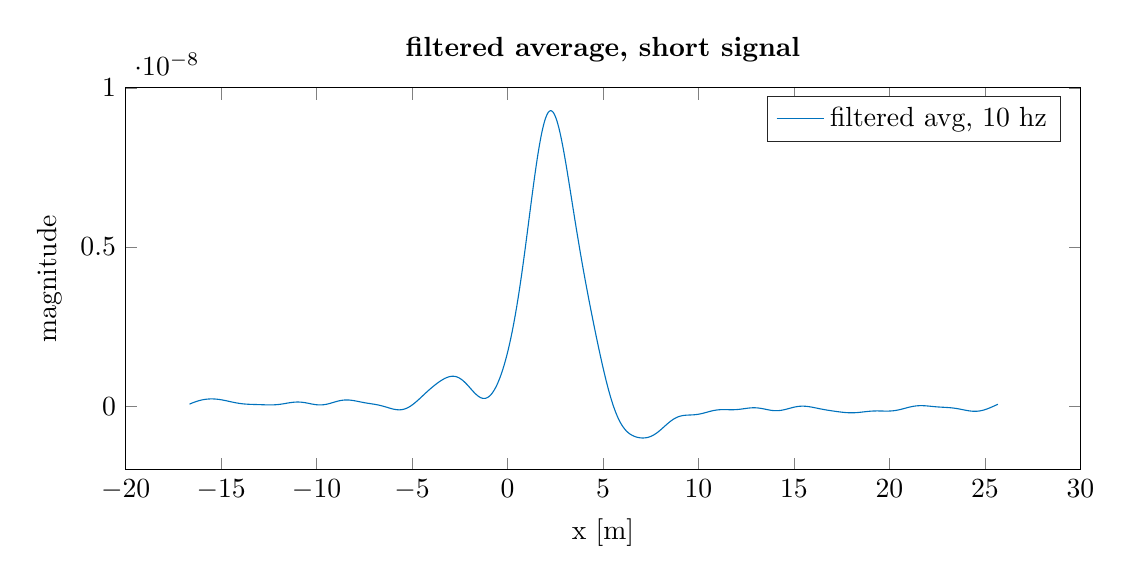
\begin{tikzpicture}

  \begin{axis}[%
    width=\textwidth,
    height=0.4\textwidth,
    at={(0\figurewidth,0\figureheight)},
    scale only axis,
    xmin=-20,
    xmax=30,
    xlabel={x [m]},
    ymin=-2e-09,
    ymax=1e-08,
    ylabel={magnitude},
    axis background/.style={fill=white},
    title style={font=\bfseries},
    title={filtered average, short signal},
    legend style={legend cell align=left,align=left,draw=white!15!black}
    ]
    \addplot [color=mycolor1,solid]
    table[row sep=crcr]{%
    -16.653955078125	6.28295066695866e-11\\
    -16.6338056640625	6.80331992030371e-11\\
    -16.61365625	7.31924168408746e-11\\
    -16.5935068359375	7.83034868104857e-11\\
    -16.573357421875	8.3362860640408e-11\\
    -16.5532080078125	8.83671158775593e-11\\
    -16.53305859375	9.33129573942381e-11\\
    -16.5129091796875	9.81972182950265e-11\\
    -16.492759765625	1.03016860435107e-10\\
    -16.4726103515625	1.07768974562898e-10\\
    -16.4524609375	1.12450780101108e-10\\
    -16.4323115234375	1.17059624581503e-10\\
    -16.412162109375	1.21592982749791e-10\\
    -16.3920126953125	1.26048455358002e-10\\
    -16.37186328125	1.30423767662642e-10\\
    -16.3517138671875	1.34716767647796e-10\\
    -16.331564453125	1.38925423992978e-10\\
    -16.3114150390625	1.430478238062e-10\\
    -16.291265625	1.47082170143242e-10\\
    -16.2711162109375	1.51026779334564e-10\\
    -16.250966796875	1.54880078141532e-10\\
    -16.2308173828125	1.58640600763968e-10\\
    -16.21066796875	1.62306985721001e-10\\
    -16.1905185546875	1.65877972627367e-10\\
    -16.170369140625	1.69352398887085e-10\\
    -16.1502197265625	1.72729196326318e-10\\
    -16.1300703125	1.76007387786911e-10\\
    -16.1099208984375	1.79186083701729e-10\\
    -16.089771484375	1.82264478672443e-10\\
    -16.0696220703125	1.85241848069823e-10\\
    -16.04947265625	1.88117544675946e-10\\
    -16.0293232421875	1.9089099538703e-10\\
    -16.009173828125	1.93561697994712e-10\\
    -15.9890244140625	1.96129218062771e-10\\
    -15.968875	1.98593185915281e-10\\
    -15.9487255859375	2.00953293751145e-10\\
    -15.928576171875	2.03209292898925e-10\\
    -15.9084267578125	2.05360991224674e-10\\
    -15.88827734375	2.0740825070432e-10\\
    -15.8681279296875	2.09350985170872e-10\\
    -15.847978515625	2.11189158245496e-10\\
    -15.8278291015625	2.12922781460154e-10\\
    -15.8076796875	2.14551912578164e-10\\
    -15.7875302734375	2.16076654117709e-10\\
    -15.767380859375	2.17497152081932e-10\\
    -15.7472314453125	2.18813594897905e-10\\
    -15.72708203125	2.20026212565343e-10\\
    -15.7069326171875	2.21135276014593e-10\\
    -15.686783203125	2.22141096672087e-10\\
    -15.6666337890625	2.2304402623006e-10\\
    -15.646484375	2.23844456616069e-10\\
    -15.6263349609375	2.24542820156537e-10\\
    -15.606185546875	2.25139589927319e-10\\
    -15.5860361328125	2.25635280283063e-10\\
    -15.56588671875	2.26030447555998e-10\\
    -15.5457373046875	2.26325690913694e-10\\
    -15.525587890625	2.26521653364251e-10\\
    -15.5054384765625	2.26619022896437e-10\\
    -15.4852890625	2.26618533741363e-10\\
    -15.4651396484375	2.26520967741446e-10\\
    -15.444990234375	2.26327155811647e-10\\
    -15.4248408203125	2.26037979477276e-10\\
    -15.40469140625	2.25654372472057e-10\\
    -15.3845419921875	2.25177322379668e-10\\
    -15.364392578125	2.24607872301441e-10\\
    -15.3442431640625	2.23947122532691e-10\\
    -15.32409375	2.23196232229792e-10\\
    -15.3039443359375	2.22356421050026e-10\\
    -15.283794921875	2.21428970746138e-10\\
    -15.2636455078125	2.20415226697574e-10\\
    -15.24349609375	2.19316599360486e-10\\
    -15.2233466796875	2.18134565618832e-10\\
    -15.203197265625	2.16870670019218e-10\\
    -15.1830478515625	2.15526525872496e-10\\
    -15.1628984375	2.14103816205619e-10\\
    -15.1427490234375	2.12604294547932e-10\\
    -15.122599609375	2.11029785536614e-10\\
    -15.1024501953125	2.09382185326833e-10\\
    -15.08230078125	2.07663461792959e-10\\
    -15.0621513671875	2.0587565450809e-10\\
    -15.042001953125	2.04020874490166e-10\\
    -15.0218525390625	2.02101303703908e-10\\
    -15.001703125	2.00119194309035e-10\\
    -14.9815537109375	1.98076867646302e-10\\
    -14.961404296875	1.95976712954113e-10\\
    -14.9412548828125	1.93821185809846e-10\\
    -14.92110546875	1.91612806291165e-10\\
    -14.9009560546875	1.89354156854164e-10\\
    -14.880806640625	1.87047879926306e-10\\
    -14.8606572265625	1.84696675213786e-10\\
    -14.8405078125	1.8230329672417e-10\\
    -14.8203583984375	1.79870549506737e-10\\
    -14.800208984375	1.77401286114303e-10\\
    -14.7800595703125	1.74898402791801e-10\\
    -14.75991015625	1.72364835398288e-10\\
    -14.7397607421875	1.69803555070508e-10\\
    -14.719611328125	1.67217563637526e-10\\
    -14.6994619140625	1.64609888797303e-10\\
    -14.6793125	1.61983579067453e-10\\
    -14.6591630859375	1.59341698523703e-10\\
    -14.639013671875	1.5668732134086e-10\\
    -14.6188642578125	1.54023526152258e-10\\
    -14.59871484375	1.51353390244835e-10\\
    -14.5785654296875	1.48679983608084e-10\\
    -14.558416015625	1.46006362856067e-10\\
    -14.5382666015625	1.43335565042775e-10\\
    -14.5181171875	1.40670601391786e-10\\
    -14.4979677734375	1.38014450962149e-10\\
    -14.477818359375	1.35370054272973e-10\\
    -14.4576689453125	1.32740306909921e-10\\
    -14.43751953125	1.30128053137206e-10\\
    -14.4173701171875	1.27536079539266e-10\\
    -14.397220703125	1.24967108716399e-10\\
    -14.3770712890625	1.22423793059067e-10\\
    -14.356921875	1.1990870862556e-10\\
    -14.3367724609375	1.17424349147747e-10\\
    -14.316623046875	1.1497312018958e-10\\
    -14.2964736328125	1.12557333482731e-10\\
    -14.27632421875	1.10179201463562e-10\\
    -14.2561748046875	1.07840832035042e-10\\
    -14.236025390625	1.05544223576852e-10\\
    -14.2158759765625	1.03291260226203e-10\\
    -14.1957265625	1.01083707451162e-10\\
    -14.1755771484375	9.89232079375227e-11\\
    -14.155427734375	9.68112778092044e-11\\
    -14.1352783203125	9.47493032012817e-11\\
    -14.11512890625	9.27385372034728e-11\\
    -14.0949794921875	9.07800971908593e-11\\
    -14.074830078125	8.88749625571757e-11\\
    -14.0546806640625	8.70239728647816e-11\\
    -14.03453125	8.5227826423847e-11\\
    -14.0143818359375	8.34870793118567e-11\\
    -13.994232421875	8.18021448429426e-11\\
    -13.9740830078125	8.01732934948668e-11\\
    -13.95393359375	7.86006532998749e-11\\
    -13.9337841796875	7.70842107038434e-11\\
    -13.913634765625	7.5623811896355e-11\\
    -13.8934853515625	7.42191646126141e-11\\
    -13.8733359375	7.28698404061984e-11\\
    -13.8531865234375	7.15752773898378e-11\\
    -13.833037109375	7.03347834395423e-11\\
    -13.8128876953125	6.9147539855564e-11\\
    -13.79273828125	6.80126054717553e-11\\
    -13.7725888671875	6.69289212031344e-11\\
    -13.752439453125	6.58953150195489e-11\\
    -13.7322900390625	6.49105073316213e-11\\
    -13.712140625	6.39731167732945e-11\\
    -13.6919912109375	6.3081666363699e-11\\
    -13.671841796875	6.22345900292583e-11\\
    -13.6516923828125	6.14302394654458e-11\\
    -13.63154296875	6.06668913159605e-11\\
    -13.6113935546875	5.99427546457026e-11\\
    -13.591244140625	5.92559786824312e-11\\
    -13.5710947265625	5.86046608007448e-11\\
    -13.5509453125	5.79868547207119e-11\\
    -13.5307958984375	5.74005788924287e-11\\
    -13.510646484375	5.68438250366572e-11\\
    -13.4904970703125	5.6314566810852e-11\\
    -13.47034765625	5.58107685689709e-11\\
    -13.4501982421875	5.53303941828318e-11\\
    -13.430048828125	5.48714158921498e-11\\
    -13.4098994140625	5.44318231499288e-11\\
    -13.38975	5.40096314295357e-11\\
    -13.3696005859375	5.36028909595884e-11\\
    -13.349451171875	5.32096953526643e-11\\
    -13.3293017578125	5.28281900939302e-11\\
    -13.30915234375	5.24565808559146e-11\\
    -13.2890029296875	5.20931416059927e-11\\
    -13.268853515625	5.17362224735937e-11\\
    -13.2487041015625	5.13842573446905e-11\\
    -13.2285546875	5.10357711518274e-11\\
    -13.2084052734375	5.0689386828835e-11\\
    -13.188255859375	5.03438319002698e-11\\
    -13.1681064453125	4.9997944676752e-11\\
    -13.14795703125	4.96506800285367e-11\\
    -13.1278076171875	4.93011147110501e-11\\
    -13.107658203125	4.89484522174766e-11\\
    -13.0875087890625	4.85920271351045e-11\\
    -13.067359375	4.82313089837501e-11\\
    -13.0472099609375	4.78659055163553e-11\\
    -13.027060546875	4.7495565463716e-11\\
    -13.0069111328125	4.71201807071589e-11\\
    -12.98676171875	4.67397878651259e-11\\
    -12.9666123046875	4.63545692816151e-11\\
    -12.946462890625	4.59648534066091e-11\\
    -12.9263134765625	4.55711145608724e-11\\
    -12.9061640625	4.51739720797302e-11\\
    -12.8860146484375	4.47741888327471e-11\\
    -12.865865234375	4.43726691186395e-11\\
    -12.8457158203125	4.39704559369907e-11\\
    -12.82556640625	4.35687276408963e-11\\
    -12.8054169921875	4.31687939769007e-11\\
    -12.785267578125	4.27720915211345e-11\\
    -12.7651181640625	4.23801785227782e-11\\
    -12.74496875	4.19947291685286e-11\\
    -12.7248193359375	4.16175272839279e-11\\
    -12.704669921875	4.12504594898181e-11\\
    -12.6845205078125	4.08955078343882e-11\\
    -12.66437109375	4.05547419235102e-11\\
    -12.6442216796875	4.02303105741573e-11\\
    -12.624072265625	3.99244330178364e-11\\
    -12.6039228515625	3.96393896828517e-11\\
    -12.5837734375	3.93775125862083e-11\\
    -12.5636240234375	3.91411753676952e-11\\
    -12.543474609375	3.89327830004331e-11\\
    -12.5233251953125	3.87547612136707e-11\\
    -12.50317578125	3.8609545665214e-11\\
    -12.4830263671875	3.84995709020569e-11\\
    -12.462876953125	3.842725914913e-11\\
    -12.4427275390625	3.83950089670347e-11\\
    -12.422578125	3.84051838206735e-11\\
    -12.4024287109375	3.84601006013533e-11\\
    -12.382279296875	3.85620181456785e-11\\
    -12.3621298828125	3.87131257949627e-11\\
    -12.34198046875	3.89155320392268e-11\\
    -12.3218310546875	3.91712532900141e-11\\
    -12.301681640625	3.94822028262561e-11\\
    -12.2815322265625	3.98501799572271e-11\\
    -12.2613828125	4.02768594463837e-11\\
    -12.2412333984375	4.07637812392385e-11\\
    -12.221083984375	4.1312340537945e-11\\
    -12.2009345703125	4.19237782643023e-11\\
    -12.18078515625	4.25991719519917e-11\\
    -12.1606357421875	4.33394271076635e-11\\
    -12.140486328125	4.41452690792745e-11\\
    -12.1203369140625	4.5017235468512e-11\\
    -12.1001875	4.59556691226778e-11\\
    -12.0800380859375	4.69607117395435e-11\\
    -12.059888671875	4.80322981168982e-11\\
    -12.0397392578125	4.91701510764362e-11\\
    -12.01958984375	5.03737770895517e-11\\
    -11.9994404296875	5.16424626302669e-11\\
    -11.979291015625	5.29752712782512e-11\\
    -11.9591416015625	5.43710415923195e-11\\
    -11.9389921875	5.58283857722707e-11\\
    -11.9188427734375	5.73456891242612e-11\\
    -11.898693359375	5.89211103421698e-11\\
    -11.8785439453125	6.05525826145482e-11\\
    -11.85839453125	6.22378155639902e-11\\
    -11.8382451171875	6.39742980226832e-11\\
    -11.818095703125	6.57593016450879e-11\\
    -11.7979462890625	6.75898853555756e-11\\
    -11.777796875	6.94629006259376e-11\\
    -11.7576474609375	7.13749975745881e-11\\
    -11.737498046875	7.33226318763131e-11\\
    -11.7173486328125	7.5302072468362e-11\\
    -11.69719921875	7.73094100357655e-11\\
    -11.6770498046875	7.93405662557375e-11\\
    -11.656900390625	8.13913037781817e-11\\
    -11.6367509765625	8.34572369164313e-11\\
    -11.6166015625	8.5533843019625e-11\\
    -11.5964521484375	8.76164744953353e-11\\
    -11.576302734375	8.9700371448579e-11\\
    -11.5561533203125	9.17806749006873e-11\\
    -11.53600390625	9.38524405492205e-11\\
    -11.5158544921875	9.59106530277348e-11\\
    -11.495705078125	9.795024062214e-11\\
    -11.4755556640625	9.99660903982174e-11\\
    -11.45540625	1.01953063693151e-10\\
    -11.4352568359375	1.03906011922055e-10\\
    -11.415107421875	1.05819792648954e-10\\
    -11.3949580078125	1.07689285870275e-10\\
    -11.37480859375	1.09509410457649e-10\\
    -11.3546591796875	1.11275140705712e-10\\
    -11.334509765625	1.12981522929836e-10\\
    -11.3143603515625	1.14623692057861e-10\\
    -11.2942109375	1.1619688815953e-10\\
    -11.2740615234375	1.1769647285692e-10\\
    -11.253912109375	1.19117945559119e-10\\
    -11.2337626953125	1.20456959464372e-10\\
    -11.21361328125	1.21709337273351e-10\\
    -11.1934638671875	1.22871086557505e-10\\
    -11.173314453125	1.23938414727263e-10\\
    -11.1531650390625	1.24907743545646e-10\\
    -11.133015625	1.25775723133953e-10\\
    -11.1128662109375	1.26539245417424e-10\\
    -11.092716796875	1.27195456960267e-10\\
    -11.0725673828125	1.27741771141007e-10\\
    -11.05241796875	1.2817587962104e-10\\
    -11.0322685546875	1.28495763061142e-10\\
    -11.012119140625	1.28699701042967e-10\\
    -10.9919697265625	1.28786281154811e-10\\
    -10.9718203125	1.28754407203476e-10\\
    -10.9516708984375	1.28603306516648e-10\\
    -10.931521484375	1.28332536303019e-10\\
    -10.9113720703125	1.27941989040288e-10\\
    -10.89122265625	1.27431896864204e-10\\
    -10.8710732421875	1.2680283493496e-10\\
    -10.850923828125	1.26055723760526e-10\\
    -10.8307744140625	1.25191830459799e-10\\
    -10.810625	1.24212768951951e-10\\
    -10.7904755859375	1.23120499061751e-10\\
    -10.770326171875	1.21917324534325e-10\\
    -10.7501767578125	1.20605889956257e-10\\
    -10.73002734375	1.19189176583716e-10\\
    -10.7098779296875	1.1767049708186e-10\\
    -10.689728515625	1.1605348918346e-10\\
    -10.6695791015625	1.14342108278346e-10\\
    -10.6494296875	1.12540618948947e-10\\
    -10.6292802734375	1.1065358547074e-10\\
    -10.609130859375	1.08685861300106e-10\\
    -10.5889814453125	1.06642577575493e-10\\
    -10.56883203125	1.04529130661346e-10\\
    -10.5486826171875	1.0235116876756e-10\\
    -10.528533203125	1.00114577680527e-10\\
    -10.5083837890625	9.78254656450265e-11\\
    -10.488234375	9.54901474392735e-11\\
    -10.4680849609375	9.31151276883631e-11\\
    -10.447935546875	9.0707083464192e-11\\
    -10.4277861328125	8.82728462225101e-11\\
    -10.40763671875	8.58193831303925e-11\\
    -10.3874873046875	8.33537778395632e-11\\
    -10.367337890625	8.08832107633857e-11\\
    -10.3471884765625	7.84149389170685e-11\\
    -10.3270390625	7.59562753826569e-11\\
    -10.3068896484375	7.35145684617358e-11\\
    -10.286740234375	7.10971805803453e-11\\
    -10.2665908203125	6.87114670116371e-11\\
    -10.24644140625	6.63647544828368e-11\\
    -10.2262919921875	6.40643197337737e-11\\
    -10.206142578125	6.18173680947663e-11\\
    -10.1859931640625	5.96310121519057e-11\\
    -10.16584375	5.75122505678958e-11\\
    -10.1456943359375	5.54679471263667e-11\\
    -10.125544921875	5.3504810067215e-11\\
    -10.1053955078125	5.16293717798911e-11\\
    -10.08524609375	4.98479689206946e-11\\
    -10.0650966796875	4.81667230189916e-11\\
    -10.044947265625	4.6591521636091e-11\\
    -10.0247978515625	4.51280001388264e-11\\
    -10.0046484375	4.37815241482711e-11\\
    -9.9844990234375	4.25571727219838e-11\\
    -9.964349609375	4.14597223260665e-11\\
    -9.9442001953125	4.04936316509057e-11\\
    -9.92405078125	3.96630273219808e-11\\
    -9.9039013671875	3.89716905543334e-11\\
    -9.883751953125	3.84230447964316e-11\\
    -9.8636025390625	3.80201444060356e-11\\
    -9.843453125	3.77656643975264e-11\\
    -9.8233037109375	3.76618912966721e-11\\
    -9.803154296875	3.77107151354539e-11\\
    -9.7830048828125	3.79136226157779e-11\\
    -9.76285546875	3.82716914673024e-11\\
    -9.7427060546875	3.87855860206975e-11\\
    -9.722556640625	3.94555540137638e-11\\
    -9.7024072265625	4.02814246438435e-11\\
    -9.6822578125	4.12626078758988e-11\\
    -9.6621083984375	4.23980950115579e-11\\
    -9.641958984375	4.36864605202855e-11\\
    -9.6218095703125	4.5125865129712e-11\\
    -9.60166015625	4.67140601679982e-11\\
    -9.5815107421875	4.84483931469992e-11\\
    -9.561361328125	5.03258145708751e-11\\
    -9.5412119140625	5.23428859507197e-11\\
    -9.5210625	5.44957890018158e-11\\
    -9.5009130859375	5.6780335996106e-11\\
    -9.480763671875	5.9191981238698e-11\\
    -9.4606142578125	6.17258336333911e-11\\
    -9.44046484375	6.43766702985749e-11\\
    -9.4203154296875	6.71389511913352e-11\\
    -9.400166015625	7.00068346941844e-11\\
    -9.3800166015625	7.29741941155599e-11\\
    -9.3598671875	7.60346350522069e-11\\
    -9.3397177734375	7.91815135585225e-11\\
    -9.319568359375	8.24079550653135e-11\\
    -9.2994189453125	8.5706873987765e-11\\
    -9.27926953125	8.90709939600938e-11\\
    -9.2591201171875	9.2492868632228e-11\\
    -9.238970703125	9.59649029618426e-11\\
    -9.2188212890625	9.9479374933457e-11\\
    -9.198671875	1.03028457634739e-10\\
    -9.1785224609375	1.06604241618942e-10\\
    -9.158373046875	1.10198757481353e-10\\
    -9.1382236328125	1.13803998576923e-10\\
    -9.11807421875	1.17411943805632e-10\\
    -9.0979248046875	1.21014580391953e-10\\
    -9.077775390625	1.24603926584679e-10\\
    -9.0576259765625	1.28172054203669e-10\\
    -9.0374765625	1.31711110960479e-10\\
    -9.0173271484375	1.35213342480608e-10\\
    -8.997177734375	1.38671113956066e-10\\
    -8.9770283203125	1.42076931358152e-10\\
    -8.95687890625	1.45423462141809e-10\\
    -8.9367294921875	1.48703555374636e-10\\
    -8.916580078125	1.51910261225523e-10\\
    -8.8964306640625	1.55036849750029e-10\\
    -8.87628125	1.5807682891206e-10\\
    -8.8561318359375	1.61023961783859e-10\\
    -8.835982421875	1.63872282869205e-10\\
    -8.8158330078125	1.66616113497667e-10\\
    -8.79568359375	1.69250076240846e-10\\
    -8.7755341796875	1.71769108304946e-10\\
    -8.755384765625	1.74168473857491e-10\\
    -8.7352353515625	1.76443775249557e-10\\
    -8.7150859375	1.78590963098774e-10\\
    -8.6949365234375	1.80606345202163e-10\\
    -8.674787109375	1.82486594251917e-10\\
    -8.6546376953125	1.84228754331324e-10\\
    -8.63448828125	1.85830246172187e-10\\
    -8.6143388671875	1.87288871159413e-10\\
    -8.594189453125	1.88602814072683e-10\\
    -8.5740400390625	1.89770644559453e-10\\
    -8.553890625	1.90791317337981e-10\\
    -8.5337412109375	1.91664171133335e-10\\
    -8.513591796875	1.92388926353784e-10\\
    -8.4934423828125	1.92965681519307e-10\\
    -8.47329296875	1.93394908458202e-10\\
    -8.4531435546875	1.93677446292096e-10\\
    -8.432994140625	1.93814494233823e-10\\
    -8.4128447265625	1.93807603226683e-10\\
    -8.3926953125	1.93658666457714e-10\\
    -8.3725458984375	1.93369908781359e-10\\
    -8.352396484375	1.92943875093817e-10\\
    -8.3322470703125	1.9238341770189e-10\\
    -8.31209765625	1.91691682733679e-10\\
    -8.2919482421875	1.90872095641764e-10\\
    -8.271798828125	1.89928345852667e-10\\
    -8.2516494140625	1.88864370619325e-10\\
    -8.2315	1.87684338136081e-10\\
    -8.2113505859375	1.86392629978233e-10\\
    -8.191201171875	1.84993822930499e-10\\
    -8.1710517578125	1.8349267027092e-10\\
    -8.15090234375	1.81894082578502e-10\\
    -8.1307529296875	1.80203108134636e-10\\
    -8.110603515625	1.78424912989659e-10\\
    -8.0904541015625	1.76564760767047e-10\\
    -8.0703046875	1.74627992278693e-10\\
    -8.0501552734375	1.72620005025247e-10\\
    -8.030005859375	1.70546232655931e-10\\
    -8.0098564453125	1.68412124462311e-10\\
    -7.98970703125	1.6622312498036e-10\\
    -7.9695576171875	1.63984653774694e-10\\
    -7.949408203125	1.61702085478208e-10\\
    -7.9292587890625	1.59380730159383e-10\\
    -7.909109375	1.57025814088304e-10\\
    -7.8889599609375	1.54642460971007e-10\\
    -7.868810546875	1.52235673720051e-10\\
    -7.8486611328125	1.49810316827261e-10\\
    -7.82851171875	1.47371099402401e-10\\
    -7.8083623046875	1.44922558939167e-10\\
    -7.788212890625	1.4246904586716e-10\\
    -7.7680634765625	1.40014708945791e-10\\
    -7.7479140625	1.37563481552907e-10\\
    -7.7277646484375	1.35119068917756e-10\\
    -7.707615234375	1.32684936344482e-10\\
    -7.6874658203125	1.30264298468755e-10\\
    -7.66731640625	1.27860109586405e-10\\
    -7.6471669921875	1.2547505508908e-10\\
    -7.627017578125	1.23111544037869e-10\\
    -7.6068681640625	1.20771702901808e-10\\
    -7.58671875	1.1845737048389e-10\\
    -7.5665693359375	1.16170094052913e-10\\
    -7.546419921875	1.13911126695179e-10\\
    -7.5262705078125	1.1168142589554e-10\\
    -7.50612109375	1.09481653352889e-10\\
    -7.4859716796875	1.07312176030674e-10\\
    -7.465822265625	1.05173068438537e-10\\
    -7.4456728515625	1.03064116136655e-10\\
    -7.4255234375	1.00984820449963e-10\\
    -7.4053740234375	9.89344043749347e-11\\
    -7.385224609375	9.69118196573331e-11\\
    -7.3650751953125	9.49157550149512e-11\\
    -7.34492578125	9.29446454752417e-11\\
    -7.3247763671875	9.09966827936147e-11\\
    -7.304626953125	8.90698269141492e-11\\
    -7.2844775390625	8.71618184307201e-11\\
    -7.264328125	8.52701920027182e-11\\
    -7.2441787109375	8.33922906761285e-11\\
    -7.224029296875	8.15252810572406e-11\\
    -7.2038798828125	7.96661692831666e-11\\
    -7.18373046875	7.78118177303265e-11\\
    -7.1635810546875	7.59589623992625e-11\\
    -7.143431640625	7.41042309116111e-11\\
    -7.1232822265625	7.22441610527126e-11\\
    -7.1031328125	7.03752197912199e-11\\
    -7.0829833984375	6.84938227052802e-11\\
    -7.062833984375	6.65963537431337e-11\\
    -7.0426845703125	6.46791852447744e-11\\
    -7.02253515625	6.27386981501045e-11\\
    -7.0023857421875	6.07713023182745e-11\\
    -6.982236328125	5.87734568823152e-11\\
    -6.9620869140625	5.6741690562871e-11\\
    -6.9419375	5.46726218648971e-11\\
    -6.9217880859375	5.25629790813952e-11\\
    -6.901638671875	5.0409620028802e-11\\
    -6.8814892578125	4.82095514395234e-11\\
    -6.86133984375	4.59599479380858e-11\\
    -6.8411904296875	4.36581705288122e-11\\
    -6.821041015625	4.13017845244911e-11\\
    -6.8008916015625	3.88885768473741e-11\\
    -6.7807421875	3.6416572635956e-11\\
    -6.7605927734375	3.38840510933536e-11\\
    -6.740443359375	3.12895605156485e-11\\
    -6.7202939453125	2.8631932441457e-11\\
    -6.70014453125	2.59102948668798e-11\\
    -6.6799951171875	2.31240844733727e-11\\
    -6.659845703125	2.02730578193926e-11\\
    -6.6396962890625	1.73573014503272e-11\\
    -6.619546875	1.43772408849691e-11\\
    -6.5993974609375	1.13336484407834e-11\\
    -6.579248046875	8.2276498641806e-12\\
    -6.5590986328125	5.06072973634878e-12\\
    -6.53894921875	1.83473562936997e-12\\
    -6.5187998046875	-1.44811900813747e-12\\
    -6.498650390625	-4.78525325219151e-12\\
    -6.4785009765625	-8.17371840316411e-12\\
    -6.4583515625	-1.16101989912276e-11\\
    -6.4382021484375	-1.50910150900205e-11\\
    -6.418052734375	-1.86121259364211e-11\\
    -6.3979033203125	-2.21691348496425e-11\\
    -6.37775390625	-2.5757295438218e-11\\
    -6.3576044921875	-2.93715190788702e-11\\
    -6.337455078125	-3.30063836467426e-11\\
    -6.3173056640625	-3.6656143471872e-11\\
    -6.29715625	-4.03147404925357e-11\\
    -6.2770068359375	-4.39758165717153e-11\\
    -6.256857421875	-4.76327269387517e-11\\
    -6.2367080078125	-5.12785547142551e-11\\
    -6.21655859375	-5.49061264723496e-11\\
    -6.1964091796875	-5.85080287907027e-11\\
    -6.176259765625	-6.20766257350751e-11\\
    -6.1561103515625	-6.56040772218658e-11\\
    -6.1359609375	-6.90823581988623e-11\\
    -6.1158115234375	-7.25032785814551e-11\\
    -6.095662109375	-7.58585038788037e-11\\
    -6.0755126953125	-7.9139576441957e-11\\
    -6.05536328125	-8.23379372635738e-11\\
    -6.0352138671875	-8.54449482569389e-11\\
    -6.015064453125	-8.84519149401184e-11\\
    -5.9949150390625	-9.13501094496517e-11\\
    -5.974765625	-9.41307938068577e-11\\
    -5.9546162109375	-9.67852433589672e-11\\
    -5.934466796875	-9.93047703164798e-11\\
    -5.9143173828125	-1.01680747307842e-10\\
    -5.89416796875	-1.03904630872376e-10\\
    -5.8740185546875	-1.059679848125e-10\\
    -5.853869140625	-1.07862503326834e-10\\
    -5.8337197265625	-1.09580033846387e-10\\
    -5.8135703125	-1.11112599497131e-10\\
    -5.7934208984375	-1.12452421113468e-10\\
    -5.773271484375	-1.13591938728693e-10\\
    -5.7531220703125	-1.14523832470395e-10\\
    -5.73297265625	-1.15241042790754e-10\\
    -5.7128232421875	-1.15736789964111e-10\\
    -5.692673828125	-1.16004592786697e-10\\
    -5.6725244140625	-1.16038286416272e-10\\
    -5.652375	-1.1583203929248e-10\\
    -5.6322255859375	-1.15380369081907e-10\\
    -5.612076171875	-1.146781575954e-10\\
    -5.5919267578125	-1.13720664628818e-10\\
    -5.57177734375	-1.1250354068214e-10\\
    -5.5516279296875	-1.11022838516053e-10\\
    -5.531478515625	-1.09275023509039e-10\\
    -5.5113291015625	-1.07256982782516e-10\\
    -5.4911796875	-1.04966033065797e-10\\
    -5.4710302734375	-1.02399927277255e-10\\
    -5.450880859375	-9.95568598026482e-11\\
    -5.4307314453125	-9.64354704562176e-11\\
    -5.41058203125	-9.30348471148994e-11\\
    -5.3904326171875	-8.9354527020776e-11\\
    -5.370283203125	-8.5394496751617e-11\\
    -5.3501337890625	-8.1155190864207e-11\\
    -5.329984375	-7.66374892198601e-11\\
    -5.3098349609375	-7.18427130063144e-11\\
    -5.289685546875	-6.67726194748068e-11\\
    -5.2695361328125	-6.14293954158211e-11\\
    -5.24938671875	-5.58156494014838e-11\\
    -5.2292373046875	-4.99344028269791e-11\\
    -5.209087890625	-4.37890797877769e-11\\
    -5.1889384765625	-3.73834958334707e-11\\
    -5.1687890625	-3.07218456432189e-11\\
    -5.1486396484375	-2.38086896715162e-11\\
    -5.128490234375	-1.66489398167625e-11\\
    -5.1083408203125	-9.24784416856905e-12\\
    -5.08819140625	-1.6109708929908e-12\\
    -5.0680419921875	6.25580868198994e-12\\
    -5.047892578125	1.43463377156724e-11\\
    -5.0277431640625	2.26541921708347e-11\\
    -5.00759375	3.11726997268593e-11\\
    -4.9874443359375	3.98949592177455e-11\\
    -4.967294921875	4.8813860521033e-11\\
    -4.9471455078125	5.7922104822257e-11\\
    -4.92699609375	6.72122251782126e-11\\
    -4.9068466796875	7.6676607301389e-11\\
    -4.886697265625	8.63075104872814e-11\\
    -4.8665478515625	9.60970886058413e-11\\
    -4.8463984375	1.06037411078365e-10\\
    -4.8262490234375	1.16120483761218e-10\\
    -4.806099609375	1.26338269658398e-10\\
    -4.7859501953125	1.36682709385701e-10\\
    -4.76580078125	1.47145741310397e-10\\
    -4.7456513671875	1.57719321291701e-10\\
    -4.725501953125	1.68395441948987e-10\\
    -4.7053525390625	1.79166151386709e-10\\
    -4.685203125	1.90023571307171e-10\\
    -4.6650537109375	2.00959914444825e-10\\
    -4.644904296875	2.11967501258523e-10\\
    -4.6247548828125	2.23038775821128e-10\\
    -4.60460546875	2.34166320849199e-10\\
    -4.5844560546875	2.4534287181882e-10\\
    -4.564306640625	2.56561330117457e-10\\
    -4.5441572265625	2.67814775185463e-10\\
    -4.5240078125	2.79096475605016e-10\\
    -4.5038583984375	2.90399899098491e-10\\
    -4.483708984375	3.01718721402562e-10\\
    -4.4635595703125	3.13046833989019e-10\\
    -4.44341015625	3.24378350607761e-10\\
    -4.4232607421875	3.35707612632321e-10\\
    -4.403111328125	3.47029193193014e-10\\
    -4.3829619140625	3.58337900087766e-10\\
    -4.3628125	3.69628777465659e-10\\
    -4.3426630859375	3.80897106283137e-10\\
    -4.322513671875	3.92138403537927e-10\\
    -4.3023642578125	4.03348420290672e-10\\
    -4.28221484375	4.14523138489259e-10\\
    -4.2620654296875	4.25658766615782e-10\\
    -4.241916015625	4.3675173418093e-10\\
    -4.2217666015625	4.47798685095431e-10\\
    -4.2016171875	4.58796469952805e-10\\
    -4.1814677734375	4.69742137262337e-10\\
    -4.161318359375	4.80632923675597e-10\\
    -4.1411689453125	4.91466243254098e-10\\
    -4.12101953125	5.02239675829885e-10\\
    -4.1008701171875	5.12950954514695e-10\\
    -4.080720703125	5.23597952417179e-10\\
    -4.0605712890625	5.34178668631091e-10\\
    -4.040421875	5.44691213560753e-10\\
    -4.0202724609375	5.55133793653069e-10\\
    -4.000123046875	5.65504695608234e-10\\
    -3.9799736328125	5.75802270143771e-10\\
    -3.95982421875	5.86024915388792e-10\\
    -3.9396748046875	5.96171059987375e-10\\
    -3.919525390625	6.06239145991562e-10\\
    -3.8993759765625	6.16227611625926e-10\\
    -3.8792265625	6.2613487400664e-10\\
    -3.8590771484375	6.35959311898746e-10\\
    -3.838927734375	6.45699248595797e-10\\
    -3.8187783203125	6.55352935005995e-10\\
    -3.79862890625	6.64918533028925e-10\\
    -3.7784794921875	6.74394099306203e-10\\
    -3.758330078125	6.83777569428684e-10\\
    -3.7381806640625	6.93066742681488e-10\\
    -3.71803125	7.02259267406688e-10\\
    -3.6978818359375	7.11352627061646e-10\\
    -3.677732421875	7.20344127048715e-10\\
    -3.6575830078125	7.29230882389756e-10\\
    -3.63743359375	7.38009806315924e-10\\
    -3.6172841796875	7.46677599840319e-10\\
    -3.597134765625	7.55230742377628e-10\\
    -3.5769853515625	7.63665483471365e-10\\
    -3.5568359375	7.71977835685388e-10\\
    -3.5366865234375	7.80163568712316e-10\\
    -3.516537109375	7.88218204747091e-10\\
    -3.4963876953125	7.96137015169416e-10\\
    -3.47623828125	8.03915018573994e-10\\
    -3.4560888671875	8.11546980182609e-10\\
    -3.435939453125	8.19027412666929e-10\\
    -3.4157900390625	8.26350578405724e-10\\
    -3.395640625	8.33510493194736e-10\\
    -3.3754912109375	8.40500931421988e-10\\
    -3.355341796875	8.47315432715723e-10\\
    -3.3351923828125	8.53947310066509e-10\\
    -3.31504296875	8.60389659419309e-10\\
    -3.2948935546875	8.66635370725633e-10\\
    -3.274744140625	8.72677140440077e-10\\
    -3.2545947265625	8.78507485439861e-10\\
    -3.2344453125	8.84118758340276e-10\\
    -3.2142958984375	8.89503164173268e-10\\
    -3.194146484375	8.94652778390842e-10\\
    -3.1739970703125	8.99559566149513e-10\\
    -3.15384765625	9.04215402826611e-10\\
    -3.1336982421875	9.08612095714089e-10\\
    -3.113548828125	9.12741406830405e-10\\
    -3.0933994140625	9.16595076786106e-10\\
    -3.07325	9.20164849634198e-10\\
    -3.0531005859375	9.23442498631697e-10\\
    -3.032951171875	9.26419852834749e-10\\
    -3.0128017578125	9.29088824445524e-10\\
    -2.99265234375	9.31441436825509e-10\\
    -2.9725029296875	9.33469853086263e-10\\
    -2.952353515625	9.35166405165629e-10\\
    -2.9322041015625	9.36523623294557e-10\\
    -2.9120546875	9.37534265757103e-10\\
    -2.8919052734375	9.38191348844094e-10\\
    -2.871755859375	9.38488176899006e-10\\
    -2.8516064453125	9.38418372353181e-10\\
    -2.83145703125	9.37975905646378e-10\\
    -2.8113076171875	9.37155124927812e-10\\
    -2.791158203125	9.35950785432606e-10\\
    -2.7710087890625	9.34358078428352e-10\\
    -2.750859375	9.32372659627065e-10\\
    -2.7307099609375	9.29990676958376e-10\\
    -2.710560546875	9.2720879760105e-10\\
    -2.6904111328125	9.24024234171366e-10\\
    -2.67026171875	9.20434769968767e-10\\
    -2.6501123046875	9.16438783181482e-10\\
    -2.629962890625	9.12035269957374e-10\\
    -2.6098134765625	9.07223866248323e-10\\
    -2.5896640625	9.02004868339652e-10\\
    -2.5695146484375	8.96379251979921e-10\\
    -2.549365234375	8.9034869003028e-10\\
    -2.5292158203125	8.83915568556951e-10\\
    -2.50906640625	8.77083001295017e-10\\
    -2.4889169921875	8.6985484241658e-10\\
    -2.468767578125	8.62235697541586e-10\\
    -2.4486181640625	8.54230932934967e-10\\
    -2.42846875	8.45846682839545e-10\\
    -2.4083193359375	8.37089854899949e-10\\
    -2.388169921875	8.27968133638962e-10\\
    -2.3680205078125	8.1848998195397e-10\\
    -2.34787109375	8.08664640607684e-10\\
    -2.3277216796875	7.98502125693797e-10\\
    -2.307572265625	7.8801322406508e-10\\
    -2.2874228515625	7.77209486718116e-10\\
    -2.2672734375	7.66103220135748e-10\\
    -2.2471240234375	7.54707475595316e-10\\
    -2.226974609375	7.43036036457588e-10\\
    -2.2068251953125	7.31103403458307e-10\\
    -2.18667578125	7.1892477803114e-10\\
    -2.1665263671875	7.06516043697695e-10\\
    -2.146376953125	6.9389374556704e-10\\
    -2.1262275390625	6.81075067993829e-10\\
    -2.106078125	6.68077810450745e-10\\
    -2.0859287109375	6.54920361677296e-10\\
    -2.065779296875	6.41621672173302e-10\\
    -2.0456298828125	6.28201225111401e-10\\
    -2.02548046875	6.14679005748776e-10\\
    -2.0053310546875	6.01075469423784e-10\\
    -1.985181640625	5.8741150822863e-10\\
    -1.9650322265625	5.73708416454077e-10\\
    -1.9448828125	5.59987854907119e-10\\
    -1.9247333984375	5.46271814206749e-10\\
    -1.904583984375	5.32582577167222e-10\\
    -1.8844345703125	5.18942680381731e-10\\
    -1.86428515625	5.05374875122954e-10\\
    -1.8441357421875	4.91902087679716e-10\\
    -1.823986328125	4.78547379251717e-10\\
    -1.8038369140625	4.65333905526305e-10\\
    -1.7836875	4.52284876063116e-10\\
    -1.7635380859375	4.39423513613612e-10\\
    -1.743388671875	4.26773013503474e-10\\
    -1.7232392578125	4.14356503206214e-10\\
    -1.70308984375	4.02197002236338e-10\\
    -1.6829404296875	3.9031738248993e-10\\
    -1.662791015625	3.78740329159575e-10\\
    -1.6426416015625	3.67488302349234e-10\\
    -1.6224921875	3.56583499512752e-10\\
    -1.6023427734375	3.46047818837498e-10\\
    -1.582193359375	3.35902823691896e-10\\
    -1.5620439453125	3.26169708252395e-10\\
    -1.54189453125	3.16869264422e-10\\
    -1.5217451171875	3.08021850148297e-10\\
    -1.501595703125	2.99647359244691e-10\\
    -1.4814462890625	2.91765192813642e-10\\
    -1.461296875	2.84394232365617e-10\\
    -1.4411474609375	2.77552814721857e-10\\
    -1.420998046875	2.71258708783238e-10\\
    -1.4008486328125	2.65529094241255e-10\\
    -1.38069921875	2.60380542300645e-10\\
    -1.3605498046875	2.55828998476356e-10\\
    -1.340400390625	2.51889767520502e-10\\
    -1.3202509765625	2.4857750052759e-10\\
    -1.3001015625	2.45906184258796e-10\\
    -1.2799521484375	2.43889132718293e-10\\
    -1.259802734375	2.4253898100676e-10\\
    -1.2396533203125	2.41867681469111e-10\\
    -1.21950390625	2.41886502145347e-10\\
    -1.1993544921875	2.4260602752513e-10\\
    -1.179205078125	2.44036161598398e-10\\
    -1.1590556640625	2.46186133185977e-10\\
    -1.13890625	2.49064503525743e-10\\
    -1.1187568359375	2.5267917608164e-10\\
    -1.098607421875	2.57037408534481e-10\\
    -1.0784580078125	2.62145826905343e-10\\
    -1.05830859375	2.68010441754263e-10\\
    -1.0381591796875	2.74636666388946e-10\\
    -1.018009765625	2.82029337010545e-10\\
    -0.997860351562499	2.90192734715835e-10\\
    -0.977710937499998	2.99130609267948e-10\\
    -0.957561523437498	3.08846204540547e-10\\
    -0.937412109374998	3.19342285533691e-10\\
    -0.917262695312498	3.30621166852941e-10\\
    -0.897113281249998	3.42684742537292e-10\\
    -0.876963867187499	3.55534517115478e-10\\
    -0.856814453124999	3.69171637764931e-10\\
    -0.836665039062499	3.835969274425e-10\\
    -0.816515624999999	3.98810918851484e-10\\
    -0.796366210937499	4.14813889105283e-10\\
    -0.776216796874998	4.31605894944314e-10\\
    -0.756067382812498	4.49186808359485e-10\\
    -0.735917968749998	4.67556352472815e-10\\
    -0.715768554687498	4.86714137523507e-10\\
    -0.695619140624999	5.06659696805954e-10\\
    -0.675469726562499	5.27392522405043e-10\\
    -0.655320312499999	5.48912100573289e-10\\
    -0.635170898437497	5.71217946594255e-10\\
    -0.615021484374999	5.94309638977041e-10\\
    -0.594872070312498	6.18186852827557e-10\\
    -0.57472265625	6.42849392243797e-10\\
    -0.554573242187498	6.68297221584264e-10\\
    -0.534423828125	6.94530495461388e-10\\
    -0.514274414062498	7.21549587314711e-10\\
    -0.494124999999997	7.4935511642243e-10\\
    -0.473975585937499	7.77947973213881e-10\\
    -0.453826171874997	8.07329342750374e-10\\
    -0.433676757812499	8.37500726246839e-10\\
    -0.413527343749998	8.68463960512534e-10\\
    -0.3933779296875	9.00221235195115e-10\\
    -0.373228515624998	9.32775107719082e-10\\
    -0.3530791015625	9.66128515816545e-10\\
    -0.332929687499998	1.00028478755588e-09\\
    -0.3127802734375	1.03524764878154e-09\\
    -0.292630859374999	1.07102122788673e-09\\
    -0.272481445312497	1.10761005784909e-09\\
    -0.252332031249999	1.14501907546855e-09\\
    -0.232182617187497	1.18325361775574e-09\\
    -0.212033203124999	1.22231941542883e-09\\
    -0.191883789062498	1.26222258348641e-09\\
    -0.171734375	1.30296960883399e-09\\
    -0.151584960937498	1.34456733495178e-09\\
    -0.131435546875	1.38702294360185e-09\\
    -0.111286132812499	1.43034393358294e-09\\
    -0.091136718749997	1.47453809655179e-09\\
    -0.0709873046874989	1.51961348994057e-09\\
    -0.0508378906249973	1.56557840701003e-09\\
    -0.0306884765624993	1.61244134408916e-09\\
    -0.0105390624999977	1.66021096506203e-09\\
    0.00961035156250034	1.70889606317326e-09\\
    0.0297597656250019	1.75850552023362e-09\\
    0.0499091796875	1.80904826331741e-09\\
    0.0700585937500016	1.86053321905315e-09\\
    0.0902080078125032	1.91296926561877e-09\\
    0.110357421875001	1.96636518256202e-09\\
    0.130506835937503	2.02072959857564e-09\\
    0.150656250000001	2.07607093736604e-09\\
    0.170805664062502	2.13239736176218e-09\\
    0.190955078125	2.18971671621991e-09\\
    0.211104492187502	2.24803646788413e-09\\
    0.23125390625	2.30736364637881e-09\\
    0.251403320312502	2.36770478250111e-09\\
    0.271552734375	2.42906584600262e-09\\
    0.291702148437501	2.49145218264584e-09\\
    0.311851562500003	2.5548684507297e-09\\
    0.332000976562501	2.61931855728205e-09\\
    0.352150390625003	2.68480559412153e-09\\
    0.372299804687501	2.75133177399399e-09\\
    0.392449218750002	2.81889836699224e-09\\
    0.4125986328125	2.88750563746913e-09\\
    0.432748046875002	2.9571527816564e-09\\
    0.4528974609375	3.02783786620176e-09\\
    0.473046875000001	3.09955776783755e-09\\
    0.493196289062503	3.17230811439328e-09\\
    0.513345703125001	3.24608322736377e-09\\
    0.533495117187503	3.32087606624225e-09\\
    0.553644531250001	3.39667817482578e-09\\
    0.573793945312502	3.47347962969687e-09\\
    0.593943359375	3.55126899108155e-09\\
    0.614092773437502	3.63003325627956e-09\\
    0.6342421875	3.70975781585737e-09\\
    0.654391601562502	3.79042641278877e-09\\
    0.674541015625003	3.87202110472169e-09\\
    0.694690429687501	3.95452222954252e-09\\
    0.714839843750003	4.03790837440215e-09\\
    0.734989257812501	4.12215634835932e-09\\
    0.755138671875002	4.20724115878853e-09\\
    0.7752880859375	4.29313599169022e-09\\
    0.795437500000002	4.37981219603173e-09\\
    0.8155869140625	4.46723927223661e-09\\
    0.835736328125002	4.55538486492991e-09\\
    0.8558857421875	4.6442147600356e-09\\
    0.876035156250001	4.73369288631102e-09\\
    0.896184570312503	4.82378132139125e-09\\
    0.916333984375001	4.9144403024045e-09\\
    0.936483398437503	5.00562824120676e-09\\
    0.956632812500001	5.0973017442718e-09\\
    0.976782226562502	5.18941563725932e-09\\
    0.996931640625	5.28192299427114e-09\\
    1.0170810546875	5.37477517179232e-09\\
    1.03723046875	5.46792184730048e-09\\
    1.0573798828125	5.56131106251356e-09\\
    1.077529296875	5.65488927123267e-09\\
    1.0976787109375	5.74860139172359e-09\\
    1.117828125	5.84239086356693e-09\\
    1.1379775390625	5.93619970889399e-09\\
    1.158126953125	6.02996859791235e-09\\
    1.1782763671875	6.12363691861217e-09\\
    1.19842578125	6.21714285053189e-09\\
    1.2185751953125	6.31042344244929e-09\\
    1.238724609375	6.40341469385218e-09\\
    1.2588740234375	6.49605164003101e-09\\
    1.2790234375	6.58826844062444e-09\\
    1.2991728515625	6.67999847143812e-09\\
    1.319322265625	6.77117441934608e-09\\
    1.3394716796875	6.8617283800747e-09\\
    1.35962109375	6.951591958659e-09\\
    1.3797705078125	7.04069637235288e-09\\
    1.399919921875	7.12897255576573e-09\\
    1.4200693359375	7.21635126799073e-09\\
    1.44021875	7.30276320148265e-09\\
    1.4603681640625	7.38813909243642e-09\\
    1.480517578125	7.47240983241215e-09\\
    1.5006669921875	7.55550658094702e-09\\
    1.52081640625	7.63736087888983e-09\\
    1.5409658203125	7.7179047621907e-09\\
    1.561115234375	7.79707087587499e-09\\
    1.5812646484375	7.87479258792873e-09\\
    1.6014140625	7.95100410282096e-09\\
    1.6215634765625	8.02564057438802e-09\\
    1.641712890625	8.0986382178048e-09\\
    1.6618623046875	8.16993442036866e-09\\
    1.68201171875	8.23946785082375e-09\\
    1.7021611328125	8.30717856695527e-09\\
    1.722310546875	8.37300812118705e-09\\
    1.7424599609375	8.43689966391926e-09\\
    1.762609375	8.49879804434789e-09\\
    1.7827587890625	8.55864990851321e-09\\
    1.802908203125	8.61640379433032e-09\\
    1.8230576171875	8.67201022336199e-09\\
    1.84320703125	8.72542178910139e-09\\
    1.8633564453125	8.7765932415406e-09\\
    1.883505859375	8.82548156780967e-09\\
    1.9036552734375	8.8720460686805e-09\\
    1.9238046875	8.91624843073982e-09\\
    1.9439541015625	8.95805279404653e-09\\
    1.964103515625	8.99742581509932e-09\\
    1.9842529296875	9.0343367249529e-09\\
    2.00440234375	9.06875738233281e-09\\
    2.0245517578125	9.10066232161169e-09\\
    2.044701171875	9.13002879552296e-09\\
    2.0648505859375	9.15683681250108e-09\\
    2.085	9.18106916855171e-09\\
    2.1051494140625	9.20271147356849e-09\\
    2.125298828125	9.22175217202828e-09\\
    2.1454482421875	9.23818255801033e-09\\
    2.16559765625	9.25199678450034e-09\\
    2.1857470703125	9.26319186695447e-09\\
    2.205896484375	9.27176768111376e-09\\
    2.2260458984375	9.27772695507403e-09\\
    2.2461953125	9.28107525563131e-09\\
    2.2663447265625	9.28182096893789e-09\\
    2.286494140625	9.27997527551847e-09\\
    2.3066435546875	9.2755521197111e-09\\
    2.32679296875	9.26856817361139e-09\\
    2.3469423828125	9.2590427956133e-09\\
    2.367091796875	9.24699798365354e-09\\
    2.3872412109375	9.2324583232802e-09\\
    2.407390625	9.21545093067993e-09\\
    2.4275400390625	9.19600539081049e-09\\
    2.447689453125	9.17415369079845e-09\\
    2.4678388671875	9.14993014877378e-09\\
    2.48798828125	9.12337133832448e-09\\
    2.5081376953125	9.09451600876591e-09\\
    2.528287109375	9.06340500142954e-09\\
    2.5484365234375	9.03008116218621e-09\\
    2.5685859375	8.99458925042814e-09\\
    2.5887353515625	8.95697584474243e-09\\
    2.608884765625	8.91728924551743e-09\\
    2.6290341796875	8.87557937472991e-09\\
    2.64918359375	8.83189767316839e-09\\
    2.6693330078125	8.78629699535332e-09\\
    2.689482421875	8.73883150242028e-09\\
    2.7096318359375	8.68955655323677e-09\\
    2.72978125	8.63852859402672e-09\\
    2.7499306640625	8.58580504677982e-09\\
    2.770080078125	8.53144419672479e-09\\
    2.7902294921875	8.47550507914716e-09\\
    2.81037890625	8.41804736583245e-09\\
    2.8305283203125	8.3591312514155e-09\\
    2.850677734375	8.29881733991567e-09\\
    2.8708271484375	8.23716653173568e-09\\
    2.8909765625	8.17423991139927e-09\\
    2.9111259765625	8.11009863629953e-09\\
    2.931275390625	8.04480382672555e-09\\
    2.9514248046875	7.97841645743018e-09\\
    2.97157421875	7.91099725099605e-09\\
    2.9917236328125	7.84260657325086e-09\\
    3.011873046875	7.77330433097548e-09\\
    3.0320224609375	7.70314987214146e-09\\
    3.052171875	7.63220188890554e-09\\
    3.0723212890625	7.56051832358031e-09\\
    3.092470703125	7.48815627779042e-09\\
    3.1126201171875	7.41517192501387e-09\\
    3.13276953125	7.34162042669704e-09\\
    3.1529189453125	7.26755585212155e-09\\
    3.173068359375	7.19303110218895e-09\\
    3.1932177734375	7.11809783727769e-09\\
    3.2133671875	7.04280640931438e-09\\
    3.2335166015625	6.96720579818866e-09\\
    3.253666015625	6.89134355262801e-09\\
    3.2738154296875	6.81526573563575e-09\\
    3.29396484375	6.73901687458169e-09\\
    3.3141142578125	6.66263991602161e-09\\
    3.334263671875	6.58617618530773e-09\\
    3.3544130859375	6.50966535103847e-09\\
    3.3745625	6.43314539438189e-09\\
    3.3947119140625	6.35665258329315e-09\\
    3.414861328125	6.28022145163256e-09\\
    3.4350107421875	6.2038847831766e-09\\
    3.45516015625	6.12767360050086e-09\\
    3.4753095703125	6.05161715869998e-09\\
    3.495458984375	5.97574294389629e-09\\
    3.5156083984375	5.90007667647571e-09\\
    3.5357578125	5.82464231897645e-09\\
    3.5559072265625	5.74946208854345e-09\\
    3.576056640625	5.67455647384911e-09\\
    3.5962060546875	5.59994425636916e-09\\
    3.61635546875	5.52564253589067e-09\\
    3.6365048828125	5.45166676011847e-09\\
    3.656654296875	5.37803075823548e-09\\
    3.6768037109375	5.30474677826226e-09\\
    3.696953125	5.23182552805186e-09\\
    3.7171025390625	5.15927621974666e-09\\
    3.737251953125	5.08710661751581e-09\\
    3.7574013671875	5.0153230883838e-09\\
    3.77755078125	4.94393065595373e-09\\
    3.7977001953125	4.87293305682212e-09\\
    3.817849609375	4.80233279947638e-09\\
    3.8379990234375	4.73213122546076e-09\\
    3.8581484375	4.66232857259203e-09\\
    3.8782978515625	4.59292404000261e-09\\
    3.898447265625	4.52391585478522e-09\\
    3.9185966796875	4.45530134001141e-09\\
    3.93874609375	4.38707698389392e-09\\
    3.9588955078125	4.31923850986247e-09\\
    3.979044921875	4.25178094732185e-09\\
    3.9991943359375	4.18469870286196e-09\\
    4.01934375	4.11798563169028e-09\\
    4.0394931640625	4.05163510905951e-09\\
    4.059642578125	3.98564010146518e-09\\
    4.0797919921875	3.91999323739165e-09\\
    4.09994140625	3.85468687738852e-09\\
    4.1200908203125	3.78971318326407e-09\\
    4.140240234375	3.72506418618754e-09\\
    4.1603896484375	3.66073185349768e-09\\
    4.1805390625	3.59670815402143e-09\\
    4.2006884765625	3.53298512171347e-09\\
    4.220837890625	3.46955491743455e-09\\
    4.2409873046875	3.40640988869503e-09\\
    4.26113671875	3.3435426271976e-09\\
    4.2812861328125	3.28094602402292e-09\\
    4.301435546875	3.21861332231043e-09\\
    4.3215849609375	3.15653816729675e-09\\
    4.341734375	3.0947146535838e-09\\
    4.3618837890625	3.03313736951926e-09\\
    4.382033203125	2.97180143858258e-09\\
    4.4021826171875	2.91070255768055e-09\\
    4.42233203125	2.84983703226749e-09\\
    4.4424814453125	2.7892018082166e-09\\
    4.462630859375	2.72879450038005e-09\\
    4.4827802734375	2.66861341778723e-09\\
    4.5029296875	2.60865758544174e-09\\
    4.5230791015625	2.5489267626898e-09\\
    4.543228515625	2.4894214581437e-09\\
    4.5633779296875	2.43014294115605e-09\\
    4.58352734375	2.37109324985149e-09\\
    4.6036767578125	2.31227519573422e-09\\
    4.623826171875	2.25369236490063e-09\\
    4.6439755859375	2.19534911589741e-09\\
    4.664125	2.13725057427614e-09\\
    4.6842744140625	2.07940262390587e-09\\
    4.704423828125	2.02181189511554e-09\\
    4.7245732421875	1.96448574974758e-09\\
    4.74472265625	1.90743226321399e-09\\
    4.7648720703125	1.850660203655e-09\\
    4.785021484375	1.79417900830914e-09\\
    4.8051708984375	1.73799875721212e-09\\
    4.8253203125	1.68213014434938e-09\\
    4.8454697265625	1.62658444639476e-09\\
    4.865619140625	1.57137348917443e-09\\
    4.8857685546875	1.51650961200168e-09\\
    4.90591796875	1.46200563003394e-09\\
    4.9260673828125	1.40787479480837e-09\\
    4.946216796875	1.35413075311749e-09\\
    4.9663662109375	1.30078750439004e-09\\
    4.986515625	1.24785935674581e-09\\
    5.0066650390625	1.19536088189636e-09\\
    5.026814453125	1.14330686906545e-09\\
    5.0469638671875	1.0917122781051e-09\\
    5.06711328125	1.04059219198393e-09\\
    5.0872626953125	9.89961768825342e-10\\
    5.107412109375	9.39836193672597e-10\\
    5.1275615234375	8.9023063015737e-10\\
    5.1477109375	8.41160172247112e-10\\
    5.1678603515625	7.92639796244475e-10\\
    5.188009765625	7.44684313209812e-10\\
    5.2081591796875	6.97308321974636e-10\\
    5.22830859375	6.50526162910461e-10\\
    5.2484580078125	6.04351872613257e-10\\
    5.268607421875	5.58799139659333e-10\\
    5.2887568359375	5.13881261583163e-10\\
    5.30890625	4.69611103222316e-10\\
    5.3290556640625	4.26001056568512e-10\\
    5.349205078125	3.83063002257434e-10\\
    5.3693544921875	3.40808272823111e-10\\
    5.38950390625	2.99247617835399e-10\\
    5.4096533203125	2.58391171031646e-10\\
    5.429802734375	2.18248419545572e-10\\
    5.4499521484375	1.78828175328399e-10\\
    5.4701015625	1.40138548848621e-10\\
    5.4902509765625	1.02186925148369e-10\\
    5.510400390625	6.4979942325146e-11\\
    5.5305498046875	2.85234724989926e-11\\
    5.55069921875	-7.17739468439385e-12\\
    5.5708486328125	-4.2118365973002e-11\\
    5.590998046875	-7.62959558184672e-11\\
    5.6111474609375	-1.09707495053836e-10\\
    5.631296875	-1.42351136926126e-10\\
    5.6514462890625	-1.74225860479707e-10\\
    5.671595703125	-2.0533147129618e-10\\
    5.6917451171875	-2.35668599605444e-10\\
    5.71189453125	-2.65238695791972e-10\\
    5.7320439453125	-2.94044023329161e-10\\
    5.752193359375	-3.22087649183516e-10\\
    5.7723427734375	-3.49373431739022e-10\\
    5.7924921875	-3.75906006300383e-10\\
    5.8126416015625	-4.01690768241975e-10\\
    5.832791015625	-4.26733853877121e-10\\
    5.8529404296875	-4.51042119129848e-10\\
    5.87308984375	-4.74623116098404e-10\\
    5.8932392578125	-4.97485067606656e-10\\
    5.913388671875	-5.1963683984589e-10\\
    5.9335380859375	-5.4108791321555e-10\\
    5.9536875	-5.61848351477091e-10\\
    5.9738369140625	-5.81928769340211e-10\\
    5.993986328125	-6.0134029860555e-10\\
    6.0141357421875	-6.20094552992034e-10\\
    6.03428515625	-6.38203591781003e-10\\
    6.0544345703125	-6.55679882412344e-10\\
    6.074583984375	-6.72536262170797e-10\\
    6.0947333984375	-6.88785899102772e-10\\
    6.1148828125	-7.04442252305878e-10\\
    6.1350322265625	-7.19519031734514e-10\\
    6.155181640625	-7.34030157665765e-10\\
    6.1753310546875	-7.47989719969957e-10\\
    6.19548046875	-7.61411937330027e-10\\
    6.2156298828125	-7.74311116553055e-10\\
    6.235779296875	-7.86701612116039e-10\\
    6.2559287109375	-7.98597786086233e-10\\
    6.276078125	-8.10013968554066e-10\\
    6.2962275390625	-8.20964418714016e-10\\
    6.316376953125	-8.31463286725506e-10\\
    6.3365263671875	-8.41524576482385e-10\\
    6.35667578125	-8.51162109415376e-10\\
    6.3768251953125	-8.6038948944743e-10\\
    6.396974609375	-8.69220069217073e-10\\
    6.4171240234375	-8.77666917679504e-10\\
    6.4372734375	-8.85742789189645e-10\\
    6.4574228515625	-8.93460094165336e-10\\
    6.477572265625	-9.00830871422658e-10\\
    6.4977216796875	-9.07866762268712e-10\\
    6.51787109375	-9.1457898643048e-10\\
    6.5380205078125	-9.20978319891216e-10\\
    6.558169921875	-9.27075074698608e-10\\
    6.5783193359375	-9.32879080801422e-10\\
    6.59846875	-9.38399669963814e-10\\
    6.6186181640625	-9.43645661798561e-10\\
    6.638767578125	-9.48625351952845e-10\\
    6.6589169921875	-9.5334650247197e-10\\
    6.67906640625	-9.57816334358757e-10\\
    6.6992158203125	-9.62041522337981e-10\\
    6.719365234375	-9.66028191827567e-10\\
    6.7395146484375	-9.69781918109991e-10\\
    6.7596640625	-9.73307727689657e-10\\
    6.7798134765625	-9.76610101814094e-10\\
    6.799962890625	-9.7969298212911e-10\\
    6.8201123046875	-9.82559778430656e-10\\
    6.84026171875	-9.85213378468513e-10\\
    6.8604111328125	-9.87656159750027e-10\\
    6.880560546875	-9.89890003284927e-10\\
    6.9007099609375	-9.91916309205701e-10\\
    6.920859375	-9.93736014191477e-10\\
    6.9410087890625	-9.9534961061723e-10\\
    6.961158203125	-9.96757167344301e-10\\
    6.9813076171875	-9.97958352062647e-10\\
    7.00145703125	-9.98952455090147e-10\\
    7.0216064453125	-9.99738414529334e-10\\
    7.041755859375	-1.00031484267774e-09\\
    7.0619052734375	-1.00068005358362e-09\\
    7.0820546875	-1.0008320916357e-09\\
    7.1022041015625	-1.0007687610717e-09\\
    7.122353515625	-1.00048765628838e-09\\
    7.1425029296875	-9.99986192832734e-10\\
    7.16265234375	-9.99261638952554e-10\\
    7.1828017578125	-9.98311147582893e-10\\
    7.202951171875	-9.97131788643947e-10\\
    7.2231005859375	-9.95720581525277e-10\\
    7.24325	-9.94074527631252e-10\\
    7.2633994140625	-9.92190642862772e-10\\
    7.283548828125	-9.90065989911207e-10\\
    7.3036982421875	-9.87697710241611e-10\\
    7.32384765625	-9.85083055643959e-10\\
    7.3439970703125	-9.82219419233162e-10\\
    7.364146484375	-9.79104365781168e-10\\
    7.3842958984375	-9.7573566126724e-10\\
    7.4044453125	-9.72111301535919e-10\\
    7.4245947265625	-9.68229539955702e-10\\
    7.444744140625	-9.64088913975624e-10\\
    7.4648935546875	-9.59688270481216e-10\\
    7.48504296875	-9.55026789856117e-10\\
    7.5051923828125	-9.50104008660577e-10\\
    7.525341796875	-9.44919840843509e-10\\
    7.5454912109375	-9.39474597410252e-10\\
    7.565640625	-9.33769004474217e-10\\
    7.5857900390625	-9.27804219626543e-10\\
    7.605939453125	-9.21581846564345e-10\\
    7.6260888671875	-9.15103947924546e-10\\
    7.64623828125	-9.08373056277036e-10\\
    7.6663876953125	-9.01392183237625e-10\\
    7.686537109375	-8.94164826668325e-10\\
    7.7066865234375	-8.8669497593937e-10\\
    7.7268359375	-8.78987115234607e-10\\
    7.7469853515625	-8.71046224888938e-10\\
    7.767134765625	-8.62877780753721e-10\\
    7.7872841796875	-8.54487751593043e-10\\
    7.80743359375	-8.45882594521141e-10\\
    7.8275830078125	-8.37069248497941e-10\\
    7.847732421875	-8.2805512590704e-10\\
    7.8678818359375	-8.18848102246952e-10\\
    7.88803125	-8.09456503973451e-10\\
    7.9081806640625	-7.99889094537233e-10\\
    7.928330078125	-7.9015505866758e-10\\
    7.9484794921875	-7.80263984958907e-10\\
    7.96862890625	-7.70225846823007e-10\\
    7.9887783203125	-7.6005098187558e-10\\
    8.008927734375	-7.49750069831065e-10\\
    8.0290771484375	-7.39334108984982e-10\\
    8.0492265625	-7.28814391367943e-10\\
    8.0693759765625	-7.18202476659961e-10\\
    8.089525390625	-7.07510164958063e-10\\
    8.1096748046875	-6.9674946849399e-10\\
    8.12982421875	-6.85932582402471e-10\\
    8.1499736328125	-6.75071854643568e-10\\
    8.170123046875	-6.64179755185609e-10\\
    8.1902724609375	-6.53268844557425e-10\\
    8.210421875	-6.42351741880868e-10\\
    8.2305712890625	-6.31441092496038e-10\\
    8.250720703125	-6.20549535293006e-10\\
    8.2708701171875	-6.09689669864599e-10\\
    8.29101953125	-5.98874023595227e-10\\
    8.3111689453125	-5.88115018800788e-10\\
    8.331318359375	-5.77424940034264e-10\\
    8.3514677734375	-5.66815901670843e-10\\
    8.3716171875	-5.56299815885194e-10\\
    8.3917666015625	-5.45888361131992e-10\\
    8.411916015625	-5.35592951238712e-10\\
    8.4320654296875	-5.2542470521749e-10\\
    8.45221484375	-5.15394417900024e-10\\
    8.4723642578125	-5.05512531496473e-10\\
    8.492513671875	-4.95789108175865e-10\\
    8.5126630859375	-4.86233803761753e-10\\
    8.5328125	-4.76855842632857e-10\\
    8.5529619140625	-4.67663993913898e-10\\
    8.573111328125	-4.58666549037395e-10\\
    8.5932607421875	-4.49871300751977e-10\\
    8.61341015625	-4.41285523647881e-10\\
    8.6335595703125	-4.329159562646e-10\\
    8.653708984375	-4.24768784840226e-10\\
    8.6738583984375	-4.16849628756097e-10\\
    8.6940078125	-4.09163527724419e-10\\
    8.7141572265625	-4.01714930760312e-10\\
    8.734306640625	-3.94507686973578e-10\\
    8.7544560546875	-3.87545038208975e-10\\
    8.77460546875	-3.80829613557441e-10\\
    8.7947548828125	-3.74363425754105e-10\\
    8.814904296875	-3.68147869472419e-10\\
    8.8350537109375	-3.62183721517163e-10\\
    8.855203125	-3.56471142912502e-10\\
    8.8753525390625	-3.51009682874765e-10\\
    8.895501953125	-3.45798284653165e-10\\
    8.9156513671875	-3.40835293215199e-10\\
    8.93580078125	-3.36118464747373e-10\\
    8.9559501953125	-3.31644977935402e-10\\
    8.976099609375	-3.27411446982437e-10\\
    8.9962490234375	-3.23413936317572e-10\\
    9.0163984375	-3.19647976941547e-10\\
    9.0365478515625	-3.16108584350932e-10\\
    9.056697265625	-3.12790277976794e-10\\
    9.0768466796875	-3.09687102068964e-10\\
    9.09699609375	-3.06792647952175e-10\\
    9.1171455078125	-3.0410007757586e-10\\
    9.137294921875	-3.01602148275257e-10\\
    9.1574443359375	-2.99291238657519e-10\\
    9.17759375	-2.97159375522976e-10\\
    9.1977431640625	-2.95198261728421e-10\\
    9.217892578125	-2.93399304896416e-10\\
    9.2380419921875	-2.91753646871941e-10\\
    9.25819140625	-2.90252193825616e-10\\
    9.2783408203125	-2.8888564690074e-10\\
    9.298490234375	-2.87644533299964e-10\\
    9.3186396484375	-2.86519237706265e-10\\
    9.3387890625	-2.85500033932107e-10\\
    9.3589384765625	-2.84577116690302e-10\\
    9.379087890625	-2.83740633380106e-10\\
    9.3992373046875	-2.82980715782313e-10\\
    9.41938671875	-2.82287511558034e-10\\
    9.4395361328125	-2.8165121544671e-10\\
    9.459685546875	-2.81062100060568e-10\\
    9.4798349609375	-2.80510546174365e-10\\
    9.499984375	-2.79987072411498e-10\\
    9.5201337890625	-2.7948236423006e-10\\
    9.540283203125	-2.78987302115138e-10\\
    9.5604326171875	-2.78492988886887e-10\\
    9.58058203125	-2.77990776037309e-10\\
    9.6007314453125	-2.77472289012289e-10\\
    9.620880859375	-2.76929451359701e-10\\
    9.6410302734375	-2.76354507668287e-10\\
    9.6611796875	-2.75740045226909e-10\\
    9.6813291015625	-2.75079014338212e-10\\
    9.701478515625	-2.74364747225834e-10\\
    9.7216279296875	-2.7359097547945e-10\\
    9.74177734375	-2.72751845987144e-10\\
    9.7619267578125	-2.71841935310226e-10\\
    9.782076171875	-2.70856262461081e-10\\
    9.8022255859375	-2.69790300050478e-10\\
    9.822375	-2.68639983776486e-10\\
    9.8425244140625	-2.67401720233126e-10\\
    9.862673828125	-2.66072393022802e-10\\
    9.8828232421875	-2.64649367162471e-10\\
    9.90297265625	-2.63130491779635e-10\\
    9.9231220703125	-2.61514101100094e-10\\
    9.943271484375	-2.59799013735414e-10\\
    9.9634208984375	-2.57984530283923e-10\\
    9.9835703125	-2.56070429264941e-10\\
    10.0037197265625	-2.54056961411561e-10\\
    10.023869140625	-2.51944842353042e-10\\
    10.0440185546875	-2.49735243723277e-10\\
    10.06416796875	-2.47429782737164e-10\\
    10.0843173828125	-2.45030510281858e-10\\
    10.104466796875	-2.42539897574896e-10\\
    10.1246162109375	-2.39960821445897e-10\\
    10.144765625	-2.37296548303165e-10\\
    10.1649150390625	-2.34550716850763e-10\\
    10.185064453125	-2.31727319625782e-10\\
    10.2052138671875	-2.28830683429249e-10\\
    10.22536328125	-2.25865448727711e-10\\
    10.2455126953125	-2.2283654810573e-10\\
    10.265662109375	-2.1974918385251e-10\\
    10.2858115234375	-2.16608804768467e-10\\
    10.3059609375	-2.1342108227995e-10\\
    10.3261103515625	-2.10191885952172e-10\\
    10.346259765625	-2.06927258492347e-10\\
    10.3664091796875	-2.03633390336017e-10\\
    10.38655859375	-2.00316593910928e-10\\
    10.4067080078125	-1.96983277673146e-10\\
    10.426857421875	-1.93639920010681e-10\\
    10.4470068359375	-1.90293043109751e-10\\
    10.46715625	-1.86949186878443e-10\\
    10.4873056640625	-1.83614883021952e-10\\
    10.507455078125	-1.80296629362458e-10\\
    10.5276044921875	-1.77000864495392e-10\\
    10.54775390625	-1.73733942872173e-10\\
    10.5679033203125	-1.7050211039751e-10\\
    10.588052734375	-1.67311480627113e-10\\
    10.6082021484375	-1.64168011648953e-10\\
    10.6283515625	-1.61077483728542e-10\\
    10.6485009765625	-1.58045477795322e-10\\
    10.668650390625	-1.55077354844057e-10\\
    10.6887998046875	-1.52178236321298e-10\\
    10.70894921875	-1.49352985563199e-10\\
    10.7290986328125	-1.46606190346798e-10\\
    10.749248046875	-1.43942146612585e-10\\
    10.7693974609375	-1.41364843411608e-10\\
    10.789546875	-1.38877949125779e-10\\
    10.8096962890625	-1.36484799005102e-10\\
    10.829845703125	-1.34188384060654e-10\\
    10.8499951171875	-1.3199134134696e-10\\
    10.87014453125	-1.29895945662321e-10\\
    10.8902939453125	-1.27904102690253e-10\\
    10.910443359375	-1.26017343599932e-10\\
    10.9305927734375	-1.24236821118151e-10\\
    10.9507421875	-1.22563307079826e-10\\
    10.9708916015625	-1.20997191458719e-10\\
    10.991041015625	-1.1953848287467e-10\\
    11.0111904296875	-1.18186810568182e-10\\
    11.03133984375	-1.16941427827973e-10\\
    11.0514892578125	-1.15801216851809e-10\\
    11.071638671875	-1.14764695015812e-10\\
    11.0917880859375	-1.13830022522371e-10\\
    11.1119375	-1.12995011391915e-10\\
    11.1320869140625	-1.12257135758911e-10\\
    11.152236328125	-1.11613543428043e-10\\
    11.1723857421875	-1.11061068641841e-10\\
    11.19253515625	-1.10596246006993e-10\\
    11.2126845703125	-1.10215325522396e-10\\
    11.232833984375	-1.09914288648258e-10\\
    11.2529833984375	-1.09688865351903e-10\\
    11.2731328125	-1.09534552062663e-10\\
    11.2932822265625	-1.09446630465077e-10\\
    11.313431640625	-1.09420187056839e-10\\
    11.3335810546875	-1.09450133395379e-10\\
    11.35373046875	-1.09531226954679e-10\\
    11.3738798828125	-1.09658092511959e-10\\
    11.394029296875	-1.09825243982202e-10\\
    11.4141787109375	-1.10027106617098e-10\\
    11.434328125	-1.10258039483905e-10\\
    11.4544775390625	-1.10512358138992e-10\\
    11.474626953125	-1.10784357410338e-10\\
    11.4947763671875	-1.11068334203184e-10\\
    11.51492578125	-1.11358610243106e-10\\
    11.5350751953125	-1.11649554671365e-10\\
    11.555224609375	-1.11935606408105e-10\\
    11.5753740234375	-1.12211296200064e-10\\
    11.5955234375	-1.12471268270905e-10\\
    11.6156728515625	-1.12710301493862e-10\\
    11.635822265625	-1.12923330008455e-10\\
    11.6559716796875	-1.13105463205191e-10\\
    11.67612109375	-1.1325200500472e-10\\
    11.6962705078125	-1.13358472360709e-10\\
    11.716419921875	-1.13420612918602e-10\\
    11.7365693359375	-1.13434421765857e-10\\
    11.75671875	-1.1339615721256e-10\\
    11.7768681640625	-1.13302355545115e-10\\
    11.797017578125	-1.1314984469958e-10\\
    11.8171669921875	-1.12935756805194e-10\\
    11.83731640625	-1.1265753955306e-10\\
    11.8574658203125	-1.12312966349126e-10\\
    11.877615234375	-1.11900145215254e-10\\
    11.8977646484375	-1.11417526406903e-10\\
    11.9179140625	-1.10863908720367e-10\\
    11.9380634765625	-1.10238444467767e-10\\
    11.958212890625	-1.09540643102592e-10\\
    11.9783623046875	-1.08770373483593e-10\\
    11.99851171875	-1.07927864769966e-10\\
    12.0186611328125	-1.07013705945506e-10\\
    12.038810546875	-1.06028843974654e-10\\
    12.0589599609375	-1.04974580598145e-10\\
    12.079109375	-1.03852567780991e-10\\
    12.0992587890625	-1.02664801830401e-10\\
    12.119408203125	-1.01413616205994e-10\\
    12.1395576171875	-1.00101673049406e-10\\
    12.15970703125	-9.87319534650277e-11\\
    12.1798564453125	-9.73077465879839e-11\\
    12.200005859375	-9.5832637479908e-11\\
    12.2201552734375	-9.43104938972474e-11\\
    12.2403046875	-9.27454519807063e-11\\
    12.2604541015625	-9.11419009184826e-11\\
    12.280603515625	-8.95044666394457e-11\\
    12.3007529296875	-8.78379945958139e-11\\
    12.32090234375	-8.61475316982581e-11\\
    12.3410517578125	-8.44383074690969e-11\\
    12.361201171875	-8.2715714482224e-11\\
    12.3813505859375	-8.09852881607227e-11\\
    12.4015	-7.92526860053974e-11\\
    12.4216494140625	-7.75236663294658e-11\\
    12.441798828125	-7.5804066576272e-11\\
    12.4619482421875	-7.4099781298292e-11\\
    12.48209765625	-7.24167398769154e-11\\
    12.5022470703125	-7.07608840632259e-11\\
    12.522396484375	-6.91381454205962e-11\\
    12.5425458984375	-6.75544227502422e-11\\
    12.5626953125	-6.60155595807363e-11\\
    12.5828447265625	-6.45273218022973e-11\\
    12.602994140625	-6.30953755259594e-11\\
    12.6231435546875	-6.17252652469607e-11\\
    12.64329296875	-6.0422392390418e-11\\
    12.6634423828125	-5.91919943160019e-11\\
    12.683591796875	-5.80391238565989e-11\\
    12.7037412109375	-5.69686294639367e-11\\
    12.723890625	-5.59851360320147e-11\\
    12.7440400390625	-5.5093026466629e-11\\
    12.764189453125	-5.42964240666155e-11\\
    12.7843388671875	-5.3599175779516e-11\\
    12.80448828125	-5.30048363911955e-11\\
    12.8246376953125	-5.25166537055908e-11\\
    12.844787109375	-5.21375547672624e-11\\
    12.8649365234375	-5.18701331756361e-11\\
    12.8850859375	-5.17166375360001e-11\\
    12.9052353515625	-5.16789610882348e-11\\
    12.925384765625	-5.17586325501098e-11\\
    12.9455341796875	-5.19568082076569e-11\\
    12.96568359375	-5.22742652807524e-11\\
    12.9858330078125	-5.27113965875375e-11\\
    13.005982421875	-5.32682065267446e-11\\
    13.0261318359375	-5.39443083923491e-11\\
    13.04628125	-5.47389230303605e-11\\
    13.0664306640625	-5.56508788427714e-11\\
    13.086580078125	-5.66786131391629e-11\\
    13.1067294921875	-5.78201748315261e-11\\
    13.12687890625	-5.90732284634518e-11\\
    13.1470283203125	-6.04350595600416e-11\\
    13.167177734375	-6.19025812803936e-11\\
    13.1873271484375	-6.34723423500222e-11\\
    13.2074765625	-6.51405362461892e-11\\
    13.2276259765625	-6.69030116047515e-11\\
    13.247775390625	-6.8755283813037e-11\\
    13.2679248046875	-7.06925477491787e-11\\
    13.28807421875	-7.27096916244114e-11\\
    13.3082236328125	-7.48013118811466e-11\\
    13.328373046875	-7.69617290960748e-11\\
    13.3485224609375	-7.91850048340745e-11\\
    13.368671875	-8.14649593956926e-11\\
    13.3888212890625	-8.37951903978071e-11\\
    13.408970703125	-8.61690921244474e-11\\
    13.4291201171875	-8.85798755821818e-11\\
    13.44926953125	-9.10205891921541e-11\\
    13.4694189453125	-9.34841400488161e-11\\
    13.489568359375	-9.59633156736459e-11\\
    13.5097177734375	-9.84508061904741e-11\\
    13.5298671875	-1.00939226847856e-10\\
    13.5500166015625	-1.03421140812851e-10\\
    13.570166015625	-1.05889082159751e-10\\
    13.5903154296875	-1.0833557897692e-10\\
    13.61046484375	-1.10753176514542e-10\\
    13.6306142578125	-1.13134460296188e-10\\
    13.650763671875	-1.1547207911741e-10\\
    13.6709130859375	-1.17758767855085e-10\\
    13.6910625	-1.19987370012102e-10\\
    13.7112119140625	-1.22150859923109e-10\\
    13.731361328125	-1.24242364548218e-10\\
    13.7515107421875	-1.26255184783385e-10\\
    13.77166015625	-1.28182816217821e-10\\
    13.7918095703125	-1.30018969270908e-10\\
    13.811958984375	-1.31757588643453e-10\\
    13.8321083984375	-1.33392872020503e-10\\
    13.8522578125	-1.34919287965756e-10\\
    13.8724072265625	-1.36331592950453e-10\\
    13.892556640625	-1.37624847462785e-10\\
    13.9127060546875	-1.38794431147055e-10\\
    13.93285546875	-1.39836056925376e-10\\
    13.9530048828125	-1.40745784058139e-10\\
    13.973154296875	-1.4152003010336e-10\\
    13.9933037109375	-1.42155581738728e-10\\
    14.013453125	-1.42649604414238e-10\\
    14.0336025390625	-1.4299965080728e-10\\
    14.053751953125	-1.43203668056244e-10\\
    14.0739013671875	-1.43260003752843e-10\\
    14.09405078125	-1.43167410677693e-10\\
    14.1142001953125	-1.42925050267883e-10\\
    14.134349609375	-1.42532494809666e-10\\
    14.1544990234375	-1.4198972835366e-10\\
    14.1746484375	-1.41297146354268e-10\\
    14.1947978515625	-1.40455554039376e-10\\
    14.214947265625	-1.39466163520502e-10\\
    14.2350966796875	-1.3833058965786e-10\\
    14.25524609375	-1.37050844698969e-10\\
    14.2753955078125	-1.35629331713271e-10\\
    14.295544921875	-1.34068836849444e-10\\
    14.3156943359375	-1.32372520445703e-10\\
    14.33584375	-1.30543907027202e-10\\
    14.3559931640625	-1.28586874228223e-10\\
    14.376142578125	-1.26505640680241e-10\\
    14.3962919921875	-1.24304752910223e-10\\
    14.41644140625	-1.21989071296637e-10\\
    14.4365908203125	-1.19563755133601e-10\\
    14.456740234375	-1.1703424685624e-10\\
    14.4768896484375	-1.14406255482971e-10\\
    14.4970390625	-1.11685739332698e-10\\
    14.5171884765625	-1.08878888077009e-10\\
    14.537337890625	-1.05992104189438e-10\\
    14.5574873046875	-1.03031983855456e-10\\
    14.57763671875	-1.00005297408318e-10\\
    14.5977861328125	-9.69189693571658e-11\\
    14.617935546875	-9.37800580746538e-11\\
    14.6380849609375	-9.05957352121974e-11\\
    14.658234375	-8.73732649114231e-11\\
    14.6783837890625	-8.4119982880582e-11\\
    14.698533203125	-8.08432754048072e-11\\
    14.7186826171875	-7.75505583588402e-11\\
    14.73883203125	-7.42492562902857e-11\\
    14.7589814453125	-7.09467816409786e-11\\
    14.779130859375	-6.76505141729148e-11\\
    14.7992802734375	-6.43677806641072e-11\\
    14.8194296875	-6.11058349384626e-11\\
    14.8395791015625	-5.78718382920134e-11\\
    14.859728515625	-5.46728403761698e-11\\
    14.8798779296875	-5.15157605966364e-11\\
    14.90002734375	-4.84073700844022e-11\\
    14.9201767578125	-4.53542742928966e-11\\
    14.940326171875	-4.23628962728608e-11\\
    14.9604755859375	-3.94394606736985e-11\\
    14.980625	-3.65899785173078e-11\\
    15.0007744140625	-3.38202327873646e-11\\
    15.020923828125	-3.11357648737904e-11\\
    15.0410732421875	-2.85418619090657e-11\\
    15.06122265625	-2.60435450295323e-11\\
    15.0813720703125	-2.36455585914476e-11\\
    15.101521484375	-2.13523603679936e-11\\
    15.1216708984375	-1.91681127498836e-11\\
    15.1418203125	-1.70966749684556e-11\\
    15.1619697265625	-1.51415963565524e-11\\
    15.182119140625	-1.33061106587102e-11\\
    15.2022685546875	-1.15931313983843e-11\\
    15.22241796875	-1.00052483063236e-11\\
    15.2425673828125	-8.54472481035474e-12\\
    15.262716796875	-7.21349658319973e-12\\
    15.2828662109375	-6.01317114126521e-12\\
    15.303015625	-4.94502848376417e-12\\
    15.3231650390625	-4.01002275790685e-12\\
    15.343314453125	-3.2087849325302e-12\\
    15.3634638671875	-2.54162645907388e-12\\
    15.38361328125	-2.00854389559128e-12\\
    15.4037626953125	-1.6092244662622e-12\\
    15.423912109375	-1.34305252589144e-12\\
    15.4440615234375	-1.20911689593787e-12\\
    15.4642109375	-1.20621903583037e-12\\
    15.4843603515625	-1.33288201077557e-12\\
    15.504509765625	-1.58736021476331e-12\\
    15.5246591796875	-1.96764980519582e-12\\
    15.54480859375	-2.47149980348022e-12\\
    15.5649580078125	-3.09642381400847e-12\\
    15.585107421875	-3.83971231214748e-12\\
    15.6052568359375	-4.6984454504221e-12\\
    15.62540625	-5.66950633065858e-12\\
    15.6455556640625	-6.74959468871237e-12\\
    15.665705078125	-7.93524093751832e-12\\
    15.6858544921875	-9.22282051344507e-12\\
    15.70600390625	-1.0608568470375e-11\\
    15.7261533203125	-1.20885942656939e-11\\
    15.746302734375	-1.3658896682219e-11\\
    15.7664521484375	-1.53153788301911e-11\\
    15.7866015625	-1.70538631738189e-11\\
    15.8067509765625	-1.88701065273127e-11\\
    15.826900390625	-2.07598149661034e-11\\
    15.8470498046875	-2.27186585998217e-11\\
    15.86719921875	-2.47422861547502e-11\\
    15.8873486328125	-2.68263393147051e-11\\
    15.907498046875	-2.89664667707932e-11\\
    15.9276474609375	-3.11583379321499e-11\\
    15.947796875	-3.33976562515281e-11\\
    15.9679462890625	-3.56801721216001e-11\\
    15.988095703125	-3.80016952999795e-11\\
    16.0082451171875	-4.03581068231468e-11\\
    16.02839453125	-4.27453703719378e-11\\
    16.0485439453125	-4.51595430537362e-11\\
    16.068693359375	-4.7596785569073e-11\\
    16.0888427734375	-5.00533717331862e-11\\
    16.1089921875	-5.25256973258071e-11\\
    16.1291416015625	-5.50102882453323e-11\\
    16.149291015625	-5.75038079466026e-11\\
    16.1694404296875	-6.00030641444072e-11\\
    16.18958984375	-6.25050147679687e-11\\
    16.2097392578125	-6.50067731547231e-11\\
    16.229888671875	-6.75056124748736e-11\\
    16.2500380859375	-6.99989693812142e-11\\
    16.2701875	-7.24844468819997e-11\\
    16.2903369140625	-7.49598164375765e-11\\
    16.310486328125	-7.7423019284658e-11\\
    16.3306357421875	-7.98721669951899e-11\\
    16.35078515625	-8.23055412796526e-11\\
    16.3709345703125	-8.47215930476156e-11\\
    16.391083984375	-8.71189407412617e-11\\
    16.4112333984375	-8.94963679602877e-11\\
    16.4313828125	-9.18528203992956e-11\\
    16.4515322265625	-9.41874021214126e-11\\
    16.471681640625	-9.64993711942692e-11\\
    16.4918310546875	-9.87881347168155e-11\\
    16.51198046875	-1.01053243267776e-10\\
    16.5321298828125	-1.03294384808415e-10\\
    16.552279296875	-1.05511378074419e-10\\
    16.5724287109375	-1.07704165493384e-10\\
    16.592578125	-1.09872805665986e-10\\
    16.6127275390625	-1.12017465450451e-10\\
    16.632876953125	-1.14138411691198e-10\\
    16.6530263671875	-1.16236002633628e-10\\
    16.67317578125	-1.18310679067989e-10\\
    16.6933251953125	-1.20362955246038e-10\\
    16.713474609375	-1.22393409614784e-10\\
    16.7336240234375	-1.24402675411951e-10\\
    16.7537734375	-1.2639143116815e-10\\
    16.7739228515625	-1.28360391160641e-10\\
    16.794072265625	-1.30310295863514e-10\\
    16.8142216796875	-1.32241902438766e-10\\
    16.83437109375	-1.34155975312261e-10\\
    16.8545205078125	-1.36053276877849e-10\\
    16.874669921875	-1.37934558372115e-10\\
    16.8948193359375	-1.39800550961175e-10\\
    16.91496875	-1.41651957079784e-10\\
    16.9351181640625	-1.43489442061631e-10\\
    16.955267578125	-1.45313626098311e-10\\
    16.9754169921875	-1.47125076562641e-10\\
    16.99556640625	-1.48924300730451e-10\\
    17.0157158203125	-1.50711738932844e-10\\
    17.035865234375	-1.52487758169044e-10\\
    17.0560146484375	-1.54252646207747e-10\\
    17.0761640625	-1.56006606202624e-10\\
    17.0963134765625	-1.57749751845311e-10\\
    17.116462890625	-1.59482103076782e-10\\
    17.1366123046875	-1.61203582375451e-10\\
    17.15676171875	-1.6291401163784e-10\\
    17.1769111328125	-1.64613109664932e-10\\
    17.197060546875	-1.66300490264716e-10\\
    17.2172099609375	-1.67975660978683e-10\\
    17.237359375	-1.69638022437307e-10\\
    17.2575087890625	-1.71286868346745e-10\\
    17.277658203125	-1.72921386106318e-10\\
    17.2978076171875	-1.74540658053521e-10\\
    17.31795703125	-1.7614366333061e-10\\
    17.3381064453125	-1.77729280364066e-10\\
    17.358255859375	-1.79296289945709e-10\\
    17.3784052734375	-1.80843378901477e-10\\
    17.3985546875	-1.82369144331411e-10\\
    17.4187041015625	-1.83872098401951e-10\\
    17.438853515625	-1.8535067366921e-10\\
    17.4590029296875	-1.8680322890955e-10\\
    17.47915234375	-1.8822805543173e-10\\
    17.4993017578125	-1.89623383842635e-10\\
    17.519451171875	-1.90987391236715e-10\\
    17.5396005859375	-1.92318208777419e-10\\
    17.55975	-1.93613929637128e-10\\
    17.5798994140625	-1.94872617260547e-10\\
    17.600048828125	-1.96092313915104e-10\\
    17.6201982421875	-1.97271049490526e-10\\
    17.64034765625	-1.98406850508741e-10\\
    17.6604970703125	-1.9949774930418e-10\\
    17.680646484375	-2.00541793333817e-10\\
    17.7007958984375	-2.01537054575565e-10\\
    17.7209453125	-2.0248163897325e-10\\
    17.7410947265625	-2.03373695885978e-10\\
    17.761244140625	-2.04211427499682e-10\\
    17.7813935546875	-2.04993098158558e-10\\
    17.80154296875	-2.05717043574408e-10\\
    17.8216923828125	-2.06381679872178e-10\\
    17.841841796875	-2.06985512430651e-10\\
    17.8619912109375	-2.07527144477822e-10\\
    17.882140625	-2.08005285401489e-10\\
    17.9022900390625	-2.0841875873654e-10\\
    17.922439453125	-2.08766509791678e-10\\
    17.9425888671875	-2.09047612879571e-10\\
    17.96273828125	-2.09261278116084e-10\\
    17.9828876953125	-2.09406857755644e-10\\
    18.003037109375	-2.09483852031796e-10\\
    18.0231865234375	-2.09491914473732e-10\\
    18.0433359375	-2.09430856671673e-10\\
    18.0634853515625	-2.09300652466103e-10\\
    18.083634765625	-2.09101441538088e-10\\
    18.1037841796875	-2.08833532380195e-10\\
    18.12393359375	-2.08497404630055e-10\\
    18.1440830078125	-2.08093710750972e-10\\
    18.164232421875	-2.07623277046666e-10\\
    18.1843818359375	-2.07087103999741e-10\\
    18.20453125	-2.06486365926284e-10\\
    18.2246806640625	-2.05822409941531e-10\\
    18.244830078125	-2.05096754234443e-10\\
    18.2649794921875	-2.04311085651637e-10\\
    18.28512890625	-2.03467256594e-10\\
    18.3052783203125	-2.02567281231969e-10\\
    18.325427734375	-2.01613331048233e-10\\
    18.3455771484375	-2.00607729719336e-10\\
    18.3657265625	-1.99552947350366e-10\\
    18.3858759765625	-1.9845159407937e-10\\
    18.406025390625	-1.97306413070991e-10\\
    18.4261748046875	-1.96120272921086e-10\\
    18.44632421875	-1.94896159496567e-10\\
    18.4664736328125	-1.93637167237151e-10\\
    18.486623046875	-1.92346489947861e-10\\
    18.5067724609375	-1.91027411113216e-10\\
    18.526921875	-1.89683293766195e-10\\
    18.5470712890625	-1.88317569946945e-10\\
    18.567220703125	-1.86933729787867e-10\\
    18.5873701171875	-1.85535310263486e-10\\
    18.60751953125	-1.84125883645065e-10\\
    18.6276689453125	-1.82709045701044e-10\\
    18.647818359375	-1.81288403685836e-10\\
    18.6679677734375	-1.7986756416051e-10\\
    18.6881171875	-1.78450120689615e-10\\
    18.7082666015625	-1.77039641459331e-10\\
    18.728416015625	-1.75639656862598e-10\\
    18.7485654296875	-1.74253647097202e-10\\
    18.76871484375	-1.72885029823073e-10\\
    18.7888642578125	-1.71537147925132e-10\\
    18.809013671875	-1.70213257427725e-10\\
    18.8291630859375	-1.68916515606518e-10\\
    18.8493125	-1.67649969343208e-10\\
    18.8694619140625	-1.66416543767679e-10\\
    18.889611328125	-1.65219031231462e-10\\
    18.9097607421875	-1.64060080655356e-10\\
    18.92991015625	-1.6294218729293e-10\\
    18.9500595703125	-1.61867682950191e-10\\
    18.970208984375	-1.60838726700403e-10\\
    18.9903583984375	-1.59857296131292e-10\\
    19.0105078125	-1.58925179160126e-10\\
    19.0306572265625	-1.58043966450273e-10\\
    19.050806640625	-1.57215044460813e-10\\
    19.0709560546875	-1.56439589158599e-10\\
    19.09110546875	-1.55718560419826e-10\\
    19.1112548828125	-1.55052697145926e-10\\
    19.131404296875	-1.54442513115999e-10\\
    19.1515537109375	-1.538882935954e-10\\
    19.171703125	-1.5339009271761e-10\\
    19.1918525390625	-1.52947731653582e-10\\
    19.212001953125	-1.52560797580093e-10\\
    19.2321513671875	-1.52228643455778e-10\\
    19.25230078125	-1.51950388610627e-10\\
    19.2724501953125	-1.51724920151766e-10\\
    19.292599609375	-1.51550895185524e-10\\
    19.3127490234375	-1.51426743852759e-10\\
    19.3328984375	-1.51350673171473e-10\\
    19.3530478515625	-1.51320671677888e-10\\
    19.373197265625	-1.51334514854252e-10\\
    19.3933466796875	-1.51389771328632e-10\\
    19.41349609375	-1.51483809829348e-10\\
    19.4336455078125	-1.51613806873769e-10\\
    19.453794921875	-1.51776755168561e-10\\
    19.4739443359375	-1.5196947269581e-10\\
    19.49409375	-1.52188612456952e-10\\
    19.5142431640625	-1.52430672843943e-10\\
    19.534392578125	-1.52692008604796e-10\\
    19.5545419921875	-1.52968842368331e-10\\
    19.57469140625	-1.53257276690925e-10\\
    19.5948408203125	-1.53553306586053e-10\\
    19.614990234375	-1.5385283249551e-10\\
    19.6351396484375	-1.54151673659552e-10\\
    19.6552890625	-1.54445581841681e-10\\
    19.6754384765625	-1.54730255362242e-10\\
    19.695587890625	-1.55001353393917e-10\\
    19.7157373046875	-1.55254510471055e-10\\
    19.73588671875	-1.55485351163904e-10\\
    19.7560361328125	-1.55689504867956e-10\\
    19.776185546875	-1.55862620658268e-10\\
    19.7963349609375	-1.5600038215806e-10\\
    19.816484375	-1.56098522370753e-10\\
    19.8366337890625	-1.56152838424587e-10\\
    19.856783203125	-1.56159206179179e-10\\
    19.8769326171875	-1.56113594643558e-10\\
    19.89708203125	-1.56012080155921e-10\\
    19.9172314453125	-1.55850860275934e-10\\
    19.937380859375	-1.55626267341319e-10\\
    19.9575302734375	-1.55334781641476e-10\\
    19.9776796875	-1.54973044162161e-10\\
    19.9978291015625	-1.54537868856589e-10\\
    20.017978515625	-1.54026254399836e-10\\
    20.0381279296875	-1.53435395385178e-10\\
    20.05827734375	-1.52762692922812e-10\\
    20.0784267578125	-1.5200576460337e-10\\
    20.098576171875	-1.51162453790794e-10\\
    20.1187255859375	-1.5023083821139e-10\\
    20.138875	-1.49209237808226e-10\\
    20.1590244140625	-1.48096221832499e-10\\
    20.179173828125	-1.4689061514618e-10\\
    20.1993232421875	-1.45591503712813e-10\\
    20.21947265625	-1.44198239256146e-10\\
    20.2396220703125	-1.42710443069129e-10\\
    20.259771484375	-1.4112800895876e-10\\
    20.2799208984375	-1.39451105315047e-10\\
    20.3000703125	-1.37680176295575e-10\\
    20.3202197265625	-1.35815942120054e-10\\
    20.340369140625	-1.33859398472328e-10\\
    20.3605185546875	-1.31811815010402e-10\\
    20.38066796875	-1.29674732988068e-10\\
    20.4008173828125	-1.27449961994881e-10\\
    20.420966796875	-1.25139575824095e-10\\
    20.4411162109375	-1.2274590748137e-10\\
    20.461265625	-1.20271543349877e-10\\
    20.4814150390625	-1.17719316530426e-10\\
    20.501564453125	-1.1509229937804e-10\\
    20.5217138671875	-1.12393795259194e-10\\
    20.54186328125	-1.09627329556646e-10\\
    20.5620126953125	-1.06796639951346e-10\\
    20.582162109375	-1.03905666013408e-10\\
    20.6023115234375	-1.00958538136577e-10\\
    20.6224609375	-9.79595658527787e-11\\
    20.6426103515625	-9.491322556561e-11\\
    20.662759765625	-9.18241477434984e-11\\
    20.6829091796875	-8.86971036152058e-11\\
    20.70305859375	-8.5536991412057e-11\\
    20.7232080078125	-8.23488222027817e-11\\
    20.743357421875	-7.91377053682795e-11\\
    20.7635068359375	-7.59088337649198e-11\\
    20.78365625	-7.26674686258942e-11\\
    20.8038056640625	-6.94189242511671e-11\\
    20.823955078125	-6.61685525372512e-11\\
    20.8441044921875	-6.29217273985099e-11\\
    20.86425390625	-5.96838291320852e-11\\
    20.8844033203125	-5.64602287787478e-11\\
    20.904552734375	-5.32562725318775e-11\\
    20.9247021484375	-5.00772662466806e-11\\
    20.9448515625	-4.69284601012583e-11\\
    20.9650009765625	-4.381503346073e-11\\
    20.985150390625	-4.07420799947393e-11\\
    21.0052998046875	-3.7714593097839e-11\\
    21.02544921875	-3.47374516611784e-11\\
    21.0455986328125	-3.18154062425972e-11\\
    21.065748046875	-2.89530656808901e-11\\
    21.0858974609375	-2.6154884198389e-11\\
    21.106046875	-2.34251490342826e-11\\
    21.1261962890625	-2.07679686492598e-11\\
    21.146345703125	-1.81872615399929e-11\\
    21.1664951171875	-1.56867456998796e-11\\
    21.18664453125	-1.32699287601494e-11\\
    21.2067939453125	-1.09400988431032e-11\\
    21.226943359375	-8.70031615669149e-12\\
    21.2470927734375	-6.55340535709034e-12\\
    21.2672421875	-4.50194870322099e-12\\
    21.2873916015625	-2.54828002441934e-12\\
    21.307541015625	-6.94479519571946e-13\\
    21.3276904296875	1.05763059685036e-12\\
    21.34783984375	2.70648958931661e-12\\
    21.3679892578125	4.25080082685351e-12\\
    21.388138671875	5.68953353332354e-12\\
    21.4082880859375	7.02192365884199e-12\\
    21.4284375	8.2474738720065e-12\\
    21.4485869140625	9.3659526755994e-12\\
    21.468736328125	1.03773926514474e-11\\
    21.4888857421875	1.12820878431256e-11\\
    21.50903515625	1.20805902882367e-11\\
    21.5291845703125	1.27737057148276e-11\\
    21.549333984375	1.33624884194687e-11\\
    21.5694833984375	1.38482353472637e-11\\
    21.5896328125	1.42324793968444e-11\\
    21.6097822265625	1.45169819760146e-11\\
    21.629931640625	1.47037248363005e-11\\
    21.6500810546875	1.47949012170776e-11\\
    21.67023046875	1.47929063323132e-11\\
    21.6903798828125	1.47003272351936e-11\\
    21.710529296875	1.45199320979652e-11\\
    21.7306787109375	1.42546589463086e-11\\
    21.750828125	1.39076038893788e-11\\
    21.7709775390625	1.34820088882955e-11\\
    21.791126953125	1.29812491074521e-11\\
    21.8112763671875	1.24088198942331e-11\\
    21.83142578125	1.17683234341355e-11\\
    21.8515751953125	1.10634551291066e-11\\
    21.871724609375	1.02979897479343e-11\\
    21.8918740234375	9.47576739809193e-12\\
    21.9120234375	8.60067936909058e-12\\
    21.9321728515625	7.67665389756961e-12\\
    21.952322265625	6.70764190463811e-12\\
    21.9724716796875	5.69760275590573e-12\\
    21.99262109375	4.65049009447661e-12\\
    22.0127705078125	3.57023779675943e-12\\
    22.032919921875	2.46074610043397e-12\\
    22.0530693359375	1.32586795322518e-12\\
    22.07321875	1.6939563017009e-13\\
    22.0933681640625	-1.00495233394198e-12\\
    22.113517578125	-2.19354385148968e-12\\
    22.1336669921875	-3.39284558423103e-12\\
    22.15381640625	-4.59943479825126e-12\\
    22.1739658203125	-5.8100107308138e-12\\
    22.194115234375	-7.02140542997894e-12\\
    22.2142646484375	-8.23059402994897e-12\\
    22.2344140625	-9.43470442707657e-12\\
    22.2545634765625	-1.06310263237338e-11\\
    22.274712890625	-1.18170196094439e-11\\
    22.2948623046875	-1.29903220512312e-11\\
    22.31501171875	-1.4148756267544e-11\\
    22.3351611328125	-1.52903359627169e-11\\
    22.355310546875	-1.64132714016172e-11\\
    22.3754599609375	-1.75159741068635e-11\\
    22.395609375	-1.85970607637598e-11\\
    22.4157587890625	-1.96553563209399e-11\\
    22.435908203125	-2.06898962775969e-11\\
    22.4560576171875	-2.16999281510496e-11\\
    22.47620703125	-2.26849121213396e-11\\
    22.4963564453125	-2.36445208524372e-11\\
    22.516505859375	-2.45786384925533e-11\\
    22.5366552734375	-2.54873588590253e-11\\
    22.5568046875	-2.6370982815979e-11\\
    22.5769541015625	-2.72300148559522e-11\\
    22.597103515625	-2.80651588993596e-11\\
    22.6172529296875	-2.88773133284817e-11\\
    22.63740234375	-2.96675652752593e-11\\
    22.6575517578125	-3.04371841848943e-11\\
    22.677701171875	-3.11876146796287e-11\\
    22.6978505859375	-3.19204687496315e-11\\
    22.718	-3.263751730015e-11\\
    22.7381494140625	-3.33406810863877e-11\\
    22.758298828125	-3.40320210695848e-11\\
    22.7784482421875	-3.47137282298377e-11\\
    22.79859765625	-3.53881128729957e-11\\
    22.8187470703125	-3.60575934707133e-11\\
    22.838896484375	-3.67246850742758e-11\\
    22.8590458984375	-3.73919873443258e-11\\
    22.8791953125	-3.80621722397954e-11\\
    22.8993447265625	-3.87379714105339e-11\\
    22.919494140625	-3.94221633390717e-11\\
    22.9396435546875	-4.01175602777693e-11\\
    22.95979296875	-4.0826995028229e-11\\
    22.9799423828125	-4.1553307610304e-11\\
    23.000091796875	-4.22993318683932e-11\\
    23.0202412109375	-4.30678820628101e-11\\
    23.040390625	-4.38617394939876e-11\\
    23.0605400390625	-4.46836392070999e-11\\
    23.080689453125	-4.5536256824303e-11\\
    23.1008388671875	-4.64221955512961e-11\\
    23.12098828125	-4.73439734041867e-11\\
    23.1411376953125	-4.83040107018165e-11\\
    23.161287109375	-4.93046178676709e-11\\
    23.1814365234375	-5.0347983584419e-11\\
    23.2015859375	-5.1436163342728e-11\\
    23.2217353515625	-5.25710684246261e-11\\
    23.241884765625	-5.37544553600741e-11\\
    23.2620341796875	-5.4987915893724e-11\\
    23.28218359375	-5.62728674969933e-11\\
    23.3023330078125	-5.76105444586172e-11\\
    23.322482421875	-5.90019895848203e-11\\
    23.3426318359375	-6.04480465380497e-11\\
    23.36278125	-6.19493528409897e-11\\
    23.3829306640625	-6.35063335702101e-11\\
    23.403080078125	-6.51191957613775e-11\\
    23.4232294921875	-6.67879235454982e-11\\
    23.44337890625	-6.85122740330857e-11\\
    23.4635283203125	-7.02917739605928e-11\\
    23.483677734375	-7.21257171106967e-11\\
    23.5038271484375	-7.4013162515526e-11\\
    23.5239765625	-7.59529334490676e-11\\
    23.5441259765625	-7.79436172123817e-11\\
    23.564275390625	-7.99835657124881e-11\\
    23.5844248046875	-8.207089683312e-11\\
    23.60457421875	-8.42034965928675e-11\\
    23.6247236328125	-8.63790220834801e-11\\
    23.644873046875	-8.85949051786178e-11\\
    23.6650224609375	-9.08483570006168e-11\\
    23.685171875	-9.31363731303943e-11\\
    23.7053212890625	-9.54557395431095e-11\\
    23.725470703125	-9.78030392498104e-11\\
    23.7456201171875	-1.00174659622979e-10\\
    23.76576953125	-1.02566800381623e-10\\
    23.7859189453125	-1.04975482209471e-10\\
    23.806068359375	-1.07396555977726e-10\\
    23.8262177734375	-1.09825712541954e-10\\
    23.8463671875	-1.12258493080808e-10\\
    23.8665166015625	-1.14690299942644e-10\\
    23.886666015625	-1.17116407964443e-10\\
    23.9068154296875	-1.19531976226057e-10\\
    23.92696484375	-1.21932060201466e-10\\
    23.9471142578125	-1.24311624267545e-10\\
    23.967263671875	-1.26665554529824e-10\\
    23.9874130859375	-1.28988671923804e-10\\
    24.0075625	-1.31275745549725e-10\\
    24.0277119140625	-1.33521506197963e-10\\
    24.047861328125	-1.35720660021917e-10\\
    24.0680107421875	-1.37867902314877e-10\\
    24.08816015625	-1.39957931347227e-10\\
    24.1083095703125	-1.41985462220405e-10\\
    24.128458984375	-1.43945240694115e-10\\
    24.1486083984375	-1.45832056943664e-10\\
    24.1687578125	-1.47640759204708e-10\\
    24.1889072265625	-1.49366267263325e-10\\
    24.209056640625	-1.51003585750045e-10\\
    24.2292060546875	-1.52547817197352e-10\\
    24.24935546875	-1.53994174821182e-10\\
    24.2695048828125	-1.55337994988113e-10\\
    24.289654296875	-1.56574749331159e-10\\
    24.3098037109375	-1.57700056478493e-10\\
    24.329953125	-1.58709693360933e-10\\
    24.3501025390625	-1.59599606065608e-10\\
    24.370251953125	-1.60365920204956e-10\\
    24.3904013671875	-1.61004950771966e-10\\
    24.41055078125	-1.61513211454521e-10\\
    24.4307001953125	-1.6188742338364e-10\\
    24.450849609375	-1.62124523292449e-10\\
    24.4709990234375	-1.62221671064844e-10\\
    24.4911484375	-1.62176256654971e-10\\
    24.5112978515625	-1.61985906360838e-10\\
    24.531447265625	-1.61648488437673e-10\\
    24.5515966796875	-1.61162118038859e-10\\
    24.57174609375	-1.605251614747e-10\\
    24.5918955078125	-1.59736239781443e-10\\
    24.612044921875	-1.58794231595475e-10\\
    24.6321943359375	-1.57698275329823e-10\\
    24.65234375	-1.56447770652468e-10\\
    24.6724931640625	-1.55042379268283e-10\\
    24.692642578125	-1.53482025008631e-10\\
    24.7127919921875	-1.51766893235e-10\\
    24.73294140625	-1.49897429565103e-10\\
    24.7530908203125	-1.47874337932208e-10\\
    24.773240234375	-1.45698577990378e-10\\
    24.7933896484375	-1.43371361880423e-10\\
    24.8135390625	-1.40894150373313e-10\\
    24.8336884765625	-1.38268648409688e-10\\
    24.853837890625	-1.35496800055803e-10\\
    24.8739873046875	-1.32580782898126e-10\\
    24.89413671875	-1.29523001900191e-10\\
    24.9142861328125	-1.26326082747061e-10\\
    24.934435546875	-1.22992864703934e-10\\
    24.9545849609375	-1.19526393016865e-10\\
    24.974734375	-1.15929910884694e-10\\
    24.9948837890625	-1.12206851032349e-10\\
    25.015033203125	-1.0836082691665e-10\\
    25.0351826171875	-1.04395623596517e-10\\
    25.05533203125	-1.00315188300227e-10\\
    25.0754814453125	-9.61236207229201e-11\\
    25.095630859375	-9.18251630880223e-11\\
    25.1157802734375	-8.74241900065036e-11\\
    25.1359296875	-8.29251981681686e-11\\
    25.1560791015625	-7.83327958991923e-11\\
    25.176228515625	-7.36516926200632e-11\\
    25.1963779296875	-6.88866882379135e-11\\
    25.21652734375	-6.4042662506901e-11\\
    25.2366767578125	-5.91245643899185e-11\\
    25.256826171875	-5.41374014542999e-11\\
    25.2769755859375	-4.90862293335997e-11\\
    25.297125	-4.39761412867069e-11\\
    25.3172744140625	-3.88122578847209e-11\\
    25.337423828125	-3.35997168550098e-11\\
    25.3575732421875	-2.83436631108114e-11\\
    25.37772265625	-2.30492389935896e-11\\
    25.3978720703125	-1.77215747540876e-11\\
    25.418021484375	-1.23657792966673e-11\\
    25.4381708984375	-6.98693121021003e-12\\
    25.4583203125	-1.59007010724817e-12\\
    25.4784697265625	3.81981170843722e-12\\
    25.498619140625	9.23777722714743e-12\\
    25.5187685546875	1.46589523545671e-11\\
    25.53891796875	2.00785331537399e-11\\
    25.5590673828125	2.54917926941651e-11\\
    25.579216796875	3.08940874961758e-11\\
    25.5993662109375	3.6280863560565e-11\\
    25.619515625	4.16476619751398e-11\\
    25.6396650390625	4.699012409175e-11\\
    25.659814453125	5.23039962690629e-11\\
    25.6799638671875	5.75851341781276e-11\\
    };
    \addlegendentry{filtered avg, 10 hz};

  \end{axis}
  \end{tikzpicture}%

	\end{adjustbox}
	\caption{Shorter averaged influence line for the middle sensor without train 5}
	\label{fig:infl_vec_averaged_fft10hz}
\end{figure}

A possible way to place the found influence line is shown in figure \ref{fig:infl_vec_averaged_wBridge}, which places the influence line in the assumed position on the bridge. The maximum magnitude of the influence line should be found at the sensor location, thusly the averege influence line has been placed in the corrdinate system of the bridge accordingly. There is however the problem of noise, which makes identifying the actual max peak difficult.

Filtering the signals so that a singular smooth maximum peak can be identified. This could distort the actual signal, but will be an interesting approach.

This placement of the first peak and it's influence line also decides the follwoing placement of the influence line which are decided by the axle spacings found by the BWIM system. Therefore a wrongly placed first axle would provide increasing error for each axle found.
Alternatively each influence line could be placed according to the identified axles or bogies. Since the axle distances is known for the signals in this thesis identifying the first axle or bogie and placing the rest
\subsubsection{Influence lines from filtered strain}

\subsubsection{Influence lines from unfiltered strain}
